
%
%%%%%%%%%%%%%
%           %
% Results   %
%           %
%%%%%%%%%%%%%
%
% Brief abstract: wraps up the results from the previous chapters
%
% Completion (1-10): 1
% Missing: -
%
\chapter{Results}
\label{cp:res}

\begin{chapquote}{\cite{sudhakar2020balancing}}
  ``[Computing energy included motion planning] shows improved performance over the baseline and looks to be promising solution to the low-power motion planning problem.''
\end{chapquote}

\vspace*{1em}

\lettrine{I}{n this chapter}, we report some results both published in our early studies~\citep{seewald2019hlpgpu,seewald2019coarse,seewald2019component,seewald2020mechanical,zamanakos2020energy} and to appear in a forthcoming study~\citep{seewald202Xenergy}, validating our overall approach towards energy-aware dynamic planning and scheduling for autonomous aerial robots. The chapter thus connects to the remainder of the work by describing our experimental setup and results. We describe the latter for \fref{cp:model}{Chapters}\fref{cp:dyn}{--\hspace*{-.8ex}}, which contains our most notable contribution: the energy models for both the computation and motion of an aerial robot and a coverage planning and scheduling technique that uses the models. \fref{cp:pb}{Chapter} is limitedly involved as well: we extensively use the agricultural scenario we introduced in \fref{sec:flight-plan}{Section} to showcase our approach, along with other formalities we proposed in the chapter.

The remainder of this chapter is structured as follows. In \fref{sec:res-ene-comps}{Section}, we describe our experimental setup and results for the computations energy model obtained with the \powprof{} tool from \fref{sec:powprof}{Section}. We then detail similarly the energy of the motion of an aerial robot flying a path similar to \fref{sec:flight-plan}{Section} independently and along with the computing hardware in \fref{sec:res-ene-mot}{Section}. In both \fref{sec:res-ene-comps}{Sections}\fref{sec:res-ene-mot}{--\hspace*{-.8ex}}, we describe our experimental setup for a batter of the computing hardware, aerial robot, and computing hardware with the aerial robot, detailing for each the results. In \fref{sec:res-dyn}{Section}, we then describe the coverage planning and scheduling in \matlab and Paparazzi autopilots and thus, validate our work experimentally.


%%%%%%%%%%%%%%%%%%%%%%%%%%%%%%%%%%%%%%
\section{Computations Energy Modeling}
\label{sec:res-ene-comps}

In this section, we describe the results and the experimental setup to obtain computations energy models with the \powprof{} tool. We report how we derive both the measurement and predictive layers from \fref{sec:measurement-layer}{Sections}\fref{sec:predictive-layer}{--\hspace*{-.8ex}} and the battery models from \fref{sec:battery-model}{Section} to integrate the two layers with the battery energy contribution for the computing hardware.

\subsection{The {\tt darknet-gpu} computation}\findex{computations!darknet-gpu@\texttt{darknet-gpu}}
\label{sec:res-darknet-gpu}

In \fref{fig:darknet-layer1}{Figure}, we illustrate a concrete example of four different measurement layers from our early contribution~\citep{seewald2019coarse}: the power evolution in the function of time for three measuring devices, CPU, GPU, and overall of the NVIDIA Jetson TX2 board\findex{NVIDIA Jetson!TX2}. 
\begin{figure}[h!]
  \begin{minipage}{.93\textwidth}
  \centering
  \fontfamily{phv}\selectfont
  \hspace*{20ex}
  
\begin{footnotesize}
\definecolor{ca0a0a4}{RGB}{160,160,164}
\definecolor{cffffff}{RGB}{255,255,255}
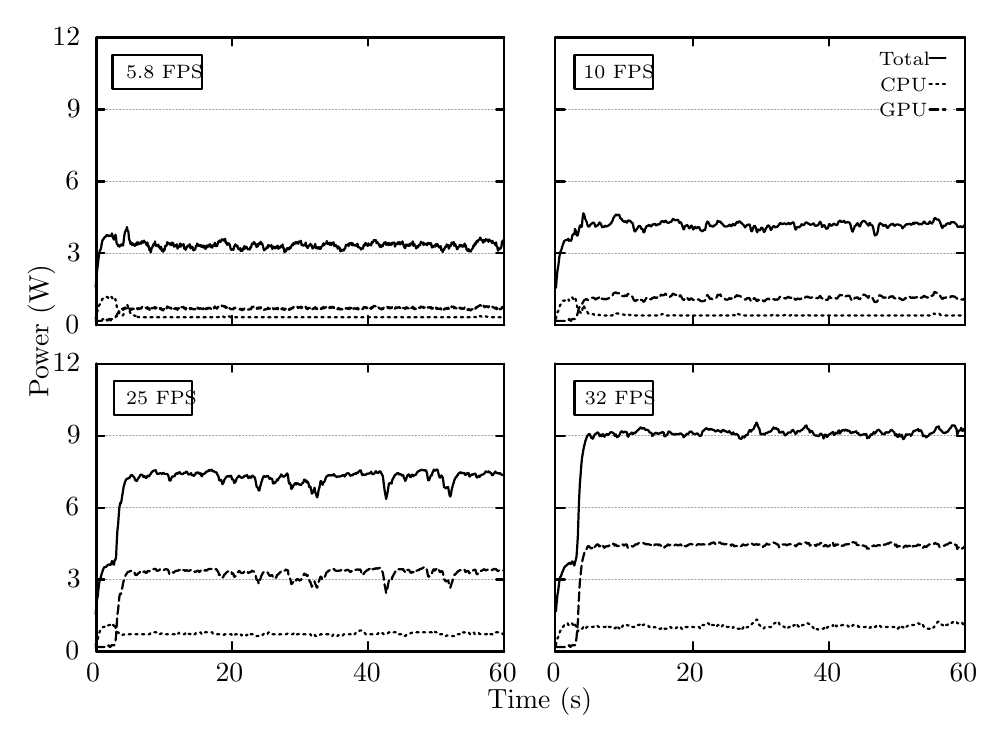
\begin{tikzpicture}[y=0.80pt, x=0.80pt, yscale=-0.720000, xscale=0.720000, inner sep=0pt, outer sep=0pt]
\begin{scope}[draw=black,line join=bevel,line cap=rect,even odd rule,line width=0.800pt]
  \begin{scope}[cm={{1.0,0.0,0.0,1.0,(0.0,0.0)}},draw=black,line join=bevel,line cap=rect,line width=0.800pt]
  \end{scope}
  \begin{scope}[cm={{1.00313,0.0,0.0,1.00313,(0.0,0.0)}},draw=black,line join=bevel,line cap=rect,line width=0.800pt]
  \end{scope}
  \begin{scope}[cm={{1.00313,0.0,0.0,1.00313,(0.0,0.0)}},draw=ca0a0a4,dash pattern=on 0.40pt off 0.80pt,line join=round,line cap=round,line width=0.400pt]
    \path[draw] (64.5000,228.5000) -- (319.5000,228.5000);
  \end{scope}
  \begin{scope}[cm={{1.00313,0.0,0.0,1.00313,(0.0,0.0)}},draw=black,line join=round,line cap=round,line width=0.800pt]
    \path[draw] (64.5000,228.5000) -- (69.5000,228.5000);
    \path[draw] (319.5000,228.5000) -- (314.5000,228.5000);
  \end{scope}
  \begin{scope}[cm={{1.00313,0.0,0.0,1.00313,(0.0,0.0)}},draw=black,line join=bevel,line cap=rect,line width=0.800pt]
  \end{scope}
  \begin{scope}[cm={{1.00313,0.0,0.0,1.00313,(45.1406,234.23)}},draw=black,line join=bevel,line cap=rect,line width=0.800pt]
  \end{scope}
  \begin{scope}[cm={{1.00313,0.0,0.0,1.00313,(45.1406,234.23)}},draw=black,line join=bevel,line cap=rect,line width=0.800pt]
  \end{scope}
  \begin{scope}[cm={{1.00313,0.0,0.0,1.00313,(45.1406,234.23)}},draw=black,line join=bevel,line cap=rect,line width=0.800pt]
  \end{scope}
  \begin{scope}[cm={{1.00313,0.0,0.0,1.00313,(45.1406,234.23)}},draw=black,line join=bevel,line cap=rect,line width=0.800pt]
  \end{scope}
  \begin{scope}[cm={{1.00313,0.0,0.0,1.00313,(45.1406,234.23)}},draw=black,line join=bevel,line cap=rect,line width=0.800pt]
  \end{scope}
  \begin{scope}[cm={{1.00313,0.0,0.0,1.00313,(45.1406,234.23)}},draw=black,line join=bevel,line cap=rect,line width=0.800pt]
    \path[fill=black] (0.0000,0.0000) node[above right] () {0};
  \end{scope}
  \begin{scope}[cm={{1.00313,0.0,0.0,1.00313,(45.1406,234.23)}},draw=black,line join=bevel,line cap=rect,line width=0.800pt]
  \end{scope}
  \begin{scope}[cm={{1.00313,0.0,0.0,1.00313,(0.0,0.0)}},draw=black,line join=bevel,line cap=rect,line width=0.800pt]
  \end{scope}
  \begin{scope}[cm={{1.00313,0.0,0.0,1.00313,(0.0,0.0)}},draw=ca0a0a4,dash pattern=on 0.40pt off 0.80pt,line join=round,line cap=round,line width=0.400pt]
    \path[draw] (64.5000,183.5000) -- (319.5000,183.5000);
  \end{scope}
  \begin{scope}[cm={{1.00313,0.0,0.0,1.00313,(0.0,0.0)}},draw=black,line join=round,line cap=round,line width=0.800pt]
    \path[draw] (64.5000,183.5000) -- (69.5000,183.5000);
    \path[draw] (319.5000,183.5000) -- (314.5000,183.5000);
  \end{scope}
  \begin{scope}[cm={{1.00313,0.0,0.0,1.00313,(0.0,0.0)}},draw=black,line join=bevel,line cap=rect,line width=0.800pt]
  \end{scope}
  \begin{scope}[cm={{1.00313,0.0,0.0,1.00313,(46.1438,189.089)}},draw=black,line join=bevel,line cap=rect,line width=0.800pt]
  \end{scope}
  \begin{scope}[cm={{1.00313,0.0,0.0,1.00313,(46.1438,189.089)}},draw=black,line join=bevel,line cap=rect,line width=0.800pt]
  \end{scope}
  \begin{scope}[cm={{1.00313,0.0,0.0,1.00313,(46.1438,189.089)}},draw=black,line join=bevel,line cap=rect,line width=0.800pt]
  \end{scope}
  \begin{scope}[cm={{1.00313,0.0,0.0,1.00313,(46.1438,189.089)}},draw=black,line join=bevel,line cap=rect,line width=0.800pt]
  \end{scope}
  \begin{scope}[cm={{1.00313,0.0,0.0,1.00313,(46.1438,189.089)}},draw=black,line join=bevel,line cap=rect,line width=0.800pt]
  \end{scope}
  \begin{scope}[cm={{1.00313,0.0,0.0,1.00313,(46.1438,189.089)}},draw=black,line join=bevel,line cap=rect,line width=0.800pt]
    \path[fill=black] (0.0000,0.0000) node[above right] () {3};
  \end{scope}
  \begin{scope}[cm={{1.00313,0.0,0.0,1.00313,(46.1438,189.089)}},draw=black,line join=bevel,line cap=rect,line width=0.800pt]
  \end{scope}
  \begin{scope}[cm={{1.00313,0.0,0.0,1.00313,(0.0,0.0)}},draw=black,line join=bevel,line cap=rect,line width=0.800pt]
  \end{scope}
  \begin{scope}[cm={{1.00313,0.0,0.0,1.00313,(0.0,0.0)}},draw=ca0a0a4,dash pattern=on 0.40pt off 0.80pt,line join=round,line cap=round,line width=0.400pt]
    \path[draw] (64.5000,138.5000) -- (319.5000,138.5000);
  \end{scope}
  \begin{scope}[cm={{1.00313,0.0,0.0,1.00313,(0.0,0.0)}},draw=black,line join=round,line cap=round,line width=0.800pt]
    \path[draw] (64.5000,138.5000) -- (69.5000,138.5000);
    \path[draw] (319.5000,138.5000) -- (314.5000,138.5000);
  \end{scope}
  \begin{scope}[cm={{1.00313,0.0,0.0,1.00313,(0.0,0.0)}},draw=black,line join=bevel,line cap=rect,line width=0.800pt]
  \end{scope}
  \begin{scope}[cm={{1.00313,0.0,0.0,1.00313,(45.1406,143.948)}},draw=black,line join=bevel,line cap=rect,line width=0.800pt]
  \end{scope}
  \begin{scope}[cm={{1.00313,0.0,0.0,1.00313,(45.1406,143.948)}},draw=black,line join=bevel,line cap=rect,line width=0.800pt]
  \end{scope}
  \begin{scope}[cm={{1.00313,0.0,0.0,1.00313,(45.1406,143.948)}},draw=black,line join=bevel,line cap=rect,line width=0.800pt]
  \end{scope}
  \begin{scope}[cm={{1.00313,0.0,0.0,1.00313,(45.1406,143.948)}},draw=black,line join=bevel,line cap=rect,line width=0.800pt]
  \end{scope}
  \begin{scope}[cm={{1.00313,0.0,0.0,1.00313,(45.1406,143.948)}},draw=black,line join=bevel,line cap=rect,line width=0.800pt]
  \end{scope}
  \begin{scope}[cm={{1.00313,0.0,0.0,1.00313,(45.1406,143.948)}},draw=black,line join=bevel,line cap=rect,line width=0.800pt]
    \path[fill=black] (0.0000,0.0000) node[above right] () {6};
  \end{scope}
  \begin{scope}[cm={{1.00313,0.0,0.0,1.00313,(45.1406,143.948)}},draw=black,line join=bevel,line cap=rect,line width=0.800pt]
  \end{scope}
  \begin{scope}[cm={{1.00313,0.0,0.0,1.00313,(0.0,0.0)}},draw=black,line join=bevel,line cap=rect,line width=0.800pt]
  \end{scope}
  \begin{scope}[cm={{1.00313,0.0,0.0,1.00313,(0.0,0.0)}},draw=ca0a0a4,dash pattern=on 0.40pt off 0.80pt,line join=round,line cap=round,line width=0.400pt]
    \path[draw] (64.5000,93.5000) -- (319.5000,93.5000);
  \end{scope}
  \begin{scope}[cm={{1.00313,0.0,0.0,1.00313,(0.0,0.0)}},draw=black,line join=round,line cap=round,line width=0.800pt]
    \path[draw] (64.5000,93.5000) -- (69.5000,93.5000);
    \path[draw] (319.5000,93.5000) -- (314.5000,93.5000);
  \end{scope}
  \begin{scope}[cm={{1.00313,0.0,0.0,1.00313,(0.0,0.0)}},draw=black,line join=bevel,line cap=rect,line width=0.800pt]
  \end{scope}
  \begin{scope}[cm={{1.00313,0.0,0.0,1.00313,(46.1438,98.8078)}},draw=black,line join=bevel,line cap=rect,line width=0.800pt]
  \end{scope}
  \begin{scope}[cm={{1.00313,0.0,0.0,1.00313,(46.1438,98.8078)}},draw=black,line join=bevel,line cap=rect,line width=0.800pt]
  \end{scope}
  \begin{scope}[cm={{1.00313,0.0,0.0,1.00313,(46.1438,98.8078)}},draw=black,line join=bevel,line cap=rect,line width=0.800pt]
  \end{scope}
  \begin{scope}[cm={{1.00313,0.0,0.0,1.00313,(46.1438,98.8078)}},draw=black,line join=bevel,line cap=rect,line width=0.800pt]
  \end{scope}
  \begin{scope}[cm={{1.00313,0.0,0.0,1.00313,(46.1438,98.8078)}},draw=black,line join=bevel,line cap=rect,line width=0.800pt]
  \end{scope}
  \begin{scope}[cm={{1.00313,0.0,0.0,1.00313,(46.1438,98.8078)}},draw=black,line join=bevel,line cap=rect,line width=0.800pt]
    \path[fill=black] (0.0000,0.0000) node[above right] () {9};
  \end{scope}
  \begin{scope}[cm={{1.00313,0.0,0.0,1.00313,(46.1438,98.8078)}},draw=black,line join=bevel,line cap=rect,line width=0.800pt]
  \end{scope}
  \begin{scope}[cm={{1.00313,0.0,0.0,1.00313,(0.0,0.0)}},draw=black,line join=bevel,line cap=rect,line width=0.800pt]
  \end{scope}
  \begin{scope}[cm={{1.00313,0.0,0.0,1.00313,(0.0,0.0)}},draw=ca0a0a4,dash pattern=on 0.40pt off 0.80pt,line join=round,line cap=round,line width=0.400pt]
    \path[draw] (64.5000,48.5000) -- (319.5000,48.5000);
  \end{scope}
  \begin{scope}[cm={{1.00313,0.0,0.0,1.00313,(0.0,0.0)}},draw=black,line join=round,line cap=round,line width=0.800pt]
    \path[draw] (64.5000,48.5000) -- (69.5000,48.5000);
    \path[draw] (319.5000,48.5000) -- (314.5000,48.5000);
  \end{scope}
  \begin{scope}[cm={{1.00313,0.0,0.0,1.00313,(0.0,0.0)}},draw=black,line join=bevel,line cap=rect,line width=0.800pt]
  \end{scope}
  \begin{scope}[cm={{1.00313,0.0,0.0,1.00313,(37.1156,53.6672)}},draw=black,line join=bevel,line cap=rect,line width=0.800pt]
  \end{scope}
  \begin{scope}[cm={{1.00313,0.0,0.0,1.00313,(37.1156,53.6672)}},draw=black,line join=bevel,line cap=rect,line width=0.800pt]
  \end{scope}
  \begin{scope}[cm={{1.00313,0.0,0.0,1.00313,(37.1156,53.6672)}},draw=black,line join=bevel,line cap=rect,line width=0.800pt]
  \end{scope}
  \begin{scope}[cm={{1.00313,0.0,0.0,1.00313,(37.1156,53.6672)}},draw=black,line join=bevel,line cap=rect,line width=0.800pt]
  \end{scope}
  \begin{scope}[cm={{1.00313,0.0,0.0,1.00313,(37.1156,53.6672)}},draw=black,line join=bevel,line cap=rect,line width=0.800pt]
  \end{scope}
  \begin{scope}[cm={{1.00313,0.0,0.0,1.00313,(37.1156,53.6672)}},draw=black,line join=bevel,line cap=rect,line width=0.800pt]
    \path[fill=black] (0.0000,0.0000) node[above right] () {12};
  \end{scope}
  \begin{scope}[cm={{1.00313,0.0,0.0,1.00313,(37.1156,53.6672)}},draw=black,line join=bevel,line cap=rect,line width=0.800pt]
  \end{scope}
  \begin{scope}[cm={{1.00313,0.0,0.0,1.00313,(0.0,0.0)}},draw=black,line join=bevel,line cap=rect,line width=0.800pt]
  \end{scope}
  \begin{scope}[cm={{1.00313,0.0,0.0,1.00313,(0.0,0.0)}},draw=black,line join=round,line cap=round,line width=0.800pt]
    \path[draw] (64.5000,228.5000) -- (64.5000,222.5000);
    \path[draw] (64.5000,48.5000) -- (64.5000,53.5000);
  \end{scope}
  \begin{scope}[cm={{1.00313,0.0,0.0,1.00313,(0.0,0.0)}},draw=black,line join=bevel,line cap=rect,line width=0.800pt]
  \end{scope}
  \begin{scope}[cm={{1.00313,0.0,0.0,1.00313,(64.2,242.756)}},draw=black,line join=bevel,line cap=rect,line width=0.800pt]
  \end{scope}
  \begin{scope}[cm={{1.00313,0.0,0.0,1.00313,(64.2,242.756)}},draw=black,line join=bevel,line cap=rect,line width=0.800pt]
  \end{scope}
  \begin{scope}[cm={{1.00313,0.0,0.0,1.00313,(64.2,242.756)}},draw=black,line join=bevel,line cap=rect,line width=0.800pt]
  \end{scope}
  \begin{scope}[cm={{1.00313,0.0,0.0,1.00313,(64.2,242.756)}},draw=black,line join=bevel,line cap=rect,line width=0.800pt]
  \end{scope}
  \begin{scope}[cm={{1.00313,0.0,0.0,1.00313,(64.2,242.756)}},draw=black,line join=bevel,line cap=rect,line width=0.800pt]
  \end{scope}
  \begin{scope}[cm={{1.00313,0.0,0.0,1.00313,(64.2,242.756)}},draw=black,line join=bevel,line cap=rect,line width=0.800pt]
  \end{scope}
  \begin{scope}[cm={{1.00313,0.0,0.0,1.00313,(0.0,0.0)}},draw=black,line join=bevel,line cap=rect,line width=0.800pt]
  \end{scope}
  \begin{scope}[cm={{1.00313,0.0,0.0,1.00313,(0.0,0.0)}},draw=black,line join=round,line cap=round,line width=0.800pt]
    \path[draw] (149.5000,228.5000) -- (149.5000,222.5000);
    \path[draw] (149.5000,48.5000) -- (149.5000,53.5000);
  \end{scope}
  \begin{scope}[cm={{1.00313,0.0,0.0,1.00313,(0.0,0.0)}},draw=black,line join=bevel,line cap=rect,line width=0.800pt]
  \end{scope}
  \begin{scope}[cm={{1.00313,0.0,0.0,1.00313,(149.466,242.756)}},draw=black,line join=bevel,line cap=rect,line width=0.800pt]
  \end{scope}
  \begin{scope}[cm={{1.00313,0.0,0.0,1.00313,(149.466,242.756)}},draw=black,line join=bevel,line cap=rect,line width=0.800pt]
  \end{scope}
  \begin{scope}[cm={{1.00313,0.0,0.0,1.00313,(149.466,242.756)}},draw=black,line join=bevel,line cap=rect,line width=0.800pt]
  \end{scope}
  \begin{scope}[cm={{1.00313,0.0,0.0,1.00313,(149.466,242.756)}},draw=black,line join=bevel,line cap=rect,line width=0.800pt]
  \end{scope}
  \begin{scope}[cm={{1.00313,0.0,0.0,1.00313,(149.466,242.756)}},draw=black,line join=bevel,line cap=rect,line width=0.800pt]
  \end{scope}
  \begin{scope}[cm={{1.00313,0.0,0.0,1.00313,(149.466,242.756)}},draw=black,line join=bevel,line cap=rect,line width=0.800pt]
  \end{scope}
  \begin{scope}[cm={{1.00313,0.0,0.0,1.00313,(0.0,0.0)}},draw=black,line join=bevel,line cap=rect,line width=0.800pt]
  \end{scope}
  \begin{scope}[cm={{1.00313,0.0,0.0,1.00313,(0.0,0.0)}},draw=black,line join=round,line cap=round,line width=0.800pt]
    \path[draw] (234.5000,228.5000) -- (234.5000,222.5000);
    \path[draw] (234.5000,48.5000) -- (234.5000,53.5000);
  \end{scope}
  \begin{scope}[cm={{1.00313,0.0,0.0,1.00313,(0.0,0.0)}},draw=black,line join=bevel,line cap=rect,line width=0.800pt]
  \end{scope}
  \begin{scope}[cm={{1.00313,0.0,0.0,1.00313,(235.734,242.756)}},draw=black,line join=bevel,line cap=rect,line width=0.800pt]
  \end{scope}
  \begin{scope}[cm={{1.00313,0.0,0.0,1.00313,(235.734,242.756)}},draw=black,line join=bevel,line cap=rect,line width=0.800pt]
  \end{scope}
  \begin{scope}[cm={{1.00313,0.0,0.0,1.00313,(235.734,242.756)}},draw=black,line join=bevel,line cap=rect,line width=0.800pt]
  \end{scope}
  \begin{scope}[cm={{1.00313,0.0,0.0,1.00313,(235.734,242.756)}},draw=black,line join=bevel,line cap=rect,line width=0.800pt]
  \end{scope}
  \begin{scope}[cm={{1.00313,0.0,0.0,1.00313,(235.734,242.756)}},draw=black,line join=bevel,line cap=rect,line width=0.800pt]
  \end{scope}
  \begin{scope}[cm={{1.00313,0.0,0.0,1.00313,(235.734,242.756)}},draw=black,line join=bevel,line cap=rect,line width=0.800pt]
  \end{scope}
  \begin{scope}[cm={{1.00313,0.0,0.0,1.00313,(0.0,0.0)}},draw=black,line join=bevel,line cap=rect,line width=0.800pt]
  \end{scope}
  \begin{scope}[cm={{1.00313,0.0,0.0,1.00313,(0.0,0.0)}},draw=black,line join=round,line cap=round,line width=0.800pt]
    \path[draw] (319.5000,228.5000) -- (319.5000,222.5000);
    \path[draw] (319.5000,48.5000) -- (319.5000,53.5000);
  \end{scope}
  \begin{scope}[cm={{1.00313,0.0,0.0,1.00313,(0.0,0.0)}},draw=black,line join=bevel,line cap=rect,line width=0.800pt]
  \end{scope}
  \begin{scope}[cm={{1.00313,0.0,0.0,1.00313,(321.0,242.756)}},draw=black,line join=bevel,line cap=rect,line width=0.800pt]
  \end{scope}
  \begin{scope}[cm={{1.00313,0.0,0.0,1.00313,(321.0,242.756)}},draw=black,line join=bevel,line cap=rect,line width=0.800pt]
  \end{scope}
  \begin{scope}[cm={{1.00313,0.0,0.0,1.00313,(321.0,242.756)}},draw=black,line join=bevel,line cap=rect,line width=0.800pt]
  \end{scope}
  \begin{scope}[cm={{1.00313,0.0,0.0,1.00313,(321.0,242.756)}},draw=black,line join=bevel,line cap=rect,line width=0.800pt]
  \end{scope}
  \begin{scope}[cm={{1.00313,0.0,0.0,1.00313,(321.0,242.756)}},draw=black,line join=bevel,line cap=rect,line width=0.800pt]
  \end{scope}
  \begin{scope}[cm={{1.00313,0.0,0.0,1.00313,(321.0,242.756)}},draw=black,line join=bevel,line cap=rect,line width=0.800pt]
  \end{scope}
  \begin{scope}[cm={{1.00313,0.0,0.0,1.00313,(0.0,0.0)}},draw=black,line join=bevel,line cap=rect,line width=0.800pt]
  \end{scope}
  \begin{scope}[cm={{1.00313,0.0,0.0,1.00313,(0.0,0.0)}},draw=black,line join=round,line cap=round,line width=0.800pt]
    \path[draw] (64.5000,48.5000) -- (64.5000,228.5000) -- (319.5000,228.5000) --
      (319.5000,48.5000) -- (64.5000,48.5000);
  \end{scope}
  \begin{scope}[cm={{1.00313,0.0,0.0,1.00313,(0.0,0.0)}},draw=black,line join=bevel,line cap=rect,line width=0.800pt]
  \end{scope}
  \begin{scope}[cm={{1.00313,0.0,0.0,1.00313,(0.0,0.0)}},draw=black,line join=bevel,line cap=rect,line width=0.800pt]
  \end{scope}
  \begin{scope}[cm={{1.00313,0.0,0.0,1.00313,(0.0,0.0)}},fill=cffffff]
    \path[fill,rounded corners=0.0000cm] (74.0000,59.0000) rectangle
      (130.0000,80.0000);
  \end{scope}
  \begin{scope}[cm={{1.00313,0.0,0.0,1.00313,(0.0,0.0)}},draw=black,line join=bevel,line cap=rect,line width=0.800pt]
  \end{scope}
  \begin{scope}[cm={{1.00313,0.0,0.0,1.00313,(0.0,0.0)}},draw=black,line join=bevel,line cap=rect,line width=0.800pt]
  \end{scope}
  \begin{scope}[cm={{1.00313,0.0,0.0,1.00313,(0.0,0.0)}},draw=black,line join=round,line cap=round,line width=0.800pt]
    \path[draw] (74.5000,80.5000) -- (74.5000,59.5000) -- (130.5000,59.5000) --
      (130.5000,80.5000) -- (74.5000,80.5000);
  \end{scope}
  \begin{scope}[cm={{1.00313,0.0,0.0,1.00313,(0.0,0.0)}},draw=black,line join=bevel,line cap=rect,line width=0.800pt]
  \end{scope}
  \begin{scope}[cm={{1.00313,0.0,0.0,1.00313,(85.2656,74.2313)}},draw=black,line join=bevel,line cap=rect,line width=0.800pt]
  \end{scope}
  \begin{scope}[cm={{1.00313,0.0,0.0,1.00313,(85.2656,74.2313)}},draw=black,line join=bevel,line cap=rect,line width=0.800pt]
  \end{scope}
  \begin{scope}[cm={{1.00313,0.0,0.0,1.00313,(85.2656,74.2313)}},draw=black,line join=bevel,line cap=rect,line width=0.800pt]
  \end{scope}
  \begin{scope}[cm={{1.00313,0.0,0.0,1.00313,(85.2656,74.2313)}},draw=black,line join=bevel,line cap=rect,line width=0.800pt]
  \end{scope}
  \begin{scope}[cm={{1.00313,0.0,0.0,1.00313,(85.2656,74.2313)}},draw=black,line join=bevel,line cap=rect,line width=0.800pt]
  \end{scope}
  \begin{scope}[cm={{1.00313,0.0,0.0,1.00313,(83.2656,74.2313)}},draw=black,line join=bevel,line cap=rect,line width=0.800pt]
    \path[fill=black] (0.0000,0.0000) node[above right] () {\scriptsize 5.8 FPS};
  \end{scope}
  \begin{scope}[cm={{1.00313,0.0,0.0,1.00313,(85.2656,74.2313)}},draw=black,line join=bevel,line cap=rect,line width=0.800pt]
  \end{scope}
  \begin{scope}[cm={{0.0,-1.00313,1.00313,0.0,(21.5672,274.355)}},draw=black,line join=bevel,line cap=rect,line width=0.800pt]
  \end{scope}
  \begin{scope}[cm={{0.0,-1.00313,1.00313,0.0,(21.5672,274.355)}},draw=black,line join=bevel,line cap=rect,line width=0.800pt]
  \end{scope}
  \begin{scope}[cm={{0.0,-1.00313,1.00313,0.0,(21.5672,274.355)}},draw=black,line join=bevel,line cap=rect,line width=0.800pt]
  \end{scope}
  \begin{scope}[cm={{0.0,-1.00313,1.00313,0.0,(21.5672,274.355)}},draw=black,line join=bevel,line cap=rect,line width=0.800pt]
  \end{scope}
  \begin{scope}[cm={{0.0,-1.00313,1.00313,0.0,(21.5672,274.355)}},draw=black,line join=bevel,line cap=rect,line width=0.800pt]
  \end{scope}
  \begin{scope}[cm={{0.0,-1.00313,1.00313,0.0,(21.5672,274.355)}},draw=black,line join=bevel,line cap=rect,line width=0.800pt]
    \path[fill=black] (0.0000,0.0000) node[above right] () {\rotatebox{90}{Power (W)}};
  \end{scope}
  \begin{scope}[cm={{0.0,-1.00313,1.00313,0.0,(21.5672,274.355)}},draw=black,line join=bevel,line cap=rect,line width=0.800pt]
  \end{scope}
  \begin{scope}[cm={{1.00313,0.0,0.0,1.00313,(0.0,0.0)}},draw=black,line join=bevel,line cap=rect,line width=0.800pt]
  \end{scope}
  \begin{scope}[cm={{1.00313,0.0,0.0,1.00313,(0.0,0.0)}},draw=black,line join=bevel,line cap=rect,line width=0.800pt]
  \end{scope}
  \begin{scope}[cm={{1.00313,0.0,0.0,1.00313,(0.0,0.0)}},draw=black,line join=bevel,line cap=rect,line width=0.800pt]
  \end{scope}
  \begin{scope}[cm={{1.00313,0.0,0.0,1.00313,(0.0,0.0)}},draw=black,line join=round,line cap=round,line width=0.800pt]
    \path[draw] (64.0000,204.6000) -- (64.0000,204.6000) -- (64.4000,199.9000) --
      (64.9000,194.7000) -- (65.3000,191.1000) -- (65.7000,187.6000) --
      (66.1000,184.4000) -- (66.6000,181.9000) -- (67.0000,181.3000) --
      (67.4000,180.0000) -- (67.8000,177.5000) -- (68.3000,175.3000) --
      (68.7000,174.8000) -- (69.1000,174.2000) -- (69.5000,173.5000) --
      (70.0000,173.2000) -- (70.4000,172.9000) -- (70.8000,172.0000) --
      (71.3000,172.2000) -- (71.7000,172.2000) -- (72.1000,172.7000) --
      (72.5000,172.3000) -- (73.0000,172.5000) -- (73.4000,172.9000) --
      (73.8000,172.5000) -- (74.2000,171.0000) -- (74.7000,172.9000) --
      (75.1000,174.3000) -- (75.5000,174.9000) -- (75.9000,174.1000) --
      (76.4000,171.8000) -- (76.8000,174.0000) -- (77.2000,177.6000) --
      (77.6000,177.6000) -- (78.1000,178.9000) -- (78.5000,178.4000) --
      (78.9000,179.3000) -- (79.4000,178.7000) -- (79.8000,178.0000) --
      (80.2000,178.5000) -- (80.6000,177.7000) -- (81.1000,178.7000) --
      (81.5000,176.1000) -- (81.9000,172.7000) -- (82.3000,170.4000) --
      (82.8000,169.2000) -- (83.2000,168.9000) -- (83.6000,167.0000) --
      (84.0000,169.3000) -- (84.5000,169.9000) -- (84.9000,174.5000) --
      (85.3000,175.6000) -- (85.8000,177.6000) -- (86.2000,176.6000) --
      (86.6000,178.2000) -- (87.0000,177.1000) -- (87.5000,178.3000) --
      (87.9000,177.8000) -- (88.3000,178.8000) -- (88.7000,178.7000) --
      (89.2000,177.3000) -- (89.6000,178.2000) -- (90.0000,176.5000) --
      (90.4000,178.0000) -- (90.9000,176.7000) -- (91.3000,177.5000) --
      (91.7000,177.6000) -- (92.1000,176.6000) -- (92.6000,177.4000) --
      (93.0000,175.9000) -- (93.4000,176.3000) -- (93.9000,176.8000) --
      (94.3000,175.5000) -- (94.7000,176.5000) -- (95.1000,176.4000) --
      (95.6000,177.6000) -- (96.0000,178.4000) -- (96.4000,176.7000) --
      (96.8000,179.2000) -- (97.3000,179.0000) -- (97.7000,181.6000) --
      (98.1000,181.6000) -- (98.5000,182.9000) -- (99.0000,180.0000) --
      (99.4000,180.0000) -- (99.8000,178.8000) -- (100.3000,177.6000) --
      (100.7000,178.0000) -- (101.1000,176.0000) -- (101.5000,178.7000) --
      (102.0000,178.2000) -- (102.4000,178.9000) -- (102.8000,178.6000) --
      (103.2000,178.0000) -- (103.7000,179.8000) -- (104.1000,179.5000) --
      (104.5000,180.8000) -- (104.9000,179.3000) -- (105.4000,181.9000) --
      (105.8000,181.4000) -- (106.2000,182.5000) -- (106.7000,180.8000) --
      (107.1000,181.5000) -- (107.5000,178.8000) -- (107.9000,178.8000) --
      (108.4000,178.6000) -- (108.8000,176.5000) -- (109.2000,177.1000) --
      (109.6000,176.9000) -- (110.1000,177.7000) -- (110.5000,178.0000) --
      (110.9000,177.2000) -- (111.3000,178.4000) -- (111.8000,176.7000) --
      (112.2000,178.0000) -- (112.6000,177.2000) -- (113.0000,179.3000) --
      (113.5000,179.0000) -- (113.9000,178.4000) -- (114.3000,179.2000) --
      (114.8000,177.8000) -- (115.2000,180.5000) -- (115.6000,179.5000) --
      (116.0000,179.5000) -- (116.5000,178.9000) -- (116.9000,177.3000) --
      (117.3000,179.3000) -- (117.7000,178.2000) -- (118.2000,177.9000) --
      (118.6000,178.3000) -- (119.0000,177.7000) -- (119.4000,180.5000) --
      (119.9000,180.2000) -- (120.3000,181.3000) -- (120.7000,179.6000) --
      (121.2000,179.8000) -- (121.6000,178.5000) -- (122.0000,178.6000) --
      (122.4000,179.0000) -- (122.9000,177.7000) -- (123.3000,180.4000) --
      (123.7000,179.1000) -- (124.1000,179.7000) -- (124.6000,179.5000) --
      (125.0000,181.5000) -- (125.4000,181.5000) -- (125.8000,181.2000) --
      (126.3000,181.0000) -- (126.7000,178.8000) -- (127.1000,179.1000) --
      (127.5000,177.3000) -- (128.0000,178.7000) -- (128.4000,178.1000) --
      (128.8000,178.9000) -- (129.3000,178.6000) -- (129.7000,178.2000) --
      (130.1000,179.4000) -- (130.5000,178.9000) -- (131.0000,179.7000) --
      (131.4000,178.5000) -- (131.8000,180.0000) -- (132.2000,179.0000) --
      (132.7000,180.8000) -- (133.1000,179.3000) -- (133.5000,178.5000) --
      (133.9000,179.7000) -- (134.4000,178.6000) -- (134.8000,179.0000) --
      (135.2000,178.0000) -- (135.7000,177.8000) -- (136.1000,179.7000) --
      (136.5000,179.2000) -- (136.9000,179.9000) -- (137.4000,178.4000) --
      (137.8000,178.8000) -- (138.2000,178.0000) -- (138.6000,176.8000) --
      (139.1000,179.0000) -- (139.5000,178.3000) -- (139.9000,179.0000) --
      (140.3000,177.6000) -- (140.8000,176.0000) -- (141.2000,176.5000) --
      (141.6000,175.4000) -- (142.0000,176.3000) -- (142.5000,175.8000) --
      (142.9000,174.7000) -- (143.3000,175.1000) -- (143.8000,174.7000) --
      (144.2000,175.1000) -- (144.6000,175.9000) -- (145.0000,174.4000) --
      (145.5000,177.1000) -- (145.9000,176.8000) -- (146.3000,178.3000) --
      (146.7000,177.1000) -- (147.2000,177.3000) -- (147.6000,177.7000) --
      (148.0000,178.4000) -- (148.4000,180.6000) -- (148.9000,181.3000) --
      (149.3000,181.0000) -- (149.7000,180.7000) -- (150.2000,181.3000) --
      (150.6000,179.0000) -- (151.0000,179.0000) -- (151.4000,177.8000) --
      (151.9000,179.0000) -- (152.3000,179.0000) -- (152.7000,178.7000) --
      (153.1000,180.8000) -- (153.6000,180.8000) -- (154.0000,181.2000) --
      (154.4000,180.2000) -- (154.8000,182.1000) -- (155.3000,181.1000) --
      (155.7000,182.0000) -- (156.1000,180.4000) -- (156.6000,180.9000) --
      (157.0000,178.9000) -- (157.4000,180.5000) -- (157.8000,179.4000) --
      (158.3000,179.3000) -- (158.7000,180.2000) -- (159.1000,180.9000) --
      (159.5000,181.0000) -- (160.0000,180.9000) -- (160.4000,181.1000) --
      (160.8000,179.5000) -- (161.2000,179.8000) -- (161.7000,177.6000) --
      (162.1000,177.2000) -- (162.5000,177.6000) -- (162.9000,176.5000) --
      (163.4000,176.8000) -- (163.8000,177.8000) -- (164.2000,178.2000) --
      (164.7000,179.6000) -- (165.1000,177.7000) -- (165.5000,179.1000) --
      (165.9000,177.7000) -- (166.4000,177.1000) -- (166.8000,177.7000) --
      (167.2000,176.2000) -- (167.6000,177.7000) -- (168.1000,177.2000) --
      (168.5000,178.5000) -- (168.9000,179.9000) -- (169.3000,181.6000) --
      (169.8000,181.0000) -- (170.2000,180.9000) -- (170.6000,180.5000) --
      (171.1000,179.6000) -- (171.5000,180.1000) -- (171.9000,178.2000) --
      (172.3000,179.2000) -- (172.8000,178.6000) -- (173.2000,179.0000) --
      (173.6000,179.2000) -- (174.0000,178.3000) -- (174.5000,180.8000) --
      (174.9000,179.3000) -- (175.3000,179.7000) -- (175.7000,179.3000) --
      (176.2000,180.4000) -- (176.6000,180.0000) -- (177.0000,179.2000) --
      (177.4000,180.0000) -- (177.9000,178.6000) -- (178.3000,180.7000) --
      (178.7000,180.0000) -- (179.2000,180.1000) -- (179.6000,179.2000) --
      (180.0000,178.8000) -- (180.4000,179.7000) -- (180.9000,177.9000) --
      (181.3000,180.0000) -- (181.7000,180.2000) -- (182.1000,182.8000) --
      (182.6000,181.3000) -- (183.0000,182.2000) -- (183.4000,181.2000) --
      (183.8000,180.2000) -- (184.3000,181.0000) -- (184.7000,180.1000) --
      (185.1000,181.0000) -- (185.6000,179.6000) -- (186.0000,180.1000) --
      (186.4000,178.9000) -- (186.8000,178.0000) -- (187.3000,178.5000) --
      (187.7000,177.0000) -- (188.1000,177.2000) -- (188.5000,177.7000) --
      (189.0000,176.4000) -- (189.4000,177.2000) -- (189.8000,177.1000) --
      (190.2000,176.3000) -- (190.7000,177.5000) -- (191.1000,176.1000) --
      (191.5000,176.1000) -- (192.0000,176.6000) -- (192.4000,175.6000) --
      (192.8000,178.4000) -- (193.2000,177.8000) -- (193.7000,178.6000) --
      (194.1000,178.6000) -- (194.5000,178.3000) -- (194.9000,178.3000) --
      (195.4000,176.7000) -- (195.8000,179.3000) -- (196.2000,178.8000) --
      (196.6000,180.2000) -- (197.1000,179.1000) -- (197.5000,178.4000) --
      (197.9000,178.6000) -- (198.3000,177.5000) -- (198.8000,178.6000) --
      (199.2000,178.5000) -- (199.6000,180.5000) -- (200.1000,180.0000) --
      (200.5000,179.5000) -- (200.9000,179.3000) -- (201.3000,177.6000) --
      (201.8000,180.1000) -- (202.2000,179.6000) -- (202.6000,180.5000) --
      (203.0000,179.8000) -- (203.5000,179.5000) -- (203.9000,180.7000) --
      (204.3000,180.3000) -- (204.7000,180.7000) -- (205.2000,179.1000) --
      (205.6000,179.2000) -- (206.0000,178.5000) -- (206.5000,177.2000) --
      (206.9000,178.4000) -- (207.3000,177.4000) -- (207.7000,177.4000) --
      (208.2000,177.2000) -- (208.6000,175.8000) -- (209.0000,177.6000) --
      (209.4000,177.4000) -- (209.9000,177.0000) -- (210.3000,178.1000) --
      (210.7000,176.8000) -- (211.1000,178.3000) -- (211.6000,178.0000) --
      (212.0000,176.8000) -- (212.4000,177.7000) -- (212.8000,176.6000) --
      (213.3000,179.0000) -- (213.7000,178.4000) -- (214.1000,178.2000) --
      (214.6000,179.3000) -- (215.0000,179.1000) -- (215.4000,180.6000) --
      (215.8000,179.1000) -- (216.3000,180.0000) -- (216.7000,180.0000) --
      (217.1000,182.3000) -- (217.5000,181.2000) -- (218.0000,181.9000) --
      (218.4000,181.5000) -- (218.8000,181.3000) -- (219.2000,181.7000) --
      (219.7000,180.3000) -- (220.1000,180.4000) -- (220.5000,178.1000) --
      (221.0000,178.4000) -- (221.4000,178.2000) -- (221.8000,177.8000) --
      (222.2000,178.9000) -- (222.7000,177.1000) -- (223.1000,177.8000) --
      (223.5000,177.2000) -- (223.9000,176.9000) -- (224.4000,178.5000) --
      (224.8000,177.2000) -- (225.2000,178.5000) -- (225.6000,178.1000) --
      (226.1000,178.5000) -- (226.5000,178.7000) -- (226.9000,178.1000) --
      (227.3000,179.0000) -- (227.8000,177.4000) -- (228.2000,179.8000) --
      (228.6000,179.5000) -- (229.1000,180.0000) -- (229.5000,179.9000) --
      (229.9000,181.1000) -- (230.3000,180.5000) -- (230.8000,180.4000) --
      (231.2000,180.5000) -- (231.6000,178.3000) -- (232.0000,178.7000) --
      (232.5000,177.3000) -- (232.9000,177.0000) -- (233.3000,178.3000) --
      (233.7000,178.0000) -- (234.2000,178.9000) -- (234.6000,177.2000) --
      (235.0000,178.2000) -- (235.5000,178.0000) -- (235.9000,177.8000) --
      (236.3000,178.6000) -- (236.7000,176.4000) -- (237.2000,176.9000) --
      (237.6000,176.1000) -- (238.0000,175.2000) -- (238.4000,175.6000) --
      (238.9000,175.2000) -- (239.3000,175.3000) -- (239.7000,177.2000) --
      (240.1000,176.3000) -- (240.6000,177.2000) -- (241.0000,177.5000) --
      (241.4000,178.6000) -- (241.9000,179.5000) -- (242.3000,178.4000) --
      (242.7000,179.5000) -- (243.1000,178.4000) -- (243.6000,179.0000) --
      (244.0000,177.6000) -- (244.4000,176.8000) -- (244.8000,177.3000) --
      (245.3000,176.4000) -- (245.7000,178.1000) -- (246.1000,178.2000) --
      (246.5000,177.1000) -- (247.0000,178.3000) -- (247.4000,176.9000) --
      (247.8000,178.1000) -- (248.2000,178.3000) -- (248.7000,177.3000) --
      (249.1000,178.1000) -- (249.5000,176.8000) -- (250.0000,176.8000) --
      (250.4000,177.2000) -- (250.8000,176.7000) -- (251.2000,179.3000) --
      (251.7000,177.5000) -- (252.1000,177.9000) -- (252.5000,177.8000) --
      (252.9000,176.6000) -- (253.4000,177.5000) -- (253.8000,176.4000) --
      (254.2000,177.8000) -- (254.6000,177.9000) -- (255.1000,176.5000) --
      (255.5000,177.0000) -- (255.9000,176.0000) -- (256.4000,177.9000) --
      (256.8000,179.1000) -- (257.2000,179.9000) -- (257.6000,180.2000) --
      (258.1000,177.9000) -- (258.5000,178.7000) -- (258.9000,178.0000) --
      (259.3000,178.8000) -- (259.8000,178.8000) -- (260.2000,177.7000) --
      (260.6000,178.7000) -- (261.0000,177.3000) -- (261.5000,177.7000) --
      (261.9000,177.5000) -- (262.3000,176.0000) -- (262.7000,178.8000) --
      (263.2000,177.4000) -- (263.6000,178.8000) -- (264.0000,178.7000) --
      (264.5000,180.4000) -- (264.9000,179.9000) -- (265.3000,179.0000) --
      (265.7000,179.6000) -- (266.2000,178.1000) -- (266.6000,178.1000) --
      (267.0000,178.3000) -- (267.4000,176.2000) -- (267.9000,176.8000) --
      (268.3000,177.0000) -- (268.7000,176.7000) -- (269.1000,178.3000) --
      (269.6000,177.2000) -- (270.0000,178.0000) -- (270.4000,177.6000) --
      (270.9000,177.8000) -- (271.3000,178.4000) -- (271.7000,176.9000) --
      (272.1000,177.6000) -- (272.6000,177.1000) -- (273.0000,177.2000) --
      (273.4000,178.1000) -- (273.8000,177.2000) -- (274.3000,179.9000) --
      (274.7000,179.0000) -- (275.1000,179.6000) -- (275.5000,178.8000) --
      (276.0000,178.5000) -- (276.4000,179.3000) -- (276.8000,177.6000) --
      (277.3000,178.9000) -- (277.7000,177.7000) -- (278.1000,178.4000) --
      (278.5000,179.3000) -- (279.0000,179.8000) -- (279.4000,179.9000) --
      (279.8000,178.9000) -- (280.2000,181.5000) -- (280.7000,181.5000) --
      (281.1000,182.7000) -- (281.5000,180.9000) -- (281.9000,181.3000) --
      (282.4000,179.8000) -- (282.8000,179.2000) -- (283.2000,179.4000) --
      (283.6000,177.9000) -- (284.1000,179.0000) -- (284.5000,178.4000) --
      (284.9000,180.6000) -- (285.4000,179.3000) -- (285.8000,178.4000) --
      (286.2000,178.8000) -- (286.6000,176.7000) -- (287.1000,177.0000) --
      (287.5000,177.5000) -- (287.9000,176.4000) -- (288.3000,178.8000) --
      (288.8000,177.6000) -- (289.2000,178.5000) -- (289.6000,179.4000) --
      (290.0000,180.9000) -- (290.5000,180.5000) -- (290.9000,179.4000) --
      (291.3000,179.4000) -- (291.8000,178.1000) -- (292.2000,179.0000) --
      (292.6000,178.2000) -- (293.0000,179.3000) -- (293.5000,179.2000) --
      (293.9000,178.4000) -- (294.3000,179.3000) -- (294.7000,177.4000) --
      (295.2000,178.4000) -- (295.6000,178.9000) -- (296.0000,181.2000) --
      (296.4000,181.5000) -- (296.9000,182.0000) -- (297.3000,180.8000) --
      (297.7000,182.2000) -- (298.1000,181.8000) -- (298.6000,182.4000) --
      (299.0000,181.2000) -- (299.4000,180.8000) -- (299.9000,180.1000) --
      (300.3000,178.5000) -- (300.7000,179.0000) -- (301.1000,177.2000) --
      (301.6000,177.9000) -- (302.0000,176.5000) -- (302.4000,175.7000) --
      (302.8000,176.5000) -- (303.3000,175.2000) -- (303.7000,175.0000) --
      (304.1000,174.9000) -- (304.5000,173.6000) -- (305.0000,174.7000) --
      (305.4000,175.2000) -- (305.8000,175.2000) -- (306.3000,176.8000) --
      (306.7000,175.1000) -- (307.1000,176.0000) -- (307.5000,176.1000) --
      (308.0000,174.6000) -- (308.4000,175.1000) -- (308.8000,174.7000) --
      (309.2000,175.1000) -- (309.7000,176.3000) -- (310.1000,174.8000) --
      (310.5000,175.7000) -- (310.9000,175.6000) -- (311.4000,175.8000) --
      (311.8000,177.0000) -- (312.2000,175.7000) -- (312.6000,176.8000) --
      (313.1000,177.0000) -- (313.5000,177.1000) -- (313.9000,178.2000) --
      (314.4000,176.6000) -- (314.8000,179.2000) -- (315.2000,179.3000) --
      (315.6000,181.9000) -- (316.1000,180.3000) -- (316.5000,181.1000) --
      (316.9000,180.3000) -- (317.3000,180.4000) -- (317.8000,179.0000) --
      (318.2000,175.9000) -- (318.6000,176.6000) -- (319.0000,175.1000) --
      (319.5000,176.3000);
  \end{scope}
  \begin{scope}[cm={{1.00313,0.0,0.0,1.00313,(0.0,0.0)}},draw=black,line join=bevel,line cap=rect,line width=0.800pt]
  \end{scope}
  \begin{scope}[cm={{1.00313,0.0,0.0,1.00313,(0.0,0.0)}},draw=black,line join=bevel,line cap=rect,line width=0.800pt]
  \end{scope}
  \begin{scope}[cm={{1.00313,0.0,0.0,1.00313,(0.0,0.0)}},draw=black,line join=bevel,line cap=rect,line width=0.800pt]
  \end{scope}
  \begin{scope}[cm={{1.00313,0.0,0.0,1.00313,(0.0,0.0)}},draw=black,line join=bevel,line cap=rect,line width=0.800pt]
  \end{scope}
  \begin{scope}[cm={{1.00313,0.0,0.0,1.00313,(0.0,0.0)}},draw=black,dash pattern=on 0.80pt off 1.60pt,line join=round,line cap=round,line width=0.800pt]
    \path[draw] (64.0000,224.5000) -- (64.0000,224.5000) -- (64.4000,222.4000) --
      (64.9000,220.1000) -- (65.3000,219.3000) -- (65.7000,217.8000) --
      (66.1000,216.2000) -- (66.6000,215.4000) -- (67.0000,214.4000) --
      (67.4000,214.2000) -- (67.8000,212.8000) -- (68.3000,211.9000) --
      (68.7000,211.9000) -- (69.1000,211.9000) -- (69.5000,211.9000) --
      (70.0000,211.5000) -- (70.4000,210.8000) -- (70.8000,210.8000) --
      (71.3000,210.8000) -- (71.7000,211.0000) -- (72.1000,211.9000) --
      (72.5000,211.0000) -- (73.0000,210.8000) -- (73.4000,210.8000) --
      (73.8000,210.8000) -- (74.2000,210.9000) -- (74.7000,211.9000) --
      (75.1000,213.0000) -- (75.5000,213.1000) -- (75.9000,212.5000) --
      (76.4000,212.1000) -- (76.8000,214.7000) -- (77.2000,216.5000) --
      (77.6000,218.1000) -- (78.1000,218.9000) -- (78.5000,220.0000) --
      (78.9000,221.1000) -- (79.4000,221.1000) -- (79.8000,221.1000) --
      (80.2000,222.1000) -- (80.6000,222.3000) -- (81.1000,222.3000) --
      (81.5000,221.5000) -- (81.9000,218.8000) -- (82.3000,217.7000) --
      (82.8000,216.6000) -- (83.2000,216.3000) -- (83.6000,215.3000) --
      (84.0000,216.2000) -- (84.5000,217.4000) -- (84.9000,218.8000) --
      (85.3000,219.8000) -- (85.8000,220.8000) -- (86.2000,221.1000) --
      (86.6000,222.0000) -- (87.0000,222.2000) -- (87.5000,222.3000) --
      (87.9000,222.3000) -- (88.3000,222.3000) -- (88.7000,222.7000) --
      (89.2000,222.4000) -- (89.6000,223.1000) -- (90.0000,222.3000) --
      (90.4000,223.4000) -- (90.9000,223.1000) -- (91.3000,223.4000) --
      (91.7000,223.4000) -- (92.1000,223.4000) -- (92.6000,223.4000) --
      (93.0000,223.4000) -- (93.4000,223.4000) -- (93.9000,223.4000) --
      (94.3000,223.4000) -- (94.7000,223.4000) -- (95.1000,223.4000) --
      (95.6000,223.4000) -- (96.0000,223.4000) -- (96.4000,223.4000) --
      (96.8000,223.4000) -- (97.3000,223.4000) -- (97.7000,223.4000) --
      (98.1000,223.4000) -- (98.5000,223.4000) -- (99.0000,223.4000) --
      (99.4000,223.4000) -- (99.8000,223.4000) -- (100.3000,223.4000) --
      (100.7000,223.4000) -- (101.1000,223.4000) -- (101.5000,223.4000) --
      (102.0000,223.4000) -- (102.4000,223.4000) -- (102.8000,223.4000) --
      (103.2000,223.4000) -- (103.7000,223.4000) -- (104.1000,223.4000) --
      (104.5000,223.4000) -- (104.9000,223.4000) -- (105.4000,223.4000) --
      (105.8000,223.4000) -- (106.2000,223.4000) -- (106.7000,223.4000) --
      (107.1000,223.4000) -- (107.5000,223.4000) -- (107.9000,223.4000) --
      (108.4000,223.4000) -- (108.8000,223.4000) -- (109.2000,223.4000) --
      (109.6000,223.4000) -- (110.1000,223.4000) -- (110.5000,223.4000) --
      (110.9000,223.4000) -- (111.3000,223.4000) -- (111.8000,223.4000) --
      (112.2000,223.4000) -- (112.6000,223.4000) -- (113.0000,223.4000) --
      (113.5000,223.4000) -- (113.9000,223.4000) -- (114.3000,223.4000) --
      (114.8000,223.4000) -- (115.2000,223.4000) -- (115.6000,223.4000) --
      (116.0000,223.4000) -- (116.5000,223.4000) -- (116.9000,223.4000) --
      (117.3000,223.4000) -- (117.7000,223.4000) -- (118.2000,223.4000) --
      (118.6000,223.4000) -- (119.0000,223.4000) -- (119.4000,223.4000) --
      (119.9000,223.4000) -- (120.3000,223.4000) -- (120.7000,223.4000) --
      (121.2000,223.4000) -- (121.6000,223.4000) -- (122.0000,223.4000) --
      (122.4000,223.4000) -- (122.9000,223.4000) -- (123.3000,223.4000) --
      (123.7000,223.4000) -- (124.1000,223.4000) -- (124.6000,223.4000) --
      (125.0000,223.4000) -- (125.4000,223.4000) -- (125.8000,223.4000) --
      (126.3000,223.4000) -- (126.7000,223.4000) -- (127.1000,223.4000) --
      (127.5000,223.4000) -- (128.0000,223.4000) -- (128.4000,223.4000) --
      (128.8000,223.4000) -- (129.3000,223.4000) -- (129.7000,223.4000) --
      (130.1000,223.4000) -- (130.5000,223.4000) -- (131.0000,223.4000) --
      (131.4000,223.4000) -- (131.8000,223.4000) -- (132.2000,223.4000) --
      (132.7000,223.4000) -- (133.1000,223.4000) -- (133.5000,223.4000) --
      (133.9000,223.4000) -- (134.4000,223.4000) -- (134.8000,223.4000) --
      (135.2000,223.4000) -- (135.7000,223.4000) -- (136.1000,223.4000) --
      (136.5000,223.4000) -- (136.9000,223.4000) -- (137.4000,223.4000) --
      (137.8000,223.4000) -- (138.2000,223.4000) -- (138.6000,223.4000) --
      (139.1000,223.4000) -- (139.5000,223.4000) -- (139.9000,223.4000) --
      (140.3000,223.4000) -- (140.8000,223.3000) -- (141.2000,223.4000) --
      (141.6000,223.4000) -- (142.0000,223.3000) -- (142.5000,223.0000) --
      (142.9000,222.9000) -- (143.3000,223.1000) -- (143.8000,222.9000) --
      (144.2000,223.4000) -- (144.6000,223.4000) -- (145.0000,223.3000) --
      (145.5000,223.4000) -- (145.9000,223.4000) -- (146.3000,223.1000) --
      (146.7000,222.6000) -- (147.2000,222.9000) -- (147.6000,222.9000) --
      (148.0000,223.1000) -- (148.4000,223.4000) -- (148.9000,223.4000) --
      (149.3000,223.4000) -- (149.7000,223.4000) -- (150.2000,223.4000) --
      (150.6000,223.4000) -- (151.0000,223.4000) -- (151.4000,223.4000) --
      (151.9000,223.4000) -- (152.3000,223.4000) -- (152.7000,223.4000) --
      (153.1000,223.4000) -- (153.6000,223.4000) -- (154.0000,223.4000) --
      (154.4000,223.4000) -- (154.8000,223.4000) -- (155.3000,223.4000) --
      (155.7000,223.4000) -- (156.1000,223.4000) -- (156.6000,223.4000) --
      (157.0000,223.4000) -- (157.4000,223.4000) -- (157.8000,223.4000) --
      (158.3000,223.4000) -- (158.7000,223.4000) -- (159.1000,223.4000) --
      (159.5000,223.4000) -- (160.0000,223.4000) -- (160.4000,223.4000) --
      (160.8000,223.4000) -- (161.2000,223.4000) -- (161.7000,223.4000) --
      (162.1000,223.4000) -- (162.5000,223.4000) -- (162.9000,223.4000) --
      (163.4000,223.4000) -- (163.8000,223.4000) -- (164.2000,223.4000) --
      (164.7000,223.4000) -- (165.1000,223.4000) -- (165.5000,223.4000) --
      (165.9000,223.4000) -- (166.4000,223.4000) -- (166.8000,223.4000) --
      (167.2000,223.4000) -- (167.6000,223.4000) -- (168.1000,223.4000) --
      (168.5000,223.4000) -- (168.9000,223.4000) -- (169.3000,223.4000) --
      (169.8000,223.4000) -- (170.2000,223.4000) -- (170.6000,223.4000) --
      (171.1000,223.4000) -- (171.5000,223.4000) -- (171.9000,223.4000) --
      (172.3000,223.4000) -- (172.8000,223.4000) -- (173.2000,223.4000) --
      (173.6000,223.4000) -- (174.0000,223.4000) -- (174.5000,223.4000) --
      (174.9000,223.4000) -- (175.3000,223.4000) -- (175.7000,223.4000) --
      (176.2000,223.4000) -- (176.6000,223.4000) -- (177.0000,223.4000) --
      (177.4000,223.4000) -- (177.9000,223.4000) -- (178.3000,223.4000) --
      (178.7000,223.4000) -- (179.2000,223.4000) -- (179.6000,223.4000) --
      (180.0000,223.4000) -- (180.4000,223.4000) -- (180.9000,223.4000) --
      (181.3000,223.4000) -- (181.7000,223.4000) -- (182.1000,223.4000) --
      (182.6000,223.4000) -- (183.0000,223.4000) -- (183.4000,223.4000) --
      (183.8000,223.4000) -- (184.3000,223.4000) -- (184.7000,223.4000) --
      (185.1000,223.4000) -- (185.6000,223.4000) -- (186.0000,223.4000) --
      (186.4000,223.4000) -- (186.8000,223.4000) -- (187.3000,223.4000) --
      (187.7000,223.4000) -- (188.1000,223.4000) -- (188.5000,223.4000) --
      (189.0000,223.4000) -- (189.4000,223.4000) -- (189.8000,223.4000) --
      (190.2000,223.4000) -- (190.7000,223.4000) -- (191.1000,223.4000) --
      (191.5000,223.4000) -- (192.0000,223.4000) -- (192.4000,223.4000) --
      (192.8000,223.4000) -- (193.2000,223.4000) -- (193.7000,223.4000) --
      (194.1000,223.4000) -- (194.5000,223.4000) -- (194.9000,223.4000) --
      (195.4000,223.4000) -- (195.8000,223.4000) -- (196.2000,223.4000) --
      (196.6000,223.4000) -- (197.1000,223.4000) -- (197.5000,223.4000) --
      (197.9000,223.4000) -- (198.3000,223.4000) -- (198.8000,223.4000) --
      (199.2000,223.4000) -- (199.6000,223.4000) -- (200.1000,223.4000) --
      (200.5000,223.4000) -- (200.9000,223.4000) -- (201.3000,223.4000) --
      (201.8000,223.4000) -- (202.2000,223.4000) -- (202.6000,223.4000) --
      (203.0000,223.4000) -- (203.5000,223.4000) -- (203.9000,223.4000) --
      (204.3000,223.4000) -- (204.7000,223.4000) -- (205.2000,223.4000) --
      (205.6000,223.4000) -- (206.0000,223.4000) -- (206.5000,223.4000) --
      (206.9000,223.4000) -- (207.3000,223.4000) -- (207.7000,223.4000) --
      (208.2000,223.4000) -- (208.6000,223.4000) -- (209.0000,223.4000) --
      (209.4000,223.4000) -- (209.9000,223.4000) -- (210.3000,223.4000) --
      (210.7000,223.4000) -- (211.1000,223.4000) -- (211.6000,223.4000) --
      (212.0000,223.4000) -- (212.4000,223.4000) -- (212.8000,223.4000) --
      (213.3000,223.4000) -- (213.7000,223.4000) -- (214.1000,223.4000) --
      (214.6000,223.4000) -- (215.0000,223.4000) -- (215.4000,223.4000) --
      (215.8000,223.4000) -- (216.3000,223.4000) -- (216.7000,223.4000) --
      (217.1000,223.4000) -- (217.5000,223.4000) -- (218.0000,223.4000) --
      (218.4000,223.4000) -- (218.8000,223.4000) -- (219.2000,223.4000) --
      (219.7000,223.4000) -- (220.1000,223.4000) -- (220.5000,223.4000) --
      (221.0000,223.4000) -- (221.4000,223.4000) -- (221.8000,223.4000) --
      (222.2000,223.4000) -- (222.7000,223.4000) -- (223.1000,223.4000) --
      (223.5000,223.4000) -- (223.9000,223.4000) -- (224.4000,223.4000) --
      (224.8000,223.4000) -- (225.2000,223.4000) -- (225.6000,223.4000) --
      (226.1000,223.4000) -- (226.5000,223.4000) -- (226.9000,223.4000) --
      (227.3000,223.4000) -- (227.8000,223.4000) -- (228.2000,223.4000) --
      (228.6000,223.4000) -- (229.1000,223.4000) -- (229.5000,223.4000) --
      (229.9000,223.4000) -- (230.3000,223.4000) -- (230.8000,223.4000) --
      (231.2000,223.4000) -- (231.6000,223.4000) -- (232.0000,223.4000) --
      (232.5000,223.4000) -- (232.9000,223.4000) -- (233.3000,223.4000) --
      (233.7000,223.4000) -- (234.2000,223.4000) -- (234.6000,223.4000) --
      (235.0000,223.4000) -- (235.5000,223.4000) -- (235.9000,223.4000) --
      (236.3000,223.4000) -- (236.7000,223.4000) -- (237.2000,223.4000) --
      (237.6000,223.4000) -- (238.0000,223.4000) -- (238.4000,223.4000) --
      (238.9000,223.4000) -- (239.3000,223.4000) -- (239.7000,223.4000) --
      (240.1000,223.4000) -- (240.6000,223.4000) -- (241.0000,223.4000) --
      (241.4000,223.4000) -- (241.9000,223.4000) -- (242.3000,223.4000) --
      (242.7000,223.4000) -- (243.1000,223.4000) -- (243.6000,223.4000) --
      (244.0000,223.4000) -- (244.4000,223.4000) -- (244.8000,223.4000) --
      (245.3000,223.4000) -- (245.7000,223.4000) -- (246.1000,223.4000) --
      (246.5000,223.4000) -- (247.0000,223.4000) -- (247.4000,223.4000) --
      (247.8000,223.4000) -- (248.2000,223.4000) -- (248.7000,223.4000) --
      (249.1000,223.4000) -- (249.5000,223.4000) -- (250.0000,223.4000) --
      (250.4000,223.4000) -- (250.8000,223.4000) -- (251.2000,223.4000) --
      (251.7000,223.4000) -- (252.1000,223.4000) -- (252.5000,223.4000) --
      (252.9000,223.4000) -- (253.4000,223.4000) -- (253.8000,223.4000) --
      (254.2000,223.4000) -- (254.6000,223.4000) -- (255.1000,223.4000) --
      (255.5000,223.4000) -- (255.9000,223.4000) -- (256.4000,223.4000) --
      (256.8000,223.4000) -- (257.2000,223.4000) -- (257.6000,223.4000) --
      (258.1000,223.4000) -- (258.5000,223.4000) -- (258.9000,223.4000) --
      (259.3000,223.4000) -- (259.8000,223.4000) -- (260.2000,223.4000) --
      (260.6000,223.4000) -- (261.0000,223.4000) -- (261.5000,223.4000) --
      (261.9000,223.4000) -- (262.3000,223.4000) -- (262.7000,223.4000) --
      (263.2000,223.4000) -- (263.6000,223.4000) -- (264.0000,223.4000) --
      (264.5000,223.4000) -- (264.9000,223.4000) -- (265.3000,223.4000) --
      (265.7000,223.4000) -- (266.2000,223.4000) -- (266.6000,223.4000) --
      (267.0000,223.4000) -- (267.4000,223.4000) -- (267.9000,223.4000) --
      (268.3000,223.4000) -- (268.7000,223.4000) -- (269.1000,223.4000) --
      (269.6000,223.4000) -- (270.0000,223.4000) -- (270.4000,223.4000) --
      (270.9000,223.4000) -- (271.3000,223.4000) -- (271.7000,223.4000) --
      (272.1000,223.4000) -- (272.6000,223.4000) -- (273.0000,223.4000) --
      (273.4000,223.4000) -- (273.8000,223.4000) -- (274.3000,223.4000) --
      (274.7000,223.4000) -- (275.1000,223.4000) -- (275.5000,223.4000) --
      (276.0000,223.4000) -- (276.4000,223.4000) -- (276.8000,223.4000) --
      (277.3000,223.4000) -- (277.7000,223.4000) -- (278.1000,223.4000) --
      (278.5000,223.4000) -- (279.0000,223.4000) -- (279.4000,223.4000) --
      (279.8000,223.4000) -- (280.2000,223.4000) -- (280.7000,223.4000) --
      (281.1000,223.4000) -- (281.5000,223.4000) -- (281.9000,223.4000) --
      (282.4000,223.4000) -- (282.8000,223.4000) -- (283.2000,223.4000) --
      (283.6000,223.4000) -- (284.1000,223.4000) -- (284.5000,223.4000) --
      (284.9000,223.4000) -- (285.4000,223.4000) -- (285.8000,223.4000) --
      (286.2000,223.4000) -- (286.6000,223.4000) -- (287.1000,223.4000) --
      (287.5000,223.4000) -- (287.9000,223.4000) -- (288.3000,223.4000) --
      (288.8000,223.4000) -- (289.2000,223.4000) -- (289.6000,223.4000) --
      (290.0000,223.4000) -- (290.5000,223.4000) -- (290.9000,223.4000) --
      (291.3000,223.4000) -- (291.8000,223.4000) -- (292.2000,223.4000) --
      (292.6000,223.4000) -- (293.0000,223.4000) -- (293.5000,223.4000) --
      (293.9000,223.4000) -- (294.3000,223.4000) -- (294.7000,223.4000) --
      (295.2000,223.4000) -- (295.6000,223.4000) -- (296.0000,223.4000) --
      (296.4000,223.4000) -- (296.9000,223.4000) -- (297.3000,223.4000) --
      (297.7000,223.4000) -- (298.1000,223.4000) -- (298.6000,223.4000) --
      (299.0000,223.4000) -- (299.4000,223.4000) -- (299.9000,223.4000) --
      (300.3000,223.4000) -- (300.7000,223.4000) -- (301.1000,223.1000) --
      (301.6000,223.4000) -- (302.0000,223.4000) -- (302.4000,223.4000) --
      (302.8000,223.4000) -- (303.3000,223.4000) -- (303.7000,223.0000) --
      (304.1000,223.2000) -- (304.5000,222.6000) -- (305.0000,222.9000) --
      (305.4000,223.2000) -- (305.8000,223.3000) -- (306.3000,223.4000) --
      (306.7000,223.4000) -- (307.1000,223.4000) -- (307.5000,223.4000) --
      (308.0000,222.8000) -- (308.4000,223.1000) -- (308.8000,223.1000) --
      (309.2000,223.1000) -- (309.7000,223.4000) -- (310.1000,223.4000) --
      (310.5000,223.4000) -- (310.9000,223.4000) -- (311.4000,223.4000) --
      (311.8000,223.4000) -- (312.2000,223.4000) -- (312.6000,223.4000) --
      (313.1000,223.4000) -- (313.5000,223.4000) -- (313.9000,223.4000) --
      (314.4000,223.4000) -- (314.8000,223.4000) -- (315.2000,223.4000) --
      (315.6000,223.4000) -- (316.1000,223.4000) -- (316.5000,223.4000) --
      (316.9000,223.4000) -- (317.3000,223.4000) -- (317.8000,223.4000) --
      (318.2000,223.4000) -- (318.6000,223.4000) -- (319.0000,223.4000) --
      (319.5000,222.7000);
  \end{scope}
  \begin{scope}[cm={{1.00313,0.0,0.0,1.00313,(0.0,0.0)}},draw=black,line join=bevel,line cap=rect,line width=0.800pt]
  \end{scope}
  \begin{scope}[cm={{1.00313,0.0,0.0,1.00313,(0.0,0.0)}},draw=black,line join=bevel,line cap=rect,line width=0.800pt]
  \end{scope}
  \begin{scope}[cm={{1.00313,0.0,0.0,1.00313,(0.0,0.0)}},draw=black,line join=bevel,line cap=rect,line width=0.800pt]
  \end{scope}
  \begin{scope}[cm={{1.00313,0.0,0.0,1.00313,(0.0,0.0)}},draw=black,line join=bevel,line cap=rect,line width=0.800pt]
  \end{scope}
  \begin{scope}[cm={{1.00313,0.0,0.0,1.00313,(0.0,0.0)}},draw=black,dash pattern=on 3.20pt off 1.60pt,line join=round,line cap=round,line width=0.800pt]
    \path[draw] (64.0000,225.7000) -- (64.0000,225.7000) -- (64.4000,225.7000) --
      (64.9000,225.7000) -- (65.3000,225.7000) -- (65.7000,225.7000) --
      (66.1000,225.7000) -- (66.6000,225.7000) -- (67.0000,225.7000) --
      (67.4000,225.7000) -- (67.8000,225.7000) -- (68.3000,224.7000) --
      (68.7000,224.6000) -- (69.1000,224.6000) -- (69.5000,224.6000) --
      (70.0000,225.0000) -- (70.4000,225.7000) -- (70.8000,225.0000) --
      (71.3000,225.5000) -- (71.7000,225.4000) -- (72.1000,224.6000) --
      (72.5000,224.6000) -- (73.0000,224.6000) -- (73.4000,225.5000) --
      (73.8000,224.6000) -- (74.2000,224.6000) -- (74.7000,224.6000) --
      (75.1000,224.6000) -- (75.5000,224.6000) -- (75.9000,224.6000) --
      (76.4000,223.7000) -- (76.8000,222.5000) -- (77.2000,222.9000) --
      (77.6000,221.1000) -- (78.1000,220.9000) -- (78.5000,219.9000) --
      (78.9000,219.9000) -- (79.4000,219.2000) -- (79.8000,218.8000) --
      (80.2000,219.1000) -- (80.6000,218.1000) -- (81.1000,218.8000) --
      (81.5000,217.7000) -- (81.9000,218.2000) -- (82.3000,217.6000) --
      (82.8000,217.7000) -- (83.2000,218.1000) -- (83.6000,217.7000) --
      (84.0000,218.1000) -- (84.5000,217.4000) -- (84.9000,218.7000) --
      (85.3000,218.0000) -- (85.8000,219.0000) -- (86.2000,218.0000) --
      (86.6000,218.7000) -- (87.0000,218.0000) -- (87.5000,218.5000) --
      (87.9000,218.1000) -- (88.3000,218.4000) -- (88.7000,218.4000) --
      (89.2000,217.9000) -- (89.6000,218.5000) -- (90.0000,217.8000) --
      (90.4000,218.5000) -- (90.9000,217.8000) -- (91.3000,218.2000) --
      (91.7000,218.1000) -- (92.1000,217.7000) -- (92.6000,218.0000) --
      (93.0000,216.9000) -- (93.4000,217.0000) -- (93.9000,217.3000) --
      (94.3000,216.8000) -- (94.7000,217.4000) -- (95.1000,217.4000) --
      (95.6000,217.6000) -- (96.0000,218.0000) -- (96.4000,217.1000) --
      (96.8000,218.4000) -- (97.3000,217.7000) -- (97.7000,218.8000) --
      (98.1000,218.3000) -- (98.5000,219.2000) -- (99.0000,217.7000) --
      (99.4000,218.1000) -- (99.8000,217.7000) -- (100.3000,217.3000) --
      (100.7000,217.8000) -- (101.1000,217.0000) -- (101.5000,218.0000) --
      (102.0000,217.5000) -- (102.4000,218.2000) -- (102.8000,217.8000) --
      (103.2000,217.6000) -- (103.7000,218.2000) -- (104.1000,217.8000) --
      (104.5000,218.5000) -- (104.9000,217.7000) -- (105.4000,218.8000) --
      (105.8000,218.5000) -- (106.2000,219.2000) -- (106.7000,218.3000) --
      (107.1000,218.9000) -- (107.5000,217.5000) -- (107.9000,217.7000) --
      (108.4000,217.9000) -- (108.8000,216.6000) -- (109.2000,217.3000) --
      (109.6000,217.2000) -- (110.1000,217.4000) -- (110.5000,217.7000) --
      (110.9000,217.4000) -- (111.3000,218.1000) -- (111.8000,217.3000) --
      (112.2000,218.1000) -- (112.6000,217.6000) -- (113.0000,218.1000) --
      (113.5000,218.1000) -- (113.9000,217.7000) -- (114.3000,218.4000) --
      (114.8000,217.7000) -- (115.2000,218.8000) -- (115.6000,217.9000) --
      (116.0000,217.9000) -- (116.5000,217.7000) -- (116.9000,217.0000) --
      (117.3000,217.9000) -- (117.7000,217.1000) -- (118.2000,217.1000) --
      (118.6000,217.3000) -- (119.0000,216.9000) -- (119.4000,218.0000) --
      (119.9000,217.6000) -- (120.3000,218.6000) -- (120.7000,217.7000) --
      (121.2000,218.4000) -- (121.6000,218.0000) -- (122.0000,218.0000) --
      (122.4000,218.3000) -- (122.9000,217.7000) -- (123.3000,218.5000) --
      (123.7000,217.7000) -- (124.1000,218.3000) -- (124.6000,218.1000) --
      (125.0000,218.5000) -- (125.4000,218.3000) -- (125.8000,218.4000) --
      (126.3000,218.5000) -- (126.7000,217.4000) -- (127.1000,218.0000) --
      (127.5000,217.2000) -- (128.0000,218.0000) -- (128.4000,217.5000) --
      (128.8000,218.2000) -- (129.3000,217.9000) -- (129.7000,217.8000) --
      (130.1000,218.2000) -- (130.5000,218.0000) -- (131.0000,218.4000) --
      (131.4000,217.6000) -- (131.8000,218.7000) -- (132.2000,217.8000) --
      (132.7000,218.4000) -- (133.1000,218.0000) -- (133.5000,217.7000) --
      (133.9000,218.3000) -- (134.4000,217.5000) -- (134.8000,218.0000) --
      (135.2000,217.7000) -- (135.7000,217.7000) -- (136.1000,218.2000) --
      (136.5000,217.8000) -- (136.9000,218.5000) -- (137.4000,217.7000) --
      (137.8000,218.0000) -- (138.2000,217.2000) -- (138.6000,216.7000) --
      (139.1000,217.7000) -- (139.5000,217.4000) -- (139.9000,218.1000) --
      (140.3000,217.4000) -- (140.8000,216.8000) -- (141.2000,217.1000) --
      (141.6000,216.6000) -- (142.0000,217.0000) -- (142.5000,216.9000) --
      (142.9000,216.1000) -- (143.3000,216.6000) -- (143.8000,216.4000) --
      (144.2000,216.5000) -- (144.6000,217.0000) -- (145.0000,216.5000) --
      (145.5000,217.7000) -- (145.9000,217.1000) -- (146.3000,218.3000) --
      (146.7000,217.4000) -- (147.2000,217.7000) -- (147.6000,217.8000) --
      (148.0000,218.0000) -- (148.4000,218.3000) -- (148.9000,218.4000) --
      (149.3000,218.4000) -- (149.7000,218.2000) -- (150.2000,218.5000) --
      (150.6000,217.4000) -- (151.0000,217.8000) -- (151.4000,217.4000) --
      (151.9000,217.9000) -- (152.3000,218.0000) -- (152.7000,217.8000) --
      (153.1000,218.3000) -- (153.6000,218.4000) -- (154.0000,218.5000) --
      (154.4000,218.1000) -- (154.8000,218.7000) -- (155.3000,218.2000) --
      (155.7000,219.1000) -- (156.1000,218.2000) -- (156.6000,218.6000) --
      (157.0000,218.0000) -- (157.4000,218.6000) -- (157.8000,218.1000) --
      (158.3000,218.3000) -- (158.7000,218.4000) -- (159.1000,218.5000) --
      (159.5000,218.6000) -- (160.0000,218.5000) -- (160.4000,218.7000) --
      (160.8000,218.0000) -- (161.2000,218.4000) -- (161.7000,217.0000) --
      (162.1000,216.9000) -- (162.5000,217.2000) -- (162.9000,216.6000) --
      (163.4000,217.0000) -- (163.8000,217.5000) -- (164.2000,217.5000) --
      (164.7000,218.2000) -- (165.1000,217.4000) -- (165.5000,218.2000) --
      (165.9000,217.3000) -- (166.4000,217.5000) -- (166.8000,218.0000) --
      (167.2000,217.1000) -- (167.6000,218.0000) -- (168.1000,217.6000) --
      (168.5000,218.1000) -- (168.9000,218.1000) -- (169.3000,218.8000) --
      (169.8000,218.4000) -- (170.2000,218.6000) -- (170.6000,218.5000) --
      (171.1000,218.2000) -- (171.5000,218.3000) -- (171.9000,217.4000) --
      (172.3000,218.3000) -- (172.8000,217.9000) -- (173.2000,218.2000) --
      (173.6000,218.2000) -- (174.0000,217.7000) -- (174.5000,218.5000) --
      (174.9000,217.8000) -- (175.3000,218.5000) -- (175.7000,218.0000) --
      (176.2000,218.1000) -- (176.6000,218.2000) -- (177.0000,217.8000) --
      (177.4000,218.4000) -- (177.9000,217.6000) -- (178.3000,218.7000) --
      (178.7000,217.9000) -- (179.2000,218.3000) -- (179.6000,218.2000) --
      (180.0000,218.0000) -- (180.4000,218.4000) -- (180.9000,217.7000) --
      (181.3000,218.7000) -- (181.7000,218.0000) -- (182.1000,218.8000) --
      (182.6000,218.1000) -- (183.0000,218.6000) -- (183.4000,218.3000) --
      (183.8000,218.1000) -- (184.3000,218.6000) -- (184.7000,218.1000) --
      (185.1000,218.9000) -- (185.6000,218.0000) -- (186.0000,218.5000) --
      (186.4000,218.0000) -- (186.8000,217.5000) -- (187.3000,217.9000) --
      (187.7000,217.0000) -- (188.1000,217.4000) -- (188.5000,217.5000) --
      (189.0000,217.0000) -- (189.4000,217.5000) -- (189.8000,217.2000) --
      (190.2000,216.9000) -- (190.7000,217.7000) -- (191.1000,217.1000) --
      (191.5000,217.3000) -- (192.0000,217.3000) -- (192.4000,216.7000) --
      (192.8000,217.8000) -- (193.2000,217.2000) -- (193.7000,218.1000) --
      (194.1000,217.7000) -- (194.5000,217.6000) -- (194.9000,217.5000) --
      (195.4000,216.8000) -- (195.8000,218.1000) -- (196.2000,217.5000) --
      (196.6000,218.5000) -- (197.1000,217.7000) -- (197.5000,217.5000) --
      (197.9000,217.7000) -- (198.3000,217.2000) -- (198.8000,218.0000) --
      (199.2000,217.5000) -- (199.6000,218.4000) -- (200.1000,218.0000) --
      (200.5000,217.7000) -- (200.9000,218.0000) -- (201.3000,217.1000) --
      (201.8000,218.2000) -- (202.2000,217.7000) -- (202.6000,218.4000) --
      (203.0000,218.0000) -- (203.5000,218.1000) -- (203.9000,218.3000) --
      (204.3000,218.0000) -- (204.7000,218.5000) -- (205.2000,217.7000) --
      (205.6000,218.1000) -- (206.0000,217.5000) -- (206.5000,217.0000) --
      (206.9000,217.9000) -- (207.3000,217.3000) -- (207.7000,217.4000) --
      (208.2000,217.1000) -- (208.6000,216.6000) -- (209.0000,217.4000) --
      (209.4000,217.1000) -- (209.9000,217.1000) -- (210.3000,217.7000) --
      (210.7000,216.9000) -- (211.1000,217.7000) -- (211.6000,217.3000) --
      (212.0000,216.9000) -- (212.4000,217.4000) -- (212.8000,217.0000) --
      (213.3000,218.0000) -- (213.7000,217.5000) -- (214.1000,217.8000) --
      (214.6000,218.2000) -- (215.0000,217.9000) -- (215.4000,218.5000) --
      (215.8000,217.6000) -- (216.3000,218.5000) -- (216.7000,218.0000) --
      (217.1000,218.6000) -- (217.5000,218.1000) -- (218.0000,218.5000) --
      (218.4000,218.4000) -- (218.8000,218.6000) -- (219.2000,218.6000) --
      (219.7000,218.3000) -- (220.1000,218.7000) -- (220.5000,217.7000) --
      (221.0000,218.0000) -- (221.4000,218.1000) -- (221.8000,217.8000) --
      (222.2000,218.4000) -- (222.7000,217.4000) -- (223.1000,218.1000) --
      (223.5000,217.7000) -- (223.9000,217.5000) -- (224.4000,218.2000) --
      (224.8000,217.2000) -- (225.2000,218.1000) -- (225.6000,217.8000) --
      (226.1000,218.0000) -- (226.5000,218.1000) -- (226.9000,217.8000) --
      (227.3000,218.3000) -- (227.8000,217.5000) -- (228.2000,218.6000) --
      (228.6000,217.9000) -- (229.1000,218.4000) -- (229.5000,218.1000) --
      (229.9000,218.6000) -- (230.3000,218.3000) -- (230.8000,218.3000) --
      (231.2000,218.4000) -- (231.6000,217.1000) -- (232.0000,217.5000) --
      (232.5000,217.1000) -- (232.9000,217.1000) -- (233.3000,217.9000) --
      (233.7000,217.4000) -- (234.2000,218.0000) -- (234.6000,217.2000) --
      (235.0000,218.0000) -- (235.5000,217.8000) -- (235.9000,217.7000) --
      (236.3000,218.2000) -- (236.7000,217.1000) -- (237.2000,217.5000) --
      (237.6000,216.9000) -- (238.0000,216.3000) -- (238.4000,216.7000) --
      (238.9000,216.5000) -- (239.3000,216.6000) -- (239.7000,217.4000) --
      (240.1000,216.7000) -- (240.6000,217.2000) -- (241.0000,217.4000) --
      (241.4000,217.9000) -- (241.9000,218.1000) -- (242.3000,217.9000) --
      (242.7000,218.6000) -- (243.1000,217.8000) -- (243.6000,218.4000) --
      (244.0000,217.7000) -- (244.4000,217.1000) -- (244.8000,217.1000) --
      (245.3000,216.7000) -- (245.7000,217.3000) -- (246.1000,217.4000) --
      (246.5000,217.0000) -- (247.0000,217.8000) -- (247.4000,217.1000) --
      (247.8000,217.9000) -- (248.2000,217.9000) -- (248.7000,217.2000) --
      (249.1000,217.7000) -- (249.5000,216.9000) -- (250.0000,217.0000) --
      (250.4000,217.5000) -- (250.8000,217.1000) -- (251.2000,218.1000) --
      (251.7000,217.2000) -- (252.1000,217.8000) -- (252.5000,217.6000) --
      (252.9000,217.1000) -- (253.4000,217.5000) -- (253.8000,217.0000) --
      (254.2000,217.6000) -- (254.6000,217.6000) -- (255.1000,216.8000) --
      (255.5000,217.4000) -- (255.9000,217.0000) -- (256.4000,217.7000) --
      (256.8000,217.7000) -- (257.2000,217.9000) -- (257.6000,218.2000) --
      (258.1000,217.2000) -- (258.5000,217.9000) -- (258.9000,217.3000) --
      (259.3000,217.9000) -- (259.8000,217.9000) -- (260.2000,217.3000) --
      (260.6000,218.0000) -- (261.0000,217.2000) -- (261.5000,217.6000) --
      (261.9000,217.5000) -- (262.3000,216.9000) -- (262.7000,218.1000) --
      (263.2000,217.5000) -- (263.6000,218.5000) -- (264.0000,218.0000) --
      (264.5000,218.4000) -- (264.9000,218.2000) -- (265.3000,217.7000) --
      (265.7000,218.2000) -- (266.2000,217.4000) -- (266.6000,217.5000) --
      (267.0000,217.5000) -- (267.4000,216.7000) -- (267.9000,217.1000) --
      (268.3000,217.3000) -- (268.7000,216.8000) -- (269.1000,217.7000) --
      (269.6000,217.2000) -- (270.0000,217.6000) -- (270.4000,217.4000) --
      (270.9000,217.7000) -- (271.3000,218.1000) -- (271.7000,217.2000) --
      (272.1000,217.5000) -- (272.6000,217.2000) -- (273.0000,217.1000) --
      (273.4000,217.7000) -- (273.8000,217.1000) -- (274.3000,218.2000) --
      (274.7000,217.5000) -- (275.1000,218.2000) -- (275.5000,217.8000) --
      (276.0000,217.8000) -- (276.4000,218.2000) -- (276.8000,217.4000) --
      (277.3000,218.3000) -- (277.7000,217.7000) -- (278.1000,218.2000) --
      (278.5000,218.1000) -- (279.0000,218.0000) -- (279.4000,218.4000) --
      (279.8000,217.8000) -- (280.2000,218.7000) -- (280.7000,218.5000) --
      (281.1000,219.3000) -- (281.5000,218.3000) -- (281.9000,218.7000) --
      (282.4000,218.0000) -- (282.8000,217.9000) -- (283.2000,218.2000) --
      (283.6000,217.6000) -- (284.1000,218.2000) -- (284.5000,217.4000) --
      (284.9000,218.4000) -- (285.4000,217.6000) -- (285.8000,217.5000) --
      (286.2000,217.9000) -- (286.6000,216.7000) -- (287.1000,216.9000) --
      (287.5000,217.2000) -- (287.9000,216.8000) -- (288.3000,217.9000) --
      (288.8000,217.2000) -- (289.2000,217.8000) -- (289.6000,217.8000) --
      (290.0000,218.6000) -- (290.5000,218.1000) -- (290.9000,217.6000) --
      (291.3000,218.0000) -- (291.8000,217.4000) -- (292.2000,218.1000) --
      (292.6000,217.6000) -- (293.0000,218.2000) -- (293.5000,218.1000) --
      (293.9000,217.8000) -- (294.3000,218.2000) -- (294.7000,217.3000) --
      (295.2000,218.2000) -- (295.6000,218.0000) -- (296.0000,218.8000) --
      (296.4000,218.4000) -- (296.9000,219.0000) -- (297.3000,218.3000) --
      (297.7000,219.0000) -- (298.1000,218.6000) -- (298.6000,219.2000) --
      (299.0000,218.4000) -- (299.4000,218.6000) -- (299.9000,218.3000) --
      (300.3000,217.7000) -- (300.7000,218.3000) -- (301.1000,217.5000) --
      (301.6000,218.1000) -- (302.0000,217.2000) -- (302.4000,216.9000) --
      (302.8000,217.2000) -- (303.3000,216.5000) -- (303.7000,216.4000) --
      (304.1000,216.2000) -- (304.5000,215.7000) -- (305.0000,216.3000) --
      (305.4000,216.7000) -- (305.8000,216.6000) -- (306.3000,217.4000) --
      (306.7000,216.2000) -- (307.1000,217.0000) -- (307.5000,217.2000) --
      (308.0000,216.5000) -- (308.4000,216.7000) -- (308.8000,216.6000) --
      (309.2000,216.9000) -- (309.7000,217.3000) -- (310.1000,216.4000) --
      (310.5000,216.9000) -- (310.9000,216.9000) -- (311.4000,216.8000) --
      (311.8000,217.4000) -- (312.2000,216.8000) -- (312.6000,217.4000) --
      (313.1000,217.4000) -- (313.5000,217.5000) -- (313.9000,218.0000) --
      (314.4000,217.3000) -- (314.8000,218.4000) -- (315.2000,217.8000) --
      (315.6000,218.8000) -- (316.1000,218.2000) -- (316.5000,218.9000) --
      (316.9000,218.2000) -- (317.3000,218.5000) -- (317.8000,218.1000) --
      (318.2000,217.0000) -- (318.6000,217.5000) -- (319.0000,216.8000) --
      (319.5000,217.3000);
  \end{scope}
  \begin{scope}[cm={{1.00313,0.0,0.0,1.00313,(0.0,0.0)}},draw=black,line join=bevel,line cap=rect,line width=0.800pt]
  \end{scope}
  \begin{scope}[cm={{1.00313,0.0,0.0,1.00313,(0.0,0.0)}},draw=black,line join=bevel,line cap=rect,line width=0.800pt]
  \end{scope}
  \begin{scope}[cm={{1.00313,0.0,0.0,1.00313,(0.0,0.0)}},draw=black,line join=round,line cap=round,line width=0.800pt]
    \path[draw] (64.5000,48.5000) -- (64.5000,228.5000) -- (319.5000,228.5000) --
      (319.5000,48.5000) -- (64.5000,48.5000);
  \end{scope}
  \begin{scope}[cm={{1.00313,0.0,0.0,1.00313,(0.0,0.0)}},draw=ca0a0a4,dash pattern=on 0.40pt off 0.80pt,line join=round,line cap=round,line width=0.400pt]
    \path[draw] (64.5000,432.5000) -- (319.5000,432.5000);
  \end{scope}
  \begin{scope}[cm={{1.00313,0.0,0.0,1.00313,(0.0,0.0)}},draw=black,line join=round,line cap=round,line width=0.800pt]
    \path[draw] (64.5000,432.5000) -- (69.5000,432.5000);
    \path[draw] (319.5000,432.5000) -- (314.5000,432.5000);
  \end{scope}
  \begin{scope}[cm={{1.00313,0.0,0.0,1.00313,(0.0,0.0)}},draw=black,line join=bevel,line cap=rect,line width=0.800pt]
  \end{scope}
  \begin{scope}[cm={{1.00313,0.0,0.0,1.00313,(45.1406,438.867)}},draw=black,line join=bevel,line cap=rect,line width=0.800pt]
  \end{scope}
  \begin{scope}[cm={{1.00313,0.0,0.0,1.00313,(45.1406,438.867)}},draw=black,line join=bevel,line cap=rect,line width=0.800pt]
  \end{scope}
  \begin{scope}[cm={{1.00313,0.0,0.0,1.00313,(45.1406,438.867)}},draw=black,line join=bevel,line cap=rect,line width=0.800pt]
  \end{scope}
  \begin{scope}[cm={{1.00313,0.0,0.0,1.00313,(45.1406,438.867)}},draw=black,line join=bevel,line cap=rect,line width=0.800pt]
  \end{scope}
  \begin{scope}[cm={{1.00313,0.0,0.0,1.00313,(45.1406,438.867)}},draw=black,line join=bevel,line cap=rect,line width=0.800pt]
  \end{scope}
  \begin{scope}[cm={{1.00313,0.0,0.0,1.00313,(45.1406,438.867)}},draw=black,line join=bevel,line cap=rect,line width=0.800pt]
    \path[fill=black] (0.0000,0.0000) node[above right] () {0};
  \end{scope}
  \begin{scope}[cm={{1.00313,0.0,0.0,1.00313,(45.1406,438.867)}},draw=black,line join=bevel,line cap=rect,line width=0.800pt]
  \end{scope}
  \begin{scope}[cm={{1.00313,0.0,0.0,1.00313,(0.0,0.0)}},draw=black,line join=bevel,line cap=rect,line width=0.800pt]
  \end{scope}
  \begin{scope}[cm={{1.00313,0.0,0.0,1.00313,(0.0,0.0)}},draw=ca0a0a4,dash pattern=on 0.40pt off 0.80pt,line join=round,line cap=round,line width=0.400pt]
    \path[draw] (64.5000,387.5000) -- (319.5000,387.5000);
  \end{scope}
  \begin{scope}[cm={{1.00313,0.0,0.0,1.00313,(0.0,0.0)}},draw=black,line join=round,line cap=round,line width=0.800pt]
    \path[draw] (64.5000,387.5000) -- (69.5000,387.5000);
    \path[draw] (319.5000,387.5000) -- (314.5000,387.5000);
  \end{scope}
  \begin{scope}[cm={{1.00313,0.0,0.0,1.00313,(0.0,0.0)}},draw=black,line join=bevel,line cap=rect,line width=0.800pt]
  \end{scope}
  \begin{scope}[cm={{1.00313,0.0,0.0,1.00313,(46.1438,393.727)}},draw=black,line join=bevel,line cap=rect,line width=0.800pt]
  \end{scope}
  \begin{scope}[cm={{1.00313,0.0,0.0,1.00313,(46.1438,393.727)}},draw=black,line join=bevel,line cap=rect,line width=0.800pt]
  \end{scope}
  \begin{scope}[cm={{1.00313,0.0,0.0,1.00313,(46.1438,393.727)}},draw=black,line join=bevel,line cap=rect,line width=0.800pt]
  \end{scope}
  \begin{scope}[cm={{1.00313,0.0,0.0,1.00313,(46.1438,393.727)}},draw=black,line join=bevel,line cap=rect,line width=0.800pt]
  \end{scope}
  \begin{scope}[cm={{1.00313,0.0,0.0,1.00313,(46.1438,393.727)}},draw=black,line join=bevel,line cap=rect,line width=0.800pt]
  \end{scope}
  \begin{scope}[cm={{1.00313,0.0,0.0,1.00313,(46.1438,393.727)}},draw=black,line join=bevel,line cap=rect,line width=0.800pt]
    \path[fill=black] (0.0000,0.0000) node[above right] () {3};
  \end{scope}
  \begin{scope}[cm={{1.00313,0.0,0.0,1.00313,(46.1438,393.727)}},draw=black,line join=bevel,line cap=rect,line width=0.800pt]
  \end{scope}
  \begin{scope}[cm={{1.00313,0.0,0.0,1.00313,(0.0,0.0)}},draw=black,line join=bevel,line cap=rect,line width=0.800pt]
  \end{scope}
  \begin{scope}[cm={{1.00313,0.0,0.0,1.00313,(0.0,0.0)}},draw=ca0a0a4,dash pattern=on 0.40pt off 0.80pt,line join=round,line cap=round,line width=0.400pt]
    \path[draw] (64.5000,342.5000) -- (319.5000,342.5000);
  \end{scope}
  \begin{scope}[cm={{1.00313,0.0,0.0,1.00313,(0.0,0.0)}},draw=black,line join=round,line cap=round,line width=0.800pt]
    \path[draw] (64.5000,342.5000) -- (69.5000,342.5000);
    \path[draw] (319.5000,342.5000) -- (314.5000,342.5000);
  \end{scope}
  \begin{scope}[cm={{1.00313,0.0,0.0,1.00313,(0.0,0.0)}},draw=black,line join=bevel,line cap=rect,line width=0.800pt]
  \end{scope}
  \begin{scope}[cm={{1.00313,0.0,0.0,1.00313,(45.1406,348.586)}},draw=black,line join=bevel,line cap=rect,line width=0.800pt]
  \end{scope}
  \begin{scope}[cm={{1.00313,0.0,0.0,1.00313,(45.1406,348.586)}},draw=black,line join=bevel,line cap=rect,line width=0.800pt]
  \end{scope}
  \begin{scope}[cm={{1.00313,0.0,0.0,1.00313,(45.1406,348.586)}},draw=black,line join=bevel,line cap=rect,line width=0.800pt]
  \end{scope}
  \begin{scope}[cm={{1.00313,0.0,0.0,1.00313,(45.1406,348.586)}},draw=black,line join=bevel,line cap=rect,line width=0.800pt]
  \end{scope}
  \begin{scope}[cm={{1.00313,0.0,0.0,1.00313,(45.1406,348.586)}},draw=black,line join=bevel,line cap=rect,line width=0.800pt]
  \end{scope}
  \begin{scope}[cm={{1.00313,0.0,0.0,1.00313,(45.1406,348.586)}},draw=black,line join=bevel,line cap=rect,line width=0.800pt]
    \path[fill=black] (0.0000,0.0000) node[above right] () {6};
  \end{scope}
  \begin{scope}[cm={{1.00313,0.0,0.0,1.00313,(45.1406,348.586)}},draw=black,line join=bevel,line cap=rect,line width=0.800pt]
  \end{scope}
  \begin{scope}[cm={{1.00313,0.0,0.0,1.00313,(0.0,0.0)}},draw=black,line join=bevel,line cap=rect,line width=0.800pt]
  \end{scope}
  \begin{scope}[cm={{1.00313,0.0,0.0,1.00313,(0.0,0.0)}},draw=ca0a0a4,dash pattern=on 0.40pt off 0.80pt,line join=round,line cap=round,line width=0.400pt]
    \path[draw] (64.5000,297.5000) -- (319.5000,297.5000);
  \end{scope}
  \begin{scope}[cm={{1.00313,0.0,0.0,1.00313,(0.0,0.0)}},draw=black,line join=round,line cap=round,line width=0.800pt]
    \path[draw] (64.5000,297.5000) -- (69.5000,297.5000);
    \path[draw] (319.5000,297.5000) -- (314.5000,297.5000);
  \end{scope}
  \begin{scope}[cm={{1.00313,0.0,0.0,1.00313,(0.0,0.0)}},draw=black,line join=bevel,line cap=rect,line width=0.800pt]
  \end{scope}
  \begin{scope}[cm={{1.00313,0.0,0.0,1.00313,(46.1438,303.445)}},draw=black,line join=bevel,line cap=rect,line width=0.800pt]
  \end{scope}
  \begin{scope}[cm={{1.00313,0.0,0.0,1.00313,(46.1438,303.445)}},draw=black,line join=bevel,line cap=rect,line width=0.800pt]
  \end{scope}
  \begin{scope}[cm={{1.00313,0.0,0.0,1.00313,(46.1438,303.445)}},draw=black,line join=bevel,line cap=rect,line width=0.800pt]
  \end{scope}
  \begin{scope}[cm={{1.00313,0.0,0.0,1.00313,(46.1438,303.445)}},draw=black,line join=bevel,line cap=rect,line width=0.800pt]
  \end{scope}
  \begin{scope}[cm={{1.00313,0.0,0.0,1.00313,(46.1438,303.445)}},draw=black,line join=bevel,line cap=rect,line width=0.800pt]
  \end{scope}
  \begin{scope}[cm={{1.00313,0.0,0.0,1.00313,(46.1438,303.445)}},draw=black,line join=bevel,line cap=rect,line width=0.800pt]
    \path[fill=black] (0.0000,0.0000) node[above right] () {9};
  \end{scope}
  \begin{scope}[cm={{1.00313,0.0,0.0,1.00313,(46.1438,303.445)}},draw=black,line join=bevel,line cap=rect,line width=0.800pt]
  \end{scope}
  \begin{scope}[cm={{1.00313,0.0,0.0,1.00313,(0.0,0.0)}},draw=black,line join=bevel,line cap=rect,line width=0.800pt]
  \end{scope}
  \begin{scope}[cm={{1.00313,0.0,0.0,1.00313,(0.0,0.0)}},draw=ca0a0a4,dash pattern=on 0.40pt off 0.80pt,line join=round,line cap=round,line width=0.400pt]
    \path[draw] (64.5000,252.5000) -- (319.5000,252.5000);
  \end{scope}
  \begin{scope}[cm={{1.00313,0.0,0.0,1.00313,(0.0,0.0)}},draw=black,line join=round,line cap=round,line width=0.800pt]
    \path[draw] (64.5000,252.5000) -- (69.5000,252.5000);
    \path[draw] (319.5000,252.5000) -- (314.5000,252.5000);
  \end{scope}
  \begin{scope}[cm={{1.00313,0.0,0.0,1.00313,(0.0,0.0)}},draw=black,line join=bevel,line cap=rect,line width=0.800pt]
  \end{scope}
  \begin{scope}[cm={{1.00313,0.0,0.0,1.00313,(37.1156,258.305)}},draw=black,line join=bevel,line cap=rect,line width=0.800pt]
  \end{scope}
  \begin{scope}[cm={{1.00313,0.0,0.0,1.00313,(37.1156,258.305)}},draw=black,line join=bevel,line cap=rect,line width=0.800pt]
  \end{scope}
  \begin{scope}[cm={{1.00313,0.0,0.0,1.00313,(37.1156,258.305)}},draw=black,line join=bevel,line cap=rect,line width=0.800pt]
  \end{scope}
  \begin{scope}[cm={{1.00313,0.0,0.0,1.00313,(37.1156,258.305)}},draw=black,line join=bevel,line cap=rect,line width=0.800pt]
  \end{scope}
  \begin{scope}[cm={{1.00313,0.0,0.0,1.00313,(37.1156,258.305)}},draw=black,line join=bevel,line cap=rect,line width=0.800pt]
  \end{scope}
  \begin{scope}[cm={{1.00313,0.0,0.0,1.00313,(37.1156,258.305)}},draw=black,line join=bevel,line cap=rect,line width=0.800pt]
    \path[fill=black] (0.0000,0.0000) node[above right] () {12};
  \end{scope}
  \begin{scope}[cm={{1.00313,0.0,0.0,1.00313,(37.1156,258.305)}},draw=black,line join=bevel,line cap=rect,line width=0.800pt]
  \end{scope}
  \begin{scope}[cm={{1.00313,0.0,0.0,1.00313,(0.0,0.0)}},draw=black,line join=bevel,line cap=rect,line width=0.800pt]
  \end{scope}
  \begin{scope}[cm={{1.00313,0.0,0.0,1.00313,(0.0,0.0)}},draw=black,line join=round,line cap=round,line width=0.800pt]
    \path[draw] (64.5000,432.5000) -- (64.5000,426.5000);
    \path[draw] (64.5000,252.5000) -- (64.5000,257.5000);
  \end{scope}
  \begin{scope}[cm={{1.00313,0.0,0.0,1.00313,(0.0,0.0)}},draw=black,line join=bevel,line cap=rect,line width=0.800pt]
  \end{scope}
  \begin{scope}[cm={{1.00313,0.0,0.0,1.00313,(58.1813,452.911)}},draw=black,line join=bevel,line cap=rect,line width=0.800pt]
  \end{scope}
  \begin{scope}[cm={{1.00313,0.0,0.0,1.00313,(58.1813,452.911)}},draw=black,line join=bevel,line cap=rect,line width=0.800pt]
  \end{scope}
  \begin{scope}[cm={{1.00313,0.0,0.0,1.00313,(58.1813,452.911)}},draw=black,line join=bevel,line cap=rect,line width=0.800pt]
  \end{scope}
  \begin{scope}[cm={{1.00313,0.0,0.0,1.00313,(58.1813,452.911)}},draw=black,line join=bevel,line cap=rect,line width=0.800pt]
  \end{scope}
  \begin{scope}[cm={{1.00313,0.0,0.0,1.00313,(58.1813,452.911)}},draw=black,line join=bevel,line cap=rect,line width=0.800pt]
  \end{scope}
  \begin{scope}[cm={{1.00313,0.0,0.0,1.00313,(58.1813,452.911)}},draw=black,line join=bevel,line cap=rect,line width=0.800pt]
    \path[fill=black] (0.0000,0.0000) node[above right] () {0};
  \end{scope}
  \begin{scope}[cm={{1.00313,0.0,0.0,1.00313,(58.1813,452.911)}},draw=black,line join=bevel,line cap=rect,line width=0.800pt]
  \end{scope}
  \begin{scope}[cm={{1.00313,0.0,0.0,1.00313,(0.0,0.0)}},draw=black,line join=bevel,line cap=rect,line width=0.800pt]
  \end{scope}
  \begin{scope}[cm={{1.00313,0.0,0.0,1.00313,(0.0,0.0)}},draw=black,line join=round,line cap=round,line width=0.800pt]
    \path[draw] (149.5000,432.5000) -- (149.5000,426.5000);
    \path[draw] (149.5000,252.5000) -- (149.5000,257.5000);
  \end{scope}
  \begin{scope}[cm={{1.00313,0.0,0.0,1.00313,(0.0,0.0)}},draw=black,line join=bevel,line cap=rect,line width=0.800pt]
  \end{scope}
  \begin{scope}[cm={{1.00313,0.0,0.0,1.00313,(139.434,452.911)}},draw=black,line join=bevel,line cap=rect,line width=0.800pt]
  \end{scope}
  \begin{scope}[cm={{1.00313,0.0,0.0,1.00313,(139.434,452.911)}},draw=black,line join=bevel,line cap=rect,line width=0.800pt]
  \end{scope}
  \begin{scope}[cm={{1.00313,0.0,0.0,1.00313,(139.434,452.911)}},draw=black,line join=bevel,line cap=rect,line width=0.800pt]
  \end{scope}
  \begin{scope}[cm={{1.00313,0.0,0.0,1.00313,(139.434,452.911)}},draw=black,line join=bevel,line cap=rect,line width=0.800pt]
  \end{scope}
  \begin{scope}[cm={{1.00313,0.0,0.0,1.00313,(139.434,452.911)}},draw=black,line join=bevel,line cap=rect,line width=0.800pt]
  \end{scope}
  \begin{scope}[cm={{1.00313,0.0,0.0,1.00313,(139.434,452.911)}},draw=black,line join=bevel,line cap=rect,line width=0.800pt]
    \path[fill=black] (0.0000,0.0000) node[above right] () {20};
  \end{scope}
  \begin{scope}[cm={{1.00313,0.0,0.0,1.00313,(139.434,452.911)}},draw=black,line join=bevel,line cap=rect,line width=0.800pt]
  \end{scope}
  \begin{scope}[cm={{1.00313,0.0,0.0,1.00313,(0.0,0.0)}},draw=black,line join=bevel,line cap=rect,line width=0.800pt]
  \end{scope}
  \begin{scope}[cm={{1.00313,0.0,0.0,1.00313,(0.0,0.0)}},draw=black,line join=round,line cap=round,line width=0.800pt]
    \path[draw] (234.5000,432.5000) -- (234.5000,426.5000);
    \path[draw] (234.5000,252.5000) -- (234.5000,257.5000);
  \end{scope}
  \begin{scope}[cm={{1.00313,0.0,0.0,1.00313,(0.0,0.0)}},draw=black,line join=bevel,line cap=rect,line width=0.800pt]
  \end{scope}
  \begin{scope}[cm={{1.00313,0.0,0.0,1.00313,(225.703,452.911)}},draw=black,line join=bevel,line cap=rect,line width=0.800pt]
  \end{scope}
  \begin{scope}[cm={{1.00313,0.0,0.0,1.00313,(225.703,452.911)}},draw=black,line join=bevel,line cap=rect,line width=0.800pt]
  \end{scope}
  \begin{scope}[cm={{1.00313,0.0,0.0,1.00313,(225.703,452.911)}},draw=black,line join=bevel,line cap=rect,line width=0.800pt]
  \end{scope}
  \begin{scope}[cm={{1.00313,0.0,0.0,1.00313,(225.703,452.911)}},draw=black,line join=bevel,line cap=rect,line width=0.800pt]
  \end{scope}
  \begin{scope}[cm={{1.00313,0.0,0.0,1.00313,(225.703,452.911)}},draw=black,line join=bevel,line cap=rect,line width=0.800pt]
  \end{scope}
  \begin{scope}[cm={{1.00313,0.0,0.0,1.00313,(225.703,452.911)}},draw=black,line join=bevel,line cap=rect,line width=0.800pt]
    \path[fill=black] (0.0000,0.0000) node[above right] () {40};
  \end{scope}
  \begin{scope}[cm={{1.00313,0.0,0.0,1.00313,(225.703,452.911)}},draw=black,line join=bevel,line cap=rect,line width=0.800pt]
  \end{scope}
  \begin{scope}[cm={{1.00313,0.0,0.0,1.00313,(0.0,0.0)}},draw=black,line join=bevel,line cap=rect,line width=0.800pt]
  \end{scope}
  \begin{scope}[cm={{1.00313,0.0,0.0,1.00313,(0.0,0.0)}},draw=black,line join=round,line cap=round,line width=0.800pt]
    \path[draw] (319.5000,432.5000) -- (319.5000,426.5000);
    \path[draw] (319.5000,252.5000) -- (319.5000,257.5000);
  \end{scope}
  \begin{scope}[cm={{1.00313,0.0,0.0,1.00313,(0.0,0.0)}},draw=black,line join=bevel,line cap=rect,line width=0.800pt]
  \end{scope}
  \begin{scope}[cm={{1.00313,0.0,0.0,1.00313,(310.969,452.911)}},draw=black,line join=bevel,line cap=rect,line width=0.800pt]
  \end{scope}
  \begin{scope}[cm={{1.00313,0.0,0.0,1.00313,(310.969,452.911)}},draw=black,line join=bevel,line cap=rect,line width=0.800pt]
  \end{scope}
  \begin{scope}[cm={{1.00313,0.0,0.0,1.00313,(310.969,452.911)}},draw=black,line join=bevel,line cap=rect,line width=0.800pt]
  \end{scope}
  \begin{scope}[cm={{1.00313,0.0,0.0,1.00313,(310.969,452.911)}},draw=black,line join=bevel,line cap=rect,line width=0.800pt]
  \end{scope}
  \begin{scope}[cm={{1.00313,0.0,0.0,1.00313,(310.969,452.911)}},draw=black,line join=bevel,line cap=rect,line width=0.800pt]
  \end{scope}
  \begin{scope}[cm={{1.00313,0.0,0.0,1.00313,(310.969,452.911)}},draw=black,line join=bevel,line cap=rect,line width=0.800pt]
    \path[fill=black] (0.0000,0.0000) node[above right] () {60};
  \end{scope}
  \begin{scope}[cm={{1.00313,0.0,0.0,1.00313,(310.969,452.911)}},draw=black,line join=bevel,line cap=rect,line width=0.800pt]
  \end{scope}
  \begin{scope}[cm={{1.00313,0.0,0.0,1.00313,(0.0,0.0)}},draw=black,line join=bevel,line cap=rect,line width=0.800pt]
  \end{scope}
  \begin{scope}[cm={{1.00313,0.0,0.0,1.00313,(0.0,0.0)}},draw=black,line join=round,line cap=round,line width=0.800pt]
    \path[draw] (64.5000,252.5000) -- (64.5000,432.5000) -- (319.5000,432.5000) --
      (319.5000,252.5000) -- (64.5000,252.5000);
  \end{scope}
  \begin{scope}[cm={{1.00313,0.0,0.0,1.00313,(0.0,0.0)}},draw=black,line join=bevel,line cap=rect,line width=0.800pt]
  \end{scope}
  \begin{scope}[cm={{1.00313,0.0,0.0,1.00313,(0.0,0.0)}},draw=black,line join=bevel,line cap=rect,line width=0.800pt]
  \end{scope}
  \begin{scope}[cm={{1.00313,0.0,0.0,1.00313,(0.0,0.0)}},fill=cffffff]
    \path[fill,rounded corners=0.0000cm] (75.0000,263.0000) rectangle
      (124.0000,284.0000);
  \end{scope}
  \begin{scope}[cm={{1.00313,0.0,0.0,1.00313,(0.0,0.0)}},draw=black,line join=bevel,line cap=rect,line width=0.800pt]
  \end{scope}
  \begin{scope}[cm={{1.00313,0.0,0.0,1.00313,(0.0,0.0)}},draw=black,line join=bevel,line cap=rect,line width=0.800pt]
  \end{scope}
  \begin{scope}[cm={{1.00313,0.0,0.0,1.00313,(0.0,0.0)}},draw=black,line join=round,line cap=round,line width=0.800pt]
    \path[draw] (75.5000,284.5000) -- (75.5000,263.5000) -- (124.5000,263.5000) --
      (124.5000,284.5000) -- (75.5000,284.5000);
  \end{scope}
  \begin{scope}[cm={{1.00313,0.0,0.0,1.00313,(0.0,0.0)}},draw=black,line join=bevel,line cap=rect,line width=0.800pt]
  \end{scope}
  \begin{scope}[cm={{1.00313,0.0,0.0,1.00313,(85.2656,278.869)}},draw=black,line join=bevel,line cap=rect,line width=0.800pt]
  \end{scope}
  \begin{scope}[cm={{1.00313,0.0,0.0,1.00313,(85.2656,278.869)}},draw=black,line join=bevel,line cap=rect,line width=0.800pt]
  \end{scope}
  \begin{scope}[cm={{1.00313,0.0,0.0,1.00313,(85.2656,278.869)}},draw=black,line join=bevel,line cap=rect,line width=0.800pt]
  \end{scope}
  \begin{scope}[cm={{1.00313,0.0,0.0,1.00313,(85.2656,278.869)}},draw=black,line join=bevel,line cap=rect,line width=0.800pt]
  \end{scope}
  \begin{scope}[cm={{1.00313,0.0,0.0,1.00313,(85.2656,278.869)}},draw=black,line join=bevel,line cap=rect,line width=0.800pt]
  \end{scope}
  \begin{scope}[cm={{1.00313,0.0,0.0,1.00313,(83.2656,278.869)}},draw=black,line join=bevel,line cap=rect,line width=0.800pt]
    \path[fill=black] (0.0000,0.0000) node[above right] () {\scriptsize 25 FPS};
  \end{scope}
  \begin{scope}[cm={{1.00313,0.0,0.0,1.00313,(85.2656,278.869)}},draw=black,line join=bevel,line cap=rect,line width=0.800pt]
  \end{scope}
  \begin{scope}[cm={{1.00313,0.0,0.0,1.00313,(309.966,473.977)}},draw=black,line join=bevel,line cap=rect,line width=0.800pt]
  \end{scope}
  \begin{scope}[cm={{1.00313,0.0,0.0,1.00313,(309.966,473.977)}},draw=black,line join=bevel,line cap=rect,line width=0.800pt]
  \end{scope}
  \begin{scope}[cm={{1.00313,0.0,0.0,1.00313,(309.966,473.977)}},draw=black,line join=bevel,line cap=rect,line width=0.800pt]
  \end{scope}
  \begin{scope}[cm={{1.00313,0.0,0.0,1.00313,(309.966,473.977)}},draw=black,line join=bevel,line cap=rect,line width=0.800pt]
  \end{scope}
  \begin{scope}[cm={{1.00313,0.0,0.0,1.00313,(309.966,473.977)}},draw=black,line join=bevel,line cap=rect,line width=0.800pt]
  \end{scope}
  \begin{scope}[cm={{1.00313,0.0,0.0,1.00313,(309.966,473.977)}},draw=black,line join=bevel,line cap=rect,line width=0.800pt]
    \path[fill=black] (0.0000,0.0000) node[above right] () {Time (s)};
  \end{scope}
  \begin{scope}[cm={{1.00313,0.0,0.0,1.00313,(309.966,473.977)}},draw=black,line join=bevel,line cap=rect,line width=0.800pt]
  \end{scope}
  \begin{scope}[cm={{1.00313,0.0,0.0,1.00313,(0.0,0.0)}},draw=black,line join=bevel,line cap=rect,line width=0.800pt]
  \end{scope}
  \begin{scope}[cm={{1.00313,0.0,0.0,1.00313,(0.0,0.0)}},draw=black,line join=bevel,line cap=rect,line width=0.800pt]
  \end{scope}
  \begin{scope}[cm={{1.00313,0.0,0.0,1.00313,(0.0,0.0)}},draw=black,line join=bevel,line cap=rect,line width=0.800pt]
  \end{scope}
  \begin{scope}[cm={{1.00313,0.0,0.0,1.00313,(0.0,0.0)}},draw=black,line join=round,line cap=round,line width=0.800pt]
    \path[draw] (64.0000,409.3000) -- (64.0000,409.3000) -- (64.4000,404.6000) --
      (64.9000,399.9000) -- (65.3000,397.9000) -- (65.7000,394.1000) --
      (66.1000,390.5000) -- (66.6000,387.6000) -- (67.0000,386.7000) --
      (67.4000,385.4000) -- (67.8000,383.8000) -- (68.3000,382.3000) --
      (68.7000,381.2000) -- (69.1000,380.2000) -- (69.5000,379.7000) --
      (70.0000,379.7000) -- (70.4000,379.7000) -- (70.8000,379.2000) --
      (71.3000,378.6000) -- (71.7000,378.3000) -- (72.1000,378.2000) --
      (72.5000,377.9000) -- (73.0000,378.4000) -- (73.4000,378.3000) --
      (73.8000,377.5000) -- (74.2000,375.9000) -- (74.7000,376.6000) --
      (75.1000,377.9000) -- (75.5000,378.2000) -- (75.9000,375.3000) --
      (76.4000,375.1000) -- (76.8000,373.1000) -- (77.2000,364.1000) --
      (77.6000,357.1000) -- (78.1000,352.5000) -- (78.5000,346.5000) --
      (78.9000,342.0000) -- (79.4000,339.5000) -- (79.8000,339.9000) --
      (80.2000,338.0000) -- (80.6000,335.1000) -- (81.1000,332.3000) --
      (81.5000,329.5000) -- (81.9000,328.2000) -- (82.3000,326.7000) --
      (82.8000,325.5000) -- (83.2000,324.8000) -- (83.6000,324.5000) --
      (84.0000,324.2000) -- (84.5000,324.3000) -- (84.9000,323.9000) --
      (85.3000,323.8000) -- (85.8000,322.6000) -- (86.2000,322.3000) --
      (86.6000,321.9000) -- (87.0000,322.3000) -- (87.5000,323.1000) --
      (87.9000,323.2000) -- (88.3000,323.9000) -- (88.7000,325.3000) --
      (89.2000,325.5000) -- (89.6000,325.9000) -- (90.0000,325.3000) --
      (90.4000,324.6000) -- (90.9000,323.8000) -- (91.3000,323.5000) --
      (91.7000,322.5000) -- (92.1000,322.0000) -- (92.6000,321.8000) --
      (93.0000,322.0000) -- (93.4000,322.3000) -- (93.9000,323.4000) --
      (94.3000,322.8000) -- (94.7000,322.8000) -- (95.1000,323.7000) --
      (95.6000,324.0000) -- (96.0000,323.5000) -- (96.4000,322.6000) --
      (96.8000,322.5000) -- (97.3000,323.0000) -- (97.7000,322.5000) --
      (98.1000,321.8000) -- (98.5000,321.4000) -- (99.0000,320.3000) --
      (99.4000,320.2000) -- (99.8000,319.6000) -- (100.3000,319.4000) --
      (100.7000,319.2000) -- (101.1000,319.3000) -- (101.5000,319.1000) --
      (102.0000,320.3000) -- (102.4000,321.4000) -- (102.8000,321.5000) --
      (103.2000,321.3000) -- (103.7000,321.3000) -- (104.1000,321.0000) --
      (104.5000,321.1000) -- (104.9000,321.0000) -- (105.4000,321.4000) --
      (105.8000,321.2000) -- (106.2000,320.7000) -- (106.7000,321.0000) --
      (107.1000,321.4000) -- (107.5000,321.4000) -- (107.9000,321.4000) --
      (108.4000,321.5000) -- (108.8000,321.6000) -- (109.2000,321.9000) --
      (109.6000,322.9000) -- (110.1000,325.4000) -- (110.5000,325.6000) --
      (110.9000,325.5000) -- (111.3000,324.2000) -- (111.8000,323.3000) --
      (112.2000,322.9000) -- (112.6000,323.2000) -- (113.0000,322.8000) --
      (113.5000,322.6000) -- (113.9000,321.6000) -- (114.3000,321.2000) --
      (114.8000,321.0000) -- (115.2000,321.4000) -- (115.6000,320.6000) --
      (116.0000,320.7000) -- (116.5000,320.3000) -- (116.9000,321.0000) --
      (117.3000,321.3000) -- (117.7000,321.4000) -- (118.2000,321.6000) --
      (118.6000,321.4000) -- (119.0000,321.1000) -- (119.4000,320.7000) --
      (119.9000,320.9000) -- (120.3000,320.2000) -- (120.7000,320.0000) --
      (121.2000,320.2000) -- (121.6000,321.1000) -- (122.0000,321.7000) --
      (122.4000,321.8000) -- (122.9000,321.5000) -- (123.3000,321.5000) --
      (123.7000,320.9000) -- (124.1000,322.0000) -- (124.6000,322.5000) --
      (125.0000,322.1000) -- (125.4000,322.7000) -- (125.8000,322.1000) --
      (126.3000,321.8000) -- (126.7000,320.6000) -- (127.1000,320.9000) --
      (127.5000,320.8000) -- (128.0000,320.5000) -- (128.4000,320.5000) --
      (128.8000,321.5000) -- (129.3000,321.4000) -- (129.7000,321.0000) --
      (130.1000,322.5000) -- (130.5000,322.9000) -- (131.0000,321.7000) --
      (131.4000,321.4000) -- (131.8000,321.5000) -- (132.2000,321.1000) --
      (132.7000,320.8000) -- (133.1000,319.9000) -- (133.5000,320.0000) --
      (133.9000,319.9000) -- (134.4000,319.7000) -- (134.8000,318.9000) --
      (135.2000,319.4000) -- (135.7000,319.3000) -- (136.1000,319.2000) --
      (136.5000,318.7000) -- (136.9000,319.5000) -- (137.4000,319.8000) --
      (137.8000,319.7000) -- (138.2000,319.9000) -- (138.6000,320.4000) --
      (139.1000,320.3000) -- (139.5000,320.5000) -- (139.9000,321.1000) --
      (140.3000,322.2000) -- (140.8000,322.8000) -- (141.2000,325.1000) --
      (141.6000,325.6000) -- (142.0000,325.4000) -- (142.5000,325.1000) --
      (142.9000,326.4000) -- (143.3000,327.8000) -- (143.8000,327.3000) --
      (144.2000,326.1000) -- (144.6000,325.0000) -- (145.0000,324.3000) --
      (145.5000,323.7000) -- (145.9000,323.2000) -- (146.3000,322.9000) --
      (146.7000,322.6000) -- (147.2000,323.2000) -- (147.6000,323.0000) --
      (148.0000,322.7000) -- (148.4000,322.5000) -- (148.9000,323.0000) --
      (149.3000,324.9000) -- (149.7000,324.7000) -- (150.2000,325.2000) --
      (150.6000,327.0000) -- (151.0000,326.8000) -- (151.4000,326.6000) --
      (151.9000,325.2000) -- (152.3000,324.1000) -- (152.7000,323.6000) --
      (153.1000,323.3000) -- (153.6000,322.5000) -- (154.0000,322.9000) --
      (154.4000,323.3000) -- (154.8000,323.4000) -- (155.3000,324.0000) --
      (155.7000,323.7000) -- (156.1000,323.7000) -- (156.6000,323.3000) --
      (157.0000,322.7000) -- (157.4000,322.5000) -- (157.8000,322.5000) --
      (158.3000,322.6000) -- (158.7000,322.1000) -- (159.1000,323.2000) --
      (159.5000,324.0000) -- (160.0000,323.7000) -- (160.4000,323.0000) --
      (160.8000,323.7000) -- (161.2000,323.9000) -- (161.7000,323.0000) --
      (162.1000,322.4000) -- (162.5000,323.2000) -- (162.9000,323.0000) --
      (163.4000,323.6000) -- (163.8000,324.5000) -- (164.2000,326.8000) --
      (164.7000,329.4000) -- (165.1000,329.9000) -- (165.5000,330.1000) --
      (165.9000,331.6000) -- (166.4000,331.8000) -- (166.8000,329.7000) --
      (167.2000,328.5000) -- (167.6000,326.7000) -- (168.1000,325.5000) --
      (168.5000,324.1000) -- (168.9000,323.2000) -- (169.3000,322.7000) --
      (169.8000,323.0000) -- (170.2000,323.3000) -- (170.6000,323.0000) --
      (171.1000,322.9000) -- (171.5000,322.6000) -- (171.9000,322.8000) --
      (172.3000,323.7000) -- (172.8000,324.5000) -- (173.2000,323.9000) --
      (173.6000,324.5000) -- (174.0000,324.4000) -- (174.5000,324.7000) --
      (174.9000,327.2000) -- (175.3000,327.5000) -- (175.7000,326.6000) --
      (176.2000,327.1000) -- (176.6000,326.5000) -- (177.0000,326.0000) --
      (177.4000,324.9000) -- (177.9000,325.5000) -- (178.3000,324.5000) --
      (178.7000,324.0000) -- (179.2000,323.3000) -- (179.6000,322.7000) --
      (180.0000,321.8000) -- (180.4000,322.0000) -- (180.9000,323.1000) --
      (181.3000,323.0000) -- (181.7000,323.3000) -- (182.1000,322.8000) --
      (182.6000,322.6000) -- (183.0000,322.0000) -- (183.4000,321.5000) --
      (183.8000,321.1000) -- (184.3000,322.2000) -- (184.7000,326.2000) --
      (185.1000,327.5000) -- (185.6000,327.1000) -- (186.0000,328.3000) --
      (186.4000,330.8000) -- (186.8000,330.4000) -- (187.3000,329.6000) --
      (187.7000,328.5000) -- (188.1000,328.3000) -- (188.5000,327.5000) --
      (189.0000,327.2000) -- (189.4000,328.1000) -- (189.8000,327.3000) --
      (190.2000,327.3000) -- (190.7000,327.5000) -- (191.1000,327.8000) --
      (191.5000,328.3000) -- (192.0000,328.0000) -- (192.4000,328.4000) --
      (192.8000,327.8000) -- (193.2000,327.2000) -- (193.7000,327.2000) --
      (194.1000,326.0000) -- (194.5000,324.9000) -- (194.9000,325.4000) --
      (195.4000,326.3000) -- (195.8000,325.5000) -- (196.2000,326.8000) --
      (196.6000,326.3000) -- (197.1000,327.3000) -- (197.5000,329.4000) --
      (197.9000,329.8000) -- (198.3000,329.3000) -- (198.8000,331.3000) --
      (199.2000,333.7000) -- (199.6000,333.5000) -- (200.1000,332.2000) --
      (200.5000,331.8000) -- (200.9000,330.0000) -- (201.3000,332.7000) --
      (201.8000,333.9000) -- (202.2000,335.4000) -- (202.6000,336.1000) --
      (203.0000,334.4000) -- (203.5000,331.3000) -- (203.9000,330.2000) --
      (204.3000,328.1000) -- (204.7000,325.9000) -- (205.2000,326.2000) --
      (205.6000,327.7000) -- (206.0000,328.2000) -- (206.5000,326.6000) --
      (206.9000,326.4000) -- (207.3000,325.9000) -- (207.7000,324.5000) --
      (208.2000,323.3000) -- (208.6000,322.8000) -- (209.0000,322.8000) --
      (209.4000,322.3000) -- (209.9000,322.2000) -- (210.3000,322.2000) --
      (210.7000,322.5000) -- (211.1000,322.2000) -- (211.6000,322.4000) --
      (212.0000,322.1000) -- (212.4000,322.4000) -- (212.8000,321.6000) --
      (213.3000,321.9000) -- (213.7000,322.6000) -- (214.1000,322.7000) --
      (214.6000,323.2000) -- (215.0000,323.4000) -- (215.4000,323.1000) --
      (215.8000,322.9000) -- (216.3000,323.1000) -- (216.7000,322.9000) --
      (217.1000,323.1000) -- (217.5000,322.7000) -- (218.0000,322.6000) --
      (218.4000,322.3000) -- (218.8000,322.1000) -- (219.2000,322.0000) --
      (219.7000,323.1000) -- (220.1000,322.5000) -- (220.5000,322.0000) --
      (221.0000,321.1000) -- (221.4000,321.1000) -- (221.8000,321.0000) --
      (222.2000,321.1000) -- (222.7000,321.6000) -- (223.1000,322.4000) --
      (223.5000,322.6000) -- (223.9000,322.1000) -- (224.4000,322.5000) --
      (224.8000,322.1000) -- (225.2000,321.5000) -- (225.6000,321.4000) --
      (226.1000,321.5000) -- (226.5000,321.0000) -- (226.9000,321.4000) --
      (227.3000,320.6000) -- (227.8000,320.7000) -- (228.2000,320.5000) --
      (228.6000,319.9000) -- (229.1000,319.4000) -- (229.5000,319.0000) --
      (229.9000,319.4000) -- (230.3000,321.1000) -- (230.8000,322.2000) --
      (231.2000,321.5000) -- (231.6000,322.2000) -- (232.0000,322.0000) --
      (232.5000,322.0000) -- (232.9000,322.0000) -- (233.3000,321.4000) --
      (233.7000,321.3000) -- (234.2000,321.3000) -- (234.6000,321.1000) --
      (235.0000,321.3000) -- (235.5000,321.0000) -- (235.9000,320.7000) --
      (236.3000,320.0000) -- (236.7000,321.0000) -- (237.2000,321.5000) --
      (237.6000,321.6000) -- (238.0000,321.3000) -- (238.4000,321.0000) --
      (238.9000,320.2000) -- (239.3000,319.7000) -- (239.7000,320.7000) --
      (240.1000,320.6000) -- (240.6000,320.9000) -- (241.0000,320.4000) --
      (241.4000,319.9000) -- (241.9000,319.8000) -- (242.3000,320.3000) --
      (242.7000,321.1000) -- (243.1000,321.7000) -- (243.6000,322.9000) --
      (244.0000,325.8000) -- (244.4000,329.2000) -- (244.8000,332.2000) --
      (245.3000,334.8000) -- (245.7000,337.1000) -- (246.1000,334.9000) --
      (246.5000,333.4000) -- (247.0000,330.3000) -- (247.4000,327.6000) --
      (247.8000,327.1000) -- (248.2000,327.5000) -- (248.7000,326.8000) --
      (249.1000,327.5000) -- (249.5000,325.3000) -- (250.0000,324.3000) --
      (250.4000,323.7000) -- (250.8000,322.7000) -- (251.2000,322.3000) --
      (251.7000,321.7000) -- (252.1000,321.7000) -- (252.5000,320.9000) --
      (252.9000,321.0000) -- (253.4000,320.9000) -- (253.8000,321.8000) --
      (254.2000,321.3000) -- (254.6000,321.6000) -- (255.1000,321.8000) --
      (255.5000,322.5000) -- (255.9000,322.1000) -- (256.4000,322.2000) --
      (256.8000,323.9000) -- (257.2000,324.5000) -- (257.6000,325.8000) --
      (258.1000,325.0000) -- (258.5000,323.6000) -- (258.9000,322.6000) --
      (259.3000,322.0000) -- (259.8000,321.7000) -- (260.2000,322.0000) --
      (260.6000,323.3000) -- (261.0000,323.5000) -- (261.5000,322.8000) --
      (261.9000,321.8000) -- (262.3000,322.4000) -- (262.7000,322.9000) --
      (263.2000,322.1000) -- (263.6000,322.0000) -- (264.0000,322.2000) --
      (264.5000,321.5000) -- (264.9000,320.7000) -- (265.3000,320.2000) --
      (265.7000,319.7000) -- (266.2000,319.7000) -- (266.6000,319.4000) --
      (267.0000,319.2000) -- (267.4000,319.0000) -- (267.9000,318.8000) --
      (268.3000,319.0000) -- (268.7000,319.1000) -- (269.1000,319.1000) --
      (269.6000,319.1000) -- (270.0000,319.5000) -- (270.4000,319.1000) --
      (270.9000,319.8000) -- (271.3000,321.4000) -- (271.7000,324.2000) --
      (272.1000,325.5000) -- (272.6000,325.2000) -- (273.0000,324.1000) --
      (273.4000,323.0000) -- (273.8000,322.1000) -- (274.3000,322.3000) --
      (274.7000,320.5000) -- (275.1000,319.8000) -- (275.5000,318.7000) --
      (276.0000,319.4000) -- (276.4000,319.3000) -- (276.8000,319.1000) --
      (277.3000,318.7000) -- (277.7000,318.7000) -- (278.1000,319.6000) --
      (278.5000,321.7000) -- (279.0000,323.4000) -- (279.4000,323.8000) --
      (279.8000,322.9000) -- (280.2000,322.4000) -- (280.7000,322.9000) --
      (281.1000,323.8000) -- (281.5000,326.5000) -- (281.9000,329.8000) --
      (282.4000,329.8000) -- (282.8000,330.3000) -- (283.2000,330.4000) --
      (283.6000,329.8000) -- (284.1000,329.8000) -- (284.5000,329.7000) --
      (284.9000,332.4000) -- (285.4000,334.9000) -- (285.8000,335.6000) --
      (286.2000,334.3000) -- (286.6000,331.7000) -- (287.1000,329.7000) --
      (287.5000,328.1000) -- (287.9000,327.0000) -- (288.3000,325.4000) --
      (288.8000,324.4000) -- (289.2000,323.5000) -- (289.6000,323.4000) --
      (290.0000,322.5000) -- (290.5000,322.1000) -- (290.9000,321.3000) --
      (291.3000,320.9000) -- (291.8000,320.7000) -- (292.2000,320.4000) --
      (292.6000,321.0000) -- (293.0000,320.6000) -- (293.5000,320.9000) --
      (293.9000,321.1000) -- (294.3000,320.8000) -- (294.7000,320.9000) --
      (295.2000,322.2000) -- (295.6000,321.9000) -- (296.0000,321.6000) --
      (296.4000,321.0000) -- (296.9000,320.8000) -- (297.3000,321.0000) --
      (297.7000,323.0000) -- (298.1000,323.0000) -- (298.6000,322.3000) --
      (299.0000,321.9000) -- (299.4000,321.8000) -- (299.9000,322.0000) --
      (300.3000,321.4000) -- (300.7000,321.5000) -- (301.1000,321.2000) --
      (301.6000,321.5000) -- (302.0000,323.0000) -- (302.4000,323.7000) --
      (302.8000,323.6000) -- (303.3000,323.0000) -- (303.7000,322.5000) --
      (304.1000,323.3000) -- (304.5000,322.5000) -- (305.0000,322.3000) --
      (305.4000,322.0000) -- (305.8000,321.8000) -- (306.3000,321.7000) --
      (306.7000,321.6000) -- (307.1000,321.2000) -- (307.5000,320.6000) --
      (308.0000,319.8000) -- (308.4000,320.3000) -- (308.8000,320.0000) --
      (309.2000,320.4000) -- (309.7000,319.8000) -- (310.1000,320.2000) --
      (310.5000,320.3000) -- (310.9000,320.8000) -- (311.4000,321.0000) --
      (311.8000,322.1000) -- (312.2000,322.3000) -- (312.6000,321.8000) --
      (313.1000,321.1000) -- (313.5000,320.8000) -- (313.9000,319.9000) --
      (314.4000,320.5000) -- (314.8000,320.7000) -- (315.2000,321.1000) --
      (315.6000,320.9000) -- (316.1000,321.2000) -- (316.5000,321.0000) --
      (316.9000,320.9000) -- (317.3000,321.4000) -- (317.8000,322.0000) --
      (318.2000,321.8000) -- (318.6000,322.0000) -- (319.0000,322.0000) --
      (319.5000,322.1000);
  \end{scope}
  \begin{scope}[cm={{1.00313,0.0,0.0,1.00313,(0.0,0.0)}},draw=black,line join=bevel,line cap=rect,line width=0.800pt]
  \end{scope}
  \begin{scope}[cm={{1.00313,0.0,0.0,1.00313,(0.0,0.0)}},draw=black,line join=bevel,line cap=rect,line width=0.800pt]
  \end{scope}
  \begin{scope}[cm={{1.00313,0.0,0.0,1.00313,(0.0,0.0)}},draw=black,line join=bevel,line cap=rect,line width=0.800pt]
  \end{scope}
  \begin{scope}[cm={{1.00313,0.0,0.0,1.00313,(0.0,0.0)}},draw=black,line join=bevel,line cap=rect,line width=0.800pt]
  \end{scope}
  \begin{scope}[cm={{1.00313,0.0,0.0,1.00313,(0.0,0.0)}},draw=black,dash pattern=on 0.80pt off 1.60pt,line join=round,line cap=round,line width=0.800pt]
    \path[draw] (64.0000,428.6000) -- (64.0000,428.6000) -- (64.4000,426.7000) --
      (64.9000,425.1000) -- (65.3000,424.8000) -- (65.7000,423.2000) --
      (66.1000,421.2000) -- (66.6000,420.0000) -- (67.0000,419.4000) --
      (67.4000,419.1000) -- (67.8000,418.2000) -- (68.3000,417.9000) --
      (68.7000,417.1000) -- (69.1000,417.1000) -- (69.5000,417.1000) --
      (70.0000,416.1000) -- (70.4000,415.9000) -- (70.8000,415.9000) --
      (71.3000,415.9000) -- (71.7000,416.2000) -- (72.1000,416.1000) --
      (72.5000,415.9000) -- (73.0000,415.9000) -- (73.4000,415.3000) --
      (73.8000,414.8000) -- (74.2000,415.4000) -- (74.7000,415.9000) --
      (75.1000,415.9000) -- (75.5000,416.6000) -- (75.9000,415.1000) --
      (76.4000,417.4000) -- (76.8000,419.2000) -- (77.2000,419.5000) --
      (77.6000,420.5000) -- (78.1000,420.5000) -- (78.5000,421.0000) --
      (78.9000,421.7000) -- (79.4000,421.7000) -- (79.8000,421.7000) --
      (80.2000,421.7000) -- (80.6000,422.2000) -- (81.1000,421.9000) --
      (81.5000,421.8000) -- (81.9000,421.8000) -- (82.3000,421.7000) --
      (82.8000,421.7000) -- (83.2000,421.8000) -- (83.6000,421.7000) --
      (84.0000,421.7000) -- (84.5000,421.7000) -- (84.9000,421.7000) --
      (85.3000,421.7000) -- (85.8000,421.6000) -- (86.2000,421.7000) --
      (86.6000,421.7000) -- (87.0000,421.7000) -- (87.5000,421.7000) --
      (87.9000,421.7000) -- (88.3000,421.7000) -- (88.7000,421.7000) --
      (89.2000,421.7000) -- (89.6000,421.7000) -- (90.0000,421.7000) --
      (90.4000,421.7000) -- (90.9000,421.7000) -- (91.3000,421.7000) --
      (91.7000,421.7000) -- (92.1000,421.7000) -- (92.6000,421.7000) --
      (93.0000,421.7000) -- (93.4000,421.7000) -- (93.9000,421.7000) --
      (94.3000,421.7000) -- (94.7000,421.7000) -- (95.1000,421.7000) --
      (95.6000,421.7000) -- (96.0000,421.7000) -- (96.4000,421.6000) --
      (96.8000,421.7000) -- (97.3000,421.7000) -- (97.7000,421.7000) --
      (98.1000,421.3000) -- (98.5000,420.6000) -- (99.0000,420.7000) --
      (99.4000,420.7000) -- (99.8000,420.5000) -- (100.3000,420.5000) --
      (100.7000,420.5000) -- (101.1000,420.5000) -- (101.5000,420.5000) --
      (102.0000,420.5000) -- (102.4000,420.5000) -- (102.8000,420.5000) --
      (103.2000,421.4000) -- (103.7000,421.7000) -- (104.1000,421.6000) --
      (104.5000,421.5000) -- (104.9000,421.2000) -- (105.4000,421.2000) --
      (105.8000,421.7000) -- (106.2000,421.7000) -- (106.7000,421.7000) --
      (107.1000,421.7000) -- (107.5000,421.7000) -- (107.9000,421.7000) --
      (108.4000,421.7000) -- (108.8000,421.7000) -- (109.2000,421.7000) --
      (109.6000,421.7000) -- (110.1000,421.7000) -- (110.5000,421.7000) --
      (110.9000,421.7000) -- (111.3000,421.7000) -- (111.8000,421.7000) --
      (112.2000,421.7000) -- (112.6000,421.7000) -- (113.0000,421.7000) --
      (113.5000,421.7000) -- (113.9000,421.0000) -- (114.3000,421.0000) --
      (114.8000,421.4000) -- (115.2000,421.6000) -- (115.6000,421.4000) --
      (116.0000,420.8000) -- (116.5000,421.4000) -- (116.9000,421.7000) --
      (117.3000,421.7000) -- (117.7000,421.7000) -- (118.2000,421.7000) --
      (118.6000,421.6000) -- (119.0000,421.7000) -- (119.4000,421.7000) --
      (119.9000,421.5000) -- (120.3000,420.5000) -- (120.7000,420.5000) --
      (121.2000,420.6000) -- (121.6000,421.0000) -- (122.0000,421.4000) --
      (122.4000,421.4000) -- (122.9000,421.7000) -- (123.3000,421.5000) --
      (123.7000,421.2000) -- (124.1000,421.6000) -- (124.6000,421.7000) --
      (125.0000,421.7000) -- (125.4000,421.6000) -- (125.8000,421.7000) --
      (126.3000,421.7000) -- (126.7000,420.7000) -- (127.1000,420.5000) --
      (127.5000,420.5000) -- (128.0000,420.5000) -- (128.4000,420.5000) --
      (128.8000,420.5000) -- (129.3000,420.5000) -- (129.7000,420.6000) --
      (130.1000,421.3000) -- (130.5000,421.6000) -- (131.0000,420.6000) --
      (131.4000,420.5000) -- (131.8000,420.5000) -- (132.2000,420.5000) --
      (132.7000,420.5000) -- (133.1000,420.5000) -- (133.5000,420.5000) --
      (133.9000,420.5000) -- (134.4000,420.5000) -- (134.8000,420.5000) --
      (135.2000,420.5000) -- (135.7000,420.5000) -- (136.1000,420.5000) --
      (136.5000,420.5000) -- (136.9000,420.5000) -- (137.4000,421.5000) --
      (137.8000,421.7000) -- (138.2000,421.7000) -- (138.6000,421.7000) --
      (139.1000,421.7000) -- (139.5000,421.7000) -- (139.9000,421.7000) --
      (140.3000,421.7000) -- (140.8000,421.7000) -- (141.2000,421.7000) --
      (141.6000,421.7000) -- (142.0000,421.7000) -- (142.5000,421.7000) --
      (142.9000,421.7000) -- (143.3000,421.9000) -- (143.8000,422.1000) --
      (144.2000,422.1000) -- (144.6000,421.7000) -- (145.0000,421.7000) --
      (145.5000,421.7000) -- (145.9000,421.7000) -- (146.3000,421.7000) --
      (146.7000,421.7000) -- (147.2000,421.7000) -- (147.6000,421.7000) --
      (148.0000,421.7000) -- (148.4000,421.7000) -- (148.9000,421.7000) --
      (149.3000,422.5000) -- (149.7000,422.5000) -- (150.2000,422.8000) --
      (150.6000,422.7000) -- (151.0000,422.5000) -- (151.4000,421.7000) --
      (151.9000,421.7000) -- (152.3000,421.7000) -- (152.7000,421.8000) --
      (153.1000,421.7000) -- (153.6000,421.7000) -- (154.0000,422.1000) --
      (154.4000,421.7000) -- (154.8000,421.8000) -- (155.3000,422.5000) --
      (155.7000,422.0000) -- (156.1000,421.7000) -- (156.6000,421.7000) --
      (157.0000,421.7000) -- (157.4000,421.7000) -- (157.8000,421.7000) --
      (158.3000,422.4000) -- (158.7000,422.0000) -- (159.1000,422.7000) --
      (159.5000,422.8000) -- (160.0000,422.8000) -- (160.4000,422.0000) --
      (160.8000,421.7000) -- (161.2000,421.7000) -- (161.7000,421.7000) --
      (162.1000,421.7000) -- (162.5000,421.7000) -- (162.9000,421.7000) --
      (163.4000,421.7000) -- (163.8000,421.7000) -- (164.2000,422.3000) --
      (164.7000,422.8000) -- (165.1000,422.8000) -- (165.5000,422.8000) --
      (165.9000,422.8000) -- (166.4000,422.8000) -- (166.8000,422.8000) --
      (167.2000,422.8000) -- (167.6000,422.8000) -- (168.1000,422.8000) --
      (168.5000,421.9000) -- (168.9000,421.7000) -- (169.3000,421.3000) --
      (169.8000,421.2000) -- (170.2000,421.7000) -- (170.6000,421.7000) --
      (171.1000,421.6000) -- (171.5000,421.7000) -- (171.9000,420.7000) --
      (172.3000,420.5000) -- (172.8000,420.7000) -- (173.2000,421.3000) --
      (173.6000,421.7000) -- (174.0000,421.7000) -- (174.5000,421.7000) --
      (174.9000,421.7000) -- (175.3000,421.7000) -- (175.7000,421.7000) --
      (176.2000,421.7000) -- (176.6000,421.7000) -- (177.0000,421.7000) --
      (177.4000,421.7000) -- (177.9000,421.7000) -- (178.3000,421.7000) --
      (178.7000,421.9000) -- (179.2000,421.7000) -- (179.6000,421.7000) --
      (180.0000,421.7000) -- (180.4000,421.7000) -- (180.9000,421.7000) --
      (181.3000,421.7000) -- (181.7000,421.7000) -- (182.1000,421.7000) --
      (182.6000,421.7000) -- (183.0000,421.7000) -- (183.4000,421.6000) --
      (183.8000,421.3000) -- (184.3000,421.3000) -- (184.7000,421.7000) --
      (185.1000,421.7000) -- (185.6000,421.7000) -- (186.0000,421.7000) --
      (186.4000,421.7000) -- (186.8000,421.7000) -- (187.3000,421.7000) --
      (187.7000,421.4000) -- (188.1000,420.5000) -- (188.5000,420.8000) --
      (189.0000,421.1000) -- (189.4000,421.5000) -- (189.8000,421.7000) --
      (190.2000,421.7000) -- (190.7000,421.5000) -- (191.1000,421.7000) --
      (191.5000,421.7000) -- (192.0000,421.7000) -- (192.4000,421.7000) --
      (192.8000,421.7000) -- (193.2000,421.7000) -- (193.7000,421.7000) --
      (194.1000,421.7000) -- (194.5000,421.7000) -- (194.9000,421.7000) --
      (195.4000,421.7000) -- (195.8000,421.7000) -- (196.2000,421.7000) --
      (196.6000,421.7000) -- (197.1000,421.7000) -- (197.5000,421.7000) --
      (197.9000,421.7000) -- (198.3000,421.7000) -- (198.8000,422.4000) --
      (199.2000,422.8000) -- (199.6000,422.8000) -- (200.1000,422.2000) --
      (200.5000,421.9000) -- (200.9000,421.7000) -- (201.3000,422.7000) --
      (201.8000,422.8000) -- (202.2000,422.8000) -- (202.6000,422.8000) --
      (203.0000,422.8000) -- (203.5000,422.8000) -- (203.9000,422.8000) --
      (204.3000,422.1000) -- (204.7000,421.7000) -- (205.2000,421.7000) --
      (205.6000,421.7000) -- (206.0000,421.7000) -- (206.5000,421.7000) --
      (206.9000,421.7000) -- (207.3000,421.7000) -- (207.7000,421.7000) --
      (208.2000,421.7000) -- (208.6000,421.7000) -- (209.0000,421.7000) --
      (209.4000,421.7000) -- (209.9000,421.7000) -- (210.3000,421.7000) --
      (210.7000,421.7000) -- (211.1000,421.7000) -- (211.6000,422.1000) --
      (212.0000,422.8000) -- (212.4000,422.2000) -- (212.8000,421.7000) --
      (213.3000,421.8000) -- (213.7000,422.1000) -- (214.1000,422.5000) --
      (214.6000,422.8000) -- (215.0000,422.8000) -- (215.4000,422.8000) --
      (215.8000,422.1000) -- (216.3000,422.3000) -- (216.7000,422.8000) --
      (217.1000,422.8000) -- (217.5000,422.8000) -- (218.0000,422.8000) --
      (218.4000,422.7000) -- (218.8000,422.2000) -- (219.2000,421.7000) --
      (219.7000,421.7000) -- (220.1000,421.7000) -- (220.5000,421.7000) --
      (221.0000,421.7000) -- (221.4000,421.7000) -- (221.8000,421.7000) --
      (222.2000,421.7000) -- (222.7000,421.7000) -- (223.1000,421.7000) --
      (223.5000,421.7000) -- (223.9000,421.7000) -- (224.4000,421.7000) --
      (224.8000,421.7000) -- (225.2000,421.1000) -- (225.6000,421.1000) --
      (226.1000,421.7000) -- (226.5000,421.0000) -- (226.9000,420.5000) --
      (227.3000,420.5000) -- (227.8000,420.5000) -- (228.2000,420.5000) --
      (228.6000,420.3000) -- (229.1000,419.4000) -- (229.5000,419.4000) --
      (229.9000,419.4000) -- (230.3000,419.4000) -- (230.8000,419.4000) --
      (231.2000,419.6000) -- (231.6000,420.5000) -- (232.0000,420.5000) --
      (232.5000,421.1000) -- (232.9000,421.7000) -- (233.3000,421.7000) --
      (233.7000,421.7000) -- (234.2000,421.7000) -- (234.6000,421.7000) --
      (235.0000,421.7000) -- (235.5000,421.7000) -- (235.9000,421.7000) --
      (236.3000,421.7000) -- (236.7000,421.7000) -- (237.2000,421.7000) --
      (237.6000,421.7000) -- (238.0000,421.7000) -- (238.4000,421.7000) --
      (238.9000,421.7000) -- (239.3000,421.7000) -- (239.7000,421.7000) --
      (240.1000,421.6000) -- (240.6000,421.5000) -- (241.0000,420.5000) --
      (241.4000,420.5000) -- (241.9000,420.5000) -- (242.3000,420.5000) --
      (242.7000,420.5000) -- (243.1000,421.0000) -- (243.6000,421.0000) --
      (244.0000,421.6000) -- (244.4000,421.7000) -- (244.8000,421.7000) --
      (245.3000,421.7000) -- (245.7000,421.7000) -- (246.1000,421.7000) --
      (246.5000,421.6000) -- (247.0000,420.8000) -- (247.4000,420.5000) --
      (247.8000,420.5000) -- (248.2000,420.5000) -- (248.7000,420.4000) --
      (249.1000,420.4000) -- (249.5000,420.1000) -- (250.0000,420.5000) --
      (250.4000,420.5000) -- (250.8000,420.5000) -- (251.2000,420.5000) --
      (251.7000,420.5000) -- (252.1000,421.2000) -- (252.5000,421.1000) --
      (252.9000,421.7000) -- (253.4000,421.7000) -- (253.8000,421.7000) --
      (254.2000,421.7000) -- (254.6000,421.7000) -- (255.1000,421.7000) --
      (255.5000,421.7000) -- (255.9000,421.7000) -- (256.4000,421.7000) --
      (256.8000,422.0000) -- (257.2000,422.8000) -- (257.6000,422.8000) --
      (258.1000,422.3000) -- (258.5000,421.7000) -- (258.9000,421.7000) --
      (259.3000,421.7000) -- (259.8000,421.7000) -- (260.2000,421.7000) --
      (260.6000,421.3000) -- (261.0000,421.0000) -- (261.5000,421.0000) --
      (261.9000,420.5000) -- (262.3000,420.5000) -- (262.7000,420.5000) --
      (263.2000,420.5000) -- (263.6000,420.5000) -- (264.0000,420.5000) --
      (264.5000,420.5000) -- (264.9000,420.5000) -- (265.3000,420.5000) --
      (265.7000,420.5000) -- (266.2000,420.5000) -- (266.6000,420.5000) --
      (267.0000,420.5000) -- (267.4000,420.5000) -- (267.9000,420.5000) --
      (268.3000,420.5000) -- (268.7000,420.5000) -- (269.1000,420.5000) --
      (269.6000,420.5000) -- (270.0000,420.5000) -- (270.4000,420.5000) --
      (270.9000,420.5000) -- (271.3000,420.5000) -- (271.7000,420.5000) --
      (272.1000,420.5000) -- (272.6000,420.5000) -- (273.0000,420.5000) --
      (273.4000,420.5000) -- (273.8000,420.5000) -- (274.3000,420.5000) --
      (274.7000,420.2000) -- (275.1000,419.8000) -- (275.5000,419.4000) --
      (276.0000,419.5000) -- (276.4000,420.5000) -- (276.8000,420.5000) --
      (277.3000,420.5000) -- (277.7000,420.5000) -- (278.1000,420.5000) --
      (278.5000,421.5000) -- (279.0000,421.7000) -- (279.4000,421.7000) --
      (279.8000,421.7000) -- (280.2000,421.7000) -- (280.7000,421.7000) --
      (281.1000,422.0000) -- (281.5000,422.8000) -- (281.9000,422.8000) --
      (282.4000,422.8000) -- (282.8000,422.8000) -- (283.2000,422.8000) --
      (283.6000,422.4000) -- (284.1000,422.5000) -- (284.5000,422.6000) --
      (284.9000,422.8000) -- (285.4000,422.8000) -- (285.8000,422.8000) --
      (286.2000,422.8000) -- (286.6000,422.8000) -- (287.1000,422.8000) --
      (287.5000,422.8000) -- (287.9000,422.8000) -- (288.3000,422.8000) --
      (288.8000,422.8000) -- (289.2000,422.2000) -- (289.6000,421.7000) --
      (290.0000,421.7000) -- (290.5000,421.7000) -- (290.9000,421.7000) --
      (291.3000,421.7000) -- (291.8000,421.5000) -- (292.2000,420.5000) --
      (292.6000,420.8000) -- (293.0000,420.6000) -- (293.5000,420.5000) --
      (293.9000,420.5000) -- (294.3000,420.8000) -- (294.7000,420.5000) --
      (295.2000,420.5000) -- (295.6000,420.7000) -- (296.0000,420.5000) --
      (296.4000,420.5000) -- (296.9000,420.5000) -- (297.3000,420.5000) --
      (297.7000,421.0000) -- (298.1000,421.7000) -- (298.6000,421.5000) --
      (299.0000,420.7000) -- (299.4000,421.0000) -- (299.9000,420.8000) --
      (300.3000,420.7000) -- (300.7000,420.7000) -- (301.1000,421.7000) --
      (301.6000,421.7000) -- (302.0000,421.7000) -- (302.4000,421.7000) --
      (302.8000,421.7000) -- (303.3000,421.3000) -- (303.7000,421.0000) --
      (304.1000,421.6000) -- (304.5000,421.6000) -- (305.0000,421.7000) --
      (305.4000,421.7000) -- (305.8000,421.7000) -- (306.3000,421.7000) --
      (306.7000,421.7000) -- (307.1000,421.7000) -- (307.5000,421.7000) --
      (308.0000,421.7000) -- (308.4000,421.7000) -- (308.8000,421.5000) --
      (309.2000,421.7000) -- (309.7000,421.7000) -- (310.1000,421.6000) --
      (310.5000,421.0000) -- (310.9000,421.6000) -- (311.4000,421.7000) --
      (311.8000,421.7000) -- (312.2000,421.7000) -- (312.6000,421.6000) --
      (313.1000,421.6000) -- (313.5000,420.7000) -- (313.9000,420.5000) --
      (314.4000,420.5000) -- (314.8000,420.5000) -- (315.2000,420.5000) --
      (315.6000,420.5000) -- (316.1000,420.5000) -- (316.5000,420.5000) --
      (316.9000,420.5000) -- (317.3000,420.5000) -- (317.8000,420.7000) --
      (318.2000,420.9000) -- (318.6000,421.7000) -- (319.0000,421.7000) --
      (319.5000,421.7000);
  \end{scope}
  \begin{scope}[cm={{1.00313,0.0,0.0,1.00313,(0.0,0.0)}},draw=black,line join=bevel,line cap=rect,line width=0.800pt]
  \end{scope}
  \begin{scope}[cm={{1.00313,0.0,0.0,1.00313,(0.0,0.0)}},draw=black,line join=bevel,line cap=rect,line width=0.800pt]
  \end{scope}
  \begin{scope}[cm={{1.00313,0.0,0.0,1.00313,(0.0,0.0)}},draw=black,line join=bevel,line cap=rect,line width=0.800pt]
  \end{scope}
  \begin{scope}[cm={{1.00313,0.0,0.0,1.00313,(0.0,0.0)}},draw=black,line join=bevel,line cap=rect,line width=0.800pt]
  \end{scope}
  \begin{scope}[cm={{1.00313,0.0,0.0,1.00313,(0.0,0.0)}},draw=black,dash pattern=on 3.20pt off 1.60pt,line join=round,line cap=round,line width=0.800pt]
    \path[draw] (64.0000,429.7000) -- (64.0000,429.7000) -- (64.4000,429.7000) --
      (64.9000,429.7000) -- (65.3000,429.7000) -- (65.7000,429.7000) --
      (66.1000,429.7000) -- (66.6000,429.7000) -- (67.0000,429.7000) --
      (67.4000,429.7000) -- (67.8000,429.7000) -- (68.3000,429.7000) --
      (68.7000,429.7000) -- (69.1000,429.7000) -- (69.5000,429.7000) --
      (70.0000,429.7000) -- (70.4000,429.7000) -- (70.8000,429.7000) --
      (71.3000,429.7000) -- (71.7000,429.7000) -- (72.1000,428.6000) --
      (72.5000,428.9000) -- (73.0000,429.7000) -- (73.4000,429.4000) --
      (73.8000,428.6000) -- (74.2000,428.6000) -- (74.7000,428.6000) --
      (75.1000,428.6000) -- (75.5000,428.6000) -- (75.9000,428.1000) --
      (76.4000,426.1000) -- (76.8000,422.6000) -- (77.2000,415.4000) --
      (77.6000,409.5000) -- (78.1000,406.0000) -- (78.5000,401.5000) --
      (78.9000,397.8000) -- (79.4000,396.3000) -- (79.8000,396.5000) --
      (80.2000,394.9000) -- (80.6000,392.9000) -- (81.1000,390.2000) --
      (81.5000,388.3000) -- (81.9000,387.3000) -- (82.3000,385.9000) --
      (82.8000,384.7000) -- (83.2000,384.0000) -- (83.6000,383.6000) --
      (84.0000,382.8000) -- (84.5000,382.6000) -- (84.9000,382.6000) --
      (85.3000,382.4000) -- (85.8000,381.9000) -- (86.2000,382.2000) --
      (86.6000,381.9000) -- (87.0000,381.9000) -- (87.5000,382.1000) --
      (87.9000,382.4000) -- (88.3000,383.1000) -- (88.7000,384.5000) --
      (89.2000,384.5000) -- (89.6000,384.8000) -- (90.0000,384.3000) --
      (90.4000,383.7000) -- (90.9000,383.5000) -- (91.3000,383.3000) --
      (91.7000,382.6000) -- (92.1000,382.4000) -- (92.6000,382.3000) --
      (93.0000,382.2000) -- (93.4000,381.8000) -- (93.9000,382.7000) --
      (94.3000,382.5000) -- (94.7000,382.4000) -- (95.1000,383.2000) --
      (95.6000,383.3000) -- (96.0000,383.1000) -- (96.4000,382.2000) --
      (96.8000,382.0000) -- (97.3000,382.3000) -- (97.7000,382.3000) --
      (98.1000,382.0000) -- (98.5000,382.2000) -- (99.0000,381.9000) --
      (99.4000,381.5000) -- (99.8000,381.0000) -- (100.3000,380.9000) --
      (100.7000,380.8000) -- (101.1000,380.9000) -- (101.5000,380.7000) --
      (102.0000,381.6000) -- (102.4000,382.1000) -- (102.8000,381.9000) --
      (103.2000,381.8000) -- (103.7000,381.8000) -- (104.1000,381.2000) --
      (104.5000,381.0000) -- (104.9000,381.0000) -- (105.4000,381.4000) --
      (105.8000,381.3000) -- (106.2000,381.7000) -- (106.7000,381.6000) --
      (107.1000,381.2000) -- (107.5000,381.1000) -- (107.9000,381.0000) --
      (108.4000,381.1000) -- (108.8000,381.2000) -- (109.2000,381.3000) --
      (109.6000,382.1000) -- (110.1000,384.1000) -- (110.5000,384.1000) --
      (110.9000,383.5000) -- (111.3000,383.0000) -- (111.8000,382.8000) --
      (112.2000,382.9000) -- (112.6000,383.1000) -- (113.0000,383.2000) --
      (113.5000,382.5000) -- (113.9000,382.2000) -- (114.3000,382.2000) --
      (114.8000,381.9000) -- (115.2000,382.2000) -- (115.6000,381.8000) --
      (116.0000,381.6000) -- (116.5000,381.4000) -- (116.9000,382.0000) --
      (117.3000,381.3000) -- (117.7000,381.3000) -- (118.2000,381.2000) --
      (118.6000,381.5000) -- (119.0000,381.6000) -- (119.4000,381.6000) --
      (119.9000,382.1000) -- (120.3000,381.8000) -- (120.7000,381.7000) --
      (121.2000,381.7000) -- (121.6000,382.1000) -- (122.0000,382.0000) --
      (122.4000,382.0000) -- (122.9000,381.8000) -- (123.3000,381.7000) --
      (123.7000,381.3000) -- (124.1000,381.7000) -- (124.6000,382.0000) --
      (125.0000,381.9000) -- (125.4000,382.5000) -- (125.8000,382.5000) --
      (126.3000,382.9000) -- (126.7000,382.4000) -- (127.1000,382.4000) --
      (127.5000,382.0000) -- (128.0000,382.0000) -- (128.4000,382.1000) --
      (128.8000,382.8000) -- (129.3000,382.4000) -- (129.7000,381.9000) --
      (130.1000,382.6000) -- (130.5000,382.8000) -- (131.0000,382.5000) --
      (131.4000,382.2000) -- (131.8000,382.0000) -- (132.2000,381.8000) --
      (132.7000,381.4000) -- (133.1000,381.9000) -- (133.5000,381.9000) --
      (133.9000,381.3000) -- (134.4000,381.1000) -- (134.8000,380.9000) --
      (135.2000,381.0000) -- (135.7000,380.8000) -- (136.1000,380.9000) --
      (136.5000,380.8000) -- (136.9000,381.0000) -- (137.4000,380.9000) --
      (137.8000,381.1000) -- (138.2000,381.4000) -- (138.6000,381.6000) --
      (139.1000,381.0000) -- (139.5000,381.0000) -- (139.9000,381.6000) --
      (140.3000,382.2000) -- (140.8000,383.0000) -- (141.2000,384.7000) --
      (141.6000,384.5000) -- (142.0000,384.6000) -- (142.5000,384.4000) --
      (142.9000,385.1000) -- (143.3000,386.3000) -- (143.8000,385.9000) --
      (144.2000,384.9000) -- (144.6000,384.3000) -- (145.0000,384.1000) --
      (145.5000,383.4000) -- (145.9000,383.1000) -- (146.3000,382.7000) --
      (146.7000,382.4000) -- (147.2000,382.3000) -- (147.6000,382.9000) --
      (148.0000,382.6000) -- (148.4000,382.4000) -- (148.9000,382.6000) --
      (149.3000,384.1000) -- (149.7000,383.5000) -- (150.2000,383.9000) --
      (150.6000,385.7000) -- (151.0000,385.7000) -- (151.4000,385.5000) --
      (151.9000,384.3000) -- (152.3000,383.8000) -- (152.7000,383.0000) --
      (153.1000,383.0000) -- (153.6000,382.1000) -- (154.0000,382.1000) --
      (154.4000,382.9000) -- (154.8000,383.1000) -- (155.3000,383.4000) --
      (155.7000,383.4000) -- (156.1000,383.3000) -- (156.6000,383.1000) --
      (157.0000,382.4000) -- (157.4000,382.2000) -- (157.8000,382.2000) --
      (158.3000,382.1000) -- (158.7000,382.0000) -- (159.1000,382.7000) --
      (159.5000,383.4000) -- (160.0000,383.0000) -- (160.4000,382.9000) --
      (160.8000,382.9000) -- (161.2000,382.6000) -- (161.7000,382.0000) --
      (162.1000,381.9000) -- (162.5000,382.6000) -- (162.9000,382.4000) --
      (163.4000,382.9000) -- (163.8000,383.9000) -- (164.2000,385.5000) --
      (164.7000,387.8000) -- (165.1000,387.8000) -- (165.5000,387.8000) --
      (165.9000,389.8000) -- (166.4000,390.0000) -- (166.8000,387.8000) --
      (167.2000,386.6000) -- (167.6000,385.3000) -- (168.1000,384.4000) --
      (168.5000,383.5000) -- (168.9000,383.0000) -- (169.3000,382.8000) --
      (169.8000,383.1000) -- (170.2000,383.0000) -- (170.6000,382.5000) --
      (171.1000,382.9000) -- (171.5000,383.1000) -- (171.9000,383.4000) --
      (172.3000,384.4000) -- (172.8000,385.2000) -- (173.2000,385.0000) --
      (173.6000,385.1000) -- (174.0000,384.6000) -- (174.5000,384.9000) --
      (174.9000,386.2000) -- (175.3000,386.0000) -- (175.7000,385.5000) --
      (176.2000,386.0000) -- (176.6000,386.4000) -- (177.0000,386.1000) --
      (177.4000,384.6000) -- (177.9000,384.5000) -- (178.3000,384.0000) --
      (178.7000,383.7000) -- (179.2000,383.2000) -- (179.6000,382.8000) --
      (180.0000,382.1000) -- (180.4000,381.9000) -- (180.9000,382.1000) --
      (181.3000,381.9000) -- (181.7000,382.2000) -- (182.1000,381.9000) --
      (182.6000,381.9000) -- (183.0000,381.2000) -- (183.4000,381.7000) --
      (183.8000,381.5000) -- (184.3000,382.0000) -- (184.7000,385.5000) --
      (185.1000,386.5000) -- (185.6000,386.7000) -- (186.0000,388.1000) --
      (186.4000,390.3000) -- (186.8000,390.1000) -- (187.3000,389.3000) --
      (187.7000,389.0000) -- (188.1000,389.4000) -- (188.5000,388.2000) --
      (189.0000,387.6000) -- (189.4000,388.1000) -- (189.8000,387.1000) --
      (190.2000,387.2000) -- (190.7000,387.5000) -- (191.1000,387.5000) --
      (191.5000,388.1000) -- (192.0000,387.7000) -- (192.4000,387.8000) --
      (192.8000,386.8000) -- (193.2000,385.6000) -- (193.7000,385.4000) --
      (194.1000,384.4000) -- (194.5000,383.7000) -- (194.9000,384.4000) --
      (195.4000,384.8000) -- (195.8000,384.3000) -- (196.2000,385.3000) --
      (196.6000,384.7000) -- (197.1000,385.8000) -- (197.5000,387.4000) --
      (197.9000,388.9000) -- (198.3000,389.0000) -- (198.8000,390.5000) --
      (199.2000,392.0000) -- (199.6000,391.4000) -- (200.1000,390.6000) --
      (200.5000,389.9000) -- (200.9000,388.6000) -- (201.3000,390.1000) --
      (201.8000,390.9000) -- (202.2000,392.3000) -- (202.6000,392.5000) --
      (203.0000,391.2000) -- (203.5000,388.9000) -- (203.9000,387.9000) --
      (204.3000,386.4000) -- (204.7000,385.6000) -- (205.2000,385.9000) --
      (205.6000,387.3000) -- (206.0000,387.4000) -- (206.5000,386.3000) --
      (206.9000,385.8000) -- (207.3000,385.8000) -- (207.7000,384.9000) --
      (208.2000,383.4000) -- (208.6000,382.9000) -- (209.0000,382.8000) --
      (209.4000,382.2000) -- (209.9000,381.9000) -- (210.3000,381.7000) --
      (210.7000,381.6000) -- (211.1000,381.8000) -- (211.6000,381.3000) --
      (212.0000,381.6000) -- (212.4000,381.3000) -- (212.8000,381.0000) --
      (213.3000,381.1000) -- (213.7000,381.7000) -- (214.1000,381.9000) --
      (214.6000,382.0000) -- (215.0000,382.1000) -- (215.4000,382.0000) --
      (215.8000,381.9000) -- (216.3000,382.0000) -- (216.7000,381.8000) --
      (217.1000,381.8000) -- (217.5000,381.6000) -- (218.0000,381.4000) --
      (218.4000,381.4000) -- (218.8000,381.3000) -- (219.2000,381.0000) --
      (219.7000,381.9000) -- (220.1000,381.8000) -- (220.5000,381.8000) --
      (221.0000,381.5000) -- (221.4000,381.5000) -- (221.8000,381.3000) --
      (222.2000,381.7000) -- (222.7000,382.1000) -- (223.1000,382.7000) --
      (223.5000,382.8000) -- (223.9000,382.2000) -- (224.4000,382.2000) --
      (224.8000,381.9000) -- (225.2000,381.4000) -- (225.6000,381.0000) --
      (226.1000,381.2000) -- (226.5000,381.3000) -- (226.9000,381.5000) --
      (227.3000,381.1000) -- (227.8000,381.3000) -- (228.2000,381.1000) --
      (228.6000,381.5000) -- (229.1000,381.2000) -- (229.5000,381.2000) --
      (229.9000,381.9000) -- (230.3000,384.0000) -- (230.8000,384.6000) --
      (231.2000,383.9000) -- (231.6000,384.1000) -- (232.0000,383.3000) --
      (232.5000,382.8000) -- (232.9000,382.3000) -- (233.3000,382.1000) --
      (233.7000,381.7000) -- (234.2000,381.5000) -- (234.6000,381.1000) --
      (235.0000,381.0000) -- (235.5000,380.8000) -- (235.9000,380.4000) --
      (236.3000,379.8000) -- (236.7000,380.7000) -- (237.2000,381.0000) --
      (237.6000,381.1000) -- (238.0000,380.8000) -- (238.4000,380.7000) --
      (238.9000,380.7000) -- (239.3000,380.3000) -- (239.7000,380.6000) --
      (240.1000,380.6000) -- (240.6000,380.7000) -- (241.0000,380.2000) --
      (241.4000,380.4000) -- (241.9000,380.0000) -- (242.3000,380.6000) --
      (242.7000,381.5000) -- (243.1000,382.1000) -- (243.6000,383.2000) --
      (244.0000,385.4000) -- (244.4000,388.5000) -- (244.8000,391.2000) --
      (245.3000,393.7000) -- (245.7000,396.0000) -- (246.1000,394.1000) --
      (246.5000,392.7000) -- (247.0000,390.1000) -- (247.4000,388.1000) --
      (247.8000,387.8000) -- (248.2000,387.8000) -- (248.7000,387.1000) --
      (249.1000,387.7000) -- (249.5000,386.0000) -- (250.0000,385.2000) --
      (250.4000,384.4000) -- (250.8000,383.7000) -- (251.2000,383.0000) --
      (251.7000,382.0000) -- (252.1000,381.7000) -- (252.5000,380.9000) --
      (252.9000,381.2000) -- (253.4000,381.1000) -- (253.8000,381.0000) --
      (254.2000,381.0000) -- (254.6000,381.1000) -- (255.1000,380.9000) --
      (255.5000,381.3000) -- (255.9000,381.0000) -- (256.4000,381.0000) --
      (256.8000,382.1000) -- (257.2000,382.2000) -- (257.6000,383.2000) --
      (258.1000,383.0000) -- (258.5000,382.2000) -- (258.9000,381.4000) --
      (259.3000,381.5000) -- (259.8000,381.4000) -- (260.2000,381.8000) --
      (260.6000,382.6000) -- (261.0000,383.2000) -- (261.5000,383.2000) --
      (261.9000,382.6000) -- (262.3000,382.9000) -- (262.7000,382.9000) --
      (263.2000,382.2000) -- (263.6000,382.3000) -- (264.0000,382.9000) --
      (264.5000,382.3000) -- (264.9000,381.8000) -- (265.3000,381.9000) --
      (265.7000,381.5000) -- (266.2000,381.6000) -- (266.6000,381.0000) --
      (267.0000,380.9000) -- (267.4000,380.8000) -- (267.9000,380.6000) --
      (268.3000,380.5000) -- (268.7000,380.2000) -- (269.1000,379.9000) --
      (269.6000,379.7000) -- (270.0000,379.8000) -- (270.4000,379.7000) --
      (270.9000,380.4000) -- (271.3000,382.0000) -- (271.7000,384.4000) --
      (272.1000,385.7000) -- (272.6000,385.6000) -- (273.0000,384.7000) --
      (273.4000,384.0000) -- (273.8000,383.3000) -- (274.3000,383.5000) --
      (274.7000,382.4000) -- (275.1000,381.5000) -- (275.5000,381.0000) --
      (276.0000,381.9000) -- (276.4000,381.6000) -- (276.8000,381.1000) --
      (277.3000,380.7000) -- (277.7000,380.1000) -- (278.1000,380.2000) --
      (278.5000,381.2000) -- (279.0000,382.1000) -- (279.4000,382.9000) --
      (279.8000,382.7000) -- (280.2000,382.3000) -- (280.7000,382.2000) --
      (281.1000,383.0000) -- (281.5000,385.1000) -- (281.9000,387.4000) --
      (282.4000,387.6000) -- (282.8000,388.4000) -- (283.2000,388.6000) --
      (283.6000,388.4000) -- (284.1000,388.5000) -- (284.5000,388.0000) --
      (284.9000,389.8000) -- (285.4000,391.6000) -- (285.8000,392.6000) --
      (286.2000,391.3000) -- (286.6000,390.0000) -- (287.1000,388.7000) --
      (287.5000,386.7000) -- (287.9000,385.7000) -- (288.3000,384.7000) --
      (288.8000,384.3000) -- (289.2000,383.7000) -- (289.6000,383.7000) --
      (290.0000,382.9000) -- (290.5000,382.6000) -- (290.9000,382.1000) --
      (291.3000,382.0000) -- (291.8000,381.6000) -- (292.2000,381.6000) --
      (292.6000,381.9000) -- (293.0000,381.7000) -- (293.5000,381.6000) --
      (293.9000,381.2000) -- (294.3000,381.0000) -- (294.7000,381.3000) --
      (295.2000,382.7000) -- (295.6000,382.7000) -- (296.0000,382.3000) --
      (296.4000,382.2000) -- (296.9000,382.2000) -- (297.3000,382.4000) --
      (297.7000,383.6000) -- (298.1000,383.3000) -- (298.6000,382.3000) --
      (299.0000,382.3000) -- (299.4000,381.9000) -- (299.9000,382.0000) --
      (300.3000,381.6000) -- (300.7000,381.4000) -- (301.1000,381.3000) --
      (301.6000,381.6000) -- (302.0000,383.1000) -- (302.4000,384.2000) --
      (302.8000,384.1000) -- (303.3000,383.3000) -- (303.7000,382.9000) --
      (304.1000,383.2000) -- (304.5000,382.5000) -- (305.0000,382.1000) --
      (305.4000,381.9000) -- (305.8000,381.8000) -- (306.3000,381.5000) --
      (306.7000,381.1000) -- (307.1000,381.0000) -- (307.5000,381.5000) --
      (308.0000,381.7000) -- (308.4000,381.8000) -- (308.8000,381.2000) --
      (309.2000,381.4000) -- (309.7000,380.8000) -- (310.1000,381.1000) --
      (310.5000,381.1000) -- (310.9000,381.3000) -- (311.4000,381.4000) --
      (311.8000,381.6000) -- (312.2000,381.3000) -- (312.6000,381.1000) --
      (313.1000,380.8000) -- (313.5000,381.1000) -- (313.9000,380.9000) --
      (314.4000,381.0000) -- (314.8000,381.4000) -- (315.2000,381.9000) --
      (315.6000,382.1000) -- (316.1000,381.9000) -- (316.5000,381.7000) --
      (316.9000,381.6000) -- (317.3000,381.6000) -- (317.8000,382.0000) --
      (318.2000,382.0000) -- (318.6000,382.1000) -- (319.0000,381.7000) --
      (319.5000,381.8000);
  \end{scope}
  \begin{scope}[cm={{1.00313,0.0,0.0,1.00313,(0.0,0.0)}},draw=black,line join=bevel,line cap=rect,line width=0.800pt]
  \end{scope}
  \begin{scope}[cm={{1.00313,0.0,0.0,1.00313,(0.0,0.0)}},draw=black,line join=bevel,line cap=rect,line width=0.800pt]
  \end{scope}
  \begin{scope}[cm={{1.00313,0.0,0.0,1.00313,(0.0,0.0)}},draw=black,line join=round,line cap=round,line width=0.800pt]
    \path[draw] (64.5000,252.5000) -- (64.5000,432.5000) -- (319.5000,432.5000) --
      (319.5000,252.5000) -- (64.5000,252.5000);
  \end{scope}
  \begin{scope}[cm={{1.00313,0.0,0.0,1.00313,(0.0,0.0)}},draw=ca0a0a4,dash pattern=on 0.40pt off 0.80pt,line join=round,line cap=round,line width=0.400pt]
    \path[draw] (351.5000,228.5000) -- (607.5000,228.5000);
  \end{scope}
  \begin{scope}[cm={{1.00313,0.0,0.0,1.00313,(0.0,0.0)}},draw=black,line join=round,line cap=round,line width=0.800pt]
    \path[draw] (351.5000,228.5000) -- (357.5000,228.5000);
    \path[draw] (607.5000,228.5000) -- (602.5000,228.5000);
  \end{scope}
  \begin{scope}[cm={{1.00313,0.0,0.0,1.00313,(0.0,0.0)}},draw=black,line join=bevel,line cap=rect,line width=0.800pt]
  \end{scope}
  \begin{scope}[cm={{1.00313,0.0,0.0,1.00313,(346.078,228.713)}},draw=black,line join=bevel,line cap=rect,line width=0.800pt]
  \end{scope}
  \begin{scope}[cm={{1.00313,0.0,0.0,1.00313,(346.078,228.713)}},draw=black,line join=bevel,line cap=rect,line width=0.800pt]
  \end{scope}
  \begin{scope}[cm={{1.00313,0.0,0.0,1.00313,(346.078,228.713)}},draw=black,line join=bevel,line cap=rect,line width=0.800pt]
  \end{scope}
  \begin{scope}[cm={{1.00313,0.0,0.0,1.00313,(346.078,228.713)}},draw=black,line join=bevel,line cap=rect,line width=0.800pt]
  \end{scope}
  \begin{scope}[cm={{1.00313,0.0,0.0,1.00313,(346.078,228.713)}},draw=black,line join=bevel,line cap=rect,line width=0.800pt]
  \end{scope}
  \begin{scope}[cm={{1.00313,0.0,0.0,1.00313,(346.078,228.713)}},draw=black,line join=bevel,line cap=rect,line width=0.800pt]
  \end{scope}
  \begin{scope}[cm={{1.00313,0.0,0.0,1.00313,(0.0,0.0)}},draw=black,line join=bevel,line cap=rect,line width=0.800pt]
  \end{scope}
  \begin{scope}[cm={{1.00313,0.0,0.0,1.00313,(0.0,0.0)}},draw=ca0a0a4,dash pattern=on 0.40pt off 0.80pt,line join=round,line cap=round,line width=0.400pt]
    \path[draw] (351.5000,183.5000) -- (607.5000,183.5000);
  \end{scope}
  \begin{scope}[cm={{1.00313,0.0,0.0,1.00313,(0.0,0.0)}},draw=black,line join=round,line cap=round,line width=0.800pt]
    \path[draw] (351.5000,183.5000) -- (357.5000,183.5000);
    \path[draw] (607.5000,183.5000) -- (602.5000,183.5000);
  \end{scope}
  \begin{scope}[cm={{1.00313,0.0,0.0,1.00313,(0.0,0.0)}},draw=black,line join=bevel,line cap=rect,line width=0.800pt]
  \end{scope}
  \begin{scope}[cm={{1.00313,0.0,0.0,1.00313,(346.078,183.572)}},draw=black,line join=bevel,line cap=rect,line width=0.800pt]
  \end{scope}
  \begin{scope}[cm={{1.00313,0.0,0.0,1.00313,(346.078,183.572)}},draw=black,line join=bevel,line cap=rect,line width=0.800pt]
  \end{scope}
  \begin{scope}[cm={{1.00313,0.0,0.0,1.00313,(346.078,183.572)}},draw=black,line join=bevel,line cap=rect,line width=0.800pt]
  \end{scope}
  \begin{scope}[cm={{1.00313,0.0,0.0,1.00313,(346.078,183.572)}},draw=black,line join=bevel,line cap=rect,line width=0.800pt]
  \end{scope}
  \begin{scope}[cm={{1.00313,0.0,0.0,1.00313,(346.078,183.572)}},draw=black,line join=bevel,line cap=rect,line width=0.800pt]
  \end{scope}
  \begin{scope}[cm={{1.00313,0.0,0.0,1.00313,(346.078,183.572)}},draw=black,line join=bevel,line cap=rect,line width=0.800pt]
  \end{scope}
  \begin{scope}[cm={{1.00313,0.0,0.0,1.00313,(0.0,0.0)}},draw=black,line join=bevel,line cap=rect,line width=0.800pt]
  \end{scope}
  \begin{scope}[cm={{1.00313,0.0,0.0,1.00313,(0.0,0.0)}},draw=ca0a0a4,dash pattern=on 0.40pt off 0.80pt,line join=round,line cap=round,line width=0.400pt]
    \path[draw] (351.5000,138.5000) -- (607.5000,138.5000);
  \end{scope}
  \begin{scope}[cm={{1.00313,0.0,0.0,1.00313,(0.0,0.0)}},draw=black,line join=round,line cap=round,line width=0.800pt]
    \path[draw] (351.5000,138.5000) -- (357.5000,138.5000);
    \path[draw] (607.5000,138.5000) -- (602.5000,138.5000);
  \end{scope}
  \begin{scope}[cm={{1.00313,0.0,0.0,1.00313,(0.0,0.0)}},draw=black,line join=bevel,line cap=rect,line width=0.800pt]
  \end{scope}
  \begin{scope}[cm={{1.00313,0.0,0.0,1.00313,(346.078,138.431)}},draw=black,line join=bevel,line cap=rect,line width=0.800pt]
  \end{scope}
  \begin{scope}[cm={{1.00313,0.0,0.0,1.00313,(346.078,138.431)}},draw=black,line join=bevel,line cap=rect,line width=0.800pt]
  \end{scope}
  \begin{scope}[cm={{1.00313,0.0,0.0,1.00313,(346.078,138.431)}},draw=black,line join=bevel,line cap=rect,line width=0.800pt]
  \end{scope}
  \begin{scope}[cm={{1.00313,0.0,0.0,1.00313,(346.078,138.431)}},draw=black,line join=bevel,line cap=rect,line width=0.800pt]
  \end{scope}
  \begin{scope}[cm={{1.00313,0.0,0.0,1.00313,(346.078,138.431)}},draw=black,line join=bevel,line cap=rect,line width=0.800pt]
  \end{scope}
  \begin{scope}[cm={{1.00313,0.0,0.0,1.00313,(346.078,138.431)}},draw=black,line join=bevel,line cap=rect,line width=0.800pt]
  \end{scope}
  \begin{scope}[cm={{1.00313,0.0,0.0,1.00313,(0.0,0.0)}},draw=black,line join=bevel,line cap=rect,line width=0.800pt]
  \end{scope}
  \begin{scope}[cm={{1.00313,0.0,0.0,1.00313,(0.0,0.0)}},draw=ca0a0a4,dash pattern=on 0.40pt off 0.80pt,line join=round,line cap=round,line width=0.400pt]
    \path[draw] (351.5000,93.5000) -- (555.5000,93.5000);
    \path[draw] (600.5000,93.5000) -- (607.5000,93.5000);
  \end{scope}
  \begin{scope}[cm={{1.00313,0.0,0.0,1.00313,(0.0,0.0)}},draw=black,line join=round,line cap=round,line width=0.800pt]
    \path[draw] (351.5000,93.5000) -- (357.5000,93.5000);
    \path[draw] (607.5000,93.5000) -- (602.5000,93.5000);
  \end{scope}
  \begin{scope}[cm={{1.00313,0.0,0.0,1.00313,(0.0,0.0)}},draw=black,line join=bevel,line cap=rect,line width=0.800pt]
  \end{scope}
  \begin{scope}[cm={{1.00313,0.0,0.0,1.00313,(346.078,93.2906)}},draw=black,line join=bevel,line cap=rect,line width=0.800pt]
  \end{scope}
  \begin{scope}[cm={{1.00313,0.0,0.0,1.00313,(346.078,93.2906)}},draw=black,line join=bevel,line cap=rect,line width=0.800pt]
  \end{scope}
  \begin{scope}[cm={{1.00313,0.0,0.0,1.00313,(346.078,93.2906)}},draw=black,line join=bevel,line cap=rect,line width=0.800pt]
  \end{scope}
  \begin{scope}[cm={{1.00313,0.0,0.0,1.00313,(346.078,93.2906)}},draw=black,line join=bevel,line cap=rect,line width=0.800pt]
  \end{scope}
  \begin{scope}[cm={{1.00313,0.0,0.0,1.00313,(346.078,93.2906)}},draw=black,line join=bevel,line cap=rect,line width=0.800pt]
  \end{scope}
  \begin{scope}[cm={{1.00313,0.0,0.0,1.00313,(346.078,93.2906)}},draw=black,line join=bevel,line cap=rect,line width=0.800pt]
  \end{scope}
  \begin{scope}[cm={{1.00313,0.0,0.0,1.00313,(0.0,0.0)}},draw=black,line join=bevel,line cap=rect,line width=0.800pt]
  \end{scope}
  \begin{scope}[cm={{1.00313,0.0,0.0,1.00313,(0.0,0.0)}},draw=ca0a0a4,dash pattern=on 0.40pt off 0.80pt,line join=round,line cap=round,line width=0.400pt]
    \path[draw] (351.5000,48.5000) -- (607.5000,48.5000);
  \end{scope}
  \begin{scope}[cm={{1.00313,0.0,0.0,1.00313,(0.0,0.0)}},draw=black,line join=round,line cap=round,line width=0.800pt]
    \path[draw] (351.5000,48.5000) -- (357.5000,48.5000);
    \path[draw] (607.5000,48.5000) -- (602.5000,48.5000);
  \end{scope}
  \begin{scope}[cm={{1.00313,0.0,0.0,1.00313,(0.0,0.0)}},draw=black,line join=bevel,line cap=rect,line width=0.800pt]
  \end{scope}
  \begin{scope}[cm={{1.00313,0.0,0.0,1.00313,(346.078,48.15)}},draw=black,line join=bevel,line cap=rect,line width=0.800pt]
  \end{scope}
  \begin{scope}[cm={{1.00313,0.0,0.0,1.00313,(346.078,48.15)}},draw=black,line join=bevel,line cap=rect,line width=0.800pt]
  \end{scope}
  \begin{scope}[cm={{1.00313,0.0,0.0,1.00313,(346.078,48.15)}},draw=black,line join=bevel,line cap=rect,line width=0.800pt]
  \end{scope}
  \begin{scope}[cm={{1.00313,0.0,0.0,1.00313,(346.078,48.15)}},draw=black,line join=bevel,line cap=rect,line width=0.800pt]
  \end{scope}
  \begin{scope}[cm={{1.00313,0.0,0.0,1.00313,(346.078,48.15)}},draw=black,line join=bevel,line cap=rect,line width=0.800pt]
  \end{scope}
  \begin{scope}[cm={{1.00313,0.0,0.0,1.00313,(346.078,48.15)}},draw=black,line join=bevel,line cap=rect,line width=0.800pt]
  \end{scope}
  \begin{scope}[cm={{1.00313,0.0,0.0,1.00313,(0.0,0.0)}},draw=black,line join=bevel,line cap=rect,line width=0.800pt]
  \end{scope}
  \begin{scope}[cm={{1.00313,0.0,0.0,1.00313,(0.0,0.0)}},draw=black,line join=round,line cap=round,line width=0.800pt]
    \path[draw] (351.5000,228.5000) -- (351.5000,222.5000);
    \path[draw] (351.5000,48.5000) -- (351.5000,53.5000);
  \end{scope}
  \begin{scope}[cm={{1.00313,0.0,0.0,1.00313,(0.0,0.0)}},draw=black,line join=bevel,line cap=rect,line width=0.800pt]
  \end{scope}
  \begin{scope}[cm={{1.00313,0.0,0.0,1.00313,(353.1,242.756)}},draw=black,line join=bevel,line cap=rect,line width=0.800pt]
  \end{scope}
  \begin{scope}[cm={{1.00313,0.0,0.0,1.00313,(353.1,242.756)}},draw=black,line join=bevel,line cap=rect,line width=0.800pt]
  \end{scope}
  \begin{scope}[cm={{1.00313,0.0,0.0,1.00313,(353.1,242.756)}},draw=black,line join=bevel,line cap=rect,line width=0.800pt]
  \end{scope}
  \begin{scope}[cm={{1.00313,0.0,0.0,1.00313,(353.1,242.756)}},draw=black,line join=bevel,line cap=rect,line width=0.800pt]
  \end{scope}
  \begin{scope}[cm={{1.00313,0.0,0.0,1.00313,(353.1,242.756)}},draw=black,line join=bevel,line cap=rect,line width=0.800pt]
  \end{scope}
  \begin{scope}[cm={{1.00313,0.0,0.0,1.00313,(353.1,242.756)}},draw=black,line join=bevel,line cap=rect,line width=0.800pt]
  \end{scope}
  \begin{scope}[cm={{1.00313,0.0,0.0,1.00313,(0.0,0.0)}},draw=black,line join=bevel,line cap=rect,line width=0.800pt]
  \end{scope}
  \begin{scope}[cm={{1.00313,0.0,0.0,1.00313,(0.0,0.0)}},draw=black,line join=round,line cap=round,line width=0.800pt]
    \path[draw] (437.5000,228.5000) -- (437.5000,222.5000);
    \path[draw] (437.5000,48.5000) -- (437.5000,53.5000);
  \end{scope}
  \begin{scope}[cm={{1.00313,0.0,0.0,1.00313,(0.0,0.0)}},draw=black,line join=bevel,line cap=rect,line width=0.800pt]
  \end{scope}
  \begin{scope}[cm={{1.00313,0.0,0.0,1.00313,(438.366,242.756)}},draw=black,line join=bevel,line cap=rect,line width=0.800pt]
  \end{scope}
  \begin{scope}[cm={{1.00313,0.0,0.0,1.00313,(438.366,242.756)}},draw=black,line join=bevel,line cap=rect,line width=0.800pt]
  \end{scope}
  \begin{scope}[cm={{1.00313,0.0,0.0,1.00313,(438.366,242.756)}},draw=black,line join=bevel,line cap=rect,line width=0.800pt]
  \end{scope}
  \begin{scope}[cm={{1.00313,0.0,0.0,1.00313,(438.366,242.756)}},draw=black,line join=bevel,line cap=rect,line width=0.800pt]
  \end{scope}
  \begin{scope}[cm={{1.00313,0.0,0.0,1.00313,(438.366,242.756)}},draw=black,line join=bevel,line cap=rect,line width=0.800pt]
  \end{scope}
  \begin{scope}[cm={{1.00313,0.0,0.0,1.00313,(438.366,242.756)}},draw=black,line join=bevel,line cap=rect,line width=0.800pt]
  \end{scope}
  \begin{scope}[cm={{1.00313,0.0,0.0,1.00313,(0.0,0.0)}},draw=black,line join=bevel,line cap=rect,line width=0.800pt]
  \end{scope}
  \begin{scope}[cm={{1.00313,0.0,0.0,1.00313,(0.0,0.0)}},draw=black,line join=round,line cap=round,line width=0.800pt]
    \path[draw] (522.5000,228.5000) -- (522.5000,222.5000);
    \path[draw] (522.5000,48.5000) -- (522.5000,53.5000);
  \end{scope}
  \begin{scope}[cm={{1.00313,0.0,0.0,1.00313,(0.0,0.0)}},draw=black,line join=bevel,line cap=rect,line width=0.800pt]
  \end{scope}
  \begin{scope}[cm={{1.00313,0.0,0.0,1.00313,(524.634,242.756)}},draw=black,line join=bevel,line cap=rect,line width=0.800pt]
  \end{scope}
  \begin{scope}[cm={{1.00313,0.0,0.0,1.00313,(524.634,242.756)}},draw=black,line join=bevel,line cap=rect,line width=0.800pt]
  \end{scope}
  \begin{scope}[cm={{1.00313,0.0,0.0,1.00313,(524.634,242.756)}},draw=black,line join=bevel,line cap=rect,line width=0.800pt]
  \end{scope}
  \begin{scope}[cm={{1.00313,0.0,0.0,1.00313,(524.634,242.756)}},draw=black,line join=bevel,line cap=rect,line width=0.800pt]
  \end{scope}
  \begin{scope}[cm={{1.00313,0.0,0.0,1.00313,(524.634,242.756)}},draw=black,line join=bevel,line cap=rect,line width=0.800pt]
  \end{scope}
  \begin{scope}[cm={{1.00313,0.0,0.0,1.00313,(524.634,242.756)}},draw=black,line join=bevel,line cap=rect,line width=0.800pt]
  \end{scope}
  \begin{scope}[cm={{1.00313,0.0,0.0,1.00313,(0.0,0.0)}},draw=black,line join=bevel,line cap=rect,line width=0.800pt]
  \end{scope}
  \begin{scope}[cm={{1.00313,0.0,0.0,1.00313,(0.0,0.0)}},draw=black,line join=round,line cap=round,line width=0.800pt]
    \path[draw] (607.5000,228.5000) -- (607.5000,222.5000);
    \path[draw] (607.5000,48.5000) -- (607.5000,53.5000);
  \end{scope}
  \begin{scope}[cm={{1.00313,0.0,0.0,1.00313,(0.0,0.0)}},draw=black,line join=bevel,line cap=rect,line width=0.800pt]
  \end{scope}
  \begin{scope}[cm={{1.00313,0.0,0.0,1.00313,(609.9,242.756)}},draw=black,line join=bevel,line cap=rect,line width=0.800pt]
  \end{scope}
  \begin{scope}[cm={{1.00313,0.0,0.0,1.00313,(609.9,242.756)}},draw=black,line join=bevel,line cap=rect,line width=0.800pt]
  \end{scope}
  \begin{scope}[cm={{1.00313,0.0,0.0,1.00313,(609.9,242.756)}},draw=black,line join=bevel,line cap=rect,line width=0.800pt]
  \end{scope}
  \begin{scope}[cm={{1.00313,0.0,0.0,1.00313,(609.9,242.756)}},draw=black,line join=bevel,line cap=rect,line width=0.800pt]
  \end{scope}
  \begin{scope}[cm={{1.00313,0.0,0.0,1.00313,(609.9,242.756)}},draw=black,line join=bevel,line cap=rect,line width=0.800pt]
  \end{scope}
  \begin{scope}[cm={{1.00313,0.0,0.0,1.00313,(609.9,242.756)}},draw=black,line join=bevel,line cap=rect,line width=0.800pt]
  \end{scope}
  \begin{scope}[cm={{1.00313,0.0,0.0,1.00313,(0.0,0.0)}},draw=black,line join=bevel,line cap=rect,line width=0.800pt]
  \end{scope}
  \begin{scope}[cm={{1.00313,0.0,0.0,1.00313,(0.0,0.0)}},draw=black,line join=round,line cap=round,line width=0.800pt]
    \path[draw] (351.5000,48.5000) -- (351.5000,228.5000) -- (607.5000,228.5000) --
      (607.5000,48.5000) -- (351.5000,48.5000);
  \end{scope}
  \begin{scope}[cm={{1.00313,0.0,0.0,1.00313,(0.0,0.0)}},draw=black,line join=bevel,line cap=rect,line width=0.800pt]
  \end{scope}
  \begin{scope}[cm={{1.00313,0.0,0.0,1.00313,(0.0,0.0)}},draw=black,line join=bevel,line cap=rect,line width=0.800pt]
  \end{scope}
  \begin{scope}[cm={{1.00313,0.0,0.0,1.00313,(0.0,0.0)}},fill=cffffff]
    \path[fill,rounded corners=0.0000cm] (363.0000,59.0000) rectangle
      (412.0000,80.0000);
  \end{scope}
  \begin{scope}[cm={{1.00313,0.0,0.0,1.00313,(0.0,0.0)}},draw=black,line join=bevel,line cap=rect,line width=0.800pt]
  \end{scope}
  \begin{scope}[cm={{1.00313,0.0,0.0,1.00313,(0.0,0.0)}},draw=black,line join=bevel,line cap=rect,line width=0.800pt]
  \end{scope}
  \begin{scope}[cm={{1.00313,0.0,0.0,1.00313,(0.0,0.0)}},draw=black,line join=round,line cap=round,line width=0.800pt]
    \path[draw] (363.5000,80.5000) -- (363.5000,59.5000) -- (412.5000,59.5000) --
      (412.5000,80.5000) -- (363.5000,80.5000);
  \end{scope}
  \begin{scope}[cm={{1.00313,0.0,0.0,1.00313,(0.0,0.0)}},draw=black,line join=bevel,line cap=rect,line width=0.800pt]
  \end{scope}
  \begin{scope}[cm={{1.00313,0.0,0.0,1.00313,(372.159,74.2313)}},draw=black,line join=bevel,line cap=rect,line width=0.800pt]
  \end{scope}
  \begin{scope}[cm={{1.00313,0.0,0.0,1.00313,(372.159,74.2313)}},draw=black,line join=bevel,line cap=rect,line width=0.800pt]
  \end{scope}
  \begin{scope}[cm={{1.00313,0.0,0.0,1.00313,(372.159,74.2313)}},draw=black,line join=bevel,line cap=rect,line width=0.800pt]
  \end{scope}
  \begin{scope}[cm={{1.00313,0.0,0.0,1.00313,(372.159,74.2313)}},draw=black,line join=bevel,line cap=rect,line width=0.800pt]
  \end{scope}
  \begin{scope}[cm={{1.00313,0.0,0.0,1.00313,(372.159,74.2313)}},draw=black,line join=bevel,line cap=rect,line width=0.800pt]
  \end{scope}
  \begin{scope}[cm={{1.00313,0.0,0.0,1.00313,(370.159,74.2313)}},draw=black,line join=bevel,line cap=rect,line width=0.800pt]
    \path[fill=black] (0.0000,0.0000) node[above right] () {\scriptsize 10 FPS};
  \end{scope}
  \begin{scope}[cm={{1.00313,0.0,0.0,1.00313,(372.159,74.2313)}},draw=black,line join=bevel,line cap=rect,line width=0.800pt]
  \end{scope}
  \begin{scope}[cm={{1.00313,0.0,0.0,1.00313,(551.531,50.1562)}},draw=black,line join=bevel,line cap=rect,line width=0.800pt]
  \end{scope}
  \begin{scope}[cm={{1.00313,0.0,0.0,1.00313,(551.531,50.1562)}},draw=black,line join=bevel,line cap=rect,line width=0.800pt]
  \end{scope}
  \begin{scope}[cm={{1.00313,0.0,0.0,1.00313,(551.531,50.1562)}},draw=black,line join=bevel,line cap=rect,line width=0.800pt]
  \end{scope}
  \begin{scope}[cm={{1.00313,0.0,0.0,1.00313,(551.531,50.1562)}},draw=black,line join=bevel,line cap=rect,line width=0.800pt]
    \path[fill=black] (4.0000,16.0000) node[above right] () {\scriptsize Total};
  \end{scope}
  \begin{scope}[cm={{1.00313,0.0,0.0,1.00313,(551.531,50.1562)}},draw=black,line join=bevel,line cap=rect,line width=0.800pt]
  \end{scope}
  \begin{scope}[cm={{1.0,0.0,0.0,1.0,(0.0,0.0)}},draw=black,line join=bevel,line cap=rect,line width=0.800pt]
  \end{scope}
  \begin{scope}[cm={{1.00313,0.0,0.0,1.00313,(551.531,50.1562)}},draw=black,line join=bevel,line cap=rect,line width=0.800pt]
  \end{scope}
  \begin{scope}[cm={{1.00313,0.0,0.0,1.00313,(551.531,50.1562)}},draw=black,line join=bevel,line cap=rect,line width=0.800pt]
  \end{scope}
  \begin{scope}[cm={{1.00313,0.0,0.0,1.00313,(551.531,50.1562)}},draw=black,line join=bevel,line cap=rect,line width=0.800pt]
  \end{scope}
  \begin{scope}[cm={{1.00313,0.0,0.0,1.00313,(0.0,0.0)}},draw=black,line join=bevel,line cap=rect,line width=0.800pt]
  \end{scope}
  \begin{scope}[cm={{1.00313,0.0,0.0,1.00313,(0.0,0.0)}},draw=black,line join=round,line cap=round,line width=0.800pt]
    \path[draw,even odd rule] (585.5000,61.5000) -- (595.5000,61.5000);
  \end{scope}
  \begin{scope}[cm={{1.00313,0.0,0.0,1.00313,(0.0,0.0)}},draw=black,line join=bevel,line cap=rect,line width=0.800pt]
  \end{scope}
  \begin{scope}[cm={{1.00313,0.0,0.0,1.00313,(0.0,0.0)}},draw=black,line join=bevel,line cap=rect,line width=0.800pt]
  \end{scope}
  \begin{scope}[cm={{1.00313,0.0,0.0,1.00313,(0.0,0.0)}},draw=black,line join=bevel,line cap=rect,line width=0.800pt]
  \end{scope}
  \begin{scope}[cm={{1.00313,0.0,0.0,1.00313,(0.0,0.0)}},draw=black,line join=bevel,line cap=rect,line width=0.800pt]
  \end{scope}
  \begin{scope}[cm={{1.00313,0.0,0.0,1.00313,(0.0,0.0)}},draw=black,line join=round,line cap=round,line width=0.800pt]
    \path[draw] (351.9000,205.0000) -- (351.9000,205.0000) -- (352.3000,199.6000) --
      (352.8000,194.4000) -- (353.2000,192.2000) -- (353.6000,189.3000) --
      (354.0000,185.8000) -- (354.5000,183.0000) -- (354.9000,182.0000) --
      (355.3000,181.2000) -- (355.7000,179.6000) -- (356.2000,178.1000) --
      (356.6000,177.0000) -- (357.0000,175.9000) -- (357.4000,175.5000) --
      (357.9000,175.3000) -- (358.3000,175.1000) -- (358.7000,175.1000) --
      (359.2000,174.9000) -- (359.6000,174.4000) -- (360.0000,175.7000) --
      (360.4000,175.2000) -- (360.9000,175.3000) -- (361.3000,175.6000) --
      (361.7000,174.7000) -- (362.1000,172.4000) -- (362.6000,171.4000) --
      (363.0000,171.6000) -- (363.4000,171.4000) -- (363.8000,168.2000) --
      (364.3000,169.5000) -- (364.7000,171.6000) -- (365.1000,172.4000) --
      (365.6000,171.9000) -- (366.0000,169.8000) -- (366.4000,168.0000) --
      (366.8000,166.3000) -- (367.3000,165.9000) -- (367.7000,167.0000) --
      (368.1000,166.6000) -- (368.5000,161.9000) -- (369.0000,158.4000) --
      (369.4000,159.0000) -- (369.8000,160.2000) -- (370.2000,162.0000) --
      (370.7000,163.0000) -- (371.1000,163.8000) -- (371.5000,165.4000) --
      (372.0000,166.7000) -- (372.4000,166.7000) -- (372.8000,166.5000) --
      (373.2000,165.9000) -- (373.7000,165.3000) -- (374.1000,165.0000) --
      (374.5000,164.7000) -- (374.9000,164.3000) -- (375.4000,164.3000) --
      (375.8000,164.6000) -- (376.2000,165.7000) -- (376.6000,166.8000) --
      (377.1000,166.6000) -- (377.5000,166.1000) -- (377.9000,166.0000) --
      (378.4000,165.6000) -- (378.8000,164.7000) -- (379.2000,164.2000) --
      (379.6000,164.6000) -- (380.1000,165.2000) -- (380.5000,166.7000) --
      (380.9000,167.2000) -- (381.3000,166.7000) -- (381.8000,167.0000) --
      (382.2000,166.8000) -- (382.6000,166.2000) -- (383.0000,166.6000) --
      (383.5000,166.7000) -- (383.9000,166.3000) -- (384.3000,166.4000) --
      (384.8000,165.9000) -- (385.2000,165.5000) -- (385.6000,165.6000) --
      (386.0000,165.0000) -- (386.5000,164.5000) -- (386.9000,163.5000) --
      (387.3000,163.1000) -- (387.7000,161.5000) -- (388.2000,160.9000) --
      (388.6000,160.1000) -- (389.0000,159.7000) -- (389.4000,159.2000) --
      (389.9000,159.8000) -- (390.3000,159.6000) -- (390.7000,159.5000) --
      (391.2000,159.2000) -- (391.6000,159.7000) -- (392.0000,161.2000) --
      (392.4000,161.8000) -- (392.9000,161.8000) -- (393.3000,162.7000) --
      (393.7000,163.3000) -- (394.1000,163.2000) -- (394.6000,163.9000) --
      (395.0000,163.7000) -- (395.4000,163.4000) -- (395.8000,164.0000) --
      (396.3000,164.3000) -- (396.7000,163.3000) -- (397.1000,162.8000) --
      (397.6000,163.2000) -- (398.0000,163.2000) -- (398.4000,163.1000) --
      (398.8000,163.9000) -- (399.3000,164.2000) -- (399.7000,164.5000) --
      (400.1000,165.7000) -- (400.5000,167.7000) -- (401.0000,169.5000) --
      (401.4000,169.8000) -- (401.8000,169.2000) -- (402.2000,168.6000) --
      (402.7000,168.0000) -- (403.1000,167.3000) -- (403.5000,166.6000) --
      (404.0000,166.3000) -- (404.4000,166.3000) -- (404.8000,166.9000) --
      (405.2000,168.1000) -- (405.7000,168.2000) -- (406.1000,168.3000) --
      (406.5000,170.0000) -- (406.9000,170.4000) -- (407.4000,169.4000) --
      (407.8000,168.1000) -- (408.2000,167.2000) -- (408.6000,166.4000) --
      (409.1000,166.4000) -- (409.5000,166.3000) -- (409.9000,165.7000) --
      (410.4000,165.8000) -- (410.8000,166.4000) -- (411.2000,166.6000) --
      (411.6000,166.5000) -- (412.1000,165.6000) -- (412.5000,165.3000) --
      (412.9000,165.5000) -- (413.3000,165.2000) -- (413.8000,165.0000) --
      (414.2000,165.6000) -- (414.6000,166.1000) -- (415.0000,165.8000) --
      (415.5000,165.3000) -- (415.9000,165.4000) -- (416.3000,165.3000) --
      (416.8000,165.2000) -- (417.2000,164.6000) -- (417.6000,163.5000) --
      (418.0000,163.6000) -- (418.5000,163.2000) -- (418.9000,163.7000) --
      (419.3000,163.9000) -- (419.7000,164.0000) -- (420.2000,163.1000) --
      (420.6000,163.1000) -- (421.0000,163.8000) -- (421.4000,164.2000) --
      (421.9000,164.3000) -- (422.3000,164.5000) -- (422.7000,164.2000) --
      (423.2000,164.0000) -- (423.6000,163.5000) -- (424.0000,163.8000) --
      (424.4000,163.1000) -- (424.9000,162.0000) -- (425.3000,162.0000) --
      (425.7000,162.5000) -- (426.1000,162.5000) -- (426.6000,163.0000) --
      (427.0000,162.7000) -- (427.4000,162.5000) -- (427.8000,162.6000) --
      (428.3000,162.5000) -- (428.7000,163.7000) -- (429.1000,164.4000) --
      (429.6000,163.9000) -- (430.0000,164.1000) -- (430.4000,164.9000) --
      (430.8000,166.0000) -- (431.3000,167.4000) -- (431.7000,168.5000) --
      (432.1000,168.2000) -- (432.5000,166.4000) -- (433.0000,166.3000) --
      (433.4000,166.3000) -- (433.8000,165.7000) -- (434.2000,166.1000) --
      (434.7000,166.8000) -- (435.1000,167.8000) -- (435.5000,167.8000) --
      (436.0000,167.0000) -- (436.4000,166.1000) -- (436.8000,166.2000) --
      (437.2000,167.2000) -- (437.7000,168.6000) -- (438.1000,168.1000) --
      (438.5000,167.4000) -- (438.9000,166.8000) -- (439.4000,167.8000) --
      (439.8000,167.7000) -- (440.2000,167.5000) -- (440.6000,167.1000) --
      (441.1000,167.1000) -- (441.5000,167.3000) -- (441.9000,168.3000) --
      (442.4000,169.3000) -- (442.8000,169.1000) -- (443.2000,169.6000) --
      (443.6000,169.6000) -- (444.1000,169.1000) -- (444.5000,168.8000) --
      (444.9000,169.0000) -- (445.3000,168.3000) -- (445.8000,165.5000) --
      (446.2000,164.4000) -- (446.6000,163.6000) -- (447.0000,164.0000) --
      (447.5000,164.4000) -- (447.9000,165.6000) -- (448.3000,166.5000) --
      (448.8000,166.2000) -- (449.2000,166.2000) -- (449.6000,166.7000) --
      (450.0000,166.8000) -- (450.5000,166.4000) -- (450.9000,166.0000) --
      (451.3000,165.9000) -- (451.7000,165.6000) -- (452.2000,165.2000) --
      (452.6000,164.6000) -- (453.0000,163.1000) -- (453.4000,163.4000) --
      (453.9000,163.7000) -- (454.3000,163.7000) -- (454.7000,163.5000) --
      (455.2000,164.5000) -- (455.6000,164.8000) -- (456.0000,165.1000) --
      (456.4000,165.6000) -- (456.9000,166.3000) -- (457.3000,166.5000) --
      (457.7000,166.7000) -- (458.1000,166.6000) -- (458.6000,166.6000) --
      (459.0000,166.7000) -- (459.4000,166.4000) -- (459.8000,166.1000) --
      (460.3000,165.6000) -- (460.7000,165.5000) -- (461.1000,166.4000) --
      (461.6000,166.4000) -- (462.0000,166.0000) -- (462.4000,165.2000) --
      (462.8000,165.1000) -- (463.3000,165.7000) -- (463.7000,166.0000) --
      (464.1000,165.4000) -- (464.5000,164.7000) -- (465.0000,163.8000) --
      (465.4000,164.4000) -- (465.8000,164.2000) -- (466.2000,163.5000) --
      (466.7000,163.6000) -- (467.1000,163.6000) -- (467.5000,164.4000) --
      (468.0000,164.5000) -- (468.4000,165.0000) -- (468.8000,165.5000) --
      (469.2000,165.8000) -- (469.7000,166.5000) -- (470.1000,167.3000) --
      (470.5000,166.8000) -- (470.9000,166.4000) -- (471.4000,165.7000) --
      (471.8000,165.6000) -- (472.2000,165.7000) -- (472.6000,165.4000) --
      (473.1000,165.6000) -- (473.5000,167.4000) -- (473.9000,169.4000) --
      (474.4000,169.7000) -- (474.8000,169.0000) -- (475.2000,167.6000) --
      (475.6000,166.7000) -- (476.1000,166.2000) -- (476.5000,166.6000) --
      (476.9000,167.5000) -- (477.3000,169.4000) -- (477.8000,170.3000) --
      (478.2000,168.7000) -- (478.6000,168.5000) -- (479.0000,169.0000) --
      (479.5000,169.0000) -- (479.9000,168.4000) -- (480.3000,167.5000) --
      (480.8000,167.4000) -- (481.2000,167.9000) -- (481.6000,169.1000) --
      (482.0000,170.2000) -- (482.5000,169.7000) -- (482.9000,168.6000) --
      (483.3000,167.7000) -- (483.7000,167.2000) -- (484.2000,166.2000) --
      (484.6000,166.1000) -- (485.0000,166.0000) -- (485.4000,166.7000) --
      (485.9000,167.9000) -- (486.3000,168.9000) -- (486.7000,168.3000) --
      (487.2000,167.4000) -- (487.6000,166.8000) -- (488.0000,166.5000) --
      (488.4000,166.5000) -- (488.9000,167.2000) -- (489.3000,167.2000) --
      (489.7000,166.9000) -- (490.1000,166.9000) -- (490.6000,166.5000) --
      (491.0000,166.2000) -- (491.4000,165.4000) -- (491.8000,165.0000) --
      (492.3000,164.5000) -- (492.7000,164.8000) -- (493.1000,165.1000) --
      (493.6000,165.2000) -- (494.0000,165.1000) -- (494.4000,164.7000) --
      (494.8000,164.8000) -- (495.3000,164.9000) -- (495.7000,165.3000) --
      (496.1000,165.3000) -- (496.5000,165.0000) -- (497.0000,164.8000) --
      (497.4000,164.4000) -- (497.8000,165.0000) -- (498.2000,165.3000) --
      (498.7000,165.0000) -- (499.1000,164.6000) -- (499.5000,164.5000) --
      (500.0000,164.1000) -- (500.4000,164.2000) -- (500.8000,165.0000) --
      (501.2000,167.1000) -- (501.7000,168.6000) -- (502.1000,168.4000) --
      (502.5000,167.0000) -- (502.9000,167.1000) -- (503.4000,166.9000) --
      (503.8000,167.1000) -- (504.2000,167.1000) -- (504.6000,166.7000) --
      (505.1000,166.0000) -- (505.5000,165.2000) -- (505.9000,165.9000) --
      (506.4000,165.5000) -- (506.8000,165.8000) -- (507.2000,165.5000) --
      (507.6000,164.9000) -- (508.1000,164.1000) -- (508.5000,164.2000) --
      (508.9000,164.3000) -- (509.3000,164.5000) -- (509.8000,165.1000) --
      (510.2000,165.0000) -- (510.6000,165.4000) -- (511.0000,165.6000) --
      (511.5000,165.5000) -- (511.9000,165.4000) -- (512.3000,165.2000) --
      (512.8000,164.7000) -- (513.2000,164.9000) -- (513.6000,165.8000) --
      (514.0000,166.3000) -- (514.5000,166.3000) -- (514.9000,166.1000) --
      (515.3000,166.1000) -- (515.7000,165.8000) -- (516.2000,165.3000) --
      (516.6000,164.4000) -- (517.0000,163.7000) -- (517.4000,164.0000) --
      (517.9000,165.3000) -- (518.3000,167.0000) -- (518.7000,166.7000) --
      (519.2000,166.0000) -- (519.6000,165.9000) -- (520.0000,166.1000) --
      (520.4000,167.2000) -- (520.9000,168.1000) -- (521.3000,168.0000) --
      (521.7000,167.8000) -- (522.1000,167.5000) -- (522.6000,165.3000) --
      (523.0000,165.1000) -- (523.4000,165.7000) -- (523.8000,166.2000) --
      (524.3000,166.1000) -- (524.7000,165.9000) -- (525.1000,165.2000) --
      (525.6000,165.3000) -- (526.0000,164.9000) -- (526.4000,165.5000) --
      (526.8000,165.5000) -- (527.3000,165.8000) -- (527.7000,165.9000) --
      (528.1000,165.0000) -- (528.5000,163.9000) -- (529.0000,163.4000) --
      (529.4000,163.1000) -- (529.8000,163.0000) -- (530.2000,163.9000) --
      (530.7000,163.7000) -- (531.1000,163.7000) -- (531.5000,163.8000) --
      (532.0000,163.1000) -- (532.4000,163.8000) -- (532.8000,164.4000) --
      (533.2000,164.2000) -- (533.7000,164.2000) -- (534.1000,163.8000) --
      (534.5000,164.0000) -- (534.9000,164.1000) -- (535.4000,164.2000) --
      (535.8000,164.8000) -- (536.2000,166.0000) -- (536.6000,167.9000) --
      (537.1000,169.7000) -- (537.5000,169.9000) -- (537.9000,168.7000) --
      (538.4000,167.5000) -- (538.8000,166.3000) -- (539.2000,166.3000) --
      (539.6000,165.7000) -- (540.1000,165.0000) -- (540.5000,164.6000) --
      (540.9000,165.4000) -- (541.3000,166.2000) -- (541.8000,166.7000) --
      (542.2000,166.4000) -- (542.6000,164.6000) -- (543.0000,164.3000) --
      (543.5000,163.5000) -- (543.9000,163.4000) -- (544.3000,163.2000) --
      (544.8000,163.4000) -- (545.2000,163.5000) -- (545.6000,164.0000) --
      (546.0000,164.6000) -- (546.5000,165.3000) -- (546.9000,165.5000) --
      (547.3000,166.2000) -- (547.7000,164.9000) -- (548.2000,164.5000) --
      (548.6000,165.2000) -- (549.0000,165.9000) -- (549.4000,165.8000) --
      (549.9000,166.3000) -- (550.3000,167.7000) -- (550.7000,169.7000) --
      (551.2000,172.1000) -- (551.6000,172.4000) -- (552.0000,171.9000) --
      (552.4000,171.8000) -- (552.9000,170.6000) -- (553.3000,169.1000) --
      (553.7000,166.3000) -- (554.1000,165.2000) -- (554.6000,164.6000) --
      (555.0000,165.1000) -- (555.4000,165.1000) -- (555.8000,165.3000) --
      (556.3000,166.0000) -- (556.7000,166.3000) -- (557.1000,166.2000) --
      (557.6000,165.6000) -- (558.0000,165.8000) -- (558.4000,166.1000) --
      (558.8000,167.3000) -- (559.3000,167.6000) -- (559.7000,167.2000) --
      (560.1000,166.5000) -- (560.5000,166.2000) -- (561.0000,165.6000) --
      (561.4000,165.3000) -- (561.8000,165.6000) -- (562.2000,165.1000) --
      (562.7000,165.0000) -- (563.1000,165.8000) -- (563.5000,166.1000) --
      (564.0000,166.3000) -- (564.4000,165.6000) -- (564.8000,165.5000) --
      (565.2000,165.5000) -- (565.7000,165.3000) -- (566.1000,165.6000) --
      (566.5000,165.6000) -- (566.9000,165.9000) -- (567.4000,166.0000) --
      (567.8000,166.2000) -- (568.2000,166.9000) -- (568.6000,167.9000) --
      (569.1000,167.2000) -- (569.5000,166.8000) -- (569.9000,166.7000) --
      (570.4000,165.7000) -- (570.8000,165.7000) -- (571.2000,165.1000) --
      (571.6000,165.3000) -- (572.1000,165.3000) -- (572.5000,165.1000) --
      (572.9000,165.1000) -- (573.3000,164.9000) -- (573.8000,165.6000) --
      (574.2000,165.5000) -- (574.6000,165.2000) -- (575.0000,164.7000) --
      (575.5000,164.3000) -- (575.9000,165.1000) -- (576.3000,164.3000) --
      (576.8000,164.3000) -- (577.2000,164.5000) -- (577.6000,164.2000) --
      (578.0000,164.4000) -- (578.5000,165.1000) -- (578.9000,165.5000) --
      (579.3000,165.2000) -- (579.7000,164.9000) -- (580.2000,165.3000) --
      (580.6000,165.3000) -- (581.0000,164.9000) -- (581.4000,164.6000) --
      (581.9000,163.7000) -- (582.3000,163.6000) -- (582.7000,164.4000) --
      (583.2000,164.8000) -- (583.6000,164.9000) -- (584.0000,165.0000) --
      (584.4000,165.0000) -- (584.9000,165.0000) -- (585.3000,164.2000) --
      (585.7000,163.5000) -- (586.1000,164.2000) -- (586.6000,164.6000) --
      (587.0000,164.9000) -- (587.4000,164.1000) -- (587.8000,164.0000) --
      (588.3000,161.9000) -- (588.7000,161.5000) -- (589.1000,161.3000) --
      (589.6000,162.2000) -- (590.0000,162.1000) -- (590.4000,162.5000) --
      (590.8000,162.2000) -- (591.3000,162.6000) -- (591.7000,163.2000) --
      (592.1000,163.9000) -- (592.5000,165.1000) -- (593.0000,166.6000) --
      (593.4000,167.6000) -- (593.8000,167.3000) -- (594.2000,166.2000) --
      (594.7000,166.5000) -- (595.1000,166.2000) -- (595.5000,166.1000) --
      (596.0000,165.2000) -- (596.4000,165.0000) -- (596.8000,164.8000) --
      (597.2000,164.6000) -- (597.7000,165.0000) -- (598.1000,164.8000) --
      (598.5000,165.0000) -- (598.9000,163.9000) -- (599.4000,164.1000) --
      (599.8000,163.9000) -- (600.2000,164.1000) -- (600.6000,164.0000) --
      (601.1000,164.2000) -- (601.5000,164.7000) -- (601.9000,164.9000) --
      (602.4000,165.4000) -- (602.8000,166.4000) -- (603.2000,166.9000) --
      (603.6000,166.9000) -- (604.1000,166.9000) -- (604.5000,166.7000) --
      (604.9000,166.5000) -- (605.3000,166.8000) -- (605.8000,167.2000) --
      (606.2000,166.9000) -- (606.6000,166.8000) -- (607.0000,166.4000) --
      (607.5000,165.7000);
  \end{scope}
  \begin{scope}[cm={{1.00313,0.0,0.0,1.00313,(0.0,0.0)}},draw=black,line join=bevel,line cap=rect,line width=0.800pt]
  \end{scope}
  \begin{scope}[cm={{1.00313,0.0,0.0,1.00313,(552.346,66.2062)}},draw=black,line join=bevel,line cap=rect,line width=0.800pt]
  \end{scope}
  \begin{scope}[cm={{1.00313,0.0,0.0,1.00313,(552.346,66.2062)}},draw=black,line join=bevel,line cap=rect,line width=0.800pt]
  \end{scope}
  \begin{scope}[cm={{1.00313,0.0,0.0,1.00313,(552.346,66.2062)}},draw=black,line join=bevel,line cap=rect,line width=0.800pt]
  \end{scope}
  \begin{scope}[cm={{1.00313,0.0,0.0,1.00313,(552.346,66.2062)}},draw=black,line join=bevel,line cap=rect,line width=0.800pt]
    \path[fill=black] (4.0000,16.0000) node[above right] () {\scriptsize CPU};
  \end{scope}
  \begin{scope}[cm={{1.00313,0.0,0.0,1.00313,(552.346,66.2062)}},draw=black,line join=bevel,line cap=rect,line width=0.800pt]
  \end{scope}
  \begin{scope}[cm={{1.0,0.0,0.0,1.0,(0.0,0.0)}},draw=black,line join=bevel,line cap=rect,line width=0.800pt]
  \end{scope}
  \begin{scope}[cm={{1.00313,0.0,0.0,1.00313,(552.346,66.2062)}},draw=black,line join=bevel,line cap=rect,line width=0.800pt]
  \end{scope}
  \begin{scope}[cm={{1.00313,0.0,0.0,1.00313,(552.346,66.2062)}},draw=black,line join=bevel,line cap=rect,line width=0.800pt]
  \end{scope}
  \begin{scope}[cm={{1.00313,0.0,0.0,1.00313,(552.346,66.2062)}},draw=black,line join=bevel,line cap=rect,line width=0.800pt]
  \end{scope}
  \begin{scope}[cm={{1.00313,0.0,0.0,1.00313,(0.0,0.0)}},draw=black,line join=bevel,line cap=rect,line width=0.800pt]
  \end{scope}
  \begin{scope}[cm={{1.00313,0.0,0.0,1.00313,(0.0,0.0)}},draw=black,dash pattern=on 0.80pt off 1.60pt,line join=round,line cap=round,line width=0.800pt]
    \path[draw,even odd rule] (585.5000,77.5000) -- (595.5000,77.5000);
  \end{scope}
  \begin{scope}[cm={{1.00313,0.0,0.0,1.00313,(0.0,0.0)}},draw=black,line join=bevel,line cap=rect,line width=0.800pt]
  \end{scope}
  \begin{scope}[cm={{1.00313,0.0,0.0,1.00313,(0.0,0.0)}},draw=black,line join=bevel,line cap=rect,line width=0.800pt]
  \end{scope}
  \begin{scope}[cm={{1.00313,0.0,0.0,1.00313,(0.0,0.0)}},draw=black,line join=bevel,line cap=rect,line width=0.800pt]
  \end{scope}
  \begin{scope}[cm={{1.00313,0.0,0.0,1.00313,(0.0,0.0)}},draw=black,line join=bevel,line cap=rect,line width=0.800pt]
  \end{scope}
  \begin{scope}[cm={{1.00313,0.0,0.0,1.00313,(0.0,0.0)}},draw=black,dash pattern=on 0.80pt off 1.60pt,line join=round,line cap=round,line width=0.800pt]
    \path[draw] (351.9000,224.5000) -- (351.9000,224.5000) -- (352.3000,222.3000) --
      (352.8000,220.3000) -- (353.2000,219.9000) -- (353.6000,218.8000) --
      (354.0000,217.2000) -- (354.5000,215.8000) -- (354.9000,215.4000) --
      (355.3000,214.6000) -- (355.7000,213.9000) -- (356.2000,213.1000) --
      (356.6000,213.1000) -- (357.0000,213.0000) -- (357.4000,213.1000) --
      (357.9000,212.2000) -- (358.3000,211.9000) -- (358.7000,211.9000) --
      (359.2000,211.9000) -- (359.6000,212.1000) -- (360.0000,213.1000) --
      (360.4000,212.2000) -- (360.9000,211.9000) -- (361.3000,211.8000) --
      (361.7000,210.9000) -- (362.1000,211.1000) -- (362.6000,211.9000) --
      (363.0000,212.0000) -- (363.4000,211.9000) -- (363.8000,210.9000) --
      (364.3000,212.5000) -- (364.7000,215.0000) -- (365.1000,216.7000) --
      (365.6000,218.4000) -- (366.0000,218.8000) -- (366.4000,219.8000) --
      (366.8000,220.0000) -- (367.3000,220.6000) -- (367.7000,221.1000) --
      (368.1000,220.8000) -- (368.5000,218.1000) -- (369.0000,215.8000) --
      (369.4000,216.4000) -- (369.8000,217.5000) -- (370.2000,218.6000) --
      (370.7000,219.2000) -- (371.1000,220.0000) -- (371.5000,220.1000) --
      (372.0000,221.1000) -- (372.4000,221.1000) -- (372.8000,221.1000) --
      (373.2000,221.1000) -- (373.7000,221.3000) -- (374.1000,221.4000) --
      (374.5000,221.7000) -- (374.9000,221.5000) -- (375.4000,221.4000) --
      (375.8000,222.1000) -- (376.2000,222.3000) -- (376.6000,222.3000) --
      (377.1000,222.3000) -- (377.5000,222.3000) -- (377.9000,222.3000) --
      (378.4000,222.3000) -- (378.8000,221.8000) -- (379.2000,222.0000) --
      (379.6000,222.3000) -- (380.1000,222.3000) -- (380.5000,222.3000) --
      (380.9000,222.3000) -- (381.3000,222.3000) -- (381.8000,222.3000) --
      (382.2000,222.3000) -- (382.6000,222.3000) -- (383.0000,222.3000) --
      (383.5000,222.3000) -- (383.9000,222.3000) -- (384.3000,222.3000) --
      (384.8000,222.3000) -- (385.2000,222.0000) -- (385.6000,222.3000) --
      (386.0000,222.3000) -- (386.5000,222.3000) -- (386.9000,222.3000) --
      (387.3000,222.2000) -- (387.7000,221.5000) -- (388.2000,221.6000) --
      (388.6000,221.1000) -- (389.0000,221.1000) -- (389.4000,221.1000) --
      (389.9000,221.1000) -- (390.3000,221.1000) -- (390.7000,221.1000) --
      (391.2000,221.1000) -- (391.6000,221.1000) -- (392.0000,221.1000) --
      (392.4000,221.1000) -- (392.9000,221.3000) -- (393.3000,221.5000) --
      (393.7000,221.7000) -- (394.1000,221.7000) -- (394.6000,221.9000) --
      (395.0000,222.0000) -- (395.4000,221.9000) -- (395.8000,222.2000) --
      (396.3000,222.1000) -- (396.7000,222.3000) -- (397.1000,222.0000) --
      (397.6000,221.9000) -- (398.0000,222.2000) -- (398.4000,221.9000) --
      (398.8000,222.3000) -- (399.3000,222.3000) -- (399.7000,222.3000) --
      (400.1000,222.3000) -- (400.5000,222.3000) -- (401.0000,222.3000) --
      (401.4000,222.3000) -- (401.8000,222.3000) -- (402.2000,222.3000) --
      (402.7000,222.3000) -- (403.1000,222.3000) -- (403.5000,222.3000) --
      (404.0000,222.3000) -- (404.4000,222.3000) -- (404.8000,222.3000) --
      (405.2000,222.3000) -- (405.7000,222.3000) -- (406.1000,222.3000) --
      (406.5000,222.3000) -- (406.9000,222.3000) -- (407.4000,222.3000) --
      (407.8000,222.3000) -- (408.2000,222.3000) -- (408.6000,222.3000) --
      (409.1000,222.3000) -- (409.5000,222.3000) -- (409.9000,222.3000) --
      (410.4000,222.3000) -- (410.8000,222.3000) -- (411.2000,222.3000) --
      (411.6000,222.3000) -- (412.1000,222.3000) -- (412.5000,222.3000) --
      (412.9000,222.3000) -- (413.3000,222.3000) -- (413.8000,222.3000) --
      (414.2000,222.3000) -- (414.6000,222.3000) -- (415.0000,222.3000) --
      (415.5000,222.3000) -- (415.9000,222.3000) -- (416.3000,222.3000) --
      (416.8000,222.3000) -- (417.2000,222.3000) -- (417.6000,222.1000) --
      (418.0000,221.5000) -- (418.5000,221.4000) -- (418.9000,221.8000) --
      (419.3000,222.3000) -- (419.7000,222.3000) -- (420.2000,222.3000) --
      (420.6000,222.1000) -- (421.0000,222.3000) -- (421.4000,222.3000) --
      (421.9000,222.3000) -- (422.3000,222.3000) -- (422.7000,222.3000) --
      (423.2000,222.2000) -- (423.6000,222.3000) -- (424.0000,222.3000) --
      (424.4000,222.3000) -- (424.9000,222.1000) -- (425.3000,222.3000) --
      (425.7000,222.2000) -- (426.1000,222.3000) -- (426.6000,222.3000) --
      (427.0000,222.3000) -- (427.4000,222.3000) -- (427.8000,222.3000) --
      (428.3000,222.3000) -- (428.7000,222.3000) -- (429.1000,222.3000) --
      (429.6000,222.3000) -- (430.0000,222.3000) -- (430.4000,222.3000) --
      (430.8000,222.3000) -- (431.3000,222.3000) -- (431.7000,222.3000) --
      (432.1000,222.3000) -- (432.5000,222.3000) -- (433.0000,222.3000) --
      (433.4000,222.3000) -- (433.8000,222.3000) -- (434.2000,222.3000) --
      (434.7000,222.3000) -- (435.1000,222.3000) -- (435.5000,222.3000) --
      (436.0000,222.3000) -- (436.4000,222.3000) -- (436.8000,222.3000) --
      (437.2000,222.3000) -- (437.7000,222.3000) -- (438.1000,222.3000) --
      (438.5000,222.3000) -- (438.9000,222.3000) -- (439.4000,222.3000) --
      (439.8000,222.3000) -- (440.2000,222.3000) -- (440.6000,222.3000) --
      (441.1000,222.3000) -- (441.5000,222.3000) -- (441.9000,222.3000) --
      (442.4000,222.3000) -- (442.8000,222.3000) -- (443.2000,222.3000) --
      (443.6000,222.3000) -- (444.1000,222.3000) -- (444.5000,222.3000) --
      (444.9000,222.3000) -- (445.3000,222.3000) -- (445.8000,222.3000) --
      (446.2000,222.3000) -- (446.6000,222.3000) -- (447.0000,222.3000) --
      (447.5000,222.3000) -- (447.9000,222.3000) -- (448.3000,222.3000) --
      (448.8000,222.3000) -- (449.2000,222.3000) -- (449.6000,222.3000) --
      (450.0000,222.3000) -- (450.5000,222.3000) -- (450.9000,222.3000) --
      (451.3000,222.3000) -- (451.7000,222.3000) -- (452.2000,222.3000) --
      (452.6000,222.3000) -- (453.0000,222.3000) -- (453.4000,222.3000) --
      (453.9000,222.3000) -- (454.3000,222.3000) -- (454.7000,222.3000) --
      (455.2000,222.2000) -- (455.6000,222.3000) -- (456.0000,222.3000) --
      (456.4000,222.3000) -- (456.9000,222.3000) -- (457.3000,222.3000) --
      (457.7000,222.3000) -- (458.1000,222.3000) -- (458.6000,222.3000) --
      (459.0000,222.3000) -- (459.4000,222.3000) -- (459.8000,222.3000) --
      (460.3000,222.3000) -- (460.7000,222.3000) -- (461.1000,222.3000) --
      (461.6000,222.3000) -- (462.0000,222.3000) -- (462.4000,222.1000) --
      (462.8000,222.2000) -- (463.3000,222.0000) -- (463.7000,222.3000) --
      (464.1000,222.2000) -- (464.5000,222.2000) -- (465.0000,221.2000) --
      (465.4000,221.6000) -- (465.8000,221.4000) -- (466.2000,221.6000) --
      (466.7000,221.7000) -- (467.1000,222.0000) -- (467.5000,222.0000) --
      (468.0000,222.3000) -- (468.4000,222.3000) -- (468.8000,222.3000) --
      (469.2000,222.3000) -- (469.7000,222.3000) -- (470.1000,222.3000) --
      (470.5000,222.3000) -- (470.9000,222.3000) -- (471.4000,222.2000) --
      (471.8000,222.3000) -- (472.2000,222.3000) -- (472.6000,222.3000) --
      (473.1000,222.3000) -- (473.5000,222.3000) -- (473.9000,222.3000) --
      (474.4000,222.3000) -- (474.8000,222.3000) -- (475.2000,222.3000) --
      (475.6000,222.3000) -- (476.1000,222.3000) -- (476.5000,222.3000) --
      (476.9000,222.3000) -- (477.3000,222.3000) -- (477.8000,222.3000) --
      (478.2000,222.3000) -- (478.6000,222.3000) -- (479.0000,222.3000) --
      (479.5000,222.3000) -- (479.9000,222.3000) -- (480.3000,222.3000) --
      (480.8000,222.3000) -- (481.2000,222.3000) -- (481.6000,222.3000) --
      (482.0000,222.3000) -- (482.5000,222.3000) -- (482.9000,222.3000) --
      (483.3000,222.3000) -- (483.7000,222.3000) -- (484.2000,222.3000) --
      (484.6000,222.3000) -- (485.0000,222.3000) -- (485.4000,222.3000) --
      (485.9000,222.3000) -- (486.3000,222.3000) -- (486.7000,222.3000) --
      (487.2000,222.0000) -- (487.6000,221.6000) -- (488.0000,222.1000) --
      (488.4000,222.1000) -- (488.9000,222.2000) -- (489.3000,222.3000) --
      (489.7000,222.2000) -- (490.1000,222.3000) -- (490.6000,222.3000) --
      (491.0000,222.3000) -- (491.4000,222.3000) -- (491.8000,222.3000) --
      (492.3000,222.3000) -- (492.7000,222.3000) -- (493.1000,222.3000) --
      (493.6000,222.3000) -- (494.0000,222.3000) -- (494.4000,222.2000) --
      (494.8000,222.0000) -- (495.3000,222.1000) -- (495.7000,222.3000) --
      (496.1000,222.3000) -- (496.5000,222.1000) -- (497.0000,222.2000) --
      (497.4000,222.1000) -- (497.8000,222.3000) -- (498.2000,222.3000) --
      (498.7000,222.3000) -- (499.1000,221.9000) -- (499.5000,221.7000) --
      (500.0000,221.6000) -- (500.4000,221.5000) -- (500.8000,221.8000) --
      (501.2000,222.3000) -- (501.7000,222.3000) -- (502.1000,222.3000) --
      (502.5000,222.3000) -- (502.9000,222.3000) -- (503.4000,222.3000) --
      (503.8000,222.3000) -- (504.2000,222.3000) -- (504.6000,222.3000) --
      (505.1000,222.3000) -- (505.5000,222.3000) -- (505.9000,222.3000) --
      (506.4000,222.3000) -- (506.8000,222.3000) -- (507.2000,222.3000) --
      (507.6000,222.3000) -- (508.1000,222.3000) -- (508.5000,222.3000) --
      (508.9000,222.3000) -- (509.3000,222.0000) -- (509.8000,222.2000) --
      (510.2000,222.3000) -- (510.6000,222.3000) -- (511.0000,222.3000) --
      (511.5000,222.3000) -- (511.9000,222.1000) -- (512.3000,222.2000) --
      (512.8000,222.3000) -- (513.2000,222.3000) -- (513.6000,222.3000) --
      (514.0000,222.3000) -- (514.5000,222.3000) -- (514.9000,222.3000) --
      (515.3000,222.3000) -- (515.7000,222.3000) -- (516.2000,222.3000) --
      (516.6000,222.3000) -- (517.0000,222.3000) -- (517.4000,222.3000) --
      (517.9000,222.3000) -- (518.3000,222.3000) -- (518.7000,222.3000) --
      (519.2000,222.3000) -- (519.6000,222.3000) -- (520.0000,222.3000) --
      (520.4000,222.3000) -- (520.9000,222.3000) -- (521.3000,222.3000) --
      (521.7000,222.3000) -- (522.1000,222.3000) -- (522.6000,222.3000) --
      (523.0000,222.3000) -- (523.4000,222.3000) -- (523.8000,222.3000) --
      (524.3000,222.3000) -- (524.7000,222.3000) -- (525.1000,222.3000) --
      (525.6000,222.3000) -- (526.0000,222.3000) -- (526.4000,222.3000) --
      (526.8000,222.3000) -- (527.3000,222.3000) -- (527.7000,222.3000) --
      (528.1000,222.3000) -- (528.5000,222.3000) -- (529.0000,222.3000) --
      (529.4000,222.3000) -- (529.8000,222.3000) -- (530.2000,222.3000) --
      (530.7000,222.3000) -- (531.1000,222.3000) -- (531.5000,222.3000) --
      (532.0000,222.3000) -- (532.4000,222.3000) -- (532.8000,222.3000) --
      (533.2000,222.3000) -- (533.7000,222.3000) -- (534.1000,222.3000) --
      (534.5000,222.3000) -- (534.9000,222.3000) -- (535.4000,222.3000) --
      (535.8000,222.3000) -- (536.2000,222.3000) -- (536.6000,222.3000) --
      (537.1000,222.3000) -- (537.5000,222.3000) -- (537.9000,222.3000) --
      (538.4000,222.3000) -- (538.8000,222.3000) -- (539.2000,222.3000) --
      (539.6000,222.3000) -- (540.1000,222.3000) -- (540.5000,222.3000) --
      (540.9000,222.3000) -- (541.3000,222.3000) -- (541.8000,222.3000) --
      (542.2000,222.3000) -- (542.6000,222.3000) -- (543.0000,222.3000) --
      (543.5000,222.3000) -- (543.9000,222.3000) -- (544.3000,222.3000) --
      (544.8000,222.3000) -- (545.2000,222.3000) -- (545.6000,222.3000) --
      (546.0000,222.3000) -- (546.5000,222.3000) -- (546.9000,222.3000) --
      (547.3000,222.3000) -- (547.7000,222.3000) -- (548.2000,222.3000) --
      (548.6000,222.3000) -- (549.0000,222.3000) -- (549.4000,222.3000) --
      (549.9000,222.3000) -- (550.3000,222.3000) -- (550.7000,222.3000) --
      (551.2000,222.3000) -- (551.6000,222.3000) -- (552.0000,222.3000) --
      (552.4000,222.3000) -- (552.9000,222.3000) -- (553.3000,222.3000) --
      (553.7000,222.3000) -- (554.1000,222.3000) -- (554.6000,222.3000) --
      (555.0000,222.3000) -- (555.4000,222.3000) -- (555.8000,222.3000) --
      (556.3000,222.3000) -- (556.7000,222.3000) -- (557.1000,222.3000) --
      (557.6000,222.3000) -- (558.0000,222.3000) -- (558.4000,222.3000) --
      (558.8000,222.3000) -- (559.3000,222.3000) -- (559.7000,222.3000) --
      (560.1000,222.3000) -- (560.5000,222.3000) -- (561.0000,222.3000) --
      (561.4000,222.3000) -- (561.8000,222.3000) -- (562.2000,222.3000) --
      (562.7000,222.3000) -- (563.1000,222.3000) -- (563.5000,222.3000) --
      (564.0000,222.3000) -- (564.4000,222.3000) -- (564.8000,222.3000) --
      (565.2000,222.3000) -- (565.7000,222.3000) -- (566.1000,222.3000) --
      (566.5000,222.3000) -- (566.9000,222.3000) -- (567.4000,222.3000) --
      (567.8000,222.3000) -- (568.2000,222.3000) -- (568.6000,222.3000) --
      (569.1000,222.3000) -- (569.5000,222.3000) -- (569.9000,222.3000) --
      (570.4000,222.3000) -- (570.8000,222.3000) -- (571.2000,222.3000) --
      (571.6000,222.3000) -- (572.1000,222.3000) -- (572.5000,222.3000) --
      (572.9000,222.3000) -- (573.3000,222.3000) -- (573.8000,222.3000) --
      (574.2000,222.3000) -- (574.6000,222.3000) -- (575.0000,222.3000) --
      (575.5000,222.3000) -- (575.9000,222.3000) -- (576.3000,222.3000) --
      (576.8000,222.3000) -- (577.2000,222.3000) -- (577.6000,222.3000) --
      (578.0000,222.3000) -- (578.5000,222.3000) -- (578.9000,222.3000) --
      (579.3000,222.3000) -- (579.7000,222.3000) -- (580.2000,222.3000) --
      (580.6000,222.3000) -- (581.0000,222.3000) -- (581.4000,222.3000) --
      (581.9000,222.3000) -- (582.3000,222.3000) -- (582.7000,222.3000) --
      (583.2000,222.3000) -- (583.6000,222.3000) -- (584.0000,222.3000) --
      (584.4000,222.3000) -- (584.9000,222.3000) -- (585.3000,222.3000) --
      (585.7000,222.3000) -- (586.1000,222.3000) -- (586.6000,222.3000) --
      (587.0000,222.3000) -- (587.4000,222.3000) -- (587.8000,221.9000) --
      (588.3000,221.1000) -- (588.7000,221.4000) -- (589.1000,221.1000) --
      (589.6000,221.1000) -- (590.0000,221.3000) -- (590.4000,221.1000) --
      (590.8000,221.1000) -- (591.3000,221.1000) -- (591.7000,221.2000) --
      (592.1000,221.8000) -- (592.5000,222.1000) -- (593.0000,222.3000) --
      (593.4000,222.3000) -- (593.8000,222.3000) -- (594.2000,222.3000) --
      (594.7000,222.3000) -- (595.1000,222.3000) -- (595.5000,222.3000) --
      (596.0000,222.3000) -- (596.4000,222.3000) -- (596.8000,222.3000) --
      (597.2000,222.3000) -- (597.7000,222.3000) -- (598.1000,222.3000) --
      (598.5000,222.3000) -- (598.9000,222.3000) -- (599.4000,222.3000) --
      (599.8000,222.3000) -- (600.2000,222.3000) -- (600.6000,222.3000) --
      (601.1000,222.3000) -- (601.5000,222.3000) -- (601.9000,222.3000) --
      (602.4000,222.3000) -- (602.8000,222.3000) -- (603.2000,222.3000) --
      (603.6000,222.3000) -- (604.1000,222.3000) -- (604.5000,222.3000) --
      (604.9000,222.3000) -- (605.3000,222.3000) -- (605.8000,222.3000) --
      (606.2000,222.3000) -- (606.6000,222.3000) -- (607.0000,222.3000) --
      (607.5000,222.3000);
  \end{scope}
  \begin{scope}[cm={{1.00313,0.0,0.0,1.00313,(0.0,0.0)}},draw=black,line join=bevel,line cap=rect,line width=0.800pt]
  \end{scope}
  \begin{scope}[cm={{1.00313,0.0,0.0,1.00313,(551.734,82.2563)}},draw=black,line join=bevel,line cap=rect,line width=0.800pt]
  \end{scope}
  \begin{scope}[cm={{1.00313,0.0,0.0,1.00313,(551.734,82.2563)}},draw=black,line join=bevel,line cap=rect,line width=0.800pt]
  \end{scope}
  \begin{scope}[cm={{1.00313,0.0,0.0,1.00313,(551.734,82.2563)}},draw=black,line join=bevel,line cap=rect,line width=0.800pt]
  \end{scope}
  \begin{scope}[cm={{1.00313,0.0,0.0,1.00313,(551.734,82.2563)}},draw=black,line join=bevel,line cap=rect,line width=0.800pt]
    \path[fill=black] (4.0000,16.0000) node[above right] () {\scriptsize GPU};
  \end{scope}
  \begin{scope}[cm={{1.00313,0.0,0.0,1.00313,(551.734,82.2563)}},draw=black,line join=bevel,line cap=rect,line width=0.800pt]
  \end{scope}
  \begin{scope}[cm={{1.0,0.0,0.0,1.0,(0.0,0.0)}},draw=black,line join=bevel,line cap=rect,line width=0.800pt]
  \end{scope}
  \begin{scope}[cm={{1.00313,0.0,0.0,1.00313,(551.734,82.2563)}},draw=black,line join=bevel,line cap=rect,line width=0.800pt]
  \end{scope}
  \begin{scope}[cm={{1.00313,0.0,0.0,1.00313,(551.734,82.2563)}},draw=black,line join=bevel,line cap=rect,line width=0.800pt]
  \end{scope}
  \begin{scope}[cm={{1.00313,0.0,0.0,1.00313,(551.734,82.2563)}},draw=black,line join=bevel,line cap=rect,line width=0.800pt]
  \end{scope}
  \begin{scope}[cm={{1.00313,0.0,0.0,1.00313,(0.0,0.0)}},draw=black,line join=bevel,line cap=rect,line width=0.800pt]
  \end{scope}
  \begin{scope}[cm={{1.00313,0.0,0.0,1.00313,(0.0,0.0)}},draw=black,dash pattern=on 3.20pt off 1.60pt,line join=round,line cap=round,line width=0.800pt]
    \path[draw,even odd rule] (585.5000,93.5000) -- (595.5000,93.5000);
  \end{scope}
  \begin{scope}[cm={{1.00313,0.0,0.0,1.00313,(0.0,0.0)}},draw=black,line join=bevel,line cap=rect,line width=0.800pt]
  \end{scope}
  \begin{scope}[cm={{1.00313,0.0,0.0,1.00313,(0.0,0.0)}},draw=black,line join=bevel,line cap=rect,line width=0.800pt]
  \end{scope}
  \begin{scope}[cm={{1.00313,0.0,0.0,1.00313,(0.0,0.0)}},draw=black,line join=bevel,line cap=rect,line width=0.800pt]
  \end{scope}
  \begin{scope}[cm={{1.00313,0.0,0.0,1.00313,(0.0,0.0)}},draw=black,line join=bevel,line cap=rect,line width=0.800pt]
  \end{scope}
  \begin{scope}[cm={{1.00313,0.0,0.0,1.00313,(0.0,0.0)}},draw=black,dash pattern=on 3.20pt off 1.60pt,line join=round,line cap=round,line width=0.800pt]
    \path[draw] (351.9000,225.7000) -- (351.9000,225.7000) -- (352.3000,225.7000) --
      (352.8000,225.7000) -- (353.2000,225.7000) -- (353.6000,225.7000) --
      (354.0000,225.7000) -- (354.5000,225.7000) -- (354.9000,225.7000) --
      (355.3000,225.7000) -- (355.7000,225.7000) -- (356.2000,225.7000) --
      (356.6000,225.7000) -- (357.0000,225.7000) -- (357.4000,225.7000) --
      (357.9000,225.7000) -- (358.3000,225.7000) -- (358.7000,225.7000) --
      (359.2000,225.7000) -- (359.6000,225.7000) -- (360.0000,224.6000) --
      (360.4000,224.6000) -- (360.9000,225.6000) -- (361.3000,225.7000) --
      (361.7000,224.9000) -- (362.1000,224.6000) -- (362.6000,224.6000) --
      (363.0000,224.6000) -- (363.4000,224.6000) -- (363.8000,224.6000) --
      (364.3000,223.9000) -- (364.7000,222.5000) -- (365.1000,222.1000) --
      (365.6000,220.4000) -- (366.0000,218.6000) -- (366.4000,217.5000) --
      (366.8000,216.7000) -- (367.3000,216.2000) -- (367.7000,216.1000) --
      (368.1000,215.9000) -- (368.5000,214.5000) -- (369.0000,213.7000) --
      (369.4000,213.0000) -- (369.8000,212.5000) -- (370.2000,212.5000) --
      (370.7000,212.1000) -- (371.1000,212.2000) -- (371.5000,212.5000) --
      (372.0000,212.7000) -- (372.4000,212.5000) -- (372.8000,212.3000) --
      (373.2000,211.8000) -- (373.7000,211.3000) -- (374.1000,211.3000) --
      (374.5000,211.2000) -- (374.9000,211.3000) -- (375.4000,211.3000) --
      (375.8000,211.4000) -- (376.2000,211.9000) -- (376.6000,212.3000) --
      (377.1000,212.2000) -- (377.5000,211.6000) -- (377.9000,211.6000) --
      (378.4000,211.4000) -- (378.8000,211.1000) -- (379.2000,210.3000) --
      (379.6000,210.4000) -- (380.1000,211.0000) -- (380.5000,211.9000) --
      (380.9000,211.9000) -- (381.3000,211.8000) -- (381.8000,212.2000) --
      (382.2000,212.1000) -- (382.6000,212.0000) -- (383.0000,212.3000) --
      (383.5000,212.0000) -- (383.9000,211.7000) -- (384.3000,211.9000) --
      (384.8000,211.6000) -- (385.2000,211.4000) -- (385.6000,211.4000) --
      (386.0000,211.0000) -- (386.5000,210.5000) -- (386.9000,210.0000) --
      (387.3000,209.8000) -- (387.7000,208.7000) -- (388.2000,208.3000) --
      (388.6000,208.2000) -- (389.0000,208.0000) -- (389.4000,207.9000) --
      (389.9000,208.5000) -- (390.3000,208.3000) -- (390.7000,208.5000) --
      (391.2000,208.3000) -- (391.6000,208.8000) -- (392.0000,209.5000) --
      (392.4000,209.6000) -- (392.9000,209.5000) -- (393.3000,210.1000) --
      (393.7000,210.1000) -- (394.1000,210.1000) -- (394.6000,210.4000) --
      (395.0000,209.9000) -- (395.4000,209.7000) -- (395.8000,210.1000) --
      (396.3000,210.2000) -- (396.7000,209.1000) -- (397.1000,208.8000) --
      (397.6000,209.2000) -- (398.0000,209.1000) -- (398.4000,209.6000) --
      (398.8000,210.2000) -- (399.3000,210.3000) -- (399.7000,210.6000) --
      (400.1000,211.6000) -- (400.5000,212.5000) -- (401.0000,213.0000) --
      (401.4000,213.3000) -- (401.8000,213.2000) -- (402.2000,212.7000) --
      (402.7000,212.7000) -- (403.1000,212.4000) -- (403.5000,211.8000) --
      (404.0000,211.5000) -- (404.4000,211.8000) -- (404.8000,212.3000) --
      (405.2000,212.6000) -- (405.7000,212.7000) -- (406.1000,213.0000) --
      (406.5000,213.8000) -- (406.9000,213.6000) -- (407.4000,213.2000) --
      (407.8000,212.5000) -- (408.2000,211.7000) -- (408.6000,211.3000) --
      (409.1000,211.5000) -- (409.5000,211.5000) -- (409.9000,211.2000) --
      (410.4000,211.4000) -- (410.8000,212.1000) -- (411.2000,212.2000) --
      (411.6000,212.1000) -- (412.1000,211.4000) -- (412.5000,211.2000) --
      (412.9000,211.4000) -- (413.3000,210.9000) -- (413.8000,211.0000) --
      (414.2000,211.3000) -- (414.6000,211.3000) -- (415.0000,211.2000) --
      (415.5000,210.8000) -- (415.9000,211.1000) -- (416.3000,210.7000) --
      (416.8000,211.0000) -- (417.2000,210.1000) -- (417.6000,209.3000) --
      (418.0000,209.7000) -- (418.5000,209.5000) -- (418.9000,209.9000) --
      (419.3000,209.6000) -- (419.7000,209.5000) -- (420.2000,208.7000) --
      (420.6000,208.9000) -- (421.0000,209.7000) -- (421.4000,210.1000) --
      (421.9000,210.3000) -- (422.3000,210.6000) -- (422.7000,210.4000) --
      (423.2000,210.7000) -- (423.6000,210.2000) -- (424.0000,210.1000) --
      (424.4000,209.7000) -- (424.9000,208.7000) -- (425.3000,208.8000) --
      (425.7000,209.1000) -- (426.1000,209.1000) -- (426.6000,209.6000) --
      (427.0000,209.5000) -- (427.4000,209.2000) -- (427.8000,209.1000) --
      (428.3000,209.0000) -- (428.7000,210.1000) -- (429.1000,210.4000) --
      (429.6000,209.7000) -- (430.0000,210.0000) -- (430.4000,210.8000) --
      (430.8000,211.7000) -- (431.3000,212.3000) -- (431.7000,212.6000) --
      (432.1000,212.6000) -- (432.5000,211.3000) -- (433.0000,211.5000) --
      (433.4000,211.8000) -- (433.8000,211.3000) -- (434.2000,211.6000) --
      (434.7000,212.3000) -- (435.1000,212.6000) -- (435.5000,212.5000) --
      (436.0000,211.9000) -- (436.4000,211.5000) -- (436.8000,211.8000) --
      (437.2000,212.3000) -- (437.7000,212.6000) -- (438.1000,212.5000) --
      (438.5000,212.2000) -- (438.9000,212.2000) -- (439.4000,212.7000) --
      (439.8000,212.6000) -- (440.2000,212.6000) -- (440.6000,212.4000) --
      (441.1000,212.4000) -- (441.5000,212.3000) -- (441.9000,213.0000) --
      (442.4000,213.3000) -- (442.8000,213.4000) -- (443.2000,213.5000) --
      (443.6000,213.5000) -- (444.1000,213.3000) -- (444.5000,213.3000) --
      (444.9000,213.1000) -- (445.3000,212.6000) -- (445.8000,210.5000) --
      (446.2000,210.1000) -- (446.6000,209.5000) -- (447.0000,210.1000) --
      (447.5000,210.7000) -- (447.9000,211.6000) -- (448.3000,212.0000) --
      (448.8000,211.6000) -- (449.2000,211.9000) -- (449.6000,212.2000) --
      (450.0000,212.3000) -- (450.5000,211.9000) -- (450.9000,211.6000) --
      (451.3000,211.7000) -- (451.7000,211.7000) -- (452.2000,211.2000) --
      (452.6000,210.5000) -- (453.0000,209.3000) -- (453.4000,209.7000) --
      (453.9000,209.5000) -- (454.3000,209.5000) -- (454.7000,209.2000) --
      (455.2000,210.3000) -- (455.6000,210.4000) -- (456.0000,210.5000) --
      (456.4000,211.1000) -- (456.9000,211.4000) -- (457.3000,211.7000) --
      (457.7000,212.2000) -- (458.1000,212.4000) -- (458.6000,212.4000) --
      (459.0000,212.5000) -- (459.4000,212.3000) -- (459.8000,212.1000) --
      (460.3000,211.5000) -- (460.7000,211.6000) -- (461.1000,212.1000) --
      (461.6000,211.7000) -- (462.0000,211.5000) -- (462.4000,210.4000) --
      (462.8000,210.3000) -- (463.3000,210.8000) -- (463.7000,211.0000) --
      (464.1000,210.5000) -- (464.5000,210.2000) -- (465.0000,209.6000) --
      (465.4000,210.3000) -- (465.8000,210.1000) -- (466.2000,209.8000) --
      (466.7000,210.2000) -- (467.1000,210.1000) -- (467.5000,210.6000) --
      (468.0000,210.8000) -- (468.4000,211.2000) -- (468.8000,211.3000) --
      (469.2000,211.4000) -- (469.7000,212.0000) -- (470.1000,212.4000) --
      (470.5000,212.3000) -- (470.9000,212.2000) -- (471.4000,211.5000) --
      (471.8000,211.5000) -- (472.2000,211.6000) -- (472.6000,211.3000) --
      (473.1000,211.8000) -- (473.5000,212.8000) -- (473.9000,213.6000) --
      (474.4000,213.5000) -- (474.8000,213.1000) -- (475.2000,212.4000) --
      (475.6000,211.7000) -- (476.1000,211.4000) -- (476.5000,212.0000) --
      (476.9000,212.4000) -- (477.3000,213.1000) -- (477.8000,213.4000) --
      (478.2000,212.4000) -- (478.6000,212.6000) -- (479.0000,212.9000) --
      (479.5000,213.0000) -- (479.9000,212.9000) -- (480.3000,212.3000) --
      (480.8000,212.5000) -- (481.2000,212.9000) -- (481.6000,213.4000) --
      (482.0000,213.4000) -- (482.5000,213.4000) -- (482.9000,212.7000) --
      (483.3000,212.5000) -- (483.7000,212.2000) -- (484.2000,211.8000) --
      (484.6000,211.8000) -- (485.0000,211.9000) -- (485.4000,212.4000) --
      (485.9000,212.8000) -- (486.3000,212.9000) -- (486.7000,212.8000) --
      (487.2000,212.4000) -- (487.6000,212.3000) -- (488.0000,212.0000) --
      (488.4000,212.3000) -- (488.9000,212.5000) -- (489.3000,212.4000) --
      (489.7000,212.3000) -- (490.1000,212.5000) -- (490.6000,212.3000) --
      (491.0000,212.0000) -- (491.4000,211.4000) -- (491.8000,210.9000) --
      (492.3000,210.5000) -- (492.7000,211.1000) -- (493.1000,211.4000) --
      (493.6000,211.5000) -- (494.0000,211.4000) -- (494.4000,211.4000) --
      (494.8000,211.6000) -- (495.3000,211.5000) -- (495.7000,211.8000) --
      (496.1000,211.4000) -- (496.5000,211.1000) -- (497.0000,210.8000) --
      (497.4000,210.6000) -- (497.8000,211.1000) -- (498.2000,211.2000) --
      (498.7000,211.4000) -- (499.1000,211.1000) -- (499.5000,210.9000) --
      (500.0000,210.4000) -- (500.4000,210.7000) -- (500.8000,211.3000) --
      (501.2000,212.1000) -- (501.7000,212.4000) -- (502.1000,212.5000) --
      (502.5000,211.9000) -- (502.9000,211.9000) -- (503.4000,211.7000) --
      (503.8000,212.1000) -- (504.2000,212.2000) -- (504.6000,212.0000) --
      (505.1000,212.0000) -- (505.5000,211.4000) -- (505.9000,211.8000) --
      (506.4000,211.4000) -- (506.8000,211.6000) -- (507.2000,211.5000) --
      (507.6000,211.3000) -- (508.1000,210.6000) -- (508.5000,211.0000) --
      (508.9000,210.6000) -- (509.3000,210.5000) -- (509.8000,211.0000) --
      (510.2000,211.0000) -- (510.6000,211.2000) -- (511.0000,211.2000) --
      (511.5000,211.2000) -- (511.9000,211.0000) -- (512.3000,211.0000) --
      (512.8000,210.9000) -- (513.2000,211.2000) -- (513.6000,211.6000) --
      (514.0000,211.6000) -- (514.5000,211.6000) -- (514.9000,211.4000) --
      (515.3000,211.5000) -- (515.7000,211.5000) -- (516.2000,211.1000) --
      (516.6000,210.7000) -- (517.0000,210.1000) -- (517.4000,210.4000) --
      (517.9000,211.4000) -- (518.3000,211.7000) -- (518.7000,211.6000) --
      (519.2000,211.1000) -- (519.6000,211.3000) -- (520.0000,211.6000) --
      (520.4000,212.2000) -- (520.9000,212.5000) -- (521.3000,212.5000) --
      (521.7000,212.5000) -- (522.1000,212.3000) -- (522.6000,210.4000) --
      (523.0000,210.4000) -- (523.4000,211.1000) -- (523.8000,211.3000) --
      (524.3000,211.6000) -- (524.7000,211.8000) -- (525.1000,211.3000) --
      (525.6000,211.3000) -- (526.0000,211.3000) -- (526.4000,211.4000) --
      (526.8000,211.5000) -- (527.3000,211.8000) -- (527.7000,211.7000) --
      (528.1000,211.3000) -- (528.5000,210.6000) -- (529.0000,210.0000) --
      (529.4000,209.6000) -- (529.8000,209.4000) -- (530.2000,209.8000) --
      (530.7000,209.6000) -- (531.1000,210.0000) -- (531.5000,210.0000) --
      (532.0000,209.6000) -- (532.4000,210.2000) -- (532.8000,210.3000) --
      (533.2000,210.3000) -- (533.7000,210.2000) -- (534.1000,209.9000) --
      (534.5000,210.0000) -- (534.9000,210.0000) -- (535.4000,210.0000) --
      (535.8000,210.7000) -- (536.2000,211.7000) -- (536.6000,212.4000) --
      (537.1000,213.2000) -- (537.5000,213.3000) -- (537.9000,212.7000) --
      (538.4000,211.9000) -- (538.8000,211.2000) -- (539.2000,211.3000) --
      (539.6000,211.3000) -- (540.1000,211.1000) -- (540.5000,210.9000) --
      (540.9000,211.5000) -- (541.3000,212.1000) -- (541.8000,212.1000) --
      (542.2000,212.1000) -- (542.6000,210.4000) -- (543.0000,210.3000) --
      (543.5000,209.9000) -- (543.9000,209.6000) -- (544.3000,209.2000) --
      (544.8000,209.4000) -- (545.2000,209.5000) -- (545.6000,209.9000) --
      (546.0000,210.2000) -- (546.5000,210.6000) -- (546.9000,211.0000) --
      (547.3000,211.3000) -- (547.7000,210.0000) -- (548.2000,210.0000) --
      (548.6000,210.5000) -- (549.0000,211.2000) -- (549.4000,211.4000) --
      (549.9000,211.5000) -- (550.3000,212.3000) -- (550.7000,213.1000) --
      (551.2000,214.0000) -- (551.6000,213.8000) -- (552.0000,213.9000) --
      (552.4000,213.8000) -- (552.9000,213.4000) -- (553.3000,212.6000) --
      (553.7000,210.6000) -- (554.1000,209.6000) -- (554.6000,209.8000) --
      (555.0000,210.1000) -- (555.4000,210.0000) -- (555.8000,210.4000) --
      (556.3000,211.0000) -- (556.7000,211.2000) -- (557.1000,211.2000) --
      (557.6000,210.9000) -- (558.0000,211.2000) -- (558.4000,211.5000) --
      (558.8000,212.2000) -- (559.3000,212.3000) -- (559.7000,211.9000) --
      (560.1000,211.2000) -- (560.5000,210.9000) -- (561.0000,210.5000) --
      (561.4000,210.4000) -- (561.8000,210.7000) -- (562.2000,210.3000) --
      (562.7000,210.4000) -- (563.1000,211.1000) -- (563.5000,211.5000) --
      (564.0000,211.7000) -- (564.4000,211.2000) -- (564.8000,211.2000) --
      (565.2000,211.2000) -- (565.7000,211.1000) -- (566.1000,211.6000) --
      (566.5000,211.3000) -- (566.9000,211.9000) -- (567.4000,211.8000) --
      (567.8000,212.1000) -- (568.2000,212.6000) -- (568.6000,212.6000) --
      (569.1000,212.5000) -- (569.5000,212.3000) -- (569.9000,212.2000) --
      (570.4000,211.4000) -- (570.8000,211.5000) -- (571.2000,210.9000) --
      (571.6000,211.2000) -- (572.1000,211.1000) -- (572.5000,211.0000) --
      (572.9000,210.7000) -- (573.3000,210.7000) -- (573.8000,211.3000) --
      (574.2000,211.2000) -- (574.6000,211.3000) -- (575.0000,211.0000) --
      (575.5000,211.2000) -- (575.9000,211.4000) -- (576.3000,211.0000) --
      (576.8000,211.2000) -- (577.2000,211.0000) -- (577.6000,210.9000) --
      (578.0000,211.1000) -- (578.5000,211.5000) -- (578.9000,211.7000) --
      (579.3000,211.5000) -- (579.7000,210.9000) -- (580.2000,211.2000) --
      (580.6000,211.2000) -- (581.0000,211.0000) -- (581.4000,210.7000) --
      (581.9000,210.1000) -- (582.3000,210.1000) -- (582.7000,210.5000) --
      (583.2000,210.9000) -- (583.6000,210.8000) -- (584.0000,211.0000) --
      (584.4000,211.1000) -- (584.9000,210.9000) -- (585.3000,210.1000) --
      (585.7000,209.8000) -- (586.1000,210.1000) -- (586.6000,210.0000) --
      (587.0000,210.1000) -- (587.4000,209.6000) -- (587.8000,209.8000) --
      (588.3000,208.1000) -- (588.7000,207.7000) -- (589.1000,207.6000) --
      (589.6000,208.2000) -- (590.0000,208.1000) -- (590.4000,208.9000) --
      (590.8000,208.9000) -- (591.3000,209.3000) -- (591.7000,209.7000) --
      (592.1000,209.9000) -- (592.5000,210.7000) -- (593.0000,211.4000) --
      (593.4000,211.8000) -- (593.8000,212.0000) -- (594.2000,211.3000) --
      (594.7000,211.3000) -- (595.1000,211.3000) -- (595.5000,211.3000) --
      (596.0000,210.9000) -- (596.4000,211.1000) -- (596.8000,210.9000) --
      (597.2000,210.9000) -- (597.7000,211.3000) -- (598.1000,211.1000) --
      (598.5000,211.0000) -- (598.9000,210.3000) -- (599.4000,210.6000) --
      (599.8000,210.3000) -- (600.2000,210.4000) -- (600.6000,210.4000) --
      (601.1000,210.5000) -- (601.5000,210.8000) -- (601.9000,211.1000) --
      (602.4000,211.4000) -- (602.8000,211.9000) -- (603.2000,212.3000) --
      (603.6000,212.3000) -- (604.1000,212.3000) -- (604.5000,212.1000) --
      (604.9000,212.1000) -- (605.3000,212.4000) -- (605.8000,212.4000) --
      (606.2000,212.4000) -- (606.6000,212.4000) -- (607.0000,212.1000) --
      (607.5000,211.6000);
  \end{scope}
  \begin{scope}[cm={{1.00313,0.0,0.0,1.00313,(0.0,0.0)}},draw=black,line join=bevel,line cap=rect,line width=0.800pt]
  \end{scope}
  \begin{scope}[cm={{1.00313,0.0,0.0,1.00313,(0.0,0.0)}},draw=black,line join=bevel,line cap=rect,line width=0.800pt]
  \end{scope}
  \begin{scope}[cm={{1.00313,0.0,0.0,1.00313,(0.0,0.0)}},draw=black,line join=round,line cap=round,line width=0.800pt]
    \path[draw] (351.5000,48.5000) -- (351.5000,228.5000) -- (607.5000,228.5000) --
      (607.5000,48.5000) -- (351.5000,48.5000);
  \end{scope}
  \begin{scope}[cm={{1.00313,0.0,0.0,1.00313,(0.0,0.0)}},draw=ca0a0a4,dash pattern=on 0.40pt off 0.80pt,line join=round,line cap=round,line width=0.400pt]
    \path[draw] (351.5000,432.5000) -- (607.5000,432.5000);
  \end{scope}
  \begin{scope}[cm={{1.00313,0.0,0.0,1.00313,(0.0,0.0)}},draw=black,line join=round,line cap=round,line width=0.800pt]
    \path[draw] (351.5000,432.5000) -- (357.5000,432.5000);
    \path[draw] (607.5000,432.5000) -- (602.5000,432.5000);
  \end{scope}
  \begin{scope}[cm={{1.00313,0.0,0.0,1.00313,(0.0,0.0)}},draw=black,line join=bevel,line cap=rect,line width=0.800pt]
  \end{scope}
  \begin{scope}[cm={{1.00313,0.0,0.0,1.00313,(346.078,433.35)}},draw=black,line join=bevel,line cap=rect,line width=0.800pt]
  \end{scope}
  \begin{scope}[cm={{1.00313,0.0,0.0,1.00313,(346.078,433.35)}},draw=black,line join=bevel,line cap=rect,line width=0.800pt]
  \end{scope}
  \begin{scope}[cm={{1.00313,0.0,0.0,1.00313,(346.078,433.35)}},draw=black,line join=bevel,line cap=rect,line width=0.800pt]
  \end{scope}
  \begin{scope}[cm={{1.00313,0.0,0.0,1.00313,(346.078,433.35)}},draw=black,line join=bevel,line cap=rect,line width=0.800pt]
  \end{scope}
  \begin{scope}[cm={{1.00313,0.0,0.0,1.00313,(346.078,433.35)}},draw=black,line join=bevel,line cap=rect,line width=0.800pt]
  \end{scope}
  \begin{scope}[cm={{1.00313,0.0,0.0,1.00313,(346.078,433.35)}},draw=black,line join=bevel,line cap=rect,line width=0.800pt]
  \end{scope}
  \begin{scope}[cm={{1.00313,0.0,0.0,1.00313,(0.0,0.0)}},draw=black,line join=bevel,line cap=rect,line width=0.800pt]
  \end{scope}
  \begin{scope}[cm={{1.00313,0.0,0.0,1.00313,(0.0,0.0)}},draw=ca0a0a4,dash pattern=on 0.40pt off 0.80pt,line join=round,line cap=round,line width=0.400pt]
    \path[draw] (351.5000,387.5000) -- (607.5000,387.5000);
  \end{scope}
  \begin{scope}[cm={{1.00313,0.0,0.0,1.00313,(0.0,0.0)}},draw=black,line join=round,line cap=round,line width=0.800pt]
    \path[draw] (351.5000,387.5000) -- (357.5000,387.5000);
    \path[draw] (607.5000,387.5000) -- (602.5000,387.5000);
  \end{scope}
  \begin{scope}[cm={{1.00313,0.0,0.0,1.00313,(0.0,0.0)}},draw=black,line join=bevel,line cap=rect,line width=0.800pt]
  \end{scope}
  \begin{scope}[cm={{1.00313,0.0,0.0,1.00313,(346.078,388.209)}},draw=black,line join=bevel,line cap=rect,line width=0.800pt]
  \end{scope}
  \begin{scope}[cm={{1.00313,0.0,0.0,1.00313,(346.078,388.209)}},draw=black,line join=bevel,line cap=rect,line width=0.800pt]
  \end{scope}
  \begin{scope}[cm={{1.00313,0.0,0.0,1.00313,(346.078,388.209)}},draw=black,line join=bevel,line cap=rect,line width=0.800pt]
  \end{scope}
  \begin{scope}[cm={{1.00313,0.0,0.0,1.00313,(346.078,388.209)}},draw=black,line join=bevel,line cap=rect,line width=0.800pt]
  \end{scope}
  \begin{scope}[cm={{1.00313,0.0,0.0,1.00313,(346.078,388.209)}},draw=black,line join=bevel,line cap=rect,line width=0.800pt]
  \end{scope}
  \begin{scope}[cm={{1.00313,0.0,0.0,1.00313,(346.078,388.209)}},draw=black,line join=bevel,line cap=rect,line width=0.800pt]
  \end{scope}
  \begin{scope}[cm={{1.00313,0.0,0.0,1.00313,(0.0,0.0)}},draw=black,line join=bevel,line cap=rect,line width=0.800pt]
  \end{scope}
  \begin{scope}[cm={{1.00313,0.0,0.0,1.00313,(0.0,0.0)}},draw=ca0a0a4,dash pattern=on 0.40pt off 0.80pt,line join=round,line cap=round,line width=0.400pt]
    \path[draw] (351.5000,342.5000) -- (607.5000,342.5000);
  \end{scope}
  \begin{scope}[cm={{1.00313,0.0,0.0,1.00313,(0.0,0.0)}},draw=black,line join=round,line cap=round,line width=0.800pt]
    \path[draw] (351.5000,342.5000) -- (357.5000,342.5000);
    \path[draw] (607.5000,342.5000) -- (602.5000,342.5000);
  \end{scope}
  \begin{scope}[cm={{1.00313,0.0,0.0,1.00313,(0.0,0.0)}},draw=black,line join=bevel,line cap=rect,line width=0.800pt]
  \end{scope}
  \begin{scope}[cm={{1.00313,0.0,0.0,1.00313,(346.078,343.069)}},draw=black,line join=bevel,line cap=rect,line width=0.800pt]
  \end{scope}
  \begin{scope}[cm={{1.00313,0.0,0.0,1.00313,(346.078,343.069)}},draw=black,line join=bevel,line cap=rect,line width=0.800pt]
  \end{scope}
  \begin{scope}[cm={{1.00313,0.0,0.0,1.00313,(346.078,343.069)}},draw=black,line join=bevel,line cap=rect,line width=0.800pt]
  \end{scope}
  \begin{scope}[cm={{1.00313,0.0,0.0,1.00313,(346.078,343.069)}},draw=black,line join=bevel,line cap=rect,line width=0.800pt]
  \end{scope}
  \begin{scope}[cm={{1.00313,0.0,0.0,1.00313,(346.078,343.069)}},draw=black,line join=bevel,line cap=rect,line width=0.800pt]
  \end{scope}
  \begin{scope}[cm={{1.00313,0.0,0.0,1.00313,(346.078,343.069)}},draw=black,line join=bevel,line cap=rect,line width=0.800pt]
  \end{scope}
  \begin{scope}[cm={{1.00313,0.0,0.0,1.00313,(0.0,0.0)}},draw=black,line join=bevel,line cap=rect,line width=0.800pt]
  \end{scope}
  \begin{scope}[cm={{1.00313,0.0,0.0,1.00313,(0.0,0.0)}},draw=ca0a0a4,dash pattern=on 0.40pt off 0.80pt,line join=round,line cap=round,line width=0.400pt]
    \path[draw] (351.5000,297.5000) -- (607.5000,297.5000);
  \end{scope}
  \begin{scope}[cm={{1.00313,0.0,0.0,1.00313,(0.0,0.0)}},draw=black,line join=round,line cap=round,line width=0.800pt]
    \path[draw] (351.5000,297.5000) -- (357.5000,297.5000);
    \path[draw] (607.5000,297.5000) -- (602.5000,297.5000);
  \end{scope}
  \begin{scope}[cm={{1.00313,0.0,0.0,1.00313,(0.0,0.0)}},draw=black,line join=bevel,line cap=rect,line width=0.800pt]
  \end{scope}
  \begin{scope}[cm={{1.00313,0.0,0.0,1.00313,(346.078,297.928)}},draw=black,line join=bevel,line cap=rect,line width=0.800pt]
  \end{scope}
  \begin{scope}[cm={{1.00313,0.0,0.0,1.00313,(346.078,297.928)}},draw=black,line join=bevel,line cap=rect,line width=0.800pt]
  \end{scope}
  \begin{scope}[cm={{1.00313,0.0,0.0,1.00313,(346.078,297.928)}},draw=black,line join=bevel,line cap=rect,line width=0.800pt]
  \end{scope}
  \begin{scope}[cm={{1.00313,0.0,0.0,1.00313,(346.078,297.928)}},draw=black,line join=bevel,line cap=rect,line width=0.800pt]
  \end{scope}
  \begin{scope}[cm={{1.00313,0.0,0.0,1.00313,(346.078,297.928)}},draw=black,line join=bevel,line cap=rect,line width=0.800pt]
  \end{scope}
  \begin{scope}[cm={{1.00313,0.0,0.0,1.00313,(346.078,297.928)}},draw=black,line join=bevel,line cap=rect,line width=0.800pt]
  \end{scope}
  \begin{scope}[cm={{1.00313,0.0,0.0,1.00313,(0.0,0.0)}},draw=black,line join=bevel,line cap=rect,line width=0.800pt]
  \end{scope}
  \begin{scope}[cm={{1.00313,0.0,0.0,1.00313,(0.0,0.0)}},draw=ca0a0a4,dash pattern=on 0.40pt off 0.80pt,line join=round,line cap=round,line width=0.400pt]
    \path[draw] (351.5000,252.5000) -- (607.5000,252.5000);
  \end{scope}
  \begin{scope}[cm={{1.00313,0.0,0.0,1.00313,(0.0,0.0)}},draw=black,line join=round,line cap=round,line width=0.800pt]
    \path[draw] (351.5000,252.5000) -- (357.5000,252.5000);
    \path[draw] (607.5000,252.5000) -- (602.5000,252.5000);
  \end{scope}
  \begin{scope}[cm={{1.00313,0.0,0.0,1.00313,(0.0,0.0)}},draw=black,line join=bevel,line cap=rect,line width=0.800pt]
  \end{scope}
  \begin{scope}[cm={{1.00313,0.0,0.0,1.00313,(346.078,252.788)}},draw=black,line join=bevel,line cap=rect,line width=0.800pt]
  \end{scope}
  \begin{scope}[cm={{1.00313,0.0,0.0,1.00313,(346.078,252.788)}},draw=black,line join=bevel,line cap=rect,line width=0.800pt]
  \end{scope}
  \begin{scope}[cm={{1.00313,0.0,0.0,1.00313,(346.078,252.788)}},draw=black,line join=bevel,line cap=rect,line width=0.800pt]
  \end{scope}
  \begin{scope}[cm={{1.00313,0.0,0.0,1.00313,(346.078,252.788)}},draw=black,line join=bevel,line cap=rect,line width=0.800pt]
  \end{scope}
  \begin{scope}[cm={{1.00313,0.0,0.0,1.00313,(346.078,252.788)}},draw=black,line join=bevel,line cap=rect,line width=0.800pt]
  \end{scope}
  \begin{scope}[cm={{1.00313,0.0,0.0,1.00313,(346.078,252.788)}},draw=black,line join=bevel,line cap=rect,line width=0.800pt]
  \end{scope}
  \begin{scope}[cm={{1.00313,0.0,0.0,1.00313,(0.0,0.0)}},draw=black,line join=bevel,line cap=rect,line width=0.800pt]
  \end{scope}
  \begin{scope}[cm={{1.00313,0.0,0.0,1.00313,(0.0,0.0)}},draw=black,line join=round,line cap=round,line width=0.800pt]
    \path[draw] (351.5000,432.5000) -- (351.5000,426.5000);
    \path[draw] (351.5000,252.5000) -- (351.5000,257.5000);
  \end{scope}
  \begin{scope}[cm={{1.00313,0.0,0.0,1.00313,(0.0,0.0)}},draw=black,line join=bevel,line cap=rect,line width=0.800pt]
  \end{scope}
  \begin{scope}[cm={{1.00313,0.0,0.0,1.00313,(347.081,452.911)}},draw=black,line join=bevel,line cap=rect,line width=0.800pt]
  \end{scope}
  \begin{scope}[cm={{1.00313,0.0,0.0,1.00313,(347.081,452.911)}},draw=black,line join=bevel,line cap=rect,line width=0.800pt]
  \end{scope}
  \begin{scope}[cm={{1.00313,0.0,0.0,1.00313,(347.081,452.911)}},draw=black,line join=bevel,line cap=rect,line width=0.800pt]
  \end{scope}
  \begin{scope}[cm={{1.00313,0.0,0.0,1.00313,(347.081,452.911)}},draw=black,line join=bevel,line cap=rect,line width=0.800pt]
  \end{scope}
  \begin{scope}[cm={{1.00313,0.0,0.0,1.00313,(347.081,452.911)}},draw=black,line join=bevel,line cap=rect,line width=0.800pt]
  \end{scope}
  \begin{scope}[cm={{1.00313,0.0,0.0,1.00313,(347.081,452.911)}},draw=black,line join=bevel,line cap=rect,line width=0.800pt]
    \path[fill=black] (0.0000,0.0000) node[above right] () {0};
  \end{scope}
  \begin{scope}[cm={{1.00313,0.0,0.0,1.00313,(347.081,452.911)}},draw=black,line join=bevel,line cap=rect,line width=0.800pt]
  \end{scope}
  \begin{scope}[cm={{1.00313,0.0,0.0,1.00313,(0.0,0.0)}},draw=black,line join=bevel,line cap=rect,line width=0.800pt]
  \end{scope}
  \begin{scope}[cm={{1.00313,0.0,0.0,1.00313,(0.0,0.0)}},draw=black,line join=round,line cap=round,line width=0.800pt]
    \path[draw] (437.5000,432.5000) -- (437.5000,426.5000);
    \path[draw] (437.5000,252.5000) -- (437.5000,257.5000);
  \end{scope}
  \begin{scope}[cm={{1.00313,0.0,0.0,1.00313,(0.0,0.0)}},draw=black,line join=bevel,line cap=rect,line width=0.800pt]
  \end{scope}
  \begin{scope}[cm={{1.00313,0.0,0.0,1.00313,(428.334,452.911)}},draw=black,line join=bevel,line cap=rect,line width=0.800pt]
  \end{scope}
  \begin{scope}[cm={{1.00313,0.0,0.0,1.00313,(428.334,452.911)}},draw=black,line join=bevel,line cap=rect,line width=0.800pt]
  \end{scope}
  \begin{scope}[cm={{1.00313,0.0,0.0,1.00313,(428.334,452.911)}},draw=black,line join=bevel,line cap=rect,line width=0.800pt]
  \end{scope}
  \begin{scope}[cm={{1.00313,0.0,0.0,1.00313,(428.334,452.911)}},draw=black,line join=bevel,line cap=rect,line width=0.800pt]
  \end{scope}
  \begin{scope}[cm={{1.00313,0.0,0.0,1.00313,(428.334,452.911)}},draw=black,line join=bevel,line cap=rect,line width=0.800pt]
  \end{scope}
  \begin{scope}[cm={{1.00313,0.0,0.0,1.00313,(428.334,452.911)}},draw=black,line join=bevel,line cap=rect,line width=0.800pt]
    \path[fill=black] (0.0000,0.0000) node[above right] () {20};
  \end{scope}
  \begin{scope}[cm={{1.00313,0.0,0.0,1.00313,(428.334,452.911)}},draw=black,line join=bevel,line cap=rect,line width=0.800pt]
  \end{scope}
  \begin{scope}[cm={{1.00313,0.0,0.0,1.00313,(0.0,0.0)}},draw=black,line join=bevel,line cap=rect,line width=0.800pt]
  \end{scope}
  \begin{scope}[cm={{1.00313,0.0,0.0,1.00313,(0.0,0.0)}},draw=black,line join=round,line cap=round,line width=0.800pt]
    \path[draw] (522.5000,432.5000) -- (522.5000,426.5000);
    \path[draw] (522.5000,252.5000) -- (522.5000,257.5000);
  \end{scope}
  \begin{scope}[cm={{1.00313,0.0,0.0,1.00313,(0.0,0.0)}},draw=black,line join=bevel,line cap=rect,line width=0.800pt]
  \end{scope}
  \begin{scope}[cm={{1.00313,0.0,0.0,1.00313,(514.603,452.911)}},draw=black,line join=bevel,line cap=rect,line width=0.800pt]
  \end{scope}
  \begin{scope}[cm={{1.00313,0.0,0.0,1.00313,(514.603,452.911)}},draw=black,line join=bevel,line cap=rect,line width=0.800pt]
  \end{scope}
  \begin{scope}[cm={{1.00313,0.0,0.0,1.00313,(514.603,452.911)}},draw=black,line join=bevel,line cap=rect,line width=0.800pt]
  \end{scope}
  \begin{scope}[cm={{1.00313,0.0,0.0,1.00313,(514.603,452.911)}},draw=black,line join=bevel,line cap=rect,line width=0.800pt]
  \end{scope}
  \begin{scope}[cm={{1.00313,0.0,0.0,1.00313,(514.603,452.911)}},draw=black,line join=bevel,line cap=rect,line width=0.800pt]
  \end{scope}
  \begin{scope}[cm={{1.00313,0.0,0.0,1.00313,(514.603,452.911)}},draw=black,line join=bevel,line cap=rect,line width=0.800pt]
    \path[fill=black] (0.0000,0.0000) node[above right] () {40};
  \end{scope}
  \begin{scope}[cm={{1.00313,0.0,0.0,1.00313,(514.603,452.911)}},draw=black,line join=bevel,line cap=rect,line width=0.800pt]
  \end{scope}
  \begin{scope}[cm={{1.00313,0.0,0.0,1.00313,(0.0,0.0)}},draw=black,line join=bevel,line cap=rect,line width=0.800pt]
  \end{scope}
  \begin{scope}[cm={{1.00313,0.0,0.0,1.00313,(0.0,0.0)}},draw=black,line join=round,line cap=round,line width=0.800pt]
    \path[draw] (607.5000,432.5000) -- (607.5000,426.5000);
    \path[draw] (607.5000,252.5000) -- (607.5000,257.5000);
  \end{scope}
  \begin{scope}[cm={{1.00313,0.0,0.0,1.00313,(0.0,0.0)}},draw=black,line join=bevel,line cap=rect,line width=0.800pt]
  \end{scope}
  \begin{scope}[cm={{1.00313,0.0,0.0,1.00313,(599.869,452.911)}},draw=black,line join=bevel,line cap=rect,line width=0.800pt]
  \end{scope}
  \begin{scope}[cm={{1.00313,0.0,0.0,1.00313,(599.869,452.911)}},draw=black,line join=bevel,line cap=rect,line width=0.800pt]
  \end{scope}
  \begin{scope}[cm={{1.00313,0.0,0.0,1.00313,(599.869,452.911)}},draw=black,line join=bevel,line cap=rect,line width=0.800pt]
  \end{scope}
  \begin{scope}[cm={{1.00313,0.0,0.0,1.00313,(599.869,452.911)}},draw=black,line join=bevel,line cap=rect,line width=0.800pt]
  \end{scope}
  \begin{scope}[cm={{1.00313,0.0,0.0,1.00313,(599.869,452.911)}},draw=black,line join=bevel,line cap=rect,line width=0.800pt]
  \end{scope}
  \begin{scope}[cm={{1.00313,0.0,0.0,1.00313,(599.869,452.911)}},draw=black,line join=bevel,line cap=rect,line width=0.800pt]
    \path[fill=black] (0.0000,0.0000) node[above right] () {60};
  \end{scope}
  \begin{scope}[cm={{1.00313,0.0,0.0,1.00313,(599.869,452.911)}},draw=black,line join=bevel,line cap=rect,line width=0.800pt]
  \end{scope}
  \begin{scope}[cm={{1.00313,0.0,0.0,1.00313,(0.0,0.0)}},draw=black,line join=bevel,line cap=rect,line width=0.800pt]
  \end{scope}
  \begin{scope}[cm={{1.00313,0.0,0.0,1.00313,(0.0,0.0)}},draw=black,line join=round,line cap=round,line width=0.800pt]
    \path[draw] (351.5000,252.5000) -- (351.5000,432.5000) -- (607.5000,432.5000) --
      (607.5000,252.5000) -- (351.5000,252.5000);
  \end{scope}
  \begin{scope}[cm={{1.00313,0.0,0.0,1.00313,(0.0,0.0)}},draw=black,line join=bevel,line cap=rect,line width=0.800pt]
  \end{scope}
  \begin{scope}[cm={{1.00313,0.0,0.0,1.00313,(0.0,0.0)}},draw=black,line join=bevel,line cap=rect,line width=0.800pt]
  \end{scope}
  \begin{scope}[cm={{1.00313,0.0,0.0,1.00313,(0.0,0.0)}},fill=cffffff]
    \path[fill,rounded corners=0.0000cm] (363.0000,263.0000) rectangle
      (412.0000,284.0000);
  \end{scope}
  \begin{scope}[cm={{1.00313,0.0,0.0,1.00313,(0.0,0.0)}},draw=black,line join=bevel,line cap=rect,line width=0.800pt]
  \end{scope}
  \begin{scope}[cm={{1.00313,0.0,0.0,1.00313,(0.0,0.0)}},draw=black,line join=bevel,line cap=rect,line width=0.800pt]
  \end{scope}
  \begin{scope}[cm={{1.00313,0.0,0.0,1.00313,(0.0,0.0)}},draw=black,line join=round,line cap=round,line width=0.800pt]
    \path[draw] (363.5000,284.5000) -- (363.5000,263.5000) -- (412.5000,263.5000) --
      (412.5000,284.5000) -- (363.5000,284.5000);
  \end{scope}
  \begin{scope}[cm={{1.00313,0.0,0.0,1.00313,(0.0,0.0)}},draw=black,line join=bevel,line cap=rect,line width=0.800pt]
  \end{scope}
  \begin{scope}[cm={{1.00313,0.0,0.0,1.00313,(373.163,278.869)}},draw=black,line join=bevel,line cap=rect,line width=0.800pt]
  \end{scope}
  \begin{scope}[cm={{1.00313,0.0,0.0,1.00313,(373.163,278.869)}},draw=black,line join=bevel,line cap=rect,line width=0.800pt]
  \end{scope}
  \begin{scope}[cm={{1.00313,0.0,0.0,1.00313,(373.163,278.869)}},draw=black,line join=bevel,line cap=rect,line width=0.800pt]
  \end{scope}
  \begin{scope}[cm={{1.00313,0.0,0.0,1.00313,(373.163,278.869)}},draw=black,line join=bevel,line cap=rect,line width=0.800pt]
  \end{scope}
  \begin{scope}[cm={{1.00313,0.0,0.0,1.00313,(373.163,278.869)}},draw=black,line join=bevel,line cap=rect,line width=0.800pt]
  \end{scope}
  \begin{scope}[cm={{1.00313,0.0,0.0,1.00313,(371.163,278.869)}},draw=black,line join=bevel,line cap=rect,line width=0.800pt]
    \path[fill=black] (0.0000,0.0000) node[above right] () {\scriptsize 32 FPS};
  \end{scope}
  \begin{scope}[cm={{1.00313,0.0,0.0,1.00313,(373.163,278.869)}},draw=black,line join=bevel,line cap=rect,line width=0.800pt]
  \end{scope}
  \begin{scope}[cm={{1.00313,0.0,0.0,1.00313,(0.0,0.0)}},draw=black,line join=bevel,line cap=rect,line width=0.800pt]
  \end{scope}
  \begin{scope}[cm={{1.00313,0.0,0.0,1.00313,(0.0,0.0)}},draw=black,line join=bevel,line cap=rect,line width=0.800pt]
  \end{scope}
  \begin{scope}[cm={{1.00313,0.0,0.0,1.00313,(0.0,0.0)}},draw=black,line join=bevel,line cap=rect,line width=0.800pt]
  \end{scope}
  \begin{scope}[cm={{1.00313,0.0,0.0,1.00313,(0.0,0.0)}},draw=black,line join=round,line cap=round,line width=0.800pt]
    \path[draw] (351.9000,407.4000) -- (351.9000,407.4000) -- (352.3000,402.1000) --
      (352.8000,397.1000) -- (353.2000,395.1000) -- (353.6000,391.6000) --
      (354.0000,388.6000) -- (354.5000,386.1000) -- (354.9000,385.4000) --
      (355.3000,384.6000) -- (355.7000,383.2000) -- (356.2000,382.2000) --
      (356.6000,381.2000) -- (357.0000,380.2000) -- (357.4000,379.5000) --
      (357.9000,379.1000) -- (358.3000,378.7000) -- (358.7000,378.5000) --
      (359.2000,378.0000) -- (359.6000,377.4000) -- (360.0000,377.3000) --
      (360.4000,377.0000) -- (360.9000,377.8000) -- (361.3000,377.5000) --
      (361.7000,376.8000) -- (362.1000,376.1000) -- (362.6000,377.0000) --
      (363.0000,378.2000) -- (363.4000,378.7000) -- (363.8000,376.8000) --
      (364.3000,375.0000) -- (364.7000,373.4000) -- (365.1000,368.2000) --
      (365.6000,360.0000) -- (366.0000,347.2000) -- (366.4000,336.4000) --
      (366.8000,328.2000) -- (367.3000,321.7000) -- (367.7000,316.4000) --
      (368.1000,312.2000) -- (368.5000,309.4000) -- (369.0000,306.6000) --
      (369.4000,304.4000) -- (369.8000,302.9000) -- (370.2000,301.1000) --
      (370.7000,299.7000) -- (371.1000,298.6000) -- (371.5000,297.6000) --
      (372.0000,297.2000) -- (372.4000,296.5000) -- (372.8000,296.5000) --
      (373.2000,296.8000) -- (373.7000,298.3000) -- (374.1000,299.0000) --
      (374.5000,298.6000) -- (374.9000,299.4000) -- (375.4000,298.5000) --
      (375.8000,297.3000) -- (376.2000,296.7000) -- (376.6000,296.4000) --
      (377.1000,296.1000) -- (377.5000,295.7000) -- (377.9000,295.5000) --
      (378.4000,295.7000) -- (378.8000,296.9000) -- (379.2000,297.8000) --
      (379.6000,297.2000) -- (380.1000,296.8000) -- (380.5000,297.9000) --
      (380.9000,297.5000) -- (381.3000,296.5000) -- (381.8000,297.3000) --
      (382.2000,298.2000) -- (382.6000,297.3000) -- (383.0000,297.3000) --
      (383.5000,296.5000) -- (383.9000,296.5000) -- (384.3000,297.1000) --
      (384.8000,296.6000) -- (385.2000,296.4000) -- (385.6000,295.9000) --
      (386.0000,295.4000) -- (386.5000,295.3000) -- (386.9000,295.5000) --
      (387.3000,295.5000) -- (387.7000,295.9000) -- (388.2000,296.2000) --
      (388.6000,297.7000) -- (389.0000,297.3000) -- (389.4000,296.7000) --
      (389.9000,298.3000) -- (390.3000,298.5000) -- (390.7000,297.8000) --
      (391.2000,297.8000) -- (391.6000,297.0000) -- (392.0000,296.2000) --
      (392.4000,295.3000) -- (392.9000,294.7000) -- (393.3000,294.9000) --
      (393.7000,295.3000) -- (394.1000,295.6000) -- (394.6000,295.3000) --
      (395.0000,295.0000) -- (395.4000,295.1000) -- (395.8000,295.2000) --
      (396.3000,295.7000) -- (396.7000,297.9000) -- (397.1000,298.2000) --
      (397.6000,296.9000) -- (398.0000,296.6000) -- (398.4000,296.4000) --
      (398.8000,296.2000) -- (399.3000,295.5000) -- (399.7000,296.2000) --
      (400.1000,296.5000) -- (400.5000,295.9000) -- (401.0000,295.6000) --
      (401.4000,296.0000) -- (401.8000,295.2000) -- (402.2000,295.1000) --
      (402.7000,294.4000) -- (403.1000,294.0000) -- (403.5000,293.8000) --
      (404.0000,293.2000) -- (404.4000,293.0000) -- (404.8000,292.3000) --
      (405.2000,292.7000) -- (405.7000,293.1000) -- (406.1000,292.9000) --
      (406.5000,292.7000) -- (406.9000,292.6000) -- (407.4000,293.4000) --
      (407.8000,293.8000) -- (408.2000,294.0000) -- (408.6000,293.7000) --
      (409.1000,294.0000) -- (409.5000,294.0000) -- (409.9000,294.5000) --
      (410.4000,295.4000) -- (410.8000,295.6000) -- (411.2000,295.7000) --
      (411.6000,295.8000) -- (412.1000,297.7000) -- (412.5000,297.3000) --
      (412.9000,296.9000) -- (413.3000,296.3000) -- (413.8000,296.1000) --
      (414.2000,295.8000) -- (414.6000,295.6000) -- (415.0000,296.2000) --
      (415.5000,296.1000) -- (415.9000,296.5000) -- (416.3000,296.1000) --
      (416.8000,295.8000) -- (417.2000,296.0000) -- (417.6000,295.8000) --
      (418.0000,295.5000) -- (418.5000,295.1000) -- (418.9000,295.5000) --
      (419.3000,295.5000) -- (419.7000,297.9000) -- (420.2000,297.9000) --
      (420.6000,297.5000) -- (421.0000,297.2000) -- (421.4000,296.8000) --
      (421.9000,296.0000) -- (422.3000,294.8000) -- (422.7000,295.1000) --
      (423.2000,295.2000) -- (423.6000,295.5000) -- (424.0000,296.1000) --
      (424.4000,296.4000) -- (424.9000,296.2000) -- (425.3000,296.7000) --
      (425.7000,296.7000) -- (426.1000,297.0000) -- (426.6000,296.4000) --
      (427.0000,296.5000) -- (427.4000,296.7000) -- (427.8000,296.6000) --
      (428.3000,296.4000) -- (428.7000,296.4000) -- (429.1000,296.3000) --
      (429.6000,296.2000) -- (430.0000,296.0000) -- (430.4000,296.6000) --
      (430.8000,296.8000) -- (431.3000,297.1000) -- (431.7000,298.5000) --
      (432.1000,298.1000) -- (432.5000,297.8000) -- (433.0000,297.3000) --
      (433.4000,296.9000) -- (433.8000,296.3000) -- (434.2000,296.6000) --
      (434.7000,296.3000) -- (435.1000,295.7000) -- (435.5000,295.1000) --
      (436.0000,295.0000) -- (436.4000,294.8000) -- (436.8000,295.2000) --
      (437.2000,295.7000) -- (437.7000,296.3000) -- (438.1000,296.4000) --
      (438.5000,296.4000) -- (438.9000,296.7000) -- (439.4000,296.4000) --
      (439.8000,296.2000) -- (440.2000,296.1000) -- (440.6000,296.2000) --
      (441.1000,297.1000) -- (441.5000,297.4000) -- (441.9000,297.9000) --
      (442.4000,297.6000) -- (442.8000,297.2000) -- (443.2000,296.1000) --
      (443.6000,294.6000) -- (444.1000,294.6000) -- (444.5000,293.9000) --
      (444.9000,293.8000) -- (445.3000,293.3000) -- (445.8000,292.8000) --
      (446.2000,293.0000) -- (446.6000,293.4000) -- (447.0000,293.2000) --
      (447.5000,293.9000) -- (447.9000,293.7000) -- (448.3000,293.3000) --
      (448.8000,293.5000) -- (449.2000,293.3000) -- (449.6000,293.8000) --
      (450.0000,293.8000) -- (450.5000,293.9000) -- (450.9000,294.1000) --
      (451.3000,294.7000) -- (451.7000,294.9000) -- (452.2000,294.6000) --
      (452.6000,294.4000) -- (453.0000,294.0000) -- (453.4000,294.2000) --
      (453.9000,294.5000) -- (454.3000,294.8000) -- (454.7000,295.0000) --
      (455.2000,295.4000) -- (455.6000,294.5000) -- (456.0000,294.2000) --
      (456.4000,293.8000) -- (456.9000,294.1000) -- (457.3000,294.8000) --
      (457.7000,294.7000) -- (458.1000,294.6000) -- (458.6000,295.0000) --
      (459.0000,295.3000) -- (459.4000,295.4000) -- (459.8000,295.1000) --
      (460.3000,294.6000) -- (460.7000,295.3000) -- (461.1000,295.7000) --
      (461.6000,296.2000) -- (462.0000,296.6000) -- (462.4000,296.0000) --
      (462.8000,295.4000) -- (463.3000,296.6000) -- (463.7000,296.4000) --
      (464.1000,296.7000) -- (464.5000,296.5000) -- (465.0000,296.5000) --
      (465.4000,297.0000) -- (465.8000,297.0000) -- (466.2000,298.2000) --
      (466.7000,299.2000) -- (467.1000,299.2000) -- (467.5000,299.7000) --
      (468.0000,299.3000) -- (468.4000,298.4000) -- (468.8000,297.9000) --
      (469.2000,298.2000) -- (469.7000,298.7000) -- (470.1000,298.1000) --
      (470.5000,297.3000) -- (470.9000,297.1000) -- (471.4000,297.2000) --
      (471.8000,296.6000) -- (472.2000,295.7000) -- (472.6000,294.6000) --
      (473.1000,294.0000) -- (473.5000,294.5000) -- (473.9000,295.0000) --
      (474.4000,294.0000) -- (474.8000,293.8000) -- (475.2000,293.5000) --
      (475.6000,293.1000) -- (476.1000,291.7000) -- (476.5000,290.9000) --
      (476.9000,290.3000) -- (477.3000,289.3000) -- (477.8000,290.1000) --
      (478.2000,291.6000) -- (478.6000,292.4000) -- (479.0000,293.0000) --
      (479.5000,294.9000) -- (479.9000,296.7000) -- (480.3000,296.4000) --
      (480.8000,296.7000) -- (481.2000,296.7000) -- (481.6000,296.3000) --
      (482.0000,296.8000) -- (482.5000,296.8000) -- (482.9000,296.1000) --
      (483.3000,295.7000) -- (483.7000,296.0000) -- (484.2000,295.6000) --
      (484.6000,295.4000) -- (485.0000,295.1000) -- (485.4000,295.1000) --
      (485.9000,295.0000) -- (486.3000,294.7000) -- (486.7000,294.3000) --
      (487.2000,293.5000) -- (487.6000,293.0000) -- (488.0000,292.3000) --
      (488.4000,292.9000) -- (488.9000,293.1000) -- (489.3000,292.6000) --
      (489.7000,292.9000) -- (490.1000,293.6000) -- (490.6000,293.5000) --
      (491.0000,293.5000) -- (491.4000,295.5000) -- (491.8000,295.4000) --
      (492.3000,295.5000) -- (492.7000,295.6000) -- (493.1000,295.0000) --
      (493.6000,295.0000) -- (494.0000,295.1000) -- (494.4000,296.1000) --
      (494.8000,296.9000) -- (495.3000,297.4000) -- (495.7000,297.0000) --
      (496.1000,296.5000) -- (496.5000,296.2000) -- (497.0000,295.8000) --
      (497.4000,295.3000) -- (497.8000,295.6000) -- (498.2000,295.6000) --
      (498.7000,295.5000) -- (499.1000,294.8000) -- (499.5000,294.2000) --
      (500.0000,293.9000) -- (500.4000,294.6000) -- (500.8000,294.7000) --
      (501.2000,295.5000) -- (501.7000,296.4000) -- (502.1000,296.1000) --
      (502.5000,295.7000) -- (502.9000,294.6000) -- (503.4000,294.6000) --
      (503.8000,294.6000) -- (504.2000,295.0000) -- (504.6000,294.7000) --
      (505.1000,294.2000) -- (505.5000,293.9000) -- (505.9000,293.9000) --
      (506.4000,293.2000) -- (506.8000,292.8000) -- (507.2000,292.7000) --
      (507.6000,291.7000) -- (508.1000,291.3000) -- (508.5000,291.1000) --
      (508.9000,292.2000) -- (509.3000,293.4000) -- (509.8000,293.4000) --
      (510.2000,293.6000) -- (510.6000,295.6000) -- (511.0000,294.9000) --
      (511.5000,294.5000) -- (511.9000,294.5000) -- (512.3000,295.2000) --
      (512.8000,295.9000) -- (513.2000,296.9000) -- (513.6000,297.0000) --
      (514.0000,297.4000) -- (514.5000,297.5000) -- (514.9000,297.3000) --
      (515.3000,297.6000) -- (515.7000,297.7000) -- (516.2000,297.8000) --
      (516.6000,297.4000) -- (517.0000,296.6000) -- (517.4000,296.1000) --
      (517.9000,296.5000) -- (518.3000,297.0000) -- (518.7000,297.4000) --
      (519.2000,299.3000) -- (519.6000,298.4000) -- (520.0000,297.0000) --
      (520.4000,296.7000) -- (520.9000,297.2000) -- (521.3000,298.3000) --
      (521.7000,298.1000) -- (522.1000,297.2000) -- (522.6000,296.9000) --
      (523.0000,296.5000) -- (523.4000,296.3000) -- (523.8000,296.2000) --
      (524.3000,295.6000) -- (524.7000,295.6000) -- (525.1000,295.2000) --
      (525.6000,296.9000) -- (526.0000,297.1000) -- (526.4000,296.5000) --
      (526.8000,295.6000) -- (527.3000,296.2000) -- (527.7000,296.1000) --
      (528.1000,295.5000) -- (528.5000,294.5000) -- (529.0000,294.2000) --
      (529.4000,296.2000) -- (529.8000,295.7000) -- (530.2000,294.8000) --
      (530.7000,294.6000) -- (531.1000,293.9000) -- (531.5000,294.1000) --
      (532.0000,294.0000) -- (532.4000,294.4000) -- (532.8000,293.7000) --
      (533.2000,294.0000) -- (533.7000,294.3000) -- (534.1000,294.0000) --
      (534.5000,294.6000) -- (534.9000,294.5000) -- (535.4000,294.4000) --
      (535.8000,295.2000) -- (536.2000,295.8000) -- (536.6000,295.8000) --
      (537.1000,295.3000) -- (537.5000,295.5000) -- (537.9000,295.5000) --
      (538.4000,295.2000) -- (538.8000,295.1000) -- (539.2000,295.1000) --
      (539.6000,294.7000) -- (540.1000,295.9000) -- (540.5000,296.0000) --
      (540.9000,295.8000) -- (541.3000,296.7000) -- (541.8000,296.9000) --
      (542.2000,297.3000) -- (542.6000,297.3000) -- (543.0000,297.0000) --
      (543.5000,296.9000) -- (543.9000,296.9000) -- (544.3000,296.6000) --
      (544.8000,296.4000) -- (545.2000,296.9000) -- (545.6000,296.4000) --
      (546.0000,296.5000) -- (546.5000,299.2000) -- (546.9000,298.6000) --
      (547.3000,298.4000) -- (547.7000,298.8000) -- (548.2000,298.0000) --
      (548.6000,297.1000) -- (549.0000,296.6000) -- (549.4000,297.1000) --
      (549.9000,296.5000) -- (550.3000,295.7000) -- (550.7000,295.3000) --
      (551.2000,296.2000) -- (551.6000,295.9000) -- (552.0000,295.3000) --
      (552.4000,294.7000) -- (552.9000,294.1000) -- (553.3000,293.9000) --
      (553.7000,293.8000) -- (554.1000,294.1000) -- (554.6000,294.7000) --
      (555.0000,295.1000) -- (555.4000,295.5000) -- (555.8000,296.5000) --
      (556.3000,296.3000) -- (556.7000,296.4000) -- (557.1000,296.8000) --
      (557.6000,296.4000) -- (558.0000,295.5000) -- (558.4000,295.4000) --
      (558.8000,295.5000) -- (559.3000,295.4000) -- (559.7000,295.6000) --
      (560.1000,295.5000) -- (560.5000,295.0000) -- (561.0000,294.4000) --
      (561.4000,294.0000) -- (561.8000,293.9000) -- (562.2000,294.4000) --
      (562.7000,294.7000) -- (563.1000,295.1000) -- (563.5000,295.5000) --
      (564.0000,297.4000) -- (564.4000,297.0000) -- (564.8000,296.5000) --
      (565.2000,297.8000) -- (565.7000,298.4000) -- (566.1000,297.6000) --
      (566.5000,296.6000) -- (566.9000,297.3000) -- (567.4000,298.0000) --
      (567.8000,297.5000) -- (568.2000,296.9000) -- (568.6000,298.5000) --
      (569.1000,299.7000) -- (569.5000,299.3000) -- (569.9000,298.7000) --
      (570.4000,297.8000) -- (570.8000,296.6000) -- (571.2000,297.0000) --
      (571.6000,297.1000) -- (572.1000,296.7000) -- (572.5000,296.7000) --
      (572.9000,296.7000) -- (573.3000,296.6000) -- (573.8000,297.6000) --
      (574.2000,297.2000) -- (574.6000,296.4000) -- (575.0000,295.5000) --
      (575.5000,294.6000) -- (575.9000,294.9000) -- (576.3000,294.4000) --
      (576.8000,294.2000) -- (577.2000,294.1000) -- (577.6000,294.0000) --
      (578.0000,293.7000) -- (578.5000,293.4000) -- (578.9000,294.7000) --
      (579.3000,294.5000) -- (579.7000,294.2000) -- (580.2000,294.1000) --
      (580.6000,295.2000) -- (581.0000,295.7000) -- (581.4000,297.8000) --
      (581.9000,297.6000) -- (582.3000,297.5000) -- (582.7000,297.4000) --
      (583.2000,298.4000) -- (583.6000,298.6000) -- (584.0000,298.1000) --
      (584.4000,297.6000) -- (584.9000,297.7000) -- (585.3000,296.8000) --
      (585.7000,296.3000) -- (586.1000,296.3000) -- (586.6000,296.0000) --
      (587.0000,296.0000) -- (587.4000,295.7000) -- (587.8000,295.5000) --
      (588.3000,295.4000) -- (588.7000,294.4000) -- (589.1000,293.8000) --
      (589.6000,292.7000) -- (590.0000,292.0000) -- (590.4000,292.2000) --
      (590.8000,291.9000) -- (591.3000,291.7000) -- (591.7000,293.5000) --
      (592.1000,293.6000) -- (592.5000,294.0000) -- (593.0000,294.4000) --
      (593.4000,294.9000) -- (593.8000,295.5000) -- (594.2000,295.6000) --
      (594.7000,295.8000) -- (595.1000,295.7000) -- (595.5000,295.8000) --
      (596.0000,295.3000) -- (596.4000,295.0000) -- (596.8000,295.1000) --
      (597.2000,294.6000) -- (597.7000,293.8000) -- (598.1000,293.2000) --
      (598.5000,292.7000) -- (598.9000,292.5000) -- (599.4000,291.4000) --
      (599.8000,290.9000) -- (600.2000,291.2000) -- (600.6000,291.0000) --
      (601.1000,291.2000) -- (601.5000,291.5000) -- (601.9000,292.8000) --
      (602.4000,293.2000) -- (602.8000,296.6000) -- (603.2000,296.1000) --
      (603.6000,294.9000) -- (604.1000,294.3000) -- (604.5000,294.1000) --
      (604.9000,294.1000) -- (605.3000,292.6000) -- (605.8000,294.1000) --
      (606.2000,294.6000) -- (606.6000,294.0000) -- (607.0000,293.4000) --
      (607.5000,293.0000);
  \end{scope}
  \begin{scope}[cm={{1.00313,0.0,0.0,1.00313,(0.0,0.0)}},draw=black,line join=bevel,line cap=rect,line width=0.800pt]
  \end{scope}
  \begin{scope}[cm={{1.00313,0.0,0.0,1.00313,(0.0,0.0)}},draw=black,line join=bevel,line cap=rect,line width=0.800pt]
  \end{scope}
  \begin{scope}[cm={{1.00313,0.0,0.0,1.00313,(0.0,0.0)}},draw=black,line join=bevel,line cap=rect,line width=0.800pt]
  \end{scope}
  \begin{scope}[cm={{1.00313,0.0,0.0,1.00313,(0.0,0.0)}},draw=black,line join=bevel,line cap=rect,line width=0.800pt]
  \end{scope}
  \begin{scope}[cm={{1.00313,0.0,0.0,1.00313,(0.0,0.0)}},draw=black,dash pattern=on 0.80pt off 1.60pt,line join=round,line cap=round,line width=0.800pt]
    \path[draw] (351.9000,428.5000) -- (351.9000,428.5000) -- (352.3000,426.2000) --
      (352.8000,424.2000) -- (353.2000,423.8000) -- (353.6000,422.6000) --
      (354.0000,421.1000) -- (354.5000,419.6000) -- (354.9000,419.4000) --
      (355.3000,418.6000) -- (355.7000,418.2000) -- (356.2000,417.1000) --
      (356.6000,416.9000) -- (357.0000,415.9000) -- (357.4000,415.9000) --
      (357.9000,415.9000) -- (358.3000,415.9000) -- (358.7000,415.7000) --
      (359.2000,414.9000) -- (359.6000,415.9000) -- (360.0000,415.9000) --
      (360.4000,414.8000) -- (360.9000,414.8000) -- (361.3000,414.8000) --
      (361.7000,414.8000) -- (362.1000,415.1000) -- (362.6000,415.9000) --
      (363.0000,416.3000) -- (363.4000,417.0000) -- (363.8000,415.6000) --
      (364.3000,416.5000) -- (364.7000,418.5000) -- (365.1000,419.4000) --
      (365.6000,419.9000) -- (366.0000,419.2000) -- (366.4000,418.2000) --
      (366.8000,418.2000) -- (367.3000,418.2000) -- (367.7000,418.2000) --
      (368.1000,418.2000) -- (368.5000,418.1000) -- (369.0000,417.1000) --
      (369.4000,418.1000) -- (369.8000,418.2000) -- (370.2000,418.2000) --
      (370.7000,418.0000) -- (371.1000,417.1000) -- (371.5000,417.1000) --
      (372.0000,417.1000) -- (372.4000,417.1000) -- (372.8000,417.1000) --
      (373.2000,417.1000) -- (373.7000,417.3000) -- (374.1000,417.1000) --
      (374.5000,417.1000) -- (374.9000,417.1000) -- (375.4000,417.0000) --
      (375.8000,416.6000) -- (376.2000,417.1000) -- (376.6000,417.0000) --
      (377.1000,417.1000) -- (377.5000,416.6000) -- (377.9000,416.5000) --
      (378.4000,417.0000) -- (378.8000,417.1000) -- (379.2000,417.1000) --
      (379.6000,417.1000) -- (380.1000,417.1000) -- (380.5000,417.1000) --
      (380.9000,417.0000) -- (381.3000,417.1000) -- (381.8000,417.1000) --
      (382.2000,417.1000) -- (382.6000,417.1000) -- (383.0000,417.0000) --
      (383.5000,416.2000) -- (383.9000,417.0000) -- (384.3000,417.1000) --
      (384.8000,416.9000) -- (385.2000,417.1000) -- (385.6000,417.1000) --
      (386.0000,417.1000) -- (386.5000,417.1000) -- (386.9000,417.1000) --
      (387.3000,417.1000) -- (387.7000,417.1000) -- (388.2000,417.1000) --
      (388.6000,418.0000) -- (389.0000,418.0000) -- (389.4000,417.3000) --
      (389.9000,418.0000) -- (390.3000,418.2000) -- (390.7000,417.1000) --
      (391.2000,418.1000) -- (391.6000,417.9000) -- (392.0000,417.1000) --
      (392.4000,416.3000) -- (392.9000,416.8000) -- (393.3000,417.1000) --
      (393.7000,416.2000) -- (394.1000,416.7000) -- (394.6000,416.0000) --
      (395.0000,415.9000) -- (395.4000,415.9000) -- (395.8000,415.9000) --
      (396.3000,415.9000) -- (396.7000,416.2000) -- (397.1000,416.2000) --
      (397.6000,415.9000) -- (398.0000,415.9000) -- (398.4000,415.9000) --
      (398.8000,416.5000) -- (399.3000,417.0000) -- (399.7000,417.1000) --
      (400.1000,417.1000) -- (400.5000,417.1000) -- (401.0000,417.0000) --
      (401.4000,417.1000) -- (401.8000,416.5000) -- (402.2000,415.9000) --
      (402.7000,415.9000) -- (403.1000,415.9000) -- (403.5000,415.9000) --
      (404.0000,415.8000) -- (404.4000,415.6000) -- (404.8000,414.8000) --
      (405.2000,414.9000) -- (405.7000,415.9000) -- (406.1000,415.9000) --
      (406.5000,415.9000) -- (406.9000,415.5000) -- (407.4000,415.9000) --
      (407.8000,415.9000) -- (408.2000,415.9000) -- (408.6000,415.9000) --
      (409.1000,415.9000) -- (409.5000,416.0000) -- (409.9000,417.0000) --
      (410.4000,417.1000) -- (410.8000,417.1000) -- (411.2000,417.1000) --
      (411.6000,417.1000) -- (412.1000,417.1000) -- (412.5000,417.6000) --
      (412.9000,417.6000) -- (413.3000,417.1000) -- (413.8000,417.3000) --
      (414.2000,417.4000) -- (414.6000,417.9000) -- (415.0000,418.2000) --
      (415.5000,418.2000) -- (415.9000,418.2000) -- (416.3000,418.2000) --
      (416.8000,418.2000) -- (417.2000,418.2000) -- (417.6000,418.2000) --
      (418.0000,417.3000) -- (418.5000,417.1000) -- (418.9000,417.3000) --
      (419.3000,417.8000) -- (419.7000,418.2000) -- (420.2000,418.2000) --
      (420.6000,418.2000) -- (421.0000,418.2000) -- (421.4000,418.2000) --
      (421.9000,417.6000) -- (422.3000,417.1000) -- (422.7000,417.1000) --
      (423.2000,417.1000) -- (423.6000,417.1000) -- (424.0000,417.8000) --
      (424.4000,417.7000) -- (424.9000,418.2000) -- (425.3000,418.2000) --
      (425.7000,418.2000) -- (426.1000,418.2000) -- (426.6000,417.9000) --
      (427.0000,417.9000) -- (427.4000,417.3000) -- (427.8000,417.5000) --
      (428.3000,417.3000) -- (428.7000,417.6000) -- (429.1000,417.1000) --
      (429.6000,417.2000) -- (430.0000,417.2000) -- (430.4000,418.2000) --
      (430.8000,418.2000) -- (431.3000,418.2000) -- (431.7000,418.2000) --
      (432.1000,418.2000) -- (432.5000,418.2000) -- (433.0000,417.1000) --
      (433.4000,417.1000) -- (433.8000,417.1000) -- (434.2000,417.1000) --
      (434.7000,417.1000) -- (435.1000,417.1000) -- (435.5000,417.1000) --
      (436.0000,417.1000) -- (436.4000,417.1000) -- (436.8000,417.1000) --
      (437.2000,417.1000) -- (437.7000,417.1000) -- (438.1000,417.3000) --
      (438.5000,417.1000) -- (438.9000,417.1000) -- (439.4000,417.1000) --
      (439.8000,417.1000) -- (440.2000,417.1000) -- (440.6000,417.1000) --
      (441.1000,417.1000) -- (441.5000,417.1000) -- (441.9000,417.9000) --
      (442.4000,418.2000) -- (442.8000,417.8000) -- (443.2000,416.7000) --
      (443.6000,415.9000) -- (444.1000,415.9000) -- (444.5000,415.9000) --
      (444.9000,415.8000) -- (445.3000,414.9000) -- (445.8000,414.8000) --
      (446.2000,414.8000) -- (446.6000,414.8000) -- (447.0000,414.8000) --
      (447.5000,415.2000) -- (447.9000,415.7000) -- (448.3000,414.8000) --
      (448.8000,415.4000) -- (449.2000,415.3000) -- (449.6000,415.9000) --
      (450.0000,415.9000) -- (450.5000,415.9000) -- (450.9000,416.2000) --
      (451.3000,417.1000) -- (451.7000,417.1000) -- (452.2000,417.1000) --
      (452.6000,416.7000) -- (453.0000,415.9000) -- (453.4000,415.9000) --
      (453.9000,416.1000) -- (454.3000,416.9000) -- (454.7000,417.1000) --
      (455.2000,417.1000) -- (455.6000,417.0000) -- (456.0000,416.1000) --
      (456.4000,416.1000) -- (456.9000,415.9000) -- (457.3000,416.8000) --
      (457.7000,417.1000) -- (458.1000,417.1000) -- (458.6000,417.0000) --
      (459.0000,417.1000) -- (459.4000,417.1000) -- (459.8000,417.1000) --
      (460.3000,417.0000) -- (460.7000,417.0000) -- (461.1000,417.1000) --
      (461.6000,417.1000) -- (462.0000,417.8000) -- (462.4000,417.7000) --
      (462.8000,417.1000) -- (463.3000,417.6000) -- (463.7000,417.8000) --
      (464.1000,418.2000) -- (464.5000,418.2000) -- (465.0000,417.9000) --
      (465.4000,418.2000) -- (465.8000,418.2000) -- (466.2000,418.2000) --
      (466.7000,418.2000) -- (467.1000,418.3000) -- (467.5000,419.4000) --
      (468.0000,418.5000) -- (468.4000,418.2000) -- (468.8000,418.0000) --
      (469.2000,417.1000) -- (469.7000,417.1000) -- (470.1000,417.4000) --
      (470.5000,417.8000) -- (470.9000,417.1000) -- (471.4000,417.5000) --
      (471.8000,417.1000) -- (472.2000,417.1000) -- (472.6000,417.1000) --
      (473.1000,416.2000) -- (473.5000,415.9000) -- (473.9000,415.9000) --
      (474.4000,415.3000) -- (474.8000,414.8000) -- (475.2000,414.8000) --
      (475.6000,414.8000) -- (476.1000,413.9000) -- (476.5000,413.7000) --
      (476.9000,413.3000) -- (477.3000,412.5000) -- (477.8000,412.6000) --
      (478.2000,413.9000) -- (478.6000,414.8000) -- (479.0000,415.8000) --
      (479.5000,416.1000) -- (479.9000,417.1000) -- (480.3000,417.1000) --
      (480.8000,417.1000) -- (481.2000,417.7000) -- (481.6000,417.9000) --
      (482.0000,418.1000) -- (482.5000,417.1000) -- (482.9000,417.1000) --
      (483.3000,417.1000) -- (483.7000,417.1000) -- (484.2000,417.1000) --
      (484.6000,417.1000) -- (485.0000,417.1000) -- (485.4000,417.1000) --
      (485.9000,417.1000) -- (486.3000,417.1000) -- (486.7000,417.1000) --
      (487.2000,416.8000) -- (487.6000,416.0000) -- (488.0000,415.8000) --
      (488.4000,414.8000) -- (488.9000,414.8000) -- (489.3000,414.3000) --
      (489.7000,413.7000) -- (490.1000,413.9000) -- (490.6000,414.3000) --
      (491.0000,414.1000) -- (491.4000,414.8000) -- (491.8000,415.8000) --
      (492.3000,415.9000) -- (492.7000,415.9000) -- (493.1000,415.9000) --
      (493.6000,416.0000) -- (494.0000,416.6000) -- (494.4000,417.1000) --
      (494.8000,417.1000) -- (495.3000,418.1000) -- (495.7000,418.2000) --
      (496.1000,418.2000) -- (496.5000,418.2000) -- (497.0000,418.0000) --
      (497.4000,417.1000) -- (497.8000,417.1000) -- (498.2000,417.1000) --
      (498.7000,416.9000) -- (499.1000,416.4000) -- (499.5000,415.9000) --
      (500.0000,415.9000) -- (500.4000,416.4000) -- (500.8000,415.9000) --
      (501.2000,416.0000) -- (501.7000,416.6000) -- (502.1000,417.0000) --
      (502.5000,417.1000) -- (502.9000,416.0000) -- (503.4000,416.7000) --
      (503.8000,416.9000) -- (504.2000,416.8000) -- (504.6000,416.6000) --
      (505.1000,416.5000) -- (505.5000,417.0000) -- (505.9000,415.9000) --
      (506.4000,415.9000) -- (506.8000,415.9000) -- (507.2000,415.9000) --
      (507.6000,415.3000) -- (508.1000,414.8000) -- (508.5000,414.8000) --
      (508.9000,414.8000) -- (509.3000,414.8000) -- (509.8000,415.1000) --
      (510.2000,415.3000) -- (510.6000,415.9000) -- (511.0000,415.9000) --
      (511.5000,415.9000) -- (511.9000,416.3000) -- (512.3000,417.1000) --
      (512.8000,417.5000) -- (513.2000,418.2000) -- (513.6000,418.2000) --
      (514.0000,418.2000) -- (514.5000,419.1000) -- (514.9000,418.5000) --
      (515.3000,418.4000) -- (515.7000,418.8000) -- (516.2000,418.2000) --
      (516.6000,418.2000) -- (517.0000,418.2000) -- (517.4000,418.2000) --
      (517.9000,418.2000) -- (518.3000,418.2000) -- (518.7000,418.2000) --
      (519.2000,418.2000) -- (519.6000,417.9000) -- (520.0000,417.1000) --
      (520.4000,417.2000) -- (520.9000,418.2000) -- (521.3000,418.0000) --
      (521.7000,417.1000) -- (522.1000,417.1000) -- (522.6000,417.1000) --
      (523.0000,417.1000) -- (523.4000,417.1000) -- (523.8000,417.1000) --
      (524.3000,417.1000) -- (524.7000,416.9000) -- (525.1000,415.9000) --
      (525.6000,416.8000) -- (526.0000,417.1000) -- (526.4000,417.0000) --
      (526.8000,415.9000) -- (527.3000,416.8000) -- (527.7000,416.2000) --
      (528.1000,415.9000) -- (528.5000,415.9000) -- (529.0000,415.9000) --
      (529.4000,415.9000) -- (529.8000,416.2000) -- (530.2000,416.2000) --
      (530.7000,415.9000) -- (531.1000,415.9000) -- (531.5000,415.9000) --
      (532.0000,415.9000) -- (532.4000,415.9000) -- (532.8000,415.9000) --
      (533.2000,415.9000) -- (533.7000,415.9000) -- (534.1000,416.0000) --
      (534.5000,416.7000) -- (534.9000,416.9000) -- (535.4000,416.5000) --
      (535.8000,417.1000) -- (536.2000,417.1000) -- (536.6000,417.1000) --
      (537.1000,417.0000) -- (537.5000,415.9000) -- (537.9000,415.9000) --
      (538.4000,415.9000) -- (538.8000,415.9000) -- (539.2000,415.9000) --
      (539.6000,415.9000) -- (540.1000,415.9000) -- (540.5000,416.0000) --
      (540.9000,416.9000) -- (541.3000,417.1000) -- (541.8000,417.1000) --
      (542.2000,417.1000) -- (542.6000,417.1000) -- (543.0000,417.1000) --
      (543.5000,417.1000) -- (543.9000,417.1000) -- (544.3000,417.1000) --
      (544.8000,417.1000) -- (545.2000,417.1000) -- (545.6000,417.1000) --
      (546.0000,417.1000) -- (546.5000,417.1000) -- (546.9000,417.1000) --
      (547.3000,417.1000) -- (547.7000,417.9000) -- (548.2000,417.7000) --
      (548.6000,417.1000) -- (549.0000,417.6000) -- (549.4000,417.9000) --
      (549.9000,417.5000) -- (550.3000,417.1000) -- (550.7000,417.1000) --
      (551.2000,417.1000) -- (551.6000,417.1000) -- (552.0000,416.9000) --
      (552.4000,415.9000) -- (552.9000,415.9000) -- (553.3000,415.9000) --
      (553.7000,415.8000) -- (554.1000,415.9000) -- (554.6000,416.4000) --
      (555.0000,417.1000) -- (555.4000,417.1000) -- (555.8000,417.1000) --
      (556.3000,417.1000) -- (556.7000,417.1000) -- (557.1000,417.1000) --
      (557.6000,417.1000) -- (558.0000,417.1000) -- (558.4000,417.1000) --
      (558.8000,417.1000) -- (559.3000,417.1000) -- (559.7000,417.1000) --
      (560.1000,417.1000) -- (560.5000,417.1000) -- (561.0000,417.1000) --
      (561.4000,417.1000) -- (561.8000,417.1000) -- (562.2000,417.1000) --
      (562.7000,417.1000) -- (563.1000,417.2000) -- (563.5000,417.1000) --
      (564.0000,418.1000) -- (564.4000,418.2000) -- (564.8000,417.9000) --
      (565.2000,418.2000) -- (565.7000,418.2000) -- (566.1000,417.8000) --
      (566.5000,417.1000) -- (566.9000,417.2000) -- (567.4000,418.1000) --
      (567.8000,417.2000) -- (568.2000,417.1000) -- (568.6000,417.1000) --
      (569.1000,417.4000) -- (569.5000,418.2000) -- (569.9000,418.2000) --
      (570.4000,417.5000) -- (570.8000,417.1000) -- (571.2000,416.8000) --
      (571.6000,416.9000) -- (572.1000,416.0000) -- (572.5000,415.9000) --
      (572.9000,415.9000) -- (573.3000,415.9000) -- (573.8000,415.9000) --
      (574.2000,415.9000) -- (574.6000,415.9000) -- (575.0000,415.9000) --
      (575.5000,415.9000) -- (575.9000,415.8000) -- (576.3000,415.4000) --
      (576.8000,414.8000) -- (577.2000,414.8000) -- (577.6000,414.8000) --
      (578.0000,414.8000) -- (578.5000,414.8000) -- (578.9000,415.2000) --
      (579.3000,415.3000) -- (579.7000,414.8000) -- (580.2000,414.9000) --
      (580.6000,415.9000) -- (581.0000,415.9000) -- (581.4000,415.9000) --
      (581.9000,417.0000) -- (582.3000,417.1000) -- (582.7000,417.1000) --
      (583.2000,417.5000) -- (583.6000,418.0000) -- (584.0000,418.2000) --
      (584.4000,418.2000) -- (584.9000,418.2000) -- (585.3000,418.2000) --
      (585.7000,418.2000) -- (586.1000,418.2000) -- (586.6000,418.2000) --
      (587.0000,417.3000) -- (587.4000,417.1000) -- (587.8000,417.4000) --
      (588.3000,417.5000) -- (588.7000,416.4000) -- (589.1000,415.7000) --
      (589.6000,414.8000) -- (590.0000,414.7000) -- (590.4000,414.2000) --
      (590.8000,413.9000) -- (591.3000,413.7000) -- (591.7000,413.9000) --
      (592.1000,414.8000) -- (592.5000,414.8000) -- (593.0000,415.5000) --
      (593.4000,415.9000) -- (593.8000,415.9000) -- (594.2000,416.7000) --
      (594.7000,417.0000) -- (595.1000,416.9000) -- (595.5000,416.1000) --
      (596.0000,415.9000) -- (596.4000,415.9000) -- (596.8000,415.8000) --
      (597.2000,414.8000) -- (597.7000,414.8000) -- (598.1000,414.8000) --
      (598.5000,414.8000) -- (598.9000,414.8000) -- (599.4000,414.7000) --
      (599.8000,414.1000) -- (600.2000,414.2000) -- (600.6000,413.8000) --
      (601.1000,413.7000) -- (601.5000,413.7000) -- (601.9000,413.7000) --
      (602.4000,413.7000) -- (602.8000,414.8000) -- (603.2000,414.8000) --
      (603.6000,414.8000) -- (604.1000,414.8000) -- (604.5000,415.0000) --
      (604.9000,414.9000) -- (605.3000,414.3000) -- (605.8000,414.3000) --
      (606.2000,414.8000) -- (606.6000,415.9000) -- (607.0000,415.6000) --
      (607.5000,414.9000);
  \end{scope}
  \begin{scope}[cm={{1.00313,0.0,0.0,1.00313,(0.0,0.0)}},draw=black,line join=bevel,line cap=rect,line width=0.800pt]
  \end{scope}
  \begin{scope}[cm={{1.00313,0.0,0.0,1.00313,(0.0,0.0)}},draw=black,line join=bevel,line cap=rect,line width=0.800pt]
  \end{scope}
  \begin{scope}[cm={{1.00313,0.0,0.0,1.00313,(0.0,0.0)}},draw=black,line join=bevel,line cap=rect,line width=0.800pt]
  \end{scope}
  \begin{scope}[cm={{1.00313,0.0,0.0,1.00313,(0.0,0.0)}},draw=black,line join=bevel,line cap=rect,line width=0.800pt]
  \end{scope}
  \begin{scope}[cm={{1.00313,0.0,0.0,1.00313,(0.0,0.0)}},draw=black,dash pattern=on 3.20pt off 1.60pt,line join=round,line cap=round,line width=0.800pt]
    \path[draw] (351.9000,429.7000) -- (351.9000,429.7000) -- (352.3000,429.7000) --
      (352.8000,429.7000) -- (353.2000,429.7000) -- (353.6000,429.7000) --
      (354.0000,429.7000) -- (354.5000,429.7000) -- (354.9000,429.7000) --
      (355.3000,429.7000) -- (355.7000,429.7000) -- (356.2000,429.7000) --
      (356.6000,429.7000) -- (357.0000,429.7000) -- (357.4000,429.7000) --
      (357.9000,429.7000) -- (358.3000,429.7000) -- (358.7000,429.7000) --
      (359.2000,429.7000) -- (359.6000,429.5000) -- (360.0000,428.6000) --
      (360.4000,428.6000) -- (360.9000,429.7000) -- (361.3000,429.2000) --
      (361.7000,428.8000) -- (362.1000,428.6000) -- (362.6000,428.6000) --
      (363.0000,428.6000) -- (363.4000,428.6000) -- (363.8000,428.6000) --
      (364.3000,427.0000) -- (364.7000,424.2000) -- (365.1000,419.7000) --
      (365.6000,413.7000) -- (366.0000,404.1000) -- (366.4000,396.1000) --
      (366.8000,389.4000) -- (367.3000,384.4000) -- (367.7000,380.5000) --
      (368.1000,377.6000) -- (368.5000,375.2000) -- (369.0000,373.2000) --
      (369.4000,371.7000) -- (369.8000,370.3000) -- (370.2000,369.0000) --
      (370.7000,368.9000) -- (371.1000,368.3000) -- (371.5000,367.2000) --
      (372.0000,366.6000) -- (372.4000,366.6000) -- (372.8000,367.1000) --
      (373.2000,367.4000) -- (373.7000,367.9000) -- (374.1000,368.0000) --
      (374.5000,367.7000) -- (374.9000,368.7000) -- (375.4000,368.3000) --
      (375.8000,367.7000) -- (376.2000,366.9000) -- (376.6000,366.6000) --
      (377.1000,366.0000) -- (377.5000,365.5000) -- (377.9000,365.5000) --
      (378.4000,365.6000) -- (378.8000,366.7000) -- (379.2000,366.7000) --
      (379.6000,366.4000) -- (380.1000,366.0000) -- (380.5000,367.0000) --
      (380.9000,366.7000) -- (381.3000,366.2000) -- (381.8000,367.3000) --
      (382.2000,367.6000) -- (382.6000,366.9000) -- (383.0000,367.0000) --
      (383.5000,366.6000) -- (383.9000,366.6000) -- (384.3000,366.6000) --
      (384.8000,366.6000) -- (385.2000,366.2000) -- (385.6000,365.6000) --
      (386.0000,366.0000) -- (386.5000,365.5000) -- (386.9000,365.5000) --
      (387.3000,365.4000) -- (387.7000,365.1000) -- (388.2000,365.2000) --
      (388.6000,366.3000) -- (389.0000,365.7000) -- (389.4000,365.6000) --
      (389.9000,366.4000) -- (390.3000,366.6000) -- (390.7000,366.4000) --
      (391.2000,366.5000) -- (391.6000,366.6000) -- (392.0000,366.2000) --
      (392.4000,365.5000) -- (392.9000,365.5000) -- (393.3000,365.5000) --
      (393.7000,365.5000) -- (394.1000,366.0000) -- (394.6000,366.3000) --
      (395.0000,365.8000) -- (395.4000,365.5000) -- (395.8000,365.5000) --
      (396.3000,365.8000) -- (396.7000,367.4000) -- (397.1000,367.7000) --
      (397.6000,367.2000) -- (398.0000,366.7000) -- (398.4000,366.7000) --
      (398.8000,366.6000) -- (399.3000,366.6000) -- (399.7000,366.8000) --
      (400.1000,366.9000) -- (400.5000,366.4000) -- (401.0000,366.1000) --
      (401.4000,365.7000) -- (401.8000,365.4000) -- (402.2000,365.5000) --
      (402.7000,365.5000) -- (403.1000,365.1000) -- (403.5000,364.8000) --
      (404.0000,364.5000) -- (404.4000,364.6000) -- (404.8000,364.4000) --
      (405.2000,364.3000) -- (405.7000,364.3000) -- (406.1000,364.4000) --
      (406.5000,364.6000) -- (406.9000,364.9000) -- (407.4000,365.0000) --
      (407.8000,365.2000) -- (408.2000,365.5000) -- (408.6000,365.2000) --
      (409.1000,365.5000) -- (409.5000,365.4000) -- (409.9000,365.5000) --
      (410.4000,365.6000) -- (410.8000,365.7000) -- (411.2000,365.9000) --
      (411.6000,365.6000) -- (412.1000,366.6000) -- (412.5000,366.5000) --
      (412.9000,366.4000) -- (413.3000,366.2000) -- (413.8000,365.5000) --
      (414.2000,365.5000) -- (414.6000,365.6000) -- (415.0000,365.6000) --
      (415.5000,365.5000) -- (415.9000,366.0000) -- (416.3000,365.6000) --
      (416.8000,365.6000) -- (417.2000,366.1000) -- (417.6000,366.3000) --
      (418.0000,366.6000) -- (418.5000,366.0000) -- (418.9000,366.3000) --
      (419.3000,366.4000) -- (419.7000,367.5000) -- (420.2000,366.8000) --
      (420.6000,366.6000) -- (421.0000,366.5000) -- (421.4000,366.1000) --
      (421.9000,365.5000) -- (422.3000,365.9000) -- (422.7000,366.2000) --
      (423.2000,365.7000) -- (423.6000,365.9000) -- (424.0000,365.5000) --
      (424.4000,365.6000) -- (424.9000,365.6000) -- (425.3000,365.9000) --
      (425.7000,366.1000) -- (426.1000,366.0000) -- (426.6000,365.7000) --
      (427.0000,365.7000) -- (427.4000,365.6000) -- (427.8000,366.1000) --
      (428.3000,366.1000) -- (428.7000,365.9000) -- (429.1000,366.0000) --
      (429.6000,365.6000) -- (430.0000,365.5000) -- (430.4000,366.2000) --
      (430.8000,366.3000) -- (431.3000,366.0000) -- (431.7000,366.9000) --
      (432.1000,366.4000) -- (432.5000,366.5000) -- (433.0000,366.6000) --
      (433.4000,366.6000) -- (433.8000,366.4000) -- (434.2000,365.9000) --
      (434.7000,365.9000) -- (435.1000,365.6000) -- (435.5000,365.3000) --
      (436.0000,365.2000) -- (436.4000,365.3000) -- (436.8000,365.4000) --
      (437.2000,365.5000) -- (437.7000,365.5000) -- (438.1000,365.5000) --
      (438.5000,365.8000) -- (438.9000,366.3000) -- (439.4000,366.4000) --
      (439.8000,366.1000) -- (440.2000,365.7000) -- (440.6000,365.4000) --
      (441.1000,365.5000) -- (441.5000,365.4000) -- (441.9000,365.5000) --
      (442.4000,365.5000) -- (442.8000,365.5000) -- (443.2000,365.5000) --
      (443.6000,365.4000) -- (444.1000,365.5000) -- (444.5000,365.5000) --
      (444.9000,365.5000) -- (445.3000,365.4000) -- (445.8000,365.0000) --
      (446.2000,365.1000) -- (446.6000,365.1000) -- (447.0000,365.3000) --
      (447.5000,365.4000) -- (447.9000,365.5000) -- (448.3000,365.4000) --
      (448.8000,364.6000) -- (449.2000,365.0000) -- (449.6000,364.6000) --
      (450.0000,364.4000) -- (450.5000,364.3000) -- (450.9000,364.3000) --
      (451.3000,364.9000) -- (451.7000,365.4000) -- (452.2000,365.4000) --
      (452.6000,364.7000) -- (453.0000,364.7000) -- (453.4000,364.8000) --
      (453.9000,364.4000) -- (454.3000,364.3000) -- (454.7000,364.3000) --
      (455.2000,364.9000) -- (455.6000,365.0000) -- (456.0000,365.3000) --
      (456.4000,365.0000) -- (456.9000,365.4000) -- (457.3000,365.5000) --
      (457.7000,365.4000) -- (458.1000,365.4000) -- (458.6000,365.2000) --
      (459.0000,365.0000) -- (459.4000,364.8000) -- (459.8000,365.2000) --
      (460.3000,365.4000) -- (460.7000,365.5000) -- (461.1000,365.8000) --
      (461.6000,366.3000) -- (462.0000,365.5000) -- (462.4000,365.8000) --
      (462.8000,365.7000) -- (463.3000,366.6000) -- (463.7000,366.6000) --
      (464.1000,366.5000) -- (464.5000,366.6000) -- (465.0000,366.5000) --
      (465.4000,366.5000) -- (465.8000,366.5000) -- (466.2000,367.1000) --
      (466.7000,366.8000) -- (467.1000,366.6000) -- (467.5000,366.6000) --
      (468.0000,366.5000) -- (468.4000,365.9000) -- (468.8000,365.4000) --
      (469.2000,365.7000) -- (469.7000,366.0000) -- (470.1000,366.0000) --
      (470.5000,366.0000) -- (470.9000,366.0000) -- (471.4000,365.8000) --
      (471.8000,365.5000) -- (472.2000,365.5000) -- (472.6000,365.2000) --
      (473.1000,365.0000) -- (473.5000,365.2000) -- (473.9000,365.4000) --
      (474.4000,364.9000) -- (474.8000,365.3000) -- (475.2000,365.5000) --
      (475.6000,365.8000) -- (476.1000,365.7000) -- (476.5000,365.6000) --
      (476.9000,365.5000) -- (477.3000,365.3000) -- (477.8000,365.6000) --
      (478.2000,365.7000) -- (478.6000,365.6000) -- (479.0000,365.4000) --
      (479.5000,366.0000) -- (479.9000,366.7000) -- (480.3000,366.9000) --
      (480.8000,367.3000) -- (481.2000,367.3000) -- (481.6000,366.6000) --
      (482.0000,366.5000) -- (482.5000,366.3000) -- (482.9000,365.9000) --
      (483.3000,365.5000) -- (483.7000,365.0000) -- (484.2000,365.5000) --
      (484.6000,365.5000) -- (485.0000,365.5000) -- (485.4000,365.5000) --
      (485.9000,365.4000) -- (486.3000,365.3000) -- (486.7000,365.0000) --
      (487.2000,364.3000) -- (487.6000,364.3000) -- (488.0000,364.3000) --
      (488.4000,364.6000) -- (488.9000,364.6000) -- (489.3000,364.9000) --
      (489.7000,365.1000) -- (490.1000,365.5000) -- (490.6000,365.5000) --
      (491.0000,365.8000) -- (491.4000,367.3000) -- (491.8000,366.7000) --
      (492.3000,366.8000) -- (492.7000,366.6000) -- (493.1000,366.0000) --
      (493.6000,365.5000) -- (494.0000,365.5000) -- (494.4000,365.5000) --
      (494.8000,365.5000) -- (495.3000,365.5000) -- (495.7000,365.7000) --
      (496.1000,366.0000) -- (496.5000,366.0000) -- (497.0000,365.5000) --
      (497.4000,365.5000) -- (497.8000,365.5000) -- (498.2000,365.3000) --
      (498.7000,365.4000) -- (499.1000,365.4000) -- (499.5000,365.5000) --
      (500.0000,365.4000) -- (500.4000,365.8000) -- (500.8000,365.6000) --
      (501.2000,366.1000) -- (501.7000,366.6000) -- (502.1000,366.6000) --
      (502.5000,366.0000) -- (502.9000,365.5000) -- (503.4000,365.4000) --
      (503.8000,365.0000) -- (504.2000,364.8000) -- (504.6000,365.3000) --
      (505.1000,365.3000) -- (505.5000,365.2000) -- (505.9000,364.9000) --
      (506.4000,364.4000) -- (506.8000,364.3000) -- (507.2000,364.3000) --
      (507.6000,364.3000) -- (508.1000,364.3000) -- (508.5000,364.3000) --
      (508.9000,364.9000) -- (509.3000,365.1000) -- (509.8000,364.7000) --
      (510.2000,364.7000) -- (510.6000,366.3000) -- (511.0000,366.1000) --
      (511.5000,365.6000) -- (511.9000,365.7000) -- (512.3000,365.9000) --
      (512.8000,366.2000) -- (513.2000,366.5000) -- (513.6000,366.0000) --
      (514.0000,366.0000) -- (514.5000,366.5000) -- (514.9000,365.5000) --
      (515.3000,365.5000) -- (515.7000,365.5000) -- (516.2000,365.5000) --
      (516.6000,365.5000) -- (517.0000,364.9000) -- (517.4000,364.6000) --
      (517.9000,364.7000) -- (518.3000,364.5000) -- (518.7000,364.9000) --
      (519.2000,366.6000) -- (519.6000,366.6000) -- (520.0000,366.2000) --
      (520.4000,365.7000) -- (520.9000,366.0000) -- (521.3000,366.7000) --
      (521.7000,366.8000) -- (522.1000,366.7000) -- (522.6000,366.7000) --
      (523.0000,366.3000) -- (523.4000,365.4000) -- (523.8000,364.6000) --
      (524.3000,364.3000) -- (524.7000,364.3000) -- (525.1000,364.7000) --
      (525.6000,366.4000) -- (526.0000,366.4000) -- (526.4000,366.2000) --
      (526.8000,365.5000) -- (527.3000,366.0000) -- (527.7000,365.7000) --
      (528.1000,365.5000) -- (528.5000,365.5000) -- (529.0000,365.8000) --
      (529.4000,366.7000) -- (529.8000,366.6000) -- (530.2000,366.6000) --
      (530.7000,366.4000) -- (531.1000,366.1000) -- (531.5000,366.2000) --
      (532.0000,366.3000) -- (532.4000,365.6000) -- (532.8000,365.5000) --
      (533.2000,365.5000) -- (533.7000,365.5000) -- (534.1000,365.2000) --
      (534.5000,365.5000) -- (534.9000,365.4000) -- (535.4000,364.9000) --
      (535.8000,365.3000) -- (536.2000,365.2000) -- (536.6000,364.5000) --
      (537.1000,364.3000) -- (537.5000,364.2000) -- (537.9000,364.0000) --
      (538.4000,364.3000) -- (538.8000,364.5000) -- (539.2000,364.6000) --
      (539.6000,364.4000) -- (540.1000,366.0000) -- (540.5000,365.8000) --
      (540.9000,365.9000) -- (541.3000,366.0000) -- (541.8000,366.0000) --
      (542.2000,366.6000) -- (542.6000,366.8000) -- (543.0000,366.6000) --
      (543.5000,366.3000) -- (543.9000,366.2000) -- (544.3000,366.2000) --
      (544.8000,366.6000) -- (545.2000,366.8000) -- (545.6000,366.6000) --
      (546.0000,367.0000) -- (546.5000,368.2000) -- (546.9000,367.9000) --
      (547.3000,368.0000) -- (547.7000,368.3000) -- (548.2000,367.7000) --
      (548.6000,367.1000) -- (549.0000,366.6000) -- (549.4000,366.6000) --
      (549.9000,366.6000) -- (550.3000,366.4000) -- (550.7000,366.1000) --
      (551.2000,366.5000) -- (551.6000,366.5000) -- (552.0000,366.5000) --
      (552.4000,366.4000) -- (552.9000,366.2000) -- (553.3000,366.0000) --
      (553.7000,366.0000) -- (554.1000,365.9000) -- (554.6000,366.2000) --
      (555.0000,366.0000) -- (555.4000,366.0000) -- (555.8000,366.3000) --
      (556.3000,366.5000) -- (556.7000,366.3000) -- (557.1000,365.5000) --
      (557.6000,365.5000) -- (558.0000,365.5000) -- (558.4000,365.5000) --
      (558.8000,365.1000) -- (559.3000,364.8000) -- (559.7000,365.1000) --
      (560.1000,364.9000) -- (560.5000,364.4000) -- (561.0000,364.3000) --
      (561.4000,364.3000) -- (561.8000,364.3000) -- (562.2000,364.3000) --
      (562.7000,364.4000) -- (563.1000,364.5000) -- (563.5000,364.6000) --
      (564.0000,366.2000) -- (564.4000,366.0000) -- (564.8000,365.6000) --
      (565.2000,367.2000) -- (565.7000,366.7000) -- (566.1000,366.6000) --
      (566.5000,366.6000) -- (566.9000,366.6000) -- (567.4000,366.6000) --
      (567.8000,366.6000) -- (568.2000,366.6000) -- (568.6000,367.3000) --
      (569.1000,367.7000) -- (569.5000,367.1000) -- (569.9000,366.6000) --
      (570.4000,366.6000) -- (570.8000,366.2000) -- (571.2000,366.9000) --
      (571.6000,366.9000) -- (572.1000,366.6000) -- (572.5000,366.5000) --
      (572.9000,366.3000) -- (573.3000,366.5000) -- (573.8000,367.7000) --
      (574.2000,367.7000) -- (574.6000,367.5000) -- (575.0000,366.6000) --
      (575.5000,366.6000) -- (575.9000,366.6000) -- (576.3000,366.5000) --
      (576.8000,366.5000) -- (577.2000,366.4000) -- (577.6000,366.3000) --
      (578.0000,365.8000) -- (578.5000,365.5000) -- (578.9000,366.0000) --
      (579.3000,366.0000) -- (579.7000,365.7000) -- (580.2000,365.8000) --
      (580.6000,366.3000) -- (581.0000,366.8000) -- (581.4000,367.6000) --
      (581.9000,367.1000) -- (582.3000,366.7000) -- (582.7000,366.7000) --
      (583.2000,367.2000) -- (583.6000,367.0000) -- (584.0000,366.6000) --
      (584.4000,366.2000) -- (584.9000,365.9000) -- (585.3000,365.5000) --
      (585.7000,365.5000) -- (586.1000,365.6000) -- (586.6000,365.5000) --
      (587.0000,365.2000) -- (587.4000,365.0000) -- (587.8000,365.1000) --
      (588.3000,365.3000) -- (588.7000,364.6000) -- (589.1000,364.7000) --
      (589.6000,365.0000) -- (590.0000,365.1000) -- (590.4000,365.3000) --
      (590.8000,365.2000) -- (591.3000,366.0000) -- (591.7000,367.1000) --
      (592.1000,366.6000) -- (592.5000,366.7000) -- (593.0000,366.5000) --
      (593.4000,366.5000) -- (593.8000,366.5000) -- (594.2000,366.2000) --
      (594.7000,366.3000) -- (595.1000,366.2000) -- (595.5000,365.8000) --
      (596.0000,365.5000) -- (596.4000,365.5000) -- (596.8000,365.5000) --
      (597.2000,365.2000) -- (597.7000,364.7000) -- (598.1000,364.4000) --
      (598.5000,364.3000) -- (598.9000,364.6000) -- (599.4000,364.8000) --
      (599.8000,364.6000) -- (600.2000,365.0000) -- (600.6000,365.5000) --
      (601.1000,365.6000) -- (601.5000,365.5000) -- (601.9000,366.1000) --
      (602.4000,365.9000) -- (602.8000,368.4000) -- (603.2000,367.6000) --
      (603.6000,367.4000) -- (604.1000,367.3000) -- (604.5000,367.0000) --
      (604.9000,366.9000) -- (605.3000,366.8000) -- (605.8000,368.1000) --
      (606.2000,367.8000) -- (606.6000,367.6000) -- (607.0000,367.3000) --
      (607.5000,366.8000);
  \end{scope}
  \begin{scope}[cm={{1.00313,0.0,0.0,1.00313,(0.0,0.0)}},draw=black,line join=bevel,line cap=rect,line width=0.800pt]
  \end{scope}
  \begin{scope}[cm={{1.00313,0.0,0.0,1.00313,(0.0,0.0)}},draw=black,line join=bevel,line cap=rect,line width=0.800pt]
  \end{scope}
  \begin{scope}[cm={{1.00313,0.0,0.0,1.00313,(0.0,0.0)}},draw=black,line join=round,line cap=round,line width=0.800pt]
    \path[draw] (351.5000,252.5000) -- (351.5000,432.5000) -- (607.5000,432.5000) --
      (607.5000,252.5000) -- (351.5000,252.5000);
  \end{scope}
  \begin{scope}[cm={{1.00313,0.0,0.0,1.00313,(0.0,0.0)}},draw=black,line join=bevel,line cap=rect,line width=0.800pt]
  \end{scope}
  \begin{scope}[cm={{1.0,0.0,0.0,1.0,(0.0,0.0)}},draw=black,line join=bevel,line cap=rect,line width=0.800pt]
  \end{scope}
\end{scope}

\end{tikzpicture}
\end{footnotesize}

  \end{minipage}
  \sfr
  \caption[The {\tt darknet-gpu} computation measurement layer models]{The {\tt darknet-gpu} computation measurement layer models, featuring the GPU implementation of the YOLO~\citep{redmon2016you} deep neural network library modified to introduce delays between detections. From top left in horizontal order to bottom right, the figure shows the schedules from approximately six up to thirty-two FPS. The figure appeared in our early study~\citep{seewald2019coarse}.}
  \label{fig:darknet-layer1}
  \efr
\end{figure}
The model is relative to one computation with four different schedules where we observed notable differences in instantaneous and overall energies. The computation consists of an object detection algorithm that we term {\small\tt darknet-gpu}, a neural network-based pattern recognition utility. It is a standard computer vision computation, built upon the darknet~\citep{redmond2017yolo,redomnd2013darknet}\findex{darknet} GPU implementation of a deep neural network library YOLO~\citep{redmon2016you}\findex{YOLO}, which detects the objects on some pre-trained as well as trained networks (the latter to detect a personalized set of objects).

In an initial iteration of our work~\citep{teamplayd43}, we trained the network using images of different shapes and colors for a search and rescue aerial robotics scenario where the robot detects vessels on the sea. We benchmarked the corresponding computation on a video stream of vessels in an offshore area, simulating an aerial robot flying the scenario with a camera. We further modified the {\small\tt darknet-gpu} computation to simulate different scheduling options, such that the computation can be altered with a given parameter, which we call $c_{i,1}$ in accordance to \fref{def:stage}{Definition} $\forall\,i\in[l]$  (with the plan lasting assigned $l$ stages). The parameter indicates the delay between two invocations of the detection, simulating different frames per second (\Gls{acr:fps}) rates. 
\begin{figure}[h!]
  \centering
  \fontfamily{phv}\selectfont
  \definecolor{ca0a0a4}{RGB}{160,160,164}
\definecolor{cbfbfbf}{RGB}{191,191,191}
\definecolor{c7f7f7f}{RGB}{127,127,127}
\definecolor{c8d8d8d}{RGB}{141,141,141}
\definecolor{c1a1a1a}{RGB}{26,26,26}
\scriptsize
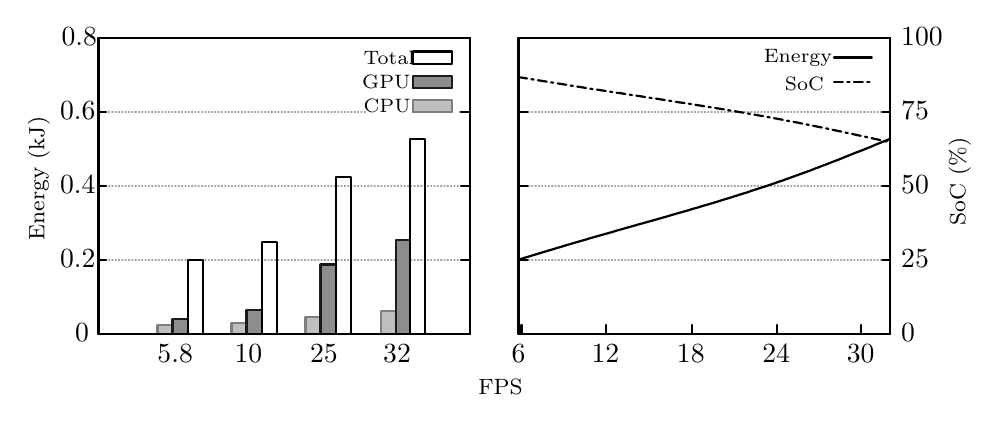
\begin{tikzpicture}[y=0.80pt, x=0.80pt, yscale=-0.680000, xscale=0.680000, inner sep=0pt, outer sep=0pt]
\begin{scope}[draw=black,line join=bevel,line cap=rect,even odd rule,line width=0.800pt]
  \begin{scope}[cm={{1.0,0.0,0.0,1.0,(0.0,0.0)}},draw=black,line join=bevel,line cap=rect,line width=0.800pt]
  \end{scope}
  \begin{scope}[cm={{1.00313,0.0,0.0,1.00313,(0.0,0.0)}},draw=black,line join=bevel,line cap=rect,line width=0.800pt]
  \end{scope}
  \begin{scope}[cm={{1.00313,0.0,0.0,1.00313,(0.0,0.0)}},draw=ca0a0a4,dash pattern=on 0.40pt off 0.80pt,line join=round,line cap=round,line width=0.400pt]
    \path[draw] (64.5000,224.5000) -- (310.5000,224.5000);
  \end{scope}
  \begin{scope}[cm={{1.00313,0.0,0.0,1.00313,(0.0,0.0)}},draw=black,line join=round,line cap=round,line width=0.800pt]
    \path[draw] (64.5000,224.5000) -- (69.5000,224.5000);
    \path[draw] (310.5000,224.5000) -- (304.5000,224.5000);
  \end{scope}
  \begin{scope}[cm={{1.00313,0.0,0.0,1.00313,(0.0,0.0)}},draw=black,line join=bevel,line cap=rect,line width=0.800pt]
  \end{scope}
  \begin{scope}[cm={{1.00313,0.0,0.0,1.00313,(49.1531,230.217)}},draw=black,line join=bevel,line cap=rect,line width=0.800pt]
  \end{scope}
  \begin{scope}[cm={{1.00313,0.0,0.0,1.00313,(49.1531,230.217)}},draw=black,line join=bevel,line cap=rect,line width=0.800pt]
  \end{scope}
  \begin{scope}[cm={{1.00313,0.0,0.0,1.00313,(49.1531,230.217)}},draw=black,line join=bevel,line cap=rect,line width=0.800pt]
  \end{scope}
  \begin{scope}[cm={{1.00313,0.0,0.0,1.00313,(49.1531,230.217)}},draw=black,line join=bevel,line cap=rect,line width=0.800pt]
  \end{scope}
  \begin{scope}[cm={{1.00313,0.0,0.0,1.00313,(49.1531,230.217)}},draw=black,line join=bevel,line cap=rect,line width=0.800pt]
  \end{scope}
  \begin{scope}[cm={{1.00313,0.0,0.0,1.00313,(49.1531,230.217)}},draw=black,line join=bevel,line cap=rect,line width=0.800pt]
    \path[fill=black] (0.0000,0.0000) node[above right] () {0};
  \end{scope}
  \begin{scope}[cm={{1.00313,0.0,0.0,1.00313,(49.1531,230.217)}},draw=black,line join=bevel,line cap=rect,line width=0.800pt]
  \end{scope}
  \begin{scope}[cm={{1.00313,0.0,0.0,1.00313,(0.0,0.0)}},draw=black,line join=bevel,line cap=rect,line width=0.800pt]
  \end{scope}
  \begin{scope}[cm={{1.00313,0.0,0.0,1.00313,(0.0,0.0)}},draw=ca0a0a4,dash pattern=on 0.40pt off 0.80pt,line join=round,line cap=round,line width=0.400pt]
    \path[draw] (64.5000,175.5000) -- (310.5000,175.5000);
  \end{scope}
  \begin{scope}[cm={{1.00313,0.0,0.0,1.00313,(0.0,0.0)}},draw=black,line join=round,line cap=round,line width=0.800pt]
    \path[draw] (64.5000,175.5000) -- (69.5000,175.5000);
    \path[draw] (310.5000,175.5000) -- (304.5000,175.5000);
  \end{scope}
  \begin{scope}[cm={{1.00313,0.0,0.0,1.00313,(0.0,0.0)}},draw=black,line join=bevel,line cap=rect,line width=0.800pt]
  \end{scope}
  \begin{scope}[cm={{1.00313,0.0,0.0,1.00313,(49.1531,181.064)}},draw=black,line join=bevel,line cap=rect,line width=0.800pt]
  \end{scope}
  \begin{scope}[cm={{1.00313,0.0,0.0,1.00313,(49.1531,181.064)}},draw=black,line join=bevel,line cap=rect,line width=0.800pt]
  \end{scope}
  \begin{scope}[cm={{1.00313,0.0,0.0,1.00313,(49.1531,181.064)}},draw=black,line join=bevel,line cap=rect,line width=0.800pt]
  \end{scope}
  \begin{scope}[cm={{1.00313,0.0,0.0,1.00313,(49.1531,181.064)}},draw=black,line join=bevel,line cap=rect,line width=0.800pt]
  \end{scope}
  \begin{scope}[cm={{1.00313,0.0,0.0,1.00313,(49.1531,181.064)}},draw=black,line join=bevel,line cap=rect,line width=0.800pt]
  \end{scope}
  \begin{scope}[cm={{1.00313,0.0,0.0,1.00313,(39.1531,181.064)}},draw=black,line join=bevel,line cap=rect,line width=0.800pt]
    \path[fill=black] (0.0000,0.0000) node[above right] () {0.2};
  \end{scope}
  \begin{scope}[cm={{1.00313,0.0,0.0,1.00313,(49.1531,181.064)}},draw=black,line join=bevel,line cap=rect,line width=0.800pt]
  \end{scope}
  \begin{scope}[cm={{1.00313,0.0,0.0,1.00313,(0.0,0.0)}},draw=black,line join=bevel,line cap=rect,line width=0.800pt]
  \end{scope}
  \begin{scope}[cm={{1.00313,0.0,0.0,1.00313,(0.0,0.0)}},draw=ca0a0a4,dash pattern=on 0.40pt off 0.80pt,line join=round,line cap=round,line width=0.400pt]
    \path[draw] (64.5000,126.5000) -- (310.5000,126.5000);
  \end{scope}
  \begin{scope}[cm={{1.00313,0.0,0.0,1.00313,(0.0,0.0)}},draw=black,line join=round,line cap=round,line width=0.800pt]
    \path[draw] (64.5000,126.5000) -- (69.5000,126.5000);
    \path[draw] (310.5000,126.5000) -- (304.5000,126.5000);
  \end{scope}
  \begin{scope}[cm={{1.00313,0.0,0.0,1.00313,(0.0,0.0)}},draw=black,line join=bevel,line cap=rect,line width=0.800pt]
  \end{scope}
  \begin{scope}[cm={{1.00313,0.0,0.0,1.00313,(49.1531,131.911)}},draw=black,line join=bevel,line cap=rect,line width=0.800pt]
  \end{scope}
  \begin{scope}[cm={{1.00313,0.0,0.0,1.00313,(49.1531,131.911)}},draw=black,line join=bevel,line cap=rect,line width=0.800pt]
  \end{scope}
  \begin{scope}[cm={{1.00313,0.0,0.0,1.00313,(49.1531,131.911)}},draw=black,line join=bevel,line cap=rect,line width=0.800pt]
  \end{scope}
  \begin{scope}[cm={{1.00313,0.0,0.0,1.00313,(49.1531,131.911)}},draw=black,line join=bevel,line cap=rect,line width=0.800pt]
  \end{scope}
  \begin{scope}[cm={{1.00313,0.0,0.0,1.00313,(49.1531,131.911)}},draw=black,line join=bevel,line cap=rect,line width=0.800pt]
  \end{scope}
  \begin{scope}[cm={{1.00313,0.0,0.0,1.00313,(39.1531,131.911)}},draw=black,line join=bevel,line cap=rect,line width=0.800pt]
    \path[fill=black] (0.0000,0.0000) node[above right] () {0.4};
  \end{scope}
  \begin{scope}[cm={{1.00313,0.0,0.0,1.00313,(49.1531,131.911)}},draw=black,line join=bevel,line cap=rect,line width=0.800pt]
  \end{scope}
  \begin{scope}[cm={{1.00313,0.0,0.0,1.00313,(0.0,0.0)}},draw=black,line join=bevel,line cap=rect,line width=0.800pt]
  \end{scope}
  \begin{scope}[cm={{1.00313,0.0,0.0,1.00313,(0.0,0.0)}},draw=ca0a0a4,dash pattern=on 0.40pt off 0.80pt,line join=round,line cap=round,line width=0.400pt]
    \path[draw] (64.5000,77.5000) -- (242.5000,77.5000);
    \path[draw] (303.5000,77.5000) -- (310.5000,77.5000);
  \end{scope}
  \begin{scope}[cm={{1.00313,0.0,0.0,1.00313,(0.0,0.0)}},draw=black,line join=round,line cap=round,line width=0.800pt]
    \path[draw] (64.5000,77.5000) -- (69.5000,77.5000);
    \path[draw] (310.5000,77.5000) -- (304.5000,77.5000);
  \end{scope}
  \begin{scope}[cm={{1.00313,0.0,0.0,1.00313,(0.0,0.0)}},draw=black,line join=bevel,line cap=rect,line width=0.800pt]
  \end{scope}
  \begin{scope}[cm={{1.00313,0.0,0.0,1.00313,(49.1531,82.7578)}},draw=black,line join=bevel,line cap=rect,line width=0.800pt]
  \end{scope}
  \begin{scope}[cm={{1.00313,0.0,0.0,1.00313,(49.1531,82.7578)}},draw=black,line join=bevel,line cap=rect,line width=0.800pt]
  \end{scope}
  \begin{scope}[cm={{1.00313,0.0,0.0,1.00313,(49.1531,82.7578)}},draw=black,line join=bevel,line cap=rect,line width=0.800pt]
  \end{scope}
  \begin{scope}[cm={{1.00313,0.0,0.0,1.00313,(49.1531,82.7578)}},draw=black,line join=bevel,line cap=rect,line width=0.800pt]
  \end{scope}
  \begin{scope}[cm={{1.00313,0.0,0.0,1.00313,(49.1531,82.7578)}},draw=black,line join=bevel,line cap=rect,line width=0.800pt]
  \end{scope}
  \begin{scope}[cm={{1.00313,0.0,0.0,1.00313,(39.1531,82.7578)}},draw=black,line join=bevel,line cap=rect,line width=0.800pt]
    \path[fill=black] (0.0000,0.0000) node[above right] () {0.6};
  \end{scope}
  \begin{scope}[cm={{1.00313,0.0,0.0,1.00313,(49.1531,82.7578)}},draw=black,line join=bevel,line cap=rect,line width=0.800pt]
  \end{scope}
  \begin{scope}[cm={{1.00313,0.0,0.0,1.00313,(0.0,0.0)}},draw=black,line join=bevel,line cap=rect,line width=0.800pt]
  \end{scope}
  \begin{scope}[cm={{1.00313,0.0,0.0,1.00313,(0.0,0.0)}},draw=ca0a0a4,dash pattern=on 0.40pt off 0.80pt,line join=round,line cap=round,line width=0.400pt]
    \path[draw] (64.5000,28.5000) -- (310.5000,28.5000);
  \end{scope}
  \begin{scope}[cm={{1.00313,0.0,0.0,1.00313,(0.0,0.0)}},draw=black,line join=round,line cap=round,line width=0.800pt]
    \path[draw] (64.5000,28.5000) -- (69.5000,28.5000);
    \path[draw] (310.5000,28.5000) -- (304.5000,28.5000);
  \end{scope}
  \begin{scope}[cm={{1.00313,0.0,0.0,1.00313,(0.0,0.0)}},draw=black,line join=bevel,line cap=rect,line width=0.800pt]
  \end{scope}
  \begin{scope}[cm={{1.00313,0.0,0.0,1.00313,(50.1562,33.6047)}},draw=black,line join=bevel,line cap=rect,line width=0.800pt]
  \end{scope}
  \begin{scope}[cm={{1.00313,0.0,0.0,1.00313,(50.1562,33.6047)}},draw=black,line join=bevel,line cap=rect,line width=0.800pt]
  \end{scope}
  \begin{scope}[cm={{1.00313,0.0,0.0,1.00313,(50.1562,33.6047)}},draw=black,line join=bevel,line cap=rect,line width=0.800pt]
  \end{scope}
  \begin{scope}[cm={{1.00313,0.0,0.0,1.00313,(50.1562,33.6047)}},draw=black,line join=bevel,line cap=rect,line width=0.800pt]
  \end{scope}
  \begin{scope}[cm={{1.00313,0.0,0.0,1.00313,(50.1562,33.6047)}},draw=black,line join=bevel,line cap=rect,line width=0.800pt]
  \end{scope}
  \begin{scope}[cm={{1.00313,0.0,0.0,1.00313,(40.1562,33.6047)}},draw=black,line join=bevel,line cap=rect,line width=0.800pt]
    \path[fill=black] (0.0000,0.0000) node[above right] () {0.8};
  \end{scope}
  \begin{scope}[cm={{1.00313,0.0,0.0,1.00313,(50.1562,33.6047)}},draw=black,line join=bevel,line cap=rect,line width=0.800pt]
  \end{scope}
  \begin{scope}[cm={{1.00313,0.0,0.0,1.00313,(0.0,0.0)}},draw=black,line join=bevel,line cap=rect,line width=0.800pt]
  \end{scope}
  \begin{scope}[cm={{1.00313,0.0,0.0,1.00313,(0.0,0.0)}},draw=black,line join=round,line cap=round,line width=0.800pt]
    \path[draw] (113.5000,224.5000) -- (113.5000,224.5000);
  \end{scope}
  \begin{scope}[cm={{1.00313,0.0,0.0,1.00313,(0.0,0.0)}},draw=black,line join=bevel,line cap=rect,line width=0.800pt]
  \end{scope}
  \begin{scope}[cm={{1.00313,0.0,0.0,1.00313,(103.823,244.261)}},draw=black,line join=bevel,line cap=rect,line width=0.800pt]
  \end{scope}
  \begin{scope}[cm={{1.00313,0.0,0.0,1.00313,(103.823,244.261)}},draw=black,line join=bevel,line cap=rect,line width=0.800pt]
  \end{scope}
  \begin{scope}[cm={{1.00313,0.0,0.0,1.00313,(103.823,244.261)}},draw=black,line join=bevel,line cap=rect,line width=0.800pt]
  \end{scope}
  \begin{scope}[cm={{1.00313,0.0,0.0,1.00313,(103.823,244.261)}},draw=black,line join=bevel,line cap=rect,line width=0.800pt]
  \end{scope}
  \begin{scope}[cm={{1.00313,0.0,0.0,1.00313,(103.823,244.261)}},draw=black,line join=bevel,line cap=rect,line width=0.800pt]
  \end{scope}
  \begin{scope}[cm={{1.00313,0.0,0.0,1.00313,(103.823,244.261)}},draw=black,line join=bevel,line cap=rect,line width=0.800pt]
    \path[fill=black] (0.0000,0.0000) node[above right] () {5.8};
  \end{scope}
  \begin{scope}[cm={{1.00313,0.0,0.0,1.00313,(103.823,244.261)}},draw=black,line join=bevel,line cap=rect,line width=0.800pt]
  \end{scope}
  \begin{scope}[cm={{1.00313,0.0,0.0,1.00313,(0.0,0.0)}},draw=black,line join=bevel,line cap=rect,line width=0.800pt]
  \end{scope}
  \begin{scope}[cm={{1.00313,0.0,0.0,1.00313,(0.0,0.0)}},draw=black,line join=round,line cap=round,line width=0.800pt]
    \path[draw] (162.5000,224.5000) -- (162.5000,224.5000);
  \end{scope}
  \begin{scope}[cm={{1.00313,0.0,0.0,1.00313,(0.0,0.0)}},draw=black,line join=bevel,line cap=rect,line width=0.800pt]
  \end{scope}
  \begin{scope}[cm={{1.00313,0.0,0.0,1.00313,(154.983,244.261)}},draw=black,line join=bevel,line cap=rect,line width=0.800pt]
  \end{scope}
  \begin{scope}[cm={{1.00313,0.0,0.0,1.00313,(154.983,244.261)}},draw=black,line join=bevel,line cap=rect,line width=0.800pt]
  \end{scope}
  \begin{scope}[cm={{1.00313,0.0,0.0,1.00313,(154.983,244.261)}},draw=black,line join=bevel,line cap=rect,line width=0.800pt]
  \end{scope}
  \begin{scope}[cm={{1.00313,0.0,0.0,1.00313,(154.983,244.261)}},draw=black,line join=bevel,line cap=rect,line width=0.800pt]
  \end{scope}
  \begin{scope}[cm={{1.00313,0.0,0.0,1.00313,(154.983,244.261)}},draw=black,line join=bevel,line cap=rect,line width=0.800pt]
  \end{scope}
  \begin{scope}[cm={{1.00313,0.0,0.0,1.00313,(154.983,244.261)}},draw=black,line join=bevel,line cap=rect,line width=0.800pt]
    \path[fill=black] (0.0000,0.0000) node[above right] () {10};
  \end{scope}
  \begin{scope}[cm={{1.00313,0.0,0.0,1.00313,(154.983,244.261)}},draw=black,line join=bevel,line cap=rect,line width=0.800pt]
  \end{scope}
  \begin{scope}[cm={{1.00313,0.0,0.0,1.00313,(0.0,0.0)}},draw=black,line join=bevel,line cap=rect,line width=0.800pt]
  \end{scope}
  \begin{scope}[cm={{1.00313,0.0,0.0,1.00313,(0.0,0.0)}},draw=black,line join=round,line cap=round,line width=0.800pt]
    \path[draw] (211.5000,224.5000) -- (211.5000,224.5000);
  \end{scope}
  \begin{scope}[cm={{1.00313,0.0,0.0,1.00313,(0.0,0.0)}},draw=black,line join=bevel,line cap=rect,line width=0.800pt]
  \end{scope}
  \begin{scope}[cm={{1.00313,0.0,0.0,1.00313,(205.139,244.261)}},draw=black,line join=bevel,line cap=rect,line width=0.800pt]
  \end{scope}
  \begin{scope}[cm={{1.00313,0.0,0.0,1.00313,(205.139,244.261)}},draw=black,line join=bevel,line cap=rect,line width=0.800pt]
  \end{scope}
  \begin{scope}[cm={{1.00313,0.0,0.0,1.00313,(205.139,244.261)}},draw=black,line join=bevel,line cap=rect,line width=0.800pt]
  \end{scope}
  \begin{scope}[cm={{1.00313,0.0,0.0,1.00313,(205.139,244.261)}},draw=black,line join=bevel,line cap=rect,line width=0.800pt]
  \end{scope}
  \begin{scope}[cm={{1.00313,0.0,0.0,1.00313,(205.139,244.261)}},draw=black,line join=bevel,line cap=rect,line width=0.800pt]
  \end{scope}
  \begin{scope}[cm={{1.00313,0.0,0.0,1.00313,(205.139,244.261)}},draw=black,line join=bevel,line cap=rect,line width=0.800pt]
    \path[fill=black] (0.0000,0.0000) node[above right] () {25};
  \end{scope}
  \begin{scope}[cm={{1.00313,0.0,0.0,1.00313,(205.139,244.261)}},draw=black,line join=bevel,line cap=rect,line width=0.800pt]
  \end{scope}
  \begin{scope}[cm={{1.00313,0.0,0.0,1.00313,(0.0,0.0)}},draw=black,line join=bevel,line cap=rect,line width=0.800pt]
  \end{scope}
  \begin{scope}[cm={{1.00313,0.0,0.0,1.00313,(0.0,0.0)}},draw=black,line join=round,line cap=round,line width=0.800pt]
    \path[draw] (261.5000,224.5000) -- (261.5000,224.5000);
  \end{scope}
  \begin{scope}[cm={{1.00313,0.0,0.0,1.00313,(0.0,0.0)}},draw=black,line join=bevel,line cap=rect,line width=0.800pt]
  \end{scope}
  \begin{scope}[cm={{1.00313,0.0,0.0,1.00313,(253.791,244.261)}},draw=black,line join=bevel,line cap=rect,line width=0.800pt]
  \end{scope}
  \begin{scope}[cm={{1.00313,0.0,0.0,1.00313,(253.791,244.261)}},draw=black,line join=bevel,line cap=rect,line width=0.800pt]
  \end{scope}
  \begin{scope}[cm={{1.00313,0.0,0.0,1.00313,(253.791,244.261)}},draw=black,line join=bevel,line cap=rect,line width=0.800pt]
  \end{scope}
  \begin{scope}[cm={{1.00313,0.0,0.0,1.00313,(253.791,244.261)}},draw=black,line join=bevel,line cap=rect,line width=0.800pt]
  \end{scope}
  \begin{scope}[cm={{1.00313,0.0,0.0,1.00313,(253.791,244.261)}},draw=black,line join=bevel,line cap=rect,line width=0.800pt]
  \end{scope}
  \begin{scope}[cm={{1.00313,0.0,0.0,1.00313,(253.791,244.261)}},draw=black,line join=bevel,line cap=rect,line width=0.800pt]
    \path[fill=black] (0.0000,0.0000) node[above right] () {32};
  \end{scope}
  \begin{scope}[cm={{1.00313,0.0,0.0,1.00313,(253.791,244.261)}},draw=black,line join=bevel,line cap=rect,line width=0.800pt]
  \end{scope}
  \begin{scope}[cm={{1.00313,0.0,0.0,1.00313,(0.0,0.0)}},draw=black,line join=bevel,line cap=rect,line width=0.800pt]
  \end{scope}
  \begin{scope}[cm={{1.00313,0.0,0.0,1.00313,(0.0,0.0)}},draw=black,line join=round,line cap=round,line width=0.800pt]
    \path[draw] (64.5000,28.5000) -- (64.5000,224.5000) -- (310.5000,224.5000) --
      (310.5000,28.5000) -- (64.5000,28.5000);
  \end{scope}
  \begin{scope}[cm={{1.00313,0.0,0.0,1.00313,(0.0,0.0)}},draw=black,line join=bevel,line cap=rect,line width=0.800pt]
  \end{scope}
  \begin{scope}[cm={{0.0,-1.00313,1.00313,0.0,(31.5984,163.008)}},draw=black,line join=bevel,line cap=rect,line width=0.800pt]
  \end{scope}
  \begin{scope}[cm={{0.0,-1.00313,1.00313,0.0,(31.5984,163.008)}},draw=black,line join=bevel,line cap=rect,line width=0.800pt]
  \end{scope}
  \begin{scope}[cm={{0.0,-1.00313,1.00313,0.0,(31.5984,163.008)}},draw=black,line join=bevel,line cap=rect,line width=0.800pt]
  \end{scope}
  \begin{scope}[cm={{0.0,-1.00313,1.00313,0.0,(31.5984,163.008)}},draw=black,line join=bevel,line cap=rect,line width=0.800pt]
  \end{scope}
  \begin{scope}[cm={{0.0,-1.00313,1.00313,0.0,(31.5984,163.008)}},draw=black,line join=bevel,line cap=rect,line width=0.800pt]
  \end{scope}
  \begin{scope}[cm={{0.0,-1.00313,1.00313,0.0,(17.5984,163.008)}},draw=black,line join=bevel,line cap=rect,line width=0.800pt]
    \path[fill=black] (0.0000,0.0000) node[above right] () {\rotatebox{90}{\footnotesize Energy (kJ)}};
  \end{scope}
  \begin{scope}[cm={{0.0,-1.00313,1.00313,0.0,(31.5984,163.008)}},draw=black,line join=bevel,line cap=rect,line width=0.800pt]
  \end{scope}
  \begin{scope}[cm={{1.00313,0.0,0.0,1.00313,(316.988,265.327)}},draw=black,line join=bevel,line cap=rect,line width=0.800pt]
  \end{scope}
  \begin{scope}[cm={{1.00313,0.0,0.0,1.00313,(316.988,265.327)}},draw=black,line join=bevel,line cap=rect,line width=0.800pt]
  \end{scope}
  \begin{scope}[cm={{1.00313,0.0,0.0,1.00313,(316.988,265.327)}},draw=black,line join=bevel,line cap=rect,line width=0.800pt]
  \end{scope}
  \begin{scope}[cm={{1.00313,0.0,0.0,1.00313,(316.988,265.327)}},draw=black,line join=bevel,line cap=rect,line width=0.800pt]
  \end{scope}
  \begin{scope}[cm={{1.00313,0.0,0.0,1.00313,(316.988,265.327)}},draw=black,line join=bevel,line cap=rect,line width=0.800pt]
  \end{scope}
  \begin{scope}[cm={{1.00313,0.0,0.0,1.00313,(316.988,265.327)}},draw=black,line join=bevel,line cap=rect,line width=0.800pt]
    \path[fill=black] (0.0000,0.0000) node[above right] () {\footnotesize FPS};
  \end{scope}
  \begin{scope}[cm={{1.00313,0.0,0.0,1.00313,(316.988,265.327)}},draw=black,line join=bevel,line cap=rect,line width=0.800pt]
  \end{scope}
  \begin{scope}[cm={{1.00313,0.0,0.0,1.00313,(247.772,78.2438)}},draw=black,line join=bevel,line cap=rect,line width=0.800pt]
  \end{scope}
  \begin{scope}[cm={{1.00313,0.0,0.0,1.00313,(247.772,78.2438)}},draw=black,line join=bevel,line cap=rect,line width=0.800pt]
  \end{scope}
  \begin{scope}[cm={{1.00313,0.0,0.0,1.00313,(247.772,78.2438)}},draw=black,line join=bevel,line cap=rect,line width=0.800pt]
  \end{scope}
  \begin{scope}[cm={{1.00313,0.0,0.0,1.00313,(247.772,78.2438)}},draw=black,line join=bevel,line cap=rect,line width=0.800pt]
  \end{scope}
  \begin{scope}[cm={{1.00313,0.0,0.0,1.00313,(247.772,78.2438)}},draw=black,line join=bevel,line cap=rect,line width=0.800pt]
  \end{scope}
  \begin{scope}[cm={{1.00313,0.0,0.0,1.00313,(240.772,78.2438)}},draw=black,line join=bevel,line cap=rect,line width=0.800pt]
    \path[fill=black] (0.0000,0.0000) node[above right] () {\scriptsize CPU};
  \end{scope}
  \begin{scope}[cm={{1.00313,0.0,0.0,1.00313,(247.772,78.2438)}},draw=black,line join=bevel,line cap=rect,line width=0.800pt]
  \end{scope}
  \begin{scope}[cm={{1.00313,0.0,0.0,1.00313,(0.0,0.0)}},draw=black,line join=bevel,line cap=rect,line width=0.800pt]
  \end{scope}
  \begin{scope}[cm={{1.00313,0.0,0.0,1.00313,(0.0,0.0)}},fill=cbfbfbf]
    \path[fill,rounded corners=0.0000cm] (273.0000,70.0000) rectangle
      (299.0000,78.0000);
  \end{scope}
  \begin{scope}[cm={{1.00313,0.0,0.0,1.00313,(0.0,0.0)}},draw=black,line join=bevel,line cap=rect,line width=0.800pt]
  \end{scope}
  \begin{scope}[cm={{1.00313,0.0,0.0,1.00313,(0.0,0.0)}},draw=black,line join=bevel,line cap=rect,line width=0.800pt]
  \end{scope}
  \begin{scope}[cm={{1.00313,0.0,0.0,1.00313,(0.0,0.0)}},draw=c7f7f7f,line join=round,line cap=round,line width=0.800pt]
    \path[draw,even odd rule] (272.5000,77.5000) -- (298.5000,77.5000) --
      (298.5000,77.5000) -- (298.5000,69.5000) -- (298.5000,69.5000) --
      (272.5000,69.5000) -- (272.5000,69.5000) -- (272.5000,77.5000);
  \end{scope}
  \begin{scope}[cm={{1.00313,0.0,0.0,1.00313,(0.0,0.0)}},draw=black,line join=bevel,line cap=rect,line width=0.800pt]
  \end{scope}
  \begin{scope}[cm={{1.00313,0.0,0.0,1.00313,(0.0,0.0)}},draw=black,line join=bevel,line cap=rect,line width=0.800pt]
  \end{scope}
  \begin{scope}[cm={{1.00313,0.0,0.0,1.00313,(0.0,0.0)}},draw=black,line join=bevel,line cap=rect,line width=0.800pt]
  \end{scope}
  \begin{scope}[cm={{1.00313,0.0,0.0,1.00313,(0.0,0.0)}},draw=black,line join=bevel,line cap=rect,line width=0.800pt]
  \end{scope}
  \begin{scope}[cm={{1.00313,0.0,0.0,1.00313,(0.0,0.0)}},fill=cbfbfbf]
    \path[fill,rounded corners=0.0000cm] (103.0000,219.0000) rectangle
      (113.0000,224.0000);
  \end{scope}
  \begin{scope}[cm={{1.00313,0.0,0.0,1.00313,(0.0,0.0)}},draw=black,line join=bevel,line cap=rect,line width=0.800pt]
  \end{scope}
  \begin{scope}[cm={{1.00313,0.0,0.0,1.00313,(0.0,0.0)}},draw=black,line join=bevel,line cap=rect,line width=0.800pt]
  \end{scope}
  \begin{scope}[cm={{1.00313,0.0,0.0,1.00313,(0.0,0.0)}},draw=c7f7f7f,line join=round,line cap=round,line width=0.800pt]
    \path[draw] (103.5000,224.5000) -- (103.5000,218.5000) -- (113.5000,218.5000) --
      (113.5000,224.5000) -- (103.5000,224.5000);
  \end{scope}
  \begin{scope}[cm={{1.00313,0.0,0.0,1.00313,(0.0,0.0)}},draw=black,line join=bevel,line cap=rect,line width=0.800pt]
  \end{scope}
  \begin{scope}[cm={{1.00313,0.0,0.0,1.00313,(0.0,0.0)}},draw=black,line join=bevel,line cap=rect,line width=0.800pt]
  \end{scope}
  \begin{scope}[cm={{1.00313,0.0,0.0,1.00313,(0.0,0.0)}},fill=cbfbfbf]
    \path[fill,rounded corners=0.0000cm] (153.0000,218.0000) rectangle
      (163.0000,224.0000);
  \end{scope}
  \begin{scope}[cm={{1.00313,0.0,0.0,1.00313,(0.0,0.0)}},draw=black,line join=bevel,line cap=rect,line width=0.800pt]
  \end{scope}
  \begin{scope}[cm={{1.00313,0.0,0.0,1.00313,(0.0,0.0)}},draw=black,line join=bevel,line cap=rect,line width=0.800pt]
  \end{scope}
  \begin{scope}[cm={{1.00313,0.0,0.0,1.00313,(0.0,0.0)}},draw=c7f7f7f,line join=round,line cap=round,line width=0.800pt]
    \path[draw] (152.5000,224.5000) -- (152.5000,217.5000) -- (162.5000,217.5000) --
      (162.5000,224.5000) -- (152.5000,224.5000);
  \end{scope}
  \begin{scope}[cm={{1.00313,0.0,0.0,1.00313,(0.0,0.0)}},draw=black,line join=bevel,line cap=rect,line width=0.800pt]
  \end{scope}
  \begin{scope}[cm={{1.00313,0.0,0.0,1.00313,(0.0,0.0)}},draw=black,line join=bevel,line cap=rect,line width=0.800pt]
  \end{scope}
  \begin{scope}[cm={{1.00313,0.0,0.0,1.00313,(0.0,0.0)}},fill=cbfbfbf]
    \path[fill,rounded corners=0.0000cm] (202.0000,213.0000) rectangle
      (212.0000,224.0000);
  \end{scope}
  \begin{scope}[cm={{1.00313,0.0,0.0,1.00313,(0.0,0.0)}},draw=black,line join=bevel,line cap=rect,line width=0.800pt]
  \end{scope}
  \begin{scope}[cm={{1.00313,0.0,0.0,1.00313,(0.0,0.0)}},draw=black,line join=bevel,line cap=rect,line width=0.800pt]
  \end{scope}
  \begin{scope}[cm={{1.00313,0.0,0.0,1.00313,(0.0,0.0)}},draw=c7f7f7f,line join=round,line cap=round,line width=0.800pt]
    \path[draw] (201.5000,224.5000) -- (201.5000,213.5000) -- (211.5000,213.5000) --
      (211.5000,224.5000) -- (201.5000,224.5000);
  \end{scope}
  \begin{scope}[cm={{1.00313,0.0,0.0,1.00313,(0.0,0.0)}},draw=black,line join=bevel,line cap=rect,line width=0.800pt]
  \end{scope}
  \begin{scope}[cm={{1.00313,0.0,0.0,1.00313,(0.0,0.0)}},draw=black,line join=bevel,line cap=rect,line width=0.800pt]
  \end{scope}
  \begin{scope}[cm={{1.00313,0.0,0.0,1.00313,(0.0,0.0)}},fill=cbfbfbf]
    \path[fill,rounded corners=0.0000cm] (251.0000,209.0000) rectangle
      (261.0000,224.0000);
  \end{scope}
  \begin{scope}[cm={{1.00313,0.0,0.0,1.00313,(0.0,0.0)}},draw=black,line join=bevel,line cap=rect,line width=0.800pt]
  \end{scope}
  \begin{scope}[cm={{1.00313,0.0,0.0,1.00313,(0.0,0.0)}},draw=black,line join=bevel,line cap=rect,line width=0.800pt]
  \end{scope}
  \begin{scope}[cm={{1.00313,0.0,0.0,1.00313,(0.0,0.0)}},draw=c7f7f7f,line join=round,line cap=round,line width=0.800pt]
    \path[draw] (251.5000,224.5000) -- (251.5000,209.5000) -- (261.5000,209.5000) --
      (261.5000,224.5000) -- (251.5000,224.5000);
  \end{scope}
  \begin{scope}[cm={{1.00313,0.0,0.0,1.00313,(0.0,0.0)}},draw=black,line join=bevel,line cap=rect,line width=0.800pt]
  \end{scope}
  \begin{scope}[cm={{1.00313,0.0,0.0,1.00313,(246.769,62.1938)}},draw=black,line join=bevel,line cap=rect,line width=0.800pt]
  \end{scope}
  \begin{scope}[cm={{1.00313,0.0,0.0,1.00313,(246.769,62.1938)}},draw=black,line join=bevel,line cap=rect,line width=0.800pt]
  \end{scope}
  \begin{scope}[cm={{1.00313,0.0,0.0,1.00313,(246.769,62.1938)}},draw=black,line join=bevel,line cap=rect,line width=0.800pt]
  \end{scope}
  \begin{scope}[cm={{1.00313,0.0,0.0,1.00313,(246.769,62.1938)}},draw=black,line join=bevel,line cap=rect,line width=0.800pt]
  \end{scope}
  \begin{scope}[cm={{1.00313,0.0,0.0,1.00313,(246.769,62.1938)}},draw=black,line join=bevel,line cap=rect,line width=0.800pt]
  \end{scope}
  \begin{scope}[cm={{1.00313,0.0,0.0,1.00313,(239.769,62.1938)}},draw=black,line join=bevel,line cap=rect,line width=0.800pt]
    \path[fill=black] (0.0000,0.0000) node[above right] () {\scriptsize GPU};
  \end{scope}
  \begin{scope}[cm={{1.00313,0.0,0.0,1.00313,(246.769,62.1938)}},draw=black,line join=bevel,line cap=rect,line width=0.800pt]
  \end{scope}
  \begin{scope}[cm={{1.00313,0.0,0.0,1.00313,(0.0,0.0)}},draw=black,line join=bevel,line cap=rect,line width=0.800pt]
  \end{scope}
  \begin{scope}[cm={{1.00313,0.0,0.0,1.00313,(0.0,0.0)}},fill=c8d8d8d]
    \path[fill,rounded corners=0.0000cm] (273.0000,54.0000) rectangle
      (299.0000,62.0000);
  \end{scope}
  \begin{scope}[cm={{1.00313,0.0,0.0,1.00313,(0.0,0.0)}},draw=black,line join=bevel,line cap=rect,line width=0.800pt]
  \end{scope}
  \begin{scope}[cm={{1.00313,0.0,0.0,1.00313,(0.0,0.0)}},draw=black,line join=bevel,line cap=rect,line width=0.800pt]
  \end{scope}
  \begin{scope}[cm={{1.00313,0.0,0.0,1.00313,(0.0,0.0)}},draw=c1a1a1a,line join=round,line cap=round,line width=0.800pt]
    \path[draw,even odd rule] (272.5000,61.5000) -- (298.5000,61.5000) --
      (298.5000,61.5000) -- (298.5000,53.5000) -- (298.5000,53.5000) --
      (272.5000,53.5000) -- (272.5000,53.5000) -- (272.5000,61.5000);
  \end{scope}
  \begin{scope}[cm={{1.00313,0.0,0.0,1.00313,(0.0,0.0)}},draw=black,line join=bevel,line cap=rect,line width=0.800pt]
  \end{scope}
  \begin{scope}[cm={{1.00313,0.0,0.0,1.00313,(0.0,0.0)}},draw=black,line join=bevel,line cap=rect,line width=0.800pt]
  \end{scope}
  \begin{scope}[cm={{1.00313,0.0,0.0,1.00313,(0.0,0.0)}},draw=black,line join=bevel,line cap=rect,line width=0.800pt]
  \end{scope}
  \begin{scope}[cm={{1.00313,0.0,0.0,1.00313,(0.0,0.0)}},draw=black,line join=bevel,line cap=rect,line width=0.800pt]
  \end{scope}
  \begin{scope}[cm={{1.00313,0.0,0.0,1.00313,(0.0,0.0)}},fill=c8d8d8d]
    \path[fill,rounded corners=0.0000cm] (113.0000,214.0000) rectangle
      (123.0000,224.0000);
  \end{scope}
  \begin{scope}[cm={{1.00313,0.0,0.0,1.00313,(0.0,0.0)}},draw=black,line join=bevel,line cap=rect,line width=0.800pt]
  \end{scope}
  \begin{scope}[cm={{1.00313,0.0,0.0,1.00313,(0.0,0.0)}},draw=black,line join=bevel,line cap=rect,line width=0.800pt]
  \end{scope}
  \begin{scope}[cm={{1.00313,0.0,0.0,1.00313,(0.0,0.0)}},draw=c1a1a1a,line join=round,line cap=round,line width=0.800pt]
    \path[draw] (113.5000,224.5000) -- (113.5000,214.5000) -- (123.5000,214.5000) --
      (123.5000,224.5000) -- (113.5000,224.5000);
  \end{scope}
  \begin{scope}[cm={{1.00313,0.0,0.0,1.00313,(0.0,0.0)}},draw=black,line join=bevel,line cap=rect,line width=0.800pt]
  \end{scope}
  \begin{scope}[cm={{1.00313,0.0,0.0,1.00313,(0.0,0.0)}},draw=black,line join=bevel,line cap=rect,line width=0.800pt]
  \end{scope}
  \begin{scope}[cm={{1.00313,0.0,0.0,1.00313,(0.0,0.0)}},fill=c8d8d8d]
    \path[fill,rounded corners=0.0000cm] (163.0000,208.0000) rectangle
      (173.0000,224.0000);
  \end{scope}
  \begin{scope}[cm={{1.00313,0.0,0.0,1.00313,(0.0,0.0)}},draw=black,line join=bevel,line cap=rect,line width=0.800pt]
  \end{scope}
  \begin{scope}[cm={{1.00313,0.0,0.0,1.00313,(0.0,0.0)}},draw=black,line join=bevel,line cap=rect,line width=0.800pt]
  \end{scope}
  \begin{scope}[cm={{1.00313,0.0,0.0,1.00313,(0.0,0.0)}},draw=c1a1a1a,line join=round,line cap=round,line width=0.800pt]
    \path[draw] (162.5000,224.5000) -- (162.5000,208.5000) -- (172.5000,208.5000) --
      (172.5000,224.5000) -- (162.5000,224.5000);
  \end{scope}
  \begin{scope}[cm={{1.00313,0.0,0.0,1.00313,(0.0,0.0)}},draw=black,line join=bevel,line cap=rect,line width=0.800pt]
  \end{scope}
  \begin{scope}[cm={{1.00313,0.0,0.0,1.00313,(0.0,0.0)}},draw=black,line join=bevel,line cap=rect,line width=0.800pt]
  \end{scope}
  \begin{scope}[cm={{1.00313,0.0,0.0,1.00313,(0.0,0.0)}},fill=c8d8d8d]
    \path[fill,rounded corners=0.0000cm] (212.0000,179.0000) rectangle
      (222.0000,224.0000);
  \end{scope}
  \begin{scope}[cm={{1.00313,0.0,0.0,1.00313,(0.0,0.0)}},draw=black,line join=bevel,line cap=rect,line width=0.800pt]
  \end{scope}
  \begin{scope}[cm={{1.00313,0.0,0.0,1.00313,(0.0,0.0)}},draw=black,line join=bevel,line cap=rect,line width=0.800pt]
  \end{scope}
  \begin{scope}[cm={{1.00313,0.0,0.0,1.00313,(0.0,0.0)}},draw=c1a1a1a,line join=round,line cap=round,line width=0.800pt]
    \path[draw] (211.5000,224.5000) -- (211.5000,178.5000) -- (221.5000,178.5000) --
      (221.5000,224.5000) -- (211.5000,224.5000);
  \end{scope}
  \begin{scope}[cm={{1.00313,0.0,0.0,1.00313,(0.0,0.0)}},draw=black,line join=bevel,line cap=rect,line width=0.800pt]
  \end{scope}
  \begin{scope}[cm={{1.00313,0.0,0.0,1.00313,(0.0,0.0)}},draw=black,line join=bevel,line cap=rect,line width=0.800pt]
  \end{scope}
  \begin{scope}[cm={{1.00313,0.0,0.0,1.00313,(0.0,0.0)}},fill=c8d8d8d]
    \path[fill,rounded corners=0.0000cm] (261.0000,163.0000) rectangle
      (271.0000,224.0000);
  \end{scope}
  \begin{scope}[cm={{1.00313,0.0,0.0,1.00313,(0.0,0.0)}},draw=black,line join=bevel,line cap=rect,line width=0.800pt]
  \end{scope}
  \begin{scope}[cm={{1.00313,0.0,0.0,1.00313,(0.0,0.0)}},draw=black,line join=bevel,line cap=rect,line width=0.800pt]
  \end{scope}
  \begin{scope}[cm={{1.00313,0.0,0.0,1.00313,(0.0,0.0)}},draw=c1a1a1a,line join=round,line cap=round,line width=0.800pt]
    \path[draw] (261.5000,224.5000) -- (261.5000,162.5000) -- (270.5000,162.5000) --
      (270.5000,224.5000) -- (261.5000,224.5000);
  \end{scope}
  \begin{scope}[cm={{1.00313,0.0,0.0,1.00313,(0.0,0.0)}},draw=black,line join=bevel,line cap=rect,line width=0.800pt]
  \end{scope}
  \begin{scope}[cm={{1.00313,0.0,0.0,1.00313,(244.763,46.1438)}},draw=black,line join=bevel,line cap=rect,line width=0.800pt]
  \end{scope}
  \begin{scope}[cm={{1.00313,0.0,0.0,1.00313,(244.763,46.1438)}},draw=black,line join=bevel,line cap=rect,line width=0.800pt]
  \end{scope}
  \begin{scope}[cm={{1.00313,0.0,0.0,1.00313,(244.763,46.1438)}},draw=black,line join=bevel,line cap=rect,line width=0.800pt]
  \end{scope}
  \begin{scope}[cm={{1.00313,0.0,0.0,1.00313,(244.763,46.1438)}},draw=black,line join=bevel,line cap=rect,line width=0.800pt]
  \end{scope}
  \begin{scope}[cm={{1.00313,0.0,0.0,1.00313,(244.763,46.1438)}},draw=black,line join=bevel,line cap=rect,line width=0.800pt]
  \end{scope}
  \begin{scope}[cm={{1.00313,0.0,0.0,1.00313,(240.763,46.1438)}},draw=black,line join=bevel,line cap=rect,line width=0.800pt]
    \path[fill=black] (0.0000,0.0000) node[above right] () {\scriptsize Total};
  \end{scope}
  \begin{scope}[cm={{1.00313,0.0,0.0,1.00313,(244.763,46.1438)}},draw=black,line join=bevel,line cap=rect,line width=0.800pt]
  \end{scope}
  \begin{scope}[cm={{1.00313,0.0,0.0,1.00313,(0.0,0.0)}},draw=black,line join=bevel,line cap=rect,line width=0.800pt]
  \end{scope}
  \begin{scope}[cm={{1.00313,0.0,0.0,1.00313,(0.0,0.0)}}]
    \path[rounded corners=0.0000cm] (273.0000,38.0000) rectangle (299.0000,46.0000);
  \end{scope}
  \begin{scope}[cm={{1.00313,0.0,0.0,1.00313,(0.0,0.0)}},draw=black,line join=bevel,line cap=rect,line width=0.800pt]
  \end{scope}
  \begin{scope}[cm={{1.00313,0.0,0.0,1.00313,(0.0,0.0)}},draw=black,line join=bevel,line cap=rect,line width=0.800pt]
  \end{scope}
  \begin{scope}[cm={{1.00313,0.0,0.0,1.00313,(0.0,0.0)}},draw=black,line join=round,line cap=round,line width=0.800pt]
    \path[draw,even odd rule] (272.5000,45.5000) -- (298.5000,45.5000) --
      (298.5000,45.5000) -- (298.5000,37.5000) -- (298.5000,37.5000) --
      (272.5000,37.5000) -- (272.5000,37.5000) -- (272.5000,45.5000);
  \end{scope}
  \begin{scope}[cm={{1.00313,0.0,0.0,1.00313,(0.0,0.0)}},draw=black,line join=bevel,line cap=rect,line width=0.800pt]
  \end{scope}
  \begin{scope}[cm={{1.00313,0.0,0.0,1.00313,(0.0,0.0)}},draw=black,line join=bevel,line cap=rect,line width=0.800pt]
  \end{scope}
  \begin{scope}[cm={{1.00313,0.0,0.0,1.00313,(0.0,0.0)}},draw=black,line join=bevel,line cap=rect,line width=0.800pt]
  \end{scope}
  \begin{scope}[cm={{1.00313,0.0,0.0,1.00313,(0.0,0.0)}},draw=black,line join=bevel,line cap=rect,line width=0.800pt]
  \end{scope}
  \begin{scope}[cm={{1.00313,0.0,0.0,1.00313,(0.0,0.0)}}]
    \path[rounded corners=0.0000cm] (123.0000,175.0000) rectangle
      (133.0000,224.0000);
  \end{scope}
  \begin{scope}[cm={{1.00313,0.0,0.0,1.00313,(0.0,0.0)}},draw=black,line join=bevel,line cap=rect,line width=0.800pt]
  \end{scope}
  \begin{scope}[cm={{1.00313,0.0,0.0,1.00313,(0.0,0.0)}},draw=black,line join=bevel,line cap=rect,line width=0.800pt]
  \end{scope}
  \begin{scope}[cm={{1.00313,0.0,0.0,1.00313,(0.0,0.0)}},draw=black,line join=round,line cap=round,line width=0.800pt]
    \path[draw] (123.5000,224.5000) -- (123.5000,175.5000) -- (133.5000,175.5000) --
      (133.5000,224.5000) -- (123.5000,224.5000);
  \end{scope}
  \begin{scope}[cm={{1.00313,0.0,0.0,1.00313,(0.0,0.0)}},draw=black,line join=bevel,line cap=rect,line width=0.800pt]
  \end{scope}
  \begin{scope}[cm={{1.00313,0.0,0.0,1.00313,(0.0,0.0)}},draw=black,line join=bevel,line cap=rect,line width=0.800pt]
  \end{scope}
  \begin{scope}[cm={{1.00313,0.0,0.0,1.00313,(0.0,0.0)}}]
    \path[rounded corners=0.0000cm] (172.0000,163.0000) rectangle
      (182.0000,224.0000);
  \end{scope}
  \begin{scope}[cm={{1.00313,0.0,0.0,1.00313,(0.0,0.0)}},draw=black,line join=bevel,line cap=rect,line width=0.800pt]
  \end{scope}
  \begin{scope}[cm={{1.00313,0.0,0.0,1.00313,(0.0,0.0)}},draw=black,line join=bevel,line cap=rect,line width=0.800pt]
  \end{scope}
  \begin{scope}[cm={{1.00313,0.0,0.0,1.00313,(0.0,0.0)}},draw=black,line join=round,line cap=round,line width=0.800pt]
    \path[draw] (172.5000,224.5000) -- (172.5000,163.5000) -- (182.5000,163.5000) --
      (182.5000,224.5000) -- (172.5000,224.5000);
  \end{scope}
  \begin{scope}[cm={{1.00313,0.0,0.0,1.00313,(0.0,0.0)}},draw=black,line join=bevel,line cap=rect,line width=0.800pt]
  \end{scope}
  \begin{scope}[cm={{1.00313,0.0,0.0,1.00313,(0.0,0.0)}},draw=black,line join=bevel,line cap=rect,line width=0.800pt]
  \end{scope}
  \begin{scope}[cm={{1.00313,0.0,0.0,1.00313,(0.0,0.0)}}]
    \path[rounded corners=0.0000cm] (222.0000,121.0000) rectangle
      (232.0000,224.0000);
  \end{scope}
  \begin{scope}[cm={{1.00313,0.0,0.0,1.00313,(0.0,0.0)}},draw=black,line join=bevel,line cap=rect,line width=0.800pt]
  \end{scope}
  \begin{scope}[cm={{1.00313,0.0,0.0,1.00313,(0.0,0.0)}},draw=black,line join=bevel,line cap=rect,line width=0.800pt]
  \end{scope}
  \begin{scope}[cm={{1.00313,0.0,0.0,1.00313,(0.0,0.0)}},draw=black,line join=round,line cap=round,line width=0.800pt]
    \path[draw] (221.5000,224.5000) -- (221.5000,120.5000) -- (231.5000,120.5000) --
      (231.5000,224.5000) -- (221.5000,224.5000);
  \end{scope}
  \begin{scope}[cm={{1.00313,0.0,0.0,1.00313,(0.0,0.0)}},draw=black,line join=bevel,line cap=rect,line width=0.800pt]
  \end{scope}
  \begin{scope}[cm={{1.00313,0.0,0.0,1.00313,(0.0,0.0)}},draw=black,line join=bevel,line cap=rect,line width=0.800pt]
  \end{scope}
  \begin{scope}[cm={{1.00313,0.0,0.0,1.00313,(0.0,0.0)}}]
    \path[rounded corners=0.0000cm] (271.0000,95.0000) rectangle
      (281.0000,224.0000);
  \end{scope}
  \begin{scope}[cm={{1.00313,0.0,0.0,1.00313,(0.0,0.0)}},draw=black,line join=bevel,line cap=rect,line width=0.800pt]
  \end{scope}
  \begin{scope}[cm={{1.00313,0.0,0.0,1.00313,(0.0,0.0)}},draw=black,line join=bevel,line cap=rect,line width=0.800pt]
  \end{scope}
  \begin{scope}[cm={{1.00313,0.0,0.0,1.00313,(0.0,0.0)}},draw=black,line join=round,line cap=round,line width=0.800pt]
    \path[draw] (270.5000,224.5000) -- (270.5000,95.5000) -- (280.5000,95.5000) --
      (280.5000,224.5000) -- (270.5000,224.5000);
  \end{scope}
  \begin{scope}[cm={{1.00313,0.0,0.0,1.00313,(0.0,0.0)}},draw=black,line join=bevel,line cap=rect,line width=0.800pt]
  \end{scope}
  \begin{scope}[cm={{1.00313,0.0,0.0,1.00313,(0.0,0.0)}},draw=black,line join=bevel,line cap=rect,line width=0.800pt]
  \end{scope}
  \begin{scope}[cm={{1.00313,0.0,0.0,1.00313,(0.0,0.0)}},draw=black,line join=round,line cap=round,line width=0.800pt]
    \path[draw] (64.5000,28.5000) -- (64.5000,224.5000) -- (310.5000,224.5000) --
      (310.5000,28.5000) -- (64.5000,28.5000);
  \end{scope}
  \begin{scope}[cm={{1.00313,0.0,0.0,1.00313,(0.0,0.0)}},draw=ca0a0a4,dash pattern=on 0.40pt off 0.80pt,line join=round,line cap=round,line width=0.400pt]
    \path[draw] (342.5000,224.5000) -- (588.5000,224.5000);
  \end{scope}
  \begin{scope}[cm={{1.00313,0.0,0.0,1.00313,(0.0,0.0)}},draw=black,line join=round,line cap=round,line width=0.800pt]
    \path[draw] (342.5000,224.5000) -- (348.5000,224.5000);
    \path[draw] (588.5000,224.5000) -- (583.5000,224.5000);
  \end{scope}
  \begin{scope}[cm={{1.00313,0.0,0.0,1.00313,(0.0,0.0)}},draw=black,line join=bevel,line cap=rect,line width=0.800pt]
  \end{scope}
  \begin{scope}[cm={{1.00313,0.0,0.0,1.00313,(336.047,224.7)}},draw=black,line join=bevel,line cap=rect,line width=0.800pt]
  \end{scope}
  \begin{scope}[cm={{1.00313,0.0,0.0,1.00313,(336.047,224.7)}},draw=black,line join=bevel,line cap=rect,line width=0.800pt]
  \end{scope}
  \begin{scope}[cm={{1.00313,0.0,0.0,1.00313,(336.047,224.7)}},draw=black,line join=bevel,line cap=rect,line width=0.800pt]
  \end{scope}
  \begin{scope}[cm={{1.00313,0.0,0.0,1.00313,(336.047,224.7)}},draw=black,line join=bevel,line cap=rect,line width=0.800pt]
  \end{scope}
  \begin{scope}[cm={{1.00313,0.0,0.0,1.00313,(336.047,224.7)}},draw=black,line join=bevel,line cap=rect,line width=0.800pt]
  \end{scope}
  \begin{scope}[cm={{1.00313,0.0,0.0,1.00313,(336.047,224.7)}},draw=black,line join=bevel,line cap=rect,line width=0.800pt]
  \end{scope}
  \begin{scope}[cm={{1.00313,0.0,0.0,1.00313,(0.0,0.0)}},draw=black,line join=bevel,line cap=rect,line width=0.800pt]
  \end{scope}
  \begin{scope}[cm={{1.00313,0.0,0.0,1.00313,(0.0,0.0)}},draw=ca0a0a4,dash pattern=on 0.40pt off 0.80pt,line join=round,line cap=round,line width=0.400pt]
    \path[draw] (342.5000,175.5000) -- (588.5000,175.5000);
  \end{scope}
  \begin{scope}[cm={{1.00313,0.0,0.0,1.00313,(0.0,0.0)}},draw=black,line join=round,line cap=round,line width=0.800pt]
    \path[draw] (342.5000,175.5000) -- (348.5000,175.5000);
    \path[draw] (588.5000,175.5000) -- (583.5000,175.5000);
  \end{scope}
  \begin{scope}[cm={{1.00313,0.0,0.0,1.00313,(0.0,0.0)}},draw=black,line join=bevel,line cap=rect,line width=0.800pt]
  \end{scope}
  \begin{scope}[cm={{1.00313,0.0,0.0,1.00313,(336.047,175.547)}},draw=black,line join=bevel,line cap=rect,line width=0.800pt]
  \end{scope}
  \begin{scope}[cm={{1.00313,0.0,0.0,1.00313,(336.047,175.547)}},draw=black,line join=bevel,line cap=rect,line width=0.800pt]
  \end{scope}
  \begin{scope}[cm={{1.00313,0.0,0.0,1.00313,(336.047,175.547)}},draw=black,line join=bevel,line cap=rect,line width=0.800pt]
  \end{scope}
  \begin{scope}[cm={{1.00313,0.0,0.0,1.00313,(336.047,175.547)}},draw=black,line join=bevel,line cap=rect,line width=0.800pt]
  \end{scope}
  \begin{scope}[cm={{1.00313,0.0,0.0,1.00313,(336.047,175.547)}},draw=black,line join=bevel,line cap=rect,line width=0.800pt]
  \end{scope}
  \begin{scope}[cm={{1.00313,0.0,0.0,1.00313,(336.047,175.547)}},draw=black,line join=bevel,line cap=rect,line width=0.800pt]
  \end{scope}
  \begin{scope}[cm={{1.00313,0.0,0.0,1.00313,(0.0,0.0)}},draw=black,line join=bevel,line cap=rect,line width=0.800pt]
  \end{scope}
  \begin{scope}[cm={{1.00313,0.0,0.0,1.00313,(0.0,0.0)}},draw=ca0a0a4,dash pattern=on 0.40pt off 0.80pt,line join=round,line cap=round,line width=0.400pt]
    \path[draw] (342.5000,126.5000) -- (588.5000,126.5000);
  \end{scope}
  \begin{scope}[cm={{1.00313,0.0,0.0,1.00313,(0.0,0.0)}},draw=black,line join=round,line cap=round,line width=0.800pt]
    \path[draw] (342.5000,126.5000) -- (348.5000,126.5000);
    \path[draw] (588.5000,126.5000) -- (583.5000,126.5000);
  \end{scope}
  \begin{scope}[cm={{1.00313,0.0,0.0,1.00313,(0.0,0.0)}},draw=black,line join=bevel,line cap=rect,line width=0.800pt]
  \end{scope}
  \begin{scope}[cm={{1.00313,0.0,0.0,1.00313,(336.047,126.394)}},draw=black,line join=bevel,line cap=rect,line width=0.800pt]
  \end{scope}
  \begin{scope}[cm={{1.00313,0.0,0.0,1.00313,(336.047,126.394)}},draw=black,line join=bevel,line cap=rect,line width=0.800pt]
  \end{scope}
  \begin{scope}[cm={{1.00313,0.0,0.0,1.00313,(336.047,126.394)}},draw=black,line join=bevel,line cap=rect,line width=0.800pt]
  \end{scope}
  \begin{scope}[cm={{1.00313,0.0,0.0,1.00313,(336.047,126.394)}},draw=black,line join=bevel,line cap=rect,line width=0.800pt]
  \end{scope}
  \begin{scope}[cm={{1.00313,0.0,0.0,1.00313,(336.047,126.394)}},draw=black,line join=bevel,line cap=rect,line width=0.800pt]
  \end{scope}
  \begin{scope}[cm={{1.00313,0.0,0.0,1.00313,(336.047,126.394)}},draw=black,line join=bevel,line cap=rect,line width=0.800pt]
  \end{scope}
  \begin{scope}[cm={{1.00313,0.0,0.0,1.00313,(0.0,0.0)}},draw=black,line join=bevel,line cap=rect,line width=0.800pt]
  \end{scope}
  \begin{scope}[cm={{1.00313,0.0,0.0,1.00313,(0.0,0.0)}},draw=ca0a0a4,dash pattern=on 0.40pt off 0.80pt,line join=round,line cap=round,line width=0.400pt]
    \path[draw] (342.5000,77.5000) -- (588.5000,77.5000);
  \end{scope}
  \begin{scope}[cm={{1.00313,0.0,0.0,1.00313,(0.0,0.0)}},draw=black,line join=round,line cap=round,line width=0.800pt]
    \path[draw] (342.5000,77.5000) -- (348.5000,77.5000);
    \path[draw] (588.5000,77.5000) -- (583.5000,77.5000);
  \end{scope}
  \begin{scope}[cm={{1.00313,0.0,0.0,1.00313,(0.0,0.0)}},draw=black,line join=bevel,line cap=rect,line width=0.800pt]
  \end{scope}
  \begin{scope}[cm={{1.00313,0.0,0.0,1.00313,(336.047,77.2406)}},draw=black,line join=bevel,line cap=rect,line width=0.800pt]
  \end{scope}
  \begin{scope}[cm={{1.00313,0.0,0.0,1.00313,(336.047,77.2406)}},draw=black,line join=bevel,line cap=rect,line width=0.800pt]
  \end{scope}
  \begin{scope}[cm={{1.00313,0.0,0.0,1.00313,(336.047,77.2406)}},draw=black,line join=bevel,line cap=rect,line width=0.800pt]
  \end{scope}
  \begin{scope}[cm={{1.00313,0.0,0.0,1.00313,(336.047,77.2406)}},draw=black,line join=bevel,line cap=rect,line width=0.800pt]
  \end{scope}
  \begin{scope}[cm={{1.00313,0.0,0.0,1.00313,(336.047,77.2406)}},draw=black,line join=bevel,line cap=rect,line width=0.800pt]
  \end{scope}
  \begin{scope}[cm={{1.00313,0.0,0.0,1.00313,(336.047,77.2406)}},draw=black,line join=bevel,line cap=rect,line width=0.800pt]
  \end{scope}
  \begin{scope}[cm={{1.00313,0.0,0.0,1.00313,(0.0,0.0)}},draw=black,line join=bevel,line cap=rect,line width=0.800pt]
  \end{scope}
  \begin{scope}[cm={{1.00313,0.0,0.0,1.00313,(0.0,0.0)}},draw=ca0a0a4,dash pattern=on 0.40pt off 0.80pt,line join=round,line cap=round,line width=0.400pt]
    \path[draw] (342.5000,28.5000) -- (588.5000,28.5000);
  \end{scope}
  \begin{scope}[cm={{1.00313,0.0,0.0,1.00313,(0.0,0.0)}},draw=black,line join=round,line cap=round,line width=0.800pt]
    \path[draw] (342.5000,28.5000) -- (348.5000,28.5000);
    \path[draw] (588.5000,28.5000) -- (583.5000,28.5000);
  \end{scope}
  \begin{scope}[cm={{1.00313,0.0,0.0,1.00313,(0.0,0.0)}},draw=black,line join=bevel,line cap=rect,line width=0.800pt]
  \end{scope}
  \begin{scope}[cm={{1.00313,0.0,0.0,1.00313,(336.047,28.0875)}},draw=black,line join=bevel,line cap=rect,line width=0.800pt]
  \end{scope}
  \begin{scope}[cm={{1.00313,0.0,0.0,1.00313,(336.047,28.0875)}},draw=black,line join=bevel,line cap=rect,line width=0.800pt]
  \end{scope}
  \begin{scope}[cm={{1.00313,0.0,0.0,1.00313,(336.047,28.0875)}},draw=black,line join=bevel,line cap=rect,line width=0.800pt]
  \end{scope}
  \begin{scope}[cm={{1.00313,0.0,0.0,1.00313,(336.047,28.0875)}},draw=black,line join=bevel,line cap=rect,line width=0.800pt]
  \end{scope}
  \begin{scope}[cm={{1.00313,0.0,0.0,1.00313,(336.047,28.0875)}},draw=black,line join=bevel,line cap=rect,line width=0.800pt]
  \end{scope}
  \begin{scope}[cm={{1.00313,0.0,0.0,1.00313,(336.047,28.0875)}},draw=black,line join=bevel,line cap=rect,line width=0.800pt]
  \end{scope}
  \begin{scope}[cm={{1.00313,0.0,0.0,1.00313,(0.0,0.0)}},draw=black,line join=bevel,line cap=rect,line width=0.800pt]
  \end{scope}
  \begin{scope}[cm={{1.00313,0.0,0.0,1.00313,(0.0,0.0)}},draw=black,line join=round,line cap=round,line width=0.800pt]
    \path[draw] (344.5000,224.5000) -- (344.5000,218.5000);
  \end{scope}
  \begin{scope}[cm={{1.00313,0.0,0.0,1.00313,(0.0,0.0)}},draw=black,line join=bevel,line cap=rect,line width=0.800pt]
  \end{scope}
  \begin{scope}[cm={{1.00313,0.0,0.0,1.00313,(339.056,244.261)}},draw=black,line join=bevel,line cap=rect,line width=0.800pt]
  \end{scope}
  \begin{scope}[cm={{1.00313,0.0,0.0,1.00313,(339.056,244.261)}},draw=black,line join=bevel,line cap=rect,line width=0.800pt]
  \end{scope}
  \begin{scope}[cm={{1.00313,0.0,0.0,1.00313,(339.056,244.261)}},draw=black,line join=bevel,line cap=rect,line width=0.800pt]
  \end{scope}
  \begin{scope}[cm={{1.00313,0.0,0.0,1.00313,(339.056,244.261)}},draw=black,line join=bevel,line cap=rect,line width=0.800pt]
  \end{scope}
  \begin{scope}[cm={{1.00313,0.0,0.0,1.00313,(339.056,244.261)}},draw=black,line join=bevel,line cap=rect,line width=0.800pt]
  \end{scope}
  \begin{scope}[cm={{1.00313,0.0,0.0,1.00313,(339.056,244.261)}},draw=black,line join=bevel,line cap=rect,line width=0.800pt]
    \path[fill=black] (0.0000,0.0000) node[above right] () {6};
  \end{scope}
  \begin{scope}[cm={{1.00313,0.0,0.0,1.00313,(339.056,244.261)}},draw=black,line join=bevel,line cap=rect,line width=0.800pt]
  \end{scope}
  \begin{scope}[cm={{1.00313,0.0,0.0,1.00313,(0.0,0.0)}},draw=black,line join=bevel,line cap=rect,line width=0.800pt]
  \end{scope}
  \begin{scope}[cm={{1.00313,0.0,0.0,1.00313,(0.0,0.0)}},draw=black,line join=round,line cap=round,line width=0.800pt]
    \path[draw] (400.5000,224.5000) -- (400.5000,218.5000);
  \end{scope}
  \begin{scope}[cm={{1.00313,0.0,0.0,1.00313,(0.0,0.0)}},draw=black,line join=bevel,line cap=rect,line width=0.800pt]
  \end{scope}
  \begin{scope}[cm={{1.00313,0.0,0.0,1.00313,(392.222,244.261)}},draw=black,line join=bevel,line cap=rect,line width=0.800pt]
  \end{scope}
  \begin{scope}[cm={{1.00313,0.0,0.0,1.00313,(392.222,244.261)}},draw=black,line join=bevel,line cap=rect,line width=0.800pt]
  \end{scope}
  \begin{scope}[cm={{1.00313,0.0,0.0,1.00313,(392.222,244.261)}},draw=black,line join=bevel,line cap=rect,line width=0.800pt]
  \end{scope}
  \begin{scope}[cm={{1.00313,0.0,0.0,1.00313,(392.222,244.261)}},draw=black,line join=bevel,line cap=rect,line width=0.800pt]
  \end{scope}
  \begin{scope}[cm={{1.00313,0.0,0.0,1.00313,(392.222,244.261)}},draw=black,line join=bevel,line cap=rect,line width=0.800pt]
  \end{scope}
  \begin{scope}[cm={{1.00313,0.0,0.0,1.00313,(392.222,244.261)}},draw=black,line join=bevel,line cap=rect,line width=0.800pt]
    \path[fill=black] (0.0000,0.0000) node[above right] () {12};
  \end{scope}
  \begin{scope}[cm={{1.00313,0.0,0.0,1.00313,(392.222,244.261)}},draw=black,line join=bevel,line cap=rect,line width=0.800pt]
  \end{scope}
  \begin{scope}[cm={{1.00313,0.0,0.0,1.00313,(0.0,0.0)}},draw=black,line join=bevel,line cap=rect,line width=0.800pt]
  \end{scope}
  \begin{scope}[cm={{1.00313,0.0,0.0,1.00313,(0.0,0.0)}},draw=black,line join=round,line cap=round,line width=0.800pt]
    \path[draw] (457.5000,224.5000) -- (457.5000,218.5000);
  \end{scope}
  \begin{scope}[cm={{1.00313,0.0,0.0,1.00313,(0.0,0.0)}},draw=black,line join=bevel,line cap=rect,line width=0.800pt]
  \end{scope}
  \begin{scope}[cm={{1.00313,0.0,0.0,1.00313,(448.898,244.261)}},draw=black,line join=bevel,line cap=rect,line width=0.800pt]
  \end{scope}
  \begin{scope}[cm={{1.00313,0.0,0.0,1.00313,(448.898,244.261)}},draw=black,line join=bevel,line cap=rect,line width=0.800pt]
  \end{scope}
  \begin{scope}[cm={{1.00313,0.0,0.0,1.00313,(448.898,244.261)}},draw=black,line join=bevel,line cap=rect,line width=0.800pt]
  \end{scope}
  \begin{scope}[cm={{1.00313,0.0,0.0,1.00313,(448.898,244.261)}},draw=black,line join=bevel,line cap=rect,line width=0.800pt]
  \end{scope}
  \begin{scope}[cm={{1.00313,0.0,0.0,1.00313,(448.898,244.261)}},draw=black,line join=bevel,line cap=rect,line width=0.800pt]
  \end{scope}
  \begin{scope}[cm={{1.00313,0.0,0.0,1.00313,(448.898,244.261)}},draw=black,line join=bevel,line cap=rect,line width=0.800pt]
    \path[fill=black] (0.0000,0.0000) node[above right] () {18};
  \end{scope}
  \begin{scope}[cm={{1.00313,0.0,0.0,1.00313,(448.898,244.261)}},draw=black,line join=bevel,line cap=rect,line width=0.800pt]
  \end{scope}
  \begin{scope}[cm={{1.00313,0.0,0.0,1.00313,(0.0,0.0)}},draw=black,line join=bevel,line cap=rect,line width=0.800pt]
  \end{scope}
  \begin{scope}[cm={{1.00313,0.0,0.0,1.00313,(0.0,0.0)}},draw=black,line join=round,line cap=round,line width=0.800pt]
    \path[draw] (513.5000,224.5000) -- (513.5000,218.5000);
  \end{scope}
  \begin{scope}[cm={{1.00313,0.0,0.0,1.00313,(0.0,0.0)}},draw=black,line join=bevel,line cap=rect,line width=0.800pt]
  \end{scope}
  \begin{scope}[cm={{1.00313,0.0,0.0,1.00313,(505.575,244.261)}},draw=black,line join=bevel,line cap=rect,line width=0.800pt]
  \end{scope}
  \begin{scope}[cm={{1.00313,0.0,0.0,1.00313,(505.575,244.261)}},draw=black,line join=bevel,line cap=rect,line width=0.800pt]
  \end{scope}
  \begin{scope}[cm={{1.00313,0.0,0.0,1.00313,(505.575,244.261)}},draw=black,line join=bevel,line cap=rect,line width=0.800pt]
  \end{scope}
  \begin{scope}[cm={{1.00313,0.0,0.0,1.00313,(505.575,244.261)}},draw=black,line join=bevel,line cap=rect,line width=0.800pt]
  \end{scope}
  \begin{scope}[cm={{1.00313,0.0,0.0,1.00313,(505.575,244.261)}},draw=black,line join=bevel,line cap=rect,line width=0.800pt]
  \end{scope}
  \begin{scope}[cm={{1.00313,0.0,0.0,1.00313,(505.575,244.261)}},draw=black,line join=bevel,line cap=rect,line width=0.800pt]
    \path[fill=black] (0.0000,0.0000) node[above right] () {24};
  \end{scope}
  \begin{scope}[cm={{1.00313,0.0,0.0,1.00313,(505.575,244.261)}},draw=black,line join=bevel,line cap=rect,line width=0.800pt]
  \end{scope}
  \begin{scope}[cm={{1.00313,0.0,0.0,1.00313,(0.0,0.0)}},draw=black,line join=bevel,line cap=rect,line width=0.800pt]
  \end{scope}
  \begin{scope}[cm={{1.00313,0.0,0.0,1.00313,(0.0,0.0)}},draw=black,line join=round,line cap=round,line width=0.800pt]
    \path[draw] (569.5000,224.5000) -- (569.5000,218.5000);
  \end{scope}
  \begin{scope}[cm={{1.00313,0.0,0.0,1.00313,(0.0,0.0)}},draw=black,line join=bevel,line cap=rect,line width=0.800pt]
  \end{scope}
  \begin{scope}[cm={{1.00313,0.0,0.0,1.00313,(561.75,244.261)}},draw=black,line join=bevel,line cap=rect,line width=0.800pt]
  \end{scope}
  \begin{scope}[cm={{1.00313,0.0,0.0,1.00313,(561.75,244.261)}},draw=black,line join=bevel,line cap=rect,line width=0.800pt]
  \end{scope}
  \begin{scope}[cm={{1.00313,0.0,0.0,1.00313,(561.75,244.261)}},draw=black,line join=bevel,line cap=rect,line width=0.800pt]
  \end{scope}
  \begin{scope}[cm={{1.00313,0.0,0.0,1.00313,(561.75,244.261)}},draw=black,line join=bevel,line cap=rect,line width=0.800pt]
  \end{scope}
  \begin{scope}[cm={{1.00313,0.0,0.0,1.00313,(561.75,244.261)}},draw=black,line join=bevel,line cap=rect,line width=0.800pt]
  \end{scope}
  \begin{scope}[cm={{1.00313,0.0,0.0,1.00313,(561.75,244.261)}},draw=black,line join=bevel,line cap=rect,line width=0.800pt]
    \path[fill=black] (0.0000,0.0000) node[above right] () {30};
  \end{scope}
  \begin{scope}[cm={{1.00313,0.0,0.0,1.00313,(561.75,244.261)}},draw=black,line join=bevel,line cap=rect,line width=0.800pt]
  \end{scope}
  \begin{scope}[cm={{1.00313,0.0,0.0,1.00313,(0.0,0.0)}},draw=black,line join=bevel,line cap=rect,line width=0.800pt]
  \end{scope}
  \begin{scope}[cm={{1.00313,0.0,0.0,1.00313,(0.0,0.0)}},draw=black,line join=round,line cap=round,line width=0.800pt]
    \path[draw] (588.5000,224.5000) -- (583.5000,224.5000);
  \end{scope}
  \begin{scope}[cm={{1.00313,0.0,0.0,1.00313,(0.0,0.0)}},draw=black,line join=bevel,line cap=rect,line width=0.800pt]
  \end{scope}
  \begin{scope}[cm={{1.00313,0.0,0.0,1.00313,(597.863,230.217)}},draw=black,line join=bevel,line cap=rect,line width=0.800pt]
  \end{scope}
  \begin{scope}[cm={{1.00313,0.0,0.0,1.00313,(597.863,230.217)}},draw=black,line join=bevel,line cap=rect,line width=0.800pt]
  \end{scope}
  \begin{scope}[cm={{1.00313,0.0,0.0,1.00313,(597.863,230.217)}},draw=black,line join=bevel,line cap=rect,line width=0.800pt]
  \end{scope}
  \begin{scope}[cm={{1.00313,0.0,0.0,1.00313,(597.863,230.217)}},draw=black,line join=bevel,line cap=rect,line width=0.800pt]
  \end{scope}
  \begin{scope}[cm={{1.00313,0.0,0.0,1.00313,(597.863,230.217)}},draw=black,line join=bevel,line cap=rect,line width=0.800pt]
  \end{scope}
  \begin{scope}[cm={{1.00313,0.0,0.0,1.00313,(597.863,230.217)}},draw=black,line join=bevel,line cap=rect,line width=0.800pt]
    \path[fill=black] (0.0000,0.0000) node[above right] () {0};
  \end{scope}
  \begin{scope}[cm={{1.00313,0.0,0.0,1.00313,(597.863,230.217)}},draw=black,line join=bevel,line cap=rect,line width=0.800pt]
  \end{scope}
  \begin{scope}[cm={{1.00313,0.0,0.0,1.00313,(0.0,0.0)}},draw=black,line join=bevel,line cap=rect,line width=0.800pt]
  \end{scope}
  \begin{scope}[cm={{1.00313,0.0,0.0,1.00313,(0.0,0.0)}},draw=black,line join=round,line cap=round,line width=0.800pt]
    \path[draw] (588.5000,175.5000) -- (583.5000,175.5000);
  \end{scope}
  \begin{scope}[cm={{1.00313,0.0,0.0,1.00313,(0.0,0.0)}},draw=black,line join=bevel,line cap=rect,line width=0.800pt]
  \end{scope}
  \begin{scope}[cm={{1.00313,0.0,0.0,1.00313,(597.863,181.064)}},draw=black,line join=bevel,line cap=rect,line width=0.800pt]
  \end{scope}
  \begin{scope}[cm={{1.00313,0.0,0.0,1.00313,(597.863,181.064)}},draw=black,line join=bevel,line cap=rect,line width=0.800pt]
  \end{scope}
  \begin{scope}[cm={{1.00313,0.0,0.0,1.00313,(597.863,181.064)}},draw=black,line join=bevel,line cap=rect,line width=0.800pt]
  \end{scope}
  \begin{scope}[cm={{1.00313,0.0,0.0,1.00313,(597.863,181.064)}},draw=black,line join=bevel,line cap=rect,line width=0.800pt]
  \end{scope}
  \begin{scope}[cm={{1.00313,0.0,0.0,1.00313,(597.863,181.064)}},draw=black,line join=bevel,line cap=rect,line width=0.800pt]
  \end{scope}
  \begin{scope}[cm={{1.00313,0.0,0.0,1.00313,(597.863,181.064)}},draw=black,line join=bevel,line cap=rect,line width=0.800pt]
    \path[fill=black] (0.0000,0.0000) node[above right] () {25};
  \end{scope}
  \begin{scope}[cm={{1.00313,0.0,0.0,1.00313,(597.863,181.064)}},draw=black,line join=bevel,line cap=rect,line width=0.800pt]
  \end{scope}
  \begin{scope}[cm={{1.00313,0.0,0.0,1.00313,(0.0,0.0)}},draw=black,line join=bevel,line cap=rect,line width=0.800pt]
  \end{scope}
  \begin{scope}[cm={{1.00313,0.0,0.0,1.00313,(0.0,0.0)}},draw=black,line join=round,line cap=round,line width=0.800pt]
    \path[draw] (588.5000,126.5000) -- (583.5000,126.5000);
  \end{scope}
  \begin{scope}[cm={{1.00313,0.0,0.0,1.00313,(0.0,0.0)}},draw=black,line join=bevel,line cap=rect,line width=0.800pt]
  \end{scope}
  \begin{scope}[cm={{1.00313,0.0,0.0,1.00313,(597.863,131.911)}},draw=black,line join=bevel,line cap=rect,line width=0.800pt]
  \end{scope}
  \begin{scope}[cm={{1.00313,0.0,0.0,1.00313,(597.863,131.911)}},draw=black,line join=bevel,line cap=rect,line width=0.800pt]
  \end{scope}
  \begin{scope}[cm={{1.00313,0.0,0.0,1.00313,(597.863,131.911)}},draw=black,line join=bevel,line cap=rect,line width=0.800pt]
  \end{scope}
  \begin{scope}[cm={{1.00313,0.0,0.0,1.00313,(597.863,131.911)}},draw=black,line join=bevel,line cap=rect,line width=0.800pt]
  \end{scope}
  \begin{scope}[cm={{1.00313,0.0,0.0,1.00313,(597.863,131.911)}},draw=black,line join=bevel,line cap=rect,line width=0.800pt]
  \end{scope}
  \begin{scope}[cm={{1.00313,0.0,0.0,1.00313,(597.863,131.911)}},draw=black,line join=bevel,line cap=rect,line width=0.800pt]
    \path[fill=black] (0.0000,0.0000) node[above right] () {50};
  \end{scope}
  \begin{scope}[cm={{1.00313,0.0,0.0,1.00313,(597.863,131.911)}},draw=black,line join=bevel,line cap=rect,line width=0.800pt]
  \end{scope}
  \begin{scope}[cm={{1.00313,0.0,0.0,1.00313,(0.0,0.0)}},draw=black,line join=bevel,line cap=rect,line width=0.800pt]
  \end{scope}
  \begin{scope}[cm={{1.00313,0.0,0.0,1.00313,(0.0,0.0)}},draw=black,line join=round,line cap=round,line width=0.800pt]
    \path[draw] (588.5000,77.5000) -- (583.5000,77.5000);
  \end{scope}
  \begin{scope}[cm={{1.00313,0.0,0.0,1.00313,(0.0,0.0)}},draw=black,line join=bevel,line cap=rect,line width=0.800pt]
  \end{scope}
  \begin{scope}[cm={{1.00313,0.0,0.0,1.00313,(597.863,82.7578)}},draw=black,line join=bevel,line cap=rect,line width=0.800pt]
  \end{scope}
  \begin{scope}[cm={{1.00313,0.0,0.0,1.00313,(597.863,82.7578)}},draw=black,line join=bevel,line cap=rect,line width=0.800pt]
  \end{scope}
  \begin{scope}[cm={{1.00313,0.0,0.0,1.00313,(597.863,82.7578)}},draw=black,line join=bevel,line cap=rect,line width=0.800pt]
  \end{scope}
  \begin{scope}[cm={{1.00313,0.0,0.0,1.00313,(597.863,82.7578)}},draw=black,line join=bevel,line cap=rect,line width=0.800pt]
  \end{scope}
  \begin{scope}[cm={{1.00313,0.0,0.0,1.00313,(597.863,82.7578)}},draw=black,line join=bevel,line cap=rect,line width=0.800pt]
  \end{scope}
  \begin{scope}[cm={{1.00313,0.0,0.0,1.00313,(597.863,82.7578)}},draw=black,line join=bevel,line cap=rect,line width=0.800pt]
    \path[fill=black] (0.0000,0.0000) node[above right] () {75};
  \end{scope}
  \begin{scope}[cm={{1.00313,0.0,0.0,1.00313,(597.863,82.7578)}},draw=black,line join=bevel,line cap=rect,line width=0.800pt]
  \end{scope}
  \begin{scope}[cm={{1.00313,0.0,0.0,1.00313,(0.0,0.0)}},draw=black,line join=bevel,line cap=rect,line width=0.800pt]
  \end{scope}
  \begin{scope}[cm={{1.00313,0.0,0.0,1.00313,(0.0,0.0)}},draw=black,line join=round,line cap=round,line width=0.800pt]
    \path[draw] (588.5000,28.5000) -- (583.5000,28.5000);
  \end{scope}
  \begin{scope}[cm={{1.00313,0.0,0.0,1.00313,(0.0,0.0)}},draw=black,line join=bevel,line cap=rect,line width=0.800pt]
  \end{scope}
  \begin{scope}[cm={{1.00313,0.0,0.0,1.00313,(597.863,33.6047)}},draw=black,line join=bevel,line cap=rect,line width=0.800pt]
  \end{scope}
  \begin{scope}[cm={{1.00313,0.0,0.0,1.00313,(597.863,33.6047)}},draw=black,line join=bevel,line cap=rect,line width=0.800pt]
  \end{scope}
  \begin{scope}[cm={{1.00313,0.0,0.0,1.00313,(597.863,33.6047)}},draw=black,line join=bevel,line cap=rect,line width=0.800pt]
  \end{scope}
  \begin{scope}[cm={{1.00313,0.0,0.0,1.00313,(597.863,33.6047)}},draw=black,line join=bevel,line cap=rect,line width=0.800pt]
  \end{scope}
  \begin{scope}[cm={{1.00313,0.0,0.0,1.00313,(597.863,33.6047)}},draw=black,line join=bevel,line cap=rect,line width=0.800pt]
  \end{scope}
  \begin{scope}[cm={{1.00313,0.0,0.0,1.00313,(597.863,33.6047)}},draw=black,line join=bevel,line cap=rect,line width=0.800pt]
    \path[fill=black] (0.0000,0.0000) node[above right] () {100};
  \end{scope}
  \begin{scope}[cm={{1.00313,0.0,0.0,1.00313,(597.863,33.6047)}},draw=black,line join=bevel,line cap=rect,line width=0.800pt]
  \end{scope}
  \begin{scope}[cm={{1.00313,0.0,0.0,1.00313,(0.0,0.0)}},draw=black,line join=bevel,line cap=rect,line width=0.800pt]
  \end{scope}
  \begin{scope}[cm={{1.00313,0.0,0.0,1.00313,(0.0,0.0)}},draw=black,line join=round,line cap=round,line width=0.800pt]
    \path[draw] (342.5000,28.5000) -- (342.5000,224.5000) -- (588.5000,224.5000) --
      (588.5000,28.5000) -- (342.5000,28.5000);
  \end{scope}
  \begin{scope}[cm={{1.00313,0.0,0.0,1.00313,(0.0,0.0)}},draw=black,line join=bevel,line cap=rect,line width=0.800pt]
  \end{scope}
  \begin{scope}[cm={{0.0,-1.00313,1.00313,0.0,(629.461,152.977)}},draw=black,line join=bevel,line cap=rect,line width=0.800pt]
  \end{scope}
  \begin{scope}[cm={{0.0,-1.00313,1.00313,0.0,(629.461,152.977)}},draw=black,line join=bevel,line cap=rect,line width=0.800pt]
  \end{scope}
  \begin{scope}[cm={{0.0,-1.00313,1.00313,0.0,(629.461,152.977)}},draw=black,line join=bevel,line cap=rect,line width=0.800pt]
  \end{scope}
  \begin{scope}[cm={{0.0,-1.00313,1.00313,0.0,(629.461,152.977)}},draw=black,line join=bevel,line cap=rect,line width=0.800pt]
  \end{scope}
  \begin{scope}[cm={{0.0,-1.00313,1.00313,0.0,(629.461,152.977)}},draw=black,line join=bevel,line cap=rect,line width=0.800pt]
  \end{scope}
  \begin{scope}[cm={{0.0,-1.00313,1.00313,0.0,(629.461,152.977)}},draw=black,line join=bevel,line cap=rect,line width=0.800pt]
    \path[fill=black] (0.0000,0.0000) node[above right] () {\rotatebox{90}{\footnotesize SoC (\%)}};
  \end{scope}
  \begin{scope}[cm={{0.0,-1.00313,1.00313,0.0,(629.461,152.977)}},draw=black,line join=bevel,line cap=rect,line width=0.800pt]
  \end{scope}
  \begin{scope}[cm={{1.00313,0.0,0.0,1.00313,(513.6,46.1438)}},draw=black,line join=bevel,line cap=rect,line width=0.800pt]
  \end{scope}
  \begin{scope}[cm={{1.00313,0.0,0.0,1.00313,(513.6,46.1438)}},draw=black,line join=bevel,line cap=rect,line width=0.800pt]
  \end{scope}
  \begin{scope}[cm={{1.00313,0.0,0.0,1.00313,(513.6,46.1438)}},draw=black,line join=bevel,line cap=rect,line width=0.800pt]
  \end{scope}
  \begin{scope}[cm={{1.00313,0.0,0.0,1.00313,(513.6,46.1438)}},draw=black,line join=bevel,line cap=rect,line width=0.800pt]
  \end{scope}
  \begin{scope}[cm={{1.00313,0.0,0.0,1.00313,(513.6,46.1438)}},draw=black,line join=bevel,line cap=rect,line width=0.800pt]
  \end{scope}
  \begin{scope}[cm={{1.00313,0.0,0.0,1.00313,(506.6,47.1438)}},draw=black,line join=bevel,line cap=rect,line width=0.800pt]
    \path[fill=black] (0.0000,0.0000) node[above right] () {\scriptsize Energy};
  \end{scope}
  \begin{scope}[cm={{1.00313,0.0,0.0,1.00313,(513.6,46.1438)}},draw=black,line join=bevel,line cap=rect,line width=0.800pt]
  \end{scope}
  \begin{scope}[cm={{1.00313,0.0,0.0,1.00313,(0.0,0.0)}},draw=black,line join=bevel,line cap=rect,line width=0.800pt]
  \end{scope}
  \begin{scope}[cm={{1.00313,0.0,0.0,1.00313,(0.0,0.0)}},draw=black,line join=round,line cap=round,line width=0.800pt]
    \path[draw,even odd rule] (551.5000,41.5000) -- (576.5000,41.5000);
  \end{scope}
  \begin{scope}[cm={{1.00313,0.0,0.0,1.00313,(0.0,0.0)}},draw=black,line join=bevel,line cap=rect,line width=0.800pt]
  \end{scope}
  \begin{scope}[cm={{1.00313,0.0,0.0,1.00313,(0.0,0.0)}},draw=black,line join=bevel,line cap=rect,line width=0.800pt]
  \end{scope}
  \begin{scope}[cm={{1.00313,0.0,0.0,1.00313,(0.0,0.0)}},draw=black,line join=bevel,line cap=rect,line width=0.800pt]
  \end{scope}
  \begin{scope}[cm={{1.00313,0.0,0.0,1.00313,(0.0,0.0)}},draw=black,line join=bevel,line cap=rect,line width=0.800pt]
  \end{scope}
  \begin{scope}[cm={{1.00313,0.0,0.0,1.00313,(0.0,0.0)}},draw=black,line join=round,line cap=round,line width=0.800pt]
    \path[draw] (342.4000,175.3000) -- (342.4000,175.3000) -- (344.9000,174.6000) --
      (347.4000,173.8000) -- (349.9000,173.1000) -- (352.4000,172.3000) --
      (354.8000,171.6000) -- (357.3000,170.8000) -- (359.8000,170.1000) --
      (362.3000,169.3000) -- (364.8000,168.6000) -- (367.3000,167.8000) --
      (369.8000,167.1000) -- (372.3000,166.3000) -- (374.7000,165.6000) --
      (377.2000,164.9000) -- (379.7000,164.1000) -- (382.2000,163.4000) --
      (384.7000,162.7000) -- (387.2000,162.0000) -- (389.7000,161.2000) --
      (392.2000,160.5000) -- (394.6000,159.8000) -- (397.1000,159.1000) --
      (399.6000,158.4000) -- (402.1000,157.7000) -- (404.6000,157.0000) --
      (407.1000,156.2000) -- (409.6000,155.5000) -- (412.1000,154.8000) --
      (414.5000,154.1000) -- (417.0000,153.4000) -- (419.5000,152.7000) --
      (422.0000,152.0000) -- (424.5000,151.3000) -- (427.0000,150.6000) --
      (429.5000,149.9000) -- (432.0000,149.2000) -- (434.5000,148.5000) --
      (436.9000,147.8000) -- (439.4000,147.1000) -- (441.9000,146.4000) --
      (444.4000,145.6000) -- (446.9000,144.9000) -- (449.4000,144.2000) --
      (451.9000,143.5000) -- (454.4000,142.8000) -- (456.8000,142.0000) --
      (459.3000,141.3000) -- (461.8000,140.6000) -- (464.3000,139.8000) --
      (466.8000,139.1000) -- (469.3000,138.4000) -- (471.8000,137.6000) --
      (474.3000,136.9000) -- (476.7000,136.1000) -- (479.2000,135.3000) --
      (481.7000,134.6000) -- (484.2000,133.8000) -- (486.7000,133.0000) --
      (489.2000,132.2000) -- (491.7000,131.4000) -- (494.2000,130.7000) --
      (496.6000,129.8000) -- (499.1000,129.0000) -- (501.6000,128.2000) --
      (504.1000,127.4000) -- (506.6000,126.6000) -- (509.1000,125.7000) --
      (511.6000,124.9000) -- (514.1000,124.0000) -- (516.6000,123.2000) --
      (519.0000,122.3000) -- (521.5000,121.4000) -- (524.0000,120.5000) --
      (526.5000,119.6000) -- (529.0000,118.7000) -- (531.5000,117.8000) --
      (534.0000,116.9000) -- (536.5000,116.0000) -- (538.9000,115.0000) --
      (541.4000,114.1000) -- (543.9000,113.1000) -- (546.4000,112.2000) --
      (548.9000,111.2000) -- (551.4000,110.2000) -- (553.9000,109.3000) --
      (556.4000,108.3000) -- (558.8000,107.3000) -- (561.3000,106.3000) --
      (563.8000,105.3000) -- (566.3000,104.3000) -- (568.8000,103.4000) --
      (571.3000,102.4000) -- (573.8000,101.4000) -- (576.3000,100.4000) --
      (578.7000,99.3000) -- (581.2000,98.3000) -- (583.7000,97.3000) --
      (586.2000,96.3000) -- (588.7000,95.3000);
  \end{scope}
  \begin{scope}[cm={{1.00313,0.0,0.0,1.00313,(0.0,0.0)}},draw=black,line join=bevel,line cap=rect,line width=0.800pt]
  \end{scope}
  \begin{scope}[cm={{1.00313,0.0,0.0,1.00313,(528.647,62.1938)}},draw=black,line join=bevel,line cap=rect,line width=0.800pt]
  \end{scope}
  \begin{scope}[cm={{1.00313,0.0,0.0,1.00313,(528.647,62.1938)}},draw=black,line join=bevel,line cap=rect,line width=0.800pt]
  \end{scope}
  \begin{scope}[cm={{1.00313,0.0,0.0,1.00313,(528.647,62.1938)}},draw=black,line join=bevel,line cap=rect,line width=0.800pt]
  \end{scope}
  \begin{scope}[cm={{1.00313,0.0,0.0,1.00313,(528.647,62.1938)}},draw=black,line join=bevel,line cap=rect,line width=0.800pt]
  \end{scope}
  \begin{scope}[cm={{1.00313,0.0,0.0,1.00313,(528.647,62.1938)}},draw=black,line join=bevel,line cap=rect,line width=0.800pt]
  \end{scope}
  \begin{scope}[cm={{1.00313,0.0,0.0,1.00313,(520.647,63.1938)}},draw=black,line join=bevel,line cap=rect,line width=0.800pt]
    \path[fill=black] (0.0000,0.0000) node[above right] () {\scriptsize SoC};
  \end{scope}
  \begin{scope}[cm={{1.00313,0.0,0.0,1.00313,(528.647,62.1938)}},draw=black,line join=bevel,line cap=rect,line width=0.800pt]
  \end{scope}
  \begin{scope}[cm={{1.00313,0.0,0.0,1.00313,(0.0,0.0)}},draw=black,line join=bevel,line cap=rect,line width=0.800pt]
  \end{scope}
  \begin{scope}[cm={{1.00313,0.0,0.0,1.00313,(0.0,0.0)}},draw=black,dash pattern=on 3.20pt off 1.60pt on 0.80pt off 1.60pt,line join=round,line cap=round,line width=0.800pt]
    \path[draw,even odd rule] (551.5000,57.5000) -- (576.5000,57.5000);
  \end{scope}
  \begin{scope}[cm={{1.00313,0.0,0.0,1.00313,(0.0,0.0)}},draw=black,line join=bevel,line cap=rect,line width=0.800pt]
  \end{scope}
  \begin{scope}[cm={{1.00313,0.0,0.0,1.00313,(0.0,0.0)}},draw=black,line join=bevel,line cap=rect,line width=0.800pt]
  \end{scope}
  \begin{scope}[cm={{1.00313,0.0,0.0,1.00313,(0.0,0.0)}},draw=black,line join=bevel,line cap=rect,line width=0.800pt]
  \end{scope}
  \begin{scope}[cm={{1.00313,0.0,0.0,1.00313,(0.0,0.0)}},draw=black,line join=bevel,line cap=rect,line width=0.800pt]
  \end{scope}
  \begin{scope}[cm={{1.00313,0.0,0.0,1.00313,(0.0,0.0)}},draw=black,dash pattern=on 3.20pt off 1.60pt on 0.80pt off 1.60pt,line join=round,line cap=round,line width=0.800pt]
    \path[draw] (342.4000,54.4000) -- (342.4000,54.4000) -- (344.9000,54.8000) --
      (347.4000,55.2000) -- (349.9000,55.6000) -- (352.4000,56.0000) --
      (354.8000,56.4000) -- (357.3000,56.8000) -- (359.8000,57.2000) --
      (362.3000,57.6000) -- (364.8000,58.0000) -- (367.3000,58.4000) --
      (369.8000,58.8000) -- (372.3000,59.2000) -- (374.7000,59.6000) --
      (377.2000,60.0000) -- (379.7000,60.4000) -- (382.2000,60.8000) --
      (384.7000,61.2000) -- (387.2000,61.6000) -- (389.7000,62.0000) --
      (392.2000,62.4000) -- (394.6000,62.7000) -- (397.1000,63.1000) --
      (399.6000,63.5000) -- (402.1000,63.9000) -- (404.6000,64.3000) --
      (407.1000,64.7000) -- (409.6000,65.0000) -- (412.1000,65.4000) --
      (414.5000,65.8000) -- (417.0000,66.2000) -- (419.5000,66.6000) --
      (422.0000,66.9000) -- (424.5000,67.3000) -- (427.0000,67.7000) --
      (429.5000,68.1000) -- (432.0000,68.5000) -- (434.5000,68.8000) --
      (436.9000,69.2000) -- (439.4000,69.6000) -- (441.9000,70.0000) --
      (444.4000,70.4000) -- (446.9000,70.8000) -- (449.4000,71.2000) --
      (451.9000,71.5000) -- (454.4000,71.9000) -- (456.8000,72.3000) --
      (459.3000,72.7000) -- (461.8000,73.1000) -- (464.3000,73.5000) --
      (466.8000,73.9000) -- (469.3000,74.3000) -- (471.8000,74.7000) --
      (474.3000,75.1000) -- (476.7000,75.5000) -- (479.2000,75.9000) --
      (481.7000,76.4000) -- (484.2000,76.8000) -- (486.7000,77.2000) --
      (489.2000,77.6000) -- (491.7000,78.0000) -- (494.2000,78.5000) --
      (496.6000,78.9000) -- (499.1000,79.3000) -- (501.6000,79.8000) --
      (504.1000,80.2000) -- (506.6000,80.7000) -- (509.1000,81.1000) --
      (511.6000,81.6000) -- (514.1000,82.0000) -- (516.6000,82.5000) --
      (519.0000,83.0000) -- (521.5000,83.5000) -- (524.0000,83.9000) --
      (526.5000,84.4000) -- (529.0000,84.9000) -- (531.5000,85.4000) --
      (534.0000,85.9000) -- (536.5000,86.4000) -- (538.9000,86.9000) --
      (541.4000,87.4000) -- (543.9000,87.9000) -- (546.4000,88.4000) --
      (548.9000,89.0000) -- (551.4000,89.5000) -- (553.9000,90.0000) --
      (556.4000,90.5000) -- (558.8000,91.1000) -- (561.3000,91.6000) --
      (563.8000,92.1000) -- (566.3000,92.7000) -- (568.8000,93.2000) --
      (571.3000,93.7000) -- (573.8000,94.3000) -- (576.3000,94.8000) --
      (578.7000,95.4000) -- (581.2000,95.9000) -- (583.7000,96.5000) --
      (586.2000,97.0000) -- (588.7000,97.5000);
  \end{scope}
  \begin{scope}[cm={{1.00313,0.0,0.0,1.00313,(0.0,0.0)}},draw=black,line join=bevel,line cap=rect,line width=0.800pt]
  \end{scope}
  \begin{scope}[cm={{1.0,0.0,0.0,1.0,(0.0,0.0)}},draw=black,line join=bevel,line cap=rect,line width=0.800pt]
  \end{scope}
\end{scope}

\end{tikzpicture}


  \sfr
  \caption[Per-minute energy consumption and SoC of the object detection computation]{Per-minute energy consumption and SoC of the {\tt darknet-gpu} computation in terms of CPU, GPU, and overall energies. On the right is the resulting predictive layer that shows the energy and battery SoC in the function of any possible configuration. The figure appeared in our early study~\citep{seewald2019coarse}.}
  \label{fig:darknet-layer2}
  \efr
\end{figure}
We schedule the computation with the parameter $c_{i,1}$ to assess the predictive layer in \fref{fig:darknet-layer2}{Figure}. On the right of the figure, we further illustrate the battery state of charge (\Gls{acr:soc}) in the function of varying FPS for the overall power measuring device of the TX2 board (dashed line). Similarly, the predictive layer provides the evolution of the energy also in the function of varying FPS (continuous line).

We used a frequency of ten hertz and a running time of one minute to derive all the measurement layers. The energy measure in \fref{fig:darknet-layer2}{Figure} is then relative to the energy needed to run the computation for a minute and the correspondent remaining SoC. For the latter, we used an integration step of one hundredth, internal battery voltage $V$ of 14.8 volts, internal resistance $R_r$ of 1.2 milliohms, stabilized voltage $V_s$ of twelve volts, and battery capacity $Q_c$ of five amperes per hour in \frefeqM{eq:socevol}{eq:internal_curr} in \fref{sec:batmod-circuit}{Section}. The parameters that correspond to such configurations are {\small\tt frequency=10}, {\small\tt h=0.01}, and {\small\tt runtime=60000} in the specification in \fref{sec:conf-spec}{Section}, whereas the battery values are specified while invoking the constructor of the {\small\tt soc\_1resistor} class. Both \fref{fig:darknet-layer1}{Figures}\fref{fig:darknet-layer2}{--\hspace*{-.8ex}} show the parameter $c_{i,1}$ within $\mathcal{S}_{i,1}$ constructed so that the resulting FPS is between 5.8 and thirty-two.

\subsection{The {\tt matrix-gpu} computation}\findex{computations!matrix-gpu@\texttt{matrix-gpu}}

We then derived a set of measurement and predictive layers of another computation, {\small\tt matrix-gpu}, also related to our early study~\citep{seewald2019coarse}. Here we use again the NVIDIA Jetson TX2 computing hardware and its overall power measuring device (the computing hardware supports measurements of the power for CPU and GPU separately, as well as overall; see \fref{fig:darknet-layer1}{Figure} or \fref{sec:model-hete-elem}{Section}). {\small\tt matrix-gpu} computes the matrix exponentiation on the GPU of various matrix sizes using parameter $c_{i,1}$, with different exponents using $c_{i,2}$ and delaying the intermediate steps of the exponentiation with different times using $c_{i,3}$ (we assume that the parameters are the same for all the $l$ stages). The exponentiation is meant to  simulate the heavy computational load of, e.g., an algorithm related to computer vision. Indeed these algorithms often rely on various operations with matrix representations of images where, for instance, color balancing (i.e., incandescent lighting compensation) occurs by multiplication with a scale factor~\citep{szeliski2011computer}.
\begin{figure}[ht!]
  \centering
  \begin{subfigure}[t]{0.405\textwidth}
      \centering
      \fontfamily{phv}\selectfont
      \begin{footnotesize}
\definecolor{ca0a0a4}{RGB}{160,160,164}
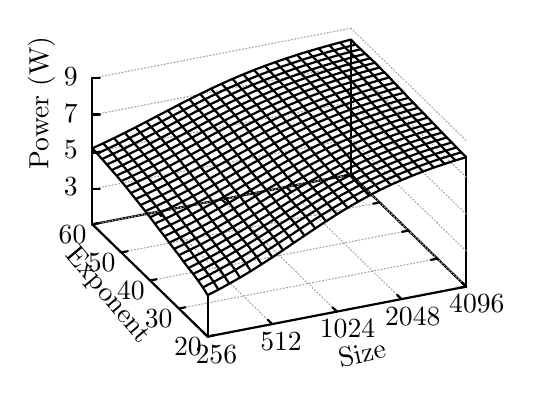
\begin{tikzpicture}[y=0.80pt, x=0.80pt, yscale=-0.570000, xscale=0.570000, inner sep=0pt, outer sep=0pt]
\begin{scope}[draw=black,line join=bevel,line cap=rect,even odd rule,line width=0.800pt]
  \begin{scope}[cm={{1.0,0.0,0.0,1.0,(0.0,0.0)}},draw=black,line join=bevel,line cap=rect,line width=0.800pt]
  \end{scope}
  \begin{scope}[cm={{1.00465,0.0,0.0,1.00465,(0.0,0.0)}},draw=black,line join=bevel,line cap=rect,line width=0.800pt]
  \end{scope}
  \begin{scope}[cm={{1.00465,0.0,0.0,1.00465,(0.0,0.0)}},draw=black,line join=round,line cap=round,line width=0.800pt]
    \path[draw] (67.6000,186.1000) -- (271.5000,146.8000);
    \path[draw] (362.4000,235.2000) -- (271.5000,146.8000);
    \path[draw] (67.5000,186.5000) -- (67.5000,70.5000);
    \path[draw] (271.5000,146.5000) -- (271.5000,40.5000);
    \path[draw] (362.5000,235.5000) -- (362.5000,133.5000);
  \end{scope}
  \begin{scope}[cm={{1.00465,0.0,0.0,1.00465,(0.0,0.0)}},draw=ca0a0a4,dash pattern=on 0.40pt off 0.80pt,line join=round,line cap=round,line width=0.400pt]
    \path[draw] (158.5000,274.6000) -- (67.6000,186.1000);
  \end{scope}
  \begin{scope}[cm={{1.00465,0.0,0.0,1.00465,(0.0,0.0)}},draw=black,line join=round,line cap=round,line width=0.800pt]
    \path[draw] (158.5000,274.6000) -- (155.1000,271.3000);
    \path[draw] (67.6000,186.1000) -- (71.0000,189.4000);
  \end{scope}
  \begin{scope}[cm={{1.00465,0.0,0.0,1.00465,(0.0,0.0)}},draw=black,line join=bevel,line cap=rect,line width=0.800pt]
  \end{scope}
  \begin{scope}[cm={{1.00465,0.0,0.0,1.00465,(149.693,296.874)}},draw=black,line join=bevel,line cap=rect,line width=0.800pt]
  \end{scope}
  \begin{scope}[cm={{1.00465,0.0,0.0,1.00465,(149.693,296.874)}},draw=black,line join=bevel,line cap=rect,line width=0.800pt]
  \end{scope}
  \begin{scope}[cm={{1.00465,0.0,0.0,1.00465,(149.693,296.874)}},draw=black,line join=bevel,line cap=rect,line width=0.800pt]
  \end{scope}
  \begin{scope}[cm={{1.00465,0.0,0.0,1.00465,(149.693,296.874)}},draw=black,line join=bevel,line cap=rect,line width=0.800pt]
  \end{scope}
  \begin{scope}[cm={{1.00465,0.0,0.0,1.00465,(149.693,296.874)}},draw=black,line join=bevel,line cap=rect,line width=0.800pt]
  \end{scope}
  \begin{scope}[cm={{1.00465,0.0,0.0,1.00465,(149.693,296.874)}},draw=black,line join=bevel,line cap=rect,line width=0.800pt]
    \path[fill=black] (0.0000,0.0000) node[above right] () {256};
  \end{scope}
  \begin{scope}[cm={{1.00465,0.0,0.0,1.00465,(149.693,296.874)}},draw=black,line join=bevel,line cap=rect,line width=0.800pt]
  \end{scope}
  \begin{scope}[cm={{1.00465,0.0,0.0,1.00465,(0.0,0.0)}},draw=black,line join=bevel,line cap=rect,line width=0.800pt]
  \end{scope}
  \begin{scope}[cm={{1.00465,0.0,0.0,1.00465,(0.0,0.0)}},draw=ca0a0a4,dash pattern=on 0.40pt off 0.80pt,line join=round,line cap=round,line width=0.400pt]
    \path[draw] (209.5000,264.8000) -- (118.6000,176.3000);
  \end{scope}
  \begin{scope}[cm={{1.00465,0.0,0.0,1.00465,(0.0,0.0)}},draw=black,line join=round,line cap=round,line width=0.800pt]
    \path[draw] (209.5000,264.8000) -- (206.1000,261.5000);
    \path[draw] (118.6000,176.3000) -- (122.0000,179.6000);
  \end{scope}
  \begin{scope}[cm={{1.00465,0.0,0.0,1.00465,(0.0,0.0)}},draw=black,line join=bevel,line cap=rect,line width=0.800pt]
  \end{scope}
  \begin{scope}[cm={{1.00465,0.0,0.0,1.00465,(200.93,286.828)}},draw=black,line join=bevel,line cap=rect,line width=0.800pt]
  \end{scope}
  \begin{scope}[cm={{1.00465,0.0,0.0,1.00465,(200.93,286.828)}},draw=black,line join=bevel,line cap=rect,line width=0.800pt]
  \end{scope}
  \begin{scope}[cm={{1.00465,0.0,0.0,1.00465,(200.93,286.828)}},draw=black,line join=bevel,line cap=rect,line width=0.800pt]
  \end{scope}
  \begin{scope}[cm={{1.00465,0.0,0.0,1.00465,(200.93,286.828)}},draw=black,line join=bevel,line cap=rect,line width=0.800pt]
  \end{scope}
  \begin{scope}[cm={{1.00465,0.0,0.0,1.00465,(200.93,286.828)}},draw=black,line join=bevel,line cap=rect,line width=0.800pt]
  \end{scope}
  \begin{scope}[cm={{1.00465,0.0,0.0,1.00465,(200.93,286.828)}},draw=black,line join=bevel,line cap=rect,line width=0.800pt]
    \path[fill=black] (0.0000,0.0000) node[above right] () {512};
  \end{scope}
  \begin{scope}[cm={{1.00465,0.0,0.0,1.00465,(200.93,286.828)}},draw=black,line join=bevel,line cap=rect,line width=0.800pt]
  \end{scope}
  \begin{scope}[cm={{1.00465,0.0,0.0,1.00465,(0.0,0.0)}},draw=black,line join=bevel,line cap=rect,line width=0.800pt]
  \end{scope}
  \begin{scope}[cm={{1.00465,0.0,0.0,1.00465,(0.0,0.0)}},draw=ca0a0a4,dash pattern=on 0.40pt off 0.80pt,line join=round,line cap=round,line width=0.400pt]
    \path[draw] (260.4000,254.9000) -- (169.6000,166.4000);
  \end{scope}
  \begin{scope}[cm={{1.00465,0.0,0.0,1.00465,(0.0,0.0)}},draw=black,line join=round,line cap=round,line width=0.800pt]
    \path[draw] (260.4000,254.9000) -- (257.0000,251.6000);
    \path[draw] (169.6000,166.4000) -- (173.0000,169.7000);
  \end{scope}
  \begin{scope}[cm={{1.00465,0.0,0.0,1.00465,(0.0,0.0)}},draw=black,line join=bevel,line cap=rect,line width=0.800pt]
  \end{scope}
  \begin{scope}[cm={{1.00465,0.0,0.0,1.00465,(248.149,276.781)}},draw=black,line join=bevel,line cap=rect,line width=0.800pt]
  \end{scope}
  \begin{scope}[cm={{1.00465,0.0,0.0,1.00465,(248.149,276.781)}},draw=black,line join=bevel,line cap=rect,line width=0.800pt]
  \end{scope}
  \begin{scope}[cm={{1.00465,0.0,0.0,1.00465,(248.149,276.781)}},draw=black,line join=bevel,line cap=rect,line width=0.800pt]
  \end{scope}
  \begin{scope}[cm={{1.00465,0.0,0.0,1.00465,(248.149,276.781)}},draw=black,line join=bevel,line cap=rect,line width=0.800pt]
  \end{scope}
  \begin{scope}[cm={{1.00465,0.0,0.0,1.00465,(248.149,276.781)}},draw=black,line join=bevel,line cap=rect,line width=0.800pt]
  \end{scope}
  \begin{scope}[cm={{1.00465,0.0,0.0,1.00465,(248.149,276.781)}},draw=black,line join=bevel,line cap=rect,line width=0.800pt]
    \path[fill=black] (0.0000,0.0000) node[above right] () {1024};
  \end{scope}
  \begin{scope}[cm={{1.00465,0.0,0.0,1.00465,(248.149,276.781)}},draw=black,line join=bevel,line cap=rect,line width=0.800pt]
  \end{scope}
  \begin{scope}[cm={{1.00465,0.0,0.0,1.00465,(0.0,0.0)}},draw=black,line join=bevel,line cap=rect,line width=0.800pt]
  \end{scope}
  \begin{scope}[cm={{1.00465,0.0,0.0,1.00465,(0.0,0.0)}},draw=ca0a0a4,dash pattern=on 0.40pt off 0.80pt,line join=round,line cap=round,line width=0.400pt]
    \path[draw] (311.4000,245.1000) -- (220.5000,156.6000);
  \end{scope}
  \begin{scope}[cm={{1.00465,0.0,0.0,1.00465,(0.0,0.0)}},draw=black,line join=round,line cap=round,line width=0.800pt]
    \path[draw] (311.4000,245.1000) -- (308.0000,241.8000);
    \path[draw] (220.5000,156.6000) -- (223.9000,159.9000);
  \end{scope}
  \begin{scope}[cm={{1.00465,0.0,0.0,1.00465,(0.0,0.0)}},draw=black,line join=bevel,line cap=rect,line width=0.800pt]
  \end{scope}
  \begin{scope}[cm={{1.00465,0.0,0.0,1.00465,(299.888,266.735)}},draw=black,line join=bevel,line cap=rect,line width=0.800pt]
  \end{scope}
  \begin{scope}[cm={{1.00465,0.0,0.0,1.00465,(299.888,266.735)}},draw=black,line join=bevel,line cap=rect,line width=0.800pt]
  \end{scope}
  \begin{scope}[cm={{1.00465,0.0,0.0,1.00465,(299.888,266.735)}},draw=black,line join=bevel,line cap=rect,line width=0.800pt]
  \end{scope}
  \begin{scope}[cm={{1.00465,0.0,0.0,1.00465,(299.888,266.735)}},draw=black,line join=bevel,line cap=rect,line width=0.800pt]
  \end{scope}
  \begin{scope}[cm={{1.00465,0.0,0.0,1.00465,(299.888,266.735)}},draw=black,line join=bevel,line cap=rect,line width=0.800pt]
  \end{scope}
  \begin{scope}[cm={{1.00465,0.0,0.0,1.00465,(299.888,266.735)}},draw=black,line join=bevel,line cap=rect,line width=0.800pt]
    \path[fill=black] (0.0000,0.0000) node[above right] () {2048};
  \end{scope}
  \begin{scope}[cm={{1.00465,0.0,0.0,1.00465,(299.888,266.735)}},draw=black,line join=bevel,line cap=rect,line width=0.800pt]
  \end{scope}
  \begin{scope}[cm={{1.00465,0.0,0.0,1.00465,(0.0,0.0)}},draw=black,line join=bevel,line cap=rect,line width=0.800pt]
  \end{scope}
  \begin{scope}[cm={{1.00465,0.0,0.0,1.00465,(0.0,0.0)}},draw=ca0a0a4,dash pattern=on 0.40pt off 0.80pt,line join=round,line cap=round,line width=0.400pt]
    \path[draw] (362.4000,235.2000) -- (271.5000,146.8000);
  \end{scope}
  \begin{scope}[cm={{1.00465,0.0,0.0,1.00465,(0.0,0.0)}},draw=black,line join=round,line cap=round,line width=0.800pt]
    \path[draw] (362.4000,235.2000) -- (359.0000,231.9000);
    \path[draw] (271.5000,146.8000) -- (274.9000,150.1000);
  \end{scope}
  \begin{scope}[cm={{1.00465,0.0,0.0,1.00465,(0.0,0.0)}},draw=black,line join=bevel,line cap=rect,line width=0.800pt]
  \end{scope}
  \begin{scope}[cm={{1.00465,0.0,0.0,1.00465,(350.623,256.688)}},draw=black,line join=bevel,line cap=rect,line width=0.800pt]
  \end{scope}
  \begin{scope}[cm={{1.00465,0.0,0.0,1.00465,(350.623,256.688)}},draw=black,line join=bevel,line cap=rect,line width=0.800pt]
  \end{scope}
  \begin{scope}[cm={{1.00465,0.0,0.0,1.00465,(350.623,256.688)}},draw=black,line join=bevel,line cap=rect,line width=0.800pt]
  \end{scope}
  \begin{scope}[cm={{1.00465,0.0,0.0,1.00465,(350.623,256.688)}},draw=black,line join=bevel,line cap=rect,line width=0.800pt]
  \end{scope}
  \begin{scope}[cm={{1.00465,0.0,0.0,1.00465,(350.623,256.688)}},draw=black,line join=bevel,line cap=rect,line width=0.800pt]
  \end{scope}
  \begin{scope}[cm={{1.00465,0.0,0.0,1.00465,(350.623,256.688)}},draw=black,line join=bevel,line cap=rect,line width=0.800pt]
    \path[fill=black] (0.0000,0.0000) node[above right] () {4096};
  \end{scope}
  \begin{scope}[cm={{1.00465,0.0,0.0,1.00465,(350.623,256.688)}},draw=black,line join=bevel,line cap=rect,line width=0.800pt]
  \end{scope}
  \begin{scope}[cm={{1.00465,0.0,0.0,1.00465,(0.0,0.0)}},draw=black,line join=bevel,line cap=rect,line width=0.800pt]
  \end{scope}
  \begin{scope}[cm={{1.00465,0.0,0.0,1.00465,(0.0,0.0)}},draw=ca0a0a4,dash pattern=on 0.40pt off 0.80pt,line join=round,line cap=round,line width=0.400pt]
    \path[draw] (158.5000,274.6000) -- (362.4000,235.2000);
  \end{scope}
  \begin{scope}[cm={{1.00465,0.0,0.0,1.00465,(0.0,0.0)}},draw=black,line join=round,line cap=round,line width=0.800pt]
    \path[draw] (158.5000,274.6000) -- (163.6000,273.6000);
    \path[draw] (362.4000,235.2000) -- (357.2000,236.2000);
  \end{scope}
  \begin{scope}[cm={{1.00465,0.0,0.0,1.00465,(0.0,0.0)}},draw=black,line join=bevel,line cap=rect,line width=0.800pt]
  \end{scope}
  \begin{scope}[cm={{1.00465,0.0,0.0,1.00465,(132.614,290.847)}},draw=black,line join=bevel,line cap=rect,line width=0.800pt]
  \end{scope}
  \begin{scope}[cm={{1.00465,0.0,0.0,1.00465,(132.614,290.847)}},draw=black,line join=bevel,line cap=rect,line width=0.800pt]
  \end{scope}
  \begin{scope}[cm={{1.00465,0.0,0.0,1.00465,(132.614,290.847)}},draw=black,line join=bevel,line cap=rect,line width=0.800pt]
  \end{scope}
  \begin{scope}[cm={{1.00465,0.0,0.0,1.00465,(132.614,290.847)}},draw=black,line join=bevel,line cap=rect,line width=0.800pt]
  \end{scope}
  \begin{scope}[cm={{1.00465,0.0,0.0,1.00465,(132.614,290.847)}},draw=black,line join=bevel,line cap=rect,line width=0.800pt]
  \end{scope}
  \begin{scope}[cm={{1.00465,0.0,0.0,1.00465,(132.614,290.847)}},draw=black,line join=bevel,line cap=rect,line width=0.800pt]
    \path[fill=black] (0.0000,0.0000) node[above right] () {20};
  \end{scope}
  \begin{scope}[cm={{1.00465,0.0,0.0,1.00465,(132.614,290.847)}},draw=black,line join=bevel,line cap=rect,line width=0.800pt]
  \end{scope}
  \begin{scope}[cm={{1.00465,0.0,0.0,1.00465,(0.0,0.0)}},draw=black,line join=bevel,line cap=rect,line width=0.800pt]
  \end{scope}
  \begin{scope}[cm={{1.00465,0.0,0.0,1.00465,(0.0,0.0)}},draw=ca0a0a4,dash pattern=on 0.40pt off 0.80pt,line join=round,line cap=round,line width=0.400pt]
    \path[draw] (135.8000,252.5000) -- (339.7000,213.1000);
  \end{scope}
  \begin{scope}[cm={{1.00465,0.0,0.0,1.00465,(0.0,0.0)}},draw=black,line join=round,line cap=round,line width=0.800pt]
    \path[draw] (135.8000,252.5000) -- (140.9000,251.5000);
    \path[draw] (339.7000,213.1000) -- (334.5000,214.1000);
  \end{scope}
  \begin{scope}[cm={{1.00465,0.0,0.0,1.00465,(0.0,0.0)}},draw=black,line join=bevel,line cap=rect,line width=0.800pt]
  \end{scope}
  \begin{scope}[cm={{1.00465,0.0,0.0,1.00465,(109.507,268.744)}},draw=black,line join=bevel,line cap=rect,line width=0.800pt]
  \end{scope}
  \begin{scope}[cm={{1.00465,0.0,0.0,1.00465,(109.507,268.744)}},draw=black,line join=bevel,line cap=rect,line width=0.800pt]
  \end{scope}
  \begin{scope}[cm={{1.00465,0.0,0.0,1.00465,(109.507,268.744)}},draw=black,line join=bevel,line cap=rect,line width=0.800pt]
  \end{scope}
  \begin{scope}[cm={{1.00465,0.0,0.0,1.00465,(109.507,268.744)}},draw=black,line join=bevel,line cap=rect,line width=0.800pt]
  \end{scope}
  \begin{scope}[cm={{1.00465,0.0,0.0,1.00465,(109.507,268.744)}},draw=black,line join=bevel,line cap=rect,line width=0.800pt]
  \end{scope}
  \begin{scope}[cm={{1.00465,0.0,0.0,1.00465,(109.507,268.744)}},draw=black,line join=bevel,line cap=rect,line width=0.800pt]
    \path[fill=black] (0.0000,0.0000) node[above right] () {30};
  \end{scope}
  \begin{scope}[cm={{1.00465,0.0,0.0,1.00465,(109.507,268.744)}},draw=black,line join=bevel,line cap=rect,line width=0.800pt]
  \end{scope}
  \begin{scope}[cm={{1.00465,0.0,0.0,1.00465,(0.0,0.0)}},draw=black,line join=bevel,line cap=rect,line width=0.800pt]
  \end{scope}
  \begin{scope}[cm={{1.00465,0.0,0.0,1.00465,(0.0,0.0)}},draw=ca0a0a4,dash pattern=on 0.40pt off 0.80pt,line join=round,line cap=round,line width=0.400pt]
    \path[draw] (113.1000,230.4000) -- (316.9000,191.0000);
  \end{scope}
  \begin{scope}[cm={{1.00465,0.0,0.0,1.00465,(0.0,0.0)}},draw=black,line join=round,line cap=round,line width=0.800pt]
    \path[draw] (113.1000,230.4000) -- (118.2000,229.4000);
    \path[draw] (316.9000,191.0000) -- (311.8000,192.0000);
  \end{scope}
  \begin{scope}[cm={{1.00465,0.0,0.0,1.00465,(0.0,0.0)}},draw=black,line join=bevel,line cap=rect,line width=0.800pt]
  \end{scope}
  \begin{scope}[cm={{1.00465,0.0,0.0,1.00465,(87.4047,246.642)}},draw=black,line join=bevel,line cap=rect,line width=0.800pt]
  \end{scope}
  \begin{scope}[cm={{1.00465,0.0,0.0,1.00465,(87.4047,246.642)}},draw=black,line join=bevel,line cap=rect,line width=0.800pt]
  \end{scope}
  \begin{scope}[cm={{1.00465,0.0,0.0,1.00465,(87.4047,246.642)}},draw=black,line join=bevel,line cap=rect,line width=0.800pt]
  \end{scope}
  \begin{scope}[cm={{1.00465,0.0,0.0,1.00465,(87.4047,246.642)}},draw=black,line join=bevel,line cap=rect,line width=0.800pt]
  \end{scope}
  \begin{scope}[cm={{1.00465,0.0,0.0,1.00465,(87.4047,246.642)}},draw=black,line join=bevel,line cap=rect,line width=0.800pt]
  \end{scope}
  \begin{scope}[cm={{1.00465,0.0,0.0,1.00465,(87.4047,246.642)}},draw=black,line join=bevel,line cap=rect,line width=0.800pt]
    \path[fill=black] (0.0000,0.0000) node[above right] () {40};
  \end{scope}
  \begin{scope}[cm={{1.00465,0.0,0.0,1.00465,(87.4047,246.642)}},draw=black,line join=bevel,line cap=rect,line width=0.800pt]
  \end{scope}
  \begin{scope}[cm={{1.00465,0.0,0.0,1.00465,(0.0,0.0)}},draw=black,line join=bevel,line cap=rect,line width=0.800pt]
  \end{scope}
  \begin{scope}[cm={{1.00465,0.0,0.0,1.00465,(0.0,0.0)}},draw=ca0a0a4,dash pattern=on 0.40pt off 0.80pt,line join=round,line cap=round,line width=0.400pt]
    \path[draw] (90.3000,208.2000) -- (294.2000,168.8000);
  \end{scope}
  \begin{scope}[cm={{1.00465,0.0,0.0,1.00465,(0.0,0.0)}},draw=black,line join=round,line cap=round,line width=0.800pt]
    \path[draw] (90.3000,208.2000) -- (95.5000,207.3000);
    \path[draw] (294.2000,168.8000) -- (289.1000,169.8000);
  \end{scope}
  \begin{scope}[cm={{1.00465,0.0,0.0,1.00465,(0.0,0.0)}},draw=black,line join=bevel,line cap=rect,line width=0.800pt]
  \end{scope}
  \begin{scope}[cm={{1.00465,0.0,0.0,1.00465,(64.2977,224.54)}},draw=black,line join=bevel,line cap=rect,line width=0.800pt]
  \end{scope}
  \begin{scope}[cm={{1.00465,0.0,0.0,1.00465,(64.2977,224.54)}},draw=black,line join=bevel,line cap=rect,line width=0.800pt]
  \end{scope}
  \begin{scope}[cm={{1.00465,0.0,0.0,1.00465,(64.2977,224.54)}},draw=black,line join=bevel,line cap=rect,line width=0.800pt]
  \end{scope}
  \begin{scope}[cm={{1.00465,0.0,0.0,1.00465,(64.2977,224.54)}},draw=black,line join=bevel,line cap=rect,line width=0.800pt]
  \end{scope}
  \begin{scope}[cm={{1.00465,0.0,0.0,1.00465,(64.2977,224.54)}},draw=black,line join=bevel,line cap=rect,line width=0.800pt]
  \end{scope}
  \begin{scope}[cm={{1.00465,0.0,0.0,1.00465,(64.2977,224.54)}},draw=black,line join=bevel,line cap=rect,line width=0.800pt]
    \path[fill=black] (0.0000,0.0000) node[above right] () {50};
  \end{scope}
  \begin{scope}[cm={{1.00465,0.0,0.0,1.00465,(64.2977,224.54)}},draw=black,line join=bevel,line cap=rect,line width=0.800pt]
  \end{scope}
  \begin{scope}[cm={{1.00465,0.0,0.0,1.00465,(0.0,0.0)}},draw=black,line join=bevel,line cap=rect,line width=0.800pt]
  \end{scope}
  \begin{scope}[cm={{1.00465,0.0,0.0,1.00465,(0.0,0.0)}},draw=ca0a0a4,dash pattern=on 0.40pt off 0.80pt,line join=round,line cap=round,line width=0.400pt]
    \path[draw] (67.6000,186.1000) -- (271.5000,146.8000);
  \end{scope}
  \begin{scope}[cm={{1.00465,0.0,0.0,1.00465,(0.0,0.0)}},draw=black,line join=round,line cap=round,line width=0.800pt]
    \path[draw] (67.6000,186.1000) -- (72.8000,185.1000);
    \path[draw] (271.5000,146.8000) -- (266.4000,147.8000);
  \end{scope}
  \begin{scope}[cm={{1.00465,0.0,0.0,1.00465,(0.0,0.0)}},draw=black,line join=bevel,line cap=rect,line width=0.800pt]
  \end{scope}
  \begin{scope}[cm={{1.00465,0.0,0.0,1.00465,(41.1907,202.437)}},draw=black,line join=bevel,line cap=rect,line width=0.800pt]
  \end{scope}
  \begin{scope}[cm={{1.00465,0.0,0.0,1.00465,(41.1907,202.437)}},draw=black,line join=bevel,line cap=rect,line width=0.800pt]
  \end{scope}
  \begin{scope}[cm={{1.00465,0.0,0.0,1.00465,(41.1907,202.437)}},draw=black,line join=bevel,line cap=rect,line width=0.800pt]
  \end{scope}
  \begin{scope}[cm={{1.00465,0.0,0.0,1.00465,(41.1907,202.437)}},draw=black,line join=bevel,line cap=rect,line width=0.800pt]
  \end{scope}
  \begin{scope}[cm={{1.00465,0.0,0.0,1.00465,(41.1907,202.437)}},draw=black,line join=bevel,line cap=rect,line width=0.800pt]
  \end{scope}
  \begin{scope}[cm={{1.00465,0.0,0.0,1.00465,(41.1907,202.437)}},draw=black,line join=bevel,line cap=rect,line width=0.800pt]
    \path[fill=black] (0.0000,0.0000) node[above right] () {60};
  \end{scope}
  \begin{scope}[cm={{1.00465,0.0,0.0,1.00465,(41.1907,202.437)}},draw=black,line join=bevel,line cap=rect,line width=0.800pt]
  \end{scope}
  \begin{scope}[cm={{1.00465,0.0,0.0,1.00465,(0.0,0.0)}},draw=black,line join=bevel,line cap=rect,line width=0.800pt]
  \end{scope}
  \begin{scope}[cm={{1.00465,0.0,0.0,1.00465,(0.0,0.0)}},draw=ca0a0a4,dash pattern=on 0.40pt off 0.80pt,line join=round,line cap=round,line width=0.400pt]
    \path[draw] (67.6000,158.1000) -- (271.5000,118.8000);
    \path[draw] (271.5000,118.8000) -- (271.5000,118.8000) -- (362.4000,207.2000);
  \end{scope}
  \begin{scope}[cm={{1.00465,0.0,0.0,1.00465,(0.0,0.0)}},draw=black,line join=round,line cap=round,line width=0.800pt]
    \path[draw] (67.5000,158.5000) -- (73.5000,158.5000);
  \end{scope}
  \begin{scope}[cm={{1.00465,0.0,0.0,1.00465,(0.0,0.0)}},draw=black,line join=bevel,line cap=rect,line width=0.800pt]
  \end{scope}
  \begin{scope}[cm={{1.00465,0.0,0.0,1.00465,(45.2093,164.26)}},draw=black,line join=bevel,line cap=rect,line width=0.800pt]
  \end{scope}
  \begin{scope}[cm={{1.00465,0.0,0.0,1.00465,(45.2093,164.26)}},draw=black,line join=bevel,line cap=rect,line width=0.800pt]
  \end{scope}
  \begin{scope}[cm={{1.00465,0.0,0.0,1.00465,(45.2093,164.26)}},draw=black,line join=bevel,line cap=rect,line width=0.800pt]
  \end{scope}
  \begin{scope}[cm={{1.00465,0.0,0.0,1.00465,(45.2093,164.26)}},draw=black,line join=bevel,line cap=rect,line width=0.800pt]
  \end{scope}
  \begin{scope}[cm={{1.00465,0.0,0.0,1.00465,(45.2093,164.26)}},draw=black,line join=bevel,line cap=rect,line width=0.800pt]
  \end{scope}
  \begin{scope}[cm={{1.00465,0.0,0.0,1.00465,(45.2093,164.26)}},draw=black,line join=bevel,line cap=rect,line width=0.800pt]
    \path[fill=black] (0.0000,0.0000) node[above right] () {3};
  \end{scope}
  \begin{scope}[cm={{1.00465,0.0,0.0,1.00465,(45.2093,164.26)}},draw=black,line join=bevel,line cap=rect,line width=0.800pt]
  \end{scope}
  \begin{scope}[cm={{1.00465,0.0,0.0,1.00465,(0.0,0.0)}},draw=black,line join=bevel,line cap=rect,line width=0.800pt]
  \end{scope}
  \begin{scope}[cm={{1.00465,0.0,0.0,1.00465,(0.0,0.0)}},draw=ca0a0a4,dash pattern=on 0.40pt off 0.80pt,line join=round,line cap=round,line width=0.400pt]
    \path[draw] (67.6000,129.1000) -- (271.5000,89.7000);
    \path[draw] (271.5000,89.7000) -- (271.5000,89.7000) -- (362.4000,178.1000);
  \end{scope}
  \begin{scope}[cm={{1.00465,0.0,0.0,1.00465,(0.0,0.0)}},draw=black,line join=round,line cap=round,line width=0.800pt]
    \path[draw] (67.5000,129.5000) -- (73.5000,129.5000);
  \end{scope}
  \begin{scope}[cm={{1.00465,0.0,0.0,1.00465,(0.0,0.0)}},draw=black,line join=bevel,line cap=rect,line width=0.800pt]
  \end{scope}
  \begin{scope}[cm={{1.00465,0.0,0.0,1.00465,(45.2093,135.126)}},draw=black,line join=bevel,line cap=rect,line width=0.800pt]
  \end{scope}
  \begin{scope}[cm={{1.00465,0.0,0.0,1.00465,(45.2093,135.126)}},draw=black,line join=bevel,line cap=rect,line width=0.800pt]
  \end{scope}
  \begin{scope}[cm={{1.00465,0.0,0.0,1.00465,(45.2093,135.126)}},draw=black,line join=bevel,line cap=rect,line width=0.800pt]
  \end{scope}
  \begin{scope}[cm={{1.00465,0.0,0.0,1.00465,(45.2093,135.126)}},draw=black,line join=bevel,line cap=rect,line width=0.800pt]
  \end{scope}
  \begin{scope}[cm={{1.00465,0.0,0.0,1.00465,(45.2093,135.126)}},draw=black,line join=bevel,line cap=rect,line width=0.800pt]
  \end{scope}
  \begin{scope}[cm={{1.00465,0.0,0.0,1.00465,(45.2093,135.126)}},draw=black,line join=bevel,line cap=rect,line width=0.800pt]
    \path[fill=black] (0.0000,0.0000) node[above right] () {5};
  \end{scope}
  \begin{scope}[cm={{1.00465,0.0,0.0,1.00465,(45.2093,135.126)}},draw=black,line join=bevel,line cap=rect,line width=0.800pt]
  \end{scope}
  \begin{scope}[cm={{1.00465,0.0,0.0,1.00465,(0.0,0.0)}},draw=black,line join=bevel,line cap=rect,line width=0.800pt]
  \end{scope}
  \begin{scope}[cm={{1.00465,0.0,0.0,1.00465,(0.0,0.0)}},draw=ca0a0a4,dash pattern=on 0.40pt off 0.80pt,line join=round,line cap=round,line width=0.400pt]
    \path[draw] (67.6000,99.9000) -- (271.5000,60.5000);
    \path[draw] (271.5000,60.5000) -- (271.5000,60.5000) -- (362.4000,149.0000);
  \end{scope}
  \begin{scope}[cm={{1.00465,0.0,0.0,1.00465,(0.0,0.0)}},draw=black,line join=round,line cap=round,line width=0.800pt]
    \path[draw] (67.5000,99.5000) -- (73.5000,99.5000);
  \end{scope}
  \begin{scope}[cm={{1.00465,0.0,0.0,1.00465,(0.0,0.0)}},draw=black,line join=bevel,line cap=rect,line width=0.800pt]
  \end{scope}
  \begin{scope}[cm={{1.00465,0.0,0.0,1.00465,(45.2093,105.991)}},draw=black,line join=bevel,line cap=rect,line width=0.800pt]
  \end{scope}
  \begin{scope}[cm={{1.00465,0.0,0.0,1.00465,(45.2093,105.991)}},draw=black,line join=bevel,line cap=rect,line width=0.800pt]
  \end{scope}
  \begin{scope}[cm={{1.00465,0.0,0.0,1.00465,(45.2093,105.991)}},draw=black,line join=bevel,line cap=rect,line width=0.800pt]
  \end{scope}
  \begin{scope}[cm={{1.00465,0.0,0.0,1.00465,(45.2093,105.991)}},draw=black,line join=bevel,line cap=rect,line width=0.800pt]
  \end{scope}
  \begin{scope}[cm={{1.00465,0.0,0.0,1.00465,(45.2093,105.991)}},draw=black,line join=bevel,line cap=rect,line width=0.800pt]
  \end{scope}
  \begin{scope}[cm={{1.00465,0.0,0.0,1.00465,(45.2093,105.991)}},draw=black,line join=bevel,line cap=rect,line width=0.800pt]
    \path[fill=black] (0.0000,0.0000) node[above right] () {7};
  \end{scope}
  \begin{scope}[cm={{1.00465,0.0,0.0,1.00465,(45.2093,105.991)}},draw=black,line join=bevel,line cap=rect,line width=0.800pt]
  \end{scope}
  \begin{scope}[cm={{1.00465,0.0,0.0,1.00465,(0.0,0.0)}},draw=black,line join=bevel,line cap=rect,line width=0.800pt]
  \end{scope}
  \begin{scope}[cm={{1.00465,0.0,0.0,1.00465,(0.0,0.0)}},draw=ca0a0a4,dash pattern=on 0.40pt off 0.80pt,line join=round,line cap=round,line width=0.400pt]
    \path[draw] (67.6000,70.8000) -- (271.5000,31.4000);
    \path[draw] (271.5000,31.4000) -- (271.5000,31.4000) -- (362.4000,119.9000);
  \end{scope}
  \begin{scope}[cm={{1.00465,0.0,0.0,1.00465,(0.0,0.0)}},draw=black,line join=round,line cap=round,line width=0.800pt]
    \path[draw] (67.5000,70.5000) -- (73.5000,70.5000);
  \end{scope}
  \begin{scope}[cm={{1.00465,0.0,0.0,1.00465,(0.0,0.0)}},draw=black,line join=bevel,line cap=rect,line width=0.800pt]
  \end{scope}
  \begin{scope}[cm={{1.00465,0.0,0.0,1.00465,(45.2093,76.8558)}},draw=black,line join=bevel,line cap=rect,line width=0.800pt]
  \end{scope}
  \begin{scope}[cm={{1.00465,0.0,0.0,1.00465,(45.2093,76.8558)}},draw=black,line join=bevel,line cap=rect,line width=0.800pt]
  \end{scope}
  \begin{scope}[cm={{1.00465,0.0,0.0,1.00465,(45.2093,76.8558)}},draw=black,line join=bevel,line cap=rect,line width=0.800pt]
  \end{scope}
  \begin{scope}[cm={{1.00465,0.0,0.0,1.00465,(45.2093,76.8558)}},draw=black,line join=bevel,line cap=rect,line width=0.800pt]
  \end{scope}
  \begin{scope}[cm={{1.00465,0.0,0.0,1.00465,(45.2093,76.8558)}},draw=black,line join=bevel,line cap=rect,line width=0.800pt]
  \end{scope}
  \begin{scope}[cm={{1.00465,0.0,0.0,1.00465,(45.2093,76.8558)}},draw=black,line join=bevel,line cap=rect,line width=0.800pt]
    \path[fill=black] (0.0000,0.0000) node[above right] () {9};
  \end{scope}
  \begin{scope}[cm={{1.00465,0.0,0.0,1.00465,(45.2093,76.8558)}},draw=black,line join=bevel,line cap=rect,line width=0.800pt]
  \end{scope}
  \begin{scope}[cm={{0.0,-1.00465,1.00465,0.0,(24.614,149.191)}},draw=black,line join=bevel,line cap=rect,line width=0.800pt]
  \end{scope}
  \begin{scope}[cm={{0.0,-1.00465,1.00465,0.0,(24.614,149.191)}},draw=black,line join=bevel,line cap=rect,line width=0.800pt]
  \end{scope}
  \begin{scope}[cm={{0.0,-1.00465,1.00465,0.0,(24.614,149.191)}},draw=black,line join=bevel,line cap=rect,line width=0.800pt]
  \end{scope}
  \begin{scope}[cm={{0.0,-1.00465,1.00465,0.0,(24.614,149.191)}},draw=black,line join=bevel,line cap=rect,line width=0.800pt]
  \end{scope}
  \begin{scope}[cm={{0.0,-1.00465,1.00465,0.0,(24.614,149.191)}},draw=black,line join=bevel,line cap=rect,line width=0.800pt]
  \end{scope}
  \begin{scope}[cm={{0.0,-1.00465,1.00465,0.0,(16.614,143.163)}},draw=black,line join=bevel,line cap=rect,line width=0.800pt]
    \path[fill=black] (0.0000,0.0000) node[above right] () {\rotatebox{90}{Power (W)}};
  \end{scope}
  \begin{scope}[cm={{0.0,-1.00465,1.00465,0.0,(24.614,149.191)}},draw=black,line join=bevel,line cap=rect,line width=0.800pt]
  \end{scope}
  \begin{scope}[cm={{1.00465,0.0,0.0,1.00465,(0.0,0.0)}},draw=black,line join=bevel,line cap=rect,line width=0.800pt]
  \end{scope}
  \begin{scope}[cm={{1.00465,0.0,0.0,1.00465,(0.0,0.0)}},draw=black,line join=bevel,line cap=rect,line width=0.800pt]
  \end{scope}
  \begin{scope}[cm={{1.00465,0.0,0.0,1.00465,(0.0,0.0)}},draw=black,line join=bevel,line cap=rect,line width=0.800pt]
  \end{scope}
  \begin{scope}[cm={{1.00465,0.0,0.0,1.00465,(0.0,0.0)}},draw=black,line join=round,line cap=round,line width=0.800pt]
    \path[draw] (362.4000,133.1000) -- (358.6000,129.3000) -- (358.6000,129.3000) --
      (354.8000,125.4000) -- (354.8000,125.4000) -- (351.0000,121.5000) --
      (351.0000,121.5000) -- (347.2000,117.6000) -- (347.2000,117.6000) --
      (343.4000,113.7000) -- (343.4000,113.7000) -- (339.7000,109.8000) --
      (339.7000,109.8000) -- (335.9000,105.9000) -- (335.9000,105.9000) --
      (332.1000,101.9000) -- (332.1000,101.9000) -- (328.3000,98.0000) --
      (328.3000,98.0000) -- (324.5000,94.1000) -- (324.5000,94.1000) --
      (320.7000,90.2000) -- (320.7000,90.2000) -- (316.9000,86.3000) --
      (316.9000,86.3000) -- (313.2000,82.2000) -- (313.2000,82.2000) --
      (309.4000,78.2000) -- (309.4000,78.2000) -- (305.6000,74.3000) --
      (305.6000,74.3000) -- (301.8000,70.2000) -- (301.8000,70.2000) --
      (298.0000,66.2000) -- (298.0000,66.2000) -- (294.2000,62.4000) --
      (294.2000,62.4000) -- (290.5000,58.6000) -- (290.5000,58.6000) --
      (286.7000,55.1000) -- (286.7000,55.1000) -- (282.9000,51.5000) --
      (282.9000,51.5000) -- (279.1000,47.9000) -- (279.1000,47.9000) --
      (275.3000,44.3000) -- (275.3000,44.3000) -- (271.5000,40.4000);
    \path[draw] (353.9000,135.7000) -- (350.1000,131.8000) -- (350.1000,131.8000) --
      (346.3000,128.0000) -- (346.3000,128.0000) -- (342.5000,124.1000) --
      (342.5000,124.1000) -- (338.7000,120.1000) -- (338.7000,120.1000) --
      (334.9000,116.2000) -- (334.9000,116.2000) -- (331.2000,112.3000) --
      (331.2000,112.3000) -- (327.4000,108.4000) -- (327.4000,108.4000) --
      (323.6000,104.4000) -- (323.6000,104.4000) -- (319.8000,100.5000) --
      (319.8000,100.5000) -- (316.0000,96.6000) -- (316.0000,96.6000) --
      (312.2000,92.6000) -- (312.2000,92.6000) -- (308.4000,88.7000) --
      (308.4000,88.7000) -- (304.7000,84.7000) -- (304.7000,84.7000) --
      (300.9000,80.6000) -- (300.9000,80.6000) -- (297.1000,76.7000) --
      (297.1000,76.7000) -- (293.3000,72.6000) -- (293.3000,72.6000) --
      (289.5000,68.6000) -- (289.5000,68.6000) -- (285.7000,64.7000) --
      (285.7000,64.7000) -- (282.0000,60.9000) -- (282.0000,60.9000) --
      (278.2000,57.4000) -- (278.2000,57.4000) -- (274.4000,53.8000) --
      (274.4000,53.8000) -- (270.6000,50.2000) -- (270.6000,50.2000) --
      (266.8000,46.5000) -- (266.8000,46.5000) -- (263.0000,42.6000);
    \path[draw] (345.4000,138.4000) -- (341.6000,134.5000) -- (341.6000,134.5000) --
      (337.8000,130.7000) -- (337.8000,130.7000) -- (334.0000,126.8000) --
      (334.0000,126.8000) -- (330.2000,122.8000) -- (330.2000,122.8000) --
      (326.4000,118.9000) -- (326.4000,118.9000) -- (322.7000,115.0000) --
      (322.7000,115.0000) -- (318.9000,111.0000) -- (318.9000,111.0000) --
      (315.1000,107.1000) -- (315.1000,107.1000) -- (311.3000,103.2000) --
      (311.3000,103.2000) -- (307.5000,99.2000) -- (307.5000,99.2000) --
      (303.7000,95.2000) -- (303.7000,95.2000) -- (299.9000,91.3000) --
      (299.9000,91.3000) -- (296.2000,87.2000) -- (296.2000,87.2000) --
      (292.4000,83.2000) -- (292.4000,83.2000) -- (288.6000,79.2000) --
      (288.6000,79.2000) -- (284.8000,75.1000) -- (284.8000,75.1000) --
      (281.0000,71.0000) -- (281.0000,71.0000) -- (277.2000,67.1000) --
      (277.2000,67.1000) -- (273.5000,63.4000) -- (273.5000,63.4000) --
      (269.7000,59.7000) -- (269.7000,59.7000) -- (265.9000,56.2000) --
      (265.9000,56.2000) -- (262.1000,52.5000) -- (262.1000,52.5000) --
      (258.3000,48.8000) -- (258.3000,48.8000) -- (254.5000,44.9000);
    \path[draw] (336.9000,141.3000) -- (333.1000,137.4000) -- (333.1000,137.4000) --
      (329.3000,133.5000) -- (329.3000,133.5000) -- (325.5000,129.6000) --
      (325.5000,129.6000) -- (321.7000,125.7000) -- (321.7000,125.7000) --
      (317.9000,121.8000) -- (317.9000,121.8000) -- (314.2000,117.8000) --
      (314.2000,117.8000) -- (310.4000,113.9000) -- (310.4000,113.9000) --
      (306.6000,109.9000) -- (306.6000,109.9000) -- (302.8000,105.9000) --
      (302.8000,105.9000) -- (299.0000,101.9000) -- (299.0000,101.9000) --
      (295.2000,97.9000) -- (295.2000,97.9000) -- (291.4000,94.0000) --
      (291.4000,94.0000) -- (287.7000,89.9000) -- (287.7000,89.9000) --
      (283.9000,85.8000) -- (283.9000,85.8000) -- (280.1000,81.8000) --
      (280.1000,81.8000) -- (276.3000,77.7000) -- (276.3000,77.7000) --
      (272.5000,73.6000) -- (272.5000,73.6000) -- (268.7000,69.7000) --
      (268.7000,69.7000) -- (265.0000,65.9000) -- (265.0000,65.9000) --
      (261.2000,62.3000) -- (261.2000,62.3000) -- (257.4000,58.7000) --
      (257.4000,58.7000) -- (253.6000,55.0000) -- (253.6000,55.0000) --
      (249.8000,51.2000) -- (249.8000,51.2000) -- (246.0000,47.3000);
    \path[draw] (328.4000,144.4000) -- (324.6000,140.5000) -- (324.6000,140.5000) --
      (320.8000,136.6000) -- (320.8000,136.6000) -- (317.0000,132.7000) --
      (317.0000,132.7000) -- (313.2000,128.7000) -- (313.2000,128.7000) --
      (309.4000,124.8000) -- (309.4000,124.8000) -- (305.7000,120.9000) --
      (305.7000,120.9000) -- (301.9000,116.9000) -- (301.9000,116.9000) --
      (298.1000,112.9000) -- (298.1000,112.9000) -- (294.3000,108.9000) --
      (294.3000,108.9000) -- (290.5000,104.8000) -- (290.5000,104.8000) --
      (286.7000,100.8000) -- (286.7000,100.8000) -- (282.9000,96.8000) --
      (282.9000,96.8000) -- (279.2000,92.7000) -- (279.2000,92.7000) --
      (275.4000,88.6000) -- (275.4000,88.6000) -- (271.6000,84.6000) --
      (271.6000,84.6000) -- (267.8000,80.4000) -- (267.8000,80.4000) --
      (264.0000,76.3000) -- (264.0000,76.3000) -- (260.2000,72.4000) --
      (260.2000,72.4000) -- (256.5000,68.6000) -- (256.5000,68.6000) --
      (252.7000,64.9000) -- (252.7000,64.9000) -- (248.9000,61.3000) --
      (248.9000,61.3000) -- (245.1000,57.5000) -- (245.1000,57.5000) --
      (241.3000,53.8000) -- (241.3000,53.8000) -- (237.5000,49.8000);
    \path[draw] (319.9000,147.7000) -- (316.1000,143.8000) -- (316.1000,143.8000) --
      (312.3000,139.8000) -- (312.3000,139.8000) -- (308.5000,135.9000) --
      (308.5000,135.9000) -- (304.7000,132.0000) -- (304.7000,132.0000) --
      (300.9000,128.1000) -- (300.9000,128.1000) -- (297.2000,124.1000) --
      (297.2000,124.1000) -- (293.4000,120.1000) -- (293.4000,120.1000) --
      (289.6000,116.0000) -- (289.6000,116.0000) -- (285.8000,112.0000) --
      (285.8000,112.0000) -- (282.0000,107.9000) -- (282.0000,107.9000) --
      (278.2000,103.9000) -- (278.2000,103.9000) -- (274.4000,99.8000) --
      (274.4000,99.8000) -- (270.7000,95.7000) -- (270.7000,95.7000) --
      (266.9000,91.6000) -- (266.9000,91.6000) -- (263.1000,87.5000) --
      (263.1000,87.5000) -- (259.3000,83.3000) -- (259.3000,83.3000) --
      (255.5000,79.2000) -- (255.5000,79.2000) -- (251.7000,75.2000) --
      (251.7000,75.2000) -- (248.0000,71.4000) -- (248.0000,71.4000) --
      (244.2000,67.7000) -- (244.2000,67.7000) -- (240.4000,64.0000) --
      (240.4000,64.0000) -- (236.6000,60.2000) -- (236.6000,60.2000) --
      (232.8000,56.4000) -- (232.8000,56.4000) -- (229.0000,52.4000);
    \path[draw] (311.4000,151.2000) -- (307.6000,147.3000) -- (307.6000,147.3000) --
      (303.8000,143.3000) -- (303.8000,143.3000) -- (300.0000,139.4000) --
      (300.0000,139.4000) -- (296.2000,135.5000) -- (296.2000,135.5000) --
      (292.4000,131.5000) -- (292.4000,131.5000) -- (288.7000,127.6000) --
      (288.7000,127.6000) -- (284.9000,123.5000) -- (284.9000,123.5000) --
      (281.1000,119.4000) -- (281.1000,119.4000) -- (277.3000,115.3000) --
      (277.3000,115.3000) -- (273.5000,111.2000) -- (273.5000,111.2000) --
      (269.7000,107.1000) -- (269.7000,107.1000) -- (265.9000,103.1000) --
      (265.9000,103.1000) -- (262.2000,98.9000) -- (262.2000,98.9000) --
      (258.4000,94.7000) -- (258.4000,94.7000) -- (254.6000,90.6000) --
      (254.6000,90.6000) -- (250.8000,86.4000) -- (250.8000,86.4000) --
      (247.0000,82.3000) -- (247.0000,82.3000) -- (243.2000,78.3000) --
      (243.2000,78.3000) -- (239.5000,74.4000) -- (239.5000,74.4000) --
      (235.7000,70.6000) -- (235.7000,70.6000) -- (231.9000,66.9000) --
      (231.9000,66.9000) -- (228.1000,63.0000) -- (228.1000,63.0000) --
      (224.3000,59.2000) -- (224.3000,59.2000) -- (220.5000,55.2000);
    \path[draw] (302.9000,154.9000) -- (299.1000,151.0000) -- (299.1000,151.0000) --
      (295.3000,147.1000) -- (295.3000,147.1000) -- (291.5000,143.1000) --
      (291.5000,143.1000) -- (287.7000,139.2000) -- (287.7000,139.2000) --
      (283.9000,135.2000) -- (283.9000,135.2000) -- (280.2000,131.2000) --
      (280.2000,131.2000) -- (276.4000,127.1000) -- (276.4000,127.1000) --
      (272.6000,123.0000) -- (272.6000,123.0000) -- (268.8000,118.9000) --
      (268.8000,118.9000) -- (265.0000,114.7000) -- (265.0000,114.7000) --
      (261.2000,110.6000) -- (261.2000,110.6000) -- (257.4000,106.5000) --
      (257.4000,106.5000) -- (253.7000,102.3000) -- (253.7000,102.3000) --
      (249.9000,98.1000) -- (249.9000,98.1000) -- (246.1000,93.9000) --
      (246.1000,93.9000) -- (242.3000,89.7000) -- (242.3000,89.7000) --
      (238.5000,85.5000) -- (238.5000,85.5000) -- (234.7000,81.4000) --
      (234.7000,81.4000) -- (231.0000,77.5000) -- (231.0000,77.5000) --
      (227.2000,73.7000) -- (227.2000,73.7000) -- (223.4000,69.9000) --
      (223.4000,69.9000) -- (219.6000,66.0000) -- (219.6000,66.0000) --
      (215.8000,62.1000) -- (215.8000,62.1000) -- (212.1000,58.1000);
    \path[draw] (294.4000,159.0000) -- (290.6000,155.0000) -- (290.6000,155.0000) --
      (286.8000,151.1000) -- (286.8000,151.1000) -- (283.0000,147.1000) --
      (283.0000,147.1000) -- (279.2000,143.1000) -- (279.2000,143.1000) --
      (275.4000,139.2000) -- (275.4000,139.2000) -- (271.7000,135.2000) --
      (271.7000,135.2000) -- (267.9000,131.0000) -- (267.9000,131.0000) --
      (264.1000,126.8000) -- (264.1000,126.8000) -- (260.3000,122.6000) --
      (260.3000,122.6000) -- (256.5000,118.4000) -- (256.5000,118.4000) --
      (252.7000,114.3000) -- (252.7000,114.3000) -- (248.9000,110.1000) --
      (248.9000,110.1000) -- (245.2000,105.8000) -- (245.2000,105.8000) --
      (241.4000,101.6000) -- (241.4000,101.6000) -- (237.6000,97.4000) --
      (237.6000,97.4000) -- (233.8000,93.2000) -- (233.8000,93.2000) --
      (230.0000,88.9000) -- (230.0000,88.9000) -- (226.2000,84.8000) --
      (226.2000,84.8000) -- (222.5000,80.8000) -- (222.5000,80.8000) --
      (218.7000,76.9000) -- (218.7000,76.9000) -- (215.0000,73.1000) --
      (215.0000,73.1000) -- (211.2000,69.2000) -- (211.2000,69.2000) --
      (207.4000,65.2000) -- (207.4000,65.2000) -- (203.6000,61.1000);
    \path[draw] (285.9000,163.4000) -- (282.1000,159.3000) -- (282.1000,159.3000) --
      (278.3000,155.3000) -- (278.3000,155.3000) -- (274.5000,151.3000) --
      (274.5000,151.3000) -- (270.7000,147.4000) -- (270.7000,147.4000) --
      (266.9000,143.4000) -- (266.9000,143.4000) -- (263.2000,139.3000) --
      (263.2000,139.3000) -- (259.4000,135.1000) -- (259.4000,135.1000) --
      (255.6000,130.9000) -- (255.6000,130.9000) -- (251.8000,126.6000) --
      (251.8000,126.6000) -- (248.0000,122.4000) -- (248.0000,122.4000) --
      (244.2000,118.1000) -- (244.2000,118.1000) -- (240.4000,113.9000) --
      (240.4000,113.9000) -- (236.7000,109.6000) -- (236.7000,109.6000) --
      (232.9000,105.3000) -- (232.9000,105.3000) -- (229.1000,101.1000) --
      (229.1000,101.1000) -- (225.3000,96.8000) -- (225.3000,96.8000) --
      (221.5000,92.5000) -- (221.5000,92.5000) -- (217.7000,88.4000) --
      (217.7000,88.4000) -- (214.1000,84.3000) -- (214.1000,84.3000) --
      (210.3000,80.4000) -- (210.3000,80.4000) -- (206.5000,76.5000) --
      (206.5000,76.5000) -- (202.7000,72.5000) -- (202.7000,72.5000) --
      (198.9000,68.5000) -- (198.9000,68.5000) -- (195.1000,64.4000);
    \path[draw] (277.4000,168.1000) -- (273.6000,163.9000) -- (273.6000,163.9000) --
      (269.8000,159.8000) -- (269.8000,159.8000) -- (266.0000,155.7000) --
      (266.0000,155.7000) -- (262.2000,151.8000) -- (262.2000,151.8000) --
      (258.4000,147.8000) -- (258.4000,147.8000) -- (254.7000,143.7000) --
      (254.7000,143.7000) -- (250.9000,139.5000) -- (250.9000,139.5000) --
      (247.1000,135.2000) -- (247.1000,135.2000) -- (243.3000,130.8000) --
      (243.3000,130.8000) -- (239.5000,126.5000) -- (239.5000,126.5000) --
      (235.7000,122.2000) -- (235.7000,122.2000) -- (231.9000,117.9000) --
      (231.9000,117.9000) -- (228.2000,113.6000) -- (228.2000,113.6000) --
      (224.4000,109.3000) -- (224.4000,109.3000) -- (220.6000,105.0000) --
      (220.6000,105.0000) -- (216.8000,100.6000) -- (216.8000,100.6000) --
      (213.1000,96.3000) -- (213.1000,96.3000) -- (209.3000,92.1000) --
      (209.3000,92.1000) -- (205.6000,88.0000) -- (205.6000,88.0000) --
      (201.8000,84.0000) -- (201.8000,84.0000) -- (198.0000,80.0000) --
      (198.0000,80.0000) -- (194.2000,76.0000) -- (194.2000,76.0000) --
      (190.4000,71.9000) -- (190.4000,71.9000) -- (186.6000,67.8000);
    \path[draw] (268.9000,173.0000) -- (265.1000,168.7000) -- (265.1000,168.7000) --
      (261.3000,164.5000) -- (261.3000,164.5000) -- (257.5000,160.4000) --
      (257.5000,160.4000) -- (253.7000,156.4000) -- (253.7000,156.4000) --
      (249.9000,152.4000) -- (249.9000,152.4000) -- (246.2000,148.3000) --
      (246.2000,148.3000) -- (242.4000,144.0000) -- (242.4000,144.0000) --
      (238.6000,139.6000) -- (238.6000,139.6000) -- (234.8000,135.2000) --
      (234.8000,135.2000) -- (231.0000,130.9000) -- (231.0000,130.9000) --
      (227.2000,126.5000) -- (227.2000,126.5000) -- (223.4000,122.1000) --
      (223.4000,122.1000) -- (219.7000,117.7000) -- (219.7000,117.7000) --
      (215.9000,113.4000) -- (215.9000,113.4000) -- (212.2000,109.0000) --
      (212.2000,109.0000) -- (208.4000,104.6000) -- (208.4000,104.6000) --
      (204.6000,100.3000) -- (204.6000,100.3000) -- (200.8000,96.0000) --
      (200.8000,96.0000) -- (197.1000,91.8000) -- (197.1000,91.8000) --
      (193.3000,87.8000) -- (193.3000,87.8000) -- (189.5000,83.7000) --
      (189.5000,83.7000) -- (185.7000,79.6000) -- (185.7000,79.6000) --
      (181.9000,75.6000) -- (181.9000,75.6000) -- (178.1000,71.4000);
    \path[draw] (260.4000,178.2000) -- (256.6000,173.7000) -- (256.6000,173.7000) --
      (252.8000,169.5000) -- (252.8000,169.5000) -- (249.0000,165.3000) --
      (249.0000,165.3000) -- (245.2000,161.3000) -- (245.2000,161.3000) --
      (241.4000,157.2000) -- (241.4000,157.2000) -- (237.7000,153.0000) --
      (237.7000,153.0000) -- (233.9000,148.7000) -- (233.9000,148.7000) --
      (230.1000,144.3000) -- (230.1000,144.3000) -- (226.3000,139.8000) --
      (226.3000,139.8000) -- (222.5000,135.4000) -- (222.5000,135.4000) --
      (218.7000,131.0000) -- (218.7000,131.0000) -- (215.0000,126.5000) --
      (215.0000,126.5000) -- (211.3000,122.1000) -- (211.3000,122.1000) --
      (207.5000,117.7000) -- (207.5000,117.7000) -- (203.7000,113.2000) --
      (203.7000,113.2000) -- (199.9000,108.8000) -- (199.9000,108.8000) --
      (196.1000,104.4000) -- (196.1000,104.4000) -- (192.3000,100.1000) --
      (192.3000,100.1000) -- (188.6000,95.8000) -- (188.6000,95.8000) --
      (184.8000,91.7000) -- (184.8000,91.7000) -- (181.0000,87.6000) --
      (181.0000,87.6000) -- (177.2000,83.5000) -- (177.2000,83.5000) --
      (173.4000,79.3000) -- (173.4000,79.3000) -- (169.6000,75.2000);
    \path[draw] (251.9000,183.7000) -- (248.1000,179.0000) -- (248.1000,179.0000) --
      (244.3000,174.7000) -- (244.3000,174.7000) -- (240.5000,170.4000) --
      (240.5000,170.4000) -- (236.7000,166.3000) -- (236.7000,166.3000) --
      (232.9000,162.2000) -- (232.9000,162.2000) -- (229.2000,157.9000) --
      (229.2000,157.9000) -- (225.4000,153.5000) -- (225.4000,153.5000) --
      (221.6000,149.1000) -- (221.6000,149.1000) -- (217.8000,144.5000) --
      (217.8000,144.5000) -- (214.1000,140.1000) -- (214.1000,140.1000) --
      (210.3000,135.6000) -- (210.3000,135.6000) -- (206.6000,131.0000) --
      (206.6000,131.0000) -- (202.8000,126.6000) -- (202.8000,126.6000) --
      (199.0000,122.1000) -- (199.0000,122.1000) -- (195.2000,117.6000) --
      (195.2000,117.6000) -- (191.4000,113.1000) -- (191.4000,113.1000) --
      (187.6000,108.7000) -- (187.6000,108.7000) -- (183.8000,104.3000) --
      (183.8000,104.3000) -- (180.1000,100.0000) -- (180.1000,100.0000) --
      (176.3000,95.8000) -- (176.3000,95.8000) -- (172.5000,91.7000) --
      (172.5000,91.7000) -- (168.7000,87.5000) -- (168.7000,87.5000) --
      (164.9000,83.3000) -- (164.9000,83.3000) -- (161.1000,79.1000);
    \path[draw] (243.4000,189.3000) -- (239.6000,184.4000) -- (239.6000,184.4000) --
      (235.8000,180.0000) -- (235.8000,180.0000) -- (232.0000,175.6000) --
      (232.0000,175.6000) -- (228.2000,171.5000) -- (228.2000,171.5000) --
      (224.4000,167.3000) -- (224.4000,167.3000) -- (220.7000,162.9000) --
      (220.7000,162.9000) -- (216.9000,158.5000) -- (216.9000,158.5000) --
      (213.2000,153.9000) -- (213.2000,153.9000) -- (209.4000,149.4000) --
      (209.4000,149.4000) -- (205.6000,144.9000) -- (205.6000,144.9000) --
      (201.8000,140.3000) -- (201.8000,140.3000) -- (198.1000,135.7000) --
      (198.1000,135.7000) -- (194.3000,131.2000) -- (194.3000,131.2000) --
      (190.5000,126.7000) -- (190.5000,126.7000) -- (186.7000,122.1000) --
      (186.7000,122.1000) -- (182.9000,117.6000) -- (182.9000,117.6000) --
      (179.1000,113.1000) -- (179.1000,113.1000) -- (175.3000,108.6000) --
      (175.3000,108.6000) -- (171.6000,104.3000) -- (171.6000,104.3000) --
      (167.8000,100.1000) -- (167.8000,100.1000) -- (164.0000,95.9000) --
      (164.0000,95.9000) -- (160.2000,91.6000) -- (160.2000,91.6000) --
      (156.4000,87.4000) -- (156.4000,87.4000) -- (152.6000,83.3000);
    \path[draw] (234.9000,195.0000) -- (231.1000,189.9000) -- (231.1000,189.9000) --
      (227.3000,185.3000) -- (227.3000,185.3000) -- (223.5000,180.9000) --
      (223.5000,180.9000) -- (219.7000,176.7000) -- (219.7000,176.7000) --
      (215.9000,172.5000) -- (215.9000,172.5000) -- (212.3000,168.0000) --
      (212.3000,168.0000) -- (208.5000,163.5000) -- (208.5000,163.5000) --
      (204.7000,158.9000) -- (204.7000,158.9000) -- (200.9000,154.2000) --
      (200.9000,154.2000) -- (197.1000,149.7000) -- (197.1000,149.7000) --
      (193.3000,145.1000) -- (193.3000,145.1000) -- (189.6000,140.4000) --
      (189.6000,140.4000) -- (185.8000,135.9000) -- (185.8000,135.9000) --
      (182.0000,131.3000) -- (182.0000,131.3000) -- (178.2000,126.7000) --
      (178.2000,126.7000) -- (174.4000,122.1000) -- (174.4000,122.1000) --
      (170.6000,117.5000) -- (170.6000,117.5000) -- (166.8000,113.0000) --
      (166.8000,113.0000) -- (163.1000,108.7000) -- (163.1000,108.7000) --
      (159.3000,104.4000) -- (159.3000,104.4000) -- (155.5000,100.2000) --
      (155.5000,100.2000) -- (151.7000,95.9000) -- (151.7000,95.9000) --
      (147.9000,91.7000) -- (147.9000,91.7000) -- (144.1000,87.5000);
    \path[draw] (226.4000,200.7000) -- (222.6000,195.5000) -- (222.6000,195.5000) --
      (218.8000,190.8000) -- (218.8000,190.8000) -- (215.0000,186.3000) --
      (215.0000,186.3000) -- (211.3000,182.0000) -- (211.3000,182.0000) --
      (207.5000,177.7000) -- (207.5000,177.7000) -- (203.8000,173.1000) --
      (203.8000,173.1000) -- (200.0000,168.6000) -- (200.0000,168.6000) --
      (196.2000,163.9000) -- (196.2000,163.9000) -- (192.4000,159.1000) --
      (192.4000,159.1000) -- (188.6000,154.5000) -- (188.6000,154.5000) --
      (184.8000,149.9000) -- (184.8000,149.9000) -- (181.1000,145.2000) --
      (181.1000,145.2000) -- (177.3000,140.6000) -- (177.3000,140.6000) --
      (173.5000,136.0000) -- (173.5000,136.0000) -- (169.7000,131.3000) --
      (169.7000,131.3000) -- (165.9000,126.7000) -- (165.9000,126.7000) --
      (162.1000,122.1000) -- (162.1000,122.1000) -- (158.3000,117.5000) --
      (158.3000,117.5000) -- (154.6000,113.1000) -- (154.6000,113.1000) --
      (150.8000,108.9000) -- (150.8000,108.9000) -- (147.0000,104.6000) --
      (147.0000,104.6000) -- (143.2000,100.3000) -- (143.2000,100.3000) --
      (139.4000,96.0000) -- (139.4000,96.0000) -- (135.6000,91.8000);
    \path[draw] (217.9000,206.5000) -- (214.2000,201.0000) -- (214.2000,201.0000) --
      (210.4000,196.2000) -- (210.4000,196.2000) -- (206.6000,191.6000) --
      (206.6000,191.6000) -- (202.8000,187.3000) -- (202.8000,187.3000) --
      (199.0000,182.8000) -- (199.0000,182.8000) -- (195.3000,178.2000) --
      (195.3000,178.2000) -- (191.5000,173.6000) -- (191.5000,173.6000) --
      (187.7000,168.9000) -- (187.7000,168.9000) -- (183.9000,164.1000) --
      (183.9000,164.1000) -- (180.1000,159.4000) -- (180.1000,159.4000) --
      (176.3000,154.7000) -- (176.3000,154.7000) -- (172.6000,150.0000) --
      (172.6000,150.0000) -- (168.8000,145.3000) -- (168.8000,145.3000) --
      (165.0000,140.7000) -- (165.0000,140.7000) -- (161.2000,136.0000) --
      (161.2000,136.0000) -- (157.4000,131.3000) -- (157.4000,131.3000) --
      (153.6000,126.7000) -- (153.6000,126.7000) -- (149.8000,122.1000) --
      (149.8000,122.1000) -- (146.1000,117.7000) -- (146.1000,117.7000) --
      (142.3000,113.4000) -- (142.3000,113.4000) -- (138.5000,109.0000) --
      (138.5000,109.0000) -- (134.7000,104.7000) -- (134.7000,104.7000) --
      (130.9000,100.4000) -- (130.9000,100.4000) -- (127.1000,96.3000);
    \path[draw] (209.5000,212.1000) -- (205.7000,206.5000) -- (205.7000,206.5000) --
      (201.9000,201.5000) -- (201.9000,201.5000) -- (198.1000,196.9000) --
      (198.1000,196.9000) -- (194.3000,192.5000) -- (194.3000,192.5000) --
      (190.5000,188.0000) -- (190.5000,188.0000) -- (186.8000,183.3000) --
      (186.8000,183.3000) -- (183.0000,178.6000) -- (183.0000,178.6000) --
      (179.2000,173.8000) -- (179.2000,173.8000) -- (175.4000,169.0000) --
      (175.4000,169.0000) -- (171.6000,164.2000) -- (171.6000,164.2000) --
      (167.8000,159.4000) -- (167.8000,159.4000) -- (164.1000,154.6000) --
      (164.1000,154.6000) -- (160.3000,150.0000) -- (160.3000,150.0000) --
      (156.5000,145.3000) -- (156.5000,145.3000) -- (152.7000,140.6000) --
      (152.7000,140.6000) -- (148.9000,135.9000) -- (148.9000,135.9000) --
      (145.1000,131.2000) -- (145.1000,131.2000) -- (141.3000,126.6000) --
      (141.3000,126.6000) -- (137.6000,122.2000) -- (137.6000,122.2000) --
      (133.8000,117.9000) -- (133.8000,117.9000) -- (130.0000,113.5000) --
      (130.0000,113.5000) -- (126.2000,109.2000) -- (126.2000,109.2000) --
      (122.4000,104.9000) -- (122.4000,104.9000) -- (118.6000,100.7000);
    \path[draw] (201.0000,217.6000) -- (197.2000,211.8000) -- (197.2000,211.8000) --
      (193.4000,206.8000) -- (193.4000,206.8000) -- (189.6000,202.0000) --
      (189.6000,202.0000) -- (185.8000,197.6000) -- (185.8000,197.6000) --
      (182.0000,193.0000) -- (182.0000,193.0000) -- (178.3000,188.2000) --
      (178.3000,188.2000) -- (174.5000,183.5000) -- (174.5000,183.5000) --
      (170.7000,178.7000) -- (170.7000,178.7000) -- (166.9000,173.7000) --
      (166.9000,173.7000) -- (163.1000,169.0000) -- (163.1000,169.0000) --
      (159.3000,164.1000) -- (159.3000,164.1000) -- (155.6000,159.3000) --
      (155.6000,159.3000) -- (151.8000,154.6000) -- (151.8000,154.6000) --
      (148.0000,149.9000) -- (148.0000,149.9000) -- (144.2000,145.2000) --
      (144.2000,145.2000) -- (140.4000,140.5000) -- (140.4000,140.5000) --
      (136.6000,135.7000) -- (136.6000,135.7000) -- (132.8000,131.1000) --
      (132.8000,131.1000) -- (129.1000,126.7000) -- (129.1000,126.7000) --
      (125.3000,122.3000) -- (125.3000,122.3000) -- (121.5000,118.0000) --
      (121.5000,118.0000) -- (117.7000,113.6000) -- (117.7000,113.6000) --
      (113.9000,109.3000) -- (113.9000,109.3000) -- (110.1000,105.2000);
    \path[draw] (192.5000,223.0000) -- (188.7000,217.0000) -- (188.7000,217.0000) --
      (184.9000,211.9000) -- (184.9000,211.9000) -- (181.1000,207.0000) --
      (181.1000,207.0000) -- (177.3000,202.5000) -- (177.3000,202.5000) --
      (173.5000,197.8000) -- (173.5000,197.8000) -- (169.8000,193.0000) --
      (169.8000,193.0000) -- (166.0000,188.3000) -- (166.0000,188.3000) --
      (162.2000,183.4000) -- (162.2000,183.4000) -- (158.4000,178.4000) --
      (158.4000,178.4000) -- (154.6000,173.6000) -- (154.6000,173.6000) --
      (150.8000,168.7000) -- (150.8000,168.7000) -- (147.1000,163.8000) --
      (147.1000,163.8000) -- (143.3000,159.1000) -- (143.3000,159.1000) --
      (139.5000,154.3000) -- (139.5000,154.3000) -- (135.7000,149.7000) --
      (135.7000,149.7000) -- (131.9000,144.9000) -- (131.9000,144.9000) --
      (128.1000,140.2000) -- (128.1000,140.2000) -- (124.3000,135.5000) --
      (124.3000,135.5000) -- (120.6000,131.1000) -- (120.6000,131.1000) --
      (116.8000,126.8000) -- (116.8000,126.8000) -- (113.0000,122.4000) --
      (113.0000,122.4000) -- (109.2000,118.0000) -- (109.2000,118.0000) --
      (105.4000,113.7000) -- (105.4000,113.7000) -- (101.6000,109.6000);
    \path[draw] (184.0000,228.1000) -- (180.2000,222.1000) -- (180.2000,222.1000) --
      (176.4000,216.8000) -- (176.4000,216.8000) -- (172.6000,211.9000) --
      (172.6000,211.9000) -- (168.8000,207.3000) -- (168.8000,207.3000) --
      (165.0000,202.6000) -- (165.0000,202.6000) -- (161.3000,197.6000) --
      (161.3000,197.6000) -- (157.5000,192.9000) -- (157.5000,192.9000) --
      (153.7000,187.9000) -- (153.7000,187.9000) -- (149.9000,182.9000) --
      (149.9000,182.9000) -- (146.1000,178.1000) -- (146.1000,178.1000) --
      (142.3000,173.2000) -- (142.3000,173.2000) -- (138.6000,168.2000) --
      (138.6000,168.2000) -- (134.8000,163.5000) -- (134.8000,163.5000) --
      (131.0000,158.7000) -- (131.0000,158.7000) -- (127.2000,153.9000) --
      (127.2000,153.9000) -- (123.4000,149.3000) -- (123.4000,149.3000) --
      (119.6000,144.5000) -- (119.6000,144.5000) -- (115.8000,139.9000) --
      (115.8000,139.9000) -- (112.1000,135.4000) -- (112.1000,135.4000) --
      (108.3000,131.1000) -- (108.3000,131.1000) -- (104.5000,126.7000) --
      (104.5000,126.7000) -- (100.7000,122.3000) -- (100.7000,122.3000) --
      (96.9000,118.1000) -- (96.9000,118.1000) -- (93.1000,113.9000);
    \path[draw] (175.5000,232.9000) -- (171.7000,226.9000) -- (171.7000,226.9000) --
      (167.9000,221.6000) -- (167.9000,221.6000) -- (164.1000,216.5000) --
      (164.1000,216.5000) -- (160.3000,211.9000) -- (160.3000,211.9000) --
      (156.5000,207.1000) -- (156.5000,207.1000) -- (152.8000,202.1000) --
      (152.8000,202.1000) -- (149.0000,197.3000) -- (149.0000,197.3000) --
      (145.2000,192.3000) -- (145.2000,192.3000) -- (141.4000,187.3000) --
      (141.4000,187.3000) -- (137.6000,182.4000) -- (137.6000,182.4000) --
      (133.8000,177.5000) -- (133.8000,177.5000) -- (130.1000,172.5000) --
      (130.1000,172.5000) -- (126.3000,167.7000) -- (126.3000,167.7000) --
      (122.5000,163.0000) -- (122.5000,163.0000) -- (118.7000,158.1000) --
      (118.7000,158.1000) -- (114.9000,153.4000) -- (114.9000,153.4000) --
      (111.1000,148.8000) -- (111.1000,148.8000) -- (107.3000,144.1000) --
      (107.3000,144.1000) -- (103.6000,139.6000) -- (103.6000,139.6000) --
      (99.8000,135.3000) -- (99.8000,135.3000) -- (96.0000,130.9000) --
      (96.0000,130.9000) -- (92.2000,126.6000) -- (92.2000,126.6000) --
      (88.4000,122.3000) -- (88.4000,122.3000) -- (84.6000,118.1000);
    \path[draw] (167.0000,237.6000) -- (163.2000,231.5000) -- (163.2000,231.5000) --
      (159.4000,226.1000) -- (159.4000,226.1000) -- (155.6000,221.0000) --
      (155.6000,221.0000) -- (151.8000,216.3000) -- (151.8000,216.3000) --
      (148.0000,211.4000) -- (148.0000,211.4000) -- (144.3000,206.3000) --
      (144.3000,206.3000) -- (140.5000,201.5000) -- (140.5000,201.5000) --
      (136.7000,196.5000) -- (136.7000,196.5000) -- (132.9000,191.4000) --
      (132.9000,191.4000) -- (129.1000,186.5000) -- (129.1000,186.5000) --
      (125.3000,181.6000) -- (125.3000,181.6000) -- (121.6000,176.6000) --
      (121.6000,176.6000) -- (117.8000,171.8000) -- (117.8000,171.8000) --
      (114.0000,167.0000) -- (114.0000,167.0000) -- (110.2000,162.2000) --
      (110.2000,162.2000) -- (106.4000,157.5000) -- (106.4000,157.5000) --
      (102.6000,152.8000) -- (102.6000,152.8000) -- (98.8000,148.1000) --
      (98.8000,148.1000) -- (95.1000,143.7000) -- (95.1000,143.7000) --
      (91.3000,139.4000) -- (91.3000,139.4000) -- (87.5000,135.0000) --
      (87.5000,135.0000) -- (83.7000,130.6000) -- (83.7000,130.6000) --
      (79.9000,126.3000) -- (79.9000,126.3000) -- (76.1000,122.2000);
    \path[draw] (158.5000,241.9000) -- (154.7000,235.8000) -- (154.7000,235.8000) --
      (150.9000,230.4000) -- (150.9000,230.4000) -- (147.1000,225.2000) --
      (147.1000,225.2000) -- (143.3000,220.5000) -- (143.3000,220.5000) --
      (139.5000,215.5000) -- (139.5000,215.5000) -- (135.8000,210.4000) --
      (135.8000,210.4000) -- (132.0000,205.5000) -- (132.0000,205.5000) --
      (128.2000,200.5000) -- (128.2000,200.5000) -- (124.4000,195.4000) --
      (124.4000,195.4000) -- (120.6000,190.5000) -- (120.6000,190.5000) --
      (116.8000,185.5000) -- (116.8000,185.5000) -- (113.1000,180.5000) --
      (113.1000,180.5000) -- (109.3000,175.7000) -- (109.3000,175.7000) --
      (105.5000,170.9000) -- (105.5000,170.9000) -- (101.7000,166.1000) --
      (101.7000,166.1000) -- (97.9000,161.4000) -- (97.9000,161.4000) --
      (94.1000,156.6000) -- (94.1000,156.6000) -- (90.3000,152.0000) --
      (90.3000,152.0000) -- (86.6000,147.6000) -- (86.6000,147.6000) --
      (82.8000,143.3000) -- (82.8000,143.3000) -- (79.0000,138.9000) --
      (79.0000,138.9000) -- (75.2000,134.6000) -- (75.2000,134.6000) --
      (71.4000,130.3000) -- (71.4000,130.3000) -- (67.6000,126.1000);
    \path[draw] (271.5000,40.4000) -- (263.0000,42.6000) -- (263.0000,42.6000) --
      (254.5000,44.9000) -- (254.5000,44.9000) -- (246.0000,47.3000) --
      (246.0000,47.3000) -- (237.5000,49.8000) -- (237.5000,49.8000) --
      (229.0000,52.4000) -- (229.0000,52.4000) -- (220.5000,55.2000) --
      (220.5000,55.2000) -- (212.1000,58.1000) -- (212.1000,58.1000) --
      (203.6000,61.1000) -- (203.6000,61.1000) -- (195.1000,64.4000) --
      (195.1000,64.4000) -- (186.6000,67.8000) -- (186.6000,67.8000) --
      (178.1000,71.4000) -- (178.1000,71.4000) -- (169.6000,75.2000) --
      (169.6000,75.2000) -- (161.1000,79.1000) -- (161.1000,79.1000) --
      (152.6000,83.3000) -- (152.6000,83.3000) -- (144.1000,87.5000) --
      (144.1000,87.5000) -- (135.6000,91.8000) -- (135.6000,91.8000) --
      (127.1000,96.3000) -- (127.1000,96.3000) -- (118.6000,100.7000) --
      (118.6000,100.7000) -- (110.1000,105.2000) -- (110.1000,105.2000) --
      (101.6000,109.6000) -- (101.6000,109.6000) -- (93.1000,113.9000) --
      (93.1000,113.9000) -- (84.6000,118.1000) -- (84.6000,118.1000) --
      (76.1000,122.2000) -- (76.1000,122.2000) -- (67.6000,126.1000);
    \path[draw] (275.3000,44.3000) -- (266.8000,46.5000) -- (266.8000,46.5000) --
      (258.3000,48.8000) -- (258.3000,48.8000) -- (249.8000,51.2000) --
      (249.8000,51.2000) -- (241.3000,53.8000) -- (241.3000,53.8000) --
      (232.8000,56.4000) -- (232.8000,56.4000) -- (224.3000,59.2000) --
      (224.3000,59.2000) -- (215.8000,62.1000) -- (215.8000,62.1000) --
      (207.4000,65.2000) -- (207.4000,65.2000) -- (198.9000,68.5000) --
      (198.9000,68.5000) -- (190.4000,71.9000) -- (190.4000,71.9000) --
      (181.9000,75.6000) -- (181.9000,75.6000) -- (173.4000,79.3000) --
      (173.4000,79.3000) -- (164.9000,83.3000) -- (164.9000,83.3000) --
      (156.4000,87.4000) -- (156.4000,87.4000) -- (147.9000,91.7000) --
      (147.9000,91.7000) -- (139.4000,96.0000) -- (139.4000,96.0000) --
      (130.9000,100.4000) -- (130.9000,100.4000) -- (122.4000,104.9000) --
      (122.4000,104.9000) -- (113.9000,109.3000) -- (113.9000,109.3000) --
      (105.4000,113.7000) -- (105.4000,113.7000) -- (96.9000,118.1000) --
      (96.9000,118.1000) -- (88.4000,122.3000) -- (88.4000,122.3000) --
      (79.9000,126.3000) -- (79.9000,126.3000) -- (71.4000,130.3000);
    \path[draw] (279.1000,47.9000) -- (270.6000,50.2000) -- (270.6000,50.2000) --
      (262.1000,52.5000) -- (262.1000,52.5000) -- (253.6000,55.0000) --
      (253.6000,55.0000) -- (245.1000,57.5000) -- (245.1000,57.5000) --
      (236.6000,60.2000) -- (236.6000,60.2000) -- (228.1000,63.0000) --
      (228.1000,63.0000) -- (219.6000,66.0000) -- (219.6000,66.0000) --
      (211.2000,69.2000) -- (211.2000,69.2000) -- (202.7000,72.5000) --
      (202.7000,72.5000) -- (194.2000,76.0000) -- (194.2000,76.0000) --
      (185.7000,79.6000) -- (185.7000,79.6000) -- (177.2000,83.5000) --
      (177.2000,83.5000) -- (168.7000,87.5000) -- (168.7000,87.5000) --
      (160.2000,91.6000) -- (160.2000,91.6000) -- (151.7000,95.9000) --
      (151.7000,95.9000) -- (143.2000,100.3000) -- (143.2000,100.3000) --
      (134.7000,104.7000) -- (134.7000,104.7000) -- (126.2000,109.2000) --
      (126.2000,109.2000) -- (117.7000,113.6000) -- (117.7000,113.6000) --
      (109.2000,118.0000) -- (109.2000,118.0000) -- (100.7000,122.3000) --
      (100.7000,122.3000) -- (92.2000,126.6000) -- (92.2000,126.6000) --
      (83.7000,130.6000) -- (83.7000,130.6000) -- (75.2000,134.6000);
    \path[draw] (282.9000,51.5000) -- (274.4000,53.8000) -- (274.4000,53.8000) --
      (265.9000,56.2000) -- (265.9000,56.2000) -- (257.4000,58.7000) --
      (257.4000,58.7000) -- (248.9000,61.3000) -- (248.9000,61.3000) --
      (240.4000,64.0000) -- (240.4000,64.0000) -- (231.9000,66.9000) --
      (231.9000,66.9000) -- (223.4000,69.9000) -- (223.4000,69.9000) --
      (215.0000,73.1000) -- (215.0000,73.1000) -- (206.5000,76.5000) --
      (206.5000,76.5000) -- (198.0000,80.0000) -- (198.0000,80.0000) --
      (189.5000,83.7000) -- (189.5000,83.7000) -- (181.0000,87.6000) --
      (181.0000,87.6000) -- (172.5000,91.7000) -- (172.5000,91.7000) --
      (164.0000,95.9000) -- (164.0000,95.9000) -- (155.5000,100.2000) --
      (155.5000,100.2000) -- (147.0000,104.6000) -- (147.0000,104.6000) --
      (138.5000,109.0000) -- (138.5000,109.0000) -- (130.0000,113.5000) --
      (130.0000,113.5000) -- (121.5000,118.0000) -- (121.5000,118.0000) --
      (113.0000,122.4000) -- (113.0000,122.4000) -- (104.5000,126.7000) --
      (104.5000,126.7000) -- (96.0000,130.9000) -- (96.0000,130.9000) --
      (87.5000,135.0000) -- (87.5000,135.0000) -- (79.0000,138.9000);
    \path[draw] (286.7000,55.1000) -- (278.2000,57.4000) -- (278.2000,57.4000) --
      (269.7000,59.7000) -- (269.7000,59.7000) -- (261.2000,62.3000) --
      (261.2000,62.3000) -- (252.7000,64.9000) -- (252.7000,64.9000) --
      (244.2000,67.7000) -- (244.2000,67.7000) -- (235.7000,70.6000) --
      (235.7000,70.6000) -- (227.2000,73.7000) -- (227.2000,73.7000) --
      (218.7000,76.9000) -- (218.7000,76.9000) -- (210.3000,80.4000) --
      (210.3000,80.4000) -- (201.8000,84.0000) -- (201.8000,84.0000) --
      (193.3000,87.8000) -- (193.3000,87.8000) -- (184.8000,91.7000) --
      (184.8000,91.7000) -- (176.3000,95.8000) -- (176.3000,95.8000) --
      (167.8000,100.1000) -- (167.8000,100.1000) -- (159.3000,104.4000) --
      (159.3000,104.4000) -- (150.8000,108.9000) -- (150.8000,108.9000) --
      (142.3000,113.4000) -- (142.3000,113.4000) -- (133.8000,117.9000) --
      (133.8000,117.9000) -- (125.3000,122.3000) -- (125.3000,122.3000) --
      (116.8000,126.8000) -- (116.8000,126.8000) -- (108.3000,131.1000) --
      (108.3000,131.1000) -- (99.8000,135.3000) -- (99.8000,135.3000) --
      (91.3000,139.4000) -- (91.3000,139.4000) -- (82.8000,143.3000);
    \path[draw] (290.5000,58.6000) -- (282.0000,60.9000) -- (282.0000,60.9000) --
      (273.5000,63.4000) -- (273.5000,63.4000) -- (265.0000,65.9000) --
      (265.0000,65.9000) -- (256.5000,68.6000) -- (256.5000,68.6000) --
      (248.0000,71.4000) -- (248.0000,71.4000) -- (239.5000,74.4000) --
      (239.5000,74.4000) -- (231.0000,77.5000) -- (231.0000,77.5000) --
      (222.5000,80.8000) -- (222.5000,80.8000) -- (214.1000,84.3000) --
      (214.1000,84.3000) -- (205.6000,88.0000) -- (205.6000,88.0000) --
      (197.1000,91.8000) -- (197.1000,91.8000) -- (188.6000,95.8000) --
      (188.6000,95.8000) -- (180.1000,100.0000) -- (180.1000,100.0000) --
      (171.6000,104.3000) -- (171.6000,104.3000) -- (163.1000,108.7000) --
      (163.1000,108.7000) -- (154.6000,113.1000) -- (154.6000,113.1000) --
      (146.1000,117.7000) -- (146.1000,117.7000) -- (137.6000,122.2000) --
      (137.6000,122.2000) -- (129.1000,126.7000) -- (129.1000,126.7000) --
      (120.6000,131.1000) -- (120.6000,131.1000) -- (112.1000,135.4000) --
      (112.1000,135.4000) -- (103.6000,139.6000) -- (103.6000,139.6000) --
      (95.1000,143.7000) -- (95.1000,143.7000) -- (86.6000,147.6000);
    \path[draw] (294.2000,62.4000) -- (285.7000,64.7000) -- (285.7000,64.7000) --
      (277.2000,67.1000) -- (277.2000,67.1000) -- (268.7000,69.7000) --
      (268.7000,69.7000) -- (260.2000,72.4000) -- (260.2000,72.4000) --
      (251.7000,75.2000) -- (251.7000,75.2000) -- (243.2000,78.3000) --
      (243.2000,78.3000) -- (234.7000,81.4000) -- (234.7000,81.4000) --
      (226.2000,84.8000) -- (226.2000,84.8000) -- (217.7000,88.4000) --
      (217.7000,88.4000) -- (209.3000,92.1000) -- (209.3000,92.1000) --
      (200.8000,96.0000) -- (200.8000,96.0000) -- (192.3000,100.1000) --
      (192.3000,100.1000) -- (183.8000,104.3000) -- (183.8000,104.3000) --
      (175.3000,108.6000) -- (175.3000,108.6000) -- (166.8000,113.0000) --
      (166.8000,113.0000) -- (158.3000,117.5000) -- (158.3000,117.5000) --
      (149.8000,122.1000) -- (149.8000,122.1000) -- (141.3000,126.6000) --
      (141.3000,126.6000) -- (132.8000,131.1000) -- (132.8000,131.1000) --
      (124.3000,135.5000) -- (124.3000,135.5000) -- (115.8000,139.9000) --
      (115.8000,139.9000) -- (107.3000,144.1000) -- (107.3000,144.1000) --
      (98.8000,148.1000) -- (98.8000,148.1000) -- (90.3000,152.0000);
    \path[draw] (298.0000,66.2000) -- (289.5000,68.6000) -- (289.5000,68.6000) --
      (281.0000,71.0000) -- (281.0000,71.0000) -- (272.5000,73.6000) --
      (272.5000,73.6000) -- (264.0000,76.3000) -- (264.0000,76.3000) --
      (255.5000,79.2000) -- (255.5000,79.2000) -- (247.0000,82.3000) --
      (247.0000,82.3000) -- (238.5000,85.5000) -- (238.5000,85.5000) --
      (230.0000,88.9000) -- (230.0000,88.9000) -- (221.5000,92.5000) --
      (221.5000,92.5000) -- (213.1000,96.3000) -- (213.1000,96.3000) --
      (204.6000,100.3000) -- (204.6000,100.3000) -- (196.1000,104.4000) --
      (196.1000,104.4000) -- (187.6000,108.7000) -- (187.6000,108.7000) --
      (179.1000,113.1000) -- (179.1000,113.1000) -- (170.6000,117.5000) --
      (170.6000,117.5000) -- (162.1000,122.1000) -- (162.1000,122.1000) --
      (153.6000,126.7000) -- (153.6000,126.7000) -- (145.1000,131.2000) --
      (145.1000,131.2000) -- (136.6000,135.7000) -- (136.6000,135.7000) --
      (128.1000,140.2000) -- (128.1000,140.2000) -- (119.6000,144.5000) --
      (119.6000,144.5000) -- (111.1000,148.8000) -- (111.1000,148.8000) --
      (102.6000,152.8000) -- (102.6000,152.8000) -- (94.1000,156.6000);
    \path[draw] (301.8000,70.2000) -- (293.3000,72.6000) -- (293.3000,72.6000) --
      (284.8000,75.1000) -- (284.8000,75.1000) -- (276.3000,77.7000) --
      (276.3000,77.7000) -- (267.8000,80.4000) -- (267.8000,80.4000) --
      (259.3000,83.3000) -- (259.3000,83.3000) -- (250.8000,86.4000) --
      (250.8000,86.4000) -- (242.3000,89.7000) -- (242.3000,89.7000) --
      (233.8000,93.2000) -- (233.8000,93.2000) -- (225.3000,96.8000) --
      (225.3000,96.8000) -- (216.8000,100.6000) -- (216.8000,100.6000) --
      (208.4000,104.6000) -- (208.4000,104.6000) -- (199.9000,108.8000) --
      (199.9000,108.8000) -- (191.4000,113.1000) -- (191.4000,113.1000) --
      (182.9000,117.6000) -- (182.9000,117.6000) -- (174.4000,122.1000) --
      (174.4000,122.1000) -- (165.9000,126.7000) -- (165.9000,126.7000) --
      (157.4000,131.3000) -- (157.4000,131.3000) -- (148.9000,135.9000) --
      (148.9000,135.9000) -- (140.4000,140.5000) -- (140.4000,140.5000) --
      (131.9000,144.9000) -- (131.9000,144.9000) -- (123.4000,149.3000) --
      (123.4000,149.3000) -- (114.9000,153.4000) -- (114.9000,153.4000) --
      (106.4000,157.5000) -- (106.4000,157.5000) -- (97.9000,161.4000);
    \path[draw] (305.6000,74.3000) -- (297.1000,76.7000) -- (297.1000,76.7000) --
      (288.6000,79.2000) -- (288.6000,79.2000) -- (280.1000,81.8000) --
      (280.1000,81.8000) -- (271.6000,84.6000) -- (271.6000,84.6000) --
      (263.1000,87.5000) -- (263.1000,87.5000) -- (254.6000,90.6000) --
      (254.6000,90.6000) -- (246.1000,93.9000) -- (246.1000,93.9000) --
      (237.6000,97.4000) -- (237.6000,97.4000) -- (229.1000,101.1000) --
      (229.1000,101.1000) -- (220.6000,105.0000) -- (220.6000,105.0000) --
      (212.2000,109.0000) -- (212.2000,109.0000) -- (203.7000,113.2000) --
      (203.7000,113.2000) -- (195.2000,117.6000) -- (195.2000,117.6000) --
      (186.7000,122.1000) -- (186.7000,122.1000) -- (178.2000,126.7000) --
      (178.2000,126.7000) -- (169.7000,131.3000) -- (169.7000,131.3000) --
      (161.2000,136.0000) -- (161.2000,136.0000) -- (152.7000,140.6000) --
      (152.7000,140.6000) -- (144.2000,145.2000) -- (144.2000,145.2000) --
      (135.7000,149.7000) -- (135.7000,149.7000) -- (127.2000,153.9000) --
      (127.2000,153.9000) -- (118.7000,158.1000) -- (118.7000,158.1000) --
      (110.2000,162.2000) -- (110.2000,162.2000) -- (101.7000,166.1000);
    \path[draw] (309.4000,78.2000) -- (300.9000,80.6000) -- (300.9000,80.6000) --
      (292.4000,83.2000) -- (292.4000,83.2000) -- (283.9000,85.8000) --
      (283.9000,85.8000) -- (275.4000,88.6000) -- (275.4000,88.6000) --
      (266.9000,91.6000) -- (266.9000,91.6000) -- (258.4000,94.7000) --
      (258.4000,94.7000) -- (249.9000,98.1000) -- (249.9000,98.1000) --
      (241.4000,101.6000) -- (241.4000,101.6000) -- (232.9000,105.3000) --
      (232.9000,105.3000) -- (224.4000,109.3000) -- (224.4000,109.3000) --
      (215.9000,113.4000) -- (215.9000,113.4000) -- (207.5000,117.7000) --
      (207.5000,117.7000) -- (199.0000,122.1000) -- (199.0000,122.1000) --
      (190.5000,126.7000) -- (190.5000,126.7000) -- (182.0000,131.3000) --
      (182.0000,131.3000) -- (173.5000,136.0000) -- (173.5000,136.0000) --
      (165.0000,140.7000) -- (165.0000,140.7000) -- (156.5000,145.3000) --
      (156.5000,145.3000) -- (148.0000,149.9000) -- (148.0000,149.9000) --
      (139.5000,154.3000) -- (139.5000,154.3000) -- (131.0000,158.7000) --
      (131.0000,158.7000) -- (122.5000,163.0000) -- (122.5000,163.0000) --
      (114.0000,167.0000) -- (114.0000,167.0000) -- (105.5000,170.9000);
    \path[draw] (313.2000,82.2000) -- (304.7000,84.7000) -- (304.7000,84.7000) --
      (296.2000,87.2000) -- (296.2000,87.2000) -- (287.7000,89.9000) --
      (287.7000,89.9000) -- (279.2000,92.7000) -- (279.2000,92.7000) --
      (270.7000,95.7000) -- (270.7000,95.7000) -- (262.2000,98.9000) --
      (262.2000,98.9000) -- (253.7000,102.3000) -- (253.7000,102.3000) --
      (245.2000,105.8000) -- (245.2000,105.8000) -- (236.7000,109.6000) --
      (236.7000,109.6000) -- (228.2000,113.6000) -- (228.2000,113.6000) --
      (219.7000,117.7000) -- (219.7000,117.7000) -- (211.3000,122.1000) --
      (211.3000,122.1000) -- (202.8000,126.6000) -- (202.8000,126.6000) --
      (194.3000,131.2000) -- (194.3000,131.2000) -- (185.8000,135.9000) --
      (185.8000,135.9000) -- (177.3000,140.6000) -- (177.3000,140.6000) --
      (168.8000,145.3000) -- (168.8000,145.3000) -- (160.3000,150.0000) --
      (160.3000,150.0000) -- (151.8000,154.6000) -- (151.8000,154.6000) --
      (143.3000,159.1000) -- (143.3000,159.1000) -- (134.8000,163.5000) --
      (134.8000,163.5000) -- (126.3000,167.7000) -- (126.3000,167.7000) --
      (117.8000,171.8000) -- (117.8000,171.8000) -- (109.3000,175.7000);
    \path[draw] (316.9000,86.3000) -- (308.4000,88.7000) -- (308.4000,88.7000) --
      (299.9000,91.3000) -- (299.9000,91.3000) -- (291.4000,94.0000) --
      (291.4000,94.0000) -- (282.9000,96.8000) -- (282.9000,96.8000) --
      (274.4000,99.8000) -- (274.4000,99.8000) -- (265.9000,103.1000) --
      (265.9000,103.1000) -- (257.4000,106.5000) -- (257.4000,106.5000) --
      (248.9000,110.1000) -- (248.9000,110.1000) -- (240.4000,113.9000) --
      (240.4000,113.9000) -- (231.9000,117.9000) -- (231.9000,117.9000) --
      (223.4000,122.1000) -- (223.4000,122.1000) -- (215.0000,126.5000) --
      (215.0000,126.5000) -- (206.6000,131.0000) -- (206.6000,131.0000) --
      (198.1000,135.7000) -- (198.1000,135.7000) -- (189.6000,140.4000) --
      (189.6000,140.4000) -- (181.1000,145.2000) -- (181.1000,145.2000) --
      (172.6000,150.0000) -- (172.6000,150.0000) -- (164.1000,154.6000) --
      (164.1000,154.6000) -- (155.6000,159.3000) -- (155.6000,159.3000) --
      (147.1000,163.8000) -- (147.1000,163.8000) -- (138.6000,168.2000) --
      (138.6000,168.2000) -- (130.1000,172.5000) -- (130.1000,172.5000) --
      (121.6000,176.6000) -- (121.6000,176.6000) -- (113.1000,180.5000);
    \path[draw] (320.7000,90.2000) -- (312.2000,92.6000) -- (312.2000,92.6000) --
      (303.7000,95.2000) -- (303.7000,95.2000) -- (295.2000,97.9000) --
      (295.2000,97.9000) -- (286.7000,100.8000) -- (286.7000,100.8000) --
      (278.2000,103.9000) -- (278.2000,103.9000) -- (269.7000,107.1000) --
      (269.7000,107.1000) -- (261.2000,110.6000) -- (261.2000,110.6000) --
      (252.7000,114.3000) -- (252.7000,114.3000) -- (244.2000,118.1000) --
      (244.2000,118.1000) -- (235.7000,122.2000) -- (235.7000,122.2000) --
      (227.2000,126.5000) -- (227.2000,126.5000) -- (218.7000,131.0000) --
      (218.7000,131.0000) -- (210.3000,135.6000) -- (210.3000,135.6000) --
      (201.8000,140.3000) -- (201.8000,140.3000) -- (193.3000,145.1000) --
      (193.3000,145.1000) -- (184.8000,149.9000) -- (184.8000,149.9000) --
      (176.3000,154.7000) -- (176.3000,154.7000) -- (167.8000,159.4000) --
      (167.8000,159.4000) -- (159.3000,164.1000) -- (159.3000,164.1000) --
      (150.8000,168.7000) -- (150.8000,168.7000) -- (142.3000,173.2000) --
      (142.3000,173.2000) -- (133.8000,177.5000) -- (133.8000,177.5000) --
      (125.3000,181.6000) -- (125.3000,181.6000) -- (116.8000,185.5000);
    \path[draw] (324.5000,94.1000) -- (316.0000,96.6000) -- (316.0000,96.6000) --
      (307.5000,99.2000) -- (307.5000,99.2000) -- (299.0000,101.9000) --
      (299.0000,101.9000) -- (290.5000,104.8000) -- (290.5000,104.8000) --
      (282.0000,107.9000) -- (282.0000,107.9000) -- (273.5000,111.2000) --
      (273.5000,111.2000) -- (265.0000,114.7000) -- (265.0000,114.7000) --
      (256.5000,118.4000) -- (256.5000,118.4000) -- (248.0000,122.4000) --
      (248.0000,122.4000) -- (239.5000,126.5000) -- (239.5000,126.5000) --
      (231.0000,130.9000) -- (231.0000,130.9000) -- (222.5000,135.4000) --
      (222.5000,135.4000) -- (214.1000,140.1000) -- (214.1000,140.1000) --
      (205.6000,144.9000) -- (205.6000,144.9000) -- (197.1000,149.7000) --
      (197.1000,149.7000) -- (188.6000,154.5000) -- (188.6000,154.5000) --
      (180.1000,159.4000) -- (180.1000,159.4000) -- (171.6000,164.2000) --
      (171.6000,164.2000) -- (163.1000,169.0000) -- (163.1000,169.0000) --
      (154.6000,173.6000) -- (154.6000,173.6000) -- (146.1000,178.1000) --
      (146.1000,178.1000) -- (137.6000,182.4000) -- (137.6000,182.4000) --
      (129.1000,186.5000) -- (129.1000,186.5000) -- (120.6000,190.5000);
    \path[draw] (328.3000,98.0000) -- (319.8000,100.5000) -- (319.8000,100.5000) --
      (311.3000,103.2000) -- (311.3000,103.2000) -- (302.8000,105.9000) --
      (302.8000,105.9000) -- (294.3000,108.9000) -- (294.3000,108.9000) --
      (285.8000,112.0000) -- (285.8000,112.0000) -- (277.3000,115.3000) --
      (277.3000,115.3000) -- (268.8000,118.9000) -- (268.8000,118.9000) --
      (260.3000,122.6000) -- (260.3000,122.6000) -- (251.8000,126.6000) --
      (251.8000,126.6000) -- (243.3000,130.8000) -- (243.3000,130.8000) --
      (234.8000,135.2000) -- (234.8000,135.2000) -- (226.3000,139.8000) --
      (226.3000,139.8000) -- (217.8000,144.5000) -- (217.8000,144.5000) --
      (209.4000,149.4000) -- (209.4000,149.4000) -- (200.9000,154.2000) --
      (200.9000,154.2000) -- (192.4000,159.1000) -- (192.4000,159.1000) --
      (183.9000,164.1000) -- (183.9000,164.1000) -- (175.4000,169.0000) --
      (175.4000,169.0000) -- (166.9000,173.7000) -- (166.9000,173.7000) --
      (158.4000,178.4000) -- (158.4000,178.4000) -- (149.9000,182.9000) --
      (149.9000,182.9000) -- (141.4000,187.3000) -- (141.4000,187.3000) --
      (132.9000,191.4000) -- (132.9000,191.4000) -- (124.4000,195.4000);
    \path[draw] (332.1000,101.9000) -- (323.6000,104.4000) -- (323.6000,104.4000) --
      (315.1000,107.1000) -- (315.1000,107.1000) -- (306.6000,109.9000) --
      (306.6000,109.9000) -- (298.1000,112.9000) -- (298.1000,112.9000) --
      (289.6000,116.0000) -- (289.6000,116.0000) -- (281.1000,119.4000) --
      (281.1000,119.4000) -- (272.6000,123.0000) -- (272.6000,123.0000) --
      (264.1000,126.8000) -- (264.1000,126.8000) -- (255.6000,130.9000) --
      (255.6000,130.9000) -- (247.1000,135.2000) -- (247.1000,135.2000) --
      (238.6000,139.6000) -- (238.6000,139.6000) -- (230.1000,144.3000) --
      (230.1000,144.3000) -- (221.6000,149.1000) -- (221.6000,149.1000) --
      (213.2000,153.9000) -- (213.2000,153.9000) -- (204.7000,158.9000) --
      (204.7000,158.9000) -- (196.2000,163.9000) -- (196.2000,163.9000) --
      (187.7000,168.9000) -- (187.7000,168.9000) -- (179.2000,173.8000) --
      (179.2000,173.8000) -- (170.7000,178.7000) -- (170.7000,178.7000) --
      (162.2000,183.4000) -- (162.2000,183.4000) -- (153.7000,187.9000) --
      (153.7000,187.9000) -- (145.2000,192.3000) -- (145.2000,192.3000) --
      (136.7000,196.5000) -- (136.7000,196.5000) -- (128.2000,200.5000);
    \path[draw] (335.9000,105.9000) -- (327.4000,108.4000) -- (327.4000,108.4000) --
      (318.9000,111.0000) -- (318.9000,111.0000) -- (310.4000,113.9000) --
      (310.4000,113.9000) -- (301.9000,116.9000) -- (301.9000,116.9000) --
      (293.4000,120.1000) -- (293.4000,120.1000) -- (284.9000,123.5000) --
      (284.9000,123.5000) -- (276.4000,127.1000) -- (276.4000,127.1000) --
      (267.9000,131.0000) -- (267.9000,131.0000) -- (259.4000,135.1000) --
      (259.4000,135.1000) -- (250.9000,139.5000) -- (250.9000,139.5000) --
      (242.4000,144.0000) -- (242.4000,144.0000) -- (233.9000,148.7000) --
      (233.9000,148.7000) -- (225.4000,153.5000) -- (225.4000,153.5000) --
      (216.9000,158.5000) -- (216.9000,158.5000) -- (208.5000,163.5000) --
      (208.5000,163.5000) -- (200.0000,168.6000) -- (200.0000,168.6000) --
      (191.5000,173.6000) -- (191.5000,173.6000) -- (183.0000,178.6000) --
      (183.0000,178.6000) -- (174.5000,183.5000) -- (174.5000,183.5000) --
      (166.0000,188.3000) -- (166.0000,188.3000) -- (157.5000,192.9000) --
      (157.5000,192.9000) -- (149.0000,197.3000) -- (149.0000,197.3000) --
      (140.5000,201.5000) -- (140.5000,201.5000) -- (132.0000,205.5000);
    \path[draw] (339.7000,109.8000) -- (331.2000,112.3000) -- (331.2000,112.3000) --
      (322.7000,115.0000) -- (322.7000,115.0000) -- (314.2000,117.8000) --
      (314.2000,117.8000) -- (305.7000,120.9000) -- (305.7000,120.9000) --
      (297.2000,124.1000) -- (297.2000,124.1000) -- (288.7000,127.6000) --
      (288.7000,127.6000) -- (280.2000,131.2000) -- (280.2000,131.2000) --
      (271.7000,135.2000) -- (271.7000,135.2000) -- (263.2000,139.3000) --
      (263.2000,139.3000) -- (254.7000,143.7000) -- (254.7000,143.7000) --
      (246.2000,148.3000) -- (246.2000,148.3000) -- (237.7000,153.0000) --
      (237.7000,153.0000) -- (229.2000,157.9000) -- (229.2000,157.9000) --
      (220.7000,162.9000) -- (220.7000,162.9000) -- (212.3000,168.0000) --
      (212.3000,168.0000) -- (203.8000,173.1000) -- (203.8000,173.1000) --
      (195.3000,178.2000) -- (195.3000,178.2000) -- (186.8000,183.3000) --
      (186.8000,183.3000) -- (178.3000,188.2000) -- (178.3000,188.2000) --
      (169.8000,193.0000) -- (169.8000,193.0000) -- (161.3000,197.6000) --
      (161.3000,197.6000) -- (152.8000,202.1000) -- (152.8000,202.1000) --
      (144.3000,206.3000) -- (144.3000,206.3000) -- (135.8000,210.4000);
    \path[draw] (343.4000,113.7000) -- (334.9000,116.2000) -- (334.9000,116.2000) --
      (326.4000,118.9000) -- (326.4000,118.9000) -- (317.9000,121.8000) --
      (317.9000,121.8000) -- (309.4000,124.8000) -- (309.4000,124.8000) --
      (300.9000,128.1000) -- (300.9000,128.1000) -- (292.4000,131.5000) --
      (292.4000,131.5000) -- (283.9000,135.2000) -- (283.9000,135.2000) --
      (275.4000,139.2000) -- (275.4000,139.2000) -- (266.9000,143.4000) --
      (266.9000,143.4000) -- (258.4000,147.8000) -- (258.4000,147.8000) --
      (249.9000,152.4000) -- (249.9000,152.4000) -- (241.4000,157.2000) --
      (241.4000,157.2000) -- (232.9000,162.2000) -- (232.9000,162.2000) --
      (224.4000,167.3000) -- (224.4000,167.3000) -- (215.9000,172.5000) --
      (215.9000,172.5000) -- (207.5000,177.7000) -- (207.5000,177.7000) --
      (199.0000,182.8000) -- (199.0000,182.8000) -- (190.5000,188.0000) --
      (190.5000,188.0000) -- (182.0000,193.0000) -- (182.0000,193.0000) --
      (173.5000,197.8000) -- (173.5000,197.8000) -- (165.0000,202.6000) --
      (165.0000,202.6000) -- (156.5000,207.1000) -- (156.5000,207.1000) --
      (148.0000,211.4000) -- (148.0000,211.4000) -- (139.5000,215.5000);
    \path[draw] (347.2000,117.6000) -- (338.7000,120.1000) -- (338.7000,120.1000) --
      (330.2000,122.8000) -- (330.2000,122.8000) -- (321.7000,125.7000) --
      (321.7000,125.7000) -- (313.2000,128.7000) -- (313.2000,128.7000) --
      (304.7000,132.0000) -- (304.7000,132.0000) -- (296.2000,135.5000) --
      (296.2000,135.5000) -- (287.7000,139.2000) -- (287.7000,139.2000) --
      (279.2000,143.1000) -- (279.2000,143.1000) -- (270.7000,147.4000) --
      (270.7000,147.4000) -- (262.2000,151.8000) -- (262.2000,151.8000) --
      (253.7000,156.4000) -- (253.7000,156.4000) -- (245.2000,161.3000) --
      (245.2000,161.3000) -- (236.7000,166.3000) -- (236.7000,166.3000) --
      (228.2000,171.5000) -- (228.2000,171.5000) -- (219.7000,176.7000) --
      (219.7000,176.7000) -- (211.3000,182.0000) -- (211.3000,182.0000) --
      (202.8000,187.3000) -- (202.8000,187.3000) -- (194.3000,192.5000) --
      (194.3000,192.5000) -- (185.8000,197.6000) -- (185.8000,197.6000) --
      (177.3000,202.5000) -- (177.3000,202.5000) -- (168.8000,207.3000) --
      (168.8000,207.3000) -- (160.3000,211.9000) -- (160.3000,211.9000) --
      (151.8000,216.3000) -- (151.8000,216.3000) -- (143.3000,220.5000);
    \path[draw] (351.0000,121.5000) -- (342.5000,124.1000) -- (342.5000,124.1000) --
      (334.0000,126.8000) -- (334.0000,126.8000) -- (325.5000,129.6000) --
      (325.5000,129.6000) -- (317.0000,132.7000) -- (317.0000,132.7000) --
      (308.5000,135.9000) -- (308.5000,135.9000) -- (300.0000,139.4000) --
      (300.0000,139.4000) -- (291.5000,143.1000) -- (291.5000,143.1000) --
      (283.0000,147.1000) -- (283.0000,147.1000) -- (274.5000,151.3000) --
      (274.5000,151.3000) -- (266.0000,155.7000) -- (266.0000,155.7000) --
      (257.5000,160.4000) -- (257.5000,160.4000) -- (249.0000,165.3000) --
      (249.0000,165.3000) -- (240.5000,170.4000) -- (240.5000,170.4000) --
      (232.0000,175.6000) -- (232.0000,175.6000) -- (223.5000,180.9000) --
      (223.5000,180.9000) -- (215.0000,186.3000) -- (215.0000,186.3000) --
      (206.6000,191.6000) -- (206.6000,191.6000) -- (198.1000,196.9000) --
      (198.1000,196.9000) -- (189.6000,202.0000) -- (189.6000,202.0000) --
      (181.1000,207.0000) -- (181.1000,207.0000) -- (172.6000,211.9000) --
      (172.6000,211.9000) -- (164.1000,216.5000) -- (164.1000,216.5000) --
      (155.6000,221.0000) -- (155.6000,221.0000) -- (147.1000,225.2000);
    \path[draw] (354.8000,125.4000) -- (346.3000,128.0000) -- (346.3000,128.0000) --
      (337.8000,130.7000) -- (337.8000,130.7000) -- (329.3000,133.5000) --
      (329.3000,133.5000) -- (320.8000,136.6000) -- (320.8000,136.6000) --
      (312.3000,139.8000) -- (312.3000,139.8000) -- (303.8000,143.3000) --
      (303.8000,143.3000) -- (295.3000,147.1000) -- (295.3000,147.1000) --
      (286.8000,151.1000) -- (286.8000,151.1000) -- (278.3000,155.3000) --
      (278.3000,155.3000) -- (269.8000,159.8000) -- (269.8000,159.8000) --
      (261.3000,164.5000) -- (261.3000,164.5000) -- (252.8000,169.5000) --
      (252.8000,169.5000) -- (244.3000,174.7000) -- (244.3000,174.7000) --
      (235.8000,180.0000) -- (235.8000,180.0000) -- (227.3000,185.3000) --
      (227.3000,185.3000) -- (218.8000,190.8000) -- (218.8000,190.8000) --
      (210.4000,196.2000) -- (210.4000,196.2000) -- (201.9000,201.5000) --
      (201.9000,201.5000) -- (193.4000,206.8000) -- (193.4000,206.8000) --
      (184.9000,211.9000) -- (184.9000,211.9000) -- (176.4000,216.8000) --
      (176.4000,216.8000) -- (167.9000,221.6000) -- (167.9000,221.6000) --
      (159.4000,226.1000) -- (159.4000,226.1000) -- (150.9000,230.4000);
    \path[draw] (358.6000,129.3000) -- (350.1000,131.8000) -- (350.1000,131.8000) --
      (341.6000,134.5000) -- (341.6000,134.5000) -- (333.1000,137.4000) --
      (333.1000,137.4000) -- (324.6000,140.5000) -- (324.6000,140.5000) --
      (316.1000,143.8000) -- (316.1000,143.8000) -- (307.6000,147.3000) --
      (307.6000,147.3000) -- (299.1000,151.0000) -- (299.1000,151.0000) --
      (290.6000,155.0000) -- (290.6000,155.0000) -- (282.1000,159.3000) --
      (282.1000,159.3000) -- (273.6000,163.9000) -- (273.6000,163.9000) --
      (265.1000,168.7000) -- (265.1000,168.7000) -- (256.6000,173.7000) --
      (256.6000,173.7000) -- (248.1000,179.0000) -- (248.1000,179.0000) --
      (239.6000,184.4000) -- (239.6000,184.4000) -- (231.1000,189.9000) --
      (231.1000,189.9000) -- (222.6000,195.5000) -- (222.6000,195.5000) --
      (214.2000,201.0000) -- (214.2000,201.0000) -- (205.7000,206.5000) --
      (205.7000,206.5000) -- (197.2000,211.8000) -- (197.2000,211.8000) --
      (188.7000,217.0000) -- (188.7000,217.0000) -- (180.2000,222.1000) --
      (180.2000,222.1000) -- (171.7000,226.9000) -- (171.7000,226.9000) --
      (163.2000,231.5000) -- (163.2000,231.5000) -- (154.7000,235.8000);
    \path[draw] (362.4000,133.1000) -- (353.9000,135.7000) -- (353.9000,135.7000) --
      (345.4000,138.4000) -- (345.4000,138.4000) -- (336.9000,141.3000) --
      (336.9000,141.3000) -- (328.4000,144.4000) -- (328.4000,144.4000) --
      (319.9000,147.7000) -- (319.9000,147.7000) -- (311.4000,151.2000) --
      (311.4000,151.2000) -- (302.9000,154.9000) -- (302.9000,154.9000) --
      (294.4000,159.0000) -- (294.4000,159.0000) -- (285.9000,163.4000) --
      (285.9000,163.4000) -- (277.4000,168.1000) -- (277.4000,168.1000) --
      (268.9000,173.0000) -- (268.9000,173.0000) -- (260.4000,178.2000) --
      (260.4000,178.2000) -- (251.9000,183.7000) -- (251.9000,183.7000) --
      (243.4000,189.3000) -- (243.4000,189.3000) -- (234.9000,195.0000) --
      (234.9000,195.0000) -- (226.4000,200.7000) -- (226.4000,200.7000) --
      (217.9000,206.5000) -- (217.9000,206.5000) -- (209.5000,212.1000) --
      (209.5000,212.1000) -- (201.0000,217.6000) -- (201.0000,217.6000) --
      (192.5000,223.0000) -- (192.5000,223.0000) -- (184.0000,228.1000) --
      (184.0000,228.1000) -- (175.5000,232.9000) -- (175.5000,232.9000) --
      (167.0000,237.6000) -- (167.0000,237.6000) -- (158.5000,241.9000);
  \end{scope}
  \begin{scope}[cm={{1.00465,0.0,0.0,1.00465,(0.0,0.0)}},draw=black,line join=bevel,line cap=rect,line width=0.800pt]
  \end{scope}
  \begin{scope}[cm={{1.00465,0.0,0.0,1.00465,(0.0,0.0)}},draw=black,line join=bevel,line cap=rect,line width=0.800pt]
  \end{scope}
  \begin{scope}[cm={{1.00465,0.0,0.0,1.00465,(0.0,0.0)}},draw=black,line join=round,line cap=round,line width=0.800pt]
    \path[draw] (362.4000,235.2000) -- (158.5000,274.6000);
    \path[draw] (67.6000,186.1000) -- (158.5000,274.6000);
    \path[draw] (158.5000,274.5000) -- (158.5000,274.5000) -- (158.5000,241.5000);
  \end{scope}
  \begin{scope}[cm={{1.00465,0.0,0.0,1.00465,(0.0,0.0)}},draw=black,line join=bevel,line cap=rect,line width=0.800pt]
  \end{scope}
  \begin{scope}[cm={{0.98619,-0.1917,0.1917,0.98619,(261.499,300.27)}},draw=black,line join=bevel,line cap=rect,line width=0.800pt]
  \end{scope}
  \begin{scope}[cm={{0.98619,-0.1917,0.1917,0.98619,(261.499,300.27)}},draw=black,line join=bevel,line cap=rect,line width=0.800pt]
  \end{scope}
  \begin{scope}[cm={{0.98619,-0.1917,0.1917,0.98619,(261.499,300.27)}},draw=black,line join=bevel,line cap=rect,line width=0.800pt]
  \end{scope}
  \begin{scope}[cm={{0.98619,-0.1917,0.1917,0.98619,(261.499,300.27)}},draw=black,line join=bevel,line cap=rect,line width=0.800pt]
  \end{scope}
  \begin{scope}[cm={{0.98619,-0.1917,0.1917,0.98619,(261.499,300.27)}},draw=black,line join=bevel,line cap=rect,line width=0.800pt]
  \end{scope}
  \begin{scope}[cm={{0.98619,-0.1917,0.1917,0.98619,(261.499,300.27)}},draw=black,line join=bevel,line cap=rect,line width=0.800pt]
    \path[fill=black] (0.0000,0.0000) node[above right] () {\rotatebox{12}{Size}};
  \end{scope}
  \begin{scope}[cm={{0.98619,-0.1917,0.1917,0.98619,(261.499,300.27)}},draw=black,line join=bevel,line cap=rect,line width=0.800pt]
  \end{scope}
  \begin{scope}[cm={{0.72269,0.69789,-0.69789,0.72269,(46.4546,232.847)}},draw=black,line join=bevel,line cap=rect,line width=0.800pt]
  \end{scope}
  \begin{scope}[cm={{0.72269,0.69789,-0.69789,0.72269,(46.4546,232.847)}},draw=black,line join=bevel,line cap=rect,line width=0.800pt]
  \end{scope}
  \begin{scope}[cm={{0.72269,0.69789,-0.69789,0.72269,(46.4546,232.847)}},draw=black,line join=bevel,line cap=rect,line width=0.800pt]
  \end{scope}
  \begin{scope}[cm={{0.72269,0.69789,-0.69789,0.72269,(46.4546,232.847)}},draw=black,line join=bevel,line cap=rect,line width=0.800pt]
  \end{scope}
  \begin{scope}[cm={{0.72269,0.69789,-0.69789,0.72269,(46.4546,232.847)}},draw=black,line join=bevel,line cap=rect,line width=0.800pt]
  \end{scope}
  \begin{scope}[cm={{0.72269,0.69789,-0.69789,0.72269,(42.4546,284.847)}},draw=black,line join=bevel,line cap=rect,line width=0.800pt]
    \path[fill=black] (0.0000,0.0000) node[above right] () {\rotatebox{-50}{Exponent}};
  \end{scope}
  \begin{scope}[cm={{0.72269,0.69789,-0.69789,0.72269,(46.4546,232.847)}},draw=black,line join=bevel,line cap=rect,line width=0.800pt]
  \end{scope}
  \begin{scope}[cm={{0.0,-1.00465,1.00465,0.0,(24.614,149.191)}},draw=black,line join=bevel,line cap=rect,line width=0.800pt]
  \end{scope}
  \begin{scope}[cm={{0.0,-1.00465,1.00465,0.0,(24.614,149.191)}},draw=black,line join=bevel,line cap=rect,line width=0.800pt]
  \end{scope}
  \begin{scope}[cm={{0.0,-1.00465,1.00465,0.0,(24.614,149.191)}},draw=black,line join=bevel,line cap=rect,line width=0.800pt]
  \end{scope}
  \begin{scope}[cm={{0.0,-1.00465,1.00465,0.0,(24.614,149.191)}},draw=black,line join=bevel,line cap=rect,line width=0.800pt]
  \end{scope}
  \begin{scope}[cm={{0.0,-1.00465,1.00465,0.0,(24.614,149.191)}},draw=black,line join=bevel,line cap=rect,line width=0.800pt]
  \end{scope}
  \begin{scope}[cm={{0.0,-1.00465,1.00465,0.0,(24.614,149.191)}},draw=black,line join=bevel,line cap=rect,line width=0.800pt]
  \end{scope}
  \begin{scope}[cm={{1.0,0.0,0.0,1.0,(0.0,0.0)}},draw=black,line join=bevel,line cap=rect,line width=0.800pt]
  \end{scope}
\end{scope}
\end{tikzpicture}
\end{footnotesize}

      \caption{Average power}
      \label{fig:matrix-exponent:power}
      \vskip\baselineskip
      \begin{footnotesize}
\definecolor{ca0a0a4}{RGB}{160,160,164}
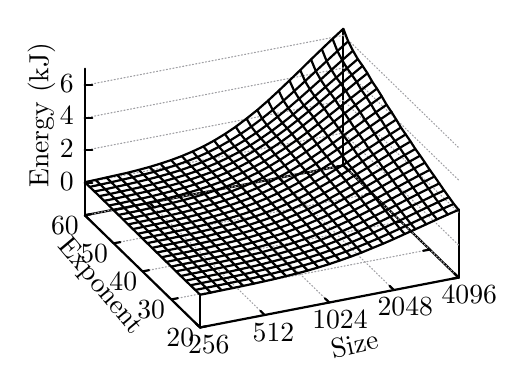
\begin{tikzpicture}[y=0.80pt, x=0.80pt, yscale=-0.570000, xscale=0.570000, inner sep=0pt, outer sep=0pt]
\begin{scope}[draw=black,line join=bevel,line cap=rect,even odd rule,line width=0.800pt]
  \begin{scope}[cm={{1.0,0.0,0.0,1.0,(0.0,0.0)}},draw=black,line join=bevel,line cap=rect,line width=0.800pt]
  \end{scope}
  \begin{scope}[cm={{1.00465,0.0,0.0,1.00465,(0.0,0.0)}},draw=black,line join=bevel,line cap=rect,line width=0.800pt]
  \end{scope}
  \begin{scope}[cm={{1.00465,0.0,0.0,1.00465,(0.0,0.0)}},draw=black,line join=round,line cap=round,line width=0.800pt]
    \path[draw] (67.6000,186.1000) -- (271.5000,146.8000);
    \path[draw] (362.4000,235.2000) -- (271.5000,146.8000);
    \path[draw] (67.5000,186.5000) -- (67.5000,70.5000);
    \path[draw] (271.5000,146.5000) -- (271.5000,39.5000);
    \path[draw] (362.5000,235.5000) -- (362.5000,181.5000);
  \end{scope}
  \begin{scope}[cm={{1.00465,0.0,0.0,1.00465,(0.0,0.0)}},draw=ca0a0a4,dash pattern=on 0.40pt off 0.80pt,line join=round,line cap=round,line width=0.400pt]
    \path[draw] (158.5000,274.6000) -- (67.6000,186.1000);
  \end{scope}
  \begin{scope}[cm={{1.00465,0.0,0.0,1.00465,(0.0,0.0)}},draw=black,line join=round,line cap=round,line width=0.800pt]
    \path[draw] (158.5000,274.6000) -- (155.1000,271.3000);
    \path[draw] (67.6000,186.1000) -- (71.0000,189.4000);
  \end{scope}
  \begin{scope}[cm={{1.00465,0.0,0.0,1.00465,(0.0,0.0)}},draw=black,line join=bevel,line cap=rect,line width=0.800pt]
  \end{scope}
  \begin{scope}[cm={{1.00465,0.0,0.0,1.00465,(149.693,296.874)}},draw=black,line join=bevel,line cap=rect,line width=0.800pt]
  \end{scope}
  \begin{scope}[cm={{1.00465,0.0,0.0,1.00465,(149.693,296.874)}},draw=black,line join=bevel,line cap=rect,line width=0.800pt]
  \end{scope}
  \begin{scope}[cm={{1.00465,0.0,0.0,1.00465,(149.693,296.874)}},draw=black,line join=bevel,line cap=rect,line width=0.800pt]
  \end{scope}
  \begin{scope}[cm={{1.00465,0.0,0.0,1.00465,(149.693,296.874)}},draw=black,line join=bevel,line cap=rect,line width=0.800pt]
  \end{scope}
  \begin{scope}[cm={{1.00465,0.0,0.0,1.00465,(149.693,296.874)}},draw=black,line join=bevel,line cap=rect,line width=0.800pt]
  \end{scope}
  \begin{scope}[cm={{1.00465,0.0,0.0,1.00465,(149.693,296.874)}},draw=black,line join=bevel,line cap=rect,line width=0.800pt]
    \path[fill=black] (0.0000,0.0000) node[above right] () {256};
  \end{scope}
  \begin{scope}[cm={{1.00465,0.0,0.0,1.00465,(149.693,296.874)}},draw=black,line join=bevel,line cap=rect,line width=0.800pt]
  \end{scope}
  \begin{scope}[cm={{1.00465,0.0,0.0,1.00465,(0.0,0.0)}},draw=black,line join=bevel,line cap=rect,line width=0.800pt]
  \end{scope}
  \begin{scope}[cm={{1.00465,0.0,0.0,1.00465,(0.0,0.0)}},draw=ca0a0a4,dash pattern=on 0.40pt off 0.80pt,line join=round,line cap=round,line width=0.400pt]
    \path[draw] (209.5000,264.8000) -- (118.6000,176.3000);
  \end{scope}
  \begin{scope}[cm={{1.00465,0.0,0.0,1.00465,(0.0,0.0)}},draw=black,line join=round,line cap=round,line width=0.800pt]
    \path[draw] (209.5000,264.8000) -- (206.1000,261.5000);
    \path[draw] (118.6000,176.3000) -- (122.0000,179.6000);
  \end{scope}
  \begin{scope}[cm={{1.00465,0.0,0.0,1.00465,(0.0,0.0)}},draw=black,line join=bevel,line cap=rect,line width=0.800pt]
  \end{scope}
  \begin{scope}[cm={{1.00465,0.0,0.0,1.00465,(200.93,286.828)}},draw=black,line join=bevel,line cap=rect,line width=0.800pt]
  \end{scope}
  \begin{scope}[cm={{1.00465,0.0,0.0,1.00465,(200.93,286.828)}},draw=black,line join=bevel,line cap=rect,line width=0.800pt]
  \end{scope}
  \begin{scope}[cm={{1.00465,0.0,0.0,1.00465,(200.93,286.828)}},draw=black,line join=bevel,line cap=rect,line width=0.800pt]
  \end{scope}
  \begin{scope}[cm={{1.00465,0.0,0.0,1.00465,(200.93,286.828)}},draw=black,line join=bevel,line cap=rect,line width=0.800pt]
  \end{scope}
  \begin{scope}[cm={{1.00465,0.0,0.0,1.00465,(200.93,286.828)}},draw=black,line join=bevel,line cap=rect,line width=0.800pt]
  \end{scope}
  \begin{scope}[cm={{1.00465,0.0,0.0,1.00465,(200.93,286.828)}},draw=black,line join=bevel,line cap=rect,line width=0.800pt]
    \path[fill=black] (0.0000,0.0000) node[above right] () {512};
  \end{scope}
  \begin{scope}[cm={{1.00465,0.0,0.0,1.00465,(200.93,286.828)}},draw=black,line join=bevel,line cap=rect,line width=0.800pt]
  \end{scope}
  \begin{scope}[cm={{1.00465,0.0,0.0,1.00465,(0.0,0.0)}},draw=black,line join=bevel,line cap=rect,line width=0.800pt]
  \end{scope}
  \begin{scope}[cm={{1.00465,0.0,0.0,1.00465,(0.0,0.0)}},draw=ca0a0a4,dash pattern=on 0.40pt off 0.80pt,line join=round,line cap=round,line width=0.400pt]
    \path[draw] (260.4000,254.9000) -- (169.6000,166.4000);
  \end{scope}
  \begin{scope}[cm={{1.00465,0.0,0.0,1.00465,(0.0,0.0)}},draw=black,line join=round,line cap=round,line width=0.800pt]
    \path[draw] (260.4000,254.9000) -- (257.0000,251.6000);
    \path[draw] (169.6000,166.4000) -- (173.0000,169.7000);
  \end{scope}
  \begin{scope}[cm={{1.00465,0.0,0.0,1.00465,(0.0,0.0)}},draw=black,line join=bevel,line cap=rect,line width=0.800pt]
  \end{scope}
  \begin{scope}[cm={{1.00465,0.0,0.0,1.00465,(248.149,276.781)}},draw=black,line join=bevel,line cap=rect,line width=0.800pt]
  \end{scope}
  \begin{scope}[cm={{1.00465,0.0,0.0,1.00465,(248.149,276.781)}},draw=black,line join=bevel,line cap=rect,line width=0.800pt]
  \end{scope}
  \begin{scope}[cm={{1.00465,0.0,0.0,1.00465,(248.149,276.781)}},draw=black,line join=bevel,line cap=rect,line width=0.800pt]
  \end{scope}
  \begin{scope}[cm={{1.00465,0.0,0.0,1.00465,(248.149,276.781)}},draw=black,line join=bevel,line cap=rect,line width=0.800pt]
  \end{scope}
  \begin{scope}[cm={{1.00465,0.0,0.0,1.00465,(248.149,276.781)}},draw=black,line join=bevel,line cap=rect,line width=0.800pt]
  \end{scope}
  \begin{scope}[cm={{1.00465,0.0,0.0,1.00465,(248.149,276.781)}},draw=black,line join=bevel,line cap=rect,line width=0.800pt]
    \path[fill=black] (0.0000,0.0000) node[above right] () {1024};
  \end{scope}
  \begin{scope}[cm={{1.00465,0.0,0.0,1.00465,(248.149,276.781)}},draw=black,line join=bevel,line cap=rect,line width=0.800pt]
  \end{scope}
  \begin{scope}[cm={{1.00465,0.0,0.0,1.00465,(0.0,0.0)}},draw=black,line join=bevel,line cap=rect,line width=0.800pt]
  \end{scope}
  \begin{scope}[cm={{1.00465,0.0,0.0,1.00465,(0.0,0.0)}},draw=ca0a0a4,dash pattern=on 0.40pt off 0.80pt,line join=round,line cap=round,line width=0.400pt]
    \path[draw] (311.4000,245.1000) -- (220.5000,156.6000);
  \end{scope}
  \begin{scope}[cm={{1.00465,0.0,0.0,1.00465,(0.0,0.0)}},draw=black,line join=round,line cap=round,line width=0.800pt]
    \path[draw] (311.4000,245.1000) -- (308.0000,241.8000);
    \path[draw] (220.5000,156.6000) -- (223.9000,159.9000);
  \end{scope}
  \begin{scope}[cm={{1.00465,0.0,0.0,1.00465,(0.0,0.0)}},draw=black,line join=bevel,line cap=rect,line width=0.800pt]
  \end{scope}
  \begin{scope}[cm={{1.00465,0.0,0.0,1.00465,(299.888,266.735)}},draw=black,line join=bevel,line cap=rect,line width=0.800pt]
  \end{scope}
  \begin{scope}[cm={{1.00465,0.0,0.0,1.00465,(299.888,266.735)}},draw=black,line join=bevel,line cap=rect,line width=0.800pt]
  \end{scope}
  \begin{scope}[cm={{1.00465,0.0,0.0,1.00465,(299.888,266.735)}},draw=black,line join=bevel,line cap=rect,line width=0.800pt]
  \end{scope}
  \begin{scope}[cm={{1.00465,0.0,0.0,1.00465,(299.888,266.735)}},draw=black,line join=bevel,line cap=rect,line width=0.800pt]
  \end{scope}
  \begin{scope}[cm={{1.00465,0.0,0.0,1.00465,(299.888,266.735)}},draw=black,line join=bevel,line cap=rect,line width=0.800pt]
  \end{scope}
  \begin{scope}[cm={{1.00465,0.0,0.0,1.00465,(299.888,266.735)}},draw=black,line join=bevel,line cap=rect,line width=0.800pt]
    \path[fill=black] (0.0000,0.0000) node[above right] () {2048};
  \end{scope}
  \begin{scope}[cm={{1.00465,0.0,0.0,1.00465,(299.888,266.735)}},draw=black,line join=bevel,line cap=rect,line width=0.800pt]
  \end{scope}
  \begin{scope}[cm={{1.00465,0.0,0.0,1.00465,(0.0,0.0)}},draw=black,line join=bevel,line cap=rect,line width=0.800pt]
  \end{scope}
  \begin{scope}[cm={{1.00465,0.0,0.0,1.00465,(0.0,0.0)}},draw=ca0a0a4,dash pattern=on 0.40pt off 0.80pt,line join=round,line cap=round,line width=0.400pt]
    \path[draw] (362.4000,235.2000) -- (271.5000,146.8000);
  \end{scope}
  \begin{scope}[cm={{1.00465,0.0,0.0,1.00465,(0.0,0.0)}},draw=black,line join=round,line cap=round,line width=0.800pt]
    \path[draw] (362.4000,235.2000) -- (359.0000,231.9000);
    \path[draw] (271.5000,146.8000) -- (274.9000,150.1000);
  \end{scope}
  \begin{scope}[cm={{1.00465,0.0,0.0,1.00465,(0.0,0.0)}},draw=black,line join=bevel,line cap=rect,line width=0.800pt]
  \end{scope}
  \begin{scope}[cm={{1.00465,0.0,0.0,1.00465,(350.623,256.688)}},draw=black,line join=bevel,line cap=rect,line width=0.800pt]
  \end{scope}
  \begin{scope}[cm={{1.00465,0.0,0.0,1.00465,(350.623,256.688)}},draw=black,line join=bevel,line cap=rect,line width=0.800pt]
  \end{scope}
  \begin{scope}[cm={{1.00465,0.0,0.0,1.00465,(350.623,256.688)}},draw=black,line join=bevel,line cap=rect,line width=0.800pt]
  \end{scope}
  \begin{scope}[cm={{1.00465,0.0,0.0,1.00465,(350.623,256.688)}},draw=black,line join=bevel,line cap=rect,line width=0.800pt]
  \end{scope}
  \begin{scope}[cm={{1.00465,0.0,0.0,1.00465,(350.623,256.688)}},draw=black,line join=bevel,line cap=rect,line width=0.800pt]
  \end{scope}
  \begin{scope}[cm={{1.00465,0.0,0.0,1.00465,(350.623,256.688)}},draw=black,line join=bevel,line cap=rect,line width=0.800pt]
    \path[fill=black] (0.0000,0.0000) node[above right] () {4096};
  \end{scope}
  \begin{scope}[cm={{1.00465,0.0,0.0,1.00465,(350.623,256.688)}},draw=black,line join=bevel,line cap=rect,line width=0.800pt]
  \end{scope}
  \begin{scope}[cm={{1.00465,0.0,0.0,1.00465,(0.0,0.0)}},draw=black,line join=bevel,line cap=rect,line width=0.800pt]
  \end{scope}
  \begin{scope}[cm={{1.00465,0.0,0.0,1.00465,(0.0,0.0)}},draw=ca0a0a4,dash pattern=on 0.40pt off 0.80pt,line join=round,line cap=round,line width=0.400pt]
    \path[draw] (158.5000,274.6000) -- (362.4000,235.2000);
  \end{scope}
  \begin{scope}[cm={{1.00465,0.0,0.0,1.00465,(0.0,0.0)}},draw=black,line join=round,line cap=round,line width=0.800pt]
    \path[draw] (158.5000,274.6000) -- (163.6000,273.6000);
    \path[draw] (362.4000,235.2000) -- (357.2000,236.2000);
  \end{scope}
  \begin{scope}[cm={{1.00465,0.0,0.0,1.00465,(0.0,0.0)}},draw=black,line join=bevel,line cap=rect,line width=0.800pt]
  \end{scope}
  \begin{scope}[cm={{1.00465,0.0,0.0,1.00465,(132.614,290.847)}},draw=black,line join=bevel,line cap=rect,line width=0.800pt]
  \end{scope}
  \begin{scope}[cm={{1.00465,0.0,0.0,1.00465,(132.614,290.847)}},draw=black,line join=bevel,line cap=rect,line width=0.800pt]
  \end{scope}
  \begin{scope}[cm={{1.00465,0.0,0.0,1.00465,(132.614,290.847)}},draw=black,line join=bevel,line cap=rect,line width=0.800pt]
  \end{scope}
  \begin{scope}[cm={{1.00465,0.0,0.0,1.00465,(132.614,290.847)}},draw=black,line join=bevel,line cap=rect,line width=0.800pt]
  \end{scope}
  \begin{scope}[cm={{1.00465,0.0,0.0,1.00465,(132.614,290.847)}},draw=black,line join=bevel,line cap=rect,line width=0.800pt]
  \end{scope}
  \begin{scope}[cm={{1.00465,0.0,0.0,1.00465,(132.614,290.847)}},draw=black,line join=bevel,line cap=rect,line width=0.800pt]
    \path[fill=black] (0.0000,0.0000) node[above right] () {20};
  \end{scope}
  \begin{scope}[cm={{1.00465,0.0,0.0,1.00465,(132.614,290.847)}},draw=black,line join=bevel,line cap=rect,line width=0.800pt]
  \end{scope}
  \begin{scope}[cm={{1.00465,0.0,0.0,1.00465,(0.0,0.0)}},draw=black,line join=bevel,line cap=rect,line width=0.800pt]
  \end{scope}
  \begin{scope}[cm={{1.00465,0.0,0.0,1.00465,(0.0,0.0)}},draw=ca0a0a4,dash pattern=on 0.40pt off 0.80pt,line join=round,line cap=round,line width=0.400pt]
    \path[draw] (135.8000,252.5000) -- (339.7000,213.1000);
  \end{scope}
  \begin{scope}[cm={{1.00465,0.0,0.0,1.00465,(0.0,0.0)}},draw=black,line join=round,line cap=round,line width=0.800pt]
    \path[draw] (135.8000,252.5000) -- (140.9000,251.5000);
    \path[draw] (339.7000,213.1000) -- (334.5000,214.1000);
  \end{scope}
  \begin{scope}[cm={{1.00465,0.0,0.0,1.00465,(0.0,0.0)}},draw=black,line join=bevel,line cap=rect,line width=0.800pt]
  \end{scope}
  \begin{scope}[cm={{1.00465,0.0,0.0,1.00465,(109.507,268.744)}},draw=black,line join=bevel,line cap=rect,line width=0.800pt]
  \end{scope}
  \begin{scope}[cm={{1.00465,0.0,0.0,1.00465,(109.507,268.744)}},draw=black,line join=bevel,line cap=rect,line width=0.800pt]
  \end{scope}
  \begin{scope}[cm={{1.00465,0.0,0.0,1.00465,(109.507,268.744)}},draw=black,line join=bevel,line cap=rect,line width=0.800pt]
  \end{scope}
  \begin{scope}[cm={{1.00465,0.0,0.0,1.00465,(109.507,268.744)}},draw=black,line join=bevel,line cap=rect,line width=0.800pt]
  \end{scope}
  \begin{scope}[cm={{1.00465,0.0,0.0,1.00465,(109.507,268.744)}},draw=black,line join=bevel,line cap=rect,line width=0.800pt]
  \end{scope}
  \begin{scope}[cm={{1.00465,0.0,0.0,1.00465,(109.507,268.744)}},draw=black,line join=bevel,line cap=rect,line width=0.800pt]
    \path[fill=black] (0.0000,0.0000) node[above right] () {30};
  \end{scope}
  \begin{scope}[cm={{1.00465,0.0,0.0,1.00465,(109.507,268.744)}},draw=black,line join=bevel,line cap=rect,line width=0.800pt]
  \end{scope}
  \begin{scope}[cm={{1.00465,0.0,0.0,1.00465,(0.0,0.0)}},draw=black,line join=bevel,line cap=rect,line width=0.800pt]
  \end{scope}
  \begin{scope}[cm={{1.00465,0.0,0.0,1.00465,(0.0,0.0)}},draw=ca0a0a4,dash pattern=on 0.40pt off 0.80pt,line join=round,line cap=round,line width=0.400pt]
    \path[draw] (113.1000,230.4000) -- (316.9000,191.0000);
  \end{scope}
  \begin{scope}[cm={{1.00465,0.0,0.0,1.00465,(0.0,0.0)}},draw=black,line join=round,line cap=round,line width=0.800pt]
    \path[draw] (113.1000,230.4000) -- (118.2000,229.4000);
    \path[draw] (316.9000,191.0000) -- (311.8000,192.0000);
  \end{scope}
  \begin{scope}[cm={{1.00465,0.0,0.0,1.00465,(0.0,0.0)}},draw=black,line join=bevel,line cap=rect,line width=0.800pt]
  \end{scope}
  \begin{scope}[cm={{1.00465,0.0,0.0,1.00465,(87.4047,246.642)}},draw=black,line join=bevel,line cap=rect,line width=0.800pt]
  \end{scope}
  \begin{scope}[cm={{1.00465,0.0,0.0,1.00465,(87.4047,246.642)}},draw=black,line join=bevel,line cap=rect,line width=0.800pt]
  \end{scope}
  \begin{scope}[cm={{1.00465,0.0,0.0,1.00465,(87.4047,246.642)}},draw=black,line join=bevel,line cap=rect,line width=0.800pt]
  \end{scope}
  \begin{scope}[cm={{1.00465,0.0,0.0,1.00465,(87.4047,246.642)}},draw=black,line join=bevel,line cap=rect,line width=0.800pt]
  \end{scope}
  \begin{scope}[cm={{1.00465,0.0,0.0,1.00465,(87.4047,246.642)}},draw=black,line join=bevel,line cap=rect,line width=0.800pt]
  \end{scope}
  \begin{scope}[cm={{1.00465,0.0,0.0,1.00465,(87.4047,246.642)}},draw=black,line join=bevel,line cap=rect,line width=0.800pt]
    \path[fill=black] (0.0000,0.0000) node[above right] () {40};
  \end{scope}
  \begin{scope}[cm={{1.00465,0.0,0.0,1.00465,(87.4047,246.642)}},draw=black,line join=bevel,line cap=rect,line width=0.800pt]
  \end{scope}
  \begin{scope}[cm={{1.00465,0.0,0.0,1.00465,(0.0,0.0)}},draw=black,line join=bevel,line cap=rect,line width=0.800pt]
  \end{scope}
  \begin{scope}[cm={{1.00465,0.0,0.0,1.00465,(0.0,0.0)}},draw=ca0a0a4,dash pattern=on 0.40pt off 0.80pt,line join=round,line cap=round,line width=0.400pt]
    \path[draw] (90.3000,208.2000) -- (294.2000,168.8000);
  \end{scope}
  \begin{scope}[cm={{1.00465,0.0,0.0,1.00465,(0.0,0.0)}},draw=black,line join=round,line cap=round,line width=0.800pt]
    \path[draw] (90.3000,208.2000) -- (95.5000,207.3000);
    \path[draw] (294.2000,168.8000) -- (289.1000,169.8000);
  \end{scope}
  \begin{scope}[cm={{1.00465,0.0,0.0,1.00465,(0.0,0.0)}},draw=black,line join=bevel,line cap=rect,line width=0.800pt]
  \end{scope}
  \begin{scope}[cm={{1.00465,0.0,0.0,1.00465,(64.2977,224.54)}},draw=black,line join=bevel,line cap=rect,line width=0.800pt]
  \end{scope}
  \begin{scope}[cm={{1.00465,0.0,0.0,1.00465,(64.2977,224.54)}},draw=black,line join=bevel,line cap=rect,line width=0.800pt]
  \end{scope}
  \begin{scope}[cm={{1.00465,0.0,0.0,1.00465,(64.2977,224.54)}},draw=black,line join=bevel,line cap=rect,line width=0.800pt]
  \end{scope}
  \begin{scope}[cm={{1.00465,0.0,0.0,1.00465,(64.2977,224.54)}},draw=black,line join=bevel,line cap=rect,line width=0.800pt]
  \end{scope}
  \begin{scope}[cm={{1.00465,0.0,0.0,1.00465,(64.2977,224.54)}},draw=black,line join=bevel,line cap=rect,line width=0.800pt]
  \end{scope}
  \begin{scope}[cm={{1.00465,0.0,0.0,1.00465,(64.2977,224.54)}},draw=black,line join=bevel,line cap=rect,line width=0.800pt]
    \path[fill=black] (0.0000,0.0000) node[above right] () {50};
  \end{scope}
  \begin{scope}[cm={{1.00465,0.0,0.0,1.00465,(64.2977,224.54)}},draw=black,line join=bevel,line cap=rect,line width=0.800pt]
  \end{scope}
  \begin{scope}[cm={{1.00465,0.0,0.0,1.00465,(0.0,0.0)}},draw=black,line join=bevel,line cap=rect,line width=0.800pt]
  \end{scope}
  \begin{scope}[cm={{1.00465,0.0,0.0,1.00465,(0.0,0.0)}},draw=ca0a0a4,dash pattern=on 0.40pt off 0.80pt,line join=round,line cap=round,line width=0.400pt]
    \path[draw] (67.6000,186.1000) -- (271.5000,146.8000);
  \end{scope}
  \begin{scope}[cm={{1.00465,0.0,0.0,1.00465,(0.0,0.0)}},draw=black,line join=round,line cap=round,line width=0.800pt]
    \path[draw] (67.6000,186.1000) -- (72.8000,185.1000);
    \path[draw] (271.5000,146.8000) -- (266.4000,147.8000);
  \end{scope}
  \begin{scope}[cm={{1.00465,0.0,0.0,1.00465,(0.0,0.0)}},draw=black,line join=bevel,line cap=rect,line width=0.800pt]
  \end{scope}
  \begin{scope}[cm={{1.00465,0.0,0.0,1.00465,(41.1907,202.437)}},draw=black,line join=bevel,line cap=rect,line width=0.800pt]
  \end{scope}
  \begin{scope}[cm={{1.00465,0.0,0.0,1.00465,(41.1907,202.437)}},draw=black,line join=bevel,line cap=rect,line width=0.800pt]
  \end{scope}
  \begin{scope}[cm={{1.00465,0.0,0.0,1.00465,(41.1907,202.437)}},draw=black,line join=bevel,line cap=rect,line width=0.800pt]
  \end{scope}
  \begin{scope}[cm={{1.00465,0.0,0.0,1.00465,(41.1907,202.437)}},draw=black,line join=bevel,line cap=rect,line width=0.800pt]
  \end{scope}
  \begin{scope}[cm={{1.00465,0.0,0.0,1.00465,(41.1907,202.437)}},draw=black,line join=bevel,line cap=rect,line width=0.800pt]
  \end{scope}
  \begin{scope}[cm={{1.00465,0.0,0.0,1.00465,(41.1907,202.437)}},draw=black,line join=bevel,line cap=rect,line width=0.800pt]
    \path[fill=black] (0.0000,0.0000) node[above right] () {60};
  \end{scope}
  \begin{scope}[cm={{1.00465,0.0,0.0,1.00465,(41.1907,202.437)}},draw=black,line join=bevel,line cap=rect,line width=0.800pt]
  \end{scope}
  \begin{scope}[cm={{1.00465,0.0,0.0,1.00465,(0.0,0.0)}},draw=black,line join=bevel,line cap=rect,line width=0.800pt]
  \end{scope}
  \begin{scope}[cm={{1.00465,0.0,0.0,1.00465,(0.0,0.0)}},draw=ca0a0a4,dash pattern=on 0.40pt off 0.80pt,line join=round,line cap=round,line width=0.400pt]
    \path[draw] (67.6000,160.5000) -- (271.5000,121.2000);
    \path[draw] (271.5000,121.2000) -- (271.5000,121.2000) -- (362.4000,209.6000);
  \end{scope}
  \begin{scope}[cm={{1.00465,0.0,0.0,1.00465,(0.0,0.0)}},draw=black,line join=round,line cap=round,line width=0.800pt]
    \path[draw] (67.5000,160.5000) -- (73.5000,160.5000);
  \end{scope}
  \begin{scope}[cm={{1.00465,0.0,0.0,1.00465,(0.0,0.0)}},draw=black,line join=bevel,line cap=rect,line width=0.800pt]
  \end{scope}
  \begin{scope}[cm={{1.00465,0.0,0.0,1.00465,(48.2233,167.274)}},draw=black,line join=bevel,line cap=rect,line width=0.800pt]
  \end{scope}
  \begin{scope}[cm={{1.00465,0.0,0.0,1.00465,(48.2233,167.274)}},draw=black,line join=bevel,line cap=rect,line width=0.800pt]
  \end{scope}
  \begin{scope}[cm={{1.00465,0.0,0.0,1.00465,(48.2233,167.274)}},draw=black,line join=bevel,line cap=rect,line width=0.800pt]
  \end{scope}
  \begin{scope}[cm={{1.00465,0.0,0.0,1.00465,(48.2233,167.274)}},draw=black,line join=bevel,line cap=rect,line width=0.800pt]
  \end{scope}
  \begin{scope}[cm={{1.00465,0.0,0.0,1.00465,(48.2233,167.274)}},draw=black,line join=bevel,line cap=rect,line width=0.800pt]
  \end{scope}
  \begin{scope}[cm={{1.00465,0.0,0.0,1.00465,(48.2233,167.274)}},draw=black,line join=bevel,line cap=rect,line width=0.800pt]
    \path[fill=black] (0.0000,0.0000) node[above right] () {0};
  \end{scope}
  \begin{scope}[cm={{1.00465,0.0,0.0,1.00465,(48.2233,167.274)}},draw=black,line join=bevel,line cap=rect,line width=0.800pt]
  \end{scope}
  \begin{scope}[cm={{1.00465,0.0,0.0,1.00465,(0.0,0.0)}},draw=black,line join=bevel,line cap=rect,line width=0.800pt]
  \end{scope}
  \begin{scope}[cm={{1.00465,0.0,0.0,1.00465,(0.0,0.0)}},draw=ca0a0a4,dash pattern=on 0.40pt off 0.80pt,line join=round,line cap=round,line width=0.400pt]
    \path[draw] (67.6000,134.9000) -- (271.5000,95.5000);
    \path[draw] (271.5000,95.5000) -- (271.5000,95.5000) -- (362.4000,183.9000);
  \end{scope}
  \begin{scope}[cm={{1.00465,0.0,0.0,1.00465,(0.0,0.0)}},draw=black,line join=round,line cap=round,line width=0.800pt]
    \path[draw] (67.5000,134.5000) -- (73.5000,134.5000);
  \end{scope}
  \begin{scope}[cm={{1.00465,0.0,0.0,1.00465,(0.0,0.0)}},draw=black,line join=bevel,line cap=rect,line width=0.800pt]
  \end{scope}
  \begin{scope}[cm={{1.00465,0.0,0.0,1.00465,(48.2233,141.153)}},draw=black,line join=bevel,line cap=rect,line width=0.800pt]
  \end{scope}
  \begin{scope}[cm={{1.00465,0.0,0.0,1.00465,(48.2233,141.153)}},draw=black,line join=bevel,line cap=rect,line width=0.800pt]
  \end{scope}
  \begin{scope}[cm={{1.00465,0.0,0.0,1.00465,(48.2233,141.153)}},draw=black,line join=bevel,line cap=rect,line width=0.800pt]
  \end{scope}
  \begin{scope}[cm={{1.00465,0.0,0.0,1.00465,(48.2233,141.153)}},draw=black,line join=bevel,line cap=rect,line width=0.800pt]
  \end{scope}
  \begin{scope}[cm={{1.00465,0.0,0.0,1.00465,(48.2233,141.153)}},draw=black,line join=bevel,line cap=rect,line width=0.800pt]
  \end{scope}
  \begin{scope}[cm={{1.00465,0.0,0.0,1.00465,(48.2233,141.153)}},draw=black,line join=bevel,line cap=rect,line width=0.800pt]
    \path[fill=black] (0.0000,0.0000) node[above right] () {2};
  \end{scope}
  \begin{scope}[cm={{1.00465,0.0,0.0,1.00465,(48.2233,141.153)}},draw=black,line join=bevel,line cap=rect,line width=0.800pt]
  \end{scope}
  \begin{scope}[cm={{1.00465,0.0,0.0,1.00465,(0.0,0.0)}},draw=black,line join=bevel,line cap=rect,line width=0.800pt]
  \end{scope}
  \begin{scope}[cm={{1.00465,0.0,0.0,1.00465,(0.0,0.0)}},draw=ca0a0a4,dash pattern=on 0.40pt off 0.80pt,line join=round,line cap=round,line width=0.400pt]
    \path[draw] (67.6000,109.3000) -- (271.5000,69.9000);
    \path[draw] (271.5000,69.9000) -- (271.5000,69.9000) -- (362.4000,158.3000);
  \end{scope}
  \begin{scope}[cm={{1.00465,0.0,0.0,1.00465,(0.0,0.0)}},draw=black,line join=round,line cap=round,line width=0.800pt]
    \path[draw] (67.5000,109.5000) -- (73.5000,109.5000);
  \end{scope}
  \begin{scope}[cm={{1.00465,0.0,0.0,1.00465,(0.0,0.0)}},draw=black,line join=bevel,line cap=rect,line width=0.800pt]
  \end{scope}
  \begin{scope}[cm={{1.00465,0.0,0.0,1.00465,(48.2233,115.033)}},draw=black,line join=bevel,line cap=rect,line width=0.800pt]
  \end{scope}
  \begin{scope}[cm={{1.00465,0.0,0.0,1.00465,(48.2233,115.033)}},draw=black,line join=bevel,line cap=rect,line width=0.800pt]
  \end{scope}
  \begin{scope}[cm={{1.00465,0.0,0.0,1.00465,(48.2233,115.033)}},draw=black,line join=bevel,line cap=rect,line width=0.800pt]
  \end{scope}
  \begin{scope}[cm={{1.00465,0.0,0.0,1.00465,(48.2233,115.033)}},draw=black,line join=bevel,line cap=rect,line width=0.800pt]
  \end{scope}
  \begin{scope}[cm={{1.00465,0.0,0.0,1.00465,(48.2233,115.033)}},draw=black,line join=bevel,line cap=rect,line width=0.800pt]
  \end{scope}
  \begin{scope}[cm={{1.00465,0.0,0.0,1.00465,(48.2233,115.033)}},draw=black,line join=bevel,line cap=rect,line width=0.800pt]
    \path[fill=black] (0.0000,0.0000) node[above right] () {4};
  \end{scope}
  \begin{scope}[cm={{1.00465,0.0,0.0,1.00465,(48.2233,115.033)}},draw=black,line join=bevel,line cap=rect,line width=0.800pt]
  \end{scope}
  \begin{scope}[cm={{1.00465,0.0,0.0,1.00465,(0.0,0.0)}},draw=black,line join=bevel,line cap=rect,line width=0.800pt]
  \end{scope}
  \begin{scope}[cm={{1.00465,0.0,0.0,1.00465,(0.0,0.0)}},draw=ca0a0a4,dash pattern=on 0.40pt off 0.80pt,line join=round,line cap=round,line width=0.400pt]
    \path[draw] (67.6000,83.6000) -- (271.5000,44.2000);
    \path[draw] (271.5000,44.2000) -- (271.5000,44.2000) -- (362.4000,132.7000);
  \end{scope}
  \begin{scope}[cm={{1.00465,0.0,0.0,1.00465,(0.0,0.0)}},draw=black,line join=round,line cap=round,line width=0.800pt]
    \path[draw] (67.5000,83.5000) -- (73.5000,83.5000);
  \end{scope}
  \begin{scope}[cm={{1.00465,0.0,0.0,1.00465,(0.0,0.0)}},draw=black,line join=bevel,line cap=rect,line width=0.800pt]
  \end{scope}
  \begin{scope}[cm={{1.00465,0.0,0.0,1.00465,(48.2233,89.9163)}},draw=black,line join=bevel,line cap=rect,line width=0.800pt]
  \end{scope}
  \begin{scope}[cm={{1.00465,0.0,0.0,1.00465,(48.2233,89.9163)}},draw=black,line join=bevel,line cap=rect,line width=0.800pt]
  \end{scope}
  \begin{scope}[cm={{1.00465,0.0,0.0,1.00465,(48.2233,89.9163)}},draw=black,line join=bevel,line cap=rect,line width=0.800pt]
  \end{scope}
  \begin{scope}[cm={{1.00465,0.0,0.0,1.00465,(48.2233,89.9163)}},draw=black,line join=bevel,line cap=rect,line width=0.800pt]
  \end{scope}
  \begin{scope}[cm={{1.00465,0.0,0.0,1.00465,(48.2233,89.9163)}},draw=black,line join=bevel,line cap=rect,line width=0.800pt]
  \end{scope}
  \begin{scope}[cm={{1.00465,0.0,0.0,1.00465,(48.2233,89.9163)}},draw=black,line join=bevel,line cap=rect,line width=0.800pt]
    \path[fill=black] (0.0000,0.0000) node[above right] () {6};
  \end{scope}
  \begin{scope}[cm={{1.00465,0.0,0.0,1.00465,(48.2233,89.9163)}},draw=black,line join=bevel,line cap=rect,line width=0.800pt]
  \end{scope}
  \begin{scope}[cm={{0.0,-1.00465,1.00465,0.0,(24.614,166.27)}},draw=black,line join=bevel,line cap=rect,line width=0.800pt]
  \end{scope}
  \begin{scope}[cm={{0.0,-1.00465,1.00465,0.0,(24.614,166.27)}},draw=black,line join=bevel,line cap=rect,line width=0.800pt]
  \end{scope}
  \begin{scope}[cm={{0.0,-1.00465,1.00465,0.0,(24.614,166.27)}},draw=black,line join=bevel,line cap=rect,line width=0.800pt]
  \end{scope}
  \begin{scope}[cm={{0.0,-1.00465,1.00465,0.0,(24.614,166.27)}},draw=black,line join=bevel,line cap=rect,line width=0.800pt]
  \end{scope}
  \begin{scope}[cm={{0.0,-1.00465,1.00465,0.0,(24.614,166.27)}},draw=black,line join=bevel,line cap=rect,line width=0.800pt]
  \end{scope}
  \begin{scope}[cm={{0.0,-1.00465,1.00465,0.0,(22.614,165.177)}},draw=black,line join=bevel,line cap=rect,line width=0.800pt]
    \path[fill=black] (0.0000,0.0000) node[above right] () {\rotatebox{90}{Energy (kJ)}};
  \end{scope}
  \begin{scope}[cm={{0.0,-1.00465,1.00465,0.0,(24.614,166.27)}},draw=black,line join=bevel,line cap=rect,line width=0.800pt]
  \end{scope}
  \begin{scope}[cm={{1.00465,0.0,0.0,1.00465,(0.0,0.0)}},draw=black,line join=bevel,line cap=rect,line width=0.800pt]
  \end{scope}
  \begin{scope}[cm={{1.00465,0.0,0.0,1.00465,(0.0,0.0)}},draw=black,line join=bevel,line cap=rect,line width=0.800pt]
  \end{scope}
  \begin{scope}[cm={{1.00465,0.0,0.0,1.00465,(0.0,0.0)}},draw=black,line join=bevel,line cap=rect,line width=0.800pt]
  \end{scope}
  \begin{scope}[cm={{1.00465,0.0,0.0,1.00465,(0.0,0.0)}},draw=black,line join=round,line cap=round,line width=0.800pt]
    \path[draw] (362.4000,181.8000) -- (358.6000,177.1000) -- (358.6000,177.1000) --
      (354.8000,171.8000) -- (354.8000,171.8000) -- (351.0000,166.5000) --
      (351.0000,166.5000) -- (347.2000,161.0000) -- (347.2000,161.0000) --
      (343.4000,155.5000) -- (343.4000,155.5000) -- (339.7000,150.3000) --
      (339.7000,150.3000) -- (335.9000,144.6000) -- (335.9000,144.6000) --
      (332.1000,139.1000) -- (332.1000,139.1000) -- (328.3000,133.8000) --
      (328.3000,133.8000) -- (324.5000,127.9000) -- (324.5000,127.9000) --
      (320.7000,122.3000) -- (320.7000,122.3000) -- (316.9000,116.9000) --
      (316.9000,116.9000) -- (313.2000,110.6000) -- (313.2000,110.6000) --
      (309.4000,104.5000) -- (309.4000,104.5000) -- (305.6000,98.9000) --
      (305.6000,98.9000) -- (301.8000,92.3000) -- (301.8000,92.3000) --
      (298.0000,86.2000) -- (298.0000,86.2000) -- (294.2000,80.6000) --
      (294.2000,80.6000) -- (290.5000,74.1000) -- (290.5000,74.1000) --
      (286.7000,68.3000) -- (286.7000,68.3000) -- (282.9000,62.9000) --
      (282.9000,62.9000) -- (279.1000,56.3000) -- (279.1000,56.3000) --
      (275.3000,48.9000) -- (275.3000,48.9000) -- (271.5000,39.0000);
    \path[draw] (353.9000,185.5000) -- (350.1000,180.9000) -- (350.1000,180.9000) --
      (346.3000,175.7000) -- (346.3000,175.7000) -- (342.5000,170.5000) --
      (342.5000,170.5000) -- (338.7000,165.1000) -- (338.7000,165.1000) --
      (334.9000,159.8000) -- (334.9000,159.8000) -- (331.2000,154.7000) --
      (331.2000,154.7000) -- (327.4000,149.2000) -- (327.4000,149.2000) --
      (323.6000,143.8000) -- (323.6000,143.8000) -- (319.8000,138.6000) --
      (319.8000,138.6000) -- (316.0000,132.9000) -- (316.0000,132.9000) --
      (312.2000,127.5000) -- (312.2000,127.5000) -- (308.4000,122.3000) --
      (308.4000,122.3000) -- (304.7000,116.2000) -- (304.7000,116.2000) --
      (300.9000,110.3000) -- (300.9000,110.3000) -- (297.1000,104.9000) --
      (297.1000,104.9000) -- (293.3000,98.5000) -- (293.3000,98.5000) --
      (289.5000,92.6000) -- (289.5000,92.6000) -- (285.7000,87.2000) --
      (285.7000,87.2000) -- (282.0000,80.9000) -- (282.0000,80.9000) --
      (278.2000,75.3000) -- (278.2000,75.3000) -- (274.4000,70.1000) --
      (274.4000,70.1000) -- (270.6000,63.8000) -- (270.6000,63.8000) --
      (266.8000,56.6000) -- (266.8000,56.6000) -- (263.0000,46.9000);
    \path[draw] (345.4000,189.3000) -- (341.6000,184.8000) -- (341.6000,184.8000) --
      (337.8000,179.7000) -- (337.8000,179.7000) -- (334.0000,174.7000) --
      (334.0000,174.7000) -- (330.2000,169.4000) -- (330.2000,169.4000) --
      (326.4000,164.2000) -- (326.4000,164.2000) -- (322.7000,159.2000) --
      (322.7000,159.2000) -- (318.9000,153.8000) -- (318.9000,153.8000) --
      (315.1000,148.6000) -- (315.1000,148.6000) -- (311.3000,143.6000) --
      (311.3000,143.6000) -- (307.5000,138.1000) -- (307.5000,138.1000) --
      (303.7000,132.8000) -- (303.7000,132.8000) -- (299.9000,127.7000) --
      (299.9000,127.7000) -- (296.2000,121.9000) -- (296.2000,121.9000) --
      (292.4000,116.2000) -- (292.4000,116.2000) -- (288.6000,110.9000) --
      (288.6000,110.9000) -- (284.8000,104.8000) -- (284.8000,104.8000) --
      (281.0000,99.1000) -- (281.0000,99.1000) -- (277.2000,93.9000) --
      (277.2000,93.9000) -- (273.5000,87.9000) -- (273.5000,87.9000) --
      (269.7000,82.5000) -- (269.7000,82.5000) -- (265.9000,77.5000) --
      (265.9000,77.5000) -- (262.1000,71.4000) -- (262.1000,71.4000) --
      (258.3000,64.5000) -- (258.3000,64.5000) -- (254.5000,55.0000);
    \path[draw] (336.9000,193.2000) -- (333.1000,188.7000) -- (333.1000,188.7000) --
      (329.3000,183.8000) -- (329.3000,183.8000) -- (325.5000,178.8000) --
      (325.5000,178.8000) -- (321.7000,173.7000) -- (321.7000,173.7000) --
      (317.9000,168.7000) -- (317.9000,168.7000) -- (314.2000,163.8000) --
      (314.2000,163.8000) -- (310.4000,158.6000) -- (310.4000,158.6000) --
      (306.6000,153.4000) -- (306.6000,153.4000) -- (302.8000,148.7000) --
      (302.8000,148.7000) -- (299.0000,143.3000) -- (299.0000,143.3000) --
      (295.2000,138.2000) -- (295.2000,138.2000) -- (291.4000,133.3000) --
      (291.4000,133.3000) -- (287.7000,127.6000) -- (287.7000,127.6000) --
      (283.9000,122.2000) -- (283.9000,122.2000) -- (280.1000,117.1000) --
      (280.1000,117.1000) -- (276.3000,111.2000) -- (276.3000,111.2000) --
      (272.5000,105.7000) -- (272.5000,105.7000) -- (268.7000,100.7000) --
      (268.7000,100.7000) -- (265.0000,94.9000) -- (265.0000,94.9000) --
      (261.2000,89.7000) -- (261.2000,89.7000) -- (257.4000,84.9000) --
      (257.4000,84.9000) -- (253.6000,79.1000) -- (253.6000,79.1000) --
      (249.8000,72.4000) -- (249.8000,72.4000) -- (246.0000,63.2000);
    \path[draw] (328.4000,197.1000) -- (324.6000,192.7000) -- (324.6000,192.7000) --
      (320.8000,187.9000) -- (320.8000,187.9000) -- (317.0000,183.0000) --
      (317.0000,183.0000) -- (313.2000,178.1000) -- (313.2000,178.1000) --
      (309.4000,173.2000) -- (309.4000,173.2000) -- (305.7000,168.4000) --
      (305.7000,168.4000) -- (301.9000,163.3000) -- (301.9000,163.3000) --
      (298.1000,158.4000) -- (298.1000,158.4000) -- (294.3000,153.6000) --
      (294.3000,153.6000) -- (290.5000,148.6000) -- (290.5000,148.6000) --
      (286.7000,143.6000) -- (286.7000,143.6000) -- (282.9000,138.8000) --
      (282.9000,138.8000) -- (279.2000,133.4000) -- (279.2000,133.4000) --
      (275.4000,128.1000) -- (275.4000,128.1000) -- (271.6000,123.2000) --
      (271.6000,123.2000) -- (267.8000,117.6000) -- (267.8000,117.6000) --
      (264.0000,112.3000) -- (264.0000,112.3000) -- (260.2000,107.4000) --
      (260.2000,107.4000) -- (256.5000,101.9000) -- (256.5000,101.9000) --
      (252.7000,96.9000) -- (252.7000,96.9000) -- (248.9000,92.3000) --
      (248.9000,92.3000) -- (245.1000,86.7000) -- (245.1000,86.7000) --
      (241.3000,80.3000) -- (241.3000,80.3000) -- (237.5000,71.6000);
    \path[draw] (319.9000,200.9000) -- (316.1000,196.6000) -- (316.1000,196.6000) --
      (312.3000,191.9000) -- (312.3000,191.9000) -- (308.5000,187.2000) --
      (308.5000,187.2000) -- (304.7000,182.4000) -- (304.7000,182.4000) --
      (300.9000,177.7000) -- (300.9000,177.7000) -- (297.2000,173.0000) --
      (297.2000,173.0000) -- (293.4000,168.1000) -- (293.4000,168.1000) --
      (289.6000,163.3000) -- (289.6000,163.3000) -- (285.8000,158.7000) --
      (285.8000,158.7000) -- (282.0000,153.7000) -- (282.0000,153.7000) --
      (278.2000,149.0000) -- (278.2000,149.0000) -- (274.4000,144.4000) --
      (274.4000,144.4000) -- (270.7000,139.1000) -- (270.7000,139.1000) --
      (266.9000,134.0000) -- (266.9000,134.0000) -- (263.1000,129.3000) --
      (263.1000,129.3000) -- (259.3000,123.9000) -- (259.3000,123.9000) --
      (255.5000,118.8000) -- (255.5000,118.8000) -- (251.7000,114.1000) --
      (251.7000,114.1000) -- (248.0000,108.8000) -- (248.0000,108.8000) --
      (244.2000,104.0000) -- (244.2000,104.0000) -- (240.4000,99.5000) --
      (240.4000,99.5000) -- (236.6000,94.2000) -- (236.6000,94.2000) --
      (232.8000,88.1000) -- (232.8000,88.1000) -- (229.0000,79.8000);
    \path[draw] (311.4000,204.8000) -- (307.6000,200.5000) -- (307.6000,200.5000) --
      (303.8000,195.9000) -- (303.8000,195.9000) -- (300.0000,191.4000) --
      (300.0000,191.4000) -- (296.2000,186.7000) -- (296.2000,186.7000) --
      (292.4000,182.1000) -- (292.4000,182.1000) -- (288.7000,177.5000) --
      (288.7000,177.5000) -- (284.9000,172.8000) -- (284.9000,172.8000) --
      (281.1000,168.1000) -- (281.1000,168.1000) -- (277.3000,163.6000) --
      (277.3000,163.6000) -- (273.5000,158.8000) -- (273.5000,158.8000) --
      (269.7000,154.2000) -- (269.7000,154.2000) -- (265.9000,149.7000) --
      (265.9000,149.7000) -- (262.2000,144.7000) -- (262.2000,144.7000) --
      (258.4000,139.8000) -- (258.4000,139.8000) -- (254.6000,135.2000) --
      (254.6000,135.2000) -- (250.8000,130.0000) -- (250.8000,130.0000) --
      (247.0000,125.1000) -- (247.0000,125.1000) -- (243.2000,120.6000) --
      (243.2000,120.6000) -- (239.5000,115.5000) -- (239.5000,115.5000) --
      (235.7000,110.9000) -- (235.7000,110.9000) -- (231.9000,106.6000) --
      (231.9000,106.6000) -- (228.1000,101.5000) -- (228.1000,101.5000) --
      (224.3000,95.7000) -- (224.3000,95.7000) -- (220.5000,87.9000);
    \path[draw] (302.9000,208.5000) -- (299.1000,204.3000) -- (299.1000,204.3000) --
      (295.3000,199.8000) -- (295.3000,199.8000) -- (291.5000,195.4000) --
      (291.5000,195.4000) -- (287.7000,190.9000) -- (287.7000,190.9000) --
      (283.9000,186.4000) -- (283.9000,186.4000) -- (280.2000,181.9000) --
      (280.2000,181.9000) -- (276.4000,177.3000) -- (276.4000,177.3000) --
      (272.6000,172.8000) -- (272.6000,172.8000) -- (268.8000,168.4000) --
      (268.8000,168.4000) -- (265.0000,163.8000) -- (265.0000,163.8000) --
      (261.2000,159.3000) -- (261.2000,159.3000) -- (257.4000,154.9000) --
      (257.4000,154.9000) -- (253.7000,150.1000) -- (253.7000,150.1000) --
      (249.9000,145.4000) -- (249.9000,145.4000) -- (246.1000,140.9000) --
      (246.1000,140.9000) -- (242.3000,135.9000) -- (242.3000,135.9000) --
      (238.5000,131.2000) -- (238.5000,131.2000) -- (234.7000,126.8000) --
      (234.7000,126.8000) -- (231.0000,122.0000) -- (231.0000,122.0000) --
      (227.2000,117.5000) -- (227.2000,117.5000) -- (223.4000,113.3000) --
      (223.4000,113.3000) -- (219.6000,108.4000) -- (219.6000,108.4000) --
      (215.8000,103.0000) -- (215.8000,103.0000) -- (212.1000,95.7000);
    \path[draw] (294.4000,212.0000) -- (290.6000,207.9000) -- (290.6000,207.9000) --
      (286.8000,203.6000) -- (286.8000,203.6000) -- (283.0000,199.3000) --
      (283.0000,199.3000) -- (279.2000,194.8000) -- (279.2000,194.8000) --
      (275.4000,190.5000) -- (275.4000,190.5000) -- (271.7000,186.2000) --
      (271.7000,186.2000) -- (267.9000,181.7000) -- (267.9000,181.7000) --
      (264.1000,177.3000) -- (264.1000,177.3000) -- (260.3000,173.0000) --
      (260.3000,173.0000) -- (256.5000,168.5000) -- (256.5000,168.5000) --
      (252.7000,164.1000) -- (252.7000,164.1000) -- (248.9000,159.8000) --
      (248.9000,159.8000) -- (245.2000,155.2000) -- (245.2000,155.2000) --
      (241.4000,150.7000) -- (241.4000,150.7000) -- (237.6000,146.3000) --
      (237.6000,146.3000) -- (233.8000,141.6000) -- (233.8000,141.6000) --
      (230.0000,137.0000) -- (230.0000,137.0000) -- (226.2000,132.7000) --
      (226.2000,132.7000) -- (222.5000,128.1000) -- (222.5000,128.1000) --
      (218.7000,123.7000) -- (218.7000,123.7000) -- (215.0000,119.6000) --
      (215.0000,119.6000) -- (211.2000,115.0000) -- (211.2000,115.0000) --
      (207.4000,109.8000) -- (207.4000,109.8000) -- (203.6000,103.1000);
    \path[draw] (285.9000,215.5000) -- (282.1000,211.4000) -- (282.1000,211.4000) --
      (278.3000,207.2000) -- (278.3000,207.2000) -- (274.5000,202.9000) --
      (274.5000,202.9000) -- (270.7000,198.7000) -- (270.7000,198.7000) --
      (266.9000,194.4000) -- (266.9000,194.4000) -- (263.2000,190.2000) --
      (263.2000,190.2000) -- (259.4000,185.9000) -- (259.4000,185.9000) --
      (255.6000,181.6000) -- (255.6000,181.6000) -- (251.8000,177.4000) --
      (251.8000,177.4000) -- (248.0000,173.0000) -- (248.0000,173.0000) --
      (244.2000,168.8000) -- (244.2000,168.8000) -- (240.4000,164.6000) --
      (240.4000,164.6000) -- (236.7000,160.1000) -- (236.7000,160.1000) --
      (232.9000,155.6000) -- (232.9000,155.6000) -- (229.1000,151.4000) --
      (229.1000,151.4000) -- (225.3000,146.9000) -- (225.3000,146.9000) --
      (221.5000,142.4000) -- (221.5000,142.4000) -- (217.7000,138.2000) --
      (217.7000,138.2000) -- (214.1000,133.8000) -- (214.1000,133.8000) --
      (210.3000,129.6000) -- (210.3000,129.6000) -- (206.5000,125.5000) --
      (206.5000,125.5000) -- (202.7000,121.1000) -- (202.7000,121.1000) --
      (198.9000,116.2000) -- (198.9000,116.2000) -- (195.1000,109.9000);
    \path[draw] (277.4000,218.7000) -- (273.6000,214.7000) -- (273.6000,214.7000) --
      (269.8000,210.5000) -- (269.8000,210.5000) -- (266.0000,206.4000) --
      (266.0000,206.4000) -- (262.2000,202.2000) -- (262.2000,202.2000) --
      (258.4000,198.1000) -- (258.4000,198.1000) -- (254.7000,194.0000) --
      (254.7000,194.0000) -- (250.9000,189.7000) -- (250.9000,189.7000) --
      (247.1000,185.6000) -- (247.1000,185.6000) -- (243.3000,181.5000) --
      (243.3000,181.5000) -- (239.5000,177.2000) -- (239.5000,177.2000) --
      (235.7000,173.1000) -- (235.7000,173.1000) -- (231.9000,168.9000) --
      (231.9000,168.9000) -- (228.2000,164.6000) -- (228.2000,164.6000) --
      (224.4000,160.3000) -- (224.4000,160.3000) -- (220.6000,156.1000) --
      (220.6000,156.1000) -- (216.8000,151.8000) -- (216.8000,151.8000) --
      (213.1000,147.5000) -- (213.1000,147.5000) -- (209.3000,143.4000) --
      (209.3000,143.4000) -- (205.6000,139.1000) -- (205.6000,139.1000) --
      (201.8000,134.9000) -- (201.8000,134.9000) -- (198.0000,131.0000) --
      (198.0000,131.0000) -- (194.2000,126.7000) -- (194.2000,126.7000) --
      (190.4000,122.0000) -- (190.4000,122.0000) -- (186.6000,116.3000);
    \path[draw] (268.9000,221.7000) -- (265.1000,217.8000) -- (265.1000,217.8000) --
      (261.3000,213.7000) -- (261.3000,213.7000) -- (257.5000,209.7000) --
      (257.5000,209.7000) -- (253.7000,205.6000) -- (253.7000,205.6000) --
      (249.9000,201.5000) -- (249.9000,201.5000) -- (246.2000,197.5000) --
      (246.2000,197.5000) -- (242.4000,193.4000) -- (242.4000,193.4000) --
      (238.6000,189.3000) -- (238.6000,189.3000) -- (234.8000,185.2000) --
      (234.8000,185.2000) -- (231.0000,181.1000) -- (231.0000,181.1000) --
      (227.2000,177.0000) -- (227.2000,177.0000) -- (223.4000,173.0000) --
      (223.4000,173.0000) -- (219.7000,168.8000) -- (219.7000,168.8000) --
      (215.9000,164.6000) -- (215.9000,164.6000) -- (212.2000,160.5000) --
      (212.2000,160.5000) -- (208.4000,156.2000) -- (208.4000,156.2000) --
      (204.6000,152.1000) -- (204.6000,152.1000) -- (200.8000,148.1000) --
      (200.8000,148.1000) -- (197.1000,143.9000) -- (197.1000,143.9000) --
      (193.3000,139.9000) -- (193.3000,139.9000) -- (189.5000,136.0000) --
      (189.5000,136.0000) -- (185.7000,131.8000) -- (185.7000,131.8000) --
      (181.9000,127.3000) -- (181.9000,127.3000) -- (178.1000,122.0000);
    \path[draw] (260.4000,224.6000) -- (256.6000,220.6000) -- (256.6000,220.6000) --
      (252.8000,216.7000) -- (252.8000,216.7000) -- (249.0000,212.7000) --
      (249.0000,212.7000) -- (245.2000,208.7000) -- (245.2000,208.7000) --
      (241.4000,204.7000) -- (241.4000,204.7000) -- (237.7000,200.7000) --
      (237.7000,200.7000) -- (233.9000,196.7000) -- (233.9000,196.7000) --
      (230.1000,192.7000) -- (230.1000,192.7000) -- (226.3000,188.7000) --
      (226.3000,188.7000) -- (222.5000,184.7000) -- (222.5000,184.7000) --
      (218.7000,180.7000) -- (218.7000,180.7000) -- (215.0000,176.7000) --
      (215.0000,176.7000) -- (211.3000,172.6000) -- (211.3000,172.6000) --
      (207.5000,168.5000) -- (207.5000,168.5000) -- (203.7000,164.5000) --
      (203.7000,164.5000) -- (199.9000,160.3000) -- (199.9000,160.3000) --
      (196.1000,156.2000) -- (196.1000,156.2000) -- (192.3000,152.3000) --
      (192.3000,152.3000) -- (188.6000,148.3000) -- (188.6000,148.3000) --
      (184.8000,144.3000) -- (184.8000,144.3000) -- (181.0000,140.5000) --
      (181.0000,140.5000) -- (177.2000,136.4000) -- (177.2000,136.4000) --
      (173.4000,132.1000) -- (173.4000,132.1000) -- (169.6000,127.2000);
    \path[draw] (251.9000,227.2000) -- (248.1000,223.3000) -- (248.1000,223.3000) --
      (244.3000,219.4000) -- (244.3000,219.4000) -- (240.5000,215.5000) --
      (240.5000,215.5000) -- (236.7000,211.5000) -- (236.7000,211.5000) --
      (232.9000,207.6000) -- (232.9000,207.6000) -- (229.2000,203.7000) --
      (229.2000,203.7000) -- (225.4000,199.8000) -- (225.4000,199.8000) --
      (221.6000,195.8000) -- (221.6000,195.8000) -- (217.8000,191.9000) --
      (217.8000,191.9000) -- (214.1000,188.0000) -- (214.1000,188.0000) --
      (210.3000,184.0000) -- (210.3000,184.0000) -- (206.6000,180.1000) --
      (206.6000,180.1000) -- (202.8000,176.1000) -- (202.8000,176.1000) --
      (199.0000,172.1000) -- (199.0000,172.1000) -- (195.2000,168.1000) --
      (195.2000,168.1000) -- (191.4000,164.0000) -- (191.4000,164.0000) --
      (187.6000,160.0000) -- (187.6000,160.0000) -- (183.8000,156.1000) --
      (183.8000,156.1000) -- (180.1000,152.2000) -- (180.1000,152.2000) --
      (176.3000,148.3000) -- (176.3000,148.3000) -- (172.5000,144.5000) --
      (172.5000,144.5000) -- (168.7000,140.5000) -- (168.7000,140.5000) --
      (164.9000,136.4000) -- (164.9000,136.4000) -- (161.1000,131.8000);
    \path[draw] (243.4000,229.7000) -- (239.6000,225.8000) -- (239.6000,225.8000) --
      (235.8000,221.9000) -- (235.8000,221.9000) -- (232.0000,218.1000) --
      (232.0000,218.1000) -- (228.2000,214.2000) -- (228.2000,214.2000) --
      (224.4000,210.3000) -- (224.4000,210.3000) -- (220.7000,206.5000) --
      (220.7000,206.5000) -- (216.9000,202.6000) -- (216.9000,202.6000) --
      (213.2000,198.7000) -- (213.2000,198.7000) -- (209.4000,194.8000) --
      (209.4000,194.8000) -- (205.6000,190.9000) -- (205.6000,190.9000) --
      (201.8000,187.1000) -- (201.8000,187.1000) -- (198.1000,183.2000) --
      (198.1000,183.2000) -- (194.3000,179.2000) -- (194.3000,179.2000) --
      (190.5000,175.3000) -- (190.5000,175.3000) -- (186.7000,171.4000) --
      (186.7000,171.4000) -- (182.9000,167.4000) -- (182.9000,167.4000) --
      (179.1000,163.5000) -- (179.1000,163.5000) -- (175.3000,159.6000) --
      (175.3000,159.6000) -- (171.6000,155.7000) -- (171.6000,155.7000) --
      (167.8000,151.9000) -- (167.8000,151.9000) -- (164.0000,148.1000) --
      (164.0000,148.1000) -- (160.2000,144.2000) -- (160.2000,144.2000) --
      (156.4000,140.2000) -- (156.4000,140.2000) -- (152.6000,135.8000);
    \path[draw] (234.9000,232.0000) -- (231.1000,228.1000) -- (231.1000,228.1000) --
      (227.3000,224.3000) -- (227.3000,224.3000) -- (223.5000,220.5000) --
      (223.5000,220.5000) -- (219.7000,216.7000) -- (219.7000,216.7000) --
      (215.9000,212.8000) -- (215.9000,212.8000) -- (212.3000,209.0000) --
      (212.3000,209.0000) -- (208.5000,205.2000) -- (208.5000,205.2000) --
      (204.7000,201.3000) -- (204.7000,201.3000) -- (200.9000,197.5000) --
      (200.9000,197.5000) -- (197.1000,193.7000) -- (197.1000,193.7000) --
      (193.3000,189.8000) -- (193.3000,189.8000) -- (189.6000,186.0000) --
      (189.6000,186.0000) -- (185.8000,182.1000) -- (185.8000,182.1000) --
      (182.0000,178.2000) -- (182.0000,178.2000) -- (178.2000,174.3000) --
      (178.2000,174.3000) -- (174.4000,170.4000) -- (174.4000,170.4000) --
      (170.6000,166.5000) -- (170.6000,166.5000) -- (166.8000,162.7000) --
      (166.8000,162.7000) -- (163.1000,158.8000) -- (163.1000,158.8000) --
      (159.3000,155.0000) -- (159.3000,155.0000) -- (155.5000,151.4000) --
      (155.5000,151.4000) -- (151.7000,147.5000) -- (151.7000,147.5000) --
      (147.9000,143.6000) -- (147.9000,143.6000) -- (144.1000,139.4000);
    \path[draw] (226.4000,234.1000) -- (222.6000,230.3000) -- (222.6000,230.3000) --
      (218.8000,226.5000) -- (218.8000,226.5000) -- (215.0000,222.7000) --
      (215.0000,222.7000) -- (211.3000,219.0000) -- (211.3000,219.0000) --
      (207.5000,215.2000) -- (207.5000,215.2000) -- (203.8000,211.4000) --
      (203.8000,211.4000) -- (200.0000,207.6000) -- (200.0000,207.6000) --
      (196.2000,203.8000) -- (196.2000,203.8000) -- (192.4000,200.0000) --
      (192.4000,200.0000) -- (188.6000,196.2000) -- (188.6000,196.2000) --
      (184.8000,192.4000) -- (184.8000,192.4000) -- (181.1000,188.6000) --
      (181.1000,188.6000) -- (177.3000,184.7000) -- (177.3000,184.7000) --
      (173.5000,180.9000) -- (173.5000,180.9000) -- (169.7000,177.0000) --
      (169.7000,177.0000) -- (165.9000,173.2000) -- (165.9000,173.2000) --
      (162.1000,169.3000) -- (162.1000,169.3000) -- (158.3000,165.5000) --
      (158.3000,165.5000) -- (154.6000,161.7000) -- (154.6000,161.7000) --
      (150.8000,157.9000) -- (150.8000,157.9000) -- (147.0000,154.2000) --
      (147.0000,154.2000) -- (143.2000,150.5000) -- (143.2000,150.5000) --
      (139.4000,146.6000) -- (139.4000,146.6000) -- (135.6000,142.6000);
    \path[draw] (217.9000,236.2000) -- (214.2000,232.4000) -- (214.2000,232.4000) --
      (210.4000,228.6000) -- (210.4000,228.6000) -- (206.6000,224.9000) --
      (206.6000,224.9000) -- (202.8000,221.1000) -- (202.8000,221.1000) --
      (199.0000,217.3000) -- (199.0000,217.3000) -- (195.3000,213.6000) --
      (195.3000,213.6000) -- (191.5000,209.8000) -- (191.5000,209.8000) --
      (187.7000,206.0000) -- (187.7000,206.0000) -- (183.9000,202.3000) --
      (183.9000,202.3000) -- (180.1000,198.5000) -- (180.1000,198.5000) --
      (176.3000,194.7000) -- (176.3000,194.7000) -- (172.6000,190.9000) --
      (172.6000,190.9000) -- (168.8000,187.1000) -- (168.8000,187.1000) --
      (165.0000,183.3000) -- (165.0000,183.3000) -- (161.2000,179.5000) --
      (161.2000,179.5000) -- (157.4000,175.7000) -- (157.4000,175.7000) --
      (153.6000,171.9000) -- (153.6000,171.9000) -- (149.8000,168.1000) --
      (149.8000,168.1000) -- (146.1000,164.3000) -- (146.1000,164.3000) --
      (142.3000,160.6000) -- (142.3000,160.6000) -- (138.5000,156.8000) --
      (138.5000,156.8000) -- (134.7000,153.1000) -- (134.7000,153.1000) --
      (130.9000,149.3000) -- (130.9000,149.3000) -- (127.1000,145.4000);
    \path[draw] (209.5000,238.1000) -- (205.7000,234.4000) -- (205.7000,234.4000) --
      (201.9000,230.6000) -- (201.9000,230.6000) -- (198.1000,226.9000) --
      (198.1000,226.9000) -- (194.3000,223.1000) -- (194.3000,223.1000) --
      (190.5000,219.4000) -- (190.5000,219.4000) -- (186.8000,215.6000) --
      (186.8000,215.6000) -- (183.0000,211.9000) -- (183.0000,211.9000) --
      (179.2000,208.1000) -- (179.2000,208.1000) -- (175.4000,204.4000) --
      (175.4000,204.4000) -- (171.6000,200.6000) -- (171.6000,200.6000) --
      (167.8000,196.9000) -- (167.8000,196.9000) -- (164.1000,193.1000) --
      (164.1000,193.1000) -- (160.3000,189.3000) -- (160.3000,189.3000) --
      (156.5000,185.6000) -- (156.5000,185.6000) -- (152.7000,181.8000) --
      (152.7000,181.8000) -- (148.9000,178.0000) -- (148.9000,178.0000) --
      (145.1000,174.2000) -- (145.1000,174.2000) -- (141.3000,170.5000) --
      (141.3000,170.5000) -- (137.6000,166.7000) -- (137.6000,166.7000) --
      (133.8000,163.0000) -- (133.8000,163.0000) -- (130.0000,159.2000) --
      (130.0000,159.2000) -- (126.2000,155.5000) -- (126.2000,155.5000) --
      (122.4000,151.8000) -- (122.4000,151.8000) -- (118.6000,148.0000);
    \path[draw] (201.0000,240.0000) -- (197.2000,236.3000) -- (197.2000,236.3000) --
      (193.4000,232.5000) -- (193.4000,232.5000) -- (189.6000,228.8000) --
      (189.6000,228.8000) -- (185.8000,225.1000) -- (185.8000,225.1000) --
      (182.0000,221.3000) -- (182.0000,221.3000) -- (178.3000,217.6000) --
      (178.3000,217.6000) -- (174.5000,213.9000) -- (174.5000,213.9000) --
      (170.7000,210.1000) -- (170.7000,210.1000) -- (166.9000,206.4000) --
      (166.9000,206.4000) -- (163.1000,202.7000) -- (163.1000,202.7000) --
      (159.3000,198.9000) -- (159.3000,198.9000) -- (155.6000,195.2000) --
      (155.6000,195.2000) -- (151.8000,191.4000) -- (151.8000,191.4000) --
      (148.0000,187.7000) -- (148.0000,187.7000) -- (144.2000,183.9000) --
      (144.2000,183.9000) -- (140.4000,180.2000) -- (140.4000,180.2000) --
      (136.6000,176.4000) -- (136.6000,176.4000) -- (132.8000,172.7000) --
      (132.8000,172.7000) -- (129.1000,168.9000) -- (129.1000,168.9000) --
      (125.3000,165.2000) -- (125.3000,165.2000) -- (121.5000,161.5000) --
      (121.5000,161.5000) -- (117.7000,157.7000) -- (117.7000,157.7000) --
      (113.9000,154.0000) -- (113.9000,154.0000) -- (110.1000,150.3000);
    \path[draw] (192.5000,241.8000) -- (188.7000,238.1000) -- (188.7000,238.1000) --
      (184.9000,234.4000) -- (184.9000,234.4000) -- (181.1000,230.7000) --
      (181.1000,230.7000) -- (177.3000,226.9000) -- (177.3000,226.9000) --
      (173.5000,223.2000) -- (173.5000,223.2000) -- (169.8000,219.5000) --
      (169.8000,219.5000) -- (166.0000,215.8000) -- (166.0000,215.8000) --
      (162.2000,212.1000) -- (162.2000,212.1000) -- (158.4000,208.3000) --
      (158.4000,208.3000) -- (154.6000,204.6000) -- (154.6000,204.6000) --
      (150.8000,200.9000) -- (150.8000,200.9000) -- (147.1000,197.2000) --
      (147.1000,197.2000) -- (143.3000,193.4000) -- (143.3000,193.4000) --
      (139.5000,189.7000) -- (139.5000,189.7000) -- (135.7000,185.9000) --
      (135.7000,185.9000) -- (131.9000,182.2000) -- (131.9000,182.2000) --
      (128.1000,178.5000) -- (128.1000,178.5000) -- (124.3000,174.7000) --
      (124.3000,174.7000) -- (120.6000,171.0000) -- (120.6000,171.0000) --
      (116.8000,167.3000) -- (116.8000,167.3000) -- (113.0000,163.6000) --
      (113.0000,163.6000) -- (109.2000,159.8000) -- (109.2000,159.8000) --
      (105.4000,156.1000) -- (105.4000,156.1000) -- (101.6000,152.5000);
    \path[draw] (184.0000,243.6000) -- (180.2000,239.9000) -- (180.2000,239.9000) --
      (176.4000,236.2000) -- (176.4000,236.2000) -- (172.6000,232.5000) --
      (172.6000,232.5000) -- (168.8000,228.7000) -- (168.8000,228.7000) --
      (165.0000,225.0000) -- (165.0000,225.0000) -- (161.3000,221.3000) --
      (161.3000,221.3000) -- (157.5000,217.6000) -- (157.5000,217.6000) --
      (153.7000,213.9000) -- (153.7000,213.9000) -- (149.9000,210.2000) --
      (149.9000,210.2000) -- (146.1000,206.5000) -- (146.1000,206.5000) --
      (142.3000,202.8000) -- (142.3000,202.8000) -- (138.6000,199.0000) --
      (138.6000,199.0000) -- (134.8000,195.3000) -- (134.8000,195.3000) --
      (131.0000,191.6000) -- (131.0000,191.6000) -- (127.2000,187.9000) --
      (127.2000,187.9000) -- (123.4000,184.1000) -- (123.4000,184.1000) --
      (119.6000,180.4000) -- (119.6000,180.4000) -- (115.8000,176.7000) --
      (115.8000,176.7000) -- (112.1000,173.0000) -- (112.1000,173.0000) --
      (108.3000,169.2000) -- (108.3000,169.2000) -- (104.5000,165.5000) --
      (104.5000,165.5000) -- (100.7000,161.8000) -- (100.7000,161.8000) --
      (96.9000,158.1000) -- (96.9000,158.1000) -- (93.1000,154.4000);
    \path[draw] (175.5000,245.3000) -- (171.7000,241.6000) -- (171.7000,241.6000) --
      (167.9000,237.9000) -- (167.9000,237.9000) -- (164.1000,234.2000) --
      (164.1000,234.2000) -- (160.3000,230.5000) -- (160.3000,230.5000) --
      (156.5000,226.8000) -- (156.5000,226.8000) -- (152.8000,223.1000) --
      (152.8000,223.1000) -- (149.0000,219.4000) -- (149.0000,219.4000) --
      (145.2000,215.7000) -- (145.2000,215.7000) -- (141.4000,212.0000) --
      (141.4000,212.0000) -- (137.6000,208.3000) -- (137.6000,208.3000) --
      (133.8000,204.6000) -- (133.8000,204.6000) -- (130.1000,200.9000) --
      (130.1000,200.9000) -- (126.3000,197.1000) -- (126.3000,197.1000) --
      (122.5000,193.4000) -- (122.5000,193.4000) -- (118.7000,189.7000) --
      (118.7000,189.7000) -- (114.9000,186.0000) -- (114.9000,186.0000) --
      (111.1000,182.3000) -- (111.1000,182.3000) -- (107.3000,178.5000) --
      (107.3000,178.5000) -- (103.6000,174.8000) -- (103.6000,174.8000) --
      (99.8000,171.1000) -- (99.8000,171.1000) -- (96.0000,167.4000) --
      (96.0000,167.4000) -- (92.2000,163.7000) -- (92.2000,163.7000) --
      (88.4000,160.0000) -- (88.4000,160.0000) -- (84.6000,156.3000);
    \path[draw] (167.0000,247.1000) -- (163.2000,243.3000) -- (163.2000,243.3000) --
      (159.4000,239.6000) -- (159.4000,239.6000) -- (155.6000,235.9000) --
      (155.6000,235.9000) -- (151.8000,232.2000) -- (151.8000,232.2000) --
      (148.0000,228.6000) -- (148.0000,228.6000) -- (144.3000,224.8000) --
      (144.3000,224.8000) -- (140.5000,221.1000) -- (140.5000,221.1000) --
      (136.7000,217.4000) -- (136.7000,217.4000) -- (132.9000,213.7000) --
      (132.9000,213.7000) -- (129.1000,210.0000) -- (129.1000,210.0000) --
      (125.3000,206.3000) -- (125.3000,206.3000) -- (121.6000,202.6000) --
      (121.6000,202.6000) -- (117.8000,198.9000) -- (117.8000,198.9000) --
      (114.0000,195.2000) -- (114.0000,195.2000) -- (110.2000,191.5000) --
      (110.2000,191.5000) -- (106.4000,187.8000) -- (106.4000,187.8000) --
      (102.6000,184.1000) -- (102.6000,184.1000) -- (98.8000,180.4000) --
      (98.8000,180.4000) -- (95.1000,176.7000) -- (95.1000,176.7000) --
      (91.3000,173.0000) -- (91.3000,173.0000) -- (87.5000,169.3000) --
      (87.5000,169.3000) -- (83.7000,165.6000) -- (83.7000,165.6000) --
      (79.9000,161.9000) -- (79.9000,161.9000) -- (76.1000,158.2000);
    \path[draw] (158.5000,248.8000) -- (154.7000,245.0000) -- (154.7000,245.0000) --
      (150.9000,241.3000) -- (150.9000,241.3000) -- (147.1000,237.7000) --
      (147.1000,237.7000) -- (143.3000,234.0000) -- (143.3000,234.0000) --
      (139.5000,230.3000) -- (139.5000,230.3000) -- (135.8000,226.6000) --
      (135.8000,226.6000) -- (132.0000,222.9000) -- (132.0000,222.9000) --
      (128.2000,219.2000) -- (128.2000,219.2000) -- (124.4000,215.5000) --
      (124.4000,215.5000) -- (120.6000,211.8000) -- (120.6000,211.8000) --
      (116.8000,208.1000) -- (116.8000,208.1000) -- (113.1000,204.4000) --
      (113.1000,204.4000) -- (109.3000,200.7000) -- (109.3000,200.7000) --
      (105.5000,197.0000) -- (105.5000,197.0000) -- (101.7000,193.3000) --
      (101.7000,193.3000) -- (97.9000,189.5000) -- (97.9000,189.5000) --
      (94.1000,185.8000) -- (94.1000,185.8000) -- (90.3000,182.1000) --
      (90.3000,182.1000) -- (86.6000,178.4000) -- (86.6000,178.4000) --
      (82.8000,174.7000) -- (82.8000,174.7000) -- (79.0000,171.0000) --
      (79.0000,171.0000) -- (75.2000,167.3000) -- (75.2000,167.3000) --
      (71.4000,163.7000) -- (71.4000,163.7000) -- (67.6000,160.0000);
    \path[draw] (271.5000,39.0000) -- (263.0000,46.9000) -- (263.0000,46.9000) --
      (254.5000,55.0000) -- (254.5000,55.0000) -- (246.0000,63.2000) --
      (246.0000,63.2000) -- (237.5000,71.6000) -- (237.5000,71.6000) --
      (229.0000,79.8000) -- (229.0000,79.8000) -- (220.5000,87.9000) --
      (220.5000,87.9000) -- (212.1000,95.7000) -- (212.1000,95.7000) --
      (203.6000,103.1000) -- (203.6000,103.1000) -- (195.1000,109.9000) --
      (195.1000,109.9000) -- (186.6000,116.3000) -- (186.6000,116.3000) --
      (178.1000,122.0000) -- (178.1000,122.0000) -- (169.6000,127.2000) --
      (169.6000,127.2000) -- (161.1000,131.8000) -- (161.1000,131.8000) --
      (152.6000,135.8000) -- (152.6000,135.8000) -- (144.1000,139.4000) --
      (144.1000,139.4000) -- (135.6000,142.6000) -- (135.6000,142.6000) --
      (127.1000,145.4000) -- (127.1000,145.4000) -- (118.6000,148.0000) --
      (118.6000,148.0000) -- (110.1000,150.3000) -- (110.1000,150.3000) --
      (101.6000,152.5000) -- (101.6000,152.5000) -- (93.1000,154.4000) --
      (93.1000,154.4000) -- (84.6000,156.3000) -- (84.6000,156.3000) --
      (76.1000,158.2000) -- (76.1000,158.2000) -- (67.6000,160.0000);
    \path[draw] (275.3000,48.9000) -- (266.8000,56.6000) -- (266.8000,56.6000) --
      (258.3000,64.5000) -- (258.3000,64.5000) -- (249.8000,72.4000) --
      (249.8000,72.4000) -- (241.3000,80.3000) -- (241.3000,80.3000) --
      (232.8000,88.1000) -- (232.8000,88.1000) -- (224.3000,95.7000) --
      (224.3000,95.7000) -- (215.8000,103.0000) -- (215.8000,103.0000) --
      (207.4000,109.8000) -- (207.4000,109.8000) -- (198.9000,116.2000) --
      (198.9000,116.2000) -- (190.4000,122.0000) -- (190.4000,122.0000) --
      (181.9000,127.3000) -- (181.9000,127.3000) -- (173.4000,132.1000) --
      (173.4000,132.1000) -- (164.9000,136.4000) -- (164.9000,136.4000) --
      (156.4000,140.2000) -- (156.4000,140.2000) -- (147.9000,143.6000) --
      (147.9000,143.6000) -- (139.4000,146.6000) -- (139.4000,146.6000) --
      (130.9000,149.3000) -- (130.9000,149.3000) -- (122.4000,151.8000) --
      (122.4000,151.8000) -- (113.9000,154.0000) -- (113.9000,154.0000) --
      (105.4000,156.1000) -- (105.4000,156.1000) -- (96.9000,158.1000) --
      (96.9000,158.1000) -- (88.4000,160.0000) -- (88.4000,160.0000) --
      (79.9000,161.9000) -- (79.9000,161.9000) -- (71.4000,163.7000);
    \path[draw] (279.1000,56.3000) -- (270.6000,63.8000) -- (270.6000,63.8000) --
      (262.1000,71.4000) -- (262.1000,71.4000) -- (253.6000,79.1000) --
      (253.6000,79.1000) -- (245.1000,86.7000) -- (245.1000,86.7000) --
      (236.6000,94.2000) -- (236.6000,94.2000) -- (228.1000,101.5000) --
      (228.1000,101.5000) -- (219.6000,108.4000) -- (219.6000,108.4000) --
      (211.2000,115.0000) -- (211.2000,115.0000) -- (202.7000,121.1000) --
      (202.7000,121.1000) -- (194.2000,126.7000) -- (194.2000,126.7000) --
      (185.7000,131.8000) -- (185.7000,131.8000) -- (177.2000,136.4000) --
      (177.2000,136.4000) -- (168.7000,140.5000) -- (168.7000,140.5000) --
      (160.2000,144.2000) -- (160.2000,144.2000) -- (151.7000,147.5000) --
      (151.7000,147.5000) -- (143.2000,150.5000) -- (143.2000,150.5000) --
      (134.7000,153.1000) -- (134.7000,153.1000) -- (126.2000,155.5000) --
      (126.2000,155.5000) -- (117.7000,157.7000) -- (117.7000,157.7000) --
      (109.2000,159.8000) -- (109.2000,159.8000) -- (100.7000,161.8000) --
      (100.7000,161.8000) -- (92.2000,163.7000) -- (92.2000,163.7000) --
      (83.7000,165.6000) -- (83.7000,165.6000) -- (75.2000,167.3000);
    \path[draw] (282.9000,62.9000) -- (274.4000,70.1000) -- (274.4000,70.1000) --
      (265.9000,77.5000) -- (265.9000,77.5000) -- (257.4000,84.9000) --
      (257.4000,84.9000) -- (248.9000,92.3000) -- (248.9000,92.3000) --
      (240.4000,99.5000) -- (240.4000,99.5000) -- (231.9000,106.6000) --
      (231.9000,106.6000) -- (223.4000,113.3000) -- (223.4000,113.3000) --
      (215.0000,119.6000) -- (215.0000,119.6000) -- (206.5000,125.5000) --
      (206.5000,125.5000) -- (198.0000,131.0000) -- (198.0000,131.0000) --
      (189.5000,136.0000) -- (189.5000,136.0000) -- (181.0000,140.5000) --
      (181.0000,140.5000) -- (172.5000,144.5000) -- (172.5000,144.5000) --
      (164.0000,148.1000) -- (164.0000,148.1000) -- (155.5000,151.4000) --
      (155.5000,151.4000) -- (147.0000,154.2000) -- (147.0000,154.2000) --
      (138.5000,156.8000) -- (138.5000,156.8000) -- (130.0000,159.2000) --
      (130.0000,159.2000) -- (121.5000,161.5000) -- (121.5000,161.5000) --
      (113.0000,163.6000) -- (113.0000,163.6000) -- (104.5000,165.5000) --
      (104.5000,165.5000) -- (96.0000,167.4000) -- (96.0000,167.4000) --
      (87.5000,169.3000) -- (87.5000,169.3000) -- (79.0000,171.0000);
    \path[draw] (286.7000,68.3000) -- (278.2000,75.3000) -- (278.2000,75.3000) --
      (269.7000,82.5000) -- (269.7000,82.5000) -- (261.2000,89.7000) --
      (261.2000,89.7000) -- (252.7000,96.9000) -- (252.7000,96.9000) --
      (244.2000,104.0000) -- (244.2000,104.0000) -- (235.7000,110.9000) --
      (235.7000,110.9000) -- (227.2000,117.5000) -- (227.2000,117.5000) --
      (218.7000,123.7000) -- (218.7000,123.7000) -- (210.3000,129.6000) --
      (210.3000,129.6000) -- (201.8000,134.9000) -- (201.8000,134.9000) --
      (193.3000,139.9000) -- (193.3000,139.9000) -- (184.8000,144.3000) --
      (184.8000,144.3000) -- (176.3000,148.3000) -- (176.3000,148.3000) --
      (167.8000,151.9000) -- (167.8000,151.9000) -- (159.3000,155.0000) --
      (159.3000,155.0000) -- (150.8000,157.9000) -- (150.8000,157.9000) --
      (142.3000,160.6000) -- (142.3000,160.6000) -- (133.8000,163.0000) --
      (133.8000,163.0000) -- (125.3000,165.2000) -- (125.3000,165.2000) --
      (116.8000,167.3000) -- (116.8000,167.3000) -- (108.3000,169.2000) --
      (108.3000,169.2000) -- (99.8000,171.1000) -- (99.8000,171.1000) --
      (91.3000,173.0000) -- (91.3000,173.0000) -- (82.8000,174.7000);
    \path[draw] (290.5000,74.1000) -- (282.0000,80.9000) -- (282.0000,80.9000) --
      (273.5000,87.9000) -- (273.5000,87.9000) -- (265.0000,94.9000) --
      (265.0000,94.9000) -- (256.5000,101.9000) -- (256.5000,101.9000) --
      (248.0000,108.8000) -- (248.0000,108.8000) -- (239.5000,115.5000) --
      (239.5000,115.5000) -- (231.0000,122.0000) -- (231.0000,122.0000) --
      (222.5000,128.1000) -- (222.5000,128.1000) -- (214.1000,133.8000) --
      (214.1000,133.8000) -- (205.6000,139.1000) -- (205.6000,139.1000) --
      (197.1000,143.9000) -- (197.1000,143.9000) -- (188.6000,148.3000) --
      (188.6000,148.3000) -- (180.1000,152.2000) -- (180.1000,152.2000) --
      (171.6000,155.7000) -- (171.6000,155.7000) -- (163.1000,158.8000) --
      (163.1000,158.8000) -- (154.6000,161.7000) -- (154.6000,161.7000) --
      (146.1000,164.3000) -- (146.1000,164.3000) -- (137.6000,166.7000) --
      (137.6000,166.7000) -- (129.1000,168.9000) -- (129.1000,168.9000) --
      (120.6000,171.0000) -- (120.6000,171.0000) -- (112.1000,173.0000) --
      (112.1000,173.0000) -- (103.6000,174.8000) -- (103.6000,174.8000) --
      (95.1000,176.7000) -- (95.1000,176.7000) -- (86.6000,178.4000);
    \path[draw] (294.2000,80.6000) -- (285.7000,87.2000) -- (285.7000,87.2000) --
      (277.2000,93.9000) -- (277.2000,93.9000) -- (268.7000,100.7000) --
      (268.7000,100.7000) -- (260.2000,107.4000) -- (260.2000,107.4000) --
      (251.7000,114.1000) -- (251.7000,114.1000) -- (243.2000,120.6000) --
      (243.2000,120.6000) -- (234.7000,126.8000) -- (234.7000,126.8000) --
      (226.2000,132.7000) -- (226.2000,132.7000) -- (217.7000,138.2000) --
      (217.7000,138.2000) -- (209.3000,143.4000) -- (209.3000,143.4000) --
      (200.8000,148.1000) -- (200.8000,148.1000) -- (192.3000,152.3000) --
      (192.3000,152.3000) -- (183.8000,156.1000) -- (183.8000,156.1000) --
      (175.3000,159.6000) -- (175.3000,159.6000) -- (166.8000,162.7000) --
      (166.8000,162.7000) -- (158.3000,165.5000) -- (158.3000,165.5000) --
      (149.8000,168.1000) -- (149.8000,168.1000) -- (141.3000,170.5000) --
      (141.3000,170.5000) -- (132.8000,172.7000) -- (132.8000,172.7000) --
      (124.3000,174.7000) -- (124.3000,174.7000) -- (115.8000,176.7000) --
      (115.8000,176.7000) -- (107.3000,178.5000) -- (107.3000,178.5000) --
      (98.8000,180.4000) -- (98.8000,180.4000) -- (90.3000,182.1000);
    \path[draw] (298.0000,86.2000) -- (289.5000,92.6000) -- (289.5000,92.6000) --
      (281.0000,99.1000) -- (281.0000,99.1000) -- (272.5000,105.7000) --
      (272.5000,105.7000) -- (264.0000,112.3000) -- (264.0000,112.3000) --
      (255.5000,118.8000) -- (255.5000,118.8000) -- (247.0000,125.1000) --
      (247.0000,125.1000) -- (238.5000,131.2000) -- (238.5000,131.2000) --
      (230.0000,137.0000) -- (230.0000,137.0000) -- (221.5000,142.4000) --
      (221.5000,142.4000) -- (213.1000,147.5000) -- (213.1000,147.5000) --
      (204.6000,152.1000) -- (204.6000,152.1000) -- (196.1000,156.2000) --
      (196.1000,156.2000) -- (187.6000,160.0000) -- (187.6000,160.0000) --
      (179.1000,163.5000) -- (179.1000,163.5000) -- (170.6000,166.5000) --
      (170.6000,166.5000) -- (162.1000,169.3000) -- (162.1000,169.3000) --
      (153.6000,171.9000) -- (153.6000,171.9000) -- (145.1000,174.2000) --
      (145.1000,174.2000) -- (136.6000,176.4000) -- (136.6000,176.4000) --
      (128.1000,178.5000) -- (128.1000,178.5000) -- (119.6000,180.4000) --
      (119.6000,180.4000) -- (111.1000,182.3000) -- (111.1000,182.3000) --
      (102.6000,184.1000) -- (102.6000,184.1000) -- (94.1000,185.8000);
    \path[draw] (301.8000,92.3000) -- (293.3000,98.5000) -- (293.3000,98.5000) --
      (284.8000,104.8000) -- (284.8000,104.8000) -- (276.3000,111.2000) --
      (276.3000,111.2000) -- (267.8000,117.6000) -- (267.8000,117.6000) --
      (259.3000,123.9000) -- (259.3000,123.9000) -- (250.8000,130.0000) --
      (250.8000,130.0000) -- (242.3000,135.9000) -- (242.3000,135.9000) --
      (233.8000,141.6000) -- (233.8000,141.6000) -- (225.3000,146.9000) --
      (225.3000,146.9000) -- (216.8000,151.8000) -- (216.8000,151.8000) --
      (208.4000,156.2000) -- (208.4000,156.2000) -- (199.9000,160.3000) --
      (199.9000,160.3000) -- (191.4000,164.0000) -- (191.4000,164.0000) --
      (182.9000,167.4000) -- (182.9000,167.4000) -- (174.4000,170.4000) --
      (174.4000,170.4000) -- (165.9000,173.2000) -- (165.9000,173.2000) --
      (157.4000,175.7000) -- (157.4000,175.7000) -- (148.9000,178.0000) --
      (148.9000,178.0000) -- (140.4000,180.2000) -- (140.4000,180.2000) --
      (131.9000,182.2000) -- (131.9000,182.2000) -- (123.4000,184.1000) --
      (123.4000,184.1000) -- (114.9000,186.0000) -- (114.9000,186.0000) --
      (106.4000,187.8000) -- (106.4000,187.8000) -- (97.9000,189.5000);
    \path[draw] (305.6000,98.9000) -- (297.1000,104.9000) -- (297.1000,104.9000) --
      (288.6000,110.9000) -- (288.6000,110.9000) -- (280.1000,117.1000) --
      (280.1000,117.1000) -- (271.6000,123.2000) -- (271.6000,123.2000) --
      (263.1000,129.3000) -- (263.1000,129.3000) -- (254.6000,135.2000) --
      (254.6000,135.2000) -- (246.1000,140.9000) -- (246.1000,140.9000) --
      (237.6000,146.3000) -- (237.6000,146.3000) -- (229.1000,151.4000) --
      (229.1000,151.4000) -- (220.6000,156.1000) -- (220.6000,156.1000) --
      (212.2000,160.5000) -- (212.2000,160.5000) -- (203.7000,164.5000) --
      (203.7000,164.5000) -- (195.2000,168.1000) -- (195.2000,168.1000) --
      (186.7000,171.4000) -- (186.7000,171.4000) -- (178.2000,174.3000) --
      (178.2000,174.3000) -- (169.7000,177.0000) -- (169.7000,177.0000) --
      (161.2000,179.5000) -- (161.2000,179.5000) -- (152.7000,181.8000) --
      (152.7000,181.8000) -- (144.2000,183.9000) -- (144.2000,183.9000) --
      (135.7000,185.9000) -- (135.7000,185.9000) -- (127.2000,187.9000) --
      (127.2000,187.9000) -- (118.7000,189.7000) -- (118.7000,189.7000) --
      (110.2000,191.5000) -- (110.2000,191.5000) -- (101.7000,193.3000);
    \path[draw] (309.4000,104.5000) -- (300.9000,110.3000) -- (300.9000,110.3000) --
      (292.4000,116.2000) -- (292.4000,116.2000) -- (283.9000,122.2000) --
      (283.9000,122.2000) -- (275.4000,128.1000) -- (275.4000,128.1000) --
      (266.9000,134.0000) -- (266.9000,134.0000) -- (258.4000,139.8000) --
      (258.4000,139.8000) -- (249.9000,145.4000) -- (249.9000,145.4000) --
      (241.4000,150.7000) -- (241.4000,150.7000) -- (232.9000,155.6000) --
      (232.9000,155.6000) -- (224.4000,160.3000) -- (224.4000,160.3000) --
      (215.9000,164.6000) -- (215.9000,164.6000) -- (207.5000,168.5000) --
      (207.5000,168.5000) -- (199.0000,172.1000) -- (199.0000,172.1000) --
      (190.5000,175.3000) -- (190.5000,175.3000) -- (182.0000,178.2000) --
      (182.0000,178.2000) -- (173.5000,180.9000) -- (173.5000,180.9000) --
      (165.0000,183.3000) -- (165.0000,183.3000) -- (156.5000,185.6000) --
      (156.5000,185.6000) -- (148.0000,187.7000) -- (148.0000,187.7000) --
      (139.5000,189.7000) -- (139.5000,189.7000) -- (131.0000,191.6000) --
      (131.0000,191.6000) -- (122.5000,193.4000) -- (122.5000,193.4000) --
      (114.0000,195.2000) -- (114.0000,195.2000) -- (105.5000,197.0000);
    \path[draw] (313.2000,110.6000) -- (304.7000,116.2000) -- (304.7000,116.2000) --
      (296.2000,121.9000) -- (296.2000,121.9000) -- (287.7000,127.6000) --
      (287.7000,127.6000) -- (279.2000,133.4000) -- (279.2000,133.4000) --
      (270.7000,139.1000) -- (270.7000,139.1000) -- (262.2000,144.7000) --
      (262.2000,144.7000) -- (253.7000,150.1000) -- (253.7000,150.1000) --
      (245.2000,155.2000) -- (245.2000,155.2000) -- (236.7000,160.1000) --
      (236.7000,160.1000) -- (228.2000,164.6000) -- (228.2000,164.6000) --
      (219.7000,168.8000) -- (219.7000,168.8000) -- (211.3000,172.6000) --
      (211.3000,172.6000) -- (202.8000,176.1000) -- (202.8000,176.1000) --
      (194.3000,179.2000) -- (194.3000,179.2000) -- (185.8000,182.1000) --
      (185.8000,182.1000) -- (177.3000,184.7000) -- (177.3000,184.7000) --
      (168.8000,187.1000) -- (168.8000,187.1000) -- (160.3000,189.3000) --
      (160.3000,189.3000) -- (151.8000,191.4000) -- (151.8000,191.4000) --
      (143.3000,193.4000) -- (143.3000,193.4000) -- (134.8000,195.3000) --
      (134.8000,195.3000) -- (126.3000,197.1000) -- (126.3000,197.1000) --
      (117.8000,198.9000) -- (117.8000,198.9000) -- (109.3000,200.7000);
    \path[draw] (316.9000,116.9000) -- (308.4000,122.3000) -- (308.4000,122.3000) --
      (299.9000,127.7000) -- (299.9000,127.7000) -- (291.4000,133.3000) --
      (291.4000,133.3000) -- (282.9000,138.8000) -- (282.9000,138.8000) --
      (274.4000,144.4000) -- (274.4000,144.4000) -- (265.9000,149.7000) --
      (265.9000,149.7000) -- (257.4000,154.9000) -- (257.4000,154.9000) --
      (248.9000,159.8000) -- (248.9000,159.8000) -- (240.4000,164.6000) --
      (240.4000,164.6000) -- (231.9000,168.9000) -- (231.9000,168.9000) --
      (223.4000,173.0000) -- (223.4000,173.0000) -- (215.0000,176.7000) --
      (215.0000,176.7000) -- (206.6000,180.1000) -- (206.6000,180.1000) --
      (198.1000,183.2000) -- (198.1000,183.2000) -- (189.6000,186.0000) --
      (189.6000,186.0000) -- (181.1000,188.6000) -- (181.1000,188.6000) --
      (172.6000,190.9000) -- (172.6000,190.9000) -- (164.1000,193.1000) --
      (164.1000,193.1000) -- (155.6000,195.2000) -- (155.6000,195.2000) --
      (147.1000,197.2000) -- (147.1000,197.2000) -- (138.6000,199.0000) --
      (138.6000,199.0000) -- (130.1000,200.9000) -- (130.1000,200.9000) --
      (121.6000,202.6000) -- (121.6000,202.6000) -- (113.1000,204.4000);
    \path[draw] (320.7000,122.3000) -- (312.2000,127.5000) -- (312.2000,127.5000) --
      (303.7000,132.8000) -- (303.7000,132.8000) -- (295.2000,138.2000) --
      (295.2000,138.2000) -- (286.7000,143.6000) -- (286.7000,143.6000) --
      (278.2000,149.0000) -- (278.2000,149.0000) -- (269.7000,154.2000) --
      (269.7000,154.2000) -- (261.2000,159.3000) -- (261.2000,159.3000) --
      (252.7000,164.1000) -- (252.7000,164.1000) -- (244.2000,168.8000) --
      (244.2000,168.8000) -- (235.7000,173.1000) -- (235.7000,173.1000) --
      (227.2000,177.0000) -- (227.2000,177.0000) -- (218.7000,180.7000) --
      (218.7000,180.7000) -- (210.3000,184.0000) -- (210.3000,184.0000) --
      (201.8000,187.1000) -- (201.8000,187.1000) -- (193.3000,189.8000) --
      (193.3000,189.8000) -- (184.8000,192.4000) -- (184.8000,192.4000) --
      (176.3000,194.7000) -- (176.3000,194.7000) -- (167.8000,196.9000) --
      (167.8000,196.9000) -- (159.3000,198.9000) -- (159.3000,198.9000) --
      (150.8000,200.9000) -- (150.8000,200.9000) -- (142.3000,202.8000) --
      (142.3000,202.8000) -- (133.8000,204.6000) -- (133.8000,204.6000) --
      (125.3000,206.3000) -- (125.3000,206.3000) -- (116.8000,208.1000);
    \path[draw] (324.5000,127.9000) -- (316.0000,132.9000) -- (316.0000,132.9000) --
      (307.5000,138.1000) -- (307.5000,138.1000) -- (299.0000,143.3000) --
      (299.0000,143.3000) -- (290.5000,148.6000) -- (290.5000,148.6000) --
      (282.0000,153.7000) -- (282.0000,153.7000) -- (273.5000,158.8000) --
      (273.5000,158.8000) -- (265.0000,163.8000) -- (265.0000,163.8000) --
      (256.5000,168.5000) -- (256.5000,168.5000) -- (248.0000,173.0000) --
      (248.0000,173.0000) -- (239.5000,177.2000) -- (239.5000,177.2000) --
      (231.0000,181.1000) -- (231.0000,181.1000) -- (222.5000,184.7000) --
      (222.5000,184.7000) -- (214.1000,188.0000) -- (214.1000,188.0000) --
      (205.6000,190.9000) -- (205.6000,190.9000) -- (197.1000,193.7000) --
      (197.1000,193.7000) -- (188.6000,196.2000) -- (188.6000,196.2000) --
      (180.1000,198.5000) -- (180.1000,198.5000) -- (171.6000,200.6000) --
      (171.6000,200.6000) -- (163.1000,202.7000) -- (163.1000,202.7000) --
      (154.6000,204.6000) -- (154.6000,204.6000) -- (146.1000,206.5000) --
      (146.1000,206.5000) -- (137.6000,208.3000) -- (137.6000,208.3000) --
      (129.1000,210.0000) -- (129.1000,210.0000) -- (120.6000,211.8000);
    \path[draw] (328.3000,133.8000) -- (319.8000,138.6000) -- (319.8000,138.6000) --
      (311.3000,143.6000) -- (311.3000,143.6000) -- (302.8000,148.7000) --
      (302.8000,148.7000) -- (294.3000,153.6000) -- (294.3000,153.6000) --
      (285.8000,158.7000) -- (285.8000,158.7000) -- (277.3000,163.6000) --
      (277.3000,163.6000) -- (268.8000,168.4000) -- (268.8000,168.4000) --
      (260.3000,173.0000) -- (260.3000,173.0000) -- (251.8000,177.4000) --
      (251.8000,177.4000) -- (243.3000,181.5000) -- (243.3000,181.5000) --
      (234.8000,185.2000) -- (234.8000,185.2000) -- (226.3000,188.7000) --
      (226.3000,188.7000) -- (217.8000,191.9000) -- (217.8000,191.9000) --
      (209.4000,194.8000) -- (209.4000,194.8000) -- (200.9000,197.5000) --
      (200.9000,197.5000) -- (192.4000,200.0000) -- (192.4000,200.0000) --
      (183.9000,202.3000) -- (183.9000,202.3000) -- (175.4000,204.4000) --
      (175.4000,204.4000) -- (166.9000,206.4000) -- (166.9000,206.4000) --
      (158.4000,208.3000) -- (158.4000,208.3000) -- (149.9000,210.2000) --
      (149.9000,210.2000) -- (141.4000,212.0000) -- (141.4000,212.0000) --
      (132.9000,213.7000) -- (132.9000,213.7000) -- (124.4000,215.5000);
    \path[draw] (332.1000,139.1000) -- (323.6000,143.8000) -- (323.6000,143.8000) --
      (315.1000,148.6000) -- (315.1000,148.6000) -- (306.6000,153.4000) --
      (306.6000,153.4000) -- (298.1000,158.4000) -- (298.1000,158.4000) --
      (289.6000,163.3000) -- (289.6000,163.3000) -- (281.1000,168.1000) --
      (281.1000,168.1000) -- (272.6000,172.8000) -- (272.6000,172.8000) --
      (264.1000,177.3000) -- (264.1000,177.3000) -- (255.6000,181.6000) --
      (255.6000,181.6000) -- (247.1000,185.6000) -- (247.1000,185.6000) --
      (238.6000,189.3000) -- (238.6000,189.3000) -- (230.1000,192.7000) --
      (230.1000,192.7000) -- (221.6000,195.8000) -- (221.6000,195.8000) --
      (213.2000,198.7000) -- (213.2000,198.7000) -- (204.7000,201.3000) --
      (204.7000,201.3000) -- (196.2000,203.8000) -- (196.2000,203.8000) --
      (187.7000,206.0000) -- (187.7000,206.0000) -- (179.2000,208.1000) --
      (179.2000,208.1000) -- (170.7000,210.1000) -- (170.7000,210.1000) --
      (162.2000,212.1000) -- (162.2000,212.1000) -- (153.7000,213.9000) --
      (153.7000,213.9000) -- (145.2000,215.7000) -- (145.2000,215.7000) --
      (136.7000,217.4000) -- (136.7000,217.4000) -- (128.2000,219.2000);
    \path[draw] (335.9000,144.6000) -- (327.4000,149.2000) -- (327.4000,149.2000) --
      (318.9000,153.8000) -- (318.9000,153.8000) -- (310.4000,158.6000) --
      (310.4000,158.6000) -- (301.9000,163.3000) -- (301.9000,163.3000) --
      (293.4000,168.1000) -- (293.4000,168.1000) -- (284.9000,172.8000) --
      (284.9000,172.8000) -- (276.4000,177.3000) -- (276.4000,177.3000) --
      (267.9000,181.7000) -- (267.9000,181.7000) -- (259.4000,185.9000) --
      (259.4000,185.9000) -- (250.9000,189.7000) -- (250.9000,189.7000) --
      (242.4000,193.4000) -- (242.4000,193.4000) -- (233.9000,196.7000) --
      (233.9000,196.7000) -- (225.4000,199.8000) -- (225.4000,199.8000) --
      (216.9000,202.6000) -- (216.9000,202.6000) -- (208.5000,205.2000) --
      (208.5000,205.2000) -- (200.0000,207.6000) -- (200.0000,207.6000) --
      (191.5000,209.8000) -- (191.5000,209.8000) -- (183.0000,211.9000) --
      (183.0000,211.9000) -- (174.5000,213.9000) -- (174.5000,213.9000) --
      (166.0000,215.8000) -- (166.0000,215.8000) -- (157.5000,217.6000) --
      (157.5000,217.6000) -- (149.0000,219.4000) -- (149.0000,219.4000) --
      (140.5000,221.1000) -- (140.5000,221.1000) -- (132.0000,222.9000);
    \path[draw] (339.7000,150.3000) -- (331.2000,154.7000) -- (331.2000,154.7000) --
      (322.7000,159.2000) -- (322.7000,159.2000) -- (314.2000,163.8000) --
      (314.2000,163.8000) -- (305.7000,168.4000) -- (305.7000,168.4000) --
      (297.2000,173.0000) -- (297.2000,173.0000) -- (288.7000,177.5000) --
      (288.7000,177.5000) -- (280.2000,181.9000) -- (280.2000,181.9000) --
      (271.7000,186.2000) -- (271.7000,186.2000) -- (263.2000,190.2000) --
      (263.2000,190.2000) -- (254.7000,194.0000) -- (254.7000,194.0000) --
      (246.2000,197.5000) -- (246.2000,197.5000) -- (237.7000,200.7000) --
      (237.7000,200.7000) -- (229.2000,203.7000) -- (229.2000,203.7000) --
      (220.7000,206.5000) -- (220.7000,206.5000) -- (212.3000,209.0000) --
      (212.3000,209.0000) -- (203.8000,211.4000) -- (203.8000,211.4000) --
      (195.3000,213.6000) -- (195.3000,213.6000) -- (186.8000,215.6000) --
      (186.8000,215.6000) -- (178.3000,217.6000) -- (178.3000,217.6000) --
      (169.8000,219.5000) -- (169.8000,219.5000) -- (161.3000,221.3000) --
      (161.3000,221.3000) -- (152.8000,223.1000) -- (152.8000,223.1000) --
      (144.3000,224.8000) -- (144.3000,224.8000) -- (135.8000,226.6000);
    \path[draw] (343.4000,155.5000) -- (334.9000,159.8000) -- (334.9000,159.8000) --
      (326.4000,164.2000) -- (326.4000,164.2000) -- (317.9000,168.7000) --
      (317.9000,168.7000) -- (309.4000,173.2000) -- (309.4000,173.2000) --
      (300.9000,177.7000) -- (300.9000,177.7000) -- (292.4000,182.1000) --
      (292.4000,182.1000) -- (283.9000,186.4000) -- (283.9000,186.4000) --
      (275.4000,190.5000) -- (275.4000,190.5000) -- (266.9000,194.4000) --
      (266.9000,194.4000) -- (258.4000,198.1000) -- (258.4000,198.1000) --
      (249.9000,201.5000) -- (249.9000,201.5000) -- (241.4000,204.7000) --
      (241.4000,204.7000) -- (232.9000,207.6000) -- (232.9000,207.6000) --
      (224.4000,210.3000) -- (224.4000,210.3000) -- (215.9000,212.8000) --
      (215.9000,212.8000) -- (207.5000,215.2000) -- (207.5000,215.2000) --
      (199.0000,217.3000) -- (199.0000,217.3000) -- (190.5000,219.4000) --
      (190.5000,219.4000) -- (182.0000,221.3000) -- (182.0000,221.3000) --
      (173.5000,223.2000) -- (173.5000,223.2000) -- (165.0000,225.0000) --
      (165.0000,225.0000) -- (156.5000,226.8000) -- (156.5000,226.8000) --
      (148.0000,228.6000) -- (148.0000,228.6000) -- (139.5000,230.3000);
    \path[draw] (347.2000,161.0000) -- (338.7000,165.1000) -- (338.7000,165.1000) --
      (330.2000,169.4000) -- (330.2000,169.4000) -- (321.7000,173.7000) --
      (321.7000,173.7000) -- (313.2000,178.1000) -- (313.2000,178.1000) --
      (304.7000,182.4000) -- (304.7000,182.4000) -- (296.2000,186.7000) --
      (296.2000,186.7000) -- (287.7000,190.9000) -- (287.7000,190.9000) --
      (279.2000,194.8000) -- (279.2000,194.8000) -- (270.7000,198.7000) --
      (270.7000,198.7000) -- (262.2000,202.2000) -- (262.2000,202.2000) --
      (253.7000,205.6000) -- (253.7000,205.6000) -- (245.2000,208.7000) --
      (245.2000,208.7000) -- (236.7000,211.5000) -- (236.7000,211.5000) --
      (228.2000,214.2000) -- (228.2000,214.2000) -- (219.7000,216.7000) --
      (219.7000,216.7000) -- (211.3000,219.0000) -- (211.3000,219.0000) --
      (202.8000,221.1000) -- (202.8000,221.1000) -- (194.3000,223.1000) --
      (194.3000,223.1000) -- (185.8000,225.1000) -- (185.8000,225.1000) --
      (177.3000,226.9000) -- (177.3000,226.9000) -- (168.8000,228.7000) --
      (168.8000,228.7000) -- (160.3000,230.5000) -- (160.3000,230.5000) --
      (151.8000,232.2000) -- (151.8000,232.2000) -- (143.3000,234.0000);
    \path[draw] (351.0000,166.5000) -- (342.5000,170.5000) -- (342.5000,170.5000) --
      (334.0000,174.7000) -- (334.0000,174.7000) -- (325.5000,178.8000) --
      (325.5000,178.8000) -- (317.0000,183.0000) -- (317.0000,183.0000) --
      (308.5000,187.2000) -- (308.5000,187.2000) -- (300.0000,191.4000) --
      (300.0000,191.4000) -- (291.5000,195.4000) -- (291.5000,195.4000) --
      (283.0000,199.3000) -- (283.0000,199.3000) -- (274.5000,202.9000) --
      (274.5000,202.9000) -- (266.0000,206.4000) -- (266.0000,206.4000) --
      (257.5000,209.7000) -- (257.5000,209.7000) -- (249.0000,212.7000) --
      (249.0000,212.7000) -- (240.5000,215.5000) -- (240.5000,215.5000) --
      (232.0000,218.1000) -- (232.0000,218.1000) -- (223.5000,220.5000) --
      (223.5000,220.5000) -- (215.0000,222.7000) -- (215.0000,222.7000) --
      (206.6000,224.9000) -- (206.6000,224.9000) -- (198.1000,226.9000) --
      (198.1000,226.9000) -- (189.6000,228.8000) -- (189.6000,228.8000) --
      (181.1000,230.7000) -- (181.1000,230.7000) -- (172.6000,232.5000) --
      (172.6000,232.5000) -- (164.1000,234.2000) -- (164.1000,234.2000) --
      (155.6000,235.9000) -- (155.6000,235.9000) -- (147.1000,237.7000);
    \path[draw] (354.8000,171.8000) -- (346.3000,175.7000) -- (346.3000,175.7000) --
      (337.8000,179.7000) -- (337.8000,179.7000) -- (329.3000,183.8000) --
      (329.3000,183.8000) -- (320.8000,187.9000) -- (320.8000,187.9000) --
      (312.3000,191.9000) -- (312.3000,191.9000) -- (303.8000,195.9000) --
      (303.8000,195.9000) -- (295.3000,199.8000) -- (295.3000,199.8000) --
      (286.8000,203.6000) -- (286.8000,203.6000) -- (278.3000,207.2000) --
      (278.3000,207.2000) -- (269.8000,210.5000) -- (269.8000,210.5000) --
      (261.3000,213.7000) -- (261.3000,213.7000) -- (252.8000,216.7000) --
      (252.8000,216.7000) -- (244.3000,219.4000) -- (244.3000,219.4000) --
      (235.8000,221.9000) -- (235.8000,221.9000) -- (227.3000,224.3000) --
      (227.3000,224.3000) -- (218.8000,226.5000) -- (218.8000,226.5000) --
      (210.4000,228.6000) -- (210.4000,228.6000) -- (201.9000,230.6000) --
      (201.9000,230.6000) -- (193.4000,232.5000) -- (193.4000,232.5000) --
      (184.9000,234.4000) -- (184.9000,234.4000) -- (176.4000,236.2000) --
      (176.4000,236.2000) -- (167.9000,237.9000) -- (167.9000,237.9000) --
      (159.4000,239.6000) -- (159.4000,239.6000) -- (150.9000,241.3000);
    \path[draw] (358.6000,177.1000) -- (350.1000,180.9000) -- (350.1000,180.9000) --
      (341.6000,184.8000) -- (341.6000,184.8000) -- (333.1000,188.7000) --
      (333.1000,188.7000) -- (324.6000,192.7000) -- (324.6000,192.7000) --
      (316.1000,196.6000) -- (316.1000,196.6000) -- (307.6000,200.5000) --
      (307.6000,200.5000) -- (299.1000,204.3000) -- (299.1000,204.3000) --
      (290.6000,207.9000) -- (290.6000,207.9000) -- (282.1000,211.4000) --
      (282.1000,211.4000) -- (273.6000,214.7000) -- (273.6000,214.7000) --
      (265.1000,217.8000) -- (265.1000,217.8000) -- (256.6000,220.6000) --
      (256.6000,220.6000) -- (248.1000,223.3000) -- (248.1000,223.3000) --
      (239.6000,225.8000) -- (239.6000,225.8000) -- (231.1000,228.1000) --
      (231.1000,228.1000) -- (222.6000,230.3000) -- (222.6000,230.3000) --
      (214.2000,232.4000) -- (214.2000,232.4000) -- (205.7000,234.4000) --
      (205.7000,234.4000) -- (197.2000,236.3000) -- (197.2000,236.3000) --
      (188.7000,238.1000) -- (188.7000,238.1000) -- (180.2000,239.9000) --
      (180.2000,239.9000) -- (171.7000,241.6000) -- (171.7000,241.6000) --
      (163.2000,243.3000) -- (163.2000,243.3000) -- (154.7000,245.0000);
    \path[draw] (362.4000,181.8000) -- (353.9000,185.5000) -- (353.9000,185.5000) --
      (345.4000,189.3000) -- (345.4000,189.3000) -- (336.9000,193.2000) --
      (336.9000,193.2000) -- (328.4000,197.1000) -- (328.4000,197.1000) --
      (319.9000,200.9000) -- (319.9000,200.9000) -- (311.4000,204.8000) --
      (311.4000,204.8000) -- (302.9000,208.5000) -- (302.9000,208.5000) --
      (294.4000,212.0000) -- (294.4000,212.0000) -- (285.9000,215.5000) --
      (285.9000,215.5000) -- (277.4000,218.7000) -- (277.4000,218.7000) --
      (268.9000,221.7000) -- (268.9000,221.7000) -- (260.4000,224.6000) --
      (260.4000,224.6000) -- (251.9000,227.2000) -- (251.9000,227.2000) --
      (243.4000,229.7000) -- (243.4000,229.7000) -- (234.9000,232.0000) --
      (234.9000,232.0000) -- (226.4000,234.1000) -- (226.4000,234.1000) --
      (217.9000,236.2000) -- (217.9000,236.2000) -- (209.5000,238.1000) --
      (209.5000,238.1000) -- (201.0000,240.0000) -- (201.0000,240.0000) --
      (192.5000,241.8000) -- (192.5000,241.8000) -- (184.0000,243.6000) --
      (184.0000,243.6000) -- (175.5000,245.3000) -- (175.5000,245.3000) --
      (167.0000,247.1000) -- (167.0000,247.1000) -- (158.5000,248.8000);
  \end{scope}
  \begin{scope}[cm={{1.00465,0.0,0.0,1.00465,(0.0,0.0)}},draw=black,line join=bevel,line cap=rect,line width=0.800pt]
  \end{scope}
  \begin{scope}[cm={{1.00465,0.0,0.0,1.00465,(0.0,0.0)}},draw=black,line join=bevel,line cap=rect,line width=0.800pt]
  \end{scope}
  \begin{scope}[cm={{1.00465,0.0,0.0,1.00465,(0.0,0.0)}},draw=black,line join=round,line cap=round,line width=0.800pt]
    \path[draw] (362.4000,235.2000) -- (158.5000,274.6000);
    \path[draw] (67.6000,186.1000) -- (158.5000,274.6000);
    \path[draw] (158.5000,274.5000) -- (158.5000,274.5000) -- (158.5000,248.5000);
  \end{scope}
  \begin{scope}[cm={{1.00465,0.0,0.0,1.00465,(0.0,0.0)}},draw=black,line join=bevel,line cap=rect,line width=0.800pt]
  \end{scope}
  \begin{scope}[cm={{0.98619,-0.1917,0.1917,0.98619,(261.499,300.27)}},draw=black,line join=bevel,line cap=rect,line width=0.800pt]
  \end{scope}
  \begin{scope}[cm={{0.98619,-0.1917,0.1917,0.98619,(261.499,300.27)}},draw=black,line join=bevel,line cap=rect,line width=0.800pt]
  \end{scope}
  \begin{scope}[cm={{0.98619,-0.1917,0.1917,0.98619,(261.499,300.27)}},draw=black,line join=bevel,line cap=rect,line width=0.800pt]
  \end{scope}
  \begin{scope}[cm={{0.98619,-0.1917,0.1917,0.98619,(261.499,300.27)}},draw=black,line join=bevel,line cap=rect,line width=0.800pt]
  \end{scope}
  \begin{scope}[cm={{0.98619,-0.1917,0.1917,0.98619,(261.499,300.27)}},draw=black,line join=bevel,line cap=rect,line width=0.800pt]
  \end{scope}
  \begin{scope}[cm={{0.98619,-0.1917,0.1917,0.98619,(261.499,300.27)}},draw=black,line join=bevel,line cap=rect,line width=0.800pt]
    \path[fill=black] (0.0000,0.0000) node[above right] () {\rotatebox{12}{Size}};
  \end{scope}
  \begin{scope}[cm={{0.98619,-0.1917,0.1917,0.98619,(261.499,300.27)}},draw=black,line join=bevel,line cap=rect,line width=0.800pt]
  \end{scope}
  \begin{scope}[cm={{0.72269,0.69789,-0.69789,0.72269,(46.4546,232.847)}},draw=black,line join=bevel,line cap=rect,line width=0.800pt]
  \end{scope}
  \begin{scope}[cm={{0.72269,0.69789,-0.69789,0.72269,(46.4546,232.847)}},draw=black,line join=bevel,line cap=rect,line width=0.800pt]
  \end{scope}
  \begin{scope}[cm={{0.72269,0.69789,-0.69789,0.72269,(46.4546,232.847)}},draw=black,line join=bevel,line cap=rect,line width=0.800pt]
  \end{scope}
  \begin{scope}[cm={{0.72269,0.69789,-0.69789,0.72269,(46.4546,232.847)}},draw=black,line join=bevel,line cap=rect,line width=0.800pt]
  \end{scope}
  \begin{scope}[cm={{0.72269,0.69789,-0.69789,0.72269,(46.4546,232.847)}},draw=black,line join=bevel,line cap=rect,line width=0.800pt]
  \end{scope}
  \begin{scope}[cm={{0.72269,0.69789,-0.69789,0.72269,(42.4546,284.847)}},draw=black,line join=bevel,line cap=rect,line width=0.800pt]
    \path[fill=black] (0.0000,0.0000) node[above right] () {\rotatebox{-50}{Exponent}};
  \end{scope}
  \begin{scope}[cm={{0.72269,0.69789,-0.69789,0.72269,(46.4546,232.847)}},draw=black,line join=bevel,line cap=rect,line width=0.800pt]
  \end{scope}
  \begin{scope}[cm={{0.0,-1.00465,1.00465,0.0,(24.614,166.27)}},draw=black,line join=bevel,line cap=rect,line width=0.800pt]
  \end{scope}
  \begin{scope}[cm={{0.0,-1.00465,1.00465,0.0,(24.614,166.27)}},draw=black,line join=bevel,line cap=rect,line width=0.800pt]
  \end{scope}
  \begin{scope}[cm={{0.0,-1.00465,1.00465,0.0,(24.614,166.27)}},draw=black,line join=bevel,line cap=rect,line width=0.800pt]
  \end{scope}
  \begin{scope}[cm={{0.0,-1.00465,1.00465,0.0,(24.614,166.27)}},draw=black,line join=bevel,line cap=rect,line width=0.800pt]
  \end{scope}
  \begin{scope}[cm={{0.0,-1.00465,1.00465,0.0,(24.614,166.27)}},draw=black,line join=bevel,line cap=rect,line width=0.800pt]
  \end{scope}
  \begin{scope}[cm={{0.0,-1.00465,1.00465,0.0,(24.614,166.27)}},draw=black,line join=bevel,line cap=rect,line width=0.800pt]
  \end{scope}
  \begin{scope}[cm={{1.0,0.0,0.0,1.0,(0.0,0.0)}},draw=black,line join=bevel,line cap=rect,line width=0.800pt]
  \end{scope}
\end{scope}
\end{tikzpicture}
\end{footnotesize}

      \caption{Overall energy}
      \label{fig:matrix-exponent:energy}
  \end{subfigure}
  \quad
  \begin{subfigure}[c]{0.475\textwidth}   
      \centering 
      \fontfamily{phv}\selectfont
      \vspace{14.8ex}
      
\definecolor{cffffff}{RGB}{255,255,255}
\definecolor{cf8f8f8}{RGB}{248,248,248}
\definecolor{cf1f1f1}{RGB}{241,241,241}
\definecolor{ceaeaea}{RGB}{234,234,234}
\definecolor{ce2e2e2}{RGB}{226,226,226}
\definecolor{ccbcbcb}{RGB}{203,203,203}
\definecolor{cbbbbbb}{RGB}{187,187,187}
\definecolor{caaaaaa}{RGB}{170,170,170}
\definecolor{cdbdbdb}{RGB}{219,219,219}
\definecolor{cb2b2b2}{RGB}{178,178,178}
\definecolor{ca1a1a1}{RGB}{161,161,161}
\definecolor{cc3c3c3}{RGB}{195,195,195}
\definecolor{c989898}{RGB}{152,152,152}
\definecolor{cd3d3d3}{RGB}{211,211,211}
\definecolor{c8e8e8e}{RGB}{142,142,142}
\definecolor{c858585}{RGB}{133,133,133}
\definecolor{c7b7b7b}{RGB}{123,123,123}
\definecolor{c656565}{RGB}{101,101,101}
\definecolor{c595959}{RGB}{89,89,89}
\definecolor{c4d4d4d}{RGB}{77,77,77}
\definecolor{c707070}{RGB}{112,112,112}
\definecolor{c404040}{RGB}{64,64,64}
\definecolor{c303030}{RGB}{48,48,48}
\definecolor{c1e1e1e}{RGB}{30,30,30}
\definecolor{ca0a0a4}{RGB}{160,160,164}
\scriptsize
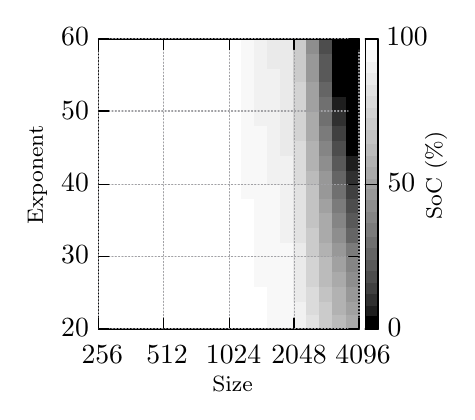
\begin{tikzpicture}[y=0.80pt, x=0.80pt, yscale=-0.600000, xscale=0.570000, inner sep=0pt, outer sep=0pt]
\begin{scope}[draw=black,line join=bevel,line cap=rect,even odd rule,line width=0.512pt]
  \begin{scope}[cm={{1.0,0.0,0.0,1.0,(0.0,0.0)}},draw=black,line join=bevel,line cap=rect,line width=0.512pt]
  \end{scope}
  \begin{scope}[cm={{1.00625,0.0,0.0,1.00625,(0.0,0.0)}},draw=black,line join=bevel,line cap=rect,line width=0.512pt]
  \end{scope}
  \begin{scope}[cm={{1.00625,0.0,0.0,1.00625,(0.0,0.0)}},draw=black,line join=bevel,line cap=rect,line width=0.512pt]
  \end{scope}
  \begin{scope}[cm={{1.00625,0.0,0.0,1.00625,(0.0,0.0)}},draw=black,line join=bevel,line cap=rect,line width=0.512pt]
  \end{scope}
  \begin{scope}[cm={{1.00625,0.0,0.0,1.00625,(0.0,0.0)}},draw=cffffff,fill=cffffff,line join=bevel,line cap=rect,line width=0.512pt]
    \path[draw,fill,even odd rule] (57.5000,268.5000) -- (57.5000,257.5000) --
      (67.5000,257.5000) -- (67.5000,268.5000) -- (57.5000,268.5000);
    \path[draw,fill,even odd rule] (67.5000,268.5000) -- (67.5000,257.5000) --
      (78.5000,257.5000) -- (78.5000,268.5000) -- (67.5000,268.5000);
    \path[draw,fill,even odd rule] (78.5000,268.5000) -- (78.5000,257.5000) --
      (88.5000,257.5000) -- (88.5000,268.5000) -- (78.5000,268.5000);
    \path[draw,fill,even odd rule] (88.5000,268.5000) -- (88.5000,257.5000) --
      (98.5000,257.5000) -- (98.5000,268.5000) -- (88.5000,268.5000);
    \path[draw,fill,even odd rule] (98.5000,268.5000) -- (98.5000,257.5000) --
      (108.5000,257.5000) -- (108.5000,268.5000) -- (98.5000,268.5000);
    \path[draw,fill,even odd rule] (57.5000,257.5000) -- (57.5000,247.5000) --
      (67.5000,247.5000) -- (67.5000,257.5000) -- (57.5000,257.5000);
    \path[draw,fill,even odd rule] (67.5000,257.5000) -- (67.5000,247.5000) --
      (78.5000,247.5000) -- (78.5000,257.5000) -- (67.5000,257.5000);
    \path[draw,fill,even odd rule] (78.5000,257.5000) -- (78.5000,247.5000) --
      (88.5000,247.5000) -- (88.5000,257.5000) -- (78.5000,257.5000);
    \path[draw,fill,even odd rule] (88.5000,257.5000) -- (88.5000,247.5000) --
      (98.5000,247.5000) -- (98.5000,257.5000) -- (88.5000,257.5000);
    \path[draw,fill,even odd rule] (98.5000,257.5000) -- (98.5000,247.5000) --
      (108.5000,247.5000) -- (108.5000,257.5000) -- (98.5000,257.5000);
    \path[draw,fill,even odd rule] (57.5000,247.5000) -- (57.5000,236.5000) --
      (67.5000,236.5000) -- (67.5000,247.5000) -- (57.5000,247.5000);
    \path[draw,fill,even odd rule] (67.5000,247.5000) -- (67.5000,236.5000) --
      (78.5000,236.5000) -- (78.5000,247.5000) -- (67.5000,247.5000);
    \path[draw,fill,even odd rule] (78.5000,247.5000) -- (78.5000,236.5000) --
      (88.5000,236.5000) -- (88.5000,247.5000) -- (78.5000,247.5000);
    \path[draw,fill,even odd rule] (88.5000,247.5000) -- (88.5000,236.5000) --
      (98.5000,236.5000) -- (98.5000,247.5000) -- (88.5000,247.5000);
    \path[draw,fill,even odd rule] (98.5000,247.5000) -- (98.5000,236.5000) --
      (108.5000,236.5000) -- (108.5000,247.5000) -- (98.5000,247.5000);
    \path[draw,fill,even odd rule] (57.5000,236.5000) -- (57.5000,225.5000) --
      (67.5000,225.5000) -- (67.5000,236.5000) -- (57.5000,236.5000);
    \path[draw,fill,even odd rule] (67.5000,236.5000) -- (67.5000,225.5000) --
      (78.5000,225.5000) -- (78.5000,236.5000) -- (67.5000,236.5000);
    \path[draw,fill,even odd rule] (78.5000,236.5000) -- (78.5000,225.5000) --
      (88.5000,225.5000) -- (88.5000,236.5000) -- (78.5000,236.5000);
    \path[draw,fill,even odd rule] (88.5000,236.5000) -- (88.5000,225.5000) --
      (98.5000,225.5000) -- (98.5000,236.5000) -- (88.5000,236.5000);
    \path[draw,fill,even odd rule] (98.5000,236.5000) -- (98.5000,225.5000) --
      (108.5000,225.5000) -- (108.5000,236.5000) -- (98.5000,236.5000);
    \path[draw,fill,even odd rule] (57.5000,225.5000) -- (57.5000,214.5000) --
      (67.5000,214.5000) -- (67.5000,225.5000) -- (57.5000,225.5000);
    \path[draw,fill,even odd rule] (67.5000,225.5000) -- (67.5000,214.5000) --
      (78.5000,214.5000) -- (78.5000,225.5000) -- (67.5000,225.5000);
    \path[draw,fill,even odd rule] (78.5000,225.5000) -- (78.5000,214.5000) --
      (88.5000,214.5000) -- (88.5000,225.5000) -- (78.5000,225.5000);
    \path[draw,fill,even odd rule] (88.5000,225.5000) -- (88.5000,214.5000) --
      (98.5000,214.5000) -- (98.5000,225.5000) -- (88.5000,225.5000);
    \path[draw,fill,even odd rule] (98.5000,225.5000) -- (98.5000,214.5000) --
      (108.5000,214.5000) -- (108.5000,225.5000) -- (98.5000,225.5000);
    \path[draw,fill,even odd rule] (57.5000,214.5000) -- (57.5000,203.5000) --
      (67.5000,203.5000) -- (67.5000,214.5000) -- (57.5000,214.5000);
    \path[draw,fill,even odd rule] (67.5000,214.5000) -- (67.5000,203.5000) --
      (78.5000,203.5000) -- (78.5000,214.5000) -- (67.5000,214.5000);
    \path[draw,fill,even odd rule] (78.5000,214.5000) -- (78.5000,203.5000) --
      (88.5000,203.5000) -- (88.5000,214.5000) -- (78.5000,214.5000);
    \path[draw,fill,even odd rule] (88.5000,214.5000) -- (88.5000,203.5000) --
      (98.5000,203.5000) -- (98.5000,214.5000) -- (88.5000,214.5000);
    \path[draw,fill,even odd rule] (98.5000,214.5000) -- (98.5000,203.5000) --
      (108.5000,203.5000) -- (108.5000,214.5000) -- (98.5000,214.5000);
    \path[draw,fill,even odd rule] (57.5000,203.5000) -- (57.5000,192.5000) --
      (67.5000,192.5000) -- (67.5000,203.5000) -- (57.5000,203.5000);
    \path[draw,fill,even odd rule] (67.5000,203.5000) -- (67.5000,192.5000) --
      (78.5000,192.5000) -- (78.5000,203.5000) -- (67.5000,203.5000);
    \path[draw,fill,even odd rule] (78.5000,203.5000) -- (78.5000,192.5000) --
      (88.5000,192.5000) -- (88.5000,203.5000) -- (78.5000,203.5000);
    \path[draw,fill,even odd rule] (88.5000,203.5000) -- (88.5000,192.5000) --
      (98.5000,192.5000) -- (98.5000,203.5000) -- (88.5000,203.5000);
    \path[draw,fill,even odd rule] (98.5000,203.5000) -- (98.5000,192.5000) --
      (108.5000,192.5000) -- (108.5000,203.5000) -- (98.5000,203.5000);
    \path[draw,fill,even odd rule] (57.5000,192.5000) -- (57.5000,181.5000) --
      (67.5000,181.5000) -- (67.5000,192.5000) -- (57.5000,192.5000);
    \path[draw,fill,even odd rule] (67.5000,192.5000) -- (67.5000,181.5000) --
      (78.5000,181.5000) -- (78.5000,192.5000) -- (67.5000,192.5000);
    \path[draw,fill,even odd rule] (78.5000,192.5000) -- (78.5000,181.5000) --
      (88.5000,181.5000) -- (88.5000,192.5000) -- (78.5000,192.5000);
    \path[draw,fill,even odd rule] (88.5000,192.5000) -- (88.5000,181.5000) --
      (98.5000,181.5000) -- (98.5000,192.5000) -- (88.5000,192.5000);
    \path[draw,fill,even odd rule] (98.5000,192.5000) -- (98.5000,181.5000) --
      (108.5000,181.5000) -- (108.5000,192.5000) -- (98.5000,192.5000);
    \path[draw,fill,even odd rule] (57.5000,181.5000) -- (57.5000,170.5000) --
      (67.5000,170.5000) -- (67.5000,181.5000) -- (57.5000,181.5000);
    \path[draw,fill,even odd rule] (67.5000,181.5000) -- (67.5000,170.5000) --
      (78.5000,170.5000) -- (78.5000,181.5000) -- (67.5000,181.5000);
    \path[draw,fill,even odd rule] (78.5000,181.5000) -- (78.5000,170.5000) --
      (88.5000,170.5000) -- (88.5000,181.5000) -- (78.5000,181.5000);
    \path[draw,fill,even odd rule] (88.5000,181.5000) -- (88.5000,170.5000) --
      (98.5000,170.5000) -- (98.5000,181.5000) -- (88.5000,181.5000);
    \path[draw,fill,even odd rule] (98.5000,181.5000) -- (98.5000,170.5000) --
      (108.5000,170.5000) -- (108.5000,181.5000) -- (98.5000,181.5000);
    \path[draw,fill,even odd rule] (57.5000,170.5000) -- (57.5000,160.5000) --
      (67.5000,160.5000) -- (67.5000,170.5000) -- (57.5000,170.5000);
    \path[draw,fill,even odd rule] (67.5000,170.5000) -- (67.5000,160.5000) --
      (78.5000,160.5000) -- (78.5000,170.5000) -- (67.5000,170.5000);
    \path[draw,fill,even odd rule] (78.5000,170.5000) -- (78.5000,160.5000) --
      (88.5000,160.5000) -- (88.5000,170.5000) -- (78.5000,170.5000);
    \path[draw,fill,even odd rule] (88.5000,170.5000) -- (88.5000,160.5000) --
      (98.5000,160.5000) -- (98.5000,170.5000) -- (88.5000,170.5000);
    \path[draw,fill,even odd rule] (98.5000,170.5000) -- (98.5000,160.5000) --
      (108.5000,160.5000) -- (108.5000,170.5000) -- (98.5000,170.5000);
    \path[draw,fill,even odd rule] (57.5000,160.5000) -- (57.5000,149.5000) --
      (67.5000,149.5000) -- (67.5000,160.5000) -- (57.5000,160.5000);
    \path[draw,fill,even odd rule] (67.5000,160.5000) -- (67.5000,149.5000) --
      (78.5000,149.5000) -- (78.5000,160.5000) -- (67.5000,160.5000);
    \path[draw,fill,even odd rule] (78.5000,160.5000) -- (78.5000,149.5000) --
      (88.5000,149.5000) -- (88.5000,160.5000) -- (78.5000,160.5000);
    \path[draw,fill,even odd rule] (88.5000,160.5000) -- (88.5000,149.5000) --
      (98.5000,149.5000) -- (98.5000,160.5000) -- (88.5000,160.5000);
    \path[draw,fill,even odd rule] (98.5000,160.5000) -- (98.5000,149.5000) --
      (108.5000,149.5000) -- (108.5000,160.5000) -- (98.5000,160.5000);
    \path[draw,fill,even odd rule] (57.5000,149.5000) -- (57.5000,138.5000) --
      (67.5000,138.5000) -- (67.5000,149.5000) -- (57.5000,149.5000);
    \path[draw,fill,even odd rule] (67.5000,149.5000) -- (67.5000,138.5000) --
      (78.5000,138.5000) -- (78.5000,149.5000) -- (67.5000,149.5000);
    \path[draw,fill,even odd rule] (78.5000,149.5000) -- (78.5000,138.5000) --
      (88.5000,138.5000) -- (88.5000,149.5000) -- (78.5000,149.5000);
    \path[draw,fill,even odd rule] (88.5000,149.5000) -- (88.5000,138.5000) --
      (98.5000,138.5000) -- (98.5000,149.5000) -- (88.5000,149.5000);
    \path[draw,fill,even odd rule] (98.5000,149.5000) -- (98.5000,138.5000) --
      (108.5000,138.5000) -- (108.5000,149.5000) -- (98.5000,149.5000);
    \path[draw,fill,even odd rule] (57.5000,138.5000) -- (57.5000,127.5000) --
      (67.5000,127.5000) -- (67.5000,138.5000) -- (57.5000,138.5000);
    \path[draw,fill,even odd rule] (67.5000,138.5000) -- (67.5000,127.5000) --
      (78.5000,127.5000) -- (78.5000,138.5000) -- (67.5000,138.5000);
    \path[draw,fill,even odd rule] (78.5000,138.5000) -- (78.5000,127.5000) --
      (88.5000,127.5000) -- (88.5000,138.5000) -- (78.5000,138.5000);
    \path[draw,fill,even odd rule] (88.5000,138.5000) -- (88.5000,127.5000) --
      (98.5000,127.5000) -- (98.5000,138.5000) -- (88.5000,138.5000);
    \path[draw,fill,even odd rule] (98.5000,138.5000) -- (98.5000,127.5000) --
      (108.5000,127.5000) -- (108.5000,138.5000) -- (98.5000,138.5000);
    \path[draw,fill,even odd rule] (57.5000,127.5000) -- (57.5000,116.5000) --
      (67.5000,116.5000) -- (67.5000,127.5000) -- (57.5000,127.5000);
    \path[draw,fill,even odd rule] (67.5000,127.5000) -- (67.5000,116.5000) --
      (78.5000,116.5000) -- (78.5000,127.5000) -- (67.5000,127.5000);
    \path[draw,fill,even odd rule] (78.5000,127.5000) -- (78.5000,116.5000) --
      (88.5000,116.5000) -- (88.5000,127.5000) -- (78.5000,127.5000);
    \path[draw,fill,even odd rule] (88.5000,127.5000) -- (88.5000,116.5000) --
      (98.5000,116.5000) -- (98.5000,127.5000) -- (88.5000,127.5000);
    \path[draw,fill,even odd rule] (98.5000,127.5000) -- (98.5000,116.5000) --
      (108.5000,116.5000) -- (108.5000,127.5000) -- (98.5000,127.5000);
    \path[draw,fill,even odd rule] (57.5000,116.5000) -- (57.5000,105.5000) --
      (67.5000,105.5000) -- (67.5000,116.5000) -- (57.5000,116.5000);
    \path[draw,fill,even odd rule] (67.5000,116.5000) -- (67.5000,105.5000) --
      (78.5000,105.5000) -- (78.5000,116.5000) -- (67.5000,116.5000);
    \path[draw,fill,even odd rule] (78.5000,116.5000) -- (78.5000,105.5000) --
      (88.5000,105.5000) -- (88.5000,116.5000) -- (78.5000,116.5000);
    \path[draw,fill,even odd rule] (88.5000,116.5000) -- (88.5000,105.5000) --
      (98.5000,105.5000) -- (98.5000,116.5000) -- (88.5000,116.5000);
    \path[draw,fill,even odd rule] (98.5000,116.5000) -- (98.5000,105.5000) --
      (108.5000,105.5000) -- (108.5000,116.5000) -- (98.5000,116.5000);
    \path[draw,fill,even odd rule] (57.5000,105.5000) -- (57.5000,94.5000) --
      (67.5000,94.5000) -- (67.5000,105.5000) -- (57.5000,105.5000);
    \path[draw,fill,even odd rule] (67.5000,105.5000) -- (67.5000,94.5000) --
      (78.5000,94.5000) -- (78.5000,105.5000) -- (67.5000,105.5000);
    \path[draw,fill,even odd rule] (78.5000,105.5000) -- (78.5000,94.5000) --
      (88.5000,94.5000) -- (88.5000,105.5000) -- (78.5000,105.5000);
    \path[draw,fill,even odd rule] (88.5000,105.5000) -- (88.5000,94.5000) --
      (98.5000,94.5000) -- (98.5000,105.5000) -- (88.5000,105.5000);
    \path[draw,fill,even odd rule] (98.5000,105.5000) -- (98.5000,94.5000) --
      (108.5000,94.5000) -- (108.5000,105.5000) -- (98.5000,105.5000);
    \path[draw,fill,even odd rule] (57.5000,94.5000) -- (57.5000,83.5000) --
      (67.5000,83.5000) -- (67.5000,94.5000) -- (57.5000,94.5000);
    \path[draw,fill,even odd rule] (67.5000,94.5000) -- (67.5000,83.5000) --
      (78.5000,83.5000) -- (78.5000,94.5000) -- (67.5000,94.5000);
    \path[draw,fill,even odd rule] (78.5000,94.5000) -- (78.5000,83.5000) --
      (88.5000,83.5000) -- (88.5000,94.5000) -- (78.5000,94.5000);
    \path[draw,fill,even odd rule] (88.5000,94.5000) -- (88.5000,83.5000) --
      (98.5000,83.5000) -- (98.5000,94.5000) -- (88.5000,94.5000);
    \path[draw,fill,even odd rule] (98.5000,94.5000) -- (98.5000,83.5000) --
      (108.5000,83.5000) -- (108.5000,94.5000) -- (98.5000,94.5000);
    \path[draw,fill,even odd rule] (57.5000,83.5000) -- (57.5000,73.5000) --
      (67.5000,73.5000) -- (67.5000,83.5000) -- (57.5000,83.5000);
    \path[draw,fill,even odd rule] (67.5000,83.5000) -- (67.5000,73.5000) --
      (78.5000,73.5000) -- (78.5000,83.5000) -- (67.5000,83.5000);
    \path[draw,fill,even odd rule] (78.5000,83.5000) -- (78.5000,73.5000) --
      (88.5000,73.5000) -- (88.5000,83.5000) -- (78.5000,83.5000);
    \path[draw,fill,even odd rule] (88.5000,83.5000) -- (88.5000,73.5000) --
      (98.5000,73.5000) -- (98.5000,83.5000) -- (88.5000,83.5000);
    \path[draw,fill,even odd rule] (98.5000,83.5000) -- (98.5000,73.5000) --
      (108.5000,73.5000) -- (108.5000,83.5000) -- (98.5000,83.5000);
    \path[draw,fill,even odd rule] (57.5000,73.5000) -- (57.5000,62.5000) --
      (67.5000,62.5000) -- (67.5000,73.5000) -- (57.5000,73.5000);
    \path[draw,fill,even odd rule] (67.5000,73.5000) -- (67.5000,62.5000) --
      (78.5000,62.5000) -- (78.5000,73.5000) -- (67.5000,73.5000);
    \path[draw,fill,even odd rule] (78.5000,73.5000) -- (78.5000,62.5000) --
      (88.5000,62.5000) -- (88.5000,73.5000) -- (78.5000,73.5000);
    \path[draw,fill,even odd rule] (88.5000,73.5000) -- (88.5000,62.5000) --
      (98.5000,62.5000) -- (98.5000,73.5000) -- (88.5000,73.5000);
    \path[draw,fill,even odd rule] (98.5000,73.5000) -- (98.5000,62.5000) --
      (108.5000,62.5000) -- (108.5000,73.5000) -- (98.5000,73.5000);
    \path[draw,fill,even odd rule] (57.5000,62.5000) -- (57.5000,51.5000) --
      (67.5000,51.5000) -- (67.5000,62.5000) -- (57.5000,62.5000);
    \path[draw,fill,even odd rule] (67.5000,62.5000) -- (67.5000,51.5000) --
      (78.5000,51.5000) -- (78.5000,62.5000) -- (67.5000,62.5000);
    \path[draw,fill,even odd rule] (78.5000,62.5000) -- (78.5000,51.5000) --
      (88.5000,51.5000) -- (88.5000,62.5000) -- (78.5000,62.5000);
    \path[draw,fill,even odd rule] (88.5000,62.5000) -- (88.5000,51.5000) --
      (98.5000,51.5000) -- (98.5000,62.5000) -- (88.5000,62.5000);
    \path[draw,fill,even odd rule] (98.5000,62.5000) -- (98.5000,51.5000) --
      (108.5000,51.5000) -- (108.5000,62.5000) -- (98.5000,62.5000);
    \path[draw,fill,even odd rule] (108.5000,268.5000) -- (108.5000,257.5000) --
      (119.5000,257.5000) -- (119.5000,268.5000) -- (108.5000,268.5000);
    \path[draw,fill,even odd rule] (119.5000,268.5000) -- (119.5000,257.5000) --
      (129.5000,257.5000) -- (129.5000,268.5000) -- (119.5000,268.5000);
    \path[draw,fill,even odd rule] (129.5000,268.5000) -- (129.5000,257.5000) --
      (139.5000,257.5000) -- (139.5000,268.5000) -- (129.5000,268.5000);
    \path[draw,fill,even odd rule] (139.5000,268.5000) -- (139.5000,257.5000) --
      (149.5000,257.5000) -- (149.5000,268.5000) -- (139.5000,268.5000);
    \path[draw,fill,even odd rule] (149.5000,268.5000) -- (149.5000,257.5000) --
      (160.5000,257.5000) -- (160.5000,268.5000) -- (149.5000,268.5000);
    \path[draw,fill,even odd rule] (108.5000,257.5000) -- (108.5000,247.5000) --
      (119.5000,247.5000) -- (119.5000,257.5000) -- (108.5000,257.5000);
    \path[draw,fill,even odd rule] (119.5000,257.5000) -- (119.5000,247.5000) --
      (129.5000,247.5000) -- (129.5000,257.5000) -- (119.5000,257.5000);
    \path[draw,fill,even odd rule] (129.5000,257.5000) -- (129.5000,247.5000) --
      (139.5000,247.5000) -- (139.5000,257.5000) -- (129.5000,257.5000);
    \path[draw,fill,even odd rule] (139.5000,257.5000) -- (139.5000,247.5000) --
      (149.5000,247.5000) -- (149.5000,257.5000) -- (139.5000,257.5000);
    \path[draw,fill,even odd rule] (149.5000,257.5000) -- (149.5000,247.5000) --
      (160.5000,247.5000) -- (160.5000,257.5000) -- (149.5000,257.5000);
    \path[draw,fill,even odd rule] (108.5000,247.5000) -- (108.5000,236.5000) --
      (119.5000,236.5000) -- (119.5000,247.5000) -- (108.5000,247.5000);
    \path[draw,fill,even odd rule] (119.5000,247.5000) -- (119.5000,236.5000) --
      (129.5000,236.5000) -- (129.5000,247.5000) -- (119.5000,247.5000);
    \path[draw,fill,even odd rule] (129.5000,247.5000) -- (129.5000,236.5000) --
      (139.5000,236.5000) -- (139.5000,247.5000) -- (129.5000,247.5000);
    \path[draw,fill,even odd rule] (139.5000,247.5000) -- (139.5000,236.5000) --
      (149.5000,236.5000) -- (149.5000,247.5000) -- (139.5000,247.5000);
    \path[draw,fill,even odd rule] (149.5000,247.5000) -- (149.5000,236.5000) --
      (160.5000,236.5000) -- (160.5000,247.5000) -- (149.5000,247.5000);
    \path[draw,fill,even odd rule] (108.5000,236.5000) -- (108.5000,225.5000) --
      (119.5000,225.5000) -- (119.5000,236.5000) -- (108.5000,236.5000);
    \path[draw,fill,even odd rule] (119.5000,236.5000) -- (119.5000,225.5000) --
      (129.5000,225.5000) -- (129.5000,236.5000) -- (119.5000,236.5000);
    \path[draw,fill,even odd rule] (129.5000,236.5000) -- (129.5000,225.5000) --
      (139.5000,225.5000) -- (139.5000,236.5000) -- (129.5000,236.5000);
    \path[draw,fill,even odd rule] (139.5000,236.5000) -- (139.5000,225.5000) --
      (149.5000,225.5000) -- (149.5000,236.5000) -- (139.5000,236.5000);
    \path[draw,fill,even odd rule] (149.5000,236.5000) -- (149.5000,225.5000) --
      (160.5000,225.5000) -- (160.5000,236.5000) -- (149.5000,236.5000);
    \path[draw,fill,even odd rule] (108.5000,225.5000) -- (108.5000,214.5000) --
      (119.5000,214.5000) -- (119.5000,225.5000) -- (108.5000,225.5000);
    \path[draw,fill,even odd rule] (119.5000,225.5000) -- (119.5000,214.5000) --
      (129.5000,214.5000) -- (129.5000,225.5000) -- (119.5000,225.5000);
    \path[draw,fill,even odd rule] (129.5000,225.5000) -- (129.5000,214.5000) --
      (139.5000,214.5000) -- (139.5000,225.5000) -- (129.5000,225.5000);
    \path[draw,fill,even odd rule] (139.5000,225.5000) -- (139.5000,214.5000) --
      (149.5000,214.5000) -- (149.5000,225.5000) -- (139.5000,225.5000);
    \path[draw,fill,even odd rule] (149.5000,225.5000) -- (149.5000,214.5000) --
      (160.5000,214.5000) -- (160.5000,225.5000) -- (149.5000,225.5000);
    \path[draw,fill,even odd rule] (108.5000,214.5000) -- (108.5000,203.5000) --
      (119.5000,203.5000) -- (119.5000,214.5000) -- (108.5000,214.5000);
    \path[draw,fill,even odd rule] (119.5000,214.5000) -- (119.5000,203.5000) --
      (129.5000,203.5000) -- (129.5000,214.5000) -- (119.5000,214.5000);
    \path[draw,fill,even odd rule] (129.5000,214.5000) -- (129.5000,203.5000) --
      (139.5000,203.5000) -- (139.5000,214.5000) -- (129.5000,214.5000);
    \path[draw,fill,even odd rule] (139.5000,214.5000) -- (139.5000,203.5000) --
      (149.5000,203.5000) -- (149.5000,214.5000) -- (139.5000,214.5000);
    \path[draw,fill,even odd rule] (149.5000,214.5000) -- (149.5000,203.5000) --
      (160.5000,203.5000) -- (160.5000,214.5000) -- (149.5000,214.5000);
    \path[draw,fill,even odd rule] (108.5000,203.5000) -- (108.5000,192.5000) --
      (119.5000,192.5000) -- (119.5000,203.5000) -- (108.5000,203.5000);
    \path[draw,fill,even odd rule] (119.5000,203.5000) -- (119.5000,192.5000) --
      (129.5000,192.5000) -- (129.5000,203.5000) -- (119.5000,203.5000);
    \path[draw,fill,even odd rule] (129.5000,203.5000) -- (129.5000,192.5000) --
      (139.5000,192.5000) -- (139.5000,203.5000) -- (129.5000,203.5000);
    \path[draw,fill,even odd rule] (139.5000,203.5000) -- (139.5000,192.5000) --
      (149.5000,192.5000) -- (149.5000,203.5000) -- (139.5000,203.5000);
    \path[draw,fill,even odd rule] (149.5000,203.5000) -- (149.5000,192.5000) --
      (160.5000,192.5000) -- (160.5000,203.5000) -- (149.5000,203.5000);
    \path[draw,fill,even odd rule] (108.5000,192.5000) -- (108.5000,181.5000) --
      (119.5000,181.5000) -- (119.5000,192.5000) -- (108.5000,192.5000);
    \path[draw,fill,even odd rule] (119.5000,192.5000) -- (119.5000,181.5000) --
      (129.5000,181.5000) -- (129.5000,192.5000) -- (119.5000,192.5000);
    \path[draw,fill,even odd rule] (129.5000,192.5000) -- (129.5000,181.5000) --
      (139.5000,181.5000) -- (139.5000,192.5000) -- (129.5000,192.5000);
    \path[draw,fill,even odd rule] (139.5000,192.5000) -- (139.5000,181.5000) --
      (149.5000,181.5000) -- (149.5000,192.5000) -- (139.5000,192.5000);
    \path[draw,fill,even odd rule] (149.5000,192.5000) -- (149.5000,181.5000) --
      (160.5000,181.5000) -- (160.5000,192.5000) -- (149.5000,192.5000);
    \path[draw,fill,even odd rule] (108.5000,181.5000) -- (108.5000,170.5000) --
      (119.5000,170.5000) -- (119.5000,181.5000) -- (108.5000,181.5000);
    \path[draw,fill,even odd rule] (119.5000,181.5000) -- (119.5000,170.5000) --
      (129.5000,170.5000) -- (129.5000,181.5000) -- (119.5000,181.5000);
    \path[draw,fill,even odd rule] (129.5000,181.5000) -- (129.5000,170.5000) --
      (139.5000,170.5000) -- (139.5000,181.5000) -- (129.5000,181.5000);
    \path[draw,fill,even odd rule] (139.5000,181.5000) -- (139.5000,170.5000) --
      (149.5000,170.5000) -- (149.5000,181.5000) -- (139.5000,181.5000);
    \path[draw,fill,even odd rule] (149.5000,181.5000) -- (149.5000,170.5000) --
      (160.5000,170.5000) -- (160.5000,181.5000) -- (149.5000,181.5000);
    \path[draw,fill,even odd rule] (108.5000,170.5000) -- (108.5000,160.5000) --
      (119.5000,160.5000) -- (119.5000,170.5000) -- (108.5000,170.5000);
    \path[draw,fill,even odd rule] (119.5000,170.5000) -- (119.5000,160.5000) --
      (129.5000,160.5000) -- (129.5000,170.5000) -- (119.5000,170.5000);
    \path[draw,fill,even odd rule] (129.5000,170.5000) -- (129.5000,160.5000) --
      (139.5000,160.5000) -- (139.5000,170.5000) -- (129.5000,170.5000);
    \path[draw,fill,even odd rule] (139.5000,170.5000) -- (139.5000,160.5000) --
      (149.5000,160.5000) -- (149.5000,170.5000) -- (139.5000,170.5000);
    \path[draw,fill,even odd rule] (149.5000,170.5000) -- (149.5000,160.5000) --
      (160.5000,160.5000) -- (160.5000,170.5000) -- (149.5000,170.5000);
    \path[draw,fill,even odd rule] (108.5000,160.5000) -- (108.5000,149.5000) --
      (119.5000,149.5000) -- (119.5000,160.5000) -- (108.5000,160.5000);
    \path[draw,fill,even odd rule] (119.5000,160.5000) -- (119.5000,149.5000) --
      (129.5000,149.5000) -- (129.5000,160.5000) -- (119.5000,160.5000);
    \path[draw,fill,even odd rule] (129.5000,160.5000) -- (129.5000,149.5000) --
      (139.5000,149.5000) -- (139.5000,160.5000) -- (129.5000,160.5000);
    \path[draw,fill,even odd rule] (139.5000,160.5000) -- (139.5000,149.5000) --
      (149.5000,149.5000) -- (149.5000,160.5000) -- (139.5000,160.5000);
    \path[draw,fill,even odd rule] (149.5000,160.5000) -- (149.5000,149.5000) --
      (160.5000,149.5000) -- (160.5000,160.5000) -- (149.5000,160.5000);
    \path[draw,fill,even odd rule] (108.5000,149.5000) -- (108.5000,138.5000) --
      (119.5000,138.5000) -- (119.5000,149.5000) -- (108.5000,149.5000);
    \path[draw,fill,even odd rule] (119.5000,149.5000) -- (119.5000,138.5000) --
      (129.5000,138.5000) -- (129.5000,149.5000) -- (119.5000,149.5000);
    \path[draw,fill,even odd rule] (129.5000,149.5000) -- (129.5000,138.5000) --
      (139.5000,138.5000) -- (139.5000,149.5000) -- (129.5000,149.5000);
    \path[draw,fill,even odd rule] (139.5000,149.5000) -- (139.5000,138.5000) --
      (149.5000,138.5000) -- (149.5000,149.5000) -- (139.5000,149.5000);
    \path[draw,fill,even odd rule] (149.5000,149.5000) -- (149.5000,138.5000) --
      (160.5000,138.5000) -- (160.5000,149.5000) -- (149.5000,149.5000);
    \path[draw,fill,even odd rule] (108.5000,138.5000) -- (108.5000,127.5000) --
      (119.5000,127.5000) -- (119.5000,138.5000) -- (108.5000,138.5000);
    \path[draw,fill,even odd rule] (119.5000,138.5000) -- (119.5000,127.5000) --
      (129.5000,127.5000) -- (129.5000,138.5000) -- (119.5000,138.5000);
    \path[draw,fill,even odd rule] (129.5000,138.5000) -- (129.5000,127.5000) --
      (139.5000,127.5000) -- (139.5000,138.5000) -- (129.5000,138.5000);
    \path[draw,fill,even odd rule] (139.5000,138.5000) -- (139.5000,127.5000) --
      (149.5000,127.5000) -- (149.5000,138.5000) -- (139.5000,138.5000);
    \path[draw,fill,even odd rule] (149.5000,138.5000) -- (149.5000,127.5000) --
      (160.5000,127.5000) -- (160.5000,138.5000) -- (149.5000,138.5000);
    \path[draw,fill,even odd rule] (108.5000,127.5000) -- (108.5000,116.5000) --
      (119.5000,116.5000) -- (119.5000,127.5000) -- (108.5000,127.5000);
    \path[draw,fill,even odd rule] (119.5000,127.5000) -- (119.5000,116.5000) --
      (129.5000,116.5000) -- (129.5000,127.5000) -- (119.5000,127.5000);
    \path[draw,fill,even odd rule] (129.5000,127.5000) -- (129.5000,116.5000) --
      (139.5000,116.5000) -- (139.5000,127.5000) -- (129.5000,127.5000);
    \path[draw,fill,even odd rule] (139.5000,127.5000) -- (139.5000,116.5000) --
      (149.5000,116.5000) -- (149.5000,127.5000) -- (139.5000,127.5000);
    \path[draw,fill,even odd rule] (149.5000,127.5000) -- (149.5000,116.5000) --
      (160.5000,116.5000) -- (160.5000,127.5000) -- (149.5000,127.5000);
    \path[draw,fill,even odd rule] (108.5000,116.5000) -- (108.5000,105.5000) --
      (119.5000,105.5000) -- (119.5000,116.5000) -- (108.5000,116.5000);
    \path[draw,fill,even odd rule] (119.5000,116.5000) -- (119.5000,105.5000) --
      (129.5000,105.5000) -- (129.5000,116.5000) -- (119.5000,116.5000);
    \path[draw,fill,even odd rule] (129.5000,116.5000) -- (129.5000,105.5000) --
      (139.5000,105.5000) -- (139.5000,116.5000) -- (129.5000,116.5000);
    \path[draw,fill,even odd rule] (139.5000,116.5000) -- (139.5000,105.5000) --
      (149.5000,105.5000) -- (149.5000,116.5000) -- (139.5000,116.5000);
    \path[draw,fill,even odd rule] (149.5000,116.5000) -- (149.5000,105.5000) --
      (160.5000,105.5000) -- (160.5000,116.5000) -- (149.5000,116.5000);
    \path[draw,fill,even odd rule] (108.5000,105.5000) -- (108.5000,94.5000) --
      (119.5000,94.5000) -- (119.5000,105.5000) -- (108.5000,105.5000);
    \path[draw,fill,even odd rule] (119.5000,105.5000) -- (119.5000,94.5000) --
      (129.5000,94.5000) -- (129.5000,105.5000) -- (119.5000,105.5000);
    \path[draw,fill,even odd rule] (129.5000,105.5000) -- (129.5000,94.5000) --
      (139.5000,94.5000) -- (139.5000,105.5000) -- (129.5000,105.5000);
    \path[draw,fill,even odd rule] (139.5000,105.5000) -- (139.5000,94.5000) --
      (149.5000,94.5000) -- (149.5000,105.5000) -- (139.5000,105.5000);
    \path[draw,fill,even odd rule] (149.5000,105.5000) -- (149.5000,94.5000) --
      (160.5000,94.5000) -- (160.5000,105.5000) -- (149.5000,105.5000);
    \path[draw,fill,even odd rule] (108.5000,94.5000) -- (108.5000,83.5000) --
      (119.5000,83.5000) -- (119.5000,94.5000) -- (108.5000,94.5000);
    \path[draw,fill,even odd rule] (119.5000,94.5000) -- (119.5000,83.5000) --
      (129.5000,83.5000) -- (129.5000,94.5000) -- (119.5000,94.5000);
    \path[draw,fill,even odd rule] (129.5000,94.5000) -- (129.5000,83.5000) --
      (139.5000,83.5000) -- (139.5000,94.5000) -- (129.5000,94.5000);
    \path[draw,fill,even odd rule] (139.5000,94.5000) -- (139.5000,83.5000) --
      (149.5000,83.5000) -- (149.5000,94.5000) -- (139.5000,94.5000);
    \path[draw,fill,even odd rule] (149.5000,94.5000) -- (149.5000,83.5000) --
      (160.5000,83.5000) -- (160.5000,94.5000) -- (149.5000,94.5000);
    \path[draw,fill,even odd rule] (108.5000,83.5000) -- (108.5000,73.5000) --
      (119.5000,73.5000) -- (119.5000,83.5000) -- (108.5000,83.5000);
    \path[draw,fill,even odd rule] (119.5000,83.5000) -- (119.5000,73.5000) --
      (129.5000,73.5000) -- (129.5000,83.5000) -- (119.5000,83.5000);
    \path[draw,fill,even odd rule] (129.5000,83.5000) -- (129.5000,73.5000) --
      (139.5000,73.5000) -- (139.5000,83.5000) -- (129.5000,83.5000);
    \path[draw,fill,even odd rule] (139.5000,83.5000) -- (139.5000,73.5000) --
      (149.5000,73.5000) -- (149.5000,83.5000) -- (139.5000,83.5000);
    \path[draw,fill,even odd rule] (149.5000,83.5000) -- (149.5000,73.5000) --
      (160.5000,73.5000) -- (160.5000,83.5000) -- (149.5000,83.5000);
    \path[draw,fill,even odd rule] (108.5000,73.5000) -- (108.5000,62.5000) --
      (119.5000,62.5000) -- (119.5000,73.5000) -- (108.5000,73.5000);
    \path[draw,fill,even odd rule] (119.5000,73.5000) -- (119.5000,62.5000) --
      (129.5000,62.5000) -- (129.5000,73.5000) -- (119.5000,73.5000);
    \path[draw,fill,even odd rule] (129.5000,73.5000) -- (129.5000,62.5000) --
      (139.5000,62.5000) -- (139.5000,73.5000) -- (129.5000,73.5000);
    \path[draw,fill,even odd rule] (139.5000,73.5000) -- (139.5000,62.5000) --
      (149.5000,62.5000) -- (149.5000,73.5000) -- (139.5000,73.5000);
    \path[draw,fill,even odd rule] (149.5000,73.5000) -- (149.5000,62.5000) --
      (160.5000,62.5000) -- (160.5000,73.5000) -- (149.5000,73.5000);
    \path[draw,fill,even odd rule] (108.5000,62.5000) -- (108.5000,51.5000) --
      (119.5000,51.5000) -- (119.5000,62.5000) -- (108.5000,62.5000);
    \path[draw,fill,even odd rule] (119.5000,62.5000) -- (119.5000,51.5000) --
      (129.5000,51.5000) -- (129.5000,62.5000) -- (119.5000,62.5000);
    \path[draw,fill,even odd rule] (129.5000,62.5000) -- (129.5000,51.5000) --
      (139.5000,51.5000) -- (139.5000,62.5000) -- (129.5000,62.5000);
    \path[draw,fill,even odd rule] (139.5000,62.5000) -- (139.5000,51.5000) --
      (149.5000,51.5000) -- (149.5000,62.5000) -- (139.5000,62.5000);
    \path[draw,fill,even odd rule] (149.5000,62.5000) -- (149.5000,51.5000) --
      (160.5000,51.5000) -- (160.5000,62.5000) -- (149.5000,62.5000);
    \path[draw,fill,even odd rule] (160.5000,268.5000) -- (160.5000,257.5000) --
      (170.5000,257.5000) -- (170.5000,268.5000) -- (160.5000,268.5000);
    \path[draw,fill,even odd rule] (170.5000,268.5000) -- (170.5000,257.5000) --
      (180.5000,257.5000) -- (180.5000,268.5000) -- (170.5000,268.5000);
    \path[draw,fill,even odd rule] (180.5000,268.5000) -- (180.5000,257.5000) --
      (190.5000,257.5000) -- (190.5000,268.5000) -- (180.5000,268.5000);
  \end{scope}
  \begin{scope}[cm={{1.00625,0.0,0.0,1.00625,(0.0,0.0)}},draw=cf8f8f8,fill=cf8f8f8,line join=bevel,line cap=rect,line width=0.512pt]
    \path[draw,fill,even odd rule] (190.5000,268.5000) -- (190.5000,257.5000) --
      (200.5000,257.5000) -- (200.5000,268.5000) -- (190.5000,268.5000);
    \path[draw,fill,even odd rule] (200.5000,268.5000) -- (200.5000,257.5000) --
      (211.5000,257.5000) -- (211.5000,268.5000) -- (200.5000,268.5000);
  \end{scope}
  \begin{scope}[cm={{1.00625,0.0,0.0,1.00625,(0.0,0.0)}},draw=cffffff,fill=cffffff,line join=bevel,line cap=rect,line width=0.512pt]
    \path[draw,fill,even odd rule] (160.5000,257.5000) -- (160.5000,247.5000) --
      (170.5000,247.5000) -- (170.5000,257.5000) -- (160.5000,257.5000);
    \path[draw,fill,even odd rule] (170.5000,257.5000) -- (170.5000,247.5000) --
      (180.5000,247.5000) -- (180.5000,257.5000) -- (170.5000,257.5000);
    \path[draw,fill,even odd rule] (180.5000,257.5000) -- (180.5000,247.5000) --
      (190.5000,247.5000) -- (190.5000,257.5000) -- (180.5000,257.5000);
  \end{scope}
  \begin{scope}[cm={{1.00625,0.0,0.0,1.00625,(0.0,0.0)}},draw=cf8f8f8,fill=cf8f8f8,line join=bevel,line cap=rect,line width=0.512pt]
    \path[draw,fill,even odd rule] (190.5000,257.5000) -- (190.5000,247.5000) --
      (200.5000,247.5000) -- (200.5000,257.5000) -- (190.5000,257.5000);
    \path[draw,fill,even odd rule] (200.5000,257.5000) -- (200.5000,247.5000) --
      (211.5000,247.5000) -- (211.5000,257.5000) -- (200.5000,257.5000);
  \end{scope}
  \begin{scope}[cm={{1.00625,0.0,0.0,1.00625,(0.0,0.0)}},draw=cffffff,fill=cffffff,line join=bevel,line cap=rect,line width=0.512pt]
    \path[draw,fill,even odd rule] (160.5000,247.5000) -- (160.5000,236.5000) --
      (170.5000,236.5000) -- (170.5000,247.5000) -- (160.5000,247.5000);
    \path[draw,fill,even odd rule] (170.5000,247.5000) -- (170.5000,236.5000) --
      (180.5000,236.5000) -- (180.5000,247.5000) -- (170.5000,247.5000);
    \path[draw,fill,even odd rule] (180.5000,247.5000) -- (180.5000,236.5000) --
      (190.5000,236.5000) -- (190.5000,247.5000) -- (180.5000,247.5000);
  \end{scope}
  \begin{scope}[cm={{1.00625,0.0,0.0,1.00625,(0.0,0.0)}},draw=cf8f8f8,fill=cf8f8f8,line join=bevel,line cap=rect,line width=0.512pt]
    \path[draw,fill,even odd rule] (190.5000,247.5000) -- (190.5000,236.5000) --
      (200.5000,236.5000) -- (200.5000,247.5000) -- (190.5000,247.5000);
    \path[draw,fill,even odd rule] (200.5000,247.5000) -- (200.5000,236.5000) --
      (211.5000,236.5000) -- (211.5000,247.5000) -- (200.5000,247.5000);
  \end{scope}
  \begin{scope}[cm={{1.00625,0.0,0.0,1.00625,(0.0,0.0)}},draw=cffffff,fill=cffffff,line join=bevel,line cap=rect,line width=0.512pt]
    \path[draw,fill,even odd rule] (160.5000,236.5000) -- (160.5000,225.5000) --
      (170.5000,225.5000) -- (170.5000,236.5000) -- (160.5000,236.5000);
    \path[draw,fill,even odd rule] (170.5000,236.5000) -- (170.5000,225.5000) --
      (180.5000,225.5000) -- (180.5000,236.5000) -- (170.5000,236.5000);
  \end{scope}
  \begin{scope}[cm={{1.00625,0.0,0.0,1.00625,(0.0,0.0)}},draw=cf8f8f8,fill=cf8f8f8,line join=bevel,line cap=rect,line width=0.512pt]
    \path[draw,fill,even odd rule] (180.5000,236.5000) -- (180.5000,225.5000) --
      (190.5000,225.5000) -- (190.5000,236.5000) -- (180.5000,236.5000);
    \path[draw,fill,even odd rule] (190.5000,236.5000) -- (190.5000,225.5000) --
      (200.5000,225.5000) -- (200.5000,236.5000) -- (190.5000,236.5000);
    \path[draw,fill,even odd rule] (200.5000,236.5000) -- (200.5000,225.5000) --
      (211.5000,225.5000) -- (211.5000,236.5000) -- (200.5000,236.5000);
  \end{scope}
  \begin{scope}[cm={{1.00625,0.0,0.0,1.00625,(0.0,0.0)}},draw=cffffff,fill=cffffff,line join=bevel,line cap=rect,line width=0.512pt]
    \path[draw,fill,even odd rule] (160.5000,225.5000) -- (160.5000,214.5000) --
      (170.5000,214.5000) -- (170.5000,225.5000) -- (160.5000,225.5000);
    \path[draw,fill,even odd rule] (170.5000,225.5000) -- (170.5000,214.5000) --
      (180.5000,214.5000) -- (180.5000,225.5000) -- (170.5000,225.5000);
  \end{scope}
  \begin{scope}[cm={{1.00625,0.0,0.0,1.00625,(0.0,0.0)}},draw=cf8f8f8,fill=cf8f8f8,line join=bevel,line cap=rect,line width=0.512pt]
    \path[draw,fill,even odd rule] (180.5000,225.5000) -- (180.5000,214.5000) --
      (190.5000,214.5000) -- (190.5000,225.5000) -- (180.5000,225.5000);
    \path[draw,fill,even odd rule] (190.5000,225.5000) -- (190.5000,214.5000) --
      (200.5000,214.5000) -- (200.5000,225.5000) -- (190.5000,225.5000);
    \path[draw,fill,even odd rule] (200.5000,225.5000) -- (200.5000,214.5000) --
      (211.5000,214.5000) -- (211.5000,225.5000) -- (200.5000,225.5000);
  \end{scope}
  \begin{scope}[cm={{1.00625,0.0,0.0,1.00625,(0.0,0.0)}},draw=cffffff,fill=cffffff,line join=bevel,line cap=rect,line width=0.512pt]
    \path[draw,fill,even odd rule] (160.5000,214.5000) -- (160.5000,203.5000) --
      (170.5000,203.5000) -- (170.5000,214.5000) -- (160.5000,214.5000);
    \path[draw,fill,even odd rule] (170.5000,214.5000) -- (170.5000,203.5000) --
      (180.5000,203.5000) -- (180.5000,214.5000) -- (170.5000,214.5000);
  \end{scope}
  \begin{scope}[cm={{1.00625,0.0,0.0,1.00625,(0.0,0.0)}},draw=cf8f8f8,fill=cf8f8f8,line join=bevel,line cap=rect,line width=0.512pt]
    \path[draw,fill,even odd rule] (180.5000,214.5000) -- (180.5000,203.5000) --
      (190.5000,203.5000) -- (190.5000,214.5000) -- (180.5000,214.5000);
    \path[draw,fill,even odd rule] (190.5000,214.5000) -- (190.5000,203.5000) --
      (200.5000,203.5000) -- (200.5000,214.5000) -- (190.5000,214.5000);
    \path[draw,fill,even odd rule] (200.5000,214.5000) -- (200.5000,203.5000) --
      (211.5000,203.5000) -- (211.5000,214.5000) -- (200.5000,214.5000);
  \end{scope}
  \begin{scope}[cm={{1.00625,0.0,0.0,1.00625,(0.0,0.0)}},draw=cffffff,fill=cffffff,line join=bevel,line cap=rect,line width=0.512pt]
    \path[draw,fill,even odd rule] (160.5000,203.5000) -- (160.5000,192.5000) --
      (170.5000,192.5000) -- (170.5000,203.5000) -- (160.5000,203.5000);
    \path[draw,fill,even odd rule] (170.5000,203.5000) -- (170.5000,192.5000) --
      (180.5000,192.5000) -- (180.5000,203.5000) -- (170.5000,203.5000);
  \end{scope}
  \begin{scope}[cm={{1.00625,0.0,0.0,1.00625,(0.0,0.0)}},draw=cf8f8f8,fill=cf8f8f8,line join=bevel,line cap=rect,line width=0.512pt]
    \path[draw,fill,even odd rule] (180.5000,203.5000) -- (180.5000,192.5000) --
      (190.5000,192.5000) -- (190.5000,203.5000) -- (180.5000,203.5000);
    \path[draw,fill,even odd rule] (190.5000,203.5000) -- (190.5000,192.5000) --
      (200.5000,192.5000) -- (200.5000,203.5000) -- (190.5000,203.5000);
  \end{scope}
  \begin{scope}[cm={{1.00625,0.0,0.0,1.00625,(0.0,0.0)}},draw=cf1f1f1,fill=cf1f1f1,line join=bevel,line cap=rect,line width=0.512pt]
    \path[draw,fill,even odd rule] (200.5000,203.5000) -- (200.5000,192.5000) --
      (211.5000,192.5000) -- (211.5000,203.5000) -- (200.5000,203.5000);
  \end{scope}
  \begin{scope}[cm={{1.00625,0.0,0.0,1.00625,(0.0,0.0)}},draw=cffffff,fill=cffffff,line join=bevel,line cap=rect,line width=0.512pt]
    \path[draw,fill,even odd rule] (160.5000,192.5000) -- (160.5000,181.5000) --
      (170.5000,181.5000) -- (170.5000,192.5000) -- (160.5000,192.5000);
    \path[draw,fill,even odd rule] (170.5000,192.5000) -- (170.5000,181.5000) --
      (180.5000,181.5000) -- (180.5000,192.5000) -- (170.5000,192.5000);
  \end{scope}
  \begin{scope}[cm={{1.00625,0.0,0.0,1.00625,(0.0,0.0)}},draw=cf8f8f8,fill=cf8f8f8,line join=bevel,line cap=rect,line width=0.512pt]
    \path[draw,fill,even odd rule] (180.5000,192.5000) -- (180.5000,181.5000) --
      (190.5000,181.5000) -- (190.5000,192.5000) -- (180.5000,192.5000);
    \path[draw,fill,even odd rule] (190.5000,192.5000) -- (190.5000,181.5000) --
      (200.5000,181.5000) -- (200.5000,192.5000) -- (190.5000,192.5000);
  \end{scope}
  \begin{scope}[cm={{1.00625,0.0,0.0,1.00625,(0.0,0.0)}},draw=cf1f1f1,fill=cf1f1f1,line join=bevel,line cap=rect,line width=0.512pt]
    \path[draw,fill,even odd rule] (200.5000,192.5000) -- (200.5000,181.5000) --
      (211.5000,181.5000) -- (211.5000,192.5000) -- (200.5000,192.5000);
  \end{scope}
  \begin{scope}[cm={{1.00625,0.0,0.0,1.00625,(0.0,0.0)}},draw=cffffff,fill=cffffff,line join=bevel,line cap=rect,line width=0.512pt]
    \path[draw,fill,even odd rule] (160.5000,181.5000) -- (160.5000,170.5000) --
      (170.5000,170.5000) -- (170.5000,181.5000) -- (160.5000,181.5000);
    \path[draw,fill,even odd rule] (170.5000,181.5000) -- (170.5000,170.5000) --
      (180.5000,170.5000) -- (180.5000,181.5000) -- (170.5000,181.5000);
  \end{scope}
  \begin{scope}[cm={{1.00625,0.0,0.0,1.00625,(0.0,0.0)}},draw=cf8f8f8,fill=cf8f8f8,line join=bevel,line cap=rect,line width=0.512pt]
    \path[draw,fill,even odd rule] (180.5000,181.5000) -- (180.5000,170.5000) --
      (190.5000,170.5000) -- (190.5000,181.5000) -- (180.5000,181.5000);
    \path[draw,fill,even odd rule] (190.5000,181.5000) -- (190.5000,170.5000) --
      (200.5000,170.5000) -- (200.5000,181.5000) -- (190.5000,181.5000);
  \end{scope}
  \begin{scope}[cm={{1.00625,0.0,0.0,1.00625,(0.0,0.0)}},draw=cf1f1f1,fill=cf1f1f1,line join=bevel,line cap=rect,line width=0.512pt]
    \path[draw,fill,even odd rule] (200.5000,181.5000) -- (200.5000,170.5000) --
      (211.5000,170.5000) -- (211.5000,181.5000) -- (200.5000,181.5000);
  \end{scope}
  \begin{scope}[cm={{1.00625,0.0,0.0,1.00625,(0.0,0.0)}},draw=cffffff,fill=cffffff,line join=bevel,line cap=rect,line width=0.512pt]
    \path[draw,fill,even odd rule] (160.5000,170.5000) -- (160.5000,160.5000) --
      (170.5000,160.5000) -- (170.5000,170.5000) -- (160.5000,170.5000);
  \end{scope}
  \begin{scope}[cm={{1.00625,0.0,0.0,1.00625,(0.0,0.0)}},draw=cf8f8f8,fill=cf8f8f8,line join=bevel,line cap=rect,line width=0.512pt]
    \path[draw,fill,even odd rule] (170.5000,170.5000) -- (170.5000,160.5000) --
      (180.5000,160.5000) -- (180.5000,170.5000) -- (170.5000,170.5000);
    \path[draw,fill,even odd rule] (180.5000,170.5000) -- (180.5000,160.5000) --
      (190.5000,160.5000) -- (190.5000,170.5000) -- (180.5000,170.5000);
    \path[draw,fill,even odd rule] (190.5000,170.5000) -- (190.5000,160.5000) --
      (200.5000,160.5000) -- (200.5000,170.5000) -- (190.5000,170.5000);
  \end{scope}
  \begin{scope}[cm={{1.00625,0.0,0.0,1.00625,(0.0,0.0)}},draw=cf1f1f1,fill=cf1f1f1,line join=bevel,line cap=rect,line width=0.512pt]
    \path[draw,fill,even odd rule] (200.5000,170.5000) -- (200.5000,160.5000) --
      (211.5000,160.5000) -- (211.5000,170.5000) -- (200.5000,170.5000);
  \end{scope}
  \begin{scope}[cm={{1.00625,0.0,0.0,1.00625,(0.0,0.0)}},draw=cffffff,fill=cffffff,line join=bevel,line cap=rect,line width=0.512pt]
    \path[draw,fill,even odd rule] (160.5000,160.5000) -- (160.5000,149.5000) --
      (170.5000,149.5000) -- (170.5000,160.5000) -- (160.5000,160.5000);
  \end{scope}
  \begin{scope}[cm={{1.00625,0.0,0.0,1.00625,(0.0,0.0)}},draw=cf8f8f8,fill=cf8f8f8,line join=bevel,line cap=rect,line width=0.512pt]
    \path[draw,fill,even odd rule] (170.5000,160.5000) -- (170.5000,149.5000) --
      (180.5000,149.5000) -- (180.5000,160.5000) -- (170.5000,160.5000);
    \path[draw,fill,even odd rule] (180.5000,160.5000) -- (180.5000,149.5000) --
      (190.5000,149.5000) -- (190.5000,160.5000) -- (180.5000,160.5000);
  \end{scope}
  \begin{scope}[cm={{1.00625,0.0,0.0,1.00625,(0.0,0.0)}},draw=cf1f1f1,fill=cf1f1f1,line join=bevel,line cap=rect,line width=0.512pt]
    \path[draw,fill,even odd rule] (190.5000,160.5000) -- (190.5000,149.5000) --
      (200.5000,149.5000) -- (200.5000,160.5000) -- (190.5000,160.5000);
    \path[draw,fill,even odd rule] (200.5000,160.5000) -- (200.5000,149.5000) --
      (211.5000,149.5000) -- (211.5000,160.5000) -- (200.5000,160.5000);
  \end{scope}
  \begin{scope}[cm={{1.00625,0.0,0.0,1.00625,(0.0,0.0)}},draw=cffffff,fill=cffffff,line join=bevel,line cap=rect,line width=0.512pt]
    \path[draw,fill,even odd rule] (160.5000,149.5000) -- (160.5000,138.5000) --
      (170.5000,138.5000) -- (170.5000,149.5000) -- (160.5000,149.5000);
  \end{scope}
  \begin{scope}[cm={{1.00625,0.0,0.0,1.00625,(0.0,0.0)}},draw=cf8f8f8,fill=cf8f8f8,line join=bevel,line cap=rect,line width=0.512pt]
    \path[draw,fill,even odd rule] (170.5000,149.5000) -- (170.5000,138.5000) --
      (180.5000,138.5000) -- (180.5000,149.5000) -- (170.5000,149.5000);
    \path[draw,fill,even odd rule] (180.5000,149.5000) -- (180.5000,138.5000) --
      (190.5000,138.5000) -- (190.5000,149.5000) -- (180.5000,149.5000);
  \end{scope}
  \begin{scope}[cm={{1.00625,0.0,0.0,1.00625,(0.0,0.0)}},draw=cf1f1f1,fill=cf1f1f1,line join=bevel,line cap=rect,line width=0.512pt]
    \path[draw,fill,even odd rule] (190.5000,149.5000) -- (190.5000,138.5000) --
      (200.5000,138.5000) -- (200.5000,149.5000) -- (190.5000,149.5000);
    \path[draw,fill,even odd rule] (200.5000,149.5000) -- (200.5000,138.5000) --
      (211.5000,138.5000) -- (211.5000,149.5000) -- (200.5000,149.5000);
  \end{scope}
  \begin{scope}[cm={{1.00625,0.0,0.0,1.00625,(0.0,0.0)}},draw=cffffff,fill=cffffff,line join=bevel,line cap=rect,line width=0.512pt]
    \path[draw,fill,even odd rule] (160.5000,138.5000) -- (160.5000,127.5000) --
      (170.5000,127.5000) -- (170.5000,138.5000) -- (160.5000,138.5000);
  \end{scope}
  \begin{scope}[cm={{1.00625,0.0,0.0,1.00625,(0.0,0.0)}},draw=cf8f8f8,fill=cf8f8f8,line join=bevel,line cap=rect,line width=0.512pt]
    \path[draw,fill,even odd rule] (170.5000,138.5000) -- (170.5000,127.5000) --
      (180.5000,127.5000) -- (180.5000,138.5000) -- (170.5000,138.5000);
    \path[draw,fill,even odd rule] (180.5000,138.5000) -- (180.5000,127.5000) --
      (190.5000,127.5000) -- (190.5000,138.5000) -- (180.5000,138.5000);
  \end{scope}
  \begin{scope}[cm={{1.00625,0.0,0.0,1.00625,(0.0,0.0)}},draw=cf1f1f1,fill=cf1f1f1,line join=bevel,line cap=rect,line width=0.512pt]
    \path[draw,fill,even odd rule] (190.5000,138.5000) -- (190.5000,127.5000) --
      (200.5000,127.5000) -- (200.5000,138.5000) -- (190.5000,138.5000);
  \end{scope}
  \begin{scope}[cm={{1.00625,0.0,0.0,1.00625,(0.0,0.0)}},draw=ceaeaea,fill=ceaeaea,line join=bevel,line cap=rect,line width=0.512pt]
    \path[draw,fill,even odd rule] (200.5000,138.5000) -- (200.5000,127.5000) --
      (211.5000,127.5000) -- (211.5000,138.5000) -- (200.5000,138.5000);
  \end{scope}
  \begin{scope}[cm={{1.00625,0.0,0.0,1.00625,(0.0,0.0)}},draw=cffffff,fill=cffffff,line join=bevel,line cap=rect,line width=0.512pt]
    \path[draw,fill,even odd rule] (160.5000,127.5000) -- (160.5000,116.5000) --
      (170.5000,116.5000) -- (170.5000,127.5000) -- (160.5000,127.5000);
  \end{scope}
  \begin{scope}[cm={{1.00625,0.0,0.0,1.00625,(0.0,0.0)}},draw=cf8f8f8,fill=cf8f8f8,line join=bevel,line cap=rect,line width=0.512pt]
    \path[draw,fill,even odd rule] (170.5000,127.5000) -- (170.5000,116.5000) --
      (180.5000,116.5000) -- (180.5000,127.5000) -- (170.5000,127.5000);
    \path[draw,fill,even odd rule] (180.5000,127.5000) -- (180.5000,116.5000) --
      (190.5000,116.5000) -- (190.5000,127.5000) -- (180.5000,127.5000);
  \end{scope}
  \begin{scope}[cm={{1.00625,0.0,0.0,1.00625,(0.0,0.0)}},draw=cf1f1f1,fill=cf1f1f1,line join=bevel,line cap=rect,line width=0.512pt]
    \path[draw,fill,even odd rule] (190.5000,127.5000) -- (190.5000,116.5000) --
      (200.5000,116.5000) -- (200.5000,127.5000) -- (190.5000,127.5000);
  \end{scope}
  \begin{scope}[cm={{1.00625,0.0,0.0,1.00625,(0.0,0.0)}},draw=ceaeaea,fill=ceaeaea,line join=bevel,line cap=rect,line width=0.512pt]
    \path[draw,fill,even odd rule] (200.5000,127.5000) -- (200.5000,116.5000) --
      (211.5000,116.5000) -- (211.5000,127.5000) -- (200.5000,127.5000);
  \end{scope}
  \begin{scope}[cm={{1.00625,0.0,0.0,1.00625,(0.0,0.0)}},draw=cffffff,fill=cffffff,line join=bevel,line cap=rect,line width=0.512pt]
    \path[draw,fill,even odd rule] (160.5000,116.5000) -- (160.5000,105.5000) --
      (170.5000,105.5000) -- (170.5000,116.5000) -- (160.5000,116.5000);
  \end{scope}
  \begin{scope}[cm={{1.00625,0.0,0.0,1.00625,(0.0,0.0)}},draw=cf8f8f8,fill=cf8f8f8,line join=bevel,line cap=rect,line width=0.512pt]
    \path[draw,fill,even odd rule] (170.5000,116.5000) -- (170.5000,105.5000) --
      (180.5000,105.5000) -- (180.5000,116.5000) -- (170.5000,116.5000);
  \end{scope}
  \begin{scope}[cm={{1.00625,0.0,0.0,1.00625,(0.0,0.0)}},draw=cf1f1f1,fill=cf1f1f1,line join=bevel,line cap=rect,line width=0.512pt]
    \path[draw,fill,even odd rule] (180.5000,116.5000) -- (180.5000,105.5000) --
      (190.5000,105.5000) -- (190.5000,116.5000) -- (180.5000,116.5000);
    \path[draw,fill,even odd rule] (190.5000,116.5000) -- (190.5000,105.5000) --
      (200.5000,105.5000) -- (200.5000,116.5000) -- (190.5000,116.5000);
  \end{scope}
  \begin{scope}[cm={{1.00625,0.0,0.0,1.00625,(0.0,0.0)}},draw=ceaeaea,fill=ceaeaea,line join=bevel,line cap=rect,line width=0.512pt]
    \path[draw,fill,even odd rule] (200.5000,116.5000) -- (200.5000,105.5000) --
      (211.5000,105.5000) -- (211.5000,116.5000) -- (200.5000,116.5000);
  \end{scope}
  \begin{scope}[cm={{1.00625,0.0,0.0,1.00625,(0.0,0.0)}},draw=cffffff,fill=cffffff,line join=bevel,line cap=rect,line width=0.512pt]
    \path[draw,fill,even odd rule] (160.5000,105.5000) -- (160.5000,94.5000) --
      (170.5000,94.5000) -- (170.5000,105.5000) -- (160.5000,105.5000);
  \end{scope}
  \begin{scope}[cm={{1.00625,0.0,0.0,1.00625,(0.0,0.0)}},draw=cf8f8f8,fill=cf8f8f8,line join=bevel,line cap=rect,line width=0.512pt]
    \path[draw,fill,even odd rule] (170.5000,105.5000) -- (170.5000,94.5000) --
      (180.5000,94.5000) -- (180.5000,105.5000) -- (170.5000,105.5000);
  \end{scope}
  \begin{scope}[cm={{1.00625,0.0,0.0,1.00625,(0.0,0.0)}},draw=cf1f1f1,fill=cf1f1f1,line join=bevel,line cap=rect,line width=0.512pt]
    \path[draw,fill,even odd rule] (180.5000,105.5000) -- (180.5000,94.5000) --
      (190.5000,94.5000) -- (190.5000,105.5000) -- (180.5000,105.5000);
    \path[draw,fill,even odd rule] (190.5000,105.5000) -- (190.5000,94.5000) --
      (200.5000,94.5000) -- (200.5000,105.5000) -- (190.5000,105.5000);
  \end{scope}
  \begin{scope}[cm={{1.00625,0.0,0.0,1.00625,(0.0,0.0)}},draw=ceaeaea,fill=ceaeaea,line join=bevel,line cap=rect,line width=0.512pt]
    \path[draw,fill,even odd rule] (200.5000,105.5000) -- (200.5000,94.5000) --
      (211.5000,94.5000) -- (211.5000,105.5000) -- (200.5000,105.5000);
  \end{scope}
  \begin{scope}[cm={{1.00625,0.0,0.0,1.00625,(0.0,0.0)}},draw=cffffff,fill=cffffff,line join=bevel,line cap=rect,line width=0.512pt]
    \path[draw,fill,even odd rule] (160.5000,94.5000) -- (160.5000,83.5000) --
      (170.5000,83.5000) -- (170.5000,94.5000) -- (160.5000,94.5000);
  \end{scope}
  \begin{scope}[cm={{1.00625,0.0,0.0,1.00625,(0.0,0.0)}},draw=cf8f8f8,fill=cf8f8f8,line join=bevel,line cap=rect,line width=0.512pt]
    \path[draw,fill,even odd rule] (170.5000,94.5000) -- (170.5000,83.5000) --
      (180.5000,83.5000) -- (180.5000,94.5000) -- (170.5000,94.5000);
  \end{scope}
  \begin{scope}[cm={{1.00625,0.0,0.0,1.00625,(0.0,0.0)}},draw=cf1f1f1,fill=cf1f1f1,line join=bevel,line cap=rect,line width=0.512pt]
    \path[draw,fill,even odd rule] (180.5000,94.5000) -- (180.5000,83.5000) --
      (190.5000,83.5000) -- (190.5000,94.5000) -- (180.5000,94.5000);
    \path[draw,fill,even odd rule] (190.5000,94.5000) -- (190.5000,83.5000) --
      (200.5000,83.5000) -- (200.5000,94.5000) -- (190.5000,94.5000);
  \end{scope}
  \begin{scope}[cm={{1.00625,0.0,0.0,1.00625,(0.0,0.0)}},draw=ceaeaea,fill=ceaeaea,line join=bevel,line cap=rect,line width=0.512pt]
    \path[draw,fill,even odd rule] (200.5000,94.5000) -- (200.5000,83.5000) --
      (211.5000,83.5000) -- (211.5000,94.5000) -- (200.5000,94.5000);
  \end{scope}
  \begin{scope}[cm={{1.00625,0.0,0.0,1.00625,(0.0,0.0)}},draw=cffffff,fill=cffffff,line join=bevel,line cap=rect,line width=0.512pt]
    \path[draw,fill,even odd rule] (160.5000,83.5000) -- (160.5000,73.5000) --
      (170.5000,73.5000) -- (170.5000,83.5000) -- (160.5000,83.5000);
  \end{scope}
  \begin{scope}[cm={{1.00625,0.0,0.0,1.00625,(0.0,0.0)}},draw=cf8f8f8,fill=cf8f8f8,line join=bevel,line cap=rect,line width=0.512pt]
    \path[draw,fill,even odd rule] (170.5000,83.5000) -- (170.5000,73.5000) --
      (180.5000,73.5000) -- (180.5000,83.5000) -- (170.5000,83.5000);
  \end{scope}
  \begin{scope}[cm={{1.00625,0.0,0.0,1.00625,(0.0,0.0)}},draw=cf1f1f1,fill=cf1f1f1,line join=bevel,line cap=rect,line width=0.512pt]
    \path[draw,fill,even odd rule] (180.5000,83.5000) -- (180.5000,73.5000) --
      (190.5000,73.5000) -- (190.5000,83.5000) -- (180.5000,83.5000);
    \path[draw,fill,even odd rule] (190.5000,83.5000) -- (190.5000,73.5000) --
      (200.5000,73.5000) -- (200.5000,83.5000) -- (190.5000,83.5000);
  \end{scope}
  \begin{scope}[cm={{1.00625,0.0,0.0,1.00625,(0.0,0.0)}},draw=ceaeaea,fill=ceaeaea,line join=bevel,line cap=rect,line width=0.512pt]
    \path[draw,fill,even odd rule] (200.5000,83.5000) -- (200.5000,73.5000) --
      (211.5000,73.5000) -- (211.5000,83.5000) -- (200.5000,83.5000);
  \end{scope}
  \begin{scope}[cm={{1.00625,0.0,0.0,1.00625,(0.0,0.0)}},draw=cffffff,fill=cffffff,line join=bevel,line cap=rect,line width=0.512pt]
    \path[draw,fill,even odd rule] (160.5000,73.5000) -- (160.5000,62.5000) --
      (170.5000,62.5000) -- (170.5000,73.5000) -- (160.5000,73.5000);
  \end{scope}
  \begin{scope}[cm={{1.00625,0.0,0.0,1.00625,(0.0,0.0)}},draw=cf8f8f8,fill=cf8f8f8,line join=bevel,line cap=rect,line width=0.512pt]
    \path[draw,fill,even odd rule] (170.5000,73.5000) -- (170.5000,62.5000) --
      (180.5000,62.5000) -- (180.5000,73.5000) -- (170.5000,73.5000);
  \end{scope}
  \begin{scope}[cm={{1.00625,0.0,0.0,1.00625,(0.0,0.0)}},draw=cf1f1f1,fill=cf1f1f1,line join=bevel,line cap=rect,line width=0.512pt]
    \path[draw,fill,even odd rule] (180.5000,73.5000) -- (180.5000,62.5000) --
      (190.5000,62.5000) -- (190.5000,73.5000) -- (180.5000,73.5000);
  \end{scope}
  \begin{scope}[cm={{1.00625,0.0,0.0,1.00625,(0.0,0.0)}},draw=ceaeaea,fill=ceaeaea,line join=bevel,line cap=rect,line width=0.512pt]
    \path[draw,fill,even odd rule] (190.5000,73.5000) -- (190.5000,62.5000) --
      (200.5000,62.5000) -- (200.5000,73.5000) -- (190.5000,73.5000);
    \path[draw,fill,even odd rule] (200.5000,73.5000) -- (200.5000,62.5000) --
      (211.5000,62.5000) -- (211.5000,73.5000) -- (200.5000,73.5000);
  \end{scope}
  \begin{scope}[cm={{1.00625,0.0,0.0,1.00625,(0.0,0.0)}},draw=cffffff,fill=cffffff,line join=bevel,line cap=rect,line width=0.512pt]
    \path[draw,fill,even odd rule] (160.5000,62.5000) -- (160.5000,51.5000) --
      (170.5000,51.5000) -- (170.5000,62.5000) -- (160.5000,62.5000);
  \end{scope}
  \begin{scope}[cm={{1.00625,0.0,0.0,1.00625,(0.0,0.0)}},draw=cf8f8f8,fill=cf8f8f8,line join=bevel,line cap=rect,line width=0.512pt]
    \path[draw,fill,even odd rule] (170.5000,62.5000) -- (170.5000,51.5000) --
      (180.5000,51.5000) -- (180.5000,62.5000) -- (170.5000,62.5000);
  \end{scope}
  \begin{scope}[cm={{1.00625,0.0,0.0,1.00625,(0.0,0.0)}},draw=cf1f1f1,fill=cf1f1f1,line join=bevel,line cap=rect,line width=0.512pt]
    \path[draw,fill,even odd rule] (180.5000,62.5000) -- (180.5000,51.5000) --
      (190.5000,51.5000) -- (190.5000,62.5000) -- (180.5000,62.5000);
  \end{scope}
  \begin{scope}[cm={{1.00625,0.0,0.0,1.00625,(0.0,0.0)}},draw=ceaeaea,fill=ceaeaea,line join=bevel,line cap=rect,line width=0.512pt]
    \path[draw,fill,even odd rule] (190.5000,62.5000) -- (190.5000,51.5000) --
      (200.5000,51.5000) -- (200.5000,62.5000) -- (190.5000,62.5000);
    \path[draw,fill,even odd rule] (200.5000,62.5000) -- (200.5000,51.5000) --
      (211.5000,51.5000) -- (211.5000,62.5000) -- (200.5000,62.5000);
  \end{scope}
  \begin{scope}[cm={{1.00625,0.0,0.0,1.00625,(0.0,0.0)}},draw=cf1f1f1,fill=cf1f1f1,line join=bevel,line cap=rect,line width=0.512pt]
    \path[draw,fill,even odd rule] (211.5000,268.5000) -- (211.5000,257.5000) --
      (221.5000,257.5000) -- (221.5000,268.5000) -- (211.5000,268.5000);
  \end{scope}
  \begin{scope}[cm={{1.00625,0.0,0.0,1.00625,(0.0,0.0)}},draw=ce2e2e2,fill=ce2e2e2,line join=bevel,line cap=rect,line width=0.512pt]
    \path[draw,fill,even odd rule] (221.5000,268.5000) -- (221.5000,257.5000) --
      (231.5000,257.5000) -- (231.5000,268.5000) -- (221.5000,268.5000);
  \end{scope}
  \begin{scope}[cm={{1.00625,0.0,0.0,1.00625,(0.0,0.0)}},draw=ccbcbcb,fill=ccbcbcb,line join=bevel,line cap=rect,line width=0.512pt]
    \path[draw,fill,even odd rule] (231.5000,268.5000) -- (231.5000,257.5000) --
      (241.5000,257.5000) -- (241.5000,268.5000) -- (231.5000,268.5000);
  \end{scope}
  \begin{scope}[cm={{1.00625,0.0,0.0,1.00625,(0.0,0.0)}},draw=cbbbbbb,fill=cbbbbbb,line join=bevel,line cap=rect,line width=0.512pt]
    \path[draw,fill,even odd rule] (241.5000,268.5000) -- (241.5000,257.5000) --
      (252.5000,257.5000) -- (252.5000,268.5000) -- (241.5000,268.5000);
  \end{scope}
  \begin{scope}[cm={{1.00625,0.0,0.0,1.00625,(0.0,0.0)}},draw=caaaaaa,fill=caaaaaa,line join=bevel,line cap=rect,line width=0.512pt]
    \path[draw,fill,even odd rule] (252.5000,268.5000) -- (252.5000,257.5000) --
      (262.5000,257.5000) -- (262.5000,268.5000) -- (252.5000,268.5000);
  \end{scope}
  \begin{scope}[cm={{1.00625,0.0,0.0,1.00625,(0.0,0.0)}},draw=cf1f1f1,fill=cf1f1f1,line join=bevel,line cap=rect,line width=0.512pt]
    \path[draw,fill,even odd rule] (211.5000,257.5000) -- (211.5000,247.5000) --
      (221.5000,247.5000) -- (221.5000,257.5000) -- (211.5000,257.5000);
  \end{scope}
  \begin{scope}[cm={{1.00625,0.0,0.0,1.00625,(0.0,0.0)}},draw=cdbdbdb,fill=cdbdbdb,line join=bevel,line cap=rect,line width=0.512pt]
    \path[draw,fill,even odd rule] (221.5000,257.5000) -- (221.5000,247.5000) --
      (231.5000,247.5000) -- (231.5000,257.5000) -- (221.5000,257.5000);
  \end{scope}
  \begin{scope}[cm={{1.00625,0.0,0.0,1.00625,(0.0,0.0)}},draw=ccbcbcb,fill=ccbcbcb,line join=bevel,line cap=rect,line width=0.512pt]
    \path[draw,fill,even odd rule] (231.5000,257.5000) -- (231.5000,247.5000) --
      (241.5000,247.5000) -- (241.5000,257.5000) -- (231.5000,257.5000);
  \end{scope}
  \begin{scope}[cm={{1.00625,0.0,0.0,1.00625,(0.0,0.0)}},draw=cb2b2b2,fill=cb2b2b2,line join=bevel,line cap=rect,line width=0.512pt]
    \path[draw,fill,even odd rule] (241.5000,257.5000) -- (241.5000,247.5000) --
      (252.5000,247.5000) -- (252.5000,257.5000) -- (241.5000,257.5000);
  \end{scope}
  \begin{scope}[cm={{1.00625,0.0,0.0,1.00625,(0.0,0.0)}},draw=ca1a1a1,fill=ca1a1a1,line join=bevel,line cap=rect,line width=0.512pt]
    \path[draw,fill,even odd rule] (252.5000,257.5000) -- (252.5000,247.5000) --
      (262.5000,247.5000) -- (262.5000,257.5000) -- (252.5000,257.5000);
  \end{scope}
  \begin{scope}[cm={{1.00625,0.0,0.0,1.00625,(0.0,0.0)}},draw=ceaeaea,fill=ceaeaea,line join=bevel,line cap=rect,line width=0.512pt]
    \path[draw,fill,even odd rule] (211.5000,247.5000) -- (211.5000,236.5000) --
      (221.5000,236.5000) -- (221.5000,247.5000) -- (211.5000,247.5000);
  \end{scope}
  \begin{scope}[cm={{1.00625,0.0,0.0,1.00625,(0.0,0.0)}},draw=cdbdbdb,fill=cdbdbdb,line join=bevel,line cap=rect,line width=0.512pt]
    \path[draw,fill,even odd rule] (221.5000,247.5000) -- (221.5000,236.5000) --
      (231.5000,236.5000) -- (231.5000,247.5000) -- (221.5000,247.5000);
  \end{scope}
  \begin{scope}[cm={{1.00625,0.0,0.0,1.00625,(0.0,0.0)}},draw=cc3c3c3,fill=cc3c3c3,line join=bevel,line cap=rect,line width=0.512pt]
    \path[draw,fill,even odd rule] (231.5000,247.5000) -- (231.5000,236.5000) --
      (241.5000,236.5000) -- (241.5000,247.5000) -- (231.5000,247.5000);
  \end{scope}
  \begin{scope}[cm={{1.00625,0.0,0.0,1.00625,(0.0,0.0)}},draw=cb2b2b2,fill=cb2b2b2,line join=bevel,line cap=rect,line width=0.512pt]
    \path[draw,fill,even odd rule] (241.5000,247.5000) -- (241.5000,236.5000) --
      (252.5000,236.5000) -- (252.5000,247.5000) -- (241.5000,247.5000);
  \end{scope}
  \begin{scope}[cm={{1.00625,0.0,0.0,1.00625,(0.0,0.0)}},draw=c989898,fill=c989898,line join=bevel,line cap=rect,line width=0.512pt]
    \path[draw,fill,even odd rule] (252.5000,247.5000) -- (252.5000,236.5000) --
      (262.5000,236.5000) -- (262.5000,247.5000) -- (252.5000,247.5000);
  \end{scope}
  \begin{scope}[cm={{1.00625,0.0,0.0,1.00625,(0.0,0.0)}},draw=ceaeaea,fill=ceaeaea,line join=bevel,line cap=rect,line width=0.512pt]
    \path[draw,fill,even odd rule] (211.5000,236.5000) -- (211.5000,225.5000) --
      (221.5000,225.5000) -- (221.5000,236.5000) -- (211.5000,236.5000);
  \end{scope}
  \begin{scope}[cm={{1.00625,0.0,0.0,1.00625,(0.0,0.0)}},draw=cd3d3d3,fill=cd3d3d3,line join=bevel,line cap=rect,line width=0.512pt]
    \path[draw,fill,even odd rule] (221.5000,236.5000) -- (221.5000,225.5000) --
      (231.5000,225.5000) -- (231.5000,236.5000) -- (221.5000,236.5000);
  \end{scope}
  \begin{scope}[cm={{1.00625,0.0,0.0,1.00625,(0.0,0.0)}},draw=cbbbbbb,fill=cbbbbbb,line join=bevel,line cap=rect,line width=0.512pt]
    \path[draw,fill,even odd rule] (231.5000,236.5000) -- (231.5000,225.5000) --
      (241.5000,225.5000) -- (241.5000,236.5000) -- (231.5000,236.5000);
  \end{scope}
  \begin{scope}[cm={{1.00625,0.0,0.0,1.00625,(0.0,0.0)}},draw=caaaaaa,fill=caaaaaa,line join=bevel,line cap=rect,line width=0.512pt]
    \path[draw,fill,even odd rule] (241.5000,236.5000) -- (241.5000,225.5000) --
      (252.5000,225.5000) -- (252.5000,236.5000) -- (241.5000,236.5000);
  \end{scope}
  \begin{scope}[cm={{1.00625,0.0,0.0,1.00625,(0.0,0.0)}},draw=c8e8e8e,fill=c8e8e8e,line join=bevel,line cap=rect,line width=0.512pt]
    \path[draw,fill,even odd rule] (252.5000,236.5000) -- (252.5000,225.5000) --
      (262.5000,225.5000) -- (262.5000,236.5000) -- (252.5000,236.5000);
  \end{scope}
  \begin{scope}[cm={{1.00625,0.0,0.0,1.00625,(0.0,0.0)}},draw=ceaeaea,fill=ceaeaea,line join=bevel,line cap=rect,line width=0.512pt]
    \path[draw,fill,even odd rule] (211.5000,225.5000) -- (211.5000,214.5000) --
      (221.5000,214.5000) -- (221.5000,225.5000) -- (211.5000,225.5000);
  \end{scope}
  \begin{scope}[cm={{1.00625,0.0,0.0,1.00625,(0.0,0.0)}},draw=cd3d3d3,fill=cd3d3d3,line join=bevel,line cap=rect,line width=0.512pt]
    \path[draw,fill,even odd rule] (221.5000,225.5000) -- (221.5000,214.5000) --
      (231.5000,214.5000) -- (231.5000,225.5000) -- (221.5000,225.5000);
  \end{scope}
  \begin{scope}[cm={{1.00625,0.0,0.0,1.00625,(0.0,0.0)}},draw=cbbbbbb,fill=cbbbbbb,line join=bevel,line cap=rect,line width=0.512pt]
    \path[draw,fill,even odd rule] (231.5000,225.5000) -- (231.5000,214.5000) --
      (241.5000,214.5000) -- (241.5000,225.5000) -- (231.5000,225.5000);
  \end{scope}
  \begin{scope}[cm={{1.00625,0.0,0.0,1.00625,(0.0,0.0)}},draw=ca1a1a1,fill=ca1a1a1,line join=bevel,line cap=rect,line width=0.512pt]
    \path[draw,fill,even odd rule] (241.5000,225.5000) -- (241.5000,214.5000) --
      (252.5000,214.5000) -- (252.5000,225.5000) -- (241.5000,225.5000);
  \end{scope}
  \begin{scope}[cm={{1.00625,0.0,0.0,1.00625,(0.0,0.0)}},draw=c858585,fill=c858585,line join=bevel,line cap=rect,line width=0.512pt]
    \path[draw,fill,even odd rule] (252.5000,225.5000) -- (252.5000,214.5000) --
      (262.5000,214.5000) -- (262.5000,225.5000) -- (252.5000,225.5000);
  \end{scope}
  \begin{scope}[cm={{1.00625,0.0,0.0,1.00625,(0.0,0.0)}},draw=ceaeaea,fill=ceaeaea,line join=bevel,line cap=rect,line width=0.512pt]
    \path[draw,fill,even odd rule] (211.5000,214.5000) -- (211.5000,203.5000) --
      (221.5000,203.5000) -- (221.5000,214.5000) -- (211.5000,214.5000);
  \end{scope}
  \begin{scope}[cm={{1.00625,0.0,0.0,1.00625,(0.0,0.0)}},draw=ccbcbcb,fill=ccbcbcb,line join=bevel,line cap=rect,line width=0.512pt]
    \path[draw,fill,even odd rule] (221.5000,214.5000) -- (221.5000,203.5000) --
      (231.5000,203.5000) -- (231.5000,214.5000) -- (221.5000,214.5000);
  \end{scope}
  \begin{scope}[cm={{1.00625,0.0,0.0,1.00625,(0.0,0.0)}},draw=cb2b2b2,fill=cb2b2b2,line join=bevel,line cap=rect,line width=0.512pt]
    \path[draw,fill,even odd rule] (231.5000,214.5000) -- (231.5000,203.5000) --
      (241.5000,203.5000) -- (241.5000,214.5000) -- (231.5000,214.5000);
  \end{scope}
  \begin{scope}[cm={{1.00625,0.0,0.0,1.00625,(0.0,0.0)}},draw=c989898,fill=c989898,line join=bevel,line cap=rect,line width=0.512pt]
    \path[draw,fill,even odd rule] (241.5000,214.5000) -- (241.5000,203.5000) --
      (252.5000,203.5000) -- (252.5000,214.5000) -- (241.5000,214.5000);
  \end{scope}
  \begin{scope}[cm={{1.00625,0.0,0.0,1.00625,(0.0,0.0)}},draw=c7b7b7b,fill=c7b7b7b,line join=bevel,line cap=rect,line width=0.512pt]
    \path[draw,fill,even odd rule] (252.5000,214.5000) -- (252.5000,203.5000) --
      (262.5000,203.5000) -- (262.5000,214.5000) -- (252.5000,214.5000);
  \end{scope}
  \begin{scope}[cm={{1.00625,0.0,0.0,1.00625,(0.0,0.0)}},draw=ce2e2e2,fill=ce2e2e2,line join=bevel,line cap=rect,line width=0.512pt]
    \path[draw,fill,even odd rule] (211.5000,203.5000) -- (211.5000,192.5000) --
      (221.5000,192.5000) -- (221.5000,203.5000) -- (211.5000,203.5000);
  \end{scope}
  \begin{scope}[cm={{1.00625,0.0,0.0,1.00625,(0.0,0.0)}},draw=ccbcbcb,fill=ccbcbcb,line join=bevel,line cap=rect,line width=0.512pt]
    \path[draw,fill,even odd rule] (221.5000,203.5000) -- (221.5000,192.5000) --
      (231.5000,192.5000) -- (231.5000,203.5000) -- (221.5000,203.5000);
  \end{scope}
  \begin{scope}[cm={{1.00625,0.0,0.0,1.00625,(0.0,0.0)}},draw=caaaaaa,fill=caaaaaa,line join=bevel,line cap=rect,line width=0.512pt]
    \path[draw,fill,even odd rule] (231.5000,203.5000) -- (231.5000,192.5000) --
      (241.5000,192.5000) -- (241.5000,203.5000) -- (231.5000,203.5000);
  \end{scope}
  \begin{scope}[cm={{1.00625,0.0,0.0,1.00625,(0.0,0.0)}},draw=c8e8e8e,fill=c8e8e8e,line join=bevel,line cap=rect,line width=0.512pt]
    \path[draw,fill,even odd rule] (241.5000,203.5000) -- (241.5000,192.5000) --
      (252.5000,192.5000) -- (252.5000,203.5000) -- (241.5000,203.5000);
  \end{scope}
  \begin{scope}[cm={{1.00625,0.0,0.0,1.00625,(0.0,0.0)}},draw=c656565,fill=c656565,line join=bevel,line cap=rect,line width=0.512pt]
    \path[draw,fill,even odd rule] (252.5000,203.5000) -- (252.5000,192.5000) --
      (262.5000,192.5000) -- (262.5000,203.5000) -- (252.5000,203.5000);
  \end{scope}
  \begin{scope}[cm={{1.00625,0.0,0.0,1.00625,(0.0,0.0)}},draw=ce2e2e2,fill=ce2e2e2,line join=bevel,line cap=rect,line width=0.512pt]
    \path[draw,fill,even odd rule] (211.5000,192.5000) -- (211.5000,181.5000) --
      (221.5000,181.5000) -- (221.5000,192.5000) -- (211.5000,192.5000);
  \end{scope}
  \begin{scope}[cm={{1.00625,0.0,0.0,1.00625,(0.0,0.0)}},draw=cc3c3c3,fill=cc3c3c3,line join=bevel,line cap=rect,line width=0.512pt]
    \path[draw,fill,even odd rule] (221.5000,192.5000) -- (221.5000,181.5000) --
      (231.5000,181.5000) -- (231.5000,192.5000) -- (221.5000,192.5000);
  \end{scope}
  \begin{scope}[cm={{1.00625,0.0,0.0,1.00625,(0.0,0.0)}},draw=caaaaaa,fill=caaaaaa,line join=bevel,line cap=rect,line width=0.512pt]
    \path[draw,fill,even odd rule] (231.5000,192.5000) -- (231.5000,181.5000) --
      (241.5000,181.5000) -- (241.5000,192.5000) -- (231.5000,192.5000);
  \end{scope}
  \begin{scope}[cm={{1.00625,0.0,0.0,1.00625,(0.0,0.0)}},draw=c858585,fill=c858585,line join=bevel,line cap=rect,line width=0.512pt]
    \path[draw,fill,even odd rule] (241.5000,192.5000) -- (241.5000,181.5000) --
      (252.5000,181.5000) -- (252.5000,192.5000) -- (241.5000,192.5000);
  \end{scope}
  \begin{scope}[cm={{1.00625,0.0,0.0,1.00625,(0.0,0.0)}},draw=c595959,fill=c595959,line join=bevel,line cap=rect,line width=0.512pt]
    \path[draw,fill,even odd rule] (252.5000,192.5000) -- (252.5000,181.5000) --
      (262.5000,181.5000) -- (262.5000,192.5000) -- (252.5000,192.5000);
  \end{scope}
  \begin{scope}[cm={{1.00625,0.0,0.0,1.00625,(0.0,0.0)}},draw=ce2e2e2,fill=ce2e2e2,line join=bevel,line cap=rect,line width=0.512pt]
    \path[draw,fill,even odd rule] (211.5000,181.5000) -- (211.5000,170.5000) --
      (221.5000,170.5000) -- (221.5000,181.5000) -- (211.5000,181.5000);
  \end{scope}
  \begin{scope}[cm={{1.00625,0.0,0.0,1.00625,(0.0,0.0)}},draw=cc3c3c3,fill=cc3c3c3,line join=bevel,line cap=rect,line width=0.512pt]
    \path[draw,fill,even odd rule] (221.5000,181.5000) -- (221.5000,170.5000) --
      (231.5000,170.5000) -- (231.5000,181.5000) -- (221.5000,181.5000);
  \end{scope}
  \begin{scope}[cm={{1.00625,0.0,0.0,1.00625,(0.0,0.0)}},draw=ca1a1a1,fill=ca1a1a1,line join=bevel,line cap=rect,line width=0.512pt]
    \path[draw,fill,even odd rule] (231.5000,181.5000) -- (231.5000,170.5000) --
      (241.5000,170.5000) -- (241.5000,181.5000) -- (231.5000,181.5000);
  \end{scope}
  \begin{scope}[cm={{1.00625,0.0,0.0,1.00625,(0.0,0.0)}},draw=c7b7b7b,fill=c7b7b7b,line join=bevel,line cap=rect,line width=0.512pt]
    \path[draw,fill,even odd rule] (241.5000,181.5000) -- (241.5000,170.5000) --
      (252.5000,170.5000) -- (252.5000,181.5000) -- (241.5000,181.5000);
  \end{scope}
  \begin{scope}[cm={{1.00625,0.0,0.0,1.00625,(0.0,0.0)}},draw=c4d4d4d,fill=c4d4d4d,line join=bevel,line cap=rect,line width=0.512pt]
    \path[draw,fill,even odd rule] (252.5000,181.5000) -- (252.5000,170.5000) --
      (262.5000,170.5000) -- (262.5000,181.5000) -- (252.5000,181.5000);
  \end{scope}
  \begin{scope}[cm={{1.00625,0.0,0.0,1.00625,(0.0,0.0)}},draw=ce2e2e2,fill=ce2e2e2,line join=bevel,line cap=rect,line width=0.512pt]
    \path[draw,fill,even odd rule] (211.5000,170.5000) -- (211.5000,160.5000) --
      (221.5000,160.5000) -- (221.5000,170.5000) -- (211.5000,170.5000);
  \end{scope}
  \begin{scope}[cm={{1.00625,0.0,0.0,1.00625,(0.0,0.0)}},draw=cc3c3c3,fill=cc3c3c3,line join=bevel,line cap=rect,line width=0.512pt]
    \path[draw,fill,even odd rule] (221.5000,170.5000) -- (221.5000,160.5000) --
      (231.5000,160.5000) -- (231.5000,170.5000) -- (221.5000,170.5000);
  \end{scope}
  \begin{scope}[cm={{1.00625,0.0,0.0,1.00625,(0.0,0.0)}},draw=c989898,fill=c989898,line join=bevel,line cap=rect,line width=0.512pt]
    \path[draw,fill,even odd rule] (231.5000,170.5000) -- (231.5000,160.5000) --
      (241.5000,160.5000) -- (241.5000,170.5000) -- (231.5000,170.5000);
  \end{scope}
  \begin{scope}[cm={{1.00625,0.0,0.0,1.00625,(0.0,0.0)}},draw=c707070,fill=c707070,line join=bevel,line cap=rect,line width=0.512pt]
    \path[draw,fill,even odd rule] (241.5000,170.5000) -- (241.5000,160.5000) --
      (252.5000,160.5000) -- (252.5000,170.5000) -- (241.5000,170.5000);
  \end{scope}
  \begin{scope}[cm={{1.00625,0.0,0.0,1.00625,(0.0,0.0)}},draw=c404040,fill=c404040,line join=bevel,line cap=rect,line width=0.512pt]
    \path[draw,fill,even odd rule] (252.5000,170.5000) -- (252.5000,160.5000) --
      (262.5000,160.5000) -- (262.5000,170.5000) -- (252.5000,170.5000);
  \end{scope}
  \begin{scope}[cm={{1.00625,0.0,0.0,1.00625,(0.0,0.0)}},draw=cdbdbdb,fill=cdbdbdb,line join=bevel,line cap=rect,line width=0.512pt]
    \path[draw,fill,even odd rule] (211.5000,160.5000) -- (211.5000,149.5000) --
      (221.5000,149.5000) -- (221.5000,160.5000) -- (211.5000,160.5000);
  \end{scope}
  \begin{scope}[cm={{1.00625,0.0,0.0,1.00625,(0.0,0.0)}},draw=cbbbbbb,fill=cbbbbbb,line join=bevel,line cap=rect,line width=0.512pt]
    \path[draw,fill,even odd rule] (221.5000,160.5000) -- (221.5000,149.5000) --
      (231.5000,149.5000) -- (231.5000,160.5000) -- (221.5000,160.5000);
  \end{scope}
  \begin{scope}[cm={{1.00625,0.0,0.0,1.00625,(0.0,0.0)}},draw=c989898,fill=c989898,line join=bevel,line cap=rect,line width=0.512pt]
    \path[draw,fill,even odd rule] (231.5000,160.5000) -- (231.5000,149.5000) --
      (241.5000,149.5000) -- (241.5000,160.5000) -- (231.5000,160.5000);
  \end{scope}
  \begin{scope}[cm={{1.00625,0.0,0.0,1.00625,(0.0,0.0)}},draw=c656565,fill=c656565,line join=bevel,line cap=rect,line width=0.512pt]
    \path[draw,fill,even odd rule] (241.5000,160.5000) -- (241.5000,149.5000) --
      (252.5000,149.5000) -- (252.5000,160.5000) -- (241.5000,160.5000);
  \end{scope}
  \begin{scope}[cm={{1.00625,0.0,0.0,1.00625,(0.0,0.0)}},draw=c303030,fill=c303030,line join=bevel,line cap=rect,line width=0.512pt]
    \path[draw,fill,even odd rule] (252.5000,160.5000) -- (252.5000,149.5000) --
      (262.5000,149.5000) -- (262.5000,160.5000) -- (252.5000,160.5000);
  \end{scope}
  \begin{scope}[cm={{1.00625,0.0,0.0,1.00625,(0.0,0.0)}},draw=cdbdbdb,fill=cdbdbdb,line join=bevel,line cap=rect,line width=0.512pt]
    \path[draw,fill,even odd rule] (211.5000,149.5000) -- (211.5000,138.5000) --
      (221.5000,138.5000) -- (221.5000,149.5000) -- (211.5000,149.5000);
  \end{scope}
  \begin{scope}[cm={{1.00625,0.0,0.0,1.00625,(0.0,0.0)}},draw=cb2b2b2,fill=cb2b2b2,line join=bevel,line cap=rect,line width=0.512pt]
    \path[draw,fill,even odd rule] (221.5000,149.5000) -- (221.5000,138.5000) --
      (231.5000,138.5000) -- (231.5000,149.5000) -- (221.5000,149.5000);
  \end{scope}
  \begin{scope}[cm={{1.00625,0.0,0.0,1.00625,(0.0,0.0)}},draw=c8e8e8e,fill=c8e8e8e,line join=bevel,line cap=rect,line width=0.512pt]
    \path[draw,fill,even odd rule] (231.5000,149.5000) -- (231.5000,138.5000) --
      (241.5000,138.5000) -- (241.5000,149.5000) -- (231.5000,149.5000);
  \end{scope}
  \begin{scope}[cm={{1.00625,0.0,0.0,1.00625,(0.0,0.0)}},draw=c595959,fill=c595959,line join=bevel,line cap=rect,line width=0.512pt]
    \path[draw,fill,even odd rule] (241.5000,149.5000) -- (241.5000,138.5000) --
      (252.5000,138.5000) -- (252.5000,149.5000) -- (241.5000,149.5000);
  \end{scope}
  \begin{scope}[cm={{1.00625,0.0,0.0,1.00625,(0.0,0.0)}},draw=c1e1e1e,fill=c1e1e1e,line join=bevel,line cap=rect,line width=0.512pt]
    \path[draw,fill,even odd rule] (252.5000,149.5000) -- (252.5000,138.5000) --
      (262.5000,138.5000) -- (262.5000,149.5000) -- (252.5000,149.5000);
  \end{scope}
  \begin{scope}[cm={{1.00625,0.0,0.0,1.00625,(0.0,0.0)}},draw=cdbdbdb,fill=cdbdbdb,line join=bevel,line cap=rect,line width=0.512pt]
    \path[draw,fill,even odd rule] (211.5000,138.5000) -- (211.5000,127.5000) --
      (221.5000,127.5000) -- (221.5000,138.5000) -- (211.5000,138.5000);
  \end{scope}
  \begin{scope}[cm={{1.00625,0.0,0.0,1.00625,(0.0,0.0)}},draw=cb2b2b2,fill=cb2b2b2,line join=bevel,line cap=rect,line width=0.512pt]
    \path[draw,fill,even odd rule] (221.5000,138.5000) -- (221.5000,127.5000) --
      (231.5000,127.5000) -- (231.5000,138.5000) -- (221.5000,138.5000);
  \end{scope}
  \begin{scope}[cm={{1.00625,0.0,0.0,1.00625,(0.0,0.0)}},draw=c858585,fill=c858585,line join=bevel,line cap=rect,line width=0.512pt]
    \path[draw,fill,even odd rule] (231.5000,138.5000) -- (231.5000,127.5000) --
      (241.5000,127.5000) -- (241.5000,138.5000) -- (231.5000,138.5000);
  \end{scope}
  \begin{scope}[cm={{1.00625,0.0,0.0,1.00625,(0.0,0.0)}},draw=c4d4d4d,fill=c4d4d4d,line join=bevel,line cap=rect,line width=0.512pt]
    \path[draw,fill,even odd rule] (241.5000,138.5000) -- (241.5000,127.5000) --
      (252.5000,127.5000) -- (252.5000,138.5000) -- (241.5000,138.5000);
  \end{scope}
  \begin{scope}[cm={{1.00625,0.0,0.0,1.00625,(0.0,0.0)}},draw=black,fill=black,line join=bevel,line cap=rect,line width=0.512pt]
    \path[draw,fill,even odd rule] (252.5000,138.5000) -- (252.5000,127.5000) --
      (262.5000,127.5000) -- (262.5000,138.5000) -- (252.5000,138.5000);
  \end{scope}
  \begin{scope}[cm={{1.00625,0.0,0.0,1.00625,(0.0,0.0)}},draw=cd3d3d3,fill=cd3d3d3,line join=bevel,line cap=rect,line width=0.512pt]
    \path[draw,fill,even odd rule] (211.5000,127.5000) -- (211.5000,116.5000) --
      (221.5000,116.5000) -- (221.5000,127.5000) -- (211.5000,127.5000);
  \end{scope}
  \begin{scope}[cm={{1.00625,0.0,0.0,1.00625,(0.0,0.0)}},draw=caaaaaa,fill=caaaaaa,line join=bevel,line cap=rect,line width=0.512pt]
    \path[draw,fill,even odd rule] (221.5000,127.5000) -- (221.5000,116.5000) --
      (231.5000,116.5000) -- (231.5000,127.5000) -- (221.5000,127.5000);
  \end{scope}
  \begin{scope}[cm={{1.00625,0.0,0.0,1.00625,(0.0,0.0)}},draw=c7b7b7b,fill=c7b7b7b,line join=bevel,line cap=rect,line width=0.512pt]
    \path[draw,fill,even odd rule] (231.5000,127.5000) -- (231.5000,116.5000) --
      (241.5000,116.5000) -- (241.5000,127.5000) -- (231.5000,127.5000);
  \end{scope}
  \begin{scope}[cm={{1.00625,0.0,0.0,1.00625,(0.0,0.0)}},draw=c404040,fill=c404040,line join=bevel,line cap=rect,line width=0.512pt]
    \path[draw,fill,even odd rule] (241.5000,127.5000) -- (241.5000,116.5000) --
      (252.5000,116.5000) -- (252.5000,127.5000) -- (241.5000,127.5000);
  \end{scope}
  \begin{scope}[cm={{1.00625,0.0,0.0,1.00625,(0.0,0.0)}},draw=black,fill=black,line join=bevel,line cap=rect,line width=0.512pt]
    \path[draw,fill,even odd rule] (252.5000,127.5000) -- (252.5000,116.5000) --
      (262.5000,116.5000) -- (262.5000,127.5000) -- (252.5000,127.5000);
  \end{scope}
  \begin{scope}[cm={{1.00625,0.0,0.0,1.00625,(0.0,0.0)}},draw=cd3d3d3,fill=cd3d3d3,line join=bevel,line cap=rect,line width=0.512pt]
    \path[draw,fill,even odd rule] (211.5000,116.5000) -- (211.5000,105.5000) --
      (221.5000,105.5000) -- (221.5000,116.5000) -- (211.5000,116.5000);
  \end{scope}
  \begin{scope}[cm={{1.00625,0.0,0.0,1.00625,(0.0,0.0)}},draw=caaaaaa,fill=caaaaaa,line join=bevel,line cap=rect,line width=0.512pt]
    \path[draw,fill,even odd rule] (221.5000,116.5000) -- (221.5000,105.5000) --
      (231.5000,105.5000) -- (231.5000,116.5000) -- (221.5000,116.5000);
  \end{scope}
  \begin{scope}[cm={{1.00625,0.0,0.0,1.00625,(0.0,0.0)}},draw=c707070,fill=c707070,line join=bevel,line cap=rect,line width=0.512pt]
    \path[draw,fill,even odd rule] (231.5000,116.5000) -- (231.5000,105.5000) --
      (241.5000,105.5000) -- (241.5000,116.5000) -- (231.5000,116.5000);
  \end{scope}
  \begin{scope}[cm={{1.00625,0.0,0.0,1.00625,(0.0,0.0)}},draw=c303030,fill=c303030,line join=bevel,line cap=rect,line width=0.512pt]
    \path[draw,fill,even odd rule] (241.5000,116.5000) -- (241.5000,105.5000) --
      (252.5000,105.5000) -- (252.5000,116.5000) -- (241.5000,116.5000);
  \end{scope}
  \begin{scope}[cm={{1.00625,0.0,0.0,1.00625,(0.0,0.0)}},draw=black,fill=black,line join=bevel,line cap=rect,line width=0.512pt]
    \path[draw,fill,even odd rule] (252.5000,116.5000) -- (252.5000,105.5000) --
      (262.5000,105.5000) -- (262.5000,116.5000) -- (252.5000,116.5000);
  \end{scope}
  \begin{scope}[cm={{1.00625,0.0,0.0,1.00625,(0.0,0.0)}},draw=cd3d3d3,fill=cd3d3d3,line join=bevel,line cap=rect,line width=0.512pt]
    \path[draw,fill,even odd rule] (211.5000,105.5000) -- (211.5000,94.5000) --
      (221.5000,94.5000) -- (221.5000,105.5000) -- (211.5000,105.5000);
  \end{scope}
  \begin{scope}[cm={{1.00625,0.0,0.0,1.00625,(0.0,0.0)}},draw=ca1a1a1,fill=ca1a1a1,line join=bevel,line cap=rect,line width=0.512pt]
    \path[draw,fill,even odd rule] (221.5000,105.5000) -- (221.5000,94.5000) --
      (231.5000,94.5000) -- (231.5000,105.5000) -- (221.5000,105.5000);
  \end{scope}
  \begin{scope}[cm={{1.00625,0.0,0.0,1.00625,(0.0,0.0)}},draw=c707070,fill=c707070,line join=bevel,line cap=rect,line width=0.512pt]
    \path[draw,fill,even odd rule] (231.5000,105.5000) -- (231.5000,94.5000) --
      (241.5000,94.5000) -- (241.5000,105.5000) -- (231.5000,105.5000);
  \end{scope}
  \begin{scope}[cm={{1.00625,0.0,0.0,1.00625,(0.0,0.0)}},draw=c1e1e1e,fill=c1e1e1e,line join=bevel,line cap=rect,line width=0.512pt]
    \path[draw,fill,even odd rule] (241.5000,105.5000) -- (241.5000,94.5000) --
      (252.5000,94.5000) -- (252.5000,105.5000) -- (241.5000,105.5000);
  \end{scope}
  \begin{scope}[cm={{1.00625,0.0,0.0,1.00625,(0.0,0.0)}},draw=black,fill=black,line join=bevel,line cap=rect,line width=0.512pt]
    \path[draw,fill,even odd rule] (252.5000,105.5000) -- (252.5000,94.5000) --
      (262.5000,94.5000) -- (262.5000,105.5000) -- (252.5000,105.5000);
  \end{scope}
  \begin{scope}[cm={{1.00625,0.0,0.0,1.00625,(0.0,0.0)}},draw=cd3d3d3,fill=cd3d3d3,line join=bevel,line cap=rect,line width=0.512pt]
    \path[draw,fill,even odd rule] (211.5000,94.5000) -- (211.5000,83.5000) --
      (221.5000,83.5000) -- (221.5000,94.5000) -- (211.5000,94.5000);
  \end{scope}
  \begin{scope}[cm={{1.00625,0.0,0.0,1.00625,(0.0,0.0)}},draw=ca1a1a1,fill=ca1a1a1,line join=bevel,line cap=rect,line width=0.512pt]
    \path[draw,fill,even odd rule] (221.5000,94.5000) -- (221.5000,83.5000) --
      (231.5000,83.5000) -- (231.5000,94.5000) -- (221.5000,94.5000);
  \end{scope}
  \begin{scope}[cm={{1.00625,0.0,0.0,1.00625,(0.0,0.0)}},draw=c656565,fill=c656565,line join=bevel,line cap=rect,line width=0.512pt]
    \path[draw,fill,even odd rule] (231.5000,94.5000) -- (231.5000,83.5000) --
      (241.5000,83.5000) -- (241.5000,94.5000) -- (231.5000,94.5000);
  \end{scope}
  \begin{scope}[cm={{1.00625,0.0,0.0,1.00625,(0.0,0.0)}},draw=black,fill=black,line join=bevel,line cap=rect,line width=0.512pt]
    \path[draw,fill,even odd rule] (241.5000,94.5000) -- (241.5000,83.5000) --
      (252.5000,83.5000) -- (252.5000,94.5000) -- (241.5000,94.5000);
    \path[draw,fill,even odd rule] (252.5000,94.5000) -- (252.5000,83.5000) --
      (262.5000,83.5000) -- (262.5000,94.5000) -- (252.5000,94.5000);
  \end{scope}
  \begin{scope}[cm={{1.00625,0.0,0.0,1.00625,(0.0,0.0)}},draw=ccbcbcb,fill=ccbcbcb,line join=bevel,line cap=rect,line width=0.512pt]
    \path[draw,fill,even odd rule] (211.5000,83.5000) -- (211.5000,73.5000) --
      (221.5000,73.5000) -- (221.5000,83.5000) -- (211.5000,83.5000);
  \end{scope}
  \begin{scope}[cm={{1.00625,0.0,0.0,1.00625,(0.0,0.0)}},draw=c989898,fill=c989898,line join=bevel,line cap=rect,line width=0.512pt]
    \path[draw,fill,even odd rule] (221.5000,83.5000) -- (221.5000,73.5000) --
      (231.5000,73.5000) -- (231.5000,83.5000) -- (221.5000,83.5000);
  \end{scope}
  \begin{scope}[cm={{1.00625,0.0,0.0,1.00625,(0.0,0.0)}},draw=c595959,fill=c595959,line join=bevel,line cap=rect,line width=0.512pt]
    \path[draw,fill,even odd rule] (231.5000,83.5000) -- (231.5000,73.5000) --
      (241.5000,73.5000) -- (241.5000,83.5000) -- (231.5000,83.5000);
  \end{scope}
  \begin{scope}[cm={{1.00625,0.0,0.0,1.00625,(0.0,0.0)}},draw=black,fill=black,line join=bevel,line cap=rect,line width=0.512pt]
    \path[draw,fill,even odd rule] (241.5000,83.5000) -- (241.5000,73.5000) --
      (252.5000,73.5000) -- (252.5000,83.5000) -- (241.5000,83.5000);
    \path[draw,fill,even odd rule] (252.5000,83.5000) -- (252.5000,73.5000) --
      (262.5000,73.5000) -- (262.5000,83.5000) -- (252.5000,83.5000);
  \end{scope}
  \begin{scope}[cm={{1.00625,0.0,0.0,1.00625,(0.0,0.0)}},draw=ccbcbcb,fill=ccbcbcb,line join=bevel,line cap=rect,line width=0.512pt]
    \path[draw,fill,even odd rule] (211.5000,73.5000) -- (211.5000,62.5000) --
      (221.5000,62.5000) -- (221.5000,73.5000) -- (211.5000,73.5000);
  \end{scope}
  \begin{scope}[cm={{1.00625,0.0,0.0,1.00625,(0.0,0.0)}},draw=c989898,fill=c989898,line join=bevel,line cap=rect,line width=0.512pt]
    \path[draw,fill,even odd rule] (221.5000,73.5000) -- (221.5000,62.5000) --
      (231.5000,62.5000) -- (231.5000,73.5000) -- (221.5000,73.5000);
  \end{scope}
  \begin{scope}[cm={{1.00625,0.0,0.0,1.00625,(0.0,0.0)}},draw=c595959,fill=c595959,line join=bevel,line cap=rect,line width=0.512pt]
    \path[draw,fill,even odd rule] (231.5000,73.5000) -- (231.5000,62.5000) --
      (241.5000,62.5000) -- (241.5000,73.5000) -- (231.5000,73.5000);
  \end{scope}
  \begin{scope}[cm={{1.00625,0.0,0.0,1.00625,(0.0,0.0)}},draw=black,fill=black,line join=bevel,line cap=rect,line width=0.512pt]
    \path[draw,fill,even odd rule] (241.5000,73.5000) -- (241.5000,62.5000) --
      (252.5000,62.5000) -- (252.5000,73.5000) -- (241.5000,73.5000);
    \path[draw,fill,even odd rule] (252.5000,73.5000) -- (252.5000,62.5000) --
      (262.5000,62.5000) -- (262.5000,73.5000) -- (252.5000,73.5000);
  \end{scope}
  \begin{scope}[cm={{1.00625,0.0,0.0,1.00625,(0.0,0.0)}},draw=ccbcbcb,fill=ccbcbcb,line join=bevel,line cap=rect,line width=0.512pt]
    \path[draw,fill,even odd rule] (211.5000,62.5000) -- (211.5000,51.5000) --
      (221.5000,51.5000) -- (221.5000,62.5000) -- (211.5000,62.5000);
  \end{scope}
  \begin{scope}[cm={{1.00625,0.0,0.0,1.00625,(0.0,0.0)}},draw=c8e8e8e,fill=c8e8e8e,line join=bevel,line cap=rect,line width=0.512pt]
    \path[draw,fill,even odd rule] (221.5000,62.5000) -- (221.5000,51.5000) --
      (231.5000,51.5000) -- (231.5000,62.5000) -- (221.5000,62.5000);
  \end{scope}
  \begin{scope}[cm={{1.00625,0.0,0.0,1.00625,(0.0,0.0)}},draw=c4d4d4d,fill=c4d4d4d,line join=bevel,line cap=rect,line width=0.512pt]
    \path[draw,fill,even odd rule] (231.5000,62.5000) -- (231.5000,51.5000) --
      (241.5000,51.5000) -- (241.5000,62.5000) -- (231.5000,62.5000);
  \end{scope}
  \begin{scope}[cm={{1.00625,0.0,0.0,1.00625,(0.0,0.0)}},draw=black,fill=black,line join=bevel,line cap=rect,line width=0.512pt]
    \path[draw,fill,even odd rule] (241.5000,62.5000) -- (241.5000,51.5000) --
      (252.5000,51.5000) -- (252.5000,62.5000) -- (241.5000,62.5000);
    \path[draw,fill,even odd rule] (252.5000,62.5000) -- (252.5000,51.5000) --
      (262.5000,51.5000) -- (262.5000,62.5000) -- (252.5000,62.5000);
  \end{scope}
  \begin{scope}[cm={{1.00625,0.0,0.0,1.00625,(0.0,0.0)}},draw=black,line join=bevel,line cap=rect,line width=0.512pt]
  \end{scope}
  \begin{scope}[cm={{1.00625,0.0,0.0,1.00625,(0.0,0.0)}},draw=black,line join=bevel,line cap=rect,line width=0.512pt]
  \end{scope}
  \begin{scope}[cm={{1.00625,0.0,0.0,1.00625,(0.0,0.0)}},draw=black,line join=round,line cap=round,line width=0.512pt]
    \path[draw] (57.5000,51.5000) -- (57.5000,268.5000) -- (57.5000,268.5000) --
      (262.5000,268.5000) -- (262.5000,268.5000) -- (262.5000,51.5000) --
      (262.5000,51.5000) -- (57.5000,51.5000);
  \end{scope}
  \begin{scope}[cm={{1.00625,0.0,0.0,1.00625,(0.0,0.0)}},draw=ca0a0a4,dash pattern=on 0.40pt off 0.80pt,line join=round,line cap=round,line width=0.400pt]
    \path[draw] (57.5000,268.5000) -- (57.5000,51.5000);
  \end{scope}
  \begin{scope}[cm={{1.00625,0.0,0.0,1.00625,(0.0,0.0)}},draw=black,line join=round,line cap=round,line width=0.512pt]
    \path[draw] (57.5000,268.5000) -- (57.5000,260.5000);
    \path[draw] (57.5000,51.5000) -- (57.5000,59.5000);
  \end{scope}
  \begin{scope}[cm={{1.00625,0.0,0.0,1.00625,(0.0,0.0)}},draw=black,line join=bevel,line cap=rect,line width=0.512pt]
  \end{scope}
  \begin{scope}[cm={{1.00625,0.0,0.0,1.00625,(44.275,296.341)}},draw=black,line join=bevel,line cap=rect,line width=0.512pt]
  \end{scope}
  \begin{scope}[cm={{1.00625,0.0,0.0,1.00625,(44.275,296.341)}},draw=black,line join=bevel,line cap=rect,line width=0.512pt]
  \end{scope}
  \begin{scope}[cm={{1.00625,0.0,0.0,1.00625,(44.275,296.341)}},draw=black,line join=bevel,line cap=rect,line width=0.512pt]
  \end{scope}
  \begin{scope}[cm={{1.00625,0.0,0.0,1.00625,(44.275,296.341)}},draw=black,line join=bevel,line cap=rect,line width=0.512pt]
  \end{scope}
  \begin{scope}[cm={{1.00625,0.0,0.0,1.00625,(44.275,296.341)}},draw=black,line join=bevel,line cap=rect,line width=0.512pt]
  \end{scope}
  \begin{scope}[cm={{1.00625,0.0,0.0,1.00625,(44.275,296.341)}},draw=black,line join=bevel,line cap=rect,line width=0.512pt]
    \path[fill=black] (0.0000,0.0000) node[above right] () {256};
  \end{scope}
  \begin{scope}[cm={{1.00625,0.0,0.0,1.00625,(44.275,296.341)}},draw=black,line join=bevel,line cap=rect,line width=0.512pt]
  \end{scope}
  \begin{scope}[cm={{1.00625,0.0,0.0,1.00625,(0.0,0.0)}},draw=black,line join=bevel,line cap=rect,line width=0.512pt]
  \end{scope}
  \begin{scope}[cm={{1.00625,0.0,0.0,1.00625,(0.0,0.0)}},draw=ca0a0a4,dash pattern=on 0.40pt off 0.80pt,line join=round,line cap=round,line width=0.400pt]
    \path[draw] (108.5000,268.5000) -- (108.5000,51.5000);
  \end{scope}
  \begin{scope}[cm={{1.00625,0.0,0.0,1.00625,(0.0,0.0)}},draw=black,line join=round,line cap=round,line width=0.512pt]
    \path[draw] (108.5000,268.5000) -- (108.5000,260.5000);
    \path[draw] (108.5000,51.5000) -- (108.5000,59.5000);
  \end{scope}
  \begin{scope}[cm={{1.00625,0.0,0.0,1.00625,(0.0,0.0)}},draw=black,line join=bevel,line cap=rect,line width=0.512pt]
  \end{scope}
  \begin{scope}[cm={{1.00625,0.0,0.0,1.00625,(95.5938,296.341)}},draw=black,line join=bevel,line cap=rect,line width=0.512pt]
  \end{scope}
  \begin{scope}[cm={{1.00625,0.0,0.0,1.00625,(95.5938,296.341)}},draw=black,line join=bevel,line cap=rect,line width=0.512pt]
  \end{scope}
  \begin{scope}[cm={{1.00625,0.0,0.0,1.00625,(95.5938,296.341)}},draw=black,line join=bevel,line cap=rect,line width=0.512pt]
  \end{scope}
  \begin{scope}[cm={{1.00625,0.0,0.0,1.00625,(95.5938,296.341)}},draw=black,line join=bevel,line cap=rect,line width=0.512pt]
  \end{scope}
  \begin{scope}[cm={{1.00625,0.0,0.0,1.00625,(95.5938,296.341)}},draw=black,line join=bevel,line cap=rect,line width=0.512pt]
  \end{scope}
  \begin{scope}[cm={{1.00625,0.0,0.0,1.00625,(95.5938,296.341)}},draw=black,line join=bevel,line cap=rect,line width=0.512pt]
    \path[fill=black] (0.0000,0.0000) node[above right] () {512};
  \end{scope}
  \begin{scope}[cm={{1.00625,0.0,0.0,1.00625,(95.5938,296.341)}},draw=black,line join=bevel,line cap=rect,line width=0.512pt]
  \end{scope}
  \begin{scope}[cm={{1.00625,0.0,0.0,1.00625,(0.0,0.0)}},draw=black,line join=bevel,line cap=rect,line width=0.512pt]
  \end{scope}
  \begin{scope}[cm={{1.00625,0.0,0.0,1.00625,(0.0,0.0)}},draw=ca0a0a4,dash pattern=on 0.40pt off 0.80pt,line join=round,line cap=round,line width=0.400pt]
    \path[draw] (160.5000,268.5000) -- (160.5000,51.5000);
  \end{scope}
  \begin{scope}[cm={{1.00625,0.0,0.0,1.00625,(0.0,0.0)}},draw=black,line join=round,line cap=round,line width=0.512pt]
    \path[draw] (160.5000,268.5000) -- (160.5000,260.5000);
    \path[draw] (160.5000,51.5000) -- (160.5000,59.5000);
  \end{scope}
  \begin{scope}[cm={{1.00625,0.0,0.0,1.00625,(0.0,0.0)}},draw=black,line join=bevel,line cap=rect,line width=0.512pt]
  \end{scope}
  \begin{scope}[cm={{1.00625,0.0,0.0,1.00625,(142.888,296.341)}},draw=black,line join=bevel,line cap=rect,line width=0.512pt]
  \end{scope}
  \begin{scope}[cm={{1.00625,0.0,0.0,1.00625,(142.888,296.341)}},draw=black,line join=bevel,line cap=rect,line width=0.512pt]
  \end{scope}
  \begin{scope}[cm={{1.00625,0.0,0.0,1.00625,(142.888,296.341)}},draw=black,line join=bevel,line cap=rect,line width=0.512pt]
  \end{scope}
  \begin{scope}[cm={{1.00625,0.0,0.0,1.00625,(142.888,296.341)}},draw=black,line join=bevel,line cap=rect,line width=0.512pt]
  \end{scope}
  \begin{scope}[cm={{1.00625,0.0,0.0,1.00625,(142.888,296.341)}},draw=black,line join=bevel,line cap=rect,line width=0.512pt]
  \end{scope}
  \begin{scope}[cm={{1.00625,0.0,0.0,1.00625,(142.888,296.341)}},draw=black,line join=bevel,line cap=rect,line width=0.512pt]
    \path[fill=black] (0.0000,0.0000) node[above right] () {1024};
  \end{scope}
  \begin{scope}[cm={{1.00625,0.0,0.0,1.00625,(142.888,296.341)}},draw=black,line join=bevel,line cap=rect,line width=0.512pt]
  \end{scope}
  \begin{scope}[cm={{1.00625,0.0,0.0,1.00625,(0.0,0.0)}},draw=black,line join=bevel,line cap=rect,line width=0.512pt]
  \end{scope}
  \begin{scope}[cm={{1.00625,0.0,0.0,1.00625,(0.0,0.0)}},draw=ca0a0a4,dash pattern=on 0.40pt off 0.80pt,line join=round,line cap=round,line width=0.400pt]
    \path[draw] (211.5000,268.5000) -- (211.5000,51.5000);
  \end{scope}
  \begin{scope}[cm={{1.00625,0.0,0.0,1.00625,(0.0,0.0)}},draw=black,line join=round,line cap=round,line width=0.512pt]
    \path[draw] (211.5000,268.5000) -- (211.5000,260.5000);
    \path[draw] (211.5000,51.5000) -- (211.5000,59.5000);
  \end{scope}
  \begin{scope}[cm={{1.00625,0.0,0.0,1.00625,(0.0,0.0)}},draw=black,line join=bevel,line cap=rect,line width=0.512pt]
  \end{scope}
  \begin{scope}[cm={{1.00625,0.0,0.0,1.00625,(194.709,296.341)}},draw=black,line join=bevel,line cap=rect,line width=0.512pt]
  \end{scope}
  \begin{scope}[cm={{1.00625,0.0,0.0,1.00625,(194.709,296.341)}},draw=black,line join=bevel,line cap=rect,line width=0.512pt]
  \end{scope}
  \begin{scope}[cm={{1.00625,0.0,0.0,1.00625,(194.709,296.341)}},draw=black,line join=bevel,line cap=rect,line width=0.512pt]
  \end{scope}
  \begin{scope}[cm={{1.00625,0.0,0.0,1.00625,(194.709,296.341)}},draw=black,line join=bevel,line cap=rect,line width=0.512pt]
  \end{scope}
  \begin{scope}[cm={{1.00625,0.0,0.0,1.00625,(194.709,296.341)}},draw=black,line join=bevel,line cap=rect,line width=0.512pt]
  \end{scope}
  \begin{scope}[cm={{1.00625,0.0,0.0,1.00625,(194.709,296.341)}},draw=black,line join=bevel,line cap=rect,line width=0.512pt]
    \path[fill=black] (0.0000,0.0000) node[above right] () {2048};
  \end{scope}
  \begin{scope}[cm={{1.00625,0.0,0.0,1.00625,(194.709,296.341)}},draw=black,line join=bevel,line cap=rect,line width=0.512pt]
  \end{scope}
  \begin{scope}[cm={{1.00625,0.0,0.0,1.00625,(0.0,0.0)}},draw=black,line join=bevel,line cap=rect,line width=0.512pt]
  \end{scope}
  \begin{scope}[cm={{1.00625,0.0,0.0,1.00625,(0.0,0.0)}},draw=ca0a0a4,dash pattern=on 0.40pt off 0.80pt,line join=round,line cap=round,line width=0.400pt]
    \path[draw] (262.5000,268.5000) -- (262.5000,51.5000);
  \end{scope}
  \begin{scope}[cm={{1.00625,0.0,0.0,1.00625,(0.0,0.0)}},draw=black,line join=round,line cap=round,line width=0.512pt]
    \path[draw] (262.5000,268.5000) -- (262.5000,260.5000);
    \path[draw] (262.5000,51.5000) -- (262.5000,59.5000);
  \end{scope}
  \begin{scope}[cm={{1.00625,0.0,0.0,1.00625,(0.0,0.0)}},draw=black,line join=bevel,line cap=rect,line width=0.512pt]
  \end{scope}
  \begin{scope}[cm={{1.00625,0.0,0.0,1.00625,(245.525,296.341)}},draw=black,line join=bevel,line cap=rect,line width=0.512pt]
  \end{scope}
  \begin{scope}[cm={{1.00625,0.0,0.0,1.00625,(245.525,296.341)}},draw=black,line join=bevel,line cap=rect,line width=0.512pt]
  \end{scope}
  \begin{scope}[cm={{1.00625,0.0,0.0,1.00625,(245.525,296.341)}},draw=black,line join=bevel,line cap=rect,line width=0.512pt]
  \end{scope}
  \begin{scope}[cm={{1.00625,0.0,0.0,1.00625,(245.525,296.341)}},draw=black,line join=bevel,line cap=rect,line width=0.512pt]
  \end{scope}
  \begin{scope}[cm={{1.00625,0.0,0.0,1.00625,(245.525,296.341)}},draw=black,line join=bevel,line cap=rect,line width=0.512pt]
  \end{scope}
  \begin{scope}[cm={{1.00625,0.0,0.0,1.00625,(245.525,296.341)}},draw=black,line join=bevel,line cap=rect,line width=0.512pt]
    \path[fill=black] (0.0000,0.0000) node[above right] () {4096};
  \end{scope}
  \begin{scope}[cm={{1.00625,0.0,0.0,1.00625,(245.525,296.341)}},draw=black,line join=bevel,line cap=rect,line width=0.512pt]
  \end{scope}
  \begin{scope}[cm={{1.00625,0.0,0.0,1.00625,(147.919,317.472)}},draw=black,line join=bevel,line cap=rect,line width=0.512pt]
  \end{scope}
  \begin{scope}[cm={{1.00625,0.0,0.0,1.00625,(147.919,317.472)}},draw=black,line join=bevel,line cap=rect,line width=0.512pt]
  \end{scope}
  \begin{scope}[cm={{1.00625,0.0,0.0,1.00625,(147.919,317.472)}},draw=black,line join=bevel,line cap=rect,line width=0.512pt]
  \end{scope}
  \begin{scope}[cm={{1.00625,0.0,0.0,1.00625,(147.919,317.472)}},draw=black,line join=bevel,line cap=rect,line width=0.512pt]
  \end{scope}
  \begin{scope}[cm={{1.00625,0.0,0.0,1.00625,(147.919,317.472)}},draw=black,line join=bevel,line cap=rect,line width=0.512pt]
  \end{scope}
  \begin{scope}[cm={{1.00625,0.0,0.0,1.00625,(147.919,317.472)}},draw=black,line join=bevel,line cap=rect,line width=0.512pt]
    \path[fill=black] (0.0000,0.0000) node[above right] () {\footnotesize Size};
  \end{scope}
  \begin{scope}[cm={{1.00625,0.0,0.0,1.00625,(147.919,317.472)}},draw=black,line join=bevel,line cap=rect,line width=0.512pt]
  \end{scope}
  \begin{scope}[cm={{1.00625,0.0,0.0,1.00625,(0.0,0.0)}},draw=black,line join=bevel,line cap=rect,line width=0.512pt]
  \end{scope}
  \begin{scope}[cm={{1.00625,0.0,0.0,1.00625,(0.0,0.0)}},draw=ca0a0a4,dash pattern=on 0.40pt off 0.80pt,line join=round,line cap=round,line width=0.400pt]
    \path[draw] (57.5000,268.5000) -- (262.5000,268.5000);
  \end{scope}
  \begin{scope}[cm={{1.00625,0.0,0.0,1.00625,(0.0,0.0)}},draw=black,line join=round,line cap=round,line width=0.512pt]
    \path[draw] (57.5000,268.5000) -- (65.5000,268.5000);
    \path[draw] (262.5000,268.5000) -- (254.5000,268.5000);
  \end{scope}
  \begin{scope}[cm={{1.00625,0.0,0.0,1.00625,(0.0,0.0)}},draw=black,line join=bevel,line cap=rect,line width=0.512pt]
  \end{scope}
  \begin{scope}[cm={{1.00625,0.0,0.0,1.00625,(28.175,276.216)}},draw=black,line join=bevel,line cap=rect,line width=0.512pt]
  \end{scope}
  \begin{scope}[cm={{1.00625,0.0,0.0,1.00625,(28.175,276.216)}},draw=black,line join=bevel,line cap=rect,line width=0.512pt]
  \end{scope}
  \begin{scope}[cm={{1.00625,0.0,0.0,1.00625,(28.175,276.216)}},draw=black,line join=bevel,line cap=rect,line width=0.512pt]
  \end{scope}
  \begin{scope}[cm={{1.00625,0.0,0.0,1.00625,(28.175,276.216)}},draw=black,line join=bevel,line cap=rect,line width=0.512pt]
  \end{scope}
  \begin{scope}[cm={{1.00625,0.0,0.0,1.00625,(28.175,276.216)}},draw=black,line join=bevel,line cap=rect,line width=0.512pt]
  \end{scope}
  \begin{scope}[cm={{1.00625,0.0,0.0,1.00625,(28.175,276.216)}},draw=black,line join=bevel,line cap=rect,line width=0.512pt]
    \path[fill=black] (0.0000,0.0000) node[above right] () {20};
  \end{scope}
  \begin{scope}[cm={{1.00625,0.0,0.0,1.00625,(28.175,276.216)}},draw=black,line join=bevel,line cap=rect,line width=0.512pt]
  \end{scope}
  \begin{scope}[cm={{1.00625,0.0,0.0,1.00625,(0.0,0.0)}},draw=black,line join=bevel,line cap=rect,line width=0.512pt]
  \end{scope}
  \begin{scope}[cm={{1.00625,0.0,0.0,1.00625,(0.0,0.0)}},draw=ca0a0a4,dash pattern=on 0.40pt off 0.80pt,line join=round,line cap=round,line width=0.400pt]
    \path[draw] (57.5000,214.5000) -- (262.5000,214.5000);
  \end{scope}
  \begin{scope}[cm={{1.00625,0.0,0.0,1.00625,(0.0,0.0)}},draw=black,line join=round,line cap=round,line width=0.512pt]
    \path[draw] (57.5000,214.5000) -- (65.5000,214.5000);
    \path[draw] (262.5000,214.5000) -- (254.5000,214.5000);
  \end{scope}
  \begin{scope}[cm={{1.00625,0.0,0.0,1.00625,(0.0,0.0)}},draw=black,line join=bevel,line cap=rect,line width=0.512pt]
  \end{scope}
  \begin{scope}[cm={{1.00625,0.0,0.0,1.00625,(28.175,220.872)}},draw=black,line join=bevel,line cap=rect,line width=0.512pt]
  \end{scope}
  \begin{scope}[cm={{1.00625,0.0,0.0,1.00625,(28.175,220.872)}},draw=black,line join=bevel,line cap=rect,line width=0.512pt]
  \end{scope}
  \begin{scope}[cm={{1.00625,0.0,0.0,1.00625,(28.175,220.872)}},draw=black,line join=bevel,line cap=rect,line width=0.512pt]
  \end{scope}
  \begin{scope}[cm={{1.00625,0.0,0.0,1.00625,(28.175,220.872)}},draw=black,line join=bevel,line cap=rect,line width=0.512pt]
  \end{scope}
  \begin{scope}[cm={{1.00625,0.0,0.0,1.00625,(28.175,220.872)}},draw=black,line join=bevel,line cap=rect,line width=0.512pt]
  \end{scope}
  \begin{scope}[cm={{1.00625,0.0,0.0,1.00625,(28.175,220.872)}},draw=black,line join=bevel,line cap=rect,line width=0.512pt]
    \path[fill=black] (0.0000,0.0000) node[above right] () {30};
  \end{scope}
  \begin{scope}[cm={{1.00625,0.0,0.0,1.00625,(28.175,220.872)}},draw=black,line join=bevel,line cap=rect,line width=0.512pt]
  \end{scope}
  \begin{scope}[cm={{1.00625,0.0,0.0,1.00625,(0.0,0.0)}},draw=black,line join=bevel,line cap=rect,line width=0.512pt]
  \end{scope}
  \begin{scope}[cm={{1.00625,0.0,0.0,1.00625,(0.0,0.0)}},draw=ca0a0a4,dash pattern=on 0.40pt off 0.80pt,line join=round,line cap=round,line width=0.400pt]
    \path[draw] (57.5000,160.5000) -- (262.5000,160.5000);
  \end{scope}
  \begin{scope}[cm={{1.00625,0.0,0.0,1.00625,(0.0,0.0)}},draw=black,line join=round,line cap=round,line width=0.512pt]
    \path[draw] (57.5000,160.5000) -- (65.5000,160.5000);
    \path[draw] (262.5000,160.5000) -- (254.5000,160.5000);
  \end{scope}
  \begin{scope}[cm={{1.00625,0.0,0.0,1.00625,(0.0,0.0)}},draw=black,line join=bevel,line cap=rect,line width=0.512pt]
  \end{scope}
  \begin{scope}[cm={{1.00625,0.0,0.0,1.00625,(28.175,166.534)}},draw=black,line join=bevel,line cap=rect,line width=0.512pt]
  \end{scope}
  \begin{scope}[cm={{1.00625,0.0,0.0,1.00625,(28.175,166.534)}},draw=black,line join=bevel,line cap=rect,line width=0.512pt]
  \end{scope}
  \begin{scope}[cm={{1.00625,0.0,0.0,1.00625,(28.175,166.534)}},draw=black,line join=bevel,line cap=rect,line width=0.512pt]
  \end{scope}
  \begin{scope}[cm={{1.00625,0.0,0.0,1.00625,(28.175,166.534)}},draw=black,line join=bevel,line cap=rect,line width=0.512pt]
  \end{scope}
  \begin{scope}[cm={{1.00625,0.0,0.0,1.00625,(28.175,166.534)}},draw=black,line join=bevel,line cap=rect,line width=0.512pt]
  \end{scope}
  \begin{scope}[cm={{1.00625,0.0,0.0,1.00625,(28.175,166.534)}},draw=black,line join=bevel,line cap=rect,line width=0.512pt]
    \path[fill=black] (0.0000,0.0000) node[above right] () {40};
  \end{scope}
  \begin{scope}[cm={{1.00625,0.0,0.0,1.00625,(28.175,166.534)}},draw=black,line join=bevel,line cap=rect,line width=0.512pt]
  \end{scope}
  \begin{scope}[cm={{1.00625,0.0,0.0,1.00625,(0.0,0.0)}},draw=black,line join=bevel,line cap=rect,line width=0.512pt]
  \end{scope}
  \begin{scope}[cm={{1.00625,0.0,0.0,1.00625,(0.0,0.0)}},draw=ca0a0a4,dash pattern=on 0.40pt off 0.80pt,line join=round,line cap=round,line width=0.400pt]
    \path[draw] (57.5000,105.5000) -- (262.5000,105.5000);
  \end{scope}
  \begin{scope}[cm={{1.00625,0.0,0.0,1.00625,(0.0,0.0)}},draw=black,line join=round,line cap=round,line width=0.512pt]
    \path[draw] (57.5000,105.5000) -- (65.5000,105.5000);
    \path[draw] (262.5000,105.5000) -- (254.5000,105.5000);
  \end{scope}
  \begin{scope}[cm={{1.00625,0.0,0.0,1.00625,(0.0,0.0)}},draw=black,line join=bevel,line cap=rect,line width=0.512pt]
  \end{scope}
  \begin{scope}[cm={{1.00625,0.0,0.0,1.00625,(28.175,112.197)}},draw=black,line join=bevel,line cap=rect,line width=0.512pt]
  \end{scope}
  \begin{scope}[cm={{1.00625,0.0,0.0,1.00625,(28.175,112.197)}},draw=black,line join=bevel,line cap=rect,line width=0.512pt]
  \end{scope}
  \begin{scope}[cm={{1.00625,0.0,0.0,1.00625,(28.175,112.197)}},draw=black,line join=bevel,line cap=rect,line width=0.512pt]
  \end{scope}
  \begin{scope}[cm={{1.00625,0.0,0.0,1.00625,(28.175,112.197)}},draw=black,line join=bevel,line cap=rect,line width=0.512pt]
  \end{scope}
  \begin{scope}[cm={{1.00625,0.0,0.0,1.00625,(28.175,112.197)}},draw=black,line join=bevel,line cap=rect,line width=0.512pt]
  \end{scope}
  \begin{scope}[cm={{1.00625,0.0,0.0,1.00625,(28.175,112.197)}},draw=black,line join=bevel,line cap=rect,line width=0.512pt]
    \path[fill=black] (0.0000,0.0000) node[above right] () {50};
  \end{scope}
  \begin{scope}[cm={{1.00625,0.0,0.0,1.00625,(28.175,112.197)}},draw=black,line join=bevel,line cap=rect,line width=0.512pt]
  \end{scope}
  \begin{scope}[cm={{1.00625,0.0,0.0,1.00625,(0.0,0.0)}},draw=black,line join=bevel,line cap=rect,line width=0.512pt]
  \end{scope}
  \begin{scope}[cm={{1.00625,0.0,0.0,1.00625,(0.0,0.0)}},draw=ca0a0a4,dash pattern=on 0.40pt off 0.80pt,line join=round,line cap=round,line width=0.400pt]
    \path[draw] (57.5000,51.5000) -- (262.5000,51.5000);
  \end{scope}
  \begin{scope}[cm={{1.00625,0.0,0.0,1.00625,(0.0,0.0)}},draw=black,line join=round,line cap=round,line width=0.512pt]
    \path[draw] (57.5000,51.5000) -- (65.5000,51.5000);
    \path[draw] (262.5000,51.5000) -- (254.5000,51.5000);
  \end{scope}
  \begin{scope}[cm={{1.00625,0.0,0.0,1.00625,(0.0,0.0)}},draw=black,line join=bevel,line cap=rect,line width=0.512pt]
  \end{scope}
  \begin{scope}[cm={{1.00625,0.0,0.0,1.00625,(28.175,56.8531)}},draw=black,line join=bevel,line cap=rect,line width=0.512pt]
  \end{scope}
  \begin{scope}[cm={{1.00625,0.0,0.0,1.00625,(28.175,56.8531)}},draw=black,line join=bevel,line cap=rect,line width=0.512pt]
  \end{scope}
  \begin{scope}[cm={{1.00625,0.0,0.0,1.00625,(28.175,56.8531)}},draw=black,line join=bevel,line cap=rect,line width=0.512pt]
  \end{scope}
  \begin{scope}[cm={{1.00625,0.0,0.0,1.00625,(28.175,56.8531)}},draw=black,line join=bevel,line cap=rect,line width=0.512pt]
  \end{scope}
  \begin{scope}[cm={{1.00625,0.0,0.0,1.00625,(28.175,56.8531)}},draw=black,line join=bevel,line cap=rect,line width=0.512pt]
  \end{scope}
  \begin{scope}[cm={{1.00625,0.0,0.0,1.00625,(28.175,56.8531)}},draw=black,line join=bevel,line cap=rect,line width=0.512pt]
    \path[fill=black] (0.0000,0.0000) node[above right] () {60};
  \end{scope}
  \begin{scope}[cm={{1.00625,0.0,0.0,1.00625,(28.175,56.8531)}},draw=black,line join=bevel,line cap=rect,line width=0.512pt]
  \end{scope}
  \begin{scope}[cm={{0.0,-1.00625,1.00625,0.0,(18.6156,191.691)}},draw=black,line join=bevel,line cap=rect,line width=0.512pt]
  \end{scope}
  \begin{scope}[cm={{0.0,-1.00625,1.00625,0.0,(18.6156,191.691)}},draw=black,line join=bevel,line cap=rect,line width=0.512pt]
  \end{scope}
  \begin{scope}[cm={{0.0,-1.00625,1.00625,0.0,(18.6156,191.691)}},draw=black,line join=bevel,line cap=rect,line width=0.512pt]
  \end{scope}
  \begin{scope}[cm={{0.0,-1.00625,1.00625,0.0,(18.6156,191.691)}},draw=black,line join=bevel,line cap=rect,line width=0.512pt]
  \end{scope}
  \begin{scope}[cm={{0.0,-1.00625,1.00625,0.0,(18.6156,191.691)}},draw=black,line join=bevel,line cap=rect,line width=0.512pt]
  \end{scope}
  \begin{scope}[cm={{0.0,-1.00625,1.00625,0.0,(1.6156,191.691)}},draw=black,line join=bevel,line cap=rect,line width=0.512pt]
    \path[fill=black] (0.0000,0.0000) node[above right] () {\rotatebox{90}{\footnotesize Exponent}};
  \end{scope}
  \begin{scope}[cm={{0.0,-1.00625,1.00625,0.0,(18.6156,191.691)}},draw=black,line join=bevel,line cap=rect,line width=0.512pt]
  \end{scope}
  \begin{scope}[cm={{1.00625,0.0,0.0,1.00625,(0.0,0.0)}},draw=black,line join=bevel,line cap=rect,line width=0.512pt]
  \end{scope}
  \begin{scope}[cm={{1.00625,0.0,0.0,1.00625,(0.0,0.0)}},draw=black,fill=black,line join=bevel,line cap=rect,line width=0.512pt]
    \path[draw,fill,even odd rule] (267.5000,268.5000) -- (277.5000,268.5000) --
      (277.5000,267.5000) -- (267.5000,267.5000) -- (267.5000,268.5000);
    \path[draw,fill,even odd rule] (267.5000,267.5000) -- (277.5000,267.5000) --
      (277.5000,265.5000) -- (267.5000,265.5000) -- (267.5000,267.5000);
    \path[draw,fill,even odd rule] (267.5000,265.5000) -- (277.5000,265.5000) --
      (277.5000,263.5000) -- (267.5000,263.5000) -- (267.5000,265.5000);
    \path[draw,fill,even odd rule] (267.5000,263.5000) -- (277.5000,263.5000) --
      (277.5000,261.5000) -- (267.5000,261.5000) -- (267.5000,263.5000);
    \path[draw,fill,even odd rule] (267.5000,262.5000) -- (277.5000,262.5000) --
      (277.5000,260.5000) -- (267.5000,260.5000) -- (267.5000,262.5000);
    \path[draw,fill,even odd rule] (267.5000,260.5000) -- (277.5000,260.5000) --
      (277.5000,258.5000) -- (267.5000,258.5000) -- (267.5000,260.5000);
  \end{scope}
  \begin{scope}[cm={{1.00625,0.0,0.0,1.00625,(0.0,0.0)}},draw=c1e1e1e,fill=c1e1e1e,line join=bevel,line cap=rect,line width=0.512pt]
    \path[draw,fill,even odd rule] (267.5000,258.5000) -- (277.5000,258.5000) --
      (277.5000,256.5000) -- (267.5000,256.5000) -- (267.5000,258.5000);
    \path[draw,fill,even odd rule] (267.5000,256.5000) -- (277.5000,256.5000) --
      (277.5000,255.5000) -- (267.5000,255.5000) -- (267.5000,256.5000);
    \path[draw,fill,even odd rule] (267.5000,255.5000) -- (277.5000,255.5000) --
      (277.5000,253.5000) -- (267.5000,253.5000) -- (267.5000,255.5000);
    \path[draw,fill,even odd rule] (267.5000,253.5000) -- (277.5000,253.5000) --
      (277.5000,251.5000) -- (267.5000,251.5000) -- (267.5000,253.5000);
    \path[draw,fill,even odd rule] (267.5000,251.5000) -- (277.5000,251.5000) --
      (277.5000,250.5000) -- (267.5000,250.5000) -- (267.5000,251.5000);
  \end{scope}
  \begin{scope}[cm={{1.00625,0.0,0.0,1.00625,(0.0,0.0)}},draw=c303030,fill=c303030,line join=bevel,line cap=rect,line width=0.512pt]
    \path[draw,fill,even odd rule] (267.5000,250.5000) -- (277.5000,250.5000) --
      (277.5000,248.5000) -- (267.5000,248.5000) -- (267.5000,250.5000);
    \path[draw,fill,even odd rule] (267.5000,248.5000) -- (277.5000,248.5000) --
      (277.5000,246.5000) -- (267.5000,246.5000) -- (267.5000,248.5000);
    \path[draw,fill,even odd rule] (267.5000,246.5000) -- (277.5000,246.5000) --
      (277.5000,244.5000) -- (267.5000,244.5000) -- (267.5000,246.5000);
    \path[draw,fill,even odd rule] (267.5000,245.5000) -- (277.5000,245.5000) --
      (277.5000,243.5000) -- (267.5000,243.5000) -- (267.5000,245.5000);
    \path[draw,fill,even odd rule] (267.5000,243.5000) -- (277.5000,243.5000) --
      (277.5000,241.5000) -- (267.5000,241.5000) -- (267.5000,243.5000);
  \end{scope}
  \begin{scope}[cm={{1.00625,0.0,0.0,1.00625,(0.0,0.0)}},draw=c404040,fill=c404040,line join=bevel,line cap=rect,line width=0.512pt]
    \path[draw,fill,even odd rule] (267.5000,241.5000) -- (277.5000,241.5000) --
      (277.5000,239.5000) -- (267.5000,239.5000) -- (267.5000,241.5000);
    \path[draw,fill,even odd rule] (267.5000,239.5000) -- (277.5000,239.5000) --
      (277.5000,238.5000) -- (267.5000,238.5000) -- (267.5000,239.5000);
    \path[draw,fill,even odd rule] (267.5000,238.5000) -- (277.5000,238.5000) --
      (277.5000,236.5000) -- (267.5000,236.5000) -- (267.5000,238.5000);
    \path[draw,fill,even odd rule] (267.5000,236.5000) -- (277.5000,236.5000) --
      (277.5000,234.5000) -- (267.5000,234.5000) -- (267.5000,236.5000);
    \path[draw,fill,even odd rule] (267.5000,234.5000) -- (277.5000,234.5000) --
      (277.5000,233.5000) -- (267.5000,233.5000) -- (267.5000,234.5000);
  \end{scope}
  \begin{scope}[cm={{1.00625,0.0,0.0,1.00625,(0.0,0.0)}},draw=c4d4d4d,fill=c4d4d4d,line join=bevel,line cap=rect,line width=0.512pt]
    \path[draw,fill,even odd rule] (267.5000,233.5000) -- (277.5000,233.5000) --
      (277.5000,231.5000) -- (267.5000,231.5000) -- (267.5000,233.5000);
    \path[draw,fill,even odd rule] (267.5000,231.5000) -- (277.5000,231.5000) --
      (277.5000,229.5000) -- (267.5000,229.5000) -- (267.5000,231.5000);
    \path[draw,fill,even odd rule] (267.5000,229.5000) -- (277.5000,229.5000) --
      (277.5000,227.5000) -- (267.5000,227.5000) -- (267.5000,229.5000);
    \path[draw,fill,even odd rule] (267.5000,228.5000) -- (277.5000,228.5000) --
      (277.5000,226.5000) -- (267.5000,226.5000) -- (267.5000,228.5000);
    \path[draw,fill,even odd rule] (267.5000,226.5000) -- (277.5000,226.5000) --
      (277.5000,224.5000) -- (267.5000,224.5000) -- (267.5000,226.5000);
  \end{scope}
  \begin{scope}[cm={{1.00625,0.0,0.0,1.00625,(0.0,0.0)}},draw=c595959,fill=c595959,line join=bevel,line cap=rect,line width=0.512pt]
    \path[draw,fill,even odd rule] (267.5000,224.5000) -- (277.5000,224.5000) --
      (277.5000,222.5000) -- (267.5000,222.5000) -- (267.5000,224.5000);
    \path[draw,fill,even odd rule] (267.5000,222.5000) -- (277.5000,222.5000) --
      (277.5000,221.5000) -- (267.5000,221.5000) -- (267.5000,222.5000);
    \path[draw,fill,even odd rule] (267.5000,221.5000) -- (277.5000,221.5000) --
      (277.5000,219.5000) -- (267.5000,219.5000) -- (267.5000,221.5000);
    \path[draw,fill,even odd rule] (267.5000,219.5000) -- (277.5000,219.5000) --
      (277.5000,217.5000) -- (267.5000,217.5000) -- (267.5000,219.5000);
    \path[draw,fill,even odd rule] (267.5000,217.5000) -- (277.5000,217.5000) --
      (277.5000,216.5000) -- (267.5000,216.5000) -- (267.5000,217.5000);
  \end{scope}
  \begin{scope}[cm={{1.00625,0.0,0.0,1.00625,(0.0,0.0)}},draw=c656565,fill=c656565,line join=bevel,line cap=rect,line width=0.512pt]
    \path[draw,fill,even odd rule] (267.5000,216.5000) -- (277.5000,216.5000) --
      (277.5000,214.5000) -- (267.5000,214.5000) -- (267.5000,216.5000);
    \path[draw,fill,even odd rule] (267.5000,214.5000) -- (277.5000,214.5000) --
      (277.5000,212.5000) -- (267.5000,212.5000) -- (267.5000,214.5000);
    \path[draw,fill,even odd rule] (267.5000,212.5000) -- (277.5000,212.5000) --
      (277.5000,210.5000) -- (267.5000,210.5000) -- (267.5000,212.5000);
    \path[draw,fill,even odd rule] (267.5000,211.5000) -- (277.5000,211.5000) --
      (277.5000,209.5000) -- (267.5000,209.5000) -- (267.5000,211.5000);
    \path[draw,fill,even odd rule] (267.5000,209.5000) -- (277.5000,209.5000) --
      (277.5000,207.5000) -- (267.5000,207.5000) -- (267.5000,209.5000);
  \end{scope}
  \begin{scope}[cm={{1.00625,0.0,0.0,1.00625,(0.0,0.0)}},draw=c707070,fill=c707070,line join=bevel,line cap=rect,line width=0.512pt]
    \path[draw,fill,even odd rule] (267.5000,207.5000) -- (277.5000,207.5000) --
      (277.5000,205.5000) -- (267.5000,205.5000) -- (267.5000,207.5000);
    \path[draw,fill,even odd rule] (267.5000,205.5000) -- (277.5000,205.5000) --
      (277.5000,204.5000) -- (267.5000,204.5000) -- (267.5000,205.5000);
    \path[draw,fill,even odd rule] (267.5000,204.5000) -- (277.5000,204.5000) --
      (277.5000,202.5000) -- (267.5000,202.5000) -- (267.5000,204.5000);
    \path[draw,fill,even odd rule] (267.5000,202.5000) -- (277.5000,202.5000) --
      (277.5000,200.5000) -- (267.5000,200.5000) -- (267.5000,202.5000);
    \path[draw,fill,even odd rule] (267.5000,200.5000) -- (277.5000,200.5000) --
      (277.5000,199.5000) -- (267.5000,199.5000) -- (267.5000,200.5000);
  \end{scope}
  \begin{scope}[cm={{1.00625,0.0,0.0,1.00625,(0.0,0.0)}},draw=c7b7b7b,fill=c7b7b7b,line join=bevel,line cap=rect,line width=0.512pt]
    \path[draw,fill,even odd rule] (267.5000,199.5000) -- (277.5000,199.5000) --
      (277.5000,197.5000) -- (267.5000,197.5000) -- (267.5000,199.5000);
    \path[draw,fill,even odd rule] (267.5000,197.5000) -- (277.5000,197.5000) --
      (277.5000,195.5000) -- (267.5000,195.5000) -- (267.5000,197.5000);
    \path[draw,fill,even odd rule] (267.5000,195.5000) -- (277.5000,195.5000) --
      (277.5000,193.5000) -- (267.5000,193.5000) -- (267.5000,195.5000);
    \path[draw,fill,even odd rule] (267.5000,194.5000) -- (277.5000,194.5000) --
      (277.5000,192.5000) -- (267.5000,192.5000) -- (267.5000,194.5000);
    \path[draw,fill,even odd rule] (267.5000,192.5000) -- (277.5000,192.5000) --
      (277.5000,190.5000) -- (267.5000,190.5000) -- (267.5000,192.5000);
    \path[draw,fill,even odd rule] (267.5000,190.5000) -- (277.5000,190.5000) --
      (277.5000,188.5000) -- (267.5000,188.5000) -- (267.5000,190.5000);
  \end{scope}
  \begin{scope}[cm={{1.00625,0.0,0.0,1.00625,(0.0,0.0)}},draw=c858585,fill=c858585,line join=bevel,line cap=rect,line width=0.512pt]
    \path[draw,fill,even odd rule] (267.5000,188.5000) -- (277.5000,188.5000) --
      (277.5000,187.5000) -- (267.5000,187.5000) -- (267.5000,188.5000);
    \path[draw,fill,even odd rule] (267.5000,187.5000) -- (277.5000,187.5000) --
      (277.5000,185.5000) -- (267.5000,185.5000) -- (267.5000,187.5000);
    \path[draw,fill,even odd rule] (267.5000,185.5000) -- (277.5000,185.5000) --
      (277.5000,183.5000) -- (267.5000,183.5000) -- (267.5000,185.5000);
    \path[draw,fill,even odd rule] (267.5000,183.5000) -- (277.5000,183.5000) --
      (277.5000,182.5000) -- (267.5000,182.5000) -- (267.5000,183.5000);
    \path[draw,fill,even odd rule] (267.5000,182.5000) -- (277.5000,182.5000) --
      (277.5000,180.5000) -- (267.5000,180.5000) -- (267.5000,182.5000);
  \end{scope}
  \begin{scope}[cm={{1.00625,0.0,0.0,1.00625,(0.0,0.0)}},draw=c8e8e8e,fill=c8e8e8e,line join=bevel,line cap=rect,line width=0.512pt]
    \path[draw,fill,even odd rule] (267.5000,180.5000) -- (277.5000,180.5000) --
      (277.5000,178.5000) -- (267.5000,178.5000) -- (267.5000,180.5000);
    \path[draw,fill,even odd rule] (267.5000,178.5000) -- (277.5000,178.5000) --
      (277.5000,176.5000) -- (267.5000,176.5000) -- (267.5000,178.5000);
    \path[draw,fill,even odd rule] (267.5000,177.5000) -- (277.5000,177.5000) --
      (277.5000,175.5000) -- (267.5000,175.5000) -- (267.5000,177.5000);
    \path[draw,fill,even odd rule] (267.5000,175.5000) -- (277.5000,175.5000) --
      (277.5000,173.5000) -- (267.5000,173.5000) -- (267.5000,175.5000);
    \path[draw,fill,even odd rule] (267.5000,173.5000) -- (277.5000,173.5000) --
      (277.5000,171.5000) -- (267.5000,171.5000) -- (267.5000,173.5000);
  \end{scope}
  \begin{scope}[cm={{1.00625,0.0,0.0,1.00625,(0.0,0.0)}},draw=c989898,fill=c989898,line join=bevel,line cap=rect,line width=0.512pt]
    \path[draw,fill,even odd rule] (267.5000,171.5000) -- (277.5000,171.5000) --
      (277.5000,170.5000) -- (267.5000,170.5000) -- (267.5000,171.5000);
    \path[draw,fill,even odd rule] (267.5000,170.5000) -- (277.5000,170.5000) --
      (277.5000,168.5000) -- (267.5000,168.5000) -- (267.5000,170.5000);
    \path[draw,fill,even odd rule] (267.5000,168.5000) -- (277.5000,168.5000) --
      (277.5000,166.5000) -- (267.5000,166.5000) -- (267.5000,168.5000);
    \path[draw,fill,even odd rule] (267.5000,166.5000) -- (277.5000,166.5000) --
      (277.5000,165.5000) -- (267.5000,165.5000) -- (267.5000,166.5000);
    \path[draw,fill,even odd rule] (267.5000,165.5000) -- (277.5000,165.5000) --
      (277.5000,163.5000) -- (267.5000,163.5000) -- (267.5000,165.5000);
  \end{scope}
  \begin{scope}[cm={{1.00625,0.0,0.0,1.00625,(0.0,0.0)}},draw=ca1a1a1,fill=ca1a1a1,line join=bevel,line cap=rect,line width=0.512pt]
    \path[draw,fill,even odd rule] (267.5000,163.5000) -- (277.5000,163.5000) --
      (277.5000,161.5000) -- (267.5000,161.5000) -- (267.5000,163.5000);
    \path[draw,fill,even odd rule] (267.5000,161.5000) -- (277.5000,161.5000) --
      (277.5000,159.5000) -- (267.5000,159.5000) -- (267.5000,161.5000);
    \path[draw,fill,even odd rule] (267.5000,160.5000) -- (277.5000,160.5000) --
      (277.5000,158.5000) -- (267.5000,158.5000) -- (267.5000,160.5000);
    \path[draw,fill,even odd rule] (267.5000,158.5000) -- (277.5000,158.5000) --
      (277.5000,156.5000) -- (267.5000,156.5000) -- (267.5000,158.5000);
    \path[draw,fill,even odd rule] (267.5000,156.5000) -- (277.5000,156.5000) --
      (277.5000,154.5000) -- (267.5000,154.5000) -- (267.5000,156.5000);
  \end{scope}
  \begin{scope}[cm={{1.00625,0.0,0.0,1.00625,(0.0,0.0)}},draw=caaaaaa,fill=caaaaaa,line join=bevel,line cap=rect,line width=0.512pt]
    \path[draw,fill,even odd rule] (267.5000,155.5000) -- (277.5000,155.5000) --
      (277.5000,153.5000) -- (267.5000,153.5000) -- (267.5000,155.5000);
    \path[draw,fill,even odd rule] (267.5000,153.5000) -- (277.5000,153.5000) --
      (277.5000,151.5000) -- (267.5000,151.5000) -- (267.5000,153.5000);
    \path[draw,fill,even odd rule] (267.5000,151.5000) -- (277.5000,151.5000) --
      (277.5000,149.5000) -- (267.5000,149.5000) -- (267.5000,151.5000);
    \path[draw,fill,even odd rule] (267.5000,149.5000) -- (277.5000,149.5000) --
      (277.5000,148.5000) -- (267.5000,148.5000) -- (267.5000,149.5000);
    \path[draw,fill,even odd rule] (267.5000,148.5000) -- (277.5000,148.5000) --
      (277.5000,146.5000) -- (267.5000,146.5000) -- (267.5000,148.5000);
  \end{scope}
  \begin{scope}[cm={{1.00625,0.0,0.0,1.00625,(0.0,0.0)}},draw=cb2b2b2,fill=cb2b2b2,line join=bevel,line cap=rect,line width=0.512pt]
    \path[draw,fill,even odd rule] (267.5000,146.5000) -- (277.5000,146.5000) --
      (277.5000,144.5000) -- (267.5000,144.5000) -- (267.5000,146.5000);
    \path[draw,fill,even odd rule] (267.5000,144.5000) -- (277.5000,144.5000) --
      (277.5000,143.5000) -- (267.5000,143.5000) -- (267.5000,144.5000);
    \path[draw,fill,even odd rule] (267.5000,143.5000) -- (277.5000,143.5000) --
      (277.5000,141.5000) -- (267.5000,141.5000) -- (267.5000,143.5000);
    \path[draw,fill,even odd rule] (267.5000,141.5000) -- (277.5000,141.5000) --
      (277.5000,139.5000) -- (267.5000,139.5000) -- (267.5000,141.5000);
    \path[draw,fill,even odd rule] (267.5000,139.5000) -- (277.5000,139.5000) --
      (277.5000,137.5000) -- (267.5000,137.5000) -- (267.5000,139.5000);
  \end{scope}
  \begin{scope}[cm={{1.00625,0.0,0.0,1.00625,(0.0,0.0)}},draw=cbbbbbb,fill=cbbbbbb,line join=bevel,line cap=rect,line width=0.512pt]
    \path[draw,fill,even odd rule] (267.5000,138.5000) -- (277.5000,138.5000) --
      (277.5000,136.5000) -- (267.5000,136.5000) -- (267.5000,138.5000);
    \path[draw,fill,even odd rule] (267.5000,136.5000) -- (277.5000,136.5000) --
      (277.5000,134.5000) -- (267.5000,134.5000) -- (267.5000,136.5000);
    \path[draw,fill,even odd rule] (267.5000,134.5000) -- (277.5000,134.5000) --
      (277.5000,132.5000) -- (267.5000,132.5000) -- (267.5000,134.5000);
    \path[draw,fill,even odd rule] (267.5000,132.5000) -- (277.5000,132.5000) --
      (277.5000,131.5000) -- (267.5000,131.5000) -- (267.5000,132.5000);
    \path[draw,fill,even odd rule] (267.5000,131.5000) -- (277.5000,131.5000) --
      (277.5000,129.5000) -- (267.5000,129.5000) -- (267.5000,131.5000);
  \end{scope}
  \begin{scope}[cm={{1.00625,0.0,0.0,1.00625,(0.0,0.0)}},draw=cc3c3c3,fill=cc3c3c3,line join=bevel,line cap=rect,line width=0.512pt]
    \path[draw,fill,even odd rule] (267.5000,129.5000) -- (277.5000,129.5000) --
      (277.5000,127.5000) -- (267.5000,127.5000) -- (267.5000,129.5000);
    \path[draw,fill,even odd rule] (267.5000,127.5000) -- (277.5000,127.5000) --
      (277.5000,126.5000) -- (267.5000,126.5000) -- (267.5000,127.5000);
    \path[draw,fill,even odd rule] (267.5000,126.5000) -- (277.5000,126.5000) --
      (277.5000,124.5000) -- (267.5000,124.5000) -- (267.5000,126.5000);
    \path[draw,fill,even odd rule] (267.5000,124.5000) -- (277.5000,124.5000) --
      (277.5000,122.5000) -- (267.5000,122.5000) -- (267.5000,124.5000);
    \path[draw,fill,even odd rule] (267.5000,122.5000) -- (277.5000,122.5000) --
      (277.5000,120.5000) -- (267.5000,120.5000) -- (267.5000,122.5000);
    \path[draw,fill,even odd rule] (267.5000,121.5000) -- (277.5000,121.5000) --
      (277.5000,119.5000) -- (267.5000,119.5000) -- (267.5000,121.5000);
  \end{scope}
  \begin{scope}[cm={{1.00625,0.0,0.0,1.00625,(0.0,0.0)}},draw=ccbcbcb,fill=ccbcbcb,line join=bevel,line cap=rect,line width=0.512pt]
    \path[draw,fill,even odd rule] (267.5000,119.5000) -- (277.5000,119.5000) --
      (277.5000,117.5000) -- (267.5000,117.5000) -- (267.5000,119.5000);
    \path[draw,fill,even odd rule] (267.5000,117.5000) -- (277.5000,117.5000) --
      (277.5000,115.5000) -- (267.5000,115.5000) -- (267.5000,117.5000);
    \path[draw,fill,even odd rule] (267.5000,115.5000) -- (277.5000,115.5000) --
      (277.5000,114.5000) -- (267.5000,114.5000) -- (267.5000,115.5000);
    \path[draw,fill,even odd rule] (267.5000,114.5000) -- (277.5000,114.5000) --
      (277.5000,112.5000) -- (267.5000,112.5000) -- (267.5000,114.5000);
    \path[draw,fill,even odd rule] (267.5000,112.5000) -- (277.5000,112.5000) --
      (277.5000,110.5000) -- (267.5000,110.5000) -- (267.5000,112.5000);
  \end{scope}
  \begin{scope}[cm={{1.00625,0.0,0.0,1.00625,(0.0,0.0)}},draw=cd3d3d3,fill=cd3d3d3,line join=bevel,line cap=rect,line width=0.512pt]
    \path[draw,fill,even odd rule] (267.5000,110.5000) -- (277.5000,110.5000) --
      (277.5000,109.5000) -- (267.5000,109.5000) -- (267.5000,110.5000);
    \path[draw,fill,even odd rule] (267.5000,109.5000) -- (277.5000,109.5000) --
      (277.5000,107.5000) -- (267.5000,107.5000) -- (267.5000,109.5000);
    \path[draw,fill,even odd rule] (267.5000,107.5000) -- (277.5000,107.5000) --
      (277.5000,105.5000) -- (267.5000,105.5000) -- (267.5000,107.5000);
    \path[draw,fill,even odd rule] (267.5000,105.5000) -- (277.5000,105.5000) --
      (277.5000,103.5000) -- (267.5000,103.5000) -- (267.5000,105.5000);
    \path[draw,fill,even odd rule] (267.5000,104.5000) -- (277.5000,104.5000) --
      (277.5000,102.5000) -- (267.5000,102.5000) -- (267.5000,104.5000);
  \end{scope}
  \begin{scope}[cm={{1.00625,0.0,0.0,1.00625,(0.0,0.0)}},draw=cdbdbdb,fill=cdbdbdb,line join=bevel,line cap=rect,line width=0.512pt]
    \path[draw,fill,even odd rule] (267.5000,102.5000) -- (277.5000,102.5000) --
      (277.5000,100.5000) -- (267.5000,100.5000) -- (267.5000,102.5000);
    \path[draw,fill,even odd rule] (267.5000,100.5000) -- (277.5000,100.5000) --
      (277.5000,98.5000) -- (267.5000,98.5000) -- (267.5000,100.5000);
    \path[draw,fill,even odd rule] (267.5000,98.5000) -- (277.5000,98.5000) --
      (277.5000,97.5000) -- (267.5000,97.5000) -- (267.5000,98.5000);
    \path[draw,fill,even odd rule] (267.5000,97.5000) -- (277.5000,97.5000) --
      (277.5000,95.5000) -- (267.5000,95.5000) -- (267.5000,97.5000);
    \path[draw,fill,even odd rule] (267.5000,95.5000) -- (277.5000,95.5000) --
      (277.5000,93.5000) -- (267.5000,93.5000) -- (267.5000,95.5000);
  \end{scope}
  \begin{scope}[cm={{1.00625,0.0,0.0,1.00625,(0.0,0.0)}},draw=ce2e2e2,fill=ce2e2e2,line join=bevel,line cap=rect,line width=0.512pt]
    \path[draw,fill,even odd rule] (267.5000,93.5000) -- (277.5000,93.5000) --
      (277.5000,92.5000) -- (267.5000,92.5000) -- (267.5000,93.5000);
    \path[draw,fill,even odd rule] (267.5000,92.5000) -- (277.5000,92.5000) --
      (277.5000,90.5000) -- (267.5000,90.5000) -- (267.5000,92.5000);
    \path[draw,fill,even odd rule] (267.5000,90.5000) -- (277.5000,90.5000) --
      (277.5000,88.5000) -- (267.5000,88.5000) -- (267.5000,90.5000);
    \path[draw,fill,even odd rule] (267.5000,88.5000) -- (277.5000,88.5000) --
      (277.5000,86.5000) -- (267.5000,86.5000) -- (267.5000,88.5000);
    \path[draw,fill,even odd rule] (267.5000,87.5000) -- (277.5000,87.5000) --
      (277.5000,85.5000) -- (267.5000,85.5000) -- (267.5000,87.5000);
  \end{scope}
  \begin{scope}[cm={{1.00625,0.0,0.0,1.00625,(0.0,0.0)}},draw=ceaeaea,fill=ceaeaea,line join=bevel,line cap=rect,line width=0.512pt]
    \path[draw,fill,even odd rule] (267.5000,85.5000) -- (277.5000,85.5000) --
      (277.5000,83.5000) -- (267.5000,83.5000) -- (267.5000,85.5000);
    \path[draw,fill,even odd rule] (267.5000,83.5000) -- (277.5000,83.5000) --
      (277.5000,81.5000) -- (267.5000,81.5000) -- (267.5000,83.5000);
    \path[draw,fill,even odd rule] (267.5000,81.5000) -- (277.5000,81.5000) --
      (277.5000,80.5000) -- (267.5000,80.5000) -- (267.5000,81.5000);
    \path[draw,fill,even odd rule] (267.5000,80.5000) -- (277.5000,80.5000) --
      (277.5000,78.5000) -- (267.5000,78.5000) -- (267.5000,80.5000);
    \path[draw,fill,even odd rule] (267.5000,78.5000) -- (277.5000,78.5000) --
      (277.5000,76.5000) -- (267.5000,76.5000) -- (267.5000,78.5000);
  \end{scope}
  \begin{scope}[cm={{1.00625,0.0,0.0,1.00625,(0.0,0.0)}},draw=cf1f1f1,fill=cf1f1f1,line join=bevel,line cap=rect,line width=0.512pt]
    \path[draw,fill,even odd rule] (267.5000,76.5000) -- (277.5000,76.5000) --
      (277.5000,75.5000) -- (267.5000,75.5000) -- (267.5000,76.5000);
    \path[draw,fill,even odd rule] (267.5000,75.5000) -- (277.5000,75.5000) --
      (277.5000,73.5000) -- (267.5000,73.5000) -- (267.5000,75.5000);
    \path[draw,fill,even odd rule] (267.5000,73.5000) -- (277.5000,73.5000) --
      (277.5000,71.5000) -- (267.5000,71.5000) -- (267.5000,73.5000);
    \path[draw,fill,even odd rule] (267.5000,71.5000) -- (277.5000,71.5000) --
      (277.5000,69.5000) -- (267.5000,69.5000) -- (267.5000,71.5000);
    \path[draw,fill,even odd rule] (267.5000,70.5000) -- (277.5000,70.5000) --
      (277.5000,68.5000) -- (267.5000,68.5000) -- (267.5000,70.5000);
  \end{scope}
  \begin{scope}[cm={{1.00625,0.0,0.0,1.00625,(0.0,0.0)}},draw=cf8f8f8,fill=cf8f8f8,line join=bevel,line cap=rect,line width=0.512pt]
    \path[draw,fill,even odd rule] (267.5000,68.5000) -- (277.5000,68.5000) --
      (277.5000,66.5000) -- (267.5000,66.5000) -- (267.5000,68.5000);
    \path[draw,fill,even odd rule] (267.5000,66.5000) -- (277.5000,66.5000) --
      (277.5000,64.5000) -- (267.5000,64.5000) -- (267.5000,66.5000);
    \path[draw,fill,even odd rule] (267.5000,64.5000) -- (277.5000,64.5000) --
      (277.5000,63.5000) -- (267.5000,63.5000) -- (267.5000,64.5000);
    \path[draw,fill,even odd rule] (267.5000,63.5000) -- (277.5000,63.5000) --
      (277.5000,61.5000) -- (267.5000,61.5000) -- (267.5000,63.5000);
    \path[draw,fill,even odd rule] (267.5000,61.5000) -- (277.5000,61.5000) --
      (277.5000,59.5000) -- (267.5000,59.5000) -- (267.5000,61.5000);
  \end{scope}
  \begin{scope}[cm={{1.00625,0.0,0.0,1.00625,(0.0,0.0)}},draw=cffffff,fill=cffffff,line join=bevel,line cap=rect,line width=0.512pt]
    \path[draw,fill,even odd rule] (267.5000,59.5000) -- (277.5000,59.5000) --
      (277.5000,58.5000) -- (267.5000,58.5000) -- (267.5000,59.5000);
    \path[draw,fill,even odd rule] (267.5000,58.5000) -- (277.5000,58.5000) --
      (277.5000,56.5000) -- (267.5000,56.5000) -- (267.5000,58.5000);
    \path[draw,fill,even odd rule] (267.5000,56.5000) -- (277.5000,56.5000) --
      (277.5000,54.5000) -- (267.5000,54.5000) -- (267.5000,56.5000);
    \path[draw,fill,even odd rule] (267.5000,54.5000) -- (277.5000,54.5000) --
      (277.5000,52.5000) -- (267.5000,52.5000) -- (267.5000,54.5000);
    \path[draw,fill,even odd rule] (267.5000,53.5000) -- (277.5000,53.5000) --
      (277.5000,51.5000) -- (267.5000,51.5000) -- (267.5000,53.5000);
  \end{scope}
  \begin{scope}[cm={{1.00625,0.0,0.0,1.00625,(0.0,0.0)}},draw=black,line join=round,line cap=round,line width=0.512pt]
    \path[draw] (267.5000,268.5000) -- (277.5000,268.5000) -- (277.5000,51.5000) --
      (267.5000,51.5000) -- (267.5000,268.5000);
    \path[draw] (277.5000,268.5000) -- (272.5000,268.5000);
  \end{scope}
  \begin{scope}[cm={{1.00625,0.0,0.0,1.00625,(0.0,0.0)}},draw=black,line join=bevel,line cap=rect,line width=0.512pt]
  \end{scope}
  \begin{scope}[cm={{1.00625,0.0,0.0,1.00625,(286.781,276.216)}},draw=black,line join=bevel,line cap=rect,line width=0.512pt]
  \end{scope}
  \begin{scope}[cm={{1.00625,0.0,0.0,1.00625,(286.781,276.216)}},draw=black,line join=bevel,line cap=rect,line width=0.512pt]
  \end{scope}
  \begin{scope}[cm={{1.00625,0.0,0.0,1.00625,(286.781,276.216)}},draw=black,line join=bevel,line cap=rect,line width=0.512pt]
  \end{scope}
  \begin{scope}[cm={{1.00625,0.0,0.0,1.00625,(286.781,276.216)}},draw=black,line join=bevel,line cap=rect,line width=0.512pt]
  \end{scope}
  \begin{scope}[cm={{1.00625,0.0,0.0,1.00625,(286.781,276.216)}},draw=black,line join=bevel,line cap=rect,line width=0.512pt]
  \end{scope}
  \begin{scope}[cm={{1.00625,0.0,0.0,1.00625,(286.781,276.216)}},draw=black,line join=bevel,line cap=rect,line width=0.512pt]
    \path[fill=black] (0.0000,0.0000) node[above right] () {0};
  \end{scope}
  \begin{scope}[cm={{1.00625,0.0,0.0,1.00625,(286.781,276.216)}},draw=black,line join=bevel,line cap=rect,line width=0.512pt]
  \end{scope}
  \begin{scope}[cm={{1.00625,0.0,0.0,1.00625,(0.0,0.0)}},draw=black,line join=bevel,line cap=rect,line width=0.512pt]
  \end{scope}
  \begin{scope}[cm={{1.00625,0.0,0.0,1.00625,(0.0,0.0)}},draw=black,line join=round,line cap=round,line width=0.512pt]
    \path[draw] (267.5000,268.5000) -- (273.5000,268.5000);
    \path[draw] (277.5000,160.5000) -- (272.5000,160.5000);
  \end{scope}
  \begin{scope}[cm={{1.00625,0.0,0.0,1.00625,(0.0,0.0)}},draw=black,line join=bevel,line cap=rect,line width=0.512pt]
  \end{scope}
  \begin{scope}[cm={{1.00625,0.0,0.0,1.00625,(286.781,166.534)}},draw=black,line join=bevel,line cap=rect,line width=0.512pt]
  \end{scope}
  \begin{scope}[cm={{1.00625,0.0,0.0,1.00625,(286.781,166.534)}},draw=black,line join=bevel,line cap=rect,line width=0.512pt]
  \end{scope}
  \begin{scope}[cm={{1.00625,0.0,0.0,1.00625,(286.781,166.534)}},draw=black,line join=bevel,line cap=rect,line width=0.512pt]
  \end{scope}
  \begin{scope}[cm={{1.00625,0.0,0.0,1.00625,(286.781,166.534)}},draw=black,line join=bevel,line cap=rect,line width=0.512pt]
  \end{scope}
  \begin{scope}[cm={{1.00625,0.0,0.0,1.00625,(286.781,166.534)}},draw=black,line join=bevel,line cap=rect,line width=0.512pt]
  \end{scope}
  \begin{scope}[cm={{1.00625,0.0,0.0,1.00625,(286.781,166.534)}},draw=black,line join=bevel,line cap=rect,line width=0.512pt]
    \path[fill=black] (0.0000,0.0000) node[above right] () {50};
  \end{scope}
  \begin{scope}[cm={{1.00625,0.0,0.0,1.00625,(286.781,166.534)}},draw=black,line join=bevel,line cap=rect,line width=0.512pt]
  \end{scope}
  \begin{scope}[cm={{1.00625,0.0,0.0,1.00625,(0.0,0.0)}},draw=black,line join=bevel,line cap=rect,line width=0.512pt]
  \end{scope}
  \begin{scope}[cm={{1.00625,0.0,0.0,1.00625,(0.0,0.0)}},draw=black,line join=round,line cap=round,line width=0.512pt]
    \path[draw] (267.5000,160.5000) -- (273.5000,160.5000);
    \path[draw] (277.5000,51.5000) -- (272.5000,51.5000);
  \end{scope}
  \begin{scope}[cm={{1.00625,0.0,0.0,1.00625,(0.0,0.0)}},draw=black,line join=bevel,line cap=rect,line width=0.512pt]
  \end{scope}
  \begin{scope}[cm={{1.00625,0.0,0.0,1.00625,(285.775,56.8531)}},draw=black,line join=bevel,line cap=rect,line width=0.512pt]
  \end{scope}
  \begin{scope}[cm={{1.00625,0.0,0.0,1.00625,(285.775,56.8531)}},draw=black,line join=bevel,line cap=rect,line width=0.512pt]
  \end{scope}
  \begin{scope}[cm={{1.00625,0.0,0.0,1.00625,(285.775,56.8531)}},draw=black,line join=bevel,line cap=rect,line width=0.512pt]
  \end{scope}
  \begin{scope}[cm={{1.00625,0.0,0.0,1.00625,(285.775,56.8531)}},draw=black,line join=bevel,line cap=rect,line width=0.512pt]
  \end{scope}
  \begin{scope}[cm={{1.00625,0.0,0.0,1.00625,(285.775,56.8531)}},draw=black,line join=bevel,line cap=rect,line width=0.512pt]
  \end{scope}
  \begin{scope}[cm={{1.00625,0.0,0.0,1.00625,(285.775,56.8531)}},draw=black,line join=bevel,line cap=rect,line width=0.512pt]
    \path[fill=black] (0.0000,0.0000) node[above right] () {100};
  \end{scope}
  \begin{scope}[cm={{1.00625,0.0,0.0,1.00625,(285.775,56.8531)}},draw=black,line join=bevel,line cap=rect,line width=0.512pt]
  \end{scope}
  \begin{scope}[cm={{1.00625,0.0,0.0,1.00625,(0.0,0.0)}},draw=black,line join=bevel,line cap=rect,line width=0.512pt]
  \end{scope}
  \begin{scope}[cm={{1.00625,0.0,0.0,1.00625,(0.0,0.0)}},draw=black,line join=round,line cap=round,line width=0.512pt]
    \path[draw] (267.5000,51.5000) -- (273.5000,51.5000);
  \end{scope}
  \begin{scope}[cm={{1.00625,0.0,0.0,1.00625,(0.0,0.0)}},draw=black,line join=bevel,line cap=rect,line width=0.512pt]
  \end{scope}
  \begin{scope}[cm={{0.0,-1.00625,1.00625,0.0,(316.466,187.666)}},draw=black,line join=bevel,line cap=rect,line width=0.512pt]
  \end{scope}
  \begin{scope}[cm={{0.0,-1.00625,1.00625,0.0,(316.466,187.666)}},draw=black,line join=bevel,line cap=rect,line width=0.512pt]
  \end{scope}
  \begin{scope}[cm={{0.0,-1.00625,1.00625,0.0,(316.466,187.666)}},draw=black,line join=bevel,line cap=rect,line width=0.512pt]
  \end{scope}
  \begin{scope}[cm={{0.0,-1.00625,1.00625,0.0,(316.466,187.666)}},draw=black,line join=bevel,line cap=rect,line width=0.512pt]
  \end{scope}
  \begin{scope}[cm={{0.0,-1.00625,1.00625,0.0,(316.466,187.666)}},draw=black,line join=bevel,line cap=rect,line width=0.512pt]
  \end{scope}
  \begin{scope}[cm={{0.0,-1.00625,1.00625,0.0,(316.466,187.666)}},draw=black,line join=bevel,line cap=rect,line width=0.512pt]
    \path[fill=black] (0.0000,0.0000) node[above right] () {\rotatebox{90}{\footnotesize SoC (\%)}};
  \end{scope}
  \begin{scope}[cm={{0.0,-1.00625,1.00625,0.0,(316.466,187.666)}},draw=black,line join=bevel,line cap=rect,line width=0.512pt]
  \end{scope}
  \begin{scope}[cm={{1.0,0.0,0.0,1.0,(0.0,0.0)}},draw=black,line join=bevel,line cap=rect,line width=0.512pt]
  \end{scope}
\end{scope}
\end{tikzpicture}


      \caption{Remaining battery capacity}  
      \label{fig:matrix-exponent:battery}
  \end{subfigure}
  \sfr
  \caption[Predictive layers of the matrix exponentiation computation in the function of varying exponent and matrix size]{Predictive layers with the power in \fref{fig:matrix-exponent:power}{Figure}, energy in \fref{fig:matrix-exponent:energy}{Figure}, and battery SoC power in \fref{fig:matrix-exponent:battery}{Figure} of the {\small\tt matrix-gpu} component in the function of varying matrix size and exponent. The figure appeared in our early study~\citep{seewald2019coarse}.}
  \label{fig:matrix-exponent}
  \efr
\end{figure}
We illustrate the predictive layers for the computation varying the parameter $c_{i,1}$ from 256 to 4096 and $c_{i,2}$ from twenty to sixty in \fref{fig:matrix-exponent}{Figure} (these values enclose the sets $\mathcal{S}_{i,1}$ and $\mathcal{S}_{i,2}$ respectively). Particularly, \fref{fig:matrix-exponent:power}{Figure} shows the average power, \fref{fig:matrix-exponent:energy}{Figure} the overall energy, and \fref{fig:matrix-exponent:battery}{Figure} the battery SoC as a function of matrix size and exponent. We report the average power consumption independently of the running time of the {\small\tt matrix-gpu}, whereas the overall energy measures are measured up until a given configuration of the two parameters $c_{i}=\{c_{i,1},c_{i,2}\}$ evaluated the exponentiation, as well as for the battery state of charge. The computation might pose no notable effect on the total power consumption for values of $c_{i}$ close to $\underline{c}_{i,1}$ and $\underline{c}_{i,2}$ for parameters $c_{i,1},c_{i,2}$. An effect indicating the computation terminated before reaching the maximal power level~\citep{seewald2019coarse}, also visible in \fref{fig:darknet-layer1}{Figure}. It is the reason why there is a notable difference in average power for two opposite configurations.

\begin{figure}[ht!]
  \centering
  \begin{subfigure}[t]{0.475\textwidth}
      \centering
      \fontfamily{phv}\selectfont
      \begin{footnotesize}
\definecolor{ca0a0a4}{RGB}{160,160,164}
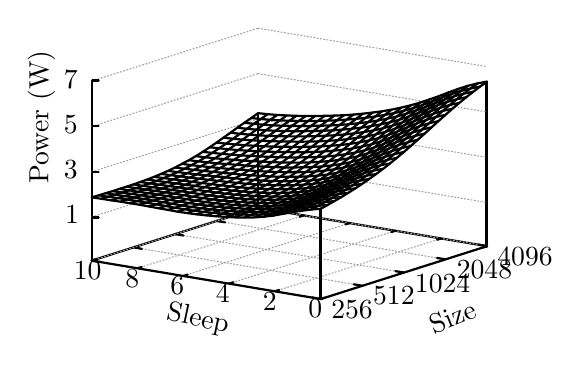
\begin{tikzpicture}[y=0.80pt, x=0.80pt, yscale=-0.570000, xscale=0.570000, inner sep=0pt, outer sep=0pt]
\begin{scope}[draw=black,line join=bevel,line cap=rect,even odd rule,line width=0.800pt]
  \begin{scope}[cm={{1.0,0.0,0.0,1.0,(0.0,0.0)}},draw=black,line join=bevel,line cap=rect,line width=0.800pt]
  \end{scope}
  \begin{scope}[cm={{1.00465,0.0,0.0,1.00465,(0.0,0.0)}},draw=black,line join=bevel,line cap=rect,line width=0.800pt]
  \end{scope}
  \begin{scope}[cm={{1.00465,0.0,0.0,1.00465,(0.0,0.0)}},draw=black,line join=round,line cap=round,line width=0.800pt]
    \path[draw] (59.1000,229.5000) -- (190.3000,187.8000);
    \path[draw] (370.9000,218.1000) -- (190.3000,187.8000);
    \path[draw] (59.5000,229.5000) -- (59.5000,87.5000);
    \path[draw] (190.5000,187.5000) -- (190.5000,113.5000);
    \path[draw] (370.5000,218.5000) -- (370.5000,88.5000);
  \end{scope}
  \begin{scope}[cm={{1.00465,0.0,0.0,1.00465,(0.0,0.0)}},draw=ca0a0a4,dash pattern=on 0.40pt off 0.80pt,line join=round,line cap=round,line width=0.400pt]
    \path[draw] (239.7000,259.8000) -- (59.1000,229.5000);
  \end{scope}
  \begin{scope}[cm={{1.00465,0.0,0.0,1.00465,(0.0,0.0)}},draw=black,line join=round,line cap=round,line width=0.800pt]
    \path[draw] (239.7000,259.8000) -- (232.9000,258.6000);
    \path[draw] (59.1000,229.5000) -- (65.8000,230.6000);
  \end{scope}
  \begin{scope}[cm={{1.00465,0.0,0.0,1.00465,(0.0,0.0)}},draw=black,line join=bevel,line cap=rect,line width=0.800pt]
  \end{scope}
  \begin{scope}[cm={{1.00465,0.0,0.0,1.00465,(249.153,276.781)}},draw=black,line join=bevel,line cap=rect,line width=0.800pt]
  \end{scope}
  \begin{scope}[cm={{1.00465,0.0,0.0,1.00465,(249.153,276.781)}},draw=black,line join=bevel,line cap=rect,line width=0.800pt]
  \end{scope}
  \begin{scope}[cm={{1.00465,0.0,0.0,1.00465,(249.153,276.781)}},draw=black,line join=bevel,line cap=rect,line width=0.800pt]
  \end{scope}
  \begin{scope}[cm={{1.00465,0.0,0.0,1.00465,(249.153,276.781)}},draw=black,line join=bevel,line cap=rect,line width=0.800pt]
  \end{scope}
  \begin{scope}[cm={{1.00465,0.0,0.0,1.00465,(249.153,276.781)}},draw=black,line join=bevel,line cap=rect,line width=0.800pt]
  \end{scope}
  \begin{scope}[cm={{1.00465,0.0,0.0,1.00465,(249.153,276.781)}},draw=black,line join=bevel,line cap=rect,line width=0.800pt]
    \path[fill=black] (0.0000,0.0000) node[above right] () {256};
  \end{scope}
  \begin{scope}[cm={{1.00465,0.0,0.0,1.00465,(249.153,276.781)}},draw=black,line join=bevel,line cap=rect,line width=0.800pt]
  \end{scope}
  \begin{scope}[cm={{1.00465,0.0,0.0,1.00465,(0.0,0.0)}},draw=black,line join=bevel,line cap=rect,line width=0.800pt]
  \end{scope}
  \begin{scope}[cm={{1.00465,0.0,0.0,1.00465,(0.0,0.0)}},draw=ca0a0a4,dash pattern=on 0.40pt off 0.80pt,line join=round,line cap=round,line width=0.400pt]
    \path[draw] (272.5000,249.3000) -- (91.9000,219.0000);
  \end{scope}
  \begin{scope}[cm={{1.00465,0.0,0.0,1.00465,(0.0,0.0)}},draw=black,line join=round,line cap=round,line width=0.800pt]
    \path[draw] (272.5000,249.3000) -- (265.8000,248.2000);
    \path[draw] (91.9000,219.0000) -- (98.6000,220.2000);
  \end{scope}
  \begin{scope}[cm={{1.00465,0.0,0.0,1.00465,(0.0,0.0)}},draw=black,line join=bevel,line cap=rect,line width=0.800pt]
  \end{scope}
  \begin{scope}[cm={{1.00465,0.0,0.0,1.00465,(282.307,265.73)}},draw=black,line join=bevel,line cap=rect,line width=0.800pt]
  \end{scope}
  \begin{scope}[cm={{1.00465,0.0,0.0,1.00465,(282.307,265.73)}},draw=black,line join=bevel,line cap=rect,line width=0.800pt]
  \end{scope}
  \begin{scope}[cm={{1.00465,0.0,0.0,1.00465,(282.307,265.73)}},draw=black,line join=bevel,line cap=rect,line width=0.800pt]
  \end{scope}
  \begin{scope}[cm={{1.00465,0.0,0.0,1.00465,(282.307,265.73)}},draw=black,line join=bevel,line cap=rect,line width=0.800pt]
  \end{scope}
  \begin{scope}[cm={{1.00465,0.0,0.0,1.00465,(282.307,265.73)}},draw=black,line join=bevel,line cap=rect,line width=0.800pt]
  \end{scope}
  \begin{scope}[cm={{1.00465,0.0,0.0,1.00465,(282.307,265.73)}},draw=black,line join=bevel,line cap=rect,line width=0.800pt]
    \path[fill=black] (0.0000,0.0000) node[above right] () {512};
  \end{scope}
  \begin{scope}[cm={{1.00465,0.0,0.0,1.00465,(282.307,265.73)}},draw=black,line join=bevel,line cap=rect,line width=0.800pt]
  \end{scope}
  \begin{scope}[cm={{1.00465,0.0,0.0,1.00465,(0.0,0.0)}},draw=black,line join=bevel,line cap=rect,line width=0.800pt]
  \end{scope}
  \begin{scope}[cm={{1.00465,0.0,0.0,1.00465,(0.0,0.0)}},draw=ca0a0a4,dash pattern=on 0.40pt off 0.80pt,line join=round,line cap=round,line width=0.400pt]
    \path[draw] (305.3000,238.9000) -- (124.7000,208.6000);
  \end{scope}
  \begin{scope}[cm={{1.00465,0.0,0.0,1.00465,(0.0,0.0)}},draw=black,line join=round,line cap=round,line width=0.800pt]
    \path[draw] (305.3000,238.9000) -- (298.6000,237.8000);
    \path[draw] (124.7000,208.6000) -- (131.4000,209.7000);
  \end{scope}
  \begin{scope}[cm={{1.00465,0.0,0.0,1.00465,(0.0,0.0)}},draw=black,line join=bevel,line cap=rect,line width=0.800pt]
  \end{scope}
  \begin{scope}[cm={{1.00465,0.0,0.0,1.00465,(315.46,255.684)}},draw=black,line join=bevel,line cap=rect,line width=0.800pt]
  \end{scope}
  \begin{scope}[cm={{1.00465,0.0,0.0,1.00465,(315.46,255.684)}},draw=black,line join=bevel,line cap=rect,line width=0.800pt]
  \end{scope}
  \begin{scope}[cm={{1.00465,0.0,0.0,1.00465,(315.46,255.684)}},draw=black,line join=bevel,line cap=rect,line width=0.800pt]
  \end{scope}
  \begin{scope}[cm={{1.00465,0.0,0.0,1.00465,(315.46,255.684)}},draw=black,line join=bevel,line cap=rect,line width=0.800pt]
  \end{scope}
  \begin{scope}[cm={{1.00465,0.0,0.0,1.00465,(315.46,255.684)}},draw=black,line join=bevel,line cap=rect,line width=0.800pt]
  \end{scope}
  \begin{scope}[cm={{1.00465,0.0,0.0,1.00465,(315.46,255.684)}},draw=black,line join=bevel,line cap=rect,line width=0.800pt]
    \path[fill=black] (0.0000,0.0000) node[above right] () {1024};
  \end{scope}
  \begin{scope}[cm={{1.00465,0.0,0.0,1.00465,(315.46,255.684)}},draw=black,line join=bevel,line cap=rect,line width=0.800pt]
  \end{scope}
  \begin{scope}[cm={{1.00465,0.0,0.0,1.00465,(0.0,0.0)}},draw=black,line join=bevel,line cap=rect,line width=0.800pt]
  \end{scope}
  \begin{scope}[cm={{1.00465,0.0,0.0,1.00465,(0.0,0.0)}},draw=ca0a0a4,dash pattern=on 0.40pt off 0.80pt,line join=round,line cap=round,line width=0.400pt]
    \path[draw] (338.1000,228.5000) -- (157.5000,198.2000);
  \end{scope}
  \begin{scope}[cm={{1.00465,0.0,0.0,1.00465,(0.0,0.0)}},draw=black,line join=round,line cap=round,line width=0.800pt]
    \path[draw] (338.1000,228.5000) -- (331.4000,227.4000);
    \path[draw] (157.5000,198.2000) -- (164.2000,199.3000);
  \end{scope}
  \begin{scope}[cm={{1.00465,0.0,0.0,1.00465,(0.0,0.0)}},draw=black,line join=bevel,line cap=rect,line width=0.800pt]
  \end{scope}
  \begin{scope}[cm={{1.00465,0.0,0.0,1.00465,(348.614,244.633)}},draw=black,line join=bevel,line cap=rect,line width=0.800pt]
  \end{scope}
  \begin{scope}[cm={{1.00465,0.0,0.0,1.00465,(348.614,244.633)}},draw=black,line join=bevel,line cap=rect,line width=0.800pt]
  \end{scope}
  \begin{scope}[cm={{1.00465,0.0,0.0,1.00465,(348.614,244.633)}},draw=black,line join=bevel,line cap=rect,line width=0.800pt]
  \end{scope}
  \begin{scope}[cm={{1.00465,0.0,0.0,1.00465,(348.614,244.633)}},draw=black,line join=bevel,line cap=rect,line width=0.800pt]
  \end{scope}
  \begin{scope}[cm={{1.00465,0.0,0.0,1.00465,(348.614,244.633)}},draw=black,line join=bevel,line cap=rect,line width=0.800pt]
  \end{scope}
  \begin{scope}[cm={{1.00465,0.0,0.0,1.00465,(348.614,244.633)}},draw=black,line join=bevel,line cap=rect,line width=0.800pt]
    \path[fill=black] (0.0000,0.0000) node[above right] () {2048};
  \end{scope}
  \begin{scope}[cm={{1.00465,0.0,0.0,1.00465,(348.614,244.633)}},draw=black,line join=bevel,line cap=rect,line width=0.800pt]
  \end{scope}
  \begin{scope}[cm={{1.00465,0.0,0.0,1.00465,(0.0,0.0)}},draw=black,line join=bevel,line cap=rect,line width=0.800pt]
  \end{scope}
  \begin{scope}[cm={{1.00465,0.0,0.0,1.00465,(0.0,0.0)}},draw=ca0a0a4,dash pattern=on 0.40pt off 0.80pt,line join=round,line cap=round,line width=0.400pt]
    \path[draw] (370.9000,218.1000) -- (190.3000,187.8000);
  \end{scope}
  \begin{scope}[cm={{1.00465,0.0,0.0,1.00465,(0.0,0.0)}},draw=black,line join=round,line cap=round,line width=0.800pt]
    \path[draw] (370.9000,218.1000) -- (364.2000,216.9000);
    \path[draw] (190.3000,187.8000) -- (197.1000,188.9000);
  \end{scope}
  \begin{scope}[cm={{1.00465,0.0,0.0,1.00465,(0.0,0.0)}},draw=black,line join=bevel,line cap=rect,line width=0.800pt]
  \end{scope}
  \begin{scope}[cm={{1.00465,0.0,0.0,1.00465,(380.763,234.586)}},draw=black,line join=bevel,line cap=rect,line width=0.800pt]
  \end{scope}
  \begin{scope}[cm={{1.00465,0.0,0.0,1.00465,(380.763,234.586)}},draw=black,line join=bevel,line cap=rect,line width=0.800pt]
  \end{scope}
  \begin{scope}[cm={{1.00465,0.0,0.0,1.00465,(380.763,234.586)}},draw=black,line join=bevel,line cap=rect,line width=0.800pt]
  \end{scope}
  \begin{scope}[cm={{1.00465,0.0,0.0,1.00465,(380.763,234.586)}},draw=black,line join=bevel,line cap=rect,line width=0.800pt]
  \end{scope}
  \begin{scope}[cm={{1.00465,0.0,0.0,1.00465,(380.763,234.586)}},draw=black,line join=bevel,line cap=rect,line width=0.800pt]
  \end{scope}
  \begin{scope}[cm={{1.00465,0.0,0.0,1.00465,(380.763,234.586)}},draw=black,line join=bevel,line cap=rect,line width=0.800pt]
    \path[fill=black] (0.0000,0.0000) node[above right] () {4096};
  \end{scope}
  \begin{scope}[cm={{1.00465,0.0,0.0,1.00465,(380.763,234.586)}},draw=black,line join=bevel,line cap=rect,line width=0.800pt]
  \end{scope}
  \begin{scope}[cm={{1.00465,0.0,0.0,1.00465,(0.0,0.0)}},draw=black,line join=bevel,line cap=rect,line width=0.800pt]
  \end{scope}
  \begin{scope}[cm={{1.00465,0.0,0.0,1.00465,(0.0,0.0)}},draw=ca0a0a4,dash pattern=on 0.40pt off 0.80pt,line join=round,line cap=round,line width=0.400pt]
    \path[draw] (239.7000,259.8000) -- (370.9000,218.1000);
  \end{scope}
  \begin{scope}[cm={{1.00465,0.0,0.0,1.00465,(0.0,0.0)}},draw=black,line join=round,line cap=round,line width=0.800pt]
    \path[draw] (239.7000,259.8000) -- (242.9000,258.7000);
    \path[draw] (370.9000,218.1000) -- (367.6000,219.1000);
  \end{scope}
  \begin{scope}[cm={{1.00465,0.0,0.0,1.00465,(0.0,0.0)}},draw=black,line join=bevel,line cap=rect,line width=0.800pt]
  \end{scope}
  \begin{scope}[cm={{1.00465,0.0,0.0,1.00465,(231.07,275.777)}},draw=black,line join=bevel,line cap=rect,line width=0.800pt]
  \end{scope}
  \begin{scope}[cm={{1.00465,0.0,0.0,1.00465,(231.07,275.777)}},draw=black,line join=bevel,line cap=rect,line width=0.800pt]
  \end{scope}
  \begin{scope}[cm={{1.00465,0.0,0.0,1.00465,(231.07,275.777)}},draw=black,line join=bevel,line cap=rect,line width=0.800pt]
  \end{scope}
  \begin{scope}[cm={{1.00465,0.0,0.0,1.00465,(231.07,275.777)}},draw=black,line join=bevel,line cap=rect,line width=0.800pt]
  \end{scope}
  \begin{scope}[cm={{1.00465,0.0,0.0,1.00465,(231.07,275.777)}},draw=black,line join=bevel,line cap=rect,line width=0.800pt]
  \end{scope}
  \begin{scope}[cm={{1.00465,0.0,0.0,1.00465,(231.07,275.777)}},draw=black,line join=bevel,line cap=rect,line width=0.800pt]
    \path[fill=black] (0.0000,0.0000) node[above right] () {0};
  \end{scope}
  \begin{scope}[cm={{1.00465,0.0,0.0,1.00465,(231.07,275.777)}},draw=black,line join=bevel,line cap=rect,line width=0.800pt]
  \end{scope}
  \begin{scope}[cm={{1.00465,0.0,0.0,1.00465,(0.0,0.0)}},draw=black,line join=bevel,line cap=rect,line width=0.800pt]
  \end{scope}
  \begin{scope}[cm={{1.00465,0.0,0.0,1.00465,(0.0,0.0)}},draw=ca0a0a4,dash pattern=on 0.40pt off 0.80pt,line join=round,line cap=round,line width=0.400pt]
    \path[draw] (203.6000,253.7000) -- (334.8000,212.0000);
  \end{scope}
  \begin{scope}[cm={{1.00465,0.0,0.0,1.00465,(0.0,0.0)}},draw=black,line join=round,line cap=round,line width=0.800pt]
    \path[draw] (203.6000,253.7000) -- (206.9000,252.6000);
    \path[draw] (334.8000,212.0000) -- (331.5000,213.0000);
  \end{scope}
  \begin{scope}[cm={{1.00465,0.0,0.0,1.00465,(0.0,0.0)}},draw=black,line join=bevel,line cap=rect,line width=0.800pt]
  \end{scope}
  \begin{scope}[cm={{1.00465,0.0,0.0,1.00465,(194.902,269.749)}},draw=black,line join=bevel,line cap=rect,line width=0.800pt]
  \end{scope}
  \begin{scope}[cm={{1.00465,0.0,0.0,1.00465,(194.902,269.749)}},draw=black,line join=bevel,line cap=rect,line width=0.800pt]
  \end{scope}
  \begin{scope}[cm={{1.00465,0.0,0.0,1.00465,(194.902,269.749)}},draw=black,line join=bevel,line cap=rect,line width=0.800pt]
  \end{scope}
  \begin{scope}[cm={{1.00465,0.0,0.0,1.00465,(194.902,269.749)}},draw=black,line join=bevel,line cap=rect,line width=0.800pt]
  \end{scope}
  \begin{scope}[cm={{1.00465,0.0,0.0,1.00465,(194.902,269.749)}},draw=black,line join=bevel,line cap=rect,line width=0.800pt]
  \end{scope}
  \begin{scope}[cm={{1.00465,0.0,0.0,1.00465,(194.902,269.749)}},draw=black,line join=bevel,line cap=rect,line width=0.800pt]
    \path[fill=black] (0.0000,0.0000) node[above right] () {2};
  \end{scope}
  \begin{scope}[cm={{1.00465,0.0,0.0,1.00465,(194.902,269.749)}},draw=black,line join=bevel,line cap=rect,line width=0.800pt]
  \end{scope}
  \begin{scope}[cm={{1.00465,0.0,0.0,1.00465,(0.0,0.0)}},draw=black,line join=bevel,line cap=rect,line width=0.800pt]
  \end{scope}
  \begin{scope}[cm={{1.00465,0.0,0.0,1.00465,(0.0,0.0)}},draw=ca0a0a4,dash pattern=on 0.40pt off 0.80pt,line join=round,line cap=round,line width=0.400pt]
    \path[draw] (167.5000,247.6000) -- (298.6000,205.9000);
  \end{scope}
  \begin{scope}[cm={{1.00465,0.0,0.0,1.00465,(0.0,0.0)}},draw=black,line join=round,line cap=round,line width=0.800pt]
    \path[draw] (167.5000,247.6000) -- (170.8000,246.6000);
    \path[draw] (298.6000,205.9000) -- (295.3000,207.0000);
  \end{scope}
  \begin{scope}[cm={{1.00465,0.0,0.0,1.00465,(0.0,0.0)}},draw=black,line join=bevel,line cap=rect,line width=0.800pt]
  \end{scope}
  \begin{scope}[cm={{1.00465,0.0,0.0,1.00465,(157.73,263.721)}},draw=black,line join=bevel,line cap=rect,line width=0.800pt]
  \end{scope}
  \begin{scope}[cm={{1.00465,0.0,0.0,1.00465,(157.73,263.721)}},draw=black,line join=bevel,line cap=rect,line width=0.800pt]
  \end{scope}
  \begin{scope}[cm={{1.00465,0.0,0.0,1.00465,(157.73,263.721)}},draw=black,line join=bevel,line cap=rect,line width=0.800pt]
  \end{scope}
  \begin{scope}[cm={{1.00465,0.0,0.0,1.00465,(157.73,263.721)}},draw=black,line join=bevel,line cap=rect,line width=0.800pt]
  \end{scope}
  \begin{scope}[cm={{1.00465,0.0,0.0,1.00465,(157.73,263.721)}},draw=black,line join=bevel,line cap=rect,line width=0.800pt]
  \end{scope}
  \begin{scope}[cm={{1.00465,0.0,0.0,1.00465,(157.73,263.721)}},draw=black,line join=bevel,line cap=rect,line width=0.800pt]
    \path[fill=black] (0.0000,0.0000) node[above right] () {4};
  \end{scope}
  \begin{scope}[cm={{1.00465,0.0,0.0,1.00465,(157.73,263.721)}},draw=black,line join=bevel,line cap=rect,line width=0.800pt]
  \end{scope}
  \begin{scope}[cm={{1.00465,0.0,0.0,1.00465,(0.0,0.0)}},draw=black,line join=bevel,line cap=rect,line width=0.800pt]
  \end{scope}
  \begin{scope}[cm={{1.00465,0.0,0.0,1.00465,(0.0,0.0)}},draw=ca0a0a4,dash pattern=on 0.40pt off 0.80pt,line join=round,line cap=round,line width=0.400pt]
    \path[draw] (131.4000,241.6000) -- (262.5000,199.9000);
  \end{scope}
  \begin{scope}[cm={{1.00465,0.0,0.0,1.00465,(0.0,0.0)}},draw=black,line join=round,line cap=round,line width=0.800pt]
    \path[draw] (131.4000,241.6000) -- (134.7000,240.5000);
    \path[draw] (262.5000,199.9000) -- (259.2000,200.9000);
  \end{scope}
  \begin{scope}[cm={{1.00465,0.0,0.0,1.00465,(0.0,0.0)}},draw=black,line join=bevel,line cap=rect,line width=0.800pt]
  \end{scope}
  \begin{scope}[cm={{1.00465,0.0,0.0,1.00465,(121.563,257.693)}},draw=black,line join=bevel,line cap=rect,line width=0.800pt]
  \end{scope}
  \begin{scope}[cm={{1.00465,0.0,0.0,1.00465,(121.563,257.693)}},draw=black,line join=bevel,line cap=rect,line width=0.800pt]
  \end{scope}
  \begin{scope}[cm={{1.00465,0.0,0.0,1.00465,(121.563,257.693)}},draw=black,line join=bevel,line cap=rect,line width=0.800pt]
  \end{scope}
  \begin{scope}[cm={{1.00465,0.0,0.0,1.00465,(121.563,257.693)}},draw=black,line join=bevel,line cap=rect,line width=0.800pt]
  \end{scope}
  \begin{scope}[cm={{1.00465,0.0,0.0,1.00465,(121.563,257.693)}},draw=black,line join=bevel,line cap=rect,line width=0.800pt]
  \end{scope}
  \begin{scope}[cm={{1.00465,0.0,0.0,1.00465,(121.563,257.693)}},draw=black,line join=bevel,line cap=rect,line width=0.800pt]
    \path[fill=black] (0.0000,0.0000) node[above right] () {6};
  \end{scope}
  \begin{scope}[cm={{1.00465,0.0,0.0,1.00465,(121.563,257.693)}},draw=black,line join=bevel,line cap=rect,line width=0.800pt]
  \end{scope}
  \begin{scope}[cm={{1.00465,0.0,0.0,1.00465,(0.0,0.0)}},draw=black,line join=bevel,line cap=rect,line width=0.800pt]
  \end{scope}
  \begin{scope}[cm={{1.00465,0.0,0.0,1.00465,(0.0,0.0)}},draw=ca0a0a4,dash pattern=on 0.40pt off 0.80pt,line join=round,line cap=round,line width=0.400pt]
    \path[draw] (95.2000,235.5000) -- (226.4000,193.8000);
  \end{scope}
  \begin{scope}[cm={{1.00465,0.0,0.0,1.00465,(0.0,0.0)}},draw=black,line join=round,line cap=round,line width=0.800pt]
    \path[draw] (95.2000,235.5000) -- (98.5000,234.5000);
    \path[draw] (226.4000,193.8000) -- (223.1000,194.9000);
  \end{scope}
  \begin{scope}[cm={{1.00465,0.0,0.0,1.00465,(0.0,0.0)}},draw=black,line join=bevel,line cap=rect,line width=0.800pt]
  \end{scope}
  \begin{scope}[cm={{1.00465,0.0,0.0,1.00465,(85.8977,251.665)}},draw=black,line join=bevel,line cap=rect,line width=0.800pt]
  \end{scope}
  \begin{scope}[cm={{1.00465,0.0,0.0,1.00465,(85.8977,251.665)}},draw=black,line join=bevel,line cap=rect,line width=0.800pt]
  \end{scope}
  \begin{scope}[cm={{1.00465,0.0,0.0,1.00465,(85.8977,251.665)}},draw=black,line join=bevel,line cap=rect,line width=0.800pt]
  \end{scope}
  \begin{scope}[cm={{1.00465,0.0,0.0,1.00465,(85.8977,251.665)}},draw=black,line join=bevel,line cap=rect,line width=0.800pt]
  \end{scope}
  \begin{scope}[cm={{1.00465,0.0,0.0,1.00465,(85.8977,251.665)}},draw=black,line join=bevel,line cap=rect,line width=0.800pt]
  \end{scope}
  \begin{scope}[cm={{1.00465,0.0,0.0,1.00465,(85.8977,251.665)}},draw=black,line join=bevel,line cap=rect,line width=0.800pt]
    \path[fill=black] (0.0000,0.0000) node[above right] () {8};
  \end{scope}
  \begin{scope}[cm={{1.00465,0.0,0.0,1.00465,(85.8977,251.665)}},draw=black,line join=bevel,line cap=rect,line width=0.800pt]
  \end{scope}
  \begin{scope}[cm={{1.00465,0.0,0.0,1.00465,(0.0,0.0)}},draw=black,line join=bevel,line cap=rect,line width=0.800pt]
  \end{scope}
  \begin{scope}[cm={{1.00465,0.0,0.0,1.00465,(0.0,0.0)}},draw=ca0a0a4,dash pattern=on 0.40pt off 0.80pt,line join=round,line cap=round,line width=0.400pt]
    \path[draw] (59.1000,229.5000) -- (190.3000,187.8000);
  \end{scope}
  \begin{scope}[cm={{1.00465,0.0,0.0,1.00465,(0.0,0.0)}},draw=black,line join=round,line cap=round,line width=0.800pt]
    \path[draw] (59.1000,229.5000) -- (62.4000,228.4000);
    \path[draw] (190.3000,187.8000) -- (187.1000,188.8000);
  \end{scope}
  \begin{scope}[cm={{1.00465,0.0,0.0,1.00465,(0.0,0.0)}},draw=black,line join=bevel,line cap=rect,line width=0.800pt]
  \end{scope}
  \begin{scope}[cm={{1.00465,0.0,0.0,1.00465,(45.2093,245.637)}},draw=black,line join=bevel,line cap=rect,line width=0.800pt]
  \end{scope}
  \begin{scope}[cm={{1.00465,0.0,0.0,1.00465,(45.2093,245.637)}},draw=black,line join=bevel,line cap=rect,line width=0.800pt]
  \end{scope}
  \begin{scope}[cm={{1.00465,0.0,0.0,1.00465,(45.2093,245.637)}},draw=black,line join=bevel,line cap=rect,line width=0.800pt]
  \end{scope}
  \begin{scope}[cm={{1.00465,0.0,0.0,1.00465,(45.2093,245.637)}},draw=black,line join=bevel,line cap=rect,line width=0.800pt]
  \end{scope}
  \begin{scope}[cm={{1.00465,0.0,0.0,1.00465,(45.2093,245.637)}},draw=black,line join=bevel,line cap=rect,line width=0.800pt]
  \end{scope}
  \begin{scope}[cm={{1.00465,0.0,0.0,1.00465,(45.2093,245.637)}},draw=black,line join=bevel,line cap=rect,line width=0.800pt]
    \path[fill=black] (0.0000,0.0000) node[above right] () {10};
  \end{scope}
  \begin{scope}[cm={{1.00465,0.0,0.0,1.00465,(45.2093,245.637)}},draw=black,line join=bevel,line cap=rect,line width=0.800pt]
  \end{scope}
  \begin{scope}[cm={{1.00465,0.0,0.0,1.00465,(0.0,0.0)}},draw=black,line join=bevel,line cap=rect,line width=0.800pt]
  \end{scope}
  \begin{scope}[cm={{1.00465,0.0,0.0,1.00465,(0.0,0.0)}},draw=ca0a0a4,dash pattern=on 0.40pt off 0.80pt,line join=round,line cap=round,line width=0.400pt]
    \path[draw] (59.1000,195.1000) -- (190.3000,153.4000);
    \path[draw] (190.3000,153.4000) -- (190.3000,153.4000) -- (370.9000,183.7000);
  \end{scope}
  \begin{scope}[cm={{1.00465,0.0,0.0,1.00465,(0.0,0.0)}},draw=black,line join=round,line cap=round,line width=0.800pt]
    \path[draw] (59.5000,195.5000) -- (64.5000,195.5000);
  \end{scope}
  \begin{scope}[cm={{1.00465,0.0,0.0,1.00465,(0.0,0.0)}},draw=black,line join=bevel,line cap=rect,line width=0.800pt]
  \end{scope}
  \begin{scope}[cm={{1.00465,0.0,0.0,1.00465,(38.1767,201.433)}},draw=black,line join=bevel,line cap=rect,line width=0.800pt]
  \end{scope}
  \begin{scope}[cm={{1.00465,0.0,0.0,1.00465,(38.1767,201.433)}},draw=black,line join=bevel,line cap=rect,line width=0.800pt]
  \end{scope}
  \begin{scope}[cm={{1.00465,0.0,0.0,1.00465,(38.1767,201.433)}},draw=black,line join=bevel,line cap=rect,line width=0.800pt]
  \end{scope}
  \begin{scope}[cm={{1.00465,0.0,0.0,1.00465,(38.1767,201.433)}},draw=black,line join=bevel,line cap=rect,line width=0.800pt]
  \end{scope}
  \begin{scope}[cm={{1.00465,0.0,0.0,1.00465,(38.1767,201.433)}},draw=black,line join=bevel,line cap=rect,line width=0.800pt]
  \end{scope}
  \begin{scope}[cm={{1.00465,0.0,0.0,1.00465,(38.1767,201.433)}},draw=black,line join=bevel,line cap=rect,line width=0.800pt]
    \path[fill=black] (0.0000,0.0000) node[above right] () {1};
  \end{scope}
  \begin{scope}[cm={{1.00465,0.0,0.0,1.00465,(38.1767,201.433)}},draw=black,line join=bevel,line cap=rect,line width=0.800pt]
  \end{scope}
  \begin{scope}[cm={{1.00465,0.0,0.0,1.00465,(0.0,0.0)}},draw=black,line join=bevel,line cap=rect,line width=0.800pt]
  \end{scope}
  \begin{scope}[cm={{1.00465,0.0,0.0,1.00465,(0.0,0.0)}},draw=ca0a0a4,dash pattern=on 0.40pt off 0.80pt,line join=round,line cap=round,line width=0.400pt]
    \path[draw] (59.1000,159.4000) -- (190.3000,117.8000);
    \path[draw] (190.3000,117.8000) -- (190.3000,117.8000) -- (370.9000,148.1000);
  \end{scope}
  \begin{scope}[cm={{1.00465,0.0,0.0,1.00465,(0.0,0.0)}},draw=black,line join=round,line cap=round,line width=0.800pt]
    \path[draw] (59.5000,159.5000) -- (64.5000,159.5000);
  \end{scope}
  \begin{scope}[cm={{1.00465,0.0,0.0,1.00465,(0.0,0.0)}},draw=black,line join=bevel,line cap=rect,line width=0.800pt]
  \end{scope}
  \begin{scope}[cm={{1.00465,0.0,0.0,1.00465,(37.1721,165.265)}},draw=black,line join=bevel,line cap=rect,line width=0.800pt]
  \end{scope}
  \begin{scope}[cm={{1.00465,0.0,0.0,1.00465,(37.1721,165.265)}},draw=black,line join=bevel,line cap=rect,line width=0.800pt]
  \end{scope}
  \begin{scope}[cm={{1.00465,0.0,0.0,1.00465,(37.1721,165.265)}},draw=black,line join=bevel,line cap=rect,line width=0.800pt]
  \end{scope}
  \begin{scope}[cm={{1.00465,0.0,0.0,1.00465,(37.1721,165.265)}},draw=black,line join=bevel,line cap=rect,line width=0.800pt]
  \end{scope}
  \begin{scope}[cm={{1.00465,0.0,0.0,1.00465,(37.1721,165.265)}},draw=black,line join=bevel,line cap=rect,line width=0.800pt]
  \end{scope}
  \begin{scope}[cm={{1.00465,0.0,0.0,1.00465,(37.1721,165.265)}},draw=black,line join=bevel,line cap=rect,line width=0.800pt]
    \path[fill=black] (0.0000,0.0000) node[above right] () {3};
  \end{scope}
  \begin{scope}[cm={{1.00465,0.0,0.0,1.00465,(37.1721,165.265)}},draw=black,line join=bevel,line cap=rect,line width=0.800pt]
  \end{scope}
  \begin{scope}[cm={{1.00465,0.0,0.0,1.00465,(0.0,0.0)}},draw=black,line join=bevel,line cap=rect,line width=0.800pt]
  \end{scope}
  \begin{scope}[cm={{1.00465,0.0,0.0,1.00465,(0.0,0.0)}},draw=ca0a0a4,dash pattern=on 0.40pt off 0.80pt,line join=round,line cap=round,line width=0.400pt]
    \path[draw] (59.1000,123.7000) -- (190.3000,82.0000);
    \path[draw] (190.3000,82.0000) -- (190.3000,82.0000) -- (370.9000,112.3000);
  \end{scope}
  \begin{scope}[cm={{1.00465,0.0,0.0,1.00465,(0.0,0.0)}},draw=black,line join=round,line cap=round,line width=0.800pt]
    \path[draw] (59.5000,123.5000) -- (64.5000,123.5000);
  \end{scope}
  \begin{scope}[cm={{1.00465,0.0,0.0,1.00465,(0.0,0.0)}},draw=black,line join=bevel,line cap=rect,line width=0.800pt]
  \end{scope}
  \begin{scope}[cm={{1.00465,0.0,0.0,1.00465,(37.1721,130.102)}},draw=black,line join=bevel,line cap=rect,line width=0.800pt]
  \end{scope}
  \begin{scope}[cm={{1.00465,0.0,0.0,1.00465,(37.1721,130.102)}},draw=black,line join=bevel,line cap=rect,line width=0.800pt]
  \end{scope}
  \begin{scope}[cm={{1.00465,0.0,0.0,1.00465,(37.1721,130.102)}},draw=black,line join=bevel,line cap=rect,line width=0.800pt]
  \end{scope}
  \begin{scope}[cm={{1.00465,0.0,0.0,1.00465,(37.1721,130.102)}},draw=black,line join=bevel,line cap=rect,line width=0.800pt]
  \end{scope}
  \begin{scope}[cm={{1.00465,0.0,0.0,1.00465,(37.1721,130.102)}},draw=black,line join=bevel,line cap=rect,line width=0.800pt]
  \end{scope}
  \begin{scope}[cm={{1.00465,0.0,0.0,1.00465,(37.1721,130.102)}},draw=black,line join=bevel,line cap=rect,line width=0.800pt]
    \path[fill=black] (0.0000,0.0000) node[above right] () {5};
  \end{scope}
  \begin{scope}[cm={{1.00465,0.0,0.0,1.00465,(37.1721,130.102)}},draw=black,line join=bevel,line cap=rect,line width=0.800pt]
  \end{scope}
  \begin{scope}[cm={{1.00465,0.0,0.0,1.00465,(0.0,0.0)}},draw=black,line join=bevel,line cap=rect,line width=0.800pt]
  \end{scope}
  \begin{scope}[cm={{1.00465,0.0,0.0,1.00465,(0.0,0.0)}},draw=ca0a0a4,dash pattern=on 0.40pt off 0.80pt,line join=round,line cap=round,line width=0.400pt]
    \path[draw] (59.1000,87.9000) -- (190.3000,46.2000);
    \path[draw] (190.3000,46.2000) -- (190.3000,46.2000) -- (370.9000,76.5000);
  \end{scope}
  \begin{scope}[cm={{1.00465,0.0,0.0,1.00465,(0.0,0.0)}},draw=black,line join=round,line cap=round,line width=0.800pt]
    \path[draw] (59.5000,87.5000) -- (64.5000,87.5000);
  \end{scope}
  \begin{scope}[cm={{1.00465,0.0,0.0,1.00465,(0.0,0.0)}},draw=black,line join=bevel,line cap=rect,line width=0.800pt]
  \end{scope}
  \begin{scope}[cm={{1.00465,0.0,0.0,1.00465,(37.1721,93.9349)}},draw=black,line join=bevel,line cap=rect,line width=0.800pt]
  \end{scope}
  \begin{scope}[cm={{1.00465,0.0,0.0,1.00465,(37.1721,93.9349)}},draw=black,line join=bevel,line cap=rect,line width=0.800pt]
  \end{scope}
  \begin{scope}[cm={{1.00465,0.0,0.0,1.00465,(37.1721,93.9349)}},draw=black,line join=bevel,line cap=rect,line width=0.800pt]
  \end{scope}
  \begin{scope}[cm={{1.00465,0.0,0.0,1.00465,(37.1721,93.9349)}},draw=black,line join=bevel,line cap=rect,line width=0.800pt]
  \end{scope}
  \begin{scope}[cm={{1.00465,0.0,0.0,1.00465,(37.1721,93.9349)}},draw=black,line join=bevel,line cap=rect,line width=0.800pt]
  \end{scope}
  \begin{scope}[cm={{1.00465,0.0,0.0,1.00465,(37.1721,93.9349)}},draw=black,line join=bevel,line cap=rect,line width=0.800pt]
    \path[fill=black] (0.0000,0.0000) node[above right] () {7};
  \end{scope}
  \begin{scope}[cm={{1.00465,0.0,0.0,1.00465,(37.1721,93.9349)}},draw=black,line join=bevel,line cap=rect,line width=0.800pt]
  \end{scope}
  \begin{scope}[cm={{0.0,-1.00465,1.00465,0.0,(15.5721,176.316)}},draw=black,line join=bevel,line cap=rect,line width=0.800pt]
  \end{scope}
  \begin{scope}[cm={{0.0,-1.00465,1.00465,0.0,(15.5721,176.316)}},draw=black,line join=bevel,line cap=rect,line width=0.800pt]
  \end{scope}
  \begin{scope}[cm={{0.0,-1.00465,1.00465,0.0,(15.5721,176.316)}},draw=black,line join=bevel,line cap=rect,line width=0.800pt]
  \end{scope}
  \begin{scope}[cm={{0.0,-1.00465,1.00465,0.0,(15.5721,176.316)}},draw=black,line join=bevel,line cap=rect,line width=0.800pt]
  \end{scope}
  \begin{scope}[cm={{0.0,-1.00465,1.00465,0.0,(15.5721,176.316)}},draw=black,line join=bevel,line cap=rect,line width=0.800pt]
  \end{scope}
  \begin{scope}[cm={{0.0,-1.00465,1.00465,0.0,(8.5721,169.284)}},draw=black,line join=bevel,line cap=rect,line width=0.800pt]
    \path[fill=black] (0.0000,0.0000) node[above right] () {\rotatebox{90}{Power (W)}};
  \end{scope}
  \begin{scope}[cm={{0.0,-1.00465,1.00465,0.0,(15.5721,176.316)}},draw=black,line join=bevel,line cap=rect,line width=0.800pt]
  \end{scope}
  \begin{scope}[cm={{1.00465,0.0,0.0,1.00465,(0.0,0.0)}},draw=black,line join=bevel,line cap=rect,line width=0.800pt]
  \end{scope}
  \begin{scope}[cm={{1.00465,0.0,0.0,1.00465,(0.0,0.0)}},draw=black,line join=bevel,line cap=rect,line width=0.800pt]
  \end{scope}
  \begin{scope}[cm={{1.00465,0.0,0.0,1.00465,(0.0,0.0)}},draw=black,line join=bevel,line cap=rect,line width=0.800pt]
  \end{scope}
  \begin{scope}[cm={{1.00465,0.0,0.0,1.00465,(0.0,0.0)}},draw=black,line join=round,line cap=round,line width=0.800pt]
    \path[draw] (370.9000,88.3000) -- (363.4000,89.7000) -- (363.4000,89.7000) --
      (355.8000,91.6000) -- (355.8000,91.6000) -- (348.3000,94.0000) --
      (348.3000,94.0000) -- (340.8000,96.7000) -- (340.8000,96.7000) --
      (333.3000,99.6000) -- (333.3000,99.6000) -- (325.7000,102.3000) --
      (325.7000,102.3000) -- (318.2000,104.8000) -- (318.2000,104.8000) --
      (310.7000,107.0000) -- (310.7000,107.0000) -- (303.2000,108.8000) --
      (303.2000,108.8000) -- (295.6000,110.4000) -- (295.6000,110.4000) --
      (288.1000,111.7000) -- (288.1000,111.7000) -- (280.6000,112.7000) --
      (280.6000,112.7000) -- (273.0000,113.6000) -- (273.0000,113.6000) --
      (265.5000,114.3000) -- (265.5000,114.3000) -- (258.0000,114.8000) --
      (258.0000,114.8000) -- (250.5000,115.1000) -- (250.5000,115.1000) --
      (242.9000,115.3000) -- (242.9000,115.3000) -- (235.4000,115.4000) --
      (235.4000,115.4000) -- (227.9000,115.4000) -- (227.9000,115.4000) --
      (220.4000,115.3000) -- (220.4000,115.3000) -- (212.9000,115.0000) --
      (212.9000,115.0000) -- (205.4000,114.6000) -- (205.4000,114.6000) --
      (197.9000,114.0000) -- (197.9000,114.0000) -- (190.3000,113.2000);
    \path[draw] (365.4000,92.2000) -- (357.9000,93.7000) -- (357.9000,93.7000) --
      (350.4000,95.6000) -- (350.4000,95.6000) -- (342.9000,98.1000) --
      (342.9000,98.1000) -- (335.3000,100.9000) -- (335.3000,100.9000) --
      (327.8000,103.8000) -- (327.8000,103.8000) -- (320.3000,106.6000) --
      (320.3000,106.6000) -- (312.7000,109.2000) -- (312.7000,109.2000) --
      (305.2000,111.3000) -- (305.2000,111.3000) -- (297.7000,113.1000) --
      (297.7000,113.1000) -- (290.2000,114.6000) -- (290.2000,114.6000) --
      (282.6000,115.8000) -- (282.6000,115.8000) -- (275.1000,116.9000) --
      (275.1000,116.9000) -- (267.6000,117.7000) -- (267.6000,117.7000) --
      (260.1000,118.3000) -- (260.1000,118.3000) -- (252.5000,118.8000) --
      (252.5000,118.8000) -- (245.0000,119.1000) -- (245.0000,119.1000) --
      (237.5000,119.3000) -- (237.5000,119.3000) -- (229.9000,119.3000) --
      (229.9000,119.3000) -- (222.4000,119.3000) -- (222.4000,119.3000) --
      (215.0000,119.2000) -- (215.0000,119.2000) -- (207.5000,118.9000) --
      (207.5000,118.9000) -- (199.9000,118.4000) -- (199.9000,118.4000) --
      (192.4000,117.8000) -- (192.4000,117.8000) -- (184.9000,117.0000);
    \path[draw] (360.0000,96.3000) -- (352.4000,97.8000) -- (352.4000,97.8000) --
      (344.9000,99.9000) -- (344.9000,99.9000) -- (337.4000,102.4000) --
      (337.4000,102.4000) -- (329.9000,105.3000) -- (329.9000,105.3000) --
      (322.3000,108.3000) -- (322.3000,108.3000) -- (314.8000,111.1000) --
      (314.8000,111.1000) -- (307.3000,113.6000) -- (307.3000,113.6000) --
      (299.7000,115.8000) -- (299.7000,115.8000) -- (292.2000,117.5000) --
      (292.2000,117.5000) -- (284.7000,119.0000) -- (284.7000,119.0000) --
      (277.2000,120.2000) -- (277.2000,120.2000) -- (269.6000,121.1000) --
      (269.6000,121.1000) -- (262.1000,121.9000) -- (262.1000,121.9000) --
      (254.6000,122.5000) -- (254.6000,122.5000) -- (247.1000,122.9000) --
      (247.1000,122.9000) -- (239.5000,123.1000) -- (239.5000,123.1000) --
      (232.0000,123.3000) -- (232.0000,123.3000) -- (224.5000,123.3000) --
      (224.5000,123.3000) -- (216.9000,123.3000) -- (216.9000,123.3000) --
      (209.5000,123.1000) -- (209.5000,123.1000) -- (202.0000,122.8000) --
      (202.0000,122.8000) -- (194.5000,122.3000) -- (194.5000,122.3000) --
      (186.9000,121.6000) -- (186.9000,121.6000) -- (179.4000,120.8000);
    \path[draw] (354.5000,100.6000) -- (347.0000,102.2000) -- (347.0000,102.2000) --
      (339.4000,104.3000) -- (339.4000,104.3000) -- (331.9000,106.9000) --
      (331.9000,106.9000) -- (324.4000,109.9000) -- (324.4000,109.9000) --
      (316.9000,112.9000) -- (316.9000,112.9000) -- (309.3000,115.8000) --
      (309.3000,115.8000) -- (301.8000,118.3000) -- (301.8000,118.3000) --
      (294.3000,120.4000) -- (294.3000,120.4000) -- (286.8000,122.1000) --
      (286.8000,122.1000) -- (279.2000,123.5000) -- (279.2000,123.5000) --
      (271.7000,124.6000) -- (271.7000,124.6000) -- (264.2000,125.5000) --
      (264.2000,125.5000) -- (256.6000,126.2000) -- (256.6000,126.2000) --
      (249.1000,126.7000) -- (249.1000,126.7000) -- (241.6000,127.1000) --
      (241.6000,127.1000) -- (234.1000,127.3000) -- (234.1000,127.3000) --
      (226.5000,127.4000) -- (226.5000,127.4000) -- (219.0000,127.4000) --
      (219.0000,127.4000) -- (211.6000,127.3000) -- (211.6000,127.3000) --
      (204.1000,127.1000) -- (204.1000,127.1000) -- (196.5000,126.7000) --
      (196.5000,126.7000) -- (189.0000,126.2000) -- (189.0000,126.2000) --
      (181.5000,125.5000) -- (181.5000,125.5000) -- (173.9000,124.7000);
    \path[draw] (349.0000,105.1000) -- (341.5000,106.7000) -- (341.5000,106.7000) --
      (334.0000,108.9000) -- (334.0000,108.9000) -- (326.4000,111.6000) --
      (326.4000,111.6000) -- (318.9000,114.6000) -- (318.9000,114.6000) --
      (311.4000,117.7000) -- (311.4000,117.7000) -- (303.9000,120.6000) --
      (303.9000,120.6000) -- (296.3000,123.0000) -- (296.3000,123.0000) --
      (288.8000,125.1000) -- (288.8000,125.1000) -- (281.3000,126.8000) --
      (281.3000,126.8000) -- (273.8000,128.1000) -- (273.8000,128.1000) --
      (266.2000,129.1000) -- (266.2000,129.1000) -- (258.7000,130.0000) --
      (258.7000,130.0000) -- (251.2000,130.6000) -- (251.2000,130.6000) --
      (243.6000,131.0000) -- (243.6000,131.0000) -- (236.1000,131.3000) --
      (236.1000,131.3000) -- (228.6000,131.5000) -- (228.6000,131.5000) --
      (221.1000,131.5000) -- (221.1000,131.5000) -- (213.6000,131.5000) --
      (213.6000,131.5000) -- (206.1000,131.3000) -- (206.1000,131.3000) --
      (198.6000,131.1000) -- (198.6000,131.1000) -- (191.1000,130.7000) --
      (191.1000,130.7000) -- (183.5000,130.1000) -- (183.5000,130.1000) --
      (176.0000,129.5000) -- (176.0000,129.5000) -- (168.5000,128.6000);
    \path[draw] (343.6000,109.7000) -- (336.0000,111.4000) -- (336.0000,111.4000) --
      (328.5000,113.7000) -- (328.5000,113.7000) -- (321.0000,116.4000) --
      (321.0000,116.4000) -- (313.4000,119.5000) -- (313.4000,119.5000) --
      (305.9000,122.6000) -- (305.9000,122.6000) -- (298.4000,125.4000) --
      (298.4000,125.4000) -- (290.9000,127.9000) -- (290.9000,127.9000) --
      (283.3000,129.9000) -- (283.3000,129.9000) -- (275.8000,131.5000) --
      (275.8000,131.5000) -- (268.3000,132.7000) -- (268.3000,132.7000) --
      (260.8000,133.7000) -- (260.8000,133.7000) -- (253.2000,134.5000) --
      (253.2000,134.5000) -- (245.7000,135.0000) -- (245.7000,135.0000) --
      (238.2000,135.4000) -- (238.2000,135.4000) -- (230.7000,135.6000) --
      (230.7000,135.6000) -- (223.1000,135.7000) -- (223.1000,135.7000) --
      (215.6000,135.6000) -- (215.6000,135.6000) -- (208.2000,135.5000) --
      (208.2000,135.5000) -- (200.6000,135.3000) -- (200.6000,135.3000) --
      (193.1000,135.0000) -- (193.1000,135.0000) -- (185.6000,134.6000) --
      (185.6000,134.6000) -- (178.1000,134.1000) -- (178.1000,134.1000) --
      (170.5000,133.4000) -- (170.5000,133.4000) -- (163.0000,132.5000);
    \path[draw] (338.1000,114.5000) -- (330.6000,116.2000) -- (330.6000,116.2000) --
      (323.0000,118.5000) -- (323.0000,118.5000) -- (315.5000,121.3000) --
      (315.5000,121.3000) -- (308.0000,124.4000) -- (308.0000,124.4000) --
      (300.5000,127.5000) -- (300.5000,127.5000) -- (292.9000,130.4000) --
      (292.9000,130.4000) -- (285.4000,132.8000) -- (285.4000,132.8000) --
      (277.9000,134.7000) -- (277.9000,134.7000) -- (270.3000,136.2000) --
      (270.3000,136.2000) -- (262.8000,137.4000) -- (262.8000,137.4000) --
      (255.3000,138.3000) -- (255.3000,138.3000) -- (247.8000,138.9000) --
      (247.8000,138.9000) -- (240.2000,139.4000) -- (240.2000,139.4000) --
      (232.7000,139.7000) -- (232.7000,139.7000) -- (225.2000,139.8000) --
      (225.2000,139.8000) -- (217.7000,139.8000) -- (217.7000,139.8000) --
      (210.2000,139.7000) -- (210.2000,139.7000) -- (202.7000,139.6000) --
      (202.7000,139.6000) -- (195.2000,139.3000) -- (195.2000,139.3000) --
      (187.6000,138.9000) -- (187.6000,138.9000) -- (180.1000,138.5000) --
      (180.1000,138.5000) -- (172.6000,137.9000) -- (172.6000,137.9000) --
      (165.1000,137.2000) -- (165.1000,137.2000) -- (157.5000,136.4000);
    \path[draw] (332.6000,119.4000) -- (325.1000,121.2000) -- (325.1000,121.2000) --
      (317.6000,123.5000) -- (317.6000,123.5000) -- (310.0000,126.3000) --
      (310.0000,126.3000) -- (302.5000,129.4000) -- (302.5000,129.4000) --
      (295.0000,132.5000) -- (295.0000,132.5000) -- (287.5000,135.3000) --
      (287.5000,135.3000) -- (279.9000,137.7000) -- (279.9000,137.7000) --
      (272.4000,139.5000) -- (272.4000,139.5000) -- (264.9000,141.0000) --
      (264.9000,141.0000) -- (257.3000,142.0000) -- (257.3000,142.0000) --
      (249.8000,142.8000) -- (249.8000,142.8000) -- (242.3000,143.4000) --
      (242.3000,143.4000) -- (234.8000,143.8000) -- (234.8000,143.8000) --
      (227.2000,144.0000) -- (227.2000,144.0000) -- (219.7000,144.0000) --
      (219.7000,144.0000) -- (212.3000,143.9000) -- (212.3000,143.9000) --
      (204.8000,143.8000) -- (204.8000,143.8000) -- (197.2000,143.5000) --
      (197.2000,143.5000) -- (189.7000,143.2000) -- (189.7000,143.2000) --
      (182.2000,142.8000) -- (182.2000,142.8000) -- (174.6000,142.3000) --
      (174.6000,142.3000) -- (167.1000,141.7000) -- (167.1000,141.7000) --
      (159.6000,140.9000) -- (159.6000,140.9000) -- (152.1000,140.1000);
    \path[draw] (327.2000,124.3000) -- (319.6000,126.1000) -- (319.6000,126.1000) --
      (312.1000,128.4000) -- (312.1000,128.4000) -- (304.6000,131.3000) --
      (304.6000,131.3000) -- (297.0000,134.3000) -- (297.0000,134.3000) --
      (289.5000,137.4000) -- (289.5000,137.4000) -- (282.0000,140.2000) --
      (282.0000,140.2000) -- (274.5000,142.5000) -- (274.5000,142.5000) --
      (266.9000,144.3000) -- (266.9000,144.3000) -- (259.4000,145.6000) --
      (259.4000,145.6000) -- (251.9000,146.6000) -- (251.9000,146.6000) --
      (244.4000,147.3000) -- (244.4000,147.3000) -- (236.8000,147.8000) --
      (236.8000,147.8000) -- (229.3000,148.0000) -- (229.3000,148.0000) --
      (221.8000,148.1000) -- (221.8000,148.1000) -- (214.3000,148.1000) --
      (214.3000,148.1000) -- (206.8000,147.9000) -- (206.8000,147.9000) --
      (199.3000,147.7000) -- (199.3000,147.7000) -- (191.8000,147.3000) --
      (191.8000,147.3000) -- (184.2000,146.9000) -- (184.2000,146.9000) --
      (176.7000,146.5000) -- (176.7000,146.5000) -- (169.2000,145.9000) --
      (169.2000,145.9000) -- (161.7000,145.3000) -- (161.7000,145.3000) --
      (154.1000,144.5000) -- (154.1000,144.5000) -- (146.6000,143.7000);
    \path[draw] (321.7000,129.3000) -- (314.2000,131.1000) -- (314.2000,131.1000) --
      (306.6000,133.4000) -- (306.6000,133.4000) -- (299.1000,136.2000) --
      (299.1000,136.2000) -- (291.6000,139.2000) -- (291.6000,139.2000) --
      (284.0000,142.3000) -- (284.0000,142.3000) -- (276.5000,145.0000) --
      (276.5000,145.0000) -- (269.0000,147.2000) -- (269.0000,147.2000) --
      (261.5000,148.9000) -- (261.5000,148.9000) -- (253.9000,150.1000) --
      (253.9000,150.1000) -- (246.4000,151.0000) -- (246.4000,151.0000) --
      (238.9000,151.6000) -- (238.9000,151.6000) -- (231.4000,152.0000) --
      (231.4000,152.0000) -- (223.8000,152.2000) -- (223.8000,152.2000) --
      (216.3000,152.2000) -- (216.3000,152.2000) -- (208.9000,152.1000) --
      (208.9000,152.1000) -- (201.3000,151.8000) -- (201.3000,151.8000) --
      (193.8000,151.4000) -- (193.8000,151.4000) -- (186.3000,151.0000) --
      (186.3000,151.0000) -- (178.8000,150.6000) -- (178.8000,150.6000) --
      (171.2000,150.0000) -- (171.2000,150.0000) -- (163.7000,149.4000) --
      (163.7000,149.4000) -- (156.2000,148.8000) -- (156.2000,148.8000) --
      (148.7000,148.0000) -- (148.7000,148.0000) -- (141.1000,147.1000);
    \path[draw] (316.2000,134.2000) -- (308.7000,136.0000) -- (308.7000,136.0000) --
      (301.2000,138.3000) -- (301.2000,138.3000) -- (293.6000,141.0000) --
      (293.6000,141.0000) -- (286.1000,144.0000) -- (286.1000,144.0000) --
      (278.6000,147.0000) -- (278.6000,147.0000) -- (271.1000,149.6000) --
      (271.1000,149.6000) -- (263.5000,151.8000) -- (263.5000,151.8000) --
      (256.0000,153.3000) -- (256.0000,153.3000) -- (248.5000,154.4000) --
      (248.5000,154.4000) -- (240.9000,155.2000) -- (240.9000,155.2000) --
      (233.4000,155.7000) -- (233.4000,155.7000) -- (225.9000,155.9000) --
      (225.9000,155.9000) -- (218.4000,156.0000) -- (218.4000,156.0000) --
      (210.9000,156.0000) -- (210.9000,156.0000) -- (203.4000,155.7000) --
      (203.4000,155.7000) -- (195.9000,155.4000) -- (195.9000,155.4000) --
      (188.4000,155.0000) -- (188.4000,155.0000) -- (180.8000,154.5000) --
      (180.8000,154.5000) -- (173.3000,153.9000) -- (173.3000,153.9000) --
      (165.8000,153.3000) -- (165.8000,153.3000) -- (158.2000,152.8000) --
      (158.2000,152.8000) -- (150.7000,152.0000) -- (150.7000,152.0000) --
      (143.2000,151.2000) -- (143.2000,151.2000) -- (135.7000,150.3000);
    \path[draw] (310.7000,139.1000) -- (303.2000,140.8000) -- (303.2000,140.8000) --
      (295.7000,143.1000) -- (295.7000,143.1000) -- (288.2000,145.7000) --
      (288.2000,145.7000) -- (280.6000,148.7000) -- (280.6000,148.7000) --
      (273.1000,151.6000) -- (273.1000,151.6000) -- (265.6000,154.0000) --
      (265.6000,154.0000) -- (258.1000,156.0000) -- (258.1000,156.0000) --
      (250.5000,157.5000) -- (250.5000,157.5000) -- (243.0000,158.5000) --
      (243.0000,158.5000) -- (235.5000,159.2000) -- (235.5000,159.2000) --
      (227.9000,159.6000) -- (227.9000,159.6000) -- (220.4000,159.8000) --
      (220.4000,159.8000) -- (213.0000,159.8000) -- (213.0000,159.8000) --
      (205.5000,159.6000) -- (205.5000,159.6000) -- (197.9000,159.3000) --
      (197.9000,159.3000) -- (190.4000,158.9000) -- (190.4000,158.9000) --
      (182.9000,158.4000) -- (182.9000,158.4000) -- (175.4000,157.8000) --
      (175.4000,157.8000) -- (167.8000,157.2000) -- (167.8000,157.2000) --
      (160.3000,156.5000) -- (160.3000,156.5000) -- (152.8000,155.8000) --
      (152.8000,155.8000) -- (145.2000,155.0000) -- (145.2000,155.0000) --
      (137.7000,154.2000) -- (137.7000,154.2000) -- (130.2000,153.2000);
    \path[draw] (305.3000,143.8000) -- (297.7000,145.5000) -- (297.7000,145.5000) --
      (290.2000,147.7000) -- (290.2000,147.7000) -- (282.7000,150.3000) --
      (282.7000,150.3000) -- (275.2000,153.1000) -- (275.2000,153.1000) --
      (267.6000,155.8000) -- (267.6000,155.8000) -- (260.1000,158.3000) --
      (260.1000,158.3000) -- (252.6000,160.2000) -- (252.6000,160.2000) --
      (245.1000,161.6000) -- (245.1000,161.6000) -- (237.5000,162.5000) --
      (237.5000,162.5000) -- (230.0000,163.0000) -- (230.0000,163.0000) --
      (222.5000,163.4000) -- (222.5000,163.4000) -- (215.0000,163.4000) --
      (215.0000,163.4000) -- (207.5000,163.4000) -- (207.5000,163.4000) --
      (200.0000,163.1000) -- (200.0000,163.1000) -- (192.5000,162.7000) --
      (192.5000,162.7000) -- (184.9000,162.2000) -- (184.9000,162.2000) --
      (177.4000,161.6000) -- (177.4000,161.6000) -- (169.9000,160.9000) --
      (169.9000,160.9000) -- (162.4000,160.2000) -- (162.4000,160.2000) --
      (154.8000,159.5000) -- (154.8000,159.5000) -- (147.3000,158.7000) --
      (147.3000,158.7000) -- (139.8000,157.9000) -- (139.8000,157.9000) --
      (132.3000,157.0000) -- (132.3000,157.0000) -- (124.7000,156.1000);
    \path[draw] (299.8000,148.4000) -- (292.3000,150.0000) -- (292.3000,150.0000) --
      (284.8000,152.2000) -- (284.8000,152.2000) -- (277.2000,154.6000) --
      (277.2000,154.6000) -- (269.7000,157.3000) -- (269.7000,157.3000) --
      (262.2000,160.0000) -- (262.2000,160.0000) -- (254.6000,162.3000) --
      (254.6000,162.3000) -- (247.1000,164.1000) -- (247.1000,164.1000) --
      (239.6000,165.4000) -- (239.6000,165.4000) -- (232.1000,166.2000) --
      (232.1000,166.2000) -- (224.5000,166.6000) -- (224.5000,166.6000) --
      (217.0000,166.9000) -- (217.0000,166.9000) -- (209.6000,166.9000) --
      (209.6000,166.9000) -- (202.1000,166.7000) -- (202.1000,166.7000) --
      (194.5000,166.4000) -- (194.5000,166.4000) -- (187.0000,165.9000) --
      (187.0000,165.9000) -- (179.5000,165.3000) -- (179.5000,165.3000) --
      (171.9000,164.6000) -- (171.9000,164.6000) -- (164.4000,163.9000) --
      (164.4000,163.9000) -- (156.9000,163.1000) -- (156.9000,163.1000) --
      (149.4000,162.3000) -- (149.4000,162.3000) -- (141.8000,161.5000) --
      (141.8000,161.5000) -- (134.3000,160.6000) -- (134.3000,160.6000) --
      (126.8000,159.7000) -- (126.8000,159.7000) -- (119.3000,158.7000);
    \path[draw] (294.3000,152.9000) -- (286.8000,154.3000) -- (286.8000,154.3000) --
      (279.3000,156.4000) -- (279.3000,156.4000) -- (271.8000,158.8000) --
      (271.8000,158.8000) -- (264.2000,161.4000) -- (264.2000,161.4000) --
      (256.7000,163.9000) -- (256.7000,163.9000) -- (249.2000,166.1000) --
      (249.2000,166.1000) -- (241.6000,167.8000) -- (241.6000,167.8000) --
      (234.1000,168.9000) -- (234.1000,168.9000) -- (226.6000,169.6000) --
      (226.6000,169.6000) -- (219.1000,170.0000) -- (219.1000,170.0000) --
      (211.6000,170.1000) -- (211.6000,170.1000) -- (204.1000,170.1000) --
      (204.1000,170.1000) -- (196.6000,169.8000) -- (196.6000,169.8000) --
      (189.1000,169.4000) -- (189.1000,169.4000) -- (181.5000,168.9000) --
      (181.5000,168.9000) -- (174.0000,168.2000) -- (174.0000,168.2000) --
      (166.5000,167.5000) -- (166.5000,167.5000) -- (158.9000,166.6000) --
      (158.9000,166.6000) -- (151.4000,165.8000) -- (151.4000,165.8000) --
      (143.9000,164.9000) -- (143.9000,164.9000) -- (136.4000,164.0000) --
      (136.4000,164.0000) -- (128.8000,163.1000) -- (128.8000,163.1000) --
      (121.3000,162.1000) -- (121.3000,162.1000) -- (113.8000,161.1000);
    \path[draw] (288.9000,157.1000) -- (281.3000,158.5000) -- (281.3000,158.5000) --
      (273.8000,160.5000) -- (273.8000,160.5000) -- (266.3000,162.8000) --
      (266.3000,162.8000) -- (258.8000,165.3000) -- (258.8000,165.3000) --
      (251.2000,167.7000) -- (251.2000,167.7000) -- (243.7000,169.7000) --
      (243.7000,169.7000) -- (236.2000,171.3000) -- (236.2000,171.3000) --
      (228.7000,172.3000) -- (228.7000,172.3000) -- (221.1000,172.9000) --
      (221.1000,172.9000) -- (213.7000,173.2000) -- (213.7000,173.2000) --
      (206.2000,173.2000) -- (206.2000,173.2000) -- (198.6000,173.1000) --
      (198.6000,173.1000) -- (191.1000,172.8000) -- (191.1000,172.8000) --
      (183.6000,172.3000) -- (183.6000,172.3000) -- (176.1000,171.7000) --
      (176.1000,171.7000) -- (168.5000,170.9000) -- (168.5000,170.9000) --
      (161.0000,170.1000) -- (161.0000,170.1000) -- (153.5000,169.2000) --
      (153.5000,169.2000) -- (146.0000,168.3000) -- (146.0000,168.3000) --
      (138.4000,167.3000) -- (138.4000,167.3000) -- (130.9000,166.4000) --
      (130.9000,166.4000) -- (123.4000,165.4000) -- (123.4000,165.4000) --
      (115.8000,164.4000) -- (115.8000,164.4000) -- (108.3000,163.4000);
    \path[draw] (283.4000,161.2000) -- (275.9000,162.5000) -- (275.9000,162.5000) --
      (268.3000,164.4000) -- (268.3000,164.4000) -- (260.8000,166.6000) --
      (260.8000,166.6000) -- (253.3000,168.9000) -- (253.3000,168.9000) --
      (245.8000,171.2000) -- (245.8000,171.2000) -- (238.2000,173.1000) --
      (238.2000,173.1000) -- (230.7000,174.5000) -- (230.7000,174.5000) --
      (223.2000,175.4000) -- (223.2000,175.4000) -- (215.7000,175.9000) --
      (215.7000,175.9000) -- (208.2000,176.1000) -- (208.2000,176.1000) --
      (200.7000,176.1000) -- (200.7000,176.1000) -- (193.2000,175.9000) --
      (193.2000,175.9000) -- (185.6000,175.5000) -- (185.6000,175.5000) --
      (178.1000,175.0000) -- (178.1000,175.0000) -- (170.6000,174.3000) --
      (170.6000,174.3000) -- (163.1000,173.5000) -- (163.1000,173.5000) --
      (155.5000,172.5000) -- (155.5000,172.5000) -- (148.0000,171.6000) --
      (148.0000,171.6000) -- (140.5000,170.6000) -- (140.5000,170.6000) --
      (133.0000,169.6000) -- (133.0000,169.6000) -- (125.4000,168.6000) --
      (125.4000,168.6000) -- (117.9000,167.6000) -- (117.9000,167.6000) --
      (110.4000,166.6000) -- (110.4000,166.6000) -- (102.8000,165.5000);
    \path[draw] (277.9000,165.1000) -- (270.4000,166.4000) -- (270.4000,166.4000) --
      (262.9000,168.1000) -- (262.9000,168.1000) -- (255.4000,170.2000) --
      (255.4000,170.2000) -- (247.8000,172.4000) -- (247.8000,172.4000) --
      (240.3000,174.5000) -- (240.3000,174.5000) -- (232.8000,176.3000) --
      (232.8000,176.3000) -- (225.2000,177.6000) -- (225.2000,177.6000) --
      (217.7000,178.4000) -- (217.7000,178.4000) -- (210.3000,178.8000) --
      (210.3000,178.8000) -- (202.8000,178.9000) -- (202.8000,178.9000) --
      (195.2000,178.8000) -- (195.2000,178.8000) -- (187.7000,178.5000) --
      (187.7000,178.5000) -- (180.2000,178.1000) -- (180.2000,178.1000) --
      (172.7000,177.5000) -- (172.7000,177.5000) -- (165.1000,176.7000) --
      (165.1000,176.7000) -- (157.6000,175.8000) -- (157.6000,175.8000) --
      (150.1000,174.8000) -- (150.1000,174.8000) -- (142.5000,173.8000) --
      (142.5000,173.8000) -- (135.0000,172.8000) -- (135.0000,172.8000) --
      (127.5000,171.7000) -- (127.5000,171.7000) -- (120.0000,170.7000) --
      (120.0000,170.7000) -- (112.4000,169.6000) -- (112.4000,169.6000) --
      (104.9000,168.6000) -- (104.9000,168.6000) -- (97.4000,167.5000);
    \path[draw] (272.5000,168.9000) -- (264.9000,170.1000) -- (264.9000,170.1000) --
      (257.4000,171.7000) -- (257.4000,171.7000) -- (249.9000,173.6000) --
      (249.9000,173.6000) -- (242.4000,175.7000) -- (242.4000,175.7000) --
      (234.8000,177.7000) -- (234.8000,177.7000) -- (227.3000,179.3000) --
      (227.3000,179.3000) -- (219.8000,180.5000) -- (219.8000,180.5000) --
      (212.3000,181.1000) -- (212.3000,181.1000) -- (204.8000,181.5000) --
      (204.8000,181.5000) -- (197.3000,181.5000) -- (197.3000,181.5000) --
      (189.8000,181.3000) -- (189.8000,181.3000) -- (182.2000,181.0000) --
      (182.2000,181.0000) -- (174.7000,180.5000) -- (174.7000,180.5000) --
      (167.2000,179.8000) -- (167.2000,179.8000) -- (159.7000,179.0000) --
      (159.7000,179.0000) -- (152.1000,178.1000) -- (152.1000,178.1000) --
      (144.6000,177.0000) -- (144.6000,177.0000) -- (137.1000,175.9000) --
      (137.1000,175.9000) -- (129.5000,174.8000) -- (129.5000,174.8000) --
      (122.0000,173.7000) -- (122.0000,173.7000) -- (114.5000,172.6000) --
      (114.5000,172.6000) -- (107.0000,171.6000) -- (107.0000,171.6000) --
      (99.4000,170.5000) -- (99.4000,170.5000) -- (91.9000,169.4000);
    \path[draw] (267.0000,172.5000) -- (259.5000,173.6000) -- (259.5000,173.6000) --
      (251.9000,175.1000) -- (251.9000,175.1000) -- (244.4000,176.9000) --
      (244.4000,176.9000) -- (236.9000,178.8000) -- (236.9000,178.8000) --
      (229.4000,180.7000) -- (229.4000,180.7000) -- (221.8000,182.2000) --
      (221.8000,182.2000) -- (214.4000,183.2000) -- (214.4000,183.2000) --
      (206.9000,183.8000) -- (206.9000,183.8000) -- (199.3000,184.0000) --
      (199.3000,184.0000) -- (191.8000,184.0000) -- (191.8000,184.0000) --
      (184.3000,183.7000) -- (184.3000,183.7000) -- (176.8000,183.3000) --
      (176.8000,183.3000) -- (169.2000,182.8000) -- (169.2000,182.8000) --
      (161.7000,182.1000) -- (161.7000,182.1000) -- (154.2000,181.2000) --
      (154.2000,181.2000) -- (146.7000,180.2000) -- (146.7000,180.2000) --
      (139.1000,179.1000) -- (139.1000,179.1000) -- (131.6000,177.9000) --
      (131.6000,177.9000) -- (124.1000,176.7000) -- (124.1000,176.7000) --
      (116.6000,175.6000) -- (116.6000,175.6000) -- (109.0000,174.5000) --
      (109.0000,174.5000) -- (101.5000,173.4000) -- (101.5000,173.4000) --
      (94.0000,172.3000) -- (94.0000,172.3000) -- (86.4000,171.2000);
    \path[draw] (261.5000,176.0000) -- (254.0000,177.0000) -- (254.0000,177.0000) --
      (246.5000,178.3000) -- (246.5000,178.3000) -- (238.9000,180.0000) --
      (238.9000,180.0000) -- (231.4000,181.8000) -- (231.4000,181.8000) --
      (223.9000,183.5000) -- (223.9000,183.5000) -- (216.4000,184.9000) --
      (216.4000,184.9000) -- (208.9000,185.8000) -- (208.9000,185.8000) --
      (201.4000,186.3000) -- (201.4000,186.3000) -- (193.9000,186.4000) --
      (193.9000,186.4000) -- (186.4000,186.3000) -- (186.4000,186.3000) --
      (178.8000,186.0000) -- (178.8000,186.0000) -- (171.3000,185.6000) --
      (171.3000,185.6000) -- (163.8000,185.0000) -- (163.8000,185.0000) --
      (156.2000,184.2000) -- (156.2000,184.2000) -- (148.7000,183.3000) --
      (148.7000,183.3000) -- (141.2000,182.2000) -- (141.2000,182.2000) --
      (133.7000,181.0000) -- (133.7000,181.0000) -- (126.1000,179.8000) --
      (126.1000,179.8000) -- (118.6000,178.6000) -- (118.6000,178.6000) --
      (111.1000,177.4000) -- (111.1000,177.4000) -- (103.6000,176.3000) --
      (103.6000,176.3000) -- (96.0000,175.2000) -- (96.0000,175.2000) --
      (88.5000,174.1000) -- (88.5000,174.1000) -- (81.0000,172.9000);
    \path[draw] (256.1000,179.3000) -- (248.5000,180.2000) -- (248.5000,180.2000) --
      (241.0000,181.5000) -- (241.0000,181.5000) -- (233.5000,183.0000) --
      (233.5000,183.0000) -- (225.9000,184.7000) -- (225.9000,184.7000) --
      (218.4000,186.3000) -- (218.4000,186.3000) -- (211.0000,187.5000) --
      (211.0000,187.5000) -- (203.5000,188.3000) -- (203.5000,188.3000) --
      (195.9000,188.7000) -- (195.9000,188.7000) -- (188.4000,188.8000) --
      (188.4000,188.8000) -- (180.9000,188.6000) -- (180.9000,188.6000) --
      (173.4000,188.2000) -- (173.4000,188.2000) -- (165.8000,187.7000) --
      (165.8000,187.7000) -- (158.3000,187.1000) -- (158.3000,187.1000) --
      (150.8000,186.2000) -- (150.8000,186.2000) -- (143.2000,185.2000) --
      (143.2000,185.2000) -- (135.7000,184.1000) -- (135.7000,184.1000) --
      (128.2000,182.9000) -- (128.2000,182.9000) -- (120.7000,181.6000) --
      (120.7000,181.6000) -- (113.1000,180.4000) -- (113.1000,180.4000) --
      (105.6000,179.2000) -- (105.6000,179.2000) -- (98.1000,178.0000) --
      (98.1000,178.0000) -- (90.6000,176.9000) -- (90.6000,176.9000) --
      (83.0000,175.8000) -- (83.0000,175.8000) -- (75.5000,174.7000);
    \path[draw] (250.6000,182.5000) -- (243.1000,183.3000) -- (243.1000,183.3000) --
      (235.5000,184.5000) -- (235.5000,184.5000) -- (228.0000,185.9000) --
      (228.0000,185.9000) -- (220.5000,187.5000) -- (220.5000,187.5000) --
      (213.1000,188.9000) -- (213.1000,188.9000) -- (205.5000,190.1000) --
      (205.5000,190.1000) -- (198.0000,190.8000) -- (198.0000,190.8000) --
      (190.5000,191.1000) -- (190.5000,191.1000) -- (182.9000,191.0000) --
      (182.9000,191.0000) -- (175.4000,190.8000) -- (175.4000,190.8000) --
      (167.9000,190.4000) -- (167.9000,190.4000) -- (160.4000,189.8000) --
      (160.4000,189.8000) -- (152.8000,189.1000) -- (152.8000,189.1000) --
      (145.3000,188.2000) -- (145.3000,188.2000) -- (137.8000,187.2000) --
      (137.8000,187.2000) -- (130.3000,186.0000) -- (130.3000,186.0000) --
      (122.7000,184.7000) -- (122.7000,184.7000) -- (115.2000,183.4000) --
      (115.2000,183.4000) -- (107.7000,182.1000) -- (107.7000,182.1000) --
      (100.1000,180.9000) -- (100.1000,180.9000) -- (92.6000,179.7000) --
      (92.6000,179.7000) -- (85.1000,178.6000) -- (85.1000,178.6000) --
      (77.6000,177.5000) -- (77.6000,177.5000) -- (70.0000,176.3000);
    \path[draw] (245.1000,185.6000) -- (237.6000,186.3000) -- (237.6000,186.3000) --
      (230.1000,187.4000) -- (230.1000,187.4000) -- (222.5000,188.7000) --
      (222.5000,188.7000) -- (215.0000,190.2000) -- (215.0000,190.2000) --
      (207.6000,191.5000) -- (207.6000,191.5000) -- (200.1000,192.5000) --
      (200.1000,192.5000) -- (192.5000,193.1000) -- (192.5000,193.1000) --
      (185.0000,193.3000) -- (185.0000,193.3000) -- (177.5000,193.2000) --
      (177.5000,193.2000) -- (169.9000,192.9000) -- (169.9000,192.9000) --
      (162.4000,192.4000) -- (162.4000,192.4000) -- (154.9000,191.8000) --
      (154.9000,191.8000) -- (147.4000,191.1000) -- (147.4000,191.1000) --
      (139.8000,190.1000) -- (139.8000,190.1000) -- (132.3000,189.0000) --
      (132.3000,189.0000) -- (124.8000,187.8000) -- (124.8000,187.8000) --
      (117.3000,186.4000) -- (117.3000,186.4000) -- (109.7000,185.1000) --
      (109.7000,185.1000) -- (102.2000,183.8000) -- (102.2000,183.8000) --
      (94.7000,182.5000) -- (94.7000,182.5000) -- (87.1000,181.3000) --
      (87.1000,181.3000) -- (79.6000,180.2000) -- (79.6000,180.2000) --
      (72.1000,179.1000) -- (72.1000,179.1000) -- (64.6000,178.0000);
    \path[draw] (239.7000,188.6000) -- (232.1000,189.2000) -- (232.1000,189.2000) --
      (224.6000,190.2000) -- (224.6000,190.2000) -- (217.1000,191.4000) --
      (217.1000,191.4000) -- (209.6000,192.7000) -- (209.6000,192.7000) --
      (202.1000,194.0000) -- (202.1000,194.0000) -- (194.6000,194.9000) --
      (194.6000,194.9000) -- (187.1000,195.4000) -- (187.1000,195.4000) --
      (179.5000,195.5000) -- (179.5000,195.5000) -- (172.0000,195.4000) --
      (172.0000,195.4000) -- (164.5000,195.0000) -- (164.5000,195.0000) --
      (157.0000,194.5000) -- (157.0000,194.5000) -- (149.4000,193.8000) --
      (149.4000,193.8000) -- (141.9000,193.0000) -- (141.9000,193.0000) --
      (134.4000,192.0000) -- (134.4000,192.0000) -- (126.8000,190.9000) --
      (126.8000,190.9000) -- (119.3000,189.5000) -- (119.3000,189.5000) --
      (111.8000,188.2000) -- (111.8000,188.2000) -- (104.3000,186.8000) --
      (104.3000,186.8000) -- (96.7000,185.4000) -- (96.7000,185.4000) --
      (89.2000,184.2000) -- (89.2000,184.2000) -- (81.7000,183.0000) --
      (81.7000,183.0000) -- (74.2000,181.9000) -- (74.2000,181.9000) --
      (66.6000,180.7000) -- (66.6000,180.7000) -- (59.1000,179.6000);
    \path[draw] (190.3000,113.2000) -- (184.9000,117.0000) -- (184.9000,117.0000) --
      (179.4000,120.8000) -- (179.4000,120.8000) -- (173.9000,124.7000) --
      (173.9000,124.7000) -- (168.5000,128.6000) -- (168.5000,128.6000) --
      (163.0000,132.5000) -- (163.0000,132.5000) -- (157.5000,136.4000) --
      (157.5000,136.4000) -- (152.1000,140.1000) -- (152.1000,140.1000) --
      (146.6000,143.7000) -- (146.6000,143.7000) -- (141.1000,147.1000) --
      (141.1000,147.1000) -- (135.7000,150.3000) -- (135.7000,150.3000) --
      (130.2000,153.2000) -- (130.2000,153.2000) -- (124.7000,156.1000) --
      (124.7000,156.1000) -- (119.3000,158.7000) -- (119.3000,158.7000) --
      (113.8000,161.1000) -- (113.8000,161.1000) -- (108.3000,163.4000) --
      (108.3000,163.4000) -- (102.8000,165.5000) -- (102.8000,165.5000) --
      (97.4000,167.5000) -- (97.4000,167.5000) -- (91.9000,169.4000) --
      (91.9000,169.4000) -- (86.4000,171.2000) -- (86.4000,171.2000) --
      (81.0000,172.9000) -- (81.0000,172.9000) -- (75.5000,174.7000) --
      (75.5000,174.7000) -- (70.0000,176.3000) -- (70.0000,176.3000) --
      (64.6000,178.0000) -- (64.6000,178.0000) -- (59.1000,179.6000);
    \path[draw] (197.9000,114.0000) -- (192.4000,117.8000) -- (192.4000,117.8000) --
      (186.9000,121.6000) -- (186.9000,121.6000) -- (181.5000,125.5000) --
      (181.5000,125.5000) -- (176.0000,129.5000) -- (176.0000,129.5000) --
      (170.5000,133.4000) -- (170.5000,133.4000) -- (165.1000,137.2000) --
      (165.1000,137.2000) -- (159.6000,140.9000) -- (159.6000,140.9000) --
      (154.1000,144.5000) -- (154.1000,144.5000) -- (148.7000,148.0000) --
      (148.7000,148.0000) -- (143.2000,151.2000) -- (143.2000,151.2000) --
      (137.7000,154.2000) -- (137.7000,154.2000) -- (132.3000,157.0000) --
      (132.3000,157.0000) -- (126.8000,159.7000) -- (126.8000,159.7000) --
      (121.3000,162.1000) -- (121.3000,162.1000) -- (115.8000,164.4000) --
      (115.8000,164.4000) -- (110.4000,166.6000) -- (110.4000,166.6000) --
      (104.9000,168.6000) -- (104.9000,168.6000) -- (99.4000,170.5000) --
      (99.4000,170.5000) -- (94.0000,172.3000) -- (94.0000,172.3000) --
      (88.5000,174.1000) -- (88.5000,174.1000) -- (83.0000,175.8000) --
      (83.0000,175.8000) -- (77.6000,177.5000) -- (77.6000,177.5000) --
      (72.1000,179.1000) -- (72.1000,179.1000) -- (66.6000,180.7000);
    \path[draw] (205.4000,114.6000) -- (199.9000,118.4000) -- (199.9000,118.4000) --
      (194.5000,122.3000) -- (194.5000,122.3000) -- (189.0000,126.2000) --
      (189.0000,126.2000) -- (183.5000,130.1000) -- (183.5000,130.1000) --
      (178.1000,134.1000) -- (178.1000,134.1000) -- (172.6000,137.9000) --
      (172.6000,137.9000) -- (167.1000,141.7000) -- (167.1000,141.7000) --
      (161.7000,145.3000) -- (161.7000,145.3000) -- (156.2000,148.8000) --
      (156.2000,148.8000) -- (150.7000,152.0000) -- (150.7000,152.0000) --
      (145.2000,155.0000) -- (145.2000,155.0000) -- (139.8000,157.9000) --
      (139.8000,157.9000) -- (134.3000,160.6000) -- (134.3000,160.6000) --
      (128.8000,163.1000) -- (128.8000,163.1000) -- (123.4000,165.4000) --
      (123.4000,165.4000) -- (117.9000,167.6000) -- (117.9000,167.6000) --
      (112.4000,169.6000) -- (112.4000,169.6000) -- (107.0000,171.6000) --
      (107.0000,171.6000) -- (101.5000,173.4000) -- (101.5000,173.4000) --
      (96.0000,175.2000) -- (96.0000,175.2000) -- (90.6000,176.9000) --
      (90.6000,176.9000) -- (85.1000,178.6000) -- (85.1000,178.6000) --
      (79.6000,180.2000) -- (79.6000,180.2000) -- (74.2000,181.9000);
    \path[draw] (212.9000,115.0000) -- (207.5000,118.9000) -- (207.5000,118.9000) --
      (202.0000,122.8000) -- (202.0000,122.8000) -- (196.5000,126.7000) --
      (196.5000,126.7000) -- (191.1000,130.7000) -- (191.1000,130.7000) --
      (185.6000,134.6000) -- (185.6000,134.6000) -- (180.1000,138.5000) --
      (180.1000,138.5000) -- (174.6000,142.3000) -- (174.6000,142.3000) --
      (169.2000,145.9000) -- (169.2000,145.9000) -- (163.7000,149.4000) --
      (163.7000,149.4000) -- (158.2000,152.8000) -- (158.2000,152.8000) --
      (152.8000,155.8000) -- (152.8000,155.8000) -- (147.3000,158.7000) --
      (147.3000,158.7000) -- (141.8000,161.5000) -- (141.8000,161.5000) --
      (136.4000,164.0000) -- (136.4000,164.0000) -- (130.9000,166.4000) --
      (130.9000,166.4000) -- (125.4000,168.6000) -- (125.4000,168.6000) --
      (120.0000,170.7000) -- (120.0000,170.7000) -- (114.5000,172.6000) --
      (114.5000,172.6000) -- (109.0000,174.5000) -- (109.0000,174.5000) --
      (103.6000,176.3000) -- (103.6000,176.3000) -- (98.1000,178.0000) --
      (98.1000,178.0000) -- (92.6000,179.7000) -- (92.6000,179.7000) --
      (87.1000,181.3000) -- (87.1000,181.3000) -- (81.7000,183.0000);
    \path[draw] (220.4000,115.3000) -- (215.0000,119.2000) -- (215.0000,119.2000) --
      (209.5000,123.1000) -- (209.5000,123.1000) -- (204.1000,127.1000) --
      (204.1000,127.1000) -- (198.6000,131.1000) -- (198.6000,131.1000) --
      (193.1000,135.0000) -- (193.1000,135.0000) -- (187.6000,138.9000) --
      (187.6000,138.9000) -- (182.2000,142.8000) -- (182.2000,142.8000) --
      (176.7000,146.5000) -- (176.7000,146.5000) -- (171.2000,150.0000) --
      (171.2000,150.0000) -- (165.8000,153.3000) -- (165.8000,153.3000) --
      (160.3000,156.5000) -- (160.3000,156.5000) -- (154.8000,159.5000) --
      (154.8000,159.5000) -- (149.4000,162.3000) -- (149.4000,162.3000) --
      (143.9000,164.9000) -- (143.9000,164.9000) -- (138.4000,167.3000) --
      (138.4000,167.3000) -- (133.0000,169.6000) -- (133.0000,169.6000) --
      (127.5000,171.7000) -- (127.5000,171.7000) -- (122.0000,173.7000) --
      (122.0000,173.7000) -- (116.6000,175.6000) -- (116.6000,175.6000) --
      (111.1000,177.4000) -- (111.1000,177.4000) -- (105.6000,179.2000) --
      (105.6000,179.2000) -- (100.1000,180.9000) -- (100.1000,180.9000) --
      (94.7000,182.5000) -- (94.7000,182.5000) -- (89.2000,184.2000);
    \path[draw] (227.9000,115.4000) -- (222.4000,119.3000) -- (222.4000,119.3000) --
      (216.9000,123.3000) -- (216.9000,123.3000) -- (211.6000,127.3000) --
      (211.6000,127.3000) -- (206.1000,131.3000) -- (206.1000,131.3000) --
      (200.6000,135.3000) -- (200.6000,135.3000) -- (195.2000,139.3000) --
      (195.2000,139.3000) -- (189.7000,143.2000) -- (189.7000,143.2000) --
      (184.2000,146.9000) -- (184.2000,146.9000) -- (178.8000,150.6000) --
      (178.8000,150.6000) -- (173.3000,153.9000) -- (173.3000,153.9000) --
      (167.8000,157.2000) -- (167.8000,157.2000) -- (162.4000,160.2000) --
      (162.4000,160.2000) -- (156.9000,163.1000) -- (156.9000,163.1000) --
      (151.4000,165.8000) -- (151.4000,165.8000) -- (146.0000,168.3000) --
      (146.0000,168.3000) -- (140.5000,170.6000) -- (140.5000,170.6000) --
      (135.0000,172.8000) -- (135.0000,172.8000) -- (129.5000,174.8000) --
      (129.5000,174.8000) -- (124.1000,176.7000) -- (124.1000,176.7000) --
      (118.6000,178.6000) -- (118.6000,178.6000) -- (113.1000,180.4000) --
      (113.1000,180.4000) -- (107.7000,182.1000) -- (107.7000,182.1000) --
      (102.2000,183.8000) -- (102.2000,183.8000) -- (96.7000,185.4000);
    \path[draw] (235.4000,115.4000) -- (229.9000,119.3000) -- (229.9000,119.3000) --
      (224.5000,123.3000) -- (224.5000,123.3000) -- (219.0000,127.4000) --
      (219.0000,127.4000) -- (213.6000,131.5000) -- (213.6000,131.5000) --
      (208.2000,135.5000) -- (208.2000,135.5000) -- (202.7000,139.6000) --
      (202.7000,139.6000) -- (197.2000,143.5000) -- (197.2000,143.5000) --
      (191.8000,147.3000) -- (191.8000,147.3000) -- (186.3000,151.0000) --
      (186.3000,151.0000) -- (180.8000,154.5000) -- (180.8000,154.5000) --
      (175.4000,157.8000) -- (175.4000,157.8000) -- (169.9000,160.9000) --
      (169.9000,160.9000) -- (164.4000,163.9000) -- (164.4000,163.9000) --
      (158.9000,166.6000) -- (158.9000,166.6000) -- (153.5000,169.2000) --
      (153.5000,169.2000) -- (148.0000,171.6000) -- (148.0000,171.6000) --
      (142.5000,173.8000) -- (142.5000,173.8000) -- (137.1000,175.9000) --
      (137.1000,175.9000) -- (131.6000,177.9000) -- (131.6000,177.9000) --
      (126.1000,179.8000) -- (126.1000,179.8000) -- (120.7000,181.6000) --
      (120.7000,181.6000) -- (115.2000,183.4000) -- (115.2000,183.4000) --
      (109.7000,185.1000) -- (109.7000,185.1000) -- (104.3000,186.8000);
    \path[draw] (242.9000,115.3000) -- (237.5000,119.3000) -- (237.5000,119.3000) --
      (232.0000,123.3000) -- (232.0000,123.3000) -- (226.5000,127.4000) --
      (226.5000,127.4000) -- (221.1000,131.5000) -- (221.1000,131.5000) --
      (215.6000,135.6000) -- (215.6000,135.6000) -- (210.2000,139.7000) --
      (210.2000,139.7000) -- (204.8000,143.8000) -- (204.8000,143.8000) --
      (199.3000,147.7000) -- (199.3000,147.7000) -- (193.8000,151.4000) --
      (193.8000,151.4000) -- (188.4000,155.0000) -- (188.4000,155.0000) --
      (182.9000,158.4000) -- (182.9000,158.4000) -- (177.4000,161.6000) --
      (177.4000,161.6000) -- (171.9000,164.6000) -- (171.9000,164.6000) --
      (166.5000,167.5000) -- (166.5000,167.5000) -- (161.0000,170.1000) --
      (161.0000,170.1000) -- (155.5000,172.5000) -- (155.5000,172.5000) --
      (150.1000,174.8000) -- (150.1000,174.8000) -- (144.6000,177.0000) --
      (144.6000,177.0000) -- (139.1000,179.1000) -- (139.1000,179.1000) --
      (133.7000,181.0000) -- (133.7000,181.0000) -- (128.2000,182.9000) --
      (128.2000,182.9000) -- (122.7000,184.7000) -- (122.7000,184.7000) --
      (117.3000,186.4000) -- (117.3000,186.4000) -- (111.8000,188.2000);
    \path[draw] (250.5000,115.1000) -- (245.0000,119.1000) -- (245.0000,119.1000) --
      (239.5000,123.1000) -- (239.5000,123.1000) -- (234.1000,127.3000) --
      (234.1000,127.3000) -- (228.6000,131.5000) -- (228.6000,131.5000) --
      (223.1000,135.7000) -- (223.1000,135.7000) -- (217.7000,139.8000) --
      (217.7000,139.8000) -- (212.3000,143.9000) -- (212.3000,143.9000) --
      (206.8000,147.9000) -- (206.8000,147.9000) -- (201.3000,151.8000) --
      (201.3000,151.8000) -- (195.9000,155.4000) -- (195.9000,155.4000) --
      (190.4000,158.9000) -- (190.4000,158.9000) -- (184.9000,162.2000) --
      (184.9000,162.2000) -- (179.5000,165.3000) -- (179.5000,165.3000) --
      (174.0000,168.2000) -- (174.0000,168.2000) -- (168.5000,170.9000) --
      (168.5000,170.9000) -- (163.1000,173.5000) -- (163.1000,173.5000) --
      (157.6000,175.8000) -- (157.6000,175.8000) -- (152.1000,178.1000) --
      (152.1000,178.1000) -- (146.7000,180.2000) -- (146.7000,180.2000) --
      (141.2000,182.2000) -- (141.2000,182.2000) -- (135.7000,184.1000) --
      (135.7000,184.1000) -- (130.3000,186.0000) -- (130.3000,186.0000) --
      (124.8000,187.8000) -- (124.8000,187.8000) -- (119.3000,189.5000);
    \path[draw] (258.0000,114.8000) -- (252.5000,118.8000) -- (252.5000,118.8000) --
      (247.1000,122.9000) -- (247.1000,122.9000) -- (241.6000,127.1000) --
      (241.6000,127.1000) -- (236.1000,131.3000) -- (236.1000,131.3000) --
      (230.7000,135.6000) -- (230.7000,135.6000) -- (225.2000,139.8000) --
      (225.2000,139.8000) -- (219.7000,144.0000) -- (219.7000,144.0000) --
      (214.3000,148.1000) -- (214.3000,148.1000) -- (208.9000,152.1000) --
      (208.9000,152.1000) -- (203.4000,155.7000) -- (203.4000,155.7000) --
      (197.9000,159.3000) -- (197.9000,159.3000) -- (192.5000,162.7000) --
      (192.5000,162.7000) -- (187.0000,165.9000) -- (187.0000,165.9000) --
      (181.5000,168.9000) -- (181.5000,168.9000) -- (176.1000,171.7000) --
      (176.1000,171.7000) -- (170.6000,174.3000) -- (170.6000,174.3000) --
      (165.1000,176.7000) -- (165.1000,176.7000) -- (159.7000,179.0000) --
      (159.7000,179.0000) -- (154.2000,181.2000) -- (154.2000,181.2000) --
      (148.7000,183.3000) -- (148.7000,183.3000) -- (143.2000,185.2000) --
      (143.2000,185.2000) -- (137.8000,187.2000) -- (137.8000,187.2000) --
      (132.3000,189.0000) -- (132.3000,189.0000) -- (126.8000,190.9000);
    \path[draw] (265.5000,114.3000) -- (260.1000,118.3000) -- (260.1000,118.3000) --
      (254.6000,122.5000) -- (254.6000,122.5000) -- (249.1000,126.7000) --
      (249.1000,126.7000) -- (243.6000,131.0000) -- (243.6000,131.0000) --
      (238.2000,135.4000) -- (238.2000,135.4000) -- (232.7000,139.7000) --
      (232.7000,139.7000) -- (227.2000,144.0000) -- (227.2000,144.0000) --
      (221.8000,148.1000) -- (221.8000,148.1000) -- (216.3000,152.2000) --
      (216.3000,152.2000) -- (210.9000,156.0000) -- (210.9000,156.0000) --
      (205.5000,159.6000) -- (205.5000,159.6000) -- (200.0000,163.1000) --
      (200.0000,163.1000) -- (194.5000,166.4000) -- (194.5000,166.4000) --
      (189.1000,169.4000) -- (189.1000,169.4000) -- (183.6000,172.3000) --
      (183.6000,172.3000) -- (178.1000,175.0000) -- (178.1000,175.0000) --
      (172.7000,177.5000) -- (172.7000,177.5000) -- (167.2000,179.8000) --
      (167.2000,179.8000) -- (161.7000,182.1000) -- (161.7000,182.1000) --
      (156.2000,184.2000) -- (156.2000,184.2000) -- (150.8000,186.2000) --
      (150.8000,186.2000) -- (145.3000,188.2000) -- (145.3000,188.2000) --
      (139.8000,190.1000) -- (139.8000,190.1000) -- (134.4000,192.0000);
    \path[draw] (273.0000,113.6000) -- (267.6000,117.7000) -- (267.6000,117.7000) --
      (262.1000,121.9000) -- (262.1000,121.9000) -- (256.6000,126.2000) --
      (256.6000,126.2000) -- (251.2000,130.6000) -- (251.2000,130.6000) --
      (245.7000,135.0000) -- (245.7000,135.0000) -- (240.2000,139.4000) --
      (240.2000,139.4000) -- (234.8000,143.8000) -- (234.8000,143.8000) --
      (229.3000,148.0000) -- (229.3000,148.0000) -- (223.8000,152.2000) --
      (223.8000,152.2000) -- (218.4000,156.0000) -- (218.4000,156.0000) --
      (213.0000,159.8000) -- (213.0000,159.8000) -- (207.5000,163.4000) --
      (207.5000,163.4000) -- (202.1000,166.7000) -- (202.1000,166.7000) --
      (196.6000,169.8000) -- (196.6000,169.8000) -- (191.1000,172.8000) --
      (191.1000,172.8000) -- (185.6000,175.5000) -- (185.6000,175.5000) --
      (180.2000,178.1000) -- (180.2000,178.1000) -- (174.7000,180.5000) --
      (174.7000,180.5000) -- (169.2000,182.8000) -- (169.2000,182.8000) --
      (163.8000,185.0000) -- (163.8000,185.0000) -- (158.3000,187.1000) --
      (158.3000,187.1000) -- (152.8000,189.1000) -- (152.8000,189.1000) --
      (147.4000,191.1000) -- (147.4000,191.1000) -- (141.9000,193.0000);
    \path[draw] (280.6000,112.7000) -- (275.1000,116.9000) -- (275.1000,116.9000) --
      (269.6000,121.1000) -- (269.6000,121.1000) -- (264.2000,125.5000) --
      (264.2000,125.5000) -- (258.7000,130.0000) -- (258.7000,130.0000) --
      (253.2000,134.5000) -- (253.2000,134.5000) -- (247.8000,138.9000) --
      (247.8000,138.9000) -- (242.3000,143.4000) -- (242.3000,143.4000) --
      (236.8000,147.8000) -- (236.8000,147.8000) -- (231.4000,152.0000) --
      (231.4000,152.0000) -- (225.9000,155.9000) -- (225.9000,155.9000) --
      (220.4000,159.8000) -- (220.4000,159.8000) -- (215.0000,163.4000) --
      (215.0000,163.4000) -- (209.6000,166.9000) -- (209.6000,166.9000) --
      (204.1000,170.1000) -- (204.1000,170.1000) -- (198.6000,173.1000) --
      (198.6000,173.1000) -- (193.2000,175.9000) -- (193.2000,175.9000) --
      (187.7000,178.5000) -- (187.7000,178.5000) -- (182.2000,181.0000) --
      (182.2000,181.0000) -- (176.8000,183.3000) -- (176.8000,183.3000) --
      (171.3000,185.6000) -- (171.3000,185.6000) -- (165.8000,187.7000) --
      (165.8000,187.7000) -- (160.4000,189.8000) -- (160.4000,189.8000) --
      (154.9000,191.8000) -- (154.9000,191.8000) -- (149.4000,193.8000);
    \path[draw] (288.1000,111.7000) -- (282.6000,115.8000) -- (282.6000,115.8000) --
      (277.2000,120.2000) -- (277.2000,120.2000) -- (271.7000,124.6000) --
      (271.7000,124.6000) -- (266.2000,129.1000) -- (266.2000,129.1000) --
      (260.8000,133.7000) -- (260.8000,133.7000) -- (255.3000,138.3000) --
      (255.3000,138.3000) -- (249.8000,142.8000) -- (249.8000,142.8000) --
      (244.4000,147.3000) -- (244.4000,147.3000) -- (238.9000,151.6000) --
      (238.9000,151.6000) -- (233.4000,155.7000) -- (233.4000,155.7000) --
      (227.9000,159.6000) -- (227.9000,159.6000) -- (222.5000,163.4000) --
      (222.5000,163.4000) -- (217.0000,166.9000) -- (217.0000,166.9000) --
      (211.6000,170.1000) -- (211.6000,170.1000) -- (206.2000,173.2000) --
      (206.2000,173.2000) -- (200.7000,176.1000) -- (200.7000,176.1000) --
      (195.2000,178.8000) -- (195.2000,178.8000) -- (189.8000,181.3000) --
      (189.8000,181.3000) -- (184.3000,183.7000) -- (184.3000,183.7000) --
      (178.8000,186.0000) -- (178.8000,186.0000) -- (173.4000,188.2000) --
      (173.4000,188.2000) -- (167.9000,190.4000) -- (167.9000,190.4000) --
      (162.4000,192.4000) -- (162.4000,192.4000) -- (157.0000,194.5000);
    \path[draw] (295.6000,110.4000) -- (290.2000,114.6000) -- (290.2000,114.6000) --
      (284.7000,119.0000) -- (284.7000,119.0000) -- (279.2000,123.5000) --
      (279.2000,123.5000) -- (273.8000,128.1000) -- (273.8000,128.1000) --
      (268.3000,132.7000) -- (268.3000,132.7000) -- (262.8000,137.4000) --
      (262.8000,137.4000) -- (257.3000,142.0000) -- (257.3000,142.0000) --
      (251.9000,146.6000) -- (251.9000,146.6000) -- (246.4000,151.0000) --
      (246.4000,151.0000) -- (240.9000,155.2000) -- (240.9000,155.2000) --
      (235.5000,159.2000) -- (235.5000,159.2000) -- (230.0000,163.0000) --
      (230.0000,163.0000) -- (224.5000,166.6000) -- (224.5000,166.6000) --
      (219.1000,170.0000) -- (219.1000,170.0000) -- (213.7000,173.2000) --
      (213.7000,173.2000) -- (208.2000,176.1000) -- (208.2000,176.1000) --
      (202.8000,178.9000) -- (202.8000,178.9000) -- (197.3000,181.5000) --
      (197.3000,181.5000) -- (191.8000,184.0000) -- (191.8000,184.0000) --
      (186.4000,186.3000) -- (186.4000,186.3000) -- (180.9000,188.6000) --
      (180.9000,188.6000) -- (175.4000,190.8000) -- (175.4000,190.8000) --
      (169.9000,192.9000) -- (169.9000,192.9000) -- (164.5000,195.0000);
    \path[draw] (303.2000,108.8000) -- (297.7000,113.1000) -- (297.7000,113.1000) --
      (292.2000,117.5000) -- (292.2000,117.5000) -- (286.8000,122.1000) --
      (286.8000,122.1000) -- (281.3000,126.8000) -- (281.3000,126.8000) --
      (275.8000,131.5000) -- (275.8000,131.5000) -- (270.3000,136.2000) --
      (270.3000,136.2000) -- (264.9000,141.0000) -- (264.9000,141.0000) --
      (259.4000,145.6000) -- (259.4000,145.6000) -- (253.9000,150.1000) --
      (253.9000,150.1000) -- (248.5000,154.4000) -- (248.5000,154.4000) --
      (243.0000,158.5000) -- (243.0000,158.5000) -- (237.5000,162.5000) --
      (237.5000,162.5000) -- (232.1000,166.2000) -- (232.1000,166.2000) --
      (226.6000,169.6000) -- (226.6000,169.6000) -- (221.1000,172.9000) --
      (221.1000,172.9000) -- (215.7000,175.9000) -- (215.7000,175.9000) --
      (210.3000,178.8000) -- (210.3000,178.8000) -- (204.8000,181.5000) --
      (204.8000,181.5000) -- (199.3000,184.0000) -- (199.3000,184.0000) --
      (193.9000,186.4000) -- (193.9000,186.4000) -- (188.4000,188.8000) --
      (188.4000,188.8000) -- (182.9000,191.0000) -- (182.9000,191.0000) --
      (177.5000,193.2000) -- (177.5000,193.2000) -- (172.0000,195.4000);
    \path[draw] (310.7000,107.0000) -- (305.2000,111.3000) -- (305.2000,111.3000) --
      (299.7000,115.8000) -- (299.7000,115.8000) -- (294.3000,120.4000) --
      (294.3000,120.4000) -- (288.8000,125.1000) -- (288.8000,125.1000) --
      (283.3000,129.9000) -- (283.3000,129.9000) -- (277.9000,134.7000) --
      (277.9000,134.7000) -- (272.4000,139.5000) -- (272.4000,139.5000) --
      (266.9000,144.3000) -- (266.9000,144.3000) -- (261.5000,148.9000) --
      (261.5000,148.9000) -- (256.0000,153.3000) -- (256.0000,153.3000) --
      (250.5000,157.5000) -- (250.5000,157.5000) -- (245.1000,161.6000) --
      (245.1000,161.6000) -- (239.6000,165.4000) -- (239.6000,165.4000) --
      (234.1000,168.9000) -- (234.1000,168.9000) -- (228.7000,172.3000) --
      (228.7000,172.3000) -- (223.2000,175.4000) -- (223.2000,175.4000) --
      (217.7000,178.4000) -- (217.7000,178.4000) -- (212.3000,181.1000) --
      (212.3000,181.1000) -- (206.9000,183.8000) -- (206.9000,183.8000) --
      (201.4000,186.3000) -- (201.4000,186.3000) -- (195.9000,188.7000) --
      (195.9000,188.7000) -- (190.5000,191.1000) -- (190.5000,191.1000) --
      (185.0000,193.3000) -- (185.0000,193.3000) -- (179.5000,195.5000);
    \path[draw] (318.2000,104.8000) -- (312.7000,109.2000) -- (312.7000,109.2000) --
      (307.3000,113.6000) -- (307.3000,113.6000) -- (301.8000,118.3000) --
      (301.8000,118.3000) -- (296.3000,123.0000) -- (296.3000,123.0000) --
      (290.9000,127.9000) -- (290.9000,127.9000) -- (285.4000,132.8000) --
      (285.4000,132.8000) -- (279.9000,137.7000) -- (279.9000,137.7000) --
      (274.5000,142.5000) -- (274.5000,142.5000) -- (269.0000,147.2000) --
      (269.0000,147.2000) -- (263.5000,151.8000) -- (263.5000,151.8000) --
      (258.1000,156.0000) -- (258.1000,156.0000) -- (252.6000,160.2000) --
      (252.6000,160.2000) -- (247.1000,164.1000) -- (247.1000,164.1000) --
      (241.6000,167.8000) -- (241.6000,167.8000) -- (236.2000,171.3000) --
      (236.2000,171.3000) -- (230.7000,174.5000) -- (230.7000,174.5000) --
      (225.2000,177.6000) -- (225.2000,177.6000) -- (219.8000,180.5000) --
      (219.8000,180.5000) -- (214.4000,183.2000) -- (214.4000,183.2000) --
      (208.9000,185.8000) -- (208.9000,185.8000) -- (203.5000,188.3000) --
      (203.5000,188.3000) -- (198.0000,190.8000) -- (198.0000,190.8000) --
      (192.5000,193.1000) -- (192.5000,193.1000) -- (187.1000,195.4000);
    \path[draw] (325.7000,102.3000) -- (320.3000,106.6000) -- (320.3000,106.6000) --
      (314.8000,111.1000) -- (314.8000,111.1000) -- (309.3000,115.8000) --
      (309.3000,115.8000) -- (303.9000,120.6000) -- (303.9000,120.6000) --
      (298.4000,125.4000) -- (298.4000,125.4000) -- (292.9000,130.4000) --
      (292.9000,130.4000) -- (287.5000,135.3000) -- (287.5000,135.3000) --
      (282.0000,140.2000) -- (282.0000,140.2000) -- (276.5000,145.0000) --
      (276.5000,145.0000) -- (271.1000,149.6000) -- (271.1000,149.6000) --
      (265.6000,154.0000) -- (265.6000,154.0000) -- (260.1000,158.3000) --
      (260.1000,158.3000) -- (254.6000,162.3000) -- (254.6000,162.3000) --
      (249.2000,166.1000) -- (249.2000,166.1000) -- (243.7000,169.7000) --
      (243.7000,169.7000) -- (238.2000,173.1000) -- (238.2000,173.1000) --
      (232.8000,176.3000) -- (232.8000,176.3000) -- (227.3000,179.3000) --
      (227.3000,179.3000) -- (221.8000,182.2000) -- (221.8000,182.2000) --
      (216.4000,184.9000) -- (216.4000,184.9000) -- (211.0000,187.5000) --
      (211.0000,187.5000) -- (205.5000,190.1000) -- (205.5000,190.1000) --
      (200.1000,192.5000) -- (200.1000,192.5000) -- (194.6000,194.9000);
    \path[draw] (333.3000,99.6000) -- (327.8000,103.8000) -- (327.8000,103.8000) --
      (322.3000,108.3000) -- (322.3000,108.3000) -- (316.9000,112.9000) --
      (316.9000,112.9000) -- (311.4000,117.7000) -- (311.4000,117.7000) --
      (305.9000,122.6000) -- (305.9000,122.6000) -- (300.5000,127.5000) --
      (300.5000,127.5000) -- (295.0000,132.5000) -- (295.0000,132.5000) --
      (289.5000,137.4000) -- (289.5000,137.4000) -- (284.0000,142.3000) --
      (284.0000,142.3000) -- (278.6000,147.0000) -- (278.6000,147.0000) --
      (273.1000,151.6000) -- (273.1000,151.6000) -- (267.6000,155.8000) --
      (267.6000,155.8000) -- (262.2000,160.0000) -- (262.2000,160.0000) --
      (256.7000,163.9000) -- (256.7000,163.9000) -- (251.2000,167.7000) --
      (251.2000,167.7000) -- (245.8000,171.2000) -- (245.8000,171.2000) --
      (240.3000,174.5000) -- (240.3000,174.5000) -- (234.8000,177.7000) --
      (234.8000,177.7000) -- (229.4000,180.7000) -- (229.4000,180.7000) --
      (223.9000,183.5000) -- (223.9000,183.5000) -- (218.4000,186.3000) --
      (218.4000,186.3000) -- (213.1000,188.9000) -- (213.1000,188.9000) --
      (207.6000,191.5000) -- (207.6000,191.5000) -- (202.1000,194.0000);
    \path[draw] (340.8000,96.7000) -- (335.3000,100.9000) -- (335.3000,100.9000) --
      (329.9000,105.3000) -- (329.9000,105.3000) -- (324.4000,109.9000) --
      (324.4000,109.9000) -- (318.9000,114.6000) -- (318.9000,114.6000) --
      (313.4000,119.5000) -- (313.4000,119.5000) -- (308.0000,124.4000) --
      (308.0000,124.4000) -- (302.5000,129.4000) -- (302.5000,129.4000) --
      (297.0000,134.3000) -- (297.0000,134.3000) -- (291.6000,139.2000) --
      (291.6000,139.2000) -- (286.1000,144.0000) -- (286.1000,144.0000) --
      (280.6000,148.7000) -- (280.6000,148.7000) -- (275.2000,153.1000) --
      (275.2000,153.1000) -- (269.7000,157.3000) -- (269.7000,157.3000) --
      (264.2000,161.4000) -- (264.2000,161.4000) -- (258.8000,165.3000) --
      (258.8000,165.3000) -- (253.3000,168.9000) -- (253.3000,168.9000) --
      (247.8000,172.4000) -- (247.8000,172.4000) -- (242.4000,175.7000) --
      (242.4000,175.7000) -- (236.9000,178.8000) -- (236.9000,178.8000) --
      (231.4000,181.8000) -- (231.4000,181.8000) -- (225.9000,184.7000) --
      (225.9000,184.7000) -- (220.5000,187.5000) -- (220.5000,187.5000) --
      (215.0000,190.2000) -- (215.0000,190.2000) -- (209.6000,192.7000);
    \path[draw] (348.3000,94.0000) -- (342.9000,98.1000) -- (342.9000,98.1000) --
      (337.4000,102.4000) -- (337.4000,102.4000) -- (331.9000,106.9000) --
      (331.9000,106.9000) -- (326.4000,111.6000) -- (326.4000,111.6000) --
      (321.0000,116.4000) -- (321.0000,116.4000) -- (315.5000,121.3000) --
      (315.5000,121.3000) -- (310.0000,126.3000) -- (310.0000,126.3000) --
      (304.6000,131.3000) -- (304.6000,131.3000) -- (299.1000,136.2000) --
      (299.1000,136.2000) -- (293.6000,141.0000) -- (293.6000,141.0000) --
      (288.2000,145.7000) -- (288.2000,145.7000) -- (282.7000,150.3000) --
      (282.7000,150.3000) -- (277.2000,154.6000) -- (277.2000,154.6000) --
      (271.8000,158.8000) -- (271.8000,158.8000) -- (266.3000,162.8000) --
      (266.3000,162.8000) -- (260.8000,166.6000) -- (260.8000,166.6000) --
      (255.4000,170.2000) -- (255.4000,170.2000) -- (249.9000,173.6000) --
      (249.9000,173.6000) -- (244.4000,176.9000) -- (244.4000,176.9000) --
      (238.9000,180.0000) -- (238.9000,180.0000) -- (233.5000,183.0000) --
      (233.5000,183.0000) -- (228.0000,185.9000) -- (228.0000,185.9000) --
      (222.5000,188.7000) -- (222.5000,188.7000) -- (217.1000,191.4000);
    \path[draw] (355.8000,91.6000) -- (350.4000,95.6000) -- (350.4000,95.6000) --
      (344.9000,99.9000) -- (344.9000,99.9000) -- (339.4000,104.3000) --
      (339.4000,104.3000) -- (334.0000,108.9000) -- (334.0000,108.9000) --
      (328.5000,113.7000) -- (328.5000,113.7000) -- (323.0000,118.5000) --
      (323.0000,118.5000) -- (317.6000,123.5000) -- (317.6000,123.5000) --
      (312.1000,128.4000) -- (312.1000,128.4000) -- (306.6000,133.4000) --
      (306.6000,133.4000) -- (301.2000,138.3000) -- (301.2000,138.3000) --
      (295.7000,143.1000) -- (295.7000,143.1000) -- (290.2000,147.7000) --
      (290.2000,147.7000) -- (284.8000,152.2000) -- (284.8000,152.2000) --
      (279.3000,156.4000) -- (279.3000,156.4000) -- (273.8000,160.5000) --
      (273.8000,160.5000) -- (268.3000,164.4000) -- (268.3000,164.4000) --
      (262.9000,168.1000) -- (262.9000,168.1000) -- (257.4000,171.7000) --
      (257.4000,171.7000) -- (251.9000,175.1000) -- (251.9000,175.1000) --
      (246.5000,178.3000) -- (246.5000,178.3000) -- (241.0000,181.5000) --
      (241.0000,181.5000) -- (235.5000,184.5000) -- (235.5000,184.5000) --
      (230.1000,187.4000) -- (230.1000,187.4000) -- (224.6000,190.2000);
    \path[draw] (363.4000,89.7000) -- (357.9000,93.7000) -- (357.9000,93.7000) --
      (352.4000,97.8000) -- (352.4000,97.8000) -- (347.0000,102.2000) --
      (347.0000,102.2000) -- (341.5000,106.7000) -- (341.5000,106.7000) --
      (336.0000,111.4000) -- (336.0000,111.4000) -- (330.6000,116.2000) --
      (330.6000,116.2000) -- (325.1000,121.2000) -- (325.1000,121.2000) --
      (319.6000,126.1000) -- (319.6000,126.1000) -- (314.2000,131.1000) --
      (314.2000,131.1000) -- (308.7000,136.0000) -- (308.7000,136.0000) --
      (303.2000,140.8000) -- (303.2000,140.8000) -- (297.7000,145.5000) --
      (297.7000,145.5000) -- (292.3000,150.0000) -- (292.3000,150.0000) --
      (286.8000,154.3000) -- (286.8000,154.3000) -- (281.3000,158.5000) --
      (281.3000,158.5000) -- (275.9000,162.5000) -- (275.9000,162.5000) --
      (270.4000,166.4000) -- (270.4000,166.4000) -- (264.9000,170.1000) --
      (264.9000,170.1000) -- (259.5000,173.6000) -- (259.5000,173.6000) --
      (254.0000,177.0000) -- (254.0000,177.0000) -- (248.5000,180.2000) --
      (248.5000,180.2000) -- (243.1000,183.3000) -- (243.1000,183.3000) --
      (237.6000,186.3000) -- (237.6000,186.3000) -- (232.1000,189.2000);
    \path[draw] (370.9000,88.3000) -- (365.4000,92.2000) -- (365.4000,92.2000) --
      (360.0000,96.3000) -- (360.0000,96.3000) -- (354.5000,100.6000) --
      (354.5000,100.6000) -- (349.0000,105.1000) -- (349.0000,105.1000) --
      (343.6000,109.7000) -- (343.6000,109.7000) -- (338.1000,114.5000) --
      (338.1000,114.5000) -- (332.6000,119.4000) -- (332.6000,119.4000) --
      (327.2000,124.3000) -- (327.2000,124.3000) -- (321.7000,129.3000) --
      (321.7000,129.3000) -- (316.2000,134.2000) -- (316.2000,134.2000) --
      (310.7000,139.1000) -- (310.7000,139.1000) -- (305.3000,143.8000) --
      (305.3000,143.8000) -- (299.8000,148.4000) -- (299.8000,148.4000) --
      (294.3000,152.9000) -- (294.3000,152.9000) -- (288.9000,157.1000) --
      (288.9000,157.1000) -- (283.4000,161.2000) -- (283.4000,161.2000) --
      (277.9000,165.1000) -- (277.9000,165.1000) -- (272.5000,168.9000) --
      (272.5000,168.9000) -- (267.0000,172.5000) -- (267.0000,172.5000) --
      (261.5000,176.0000) -- (261.5000,176.0000) -- (256.1000,179.3000) --
      (256.1000,179.3000) -- (250.6000,182.5000) -- (250.6000,182.5000) --
      (245.1000,185.6000) -- (245.1000,185.6000) -- (239.7000,188.6000);
  \end{scope}
  \begin{scope}[cm={{1.00465,0.0,0.0,1.00465,(0.0,0.0)}},draw=black,line join=bevel,line cap=rect,line width=0.800pt]
  \end{scope}
  \begin{scope}[cm={{1.00465,0.0,0.0,1.00465,(0.0,0.0)}},draw=black,line join=bevel,line cap=rect,line width=0.800pt]
  \end{scope}
  \begin{scope}[cm={{1.00465,0.0,0.0,1.00465,(0.0,0.0)}},draw=black,line join=round,line cap=round,line width=0.800pt]
    \path[draw] (370.9000,218.1000) -- (239.7000,259.8000);
    \path[draw] (59.1000,229.5000) -- (239.7000,259.8000);
    \path[draw] (239.5000,259.5000) -- (239.5000,259.5000) -- (239.5000,188.5000);
  \end{scope}
  \begin{scope}[cm={{1.00465,0.0,0.0,1.00465,(0.0,0.0)}},draw=black,line join=bevel,line cap=rect,line width=0.800pt]
  \end{scope}
  \begin{scope}[cm={{0.95548,-0.31045,0.31045,0.95548,(318.812,278.538)}},draw=black,line join=bevel,line cap=rect,line width=0.800pt]
  \end{scope}
  \begin{scope}[cm={{0.95548,-0.31045,0.31045,0.95548,(318.812,278.538)}},draw=black,line join=bevel,line cap=rect,line width=0.800pt]
  \end{scope}
  \begin{scope}[cm={{0.95548,-0.31045,0.31045,0.95548,(318.812,278.538)}},draw=black,line join=bevel,line cap=rect,line width=0.800pt]
  \end{scope}
  \begin{scope}[cm={{0.95548,-0.31045,0.31045,0.95548,(318.812,278.538)}},draw=black,line join=bevel,line cap=rect,line width=0.800pt]
  \end{scope}
  \begin{scope}[cm={{0.95548,-0.31045,0.31045,0.95548,(318.812,278.538)}},draw=black,line join=bevel,line cap=rect,line width=0.800pt]
  \end{scope}
  \begin{scope}[cm={{0.95548,-0.31045,0.31045,0.95548,(324.812,288.938)}},draw=black,line join=bevel,line cap=rect,line width=0.800pt]
    \path[fill=black] (0.0000,0.0000) node[above right] () {\rotatebox{22}{Size}};
  \end{scope}
  \begin{scope}[cm={{0.95548,-0.31045,0.31045,0.95548,(318.812,278.538)}},draw=black,line join=bevel,line cap=rect,line width=0.800pt]
  \end{scope}
  \begin{scope}[cm={{0.98939,0.17446,-0.17446,0.98939,(99.7651,267.704)}},draw=black,line join=bevel,line cap=rect,line width=0.800pt]
  \end{scope}
  \begin{scope}[cm={{0.98939,0.17446,-0.17446,0.98939,(99.7651,267.704)}},draw=black,line join=bevel,line cap=rect,line width=0.800pt]
  \end{scope}
  \begin{scope}[cm={{0.98939,0.17446,-0.17446,0.98939,(99.7651,267.704)}},draw=black,line join=bevel,line cap=rect,line width=0.800pt]
  \end{scope}
  \begin{scope}[cm={{0.98939,0.17446,-0.17446,0.98939,(99.7651,267.704)}},draw=black,line join=bevel,line cap=rect,line width=0.800pt]
  \end{scope}
  \begin{scope}[cm={{0.98939,0.17446,-0.17446,0.98939,(99.7651,267.704)}},draw=black,line join=bevel,line cap=rect,line width=0.800pt]
  \end{scope}
  \begin{scope}[cm={{0.98939,0.17446,-0.17446,0.98939,(117.0051,292.004)}},draw=black,line join=bevel,line cap=rect,line width=0.800pt]
    \path[fill=black] (0.0000,0.0000) node[above right] () {\rotatebox{-12}{Sleep}};
  \end{scope}
  \begin{scope}[cm={{0.98939,0.17446,-0.17446,0.98939,(99.7651,267.704)}},draw=black,line join=bevel,line cap=rect,line width=0.800pt]
  \end{scope}
  \begin{scope}[cm={{0.0,-1.00465,1.00465,0.0,(15.5721,176.316)}},draw=black,line join=bevel,line cap=rect,line width=0.800pt]
  \end{scope}
  \begin{scope}[cm={{0.0,-1.00465,1.00465,0.0,(15.5721,176.316)}},draw=black,line join=bevel,line cap=rect,line width=0.800pt]
  \end{scope}
  \begin{scope}[cm={{0.0,-1.00465,1.00465,0.0,(15.5721,176.316)}},draw=black,line join=bevel,line cap=rect,line width=0.800pt]
  \end{scope}
  \begin{scope}[cm={{0.0,-1.00465,1.00465,0.0,(15.5721,176.316)}},draw=black,line join=bevel,line cap=rect,line width=0.800pt]
  \end{scope}
  \begin{scope}[cm={{0.0,-1.00465,1.00465,0.0,(15.5721,176.316)}},draw=black,line join=bevel,line cap=rect,line width=0.800pt]
  \end{scope}
  \begin{scope}[cm={{0.0,-1.00465,1.00465,0.0,(15.5721,176.316)}},draw=black,line join=bevel,line cap=rect,line width=0.800pt]
  \end{scope}
  \begin{scope}[cm={{1.0,0.0,0.0,1.0,(0.0,0.0)}},draw=black,line join=bevel,line cap=rect,line width=0.800pt]
  \end{scope}
\end{scope}
\end{tikzpicture}
\end{footnotesize}

      \caption{Average power}
      \label{fig:matrix-sleep:power}
      \vskip\baselineskip
      \definecolor{ca0a0a4}{RGB}{160,160,164}
\scriptsize
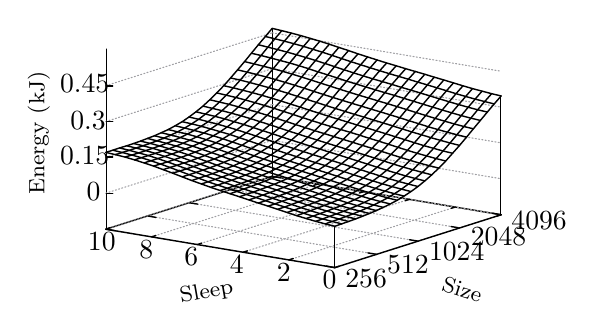
\begin{tikzpicture}[y=0.80pt, x=0.80pt, yscale=-0.570000, xscale=0.570000, inner sep=0pt, outer sep=0pt]
\begin{scope}[draw=black,line join=bevel,line cap=rect,even odd rule,line width=0.512pt]
  \begin{scope}[cm={{1.0,0.0,0.0,1.0,(0.0,0.0)}},draw=black,line join=bevel,line cap=rect,line width=0.512pt]
  \end{scope}
  \begin{scope}[cm={{1.00465,0.0,0.0,1.00465,(0.0,0.0)}},draw=black,line join=bevel,line cap=rect,line width=0.512pt]
  \end{scope}
  \begin{scope}[cm={{1.00465,0.0,0.0,1.00465,(0.0,0.0)}},draw=black,line join=round,line cap=round,line width=0.512pt]
    \path[draw] (59.1000,229.5000) -- (190.3000,187.8000);
    \path[draw] (370.9000,218.1000) -- (190.3000,187.8000);
    \path[draw] (59.5000,229.5000) -- (59.5000,87.5000);
    \path[draw] (190.5000,187.5000) -- (190.5000,71.5000);
    \path[draw] (370.5000,218.5000) -- (370.5000,124.5000);
  \end{scope}
  \begin{scope}[cm={{1.00465,0.0,0.0,1.00465,(0.0,0.0)}},draw=ca0a0a4,dash pattern=on 0.40pt off 0.80pt,line join=round,line cap=round,line width=0.400pt]
    \path[draw] (239.7000,259.8000) -- (59.1000,229.5000);
  \end{scope}
  \begin{scope}[cm={{1.00465,0.0,0.0,1.00465,(0.0,0.0)}},draw=black,line join=round,line cap=round,line width=0.512pt]
    \path[draw] (239.7000,259.8000) -- (232.9000,258.6000);
    \path[draw] (59.1000,229.5000) -- (65.8000,230.6000);
  \end{scope}
  \begin{scope}[cm={{1.00465,0.0,0.0,1.00465,(0.0,0.0)}},draw=black,line join=bevel,line cap=rect,line width=0.512pt]
  \end{scope}
  \begin{scope}[cm={{1.00465,0.0,0.0,1.00465,(249.153,276.781)}},draw=black,line join=bevel,line cap=rect,line width=0.512pt]
  \end{scope}
  \begin{scope}[cm={{1.00465,0.0,0.0,1.00465,(249.153,276.781)}},draw=black,line join=bevel,line cap=rect,line width=0.512pt]
  \end{scope}
  \begin{scope}[cm={{1.00465,0.0,0.0,1.00465,(249.153,276.781)}},draw=black,line join=bevel,line cap=rect,line width=0.512pt]
  \end{scope}
  \begin{scope}[cm={{1.00465,0.0,0.0,1.00465,(249.153,276.781)}},draw=black,line join=bevel,line cap=rect,line width=0.512pt]
  \end{scope}
  \begin{scope}[cm={{1.00465,0.0,0.0,1.00465,(249.153,276.781)}},draw=black,line join=bevel,line cap=rect,line width=0.512pt]
  \end{scope}
  \begin{scope}[cm={{1.00465,0.0,0.0,1.00465,(249.153,276.781)}},draw=black,line join=bevel,line cap=rect,line width=0.512pt]
    \path[fill=black] (0.0000,0.0000) node[above right] () {256};
  \end{scope}
  \begin{scope}[cm={{1.00465,0.0,0.0,1.00465,(249.153,276.781)}},draw=black,line join=bevel,line cap=rect,line width=0.512pt]
  \end{scope}
  \begin{scope}[cm={{1.00465,0.0,0.0,1.00465,(0.0,0.0)}},draw=black,line join=bevel,line cap=rect,line width=0.512pt]
  \end{scope}
  \begin{scope}[cm={{1.00465,0.0,0.0,1.00465,(0.0,0.0)}},draw=ca0a0a4,dash pattern=on 0.40pt off 0.80pt,line join=round,line cap=round,line width=0.400pt]
    \path[draw] (272.5000,249.3000) -- (91.9000,219.0000);
  \end{scope}
  \begin{scope}[cm={{1.00465,0.0,0.0,1.00465,(0.0,0.0)}},draw=black,line join=round,line cap=round,line width=0.512pt]
    \path[draw] (272.5000,249.3000) -- (265.8000,248.2000);
    \path[draw] (91.9000,219.0000) -- (98.6000,220.2000);
  \end{scope}
  \begin{scope}[cm={{1.00465,0.0,0.0,1.00465,(0.0,0.0)}},draw=black,line join=bevel,line cap=rect,line width=0.512pt]
  \end{scope}
  \begin{scope}[cm={{1.00465,0.0,0.0,1.00465,(282.307,265.73)}},draw=black,line join=bevel,line cap=rect,line width=0.512pt]
  \end{scope}
  \begin{scope}[cm={{1.00465,0.0,0.0,1.00465,(282.307,265.73)}},draw=black,line join=bevel,line cap=rect,line width=0.512pt]
  \end{scope}
  \begin{scope}[cm={{1.00465,0.0,0.0,1.00465,(282.307,265.73)}},draw=black,line join=bevel,line cap=rect,line width=0.512pt]
  \end{scope}
  \begin{scope}[cm={{1.00465,0.0,0.0,1.00465,(282.307,265.73)}},draw=black,line join=bevel,line cap=rect,line width=0.512pt]
  \end{scope}
  \begin{scope}[cm={{1.00465,0.0,0.0,1.00465,(282.307,265.73)}},draw=black,line join=bevel,line cap=rect,line width=0.512pt]
  \end{scope}
  \begin{scope}[cm={{1.00465,0.0,0.0,1.00465,(282.307,265.73)}},draw=black,line join=bevel,line cap=rect,line width=0.512pt]
    \path[fill=black] (0.0000,0.0000) node[above right] () {512};
  \end{scope}
  \begin{scope}[cm={{1.00465,0.0,0.0,1.00465,(282.307,265.73)}},draw=black,line join=bevel,line cap=rect,line width=0.512pt]
  \end{scope}
  \begin{scope}[cm={{1.00465,0.0,0.0,1.00465,(0.0,0.0)}},draw=black,line join=bevel,line cap=rect,line width=0.512pt]
  \end{scope}
  \begin{scope}[cm={{1.00465,0.0,0.0,1.00465,(0.0,0.0)}},draw=ca0a0a4,dash pattern=on 0.40pt off 0.80pt,line join=round,line cap=round,line width=0.400pt]
    \path[draw] (305.3000,238.9000) -- (124.7000,208.6000);
  \end{scope}
  \begin{scope}[cm={{1.00465,0.0,0.0,1.00465,(0.0,0.0)}},draw=black,line join=round,line cap=round,line width=0.512pt]
    \path[draw] (305.3000,238.9000) -- (298.6000,237.8000);
    \path[draw] (124.7000,208.6000) -- (131.4000,209.7000);
  \end{scope}
  \begin{scope}[cm={{1.00465,0.0,0.0,1.00465,(0.0,0.0)}},draw=black,line join=bevel,line cap=rect,line width=0.512pt]
  \end{scope}
  \begin{scope}[cm={{1.00465,0.0,0.0,1.00465,(315.46,255.684)}},draw=black,line join=bevel,line cap=rect,line width=0.512pt]
  \end{scope}
  \begin{scope}[cm={{1.00465,0.0,0.0,1.00465,(315.46,255.684)}},draw=black,line join=bevel,line cap=rect,line width=0.512pt]
  \end{scope}
  \begin{scope}[cm={{1.00465,0.0,0.0,1.00465,(315.46,255.684)}},draw=black,line join=bevel,line cap=rect,line width=0.512pt]
  \end{scope}
  \begin{scope}[cm={{1.00465,0.0,0.0,1.00465,(315.46,255.684)}},draw=black,line join=bevel,line cap=rect,line width=0.512pt]
  \end{scope}
  \begin{scope}[cm={{1.00465,0.0,0.0,1.00465,(315.46,255.684)}},draw=black,line join=bevel,line cap=rect,line width=0.512pt]
  \end{scope}
  \begin{scope}[cm={{1.00465,0.0,0.0,1.00465,(315.46,255.684)}},draw=black,line join=bevel,line cap=rect,line width=0.512pt]
    \path[fill=black] (0.0000,0.0000) node[above right] () {1024};
  \end{scope}
  \begin{scope}[cm={{1.00465,0.0,0.0,1.00465,(315.46,255.684)}},draw=black,line join=bevel,line cap=rect,line width=0.512pt]
  \end{scope}
  \begin{scope}[cm={{1.00465,0.0,0.0,1.00465,(0.0,0.0)}},draw=black,line join=bevel,line cap=rect,line width=0.512pt]
  \end{scope}
  \begin{scope}[cm={{1.00465,0.0,0.0,1.00465,(0.0,0.0)}},draw=ca0a0a4,dash pattern=on 0.40pt off 0.80pt,line join=round,line cap=round,line width=0.400pt]
    \path[draw] (338.1000,228.5000) -- (157.5000,198.2000);
  \end{scope}
  \begin{scope}[cm={{1.00465,0.0,0.0,1.00465,(0.0,0.0)}},draw=black,line join=round,line cap=round,line width=0.512pt]
    \path[draw] (338.1000,228.5000) -- (331.4000,227.4000);
    \path[draw] (157.5000,198.2000) -- (164.2000,199.3000);
  \end{scope}
  \begin{scope}[cm={{1.00465,0.0,0.0,1.00465,(0.0,0.0)}},draw=black,line join=bevel,line cap=rect,line width=0.512pt]
  \end{scope}
  \begin{scope}[cm={{1.00465,0.0,0.0,1.00465,(348.614,244.633)}},draw=black,line join=bevel,line cap=rect,line width=0.512pt]
  \end{scope}
  \begin{scope}[cm={{1.00465,0.0,0.0,1.00465,(348.614,244.633)}},draw=black,line join=bevel,line cap=rect,line width=0.512pt]
  \end{scope}
  \begin{scope}[cm={{1.00465,0.0,0.0,1.00465,(348.614,244.633)}},draw=black,line join=bevel,line cap=rect,line width=0.512pt]
  \end{scope}
  \begin{scope}[cm={{1.00465,0.0,0.0,1.00465,(348.614,244.633)}},draw=black,line join=bevel,line cap=rect,line width=0.512pt]
  \end{scope}
  \begin{scope}[cm={{1.00465,0.0,0.0,1.00465,(348.614,244.633)}},draw=black,line join=bevel,line cap=rect,line width=0.512pt]
  \end{scope}
  \begin{scope}[cm={{1.00465,0.0,0.0,1.00465,(348.614,243.133)}},draw=black,line join=bevel,line cap=rect,line width=0.512pt]
    \path[fill=black] (0.0000,0.0000) node[above right] () {2048};
  \end{scope}
  \begin{scope}[cm={{1.00465,0.0,0.0,1.00465,(348.614,244.633)}},draw=black,line join=bevel,line cap=rect,line width=0.512pt]
  \end{scope}
  \begin{scope}[cm={{1.00465,0.0,0.0,1.00465,(0.0,0.0)}},draw=black,line join=bevel,line cap=rect,line width=0.512pt]
  \end{scope}
  \begin{scope}[cm={{1.00465,0.0,0.0,1.00465,(0.0,0.0)}},draw=ca0a0a4,dash pattern=on 0.40pt off 0.80pt,line join=round,line cap=round,line width=0.400pt]
    \path[draw] (370.9000,218.1000) -- (190.3000,187.8000);
  \end{scope}
  \begin{scope}[cm={{1.00465,0.0,0.0,1.00465,(0.0,0.0)}},draw=black,line join=round,line cap=round,line width=0.512pt]
    \path[draw] (370.9000,218.1000) -- (364.2000,216.9000);
    \path[draw] (190.3000,187.8000) -- (197.1000,188.9000);
  \end{scope}
  \begin{scope}[cm={{1.00465,0.0,0.0,1.00465,(0.0,0.0)}},draw=black,line join=bevel,line cap=rect,line width=0.512pt]
  \end{scope}
  \begin{scope}[cm={{1.00465,0.0,0.0,1.00465,(380.763,234.586)}},draw=black,line join=bevel,line cap=rect,line width=0.512pt]
  \end{scope}
  \begin{scope}[cm={{1.00465,0.0,0.0,1.00465,(380.763,234.586)}},draw=black,line join=bevel,line cap=rect,line width=0.512pt]
  \end{scope}
  \begin{scope}[cm={{1.00465,0.0,0.0,1.00465,(380.763,234.586)}},draw=black,line join=bevel,line cap=rect,line width=0.512pt]
  \end{scope}
  \begin{scope}[cm={{1.00465,0.0,0.0,1.00465,(380.763,234.586)}},draw=black,line join=bevel,line cap=rect,line width=0.512pt]
  \end{scope}
  \begin{scope}[cm={{1.00465,0.0,0.0,1.00465,(380.763,234.586)}},draw=black,line join=bevel,line cap=rect,line width=0.512pt]
  \end{scope}
  \begin{scope}[cm={{1.00465,0.0,0.0,1.00465,(380.763,230.586)}},draw=black,line join=bevel,line cap=rect,line width=0.512pt]
    \path[fill=black] (0.0000,0.0000) node[above right] () {4096};
  \end{scope}
  \begin{scope}[cm={{1.00465,0.0,0.0,1.00465,(380.763,234.586)}},draw=black,line join=bevel,line cap=rect,line width=0.512pt]
  \end{scope}
  \begin{scope}[cm={{1.00465,0.0,0.0,1.00465,(0.0,0.0)}},draw=black,line join=bevel,line cap=rect,line width=0.512pt]
  \end{scope}
  \begin{scope}[cm={{1.00465,0.0,0.0,1.00465,(0.0,0.0)}},draw=ca0a0a4,dash pattern=on 0.40pt off 0.80pt,line join=round,line cap=round,line width=0.400pt]
    \path[draw] (239.7000,259.8000) -- (370.9000,218.1000);
  \end{scope}
  \begin{scope}[cm={{1.00465,0.0,0.0,1.00465,(0.0,0.0)}},draw=black,line join=round,line cap=round,line width=0.512pt]
    \path[draw] (239.7000,259.8000) -- (242.9000,258.7000);
    \path[draw] (370.9000,218.1000) -- (367.6000,219.1000);
  \end{scope}
  \begin{scope}[cm={{1.00465,0.0,0.0,1.00465,(0.0,0.0)}},draw=black,line join=bevel,line cap=rect,line width=0.512pt]
  \end{scope}
  \begin{scope}[cm={{1.00465,0.0,0.0,1.00465,(231.07,275.777)}},draw=black,line join=bevel,line cap=rect,line width=0.512pt]
  \end{scope}
  \begin{scope}[cm={{1.00465,0.0,0.0,1.00465,(231.07,275.777)}},draw=black,line join=bevel,line cap=rect,line width=0.512pt]
  \end{scope}
  \begin{scope}[cm={{1.00465,0.0,0.0,1.00465,(231.07,275.777)}},draw=black,line join=bevel,line cap=rect,line width=0.512pt]
  \end{scope}
  \begin{scope}[cm={{1.00465,0.0,0.0,1.00465,(231.07,275.777)}},draw=black,line join=bevel,line cap=rect,line width=0.512pt]
  \end{scope}
  \begin{scope}[cm={{1.00465,0.0,0.0,1.00465,(231.07,275.777)}},draw=black,line join=bevel,line cap=rect,line width=0.512pt]
  \end{scope}
  \begin{scope}[cm={{1.00465,0.0,0.0,1.00465,(231.07,277.777)}},draw=black,line join=bevel,line cap=rect,line width=0.512pt]
    \path[fill=black] (0.0000,0.0000) node[above right] () {0};
  \end{scope}
  \begin{scope}[cm={{1.00465,0.0,0.0,1.00465,(231.07,275.777)}},draw=black,line join=bevel,line cap=rect,line width=0.512pt]
  \end{scope}
  \begin{scope}[cm={{1.00465,0.0,0.0,1.00465,(0.0,0.0)}},draw=black,line join=bevel,line cap=rect,line width=0.512pt]
  \end{scope}
  \begin{scope}[cm={{1.00465,0.0,0.0,1.00465,(0.0,0.0)}},draw=ca0a0a4,dash pattern=on 0.40pt off 0.80pt,line join=round,line cap=round,line width=0.400pt]
    \path[draw] (203.6000,253.7000) -- (334.8000,212.0000);
  \end{scope}
  \begin{scope}[cm={{1.00465,0.0,0.0,1.00465,(0.0,0.0)}},draw=black,line join=round,line cap=round,line width=0.512pt]
    \path[draw] (203.6000,253.7000) -- (206.9000,252.6000);
    \path[draw] (334.8000,212.0000) -- (331.5000,213.0000);
  \end{scope}
  \begin{scope}[cm={{1.00465,0.0,0.0,1.00465,(0.0,0.0)}},draw=black,line join=bevel,line cap=rect,line width=0.512pt]
  \end{scope}
  \begin{scope}[cm={{1.00465,0.0,0.0,1.00465,(194.902,269.749)}},draw=black,line join=bevel,line cap=rect,line width=0.512pt]
  \end{scope}
  \begin{scope}[cm={{1.00465,0.0,0.0,1.00465,(194.902,269.749)}},draw=black,line join=bevel,line cap=rect,line width=0.512pt]
  \end{scope}
  \begin{scope}[cm={{1.00465,0.0,0.0,1.00465,(194.902,269.749)}},draw=black,line join=bevel,line cap=rect,line width=0.512pt]
  \end{scope}
  \begin{scope}[cm={{1.00465,0.0,0.0,1.00465,(194.902,269.749)}},draw=black,line join=bevel,line cap=rect,line width=0.512pt]
  \end{scope}
  \begin{scope}[cm={{1.00465,0.0,0.0,1.00465,(194.902,269.749)}},draw=black,line join=bevel,line cap=rect,line width=0.512pt]
  \end{scope}
  \begin{scope}[cm={{1.00465,0.0,0.0,1.00465,(194.902,271.749)}},draw=black,line join=bevel,line cap=rect,line width=0.512pt]
    \path[fill=black] (0.0000,0.0000) node[above right] () {2};
  \end{scope}
  \begin{scope}[cm={{1.00465,0.0,0.0,1.00465,(194.902,269.749)}},draw=black,line join=bevel,line cap=rect,line width=0.512pt]
  \end{scope}
  \begin{scope}[cm={{1.00465,0.0,0.0,1.00465,(0.0,0.0)}},draw=black,line join=bevel,line cap=rect,line width=0.512pt]
  \end{scope}
  \begin{scope}[cm={{1.00465,0.0,0.0,1.00465,(0.0,0.0)}},draw=ca0a0a4,dash pattern=on 0.40pt off 0.80pt,line join=round,line cap=round,line width=0.400pt]
    \path[draw] (167.5000,247.6000) -- (298.6000,205.9000);
  \end{scope}
  \begin{scope}[cm={{1.00465,0.0,0.0,1.00465,(0.0,0.0)}},draw=black,line join=round,line cap=round,line width=0.512pt]
    \path[draw] (167.5000,247.6000) -- (170.8000,246.6000);
    \path[draw] (298.6000,205.9000) -- (295.3000,207.0000);
  \end{scope}
  \begin{scope}[cm={{1.00465,0.0,0.0,1.00465,(0.0,0.0)}},draw=black,line join=bevel,line cap=rect,line width=0.512pt]
  \end{scope}
  \begin{scope}[cm={{1.00465,0.0,0.0,1.00465,(157.73,263.721)}},draw=black,line join=bevel,line cap=rect,line width=0.512pt]
  \end{scope}
  \begin{scope}[cm={{1.00465,0.0,0.0,1.00465,(157.73,263.721)}},draw=black,line join=bevel,line cap=rect,line width=0.512pt]
  \end{scope}
  \begin{scope}[cm={{1.00465,0.0,0.0,1.00465,(157.73,263.721)}},draw=black,line join=bevel,line cap=rect,line width=0.512pt]
  \end{scope}
  \begin{scope}[cm={{1.00465,0.0,0.0,1.00465,(157.73,263.721)}},draw=black,line join=bevel,line cap=rect,line width=0.512pt]
  \end{scope}
  \begin{scope}[cm={{1.00465,0.0,0.0,1.00465,(157.73,263.721)}},draw=black,line join=bevel,line cap=rect,line width=0.512pt]
  \end{scope}
  \begin{scope}[cm={{1.00465,0.0,0.0,1.00465,(157.73,265.721)}},draw=black,line join=bevel,line cap=rect,line width=0.512pt]
    \path[fill=black] (0.0000,0.0000) node[above right] () {4};
  \end{scope}
  \begin{scope}[cm={{1.00465,0.0,0.0,1.00465,(157.73,263.721)}},draw=black,line join=bevel,line cap=rect,line width=0.512pt]
  \end{scope}
  \begin{scope}[cm={{1.00465,0.0,0.0,1.00465,(0.0,0.0)}},draw=black,line join=bevel,line cap=rect,line width=0.512pt]
  \end{scope}
  \begin{scope}[cm={{1.00465,0.0,0.0,1.00465,(0.0,0.0)}},draw=ca0a0a4,dash pattern=on 0.40pt off 0.80pt,line join=round,line cap=round,line width=0.400pt]
    \path[draw] (131.4000,241.6000) -- (262.5000,199.9000);
  \end{scope}
  \begin{scope}[cm={{1.00465,0.0,0.0,1.00465,(0.0,0.0)}},draw=black,line join=round,line cap=round,line width=0.512pt]
    \path[draw] (131.4000,241.6000) -- (134.7000,240.5000);
    \path[draw] (262.5000,199.9000) -- (259.2000,200.9000);
  \end{scope}
  \begin{scope}[cm={{1.00465,0.0,0.0,1.00465,(0.0,0.0)}},draw=black,line join=bevel,line cap=rect,line width=0.512pt]
  \end{scope}
  \begin{scope}[cm={{1.00465,0.0,0.0,1.00465,(121.563,257.693)}},draw=black,line join=bevel,line cap=rect,line width=0.512pt]
  \end{scope}
  \begin{scope}[cm={{1.00465,0.0,0.0,1.00465,(121.563,257.693)}},draw=black,line join=bevel,line cap=rect,line width=0.512pt]
  \end{scope}
  \begin{scope}[cm={{1.00465,0.0,0.0,1.00465,(121.563,257.693)}},draw=black,line join=bevel,line cap=rect,line width=0.512pt]
  \end{scope}
  \begin{scope}[cm={{1.00465,0.0,0.0,1.00465,(121.563,257.693)}},draw=black,line join=bevel,line cap=rect,line width=0.512pt]
  \end{scope}
  \begin{scope}[cm={{1.00465,0.0,0.0,1.00465,(121.563,257.693)}},draw=black,line join=bevel,line cap=rect,line width=0.512pt]
  \end{scope}
  \begin{scope}[cm={{1.00465,0.0,0.0,1.00465,(121.563,259.693)}},draw=black,line join=bevel,line cap=rect,line width=0.512pt]
    \path[fill=black] (0.0000,0.0000) node[above right] () {6};
  \end{scope}
  \begin{scope}[cm={{1.00465,0.0,0.0,1.00465,(121.563,257.693)}},draw=black,line join=bevel,line cap=rect,line width=0.512pt]
  \end{scope}
  \begin{scope}[cm={{1.00465,0.0,0.0,1.00465,(0.0,0.0)}},draw=black,line join=bevel,line cap=rect,line width=0.512pt]
  \end{scope}
  \begin{scope}[cm={{1.00465,0.0,0.0,1.00465,(0.0,0.0)}},draw=ca0a0a4,dash pattern=on 0.40pt off 0.80pt,line join=round,line cap=round,line width=0.400pt]
    \path[draw] (95.2000,235.5000) -- (226.4000,193.8000);
  \end{scope}
  \begin{scope}[cm={{1.00465,0.0,0.0,1.00465,(0.0,0.0)}},draw=black,line join=round,line cap=round,line width=0.512pt]
    \path[draw] (95.2000,235.5000) -- (98.5000,234.5000);
    \path[draw] (226.4000,193.8000) -- (223.1000,194.9000);
  \end{scope}
  \begin{scope}[cm={{1.00465,0.0,0.0,1.00465,(0.0,0.0)}},draw=black,line join=bevel,line cap=rect,line width=0.512pt]
  \end{scope}
  \begin{scope}[cm={{1.00465,0.0,0.0,1.00465,(85.8977,251.665)}},draw=black,line join=bevel,line cap=rect,line width=0.512pt]
  \end{scope}
  \begin{scope}[cm={{1.00465,0.0,0.0,1.00465,(85.8977,251.665)}},draw=black,line join=bevel,line cap=rect,line width=0.512pt]
  \end{scope}
  \begin{scope}[cm={{1.00465,0.0,0.0,1.00465,(85.8977,251.665)}},draw=black,line join=bevel,line cap=rect,line width=0.512pt]
  \end{scope}
  \begin{scope}[cm={{1.00465,0.0,0.0,1.00465,(85.8977,251.665)}},draw=black,line join=bevel,line cap=rect,line width=0.512pt]
  \end{scope}
  \begin{scope}[cm={{1.00465,0.0,0.0,1.00465,(85.8977,251.665)}},draw=black,line join=bevel,line cap=rect,line width=0.512pt]
  \end{scope}
  \begin{scope}[cm={{1.00465,0.0,0.0,1.00465,(85.8977,253.665)}},draw=black,line join=bevel,line cap=rect,line width=0.512pt]
    \path[fill=black] (0.0000,0.0000) node[above right] () {8};
  \end{scope}
  \begin{scope}[cm={{1.00465,0.0,0.0,1.00465,(85.8977,251.665)}},draw=black,line join=bevel,line cap=rect,line width=0.512pt]
  \end{scope}
  \begin{scope}[cm={{1.00465,0.0,0.0,1.00465,(0.0,0.0)}},draw=black,line join=bevel,line cap=rect,line width=0.512pt]
  \end{scope}
  \begin{scope}[cm={{1.00465,0.0,0.0,1.00465,(0.0,0.0)}},draw=ca0a0a4,dash pattern=on 0.40pt off 0.80pt,line join=round,line cap=round,line width=0.400pt]
    \path[draw] (59.1000,229.5000) -- (190.3000,187.8000);
  \end{scope}
  \begin{scope}[cm={{1.00465,0.0,0.0,1.00465,(0.0,0.0)}},draw=black,line join=round,line cap=round,line width=0.512pt]
    \path[draw] (59.1000,229.5000) -- (62.4000,228.4000);
    \path[draw] (190.3000,187.8000) -- (187.1000,188.8000);
  \end{scope}
  \begin{scope}[cm={{1.00465,0.0,0.0,1.00465,(0.0,0.0)}},draw=black,line join=bevel,line cap=rect,line width=0.512pt]
  \end{scope}
  \begin{scope}[cm={{1.00465,0.0,0.0,1.00465,(45.2093,245.637)}},draw=black,line join=bevel,line cap=rect,line width=0.512pt]
  \end{scope}
  \begin{scope}[cm={{1.00465,0.0,0.0,1.00465,(45.2093,245.637)}},draw=black,line join=bevel,line cap=rect,line width=0.512pt]
  \end{scope}
  \begin{scope}[cm={{1.00465,0.0,0.0,1.00465,(45.2093,245.637)}},draw=black,line join=bevel,line cap=rect,line width=0.512pt]
  \end{scope}
  \begin{scope}[cm={{1.00465,0.0,0.0,1.00465,(45.2093,245.637)}},draw=black,line join=bevel,line cap=rect,line width=0.512pt]
  \end{scope}
  \begin{scope}[cm={{1.00465,0.0,0.0,1.00465,(45.2093,245.637)}},draw=black,line join=bevel,line cap=rect,line width=0.512pt]
  \end{scope}
  \begin{scope}[cm={{1.00465,0.0,0.0,1.00465,(45.2093,247.637)}},draw=black,line join=bevel,line cap=rect,line width=0.512pt]
    \path[fill=black] (0.0000,0.0000) node[above right] () {10};
  \end{scope}
  \begin{scope}[cm={{1.00465,0.0,0.0,1.00465,(45.2093,245.637)}},draw=black,line join=bevel,line cap=rect,line width=0.512pt]
  \end{scope}
  \begin{scope}[cm={{1.00465,0.0,0.0,1.00465,(0.0,0.0)}},draw=black,line join=bevel,line cap=rect,line width=0.512pt]
  \end{scope}
  \begin{scope}[cm={{1.00465,0.0,0.0,1.00465,(0.0,0.0)}},draw=ca0a0a4,dash pattern=on 0.40pt off 0.80pt,line join=round,line cap=round,line width=0.400pt]
    \path[draw] (59.1000,201.1000) -- (190.3000,159.4000);
    \path[draw] (190.3000,159.4000) -- (190.3000,159.4000) -- (370.9000,189.7000);
  \end{scope}
  \begin{scope}[cm={{1.00465,0.0,0.0,1.00465,(0.0,0.0)}},draw=black,line join=round,line cap=round,line width=0.512pt]
    \path[draw] (59.5000,201.5000) -- (64.5000,201.5000);
  \end{scope}
  \begin{scope}[cm={{1.00465,0.0,0.0,1.00465,(0.0,0.0)}},draw=black,line join=bevel,line cap=rect,line width=0.512pt]
  \end{scope}
  \begin{scope}[cm={{1.00465,0.0,0.0,1.00465,(40.186,207.46)}},draw=black,line join=bevel,line cap=rect,line width=0.512pt]
  \end{scope}
  \begin{scope}[cm={{1.00465,0.0,0.0,1.00465,(40.186,207.46)}},draw=black,line join=bevel,line cap=rect,line width=0.512pt]
  \end{scope}
  \begin{scope}[cm={{1.00465,0.0,0.0,1.00465,(40.186,207.46)}},draw=black,line join=bevel,line cap=rect,line width=0.512pt]
  \end{scope}
  \begin{scope}[cm={{1.00465,0.0,0.0,1.00465,(40.186,207.46)}},draw=black,line join=bevel,line cap=rect,line width=0.512pt]
  \end{scope}
  \begin{scope}[cm={{1.00465,0.0,0.0,1.00465,(40.186,207.46)}},draw=black,line join=bevel,line cap=rect,line width=0.512pt]
  \end{scope}
  \begin{scope}[cm={{1.00465,0.0,0.0,1.00465,(44.186,207.46)}},draw=black,line join=bevel,line cap=rect,line width=0.512pt]
    \path[fill=black] (0.0000,0.0000) node[above right] () {0};
  \end{scope}
  \begin{scope}[cm={{1.00465,0.0,0.0,1.00465,(40.186,207.46)}},draw=black,line join=bevel,line cap=rect,line width=0.512pt]
  \end{scope}
  \begin{scope}[cm={{1.00465,0.0,0.0,1.00465,(0.0,0.0)}},draw=black,line join=bevel,line cap=rect,line width=0.512pt]
  \end{scope}
  \begin{scope}[cm={{1.00465,0.0,0.0,1.00465,(0.0,0.0)}},draw=ca0a0a4,dash pattern=on 0.40pt off 0.80pt,line join=round,line cap=round,line width=0.400pt]
    \path[draw] (59.1000,172.8000) -- (190.3000,131.2000);
    \path[draw] (190.3000,131.2000) -- (190.3000,131.2000) -- (370.9000,161.4000);
  \end{scope}
  \begin{scope}[cm={{1.00465,0.0,0.0,1.00465,(0.0,0.0)}},draw=black,line join=round,line cap=round,line width=0.512pt]
    \path[draw] (59.5000,172.5000) -- (64.5000,172.5000);
  \end{scope}
  \begin{scope}[cm={{1.00465,0.0,0.0,1.00465,(0.0,0.0)}},draw=black,line join=bevel,line cap=rect,line width=0.512pt]
  \end{scope}
  \begin{scope}[cm={{1.00465,0.0,0.0,1.00465,(29.1349,179.33)}},draw=black,line join=bevel,line cap=rect,line width=0.512pt]
  \end{scope}
  \begin{scope}[cm={{1.00465,0.0,0.0,1.00465,(29.1349,179.33)}},draw=black,line join=bevel,line cap=rect,line width=0.512pt]
  \end{scope}
  \begin{scope}[cm={{1.00465,0.0,0.0,1.00465,(29.1349,179.33)}},draw=black,line join=bevel,line cap=rect,line width=0.512pt]
  \end{scope}
  \begin{scope}[cm={{1.00465,0.0,0.0,1.00465,(29.1349,179.33)}},draw=black,line join=bevel,line cap=rect,line width=0.512pt]
  \end{scope}
  \begin{scope}[cm={{1.00465,0.0,0.0,1.00465,(29.1349,179.33)}},draw=black,line join=bevel,line cap=rect,line width=0.512pt]
  \end{scope}
  \begin{scope}[cm={{1.00465,0.0,0.0,1.00465,(23.1349,179.33)}},draw=black,line join=bevel,line cap=rect,line width=0.512pt]
    \path[fill=black] (0.0000,0.0000) node[above right] () {0.15};
  \end{scope}
  \begin{scope}[cm={{1.00465,0.0,0.0,1.00465,(29.1349,179.33)}},draw=black,line join=bevel,line cap=rect,line width=0.512pt]
  \end{scope}
  \begin{scope}[cm={{1.00465,0.0,0.0,1.00465,(0.0,0.0)}},draw=black,line join=bevel,line cap=rect,line width=0.512pt]
  \end{scope}
  \begin{scope}[cm={{1.00465,0.0,0.0,1.00465,(0.0,0.0)}},draw=ca0a0a4,dash pattern=on 0.40pt off 0.80pt,line join=round,line cap=round,line width=0.400pt]
    \path[draw] (59.1000,144.6000) -- (190.3000,102.9000);
    \path[draw] (190.3000,102.9000) -- (190.3000,102.9000) -- (370.9000,133.2000);
  \end{scope}
  \begin{scope}[cm={{1.00465,0.0,0.0,1.00465,(0.0,0.0)}},draw=black,line join=round,line cap=round,line width=0.512pt]
    \path[draw] (59.5000,144.5000) -- (64.5000,144.5000);
  \end{scope}
  \begin{scope}[cm={{1.00465,0.0,0.0,1.00465,(0.0,0.0)}},draw=black,line join=bevel,line cap=rect,line width=0.512pt]
  \end{scope}
  \begin{scope}[cm={{1.00465,0.0,0.0,1.00465,(41.1907,151.2)}},draw=black,line join=bevel,line cap=rect,line width=0.512pt]
  \end{scope}
  \begin{scope}[cm={{1.00465,0.0,0.0,1.00465,(41.1907,151.2)}},draw=black,line join=bevel,line cap=rect,line width=0.512pt]
  \end{scope}
  \begin{scope}[cm={{1.00465,0.0,0.0,1.00465,(41.1907,151.2)}},draw=black,line join=bevel,line cap=rect,line width=0.512pt]
  \end{scope}
  \begin{scope}[cm={{1.00465,0.0,0.0,1.00465,(41.1907,151.2)}},draw=black,line join=bevel,line cap=rect,line width=0.512pt]
  \end{scope}
  \begin{scope}[cm={{1.00465,0.0,0.0,1.00465,(41.1907,151.2)}},draw=black,line join=bevel,line cap=rect,line width=0.512pt]
  \end{scope}
  \begin{scope}[cm={{1.00465,0.0,0.0,1.00465,(31.1907,151.2)}},draw=black,line join=bevel,line cap=rect,line width=0.512pt]
    \path[fill=black] (0.0000,0.0000) node[above right] () {0.3};
  \end{scope}
  \begin{scope}[cm={{1.00465,0.0,0.0,1.00465,(41.1907,151.2)}},draw=black,line join=bevel,line cap=rect,line width=0.512pt]
  \end{scope}
  \begin{scope}[cm={{1.00465,0.0,0.0,1.00465,(0.0,0.0)}},draw=black,line join=bevel,line cap=rect,line width=0.512pt]
  \end{scope}
  \begin{scope}[cm={{1.00465,0.0,0.0,1.00465,(0.0,0.0)}},draw=ca0a0a4,dash pattern=on 0.40pt off 0.80pt,line join=round,line cap=round,line width=0.400pt]
    \path[draw] (59.1000,116.3000) -- (190.3000,74.6000);
    \path[draw] (190.3000,74.6000) -- (190.3000,74.6000) -- (370.9000,104.9000);
  \end{scope}
  \begin{scope}[cm={{1.00465,0.0,0.0,1.00465,(0.0,0.0)}},draw=black,line join=round,line cap=round,line width=0.512pt]
    \path[draw] (59.5000,116.5000) -- (64.5000,116.5000);
  \end{scope}
  \begin{scope}[cm={{1.00465,0.0,0.0,1.00465,(0.0,0.0)}},draw=black,line join=bevel,line cap=rect,line width=0.512pt]
  \end{scope}
  \begin{scope}[cm={{1.00465,0.0,0.0,1.00465,(29.1349,122.065)}},draw=black,line join=bevel,line cap=rect,line width=0.512pt]
  \end{scope}
  \begin{scope}[cm={{1.00465,0.0,0.0,1.00465,(29.1349,122.065)}},draw=black,line join=bevel,line cap=rect,line width=0.512pt]
  \end{scope}
  \begin{scope}[cm={{1.00465,0.0,0.0,1.00465,(29.1349,122.065)}},draw=black,line join=bevel,line cap=rect,line width=0.512pt]
  \end{scope}
  \begin{scope}[cm={{1.00465,0.0,0.0,1.00465,(29.1349,122.065)}},draw=black,line join=bevel,line cap=rect,line width=0.512pt]
  \end{scope}
  \begin{scope}[cm={{1.00465,0.0,0.0,1.00465,(29.1349,122.065)}},draw=black,line join=bevel,line cap=rect,line width=0.512pt]
  \end{scope}
  \begin{scope}[cm={{1.00465,0.0,0.0,1.00465,(23.1349,122.065)}},draw=black,line join=bevel,line cap=rect,line width=0.512pt]
    \path[fill=black] (0.0000,0.0000) node[above right] () {0.45};
  \end{scope}
  \begin{scope}[cm={{1.00465,0.0,0.0,1.00465,(29.1349,122.065)}},draw=black,line join=bevel,line cap=rect,line width=0.512pt]
  \end{scope}
  \begin{scope}[cm={{0.0,-1.00465,1.00465,0.0,(15.5721,196.409)}},draw=black,line join=bevel,line cap=rect,line width=0.512pt]
  \end{scope}
  \begin{scope}[cm={{0.0,-1.00465,1.00465,0.0,(15.5721,196.409)}},draw=black,line join=bevel,line cap=rect,line width=0.512pt]
  \end{scope}
  \begin{scope}[cm={{0.0,-1.00465,1.00465,0.0,(15.5721,196.409)}},draw=black,line join=bevel,line cap=rect,line width=0.512pt]
  \end{scope}
  \begin{scope}[cm={{0.0,-1.00465,1.00465,0.0,(15.5721,196.409)}},draw=black,line join=bevel,line cap=rect,line width=0.512pt]
  \end{scope}
  \begin{scope}[cm={{0.0,-1.00465,1.00465,0.0,(15.5721,196.409)}},draw=black,line join=bevel,line cap=rect,line width=0.512pt]
  \end{scope}
  \begin{scope}[cm={{0.0,-1.00465,1.00465,0.0,(-2.5721,203.298)}},draw=black,line join=bevel,line cap=rect,line width=0.512pt]
    \path[fill=black] (0.0000,0.0000) node[above right] () {\rotatebox{90}{\footnotesize Energy (kJ)}};
  \end{scope}
  \begin{scope}[cm={{0.0,-1.00465,1.00465,0.0,(15.5721,196.409)}},draw=black,line join=bevel,line cap=rect,line width=0.512pt]
  \end{scope}
  \begin{scope}[cm={{1.00465,0.0,0.0,1.00465,(0.0,0.0)}},draw=black,line join=bevel,line cap=rect,line width=0.512pt]
  \end{scope}
  \begin{scope}[cm={{1.00465,0.0,0.0,1.00465,(0.0,0.0)}},draw=black,line join=bevel,line cap=rect,line width=0.512pt]
  \end{scope}
  \begin{scope}[cm={{1.00465,0.0,0.0,1.00465,(0.0,0.0)}},draw=black,line join=bevel,line cap=rect,line width=0.512pt]
  \end{scope}
  \begin{scope}[cm={{1.00465,0.0,0.0,1.00465,(0.0,0.0)}},draw=black,line join=round,line cap=round,line width=0.512pt]
    \path[draw] (370.9000,124.4000) -- (363.4000,122.6000) -- (363.4000,122.6000) --
      (355.8000,120.6000) -- (355.8000,120.6000) -- (348.3000,118.6000) --
      (348.3000,118.6000) -- (340.8000,116.4000) -- (340.8000,116.4000) --
      (333.3000,114.1000) -- (333.3000,114.1000) -- (325.7000,111.8000) --
      (325.7000,111.8000) -- (318.2000,109.6000) -- (318.2000,109.6000) --
      (310.7000,107.3000) -- (310.7000,107.3000) -- (303.2000,105.1000) --
      (303.2000,105.1000) -- (295.6000,102.9000) -- (295.6000,102.9000) --
      (288.1000,100.6000) -- (288.1000,100.6000) -- (280.6000,98.4000) --
      (280.6000,98.4000) -- (273.0000,96.0000) -- (273.0000,96.0000) --
      (265.5000,93.6000) -- (265.5000,93.6000) -- (258.0000,91.2000) --
      (258.0000,91.2000) -- (250.5000,88.6000) -- (250.5000,88.6000) --
      (242.9000,86.1000) -- (242.9000,86.1000) -- (235.4000,83.6000) --
      (235.4000,83.6000) -- (227.9000,81.2000) -- (227.9000,81.2000) --
      (220.4000,79.0000) -- (220.4000,79.0000) -- (212.9000,76.8000) --
      (212.9000,76.8000) -- (205.4000,74.8000) -- (205.4000,74.8000) --
      (197.9000,72.9000) -- (197.9000,72.9000) -- (190.3000,71.1000);
    \path[draw] (365.4000,130.7000) -- (357.9000,128.8000) -- (357.9000,128.8000) --
      (350.4000,126.9000) -- (350.4000,126.9000) -- (342.9000,124.8000) --
      (342.9000,124.8000) -- (335.3000,122.6000) -- (335.3000,122.6000) --
      (327.8000,120.3000) -- (327.8000,120.3000) -- (320.3000,118.0000) --
      (320.3000,118.0000) -- (312.7000,115.7000) -- (312.7000,115.7000) --
      (305.2000,113.5000) -- (305.2000,113.5000) -- (297.7000,111.2000) --
      (297.7000,111.2000) -- (290.2000,109.0000) -- (290.2000,109.0000) --
      (282.6000,106.8000) -- (282.6000,106.8000) -- (275.1000,104.5000) --
      (275.1000,104.5000) -- (267.6000,102.2000) -- (267.6000,102.2000) --
      (260.1000,99.8000) -- (260.1000,99.8000) -- (252.5000,97.4000) --
      (252.5000,97.4000) -- (245.0000,94.9000) -- (245.0000,94.9000) --
      (237.5000,92.4000) -- (237.5000,92.4000) -- (229.9000,89.9000) --
      (229.9000,89.9000) -- (222.4000,87.6000) -- (222.4000,87.6000) --
      (215.0000,85.3000) -- (215.0000,85.3000) -- (207.5000,83.2000) --
      (207.5000,83.2000) -- (199.9000,81.2000) -- (199.9000,81.2000) --
      (192.4000,79.3000) -- (192.4000,79.3000) -- (184.9000,77.5000);
    \path[draw] (360.0000,137.1000) -- (352.4000,135.3000) -- (352.4000,135.3000) --
      (344.9000,133.3000) -- (344.9000,133.3000) -- (337.4000,131.2000) --
      (337.4000,131.2000) -- (329.9000,129.0000) -- (329.9000,129.0000) --
      (322.3000,126.7000) -- (322.3000,126.7000) -- (314.8000,124.4000) --
      (314.8000,124.4000) -- (307.3000,122.1000) -- (307.3000,122.1000) --
      (299.7000,119.8000) -- (299.7000,119.8000) -- (292.2000,117.6000) --
      (292.2000,117.6000) -- (284.7000,115.3000) -- (284.7000,115.3000) --
      (277.2000,113.1000) -- (277.2000,113.1000) -- (269.6000,110.9000) --
      (269.6000,110.9000) -- (262.1000,108.6000) -- (262.1000,108.6000) --
      (254.6000,106.2000) -- (254.6000,106.2000) -- (247.1000,103.8000) --
      (247.1000,103.8000) -- (239.5000,101.3000) -- (239.5000,101.3000) --
      (232.0000,98.8000) -- (232.0000,98.8000) -- (224.5000,96.4000) --
      (224.5000,96.4000) -- (216.9000,94.1000) -- (216.9000,94.1000) --
      (209.5000,91.9000) -- (209.5000,91.9000) -- (202.0000,89.8000) --
      (202.0000,89.8000) -- (194.5000,87.8000) -- (194.5000,87.8000) --
      (186.9000,85.9000) -- (186.9000,85.9000) -- (179.4000,84.0000);
    \path[draw] (354.5000,143.7000) -- (347.0000,141.9000) -- (347.0000,141.9000) --
      (339.4000,139.9000) -- (339.4000,139.9000) -- (331.9000,137.7000) --
      (331.9000,137.7000) -- (324.4000,135.5000) -- (324.4000,135.5000) --
      (316.9000,133.2000) -- (316.9000,133.2000) -- (309.3000,130.9000) --
      (309.3000,130.9000) -- (301.8000,128.6000) -- (301.8000,128.6000) --
      (294.3000,126.3000) -- (294.3000,126.3000) -- (286.8000,124.0000) --
      (286.8000,124.0000) -- (279.2000,121.8000) -- (279.2000,121.8000) --
      (271.7000,119.6000) -- (271.7000,119.6000) -- (264.2000,117.3000) --
      (264.2000,117.3000) -- (256.6000,115.0000) -- (256.6000,115.0000) --
      (249.1000,112.7000) -- (249.1000,112.7000) -- (241.6000,110.2000) --
      (241.6000,110.2000) -- (234.1000,107.8000) -- (234.1000,107.8000) --
      (226.5000,105.4000) -- (226.5000,105.4000) -- (219.0000,102.9000) --
      (219.0000,102.9000) -- (211.6000,100.6000) -- (211.6000,100.6000) --
      (204.1000,98.4000) -- (204.1000,98.4000) -- (196.5000,96.4000) --
      (196.5000,96.4000) -- (189.0000,94.4000) -- (189.0000,94.4000) --
      (181.5000,92.5000) -- (181.5000,92.5000) -- (173.9000,90.7000);
    \path[draw] (349.0000,150.3000) -- (341.5000,148.5000) -- (341.5000,148.5000) --
      (334.0000,146.5000) -- (334.0000,146.5000) -- (326.4000,144.3000) --
      (326.4000,144.3000) -- (318.9000,142.1000) -- (318.9000,142.1000) --
      (311.4000,139.8000) -- (311.4000,139.8000) -- (303.9000,137.5000) --
      (303.9000,137.5000) -- (296.3000,135.1000) -- (296.3000,135.1000) --
      (288.8000,132.8000) -- (288.8000,132.8000) -- (281.3000,130.5000) --
      (281.3000,130.5000) -- (273.8000,128.3000) -- (273.8000,128.3000) --
      (266.2000,126.0000) -- (266.2000,126.0000) -- (258.7000,123.8000) --
      (258.7000,123.8000) -- (251.2000,121.5000) -- (251.2000,121.5000) --
      (243.6000,119.1000) -- (243.6000,119.1000) -- (236.1000,116.7000) --
      (236.1000,116.7000) -- (228.6000,114.3000) -- (228.6000,114.3000) --
      (221.1000,111.9000) -- (221.1000,111.9000) -- (213.6000,109.5000) --
      (213.6000,109.5000) -- (206.1000,107.2000) -- (206.1000,107.2000) --
      (198.6000,105.0000) -- (198.6000,105.0000) -- (191.1000,102.9000) --
      (191.1000,102.9000) -- (183.5000,101.0000) -- (183.5000,101.0000) --
      (176.0000,99.1000) -- (176.0000,99.1000) -- (168.5000,97.3000);
    \path[draw] (343.6000,156.9000) -- (336.0000,155.0000) -- (336.0000,155.0000) --
      (328.5000,153.0000) -- (328.5000,153.0000) -- (321.0000,150.9000) --
      (321.0000,150.9000) -- (313.4000,148.7000) -- (313.4000,148.7000) --
      (305.9000,146.3000) -- (305.9000,146.3000) -- (298.4000,144.0000) --
      (298.4000,144.0000) -- (290.9000,141.6000) -- (290.9000,141.6000) --
      (283.3000,139.3000) -- (283.3000,139.3000) -- (275.8000,137.0000) --
      (275.8000,137.0000) -- (268.3000,134.8000) -- (268.3000,134.8000) --
      (260.8000,132.5000) -- (260.8000,132.5000) -- (253.2000,130.2000) --
      (253.2000,130.2000) -- (245.7000,127.9000) -- (245.7000,127.9000) --
      (238.2000,125.6000) -- (238.2000,125.6000) -- (230.7000,123.2000) --
      (230.7000,123.2000) -- (223.1000,120.8000) -- (223.1000,120.8000) --
      (215.6000,118.3000) -- (215.6000,118.3000) -- (208.2000,116.0000) --
      (208.2000,116.0000) -- (200.6000,113.7000) -- (200.6000,113.7000) --
      (193.1000,111.5000) -- (193.1000,111.5000) -- (185.6000,109.4000) --
      (185.6000,109.4000) -- (178.1000,107.5000) -- (178.1000,107.5000) --
      (170.5000,105.6000) -- (170.5000,105.6000) -- (163.0000,103.8000);
    \path[draw] (338.1000,163.4000) -- (330.6000,161.5000) -- (330.6000,161.5000) --
      (323.0000,159.4000) -- (323.0000,159.4000) -- (315.5000,157.3000) --
      (315.5000,157.3000) -- (308.0000,155.0000) -- (308.0000,155.0000) --
      (300.5000,152.8000) -- (300.5000,152.8000) -- (292.9000,150.4000) --
      (292.9000,150.4000) -- (285.4000,148.1000) -- (285.4000,148.1000) --
      (277.9000,145.7000) -- (277.9000,145.7000) -- (270.3000,143.4000) --
      (270.3000,143.4000) -- (262.8000,141.1000) -- (262.8000,141.1000) --
      (255.3000,138.9000) -- (255.3000,138.9000) -- (247.8000,136.6000) --
      (247.8000,136.6000) -- (240.2000,134.3000) -- (240.2000,134.3000) --
      (232.7000,131.9000) -- (232.7000,131.9000) -- (225.2000,129.5000) --
      (225.2000,129.5000) -- (217.7000,127.1000) -- (217.7000,127.1000) --
      (210.2000,124.7000) -- (210.2000,124.7000) -- (202.7000,122.3000) --
      (202.7000,122.3000) -- (195.2000,120.0000) -- (195.2000,120.0000) --
      (187.6000,117.8000) -- (187.6000,117.8000) -- (180.1000,115.8000) --
      (180.1000,115.8000) -- (172.6000,113.8000) -- (172.6000,113.8000) --
      (165.1000,111.9000) -- (165.1000,111.9000) -- (157.5000,110.2000);
    \path[draw] (332.6000,169.6000) -- (325.1000,167.8000) -- (325.1000,167.8000) --
      (317.6000,165.7000) -- (317.6000,165.7000) -- (310.0000,163.6000) --
      (310.0000,163.6000) -- (302.5000,161.3000) -- (302.5000,161.3000) --
      (295.0000,158.9000) -- (295.0000,158.9000) -- (287.5000,156.6000) --
      (287.5000,156.6000) -- (279.9000,154.2000) -- (279.9000,154.2000) --
      (272.4000,151.9000) -- (272.4000,151.9000) -- (264.9000,149.6000) --
      (264.9000,149.6000) -- (257.3000,147.3000) -- (257.3000,147.3000) --
      (249.8000,145.0000) -- (249.8000,145.0000) -- (242.3000,142.7000) --
      (242.3000,142.7000) -- (234.8000,140.4000) -- (234.8000,140.4000) --
      (227.2000,138.0000) -- (227.2000,138.0000) -- (219.7000,135.6000) --
      (219.7000,135.6000) -- (212.3000,133.2000) -- (212.3000,133.2000) --
      (204.8000,130.8000) -- (204.8000,130.8000) -- (197.2000,128.4000) --
      (197.2000,128.4000) -- (189.7000,126.1000) -- (189.7000,126.1000) --
      (182.2000,123.9000) -- (182.2000,123.9000) -- (174.6000,121.8000) --
      (174.6000,121.8000) -- (167.1000,119.9000) -- (167.1000,119.9000) --
      (159.6000,118.0000) -- (159.6000,118.0000) -- (152.1000,116.3000);
    \path[draw] (327.2000,175.7000) -- (319.6000,173.8000) -- (319.6000,173.8000) --
      (312.1000,171.7000) -- (312.1000,171.7000) -- (304.6000,169.6000) --
      (304.6000,169.6000) -- (297.0000,167.3000) -- (297.0000,167.3000) --
      (289.5000,164.9000) -- (289.5000,164.9000) -- (282.0000,162.5000) --
      (282.0000,162.5000) -- (274.5000,160.1000) -- (274.5000,160.1000) --
      (266.9000,157.8000) -- (266.9000,157.8000) -- (259.4000,155.4000) --
      (259.4000,155.4000) -- (251.9000,153.1000) -- (251.9000,153.1000) --
      (244.4000,150.9000) -- (244.4000,150.9000) -- (236.8000,148.6000) --
      (236.8000,148.6000) -- (229.3000,146.3000) -- (229.3000,146.3000) --
      (221.8000,143.9000) -- (221.8000,143.9000) -- (214.3000,141.5000) --
      (214.3000,141.5000) -- (206.8000,139.0000) -- (206.8000,139.0000) --
      (199.3000,136.6000) -- (199.3000,136.6000) -- (191.8000,134.2000) --
      (191.8000,134.2000) -- (184.2000,131.9000) -- (184.2000,131.9000) --
      (176.7000,129.7000) -- (176.7000,129.7000) -- (169.2000,127.6000) --
      (169.2000,127.6000) -- (161.7000,125.6000) -- (161.7000,125.6000) --
      (154.1000,123.8000) -- (154.1000,123.8000) -- (146.6000,122.0000);
    \path[draw] (321.7000,181.3000) -- (314.2000,179.4000) -- (314.2000,179.4000) --
      (306.6000,177.4000) -- (306.6000,177.4000) -- (299.1000,175.2000) --
      (299.1000,175.2000) -- (291.6000,172.9000) -- (291.6000,172.9000) --
      (284.0000,170.5000) -- (284.0000,170.5000) -- (276.5000,168.1000) --
      (276.5000,168.1000) -- (269.0000,165.7000) -- (269.0000,165.7000) --
      (261.5000,163.4000) -- (261.5000,163.4000) -- (253.9000,161.0000) --
      (253.9000,161.0000) -- (246.4000,158.7000) -- (246.4000,158.7000) --
      (238.9000,156.4000) -- (238.9000,156.4000) -- (231.4000,154.1000) --
      (231.4000,154.1000) -- (223.8000,151.8000) -- (223.8000,151.8000) --
      (216.3000,149.4000) -- (216.3000,149.4000) -- (208.9000,147.0000) --
      (208.9000,147.0000) -- (201.3000,144.5000) -- (201.3000,144.5000) --
      (193.8000,142.1000) -- (193.8000,142.1000) -- (186.3000,139.6000) --
      (186.3000,139.6000) -- (178.8000,137.3000) -- (178.8000,137.3000) --
      (171.2000,135.1000) -- (171.2000,135.1000) -- (163.7000,133.0000) --
      (163.7000,133.0000) -- (156.2000,131.0000) -- (156.2000,131.0000) --
      (148.7000,129.2000) -- (148.7000,129.2000) -- (141.1000,127.4000);
    \path[draw] (316.2000,186.6000) -- (308.7000,184.7000) -- (308.7000,184.7000) --
      (301.2000,182.6000) -- (301.2000,182.6000) -- (293.6000,180.5000) --
      (293.6000,180.5000) -- (286.1000,178.2000) -- (286.1000,178.2000) --
      (278.6000,175.8000) -- (278.6000,175.8000) -- (271.1000,173.4000) --
      (271.1000,173.4000) -- (263.5000,171.0000) -- (263.5000,171.0000) --
      (256.0000,168.6000) -- (256.0000,168.6000) -- (248.5000,166.2000) --
      (248.5000,166.2000) -- (240.9000,163.9000) -- (240.9000,163.9000) --
      (233.4000,161.6000) -- (233.4000,161.6000) -- (225.9000,159.2000) --
      (225.9000,159.2000) -- (218.4000,156.9000) -- (218.4000,156.9000) --
      (210.9000,154.5000) -- (210.9000,154.5000) -- (203.4000,152.1000) --
      (203.4000,152.1000) -- (195.9000,149.6000) -- (195.9000,149.6000) --
      (188.4000,147.1000) -- (188.4000,147.1000) -- (180.8000,144.7000) --
      (180.8000,144.7000) -- (173.3000,142.3000) -- (173.3000,142.3000) --
      (165.8000,140.1000) -- (165.8000,140.1000) -- (158.2000,138.0000) --
      (158.2000,138.0000) -- (150.7000,136.0000) -- (150.7000,136.0000) --
      (143.2000,134.2000) -- (143.2000,134.2000) -- (135.7000,132.4000);
    \path[draw] (310.7000,191.4000) -- (303.2000,189.5000) -- (303.2000,189.5000) --
      (295.7000,187.5000) -- (295.7000,187.5000) -- (288.2000,185.3000) --
      (288.2000,185.3000) -- (280.6000,183.0000) -- (280.6000,183.0000) --
      (273.1000,180.6000) -- (273.1000,180.6000) -- (265.6000,178.2000) --
      (265.6000,178.2000) -- (258.1000,175.8000) -- (258.1000,175.8000) --
      (250.5000,173.4000) -- (250.5000,173.4000) -- (243.0000,171.0000) --
      (243.0000,171.0000) -- (235.5000,168.7000) -- (235.5000,168.7000) --
      (227.9000,166.3000) -- (227.9000,166.3000) -- (220.4000,164.0000) --
      (220.4000,164.0000) -- (213.0000,161.6000) -- (213.0000,161.6000) --
      (205.5000,159.2000) -- (205.5000,159.2000) -- (197.9000,156.7000) --
      (197.9000,156.7000) -- (190.4000,154.2000) -- (190.4000,154.2000) --
      (182.9000,151.8000) -- (182.9000,151.8000) -- (175.4000,149.3000) --
      (175.4000,149.3000) -- (167.8000,146.9000) -- (167.8000,146.9000) --
      (160.3000,144.7000) -- (160.3000,144.7000) -- (152.8000,142.5000) --
      (152.8000,142.5000) -- (145.2000,140.5000) -- (145.2000,140.5000) --
      (137.7000,138.7000) -- (137.7000,138.7000) -- (130.2000,136.9000);
    \path[draw] (305.3000,195.8000) -- (297.7000,193.9000) -- (297.7000,193.9000) --
      (290.2000,191.9000) -- (290.2000,191.9000) -- (282.7000,189.7000) --
      (282.7000,189.7000) -- (275.2000,187.4000) -- (275.2000,187.4000) --
      (267.6000,185.0000) -- (267.6000,185.0000) -- (260.1000,182.6000) --
      (260.1000,182.6000) -- (252.6000,180.2000) -- (252.6000,180.2000) --
      (245.1000,177.8000) -- (245.1000,177.8000) -- (237.5000,175.4000) --
      (237.5000,175.4000) -- (230.0000,173.0000) -- (230.0000,173.0000) --
      (222.5000,170.7000) -- (222.5000,170.7000) -- (215.0000,168.3000) --
      (215.0000,168.3000) -- (207.5000,165.9000) -- (207.5000,165.9000) --
      (200.0000,163.5000) -- (200.0000,163.5000) -- (192.5000,161.0000) --
      (192.5000,161.0000) -- (184.9000,158.5000) -- (184.9000,158.5000) --
      (177.4000,156.0000) -- (177.4000,156.0000) -- (169.9000,153.5000) --
      (169.9000,153.5000) -- (162.4000,151.1000) -- (162.4000,151.1000) --
      (154.8000,148.8000) -- (154.8000,148.8000) -- (147.3000,146.7000) --
      (147.3000,146.7000) -- (139.8000,144.7000) -- (139.8000,144.7000) --
      (132.3000,142.8000) -- (132.3000,142.8000) -- (124.7000,141.0000);
    \path[draw] (299.8000,199.8000) -- (292.3000,197.9000) -- (292.3000,197.9000) --
      (284.8000,195.9000) -- (284.8000,195.9000) -- (277.2000,193.7000) --
      (277.2000,193.7000) -- (269.7000,191.4000) -- (269.7000,191.4000) --
      (262.2000,189.0000) -- (262.2000,189.0000) -- (254.6000,186.6000) --
      (254.6000,186.6000) -- (247.1000,184.1000) -- (247.1000,184.1000) --
      (239.6000,181.7000) -- (239.6000,181.7000) -- (232.1000,179.3000) --
      (232.1000,179.3000) -- (224.5000,177.0000) -- (224.5000,177.0000) --
      (217.0000,174.6000) -- (217.0000,174.6000) -- (209.6000,172.3000) --
      (209.6000,172.3000) -- (202.1000,169.9000) -- (202.1000,169.9000) --
      (194.5000,167.4000) -- (194.5000,167.4000) -- (187.0000,164.9000) --
      (187.0000,164.9000) -- (179.5000,162.4000) -- (179.5000,162.4000) --
      (171.9000,159.8000) -- (171.9000,159.8000) -- (164.4000,157.3000) --
      (164.4000,157.3000) -- (156.9000,154.8000) -- (156.9000,154.8000) --
      (149.4000,152.6000) -- (149.4000,152.6000) -- (141.8000,150.4000) --
      (141.8000,150.4000) -- (134.3000,148.3000) -- (134.3000,148.3000) --
      (126.8000,146.4000) -- (126.8000,146.4000) -- (119.3000,144.7000);
    \path[draw] (294.3000,203.4000) -- (286.8000,201.5000) -- (286.8000,201.5000) --
      (279.3000,199.5000) -- (279.3000,199.5000) -- (271.8000,197.3000) --
      (271.8000,197.3000) -- (264.2000,195.0000) -- (264.2000,195.0000) --
      (256.7000,192.6000) -- (256.7000,192.6000) -- (249.2000,190.2000) --
      (249.2000,190.2000) -- (241.6000,187.7000) -- (241.6000,187.7000) --
      (234.1000,185.3000) -- (234.1000,185.3000) -- (226.6000,182.9000) --
      (226.6000,182.9000) -- (219.1000,180.6000) -- (219.1000,180.6000) --
      (211.6000,178.2000) -- (211.6000,178.2000) -- (204.1000,175.8000) --
      (204.1000,175.8000) -- (196.6000,173.4000) -- (196.6000,173.4000) --
      (189.1000,171.0000) -- (189.1000,171.0000) -- (181.5000,168.4000) --
      (181.5000,168.4000) -- (174.0000,165.9000) -- (174.0000,165.9000) --
      (166.5000,163.3000) -- (166.5000,163.3000) -- (158.9000,160.7000) --
      (158.9000,160.7000) -- (151.4000,158.2000) -- (151.4000,158.2000) --
      (143.9000,155.8000) -- (143.9000,155.8000) -- (136.4000,153.6000) --
      (136.4000,153.6000) -- (128.8000,151.6000) -- (128.8000,151.6000) --
      (121.3000,149.7000) -- (121.3000,149.7000) -- (113.8000,147.9000);
    \path[draw] (288.9000,206.7000) -- (281.3000,204.8000) -- (281.3000,204.8000) --
      (273.8000,202.7000) -- (273.8000,202.7000) -- (266.3000,200.6000) --
      (266.3000,200.6000) -- (258.8000,198.2000) -- (258.8000,198.2000) --
      (251.2000,195.8000) -- (251.2000,195.8000) -- (243.7000,193.4000) --
      (243.7000,193.4000) -- (236.2000,191.0000) -- (236.2000,191.0000) --
      (228.7000,188.5000) -- (228.7000,188.5000) -- (221.1000,186.1000) --
      (221.1000,186.1000) -- (213.7000,183.8000) -- (213.7000,183.8000) --
      (206.2000,181.4000) -- (206.2000,181.4000) -- (198.6000,179.0000) --
      (198.6000,179.0000) -- (191.1000,176.6000) -- (191.1000,176.6000) --
      (183.6000,174.2000) -- (183.6000,174.2000) -- (176.1000,171.6000) --
      (176.1000,171.6000) -- (168.5000,169.0000) -- (168.5000,169.0000) --
      (161.0000,166.4000) -- (161.0000,166.4000) -- (153.5000,163.8000) --
      (153.5000,163.8000) -- (146.0000,161.3000) -- (146.0000,161.3000) --
      (138.4000,158.9000) -- (138.4000,158.9000) -- (130.9000,156.6000) --
      (130.9000,156.6000) -- (123.4000,154.5000) -- (123.4000,154.5000) --
      (115.8000,152.7000) -- (115.8000,152.7000) -- (108.3000,150.9000);
    \path[draw] (283.4000,209.6000) -- (275.9000,207.7000) -- (275.9000,207.7000) --
      (268.3000,205.7000) -- (268.3000,205.7000) -- (260.8000,203.5000) --
      (260.8000,203.5000) -- (253.3000,201.2000) -- (253.3000,201.2000) --
      (245.8000,198.8000) -- (245.8000,198.8000) -- (238.2000,196.3000) --
      (238.2000,196.3000) -- (230.7000,193.9000) -- (230.7000,193.9000) --
      (223.2000,191.5000) -- (223.2000,191.5000) -- (215.7000,189.1000) --
      (215.7000,189.1000) -- (208.2000,186.7000) -- (208.2000,186.7000) --
      (200.7000,184.3000) -- (200.7000,184.3000) -- (193.2000,181.9000) --
      (193.2000,181.9000) -- (185.6000,179.5000) -- (185.6000,179.5000) --
      (178.1000,177.0000) -- (178.1000,177.0000) -- (170.6000,174.5000) --
      (170.6000,174.5000) -- (163.1000,171.9000) -- (163.1000,171.9000) --
      (155.5000,169.2000) -- (155.5000,169.2000) -- (148.0000,166.6000) --
      (148.0000,166.6000) -- (140.5000,164.0000) -- (140.5000,164.0000) --
      (133.0000,161.6000) -- (133.0000,161.6000) -- (125.4000,159.3000) --
      (125.4000,159.3000) -- (117.9000,157.2000) -- (117.9000,157.2000) --
      (110.4000,155.2000) -- (110.4000,155.2000) -- (102.8000,153.4000);
    \path[draw] (277.9000,212.3000) -- (270.4000,210.4000) -- (270.4000,210.4000) --
      (262.9000,208.4000) -- (262.9000,208.4000) -- (255.4000,206.2000) --
      (255.4000,206.2000) -- (247.8000,203.9000) -- (247.8000,203.9000) --
      (240.3000,201.5000) -- (240.3000,201.5000) -- (232.8000,199.0000) --
      (232.8000,199.0000) -- (225.2000,196.6000) -- (225.2000,196.6000) --
      (217.7000,194.1000) -- (217.7000,194.1000) -- (210.3000,191.7000) --
      (210.3000,191.7000) -- (202.8000,189.3000) -- (202.8000,189.3000) --
      (195.2000,187.0000) -- (195.2000,187.0000) -- (187.7000,184.6000) --
      (187.7000,184.6000) -- (180.2000,182.1000) -- (180.2000,182.1000) --
      (172.7000,179.6000) -- (172.7000,179.6000) -- (165.1000,177.1000) --
      (165.1000,177.1000) -- (157.6000,174.4000) -- (157.6000,174.4000) --
      (150.1000,171.7000) -- (150.1000,171.7000) -- (142.5000,169.1000) --
      (142.5000,169.1000) -- (135.0000,166.5000) -- (135.0000,166.5000) --
      (127.5000,164.0000) -- (127.5000,164.0000) -- (120.0000,161.7000) --
      (120.0000,161.7000) -- (112.4000,159.6000) -- (112.4000,159.6000) --
      (104.9000,157.6000) -- (104.9000,157.6000) -- (97.4000,155.8000);
    \path[draw] (272.5000,214.8000) -- (264.9000,212.9000) -- (264.9000,212.9000) --
      (257.4000,210.9000) -- (257.4000,210.9000) -- (249.9000,208.7000) --
      (249.9000,208.7000) -- (242.4000,206.4000) -- (242.4000,206.4000) --
      (234.8000,204.0000) -- (234.8000,204.0000) -- (227.3000,201.5000) --
      (227.3000,201.5000) -- (219.8000,199.0000) -- (219.8000,199.0000) --
      (212.3000,196.6000) -- (212.3000,196.6000) -- (204.8000,194.2000) --
      (204.8000,194.2000) -- (197.3000,191.8000) -- (197.3000,191.8000) --
      (189.8000,189.4000) -- (189.8000,189.4000) -- (182.2000,187.0000) --
      (182.2000,187.0000) -- (174.7000,184.6000) -- (174.7000,184.6000) --
      (167.2000,182.1000) -- (167.2000,182.1000) -- (159.7000,179.5000) --
      (159.7000,179.5000) -- (152.1000,176.8000) -- (152.1000,176.8000) --
      (144.6000,174.1000) -- (144.6000,174.1000) -- (137.1000,171.4000) --
      (137.1000,171.4000) -- (129.5000,168.7000) -- (129.5000,168.7000) --
      (122.0000,166.2000) -- (122.0000,166.2000) -- (114.5000,163.9000) --
      (114.5000,163.9000) -- (107.0000,161.8000) -- (107.0000,161.8000) --
      (99.4000,159.8000) -- (99.4000,159.8000) -- (91.9000,157.9000);
    \path[draw] (267.0000,217.1000) -- (259.5000,215.2000) -- (259.5000,215.2000) --
      (251.9000,213.2000) -- (251.9000,213.2000) -- (244.4000,211.0000) --
      (244.4000,211.0000) -- (236.9000,208.7000) -- (236.9000,208.7000) --
      (229.4000,206.3000) -- (229.4000,206.3000) -- (221.8000,203.8000) --
      (221.8000,203.8000) -- (214.4000,201.3000) -- (214.4000,201.3000) --
      (206.9000,198.9000) -- (206.9000,198.9000) -- (199.3000,196.5000) --
      (199.3000,196.5000) -- (191.8000,194.1000) -- (191.8000,194.1000) --
      (184.3000,191.7000) -- (184.3000,191.7000) -- (176.8000,189.3000) --
      (176.8000,189.3000) -- (169.2000,186.8000) -- (169.2000,186.8000) --
      (161.7000,184.3000) -- (161.7000,184.3000) -- (154.2000,181.7000) --
      (154.2000,181.7000) -- (146.7000,179.0000) -- (146.7000,179.0000) --
      (139.1000,176.2000) -- (139.1000,176.2000) -- (131.6000,173.5000) --
      (131.6000,173.5000) -- (124.1000,170.8000) -- (124.1000,170.8000) --
      (116.6000,168.3000) -- (116.6000,168.3000) -- (109.0000,166.0000) --
      (109.0000,166.0000) -- (101.5000,163.8000) -- (101.5000,163.8000) --
      (94.0000,161.8000) -- (94.0000,161.8000) -- (86.4000,160.0000);
    \path[draw] (261.5000,219.3000) -- (254.0000,217.4000) -- (254.0000,217.4000) --
      (246.5000,215.4000) -- (246.5000,215.4000) -- (238.9000,213.2000) --
      (238.9000,213.2000) -- (231.4000,210.8000) -- (231.4000,210.8000) --
      (223.9000,208.4000) -- (223.9000,208.4000) -- (216.4000,206.0000) --
      (216.4000,206.0000) -- (208.9000,203.5000) -- (208.9000,203.5000) --
      (201.4000,201.0000) -- (201.4000,201.0000) -- (193.9000,198.6000) --
      (193.9000,198.6000) -- (186.4000,196.2000) -- (186.4000,196.2000) --
      (178.8000,193.8000) -- (178.8000,193.8000) -- (171.3000,191.4000) --
      (171.3000,191.4000) -- (163.8000,188.9000) -- (163.8000,188.9000) --
      (156.2000,186.4000) -- (156.2000,186.4000) -- (148.7000,183.7000) --
      (148.7000,183.7000) -- (141.2000,181.0000) -- (141.2000,181.0000) --
      (133.7000,178.2000) -- (133.7000,178.2000) -- (126.1000,175.5000) --
      (126.1000,175.5000) -- (118.6000,172.8000) -- (118.6000,172.8000) --
      (111.1000,170.2000) -- (111.1000,170.2000) -- (103.6000,167.9000) --
      (103.6000,167.9000) -- (96.0000,165.7000) -- (96.0000,165.7000) --
      (88.5000,163.7000) -- (88.5000,163.7000) -- (81.0000,161.9000);
    \path[draw] (256.1000,221.4000) -- (248.5000,219.5000) -- (248.5000,219.5000) --
      (241.0000,217.4000) -- (241.0000,217.4000) -- (233.5000,215.2000) --
      (233.5000,215.2000) -- (225.9000,212.9000) -- (225.9000,212.9000) --
      (218.4000,210.5000) -- (218.4000,210.5000) -- (211.0000,208.0000) --
      (211.0000,208.0000) -- (203.5000,205.6000) -- (203.5000,205.6000) --
      (195.9000,203.1000) -- (195.9000,203.1000) -- (188.4000,200.6000) --
      (188.4000,200.6000) -- (180.9000,198.2000) -- (180.9000,198.2000) --
      (173.4000,195.8000) -- (173.4000,195.8000) -- (165.8000,193.4000) --
      (165.8000,193.4000) -- (158.3000,190.9000) -- (158.3000,190.9000) --
      (150.8000,188.3000) -- (150.8000,188.3000) -- (143.2000,185.7000) --
      (143.2000,185.7000) -- (135.7000,182.9000) -- (135.7000,182.9000) --
      (128.2000,180.1000) -- (128.2000,180.1000) -- (120.7000,177.3000) --
      (120.7000,177.3000) -- (113.1000,174.6000) -- (113.1000,174.6000) --
      (105.6000,172.1000) -- (105.6000,172.1000) -- (98.1000,169.7000) --
      (98.1000,169.7000) -- (90.6000,167.5000) -- (90.6000,167.5000) --
      (83.0000,165.5000) -- (83.0000,165.5000) -- (75.5000,163.7000);
    \path[draw] (250.6000,223.4000) -- (243.1000,221.5000) -- (243.1000,221.5000) --
      (235.5000,219.4000) -- (235.5000,219.4000) -- (228.0000,217.2000) --
      (228.0000,217.2000) -- (220.5000,214.9000) -- (220.5000,214.9000) --
      (213.1000,212.5000) -- (213.1000,212.5000) -- (205.5000,210.0000) --
      (205.5000,210.0000) -- (198.0000,207.5000) -- (198.0000,207.5000) --
      (190.5000,205.1000) -- (190.5000,205.1000) -- (182.9000,202.6000) --
      (182.9000,202.6000) -- (175.4000,200.2000) -- (175.4000,200.2000) --
      (167.9000,197.8000) -- (167.9000,197.8000) -- (160.4000,195.3000) --
      (160.4000,195.3000) -- (152.8000,192.8000) -- (152.8000,192.8000) --
      (145.3000,190.2000) -- (145.3000,190.2000) -- (137.8000,187.5000) --
      (137.8000,187.5000) -- (130.3000,184.7000) -- (130.3000,184.7000) --
      (122.7000,181.9000) -- (122.7000,181.9000) -- (115.2000,179.1000) --
      (115.2000,179.1000) -- (107.7000,176.4000) -- (107.7000,176.4000) --
      (100.1000,173.8000) -- (100.1000,173.8000) -- (92.6000,171.4000) --
      (92.6000,171.4000) -- (85.1000,169.3000) -- (85.1000,169.3000) --
      (77.6000,167.3000) -- (77.6000,167.3000) -- (70.0000,165.4000);
    \path[draw] (245.1000,225.3000) -- (237.6000,223.4000) -- (237.6000,223.4000) --
      (230.1000,221.4000) -- (230.1000,221.4000) -- (222.5000,219.2000) --
      (222.5000,219.2000) -- (215.0000,216.9000) -- (215.0000,216.9000) --
      (207.6000,214.4000) -- (207.6000,214.4000) -- (200.1000,212.0000) --
      (200.1000,212.0000) -- (192.5000,209.5000) -- (192.5000,209.5000) --
      (185.0000,207.0000) -- (185.0000,207.0000) -- (177.5000,204.5000) --
      (177.5000,204.5000) -- (169.9000,202.1000) -- (169.9000,202.1000) --
      (162.4000,199.7000) -- (162.4000,199.7000) -- (154.9000,197.2000) --
      (154.9000,197.2000) -- (147.4000,194.7000) -- (147.4000,194.7000) --
      (139.8000,192.1000) -- (139.8000,192.1000) -- (132.3000,189.3000) --
      (132.3000,189.3000) -- (124.8000,186.5000) -- (124.8000,186.5000) --
      (117.3000,183.7000) -- (117.3000,183.7000) -- (109.7000,180.8000) --
      (109.7000,180.8000) -- (102.2000,178.1000) -- (102.2000,178.1000) --
      (94.7000,175.5000) -- (94.7000,175.5000) -- (87.1000,173.1000) --
      (87.1000,173.1000) -- (79.6000,171.0000) -- (79.6000,171.0000) --
      (72.1000,169.0000) -- (72.1000,169.0000) -- (64.6000,167.2000);
    \path[draw] (239.7000,227.2000) -- (232.1000,225.3000) -- (232.1000,225.3000) --
      (224.6000,223.3000) -- (224.6000,223.3000) -- (217.1000,221.1000) --
      (217.1000,221.1000) -- (209.6000,218.8000) -- (209.6000,218.8000) --
      (202.1000,216.3000) -- (202.1000,216.3000) -- (194.6000,213.8000) --
      (194.6000,213.8000) -- (187.1000,211.3000) -- (187.1000,211.3000) --
      (179.5000,208.9000) -- (179.5000,208.9000) -- (172.0000,206.4000) --
      (172.0000,206.4000) -- (164.5000,203.9000) -- (164.5000,203.9000) --
      (157.0000,201.5000) -- (157.0000,201.5000) -- (149.4000,199.0000) --
      (149.4000,199.0000) -- (141.9000,196.5000) -- (141.9000,196.5000) --
      (134.4000,193.8000) -- (134.4000,193.8000) -- (126.8000,191.1000) --
      (126.8000,191.1000) -- (119.3000,188.2000) -- (119.3000,188.2000) --
      (111.8000,185.3000) -- (111.8000,185.3000) -- (104.3000,182.5000) --
      (104.3000,182.5000) -- (96.7000,179.7000) -- (96.7000,179.7000) --
      (89.2000,177.2000) -- (89.2000,177.2000) -- (81.7000,174.8000) --
      (81.7000,174.8000) -- (74.2000,172.6000) -- (74.2000,172.6000) --
      (66.6000,170.7000) -- (66.6000,170.7000) -- (59.1000,168.9000);
    \path[draw] (190.3000,71.1000) -- (184.9000,77.5000) -- (184.9000,77.5000) --
      (179.4000,84.0000) -- (179.4000,84.0000) -- (173.9000,90.7000) --
      (173.9000,90.7000) -- (168.5000,97.3000) -- (168.5000,97.3000) --
      (163.0000,103.8000) -- (163.0000,103.8000) -- (157.5000,110.2000) --
      (157.5000,110.2000) -- (152.1000,116.3000) -- (152.1000,116.3000) --
      (146.6000,122.0000) -- (146.6000,122.0000) -- (141.1000,127.4000) --
      (141.1000,127.4000) -- (135.7000,132.4000) -- (135.7000,132.4000) --
      (130.2000,136.9000) -- (130.2000,136.9000) -- (124.7000,141.0000) --
      (124.7000,141.0000) -- (119.3000,144.7000) -- (119.3000,144.7000) --
      (113.8000,147.9000) -- (113.8000,147.9000) -- (108.3000,150.9000) --
      (108.3000,150.9000) -- (102.8000,153.4000) -- (102.8000,153.4000) --
      (97.4000,155.8000) -- (97.4000,155.8000) -- (91.9000,157.9000) --
      (91.9000,157.9000) -- (86.4000,160.0000) -- (86.4000,160.0000) --
      (81.0000,161.9000) -- (81.0000,161.9000) -- (75.5000,163.7000) --
      (75.5000,163.7000) -- (70.0000,165.4000) -- (70.0000,165.4000) --
      (64.6000,167.2000) -- (64.6000,167.2000) -- (59.1000,168.9000);
    \path[draw] (197.9000,72.9000) -- (192.4000,79.3000) -- (192.4000,79.3000) --
      (186.9000,85.9000) -- (186.9000,85.9000) -- (181.5000,92.5000) --
      (181.5000,92.5000) -- (176.0000,99.1000) -- (176.0000,99.1000) --
      (170.5000,105.6000) -- (170.5000,105.6000) -- (165.1000,111.9000) --
      (165.1000,111.9000) -- (159.6000,118.0000) -- (159.6000,118.0000) --
      (154.1000,123.8000) -- (154.1000,123.8000) -- (148.7000,129.2000) --
      (148.7000,129.2000) -- (143.2000,134.2000) -- (143.2000,134.2000) --
      (137.7000,138.7000) -- (137.7000,138.7000) -- (132.3000,142.8000) --
      (132.3000,142.8000) -- (126.8000,146.4000) -- (126.8000,146.4000) --
      (121.3000,149.7000) -- (121.3000,149.7000) -- (115.8000,152.7000) --
      (115.8000,152.7000) -- (110.4000,155.2000) -- (110.4000,155.2000) --
      (104.9000,157.6000) -- (104.9000,157.6000) -- (99.4000,159.8000) --
      (99.4000,159.8000) -- (94.0000,161.8000) -- (94.0000,161.8000) --
      (88.5000,163.7000) -- (88.5000,163.7000) -- (83.0000,165.5000) --
      (83.0000,165.5000) -- (77.6000,167.3000) -- (77.6000,167.3000) --
      (72.1000,169.0000) -- (72.1000,169.0000) -- (66.6000,170.7000);
    \path[draw] (205.4000,74.8000) -- (199.9000,81.2000) -- (199.9000,81.2000) --
      (194.5000,87.8000) -- (194.5000,87.8000) -- (189.0000,94.4000) --
      (189.0000,94.4000) -- (183.5000,101.0000) -- (183.5000,101.0000) --
      (178.1000,107.5000) -- (178.1000,107.5000) -- (172.6000,113.8000) --
      (172.6000,113.8000) -- (167.1000,119.9000) -- (167.1000,119.9000) --
      (161.7000,125.6000) -- (161.7000,125.6000) -- (156.2000,131.0000) --
      (156.2000,131.0000) -- (150.7000,136.0000) -- (150.7000,136.0000) --
      (145.2000,140.5000) -- (145.2000,140.5000) -- (139.8000,144.7000) --
      (139.8000,144.7000) -- (134.3000,148.3000) -- (134.3000,148.3000) --
      (128.8000,151.6000) -- (128.8000,151.6000) -- (123.4000,154.5000) --
      (123.4000,154.5000) -- (117.9000,157.2000) -- (117.9000,157.2000) --
      (112.4000,159.6000) -- (112.4000,159.6000) -- (107.0000,161.8000) --
      (107.0000,161.8000) -- (101.5000,163.8000) -- (101.5000,163.8000) --
      (96.0000,165.7000) -- (96.0000,165.7000) -- (90.6000,167.5000) --
      (90.6000,167.5000) -- (85.1000,169.3000) -- (85.1000,169.3000) --
      (79.6000,171.0000) -- (79.6000,171.0000) -- (74.2000,172.6000);
    \path[draw] (212.9000,76.8000) -- (207.5000,83.2000) -- (207.5000,83.2000) --
      (202.0000,89.8000) -- (202.0000,89.8000) -- (196.5000,96.4000) --
      (196.5000,96.4000) -- (191.1000,102.9000) -- (191.1000,102.9000) --
      (185.6000,109.4000) -- (185.6000,109.4000) -- (180.1000,115.8000) --
      (180.1000,115.8000) -- (174.6000,121.8000) -- (174.6000,121.8000) --
      (169.2000,127.6000) -- (169.2000,127.6000) -- (163.7000,133.0000) --
      (163.7000,133.0000) -- (158.2000,138.0000) -- (158.2000,138.0000) --
      (152.8000,142.5000) -- (152.8000,142.5000) -- (147.3000,146.7000) --
      (147.3000,146.7000) -- (141.8000,150.4000) -- (141.8000,150.4000) --
      (136.4000,153.6000) -- (136.4000,153.6000) -- (130.9000,156.6000) --
      (130.9000,156.6000) -- (125.4000,159.3000) -- (125.4000,159.3000) --
      (120.0000,161.7000) -- (120.0000,161.7000) -- (114.5000,163.9000) --
      (114.5000,163.9000) -- (109.0000,166.0000) -- (109.0000,166.0000) --
      (103.6000,167.9000) -- (103.6000,167.9000) -- (98.1000,169.7000) --
      (98.1000,169.7000) -- (92.6000,171.4000) -- (92.6000,171.4000) --
      (87.1000,173.1000) -- (87.1000,173.1000) -- (81.7000,174.8000);
    \path[draw] (220.4000,79.0000) -- (215.0000,85.3000) -- (215.0000,85.3000) --
      (209.5000,91.9000) -- (209.5000,91.9000) -- (204.1000,98.4000) --
      (204.1000,98.4000) -- (198.6000,105.0000) -- (198.6000,105.0000) --
      (193.1000,111.5000) -- (193.1000,111.5000) -- (187.6000,117.8000) --
      (187.6000,117.8000) -- (182.2000,123.9000) -- (182.2000,123.9000) --
      (176.7000,129.7000) -- (176.7000,129.7000) -- (171.2000,135.1000) --
      (171.2000,135.1000) -- (165.8000,140.1000) -- (165.8000,140.1000) --
      (160.3000,144.7000) -- (160.3000,144.7000) -- (154.8000,148.8000) --
      (154.8000,148.8000) -- (149.4000,152.6000) -- (149.4000,152.6000) --
      (143.9000,155.8000) -- (143.9000,155.8000) -- (138.4000,158.9000) --
      (138.4000,158.9000) -- (133.0000,161.6000) -- (133.0000,161.6000) --
      (127.5000,164.0000) -- (127.5000,164.0000) -- (122.0000,166.2000) --
      (122.0000,166.2000) -- (116.6000,168.3000) -- (116.6000,168.3000) --
      (111.1000,170.2000) -- (111.1000,170.2000) -- (105.6000,172.1000) --
      (105.6000,172.1000) -- (100.1000,173.8000) -- (100.1000,173.8000) --
      (94.7000,175.5000) -- (94.7000,175.5000) -- (89.2000,177.2000);
    \path[draw] (227.9000,81.2000) -- (222.4000,87.6000) -- (222.4000,87.6000) --
      (216.9000,94.1000) -- (216.9000,94.1000) -- (211.6000,100.6000) --
      (211.6000,100.6000) -- (206.1000,107.2000) -- (206.1000,107.2000) --
      (200.6000,113.7000) -- (200.6000,113.7000) -- (195.2000,120.0000) --
      (195.2000,120.0000) -- (189.7000,126.1000) -- (189.7000,126.1000) --
      (184.2000,131.9000) -- (184.2000,131.9000) -- (178.8000,137.3000) --
      (178.8000,137.3000) -- (173.3000,142.3000) -- (173.3000,142.3000) --
      (167.8000,146.9000) -- (167.8000,146.9000) -- (162.4000,151.1000) --
      (162.4000,151.1000) -- (156.9000,154.8000) -- (156.9000,154.8000) --
      (151.4000,158.2000) -- (151.4000,158.2000) -- (146.0000,161.3000) --
      (146.0000,161.3000) -- (140.5000,164.0000) -- (140.5000,164.0000) --
      (135.0000,166.5000) -- (135.0000,166.5000) -- (129.5000,168.7000) --
      (129.5000,168.7000) -- (124.1000,170.8000) -- (124.1000,170.8000) --
      (118.6000,172.8000) -- (118.6000,172.8000) -- (113.1000,174.6000) --
      (113.1000,174.6000) -- (107.7000,176.4000) -- (107.7000,176.4000) --
      (102.2000,178.1000) -- (102.2000,178.1000) -- (96.7000,179.7000);
    \path[draw] (235.4000,83.6000) -- (229.9000,89.9000) -- (229.9000,89.9000) --
      (224.5000,96.4000) -- (224.5000,96.4000) -- (219.0000,102.9000) --
      (219.0000,102.9000) -- (213.6000,109.5000) -- (213.6000,109.5000) --
      (208.2000,116.0000) -- (208.2000,116.0000) -- (202.7000,122.3000) --
      (202.7000,122.3000) -- (197.2000,128.4000) -- (197.2000,128.4000) --
      (191.8000,134.2000) -- (191.8000,134.2000) -- (186.3000,139.6000) --
      (186.3000,139.6000) -- (180.8000,144.7000) -- (180.8000,144.7000) --
      (175.4000,149.3000) -- (175.4000,149.3000) -- (169.9000,153.5000) --
      (169.9000,153.5000) -- (164.4000,157.3000) -- (164.4000,157.3000) --
      (158.9000,160.7000) -- (158.9000,160.7000) -- (153.5000,163.8000) --
      (153.5000,163.8000) -- (148.0000,166.6000) -- (148.0000,166.6000) --
      (142.5000,169.1000) -- (142.5000,169.1000) -- (137.1000,171.4000) --
      (137.1000,171.4000) -- (131.6000,173.5000) -- (131.6000,173.5000) --
      (126.1000,175.5000) -- (126.1000,175.5000) -- (120.7000,177.3000) --
      (120.7000,177.3000) -- (115.2000,179.1000) -- (115.2000,179.1000) --
      (109.7000,180.8000) -- (109.7000,180.8000) -- (104.3000,182.5000);
    \path[draw] (242.9000,86.1000) -- (237.5000,92.4000) -- (237.5000,92.4000) --
      (232.0000,98.8000) -- (232.0000,98.8000) -- (226.5000,105.4000) --
      (226.5000,105.4000) -- (221.1000,111.9000) -- (221.1000,111.9000) --
      (215.6000,118.3000) -- (215.6000,118.3000) -- (210.2000,124.7000) --
      (210.2000,124.7000) -- (204.8000,130.8000) -- (204.8000,130.8000) --
      (199.3000,136.6000) -- (199.3000,136.6000) -- (193.8000,142.1000) --
      (193.8000,142.1000) -- (188.4000,147.1000) -- (188.4000,147.1000) --
      (182.9000,151.8000) -- (182.9000,151.8000) -- (177.4000,156.0000) --
      (177.4000,156.0000) -- (171.9000,159.8000) -- (171.9000,159.8000) --
      (166.5000,163.3000) -- (166.5000,163.3000) -- (161.0000,166.4000) --
      (161.0000,166.4000) -- (155.5000,169.2000) -- (155.5000,169.2000) --
      (150.1000,171.7000) -- (150.1000,171.7000) -- (144.6000,174.1000) --
      (144.6000,174.1000) -- (139.1000,176.2000) -- (139.1000,176.2000) --
      (133.7000,178.2000) -- (133.7000,178.2000) -- (128.2000,180.1000) --
      (128.2000,180.1000) -- (122.7000,181.9000) -- (122.7000,181.9000) --
      (117.3000,183.7000) -- (117.3000,183.7000) -- (111.8000,185.3000);
    \path[draw] (250.5000,88.6000) -- (245.0000,94.9000) -- (245.0000,94.9000) --
      (239.5000,101.3000) -- (239.5000,101.3000) -- (234.1000,107.8000) --
      (234.1000,107.8000) -- (228.6000,114.3000) -- (228.6000,114.3000) --
      (223.1000,120.8000) -- (223.1000,120.8000) -- (217.7000,127.1000) --
      (217.7000,127.1000) -- (212.3000,133.2000) -- (212.3000,133.2000) --
      (206.8000,139.0000) -- (206.8000,139.0000) -- (201.3000,144.5000) --
      (201.3000,144.5000) -- (195.9000,149.6000) -- (195.9000,149.6000) --
      (190.4000,154.2000) -- (190.4000,154.2000) -- (184.9000,158.5000) --
      (184.9000,158.5000) -- (179.5000,162.4000) -- (179.5000,162.4000) --
      (174.0000,165.9000) -- (174.0000,165.9000) -- (168.5000,169.0000) --
      (168.5000,169.0000) -- (163.1000,171.9000) -- (163.1000,171.9000) --
      (157.6000,174.4000) -- (157.6000,174.4000) -- (152.1000,176.8000) --
      (152.1000,176.8000) -- (146.7000,179.0000) -- (146.7000,179.0000) --
      (141.2000,181.0000) -- (141.2000,181.0000) -- (135.7000,182.9000) --
      (135.7000,182.9000) -- (130.3000,184.7000) -- (130.3000,184.7000) --
      (124.8000,186.5000) -- (124.8000,186.5000) -- (119.3000,188.2000);
    \path[draw] (258.0000,91.2000) -- (252.5000,97.4000) -- (252.5000,97.4000) --
      (247.1000,103.8000) -- (247.1000,103.8000) -- (241.6000,110.2000) --
      (241.6000,110.2000) -- (236.1000,116.7000) -- (236.1000,116.7000) --
      (230.7000,123.2000) -- (230.7000,123.2000) -- (225.2000,129.5000) --
      (225.2000,129.5000) -- (219.7000,135.6000) -- (219.7000,135.6000) --
      (214.3000,141.5000) -- (214.3000,141.5000) -- (208.9000,147.0000) --
      (208.9000,147.0000) -- (203.4000,152.1000) -- (203.4000,152.1000) --
      (197.9000,156.7000) -- (197.9000,156.7000) -- (192.5000,161.0000) --
      (192.5000,161.0000) -- (187.0000,164.9000) -- (187.0000,164.9000) --
      (181.5000,168.4000) -- (181.5000,168.4000) -- (176.1000,171.6000) --
      (176.1000,171.6000) -- (170.6000,174.5000) -- (170.6000,174.5000) --
      (165.1000,177.1000) -- (165.1000,177.1000) -- (159.7000,179.5000) --
      (159.7000,179.5000) -- (154.2000,181.7000) -- (154.2000,181.7000) --
      (148.7000,183.7000) -- (148.7000,183.7000) -- (143.2000,185.7000) --
      (143.2000,185.7000) -- (137.8000,187.5000) -- (137.8000,187.5000) --
      (132.3000,189.3000) -- (132.3000,189.3000) -- (126.8000,191.1000);
    \path[draw] (265.5000,93.6000) -- (260.1000,99.8000) -- (260.1000,99.8000) --
      (254.6000,106.2000) -- (254.6000,106.2000) -- (249.1000,112.7000) --
      (249.1000,112.7000) -- (243.6000,119.1000) -- (243.6000,119.1000) --
      (238.2000,125.6000) -- (238.2000,125.6000) -- (232.7000,131.9000) --
      (232.7000,131.9000) -- (227.2000,138.0000) -- (227.2000,138.0000) --
      (221.8000,143.9000) -- (221.8000,143.9000) -- (216.3000,149.4000) --
      (216.3000,149.4000) -- (210.9000,154.5000) -- (210.9000,154.5000) --
      (205.5000,159.2000) -- (205.5000,159.2000) -- (200.0000,163.5000) --
      (200.0000,163.5000) -- (194.5000,167.4000) -- (194.5000,167.4000) --
      (189.1000,171.0000) -- (189.1000,171.0000) -- (183.6000,174.2000) --
      (183.6000,174.2000) -- (178.1000,177.0000) -- (178.1000,177.0000) --
      (172.7000,179.6000) -- (172.7000,179.6000) -- (167.2000,182.1000) --
      (167.2000,182.1000) -- (161.7000,184.3000) -- (161.7000,184.3000) --
      (156.2000,186.4000) -- (156.2000,186.4000) -- (150.8000,188.3000) --
      (150.8000,188.3000) -- (145.3000,190.2000) -- (145.3000,190.2000) --
      (139.8000,192.1000) -- (139.8000,192.1000) -- (134.4000,193.8000);
    \path[draw] (273.0000,96.0000) -- (267.6000,102.2000) -- (267.6000,102.2000) --
      (262.1000,108.6000) -- (262.1000,108.6000) -- (256.6000,115.0000) --
      (256.6000,115.0000) -- (251.2000,121.5000) -- (251.2000,121.5000) --
      (245.7000,127.9000) -- (245.7000,127.9000) -- (240.2000,134.3000) --
      (240.2000,134.3000) -- (234.8000,140.4000) -- (234.8000,140.4000) --
      (229.3000,146.3000) -- (229.3000,146.3000) -- (223.8000,151.8000) --
      (223.8000,151.8000) -- (218.4000,156.9000) -- (218.4000,156.9000) --
      (213.0000,161.6000) -- (213.0000,161.6000) -- (207.5000,165.9000) --
      (207.5000,165.9000) -- (202.1000,169.9000) -- (202.1000,169.9000) --
      (196.6000,173.4000) -- (196.6000,173.4000) -- (191.1000,176.6000) --
      (191.1000,176.6000) -- (185.6000,179.5000) -- (185.6000,179.5000) --
      (180.2000,182.1000) -- (180.2000,182.1000) -- (174.7000,184.6000) --
      (174.7000,184.6000) -- (169.2000,186.8000) -- (169.2000,186.8000) --
      (163.8000,188.9000) -- (163.8000,188.9000) -- (158.3000,190.9000) --
      (158.3000,190.9000) -- (152.8000,192.8000) -- (152.8000,192.8000) --
      (147.4000,194.7000) -- (147.4000,194.7000) -- (141.9000,196.5000);
    \path[draw] (280.6000,98.4000) -- (275.1000,104.5000) -- (275.1000,104.5000) --
      (269.6000,110.9000) -- (269.6000,110.9000) -- (264.2000,117.3000) --
      (264.2000,117.3000) -- (258.7000,123.8000) -- (258.7000,123.8000) --
      (253.2000,130.2000) -- (253.2000,130.2000) -- (247.8000,136.6000) --
      (247.8000,136.6000) -- (242.3000,142.7000) -- (242.3000,142.7000) --
      (236.8000,148.6000) -- (236.8000,148.6000) -- (231.4000,154.1000) --
      (231.4000,154.1000) -- (225.9000,159.2000) -- (225.9000,159.2000) --
      (220.4000,164.0000) -- (220.4000,164.0000) -- (215.0000,168.3000) --
      (215.0000,168.3000) -- (209.6000,172.3000) -- (209.6000,172.3000) --
      (204.1000,175.8000) -- (204.1000,175.8000) -- (198.6000,179.0000) --
      (198.6000,179.0000) -- (193.2000,181.9000) -- (193.2000,181.9000) --
      (187.7000,184.6000) -- (187.7000,184.6000) -- (182.2000,187.0000) --
      (182.2000,187.0000) -- (176.8000,189.3000) -- (176.8000,189.3000) --
      (171.3000,191.4000) -- (171.3000,191.4000) -- (165.8000,193.4000) --
      (165.8000,193.4000) -- (160.4000,195.3000) -- (160.4000,195.3000) --
      (154.9000,197.2000) -- (154.9000,197.2000) -- (149.4000,199.0000);
    \path[draw] (288.1000,100.6000) -- (282.6000,106.8000) -- (282.6000,106.8000) --
      (277.2000,113.1000) -- (277.2000,113.1000) -- (271.7000,119.6000) --
      (271.7000,119.6000) -- (266.2000,126.0000) -- (266.2000,126.0000) --
      (260.8000,132.5000) -- (260.8000,132.5000) -- (255.3000,138.9000) --
      (255.3000,138.9000) -- (249.8000,145.0000) -- (249.8000,145.0000) --
      (244.4000,150.9000) -- (244.4000,150.9000) -- (238.9000,156.4000) --
      (238.9000,156.4000) -- (233.4000,161.6000) -- (233.4000,161.6000) --
      (227.9000,166.3000) -- (227.9000,166.3000) -- (222.5000,170.7000) --
      (222.5000,170.7000) -- (217.0000,174.6000) -- (217.0000,174.6000) --
      (211.6000,178.2000) -- (211.6000,178.2000) -- (206.2000,181.4000) --
      (206.2000,181.4000) -- (200.7000,184.3000) -- (200.7000,184.3000) --
      (195.2000,187.0000) -- (195.2000,187.0000) -- (189.8000,189.4000) --
      (189.8000,189.4000) -- (184.3000,191.7000) -- (184.3000,191.7000) --
      (178.8000,193.8000) -- (178.8000,193.8000) -- (173.4000,195.8000) --
      (173.4000,195.8000) -- (167.9000,197.8000) -- (167.9000,197.8000) --
      (162.4000,199.7000) -- (162.4000,199.7000) -- (157.0000,201.5000);
    \path[draw] (295.6000,102.9000) -- (290.2000,109.0000) -- (290.2000,109.0000) --
      (284.7000,115.3000) -- (284.7000,115.3000) -- (279.2000,121.8000) --
      (279.2000,121.8000) -- (273.8000,128.3000) -- (273.8000,128.3000) --
      (268.3000,134.8000) -- (268.3000,134.8000) -- (262.8000,141.1000) --
      (262.8000,141.1000) -- (257.3000,147.3000) -- (257.3000,147.3000) --
      (251.9000,153.1000) -- (251.9000,153.1000) -- (246.4000,158.7000) --
      (246.4000,158.7000) -- (240.9000,163.9000) -- (240.9000,163.9000) --
      (235.5000,168.7000) -- (235.5000,168.7000) -- (230.0000,173.0000) --
      (230.0000,173.0000) -- (224.5000,177.0000) -- (224.5000,177.0000) --
      (219.1000,180.6000) -- (219.1000,180.6000) -- (213.7000,183.8000) --
      (213.7000,183.8000) -- (208.2000,186.7000) -- (208.2000,186.7000) --
      (202.8000,189.3000) -- (202.8000,189.3000) -- (197.3000,191.8000) --
      (197.3000,191.8000) -- (191.8000,194.1000) -- (191.8000,194.1000) --
      (186.4000,196.2000) -- (186.4000,196.2000) -- (180.9000,198.2000) --
      (180.9000,198.2000) -- (175.4000,200.2000) -- (175.4000,200.2000) --
      (169.9000,202.1000) -- (169.9000,202.1000) -- (164.5000,203.9000);
    \path[draw] (303.2000,105.1000) -- (297.7000,111.2000) -- (297.7000,111.2000) --
      (292.2000,117.6000) -- (292.2000,117.6000) -- (286.8000,124.0000) --
      (286.8000,124.0000) -- (281.3000,130.5000) -- (281.3000,130.5000) --
      (275.8000,137.0000) -- (275.8000,137.0000) -- (270.3000,143.4000) --
      (270.3000,143.4000) -- (264.9000,149.6000) -- (264.9000,149.6000) --
      (259.4000,155.4000) -- (259.4000,155.4000) -- (253.9000,161.0000) --
      (253.9000,161.0000) -- (248.5000,166.2000) -- (248.5000,166.2000) --
      (243.0000,171.0000) -- (243.0000,171.0000) -- (237.5000,175.4000) --
      (237.5000,175.4000) -- (232.1000,179.3000) -- (232.1000,179.3000) --
      (226.6000,182.9000) -- (226.6000,182.9000) -- (221.1000,186.1000) --
      (221.1000,186.1000) -- (215.7000,189.1000) -- (215.7000,189.1000) --
      (210.3000,191.7000) -- (210.3000,191.7000) -- (204.8000,194.2000) --
      (204.8000,194.2000) -- (199.3000,196.5000) -- (199.3000,196.5000) --
      (193.9000,198.6000) -- (193.9000,198.6000) -- (188.4000,200.6000) --
      (188.4000,200.6000) -- (182.9000,202.6000) -- (182.9000,202.6000) --
      (177.5000,204.5000) -- (177.5000,204.5000) -- (172.0000,206.4000);
    \path[draw] (310.7000,107.3000) -- (305.2000,113.5000) -- (305.2000,113.5000) --
      (299.7000,119.8000) -- (299.7000,119.8000) -- (294.3000,126.3000) --
      (294.3000,126.3000) -- (288.8000,132.8000) -- (288.8000,132.8000) --
      (283.3000,139.3000) -- (283.3000,139.3000) -- (277.9000,145.7000) --
      (277.9000,145.7000) -- (272.4000,151.9000) -- (272.4000,151.9000) --
      (266.9000,157.8000) -- (266.9000,157.8000) -- (261.5000,163.4000) --
      (261.5000,163.4000) -- (256.0000,168.6000) -- (256.0000,168.6000) --
      (250.5000,173.4000) -- (250.5000,173.4000) -- (245.1000,177.8000) --
      (245.1000,177.8000) -- (239.6000,181.7000) -- (239.6000,181.7000) --
      (234.1000,185.3000) -- (234.1000,185.3000) -- (228.7000,188.5000) --
      (228.7000,188.5000) -- (223.2000,191.5000) -- (223.2000,191.5000) --
      (217.7000,194.1000) -- (217.7000,194.1000) -- (212.3000,196.6000) --
      (212.3000,196.6000) -- (206.9000,198.9000) -- (206.9000,198.9000) --
      (201.4000,201.0000) -- (201.4000,201.0000) -- (195.9000,203.1000) --
      (195.9000,203.1000) -- (190.5000,205.1000) -- (190.5000,205.1000) --
      (185.0000,207.0000) -- (185.0000,207.0000) -- (179.5000,208.9000);
    \path[draw] (318.2000,109.6000) -- (312.7000,115.7000) -- (312.7000,115.7000) --
      (307.3000,122.1000) -- (307.3000,122.1000) -- (301.8000,128.6000) --
      (301.8000,128.6000) -- (296.3000,135.1000) -- (296.3000,135.1000) --
      (290.9000,141.6000) -- (290.9000,141.6000) -- (285.4000,148.1000) --
      (285.4000,148.1000) -- (279.9000,154.2000) -- (279.9000,154.2000) --
      (274.5000,160.1000) -- (274.5000,160.1000) -- (269.0000,165.7000) --
      (269.0000,165.7000) -- (263.5000,171.0000) -- (263.5000,171.0000) --
      (258.1000,175.8000) -- (258.1000,175.8000) -- (252.6000,180.2000) --
      (252.6000,180.2000) -- (247.1000,184.1000) -- (247.1000,184.1000) --
      (241.6000,187.7000) -- (241.6000,187.7000) -- (236.2000,191.0000) --
      (236.2000,191.0000) -- (230.7000,193.9000) -- (230.7000,193.9000) --
      (225.2000,196.6000) -- (225.2000,196.6000) -- (219.8000,199.0000) --
      (219.8000,199.0000) -- (214.4000,201.3000) -- (214.4000,201.3000) --
      (208.9000,203.5000) -- (208.9000,203.5000) -- (203.5000,205.6000) --
      (203.5000,205.6000) -- (198.0000,207.5000) -- (198.0000,207.5000) --
      (192.5000,209.5000) -- (192.5000,209.5000) -- (187.1000,211.3000);
    \path[draw] (325.7000,111.8000) -- (320.3000,118.0000) -- (320.3000,118.0000) --
      (314.8000,124.4000) -- (314.8000,124.4000) -- (309.3000,130.9000) --
      (309.3000,130.9000) -- (303.9000,137.5000) -- (303.9000,137.5000) --
      (298.4000,144.0000) -- (298.4000,144.0000) -- (292.9000,150.4000) --
      (292.9000,150.4000) -- (287.5000,156.6000) -- (287.5000,156.6000) --
      (282.0000,162.5000) -- (282.0000,162.5000) -- (276.5000,168.1000) --
      (276.5000,168.1000) -- (271.1000,173.4000) -- (271.1000,173.4000) --
      (265.6000,178.2000) -- (265.6000,178.2000) -- (260.1000,182.6000) --
      (260.1000,182.6000) -- (254.6000,186.6000) -- (254.6000,186.6000) --
      (249.2000,190.2000) -- (249.2000,190.2000) -- (243.7000,193.4000) --
      (243.7000,193.4000) -- (238.2000,196.3000) -- (238.2000,196.3000) --
      (232.8000,199.0000) -- (232.8000,199.0000) -- (227.3000,201.5000) --
      (227.3000,201.5000) -- (221.8000,203.8000) -- (221.8000,203.8000) --
      (216.4000,206.0000) -- (216.4000,206.0000) -- (211.0000,208.0000) --
      (211.0000,208.0000) -- (205.5000,210.0000) -- (205.5000,210.0000) --
      (200.1000,212.0000) -- (200.1000,212.0000) -- (194.6000,213.8000);
    \path[draw] (333.3000,114.1000) -- (327.8000,120.3000) -- (327.8000,120.3000) --
      (322.3000,126.7000) -- (322.3000,126.7000) -- (316.9000,133.2000) --
      (316.9000,133.2000) -- (311.4000,139.8000) -- (311.4000,139.8000) --
      (305.9000,146.3000) -- (305.9000,146.3000) -- (300.5000,152.8000) --
      (300.5000,152.8000) -- (295.0000,158.9000) -- (295.0000,158.9000) --
      (289.5000,164.9000) -- (289.5000,164.9000) -- (284.0000,170.5000) --
      (284.0000,170.5000) -- (278.6000,175.8000) -- (278.6000,175.8000) --
      (273.1000,180.6000) -- (273.1000,180.6000) -- (267.6000,185.0000) --
      (267.6000,185.0000) -- (262.2000,189.0000) -- (262.2000,189.0000) --
      (256.7000,192.6000) -- (256.7000,192.6000) -- (251.2000,195.8000) --
      (251.2000,195.8000) -- (245.8000,198.8000) -- (245.8000,198.8000) --
      (240.3000,201.5000) -- (240.3000,201.5000) -- (234.8000,204.0000) --
      (234.8000,204.0000) -- (229.4000,206.3000) -- (229.4000,206.3000) --
      (223.9000,208.4000) -- (223.9000,208.4000) -- (218.4000,210.5000) --
      (218.4000,210.5000) -- (213.1000,212.5000) -- (213.1000,212.5000) --
      (207.6000,214.4000) -- (207.6000,214.4000) -- (202.1000,216.3000);
    \path[draw] (340.8000,116.4000) -- (335.3000,122.6000) -- (335.3000,122.6000) --
      (329.9000,129.0000) -- (329.9000,129.0000) -- (324.4000,135.5000) --
      (324.4000,135.5000) -- (318.9000,142.1000) -- (318.9000,142.1000) --
      (313.4000,148.7000) -- (313.4000,148.7000) -- (308.0000,155.0000) --
      (308.0000,155.0000) -- (302.5000,161.3000) -- (302.5000,161.3000) --
      (297.0000,167.3000) -- (297.0000,167.3000) -- (291.6000,172.9000) --
      (291.6000,172.9000) -- (286.1000,178.2000) -- (286.1000,178.2000) --
      (280.6000,183.0000) -- (280.6000,183.0000) -- (275.2000,187.4000) --
      (275.2000,187.4000) -- (269.7000,191.4000) -- (269.7000,191.4000) --
      (264.2000,195.0000) -- (264.2000,195.0000) -- (258.8000,198.2000) --
      (258.8000,198.2000) -- (253.3000,201.2000) -- (253.3000,201.2000) --
      (247.8000,203.9000) -- (247.8000,203.9000) -- (242.4000,206.4000) --
      (242.4000,206.4000) -- (236.9000,208.7000) -- (236.9000,208.7000) --
      (231.4000,210.8000) -- (231.4000,210.8000) -- (225.9000,212.9000) --
      (225.9000,212.9000) -- (220.5000,214.9000) -- (220.5000,214.9000) --
      (215.0000,216.9000) -- (215.0000,216.9000) -- (209.6000,218.8000);
    \path[draw] (348.3000,118.6000) -- (342.9000,124.8000) -- (342.9000,124.8000) --
      (337.4000,131.2000) -- (337.4000,131.2000) -- (331.9000,137.7000) --
      (331.9000,137.7000) -- (326.4000,144.3000) -- (326.4000,144.3000) --
      (321.0000,150.9000) -- (321.0000,150.9000) -- (315.5000,157.3000) --
      (315.5000,157.3000) -- (310.0000,163.6000) -- (310.0000,163.6000) --
      (304.6000,169.6000) -- (304.6000,169.6000) -- (299.1000,175.2000) --
      (299.1000,175.2000) -- (293.6000,180.5000) -- (293.6000,180.5000) --
      (288.2000,185.3000) -- (288.2000,185.3000) -- (282.7000,189.7000) --
      (282.7000,189.7000) -- (277.2000,193.7000) -- (277.2000,193.7000) --
      (271.8000,197.3000) -- (271.8000,197.3000) -- (266.3000,200.6000) --
      (266.3000,200.6000) -- (260.8000,203.5000) -- (260.8000,203.5000) --
      (255.4000,206.2000) -- (255.4000,206.2000) -- (249.9000,208.7000) --
      (249.9000,208.7000) -- (244.4000,211.0000) -- (244.4000,211.0000) --
      (238.9000,213.2000) -- (238.9000,213.2000) -- (233.5000,215.2000) --
      (233.5000,215.2000) -- (228.0000,217.2000) -- (228.0000,217.2000) --
      (222.5000,219.2000) -- (222.5000,219.2000) -- (217.1000,221.1000);
    \path[draw] (355.8000,120.6000) -- (350.4000,126.9000) -- (350.4000,126.9000) --
      (344.9000,133.3000) -- (344.9000,133.3000) -- (339.4000,139.9000) --
      (339.4000,139.9000) -- (334.0000,146.5000) -- (334.0000,146.5000) --
      (328.5000,153.0000) -- (328.5000,153.0000) -- (323.0000,159.4000) --
      (323.0000,159.4000) -- (317.6000,165.7000) -- (317.6000,165.7000) --
      (312.1000,171.7000) -- (312.1000,171.7000) -- (306.6000,177.4000) --
      (306.6000,177.4000) -- (301.2000,182.6000) -- (301.2000,182.6000) --
      (295.7000,187.5000) -- (295.7000,187.5000) -- (290.2000,191.9000) --
      (290.2000,191.9000) -- (284.8000,195.9000) -- (284.8000,195.9000) --
      (279.3000,199.5000) -- (279.3000,199.5000) -- (273.8000,202.7000) --
      (273.8000,202.7000) -- (268.3000,205.7000) -- (268.3000,205.7000) --
      (262.9000,208.4000) -- (262.9000,208.4000) -- (257.4000,210.9000) --
      (257.4000,210.9000) -- (251.9000,213.2000) -- (251.9000,213.2000) --
      (246.5000,215.4000) -- (246.5000,215.4000) -- (241.0000,217.4000) --
      (241.0000,217.4000) -- (235.5000,219.4000) -- (235.5000,219.4000) --
      (230.1000,221.4000) -- (230.1000,221.4000) -- (224.6000,223.3000);
    \path[draw] (363.4000,122.6000) -- (357.9000,128.8000) -- (357.9000,128.8000) --
      (352.4000,135.3000) -- (352.4000,135.3000) -- (347.0000,141.9000) --
      (347.0000,141.9000) -- (341.5000,148.5000) -- (341.5000,148.5000) --
      (336.0000,155.0000) -- (336.0000,155.0000) -- (330.6000,161.5000) --
      (330.6000,161.5000) -- (325.1000,167.8000) -- (325.1000,167.8000) --
      (319.6000,173.8000) -- (319.6000,173.8000) -- (314.2000,179.4000) --
      (314.2000,179.4000) -- (308.7000,184.7000) -- (308.7000,184.7000) --
      (303.2000,189.5000) -- (303.2000,189.5000) -- (297.7000,193.9000) --
      (297.7000,193.9000) -- (292.3000,197.9000) -- (292.3000,197.9000) --
      (286.8000,201.5000) -- (286.8000,201.5000) -- (281.3000,204.8000) --
      (281.3000,204.8000) -- (275.9000,207.7000) -- (275.9000,207.7000) --
      (270.4000,210.4000) -- (270.4000,210.4000) -- (264.9000,212.9000) --
      (264.9000,212.9000) -- (259.5000,215.2000) -- (259.5000,215.2000) --
      (254.0000,217.4000) -- (254.0000,217.4000) -- (248.5000,219.5000) --
      (248.5000,219.5000) -- (243.1000,221.5000) -- (243.1000,221.5000) --
      (237.6000,223.4000) -- (237.6000,223.4000) -- (232.1000,225.3000);
    \path[draw] (370.9000,124.4000) -- (365.4000,130.7000) -- (365.4000,130.7000) --
      (360.0000,137.1000) -- (360.0000,137.1000) -- (354.5000,143.7000) --
      (354.5000,143.7000) -- (349.0000,150.3000) -- (349.0000,150.3000) --
      (343.6000,156.9000) -- (343.6000,156.9000) -- (338.1000,163.4000) --
      (338.1000,163.4000) -- (332.6000,169.6000) -- (332.6000,169.6000) --
      (327.2000,175.7000) -- (327.2000,175.7000) -- (321.7000,181.3000) --
      (321.7000,181.3000) -- (316.2000,186.6000) -- (316.2000,186.6000) --
      (310.7000,191.4000) -- (310.7000,191.4000) -- (305.3000,195.8000) --
      (305.3000,195.8000) -- (299.8000,199.8000) -- (299.8000,199.8000) --
      (294.3000,203.4000) -- (294.3000,203.4000) -- (288.9000,206.7000) --
      (288.9000,206.7000) -- (283.4000,209.6000) -- (283.4000,209.6000) --
      (277.9000,212.3000) -- (277.9000,212.3000) -- (272.5000,214.8000) --
      (272.5000,214.8000) -- (267.0000,217.1000) -- (267.0000,217.1000) --
      (261.5000,219.3000) -- (261.5000,219.3000) -- (256.1000,221.4000) --
      (256.1000,221.4000) -- (250.6000,223.4000) -- (250.6000,223.4000) --
      (245.1000,225.3000) -- (245.1000,225.3000) -- (239.7000,227.2000);
  \end{scope}
  \begin{scope}[cm={{1.00465,0.0,0.0,1.00465,(0.0,0.0)}},draw=black,line join=bevel,line cap=rect,line width=0.512pt]
  \end{scope}
  \begin{scope}[cm={{1.00465,0.0,0.0,1.00465,(0.0,0.0)}},draw=black,line join=bevel,line cap=rect,line width=0.512pt]
  \end{scope}
  \begin{scope}[cm={{1.00465,0.0,0.0,1.00465,(0.0,0.0)}},draw=black,line join=round,line cap=round,line width=0.512pt]
    \path[draw] (370.9000,218.1000) -- (239.7000,259.8000);
    \path[draw] (59.1000,229.5000) -- (239.7000,259.8000);
    \path[draw] (239.5000,259.5000) -- (239.5000,259.5000) -- (239.5000,227.5000);
  \end{scope}
  \begin{scope}[cm={{1.00465,0.0,0.0,1.00465,(0.0,0.0)}},draw=black,line join=bevel,line cap=rect,line width=0.512pt]
  \end{scope}
  \begin{scope}[cm={{0.95548,-0.31045,0.31045,0.95548,(318.812,278.538)}},draw=black,line join=bevel,line cap=rect,line width=0.512pt]
  \end{scope}
  \begin{scope}[cm={{0.95548,-0.31045,0.31045,0.95548,(318.812,278.538)}},draw=black,line join=bevel,line cap=rect,line width=0.512pt]
  \end{scope}
  \begin{scope}[cm={{0.95548,-0.31045,0.31045,0.95548,(318.812,278.538)}},draw=black,line join=bevel,line cap=rect,line width=0.512pt]
  \end{scope}
  \begin{scope}[cm={{0.95548,-0.31045,0.31045,0.95548,(318.812,278.538)}},draw=black,line join=bevel,line cap=rect,line width=0.512pt]
  \end{scope}
  \begin{scope}[cm={{0.95548,-0.31045,0.31045,0.95548,(318.812,278.538)}},draw=black,line join=bevel,line cap=rect,line width=0.512pt]
  \end{scope}
  \begin{scope}[cm={{0.95548,-0.31045,0.31045,0.95548,(324.812,288.938)}},draw=black,line join=bevel,line cap=rect,line width=0.512pt]
    \path[fill=black] (0.0000,0.0000) node[above right] () {\rotatebox{-18}{\footnotesize Size}};
  \end{scope}
  \begin{scope}[cm={{0.95548,-0.31045,0.31045,0.95548,(318.812,278.538)}},draw=black,line join=bevel,line cap=rect,line width=0.512pt]
  \end{scope}
  \begin{scope}[cm={{0.98939,0.17446,-0.17446,0.98939,(99.7651,267.704)}},draw=black,line join=bevel,line cap=rect,line width=0.512pt]
  \end{scope}
  \begin{scope}[cm={{0.98939,0.17446,-0.17446,0.98939,(99.7651,267.704)}},draw=black,line join=bevel,line cap=rect,line width=0.512pt]
  \end{scope}
  \begin{scope}[cm={{0.98939,0.17446,-0.17446,0.98939,(99.7651,267.704)}},draw=black,line join=bevel,line cap=rect,line width=0.512pt]
  \end{scope}
  \begin{scope}[cm={{0.98939,0.17446,-0.17446,0.98939,(99.7651,267.704)}},draw=black,line join=bevel,line cap=rect,line width=0.512pt]
  \end{scope}
  \begin{scope}[cm={{0.98939,0.17446,-0.17446,0.98939,(99.7651,267.704)}},draw=black,line join=bevel,line cap=rect,line width=0.512pt]
  \end{scope}
  \begin{scope}[cm={{0.98939,0.17446,-0.17446,0.98939,(117.0051,292.004)}},draw=black,line join=bevel,line cap=rect,line width=0.512pt]
    \path[fill=black] (0.0000,0.0000) node[above right] () {\rotatebox{10}{\footnotesize Sleep}};
  \end{scope}
  \begin{scope}[cm={{0.98939,0.17446,-0.17446,0.98939,(99.7651,267.704)}},draw=black,line join=bevel,line cap=rect,line width=0.512pt]
  \end{scope}
  \begin{scope}[cm={{0.0,-1.00465,1.00465,0.0,(15.5721,196.409)}},draw=black,line join=bevel,line cap=rect,line width=0.512pt]
  \end{scope}
  \begin{scope}[cm={{0.0,-1.00465,1.00465,0.0,(15.5721,196.409)}},draw=black,line join=bevel,line cap=rect,line width=0.512pt]
  \end{scope}
  \begin{scope}[cm={{0.0,-1.00465,1.00465,0.0,(15.5721,196.409)}},draw=black,line join=bevel,line cap=rect,line width=0.512pt]
  \end{scope}
  \begin{scope}[cm={{0.0,-1.00465,1.00465,0.0,(15.5721,196.409)}},draw=black,line join=bevel,line cap=rect,line width=0.512pt]
  \end{scope}
  \begin{scope}[cm={{0.0,-1.00465,1.00465,0.0,(15.5721,196.409)}},draw=black,line join=bevel,line cap=rect,line width=0.512pt]
  \end{scope}
  \begin{scope}[cm={{0.0,-1.00465,1.00465,0.0,(15.5721,196.409)}},draw=black,line join=bevel,line cap=rect,line width=0.512pt]
  \end{scope}
  \begin{scope}[cm={{1.0,0.0,0.0,1.0,(0.0,0.0)}},draw=black,line join=bevel,line cap=rect,line width=0.512pt]
  \end{scope}
\end{scope}
\end{tikzpicture}

      \caption{Overall energy}
      \label{fig:matrix-sleep:energy}
  \end{subfigure}
  \quad
  \begin{subfigure}[c]{0.475\textwidth}   
      \centering 
      \fontfamily{phv}\selectfont
      \vspace{14.8ex}
      \definecolor{cffffff}{RGB}{255,255,255}
\definecolor{cf9f9f9}{RGB}{249,249,249}
\definecolor{cf3f3f3}{RGB}{243,243,243}
\definecolor{cececec}{RGB}{236,236,236}
\definecolor{ce6e6e6}{RGB}{230,230,230}
\definecolor{cdfdfdf}{RGB}{223,223,223}
\definecolor{cd8d8d8}{RGB}{216,216,216}
\definecolor{cd1d1d1}{RGB}{209,209,209}
\definecolor{ccacaca}{RGB}{202,202,202}
\definecolor{cbcbcbc}{RGB}{188,188,188}
\definecolor{ca5a5a5}{RGB}{165,165,165}
\definecolor{c8c8c8c}{RGB}{140,140,140}
\definecolor{c717171}{RGB}{113,113,113}
\definecolor{cb4b4b4}{RGB}{180,180,180}
\definecolor{c9d9d9d}{RGB}{157,157,157}
\definecolor{c848484}{RGB}{132,132,132}
\definecolor{c686868}{RGB}{104,104,104}
\definecolor{c959595}{RGB}{149,149,149}
\definecolor{c7b7b7b}{RGB}{123,123,123}
\definecolor{c5d5d5d}{RGB}{93,93,93}
\definecolor{cc3c3c3}{RGB}{195,195,195}
\definecolor{cadadad}{RGB}{173,173,173}
\definecolor{c535353}{RGB}{83,83,83}
\definecolor{c474747}{RGB}{71,71,71}
\definecolor{c3b3b3b}{RGB}{59,59,59}
\definecolor{c2d2d2d}{RGB}{45,45,45}
\definecolor{ca0a0a4}{RGB}{160,160,164}
\definecolor{c1c1c1c}{RGB}{28,28,28}
\scriptsize
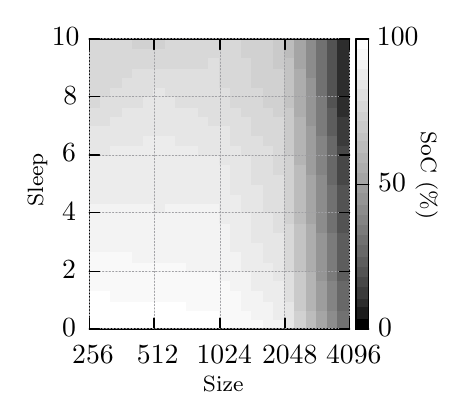
\begin{tikzpicture}[y=0.80pt, x=0.80pt, yscale=-0.600000, xscale=0.570000, inner sep=0pt, outer sep=0pt]
\begin{scope}[draw=black,line join=bevel,line cap=rect,even odd rule,line width=0.512pt]
  \begin{scope}[cm={{1.0,0.0,0.0,1.0,(0.0,0.0)}},draw=black,line join=bevel,line cap=rect,line width=0.512pt]
  \end{scope}
  \begin{scope}[cm={{1.00625,0.0,0.0,1.00625,(0.0,0.0)}},draw=black,line join=bevel,line cap=rect,line width=0.512pt]
  \end{scope}
  \begin{scope}[cm={{1.00625,0.0,0.0,1.00625,(0.0,0.0)}},draw=black,line join=bevel,line cap=rect,line width=0.512pt]
  \end{scope}
  \begin{scope}[cm={{1.00625,0.0,0.0,1.00625,(0.0,0.0)}},draw=black,line join=bevel,line cap=rect,line width=0.512pt]
  \end{scope}
  \begin{scope}[cm={{1.00625,0.0,0.0,1.00625,(0.0,0.0)}},draw=cffffff,fill=cffffff,line join=bevel,line cap=rect,line width=0.512pt]
    \path[draw,fill,even odd rule] (57.5000,268.5000) -- (57.5000,261.5000) --
      (66.5000,261.5000) -- (66.5000,268.5000) -- (57.5000,268.5000);
    \path[draw,fill,even odd rule] (66.5000,268.5000) -- (66.5000,261.5000) --
      (74.5000,261.5000) -- (74.5000,268.5000) -- (66.5000,268.5000);
    \path[draw,fill,even odd rule] (74.5000,268.5000) -- (74.5000,261.5000) --
      (83.5000,261.5000) -- (83.5000,268.5000) -- (74.5000,268.5000);
    \path[draw,fill,even odd rule] (83.5000,268.5000) -- (83.5000,261.5000) --
      (91.5000,261.5000) -- (91.5000,268.5000) -- (83.5000,268.5000);
    \path[draw,fill,even odd rule] (91.5000,268.5000) -- (91.5000,261.5000) --
      (100.5000,261.5000) -- (100.5000,268.5000) -- (91.5000,268.5000);
    \path[draw,fill,even odd rule] (100.5000,268.5000) -- (100.5000,261.5000) --
      (108.5000,261.5000) -- (108.5000,268.5000) -- (100.5000,268.5000);
    \path[draw,fill,even odd rule] (57.5000,261.5000) -- (57.5000,254.5000) --
      (66.5000,254.5000) -- (66.5000,261.5000) -- (57.5000,261.5000);
    \path[draw,fill,even odd rule] (66.5000,261.5000) -- (66.5000,254.5000) --
      (74.5000,254.5000) -- (74.5000,261.5000) -- (66.5000,261.5000);
    \path[draw,fill,even odd rule] (74.5000,261.5000) -- (74.5000,254.5000) --
      (83.5000,254.5000) -- (83.5000,261.5000) -- (74.5000,261.5000);
    \path[draw,fill,even odd rule] (83.5000,261.5000) -- (83.5000,254.5000) --
      (91.5000,254.5000) -- (91.5000,261.5000) -- (83.5000,261.5000);
    \path[draw,fill,even odd rule] (91.5000,261.5000) -- (91.5000,254.5000) --
      (100.5000,254.5000) -- (100.5000,261.5000) -- (91.5000,261.5000);
    \path[draw,fill,even odd rule] (100.5000,261.5000) -- (100.5000,254.5000) --
      (108.5000,254.5000) -- (108.5000,261.5000) -- (100.5000,261.5000);
    \path[draw,fill,even odd rule] (57.5000,254.5000) -- (57.5000,247.5000) --
      (66.5000,247.5000) -- (66.5000,254.5000) -- (57.5000,254.5000);
    \path[draw,fill,even odd rule] (66.5000,254.5000) -- (66.5000,247.5000) --
      (74.5000,247.5000) -- (74.5000,254.5000) -- (66.5000,254.5000);
    \path[draw,fill,even odd rule] (74.5000,254.5000) -- (74.5000,247.5000) --
      (83.5000,247.5000) -- (83.5000,254.5000) -- (74.5000,254.5000);
    \path[draw,fill,even odd rule] (83.5000,254.5000) -- (83.5000,247.5000) --
      (91.5000,247.5000) -- (91.5000,254.5000) -- (83.5000,254.5000);
    \path[draw,fill,even odd rule] (91.5000,254.5000) -- (91.5000,247.5000) --
      (100.5000,247.5000) -- (100.5000,254.5000) -- (91.5000,254.5000);
    \path[draw,fill,even odd rule] (100.5000,254.5000) -- (100.5000,247.5000) --
      (108.5000,247.5000) -- (108.5000,254.5000) -- (100.5000,254.5000);
    \path[draw,fill,even odd rule] (57.5000,247.5000) -- (57.5000,239.5000) --
      (66.5000,239.5000) -- (66.5000,247.5000) -- (57.5000,247.5000);
    \path[draw,fill,even odd rule] (66.5000,247.5000) -- (66.5000,239.5000) --
      (74.5000,239.5000) -- (74.5000,247.5000) -- (66.5000,247.5000);
  \end{scope}
  \begin{scope}[cm={{1.00625,0.0,0.0,1.00625,(0.0,0.0)}},draw=cf9f9f9,fill=cf9f9f9,line join=bevel,line cap=rect,line width=0.512pt]
    \path[draw,fill,even odd rule] (74.5000,247.5000) -- (74.5000,239.5000) --
      (83.5000,239.5000) -- (83.5000,247.5000) -- (74.5000,247.5000);
    \path[draw,fill,even odd rule] (83.5000,247.5000) -- (83.5000,239.5000) --
      (91.5000,239.5000) -- (91.5000,247.5000) -- (83.5000,247.5000);
    \path[draw,fill,even odd rule] (91.5000,247.5000) -- (91.5000,239.5000) --
      (100.5000,239.5000) -- (100.5000,247.5000) -- (91.5000,247.5000);
    \path[draw,fill,even odd rule] (100.5000,247.5000) -- (100.5000,239.5000) --
      (108.5000,239.5000) -- (108.5000,247.5000) -- (100.5000,247.5000);
    \path[draw,fill,even odd rule] (57.5000,239.5000) -- (57.5000,232.5000) --
      (66.5000,232.5000) -- (66.5000,239.5000) -- (57.5000,239.5000);
    \path[draw,fill,even odd rule] (66.5000,239.5000) -- (66.5000,232.5000) --
      (74.5000,232.5000) -- (74.5000,239.5000) -- (66.5000,239.5000);
    \path[draw,fill,even odd rule] (74.5000,239.5000) -- (74.5000,232.5000) --
      (83.5000,232.5000) -- (83.5000,239.5000) -- (74.5000,239.5000);
    \path[draw,fill,even odd rule] (83.5000,239.5000) -- (83.5000,232.5000) --
      (91.5000,232.5000) -- (91.5000,239.5000) -- (83.5000,239.5000);
    \path[draw,fill,even odd rule] (91.5000,239.5000) -- (91.5000,232.5000) --
      (100.5000,232.5000) -- (100.5000,239.5000) -- (91.5000,239.5000);
    \path[draw,fill,even odd rule] (100.5000,239.5000) -- (100.5000,232.5000) --
      (108.5000,232.5000) -- (108.5000,239.5000) -- (100.5000,239.5000);
    \path[draw,fill,even odd rule] (57.5000,232.5000) -- (57.5000,225.5000) --
      (66.5000,225.5000) -- (66.5000,232.5000) -- (57.5000,232.5000);
    \path[draw,fill,even odd rule] (66.5000,232.5000) -- (66.5000,225.5000) --
      (74.5000,225.5000) -- (74.5000,232.5000) -- (66.5000,232.5000);
    \path[draw,fill,even odd rule] (74.5000,232.5000) -- (74.5000,225.5000) --
      (83.5000,225.5000) -- (83.5000,232.5000) -- (74.5000,232.5000);
    \path[draw,fill,even odd rule] (83.5000,232.5000) -- (83.5000,225.5000) --
      (91.5000,225.5000) -- (91.5000,232.5000) -- (83.5000,232.5000);
    \path[draw,fill,even odd rule] (91.5000,232.5000) -- (91.5000,225.5000) --
      (100.5000,225.5000) -- (100.5000,232.5000) -- (91.5000,232.5000);
    \path[draw,fill,even odd rule] (100.5000,232.5000) -- (100.5000,225.5000) --
      (108.5000,225.5000) -- (108.5000,232.5000) -- (100.5000,232.5000);
    \path[draw,fill,even odd rule] (57.5000,225.5000) -- (57.5000,218.5000) --
      (66.5000,218.5000) -- (66.5000,225.5000) -- (57.5000,225.5000);
    \path[draw,fill,even odd rule] (66.5000,225.5000) -- (66.5000,218.5000) --
      (74.5000,218.5000) -- (74.5000,225.5000) -- (66.5000,225.5000);
    \path[draw,fill,even odd rule] (74.5000,225.5000) -- (74.5000,218.5000) --
      (83.5000,218.5000) -- (83.5000,225.5000) -- (74.5000,225.5000);
    \path[draw,fill,even odd rule] (83.5000,225.5000) -- (83.5000,218.5000) --
      (91.5000,218.5000) -- (91.5000,225.5000) -- (83.5000,225.5000);
    \path[draw,fill,even odd rule] (91.5000,225.5000) -- (91.5000,218.5000) --
      (100.5000,218.5000) -- (100.5000,225.5000) -- (91.5000,225.5000);
    \path[draw,fill,even odd rule] (100.5000,225.5000) -- (100.5000,218.5000) --
      (108.5000,218.5000) -- (108.5000,225.5000) -- (100.5000,225.5000);
    \path[draw,fill,even odd rule] (57.5000,218.5000) -- (57.5000,210.5000) --
      (66.5000,210.5000) -- (66.5000,218.5000) -- (57.5000,218.5000);
    \path[draw,fill,even odd rule] (66.5000,218.5000) -- (66.5000,210.5000) --
      (74.5000,210.5000) -- (74.5000,218.5000) -- (66.5000,218.5000);
    \path[draw,fill,even odd rule] (74.5000,218.5000) -- (74.5000,210.5000) --
      (83.5000,210.5000) -- (83.5000,218.5000) -- (74.5000,218.5000);
    \path[draw,fill,even odd rule] (83.5000,218.5000) -- (83.5000,210.5000) --
      (91.5000,210.5000) -- (91.5000,218.5000) -- (83.5000,218.5000);
  \end{scope}
  \begin{scope}[cm={{1.00625,0.0,0.0,1.00625,(0.0,0.0)}},draw=cf3f3f3,fill=cf3f3f3,line join=bevel,line cap=rect,line width=0.512pt]
    \path[draw,fill,even odd rule] (91.5000,218.5000) -- (91.5000,210.5000) --
      (100.5000,210.5000) -- (100.5000,218.5000) -- (91.5000,218.5000);
    \path[draw,fill,even odd rule] (100.5000,218.5000) -- (100.5000,210.5000) --
      (108.5000,210.5000) -- (108.5000,218.5000) -- (100.5000,218.5000);
    \path[draw,fill,even odd rule] (57.5000,210.5000) -- (57.5000,203.5000) --
      (66.5000,203.5000) -- (66.5000,210.5000) -- (57.5000,210.5000);
    \path[draw,fill,even odd rule] (66.5000,210.5000) -- (66.5000,203.5000) --
      (74.5000,203.5000) -- (74.5000,210.5000) -- (66.5000,210.5000);
    \path[draw,fill,even odd rule] (74.5000,210.5000) -- (74.5000,203.5000) --
      (83.5000,203.5000) -- (83.5000,210.5000) -- (74.5000,210.5000);
    \path[draw,fill,even odd rule] (83.5000,210.5000) -- (83.5000,203.5000) --
      (91.5000,203.5000) -- (91.5000,210.5000) -- (83.5000,210.5000);
    \path[draw,fill,even odd rule] (91.5000,210.5000) -- (91.5000,203.5000) --
      (100.5000,203.5000) -- (100.5000,210.5000) -- (91.5000,210.5000);
    \path[draw,fill,even odd rule] (100.5000,210.5000) -- (100.5000,203.5000) --
      (108.5000,203.5000) -- (108.5000,210.5000) -- (100.5000,210.5000);
    \path[draw,fill,even odd rule] (57.5000,203.5000) -- (57.5000,196.5000) --
      (66.5000,196.5000) -- (66.5000,203.5000) -- (57.5000,203.5000);
    \path[draw,fill,even odd rule] (66.5000,203.5000) -- (66.5000,196.5000) --
      (74.5000,196.5000) -- (74.5000,203.5000) -- (66.5000,203.5000);
    \path[draw,fill,even odd rule] (74.5000,203.5000) -- (74.5000,196.5000) --
      (83.5000,196.5000) -- (83.5000,203.5000) -- (74.5000,203.5000);
    \path[draw,fill,even odd rule] (83.5000,203.5000) -- (83.5000,196.5000) --
      (91.5000,196.5000) -- (91.5000,203.5000) -- (83.5000,203.5000);
    \path[draw,fill,even odd rule] (91.5000,203.5000) -- (91.5000,196.5000) --
      (100.5000,196.5000) -- (100.5000,203.5000) -- (91.5000,203.5000);
    \path[draw,fill,even odd rule] (100.5000,203.5000) -- (100.5000,196.5000) --
      (108.5000,196.5000) -- (108.5000,203.5000) -- (100.5000,203.5000);
    \path[draw,fill,even odd rule] (57.5000,196.5000) -- (57.5000,189.5000) --
      (66.5000,189.5000) -- (66.5000,196.5000) -- (57.5000,196.5000);
    \path[draw,fill,even odd rule] (66.5000,196.5000) -- (66.5000,189.5000) --
      (74.5000,189.5000) -- (74.5000,196.5000) -- (66.5000,196.5000);
    \path[draw,fill,even odd rule] (74.5000,196.5000) -- (74.5000,189.5000) --
      (83.5000,189.5000) -- (83.5000,196.5000) -- (74.5000,196.5000);
    \path[draw,fill,even odd rule] (83.5000,196.5000) -- (83.5000,189.5000) --
      (91.5000,189.5000) -- (91.5000,196.5000) -- (83.5000,196.5000);
    \path[draw,fill,even odd rule] (91.5000,196.5000) -- (91.5000,189.5000) --
      (100.5000,189.5000) -- (100.5000,196.5000) -- (91.5000,196.5000);
    \path[draw,fill,even odd rule] (100.5000,196.5000) -- (100.5000,189.5000) --
      (108.5000,189.5000) -- (108.5000,196.5000) -- (100.5000,196.5000);
    \path[draw,fill,even odd rule] (57.5000,189.5000) -- (57.5000,181.5000) --
      (66.5000,181.5000) -- (66.5000,189.5000) -- (57.5000,189.5000);
    \path[draw,fill,even odd rule] (66.5000,189.5000) -- (66.5000,181.5000) --
      (74.5000,181.5000) -- (74.5000,189.5000) -- (66.5000,189.5000);
    \path[draw,fill,even odd rule] (74.5000,189.5000) -- (74.5000,181.5000) --
      (83.5000,181.5000) -- (83.5000,189.5000) -- (74.5000,189.5000);
    \path[draw,fill,even odd rule] (83.5000,189.5000) -- (83.5000,181.5000) --
      (91.5000,181.5000) -- (91.5000,189.5000) -- (83.5000,189.5000);
    \path[draw,fill,even odd rule] (91.5000,189.5000) -- (91.5000,181.5000) --
      (100.5000,181.5000) -- (100.5000,189.5000) -- (91.5000,189.5000);
    \path[draw,fill,even odd rule] (100.5000,189.5000) -- (100.5000,181.5000) --
      (108.5000,181.5000) -- (108.5000,189.5000) -- (100.5000,189.5000);
    \path[draw,fill,even odd rule] (57.5000,181.5000) -- (57.5000,174.5000) --
      (66.5000,174.5000) -- (66.5000,181.5000) -- (57.5000,181.5000);
    \path[draw,fill,even odd rule] (66.5000,181.5000) -- (66.5000,174.5000) --
      (74.5000,174.5000) -- (74.5000,181.5000) -- (66.5000,181.5000);
    \path[draw,fill,even odd rule] (74.5000,181.5000) -- (74.5000,174.5000) --
      (83.5000,174.5000) -- (83.5000,181.5000) -- (74.5000,181.5000);
    \path[draw,fill,even odd rule] (83.5000,181.5000) -- (83.5000,174.5000) --
      (91.5000,174.5000) -- (91.5000,181.5000) -- (83.5000,181.5000);
    \path[draw,fill,even odd rule] (91.5000,181.5000) -- (91.5000,174.5000) --
      (100.5000,174.5000) -- (100.5000,181.5000) -- (91.5000,181.5000);
    \path[draw,fill,even odd rule] (100.5000,181.5000) -- (100.5000,174.5000) --
      (108.5000,174.5000) -- (108.5000,181.5000) -- (100.5000,181.5000);
  \end{scope}
  \begin{scope}[cm={{1.00625,0.0,0.0,1.00625,(0.0,0.0)}},draw=cececec,fill=cececec,line join=bevel,line cap=rect,line width=0.512pt]
    \path[draw,fill,even odd rule] (57.5000,174.5000) -- (57.5000,167.5000) --
      (66.5000,167.5000) -- (66.5000,174.5000) -- (57.5000,174.5000);
    \path[draw,fill,even odd rule] (66.5000,174.5000) -- (66.5000,167.5000) --
      (74.5000,167.5000) -- (74.5000,174.5000) -- (66.5000,174.5000);
    \path[draw,fill,even odd rule] (74.5000,174.5000) -- (74.5000,167.5000) --
      (83.5000,167.5000) -- (83.5000,174.5000) -- (74.5000,174.5000);
    \path[draw,fill,even odd rule] (83.5000,174.5000) -- (83.5000,167.5000) --
      (91.5000,167.5000) -- (91.5000,174.5000) -- (83.5000,174.5000);
    \path[draw,fill,even odd rule] (91.5000,174.5000) -- (91.5000,167.5000) --
      (100.5000,167.5000) -- (100.5000,174.5000) -- (91.5000,174.5000);
    \path[draw,fill,even odd rule] (100.5000,174.5000) -- (100.5000,167.5000) --
      (108.5000,167.5000) -- (108.5000,174.5000) -- (100.5000,174.5000);
    \path[draw,fill,even odd rule] (57.5000,167.5000) -- (57.5000,160.5000) --
      (66.5000,160.5000) -- (66.5000,167.5000) -- (57.5000,167.5000);
    \path[draw,fill,even odd rule] (66.5000,167.5000) -- (66.5000,160.5000) --
      (74.5000,160.5000) -- (74.5000,167.5000) -- (66.5000,167.5000);
    \path[draw,fill,even odd rule] (74.5000,167.5000) -- (74.5000,160.5000) --
      (83.5000,160.5000) -- (83.5000,167.5000) -- (74.5000,167.5000);
    \path[draw,fill,even odd rule] (83.5000,167.5000) -- (83.5000,160.5000) --
      (91.5000,160.5000) -- (91.5000,167.5000) -- (83.5000,167.5000);
    \path[draw,fill,even odd rule] (91.5000,167.5000) -- (91.5000,160.5000) --
      (100.5000,160.5000) -- (100.5000,167.5000) -- (91.5000,167.5000);
    \path[draw,fill,even odd rule] (100.5000,167.5000) -- (100.5000,160.5000) --
      (108.5000,160.5000) -- (108.5000,167.5000) -- (100.5000,167.5000);
    \path[draw,fill,even odd rule] (57.5000,160.5000) -- (57.5000,152.5000) --
      (66.5000,152.5000) -- (66.5000,160.5000) -- (57.5000,160.5000);
    \path[draw,fill,even odd rule] (66.5000,160.5000) -- (66.5000,152.5000) --
      (74.5000,152.5000) -- (74.5000,160.5000) -- (66.5000,160.5000);
    \path[draw,fill,even odd rule] (74.5000,160.5000) -- (74.5000,152.5000) --
      (83.5000,152.5000) -- (83.5000,160.5000) -- (74.5000,160.5000);
    \path[draw,fill,even odd rule] (83.5000,160.5000) -- (83.5000,152.5000) --
      (91.5000,152.5000) -- (91.5000,160.5000) -- (83.5000,160.5000);
    \path[draw,fill,even odd rule] (91.5000,160.5000) -- (91.5000,152.5000) --
      (100.5000,152.5000) -- (100.5000,160.5000) -- (91.5000,160.5000);
    \path[draw,fill,even odd rule] (100.5000,160.5000) -- (100.5000,152.5000) --
      (108.5000,152.5000) -- (108.5000,160.5000) -- (100.5000,160.5000);
    \path[draw,fill,even odd rule] (57.5000,152.5000) -- (57.5000,145.5000) --
      (66.5000,145.5000) -- (66.5000,152.5000) -- (57.5000,152.5000);
    \path[draw,fill,even odd rule] (66.5000,152.5000) -- (66.5000,145.5000) --
      (74.5000,145.5000) -- (74.5000,152.5000) -- (66.5000,152.5000);
    \path[draw,fill,even odd rule] (74.5000,152.5000) -- (74.5000,145.5000) --
      (83.5000,145.5000) -- (83.5000,152.5000) -- (74.5000,152.5000);
    \path[draw,fill,even odd rule] (83.5000,152.5000) -- (83.5000,145.5000) --
      (91.5000,145.5000) -- (91.5000,152.5000) -- (83.5000,152.5000);
    \path[draw,fill,even odd rule] (91.5000,152.5000) -- (91.5000,145.5000) --
      (100.5000,145.5000) -- (100.5000,152.5000) -- (91.5000,152.5000);
    \path[draw,fill,even odd rule] (100.5000,152.5000) -- (100.5000,145.5000) --
      (108.5000,145.5000) -- (108.5000,152.5000) -- (100.5000,152.5000);
    \path[draw,fill,even odd rule] (57.5000,145.5000) -- (57.5000,138.5000) --
      (66.5000,138.5000) -- (66.5000,145.5000) -- (57.5000,145.5000);
    \path[draw,fill,even odd rule] (66.5000,145.5000) -- (66.5000,138.5000) --
      (74.5000,138.5000) -- (74.5000,145.5000) -- (66.5000,145.5000);
    \path[draw,fill,even odd rule] (74.5000,145.5000) -- (74.5000,138.5000) --
      (83.5000,138.5000) -- (83.5000,145.5000) -- (74.5000,145.5000);
    \path[draw,fill,even odd rule] (83.5000,145.5000) -- (83.5000,138.5000) --
      (91.5000,138.5000) -- (91.5000,145.5000) -- (83.5000,145.5000);
    \path[draw,fill,even odd rule] (91.5000,145.5000) -- (91.5000,138.5000) --
      (100.5000,138.5000) -- (100.5000,145.5000) -- (91.5000,145.5000);
    \path[draw,fill,even odd rule] (100.5000,145.5000) -- (100.5000,138.5000) --
      (108.5000,138.5000) -- (108.5000,145.5000) -- (100.5000,145.5000);
  \end{scope}
  \begin{scope}[cm={{1.00625,0.0,0.0,1.00625,(0.0,0.0)}},draw=ce6e6e6,fill=ce6e6e6,line join=bevel,line cap=rect,line width=0.512pt]
    \path[draw,fill,even odd rule] (57.5000,138.5000) -- (57.5000,131.5000) --
      (66.5000,131.5000) -- (66.5000,138.5000) -- (57.5000,138.5000);
    \path[draw,fill,even odd rule] (66.5000,138.5000) -- (66.5000,131.5000) --
      (74.5000,131.5000) -- (74.5000,138.5000) -- (66.5000,138.5000);
  \end{scope}
  \begin{scope}[cm={{1.00625,0.0,0.0,1.00625,(0.0,0.0)}},draw=cececec,fill=cececec,line join=bevel,line cap=rect,line width=0.512pt]
    \path[draw,fill,even odd rule] (74.5000,138.5000) -- (74.5000,131.5000) --
      (83.5000,131.5000) -- (83.5000,138.5000) -- (74.5000,138.5000);
    \path[draw,fill,even odd rule] (83.5000,138.5000) -- (83.5000,131.5000) --
      (91.5000,131.5000) -- (91.5000,138.5000) -- (83.5000,138.5000);
    \path[draw,fill,even odd rule] (91.5000,138.5000) -- (91.5000,131.5000) --
      (100.5000,131.5000) -- (100.5000,138.5000) -- (91.5000,138.5000);
    \path[draw,fill,even odd rule] (100.5000,138.5000) -- (100.5000,131.5000) --
      (108.5000,131.5000) -- (108.5000,138.5000) -- (100.5000,138.5000);
  \end{scope}
  \begin{scope}[cm={{1.00625,0.0,0.0,1.00625,(0.0,0.0)}},draw=ce6e6e6,fill=ce6e6e6,line join=bevel,line cap=rect,line width=0.512pt]
    \path[draw,fill,even odd rule] (57.5000,131.5000) -- (57.5000,123.5000) --
      (66.5000,123.5000) -- (66.5000,131.5000) -- (57.5000,131.5000);
    \path[draw,fill,even odd rule] (66.5000,131.5000) -- (66.5000,123.5000) --
      (74.5000,123.5000) -- (74.5000,131.5000) -- (66.5000,131.5000);
    \path[draw,fill,even odd rule] (74.5000,131.5000) -- (74.5000,123.5000) --
      (83.5000,123.5000) -- (83.5000,131.5000) -- (74.5000,131.5000);
    \path[draw,fill,even odd rule] (83.5000,131.5000) -- (83.5000,123.5000) --
      (91.5000,123.5000) -- (91.5000,131.5000) -- (83.5000,131.5000);
    \path[draw,fill,even odd rule] (91.5000,131.5000) -- (91.5000,123.5000) --
      (100.5000,123.5000) -- (100.5000,131.5000) -- (91.5000,131.5000);
  \end{scope}
  \begin{scope}[cm={{1.00625,0.0,0.0,1.00625,(0.0,0.0)}},draw=cececec,fill=cececec,line join=bevel,line cap=rect,line width=0.512pt]
    \path[draw,fill,even odd rule] (100.5000,131.5000) -- (100.5000,123.5000) --
      (108.5000,123.5000) -- (108.5000,131.5000) -- (100.5000,131.5000);
  \end{scope}
  \begin{scope}[cm={{1.00625,0.0,0.0,1.00625,(0.0,0.0)}},draw=ce6e6e6,fill=ce6e6e6,line join=bevel,line cap=rect,line width=0.512pt]
    \path[draw,fill,even odd rule] (57.5000,123.5000) -- (57.5000,116.5000) --
      (66.5000,116.5000) -- (66.5000,123.5000) -- (57.5000,123.5000);
    \path[draw,fill,even odd rule] (66.5000,123.5000) -- (66.5000,116.5000) --
      (74.5000,116.5000) -- (74.5000,123.5000) -- (66.5000,123.5000);
    \path[draw,fill,even odd rule] (74.5000,123.5000) -- (74.5000,116.5000) --
      (83.5000,116.5000) -- (83.5000,123.5000) -- (74.5000,123.5000);
    \path[draw,fill,even odd rule] (83.5000,123.5000) -- (83.5000,116.5000) --
      (91.5000,116.5000) -- (91.5000,123.5000) -- (83.5000,123.5000);
    \path[draw,fill,even odd rule] (91.5000,123.5000) -- (91.5000,116.5000) --
      (100.5000,116.5000) -- (100.5000,123.5000) -- (91.5000,123.5000);
    \path[draw,fill,even odd rule] (100.5000,123.5000) -- (100.5000,116.5000) --
      (108.5000,116.5000) -- (108.5000,123.5000) -- (100.5000,123.5000);
  \end{scope}
  \begin{scope}[cm={{1.00625,0.0,0.0,1.00625,(0.0,0.0)}},draw=cdfdfdf,fill=cdfdfdf,line join=bevel,line cap=rect,line width=0.512pt]
    \path[draw,fill,even odd rule] (57.5000,116.5000) -- (57.5000,109.5000) --
      (66.5000,109.5000) -- (66.5000,116.5000) -- (57.5000,116.5000);
    \path[draw,fill,even odd rule] (66.5000,116.5000) -- (66.5000,109.5000) --
      (74.5000,109.5000) -- (74.5000,116.5000) -- (66.5000,116.5000);
  \end{scope}
  \begin{scope}[cm={{1.00625,0.0,0.0,1.00625,(0.0,0.0)}},draw=ce6e6e6,fill=ce6e6e6,line join=bevel,line cap=rect,line width=0.512pt]
    \path[draw,fill,even odd rule] (74.5000,116.5000) -- (74.5000,109.5000) --
      (83.5000,109.5000) -- (83.5000,116.5000) -- (74.5000,116.5000);
    \path[draw,fill,even odd rule] (83.5000,116.5000) -- (83.5000,109.5000) --
      (91.5000,109.5000) -- (91.5000,116.5000) -- (83.5000,116.5000);
    \path[draw,fill,even odd rule] (91.5000,116.5000) -- (91.5000,109.5000) --
      (100.5000,109.5000) -- (100.5000,116.5000) -- (91.5000,116.5000);
    \path[draw,fill,even odd rule] (100.5000,116.5000) -- (100.5000,109.5000) --
      (108.5000,109.5000) -- (108.5000,116.5000) -- (100.5000,116.5000);
  \end{scope}
  \begin{scope}[cm={{1.00625,0.0,0.0,1.00625,(0.0,0.0)}},draw=cdfdfdf,fill=cdfdfdf,line join=bevel,line cap=rect,line width=0.512pt]
    \path[draw,fill,even odd rule] (57.5000,109.5000) -- (57.5000,102.5000) --
      (66.5000,102.5000) -- (66.5000,109.5000) -- (57.5000,109.5000);
    \path[draw,fill,even odd rule] (66.5000,109.5000) -- (66.5000,102.5000) --
      (74.5000,102.5000) -- (74.5000,109.5000) -- (66.5000,109.5000);
    \path[draw,fill,even odd rule] (74.5000,109.5000) -- (74.5000,102.5000) --
      (83.5000,102.5000) -- (83.5000,109.5000) -- (74.5000,109.5000);
  \end{scope}
  \begin{scope}[cm={{1.00625,0.0,0.0,1.00625,(0.0,0.0)}},draw=ce6e6e6,fill=ce6e6e6,line join=bevel,line cap=rect,line width=0.512pt]
    \path[draw,fill,even odd rule] (83.5000,109.5000) -- (83.5000,102.5000) --
      (91.5000,102.5000) -- (91.5000,109.5000) -- (83.5000,109.5000);
    \path[draw,fill,even odd rule] (91.5000,109.5000) -- (91.5000,102.5000) --
      (100.5000,102.5000) -- (100.5000,109.5000) -- (91.5000,109.5000);
    \path[draw,fill,even odd rule] (100.5000,109.5000) -- (100.5000,102.5000) --
      (108.5000,102.5000) -- (108.5000,109.5000) -- (100.5000,109.5000);
  \end{scope}
  \begin{scope}[cm={{1.00625,0.0,0.0,1.00625,(0.0,0.0)}},draw=cd8d8d8,fill=cd8d8d8,line join=bevel,line cap=rect,line width=0.512pt]
    \path[draw,fill,even odd rule] (57.5000,102.5000) -- (57.5000,94.5000) --
      (66.5000,94.5000) -- (66.5000,102.5000) -- (57.5000,102.5000);
  \end{scope}
  \begin{scope}[cm={{1.00625,0.0,0.0,1.00625,(0.0,0.0)}},draw=cdfdfdf,fill=cdfdfdf,line join=bevel,line cap=rect,line width=0.512pt]
    \path[draw,fill,even odd rule] (66.5000,102.5000) -- (66.5000,94.5000) --
      (74.5000,94.5000) -- (74.5000,102.5000) -- (66.5000,102.5000);
    \path[draw,fill,even odd rule] (74.5000,102.5000) -- (74.5000,94.5000) --
      (83.5000,94.5000) -- (83.5000,102.5000) -- (74.5000,102.5000);
    \path[draw,fill,even odd rule] (83.5000,102.5000) -- (83.5000,94.5000) --
      (91.5000,94.5000) -- (91.5000,102.5000) -- (83.5000,102.5000);
    \path[draw,fill,even odd rule] (91.5000,102.5000) -- (91.5000,94.5000) --
      (100.5000,94.5000) -- (100.5000,102.5000) -- (91.5000,102.5000);
  \end{scope}
  \begin{scope}[cm={{1.00625,0.0,0.0,1.00625,(0.0,0.0)}},draw=ce6e6e6,fill=ce6e6e6,line join=bevel,line cap=rect,line width=0.512pt]
    \path[draw,fill,even odd rule] (100.5000,102.5000) -- (100.5000,94.5000) --
      (108.5000,94.5000) -- (108.5000,102.5000) -- (100.5000,102.5000);
  \end{scope}
  \begin{scope}[cm={{1.00625,0.0,0.0,1.00625,(0.0,0.0)}},draw=cd8d8d8,fill=cd8d8d8,line join=bevel,line cap=rect,line width=0.512pt]
    \path[draw,fill,even odd rule] (57.5000,94.5000) -- (57.5000,87.5000) --
      (66.5000,87.5000) -- (66.5000,94.5000) -- (57.5000,94.5000);
    \path[draw,fill,even odd rule] (66.5000,94.5000) -- (66.5000,87.5000) --
      (74.5000,87.5000) -- (74.5000,94.5000) -- (66.5000,94.5000);
  \end{scope}
  \begin{scope}[cm={{1.00625,0.0,0.0,1.00625,(0.0,0.0)}},draw=cdfdfdf,fill=cdfdfdf,line join=bevel,line cap=rect,line width=0.512pt]
    \path[draw,fill,even odd rule] (74.5000,94.5000) -- (74.5000,87.5000) --
      (83.5000,87.5000) -- (83.5000,94.5000) -- (74.5000,94.5000);
    \path[draw,fill,even odd rule] (83.5000,94.5000) -- (83.5000,87.5000) --
      (91.5000,87.5000) -- (91.5000,94.5000) -- (83.5000,94.5000);
    \path[draw,fill,even odd rule] (91.5000,94.5000) -- (91.5000,87.5000) --
      (100.5000,87.5000) -- (100.5000,94.5000) -- (91.5000,94.5000);
    \path[draw,fill,even odd rule] (100.5000,94.5000) -- (100.5000,87.5000) --
      (108.5000,87.5000) -- (108.5000,94.5000) -- (100.5000,94.5000);
  \end{scope}
  \begin{scope}[cm={{1.00625,0.0,0.0,1.00625,(0.0,0.0)}},draw=cd8d8d8,fill=cd8d8d8,line join=bevel,line cap=rect,line width=0.512pt]
    \path[draw,fill,even odd rule] (57.5000,87.5000) -- (57.5000,80.5000) --
      (66.5000,80.5000) -- (66.5000,87.5000) -- (57.5000,87.5000);
    \path[draw,fill,even odd rule] (66.5000,87.5000) -- (66.5000,80.5000) --
      (74.5000,80.5000) -- (74.5000,87.5000) -- (66.5000,87.5000);
    \path[draw,fill,even odd rule] (74.5000,87.5000) -- (74.5000,80.5000) --
      (83.5000,80.5000) -- (83.5000,87.5000) -- (74.5000,87.5000);
  \end{scope}
  \begin{scope}[cm={{1.00625,0.0,0.0,1.00625,(0.0,0.0)}},draw=cdfdfdf,fill=cdfdfdf,line join=bevel,line cap=rect,line width=0.512pt]
    \path[draw,fill,even odd rule] (83.5000,87.5000) -- (83.5000,80.5000) --
      (91.5000,80.5000) -- (91.5000,87.5000) -- (83.5000,87.5000);
    \path[draw,fill,even odd rule] (91.5000,87.5000) -- (91.5000,80.5000) --
      (100.5000,80.5000) -- (100.5000,87.5000) -- (91.5000,87.5000);
    \path[draw,fill,even odd rule] (100.5000,87.5000) -- (100.5000,80.5000) --
      (108.5000,80.5000) -- (108.5000,87.5000) -- (100.5000,87.5000);
  \end{scope}
  \begin{scope}[cm={{1.00625,0.0,0.0,1.00625,(0.0,0.0)}},draw=cd8d8d8,fill=cd8d8d8,line join=bevel,line cap=rect,line width=0.512pt]
    \path[draw,fill,even odd rule] (57.5000,80.5000) -- (57.5000,73.5000) --
      (66.5000,73.5000) -- (66.5000,80.5000) -- (57.5000,80.5000);
    \path[draw,fill,even odd rule] (66.5000,80.5000) -- (66.5000,73.5000) --
      (74.5000,73.5000) -- (74.5000,80.5000) -- (66.5000,80.5000);
    \path[draw,fill,even odd rule] (74.5000,80.5000) -- (74.5000,73.5000) --
      (83.5000,73.5000) -- (83.5000,80.5000) -- (74.5000,80.5000);
    \path[draw,fill,even odd rule] (83.5000,80.5000) -- (83.5000,73.5000) --
      (91.5000,73.5000) -- (91.5000,80.5000) -- (83.5000,80.5000);
  \end{scope}
  \begin{scope}[cm={{1.00625,0.0,0.0,1.00625,(0.0,0.0)}},draw=cdfdfdf,fill=cdfdfdf,line join=bevel,line cap=rect,line width=0.512pt]
    \path[draw,fill,even odd rule] (91.5000,80.5000) -- (91.5000,73.5000) --
      (100.5000,73.5000) -- (100.5000,80.5000) -- (91.5000,80.5000);
    \path[draw,fill,even odd rule] (100.5000,80.5000) -- (100.5000,73.5000) --
      (108.5000,73.5000) -- (108.5000,80.5000) -- (100.5000,80.5000);
  \end{scope}
  \begin{scope}[cm={{1.00625,0.0,0.0,1.00625,(0.0,0.0)}},draw=cd8d8d8,fill=cd8d8d8,line join=bevel,line cap=rect,line width=0.512pt]
    \path[draw,fill,even odd rule] (57.5000,73.5000) -- (57.5000,65.5000) --
      (66.5000,65.5000) -- (66.5000,73.5000) -- (57.5000,73.5000);
    \path[draw,fill,even odd rule] (66.5000,73.5000) -- (66.5000,65.5000) --
      (74.5000,65.5000) -- (74.5000,73.5000) -- (66.5000,73.5000);
    \path[draw,fill,even odd rule] (74.5000,73.5000) -- (74.5000,65.5000) --
      (83.5000,65.5000) -- (83.5000,73.5000) -- (74.5000,73.5000);
    \path[draw,fill,even odd rule] (83.5000,73.5000) -- (83.5000,65.5000) --
      (91.5000,65.5000) -- (91.5000,73.5000) -- (83.5000,73.5000);
    \path[draw,fill,even odd rule] (91.5000,73.5000) -- (91.5000,65.5000) --
      (100.5000,65.5000) -- (100.5000,73.5000) -- (91.5000,73.5000);
    \path[draw,fill,even odd rule] (100.5000,73.5000) -- (100.5000,65.5000) --
      (108.5000,65.5000) -- (108.5000,73.5000) -- (100.5000,73.5000);
    \path[draw,fill,even odd rule] (57.5000,65.5000) -- (57.5000,58.5000) --
      (66.5000,58.5000) -- (66.5000,65.5000) -- (57.5000,65.5000);
    \path[draw,fill,even odd rule] (66.5000,65.5000) -- (66.5000,58.5000) --
      (74.5000,58.5000) -- (74.5000,65.5000) -- (66.5000,65.5000);
    \path[draw,fill,even odd rule] (74.5000,65.5000) -- (74.5000,58.5000) --
      (83.5000,58.5000) -- (83.5000,65.5000) -- (74.5000,65.5000);
    \path[draw,fill,even odd rule] (83.5000,65.5000) -- (83.5000,58.5000) --
      (91.5000,58.5000) -- (91.5000,65.5000) -- (83.5000,65.5000);
    \path[draw,fill,even odd rule] (91.5000,65.5000) -- (91.5000,58.5000) --
      (100.5000,58.5000) -- (100.5000,65.5000) -- (91.5000,65.5000);
    \path[draw,fill,even odd rule] (100.5000,65.5000) -- (100.5000,58.5000) --
      (108.5000,58.5000) -- (108.5000,65.5000) -- (100.5000,65.5000);
    \path[draw,fill,even odd rule] (57.5000,58.5000) -- (57.5000,51.5000) --
      (66.5000,51.5000) -- (66.5000,58.5000) -- (57.5000,58.5000);
    \path[draw,fill,even odd rule] (66.5000,58.5000) -- (66.5000,51.5000) --
      (74.5000,51.5000) -- (74.5000,58.5000) -- (66.5000,58.5000);
    \path[draw,fill,even odd rule] (74.5000,58.5000) -- (74.5000,51.5000) --
      (83.5000,51.5000) -- (83.5000,58.5000) -- (74.5000,58.5000);
    \path[draw,fill,even odd rule] (83.5000,58.5000) -- (83.5000,51.5000) --
      (91.5000,51.5000) -- (91.5000,58.5000) -- (83.5000,58.5000);
  \end{scope}
  \begin{scope}[cm={{1.00625,0.0,0.0,1.00625,(0.0,0.0)}},draw=cd1d1d1,fill=cd1d1d1,line join=bevel,line cap=rect,line width=0.512pt]
    \path[draw,fill,even odd rule] (91.5000,58.5000) -- (91.5000,51.5000) --
      (100.5000,51.5000) -- (100.5000,58.5000) -- (91.5000,58.5000);
    \path[draw,fill,even odd rule] (100.5000,58.5000) -- (100.5000,51.5000) --
      (108.5000,51.5000) -- (108.5000,58.5000) -- (100.5000,58.5000);
  \end{scope}
  \begin{scope}[cm={{1.00625,0.0,0.0,1.00625,(0.0,0.0)}},draw=cffffff,fill=cffffff,line join=bevel,line cap=rect,line width=0.512pt]
    \path[draw,fill,even odd rule] (108.5000,268.5000) -- (108.5000,261.5000) --
      (117.5000,261.5000) -- (117.5000,268.5000) -- (108.5000,268.5000);
    \path[draw,fill,even odd rule] (117.5000,268.5000) -- (117.5000,261.5000) --
      (125.5000,261.5000) -- (125.5000,268.5000) -- (117.5000,268.5000);
    \path[draw,fill,even odd rule] (125.5000,268.5000) -- (125.5000,261.5000) --
      (134.5000,261.5000) -- (134.5000,268.5000) -- (125.5000,268.5000);
    \path[draw,fill,even odd rule] (134.5000,268.5000) -- (134.5000,261.5000) --
      (143.5000,261.5000) -- (143.5000,268.5000) -- (134.5000,268.5000);
    \path[draw,fill,even odd rule] (143.5000,268.5000) -- (143.5000,261.5000) --
      (151.5000,261.5000) -- (151.5000,268.5000) -- (143.5000,268.5000);
    \path[draw,fill,even odd rule] (151.5000,268.5000) -- (151.5000,261.5000) --
      (160.5000,261.5000) -- (160.5000,268.5000) -- (151.5000,268.5000);
    \path[draw,fill,even odd rule] (108.5000,261.5000) -- (108.5000,254.5000) --
      (117.5000,254.5000) -- (117.5000,261.5000) -- (108.5000,261.5000);
    \path[draw,fill,even odd rule] (117.5000,261.5000) -- (117.5000,254.5000) --
      (125.5000,254.5000) -- (125.5000,261.5000) -- (117.5000,261.5000);
    \path[draw,fill,even odd rule] (125.5000,261.5000) -- (125.5000,254.5000) --
      (134.5000,254.5000) -- (134.5000,261.5000) -- (125.5000,261.5000);
    \path[draw,fill,even odd rule] (134.5000,261.5000) -- (134.5000,254.5000) --
      (143.5000,254.5000) -- (143.5000,261.5000) -- (134.5000,261.5000);
    \path[draw,fill,even odd rule] (143.5000,261.5000) -- (143.5000,254.5000) --
      (151.5000,254.5000) -- (151.5000,261.5000) -- (143.5000,261.5000);
    \path[draw,fill,even odd rule] (151.5000,261.5000) -- (151.5000,254.5000) --
      (160.5000,254.5000) -- (160.5000,261.5000) -- (151.5000,261.5000);
    \path[draw,fill,even odd rule] (108.5000,254.5000) -- (108.5000,247.5000) --
      (117.5000,247.5000) -- (117.5000,254.5000) -- (108.5000,254.5000);
    \path[draw,fill,even odd rule] (117.5000,254.5000) -- (117.5000,247.5000) --
      (125.5000,247.5000) -- (125.5000,254.5000) -- (117.5000,254.5000);
    \path[draw,fill,even odd rule] (125.5000,254.5000) -- (125.5000,247.5000) --
      (134.5000,247.5000) -- (134.5000,254.5000) -- (125.5000,254.5000);
  \end{scope}
  \begin{scope}[cm={{1.00625,0.0,0.0,1.00625,(0.0,0.0)}},draw=cf9f9f9,fill=cf9f9f9,line join=bevel,line cap=rect,line width=0.512pt]
    \path[draw,fill,even odd rule] (134.5000,254.5000) -- (134.5000,247.5000) --
      (143.5000,247.5000) -- (143.5000,254.5000) -- (134.5000,254.5000);
    \path[draw,fill,even odd rule] (143.5000,254.5000) -- (143.5000,247.5000) --
      (151.5000,247.5000) -- (151.5000,254.5000) -- (143.5000,254.5000);
    \path[draw,fill,even odd rule] (151.5000,254.5000) -- (151.5000,247.5000) --
      (160.5000,247.5000) -- (160.5000,254.5000) -- (151.5000,254.5000);
    \path[draw,fill,even odd rule] (108.5000,247.5000) -- (108.5000,239.5000) --
      (117.5000,239.5000) -- (117.5000,247.5000) -- (108.5000,247.5000);
    \path[draw,fill,even odd rule] (117.5000,247.5000) -- (117.5000,239.5000) --
      (125.5000,239.5000) -- (125.5000,247.5000) -- (117.5000,247.5000);
    \path[draw,fill,even odd rule] (125.5000,247.5000) -- (125.5000,239.5000) --
      (134.5000,239.5000) -- (134.5000,247.5000) -- (125.5000,247.5000);
    \path[draw,fill,even odd rule] (134.5000,247.5000) -- (134.5000,239.5000) --
      (143.5000,239.5000) -- (143.5000,247.5000) -- (134.5000,247.5000);
    \path[draw,fill,even odd rule] (143.5000,247.5000) -- (143.5000,239.5000) --
      (151.5000,239.5000) -- (151.5000,247.5000) -- (143.5000,247.5000);
    \path[draw,fill,even odd rule] (151.5000,247.5000) -- (151.5000,239.5000) --
      (160.5000,239.5000) -- (160.5000,247.5000) -- (151.5000,247.5000);
    \path[draw,fill,even odd rule] (108.5000,239.5000) -- (108.5000,232.5000) --
      (117.5000,232.5000) -- (117.5000,239.5000) -- (108.5000,239.5000);
    \path[draw,fill,even odd rule] (117.5000,239.5000) -- (117.5000,232.5000) --
      (125.5000,232.5000) -- (125.5000,239.5000) -- (117.5000,239.5000);
    \path[draw,fill,even odd rule] (125.5000,239.5000) -- (125.5000,232.5000) --
      (134.5000,232.5000) -- (134.5000,239.5000) -- (125.5000,239.5000);
    \path[draw,fill,even odd rule] (134.5000,239.5000) -- (134.5000,232.5000) --
      (143.5000,232.5000) -- (143.5000,239.5000) -- (134.5000,239.5000);
    \path[draw,fill,even odd rule] (143.5000,239.5000) -- (143.5000,232.5000) --
      (151.5000,232.5000) -- (151.5000,239.5000) -- (143.5000,239.5000);
    \path[draw,fill,even odd rule] (151.5000,239.5000) -- (151.5000,232.5000) --
      (160.5000,232.5000) -- (160.5000,239.5000) -- (151.5000,239.5000);
    \path[draw,fill,even odd rule] (108.5000,232.5000) -- (108.5000,225.5000) --
      (117.5000,225.5000) -- (117.5000,232.5000) -- (108.5000,232.5000);
    \path[draw,fill,even odd rule] (117.5000,232.5000) -- (117.5000,225.5000) --
      (125.5000,225.5000) -- (125.5000,232.5000) -- (117.5000,232.5000);
    \path[draw,fill,even odd rule] (125.5000,232.5000) -- (125.5000,225.5000) --
      (134.5000,225.5000) -- (134.5000,232.5000) -- (125.5000,232.5000);
    \path[draw,fill,even odd rule] (134.5000,232.5000) -- (134.5000,225.5000) --
      (143.5000,225.5000) -- (143.5000,232.5000) -- (134.5000,232.5000);
    \path[draw,fill,even odd rule] (143.5000,232.5000) -- (143.5000,225.5000) --
      (151.5000,225.5000) -- (151.5000,232.5000) -- (143.5000,232.5000);
    \path[draw,fill,even odd rule] (151.5000,232.5000) -- (151.5000,225.5000) --
      (160.5000,225.5000) -- (160.5000,232.5000) -- (151.5000,232.5000);
    \path[draw,fill,even odd rule] (108.5000,225.5000) -- (108.5000,218.5000) --
      (117.5000,218.5000) -- (117.5000,225.5000) -- (108.5000,225.5000);
    \path[draw,fill,even odd rule] (117.5000,225.5000) -- (117.5000,218.5000) --
      (125.5000,218.5000) -- (125.5000,225.5000) -- (117.5000,225.5000);
    \path[draw,fill,even odd rule] (125.5000,225.5000) -- (125.5000,218.5000) --
      (134.5000,218.5000) -- (134.5000,225.5000) -- (125.5000,225.5000);
  \end{scope}
  \begin{scope}[cm={{1.00625,0.0,0.0,1.00625,(0.0,0.0)}},draw=cf3f3f3,fill=cf3f3f3,line join=bevel,line cap=rect,line width=0.512pt]
    \path[draw,fill,even odd rule] (134.5000,225.5000) -- (134.5000,218.5000) --
      (143.5000,218.5000) -- (143.5000,225.5000) -- (134.5000,225.5000);
    \path[draw,fill,even odd rule] (143.5000,225.5000) -- (143.5000,218.5000) --
      (151.5000,218.5000) -- (151.5000,225.5000) -- (143.5000,225.5000);
    \path[draw,fill,even odd rule] (151.5000,225.5000) -- (151.5000,218.5000) --
      (160.5000,218.5000) -- (160.5000,225.5000) -- (151.5000,225.5000);
    \path[draw,fill,even odd rule] (108.5000,218.5000) -- (108.5000,210.5000) --
      (117.5000,210.5000) -- (117.5000,218.5000) -- (108.5000,218.5000);
    \path[draw,fill,even odd rule] (117.5000,218.5000) -- (117.5000,210.5000) --
      (125.5000,210.5000) -- (125.5000,218.5000) -- (117.5000,218.5000);
    \path[draw,fill,even odd rule] (125.5000,218.5000) -- (125.5000,210.5000) --
      (134.5000,210.5000) -- (134.5000,218.5000) -- (125.5000,218.5000);
    \path[draw,fill,even odd rule] (134.5000,218.5000) -- (134.5000,210.5000) --
      (143.5000,210.5000) -- (143.5000,218.5000) -- (134.5000,218.5000);
    \path[draw,fill,even odd rule] (143.5000,218.5000) -- (143.5000,210.5000) --
      (151.5000,210.5000) -- (151.5000,218.5000) -- (143.5000,218.5000);
    \path[draw,fill,even odd rule] (151.5000,218.5000) -- (151.5000,210.5000) --
      (160.5000,210.5000) -- (160.5000,218.5000) -- (151.5000,218.5000);
    \path[draw,fill,even odd rule] (108.5000,210.5000) -- (108.5000,203.5000) --
      (117.5000,203.5000) -- (117.5000,210.5000) -- (108.5000,210.5000);
    \path[draw,fill,even odd rule] (117.5000,210.5000) -- (117.5000,203.5000) --
      (125.5000,203.5000) -- (125.5000,210.5000) -- (117.5000,210.5000);
    \path[draw,fill,even odd rule] (125.5000,210.5000) -- (125.5000,203.5000) --
      (134.5000,203.5000) -- (134.5000,210.5000) -- (125.5000,210.5000);
    \path[draw,fill,even odd rule] (134.5000,210.5000) -- (134.5000,203.5000) --
      (143.5000,203.5000) -- (143.5000,210.5000) -- (134.5000,210.5000);
    \path[draw,fill,even odd rule] (143.5000,210.5000) -- (143.5000,203.5000) --
      (151.5000,203.5000) -- (151.5000,210.5000) -- (143.5000,210.5000);
    \path[draw,fill,even odd rule] (151.5000,210.5000) -- (151.5000,203.5000) --
      (160.5000,203.5000) -- (160.5000,210.5000) -- (151.5000,210.5000);
    \path[draw,fill,even odd rule] (108.5000,203.5000) -- (108.5000,196.5000) --
      (117.5000,196.5000) -- (117.5000,203.5000) -- (108.5000,203.5000);
    \path[draw,fill,even odd rule] (117.5000,203.5000) -- (117.5000,196.5000) --
      (125.5000,196.5000) -- (125.5000,203.5000) -- (117.5000,203.5000);
    \path[draw,fill,even odd rule] (125.5000,203.5000) -- (125.5000,196.5000) --
      (134.5000,196.5000) -- (134.5000,203.5000) -- (125.5000,203.5000);
    \path[draw,fill,even odd rule] (134.5000,203.5000) -- (134.5000,196.5000) --
      (143.5000,196.5000) -- (143.5000,203.5000) -- (134.5000,203.5000);
    \path[draw,fill,even odd rule] (143.5000,203.5000) -- (143.5000,196.5000) --
      (151.5000,196.5000) -- (151.5000,203.5000) -- (143.5000,203.5000);
    \path[draw,fill,even odd rule] (151.5000,203.5000) -- (151.5000,196.5000) --
      (160.5000,196.5000) -- (160.5000,203.5000) -- (151.5000,203.5000);
    \path[draw,fill,even odd rule] (108.5000,196.5000) -- (108.5000,189.5000) --
      (117.5000,189.5000) -- (117.5000,196.5000) -- (108.5000,196.5000);
    \path[draw,fill,even odd rule] (117.5000,196.5000) -- (117.5000,189.5000) --
      (125.5000,189.5000) -- (125.5000,196.5000) -- (117.5000,196.5000);
    \path[draw,fill,even odd rule] (125.5000,196.5000) -- (125.5000,189.5000) --
      (134.5000,189.5000) -- (134.5000,196.5000) -- (125.5000,196.5000);
    \path[draw,fill,even odd rule] (134.5000,196.5000) -- (134.5000,189.5000) --
      (143.5000,189.5000) -- (143.5000,196.5000) -- (134.5000,196.5000);
    \path[draw,fill,even odd rule] (143.5000,196.5000) -- (143.5000,189.5000) --
      (151.5000,189.5000) -- (151.5000,196.5000) -- (143.5000,196.5000);
    \path[draw,fill,even odd rule] (151.5000,196.5000) -- (151.5000,189.5000) --
      (160.5000,189.5000) -- (160.5000,196.5000) -- (151.5000,196.5000);
    \path[draw,fill,even odd rule] (108.5000,189.5000) -- (108.5000,181.5000) --
      (117.5000,181.5000) -- (117.5000,189.5000) -- (108.5000,189.5000);
    \path[draw,fill,even odd rule] (117.5000,189.5000) -- (117.5000,181.5000) --
      (125.5000,181.5000) -- (125.5000,189.5000) -- (117.5000,189.5000);
    \path[draw,fill,even odd rule] (125.5000,189.5000) -- (125.5000,181.5000) --
      (134.5000,181.5000) -- (134.5000,189.5000) -- (125.5000,189.5000);
    \path[draw,fill,even odd rule] (134.5000,189.5000) -- (134.5000,181.5000) --
      (143.5000,181.5000) -- (143.5000,189.5000) -- (134.5000,189.5000);
    \path[draw,fill,even odd rule] (143.5000,189.5000) -- (143.5000,181.5000) --
      (151.5000,181.5000) -- (151.5000,189.5000) -- (143.5000,189.5000);
    \path[draw,fill,even odd rule] (151.5000,189.5000) -- (151.5000,181.5000) --
      (160.5000,181.5000) -- (160.5000,189.5000) -- (151.5000,189.5000);
  \end{scope}
  \begin{scope}[cm={{1.00625,0.0,0.0,1.00625,(0.0,0.0)}},draw=cececec,fill=cececec,line join=bevel,line cap=rect,line width=0.512pt]
    \path[draw,fill,even odd rule] (108.5000,181.5000) -- (108.5000,174.5000) --
      (117.5000,174.5000) -- (117.5000,181.5000) -- (108.5000,181.5000);
  \end{scope}
  \begin{scope}[cm={{1.00625,0.0,0.0,1.00625,(0.0,0.0)}},draw=cf3f3f3,fill=cf3f3f3,line join=bevel,line cap=rect,line width=0.512pt]
    \path[draw,fill,even odd rule] (117.5000,181.5000) -- (117.5000,174.5000) --
      (125.5000,174.5000) -- (125.5000,181.5000) -- (117.5000,181.5000);
    \path[draw,fill,even odd rule] (125.5000,181.5000) -- (125.5000,174.5000) --
      (134.5000,174.5000) -- (134.5000,181.5000) -- (125.5000,181.5000);
    \path[draw,fill,even odd rule] (134.5000,181.5000) -- (134.5000,174.5000) --
      (143.5000,174.5000) -- (143.5000,181.5000) -- (134.5000,181.5000);
    \path[draw,fill,even odd rule] (143.5000,181.5000) -- (143.5000,174.5000) --
      (151.5000,174.5000) -- (151.5000,181.5000) -- (143.5000,181.5000);
    \path[draw,fill,even odd rule] (151.5000,181.5000) -- (151.5000,174.5000) --
      (160.5000,174.5000) -- (160.5000,181.5000) -- (151.5000,181.5000);
  \end{scope}
  \begin{scope}[cm={{1.00625,0.0,0.0,1.00625,(0.0,0.0)}},draw=cececec,fill=cececec,line join=bevel,line cap=rect,line width=0.512pt]
    \path[draw,fill,even odd rule] (108.5000,174.5000) -- (108.5000,167.5000) --
      (117.5000,167.5000) -- (117.5000,174.5000) -- (108.5000,174.5000);
    \path[draw,fill,even odd rule] (117.5000,174.5000) -- (117.5000,167.5000) --
      (125.5000,167.5000) -- (125.5000,174.5000) -- (117.5000,174.5000);
    \path[draw,fill,even odd rule] (125.5000,174.5000) -- (125.5000,167.5000) --
      (134.5000,167.5000) -- (134.5000,174.5000) -- (125.5000,174.5000);
    \path[draw,fill,even odd rule] (134.5000,174.5000) -- (134.5000,167.5000) --
      (143.5000,167.5000) -- (143.5000,174.5000) -- (134.5000,174.5000);
    \path[draw,fill,even odd rule] (143.5000,174.5000) -- (143.5000,167.5000) --
      (151.5000,167.5000) -- (151.5000,174.5000) -- (143.5000,174.5000);
    \path[draw,fill,even odd rule] (151.5000,174.5000) -- (151.5000,167.5000) --
      (160.5000,167.5000) -- (160.5000,174.5000) -- (151.5000,174.5000);
    \path[draw,fill,even odd rule] (108.5000,167.5000) -- (108.5000,160.5000) --
      (117.5000,160.5000) -- (117.5000,167.5000) -- (108.5000,167.5000);
    \path[draw,fill,even odd rule] (117.5000,167.5000) -- (117.5000,160.5000) --
      (125.5000,160.5000) -- (125.5000,167.5000) -- (117.5000,167.5000);
    \path[draw,fill,even odd rule] (125.5000,167.5000) -- (125.5000,160.5000) --
      (134.5000,160.5000) -- (134.5000,167.5000) -- (125.5000,167.5000);
    \path[draw,fill,even odd rule] (134.5000,167.5000) -- (134.5000,160.5000) --
      (143.5000,160.5000) -- (143.5000,167.5000) -- (134.5000,167.5000);
    \path[draw,fill,even odd rule] (143.5000,167.5000) -- (143.5000,160.5000) --
      (151.5000,160.5000) -- (151.5000,167.5000) -- (143.5000,167.5000);
    \path[draw,fill,even odd rule] (151.5000,167.5000) -- (151.5000,160.5000) --
      (160.5000,160.5000) -- (160.5000,167.5000) -- (151.5000,167.5000);
    \path[draw,fill,even odd rule] (108.5000,160.5000) -- (108.5000,152.5000) --
      (117.5000,152.5000) -- (117.5000,160.5000) -- (108.5000,160.5000);
    \path[draw,fill,even odd rule] (117.5000,160.5000) -- (117.5000,152.5000) --
      (125.5000,152.5000) -- (125.5000,160.5000) -- (117.5000,160.5000);
    \path[draw,fill,even odd rule] (125.5000,160.5000) -- (125.5000,152.5000) --
      (134.5000,152.5000) -- (134.5000,160.5000) -- (125.5000,160.5000);
    \path[draw,fill,even odd rule] (134.5000,160.5000) -- (134.5000,152.5000) --
      (143.5000,152.5000) -- (143.5000,160.5000) -- (134.5000,160.5000);
    \path[draw,fill,even odd rule] (143.5000,160.5000) -- (143.5000,152.5000) --
      (151.5000,152.5000) -- (151.5000,160.5000) -- (143.5000,160.5000);
    \path[draw,fill,even odd rule] (151.5000,160.5000) -- (151.5000,152.5000) --
      (160.5000,152.5000) -- (160.5000,160.5000) -- (151.5000,160.5000);
    \path[draw,fill,even odd rule] (108.5000,152.5000) -- (108.5000,145.5000) --
      (117.5000,145.5000) -- (117.5000,152.5000) -- (108.5000,152.5000);
    \path[draw,fill,even odd rule] (117.5000,152.5000) -- (117.5000,145.5000) --
      (125.5000,145.5000) -- (125.5000,152.5000) -- (117.5000,152.5000);
    \path[draw,fill,even odd rule] (125.5000,152.5000) -- (125.5000,145.5000) --
      (134.5000,145.5000) -- (134.5000,152.5000) -- (125.5000,152.5000);
    \path[draw,fill,even odd rule] (134.5000,152.5000) -- (134.5000,145.5000) --
      (143.5000,145.5000) -- (143.5000,152.5000) -- (134.5000,152.5000);
    \path[draw,fill,even odd rule] (143.5000,152.5000) -- (143.5000,145.5000) --
      (151.5000,145.5000) -- (151.5000,152.5000) -- (143.5000,152.5000);
    \path[draw,fill,even odd rule] (151.5000,152.5000) -- (151.5000,145.5000) --
      (160.5000,145.5000) -- (160.5000,152.5000) -- (151.5000,152.5000);
    \path[draw,fill,even odd rule] (108.5000,145.5000) -- (108.5000,138.5000) --
      (117.5000,138.5000) -- (117.5000,145.5000) -- (108.5000,145.5000);
    \path[draw,fill,even odd rule] (117.5000,145.5000) -- (117.5000,138.5000) --
      (125.5000,138.5000) -- (125.5000,145.5000) -- (117.5000,145.5000);
    \path[draw,fill,even odd rule] (125.5000,145.5000) -- (125.5000,138.5000) --
      (134.5000,138.5000) -- (134.5000,145.5000) -- (125.5000,145.5000);
    \path[draw,fill,even odd rule] (134.5000,145.5000) -- (134.5000,138.5000) --
      (143.5000,138.5000) -- (143.5000,145.5000) -- (134.5000,145.5000);
    \path[draw,fill,even odd rule] (143.5000,145.5000) -- (143.5000,138.5000) --
      (151.5000,138.5000) -- (151.5000,145.5000) -- (143.5000,145.5000);
    \path[draw,fill,even odd rule] (151.5000,145.5000) -- (151.5000,138.5000) --
      (160.5000,138.5000) -- (160.5000,145.5000) -- (151.5000,145.5000);
    \path[draw,fill,even odd rule] (108.5000,138.5000) -- (108.5000,131.5000) --
      (117.5000,131.5000) -- (117.5000,138.5000) -- (108.5000,138.5000);
    \path[draw,fill,even odd rule] (117.5000,138.5000) -- (117.5000,131.5000) --
      (125.5000,131.5000) -- (125.5000,138.5000) -- (117.5000,138.5000);
    \path[draw,fill,even odd rule] (125.5000,138.5000) -- (125.5000,131.5000) --
      (134.5000,131.5000) -- (134.5000,138.5000) -- (125.5000,138.5000);
    \path[draw,fill,even odd rule] (134.5000,138.5000) -- (134.5000,131.5000) --
      (143.5000,131.5000) -- (143.5000,138.5000) -- (134.5000,138.5000);
  \end{scope}
  \begin{scope}[cm={{1.00625,0.0,0.0,1.00625,(0.0,0.0)}},draw=ce6e6e6,fill=ce6e6e6,line join=bevel,line cap=rect,line width=0.512pt]
    \path[draw,fill,even odd rule] (143.5000,138.5000) -- (143.5000,131.5000) --
      (151.5000,131.5000) -- (151.5000,138.5000) -- (143.5000,138.5000);
    \path[draw,fill,even odd rule] (151.5000,138.5000) -- (151.5000,131.5000) --
      (160.5000,131.5000) -- (160.5000,138.5000) -- (151.5000,138.5000);
  \end{scope}
  \begin{scope}[cm={{1.00625,0.0,0.0,1.00625,(0.0,0.0)}},draw=cececec,fill=cececec,line join=bevel,line cap=rect,line width=0.512pt]
    \path[draw,fill,even odd rule] (108.5000,131.5000) -- (108.5000,123.5000) --
      (117.5000,123.5000) -- (117.5000,131.5000) -- (108.5000,131.5000);
    \path[draw,fill,even odd rule] (117.5000,131.5000) -- (117.5000,123.5000) --
      (125.5000,123.5000) -- (125.5000,131.5000) -- (117.5000,131.5000);
  \end{scope}
  \begin{scope}[cm={{1.00625,0.0,0.0,1.00625,(0.0,0.0)}},draw=ce6e6e6,fill=ce6e6e6,line join=bevel,line cap=rect,line width=0.512pt]
    \path[draw,fill,even odd rule] (125.5000,131.5000) -- (125.5000,123.5000) --
      (134.5000,123.5000) -- (134.5000,131.5000) -- (125.5000,131.5000);
    \path[draw,fill,even odd rule] (134.5000,131.5000) -- (134.5000,123.5000) --
      (143.5000,123.5000) -- (143.5000,131.5000) -- (134.5000,131.5000);
    \path[draw,fill,even odd rule] (143.5000,131.5000) -- (143.5000,123.5000) --
      (151.5000,123.5000) -- (151.5000,131.5000) -- (143.5000,131.5000);
    \path[draw,fill,even odd rule] (151.5000,131.5000) -- (151.5000,123.5000) --
      (160.5000,123.5000) -- (160.5000,131.5000) -- (151.5000,131.5000);
    \path[draw,fill,even odd rule] (108.5000,123.5000) -- (108.5000,116.5000) --
      (117.5000,116.5000) -- (117.5000,123.5000) -- (108.5000,123.5000);
    \path[draw,fill,even odd rule] (117.5000,123.5000) -- (117.5000,116.5000) --
      (125.5000,116.5000) -- (125.5000,123.5000) -- (117.5000,123.5000);
    \path[draw,fill,even odd rule] (125.5000,123.5000) -- (125.5000,116.5000) --
      (134.5000,116.5000) -- (134.5000,123.5000) -- (125.5000,123.5000);
    \path[draw,fill,even odd rule] (134.5000,123.5000) -- (134.5000,116.5000) --
      (143.5000,116.5000) -- (143.5000,123.5000) -- (134.5000,123.5000);
    \path[draw,fill,even odd rule] (143.5000,123.5000) -- (143.5000,116.5000) --
      (151.5000,116.5000) -- (151.5000,123.5000) -- (143.5000,123.5000);
    \path[draw,fill,even odd rule] (151.5000,123.5000) -- (151.5000,116.5000) --
      (160.5000,116.5000) -- (160.5000,123.5000) -- (151.5000,123.5000);
    \path[draw,fill,even odd rule] (108.5000,116.5000) -- (108.5000,109.5000) --
      (117.5000,109.5000) -- (117.5000,116.5000) -- (108.5000,116.5000);
    \path[draw,fill,even odd rule] (117.5000,116.5000) -- (117.5000,109.5000) --
      (125.5000,109.5000) -- (125.5000,116.5000) -- (117.5000,116.5000);
    \path[draw,fill,even odd rule] (125.5000,116.5000) -- (125.5000,109.5000) --
      (134.5000,109.5000) -- (134.5000,116.5000) -- (125.5000,116.5000);
    \path[draw,fill,even odd rule] (134.5000,116.5000) -- (134.5000,109.5000) --
      (143.5000,109.5000) -- (143.5000,116.5000) -- (134.5000,116.5000);
    \path[draw,fill,even odd rule] (143.5000,116.5000) -- (143.5000,109.5000) --
      (151.5000,109.5000) -- (151.5000,116.5000) -- (143.5000,116.5000);
  \end{scope}
  \begin{scope}[cm={{1.00625,0.0,0.0,1.00625,(0.0,0.0)}},draw=cdfdfdf,fill=cdfdfdf,line join=bevel,line cap=rect,line width=0.512pt]
    \path[draw,fill,even odd rule] (151.5000,116.5000) -- (151.5000,109.5000) --
      (160.5000,109.5000) -- (160.5000,116.5000) -- (151.5000,116.5000);
  \end{scope}
  \begin{scope}[cm={{1.00625,0.0,0.0,1.00625,(0.0,0.0)}},draw=ce6e6e6,fill=ce6e6e6,line join=bevel,line cap=rect,line width=0.512pt]
    \path[draw,fill,even odd rule] (108.5000,109.5000) -- (108.5000,102.5000) --
      (117.5000,102.5000) -- (117.5000,109.5000) -- (108.5000,109.5000);
    \path[draw,fill,even odd rule] (117.5000,109.5000) -- (117.5000,102.5000) --
      (125.5000,102.5000) -- (125.5000,109.5000) -- (117.5000,109.5000);
    \path[draw,fill,even odd rule] (125.5000,109.5000) -- (125.5000,102.5000) --
      (134.5000,102.5000) -- (134.5000,109.5000) -- (125.5000,109.5000);
    \path[draw,fill,even odd rule] (134.5000,109.5000) -- (134.5000,102.5000) --
      (143.5000,102.5000) -- (143.5000,109.5000) -- (134.5000,109.5000);
  \end{scope}
  \begin{scope}[cm={{1.00625,0.0,0.0,1.00625,(0.0,0.0)}},draw=cdfdfdf,fill=cdfdfdf,line join=bevel,line cap=rect,line width=0.512pt]
    \path[draw,fill,even odd rule] (143.5000,109.5000) -- (143.5000,102.5000) --
      (151.5000,102.5000) -- (151.5000,109.5000) -- (143.5000,109.5000);
    \path[draw,fill,even odd rule] (151.5000,109.5000) -- (151.5000,102.5000) --
      (160.5000,102.5000) -- (160.5000,109.5000) -- (151.5000,109.5000);
  \end{scope}
  \begin{scope}[cm={{1.00625,0.0,0.0,1.00625,(0.0,0.0)}},draw=ce6e6e6,fill=ce6e6e6,line join=bevel,line cap=rect,line width=0.512pt]
    \path[draw,fill,even odd rule] (108.5000,102.5000) -- (108.5000,94.5000) --
      (117.5000,94.5000) -- (117.5000,102.5000) -- (108.5000,102.5000);
    \path[draw,fill,even odd rule] (117.5000,102.5000) -- (117.5000,94.5000) --
      (125.5000,94.5000) -- (125.5000,102.5000) -- (117.5000,102.5000);
  \end{scope}
  \begin{scope}[cm={{1.00625,0.0,0.0,1.00625,(0.0,0.0)}},draw=cdfdfdf,fill=cdfdfdf,line join=bevel,line cap=rect,line width=0.512pt]
    \path[draw,fill,even odd rule] (125.5000,102.5000) -- (125.5000,94.5000) --
      (134.5000,94.5000) -- (134.5000,102.5000) -- (125.5000,102.5000);
    \path[draw,fill,even odd rule] (134.5000,102.5000) -- (134.5000,94.5000) --
      (143.5000,94.5000) -- (143.5000,102.5000) -- (134.5000,102.5000);
    \path[draw,fill,even odd rule] (143.5000,102.5000) -- (143.5000,94.5000) --
      (151.5000,94.5000) -- (151.5000,102.5000) -- (143.5000,102.5000);
    \path[draw,fill,even odd rule] (151.5000,102.5000) -- (151.5000,94.5000) --
      (160.5000,94.5000) -- (160.5000,102.5000) -- (151.5000,102.5000);
  \end{scope}
  \begin{scope}[cm={{1.00625,0.0,0.0,1.00625,(0.0,0.0)}},draw=ce6e6e6,fill=ce6e6e6,line join=bevel,line cap=rect,line width=0.512pt]
    \path[draw,fill,even odd rule] (108.5000,94.5000) -- (108.5000,87.5000) --
      (117.5000,87.5000) -- (117.5000,94.5000) -- (108.5000,94.5000);
  \end{scope}
  \begin{scope}[cm={{1.00625,0.0,0.0,1.00625,(0.0,0.0)}},draw=cdfdfdf,fill=cdfdfdf,line join=bevel,line cap=rect,line width=0.512pt]
    \path[draw,fill,even odd rule] (117.5000,94.5000) -- (117.5000,87.5000) --
      (125.5000,87.5000) -- (125.5000,94.5000) -- (117.5000,94.5000);
    \path[draw,fill,even odd rule] (125.5000,94.5000) -- (125.5000,87.5000) --
      (134.5000,87.5000) -- (134.5000,94.5000) -- (125.5000,94.5000);
    \path[draw,fill,even odd rule] (134.5000,94.5000) -- (134.5000,87.5000) --
      (143.5000,87.5000) -- (143.5000,94.5000) -- (134.5000,94.5000);
    \path[draw,fill,even odd rule] (143.5000,94.5000) -- (143.5000,87.5000) --
      (151.5000,87.5000) -- (151.5000,94.5000) -- (143.5000,94.5000);
    \path[draw,fill,even odd rule] (151.5000,94.5000) -- (151.5000,87.5000) --
      (160.5000,87.5000) -- (160.5000,94.5000) -- (151.5000,94.5000);
    \path[draw,fill,even odd rule] (108.5000,87.5000) -- (108.5000,80.5000) --
      (117.5000,80.5000) -- (117.5000,87.5000) -- (108.5000,87.5000);
    \path[draw,fill,even odd rule] (117.5000,87.5000) -- (117.5000,80.5000) --
      (125.5000,80.5000) -- (125.5000,87.5000) -- (117.5000,87.5000);
    \path[draw,fill,even odd rule] (125.5000,87.5000) -- (125.5000,80.5000) --
      (134.5000,80.5000) -- (134.5000,87.5000) -- (125.5000,87.5000);
    \path[draw,fill,even odd rule] (134.5000,87.5000) -- (134.5000,80.5000) --
      (143.5000,80.5000) -- (143.5000,87.5000) -- (134.5000,87.5000);
    \path[draw,fill,even odd rule] (143.5000,87.5000) -- (143.5000,80.5000) --
      (151.5000,80.5000) -- (151.5000,87.5000) -- (143.5000,87.5000);
    \path[draw,fill,even odd rule] (151.5000,87.5000) -- (151.5000,80.5000) --
      (160.5000,80.5000) -- (160.5000,87.5000) -- (151.5000,87.5000);
    \path[draw,fill,even odd rule] (108.5000,80.5000) -- (108.5000,73.5000) --
      (117.5000,73.5000) -- (117.5000,80.5000) -- (108.5000,80.5000);
    \path[draw,fill,even odd rule] (117.5000,80.5000) -- (117.5000,73.5000) --
      (125.5000,73.5000) -- (125.5000,80.5000) -- (117.5000,80.5000);
    \path[draw,fill,even odd rule] (125.5000,80.5000) -- (125.5000,73.5000) --
      (134.5000,73.5000) -- (134.5000,80.5000) -- (125.5000,80.5000);
    \path[draw,fill,even odd rule] (134.5000,80.5000) -- (134.5000,73.5000) --
      (143.5000,73.5000) -- (143.5000,80.5000) -- (134.5000,80.5000);
    \path[draw,fill,even odd rule] (143.5000,80.5000) -- (143.5000,73.5000) --
      (151.5000,73.5000) -- (151.5000,80.5000) -- (143.5000,80.5000);
    \path[draw,fill,even odd rule] (151.5000,80.5000) -- (151.5000,73.5000) --
      (160.5000,73.5000) -- (160.5000,80.5000) -- (151.5000,80.5000);
  \end{scope}
  \begin{scope}[cm={{1.00625,0.0,0.0,1.00625,(0.0,0.0)}},draw=cd8d8d8,fill=cd8d8d8,line join=bevel,line cap=rect,line width=0.512pt]
    \path[draw,fill,even odd rule] (108.5000,73.5000) -- (108.5000,65.5000) --
      (117.5000,65.5000) -- (117.5000,73.5000) -- (108.5000,73.5000);
    \path[draw,fill,even odd rule] (117.5000,73.5000) -- (117.5000,65.5000) --
      (125.5000,65.5000) -- (125.5000,73.5000) -- (117.5000,73.5000);
    \path[draw,fill,even odd rule] (125.5000,73.5000) -- (125.5000,65.5000) --
      (134.5000,65.5000) -- (134.5000,73.5000) -- (125.5000,73.5000);
    \path[draw,fill,even odd rule] (134.5000,73.5000) -- (134.5000,65.5000) --
      (143.5000,65.5000) -- (143.5000,73.5000) -- (134.5000,73.5000);
    \path[draw,fill,even odd rule] (143.5000,73.5000) -- (143.5000,65.5000) --
      (151.5000,65.5000) -- (151.5000,73.5000) -- (143.5000,73.5000);
  \end{scope}
  \begin{scope}[cm={{1.00625,0.0,0.0,1.00625,(0.0,0.0)}},draw=cdfdfdf,fill=cdfdfdf,line join=bevel,line cap=rect,line width=0.512pt]
    \path[draw,fill,even odd rule] (151.5000,73.5000) -- (151.5000,65.5000) --
      (160.5000,65.5000) -- (160.5000,73.5000) -- (151.5000,73.5000);
  \end{scope}
  \begin{scope}[cm={{1.00625,0.0,0.0,1.00625,(0.0,0.0)}},draw=cd8d8d8,fill=cd8d8d8,line join=bevel,line cap=rect,line width=0.512pt]
    \path[draw,fill,even odd rule] (108.5000,65.5000) -- (108.5000,58.5000) --
      (117.5000,58.5000) -- (117.5000,65.5000) -- (108.5000,65.5000);
    \path[draw,fill,even odd rule] (117.5000,65.5000) -- (117.5000,58.5000) --
      (125.5000,58.5000) -- (125.5000,65.5000) -- (117.5000,65.5000);
    \path[draw,fill,even odd rule] (125.5000,65.5000) -- (125.5000,58.5000) --
      (134.5000,58.5000) -- (134.5000,65.5000) -- (125.5000,65.5000);
    \path[draw,fill,even odd rule] (134.5000,65.5000) -- (134.5000,58.5000) --
      (143.5000,58.5000) -- (143.5000,65.5000) -- (134.5000,65.5000);
    \path[draw,fill,even odd rule] (143.5000,65.5000) -- (143.5000,58.5000) --
      (151.5000,58.5000) -- (151.5000,65.5000) -- (143.5000,65.5000);
    \path[draw,fill,even odd rule] (151.5000,65.5000) -- (151.5000,58.5000) --
      (160.5000,58.5000) -- (160.5000,65.5000) -- (151.5000,65.5000);
  \end{scope}
  \begin{scope}[cm={{1.00625,0.0,0.0,1.00625,(0.0,0.0)}},draw=cd1d1d1,fill=cd1d1d1,line join=bevel,line cap=rect,line width=0.512pt]
    \path[draw,fill,even odd rule] (108.5000,58.5000) -- (108.5000,51.5000) --
      (117.5000,51.5000) -- (117.5000,58.5000) -- (108.5000,58.5000);
  \end{scope}
  \begin{scope}[cm={{1.00625,0.0,0.0,1.00625,(0.0,0.0)}},draw=cd8d8d8,fill=cd8d8d8,line join=bevel,line cap=rect,line width=0.512pt]
    \path[draw,fill,even odd rule] (117.5000,58.5000) -- (117.5000,51.5000) --
      (125.5000,51.5000) -- (125.5000,58.5000) -- (117.5000,58.5000);
    \path[draw,fill,even odd rule] (125.5000,58.5000) -- (125.5000,51.5000) --
      (134.5000,51.5000) -- (134.5000,58.5000) -- (125.5000,58.5000);
    \path[draw,fill,even odd rule] (134.5000,58.5000) -- (134.5000,51.5000) --
      (143.5000,51.5000) -- (143.5000,58.5000) -- (134.5000,58.5000);
    \path[draw,fill,even odd rule] (143.5000,58.5000) -- (143.5000,51.5000) --
      (151.5000,51.5000) -- (151.5000,58.5000) -- (143.5000,58.5000);
    \path[draw,fill,even odd rule] (151.5000,58.5000) -- (151.5000,51.5000) --
      (160.5000,51.5000) -- (160.5000,58.5000) -- (151.5000,58.5000);
  \end{scope}
  \begin{scope}[cm={{1.00625,0.0,0.0,1.00625,(0.0,0.0)}},draw=cffffff,fill=cffffff,line join=bevel,line cap=rect,line width=0.512pt]
    \path[draw,fill,even odd rule] (160.5000,268.5000) -- (160.5000,261.5000) --
      (168.5000,261.5000) -- (168.5000,268.5000) -- (160.5000,268.5000);
  \end{scope}
  \begin{scope}[cm={{1.00625,0.0,0.0,1.00625,(0.0,0.0)}},draw=cf9f9f9,fill=cf9f9f9,line join=bevel,line cap=rect,line width=0.512pt]
    \path[draw,fill,even odd rule] (168.5000,268.5000) -- (168.5000,261.5000) --
      (177.5000,261.5000) -- (177.5000,268.5000) -- (168.5000,268.5000);
    \path[draw,fill,even odd rule] (177.5000,268.5000) -- (177.5000,261.5000) --
      (185.5000,261.5000) -- (185.5000,268.5000) -- (177.5000,268.5000);
    \path[draw,fill,even odd rule] (185.5000,268.5000) -- (185.5000,261.5000) --
      (194.5000,261.5000) -- (194.5000,268.5000) -- (185.5000,268.5000);
  \end{scope}
  \begin{scope}[cm={{1.00625,0.0,0.0,1.00625,(0.0,0.0)}},draw=cf3f3f3,fill=cf3f3f3,line join=bevel,line cap=rect,line width=0.512pt]
    \path[draw,fill,even odd rule] (194.5000,268.5000) -- (194.5000,261.5000) --
      (202.5000,261.5000) -- (202.5000,268.5000) -- (194.5000,268.5000);
    \path[draw,fill,even odd rule] (202.5000,268.5000) -- (202.5000,261.5000) --
      (211.5000,261.5000) -- (211.5000,268.5000) -- (202.5000,268.5000);
  \end{scope}
  \begin{scope}[cm={{1.00625,0.0,0.0,1.00625,(0.0,0.0)}},draw=cf9f9f9,fill=cf9f9f9,line join=bevel,line cap=rect,line width=0.512pt]
    \path[draw,fill,even odd rule] (160.5000,261.5000) -- (160.5000,254.5000) --
      (168.5000,254.5000) -- (168.5000,261.5000) -- (160.5000,261.5000);
    \path[draw,fill,even odd rule] (168.5000,261.5000) -- (168.5000,254.5000) --
      (177.5000,254.5000) -- (177.5000,261.5000) -- (168.5000,261.5000);
    \path[draw,fill,even odd rule] (177.5000,261.5000) -- (177.5000,254.5000) --
      (185.5000,254.5000) -- (185.5000,261.5000) -- (177.5000,261.5000);
  \end{scope}
  \begin{scope}[cm={{1.00625,0.0,0.0,1.00625,(0.0,0.0)}},draw=cf3f3f3,fill=cf3f3f3,line join=bevel,line cap=rect,line width=0.512pt]
    \path[draw,fill,even odd rule] (185.5000,261.5000) -- (185.5000,254.5000) --
      (194.5000,254.5000) -- (194.5000,261.5000) -- (185.5000,261.5000);
    \path[draw,fill,even odd rule] (194.5000,261.5000) -- (194.5000,254.5000) --
      (202.5000,254.5000) -- (202.5000,261.5000) -- (194.5000,261.5000);
  \end{scope}
  \begin{scope}[cm={{1.00625,0.0,0.0,1.00625,(0.0,0.0)}},draw=cececec,fill=cececec,line join=bevel,line cap=rect,line width=0.512pt]
    \path[draw,fill,even odd rule] (202.5000,261.5000) -- (202.5000,254.5000) --
      (211.5000,254.5000) -- (211.5000,261.5000) -- (202.5000,261.5000);
  \end{scope}
  \begin{scope}[cm={{1.00625,0.0,0.0,1.00625,(0.0,0.0)}},draw=cf9f9f9,fill=cf9f9f9,line join=bevel,line cap=rect,line width=0.512pt]
    \path[draw,fill,even odd rule] (160.5000,254.5000) -- (160.5000,247.5000) --
      (168.5000,247.5000) -- (168.5000,254.5000) -- (160.5000,254.5000);
    \path[draw,fill,even odd rule] (168.5000,254.5000) -- (168.5000,247.5000) --
      (177.5000,247.5000) -- (177.5000,254.5000) -- (168.5000,254.5000);
  \end{scope}
  \begin{scope}[cm={{1.00625,0.0,0.0,1.00625,(0.0,0.0)}},draw=cf3f3f3,fill=cf3f3f3,line join=bevel,line cap=rect,line width=0.512pt]
    \path[draw,fill,even odd rule] (177.5000,254.5000) -- (177.5000,247.5000) --
      (185.5000,247.5000) -- (185.5000,254.5000) -- (177.5000,254.5000);
    \path[draw,fill,even odd rule] (185.5000,254.5000) -- (185.5000,247.5000) --
      (194.5000,247.5000) -- (194.5000,254.5000) -- (185.5000,254.5000);
    \path[draw,fill,even odd rule] (194.5000,254.5000) -- (194.5000,247.5000) --
      (202.5000,247.5000) -- (202.5000,254.5000) -- (194.5000,254.5000);
  \end{scope}
  \begin{scope}[cm={{1.00625,0.0,0.0,1.00625,(0.0,0.0)}},draw=cececec,fill=cececec,line join=bevel,line cap=rect,line width=0.512pt]
    \path[draw,fill,even odd rule] (202.5000,254.5000) -- (202.5000,247.5000) --
      (211.5000,247.5000) -- (211.5000,254.5000) -- (202.5000,254.5000);
  \end{scope}
  \begin{scope}[cm={{1.00625,0.0,0.0,1.00625,(0.0,0.0)}},draw=cf9f9f9,fill=cf9f9f9,line join=bevel,line cap=rect,line width=0.512pt]
    \path[draw,fill,even odd rule] (160.5000,247.5000) -- (160.5000,239.5000) --
      (168.5000,239.5000) -- (168.5000,247.5000) -- (160.5000,247.5000);
    \path[draw,fill,even odd rule] (168.5000,247.5000) -- (168.5000,239.5000) --
      (177.5000,239.5000) -- (177.5000,247.5000) -- (168.5000,247.5000);
  \end{scope}
  \begin{scope}[cm={{1.00625,0.0,0.0,1.00625,(0.0,0.0)}},draw=cf3f3f3,fill=cf3f3f3,line join=bevel,line cap=rect,line width=0.512pt]
    \path[draw,fill,even odd rule] (177.5000,247.5000) -- (177.5000,239.5000) --
      (185.5000,239.5000) -- (185.5000,247.5000) -- (177.5000,247.5000);
    \path[draw,fill,even odd rule] (185.5000,247.5000) -- (185.5000,239.5000) --
      (194.5000,239.5000) -- (194.5000,247.5000) -- (185.5000,247.5000);
  \end{scope}
  \begin{scope}[cm={{1.00625,0.0,0.0,1.00625,(0.0,0.0)}},draw=cececec,fill=cececec,line join=bevel,line cap=rect,line width=0.512pt]
    \path[draw,fill,even odd rule] (194.5000,247.5000) -- (194.5000,239.5000) --
      (202.5000,239.5000) -- (202.5000,247.5000) -- (194.5000,247.5000);
    \path[draw,fill,even odd rule] (202.5000,247.5000) -- (202.5000,239.5000) --
      (211.5000,239.5000) -- (211.5000,247.5000) -- (202.5000,247.5000);
  \end{scope}
  \begin{scope}[cm={{1.00625,0.0,0.0,1.00625,(0.0,0.0)}},draw=cf9f9f9,fill=cf9f9f9,line join=bevel,line cap=rect,line width=0.512pt]
    \path[draw,fill,even odd rule] (160.5000,239.5000) -- (160.5000,232.5000) --
      (168.5000,232.5000) -- (168.5000,239.5000) -- (160.5000,239.5000);
  \end{scope}
  \begin{scope}[cm={{1.00625,0.0,0.0,1.00625,(0.0,0.0)}},draw=cf3f3f3,fill=cf3f3f3,line join=bevel,line cap=rect,line width=0.512pt]
    \path[draw,fill,even odd rule] (168.5000,239.5000) -- (168.5000,232.5000) --
      (177.5000,232.5000) -- (177.5000,239.5000) -- (168.5000,239.5000);
    \path[draw,fill,even odd rule] (177.5000,239.5000) -- (177.5000,232.5000) --
      (185.5000,232.5000) -- (185.5000,239.5000) -- (177.5000,239.5000);
  \end{scope}
  \begin{scope}[cm={{1.00625,0.0,0.0,1.00625,(0.0,0.0)}},draw=cececec,fill=cececec,line join=bevel,line cap=rect,line width=0.512pt]
    \path[draw,fill,even odd rule] (185.5000,239.5000) -- (185.5000,232.5000) --
      (194.5000,232.5000) -- (194.5000,239.5000) -- (185.5000,239.5000);
    \path[draw,fill,even odd rule] (194.5000,239.5000) -- (194.5000,232.5000) --
      (202.5000,232.5000) -- (202.5000,239.5000) -- (194.5000,239.5000);
    \path[draw,fill,even odd rule] (202.5000,239.5000) -- (202.5000,232.5000) --
      (211.5000,232.5000) -- (211.5000,239.5000) -- (202.5000,239.5000);
  \end{scope}
  \begin{scope}[cm={{1.00625,0.0,0.0,1.00625,(0.0,0.0)}},draw=cf3f3f3,fill=cf3f3f3,line join=bevel,line cap=rect,line width=0.512pt]
    \path[draw,fill,even odd rule] (160.5000,232.5000) -- (160.5000,225.5000) --
      (168.5000,225.5000) -- (168.5000,232.5000) -- (160.5000,232.5000);
    \path[draw,fill,even odd rule] (168.5000,232.5000) -- (168.5000,225.5000) --
      (177.5000,225.5000) -- (177.5000,232.5000) -- (168.5000,232.5000);
    \path[draw,fill,even odd rule] (177.5000,232.5000) -- (177.5000,225.5000) --
      (185.5000,225.5000) -- (185.5000,232.5000) -- (177.5000,232.5000);
  \end{scope}
  \begin{scope}[cm={{1.00625,0.0,0.0,1.00625,(0.0,0.0)}},draw=cececec,fill=cececec,line join=bevel,line cap=rect,line width=0.512pt]
    \path[draw,fill,even odd rule] (185.5000,232.5000) -- (185.5000,225.5000) --
      (194.5000,225.5000) -- (194.5000,232.5000) -- (185.5000,232.5000);
    \path[draw,fill,even odd rule] (194.5000,232.5000) -- (194.5000,225.5000) --
      (202.5000,225.5000) -- (202.5000,232.5000) -- (194.5000,232.5000);
  \end{scope}
  \begin{scope}[cm={{1.00625,0.0,0.0,1.00625,(0.0,0.0)}},draw=ce6e6e6,fill=ce6e6e6,line join=bevel,line cap=rect,line width=0.512pt]
    \path[draw,fill,even odd rule] (202.5000,232.5000) -- (202.5000,225.5000) --
      (211.5000,225.5000) -- (211.5000,232.5000) -- (202.5000,232.5000);
  \end{scope}
  \begin{scope}[cm={{1.00625,0.0,0.0,1.00625,(0.0,0.0)}},draw=cf3f3f3,fill=cf3f3f3,line join=bevel,line cap=rect,line width=0.512pt]
    \path[draw,fill,even odd rule] (160.5000,225.5000) -- (160.5000,218.5000) --
      (168.5000,218.5000) -- (168.5000,225.5000) -- (160.5000,225.5000);
    \path[draw,fill,even odd rule] (168.5000,225.5000) -- (168.5000,218.5000) --
      (177.5000,218.5000) -- (177.5000,225.5000) -- (168.5000,225.5000);
  \end{scope}
  \begin{scope}[cm={{1.00625,0.0,0.0,1.00625,(0.0,0.0)}},draw=cececec,fill=cececec,line join=bevel,line cap=rect,line width=0.512pt]
    \path[draw,fill,even odd rule] (177.5000,225.5000) -- (177.5000,218.5000) --
      (185.5000,218.5000) -- (185.5000,225.5000) -- (177.5000,225.5000);
    \path[draw,fill,even odd rule] (185.5000,225.5000) -- (185.5000,218.5000) --
      (194.5000,218.5000) -- (194.5000,225.5000) -- (185.5000,225.5000);
    \path[draw,fill,even odd rule] (194.5000,225.5000) -- (194.5000,218.5000) --
      (202.5000,218.5000) -- (202.5000,225.5000) -- (194.5000,225.5000);
  \end{scope}
  \begin{scope}[cm={{1.00625,0.0,0.0,1.00625,(0.0,0.0)}},draw=ce6e6e6,fill=ce6e6e6,line join=bevel,line cap=rect,line width=0.512pt]
    \path[draw,fill,even odd rule] (202.5000,225.5000) -- (202.5000,218.5000) --
      (211.5000,218.5000) -- (211.5000,225.5000) -- (202.5000,225.5000);
  \end{scope}
  \begin{scope}[cm={{1.00625,0.0,0.0,1.00625,(0.0,0.0)}},draw=cf3f3f3,fill=cf3f3f3,line join=bevel,line cap=rect,line width=0.512pt]
    \path[draw,fill,even odd rule] (160.5000,218.5000) -- (160.5000,210.5000) --
      (168.5000,210.5000) -- (168.5000,218.5000) -- (160.5000,218.5000);
    \path[draw,fill,even odd rule] (168.5000,218.5000) -- (168.5000,210.5000) --
      (177.5000,210.5000) -- (177.5000,218.5000) -- (168.5000,218.5000);
  \end{scope}
  \begin{scope}[cm={{1.00625,0.0,0.0,1.00625,(0.0,0.0)}},draw=cececec,fill=cececec,line join=bevel,line cap=rect,line width=0.512pt]
    \path[draw,fill,even odd rule] (177.5000,218.5000) -- (177.5000,210.5000) --
      (185.5000,210.5000) -- (185.5000,218.5000) -- (177.5000,218.5000);
    \path[draw,fill,even odd rule] (185.5000,218.5000) -- (185.5000,210.5000) --
      (194.5000,210.5000) -- (194.5000,218.5000) -- (185.5000,218.5000);
  \end{scope}
  \begin{scope}[cm={{1.00625,0.0,0.0,1.00625,(0.0,0.0)}},draw=ce6e6e6,fill=ce6e6e6,line join=bevel,line cap=rect,line width=0.512pt]
    \path[draw,fill,even odd rule] (194.5000,218.5000) -- (194.5000,210.5000) --
      (202.5000,210.5000) -- (202.5000,218.5000) -- (194.5000,218.5000);
    \path[draw,fill,even odd rule] (202.5000,218.5000) -- (202.5000,210.5000) --
      (211.5000,210.5000) -- (211.5000,218.5000) -- (202.5000,218.5000);
  \end{scope}
  \begin{scope}[cm={{1.00625,0.0,0.0,1.00625,(0.0,0.0)}},draw=cf3f3f3,fill=cf3f3f3,line join=bevel,line cap=rect,line width=0.512pt]
    \path[draw,fill,even odd rule] (160.5000,210.5000) -- (160.5000,203.5000) --
      (168.5000,203.5000) -- (168.5000,210.5000) -- (160.5000,210.5000);
  \end{scope}
  \begin{scope}[cm={{1.00625,0.0,0.0,1.00625,(0.0,0.0)}},draw=cececec,fill=cececec,line join=bevel,line cap=rect,line width=0.512pt]
    \path[draw,fill,even odd rule] (168.5000,210.5000) -- (168.5000,203.5000) --
      (177.5000,203.5000) -- (177.5000,210.5000) -- (168.5000,210.5000);
    \path[draw,fill,even odd rule] (177.5000,210.5000) -- (177.5000,203.5000) --
      (185.5000,203.5000) -- (185.5000,210.5000) -- (177.5000,210.5000);
    \path[draw,fill,even odd rule] (185.5000,210.5000) -- (185.5000,203.5000) --
      (194.5000,203.5000) -- (194.5000,210.5000) -- (185.5000,210.5000);
  \end{scope}
  \begin{scope}[cm={{1.00625,0.0,0.0,1.00625,(0.0,0.0)}},draw=ce6e6e6,fill=ce6e6e6,line join=bevel,line cap=rect,line width=0.512pt]
    \path[draw,fill,even odd rule] (194.5000,210.5000) -- (194.5000,203.5000) --
      (202.5000,203.5000) -- (202.5000,210.5000) -- (194.5000,210.5000);
    \path[draw,fill,even odd rule] (202.5000,210.5000) -- (202.5000,203.5000) --
      (211.5000,203.5000) -- (211.5000,210.5000) -- (202.5000,210.5000);
  \end{scope}
  \begin{scope}[cm={{1.00625,0.0,0.0,1.00625,(0.0,0.0)}},draw=cf3f3f3,fill=cf3f3f3,line join=bevel,line cap=rect,line width=0.512pt]
    \path[draw,fill,even odd rule] (160.5000,203.5000) -- (160.5000,196.5000) --
      (168.5000,196.5000) -- (168.5000,203.5000) -- (160.5000,203.5000);
  \end{scope}
  \begin{scope}[cm={{1.00625,0.0,0.0,1.00625,(0.0,0.0)}},draw=cececec,fill=cececec,line join=bevel,line cap=rect,line width=0.512pt]
    \path[draw,fill,even odd rule] (168.5000,203.5000) -- (168.5000,196.5000) --
      (177.5000,196.5000) -- (177.5000,203.5000) -- (168.5000,203.5000);
    \path[draw,fill,even odd rule] (177.5000,203.5000) -- (177.5000,196.5000) --
      (185.5000,196.5000) -- (185.5000,203.5000) -- (177.5000,203.5000);
  \end{scope}
  \begin{scope}[cm={{1.00625,0.0,0.0,1.00625,(0.0,0.0)}},draw=ce6e6e6,fill=ce6e6e6,line join=bevel,line cap=rect,line width=0.512pt]
    \path[draw,fill,even odd rule] (185.5000,203.5000) -- (185.5000,196.5000) --
      (194.5000,196.5000) -- (194.5000,203.5000) -- (185.5000,203.5000);
    \path[draw,fill,even odd rule] (194.5000,203.5000) -- (194.5000,196.5000) --
      (202.5000,196.5000) -- (202.5000,203.5000) -- (194.5000,203.5000);
    \path[draw,fill,even odd rule] (202.5000,203.5000) -- (202.5000,196.5000) --
      (211.5000,196.5000) -- (211.5000,203.5000) -- (202.5000,203.5000);
  \end{scope}
  \begin{scope}[cm={{1.00625,0.0,0.0,1.00625,(0.0,0.0)}},draw=cf3f3f3,fill=cf3f3f3,line join=bevel,line cap=rect,line width=0.512pt]
    \path[draw,fill,even odd rule] (160.5000,196.5000) -- (160.5000,189.5000) --
      (168.5000,189.5000) -- (168.5000,196.5000) -- (160.5000,196.5000);
  \end{scope}
  \begin{scope}[cm={{1.00625,0.0,0.0,1.00625,(0.0,0.0)}},draw=cececec,fill=cececec,line join=bevel,line cap=rect,line width=0.512pt]
    \path[draw,fill,even odd rule] (168.5000,196.5000) -- (168.5000,189.5000) --
      (177.5000,189.5000) -- (177.5000,196.5000) -- (168.5000,196.5000);
    \path[draw,fill,even odd rule] (177.5000,196.5000) -- (177.5000,189.5000) --
      (185.5000,189.5000) -- (185.5000,196.5000) -- (177.5000,196.5000);
  \end{scope}
  \begin{scope}[cm={{1.00625,0.0,0.0,1.00625,(0.0,0.0)}},draw=ce6e6e6,fill=ce6e6e6,line join=bevel,line cap=rect,line width=0.512pt]
    \path[draw,fill,even odd rule] (185.5000,196.5000) -- (185.5000,189.5000) --
      (194.5000,189.5000) -- (194.5000,196.5000) -- (185.5000,196.5000);
    \path[draw,fill,even odd rule] (194.5000,196.5000) -- (194.5000,189.5000) --
      (202.5000,189.5000) -- (202.5000,196.5000) -- (194.5000,196.5000);
  \end{scope}
  \begin{scope}[cm={{1.00625,0.0,0.0,1.00625,(0.0,0.0)}},draw=cdfdfdf,fill=cdfdfdf,line join=bevel,line cap=rect,line width=0.512pt]
    \path[draw,fill,even odd rule] (202.5000,196.5000) -- (202.5000,189.5000) --
      (211.5000,189.5000) -- (211.5000,196.5000) -- (202.5000,196.5000);
  \end{scope}
  \begin{scope}[cm={{1.00625,0.0,0.0,1.00625,(0.0,0.0)}},draw=cececec,fill=cececec,line join=bevel,line cap=rect,line width=0.512pt]
    \path[draw,fill,even odd rule] (160.5000,189.5000) -- (160.5000,181.5000) --
      (168.5000,181.5000) -- (168.5000,189.5000) -- (160.5000,189.5000);
    \path[draw,fill,even odd rule] (168.5000,189.5000) -- (168.5000,181.5000) --
      (177.5000,181.5000) -- (177.5000,189.5000) -- (168.5000,189.5000);
    \path[draw,fill,even odd rule] (177.5000,189.5000) -- (177.5000,181.5000) --
      (185.5000,181.5000) -- (185.5000,189.5000) -- (177.5000,189.5000);
  \end{scope}
  \begin{scope}[cm={{1.00625,0.0,0.0,1.00625,(0.0,0.0)}},draw=ce6e6e6,fill=ce6e6e6,line join=bevel,line cap=rect,line width=0.512pt]
    \path[draw,fill,even odd rule] (185.5000,189.5000) -- (185.5000,181.5000) --
      (194.5000,181.5000) -- (194.5000,189.5000) -- (185.5000,189.5000);
    \path[draw,fill,even odd rule] (194.5000,189.5000) -- (194.5000,181.5000) --
      (202.5000,181.5000) -- (202.5000,189.5000) -- (194.5000,189.5000);
  \end{scope}
  \begin{scope}[cm={{1.00625,0.0,0.0,1.00625,(0.0,0.0)}},draw=cdfdfdf,fill=cdfdfdf,line join=bevel,line cap=rect,line width=0.512pt]
    \path[draw,fill,even odd rule] (202.5000,189.5000) -- (202.5000,181.5000) --
      (211.5000,181.5000) -- (211.5000,189.5000) -- (202.5000,189.5000);
  \end{scope}
  \begin{scope}[cm={{1.00625,0.0,0.0,1.00625,(0.0,0.0)}},draw=cececec,fill=cececec,line join=bevel,line cap=rect,line width=0.512pt]
    \path[draw,fill,even odd rule] (160.5000,181.5000) -- (160.5000,174.5000) --
      (168.5000,174.5000) -- (168.5000,181.5000) -- (160.5000,181.5000);
    \path[draw,fill,even odd rule] (168.5000,181.5000) -- (168.5000,174.5000) --
      (177.5000,174.5000) -- (177.5000,181.5000) -- (168.5000,181.5000);
  \end{scope}
  \begin{scope}[cm={{1.00625,0.0,0.0,1.00625,(0.0,0.0)}},draw=ce6e6e6,fill=ce6e6e6,line join=bevel,line cap=rect,line width=0.512pt]
    \path[draw,fill,even odd rule] (177.5000,181.5000) -- (177.5000,174.5000) --
      (185.5000,174.5000) -- (185.5000,181.5000) -- (177.5000,181.5000);
    \path[draw,fill,even odd rule] (185.5000,181.5000) -- (185.5000,174.5000) --
      (194.5000,174.5000) -- (194.5000,181.5000) -- (185.5000,181.5000);
  \end{scope}
  \begin{scope}[cm={{1.00625,0.0,0.0,1.00625,(0.0,0.0)}},draw=cdfdfdf,fill=cdfdfdf,line join=bevel,line cap=rect,line width=0.512pt]
    \path[draw,fill,even odd rule] (194.5000,181.5000) -- (194.5000,174.5000) --
      (202.5000,174.5000) -- (202.5000,181.5000) -- (194.5000,181.5000);
    \path[draw,fill,even odd rule] (202.5000,181.5000) -- (202.5000,174.5000) --
      (211.5000,174.5000) -- (211.5000,181.5000) -- (202.5000,181.5000);
  \end{scope}
  \begin{scope}[cm={{1.00625,0.0,0.0,1.00625,(0.0,0.0)}},draw=cececec,fill=cececec,line join=bevel,line cap=rect,line width=0.512pt]
    \path[draw,fill,even odd rule] (160.5000,174.5000) -- (160.5000,167.5000) --
      (168.5000,167.5000) -- (168.5000,174.5000) -- (160.5000,174.5000);
    \path[draw,fill,even odd rule] (168.5000,174.5000) -- (168.5000,167.5000) --
      (177.5000,167.5000) -- (177.5000,174.5000) -- (168.5000,174.5000);
  \end{scope}
  \begin{scope}[cm={{1.00625,0.0,0.0,1.00625,(0.0,0.0)}},draw=ce6e6e6,fill=ce6e6e6,line join=bevel,line cap=rect,line width=0.512pt]
    \path[draw,fill,even odd rule] (177.5000,174.5000) -- (177.5000,167.5000) --
      (185.5000,167.5000) -- (185.5000,174.5000) -- (177.5000,174.5000);
    \path[draw,fill,even odd rule] (185.5000,174.5000) -- (185.5000,167.5000) --
      (194.5000,167.5000) -- (194.5000,174.5000) -- (185.5000,174.5000);
  \end{scope}
  \begin{scope}[cm={{1.00625,0.0,0.0,1.00625,(0.0,0.0)}},draw=cdfdfdf,fill=cdfdfdf,line join=bevel,line cap=rect,line width=0.512pt]
    \path[draw,fill,even odd rule] (194.5000,174.5000) -- (194.5000,167.5000) --
      (202.5000,167.5000) -- (202.5000,174.5000) -- (194.5000,174.5000);
    \path[draw,fill,even odd rule] (202.5000,174.5000) -- (202.5000,167.5000) --
      (211.5000,167.5000) -- (211.5000,174.5000) -- (202.5000,174.5000);
  \end{scope}
  \begin{scope}[cm={{1.00625,0.0,0.0,1.00625,(0.0,0.0)}},draw=cececec,fill=cececec,line join=bevel,line cap=rect,line width=0.512pt]
    \path[draw,fill,even odd rule] (160.5000,167.5000) -- (160.5000,160.5000) --
      (168.5000,160.5000) -- (168.5000,167.5000) -- (160.5000,167.5000);
  \end{scope}
  \begin{scope}[cm={{1.00625,0.0,0.0,1.00625,(0.0,0.0)}},draw=ce6e6e6,fill=ce6e6e6,line join=bevel,line cap=rect,line width=0.512pt]
    \path[draw,fill,even odd rule] (168.5000,167.5000) -- (168.5000,160.5000) --
      (177.5000,160.5000) -- (177.5000,167.5000) -- (168.5000,167.5000);
    \path[draw,fill,even odd rule] (177.5000,167.5000) -- (177.5000,160.5000) --
      (185.5000,160.5000) -- (185.5000,167.5000) -- (177.5000,167.5000);
    \path[draw,fill,even odd rule] (185.5000,167.5000) -- (185.5000,160.5000) --
      (194.5000,160.5000) -- (194.5000,167.5000) -- (185.5000,167.5000);
  \end{scope}
  \begin{scope}[cm={{1.00625,0.0,0.0,1.00625,(0.0,0.0)}},draw=cdfdfdf,fill=cdfdfdf,line join=bevel,line cap=rect,line width=0.512pt]
    \path[draw,fill,even odd rule] (194.5000,167.5000) -- (194.5000,160.5000) --
      (202.5000,160.5000) -- (202.5000,167.5000) -- (194.5000,167.5000);
    \path[draw,fill,even odd rule] (202.5000,167.5000) -- (202.5000,160.5000) --
      (211.5000,160.5000) -- (211.5000,167.5000) -- (202.5000,167.5000);
  \end{scope}
  \begin{scope}[cm={{1.00625,0.0,0.0,1.00625,(0.0,0.0)}},draw=cececec,fill=cececec,line join=bevel,line cap=rect,line width=0.512pt]
    \path[draw,fill,even odd rule] (160.5000,160.5000) -- (160.5000,152.5000) --
      (168.5000,152.5000) -- (168.5000,160.5000) -- (160.5000,160.5000);
  \end{scope}
  \begin{scope}[cm={{1.00625,0.0,0.0,1.00625,(0.0,0.0)}},draw=ce6e6e6,fill=ce6e6e6,line join=bevel,line cap=rect,line width=0.512pt]
    \path[draw,fill,even odd rule] (168.5000,160.5000) -- (168.5000,152.5000) --
      (177.5000,152.5000) -- (177.5000,160.5000) -- (168.5000,160.5000);
    \path[draw,fill,even odd rule] (177.5000,160.5000) -- (177.5000,152.5000) --
      (185.5000,152.5000) -- (185.5000,160.5000) -- (177.5000,160.5000);
  \end{scope}
  \begin{scope}[cm={{1.00625,0.0,0.0,1.00625,(0.0,0.0)}},draw=cdfdfdf,fill=cdfdfdf,line join=bevel,line cap=rect,line width=0.512pt]
    \path[draw,fill,even odd rule] (185.5000,160.5000) -- (185.5000,152.5000) --
      (194.5000,152.5000) -- (194.5000,160.5000) -- (185.5000,160.5000);
    \path[draw,fill,even odd rule] (194.5000,160.5000) -- (194.5000,152.5000) --
      (202.5000,152.5000) -- (202.5000,160.5000) -- (194.5000,160.5000);
    \path[draw,fill,even odd rule] (202.5000,160.5000) -- (202.5000,152.5000) --
      (211.5000,152.5000) -- (211.5000,160.5000) -- (202.5000,160.5000);
  \end{scope}
  \begin{scope}[cm={{1.00625,0.0,0.0,1.00625,(0.0,0.0)}},draw=cececec,fill=cececec,line join=bevel,line cap=rect,line width=0.512pt]
    \path[draw,fill,even odd rule] (160.5000,152.5000) -- (160.5000,145.5000) --
      (168.5000,145.5000) -- (168.5000,152.5000) -- (160.5000,152.5000);
  \end{scope}
  \begin{scope}[cm={{1.00625,0.0,0.0,1.00625,(0.0,0.0)}},draw=ce6e6e6,fill=ce6e6e6,line join=bevel,line cap=rect,line width=0.512pt]
    \path[draw,fill,even odd rule] (168.5000,152.5000) -- (168.5000,145.5000) --
      (177.5000,145.5000) -- (177.5000,152.5000) -- (168.5000,152.5000);
    \path[draw,fill,even odd rule] (177.5000,152.5000) -- (177.5000,145.5000) --
      (185.5000,145.5000) -- (185.5000,152.5000) -- (177.5000,152.5000);
  \end{scope}
  \begin{scope}[cm={{1.00625,0.0,0.0,1.00625,(0.0,0.0)}},draw=cdfdfdf,fill=cdfdfdf,line join=bevel,line cap=rect,line width=0.512pt]
    \path[draw,fill,even odd rule] (185.5000,152.5000) -- (185.5000,145.5000) --
      (194.5000,145.5000) -- (194.5000,152.5000) -- (185.5000,152.5000);
    \path[draw,fill,even odd rule] (194.5000,152.5000) -- (194.5000,145.5000) --
      (202.5000,145.5000) -- (202.5000,152.5000) -- (194.5000,152.5000);
  \end{scope}
  \begin{scope}[cm={{1.00625,0.0,0.0,1.00625,(0.0,0.0)}},draw=cd8d8d8,fill=cd8d8d8,line join=bevel,line cap=rect,line width=0.512pt]
    \path[draw,fill,even odd rule] (202.5000,152.5000) -- (202.5000,145.5000) --
      (211.5000,145.5000) -- (211.5000,152.5000) -- (202.5000,152.5000);
  \end{scope}
  \begin{scope}[cm={{1.00625,0.0,0.0,1.00625,(0.0,0.0)}},draw=ce6e6e6,fill=ce6e6e6,line join=bevel,line cap=rect,line width=0.512pt]
    \path[draw,fill,even odd rule] (160.5000,145.5000) -- (160.5000,138.5000) --
      (168.5000,138.5000) -- (168.5000,145.5000) -- (160.5000,145.5000);
    \path[draw,fill,even odd rule] (168.5000,145.5000) -- (168.5000,138.5000) --
      (177.5000,138.5000) -- (177.5000,145.5000) -- (168.5000,145.5000);
    \path[draw,fill,even odd rule] (177.5000,145.5000) -- (177.5000,138.5000) --
      (185.5000,138.5000) -- (185.5000,145.5000) -- (177.5000,145.5000);
  \end{scope}
  \begin{scope}[cm={{1.00625,0.0,0.0,1.00625,(0.0,0.0)}},draw=cdfdfdf,fill=cdfdfdf,line join=bevel,line cap=rect,line width=0.512pt]
    \path[draw,fill,even odd rule] (185.5000,145.5000) -- (185.5000,138.5000) --
      (194.5000,138.5000) -- (194.5000,145.5000) -- (185.5000,145.5000);
    \path[draw,fill,even odd rule] (194.5000,145.5000) -- (194.5000,138.5000) --
      (202.5000,138.5000) -- (202.5000,145.5000) -- (194.5000,145.5000);
  \end{scope}
  \begin{scope}[cm={{1.00625,0.0,0.0,1.00625,(0.0,0.0)}},draw=cd8d8d8,fill=cd8d8d8,line join=bevel,line cap=rect,line width=0.512pt]
    \path[draw,fill,even odd rule] (202.5000,145.5000) -- (202.5000,138.5000) --
      (211.5000,138.5000) -- (211.5000,145.5000) -- (202.5000,145.5000);
  \end{scope}
  \begin{scope}[cm={{1.00625,0.0,0.0,1.00625,(0.0,0.0)}},draw=ce6e6e6,fill=ce6e6e6,line join=bevel,line cap=rect,line width=0.512pt]
    \path[draw,fill,even odd rule] (160.5000,138.5000) -- (160.5000,131.5000) --
      (168.5000,131.5000) -- (168.5000,138.5000) -- (160.5000,138.5000);
    \path[draw,fill,even odd rule] (168.5000,138.5000) -- (168.5000,131.5000) --
      (177.5000,131.5000) -- (177.5000,138.5000) -- (168.5000,138.5000);
  \end{scope}
  \begin{scope}[cm={{1.00625,0.0,0.0,1.00625,(0.0,0.0)}},draw=cdfdfdf,fill=cdfdfdf,line join=bevel,line cap=rect,line width=0.512pt]
    \path[draw,fill,even odd rule] (177.5000,138.5000) -- (177.5000,131.5000) --
      (185.5000,131.5000) -- (185.5000,138.5000) -- (177.5000,138.5000);
    \path[draw,fill,even odd rule] (185.5000,138.5000) -- (185.5000,131.5000) --
      (194.5000,131.5000) -- (194.5000,138.5000) -- (185.5000,138.5000);
    \path[draw,fill,even odd rule] (194.5000,138.5000) -- (194.5000,131.5000) --
      (202.5000,131.5000) -- (202.5000,138.5000) -- (194.5000,138.5000);
  \end{scope}
  \begin{scope}[cm={{1.00625,0.0,0.0,1.00625,(0.0,0.0)}},draw=cd8d8d8,fill=cd8d8d8,line join=bevel,line cap=rect,line width=0.512pt]
    \path[draw,fill,even odd rule] (202.5000,138.5000) -- (202.5000,131.5000) --
      (211.5000,131.5000) -- (211.5000,138.5000) -- (202.5000,138.5000);
  \end{scope}
  \begin{scope}[cm={{1.00625,0.0,0.0,1.00625,(0.0,0.0)}},draw=ce6e6e6,fill=ce6e6e6,line join=bevel,line cap=rect,line width=0.512pt]
    \path[draw,fill,even odd rule] (160.5000,131.5000) -- (160.5000,123.5000) --
      (168.5000,123.5000) -- (168.5000,131.5000) -- (160.5000,131.5000);
  \end{scope}
  \begin{scope}[cm={{1.00625,0.0,0.0,1.00625,(0.0,0.0)}},draw=cdfdfdf,fill=cdfdfdf,line join=bevel,line cap=rect,line width=0.512pt]
    \path[draw,fill,even odd rule] (168.5000,131.5000) -- (168.5000,123.5000) --
      (177.5000,123.5000) -- (177.5000,131.5000) -- (168.5000,131.5000);
    \path[draw,fill,even odd rule] (177.5000,131.5000) -- (177.5000,123.5000) --
      (185.5000,123.5000) -- (185.5000,131.5000) -- (177.5000,131.5000);
    \path[draw,fill,even odd rule] (185.5000,131.5000) -- (185.5000,123.5000) --
      (194.5000,123.5000) -- (194.5000,131.5000) -- (185.5000,131.5000);
  \end{scope}
  \begin{scope}[cm={{1.00625,0.0,0.0,1.00625,(0.0,0.0)}},draw=cd8d8d8,fill=cd8d8d8,line join=bevel,line cap=rect,line width=0.512pt]
    \path[draw,fill,even odd rule] (194.5000,131.5000) -- (194.5000,123.5000) --
      (202.5000,123.5000) -- (202.5000,131.5000) -- (194.5000,131.5000);
    \path[draw,fill,even odd rule] (202.5000,131.5000) -- (202.5000,123.5000) --
      (211.5000,123.5000) -- (211.5000,131.5000) -- (202.5000,131.5000);
  \end{scope}
  \begin{scope}[cm={{1.00625,0.0,0.0,1.00625,(0.0,0.0)}},draw=ce6e6e6,fill=ce6e6e6,line join=bevel,line cap=rect,line width=0.512pt]
    \path[draw,fill,even odd rule] (160.5000,123.5000) -- (160.5000,116.5000) --
      (168.5000,116.5000) -- (168.5000,123.5000) -- (160.5000,123.5000);
  \end{scope}
  \begin{scope}[cm={{1.00625,0.0,0.0,1.00625,(0.0,0.0)}},draw=cdfdfdf,fill=cdfdfdf,line join=bevel,line cap=rect,line width=0.512pt]
    \path[draw,fill,even odd rule] (168.5000,123.5000) -- (168.5000,116.5000) --
      (177.5000,116.5000) -- (177.5000,123.5000) -- (168.5000,123.5000);
    \path[draw,fill,even odd rule] (177.5000,123.5000) -- (177.5000,116.5000) --
      (185.5000,116.5000) -- (185.5000,123.5000) -- (177.5000,123.5000);
  \end{scope}
  \begin{scope}[cm={{1.00625,0.0,0.0,1.00625,(0.0,0.0)}},draw=cd8d8d8,fill=cd8d8d8,line join=bevel,line cap=rect,line width=0.512pt]
    \path[draw,fill,even odd rule] (185.5000,123.5000) -- (185.5000,116.5000) --
      (194.5000,116.5000) -- (194.5000,123.5000) -- (185.5000,123.5000);
    \path[draw,fill,even odd rule] (194.5000,123.5000) -- (194.5000,116.5000) --
      (202.5000,116.5000) -- (202.5000,123.5000) -- (194.5000,123.5000);
    \path[draw,fill,even odd rule] (202.5000,123.5000) -- (202.5000,116.5000) --
      (211.5000,116.5000) -- (211.5000,123.5000) -- (202.5000,123.5000);
  \end{scope}
  \begin{scope}[cm={{1.00625,0.0,0.0,1.00625,(0.0,0.0)}},draw=cdfdfdf,fill=cdfdfdf,line join=bevel,line cap=rect,line width=0.512pt]
    \path[draw,fill,even odd rule] (160.5000,116.5000) -- (160.5000,109.5000) --
      (168.5000,109.5000) -- (168.5000,116.5000) -- (160.5000,116.5000);
    \path[draw,fill,even odd rule] (168.5000,116.5000) -- (168.5000,109.5000) --
      (177.5000,109.5000) -- (177.5000,116.5000) -- (168.5000,116.5000);
    \path[draw,fill,even odd rule] (177.5000,116.5000) -- (177.5000,109.5000) --
      (185.5000,109.5000) -- (185.5000,116.5000) -- (177.5000,116.5000);
  \end{scope}
  \begin{scope}[cm={{1.00625,0.0,0.0,1.00625,(0.0,0.0)}},draw=cd8d8d8,fill=cd8d8d8,line join=bevel,line cap=rect,line width=0.512pt]
    \path[draw,fill,even odd rule] (185.5000,116.5000) -- (185.5000,109.5000) --
      (194.5000,109.5000) -- (194.5000,116.5000) -- (185.5000,116.5000);
    \path[draw,fill,even odd rule] (194.5000,116.5000) -- (194.5000,109.5000) --
      (202.5000,109.5000) -- (202.5000,116.5000) -- (194.5000,116.5000);
    \path[draw,fill,even odd rule] (202.5000,116.5000) -- (202.5000,109.5000) --
      (211.5000,109.5000) -- (211.5000,116.5000) -- (202.5000,116.5000);
  \end{scope}
  \begin{scope}[cm={{1.00625,0.0,0.0,1.00625,(0.0,0.0)}},draw=cdfdfdf,fill=cdfdfdf,line join=bevel,line cap=rect,line width=0.512pt]
    \path[draw,fill,even odd rule] (160.5000,109.5000) -- (160.5000,102.5000) --
      (168.5000,102.5000) -- (168.5000,109.5000) -- (160.5000,109.5000);
    \path[draw,fill,even odd rule] (168.5000,109.5000) -- (168.5000,102.5000) --
      (177.5000,102.5000) -- (177.5000,109.5000) -- (168.5000,109.5000);
  \end{scope}
  \begin{scope}[cm={{1.00625,0.0,0.0,1.00625,(0.0,0.0)}},draw=cd8d8d8,fill=cd8d8d8,line join=bevel,line cap=rect,line width=0.512pt]
    \path[draw,fill,even odd rule] (177.5000,109.5000) -- (177.5000,102.5000) --
      (185.5000,102.5000) -- (185.5000,109.5000) -- (177.5000,109.5000);
    \path[draw,fill,even odd rule] (185.5000,109.5000) -- (185.5000,102.5000) --
      (194.5000,102.5000) -- (194.5000,109.5000) -- (185.5000,109.5000);
    \path[draw,fill,even odd rule] (194.5000,109.5000) -- (194.5000,102.5000) --
      (202.5000,102.5000) -- (202.5000,109.5000) -- (194.5000,109.5000);
  \end{scope}
  \begin{scope}[cm={{1.00625,0.0,0.0,1.00625,(0.0,0.0)}},draw=cd1d1d1,fill=cd1d1d1,line join=bevel,line cap=rect,line width=0.512pt]
    \path[draw,fill,even odd rule] (202.5000,109.5000) -- (202.5000,102.5000) --
      (211.5000,102.5000) -- (211.5000,109.5000) -- (202.5000,109.5000);
  \end{scope}
  \begin{scope}[cm={{1.00625,0.0,0.0,1.00625,(0.0,0.0)}},draw=cdfdfdf,fill=cdfdfdf,line join=bevel,line cap=rect,line width=0.512pt]
    \path[draw,fill,even odd rule] (160.5000,102.5000) -- (160.5000,94.5000) --
      (168.5000,94.5000) -- (168.5000,102.5000) -- (160.5000,102.5000);
  \end{scope}
  \begin{scope}[cm={{1.00625,0.0,0.0,1.00625,(0.0,0.0)}},draw=cd8d8d8,fill=cd8d8d8,line join=bevel,line cap=rect,line width=0.512pt]
    \path[draw,fill,even odd rule] (168.5000,102.5000) -- (168.5000,94.5000) --
      (177.5000,94.5000) -- (177.5000,102.5000) -- (168.5000,102.5000);
    \path[draw,fill,even odd rule] (177.5000,102.5000) -- (177.5000,94.5000) --
      (185.5000,94.5000) -- (185.5000,102.5000) -- (177.5000,102.5000);
    \path[draw,fill,even odd rule] (185.5000,102.5000) -- (185.5000,94.5000) --
      (194.5000,94.5000) -- (194.5000,102.5000) -- (185.5000,102.5000);
  \end{scope}
  \begin{scope}[cm={{1.00625,0.0,0.0,1.00625,(0.0,0.0)}},draw=cd1d1d1,fill=cd1d1d1,line join=bevel,line cap=rect,line width=0.512pt]
    \path[draw,fill,even odd rule] (194.5000,102.5000) -- (194.5000,94.5000) --
      (202.5000,94.5000) -- (202.5000,102.5000) -- (194.5000,102.5000);
    \path[draw,fill,even odd rule] (202.5000,102.5000) -- (202.5000,94.5000) --
      (211.5000,94.5000) -- (211.5000,102.5000) -- (202.5000,102.5000);
  \end{scope}
  \begin{scope}[cm={{1.00625,0.0,0.0,1.00625,(0.0,0.0)}},draw=cdfdfdf,fill=cdfdfdf,line join=bevel,line cap=rect,line width=0.512pt]
    \path[draw,fill,even odd rule] (160.5000,94.5000) -- (160.5000,87.5000) --
      (168.5000,87.5000) -- (168.5000,94.5000) -- (160.5000,94.5000);
  \end{scope}
  \begin{scope}[cm={{1.00625,0.0,0.0,1.00625,(0.0,0.0)}},draw=cd8d8d8,fill=cd8d8d8,line join=bevel,line cap=rect,line width=0.512pt]
    \path[draw,fill,even odd rule] (168.5000,94.5000) -- (168.5000,87.5000) --
      (177.5000,87.5000) -- (177.5000,94.5000) -- (168.5000,94.5000);
    \path[draw,fill,even odd rule] (177.5000,94.5000) -- (177.5000,87.5000) --
      (185.5000,87.5000) -- (185.5000,94.5000) -- (177.5000,94.5000);
    \path[draw,fill,even odd rule] (185.5000,94.5000) -- (185.5000,87.5000) --
      (194.5000,87.5000) -- (194.5000,94.5000) -- (185.5000,94.5000);
  \end{scope}
  \begin{scope}[cm={{1.00625,0.0,0.0,1.00625,(0.0,0.0)}},draw=cd1d1d1,fill=cd1d1d1,line join=bevel,line cap=rect,line width=0.512pt]
    \path[draw,fill,even odd rule] (194.5000,94.5000) -- (194.5000,87.5000) --
      (202.5000,87.5000) -- (202.5000,94.5000) -- (194.5000,94.5000);
    \path[draw,fill,even odd rule] (202.5000,94.5000) -- (202.5000,87.5000) --
      (211.5000,87.5000) -- (211.5000,94.5000) -- (202.5000,94.5000);
  \end{scope}
  \begin{scope}[cm={{1.00625,0.0,0.0,1.00625,(0.0,0.0)}},draw=cd8d8d8,fill=cd8d8d8,line join=bevel,line cap=rect,line width=0.512pt]
    \path[draw,fill,even odd rule] (160.5000,87.5000) -- (160.5000,80.5000) --
      (168.5000,80.5000) -- (168.5000,87.5000) -- (160.5000,87.5000);
    \path[draw,fill,even odd rule] (168.5000,87.5000) -- (168.5000,80.5000) --
      (177.5000,80.5000) -- (177.5000,87.5000) -- (168.5000,87.5000);
    \path[draw,fill,even odd rule] (177.5000,87.5000) -- (177.5000,80.5000) --
      (185.5000,80.5000) -- (185.5000,87.5000) -- (177.5000,87.5000);
  \end{scope}
  \begin{scope}[cm={{1.00625,0.0,0.0,1.00625,(0.0,0.0)}},draw=cd1d1d1,fill=cd1d1d1,line join=bevel,line cap=rect,line width=0.512pt]
    \path[draw,fill,even odd rule] (185.5000,87.5000) -- (185.5000,80.5000) --
      (194.5000,80.5000) -- (194.5000,87.5000) -- (185.5000,87.5000);
    \path[draw,fill,even odd rule] (194.5000,87.5000) -- (194.5000,80.5000) --
      (202.5000,80.5000) -- (202.5000,87.5000) -- (194.5000,87.5000);
    \path[draw,fill,even odd rule] (202.5000,87.5000) -- (202.5000,80.5000) --
      (211.5000,80.5000) -- (211.5000,87.5000) -- (202.5000,87.5000);
  \end{scope}
  \begin{scope}[cm={{1.00625,0.0,0.0,1.00625,(0.0,0.0)}},draw=cd8d8d8,fill=cd8d8d8,line join=bevel,line cap=rect,line width=0.512pt]
    \path[draw,fill,even odd rule] (160.5000,80.5000) -- (160.5000,73.5000) --
      (168.5000,73.5000) -- (168.5000,80.5000) -- (160.5000,80.5000);
    \path[draw,fill,even odd rule] (168.5000,80.5000) -- (168.5000,73.5000) --
      (177.5000,73.5000) -- (177.5000,80.5000) -- (168.5000,80.5000);
    \path[draw,fill,even odd rule] (177.5000,80.5000) -- (177.5000,73.5000) --
      (185.5000,73.5000) -- (185.5000,80.5000) -- (177.5000,80.5000);
  \end{scope}
  \begin{scope}[cm={{1.00625,0.0,0.0,1.00625,(0.0,0.0)}},draw=cd1d1d1,fill=cd1d1d1,line join=bevel,line cap=rect,line width=0.512pt]
    \path[draw,fill,even odd rule] (185.5000,80.5000) -- (185.5000,73.5000) --
      (194.5000,73.5000) -- (194.5000,80.5000) -- (185.5000,80.5000);
    \path[draw,fill,even odd rule] (194.5000,80.5000) -- (194.5000,73.5000) --
      (202.5000,73.5000) -- (202.5000,80.5000) -- (194.5000,80.5000);
    \path[draw,fill,even odd rule] (202.5000,80.5000) -- (202.5000,73.5000) --
      (211.5000,73.5000) -- (211.5000,80.5000) -- (202.5000,80.5000);
  \end{scope}
  \begin{scope}[cm={{1.00625,0.0,0.0,1.00625,(0.0,0.0)}},draw=cd8d8d8,fill=cd8d8d8,line join=bevel,line cap=rect,line width=0.512pt]
    \path[draw,fill,even odd rule] (160.5000,73.5000) -- (160.5000,65.5000) --
      (168.5000,65.5000) -- (168.5000,73.5000) -- (160.5000,73.5000);
    \path[draw,fill,even odd rule] (168.5000,73.5000) -- (168.5000,65.5000) --
      (177.5000,65.5000) -- (177.5000,73.5000) -- (168.5000,73.5000);
    \path[draw,fill,even odd rule] (177.5000,73.5000) -- (177.5000,65.5000) --
      (185.5000,65.5000) -- (185.5000,73.5000) -- (177.5000,73.5000);
  \end{scope}
  \begin{scope}[cm={{1.00625,0.0,0.0,1.00625,(0.0,0.0)}},draw=cd1d1d1,fill=cd1d1d1,line join=bevel,line cap=rect,line width=0.512pt]
    \path[draw,fill,even odd rule] (185.5000,73.5000) -- (185.5000,65.5000) --
      (194.5000,65.5000) -- (194.5000,73.5000) -- (185.5000,73.5000);
    \path[draw,fill,even odd rule] (194.5000,73.5000) -- (194.5000,65.5000) --
      (202.5000,65.5000) -- (202.5000,73.5000) -- (194.5000,73.5000);
  \end{scope}
  \begin{scope}[cm={{1.00625,0.0,0.0,1.00625,(0.0,0.0)}},draw=ccacaca,fill=ccacaca,line join=bevel,line cap=rect,line width=0.512pt]
    \path[draw,fill,even odd rule] (202.5000,73.5000) -- (202.5000,65.5000) --
      (211.5000,65.5000) -- (211.5000,73.5000) -- (202.5000,73.5000);
  \end{scope}
  \begin{scope}[cm={{1.00625,0.0,0.0,1.00625,(0.0,0.0)}},draw=cd8d8d8,fill=cd8d8d8,line join=bevel,line cap=rect,line width=0.512pt]
    \path[draw,fill,even odd rule] (160.5000,65.5000) -- (160.5000,58.5000) --
      (168.5000,58.5000) -- (168.5000,65.5000) -- (160.5000,65.5000);
    \path[draw,fill,even odd rule] (168.5000,65.5000) -- (168.5000,58.5000) --
      (177.5000,58.5000) -- (177.5000,65.5000) -- (168.5000,65.5000);
  \end{scope}
  \begin{scope}[cm={{1.00625,0.0,0.0,1.00625,(0.0,0.0)}},draw=cd1d1d1,fill=cd1d1d1,line join=bevel,line cap=rect,line width=0.512pt]
    \path[draw,fill,even odd rule] (177.5000,65.5000) -- (177.5000,58.5000) --
      (185.5000,58.5000) -- (185.5000,65.5000) -- (177.5000,65.5000);
    \path[draw,fill,even odd rule] (185.5000,65.5000) -- (185.5000,58.5000) --
      (194.5000,58.5000) -- (194.5000,65.5000) -- (185.5000,65.5000);
    \path[draw,fill,even odd rule] (194.5000,65.5000) -- (194.5000,58.5000) --
      (202.5000,58.5000) -- (202.5000,65.5000) -- (194.5000,65.5000);
  \end{scope}
  \begin{scope}[cm={{1.00625,0.0,0.0,1.00625,(0.0,0.0)}},draw=ccacaca,fill=ccacaca,line join=bevel,line cap=rect,line width=0.512pt]
    \path[draw,fill,even odd rule] (202.5000,65.5000) -- (202.5000,58.5000) --
      (211.5000,58.5000) -- (211.5000,65.5000) -- (202.5000,65.5000);
  \end{scope}
  \begin{scope}[cm={{1.00625,0.0,0.0,1.00625,(0.0,0.0)}},draw=cd8d8d8,fill=cd8d8d8,line join=bevel,line cap=rect,line width=0.512pt]
    \path[draw,fill,even odd rule] (160.5000,58.5000) -- (160.5000,51.5000) --
      (168.5000,51.5000) -- (168.5000,58.5000) -- (160.5000,58.5000);
    \path[draw,fill,even odd rule] (168.5000,58.5000) -- (168.5000,51.5000) --
      (177.5000,51.5000) -- (177.5000,58.5000) -- (168.5000,58.5000);
  \end{scope}
  \begin{scope}[cm={{1.00625,0.0,0.0,1.00625,(0.0,0.0)}},draw=cd1d1d1,fill=cd1d1d1,line join=bevel,line cap=rect,line width=0.512pt]
    \path[draw,fill,even odd rule] (177.5000,58.5000) -- (177.5000,51.5000) --
      (185.5000,51.5000) -- (185.5000,58.5000) -- (177.5000,58.5000);
    \path[draw,fill,even odd rule] (185.5000,58.5000) -- (185.5000,51.5000) --
      (194.5000,51.5000) -- (194.5000,58.5000) -- (185.5000,58.5000);
    \path[draw,fill,even odd rule] (194.5000,58.5000) -- (194.5000,51.5000) --
      (202.5000,51.5000) -- (202.5000,58.5000) -- (194.5000,58.5000);
  \end{scope}
  \begin{scope}[cm={{1.00625,0.0,0.0,1.00625,(0.0,0.0)}},draw=ccacaca,fill=ccacaca,line join=bevel,line cap=rect,line width=0.512pt]
    \path[draw,fill,even odd rule] (202.5000,58.5000) -- (202.5000,51.5000) --
      (211.5000,51.5000) -- (211.5000,58.5000) -- (202.5000,58.5000);
  \end{scope}
  \begin{scope}[cm={{1.00625,0.0,0.0,1.00625,(0.0,0.0)}},draw=ce6e6e6,fill=ce6e6e6,line join=bevel,line cap=rect,line width=0.512pt]
    \path[draw,fill,even odd rule] (211.5000,268.5000) -- (211.5000,261.5000) --
      (219.5000,261.5000) -- (219.5000,268.5000) -- (211.5000,268.5000);
  \end{scope}
  \begin{scope}[cm={{1.00625,0.0,0.0,1.00625,(0.0,0.0)}},draw=cd1d1d1,fill=cd1d1d1,line join=bevel,line cap=rect,line width=0.512pt]
    \path[draw,fill,even odd rule] (219.5000,268.5000) -- (219.5000,261.5000) --
      (228.5000,261.5000) -- (228.5000,268.5000) -- (219.5000,268.5000);
  \end{scope}
  \begin{scope}[cm={{1.00625,0.0,0.0,1.00625,(0.0,0.0)}},draw=cbcbcbc,fill=cbcbcbc,line join=bevel,line cap=rect,line width=0.512pt]
    \path[draw,fill,even odd rule] (228.5000,268.5000) -- (228.5000,261.5000) --
      (236.5000,261.5000) -- (236.5000,268.5000) -- (228.5000,268.5000);
  \end{scope}
  \begin{scope}[cm={{1.00625,0.0,0.0,1.00625,(0.0,0.0)}},draw=ca5a5a5,fill=ca5a5a5,line join=bevel,line cap=rect,line width=0.512pt]
    \path[draw,fill,even odd rule] (236.5000,268.5000) -- (236.5000,261.5000) --
      (245.5000,261.5000) -- (245.5000,268.5000) -- (236.5000,268.5000);
  \end{scope}
  \begin{scope}[cm={{1.00625,0.0,0.0,1.00625,(0.0,0.0)}},draw=c8c8c8c,fill=c8c8c8c,line join=bevel,line cap=rect,line width=0.512pt]
    \path[draw,fill,even odd rule] (245.5000,268.5000) -- (245.5000,261.5000) --
      (253.5000,261.5000) -- (253.5000,268.5000) -- (245.5000,268.5000);
  \end{scope}
  \begin{scope}[cm={{1.00625,0.0,0.0,1.00625,(0.0,0.0)}},draw=c717171,fill=c717171,line join=bevel,line cap=rect,line width=0.512pt]
    \path[draw,fill,even odd rule] (253.5000,268.5000) -- (253.5000,261.5000) --
      (262.5000,261.5000) -- (262.5000,268.5000) -- (253.5000,268.5000);
  \end{scope}
  \begin{scope}[cm={{1.00625,0.0,0.0,1.00625,(0.0,0.0)}},draw=ce6e6e6,fill=ce6e6e6,line join=bevel,line cap=rect,line width=0.512pt]
    \path[draw,fill,even odd rule] (211.5000,261.5000) -- (211.5000,254.5000) --
      (219.5000,254.5000) -- (219.5000,261.5000) -- (211.5000,261.5000);
  \end{scope}
  \begin{scope}[cm={{1.00625,0.0,0.0,1.00625,(0.0,0.0)}},draw=cd1d1d1,fill=cd1d1d1,line join=bevel,line cap=rect,line width=0.512pt]
    \path[draw,fill,even odd rule] (219.5000,261.5000) -- (219.5000,254.5000) --
      (228.5000,254.5000) -- (228.5000,261.5000) -- (219.5000,261.5000);
  \end{scope}
  \begin{scope}[cm={{1.00625,0.0,0.0,1.00625,(0.0,0.0)}},draw=cbcbcbc,fill=cbcbcbc,line join=bevel,line cap=rect,line width=0.512pt]
    \path[draw,fill,even odd rule] (228.5000,261.5000) -- (228.5000,254.5000) --
      (236.5000,254.5000) -- (236.5000,261.5000) -- (228.5000,261.5000);
  \end{scope}
  \begin{scope}[cm={{1.00625,0.0,0.0,1.00625,(0.0,0.0)}},draw=ca5a5a5,fill=ca5a5a5,line join=bevel,line cap=rect,line width=0.512pt]
    \path[draw,fill,even odd rule] (236.5000,261.5000) -- (236.5000,254.5000) --
      (245.5000,254.5000) -- (245.5000,261.5000) -- (236.5000,261.5000);
  \end{scope}
  \begin{scope}[cm={{1.00625,0.0,0.0,1.00625,(0.0,0.0)}},draw=c8c8c8c,fill=c8c8c8c,line join=bevel,line cap=rect,line width=0.512pt]
    \path[draw,fill,even odd rule] (245.5000,261.5000) -- (245.5000,254.5000) --
      (253.5000,254.5000) -- (253.5000,261.5000) -- (245.5000,261.5000);
  \end{scope}
  \begin{scope}[cm={{1.00625,0.0,0.0,1.00625,(0.0,0.0)}},draw=c717171,fill=c717171,line join=bevel,line cap=rect,line width=0.512pt]
    \path[draw,fill,even odd rule] (253.5000,261.5000) -- (253.5000,254.5000) --
      (262.5000,254.5000) -- (262.5000,261.5000) -- (253.5000,261.5000);
  \end{scope}
  \begin{scope}[cm={{1.00625,0.0,0.0,1.00625,(0.0,0.0)}},draw=ce6e6e6,fill=ce6e6e6,line join=bevel,line cap=rect,line width=0.512pt]
    \path[draw,fill,even odd rule] (211.5000,254.5000) -- (211.5000,247.5000) --
      (219.5000,247.5000) -- (219.5000,254.5000) -- (211.5000,254.5000);
  \end{scope}
  \begin{scope}[cm={{1.00625,0.0,0.0,1.00625,(0.0,0.0)}},draw=ccacaca,fill=ccacaca,line join=bevel,line cap=rect,line width=0.512pt]
    \path[draw,fill,even odd rule] (219.5000,254.5000) -- (219.5000,247.5000) --
      (228.5000,247.5000) -- (228.5000,254.5000) -- (219.5000,254.5000);
  \end{scope}
  \begin{scope}[cm={{1.00625,0.0,0.0,1.00625,(0.0,0.0)}},draw=cb4b4b4,fill=cb4b4b4,line join=bevel,line cap=rect,line width=0.512pt]
    \path[draw,fill,even odd rule] (228.5000,254.5000) -- (228.5000,247.5000) --
      (236.5000,247.5000) -- (236.5000,254.5000) -- (228.5000,254.5000);
  \end{scope}
  \begin{scope}[cm={{1.00625,0.0,0.0,1.00625,(0.0,0.0)}},draw=c9d9d9d,fill=c9d9d9d,line join=bevel,line cap=rect,line width=0.512pt]
    \path[draw,fill,even odd rule] (236.5000,254.5000) -- (236.5000,247.5000) --
      (245.5000,247.5000) -- (245.5000,254.5000) -- (236.5000,254.5000);
  \end{scope}
  \begin{scope}[cm={{1.00625,0.0,0.0,1.00625,(0.0,0.0)}},draw=c848484,fill=c848484,line join=bevel,line cap=rect,line width=0.512pt]
    \path[draw,fill,even odd rule] (245.5000,254.5000) -- (245.5000,247.5000) --
      (253.5000,247.5000) -- (253.5000,254.5000) -- (245.5000,254.5000);
  \end{scope}
  \begin{scope}[cm={{1.00625,0.0,0.0,1.00625,(0.0,0.0)}},draw=c686868,fill=c686868,line join=bevel,line cap=rect,line width=0.512pt]
    \path[draw,fill,even odd rule] (253.5000,254.5000) -- (253.5000,247.5000) --
      (262.5000,247.5000) -- (262.5000,254.5000) -- (253.5000,254.5000);
  \end{scope}
  \begin{scope}[cm={{1.00625,0.0,0.0,1.00625,(0.0,0.0)}},draw=cdfdfdf,fill=cdfdfdf,line join=bevel,line cap=rect,line width=0.512pt]
    \path[draw,fill,even odd rule] (211.5000,247.5000) -- (211.5000,239.5000) --
      (219.5000,239.5000) -- (219.5000,247.5000) -- (211.5000,247.5000);
  \end{scope}
  \begin{scope}[cm={{1.00625,0.0,0.0,1.00625,(0.0,0.0)}},draw=ccacaca,fill=ccacaca,line join=bevel,line cap=rect,line width=0.512pt]
    \path[draw,fill,even odd rule] (219.5000,247.5000) -- (219.5000,239.5000) --
      (228.5000,239.5000) -- (228.5000,247.5000) -- (219.5000,247.5000);
  \end{scope}
  \begin{scope}[cm={{1.00625,0.0,0.0,1.00625,(0.0,0.0)}},draw=cb4b4b4,fill=cb4b4b4,line join=bevel,line cap=rect,line width=0.512pt]
    \path[draw,fill,even odd rule] (228.5000,247.5000) -- (228.5000,239.5000) --
      (236.5000,239.5000) -- (236.5000,247.5000) -- (228.5000,247.5000);
  \end{scope}
  \begin{scope}[cm={{1.00625,0.0,0.0,1.00625,(0.0,0.0)}},draw=c9d9d9d,fill=c9d9d9d,line join=bevel,line cap=rect,line width=0.512pt]
    \path[draw,fill,even odd rule] (236.5000,247.5000) -- (236.5000,239.5000) --
      (245.5000,239.5000) -- (245.5000,247.5000) -- (236.5000,247.5000);
  \end{scope}
  \begin{scope}[cm={{1.00625,0.0,0.0,1.00625,(0.0,0.0)}},draw=c848484,fill=c848484,line join=bevel,line cap=rect,line width=0.512pt]
    \path[draw,fill,even odd rule] (245.5000,247.5000) -- (245.5000,239.5000) --
      (253.5000,239.5000) -- (253.5000,247.5000) -- (245.5000,247.5000);
  \end{scope}
  \begin{scope}[cm={{1.00625,0.0,0.0,1.00625,(0.0,0.0)}},draw=c686868,fill=c686868,line join=bevel,line cap=rect,line width=0.512pt]
    \path[draw,fill,even odd rule] (253.5000,247.5000) -- (253.5000,239.5000) --
      (262.5000,239.5000) -- (262.5000,247.5000) -- (253.5000,247.5000);
  \end{scope}
  \begin{scope}[cm={{1.00625,0.0,0.0,1.00625,(0.0,0.0)}},draw=cdfdfdf,fill=cdfdfdf,line join=bevel,line cap=rect,line width=0.512pt]
    \path[draw,fill,even odd rule] (211.5000,239.5000) -- (211.5000,232.5000) --
      (219.5000,232.5000) -- (219.5000,239.5000) -- (211.5000,239.5000);
  \end{scope}
  \begin{scope}[cm={{1.00625,0.0,0.0,1.00625,(0.0,0.0)}},draw=ccacaca,fill=ccacaca,line join=bevel,line cap=rect,line width=0.512pt]
    \path[draw,fill,even odd rule] (219.5000,239.5000) -- (219.5000,232.5000) --
      (228.5000,232.5000) -- (228.5000,239.5000) -- (219.5000,239.5000);
  \end{scope}
  \begin{scope}[cm={{1.00625,0.0,0.0,1.00625,(0.0,0.0)}},draw=cb4b4b4,fill=cb4b4b4,line join=bevel,line cap=rect,line width=0.512pt]
    \path[draw,fill,even odd rule] (228.5000,239.5000) -- (228.5000,232.5000) --
      (236.5000,232.5000) -- (236.5000,239.5000) -- (228.5000,239.5000);
  \end{scope}
  \begin{scope}[cm={{1.00625,0.0,0.0,1.00625,(0.0,0.0)}},draw=c9d9d9d,fill=c9d9d9d,line join=bevel,line cap=rect,line width=0.512pt]
    \path[draw,fill,even odd rule] (236.5000,239.5000) -- (236.5000,232.5000) --
      (245.5000,232.5000) -- (245.5000,239.5000) -- (236.5000,239.5000);
  \end{scope}
  \begin{scope}[cm={{1.00625,0.0,0.0,1.00625,(0.0,0.0)}},draw=c848484,fill=c848484,line join=bevel,line cap=rect,line width=0.512pt]
    \path[draw,fill,even odd rule] (245.5000,239.5000) -- (245.5000,232.5000) --
      (253.5000,232.5000) -- (253.5000,239.5000) -- (245.5000,239.5000);
  \end{scope}
  \begin{scope}[cm={{1.00625,0.0,0.0,1.00625,(0.0,0.0)}},draw=c686868,fill=c686868,line join=bevel,line cap=rect,line width=0.512pt]
    \path[draw,fill,even odd rule] (253.5000,239.5000) -- (253.5000,232.5000) --
      (262.5000,232.5000) -- (262.5000,239.5000) -- (253.5000,239.5000);
  \end{scope}
  \begin{scope}[cm={{1.00625,0.0,0.0,1.00625,(0.0,0.0)}},draw=cdfdfdf,fill=cdfdfdf,line join=bevel,line cap=rect,line width=0.512pt]
    \path[draw,fill,even odd rule] (211.5000,232.5000) -- (211.5000,225.5000) --
      (219.5000,225.5000) -- (219.5000,232.5000) -- (211.5000,232.5000);
  \end{scope}
  \begin{scope}[cm={{1.00625,0.0,0.0,1.00625,(0.0,0.0)}},draw=ccacaca,fill=ccacaca,line join=bevel,line cap=rect,line width=0.512pt]
    \path[draw,fill,even odd rule] (219.5000,232.5000) -- (219.5000,225.5000) --
      (228.5000,225.5000) -- (228.5000,232.5000) -- (219.5000,232.5000);
  \end{scope}
  \begin{scope}[cm={{1.00625,0.0,0.0,1.00625,(0.0,0.0)}},draw=cb4b4b4,fill=cb4b4b4,line join=bevel,line cap=rect,line width=0.512pt]
    \path[draw,fill,even odd rule] (228.5000,232.5000) -- (228.5000,225.5000) --
      (236.5000,225.5000) -- (236.5000,232.5000) -- (228.5000,232.5000);
  \end{scope}
  \begin{scope}[cm={{1.00625,0.0,0.0,1.00625,(0.0,0.0)}},draw=c959595,fill=c959595,line join=bevel,line cap=rect,line width=0.512pt]
    \path[draw,fill,even odd rule] (236.5000,232.5000) -- (236.5000,225.5000) --
      (245.5000,225.5000) -- (245.5000,232.5000) -- (236.5000,232.5000);
  \end{scope}
  \begin{scope}[cm={{1.00625,0.0,0.0,1.00625,(0.0,0.0)}},draw=c7b7b7b,fill=c7b7b7b,line join=bevel,line cap=rect,line width=0.512pt]
    \path[draw,fill,even odd rule] (245.5000,232.5000) -- (245.5000,225.5000) --
      (253.5000,225.5000) -- (253.5000,232.5000) -- (245.5000,232.5000);
  \end{scope}
  \begin{scope}[cm={{1.00625,0.0,0.0,1.00625,(0.0,0.0)}},draw=c5d5d5d,fill=c5d5d5d,line join=bevel,line cap=rect,line width=0.512pt]
    \path[draw,fill,even odd rule] (253.5000,232.5000) -- (253.5000,225.5000) --
      (262.5000,225.5000) -- (262.5000,232.5000) -- (253.5000,232.5000);
  \end{scope}
  \begin{scope}[cm={{1.00625,0.0,0.0,1.00625,(0.0,0.0)}},draw=cd8d8d8,fill=cd8d8d8,line join=bevel,line cap=rect,line width=0.512pt]
    \path[draw,fill,even odd rule] (211.5000,225.5000) -- (211.5000,218.5000) --
      (219.5000,218.5000) -- (219.5000,225.5000) -- (211.5000,225.5000);
  \end{scope}
  \begin{scope}[cm={{1.00625,0.0,0.0,1.00625,(0.0,0.0)}},draw=cc3c3c3,fill=cc3c3c3,line join=bevel,line cap=rect,line width=0.512pt]
    \path[draw,fill,even odd rule] (219.5000,225.5000) -- (219.5000,218.5000) --
      (228.5000,218.5000) -- (228.5000,225.5000) -- (219.5000,225.5000);
  \end{scope}
  \begin{scope}[cm={{1.00625,0.0,0.0,1.00625,(0.0,0.0)}},draw=cadadad,fill=cadadad,line join=bevel,line cap=rect,line width=0.512pt]
    \path[draw,fill,even odd rule] (228.5000,225.5000) -- (228.5000,218.5000) --
      (236.5000,218.5000) -- (236.5000,225.5000) -- (228.5000,225.5000);
  \end{scope}
  \begin{scope}[cm={{1.00625,0.0,0.0,1.00625,(0.0,0.0)}},draw=c959595,fill=c959595,line join=bevel,line cap=rect,line width=0.512pt]
    \path[draw,fill,even odd rule] (236.5000,225.5000) -- (236.5000,218.5000) --
      (245.5000,218.5000) -- (245.5000,225.5000) -- (236.5000,225.5000);
  \end{scope}
  \begin{scope}[cm={{1.00625,0.0,0.0,1.00625,(0.0,0.0)}},draw=c7b7b7b,fill=c7b7b7b,line join=bevel,line cap=rect,line width=0.512pt]
    \path[draw,fill,even odd rule] (245.5000,225.5000) -- (245.5000,218.5000) --
      (253.5000,218.5000) -- (253.5000,225.5000) -- (245.5000,225.5000);
  \end{scope}
  \begin{scope}[cm={{1.00625,0.0,0.0,1.00625,(0.0,0.0)}},draw=c5d5d5d,fill=c5d5d5d,line join=bevel,line cap=rect,line width=0.512pt]
    \path[draw,fill,even odd rule] (253.5000,225.5000) -- (253.5000,218.5000) --
      (262.5000,218.5000) -- (262.5000,225.5000) -- (253.5000,225.5000);
  \end{scope}
  \begin{scope}[cm={{1.00625,0.0,0.0,1.00625,(0.0,0.0)}},draw=cd8d8d8,fill=cd8d8d8,line join=bevel,line cap=rect,line width=0.512pt]
    \path[draw,fill,even odd rule] (211.5000,218.5000) -- (211.5000,210.5000) --
      (219.5000,210.5000) -- (219.5000,218.5000) -- (211.5000,218.5000);
  \end{scope}
  \begin{scope}[cm={{1.00625,0.0,0.0,1.00625,(0.0,0.0)}},draw=cc3c3c3,fill=cc3c3c3,line join=bevel,line cap=rect,line width=0.512pt]
    \path[draw,fill,even odd rule] (219.5000,218.5000) -- (219.5000,210.5000) --
      (228.5000,210.5000) -- (228.5000,218.5000) -- (219.5000,218.5000);
  \end{scope}
  \begin{scope}[cm={{1.00625,0.0,0.0,1.00625,(0.0,0.0)}},draw=cadadad,fill=cadadad,line join=bevel,line cap=rect,line width=0.512pt]
    \path[draw,fill,even odd rule] (228.5000,218.5000) -- (228.5000,210.5000) --
      (236.5000,210.5000) -- (236.5000,218.5000) -- (228.5000,218.5000);
  \end{scope}
  \begin{scope}[cm={{1.00625,0.0,0.0,1.00625,(0.0,0.0)}},draw=c959595,fill=c959595,line join=bevel,line cap=rect,line width=0.512pt]
    \path[draw,fill,even odd rule] (236.5000,218.5000) -- (236.5000,210.5000) --
      (245.5000,210.5000) -- (245.5000,218.5000) -- (236.5000,218.5000);
  \end{scope}
  \begin{scope}[cm={{1.00625,0.0,0.0,1.00625,(0.0,0.0)}},draw=c7b7b7b,fill=c7b7b7b,line join=bevel,line cap=rect,line width=0.512pt]
    \path[draw,fill,even odd rule] (245.5000,218.5000) -- (245.5000,210.5000) --
      (253.5000,210.5000) -- (253.5000,218.5000) -- (245.5000,218.5000);
  \end{scope}
  \begin{scope}[cm={{1.00625,0.0,0.0,1.00625,(0.0,0.0)}},draw=c5d5d5d,fill=c5d5d5d,line join=bevel,line cap=rect,line width=0.512pt]
    \path[draw,fill,even odd rule] (253.5000,218.5000) -- (253.5000,210.5000) --
      (262.5000,210.5000) -- (262.5000,218.5000) -- (253.5000,218.5000);
  \end{scope}
  \begin{scope}[cm={{1.00625,0.0,0.0,1.00625,(0.0,0.0)}},draw=cd8d8d8,fill=cd8d8d8,line join=bevel,line cap=rect,line width=0.512pt]
    \path[draw,fill,even odd rule] (211.5000,210.5000) -- (211.5000,203.5000) --
      (219.5000,203.5000) -- (219.5000,210.5000) -- (211.5000,210.5000);
  \end{scope}
  \begin{scope}[cm={{1.00625,0.0,0.0,1.00625,(0.0,0.0)}},draw=cc3c3c3,fill=cc3c3c3,line join=bevel,line cap=rect,line width=0.512pt]
    \path[draw,fill,even odd rule] (219.5000,210.5000) -- (219.5000,203.5000) --
      (228.5000,203.5000) -- (228.5000,210.5000) -- (219.5000,210.5000);
  \end{scope}
  \begin{scope}[cm={{1.00625,0.0,0.0,1.00625,(0.0,0.0)}},draw=cadadad,fill=cadadad,line join=bevel,line cap=rect,line width=0.512pt]
    \path[draw,fill,even odd rule] (228.5000,210.5000) -- (228.5000,203.5000) --
      (236.5000,203.5000) -- (236.5000,210.5000) -- (228.5000,210.5000);
  \end{scope}
  \begin{scope}[cm={{1.00625,0.0,0.0,1.00625,(0.0,0.0)}},draw=c959595,fill=c959595,line join=bevel,line cap=rect,line width=0.512pt]
    \path[draw,fill,even odd rule] (236.5000,210.5000) -- (236.5000,203.5000) --
      (245.5000,203.5000) -- (245.5000,210.5000) -- (236.5000,210.5000);
  \end{scope}
  \begin{scope}[cm={{1.00625,0.0,0.0,1.00625,(0.0,0.0)}},draw=c7b7b7b,fill=c7b7b7b,line join=bevel,line cap=rect,line width=0.512pt]
    \path[draw,fill,even odd rule] (245.5000,210.5000) -- (245.5000,203.5000) --
      (253.5000,203.5000) -- (253.5000,210.5000) -- (245.5000,210.5000);
  \end{scope}
  \begin{scope}[cm={{1.00625,0.0,0.0,1.00625,(0.0,0.0)}},draw=c5d5d5d,fill=c5d5d5d,line join=bevel,line cap=rect,line width=0.512pt]
    \path[draw,fill,even odd rule] (253.5000,210.5000) -- (253.5000,203.5000) --
      (262.5000,203.5000) -- (262.5000,210.5000) -- (253.5000,210.5000);
  \end{scope}
  \begin{scope}[cm={{1.00625,0.0,0.0,1.00625,(0.0,0.0)}},draw=cd8d8d8,fill=cd8d8d8,line join=bevel,line cap=rect,line width=0.512pt]
    \path[draw,fill,even odd rule] (211.5000,203.5000) -- (211.5000,196.5000) --
      (219.5000,196.5000) -- (219.5000,203.5000) -- (211.5000,203.5000);
  \end{scope}
  \begin{scope}[cm={{1.00625,0.0,0.0,1.00625,(0.0,0.0)}},draw=cc3c3c3,fill=cc3c3c3,line join=bevel,line cap=rect,line width=0.512pt]
    \path[draw,fill,even odd rule] (219.5000,203.5000) -- (219.5000,196.5000) --
      (228.5000,196.5000) -- (228.5000,203.5000) -- (219.5000,203.5000);
  \end{scope}
  \begin{scope}[cm={{1.00625,0.0,0.0,1.00625,(0.0,0.0)}},draw=cadadad,fill=cadadad,line join=bevel,line cap=rect,line width=0.512pt]
    \path[draw,fill,even odd rule] (228.5000,203.5000) -- (228.5000,196.5000) --
      (236.5000,196.5000) -- (236.5000,203.5000) -- (228.5000,203.5000);
  \end{scope}
  \begin{scope}[cm={{1.00625,0.0,0.0,1.00625,(0.0,0.0)}},draw=c959595,fill=c959595,line join=bevel,line cap=rect,line width=0.512pt]
    \path[draw,fill,even odd rule] (236.5000,203.5000) -- (236.5000,196.5000) --
      (245.5000,196.5000) -- (245.5000,203.5000) -- (236.5000,203.5000);
  \end{scope}
  \begin{scope}[cm={{1.00625,0.0,0.0,1.00625,(0.0,0.0)}},draw=c7b7b7b,fill=c7b7b7b,line join=bevel,line cap=rect,line width=0.512pt]
    \path[draw,fill,even odd rule] (245.5000,203.5000) -- (245.5000,196.5000) --
      (253.5000,196.5000) -- (253.5000,203.5000) -- (245.5000,203.5000);
  \end{scope}
  \begin{scope}[cm={{1.00625,0.0,0.0,1.00625,(0.0,0.0)}},draw=c5d5d5d,fill=c5d5d5d,line join=bevel,line cap=rect,line width=0.512pt]
    \path[draw,fill,even odd rule] (253.5000,203.5000) -- (253.5000,196.5000) --
      (262.5000,196.5000) -- (262.5000,203.5000) -- (253.5000,203.5000);
  \end{scope}
  \begin{scope}[cm={{1.00625,0.0,0.0,1.00625,(0.0,0.0)}},draw=cd8d8d8,fill=cd8d8d8,line join=bevel,line cap=rect,line width=0.512pt]
    \path[draw,fill,even odd rule] (211.5000,196.5000) -- (211.5000,189.5000) --
      (219.5000,189.5000) -- (219.5000,196.5000) -- (211.5000,196.5000);
  \end{scope}
  \begin{scope}[cm={{1.00625,0.0,0.0,1.00625,(0.0,0.0)}},draw=cc3c3c3,fill=cc3c3c3,line join=bevel,line cap=rect,line width=0.512pt]
    \path[draw,fill,even odd rule] (219.5000,196.5000) -- (219.5000,189.5000) --
      (228.5000,189.5000) -- (228.5000,196.5000) -- (219.5000,196.5000);
  \end{scope}
  \begin{scope}[cm={{1.00625,0.0,0.0,1.00625,(0.0,0.0)}},draw=cadadad,fill=cadadad,line join=bevel,line cap=rect,line width=0.512pt]
    \path[draw,fill,even odd rule] (228.5000,196.5000) -- (228.5000,189.5000) --
      (236.5000,189.5000) -- (236.5000,196.5000) -- (228.5000,196.5000);
  \end{scope}
  \begin{scope}[cm={{1.00625,0.0,0.0,1.00625,(0.0,0.0)}},draw=c8c8c8c,fill=c8c8c8c,line join=bevel,line cap=rect,line width=0.512pt]
    \path[draw,fill,even odd rule] (236.5000,196.5000) -- (236.5000,189.5000) --
      (245.5000,189.5000) -- (245.5000,196.5000) -- (236.5000,196.5000);
  \end{scope}
  \begin{scope}[cm={{1.00625,0.0,0.0,1.00625,(0.0,0.0)}},draw=c717171,fill=c717171,line join=bevel,line cap=rect,line width=0.512pt]
    \path[draw,fill,even odd rule] (245.5000,196.5000) -- (245.5000,189.5000) --
      (253.5000,189.5000) -- (253.5000,196.5000) -- (245.5000,196.5000);
  \end{scope}
  \begin{scope}[cm={{1.00625,0.0,0.0,1.00625,(0.0,0.0)}},draw=c535353,fill=c535353,line join=bevel,line cap=rect,line width=0.512pt]
    \path[draw,fill,even odd rule] (253.5000,196.5000) -- (253.5000,189.5000) --
      (262.5000,189.5000) -- (262.5000,196.5000) -- (253.5000,196.5000);
  \end{scope}
  \begin{scope}[cm={{1.00625,0.0,0.0,1.00625,(0.0,0.0)}},draw=cd1d1d1,fill=cd1d1d1,line join=bevel,line cap=rect,line width=0.512pt]
    \path[draw,fill,even odd rule] (211.5000,189.5000) -- (211.5000,181.5000) --
      (219.5000,181.5000) -- (219.5000,189.5000) -- (211.5000,189.5000);
  \end{scope}
  \begin{scope}[cm={{1.00625,0.0,0.0,1.00625,(0.0,0.0)}},draw=cbcbcbc,fill=cbcbcbc,line join=bevel,line cap=rect,line width=0.512pt]
    \path[draw,fill,even odd rule] (219.5000,189.5000) -- (219.5000,181.5000) --
      (228.5000,181.5000) -- (228.5000,189.5000) -- (219.5000,189.5000);
  \end{scope}
  \begin{scope}[cm={{1.00625,0.0,0.0,1.00625,(0.0,0.0)}},draw=ca5a5a5,fill=ca5a5a5,line join=bevel,line cap=rect,line width=0.512pt]
    \path[draw,fill,even odd rule] (228.5000,189.5000) -- (228.5000,181.5000) --
      (236.5000,181.5000) -- (236.5000,189.5000) -- (228.5000,189.5000);
  \end{scope}
  \begin{scope}[cm={{1.00625,0.0,0.0,1.00625,(0.0,0.0)}},draw=c8c8c8c,fill=c8c8c8c,line join=bevel,line cap=rect,line width=0.512pt]
    \path[draw,fill,even odd rule] (236.5000,189.5000) -- (236.5000,181.5000) --
      (245.5000,181.5000) -- (245.5000,189.5000) -- (236.5000,189.5000);
  \end{scope}
  \begin{scope}[cm={{1.00625,0.0,0.0,1.00625,(0.0,0.0)}},draw=c717171,fill=c717171,line join=bevel,line cap=rect,line width=0.512pt]
    \path[draw,fill,even odd rule] (245.5000,189.5000) -- (245.5000,181.5000) --
      (253.5000,181.5000) -- (253.5000,189.5000) -- (245.5000,189.5000);
  \end{scope}
  \begin{scope}[cm={{1.00625,0.0,0.0,1.00625,(0.0,0.0)}},draw=c535353,fill=c535353,line join=bevel,line cap=rect,line width=0.512pt]
    \path[draw,fill,even odd rule] (253.5000,189.5000) -- (253.5000,181.5000) --
      (262.5000,181.5000) -- (262.5000,189.5000) -- (253.5000,189.5000);
  \end{scope}
  \begin{scope}[cm={{1.00625,0.0,0.0,1.00625,(0.0,0.0)}},draw=cd1d1d1,fill=cd1d1d1,line join=bevel,line cap=rect,line width=0.512pt]
    \path[draw,fill,even odd rule] (211.5000,181.5000) -- (211.5000,174.5000) --
      (219.5000,174.5000) -- (219.5000,181.5000) -- (211.5000,181.5000);
  \end{scope}
  \begin{scope}[cm={{1.00625,0.0,0.0,1.00625,(0.0,0.0)}},draw=cbcbcbc,fill=cbcbcbc,line join=bevel,line cap=rect,line width=0.512pt]
    \path[draw,fill,even odd rule] (219.5000,181.5000) -- (219.5000,174.5000) --
      (228.5000,174.5000) -- (228.5000,181.5000) -- (219.5000,181.5000);
  \end{scope}
  \begin{scope}[cm={{1.00625,0.0,0.0,1.00625,(0.0,0.0)}},draw=ca5a5a5,fill=ca5a5a5,line join=bevel,line cap=rect,line width=0.512pt]
    \path[draw,fill,even odd rule] (228.5000,181.5000) -- (228.5000,174.5000) --
      (236.5000,174.5000) -- (236.5000,181.5000) -- (228.5000,181.5000);
  \end{scope}
  \begin{scope}[cm={{1.00625,0.0,0.0,1.00625,(0.0,0.0)}},draw=c8c8c8c,fill=c8c8c8c,line join=bevel,line cap=rect,line width=0.512pt]
    \path[draw,fill,even odd rule] (236.5000,181.5000) -- (236.5000,174.5000) --
      (245.5000,174.5000) -- (245.5000,181.5000) -- (236.5000,181.5000);
  \end{scope}
  \begin{scope}[cm={{1.00625,0.0,0.0,1.00625,(0.0,0.0)}},draw=c717171,fill=c717171,line join=bevel,line cap=rect,line width=0.512pt]
    \path[draw,fill,even odd rule] (245.5000,181.5000) -- (245.5000,174.5000) --
      (253.5000,174.5000) -- (253.5000,181.5000) -- (245.5000,181.5000);
  \end{scope}
  \begin{scope}[cm={{1.00625,0.0,0.0,1.00625,(0.0,0.0)}},draw=c535353,fill=c535353,line join=bevel,line cap=rect,line width=0.512pt]
    \path[draw,fill,even odd rule] (253.5000,181.5000) -- (253.5000,174.5000) --
      (262.5000,174.5000) -- (262.5000,181.5000) -- (253.5000,181.5000);
  \end{scope}
  \begin{scope}[cm={{1.00625,0.0,0.0,1.00625,(0.0,0.0)}},draw=cd1d1d1,fill=cd1d1d1,line join=bevel,line cap=rect,line width=0.512pt]
    \path[draw,fill,even odd rule] (211.5000,174.5000) -- (211.5000,167.5000) --
      (219.5000,167.5000) -- (219.5000,174.5000) -- (211.5000,174.5000);
  \end{scope}
  \begin{scope}[cm={{1.00625,0.0,0.0,1.00625,(0.0,0.0)}},draw=cbcbcbc,fill=cbcbcbc,line join=bevel,line cap=rect,line width=0.512pt]
    \path[draw,fill,even odd rule] (219.5000,174.5000) -- (219.5000,167.5000) --
      (228.5000,167.5000) -- (228.5000,174.5000) -- (219.5000,174.5000);
  \end{scope}
  \begin{scope}[cm={{1.00625,0.0,0.0,1.00625,(0.0,0.0)}},draw=ca5a5a5,fill=ca5a5a5,line join=bevel,line cap=rect,line width=0.512pt]
    \path[draw,fill,even odd rule] (228.5000,174.5000) -- (228.5000,167.5000) --
      (236.5000,167.5000) -- (236.5000,174.5000) -- (228.5000,174.5000);
  \end{scope}
  \begin{scope}[cm={{1.00625,0.0,0.0,1.00625,(0.0,0.0)}},draw=c8c8c8c,fill=c8c8c8c,line join=bevel,line cap=rect,line width=0.512pt]
    \path[draw,fill,even odd rule] (236.5000,174.5000) -- (236.5000,167.5000) --
      (245.5000,167.5000) -- (245.5000,174.5000) -- (236.5000,174.5000);
  \end{scope}
  \begin{scope}[cm={{1.00625,0.0,0.0,1.00625,(0.0,0.0)}},draw=c717171,fill=c717171,line join=bevel,line cap=rect,line width=0.512pt]
    \path[draw,fill,even odd rule] (245.5000,174.5000) -- (245.5000,167.5000) --
      (253.5000,167.5000) -- (253.5000,174.5000) -- (245.5000,174.5000);
  \end{scope}
  \begin{scope}[cm={{1.00625,0.0,0.0,1.00625,(0.0,0.0)}},draw=c535353,fill=c535353,line join=bevel,line cap=rect,line width=0.512pt]
    \path[draw,fill,even odd rule] (253.5000,174.5000) -- (253.5000,167.5000) --
      (262.5000,167.5000) -- (262.5000,174.5000) -- (253.5000,174.5000);
  \end{scope}
  \begin{scope}[cm={{1.00625,0.0,0.0,1.00625,(0.0,0.0)}},draw=cd1d1d1,fill=cd1d1d1,line join=bevel,line cap=rect,line width=0.512pt]
    \path[draw,fill,even odd rule] (211.5000,167.5000) -- (211.5000,160.5000) --
      (219.5000,160.5000) -- (219.5000,167.5000) -- (211.5000,167.5000);
  \end{scope}
  \begin{scope}[cm={{1.00625,0.0,0.0,1.00625,(0.0,0.0)}},draw=cbcbcbc,fill=cbcbcbc,line join=bevel,line cap=rect,line width=0.512pt]
    \path[draw,fill,even odd rule] (219.5000,167.5000) -- (219.5000,160.5000) --
      (228.5000,160.5000) -- (228.5000,167.5000) -- (219.5000,167.5000);
  \end{scope}
  \begin{scope}[cm={{1.00625,0.0,0.0,1.00625,(0.0,0.0)}},draw=ca5a5a5,fill=ca5a5a5,line join=bevel,line cap=rect,line width=0.512pt]
    \path[draw,fill,even odd rule] (228.5000,167.5000) -- (228.5000,160.5000) --
      (236.5000,160.5000) -- (236.5000,167.5000) -- (228.5000,167.5000);
  \end{scope}
  \begin{scope}[cm={{1.00625,0.0,0.0,1.00625,(0.0,0.0)}},draw=c8c8c8c,fill=c8c8c8c,line join=bevel,line cap=rect,line width=0.512pt]
    \path[draw,fill,even odd rule] (236.5000,167.5000) -- (236.5000,160.5000) --
      (245.5000,160.5000) -- (245.5000,167.5000) -- (236.5000,167.5000);
  \end{scope}
  \begin{scope}[cm={{1.00625,0.0,0.0,1.00625,(0.0,0.0)}},draw=c717171,fill=c717171,line join=bevel,line cap=rect,line width=0.512pt]
    \path[draw,fill,even odd rule] (245.5000,167.5000) -- (245.5000,160.5000) --
      (253.5000,160.5000) -- (253.5000,167.5000) -- (245.5000,167.5000);
  \end{scope}
  \begin{scope}[cm={{1.00625,0.0,0.0,1.00625,(0.0,0.0)}},draw=c535353,fill=c535353,line join=bevel,line cap=rect,line width=0.512pt]
    \path[draw,fill,even odd rule] (253.5000,167.5000) -- (253.5000,160.5000) --
      (262.5000,160.5000) -- (262.5000,167.5000) -- (253.5000,167.5000);
  \end{scope}
  \begin{scope}[cm={{1.00625,0.0,0.0,1.00625,(0.0,0.0)}},draw=cd1d1d1,fill=cd1d1d1,line join=bevel,line cap=rect,line width=0.512pt]
    \path[draw,fill,even odd rule] (211.5000,160.5000) -- (211.5000,152.5000) --
      (219.5000,152.5000) -- (219.5000,160.5000) -- (211.5000,160.5000);
  \end{scope}
  \begin{scope}[cm={{1.00625,0.0,0.0,1.00625,(0.0,0.0)}},draw=cbcbcbc,fill=cbcbcbc,line join=bevel,line cap=rect,line width=0.512pt]
    \path[draw,fill,even odd rule] (219.5000,160.5000) -- (219.5000,152.5000) --
      (228.5000,152.5000) -- (228.5000,160.5000) -- (219.5000,160.5000);
  \end{scope}
  \begin{scope}[cm={{1.00625,0.0,0.0,1.00625,(0.0,0.0)}},draw=ca5a5a5,fill=ca5a5a5,line join=bevel,line cap=rect,line width=0.512pt]
    \path[draw,fill,even odd rule] (228.5000,160.5000) -- (228.5000,152.5000) --
      (236.5000,152.5000) -- (236.5000,160.5000) -- (228.5000,160.5000);
  \end{scope}
  \begin{scope}[cm={{1.00625,0.0,0.0,1.00625,(0.0,0.0)}},draw=c8c8c8c,fill=c8c8c8c,line join=bevel,line cap=rect,line width=0.512pt]
    \path[draw,fill,even odd rule] (236.5000,160.5000) -- (236.5000,152.5000) --
      (245.5000,152.5000) -- (245.5000,160.5000) -- (236.5000,160.5000);
  \end{scope}
  \begin{scope}[cm={{1.00625,0.0,0.0,1.00625,(0.0,0.0)}},draw=c686868,fill=c686868,line join=bevel,line cap=rect,line width=0.512pt]
    \path[draw,fill,even odd rule] (245.5000,160.5000) -- (245.5000,152.5000) --
      (253.5000,152.5000) -- (253.5000,160.5000) -- (245.5000,160.5000);
  \end{scope}
  \begin{scope}[cm={{1.00625,0.0,0.0,1.00625,(0.0,0.0)}},draw=c474747,fill=c474747,line join=bevel,line cap=rect,line width=0.512pt]
    \path[draw,fill,even odd rule] (253.5000,160.5000) -- (253.5000,152.5000) --
      (262.5000,152.5000) -- (262.5000,160.5000) -- (253.5000,160.5000);
  \end{scope}
  \begin{scope}[cm={{1.00625,0.0,0.0,1.00625,(0.0,0.0)}},draw=cd1d1d1,fill=cd1d1d1,line join=bevel,line cap=rect,line width=0.512pt]
    \path[draw,fill,even odd rule] (211.5000,152.5000) -- (211.5000,145.5000) --
      (219.5000,145.5000) -- (219.5000,152.5000) -- (211.5000,152.5000);
  \end{scope}
  \begin{scope}[cm={{1.00625,0.0,0.0,1.00625,(0.0,0.0)}},draw=cbcbcbc,fill=cbcbcbc,line join=bevel,line cap=rect,line width=0.512pt]
    \path[draw,fill,even odd rule] (219.5000,152.5000) -- (219.5000,145.5000) --
      (228.5000,145.5000) -- (228.5000,152.5000) -- (219.5000,152.5000);
  \end{scope}
  \begin{scope}[cm={{1.00625,0.0,0.0,1.00625,(0.0,0.0)}},draw=c9d9d9d,fill=c9d9d9d,line join=bevel,line cap=rect,line width=0.512pt]
    \path[draw,fill,even odd rule] (228.5000,152.5000) -- (228.5000,145.5000) --
      (236.5000,145.5000) -- (236.5000,152.5000) -- (228.5000,152.5000);
  \end{scope}
  \begin{scope}[cm={{1.00625,0.0,0.0,1.00625,(0.0,0.0)}},draw=c848484,fill=c848484,line join=bevel,line cap=rect,line width=0.512pt]
    \path[draw,fill,even odd rule] (236.5000,152.5000) -- (236.5000,145.5000) --
      (245.5000,145.5000) -- (245.5000,152.5000) -- (236.5000,152.5000);
  \end{scope}
  \begin{scope}[cm={{1.00625,0.0,0.0,1.00625,(0.0,0.0)}},draw=c686868,fill=c686868,line join=bevel,line cap=rect,line width=0.512pt]
    \path[draw,fill,even odd rule] (245.5000,152.5000) -- (245.5000,145.5000) --
      (253.5000,145.5000) -- (253.5000,152.5000) -- (245.5000,152.5000);
  \end{scope}
  \begin{scope}[cm={{1.00625,0.0,0.0,1.00625,(0.0,0.0)}},draw=c474747,fill=c474747,line join=bevel,line cap=rect,line width=0.512pt]
    \path[draw,fill,even odd rule] (253.5000,152.5000) -- (253.5000,145.5000) --
      (262.5000,145.5000) -- (262.5000,152.5000) -- (253.5000,152.5000);
  \end{scope}
  \begin{scope}[cm={{1.00625,0.0,0.0,1.00625,(0.0,0.0)}},draw=cd1d1d1,fill=cd1d1d1,line join=bevel,line cap=rect,line width=0.512pt]
    \path[draw,fill,even odd rule] (211.5000,145.5000) -- (211.5000,138.5000) --
      (219.5000,138.5000) -- (219.5000,145.5000) -- (211.5000,145.5000);
  \end{scope}
  \begin{scope}[cm={{1.00625,0.0,0.0,1.00625,(0.0,0.0)}},draw=cb4b4b4,fill=cb4b4b4,line join=bevel,line cap=rect,line width=0.512pt]
    \path[draw,fill,even odd rule] (219.5000,145.5000) -- (219.5000,138.5000) --
      (228.5000,138.5000) -- (228.5000,145.5000) -- (219.5000,145.5000);
  \end{scope}
  \begin{scope}[cm={{1.00625,0.0,0.0,1.00625,(0.0,0.0)}},draw=c9d9d9d,fill=c9d9d9d,line join=bevel,line cap=rect,line width=0.512pt]
    \path[draw,fill,even odd rule] (228.5000,145.5000) -- (228.5000,138.5000) --
      (236.5000,138.5000) -- (236.5000,145.5000) -- (228.5000,145.5000);
  \end{scope}
  \begin{scope}[cm={{1.00625,0.0,0.0,1.00625,(0.0,0.0)}},draw=c848484,fill=c848484,line join=bevel,line cap=rect,line width=0.512pt]
    \path[draw,fill,even odd rule] (236.5000,145.5000) -- (236.5000,138.5000) --
      (245.5000,138.5000) -- (245.5000,145.5000) -- (236.5000,145.5000);
  \end{scope}
  \begin{scope}[cm={{1.00625,0.0,0.0,1.00625,(0.0,0.0)}},draw=c686868,fill=c686868,line join=bevel,line cap=rect,line width=0.512pt]
    \path[draw,fill,even odd rule] (245.5000,145.5000) -- (245.5000,138.5000) --
      (253.5000,138.5000) -- (253.5000,145.5000) -- (245.5000,145.5000);
  \end{scope}
  \begin{scope}[cm={{1.00625,0.0,0.0,1.00625,(0.0,0.0)}},draw=c474747,fill=c474747,line join=bevel,line cap=rect,line width=0.512pt]
    \path[draw,fill,even odd rule] (253.5000,145.5000) -- (253.5000,138.5000) --
      (262.5000,138.5000) -- (262.5000,145.5000) -- (253.5000,145.5000);
  \end{scope}
  \begin{scope}[cm={{1.00625,0.0,0.0,1.00625,(0.0,0.0)}},draw=ccacaca,fill=ccacaca,line join=bevel,line cap=rect,line width=0.512pt]
    \path[draw,fill,even odd rule] (211.5000,138.5000) -- (211.5000,131.5000) --
      (219.5000,131.5000) -- (219.5000,138.5000) -- (211.5000,138.5000);
  \end{scope}
  \begin{scope}[cm={{1.00625,0.0,0.0,1.00625,(0.0,0.0)}},draw=cb4b4b4,fill=cb4b4b4,line join=bevel,line cap=rect,line width=0.512pt]
    \path[draw,fill,even odd rule] (219.5000,138.5000) -- (219.5000,131.5000) --
      (228.5000,131.5000) -- (228.5000,138.5000) -- (219.5000,138.5000);
  \end{scope}
  \begin{scope}[cm={{1.00625,0.0,0.0,1.00625,(0.0,0.0)}},draw=c9d9d9d,fill=c9d9d9d,line join=bevel,line cap=rect,line width=0.512pt]
    \path[draw,fill,even odd rule] (228.5000,138.5000) -- (228.5000,131.5000) --
      (236.5000,131.5000) -- (236.5000,138.5000) -- (228.5000,138.5000);
  \end{scope}
  \begin{scope}[cm={{1.00625,0.0,0.0,1.00625,(0.0,0.0)}},draw=c848484,fill=c848484,line join=bevel,line cap=rect,line width=0.512pt]
    \path[draw,fill,even odd rule] (236.5000,138.5000) -- (236.5000,131.5000) --
      (245.5000,131.5000) -- (245.5000,138.5000) -- (236.5000,138.5000);
  \end{scope}
  \begin{scope}[cm={{1.00625,0.0,0.0,1.00625,(0.0,0.0)}},draw=c686868,fill=c686868,line join=bevel,line cap=rect,line width=0.512pt]
    \path[draw,fill,even odd rule] (245.5000,138.5000) -- (245.5000,131.5000) --
      (253.5000,131.5000) -- (253.5000,138.5000) -- (245.5000,138.5000);
  \end{scope}
  \begin{scope}[cm={{1.00625,0.0,0.0,1.00625,(0.0,0.0)}},draw=c474747,fill=c474747,line join=bevel,line cap=rect,line width=0.512pt]
    \path[draw,fill,even odd rule] (253.5000,138.5000) -- (253.5000,131.5000) --
      (262.5000,131.5000) -- (262.5000,138.5000) -- (253.5000,138.5000);
  \end{scope}
  \begin{scope}[cm={{1.00625,0.0,0.0,1.00625,(0.0,0.0)}},draw=ccacaca,fill=ccacaca,line join=bevel,line cap=rect,line width=0.512pt]
    \path[draw,fill,even odd rule] (211.5000,131.5000) -- (211.5000,123.5000) --
      (219.5000,123.5000) -- (219.5000,131.5000) -- (211.5000,131.5000);
  \end{scope}
  \begin{scope}[cm={{1.00625,0.0,0.0,1.00625,(0.0,0.0)}},draw=cb4b4b4,fill=cb4b4b4,line join=bevel,line cap=rect,line width=0.512pt]
    \path[draw,fill,even odd rule] (219.5000,131.5000) -- (219.5000,123.5000) --
      (228.5000,123.5000) -- (228.5000,131.5000) -- (219.5000,131.5000);
  \end{scope}
  \begin{scope}[cm={{1.00625,0.0,0.0,1.00625,(0.0,0.0)}},draw=c9d9d9d,fill=c9d9d9d,line join=bevel,line cap=rect,line width=0.512pt]
    \path[draw,fill,even odd rule] (228.5000,131.5000) -- (228.5000,123.5000) --
      (236.5000,123.5000) -- (236.5000,131.5000) -- (228.5000,131.5000);
  \end{scope}
  \begin{scope}[cm={{1.00625,0.0,0.0,1.00625,(0.0,0.0)}},draw=c848484,fill=c848484,line join=bevel,line cap=rect,line width=0.512pt]
    \path[draw,fill,even odd rule] (236.5000,131.5000) -- (236.5000,123.5000) --
      (245.5000,123.5000) -- (245.5000,131.5000) -- (236.5000,131.5000);
  \end{scope}
  \begin{scope}[cm={{1.00625,0.0,0.0,1.00625,(0.0,0.0)}},draw=c686868,fill=c686868,line join=bevel,line cap=rect,line width=0.512pt]
    \path[draw,fill,even odd rule] (245.5000,131.5000) -- (245.5000,123.5000) --
      (253.5000,123.5000) -- (253.5000,131.5000) -- (245.5000,131.5000);
  \end{scope}
  \begin{scope}[cm={{1.00625,0.0,0.0,1.00625,(0.0,0.0)}},draw=c3b3b3b,fill=c3b3b3b,line join=bevel,line cap=rect,line width=0.512pt]
    \path[draw,fill,even odd rule] (253.5000,131.5000) -- (253.5000,123.5000) --
      (262.5000,123.5000) -- (262.5000,131.5000) -- (253.5000,131.5000);
  \end{scope}
  \begin{scope}[cm={{1.00625,0.0,0.0,1.00625,(0.0,0.0)}},draw=ccacaca,fill=ccacaca,line join=bevel,line cap=rect,line width=0.512pt]
    \path[draw,fill,even odd rule] (211.5000,123.5000) -- (211.5000,116.5000) --
      (219.5000,116.5000) -- (219.5000,123.5000) -- (211.5000,123.5000);
  \end{scope}
  \begin{scope}[cm={{1.00625,0.0,0.0,1.00625,(0.0,0.0)}},draw=cb4b4b4,fill=cb4b4b4,line join=bevel,line cap=rect,line width=0.512pt]
    \path[draw,fill,even odd rule] (219.5000,123.5000) -- (219.5000,116.5000) --
      (228.5000,116.5000) -- (228.5000,123.5000) -- (219.5000,123.5000);
  \end{scope}
  \begin{scope}[cm={{1.00625,0.0,0.0,1.00625,(0.0,0.0)}},draw=c9d9d9d,fill=c9d9d9d,line join=bevel,line cap=rect,line width=0.512pt]
    \path[draw,fill,even odd rule] (228.5000,123.5000) -- (228.5000,116.5000) --
      (236.5000,116.5000) -- (236.5000,123.5000) -- (228.5000,123.5000);
  \end{scope}
  \begin{scope}[cm={{1.00625,0.0,0.0,1.00625,(0.0,0.0)}},draw=c7b7b7b,fill=c7b7b7b,line join=bevel,line cap=rect,line width=0.512pt]
    \path[draw,fill,even odd rule] (236.5000,123.5000) -- (236.5000,116.5000) --
      (245.5000,116.5000) -- (245.5000,123.5000) -- (236.5000,123.5000);
  \end{scope}
  \begin{scope}[cm={{1.00625,0.0,0.0,1.00625,(0.0,0.0)}},draw=c5d5d5d,fill=c5d5d5d,line join=bevel,line cap=rect,line width=0.512pt]
    \path[draw,fill,even odd rule] (245.5000,123.5000) -- (245.5000,116.5000) --
      (253.5000,116.5000) -- (253.5000,123.5000) -- (245.5000,123.5000);
  \end{scope}
  \begin{scope}[cm={{1.00625,0.0,0.0,1.00625,(0.0,0.0)}},draw=c3b3b3b,fill=c3b3b3b,line join=bevel,line cap=rect,line width=0.512pt]
    \path[draw,fill,even odd rule] (253.5000,123.5000) -- (253.5000,116.5000) --
      (262.5000,116.5000) -- (262.5000,123.5000) -- (253.5000,123.5000);
  \end{scope}
  \begin{scope}[cm={{1.00625,0.0,0.0,1.00625,(0.0,0.0)}},draw=ccacaca,fill=ccacaca,line join=bevel,line cap=rect,line width=0.512pt]
    \path[draw,fill,even odd rule] (211.5000,116.5000) -- (211.5000,109.5000) --
      (219.5000,109.5000) -- (219.5000,116.5000) -- (211.5000,116.5000);
  \end{scope}
  \begin{scope}[cm={{1.00625,0.0,0.0,1.00625,(0.0,0.0)}},draw=cb4b4b4,fill=cb4b4b4,line join=bevel,line cap=rect,line width=0.512pt]
    \path[draw,fill,even odd rule] (219.5000,116.5000) -- (219.5000,109.5000) --
      (228.5000,109.5000) -- (228.5000,116.5000) -- (219.5000,116.5000);
  \end{scope}
  \begin{scope}[cm={{1.00625,0.0,0.0,1.00625,(0.0,0.0)}},draw=c959595,fill=c959595,line join=bevel,line cap=rect,line width=0.512pt]
    \path[draw,fill,even odd rule] (228.5000,116.5000) -- (228.5000,109.5000) --
      (236.5000,109.5000) -- (236.5000,116.5000) -- (228.5000,116.5000);
  \end{scope}
  \begin{scope}[cm={{1.00625,0.0,0.0,1.00625,(0.0,0.0)}},draw=c7b7b7b,fill=c7b7b7b,line join=bevel,line cap=rect,line width=0.512pt]
    \path[draw,fill,even odd rule] (236.5000,116.5000) -- (236.5000,109.5000) --
      (245.5000,109.5000) -- (245.5000,116.5000) -- (236.5000,116.5000);
  \end{scope}
  \begin{scope}[cm={{1.00625,0.0,0.0,1.00625,(0.0,0.0)}},draw=c5d5d5d,fill=c5d5d5d,line join=bevel,line cap=rect,line width=0.512pt]
    \path[draw,fill,even odd rule] (245.5000,116.5000) -- (245.5000,109.5000) --
      (253.5000,109.5000) -- (253.5000,116.5000) -- (245.5000,116.5000);
  \end{scope}
  \begin{scope}[cm={{1.00625,0.0,0.0,1.00625,(0.0,0.0)}},draw=c3b3b3b,fill=c3b3b3b,line join=bevel,line cap=rect,line width=0.512pt]
    \path[draw,fill,even odd rule] (253.5000,116.5000) -- (253.5000,109.5000) --
      (262.5000,109.5000) -- (262.5000,116.5000) -- (253.5000,116.5000);
  \end{scope}
  \begin{scope}[cm={{1.00625,0.0,0.0,1.00625,(0.0,0.0)}},draw=ccacaca,fill=ccacaca,line join=bevel,line cap=rect,line width=0.512pt]
    \path[draw,fill,even odd rule] (211.5000,109.5000) -- (211.5000,102.5000) --
      (219.5000,102.5000) -- (219.5000,109.5000) -- (211.5000,109.5000);
  \end{scope}
  \begin{scope}[cm={{1.00625,0.0,0.0,1.00625,(0.0,0.0)}},draw=cadadad,fill=cadadad,line join=bevel,line cap=rect,line width=0.512pt]
    \path[draw,fill,even odd rule] (219.5000,109.5000) -- (219.5000,102.5000) --
      (228.5000,102.5000) -- (228.5000,109.5000) -- (219.5000,109.5000);
  \end{scope}
  \begin{scope}[cm={{1.00625,0.0,0.0,1.00625,(0.0,0.0)}},draw=c959595,fill=c959595,line join=bevel,line cap=rect,line width=0.512pt]
    \path[draw,fill,even odd rule] (228.5000,109.5000) -- (228.5000,102.5000) --
      (236.5000,102.5000) -- (236.5000,109.5000) -- (228.5000,109.5000);
  \end{scope}
  \begin{scope}[cm={{1.00625,0.0,0.0,1.00625,(0.0,0.0)}},draw=c7b7b7b,fill=c7b7b7b,line join=bevel,line cap=rect,line width=0.512pt]
    \path[draw,fill,even odd rule] (236.5000,109.5000) -- (236.5000,102.5000) --
      (245.5000,102.5000) -- (245.5000,109.5000) -- (236.5000,109.5000);
  \end{scope}
  \begin{scope}[cm={{1.00625,0.0,0.0,1.00625,(0.0,0.0)}},draw=c5d5d5d,fill=c5d5d5d,line join=bevel,line cap=rect,line width=0.512pt]
    \path[draw,fill,even odd rule] (245.5000,109.5000) -- (245.5000,102.5000) --
      (253.5000,102.5000) -- (253.5000,109.5000) -- (245.5000,109.5000);
  \end{scope}
  \begin{scope}[cm={{1.00625,0.0,0.0,1.00625,(0.0,0.0)}},draw=c2d2d2d,fill=c2d2d2d,line join=bevel,line cap=rect,line width=0.512pt]
    \path[draw,fill,even odd rule] (253.5000,109.5000) -- (253.5000,102.5000) --
      (262.5000,102.5000) -- (262.5000,109.5000) -- (253.5000,109.5000);
  \end{scope}
  \begin{scope}[cm={{1.00625,0.0,0.0,1.00625,(0.0,0.0)}},draw=cc3c3c3,fill=cc3c3c3,line join=bevel,line cap=rect,line width=0.512pt]
    \path[draw,fill,even odd rule] (211.5000,102.5000) -- (211.5000,94.5000) --
      (219.5000,94.5000) -- (219.5000,102.5000) -- (211.5000,102.5000);
  \end{scope}
  \begin{scope}[cm={{1.00625,0.0,0.0,1.00625,(0.0,0.0)}},draw=cadadad,fill=cadadad,line join=bevel,line cap=rect,line width=0.512pt]
    \path[draw,fill,even odd rule] (219.5000,102.5000) -- (219.5000,94.5000) --
      (228.5000,94.5000) -- (228.5000,102.5000) -- (219.5000,102.5000);
  \end{scope}
  \begin{scope}[cm={{1.00625,0.0,0.0,1.00625,(0.0,0.0)}},draw=c959595,fill=c959595,line join=bevel,line cap=rect,line width=0.512pt]
    \path[draw,fill,even odd rule] (228.5000,102.5000) -- (228.5000,94.5000) --
      (236.5000,94.5000) -- (236.5000,102.5000) -- (228.5000,102.5000);
  \end{scope}
  \begin{scope}[cm={{1.00625,0.0,0.0,1.00625,(0.0,0.0)}},draw=c7b7b7b,fill=c7b7b7b,line join=bevel,line cap=rect,line width=0.512pt]
    \path[draw,fill,even odd rule] (236.5000,102.5000) -- (236.5000,94.5000) --
      (245.5000,94.5000) -- (245.5000,102.5000) -- (236.5000,102.5000);
  \end{scope}
  \begin{scope}[cm={{1.00625,0.0,0.0,1.00625,(0.0,0.0)}},draw=c535353,fill=c535353,line join=bevel,line cap=rect,line width=0.512pt]
    \path[draw,fill,even odd rule] (245.5000,102.5000) -- (245.5000,94.5000) --
      (253.5000,94.5000) -- (253.5000,102.5000) -- (245.5000,102.5000);
  \end{scope}
  \begin{scope}[cm={{1.00625,0.0,0.0,1.00625,(0.0,0.0)}},draw=c2d2d2d,fill=c2d2d2d,line join=bevel,line cap=rect,line width=0.512pt]
    \path[draw,fill,even odd rule] (253.5000,102.5000) -- (253.5000,94.5000) --
      (262.5000,94.5000) -- (262.5000,102.5000) -- (253.5000,102.5000);
  \end{scope}
  \begin{scope}[cm={{1.00625,0.0,0.0,1.00625,(0.0,0.0)}},draw=cc3c3c3,fill=cc3c3c3,line join=bevel,line cap=rect,line width=0.512pt]
    \path[draw,fill,even odd rule] (211.5000,94.5000) -- (211.5000,87.5000) --
      (219.5000,87.5000) -- (219.5000,94.5000) -- (211.5000,94.5000);
  \end{scope}
  \begin{scope}[cm={{1.00625,0.0,0.0,1.00625,(0.0,0.0)}},draw=cadadad,fill=cadadad,line join=bevel,line cap=rect,line width=0.512pt]
    \path[draw,fill,even odd rule] (219.5000,94.5000) -- (219.5000,87.5000) --
      (228.5000,87.5000) -- (228.5000,94.5000) -- (219.5000,94.5000);
  \end{scope}
  \begin{scope}[cm={{1.00625,0.0,0.0,1.00625,(0.0,0.0)}},draw=c959595,fill=c959595,line join=bevel,line cap=rect,line width=0.512pt]
    \path[draw,fill,even odd rule] (228.5000,94.5000) -- (228.5000,87.5000) --
      (236.5000,87.5000) -- (236.5000,94.5000) -- (228.5000,94.5000);
  \end{scope}
  \begin{scope}[cm={{1.00625,0.0,0.0,1.00625,(0.0,0.0)}},draw=c717171,fill=c717171,line join=bevel,line cap=rect,line width=0.512pt]
    \path[draw,fill,even odd rule] (236.5000,94.5000) -- (236.5000,87.5000) --
      (245.5000,87.5000) -- (245.5000,94.5000) -- (236.5000,94.5000);
  \end{scope}
  \begin{scope}[cm={{1.00625,0.0,0.0,1.00625,(0.0,0.0)}},draw=c535353,fill=c535353,line join=bevel,line cap=rect,line width=0.512pt]
    \path[draw,fill,even odd rule] (245.5000,94.5000) -- (245.5000,87.5000) --
      (253.5000,87.5000) -- (253.5000,94.5000) -- (245.5000,94.5000);
  \end{scope}
  \begin{scope}[cm={{1.00625,0.0,0.0,1.00625,(0.0,0.0)}},draw=c2d2d2d,fill=c2d2d2d,line join=bevel,line cap=rect,line width=0.512pt]
    \path[draw,fill,even odd rule] (253.5000,94.5000) -- (253.5000,87.5000) --
      (262.5000,87.5000) -- (262.5000,94.5000) -- (253.5000,94.5000);
  \end{scope}
  \begin{scope}[cm={{1.00625,0.0,0.0,1.00625,(0.0,0.0)}},draw=cc3c3c3,fill=cc3c3c3,line join=bevel,line cap=rect,line width=0.512pt]
    \path[draw,fill,even odd rule] (211.5000,87.5000) -- (211.5000,80.5000) --
      (219.5000,80.5000) -- (219.5000,87.5000) -- (211.5000,87.5000);
  \end{scope}
  \begin{scope}[cm={{1.00625,0.0,0.0,1.00625,(0.0,0.0)}},draw=cadadad,fill=cadadad,line join=bevel,line cap=rect,line width=0.512pt]
    \path[draw,fill,even odd rule] (219.5000,87.5000) -- (219.5000,80.5000) --
      (228.5000,80.5000) -- (228.5000,87.5000) -- (219.5000,87.5000);
  \end{scope}
  \begin{scope}[cm={{1.00625,0.0,0.0,1.00625,(0.0,0.0)}},draw=c959595,fill=c959595,line join=bevel,line cap=rect,line width=0.512pt]
    \path[draw,fill,even odd rule] (228.5000,87.5000) -- (228.5000,80.5000) --
      (236.5000,80.5000) -- (236.5000,87.5000) -- (228.5000,87.5000);
  \end{scope}
  \begin{scope}[cm={{1.00625,0.0,0.0,1.00625,(0.0,0.0)}},draw=c717171,fill=c717171,line join=bevel,line cap=rect,line width=0.512pt]
    \path[draw,fill,even odd rule] (236.5000,87.5000) -- (236.5000,80.5000) --
      (245.5000,80.5000) -- (245.5000,87.5000) -- (236.5000,87.5000);
  \end{scope}
  \begin{scope}[cm={{1.00625,0.0,0.0,1.00625,(0.0,0.0)}},draw=c535353,fill=c535353,line join=bevel,line cap=rect,line width=0.512pt]
    \path[draw,fill,even odd rule] (245.5000,87.5000) -- (245.5000,80.5000) --
      (253.5000,80.5000) -- (253.5000,87.5000) -- (245.5000,87.5000);
  \end{scope}
  \begin{scope}[cm={{1.00625,0.0,0.0,1.00625,(0.0,0.0)}},draw=c2d2d2d,fill=c2d2d2d,line join=bevel,line cap=rect,line width=0.512pt]
    \path[draw,fill,even odd rule] (253.5000,87.5000) -- (253.5000,80.5000) --
      (262.5000,80.5000) -- (262.5000,87.5000) -- (253.5000,87.5000);
  \end{scope}
  \begin{scope}[cm={{1.00625,0.0,0.0,1.00625,(0.0,0.0)}},draw=cc3c3c3,fill=cc3c3c3,line join=bevel,line cap=rect,line width=0.512pt]
    \path[draw,fill,even odd rule] (211.5000,80.5000) -- (211.5000,73.5000) --
      (219.5000,73.5000) -- (219.5000,80.5000) -- (211.5000,80.5000);
  \end{scope}
  \begin{scope}[cm={{1.00625,0.0,0.0,1.00625,(0.0,0.0)}},draw=cadadad,fill=cadadad,line join=bevel,line cap=rect,line width=0.512pt]
    \path[draw,fill,even odd rule] (219.5000,80.5000) -- (219.5000,73.5000) --
      (228.5000,73.5000) -- (228.5000,80.5000) -- (219.5000,80.5000);
  \end{scope}
  \begin{scope}[cm={{1.00625,0.0,0.0,1.00625,(0.0,0.0)}},draw=c8c8c8c,fill=c8c8c8c,line join=bevel,line cap=rect,line width=0.512pt]
    \path[draw,fill,even odd rule] (228.5000,80.5000) -- (228.5000,73.5000) --
      (236.5000,73.5000) -- (236.5000,80.5000) -- (228.5000,80.5000);
  \end{scope}
  \begin{scope}[cm={{1.00625,0.0,0.0,1.00625,(0.0,0.0)}},draw=c717171,fill=c717171,line join=bevel,line cap=rect,line width=0.512pt]
    \path[draw,fill,even odd rule] (236.5000,80.5000) -- (236.5000,73.5000) --
      (245.5000,73.5000) -- (245.5000,80.5000) -- (236.5000,80.5000);
  \end{scope}
  \begin{scope}[cm={{1.00625,0.0,0.0,1.00625,(0.0,0.0)}},draw=c535353,fill=c535353,line join=bevel,line cap=rect,line width=0.512pt]
    \path[draw,fill,even odd rule] (245.5000,80.5000) -- (245.5000,73.5000) --
      (253.5000,73.5000) -- (253.5000,80.5000) -- (245.5000,80.5000);
  \end{scope}
  \begin{scope}[cm={{1.00625,0.0,0.0,1.00625,(0.0,0.0)}},draw=c2d2d2d,fill=c2d2d2d,line join=bevel,line cap=rect,line width=0.512pt]
    \path[draw,fill,even odd rule] (253.5000,80.5000) -- (253.5000,73.5000) --
      (262.5000,73.5000) -- (262.5000,80.5000) -- (253.5000,80.5000);
  \end{scope}
  \begin{scope}[cm={{1.00625,0.0,0.0,1.00625,(0.0,0.0)}},draw=cc3c3c3,fill=cc3c3c3,line join=bevel,line cap=rect,line width=0.512pt]
    \path[draw,fill,even odd rule] (211.5000,73.5000) -- (211.5000,65.5000) --
      (219.5000,65.5000) -- (219.5000,73.5000) -- (211.5000,73.5000);
  \end{scope}
  \begin{scope}[cm={{1.00625,0.0,0.0,1.00625,(0.0,0.0)}},draw=ca5a5a5,fill=ca5a5a5,line join=bevel,line cap=rect,line width=0.512pt]
    \path[draw,fill,even odd rule] (219.5000,73.5000) -- (219.5000,65.5000) --
      (228.5000,65.5000) -- (228.5000,73.5000) -- (219.5000,73.5000);
  \end{scope}
  \begin{scope}[cm={{1.00625,0.0,0.0,1.00625,(0.0,0.0)}},draw=c8c8c8c,fill=c8c8c8c,line join=bevel,line cap=rect,line width=0.512pt]
    \path[draw,fill,even odd rule] (228.5000,73.5000) -- (228.5000,65.5000) --
      (236.5000,65.5000) -- (236.5000,73.5000) -- (228.5000,73.5000);
  \end{scope}
  \begin{scope}[cm={{1.00625,0.0,0.0,1.00625,(0.0,0.0)}},draw=c717171,fill=c717171,line join=bevel,line cap=rect,line width=0.512pt]
    \path[draw,fill,even odd rule] (236.5000,73.5000) -- (236.5000,65.5000) --
      (245.5000,65.5000) -- (245.5000,73.5000) -- (236.5000,73.5000);
  \end{scope}
  \begin{scope}[cm={{1.00625,0.0,0.0,1.00625,(0.0,0.0)}},draw=c535353,fill=c535353,line join=bevel,line cap=rect,line width=0.512pt]
    \path[draw,fill,even odd rule] (245.5000,73.5000) -- (245.5000,65.5000) --
      (253.5000,65.5000) -- (253.5000,73.5000) -- (245.5000,73.5000);
  \end{scope}
  \begin{scope}[cm={{1.00625,0.0,0.0,1.00625,(0.0,0.0)}},draw=c2d2d2d,fill=c2d2d2d,line join=bevel,line cap=rect,line width=0.512pt]
    \path[draw,fill,even odd rule] (253.5000,73.5000) -- (253.5000,65.5000) --
      (262.5000,65.5000) -- (262.5000,73.5000) -- (253.5000,73.5000);
  \end{scope}
  \begin{scope}[cm={{1.00625,0.0,0.0,1.00625,(0.0,0.0)}},draw=cbcbcbc,fill=cbcbcbc,line join=bevel,line cap=rect,line width=0.512pt]
    \path[draw,fill,even odd rule] (211.5000,65.5000) -- (211.5000,58.5000) --
      (219.5000,58.5000) -- (219.5000,65.5000) -- (211.5000,65.5000);
  \end{scope}
  \begin{scope}[cm={{1.00625,0.0,0.0,1.00625,(0.0,0.0)}},draw=ca5a5a5,fill=ca5a5a5,line join=bevel,line cap=rect,line width=0.512pt]
    \path[draw,fill,even odd rule] (219.5000,65.5000) -- (219.5000,58.5000) --
      (228.5000,58.5000) -- (228.5000,65.5000) -- (219.5000,65.5000);
  \end{scope}
  \begin{scope}[cm={{1.00625,0.0,0.0,1.00625,(0.0,0.0)}},draw=c8c8c8c,fill=c8c8c8c,line join=bevel,line cap=rect,line width=0.512pt]
    \path[draw,fill,even odd rule] (228.5000,65.5000) -- (228.5000,58.5000) --
      (236.5000,58.5000) -- (236.5000,65.5000) -- (228.5000,65.5000);
  \end{scope}
  \begin{scope}[cm={{1.00625,0.0,0.0,1.00625,(0.0,0.0)}},draw=c717171,fill=c717171,line join=bevel,line cap=rect,line width=0.512pt]
    \path[draw,fill,even odd rule] (236.5000,65.5000) -- (236.5000,58.5000) --
      (245.5000,58.5000) -- (245.5000,65.5000) -- (236.5000,65.5000);
  \end{scope}
  \begin{scope}[cm={{1.00625,0.0,0.0,1.00625,(0.0,0.0)}},draw=c535353,fill=c535353,line join=bevel,line cap=rect,line width=0.512pt]
    \path[draw,fill,even odd rule] (245.5000,65.5000) -- (245.5000,58.5000) --
      (253.5000,58.5000) -- (253.5000,65.5000) -- (245.5000,65.5000);
  \end{scope}
  \begin{scope}[cm={{1.00625,0.0,0.0,1.00625,(0.0,0.0)}},draw=c2d2d2d,fill=c2d2d2d,line join=bevel,line cap=rect,line width=0.512pt]
    \path[draw,fill,even odd rule] (253.5000,65.5000) -- (253.5000,58.5000) --
      (262.5000,58.5000) -- (262.5000,65.5000) -- (253.5000,65.5000);
  \end{scope}
  \begin{scope}[cm={{1.00625,0.0,0.0,1.00625,(0.0,0.0)}},draw=cbcbcbc,fill=cbcbcbc,line join=bevel,line cap=rect,line width=0.512pt]
    \path[draw,fill,even odd rule] (211.5000,58.5000) -- (211.5000,51.5000) --
      (219.5000,51.5000) -- (219.5000,58.5000) -- (211.5000,58.5000);
  \end{scope}
  \begin{scope}[cm={{1.00625,0.0,0.0,1.00625,(0.0,0.0)}},draw=ca5a5a5,fill=ca5a5a5,line join=bevel,line cap=rect,line width=0.512pt]
    \path[draw,fill,even odd rule] (219.5000,58.5000) -- (219.5000,51.5000) --
      (228.5000,51.5000) -- (228.5000,58.5000) -- (219.5000,58.5000);
  \end{scope}
  \begin{scope}[cm={{1.00625,0.0,0.0,1.00625,(0.0,0.0)}},draw=c8c8c8c,fill=c8c8c8c,line join=bevel,line cap=rect,line width=0.512pt]
    \path[draw,fill,even odd rule] (228.5000,58.5000) -- (228.5000,51.5000) --
      (236.5000,51.5000) -- (236.5000,58.5000) -- (228.5000,58.5000);
  \end{scope}
  \begin{scope}[cm={{1.00625,0.0,0.0,1.00625,(0.0,0.0)}},draw=c717171,fill=c717171,line join=bevel,line cap=rect,line width=0.512pt]
    \path[draw,fill,even odd rule] (236.5000,58.5000) -- (236.5000,51.5000) --
      (245.5000,51.5000) -- (245.5000,58.5000) -- (236.5000,58.5000);
  \end{scope}
  \begin{scope}[cm={{1.00625,0.0,0.0,1.00625,(0.0,0.0)}},draw=c535353,fill=c535353,line join=bevel,line cap=rect,line width=0.512pt]
    \path[draw,fill,even odd rule] (245.5000,58.5000) -- (245.5000,51.5000) --
      (253.5000,51.5000) -- (253.5000,58.5000) -- (245.5000,58.5000);
  \end{scope}
  \begin{scope}[cm={{1.00625,0.0,0.0,1.00625,(0.0,0.0)}},draw=c2d2d2d,fill=c2d2d2d,line join=bevel,line cap=rect,line width=0.512pt]
    \path[draw,fill,even odd rule] (253.5000,58.5000) -- (253.5000,51.5000) --
      (262.5000,51.5000) -- (262.5000,58.5000) -- (253.5000,58.5000);
  \end{scope}
  \begin{scope}[cm={{1.00625,0.0,0.0,1.00625,(0.0,0.0)}},draw=black,line join=bevel,line cap=rect,line width=0.512pt]
  \end{scope}
  \begin{scope}[cm={{1.00625,0.0,0.0,1.00625,(0.0,0.0)}},draw=black,line join=bevel,line cap=rect,line width=0.512pt]
  \end{scope}
  \begin{scope}[cm={{1.00625,0.0,0.0,1.00625,(0.0,0.0)}},draw=black,line join=round,line cap=round,line width=0.512pt]
    \path[draw] (57.5000,51.5000) -- (57.5000,268.5000) -- (57.5000,268.5000) --
      (262.5000,268.5000) -- (262.5000,268.5000) -- (262.5000,51.5000) --
      (262.5000,51.5000) -- (57.5000,51.5000);
  \end{scope}
  \begin{scope}[cm={{1.00625,0.0,0.0,1.00625,(0.0,0.0)}},draw=ca0a0a4,dash pattern=on 0.40pt off 0.80pt,line join=round,line cap=round,line width=0.400pt]
    \path[draw] (57.5000,268.5000) -- (57.5000,51.5000);
  \end{scope}
  \begin{scope}[cm={{1.00625,0.0,0.0,1.00625,(0.0,0.0)}},draw=black,line join=round,line cap=round,line width=0.512pt]
    \path[draw] (57.5000,268.5000) -- (57.5000,260.5000);
    \path[draw] (57.5000,51.5000) -- (57.5000,59.5000);
  \end{scope}
  \begin{scope}[cm={{1.00625,0.0,0.0,1.00625,(0.0,0.0)}},draw=black,line join=bevel,line cap=rect,line width=0.512pt]
  \end{scope}
  \begin{scope}[cm={{1.00625,0.0,0.0,1.00625,(44.275,296.341)}},draw=black,line join=bevel,line cap=rect,line width=0.512pt]
  \end{scope}
  \begin{scope}[cm={{1.00625,0.0,0.0,1.00625,(44.275,296.341)}},draw=black,line join=bevel,line cap=rect,line width=0.512pt]
  \end{scope}
  \begin{scope}[cm={{1.00625,0.0,0.0,1.00625,(44.275,296.341)}},draw=black,line join=bevel,line cap=rect,line width=0.512pt]
  \end{scope}
  \begin{scope}[cm={{1.00625,0.0,0.0,1.00625,(44.275,296.341)}},draw=black,line join=bevel,line cap=rect,line width=0.512pt]
  \end{scope}
  \begin{scope}[cm={{1.00625,0.0,0.0,1.00625,(44.275,296.341)}},draw=black,line join=bevel,line cap=rect,line width=0.512pt]
  \end{scope}
  \begin{scope}[cm={{1.00625,0.0,0.0,1.00625,(44.275,296.341)}},draw=black,line join=bevel,line cap=rect,line width=0.512pt]
    \path[fill=black] (0.0000,0.0000) node[above right] () {256};
  \end{scope}
  \begin{scope}[cm={{1.00625,0.0,0.0,1.00625,(44.275,296.341)}},draw=black,line join=bevel,line cap=rect,line width=0.512pt]
  \end{scope}
  \begin{scope}[cm={{1.00625,0.0,0.0,1.00625,(0.0,0.0)}},draw=black,line join=bevel,line cap=rect,line width=0.512pt]
  \end{scope}
  \begin{scope}[cm={{1.00625,0.0,0.0,1.00625,(0.0,0.0)}},draw=ca0a0a4,dash pattern=on 0.40pt off 0.80pt,line join=round,line cap=round,line width=0.400pt]
    \path[draw] (108.5000,268.5000) -- (108.5000,51.5000);
  \end{scope}
  \begin{scope}[cm={{1.00625,0.0,0.0,1.00625,(0.0,0.0)}},draw=black,line join=round,line cap=round,line width=0.512pt]
    \path[draw] (108.5000,268.5000) -- (108.5000,260.5000);
    \path[draw] (108.5000,51.5000) -- (108.5000,59.5000);
  \end{scope}
  \begin{scope}[cm={{1.00625,0.0,0.0,1.00625,(0.0,0.0)}},draw=black,line join=bevel,line cap=rect,line width=0.512pt]
  \end{scope}
  \begin{scope}[cm={{1.00625,0.0,0.0,1.00625,(95.5938,296.341)}},draw=black,line join=bevel,line cap=rect,line width=0.512pt]
  \end{scope}
  \begin{scope}[cm={{1.00625,0.0,0.0,1.00625,(95.5938,296.341)}},draw=black,line join=bevel,line cap=rect,line width=0.512pt]
  \end{scope}
  \begin{scope}[cm={{1.00625,0.0,0.0,1.00625,(95.5938,296.341)}},draw=black,line join=bevel,line cap=rect,line width=0.512pt]
  \end{scope}
  \begin{scope}[cm={{1.00625,0.0,0.0,1.00625,(95.5938,296.341)}},draw=black,line join=bevel,line cap=rect,line width=0.512pt]
  \end{scope}
  \begin{scope}[cm={{1.00625,0.0,0.0,1.00625,(95.5938,296.341)}},draw=black,line join=bevel,line cap=rect,line width=0.512pt]
  \end{scope}
  \begin{scope}[cm={{1.00625,0.0,0.0,1.00625,(95.5938,296.341)}},draw=black,line join=bevel,line cap=rect,line width=0.512pt]
    \path[fill=black] (0.0000,0.0000) node[above right] () {512};
  \end{scope}
  \begin{scope}[cm={{1.00625,0.0,0.0,1.00625,(95.5938,296.341)}},draw=black,line join=bevel,line cap=rect,line width=0.512pt]
  \end{scope}
  \begin{scope}[cm={{1.00625,0.0,0.0,1.00625,(0.0,0.0)}},draw=black,line join=bevel,line cap=rect,line width=0.512pt]
  \end{scope}
  \begin{scope}[cm={{1.00625,0.0,0.0,1.00625,(0.0,0.0)}},draw=ca0a0a4,dash pattern=on 0.40pt off 0.80pt,line join=round,line cap=round,line width=0.400pt]
    \path[draw] (160.5000,268.5000) -- (160.5000,51.5000);
  \end{scope}
  \begin{scope}[cm={{1.00625,0.0,0.0,1.00625,(0.0,0.0)}},draw=black,line join=round,line cap=round,line width=0.512pt]
    \path[draw] (160.5000,268.5000) -- (160.5000,260.5000);
    \path[draw] (160.5000,51.5000) -- (160.5000,59.5000);
  \end{scope}
  \begin{scope}[cm={{1.00625,0.0,0.0,1.00625,(0.0,0.0)}},draw=black,line join=bevel,line cap=rect,line width=0.512pt]
  \end{scope}
  \begin{scope}[cm={{1.00625,0.0,0.0,1.00625,(142.888,296.341)}},draw=black,line join=bevel,line cap=rect,line width=0.512pt]
  \end{scope}
  \begin{scope}[cm={{1.00625,0.0,0.0,1.00625,(142.888,296.341)}},draw=black,line join=bevel,line cap=rect,line width=0.512pt]
  \end{scope}
  \begin{scope}[cm={{1.00625,0.0,0.0,1.00625,(142.888,296.341)}},draw=black,line join=bevel,line cap=rect,line width=0.512pt]
  \end{scope}
  \begin{scope}[cm={{1.00625,0.0,0.0,1.00625,(142.888,296.341)}},draw=black,line join=bevel,line cap=rect,line width=0.512pt]
  \end{scope}
  \begin{scope}[cm={{1.00625,0.0,0.0,1.00625,(142.888,296.341)}},draw=black,line join=bevel,line cap=rect,line width=0.512pt]
  \end{scope}
  \begin{scope}[cm={{1.00625,0.0,0.0,1.00625,(142.888,296.341)}},draw=black,line join=bevel,line cap=rect,line width=0.512pt]
    \path[fill=black] (0.0000,0.0000) node[above right] () {1024};
  \end{scope}
  \begin{scope}[cm={{1.00625,0.0,0.0,1.00625,(142.888,296.341)}},draw=black,line join=bevel,line cap=rect,line width=0.512pt]
  \end{scope}
  \begin{scope}[cm={{1.00625,0.0,0.0,1.00625,(0.0,0.0)}},draw=black,line join=bevel,line cap=rect,line width=0.512pt]
  \end{scope}
  \begin{scope}[cm={{1.00625,0.0,0.0,1.00625,(0.0,0.0)}},draw=ca0a0a4,dash pattern=on 0.40pt off 0.80pt,line join=round,line cap=round,line width=0.400pt]
    \path[draw] (211.5000,268.5000) -- (211.5000,51.5000);
  \end{scope}
  \begin{scope}[cm={{1.00625,0.0,0.0,1.00625,(0.0,0.0)}},draw=black,line join=round,line cap=round,line width=0.512pt]
    \path[draw] (211.5000,268.5000) -- (211.5000,260.5000);
    \path[draw] (211.5000,51.5000) -- (211.5000,59.5000);
  \end{scope}
  \begin{scope}[cm={{1.00625,0.0,0.0,1.00625,(0.0,0.0)}},draw=black,line join=bevel,line cap=rect,line width=0.512pt]
  \end{scope}
  \begin{scope}[cm={{1.00625,0.0,0.0,1.00625,(194.709,296.341)}},draw=black,line join=bevel,line cap=rect,line width=0.512pt]
  \end{scope}
  \begin{scope}[cm={{1.00625,0.0,0.0,1.00625,(194.709,296.341)}},draw=black,line join=bevel,line cap=rect,line width=0.512pt]
  \end{scope}
  \begin{scope}[cm={{1.00625,0.0,0.0,1.00625,(194.709,296.341)}},draw=black,line join=bevel,line cap=rect,line width=0.512pt]
  \end{scope}
  \begin{scope}[cm={{1.00625,0.0,0.0,1.00625,(194.709,296.341)}},draw=black,line join=bevel,line cap=rect,line width=0.512pt]
  \end{scope}
  \begin{scope}[cm={{1.00625,0.0,0.0,1.00625,(194.709,296.341)}},draw=black,line join=bevel,line cap=rect,line width=0.512pt]
  \end{scope}
  \begin{scope}[cm={{1.00625,0.0,0.0,1.00625,(194.709,296.341)}},draw=black,line join=bevel,line cap=rect,line width=0.512pt]
    \path[fill=black] (0.0000,0.0000) node[above right] () {2048};
  \end{scope}
  \begin{scope}[cm={{1.00625,0.0,0.0,1.00625,(194.709,296.341)}},draw=black,line join=bevel,line cap=rect,line width=0.512pt]
  \end{scope}
  \begin{scope}[cm={{1.00625,0.0,0.0,1.00625,(0.0,0.0)}},draw=black,line join=bevel,line cap=rect,line width=0.512pt]
  \end{scope}
  \begin{scope}[cm={{1.00625,0.0,0.0,1.00625,(0.0,0.0)}},draw=ca0a0a4,dash pattern=on 0.40pt off 0.80pt,line join=round,line cap=round,line width=0.400pt]
    \path[draw] (262.5000,268.5000) -- (262.5000,51.5000);
  \end{scope}
  \begin{scope}[cm={{1.00625,0.0,0.0,1.00625,(0.0,0.0)}},draw=black,line join=round,line cap=round,line width=0.512pt]
    \path[draw] (262.5000,268.5000) -- (262.5000,260.5000);
    \path[draw] (262.5000,51.5000) -- (262.5000,59.5000);
  \end{scope}
  \begin{scope}[cm={{1.00625,0.0,0.0,1.00625,(0.0,0.0)}},draw=black,line join=bevel,line cap=rect,line width=0.512pt]
  \end{scope}
  \begin{scope}[cm={{1.00625,0.0,0.0,1.00625,(245.525,296.341)}},draw=black,line join=bevel,line cap=rect,line width=0.512pt]
  \end{scope}
  \begin{scope}[cm={{1.00625,0.0,0.0,1.00625,(245.525,296.341)}},draw=black,line join=bevel,line cap=rect,line width=0.512pt]
  \end{scope}
  \begin{scope}[cm={{1.00625,0.0,0.0,1.00625,(245.525,296.341)}},draw=black,line join=bevel,line cap=rect,line width=0.512pt]
  \end{scope}
  \begin{scope}[cm={{1.00625,0.0,0.0,1.00625,(245.525,296.341)}},draw=black,line join=bevel,line cap=rect,line width=0.512pt]
  \end{scope}
  \begin{scope}[cm={{1.00625,0.0,0.0,1.00625,(245.525,296.341)}},draw=black,line join=bevel,line cap=rect,line width=0.512pt]
  \end{scope}
  \begin{scope}[cm={{1.00625,0.0,0.0,1.00625,(245.525,296.341)}},draw=black,line join=bevel,line cap=rect,line width=0.512pt]
    \path[fill=black] (0.0000,0.0000) node[above right] () {4096};
  \end{scope}
  \begin{scope}[cm={{1.00625,0.0,0.0,1.00625,(245.525,296.341)}},draw=black,line join=bevel,line cap=rect,line width=0.512pt]
  \end{scope}
  \begin{scope}[cm={{1.00625,0.0,0.0,1.00625,(147.919,317.472)}},draw=black,line join=bevel,line cap=rect,line width=0.512pt]
  \end{scope}
  \begin{scope}[cm={{1.00625,0.0,0.0,1.00625,(147.919,317.472)}},draw=black,line join=bevel,line cap=rect,line width=0.512pt]
  \end{scope}
  \begin{scope}[cm={{1.00625,0.0,0.0,1.00625,(147.919,317.472)}},draw=black,line join=bevel,line cap=rect,line width=0.512pt]
  \end{scope}
  \begin{scope}[cm={{1.00625,0.0,0.0,1.00625,(147.919,317.472)}},draw=black,line join=bevel,line cap=rect,line width=0.512pt]
  \end{scope}
  \begin{scope}[cm={{1.00625,0.0,0.0,1.00625,(147.919,317.472)}},draw=black,line join=bevel,line cap=rect,line width=0.512pt]
  \end{scope}
  \begin{scope}[cm={{1.00625,0.0,0.0,1.00625,(147.919,317.472)}},draw=black,line join=bevel,line cap=rect,line width=0.512pt]
    \path[fill=black] (0.0000,0.0000) node[above right] () {\footnotesize Size};
  \end{scope}
  \begin{scope}[cm={{1.00625,0.0,0.0,1.00625,(147.919,317.472)}},draw=black,line join=bevel,line cap=rect,line width=0.512pt]
  \end{scope}
  \begin{scope}[cm={{1.00625,0.0,0.0,1.00625,(0.0,0.0)}},draw=black,line join=bevel,line cap=rect,line width=0.512pt]
  \end{scope}
  \begin{scope}[cm={{1.00625,0.0,0.0,1.00625,(0.0,0.0)}},draw=ca0a0a4,dash pattern=on 0.40pt off 0.80pt,line join=round,line cap=round,line width=0.400pt]
    \path[draw] (57.5000,268.5000) -- (262.5000,268.5000);
  \end{scope}
  \begin{scope}[cm={{1.00625,0.0,0.0,1.00625,(0.0,0.0)}},draw=black,line join=round,line cap=round,line width=0.512pt]
    \path[draw] (57.5000,268.5000) -- (65.5000,268.5000);
    \path[draw] (262.5000,268.5000) -- (254.5000,268.5000);
  \end{scope}
  \begin{scope}[cm={{1.00625,0.0,0.0,1.00625,(0.0,0.0)}},draw=black,line join=bevel,line cap=rect,line width=0.512pt]
  \end{scope}
  \begin{scope}[cm={{1.00625,0.0,0.0,1.00625,(36.225,276.216)}},draw=black,line join=bevel,line cap=rect,line width=0.512pt]
  \end{scope}
  \begin{scope}[cm={{1.00625,0.0,0.0,1.00625,(36.225,276.216)}},draw=black,line join=bevel,line cap=rect,line width=0.512pt]
  \end{scope}
  \begin{scope}[cm={{1.00625,0.0,0.0,1.00625,(36.225,276.216)}},draw=black,line join=bevel,line cap=rect,line width=0.512pt]
  \end{scope}
  \begin{scope}[cm={{1.00625,0.0,0.0,1.00625,(36.225,276.216)}},draw=black,line join=bevel,line cap=rect,line width=0.512pt]
  \end{scope}
  \begin{scope}[cm={{1.00625,0.0,0.0,1.00625,(36.225,276.216)}},draw=black,line join=bevel,line cap=rect,line width=0.512pt]
  \end{scope}
  \begin{scope}[cm={{1.00625,0.0,0.0,1.00625,(36.225,276.216)}},draw=black,line join=bevel,line cap=rect,line width=0.512pt]
    \path[fill=black] (0.0000,0.0000) node[above right] () {0};
  \end{scope}
  \begin{scope}[cm={{1.00625,0.0,0.0,1.00625,(36.225,276.216)}},draw=black,line join=bevel,line cap=rect,line width=0.512pt]
  \end{scope}
  \begin{scope}[cm={{1.00625,0.0,0.0,1.00625,(0.0,0.0)}},draw=black,line join=bevel,line cap=rect,line width=0.512pt]
  \end{scope}
  \begin{scope}[cm={{1.00625,0.0,0.0,1.00625,(0.0,0.0)}},draw=ca0a0a4,dash pattern=on 0.40pt off 0.80pt,line join=round,line cap=round,line width=0.400pt]
    \path[draw] (57.5000,225.5000) -- (262.5000,225.5000);
  \end{scope}
  \begin{scope}[cm={{1.00625,0.0,0.0,1.00625,(0.0,0.0)}},draw=black,line join=round,line cap=round,line width=0.512pt]
    \path[draw] (57.5000,225.5000) -- (65.5000,225.5000);
    \path[draw] (262.5000,225.5000) -- (254.5000,225.5000);
  \end{scope}
  \begin{scope}[cm={{1.00625,0.0,0.0,1.00625,(0.0,0.0)}},draw=black,line join=bevel,line cap=rect,line width=0.512pt]
  \end{scope}
  \begin{scope}[cm={{1.00625,0.0,0.0,1.00625,(36.225,231.941)}},draw=black,line join=bevel,line cap=rect,line width=0.512pt]
  \end{scope}
  \begin{scope}[cm={{1.00625,0.0,0.0,1.00625,(36.225,231.941)}},draw=black,line join=bevel,line cap=rect,line width=0.512pt]
  \end{scope}
  \begin{scope}[cm={{1.00625,0.0,0.0,1.00625,(36.225,231.941)}},draw=black,line join=bevel,line cap=rect,line width=0.512pt]
  \end{scope}
  \begin{scope}[cm={{1.00625,0.0,0.0,1.00625,(36.225,231.941)}},draw=black,line join=bevel,line cap=rect,line width=0.512pt]
  \end{scope}
  \begin{scope}[cm={{1.00625,0.0,0.0,1.00625,(36.225,231.941)}},draw=black,line join=bevel,line cap=rect,line width=0.512pt]
  \end{scope}
  \begin{scope}[cm={{1.00625,0.0,0.0,1.00625,(36.225,231.941)}},draw=black,line join=bevel,line cap=rect,line width=0.512pt]
    \path[fill=black] (0.0000,0.0000) node[above right] () {2};
  \end{scope}
  \begin{scope}[cm={{1.00625,0.0,0.0,1.00625,(36.225,231.941)}},draw=black,line join=bevel,line cap=rect,line width=0.512pt]
  \end{scope}
  \begin{scope}[cm={{1.00625,0.0,0.0,1.00625,(0.0,0.0)}},draw=black,line join=bevel,line cap=rect,line width=0.512pt]
  \end{scope}
  \begin{scope}[cm={{1.00625,0.0,0.0,1.00625,(0.0,0.0)}},draw=ca0a0a4,dash pattern=on 0.40pt off 0.80pt,line join=round,line cap=round,line width=0.400pt]
    \path[draw] (57.5000,181.5000) -- (262.5000,181.5000);
  \end{scope}
  \begin{scope}[cm={{1.00625,0.0,0.0,1.00625,(0.0,0.0)}},draw=black,line join=round,line cap=round,line width=0.512pt]
    \path[draw] (57.5000,181.5000) -- (65.5000,181.5000);
    \path[draw] (262.5000,181.5000) -- (254.5000,181.5000);
  \end{scope}
  \begin{scope}[cm={{1.00625,0.0,0.0,1.00625,(0.0,0.0)}},draw=black,line join=bevel,line cap=rect,line width=0.512pt]
  \end{scope}
  \begin{scope}[cm={{1.00625,0.0,0.0,1.00625,(36.225,188.672)}},draw=black,line join=bevel,line cap=rect,line width=0.512pt]
  \end{scope}
  \begin{scope}[cm={{1.00625,0.0,0.0,1.00625,(36.225,188.672)}},draw=black,line join=bevel,line cap=rect,line width=0.512pt]
  \end{scope}
  \begin{scope}[cm={{1.00625,0.0,0.0,1.00625,(36.225,188.672)}},draw=black,line join=bevel,line cap=rect,line width=0.512pt]
  \end{scope}
  \begin{scope}[cm={{1.00625,0.0,0.0,1.00625,(36.225,188.672)}},draw=black,line join=bevel,line cap=rect,line width=0.512pt]
  \end{scope}
  \begin{scope}[cm={{1.00625,0.0,0.0,1.00625,(36.225,188.672)}},draw=black,line join=bevel,line cap=rect,line width=0.512pt]
  \end{scope}
  \begin{scope}[cm={{1.00625,0.0,0.0,1.00625,(36.225,188.672)}},draw=black,line join=bevel,line cap=rect,line width=0.512pt]
    \path[fill=black] (0.0000,0.0000) node[above right] () {4};
  \end{scope}
  \begin{scope}[cm={{1.00625,0.0,0.0,1.00625,(36.225,188.672)}},draw=black,line join=bevel,line cap=rect,line width=0.512pt]
  \end{scope}
  \begin{scope}[cm={{1.00625,0.0,0.0,1.00625,(0.0,0.0)}},draw=black,line join=bevel,line cap=rect,line width=0.512pt]
  \end{scope}
  \begin{scope}[cm={{1.00625,0.0,0.0,1.00625,(0.0,0.0)}},draw=ca0a0a4,dash pattern=on 0.40pt off 0.80pt,line join=round,line cap=round,line width=0.400pt]
    \path[draw] (57.5000,138.5000) -- (262.5000,138.5000);
  \end{scope}
  \begin{scope}[cm={{1.00625,0.0,0.0,1.00625,(0.0,0.0)}},draw=black,line join=round,line cap=round,line width=0.512pt]
    \path[draw] (57.5000,138.5000) -- (65.5000,138.5000);
    \path[draw] (262.5000,138.5000) -- (254.5000,138.5000);
  \end{scope}
  \begin{scope}[cm={{1.00625,0.0,0.0,1.00625,(0.0,0.0)}},draw=black,line join=bevel,line cap=rect,line width=0.512pt]
  \end{scope}
  \begin{scope}[cm={{1.00625,0.0,0.0,1.00625,(36.225,144.397)}},draw=black,line join=bevel,line cap=rect,line width=0.512pt]
  \end{scope}
  \begin{scope}[cm={{1.00625,0.0,0.0,1.00625,(36.225,144.397)}},draw=black,line join=bevel,line cap=rect,line width=0.512pt]
  \end{scope}
  \begin{scope}[cm={{1.00625,0.0,0.0,1.00625,(36.225,144.397)}},draw=black,line join=bevel,line cap=rect,line width=0.512pt]
  \end{scope}
  \begin{scope}[cm={{1.00625,0.0,0.0,1.00625,(36.225,144.397)}},draw=black,line join=bevel,line cap=rect,line width=0.512pt]
  \end{scope}
  \begin{scope}[cm={{1.00625,0.0,0.0,1.00625,(36.225,144.397)}},draw=black,line join=bevel,line cap=rect,line width=0.512pt]
  \end{scope}
  \begin{scope}[cm={{1.00625,0.0,0.0,1.00625,(36.225,144.397)}},draw=black,line join=bevel,line cap=rect,line width=0.512pt]
    \path[fill=black] (0.0000,0.0000) node[above right] () {6};
  \end{scope}
  \begin{scope}[cm={{1.00625,0.0,0.0,1.00625,(36.225,144.397)}},draw=black,line join=bevel,line cap=rect,line width=0.512pt]
  \end{scope}
  \begin{scope}[cm={{1.00625,0.0,0.0,1.00625,(0.0,0.0)}},draw=black,line join=bevel,line cap=rect,line width=0.512pt]
  \end{scope}
  \begin{scope}[cm={{1.00625,0.0,0.0,1.00625,(0.0,0.0)}},draw=ca0a0a4,dash pattern=on 0.40pt off 0.80pt,line join=round,line cap=round,line width=0.400pt]
    \path[draw] (57.5000,94.5000) -- (262.5000,94.5000);
  \end{scope}
  \begin{scope}[cm={{1.00625,0.0,0.0,1.00625,(0.0,0.0)}},draw=black,line join=round,line cap=round,line width=0.512pt]
    \path[draw] (57.5000,94.5000) -- (65.5000,94.5000);
    \path[draw] (262.5000,94.5000) -- (254.5000,94.5000);
  \end{scope}
  \begin{scope}[cm={{1.00625,0.0,0.0,1.00625,(0.0,0.0)}},draw=black,line join=bevel,line cap=rect,line width=0.512pt]
  \end{scope}
  \begin{scope}[cm={{1.00625,0.0,0.0,1.00625,(37.2313,101.128)}},draw=black,line join=bevel,line cap=rect,line width=0.512pt]
  \end{scope}
  \begin{scope}[cm={{1.00625,0.0,0.0,1.00625,(37.2313,101.128)}},draw=black,line join=bevel,line cap=rect,line width=0.512pt]
  \end{scope}
  \begin{scope}[cm={{1.00625,0.0,0.0,1.00625,(37.2313,101.128)}},draw=black,line join=bevel,line cap=rect,line width=0.512pt]
  \end{scope}
  \begin{scope}[cm={{1.00625,0.0,0.0,1.00625,(37.2313,101.128)}},draw=black,line join=bevel,line cap=rect,line width=0.512pt]
  \end{scope}
  \begin{scope}[cm={{1.00625,0.0,0.0,1.00625,(37.2313,101.128)}},draw=black,line join=bevel,line cap=rect,line width=0.512pt]
  \end{scope}
  \begin{scope}[cm={{1.00625,0.0,0.0,1.00625,(37.2313,101.128)}},draw=black,line join=bevel,line cap=rect,line width=0.512pt]
    \path[fill=black] (0.0000,0.0000) node[above right] () {8};
  \end{scope}
  \begin{scope}[cm={{1.00625,0.0,0.0,1.00625,(37.2313,101.128)}},draw=black,line join=bevel,line cap=rect,line width=0.512pt]
  \end{scope}
  \begin{scope}[cm={{1.00625,0.0,0.0,1.00625,(0.0,0.0)}},draw=black,line join=bevel,line cap=rect,line width=0.512pt]
  \end{scope}
  \begin{scope}[cm={{1.00625,0.0,0.0,1.00625,(0.0,0.0)}},draw=ca0a0a4,dash pattern=on 0.40pt off 0.80pt,line join=round,line cap=round,line width=0.400pt]
    \path[draw] (57.5000,51.5000) -- (262.5000,51.5000);
  \end{scope}
  \begin{scope}[cm={{1.00625,0.0,0.0,1.00625,(0.0,0.0)}},draw=black,line join=round,line cap=round,line width=0.512pt]
    \path[draw] (57.5000,51.5000) -- (65.5000,51.5000);
    \path[draw] (262.5000,51.5000) -- (254.5000,51.5000);
  \end{scope}
  \begin{scope}[cm={{1.00625,0.0,0.0,1.00625,(0.0,0.0)}},draw=black,line join=bevel,line cap=rect,line width=0.512pt]
  \end{scope}
  \begin{scope}[cm={{1.00625,0.0,0.0,1.00625,(28.175,56.8531)}},draw=black,line join=bevel,line cap=rect,line width=0.512pt]
  \end{scope}
  \begin{scope}[cm={{1.00625,0.0,0.0,1.00625,(28.175,56.8531)}},draw=black,line join=bevel,line cap=rect,line width=0.512pt]
  \end{scope}
  \begin{scope}[cm={{1.00625,0.0,0.0,1.00625,(28.175,56.8531)}},draw=black,line join=bevel,line cap=rect,line width=0.512pt]
  \end{scope}
  \begin{scope}[cm={{1.00625,0.0,0.0,1.00625,(28.175,56.8531)}},draw=black,line join=bevel,line cap=rect,line width=0.512pt]
  \end{scope}
  \begin{scope}[cm={{1.00625,0.0,0.0,1.00625,(28.175,56.8531)}},draw=black,line join=bevel,line cap=rect,line width=0.512pt]
  \end{scope}
  \begin{scope}[cm={{1.00625,0.0,0.0,1.00625,(28.175,56.8531)}},draw=black,line join=bevel,line cap=rect,line width=0.512pt]
    \path[fill=black] (0.0000,0.0000) node[above right] () {10};
  \end{scope}
  \begin{scope}[cm={{1.00625,0.0,0.0,1.00625,(28.175,56.8531)}},draw=black,line join=bevel,line cap=rect,line width=0.512pt]
  \end{scope}
  \begin{scope}[cm={{0.0,-1.00625,1.00625,0.0,(18.6156,178.106)}},draw=black,line join=bevel,line cap=rect,line width=0.512pt]
  \end{scope}
  \begin{scope}[cm={{0.0,-1.00625,1.00625,0.0,(18.6156,178.106)}},draw=black,line join=bevel,line cap=rect,line width=0.512pt]
  \end{scope}
  \begin{scope}[cm={{0.0,-1.00625,1.00625,0.0,(18.6156,178.106)}},draw=black,line join=bevel,line cap=rect,line width=0.512pt]
  \end{scope}
  \begin{scope}[cm={{0.0,-1.00625,1.00625,0.0,(18.6156,178.106)}},draw=black,line join=bevel,line cap=rect,line width=0.512pt]
  \end{scope}
  \begin{scope}[cm={{0.0,-1.00625,1.00625,0.0,(18.6156,178.106)}},draw=black,line join=bevel,line cap=rect,line width=0.512pt]
  \end{scope}
  \begin{scope}[cm={{0.0,-1.00625,1.00625,0.0,(9.0156,178.106)}},draw=black,line join=bevel,line cap=rect,line width=0.512pt]
    \path[fill=black] (0.0000,0.0000) node[above right] () {\rotatebox{90}{\footnotesize Sleep}};
  \end{scope}
  \begin{scope}[cm={{0.0,-1.00625,1.00625,0.0,(18.6156,178.106)}},draw=black,line join=bevel,line cap=rect,line width=0.512pt]
  \end{scope}
  \begin{scope}[cm={{1.00625,0.0,0.0,1.00625,(0.0,0.0)}},draw=black,line join=bevel,line cap=rect,line width=0.512pt]
  \end{scope}
  \begin{scope}[cm={{1.00625,0.0,0.0,1.00625,(0.0,0.0)}},draw=black,fill=black,line join=bevel,line cap=rect,line width=0.512pt]
    \path[draw,fill,even odd rule] (267.5000,268.5000) -- (277.5000,268.5000) --
      (277.5000,267.5000) -- (267.5000,267.5000) -- (267.5000,268.5000);
    \path[draw,fill,even odd rule] (267.5000,267.5000) -- (277.5000,267.5000) --
      (277.5000,265.5000) -- (267.5000,265.5000) -- (267.5000,267.5000);
    \path[draw,fill,even odd rule] (267.5000,265.5000) -- (277.5000,265.5000) --
      (277.5000,263.5000) -- (267.5000,263.5000) -- (267.5000,265.5000);
    \path[draw,fill,even odd rule] (267.5000,263.5000) -- (277.5000,263.5000) --
      (277.5000,261.5000) -- (267.5000,261.5000) -- (267.5000,263.5000);
    \path[draw,fill,even odd rule] (267.5000,262.5000) -- (277.5000,262.5000) --
      (277.5000,260.5000) -- (267.5000,260.5000) -- (267.5000,262.5000);
  \end{scope}
  \begin{scope}[cm={{1.00625,0.0,0.0,1.00625,(0.0,0.0)}},draw=c1c1c1c,fill=c1c1c1c,line join=bevel,line cap=rect,line width=0.512pt]
    \path[draw,fill,even odd rule] (267.5000,260.5000) -- (277.5000,260.5000) --
      (277.5000,258.5000) -- (267.5000,258.5000) -- (267.5000,260.5000);
    \path[draw,fill,even odd rule] (267.5000,258.5000) -- (277.5000,258.5000) --
      (277.5000,256.5000) -- (267.5000,256.5000) -- (267.5000,258.5000);
    \path[draw,fill,even odd rule] (267.5000,256.5000) -- (277.5000,256.5000) --
      (277.5000,255.5000) -- (267.5000,255.5000) -- (267.5000,256.5000);
    \path[draw,fill,even odd rule] (267.5000,255.5000) -- (277.5000,255.5000) --
      (277.5000,253.5000) -- (267.5000,253.5000) -- (267.5000,255.5000);
    \path[draw,fill,even odd rule] (267.5000,253.5000) -- (277.5000,253.5000) --
      (277.5000,251.5000) -- (267.5000,251.5000) -- (267.5000,253.5000);
  \end{scope}
  \begin{scope}[cm={{1.00625,0.0,0.0,1.00625,(0.0,0.0)}},draw=c2d2d2d,fill=c2d2d2d,line join=bevel,line cap=rect,line width=0.512pt]
    \path[draw,fill,even odd rule] (267.5000,251.5000) -- (277.5000,251.5000) --
      (277.5000,250.5000) -- (267.5000,250.5000) -- (267.5000,251.5000);
    \path[draw,fill,even odd rule] (267.5000,250.5000) -- (277.5000,250.5000) --
      (277.5000,248.5000) -- (267.5000,248.5000) -- (267.5000,250.5000);
    \path[draw,fill,even odd rule] (267.5000,248.5000) -- (277.5000,248.5000) --
      (277.5000,246.5000) -- (267.5000,246.5000) -- (267.5000,248.5000);
    \path[draw,fill,even odd rule] (267.5000,246.5000) -- (277.5000,246.5000) --
      (277.5000,244.5000) -- (267.5000,244.5000) -- (267.5000,246.5000);
  \end{scope}
  \begin{scope}[cm={{1.00625,0.0,0.0,1.00625,(0.0,0.0)}},draw=c3b3b3b,fill=c3b3b3b,line join=bevel,line cap=rect,line width=0.512pt]
    \path[draw,fill,even odd rule] (267.5000,245.5000) -- (277.5000,245.5000) --
      (277.5000,243.5000) -- (267.5000,243.5000) -- (267.5000,245.5000);
    \path[draw,fill,even odd rule] (267.5000,243.5000) -- (277.5000,243.5000) --
      (277.5000,241.5000) -- (267.5000,241.5000) -- (267.5000,243.5000);
    \path[draw,fill,even odd rule] (267.5000,241.5000) -- (277.5000,241.5000) --
      (277.5000,239.5000) -- (267.5000,239.5000) -- (267.5000,241.5000);
    \path[draw,fill,even odd rule] (267.5000,239.5000) -- (277.5000,239.5000) --
      (277.5000,238.5000) -- (267.5000,238.5000) -- (267.5000,239.5000);
    \path[draw,fill,even odd rule] (267.5000,238.5000) -- (277.5000,238.5000) --
      (277.5000,236.5000) -- (267.5000,236.5000) -- (267.5000,238.5000);
  \end{scope}
  \begin{scope}[cm={{1.00625,0.0,0.0,1.00625,(0.0,0.0)}},draw=c474747,fill=c474747,line join=bevel,line cap=rect,line width=0.512pt]
    \path[draw,fill,even odd rule] (267.5000,236.5000) -- (277.5000,236.5000) --
      (277.5000,234.5000) -- (267.5000,234.5000) -- (267.5000,236.5000);
    \path[draw,fill,even odd rule] (267.5000,234.5000) -- (277.5000,234.5000) --
      (277.5000,233.5000) -- (267.5000,233.5000) -- (267.5000,234.5000);
    \path[draw,fill,even odd rule] (267.5000,233.5000) -- (277.5000,233.5000) --
      (277.5000,231.5000) -- (267.5000,231.5000) -- (267.5000,233.5000);
    \path[draw,fill,even odd rule] (267.5000,231.5000) -- (277.5000,231.5000) --
      (277.5000,229.5000) -- (267.5000,229.5000) -- (267.5000,231.5000);
  \end{scope}
  \begin{scope}[cm={{1.00625,0.0,0.0,1.00625,(0.0,0.0)}},draw=c535353,fill=c535353,line join=bevel,line cap=rect,line width=0.512pt]
    \path[draw,fill,even odd rule] (267.5000,229.5000) -- (277.5000,229.5000) --
      (277.5000,227.5000) -- (267.5000,227.5000) -- (267.5000,229.5000);
    \path[draw,fill,even odd rule] (267.5000,228.5000) -- (277.5000,228.5000) --
      (277.5000,226.5000) -- (267.5000,226.5000) -- (267.5000,228.5000);
    \path[draw,fill,even odd rule] (267.5000,226.5000) -- (277.5000,226.5000) --
      (277.5000,224.5000) -- (267.5000,224.5000) -- (267.5000,226.5000);
    \path[draw,fill,even odd rule] (267.5000,224.5000) -- (277.5000,224.5000) --
      (277.5000,222.5000) -- (267.5000,222.5000) -- (267.5000,224.5000);
    \path[draw,fill,even odd rule] (267.5000,222.5000) -- (277.5000,222.5000) --
      (277.5000,221.5000) -- (267.5000,221.5000) -- (267.5000,222.5000);
  \end{scope}
  \begin{scope}[cm={{1.00625,0.0,0.0,1.00625,(0.0,0.0)}},draw=c5d5d5d,fill=c5d5d5d,line join=bevel,line cap=rect,line width=0.512pt]
    \path[draw,fill,even odd rule] (267.5000,221.5000) -- (277.5000,221.5000) --
      (277.5000,219.5000) -- (267.5000,219.5000) -- (267.5000,221.5000);
    \path[draw,fill,even odd rule] (267.5000,219.5000) -- (277.5000,219.5000) --
      (277.5000,217.5000) -- (267.5000,217.5000) -- (267.5000,219.5000);
    \path[draw,fill,even odd rule] (267.5000,217.5000) -- (277.5000,217.5000) --
      (277.5000,216.5000) -- (267.5000,216.5000) -- (267.5000,217.5000);
    \path[draw,fill,even odd rule] (267.5000,216.5000) -- (277.5000,216.5000) --
      (277.5000,214.5000) -- (267.5000,214.5000) -- (267.5000,216.5000);
  \end{scope}
  \begin{scope}[cm={{1.00625,0.0,0.0,1.00625,(0.0,0.0)}},draw=c686868,fill=c686868,line join=bevel,line cap=rect,line width=0.512pt]
    \path[draw,fill,even odd rule] (267.5000,214.5000) -- (277.5000,214.5000) --
      (277.5000,212.5000) -- (267.5000,212.5000) -- (267.5000,214.5000);
    \path[draw,fill,even odd rule] (267.5000,212.5000) -- (277.5000,212.5000) --
      (277.5000,210.5000) -- (267.5000,210.5000) -- (267.5000,212.5000);
    \path[draw,fill,even odd rule] (267.5000,211.5000) -- (277.5000,211.5000) --
      (277.5000,209.5000) -- (267.5000,209.5000) -- (267.5000,211.5000);
    \path[draw,fill,even odd rule] (267.5000,209.5000) -- (277.5000,209.5000) --
      (277.5000,207.5000) -- (267.5000,207.5000) -- (267.5000,209.5000);
    \path[draw,fill,even odd rule] (267.5000,207.5000) -- (277.5000,207.5000) --
      (277.5000,205.5000) -- (267.5000,205.5000) -- (267.5000,207.5000);
  \end{scope}
  \begin{scope}[cm={{1.00625,0.0,0.0,1.00625,(0.0,0.0)}},draw=c717171,fill=c717171,line join=bevel,line cap=rect,line width=0.512pt]
    \path[draw,fill,even odd rule] (267.5000,205.5000) -- (277.5000,205.5000) --
      (277.5000,204.5000) -- (267.5000,204.5000) -- (267.5000,205.5000);
    \path[draw,fill,even odd rule] (267.5000,204.5000) -- (277.5000,204.5000) --
      (277.5000,202.5000) -- (267.5000,202.5000) -- (267.5000,204.5000);
    \path[draw,fill,even odd rule] (267.5000,202.5000) -- (277.5000,202.5000) --
      (277.5000,200.5000) -- (267.5000,200.5000) -- (267.5000,202.5000);
    \path[draw,fill,even odd rule] (267.5000,200.5000) -- (277.5000,200.5000) --
      (277.5000,199.5000) -- (267.5000,199.5000) -- (267.5000,200.5000);
    \path[draw,fill,even odd rule] (267.5000,199.5000) -- (277.5000,199.5000) --
      (277.5000,197.5000) -- (267.5000,197.5000) -- (267.5000,199.5000);
  \end{scope}
  \begin{scope}[cm={{1.00625,0.0,0.0,1.00625,(0.0,0.0)}},draw=c7b7b7b,fill=c7b7b7b,line join=bevel,line cap=rect,line width=0.512pt]
    \path[draw,fill,even odd rule] (267.5000,197.5000) -- (277.5000,197.5000) --
      (277.5000,195.5000) -- (267.5000,195.5000) -- (267.5000,197.5000);
    \path[draw,fill,even odd rule] (267.5000,195.5000) -- (277.5000,195.5000) --
      (277.5000,193.5000) -- (267.5000,193.5000) -- (267.5000,195.5000);
    \path[draw,fill,even odd rule] (267.5000,194.5000) -- (277.5000,194.5000) --
      (277.5000,192.5000) -- (267.5000,192.5000) -- (267.5000,194.5000);
    \path[draw,fill,even odd rule] (267.5000,192.5000) -- (277.5000,192.5000) --
      (277.5000,190.5000) -- (267.5000,190.5000) -- (267.5000,192.5000);
  \end{scope}
  \begin{scope}[cm={{1.00625,0.0,0.0,1.00625,(0.0,0.0)}},draw=c848484,fill=c848484,line join=bevel,line cap=rect,line width=0.512pt]
    \path[draw,fill,even odd rule] (267.5000,190.5000) -- (277.5000,190.5000) --
      (277.5000,188.5000) -- (267.5000,188.5000) -- (267.5000,190.5000);
    \path[draw,fill,even odd rule] (267.5000,188.5000) -- (277.5000,188.5000) --
      (277.5000,187.5000) -- (267.5000,187.5000) -- (267.5000,188.5000);
    \path[draw,fill,even odd rule] (267.5000,187.5000) -- (277.5000,187.5000) --
      (277.5000,185.5000) -- (267.5000,185.5000) -- (267.5000,187.5000);
    \path[draw,fill,even odd rule] (267.5000,185.5000) -- (277.5000,185.5000) --
      (277.5000,183.5000) -- (267.5000,183.5000) -- (267.5000,185.5000);
    \path[draw,fill,even odd rule] (267.5000,183.5000) -- (277.5000,183.5000) --
      (277.5000,182.5000) -- (267.5000,182.5000) -- (267.5000,183.5000);
  \end{scope}
  \begin{scope}[cm={{1.00625,0.0,0.0,1.00625,(0.0,0.0)}},draw=c8c8c8c,fill=c8c8c8c,line join=bevel,line cap=rect,line width=0.512pt]
    \path[draw,fill,even odd rule] (267.5000,182.5000) -- (277.5000,182.5000) --
      (277.5000,180.5000) -- (267.5000,180.5000) -- (267.5000,182.5000);
    \path[draw,fill,even odd rule] (267.5000,180.5000) -- (277.5000,180.5000) --
      (277.5000,178.5000) -- (267.5000,178.5000) -- (267.5000,180.5000);
    \path[draw,fill,even odd rule] (267.5000,178.5000) -- (277.5000,178.5000) --
      (277.5000,176.5000) -- (267.5000,176.5000) -- (267.5000,178.5000);
    \path[draw,fill,even odd rule] (267.5000,177.5000) -- (277.5000,177.5000) --
      (277.5000,175.5000) -- (267.5000,175.5000) -- (267.5000,177.5000);
  \end{scope}
  \begin{scope}[cm={{1.00625,0.0,0.0,1.00625,(0.0,0.0)}},draw=c959595,fill=c959595,line join=bevel,line cap=rect,line width=0.512pt]
    \path[draw,fill,even odd rule] (267.5000,175.5000) -- (277.5000,175.5000) --
      (277.5000,173.5000) -- (267.5000,173.5000) -- (267.5000,175.5000);
    \path[draw,fill,even odd rule] (267.5000,173.5000) -- (277.5000,173.5000) --
      (277.5000,171.5000) -- (267.5000,171.5000) -- (267.5000,173.5000);
    \path[draw,fill,even odd rule] (267.5000,171.5000) -- (277.5000,171.5000) --
      (277.5000,170.5000) -- (267.5000,170.5000) -- (267.5000,171.5000);
    \path[draw,fill,even odd rule] (267.5000,170.5000) -- (277.5000,170.5000) --
      (277.5000,168.5000) -- (267.5000,168.5000) -- (267.5000,170.5000);
    \path[draw,fill,even odd rule] (267.5000,168.5000) -- (277.5000,168.5000) --
      (277.5000,166.5000) -- (267.5000,166.5000) -- (267.5000,168.5000);
  \end{scope}
  \begin{scope}[cm={{1.00625,0.0,0.0,1.00625,(0.0,0.0)}},draw=c9d9d9d,fill=c9d9d9d,line join=bevel,line cap=rect,line width=0.512pt]
    \path[draw,fill,even odd rule] (267.5000,166.5000) -- (277.5000,166.5000) --
      (277.5000,165.5000) -- (267.5000,165.5000) -- (267.5000,166.5000);
    \path[draw,fill,even odd rule] (267.5000,165.5000) -- (277.5000,165.5000) --
      (277.5000,163.5000) -- (267.5000,163.5000) -- (267.5000,165.5000);
    \path[draw,fill,even odd rule] (267.5000,163.5000) -- (277.5000,163.5000) --
      (277.5000,161.5000) -- (267.5000,161.5000) -- (267.5000,163.5000);
    \path[draw,fill,even odd rule] (267.5000,161.5000) -- (277.5000,161.5000) --
      (277.5000,159.5000) -- (267.5000,159.5000) -- (267.5000,161.5000);
  \end{scope}
  \begin{scope}[cm={{1.00625,0.0,0.0,1.00625,(0.0,0.0)}},draw=ca5a5a5,fill=ca5a5a5,line join=bevel,line cap=rect,line width=0.512pt]
    \path[draw,fill,even odd rule] (267.5000,160.5000) -- (277.5000,160.5000) --
      (277.5000,158.5000) -- (267.5000,158.5000) -- (267.5000,160.5000);
    \path[draw,fill,even odd rule] (267.5000,158.5000) -- (277.5000,158.5000) --
      (277.5000,156.5000) -- (267.5000,156.5000) -- (267.5000,158.5000);
    \path[draw,fill,even odd rule] (267.5000,156.5000) -- (277.5000,156.5000) --
      (277.5000,154.5000) -- (267.5000,154.5000) -- (267.5000,156.5000);
    \path[draw,fill,even odd rule] (267.5000,155.5000) -- (277.5000,155.5000) --
      (277.5000,153.5000) -- (267.5000,153.5000) -- (267.5000,155.5000);
    \path[draw,fill,even odd rule] (267.5000,153.5000) -- (277.5000,153.5000) --
      (277.5000,151.5000) -- (267.5000,151.5000) -- (267.5000,153.5000);
  \end{scope}
  \begin{scope}[cm={{1.00625,0.0,0.0,1.00625,(0.0,0.0)}},draw=cadadad,fill=cadadad,line join=bevel,line cap=rect,line width=0.512pt]
    \path[draw,fill,even odd rule] (267.5000,151.5000) -- (277.5000,151.5000) --
      (277.5000,149.5000) -- (267.5000,149.5000) -- (267.5000,151.5000);
    \path[draw,fill,even odd rule] (267.5000,149.5000) -- (277.5000,149.5000) --
      (277.5000,148.5000) -- (267.5000,148.5000) -- (267.5000,149.5000);
    \path[draw,fill,even odd rule] (267.5000,148.5000) -- (277.5000,148.5000) --
      (277.5000,146.5000) -- (267.5000,146.5000) -- (267.5000,148.5000);
    \path[draw,fill,even odd rule] (267.5000,146.5000) -- (277.5000,146.5000) --
      (277.5000,144.5000) -- (267.5000,144.5000) -- (267.5000,146.5000);
    \path[draw,fill,even odd rule] (267.5000,144.5000) -- (277.5000,144.5000) --
      (277.5000,143.5000) -- (267.5000,143.5000) -- (267.5000,144.5000);
  \end{scope}
  \begin{scope}[cm={{1.00625,0.0,0.0,1.00625,(0.0,0.0)}},draw=cb4b4b4,fill=cb4b4b4,line join=bevel,line cap=rect,line width=0.512pt]
    \path[draw,fill,even odd rule] (267.5000,143.5000) -- (277.5000,143.5000) --
      (277.5000,141.5000) -- (267.5000,141.5000) -- (267.5000,143.5000);
    \path[draw,fill,even odd rule] (267.5000,141.5000) -- (277.5000,141.5000) --
      (277.5000,139.5000) -- (267.5000,139.5000) -- (267.5000,141.5000);
    \path[draw,fill,even odd rule] (267.5000,139.5000) -- (277.5000,139.5000) --
      (277.5000,137.5000) -- (267.5000,137.5000) -- (267.5000,139.5000);
    \path[draw,fill,even odd rule] (267.5000,138.5000) -- (277.5000,138.5000) --
      (277.5000,136.5000) -- (267.5000,136.5000) -- (267.5000,138.5000);
  \end{scope}
  \begin{scope}[cm={{1.00625,0.0,0.0,1.00625,(0.0,0.0)}},draw=cbcbcbc,fill=cbcbcbc,line join=bevel,line cap=rect,line width=0.512pt]
    \path[draw,fill,even odd rule] (267.5000,136.5000) -- (277.5000,136.5000) --
      (277.5000,134.5000) -- (267.5000,134.5000) -- (267.5000,136.5000);
    \path[draw,fill,even odd rule] (267.5000,134.5000) -- (277.5000,134.5000) --
      (277.5000,132.5000) -- (267.5000,132.5000) -- (267.5000,134.5000);
    \path[draw,fill,even odd rule] (267.5000,132.5000) -- (277.5000,132.5000) --
      (277.5000,131.5000) -- (267.5000,131.5000) -- (267.5000,132.5000);
    \path[draw,fill,even odd rule] (267.5000,131.5000) -- (277.5000,131.5000) --
      (277.5000,129.5000) -- (267.5000,129.5000) -- (267.5000,131.5000);
    \path[draw,fill,even odd rule] (267.5000,129.5000) -- (277.5000,129.5000) --
      (277.5000,127.5000) -- (267.5000,127.5000) -- (267.5000,129.5000);
  \end{scope}
  \begin{scope}[cm={{1.00625,0.0,0.0,1.00625,(0.0,0.0)}},draw=cc3c3c3,fill=cc3c3c3,line join=bevel,line cap=rect,line width=0.512pt]
    \path[draw,fill,even odd rule] (267.5000,127.5000) -- (277.5000,127.5000) --
      (277.5000,126.5000) -- (267.5000,126.5000) -- (267.5000,127.5000);
    \path[draw,fill,even odd rule] (267.5000,126.5000) -- (277.5000,126.5000) --
      (277.5000,124.5000) -- (267.5000,124.5000) -- (267.5000,126.5000);
    \path[draw,fill,even odd rule] (267.5000,124.5000) -- (277.5000,124.5000) --
      (277.5000,122.5000) -- (267.5000,122.5000) -- (267.5000,124.5000);
    \path[draw,fill,even odd rule] (267.5000,122.5000) -- (277.5000,122.5000) --
      (277.5000,120.5000) -- (267.5000,120.5000) -- (267.5000,122.5000);
  \end{scope}
  \begin{scope}[cm={{1.00625,0.0,0.0,1.00625,(0.0,0.0)}},draw=ccacaca,fill=ccacaca,line join=bevel,line cap=rect,line width=0.512pt]
    \path[draw,fill,even odd rule] (267.5000,121.5000) -- (277.5000,121.5000) --
      (277.5000,119.5000) -- (267.5000,119.5000) -- (267.5000,121.5000);
    \path[draw,fill,even odd rule] (267.5000,119.5000) -- (277.5000,119.5000) --
      (277.5000,117.5000) -- (267.5000,117.5000) -- (267.5000,119.5000);
    \path[draw,fill,even odd rule] (267.5000,117.5000) -- (277.5000,117.5000) --
      (277.5000,115.5000) -- (267.5000,115.5000) -- (267.5000,117.5000);
    \path[draw,fill,even odd rule] (267.5000,115.5000) -- (277.5000,115.5000) --
      (277.5000,114.5000) -- (267.5000,114.5000) -- (267.5000,115.5000);
    \path[draw,fill,even odd rule] (267.5000,114.5000) -- (277.5000,114.5000) --
      (277.5000,112.5000) -- (267.5000,112.5000) -- (267.5000,114.5000);
  \end{scope}
  \begin{scope}[cm={{1.00625,0.0,0.0,1.00625,(0.0,0.0)}},draw=cd1d1d1,fill=cd1d1d1,line join=bevel,line cap=rect,line width=0.512pt]
    \path[draw,fill,even odd rule] (267.5000,112.5000) -- (277.5000,112.5000) --
      (277.5000,110.5000) -- (267.5000,110.5000) -- (267.5000,112.5000);
    \path[draw,fill,even odd rule] (267.5000,110.5000) -- (277.5000,110.5000) --
      (277.5000,109.5000) -- (267.5000,109.5000) -- (267.5000,110.5000);
    \path[draw,fill,even odd rule] (267.5000,109.5000) -- (277.5000,109.5000) --
      (277.5000,107.5000) -- (267.5000,107.5000) -- (267.5000,109.5000);
    \path[draw,fill,even odd rule] (267.5000,107.5000) -- (277.5000,107.5000) --
      (277.5000,105.5000) -- (267.5000,105.5000) -- (267.5000,107.5000);
  \end{scope}
  \begin{scope}[cm={{1.00625,0.0,0.0,1.00625,(0.0,0.0)}},draw=cd8d8d8,fill=cd8d8d8,line join=bevel,line cap=rect,line width=0.512pt]
    \path[draw,fill,even odd rule] (267.5000,105.5000) -- (277.5000,105.5000) --
      (277.5000,103.5000) -- (267.5000,103.5000) -- (267.5000,105.5000);
    \path[draw,fill,even odd rule] (267.5000,104.5000) -- (277.5000,104.5000) --
      (277.5000,102.5000) -- (267.5000,102.5000) -- (267.5000,104.5000);
    \path[draw,fill,even odd rule] (267.5000,102.5000) -- (277.5000,102.5000) --
      (277.5000,100.5000) -- (267.5000,100.5000) -- (267.5000,102.5000);
    \path[draw,fill,even odd rule] (267.5000,100.5000) -- (277.5000,100.5000) --
      (277.5000,98.5000) -- (267.5000,98.5000) -- (267.5000,100.5000);
    \path[draw,fill,even odd rule] (267.5000,98.5000) -- (277.5000,98.5000) --
      (277.5000,97.5000) -- (267.5000,97.5000) -- (267.5000,98.5000);
  \end{scope}
  \begin{scope}[cm={{1.00625,0.0,0.0,1.00625,(0.0,0.0)}},draw=cdfdfdf,fill=cdfdfdf,line join=bevel,line cap=rect,line width=0.512pt]
    \path[draw,fill,even odd rule] (267.5000,97.5000) -- (277.5000,97.5000) --
      (277.5000,95.5000) -- (267.5000,95.5000) -- (267.5000,97.5000);
    \path[draw,fill,even odd rule] (267.5000,95.5000) -- (277.5000,95.5000) --
      (277.5000,93.5000) -- (267.5000,93.5000) -- (267.5000,95.5000);
    \path[draw,fill,even odd rule] (267.5000,93.5000) -- (277.5000,93.5000) --
      (277.5000,92.5000) -- (267.5000,92.5000) -- (267.5000,93.5000);
    \path[draw,fill,even odd rule] (267.5000,92.5000) -- (277.5000,92.5000) --
      (277.5000,90.5000) -- (267.5000,90.5000) -- (267.5000,92.5000);
    \path[draw,fill,even odd rule] (267.5000,90.5000) -- (277.5000,90.5000) --
      (277.5000,88.5000) -- (267.5000,88.5000) -- (267.5000,90.5000);
  \end{scope}
  \begin{scope}[cm={{1.00625,0.0,0.0,1.00625,(0.0,0.0)}},draw=ce6e6e6,fill=ce6e6e6,line join=bevel,line cap=rect,line width=0.512pt]
    \path[draw,fill,even odd rule] (267.5000,88.5000) -- (277.5000,88.5000) --
      (277.5000,86.5000) -- (267.5000,86.5000) -- (267.5000,88.5000);
    \path[draw,fill,even odd rule] (267.5000,87.5000) -- (277.5000,87.5000) --
      (277.5000,85.5000) -- (267.5000,85.5000) -- (267.5000,87.5000);
    \path[draw,fill,even odd rule] (267.5000,85.5000) -- (277.5000,85.5000) --
      (277.5000,83.5000) -- (267.5000,83.5000) -- (267.5000,85.5000);
    \path[draw,fill,even odd rule] (267.5000,83.5000) -- (277.5000,83.5000) --
      (277.5000,81.5000) -- (267.5000,81.5000) -- (267.5000,83.5000);
  \end{scope}
  \begin{scope}[cm={{1.00625,0.0,0.0,1.00625,(0.0,0.0)}},draw=cececec,fill=cececec,line join=bevel,line cap=rect,line width=0.512pt]
    \path[draw,fill,even odd rule] (267.5000,81.5000) -- (277.5000,81.5000) --
      (277.5000,80.5000) -- (267.5000,80.5000) -- (267.5000,81.5000);
    \path[draw,fill,even odd rule] (267.5000,80.5000) -- (277.5000,80.5000) --
      (277.5000,78.5000) -- (267.5000,78.5000) -- (267.5000,80.5000);
    \path[draw,fill,even odd rule] (267.5000,78.5000) -- (277.5000,78.5000) --
      (277.5000,76.5000) -- (267.5000,76.5000) -- (267.5000,78.5000);
    \path[draw,fill,even odd rule] (267.5000,76.5000) -- (277.5000,76.5000) --
      (277.5000,75.5000) -- (267.5000,75.5000) -- (267.5000,76.5000);
    \path[draw,fill,even odd rule] (267.5000,75.5000) -- (277.5000,75.5000) --
      (277.5000,73.5000) -- (267.5000,73.5000) -- (267.5000,75.5000);
  \end{scope}
  \begin{scope}[cm={{1.00625,0.0,0.0,1.00625,(0.0,0.0)}},draw=cf3f3f3,fill=cf3f3f3,line join=bevel,line cap=rect,line width=0.512pt]
    \path[draw,fill,even odd rule] (267.5000,73.5000) -- (277.5000,73.5000) --
      (277.5000,71.5000) -- (267.5000,71.5000) -- (267.5000,73.5000);
    \path[draw,fill,even odd rule] (267.5000,71.5000) -- (277.5000,71.5000) --
      (277.5000,69.5000) -- (267.5000,69.5000) -- (267.5000,71.5000);
    \path[draw,fill,even odd rule] (267.5000,70.5000) -- (277.5000,70.5000) --
      (277.5000,68.5000) -- (267.5000,68.5000) -- (267.5000,70.5000);
    \path[draw,fill,even odd rule] (267.5000,68.5000) -- (277.5000,68.5000) --
      (277.5000,66.5000) -- (267.5000,66.5000) -- (267.5000,68.5000);
  \end{scope}
  \begin{scope}[cm={{1.00625,0.0,0.0,1.00625,(0.0,0.0)}},draw=cf9f9f9,fill=cf9f9f9,line join=bevel,line cap=rect,line width=0.512pt]
    \path[draw,fill,even odd rule] (267.5000,66.5000) -- (277.5000,66.5000) --
      (277.5000,64.5000) -- (267.5000,64.5000) -- (267.5000,66.5000);
    \path[draw,fill,even odd rule] (267.5000,64.5000) -- (277.5000,64.5000) --
      (277.5000,63.5000) -- (267.5000,63.5000) -- (267.5000,64.5000);
    \path[draw,fill,even odd rule] (267.5000,63.5000) -- (277.5000,63.5000) --
      (277.5000,61.5000) -- (267.5000,61.5000) -- (267.5000,63.5000);
    \path[draw,fill,even odd rule] (267.5000,61.5000) -- (277.5000,61.5000) --
      (277.5000,59.5000) -- (267.5000,59.5000) -- (267.5000,61.5000);
    \path[draw,fill,even odd rule] (267.5000,59.5000) -- (277.5000,59.5000) --
      (277.5000,58.5000) -- (267.5000,58.5000) -- (267.5000,59.5000);
  \end{scope}
  \begin{scope}[cm={{1.00625,0.0,0.0,1.00625,(0.0,0.0)}},draw=cffffff,fill=cffffff,line join=bevel,line cap=rect,line width=0.512pt]
    \path[draw,fill,even odd rule] (267.5000,58.5000) -- (277.5000,58.5000) --
      (277.5000,56.5000) -- (267.5000,56.5000) -- (267.5000,58.5000);
    \path[draw,fill,even odd rule] (267.5000,56.5000) -- (277.5000,56.5000) --
      (277.5000,54.5000) -- (267.5000,54.5000) -- (267.5000,56.5000);
    \path[draw,fill,even odd rule] (267.5000,54.5000) -- (277.5000,54.5000) --
      (277.5000,52.5000) -- (267.5000,52.5000) -- (267.5000,54.5000);
    \path[draw,fill,even odd rule] (267.5000,53.5000) -- (277.5000,53.5000) --
      (277.5000,51.5000) -- (267.5000,51.5000) -- (267.5000,53.5000);
  \end{scope}
  \begin{scope}[cm={{1.00625,0.0,0.0,1.00625,(0.0,0.0)}},draw=black,line join=round,line cap=round,line width=0.512pt]
    \path[draw] (267.5000,268.5000) -- (277.5000,268.5000) -- (277.5000,51.5000) --
      (267.5000,51.5000) -- (267.5000,268.5000);
    \path[draw] (277.5000,268.5000) -- (272.5000,268.5000);
  \end{scope}
  \begin{scope}[cm={{1.00625,0.0,0.0,1.00625,(0.0,0.0)}},draw=black,line join=bevel,line cap=rect,line width=0.512pt]
  \end{scope}
  \begin{scope}[cm={{1.00625,0.0,0.0,1.00625,(286.781,276.216)}},draw=black,line join=bevel,line cap=rect,line width=0.512pt]
  \end{scope}
  \begin{scope}[cm={{1.00625,0.0,0.0,1.00625,(286.781,276.216)}},draw=black,line join=bevel,line cap=rect,line width=0.512pt]
  \end{scope}
  \begin{scope}[cm={{1.00625,0.0,0.0,1.00625,(286.781,276.216)}},draw=black,line join=bevel,line cap=rect,line width=0.512pt]
  \end{scope}
  \begin{scope}[cm={{1.00625,0.0,0.0,1.00625,(286.781,276.216)}},draw=black,line join=bevel,line cap=rect,line width=0.512pt]
  \end{scope}
  \begin{scope}[cm={{1.00625,0.0,0.0,1.00625,(286.781,276.216)}},draw=black,line join=bevel,line cap=rect,line width=0.512pt]
  \end{scope}
  \begin{scope}[cm={{1.00625,0.0,0.0,1.00625,(286.781,276.216)}},draw=black,line join=bevel,line cap=rect,line width=0.512pt]
    \path[fill=black] (0.0000,0.0000) node[above right] () {0};
  \end{scope}
  \begin{scope}[cm={{1.00625,0.0,0.0,1.00625,(286.781,276.216)}},draw=black,line join=bevel,line cap=rect,line width=0.512pt]
  \end{scope}
  \begin{scope}[cm={{1.00625,0.0,0.0,1.00625,(0.0,0.0)}},draw=black,line join=bevel,line cap=rect,line width=0.512pt]
  \end{scope}
  \begin{scope}[cm={{1.00625,0.0,0.0,1.00625,(0.0,0.0)}},draw=black,line join=round,line cap=round,line width=0.512pt]
    \path[draw] (267.5000,268.5000) -- (273.5000,268.5000);
    \path[draw] (277.5000,160.5000) -- (272.5000,160.5000);
  \end{scope}
  \begin{scope}[cm={{1.00625,0.0,0.0,1.00625,(0.0,0.0)}},draw=black,line join=bevel,line cap=rect,line width=0.512pt]
  \end{scope}
  \begin{scope}[cm={{1.00625,0.0,0.0,1.00625,(286.781,166.534)}},draw=black,line join=bevel,line cap=rect,line width=0.512pt]
  \end{scope}
  \begin{scope}[cm={{1.00625,0.0,0.0,1.00625,(286.781,166.534)}},draw=black,line join=bevel,line cap=rect,line width=0.512pt]
  \end{scope}
  \begin{scope}[cm={{1.00625,0.0,0.0,1.00625,(286.781,166.534)}},draw=black,line join=bevel,line cap=rect,line width=0.512pt]
  \end{scope}
  \begin{scope}[cm={{1.00625,0.0,0.0,1.00625,(286.781,166.534)}},draw=black,line join=bevel,line cap=rect,line width=0.512pt]
  \end{scope}
  \begin{scope}[cm={{1.00625,0.0,0.0,1.00625,(286.781,166.534)}},draw=black,line join=bevel,line cap=rect,line width=0.512pt]
  \end{scope}
  \begin{scope}[cm={{1.00625,0.0,0.0,1.00625,(286.781,166.534)}},draw=black,line join=bevel,line cap=rect,line width=0.512pt]
    \path[fill=black] (0.0000,0.0000) node[above right] () {50};
  \end{scope}
  \begin{scope}[cm={{1.00625,0.0,0.0,1.00625,(286.781,166.534)}},draw=black,line join=bevel,line cap=rect,line width=0.512pt]
  \end{scope}
  \begin{scope}[cm={{1.00625,0.0,0.0,1.00625,(0.0,0.0)}},draw=black,line join=bevel,line cap=rect,line width=0.512pt]
  \end{scope}
  \begin{scope}[cm={{1.00625,0.0,0.0,1.00625,(0.0,0.0)}},draw=black,line join=round,line cap=round,line width=0.512pt]
    \path[draw] (267.5000,160.5000) -- (273.5000,160.5000);
    \path[draw] (277.5000,51.5000) -- (272.5000,51.5000);
  \end{scope}
  \begin{scope}[cm={{1.00625,0.0,0.0,1.00625,(0.0,0.0)}},draw=black,line join=bevel,line cap=rect,line width=0.512pt]
  \end{scope}
  \begin{scope}[cm={{1.00625,0.0,0.0,1.00625,(285.775,56.8531)}},draw=black,line join=bevel,line cap=rect,line width=0.512pt]
  \end{scope}
  \begin{scope}[cm={{1.00625,0.0,0.0,1.00625,(285.775,56.8531)}},draw=black,line join=bevel,line cap=rect,line width=0.512pt]
  \end{scope}
  \begin{scope}[cm={{1.00625,0.0,0.0,1.00625,(285.775,56.8531)}},draw=black,line join=bevel,line cap=rect,line width=0.512pt]
  \end{scope}
  \begin{scope}[cm={{1.00625,0.0,0.0,1.00625,(285.775,56.8531)}},draw=black,line join=bevel,line cap=rect,line width=0.512pt]
  \end{scope}
  \begin{scope}[cm={{1.00625,0.0,0.0,1.00625,(285.775,56.8531)}},draw=black,line join=bevel,line cap=rect,line width=0.512pt]
  \end{scope}
  \begin{scope}[cm={{1.00625,0.0,0.0,1.00625,(285.775,56.8531)}},draw=black,line join=bevel,line cap=rect,line width=0.512pt]
    \path[fill=black] (0.0000,0.0000) node[above right] () {100};
  \end{scope}
  \begin{scope}[cm={{1.00625,0.0,0.0,1.00625,(285.775,56.8531)}},draw=black,line join=bevel,line cap=rect,line width=0.512pt]
  \end{scope}
  \begin{scope}[cm={{1.00625,0.0,0.0,1.00625,(0.0,0.0)}},draw=black,line join=bevel,line cap=rect,line width=0.512pt]
  \end{scope}
  \begin{scope}[cm={{1.00625,0.0,0.0,1.00625,(0.0,0.0)}},draw=black,line join=round,line cap=round,line width=0.512pt]
    \path[draw] (267.5000,51.5000) -- (273.5000,51.5000);
  \end{scope}
  \begin{scope}[cm={{1.00625,0.0,0.0,1.00625,(0.0,0.0)}},draw=black,line join=bevel,line cap=rect,line width=0.512pt]
  \end{scope}
  \begin{scope}[cm={{0.0,-1.00625,1.00625,0.0,(316.466,187.666)}},draw=black,line join=bevel,line cap=rect,line width=0.512pt]
  \end{scope}
  \begin{scope}[cm={{0.0,-1.00625,1.00625,0.0,(316.466,187.666)}},draw=black,line join=bevel,line cap=rect,line width=0.512pt]
  \end{scope}
  \begin{scope}[cm={{0.0,-1.00625,1.00625,0.0,(316.466,187.666)}},draw=black,line join=bevel,line cap=rect,line width=0.512pt]
  \end{scope}
  \begin{scope}[cm={{0.0,-1.00625,1.00625,0.0,(316.466,187.666)}},draw=black,line join=bevel,line cap=rect,line width=0.512pt]
  \end{scope}
  \begin{scope}[cm={{0.0,-1.00625,1.00625,0.0,(316.466,187.666)}},draw=black,line join=bevel,line cap=rect,line width=0.512pt]
  \end{scope}
  \begin{scope}[cm={{0.0,-1.00625,1.00625,0.0,(316.466,187.666)}},draw=black,line join=bevel,line cap=rect,line width=0.512pt]
    \path[fill=black] (0.0000,0.0000) node[above right] () {\rotatebox{-90}{\footnotesize SoC (\%)}};
  \end{scope}
  \begin{scope}[cm={{0.0,-1.00625,1.00625,0.0,(316.466,187.666)}},draw=black,line join=bevel,line cap=rect,line width=0.512pt]
  \end{scope}
  \begin{scope}[cm={{1.0,0.0,0.0,1.0,(0.0,0.0)}},draw=black,line join=bevel,line cap=rect,line width=0.512pt]
  \end{scope}
\end{scope}
\end{tikzpicture}

      \caption{Remaining battery capacity}  
      \label{fig:matrix-sleep:battery}
  \end{subfigure}
  \sfr
  \caption[Predictive layers in the function of varying exponent and schedules]{Predictive layers with the power in \fref{fig:matrix-exponent:power}{Figure}, energy in \fref{fig:matrix-exponent:energy}{Figure}, and battery SoC power in \fref{fig:matrix-exponent:battery}{Figure} of the {\small\tt matrix-gpu} component in the function of varying matrix size and delays between consecutive iterations, simulating different schedules. The figure appeared in our early study~\citep{seewald2019coarse}.}
  \label{fig:matrix-sleep}
  \efr
\end{figure}
In \fref{fig:matrix-sleep}{Figure}, we illustrate the predictive layers by varying the parameter $c_{i,1}$ and $c_{i,3}$ relative to the delay--or ``sleep''--between iterations of the matrix exponentiation from none to ten seconds. \fref{fig:matrix-sleep:power}{Figure} shows the average power, \fref{fig:matrix-sleep:energy}{Figure} the overall energy, and \fref{fig:matrix-sleep:battery}{Figure} the battery SoC as a function of matrix size and the sleep. We observe that the latter directly affects the overall power consumption hence, the higher the delay, the lower the remaining battery SoC (conversely, the higher the overall energy). In both set of \fref{fig:matrix-exponent:energy}{Figures}\fref{fig:matrix-exponent:battery}{--\hspace*{-.8ex}} and \fref{fig:matrix-sleep:energy}{Figures}\fref{fig:matrix-sleep:battery}{--\hspace*{-.8ex}}, we thus observe a relation between overall energy and battery SoC.

We used the same configuration parameters as with the {\small\tt darknet-gpu} computation but for the running time. In \fref{fig:matrix-exponent}{Figures}\fref{fig:matrix-sleep}{--\hspace*{-.8ex}}, the runtime is unbounded: the average power, overall energy, and battery SoC are relative to the entire exponentiation. The battery parameters are likewise the same. To define the constraint sets $\mathcal{S}_{i,1}$, we used the configuration {\small\tt pow}, e.g., {\small\tt range=256,4096,pow(2)}, meaning $c_{i,1}$ utilize exponential sampling in \frefeq{eq:meas-layer-exp-sampl}. 

\subsection{The {\tt darknet}/{\tt matrix} {\tt -cpu}, {\tt nvidia-} {\tt matrix}/{\tt quicks} computations}\findex{computations!darknet-cpu@\texttt{darknet-cpu}}\findex{computations!matrix-cpu@\texttt{matrix-cpu}}\findex{computations!nvidia-matrix@\texttt{nvidia-matrix}}\findex{computations!nvidia-quicks@\texttt{nvidia-quicks}}

We deployed the computations energy model on additional computations and computing hardware, including {\small\tt matrix-cpu} and {\small\tt darknet-cpu}, similar to {\small\tt matrix-gpu} and {\small\tt darknet-gpu} computations except that the operations run on the CPU rather than GPU. We used all the computing hardware described in \fref{sec:model-hete-elem}{Section} for {\small\tt matrix-cpu}, and NVIDIA Jetson TX2 for {\small\tt darknet-cpu}. On NVIDIA Jetson TX2, we further interfaced some already existing benchmarks with the \powprof{} tool. 
These were modified to run for several instances over a time interval and implement a quicksort ({\small\tt nvidia-quicks}) and a matrix multiplication ({\small\tt nvidia-matrix}), both with a given problem size (parameter $c_{i,4}$). We summarize the overall energy contribution of all the computations from this section in \fref{tab:benchmark-components}{Table}. 
\begin{table}[h]
  \sfr
  \footnotesize\fontfamily{phv}\selectfont
  \begin{tabularx}{\textwidth}{|l|*{3}{X|}X|}
    \hline
    \multirow{2}{*}{Computation} & ODROID & \multicolumn{3}{c|}{NVIDIA} \\
    & XU3 & TK1 & TX2 & Nano \\
    \hline
    {\small\tt matrix-cpu}    & 528.4 J & 406.7 J & 241.3 J & 273.6 J \\
    {\small\tt matrix-gpu}    & - & 8.1 J & 4.5 J & 3.9 J \\
    {\small\tt darknet-cpu}   & (-) & (-) & 240 J & (-) \\
    {\small\tt darknet-gpu}   & - & - & 525.5 J & (-) \\
    {\small\tt nvidia-matrix} & - & (-) & 405.4 J & (-) \\
    {\small\tt nvidia-quicks} & - & (-) & 199.5 J & (-) \\
    \hline
  \end{tabularx}
  \caption[Overall energy per computation on different computing hardware]{Overall energy per computation on different computing hardware. Unsupported hardware are indicated by ``-'', whereas possible future support by ``(-)'' as it appeared in our early study~\citep{seewald2019coarse}.}
  \label{tab:benchmark-components}
  \efr
\end{table}
The table shows the performance while running on different computing hardware and heterogeneous elements. For instance, {\small\tt matrix-gpu} requires considerably more energy compared to {\small\tt matrix-cpu}; indeed, there is a large performance gap between GPUs and general-purpose multicore CPUs in terms of heavily parallelizable computations~\citep{kirk2016programming}: {\small\tt matrix-gpu} requires only 4.5 joules, whereas {\small\tt matrix-cpu} 241.3 joules for the same operation on the NVIDIA Jetson TX2 computing hardware~\citep{seewald2019coarse}. The battery SoC evolves accordingly, with the difference between {\small\tt matrix-gpu} and {\small\tt matrix-cpu} in terms of battery SoC being 16\%. In our early work~\citep{seewald2019coarse,seewald2019component}, we further observe the parallelization effect on the overall energy. We can conserve energy by running computations parallel on the CPU and GPU compared to a sequential schedule (e.g., scheduling computations sequentially on CPU and GPU in some order) even if we subtract the base power. This latter results in a 20\% larger overall energy consumption than a parallel schedule~\citep{seewald2019coarse}.

In \fref{tab:benchmark-components}{Table} we additionally compare {\small\tt darknet-gpu} to {\small\tt darknet-cpu}, which is similar to its GPU equivalent but runs merely on the CPU. Although {\small\tt darknet-cpu} requires less energy per minute compared to {\small\tt darknet-gpu}, it runs for considerably longer; the energy cost per frame is then higher on the CPU than on GPU implementation~\citep{seewald2019coarse}. We further show the energy effect of the {\small\tt nvidia-matrix} and {\small\tt nvidia-quicks} computations on the NVIDIA Jetson TX2 computing hardware. The {\small\tt nvidia-matrix} computation runs a significant portion on the CPU to check whenever the result of the GPU matrix multiplication matches the one on the CPU. Nonetheless, we observe that the problem size affects the overall energy consumption and battery SoC in both the {\small\tt nvidia-matrix} and {\small\tt nvidia-quicks} computations~\citep{seewald2019coarse}. One notable difference between the two latter computations is the nature of the problem they solve; {\small\tt nvidia-quicks} uses random data that are being sorted and has thus lower predictability in terms of overall energy~\citep{seewald2019coarse}.

\subsection{Validation}

To validate the computations energy model from \fref{sec:comp-ener-model}{Section} illustrated in this chapter via the output of the \powprof{} tool, we demonstrated that the model and the tool function on numerous heterogeneous computing hardware and various computations. In \fref{tab:benchmark-components}{Table}, we empirically evaluate the {\small\tt matrix-cpu} computation on the ODROID XU3, NVIDIA Jetson TK1, TX2, and Nano computing hardware\findex{ODROID XU3}\findex{NVIDIA Jetson!TK1}\findex{NVIDIA Jetson!TX2}\findex{NVIDIA Jetson!Nano}. The {\small\tt matrix-gpu} on the NVIDIA Jetson computing hardware, and the rest of the computations in this section on the NVIDIA Jetson TX2 computing hardware. A cross-platform comparison shows the energy efficiency of different computing hardware: the {\small\tt matrix-cpu} computation is most efficient on NVIDIA Jetson TX2 computing hardware, followed by Nano, TK1, and ODROID XU3. Some computations not explicitly evaluated here can be potentially extended in future instances of our approach (hyphen in parenthesis in \fref{tab:benchmark-components}{Table}--future work is then in \fref{cp:conc}{Chapter}) conversely to others that are not supported (hyphen in \fref{tab:benchmark-components}{Table}). 

We then evaluate the \powprof{} tool through comparison with an external measuring device, i.e., a multimeter connected to the power source of the NVIDIA Jetson TX2 hardware. We observe a close co-relation between external and internal power measures. The error is less than 3\% over one minute, with the external exceeding the internal measuring device, possibly due to the energy impact of the carrier board~\citep{seewald2019coarse}. Indeed the NVIDIA Jetson TX2 computing hardware we use is mounted on the Jetson Developer Kit board in \fref{fig:tx2}{Figure}. We further observe that the internal measurements of the overall power include the energy impact of the tool itself, and conclude that the tool's effect on the power is marginal~\citep{seewald2019coarse}. We later saw the same effect with other libraries, such as the Robot Operating System (ROS) middleware\findex{Robot Operating System}~\citep{zamanakos2020energy}.

We further validate our model against a more fine-grained model in the literature~\cite{nunez2013enabling,nikov2015evaluation}, using the ODROID XU3 computing hardware with the {\small\tt matrix-cpu} computation. We described this further validation step in our early work~\citep{seewald2019coarse}. The fine-grained model requires some apriori training, which we performed by evaluating the computation configuration with parameters $c_{i,1}$ 512, and $c_{i,2}$ 30 (meaning the thirtieth power of square matrix of size 512). The model returns an expected energy value, which we compared by subsequently running the computation, obtaining an error of 3.42\%~\citep{seewald2019coarse}. Similarly, we used the \powprof{} tool by varying $c_{i,2}$ with a step that excludes the configuration $c_{i,2}$ 30. We then obtained an expected energy value for configuration 30, which we again evaluated against running the configuration subsequently, obtaining an error of 2.25\%~\citep{seewald2019coarse}, justifying ours against another model in the literature. 


%%%%%%%%%%%%%%%%%%%%%%%%%%%%%%%%
\section{Motion Energy Modeling}
\label{sec:res-ene-mot}

In this section, we derive motions energy models from \fref{sec:mot-ener-model}{Section} of an aerial robot flying the agricultural scenario doing static coverage path planning (\Gls{acr:cpp})\findex{coverage path planning}. We use the computations energy and battery models from \fref{sec:comp-ener-model}{Sections}\fref{sec:battery-model}{--\hspace*{-.8ex}} to integrate the static CPP with computing hardware and the effect of the battery. The coverage is static and decided offline, with no online replanning when unexpected events occur (e.g., sudden battery drops). We will then replan such coverage in \fref{sec:res-dyn}{Section} along with the scheduling of the computations. In detail, here we deploy two case studies of aerial robots flying the Zamboni-like motion: in \fref{sec:res-perio}{Section}, we derive an energy model using the expression in \frefeq{eq:fourier}, relying on the periodicity of the energy signal; we use NVIDIA Jetson TX2 as computing hardware~\citep{seewald2020mechanical}. In \fref{sec:res-diff}{Section}, we derive a differential energy model based on expressions in \frefeq{eq:state-perf} and \fref{lem:eqv}{Lemma}; we use NVIDIA Jetson Nano and ROS middleware. The first case study uses a static model where we cannot predict, e.g., future energy consumption with varying schedules or flight time with varying coverage; whereas the second allows such operation. Indeed we will use a similar approach later in \fref{sec:res-dyn}{Section} for energy-aware coverage planning and scheduling.

\subsection{Periodic modeling case study}
\label{sec:res-perio}

The first case study is the aerial robot flying the agricultural scenario and doing static CPP while exploiting the model in \frefeq{eq:fourier} for the energy signal, which we studied in our previous work~\citep{seewald2020mechanical}. 

\subsubsection*{Experimental setup}

The aerial robot is the Opterra fixed-wing that we first presented in \fref{fig:opterra}{Figure} in \fref{cp:intro}{Chapter}. It uses the Apogee v1.00 microcontroller with the popular Paparazzi flight controller~\citep{papa} and has a 3.2 amperes per hour battery. The experimental setup then consists of the NVIDIA Jetson TX2 computing hardware evaluated separately of the aerial robot with two computations. The {\small\tt darknet-gpu} computation that detects objects with the YOLO~\citep{redmon2016you} deep neural network library (which we encountered in \fref{sec:res-darknet-gpu}{Section}), varying a parameter $c_{i,1}$ relative to the delay in two consecutive detections and thus the FPS rate. The {\small\tt blowfish}\findex{computations!blowfish@\texttt{blowfish}} computation then encrypts the data with a symmetric variable key algorithm named ``Blowfish''~\citep{schneier1993description}\findex{Blowfish algorithm}\findex{enctyption}\findex{symmetric encryption}, varying a parameter $c_{i,2}$, the key-size. To model the motion energy, we analyzed the flight logs from the Paparazzi flight controller of the aerial robot flying the agricultural scenario using a static Zamboni-like motion in \fref{sec:path-wise}{Section} implemented in the Paparazzi flight controller. We then derive the constants $a,b,\omega$ in \frefeq{eq:fourier} from similar flights on the same day with similar atmospheric conditions (i.e., typical wind and temperature). We rely on the energy evolution periodicity; the data in \fref{sec:mot-ener-model}{Section} (concretely in \fref{fig:energy-1}{Figures}\fref{fig:spectrum-1}{--\hspace{-.8ex}}) refer to this case study and show a periodic energy evolution. We then model the energy with three frequencies, including the base frequency.

We assume static dependency on motion energy, with only computation energy varying with different computations (we will see in the next section how we merge both). Here again, the {\small\tt darknet-gpu} varies in the same range as in \fref{sec:res-darknet-gpu}{Section}, whereas {\small\tt blowfish} varies between thirty-two and 448 bits, enclosing the computations constraint $\mathcal{S}_{i,2}$. For the latter, we used the OpenSSL~\citep{viega2002network}\findex{OpenSSL} command-line\findex{command-line} tool for a heavy data file of approximately 150 megabytes in an iterated encryption manner. The two computations were in this use case analyzed separately. An approach we discussed in our previous work~\citep{seewald2019coarse}, where per-component energy is modeled in a dataflow computational network, decreasing the modeling effort~\citep{seewald2020mechanical}.

\subsubsection*{Motion energy evaluation}

The motion energy models are in \fref{fig:path-energy}{Figure} and some corresponding paths in \fref{fig:takeoff-path}{Figures}\fref{fig:landing-path}{--\hspace*{-.8ex}}.
\begin{figure}[h!]
  \centering
  \fontfamily{phv}\selectfont
  \footnotesize
  \begin{subfigure}[c]{0.475\textwidth}
    \centering
    
\definecolor{ca0a0a4}{RGB}{160,160,164}
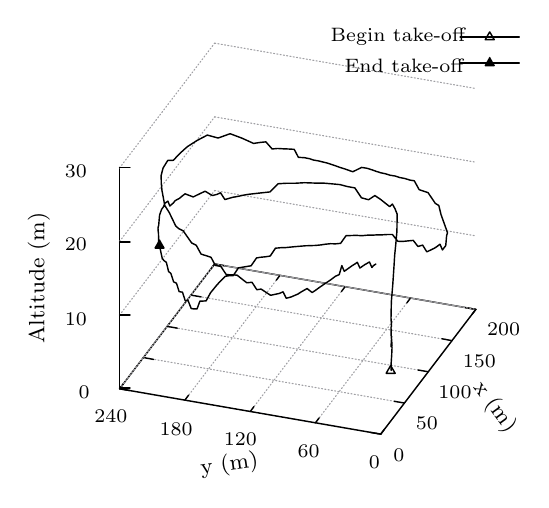
\begin{tikzpicture}[y=0.80pt, x=0.80pt, yscale=-0.780000, xscale=0.780000, inner sep=0pt, outer sep=0pt]
\scriptsize
\begin{scope}[draw=black,line join=bevel,line cap=rect,even odd rule,line width=0.512pt]
  \begin{scope}[cm={{1.0,0.0,0.0,1.0,(0.0,0.0)}},draw=black,line join=bevel,line cap=rect,line width=0.512pt]
  \end{scope}
  \begin{scope}[cm={{1.00625,0.0,0.0,1.00625,(0.0,0.0)}},draw=black,line join=bevel,line cap=rect,line width=0.512pt]
  \end{scope}
  \begin{scope}[cm={{1.00625,0.0,0.0,1.00625,(0.0,0.0)}},draw=black,line join=round,line cap=round,line width=0.512pt]
    \path[draw] (57.5000,238.9000) -- (112.2000,167.1000);
    \path[draw] (262.5000,193.2000) -- (112.2000,167.1000);
    \path[draw] (57.5000,238.5000) -- (57.5000,111.5000);
  \end{scope}
  \begin{scope}[cm={{1.00625,0.0,0.0,1.00625,(0.0,0.0)}},draw=ca0a0a4,dash pattern=on 0.40pt off 0.80pt,line join=round,line cap=round,line width=0.400pt]
    \path[draw] (207.8000,265.0000) -- (57.5000,238.9000);
  \end{scope}
  \begin{scope}[cm={{1.00625,0.0,0.0,1.00625,(0.0,0.0)}},draw=black,line join=round,line cap=round,line width=0.512pt]
    \path[draw] (207.8000,265.0000) -- (201.9000,264.0000);
    \path[draw] (57.5000,238.9000) -- (63.4000,239.9000);
  \end{scope}
  \begin{scope}[cm={{1.00625,0.0,0.0,1.00625,(0.0,0.0)}},draw=black,line join=bevel,line cap=rect,line width=0.512pt]
  \end{scope}
  \begin{scope}[cm={{1.00625,0.0,0.0,1.00625,(216.344,282.253)}},draw=black,line join=bevel,line cap=rect,line width=0.512pt]
  \end{scope}
  \begin{scope}[cm={{1.00625,0.0,0.0,1.00625,(216.344,282.253)}},draw=black,line join=bevel,line cap=rect,line width=0.512pt]
  \end{scope}
  \begin{scope}[cm={{1.00625,0.0,0.0,1.00625,(216.344,282.253)}},draw=black,line join=bevel,line cap=rect,line width=0.512pt]
  \end{scope}
  \begin{scope}[cm={{1.00625,0.0,0.0,1.00625,(216.344,282.253)}},draw=black,line join=bevel,line cap=rect,line width=0.512pt]
  \end{scope}
  \begin{scope}[cm={{1.00625,0.0,0.0,1.00625,(216.344,282.253)}},draw=black,line join=bevel,line cap=rect,line width=0.512pt]
  \end{scope}
  \begin{scope}[cm={{1.00625,0.0,0.0,1.00625,(216.344,282.253)}},draw=black,line join=bevel,line cap=rect,line width=0.512pt]
    \path[fill=black] (0.0000,0.0000) node[above right] () {0};
  \end{scope}
  \begin{scope}[cm={{1.00625,0.0,0.0,1.00625,(216.344,282.253)}},draw=black,line join=bevel,line cap=rect,line width=0.512pt]
  \end{scope}
  \begin{scope}[cm={{1.00625,0.0,0.0,1.00625,(0.0,0.0)}},draw=black,line join=bevel,line cap=rect,line width=0.512pt]
  \end{scope}
  \begin{scope}[cm={{1.00625,0.0,0.0,1.00625,(0.0,0.0)}},draw=ca0a0a4,dash pattern=on 0.40pt off 0.80pt,line join=round,line cap=round,line width=0.400pt]
    \path[draw] (221.4000,247.1000) -- (71.2000,220.9000);
  \end{scope}
  \begin{scope}[cm={{1.00625,0.0,0.0,1.00625,(0.0,0.0)}},draw=black,line join=round,line cap=round,line width=0.512pt]
    \path[draw] (221.4000,247.1000) -- (215.6000,246.1000);
    \path[draw] (71.2000,220.9000) -- (77.0000,222.0000);
  \end{scope}
  \begin{scope}[cm={{1.00625,0.0,0.0,1.00625,(0.0,0.0)}},draw=black,line join=bevel,line cap=rect,line width=0.512pt]
  \end{scope}
  \begin{scope}[cm={{1.00625,0.0,0.0,1.00625,(229.425,264.141)}},draw=black,line join=bevel,line cap=rect,line width=0.512pt]
  \end{scope}
  \begin{scope}[cm={{1.00625,0.0,0.0,1.00625,(229.425,264.141)}},draw=black,line join=bevel,line cap=rect,line width=0.512pt]
  \end{scope}
  \begin{scope}[cm={{1.00625,0.0,0.0,1.00625,(229.425,264.141)}},draw=black,line join=bevel,line cap=rect,line width=0.512pt]
  \end{scope}
  \begin{scope}[cm={{1.00625,0.0,0.0,1.00625,(229.425,264.141)}},draw=black,line join=bevel,line cap=rect,line width=0.512pt]
  \end{scope}
  \begin{scope}[cm={{1.00625,0.0,0.0,1.00625,(229.425,264.141)}},draw=black,line join=bevel,line cap=rect,line width=0.512pt]
  \end{scope}
  \begin{scope}[cm={{1.00625,0.0,0.0,1.00625,(229.425,264.141)}},draw=black,line join=bevel,line cap=rect,line width=0.512pt]
    \path[fill=black] (0.0000,0.0000) node[above right] () {50};
  \end{scope}
  \begin{scope}[cm={{1.00625,0.0,0.0,1.00625,(229.425,264.141)}},draw=black,line join=bevel,line cap=rect,line width=0.512pt]
  \end{scope}
  \begin{scope}[cm={{1.00625,0.0,0.0,1.00625,(0.0,0.0)}},draw=black,line join=bevel,line cap=rect,line width=0.512pt]
  \end{scope}
  \begin{scope}[cm={{1.00625,0.0,0.0,1.00625,(0.0,0.0)}},draw=ca0a0a4,dash pattern=on 0.40pt off 0.80pt,line join=round,line cap=round,line width=0.400pt]
    \path[draw] (235.1000,229.1000) -- (84.9000,203.0000);
  \end{scope}
  \begin{scope}[cm={{1.00625,0.0,0.0,1.00625,(0.0,0.0)}},draw=black,line join=round,line cap=round,line width=0.512pt]
    \path[draw] (235.1000,229.1000) -- (229.3000,228.1000);
    \path[draw] (84.9000,203.0000) -- (90.7000,204.0000);
  \end{scope}
  \begin{scope}[cm={{1.00625,0.0,0.0,1.00625,(0.0,0.0)}},draw=black,line join=bevel,line cap=rect,line width=0.512pt]
  \end{scope}
  \begin{scope}[cm={{1.00625,0.0,0.0,1.00625,(242.506,246.028)}},draw=black,line join=bevel,line cap=rect,line width=0.512pt]
  \end{scope}
  \begin{scope}[cm={{1.00625,0.0,0.0,1.00625,(242.506,246.028)}},draw=black,line join=bevel,line cap=rect,line width=0.512pt]
  \end{scope}
  \begin{scope}[cm={{1.00625,0.0,0.0,1.00625,(242.506,246.028)}},draw=black,line join=bevel,line cap=rect,line width=0.512pt]
  \end{scope}
  \begin{scope}[cm={{1.00625,0.0,0.0,1.00625,(242.506,246.028)}},draw=black,line join=bevel,line cap=rect,line width=0.512pt]
  \end{scope}
  \begin{scope}[cm={{1.00625,0.0,0.0,1.00625,(242.506,246.028)}},draw=black,line join=bevel,line cap=rect,line width=0.512pt]
  \end{scope}
  \begin{scope}[cm={{1.00625,0.0,0.0,1.00625,(242.506,246.028)}},draw=black,line join=bevel,line cap=rect,line width=0.512pt]
    \path[fill=black] (0.0000,0.0000) node[above right] () {100};
  \end{scope}
  \begin{scope}[cm={{1.00625,0.0,0.0,1.00625,(242.506,246.028)}},draw=black,line join=bevel,line cap=rect,line width=0.512pt]
  \end{scope}
  \begin{scope}[cm={{1.00625,0.0,0.0,1.00625,(0.0,0.0)}},draw=black,line join=bevel,line cap=rect,line width=0.512pt]
  \end{scope}
  \begin{scope}[cm={{1.00625,0.0,0.0,1.00625,(0.0,0.0)}},draw=ca0a0a4,dash pattern=on 0.40pt off 0.80pt,line join=round,line cap=round,line width=0.400pt]
    \path[draw] (248.8000,211.2000) -- (98.6000,185.0000);
  \end{scope}
  \begin{scope}[cm={{1.00625,0.0,0.0,1.00625,(0.0,0.0)}},draw=black,line join=round,line cap=round,line width=0.512pt]
    \path[draw] (248.8000,211.2000) -- (243.0000,210.1000);
    \path[draw] (98.6000,185.0000) -- (104.4000,186.0000);
  \end{scope}
  \begin{scope}[cm={{1.00625,0.0,0.0,1.00625,(0.0,0.0)}},draw=black,line join=bevel,line cap=rect,line width=0.512pt]
  \end{scope}
  \begin{scope}[cm={{1.00625,0.0,0.0,1.00625,(256.594,227.916)}},draw=black,line join=bevel,line cap=rect,line width=0.512pt]
  \end{scope}
  \begin{scope}[cm={{1.00625,0.0,0.0,1.00625,(256.594,227.916)}},draw=black,line join=bevel,line cap=rect,line width=0.512pt]
  \end{scope}
  \begin{scope}[cm={{1.00625,0.0,0.0,1.00625,(256.594,227.916)}},draw=black,line join=bevel,line cap=rect,line width=0.512pt]
  \end{scope}
  \begin{scope}[cm={{1.00625,0.0,0.0,1.00625,(256.594,227.916)}},draw=black,line join=bevel,line cap=rect,line width=0.512pt]
  \end{scope}
  \begin{scope}[cm={{1.00625,0.0,0.0,1.00625,(256.594,227.916)}},draw=black,line join=bevel,line cap=rect,line width=0.512pt]
  \end{scope}
  \begin{scope}[cm={{1.00625,0.0,0.0,1.00625,(256.594,227.916)}},draw=black,line join=bevel,line cap=rect,line width=0.512pt]
    \path[fill=black] (0.0000,0.0000) node[above right] () {150};
  \end{scope}
  \begin{scope}[cm={{1.00625,0.0,0.0,1.00625,(256.594,227.916)}},draw=black,line join=bevel,line cap=rect,line width=0.512pt]
  \end{scope}
  \begin{scope}[cm={{1.00625,0.0,0.0,1.00625,(0.0,0.0)}},draw=black,line join=bevel,line cap=rect,line width=0.512pt]
  \end{scope}
  \begin{scope}[cm={{1.00625,0.0,0.0,1.00625,(0.0,0.0)}},draw=ca0a0a4,dash pattern=on 0.40pt off 0.80pt,line join=round,line cap=round,line width=0.400pt]
    \path[draw] (262.5000,193.2000) -- (112.2000,167.1000);
  \end{scope}
  \begin{scope}[cm={{1.00625,0.0,0.0,1.00625,(0.0,0.0)}},draw=black,line join=round,line cap=round,line width=0.512pt]
    \path[draw] (262.5000,193.2000) -- (256.6000,192.2000);
    \path[draw] (112.2000,167.1000) -- (118.1000,168.1000);
  \end{scope}
  \begin{scope}[cm={{1.00625,0.0,0.0,1.00625,(0.0,0.0)}},draw=black,line join=bevel,line cap=rect,line width=0.512pt]
  \end{scope}
  \begin{scope}[cm={{1.00625,0.0,0.0,1.00625,(270.681,209.803)}},draw=black,line join=bevel,line cap=rect,line width=0.512pt]
  \end{scope}
  \begin{scope}[cm={{1.00625,0.0,0.0,1.00625,(270.681,209.803)}},draw=black,line join=bevel,line cap=rect,line width=0.512pt]
  \end{scope}
  \begin{scope}[cm={{1.00625,0.0,0.0,1.00625,(270.681,209.803)}},draw=black,line join=bevel,line cap=rect,line width=0.512pt]
  \end{scope}
  \begin{scope}[cm={{1.00625,0.0,0.0,1.00625,(270.681,209.803)}},draw=black,line join=bevel,line cap=rect,line width=0.512pt]
  \end{scope}
  \begin{scope}[cm={{1.00625,0.0,0.0,1.00625,(270.681,209.803)}},draw=black,line join=bevel,line cap=rect,line width=0.512pt]
  \end{scope}
  \begin{scope}[cm={{1.00625,0.0,0.0,1.00625,(270.681,209.803)}},draw=black,line join=bevel,line cap=rect,line width=0.512pt]
    \path[fill=black] (0.0000,0.0000) node[above right] () {200};
  \end{scope}
  \begin{scope}[cm={{1.00625,0.0,0.0,1.00625,(270.681,209.803)}},draw=black,line join=bevel,line cap=rect,line width=0.512pt]
  \end{scope}
  \begin{scope}[cm={{1.00625,0.0,0.0,1.00625,(0.0,0.0)}},draw=black,line join=bevel,line cap=rect,line width=0.512pt]
  \end{scope}
  \begin{scope}[cm={{1.00625,0.0,0.0,1.00625,(0.0,0.0)}},draw=ca0a0a4,dash pattern=on 0.40pt off 0.80pt,line join=round,line cap=round,line width=0.400pt]
    \path[draw] (207.8000,265.0000) -- (262.5000,193.2000);
  \end{scope}
  \begin{scope}[cm={{1.00625,0.0,0.0,1.00625,(0.0,0.0)}},draw=black,line join=round,line cap=round,line width=0.512pt]
    \path[draw] (207.8000,265.0000) -- (209.9000,262.2000);
    \path[draw] (262.5000,193.2000) -- (260.4000,196.0000);
  \end{scope}
  \begin{scope}[cm={{1.00625,0.0,0.0,1.00625,(0.0,0.0)}},draw=black,line join=bevel,line cap=rect,line width=0.512pt]
  \end{scope}
  \begin{scope}[cm={{1.00625,0.0,0.0,1.00625,(202.256,286.278)}},draw=black,line join=bevel,line cap=rect,line width=0.512pt]
  \end{scope}
  \begin{scope}[cm={{1.00625,0.0,0.0,1.00625,(202.256,286.278)}},draw=black,line join=bevel,line cap=rect,line width=0.512pt]
  \end{scope}
  \begin{scope}[cm={{1.00625,0.0,0.0,1.00625,(202.256,286.278)}},draw=black,line join=bevel,line cap=rect,line width=0.512pt]
  \end{scope}
  \begin{scope}[cm={{1.00625,0.0,0.0,1.00625,(202.256,286.278)}},draw=black,line join=bevel,line cap=rect,line width=0.512pt]
  \end{scope}
  \begin{scope}[cm={{1.00625,0.0,0.0,1.00625,(202.256,286.278)}},draw=black,line join=bevel,line cap=rect,line width=0.512pt]
  \end{scope}
  \begin{scope}[cm={{1.00625,0.0,0.0,1.00625,(202.256,286.278)}},draw=black,line join=bevel,line cap=rect,line width=0.512pt]
    \path[fill=black] (0.0000,0.0000) node[above right] () {0};
  \end{scope}
  \begin{scope}[cm={{1.00625,0.0,0.0,1.00625,(202.256,286.278)}},draw=black,line join=bevel,line cap=rect,line width=0.512pt]
  \end{scope}
  \begin{scope}[cm={{1.00625,0.0,0.0,1.00625,(0.0,0.0)}},draw=black,line join=bevel,line cap=rect,line width=0.512pt]
  \end{scope}
  \begin{scope}[cm={{1.00625,0.0,0.0,1.00625,(0.0,0.0)}},draw=ca0a0a4,dash pattern=on 0.40pt off 0.80pt,line join=round,line cap=round,line width=0.400pt]
    \path[draw] (170.2000,258.5000) -- (224.9000,186.7000);
  \end{scope}
  \begin{scope}[cm={{1.00625,0.0,0.0,1.00625,(0.0,0.0)}},draw=black,line join=round,line cap=round,line width=0.512pt]
    \path[draw] (170.2000,258.5000) -- (172.3000,255.7000);
    \path[draw] (224.9000,186.7000) -- (222.8000,189.5000);
  \end{scope}
  \begin{scope}[cm={{1.00625,0.0,0.0,1.00625,(0.0,0.0)}},draw=black,line join=bevel,line cap=rect,line width=0.512pt]
  \end{scope}
  \begin{scope}[cm={{1.00625,0.0,0.0,1.00625,(161.0,280.241)}},draw=black,line join=bevel,line cap=rect,line width=0.512pt]
  \end{scope}
  \begin{scope}[cm={{1.00625,0.0,0.0,1.00625,(161.0,280.241)}},draw=black,line join=bevel,line cap=rect,line width=0.512pt]
  \end{scope}
  \begin{scope}[cm={{1.00625,0.0,0.0,1.00625,(161.0,280.241)}},draw=black,line join=bevel,line cap=rect,line width=0.512pt]
  \end{scope}
  \begin{scope}[cm={{1.00625,0.0,0.0,1.00625,(161.0,280.241)}},draw=black,line join=bevel,line cap=rect,line width=0.512pt]
  \end{scope}
  \begin{scope}[cm={{1.00625,0.0,0.0,1.00625,(161.0,280.241)}},draw=black,line join=bevel,line cap=rect,line width=0.512pt]
  \end{scope}
  \begin{scope}[cm={{1.00625,0.0,0.0,1.00625,(161.0,280.241)}},draw=black,line join=bevel,line cap=rect,line width=0.512pt]
    \path[fill=black] (0.0000,0.0000) node[above right] () {60};
  \end{scope}
  \begin{scope}[cm={{1.00625,0.0,0.0,1.00625,(161.0,280.241)}},draw=black,line join=bevel,line cap=rect,line width=0.512pt]
  \end{scope}
  \begin{scope}[cm={{1.00625,0.0,0.0,1.00625,(0.0,0.0)}},draw=black,line join=bevel,line cap=rect,line width=0.512pt]
  \end{scope}
  \begin{scope}[cm={{1.00625,0.0,0.0,1.00625,(0.0,0.0)}},draw=ca0a0a4,dash pattern=on 0.40pt off 0.80pt,line join=round,line cap=round,line width=0.400pt]
    \path[draw] (132.7000,252.0000) -- (187.3000,180.1000);
  \end{scope}
  \begin{scope}[cm={{1.00625,0.0,0.0,1.00625,(0.0,0.0)}},draw=black,line join=round,line cap=round,line width=0.512pt]
    \path[draw] (132.7000,252.0000) -- (134.8000,249.2000);
    \path[draw] (187.3000,180.1000) -- (185.2000,182.9000);
  \end{scope}
  \begin{scope}[cm={{1.00625,0.0,0.0,1.00625,(0.0,0.0)}},draw=black,line join=bevel,line cap=rect,line width=0.512pt]
  \end{scope}
  \begin{scope}[cm={{1.00625,0.0,0.0,1.00625,(118.234,273.197)}},draw=black,line join=bevel,line cap=rect,line width=0.512pt]
  \end{scope}
  \begin{scope}[cm={{1.00625,0.0,0.0,1.00625,(118.234,273.197)}},draw=black,line join=bevel,line cap=rect,line width=0.512pt]
  \end{scope}
  \begin{scope}[cm={{1.00625,0.0,0.0,1.00625,(118.234,273.197)}},draw=black,line join=bevel,line cap=rect,line width=0.512pt]
  \end{scope}
  \begin{scope}[cm={{1.00625,0.0,0.0,1.00625,(118.234,273.197)}},draw=black,line join=bevel,line cap=rect,line width=0.512pt]
  \end{scope}
  \begin{scope}[cm={{1.00625,0.0,0.0,1.00625,(118.234,273.197)}},draw=black,line join=bevel,line cap=rect,line width=0.512pt]
  \end{scope}
  \begin{scope}[cm={{1.00625,0.0,0.0,1.00625,(118.234,273.197)}},draw=black,line join=bevel,line cap=rect,line width=0.512pt]
    \path[fill=black] (0.0000,0.0000) node[above right] () {120};
  \end{scope}
  \begin{scope}[cm={{1.00625,0.0,0.0,1.00625,(118.234,273.197)}},draw=black,line join=bevel,line cap=rect,line width=0.512pt]
  \end{scope}
  \begin{scope}[cm={{1.00625,0.0,0.0,1.00625,(0.0,0.0)}},draw=black,line join=bevel,line cap=rect,line width=0.512pt]
  \end{scope}
  \begin{scope}[cm={{1.00625,0.0,0.0,1.00625,(0.0,0.0)}},draw=ca0a0a4,dash pattern=on 0.40pt off 0.80pt,line join=round,line cap=round,line width=0.400pt]
    \path[draw] (95.1000,245.4000) -- (149.8000,173.6000);
  \end{scope}
  \begin{scope}[cm={{1.00625,0.0,0.0,1.00625,(0.0,0.0)}},draw=black,line join=round,line cap=round,line width=0.512pt]
    \path[draw] (95.1000,245.4000) -- (97.2000,242.6000);
    \path[draw] (149.8000,173.6000) -- (147.7000,176.4000);
  \end{scope}
  \begin{scope}[cm={{1.00625,0.0,0.0,1.00625,(0.0,0.0)}},draw=black,line join=bevel,line cap=rect,line width=0.512pt]
  \end{scope}
  \begin{scope}[cm={{1.00625,0.0,0.0,1.00625,(81.0031,267.159)}},draw=black,line join=bevel,line cap=rect,line width=0.512pt]
  \end{scope}
  \begin{scope}[cm={{1.00625,0.0,0.0,1.00625,(81.0031,267.159)}},draw=black,line join=bevel,line cap=rect,line width=0.512pt]
  \end{scope}
  \begin{scope}[cm={{1.00625,0.0,0.0,1.00625,(81.0031,267.159)}},draw=black,line join=bevel,line cap=rect,line width=0.512pt]
  \end{scope}
  \begin{scope}[cm={{1.00625,0.0,0.0,1.00625,(81.0031,267.159)}},draw=black,line join=bevel,line cap=rect,line width=0.512pt]
  \end{scope}
  \begin{scope}[cm={{1.00625,0.0,0.0,1.00625,(81.0031,267.159)}},draw=black,line join=bevel,line cap=rect,line width=0.512pt]
  \end{scope}
  \begin{scope}[cm={{1.00625,0.0,0.0,1.00625,(81.0031,267.159)}},draw=black,line join=bevel,line cap=rect,line width=0.512pt]
    \path[fill=black] (0.0000,0.0000) node[above right] () {180};
  \end{scope}
  \begin{scope}[cm={{1.00625,0.0,0.0,1.00625,(81.0031,267.159)}},draw=black,line join=bevel,line cap=rect,line width=0.512pt]
  \end{scope}
  \begin{scope}[cm={{1.00625,0.0,0.0,1.00625,(0.0,0.0)}},draw=black,line join=bevel,line cap=rect,line width=0.512pt]
  \end{scope}
  \begin{scope}[cm={{1.00625,0.0,0.0,1.00625,(0.0,0.0)}},draw=ca0a0a4,dash pattern=on 0.40pt off 0.80pt,line join=round,line cap=round,line width=0.400pt]
    \path[draw] (57.5000,238.9000) -- (112.2000,167.1000);
  \end{scope}
  \begin{scope}[cm={{1.00625,0.0,0.0,1.00625,(0.0,0.0)}},draw=black,line join=round,line cap=round,line width=0.512pt]
    \path[draw] (57.5000,238.9000) -- (59.6000,236.1000);
    \path[draw] (112.2000,167.1000) -- (110.1000,169.9000);
  \end{scope}
  \begin{scope}[cm={{1.00625,0.0,0.0,1.00625,(0.0,0.0)}},draw=black,line join=bevel,line cap=rect,line width=0.512pt]
  \end{scope}
  \begin{scope}[cm={{1.00625,0.0,0.0,1.00625,(43.2688,260.116)}},draw=black,line join=bevel,line cap=rect,line width=0.512pt]
  \end{scope}
  \begin{scope}[cm={{1.00625,0.0,0.0,1.00625,(43.2688,260.116)}},draw=black,line join=bevel,line cap=rect,line width=0.512pt]
  \end{scope}
  \begin{scope}[cm={{1.00625,0.0,0.0,1.00625,(43.2688,260.116)}},draw=black,line join=bevel,line cap=rect,line width=0.512pt]
  \end{scope}
  \begin{scope}[cm={{1.00625,0.0,0.0,1.00625,(43.2688,260.116)}},draw=black,line join=bevel,line cap=rect,line width=0.512pt]
  \end{scope}
  \begin{scope}[cm={{1.00625,0.0,0.0,1.00625,(43.2688,260.116)}},draw=black,line join=bevel,line cap=rect,line width=0.512pt]
  \end{scope}
  \begin{scope}[cm={{1.00625,0.0,0.0,1.00625,(43.2688,260.116)}},draw=black,line join=bevel,line cap=rect,line width=0.512pt]
    \path[fill=black] (0.0000,0.0000) node[above right] () {240};
  \end{scope}
  \begin{scope}[cm={{1.00625,0.0,0.0,1.00625,(43.2688,260.116)}},draw=black,line join=bevel,line cap=rect,line width=0.512pt]
  \end{scope}
  \begin{scope}[cm={{1.00625,0.0,0.0,1.00625,(0.0,0.0)}},draw=black,line join=bevel,line cap=rect,line width=0.512pt]
  \end{scope}
  \begin{scope}[cm={{1.00625,0.0,0.0,1.00625,(0.0,0.0)}},draw=ca0a0a4,dash pattern=on 0.40pt off 0.80pt,line join=round,line cap=round,line width=0.400pt]
    \path[draw] (57.5000,238.9000) -- (112.2000,167.1000);
    \path[draw] (112.2000,167.1000) -- (112.2000,167.1000) -- (262.5000,193.2000);
  \end{scope}
  \begin{scope}[cm={{1.00625,0.0,0.0,1.00625,(0.0,0.0)}},draw=black,line join=round,line cap=round,line width=0.512pt]
    \path[draw] (57.5000,238.5000) -- (63.5000,238.5000);
  \end{scope}
  \begin{scope}[cm={{1.00625,0.0,0.0,1.00625,(0.0,0.0)}},draw=black,line join=bevel,line cap=rect,line width=0.512pt]
  \end{scope}
  \begin{scope}[cm={{1.00625,0.0,0.0,1.00625,(34.2125,246.028)}},draw=black,line join=bevel,line cap=rect,line width=0.512pt]
  \end{scope}
  \begin{scope}[cm={{1.00625,0.0,0.0,1.00625,(34.2125,246.028)}},draw=black,line join=bevel,line cap=rect,line width=0.512pt]
  \end{scope}
  \begin{scope}[cm={{1.00625,0.0,0.0,1.00625,(34.2125,246.028)}},draw=black,line join=bevel,line cap=rect,line width=0.512pt]
  \end{scope}
  \begin{scope}[cm={{1.00625,0.0,0.0,1.00625,(34.2125,246.028)}},draw=black,line join=bevel,line cap=rect,line width=0.512pt]
  \end{scope}
  \begin{scope}[cm={{1.00625,0.0,0.0,1.00625,(34.2125,246.028)}},draw=black,line join=bevel,line cap=rect,line width=0.512pt]
  \end{scope}
  \begin{scope}[cm={{1.00625,0.0,0.0,1.00625,(34.2125,246.028)}},draw=black,line join=bevel,line cap=rect,line width=0.512pt]
    \path[fill=black] (0.0000,0.0000) node[above right] () {0};
  \end{scope}
  \begin{scope}[cm={{1.00625,0.0,0.0,1.00625,(34.2125,246.028)}},draw=black,line join=bevel,line cap=rect,line width=0.512pt]
  \end{scope}
  \begin{scope}[cm={{1.00625,0.0,0.0,1.00625,(0.0,0.0)}},draw=black,line join=bevel,line cap=rect,line width=0.512pt]
  \end{scope}
  \begin{scope}[cm={{1.00625,0.0,0.0,1.00625,(0.0,0.0)}},draw=ca0a0a4,dash pattern=on 0.40pt off 0.80pt,line join=round,line cap=round,line width=0.400pt]
    \path[draw] (57.5000,196.5000) -- (112.2000,124.8000);
    \path[draw] (112.2000,124.8000) -- (112.2000,124.8000) -- (262.5000,150.9000);
  \end{scope}
  \begin{scope}[cm={{1.00625,0.0,0.0,1.00625,(0.0,0.0)}},draw=black,line join=round,line cap=round,line width=0.512pt]
    \path[draw] (57.5000,196.5000) -- (63.5000,196.5000);
  \end{scope}
  \begin{scope}[cm={{1.00625,0.0,0.0,1.00625,(0.0,0.0)}},draw=black,line join=bevel,line cap=rect,line width=0.512pt]
  \end{scope}
  \begin{scope}[cm={{1.00625,0.0,0.0,1.00625,(26.1625,203.766)}},draw=black,line join=bevel,line cap=rect,line width=0.512pt]
  \end{scope}
  \begin{scope}[cm={{1.00625,0.0,0.0,1.00625,(26.1625,203.766)}},draw=black,line join=bevel,line cap=rect,line width=0.512pt]
  \end{scope}
  \begin{scope}[cm={{1.00625,0.0,0.0,1.00625,(26.1625,203.766)}},draw=black,line join=bevel,line cap=rect,line width=0.512pt]
  \end{scope}
  \begin{scope}[cm={{1.00625,0.0,0.0,1.00625,(26.1625,203.766)}},draw=black,line join=bevel,line cap=rect,line width=0.512pt]
  \end{scope}
  \begin{scope}[cm={{1.00625,0.0,0.0,1.00625,(26.1625,203.766)}},draw=black,line join=bevel,line cap=rect,line width=0.512pt]
  \end{scope}
  \begin{scope}[cm={{1.00625,0.0,0.0,1.00625,(26.1625,203.766)}},draw=black,line join=bevel,line cap=rect,line width=0.512pt]
    \path[fill=black] (0.0000,0.0000) node[above right] () {10};
  \end{scope}
  \begin{scope}[cm={{1.00625,0.0,0.0,1.00625,(26.1625,203.766)}},draw=black,line join=bevel,line cap=rect,line width=0.512pt]
  \end{scope}
  \begin{scope}[cm={{1.00625,0.0,0.0,1.00625,(0.0,0.0)}},draw=black,line join=bevel,line cap=rect,line width=0.512pt]
  \end{scope}
  \begin{scope}[cm={{1.00625,0.0,0.0,1.00625,(0.0,0.0)}},draw=ca0a0a4,dash pattern=on 0.40pt off 0.80pt,line join=round,line cap=round,line width=0.400pt]
    \path[draw] (57.5000,154.1000) -- (112.2000,82.4000);
    \path[draw] (112.2000,82.4000) -- (112.2000,82.4000) -- (262.5000,108.5000);
  \end{scope}
  \begin{scope}[cm={{1.00625,0.0,0.0,1.00625,(0.0,0.0)}},draw=black,line join=round,line cap=round,line width=0.512pt]
    \path[draw] (57.5000,154.5000) -- (63.5000,154.5000);
  \end{scope}
  \begin{scope}[cm={{1.00625,0.0,0.0,1.00625,(0.0,0.0)}},draw=black,line join=bevel,line cap=rect,line width=0.512pt]
  \end{scope}
  \begin{scope}[cm={{1.00625,0.0,0.0,1.00625,(26.1625,160.497)}},draw=black,line join=bevel,line cap=rect,line width=0.512pt]
  \end{scope}
  \begin{scope}[cm={{1.00625,0.0,0.0,1.00625,(26.1625,160.497)}},draw=black,line join=bevel,line cap=rect,line width=0.512pt]
  \end{scope}
  \begin{scope}[cm={{1.00625,0.0,0.0,1.00625,(26.1625,160.497)}},draw=black,line join=bevel,line cap=rect,line width=0.512pt]
  \end{scope}
  \begin{scope}[cm={{1.00625,0.0,0.0,1.00625,(26.1625,160.497)}},draw=black,line join=bevel,line cap=rect,line width=0.512pt]
  \end{scope}
  \begin{scope}[cm={{1.00625,0.0,0.0,1.00625,(26.1625,160.497)}},draw=black,line join=bevel,line cap=rect,line width=0.512pt]
  \end{scope}
  \begin{scope}[cm={{1.00625,0.0,0.0,1.00625,(26.1625,160.497)}},draw=black,line join=bevel,line cap=rect,line width=0.512pt]
    \path[fill=black] (0.0000,0.0000) node[above right] () {20};
  \end{scope}
  \begin{scope}[cm={{1.00625,0.0,0.0,1.00625,(26.1625,160.497)}},draw=black,line join=bevel,line cap=rect,line width=0.512pt]
  \end{scope}
  \begin{scope}[cm={{1.00625,0.0,0.0,1.00625,(0.0,0.0)}},draw=black,line join=bevel,line cap=rect,line width=0.512pt]
  \end{scope}
  \begin{scope}[cm={{1.00625,0.0,0.0,1.00625,(0.0,0.0)}},draw=ca0a0a4,dash pattern=on 0.40pt off 0.80pt,line join=round,line cap=round,line width=0.400pt]
    \path[draw] (57.5000,111.8000) -- (112.2000,40.0000);
    \path[draw] (112.2000,40.0000) -- (112.2000,40.0000) -- (262.5000,66.1000);
  \end{scope}
  \begin{scope}[cm={{1.00625,0.0,0.0,1.00625,(0.0,0.0)}},draw=black,line join=round,line cap=round,line width=0.512pt]
    \path[draw] (57.5000,111.5000) -- (63.5000,111.5000);
  \end{scope}
  \begin{scope}[cm={{1.00625,0.0,0.0,1.00625,(0.0,0.0)}},draw=black,line join=bevel,line cap=rect,line width=0.512pt]
  \end{scope}
  \begin{scope}[cm={{1.00625,0.0,0.0,1.00625,(26.1625,118.234)}},draw=black,line join=bevel,line cap=rect,line width=0.512pt]
  \end{scope}
  \begin{scope}[cm={{1.00625,0.0,0.0,1.00625,(26.1625,118.234)}},draw=black,line join=bevel,line cap=rect,line width=0.512pt]
  \end{scope}
  \begin{scope}[cm={{1.00625,0.0,0.0,1.00625,(26.1625,118.234)}},draw=black,line join=bevel,line cap=rect,line width=0.512pt]
  \end{scope}
  \begin{scope}[cm={{1.00625,0.0,0.0,1.00625,(26.1625,118.234)}},draw=black,line join=bevel,line cap=rect,line width=0.512pt]
  \end{scope}
  \begin{scope}[cm={{1.00625,0.0,0.0,1.00625,(26.1625,118.234)}},draw=black,line join=bevel,line cap=rect,line width=0.512pt]
  \end{scope}
  \begin{scope}[cm={{1.00625,0.0,0.0,1.00625,(26.1625,118.234)}},draw=black,line join=bevel,line cap=rect,line width=0.512pt]
    \path[fill=black] (0.0000,0.0000) node[above right] () {30};
  \end{scope}
  \begin{scope}[cm={{1.00625,0.0,0.0,1.00625,(26.1625,118.234)}},draw=black,line join=bevel,line cap=rect,line width=0.512pt]
  \end{scope}
  \begin{scope}[cm={{1.00625,0.0,0.0,1.00625,(0.0,0.0)}},draw=black,line join=bevel,line cap=rect,line width=0.512pt]
  \end{scope}
  \begin{scope}[cm={{1.00625,0.0,0.0,1.00625,(0.0,0.0)}},draw=black,line join=bevel,line cap=rect,line width=0.512pt]
  \end{scope}
  \begin{scope}[cm={{1.00625,0.0,0.0,1.00625,(0.0,0.0)}},draw=black,line join=bevel,line cap=rect,line width=0.512pt]
  \end{scope}
  \begin{scope}[cm={{1.00625,0.0,0.0,1.00625,(0.0,0.0)}},draw=black,line join=round,line cap=round,line width=0.512pt]
    \path[draw] (213.8000,228.3000) -- (213.8000,228.3000) -- (213.8000,228.3000) --
      (213.8000,228.3000) -- (213.8000,228.3000) -- (213.8000,228.3000) --
      (213.8000,228.3000) -- (213.8000,228.3000) -- (213.8000,228.3000) --
      (213.8000,228.3000) -- (213.8000,228.3000) -- (213.8000,228.3000) --
      (213.8000,228.3000) -- (213.8000,228.3000) -- (213.8000,228.3000) --
      (213.8000,228.3000) -- (213.8000,228.3000) -- (213.8000,224.0000) --
      (213.8000,224.0000) -- (213.8000,224.0000) -- (213.8000,224.0000) --
      (214.1000,219.4000) -- (214.1000,219.4000) -- (214.1000,219.4000) --
      (214.1000,219.4000) -- (214.1000,219.4000) -- (214.1000,219.4000) --
      (214.3000,214.8000) -- (214.3000,214.8000) -- (213.7000,214.7000) --
      (213.7000,214.7000) -- (214.0000,210.1000) -- (214.0000,210.1000) --
      (214.3000,214.0000) -- (214.3000,214.0000) -- (214.3000,214.0000) --
      (214.3000,214.0000) -- (213.9000,209.3000) -- (213.9000,209.3000) --
      (214.2000,208.9000) -- (214.2000,208.9000) -- (213.8000,208.5000) --
      (213.8000,208.5000) -- (213.8000,208.5000) -- (213.8000,208.5000) --
      (213.8000,208.5000) -- (213.8000,208.5000) -- (213.7000,203.4000) --
      (213.7000,203.4000) -- (214.0000,203.0000) -- (214.0000,203.0000) --
      (214.0000,203.0000) -- (214.0000,203.0000) -- (213.7000,198.3000) --
      (213.7000,198.3000) -- (213.7000,198.3000) -- (213.7000,198.3000) --
      (213.9000,188.7000) -- (213.9000,188.7000) -- (213.9000,188.7000) --
      (213.9000,188.7000) -- (214.7000,179.1000) -- (214.7000,179.1000) --
      (214.7000,179.1000) -- (214.7000,179.1000) -- (215.4000,168.7000) --
      (215.4000,168.7000) -- (215.4000,168.7000) -- (215.4000,168.7000) --
      (215.8000,162.1000) -- (215.8000,162.1000) -- (215.8000,162.1000) --
      (215.8000,162.1000) -- (215.8000,162.1000) -- (215.8000,162.1000) --
      (216.5000,155.1000) -- (216.5000,155.1000) -- (216.5000,155.1000) --
      (216.5000,155.1000) -- (216.5000,155.1000) -- (216.5000,155.1000) --
      (217.1000,148.3000) -- (217.1000,148.3000) -- (217.1000,148.3000) --
      (217.1000,148.3000) -- (217.2000,141.2000) -- (217.2000,141.2000) --
      (217.2000,141.2000) -- (217.2000,141.2000) -- (217.2000,138.3000) --
      (217.2000,138.3000) -- (217.2000,138.3000) -- (217.2000,138.3000) --
      (217.2000,138.3000) -- (217.2000,138.3000) -- (216.0000,135.3000) --
      (216.0000,135.3000) -- (216.0000,135.3000) -- (216.0000,135.3000) --
      (216.0000,135.3000) -- (216.0000,135.3000) -- (214.5000,132.6000) --
      (214.5000,132.6000) -- (214.5000,132.6000) -- (214.5000,132.6000) --
      (213.0000,134.1000) -- (213.0000,134.1000) -- (213.0000,134.1000) --
      (213.0000,134.1000) -- (210.3000,132.0000) -- (210.3000,132.0000) --
      (210.3000,132.0000) -- (210.3000,132.0000) -- (210.3000,132.0000) --
      (210.3000,132.0000) -- (207.7000,129.9000) -- (207.7000,129.9000) --
      (207.7000,129.9000) -- (207.7000,129.9000) -- (207.7000,129.9000) --
      (207.7000,129.9000) -- (204.4000,127.7000) -- (204.4000,127.7000) --
      (204.4000,127.7000) -- (204.4000,127.7000) -- (200.8000,130.1000) --
      (200.8000,130.1000) -- (200.8000,130.1000) -- (200.8000,130.1000) --
      (196.7000,129.0000) -- (196.7000,129.0000) -- (196.7000,129.0000) --
      (196.7000,129.0000) -- (196.7000,129.0000) -- (196.7000,129.0000) --
      (192.9000,123.3000) -- (192.9000,123.3000) -- (192.9000,123.3000) --
      (192.9000,123.3000) -- (192.9000,123.3000) -- (192.9000,123.3000) --
      (188.5000,122.5000) -- (188.5000,122.5000) -- (188.5000,122.5000) --
      (188.5000,122.5000) -- (184.4000,121.4000) -- (184.4000,121.4000) --
      (184.4000,121.4000) -- (184.4000,121.4000) -- (179.1000,120.9000) --
      (179.1000,120.9000) -- (179.1000,120.9000) -- (179.1000,120.9000) --
      (179.1000,120.9000) -- (179.1000,120.9000) -- (174.4000,120.5000) --
      (174.4000,120.5000) -- (174.4000,120.5000) -- (174.4000,120.5000) --
      (174.4000,120.5000) -- (174.4000,120.5000) -- (169.5000,120.5000) --
      (169.5000,120.5000) -- (169.5000,120.5000) -- (169.5000,120.5000) --
      (163.9000,120.3000) -- (163.9000,120.3000) -- (163.9000,120.3000) --
      (163.9000,120.3000) -- (158.8000,120.6000) -- (158.8000,120.6000) --
      (158.8000,120.6000) -- (158.8000,120.6000) -- (158.8000,120.6000) --
      (158.8000,120.6000) -- (153.9000,120.6000) -- (153.9000,120.6000) --
      (153.9000,120.6000) -- (153.9000,120.6000) -- (153.9000,120.6000) --
      (153.9000,120.6000) -- (148.7000,120.9000) -- (148.7000,120.9000) --
      (148.7000,120.9000) -- (148.7000,120.9000) -- (144.1000,125.6000) --
      (144.1000,125.6000) -- (144.1000,125.6000) -- (144.1000,125.6000) --
      (138.6000,126.2000) -- (138.6000,126.2000) -- (138.6000,126.2000) --
      (138.6000,126.2000) -- (138.6000,126.2000) -- (138.6000,126.2000) --
      (134.1000,126.7000) -- (134.1000,126.7000) -- (131.6000,127.0000) --
      (131.6000,127.0000) -- (129.2000,127.4000) -- (129.2000,127.4000) --
      (129.2000,127.4000) -- (129.2000,127.4000) -- (129.2000,127.4000) --
      (129.2000,127.4000) -- (125.0000,128.3000) -- (125.0000,128.3000) --
      (122.6000,128.7000) -- (122.6000,128.7000) -- (122.6000,128.7000) --
      (122.6000,128.7000) -- (122.6000,128.7000) -- (122.6000,128.7000) --
      (118.1000,130.0000) -- (118.1000,130.0000) -- (115.6000,126.1000) --
      (115.6000,126.1000) -- (113.6000,127.0000) -- (113.6000,127.0000) --
      (110.9000,127.7000) -- (110.9000,127.7000) -- (110.9000,127.7000) --
      (110.9000,127.7000) -- (110.9000,127.7000) -- (110.9000,127.7000) --
      (106.7000,125.2000) -- (106.7000,125.2000) -- (106.7000,125.2000) --
      (106.7000,125.2000) -- (102.3000,127.3000) -- (102.3000,127.3000) --
      (102.3000,127.3000) -- (102.3000,127.3000) -- (99.9000,128.5000) --
      (99.9000,128.5000) -- (99.9000,128.5000) -- (99.9000,128.5000) --
      (95.2000,126.7000) -- (95.2000,126.7000) -- (93.5000,128.0000) --
      (93.5000,128.0000) -- (93.5000,128.0000) -- (93.5000,128.0000) --
      (91.8000,129.4000) -- (91.8000,129.4000) -- (89.5000,130.6000) --
      (89.5000,130.6000) -- (88.4000,132.0000) -- (88.4000,132.0000) --
      (86.4000,133.7000) -- (86.4000,133.7000) -- (85.3000,130.9000) --
      (85.3000,130.9000) -- (85.3000,130.9000) -- (85.3000,130.9000) --
      (83.5000,132.2000) -- (83.5000,132.2000) -- (82.8000,134.1000) --
      (82.8000,134.1000) -- (81.7000,135.6000) -- (81.7000,135.6000) --
      (81.0000,137.5000) -- (81.0000,137.5000) -- (81.0000,137.5000) --
      (81.0000,137.5000) -- (80.5000,139.0000) -- (80.5000,139.0000) --
      (80.0000,144.8000) -- (80.0000,144.8000) -- (79.6000,146.3000) --
      (79.6000,146.3000) -- (79.7000,148.0000) -- (79.7000,148.0000) --
      (79.7000,148.0000) -- (79.7000,148.0000) -- (79.9000,149.7000) --
      (79.9000,149.7000) -- (80.0000,155.4000) -- (80.0000,155.4000) --
      (80.5000,156.7000) -- (80.5000,156.7000) -- (80.5000,156.7000) --
      (80.5000,156.7000) -- (80.5000,156.7000) -- (80.5000,156.7000) --
      (82.0000,163.7000) -- (82.0000,163.7000) -- (83.0000,165.1000) --
      (83.0000,165.1000) -- (84.4000,166.1000) -- (84.4000,166.1000) --
      (84.4000,166.1000) -- (84.4000,166.1000) -- (85.7000,171.4000) --
      (85.7000,171.4000) -- (87.0000,172.5000) -- (87.0000,172.5000) --
      (88.6000,177.4000) -- (88.6000,177.4000) -- (90.2000,178.1000) --
      (90.2000,178.1000) -- (90.2000,178.1000) -- (90.2000,178.1000) --
      (91.8000,183.0000) -- (91.8000,183.0000) -- (93.7000,183.3000) --
      (93.7000,183.3000) -- (95.3000,188.3000) -- (95.3000,188.3000) --
      (96.9000,188.1000) -- (96.9000,188.1000) -- (96.9000,188.1000) --
      (96.9000,188.1000) -- (98.7000,192.7000) -- (98.7000,192.7000) --
      (100.0000,192.9000) -- (100.0000,192.9000) -- (102.1000,192.9000) --
      (102.1000,192.9000) -- (103.7000,188.5000) -- (103.7000,188.5000) --
      (103.7000,188.5000) -- (103.7000,188.5000) -- (105.8000,188.4000) --
      (105.8000,188.4000) -- (107.3000,188.3000) -- (107.3000,188.3000) --
      (109.8000,183.7000) -- (109.8000,183.7000) -- (109.8000,183.7000) --
      (109.8000,183.7000) -- (109.8000,183.7000) -- (109.8000,183.7000) --
      (113.7000,178.9000) -- (113.7000,178.9000) -- (113.7000,178.9000) --
      (113.7000,178.9000) -- (118.3000,174.2000) -- (118.3000,174.2000) --
      (120.7000,173.8000) -- (120.7000,173.8000) -- (122.9000,173.8000) --
      (122.9000,173.8000) -- (122.9000,173.8000) -- (122.9000,173.8000) --
      (125.9000,169.3000) -- (125.9000,169.3000) -- (128.4000,168.9000) --
      (128.4000,168.9000) -- (130.8000,168.5000) -- (130.8000,168.5000) --
      (133.2000,168.1000) -- (133.2000,168.1000) -- (133.2000,168.1000) --
      (133.2000,168.1000) -- (136.3000,163.6000) -- (136.3000,163.6000) --
      (138.7000,163.2000) -- (138.7000,163.2000) -- (141.7000,162.9000) --
      (141.7000,162.9000) -- (141.7000,162.9000) -- (141.7000,162.9000) --
      (144.2000,162.5000) -- (144.2000,162.5000) -- (147.2000,158.0000) --
      (147.2000,158.0000) -- (150.3000,157.7000) -- (150.3000,157.7000) --
      (152.4000,157.7000) -- (152.4000,157.7000) -- (152.4000,157.7000) --
      (152.4000,157.7000) -- (155.5000,157.4000) -- (155.5000,157.4000) --
      (158.5000,157.1000) -- (158.5000,157.1000) -- (158.5000,157.1000) --
      (158.5000,157.1000) -- (158.5000,157.1000) -- (158.5000,157.1000) --
      (164.5000,156.6000) -- (164.5000,156.6000) -- (164.5000,156.6000) --
      (164.5000,156.6000) -- (170.4000,156.4000) -- (170.4000,156.4000) --
      (173.4000,156.1000) -- (173.4000,156.1000) -- (175.9000,155.7000) --
      (175.9000,155.7000) -- (175.9000,155.7000) -- (175.9000,155.7000) --
      (178.9000,155.4000) -- (178.9000,155.4000) -- (181.7000,155.5000) --
      (181.7000,155.5000) -- (184.7000,155.2000) -- (184.7000,155.2000) --
      (187.8000,150.8000) -- (187.8000,150.8000) -- (187.8000,150.8000) --
      (187.8000,150.8000) -- (187.8000,150.8000) -- (187.8000,150.8000) --
      (193.6000,150.6000) -- (193.6000,150.6000) -- (197.0000,150.8000) --
      (197.0000,150.8000) -- (200.1000,150.5000) -- (200.1000,150.5000) --
      (202.9000,150.5000) -- (202.9000,150.5000) -- (202.9000,150.5000) --
      (202.9000,150.5000) -- (205.9000,150.3000) -- (205.9000,150.3000) --
      (208.7000,150.3000) -- (208.7000,150.3000) -- (211.8000,150.1000) --
      (211.8000,150.1000) -- (214.5000,150.1000) -- (214.5000,150.1000) --
      (214.5000,150.1000) -- (214.5000,150.1000) -- (217.6000,154.0000) --
      (217.6000,154.0000) -- (220.4000,154.1000) -- (220.4000,154.1000) --
      (220.4000,154.1000) -- (220.4000,154.1000) -- (226.5000,153.5000) --
      (226.5000,153.5000) -- (226.5000,153.5000) -- (226.5000,153.5000) --
      (229.2000,157.0000) -- (229.2000,157.0000) -- (231.9000,156.2000) --
      (231.9000,156.2000) -- (234.3000,160.1000) -- (234.3000,160.1000) --
      (234.3000,160.1000) -- (234.3000,160.1000) -- (234.3000,160.1000) --
      (234.3000,160.1000) -- (238.7000,158.0000) -- (238.7000,158.0000) --
      (240.2000,157.0000) -- (240.2000,157.0000) -- (241.9000,155.7000) --
      (241.9000,155.7000) -- (241.9000,155.7000) -- (241.9000,155.7000) --
      (243.3000,159.0000) -- (243.3000,159.0000) -- (243.3000,159.0000) --
      (243.3000,159.0000) -- (245.2000,156.5000) -- (245.2000,156.5000) --
      (245.7000,150.8000) -- (245.7000,150.8000) -- (245.7000,150.8000) --
      (245.7000,150.8000) -- (246.2000,149.2000) -- (246.2000,149.2000) --
      (245.8000,147.9000) -- (245.8000,147.9000) -- (245.8000,147.9000) --
      (245.8000,147.9000) -- (244.9000,145.4000) -- (244.9000,145.4000) --
      (244.9000,145.4000) -- (244.9000,145.4000) -- (244.9000,145.4000) --
      (244.9000,145.4000) -- (242.5000,138.7000) -- (242.5000,138.7000) --
      (241.2000,133.4000) -- (241.2000,133.4000) -- (239.2000,132.2000) --
      (239.2000,132.2000) -- (239.2000,132.2000) -- (239.2000,132.2000) --
      (239.2000,132.2000) -- (239.2000,132.2000) -- (235.0000,126.0000) --
      (235.0000,126.0000) -- (235.0000,126.0000) -- (235.0000,126.0000) --
      (229.9000,124.3000) -- (229.9000,124.3000) -- (229.9000,124.3000) --
      (229.9000,124.3000) -- (227.1000,119.2000) -- (227.1000,119.2000) --
      (224.6000,118.8000) -- (224.6000,118.8000) -- (221.7000,117.9000) --
      (221.7000,117.9000) -- (218.6000,117.3000) -- (218.6000,117.3000) --
      (218.6000,117.3000) -- (218.6000,117.3000) -- (216.3000,116.5000) --
      (216.3000,116.5000) -- (213.2000,116.0000) -- (213.2000,116.0000) --
      (210.3000,115.1000) -- (210.3000,115.1000) -- (207.8000,114.6000) --
      (207.8000,114.6000) -- (207.8000,114.6000) -- (207.8000,114.6000) --
      (205.0000,113.7000) -- (205.0000,113.7000) -- (202.8000,112.9000) --
      (202.8000,112.9000) -- (199.9000,112.0000) -- (199.9000,112.0000) --
      (196.8000,111.5000) -- (196.8000,111.5000) -- (196.8000,111.5000) --
      (196.8000,111.5000) -- (196.8000,111.5000) -- (196.8000,111.5000) --
      (191.7000,114.0000) -- (191.7000,114.0000) -- (191.7000,114.0000) --
      (191.7000,114.0000) -- (187.2000,112.4000) -- (187.2000,112.4000) --
      (187.2000,112.4000) -- (187.2000,112.4000) -- (184.3000,111.5000) --
      (184.3000,111.5000) -- (182.1000,110.7000) -- (182.1000,110.7000) --
      (182.1000,110.7000) -- (182.1000,110.7000) -- (177.0000,109.0000) --
      (177.0000,109.0000) -- (177.0000,109.0000) -- (177.0000,109.0000) --
      (177.0000,109.0000) -- (177.0000,109.0000) -- (171.7000,107.7000) --
      (171.7000,107.7000) -- (169.2000,107.3000) -- (169.2000,107.3000) --
      (166.9000,106.5000) -- (166.9000,106.5000) -- (166.9000,106.5000) --
      (166.9000,106.5000) -- (163.8000,105.9000) -- (163.8000,105.9000) --
      (160.4000,105.7000) -- (160.4000,105.7000) -- (158.0000,101.1000) --
      (158.0000,101.1000) -- (154.6000,100.9000) -- (154.6000,100.9000) --
      (154.6000,100.9000) -- (154.6000,100.9000) -- (151.8000,100.8000) --
      (151.8000,100.8000) -- (148.4000,100.6000) -- (148.4000,100.6000) --
      (145.3000,100.9000) -- (145.3000,100.9000) -- (141.7000,96.8000) --
      (141.7000,96.8000) -- (141.7000,96.8000) -- (141.7000,96.8000) --
      (138.6000,97.1000) -- (138.6000,97.1000) -- (134.6000,97.7000) --
      (134.6000,97.7000) -- (134.6000,97.7000) -- (134.6000,97.7000) --
      (128.0000,94.7000) -- (128.0000,94.7000) -- (128.0000,94.7000) --
      (128.0000,94.7000) -- (128.0000,94.7000) -- (128.0000,94.7000) --
      (121.1000,92.1000) -- (121.1000,92.1000) -- (121.1000,92.1000) --
      (121.1000,92.1000) -- (114.2000,94.6000) -- (114.2000,94.6000) --
      (114.2000,94.6000) -- (114.2000,94.6000) -- (114.2000,94.6000) --
      (114.2000,94.6000) -- (108.0000,92.9000) -- (108.0000,92.9000) --
      (108.0000,92.9000) -- (108.0000,92.9000) -- (102.1000,96.0000) --
      (102.1000,96.0000) -- (102.1000,96.0000) -- (102.1000,96.0000) --
      (102.1000,96.0000) -- (102.1000,96.0000) -- (96.6000,99.5000) --
      (96.6000,99.5000) -- (94.3000,101.5000) -- (94.3000,101.5000) --
      (92.1000,103.6000) -- (92.1000,103.6000) -- (92.1000,103.6000) --
      (92.1000,103.6000) -- (92.1000,103.6000) -- (92.1000,103.6000) --
      (88.4000,107.4000) -- (88.4000,107.4000) -- (88.4000,107.4000) --
      (88.4000,107.4000) -- (85.2000,107.5000) -- (85.2000,107.5000) --
      (85.2000,107.5000) -- (85.2000,107.5000) -- (85.2000,107.5000) --
      (85.2000,107.5000) -- (82.5000,111.9000) -- (82.5000,111.9000) --
      (82.5000,111.9000) -- (82.5000,111.9000) -- (81.4000,116.2000) --
      (81.4000,116.2000) -- (81.4000,116.2000) -- (81.4000,116.2000) --
      (81.4000,116.2000) -- (81.4000,116.2000) -- (81.5000,120.7000) --
      (81.5000,120.7000) -- (81.5000,120.7000) -- (81.5000,120.7000) --
      (81.9000,124.8000) -- (81.9000,124.8000) -- (81.9000,124.8000) --
      (81.9000,124.8000) -- (81.9000,124.8000) -- (81.9000,124.8000) --
      (83.5000,133.4000) -- (83.5000,133.4000) -- (83.5000,133.4000) --
      (83.5000,133.4000) -- (86.1000,137.5000) -- (86.1000,137.5000) --
      (86.1000,137.5000) -- (86.1000,137.5000) -- (86.1000,137.5000) --
      (86.1000,137.5000) -- (89.8000,145.2000) -- (89.8000,145.2000) --
      (91.5000,146.7000) -- (91.5000,146.7000) -- (94.1000,148.0000) --
      (94.1000,148.0000) -- (94.1000,148.0000) -- (94.1000,148.0000) --
      (94.1000,148.0000) -- (94.1000,148.0000) -- (99.0000,155.0000) --
      (99.0000,155.0000) -- (101.6000,156.3000) -- (101.6000,156.3000) --
      (104.4000,161.4000) -- (104.4000,161.4000) -- (104.4000,161.4000) --
      (104.4000,161.4000) -- (107.3000,162.3000) -- (107.3000,162.3000) --
      (110.1000,163.2000) -- (110.1000,163.2000) -- (112.6000,167.9000) --
      (112.6000,167.9000) -- (115.8000,168.5000) -- (115.8000,168.5000) --
      (115.8000,168.5000) -- (115.8000,168.5000) -- (118.9000,173.2000) --
      (118.9000,173.2000) -- (121.7000,173.3000) -- (121.7000,173.3000) --
      (125.1000,173.5000) -- (125.1000,173.5000) -- (125.1000,173.5000) --
      (125.1000,173.5000) -- (125.1000,173.5000) -- (125.1000,173.5000) --
      (130.7000,177.9000) -- (130.7000,177.9000) -- (133.7000,177.6000) --
      (133.7000,177.6000) -- (136.5000,181.9000) -- (136.5000,181.9000) --
      (138.9000,181.5000) -- (138.9000,181.5000) -- (138.9000,181.5000) --
      (138.9000,181.5000) -- (138.9000,181.5000) -- (138.9000,181.5000) --
      (144.4000,185.1000) -- (144.4000,185.1000) -- (144.4000,185.1000) --
      (144.4000,185.1000) -- (149.5000,184.0000) -- (149.5000,184.0000) --
      (149.5000,184.0000) -- (149.5000,184.0000) -- (151.6000,183.1000) --
      (151.6000,183.1000) -- (153.4000,186.8000) -- (153.4000,186.8000) --
      (156.1000,186.1000) -- (156.1000,186.1000) -- (158.2000,185.2000) --
      (158.2000,185.2000) -- (158.2000,185.2000) -- (158.2000,185.2000) --
      (160.1000,184.4000) -- (160.1000,184.4000) -- (161.6000,183.4000) --
      (161.6000,183.4000) -- (161.6000,183.4000) -- (161.6000,183.4000) --
      (165.4000,181.2000) -- (165.4000,181.2000) -- (165.4000,181.2000) --
      (165.4000,181.2000) -- (165.4000,181.2000) -- (165.4000,181.2000) --
      (168.3000,183.5000) -- (168.3000,183.5000) -- (169.7000,182.6000) --
      (169.7000,182.6000) -- (169.7000,182.6000) -- (169.7000,182.6000) --
      (169.7000,182.6000) -- (169.7000,182.6000) -- (172.9000,180.3000) --
      (172.9000,180.3000) -- (172.9000,180.3000) -- (172.9000,180.3000) --
      (175.8000,178.3000) -- (175.8000,178.3000) -- (177.2000,177.4000) --
      (177.2000,177.4000) -- (177.2000,177.4000) -- (177.2000,177.4000) --
      (178.7000,176.4000) -- (178.7000,176.4000) -- (178.7000,176.4000) --
      (178.7000,176.4000) -- (181.8000,174.1000) -- (181.8000,174.1000) --
      (183.9000,173.2000) -- (183.9000,173.2000) -- (183.9000,173.2000) --
      (183.9000,173.2000) -- (185.4000,168.0000) -- (185.4000,168.0000) --
      (186.8000,171.3000) -- (186.8000,171.3000) -- (186.8000,171.3000) --
      (186.8000,171.3000) -- (190.0000,169.0000) -- (190.0000,169.0000) --
      (190.0000,169.0000) -- (190.0000,169.0000) -- (191.4000,168.0000) --
      (191.4000,168.0000) -- (192.9000,167.1000) -- (192.9000,167.1000) --
      (194.3000,166.1000) -- (194.3000,166.1000) -- (195.8000,169.4000) --
      (195.8000,169.4000) -- (195.8000,169.4000) -- (195.8000,169.4000) --
      (195.8000,169.4000) -- (195.8000,169.4000) -- (198.7000,167.4000) --
      (198.7000,167.4000) -- (199.8000,166.8000) -- (199.8000,166.8000) --
      (201.3000,165.9000) -- (201.3000,165.9000) -- (202.7000,169.1000) --
      (202.7000,169.1000) -- (202.7000,169.1000) -- (202.7000,169.1000) --
      (203.6000,168.0000) -- (203.6000,168.0000) -- (205.0000,167.1000);
  \end{scope}
  \begin{scope}[cm={{1.00625,0.0,0.0,1.00625,(0.0,0.0)}},draw=black,line join=bevel,line cap=rect,line width=0.512pt]
  \end{scope}
  \begin{scope}[cm={{1.00625,0.0,0.0,1.00625,(180.119,40.25)}},draw=black,line join=bevel,line cap=rect,line width=0.512pt]
  \end{scope}
  \begin{scope}[cm={{1.00625,0.0,0.0,1.00625,(180.119,40.25)}},draw=black,line join=bevel,line cap=rect,line width=0.512pt]
  \end{scope}
  \begin{scope}[cm={{1.00625,0.0,0.0,1.00625,(180.119,40.25)}},draw=black,line join=bevel,line cap=rect,line width=0.512pt]
  \end{scope}
  \begin{scope}[cm={{1.00625,0.0,0.0,1.00625,(180.119,40.25)}},draw=black,line join=bevel,line cap=rect,line width=0.512pt]
  \end{scope}
  \begin{scope}[cm={{1.00625,0.0,0.0,1.00625,(180.119,40.25)}},draw=black,line join=bevel,line cap=rect,line width=0.512pt]
  \end{scope}
  \begin{scope}[cm={{1.00625,0.0,0.0,1.00625,(180.119,41.25)}},draw=black,line join=bevel,line cap=rect,line width=0.512pt]
    \path[fill=black] (0.0000,0.0000) node[above right] () {\scriptsize Begin take-off};
  \end{scope}
  \begin{scope}[cm={{1.00625,0.0,0.0,1.00625,(180.119,40.25)}},draw=black,line join=bevel,line cap=rect,line width=0.512pt]
  \end{scope}
  \begin{scope}[cm={{1.00625,0.0,0.0,1.00625,(0.0,0.0)}},draw=black,line join=bevel,line cap=rect,line width=0.512pt]
  \end{scope}
  \begin{scope}[cm={{1.00625,0.0,0.0,1.00625,(0.0,0.0)}},draw=black,line join=round,line cap=round,line width=0.512pt]
    \path[draw,even odd rule] (253.5000,36.5000) -- (287.5000,36.5000);
  \end{scope}
  \begin{scope}[cm={{1.00625,0.0,0.0,1.00625,(0.0,0.0)}},draw=black,line join=bevel,line cap=rect,line width=0.512pt]
  \end{scope}
  \begin{scope}[cm={{1.00625,0.0,0.0,1.00625,(272.191,36.7281)}},draw=black,line join=bevel,line cap=rect,line width=0.512pt]
  \end{scope}
  \begin{scope}[cm={{1.00625,0.0,0.0,1.00625,(272.191,36.7281)}},draw=black,line join=round,line cap=round,line width=0.512pt]
    \path[draw,even odd rule] (0.0000,-3.0000) -- (2.5980,1.5000) --
      (-2.5980,1.5000) -- (0.0000,-3.0000);
  \end{scope}
  \begin{scope}[cm={{1.00625,0.0,0.0,1.00625,(272.191,36.7281)}},draw=black,line join=bevel,line cap=rect,line width=0.512pt]
  \end{scope}
  \begin{scope}[cm={{1.00625,0.0,0.0,1.00625,(0.0,0.0)}},draw=black,line join=bevel,line cap=rect,line width=0.512pt]
  \end{scope}
  \begin{scope}[cm={{1.00625,0.0,0.0,1.00625,(0.0,0.0)}},draw=black,line join=bevel,line cap=rect,line width=0.512pt]
  \end{scope}
  \begin{scope}[cm={{1.00625,0.0,0.0,1.00625,(0.0,0.0)}},draw=black,line join=bevel,line cap=rect,line width=0.512pt]
  \end{scope}
  \begin{scope}[cm={{1.00625,0.0,0.0,1.00625,(0.0,0.0)}},draw=black,line join=round,line cap=round,line width=0.512pt]
    \path[draw,even odd rule] (213.5000,225.5000) -- (216.0980,230.0000) --
      (210.9020,230.0000) -- (213.5000,225.5000);
  \end{scope}
  \begin{scope}[cm={{1.00625,0.0,0.0,1.00625,(0.0,0.0)}},draw=black,line join=bevel,line cap=rect,line width=0.512pt]
  \end{scope}
  \begin{scope}[cm={{1.00625,0.0,0.0,1.00625,(188.169,55.3438)}},draw=black,line join=bevel,line cap=rect,line width=0.512pt]
  \end{scope}
  \begin{scope}[cm={{1.00625,0.0,0.0,1.00625,(188.169,55.3438)}},draw=black,line join=bevel,line cap=rect,line width=0.512pt]
  \end{scope}
  \begin{scope}[cm={{1.00625,0.0,0.0,1.00625,(188.169,55.3438)}},draw=black,line join=bevel,line cap=rect,line width=0.512pt]
  \end{scope}
  \begin{scope}[cm={{1.00625,0.0,0.0,1.00625,(188.169,55.3438)}},draw=black,line join=bevel,line cap=rect,line width=0.512pt]
  \end{scope}
  \begin{scope}[cm={{1.00625,0.0,0.0,1.00625,(188.169,55.3438)}},draw=black,line join=bevel,line cap=rect,line width=0.512pt]
  \end{scope}
  \begin{scope}[cm={{1.00625,0.0,0.0,1.00625,(188.169,57.3438)}},draw=black,line join=bevel,line cap=rect,line width=0.512pt]
    \path[fill=black] (0.0000,0.0000) node[above right] () {\scriptsize End take-off};
  \end{scope}
  \begin{scope}[cm={{1.00625,0.0,0.0,1.00625,(188.169,55.3438)}},draw=black,line join=bevel,line cap=rect,line width=0.512pt]
  \end{scope}
  \begin{scope}[cm={{1.00625,0.0,0.0,1.00625,(0.0,0.0)}},draw=black,line join=bevel,line cap=rect,line width=0.512pt]
  \end{scope}
  \begin{scope}[cm={{1.00625,0.0,0.0,1.00625,(0.0,0.0)}},draw=black,line join=round,line cap=round,line width=0.512pt]
    \path[draw,even odd rule] (253.5000,51.5000) -- (287.5000,51.5000);
  \end{scope}
  \begin{scope}[cm={{1.00625,0.0,0.0,1.00625,(0.0,0.0)}},draw=black,line join=bevel,line cap=rect,line width=0.512pt]
  \end{scope}
  \begin{scope}[cm={{1.00625,0.0,0.0,1.00625,(272.191,51.8219)}},draw=black,line join=bevel,line cap=rect,line width=0.512pt]
  \end{scope}
  \begin{scope}[cm={{1.00625,0.0,0.0,1.00625,(272.191,51.8219)}},draw=black,fill=black,line join=bevel,line cap=rect,line width=0.512pt]
    \path[draw,fill,even odd rule] (0.0000,-3.0000) -- (2.5980,1.5000) --
      (-2.5980,1.5000) -- (0.0000,-3.0000);
  \end{scope}
  \begin{scope}[cm={{1.00625,0.0,0.0,1.00625,(272.191,51.8219)}},draw=black,line join=bevel,line cap=rect,line width=0.512pt]
  \end{scope}
  \begin{scope}[cm={{1.00625,0.0,0.0,1.00625,(0.0,0.0)}},draw=black,line join=bevel,line cap=rect,line width=0.512pt]
  \end{scope}
  \begin{scope}[cm={{1.00625,0.0,0.0,1.00625,(0.0,0.0)}},draw=black,line join=bevel,line cap=rect,line width=0.512pt]
  \end{scope}
  \begin{scope}[cm={{1.00625,0.0,0.0,1.00625,(0.0,0.0)}},draw=black,line join=bevel,line cap=rect,line width=0.512pt]
  \end{scope}
  \begin{scope}[cm={{1.00625,0.0,0.0,1.00625,(0.0,0.0)}},draw=black,fill=black,line join=bevel,line cap=rect,line width=0.512pt]
    \path[draw,fill,even odd rule] (80.5000,153.5000) -- (83.0980,158.0000) --
      (77.9020,158.0000) -- (80.5000,153.5000);
  \end{scope}
  \begin{scope}[cm={{1.00625,0.0,0.0,1.00625,(0.0,0.0)}},draw=black,line join=bevel,line cap=rect,line width=0.512pt]
  \end{scope}
  \begin{scope}[cm={{1.00625,0.0,0.0,1.00625,(0.0,0.0)}},draw=black,line join=bevel,line cap=rect,line width=0.512pt]
  \end{scope}
  \begin{scope}[cm={{1.00625,0.0,0.0,1.00625,(0.0,0.0)}},draw=black,line join=round,line cap=round,line width=0.512pt]
    \path[draw] (262.5000,193.2000) -- (207.8000,265.0000);
    \path[draw] (57.5000,238.9000) -- (207.8000,265.0000);
  \end{scope}
  \begin{scope}[cm={{1.00625,0.0,0.0,1.00625,(0.0,0.0)}},draw=black,line join=bevel,line cap=rect,line width=0.512pt]
  \end{scope}
  \begin{scope}[cm={{0.60558,-0.80363,0.80363,0.60558,(269.838,272.58)}},draw=black,line join=bevel,line cap=rect,line width=0.512pt]
  \end{scope}
  \begin{scope}[cm={{0.60558,-0.80363,0.80363,0.60558,(269.838,272.58)}},draw=black,line join=bevel,line cap=rect,line width=0.512pt]
  \end{scope}
  \begin{scope}[cm={{0.60558,-0.80363,0.80363,0.60558,(269.838,272.58)}},draw=black,line join=bevel,line cap=rect,line width=0.512pt]
  \end{scope}
  \begin{scope}[cm={{0.60558,-0.80363,0.80363,0.60558,(269.838,272.58)}},draw=black,line join=bevel,line cap=rect,line width=0.512pt]
  \end{scope}
  \begin{scope}[cm={{0.60558,-0.80363,0.80363,0.60558,(269.838,272.58)}},draw=black,line join=bevel,line cap=rect,line width=0.512pt]
  \end{scope}
  \begin{scope}[cm={{0.60558,-0.80363,0.80363,0.60558,(259.838,268.58)}},draw=black,line join=bevel,line cap=rect,line width=0.512pt]
    \path[fill=black] (0.0000,0.0000) node[above right] () {\rotatebox{-54}{\footnotesize x (m)}};
  \end{scope}
  \begin{scope}[cm={{0.60558,-0.80363,0.80363,0.60558,(269.838,272.58)}},draw=black,line join=bevel,line cap=rect,line width=0.512pt]
  \end{scope}
  \begin{scope}[cm={{0.98776,0.192,-0.192,0.98776,(93.8458,292.975)}},draw=black,line join=bevel,line cap=rect,line width=0.512pt]
  \end{scope}
  \begin{scope}[cm={{0.98776,0.192,-0.192,0.98776,(93.8458,292.975)}},draw=black,line join=bevel,line cap=rect,line width=0.512pt]
  \end{scope}
  \begin{scope}[cm={{0.98776,0.192,-0.192,0.98776,(93.8458,292.975)}},draw=black,line join=bevel,line cap=rect,line width=0.512pt]
  \end{scope}
  \begin{scope}[cm={{0.98776,0.192,-0.192,0.98776,(93.8458,292.975)}},draw=black,line join=bevel,line cap=rect,line width=0.512pt]
  \end{scope}
  \begin{scope}[cm={{0.98776,0.192,-0.192,0.98776,(93.8458,292.975)}},draw=black,line join=bevel,line cap=rect,line width=0.512pt]
  \end{scope}
  \begin{scope}[cm={{0.98776,0.192,-0.192,0.98776,(103.8458,292.975)}},draw=black,line join=bevel,line cap=rect,line width=0.512pt]
    \path[fill=black] (0.0000,0.0000) node[above right] () {\rotatebox{8}{\footnotesize y (m)}};
  \end{scope}
  \begin{scope}[cm={{0.98776,0.192,-0.192,0.98776,(93.8458,292.975)}},draw=black,line join=bevel,line cap=rect,line width=0.512pt]
  \end{scope}
  \begin{scope}[cm={{0.0,-1.00625,1.00625,0.0,(21.6344,214.331)}},draw=black,line join=bevel,line cap=rect,line width=0.512pt]
  \end{scope}
  \begin{scope}[cm={{0.0,-1.00625,1.00625,0.0,(21.6344,214.331)}},draw=black,line join=bevel,line cap=rect,line width=0.512pt]
  \end{scope}
  \begin{scope}[cm={{0.0,-1.00625,1.00625,0.0,(21.6344,214.331)}},draw=black,line join=bevel,line cap=rect,line width=0.512pt]
  \end{scope}
  \begin{scope}[cm={{0.0,-1.00625,1.00625,0.0,(21.6344,214.331)}},draw=black,line join=bevel,line cap=rect,line width=0.512pt]
  \end{scope}
  \begin{scope}[cm={{0.0,-1.00625,1.00625,0.0,(21.6344,214.331)}},draw=black,line join=bevel,line cap=rect,line width=0.512pt]
  \end{scope}
  \begin{scope}[cm={{0.0,-1.00625,1.00625,0.0,(4.6344,214.331)}},draw=black,line join=bevel,line cap=rect,line width=0.512pt]
    \path[fill=black] (0.0000,0.0000) node[above right] () {\rotatebox{90}{\footnotesize Altitude (m)}};
  \end{scope}
  \begin{scope}[cm={{0.0,-1.00625,1.00625,0.0,(21.6344,214.331)}},draw=black,line join=bevel,line cap=rect,line width=0.512pt]
  \end{scope}
  \begin{scope}[cm={{1.0,0.0,0.0,1.0,(0.0,0.0)}},draw=black,line join=bevel,line cap=rect,line width=0.512pt]
  \end{scope}
\end{scope}
\end{tikzpicture}

    \caption{Take-off phase path}
    \label{fig:takeoff-path}
    \vspace{1.4ex}
  \end{subfigure}
  \begin{subfigure}[c]{0.475\textwidth}
    \centering
    
\definecolor{ca0a0a4}{RGB}{160,160,164}
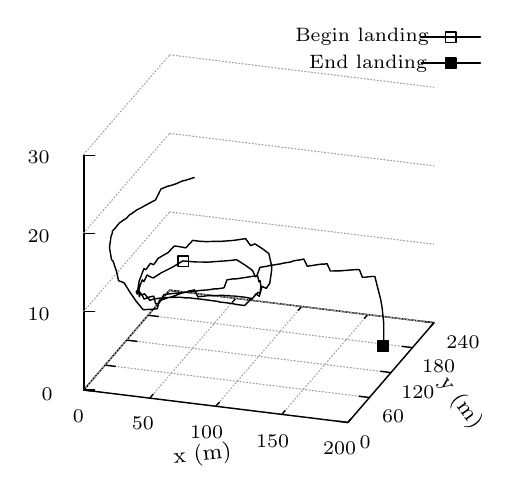
\begin{tikzpicture}[y=0.80pt, x=0.80pt, yscale=-0.780000, xscale=0.780000, inner sep=0pt, outer sep=0pt]
\scriptsize
\begin{scope}[draw=black,line join=bevel,line cap=rect,even odd rule,line width=0.512pt]
  \begin{scope}[cm={{1.0,0.0,0.0,1.0,(0.0,0.0)}},draw=black,line join=bevel,line cap=rect,line width=0.512pt]
  \end{scope}
  \begin{scope}[cm={{1.00625,0.0,0.0,1.00625,(0.0,0.0)}},draw=black,line join=bevel,line cap=rect,line width=0.512pt]
  \end{scope}
  \begin{scope}[cm={{1.00625,0.0,0.0,1.00625,(0.0,0.0)}},draw=black,line join=round,line cap=round,line width=0.512pt]
    \path[draw] (59.2000,239.6000) -- (108.7000,182.2000);
    \path[draw] (260.8000,200.9000) -- (108.7000,182.2000);
    \path[draw] (59.5000,239.5000) -- (59.5000,104.5000);
  \end{scope}
  \begin{scope}[cm={{1.00625,0.0,0.0,1.00625,(0.0,0.0)}},draw=ca0a0a4,dash pattern=on 0.40pt off 0.80pt,line join=round,line cap=round,line width=0.400pt]
    \path[draw] (59.2000,239.6000) -- (108.7000,182.2000);
  \end{scope}
  \begin{scope}[cm={{1.00625,0.0,0.0,1.00625,(0.0,0.0)}},draw=black,line join=round,line cap=round,line width=0.512pt]
    \path[draw] (59.2000,239.6000) -- (61.2000,237.4000);
    \path[draw] (108.7000,182.2000) -- (106.8000,184.4000);
  \end{scope}
  \begin{scope}[cm={{1.00625,0.0,0.0,1.00625,(0.0,0.0)}},draw=black,line join=bevel,line cap=rect,line width=0.512pt]
  \end{scope}
  \begin{scope}[cm={{1.00625,0.0,0.0,1.00625,(53.3313,260.116)}},draw=black,line join=bevel,line cap=rect,line width=0.512pt]
  \end{scope}
  \begin{scope}[cm={{1.00625,0.0,0.0,1.00625,(53.3313,260.116)}},draw=black,line join=bevel,line cap=rect,line width=0.512pt]
  \end{scope}
  \begin{scope}[cm={{1.00625,0.0,0.0,1.00625,(53.3313,260.116)}},draw=black,line join=bevel,line cap=rect,line width=0.512pt]
  \end{scope}
  \begin{scope}[cm={{1.00625,0.0,0.0,1.00625,(53.3313,260.116)}},draw=black,line join=bevel,line cap=rect,line width=0.512pt]
  \end{scope}
  \begin{scope}[cm={{1.00625,0.0,0.0,1.00625,(53.3313,260.116)}},draw=black,line join=bevel,line cap=rect,line width=0.512pt]
  \end{scope}
  \begin{scope}[cm={{1.00625,0.0,0.0,1.00625,(53.3313,260.116)}},draw=black,line join=bevel,line cap=rect,line width=0.512pt]
    \path[fill=black] (0.0000,0.0000) node[above right] () {0};
  \end{scope}
  \begin{scope}[cm={{1.00625,0.0,0.0,1.00625,(53.3313,260.116)}},draw=black,line join=bevel,line cap=rect,line width=0.512pt]
  \end{scope}
  \begin{scope}[cm={{1.00625,0.0,0.0,1.00625,(0.0,0.0)}},draw=black,line join=bevel,line cap=rect,line width=0.512pt]
  \end{scope}
  \begin{scope}[cm={{1.00625,0.0,0.0,1.00625,(0.0,0.0)}},draw=ca0a0a4,dash pattern=on 0.40pt off 0.80pt,line join=round,line cap=round,line width=0.400pt]
    \path[draw] (97.3000,244.3000) -- (146.7000,186.9000);
  \end{scope}
  \begin{scope}[cm={{1.00625,0.0,0.0,1.00625,(0.0,0.0)}},draw=black,line join=round,line cap=round,line width=0.512pt]
    \path[draw] (97.3000,244.3000) -- (99.2000,242.0000);
    \path[draw] (146.7000,186.9000) -- (144.8000,189.1000);
  \end{scope}
  \begin{scope}[cm={{1.00625,0.0,0.0,1.00625,(0.0,0.0)}},draw=black,line join=bevel,line cap=rect,line width=0.512pt]
  \end{scope}
  \begin{scope}[cm={{1.00625,0.0,0.0,1.00625,(87.5438,264.141)}},draw=black,line join=bevel,line cap=rect,line width=0.512pt]
  \end{scope}
  \begin{scope}[cm={{1.00625,0.0,0.0,1.00625,(87.5438,264.141)}},draw=black,line join=bevel,line cap=rect,line width=0.512pt]
  \end{scope}
  \begin{scope}[cm={{1.00625,0.0,0.0,1.00625,(87.5438,264.141)}},draw=black,line join=bevel,line cap=rect,line width=0.512pt]
  \end{scope}
  \begin{scope}[cm={{1.00625,0.0,0.0,1.00625,(87.5438,264.141)}},draw=black,line join=bevel,line cap=rect,line width=0.512pt]
  \end{scope}
  \begin{scope}[cm={{1.00625,0.0,0.0,1.00625,(87.5438,264.141)}},draw=black,line join=bevel,line cap=rect,line width=0.512pt]
  \end{scope}
  \begin{scope}[cm={{1.00625,0.0,0.0,1.00625,(87.5438,264.141)}},draw=black,line join=bevel,line cap=rect,line width=0.512pt]
    \path[fill=black] (0.0000,0.0000) node[above right] () {50};
  \end{scope}
  \begin{scope}[cm={{1.00625,0.0,0.0,1.00625,(87.5438,264.141)}},draw=black,line join=bevel,line cap=rect,line width=0.512pt]
  \end{scope}
  \begin{scope}[cm={{1.00625,0.0,0.0,1.00625,(0.0,0.0)}},draw=black,line join=bevel,line cap=rect,line width=0.512pt]
  \end{scope}
  \begin{scope}[cm={{1.00625,0.0,0.0,1.00625,(0.0,0.0)}},draw=ca0a0a4,dash pattern=on 0.40pt off 0.80pt,line join=round,line cap=round,line width=0.400pt]
    \path[draw] (135.3000,248.9000) -- (184.7000,191.5000);
  \end{scope}
  \begin{scope}[cm={{1.00625,0.0,0.0,1.00625,(0.0,0.0)}},draw=black,line join=round,line cap=round,line width=0.512pt]
    \path[draw] (135.3000,248.9000) -- (137.3000,246.7000);
    \path[draw] (184.7000,191.5000) -- (182.7000,193.8000);
  \end{scope}
  \begin{scope}[cm={{1.00625,0.0,0.0,1.00625,(0.0,0.0)}},draw=black,line join=bevel,line cap=rect,line width=0.512pt]
  \end{scope}
  \begin{scope}[cm={{1.00625,0.0,0.0,1.00625,(121.253,269.172)}},draw=black,line join=bevel,line cap=rect,line width=0.512pt]
  \end{scope}
  \begin{scope}[cm={{1.00625,0.0,0.0,1.00625,(121.253,269.172)}},draw=black,line join=bevel,line cap=rect,line width=0.512pt]
  \end{scope}
  \begin{scope}[cm={{1.00625,0.0,0.0,1.00625,(121.253,269.172)}},draw=black,line join=bevel,line cap=rect,line width=0.512pt]
  \end{scope}
  \begin{scope}[cm={{1.00625,0.0,0.0,1.00625,(121.253,269.172)}},draw=black,line join=bevel,line cap=rect,line width=0.512pt]
  \end{scope}
  \begin{scope}[cm={{1.00625,0.0,0.0,1.00625,(121.253,269.172)}},draw=black,line join=bevel,line cap=rect,line width=0.512pt]
  \end{scope}
  \begin{scope}[cm={{1.00625,0.0,0.0,1.00625,(121.253,269.172)}},draw=black,line join=bevel,line cap=rect,line width=0.512pt]
    \path[fill=black] (0.0000,0.0000) node[above right] () {100};
  \end{scope}
  \begin{scope}[cm={{1.00625,0.0,0.0,1.00625,(121.253,269.172)}},draw=black,line join=bevel,line cap=rect,line width=0.512pt]
  \end{scope}
  \begin{scope}[cm={{1.00625,0.0,0.0,1.00625,(0.0,0.0)}},draw=black,line join=bevel,line cap=rect,line width=0.512pt]
  \end{scope}
  \begin{scope}[cm={{1.00625,0.0,0.0,1.00625,(0.0,0.0)}},draw=ca0a0a4,dash pattern=on 0.40pt off 0.80pt,line join=round,line cap=round,line width=0.400pt]
    \path[draw] (173.3000,253.6000) -- (222.7000,196.2000);
  \end{scope}
  \begin{scope}[cm={{1.00625,0.0,0.0,1.00625,(0.0,0.0)}},draw=black,line join=round,line cap=round,line width=0.512pt]
    \path[draw] (173.3000,253.6000) -- (175.2000,251.4000);
    \path[draw] (222.7000,196.2000) -- (220.8000,198.4000);
  \end{scope}
  \begin{scope}[cm={{1.00625,0.0,0.0,1.00625,(0.0,0.0)}},draw=black,line join=bevel,line cap=rect,line width=0.512pt]
  \end{scope}
  \begin{scope}[cm={{1.00625,0.0,0.0,1.00625,(159.491,274.203)}},draw=black,line join=bevel,line cap=rect,line width=0.512pt]
  \end{scope}
  \begin{scope}[cm={{1.00625,0.0,0.0,1.00625,(159.491,274.203)}},draw=black,line join=bevel,line cap=rect,line width=0.512pt]
  \end{scope}
  \begin{scope}[cm={{1.00625,0.0,0.0,1.00625,(159.491,274.203)}},draw=black,line join=bevel,line cap=rect,line width=0.512pt]
  \end{scope}
  \begin{scope}[cm={{1.00625,0.0,0.0,1.00625,(159.491,274.203)}},draw=black,line join=bevel,line cap=rect,line width=0.512pt]
  \end{scope}
  \begin{scope}[cm={{1.00625,0.0,0.0,1.00625,(159.491,274.203)}},draw=black,line join=bevel,line cap=rect,line width=0.512pt]
  \end{scope}
  \begin{scope}[cm={{1.00625,0.0,0.0,1.00625,(159.491,274.203)}},draw=black,line join=bevel,line cap=rect,line width=0.512pt]
    \path[fill=black] (0.0000,0.0000) node[above right] () {150};
  \end{scope}
  \begin{scope}[cm={{1.00625,0.0,0.0,1.00625,(159.491,274.203)}},draw=black,line join=bevel,line cap=rect,line width=0.512pt]
  \end{scope}
  \begin{scope}[cm={{1.00625,0.0,0.0,1.00625,(0.0,0.0)}},draw=black,line join=bevel,line cap=rect,line width=0.512pt]
  \end{scope}
  \begin{scope}[cm={{1.00625,0.0,0.0,1.00625,(0.0,0.0)}},draw=ca0a0a4,dash pattern=on 0.40pt off 0.80pt,line join=round,line cap=round,line width=0.400pt]
    \path[draw] (211.3000,258.3000) -- (260.8000,200.9000);
  \end{scope}
  \begin{scope}[cm={{1.00625,0.0,0.0,1.00625,(0.0,0.0)}},draw=black,line join=round,line cap=round,line width=0.512pt]
    \path[draw] (211.3000,258.3000) -- (213.2000,256.0000);
    \path[draw] (260.8000,200.9000) -- (258.8000,203.1000);
  \end{scope}
  \begin{scope}[cm={{1.00625,0.0,0.0,1.00625,(0.0,0.0)}},draw=black,line join=bevel,line cap=rect,line width=0.512pt]
  \end{scope}
  \begin{scope}[cm={{1.00625,0.0,0.0,1.00625,(198.231,278.228)}},draw=black,line join=bevel,line cap=rect,line width=0.512pt]
  \end{scope}
  \begin{scope}[cm={{1.00625,0.0,0.0,1.00625,(198.231,278.228)}},draw=black,line join=bevel,line cap=rect,line width=0.512pt]
  \end{scope}
  \begin{scope}[cm={{1.00625,0.0,0.0,1.00625,(198.231,278.228)}},draw=black,line join=bevel,line cap=rect,line width=0.512pt]
  \end{scope}
  \begin{scope}[cm={{1.00625,0.0,0.0,1.00625,(198.231,278.228)}},draw=black,line join=bevel,line cap=rect,line width=0.512pt]
  \end{scope}
  \begin{scope}[cm={{1.00625,0.0,0.0,1.00625,(198.231,278.228)}},draw=black,line join=bevel,line cap=rect,line width=0.512pt]
  \end{scope}
  \begin{scope}[cm={{1.00625,0.0,0.0,1.00625,(198.231,278.228)}},draw=black,line join=bevel,line cap=rect,line width=0.512pt]
    \path[fill=black] (0.0000,0.0000) node[above right] () {200};
  \end{scope}
  \begin{scope}[cm={{1.00625,0.0,0.0,1.00625,(198.231,278.228)}},draw=black,line join=bevel,line cap=rect,line width=0.512pt]
  \end{scope}
  \begin{scope}[cm={{1.00625,0.0,0.0,1.00625,(0.0,0.0)}},draw=black,line join=bevel,line cap=rect,line width=0.512pt]
  \end{scope}
  \begin{scope}[cm={{1.00625,0.0,0.0,1.00625,(0.0,0.0)}},draw=ca0a0a4,dash pattern=on 0.40pt off 0.80pt,line join=round,line cap=round,line width=0.400pt]
    \path[draw] (211.3000,258.3000) -- (59.2000,239.6000);
  \end{scope}
  \begin{scope}[cm={{1.00625,0.0,0.0,1.00625,(0.0,0.0)}},draw=black,line join=round,line cap=round,line width=0.512pt]
    \path[draw] (211.3000,258.3000) -- (205.4000,257.5000);
    \path[draw] (59.2000,239.6000) -- (65.2000,240.3000);
  \end{scope}
  \begin{scope}[cm={{1.00625,0.0,0.0,1.00625,(0.0,0.0)}},draw=black,line join=bevel,line cap=rect,line width=0.512pt]
  \end{scope}
  \begin{scope}[cm={{1.00625,0.0,0.0,1.00625,(219.363,275.209)}},draw=black,line join=bevel,line cap=rect,line width=0.512pt]
  \end{scope}
  \begin{scope}[cm={{1.00625,0.0,0.0,1.00625,(219.363,275.209)}},draw=black,line join=bevel,line cap=rect,line width=0.512pt]
  \end{scope}
  \begin{scope}[cm={{1.00625,0.0,0.0,1.00625,(219.363,275.209)}},draw=black,line join=bevel,line cap=rect,line width=0.512pt]
  \end{scope}
  \begin{scope}[cm={{1.00625,0.0,0.0,1.00625,(219.363,275.209)}},draw=black,line join=bevel,line cap=rect,line width=0.512pt]
  \end{scope}
  \begin{scope}[cm={{1.00625,0.0,0.0,1.00625,(219.363,275.209)}},draw=black,line join=bevel,line cap=rect,line width=0.512pt]
  \end{scope}
  \begin{scope}[cm={{1.00625,0.0,0.0,1.00625,(219.363,275.209)}},draw=black,line join=bevel,line cap=rect,line width=0.512pt]
    \path[fill=black] (0.0000,0.0000) node[above right] () {0};
  \end{scope}
  \begin{scope}[cm={{1.00625,0.0,0.0,1.00625,(219.363,275.209)}},draw=black,line join=bevel,line cap=rect,line width=0.512pt]
  \end{scope}
  \begin{scope}[cm={{1.00625,0.0,0.0,1.00625,(0.0,0.0)}},draw=black,line join=bevel,line cap=rect,line width=0.512pt]
  \end{scope}
  \begin{scope}[cm={{1.00625,0.0,0.0,1.00625,(0.0,0.0)}},draw=ca0a0a4,dash pattern=on 0.40pt off 0.80pt,line join=round,line cap=round,line width=0.400pt]
    \path[draw] (223.7000,243.9000) -- (71.6000,225.3000);
  \end{scope}
  \begin{scope}[cm={{1.00625,0.0,0.0,1.00625,(0.0,0.0)}},draw=black,line join=round,line cap=round,line width=0.512pt]
    \path[draw] (223.7000,243.9000) -- (217.7000,243.2000);
    \path[draw] (71.6000,225.3000) -- (77.5000,226.0000);
  \end{scope}
  \begin{scope}[cm={{1.00625,0.0,0.0,1.00625,(0.0,0.0)}},draw=black,line join=bevel,line cap=rect,line width=0.512pt]
  \end{scope}
  \begin{scope}[cm={{1.00625,0.0,0.0,1.00625,(232.444,260.116)}},draw=black,line join=bevel,line cap=rect,line width=0.512pt]
  \end{scope}
  \begin{scope}[cm={{1.00625,0.0,0.0,1.00625,(232.444,260.116)}},draw=black,line join=bevel,line cap=rect,line width=0.512pt]
  \end{scope}
  \begin{scope}[cm={{1.00625,0.0,0.0,1.00625,(232.444,260.116)}},draw=black,line join=bevel,line cap=rect,line width=0.512pt]
  \end{scope}
  \begin{scope}[cm={{1.00625,0.0,0.0,1.00625,(232.444,260.116)}},draw=black,line join=bevel,line cap=rect,line width=0.512pt]
  \end{scope}
  \begin{scope}[cm={{1.00625,0.0,0.0,1.00625,(232.444,260.116)}},draw=black,line join=bevel,line cap=rect,line width=0.512pt]
  \end{scope}
  \begin{scope}[cm={{1.00625,0.0,0.0,1.00625,(232.444,260.116)}},draw=black,line join=bevel,line cap=rect,line width=0.512pt]
    \path[fill=black] (0.0000,0.0000) node[above right] () {60};
  \end{scope}
  \begin{scope}[cm={{1.00625,0.0,0.0,1.00625,(232.444,260.116)}},draw=black,line join=bevel,line cap=rect,line width=0.512pt]
  \end{scope}
  \begin{scope}[cm={{1.00625,0.0,0.0,1.00625,(0.0,0.0)}},draw=black,line join=bevel,line cap=rect,line width=0.512pt]
  \end{scope}
  \begin{scope}[cm={{1.00625,0.0,0.0,1.00625,(0.0,0.0)}},draw=ca0a0a4,dash pattern=on 0.40pt off 0.80pt,line join=round,line cap=round,line width=0.400pt]
    \path[draw] (236.0000,229.6000) -- (84.0000,210.9000);
  \end{scope}
  \begin{scope}[cm={{1.00625,0.0,0.0,1.00625,(0.0,0.0)}},draw=black,line join=round,line cap=round,line width=0.512pt]
    \path[draw] (236.0000,229.6000) -- (230.1000,228.8000);
    \path[draw] (84.0000,210.9000) -- (89.9000,211.6000);
  \end{scope}
  \begin{scope}[cm={{1.00625,0.0,0.0,1.00625,(0.0,0.0)}},draw=black,line join=bevel,line cap=rect,line width=0.512pt]
  \end{scope}
  \begin{scope}[cm={{1.00625,0.0,0.0,1.00625,(243.513,246.028)}},draw=black,line join=bevel,line cap=rect,line width=0.512pt]
  \end{scope}
  \begin{scope}[cm={{1.00625,0.0,0.0,1.00625,(243.513,246.028)}},draw=black,line join=bevel,line cap=rect,line width=0.512pt]
  \end{scope}
  \begin{scope}[cm={{1.00625,0.0,0.0,1.00625,(243.513,246.028)}},draw=black,line join=bevel,line cap=rect,line width=0.512pt]
  \end{scope}
  \begin{scope}[cm={{1.00625,0.0,0.0,1.00625,(243.513,246.028)}},draw=black,line join=bevel,line cap=rect,line width=0.512pt]
  \end{scope}
  \begin{scope}[cm={{1.00625,0.0,0.0,1.00625,(243.513,246.028)}},draw=black,line join=bevel,line cap=rect,line width=0.512pt]
  \end{scope}
  \begin{scope}[cm={{1.00625,0.0,0.0,1.00625,(243.513,246.028)}},draw=black,line join=bevel,line cap=rect,line width=0.512pt]
    \path[fill=black] (0.0000,0.0000) node[above right] () {120};
  \end{scope}
  \begin{scope}[cm={{1.00625,0.0,0.0,1.00625,(243.513,246.028)}},draw=black,line join=bevel,line cap=rect,line width=0.512pt]
  \end{scope}
  \begin{scope}[cm={{1.00625,0.0,0.0,1.00625,(0.0,0.0)}},draw=black,line join=bevel,line cap=rect,line width=0.512pt]
  \end{scope}
  \begin{scope}[cm={{1.00625,0.0,0.0,1.00625,(0.0,0.0)}},draw=ca0a0a4,dash pattern=on 0.40pt off 0.80pt,line join=round,line cap=round,line width=0.400pt]
    \path[draw] (248.4000,215.2000) -- (96.3000,196.6000);
  \end{scope}
  \begin{scope}[cm={{1.00625,0.0,0.0,1.00625,(0.0,0.0)}},draw=black,line join=round,line cap=round,line width=0.512pt]
    \path[draw] (248.4000,215.2000) -- (242.5000,214.5000);
    \path[draw] (96.3000,196.6000) -- (102.3000,197.3000);
  \end{scope}
  \begin{scope}[cm={{1.00625,0.0,0.0,1.00625,(0.0,0.0)}},draw=black,line join=bevel,line cap=rect,line width=0.512pt]
  \end{scope}
  \begin{scope}[cm={{1.00625,0.0,0.0,1.00625,(255.588,230.934)}},draw=black,line join=bevel,line cap=rect,line width=0.512pt]
  \end{scope}
  \begin{scope}[cm={{1.00625,0.0,0.0,1.00625,(255.588,230.934)}},draw=black,line join=bevel,line cap=rect,line width=0.512pt]
  \end{scope}
  \begin{scope}[cm={{1.00625,0.0,0.0,1.00625,(255.588,230.934)}},draw=black,line join=bevel,line cap=rect,line width=0.512pt]
  \end{scope}
  \begin{scope}[cm={{1.00625,0.0,0.0,1.00625,(255.588,230.934)}},draw=black,line join=bevel,line cap=rect,line width=0.512pt]
  \end{scope}
  \begin{scope}[cm={{1.00625,0.0,0.0,1.00625,(255.588,230.934)}},draw=black,line join=bevel,line cap=rect,line width=0.512pt]
  \end{scope}
  \begin{scope}[cm={{1.00625,0.0,0.0,1.00625,(255.588,230.934)}},draw=black,line join=bevel,line cap=rect,line width=0.512pt]
    \path[fill=black] (0.0000,0.0000) node[above right] () {180};
  \end{scope}
  \begin{scope}[cm={{1.00625,0.0,0.0,1.00625,(255.588,230.934)}},draw=black,line join=bevel,line cap=rect,line width=0.512pt]
  \end{scope}
  \begin{scope}[cm={{1.00625,0.0,0.0,1.00625,(0.0,0.0)}},draw=black,line join=bevel,line cap=rect,line width=0.512pt]
  \end{scope}
  \begin{scope}[cm={{1.00625,0.0,0.0,1.00625,(0.0,0.0)}},draw=ca0a0a4,dash pattern=on 0.40pt off 0.80pt,line join=round,line cap=round,line width=0.400pt]
    \path[draw] (260.8000,200.9000) -- (108.7000,182.2000);
  \end{scope}
  \begin{scope}[cm={{1.00625,0.0,0.0,1.00625,(0.0,0.0)}},draw=black,line join=round,line cap=round,line width=0.512pt]
    \path[draw] (260.8000,200.9000) -- (254.8000,200.1000);
    \path[draw] (108.7000,182.2000) -- (114.6000,182.9000);
  \end{scope}
  \begin{scope}[cm={{1.00625,0.0,0.0,1.00625,(0.0,0.0)}},draw=black,line join=bevel,line cap=rect,line width=0.512pt]
  \end{scope}
  \begin{scope}[cm={{1.00625,0.0,0.0,1.00625,(269.675,216.847)}},draw=black,line join=bevel,line cap=rect,line width=0.512pt]
  \end{scope}
  \begin{scope}[cm={{1.00625,0.0,0.0,1.00625,(269.675,216.847)}},draw=black,line join=bevel,line cap=rect,line width=0.512pt]
  \end{scope}
  \begin{scope}[cm={{1.00625,0.0,0.0,1.00625,(269.675,216.847)}},draw=black,line join=bevel,line cap=rect,line width=0.512pt]
  \end{scope}
  \begin{scope}[cm={{1.00625,0.0,0.0,1.00625,(269.675,216.847)}},draw=black,line join=bevel,line cap=rect,line width=0.512pt]
  \end{scope}
  \begin{scope}[cm={{1.00625,0.0,0.0,1.00625,(269.675,216.847)}},draw=black,line join=bevel,line cap=rect,line width=0.512pt]
  \end{scope}
  \begin{scope}[cm={{1.00625,0.0,0.0,1.00625,(269.675,216.847)}},draw=black,line join=bevel,line cap=rect,line width=0.512pt]
    \path[fill=black] (0.0000,0.0000) node[above right] () {240};
  \end{scope}
  \begin{scope}[cm={{1.00625,0.0,0.0,1.00625,(269.675,216.847)}},draw=black,line join=bevel,line cap=rect,line width=0.512pt]
  \end{scope}
  \begin{scope}[cm={{1.00625,0.0,0.0,1.00625,(0.0,0.0)}},draw=black,line join=bevel,line cap=rect,line width=0.512pt]
  \end{scope}
  \begin{scope}[cm={{1.00625,0.0,0.0,1.00625,(0.0,0.0)}},draw=ca0a0a4,dash pattern=on 0.40pt off 0.80pt,line join=round,line cap=round,line width=0.400pt]
    \path[draw] (59.2000,239.6000) -- (108.7000,182.2000);
    \path[draw] (108.7000,182.2000) -- (108.7000,182.2000) -- (260.8000,200.9000);
  \end{scope}
  \begin{scope}[cm={{1.00625,0.0,0.0,1.00625,(0.0,0.0)}},draw=black,line join=round,line cap=round,line width=0.512pt]
    \path[draw] (59.5000,239.5000) -- (65.5000,239.5000);
  \end{scope}
  \begin{scope}[cm={{1.00625,0.0,0.0,1.00625,(0.0,0.0)}},draw=black,line join=bevel,line cap=rect,line width=0.512pt]
  \end{scope}
  \begin{scope}[cm={{1.00625,0.0,0.0,1.00625,(35.2188,247.034)}},draw=black,line join=bevel,line cap=rect,line width=0.512pt]
  \end{scope}
  \begin{scope}[cm={{1.00625,0.0,0.0,1.00625,(35.2188,247.034)}},draw=black,line join=bevel,line cap=rect,line width=0.512pt]
  \end{scope}
  \begin{scope}[cm={{1.00625,0.0,0.0,1.00625,(35.2188,247.034)}},draw=black,line join=bevel,line cap=rect,line width=0.512pt]
  \end{scope}
  \begin{scope}[cm={{1.00625,0.0,0.0,1.00625,(35.2188,247.034)}},draw=black,line join=bevel,line cap=rect,line width=0.512pt]
  \end{scope}
  \begin{scope}[cm={{1.00625,0.0,0.0,1.00625,(35.2188,247.034)}},draw=black,line join=bevel,line cap=rect,line width=0.512pt]
  \end{scope}
  \begin{scope}[cm={{1.00625,0.0,0.0,1.00625,(35.2188,247.034)}},draw=black,line join=bevel,line cap=rect,line width=0.512pt]
    \path[fill=black] (0.0000,0.0000) node[above right] () {0};
  \end{scope}
  \begin{scope}[cm={{1.00625,0.0,0.0,1.00625,(35.2188,247.034)}},draw=black,line join=bevel,line cap=rect,line width=0.512pt]
  \end{scope}
  \begin{scope}[cm={{1.00625,0.0,0.0,1.00625,(0.0,0.0)}},draw=black,line join=bevel,line cap=rect,line width=0.512pt]
  \end{scope}
  \begin{scope}[cm={{1.00625,0.0,0.0,1.00625,(0.0,0.0)}},draw=ca0a0a4,dash pattern=on 0.40pt off 0.80pt,line join=round,line cap=round,line width=0.400pt]
    \path[draw] (59.2000,194.4000) -- (108.7000,137.1000);
    \path[draw] (108.7000,137.1000) -- (108.7000,137.1000) -- (260.8000,155.7000);
  \end{scope}
  \begin{scope}[cm={{1.00625,0.0,0.0,1.00625,(0.0,0.0)}},draw=black,line join=round,line cap=round,line width=0.512pt]
    \path[draw] (59.5000,194.5000) -- (65.5000,194.5000);
  \end{scope}
  \begin{scope}[cm={{1.00625,0.0,0.0,1.00625,(0.0,0.0)}},draw=black,line join=bevel,line cap=rect,line width=0.512pt]
  \end{scope}
  \begin{scope}[cm={{1.00625,0.0,0.0,1.00625,(27.1688,200.747)}},draw=black,line join=bevel,line cap=rect,line width=0.512pt]
  \end{scope}
  \begin{scope}[cm={{1.00625,0.0,0.0,1.00625,(27.1688,200.747)}},draw=black,line join=bevel,line cap=rect,line width=0.512pt]
  \end{scope}
  \begin{scope}[cm={{1.00625,0.0,0.0,1.00625,(27.1688,200.747)}},draw=black,line join=bevel,line cap=rect,line width=0.512pt]
  \end{scope}
  \begin{scope}[cm={{1.00625,0.0,0.0,1.00625,(27.1688,200.747)}},draw=black,line join=bevel,line cap=rect,line width=0.512pt]
  \end{scope}
  \begin{scope}[cm={{1.00625,0.0,0.0,1.00625,(27.1688,200.747)}},draw=black,line join=bevel,line cap=rect,line width=0.512pt]
  \end{scope}
  \begin{scope}[cm={{1.00625,0.0,0.0,1.00625,(27.1688,200.747)}},draw=black,line join=bevel,line cap=rect,line width=0.512pt]
    \path[fill=black] (0.0000,0.0000) node[above right] () {10};
  \end{scope}
  \begin{scope}[cm={{1.00625,0.0,0.0,1.00625,(27.1688,200.747)}},draw=black,line join=bevel,line cap=rect,line width=0.512pt]
  \end{scope}
  \begin{scope}[cm={{1.00625,0.0,0.0,1.00625,(0.0,0.0)}},draw=black,line join=bevel,line cap=rect,line width=0.512pt]
  \end{scope}
  \begin{scope}[cm={{1.00625,0.0,0.0,1.00625,(0.0,0.0)}},draw=ca0a0a4,dash pattern=on 0.40pt off 0.80pt,line join=round,line cap=round,line width=0.400pt]
    \path[draw] (59.2000,149.3000) -- (108.7000,91.9000);
    \path[draw] (108.7000,91.9000) -- (108.7000,91.9000) -- (260.8000,110.6000);
  \end{scope}
  \begin{scope}[cm={{1.00625,0.0,0.0,1.00625,(0.0,0.0)}},draw=black,line join=round,line cap=round,line width=0.512pt]
    \path[draw] (59.5000,149.5000) -- (65.5000,149.5000);
  \end{scope}
  \begin{scope}[cm={{1.00625,0.0,0.0,1.00625,(0.0,0.0)}},draw=black,line join=bevel,line cap=rect,line width=0.512pt]
  \end{scope}
  \begin{scope}[cm={{1.00625,0.0,0.0,1.00625,(27.1688,155.466)}},draw=black,line join=bevel,line cap=rect,line width=0.512pt]
  \end{scope}
  \begin{scope}[cm={{1.00625,0.0,0.0,1.00625,(27.1688,155.466)}},draw=black,line join=bevel,line cap=rect,line width=0.512pt]
  \end{scope}
  \begin{scope}[cm={{1.00625,0.0,0.0,1.00625,(27.1688,155.466)}},draw=black,line join=bevel,line cap=rect,line width=0.512pt]
  \end{scope}
  \begin{scope}[cm={{1.00625,0.0,0.0,1.00625,(27.1688,155.466)}},draw=black,line join=bevel,line cap=rect,line width=0.512pt]
  \end{scope}
  \begin{scope}[cm={{1.00625,0.0,0.0,1.00625,(27.1688,155.466)}},draw=black,line join=bevel,line cap=rect,line width=0.512pt]
  \end{scope}
  \begin{scope}[cm={{1.00625,0.0,0.0,1.00625,(27.1688,155.466)}},draw=black,line join=bevel,line cap=rect,line width=0.512pt]
    \path[fill=black] (0.0000,0.0000) node[above right] () {20};
  \end{scope}
  \begin{scope}[cm={{1.00625,0.0,0.0,1.00625,(27.1688,155.466)}},draw=black,line join=bevel,line cap=rect,line width=0.512pt]
  \end{scope}
  \begin{scope}[cm={{1.00625,0.0,0.0,1.00625,(0.0,0.0)}},draw=black,line join=bevel,line cap=rect,line width=0.512pt]
  \end{scope}
  \begin{scope}[cm={{1.00625,0.0,0.0,1.00625,(0.0,0.0)}},draw=ca0a0a4,dash pattern=on 0.40pt off 0.80pt,line join=round,line cap=round,line width=0.400pt]
    \path[draw] (59.2000,104.1000) -- (108.7000,46.7000);
    \path[draw] (108.7000,46.7000) -- (108.7000,46.7000) -- (260.8000,65.4000);
  \end{scope}
  \begin{scope}[cm={{1.00625,0.0,0.0,1.00625,(0.0,0.0)}},draw=black,line join=round,line cap=round,line width=0.512pt]
    \path[draw] (59.5000,104.5000) -- (65.5000,104.5000);
  \end{scope}
  \begin{scope}[cm={{1.00625,0.0,0.0,1.00625,(0.0,0.0)}},draw=black,line join=bevel,line cap=rect,line width=0.512pt]
  \end{scope}
  \begin{scope}[cm={{1.00625,0.0,0.0,1.00625,(27.1688,110.184)}},draw=black,line join=bevel,line cap=rect,line width=0.512pt]
  \end{scope}
  \begin{scope}[cm={{1.00625,0.0,0.0,1.00625,(27.1688,110.184)}},draw=black,line join=bevel,line cap=rect,line width=0.512pt]
  \end{scope}
  \begin{scope}[cm={{1.00625,0.0,0.0,1.00625,(27.1688,110.184)}},draw=black,line join=bevel,line cap=rect,line width=0.512pt]
  \end{scope}
  \begin{scope}[cm={{1.00625,0.0,0.0,1.00625,(27.1688,110.184)}},draw=black,line join=bevel,line cap=rect,line width=0.512pt]
  \end{scope}
  \begin{scope}[cm={{1.00625,0.0,0.0,1.00625,(27.1688,110.184)}},draw=black,line join=bevel,line cap=rect,line width=0.512pt]
  \end{scope}
  \begin{scope}[cm={{1.00625,0.0,0.0,1.00625,(27.1688,110.184)}},draw=black,line join=bevel,line cap=rect,line width=0.512pt]
    \path[fill=black] (0.0000,0.0000) node[above right] () {30};
  \end{scope}
  \begin{scope}[cm={{1.00625,0.0,0.0,1.00625,(27.1688,110.184)}},draw=black,line join=bevel,line cap=rect,line width=0.512pt]
  \end{scope}
  \begin{scope}[cm={{1.00625,0.0,0.0,1.00625,(0.0,0.0)}},draw=black,line join=bevel,line cap=rect,line width=0.512pt]
  \end{scope}
  \begin{scope}[cm={{1.00625,0.0,0.0,1.00625,(0.0,0.0)}},draw=black,line join=bevel,line cap=rect,line width=0.512pt]
  \end{scope}
  \begin{scope}[cm={{1.00625,0.0,0.0,1.00625,(0.0,0.0)}},draw=black,line join=bevel,line cap=rect,line width=0.512pt]
  \end{scope}
  \begin{scope}[cm={{1.00625,0.0,0.0,1.00625,(0.0,0.0)}},draw=black,line join=round,line cap=round,line width=0.512pt]
    \path[draw] (122.9000,117.3000) -- (122.9000,117.3000) -- (122.9000,117.3000) --
      (122.9000,117.3000) -- (122.9000,117.3000) -- (118.2000,118.8000) --
      (118.2000,118.8000) -- (116.1000,119.3000) -- (116.1000,119.3000) --
      (116.1000,119.3000) -- (116.1000,119.3000) -- (116.1000,119.3000) --
      (116.1000,119.3000) -- (112.2000,121.0000) -- (112.2000,121.0000) --
      (109.8000,121.8000) -- (109.8000,121.8000) -- (107.7000,122.3000) --
      (107.7000,122.3000) -- (107.7000,122.3000) -- (107.7000,122.3000) --
      (107.7000,122.3000) -- (107.7000,122.3000) -- (103.7000,123.9000) --
      (103.7000,123.9000) -- (103.7000,123.9000) -- (103.7000,123.9000) --
      (100.6000,130.2000) -- (100.6000,130.2000) -- (100.6000,130.2000) --
      (100.6000,130.2000) -- (100.6000,130.2000) -- (100.6000,130.2000) --
      (97.4000,131.9000) -- (97.4000,131.9000) -- (97.4000,131.9000) --
      (97.4000,131.9000) -- (94.2000,133.6000) -- (94.2000,133.6000) --
      (94.2000,133.6000) -- (94.2000,133.6000) -- (92.7000,134.5000) --
      (92.7000,134.5000) -- (92.7000,134.5000) -- (92.7000,134.5000) --
      (89.7000,136.0000) -- (89.7000,136.0000) -- (89.7000,136.0000) --
      (89.7000,136.0000) -- (87.3000,137.8000) -- (87.3000,137.8000) --
      (87.3000,137.8000) -- (87.3000,137.8000) -- (85.5000,138.9000) --
      (85.5000,138.9000) -- (84.7000,139.8000) -- (84.7000,139.8000) --
      (83.8000,140.8000) -- (83.8000,140.8000) -- (82.3000,141.7000) --
      (82.3000,141.7000) -- (82.3000,141.7000) -- (82.3000,141.7000) --
      (82.3000,141.7000) -- (82.3000,141.7000) -- (79.8000,143.5000) --
      (79.8000,143.5000) -- (79.0000,144.4000) -- (79.0000,144.4000) --
      (78.2000,145.4000) -- (78.2000,145.4000) -- (78.2000,145.4000) --
      (78.2000,145.4000) -- (77.4000,146.4000) -- (77.4000,146.4000) --
      (76.5000,147.3000) -- (76.5000,147.3000) -- (75.7000,148.3000) --
      (75.7000,148.3000) -- (75.7000,149.3000) -- (75.7000,149.3000) --
      (75.7000,149.3000) -- (75.7000,149.3000) -- (75.7000,149.3000) --
      (75.7000,149.3000) -- (75.0000,151.1000) -- (75.0000,151.1000) --
      (74.2000,156.5000) -- (74.2000,156.5000) -- (74.2000,156.5000) --
      (74.2000,156.5000) -- (74.2000,156.5000) -- (74.2000,156.5000) --
      (74.2000,158.3000) -- (74.2000,158.3000) -- (75.1000,163.7000) --
      (75.1000,163.7000) -- (75.3000,164.6000) -- (75.3000,164.6000) --
      (75.3000,164.6000) -- (75.3000,164.6000) -- (76.2000,165.5000) --
      (76.2000,165.5000) -- (76.2000,165.5000) -- (76.2000,165.5000) --
      (78.2000,171.6000) -- (78.2000,171.6000) -- (79.3000,176.7000) --
      (79.3000,176.7000) -- (79.3000,176.7000) -- (79.3000,176.7000) --
      (79.3000,176.7000) -- (79.3000,176.7000) -- (82.5000,177.9000) --
      (82.5000,177.9000) -- (82.5000,177.9000) -- (82.5000,177.9000) --
      (85.9000,183.4000) -- (85.9000,183.4000) -- (85.9000,183.4000) --
      (85.9000,183.4000) -- (85.9000,183.4000) -- (85.9000,183.4000) --
      (89.5000,188.6000) -- (89.5000,188.6000) -- (89.5000,188.6000) --
      (89.5000,188.6000) -- (93.5000,193.4000) -- (93.5000,193.4000) --
      (95.2000,193.3000) -- (95.2000,193.3000) -- (95.2000,193.3000) --
      (95.2000,193.3000) -- (97.0000,193.2000) -- (97.0000,193.2000) --
      (98.7000,193.2000) -- (98.7000,193.2000) -- (98.7000,193.2000) --
      (98.7000,193.2000) -- (101.6000,192.8000) -- (101.6000,192.8000) --
      (101.6000,192.8000) -- (101.6000,192.8000) -- (102.8000,187.9000) --
      (102.8000,187.9000) -- (104.7000,187.6000) -- (104.7000,187.6000) --
      (104.7000,187.6000) -- (104.7000,187.6000) -- (104.7000,187.6000) --
      (104.7000,187.6000) -- (107.2000,186.6000) -- (107.2000,186.6000) --
      (107.2000,186.6000) -- (107.2000,186.6000) -- (110.3000,185.9000) --
      (110.3000,185.9000) -- (111.7000,185.3000) -- (111.7000,185.3000) --
      (111.7000,185.3000) -- (111.7000,185.3000) -- (112.9000,184.9000) --
      (112.9000,184.9000) -- (112.9000,184.9000) -- (112.9000,184.9000) --
      (115.4000,183.9000) -- (115.4000,183.9000) -- (115.4000,183.9000) --
      (115.4000,183.9000) -- (118.6000,183.2000) -- (118.6000,183.2000) --
      (118.6000,183.2000) -- (118.6000,183.2000) -- (119.9000,182.6000) --
      (119.9000,182.6000) -- (121.9000,182.3000) -- (121.9000,182.3000) --
      (123.0000,181.9000) -- (123.0000,181.9000) -- (125.0000,186.1000) --
      (125.0000,186.1000) -- (125.0000,186.1000) -- (125.0000,186.1000) --
      (126.1000,185.7000) -- (126.1000,185.7000) -- (127.9000,185.7000) --
      (127.9000,185.7000) -- (129.8000,185.4000) -- (129.8000,185.4000) --
      (131.5000,185.3000) -- (131.5000,185.3000) -- (131.5000,185.3000) --
      (131.5000,185.3000) -- (133.3000,185.3000) -- (133.3000,185.3000) --
      (135.0000,185.2000) -- (135.0000,185.2000) -- (136.7000,185.2000) --
      (136.7000,185.2000) -- (138.4000,185.1000) -- (138.4000,185.1000) --
      (138.4000,185.1000) -- (138.4000,185.1000) -- (138.4000,185.1000) --
      (138.4000,185.1000) -- (142.5000,185.3000) -- (142.5000,185.3000) --
      (144.0000,185.5000) -- (144.0000,185.5000) -- (144.0000,185.5000) --
      (144.0000,185.5000) -- (145.7000,185.5000) -- (145.7000,185.5000) --
      (147.2000,185.7000) -- (147.2000,185.7000) -- (149.5000,185.9000) --
      (149.5000,185.9000) -- (151.0000,186.1000) -- (151.0000,186.1000) --
      (151.0000,186.1000) -- (151.0000,186.1000) -- (152.6000,186.3000) --
      (152.6000,186.3000) -- (152.6000,186.3000) -- (152.6000,186.3000) --
      (156.2000,187.0000) -- (156.2000,187.0000) -- (156.2000,187.0000) --
      (156.2000,187.0000) -- (159.5000,183.4000) -- (159.5000,183.4000) --
      (159.5000,183.4000) -- (159.5000,183.4000) -- (160.8000,183.9000) --
      (160.8000,183.9000) -- (161.9000,180.0000) -- (161.9000,180.0000) --
      (161.9000,180.0000) -- (161.9000,180.0000) -- (161.9000,180.0000) --
      (161.9000,180.0000) -- (164.3000,181.1000) -- (164.3000,181.1000) --
      (164.3000,181.1000) -- (164.3000,181.1000) -- (166.3000,178.2000) --
      (166.3000,178.2000) -- (166.3000,178.2000) -- (166.3000,178.2000) --
      (167.4000,170.8000) -- (167.4000,170.8000) -- (167.4000,170.8000) --
      (167.4000,170.8000) -- (167.4000,170.8000) -- (167.4000,170.8000) --
      (167.4000,168.2000) -- (167.4000,168.2000) -- (167.4000,168.2000) --
      (167.4000,168.2000) -- (167.4000,168.2000) -- (167.4000,168.2000) --
      (165.8000,161.1000) -- (165.8000,161.1000) -- (165.8000,161.1000) --
      (165.8000,161.1000) -- (162.4000,158.5000) -- (162.4000,158.5000) --
      (162.4000,158.5000) -- (162.4000,158.5000) -- (157.8000,155.5000) --
      (157.8000,155.5000) -- (157.8000,155.5000) -- (157.8000,155.5000) --
      (155.3000,156.5000) -- (155.3000,156.5000) -- (152.4000,152.5000) --
      (152.4000,152.5000) -- (152.4000,152.5000) -- (152.4000,152.5000) --
      (145.6000,153.5000) -- (145.6000,153.5000) -- (145.6000,153.5000) --
      (145.6000,153.5000) -- (145.6000,153.5000) -- (145.6000,153.5000) --
      (137.5000,154.1000) -- (137.5000,154.1000) -- (133.3000,154.1000) --
      (133.3000,154.1000) -- (129.8000,154.2000) -- (129.8000,154.2000) --
      (129.8000,154.2000) -- (129.8000,154.2000) -- (125.8000,154.0000) --
      (125.8000,154.0000) -- (122.0000,153.5000) -- (122.0000,153.5000) --
      (118.0000,157.8000) -- (118.0000,157.8000) -- (114.4000,157.1000) --
      (114.4000,157.1000) -- (114.4000,157.1000) -- (114.4000,157.1000) --
      (111.4000,156.7000) -- (111.4000,156.7000) -- (107.8000,160.5000) --
      (107.8000,160.5000) -- (107.8000,160.5000) -- (107.8000,160.5000) --
      (107.8000,160.5000) -- (107.8000,160.5000) -- (102.1000,163.8000) --
      (102.1000,163.8000) -- (99.5000,167.5000) -- (99.5000,167.5000) --
      (97.6000,166.7000) -- (97.6000,166.7000) -- (95.0000,170.4000) --
      (95.0000,170.4000) -- (95.0000,170.4000) -- (95.0000,170.4000) --
      (93.9000,169.7000) -- (93.9000,169.7000) -- (93.9000,169.7000) --
      (93.9000,169.7000) -- (91.1000,177.1000) -- (91.1000,177.1000) --
      (91.1000,177.1000) -- (91.1000,177.1000) -- (91.1000,177.1000) --
      (91.1000,177.1000) -- (90.0000,184.4000) -- (90.0000,184.4000) --
      (90.0000,184.4000) -- (90.0000,184.4000) -- (89.5000,183.0000) --
      (89.5000,183.0000) -- (89.5000,183.0000) -- (89.5000,183.0000) --
      (89.5000,183.0000) -- (89.5000,183.0000) -- (90.6000,181.8000) --
      (90.6000,181.8000) -- (90.6000,181.8000) -- (90.6000,181.8000) --
      (92.6000,185.0000) -- (92.6000,185.0000) -- (92.6000,185.0000) --
      (92.6000,185.0000) -- (94.2000,184.2000) -- (94.2000,184.2000) --
      (94.2000,184.2000) -- (94.2000,184.2000) -- (94.2000,184.2000) --
      (94.2000,184.2000) -- (97.3000,188.0000) -- (97.3000,188.0000) --
      (97.3000,188.0000) -- (97.3000,188.0000) -- (97.3000,188.0000) --
      (97.3000,188.0000) -- (99.6000,187.2000) -- (99.6000,187.2000) --
      (99.6000,187.2000) -- (99.6000,187.2000) -- (102.5000,186.8000) --
      (102.5000,186.8000) -- (102.5000,186.8000) -- (102.5000,186.8000) --
      (102.5000,186.8000) -- (102.5000,186.8000) -- (106.2000,186.4000) --
      (106.2000,186.4000) -- (106.2000,186.4000) -- (106.2000,186.4000) --
      (109.6000,186.3000) -- (109.6000,186.3000) -- (111.4000,186.3000) --
      (111.4000,186.3000) -- (111.4000,186.3000) -- (111.4000,186.3000) --
      (111.4000,186.3000) -- (111.4000,186.3000) -- (114.8000,186.2000) --
      (114.8000,186.2000) -- (114.8000,186.2000) -- (114.8000,186.2000) --
      (117.9000,186.6000) -- (117.9000,186.6000) -- (117.9000,186.6000) --
      (117.9000,186.6000) -- (119.6000,186.5000) -- (119.6000,186.5000) --
      (119.6000,186.5000) -- (119.6000,186.5000) -- (123.4000,187.0000) --
      (123.4000,187.0000) -- (123.4000,187.0000) -- (123.4000,187.0000) --
      (123.4000,187.0000) -- (123.4000,187.0000) -- (126.4000,187.3000) --
      (126.4000,187.3000) -- (126.4000,187.3000) -- (126.4000,187.3000) --
      (129.5000,187.7000) -- (129.5000,187.7000) -- (129.5000,187.7000) --
      (129.5000,187.7000) -- (129.5000,187.7000) -- (129.5000,187.7000) --
      (133.3000,188.2000) -- (133.3000,188.2000) -- (133.3000,188.2000) --
      (133.3000,188.2000) -- (136.3000,188.6000) -- (136.3000,188.6000) --
      (137.6000,189.0000) -- (137.6000,189.0000) -- (137.6000,189.0000) --
      (137.6000,189.0000) -- (137.6000,189.0000) -- (137.6000,189.0000) --
      (141.4000,189.4000) -- (141.4000,189.4000) -- (141.4000,189.4000) --
      (141.4000,189.4000) -- (144.5000,189.8000) -- (144.5000,189.8000) --
      (144.5000,189.8000) -- (144.5000,189.8000) -- (144.5000,189.8000) --
      (144.5000,189.8000) -- (147.3000,190.4000) -- (147.3000,190.4000) --
      (147.3000,190.4000) -- (147.3000,190.4000) -- (150.4000,190.8000) --
      (150.4000,190.8000) -- (151.9000,191.0000) -- (151.9000,191.0000) --
      (151.9000,191.0000) -- (151.9000,191.0000) -- (151.9000,191.0000) --
      (151.9000,191.0000) -- (155.3000,187.4000) -- (155.3000,187.4000) --
      (155.8000,187.8000) -- (155.8000,187.8000) -- (155.8000,187.8000) --
      (155.8000,187.8000) -- (155.8000,187.8000) -- (155.8000,187.8000) --
      (158.3000,184.3000) -- (158.3000,184.3000) -- (159.4000,185.0000) --
      (159.4000,185.0000) -- (160.4000,185.7000) -- (160.4000,185.7000) --
      (160.4000,185.7000) -- (160.4000,185.7000) -- (160.4000,185.7000) --
      (160.4000,185.7000) -- (160.9000,182.5000) -- (160.9000,182.5000) --
      (160.9000,182.5000) -- (160.9000,182.5000) -- (161.2000,179.6000) --
      (161.2000,179.6000) -- (161.3000,180.4000) -- (161.3000,180.4000) --
      (161.3000,180.4000) -- (161.3000,180.4000) -- (160.7000,176.6000) --
      (160.7000,176.6000) -- (160.1000,177.3000) -- (160.1000,177.3000) --
      (159.3000,173.8000) -- (159.3000,173.8000) -- (158.0000,174.4000) --
      (158.0000,174.4000) -- (158.0000,174.4000) -- (158.0000,174.4000) --
      (156.4000,170.8000) -- (156.4000,170.8000) -- (156.4000,170.8000) --
      (156.4000,170.8000) -- (152.4000,167.9000) -- (152.4000,167.9000) --
      (152.4000,167.9000) -- (152.4000,167.9000) -- (152.4000,167.9000) --
      (152.4000,167.9000) -- (147.2000,164.6000) -- (147.2000,164.6000) --
      (144.3000,165.0000) -- (144.3000,165.0000) -- (144.3000,165.0000) --
      (144.3000,165.0000) -- (144.3000,165.0000) -- (144.3000,165.0000) --
      (137.9000,165.5000) -- (137.9000,165.5000) -- (137.9000,165.5000) --
      (137.9000,165.5000) -- (130.8000,166.0000) -- (130.8000,166.0000) --
      (130.8000,166.0000) -- (130.8000,166.0000) -- (123.4000,165.9000) --
      (123.4000,165.9000) -- (123.4000,165.9000) -- (123.4000,165.9000) --
      (123.4000,165.9000) -- (123.4000,165.9000) -- (116.3000,165.3000) --
      (116.3000,165.3000) -- (116.3000,165.3000) -- (116.3000,165.3000) --
      (116.3000,165.3000) -- (116.3000,165.3000) -- (110.2000,169.0000) --
      (110.2000,169.0000) -- (110.2000,169.0000) -- (110.2000,169.0000) --
      (103.8000,172.2000) -- (103.8000,172.2000) -- (103.8000,172.2000) --
      (103.8000,172.2000) -- (99.3000,175.1000) -- (99.3000,175.1000) --
      (99.3000,175.1000) -- (99.3000,175.1000) -- (97.4000,174.4000) --
      (97.4000,174.4000) -- (95.7000,173.4000) -- (95.7000,173.4000) --
      (93.9000,177.2000) -- (93.9000,177.2000) -- (93.0000,176.2000) --
      (93.0000,176.2000) -- (93.0000,176.2000) -- (93.0000,176.2000) --
      (93.0000,176.2000) -- (93.0000,176.2000) -- (91.7000,179.3000) --
      (91.7000,179.3000) -- (90.8000,182.9000) -- (90.8000,182.9000) --
      (90.8000,182.9000) -- (90.8000,182.9000) -- (90.8000,182.9000) --
      (90.8000,182.9000) -- (91.3000,185.9000) -- (91.3000,185.9000) --
      (91.3000,185.9000) -- (91.3000,185.9000) -- (91.6000,184.6000) --
      (91.6000,184.6000) -- (91.6000,184.6000) -- (91.6000,184.6000) --
      (92.2000,183.9000) -- (92.2000,183.9000) -- (92.2000,183.9000) --
      (92.2000,183.9000) -- (94.0000,187.3000) -- (94.0000,187.3000) --
      (94.0000,187.3000) -- (94.0000,187.3000) -- (94.0000,187.3000) --
      (94.0000,187.3000) -- (96.5000,186.3000) -- (96.5000,186.3000) --
      (97.7000,185.9000) -- (97.7000,185.9000) -- (99.6000,185.6000) --
      (99.6000,185.6000) -- (100.6000,190.0000) -- (100.6000,190.0000) --
      (100.6000,190.0000) -- (100.6000,190.0000) -- (102.5000,189.7000) --
      (102.5000,189.7000) -- (102.5000,189.7000) -- (102.5000,189.7000) --
      (105.4000,184.7000) -- (105.4000,184.7000) -- (105.4000,184.7000) --
      (105.4000,184.7000) -- (105.4000,184.7000) -- (105.4000,184.7000) --
      (109.3000,184.2000) -- (109.3000,184.2000) -- (109.3000,184.2000) --
      (109.3000,184.2000) -- (113.0000,183.8000) -- (113.0000,183.8000) --
      (113.0000,183.8000) -- (113.0000,183.8000) -- (113.0000,183.8000) --
      (113.0000,183.8000) -- (116.6000,183.5000) -- (116.6000,183.5000) --
      (116.6000,183.5000) -- (116.6000,183.5000) -- (120.3000,183.1000) --
      (120.3000,183.1000) -- (122.2000,182.8000) -- (122.2000,182.8000) --
      (123.9000,182.8000) -- (123.9000,182.8000) -- (123.9000,182.8000) --
      (123.9000,182.8000) -- (125.1000,182.4000) -- (125.1000,182.4000) --
      (126.8000,182.3000) -- (126.8000,182.3000) -- (128.8000,182.1000) --
      (128.8000,182.1000) -- (128.8000,182.1000) -- (128.8000,182.1000) --
      (130.5000,182.0000) -- (130.5000,182.0000) -- (130.5000,182.0000) --
      (130.5000,182.0000) -- (134.4000,181.4000) -- (134.4000,181.4000) --
      (136.1000,181.4000) -- (136.1000,181.4000) -- (136.1000,181.4000) --
      (136.1000,181.4000) -- (136.1000,181.4000) -- (136.1000,181.4000) --
      (140.0000,180.8000) -- (140.0000,180.8000) -- (141.7000,176.2000) --
      (141.7000,176.2000) -- (143.6000,175.9000) -- (143.6000,175.9000) --
      (145.6000,175.6000) -- (145.6000,175.6000) -- (145.6000,175.6000) --
      (145.6000,175.6000) -- (147.3000,175.6000) -- (147.3000,175.6000) --
      (149.2000,175.3000) -- (149.2000,175.3000) -- (151.2000,175.0000) --
      (151.2000,175.0000) -- (153.1000,174.7000) -- (153.1000,174.7000) --
      (153.1000,174.7000) -- (153.1000,174.7000) -- (155.0000,174.4000) --
      (155.0000,174.4000) -- (157.0000,174.1000) -- (157.0000,174.1000) --
      (158.9000,173.8000) -- (158.9000,173.8000) -- (160.7000,169.0000) --
      (160.7000,169.0000) -- (160.7000,169.0000) -- (160.7000,169.0000) --
      (162.7000,168.7000) -- (162.7000,168.7000) -- (164.6000,168.4000) --
      (164.6000,168.4000) -- (166.7000,167.9000) -- (166.7000,167.9000) --
      (168.7000,167.6000) -- (168.7000,167.6000) -- (168.7000,167.6000) --
      (168.7000,167.6000) -- (170.6000,167.3000) -- (170.6000,167.3000) --
      (172.5000,167.0000) -- (172.5000,167.0000) -- (174.7000,166.5000) --
      (174.7000,166.5000) -- (174.7000,166.5000) -- (174.7000,166.5000) --
      (174.7000,166.5000) -- (174.7000,166.5000) -- (178.5000,165.9000) --
      (178.5000,165.9000) -- (179.9000,165.3000) -- (179.9000,165.3000) --
      (181.9000,165.0000) -- (181.9000,165.0000) -- (181.9000,165.0000) --
      (181.9000,165.0000) -- (183.8000,164.7000) -- (183.8000,164.7000) --
      (185.9000,164.2000) -- (185.9000,164.2000) -- (187.9000,168.4000) --
      (187.9000,168.4000) -- (189.8000,168.1000) -- (189.8000,168.1000) --
      (189.8000,168.1000) -- (189.8000,168.1000) -- (191.7000,167.8000) --
      (191.7000,167.8000) -- (193.7000,167.5000) -- (193.7000,167.5000) --
      (195.6000,167.2000) -- (195.6000,167.2000) -- (197.3000,167.2000) --
      (197.3000,167.2000) -- (197.3000,167.2000) -- (197.3000,167.2000) --
      (199.3000,166.9000) -- (199.3000,166.9000) -- (201.2000,171.1000) --
      (201.2000,171.1000) -- (202.9000,171.1000) -- (202.9000,171.1000) --
      (204.6000,171.0000) -- (204.6000,171.0000) -- (204.6000,171.0000) --
      (204.6000,171.0000) -- (207.1000,171.0000) -- (207.1000,171.0000) --
      (207.1000,171.0000) -- (207.1000,171.0000) -- (210.8000,170.7000) --
      (210.8000,170.7000) -- (210.8000,170.7000) -- (210.8000,170.7000) --
      (210.8000,170.7000) -- (210.8000,170.7000) -- (214.5000,170.4000) --
      (214.5000,170.4000) -- (214.5000,170.4000) -- (214.5000,170.4000) --
      (217.9000,170.3000) -- (217.9000,170.3000) -- (219.6000,174.7000) --
      (219.6000,174.7000) -- (221.4000,174.7000) -- (221.4000,174.7000) --
      (221.4000,174.7000) -- (221.4000,174.7000) -- (223.3000,174.4000) --
      (223.3000,174.4000) -- (225.0000,174.3000) -- (225.0000,174.3000) --
      (226.8000,174.3000) -- (226.8000,174.3000) -- (226.8000,174.3000) --
      (226.8000,174.3000) -- (226.8000,174.3000) -- (226.8000,174.3000) --
      (230.2000,187.7000) -- (230.2000,187.7000) -- (231.0000,192.3000) --
      (231.0000,192.3000) -- (231.9000,201.2000) -- (231.9000,201.2000) --
      (231.9000,201.2000) -- (231.9000,201.2000) -- (231.9000,210.3000) --
      (231.9000,210.3000) -- (231.9000,210.3000) -- (231.9000,210.3000) --
      (231.9000,214.8000) -- (231.9000,214.8000) -- (231.9000,214.8000) --
      (231.9000,214.8000) -- (231.9000,214.8000) -- (231.9000,214.8000) --
      (231.9000,214.8000) -- (231.9000,214.8000) -- (231.9000,214.8000) --
      (231.9000,214.8000) -- (231.9000,214.8000) -- (231.9000,214.8000) --
      (231.9000,214.8000) -- (231.9000,214.8000) -- (231.9000,214.8000) --
      (231.9000,214.8000) -- (231.9000,214.8000) -- (231.9000,214.8000) --
      (231.9000,214.8000) -- (231.9000,214.8000) -- (231.9000,214.8000) --
      (231.9000,214.8000) -- (231.9000,214.8000) -- (231.9000,214.8000) --
      (231.9000,214.8000) -- (231.9000,214.8000) -- (231.9000,214.8000) --
      (231.9000,214.8000) -- (231.9000,214.8000) -- (231.9000,214.8000) --
      (231.9000,214.8000) -- (231.9000,214.8000) -- (231.9000,214.8000) --
      (231.9000,214.8000) -- (231.9000,214.8000) -- (231.9000,214.8000) --
      (231.9000,214.8000) -- (231.9000,214.8000) -- (231.9000,214.8000) --
      (231.9000,214.8000) -- (231.9000,214.8000) -- (231.9000,214.8000) --
      (231.9000,214.8000) -- (231.9000,214.8000) -- (231.9000,214.8000) --
      (231.9000,214.8000) -- (231.9000,214.8000) -- (231.9000,214.8000) --
      (231.9000,214.8000) -- (231.9000,214.8000) -- (231.2000,214.7000) --
      (231.2000,214.7000) -- (231.2000,214.7000) -- (231.2000,214.7000) --
      (231.2000,214.7000) -- (231.2000,214.7000) -- (231.2000,214.7000) --
      (231.2000,214.7000) -- (231.2000,214.7000) -- (231.2000,214.7000) --
      (231.2000,214.7000) -- (231.2000,214.7000) -- (231.2000,214.7000) --
      (231.2000,214.7000) -- (231.2000,214.7000) -- (231.2000,214.7000) --
      (231.2000,214.7000) -- (231.2000,214.7000) -- (231.2000,214.7000) --
      (231.2000,214.7000) -- (231.2000,214.7000) -- (231.2000,214.7000) --
      (231.2000,214.7000) -- (231.2000,214.7000) -- (231.2000,214.7000) --
      (231.2000,214.7000) -- (231.2000,214.7000) -- (231.2000,214.7000) --
      (231.2000,214.7000) -- (231.2000,214.7000) -- (231.2000,214.7000) --
      (231.2000,214.7000) -- (231.2000,214.7000) -- (231.2000,214.7000) --
      (231.2000,214.7000) -- (231.2000,214.7000) -- (231.2000,214.7000) --
      (231.2000,214.7000) -- (231.2000,214.7000) -- (231.2000,214.7000) --
      (231.2000,214.7000) -- (231.2000,214.7000) -- (231.2000,214.7000) --
      (231.2000,214.7000) -- (231.2000,214.7000) -- (231.2000,214.7000) --
      (231.2000,214.7000) -- (231.2000,214.7000) -- (231.2000,214.7000) --
      (231.2000,214.7000) -- (231.2000,214.7000) -- (231.2000,214.7000) --
      (231.2000,214.7000) -- (231.2000,214.7000) -- (231.2000,214.7000) --
      (231.2000,214.7000) -- (231.2000,214.7000) -- (231.2000,214.7000) --
      (231.2000,214.7000) -- (231.2000,214.7000) -- (231.2000,214.7000) --
      (231.2000,214.7000) -- (231.2000,214.7000) -- (231.2000,214.7000) --
      (231.2000,214.7000) -- (231.2000,214.7000) -- (231.2000,214.7000) --
      (231.2000,214.7000) -- (231.2000,214.7000) -- (231.2000,214.7000) --
      (231.2000,214.7000) -- (231.2000,214.7000) -- (231.2000,214.7000) --
      (231.2000,214.7000) -- (231.2000,214.7000) -- (231.2000,214.7000) --
      (231.2000,214.7000) -- (231.2000,214.7000) -- (231.2000,214.7000) --
      (231.2000,214.7000) -- (231.2000,214.7000) -- (231.2000,214.7000) --
      (231.2000,214.7000) -- (231.2000,214.7000) -- (231.2000,214.7000) --
      (231.2000,214.7000) -- (231.2000,214.7000) -- (231.2000,214.7000) --
      (231.2000,214.7000) -- (231.2000,214.7000) -- (231.2000,214.7000) --
      (231.2000,214.7000) -- (231.2000,214.7000) -- (231.2000,214.7000) --
      (231.2000,214.7000) -- (231.2000,214.7000) -- (231.2000,214.7000) --
      (231.2000,214.7000) -- (231.2000,214.7000) -- (231.2000,214.7000) --
      (231.2000,214.7000) -- (231.2000,214.7000) -- (231.2000,214.7000) --
      (231.2000,214.7000) -- (231.2000,214.7000) -- (231.2000,214.7000) --
      (231.2000,214.7000) -- (231.2000,214.7000) -- (231.2000,214.7000) --
      (231.2000,214.7000) -- (231.2000,214.7000) -- (231.2000,214.7000) --
      (231.2000,214.7000) -- (231.2000,214.7000) -- (231.2000,214.7000) --
      (231.2000,214.7000) -- (231.2000,214.7000) -- (231.2000,214.7000) --
      (231.2000,214.7000) -- (231.2000,214.7000) -- (231.2000,214.7000) --
      (231.2000,214.7000) -- (231.2000,214.7000) -- (231.2000,214.7000) --
      (231.2000,214.7000) -- (231.2000,214.7000) -- (231.2000,214.7000) --
      (231.2000,214.7000) -- (231.2000,214.7000) -- (231.2000,214.7000) --
      (231.2000,214.7000) -- (231.2000,214.7000) -- (231.2000,214.7000) --
      (231.2000,214.7000) -- (231.2000,214.7000) -- (231.2000,214.7000) --
      (231.2000,214.7000) -- (231.2000,214.7000) -- (231.2000,214.7000) --
      (231.2000,214.7000) -- (231.2000,214.7000) -- (231.2000,214.7000) --
      (231.2000,214.7000) -- (231.2000,214.7000) -- (231.2000,214.7000) --
      (231.2000,214.7000) -- (231.2000,214.7000) -- (231.2000,214.7000) --
      (231.2000,214.7000) -- (231.2000,214.7000) -- (231.2000,214.7000) --
      (231.2000,214.7000) -- (231.2000,214.7000) -- (231.2000,214.7000) --
      (231.2000,214.7000) -- (231.2000,214.7000) -- (231.2000,214.7000) --
      (231.2000,214.7000) -- (231.2000,214.7000) -- (231.2000,214.7000) --
      (231.0000,214.9000) -- (231.0000,214.9000) -- (231.0000,214.9000) --
      (231.0000,214.9000) -- (231.0000,214.9000) -- (231.0000,214.9000) --
      (231.0000,214.9000) -- (231.0000,214.9000) -- (231.0000,214.9000) --
      (231.0000,214.9000) -- (231.0000,214.9000) -- (231.0000,214.9000) --
      (231.0000,214.9000) -- (231.0000,214.9000) -- (231.0000,214.9000) --
      (231.0000,214.9000) -- (231.0000,214.9000) -- (231.0000,214.9000) --
      (231.0000,214.9000) -- (231.0000,214.9000) -- (231.0000,214.9000) --
      (231.0000,214.9000) -- (231.0000,214.9000) -- (231.0000,214.9000) --
      (231.0000,214.9000) -- (231.0000,214.9000) -- (231.0000,214.9000) --
      (231.0000,214.9000) -- (231.0000,214.9000) -- (231.0000,214.9000) --
      (231.0000,214.9000) -- (231.0000,214.9000) -- (231.0000,214.9000) --
      (231.0000,214.9000) -- (231.0000,214.9000) -- (231.0000,214.9000) --
      (231.0000,214.9000) -- (231.0000,214.9000) -- (231.0000,214.9000) --
      (231.0000,214.9000) -- (231.0000,214.9000) -- (231.0000,214.9000) --
      (231.0000,214.9000) -- (231.0000,214.9000) -- (231.0000,214.9000) --
      (231.0000,214.9000) -- (231.0000,214.9000) -- (231.0000,214.9000) --
      (231.0000,214.9000) -- (231.0000,214.9000) -- (231.0000,214.9000) --
      (231.0000,214.9000) -- (231.0000,214.9000) -- (231.0000,214.9000) --
      (231.0000,214.9000) -- (231.0000,214.9000) -- (231.0000,214.9000) --
      (231.0000,214.9000) -- (231.0000,214.9000) -- (231.0000,214.9000) --
      (231.0000,214.9000) -- (231.0000,214.9000) -- (231.0000,214.9000) --
      (231.0000,214.9000) -- (231.0000,214.9000) -- (231.0000,214.9000) --
      (231.0000,214.9000) -- (231.0000,214.9000) -- (231.0000,214.9000) --
      (231.0000,214.9000) -- (231.0000,214.9000) -- (231.0000,214.9000) --
      (231.0000,214.9000) -- (231.0000,214.9000) -- (231.0000,214.9000) --
      (231.0000,214.9000) -- (231.0000,214.9000) -- (231.0000,214.9000) --
      (231.0000,214.9000) -- (231.0000,214.9000) -- (231.0000,214.9000) --
      (231.0000,214.9000) -- (231.0000,214.9000) -- (231.0000,214.9000) --
      (231.0000,214.9000) -- (231.0000,214.9000) -- (231.0000,214.9000) --
      (231.0000,214.9000) -- (231.0000,214.9000) -- (231.0000,214.9000) --
      (231.0000,214.9000) -- (231.0000,214.9000) -- (231.0000,214.9000) --
      (231.0000,214.9000) -- (231.0000,214.9000) -- (231.0000,214.9000) --
      (231.0000,214.9000) -- (231.0000,214.9000) -- (231.0000,214.9000) --
      (231.0000,214.9000) -- (231.0000,214.9000) -- (231.0000,214.9000) --
      (231.0000,214.9000) -- (231.0000,214.9000) -- (231.0000,214.9000) --
      (231.0000,214.9000) -- (231.0000,214.9000) -- (231.0000,214.9000) --
      (231.0000,214.9000) -- (231.0000,214.9000) -- (231.0000,214.9000) --
      (231.0000,214.9000) -- (231.0000,214.9000) -- (231.0000,214.9000) --
      (231.0000,214.9000) -- (231.0000,214.9000) -- (231.0000,214.9000) --
      (231.0000,214.9000) -- (231.0000,214.9000) -- (231.0000,214.9000) --
      (231.0000,214.9000) -- (231.0000,214.9000) -- (231.0000,214.9000) --
      (231.0000,214.9000) -- (231.0000,214.9000) -- (231.0000,214.9000) --
      (231.0000,214.9000) -- (231.0000,214.9000) -- (231.0000,214.9000) --
      (231.0000,214.9000) -- (231.0000,214.9000) -- (231.0000,214.9000) --
      (231.0000,214.9000) -- (231.0000,214.9000) -- (231.0000,214.9000) --
      (231.0000,214.9000) -- (231.0000,214.9000) -- (231.0000,214.9000) --
      (231.0000,214.9000) -- (231.0000,214.9000) -- (231.0000,214.9000) --
      (231.0000,214.9000) -- (231.0000,214.9000);
  \end{scope}
  \begin{scope}[cm={{1.00625,0.0,0.0,1.00625,(0.0,0.0)}},draw=black,line join=bevel,line cap=rect,line width=0.512pt]
  \end{scope}
  \begin{scope}[cm={{1.00625,0.0,0.0,1.00625,(182.131,40.25)}},draw=black,line join=bevel,line cap=rect,line width=0.512pt]
  \end{scope}
  \begin{scope}[cm={{1.00625,0.0,0.0,1.00625,(182.131,40.25)}},draw=black,line join=bevel,line cap=rect,line width=0.512pt]
  \end{scope}
  \begin{scope}[cm={{1.00625,0.0,0.0,1.00625,(182.131,40.25)}},draw=black,line join=bevel,line cap=rect,line width=0.512pt]
  \end{scope}
  \begin{scope}[cm={{1.00625,0.0,0.0,1.00625,(182.131,40.25)}},draw=black,line join=bevel,line cap=rect,line width=0.512pt]
  \end{scope}
  \begin{scope}[cm={{1.00625,0.0,0.0,1.00625,(182.131,40.25)}},draw=black,line join=bevel,line cap=rect,line width=0.512pt]
  \end{scope}
  \begin{scope}[cm={{1.00625,0.0,0.0,1.00625,(182.131,41.25)}},draw=black,line join=bevel,line cap=rect,line width=0.512pt]
    \path[fill=black] (0.0000,0.0000) node[above right] () {\scriptsize Begin landing};
  \end{scope}
  \begin{scope}[cm={{1.00625,0.0,0.0,1.00625,(182.131,40.25)}},draw=black,line join=bevel,line cap=rect,line width=0.512pt]
  \end{scope}
  \begin{scope}[cm={{1.00625,0.0,0.0,1.00625,(0.0,0.0)}},draw=black,line join=bevel,line cap=rect,line width=0.512pt]
  \end{scope}
  \begin{scope}[cm={{1.00625,0.0,0.0,1.00625,(0.0,0.0)}},draw=black,line join=round,line cap=round,line width=0.512pt]
    \path[draw,even odd rule] (253.5000,36.5000) -- (287.5000,36.5000);
  \end{scope}
  \begin{scope}[cm={{1.00625,0.0,0.0,1.00625,(0.0,0.0)}},draw=black,line join=bevel,line cap=rect,line width=0.512pt]
  \end{scope}
  \begin{scope}[cm={{1.00625,0.0,0.0,1.00625,(272.191,36.7281)}},draw=black,line join=bevel,line cap=rect,line width=0.512pt]
  \end{scope}
  \begin{scope}[cm={{1.00625,0.0,0.0,1.00625,(272.191,36.7281)}},draw=black,line join=round,line cap=round,line width=0.512pt]
    \path[draw,rounded corners=0.0000cm] (-3.0000,-3.0000) rectangle
      (3.0000,3.0000);
  \end{scope}
  \begin{scope}[cm={{1.00625,0.0,0.0,1.00625,(272.191,36.7281)}},draw=black,line join=bevel,line cap=rect,line width=0.512pt]
  \end{scope}
  \begin{scope}[cm={{1.00625,0.0,0.0,1.00625,(0.0,0.0)}},draw=black,line join=bevel,line cap=rect,line width=0.512pt]
  \end{scope}
  \begin{scope}[cm={{1.00625,0.0,0.0,1.00625,(0.0,0.0)}},draw=black,line join=bevel,line cap=rect,line width=0.512pt]
  \end{scope}
  \begin{scope}[cm={{1.00625,0.0,0.0,1.00625,(0.0,0.0)}},draw=black,line join=bevel,line cap=rect,line width=0.512pt]
  \end{scope}
  \begin{scope}[cm={{1.00625,0.0,0.0,1.00625,(0.0,0.0)}},draw=black,line join=round,line cap=round,line width=0.512pt]
    \path[draw,rounded corners=0.0000cm] (113.5000,162.5000) rectangle
      (119.5000,168.5000);
  \end{scope}
  \begin{scope}[cm={{1.00625,0.0,0.0,1.00625,(0.0,0.0)}},draw=black,line join=bevel,line cap=rect,line width=0.512pt]
  \end{scope}
  \begin{scope}[cm={{1.00625,0.0,0.0,1.00625,(190.181,55.3438)}},draw=black,line join=bevel,line cap=rect,line width=0.512pt]
  \end{scope}
  \begin{scope}[cm={{1.00625,0.0,0.0,1.00625,(190.181,55.3438)}},draw=black,line join=bevel,line cap=rect,line width=0.512pt]
  \end{scope}
  \begin{scope}[cm={{1.00625,0.0,0.0,1.00625,(190.181,55.3438)}},draw=black,line join=bevel,line cap=rect,line width=0.512pt]
  \end{scope}
  \begin{scope}[cm={{1.00625,0.0,0.0,1.00625,(190.181,55.3438)}},draw=black,line join=bevel,line cap=rect,line width=0.512pt]
  \end{scope}
  \begin{scope}[cm={{1.00625,0.0,0.0,1.00625,(190.181,55.3438)}},draw=black,line join=bevel,line cap=rect,line width=0.512pt]
  \end{scope}
  \begin{scope}[cm={{1.00625,0.0,0.0,1.00625,(190.181,57.3438)}},draw=black,line join=bevel,line cap=rect,line width=0.512pt]
    \path[fill=black] (0.0000,0.0000) node[above right] () {\scriptsize End landing};
  \end{scope}
  \begin{scope}[cm={{1.00625,0.0,0.0,1.00625,(190.181,55.3438)}},draw=black,line join=bevel,line cap=rect,line width=0.512pt]
  \end{scope}
  \begin{scope}[cm={{1.00625,0.0,0.0,1.00625,(0.0,0.0)}},draw=black,line join=bevel,line cap=rect,line width=0.512pt]
  \end{scope}
  \begin{scope}[cm={{1.00625,0.0,0.0,1.00625,(0.0,0.0)}},draw=black,line join=round,line cap=round,line width=0.512pt]
    \path[draw,even odd rule] (253.5000,51.5000) -- (287.5000,51.5000);
  \end{scope}
  \begin{scope}[cm={{1.00625,0.0,0.0,1.00625,(0.0,0.0)}},draw=black,line join=bevel,line cap=rect,line width=0.512pt]
  \end{scope}
  \begin{scope}[cm={{1.00625,0.0,0.0,1.00625,(272.191,51.8219)}},draw=black,line join=bevel,line cap=rect,line width=0.512pt]
  \end{scope}
  \begin{scope}[cm={{1.00625,0.0,0.0,1.00625,(272.191,51.8219)}},draw=black,fill=black,line join=bevel,line cap=rect,line width=0.512pt]
    \path[draw,fill,rounded corners=0.0000cm] (-3.0000,-3.0000) rectangle
      (3.0000,3.0000);
  \end{scope}
  \begin{scope}[cm={{1.00625,0.0,0.0,1.00625,(272.191,51.8219)}},draw=black,line join=bevel,line cap=rect,line width=0.512pt]
  \end{scope}
  \begin{scope}[cm={{1.00625,0.0,0.0,1.00625,(0.0,0.0)}},draw=black,line join=bevel,line cap=rect,line width=0.512pt]
  \end{scope}
  \begin{scope}[cm={{1.00625,0.0,0.0,1.00625,(0.0,0.0)}},draw=black,line join=bevel,line cap=rect,line width=0.512pt]
  \end{scope}
  \begin{scope}[cm={{1.00625,0.0,0.0,1.00625,(0.0,0.0)}},draw=black,line join=bevel,line cap=rect,line width=0.512pt]
  \end{scope}
  \begin{scope}[cm={{1.00625,0.0,0.0,1.00625,(0.0,0.0)}},draw=black,fill=black,line join=bevel,line cap=rect,line width=0.512pt]
    \path[draw,fill,rounded corners=0.0000cm] (228.5000,211.5000) rectangle
      (234.5000,217.5000);
  \end{scope}
  \begin{scope}[cm={{1.00625,0.0,0.0,1.00625,(0.0,0.0)}},draw=black,line join=bevel,line cap=rect,line width=0.512pt]
  \end{scope}
  \begin{scope}[cm={{1.00625,0.0,0.0,1.00625,(0.0,0.0)}},draw=black,line join=bevel,line cap=rect,line width=0.512pt]
  \end{scope}
  \begin{scope}[cm={{1.00625,0.0,0.0,1.00625,(0.0,0.0)}},draw=black,line join=round,line cap=round,line width=0.512pt]
    \path[draw] (260.8000,200.9000) -- (211.3000,258.3000);
    \path[draw] (59.2000,239.6000) -- (211.3000,258.3000);
  \end{scope}
  \begin{scope}[cm={{1.00625,0.0,0.0,1.00625,(0.0,0.0)}},draw=black,line join=bevel,line cap=rect,line width=0.512pt]
  \end{scope}
  \begin{scope}[cm={{0.99646,0.14004,-0.14004,0.99646,(99.015,286.862)}},draw=black,line join=bevel,line cap=rect,line width=0.512pt]
  \end{scope}
  \begin{scope}[cm={{0.99646,0.14004,-0.14004,0.99646,(99.015,286.862)}},draw=black,line join=bevel,line cap=rect,line width=0.512pt]
  \end{scope}
  \begin{scope}[cm={{0.99646,0.14004,-0.14004,0.99646,(99.015,286.862)}},draw=black,line join=bevel,line cap=rect,line width=0.512pt]
  \end{scope}
  \begin{scope}[cm={{0.99646,0.14004,-0.14004,0.99646,(99.015,286.862)}},draw=black,line join=bevel,line cap=rect,line width=0.512pt]
  \end{scope}
  \begin{scope}[cm={{0.99646,0.14004,-0.14004,0.99646,(99.015,286.862)}},draw=black,line join=bevel,line cap=rect,line width=0.512pt]
  \end{scope}
  \begin{scope}[cm={{0.99646,0.14004,-0.14004,0.99646,(111.015,286.862)}},draw=black,line join=bevel,line cap=rect,line width=0.512pt]
    \path[fill=black] (0.0000,0.0000) node[above right] () {\rotatebox{6}{\footnotesize  x (m)}};
  \end{scope}
  \begin{scope}[cm={{0.99646,0.14004,-0.14004,0.99646,(99.015,286.862)}},draw=black,line join=bevel,line cap=rect,line width=0.512pt]
  \end{scope}
  \begin{scope}[cm={{0.66016,-0.75943,0.75943,0.66016,(270.679,270.116)}},draw=black,line join=bevel,line cap=rect,line width=0.512pt]
  \end{scope}
  \begin{scope}[cm={{0.66016,-0.75943,0.75943,0.66016,(270.679,270.116)}},draw=black,line join=bevel,line cap=rect,line width=0.512pt]
  \end{scope}
  \begin{scope}[cm={{0.66016,-0.75943,0.75943,0.66016,(270.679,270.116)}},draw=black,line join=bevel,line cap=rect,line width=0.512pt]
  \end{scope}
  \begin{scope}[cm={{0.66016,-0.75943,0.75943,0.66016,(270.679,270.116)}},draw=black,line join=bevel,line cap=rect,line width=0.512pt]
  \end{scope}
  \begin{scope}[cm={{0.66016,-0.75943,0.75943,0.66016,(270.679,270.116)}},draw=black,line join=bevel,line cap=rect,line width=0.512pt]
  \end{scope}
  \begin{scope}[cm={{0.66016,-0.75943,0.75943,0.66016,(262.679,266.116)}},draw=black,line join=bevel,line cap=rect,line width=0.512pt]
    \path[fill=black] (0.0000,0.0000) node[above right] () {\rotatebox{-54}{\footnotesize y (m)}};
  \end{scope}
  \begin{scope}[cm={{0.66016,-0.75943,0.75943,0.66016,(270.679,270.116)}},draw=black,line join=bevel,line cap=rect,line width=0.512pt]
  \end{scope}
  \begin{scope}[cm={{0.0,-1.00625,1.00625,0.0,(22.6406,211.313)}},draw=black,line join=bevel,line cap=rect,line width=0.512pt]
  \end{scope}
  \begin{scope}[cm={{0.0,-1.00625,1.00625,0.0,(22.6406,211.313)}},draw=black,line join=bevel,line cap=rect,line width=0.512pt]
  \end{scope}
  \begin{scope}[cm={{0.0,-1.00625,1.00625,0.0,(22.6406,211.313)}},draw=black,line join=bevel,line cap=rect,line width=0.512pt]
  \end{scope}
  \begin{scope}[cm={{0.0,-1.00625,1.00625,0.0,(22.6406,211.313)}},draw=black,line join=bevel,line cap=rect,line width=0.512pt]
  \end{scope}
  \begin{scope}[cm={{0.0,-1.00625,1.00625,0.0,(22.6406,211.313)}},draw=black,line join=bevel,line cap=rect,line width=0.512pt]
  \end{scope}
  \begin{scope}[cm={{0.0,-1.00625,1.00625,0.0,(22.6406,211.313)}},draw=black,line join=bevel,line cap=rect,line width=0.512pt]
    %\path[fill=black] (0.0000,0.0000) node[above right] () {\rotatebox{90}{\footnotesize Altitude (m)}};
  \end{scope}
  \begin{scope}[cm={{0.0,-1.00625,1.00625,0.0,(22.6406,211.313)}},draw=black,line join=bevel,line cap=rect,line width=0.512pt]
  \end{scope}
  \begin{scope}[cm={{1.0,0.0,0.0,1.0,(0.0,0.0)}},draw=black,line join=bevel,line cap=rect,line width=0.512pt]
  \end{scope}
\end{scope}
\end{tikzpicture}

    \vspace*{3ex}
    \caption{Landing phase path}
    \label{fig:landing-path}
    \vspace{1.4ex}
  \end{subfigure}
  \quad
  \begin{subfigure}[t]{0.35\textwidth}
    \centering
    
\definecolor{ca0a0a4}{RGB}{160,160,164}
\definecolor{c494949}{RGB}{73,73,73}
\definecolor{c808080}{RGB}{128,128,128}
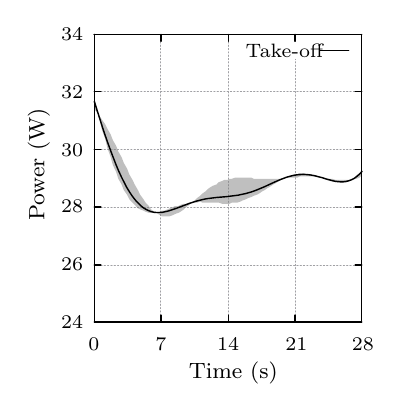
\begin{tikzpicture}[y=0.80pt, x=0.80pt, yscale=-0.510000, xscale=0.490000, inner sep=0pt, outer sep=0pt]
\scriptsize
\begin{scope}[draw=black,line join=bevel,line cap=rect,even odd rule,line width=0.512pt]
  \begin{scope}[cm={{1.0,0.0,0.0,1.0,(0.0,0.0)}},draw=black,line join=bevel,line cap=rect,line width=0.512pt]
  \end{scope}
  \begin{scope}[cm={{1.00625,0.0,0.0,1.00625,(0.0,0.0)}},draw=black,line join=bevel,line cap=rect,line width=0.512pt]
  \end{scope}
  \begin{scope}[cm={{1.00625,0.0,0.0,1.00625,(0.0,0.0)}},draw=ca0a0a4,dash pattern=on 0.40pt off 0.80pt,line join=round,line cap=round,line width=0.400pt]
    \path[draw] (53.5000,268.5000) -- (298.5000,268.5000);
  \end{scope}
  \begin{scope}[cm={{1.00625,0.0,0.0,1.00625,(0.0,0.0)}},draw=black,line join=round,line cap=round,line width=0.512pt]
    \path[draw] (53.5000,268.5000) -- (59.5000,268.5000);
    \path[draw] (298.5000,268.5000) -- (292.5000,268.5000);
  \end{scope}
  \begin{scope}[cm={{1.00625,0.0,0.0,1.00625,(0.0,0.0)}},draw=black,line join=bevel,line cap=rect,line width=0.512pt]
  \end{scope}
  \begin{scope}[cm={{1.00625,0.0,0.0,1.00625,(27.1688,276.216)}},draw=black,line join=bevel,line cap=rect,line width=0.512pt]
  \end{scope}
  \begin{scope}[cm={{1.00625,0.0,0.0,1.00625,(27.1688,276.216)}},draw=black,line join=bevel,line cap=rect,line width=0.512pt]
  \end{scope}
  \begin{scope}[cm={{1.00625,0.0,0.0,1.00625,(27.1688,276.216)}},draw=black,line join=bevel,line cap=rect,line width=0.512pt]
  \end{scope}
  \begin{scope}[cm={{1.00625,0.0,0.0,1.00625,(27.1688,276.216)}},draw=black,line join=bevel,line cap=rect,line width=0.512pt]
  \end{scope}
  \begin{scope}[cm={{1.00625,0.0,0.0,1.00625,(27.1688,276.216)}},draw=black,line join=bevel,line cap=rect,line width=0.512pt]
  \end{scope}
  \begin{scope}[cm={{1.00625,0.0,0.0,1.00625,(23.1688,276.216)}},draw=black,line join=bevel,line cap=rect,line width=0.512pt]
    \path[fill=black] (0.0000,0.0000) node[above right] (text40) {24};
  \end{scope}
  \begin{scope}[cm={{1.00625,0.0,0.0,1.00625,(27.1688,276.216)}},draw=black,line join=bevel,line cap=rect,line width=0.512pt]
  \end{scope}
  \begin{scope}[cm={{1.00625,0.0,0.0,1.00625,(0.0,0.0)}},draw=black,line join=bevel,line cap=rect,line width=0.512pt]
  \end{scope}
  \begin{scope}[cm={{1.00625,0.0,0.0,1.00625,(0.0,0.0)}},draw=ca0a0a4,dash pattern=on 0.40pt off 0.80pt,line join=round,line cap=round,line width=0.400pt]
    \path[draw] (53.5000,218.5000) -- (298.5000,218.5000);
  \end{scope}
  \begin{scope}[cm={{1.00625,0.0,0.0,1.00625,(0.0,0.0)}},draw=black,line join=round,line cap=round,line width=0.512pt]
    \path[draw] (53.5000,218.5000) -- (59.5000,218.5000);
    \path[draw] (298.5000,218.5000) -- (292.5000,218.5000);
  \end{scope}
  \begin{scope}[cm={{1.00625,0.0,0.0,1.00625,(0.0,0.0)}},draw=black,line join=bevel,line cap=rect,line width=0.512pt]
  \end{scope}
  \begin{scope}[cm={{1.00625,0.0,0.0,1.00625,(27.1688,224.897)}},draw=black,line join=bevel,line cap=rect,line width=0.512pt]
  \end{scope}
  \begin{scope}[cm={{1.00625,0.0,0.0,1.00625,(27.1688,224.897)}},draw=black,line join=bevel,line cap=rect,line width=0.512pt]
  \end{scope}
  \begin{scope}[cm={{1.00625,0.0,0.0,1.00625,(27.1688,224.897)}},draw=black,line join=bevel,line cap=rect,line width=0.512pt]
  \end{scope}
  \begin{scope}[cm={{1.00625,0.0,0.0,1.00625,(27.1688,224.897)}},draw=black,line join=bevel,line cap=rect,line width=0.512pt]
  \end{scope}
  \begin{scope}[cm={{1.00625,0.0,0.0,1.00625,(27.1688,224.897)}},draw=black,line join=bevel,line cap=rect,line width=0.512pt]
  \end{scope}
  \begin{scope}[cm={{1.00625,0.0,0.0,1.00625,(23.1688,224.897)}},draw=black,line join=bevel,line cap=rect,line width=0.512pt]
    \path[fill=black] (0.0000,0.0000) node[above right] (text70) {26};
  \end{scope}
  \begin{scope}[cm={{1.00625,0.0,0.0,1.00625,(27.1688,224.897)}},draw=black,line join=bevel,line cap=rect,line width=0.512pt]
  \end{scope}
  \begin{scope}[cm={{1.00625,0.0,0.0,1.00625,(0.0,0.0)}},draw=black,line join=bevel,line cap=rect,line width=0.512pt]
  \end{scope}
  \begin{scope}[cm={{1.00625,0.0,0.0,1.00625,(0.0,0.0)}},draw=ca0a0a4,dash pattern=on 0.40pt off 0.80pt,line join=round,line cap=round,line width=0.400pt]
    \path[draw] (53.5000,167.5000) -- (298.5000,167.5000);
  \end{scope}
  \begin{scope}[cm={{1.00625,0.0,0.0,1.00625,(0.0,0.0)}},draw=black,line join=round,line cap=round,line width=0.512pt]
    \path[draw] (53.5000,167.5000) -- (59.5000,167.5000);
    \path[draw] (298.5000,167.5000) -- (292.5000,167.5000);
  \end{scope}
  \begin{scope}[cm={{1.00625,0.0,0.0,1.00625,(0.0,0.0)}},draw=black,line join=bevel,line cap=rect,line width=0.512pt]
  \end{scope}
  \begin{scope}[cm={{1.00625,0.0,0.0,1.00625,(28.175,173.578)}},draw=black,line join=bevel,line cap=rect,line width=0.512pt]
  \end{scope}
  \begin{scope}[cm={{1.00625,0.0,0.0,1.00625,(28.175,173.578)}},draw=black,line join=bevel,line cap=rect,line width=0.512pt]
  \end{scope}
  \begin{scope}[cm={{1.00625,0.0,0.0,1.00625,(28.175,173.578)}},draw=black,line join=bevel,line cap=rect,line width=0.512pt]
  \end{scope}
  \begin{scope}[cm={{1.00625,0.0,0.0,1.00625,(28.175,173.578)}},draw=black,line join=bevel,line cap=rect,line width=0.512pt]
  \end{scope}
  \begin{scope}[cm={{1.00625,0.0,0.0,1.00625,(28.175,173.578)}},draw=black,line join=bevel,line cap=rect,line width=0.512pt]
  \end{scope}
  \begin{scope}[cm={{1.00625,0.0,0.0,1.00625,(23.175,173.578)}},draw=black,line join=bevel,line cap=rect,line width=0.512pt]
    \path[fill=black] (0.0000,0.0000) node[above right] (text100) {28};
  \end{scope}
  \begin{scope}[cm={{1.00625,0.0,0.0,1.00625,(28.175,173.578)}},draw=black,line join=bevel,line cap=rect,line width=0.512pt]
  \end{scope}
  \begin{scope}[cm={{1.00625,0.0,0.0,1.00625,(0.0,0.0)}},draw=black,line join=bevel,line cap=rect,line width=0.512pt]
  \end{scope}
  \begin{scope}[cm={{1.00625,0.0,0.0,1.00625,(0.0,0.0)}},draw=ca0a0a4,dash pattern=on 0.40pt off 0.80pt,line join=round,line cap=round,line width=0.400pt]
    \path[draw] (53.5000,116.5000) -- (298.5000,116.5000);
  \end{scope}
  \begin{scope}[cm={{1.00625,0.0,0.0,1.00625,(0.0,0.0)}},draw=black,line join=round,line cap=round,line width=0.512pt]
    \path[draw] (53.5000,116.5000) -- (59.5000,116.5000);
    \path[draw] (298.5000,116.5000) -- (292.5000,116.5000);
  \end{scope}
  \begin{scope}[cm={{1.00625,0.0,0.0,1.00625,(0.0,0.0)}},draw=black,line join=bevel,line cap=rect,line width=0.512pt]
  \end{scope}
  \begin{scope}[cm={{1.00625,0.0,0.0,1.00625,(27.1688,123.266)}},draw=black,line join=bevel,line cap=rect,line width=0.512pt]
  \end{scope}
  \begin{scope}[cm={{1.00625,0.0,0.0,1.00625,(27.1688,123.266)}},draw=black,line join=bevel,line cap=rect,line width=0.512pt]
  \end{scope}
  \begin{scope}[cm={{1.00625,0.0,0.0,1.00625,(27.1688,123.266)}},draw=black,line join=bevel,line cap=rect,line width=0.512pt]
  \end{scope}
  \begin{scope}[cm={{1.00625,0.0,0.0,1.00625,(27.1688,123.266)}},draw=black,line join=bevel,line cap=rect,line width=0.512pt]
  \end{scope}
  \begin{scope}[cm={{1.00625,0.0,0.0,1.00625,(27.1688,123.266)}},draw=black,line join=bevel,line cap=rect,line width=0.512pt]
  \end{scope}
  \begin{scope}[cm={{1.00625,0.0,0.0,1.00625,(23.1688,123.266)}},draw=black,line join=bevel,line cap=rect,line width=0.512pt]
    \path[fill=black] (0.0000,0.0000) node[above right] (text130) {30};
  \end{scope}
  \begin{scope}[cm={{1.00625,0.0,0.0,1.00625,(27.1688,123.266)}},draw=black,line join=bevel,line cap=rect,line width=0.512pt]
  \end{scope}
  \begin{scope}[cm={{1.00625,0.0,0.0,1.00625,(0.0,0.0)}},draw=black,line join=bevel,line cap=rect,line width=0.512pt]
  \end{scope}
  \begin{scope}[cm={{1.00625,0.0,0.0,1.00625,(0.0,0.0)}},draw=ca0a0a4,dash pattern=on 0.40pt off 0.80pt,line join=round,line cap=round,line width=0.400pt]
    \path[draw] (53.5000,65.5000) -- (298.5000,65.5000);
  \end{scope}
  \begin{scope}[cm={{1.00625,0.0,0.0,1.00625,(0.0,0.0)}},draw=black,line join=round,line cap=round,line width=0.512pt]
    \path[draw] (53.5000,65.5000) -- (59.5000,65.5000);
    \path[draw] (298.5000,65.5000) -- (292.5000,65.5000);
  \end{scope}
  \begin{scope}[cm={{1.00625,0.0,0.0,1.00625,(0.0,0.0)}},draw=black,line join=bevel,line cap=rect,line width=0.512pt]
  \end{scope}
  \begin{scope}[cm={{1.00625,0.0,0.0,1.00625,(27.1688,71.9469)}},draw=black,line join=bevel,line cap=rect,line width=0.512pt]
  \end{scope}
  \begin{scope}[cm={{1.00625,0.0,0.0,1.00625,(27.1688,71.9469)}},draw=black,line join=bevel,line cap=rect,line width=0.512pt]
  \end{scope}
  \begin{scope}[cm={{1.00625,0.0,0.0,1.00625,(27.1688,71.9469)}},draw=black,line join=bevel,line cap=rect,line width=0.512pt]
  \end{scope}
  \begin{scope}[cm={{1.00625,0.0,0.0,1.00625,(27.1688,71.9469)}},draw=black,line join=bevel,line cap=rect,line width=0.512pt]
  \end{scope}
  \begin{scope}[cm={{1.00625,0.0,0.0,1.00625,(27.1688,71.9469)}},draw=black,line join=bevel,line cap=rect,line width=0.512pt]
  \end{scope}
  \begin{scope}[cm={{1.00625,0.0,0.0,1.00625,(23.1688,71.9469)}},draw=black,line join=bevel,line cap=rect,line width=0.512pt]
    \path[fill=black] (0.0000,0.0000) node[above right] (text160) {32};
  \end{scope}
  \begin{scope}[cm={{1.00625,0.0,0.0,1.00625,(27.1688,71.9469)}},draw=black,line join=bevel,line cap=rect,line width=0.512pt]
  \end{scope}
  \begin{scope}[cm={{1.00625,0.0,0.0,1.00625,(0.0,0.0)}},draw=black,line join=bevel,line cap=rect,line width=0.512pt]
  \end{scope}
  \begin{scope}[cm={{1.00625,0.0,0.0,1.00625,(0.0,0.0)}},draw=ca0a0a4,dash pattern=on 0.40pt off 0.80pt,line join=round,line cap=round,line width=0.400pt]
    \path[draw] (53.5000,15.5000) -- (298.5000,15.5000);
  \end{scope}
  \begin{scope}[cm={{1.00625,0.0,0.0,1.00625,(0.0,0.0)}},draw=black,line join=round,line cap=round,line width=0.512pt]
    \path[draw] (53.5000,15.5000) -- (59.5000,15.5000);
    \path[draw] (298.5000,15.5000) -- (292.5000,15.5000);
  \end{scope}
  \begin{scope}[cm={{1.00625,0.0,0.0,1.00625,(0.0,0.0)}},draw=black,line join=bevel,line cap=rect,line width=0.512pt]
  \end{scope}
  \begin{scope}[cm={{1.00625,0.0,0.0,1.00625,(27.1688,20.6281)}},draw=black,line join=bevel,line cap=rect,line width=0.512pt]
  \end{scope}
  \begin{scope}[cm={{1.00625,0.0,0.0,1.00625,(27.1688,20.6281)}},draw=black,line join=bevel,line cap=rect,line width=0.512pt]
  \end{scope}
  \begin{scope}[cm={{1.00625,0.0,0.0,1.00625,(27.1688,20.6281)}},draw=black,line join=bevel,line cap=rect,line width=0.512pt]
  \end{scope}
  \begin{scope}[cm={{1.00625,0.0,0.0,1.00625,(27.1688,20.6281)}},draw=black,line join=bevel,line cap=rect,line width=0.512pt]
  \end{scope}
  \begin{scope}[cm={{1.00625,0.0,0.0,1.00625,(27.1688,20.6281)}},draw=black,line join=bevel,line cap=rect,line width=0.512pt]
  \end{scope}
  \begin{scope}[cm={{1.00625,0.0,0.0,1.00625,(23.1688,20.6281)}},draw=black,line join=bevel,line cap=rect,line width=0.512pt]
    \path[fill=black] (0.0000,0.0000) node[above right] (text190) {34};
  \end{scope}
  \begin{scope}[cm={{1.00625,0.0,0.0,1.00625,(27.1688,20.6281)}},draw=black,line join=bevel,line cap=rect,line width=0.512pt]
  \end{scope}
  \begin{scope}[cm={{1.00625,0.0,0.0,1.00625,(0.0,0.0)}},draw=black,line join=bevel,line cap=rect,line width=0.512pt]
  \end{scope}
  \begin{scope}[cm={{1.00625,0.0,0.0,1.00625,(0.0,0.0)}},draw=ca0a0a4,dash pattern=on 0.40pt off 0.80pt,line join=round,line cap=round,line width=0.400pt]
    \path[draw] (53.5000,268.5000) -- (53.5000,15.5000);
  \end{scope}
  \begin{scope}[cm={{1.00625,0.0,0.0,1.00625,(0.0,0.0)}},draw=black,line join=round,line cap=round,line width=0.512pt]
    \path[draw] (53.5000,268.5000) -- (53.5000,262.5000);
    \path[draw] (53.5000,15.5000) -- (53.5000,21.5000);
  \end{scope}
  \begin{scope}[cm={{1.00625,0.0,0.0,1.00625,(0.0,0.0)}},draw=black,line join=bevel,line cap=rect,line width=0.512pt]
  \end{scope}
  \begin{scope}[cm={{1.00625,0.0,0.0,1.00625,(48.3,298.353)}},draw=black,line join=bevel,line cap=rect,line width=0.512pt]
  \end{scope}
  \begin{scope}[cm={{1.00625,0.0,0.0,1.00625,(48.3,298.353)}},draw=black,line join=bevel,line cap=rect,line width=0.512pt]
  \end{scope}
  \begin{scope}[cm={{1.00625,0.0,0.0,1.00625,(48.3,298.353)}},draw=black,line join=bevel,line cap=rect,line width=0.512pt]
  \end{scope}
  \begin{scope}[cm={{1.00625,0.0,0.0,1.00625,(48.3,298.353)}},draw=black,line join=bevel,line cap=rect,line width=0.512pt]
  \end{scope}
  \begin{scope}[cm={{1.00625,0.0,0.0,1.00625,(48.3,298.353)}},draw=black,line join=bevel,line cap=rect,line width=0.512pt]
  \end{scope}
  \begin{scope}[cm={{1.00625,0.0,0.0,1.00625,(48.3,295.353)}},draw=black,line join=bevel,line cap=rect,line width=0.512pt]
    \path[fill=black] (0.0000,0.0000) node[above right] (text220) {0};
  \end{scope}
  \begin{scope}[cm={{1.00625,0.0,0.0,1.00625,(48.3,298.353)}},draw=black,line join=bevel,line cap=rect,line width=0.512pt]
  \end{scope}
  \begin{scope}[cm={{1.00625,0.0,0.0,1.00625,(0.0,0.0)}},draw=black,line join=bevel,line cap=rect,line width=0.512pt]
  \end{scope}
  \begin{scope}[cm={{1.00625,0.0,0.0,1.00625,(0.0,0.0)}},draw=ca0a0a4,dash pattern=on 0.40pt off 0.80pt,line join=round,line cap=round,line width=0.400pt]
    \path[draw] (114.5000,268.5000) -- (114.5000,15.5000);
  \end{scope}
  \begin{scope}[cm={{1.00625,0.0,0.0,1.00625,(0.0,0.0)}},draw=black,line join=round,line cap=round,line width=0.512pt]
    \path[draw] (114.5000,268.5000) -- (114.5000,262.5000);
    \path[draw] (114.5000,15.5000) -- (114.5000,21.5000);
  \end{scope}
  \begin{scope}[cm={{1.00625,0.0,0.0,1.00625,(0.0,0.0)}},draw=black,line join=bevel,line cap=rect,line width=0.512pt]
  \end{scope}
  \begin{scope}[cm={{1.00625,0.0,0.0,1.00625,(110.184,298.353)}},draw=black,line join=bevel,line cap=rect,line width=0.512pt]
  \end{scope}
  \begin{scope}[cm={{1.00625,0.0,0.0,1.00625,(110.184,298.353)}},draw=black,line join=bevel,line cap=rect,line width=0.512pt]
  \end{scope}
  \begin{scope}[cm={{1.00625,0.0,0.0,1.00625,(110.184,298.353)}},draw=black,line join=bevel,line cap=rect,line width=0.512pt]
  \end{scope}
  \begin{scope}[cm={{1.00625,0.0,0.0,1.00625,(110.184,298.353)}},draw=black,line join=bevel,line cap=rect,line width=0.512pt]
  \end{scope}
  \begin{scope}[cm={{1.00625,0.0,0.0,1.00625,(110.184,298.353)}},draw=black,line join=bevel,line cap=rect,line width=0.512pt]
  \end{scope}
  \begin{scope}[cm={{1.00625,0.0,0.0,1.00625,(110.184,295.353)}},draw=black,line join=bevel,line cap=rect,line width=0.512pt]
    \path[fill=black] (0.0000,0.0000) node[above right] (text250) {7};
  \end{scope}
  \begin{scope}[cm={{1.00625,0.0,0.0,1.00625,(110.184,298.353)}},draw=black,line join=bevel,line cap=rect,line width=0.512pt]
  \end{scope}
  \begin{scope}[cm={{1.00625,0.0,0.0,1.00625,(0.0,0.0)}},draw=black,line join=bevel,line cap=rect,line width=0.512pt]
  \end{scope}
  \begin{scope}[cm={{1.00625,0.0,0.0,1.00625,(0.0,0.0)}},draw=ca0a0a4,dash pattern=on 0.40pt off 0.80pt,line join=round,line cap=round,line width=0.400pt]
    \path[draw] (176.5000,268.5000) -- (176.5000,15.5000);
  \end{scope}
  \begin{scope}[cm={{1.00625,0.0,0.0,1.00625,(0.0,0.0)}},draw=black,line join=round,line cap=round,line width=0.512pt]
    \path[draw] (176.5000,268.5000) -- (176.5000,262.5000);
    \path[draw] (176.5000,15.5000) -- (176.5000,21.5000);
  \end{scope}
  \begin{scope}[cm={{1.00625,0.0,0.0,1.00625,(0.0,0.0)}},draw=black,line join=bevel,line cap=rect,line width=0.512pt]
  \end{scope}
  \begin{scope}[cm={{1.00625,0.0,0.0,1.00625,(167.038,298.353)}},draw=black,line join=bevel,line cap=rect,line width=0.512pt]
  \end{scope}
  \begin{scope}[cm={{1.00625,0.0,0.0,1.00625,(167.038,298.353)}},draw=black,line join=bevel,line cap=rect,line width=0.512pt]
  \end{scope}
  \begin{scope}[cm={{1.00625,0.0,0.0,1.00625,(167.038,298.353)}},draw=black,line join=bevel,line cap=rect,line width=0.512pt]
  \end{scope}
  \begin{scope}[cm={{1.00625,0.0,0.0,1.00625,(167.038,298.353)}},draw=black,line join=bevel,line cap=rect,line width=0.512pt]
  \end{scope}
  \begin{scope}[cm={{1.00625,0.0,0.0,1.00625,(167.038,298.353)}},draw=black,line join=bevel,line cap=rect,line width=0.512pt]
  \end{scope}
  \begin{scope}[cm={{1.00625,0.0,0.0,1.00625,(167.038,295.353)}},draw=black,line join=bevel,line cap=rect,line width=0.512pt]
    \path[fill=black] (0.0000,0.0000) node[above right] (text280) {14};
  \end{scope}
  \begin{scope}[cm={{1.00625,0.0,0.0,1.00625,(167.038,298.353)}},draw=black,line join=bevel,line cap=rect,line width=0.512pt]
  \end{scope}
  \begin{scope}[cm={{1.00625,0.0,0.0,1.00625,(0.0,0.0)}},draw=black,line join=bevel,line cap=rect,line width=0.512pt]
  \end{scope}
  \begin{scope}[cm={{1.00625,0.0,0.0,1.00625,(0.0,0.0)}},draw=ca0a0a4,dash pattern=on 0.40pt off 0.80pt,line join=round,line cap=round,line width=0.400pt]
    \path[draw] (237.5000,268.5000) -- (237.5000,37.5000);
    \path[draw] (237.5000,21.5000) -- (237.5000,15.5000);
  \end{scope}
  \begin{scope}[cm={{1.00625,0.0,0.0,1.00625,(0.0,0.0)}},draw=black,line join=round,line cap=round,line width=0.512pt]
    \path[draw] (237.5000,268.5000) -- (237.5000,262.5000);
    \path[draw] (237.5000,15.5000) -- (237.5000,21.5000);
  \end{scope}
  \begin{scope}[cm={{1.00625,0.0,0.0,1.00625,(0.0,0.0)}},draw=black,line join=bevel,line cap=rect,line width=0.512pt]
  \end{scope}
  \begin{scope}[cm={{1.00625,0.0,0.0,1.00625,(229.928,298.353)}},draw=black,line join=bevel,line cap=rect,line width=0.512pt]
  \end{scope}
  \begin{scope}[cm={{1.00625,0.0,0.0,1.00625,(229.928,298.353)}},draw=black,line join=bevel,line cap=rect,line width=0.512pt]
  \end{scope}
  \begin{scope}[cm={{1.00625,0.0,0.0,1.00625,(229.928,298.353)}},draw=black,line join=bevel,line cap=rect,line width=0.512pt]
  \end{scope}
  \begin{scope}[cm={{1.00625,0.0,0.0,1.00625,(229.928,298.353)}},draw=black,line join=bevel,line cap=rect,line width=0.512pt]
  \end{scope}
  \begin{scope}[cm={{1.00625,0.0,0.0,1.00625,(229.928,298.353)}},draw=black,line join=bevel,line cap=rect,line width=0.512pt]
  \end{scope}
  \begin{scope}[cm={{1.00625,0.0,0.0,1.00625,(229.928,295.353)}},draw=black,line join=bevel,line cap=rect,line width=0.512pt]
    \path[fill=black] (0.0000,0.0000) node[above right] (text312) {21};
  \end{scope}
  \begin{scope}[cm={{1.00625,0.0,0.0,1.00625,(229.928,298.353)}},draw=black,line join=bevel,line cap=rect,line width=0.512pt]
  \end{scope}
  \begin{scope}[cm={{1.00625,0.0,0.0,1.00625,(0.0,0.0)}},draw=black,line join=bevel,line cap=rect,line width=0.512pt]
  \end{scope}
  \begin{scope}[cm={{1.00625,0.0,0.0,1.00625,(0.0,0.0)}},draw=ca0a0a4,dash pattern=on 0.40pt off 0.80pt,line join=round,line cap=round,line width=0.400pt]
    \path[draw] (298.5000,268.5000) -- (298.5000,15.5000);
  \end{scope}
  \begin{scope}[cm={{1.00625,0.0,0.0,1.00625,(0.0,0.0)}},draw=black,line join=round,line cap=round,line width=0.512pt]
    \path[draw] (298.5000,268.5000) -- (298.5000,262.5000);
    \path[draw] (298.5000,15.5000) -- (298.5000,21.5000);
  \end{scope}
  \begin{scope}[cm={{1.00625,0.0,0.0,1.00625,(0.0,0.0)}},draw=black,line join=bevel,line cap=rect,line width=0.512pt]
  \end{scope}
  \begin{scope}[cm={{1.00625,0.0,0.0,1.00625,(291.309,298.353)}},draw=black,line join=bevel,line cap=rect,line width=0.512pt]
  \end{scope}
  \begin{scope}[cm={{1.00625,0.0,0.0,1.00625,(291.309,298.353)}},draw=black,line join=bevel,line cap=rect,line width=0.512pt]
  \end{scope}
  \begin{scope}[cm={{1.00625,0.0,0.0,1.00625,(291.309,298.353)}},draw=black,line join=bevel,line cap=rect,line width=0.512pt]
  \end{scope}
  \begin{scope}[cm={{1.00625,0.0,0.0,1.00625,(291.309,298.353)}},draw=black,line join=bevel,line cap=rect,line width=0.512pt]
  \end{scope}
  \begin{scope}[cm={{1.00625,0.0,0.0,1.00625,(291.309,298.353)}},draw=black,line join=bevel,line cap=rect,line width=0.512pt]
  \end{scope}
  \begin{scope}[cm={{1.00625,0.0,0.0,1.00625,(291.309,295.353)}},draw=black,line join=bevel,line cap=rect,line width=0.512pt]
    \path[fill=black] (0.0000,0.0000) node[above right] (text342) {28};
  \end{scope}
  \begin{scope}[cm={{1.00625,0.0,0.0,1.00625,(291.309,298.353)}},draw=black,line join=bevel,line cap=rect,line width=0.512pt]
  \end{scope}
  \begin{scope}[cm={{1.00625,0.0,0.0,1.00625,(0.0,0.0)}},draw=black,line join=bevel,line cap=rect,line width=0.512pt]
  \end{scope}
  \begin{scope}[cm={{1.00625,0.0,0.0,1.00625,(0.0,0.0)}},draw=black,line join=round,line cap=round,line width=0.512pt]
    \path[draw] (53.5000,15.5000) -- (53.5000,268.5000) -- (298.5000,268.5000) --
      (298.5000,15.5000) -- (53.5000,15.5000);
  \end{scope}
  \begin{scope}[cm={{1.00625,0.0,0.0,1.00625,(0.0,0.0)}},draw=black,line join=bevel,line cap=rect,line width=0.512pt]
  \end{scope}
  \begin{scope}[cm={{0.0,-1.00625,1.00625,0.0,(13.5844,176.597)}},draw=black,line join=bevel,line cap=rect,line width=0.512pt]
  \end{scope}
  \begin{scope}[cm={{0.0,-1.00625,1.00625,0.0,(13.5844,176.597)}},draw=black,line join=bevel,line cap=rect,line width=0.512pt]
  \end{scope}
  \begin{scope}[cm={{0.0,-1.00625,1.00625,0.0,(13.5844,176.597)}},draw=black,line join=bevel,line cap=rect,line width=0.512pt]
  \end{scope}
  \begin{scope}[cm={{0.0,-1.00625,1.00625,0.0,(13.5844,176.597)}},draw=black,line join=bevel,line cap=rect,line width=0.512pt]
  \end{scope}
  \begin{scope}[cm={{0.0,-1.00625,1.00625,0.0,(13.5844,176.597)}},draw=black,line join=bevel,line cap=rect,line width=0.512pt]
  \end{scope}
  \begin{scope}[cm={{0.0,-1.00625,1.00625,0.0,(-7.5844,180.597)}},draw=black,line join=bevel,line cap=rect,line width=0.512pt]
    \path[fill=black] (0.0000,0.0000) node[above right] (text366) {\rotatebox{90}{\footnotesize Power (W)}};
  \end{scope}
  \begin{scope}[cm={{0.0,-1.00625,1.00625,0.0,(13.5844,176.597)}},draw=black,line join=bevel,line cap=rect,line width=0.512pt]
  \end{scope}
  \begin{scope}[cm={{1.00625,0.0,0.0,1.00625,(150.938,317.472)}},draw=black,line join=bevel,line cap=rect,line width=0.512pt]
  \end{scope}
  \begin{scope}[cm={{1.00625,0.0,0.0,1.00625,(150.938,317.472)}},draw=black,line join=bevel,line cap=rect,line width=0.512pt]
  \end{scope}
  \begin{scope}[cm={{1.00625,0.0,0.0,1.00625,(150.938,317.472)}},draw=black,line join=bevel,line cap=rect,line width=0.512pt]
  \end{scope}
  \begin{scope}[cm={{1.00625,0.0,0.0,1.00625,(150.938,317.472)}},draw=black,line join=bevel,line cap=rect,line width=0.512pt]
  \end{scope}
  \begin{scope}[cm={{1.00625,0.0,0.0,1.00625,(150.938,317.472)}},draw=black,line join=bevel,line cap=rect,line width=0.512pt]
  \end{scope}
  \begin{scope}[cm={{1.00625,0.0,0.0,1.00625,(140.938,325.472)}},draw=black,line join=bevel,line cap=rect,line width=0.512pt]
    \path[fill=black] (0.0000,0.0000) node[above right] (text382) {\footnotesize Time (s)};
  \end{scope}
  \begin{scope}[cm={{1.00625,0.0,0.0,1.00625,(150.938,317.472)}},draw=black,line join=bevel,line cap=rect,line width=0.512pt]
  \end{scope}
  \begin{scope}[cm={{1.00625,0.0,0.0,1.00625,(0.0,0.0)}},draw=black,line join=bevel,line cap=rect,line width=0.512pt]
  \end{scope}
  \begin{scope}[cm={{1.00625,0.0,0.0,1.00625,(0.0,0.0)}},draw=black,line join=bevel,line cap=rect,line width=0.512pt]
  \end{scope}
  \begin{scope}[cm={{1.00625,0.0,0.0,1.00625,(0.0,0.0)}},draw=black,line join=bevel,line cap=rect,line width=0.512pt]
  \end{scope}
  \begin{scope}[cm={{1.00625,0.0,0.0,1.00625,(0.0,0.0)}},draw=c494949,fill=c808080,line join=bevel,line cap=rect,draw opacity=0.000,fill opacity=0.500,line width=0.512pt,transparency group]
    \path[draw=c494949,fill,draw opacity=0.000,even odd rule] (53.5000,81.5000) --
      (56.5000,84.5000) -- (57.5000,85.5000) -- (56.5000,81.5000) --
      (53.5000,71.5000) -- (53.5000,81.5000);
    \path[draw=c494949,fill,draw opacity=0.000,even odd rule] (57.5000,85.5000) --
      (58.5000,87.5000) -- (60.5000,90.5000) -- (63.5000,94.5000) --
      (65.5000,98.5000) -- (68.5000,103.5000) -- (70.5000,108.5000) --
      (73.5000,113.5000) -- (75.5000,118.5000) -- (78.5000,123.5000) --
      (80.5000,128.5000) -- (83.5000,133.5000) -- (85.5000,138.5000) --
      (88.5000,143.5000) -- (90.5000,147.5000) -- (93.5000,152.5000) --
      (95.5000,156.5000) -- (98.5000,160.5000) -- (100.5000,163.5000) --
      (103.5000,166.5000) -- (105.5000,169.5000) -- (108.5000,171.5000) --
      (109.5000,172.5000) -- (108.5000,172.5000) -- (105.5000,172.5000) --
      (103.5000,172.5000) -- (100.5000,171.5000) -- (98.5000,170.5000) --
      (95.5000,169.5000) -- (93.5000,168.5000) -- (90.5000,165.5000) --
      (88.5000,163.5000) -- (85.5000,160.5000) -- (83.5000,156.5000) --
      (80.5000,152.5000) -- (78.5000,147.5000) -- (75.5000,142.5000) --
      (73.5000,136.5000) -- (70.5000,130.5000) -- (68.5000,123.5000) --
      (65.5000,115.5000) -- (63.5000,107.5000) -- (60.5000,99.5000) --
      (58.5000,90.5000) -- (57.5000,85.5000);
    \path[draw=c494949,fill,draw opacity=0.000,even odd rule] (109.5000,172.5000) --
      (110.5000,172.5000) -- (113.5000,174.5000) -- (115.5000,175.5000) --
      (117.5000,175.5000) -- (120.5000,175.5000) -- (122.5000,175.5000) --
      (125.5000,174.5000) -- (127.5000,173.5000) -- (130.5000,172.5000) --
      (132.5000,171.5000) -- (135.5000,169.5000) -- (137.5000,167.5000) --
      (140.5000,165.5000) -- (142.5000,163.5000) -- (143.5000,163.5000) --
      (142.5000,163.5000) -- (140.5000,163.5000) -- (137.5000,164.5000) --
      (135.5000,164.5000) -- (132.5000,165.5000) -- (130.5000,166.5000) --
      (127.5000,166.5000) -- (125.5000,167.5000) -- (122.5000,168.5000) --
      (120.5000,169.5000) -- (117.5000,170.5000) -- (115.5000,170.5000) --
      (113.5000,171.5000) -- (110.5000,172.5000) -- (109.5000,172.5000);
    \path[draw=c494949,fill,draw opacity=0.000,even odd rule] (143.5000,163.5000) --
      (145.5000,161.5000) -- (147.5000,159.5000) -- (150.5000,157.5000) --
      (152.5000,155.5000) -- (155.5000,153.5000) -- (157.5000,151.5000) --
      (160.5000,149.5000) -- (162.5000,148.5000) -- (165.5000,147.5000) --
      (167.5000,145.5000) -- (170.5000,144.5000) -- (172.5000,143.5000) --
      (175.5000,143.5000) -- (177.5000,142.5000) -- (179.5000,142.5000) --
      (182.5000,141.5000) -- (184.5000,141.5000) -- (187.5000,141.5000) --
      (189.5000,141.5000) -- (192.5000,141.5000) -- (194.5000,141.5000) --
      (197.5000,141.5000) -- (199.5000,142.5000) -- (202.5000,142.5000) --
      (204.5000,142.5000) -- (207.5000,142.5000) -- (209.5000,142.5000) --
      (212.5000,142.5000) -- (214.5000,142.5000) -- (217.5000,142.5000) --
      (219.5000,142.5000) -- (222.5000,142.5000) -- (224.5000,142.5000) --
      (227.5000,142.5000) -- (224.5000,143.5000) -- (222.5000,144.5000) --
      (219.5000,146.5000) -- (217.5000,147.5000) -- (214.5000,149.5000) --
      (212.5000,150.5000) -- (209.5000,152.5000) -- (207.5000,153.5000) --
      (204.5000,155.5000) -- (202.5000,156.5000) -- (199.5000,157.5000) --
      (197.5000,158.5000) -- (194.5000,159.5000) -- (192.5000,160.5000) --
      (189.5000,161.5000) -- (187.5000,162.5000) -- (184.5000,163.5000) --
      (182.5000,163.5000) -- (179.5000,163.5000) -- (177.5000,164.5000) --
      (175.5000,164.5000) -- (172.5000,164.5000) -- (170.5000,164.5000) --
      (167.5000,163.5000) -- (165.5000,163.5000) -- (162.5000,163.5000) --
      (160.5000,163.5000) -- (157.5000,163.5000) -- (155.5000,163.5000) --
      (152.5000,163.5000) -- (150.5000,162.5000) -- (147.5000,163.5000) --
      (145.5000,163.5000) -- (143.5000,163.5000);
    \path[draw=c494949,fill,draw opacity=0.000,even odd rule] (227.5000,142.5000) --
      (226.5000,142.5000) -- (227.5000,142.5000);
    \path[draw=c494949,fill,draw opacity=0.000,even odd rule] (227.5000,142.5000) --
      (229.5000,141.5000) -- (232.5000,141.5000) -- (234.5000,141.5000) --
      (236.5000,141.5000) -- (239.5000,141.5000) -- (241.5000,140.5000) --
      (244.5000,140.5000) -- (246.5000,140.5000) -- (249.5000,140.5000) --
      (251.5000,140.5000) -- (254.5000,140.5000) -- (256.5000,140.5000) --
      (259.5000,141.5000) -- (261.5000,141.5000) -- (259.5000,140.5000) --
      (256.5000,139.5000) -- (254.5000,139.5000) -- (251.5000,138.5000) --
      (249.5000,138.5000) -- (246.5000,138.5000) -- (244.5000,137.5000) --
      (241.5000,137.5000) -- (239.5000,138.5000) -- (236.5000,138.5000) --
      (234.5000,139.5000) -- (232.5000,140.5000) -- (229.5000,141.5000) --
      (227.5000,142.5000);
    \path[draw=c494949,fill,draw opacity=0.000,even odd rule] (261.5000,141.5000) --
      (264.5000,141.5000) -- (266.5000,142.5000) -- (269.5000,142.5000) --
      (271.5000,142.5000) -- (274.5000,143.5000) -- (276.5000,143.5000) --
      (279.5000,143.5000) -- (281.5000,143.5000) -- (284.5000,143.5000) --
      (286.5000,143.5000) -- (289.5000,143.5000) -- (286.5000,144.5000) --
      (284.5000,145.5000) -- (281.5000,145.5000) -- (279.5000,145.5000) --
      (276.5000,145.5000) -- (274.5000,145.5000) -- (271.5000,144.5000) --
      (269.5000,144.5000) -- (266.5000,143.5000) -- (264.5000,142.5000) --
      (261.5000,141.5000);
    \path[draw=c494949,fill,draw opacity=0.000,even odd rule] (289.5000,143.5000) --
      (291.5000,142.5000) -- (293.5000,142.5000) -- (296.5000,141.5000) --
      (298.5000,139.5000) -- (298.5000,134.5000) -- (296.5000,137.5000) --
      (293.5000,139.5000) -- (291.5000,142.5000) -- (289.5000,143.5000);
  \end{scope}
  \begin{scope}[cm={{1.00625,0.0,0.0,1.00625,(0.0,0.0)}},draw=black,line join=bevel,line cap=rect,line width=0.512pt]
  \end{scope}
  \begin{scope}[cm={{1.00625,0.0,0.0,1.00625,(216.344,33.2063)}},draw=black,line join=bevel,line cap=rect,line width=0.512pt]
  \end{scope}
  \begin{scope}[cm={{1.00625,0.0,0.0,1.00625,(216.344,33.2063)}},draw=black,line join=bevel,line cap=rect,line width=0.512pt]
  \end{scope}
  \begin{scope}[cm={{1.00625,0.0,0.0,1.00625,(216.344,33.2063)}},draw=black,line join=bevel,line cap=rect,line width=0.512pt]
  \end{scope}
  \begin{scope}[cm={{1.00625,0.0,0.0,1.00625,(216.344,33.2063)}},draw=black,line join=bevel,line cap=rect,line width=0.512pt]
  \end{scope}
  \begin{scope}[cm={{1.00625,0.0,0.0,1.00625,(216.344,33.2063)}},draw=black,line join=bevel,line cap=rect,line width=0.512pt]
  \end{scope}
  \begin{scope}[cm={{1.00625,0.0,0.0,1.00625,(193.344,36.2063)}},draw=black,line join=bevel,line cap=rect,line width=0.512pt]
    \path[fill=black] (0.0000,0.0000) node[above right] (text424) {\scriptsize Take-off};
  \end{scope}
  \begin{scope}[cm={{1.00625,0.0,0.0,1.00625,(216.344,33.2063)}},draw=black,line join=bevel,line cap=rect,line width=0.512pt]
  \end{scope}
  \begin{scope}[cm={{1.00625,0.0,0.0,1.00625,(0.0,0.0)}},draw=black,line join=bevel,line cap=rect,line width=0.512pt]
  \end{scope}
  \begin{scope}[cm={{1.00625,0.0,0.0,1.00625,(0.0,0.0)}},draw=black,line join=round,line cap=round,line width=0.512pt]
    \path[draw,even odd rule] (260.5000,29.5000) -- (286.5000,29.5000);
  \end{scope}
  \begin{scope}[cm={{1.00625,0.0,0.0,1.00625,(0.0,0.0)}},draw=black,line join=bevel,line cap=rect,line width=0.512pt]
  \end{scope}
  \begin{scope}[cm={{1.00625,0.0,0.0,1.00625,(0.0,0.0)}},draw=black,line join=bevel,line cap=rect,line width=0.512pt]
  \end{scope}
  \begin{scope}[cm={{1.00625,0.0,0.0,1.00625,(0.0,0.0)}},draw=black,line join=bevel,line cap=rect,line width=0.512pt]
  \end{scope}
  \begin{scope}[cm={{1.00625,0.0,0.0,1.00625,(0.0,0.0)}},draw=black,line join=bevel,line cap=rect,line width=0.512pt]
  \end{scope}
  \begin{scope}[cm={{1.00625,0.0,0.0,1.00625,(0.0,0.0)}},draw=black,line join=round,line cap=round,line width=0.512pt]
    \path[draw] (53.5000,74.5000) -- (53.5000,74.5000) -- (56.0000,82.1000) --
      (58.5000,89.6000) -- (60.9000,96.9000) -- (63.4000,104.1000) --
      (65.9000,111.0000) -- (68.4000,117.6000) -- (70.9000,123.9000) --
      (73.3000,129.9000) -- (75.8000,135.6000) -- (78.3000,140.8000) --
      (80.8000,145.6000) -- (83.2000,150.1000) -- (85.7000,154.0000) --
      (88.2000,157.6000) -- (90.7000,160.8000) -- (93.2000,163.5000) --
      (95.6000,165.8000) -- (98.1000,167.8000) -- (100.6000,169.3000) --
      (103.1000,170.5000) -- (105.6000,171.4000) -- (108.0000,172.0000) --
      (110.5000,172.2000) -- (113.0000,172.2000) -- (115.5000,172.1000) --
      (117.9000,171.6000) -- (120.4000,171.1000) -- (122.9000,170.4000) --
      (125.4000,169.6000) -- (127.9000,168.8000) -- (130.3000,167.9000) --
      (132.8000,167.0000) -- (135.3000,166.1000) -- (137.8000,165.2000) --
      (140.3000,164.3000) -- (142.7000,163.5000) -- (145.2000,162.7000) --
      (147.7000,162.0000) -- (150.2000,161.4000) -- (152.7000,160.8000) --
      (155.1000,160.3000) -- (157.6000,159.9000) -- (160.1000,159.6000) --
      (162.6000,159.3000) -- (165.0000,159.0000) -- (167.5000,158.8000) --
      (170.0000,158.6000) -- (172.5000,158.4000) -- (175.0000,158.2000) --
      (177.4000,157.9000) -- (179.9000,157.6000) -- (182.4000,157.3000) --
      (184.9000,157.0000) -- (187.4000,156.5000) -- (189.8000,156.0000) --
      (192.3000,155.5000) -- (194.8000,154.8000) -- (197.3000,154.1000) --
      (199.7000,153.3000) -- (202.2000,152.4000) -- (204.7000,151.4000) --
      (207.2000,150.4000) -- (209.7000,149.4000) -- (212.1000,148.3000) --
      (214.6000,147.2000) -- (217.1000,146.1000) -- (219.6000,145.0000) --
      (222.1000,144.0000) -- (224.5000,143.0000) -- (227.0000,142.1000) --
      (229.5000,141.2000) -- (232.0000,140.5000) -- (234.4000,139.9000) --
      (236.9000,139.4000) -- (239.4000,139.0000) -- (241.9000,138.8000) --
      (244.4000,138.7000) -- (246.8000,138.7000) -- (249.3000,138.9000) --
      (251.8000,139.2000) -- (254.3000,139.6000) -- (256.8000,140.2000) --
      (259.2000,140.8000) -- (261.7000,141.4000) -- (264.2000,142.2000) --
      (266.7000,142.9000) -- (269.2000,143.5000) -- (271.6000,144.2000) --
      (274.1000,144.7000) -- (276.6000,145.0000) -- (279.1000,145.2000) --
      (281.5000,145.2000) -- (284.0000,144.9000) -- (286.5000,144.3000) --
      (289.0000,143.4000) -- (291.5000,142.2000) -- (293.9000,140.5000) --
      (296.4000,138.5000) -- (298.9000,135.9000);
  \end{scope}
  \begin{scope}[cm={{1.00625,0.0,0.0,1.00625,(0.0,0.0)}},draw=black,line join=bevel,line cap=rect,line width=0.512pt]
  \end{scope}
  \begin{scope}[cm={{1.00625,0.0,0.0,1.00625,(0.0,0.0)}},draw=black,line join=bevel,line cap=rect,line width=0.512pt]
  \end{scope}
  \begin{scope}[cm={{1.00625,0.0,0.0,1.00625,(0.0,0.0)}},draw=black,line join=round,line cap=round,line width=0.512pt]
    \path[draw] (53.5000,15.5000) -- (53.5000,268.5000) -- (298.5000,268.5000) --
      (298.5000,15.5000) -- (53.5000,15.5000);
  \end{scope}
  \begin{scope}[cm={{1.00625,0.0,0.0,1.00625,(0.0,0.0)}},draw=black,line join=bevel,line cap=rect,line width=0.512pt]
  \end{scope}
  \begin{scope}[cm={{1.0,0.0,0.0,1.0,(0.0,0.0)}},draw=black,line join=bevel,line cap=rect,line width=0.512pt]
  \end{scope}
\end{scope}
\end{tikzpicture}

    \caption{Take-off energy}
    \label{fig:takeoff-energy}
  \end{subfigure}
  \begin{subfigure}[t]{0.31\textwidth}
    \centering
    
\definecolor{ca0a0a4}{RGB}{160,160,164}
\definecolor{c808080}{RGB}{128,128,128}
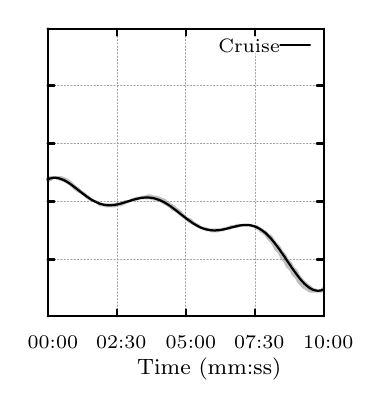
\begin{tikzpicture}[y=0.80pt, x=0.80pt, yscale=-0.510000, xscale=0.511999, inner sep=0pt, outer sep=0pt]
\scriptsize
\begin{scope}[draw=black,line join=bevel,line cap=rect,even odd rule,line width=0.800pt]
  \begin{scope}[cm={{1.0,0.0,0.0,1.0,(0.0,0.0)}},draw=black,line join=bevel,line cap=rect,line width=0.800pt]
  \end{scope}
  \begin{scope}[cm={{1.00625,0.0,0.0,1.00625,(0.0,0.0)}},draw=black,line join=bevel,line cap=rect,line width=0.800pt]
  \end{scope}
  \begin{scope}[cm={{1.00625,0.0,0.0,1.00625,(0.0,0.0)}},draw=ca0a0a4,dash pattern=on 0.40pt off 0.80pt,line join=round,line cap=round,line width=0.400pt]
    \path[draw] (53.5000,268.5000) -- (295.5000,268.5000);
  \end{scope}
  \begin{scope}[cm={{1.00625,0.0,0.0,1.00625,(0.0,0.0)}},draw=black,line join=round,line cap=round,line width=0.800pt]
    \path[draw] (53.5000,268.5000) -- (59.5000,268.5000);
    \path[draw] (295.5000,268.5000) -- (289.5000,268.5000);
  \end{scope}
  \begin{scope}[cm={{1.00625,0.0,0.0,1.00625,(0.0,0.0)}},draw=black,line join=bevel,line cap=rect,line width=0.800pt]
  \end{scope}
  \begin{scope}[cm={{1.00625,0.0,0.0,1.00625,(27.1688,276.216)}},draw=black,line join=bevel,line cap=rect,line width=0.800pt]
  \end{scope}
  \begin{scope}[cm={{1.00625,0.0,0.0,1.00625,(27.1688,276.216)}},draw=black,line join=bevel,line cap=rect,line width=0.800pt]
  \end{scope}
  \begin{scope}[cm={{1.00625,0.0,0.0,1.00625,(27.1688,276.216)}},draw=black,line join=bevel,line cap=rect,line width=0.800pt]
  \end{scope}
  \begin{scope}[cm={{1.00625,0.0,0.0,1.00625,(27.1688,276.216)}},draw=black,line join=bevel,line cap=rect,line width=0.800pt]
  \end{scope}
  \begin{scope}[cm={{1.00625,0.0,0.0,1.00625,(27.1688,276.216)}},draw=black,line join=bevel,line cap=rect,line width=0.800pt]
  \end{scope}
  \begin{scope}[cm={{1.00625,0.0,0.0,1.00625,(27.1688,276.216)}},draw=black,line join=bevel,line cap=rect,line width=0.800pt]
    %\path[fill=black] (0.0000,0.0000) node[above right] () {24};
  \end{scope}
  \begin{scope}[cm={{1.00625,0.0,0.0,1.00625,(27.1688,276.216)}},draw=black,line join=bevel,line cap=rect,line width=0.800pt]
  \end{scope}
  \begin{scope}[cm={{1.00625,0.0,0.0,1.00625,(0.0,0.0)}},draw=black,line join=bevel,line cap=rect,line width=0.800pt]
  \end{scope}
  \begin{scope}[cm={{1.00625,0.0,0.0,1.00625,(0.0,0.0)}},draw=ca0a0a4,dash pattern=on 0.40pt off 0.80pt,line join=round,line cap=round,line width=0.400pt]
    \path[draw] (53.5000,218.5000) -- (295.5000,218.5000);
  \end{scope}
  \begin{scope}[cm={{1.00625,0.0,0.0,1.00625,(0.0,0.0)}},draw=black,line join=round,line cap=round,line width=0.800pt]
    \path[draw] (53.5000,218.5000) -- (59.5000,218.5000);
    \path[draw] (295.5000,218.5000) -- (289.5000,218.5000);
  \end{scope}
  \begin{scope}[cm={{1.00625,0.0,0.0,1.00625,(0.0,0.0)}},draw=black,line join=bevel,line cap=rect,line width=0.800pt]
  \end{scope}
  \begin{scope}[cm={{1.00625,0.0,0.0,1.00625,(27.1688,224.897)}},draw=black,line join=bevel,line cap=rect,line width=0.800pt]
  \end{scope}
  \begin{scope}[cm={{1.00625,0.0,0.0,1.00625,(27.1688,224.897)}},draw=black,line join=bevel,line cap=rect,line width=0.800pt]
  \end{scope}
  \begin{scope}[cm={{1.00625,0.0,0.0,1.00625,(27.1688,224.897)}},draw=black,line join=bevel,line cap=rect,line width=0.800pt]
  \end{scope}
  \begin{scope}[cm={{1.00625,0.0,0.0,1.00625,(27.1688,224.897)}},draw=black,line join=bevel,line cap=rect,line width=0.800pt]
  \end{scope}
  \begin{scope}[cm={{1.00625,0.0,0.0,1.00625,(27.1688,224.897)}},draw=black,line join=bevel,line cap=rect,line width=0.800pt]
  \end{scope}
  \begin{scope}[cm={{1.00625,0.0,0.0,1.00625,(27.1688,224.897)}},draw=black,line join=bevel,line cap=rect,line width=0.800pt]
    %\path[fill=black] (0.0000,0.0000) node[above right] () {26};
  \end{scope}
  \begin{scope}[cm={{1.00625,0.0,0.0,1.00625,(27.1688,224.897)}},draw=black,line join=bevel,line cap=rect,line width=0.800pt]
  \end{scope}
  \begin{scope}[cm={{1.00625,0.0,0.0,1.00625,(0.0,0.0)}},draw=black,line join=bevel,line cap=rect,line width=0.800pt]
  \end{scope}
  \begin{scope}[cm={{1.00625,0.0,0.0,1.00625,(0.0,0.0)}},draw=ca0a0a4,dash pattern=on 0.40pt off 0.80pt,line join=round,line cap=round,line width=0.400pt]
    \path[draw] (53.5000,167.5000) -- (295.5000,167.5000);
  \end{scope}
  \begin{scope}[cm={{1.00625,0.0,0.0,1.00625,(0.0,0.0)}},draw=black,line join=round,line cap=round,line width=0.800pt]
    \path[draw] (53.5000,167.5000) -- (59.5000,167.5000);
    \path[draw] (295.5000,167.5000) -- (289.5000,167.5000);
  \end{scope}
  \begin{scope}[cm={{1.00625,0.0,0.0,1.00625,(0.0,0.0)}},draw=black,line join=bevel,line cap=rect,line width=0.800pt]
  \end{scope}
  \begin{scope}[cm={{1.00625,0.0,0.0,1.00625,(28.175,173.578)}},draw=black,line join=bevel,line cap=rect,line width=0.800pt]
  \end{scope}
  \begin{scope}[cm={{1.00625,0.0,0.0,1.00625,(28.175,173.578)}},draw=black,line join=bevel,line cap=rect,line width=0.800pt]
  \end{scope}
  \begin{scope}[cm={{1.00625,0.0,0.0,1.00625,(28.175,173.578)}},draw=black,line join=bevel,line cap=rect,line width=0.800pt]
  \end{scope}
  \begin{scope}[cm={{1.00625,0.0,0.0,1.00625,(28.175,173.578)}},draw=black,line join=bevel,line cap=rect,line width=0.800pt]
  \end{scope}
  \begin{scope}[cm={{1.00625,0.0,0.0,1.00625,(28.175,173.578)}},draw=black,line join=bevel,line cap=rect,line width=0.800pt]
  \end{scope}
  \begin{scope}[cm={{1.00625,0.0,0.0,1.00625,(28.175,173.578)}},draw=black,line join=bevel,line cap=rect,line width=0.800pt]
    %\path[fill=black] (0.0000,0.0000) node[above right] () {28};
  \end{scope}
  \begin{scope}[cm={{1.00625,0.0,0.0,1.00625,(28.175,173.578)}},draw=black,line join=bevel,line cap=rect,line width=0.800pt]
  \end{scope}
  \begin{scope}[cm={{1.00625,0.0,0.0,1.00625,(0.0,0.0)}},draw=black,line join=bevel,line cap=rect,line width=0.800pt]
  \end{scope}
  \begin{scope}[cm={{1.00625,0.0,0.0,1.00625,(0.0,0.0)}},draw=ca0a0a4,dash pattern=on 0.40pt off 0.80pt,line join=round,line cap=round,line width=0.400pt]
    \path[draw] (53.5000,116.5000) -- (295.5000,116.5000);
  \end{scope}
  \begin{scope}[cm={{1.00625,0.0,0.0,1.00625,(0.0,0.0)}},draw=black,line join=round,line cap=round,line width=0.800pt]
    \path[draw] (53.5000,116.5000) -- (59.5000,116.5000);
    \path[draw] (295.5000,116.5000) -- (289.5000,116.5000);
  \end{scope}
  \begin{scope}[cm={{1.00625,0.0,0.0,1.00625,(0.0,0.0)}},draw=black,line join=bevel,line cap=rect,line width=0.800pt]
  \end{scope}
  \begin{scope}[cm={{1.00625,0.0,0.0,1.00625,(27.1688,123.266)}},draw=black,line join=bevel,line cap=rect,line width=0.800pt]
  \end{scope}
  \begin{scope}[cm={{1.00625,0.0,0.0,1.00625,(27.1688,123.266)}},draw=black,line join=bevel,line cap=rect,line width=0.800pt]
  \end{scope}
  \begin{scope}[cm={{1.00625,0.0,0.0,1.00625,(27.1688,123.266)}},draw=black,line join=bevel,line cap=rect,line width=0.800pt]
  \end{scope}
  \begin{scope}[cm={{1.00625,0.0,0.0,1.00625,(27.1688,123.266)}},draw=black,line join=bevel,line cap=rect,line width=0.800pt]
  \end{scope}
  \begin{scope}[cm={{1.00625,0.0,0.0,1.00625,(27.1688,123.266)}},draw=black,line join=bevel,line cap=rect,line width=0.800pt]
  \end{scope}
  \begin{scope}[cm={{1.00625,0.0,0.0,1.00625,(27.1688,123.266)}},draw=black,line join=bevel,line cap=rect,line width=0.800pt]
    %\path[fill=black] (0.0000,0.0000) node[above right] () {30};
  \end{scope}
  \begin{scope}[cm={{1.00625,0.0,0.0,1.00625,(27.1688,123.266)}},draw=black,line join=bevel,line cap=rect,line width=0.800pt]
  \end{scope}
  \begin{scope}[cm={{1.00625,0.0,0.0,1.00625,(0.0,0.0)}},draw=black,line join=bevel,line cap=rect,line width=0.800pt]
  \end{scope}
  \begin{scope}[cm={{1.00625,0.0,0.0,1.00625,(0.0,0.0)}},draw=ca0a0a4,dash pattern=on 0.40pt off 0.80pt,line join=round,line cap=round,line width=0.400pt]
    \path[draw] (53.5000,65.5000) -- (295.5000,65.5000);
  \end{scope}
  \begin{scope}[cm={{1.00625,0.0,0.0,1.00625,(0.0,0.0)}},draw=black,line join=round,line cap=round,line width=0.800pt]
    \path[draw] (53.5000,65.5000) -- (59.5000,65.5000);
    \path[draw] (295.5000,65.5000) -- (289.5000,65.5000);
  \end{scope}
  \begin{scope}[cm={{1.00625,0.0,0.0,1.00625,(0.0,0.0)}},draw=black,line join=bevel,line cap=rect,line width=0.800pt]
  \end{scope}
  \begin{scope}[cm={{1.00625,0.0,0.0,1.00625,(27.1688,71.9469)}},draw=black,line join=bevel,line cap=rect,line width=0.800pt]
  \end{scope}
  \begin{scope}[cm={{1.00625,0.0,0.0,1.00625,(27.1688,71.9469)}},draw=black,line join=bevel,line cap=rect,line width=0.800pt]
  \end{scope}
  \begin{scope}[cm={{1.00625,0.0,0.0,1.00625,(27.1688,71.9469)}},draw=black,line join=bevel,line cap=rect,line width=0.800pt]
  \end{scope}
  \begin{scope}[cm={{1.00625,0.0,0.0,1.00625,(27.1688,71.9469)}},draw=black,line join=bevel,line cap=rect,line width=0.800pt]
  \end{scope}
  \begin{scope}[cm={{1.00625,0.0,0.0,1.00625,(27.1688,71.9469)}},draw=black,line join=bevel,line cap=rect,line width=0.800pt]
  \end{scope}
  \begin{scope}[cm={{1.00625,0.0,0.0,1.00625,(27.1688,71.9469)}},draw=black,line join=bevel,line cap=rect,line width=0.800pt]
    %\path[fill=black] (0.0000,0.0000) node[above right] () {32};
  \end{scope}
  \begin{scope}[cm={{1.00625,0.0,0.0,1.00625,(27.1688,71.9469)}},draw=black,line join=bevel,line cap=rect,line width=0.800pt]
  \end{scope}
  \begin{scope}[cm={{1.00625,0.0,0.0,1.00625,(0.0,0.0)}},draw=black,line join=bevel,line cap=rect,line width=0.800pt]
  \end{scope}
  \begin{scope}[cm={{1.00625,0.0,0.0,1.00625,(0.0,0.0)}},draw=ca0a0a4,dash pattern=on 0.40pt off 0.80pt,line join=round,line cap=round,line width=0.400pt]
    \path[draw] (53.5000,15.5000) -- (295.5000,15.5000);
  \end{scope}
  \begin{scope}[cm={{1.00625,0.0,0.0,1.00625,(0.0,0.0)}},draw=black,line join=round,line cap=round,line width=0.800pt]
    \path[draw] (53.5000,15.5000) -- (59.5000,15.5000);
    \path[draw] (295.5000,15.5000) -- (289.5000,15.5000);
  \end{scope}
  \begin{scope}[cm={{1.00625,0.0,0.0,1.00625,(0.0,0.0)}},draw=black,line join=bevel,line cap=rect,line width=0.800pt]
  \end{scope}
  \begin{scope}[cm={{1.00625,0.0,0.0,1.00625,(27.1688,20.6281)}},draw=black,line join=bevel,line cap=rect,line width=0.800pt]
  \end{scope}
  \begin{scope}[cm={{1.00625,0.0,0.0,1.00625,(27.1688,20.6281)}},draw=black,line join=bevel,line cap=rect,line width=0.800pt]
  \end{scope}
  \begin{scope}[cm={{1.00625,0.0,0.0,1.00625,(27.1688,20.6281)}},draw=black,line join=bevel,line cap=rect,line width=0.800pt]
  \end{scope}
  \begin{scope}[cm={{1.00625,0.0,0.0,1.00625,(27.1688,20.6281)}},draw=black,line join=bevel,line cap=rect,line width=0.800pt]
  \end{scope}
  \begin{scope}[cm={{1.00625,0.0,0.0,1.00625,(27.1688,20.6281)}},draw=black,line join=bevel,line cap=rect,line width=0.800pt]
  \end{scope}
  \begin{scope}[cm={{1.00625,0.0,0.0,1.00625,(27.1688,20.6281)}},draw=black,line join=bevel,line cap=rect,line width=0.800pt]
    %\path[fill=black] (0.0000,0.0000) node[above right] () {34};
  \end{scope}
  \begin{scope}[cm={{1.00625,0.0,0.0,1.00625,(27.1688,20.6281)}},draw=black,line join=bevel,line cap=rect,line width=0.800pt]
  \end{scope}
  \begin{scope}[cm={{1.00625,0.0,0.0,1.00625,(0.0,0.0)}},draw=black,line join=bevel,line cap=rect,line width=0.800pt]
  \end{scope}
  \begin{scope}[cm={{1.00625,0.0,0.0,1.00625,(0.0,0.0)}},draw=ca0a0a4,dash pattern=on 0.40pt off 0.80pt,line join=round,line cap=round,line width=0.400pt]
    \path[draw] (53.5000,268.5000) -- (53.5000,15.5000);
  \end{scope}
  \begin{scope}[cm={{1.00625,0.0,0.0,1.00625,(0.0,0.0)}},draw=black,line join=round,line cap=round,line width=0.800pt]
    \path[draw] (53.5000,268.5000) -- (53.5000,262.5000);
    \path[draw] (53.5000,15.5000) -- (53.5000,21.5000);
  \end{scope}
  \begin{scope}[cm={{1.00625,0.0,0.0,1.00625,(0.0,0.0)}},draw=black,line join=bevel,line cap=rect,line width=0.800pt]
  \end{scope}
  \begin{scope}[cm={{1.00625,0.0,0.0,1.00625,(36.225,298.353)}},draw=black,line join=bevel,line cap=rect,line width=0.800pt]
  \end{scope}
  \begin{scope}[cm={{1.00625,0.0,0.0,1.00625,(36.225,298.353)}},draw=black,line join=bevel,line cap=rect,line width=0.800pt]
  \end{scope}
  \begin{scope}[cm={{1.00625,0.0,0.0,1.00625,(36.225,298.353)}},draw=black,line join=bevel,line cap=rect,line width=0.800pt]
  \end{scope}
  \begin{scope}[cm={{1.00625,0.0,0.0,1.00625,(36.225,298.353)}},draw=black,line join=bevel,line cap=rect,line width=0.800pt]
  \end{scope}
  \begin{scope}[cm={{1.00625,0.0,0.0,1.00625,(36.225,298.353)}},draw=black,line join=bevel,line cap=rect,line width=0.800pt]
  \end{scope}
  \begin{scope}[cm={{1.00625,0.0,0.0,1.00625,(36.225,298.353)}},draw=black,line join=bevel,line cap=rect,line width=0.800pt]
    \path[fill=black] (0.0000,0.0000) node[above right] () {00:00};
  \end{scope}
  \begin{scope}[cm={{1.00625,0.0,0.0,1.00625,(36.225,298.353)}},draw=black,line join=bevel,line cap=rect,line width=0.800pt]
  \end{scope}
  \begin{scope}[cm={{1.00625,0.0,0.0,1.00625,(0.0,0.0)}},draw=black,line join=bevel,line cap=rect,line width=0.800pt]
  \end{scope}
  \begin{scope}[cm={{1.00625,0.0,0.0,1.00625,(0.0,0.0)}},draw=ca0a0a4,dash pattern=on 0.40pt off 0.80pt,line join=round,line cap=round,line width=0.400pt]
    \path[draw] (114.5000,268.5000) -- (114.5000,15.5000);
  \end{scope}
  \begin{scope}[cm={{1.00625,0.0,0.0,1.00625,(0.0,0.0)}},draw=black,line join=round,line cap=round,line width=0.800pt]
    \path[draw] (114.5000,268.5000) -- (114.5000,262.5000);
    \path[draw] (114.5000,15.5000) -- (114.5000,21.5000);
  \end{scope}
  \begin{scope}[cm={{1.00625,0.0,0.0,1.00625,(0.0,0.0)}},draw=black,line join=bevel,line cap=rect,line width=0.800pt]
  \end{scope}
  \begin{scope}[cm={{1.00625,0.0,0.0,1.00625,(96.6,298.353)}},draw=black,line join=bevel,line cap=rect,line width=0.800pt]
  \end{scope}
  \begin{scope}[cm={{1.00625,0.0,0.0,1.00625,(96.6,298.353)}},draw=black,line join=bevel,line cap=rect,line width=0.800pt]
  \end{scope}
  \begin{scope}[cm={{1.00625,0.0,0.0,1.00625,(96.6,298.353)}},draw=black,line join=bevel,line cap=rect,line width=0.800pt]
  \end{scope}
  \begin{scope}[cm={{1.00625,0.0,0.0,1.00625,(96.6,298.353)}},draw=black,line join=bevel,line cap=rect,line width=0.800pt]
  \end{scope}
  \begin{scope}[cm={{1.00625,0.0,0.0,1.00625,(96.6,298.353)}},draw=black,line join=bevel,line cap=rect,line width=0.800pt]
  \end{scope}
  \begin{scope}[cm={{1.00625,0.0,0.0,1.00625,(96.6,298.353)}},draw=black,line join=bevel,line cap=rect,line width=0.800pt]
    \path[fill=black] (0.0000,0.0000) node[above right] () {02:30};
  \end{scope}
  \begin{scope}[cm={{1.00625,0.0,0.0,1.00625,(96.6,298.353)}},draw=black,line join=bevel,line cap=rect,line width=0.800pt]
  \end{scope}
  \begin{scope}[cm={{1.00625,0.0,0.0,1.00625,(0.0,0.0)}},draw=black,line join=bevel,line cap=rect,line width=0.800pt]
  \end{scope}
  \begin{scope}[cm={{1.00625,0.0,0.0,1.00625,(0.0,0.0)}},draw=ca0a0a4,dash pattern=on 0.40pt off 0.80pt,line join=round,line cap=round,line width=0.400pt]
    \path[draw] (174.5000,268.5000) -- (174.5000,15.5000);
  \end{scope}
  \begin{scope}[cm={{1.00625,0.0,0.0,1.00625,(0.0,0.0)}},draw=black,line join=round,line cap=round,line width=0.800pt]
    \path[draw] (174.5000,268.5000) -- (174.5000,262.5000);
    \path[draw] (174.5000,15.5000) -- (174.5000,21.5000);
  \end{scope}
  \begin{scope}[cm={{1.00625,0.0,0.0,1.00625,(0.0,0.0)}},draw=black,line join=bevel,line cap=rect,line width=0.800pt]
  \end{scope}
  \begin{scope}[cm={{1.00625,0.0,0.0,1.00625,(157.981,298.353)}},draw=black,line join=bevel,line cap=rect,line width=0.800pt]
  \end{scope}
  \begin{scope}[cm={{1.00625,0.0,0.0,1.00625,(157.981,298.353)}},draw=black,line join=bevel,line cap=rect,line width=0.800pt]
  \end{scope}
  \begin{scope}[cm={{1.00625,0.0,0.0,1.00625,(157.981,298.353)}},draw=black,line join=bevel,line cap=rect,line width=0.800pt]
  \end{scope}
  \begin{scope}[cm={{1.00625,0.0,0.0,1.00625,(157.981,298.353)}},draw=black,line join=bevel,line cap=rect,line width=0.800pt]
  \end{scope}
  \begin{scope}[cm={{1.00625,0.0,0.0,1.00625,(157.981,298.353)}},draw=black,line join=bevel,line cap=rect,line width=0.800pt]
  \end{scope}
  \begin{scope}[cm={{1.00625,0.0,0.0,1.00625,(157.981,298.353)}},draw=black,line join=bevel,line cap=rect,line width=0.800pt]
    \path[fill=black] (0.0000,0.0000) node[above right] () {05:00};
  \end{scope}
  \begin{scope}[cm={{1.00625,0.0,0.0,1.00625,(157.981,298.353)}},draw=black,line join=bevel,line cap=rect,line width=0.800pt]
  \end{scope}
  \begin{scope}[cm={{1.00625,0.0,0.0,1.00625,(0.0,0.0)}},draw=black,line join=bevel,line cap=rect,line width=0.800pt]
  \end{scope}
  \begin{scope}[cm={{1.00625,0.0,0.0,1.00625,(0.0,0.0)}},draw=ca0a0a4,dash pattern=on 0.40pt off 0.80pt,line join=round,line cap=round,line width=0.400pt]
    \path[draw] (235.5000,268.5000) -- (235.5000,37.5000);
    \path[draw] (235.5000,21.5000) -- (235.5000,15.5000);
  \end{scope}
  \begin{scope}[cm={{1.00625,0.0,0.0,1.00625,(0.0,0.0)}},draw=black,line join=round,line cap=round,line width=0.800pt]
    \path[draw] (235.5000,268.5000) -- (235.5000,262.5000);
    \path[draw] (235.5000,15.5000) -- (235.5000,21.5000);
  \end{scope}
  \begin{scope}[cm={{1.00625,0.0,0.0,1.00625,(0.0,0.0)}},draw=black,line join=bevel,line cap=rect,line width=0.800pt]
  \end{scope}
  \begin{scope}[cm={{1.00625,0.0,0.0,1.00625,(218.356,298.353)}},draw=black,line join=bevel,line cap=rect,line width=0.800pt]
  \end{scope}
  \begin{scope}[cm={{1.00625,0.0,0.0,1.00625,(218.356,298.353)}},draw=black,line join=bevel,line cap=rect,line width=0.800pt]
  \end{scope}
  \begin{scope}[cm={{1.00625,0.0,0.0,1.00625,(218.356,298.353)}},draw=black,line join=bevel,line cap=rect,line width=0.800pt]
  \end{scope}
  \begin{scope}[cm={{1.00625,0.0,0.0,1.00625,(218.356,298.353)}},draw=black,line join=bevel,line cap=rect,line width=0.800pt]
  \end{scope}
  \begin{scope}[cm={{1.00625,0.0,0.0,1.00625,(218.356,298.353)}},draw=black,line join=bevel,line cap=rect,line width=0.800pt]
  \end{scope}
  \begin{scope}[cm={{1.00625,0.0,0.0,1.00625,(218.356,298.353)}},draw=black,line join=bevel,line cap=rect,line width=0.800pt]
    \path[fill=black] (0.0000,0.0000) node[above right] () {07:30};
  \end{scope}
  \begin{scope}[cm={{1.00625,0.0,0.0,1.00625,(218.356,298.353)}},draw=black,line join=bevel,line cap=rect,line width=0.800pt]
  \end{scope}
  \begin{scope}[cm={{1.00625,0.0,0.0,1.00625,(0.0,0.0)}},draw=black,line join=bevel,line cap=rect,line width=0.800pt]
  \end{scope}
  \begin{scope}[cm={{1.00625,0.0,0.0,1.00625,(0.0,0.0)}},draw=ca0a0a4,dash pattern=on 0.40pt off 0.80pt,line join=round,line cap=round,line width=0.400pt]
    \path[draw] (295.5000,268.5000) -- (295.5000,15.5000);
  \end{scope}
  \begin{scope}[cm={{1.00625,0.0,0.0,1.00625,(0.0,0.0)}},draw=black,line join=round,line cap=round,line width=0.800pt]
    \path[draw] (295.5000,268.5000) -- (295.5000,262.5000);
    \path[draw] (295.5000,15.5000) -- (295.5000,21.5000);
  \end{scope}
  \begin{scope}[cm={{1.00625,0.0,0.0,1.00625,(0.0,0.0)}},draw=black,line join=bevel,line cap=rect,line width=0.800pt]
  \end{scope}
  \begin{scope}[cm={{1.00625,0.0,0.0,1.00625,(279.234,298.353)}},draw=black,line join=bevel,line cap=rect,line width=0.800pt]
  \end{scope}
  \begin{scope}[cm={{1.00625,0.0,0.0,1.00625,(279.234,298.353)}},draw=black,line join=bevel,line cap=rect,line width=0.800pt]
  \end{scope}
  \begin{scope}[cm={{1.00625,0.0,0.0,1.00625,(279.234,298.353)}},draw=black,line join=bevel,line cap=rect,line width=0.800pt]
  \end{scope}
  \begin{scope}[cm={{1.00625,0.0,0.0,1.00625,(279.234,298.353)}},draw=black,line join=bevel,line cap=rect,line width=0.800pt]
  \end{scope}
  \begin{scope}[cm={{1.00625,0.0,0.0,1.00625,(279.234,298.353)}},draw=black,line join=bevel,line cap=rect,line width=0.800pt]
  \end{scope}
  \begin{scope}[cm={{1.00625,0.0,0.0,1.00625,(279.234,298.353)}},draw=black,line join=bevel,line cap=rect,line width=0.800pt]
    \path[fill=black] (0.0000,0.0000) node[above right] () {10:00};
  \end{scope}
  \begin{scope}[cm={{1.00625,0.0,0.0,1.00625,(279.234,298.353)}},draw=black,line join=bevel,line cap=rect,line width=0.800pt]
  \end{scope}
  \begin{scope}[cm={{1.00625,0.0,0.0,1.00625,(0.0,0.0)}},draw=black,line join=bevel,line cap=rect,line width=0.800pt]
  \end{scope}
  \begin{scope}[cm={{1.00625,0.0,0.0,1.00625,(0.0,0.0)}},draw=black,line join=round,line cap=round,line width=0.800pt]
    \path[draw] (53.5000,15.5000) -- (53.5000,268.5000) -- (295.5000,268.5000) --
      (295.5000,15.5000) -- (53.5000,15.5000);
  \end{scope}
  \begin{scope}[cm={{1.00625,0.0,0.0,1.00625,(0.0,0.0)}},draw=black,line join=bevel,line cap=rect,line width=0.800pt]
  \end{scope}
  \begin{scope}[cm={{0.0,-1.00625,1.00625,0.0,(13.5844,176.597)}},draw=black,line join=bevel,line cap=rect,line width=0.800pt]
  \end{scope}
  \begin{scope}[cm={{0.0,-1.00625,1.00625,0.0,(13.5844,176.597)}},draw=black,line join=bevel,line cap=rect,line width=0.800pt]
  \end{scope}
  \begin{scope}[cm={{0.0,-1.00625,1.00625,0.0,(13.5844,176.597)}},draw=black,line join=bevel,line cap=rect,line width=0.800pt]
  \end{scope}
  \begin{scope}[cm={{0.0,-1.00625,1.00625,0.0,(13.5844,176.597)}},draw=black,line join=bevel,line cap=rect,line width=0.800pt]
  \end{scope}
  \begin{scope}[cm={{0.0,-1.00625,1.00625,0.0,(13.5844,176.597)}},draw=black,line join=bevel,line cap=rect,line width=0.800pt]
  \end{scope}
  \begin{scope}[cm={{0.0,-1.00625,1.00625,0.0,(9.5844,176.597)}},draw=black,line join=bevel,line cap=rect,line width=0.800pt]
    %\path[fill=black] (0.0000,0.0000) node[above right] () {\rotatebox{90}{Power (W)}};
  \end{scope}
  \begin{scope}[cm={{0.0,-1.00625,1.00625,0.0,(13.5844,176.597)}},draw=black,line join=bevel,line cap=rect,line width=0.800pt]
  \end{scope}
  \begin{scope}[cm={{1.00625,0.0,0.0,1.00625,(132.825,317.472)}},draw=black,line join=bevel,line cap=rect,line width=0.800pt]
  \end{scope}
  \begin{scope}[cm={{1.00625,0.0,0.0,1.00625,(132.825,317.472)}},draw=black,line join=bevel,line cap=rect,line width=0.800pt]
  \end{scope}
  \begin{scope}[cm={{1.00625,0.0,0.0,1.00625,(132.825,317.472)}},draw=black,line join=bevel,line cap=rect,line width=0.800pt]
  \end{scope}
  \begin{scope}[cm={{1.00625,0.0,0.0,1.00625,(132.825,317.472)}},draw=black,line join=bevel,line cap=rect,line width=0.800pt]
  \end{scope}
  \begin{scope}[cm={{1.00625,0.0,0.0,1.00625,(132.825,317.472)}},draw=black,line join=bevel,line cap=rect,line width=0.800pt]
  \end{scope}
  \begin{scope}[cm={{1.00625,0.0,0.0,1.00625,(132.825,326.472)}},draw=black,line join=bevel,line cap=rect,line width=0.800pt]
    \path[fill=black] (0.0000,0.0000) node[above right] () {\footnotesize Time (mm:ss)};
  \end{scope}
  \begin{scope}[cm={{1.00625,0.0,0.0,1.00625,(132.825,317.472)}},draw=black,line join=bevel,line cap=rect,line width=0.800pt]
  \end{scope}
  \begin{scope}[cm={{1.00625,0.0,0.0,1.00625,(0.0,0.0)}},draw=black,line join=bevel,line cap=rect,line width=0.800pt]
  \end{scope}
  \begin{scope}[cm={{1.00625,0.0,0.0,1.00625,(0.0,0.0)}},draw=black,line join=bevel,line cap=rect,line width=0.800pt]
  \end{scope}
  \begin{scope}[cm={{1.00625,0.0,0.0,1.00625,(0.0,0.0)}},draw=black,line join=bevel,line cap=rect,line width=0.800pt]
  \end{scope}
  \begin{scope}[cm={{1.00625,0.0,0.0,1.00625,(0.0,0.0)}},draw=c808080,fill=c808080,line join=bevel,line cap=rect,draw opacity=0.500,fill opacity=0.500,line width=0.800pt,transparency group]
    \path[draw,fill,even odd rule] (53.5000,149.5000) -- (55.5000,148.5000) --
      (58.5000,146.5000) -- (59.5000,146.5000) -- (58.5000,146.5000) --
      (55.5000,146.5000) -- (53.5000,147.5000) -- (53.5000,149.5000);
    \path[draw,fill,even odd rule] (59.5000,146.5000) -- (60.5000,146.5000) --
      (63.5000,146.5000) -- (65.5000,146.5000) -- (68.5000,147.5000) --
      (70.5000,148.5000) -- (73.5000,150.5000) -- (75.5000,152.5000) --
      (77.5000,154.5000) -- (80.5000,156.5000) -- (82.5000,158.5000) --
      (85.5000,160.5000) -- (87.5000,162.5000) -- (90.5000,164.5000) --
      (92.5000,166.5000) -- (95.5000,167.5000) -- (92.5000,166.5000) --
      (90.5000,165.5000) -- (87.5000,163.5000) -- (85.5000,161.5000) --
      (82.5000,159.5000) -- (80.5000,158.5000) -- (77.5000,156.5000) --
      (75.5000,154.5000) -- (73.5000,152.5000) -- (70.5000,150.5000) --
      (68.5000,149.5000) -- (65.5000,148.5000) -- (63.5000,147.5000) --
      (60.5000,146.5000) -- (59.5000,146.5000);
    \path[draw,fill,even odd rule] (95.5000,167.5000) -- (97.5000,168.5000) --
      (99.5000,170.5000) -- (102.5000,170.5000) -- (104.5000,171.5000) --
      (107.5000,171.5000) -- (109.5000,171.5000) -- (112.5000,171.5000) --
      (114.5000,170.5000) -- (117.5000,170.5000) -- (119.5000,169.5000) --
      (121.5000,168.5000) -- (124.5000,167.5000) -- (126.5000,166.5000) --
      (128.5000,165.5000) -- (126.5000,166.5000) -- (124.5000,167.5000) --
      (121.5000,167.5000) -- (119.5000,168.5000) -- (117.5000,169.5000) --
      (114.5000,169.5000) -- (112.5000,170.5000) -- (109.5000,170.5000) --
      (107.5000,170.5000) -- (104.5000,170.5000) -- (102.5000,170.5000) --
      (99.5000,169.5000) -- (97.5000,168.5000) -- (95.5000,167.5000);
    \path[draw,fill,even odd rule] (128.5000,165.5000) -- (129.5000,165.5000) --
      (131.5000,164.5000) -- (134.5000,164.5000) -- (136.5000,163.5000) --
      (139.5000,163.5000) -- (141.5000,162.5000) -- (143.5000,162.5000) --
      (146.5000,163.5000) -- (148.5000,163.5000) -- (151.5000,164.5000) --
      (153.5000,165.5000) -- (156.5000,166.5000) -- (158.5000,168.5000) --
      (161.5000,170.5000) -- (163.5000,171.5000) -- (165.5000,173.5000) --
      (168.5000,175.5000) -- (170.5000,177.5000) -- (173.5000,180.5000) --
      (175.5000,182.5000) -- (178.5000,183.5000) -- (180.5000,185.5000) --
      (183.5000,187.5000) -- (185.5000,188.5000) -- (187.5000,190.5000) --
      (190.5000,191.5000) -- (192.5000,191.5000) -- (195.5000,192.5000) --
      (197.5000,192.5000) -- (200.5000,192.5000) -- (202.5000,192.5000) --
      (205.5000,192.5000) -- (207.5000,191.5000) -- (209.5000,191.5000) --
      (212.5000,190.5000) -- (214.5000,189.5000) -- (217.5000,189.5000) --
      (219.5000,188.5000) -- (222.5000,188.5000) -- (224.5000,188.5000) --
      (227.5000,188.5000) -- (229.5000,188.5000) -- (227.5000,188.5000) --
      (224.5000,188.5000) -- (222.5000,188.5000) -- (219.5000,189.5000) --
      (217.5000,189.5000) -- (214.5000,190.5000) -- (212.5000,191.5000) --
      (209.5000,191.5000) -- (207.5000,192.5000) -- (205.5000,192.5000) --
      (202.5000,193.5000) -- (200.5000,193.5000) -- (197.5000,193.5000) --
      (195.5000,192.5000) -- (192.5000,192.5000) -- (190.5000,191.5000) --
      (187.5000,190.5000) -- (185.5000,189.5000) -- (183.5000,188.5000) --
      (180.5000,186.5000) -- (178.5000,185.5000) -- (175.5000,183.5000) --
      (173.5000,181.5000) -- (170.5000,179.5000) -- (168.5000,177.5000) --
      (165.5000,175.5000) -- (163.5000,174.5000) -- (161.5000,172.5000) --
      (158.5000,170.5000) -- (156.5000,169.5000) -- (153.5000,167.5000) --
      (151.5000,166.5000) -- (148.5000,165.5000) -- (146.5000,165.5000) --
      (143.5000,164.5000) -- (141.5000,164.5000) -- (139.5000,164.5000) --
      (136.5000,164.5000) -- (134.5000,164.5000) -- (131.5000,165.5000) --
      (129.5000,165.5000) -- (128.5000,165.5000);
    \path[draw,fill,even odd rule] (229.5000,188.5000) -- (231.5000,188.5000) --
      (234.5000,189.5000) -- (236.5000,190.5000) -- (239.5000,192.5000) --
      (241.5000,194.5000) -- (244.5000,196.5000) -- (246.5000,199.5000) --
      (249.5000,202.5000) -- (251.5000,205.5000) -- (253.5000,209.5000) --
      (256.5000,212.5000) -- (258.5000,216.5000) -- (261.5000,220.5000) --
      (263.5000,224.5000) -- (266.5000,227.5000) -- (268.5000,231.5000) --
      (271.5000,234.5000) -- (273.5000,238.5000) -- (275.5000,240.5000) --
      (278.5000,243.5000) -- (280.5000,244.5000) -- (283.5000,246.5000) --
      (285.5000,246.5000) -- (288.5000,246.5000) -- (290.5000,246.5000) --
      (291.5000,246.5000) -- (290.5000,246.5000) -- (288.5000,245.5000) --
      (285.5000,244.5000) -- (283.5000,242.5000) -- (280.5000,240.5000) --
      (278.5000,238.5000) -- (275.5000,235.5000) -- (273.5000,232.5000) --
      (271.5000,228.5000) -- (268.5000,225.5000) -- (266.5000,221.5000) --
      (263.5000,218.5000) -- (261.5000,214.5000) -- (258.5000,211.5000) --
      (256.5000,207.5000) -- (253.5000,204.5000) -- (251.5000,201.5000) --
      (249.5000,198.5000) -- (246.5000,196.5000) -- (244.5000,194.5000) --
      (241.5000,192.5000) -- (239.5000,191.5000) -- (236.5000,189.5000) --
      (234.5000,189.5000) -- (231.5000,188.5000) -- (229.5000,188.5000);
    \path[draw,fill,even odd rule] (291.5000,246.5000) -- (293.5000,245.5000) --
      (295.5000,243.5000) -- (295.5000,245.5000) -- (293.5000,246.5000) --
      (291.5000,246.5000);
  \end{scope}
  \begin{scope}[cm={{1.00625,0.0,0.0,1.00625,(0.0,0.0)}},draw=black,line join=bevel,line cap=rect,line width=0.800pt]
  \end{scope}
  \begin{scope}[cm={{1.00625,0.0,0.0,1.00625,(225.4,33.2063)}},draw=black,line join=bevel,line cap=rect,line width=0.800pt]
  \end{scope}
  \begin{scope}[cm={{1.00625,0.0,0.0,1.00625,(225.4,33.2063)}},draw=black,line join=bevel,line cap=rect,line width=0.800pt]
  \end{scope}
  \begin{scope}[cm={{1.00625,0.0,0.0,1.00625,(225.4,33.2063)}},draw=black,line join=bevel,line cap=rect,line width=0.800pt]
  \end{scope}
  \begin{scope}[cm={{1.00625,0.0,0.0,1.00625,(225.4,33.2063)}},draw=black,line join=bevel,line cap=rect,line width=0.800pt]
  \end{scope}
  \begin{scope}[cm={{1.00625,0.0,0.0,1.00625,(225.4,33.2063)}},draw=black,line join=bevel,line cap=rect,line width=0.800pt]
  \end{scope}
  \begin{scope}[cm={{1.00625,0.0,0.0,1.00625,(204.4,36.2063)}},draw=black,line join=bevel,line cap=rect,line width=0.800pt]
    \path[fill=black] (0.0000,0.0000) node[above right] () {\scriptsize Cruise};
  \end{scope}
  \begin{scope}[cm={{1.00625,0.0,0.0,1.00625,(225.4,33.2063)}},draw=black,line join=bevel,line cap=rect,line width=0.800pt]
  \end{scope}
  \begin{scope}[cm={{1.00625,0.0,0.0,1.00625,(0.0,0.0)}},draw=black,line join=bevel,line cap=rect,line width=0.800pt]
  \end{scope}
  \begin{scope}[cm={{1.00625,0.0,0.0,1.00625,(0.0,0.0)}},draw=black,line join=round,line cap=round,line width=0.800pt]
    \path[draw,even odd rule] (257.5000,29.5000) -- (283.5000,29.5000);
  \end{scope}
  \begin{scope}[cm={{1.00625,0.0,0.0,1.00625,(0.0,0.0)}},draw=black,line join=bevel,line cap=rect,line width=0.800pt]
  \end{scope}
  \begin{scope}[cm={{1.00625,0.0,0.0,1.00625,(0.0,0.0)}},draw=black,line join=bevel,line cap=rect,line width=0.800pt]
  \end{scope}
  \begin{scope}[cm={{1.00625,0.0,0.0,1.00625,(0.0,0.0)}},draw=black,line join=bevel,line cap=rect,line width=0.800pt]
  \end{scope}
  \begin{scope}[cm={{1.00625,0.0,0.0,1.00625,(0.0,0.0)}},draw=black,line join=bevel,line cap=rect,line width=0.800pt]
  \end{scope}
  \begin{scope}[cm={{1.00625,0.0,0.0,1.00625,(0.0,0.0)}},draw=black,line join=round,line cap=round,line width=0.800pt]
    \path[draw] (53.5000,148.1000) -- (53.5000,148.1000) -- (55.9000,147.2000) --
      (58.4000,146.7000) -- (60.8000,146.7000) -- (63.3000,147.1000) --
      (65.7000,147.9000) -- (68.2000,148.9000) -- (70.6000,150.3000) --
      (73.1000,151.9000) -- (75.5000,153.7000) -- (77.9000,155.5000) --
      (80.4000,157.5000) -- (82.8000,159.4000) -- (85.3000,161.3000) --
      (87.7000,163.1000) -- (90.2000,164.8000) -- (92.6000,166.3000) --
      (95.1000,167.6000) -- (97.5000,168.8000) -- (99.9000,169.6000) --
      (102.4000,170.3000) -- (104.8000,170.7000) -- (107.3000,170.8000) --
      (109.7000,170.8000) -- (112.2000,170.5000) -- (114.6000,170.1000) --
      (117.1000,169.5000) -- (119.5000,168.8000) -- (121.9000,168.1000) --
      (124.4000,167.3000) -- (126.8000,166.5000) -- (129.3000,165.8000) --
      (131.7000,165.2000) -- (134.2000,164.6000) -- (136.6000,164.2000) --
      (139.1000,164.0000) -- (141.5000,164.0000) -- (143.9000,164.2000) --
      (146.4000,164.6000) -- (148.8000,165.3000) -- (151.3000,166.1000) --
      (153.7000,167.2000) -- (156.2000,168.5000) -- (158.6000,170.0000) --
      (161.1000,171.6000) -- (163.5000,173.4000) -- (165.9000,175.2000) --
      (168.4000,177.2000) -- (170.8000,179.1000) -- (173.3000,181.1000) --
      (175.7000,182.9000) -- (178.2000,184.7000) -- (180.6000,186.4000) --
      (183.1000,188.0000) -- (185.5000,189.3000) -- (187.9000,190.5000) --
      (190.4000,191.4000) -- (192.8000,192.1000) -- (195.3000,192.6000) --
      (197.7000,192.9000) -- (200.2000,193.0000) -- (202.6000,192.8000) --
      (205.1000,192.6000) -- (207.5000,192.1000) -- (209.9000,191.6000) --
      (212.4000,190.9000) -- (214.8000,190.3000) -- (217.3000,189.7000) --
      (219.7000,189.1000) -- (222.2000,188.6000) -- (224.6000,188.3000) --
      (227.1000,188.2000) -- (229.5000,188.2000) -- (231.9000,188.6000) --
      (234.4000,189.2000) -- (236.8000,190.2000) -- (239.3000,191.5000) --
      (241.7000,193.1000) -- (244.2000,195.0000) -- (246.6000,197.3000) --
      (249.1000,199.9000) -- (251.5000,202.8000) -- (253.9000,205.9000) --
      (256.4000,209.2000) -- (258.8000,212.7000) -- (261.3000,216.3000) --
      (263.7000,220.0000) -- (266.2000,223.7000) -- (268.6000,227.2000) --
      (271.1000,230.7000) -- (273.5000,233.9000) -- (275.9000,236.9000) --
      (278.4000,239.6000) -- (280.8000,241.8000) -- (283.3000,243.7000) --
      (285.7000,245.0000) -- (288.2000,245.8000) -- (290.6000,246.1000) --
      (293.1000,245.8000) -- (295.5000,244.9000);
  \end{scope}
  \begin{scope}[cm={{1.00625,0.0,0.0,1.00625,(0.0,0.0)}},draw=black,line join=bevel,line cap=rect,line width=0.800pt]
  \end{scope}
  \begin{scope}[cm={{1.00625,0.0,0.0,1.00625,(0.0,0.0)}},draw=black,line join=bevel,line cap=rect,line width=0.800pt]
  \end{scope}
  \begin{scope}[cm={{1.00625,0.0,0.0,1.00625,(0.0,0.0)}},draw=black,line join=round,line cap=round,line width=0.800pt]
    \path[draw] (53.5000,15.5000) -- (53.5000,268.5000) -- (295.5000,268.5000) --
      (295.5000,15.5000) -- (53.5000,15.5000);
  \end{scope}
  \begin{scope}[cm={{1.00625,0.0,0.0,1.00625,(0.0,0.0)}},draw=black,line join=bevel,line cap=rect,line width=0.800pt]
  \end{scope}
  \begin{scope}[cm={{1.0,0.0,0.0,1.0,(0.0,0.0)}},draw=black,line join=bevel,line cap=rect,line width=0.800pt]
  \end{scope}
\end{scope}
\end{tikzpicture}

    \caption{Cruise energy}
    \label{fig:cruise-energy}
  \end{subfigure}
  \begin{subfigure}[t]{0.30\textwidth}
    \centering
    
\definecolor{ca0a0a4}{RGB}{160,160,164}
\definecolor{c808080}{RGB}{128,128,128}
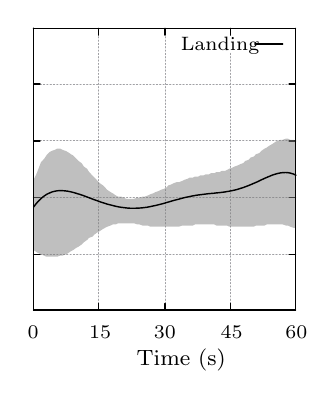
\begin{tikzpicture}[y=0.80pt, x=0.80pt, yscale=-0.500000, xscale=0.480000, inner sep=0pt, outer sep=0pt]
\scriptsize
\begin{scope}[draw=black,line join=bevel,line cap=rect,even odd rule,line width=0.512pt]
  \begin{scope}[cm={{1.0,0.0,0.0,1.0,(0.0,0.0)}},draw=black,line join=bevel,line cap=rect,line width=0.512pt]
  \end{scope}
  \begin{scope}[cm={{1.00625,0.0,0.0,1.00625,(0.0,0.0)}},draw=black,line join=bevel,line cap=rect,line width=0.512pt]
  \end{scope}
  \begin{scope}[cm={{1.00625,0.0,0.0,1.00625,(0.0,0.0)}},draw=ca0a0a4,dash pattern=on 0.40pt off 0.80pt,line join=round,line cap=round,line width=0.400pt]
    \path[draw] (53.5000,268.5000) -- (298.5000,268.5000);
  \end{scope}
  \begin{scope}[cm={{1.00625,0.0,0.0,1.00625,(0.0,0.0)}},draw=black,line join=round,line cap=round,line width=0.512pt]
    \path[draw] (53.5000,268.5000) -- (59.5000,268.5000);
    \path[draw] (298.5000,268.5000) -- (292.5000,268.5000);
  \end{scope}
  \begin{scope}[cm={{1.00625,0.0,0.0,1.00625,(0.0,0.0)}},draw=black,line join=bevel,line cap=rect,line width=0.512pt]
  \end{scope}
  \begin{scope}[cm={{1.00625,0.0,0.0,1.00625,(27.1688,276.216)}},draw=black,line join=bevel,line cap=rect,line width=0.512pt]
  \end{scope}
  \begin{scope}[cm={{1.00625,0.0,0.0,1.00625,(27.1688,276.216)}},draw=black,line join=bevel,line cap=rect,line width=0.512pt]
  \end{scope}
  \begin{scope}[cm={{1.00625,0.0,0.0,1.00625,(27.1688,276.216)}},draw=black,line join=bevel,line cap=rect,line width=0.512pt]
  \end{scope}
  \begin{scope}[cm={{1.00625,0.0,0.0,1.00625,(27.1688,276.216)}},draw=black,line join=bevel,line cap=rect,line width=0.512pt]
  \end{scope}
  \begin{scope}[cm={{1.00625,0.0,0.0,1.00625,(27.1688,276.216)}},draw=black,line join=bevel,line cap=rect,line width=0.512pt]
  \end{scope}
  \begin{scope}[cm={{1.00625,0.0,0.0,1.00625,(27.1688,276.216)}},draw=black,line join=bevel,line cap=rect,line width=0.512pt]
    %\path[fill=black] (0.0000,0.0000) node[above right] (text40) {24};
  \end{scope}
  \begin{scope}[cm={{1.00625,0.0,0.0,1.00625,(27.1688,276.216)}},draw=black,line join=bevel,line cap=rect,line width=0.512pt]
  \end{scope}
  \begin{scope}[cm={{1.00625,0.0,0.0,1.00625,(0.0,0.0)}},draw=black,line join=bevel,line cap=rect,line width=0.512pt]
  \end{scope}
  \begin{scope}[cm={{1.00625,0.0,0.0,1.00625,(0.0,0.0)}},draw=ca0a0a4,dash pattern=on 0.40pt off 0.80pt,line join=round,line cap=round,line width=0.400pt]
    \path[draw] (53.5000,218.5000) -- (298.5000,218.5000);
  \end{scope}
  \begin{scope}[cm={{1.00625,0.0,0.0,1.00625,(0.0,0.0)}},draw=black,line join=round,line cap=round,line width=0.512pt]
    \path[draw] (53.5000,218.5000) -- (59.5000,218.5000);
    \path[draw] (298.5000,218.5000) -- (292.5000,218.5000);
  \end{scope}
  \begin{scope}[cm={{1.00625,0.0,0.0,1.00625,(0.0,0.0)}},draw=black,line join=bevel,line cap=rect,line width=0.512pt]
  \end{scope}
  \begin{scope}[cm={{1.00625,0.0,0.0,1.00625,(27.1688,224.897)}},draw=black,line join=bevel,line cap=rect,line width=0.512pt]
  \end{scope}
  \begin{scope}[cm={{1.00625,0.0,0.0,1.00625,(27.1688,224.897)}},draw=black,line join=bevel,line cap=rect,line width=0.512pt]
  \end{scope}
  \begin{scope}[cm={{1.00625,0.0,0.0,1.00625,(27.1688,224.897)}},draw=black,line join=bevel,line cap=rect,line width=0.512pt]
  \end{scope}
  \begin{scope}[cm={{1.00625,0.0,0.0,1.00625,(27.1688,224.897)}},draw=black,line join=bevel,line cap=rect,line width=0.512pt]
  \end{scope}
  \begin{scope}[cm={{1.00625,0.0,0.0,1.00625,(27.1688,224.897)}},draw=black,line join=bevel,line cap=rect,line width=0.512pt]
  \end{scope}
  \begin{scope}[cm={{1.00625,0.0,0.0,1.00625,(27.1688,224.897)}},draw=black,line join=bevel,line cap=rect,line width=0.512pt]
    %\path[fill=black] (0.0000,0.0000) node[above right] (text70) {26};
  \end{scope}
  \begin{scope}[cm={{1.00625,0.0,0.0,1.00625,(27.1688,224.897)}},draw=black,line join=bevel,line cap=rect,line width=0.512pt]
  \end{scope}
  \begin{scope}[cm={{1.00625,0.0,0.0,1.00625,(0.0,0.0)}},draw=black,line join=bevel,line cap=rect,line width=0.512pt]
  \end{scope}
  \begin{scope}[cm={{1.00625,0.0,0.0,1.00625,(0.0,0.0)}},draw=ca0a0a4,dash pattern=on 0.40pt off 0.80pt,line join=round,line cap=round,line width=0.400pt]
    \path[draw] (53.5000,167.5000) -- (298.5000,167.5000);
  \end{scope}
  \begin{scope}[cm={{1.00625,0.0,0.0,1.00625,(0.0,0.0)}},draw=black,line join=round,line cap=round,line width=0.512pt]
    \path[draw] (53.5000,167.5000) -- (59.5000,167.5000);
    \path[draw] (298.5000,167.5000) -- (292.5000,167.5000);
  \end{scope}
  \begin{scope}[cm={{1.00625,0.0,0.0,1.00625,(0.0,0.0)}},draw=black,line join=bevel,line cap=rect,line width=0.512pt]
  \end{scope}
  \begin{scope}[cm={{1.00625,0.0,0.0,1.00625,(28.175,173.578)}},draw=black,line join=bevel,line cap=rect,line width=0.512pt]
  \end{scope}
  \begin{scope}[cm={{1.00625,0.0,0.0,1.00625,(28.175,173.578)}},draw=black,line join=bevel,line cap=rect,line width=0.512pt]
  \end{scope}
  \begin{scope}[cm={{1.00625,0.0,0.0,1.00625,(28.175,173.578)}},draw=black,line join=bevel,line cap=rect,line width=0.512pt]
  \end{scope}
  \begin{scope}[cm={{1.00625,0.0,0.0,1.00625,(28.175,173.578)}},draw=black,line join=bevel,line cap=rect,line width=0.512pt]
  \end{scope}
  \begin{scope}[cm={{1.00625,0.0,0.0,1.00625,(28.175,173.578)}},draw=black,line join=bevel,line cap=rect,line width=0.512pt]
  \end{scope}
  \begin{scope}[cm={{1.00625,0.0,0.0,1.00625,(28.175,173.578)}},draw=black,line join=bevel,line cap=rect,line width=0.512pt]
    %\path[fill=black] (0.0000,0.0000) node[above right] (text100) {28};
  \end{scope}
  \begin{scope}[cm={{1.00625,0.0,0.0,1.00625,(28.175,173.578)}},draw=black,line join=bevel,line cap=rect,line width=0.512pt]
  \end{scope}
  \begin{scope}[cm={{1.00625,0.0,0.0,1.00625,(0.0,0.0)}},draw=black,line join=bevel,line cap=rect,line width=0.512pt]
  \end{scope}
  \begin{scope}[cm={{1.00625,0.0,0.0,1.00625,(0.0,0.0)}},draw=ca0a0a4,dash pattern=on 0.40pt off 0.80pt,line join=round,line cap=round,line width=0.400pt]
    \path[draw] (53.5000,116.5000) -- (298.5000,116.5000);
  \end{scope}
  \begin{scope}[cm={{1.00625,0.0,0.0,1.00625,(0.0,0.0)}},draw=black,line join=round,line cap=round,line width=0.512pt]
    \path[draw] (53.5000,116.5000) -- (59.5000,116.5000);
    \path[draw] (298.5000,116.5000) -- (292.5000,116.5000);
  \end{scope}
  \begin{scope}[cm={{1.00625,0.0,0.0,1.00625,(0.0,0.0)}},draw=black,line join=bevel,line cap=rect,line width=0.512pt]
  \end{scope}
  \begin{scope}[cm={{1.00625,0.0,0.0,1.00625,(27.1688,123.266)}},draw=black,line join=bevel,line cap=rect,line width=0.512pt]
  \end{scope}
  \begin{scope}[cm={{1.00625,0.0,0.0,1.00625,(27.1688,123.266)}},draw=black,line join=bevel,line cap=rect,line width=0.512pt]
  \end{scope}
  \begin{scope}[cm={{1.00625,0.0,0.0,1.00625,(27.1688,123.266)}},draw=black,line join=bevel,line cap=rect,line width=0.512pt]
  \end{scope}
  \begin{scope}[cm={{1.00625,0.0,0.0,1.00625,(27.1688,123.266)}},draw=black,line join=bevel,line cap=rect,line width=0.512pt]
  \end{scope}
  \begin{scope}[cm={{1.00625,0.0,0.0,1.00625,(27.1688,123.266)}},draw=black,line join=bevel,line cap=rect,line width=0.512pt]
  \end{scope}
  \begin{scope}[cm={{1.00625,0.0,0.0,1.00625,(27.1688,123.266)}},draw=black,line join=bevel,line cap=rect,line width=0.512pt]
    %\path[fill=black] (0.0000,0.0000) node[above right] (text130) {30};
  \end{scope}
  \begin{scope}[cm={{1.00625,0.0,0.0,1.00625,(27.1688,123.266)}},draw=black,line join=bevel,line cap=rect,line width=0.512pt]
  \end{scope}
  \begin{scope}[cm={{1.00625,0.0,0.0,1.00625,(0.0,0.0)}},draw=black,line join=bevel,line cap=rect,line width=0.512pt]
  \end{scope}
  \begin{scope}[cm={{1.00625,0.0,0.0,1.00625,(0.0,0.0)}},draw=ca0a0a4,dash pattern=on 0.40pt off 0.80pt,line join=round,line cap=round,line width=0.400pt]
    \path[draw] (53.5000,65.5000) -- (298.5000,65.5000);
  \end{scope}
  \begin{scope}[cm={{1.00625,0.0,0.0,1.00625,(0.0,0.0)}},draw=black,line join=round,line cap=round,line width=0.512pt]
    \path[draw] (53.5000,65.5000) -- (59.5000,65.5000);
    \path[draw] (298.5000,65.5000) -- (292.5000,65.5000);
  \end{scope}
  \begin{scope}[cm={{1.00625,0.0,0.0,1.00625,(0.0,0.0)}},draw=black,line join=bevel,line cap=rect,line width=0.512pt]
  \end{scope}
  \begin{scope}[cm={{1.00625,0.0,0.0,1.00625,(27.1688,71.9469)}},draw=black,line join=bevel,line cap=rect,line width=0.512pt]
  \end{scope}
  \begin{scope}[cm={{1.00625,0.0,0.0,1.00625,(27.1688,71.9469)}},draw=black,line join=bevel,line cap=rect,line width=0.512pt]
  \end{scope}
  \begin{scope}[cm={{1.00625,0.0,0.0,1.00625,(27.1688,71.9469)}},draw=black,line join=bevel,line cap=rect,line width=0.512pt]
  \end{scope}
  \begin{scope}[cm={{1.00625,0.0,0.0,1.00625,(27.1688,71.9469)}},draw=black,line join=bevel,line cap=rect,line width=0.512pt]
  \end{scope}
  \begin{scope}[cm={{1.00625,0.0,0.0,1.00625,(27.1688,71.9469)}},draw=black,line join=bevel,line cap=rect,line width=0.512pt]
  \end{scope}
  \begin{scope}[cm={{1.00625,0.0,0.0,1.00625,(27.1688,71.9469)}},draw=black,line join=bevel,line cap=rect,line width=0.512pt]
    %\path[fill=black] (0.0000,0.0000) node[above right] (text160) {32};
  \end{scope}
  \begin{scope}[cm={{1.00625,0.0,0.0,1.00625,(27.1688,71.9469)}},draw=black,line join=bevel,line cap=rect,line width=0.512pt]
  \end{scope}
  \begin{scope}[cm={{1.00625,0.0,0.0,1.00625,(0.0,0.0)}},draw=black,line join=bevel,line cap=rect,line width=0.512pt]
  \end{scope}
  \begin{scope}[cm={{1.00625,0.0,0.0,1.00625,(0.0,0.0)}},draw=ca0a0a4,dash pattern=on 0.40pt off 0.80pt,line join=round,line cap=round,line width=0.400pt]
    \path[draw] (53.5000,15.5000) -- (298.5000,15.5000);
  \end{scope}
  \begin{scope}[cm={{1.00625,0.0,0.0,1.00625,(0.0,0.0)}},draw=black,line join=round,line cap=round,line width=0.512pt]
    \path[draw] (53.5000,15.5000) -- (59.5000,15.5000);
    \path[draw] (298.5000,15.5000) -- (292.5000,15.5000);
  \end{scope}
  \begin{scope}[cm={{1.00625,0.0,0.0,1.00625,(0.0,0.0)}},draw=black,line join=bevel,line cap=rect,line width=0.512pt]
  \end{scope}
  \begin{scope}[cm={{1.00625,0.0,0.0,1.00625,(27.1688,20.6281)}},draw=black,line join=bevel,line cap=rect,line width=0.512pt]
  \end{scope}
  \begin{scope}[cm={{1.00625,0.0,0.0,1.00625,(27.1688,20.6281)}},draw=black,line join=bevel,line cap=rect,line width=0.512pt]
  \end{scope}
  \begin{scope}[cm={{1.00625,0.0,0.0,1.00625,(27.1688,20.6281)}},draw=black,line join=bevel,line cap=rect,line width=0.512pt]
  \end{scope}
  \begin{scope}[cm={{1.00625,0.0,0.0,1.00625,(27.1688,20.6281)}},draw=black,line join=bevel,line cap=rect,line width=0.512pt]
  \end{scope}
  \begin{scope}[cm={{1.00625,0.0,0.0,1.00625,(27.1688,20.6281)}},draw=black,line join=bevel,line cap=rect,line width=0.512pt]
  \end{scope}
  \begin{scope}[cm={{1.00625,0.0,0.0,1.00625,(27.1688,20.6281)}},draw=black,line join=bevel,line cap=rect,line width=0.512pt]
    %\path[fill=black] (0.0000,0.0000) node[above right] (text190) {34};
  \end{scope}
  \begin{scope}[cm={{1.00625,0.0,0.0,1.00625,(27.1688,20.6281)}},draw=black,line join=bevel,line cap=rect,line width=0.512pt]
  \end{scope}
  \begin{scope}[cm={{1.00625,0.0,0.0,1.00625,(0.0,0.0)}},draw=black,line join=bevel,line cap=rect,line width=0.512pt]
  \end{scope}
  \begin{scope}[cm={{1.00625,0.0,0.0,1.00625,(0.0,0.0)}},draw=ca0a0a4,dash pattern=on 0.40pt off 0.80pt,line join=round,line cap=round,line width=0.400pt]
    \path[draw] (53.5000,268.5000) -- (53.5000,15.5000);
  \end{scope}
  \begin{scope}[cm={{1.00625,0.0,0.0,1.00625,(0.0,0.0)}},draw=black,line join=round,line cap=round,line width=0.512pt]
    \path[draw] (53.5000,268.5000) -- (53.5000,262.5000);
    \path[draw] (53.5000,15.5000) -- (53.5000,21.5000);
  \end{scope}
  \begin{scope}[cm={{1.00625,0.0,0.0,1.00625,(0.0,0.0)}},draw=black,line join=bevel,line cap=rect,line width=0.512pt]
  \end{scope}
  \begin{scope}[cm={{1.00625,0.0,0.0,1.00625,(48.3,298.353)}},draw=black,line join=bevel,line cap=rect,line width=0.512pt]
  \end{scope}
  \begin{scope}[cm={{1.00625,0.0,0.0,1.00625,(48.3,298.353)}},draw=black,line join=bevel,line cap=rect,line width=0.512pt]
  \end{scope}
  \begin{scope}[cm={{1.00625,0.0,0.0,1.00625,(48.3,298.353)}},draw=black,line join=bevel,line cap=rect,line width=0.512pt]
  \end{scope}
  \begin{scope}[cm={{1.00625,0.0,0.0,1.00625,(48.3,298.353)}},draw=black,line join=bevel,line cap=rect,line width=0.512pt]
  \end{scope}
  \begin{scope}[cm={{1.00625,0.0,0.0,1.00625,(48.3,298.353)}},draw=black,line join=bevel,line cap=rect,line width=0.512pt]
  \end{scope}
  \begin{scope}[cm={{1.00625,0.0,0.0,1.00625,(48.3,295.353)}},draw=black,line join=bevel,line cap=rect,line width=0.512pt]
    \path[fill=black] (0.0000,0.0000) node[above right] (text220) {0};
  \end{scope}
  \begin{scope}[cm={{1.00625,0.0,0.0,1.00625,(48.3,298.353)}},draw=black,line join=bevel,line cap=rect,line width=0.512pt]
  \end{scope}
  \begin{scope}[cm={{1.00625,0.0,0.0,1.00625,(0.0,0.0)}},draw=black,line join=bevel,line cap=rect,line width=0.512pt]
  \end{scope}
  \begin{scope}[cm={{1.00625,0.0,0.0,1.00625,(0.0,0.0)}},draw=ca0a0a4,dash pattern=on 0.40pt off 0.80pt,line join=round,line cap=round,line width=0.400pt]
    \path[draw] (114.5000,268.5000) -- (114.5000,15.5000);
  \end{scope}
  \begin{scope}[cm={{1.00625,0.0,0.0,1.00625,(0.0,0.0)}},draw=black,line join=round,line cap=round,line width=0.512pt]
    \path[draw] (114.5000,268.5000) -- (114.5000,262.5000);
    \path[draw] (114.5000,15.5000) -- (114.5000,21.5000);
  \end{scope}
  \begin{scope}[cm={{1.00625,0.0,0.0,1.00625,(0.0,0.0)}},draw=black,line join=bevel,line cap=rect,line width=0.512pt]
  \end{scope}
  \begin{scope}[cm={{1.00625,0.0,0.0,1.00625,(106.159,298.353)}},draw=black,line join=bevel,line cap=rect,line width=0.512pt]
  \end{scope}
  \begin{scope}[cm={{1.00625,0.0,0.0,1.00625,(106.159,298.353)}},draw=black,line join=bevel,line cap=rect,line width=0.512pt]
  \end{scope}
  \begin{scope}[cm={{1.00625,0.0,0.0,1.00625,(106.159,298.353)}},draw=black,line join=bevel,line cap=rect,line width=0.512pt]
  \end{scope}
  \begin{scope}[cm={{1.00625,0.0,0.0,1.00625,(106.159,298.353)}},draw=black,line join=bevel,line cap=rect,line width=0.512pt]
  \end{scope}
  \begin{scope}[cm={{1.00625,0.0,0.0,1.00625,(106.159,298.353)}},draw=black,line join=bevel,line cap=rect,line width=0.512pt]
  \end{scope}
  \begin{scope}[cm={{1.00625,0.0,0.0,1.00625,(106.159,295.353)}},draw=black,line join=bevel,line cap=rect,line width=0.512pt]
    \path[fill=black] (0.0000,0.0000) node[above right] (text250) {15};
  \end{scope}
  \begin{scope}[cm={{1.00625,0.0,0.0,1.00625,(106.159,298.353)}},draw=black,line join=bevel,line cap=rect,line width=0.512pt]
  \end{scope}
  \begin{scope}[cm={{1.00625,0.0,0.0,1.00625,(0.0,0.0)}},draw=black,line join=bevel,line cap=rect,line width=0.512pt]
  \end{scope}
  \begin{scope}[cm={{1.00625,0.0,0.0,1.00625,(0.0,0.0)}},draw=ca0a0a4,dash pattern=on 0.40pt off 0.80pt,line join=round,line cap=round,line width=0.400pt]
    \path[draw] (176.5000,268.5000) -- (176.5000,15.5000);
  \end{scope}
  \begin{scope}[cm={{1.00625,0.0,0.0,1.00625,(0.0,0.0)}},draw=black,line join=round,line cap=round,line width=0.512pt]
    \path[draw] (176.5000,268.5000) -- (176.5000,262.5000);
    \path[draw] (176.5000,15.5000) -- (176.5000,21.5000);
  \end{scope}
  \begin{scope}[cm={{1.00625,0.0,0.0,1.00625,(0.0,0.0)}},draw=black,line join=bevel,line cap=rect,line width=0.512pt]
  \end{scope}
  \begin{scope}[cm={{1.00625,0.0,0.0,1.00625,(167.038,298.353)}},draw=black,line join=bevel,line cap=rect,line width=0.512pt]
  \end{scope}
  \begin{scope}[cm={{1.00625,0.0,0.0,1.00625,(167.038,298.353)}},draw=black,line join=bevel,line cap=rect,line width=0.512pt]
  \end{scope}
  \begin{scope}[cm={{1.00625,0.0,0.0,1.00625,(167.038,298.353)}},draw=black,line join=bevel,line cap=rect,line width=0.512pt]
  \end{scope}
  \begin{scope}[cm={{1.00625,0.0,0.0,1.00625,(167.038,298.353)}},draw=black,line join=bevel,line cap=rect,line width=0.512pt]
  \end{scope}
  \begin{scope}[cm={{1.00625,0.0,0.0,1.00625,(167.038,298.353)}},draw=black,line join=bevel,line cap=rect,line width=0.512pt]
  \end{scope}
  \begin{scope}[cm={{1.00625,0.0,0.0,1.00625,(167.038,295.353)}},draw=black,line join=bevel,line cap=rect,line width=0.512pt]
    \path[fill=black] (0.0000,0.0000) node[above right] (text280) {30};
  \end{scope}
  \begin{scope}[cm={{1.00625,0.0,0.0,1.00625,(167.038,298.353)}},draw=black,line join=bevel,line cap=rect,line width=0.512pt]
  \end{scope}
  \begin{scope}[cm={{1.00625,0.0,0.0,1.00625,(0.0,0.0)}},draw=black,line join=bevel,line cap=rect,line width=0.512pt]
  \end{scope}
  \begin{scope}[cm={{1.00625,0.0,0.0,1.00625,(0.0,0.0)}},draw=ca0a0a4,dash pattern=on 0.40pt off 0.80pt,line join=round,line cap=round,line width=0.400pt]
    \path[draw] (237.5000,268.5000) -- (237.5000,37.5000);
    \path[draw] (237.5000,21.5000) -- (237.5000,15.5000);
  \end{scope}
  \begin{scope}[cm={{1.00625,0.0,0.0,1.00625,(0.0,0.0)}},draw=black,line join=round,line cap=round,line width=0.512pt]
    \path[draw] (237.5000,268.5000) -- (237.5000,262.5000);
    \path[draw] (237.5000,15.5000) -- (237.5000,21.5000);
  \end{scope}
  \begin{scope}[cm={{1.00625,0.0,0.0,1.00625,(0.0,0.0)}},draw=black,line join=bevel,line cap=rect,line width=0.512pt]
  \end{scope}
  \begin{scope}[cm={{1.00625,0.0,0.0,1.00625,(229.928,298.353)}},draw=black,line join=bevel,line cap=rect,line width=0.512pt]
  \end{scope}
  \begin{scope}[cm={{1.00625,0.0,0.0,1.00625,(229.928,298.353)}},draw=black,line join=bevel,line cap=rect,line width=0.512pt]
  \end{scope}
  \begin{scope}[cm={{1.00625,0.0,0.0,1.00625,(229.928,298.353)}},draw=black,line join=bevel,line cap=rect,line width=0.512pt]
  \end{scope}
  \begin{scope}[cm={{1.00625,0.0,0.0,1.00625,(229.928,298.353)}},draw=black,line join=bevel,line cap=rect,line width=0.512pt]
  \end{scope}
  \begin{scope}[cm={{1.00625,0.0,0.0,1.00625,(229.928,298.353)}},draw=black,line join=bevel,line cap=rect,line width=0.512pt]
  \end{scope}
  \begin{scope}[cm={{1.00625,0.0,0.0,1.00625,(229.928,295.353)}},draw=black,line join=bevel,line cap=rect,line width=0.512pt]
    \path[fill=black] (0.0000,0.0000) node[above right] (text312) {45};
  \end{scope}
  \begin{scope}[cm={{1.00625,0.0,0.0,1.00625,(229.928,298.353)}},draw=black,line join=bevel,line cap=rect,line width=0.512pt]
  \end{scope}
  \begin{scope}[cm={{1.00625,0.0,0.0,1.00625,(0.0,0.0)}},draw=black,line join=bevel,line cap=rect,line width=0.512pt]
  \end{scope}
  \begin{scope}[cm={{1.00625,0.0,0.0,1.00625,(0.0,0.0)}},draw=ca0a0a4,dash pattern=on 0.40pt off 0.80pt,line join=round,line cap=round,line width=0.400pt]
    \path[draw] (298.5000,268.5000) -- (298.5000,15.5000);
  \end{scope}
  \begin{scope}[cm={{1.00625,0.0,0.0,1.00625,(0.0,0.0)}},draw=black,line join=round,line cap=round,line width=0.512pt]
    \path[draw] (298.5000,268.5000) -- (298.5000,262.5000);
    \path[draw] (298.5000,15.5000) -- (298.5000,21.5000);
  \end{scope}
  \begin{scope}[cm={{1.00625,0.0,0.0,1.00625,(0.0,0.0)}},draw=black,line join=bevel,line cap=rect,line width=0.512pt]
  \end{scope}
  \begin{scope}[cm={{1.00625,0.0,0.0,1.00625,(290.806,298.353)}},draw=black,line join=bevel,line cap=rect,line width=0.512pt]
  \end{scope}
  \begin{scope}[cm={{1.00625,0.0,0.0,1.00625,(290.806,298.353)}},draw=black,line join=bevel,line cap=rect,line width=0.512pt]
  \end{scope}
  \begin{scope}[cm={{1.00625,0.0,0.0,1.00625,(290.806,298.353)}},draw=black,line join=bevel,line cap=rect,line width=0.512pt]
  \end{scope}
  \begin{scope}[cm={{1.00625,0.0,0.0,1.00625,(290.806,298.353)}},draw=black,line join=bevel,line cap=rect,line width=0.512pt]
  \end{scope}
  \begin{scope}[cm={{1.00625,0.0,0.0,1.00625,(290.806,298.353)}},draw=black,line join=bevel,line cap=rect,line width=0.512pt]
  \end{scope}
  \begin{scope}[cm={{1.00625,0.0,0.0,1.00625,(290.806,295.353)}},draw=black,line join=bevel,line cap=rect,line width=0.512pt]
    \path[fill=black] (0.0000,0.0000) node[above right] (text342) {60};
  \end{scope}
  \begin{scope}[cm={{1.00625,0.0,0.0,1.00625,(290.806,298.353)}},draw=black,line join=bevel,line cap=rect,line width=0.512pt]
  \end{scope}
  \begin{scope}[cm={{1.00625,0.0,0.0,1.00625,(0.0,0.0)}},draw=black,line join=bevel,line cap=rect,line width=0.512pt]
  \end{scope}
  \begin{scope}[cm={{1.00625,0.0,0.0,1.00625,(0.0,0.0)}},draw=black,line join=round,line cap=round,line width=0.512pt]
    \path[draw] (53.5000,15.5000) -- (53.5000,268.5000) -- (298.5000,268.5000) --
      (298.5000,15.5000) -- (53.5000,15.5000);
  \end{scope}
  \begin{scope}[cm={{1.00625,0.0,0.0,1.00625,(0.0,0.0)}},draw=black,line join=bevel,line cap=rect,line width=0.512pt]
  \end{scope}
  \begin{scope}[cm={{0.0,-1.00625,1.00625,0.0,(13.5844,176.597)}},draw=black,line join=bevel,line cap=rect,line width=0.512pt]
  \end{scope}
  \begin{scope}[cm={{0.0,-1.00625,1.00625,0.0,(13.5844,176.597)}},draw=black,line join=bevel,line cap=rect,line width=0.512pt]
  \end{scope}
  \begin{scope}[cm={{0.0,-1.00625,1.00625,0.0,(13.5844,176.597)}},draw=black,line join=bevel,line cap=rect,line width=0.512pt]
  \end{scope}
  \begin{scope}[cm={{0.0,-1.00625,1.00625,0.0,(13.5844,176.597)}},draw=black,line join=bevel,line cap=rect,line width=0.512pt]
  \end{scope}
  \begin{scope}[cm={{0.0,-1.00625,1.00625,0.0,(13.5844,176.597)}},draw=black,line join=bevel,line cap=rect,line width=0.512pt]
  \end{scope}
  \begin{scope}[cm={{0.0,-1.00625,1.00625,0.0,(9.5844,176.597)}},draw=black,line join=bevel,line cap=rect,line width=0.512pt]
    %\path[fill=black] (0.0000,0.0000) node[above right] (text366) {\rotatebox{90}{Power (W)}};
  \end{scope}
  \begin{scope}[cm={{0.0,-1.00625,1.00625,0.0,(13.5844,176.597)}},draw=black,line join=bevel,line cap=rect,line width=0.512pt]
  \end{scope}
  \begin{scope}[cm={{1.00625,0.0,0.0,1.00625,(150.938,317.472)}},draw=black,line join=bevel,line cap=rect,line width=0.512pt]
  \end{scope}
  \begin{scope}[cm={{1.00625,0.0,0.0,1.00625,(150.938,317.472)}},draw=black,line join=bevel,line cap=rect,line width=0.512pt]
  \end{scope}
  \begin{scope}[cm={{1.00625,0.0,0.0,1.00625,(150.938,317.472)}},draw=black,line join=bevel,line cap=rect,line width=0.512pt]
  \end{scope}
  \begin{scope}[cm={{1.00625,0.0,0.0,1.00625,(150.938,317.472)}},draw=black,line join=bevel,line cap=rect,line width=0.512pt]
  \end{scope}
  \begin{scope}[cm={{1.00625,0.0,0.0,1.00625,(150.938,317.472)}},draw=black,line join=bevel,line cap=rect,line width=0.512pt]
  \end{scope}
  \begin{scope}[cm={{1.00625,0.0,0.0,1.00625,(150.938,325.472)}},draw=black,line join=bevel,line cap=rect,line width=0.512pt]
    \path[fill=black] (0.0000,0.0000) node[above right] (text382) {\footnotesize Time (s)};
  \end{scope}
  \begin{scope}[cm={{1.00625,0.0,0.0,1.00625,(150.938,317.472)}},draw=black,line join=bevel,line cap=rect,line width=0.512pt]
  \end{scope}
  \begin{scope}[cm={{1.00625,0.0,0.0,1.00625,(0.0,0.0)}},draw=black,line join=bevel,line cap=rect,line width=0.512pt]
  \end{scope}
  \begin{scope}[cm={{1.00625,0.0,0.0,1.00625,(0.0,0.0)}},draw=black,line join=bevel,line cap=rect,line width=0.512pt]
  \end{scope}
  \begin{scope}[cm={{1.00625,0.0,0.0,1.00625,(0.0,0.0)}},draw=black,line join=bevel,line cap=rect,line width=0.512pt]
  \end{scope}
  \begin{scope}[cm={{1.00625,0.0,0.0,1.00625,(0.0,0.0)}},draw=c808080,fill=c808080,line join=bevel,line cap=rect,draw opacity=0.500,fill opacity=0.500,line width=0.512pt,transparency group]
    \path[fill,even odd rule] (53.5000,214.5000) -- (56.5000,216.5000) --
      (58.5000,217.5000) -- (60.5000,218.5000) -- (63.5000,219.5000) --
      (65.5000,220.5000) -- (68.5000,220.5000) -- (70.5000,220.5000) --
      (73.5000,220.5000) -- (75.5000,220.5000) -- (78.5000,219.5000) --
      (80.5000,219.5000) -- (83.5000,218.5000) -- (85.5000,217.5000) --
      (88.5000,215.5000) -- (90.5000,214.5000) -- (93.5000,212.5000) --
      (95.5000,211.5000) -- (98.5000,209.5000) -- (100.5000,207.5000) --
      (103.5000,205.5000) -- (105.5000,203.5000) -- (108.5000,202.5000) --
      (110.5000,200.5000) -- (113.5000,198.5000) -- (115.5000,197.5000) --
      (118.5000,195.5000) -- (120.5000,194.5000) -- (122.5000,193.5000) --
      (125.5000,192.5000) -- (127.5000,191.5000) -- (130.5000,191.5000) --
      (132.5000,190.5000) -- (135.5000,190.5000) -- (137.5000,190.5000) --
      (140.5000,190.5000) -- (142.5000,190.5000) -- (145.5000,190.5000) --
      (147.5000,190.5000) -- (150.5000,191.5000) -- (152.5000,191.5000) --
      (155.5000,192.5000) -- (157.5000,192.5000) -- (160.5000,192.5000) --
      (162.5000,193.5000) -- (165.5000,193.5000) -- (167.5000,193.5000) --
      (170.5000,193.5000) -- (172.5000,193.5000) -- (175.5000,193.5000) --
      (177.5000,193.5000) -- (179.5000,193.5000) -- (182.5000,193.5000) --
      (184.5000,193.5000) -- (187.5000,193.5000) -- (189.5000,193.5000) --
      (192.5000,192.5000) -- (194.5000,192.5000) -- (197.5000,192.5000) --
      (199.5000,192.5000) -- (202.5000,192.5000) -- (204.5000,191.5000) --
      (207.5000,191.5000) -- (209.5000,191.5000) -- (212.5000,191.5000) --
      (214.5000,191.5000) -- (217.5000,191.5000) -- (219.5000,191.5000) --
      (222.5000,191.5000) -- (224.5000,192.5000) -- (227.5000,192.5000) --
      (229.5000,192.5000) -- (232.5000,192.5000) -- (234.5000,192.5000) --
      (236.5000,193.5000) -- (239.5000,193.5000) -- (241.5000,193.5000) --
      (244.5000,193.5000) -- (246.5000,193.5000) -- (249.5000,193.5000) --
      (251.5000,193.5000) -- (254.5000,193.5000) -- (256.5000,193.5000) --
      (259.5000,193.5000) -- (261.5000,192.5000) -- (264.5000,192.5000) --
      (266.5000,192.5000) -- (269.5000,192.5000) -- (271.5000,191.5000) --
      (274.5000,191.5000) -- (276.5000,191.5000) -- (279.5000,191.5000) --
      (281.5000,191.5000) -- (284.5000,191.5000) -- (286.5000,191.5000) --
      (289.5000,192.5000) -- (291.5000,192.5000) -- (293.5000,193.5000) --
      (296.5000,194.5000) -- (298.5000,194.5000) -- (298.5000,116.5000) --
      (296.5000,115.5000) -- (293.5000,115.5000) -- (291.5000,114.5000) --
      (289.5000,114.5000) -- (286.5000,115.5000) -- (284.5000,115.5000) --
      (281.5000,116.5000) -- (279.5000,117.5000) -- (276.5000,119.5000) --
      (274.5000,120.5000) -- (271.5000,122.5000) -- (269.5000,123.5000) --
      (266.5000,125.5000) -- (264.5000,127.5000) -- (261.5000,128.5000) --
      (259.5000,130.5000) -- (256.5000,131.5000) -- (254.5000,133.5000) --
      (251.5000,134.5000) -- (249.5000,136.5000) -- (246.5000,137.5000) --
      (244.5000,138.5000) -- (241.5000,139.5000) -- (239.5000,140.5000) --
      (236.5000,141.5000) -- (234.5000,142.5000) -- (232.5000,143.5000) --
      (229.5000,143.5000) -- (227.5000,144.5000) -- (224.5000,144.5000) --
      (222.5000,145.5000) -- (219.5000,145.5000) -- (217.5000,146.5000) --
      (214.5000,146.5000) -- (212.5000,147.5000) -- (209.5000,147.5000) --
      (207.5000,148.5000) -- (204.5000,148.5000) -- (202.5000,149.5000) --
      (199.5000,149.5000) -- (197.5000,150.5000) -- (194.5000,151.5000) --
      (192.5000,152.5000) -- (189.5000,153.5000) -- (187.5000,153.5000) --
      (184.5000,154.5000) -- (182.5000,155.5000) -- (179.5000,156.5000) --
      (177.5000,158.5000) -- (175.5000,159.5000) -- (172.5000,160.5000) --
      (170.5000,161.5000) -- (167.5000,162.5000) -- (165.5000,163.5000) --
      (162.5000,164.5000) -- (160.5000,165.5000) -- (157.5000,166.5000) --
      (155.5000,166.5000) -- (152.5000,167.5000) -- (150.5000,167.5000) --
      (147.5000,168.5000) -- (145.5000,168.5000) -- (142.5000,168.5000) --
      (140.5000,168.5000) -- (137.5000,167.5000) -- (135.5000,166.5000) --
      (132.5000,166.5000) -- (130.5000,165.5000) -- (127.5000,163.5000) --
      (125.5000,162.5000) -- (122.5000,160.5000) -- (120.5000,158.5000) --
      (118.5000,156.5000) -- (115.5000,154.5000) -- (113.5000,152.5000) --
      (110.5000,149.5000) -- (108.5000,147.5000) -- (105.5000,144.5000) --
      (103.5000,141.5000) -- (100.5000,139.5000) -- (98.5000,136.5000) --
      (95.5000,134.5000) -- (93.5000,132.5000) -- (90.5000,129.5000) --
      (88.5000,128.5000) -- (85.5000,126.5000) -- (83.5000,125.5000) --
      (80.5000,124.5000) -- (78.5000,123.5000) -- (75.5000,123.5000) --
      (73.5000,124.5000) -- (70.5000,125.5000) -- (68.5000,126.5000) --
      (65.5000,129.5000) -- (63.5000,132.5000) -- (60.5000,135.5000) --
      (58.5000,140.5000) -- (56.5000,145.5000) -- (53.5000,151.5000) --
      (53.5000,214.5000);
  \end{scope}
  \begin{scope}[cm={{1.00625,0.0,0.0,1.00625,(0.0,0.0)}},draw=black,line join=bevel,line cap=rect,line width=0.512pt]
  \end{scope}
  \begin{scope}[cm={{1.00625,0.0,0.0,1.00625,(218.356,33.2063)}},draw=black,line join=bevel,line cap=rect,line width=0.512pt]
  \end{scope}
  \begin{scope}[cm={{1.00625,0.0,0.0,1.00625,(218.356,33.2063)}},draw=black,line join=bevel,line cap=rect,line width=0.512pt]
  \end{scope}
  \begin{scope}[cm={{1.00625,0.0,0.0,1.00625,(218.356,33.2063)}},draw=black,line join=bevel,line cap=rect,line width=0.512pt]
  \end{scope}
  \begin{scope}[cm={{1.00625,0.0,0.0,1.00625,(218.356,33.2063)}},draw=black,line join=bevel,line cap=rect,line width=0.512pt]
  \end{scope}
  \begin{scope}[cm={{1.00625,0.0,0.0,1.00625,(218.356,33.2063)}},draw=black,line join=bevel,line cap=rect,line width=0.512pt]
  \end{scope}
  \begin{scope}[cm={{1.00625,0.0,0.0,1.00625,(192.356,39.4063)}},draw=black,line join=bevel,line cap=rect,line width=0.512pt]
    \path[fill=black] (0.0000,0.0000) node[above right] (text410) {\scriptsize Landing};
  \end{scope}
  \begin{scope}[cm={{1.00625,0.0,0.0,1.00625,(218.356,33.2063)}},draw=black,line join=bevel,line cap=rect,line width=0.512pt]
  \end{scope}
  \begin{scope}[cm={{1.00625,0.0,0.0,1.00625,(0.0,0.0)}},draw=black,line join=bevel,line cap=rect,line width=0.512pt]
  \end{scope}
  \begin{scope}[cm={{1.00625,0.0,0.0,1.00625,(0.0,0.0)}},draw=black,line join=round,line cap=round,line width=0.512pt]
    \path[draw,even odd rule] (260.5000,29.5000) -- (286.5000,29.5000);
  \end{scope}
  \begin{scope}[cm={{1.00625,0.0,0.0,1.00625,(0.0,0.0)}},draw=black,line join=bevel,line cap=rect,line width=0.512pt]
  \end{scope}
  \begin{scope}[cm={{1.00625,0.0,0.0,1.00625,(0.0,0.0)}},draw=black,line join=bevel,line cap=rect,line width=0.512pt]
  \end{scope}
  \begin{scope}[cm={{1.00625,0.0,0.0,1.00625,(0.0,0.0)}},draw=black,line join=bevel,line cap=rect,line width=0.512pt]
  \end{scope}
  \begin{scope}[cm={{1.00625,0.0,0.0,1.00625,(0.0,0.0)}},draw=black,line join=bevel,line cap=rect,line width=0.512pt]
  \end{scope}
  \begin{scope}[cm={{1.00625,0.0,0.0,1.00625,(0.0,0.0)}},draw=black,line join=round,line cap=round,line width=0.512pt]
    \path[draw] (53.5000,175.9000) -- (53.5000,175.9000) -- (56.0000,172.8000) --
      (58.5000,170.1000) -- (60.9000,167.9000) -- (63.4000,166.0000) --
      (65.9000,164.4000) -- (68.4000,163.3000) -- (70.9000,162.3000) --
      (73.3000,161.7000) -- (75.8000,161.3000) -- (78.3000,161.1000) --
      (80.8000,161.2000) -- (83.2000,161.4000) -- (85.7000,161.7000) --
      (88.2000,162.2000) -- (90.7000,162.8000) -- (93.2000,163.5000) --
      (95.6000,164.2000) -- (98.1000,165.0000) -- (100.6000,165.8000) --
      (103.1000,166.7000) -- (105.6000,167.6000) -- (108.0000,168.5000) --
      (110.5000,169.4000) -- (113.0000,170.2000) -- (115.5000,171.1000) --
      (118.0000,171.9000) -- (120.4000,172.6000) -- (122.9000,173.4000) --
      (125.4000,174.0000) -- (127.9000,174.6000) -- (130.3000,175.2000) --
      (132.8000,175.7000) -- (135.3000,176.1000) -- (137.8000,176.4000) --
      (140.3000,176.7000) -- (142.7000,176.9000) -- (145.2000,177.0000) --
      (147.7000,177.0000) -- (150.2000,176.9000) -- (152.6000,176.8000) --
      (155.1000,176.6000) -- (157.6000,176.3000) -- (160.1000,176.0000) --
      (162.6000,175.5000) -- (165.0000,175.0000) -- (167.5000,174.5000) --
      (170.0000,173.9000) -- (172.5000,173.3000) -- (175.0000,172.7000) --
      (177.4000,172.0000) -- (179.9000,171.3000) -- (182.4000,170.6000) --
      (184.9000,169.9000) -- (187.4000,169.3000) -- (189.8000,168.7000) --
      (192.3000,168.0000) -- (194.8000,167.4000) -- (197.3000,166.9000) --
      (199.8000,166.4000) -- (202.2000,165.9000) -- (204.7000,165.5000) --
      (207.2000,165.1000) -- (209.7000,164.8000) -- (212.1000,164.5000) --
      (214.6000,164.2000) -- (217.1000,163.9000) -- (219.6000,163.7000) --
      (222.1000,163.5000) -- (224.5000,163.2000) -- (227.0000,163.0000) --
      (229.5000,162.7000) -- (232.0000,162.4000) -- (234.4000,162.0000) --
      (236.9000,161.6000) -- (239.4000,161.1000) -- (241.9000,160.6000) --
      (244.4000,160.0000) -- (246.8000,159.2000) -- (249.3000,158.5000) --
      (251.8000,157.6000) -- (254.3000,156.7000) -- (256.8000,155.7000) --
      (259.2000,154.7000) -- (261.7000,153.7000) -- (264.2000,152.6000) --
      (266.7000,151.4000) -- (269.2000,150.3000) -- (271.6000,149.3000) --
      (274.1000,148.3000) -- (276.6000,147.3000) -- (279.1000,146.5000) --
      (281.6000,145.8000) -- (284.0000,145.3000) -- (286.5000,145.0000) --
      (289.0000,144.9000) -- (291.5000,145.0000) -- (293.9000,145.5000) --
      (296.4000,146.2000) -- (298.9000,147.3000);
  \end{scope}
  \begin{scope}[cm={{1.00625,0.0,0.0,1.00625,(0.0,0.0)}},draw=black,line join=bevel,line cap=rect,line width=0.512pt]
  \end{scope}
  \begin{scope}[cm={{1.00625,0.0,0.0,1.00625,(0.0,0.0)}},draw=black,line join=bevel,line cap=rect,line width=0.512pt]
  \end{scope}
  \begin{scope}[cm={{1.00625,0.0,0.0,1.00625,(0.0,0.0)}},draw=black,line join=round,line cap=round,line width=0.512pt]
    \path[draw] (53.5000,15.5000) -- (53.5000,268.5000) -- (298.5000,268.5000) --
      (298.5000,15.5000) -- (53.5000,15.5000);
  \end{scope}
  \begin{scope}[cm={{1.00625,0.0,0.0,1.00625,(0.0,0.0)}},draw=black,line join=bevel,line cap=rect,line width=0.512pt]
  \end{scope}
  \begin{scope}[cm={{1.0,0.0,0.0,1.0,(0.0,0.0)}},draw=black,line join=bevel,line cap=rect,line width=0.512pt]
  \end{scope}
\end{scope}
\end{tikzpicture}

    \caption{Landing energy}
    \label{fig:landing-energy}
  \end{subfigure}
  \sfr
  \caption[Paths and modeled energy evolutions in time for different flight phases]{Paths and modeled energy evolutions in time for different flight phases as they appeared in our early study~\citep{seewald2020mechanical}.}
  \label{fig:path-energy}
  \efr
\end{figure}
In this use case, we saw marked variability in energy signals for take-off\findex{take-off}, cruise\findex{cruise}, and landing\findex{landing} phases per flight\findex{flight phases}. To distinguish between the phases, we analyzed the motor torque, altitude, and throttle~\citep{seewald2020mechanical}. The Opterra fixed-wing aerial robot\findex{Opterra fixed-wing aerial robot} gains altitude during take-off before starting to fly the Zamboni-like motion for coverage. The modeled energy signal is in \fref{fig:takeoff-energy}{Figure}. It is evaluated from some test flights (the gray area in the figure), whereas \matlab aids the resulting regression (black line in the figure). Such a regressional analysis depicts little variability at the beginning of the take-off, likely justified by different controls necessary by various atmospheric conditions, and very little to no variability in the remaining. This latter part of the trajectory is where the flight controller guides the aerial robot on the Zamboni-like motion\findex{Zamboni-like motion}. \fref{fig:cruise-energy}{Figure} is the modeled energy signal for the cruise phase. There is little variability between the test flights; the flight controller takes charge of the guidance. Finally, there is considerable variability in the landing phase energy signal illustrated in \fref{fig:landing-energy}{Figure}. Initially, the aerial robot flies in small circles (see the path in \fref{fig:landing-path}{Figure}), lowering the altitude while descending to the ground under human control~\citep{seewald2020mechanical}. The phase depends on different conditions, including landing site geologic conformations\findex{geologic conformations}, sudden wind gusts\findex{wind gusts}, and others, presenting thus high energy variability. We measured an average of 28 and 60 seconds for take-off and landing, whereas the cruise depends on the polygon to cover size (containing the agricultural field).

\subsubsection{Computations energy evaluation}

The computation energy model in terms of battery SoC for {\small\tt darknet-gpu} and {\small\tt blowfish} varying parameters $c_{i,1},c_{i,2}$ is in \fref{fig:soc-plot}{Figure}. 
\begin{figure}[h!]
  \centering
  \fontfamily{phv}\selectfont
  \footnotesize
  \begin{subfigure}[t]{0.31\textwidth}
    \centering
    
\definecolor{ca0a0a4}{RGB}{160,160,164}
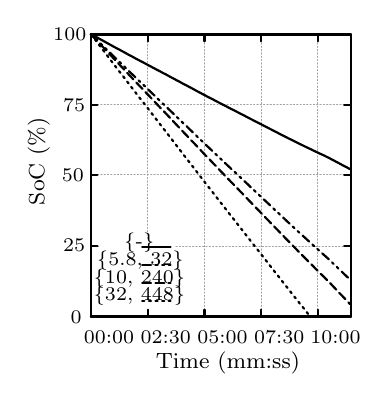
\begin{tikzpicture}[y=0.80pt, x=0.80pt, yscale=-0.500000, xscale=0.490000, inner sep=0pt, outer sep=0pt]
\scriptsize
\begin{scope}[draw=black,line join=bevel,line cap=rect,even odd rule,line width=0.800pt]
  \begin{scope}[cm={{1.0,0.0,0.0,1.0,(0.0,0.0)}},draw=black,line join=bevel,line cap=rect,line width=0.800pt]
  \end{scope}
  \begin{scope}[cm={{1.00625,0.0,0.0,1.00625,(0.0,0.0)}},draw=black,line join=bevel,line cap=rect,line width=0.800pt]
  \end{scope}
  \begin{scope}[cm={{1.00625,0.0,0.0,1.00625,(0.0,0.0)}},draw=ca0a0a4,dash pattern=on 0.40pt off 0.80pt,line join=round,line cap=round,line width=0.400pt]
    \path[draw] (60.5000,268.5000) -- (298.5000,268.5000);
  \end{scope}
  \begin{scope}[cm={{1.00625,0.0,0.0,1.00625,(0.0,0.0)}},draw=black,line join=round,line cap=round,line width=0.800pt]
    \path[draw] (60.5000,268.5000) -- (66.5000,268.5000);
    \path[draw] (298.5000,268.5000) -- (292.5000,268.5000);
  \end{scope}
  \begin{scope}[cm={{1.00625,0.0,0.0,1.00625,(0.0,0.0)}},draw=black,line join=bevel,line cap=rect,line width=0.800pt]
  \end{scope}
  \begin{scope}[cm={{1.00625,0.0,0.0,1.00625,(42.2625,276.216)}},draw=black,line join=bevel,line cap=rect,line width=0.800pt]
  \end{scope}
  \begin{scope}[cm={{1.00625,0.0,0.0,1.00625,(42.2625,276.216)}},draw=black,line join=bevel,line cap=rect,line width=0.800pt]
  \end{scope}
  \begin{scope}[cm={{1.00625,0.0,0.0,1.00625,(42.2625,276.216)}},draw=black,line join=bevel,line cap=rect,line width=0.800pt]
  \end{scope}
  \begin{scope}[cm={{1.00625,0.0,0.0,1.00625,(42.2625,276.216)}},draw=black,line join=bevel,line cap=rect,line width=0.800pt]
  \end{scope}
  \begin{scope}[cm={{1.00625,0.0,0.0,1.00625,(42.2625,276.216)}},draw=black,line join=bevel,line cap=rect,line width=0.800pt]
  \end{scope}
  \begin{scope}[cm={{1.00625,0.0,0.0,1.00625,(42.2625,276.216)}},draw=black,line join=bevel,line cap=rect,line width=0.800pt]
    \path[fill=black] (0.0000,0.0000) node[above right] () {0};
  \end{scope}
  \begin{scope}[cm={{1.00625,0.0,0.0,1.00625,(42.2625,276.216)}},draw=black,line join=bevel,line cap=rect,line width=0.800pt]
  \end{scope}
  \begin{scope}[cm={{1.00625,0.0,0.0,1.00625,(0.0,0.0)}},draw=black,line join=bevel,line cap=rect,line width=0.800pt]
  \end{scope}
  \begin{scope}[cm={{1.00625,0.0,0.0,1.00625,(0.0,0.0)}},draw=ca0a0a4,dash pattern=on 0.40pt off 0.80pt,line join=round,line cap=round,line width=0.400pt]
    \path[draw] (60.5000,205.5000) -- (67.5000,205.5000);
    \path[draw] (138.5000,205.5000) -- (298.5000,205.5000);
  \end{scope}
  \begin{scope}[cm={{1.00625,0.0,0.0,1.00625,(0.0,0.0)}},draw=black,line join=round,line cap=round,line width=0.800pt]
    \path[draw] (60.5000,205.5000) -- (66.5000,205.5000);
    \path[draw] (298.5000,205.5000) -- (292.5000,205.5000);
  \end{scope}
  \begin{scope}[cm={{1.00625,0.0,0.0,1.00625,(0.0,0.0)}},draw=black,line join=bevel,line cap=rect,line width=0.800pt]
  \end{scope}
  \begin{scope}[cm={{1.00625,0.0,0.0,1.00625,(35.2188,211.816)}},draw=black,line join=bevel,line cap=rect,line width=0.800pt]
  \end{scope}
  \begin{scope}[cm={{1.00625,0.0,0.0,1.00625,(35.2188,211.816)}},draw=black,line join=bevel,line cap=rect,line width=0.800pt]
  \end{scope}
  \begin{scope}[cm={{1.00625,0.0,0.0,1.00625,(35.2188,211.816)}},draw=black,line join=bevel,line cap=rect,line width=0.800pt]
  \end{scope}
  \begin{scope}[cm={{1.00625,0.0,0.0,1.00625,(35.2188,211.816)}},draw=black,line join=bevel,line cap=rect,line width=0.800pt]
  \end{scope}
  \begin{scope}[cm={{1.00625,0.0,0.0,1.00625,(35.2188,211.816)}},draw=black,line join=bevel,line cap=rect,line width=0.800pt]
  \end{scope}
  \begin{scope}[cm={{1.00625,0.0,0.0,1.00625,(35.2188,211.816)}},draw=black,line join=bevel,line cap=rect,line width=0.800pt]
    \path[fill=black] (0.0000,0.0000) node[above right] () {25};
  \end{scope}
  \begin{scope}[cm={{1.00625,0.0,0.0,1.00625,(35.2188,211.816)}},draw=black,line join=bevel,line cap=rect,line width=0.800pt]
  \end{scope}
  \begin{scope}[cm={{1.00625,0.0,0.0,1.00625,(0.0,0.0)}},draw=black,line join=bevel,line cap=rect,line width=0.800pt]
  \end{scope}
  \begin{scope}[cm={{1.00625,0.0,0.0,1.00625,(0.0,0.0)}},draw=ca0a0a4,dash pattern=on 0.40pt off 0.80pt,line join=round,line cap=round,line width=0.400pt]
    \path[draw] (60.5000,141.5000) -- (298.5000,141.5000);
  \end{scope}
  \begin{scope}[cm={{1.00625,0.0,0.0,1.00625,(0.0,0.0)}},draw=black,line join=round,line cap=round,line width=0.800pt]
    \path[draw] (60.5000,141.5000) -- (66.5000,141.5000);
    \path[draw] (298.5000,141.5000) -- (292.5000,141.5000);
  \end{scope}
  \begin{scope}[cm={{1.00625,0.0,0.0,1.00625,(0.0,0.0)}},draw=black,line join=bevel,line cap=rect,line width=0.800pt]
  \end{scope}
  \begin{scope}[cm={{1.00625,0.0,0.0,1.00625,(34.2125,148.422)}},draw=black,line join=bevel,line cap=rect,line width=0.800pt]
  \end{scope}
  \begin{scope}[cm={{1.00625,0.0,0.0,1.00625,(34.2125,148.422)}},draw=black,line join=bevel,line cap=rect,line width=0.800pt]
  \end{scope}
  \begin{scope}[cm={{1.00625,0.0,0.0,1.00625,(34.2125,148.422)}},draw=black,line join=bevel,line cap=rect,line width=0.800pt]
  \end{scope}
  \begin{scope}[cm={{1.00625,0.0,0.0,1.00625,(34.2125,148.422)}},draw=black,line join=bevel,line cap=rect,line width=0.800pt]
  \end{scope}
  \begin{scope}[cm={{1.00625,0.0,0.0,1.00625,(34.2125,148.422)}},draw=black,line join=bevel,line cap=rect,line width=0.800pt]
  \end{scope}
  \begin{scope}[cm={{1.00625,0.0,0.0,1.00625,(34.2125,148.422)}},draw=black,line join=bevel,line cap=rect,line width=0.800pt]
    \path[fill=black] (0.0000,0.0000) node[above right] () {50};
  \end{scope}
  \begin{scope}[cm={{1.00625,0.0,0.0,1.00625,(34.2125,148.422)}},draw=black,line join=bevel,line cap=rect,line width=0.800pt]
  \end{scope}
  \begin{scope}[cm={{1.00625,0.0,0.0,1.00625,(0.0,0.0)}},draw=black,line join=bevel,line cap=rect,line width=0.800pt]
  \end{scope}
  \begin{scope}[cm={{1.00625,0.0,0.0,1.00625,(0.0,0.0)}},draw=ca0a0a4,dash pattern=on 0.40pt off 0.80pt,line join=round,line cap=round,line width=0.400pt]
    \path[draw] (60.5000,78.5000) -- (298.5000,78.5000);
  \end{scope}
  \begin{scope}[cm={{1.00625,0.0,0.0,1.00625,(0.0,0.0)}},draw=black,line join=round,line cap=round,line width=0.800pt]
    \path[draw] (60.5000,78.5000) -- (66.5000,78.5000);
    \path[draw] (298.5000,78.5000) -- (292.5000,78.5000);
  \end{scope}
  \begin{scope}[cm={{1.00625,0.0,0.0,1.00625,(0.0,0.0)}},draw=black,line join=bevel,line cap=rect,line width=0.800pt]
  \end{scope}
  \begin{scope}[cm={{1.00625,0.0,0.0,1.00625,(35.2188,85.0281)}},draw=black,line join=bevel,line cap=rect,line width=0.800pt]
  \end{scope}
  \begin{scope}[cm={{1.00625,0.0,0.0,1.00625,(35.2188,85.0281)}},draw=black,line join=bevel,line cap=rect,line width=0.800pt]
  \end{scope}
  \begin{scope}[cm={{1.00625,0.0,0.0,1.00625,(35.2188,85.0281)}},draw=black,line join=bevel,line cap=rect,line width=0.800pt]
  \end{scope}
  \begin{scope}[cm={{1.00625,0.0,0.0,1.00625,(35.2188,85.0281)}},draw=black,line join=bevel,line cap=rect,line width=0.800pt]
  \end{scope}
  \begin{scope}[cm={{1.00625,0.0,0.0,1.00625,(35.2188,85.0281)}},draw=black,line join=bevel,line cap=rect,line width=0.800pt]
  \end{scope}
  \begin{scope}[cm={{1.00625,0.0,0.0,1.00625,(35.2188,85.0281)}},draw=black,line join=bevel,line cap=rect,line width=0.800pt]
    \path[fill=black] (0.0000,0.0000) node[above right] () {75};
  \end{scope}
  \begin{scope}[cm={{1.00625,0.0,0.0,1.00625,(35.2188,85.0281)}},draw=black,line join=bevel,line cap=rect,line width=0.800pt]
  \end{scope}
  \begin{scope}[cm={{1.00625,0.0,0.0,1.00625,(0.0,0.0)}},draw=black,line join=bevel,line cap=rect,line width=0.800pt]
  \end{scope}
  \begin{scope}[cm={{1.00625,0.0,0.0,1.00625,(0.0,0.0)}},draw=ca0a0a4,dash pattern=on 0.40pt off 0.80pt,line join=round,line cap=round,line width=0.400pt]
    \path[draw] (60.5000,15.5000) -- (298.5000,15.5000);
  \end{scope}
  \begin{scope}[cm={{1.00625,0.0,0.0,1.00625,(0.0,0.0)}},draw=black,line join=round,line cap=round,line width=0.800pt]
    \path[draw] (60.5000,15.5000) -- (66.5000,15.5000);
    \path[draw] (298.5000,15.5000) -- (292.5000,15.5000);
  \end{scope}
  \begin{scope}[cm={{1.00625,0.0,0.0,1.00625,(0.0,0.0)}},draw=black,line join=bevel,line cap=rect,line width=0.800pt]
  \end{scope}
  \begin{scope}[cm={{1.00625,0.0,0.0,1.00625,(26.1625,20.6281)}},draw=black,line join=bevel,line cap=rect,line width=0.800pt]
  \end{scope}
  \begin{scope}[cm={{1.00625,0.0,0.0,1.00625,(26.1625,20.6281)}},draw=black,line join=bevel,line cap=rect,line width=0.800pt]
  \end{scope}
  \begin{scope}[cm={{1.00625,0.0,0.0,1.00625,(26.1625,20.6281)}},draw=black,line join=bevel,line cap=rect,line width=0.800pt]
  \end{scope}
  \begin{scope}[cm={{1.00625,0.0,0.0,1.00625,(26.1625,20.6281)}},draw=black,line join=bevel,line cap=rect,line width=0.800pt]
  \end{scope}
  \begin{scope}[cm={{1.00625,0.0,0.0,1.00625,(26.1625,20.6281)}},draw=black,line join=bevel,line cap=rect,line width=0.800pt]
  \end{scope}
  \begin{scope}[cm={{1.00625,0.0,0.0,1.00625,(26.1625,20.6281)}},draw=black,line join=bevel,line cap=rect,line width=0.800pt]
    \path[fill=black] (0.0000,0.0000) node[above right] () {100};
  \end{scope}
  \begin{scope}[cm={{1.00625,0.0,0.0,1.00625,(26.1625,20.6281)}},draw=black,line join=bevel,line cap=rect,line width=0.800pt]
  \end{scope}
  \begin{scope}[cm={{1.00625,0.0,0.0,1.00625,(0.0,0.0)}},draw=black,line join=bevel,line cap=rect,line width=0.800pt]
  \end{scope}
  \begin{scope}[cm={{1.00625,0.0,0.0,1.00625,(0.0,0.0)}},draw=ca0a0a4,dash pattern=on 0.40pt off 0.80pt,line join=round,line cap=round,line width=0.400pt]
    \path[draw] (60.5000,268.5000) -- (60.5000,15.5000);
  \end{scope}
  \begin{scope}[cm={{1.00625,0.0,0.0,1.00625,(0.0,0.0)}},draw=black,line join=round,line cap=round,line width=0.800pt]
    \path[draw] (60.5000,268.5000) -- (60.5000,262.5000);
    \path[draw] (60.5000,15.5000) -- (60.5000,21.5000);
  \end{scope}
  \begin{scope}[cm={{1.00625,0.0,0.0,1.00625,(0.0,0.0)}},draw=black,line join=bevel,line cap=rect,line width=0.800pt]
  \end{scope}
  \begin{scope}[cm={{1.00625,0.0,0.0,1.00625,(54.3375,294.328)}},draw=black,line join=bevel,line cap=rect,line width=0.800pt]
  \end{scope}
  \begin{scope}[cm={{1.00625,0.0,0.0,1.00625,(54.3375,294.328)}},draw=black,line join=bevel,line cap=rect,line width=0.800pt]
  \end{scope}
  \begin{scope}[cm={{1.00625,0.0,0.0,1.00625,(54.3375,294.328)}},draw=black,line join=bevel,line cap=rect,line width=0.800pt]
  \end{scope}
  \begin{scope}[cm={{1.00625,0.0,0.0,1.00625,(54.3375,294.328)}},draw=black,line join=bevel,line cap=rect,line width=0.800pt]
  \end{scope}
  \begin{scope}[cm={{1.00625,0.0,0.0,1.00625,(54.3375,294.328)}},draw=black,line join=bevel,line cap=rect,line width=0.800pt]
  \end{scope}
  \begin{scope}[cm={{1.00625,0.0,0.0,1.00625,(54.3375,294.328)}},draw=black,line join=bevel,line cap=rect,line width=0.800pt]
    \path[fill=black] (0.0000,0.0000) node[above right] () {00:00};
  \end{scope}
  \begin{scope}[cm={{1.00625,0.0,0.0,1.00625,(54.3375,294.328)}},draw=black,line join=bevel,line cap=rect,line width=0.800pt]
  \end{scope}
  \begin{scope}[cm={{1.00625,0.0,0.0,1.00625,(0.0,0.0)}},draw=black,line join=bevel,line cap=rect,line width=0.800pt]
  \end{scope}
  \begin{scope}[cm={{1.00625,0.0,0.0,1.00625,(0.0,0.0)}},draw=ca0a0a4,dash pattern=on 0.40pt off 0.80pt,line join=round,line cap=round,line width=0.400pt]
    \path[draw] (112.5000,268.5000) -- (112.5000,262.5000);
    \path[draw] (112.5000,198.5000) -- (112.5000,15.5000);
  \end{scope}
  \begin{scope}[cm={{1.00625,0.0,0.0,1.00625,(0.0,0.0)}},draw=black,line join=round,line cap=round,line width=0.800pt]
    \path[draw] (112.5000,268.5000) -- (112.5000,262.5000);
    \path[draw] (112.5000,15.5000) -- (112.5000,21.5000);
  \end{scope}
  \begin{scope}[cm={{1.00625,0.0,0.0,1.00625,(0.0,0.0)}},draw=black,line join=bevel,line cap=rect,line width=0.800pt]
  \end{scope}
  \begin{scope}[cm={{1.00625,0.0,0.0,1.00625,(106.663,294.328)}},draw=black,line join=bevel,line cap=rect,line width=0.800pt]
  \end{scope}
  \begin{scope}[cm={{1.00625,0.0,0.0,1.00625,(106.663,294.328)}},draw=black,line join=bevel,line cap=rect,line width=0.800pt]
  \end{scope}
  \begin{scope}[cm={{1.00625,0.0,0.0,1.00625,(106.663,294.328)}},draw=black,line join=bevel,line cap=rect,line width=0.800pt]
  \end{scope}
  \begin{scope}[cm={{1.00625,0.0,0.0,1.00625,(106.663,294.328)}},draw=black,line join=bevel,line cap=rect,line width=0.800pt]
  \end{scope}
  \begin{scope}[cm={{1.00625,0.0,0.0,1.00625,(106.663,294.328)}},draw=black,line join=bevel,line cap=rect,line width=0.800pt]
  \end{scope}
  \begin{scope}[cm={{1.00625,0.0,0.0,1.00625,(106.663,294.328)}},draw=black,line join=bevel,line cap=rect,line width=0.800pt]
    \path[fill=black] (0.0000,0.0000) node[above right] () {02:30};
  \end{scope}
  \begin{scope}[cm={{1.00625,0.0,0.0,1.00625,(106.663,294.328)}},draw=black,line join=bevel,line cap=rect,line width=0.800pt]
  \end{scope}
  \begin{scope}[cm={{1.00625,0.0,0.0,1.00625,(0.0,0.0)}},draw=black,line join=bevel,line cap=rect,line width=0.800pt]
  \end{scope}
  \begin{scope}[cm={{1.00625,0.0,0.0,1.00625,(0.0,0.0)}},draw=ca0a0a4,dash pattern=on 0.40pt off 0.80pt,line join=round,line cap=round,line width=0.400pt]
    \path[draw] (164.5000,268.5000) -- (164.5000,15.5000);
  \end{scope}
  \begin{scope}[cm={{1.00625,0.0,0.0,1.00625,(0.0,0.0)}},draw=black,line join=round,line cap=round,line width=0.800pt]
    \path[draw] (164.5000,268.5000) -- (164.5000,262.5000);
    \path[draw] (164.5000,15.5000) -- (164.5000,21.5000);
  \end{scope}
  \begin{scope}[cm={{1.00625,0.0,0.0,1.00625,(0.0,0.0)}},draw=black,line join=bevel,line cap=rect,line width=0.800pt]
  \end{scope}
  \begin{scope}[cm={{1.00625,0.0,0.0,1.00625,(158.988,294.328)}},draw=black,line join=bevel,line cap=rect,line width=0.800pt]
  \end{scope}
  \begin{scope}[cm={{1.00625,0.0,0.0,1.00625,(158.988,294.328)}},draw=black,line join=bevel,line cap=rect,line width=0.800pt]
  \end{scope}
  \begin{scope}[cm={{1.00625,0.0,0.0,1.00625,(158.988,294.328)}},draw=black,line join=bevel,line cap=rect,line width=0.800pt]
  \end{scope}
  \begin{scope}[cm={{1.00625,0.0,0.0,1.00625,(158.988,294.328)}},draw=black,line join=bevel,line cap=rect,line width=0.800pt]
  \end{scope}
  \begin{scope}[cm={{1.00625,0.0,0.0,1.00625,(158.988,294.328)}},draw=black,line join=bevel,line cap=rect,line width=0.800pt]
  \end{scope}
  \begin{scope}[cm={{1.00625,0.0,0.0,1.00625,(158.988,294.328)}},draw=black,line join=bevel,line cap=rect,line width=0.800pt]
    \path[fill=black] (0.0000,0.0000) node[above right] () {05:00};
  \end{scope}
  \begin{scope}[cm={{1.00625,0.0,0.0,1.00625,(158.988,294.328)}},draw=black,line join=bevel,line cap=rect,line width=0.800pt]
  \end{scope}
  \begin{scope}[cm={{1.00625,0.0,0.0,1.00625,(0.0,0.0)}},draw=black,line join=bevel,line cap=rect,line width=0.800pt]
  \end{scope}
  \begin{scope}[cm={{1.00625,0.0,0.0,1.00625,(0.0,0.0)}},draw=ca0a0a4,dash pattern=on 0.40pt off 0.80pt,line join=round,line cap=round,line width=0.400pt]
    \path[draw] (216.5000,268.5000) -- (216.5000,15.5000);
  \end{scope}
  \begin{scope}[cm={{1.00625,0.0,0.0,1.00625,(0.0,0.0)}},draw=black,line join=round,line cap=round,line width=0.800pt]
    \path[draw] (216.5000,268.5000) -- (216.5000,262.5000);
    \path[draw] (216.5000,15.5000) -- (216.5000,21.5000);
  \end{scope}
  \begin{scope}[cm={{1.00625,0.0,0.0,1.00625,(0.0,0.0)}},draw=black,line join=bevel,line cap=rect,line width=0.800pt]
  \end{scope}
  \begin{scope}[cm={{1.00625,0.0,0.0,1.00625,(211.313,294.328)}},draw=black,line join=bevel,line cap=rect,line width=0.800pt]
  \end{scope}
  \begin{scope}[cm={{1.00625,0.0,0.0,1.00625,(211.313,294.328)}},draw=black,line join=bevel,line cap=rect,line width=0.800pt]
  \end{scope}
  \begin{scope}[cm={{1.00625,0.0,0.0,1.00625,(211.313,294.328)}},draw=black,line join=bevel,line cap=rect,line width=0.800pt]
  \end{scope}
  \begin{scope}[cm={{1.00625,0.0,0.0,1.00625,(211.313,294.328)}},draw=black,line join=bevel,line cap=rect,line width=0.800pt]
  \end{scope}
  \begin{scope}[cm={{1.00625,0.0,0.0,1.00625,(211.313,294.328)}},draw=black,line join=bevel,line cap=rect,line width=0.800pt]
  \end{scope}
  \begin{scope}[cm={{1.00625,0.0,0.0,1.00625,(211.313,294.328)}},draw=black,line join=bevel,line cap=rect,line width=0.800pt]
    \path[fill=black] (0.0000,0.0000) node[above right] () {07:30};
  \end{scope}
  \begin{scope}[cm={{1.00625,0.0,0.0,1.00625,(211.313,294.328)}},draw=black,line join=bevel,line cap=rect,line width=0.800pt]
  \end{scope}
  \begin{scope}[cm={{1.00625,0.0,0.0,1.00625,(0.0,0.0)}},draw=black,line join=bevel,line cap=rect,line width=0.800pt]
  \end{scope}
  \begin{scope}[cm={{1.00625,0.0,0.0,1.00625,(0.0,0.0)}},draw=ca0a0a4,dash pattern=on 0.40pt off 0.80pt,line join=round,line cap=round,line width=0.400pt]
    \path[draw] (268.5000,268.5000) -- (268.5000,15.5000);
  \end{scope}
  \begin{scope}[cm={{1.00625,0.0,0.0,1.00625,(0.0,0.0)}},draw=black,line join=round,line cap=round,line width=0.800pt]
    \path[draw] (268.5000,268.5000) -- (268.5000,262.5000);
    \path[draw] (268.5000,15.5000) -- (268.5000,21.5000);
  \end{scope}
  \begin{scope}[cm={{1.00625,0.0,0.0,1.00625,(0.0,0.0)}},draw=black,line join=bevel,line cap=rect,line width=0.800pt]
  \end{scope}
  \begin{scope}[cm={{1.00625,0.0,0.0,1.00625,(263.134,294.328)}},draw=black,line join=bevel,line cap=rect,line width=0.800pt]
  \end{scope}
  \begin{scope}[cm={{1.00625,0.0,0.0,1.00625,(263.134,294.328)}},draw=black,line join=bevel,line cap=rect,line width=0.800pt]
  \end{scope}
  \begin{scope}[cm={{1.00625,0.0,0.0,1.00625,(263.134,294.328)}},draw=black,line join=bevel,line cap=rect,line width=0.800pt]
  \end{scope}
  \begin{scope}[cm={{1.00625,0.0,0.0,1.00625,(263.134,294.328)}},draw=black,line join=bevel,line cap=rect,line width=0.800pt]
  \end{scope}
  \begin{scope}[cm={{1.00625,0.0,0.0,1.00625,(263.134,294.328)}},draw=black,line join=bevel,line cap=rect,line width=0.800pt]
  \end{scope}
  \begin{scope}[cm={{1.00625,0.0,0.0,1.00625,(263.134,294.328)}},draw=black,line join=bevel,line cap=rect,line width=0.800pt]
    \path[fill=black] (0.0000,0.0000) node[above right] () {10:00};
  \end{scope}
  \begin{scope}[cm={{1.00625,0.0,0.0,1.00625,(263.134,294.328)}},draw=black,line join=bevel,line cap=rect,line width=0.800pt]
  \end{scope}
  \begin{scope}[cm={{1.00625,0.0,0.0,1.00625,(0.0,0.0)}},draw=black,line join=bevel,line cap=rect,line width=0.800pt]
  \end{scope}
  \begin{scope}[cm={{1.00625,0.0,0.0,1.00625,(0.0,0.0)}},draw=black,line join=round,line cap=round,line width=0.800pt]
    \path[draw] (60.5000,15.5000) -- (60.5000,268.5000) -- (298.5000,268.5000) --
      (298.5000,15.5000) -- (60.5000,15.5000);
  \end{scope}
  \begin{scope}[cm={{1.00625,0.0,0.0,1.00625,(0.0,0.0)}},draw=black,line join=bevel,line cap=rect,line width=0.800pt]
  \end{scope}
  \begin{scope}[cm={{0.0,-1.00625,1.00625,0.0,(18.6156,169.553)}},draw=black,line join=bevel,line cap=rect,line width=0.800pt]
  \end{scope}
  \begin{scope}[cm={{0.0,-1.00625,1.00625,0.0,(18.6156,169.553)}},draw=black,line join=bevel,line cap=rect,line width=0.800pt]
  \end{scope}
  \begin{scope}[cm={{0.0,-1.00625,1.00625,0.0,(18.6156,169.553)}},draw=black,line join=bevel,line cap=rect,line width=0.800pt]
  \end{scope}
  \begin{scope}[cm={{0.0,-1.00625,1.00625,0.0,(18.6156,169.553)}},draw=black,line join=bevel,line cap=rect,line width=0.800pt]
  \end{scope}
  \begin{scope}[cm={{0.0,-1.00625,1.00625,0.0,(18.6156,169.553)}},draw=black,line join=bevel,line cap=rect,line width=0.800pt]
  \end{scope}
  \begin{scope}[cm={{0.0,-1.00625,1.00625,0.0,(2.6156,169.553)}},draw=black,line join=bevel,line cap=rect,line width=0.800pt]
    \path[fill=black] (0.0000,0.0000) node[above right] () {\rotatebox{90}{\footnotesize SoC (\%)}};
  \end{scope}
  \begin{scope}[cm={{0.0,-1.00625,1.00625,0.0,(18.6156,169.553)}},draw=black,line join=bevel,line cap=rect,line width=0.800pt]
  \end{scope}
  \begin{scope}[cm={{1.00625,0.0,0.0,1.00625,(137.856,317.472)}},draw=black,line join=bevel,line cap=rect,line width=0.800pt]
  \end{scope}
  \begin{scope}[cm={{1.00625,0.0,0.0,1.00625,(137.856,317.472)}},draw=black,line join=bevel,line cap=rect,line width=0.800pt]
  \end{scope}
  \begin{scope}[cm={{1.00625,0.0,0.0,1.00625,(137.856,317.472)}},draw=black,line join=bevel,line cap=rect,line width=0.800pt]
  \end{scope}
  \begin{scope}[cm={{1.00625,0.0,0.0,1.00625,(137.856,317.472)}},draw=black,line join=bevel,line cap=rect,line width=0.800pt]
  \end{scope}
  \begin{scope}[cm={{1.00625,0.0,0.0,1.00625,(137.856,317.472)}},draw=black,line join=bevel,line cap=rect,line width=0.800pt]
  \end{scope}
  \begin{scope}[cm={{1.00625,0.0,0.0,1.00625,(120.856,322.472)}},draw=black,line join=bevel,line cap=rect,line width=0.800pt]
    \path[fill=black] (0.0000,0.0000) node[above right] () {\footnotesize Time (mm:ss)};
  \end{scope}
  \begin{scope}[cm={{1.00625,0.0,0.0,1.00625,(137.856,317.472)}},draw=black,line join=bevel,line cap=rect,line width=0.800pt]
  \end{scope}
  \begin{scope}[cm={{1.00625,0.0,0.0,1.00625,(99.6188,212.319)}},draw=black,line join=bevel,line cap=rect,line width=0.800pt]
  \end{scope}
  \begin{scope}[cm={{1.00625,0.0,0.0,1.00625,(99.6188,212.319)}},draw=black,line join=bevel,line cap=rect,line width=0.800pt]
  \end{scope}
  \begin{scope}[cm={{1.00625,0.0,0.0,1.00625,(99.6188,212.319)}},draw=black,line join=bevel,line cap=rect,line width=0.800pt]
  \end{scope}
  \begin{scope}[cm={{1.00625,0.0,0.0,1.00625,(99.6188,212.319)}},draw=black,line join=bevel,line cap=rect,line width=0.800pt]
  \end{scope}
  \begin{scope}[cm={{1.00625,0.0,0.0,1.00625,(99.6188,212.319)}},draw=black,line join=bevel,line cap=rect,line width=0.800pt]
  \end{scope}
  \begin{scope}[cm={{1.00625,0.0,0.0,1.00625,(99.6188,212.319)}},draw=black,line join=bevel,line cap=rect,line width=0.800pt]
  \end{scope}
  \begin{scope}[cm={{1.00625,0.0,0.0,1.00625,(99.6188,212.319)}},draw=black,line join=bevel,line cap=rect,line width=0.800pt]
  \end{scope}
  \begin{scope}[cm={{1.00625,0.0,0.0,1.00625,(91.6188,212.319)}},draw=black,line join=bevel,line cap=rect,line width=0.800pt]
    \path[fill=black] (0.0000,0.0000) node[above right] () {\scriptsize \{-\}};
  \end{scope}
  \begin{scope}[cm={{1.00625,0.0,0.0,1.00625,(99.6188,212.319)}},draw=black,line join=bevel,line cap=rect,line width=0.800pt]
  \end{scope}
  \begin{scope}[cm={{1.00625,0.0,0.0,1.00625,(103.298,212.319)}},draw=black,line join=bevel,line cap=rect,line width=0.800pt]
  \end{scope}
  \begin{scope}[cm={{1.00625,0.0,0.0,1.00625,(103.298,212.319)}},draw=black,line join=bevel,line cap=rect,line width=0.800pt]
  \end{scope}
  \begin{scope}[cm={{1.00625,0.0,0.0,1.00625,(0.0,0.0)}},draw=black,line join=bevel,line cap=rect,line width=0.800pt]
  \end{scope}
  \begin{scope}[cm={{1.00625,0.0,0.0,1.00625,(0.0,0.0)}},draw=black,line join=round,line cap=round,line width=0.800pt]
    \path[draw,even odd rule] (107.5000,206.5000) -- (133.5000,206.5000);
  \end{scope}
  \begin{scope}[cm={{1.00625,0.0,0.0,1.00625,(0.0,0.0)}},draw=black,line join=bevel,line cap=rect,line width=0.800pt]
  \end{scope}
  \begin{scope}[cm={{1.00625,0.0,0.0,1.00625,(0.0,0.0)}},draw=black,line join=bevel,line cap=rect,line width=0.800pt]
  \end{scope}
  \begin{scope}[cm={{1.00625,0.0,0.0,1.00625,(0.0,0.0)}},draw=black,line join=bevel,line cap=rect,line width=0.800pt]
  \end{scope}
  \begin{scope}[cm={{1.00625,0.0,0.0,1.00625,(0.0,0.0)}},draw=black,line join=bevel,line cap=rect,line width=0.800pt]
  \end{scope}
  \begin{scope}[cm={{1.00625,0.0,0.0,1.00625,(0.0,0.0)}},draw=black,line join=round,line cap=round,line width=0.800pt]
    \path[draw] (60.5000,15.1000) -- (60.5000,15.1000) -- (61.4000,15.6000) --
      (63.9000,16.9000) -- (66.4000,18.2000) -- (68.8000,19.5000) --
      (71.2000,20.8000) -- (73.6000,22.1000) -- (76.0000,23.4000) --
      (78.4000,24.7000) -- (80.8000,26.0000) -- (83.2000,27.3000) --
      (85.6000,28.5000) -- (88.1000,29.8000) -- (90.5000,31.1000) --
      (92.9000,32.4000) -- (95.3000,33.7000) -- (97.7000,34.9000) --
      (100.1000,36.2000) -- (102.5000,37.5000) -- (104.9000,38.7000) --
      (107.4000,40.0000) -- (109.8000,41.2000) -- (112.2000,42.5000) --
      (114.6000,43.7000) -- (117.0000,45.0000) -- (119.4000,46.2000) --
      (121.8000,47.5000) -- (124.2000,48.7000) -- (126.6000,50.0000) --
      (129.1000,51.2000) -- (131.5000,52.5000) -- (133.9000,53.8000) --
      (136.3000,55.0000) -- (138.7000,56.3000) -- (141.1000,57.5000) --
      (143.5000,58.8000) -- (145.9000,60.1000) -- (148.4000,61.3000) --
      (150.8000,62.6000) -- (153.2000,63.8000) -- (155.6000,65.1000) --
      (158.0000,66.4000) -- (160.4000,67.6000) -- (162.8000,68.9000) --
      (165.2000,70.1000) -- (167.6000,71.4000) -- (170.1000,72.6000) --
      (172.5000,73.8000) -- (174.9000,75.1000) -- (177.3000,76.3000) --
      (179.7000,77.5000) -- (182.1000,78.7000) -- (184.5000,79.9000) --
      (186.9000,81.2000) -- (189.3000,82.4000) -- (191.8000,83.6000) --
      (194.2000,84.8000) -- (196.6000,86.0000) -- (199.0000,87.2000) --
      (201.4000,88.4000) -- (203.8000,89.7000) -- (206.2000,90.9000) --
      (208.6000,92.1000) -- (211.0000,93.3000) -- (213.5000,94.5000) --
      (215.9000,95.7000) -- (218.3000,97.0000) -- (220.7000,98.2000) --
      (223.1000,99.4000) -- (225.5000,100.6000) -- (227.9000,101.8000) --
      (230.3000,103.0000) -- (232.8000,104.3000) -- (235.2000,105.5000) --
      (237.6000,106.7000) -- (240.0000,107.9000) -- (242.4000,109.1000) --
      (244.8000,110.2000) -- (247.2000,111.4000) -- (249.6000,112.6000) --
      (252.0000,113.8000) -- (254.5000,114.9000) -- (256.9000,116.1000) --
      (259.3000,117.2000) -- (261.7000,118.3000) -- (264.1000,119.5000) --
      (266.5000,120.6000) -- (268.9000,121.7000) -- (271.3000,122.8000) --
      (273.8000,123.9000) -- (276.2000,125.1000) -- (278.6000,126.2000) --
      (281.0000,127.5000) -- (283.4000,128.7000) -- (285.8000,130.0000) --
      (288.2000,131.2000) -- (290.6000,132.5000) -- (293.0000,133.7000) --
      (295.5000,135.0000) -- (298.0000,136.3000);
  \end{scope}
  \begin{scope}[cm={{1.00625,0.0,0.0,1.00625,(0.0,0.0)}},draw=black,line join=bevel,line cap=rect,line width=0.800pt]
  \end{scope}
  \begin{scope}[cm={{1.00625,0.0,0.0,1.00625,(70.4375,228.419)}},draw=black,line join=bevel,line cap=rect,line width=0.800pt]
  \end{scope}
  \begin{scope}[cm={{1.00625,0.0,0.0,1.00625,(70.4375,228.419)}},draw=black,line join=bevel,line cap=rect,line width=0.800pt]
  \end{scope}
  \begin{scope}[cm={{1.00625,0.0,0.0,1.00625,(70.4375,228.419)}},draw=black,line join=bevel,line cap=rect,line width=0.800pt]
  \end{scope}
  \begin{scope}[cm={{1.00625,0.0,0.0,1.00625,(70.4375,228.419)}},draw=black,line join=bevel,line cap=rect,line width=0.800pt]
  \end{scope}
  \begin{scope}[cm={{1.00625,0.0,0.0,1.00625,(70.4375,228.419)}},draw=black,line join=bevel,line cap=rect,line width=0.800pt]
  \end{scope}
  \begin{scope}[cm={{1.00625,0.0,0.0,1.00625,(70.4375,228.419)}},draw=black,line join=bevel,line cap=rect,line width=0.800pt]
  \end{scope}
  \begin{scope}[cm={{1.00625,0.0,0.0,1.00625,(70.4375,228.419)}},draw=black,line join=bevel,line cap=rect,line width=0.800pt]
  \end{scope}
  \begin{scope}[cm={{1.00625,0.0,0.0,1.00625,(66.4375,228.419)}},draw=black,line join=bevel,line cap=rect,line width=0.800pt]
    \path[fill=black] (0.0000,0.0000) node[above right] () {\scriptsize \{5.8, 32\}};
  \end{scope}
  \begin{scope}[cm={{1.00625,0.0,0.0,1.00625,(70.4375,228.419)}},draw=black,line join=bevel,line cap=rect,line width=0.800pt]
  \end{scope}
  \begin{scope}[cm={{1.00625,0.0,0.0,1.00625,(100.767,228.419)}},draw=black,line join=bevel,line cap=rect,line width=0.800pt]
  \end{scope}
  \begin{scope}[cm={{1.00625,0.0,0.0,1.00625,(100.767,228.419)}},draw=black,line join=bevel,line cap=rect,line width=0.800pt]
  \end{scope}
  \begin{scope}[cm={{1.00625,0.0,0.0,1.00625,(0.0,0.0)}},draw=black,line join=bevel,line cap=rect,line width=0.800pt]
  \end{scope}
  \begin{scope}[cm={{1.00625,0.0,0.0,1.00625,(0.0,0.0)}},draw=black,dash pattern=on 3.20pt off 1.60pt on 0.80pt off 1.60pt on 0.80pt off 1.60pt,line join=round,line cap=round,line width=0.800pt]
    \path[draw,even odd rule] (107.5000,222.5000) -- (133.5000,222.5000);
  \end{scope}
  \begin{scope}[cm={{1.00625,0.0,0.0,1.00625,(0.0,0.0)}},draw=black,line join=bevel,line cap=rect,line width=0.800pt]
  \end{scope}
  \begin{scope}[cm={{1.00625,0.0,0.0,1.00625,(0.0,0.0)}},draw=black,line join=bevel,line cap=rect,line width=0.800pt]
  \end{scope}
  \begin{scope}[cm={{1.00625,0.0,0.0,1.00625,(0.0,0.0)}},draw=black,line join=bevel,line cap=rect,line width=0.800pt]
  \end{scope}
  \begin{scope}[cm={{1.00625,0.0,0.0,1.00625,(0.0,0.0)}},draw=black,line join=bevel,line cap=rect,line width=0.800pt]
  \end{scope}
  \begin{scope}[cm={{1.00625,0.0,0.0,1.00625,(0.0,0.0)}},draw=black,dash pattern=on 3.20pt off 1.60pt on 0.80pt off 1.60pt on 0.80pt off 1.60pt,line join=round,line cap=round,line width=0.800pt]
    \path[draw] (60.5000,15.1000) -- (60.5000,15.1000) -- (61.4000,16.0000) --
      (63.9000,18.4000) -- (66.4000,20.6000) -- (68.8000,23.0000) --
      (71.2000,25.3000) -- (73.6000,27.6000) -- (76.0000,29.9000) --
      (78.4000,32.2000) -- (80.8000,34.5000) -- (83.2000,36.8000) --
      (85.6000,39.1000) -- (88.1000,41.3000) -- (90.5000,43.6000) --
      (92.9000,45.9000) -- (95.3000,48.2000) -- (97.7000,50.5000) --
      (100.1000,52.7000) -- (102.5000,55.0000) -- (104.9000,57.3000) --
      (107.4000,59.5000) -- (109.8000,61.8000) -- (112.2000,64.1000) --
      (114.6000,66.3000) -- (117.0000,68.6000) -- (119.4000,70.8000) --
      (121.8000,73.1000) -- (124.2000,75.4000) -- (126.6000,77.6000) --
      (129.1000,79.9000) -- (131.5000,82.2000) -- (133.9000,84.4000) --
      (136.3000,86.7000) -- (138.7000,89.0000) -- (141.1000,91.2000) --
      (143.5000,93.5000) -- (145.9000,95.8000) -- (148.4000,98.0000) --
      (150.8000,100.3000) -- (153.2000,102.6000) -- (155.6000,104.8000) --
      (158.0000,107.1000) -- (160.4000,109.4000) -- (162.8000,111.6000) --
      (165.2000,113.9000) -- (167.6000,116.1000) -- (170.1000,118.4000) --
      (172.5000,120.6000) -- (174.9000,122.9000) -- (177.3000,125.1000) --
      (179.7000,127.3000) -- (182.1000,129.6000) -- (184.5000,131.8000) --
      (186.9000,134.0000) -- (189.3000,136.2000) -- (191.8000,138.4000) --
      (194.2000,140.7000) -- (196.6000,142.9000) -- (199.0000,145.1000) --
      (201.4000,147.3000) -- (203.8000,149.5000) -- (206.2000,151.8000) --
      (208.6000,154.0000) -- (211.0000,156.2000) -- (213.5000,158.4000) --
      (215.9000,160.7000) -- (218.3000,162.9000) -- (220.7000,165.1000) --
      (223.1000,167.3000) -- (225.5000,169.6000) -- (227.9000,171.8000) --
      (230.3000,174.0000) -- (232.8000,176.2000) -- (235.2000,178.5000) --
      (237.6000,180.7000) -- (240.0000,182.9000) -- (242.4000,185.1000) --
      (244.8000,187.3000) -- (247.2000,189.4000) -- (249.6000,191.6000) --
      (252.0000,193.8000) -- (254.5000,196.0000) -- (256.9000,198.1000) --
      (259.3000,200.3000) -- (261.7000,202.4000) -- (264.1000,204.6000) --
      (266.5000,206.7000) -- (268.9000,208.8000) -- (271.3000,210.9000) --
      (273.8000,213.1000) -- (276.2000,215.2000) -- (278.6000,217.3000) --
      (281.0000,219.6000) -- (283.4000,221.9000) -- (285.8000,224.1000) --
      (288.2000,226.4000) -- (290.6000,228.6000) -- (293.0000,230.9000) --
      (295.5000,233.2000) -- (298.0000,235.6000);
  \end{scope}
  \begin{scope}[cm={{1.00625,0.0,0.0,1.00625,(0.0,0.0)}},draw=black,line join=bevel,line cap=rect,line width=0.800pt]
  \end{scope}
  \begin{scope}[cm={{1.00625,0.0,0.0,1.00625,(67.4188,244.519)}},draw=black,line join=bevel,line cap=rect,line width=0.800pt]
  \end{scope}
  \begin{scope}[cm={{1.00625,0.0,0.0,1.00625,(67.4188,244.519)}},draw=black,line join=bevel,line cap=rect,line width=0.800pt]
  \end{scope}
  \begin{scope}[cm={{1.00625,0.0,0.0,1.00625,(67.4188,244.519)}},draw=black,line join=bevel,line cap=rect,line width=0.800pt]
  \end{scope}
  \begin{scope}[cm={{1.00625,0.0,0.0,1.00625,(67.4188,244.519)}},draw=black,line join=bevel,line cap=rect,line width=0.800pt]
  \end{scope}
  \begin{scope}[cm={{1.00625,0.0,0.0,1.00625,(67.4188,244.519)}},draw=black,line join=bevel,line cap=rect,line width=0.800pt]
  \end{scope}
  \begin{scope}[cm={{1.00625,0.0,0.0,1.00625,(67.4188,244.519)}},draw=black,line join=bevel,line cap=rect,line width=0.800pt]
  \end{scope}
  \begin{scope}[cm={{1.00625,0.0,0.0,1.00625,(67.4188,244.519)}},draw=black,line join=bevel,line cap=rect,line width=0.800pt]
  \end{scope}
  \begin{scope}[cm={{1.00625,0.0,0.0,1.00625,(63.4188,244.519)}},draw=black,line join=bevel,line cap=rect,line width=0.800pt]
    \path[fill=black] (0.0000,0.0000) node[above right] () {\scriptsize \{10, 240\}};
  \end{scope}
  \begin{scope}[cm={{1.00625,0.0,0.0,1.00625,(67.4188,244.519)}},draw=black,line join=bevel,line cap=rect,line width=0.800pt]
  \end{scope}
  \begin{scope}[cm={{1.00625,0.0,0.0,1.00625,(100.515,244.519)}},draw=black,line join=bevel,line cap=rect,line width=0.800pt]
  \end{scope}
  \begin{scope}[cm={{1.00625,0.0,0.0,1.00625,(100.515,244.519)}},draw=black,line join=bevel,line cap=rect,line width=0.800pt]
  \end{scope}
  \begin{scope}[cm={{1.00625,0.0,0.0,1.00625,(0.0,0.0)}},draw=black,line join=bevel,line cap=rect,line width=0.800pt]
  \end{scope}
  \begin{scope}[cm={{1.00625,0.0,0.0,1.00625,(0.0,0.0)}},draw=black,dash pattern=on 3.20pt off 1.60pt,line join=round,line cap=round,line width=0.800pt]
    \path[draw,even odd rule] (107.5000,238.5000) -- (133.5000,238.5000);
  \end{scope}
  \begin{scope}[cm={{1.00625,0.0,0.0,1.00625,(0.0,0.0)}},draw=black,line join=bevel,line cap=rect,line width=0.800pt]
  \end{scope}
  \begin{scope}[cm={{1.00625,0.0,0.0,1.00625,(0.0,0.0)}},draw=black,line join=bevel,line cap=rect,line width=0.800pt]
  \end{scope}
  \begin{scope}[cm={{1.00625,0.0,0.0,1.00625,(0.0,0.0)}},draw=black,line join=bevel,line cap=rect,line width=0.800pt]
  \end{scope}
  \begin{scope}[cm={{1.00625,0.0,0.0,1.00625,(0.0,0.0)}},draw=black,line join=bevel,line cap=rect,line width=0.800pt]
  \end{scope}
  \begin{scope}[cm={{1.00625,0.0,0.0,1.00625,(0.0,0.0)}},draw=black,dash pattern=on 3.20pt off 1.60pt,line join=round,line cap=round,line width=0.800pt]
    \path[draw] (60.5000,15.1000) -- (60.5000,15.1000) -- (61.4000,16.1000) --
      (63.9000,18.7000) -- (66.4000,21.2000) -- (68.8000,23.7000) --
      (71.2000,26.3000) -- (73.6000,28.8000) -- (76.0000,31.3000) --
      (78.4000,33.8000) -- (80.8000,36.3000) -- (83.2000,38.9000) --
      (85.6000,41.4000) -- (88.1000,43.9000) -- (90.5000,46.4000) --
      (92.9000,48.9000) -- (95.3000,51.4000) -- (97.7000,53.9000) --
      (100.1000,56.4000) -- (102.5000,58.9000) -- (104.9000,61.4000) --
      (107.4000,63.9000) -- (109.8000,66.4000) -- (112.2000,68.9000) --
      (114.6000,71.3000) -- (117.0000,73.8000) -- (119.4000,76.3000) --
      (121.8000,78.8000) -- (124.2000,81.3000) -- (126.6000,83.7000) --
      (129.1000,86.2000) -- (131.5000,88.7000) -- (133.9000,91.2000) --
      (136.3000,93.7000) -- (138.7000,96.2000) -- (141.1000,98.7000) --
      (143.5000,101.2000) -- (145.9000,103.7000) -- (148.4000,106.2000) --
      (150.8000,108.7000) -- (153.2000,111.2000) -- (155.6000,113.6000) --
      (158.0000,116.1000) -- (160.4000,118.6000) -- (162.8000,121.1000) --
      (165.2000,123.6000) -- (167.6000,126.0000) -- (170.1000,128.5000) --
      (172.5000,131.0000) -- (174.9000,133.4000) -- (177.3000,135.9000) --
      (179.7000,138.4000) -- (182.1000,140.8000) -- (184.5000,143.3000) --
      (186.9000,145.7000) -- (189.3000,148.2000) -- (191.8000,150.6000) --
      (194.2000,153.0000) -- (196.6000,155.5000) -- (199.0000,157.9000) --
      (201.4000,160.4000) -- (203.8000,162.8000) -- (206.2000,165.3000) --
      (208.6000,167.7000) -- (211.0000,170.2000) -- (213.5000,172.6000) --
      (215.9000,175.1000) -- (218.3000,177.5000) -- (220.7000,180.0000) --
      (223.1000,182.4000) -- (225.5000,184.9000) -- (227.9000,187.3000) --
      (230.3000,189.7000) -- (232.8000,192.2000) -- (235.2000,194.6000) --
      (237.6000,197.1000) -- (240.0000,199.5000) -- (242.4000,201.9000) --
      (244.8000,204.3000) -- (247.2000,206.7000) -- (249.6000,209.1000) --
      (252.0000,211.5000) -- (254.5000,213.9000) -- (256.9000,216.3000) --
      (259.3000,218.7000) -- (261.7000,221.0000) -- (264.1000,223.4000) --
      (266.5000,225.8000) -- (268.9000,228.1000) -- (271.3000,230.5000) --
      (273.8000,232.8000) -- (276.2000,235.2000) -- (278.6000,237.5000) --
      (281.0000,240.0000) -- (283.4000,242.5000) -- (285.8000,245.0000) --
      (288.2000,247.5000) -- (290.6000,249.9000) -- (293.0000,252.4000) --
      (295.5000,254.9000) -- (298.0000,257.5000);
  \end{scope}
  \begin{scope}[cm={{1.00625,0.0,0.0,1.00625,(0.0,0.0)}},draw=black,line join=bevel,line cap=rect,line width=0.800pt]
  \end{scope}
  \begin{scope}[cm={{1.00625,0.0,0.0,1.00625,(67.4188,260.619)}},draw=black,line join=bevel,line cap=rect,line width=0.800pt]
  \end{scope}
  \begin{scope}[cm={{1.00625,0.0,0.0,1.00625,(67.4188,260.619)}},draw=black,line join=bevel,line cap=rect,line width=0.800pt]
  \end{scope}
  \begin{scope}[cm={{1.00625,0.0,0.0,1.00625,(67.4188,260.619)}},draw=black,line join=bevel,line cap=rect,line width=0.800pt]
  \end{scope}
  \begin{scope}[cm={{1.00625,0.0,0.0,1.00625,(67.4188,260.619)}},draw=black,line join=bevel,line cap=rect,line width=0.800pt]
  \end{scope}
  \begin{scope}[cm={{1.00625,0.0,0.0,1.00625,(67.4188,260.619)}},draw=black,line join=bevel,line cap=rect,line width=0.800pt]
  \end{scope}
  \begin{scope}[cm={{1.00625,0.0,0.0,1.00625,(67.4188,260.619)}},draw=black,line join=bevel,line cap=rect,line width=0.800pt]
  \end{scope}
  \begin{scope}[cm={{1.00625,0.0,0.0,1.00625,(67.4188,260.619)}},draw=black,line join=bevel,line cap=rect,line width=0.800pt]
  \end{scope}
  \begin{scope}[cm={{1.00625,0.0,0.0,1.00625,(63.4188,260.619)}},draw=black,line join=bevel,line cap=rect,line width=0.800pt]
    \path[fill=black] (0.0000,0.0000) node[above right] () {\scriptsize \{32, 448\}};
  \end{scope}
  \begin{scope}[cm={{1.00625,0.0,0.0,1.00625,(67.4188,260.619)}},draw=black,line join=bevel,line cap=rect,line width=0.800pt]
  \end{scope}
  \begin{scope}[cm={{1.00625,0.0,0.0,1.00625,(100.515,260.619)}},draw=black,line join=bevel,line cap=rect,line width=0.800pt]
  \end{scope}
  \begin{scope}[cm={{1.00625,0.0,0.0,1.00625,(100.515,260.619)}},draw=black,line join=bevel,line cap=rect,line width=0.800pt]
  \end{scope}
  \begin{scope}[cm={{1.00625,0.0,0.0,1.00625,(0.0,0.0)}},draw=black,line join=bevel,line cap=rect,line width=0.800pt]
  \end{scope}
  \begin{scope}[cm={{1.00625,0.0,0.0,1.00625,(0.0,0.0)}},draw=black,dash pattern=on 0.80pt off 1.60pt,line join=round,line cap=round,line width=0.800pt]
    \path[draw,even odd rule] (107.5000,254.5000) -- (133.5000,254.5000);
  \end{scope}
  \begin{scope}[cm={{1.00625,0.0,0.0,1.00625,(0.0,0.0)}},draw=black,line join=bevel,line cap=rect,line width=0.800pt]
  \end{scope}
  \begin{scope}[cm={{1.00625,0.0,0.0,1.00625,(0.0,0.0)}},draw=black,line join=bevel,line cap=rect,line width=0.800pt]
  \end{scope}
  \begin{scope}[cm={{1.00625,0.0,0.0,1.00625,(0.0,0.0)}},draw=black,line join=bevel,line cap=rect,line width=0.800pt]
  \end{scope}
  \begin{scope}[cm={{1.00625,0.0,0.0,1.00625,(0.0,0.0)}},draw=black,line join=bevel,line cap=rect,line width=0.800pt]
  \end{scope}
  \begin{scope}[cm={{1.00625,0.0,0.0,1.00625,(0.0,0.0)}},draw=black,dash pattern=on 0.80pt off 1.60pt,line join=round,line cap=round,line width=0.800pt]
    \path[draw] (60.5000,15.1000) -- (60.5000,15.1000) -- (61.4000,16.3000) --
      (63.9000,19.5000) -- (66.4000,22.6000) -- (68.8000,25.7000) --
      (71.2000,28.8000) -- (73.6000,31.9000) -- (76.0000,35.0000) --
      (78.4000,38.1000) -- (80.8000,41.2000) -- (83.2000,44.3000) --
      (85.6000,47.4000) -- (88.1000,50.5000) -- (90.5000,53.5000) --
      (92.9000,56.6000) -- (95.3000,59.7000) -- (97.7000,62.8000) --
      (100.1000,65.8000) -- (102.5000,68.9000) -- (104.9000,72.0000) --
      (107.4000,75.0000) -- (109.8000,78.1000) -- (112.2000,81.1000) --
      (114.6000,84.2000) -- (117.0000,87.2000) -- (119.4000,90.3000) --
      (121.8000,93.4000) -- (124.2000,96.4000) -- (126.6000,99.5000) --
      (129.1000,102.5000) -- (131.5000,105.6000) -- (133.9000,108.7000) --
      (136.3000,111.7000) -- (138.7000,114.8000) -- (141.1000,117.9000) --
      (143.5000,120.9000) -- (145.9000,124.0000) -- (148.4000,127.1000) --
      (150.8000,130.1000) -- (153.2000,133.2000) -- (155.6000,136.2000) --
      (158.0000,139.3000) -- (160.4000,142.4000) -- (162.8000,145.4000) --
      (165.2000,148.5000) -- (167.6000,151.5000) -- (170.1000,154.6000) --
      (172.5000,157.6000) -- (174.9000,160.6000) -- (177.3000,163.7000) --
      (179.7000,166.7000) -- (182.1000,169.7000) -- (184.5000,172.7000) --
      (186.9000,175.8000) -- (189.3000,178.8000) -- (191.8000,181.8000) --
      (194.2000,184.8000) -- (196.6000,187.8000) -- (199.0000,190.8000) --
      (201.4000,193.9000) -- (203.8000,196.9000) -- (206.2000,199.9000) --
      (208.6000,202.9000) -- (211.0000,205.9000) -- (213.5000,209.0000) --
      (215.9000,212.0000) -- (218.3000,215.0000) -- (220.7000,218.0000) --
      (223.1000,221.1000) -- (225.5000,224.1000) -- (227.9000,227.1000) --
      (230.3000,230.1000) -- (232.8000,233.1000) -- (235.2000,236.2000) --
      (237.6000,239.2000) -- (240.0000,242.2000) -- (242.4000,245.2000) --
      (244.8000,248.1000) -- (247.2000,251.1000) -- (249.6000,254.1000) --
      (252.0000,257.1000) -- (254.5000,260.0000) -- (256.9000,263.0000) --
      (259.3000,266.0000) -- (261.7000,268.4000) -- (263.8000,268.7000);
    \path[draw] (266.5000,268.5000) -- (266.5000,268.5000) -- (268.5000,268.5000) --
      (271.5000,268.5000) -- (273.5000,268.5000) -- (276.5000,268.5000) --
      (278.5000,268.5000) -- (281.5000,268.5000) -- (283.5000,268.5000) --
      (285.5000,268.5000) -- (288.5000,268.5000) -- (290.5000,268.5000) --
      (293.5000,268.5000) -- (295.5000,268.5000) -- (298.5000,268.5000);
  \end{scope}
  \begin{scope}[cm={{1.00625,0.0,0.0,1.00625,(0.0,0.0)}},draw=black,line join=bevel,line cap=rect,line width=0.800pt]
  \end{scope}
  \begin{scope}[cm={{1.00625,0.0,0.0,1.00625,(0.0,0.0)}},draw=black,line join=bevel,line cap=rect,line width=0.800pt]
  \end{scope}
  \begin{scope}[cm={{1.00625,0.0,0.0,1.00625,(0.0,0.0)}},draw=black,line join=round,line cap=round,line width=0.800pt]
    \path[draw] (60.5000,15.5000) -- (60.5000,268.5000) -- (298.5000,268.5000) --
      (298.5000,15.5000) -- (60.5000,15.5000);
  \end{scope}
  \begin{scope}[cm={{1.00625,0.0,0.0,1.00625,(0.0,0.0)}},draw=black,line join=bevel,line cap=rect,line width=0.800pt]
  \end{scope}
  \begin{scope}[cm={{1.0,0.0,0.0,1.0,(0.0,0.0)}},draw=black,line join=bevel,line cap=rect,line width=0.800pt]
  \end{scope}
\end{scope}
\end{tikzpicture}

    \caption{Static schedule}
    \label{fig:soc-configuration}
  \end{subfigure}
  \begin{subfigure}[t]{0.26\textwidth}
    \centering
    
\definecolor{ca0a0a4}{RGB}{160,160,164}
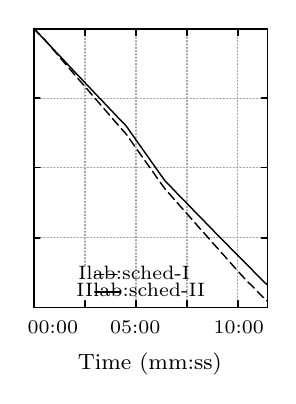
\begin{tikzpicture}[y=0.80pt, x=0.80pt, yscale=-0.494000, xscale=0.440000, inner sep=0pt, outer sep=0pt]
\scriptsize
\begin{scope}[draw=black,line join=bevel,line cap=rect,even odd rule,line width=0.512pt]
  \begin{scope}[cm={{1.0,0.0,0.0,1.0,(0.0,0.0)}},draw=black,line join=bevel,line cap=rect,line width=0.512pt]
  \end{scope}
  \begin{scope}[cm={{1.00625,0.0,0.0,1.00625,(0.0,0.0)}},draw=black,line join=bevel,line cap=rect,line width=0.512pt]
  \end{scope}
  \begin{scope}[cm={{1.00625,0.0,0.0,1.00625,(0.0,0.0)}},draw=ca0a0a4,dash pattern=on 0.40pt off 0.80pt,line join=round,line cap=round,line width=0.400pt]
    \path[draw] (60.5000,268.5000) -- (298.5000,268.5000);
  \end{scope}
  \begin{scope}[cm={{1.00625,0.0,0.0,1.00625,(0.0,0.0)}},draw=black,line join=round,line cap=round,line width=0.512pt]
    \path[draw] (60.5000,268.5000) -- (66.5000,268.5000);
    \path[draw] (298.5000,268.5000) -- (292.5000,268.5000);
  \end{scope}
  \begin{scope}[cm={{1.00625,0.0,0.0,1.00625,(0.0,0.0)}},draw=black,line join=bevel,line cap=rect,line width=0.512pt]
  \end{scope}
  \begin{scope}[cm={{1.00625,0.0,0.0,1.00625,(42.2625,276.216)}},draw=black,line join=bevel,line cap=rect,line width=0.512pt]
  \end{scope}
  \begin{scope}[cm={{1.00625,0.0,0.0,1.00625,(42.2625,276.216)}},draw=black,line join=bevel,line cap=rect,line width=0.512pt]
  \end{scope}
  \begin{scope}[cm={{1.00625,0.0,0.0,1.00625,(42.2625,276.216)}},draw=black,line join=bevel,line cap=rect,line width=0.512pt]
  \end{scope}
  \begin{scope}[cm={{1.00625,0.0,0.0,1.00625,(42.2625,276.216)}},draw=black,line join=bevel,line cap=rect,line width=0.512pt]
  \end{scope}
  \begin{scope}[cm={{1.00625,0.0,0.0,1.00625,(42.2625,276.216)}},draw=black,line join=bevel,line cap=rect,line width=0.512pt]
  \end{scope}
  \begin{scope}[cm={{1.00625,0.0,0.0,1.00625,(42.2625,276.216)}},draw=black,line join=bevel,line cap=rect,line width=0.512pt]
    %\path[fill=black] (0.0000,0.0000) node[above right] () {0};
  \end{scope}
  \begin{scope}[cm={{1.00625,0.0,0.0,1.00625,(42.2625,276.216)}},draw=black,line join=bevel,line cap=rect,line width=0.512pt]
  \end{scope}
  \begin{scope}[cm={{1.00625,0.0,0.0,1.00625,(0.0,0.0)}},draw=black,line join=bevel,line cap=rect,line width=0.512pt]
  \end{scope}
  \begin{scope}[cm={{1.00625,0.0,0.0,1.00625,(0.0,0.0)}},draw=ca0a0a4,dash pattern=on 0.40pt off 0.80pt,line join=round,line cap=round,line width=0.400pt]
    \path[draw] (60.5000,205.5000) -- (298.5000,205.5000);
  \end{scope}
  \begin{scope}[cm={{1.00625,0.0,0.0,1.00625,(0.0,0.0)}},draw=black,line join=round,line cap=round,line width=0.512pt]
    \path[draw] (60.5000,205.5000) -- (66.5000,205.5000);
    \path[draw] (298.5000,205.5000) -- (292.5000,205.5000);
  \end{scope}
  \begin{scope}[cm={{1.00625,0.0,0.0,1.00625,(0.0,0.0)}},draw=black,line join=bevel,line cap=rect,line width=0.512pt]
  \end{scope}
  \begin{scope}[cm={{1.00625,0.0,0.0,1.00625,(35.2188,211.816)}},draw=black,line join=bevel,line cap=rect,line width=0.512pt]
  \end{scope}
  \begin{scope}[cm={{1.00625,0.0,0.0,1.00625,(35.2188,211.816)}},draw=black,line join=bevel,line cap=rect,line width=0.512pt]
  \end{scope}
  \begin{scope}[cm={{1.00625,0.0,0.0,1.00625,(35.2188,211.816)}},draw=black,line join=bevel,line cap=rect,line width=0.512pt]
  \end{scope}
  \begin{scope}[cm={{1.00625,0.0,0.0,1.00625,(35.2188,211.816)}},draw=black,line join=bevel,line cap=rect,line width=0.512pt]
  \end{scope}
  \begin{scope}[cm={{1.00625,0.0,0.0,1.00625,(35.2188,211.816)}},draw=black,line join=bevel,line cap=rect,line width=0.512pt]
  \end{scope}
  \begin{scope}[cm={{1.00625,0.0,0.0,1.00625,(35.2188,211.816)}},draw=black,line join=bevel,line cap=rect,line width=0.512pt]
    %\path[fill=black] (0.0000,0.0000) node[above right] () {25};
  \end{scope}
  \begin{scope}[cm={{1.00625,0.0,0.0,1.00625,(35.2188,211.816)}},draw=black,line join=bevel,line cap=rect,line width=0.512pt]
  \end{scope}
  \begin{scope}[cm={{1.00625,0.0,0.0,1.00625,(0.0,0.0)}},draw=black,line join=bevel,line cap=rect,line width=0.512pt]
  \end{scope}
  \begin{scope}[cm={{1.00625,0.0,0.0,1.00625,(0.0,0.0)}},draw=ca0a0a4,dash pattern=on 0.40pt off 0.80pt,line join=round,line cap=round,line width=0.400pt]
    \path[draw] (60.5000,141.5000) -- (298.5000,141.5000);
  \end{scope}
  \begin{scope}[cm={{1.00625,0.0,0.0,1.00625,(0.0,0.0)}},draw=black,line join=round,line cap=round,line width=0.512pt]
    \path[draw] (60.5000,141.5000) -- (66.5000,141.5000);
    \path[draw] (298.5000,141.5000) -- (292.5000,141.5000);
  \end{scope}
  \begin{scope}[cm={{1.00625,0.0,0.0,1.00625,(0.0,0.0)}},draw=black,line join=bevel,line cap=rect,line width=0.512pt]
  \end{scope}
  \begin{scope}[cm={{1.00625,0.0,0.0,1.00625,(34.2125,148.422)}},draw=black,line join=bevel,line cap=rect,line width=0.512pt]
  \end{scope}
  \begin{scope}[cm={{1.00625,0.0,0.0,1.00625,(34.2125,148.422)}},draw=black,line join=bevel,line cap=rect,line width=0.512pt]
  \end{scope}
  \begin{scope}[cm={{1.00625,0.0,0.0,1.00625,(34.2125,148.422)}},draw=black,line join=bevel,line cap=rect,line width=0.512pt]
  \end{scope}
  \begin{scope}[cm={{1.00625,0.0,0.0,1.00625,(34.2125,148.422)}},draw=black,line join=bevel,line cap=rect,line width=0.512pt]
  \end{scope}
  \begin{scope}[cm={{1.00625,0.0,0.0,1.00625,(34.2125,148.422)}},draw=black,line join=bevel,line cap=rect,line width=0.512pt]
  \end{scope}
  \begin{scope}[cm={{1.00625,0.0,0.0,1.00625,(34.2125,148.422)}},draw=black,line join=bevel,line cap=rect,line width=0.512pt]
    %\path[fill=black] (0.0000,0.0000) node[above right] () {50};
  \end{scope}
  \begin{scope}[cm={{1.00625,0.0,0.0,1.00625,(34.2125,148.422)}},draw=black,line join=bevel,line cap=rect,line width=0.512pt]
  \end{scope}
  \begin{scope}[cm={{1.00625,0.0,0.0,1.00625,(0.0,0.0)}},draw=black,line join=bevel,line cap=rect,line width=0.512pt]
  \end{scope}
  \begin{scope}[cm={{1.00625,0.0,0.0,1.00625,(0.0,0.0)}},draw=ca0a0a4,dash pattern=on 0.40pt off 0.80pt,line join=round,line cap=round,line width=0.400pt]
    \path[draw] (60.5000,78.5000) -- (298.5000,78.5000);
  \end{scope}
  \begin{scope}[cm={{1.00625,0.0,0.0,1.00625,(0.0,0.0)}},draw=black,line join=round,line cap=round,line width=0.512pt]
    \path[draw] (60.5000,78.5000) -- (66.5000,78.5000);
    \path[draw] (298.5000,78.5000) -- (292.5000,78.5000);
  \end{scope}
  \begin{scope}[cm={{1.00625,0.0,0.0,1.00625,(0.0,0.0)}},draw=black,line join=bevel,line cap=rect,line width=0.512pt]
  \end{scope}
  \begin{scope}[cm={{1.00625,0.0,0.0,1.00625,(35.2188,85.0281)}},draw=black,line join=bevel,line cap=rect,line width=0.512pt]
  \end{scope}
  \begin{scope}[cm={{1.00625,0.0,0.0,1.00625,(35.2188,85.0281)}},draw=black,line join=bevel,line cap=rect,line width=0.512pt]
  \end{scope}
  \begin{scope}[cm={{1.00625,0.0,0.0,1.00625,(35.2188,85.0281)}},draw=black,line join=bevel,line cap=rect,line width=0.512pt]
  \end{scope}
  \begin{scope}[cm={{1.00625,0.0,0.0,1.00625,(35.2188,85.0281)}},draw=black,line join=bevel,line cap=rect,line width=0.512pt]
  \end{scope}
  \begin{scope}[cm={{1.00625,0.0,0.0,1.00625,(35.2188,85.0281)}},draw=black,line join=bevel,line cap=rect,line width=0.512pt]
  \end{scope}
  \begin{scope}[cm={{1.00625,0.0,0.0,1.00625,(35.2188,85.0281)}},draw=black,line join=bevel,line cap=rect,line width=0.512pt]
    %\path[fill=black] (0.0000,0.0000) node[above right] () {75};
  \end{scope}
  \begin{scope}[cm={{1.00625,0.0,0.0,1.00625,(35.2188,85.0281)}},draw=black,line join=bevel,line cap=rect,line width=0.512pt]
  \end{scope}
  \begin{scope}[cm={{1.00625,0.0,0.0,1.00625,(0.0,0.0)}},draw=black,line join=bevel,line cap=rect,line width=0.512pt]
  \end{scope}
  \begin{scope}[cm={{1.00625,0.0,0.0,1.00625,(0.0,0.0)}},draw=ca0a0a4,dash pattern=on 0.40pt off 0.80pt,line join=round,line cap=round,line width=0.400pt]
    \path[draw] (60.5000,15.5000) -- (298.5000,15.5000);
  \end{scope}
  \begin{scope}[cm={{1.00625,0.0,0.0,1.00625,(0.0,0.0)}},draw=black,line join=round,line cap=round,line width=0.512pt]
    \path[draw] (60.5000,15.5000) -- (66.5000,15.5000);
    \path[draw] (298.5000,15.5000) -- (292.5000,15.5000);
  \end{scope}
  \begin{scope}[cm={{1.00625,0.0,0.0,1.00625,(0.0,0.0)}},draw=black,line join=bevel,line cap=rect,line width=0.512pt]
  \end{scope}
  \begin{scope}[cm={{1.00625,0.0,0.0,1.00625,(26.1625,20.6281)}},draw=black,line join=bevel,line cap=rect,line width=0.512pt]
  \end{scope}
  \begin{scope}[cm={{1.00625,0.0,0.0,1.00625,(26.1625,20.6281)}},draw=black,line join=bevel,line cap=rect,line width=0.512pt]
  \end{scope}
  \begin{scope}[cm={{1.00625,0.0,0.0,1.00625,(26.1625,20.6281)}},draw=black,line join=bevel,line cap=rect,line width=0.512pt]
  \end{scope}
  \begin{scope}[cm={{1.00625,0.0,0.0,1.00625,(26.1625,20.6281)}},draw=black,line join=bevel,line cap=rect,line width=0.512pt]
  \end{scope}
  \begin{scope}[cm={{1.00625,0.0,0.0,1.00625,(26.1625,20.6281)}},draw=black,line join=bevel,line cap=rect,line width=0.512pt]
  \end{scope}
  \begin{scope}[cm={{1.00625,0.0,0.0,1.00625,(26.1625,20.6281)}},draw=black,line join=bevel,line cap=rect,line width=0.512pt]
    %\path[fill=black] (0.0000,0.0000) node[above right] () {100};
  \end{scope}
  \begin{scope}[cm={{1.00625,0.0,0.0,1.00625,(26.1625,20.6281)}},draw=black,line join=bevel,line cap=rect,line width=0.512pt]
  \end{scope}
  \begin{scope}[cm={{1.00625,0.0,0.0,1.00625,(0.0,0.0)}},draw=black,line join=bevel,line cap=rect,line width=0.512pt]
  \end{scope}
  \begin{scope}[cm={{1.00625,0.0,0.0,1.00625,(0.0,0.0)}},draw=ca0a0a4,dash pattern=on 0.40pt off 0.80pt,line join=round,line cap=round,line width=0.400pt]
    \path[draw] (60.5000,268.5000) -- (60.5000,15.5000);
  \end{scope}
  \begin{scope}[cm={{1.00625,0.0,0.0,1.00625,(0.0,0.0)}},draw=black,line join=round,line cap=round,line width=0.512pt]
    \path[draw] (60.5000,268.5000) -- (60.5000,262.5000);
    \path[draw] (60.5000,15.5000) -- (60.5000,21.5000);
  \end{scope}
  \begin{scope}[cm={{1.00625,0.0,0.0,1.00625,(0.0,0.0)}},draw=black,line join=bevel,line cap=rect,line width=0.512pt]
  \end{scope}
  \begin{scope}[cm={{1.00625,0.0,0.0,1.00625,(54.3375,294.328)}},draw=black,line join=bevel,line cap=rect,line width=0.512pt]
  \end{scope}
  \begin{scope}[cm={{1.00625,0.0,0.0,1.00625,(54.3375,294.328)}},draw=black,line join=bevel,line cap=rect,line width=0.512pt]
  \end{scope}
  \begin{scope}[cm={{1.00625,0.0,0.0,1.00625,(54.3375,294.328)}},draw=black,line join=bevel,line cap=rect,line width=0.512pt]
  \end{scope}
  \begin{scope}[cm={{1.00625,0.0,0.0,1.00625,(54.3375,294.328)}},draw=black,line join=bevel,line cap=rect,line width=0.512pt]
  \end{scope}
  \begin{scope}[cm={{1.00625,0.0,0.0,1.00625,(54.3375,294.328)}},draw=black,line join=bevel,line cap=rect,line width=0.512pt]
  \end{scope}
  \begin{scope}[cm={{1.00625,0.0,0.0,1.00625,(54.3375,294.328)}},draw=black,line join=bevel,line cap=rect,line width=0.512pt]
    \path[fill=black] (0.0000,0.0000) node[above right] () {00:00};
  \end{scope}
  \begin{scope}[cm={{1.00625,0.0,0.0,1.00625,(54.3375,294.328)}},draw=black,line join=bevel,line cap=rect,line width=0.512pt]
  \end{scope}
  \begin{scope}[cm={{1.00625,0.0,0.0,1.00625,(0.0,0.0)}},draw=black,line join=bevel,line cap=rect,line width=0.512pt]
  \end{scope}
  \begin{scope}[cm={{1.00625,0.0,0.0,1.00625,(0.0,0.0)}},draw=ca0a0a4,dash pattern=on 0.40pt off 0.80pt,line join=round,line cap=round,line width=0.400pt]
    \path[draw] (112.5000,268.5000) -- (112.5000,262.5000);
    \path[draw] (112.5000,230.5000) -- (112.5000,15.5000);
  \end{scope}
  \begin{scope}[cm={{1.00625,0.0,0.0,1.00625,(0.0,0.0)}},draw=black,line join=round,line cap=round,line width=0.512pt]
    \path[draw] (112.5000,268.5000) -- (112.5000,262.5000);
    \path[draw] (112.5000,15.5000) -- (112.5000,21.5000);
  \end{scope}
  \begin{scope}[cm={{1.00625,0.0,0.0,1.00625,(0.0,0.0)}},draw=black,line join=bevel,line cap=rect,line width=0.512pt]
  \end{scope}
  \begin{scope}[cm={{1.00625,0.0,0.0,1.00625,(106.663,294.328)}},draw=black,line join=bevel,line cap=rect,line width=0.512pt]
  \end{scope}
  \begin{scope}[cm={{1.00625,0.0,0.0,1.00625,(106.663,294.328)}},draw=black,line join=bevel,line cap=rect,line width=0.512pt]
  \end{scope}
  \begin{scope}[cm={{1.00625,0.0,0.0,1.00625,(106.663,294.328)}},draw=black,line join=bevel,line cap=rect,line width=0.512pt]
  \end{scope}
  \begin{scope}[cm={{1.00625,0.0,0.0,1.00625,(106.663,294.328)}},draw=black,line join=bevel,line cap=rect,line width=0.512pt]
  \end{scope}
  \begin{scope}[cm={{1.00625,0.0,0.0,1.00625,(106.663,294.328)}},draw=black,line join=bevel,line cap=rect,line width=0.512pt]
  \end{scope}
  \begin{scope}[cm={{1.00625,0.0,0.0,1.00625,(106.663,294.328)}},draw=black,line join=bevel,line cap=rect,line width=0.512pt]
    %\path[fill=black] (0.0000,0.0000) node[above right] () {02:30};
  \end{scope}
  \begin{scope}[cm={{1.00625,0.0,0.0,1.00625,(106.663,294.328)}},draw=black,line join=bevel,line cap=rect,line width=0.512pt]
  \end{scope}
  \begin{scope}[cm={{1.00625,0.0,0.0,1.00625,(0.0,0.0)}},draw=black,line join=bevel,line cap=rect,line width=0.512pt]
  \end{scope}
  \begin{scope}[cm={{1.00625,0.0,0.0,1.00625,(0.0,0.0)}},draw=ca0a0a4,dash pattern=on 0.40pt off 0.80pt,line join=round,line cap=round,line width=0.400pt]
    \path[draw] (164.5000,268.5000) -- (164.5000,15.5000);
  \end{scope}
  \begin{scope}[cm={{1.00625,0.0,0.0,1.00625,(0.0,0.0)}},draw=black,line join=round,line cap=round,line width=0.512pt]
    \path[draw] (164.5000,268.5000) -- (164.5000,262.5000);
    \path[draw] (164.5000,15.5000) -- (164.5000,21.5000);
  \end{scope}
  \begin{scope}[cm={{1.00625,0.0,0.0,1.00625,(0.0,0.0)}},draw=black,line join=bevel,line cap=rect,line width=0.512pt]
  \end{scope}
  \begin{scope}[cm={{1.00625,0.0,0.0,1.00625,(158.988,294.328)}},draw=black,line join=bevel,line cap=rect,line width=0.512pt]
  \end{scope}
  \begin{scope}[cm={{1.00625,0.0,0.0,1.00625,(158.988,294.328)}},draw=black,line join=bevel,line cap=rect,line width=0.512pt]
  \end{scope}
  \begin{scope}[cm={{1.00625,0.0,0.0,1.00625,(158.988,294.328)}},draw=black,line join=bevel,line cap=rect,line width=0.512pt]
  \end{scope}
  \begin{scope}[cm={{1.00625,0.0,0.0,1.00625,(158.988,294.328)}},draw=black,line join=bevel,line cap=rect,line width=0.512pt]
  \end{scope}
  \begin{scope}[cm={{1.00625,0.0,0.0,1.00625,(158.988,294.328)}},draw=black,line join=bevel,line cap=rect,line width=0.512pt]
  \end{scope}
  \begin{scope}[cm={{1.00625,0.0,0.0,1.00625,(138.988,294.328)}},draw=black,line join=bevel,line cap=rect,line width=0.512pt]
    \path[fill=black] (0.0000,0.0000) node[above right] () {05:00};
  \end{scope}
  \begin{scope}[cm={{1.00625,0.0,0.0,1.00625,(158.988,294.328)}},draw=black,line join=bevel,line cap=rect,line width=0.512pt]
  \end{scope}
  \begin{scope}[cm={{1.00625,0.0,0.0,1.00625,(0.0,0.0)}},draw=black,line join=bevel,line cap=rect,line width=0.512pt]
  \end{scope}
  \begin{scope}[cm={{1.00625,0.0,0.0,1.00625,(0.0,0.0)}},draw=ca0a0a4,dash pattern=on 0.40pt off 0.80pt,line join=round,line cap=round,line width=0.400pt]
    \path[draw] (216.5000,268.5000) -- (216.5000,15.5000);
  \end{scope}
  \begin{scope}[cm={{1.00625,0.0,0.0,1.00625,(0.0,0.0)}},draw=black,line join=round,line cap=round,line width=0.512pt]
    \path[draw] (216.5000,268.5000) -- (216.5000,262.5000);
    \path[draw] (216.5000,15.5000) -- (216.5000,21.5000);
  \end{scope}
  \begin{scope}[cm={{1.00625,0.0,0.0,1.00625,(0.0,0.0)}},draw=black,line join=bevel,line cap=rect,line width=0.512pt]
  \end{scope}
  \begin{scope}[cm={{1.00625,0.0,0.0,1.00625,(211.313,294.328)}},draw=black,line join=bevel,line cap=rect,line width=0.512pt]
  \end{scope}
  \begin{scope}[cm={{1.00625,0.0,0.0,1.00625,(211.313,294.328)}},draw=black,line join=bevel,line cap=rect,line width=0.512pt]
  \end{scope}
  \begin{scope}[cm={{1.00625,0.0,0.0,1.00625,(211.313,294.328)}},draw=black,line join=bevel,line cap=rect,line width=0.512pt]
  \end{scope}
  \begin{scope}[cm={{1.00625,0.0,0.0,1.00625,(211.313,294.328)}},draw=black,line join=bevel,line cap=rect,line width=0.512pt]
  \end{scope}
  \begin{scope}[cm={{1.00625,0.0,0.0,1.00625,(211.313,294.328)}},draw=black,line join=bevel,line cap=rect,line width=0.512pt]
  \end{scope}
  \begin{scope}[cm={{1.00625,0.0,0.0,1.00625,(211.313,294.328)}},draw=black,line join=bevel,line cap=rect,line width=0.512pt]
    %\path[fill=black] (0.0000,0.0000) node[above right] () {07:30};
  \end{scope}
  \begin{scope}[cm={{1.00625,0.0,0.0,1.00625,(211.313,294.328)}},draw=black,line join=bevel,line cap=rect,line width=0.512pt]
  \end{scope}
  \begin{scope}[cm={{1.00625,0.0,0.0,1.00625,(0.0,0.0)}},draw=black,line join=bevel,line cap=rect,line width=0.512pt]
  \end{scope}
  \begin{scope}[cm={{1.00625,0.0,0.0,1.00625,(0.0,0.0)}},draw=ca0a0a4,dash pattern=on 0.40pt off 0.80pt,line join=round,line cap=round,line width=0.400pt]
    \path[draw] (268.5000,268.5000) -- (268.5000,15.5000);
  \end{scope}
  \begin{scope}[cm={{1.00625,0.0,0.0,1.00625,(0.0,0.0)}},draw=black,line join=round,line cap=round,line width=0.512pt]
    \path[draw] (268.5000,268.5000) -- (268.5000,262.5000);
    \path[draw] (268.5000,15.5000) -- (268.5000,21.5000);
  \end{scope}
  \begin{scope}[cm={{1.00625,0.0,0.0,1.00625,(0.0,0.0)}},draw=black,line join=bevel,line cap=rect,line width=0.512pt]
  \end{scope}
  \begin{scope}[cm={{1.00625,0.0,0.0,1.00625,(263.134,294.328)}},draw=black,line join=bevel,line cap=rect,line width=0.512pt]
  \end{scope}
  \begin{scope}[cm={{1.00625,0.0,0.0,1.00625,(263.134,294.328)}},draw=black,line join=bevel,line cap=rect,line width=0.512pt]
  \end{scope}
  \begin{scope}[cm={{1.00625,0.0,0.0,1.00625,(263.134,294.328)}},draw=black,line join=bevel,line cap=rect,line width=0.512pt]
  \end{scope}
  \begin{scope}[cm={{1.00625,0.0,0.0,1.00625,(263.134,294.328)}},draw=black,line join=bevel,line cap=rect,line width=0.512pt]
  \end{scope}
  \begin{scope}[cm={{1.00625,0.0,0.0,1.00625,(263.134,294.328)}},draw=black,line join=bevel,line cap=rect,line width=0.512pt]
  \end{scope}
  \begin{scope}[cm={{1.00625,0.0,0.0,1.00625,(245.134,294.328)}},draw=black,line join=bevel,line cap=rect,line width=0.512pt]
    \path[fill=black] (0.0000,0.0000) node[above right] () {10:00};
  \end{scope}
  \begin{scope}[cm={{1.00625,0.0,0.0,1.00625,(263.134,294.328)}},draw=black,line join=bevel,line cap=rect,line width=0.512pt]
  \end{scope}
  \begin{scope}[cm={{1.00625,0.0,0.0,1.00625,(0.0,0.0)}},draw=black,line join=bevel,line cap=rect,line width=0.512pt]
  \end{scope}
  \begin{scope}[cm={{1.00625,0.0,0.0,1.00625,(0.0,0.0)}},draw=black,line join=round,line cap=round,line width=0.512pt]
    \path[draw] (60.5000,15.5000) -- (60.5000,268.5000) -- (298.5000,268.5000) --
      (298.5000,15.5000) -- (60.5000,15.5000);
  \end{scope}
  \begin{scope}[cm={{1.00625,0.0,0.0,1.00625,(0.0,0.0)}},draw=black,line join=bevel,line cap=rect,line width=0.512pt]
  \end{scope}
  \begin{scope}[cm={{0.0,-1.00625,1.00625,0.0,(18.6156,169.553)}},draw=black,line join=bevel,line cap=rect,line width=0.512pt]
  \end{scope}
  \begin{scope}[cm={{0.0,-1.00625,1.00625,0.0,(18.6156,169.553)}},draw=black,line join=bevel,line cap=rect,line width=0.512pt]
  \end{scope}
  \begin{scope}[cm={{0.0,-1.00625,1.00625,0.0,(18.6156,169.553)}},draw=black,line join=bevel,line cap=rect,line width=0.512pt]
  \end{scope}
  \begin{scope}[cm={{0.0,-1.00625,1.00625,0.0,(18.6156,169.553)}},draw=black,line join=bevel,line cap=rect,line width=0.512pt]
  \end{scope}
  \begin{scope}[cm={{0.0,-1.00625,1.00625,0.0,(18.6156,169.553)}},draw=black,line join=bevel,line cap=rect,line width=0.512pt]
  \end{scope}
  \begin{scope}[cm={{0.0,-1.00625,1.00625,0.0,(18.6156,169.553)}},draw=black,line join=bevel,line cap=rect,line width=0.512pt]
    %\path[fill=black] (0.0000,0.0000) node[above right] () {\rotatebox{90}{SoC (\%)}};
  \end{scope}
  \begin{scope}[cm={{0.0,-1.00625,1.00625,0.0,(18.6156,169.553)}},draw=black,line join=bevel,line cap=rect,line width=0.512pt]
  \end{scope}
  \begin{scope}[cm={{1.00625,0.0,0.0,1.00625,(137.856,317.472)}},draw=black,line join=bevel,line cap=rect,line width=0.512pt]
  \end{scope}
  \begin{scope}[cm={{1.00625,0.0,0.0,1.00625,(137.856,317.472)}},draw=black,line join=bevel,line cap=rect,line width=0.512pt]
  \end{scope}
  \begin{scope}[cm={{1.00625,0.0,0.0,1.00625,(137.856,317.472)}},draw=black,line join=bevel,line cap=rect,line width=0.512pt]
  \end{scope}
  \begin{scope}[cm={{1.00625,0.0,0.0,1.00625,(137.856,317.472)}},draw=black,line join=bevel,line cap=rect,line width=0.512pt]
  \end{scope}
  \begin{scope}[cm={{1.00625,0.0,0.0,1.00625,(137.856,317.472)}},draw=black,line join=bevel,line cap=rect,line width=0.512pt]
  \end{scope}
  \begin{scope}[cm={{1.00625,0.0,0.0,1.00625,(105.856,332.472)}},draw=black,line join=bevel,line cap=rect,line width=0.512pt]
    \path[fill=black] (0.0000,0.0000) node[above right] () {\footnotesize Time (mm:ss)};
  \end{scope}
  \begin{scope}[cm={{1.00625,0.0,0.0,1.00625,(137.856,317.472)}},draw=black,line join=bevel,line cap=rect,line width=0.512pt]
  \end{scope}
  \begin{scope}[cm={{1.00625,0.0,0.0,1.00625,(70.4375,244.519)}},draw=black,line join=bevel,line cap=rect,line width=0.512pt]
  \end{scope}
  \begin{scope}[cm={{1.00625,0.0,0.0,1.00625,(70.4375,244.519)}},draw=black,line join=bevel,line cap=rect,line width=0.512pt]
  \end{scope}
  \begin{scope}[cm={{1.00625,0.0,0.0,1.00625,(70.4375,244.519)}},draw=black,line join=bevel,line cap=rect,line width=0.512pt]
  \end{scope}
  \begin{scope}[cm={{1.00625,0.0,0.0,1.00625,(70.4375,244.519)}},draw=black,line join=bevel,line cap=rect,line width=0.512pt]
  \end{scope}
  \begin{scope}[cm={{1.00625,0.0,0.0,1.00625,(70.4375,244.519)}},draw=black,line join=bevel,line cap=rect,line width=0.512pt]
  \end{scope}
  \begin{scope}[cm={{1.00625,0.0,0.0,1.00625,(106.4375,244.519)}},draw=black,line join=bevel,line cap=rect,line width=0.512pt]
    \path[fill=black] (0.0000,0.0000) node[above right] () {\scriptsize \textlabel{I}{lab:sched-I}};
  \end{scope}
  \begin{scope}[cm={{1.00625,0.0,0.0,1.00625,(70.4375,244.519)}},draw=black,line join=bevel,line cap=rect,line width=0.512pt]
  \end{scope}
  \begin{scope}[cm={{1.00625,0.0,0.0,1.00625,(0.0,0.0)}},draw=black,line join=bevel,line cap=rect,line width=0.512pt]
  \end{scope}
  \begin{scope}[cm={{1.00625,0.0,0.0,1.00625,(0.0,0.0)}},draw=black,dash pattern=on 3.20pt off 1.60pt,line join=round,line cap=round,line width=0.512pt]
    \path[draw,even odd rule] (122.5000,238.5000) -- (148.5000,238.5000);
  \end{scope}
  \begin{scope}[cm={{1.00625,0.0,0.0,1.00625,(0.0,0.0)}},draw=black,line join=bevel,line cap=rect,line width=0.512pt]
  \end{scope}
  \begin{scope}[cm={{1.00625,0.0,0.0,1.00625,(0.0,0.0)}},draw=black,line join=bevel,line cap=rect,line width=0.512pt]
  \end{scope}
  \begin{scope}[cm={{1.00625,0.0,0.0,1.00625,(0.0,0.0)}},draw=black,line join=bevel,line cap=rect,line width=0.512pt]
  \end{scope}
  \begin{scope}[cm={{1.00625,0.0,0.0,1.00625,(0.0,0.0)}},draw=black,line join=bevel,line cap=rect,line width=0.512pt]
  \end{scope}
  \begin{scope}[cm={{1.00625,0.0,0.0,1.00625,(0.0,0.0)}},draw=black,dash pattern=on 3.20pt off 1.60pt,line join=round,line cap=round,line width=0.512pt]
    \path[draw] (60.5000,15.1000) -- (60.5000,15.1000) -- (61.4000,16.2000) --
      (63.9000,18.6000) -- (66.4000,20.9000) -- (68.8000,23.1000) --
      (71.2000,25.2000) -- (73.6000,27.7000) -- (76.0000,30.2000) --
      (78.4000,32.7000) -- (80.8000,35.2000) -- (83.2000,37.7000) --
      (85.6000,40.2000) -- (88.1000,42.8000) -- (90.5000,45.3000) --
      (92.9000,47.8000) -- (95.3000,50.3000) -- (97.7000,52.8000) --
      (100.1000,55.3000) -- (102.5000,57.8000) -- (104.9000,60.3000) --
      (107.4000,62.8000) -- (109.8000,65.3000) -- (112.2000,67.7000) --
      (114.6000,70.2000) -- (117.0000,72.7000) -- (119.4000,75.2000) --
      (121.8000,77.7000) -- (124.2000,80.2000) -- (126.6000,82.7000) --
      (129.1000,85.2000) -- (131.5000,87.7000) -- (133.9000,90.1000) --
      (136.3000,92.6000) -- (138.7000,95.1000) -- (141.1000,97.6000) --
      (143.5000,100.1000) -- (145.9000,102.5000) -- (148.4000,105.0000) --
      (150.8000,107.5000) -- (153.2000,109.8000) -- (155.6000,112.5000) --
      (158.0000,115.6000) -- (160.4000,118.6000) -- (162.8000,121.7000) --
      (165.2000,124.7000) -- (167.6000,127.7000) -- (170.1000,130.8000) --
      (172.5000,133.8000) -- (174.9000,136.9000) -- (177.3000,139.9000) --
      (179.7000,142.9000) -- (182.1000,145.9000) -- (184.5000,149.0000) --
      (186.9000,152.0000) -- (189.3000,155.0000) -- (191.8000,158.1000) --
      (194.2000,161.0000) -- (196.6000,163.4000) -- (199.0000,165.8000) --
      (201.4000,168.3000) -- (203.8000,170.7000) -- (206.2000,173.1000) --
      (208.6000,175.6000) -- (211.0000,178.0000) -- (213.5000,180.5000) --
      (215.9000,182.9000) -- (218.3000,185.3000) -- (220.7000,187.8000) --
      (223.1000,190.2000) -- (225.5000,192.6000) -- (227.9000,195.1000) --
      (230.3000,197.5000) -- (232.8000,199.9000) -- (235.2000,202.3000) --
      (237.6000,204.7000) -- (240.0000,207.2000) -- (242.4000,209.6000) --
      (244.8000,212.0000) -- (247.2000,214.4000) -- (249.6000,216.8000) --
      (252.0000,219.2000) -- (254.5000,221.6000) -- (256.9000,224.1000) --
      (259.3000,226.5000) -- (261.7000,228.9000) -- (264.1000,231.3000) --
      (266.5000,233.7000) -- (268.9000,236.1000) -- (271.3000,238.5000) --
      (273.8000,240.9000) -- (276.2000,243.3000) -- (278.6000,245.5000) --
      (281.0000,247.5000) -- (283.4000,249.6000) -- (285.8000,251.8000) --
      (288.2000,254.0000) -- (290.6000,256.1000) -- (293.0000,258.3000) --
      (295.5000,260.4000) -- (298.0000,262.7000);
  \end{scope}
  \begin{scope}[cm={{1.00625,0.0,0.0,1.00625,(0.0,0.0)}},draw=black,line join=bevel,line cap=rect,line width=0.512pt]
  \end{scope}
  \begin{scope}[cm={{1.00625,0.0,0.0,1.00625,(69.4313,260.619)}},draw=black,line join=bevel,line cap=rect,line width=0.512pt]
  \end{scope}
  \begin{scope}[cm={{1.00625,0.0,0.0,1.00625,(69.4313,260.619)}},draw=black,line join=bevel,line cap=rect,line width=0.512pt]
  \end{scope}
  \begin{scope}[cm={{1.00625,0.0,0.0,1.00625,(69.4313,260.619)}},draw=black,line join=bevel,line cap=rect,line width=0.512pt]
  \end{scope}
  \begin{scope}[cm={{1.00625,0.0,0.0,1.00625,(69.4313,260.619)}},draw=black,line join=bevel,line cap=rect,line width=0.512pt]
  \end{scope}
  \begin{scope}[cm={{1.00625,0.0,0.0,1.00625,(69.4313,260.619)}},draw=black,line join=bevel,line cap=rect,line width=0.512pt]
  \end{scope}
  \begin{scope}[cm={{1.00625,0.0,0.0,1.00625,(104.4313,260.619)}},draw=black,line join=bevel,line cap=rect,line width=0.512pt]
    \path[fill=black] (0.0000,0.0000) node[above right] () {\scriptsize \textlabel{II}{lab:sched-II}};
  \end{scope}
  \begin{scope}[cm={{1.00625,0.0,0.0,1.00625,(69.4313,260.619)}},draw=black,line join=bevel,line cap=rect,line width=0.512pt]
  \end{scope}
  \begin{scope}[cm={{1.00625,0.0,0.0,1.00625,(0.0,0.0)}},draw=black,line join=bevel,line cap=rect,line width=0.512pt]
  \end{scope}
  \begin{scope}[cm={{1.00625,0.0,0.0,1.00625,(0.0,0.0)}},draw=black,line join=round,line cap=round,line width=0.512pt]
    \path[draw,even odd rule] (122.5000,254.5000) -- (148.5000,254.5000);
  \end{scope}
  \begin{scope}[cm={{1.00625,0.0,0.0,1.00625,(0.0,0.0)}},draw=black,line join=bevel,line cap=rect,line width=0.512pt]
  \end{scope}
  \begin{scope}[cm={{1.00625,0.0,0.0,1.00625,(0.0,0.0)}},draw=black,line join=bevel,line cap=rect,line width=0.512pt]
  \end{scope}
  \begin{scope}[cm={{1.00625,0.0,0.0,1.00625,(0.0,0.0)}},draw=black,line join=bevel,line cap=rect,line width=0.512pt]
  \end{scope}
  \begin{scope}[cm={{1.00625,0.0,0.0,1.00625,(0.0,0.0)}},draw=black,line join=bevel,line cap=rect,line width=0.512pt]
  \end{scope}
  \begin{scope}[cm={{1.00625,0.0,0.0,1.00625,(0.0,0.0)}},draw=black,line join=round,line cap=round,line width=0.512pt]
    \path[draw] (60.5000,15.1000) -- (60.5000,15.1000) -- (61.4000,16.2000) --
      (63.9000,18.6000) -- (66.4000,20.9000) -- (68.8000,23.2000) --
      (71.2000,25.4000) -- (73.6000,27.7000) -- (76.0000,30.0000) --
      (78.4000,32.3000) -- (80.8000,34.6000) -- (83.2000,36.9000) --
      (85.6000,39.2000) -- (88.1000,41.4000) -- (90.5000,43.7000) --
      (92.9000,46.0000) -- (95.3000,48.3000) -- (97.7000,50.5000) --
      (100.1000,52.8000) -- (102.5000,55.1000) -- (104.9000,57.4000) --
      (107.4000,59.6000) -- (109.8000,61.9000) -- (112.2000,64.2000) --
      (114.6000,66.5000) -- (117.0000,68.7000) -- (119.4000,71.0000) --
      (121.8000,73.3000) -- (124.2000,75.5000) -- (126.6000,77.8000) --
      (129.1000,80.1000) -- (131.5000,82.3000) -- (133.9000,84.6000) --
      (136.3000,86.8000) -- (138.7000,89.1000) -- (141.1000,91.3000) --
      (143.5000,93.6000) -- (145.9000,95.9000) -- (148.4000,98.1000) --
      (150.8000,100.4000) -- (153.2000,102.5000) -- (155.6000,105.1000) --
      (158.0000,108.2000) -- (160.4000,111.3000) -- (162.8000,114.3000) --
      (165.2000,117.3000) -- (167.6000,120.4000) -- (170.1000,123.4000) --
      (172.5000,126.5000) -- (174.9000,129.5000) -- (177.3000,132.5000) --
      (179.7000,135.6000) -- (182.1000,138.6000) -- (184.5000,141.6000) --
      (186.9000,144.6000) -- (189.3000,147.7000) -- (191.8000,150.7000) --
      (194.2000,153.7000) -- (196.6000,155.9000) -- (199.0000,158.1000) --
      (201.4000,160.3000) -- (203.8000,162.6000) -- (206.2000,164.8000) --
      (208.6000,167.0000) -- (211.0000,169.2000) -- (213.5000,171.4000) --
      (215.9000,173.6000) -- (218.3000,175.8000) -- (220.7000,178.1000) --
      (223.1000,180.3000) -- (225.5000,182.5000) -- (227.9000,184.7000) --
      (230.3000,186.9000) -- (232.8000,189.1000) -- (235.2000,191.3000) --
      (237.6000,193.5000) -- (240.0000,195.7000) -- (242.4000,197.9000) --
      (244.8000,200.1000) -- (247.2000,202.3000) -- (249.6000,204.4000) --
      (252.0000,206.6000) -- (254.5000,208.8000) -- (256.9000,211.0000) --
      (259.3000,213.2000) -- (261.7000,215.4000) -- (264.1000,217.5000) --
      (266.5000,219.7000) -- (268.9000,221.9000) -- (271.3000,224.1000) --
      (273.8000,226.2000) -- (276.2000,228.4000) -- (278.6000,230.6000) --
      (281.0000,232.7000) -- (283.4000,234.9000) -- (285.8000,237.1000) --
      (288.2000,239.2000) -- (290.6000,241.4000) -- (293.0000,243.5000) --
      (295.5000,245.7000) -- (298.0000,247.9000);
  \end{scope}
  \begin{scope}[cm={{1.00625,0.0,0.0,1.00625,(0.0,0.0)}},draw=black,line join=bevel,line cap=rect,line width=0.512pt]
  \end{scope}
  \begin{scope}[cm={{1.00625,0.0,0.0,1.00625,(0.0,0.0)}},draw=black,line join=bevel,line cap=rect,line width=0.512pt]
  \end{scope}
  \begin{scope}[cm={{1.00625,0.0,0.0,1.00625,(0.0,0.0)}},draw=black,line join=round,line cap=round,line width=0.512pt]
    \path[draw] (60.5000,15.5000) -- (60.5000,268.5000) -- (298.5000,268.5000) --
      (298.5000,15.5000) -- (60.5000,15.5000);
  \end{scope}
  \begin{scope}[cm={{1.00625,0.0,0.0,1.00625,(0.0,0.0)}},draw=black,line join=bevel,line cap=rect,line width=0.512pt]
  \end{scope}
  \begin{scope}[cm={{1.0,0.0,0.0,1.0,(0.0,0.0)}},draw=black,line join=bevel,line cap=rect,line width=0.512pt]
  \end{scope}
\end{scope}
\end{tikzpicture}

    \caption{SoC-aware schedule}
    \label{fig:soc-schedule}
  \end{subfigure}
  \begin{subfigure}[t]{0.41\textwidth}
    \centering
    
\definecolor{cfefefe}{RGB}{254,254,254}
\definecolor{cf7f7f7}{RGB}{247,247,247}
\definecolor{cf0f0f0}{RGB}{240,240,240}
\definecolor{ceaeaea}{RGB}{234,234,234}
\definecolor{cf1f1f1}{RGB}{241,241,241}
\definecolor{ce3e3e3}{RGB}{227,227,227}
\definecolor{cececec}{RGB}{236,236,236}
\definecolor{ce5e5e5}{RGB}{229,229,229}
\definecolor{cdedede}{RGB}{222,222,222}
\definecolor{ce6e6e6}{RGB}{230,230,230}
\definecolor{cdfdfdf}{RGB}{223,223,223}
\definecolor{cd8d8d8}{RGB}{216,216,216}
\definecolor{ce1e1e1}{RGB}{225,225,225}
\definecolor{cdadada}{RGB}{218,218,218}
\definecolor{cd3d3d3}{RGB}{211,211,211}
\definecolor{cdbdbdb}{RGB}{219,219,219}
\definecolor{cd4d4d4}{RGB}{212,212,212}
\definecolor{ccdcdcd}{RGB}{205,205,205}
\definecolor{cc6c6c6}{RGB}{198,198,198}
\definecolor{ccecece}{RGB}{206,206,206}
\definecolor{cc7c7c7}{RGB}{199,199,199}
\definecolor{cc0c0c0}{RGB}{192,192,192}
\definecolor{ccacaca}{RGB}{202,202,202}
\definecolor{cc3c3c3}{RGB}{195,195,195}
\definecolor{cbcbcbc}{RGB}{188,188,188}
\definecolor{cc9c9c9}{RGB}{201,201,201}
\definecolor{cc2c2c2}{RGB}{194,194,194}
\definecolor{cbbbbbb}{RGB}{187,187,187}
\definecolor{cc8c8c8}{RGB}{200,200,200}
\definecolor{cc1c1c1}{RGB}{193,193,193}
\definecolor{cbababa}{RGB}{186,186,186}
\definecolor{ce0e0e0}{RGB}{224,224,224}
\definecolor{caeaeae}{RGB}{174,174,174}
\definecolor{ca7a7a7}{RGB}{167,167,167}
\definecolor{ca1a1a1}{RGB}{161,161,161}
\definecolor{cb5b5b5}{RGB}{181,181,181}
\definecolor{c9c9c9c}{RGB}{156,156,156}
\definecolor{cafafaf}{RGB}{175,175,175}
\definecolor{c969696}{RGB}{150,150,150}
\definecolor{caaaaaa}{RGB}{170,170,170}
\definecolor{c919191}{RGB}{145,145,145}
\definecolor{cbdbdbd}{RGB}{189,189,189}
\definecolor{ca4a4a4}{RGB}{164,164,164}
\definecolor{c8b8b8b}{RGB}{139,139,139}
\definecolor{cb6b6b6}{RGB}{182,182,182}
\definecolor{c9d9d9d}{RGB}{157,157,157}
\definecolor{c848484}{RGB}{132,132,132}
\definecolor{cb0b0b0}{RGB}{176,176,176}
\definecolor{c979797}{RGB}{151,151,151}
\definecolor{c7e7e7e}{RGB}{126,126,126}
\definecolor{cacacac}{RGB}{172,172,172}
\definecolor{c939393}{RGB}{147,147,147}
\definecolor{c7a7a7a}{RGB}{122,122,122}
\definecolor{cababab}{RGB}{171,171,171}
\definecolor{c929292}{RGB}{146,146,146}
\definecolor{c797979}{RGB}{121,121,121}
\definecolor{c787878}{RGB}{120,120,120}
\definecolor{c9a9a9a}{RGB}{154,154,154}
\definecolor{c7b7b7b}{RGB}{123,123,123}
\definecolor{c757575}{RGB}{117,117,117}
\definecolor{c8d8d8d}{RGB}{141,141,141}
\definecolor{c6f6f6f}{RGB}{111,111,111}
\definecolor{c888888}{RGB}{136,136,136}
\definecolor{c696969}{RGB}{105,105,105}
\definecolor{c828282}{RGB}{130,130,130}
\definecolor{c737373}{RGB}{115,115,115}
\definecolor{c646464}{RGB}{100,100,100}
\definecolor{c7d7d7d}{RGB}{125,125,125}
\definecolor{c6e6e6e}{RGB}{110,110,110}
\definecolor{c5e5e5e}{RGB}{94,94,94}
\definecolor{c777777}{RGB}{119,119,119}
\definecolor{c686868}{RGB}{104,104,104}
\definecolor{c595959}{RGB}{89,89,89}
\definecolor{c707070}{RGB}{112,112,112}
\definecolor{c616161}{RGB}{97,97,97}
\definecolor{c525252}{RGB}{82,82,82}
\definecolor{c6a6a6a}{RGB}{106,106,106}
\definecolor{c5b5b5b}{RGB}{91,91,91}
\definecolor{c4c4c4c}{RGB}{76,76,76}
\definecolor{c666666}{RGB}{102,102,102}
\definecolor{c575757}{RGB}{87,87,87}
\definecolor{c484848}{RGB}{72,72,72}
\definecolor{c656565}{RGB}{101,101,101}
\definecolor{c565656}{RGB}{86,86,86}
\definecolor{c474747}{RGB}{71,71,71}
\definecolor{c555555}{RGB}{85,85,85}
\definecolor{c454545}{RGB}{69,69,69}
\definecolor{ca0a0a4}{RGB}{160,160,164}
\definecolor{c020202}{RGB}{2,2,2}
\definecolor{c040404}{RGB}{4,4,4}
\definecolor{c060606}{RGB}{6,6,6}
\definecolor{c080808}{RGB}{8,8,8}
\definecolor{c0a0a0a}{RGB}{10,10,10}
\definecolor{c0c0c0c}{RGB}{12,12,12}
\definecolor{c0e0e0e}{RGB}{14,14,14}
\definecolor{c101010}{RGB}{16,16,16}
\definecolor{c121212}{RGB}{18,18,18}
\definecolor{c141414}{RGB}{20,20,20}
\definecolor{c161616}{RGB}{22,22,22}
\definecolor{c181818}{RGB}{24,24,24}
\definecolor{c1a1a1a}{RGB}{26,26,26}
\definecolor{c1c1c1c}{RGB}{28,28,28}
\definecolor{c1e1e1e}{RGB}{30,30,30}
\definecolor{c202020}{RGB}{32,32,32}
\definecolor{c222222}{RGB}{34,34,34}
\definecolor{c242424}{RGB}{36,36,36}
\definecolor{c262626}{RGB}{38,38,38}
\definecolor{c282828}{RGB}{40,40,40}
\definecolor{c2a2a2a}{RGB}{42,42,42}
\definecolor{c2c2c2c}{RGB}{44,44,44}
\definecolor{c2e2e2e}{RGB}{46,46,46}
\definecolor{c303030}{RGB}{48,48,48}
\definecolor{c323232}{RGB}{50,50,50}
\definecolor{c343434}{RGB}{52,52,52}
\definecolor{c363636}{RGB}{54,54,54}
\definecolor{c383838}{RGB}{56,56,56}
\definecolor{c3a3a3a}{RGB}{58,58,58}
\definecolor{c3c3c3c}{RGB}{60,60,60}
\definecolor{c3e3e3e}{RGB}{62,62,62}
\definecolor{c404040}{RGB}{64,64,64}
\definecolor{c424242}{RGB}{66,66,66}
\definecolor{c444444}{RGB}{68,68,68}
\definecolor{c464646}{RGB}{70,70,70}
\definecolor{c4a4a4a}{RGB}{74,74,74}
\definecolor{c4e4e4e}{RGB}{78,78,78}
\definecolor{c505050}{RGB}{80,80,80}
\definecolor{c545454}{RGB}{84,84,84}
\definecolor{c585858}{RGB}{88,88,88}
\definecolor{c5a5a5a}{RGB}{90,90,90}
\definecolor{c5c5c5c}{RGB}{92,92,92}
\definecolor{c606060}{RGB}{96,96,96}
\definecolor{c626262}{RGB}{98,98,98}
\definecolor{c6c6c6c}{RGB}{108,108,108}
\definecolor{c727272}{RGB}{114,114,114}
\definecolor{c747474}{RGB}{116,116,116}
\definecolor{c767676}{RGB}{118,118,118}
\definecolor{c7c7c7c}{RGB}{124,124,124}
\definecolor{c808080}{RGB}{128,128,128}
\definecolor{c868686}{RGB}{134,134,134}
\definecolor{c8a8a8a}{RGB}{138,138,138}
\definecolor{c8c8c8c}{RGB}{140,140,140}
\definecolor{c8e8e8e}{RGB}{142,142,142}
\definecolor{c909090}{RGB}{144,144,144}
\definecolor{c949494}{RGB}{148,148,148}
\definecolor{c989898}{RGB}{152,152,152}
\definecolor{c9e9e9e}{RGB}{158,158,158}
\definecolor{ca0a0a0}{RGB}{160,160,160}
\definecolor{ca2a2a2}{RGB}{162,162,162}
\definecolor{ca6a6a6}{RGB}{166,166,166}
\definecolor{ca8a8a8}{RGB}{168,168,168}
\definecolor{cb2b2b2}{RGB}{178,178,178}
\definecolor{cb4b4b4}{RGB}{180,180,180}
\definecolor{cb8b8b8}{RGB}{184,184,184}
\definecolor{cbebebe}{RGB}{190,190,190}
\definecolor{cc4c4c4}{RGB}{196,196,196}
\definecolor{ccccccc}{RGB}{204,204,204}
\definecolor{cd0d0d0}{RGB}{208,208,208}
\definecolor{cd2d2d2}{RGB}{210,210,210}
\definecolor{cd6d6d6}{RGB}{214,214,214}
\definecolor{cdcdcdc}{RGB}{220,220,220}
\definecolor{ce2e2e2}{RGB}{226,226,226}
\definecolor{ce4e4e4}{RGB}{228,228,228}
\definecolor{ce8e8e8}{RGB}{232,232,232}
\definecolor{ceeeeee}{RGB}{238,238,238}
\definecolor{cf2f2f2}{RGB}{242,242,242}
\definecolor{cf4f4f4}{RGB}{244,244,244}
\definecolor{cf6f6f6}{RGB}{246,246,246}
\definecolor{cf8f8f8}{RGB}{248,248,248}
\definecolor{cfafafa}{RGB}{250,250,250}
\definecolor{cfcfcfc}{RGB}{252,252,252}
\scriptsize
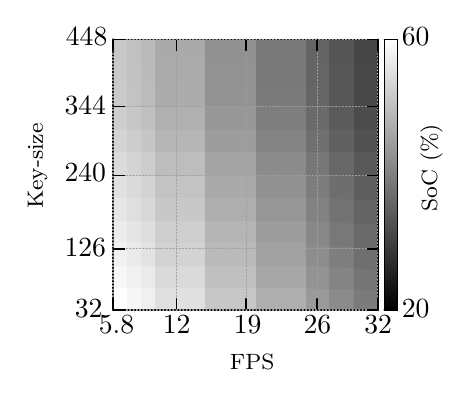
\begin{tikzpicture}[baseline={(0,-5.08)},y=0.80pt, x=0.80pt, yscale=-0.560000, xscale=0.580000, inner sep=0pt, outer sep=0pt]
\begin{scope}[draw=black,line join=bevel,line cap=rect,even odd rule,line width=0.512pt]
  \begin{scope}[cm={{1.0,0.0,0.0,1.0,(0.0,0.0)}},draw=black,line join=bevel,line cap=rect,line width=0.512pt]
  \end{scope}
  \begin{scope}[cm={{1.00625,0.0,0.0,1.00625,(0.0,0.0)}},draw=black,line join=bevel,line cap=rect,line width=0.512pt]
  \end{scope}
  \begin{scope}[cm={{1.00625,0.0,0.0,1.00625,(0.0,0.0)}},draw=black,line join=bevel,line cap=rect,line width=0.512pt]
  \end{scope}
  \begin{scope}[cm={{1.00625,0.0,0.0,1.00625,(0.0,0.0)}},draw=black,line join=bevel,line cap=rect,line width=0.512pt]
  \end{scope}
  \begin{scope}[cm={{1.00625,0.0,0.0,1.00625,(0.0,0.0)}},draw=cfefefe,fill=cfefefe,line join=bevel,line cap=rect,line width=0.512pt]
    \path[draw,fill,even odd rule] (57.5000,268.5000) -- (57.5000,250.5000) --
      (68.5000,250.5000) -- (68.5000,268.5000) -- (57.5000,268.5000);
  \end{scope}
  \begin{scope}[cm={{1.00625,0.0,0.0,1.00625,(0.0,0.0)}},draw=cf7f7f7,fill=cf7f7f7,line join=bevel,line cap=rect,line width=0.512pt]
    \path[draw,fill,even odd rule] (68.5000,268.5000) -- (68.5000,250.5000) --
      (79.5000,250.5000) -- (79.5000,268.5000) -- (68.5000,268.5000);
  \end{scope}
  \begin{scope}[cm={{1.00625,0.0,0.0,1.00625,(0.0,0.0)}},draw=cf0f0f0,fill=cf0f0f0,line join=bevel,line cap=rect,line width=0.512pt]
    \path[draw,fill,even odd rule] (79.5000,268.5000) -- (79.5000,250.5000) --
      (90.5000,250.5000) -- (90.5000,268.5000) -- (79.5000,268.5000);
  \end{scope}
  \begin{scope}[cm={{1.00625,0.0,0.0,1.00625,(0.0,0.0)}},draw=cf7f7f7,fill=cf7f7f7,line join=bevel,line cap=rect,line width=0.512pt]
    \path[draw,fill,even odd rule] (57.5000,250.5000) -- (57.5000,232.5000) --
      (68.5000,232.5000) -- (68.5000,250.5000) -- (57.5000,250.5000);
  \end{scope}
  \begin{scope}[cm={{1.00625,0.0,0.0,1.00625,(0.0,0.0)}},draw=cf0f0f0,fill=cf0f0f0,line join=bevel,line cap=rect,line width=0.512pt]
    \path[draw,fill,even odd rule] (68.5000,250.5000) -- (68.5000,232.5000) --
      (79.5000,232.5000) -- (79.5000,250.5000) -- (68.5000,250.5000);
  \end{scope}
  \begin{scope}[cm={{1.00625,0.0,0.0,1.00625,(0.0,0.0)}},draw=ceaeaea,fill=ceaeaea,line join=bevel,line cap=rect,line width=0.512pt]
    \path[draw,fill,even odd rule] (79.5000,250.5000) -- (79.5000,232.5000) --
      (90.5000,232.5000) -- (90.5000,250.5000) -- (79.5000,250.5000);
  \end{scope}
  \begin{scope}[cm={{1.00625,0.0,0.0,1.00625,(0.0,0.0)}},draw=cf1f1f1,fill=cf1f1f1,line join=bevel,line cap=rect,line width=0.512pt]
    \path[draw,fill,even odd rule] (57.5000,232.5000) -- (57.5000,214.5000) --
      (68.5000,214.5000) -- (68.5000,232.5000) -- (57.5000,232.5000);
  \end{scope}
  \begin{scope}[cm={{1.00625,0.0,0.0,1.00625,(0.0,0.0)}},draw=ceaeaea,fill=ceaeaea,line join=bevel,line cap=rect,line width=0.512pt]
    \path[draw,fill,even odd rule] (68.5000,232.5000) -- (68.5000,214.5000) --
      (79.5000,214.5000) -- (79.5000,232.5000) -- (68.5000,232.5000);
  \end{scope}
  \begin{scope}[cm={{1.00625,0.0,0.0,1.00625,(0.0,0.0)}},draw=ce3e3e3,fill=ce3e3e3,line join=bevel,line cap=rect,line width=0.512pt]
    \path[draw,fill,even odd rule] (79.5000,232.5000) -- (79.5000,214.5000) --
      (90.5000,214.5000) -- (90.5000,232.5000) -- (79.5000,232.5000);
  \end{scope}
  \begin{scope}[cm={{1.00625,0.0,0.0,1.00625,(0.0,0.0)}},draw=cececec,fill=cececec,line join=bevel,line cap=rect,line width=0.512pt]
    \path[draw,fill,even odd rule] (57.5000,214.5000) -- (57.5000,196.5000) --
      (68.5000,196.5000) -- (68.5000,214.5000) -- (57.5000,214.5000);
  \end{scope}
  \begin{scope}[cm={{1.00625,0.0,0.0,1.00625,(0.0,0.0)}},draw=ce5e5e5,fill=ce5e5e5,line join=bevel,line cap=rect,line width=0.512pt]
    \path[draw,fill,even odd rule] (68.5000,214.5000) -- (68.5000,196.5000) --
      (79.5000,196.5000) -- (79.5000,214.5000) -- (68.5000,214.5000);
  \end{scope}
  \begin{scope}[cm={{1.00625,0.0,0.0,1.00625,(0.0,0.0)}},draw=cdedede,fill=cdedede,line join=bevel,line cap=rect,line width=0.512pt]
    \path[draw,fill,even odd rule] (79.5000,214.5000) -- (79.5000,196.5000) --
      (90.5000,196.5000) -- (90.5000,214.5000) -- (79.5000,214.5000);
  \end{scope}
  \begin{scope}[cm={{1.00625,0.0,0.0,1.00625,(0.0,0.0)}},draw=ce6e6e6,fill=ce6e6e6,line join=bevel,line cap=rect,line width=0.512pt]
    \path[draw,fill,even odd rule] (57.5000,196.5000) -- (57.5000,178.5000) --
      (68.5000,178.5000) -- (68.5000,196.5000) -- (57.5000,196.5000);
  \end{scope}
  \begin{scope}[cm={{1.00625,0.0,0.0,1.00625,(0.0,0.0)}},draw=cdfdfdf,fill=cdfdfdf,line join=bevel,line cap=rect,line width=0.512pt]
    \path[draw,fill,even odd rule] (68.5000,196.5000) -- (68.5000,178.5000) --
      (79.5000,178.5000) -- (79.5000,196.5000) -- (68.5000,196.5000);
  \end{scope}
  \begin{scope}[cm={{1.00625,0.0,0.0,1.00625,(0.0,0.0)}},draw=cd8d8d8,fill=cd8d8d8,line join=bevel,line cap=rect,line width=0.512pt]
    \path[draw,fill,even odd rule] (79.5000,196.5000) -- (79.5000,178.5000) --
      (90.5000,178.5000) -- (90.5000,196.5000) -- (79.5000,196.5000);
  \end{scope}
  \begin{scope}[cm={{1.00625,0.0,0.0,1.00625,(0.0,0.0)}},draw=ce1e1e1,fill=ce1e1e1,line join=bevel,line cap=rect,line width=0.512pt]
    \path[draw,fill,even odd rule] (57.5000,178.5000) -- (57.5000,160.5000) --
      (68.5000,160.5000) -- (68.5000,178.5000) -- (57.5000,178.5000);
  \end{scope}
  \begin{scope}[cm={{1.00625,0.0,0.0,1.00625,(0.0,0.0)}},draw=cdadada,fill=cdadada,line join=bevel,line cap=rect,line width=0.512pt]
    \path[draw,fill,even odd rule] (68.5000,178.5000) -- (68.5000,160.5000) --
      (79.5000,160.5000) -- (79.5000,178.5000) -- (68.5000,178.5000);
  \end{scope}
  \begin{scope}[cm={{1.00625,0.0,0.0,1.00625,(0.0,0.0)}},draw=cd3d3d3,fill=cd3d3d3,line join=bevel,line cap=rect,line width=0.512pt]
    \path[draw,fill,even odd rule] (79.5000,178.5000) -- (79.5000,160.5000) --
      (90.5000,160.5000) -- (90.5000,178.5000) -- (79.5000,178.5000);
  \end{scope}
  \begin{scope}[cm={{1.00625,0.0,0.0,1.00625,(0.0,0.0)}},draw=cdbdbdb,fill=cdbdbdb,line join=bevel,line cap=rect,line width=0.512pt]
    \path[draw,fill,even odd rule] (57.5000,160.5000) -- (57.5000,141.5000) --
      (68.5000,141.5000) -- (68.5000,160.5000) -- (57.5000,160.5000);
  \end{scope}
  \begin{scope}[cm={{1.00625,0.0,0.0,1.00625,(0.0,0.0)}},draw=cd4d4d4,fill=cd4d4d4,line join=bevel,line cap=rect,line width=0.512pt]
    \path[draw,fill,even odd rule] (68.5000,160.5000) -- (68.5000,141.5000) --
      (79.5000,141.5000) -- (79.5000,160.5000) -- (68.5000,160.5000);
  \end{scope}
  \begin{scope}[cm={{1.00625,0.0,0.0,1.00625,(0.0,0.0)}},draw=ccdcdcd,fill=ccdcdcd,line join=bevel,line cap=rect,line width=0.512pt]
    \path[draw,fill,even odd rule] (79.5000,160.5000) -- (79.5000,141.5000) --
      (90.5000,141.5000) -- (90.5000,160.5000) -- (79.5000,160.5000);
  \end{scope}
  \begin{scope}[cm={{1.00625,0.0,0.0,1.00625,(0.0,0.0)}},draw=cd4d4d4,fill=cd4d4d4,line join=bevel,line cap=rect,line width=0.512pt]
    \path[draw,fill,even odd rule] (57.5000,141.5000) -- (57.5000,123.5000) --
      (68.5000,123.5000) -- (68.5000,141.5000) -- (57.5000,141.5000);
  \end{scope}
  \begin{scope}[cm={{1.00625,0.0,0.0,1.00625,(0.0,0.0)}},draw=ccdcdcd,fill=ccdcdcd,line join=bevel,line cap=rect,line width=0.512pt]
    \path[draw,fill,even odd rule] (68.5000,141.5000) -- (68.5000,123.5000) --
      (79.5000,123.5000) -- (79.5000,141.5000) -- (68.5000,141.5000);
  \end{scope}
  \begin{scope}[cm={{1.00625,0.0,0.0,1.00625,(0.0,0.0)}},draw=cc6c6c6,fill=cc6c6c6,line join=bevel,line cap=rect,line width=0.512pt]
    \path[draw,fill,even odd rule] (79.5000,141.5000) -- (79.5000,123.5000) --
      (90.5000,123.5000) -- (90.5000,141.5000) -- (79.5000,141.5000);
  \end{scope}
  \begin{scope}[cm={{1.00625,0.0,0.0,1.00625,(0.0,0.0)}},draw=ccecece,fill=ccecece,line join=bevel,line cap=rect,line width=0.512pt]
    \path[draw,fill,even odd rule] (57.5000,123.5000) -- (57.5000,105.5000) --
      (68.5000,105.5000) -- (68.5000,123.5000) -- (57.5000,123.5000);
  \end{scope}
  \begin{scope}[cm={{1.00625,0.0,0.0,1.00625,(0.0,0.0)}},draw=cc7c7c7,fill=cc7c7c7,line join=bevel,line cap=rect,line width=0.512pt]
    \path[draw,fill,even odd rule] (68.5000,123.5000) -- (68.5000,105.5000) --
      (79.5000,105.5000) -- (79.5000,123.5000) -- (68.5000,123.5000);
  \end{scope}
  \begin{scope}[cm={{1.00625,0.0,0.0,1.00625,(0.0,0.0)}},draw=cc0c0c0,fill=cc0c0c0,line join=bevel,line cap=rect,line width=0.512pt]
    \path[draw,fill,even odd rule] (79.5000,123.5000) -- (79.5000,105.5000) --
      (90.5000,105.5000) -- (90.5000,123.5000) -- (79.5000,123.5000);
  \end{scope}
  \begin{scope}[cm={{1.00625,0.0,0.0,1.00625,(0.0,0.0)}},draw=ccacaca,fill=ccacaca,line join=bevel,line cap=rect,line width=0.512pt]
    \path[draw,fill,even odd rule] (57.5000,105.5000) -- (57.5000,87.5000) --
      (68.5000,87.5000) -- (68.5000,105.5000) -- (57.5000,105.5000);
  \end{scope}
  \begin{scope}[cm={{1.00625,0.0,0.0,1.00625,(0.0,0.0)}},draw=cc3c3c3,fill=cc3c3c3,line join=bevel,line cap=rect,line width=0.512pt]
    \path[draw,fill,even odd rule] (68.5000,105.5000) -- (68.5000,87.5000) --
      (79.5000,87.5000) -- (79.5000,105.5000) -- (68.5000,105.5000);
  \end{scope}
  \begin{scope}[cm={{1.00625,0.0,0.0,1.00625,(0.0,0.0)}},draw=cbcbcbc,fill=cbcbcbc,line join=bevel,line cap=rect,line width=0.512pt]
    \path[draw,fill,even odd rule] (79.5000,105.5000) -- (79.5000,87.5000) --
      (90.5000,87.5000) -- (90.5000,105.5000) -- (79.5000,105.5000);
  \end{scope}
  \begin{scope}[cm={{1.00625,0.0,0.0,1.00625,(0.0,0.0)}},draw=cc9c9c9,fill=cc9c9c9,line join=bevel,line cap=rect,line width=0.512pt]
    \path[draw,fill,even odd rule] (57.5000,87.5000) -- (57.5000,69.5000) --
      (68.5000,69.5000) -- (68.5000,87.5000) -- (57.5000,87.5000);
  \end{scope}
  \begin{scope}[cm={{1.00625,0.0,0.0,1.00625,(0.0,0.0)}},draw=cc2c2c2,fill=cc2c2c2,line join=bevel,line cap=rect,line width=0.512pt]
    \path[draw,fill,even odd rule] (68.5000,87.5000) -- (68.5000,69.5000) --
      (79.5000,69.5000) -- (79.5000,87.5000) -- (68.5000,87.5000);
  \end{scope}
  \begin{scope}[cm={{1.00625,0.0,0.0,1.00625,(0.0,0.0)}},draw=cbbbbbb,fill=cbbbbbb,line join=bevel,line cap=rect,line width=0.512pt]
    \path[draw,fill,even odd rule] (79.5000,87.5000) -- (79.5000,69.5000) --
      (90.5000,69.5000) -- (90.5000,87.5000) -- (79.5000,87.5000);
  \end{scope}
  \begin{scope}[cm={{1.00625,0.0,0.0,1.00625,(0.0,0.0)}},draw=cc8c8c8,fill=cc8c8c8,line join=bevel,line cap=rect,line width=0.512pt]
    \path[draw,fill,even odd rule] (57.5000,69.5000) -- (57.5000,51.5000) --
      (68.5000,51.5000) -- (68.5000,69.5000) -- (57.5000,69.5000);
  \end{scope}
  \begin{scope}[cm={{1.00625,0.0,0.0,1.00625,(0.0,0.0)}},draw=cc1c1c1,fill=cc1c1c1,line join=bevel,line cap=rect,line width=0.512pt]
    \path[draw,fill,even odd rule] (68.5000,69.5000) -- (68.5000,51.5000) --
      (79.5000,51.5000) -- (79.5000,69.5000) -- (68.5000,69.5000);
  \end{scope}
  \begin{scope}[cm={{1.00625,0.0,0.0,1.00625,(0.0,0.0)}},draw=cbababa,fill=cbababa,line join=bevel,line cap=rect,line width=0.512pt]
    \path[draw,fill,even odd rule] (79.5000,69.5000) -- (79.5000,51.5000) --
      (90.5000,51.5000) -- (90.5000,69.5000) -- (79.5000,69.5000);
  \end{scope}
  \begin{scope}[cm={{1.00625,0.0,0.0,1.00625,(0.0,0.0)}},draw=ce0e0e0,fill=ce0e0e0,line join=bevel,line cap=rect,line width=0.512pt]
    \path[draw,fill,even odd rule] (90.5000,268.5000) -- (90.5000,250.5000) --
      (129.5000,250.5000) -- (129.5000,268.5000) -- (90.5000,268.5000);
  \end{scope}
  \begin{scope}[cm={{1.00625,0.0,0.0,1.00625,(0.0,0.0)}},draw=cc7c7c7,fill=cc7c7c7,line join=bevel,line cap=rect,line width=0.512pt]
    \path[draw,fill,even odd rule] (129.5000,268.5000) -- (129.5000,250.5000) --
      (168.5000,250.5000) -- (168.5000,268.5000) -- (129.5000,268.5000);
  \end{scope}
  \begin{scope}[cm={{1.00625,0.0,0.0,1.00625,(0.0,0.0)}},draw=caeaeae,fill=caeaeae,line join=bevel,line cap=rect,line width=0.512pt]
    \path[draw,fill,even odd rule] (168.5000,268.5000) -- (168.5000,250.5000) --
      (207.5000,250.5000) -- (207.5000,268.5000) -- (168.5000,268.5000);
  \end{scope}
  \begin{scope}[cm={{1.00625,0.0,0.0,1.00625,(0.0,0.0)}},draw=cdadada,fill=cdadada,line join=bevel,line cap=rect,line width=0.512pt]
    \path[draw,fill,even odd rule] (90.5000,250.5000) -- (90.5000,232.5000) --
      (129.5000,232.5000) -- (129.5000,250.5000) -- (90.5000,250.5000);
  \end{scope}
  \begin{scope}[cm={{1.00625,0.0,0.0,1.00625,(0.0,0.0)}},draw=cc0c0c0,fill=cc0c0c0,line join=bevel,line cap=rect,line width=0.512pt]
    \path[draw,fill,even odd rule] (129.5000,250.5000) -- (129.5000,232.5000) --
      (168.5000,232.5000) -- (168.5000,250.5000) -- (129.5000,250.5000);
  \end{scope}
  \begin{scope}[cm={{1.00625,0.0,0.0,1.00625,(0.0,0.0)}},draw=ca7a7a7,fill=ca7a7a7,line join=bevel,line cap=rect,line width=0.512pt]
    \path[draw,fill,even odd rule] (168.5000,250.5000) -- (168.5000,232.5000) --
      (207.5000,232.5000) -- (207.5000,250.5000) -- (168.5000,250.5000);
  \end{scope}
  \begin{scope}[cm={{1.00625,0.0,0.0,1.00625,(0.0,0.0)}},draw=cd3d3d3,fill=cd3d3d3,line join=bevel,line cap=rect,line width=0.512pt]
    \path[draw,fill,even odd rule] (90.5000,232.5000) -- (90.5000,214.5000) --
      (129.5000,214.5000) -- (129.5000,232.5000) -- (90.5000,232.5000);
  \end{scope}
  \begin{scope}[cm={{1.00625,0.0,0.0,1.00625,(0.0,0.0)}},draw=cbababa,fill=cbababa,line join=bevel,line cap=rect,line width=0.512pt]
    \path[draw,fill,even odd rule] (129.5000,232.5000) -- (129.5000,214.5000) --
      (168.5000,214.5000) -- (168.5000,232.5000) -- (129.5000,232.5000);
  \end{scope}
  \begin{scope}[cm={{1.00625,0.0,0.0,1.00625,(0.0,0.0)}},draw=ca1a1a1,fill=ca1a1a1,line join=bevel,line cap=rect,line width=0.512pt]
    \path[draw,fill,even odd rule] (168.5000,232.5000) -- (168.5000,214.5000) --
      (207.5000,214.5000) -- (207.5000,232.5000) -- (168.5000,232.5000);
  \end{scope}
  \begin{scope}[cm={{1.00625,0.0,0.0,1.00625,(0.0,0.0)}},draw=ccecece,fill=ccecece,line join=bevel,line cap=rect,line width=0.512pt]
    \path[draw,fill,even odd rule] (90.5000,214.5000) -- (90.5000,196.5000) --
      (129.5000,196.5000) -- (129.5000,214.5000) -- (90.5000,214.5000);
  \end{scope}
  \begin{scope}[cm={{1.00625,0.0,0.0,1.00625,(0.0,0.0)}},draw=cb5b5b5,fill=cb5b5b5,line join=bevel,line cap=rect,line width=0.512pt]
    \path[draw,fill,even odd rule] (129.5000,214.5000) -- (129.5000,196.5000) --
      (168.5000,196.5000) -- (168.5000,214.5000) -- (129.5000,214.5000);
  \end{scope}
  \begin{scope}[cm={{1.00625,0.0,0.0,1.00625,(0.0,0.0)}},draw=c9c9c9c,fill=c9c9c9c,line join=bevel,line cap=rect,line width=0.512pt]
    \path[draw,fill,even odd rule] (168.5000,214.5000) -- (168.5000,196.5000) --
      (207.5000,196.5000) -- (207.5000,214.5000) -- (168.5000,214.5000);
  \end{scope}
  \begin{scope}[cm={{1.00625,0.0,0.0,1.00625,(0.0,0.0)}},draw=cc8c8c8,fill=cc8c8c8,line join=bevel,line cap=rect,line width=0.512pt]
    \path[draw,fill,even odd rule] (90.5000,196.5000) -- (90.5000,178.5000) --
      (129.5000,178.5000) -- (129.5000,196.5000) -- (90.5000,196.5000);
  \end{scope}
  \begin{scope}[cm={{1.00625,0.0,0.0,1.00625,(0.0,0.0)}},draw=cafafaf,fill=cafafaf,line join=bevel,line cap=rect,line width=0.512pt]
    \path[draw,fill,even odd rule] (129.5000,196.5000) -- (129.5000,178.5000) --
      (168.5000,178.5000) -- (168.5000,196.5000) -- (129.5000,196.5000);
  \end{scope}
  \begin{scope}[cm={{1.00625,0.0,0.0,1.00625,(0.0,0.0)}},draw=c969696,fill=c969696,line join=bevel,line cap=rect,line width=0.512pt]
    \path[draw,fill,even odd rule] (168.5000,196.5000) -- (168.5000,178.5000) --
      (207.5000,178.5000) -- (207.5000,196.5000) -- (168.5000,196.5000);
  \end{scope}
  \begin{scope}[cm={{1.00625,0.0,0.0,1.00625,(0.0,0.0)}},draw=cc3c3c3,fill=cc3c3c3,line join=bevel,line cap=rect,line width=0.512pt]
    \path[draw,fill,even odd rule] (90.5000,178.5000) -- (90.5000,160.5000) --
      (129.5000,160.5000) -- (129.5000,178.5000) -- (90.5000,178.5000);
  \end{scope}
  \begin{scope}[cm={{1.00625,0.0,0.0,1.00625,(0.0,0.0)}},draw=caaaaaa,fill=caaaaaa,line join=bevel,line cap=rect,line width=0.512pt]
    \path[draw,fill,even odd rule] (129.5000,178.5000) -- (129.5000,160.5000) --
      (168.5000,160.5000) -- (168.5000,178.5000) -- (129.5000,178.5000);
  \end{scope}
  \begin{scope}[cm={{1.00625,0.0,0.0,1.00625,(0.0,0.0)}},draw=c919191,fill=c919191,line join=bevel,line cap=rect,line width=0.512pt]
    \path[draw,fill,even odd rule] (168.5000,178.5000) -- (168.5000,160.5000) --
      (207.5000,160.5000) -- (207.5000,178.5000) -- (168.5000,178.5000);
  \end{scope}
  \begin{scope}[cm={{1.00625,0.0,0.0,1.00625,(0.0,0.0)}},draw=cbdbdbd,fill=cbdbdbd,line join=bevel,line cap=rect,line width=0.512pt]
    \path[draw,fill,even odd rule] (90.5000,160.5000) -- (90.5000,141.5000) --
      (129.5000,141.5000) -- (129.5000,160.5000) -- (90.5000,160.5000);
  \end{scope}
  \begin{scope}[cm={{1.00625,0.0,0.0,1.00625,(0.0,0.0)}},draw=ca4a4a4,fill=ca4a4a4,line join=bevel,line cap=rect,line width=0.512pt]
    \path[draw,fill,even odd rule] (129.5000,160.5000) -- (129.5000,141.5000) --
      (168.5000,141.5000) -- (168.5000,160.5000) -- (129.5000,160.5000);
  \end{scope}
  \begin{scope}[cm={{1.00625,0.0,0.0,1.00625,(0.0,0.0)}},draw=c8b8b8b,fill=c8b8b8b,line join=bevel,line cap=rect,line width=0.512pt]
    \path[draw,fill,even odd rule] (168.5000,160.5000) -- (168.5000,141.5000) --
      (207.5000,141.5000) -- (207.5000,160.5000) -- (168.5000,160.5000);
  \end{scope}
  \begin{scope}[cm={{1.00625,0.0,0.0,1.00625,(0.0,0.0)}},draw=cb6b6b6,fill=cb6b6b6,line join=bevel,line cap=rect,line width=0.512pt]
    \path[draw,fill,even odd rule] (90.5000,141.5000) -- (90.5000,123.5000) --
      (129.5000,123.5000) -- (129.5000,141.5000) -- (90.5000,141.5000);
  \end{scope}
  \begin{scope}[cm={{1.00625,0.0,0.0,1.00625,(0.0,0.0)}},draw=c9d9d9d,fill=c9d9d9d,line join=bevel,line cap=rect,line width=0.512pt]
    \path[draw,fill,even odd rule] (129.5000,141.5000) -- (129.5000,123.5000) --
      (168.5000,123.5000) -- (168.5000,141.5000) -- (129.5000,141.5000);
  \end{scope}
  \begin{scope}[cm={{1.00625,0.0,0.0,1.00625,(0.0,0.0)}},draw=c848484,fill=c848484,line join=bevel,line cap=rect,line width=0.512pt]
    \path[draw,fill,even odd rule] (168.5000,141.5000) -- (168.5000,123.5000) --
      (207.5000,123.5000) -- (207.5000,141.5000) -- (168.5000,141.5000);
  \end{scope}
  \begin{scope}[cm={{1.00625,0.0,0.0,1.00625,(0.0,0.0)}},draw=cb0b0b0,fill=cb0b0b0,line join=bevel,line cap=rect,line width=0.512pt]
    \path[draw,fill,even odd rule] (90.5000,123.5000) -- (90.5000,105.5000) --
      (129.5000,105.5000) -- (129.5000,123.5000) -- (90.5000,123.5000);
  \end{scope}
  \begin{scope}[cm={{1.00625,0.0,0.0,1.00625,(0.0,0.0)}},draw=c979797,fill=c979797,line join=bevel,line cap=rect,line width=0.512pt]
    \path[draw,fill,even odd rule] (129.5000,123.5000) -- (129.5000,105.5000) --
      (168.5000,105.5000) -- (168.5000,123.5000) -- (129.5000,123.5000);
  \end{scope}
  \begin{scope}[cm={{1.00625,0.0,0.0,1.00625,(0.0,0.0)}},draw=c7e7e7e,fill=c7e7e7e,line join=bevel,line cap=rect,line width=0.512pt]
    \path[draw,fill,even odd rule] (168.5000,123.5000) -- (168.5000,105.5000) --
      (207.5000,105.5000) -- (207.5000,123.5000) -- (168.5000,123.5000);
  \end{scope}
  \begin{scope}[cm={{1.00625,0.0,0.0,1.00625,(0.0,0.0)}},draw=cacacac,fill=cacacac,line join=bevel,line cap=rect,line width=0.512pt]
    \path[draw,fill,even odd rule] (90.5000,105.5000) -- (90.5000,87.5000) --
      (129.5000,87.5000) -- (129.5000,105.5000) -- (90.5000,105.5000);
  \end{scope}
  \begin{scope}[cm={{1.00625,0.0,0.0,1.00625,(0.0,0.0)}},draw=c939393,fill=c939393,line join=bevel,line cap=rect,line width=0.512pt]
    \path[draw,fill,even odd rule] (129.5000,105.5000) -- (129.5000,87.5000) --
      (168.5000,87.5000) -- (168.5000,105.5000) -- (129.5000,105.5000);
  \end{scope}
  \begin{scope}[cm={{1.00625,0.0,0.0,1.00625,(0.0,0.0)}},draw=c7a7a7a,fill=c7a7a7a,line join=bevel,line cap=rect,line width=0.512pt]
    \path[draw,fill,even odd rule] (168.5000,105.5000) -- (168.5000,87.5000) --
      (207.5000,87.5000) -- (207.5000,105.5000) -- (168.5000,105.5000);
  \end{scope}
  \begin{scope}[cm={{1.00625,0.0,0.0,1.00625,(0.0,0.0)}},draw=cababab,fill=cababab,line join=bevel,line cap=rect,line width=0.512pt]
    \path[draw,fill,even odd rule] (90.5000,87.5000) -- (90.5000,69.5000) --
      (129.5000,69.5000) -- (129.5000,87.5000) -- (90.5000,87.5000);
  \end{scope}
  \begin{scope}[cm={{1.00625,0.0,0.0,1.00625,(0.0,0.0)}},draw=c929292,fill=c929292,line join=bevel,line cap=rect,line width=0.512pt]
    \path[draw,fill,even odd rule] (129.5000,87.5000) -- (129.5000,69.5000) --
      (168.5000,69.5000) -- (168.5000,87.5000) -- (129.5000,87.5000);
  \end{scope}
  \begin{scope}[cm={{1.00625,0.0,0.0,1.00625,(0.0,0.0)}},draw=c797979,fill=c797979,line join=bevel,line cap=rect,line width=0.512pt]
    \path[draw,fill,even odd rule] (168.5000,87.5000) -- (168.5000,69.5000) --
      (207.5000,69.5000) -- (207.5000,87.5000) -- (168.5000,87.5000);
  \end{scope}
  \begin{scope}[cm={{1.00625,0.0,0.0,1.00625,(0.0,0.0)}},draw=caaaaaa,fill=caaaaaa,line join=bevel,line cap=rect,line width=0.512pt]
    \path[draw,fill,even odd rule] (90.5000,69.5000) -- (90.5000,51.5000) --
      (129.5000,51.5000) -- (129.5000,69.5000) -- (90.5000,69.5000);
  \end{scope}
  \begin{scope}[cm={{1.00625,0.0,0.0,1.00625,(0.0,0.0)}},draw=c919191,fill=c919191,line join=bevel,line cap=rect,line width=0.512pt]
    \path[draw,fill,even odd rule] (129.5000,69.5000) -- (129.5000,51.5000) --
      (168.5000,51.5000) -- (168.5000,69.5000) -- (129.5000,69.5000);
  \end{scope}
  \begin{scope}[cm={{1.00625,0.0,0.0,1.00625,(0.0,0.0)}},draw=c787878,fill=c787878,line join=bevel,line cap=rect,line width=0.512pt]
    \path[draw,fill,even odd rule] (168.5000,69.5000) -- (168.5000,51.5000) --
      (207.5000,51.5000) -- (207.5000,69.5000) -- (168.5000,69.5000);
  \end{scope}
  \begin{scope}[cm={{1.00625,0.0,0.0,1.00625,(0.0,0.0)}},draw=c9a9a9a,fill=c9a9a9a,line join=bevel,line cap=rect,line width=0.512pt]
    \path[draw,fill,even odd rule] (207.5000,268.5000) -- (207.5000,250.5000) --
      (225.5000,251.5000) -- (225.5000,268.5000) -- (207.5000,268.5000);
  \end{scope}
  \begin{scope}[cm={{1.00625,0.0,0.0,1.00625,(0.0,0.0)}},draw=c8b8b8b,fill=c8b8b8b,line join=bevel,line cap=rect,line width=0.512pt]
    \path[draw,fill,even odd rule] (225.5000,268.5000) -- (225.5000,251.5000) --
      (244.5000,251.5000) -- (244.5000,268.5000) -- (225.5000,268.5000);
  \end{scope}
  \begin{scope}[cm={{1.00625,0.0,0.0,1.00625,(0.0,0.0)}},draw=c7b7b7b,fill=c7b7b7b,line join=bevel,line cap=rect,line width=0.512pt]
    \path[draw,fill,even odd rule] (244.5000,268.5000) -- (244.5000,251.5000) --
      (262.5000,252.5000) -- (262.5000,268.5000) -- (244.5000,268.5000);
  \end{scope}
  \begin{scope}[cm={{1.00625,0.0,0.0,1.00625,(0.0,0.0)}},draw=c939393,fill=c939393,line join=bevel,line cap=rect,line width=0.512pt]
    \path[draw,fill,even odd rule] (207.5000,250.5000) -- (207.5000,232.5000) --
      (225.5000,233.5000) -- (225.5000,251.5000) -- (207.5000,250.5000);
  \end{scope}
  \begin{scope}[cm={{1.00625,0.0,0.0,1.00625,(0.0,0.0)}},draw=c848484,fill=c848484,line join=bevel,line cap=rect,line width=0.512pt]
    \path[draw,fill,even odd rule] (225.5000,251.5000) -- (225.5000,233.5000) --
      (244.5000,234.5000) -- (244.5000,251.5000) -- (225.5000,251.5000);
  \end{scope}
  \begin{scope}[cm={{1.00625,0.0,0.0,1.00625,(0.0,0.0)}},draw=c757575,fill=c757575,line join=bevel,line cap=rect,line width=0.512pt]
    \path[draw,fill,even odd rule] (244.5000,251.5000) -- (244.5000,234.5000) --
      (262.5000,236.5000) -- (262.5000,252.5000) -- (244.5000,251.5000);
  \end{scope}
  \begin{scope}[cm={{1.00625,0.0,0.0,1.00625,(0.0,0.0)}},draw=c8d8d8d,fill=c8d8d8d,line join=bevel,line cap=rect,line width=0.512pt]
    \path[draw,fill,even odd rule] (207.5000,232.5000) -- (207.5000,214.5000) --
      (225.5000,216.5000) -- (225.5000,233.5000) -- (207.5000,232.5000);
  \end{scope}
  \begin{scope}[cm={{1.00625,0.0,0.0,1.00625,(0.0,0.0)}},draw=c7e7e7e,fill=c7e7e7e,line join=bevel,line cap=rect,line width=0.512pt]
    \path[draw,fill,even odd rule] (225.5000,233.5000) -- (225.5000,216.5000) --
      (244.5000,217.5000) -- (244.5000,234.5000) -- (225.5000,233.5000);
  \end{scope}
  \begin{scope}[cm={{1.00625,0.0,0.0,1.00625,(0.0,0.0)}},draw=c6f6f6f,fill=c6f6f6f,line join=bevel,line cap=rect,line width=0.512pt]
    \path[draw,fill,even odd rule] (244.5000,234.5000) -- (244.5000,217.5000) --
      (262.5000,219.5000) -- (262.5000,236.5000) -- (244.5000,234.5000);
  \end{scope}
  \begin{scope}[cm={{1.00625,0.0,0.0,1.00625,(0.0,0.0)}},draw=c888888,fill=c888888,line join=bevel,line cap=rect,line width=0.512pt]
    \path[draw,fill,even odd rule] (207.5000,214.5000) -- (207.5000,196.5000) --
      (225.5000,197.5000) -- (225.5000,216.5000) -- (207.5000,214.5000);
  \end{scope}
  \begin{scope}[cm={{1.00625,0.0,0.0,1.00625,(0.0,0.0)}},draw=c787878,fill=c787878,line join=bevel,line cap=rect,line width=0.512pt]
    \path[draw,fill,even odd rule] (225.5000,216.5000) -- (225.5000,197.5000) --
      (244.5000,198.5000) -- (244.5000,217.5000) -- (225.5000,216.5000);
  \end{scope}
  \begin{scope}[cm={{1.00625,0.0,0.0,1.00625,(0.0,0.0)}},draw=c696969,fill=c696969,line join=bevel,line cap=rect,line width=0.512pt]
    \path[draw,fill,even odd rule] (244.5000,217.5000) -- (244.5000,198.5000) --
      (262.5000,199.5000) -- (262.5000,219.5000) -- (244.5000,217.5000);
  \end{scope}
  \begin{scope}[cm={{1.00625,0.0,0.0,1.00625,(0.0,0.0)}},draw=c828282,fill=c828282,line join=bevel,line cap=rect,line width=0.512pt]
    \path[draw,fill,even odd rule] (207.5000,196.5000) -- (207.5000,178.5000) --
      (225.5000,178.5000) -- (225.5000,197.5000) -- (207.5000,196.5000);
  \end{scope}
  \begin{scope}[cm={{1.00625,0.0,0.0,1.00625,(0.0,0.0)}},draw=c737373,fill=c737373,line join=bevel,line cap=rect,line width=0.512pt]
    \path[draw,fill,even odd rule] (225.5000,197.5000) -- (225.5000,178.5000) --
      (244.5000,179.5000) -- (244.5000,198.5000) -- (225.5000,197.5000);
  \end{scope}
  \begin{scope}[cm={{1.00625,0.0,0.0,1.00625,(0.0,0.0)}},draw=c646464,fill=c646464,line join=bevel,line cap=rect,line width=0.512pt]
    \path[draw,fill,even odd rule] (244.5000,198.5000) -- (244.5000,179.5000) --
      (262.5000,179.5000) -- (262.5000,199.5000) -- (244.5000,198.5000);
  \end{scope}
  \begin{scope}[cm={{1.00625,0.0,0.0,1.00625,(0.0,0.0)}},draw=c7d7d7d,fill=c7d7d7d,line join=bevel,line cap=rect,line width=0.512pt]
    \path[draw,fill,even odd rule] (207.5000,178.5000) -- (207.5000,160.5000) --
      (225.5000,160.5000) -- (225.5000,178.5000) -- (207.5000,178.5000);
  \end{scope}
  \begin{scope}[cm={{1.00625,0.0,0.0,1.00625,(0.0,0.0)}},draw=c6e6e6e,fill=c6e6e6e,line join=bevel,line cap=rect,line width=0.512pt]
    \path[draw,fill,even odd rule] (225.5000,178.5000) -- (225.5000,160.5000) --
      (244.5000,160.5000) -- (244.5000,179.5000) -- (225.5000,178.5000);
  \end{scope}
  \begin{scope}[cm={{1.00625,0.0,0.0,1.00625,(0.0,0.0)}},draw=c5e5e5e,fill=c5e5e5e,line join=bevel,line cap=rect,line width=0.512pt]
    \path[draw,fill,even odd rule] (244.5000,179.5000) -- (244.5000,160.5000) --
      (262.5000,160.5000) -- (262.5000,179.5000) -- (244.5000,179.5000);
  \end{scope}
  \begin{scope}[cm={{1.00625,0.0,0.0,1.00625,(0.0,0.0)}},draw=c777777,fill=c777777,line join=bevel,line cap=rect,line width=0.512pt]
    \path[draw,fill,even odd rule] (207.5000,160.5000) -- (207.5000,141.5000) --
      (225.5000,141.5000) -- (225.5000,160.5000) -- (207.5000,160.5000);
  \end{scope}
  \begin{scope}[cm={{1.00625,0.0,0.0,1.00625,(0.0,0.0)}},draw=c686868,fill=c686868,line join=bevel,line cap=rect,line width=0.512pt]
    \path[draw,fill,even odd rule] (225.5000,160.5000) -- (225.5000,141.5000) --
      (244.5000,141.5000) -- (244.5000,160.5000) -- (225.5000,160.5000);
  \end{scope}
  \begin{scope}[cm={{1.00625,0.0,0.0,1.00625,(0.0,0.0)}},draw=c595959,fill=c595959,line join=bevel,line cap=rect,line width=0.512pt]
    \path[draw,fill,even odd rule] (244.5000,160.5000) -- (244.5000,141.5000) --
      (262.5000,141.5000) -- (262.5000,160.5000) -- (244.5000,160.5000);
  \end{scope}
  \begin{scope}[cm={{1.00625,0.0,0.0,1.00625,(0.0,0.0)}},draw=c707070,fill=c707070,line join=bevel,line cap=rect,line width=0.512pt]
    \path[draw,fill,even odd rule] (207.5000,141.5000) -- (207.5000,123.5000) --
      (225.5000,123.5000) -- (225.5000,141.5000) -- (207.5000,141.5000);
  \end{scope}
  \begin{scope}[cm={{1.00625,0.0,0.0,1.00625,(0.0,0.0)}},draw=c616161,fill=c616161,line join=bevel,line cap=rect,line width=0.512pt]
    \path[draw,fill,even odd rule] (225.5000,141.5000) -- (225.5000,123.5000) --
      (244.5000,123.5000) -- (244.5000,141.5000) -- (225.5000,141.5000);
  \end{scope}
  \begin{scope}[cm={{1.00625,0.0,0.0,1.00625,(0.0,0.0)}},draw=c525252,fill=c525252,line join=bevel,line cap=rect,line width=0.512pt]
    \path[draw,fill,even odd rule] (244.5000,141.5000) -- (244.5000,123.5000) --
      (262.5000,123.5000) -- (262.5000,141.5000) -- (244.5000,141.5000);
  \end{scope}
  \begin{scope}[cm={{1.00625,0.0,0.0,1.00625,(0.0,0.0)}},draw=c6a6a6a,fill=c6a6a6a,line join=bevel,line cap=rect,line width=0.512pt]
    \path[draw,fill,even odd rule] (207.5000,123.5000) -- (207.5000,105.5000) --
      (225.5000,105.5000) -- (225.5000,123.5000) -- (207.5000,123.5000);
  \end{scope}
  \begin{scope}[cm={{1.00625,0.0,0.0,1.00625,(0.0,0.0)}},draw=c5b5b5b,fill=c5b5b5b,line join=bevel,line cap=rect,line width=0.512pt]
    \path[draw,fill,even odd rule] (225.5000,123.5000) -- (225.5000,105.5000) --
      (244.5000,105.5000) -- (244.5000,123.5000) -- (225.5000,123.5000);
  \end{scope}
  \begin{scope}[cm={{1.00625,0.0,0.0,1.00625,(0.0,0.0)}},draw=c4c4c4c,fill=c4c4c4c,line join=bevel,line cap=rect,line width=0.512pt]
    \path[draw,fill,even odd rule] (244.5000,123.5000) -- (244.5000,105.5000) --
      (262.5000,105.5000) -- (262.5000,123.5000) -- (244.5000,123.5000);
  \end{scope}
  \begin{scope}[cm={{1.00625,0.0,0.0,1.00625,(0.0,0.0)}},draw=c666666,fill=c666666,line join=bevel,line cap=rect,line width=0.512pt]
    \path[draw,fill,even odd rule] (207.5000,105.5000) -- (207.5000,87.5000) --
      (225.5000,87.5000) -- (225.5000,105.5000) -- (207.5000,105.5000);
  \end{scope}
  \begin{scope}[cm={{1.00625,0.0,0.0,1.00625,(0.0,0.0)}},draw=c575757,fill=c575757,line join=bevel,line cap=rect,line width=0.512pt]
    \path[draw,fill,even odd rule] (225.5000,105.5000) -- (225.5000,87.5000) --
      (244.5000,87.5000) -- (244.5000,105.5000) -- (225.5000,105.5000);
  \end{scope}
  \begin{scope}[cm={{1.00625,0.0,0.0,1.00625,(0.0,0.0)}},draw=c484848,fill=c484848,line join=bevel,line cap=rect,line width=0.512pt]
    \path[draw,fill,even odd rule] (244.5000,105.5000) -- (244.5000,87.5000) --
      (262.5000,87.5000) -- (262.5000,105.5000) -- (244.5000,105.5000);
  \end{scope}
  \begin{scope}[cm={{1.00625,0.0,0.0,1.00625,(0.0,0.0)}},draw=c656565,fill=c656565,line join=bevel,line cap=rect,line width=0.512pt]
    \path[draw,fill,even odd rule] (207.5000,87.5000) -- (207.5000,69.5000) --
      (225.5000,69.5000) -- (225.5000,87.5000) -- (207.5000,87.5000);
  \end{scope}
  \begin{scope}[cm={{1.00625,0.0,0.0,1.00625,(0.0,0.0)}},draw=c565656,fill=c565656,line join=bevel,line cap=rect,line width=0.512pt]
    \path[draw,fill,even odd rule] (225.5000,87.5000) -- (225.5000,69.5000) --
      (244.5000,69.5000) -- (244.5000,87.5000) -- (225.5000,87.5000);
  \end{scope}
  \begin{scope}[cm={{1.00625,0.0,0.0,1.00625,(0.0,0.0)}},draw=c474747,fill=c474747,line join=bevel,line cap=rect,line width=0.512pt]
    \path[draw,fill,even odd rule] (244.5000,87.5000) -- (244.5000,69.5000) --
      (262.5000,69.5000) -- (262.5000,87.5000) -- (244.5000,87.5000);
  \end{scope}
  \begin{scope}[cm={{1.00625,0.0,0.0,1.00625,(0.0,0.0)}},draw=c646464,fill=c646464,line join=bevel,line cap=rect,line width=0.512pt]
    \path[draw,fill,even odd rule] (207.5000,69.5000) -- (207.5000,51.5000) --
      (225.5000,51.5000) -- (225.5000,69.5000) -- (207.5000,69.5000);
  \end{scope}
  \begin{scope}[cm={{1.00625,0.0,0.0,1.00625,(0.0,0.0)}},draw=c555555,fill=c555555,line join=bevel,line cap=rect,line width=0.512pt]
    \path[draw,fill,even odd rule] (225.5000,69.5000) -- (225.5000,51.5000) --
      (244.5000,51.5000) -- (244.5000,69.5000) -- (225.5000,69.5000);
  \end{scope}
  \begin{scope}[cm={{1.00625,0.0,0.0,1.00625,(0.0,0.0)}},draw=c454545,fill=c454545,line join=bevel,line cap=rect,line width=0.512pt]
    \path[draw,fill,even odd rule] (244.5000,69.5000) -- (244.5000,51.5000) --
      (262.5000,51.5000) -- (262.5000,69.5000) -- (244.5000,69.5000);
  \end{scope}
  \begin{scope}[cm={{1.00625,0.0,0.0,1.00625,(0.0,0.0)}},draw=black,line join=bevel,line cap=rect,line width=0.512pt]
  \end{scope}
  \begin{scope}[cm={{1.00625,0.0,0.0,1.00625,(0.0,0.0)}},draw=black,line join=bevel,line cap=rect,line width=0.512pt]
  \end{scope}
  \begin{scope}[cm={{1.00625,0.0,0.0,1.00625,(0.0,0.0)}},draw=black,line join=round,line cap=round,line width=0.512pt]
    \path[draw] (57.5000,51.5000) -- (57.5000,268.5000) -- (57.5000,268.5000) --
      (262.5000,268.5000) -- (262.5000,268.5000) -- (262.5000,51.5000) --
      (262.5000,51.5000) -- (57.5000,51.5000);
  \end{scope}
  \begin{scope}[cm={{1.00625,0.0,0.0,1.00625,(0.0,0.0)}},draw=ca0a0a4,dash pattern=on 0.40pt off 0.80pt,line join=round,line cap=round,line width=0.400pt]
    \path[draw] (57.5000,268.5000) -- (57.5000,51.5000);
  \end{scope}
  \begin{scope}[cm={{1.00625,0.0,0.0,1.00625,(0.0,0.0)}},draw=black,line join=round,line cap=round,line width=0.512pt]
    \path[draw] (57.5000,268.5000) -- (57.5000,259.5000);
    \path[draw] (57.5000,51.5000) -- (57.5000,60.5000);
  \end{scope}
  \begin{scope}[cm={{1.00625,0.0,0.0,1.00625,(0.0,0.0)}},draw=black,line join=bevel,line cap=rect,line width=0.512pt]
  \end{scope}
  \begin{scope}[cm={{1.00625,0.0,0.0,1.00625,(46.7906,289.297)}},draw=black,line join=bevel,line cap=rect,line width=0.512pt]
  \end{scope}
  \begin{scope}[cm={{1.00625,0.0,0.0,1.00625,(46.7906,289.297)}},draw=black,line join=bevel,line cap=rect,line width=0.512pt]
  \end{scope}
  \begin{scope}[cm={{1.00625,0.0,0.0,1.00625,(46.7906,289.297)}},draw=black,line join=bevel,line cap=rect,line width=0.512pt]
  \end{scope}
  \begin{scope}[cm={{1.00625,0.0,0.0,1.00625,(46.7906,289.297)}},draw=black,line join=bevel,line cap=rect,line width=0.512pt]
  \end{scope}
  \begin{scope}[cm={{1.00625,0.0,0.0,1.00625,(46.7906,289.297)}},draw=black,line join=bevel,line cap=rect,line width=0.512pt]
  \end{scope}
  \begin{scope}[cm={{1.00625,0.0,0.0,1.00625,(46.7906,289.297)}},draw=black,line join=bevel,line cap=rect,line width=0.512pt]
    \path[fill=black] (0.0000,0.0000) node[above right] () {5.8};
  \end{scope}
  \begin{scope}[cm={{1.00625,0.0,0.0,1.00625,(46.7906,289.297)}},draw=black,line join=bevel,line cap=rect,line width=0.512pt]
  \end{scope}
  \begin{scope}[cm={{1.00625,0.0,0.0,1.00625,(0.0,0.0)}},draw=black,line join=bevel,line cap=rect,line width=0.512pt]
  \end{scope}
  \begin{scope}[cm={{1.00625,0.0,0.0,1.00625,(0.0,0.0)}},draw=ca0a0a4,dash pattern=on 0.40pt off 0.80pt,line join=round,line cap=round,line width=0.400pt]
    \path[draw] (106.5000,268.5000) -- (106.5000,51.5000);
  \end{scope}
  \begin{scope}[cm={{1.00625,0.0,0.0,1.00625,(0.0,0.0)}},draw=black,line join=round,line cap=round,line width=0.512pt]
    \path[draw] (106.5000,268.5000) -- (106.5000,259.5000);
    \path[draw] (106.5000,51.5000) -- (106.5000,60.5000);
  \end{scope}
  \begin{scope}[cm={{1.00625,0.0,0.0,1.00625,(0.0,0.0)}},draw=black,line join=bevel,line cap=rect,line width=0.512pt]
  \end{scope}
  \begin{scope}[cm={{1.00625,0.0,0.0,1.00625,(96.6,289.297)}},draw=black,line join=bevel,line cap=rect,line width=0.512pt]
  \end{scope}
  \begin{scope}[cm={{1.00625,0.0,0.0,1.00625,(96.6,289.297)}},draw=black,line join=bevel,line cap=rect,line width=0.512pt]
  \end{scope}
  \begin{scope}[cm={{1.00625,0.0,0.0,1.00625,(96.6,289.297)}},draw=black,line join=bevel,line cap=rect,line width=0.512pt]
  \end{scope}
  \begin{scope}[cm={{1.00625,0.0,0.0,1.00625,(96.6,289.297)}},draw=black,line join=bevel,line cap=rect,line width=0.512pt]
  \end{scope}
  \begin{scope}[cm={{1.00625,0.0,0.0,1.00625,(96.6,289.297)}},draw=black,line join=bevel,line cap=rect,line width=0.512pt]
  \end{scope}
  \begin{scope}[cm={{1.00625,0.0,0.0,1.00625,(96.6,289.297)}},draw=black,line join=bevel,line cap=rect,line width=0.512pt]
    \path[fill=black] (0.0000,0.0000) node[above right] () {12};
  \end{scope}
  \begin{scope}[cm={{1.00625,0.0,0.0,1.00625,(96.6,289.297)}},draw=black,line join=bevel,line cap=rect,line width=0.512pt]
  \end{scope}
  \begin{scope}[cm={{1.00625,0.0,0.0,1.00625,(0.0,0.0)}},draw=black,line join=bevel,line cap=rect,line width=0.512pt]
  \end{scope}
  \begin{scope}[cm={{1.00625,0.0,0.0,1.00625,(0.0,0.0)}},draw=ca0a0a4,dash pattern=on 0.40pt off 0.80pt,line join=round,line cap=round,line width=0.400pt]
    \path[draw] (160.5000,268.5000) -- (160.5000,51.5000);
  \end{scope}
  \begin{scope}[cm={{1.00625,0.0,0.0,1.00625,(0.0,0.0)}},draw=black,line join=round,line cap=round,line width=0.512pt]
    \path[draw] (160.5000,268.5000) -- (160.5000,259.5000);
    \path[draw] (160.5000,51.5000) -- (160.5000,60.5000);
  \end{scope}
  \begin{scope}[cm={{1.00625,0.0,0.0,1.00625,(0.0,0.0)}},draw=black,line join=bevel,line cap=rect,line width=0.512pt]
  \end{scope}
  \begin{scope}[cm={{1.00625,0.0,0.0,1.00625,(151.944,289.297)}},draw=black,line join=bevel,line cap=rect,line width=0.512pt]
  \end{scope}
  \begin{scope}[cm={{1.00625,0.0,0.0,1.00625,(151.944,289.297)}},draw=black,line join=bevel,line cap=rect,line width=0.512pt]
  \end{scope}
  \begin{scope}[cm={{1.00625,0.0,0.0,1.00625,(151.944,289.297)}},draw=black,line join=bevel,line cap=rect,line width=0.512pt]
  \end{scope}
  \begin{scope}[cm={{1.00625,0.0,0.0,1.00625,(151.944,289.297)}},draw=black,line join=bevel,line cap=rect,line width=0.512pt]
  \end{scope}
  \begin{scope}[cm={{1.00625,0.0,0.0,1.00625,(151.944,289.297)}},draw=black,line join=bevel,line cap=rect,line width=0.512pt]
  \end{scope}
  \begin{scope}[cm={{1.00625,0.0,0.0,1.00625,(151.944,289.297)}},draw=black,line join=bevel,line cap=rect,line width=0.512pt]
    \path[fill=black] (0.0000,0.0000) node[above right] () {19};
  \end{scope}
  \begin{scope}[cm={{1.00625,0.0,0.0,1.00625,(151.944,289.297)}},draw=black,line join=bevel,line cap=rect,line width=0.512pt]
  \end{scope}
  \begin{scope}[cm={{1.00625,0.0,0.0,1.00625,(0.0,0.0)}},draw=black,line join=bevel,line cap=rect,line width=0.512pt]
  \end{scope}
  \begin{scope}[cm={{1.00625,0.0,0.0,1.00625,(0.0,0.0)}},draw=ca0a0a4,dash pattern=on 0.40pt off 0.80pt,line join=round,line cap=round,line width=0.400pt]
    \path[draw] (215.5000,268.5000) -- (215.5000,51.5000);
  \end{scope}
  \begin{scope}[cm={{1.00625,0.0,0.0,1.00625,(0.0,0.0)}},draw=black,line join=round,line cap=round,line width=0.512pt]
    \path[draw] (215.5000,268.5000) -- (215.5000,259.5000);
    \path[draw] (215.5000,51.5000) -- (215.5000,60.5000);
  \end{scope}
  \begin{scope}[cm={{1.00625,0.0,0.0,1.00625,(0.0,0.0)}},draw=black,line join=bevel,line cap=rect,line width=0.512pt]
  \end{scope}
  \begin{scope}[cm={{1.00625,0.0,0.0,1.00625,(206.281,289.297)}},draw=black,line join=bevel,line cap=rect,line width=0.512pt]
  \end{scope}
  \begin{scope}[cm={{1.00625,0.0,0.0,1.00625,(206.281,289.297)}},draw=black,line join=bevel,line cap=rect,line width=0.512pt]
  \end{scope}
  \begin{scope}[cm={{1.00625,0.0,0.0,1.00625,(206.281,289.297)}},draw=black,line join=bevel,line cap=rect,line width=0.512pt]
  \end{scope}
  \begin{scope}[cm={{1.00625,0.0,0.0,1.00625,(206.281,289.297)}},draw=black,line join=bevel,line cap=rect,line width=0.512pt]
  \end{scope}
  \begin{scope}[cm={{1.00625,0.0,0.0,1.00625,(206.281,289.297)}},draw=black,line join=bevel,line cap=rect,line width=0.512pt]
  \end{scope}
  \begin{scope}[cm={{1.00625,0.0,0.0,1.00625,(206.281,289.297)}},draw=black,line join=bevel,line cap=rect,line width=0.512pt]
    \path[fill=black] (0.0000,0.0000) node[above right] () {26};
  \end{scope}
  \begin{scope}[cm={{1.00625,0.0,0.0,1.00625,(206.281,289.297)}},draw=black,line join=bevel,line cap=rect,line width=0.512pt]
  \end{scope}
  \begin{scope}[cm={{1.00625,0.0,0.0,1.00625,(0.0,0.0)}},draw=black,line join=bevel,line cap=rect,line width=0.512pt]
  \end{scope}
  \begin{scope}[cm={{1.00625,0.0,0.0,1.00625,(0.0,0.0)}},draw=ca0a0a4,dash pattern=on 0.40pt off 0.80pt,line join=round,line cap=round,line width=0.400pt]
    \path[draw] (262.5000,268.5000) -- (262.5000,51.5000);
  \end{scope}
  \begin{scope}[cm={{1.00625,0.0,0.0,1.00625,(0.0,0.0)}},draw=black,line join=round,line cap=round,line width=0.512pt]
    \path[draw] (262.5000,268.5000) -- (262.5000,259.5000);
    \path[draw] (262.5000,51.5000) -- (262.5000,60.5000);
  \end{scope}
  \begin{scope}[cm={{1.00625,0.0,0.0,1.00625,(0.0,0.0)}},draw=black,line join=bevel,line cap=rect,line width=0.512pt]
  \end{scope}
  \begin{scope}[cm={{1.00625,0.0,0.0,1.00625,(253.575,289.297)}},draw=black,line join=bevel,line cap=rect,line width=0.512pt]
  \end{scope}
  \begin{scope}[cm={{1.00625,0.0,0.0,1.00625,(253.575,289.297)}},draw=black,line join=bevel,line cap=rect,line width=0.512pt]
  \end{scope}
  \begin{scope}[cm={{1.00625,0.0,0.0,1.00625,(253.575,289.297)}},draw=black,line join=bevel,line cap=rect,line width=0.512pt]
  \end{scope}
  \begin{scope}[cm={{1.00625,0.0,0.0,1.00625,(253.575,289.297)}},draw=black,line join=bevel,line cap=rect,line width=0.512pt]
  \end{scope}
  \begin{scope}[cm={{1.00625,0.0,0.0,1.00625,(253.575,289.297)}},draw=black,line join=bevel,line cap=rect,line width=0.512pt]
  \end{scope}
  \begin{scope}[cm={{1.00625,0.0,0.0,1.00625,(253.575,289.297)}},draw=black,line join=bevel,line cap=rect,line width=0.512pt]
    \path[fill=black] (0.0000,0.0000) node[above right] () {32};
  \end{scope}
  \begin{scope}[cm={{1.00625,0.0,0.0,1.00625,(253.575,289.297)}},draw=black,line join=bevel,line cap=rect,line width=0.512pt]
  \end{scope}
  \begin{scope}[cm={{1.00625,0.0,0.0,1.00625,(148.925,308.416)}},draw=black,line join=bevel,line cap=rect,line width=0.512pt]
  \end{scope}
  \begin{scope}[cm={{1.00625,0.0,0.0,1.00625,(148.925,308.416)}},draw=black,line join=bevel,line cap=rect,line width=0.512pt]
  \end{scope}
  \begin{scope}[cm={{1.00625,0.0,0.0,1.00625,(148.925,308.416)}},draw=black,line join=bevel,line cap=rect,line width=0.512pt]
  \end{scope}
  \begin{scope}[cm={{1.00625,0.0,0.0,1.00625,(148.925,308.416)}},draw=black,line join=bevel,line cap=rect,line width=0.512pt]
  \end{scope}
  \begin{scope}[cm={{1.00625,0.0,0.0,1.00625,(148.925,308.416)}},draw=black,line join=bevel,line cap=rect,line width=0.512pt]
  \end{scope}
  \begin{scope}[cm={{1.00625,0.0,0.0,1.00625,(148.925,318.416)}},draw=black,line join=bevel,line cap=rect,line width=0.512pt]
    \path[fill=black] (0.0000,0.0000) node[above right] () {\footnotesize FPS};
  \end{scope}
  \begin{scope}[cm={{1.00625,0.0,0.0,1.00625,(148.925,308.416)}},draw=black,line join=bevel,line cap=rect,line width=0.512pt]
  \end{scope}
  \begin{scope}[cm={{1.00625,0.0,0.0,1.00625,(0.0,0.0)}},draw=black,line join=bevel,line cap=rect,line width=0.512pt]
  \end{scope}
  \begin{scope}[cm={{1.00625,0.0,0.0,1.00625,(0.0,0.0)}},draw=ca0a0a4,dash pattern=on 0.40pt off 0.80pt,line join=round,line cap=round,line width=0.400pt]
    \path[draw] (57.5000,268.5000) -- (262.5000,268.5000);
  \end{scope}
  \begin{scope}[cm={{1.00625,0.0,0.0,1.00625,(0.0,0.0)}},draw=black,line join=round,line cap=round,line width=0.512pt]
    \path[draw] (57.5000,268.5000) -- (66.5000,268.5000);
    \path[draw] (262.5000,268.5000) -- (254.5000,268.5000);
  \end{scope}
  \begin{scope}[cm={{1.00625,0.0,0.0,1.00625,(0.0,0.0)}},draw=black,line join=bevel,line cap=rect,line width=0.512pt]
  \end{scope}
  \begin{scope}[cm={{1.00625,0.0,0.0,1.00625,(28.175,276.216)}},draw=black,line join=bevel,line cap=rect,line width=0.512pt]
  \end{scope}
  \begin{scope}[cm={{1.00625,0.0,0.0,1.00625,(28.175,276.216)}},draw=black,line join=bevel,line cap=rect,line width=0.512pt]
  \end{scope}
  \begin{scope}[cm={{1.00625,0.0,0.0,1.00625,(28.175,276.216)}},draw=black,line join=bevel,line cap=rect,line width=0.512pt]
  \end{scope}
  \begin{scope}[cm={{1.00625,0.0,0.0,1.00625,(28.175,276.216)}},draw=black,line join=bevel,line cap=rect,line width=0.512pt]
  \end{scope}
  \begin{scope}[cm={{1.00625,0.0,0.0,1.00625,(28.175,276.216)}},draw=black,line join=bevel,line cap=rect,line width=0.512pt]
  \end{scope}
  \begin{scope}[cm={{1.00625,0.0,0.0,1.00625,(28.175,276.216)}},draw=black,line join=bevel,line cap=rect,line width=0.512pt]
    \path[fill=black] (0.0000,0.0000) node[above right] () {32};
  \end{scope}
  \begin{scope}[cm={{1.00625,0.0,0.0,1.00625,(28.175,276.216)}},draw=black,line join=bevel,line cap=rect,line width=0.512pt]
  \end{scope}
  \begin{scope}[cm={{1.00625,0.0,0.0,1.00625,(0.0,0.0)}},draw=black,line join=bevel,line cap=rect,line width=0.512pt]
  \end{scope}
  \begin{scope}[cm={{1.00625,0.0,0.0,1.00625,(0.0,0.0)}},draw=ca0a0a4,dash pattern=on 0.40pt off 0.80pt,line join=round,line cap=round,line width=0.400pt]
    \path[draw] (57.5000,219.5000) -- (262.5000,219.5000);
  \end{scope}
  \begin{scope}[cm={{1.00625,0.0,0.0,1.00625,(0.0,0.0)}},draw=black,line join=round,line cap=round,line width=0.512pt]
    \path[draw] (57.5000,219.5000) -- (66.5000,219.5000);
    \path[draw] (262.5000,219.5000) -- (254.5000,219.5000);
  \end{scope}
  \begin{scope}[cm={{1.00625,0.0,0.0,1.00625,(0.0,0.0)}},draw=black,line join=bevel,line cap=rect,line width=0.512pt]
  \end{scope}
  \begin{scope}[cm={{1.00625,0.0,0.0,1.00625,(20.125,226.909)}},draw=black,line join=bevel,line cap=rect,line width=0.512pt]
  \end{scope}
  \begin{scope}[cm={{1.00625,0.0,0.0,1.00625,(20.125,226.909)}},draw=black,line join=bevel,line cap=rect,line width=0.512pt]
  \end{scope}
  \begin{scope}[cm={{1.00625,0.0,0.0,1.00625,(20.125,226.909)}},draw=black,line join=bevel,line cap=rect,line width=0.512pt]
  \end{scope}
  \begin{scope}[cm={{1.00625,0.0,0.0,1.00625,(20.125,226.909)}},draw=black,line join=bevel,line cap=rect,line width=0.512pt]
  \end{scope}
  \begin{scope}[cm={{1.00625,0.0,0.0,1.00625,(20.125,226.909)}},draw=black,line join=bevel,line cap=rect,line width=0.512pt]
  \end{scope}
  \begin{scope}[cm={{1.00625,0.0,0.0,1.00625,(20.125,226.909)}},draw=black,line join=bevel,line cap=rect,line width=0.512pt]
    \path[fill=black] (0.0000,0.0000) node[above right] () {126};
  \end{scope}
  \begin{scope}[cm={{1.00625,0.0,0.0,1.00625,(20.125,226.909)}},draw=black,line join=bevel,line cap=rect,line width=0.512pt]
  \end{scope}
  \begin{scope}[cm={{1.00625,0.0,0.0,1.00625,(0.0,0.0)}},draw=black,line join=bevel,line cap=rect,line width=0.512pt]
  \end{scope}
  \begin{scope}[cm={{1.00625,0.0,0.0,1.00625,(0.0,0.0)}},draw=ca0a0a4,dash pattern=on 0.40pt off 0.80pt,line join=round,line cap=round,line width=0.400pt]
    \path[draw] (57.5000,160.5000) -- (262.5000,160.5000);
  \end{scope}
  \begin{scope}[cm={{1.00625,0.0,0.0,1.00625,(0.0,0.0)}},draw=black,line join=round,line cap=round,line width=0.512pt]
    \path[draw] (57.5000,160.5000) -- (66.5000,160.5000);
    \path[draw] (262.5000,160.5000) -- (254.5000,160.5000);
  \end{scope}
  \begin{scope}[cm={{1.00625,0.0,0.0,1.00625,(0.0,0.0)}},draw=black,line join=bevel,line cap=rect,line width=0.512pt]
  \end{scope}
  \begin{scope}[cm={{1.00625,0.0,0.0,1.00625,(20.125,166.534)}},draw=black,line join=bevel,line cap=rect,line width=0.512pt]
  \end{scope}
  \begin{scope}[cm={{1.00625,0.0,0.0,1.00625,(20.125,166.534)}},draw=black,line join=bevel,line cap=rect,line width=0.512pt]
  \end{scope}
  \begin{scope}[cm={{1.00625,0.0,0.0,1.00625,(20.125,166.534)}},draw=black,line join=bevel,line cap=rect,line width=0.512pt]
  \end{scope}
  \begin{scope}[cm={{1.00625,0.0,0.0,1.00625,(20.125,166.534)}},draw=black,line join=bevel,line cap=rect,line width=0.512pt]
  \end{scope}
  \begin{scope}[cm={{1.00625,0.0,0.0,1.00625,(20.125,166.534)}},draw=black,line join=bevel,line cap=rect,line width=0.512pt]
  \end{scope}
  \begin{scope}[cm={{1.00625,0.0,0.0,1.00625,(20.125,166.534)}},draw=black,line join=bevel,line cap=rect,line width=0.512pt]
    \path[fill=black] (0.0000,0.0000) node[above right] () {240};
  \end{scope}
  \begin{scope}[cm={{1.00625,0.0,0.0,1.00625,(20.125,166.534)}},draw=black,line join=bevel,line cap=rect,line width=0.512pt]
  \end{scope}
  \begin{scope}[cm={{1.00625,0.0,0.0,1.00625,(0.0,0.0)}},draw=black,line join=bevel,line cap=rect,line width=0.512pt]
  \end{scope}
  \begin{scope}[cm={{1.00625,0.0,0.0,1.00625,(0.0,0.0)}},draw=ca0a0a4,dash pattern=on 0.40pt off 0.80pt,line join=round,line cap=round,line width=0.400pt]
    \path[draw] (57.5000,105.5000) -- (262.5000,105.5000);
  \end{scope}
  \begin{scope}[cm={{1.00625,0.0,0.0,1.00625,(0.0,0.0)}},draw=black,line join=round,line cap=round,line width=0.512pt]
    \path[draw] (57.5000,105.5000) -- (66.5000,105.5000);
    \path[draw] (262.5000,105.5000) -- (254.5000,105.5000);
  \end{scope}
  \begin{scope}[cm={{1.00625,0.0,0.0,1.00625,(0.0,0.0)}},draw=black,line join=bevel,line cap=rect,line width=0.512pt]
  \end{scope}
  \begin{scope}[cm={{1.00625,0.0,0.0,1.00625,(20.125,112.197)}},draw=black,line join=bevel,line cap=rect,line width=0.512pt]
  \end{scope}
  \begin{scope}[cm={{1.00625,0.0,0.0,1.00625,(20.125,112.197)}},draw=black,line join=bevel,line cap=rect,line width=0.512pt]
  \end{scope}
  \begin{scope}[cm={{1.00625,0.0,0.0,1.00625,(20.125,112.197)}},draw=black,line join=bevel,line cap=rect,line width=0.512pt]
  \end{scope}
  \begin{scope}[cm={{1.00625,0.0,0.0,1.00625,(20.125,112.197)}},draw=black,line join=bevel,line cap=rect,line width=0.512pt]
  \end{scope}
  \begin{scope}[cm={{1.00625,0.0,0.0,1.00625,(20.125,112.197)}},draw=black,line join=bevel,line cap=rect,line width=0.512pt]
  \end{scope}
  \begin{scope}[cm={{1.00625,0.0,0.0,1.00625,(20.125,112.197)}},draw=black,line join=bevel,line cap=rect,line width=0.512pt]
    \path[fill=black] (0.0000,0.0000) node[above right] () {344};
  \end{scope}
  \begin{scope}[cm={{1.00625,0.0,0.0,1.00625,(20.125,112.197)}},draw=black,line join=bevel,line cap=rect,line width=0.512pt]
  \end{scope}
  \begin{scope}[cm={{1.00625,0.0,0.0,1.00625,(0.0,0.0)}},draw=black,line join=bevel,line cap=rect,line width=0.512pt]
  \end{scope}
  \begin{scope}[cm={{1.00625,0.0,0.0,1.00625,(0.0,0.0)}},draw=ca0a0a4,dash pattern=on 0.40pt off 0.80pt,line join=round,line cap=round,line width=0.400pt]
    \path[draw] (57.5000,51.5000) -- (262.5000,51.5000);
  \end{scope}
  \begin{scope}[cm={{1.00625,0.0,0.0,1.00625,(0.0,0.0)}},draw=black,line join=round,line cap=round,line width=0.512pt]
    \path[draw] (57.5000,51.5000) -- (66.5000,51.5000);
    \path[draw] (262.5000,51.5000) -- (254.5000,51.5000);
  \end{scope}
  \begin{scope}[cm={{1.00625,0.0,0.0,1.00625,(0.0,0.0)}},draw=black,line join=bevel,line cap=rect,line width=0.512pt]
  \end{scope}
  \begin{scope}[cm={{1.00625,0.0,0.0,1.00625,(21.1313,56.8531)}},draw=black,line join=bevel,line cap=rect,line width=0.512pt]
  \end{scope}
  \begin{scope}[cm={{1.00625,0.0,0.0,1.00625,(21.1313,56.8531)}},draw=black,line join=bevel,line cap=rect,line width=0.512pt]
  \end{scope}
  \begin{scope}[cm={{1.00625,0.0,0.0,1.00625,(21.1313,56.8531)}},draw=black,line join=bevel,line cap=rect,line width=0.512pt]
  \end{scope}
  \begin{scope}[cm={{1.00625,0.0,0.0,1.00625,(21.1313,56.8531)}},draw=black,line join=bevel,line cap=rect,line width=0.512pt]
  \end{scope}
  \begin{scope}[cm={{1.00625,0.0,0.0,1.00625,(21.1313,56.8531)}},draw=black,line join=bevel,line cap=rect,line width=0.512pt]
  \end{scope}
  \begin{scope}[cm={{1.00625,0.0,0.0,1.00625,(21.1313,56.8531)}},draw=black,line join=bevel,line cap=rect,line width=0.512pt]
    \path[fill=black] (0.0000,0.0000) node[above right] () {448};
  \end{scope}
  \begin{scope}[cm={{1.00625,0.0,0.0,1.00625,(21.1313,56.8531)}},draw=black,line join=bevel,line cap=rect,line width=0.512pt]
  \end{scope}
  \begin{scope}[cm={{0.0,-1.00625,1.00625,0.0,(15.5969,188.672)}},draw=black,line join=bevel,line cap=rect,line width=0.512pt]
  \end{scope}
  \begin{scope}[cm={{0.0,-1.00625,1.00625,0.0,(15.5969,188.672)}},draw=black,line join=bevel,line cap=rect,line width=0.512pt]
  \end{scope}
  \begin{scope}[cm={{0.0,-1.00625,1.00625,0.0,(15.5969,188.672)}},draw=black,line join=bevel,line cap=rect,line width=0.512pt]
  \end{scope}
  \begin{scope}[cm={{0.0,-1.00625,1.00625,0.0,(15.5969,188.672)}},draw=black,line join=bevel,line cap=rect,line width=0.512pt]
  \end{scope}
  \begin{scope}[cm={{0.0,-1.00625,1.00625,0.0,(15.5969,188.672)}},draw=black,line join=bevel,line cap=rect,line width=0.512pt]
  \end{scope}
  \begin{scope}[cm={{0.0,-1.00625,1.00625,0.0,(-8.5969,188.672)}},draw=black,line join=bevel,line cap=rect,line width=0.512pt]
    \path[fill=black] (0.0000,0.0000) node[above right] () {\rotatebox{90}{\footnotesize Key-size}};
  \end{scope}
  \begin{scope}[cm={{0.0,-1.00625,1.00625,0.0,(15.5969,188.672)}},draw=black,line join=bevel,line cap=rect,line width=0.512pt]
  \end{scope}
  \begin{scope}[cm={{1.00625,0.0,0.0,1.00625,(0.0,0.0)}},draw=black,line join=bevel,line cap=rect,line width=0.512pt]
  \end{scope}
  \begin{scope}[cm={{1.00625,0.0,0.0,1.00625,(0.0,0.0)}},draw=black,fill=black,line join=bevel,line cap=rect,line width=0.512pt]
    \path[draw,fill,even odd rule] (267.5000,268.5000) -- (277.5000,268.5000) --
      (277.5000,267.5000) -- (267.5000,267.5000) -- (267.5000,268.5000);
  \end{scope}
  \begin{scope}[cm={{1.00625,0.0,0.0,1.00625,(0.0,0.0)}},draw=c020202,fill=c020202,line join=bevel,line cap=rect,line width=0.512pt]
    \path[draw,fill,even odd rule] (267.5000,267.5000) -- (277.5000,267.5000) --
      (277.5000,265.5000) -- (267.5000,265.5000) -- (267.5000,267.5000);
  \end{scope}
  \begin{scope}[cm={{1.00625,0.0,0.0,1.00625,(0.0,0.0)}},draw=c040404,fill=c040404,line join=bevel,line cap=rect,line width=0.512pt]
    \path[draw,fill,even odd rule] (267.5000,265.5000) -- (277.5000,265.5000) --
      (277.5000,263.5000) -- (267.5000,263.5000) -- (267.5000,265.5000);
  \end{scope}
  \begin{scope}[cm={{1.00625,0.0,0.0,1.00625,(0.0,0.0)}},draw=c060606,fill=c060606,line join=bevel,line cap=rect,line width=0.512pt]
    \path[draw,fill,even odd rule] (267.5000,263.5000) -- (277.5000,263.5000) --
      (277.5000,261.5000) -- (267.5000,261.5000) -- (267.5000,263.5000);
  \end{scope}
  \begin{scope}[cm={{1.00625,0.0,0.0,1.00625,(0.0,0.0)}},draw=c080808,fill=c080808,line join=bevel,line cap=rect,line width=0.512pt]
    \path[draw,fill,even odd rule] (267.5000,262.5000) -- (277.5000,262.5000) --
      (277.5000,260.5000) -- (267.5000,260.5000) -- (267.5000,262.5000);
  \end{scope}
  \begin{scope}[cm={{1.00625,0.0,0.0,1.00625,(0.0,0.0)}},draw=c0a0a0a,fill=c0a0a0a,line join=bevel,line cap=rect,line width=0.512pt]
    \path[draw,fill,even odd rule] (267.5000,260.5000) -- (277.5000,260.5000) --
      (277.5000,258.5000) -- (267.5000,258.5000) -- (267.5000,260.5000);
  \end{scope}
  \begin{scope}[cm={{1.00625,0.0,0.0,1.00625,(0.0,0.0)}},draw=c0c0c0c,fill=c0c0c0c,line join=bevel,line cap=rect,line width=0.512pt]
    \path[draw,fill,even odd rule] (267.5000,258.5000) -- (277.5000,258.5000) --
      (277.5000,256.5000) -- (267.5000,256.5000) -- (267.5000,258.5000);
  \end{scope}
  \begin{scope}[cm={{1.00625,0.0,0.0,1.00625,(0.0,0.0)}},draw=c0e0e0e,fill=c0e0e0e,line join=bevel,line cap=rect,line width=0.512pt]
    \path[draw,fill,even odd rule] (267.5000,256.5000) -- (277.5000,256.5000) --
      (277.5000,255.5000) -- (267.5000,255.5000) -- (267.5000,256.5000);
  \end{scope}
  \begin{scope}[cm={{1.00625,0.0,0.0,1.00625,(0.0,0.0)}},draw=c101010,fill=c101010,line join=bevel,line cap=rect,line width=0.512pt]
    \path[draw,fill,even odd rule] (267.5000,255.5000) -- (277.5000,255.5000) --
      (277.5000,253.5000) -- (267.5000,253.5000) -- (267.5000,255.5000);
  \end{scope}
  \begin{scope}[cm={{1.00625,0.0,0.0,1.00625,(0.0,0.0)}},draw=c121212,fill=c121212,line join=bevel,line cap=rect,line width=0.512pt]
    \path[draw,fill,even odd rule] (267.5000,253.5000) -- (277.5000,253.5000) --
      (277.5000,251.5000) -- (267.5000,251.5000) -- (267.5000,253.5000);
  \end{scope}
  \begin{scope}[cm={{1.00625,0.0,0.0,1.00625,(0.0,0.0)}},draw=c141414,fill=c141414,line join=bevel,line cap=rect,line width=0.512pt]
    \path[draw,fill,even odd rule] (267.5000,251.5000) -- (277.5000,251.5000) --
      (277.5000,250.5000) -- (267.5000,250.5000) -- (267.5000,251.5000);
  \end{scope}
  \begin{scope}[cm={{1.00625,0.0,0.0,1.00625,(0.0,0.0)}},draw=c161616,fill=c161616,line join=bevel,line cap=rect,line width=0.512pt]
    \path[draw,fill,even odd rule] (267.5000,250.5000) -- (277.5000,250.5000) --
      (277.5000,248.5000) -- (267.5000,248.5000) -- (267.5000,250.5000);
  \end{scope}
  \begin{scope}[cm={{1.00625,0.0,0.0,1.00625,(0.0,0.0)}},draw=c181818,fill=c181818,line join=bevel,line cap=rect,line width=0.512pt]
    \path[draw,fill,even odd rule] (267.5000,248.5000) -- (277.5000,248.5000) --
      (277.5000,246.5000) -- (267.5000,246.5000) -- (267.5000,248.5000);
  \end{scope}
  \begin{scope}[cm={{1.00625,0.0,0.0,1.00625,(0.0,0.0)}},draw=c1a1a1a,fill=c1a1a1a,line join=bevel,line cap=rect,line width=0.512pt]
    \path[draw,fill,even odd rule] (267.5000,246.5000) -- (277.5000,246.5000) --
      (277.5000,244.5000) -- (267.5000,244.5000) -- (267.5000,246.5000);
  \end{scope}
  \begin{scope}[cm={{1.00625,0.0,0.0,1.00625,(0.0,0.0)}},draw=c1c1c1c,fill=c1c1c1c,line join=bevel,line cap=rect,line width=0.512pt]
    \path[draw,fill,even odd rule] (267.5000,245.5000) -- (277.5000,245.5000) --
      (277.5000,243.5000) -- (267.5000,243.5000) -- (267.5000,245.5000);
  \end{scope}
  \begin{scope}[cm={{1.00625,0.0,0.0,1.00625,(0.0,0.0)}},draw=c1e1e1e,fill=c1e1e1e,line join=bevel,line cap=rect,line width=0.512pt]
    \path[draw,fill,even odd rule] (267.5000,243.5000) -- (277.5000,243.5000) --
      (277.5000,241.5000) -- (267.5000,241.5000) -- (267.5000,243.5000);
  \end{scope}
  \begin{scope}[cm={{1.00625,0.0,0.0,1.00625,(0.0,0.0)}},draw=c202020,fill=c202020,line join=bevel,line cap=rect,line width=0.512pt]
    \path[draw,fill,even odd rule] (267.5000,241.5000) -- (277.5000,241.5000) --
      (277.5000,239.5000) -- (267.5000,239.5000) -- (267.5000,241.5000);
  \end{scope}
  \begin{scope}[cm={{1.00625,0.0,0.0,1.00625,(0.0,0.0)}},draw=c222222,fill=c222222,line join=bevel,line cap=rect,line width=0.512pt]
    \path[draw,fill,even odd rule] (267.5000,239.5000) -- (277.5000,239.5000) --
      (277.5000,238.5000) -- (267.5000,238.5000) -- (267.5000,239.5000);
  \end{scope}
  \begin{scope}[cm={{1.00625,0.0,0.0,1.00625,(0.0,0.0)}},draw=c242424,fill=c242424,line join=bevel,line cap=rect,line width=0.512pt]
    \path[draw,fill,even odd rule] (267.5000,238.5000) -- (277.5000,238.5000) --
      (277.5000,236.5000) -- (267.5000,236.5000) -- (267.5000,238.5000);
  \end{scope}
  \begin{scope}[cm={{1.00625,0.0,0.0,1.00625,(0.0,0.0)}},draw=c262626,fill=c262626,line join=bevel,line cap=rect,line width=0.512pt]
    \path[draw,fill,even odd rule] (267.5000,236.5000) -- (277.5000,236.5000) --
      (277.5000,234.5000) -- (267.5000,234.5000) -- (267.5000,236.5000);
  \end{scope}
  \begin{scope}[cm={{1.00625,0.0,0.0,1.00625,(0.0,0.0)}},draw=c282828,fill=c282828,line join=bevel,line cap=rect,line width=0.512pt]
    \path[draw,fill,even odd rule] (267.5000,234.5000) -- (277.5000,234.5000) --
      (277.5000,233.5000) -- (267.5000,233.5000) -- (267.5000,234.5000);
  \end{scope}
  \begin{scope}[cm={{1.00625,0.0,0.0,1.00625,(0.0,0.0)}},draw=c2a2a2a,fill=c2a2a2a,line join=bevel,line cap=rect,line width=0.512pt]
    \path[draw,fill,even odd rule] (267.5000,233.5000) -- (277.5000,233.5000) --
      (277.5000,231.5000) -- (267.5000,231.5000) -- (267.5000,233.5000);
  \end{scope}
  \begin{scope}[cm={{1.00625,0.0,0.0,1.00625,(0.0,0.0)}},draw=c2c2c2c,fill=c2c2c2c,line join=bevel,line cap=rect,line width=0.512pt]
    \path[draw,fill,even odd rule] (267.5000,231.5000) -- (277.5000,231.5000) --
      (277.5000,229.5000) -- (267.5000,229.5000) -- (267.5000,231.5000);
  \end{scope}
  \begin{scope}[cm={{1.00625,0.0,0.0,1.00625,(0.0,0.0)}},draw=c2e2e2e,fill=c2e2e2e,line join=bevel,line cap=rect,line width=0.512pt]
    \path[draw,fill,even odd rule] (267.5000,229.5000) -- (277.5000,229.5000) --
      (277.5000,227.5000) -- (267.5000,227.5000) -- (267.5000,229.5000);
  \end{scope}
  \begin{scope}[cm={{1.00625,0.0,0.0,1.00625,(0.0,0.0)}},draw=c303030,fill=c303030,line join=bevel,line cap=rect,line width=0.512pt]
    \path[draw,fill,even odd rule] (267.5000,228.5000) -- (277.5000,228.5000) --
      (277.5000,226.5000) -- (267.5000,226.5000) -- (267.5000,228.5000);
  \end{scope}
  \begin{scope}[cm={{1.00625,0.0,0.0,1.00625,(0.0,0.0)}},draw=c323232,fill=c323232,line join=bevel,line cap=rect,line width=0.512pt]
    \path[draw,fill,even odd rule] (267.5000,226.5000) -- (277.5000,226.5000) --
      (277.5000,224.5000) -- (267.5000,224.5000) -- (267.5000,226.5000);
  \end{scope}
  \begin{scope}[cm={{1.00625,0.0,0.0,1.00625,(0.0,0.0)}},draw=c343434,fill=c343434,line join=bevel,line cap=rect,line width=0.512pt]
    \path[draw,fill,even odd rule] (267.5000,224.5000) -- (277.5000,224.5000) --
      (277.5000,222.5000) -- (267.5000,222.5000) -- (267.5000,224.5000);
  \end{scope}
  \begin{scope}[cm={{1.00625,0.0,0.0,1.00625,(0.0,0.0)}},draw=c363636,fill=c363636,line join=bevel,line cap=rect,line width=0.512pt]
    \path[draw,fill,even odd rule] (267.5000,222.5000) -- (277.5000,222.5000) --
      (277.5000,221.5000) -- (267.5000,221.5000) -- (267.5000,222.5000);
  \end{scope}
  \begin{scope}[cm={{1.00625,0.0,0.0,1.00625,(0.0,0.0)}},draw=c383838,fill=c383838,line join=bevel,line cap=rect,line width=0.512pt]
    \path[draw,fill,even odd rule] (267.5000,221.5000) -- (277.5000,221.5000) --
      (277.5000,219.5000) -- (267.5000,219.5000) -- (267.5000,221.5000);
  \end{scope}
  \begin{scope}[cm={{1.00625,0.0,0.0,1.00625,(0.0,0.0)}},draw=c3a3a3a,fill=c3a3a3a,line join=bevel,line cap=rect,line width=0.512pt]
    \path[draw,fill,even odd rule] (267.5000,219.5000) -- (277.5000,219.5000) --
      (277.5000,217.5000) -- (267.5000,217.5000) -- (267.5000,219.5000);
  \end{scope}
  \begin{scope}[cm={{1.00625,0.0,0.0,1.00625,(0.0,0.0)}},draw=c3c3c3c,fill=c3c3c3c,line join=bevel,line cap=rect,line width=0.512pt]
    \path[draw,fill,even odd rule] (267.5000,217.5000) -- (277.5000,217.5000) --
      (277.5000,216.5000) -- (267.5000,216.5000) -- (267.5000,217.5000);
  \end{scope}
  \begin{scope}[cm={{1.00625,0.0,0.0,1.00625,(0.0,0.0)}},draw=c3e3e3e,fill=c3e3e3e,line join=bevel,line cap=rect,line width=0.512pt]
    \path[draw,fill,even odd rule] (267.5000,216.5000) -- (277.5000,216.5000) --
      (277.5000,214.5000) -- (267.5000,214.5000) -- (267.5000,216.5000);
  \end{scope}
  \begin{scope}[cm={{1.00625,0.0,0.0,1.00625,(0.0,0.0)}},draw=c404040,fill=c404040,line join=bevel,line cap=rect,line width=0.512pt]
    \path[draw,fill,even odd rule] (267.5000,214.5000) -- (277.5000,214.5000) --
      (277.5000,212.5000) -- (267.5000,212.5000) -- (267.5000,214.5000);
  \end{scope}
  \begin{scope}[cm={{1.00625,0.0,0.0,1.00625,(0.0,0.0)}},draw=c424242,fill=c424242,line join=bevel,line cap=rect,line width=0.512pt]
    \path[draw,fill,even odd rule] (267.5000,212.5000) -- (277.5000,212.5000) --
      (277.5000,210.5000) -- (267.5000,210.5000) -- (267.5000,212.5000);
  \end{scope}
  \begin{scope}[cm={{1.00625,0.0,0.0,1.00625,(0.0,0.0)}},draw=c444444,fill=c444444,line join=bevel,line cap=rect,line width=0.512pt]
    \path[draw,fill,even odd rule] (267.5000,211.5000) -- (277.5000,211.5000) --
      (277.5000,209.5000) -- (267.5000,209.5000) -- (267.5000,211.5000);
  \end{scope}
  \begin{scope}[cm={{1.00625,0.0,0.0,1.00625,(0.0,0.0)}},draw=c464646,fill=c464646,line join=bevel,line cap=rect,line width=0.512pt]
    \path[draw,fill,even odd rule] (267.5000,209.5000) -- (277.5000,209.5000) --
      (277.5000,207.5000) -- (267.5000,207.5000) -- (267.5000,209.5000);
  \end{scope}
  \begin{scope}[cm={{1.00625,0.0,0.0,1.00625,(0.0,0.0)}},draw=c484848,fill=c484848,line join=bevel,line cap=rect,line width=0.512pt]
    \path[draw,fill,even odd rule] (267.5000,207.5000) -- (277.5000,207.5000) --
      (277.5000,205.5000) -- (267.5000,205.5000) -- (267.5000,207.5000);
  \end{scope}
  \begin{scope}[cm={{1.00625,0.0,0.0,1.00625,(0.0,0.0)}},draw=c4a4a4a,fill=c4a4a4a,line join=bevel,line cap=rect,line width=0.512pt]
    \path[draw,fill,even odd rule] (267.5000,205.5000) -- (277.5000,205.5000) --
      (277.5000,204.5000) -- (267.5000,204.5000) -- (267.5000,205.5000);
  \end{scope}
  \begin{scope}[cm={{1.00625,0.0,0.0,1.00625,(0.0,0.0)}},draw=c4c4c4c,fill=c4c4c4c,line join=bevel,line cap=rect,line width=0.512pt]
    \path[draw,fill,even odd rule] (267.5000,204.5000) -- (277.5000,204.5000) --
      (277.5000,202.5000) -- (267.5000,202.5000) -- (267.5000,204.5000);
  \end{scope}
  \begin{scope}[cm={{1.00625,0.0,0.0,1.00625,(0.0,0.0)}},draw=c4e4e4e,fill=c4e4e4e,line join=bevel,line cap=rect,line width=0.512pt]
    \path[draw,fill,even odd rule] (267.5000,202.5000) -- (277.5000,202.5000) --
      (277.5000,200.5000) -- (267.5000,200.5000) -- (267.5000,202.5000);
  \end{scope}
  \begin{scope}[cm={{1.00625,0.0,0.0,1.00625,(0.0,0.0)}},draw=c505050,fill=c505050,line join=bevel,line cap=rect,line width=0.512pt]
    \path[draw,fill,even odd rule] (267.5000,200.5000) -- (277.5000,200.5000) --
      (277.5000,199.5000) -- (267.5000,199.5000) -- (267.5000,200.5000);
  \end{scope}
  \begin{scope}[cm={{1.00625,0.0,0.0,1.00625,(0.0,0.0)}},draw=c525252,fill=c525252,line join=bevel,line cap=rect,line width=0.512pt]
    \path[draw,fill,even odd rule] (267.5000,199.5000) -- (277.5000,199.5000) --
      (277.5000,197.5000) -- (267.5000,197.5000) -- (267.5000,199.5000);
  \end{scope}
  \begin{scope}[cm={{1.00625,0.0,0.0,1.00625,(0.0,0.0)}},draw=c545454,fill=c545454,line join=bevel,line cap=rect,line width=0.512pt]
    \path[draw,fill,even odd rule] (267.5000,197.5000) -- (277.5000,197.5000) --
      (277.5000,195.5000) -- (267.5000,195.5000) -- (267.5000,197.5000);
  \end{scope}
  \begin{scope}[cm={{1.00625,0.0,0.0,1.00625,(0.0,0.0)}},draw=c565656,fill=c565656,line join=bevel,line cap=rect,line width=0.512pt]
    \path[draw,fill,even odd rule] (267.5000,195.5000) -- (277.5000,195.5000) --
      (277.5000,193.5000) -- (267.5000,193.5000) -- (267.5000,195.5000);
  \end{scope}
  \begin{scope}[cm={{1.00625,0.0,0.0,1.00625,(0.0,0.0)}},draw=c585858,fill=c585858,line join=bevel,line cap=rect,line width=0.512pt]
    \path[draw,fill,even odd rule] (267.5000,194.5000) -- (277.5000,194.5000) --
      (277.5000,192.5000) -- (267.5000,192.5000) -- (267.5000,194.5000);
  \end{scope}
  \begin{scope}[cm={{1.00625,0.0,0.0,1.00625,(0.0,0.0)}},draw=c5a5a5a,fill=c5a5a5a,line join=bevel,line cap=rect,line width=0.512pt]
    \path[draw,fill,even odd rule] (267.5000,192.5000) -- (277.5000,192.5000) --
      (277.5000,190.5000) -- (267.5000,190.5000) -- (267.5000,192.5000);
  \end{scope}
  \begin{scope}[cm={{1.00625,0.0,0.0,1.00625,(0.0,0.0)}},draw=c5c5c5c,fill=c5c5c5c,line join=bevel,line cap=rect,line width=0.512pt]
    \path[draw,fill,even odd rule] (267.5000,190.5000) -- (277.5000,190.5000) --
      (277.5000,188.5000) -- (267.5000,188.5000) -- (267.5000,190.5000);
  \end{scope}
  \begin{scope}[cm={{1.00625,0.0,0.0,1.00625,(0.0,0.0)}},draw=c5e5e5e,fill=c5e5e5e,line join=bevel,line cap=rect,line width=0.512pt]
    \path[draw,fill,even odd rule] (267.5000,188.5000) -- (277.5000,188.5000) --
      (277.5000,187.5000) -- (267.5000,187.5000) -- (267.5000,188.5000);
  \end{scope}
  \begin{scope}[cm={{1.00625,0.0,0.0,1.00625,(0.0,0.0)}},draw=c606060,fill=c606060,line join=bevel,line cap=rect,line width=0.512pt]
    \path[draw,fill,even odd rule] (267.5000,187.5000) -- (277.5000,187.5000) --
      (277.5000,185.5000) -- (267.5000,185.5000) -- (267.5000,187.5000);
  \end{scope}
  \begin{scope}[cm={{1.00625,0.0,0.0,1.00625,(0.0,0.0)}},draw=c626262,fill=c626262,line join=bevel,line cap=rect,line width=0.512pt]
    \path[draw,fill,even odd rule] (267.5000,185.5000) -- (277.5000,185.5000) --
      (277.5000,183.5000) -- (267.5000,183.5000) -- (267.5000,185.5000);
  \end{scope}
  \begin{scope}[cm={{1.00625,0.0,0.0,1.00625,(0.0,0.0)}},draw=c646464,fill=c646464,line join=bevel,line cap=rect,line width=0.512pt]
    \path[draw,fill,even odd rule] (267.5000,183.5000) -- (277.5000,183.5000) --
      (277.5000,182.5000) -- (267.5000,182.5000) -- (267.5000,183.5000);
  \end{scope}
  \begin{scope}[cm={{1.00625,0.0,0.0,1.00625,(0.0,0.0)}},draw=c666666,fill=c666666,line join=bevel,line cap=rect,line width=0.512pt]
    \path[draw,fill,even odd rule] (267.5000,182.5000) -- (277.5000,182.5000) --
      (277.5000,180.5000) -- (267.5000,180.5000) -- (267.5000,182.5000);
  \end{scope}
  \begin{scope}[cm={{1.00625,0.0,0.0,1.00625,(0.0,0.0)}},draw=c686868,fill=c686868,line join=bevel,line cap=rect,line width=0.512pt]
    \path[draw,fill,even odd rule] (267.5000,180.5000) -- (277.5000,180.5000) --
      (277.5000,178.5000) -- (267.5000,178.5000) -- (267.5000,180.5000);
  \end{scope}
  \begin{scope}[cm={{1.00625,0.0,0.0,1.00625,(0.0,0.0)}},draw=c6a6a6a,fill=c6a6a6a,line join=bevel,line cap=rect,line width=0.512pt]
    \path[draw,fill,even odd rule] (267.5000,178.5000) -- (277.5000,178.5000) --
      (277.5000,176.5000) -- (267.5000,176.5000) -- (267.5000,178.5000);
  \end{scope}
  \begin{scope}[cm={{1.00625,0.0,0.0,1.00625,(0.0,0.0)}},draw=c6c6c6c,fill=c6c6c6c,line join=bevel,line cap=rect,line width=0.512pt]
    \path[draw,fill,even odd rule] (267.5000,177.5000) -- (277.5000,177.5000) --
      (277.5000,175.5000) -- (267.5000,175.5000) -- (267.5000,177.5000);
  \end{scope}
  \begin{scope}[cm={{1.00625,0.0,0.0,1.00625,(0.0,0.0)}},draw=c6e6e6e,fill=c6e6e6e,line join=bevel,line cap=rect,line width=0.512pt]
    \path[draw,fill,even odd rule] (267.5000,175.5000) -- (277.5000,175.5000) --
      (277.5000,173.5000) -- (267.5000,173.5000) -- (267.5000,175.5000);
  \end{scope}
  \begin{scope}[cm={{1.00625,0.0,0.0,1.00625,(0.0,0.0)}},draw=c707070,fill=c707070,line join=bevel,line cap=rect,line width=0.512pt]
    \path[draw,fill,even odd rule] (267.5000,173.5000) -- (277.5000,173.5000) --
      (277.5000,171.5000) -- (267.5000,171.5000) -- (267.5000,173.5000);
  \end{scope}
  \begin{scope}[cm={{1.00625,0.0,0.0,1.00625,(0.0,0.0)}},draw=c727272,fill=c727272,line join=bevel,line cap=rect,line width=0.512pt]
    \path[draw,fill,even odd rule] (267.5000,171.5000) -- (277.5000,171.5000) --
      (277.5000,170.5000) -- (267.5000,170.5000) -- (267.5000,171.5000);
  \end{scope}
  \begin{scope}[cm={{1.00625,0.0,0.0,1.00625,(0.0,0.0)}},draw=c747474,fill=c747474,line join=bevel,line cap=rect,line width=0.512pt]
    \path[draw,fill,even odd rule] (267.5000,170.5000) -- (277.5000,170.5000) --
      (277.5000,168.5000) -- (267.5000,168.5000) -- (267.5000,170.5000);
  \end{scope}
  \begin{scope}[cm={{1.00625,0.0,0.0,1.00625,(0.0,0.0)}},draw=c767676,fill=c767676,line join=bevel,line cap=rect,line width=0.512pt]
    \path[draw,fill,even odd rule] (267.5000,168.5000) -- (277.5000,168.5000) --
      (277.5000,166.5000) -- (267.5000,166.5000) -- (267.5000,168.5000);
  \end{scope}
  \begin{scope}[cm={{1.00625,0.0,0.0,1.00625,(0.0,0.0)}},draw=c787878,fill=c787878,line join=bevel,line cap=rect,line width=0.512pt]
    \path[draw,fill,even odd rule] (267.5000,166.5000) -- (277.5000,166.5000) --
      (277.5000,165.5000) -- (267.5000,165.5000) -- (267.5000,166.5000);
  \end{scope}
  \begin{scope}[cm={{1.00625,0.0,0.0,1.00625,(0.0,0.0)}},draw=c7a7a7a,fill=c7a7a7a,line join=bevel,line cap=rect,line width=0.512pt]
    \path[draw,fill,even odd rule] (267.5000,165.5000) -- (277.5000,165.5000) --
      (277.5000,163.5000) -- (267.5000,163.5000) -- (267.5000,165.5000);
  \end{scope}
  \begin{scope}[cm={{1.00625,0.0,0.0,1.00625,(0.0,0.0)}},draw=c7c7c7c,fill=c7c7c7c,line join=bevel,line cap=rect,line width=0.512pt]
    \path[draw,fill,even odd rule] (267.5000,163.5000) -- (277.5000,163.5000) --
      (277.5000,161.5000) -- (267.5000,161.5000) -- (267.5000,163.5000);
  \end{scope}
  \begin{scope}[cm={{1.00625,0.0,0.0,1.00625,(0.0,0.0)}},draw=c7e7e7e,fill=c7e7e7e,line join=bevel,line cap=rect,line width=0.512pt]
    \path[draw,fill,even odd rule] (267.5000,161.5000) -- (277.5000,161.5000) --
      (277.5000,159.5000) -- (267.5000,159.5000) -- (267.5000,161.5000);
  \end{scope}
  \begin{scope}[cm={{1.00625,0.0,0.0,1.00625,(0.0,0.0)}},draw=c808080,fill=c808080,line join=bevel,line cap=rect,line width=0.512pt]
    \path[draw,fill,even odd rule] (267.5000,160.5000) -- (277.5000,160.5000) --
      (277.5000,158.5000) -- (267.5000,158.5000) -- (267.5000,160.5000);
  \end{scope}
  \begin{scope}[cm={{1.00625,0.0,0.0,1.00625,(0.0,0.0)}},draw=c828282,fill=c828282,line join=bevel,line cap=rect,line width=0.512pt]
    \path[draw,fill,even odd rule] (267.5000,158.5000) -- (277.5000,158.5000) --
      (277.5000,156.5000) -- (267.5000,156.5000) -- (267.5000,158.5000);
  \end{scope}
  \begin{scope}[cm={{1.00625,0.0,0.0,1.00625,(0.0,0.0)}},draw=c848484,fill=c848484,line join=bevel,line cap=rect,line width=0.512pt]
    \path[draw,fill,even odd rule] (267.5000,156.5000) -- (277.5000,156.5000) --
      (277.5000,154.5000) -- (267.5000,154.5000) -- (267.5000,156.5000);
  \end{scope}
  \begin{scope}[cm={{1.00625,0.0,0.0,1.00625,(0.0,0.0)}},draw=c868686,fill=c868686,line join=bevel,line cap=rect,line width=0.512pt]
    \path[draw,fill,even odd rule] (267.5000,155.5000) -- (277.5000,155.5000) --
      (277.5000,153.5000) -- (267.5000,153.5000) -- (267.5000,155.5000);
  \end{scope}
  \begin{scope}[cm={{1.00625,0.0,0.0,1.00625,(0.0,0.0)}},draw=c888888,fill=c888888,line join=bevel,line cap=rect,line width=0.512pt]
    \path[draw,fill,even odd rule] (267.5000,153.5000) -- (277.5000,153.5000) --
      (277.5000,151.5000) -- (267.5000,151.5000) -- (267.5000,153.5000);
  \end{scope}
  \begin{scope}[cm={{1.00625,0.0,0.0,1.00625,(0.0,0.0)}},draw=c8a8a8a,fill=c8a8a8a,line join=bevel,line cap=rect,line width=0.512pt]
    \path[draw,fill,even odd rule] (267.5000,151.5000) -- (277.5000,151.5000) --
      (277.5000,149.5000) -- (267.5000,149.5000) -- (267.5000,151.5000);
  \end{scope}
  \begin{scope}[cm={{1.00625,0.0,0.0,1.00625,(0.0,0.0)}},draw=c8c8c8c,fill=c8c8c8c,line join=bevel,line cap=rect,line width=0.512pt]
    \path[draw,fill,even odd rule] (267.5000,149.5000) -- (277.5000,149.5000) --
      (277.5000,148.5000) -- (267.5000,148.5000) -- (267.5000,149.5000);
  \end{scope}
  \begin{scope}[cm={{1.00625,0.0,0.0,1.00625,(0.0,0.0)}},draw=c8e8e8e,fill=c8e8e8e,line join=bevel,line cap=rect,line width=0.512pt]
    \path[draw,fill,even odd rule] (267.5000,148.5000) -- (277.5000,148.5000) --
      (277.5000,146.5000) -- (267.5000,146.5000) -- (267.5000,148.5000);
  \end{scope}
  \begin{scope}[cm={{1.00625,0.0,0.0,1.00625,(0.0,0.0)}},draw=c909090,fill=c909090,line join=bevel,line cap=rect,line width=0.512pt]
    \path[draw,fill,even odd rule] (267.5000,146.5000) -- (277.5000,146.5000) --
      (277.5000,144.5000) -- (267.5000,144.5000) -- (267.5000,146.5000);
  \end{scope}
  \begin{scope}[cm={{1.00625,0.0,0.0,1.00625,(0.0,0.0)}},draw=c929292,fill=c929292,line join=bevel,line cap=rect,line width=0.512pt]
    \path[draw,fill,even odd rule] (267.5000,144.5000) -- (277.5000,144.5000) --
      (277.5000,143.5000) -- (267.5000,143.5000) -- (267.5000,144.5000);
  \end{scope}
  \begin{scope}[cm={{1.00625,0.0,0.0,1.00625,(0.0,0.0)}},draw=c949494,fill=c949494,line join=bevel,line cap=rect,line width=0.512pt]
    \path[draw,fill,even odd rule] (267.5000,143.5000) -- (277.5000,143.5000) --
      (277.5000,141.5000) -- (267.5000,141.5000) -- (267.5000,143.5000);
  \end{scope}
  \begin{scope}[cm={{1.00625,0.0,0.0,1.00625,(0.0,0.0)}},draw=c969696,fill=c969696,line join=bevel,line cap=rect,line width=0.512pt]
    \path[draw,fill,even odd rule] (267.5000,141.5000) -- (277.5000,141.5000) --
      (277.5000,139.5000) -- (267.5000,139.5000) -- (267.5000,141.5000);
  \end{scope}
  \begin{scope}[cm={{1.00625,0.0,0.0,1.00625,(0.0,0.0)}},draw=c989898,fill=c989898,line join=bevel,line cap=rect,line width=0.512pt]
    \path[draw,fill,even odd rule] (267.5000,139.5000) -- (277.5000,139.5000) --
      (277.5000,137.5000) -- (267.5000,137.5000) -- (267.5000,139.5000);
  \end{scope}
  \begin{scope}[cm={{1.00625,0.0,0.0,1.00625,(0.0,0.0)}},draw=c9a9a9a,fill=c9a9a9a,line join=bevel,line cap=rect,line width=0.512pt]
    \path[draw,fill,even odd rule] (267.5000,138.5000) -- (277.5000,138.5000) --
      (277.5000,136.5000) -- (267.5000,136.5000) -- (267.5000,138.5000);
  \end{scope}
  \begin{scope}[cm={{1.00625,0.0,0.0,1.00625,(0.0,0.0)}},draw=c9c9c9c,fill=c9c9c9c,line join=bevel,line cap=rect,line width=0.512pt]
    \path[draw,fill,even odd rule] (267.5000,136.5000) -- (277.5000,136.5000) --
      (277.5000,134.5000) -- (267.5000,134.5000) -- (267.5000,136.5000);
  \end{scope}
  \begin{scope}[cm={{1.00625,0.0,0.0,1.00625,(0.0,0.0)}},draw=c9e9e9e,fill=c9e9e9e,line join=bevel,line cap=rect,line width=0.512pt]
    \path[draw,fill,even odd rule] (267.5000,134.5000) -- (277.5000,134.5000) --
      (277.5000,132.5000) -- (267.5000,132.5000) -- (267.5000,134.5000);
  \end{scope}
  \begin{scope}[cm={{1.00625,0.0,0.0,1.00625,(0.0,0.0)}},draw=ca0a0a0,fill=ca0a0a0,line join=bevel,line cap=rect,line width=0.512pt]
    \path[draw,fill,even odd rule] (267.5000,132.5000) -- (277.5000,132.5000) --
      (277.5000,131.5000) -- (267.5000,131.5000) -- (267.5000,132.5000);
  \end{scope}
  \begin{scope}[cm={{1.00625,0.0,0.0,1.00625,(0.0,0.0)}},draw=ca2a2a2,fill=ca2a2a2,line join=bevel,line cap=rect,line width=0.512pt]
    \path[draw,fill,even odd rule] (267.5000,131.5000) -- (277.5000,131.5000) --
      (277.5000,129.5000) -- (267.5000,129.5000) -- (267.5000,131.5000);
  \end{scope}
  \begin{scope}[cm={{1.00625,0.0,0.0,1.00625,(0.0,0.0)}},draw=ca4a4a4,fill=ca4a4a4,line join=bevel,line cap=rect,line width=0.512pt]
    \path[draw,fill,even odd rule] (267.5000,129.5000) -- (277.5000,129.5000) --
      (277.5000,127.5000) -- (267.5000,127.5000) -- (267.5000,129.5000);
  \end{scope}
  \begin{scope}[cm={{1.00625,0.0,0.0,1.00625,(0.0,0.0)}},draw=ca6a6a6,fill=ca6a6a6,line join=bevel,line cap=rect,line width=0.512pt]
    \path[draw,fill,even odd rule] (267.5000,127.5000) -- (277.5000,127.5000) --
      (277.5000,126.5000) -- (267.5000,126.5000) -- (267.5000,127.5000);
  \end{scope}
  \begin{scope}[cm={{1.00625,0.0,0.0,1.00625,(0.0,0.0)}},draw=ca8a8a8,fill=ca8a8a8,line join=bevel,line cap=rect,line width=0.512pt]
    \path[draw,fill,even odd rule] (267.5000,126.5000) -- (277.5000,126.5000) --
      (277.5000,124.5000) -- (267.5000,124.5000) -- (267.5000,126.5000);
  \end{scope}
  \begin{scope}[cm={{1.00625,0.0,0.0,1.00625,(0.0,0.0)}},draw=caaaaaa,fill=caaaaaa,line join=bevel,line cap=rect,line width=0.512pt]
    \path[draw,fill,even odd rule] (267.5000,124.5000) -- (277.5000,124.5000) --
      (277.5000,122.5000) -- (267.5000,122.5000) -- (267.5000,124.5000);
  \end{scope}
  \begin{scope}[cm={{1.00625,0.0,0.0,1.00625,(0.0,0.0)}},draw=cacacac,fill=cacacac,line join=bevel,line cap=rect,line width=0.512pt]
    \path[draw,fill,even odd rule] (267.5000,122.5000) -- (277.5000,122.5000) --
      (277.5000,120.5000) -- (267.5000,120.5000) -- (267.5000,122.5000);
  \end{scope}
  \begin{scope}[cm={{1.00625,0.0,0.0,1.00625,(0.0,0.0)}},draw=caeaeae,fill=caeaeae,line join=bevel,line cap=rect,line width=0.512pt]
    \path[draw,fill,even odd rule] (267.5000,121.5000) -- (277.5000,121.5000) --
      (277.5000,119.5000) -- (267.5000,119.5000) -- (267.5000,121.5000);
  \end{scope}
  \begin{scope}[cm={{1.00625,0.0,0.0,1.00625,(0.0,0.0)}},draw=cb0b0b0,fill=cb0b0b0,line join=bevel,line cap=rect,line width=0.512pt]
    \path[draw,fill,even odd rule] (267.5000,119.5000) -- (277.5000,119.5000) --
      (277.5000,117.5000) -- (267.5000,117.5000) -- (267.5000,119.5000);
  \end{scope}
  \begin{scope}[cm={{1.00625,0.0,0.0,1.00625,(0.0,0.0)}},draw=cb2b2b2,fill=cb2b2b2,line join=bevel,line cap=rect,line width=0.512pt]
    \path[draw,fill,even odd rule] (267.5000,117.5000) -- (277.5000,117.5000) --
      (277.5000,115.5000) -- (267.5000,115.5000) -- (267.5000,117.5000);
  \end{scope}
  \begin{scope}[cm={{1.00625,0.0,0.0,1.00625,(0.0,0.0)}},draw=cb4b4b4,fill=cb4b4b4,line join=bevel,line cap=rect,line width=0.512pt]
    \path[draw,fill,even odd rule] (267.5000,115.5000) -- (277.5000,115.5000) --
      (277.5000,114.5000) -- (267.5000,114.5000) -- (267.5000,115.5000);
  \end{scope}
  \begin{scope}[cm={{1.00625,0.0,0.0,1.00625,(0.0,0.0)}},draw=cb6b6b6,fill=cb6b6b6,line join=bevel,line cap=rect,line width=0.512pt]
    \path[draw,fill,even odd rule] (267.5000,114.5000) -- (277.5000,114.5000) --
      (277.5000,112.5000) -- (267.5000,112.5000) -- (267.5000,114.5000);
  \end{scope}
  \begin{scope}[cm={{1.00625,0.0,0.0,1.00625,(0.0,0.0)}},draw=cb8b8b8,fill=cb8b8b8,line join=bevel,line cap=rect,line width=0.512pt]
    \path[draw,fill,even odd rule] (267.5000,112.5000) -- (277.5000,112.5000) --
      (277.5000,110.5000) -- (267.5000,110.5000) -- (267.5000,112.5000);
  \end{scope}
  \begin{scope}[cm={{1.00625,0.0,0.0,1.00625,(0.0,0.0)}},draw=cbababa,fill=cbababa,line join=bevel,line cap=rect,line width=0.512pt]
    \path[draw,fill,even odd rule] (267.5000,110.5000) -- (277.5000,110.5000) --
      (277.5000,109.5000) -- (267.5000,109.5000) -- (267.5000,110.5000);
  \end{scope}
  \begin{scope}[cm={{1.00625,0.0,0.0,1.00625,(0.0,0.0)}},draw=cbcbcbc,fill=cbcbcbc,line join=bevel,line cap=rect,line width=0.512pt]
    \path[draw,fill,even odd rule] (267.5000,109.5000) -- (277.5000,109.5000) --
      (277.5000,107.5000) -- (267.5000,107.5000) -- (267.5000,109.5000);
  \end{scope}
  \begin{scope}[cm={{1.00625,0.0,0.0,1.00625,(0.0,0.0)}},draw=cbebebe,fill=cbebebe,line join=bevel,line cap=rect,line width=0.512pt]
    \path[draw,fill,even odd rule] (267.5000,107.5000) -- (277.5000,107.5000) --
      (277.5000,105.5000) -- (267.5000,105.5000) -- (267.5000,107.5000);
  \end{scope}
  \begin{scope}[cm={{1.00625,0.0,0.0,1.00625,(0.0,0.0)}},draw=cc0c0c0,fill=cc0c0c0,line join=bevel,line cap=rect,line width=0.512pt]
    \path[draw,fill,even odd rule] (267.5000,105.5000) -- (277.5000,105.5000) --
      (277.5000,103.5000) -- (267.5000,103.5000) -- (267.5000,105.5000);
  \end{scope}
  \begin{scope}[cm={{1.00625,0.0,0.0,1.00625,(0.0,0.0)}},draw=cc2c2c2,fill=cc2c2c2,line join=bevel,line cap=rect,line width=0.512pt]
    \path[draw,fill,even odd rule] (267.5000,104.5000) -- (277.5000,104.5000) --
      (277.5000,102.5000) -- (267.5000,102.5000) -- (267.5000,104.5000);
  \end{scope}
  \begin{scope}[cm={{1.00625,0.0,0.0,1.00625,(0.0,0.0)}},draw=cc4c4c4,fill=cc4c4c4,line join=bevel,line cap=rect,line width=0.512pt]
    \path[draw,fill,even odd rule] (267.5000,102.5000) -- (277.5000,102.5000) --
      (277.5000,100.5000) -- (267.5000,100.5000) -- (267.5000,102.5000);
  \end{scope}
  \begin{scope}[cm={{1.00625,0.0,0.0,1.00625,(0.0,0.0)}},draw=cc6c6c6,fill=cc6c6c6,line join=bevel,line cap=rect,line width=0.512pt]
    \path[draw,fill,even odd rule] (267.5000,100.5000) -- (277.5000,100.5000) --
      (277.5000,98.5000) -- (267.5000,98.5000) -- (267.5000,100.5000);
  \end{scope}
  \begin{scope}[cm={{1.00625,0.0,0.0,1.00625,(0.0,0.0)}},draw=cc8c8c8,fill=cc8c8c8,line join=bevel,line cap=rect,line width=0.512pt]
    \path[draw,fill,even odd rule] (267.5000,98.5000) -- (277.5000,98.5000) --
      (277.5000,97.5000) -- (267.5000,97.5000) -- (267.5000,98.5000);
  \end{scope}
  \begin{scope}[cm={{1.00625,0.0,0.0,1.00625,(0.0,0.0)}},draw=ccacaca,fill=ccacaca,line join=bevel,line cap=rect,line width=0.512pt]
    \path[draw,fill,even odd rule] (267.5000,97.5000) -- (277.5000,97.5000) --
      (277.5000,95.5000) -- (267.5000,95.5000) -- (267.5000,97.5000);
  \end{scope}
  \begin{scope}[cm={{1.00625,0.0,0.0,1.00625,(0.0,0.0)}},draw=ccccccc,fill=ccccccc,line join=bevel,line cap=rect,line width=0.512pt]
    \path[draw,fill,even odd rule] (267.5000,95.5000) -- (277.5000,95.5000) --
      (277.5000,93.5000) -- (267.5000,93.5000) -- (267.5000,95.5000);
  \end{scope}
  \begin{scope}[cm={{1.00625,0.0,0.0,1.00625,(0.0,0.0)}},draw=ccecece,fill=ccecece,line join=bevel,line cap=rect,line width=0.512pt]
    \path[draw,fill,even odd rule] (267.5000,93.5000) -- (277.5000,93.5000) --
      (277.5000,92.5000) -- (267.5000,92.5000) -- (267.5000,93.5000);
  \end{scope}
  \begin{scope}[cm={{1.00625,0.0,0.0,1.00625,(0.0,0.0)}},draw=cd0d0d0,fill=cd0d0d0,line join=bevel,line cap=rect,line width=0.512pt]
    \path[draw,fill,even odd rule] (267.5000,92.5000) -- (277.5000,92.5000) --
      (277.5000,90.5000) -- (267.5000,90.5000) -- (267.5000,92.5000);
  \end{scope}
  \begin{scope}[cm={{1.00625,0.0,0.0,1.00625,(0.0,0.0)}},draw=cd2d2d2,fill=cd2d2d2,line join=bevel,line cap=rect,line width=0.512pt]
    \path[draw,fill,even odd rule] (267.5000,90.5000) -- (277.5000,90.5000) --
      (277.5000,88.5000) -- (267.5000,88.5000) -- (267.5000,90.5000);
  \end{scope}
  \begin{scope}[cm={{1.00625,0.0,0.0,1.00625,(0.0,0.0)}},draw=cd4d4d4,fill=cd4d4d4,line join=bevel,line cap=rect,line width=0.512pt]
    \path[draw,fill,even odd rule] (267.5000,88.5000) -- (277.5000,88.5000) --
      (277.5000,86.5000) -- (267.5000,86.5000) -- (267.5000,88.5000);
  \end{scope}
  \begin{scope}[cm={{1.00625,0.0,0.0,1.00625,(0.0,0.0)}},draw=cd6d6d6,fill=cd6d6d6,line join=bevel,line cap=rect,line width=0.512pt]
    \path[draw,fill,even odd rule] (267.5000,87.5000) -- (277.5000,87.5000) --
      (277.5000,85.5000) -- (267.5000,85.5000) -- (267.5000,87.5000);
  \end{scope}
  \begin{scope}[cm={{1.00625,0.0,0.0,1.00625,(0.0,0.0)}},draw=cd8d8d8,fill=cd8d8d8,line join=bevel,line cap=rect,line width=0.512pt]
    \path[draw,fill,even odd rule] (267.5000,85.5000) -- (277.5000,85.5000) --
      (277.5000,83.5000) -- (267.5000,83.5000) -- (267.5000,85.5000);
  \end{scope}
  \begin{scope}[cm={{1.00625,0.0,0.0,1.00625,(0.0,0.0)}},draw=cdadada,fill=cdadada,line join=bevel,line cap=rect,line width=0.512pt]
    \path[draw,fill,even odd rule] (267.5000,83.5000) -- (277.5000,83.5000) --
      (277.5000,81.5000) -- (267.5000,81.5000) -- (267.5000,83.5000);
  \end{scope}
  \begin{scope}[cm={{1.00625,0.0,0.0,1.00625,(0.0,0.0)}},draw=cdcdcdc,fill=cdcdcdc,line join=bevel,line cap=rect,line width=0.512pt]
    \path[draw,fill,even odd rule] (267.5000,81.5000) -- (277.5000,81.5000) --
      (277.5000,80.5000) -- (267.5000,80.5000) -- (267.5000,81.5000);
  \end{scope}
  \begin{scope}[cm={{1.00625,0.0,0.0,1.00625,(0.0,0.0)}},draw=cdedede,fill=cdedede,line join=bevel,line cap=rect,line width=0.512pt]
    \path[draw,fill,even odd rule] (267.5000,80.5000) -- (277.5000,80.5000) --
      (277.5000,78.5000) -- (267.5000,78.5000) -- (267.5000,80.5000);
  \end{scope}
  \begin{scope}[cm={{1.00625,0.0,0.0,1.00625,(0.0,0.0)}},draw=ce0e0e0,fill=ce0e0e0,line join=bevel,line cap=rect,line width=0.512pt]
    \path[draw,fill,even odd rule] (267.5000,78.5000) -- (277.5000,78.5000) --
      (277.5000,76.5000) -- (267.5000,76.5000) -- (267.5000,78.5000);
  \end{scope}
  \begin{scope}[cm={{1.00625,0.0,0.0,1.00625,(0.0,0.0)}},draw=ce2e2e2,fill=ce2e2e2,line join=bevel,line cap=rect,line width=0.512pt]
    \path[draw,fill,even odd rule] (267.5000,76.5000) -- (277.5000,76.5000) --
      (277.5000,75.5000) -- (267.5000,75.5000) -- (267.5000,76.5000);
  \end{scope}
  \begin{scope}[cm={{1.00625,0.0,0.0,1.00625,(0.0,0.0)}},draw=ce4e4e4,fill=ce4e4e4,line join=bevel,line cap=rect,line width=0.512pt]
    \path[draw,fill,even odd rule] (267.5000,75.5000) -- (277.5000,75.5000) --
      (277.5000,73.5000) -- (267.5000,73.5000) -- (267.5000,75.5000);
  \end{scope}
  \begin{scope}[cm={{1.00625,0.0,0.0,1.00625,(0.0,0.0)}},draw=ce6e6e6,fill=ce6e6e6,line join=bevel,line cap=rect,line width=0.512pt]
    \path[draw,fill,even odd rule] (267.5000,73.5000) -- (277.5000,73.5000) --
      (277.5000,71.5000) -- (267.5000,71.5000) -- (267.5000,73.5000);
  \end{scope}
  \begin{scope}[cm={{1.00625,0.0,0.0,1.00625,(0.0,0.0)}},draw=ce8e8e8,fill=ce8e8e8,line join=bevel,line cap=rect,line width=0.512pt]
    \path[draw,fill,even odd rule] (267.5000,71.5000) -- (277.5000,71.5000) --
      (277.5000,69.5000) -- (267.5000,69.5000) -- (267.5000,71.5000);
  \end{scope}
  \begin{scope}[cm={{1.00625,0.0,0.0,1.00625,(0.0,0.0)}},draw=ceaeaea,fill=ceaeaea,line join=bevel,line cap=rect,line width=0.512pt]
    \path[draw,fill,even odd rule] (267.5000,70.5000) -- (277.5000,70.5000) --
      (277.5000,68.5000) -- (267.5000,68.5000) -- (267.5000,70.5000);
  \end{scope}
  \begin{scope}[cm={{1.00625,0.0,0.0,1.00625,(0.0,0.0)}},draw=cececec,fill=cececec,line join=bevel,line cap=rect,line width=0.512pt]
    \path[draw,fill,even odd rule] (267.5000,68.5000) -- (277.5000,68.5000) --
      (277.5000,66.5000) -- (267.5000,66.5000) -- (267.5000,68.5000);
  \end{scope}
  \begin{scope}[cm={{1.00625,0.0,0.0,1.00625,(0.0,0.0)}},draw=ceeeeee,fill=ceeeeee,line join=bevel,line cap=rect,line width=0.512pt]
    \path[draw,fill,even odd rule] (267.5000,66.5000) -- (277.5000,66.5000) --
      (277.5000,64.5000) -- (267.5000,64.5000) -- (267.5000,66.5000);
  \end{scope}
  \begin{scope}[cm={{1.00625,0.0,0.0,1.00625,(0.0,0.0)}},draw=cf0f0f0,fill=cf0f0f0,line join=bevel,line cap=rect,line width=0.512pt]
    \path[draw,fill,even odd rule] (267.5000,64.5000) -- (277.5000,64.5000) --
      (277.5000,63.5000) -- (267.5000,63.5000) -- (267.5000,64.5000);
  \end{scope}
  \begin{scope}[cm={{1.00625,0.0,0.0,1.00625,(0.0,0.0)}},draw=cf2f2f2,fill=cf2f2f2,line join=bevel,line cap=rect,line width=0.512pt]
    \path[draw,fill,even odd rule] (267.5000,63.5000) -- (277.5000,63.5000) --
      (277.5000,61.5000) -- (267.5000,61.5000) -- (267.5000,63.5000);
  \end{scope}
  \begin{scope}[cm={{1.00625,0.0,0.0,1.00625,(0.0,0.0)}},draw=cf4f4f4,fill=cf4f4f4,line join=bevel,line cap=rect,line width=0.512pt]
    \path[draw,fill,even odd rule] (267.5000,61.5000) -- (277.5000,61.5000) --
      (277.5000,59.5000) -- (267.5000,59.5000) -- (267.5000,61.5000);
  \end{scope}
  \begin{scope}[cm={{1.00625,0.0,0.0,1.00625,(0.0,0.0)}},draw=cf6f6f6,fill=cf6f6f6,line join=bevel,line cap=rect,line width=0.512pt]
    \path[draw,fill,even odd rule] (267.5000,59.5000) -- (277.5000,59.5000) --
      (277.5000,58.5000) -- (267.5000,58.5000) -- (267.5000,59.5000);
  \end{scope}
  \begin{scope}[cm={{1.00625,0.0,0.0,1.00625,(0.0,0.0)}},draw=cf8f8f8,fill=cf8f8f8,line join=bevel,line cap=rect,line width=0.512pt]
    \path[draw,fill,even odd rule] (267.5000,58.5000) -- (277.5000,58.5000) --
      (277.5000,56.5000) -- (267.5000,56.5000) -- (267.5000,58.5000);
  \end{scope}
  \begin{scope}[cm={{1.00625,0.0,0.0,1.00625,(0.0,0.0)}},draw=cfafafa,fill=cfafafa,line join=bevel,line cap=rect,line width=0.512pt]
    \path[draw,fill,even odd rule] (267.5000,56.5000) -- (277.5000,56.5000) --
      (277.5000,54.5000) -- (267.5000,54.5000) -- (267.5000,56.5000);
  \end{scope}
  \begin{scope}[cm={{1.00625,0.0,0.0,1.00625,(0.0,0.0)}},draw=cfcfcfc,fill=cfcfcfc,line join=bevel,line cap=rect,line width=0.512pt]
    \path[draw,fill,even odd rule] (267.5000,54.5000) -- (277.5000,54.5000) --
      (277.5000,52.5000) -- (267.5000,52.5000) -- (267.5000,54.5000);
  \end{scope}
  \begin{scope}[cm={{1.00625,0.0,0.0,1.00625,(0.0,0.0)}},draw=cfefefe,fill=cfefefe,line join=bevel,line cap=rect,line width=0.512pt]
    \path[draw,fill,even odd rule] (267.5000,53.5000) -- (277.5000,53.5000) --
      (277.5000,51.5000) -- (267.5000,51.5000) -- (267.5000,53.5000);
  \end{scope}
  \begin{scope}[cm={{1.00625,0.0,0.0,1.00625,(0.0,0.0)}},draw=black,line join=round,line cap=round,line width=0.512pt]
    \path[draw] (267.5000,268.5000) -- (277.5000,268.5000) -- (277.5000,51.5000) --
      (267.5000,51.5000) -- (267.5000,268.5000);
    \path[draw] (277.5000,268.5000) -- (271.5000,268.5000);
  \end{scope}
  \begin{scope}[cm={{1.00625,0.0,0.0,1.00625,(0.0,0.0)}},draw=black,line join=bevel,line cap=rect,line width=0.512pt]
  \end{scope}
  \begin{scope}[cm={{1.00625,0.0,0.0,1.00625,(282.756,276.216)}},draw=black,line join=bevel,line cap=rect,line width=0.512pt]
  \end{scope}
  \begin{scope}[cm={{1.00625,0.0,0.0,1.00625,(282.756,276.216)}},draw=black,line join=bevel,line cap=rect,line width=0.512pt]
  \end{scope}
  \begin{scope}[cm={{1.00625,0.0,0.0,1.00625,(282.756,276.216)}},draw=black,line join=bevel,line cap=rect,line width=0.512pt]
  \end{scope}
  \begin{scope}[cm={{1.00625,0.0,0.0,1.00625,(282.756,276.216)}},draw=black,line join=bevel,line cap=rect,line width=0.512pt]
  \end{scope}
  \begin{scope}[cm={{1.00625,0.0,0.0,1.00625,(282.756,276.216)}},draw=black,line join=bevel,line cap=rect,line width=0.512pt]
  \end{scope}
  \begin{scope}[cm={{1.00625,0.0,0.0,1.00625,(282.756,276.216)}},draw=black,line join=bevel,line cap=rect,line width=0.512pt]
    \path[fill=black] (0.0000,0.0000) node[above right] () {20};
  \end{scope}
  \begin{scope}[cm={{1.00625,0.0,0.0,1.00625,(282.756,276.216)}},draw=black,line join=bevel,line cap=rect,line width=0.512pt]
  \end{scope}
  \begin{scope}[cm={{1.00625,0.0,0.0,1.00625,(0.0,0.0)}},draw=black,line join=bevel,line cap=rect,line width=0.512pt]
  \end{scope}
  \begin{scope}[cm={{1.00625,0.0,0.0,1.00625,(0.0,0.0)}},draw=black,line join=round,line cap=round,line width=0.512pt]
    \path[draw] (267.5000,268.5000) -- (273.5000,268.5000);
    \path[draw] (277.5000,51.5000) -- (271.5000,51.5000);
  \end{scope}
  \begin{scope}[cm={{1.00625,0.0,0.0,1.00625,(0.0,0.0)}},draw=black,line join=bevel,line cap=rect,line width=0.512pt]
  \end{scope}
  \begin{scope}[cm={{1.00625,0.0,0.0,1.00625,(282.756,56.8531)}},draw=black,line join=bevel,line cap=rect,line width=0.512pt]
  \end{scope}
  \begin{scope}[cm={{1.00625,0.0,0.0,1.00625,(282.756,56.8531)}},draw=black,line join=bevel,line cap=rect,line width=0.512pt]
  \end{scope}
  \begin{scope}[cm={{1.00625,0.0,0.0,1.00625,(282.756,56.8531)}},draw=black,line join=bevel,line cap=rect,line width=0.512pt]
  \end{scope}
  \begin{scope}[cm={{1.00625,0.0,0.0,1.00625,(282.756,56.8531)}},draw=black,line join=bevel,line cap=rect,line width=0.512pt]
  \end{scope}
  \begin{scope}[cm={{1.00625,0.0,0.0,1.00625,(282.756,56.8531)}},draw=black,line join=bevel,line cap=rect,line width=0.512pt]
  \end{scope}
  \begin{scope}[cm={{1.00625,0.0,0.0,1.00625,(282.756,56.8531)}},draw=black,line join=bevel,line cap=rect,line width=0.512pt]
    \path[fill=black] (0.0000,0.0000) node[above right] () {60};
  \end{scope}
  \begin{scope}[cm={{1.00625,0.0,0.0,1.00625,(282.756,56.8531)}},draw=black,line join=bevel,line cap=rect,line width=0.512pt]
  \end{scope}
  \begin{scope}[cm={{1.00625,0.0,0.0,1.00625,(0.0,0.0)}},draw=black,line join=bevel,line cap=rect,line width=0.512pt]
  \end{scope}
  \begin{scope}[cm={{1.00625,0.0,0.0,1.00625,(0.0,0.0)}},draw=black,line join=round,line cap=round,line width=0.512pt]
    \path[draw] (267.5000,51.5000) -- (273.5000,51.5000);
  \end{scope}
  \begin{scope}[cm={{1.00625,0.0,0.0,1.00625,(0.0,0.0)}},draw=black,line join=bevel,line cap=rect,line width=0.512pt]
  \end{scope}
  \begin{scope}[cm={{0.0,-1.00625,1.00625,0.0,(297.434,190.666)}},draw=black,line join=bevel,line cap=rect,line width=0.512pt]
  \end{scope}
  \begin{scope}[cm={{0.0,-1.00625,1.00625,0.0,(297.434,190.666)}},draw=black,line join=bevel,line cap=rect,line width=0.512pt]
  \end{scope}
  \begin{scope}[cm={{0.0,-1.00625,1.00625,0.0,(297.434,190.666)}},draw=black,line join=bevel,line cap=rect,line width=0.512pt]
  \end{scope}
  \begin{scope}[cm={{0.0,-1.00625,1.00625,0.0,(297.434,190.666)}},draw=black,line join=bevel,line cap=rect,line width=0.512pt]
  \end{scope}
  \begin{scope}[cm={{0.0,-1.00625,1.00625,0.0,(297.434,190.666)}},draw=black,line join=bevel,line cap=rect,line width=0.512pt]
  \end{scope}
  \begin{scope}[cm={{0.0,-1.00625,1.00625,0.0,(297.434,190.666)}},draw=black,line join=bevel,line cap=rect,line width=0.512pt]
    \path[fill=black] (0.0000,0.0000) node[above right] () {\rotatebox{90}{\footnotesize SoC (\%)}};
  \end{scope}
  \begin{scope}[cm={{0.0,-1.00625,1.00625,0.0,(297.434,190.666)}},draw=black,line join=bevel,line cap=rect,line width=0.512pt]
  \end{scope}
  \begin{scope}[cm={{1.0,0.0,0.0,1.0,(0.0,0.0)}},draw=black,line join=bevel,line cap=rect,line width=0.512pt]
  \end{scope}
\end{scope}
\end{tikzpicture}

    \caption{SoC in the function of parameters}
    \label{fig:soc-plot}
  \end{subfigure}
  \sfr
  \caption[The effect of different schedules on the battery SoC]{The effect of different schedules on the battery SoC. The figure appeared in our early study~\citep{seewald2020mechanical}.}
  \label{fig:soc-evolution}
  \efr
\end{figure}
The figure then shows the energy impact: the higher the key size and FPS rate, the larger the impact on the battery. In \fref{fig:soc-configuration}{Figures}\fref{fig:soc-schedule}{--\hspace*{-.8ex}}, we show the remaining battery after flying with different schedules. Particularly, \fref{fig:soc-configuration}{Figure} illustrates various static schedules: \sref{lab:sched-a}{} indicates the impact on the battery of merely flying the regressions from \fref{fig:takeoff-energy}{Figures}\fref{fig:landing-energy}{--\hspace*{-.8ex}}, i.e., the energy impact of the motion on the battery; \sref{lab:sched-b}{} a static schedule of flying the configuration 5.8 FPS, and 32 bits (relative to $c_{i,1},c_{i,2},\forall i\in[l]$ with a fixed number of stages $l$); \sref{lab:sched-c}{} also a static schedule with 10 FPS and 240 bits; and finally \sref{lab:sched-c}{} with 32 FPS and 448 bits.

Finally, \fref{fig:soc-schedule}{Figure} shows dynamic schedules. \sref{lab:sched-I}{} has a configuration of 5.8 FPS and 32 bits at take-off and landing, of 32 FPS and 448 bits for the duration of two minutes in the middle of the cruise, and of 5.8 FPS and 32 bits otherwise, resulting in 2.05\% remaining battery SoC at the end of the flight. \sref{lab:sched-II}{} has the same configuration as \fref{lab:sched-I}{} only for the two minutes in the middle of the cruise, and 5.8 FPS and 32 bits otherwise, resulting in 7.86\% remaining SoC~\citep{seewald2020mechanical}. In both cases, we show that the dynamic scheduling allows completing the flight while draining the battery optimally w.r.t. the current battery SoC.

\subsection{Differential modeling case study}
\label{sec:res-diff}

The second case study is the same aerial robot and agricultural scenario from \fref{sec:res-perio}{Section}, but now exploiting the model in \frefeq{eq:state-perf} along with different computing hardware and computations.

\subsubsection*{Experimental setup}

The aerial robot is the Opterra fixed-wing for CPP in an agricultural scenario equipped with the Paparazzi flight controller. The computing hardware is now the NVIDIA Jetson Nano\findex{NVIDIA Jetson!Nano}, implementing the computations with the ROS middleware. In this use-case, we evaluated some initial experiments of the differential model in \frefeq{eq:state-perf} in \fref{sec:deriv}{Section}, opposed to the model in \frefeq{eq:fourier}. Here we did not consider the energy-aware coverage planning and various power-saving schedules (empirically demonstrated in the next section) but instead evaluated the initial feasibility of the periodic differential model.

The computing hardware implements three computations: {\small\tt ssd-mobilenet} computation SSD-MobileNet V2 convolutional neural network (\Gls{acr:cnn})\findex{convolutional neural network}\findex{SSD-MobileNet V2}\findex{computations!ssd-mobilenet@\texttt{ssd-mobilenet}}~\citep{sandler2018mobilenetv2}, whereas {\small\tt pednet} computation PedNet fully convolutional network (\Gls{acr:fcn})\findex{fully convolutional network}\findex{computations!pednet@\texttt{pednet}}~\citep{ullah2018pednet}. The third computation is termed {\small\tt sender}, which sends the eventual detections on the ground using the technical standard for wireless communication IEEE 802.11\findex{IEEE 802.11}~\citep{crow1997ieee}. Alike the previous section, the computations and motion energy models are combined without needing to test the two together, simplifying the modeling effort. 

\subsubsection*{Motion energy evaluation}

The coverage path is to be seen in \fref{fig:cruise-path}{Figure}; the aerial robot flies static CPP with the Zamboni-like motion in \fref{sec:path-wise}{Section}, implemented in the Paparazzi flight controller, in the same condition from the previous section. 
\begin{figure}[h!]
  \centering
  \fontfamily{phv}\selectfont
  \footnotesize
  \begin{subfigure}[c]{0.475\textwidth}
    \centering
    

\definecolor{ca0a0a4}{RGB}{160,160,164}
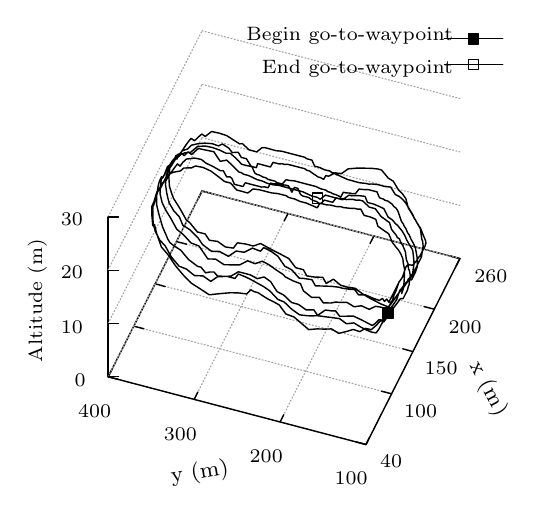
\begin{tikzpicture}[y=0.80pt, x=0.80pt, yscale=-0.770000, xscale=0.770000, inner sep=0pt, outer sep=0pt]
\scriptsize
\begin{scope}[draw=black,line join=bevel,line cap=rect,even odd rule,line width=0.512pt]
  \begin{scope}[cm={{1.0,0.0,0.0,1.0,(0.0,0.0)}},draw=black,line join=bevel,line cap=rect,line width=0.512pt]
  \end{scope}
  \begin{scope}[cm={{1.00625,0.0,0.0,1.00625,(0.0,0.0)}},draw=black,line join=bevel,line cap=rect,line width=0.512pt]
  \end{scope}
  \begin{scope}[cm={{1.00625,0.0,0.0,1.00625,(0.0,0.0)}},draw=black,line join=round,line cap=round,line width=0.512pt]
    \path[draw] (57.5000,233.6000) -- (112.2000,125.3000);
    \path[draw] (262.5000,164.7000) -- (112.2000,125.3000);
    \path[draw] (57.5000,233.5000) -- (57.5000,140.5000);
  \end{scope}
  \begin{scope}[cm={{1.00625,0.0,0.0,1.00625,(0.0,0.0)}},draw=ca0a0a4,dash pattern=on 0.40pt off 0.80pt,line join=round,line cap=round,line width=0.400pt]
    \path[draw] (207.8000,273.1000) -- (57.5000,233.6000);
  \end{scope}
  \begin{scope}[cm={{1.00625,0.0,0.0,1.00625,(0.0,0.0)}},draw=black,line join=round,line cap=round,line width=0.512pt]
    \path[draw] (207.8000,273.1000) -- (201.9000,271.5000);
    \path[draw] (57.5000,233.6000) -- (63.4000,235.1000);
  \end{scope}
  \begin{scope}[cm={{1.00625,0.0,0.0,1.00625,(0.0,0.0)}},draw=black,line join=bevel,line cap=rect,line width=0.512pt]
  \end{scope}
  \begin{scope}[cm={{1.00625,0.0,0.0,1.00625,(217.35,288.291)}},draw=black,line join=bevel,line cap=rect,line width=0.512pt]
  \end{scope}
  \begin{scope}[cm={{1.00625,0.0,0.0,1.00625,(217.35,288.291)}},draw=black,line join=bevel,line cap=rect,line width=0.512pt]
  \end{scope}
  \begin{scope}[cm={{1.00625,0.0,0.0,1.00625,(217.35,288.291)}},draw=black,line join=bevel,line cap=rect,line width=0.512pt]
  \end{scope}
  \begin{scope}[cm={{1.00625,0.0,0.0,1.00625,(217.35,288.291)}},draw=black,line join=bevel,line cap=rect,line width=0.512pt]
  \end{scope}
  \begin{scope}[cm={{1.00625,0.0,0.0,1.00625,(217.35,288.291)}},draw=black,line join=bevel,line cap=rect,line width=0.512pt]
  \end{scope}
  \begin{scope}[cm={{1.00625,0.0,0.0,1.00625,(217.35,288.291)}},draw=black,line join=bevel,line cap=rect,line width=0.512pt]
    \path[fill=black] (0.0000,0.0000) node[above right] () {40};
  \end{scope}
  \begin{scope}[cm={{1.00625,0.0,0.0,1.00625,(217.35,288.291)}},draw=black,line join=bevel,line cap=rect,line width=0.512pt]
  \end{scope}
  \begin{scope}[cm={{1.00625,0.0,0.0,1.00625,(0.0,0.0)}},draw=black,line join=bevel,line cap=rect,line width=0.512pt]
  \end{scope}
  \begin{scope}[cm={{1.00625,0.0,0.0,1.00625,(0.0,0.0)}},draw=ca0a0a4,dash pattern=on 0.40pt off 0.80pt,line join=round,line cap=round,line width=0.400pt]
    \path[draw] (222.7000,243.5000) -- (72.4000,204.1000);
  \end{scope}
  \begin{scope}[cm={{1.00625,0.0,0.0,1.00625,(0.0,0.0)}},draw=black,line join=round,line cap=round,line width=0.512pt]
    \path[draw] (222.7000,243.5000) -- (216.8000,242.0000);
    \path[draw] (72.4000,204.1000) -- (78.3000,205.6000);
  \end{scope}
  \begin{scope}[cm={{1.00625,0.0,0.0,1.00625,(0.0,0.0)}},draw=black,line join=bevel,line cap=rect,line width=0.512pt]
  \end{scope}
  \begin{scope}[cm={{1.00625,0.0,0.0,1.00625,(231.438,259.109)}},draw=black,line join=bevel,line cap=rect,line width=0.512pt]
  \end{scope}
  \begin{scope}[cm={{1.00625,0.0,0.0,1.00625,(231.438,259.109)}},draw=black,line join=bevel,line cap=rect,line width=0.512pt]
  \end{scope}
  \begin{scope}[cm={{1.00625,0.0,0.0,1.00625,(231.438,259.109)}},draw=black,line join=bevel,line cap=rect,line width=0.512pt]
  \end{scope}
  \begin{scope}[cm={{1.00625,0.0,0.0,1.00625,(231.438,259.109)}},draw=black,line join=bevel,line cap=rect,line width=0.512pt]
  \end{scope}
  \begin{scope}[cm={{1.00625,0.0,0.0,1.00625,(231.438,259.109)}},draw=black,line join=bevel,line cap=rect,line width=0.512pt]
  \end{scope}
  \begin{scope}[cm={{1.00625,0.0,0.0,1.00625,(231.438,259.109)}},draw=black,line join=bevel,line cap=rect,line width=0.512pt]
    \path[fill=black] (0.0000,0.0000) node[above right] () {100};
  \end{scope}
  \begin{scope}[cm={{1.00625,0.0,0.0,1.00625,(231.438,259.109)}},draw=black,line join=bevel,line cap=rect,line width=0.512pt]
  \end{scope}
  \begin{scope}[cm={{1.00625,0.0,0.0,1.00625,(0.0,0.0)}},draw=black,line join=bevel,line cap=rect,line width=0.512pt]
  \end{scope}
  \begin{scope}[cm={{1.00625,0.0,0.0,1.00625,(0.0,0.0)}},draw=ca0a0a4,dash pattern=on 0.40pt off 0.80pt,line join=round,line cap=round,line width=0.400pt]
    \path[draw] (235.1000,218.9000) -- (84.9000,179.4000);
  \end{scope}
  \begin{scope}[cm={{1.00625,0.0,0.0,1.00625,(0.0,0.0)}},draw=black,line join=round,line cap=round,line width=0.512pt]
    \path[draw] (235.1000,218.9000) -- (229.3000,217.3000);
    \path[draw] (84.9000,179.4000) -- (90.7000,181.0000);
  \end{scope}
  \begin{scope}[cm={{1.00625,0.0,0.0,1.00625,(0.0,0.0)}},draw=black,line join=bevel,line cap=rect,line width=0.512pt]
  \end{scope}
  \begin{scope}[cm={{1.00625,0.0,0.0,1.00625,(243.513,233.953)}},draw=black,line join=bevel,line cap=rect,line width=0.512pt]
  \end{scope}
  \begin{scope}[cm={{1.00625,0.0,0.0,1.00625,(243.513,233.953)}},draw=black,line join=bevel,line cap=rect,line width=0.512pt]
  \end{scope}
  \begin{scope}[cm={{1.00625,0.0,0.0,1.00625,(243.513,233.953)}},draw=black,line join=bevel,line cap=rect,line width=0.512pt]
  \end{scope}
  \begin{scope}[cm={{1.00625,0.0,0.0,1.00625,(243.513,233.953)}},draw=black,line join=bevel,line cap=rect,line width=0.512pt]
  \end{scope}
  \begin{scope}[cm={{1.00625,0.0,0.0,1.00625,(243.513,233.953)}},draw=black,line join=bevel,line cap=rect,line width=0.512pt]
  \end{scope}
  \begin{scope}[cm={{1.00625,0.0,0.0,1.00625,(243.513,233.953)}},draw=black,line join=bevel,line cap=rect,line width=0.512pt]
    \path[fill=black] (0.0000,0.0000) node[above right] () {150};
  \end{scope}
  \begin{scope}[cm={{1.00625,0.0,0.0,1.00625,(243.513,233.953)}},draw=black,line join=bevel,line cap=rect,line width=0.512pt]
  \end{scope}
  \begin{scope}[cm={{1.00625,0.0,0.0,1.00625,(0.0,0.0)}},draw=black,line join=bevel,line cap=rect,line width=0.512pt]
  \end{scope}
  \begin{scope}[cm={{1.00625,0.0,0.0,1.00625,(0.0,0.0)}},draw=ca0a0a4,dash pattern=on 0.40pt off 0.80pt,line join=round,line cap=round,line width=0.400pt]
    \path[draw] (247.6000,194.2000) -- (97.3000,154.8000);
  \end{scope}
  \begin{scope}[cm={{1.00625,0.0,0.0,1.00625,(0.0,0.0)}},draw=black,line join=round,line cap=round,line width=0.512pt]
    \path[draw] (247.6000,194.2000) -- (241.7000,192.7000);
    \path[draw] (97.3000,154.8000) -- (103.2000,156.3000);
  \end{scope}
  \begin{scope}[cm={{1.00625,0.0,0.0,1.00625,(0.0,0.0)}},draw=black,line join=bevel,line cap=rect,line width=0.512pt]
  \end{scope}
  \begin{scope}[cm={{1.00625,0.0,0.0,1.00625,(257.6,209.803)}},draw=black,line join=bevel,line cap=rect,line width=0.512pt]
  \end{scope}
  \begin{scope}[cm={{1.00625,0.0,0.0,1.00625,(257.6,209.803)}},draw=black,line join=bevel,line cap=rect,line width=0.512pt]
  \end{scope}
  \begin{scope}[cm={{1.00625,0.0,0.0,1.00625,(257.6,209.803)}},draw=black,line join=bevel,line cap=rect,line width=0.512pt]
  \end{scope}
  \begin{scope}[cm={{1.00625,0.0,0.0,1.00625,(257.6,209.803)}},draw=black,line join=bevel,line cap=rect,line width=0.512pt]
  \end{scope}
  \begin{scope}[cm={{1.00625,0.0,0.0,1.00625,(257.6,209.803)}},draw=black,line join=bevel,line cap=rect,line width=0.512pt]
  \end{scope}
  \begin{scope}[cm={{1.00625,0.0,0.0,1.00625,(257.6,209.803)}},draw=black,line join=bevel,line cap=rect,line width=0.512pt]
    \path[fill=black] (0.0000,0.0000) node[above right] () {200};
  \end{scope}
  \begin{scope}[cm={{1.00625,0.0,0.0,1.00625,(257.6,209.803)}},draw=black,line join=bevel,line cap=rect,line width=0.512pt]
  \end{scope}
  \begin{scope}[cm={{1.00625,0.0,0.0,1.00625,(0.0,0.0)}},draw=black,line join=bevel,line cap=rect,line width=0.512pt]
  \end{scope}
  \begin{scope}[cm={{1.00625,0.0,0.0,1.00625,(0.0,0.0)}},draw=ca0a0a4,dash pattern=on 0.40pt off 0.80pt,line join=round,line cap=round,line width=0.400pt]
    \path[draw] (262.5000,164.7000) -- (112.2000,125.3000);
  \end{scope}
  \begin{scope}[cm={{1.00625,0.0,0.0,1.00625,(0.0,0.0)}},draw=black,line join=round,line cap=round,line width=0.512pt]
    \path[draw] (262.5000,164.7000) -- (256.6000,163.1000);
    \path[draw] (112.2000,125.3000) -- (118.1000,126.9000);
  \end{scope}
  \begin{scope}[cm={{1.00625,0.0,0.0,1.00625,(0.0,0.0)}},draw=black,line join=bevel,line cap=rect,line width=0.512pt]
  \end{scope}
  \begin{scope}[cm={{1.00625,0.0,0.0,1.00625,(272.694,179.616)}},draw=black,line join=bevel,line cap=rect,line width=0.512pt]
  \end{scope}
  \begin{scope}[cm={{1.00625,0.0,0.0,1.00625,(272.694,179.616)}},draw=black,line join=bevel,line cap=rect,line width=0.512pt]
  \end{scope}
  \begin{scope}[cm={{1.00625,0.0,0.0,1.00625,(272.694,179.616)}},draw=black,line join=bevel,line cap=rect,line width=0.512pt]
  \end{scope}
  \begin{scope}[cm={{1.00625,0.0,0.0,1.00625,(272.694,179.616)}},draw=black,line join=bevel,line cap=rect,line width=0.512pt]
  \end{scope}
  \begin{scope}[cm={{1.00625,0.0,0.0,1.00625,(272.694,179.616)}},draw=black,line join=bevel,line cap=rect,line width=0.512pt]
  \end{scope}
  \begin{scope}[cm={{1.00625,0.0,0.0,1.00625,(272.694,179.616)}},draw=black,line join=bevel,line cap=rect,line width=0.512pt]
    \path[fill=black] (0.0000,0.0000) node[above right] () {260};
  \end{scope}
  \begin{scope}[cm={{1.00625,0.0,0.0,1.00625,(272.694,179.616)}},draw=black,line join=bevel,line cap=rect,line width=0.512pt]
  \end{scope}
  \begin{scope}[cm={{1.00625,0.0,0.0,1.00625,(0.0,0.0)}},draw=black,line join=bevel,line cap=rect,line width=0.512pt]
  \end{scope}
  \begin{scope}[cm={{1.00625,0.0,0.0,1.00625,(0.0,0.0)}},draw=ca0a0a4,dash pattern=on 0.40pt off 0.80pt,line join=round,line cap=round,line width=0.400pt]
    \path[draw] (207.8000,273.1000) -- (262.5000,164.7000);
  \end{scope}
  \begin{scope}[cm={{1.00625,0.0,0.0,1.00625,(0.0,0.0)}},draw=black,line join=round,line cap=round,line width=0.512pt]
    \path[draw] (207.8000,273.1000) -- (209.9000,268.8000);
    \path[draw] (262.5000,164.7000) -- (260.4000,168.9000);
  \end{scope}
  \begin{scope}[cm={{1.00625,0.0,0.0,1.00625,(0.0,0.0)}},draw=black,line join=bevel,line cap=rect,line width=0.512pt]
  \end{scope}
  \begin{scope}[cm={{1.00625,0.0,0.0,1.00625,(190.684,298.353)}},draw=black,line join=bevel,line cap=rect,line width=0.512pt]
  \end{scope}
  \begin{scope}[cm={{1.00625,0.0,0.0,1.00625,(190.684,298.353)}},draw=black,line join=bevel,line cap=rect,line width=0.512pt]
  \end{scope}
  \begin{scope}[cm={{1.00625,0.0,0.0,1.00625,(190.684,298.353)}},draw=black,line join=bevel,line cap=rect,line width=0.512pt]
  \end{scope}
  \begin{scope}[cm={{1.00625,0.0,0.0,1.00625,(190.684,298.353)}},draw=black,line join=bevel,line cap=rect,line width=0.512pt]
  \end{scope}
  \begin{scope}[cm={{1.00625,0.0,0.0,1.00625,(190.684,298.353)}},draw=black,line join=bevel,line cap=rect,line width=0.512pt]
  \end{scope}
  \begin{scope}[cm={{1.00625,0.0,0.0,1.00625,(190.684,298.353)}},draw=black,line join=bevel,line cap=rect,line width=0.512pt]
    \path[fill=black] (0.0000,0.0000) node[above right] () {100};
  \end{scope}
  \begin{scope}[cm={{1.00625,0.0,0.0,1.00625,(190.684,298.353)}},draw=black,line join=bevel,line cap=rect,line width=0.512pt]
  \end{scope}
  \begin{scope}[cm={{1.00625,0.0,0.0,1.00625,(0.0,0.0)}},draw=black,line join=bevel,line cap=rect,line width=0.512pt]
  \end{scope}
  \begin{scope}[cm={{1.00625,0.0,0.0,1.00625,(0.0,0.0)}},draw=ca0a0a4,dash pattern=on 0.40pt off 0.80pt,line join=round,line cap=round,line width=0.400pt]
    \path[draw] (157.7000,259.9000) -- (212.4000,151.6000);
  \end{scope}
  \begin{scope}[cm={{1.00625,0.0,0.0,1.00625,(0.0,0.0)}},draw=black,line join=round,line cap=round,line width=0.512pt]
    \path[draw] (157.7000,259.9000) -- (159.9000,255.7000);
    \path[draw] (212.4000,151.6000) -- (210.2000,155.8000);
  \end{scope}
  \begin{scope}[cm={{1.00625,0.0,0.0,1.00625,(0.0,0.0)}},draw=black,line join=bevel,line cap=rect,line width=0.512pt]
  \end{scope}
  \begin{scope}[cm={{1.00625,0.0,0.0,1.00625,(140.875,285.272)}},draw=black,line join=bevel,line cap=rect,line width=0.512pt]
  \end{scope}
  \begin{scope}[cm={{1.00625,0.0,0.0,1.00625,(140.875,285.272)}},draw=black,line join=bevel,line cap=rect,line width=0.512pt]
  \end{scope}
  \begin{scope}[cm={{1.00625,0.0,0.0,1.00625,(140.875,285.272)}},draw=black,line join=bevel,line cap=rect,line width=0.512pt]
  \end{scope}
  \begin{scope}[cm={{1.00625,0.0,0.0,1.00625,(140.875,285.272)}},draw=black,line join=bevel,line cap=rect,line width=0.512pt]
  \end{scope}
  \begin{scope}[cm={{1.00625,0.0,0.0,1.00625,(140.875,285.272)}},draw=black,line join=bevel,line cap=rect,line width=0.512pt]
  \end{scope}
  \begin{scope}[cm={{1.00625,0.0,0.0,1.00625,(140.875,285.272)}},draw=black,line join=bevel,line cap=rect,line width=0.512pt]
    \path[fill=black] (0.0000,0.0000) node[above right] () {200};
  \end{scope}
  \begin{scope}[cm={{1.00625,0.0,0.0,1.00625,(140.875,285.272)}},draw=black,line join=bevel,line cap=rect,line width=0.512pt]
  \end{scope}
  \begin{scope}[cm={{1.00625,0.0,0.0,1.00625,(0.0,0.0)}},draw=black,line join=bevel,line cap=rect,line width=0.512pt]
  \end{scope}
  \begin{scope}[cm={{1.00625,0.0,0.0,1.00625,(0.0,0.0)}},draw=ca0a0a4,dash pattern=on 0.40pt off 0.80pt,line join=round,line cap=round,line width=0.400pt]
    \path[draw] (107.6000,246.8000) -- (162.3000,138.5000);
  \end{scope}
  \begin{scope}[cm={{1.00625,0.0,0.0,1.00625,(0.0,0.0)}},draw=black,line join=round,line cap=round,line width=0.512pt]
    \path[draw] (107.6000,246.8000) -- (109.8000,242.5000);
    \path[draw] (162.3000,138.5000) -- (160.1000,142.7000);
  \end{scope}
  \begin{scope}[cm={{1.00625,0.0,0.0,1.00625,(0.0,0.0)}},draw=black,line join=bevel,line cap=rect,line width=0.512pt]
  \end{scope}
  \begin{scope}[cm={{1.00625,0.0,0.0,1.00625,(90.5625,272.191)}},draw=black,line join=bevel,line cap=rect,line width=0.512pt]
  \end{scope}
  \begin{scope}[cm={{1.00625,0.0,0.0,1.00625,(90.5625,272.191)}},draw=black,line join=bevel,line cap=rect,line width=0.512pt]
  \end{scope}
  \begin{scope}[cm={{1.00625,0.0,0.0,1.00625,(90.5625,272.191)}},draw=black,line join=bevel,line cap=rect,line width=0.512pt]
  \end{scope}
  \begin{scope}[cm={{1.00625,0.0,0.0,1.00625,(90.5625,272.191)}},draw=black,line join=bevel,line cap=rect,line width=0.512pt]
  \end{scope}
  \begin{scope}[cm={{1.00625,0.0,0.0,1.00625,(90.5625,272.191)}},draw=black,line join=bevel,line cap=rect,line width=0.512pt]
  \end{scope}
  \begin{scope}[cm={{1.00625,0.0,0.0,1.00625,(90.5625,272.191)}},draw=black,line join=bevel,line cap=rect,line width=0.512pt]
    \path[fill=black] (0.0000,0.0000) node[above right] () {300};
  \end{scope}
  \begin{scope}[cm={{1.00625,0.0,0.0,1.00625,(90.5625,272.191)}},draw=black,line join=bevel,line cap=rect,line width=0.512pt]
  \end{scope}
  \begin{scope}[cm={{1.00625,0.0,0.0,1.00625,(0.0,0.0)}},draw=black,line join=bevel,line cap=rect,line width=0.512pt]
  \end{scope}
  \begin{scope}[cm={{1.00625,0.0,0.0,1.00625,(0.0,0.0)}},draw=ca0a0a4,dash pattern=on 0.40pt off 0.80pt,line join=round,line cap=round,line width=0.400pt]
    \path[draw] (57.5000,233.6000) -- (112.2000,125.3000);
  \end{scope}
  \begin{scope}[cm={{1.00625,0.0,0.0,1.00625,(0.0,0.0)}},draw=black,line join=round,line cap=round,line width=0.512pt]
    \path[draw] (57.5000,233.6000) -- (59.6000,229.4000);
    \path[draw] (112.2000,125.3000) -- (110.1000,129.6000);
  \end{scope}
  \begin{scope}[cm={{1.00625,0.0,0.0,1.00625,(0.0,0.0)}},draw=black,line join=bevel,line cap=rect,line width=0.512pt]
  \end{scope}
  \begin{scope}[cm={{1.00625,0.0,0.0,1.00625,(40.25,259.109)}},draw=black,line join=bevel,line cap=rect,line width=0.512pt]
  \end{scope}
  \begin{scope}[cm={{1.00625,0.0,0.0,1.00625,(40.25,259.109)}},draw=black,line join=bevel,line cap=rect,line width=0.512pt]
  \end{scope}
  \begin{scope}[cm={{1.00625,0.0,0.0,1.00625,(40.25,259.109)}},draw=black,line join=bevel,line cap=rect,line width=0.512pt]
  \end{scope}
  \begin{scope}[cm={{1.00625,0.0,0.0,1.00625,(40.25,259.109)}},draw=black,line join=bevel,line cap=rect,line width=0.512pt]
  \end{scope}
  \begin{scope}[cm={{1.00625,0.0,0.0,1.00625,(40.25,259.109)}},draw=black,line join=bevel,line cap=rect,line width=0.512pt]
  \end{scope}
  \begin{scope}[cm={{1.00625,0.0,0.0,1.00625,(40.25,259.109)}},draw=black,line join=bevel,line cap=rect,line width=0.512pt]
    \path[fill=black] (0.0000,0.0000) node[above right] () {400};
  \end{scope}
  \begin{scope}[cm={{1.00625,0.0,0.0,1.00625,(40.25,259.109)}},draw=black,line join=bevel,line cap=rect,line width=0.512pt]
  \end{scope}
  \begin{scope}[cm={{1.00625,0.0,0.0,1.00625,(0.0,0.0)}},draw=black,line join=bevel,line cap=rect,line width=0.512pt]
  \end{scope}
  \begin{scope}[cm={{1.00625,0.0,0.0,1.00625,(0.0,0.0)}},draw=ca0a0a4,dash pattern=on 0.40pt off 0.80pt,line join=round,line cap=round,line width=0.400pt]
    \path[draw] (57.5000,233.6000) -- (112.2000,125.3000);
    \path[draw] (112.2000,125.3000) -- (112.2000,125.3000) -- (262.5000,164.7000);
  \end{scope}
  \begin{scope}[cm={{1.00625,0.0,0.0,1.00625,(0.0,0.0)}},draw=black,line join=round,line cap=round,line width=0.512pt]
    \path[draw] (57.5000,233.5000) -- (63.5000,233.5000);
  \end{scope}
  \begin{scope}[cm={{1.00625,0.0,0.0,1.00625,(0.0,0.0)}},draw=black,line join=bevel,line cap=rect,line width=0.512pt]
  \end{scope}
  \begin{scope}[cm={{1.00625,0.0,0.0,1.00625,(34.2125,240.997)}},draw=black,line join=bevel,line cap=rect,line width=0.512pt]
  \end{scope}
  \begin{scope}[cm={{1.00625,0.0,0.0,1.00625,(34.2125,240.997)}},draw=black,line join=bevel,line cap=rect,line width=0.512pt]
  \end{scope}
  \begin{scope}[cm={{1.00625,0.0,0.0,1.00625,(34.2125,240.997)}},draw=black,line join=bevel,line cap=rect,line width=0.512pt]
  \end{scope}
  \begin{scope}[cm={{1.00625,0.0,0.0,1.00625,(34.2125,240.997)}},draw=black,line join=bevel,line cap=rect,line width=0.512pt]
  \end{scope}
  \begin{scope}[cm={{1.00625,0.0,0.0,1.00625,(34.2125,240.997)}},draw=black,line join=bevel,line cap=rect,line width=0.512pt]
  \end{scope}
  \begin{scope}[cm={{1.00625,0.0,0.0,1.00625,(38.2125,240.997)}},draw=black,line join=bevel,line cap=rect,line width=0.512pt]
    \path[fill=black] (0.0000,0.0000) node[above right] () {0};
  \end{scope}
  \begin{scope}[cm={{1.00625,0.0,0.0,1.00625,(34.2125,240.997)}},draw=black,line join=bevel,line cap=rect,line width=0.512pt]
  \end{scope}
  \begin{scope}[cm={{1.00625,0.0,0.0,1.00625,(0.0,0.0)}},draw=black,line join=bevel,line cap=rect,line width=0.512pt]
  \end{scope}
  \begin{scope}[cm={{1.00625,0.0,0.0,1.00625,(0.0,0.0)}},draw=ca0a0a4,dash pattern=on 0.40pt off 0.80pt,line join=round,line cap=round,line width=0.400pt]
    \path[draw] (57.5000,202.5000) -- (112.2000,94.2000);
    \path[draw] (112.2000,94.2000) -- (112.2000,94.2000) -- (262.5000,133.7000);
  \end{scope}
  \begin{scope}[cm={{1.00625,0.0,0.0,1.00625,(0.0,0.0)}},draw=black,line join=round,line cap=round,line width=0.512pt]
    \path[draw] (57.5000,202.5000) -- (63.5000,202.5000);
  \end{scope}
  \begin{scope}[cm={{1.00625,0.0,0.0,1.00625,(0.0,0.0)}},draw=black,line join=bevel,line cap=rect,line width=0.512pt]
  \end{scope}
  \begin{scope}[cm={{1.00625,0.0,0.0,1.00625,(26.1625,209.803)}},draw=black,line join=bevel,line cap=rect,line width=0.512pt]
  \end{scope}
  \begin{scope}[cm={{1.00625,0.0,0.0,1.00625,(26.1625,209.803)}},draw=black,line join=bevel,line cap=rect,line width=0.512pt]
  \end{scope}
  \begin{scope}[cm={{1.00625,0.0,0.0,1.00625,(26.1625,209.803)}},draw=black,line join=bevel,line cap=rect,line width=0.512pt]
  \end{scope}
  \begin{scope}[cm={{1.00625,0.0,0.0,1.00625,(26.1625,209.803)}},draw=black,line join=bevel,line cap=rect,line width=0.512pt]
  \end{scope}
  \begin{scope}[cm={{1.00625,0.0,0.0,1.00625,(26.1625,209.803)}},draw=black,line join=bevel,line cap=rect,line width=0.512pt]
  \end{scope}
  \begin{scope}[cm={{1.00625,0.0,0.0,1.00625,(30.1625,209.803)}},draw=black,line join=bevel,line cap=rect,line width=0.512pt]
    \path[fill=black] (0.0000,0.0000) node[above right] () {10};
  \end{scope}
  \begin{scope}[cm={{1.00625,0.0,0.0,1.00625,(26.1625,209.803)}},draw=black,line join=bevel,line cap=rect,line width=0.512pt]
  \end{scope}
  \begin{scope}[cm={{1.00625,0.0,0.0,1.00625,(0.0,0.0)}},draw=black,line join=bevel,line cap=rect,line width=0.512pt]
  \end{scope}
  \begin{scope}[cm={{1.00625,0.0,0.0,1.00625,(0.0,0.0)}},draw=ca0a0a4,dash pattern=on 0.40pt off 0.80pt,line join=round,line cap=round,line width=0.400pt]
    \path[draw] (57.5000,171.3000) -- (112.2000,63.1000);
    \path[draw] (112.2000,63.1000) -- (112.2000,63.1000) -- (262.5000,102.5000);
  \end{scope}
  \begin{scope}[cm={{1.00625,0.0,0.0,1.00625,(0.0,0.0)}},draw=black,line join=round,line cap=round,line width=0.512pt]
    \path[draw] (57.5000,171.5000) -- (63.5000,171.5000);
  \end{scope}
  \begin{scope}[cm={{1.00625,0.0,0.0,1.00625,(0.0,0.0)}},draw=black,line join=bevel,line cap=rect,line width=0.512pt]
  \end{scope}
  \begin{scope}[cm={{1.00625,0.0,0.0,1.00625,(26.1625,177.603)}},draw=black,line join=bevel,line cap=rect,line width=0.512pt]
  \end{scope}
  \begin{scope}[cm={{1.00625,0.0,0.0,1.00625,(26.1625,177.603)}},draw=black,line join=bevel,line cap=rect,line width=0.512pt]
  \end{scope}
  \begin{scope}[cm={{1.00625,0.0,0.0,1.00625,(26.1625,177.603)}},draw=black,line join=bevel,line cap=rect,line width=0.512pt]
  \end{scope}
  \begin{scope}[cm={{1.00625,0.0,0.0,1.00625,(26.1625,177.603)}},draw=black,line join=bevel,line cap=rect,line width=0.512pt]
  \end{scope}
  \begin{scope}[cm={{1.00625,0.0,0.0,1.00625,(26.1625,177.603)}},draw=black,line join=bevel,line cap=rect,line width=0.512pt]
  \end{scope}
  \begin{scope}[cm={{1.00625,0.0,0.0,1.00625,(30.1625,177.603)}},draw=black,line join=bevel,line cap=rect,line width=0.512pt]
    \path[fill=black] (0.0000,0.0000) node[above right] () {20};
  \end{scope}
  \begin{scope}[cm={{1.00625,0.0,0.0,1.00625,(26.1625,177.603)}},draw=black,line join=bevel,line cap=rect,line width=0.512pt]
  \end{scope}
  \begin{scope}[cm={{1.00625,0.0,0.0,1.00625,(0.0,0.0)}},draw=black,line join=bevel,line cap=rect,line width=0.512pt]
  \end{scope}
  \begin{scope}[cm={{1.00625,0.0,0.0,1.00625,(0.0,0.0)}},draw=ca0a0a4,dash pattern=on 0.40pt off 0.80pt,line join=round,line cap=round,line width=0.400pt]
    \path[draw] (57.5000,140.3000) -- (112.2000,31.9000);
    \path[draw] (112.2000,31.9000) -- (112.2000,31.9000) -- (262.5000,71.4000);
  \end{scope}
  \begin{scope}[cm={{1.00625,0.0,0.0,1.00625,(0.0,0.0)}},draw=black,line join=round,line cap=round,line width=0.512pt]
    \path[draw] (57.5000,140.5000) -- (63.5000,140.5000);
  \end{scope}
  \begin{scope}[cm={{1.00625,0.0,0.0,1.00625,(0.0,0.0)}},draw=black,line join=bevel,line cap=rect,line width=0.512pt]
  \end{scope}
  \begin{scope}[cm={{1.00625,0.0,0.0,1.00625,(26.1625,146.409)}},draw=black,line join=bevel,line cap=rect,line width=0.512pt]
  \end{scope}
  \begin{scope}[cm={{1.00625,0.0,0.0,1.00625,(26.1625,146.409)}},draw=black,line join=bevel,line cap=rect,line width=0.512pt]
  \end{scope}
  \begin{scope}[cm={{1.00625,0.0,0.0,1.00625,(26.1625,146.409)}},draw=black,line join=bevel,line cap=rect,line width=0.512pt]
  \end{scope}
  \begin{scope}[cm={{1.00625,0.0,0.0,1.00625,(26.1625,146.409)}},draw=black,line join=bevel,line cap=rect,line width=0.512pt]
  \end{scope}
  \begin{scope}[cm={{1.00625,0.0,0.0,1.00625,(26.1625,146.409)}},draw=black,line join=bevel,line cap=rect,line width=0.512pt]
  \end{scope}
  \begin{scope}[cm={{1.00625,0.0,0.0,1.00625,(30.1625,146.409)}},draw=black,line join=bevel,line cap=rect,line width=0.512pt]
    \path[fill=black] (0.0000,0.0000) node[above right] () {30};
  \end{scope}
  \begin{scope}[cm={{1.00625,0.0,0.0,1.00625,(26.1625,146.409)}},draw=black,line join=bevel,line cap=rect,line width=0.512pt]
  \end{scope}
  \begin{scope}[cm={{1.00625,0.0,0.0,1.00625,(0.0,0.0)}},draw=black,line join=bevel,line cap=rect,line width=0.512pt]
  \end{scope}
  \begin{scope}[cm={{1.00625,0.0,0.0,1.00625,(0.0,0.0)}},draw=black,line join=bevel,line cap=rect,line width=0.512pt]
  \end{scope}
  \begin{scope}[cm={{1.00625,0.0,0.0,1.00625,(0.0,0.0)}},draw=black,line join=bevel,line cap=rect,line width=0.512pt]
  \end{scope}
  \begin{scope}[cm={{1.00625,0.0,0.0,1.00625,(0.0,0.0)}},draw=black,line join=round,line cap=round,line width=0.512pt]
    \path[draw] (228.6000,185.1000) -- (228.6000,185.1000) -- (228.6000,185.1000) --
      (229.6000,182.1000) -- (229.6000,182.1000) -- (229.6000,182.1000) --
      (229.6000,182.1000) -- (229.6000,182.1000) -- (229.6000,182.1000) --
      (229.9000,179.3000) -- (229.9000,179.3000) -- (229.9000,179.3000) --
      (229.9000,179.3000) -- (230.1000,176.6000) -- (230.1000,176.6000) --
      (230.1000,176.6000) -- (230.1000,176.6000) -- (230.3000,170.8000) --
      (230.3000,170.8000) -- (230.3000,170.8000) -- (230.3000,170.8000) --
      (230.3000,170.8000) -- (230.3000,170.8000) -- (229.6000,167.8000) --
      (229.6000,167.8000) -- (229.6000,167.8000) -- (229.6000,167.8000) --
      (229.3000,164.9000) -- (229.3000,164.9000) -- (229.3000,164.9000) --
      (229.3000,164.9000) -- (229.3000,164.9000) -- (229.3000,164.9000) --
      (228.3000,162.4000) -- (228.3000,162.4000) -- (228.3000,162.4000) --
      (228.3000,162.4000) -- (228.3000,162.4000) -- (228.3000,162.4000) --
      (226.8000,159.8000) -- (226.8000,159.8000) -- (226.8000,159.8000) --
      (226.8000,159.8000) -- (225.0000,157.7000) -- (225.0000,157.7000) --
      (224.0000,156.3000) -- (224.0000,156.3000) -- (224.0000,156.3000) --
      (224.0000,156.3000) -- (223.3000,155.5000) -- (223.3000,155.5000) --
      (223.3000,155.5000) -- (223.3000,155.5000) -- (221.0000,150.2000) --
      (221.0000,150.2000) -- (221.0000,150.2000) -- (221.0000,150.2000) --
      (218.5000,148.5000) -- (218.5000,148.5000) -- (218.5000,148.5000) --
      (218.5000,148.5000) -- (217.2000,147.6000) -- (217.2000,147.6000) --
      (217.2000,147.6000) -- (217.2000,147.6000) -- (214.7000,145.8000) --
      (214.7000,145.8000) -- (214.7000,145.8000) -- (214.7000,145.8000) --
      (213.5000,141.8000) -- (213.5000,141.8000) -- (213.5000,141.8000) --
      (213.5000,141.8000) -- (210.2000,140.4000) -- (210.2000,140.4000) --
      (208.2000,139.9000) -- (208.2000,139.9000) -- (206.7000,139.5000) --
      (206.7000,139.5000) -- (206.7000,139.5000) -- (206.7000,139.5000) --
      (204.7000,135.8000) -- (204.7000,135.8000) -- (203.0000,135.9000) --
      (203.0000,135.9000) -- (201.0000,135.4000) -- (201.0000,135.4000) --
      (198.7000,135.4000) -- (198.7000,135.4000) -- (198.7000,135.4000) --
      (198.7000,135.4000) -- (198.7000,135.4000) -- (198.7000,135.4000) --
      (194.9000,135.0000) -- (194.9000,135.0000) -- (192.9000,134.4000) --
      (192.9000,134.4000) -- (190.7000,134.4000) -- (190.7000,134.4000) --
      (190.7000,134.4000) -- (190.7000,134.4000) -- (188.7000,133.9000) --
      (188.7000,133.9000) -- (187.2000,133.5000) -- (187.2000,133.5000) --
      (184.9000,133.4000) -- (184.9000,133.4000) -- (184.9000,133.4000) --
      (184.9000,133.4000) -- (184.9000,133.4000) -- (184.9000,133.4000) --
      (180.9000,132.4000) -- (180.9000,132.4000) -- (179.4000,135.1000) --
      (179.4000,135.1000) -- (179.4000,135.1000) -- (179.4000,135.1000) --
      (179.4000,135.1000) -- (179.4000,135.1000) -- (176.2000,133.7000) --
      (176.2000,133.7000) -- (176.2000,133.7000) -- (176.2000,133.7000) --
      (172.9000,132.3000) -- (172.9000,132.3000) -- (172.9000,132.3000) --
      (172.9000,132.3000) -- (169.4000,131.4000) -- (169.4000,131.4000) --
      (169.4000,131.4000) -- (169.4000,131.4000) -- (169.4000,131.4000) --
      (169.4000,131.4000) -- (166.1000,129.9000) -- (166.1000,129.9000) --
      (164.6000,129.6000) -- (164.6000,129.6000) -- (162.6000,129.0000) --
      (162.6000,129.0000) -- (162.6000,129.0000) -- (162.6000,129.0000) --
      (161.4000,128.1000) -- (161.4000,128.1000) -- (160.0000,127.7000) --
      (160.0000,127.7000) -- (160.0000,127.7000) -- (160.0000,127.7000) --
      (156.4000,126.8000) -- (156.4000,126.8000) -- (156.4000,126.8000) --
      (156.4000,126.8000) -- (156.4000,126.8000) -- (156.4000,126.8000) --
      (152.7000,126.4000) -- (152.7000,126.4000) -- (152.7000,126.4000) --
      (152.7000,126.4000) -- (149.2000,125.5000) -- (149.2000,125.5000) --
      (149.2000,125.5000) -- (149.2000,125.5000) -- (147.7000,125.1000) --
      (147.7000,125.1000) -- (145.7000,124.6000) -- (145.7000,124.6000) --
      (145.7000,124.6000) -- (145.7000,124.6000) -- (141.9000,124.1000) --
      (141.9000,124.1000) -- (141.9000,124.1000) -- (141.9000,124.1000) --
      (141.9000,124.1000) -- (141.9000,124.1000) -- (138.9000,126.5000) --
      (138.9000,126.5000) -- (138.9000,126.5000) -- (138.9000,126.5000) --
      (135.4000,125.5000) -- (135.4000,125.5000) -- (135.4000,125.5000) --
      (135.4000,125.5000) -- (135.4000,125.5000) -- (135.4000,125.5000) --
      (132.4000,124.7000) -- (132.4000,124.7000) -- (132.4000,124.7000) --
      (132.4000,124.7000) -- (128.9000,120.7000) -- (128.9000,120.7000) --
      (128.9000,120.7000) -- (128.9000,120.7000) -- (127.4000,120.3000) --
      (127.4000,120.3000) -- (125.4000,119.8000) -- (125.4000,119.8000) --
      (125.4000,119.8000) -- (125.4000,119.8000) -- (121.4000,116.7000) --
      (121.4000,116.7000) -- (121.4000,116.7000) -- (121.4000,116.7000) --
      (121.4000,116.7000) -- (121.4000,116.7000) -- (117.4000,113.7000) --
      (117.4000,113.7000) -- (117.4000,113.7000) -- (117.4000,113.7000) --
      (112.9000,111.6000) -- (112.9000,111.6000) -- (112.9000,111.6000) --
      (112.9000,111.6000) -- (112.9000,111.6000) -- (112.9000,111.6000) --
      (108.4000,110.7000) -- (108.4000,110.7000) -- (106.1000,111.8000) --
      (106.1000,111.8000) -- (106.1000,111.8000) -- (106.1000,111.8000) --
      (101.6000,111.9000) -- (101.6000,111.9000) -- (101.6000,111.9000) --
      (101.6000,111.9000) -- (99.6000,113.6000) -- (99.6000,113.6000) --
      (99.6000,113.6000) -- (99.6000,113.6000) -- (95.4000,114.4000) --
      (95.4000,114.4000) -- (95.4000,114.4000) -- (95.4000,114.4000) --
      (95.4000,114.4000) -- (95.4000,114.4000) -- (91.9000,116.0000) --
      (91.9000,116.0000) -- (90.6000,118.5000) -- (90.6000,118.5000) --
      (90.6000,118.5000) -- (90.6000,118.5000) -- (90.6000,118.5000) --
      (90.6000,118.5000) -- (87.9000,123.9000) -- (87.9000,123.9000) --
      (87.9000,123.9000) -- (87.9000,123.9000) -- (85.9000,125.8000) --
      (85.9000,125.8000) -- (85.9000,125.8000) -- (85.9000,125.8000) --
      (85.9000,125.8000) -- (85.9000,125.8000) -- (84.2000,131.5000) --
      (84.2000,131.5000) -- (84.2000,131.5000) -- (84.2000,131.5000) --
      (83.0000,134.2000) -- (83.0000,134.2000) -- (83.0000,134.2000) --
      (83.0000,134.2000) -- (83.0000,134.2000) -- (83.0000,134.2000) --
      (83.0000,139.8000) -- (83.0000,139.8000) -- (83.0000,139.8000) --
      (83.0000,139.8000) -- (83.5000,145.5000) -- (83.5000,145.5000) --
      (83.5000,145.5000) -- (83.5000,145.5000) -- (84.5000,144.9000) --
      (84.5000,144.9000) -- (84.5000,144.9000) -- (84.5000,144.9000) --
      (85.8000,150.2000) -- (85.8000,150.2000) -- (85.8000,150.2000) --
      (85.8000,150.2000) -- (88.5000,157.9000) -- (88.5000,157.9000) --
      (88.5000,157.9000) -- (88.5000,157.9000) -- (88.5000,157.9000) --
      (88.5000,157.9000) -- (92.1000,162.1000) -- (92.1000,162.1000) --
      (92.1000,162.1000) -- (92.1000,162.1000) -- (92.1000,162.1000) --
      (92.1000,162.1000) -- (96.6000,168.7000) -- (96.6000,168.7000) --
      (96.6000,168.7000) -- (96.6000,168.7000) -- (101.1000,174.1000) --
      (101.1000,174.1000) -- (101.1000,174.1000) -- (101.1000,174.1000) --
      (105.9000,179.0000) -- (105.9000,179.0000) -- (105.9000,179.0000) --
      (105.9000,179.0000) -- (105.9000,179.0000) -- (105.9000,179.0000) --
      (111.4000,182.5000) -- (111.4000,182.5000) -- (111.4000,182.5000) --
      (111.4000,182.5000) -- (111.4000,182.5000) -- (111.4000,182.5000) --
      (116.4000,185.8000) -- (116.4000,185.8000) -- (116.4000,185.8000) --
      (116.4000,185.8000) -- (121.1000,185.3000) -- (121.1000,185.3000) --
      (124.1000,185.0000) -- (124.1000,185.0000) -- (124.1000,185.0000) --
      (124.1000,185.0000) -- (124.1000,185.0000) -- (124.1000,185.0000) --
      (128.9000,184.6000) -- (128.9000,184.6000) -- (128.9000,184.6000) --
      (128.9000,184.6000) -- (133.4000,184.7000) -- (133.4000,184.7000) --
      (133.4000,184.7000) -- (133.4000,184.7000) -- (133.4000,184.7000) --
      (133.4000,184.7000) -- (138.2000,185.3000) -- (138.2000,185.3000) --
      (140.7000,182.9000) -- (140.7000,182.9000) -- (142.4000,183.9000) --
      (142.4000,183.9000) -- (142.4000,183.9000) -- (142.4000,183.9000) --
      (144.9000,184.6000) -- (144.9000,184.6000) -- (144.9000,184.6000) --
      (144.9000,184.6000) -- (149.2000,187.4000) -- (149.2000,187.4000) --
      (150.9000,188.4000) -- (150.9000,188.4000) -- (153.2000,189.5000) --
      (153.2000,189.5000) -- (153.2000,189.5000) -- (153.2000,189.5000) --
      (153.2000,189.5000) -- (153.2000,189.5000) -- (157.2000,191.7000) --
      (157.2000,191.7000) -- (157.2000,191.7000) -- (157.2000,191.7000) --
      (161.1000,197.0000) -- (161.1000,197.0000) -- (161.1000,197.0000) --
      (161.1000,197.0000) -- (161.1000,197.0000) -- (161.1000,197.0000) --
      (165.9000,198.8000) -- (165.9000,198.8000) -- (165.9000,198.8000) --
      (165.9000,198.8000) -- (170.2000,202.5000) -- (170.2000,202.5000) --
      (170.2000,202.5000) -- (170.2000,202.5000) -- (170.2000,202.5000) --
      (170.2000,202.5000) -- (174.4000,206.1000) -- (174.4000,206.1000) --
      (174.4000,206.1000) -- (174.4000,206.1000) -- (179.2000,205.7000) --
      (179.2000,205.7000) -- (179.2000,205.7000) -- (179.2000,205.7000) --
      (179.2000,205.7000) -- (179.2000,205.7000) -- (183.7000,205.8000) --
      (183.7000,205.8000) -- (183.7000,205.8000) -- (183.7000,205.8000) --
      (187.7000,205.7000) -- (187.7000,205.7000) -- (187.7000,205.7000) --
      (187.7000,205.7000) -- (187.7000,205.7000) -- (187.7000,205.7000) --
      (191.9000,208.3000) -- (191.9000,208.3000) -- (191.9000,208.3000) --
      (191.9000,208.3000) -- (196.4000,207.2000) -- (196.4000,207.2000) --
      (196.4000,207.2000) -- (196.4000,207.2000) -- (196.4000,207.2000) --
      (196.4000,207.2000) -- (200.4000,206.0000) -- (200.4000,206.0000) --
      (200.4000,206.0000) -- (200.4000,206.0000) -- (204.2000,207.3000) --
      (204.2000,207.3000) -- (204.2000,207.3000) -- (204.2000,207.3000) --
      (204.2000,207.3000) -- (204.2000,207.3000) -- (207.4000,205.4000) --
      (207.4000,205.4000) -- (207.4000,205.4000) -- (207.4000,205.4000) --
      (210.9000,206.1000) -- (210.9000,206.1000) -- (210.9000,206.1000) --
      (210.9000,206.1000) -- (210.9000,206.1000) -- (210.9000,206.1000) --
      (213.9000,203.5000) -- (213.9000,203.5000) -- (213.9000,203.5000) --
      (213.9000,203.5000) -- (213.9000,203.5000) -- (213.9000,203.5000) --
      (216.4000,200.8000) -- (216.4000,200.8000) -- (216.4000,200.8000) --
      (216.4000,200.8000) -- (218.2000,201.6000) -- (218.2000,201.6000) --
      (218.2000,201.6000) -- (218.2000,201.6000) -- (220.2000,198.8000) --
      (220.2000,198.8000) -- (220.2000,198.8000) -- (220.2000,198.8000) --
      (220.2000,198.8000) -- (220.2000,198.8000) -- (222.2000,196.0000) --
      (222.2000,196.0000) -- (222.2000,196.0000) -- (222.2000,196.0000) --
      (224.1000,193.1000) -- (224.1000,193.1000) -- (224.1000,193.1000) --
      (224.1000,193.1000) -- (224.1000,193.1000) -- (224.1000,193.1000) --
      (225.9000,190.8000) -- (225.9000,190.8000) -- (225.9000,190.8000) --
      (225.9000,190.8000) -- (225.9000,190.8000) -- (225.9000,190.8000) --
      (227.9000,188.0000) -- (227.9000,188.0000) -- (227.9000,188.0000) --
      (227.9000,188.0000) -- (229.4000,188.1000) -- (229.4000,188.1000) --
      (229.4000,188.1000) -- (229.4000,188.1000) -- (230.6000,185.7000) --
      (230.6000,185.7000) -- (230.6000,185.7000) -- (230.6000,185.7000) --
      (231.4000,184.2000) -- (231.4000,184.2000) -- (232.1000,182.7000) --
      (232.1000,182.7000) -- (232.4000,181.1000) -- (232.4000,181.1000) --
      (232.9000,180.1000) -- (232.9000,180.1000) -- (232.9000,180.1000) --
      (232.9000,180.1000) -- (233.1000,178.5000) -- (233.1000,178.5000) --
      (233.3000,176.9000) -- (233.3000,176.9000) -- (233.3000,176.9000) --
      (233.3000,176.9000) -- (233.6000,174.2000) -- (233.6000,174.2000) --
      (233.6000,174.2000) -- (233.6000,174.2000) -- (233.6000,174.2000) --
      (233.6000,174.2000) -- (233.1000,171.8000) -- (233.1000,171.8000) --
      (232.6000,170.6000) -- (232.6000,170.6000) -- (232.3000,168.8000) --
      (232.3000,168.8000) -- (232.3000,168.8000) -- (232.3000,168.8000) --
      (232.3000,167.7000) -- (232.3000,167.7000) -- (231.8000,166.5000) --
      (231.8000,166.5000) -- (231.3000,165.2000) -- (231.3000,165.2000) --
      (230.8000,160.9000) -- (230.8000,160.9000) -- (230.8000,160.9000) --
      (230.8000,160.9000) -- (230.3000,159.6000) -- (230.3000,159.6000) --
      (229.8000,158.4000) -- (229.8000,158.4000) -- (229.3000,157.1000) --
      (229.3000,157.1000) -- (228.3000,155.7000) -- (228.3000,155.7000) --
      (228.3000,155.7000) -- (228.3000,155.7000) -- (227.8000,154.5000) --
      (227.8000,154.5000) -- (227.3000,153.2000) -- (227.3000,153.2000) --
      (226.0000,152.4000) -- (226.0000,152.4000) -- (225.5000,151.2000) --
      (225.5000,151.2000) -- (225.5000,151.2000) -- (225.5000,151.2000) --
      (225.5000,151.2000) -- (225.5000,151.2000) -- (223.8000,149.1000) --
      (223.8000,149.1000) -- (222.7000,147.7000) -- (222.7000,147.7000) --
      (221.5000,143.7000) -- (221.5000,143.7000) -- (221.5000,143.7000) --
      (221.5000,143.7000) -- (220.2000,142.8000) -- (220.2000,142.8000) --
      (219.0000,141.9000) -- (219.0000,141.9000) -- (217.7000,141.0000) --
      (217.7000,141.0000) -- (217.7000,141.0000) -- (217.7000,141.0000) --
      (216.5000,140.1000) -- (216.5000,140.1000) -- (216.5000,140.1000) --
      (216.5000,140.1000) -- (213.2000,135.6000) -- (213.2000,135.6000) --
      (213.2000,135.6000) -- (213.2000,135.6000) -- (209.7000,134.7000) --
      (209.7000,134.7000) -- (209.7000,134.7000) -- (209.7000,134.7000) --
      (209.7000,134.7000) -- (209.7000,134.7000) -- (205.9000,131.1000) --
      (205.9000,131.1000) -- (203.9000,130.6000) -- (203.9000,130.6000) --
      (202.2000,130.7000) -- (202.2000,130.7000) -- (202.2000,130.7000) --
      (202.2000,130.7000) -- (200.2000,130.2000) -- (200.2000,130.2000) --
      (197.9000,130.2000) -- (197.9000,130.2000) -- (196.2000,130.3000) --
      (196.2000,130.3000) -- (194.2000,129.7000) -- (194.2000,129.7000) --
      (194.2000,129.7000) -- (194.2000,129.7000) -- (191.9000,129.7000) --
      (191.9000,129.7000) -- (190.4000,129.3000) -- (190.4000,129.3000) --
      (188.4000,131.9000) -- (188.4000,131.9000) -- (186.9000,131.5000) --
      (186.9000,131.5000) -- (186.9000,131.5000) -- (186.9000,131.5000) --
      (186.9000,131.5000) -- (186.9000,131.5000) -- (183.4000,130.6000) --
      (183.4000,130.6000) -- (181.6000,132.7000) -- (181.6000,132.7000) --
      (180.1000,132.3000) -- (180.1000,132.3000) -- (180.1000,132.3000) --
      (180.1000,132.3000) -- (178.9000,131.4000) -- (178.9000,131.4000) --
      (177.4000,131.0000) -- (177.4000,131.0000) -- (175.6000,130.0000) --
      (175.6000,130.0000) -- (175.6000,130.0000) -- (175.6000,130.0000) --
      (174.4000,129.1000) -- (174.4000,129.1000) -- (174.4000,129.1000) --
      (174.4000,129.1000) -- (170.9000,128.2000) -- (170.9000,128.2000) --
      (169.6000,127.3000) -- (169.6000,127.3000) -- (168.1000,123.8000) --
      (168.1000,123.8000) -- (168.1000,123.8000) -- (168.1000,123.8000) --
      (166.1000,123.2000) -- (166.1000,123.2000) -- (164.6000,126.0000) --
      (164.6000,126.0000) -- (162.6000,122.3000) -- (162.6000,122.3000) --
      (161.1000,121.9000) -- (161.1000,121.9000) -- (161.1000,121.9000) --
      (161.1000,121.9000) -- (161.1000,121.9000) -- (161.1000,121.9000) --
      (157.4000,121.5000) -- (157.4000,121.5000) -- (155.9000,121.1000) --
      (155.9000,121.1000) -- (153.7000,121.1000) -- (153.7000,121.1000) --
      (153.7000,121.1000) -- (153.7000,121.1000) -- (152.2000,120.7000) --
      (152.2000,120.7000) -- (150.7000,123.4000) -- (150.7000,123.4000) --
      (148.7000,122.9000) -- (148.7000,122.9000) -- (146.9000,123.0000) --
      (146.9000,123.0000) -- (146.9000,123.0000) -- (146.9000,123.0000) --
      (145.4000,122.6000) -- (145.4000,122.6000) -- (145.4000,122.6000) --
      (145.4000,122.6000) -- (141.9000,121.7000) -- (141.9000,121.7000) --
      (141.9000,121.7000) -- (141.9000,121.7000) -- (141.9000,121.7000) --
      (141.9000,121.7000) -- (138.9000,120.9000) -- (138.9000,120.9000) --
      (137.4000,120.5000) -- (137.4000,120.5000) -- (136.1000,122.7000) --
      (136.1000,122.7000) -- (134.6000,122.3000) -- (134.6000,122.3000) --
      (134.6000,122.3000) -- (134.6000,122.3000) -- (132.6000,121.8000) --
      (132.6000,121.8000) -- (131.1000,121.4000) -- (131.1000,121.4000) --
      (129.6000,117.9000) -- (129.6000,117.9000) -- (128.4000,117.0000) --
      (128.4000,117.0000) -- (128.4000,117.0000) -- (128.4000,117.0000) --
      (126.6000,117.1000) -- (126.6000,117.1000) -- (124.6000,113.5000) --
      (124.6000,113.5000) -- (122.9000,113.5000) -- (122.9000,113.5000) --
      (122.9000,113.5000) -- (122.9000,113.5000) -- (122.9000,113.5000) --
      (122.9000,113.5000) -- (118.6000,111.0000) -- (118.6000,111.0000) --
      (118.6000,111.0000) -- (118.6000,111.0000) -- (114.6000,109.1000) --
      (114.6000,109.1000) -- (111.8000,106.9000) -- (111.8000,106.9000) --
      (111.8000,106.9000) -- (111.8000,106.9000) -- (111.8000,106.9000) --
      (111.8000,106.9000) -- (107.9000,106.1000) -- (107.9000,106.1000) --
      (107.9000,106.1000) -- (107.9000,106.1000) -- (107.9000,106.1000) --
      (107.9000,106.1000) -- (103.1000,106.7000) -- (103.1000,106.7000) --
      (101.1000,108.5000) -- (101.1000,108.5000) -- (99.4000,110.8000) --
      (99.4000,110.8000) -- (97.9000,109.5000) -- (97.9000,109.5000) --
      (96.1000,111.8000) -- (96.1000,111.8000) -- (96.1000,111.8000) --
      (96.1000,111.8000) -- (94.4000,114.2000) -- (94.4000,114.2000) --
      (92.6000,116.5000) -- (92.6000,116.5000) -- (91.4000,119.0000) --
      (91.4000,119.0000) -- (91.4000,119.0000) -- (91.4000,119.0000) --
      (91.4000,119.0000) -- (91.4000,119.0000) -- (88.9000,120.8000) --
      (88.9000,120.8000) -- (87.7000,123.2000) -- (87.7000,123.2000) --
      (86.4000,125.7000) -- (86.4000,125.7000) -- (85.4000,128.8000) --
      (85.4000,128.8000) -- (85.4000,128.8000) -- (85.4000,128.8000) --
      (85.4000,128.8000) -- (85.4000,128.8000) -- (83.9000,134.0000) --
      (83.9000,134.0000) -- (83.7000,133.6000) -- (83.7000,133.6000) --
      (83.7000,133.6000) -- (83.7000,133.6000) -- (83.5000,136.3000) --
      (83.5000,136.3000) -- (83.5000,136.3000) -- (83.5000,136.3000) --
      (83.7000,144.5000) -- (83.7000,144.5000) -- (83.7000,144.5000) --
      (83.7000,144.5000) -- (83.7000,144.5000) -- (83.7000,144.5000) --
      (85.2000,149.4000) -- (85.2000,149.4000) -- (85.2000,149.4000) --
      (85.2000,149.4000) -- (87.5000,153.8000) -- (87.5000,153.8000) --
      (87.5000,153.8000) -- (87.5000,153.8000) -- (87.5000,153.8000) --
      (87.5000,153.8000) -- (90.8000,157.4000) -- (90.8000,157.4000) --
      (90.8000,157.4000) -- (90.8000,157.4000) -- (94.3000,163.7000) --
      (94.3000,163.7000) -- (94.3000,163.7000) -- (94.3000,163.7000) --
      (94.3000,163.7000) -- (94.3000,163.7000) -- (98.8000,169.1000) --
      (98.8000,169.1000) -- (98.8000,169.1000) -- (98.8000,169.1000) --
      (103.1000,170.8000) -- (103.1000,170.8000) -- (103.1000,170.8000) --
      (103.1000,170.8000) -- (107.8000,174.6000) -- (107.8000,174.6000) --
      (107.8000,174.6000) -- (107.8000,174.6000) -- (107.8000,174.6000) --
      (107.8000,174.6000) -- (112.8000,174.8000) -- (112.8000,174.8000) --
      (112.8000,174.8000) -- (112.8000,174.8000) -- (112.8000,174.8000) --
      (112.8000,174.8000) -- (117.3000,178.0000) -- (117.3000,178.0000) --
      (117.3000,178.0000) -- (117.3000,178.0000) -- (121.8000,174.9000) --
      (121.8000,174.9000) -- (121.8000,174.9000) -- (121.8000,174.9000) --
      (126.9000,175.1000) -- (126.9000,175.1000) -- (126.9000,175.1000) --
      (126.9000,175.1000) -- (126.9000,175.1000) -- (126.9000,175.1000) --
      (131.4000,176.3000) -- (131.4000,176.3000) -- (133.4000,173.7000) --
      (133.4000,173.7000) -- (133.4000,173.7000) -- (133.4000,173.7000) --
      (133.4000,173.7000) -- (133.4000,173.7000) -- (137.6000,175.4000) --
      (137.6000,175.4000) -- (139.9000,176.5000) -- (139.9000,176.5000) --
      (139.9000,176.5000) -- (139.9000,176.5000) -- (139.9000,176.5000) --
      (139.9000,176.5000) -- (143.9000,178.7000) -- (143.9000,178.7000) --
      (143.9000,178.7000) -- (143.9000,178.7000) -- (147.9000,180.9000) --
      (147.9000,180.9000) -- (147.9000,180.9000) -- (147.9000,180.9000) --
      (151.7000,183.5000) -- (151.7000,183.5000) -- (151.7000,183.5000) --
      (151.7000,183.5000) -- (151.7000,183.5000) -- (151.7000,183.5000) --
      (156.4000,188.5000) -- (156.4000,188.5000) -- (156.4000,188.5000) --
      (156.4000,188.5000) -- (156.4000,188.5000) -- (156.4000,188.5000) --
      (160.1000,190.0000) -- (160.1000,190.0000) -- (160.1000,190.0000) --
      (160.1000,190.0000) -- (164.6000,194.3000) -- (164.6000,194.3000) --
      (164.6000,194.3000) -- (164.6000,194.3000) -- (164.6000,194.3000) --
      (164.6000,194.3000) -- (169.1000,197.5000) -- (169.1000,197.5000) --
      (169.1000,197.5000) -- (169.1000,197.5000) -- (173.4000,198.0000) --
      (173.4000,198.0000) -- (175.6000,198.1000) -- (175.6000,198.1000) --
      (175.6000,198.1000) -- (175.6000,198.1000) -- (175.6000,198.1000) --
      (175.6000,198.1000) -- (179.6000,198.0000) -- (179.6000,198.0000) --
      (179.6000,198.0000) -- (179.6000,198.0000) -- (183.9000,198.6000) --
      (183.9000,198.6000) -- (183.9000,198.6000) -- (183.9000,198.6000) --
      (183.9000,198.6000) -- (183.9000,198.6000) -- (188.2000,199.1000) --
      (188.2000,199.1000) -- (188.2000,199.1000) -- (188.2000,199.1000) --
      (192.4000,199.7000) -- (192.4000,199.7000) -- (192.4000,199.7000) --
      (192.4000,199.7000) -- (192.4000,199.7000) -- (192.4000,199.7000) --
      (196.4000,202.7000) -- (196.4000,202.7000) -- (196.4000,202.7000) --
      (196.4000,202.7000) -- (200.7000,202.2000) -- (200.7000,202.2000) --
      (200.7000,202.2000) -- (200.7000,202.2000) -- (200.7000,202.2000) --
      (200.7000,202.2000) -- (204.9000,204.7000) -- (204.9000,204.7000) --
      (204.9000,204.7000) -- (204.9000,204.7000) -- (208.4000,206.5000) --
      (208.4000,206.5000) -- (208.4000,206.5000) -- (208.4000,206.5000) --
      (208.4000,206.5000) -- (208.4000,206.5000) -- (211.2000,207.6000) --
      (211.2000,207.6000) -- (211.2000,207.6000) -- (211.2000,207.6000) --
      (213.7000,208.0000) -- (213.7000,208.0000) -- (213.7000,208.0000) --
      (213.7000,208.0000) -- (213.7000,208.0000) -- (213.7000,208.0000) --
      (215.4000,205.7000) -- (215.4000,205.7000) -- (215.4000,205.7000) --
      (215.4000,205.7000) -- (216.7000,203.2000) -- (216.7000,203.2000) --
      (216.7000,203.2000) -- (216.7000,203.2000) -- (216.7000,203.2000) --
      (216.7000,203.2000) -- (218.2000,200.3000) -- (218.2000,200.3000) --
      (218.2000,200.3000) -- (218.2000,200.3000) -- (219.4000,197.8000) --
      (219.4000,197.8000) -- (220.1000,196.3000) -- (220.1000,196.3000) --
      (220.1000,196.3000) -- (220.1000,196.3000) -- (220.1000,196.3000) --
      (220.1000,196.3000) -- (222.1000,190.4000) -- (222.1000,190.4000) --
      (222.1000,190.4000) -- (222.1000,190.4000) -- (222.1000,190.4000) --
      (222.1000,190.4000) -- (224.4000,188.2000) -- (224.4000,188.2000) --
      (224.4000,188.2000) -- (224.4000,188.2000) -- (226.4000,185.4000) --
      (226.4000,185.4000) -- (227.6000,184.0000) -- (227.6000,184.0000) --
      (227.6000,184.0000) -- (227.6000,184.0000) -- (228.9000,182.7000) --
      (228.9000,182.7000) -- (228.9000,182.7000) -- (228.9000,182.7000) --
      (230.9000,179.8000) -- (230.9000,179.8000) -- (230.9000,179.8000) --
      (230.9000,179.8000) -- (232.9000,177.0000) -- (232.9000,177.0000) --
      (232.9000,177.0000) -- (232.9000,177.0000) -- (232.9000,177.0000) --
      (232.9000,177.0000) -- (234.9000,174.2000) -- (234.9000,174.2000) --
      (234.9000,174.2000) -- (234.9000,174.2000) -- (235.3000,171.0000) --
      (235.3000,171.0000) -- (235.3000,171.0000) -- (235.3000,171.0000) --
      (235.3000,171.0000) -- (235.3000,171.0000) -- (235.8000,167.7000) --
      (235.8000,167.7000) -- (235.8000,167.7000) -- (235.8000,167.7000) --
      (235.6000,164.9000) -- (235.6000,164.9000) -- (235.6000,164.9000) --
      (235.6000,164.9000) -- (235.6000,164.9000) -- (235.6000,164.9000) --
      (235.3000,162.0000) -- (235.3000,162.0000) -- (235.1000,160.3000) --
      (235.1000,160.3000) -- (235.1000,160.3000) -- (235.1000,160.3000) --
      (234.6000,159.0000) -- (234.6000,159.0000) -- (234.6000,159.0000) --
      (234.6000,159.0000) -- (233.0000,156.4000) -- (233.0000,156.4000) --
      (233.0000,156.4000) -- (233.0000,156.4000) -- (231.5000,153.8000) --
      (231.5000,153.8000) -- (231.5000,153.8000) -- (231.5000,153.8000) --
      (231.5000,153.8000) -- (231.5000,153.8000) -- (230.5000,151.4000) --
      (230.5000,151.4000) -- (230.5000,151.4000) -- (230.5000,151.4000) --
      (230.5000,151.4000) -- (230.5000,151.4000) -- (229.0000,148.8000) --
      (229.0000,148.8000) -- (229.0000,148.8000) -- (229.0000,148.8000) --
      (227.2000,146.6000) -- (227.2000,146.6000) -- (226.2000,145.3000) --
      (226.2000,145.3000) -- (226.2000,145.3000) -- (226.2000,145.3000) --
      (225.0000,144.4000) -- (225.0000,144.4000) -- (225.0000,144.4000) --
      (225.0000,144.4000) -- (223.2000,142.2000) -- (223.2000,142.2000) --
      (223.2000,142.2000) -- (223.2000,142.2000) -- (220.7000,140.5000) --
      (220.7000,140.5000) -- (220.7000,140.5000) -- (220.7000,140.5000) --
      (220.7000,140.5000) -- (220.7000,140.5000) -- (218.2000,135.6000) --
      (218.2000,135.6000) -- (218.2000,135.6000) -- (218.2000,135.6000) --
      (215.5000,134.3000) -- (215.5000,134.3000) -- (215.5000,134.3000) --
      (215.5000,134.3000) -- (215.5000,134.3000) -- (215.5000,134.3000) --
      (212.2000,132.9000) -- (212.2000,132.9000) -- (212.2000,132.9000) --
      (212.2000,132.9000) -- (208.7000,132.0000) -- (208.7000,132.0000) --
      (208.7000,132.0000) -- (208.7000,132.0000) -- (207.2000,128.4000) --
      (207.2000,128.4000) -- (207.2000,128.4000) -- (207.2000,128.4000) --
      (203.4000,128.0000) -- (203.4000,128.0000) -- (203.4000,128.0000) --
      (203.4000,128.0000) -- (203.4000,128.0000) -- (203.4000,128.0000) --
      (199.4000,128.1000) -- (199.4000,128.1000) -- (197.9000,127.7000) --
      (197.9000,127.7000) -- (197.9000,127.7000) -- (197.9000,127.7000) --
      (194.2000,130.4000) -- (194.2000,130.4000) -- (194.2000,130.4000) --
      (194.2000,130.4000) -- (194.2000,130.4000) -- (194.2000,130.4000) --
      (190.6000,129.5000) -- (190.6000,129.5000) -- (190.6000,129.5000) --
      (190.6000,129.5000) -- (190.6000,129.5000) -- (190.6000,129.5000) --
      (187.1000,128.5000) -- (187.1000,128.5000) -- (187.1000,128.5000) --
      (187.1000,128.5000) -- (184.1000,127.7000) -- (184.1000,127.7000) --
      (184.1000,127.7000) -- (184.1000,127.7000) -- (181.1000,130.1000) --
      (181.1000,130.1000) -- (181.1000,130.1000) -- (181.1000,130.1000) --
      (179.4000,129.0000) -- (179.4000,129.0000) -- (179.4000,129.0000) --
      (179.4000,129.0000) -- (176.4000,128.3000) -- (176.4000,128.3000) --
      (176.4000,128.3000) -- (176.4000,128.3000) -- (176.4000,128.3000) --
      (176.4000,128.3000) -- (173.6000,127.0000) -- (173.6000,127.0000) --
      (173.6000,127.0000) -- (173.6000,127.0000) -- (170.8000,125.7000) --
      (170.8000,125.7000) -- (170.8000,125.7000) -- (170.8000,125.7000) --
      (170.8000,125.7000) -- (170.8000,125.7000) -- (167.3000,124.8000) --
      (167.3000,124.8000) -- (167.3000,124.8000) -- (167.3000,124.8000) --
      (164.3000,124.0000) -- (164.3000,124.0000) -- (164.3000,124.0000) --
      (164.3000,124.0000) -- (162.8000,123.6000) -- (162.8000,123.6000) --
      (162.8000,123.6000) -- (162.8000,123.6000) -- (159.9000,122.8000) --
      (159.9000,122.8000) -- (158.4000,122.4000) -- (158.4000,122.4000) --
      (158.4000,122.4000) -- (158.4000,122.4000) -- (156.9000,122.0000) --
      (156.9000,122.0000) -- (156.9000,122.0000) -- (156.9000,122.0000) --
      (153.7000,121.7000) -- (153.7000,121.7000) -- (153.7000,121.7000) --
      (153.7000,121.7000) -- (153.7000,121.7000) -- (153.7000,121.7000) --
      (150.2000,120.8000) -- (150.2000,120.8000) -- (150.2000,120.8000) --
      (150.2000,120.8000) -- (147.4000,119.5000) -- (147.4000,119.5000) --
      (147.4000,119.5000) -- (147.4000,119.5000) -- (147.4000,119.5000) --
      (147.4000,119.5000) -- (144.4000,118.7000) -- (144.4000,118.7000) --
      (144.4000,118.7000) -- (144.4000,118.7000) -- (142.1000,117.6000) --
      (142.1000,117.6000) -- (142.1000,117.6000) -- (142.1000,117.6000) --
      (139.4000,116.3000) -- (139.4000,116.3000) -- (139.4000,116.3000) --
      (139.4000,116.3000) -- (139.4000,116.3000) -- (139.4000,116.3000) --
      (136.4000,115.5000) -- (136.4000,115.5000) -- (135.1000,114.6000) --
      (135.1000,114.6000) -- (133.6000,114.2000) -- (133.6000,114.2000) --
      (133.6000,114.2000) -- (133.6000,114.2000) -- (133.6000,114.2000) --
      (133.6000,114.2000) -- (130.3000,110.8000) -- (130.3000,110.8000) --
      (130.3000,110.8000) -- (130.3000,110.8000) -- (126.6000,107.3000) --
      (126.6000,107.3000) -- (126.6000,107.3000) -- (126.6000,107.3000) --
      (126.6000,107.3000) -- (126.6000,107.3000) -- (122.8000,108.0000) --
      (122.8000,108.0000) -- (122.8000,108.0000) -- (122.8000,108.0000) --
      (119.1000,102.4000) -- (119.1000,102.4000) -- (119.1000,102.4000) --
      (119.1000,102.4000) -- (119.1000,102.4000) -- (119.1000,102.4000) --
      (114.6000,101.5000) -- (114.6000,101.5000) -- (114.6000,101.5000) --
      (114.6000,101.5000) -- (114.6000,101.5000) -- (114.6000,101.5000) --
      (110.1000,100.5000) -- (110.1000,100.5000) -- (110.1000,100.5000) --
      (110.1000,100.5000) -- (106.1000,104.0000) -- (106.1000,104.0000) --
      (104.1000,102.5000) -- (104.1000,102.5000) -- (101.8000,104.7000) --
      (101.8000,104.7000) -- (101.8000,104.7000) -- (101.8000,104.7000) --
      (100.4000,103.5000) -- (100.4000,103.5000) -- (98.1000,105.7000) --
      (98.1000,105.7000) -- (98.1000,105.7000) -- (98.1000,105.7000) --
      (95.1000,107.4000) -- (95.1000,107.4000) -- (95.1000,107.4000) --
      (95.1000,107.4000) -- (95.1000,107.4000) -- (95.1000,107.4000) --
      (92.1000,112.1000) -- (92.1000,112.1000) -- (90.6000,115.1000) --
      (90.6000,115.1000) -- (89.4000,117.6000) -- (89.4000,117.6000) --
      (89.4000,117.6000) -- (89.4000,117.6000) -- (88.6000,117.0000) --
      (88.6000,117.0000) -- (87.4000,119.5000) -- (87.4000,119.5000) --
      (86.7000,122.1000) -- (86.7000,122.1000) -- (86.7000,122.1000) --
      (86.7000,122.1000) -- (86.2000,125.3000) -- (86.2000,125.3000) --
      (86.2000,125.3000) -- (86.2000,125.3000) -- (85.7000,127.7000) --
      (85.7000,127.7000) -- (85.7000,127.7000) -- (85.7000,127.7000) --
      (85.7000,133.2000) -- (85.7000,133.2000) -- (85.7000,133.2000) --
      (85.7000,133.2000) -- (85.7000,133.2000) -- (85.7000,133.2000) --
      (87.0000,138.6000) -- (87.0000,138.6000) -- (87.0000,138.6000) --
      (87.0000,138.6000) -- (87.0000,138.6000) -- (87.0000,138.6000) --
      (89.2000,146.2000) -- (89.2000,146.2000) -- (89.2000,146.2000) --
      (89.2000,146.2000) -- (92.3000,153.4000) -- (92.3000,153.4000) --
      (93.5000,155.4000) -- (93.5000,155.4000) -- (95.5000,157.0000) --
      (95.5000,157.0000) -- (95.5000,157.0000) -- (95.5000,157.0000) --
      (95.5000,157.0000) -- (95.5000,157.0000) -- (99.8000,159.8000) --
      (99.8000,159.8000) -- (99.8000,159.8000) -- (99.8000,159.8000) --
      (104.3000,165.2000) -- (104.3000,165.2000) -- (104.3000,165.2000) --
      (104.3000,165.2000) -- (104.3000,165.2000) -- (104.3000,165.2000) --
      (109.6000,169.2000) -- (109.6000,169.2000) -- (111.6000,169.7000) --
      (111.6000,169.7000) -- (114.3000,173.0000) -- (114.3000,173.0000) --
      (114.3000,173.0000) -- (114.3000,173.0000) -- (116.8000,172.5000) --
      (116.8000,172.5000) -- (119.1000,172.5000) -- (119.1000,172.5000) --
      (121.6000,175.2000) -- (121.6000,175.2000) -- (121.6000,175.2000) --
      (121.6000,175.2000) -- (123.8000,175.2000) -- (123.8000,175.2000) --
      (123.8000,175.2000) -- (123.8000,175.2000) -- (129.1000,174.9000) --
      (129.1000,174.9000) -- (129.1000,174.9000) -- (129.1000,174.9000) --
      (133.4000,172.4000) -- (133.4000,172.4000) -- (133.4000,172.4000) --
      (133.4000,172.4000) -- (135.9000,173.0000) -- (135.9000,173.0000) --
      (135.9000,173.0000) -- (135.9000,173.0000) -- (140.4000,174.2000) --
      (140.4000,174.2000) -- (140.4000,174.2000) -- (140.4000,174.2000) --
      (140.4000,174.2000) -- (140.4000,174.2000) -- (144.4000,176.4000) --
      (144.4000,176.4000) -- (144.4000,176.4000) -- (144.4000,176.4000) --
      (148.4000,175.4000) -- (148.4000,175.4000) -- (148.4000,175.4000) --
      (148.4000,175.4000) -- (148.4000,175.4000) -- (148.4000,175.4000) --
      (152.2000,178.1000) -- (152.2000,178.1000) -- (152.2000,178.1000) --
      (152.2000,178.1000) -- (155.9000,183.9000) -- (155.9000,183.9000) --
      (155.9000,183.9000) -- (155.9000,183.9000) -- (155.9000,183.9000) --
      (155.9000,183.9000) -- (159.9000,186.0000) -- (159.9000,186.0000) --
      (159.9000,186.0000) -- (159.9000,186.0000) -- (164.4000,190.3000) --
      (164.4000,190.3000) -- (164.4000,190.3000) -- (164.4000,190.3000) --
      (164.4000,190.3000) -- (164.4000,190.3000) -- (168.4000,191.4000) --
      (168.4000,191.4000) -- (168.4000,191.4000) -- (168.4000,191.4000) --
      (172.9000,194.6000) -- (172.9000,194.6000) -- (172.9000,194.6000) --
      (172.9000,194.6000) -- (172.9000,194.6000) -- (172.9000,194.6000) --
      (177.4000,194.6000) -- (177.4000,194.6000) -- (179.6000,197.8000) --
      (179.6000,197.8000) -- (179.6000,197.8000) -- (179.6000,197.8000) --
      (184.1000,194.7000) -- (184.1000,194.7000) -- (184.1000,194.7000) --
      (184.1000,194.7000) -- (184.1000,194.7000) -- (184.1000,194.7000) --
      (187.9000,195.2000) -- (187.9000,195.2000) -- (190.1000,195.2000) --
      (190.1000,195.2000) -- (190.1000,195.2000) -- (190.1000,195.2000) --
      (192.4000,198.3000) -- (192.4000,198.3000) -- (192.4000,198.3000) --
      (192.4000,198.3000) -- (196.4000,198.3000) -- (196.4000,198.3000) --
      (196.4000,198.3000) -- (196.4000,198.3000) -- (196.4000,198.3000) --
      (196.4000,198.3000) -- (200.4000,198.2000) -- (200.4000,198.2000) --
      (200.4000,198.2000) -- (200.4000,198.2000) -- (204.9000,200.3000) --
      (204.9000,200.3000) -- (204.9000,200.3000) -- (204.9000,200.3000) --
      (208.4000,202.1000) -- (208.4000,202.1000) -- (208.4000,202.1000) --
      (208.4000,202.1000) -- (208.4000,202.1000) -- (208.4000,202.1000) --
      (211.4000,203.7000) -- (211.4000,203.7000) -- (213.2000,202.5000) --
      (213.2000,202.5000) -- (213.2000,202.5000) -- (213.2000,202.5000) --
      (213.2000,202.5000) -- (213.2000,202.5000) -- (215.4000,200.3000) --
      (215.4000,200.3000) -- (215.4000,200.3000) -- (215.4000,200.3000) --
      (217.4000,200.6000) -- (217.4000,200.6000) -- (218.6000,199.3000) --
      (218.6000,199.3000) -- (218.6000,199.3000) -- (218.6000,199.3000) --
      (218.6000,199.3000) -- (218.6000,199.3000) -- (220.4000,196.9000) --
      (220.4000,196.9000) -- (220.4000,196.9000) -- (220.4000,196.9000) --
      (221.6000,194.5000) -- (221.6000,194.5000) -- (221.6000,194.5000) --
      (221.6000,194.5000) -- (221.6000,194.5000) -- (221.6000,194.5000) --
      (223.6000,191.7000) -- (223.6000,191.7000) -- (223.6000,191.7000) --
      (223.6000,191.7000) -- (225.6000,188.8000) -- (225.6000,188.8000) --
      (225.6000,188.8000) -- (225.6000,188.8000) -- (225.6000,188.8000) --
      (225.6000,188.8000) -- (227.4000,183.4000) -- (227.4000,183.4000) --
      (228.6000,182.0000) -- (228.6000,182.0000) -- (228.6000,182.0000) --
      (228.6000,182.0000) -- (228.6000,182.0000) -- (228.6000,182.0000) --
      (230.6000,179.2000) -- (230.6000,179.2000) -- (231.9000,177.9000) --
      (231.9000,177.9000) -- (232.6000,176.4000) -- (232.6000,176.4000) --
      (232.6000,176.4000) -- (232.6000,176.4000) -- (232.6000,176.4000) --
      (232.6000,176.4000) -- (234.3000,177.2000) -- (234.3000,177.2000) --
      (235.1000,175.7000) -- (235.1000,175.7000) -- (235.8000,174.2000) --
      (235.8000,174.2000) -- (235.8000,174.2000) -- (235.8000,174.2000) --
      (236.6000,172.7000) -- (236.6000,172.7000) -- (236.6000,172.7000) --
      (236.6000,172.7000) -- (237.6000,169.6000) -- (237.6000,169.6000) --
      (237.6000,169.6000) -- (237.6000,169.6000) -- (237.8000,166.9000) --
      (237.8000,166.9000) -- (237.8000,166.9000) -- (237.8000,166.9000) --
      (237.8000,166.9000) -- (237.8000,166.9000) -- (237.6000,164.1000) --
      (237.6000,164.1000) -- (237.6000,164.1000) -- (237.6000,164.1000) --
      (237.6000,164.1000) -- (237.6000,164.1000) -- (236.6000,158.5000) --
      (236.6000,158.5000) -- (236.6000,158.5000) -- (236.6000,158.5000) --
      (235.5000,156.0000) -- (235.5000,156.0000) -- (235.5000,156.0000) --
      (235.5000,156.0000) -- (234.0000,153.3000) -- (234.0000,153.3000) --
      (234.0000,153.3000) -- (234.0000,153.3000) -- (234.0000,153.3000) --
      (234.0000,153.3000) -- (233.0000,150.9000) -- (233.0000,150.9000) --
      (232.0000,149.6000) -- (232.0000,149.6000) -- (231.5000,148.3000) --
      (231.5000,148.3000) -- (231.5000,148.3000) -- (231.5000,148.3000) --
      (231.0000,147.1000) -- (231.0000,147.1000) -- (230.0000,145.7000) --
      (230.0000,145.7000) -- (229.5000,144.4000) -- (229.5000,144.4000) --
      (228.5000,143.1000) -- (228.5000,143.1000) -- (228.5000,143.1000) --
      (228.5000,143.1000) -- (228.5000,143.1000) -- (228.5000,143.1000) --
      (226.7000,137.8000) -- (226.7000,137.8000) -- (226.2000,136.6000) --
      (226.2000,136.6000) -- (225.2000,135.2000) -- (225.2000,135.2000) --
      (225.2000,135.2000) -- (225.2000,135.2000) -- (224.0000,134.3000) --
      (224.0000,134.3000) -- (223.0000,132.9000) -- (223.0000,132.9000) --
      (221.7000,132.0000) -- (221.7000,132.0000) -- (221.7000,132.0000) --
      (221.7000,132.0000) -- (220.4000,131.1000) -- (220.4000,131.1000) --
      (218.9000,130.7000) -- (218.9000,130.7000) -- (217.7000,129.9000) --
      (217.7000,129.9000) -- (215.7000,129.3000) -- (215.7000,129.3000) --
      (214.2000,125.8000) -- (214.2000,125.8000) -- (214.2000,125.8000) --
      (214.2000,125.8000) -- (212.7000,125.4000) -- (212.7000,125.4000) --
      (210.7000,124.9000) -- (210.7000,124.9000) -- (209.2000,124.5000) --
      (209.2000,124.5000) -- (209.2000,124.5000) -- (209.2000,124.5000) --
      (206.9000,124.5000) -- (206.9000,124.5000) -- (206.9000,124.5000) --
      (206.9000,124.5000) -- (203.7000,124.2000) -- (203.7000,124.2000) --
      (201.7000,126.8000) -- (201.7000,126.8000) -- (199.9000,126.9000) --
      (199.9000,126.9000) -- (199.9000,126.9000) -- (199.9000,126.9000) --
      (198.4000,126.5000) -- (198.4000,126.5000) -- (196.1000,126.4000) --
      (196.1000,126.4000) -- (194.6000,126.0000) -- (194.6000,126.0000) --
      (193.1000,128.8000) -- (193.1000,128.8000) -- (193.1000,128.8000) --
      (193.1000,128.8000) -- (193.1000,128.8000) -- (193.1000,128.8000) --
      (190.4000,127.5000) -- (190.4000,127.5000) -- (188.4000,126.9000) --
      (188.4000,126.9000) -- (187.1000,126.1000) -- (187.1000,126.1000) --
      (187.1000,126.1000) -- (187.1000,126.1000) -- (185.6000,125.7000) --
      (185.6000,125.7000) -- (184.4000,124.8000) -- (184.4000,124.8000) --
      (182.9000,124.4000) -- (182.9000,124.4000) -- (181.4000,124.0000) --
      (181.4000,124.0000) -- (181.4000,124.0000) -- (181.4000,124.0000) --
      (181.4000,124.0000) -- (181.4000,124.0000) -- (178.6000,122.7000) --
      (178.6000,122.7000) -- (177.1000,122.3000) -- (177.1000,122.3000) --
      (175.6000,121.9000) -- (175.6000,121.9000) -- (175.6000,121.9000) --
      (175.6000,121.9000) -- (173.6000,121.4000) -- (173.6000,121.4000) --
      (172.1000,121.0000) -- (172.1000,121.0000) -- (172.1000,121.0000) --
      (172.1000,121.0000) -- (172.1000,121.0000) -- (172.1000,121.0000) --
      (169.1000,120.2000) -- (169.1000,120.2000) -- (169.1000,120.2000) --
      (169.1000,120.2000) -- (166.1000,119.4000) -- (166.1000,119.4000) --
      (166.1000,119.4000) -- (166.1000,119.4000) -- (162.8000,119.1000) --
      (162.8000,119.1000) -- (162.8000,119.1000) -- (162.8000,119.1000) --
      (161.3000,118.7000) -- (161.3000,118.7000) -- (161.3000,118.7000) --
      (161.3000,118.7000) -- (158.9000,121.2000) -- (158.9000,121.2000) --
      (158.9000,121.2000) -- (158.9000,121.2000) -- (158.9000,121.2000) --
      (158.9000,121.2000) -- (155.9000,120.4000) -- (155.9000,120.4000) --
      (154.6000,119.5000) -- (154.6000,119.5000) -- (154.6000,119.5000) --
      (154.6000,119.5000) -- (152.1000,118.9000) -- (152.1000,118.9000) --
      (152.1000,118.9000) -- (152.1000,118.9000) -- (150.6000,118.5000) --
      (150.6000,118.5000) -- (149.4000,117.6000) -- (149.4000,117.6000) --
      (147.9000,117.2000) -- (147.9000,117.2000) -- (147.9000,117.2000) --
      (147.9000,117.2000) -- (147.9000,117.2000) -- (147.9000,117.2000) --
      (145.6000,116.0000) -- (145.6000,116.0000) -- (144.1000,115.6000) --
      (144.1000,115.6000) -- (142.9000,114.7000) -- (142.9000,114.7000) --
      (141.4000,111.2000) -- (141.4000,111.2000) -- (141.4000,111.2000) --
      (141.4000,111.2000) -- (139.9000,110.8000) -- (139.9000,110.8000) --
      (138.3000,110.5000) -- (138.3000,110.5000) -- (136.8000,110.1000) --
      (136.8000,110.1000) -- (136.8000,110.1000) -- (136.8000,110.1000) --
      (135.3000,109.7000) -- (135.3000,109.7000) -- (135.3000,109.7000) --
      (135.3000,109.7000) -- (132.1000,106.3000) -- (132.1000,106.3000) --
      (132.1000,106.3000) -- (132.1000,106.3000) -- (132.1000,106.3000) --
      (132.1000,106.3000) -- (128.6000,103.3000) -- (128.6000,103.3000) --
      (126.3000,103.3000) -- (126.3000,103.3000) -- (126.3000,103.3000) --
      (126.3000,103.3000) -- (122.3000,101.4000) -- (122.3000,101.4000) --
      (122.3000,101.4000) -- (122.3000,101.4000) -- (122.3000,101.4000) --
      (122.3000,101.4000) -- (118.1000,99.9000) -- (118.1000,99.9000) --
      (118.1000,99.9000) -- (118.1000,99.9000) -- (114.1000,99.1000) --
      (114.1000,99.1000) -- (114.1000,99.1000) -- (114.1000,99.1000) --
      (114.1000,99.1000) -- (114.1000,99.1000) -- (109.6000,99.3000) --
      (109.6000,99.3000) -- (109.6000,99.3000) -- (109.6000,99.3000) --
      (105.6000,102.7000) -- (105.6000,102.7000) -- (105.6000,102.7000) --
      (105.6000,102.7000) -- (105.6000,102.7000) -- (105.6000,102.7000) --
      (102.1000,103.1000) -- (102.1000,103.1000) -- (102.1000,103.1000) --
      (102.1000,103.1000) -- (98.1000,104.6000) -- (98.1000,104.6000) --
      (98.1000,104.6000) -- (98.1000,104.6000) -- (98.1000,104.6000) --
      (98.1000,104.6000) -- (95.1000,109.3000) -- (95.1000,109.3000) --
      (95.1000,109.3000) -- (95.1000,109.3000) -- (92.1000,111.0000) --
      (92.1000,111.0000) -- (92.1000,111.0000) -- (92.1000,111.0000) --
      (92.1000,111.0000) -- (92.1000,111.0000) -- (90.1000,116.1000) --
      (90.1000,116.1000) -- (90.1000,116.1000) -- (90.1000,116.1000) --
      (88.4000,118.7000) -- (88.4000,118.7000) -- (88.4000,118.7000) --
      (88.4000,118.7000) -- (88.4000,118.7000) -- (88.4000,118.7000) --
      (87.9000,124.1000) -- (87.9000,124.1000) -- (87.7000,126.8000) --
      (87.7000,126.8000) -- (87.7000,126.8000) -- (87.7000,126.8000) --
      (87.7000,126.8000) -- (87.7000,126.8000) -- (89.0000,132.2000) --
      (89.0000,132.2000) -- (89.0000,132.2000) -- (89.0000,132.2000) --
      (91.2000,136.7000) -- (91.2000,136.7000) -- (91.2000,136.7000) --
      (91.2000,136.7000) -- (91.2000,136.7000) -- (91.2000,136.7000) --
      (93.7000,140.7000) -- (93.7000,140.7000) -- (93.7000,140.7000) --
      (93.7000,140.7000) -- (97.5000,147.6000) -- (97.5000,147.6000) --
      (97.5000,147.6000) -- (97.5000,147.6000) -- (97.5000,147.6000) --
      (97.5000,147.6000) -- (101.5000,150.9000) -- (101.5000,150.9000) --
      (101.5000,150.9000) -- (101.5000,150.9000) -- (105.8000,155.6000) --
      (105.8000,155.6000) -- (105.8000,155.6000) -- (105.8000,155.6000) --
      (105.8000,155.6000) -- (105.8000,155.6000) -- (110.5000,157.4000) --
      (110.5000,157.4000) -- (110.5000,157.4000) -- (110.5000,157.4000) --
      (115.6000,164.9000) -- (115.6000,164.9000) -- (115.6000,164.9000) --
      (115.6000,164.9000) -- (115.6000,164.9000) -- (115.6000,164.9000) --
      (120.1000,165.0000) -- (120.1000,165.0000) -- (120.1000,165.0000) --
      (120.1000,165.0000) -- (125.1000,168.3000) -- (125.1000,168.3000) --
      (127.3000,168.3000) -- (127.3000,168.3000) -- (127.3000,168.3000) --
      (127.3000,168.3000) -- (127.3000,168.3000) -- (127.3000,168.3000) --
      (131.8000,168.4000) -- (131.8000,168.4000) -- (134.1000,168.4000) --
      (134.1000,168.4000) -- (134.1000,168.4000) -- (134.1000,168.4000) --
      (134.1000,168.4000) -- (134.1000,168.4000) -- (138.8000,166.0000) --
      (138.8000,166.0000) -- (138.8000,166.0000) -- (138.8000,166.0000) --
      (143.1000,167.7000) -- (143.1000,167.7000) -- (143.1000,167.7000) --
      (143.1000,167.7000) -- (147.4000,166.2000) -- (147.4000,166.2000) --
      (147.4000,166.2000) -- (147.4000,166.2000) -- (149.6000,167.4000) --
      (149.6000,167.4000) -- (151.4000,168.4000) -- (151.4000,168.4000) --
      (151.4000,168.4000) -- (151.4000,168.4000) -- (151.4000,168.4000) --
      (151.4000,168.4000) -- (155.1000,171.1000) -- (155.1000,171.1000) --
      (155.1000,171.1000) -- (155.1000,171.1000) -- (159.4000,173.9000) --
      (159.4000,173.9000) -- (160.8000,175.4000) -- (160.8000,175.4000) --
      (160.8000,175.4000) -- (160.8000,175.4000) -- (160.8000,175.4000) --
      (160.8000,175.4000) -- (165.3000,177.7000) -- (165.3000,177.7000) --
      (165.3000,177.7000) -- (165.3000,177.7000) -- (169.6000,179.3000) --
      (169.6000,179.3000) -- (169.6000,179.3000) -- (169.6000,179.3000) --
      (171.3000,183.5000) -- (171.3000,183.5000) -- (171.3000,183.5000) --
      (171.3000,183.5000) -- (176.1000,187.3000) -- (176.1000,187.3000) --
      (176.1000,187.3000) -- (176.1000,187.3000) -- (180.6000,187.3000) --
      (180.6000,187.3000) -- (180.6000,187.3000) -- (180.6000,187.3000) --
      (182.9000,190.5000) -- (182.9000,190.5000) -- (182.9000,190.5000) --
      (182.9000,190.5000) -- (187.4000,190.6000) -- (187.4000,190.6000) --
      (189.9000,190.1000) -- (189.9000,190.1000) -- (189.9000,190.1000) --
      (189.9000,190.1000) -- (189.9000,190.1000) -- (189.9000,190.1000) --
      (194.4000,190.2000) -- (194.4000,190.2000) -- (196.6000,190.2000) --
      (196.6000,190.2000) -- (196.6000,190.2000) -- (196.6000,190.2000) --
      (196.6000,190.2000) -- (196.6000,190.2000) -- (200.9000,192.8000) --
      (200.9000,192.8000) -- (200.9000,192.8000) -- (200.9000,192.8000) --
      (205.1000,192.2000) -- (205.1000,192.2000) -- (205.1000,192.2000) --
      (205.1000,192.2000) -- (205.1000,192.2000) -- (205.1000,192.2000) --
      (209.7000,194.3000) -- (209.7000,194.3000) -- (209.7000,194.3000) --
      (209.7000,194.3000) -- (213.4000,192.5000) -- (213.4000,192.5000) --
      (213.4000,192.5000) -- (213.4000,192.5000) -- (213.4000,192.5000) --
      (213.4000,192.5000) -- (216.9000,193.1000) -- (216.9000,193.1000) --
      (216.9000,193.1000) -- (216.9000,193.1000) -- (219.6000,194.2000) --
      (219.6000,194.2000) -- (219.6000,194.2000) -- (219.6000,194.2000) --
      (219.6000,194.2000) -- (219.6000,194.2000) -- (222.1000,191.5000) --
      (222.1000,191.5000) -- (222.1000,191.5000) -- (222.1000,191.5000) --
      (224.1000,188.7000) -- (224.1000,188.7000) -- (224.1000,188.7000) --
      (224.1000,188.7000) -- (224.1000,188.7000) -- (224.1000,188.7000) --
      (226.1000,185.8000) -- (226.1000,185.8000) -- (226.1000,185.8000) --
      (226.1000,185.8000) -- (227.9000,183.5000) -- (227.9000,183.5000) --
      (227.9000,183.5000) -- (227.9000,183.5000) -- (227.9000,183.5000) --
      (227.9000,183.5000) -- (229.9000,180.7000) -- (229.9000,180.7000) --
      (229.9000,180.7000) -- (229.9000,180.7000) -- (231.9000,177.9000) --
      (231.9000,177.9000) -- (231.9000,177.9000) -- (231.9000,177.9000) --
      (231.9000,177.9000) -- (231.9000,177.9000) -- (233.9000,175.0000) --
      (233.9000,175.0000) -- (233.9000,175.0000) -- (233.9000,175.0000) --
      (235.6000,172.7000) -- (235.6000,172.7000) -- (235.6000,172.7000) --
      (235.6000,172.7000) -- (235.6000,172.7000) -- (235.6000,172.7000) --
      (237.1000,169.8000) -- (237.1000,169.8000) -- (237.1000,169.8000) --
      (237.1000,169.8000) -- (238.6000,166.8000) -- (238.6000,166.8000) --
      (238.6000,166.8000) -- (238.6000,166.8000) -- (238.6000,166.8000) --
      (238.6000,166.8000) -- (240.1000,163.8000) -- (240.1000,163.8000) --
      (240.1000,163.8000) -- (240.1000,163.8000) -- (240.6000,160.6000) --
      (240.6000,160.6000) -- (240.6000,160.6000) -- (240.6000,160.6000) --
      (240.6000,160.6000) -- (240.6000,160.6000) -- (241.1000,157.4000) --
      (241.1000,157.4000) -- (241.1000,157.4000) -- (241.1000,157.4000) --
      (240.8000,154.5000) -- (240.8000,154.5000) -- (240.3000,153.3000) --
      (240.3000,153.3000) -- (240.3000,153.3000) -- (240.3000,153.3000) --
      (240.3000,153.3000) -- (240.3000,153.3000) -- (239.5000,147.3000) --
      (239.5000,147.3000) -- (239.5000,147.3000) -- (239.5000,147.3000) --
      (239.5000,147.3000) -- (239.5000,147.3000) -- (238.0000,144.7000) --
      (238.0000,144.7000) -- (238.0000,144.7000) -- (238.0000,144.7000) --
      (236.5000,142.0000) -- (236.5000,142.0000) -- (236.5000,142.0000) --
      (236.5000,142.0000) -- (235.0000,139.4000) -- (235.0000,139.4000) --
      (235.0000,139.4000) -- (235.0000,139.4000) -- (235.0000,139.4000) --
      (235.0000,139.4000) -- (233.5000,136.8000) -- (233.5000,136.8000) --
      (232.5000,135.4000) -- (232.5000,135.4000) -- (232.5000,135.4000) --
      (232.5000,135.4000) -- (232.5000,135.4000) -- (232.5000,135.4000) --
      (231.0000,129.7000) -- (231.0000,129.7000) -- (231.0000,129.7000) --
      (231.0000,129.7000) -- (229.0000,126.9000) -- (229.0000,126.9000) --
      (229.0000,126.9000) -- (229.0000,126.9000) -- (229.0000,126.9000) --
      (229.0000,126.9000) -- (226.7000,124.6000) -- (226.7000,124.6000) --
      (226.7000,124.6000) -- (226.7000,124.6000) -- (223.7000,119.6000) --
      (223.7000,119.6000) -- (223.7000,119.6000) -- (223.7000,119.6000) --
      (223.7000,119.6000) -- (223.7000,119.6000) -- (220.7000,117.7000) --
      (220.7000,117.7000) -- (220.7000,117.7000) -- (220.7000,117.7000) --
      (216.9000,113.1000) -- (216.9000,113.1000) -- (214.9000,112.5000) --
      (214.9000,112.5000) -- (214.9000,112.5000) -- (214.9000,112.5000) --
      (214.9000,112.5000) -- (214.9000,112.5000) -- (211.2000,112.1000) --
      (211.2000,112.1000) -- (211.2000,112.1000) -- (211.2000,112.1000) --
      (206.6000,112.0000) -- (206.6000,112.0000) -- (206.6000,112.0000) --
      (206.6000,112.0000) -- (206.6000,112.0000) -- (206.6000,112.0000) --
      (202.1000,112.0000) -- (202.1000,112.0000) -- (202.1000,112.0000) --
      (202.1000,112.0000) -- (197.4000,112.4000) -- (197.4000,112.4000) --
      (197.4000,112.4000) -- (197.4000,112.4000) -- (197.4000,112.4000) --
      (197.4000,112.4000) -- (193.6000,115.1000) -- (193.6000,115.1000) --
      (191.4000,115.0000) -- (191.4000,115.0000) -- (189.9000,114.7000) --
      (189.9000,114.7000) -- (189.9000,114.7000) -- (189.9000,114.7000) --
      (189.9000,114.7000) -- (189.9000,114.7000) -- (185.9000,116.7000) --
      (185.9000,116.7000) -- (184.4000,116.3000) -- (184.4000,116.3000) --
      (183.1000,118.5000) -- (183.1000,118.5000) -- (183.1000,118.5000) --
      (183.1000,118.5000) -- (181.3000,117.5000) -- (181.3000,117.5000) --
      (179.8000,117.1000) -- (179.8000,117.1000) -- (178.6000,116.2000) --
      (178.6000,116.2000) -- (177.3000,115.4000) -- (177.3000,115.4000) --
      (177.3000,115.4000) -- (177.3000,115.4000) -- (177.3000,115.4000) --
      (177.3000,115.4000) -- (174.8000,113.6000) -- (174.8000,113.6000) --
      (173.3000,113.2000) -- (173.3000,113.2000) -- (173.3000,113.2000) --
      (173.3000,113.2000) -- (172.1000,112.3000) -- (172.1000,112.3000) --
      (170.1000,111.8000) -- (170.1000,111.8000) -- (168.6000,111.4000) --
      (168.6000,111.4000) -- (167.1000,111.0000) -- (167.1000,111.0000) --
      (167.1000,111.0000) -- (167.1000,111.0000) -- (165.5000,110.6000) --
      (165.5000,110.6000) -- (165.5000,110.6000) -- (165.5000,110.6000) --
      (162.0000,109.7000) -- (162.0000,109.7000) -- (160.3000,109.8000) --
      (160.3000,109.8000) -- (158.9000,109.4000) -- (158.9000,109.4000) --
      (158.9000,109.4000) -- (158.9000,109.4000) -- (157.1000,109.5000) --
      (157.1000,109.5000) -- (155.1000,109.0000) -- (155.1000,109.0000) --
      (153.6000,108.6000) -- (153.6000,108.6000) -- (152.1000,111.3000) --
      (152.1000,111.3000) -- (152.1000,111.3000) -- (152.1000,111.3000) --
      (152.1000,111.3000) -- (152.1000,111.3000) -- (149.1000,110.5000) --
      (149.1000,110.5000) -- (147.6000,110.1000) -- (147.6000,110.1000) --
      (147.6000,110.1000) -- (147.6000,110.1000) -- (147.6000,110.1000) --
      (147.6000,110.1000) -- (144.6000,109.3000) -- (144.6000,109.3000) --
      (143.9000,111.7000) -- (143.9000,111.7000) -- (142.3000,111.3000) --
      (142.3000,111.3000) -- (142.3000,111.3000) -- (142.3000,111.3000) --
      (140.8000,110.9000) -- (140.8000,110.9000) -- (140.8000,110.9000) --
      (140.8000,110.9000) -- (138.1000,106.5000) -- (138.1000,106.5000) --
      (138.1000,106.5000) -- (138.1000,106.5000) -- (135.1000,105.7000) --
      (135.1000,105.7000) -- (135.1000,105.7000) -- (135.1000,105.7000) --
      (133.3000,102.7000) -- (133.3000,102.7000) -- (131.6000,102.8000) --
      (131.6000,102.8000) -- (129.8000,102.9000) -- (129.8000,102.9000) --
      (127.8000,100.3000) -- (127.8000,100.3000) -- (127.8000,100.3000) --
      (127.8000,100.3000) -- (127.8000,100.3000) -- (127.8000,100.3000) --
      (124.1000,97.9000) -- (124.1000,97.9000) -- (121.8000,99.0000) --
      (121.8000,99.0000) -- (121.8000,99.0000) -- (121.8000,99.0000) --
      (121.8000,99.0000) -- (121.8000,99.0000) -- (118.1000,97.7000) --
      (118.1000,97.7000) -- (118.1000,97.7000) -- (118.1000,97.7000) --
      (113.8000,97.4000) -- (113.8000,97.4000) -- (113.8000,97.4000) --
      (113.8000,97.4000) -- (113.8000,97.4000) -- (113.8000,97.4000) --
      (109.8000,97.7000) -- (109.8000,97.7000) -- (109.8000,97.7000) --
      (109.8000,97.7000) -- (106.1000,98.6000) -- (106.1000,98.6000) --
      (103.8000,100.8000) -- (103.8000,100.8000) -- (103.8000,100.8000) --
      (103.8000,100.8000) -- (103.8000,100.8000) -- (103.8000,100.8000) --
      (100.6000,101.9000) -- (100.6000,101.9000) -- (98.9000,104.2000) --
      (98.9000,104.2000) -- (97.6000,106.7000) -- (97.6000,106.7000) --
      (97.6000,106.7000) -- (97.6000,106.7000) -- (96.4000,106.0000) --
      (96.4000,106.0000) -- (94.6000,108.3000) -- (94.6000,108.3000) --
      (94.6000,108.3000) -- (94.6000,108.3000) -- (94.6000,108.3000) --
      (94.6000,108.3000) -- (92.4000,113.9000) -- (92.4000,113.9000) --
      (92.4000,113.9000) -- (92.4000,113.9000) -- (91.4000,116.1000) --
      (91.4000,116.1000) -- (91.4000,116.1000) -- (91.4000,116.1000) --
      (90.9000,121.5000) -- (90.9000,121.5000) -- (90.9000,121.5000) --
      (90.9000,121.5000) -- (90.9000,121.5000) -- (90.9000,121.5000) --
      (91.7000,126.8000) -- (91.7000,126.8000) -- (92.4000,129.8000) --
      (92.4000,129.8000) -- (93.0000,132.1000) -- (93.0000,132.1000) --
      (93.0000,132.1000) -- (93.0000,132.1000) -- (93.0000,132.1000) --
      (93.0000,132.1000) -- (95.7000,136.8000) -- (95.7000,136.8000) --
      (95.7000,136.8000) -- (95.7000,136.8000) -- (99.0000,140.4000) --
      (99.0000,140.4000) -- (99.0000,140.4000) -- (99.0000,140.4000) --
      (101.0000,145.2000) -- (101.0000,145.2000) -- (101.0000,145.2000) --
      (101.0000,145.2000) -- (105.3000,148.0000) -- (105.3000,148.0000) --
      (105.3000,148.0000) -- (105.3000,148.0000) -- (105.3000,148.0000) --
      (105.3000,148.0000) -- (110.0000,152.8000) -- (110.0000,152.8000) --
      (112.5000,156.5000) -- (112.5000,156.5000) -- (112.5000,156.5000) --
      (112.5000,156.5000) -- (112.5000,156.5000) -- (112.5000,156.5000) --
      (117.8000,160.5000) -- (117.8000,160.5000) -- (117.8000,160.5000) --
      (117.8000,160.5000) -- (122.3000,160.5000) -- (122.3000,160.5000) --
      (122.3000,160.5000) -- (122.3000,160.5000) -- (127.6000,163.4000) --
      (127.6000,163.4000) -- (127.6000,163.4000) -- (127.6000,163.4000) --
      (127.6000,163.4000) -- (127.6000,163.4000) -- (132.1000,160.3000) --
      (132.1000,160.3000) -- (132.1000,160.3000) -- (132.1000,160.3000) --
      (132.1000,160.3000) -- (132.1000,160.3000) -- (136.8000,161.0000) --
      (136.8000,161.0000) -- (136.8000,161.0000) -- (136.8000,161.0000) --
      (141.6000,158.6000) -- (141.6000,158.6000) -- (141.6000,158.6000) --
      (141.6000,158.6000) -- (146.3000,160.4000) -- (146.3000,160.4000) --
      (146.3000,160.4000) -- (146.3000,160.4000) -- (148.1000,158.3000) --
      (148.1000,158.3000) -- (150.4000,159.4000) -- (150.4000,159.4000) --
      (152.6000,160.6000) -- (152.6000,160.6000) -- (152.6000,160.6000) --
      (152.6000,160.6000) -- (152.6000,160.6000) -- (152.6000,160.6000) --
      (156.4000,163.3000) -- (156.4000,163.3000) -- (156.4000,163.3000) --
      (156.4000,163.3000) -- (160.5000,169.2000) -- (160.5000,169.2000) --
      (160.5000,169.2000) -- (160.5000,169.2000) -- (160.5000,169.2000) --
      (160.5000,169.2000) -- (164.6000,171.3000) -- (164.6000,171.3000) --
      (164.6000,171.3000) -- (164.6000,171.3000) -- (168.8000,176.1000) --
      (168.8000,176.1000) -- (171.6000,176.3000) -- (171.6000,176.3000) --
      (171.6000,176.3000) -- (171.6000,176.3000) -- (171.6000,176.3000) --
      (171.6000,176.3000) -- (176.3000,177.0000) -- (176.3000,177.0000) --
      (178.3000,180.6000) -- (178.3000,180.6000) -- (178.3000,180.6000) --
      (178.3000,180.6000) -- (178.3000,180.6000) -- (178.3000,180.6000) --
      (182.8000,180.7000) -- (182.8000,180.7000) -- (182.8000,180.7000) --
      (182.8000,180.7000) -- (187.9000,180.9000) -- (187.9000,180.9000) --
      (187.9000,180.9000) -- (187.9000,180.9000) -- (187.9000,180.9000) --
      (187.9000,180.9000) -- (192.1000,181.4000) -- (192.1000,181.4000) --
      (194.1000,182.0000) -- (194.1000,182.0000) -- (194.1000,182.0000) --
      (194.1000,182.0000) -- (198.9000,182.7000) -- (198.9000,182.7000) --
      (198.9000,182.7000) -- (198.9000,182.7000) -- (201.1000,182.7000) --
      (201.1000,182.7000) -- (203.4000,185.8000) -- (203.4000,185.8000) --
      (205.6000,185.9000) -- (205.6000,185.9000) -- (205.6000,185.9000) --
      (205.6000,185.9000) -- (207.4000,185.8000) -- (207.4000,185.8000) --
      (207.4000,185.8000) -- (207.4000,185.8000) -- (211.9000,187.8000) --
      (211.9000,187.8000) -- (211.9000,187.8000) -- (211.9000,187.8000) --
      (215.6000,189.1000) -- (215.6000,189.1000) -- (215.6000,189.1000) --
      (215.6000,189.1000) -- (217.4000,187.9000) -- (217.4000,187.9000) --
      (218.6000,189.7000) -- (218.6000,189.7000) -- (219.9000,188.3000) --
      (219.9000,188.3000) -- (221.1000,190.1000) -- (221.1000,190.1000) --
      (221.1000,190.1000) -- (221.1000,190.1000) -- (221.1000,190.1000) --
      (221.1000,190.1000) -- (222.6000,187.2000) -- (222.6000,187.2000) --
      (223.4000,185.7000) -- (223.4000,185.7000) -- (223.4000,185.7000) --
      (223.4000,185.7000) -- (223.4000,185.7000) -- (223.4000,185.7000) --
      (224.9000,182.7000) -- (224.9000,182.7000) -- (224.9000,182.7000) --
      (224.9000,182.7000) -- (226.4000,179.8000) -- (226.4000,179.8000) --
      (226.4000,179.8000) -- (226.4000,179.8000) -- (227.1000,178.3000) --
      (227.1000,178.3000) -- (227.1000,178.3000) -- (227.1000,178.3000) --
      (229.1000,175.5000) -- (229.1000,175.5000) -- (229.1000,175.5000) --
      (229.1000,175.5000) -- (231.1000,169.5000) -- (231.1000,169.5000) --
      (231.1000,169.5000) -- (231.1000,169.5000) -- (232.3000,168.2000) --
      (232.3000,168.2000) -- (232.3000,168.2000) -- (232.3000,168.2000) --
      (234.8000,168.6000) -- (234.8000,168.6000) -- (236.1000,167.3000) --
      (236.1000,167.3000) -- (236.1000,167.3000) -- (236.1000,167.3000) --
      (237.3000,165.9000) -- (237.3000,165.9000) -- (238.1000,164.4000) --
      (238.1000,164.4000) -- (239.3000,163.1000) -- (239.3000,163.1000) --
      (239.3000,163.1000) -- (239.3000,163.1000) -- (239.3000,163.1000) --
      (239.3000,163.1000) -- (240.8000,160.1000) -- (240.8000,160.1000) --
      (241.6000,158.7000) -- (241.6000,158.7000) -- (242.3000,157.2000) --
      (242.3000,157.2000) -- (242.3000,157.2000) -- (242.3000,157.2000) --
      (242.6000,155.6000) -- (242.6000,155.6000) -- (242.6000,155.6000) --
      (242.6000,155.6000) -- (242.8000,156.0000) -- (242.8000,156.0000) --
      (242.5000,154.2000) -- (242.5000,154.2000) -- (242.5000,154.2000) --
      (242.5000,154.2000) -- (242.5000,154.2000) -- (242.5000,154.2000) --
      (241.5000,151.8000) -- (241.5000,151.8000) -- (241.0000,150.6000) --
      (241.0000,150.6000) -- (240.5000,149.3000) -- (240.5000,149.3000) --
      (240.0000,148.1000) -- (240.0000,148.1000) -- (240.0000,148.1000) --
      (240.0000,148.1000) -- (239.5000,146.8000) -- (239.5000,146.8000) --
      (238.8000,146.1000) -- (238.8000,146.1000) -- (238.2000,144.8000) --
      (238.2000,144.8000) -- (237.2000,143.4000) -- (237.2000,143.4000) --
      (237.2000,143.4000) -- (237.2000,143.4000) -- (236.7000,142.2000) --
      (236.7000,142.2000) -- (236.0000,141.4000) -- (236.0000,141.4000) --
      (236.0000,141.4000) -- (236.0000,141.4000) -- (236.0000,141.4000) --
      (236.0000,141.4000) -- (235.0000,138.9000) -- (235.0000,138.9000) --
      (235.0000,138.9000) -- (235.0000,138.9000) -- (233.7000,136.9000) --
      (233.7000,136.9000) -- (233.7000,136.9000) -- (233.7000,136.9000) --
      (232.2000,134.3000) -- (232.2000,134.3000) -- (232.2000,134.3000) --
      (232.2000,134.3000) -- (232.2000,134.3000) -- (232.2000,134.3000) --
      (230.9000,132.3000) -- (230.9000,132.3000) -- (230.9000,132.3000) --
      (230.9000,132.3000) -- (229.2000,130.2000) -- (229.2000,130.2000) --
      (229.2000,130.2000) -- (229.2000,130.2000) -- (229.2000,130.2000) --
      (229.2000,130.2000) -- (227.2000,128.5000) -- (227.2000,128.5000) --
      (227.2000,128.5000) -- (227.2000,128.5000) -- (224.9000,127.4000) --
      (224.9000,127.4000) -- (224.9000,127.4000) -- (224.9000,127.4000) --
      (224.9000,127.4000) -- (224.9000,127.4000) -- (222.2000,123.0000) --
      (222.2000,123.0000) -- (222.2000,123.0000) -- (222.2000,123.0000) --
      (222.2000,123.0000) -- (222.2000,123.0000) -- (218.9000,122.7000) --
      (218.9000,122.7000) -- (218.9000,122.7000) -- (218.9000,122.7000) --
      (215.9000,121.9000) -- (215.9000,121.9000) -- (214.4000,121.5000) --
      (214.4000,121.5000) -- (214.4000,121.5000) -- (214.4000,121.5000) --
      (214.4000,121.5000) -- (214.4000,121.5000) -- (211.1000,121.2000) --
      (211.1000,121.2000) -- (209.4000,121.3000) -- (209.4000,121.3000) --
      (207.9000,120.9000) -- (207.9000,120.9000) -- (207.9000,120.9000) --
      (207.9000,120.9000) -- (207.9000,120.9000) -- (207.9000,120.9000) --
      (204.1000,120.5000) -- (204.1000,120.5000) -- (204.1000,120.5000) --
      (204.1000,120.5000) -- (201.1000,119.7000) -- (201.1000,119.7000) --
      (201.1000,119.7000) -- (201.1000,119.7000) -- (200.1000,119.4000) --
      (200.1000,119.4000) -- (200.1000,119.4000) -- (200.1000,119.4000) --
      (197.1000,118.6000) -- (197.1000,118.6000) -- (197.1000,118.6000) --
      (197.1000,118.6000) -- (197.1000,118.6000) -- (197.1000,118.6000) --
      (194.4000,117.4000) -- (194.4000,117.4000) -- (194.4000,117.4000) --
      (194.4000,117.4000) -- (191.6000,116.1000) -- (191.6000,116.1000) --
      (190.6000,115.8000) -- (190.6000,115.8000) -- (189.3000,114.9000) --
      (189.3000,114.9000) -- (189.3000,114.9000) -- (189.3000,114.9000) --
      (187.8000,114.5000) -- (187.8000,114.5000) -- (186.6000,113.6000) --
      (186.6000,113.6000) -- (185.1000,113.3000) -- (185.1000,113.3000) --
      (183.6000,112.9000) -- (183.6000,112.9000) -- (183.6000,112.9000) --
      (183.6000,112.9000) -- (183.6000,112.9000) -- (183.6000,112.9000) --
      (180.8000,111.6000) -- (180.8000,111.6000) -- (179.3000,111.2000) --
      (179.3000,111.2000) -- (177.8000,110.8000) -- (177.8000,110.8000) --
      (177.8000,110.8000) -- (177.8000,110.8000) -- (176.3000,107.3000) --
      (176.3000,107.3000) -- (174.8000,106.9000) -- (174.8000,106.9000) --
      (173.3000,106.5000) -- (173.3000,106.5000) -- (172.0000,105.6000) --
      (172.0000,105.6000) -- (172.0000,105.6000) -- (172.0000,105.6000) --
      (172.0000,105.6000) -- (172.0000,105.6000) -- (168.5000,104.7000) --
      (168.5000,104.7000) -- (167.0000,104.3000) -- (167.0000,104.3000) --
      (165.5000,103.9000) -- (165.5000,103.9000) -- (165.5000,103.9000) --
      (165.5000,103.9000) -- (163.5000,103.4000) -- (163.5000,103.4000) --
      (163.5000,103.4000) -- (163.5000,103.4000) -- (160.5000,102.6000) --
      (160.5000,102.6000) -- (158.6000,102.1000) -- (158.6000,102.1000) --
      (158.6000,102.1000) -- (158.6000,102.1000) -- (158.6000,102.1000) --
      (158.6000,102.1000) -- (155.4000,101.8000) -- (155.4000,101.8000) --
      (153.9000,101.4000) -- (153.9000,101.4000) -- (151.8000,100.8000) --
      (151.8000,100.8000) -- (151.8000,100.8000) -- (151.8000,100.8000) --
      (150.3000,100.4000) -- (150.3000,100.4000) -- (148.8000,100.0000) --
      (148.8000,100.0000) -- (147.1000,100.1000) -- (147.1000,100.1000) --
      (147.1000,100.1000) -- (147.1000,100.1000) -- (147.1000,100.1000) --
      (147.1000,100.1000) -- (144.1000,102.5000) -- (144.1000,102.5000) --
      (142.6000,102.1000) -- (142.6000,102.1000) -- (141.1000,101.7000) --
      (141.1000,101.7000) -- (139.6000,101.3000) -- (139.6000,101.3000) --
      (139.6000,101.3000) -- (139.6000,101.3000) -- (139.6000,101.3000) --
      (139.6000,101.3000) -- (135.8000,97.7000) -- (135.8000,97.7000) --
      (134.1000,97.8000) -- (134.1000,97.8000) -- (134.1000,97.8000) --
      (134.1000,97.8000) -- (134.1000,97.8000) -- (134.1000,97.8000) --
      (130.3000,95.4000) -- (130.3000,95.4000) -- (130.3000,95.4000) --
      (130.3000,95.4000) -- (126.6000,93.0000) -- (126.6000,93.0000) --
      (126.6000,93.0000) -- (126.6000,93.0000) -- (126.6000,93.0000) --
      (126.6000,93.0000) -- (122.3000,91.6000) -- (122.3000,91.6000) --
      (122.3000,91.6000) -- (122.3000,91.6000) -- (117.8000,90.6000) --
      (117.8000,90.6000) -- (117.8000,90.6000) -- (117.8000,90.6000) --
      (117.8000,90.6000) -- (117.8000,90.6000) -- (114.1000,93.5000) --
      (114.1000,93.5000) -- (112.1000,92.1000) -- (112.1000,92.1000) --
      (110.1000,93.8000) -- (110.1000,93.8000) -- (107.8000,96.0000) --
      (107.8000,96.0000) -- (107.8000,96.0000) -- (107.8000,96.0000) --
      (105.8000,94.6000) -- (105.8000,94.6000) -- (104.3000,96.5000) --
      (104.3000,96.5000) -- (102.6000,98.8000) -- (102.6000,98.8000) --
      (102.6000,98.8000) -- (102.6000,98.8000) -- (102.6000,98.8000) --
      (102.6000,98.8000) -- (99.8000,103.1000) -- (99.8000,103.1000) --
      (99.8000,103.1000) -- (99.8000,103.1000) -- (96.9000,104.8000) --
      (96.9000,104.8000) -- (96.9000,104.8000) -- (96.9000,104.8000) --
      (96.9000,104.8000) -- (96.9000,104.8000) -- (94.9000,109.8000) --
      (94.9000,109.8000) -- (94.9000,109.8000) -- (94.9000,109.8000) --
      (93.4000,111.9000) -- (93.4000,111.9000) -- (93.4000,111.9000) --
      (93.4000,111.9000) -- (93.4000,111.9000) -- (93.4000,111.9000) --
      (92.9000,117.4000) -- (92.9000,117.4000) -- (92.9000,117.4000) --
      (92.9000,117.4000) -- (93.2000,122.5000) -- (93.2000,122.5000) --
      (93.2000,122.5000) -- (93.2000,122.5000) -- (93.2000,122.5000) --
      (93.2000,122.5000) -- (94.7000,127.3000) -- (94.7000,127.3000) --
      (95.7000,129.8000) -- (95.7000,129.8000) -- (97.0000,131.8000) --
      (97.0000,131.8000) -- (97.0000,131.8000) -- (97.0000,131.8000) --
      (97.0000,131.8000) -- (97.0000,131.8000) -- (99.5000,135.8000) --
      (99.5000,135.8000) -- (99.5000,135.8000) -- (99.5000,135.8000) --
      (103.0000,142.1000) -- (103.0000,142.1000) -- (105.0000,143.7000) --
      (105.0000,143.7000) -- (105.0000,143.7000) -- (105.0000,143.7000) --
      (105.0000,143.7000) -- (105.0000,143.7000) -- (109.5000,149.2000) --
      (109.5000,149.2000) -- (109.5000,149.2000) -- (109.5000,149.2000) --
      (109.5000,149.2000) -- (109.5000,149.2000) -- (114.0000,150.3000) --
      (114.0000,150.3000) -- (116.5000,154.0000) -- (116.5000,154.0000) --
      (116.5000,154.0000) -- (116.5000,154.0000) -- (121.3000,154.7000) --
      (121.3000,154.7000) -- (121.3000,154.7000) -- (121.3000,154.7000) --
      (121.3000,154.7000) -- (121.3000,154.7000) -- (125.8000,157.9000) --
      (125.8000,157.9000) -- (125.8000,157.9000) -- (125.8000,157.9000) --
      (130.5000,158.6000) -- (130.5000,158.6000) -- (132.8000,155.5000) --
      (132.8000,155.5000) -- (132.8000,155.5000) -- (132.8000,155.5000) --
      (132.8000,155.5000) -- (132.8000,155.5000) -- (137.6000,156.2000) --
      (137.6000,156.2000) -- (139.6000,156.7000) -- (139.6000,156.7000) --
      (139.6000,156.7000) -- (139.6000,156.7000) -- (142.1000,157.4000) --
      (142.1000,157.4000) -- (142.1000,157.4000) -- (142.1000,157.4000) --
      (146.3000,155.9000) -- (146.3000,155.9000) -- (146.3000,155.9000) --
      (146.3000,155.9000) -- (146.3000,155.9000) -- (146.3000,155.9000) --
      (150.3000,158.1000) -- (150.3000,158.1000) -- (150.3000,158.1000) --
      (150.3000,158.1000) -- (154.4000,160.3000) -- (154.4000,160.3000) --
      (154.4000,160.3000) -- (154.4000,160.3000) -- (154.4000,160.3000) --
      (154.4000,160.3000) -- (158.9000,162.6000) -- (158.9000,162.6000) --
      (158.9000,162.6000) -- (158.9000,162.6000) -- (162.8000,164.7000) --
      (162.8000,164.7000) -- (162.8000,164.7000) -- (162.8000,164.7000) --
      (166.8000,170.0000) -- (166.8000,170.0000) -- (166.8000,170.0000) --
      (166.8000,170.0000) -- (166.8000,170.0000) -- (166.8000,170.0000) --
      (171.3000,171.2000) -- (171.3000,171.2000) -- (173.3000,174.8000) --
      (173.3000,174.8000) -- (173.3000,174.8000) -- (173.3000,174.8000) --
      (173.3000,174.8000) -- (173.3000,174.8000) -- (178.1000,175.5000) --
      (178.1000,175.5000) -- (178.1000,175.5000) -- (178.1000,175.5000) --
      (182.6000,175.6000) -- (182.6000,175.6000) -- (184.6000,179.2000) --
      (184.6000,179.2000) -- (184.6000,179.2000) -- (184.6000,179.2000) --
      (184.6000,179.2000) -- (184.6000,179.2000) -- (188.8000,176.7000) --
      (188.8000,176.7000) -- (188.8000,176.7000) -- (188.8000,176.7000) --
      (193.1000,180.3000) -- (193.1000,180.3000) -- (193.1000,180.3000) --
      (193.1000,180.3000) -- (193.1000,180.3000) -- (193.1000,180.3000) --
      (197.1000,181.4000) -- (197.1000,181.4000) -- (197.1000,181.4000) --
      (197.1000,181.4000) -- (197.1000,181.4000) -- (197.1000,181.4000) --
      (201.4000,182.0000) -- (201.4000,182.0000) -- (201.4000,182.0000) --
      (201.4000,182.0000) -- (205.4000,185.0000) -- (205.4000,185.0000) --
      (205.4000,185.0000) -- (205.4000,185.0000) -- (205.4000,185.0000) --
      (205.4000,185.0000) -- (209.6000,187.6000) -- (209.6000,187.6000) --
      (209.6000,187.6000) -- (209.6000,187.6000) -- (213.1000,189.4000) --
      (213.1000,189.4000) -- (213.1000,189.4000) -- (213.1000,189.4000) --
      (216.6000,191.2000) -- (216.6000,191.2000) -- (216.6000,191.2000) --
      (216.6000,191.2000) -- (216.6000,191.2000) -- (216.6000,191.2000) --
      (218.9000,192.1000) -- (218.9000,192.1000) -- (218.9000,192.1000) --
      (218.9000,192.1000) -- (221.1000,193.0000) -- (221.1000,193.0000) --
      (221.1000,193.0000) -- (221.1000,193.0000) -- (221.1000,193.0000) --
      (221.1000,193.0000) -- (222.4000,190.5000) -- (222.4000,190.5000) --
      (222.4000,190.5000) -- (222.4000,190.5000) -- (223.4000,188.6000) --
      (223.4000,188.6000) -- (223.4000,188.6000) -- (223.4000,188.6000) --
      (223.4000,188.6000) -- (223.4000,188.6000) -- (224.1000,186.0000) --
      (224.1000,186.0000) -- (224.8000,184.5000) -- (224.8000,184.5000) --
      (225.3000,183.5000) -- (225.3000,183.5000) -- (225.3000,183.5000) --
      (225.3000,183.5000) -- (225.3000,183.5000) -- (225.3000,183.5000) --
      (227.1000,178.1000);
  \end{scope}
  \begin{scope}[cm={{1.00625,0.0,0.0,1.00625,(0.0,0.0)}},draw=black,line join=bevel,line cap=rect,line width=0.512pt]
  \end{scope}
  \begin{scope}[cm={{1.00625,0.0,0.0,1.00625,(143.894,40.25)}},draw=black,line join=bevel,line cap=rect,line width=0.512pt]
  \end{scope}
  \begin{scope}[cm={{1.00625,0.0,0.0,1.00625,(143.894,40.25)}},draw=black,line join=bevel,line cap=rect,line width=0.512pt]
  \end{scope}
  \begin{scope}[cm={{1.00625,0.0,0.0,1.00625,(143.894,40.25)}},draw=black,line join=bevel,line cap=rect,line width=0.512pt]
  \end{scope}
  \begin{scope}[cm={{1.00625,0.0,0.0,1.00625,(143.894,40.25)}},draw=black,line join=bevel,line cap=rect,line width=0.512pt]
  \end{scope}
  \begin{scope}[cm={{1.00625,0.0,0.0,1.00625,(143.894,40.25)}},draw=black,line join=bevel,line cap=rect,line width=0.512pt]
  \end{scope}
  \begin{scope}[cm={{1.00625,0.0,0.0,1.00625,(138.896,40.25)}},draw=black,line join=bevel,line cap=rect,line width=0.512pt]
    \path[fill=black] (0.0000,0.0000) node[above right] () {\scriptsize Begin go-to-waypoint};
  \end{scope}
  \begin{scope}[cm={{1.00625,0.0,0.0,1.00625,(143.894,40.25)}},draw=black,line join=bevel,line cap=rect,line width=0.512pt]
  \end{scope}
  \begin{scope}[cm={{1.00625,0.0,0.0,1.00625,(0.0,0.0)}},draw=black,line join=bevel,line cap=rect,line width=0.512pt]
  \end{scope}
  \begin{scope}[cm={{1.00625,0.0,0.0,1.00625,(0.0,0.0)}},draw=black,line join=round,line cap=round,line width=0.512pt]
    \path[draw,even odd rule] (253.5000,36.5000) -- (287.5000,36.5000);
  \end{scope}
  \begin{scope}[cm={{1.00625,0.0,0.0,1.00625,(0.0,0.0)}},draw=black,line join=bevel,line cap=rect,line width=0.512pt]
  \end{scope}
  \begin{scope}[cm={{1.00625,0.0,0.0,1.00625,(272.191,36.7281)}},draw=black,line join=bevel,line cap=rect,line width=0.512pt]
  \end{scope}
  \begin{scope}[cm={{1.00625,0.0,0.0,1.00625,(272.191,36.7281)}},draw=black,fill=black,line join=bevel,line cap=rect,line width=0.512pt]
    \path[draw,fill,rounded corners=0.0000cm] (-3.0000,-3.0000) rectangle
      (3.0000,3.0000);
  \end{scope}
  \begin{scope}[cm={{1.00625,0.0,0.0,1.00625,(272.191,36.7281)}},draw=black,line join=bevel,line cap=rect,line width=0.512pt]
  \end{scope}
  \begin{scope}[cm={{1.00625,0.0,0.0,1.00625,(0.0,0.0)}},draw=black,line join=bevel,line cap=rect,line width=0.512pt]
  \end{scope}
  \begin{scope}[cm={{1.00625,0.0,0.0,1.00625,(0.0,0.0)}},draw=black,line join=bevel,line cap=rect,line width=0.512pt]
  \end{scope}
  \begin{scope}[cm={{1.00625,0.0,0.0,1.00625,(0.0,0.0)}},draw=black,line join=bevel,line cap=rect,line width=0.512pt]
  \end{scope}
  \begin{scope}[cm={{1.00625,0.0,0.0,1.00625,(0.0,0.0)}},draw=black,fill=black,line join=bevel,line cap=rect,line width=0.512pt]
    \path[draw,fill,rounded corners=0.0000cm] (217.5000,193.5000) rectangle
      (223.5000,199.5000);
  \end{scope}
  \begin{scope}[cm={{1.00625,0.0,0.0,1.00625,(0.0,0.0)}},draw=black,line join=bevel,line cap=rect,line width=0.512pt]
  \end{scope}
  \begin{scope}[cm={{1.00625,0.0,0.0,1.00625,(151.944,55.3438)}},draw=black,line join=bevel,line cap=rect,line width=0.512pt]
  \end{scope}
  \begin{scope}[cm={{1.00625,0.0,0.0,1.00625,(151.944,55.3438)}},draw=black,line join=bevel,line cap=rect,line width=0.512pt]
  \end{scope}
  \begin{scope}[cm={{1.00625,0.0,0.0,1.00625,(151.944,55.3438)}},draw=black,line join=bevel,line cap=rect,line width=0.512pt]
  \end{scope}
  \begin{scope}[cm={{1.00625,0.0,0.0,1.00625,(151.944,55.3438)}},draw=black,line join=bevel,line cap=rect,line width=0.512pt]
  \end{scope}
  \begin{scope}[cm={{1.00625,0.0,0.0,1.00625,(151.944,55.3438)}},draw=black,line join=bevel,line cap=rect,line width=0.512pt]
  \end{scope}
  \begin{scope}[cm={{1.00625,0.0,0.0,1.00625,(147.944,59.3438)}},draw=black,line join=bevel,line cap=rect,line width=0.512pt]
    \path[fill=black] (0.0000,0.0000) node[above right] () {\scriptsize End go-to-waypoint};
  \end{scope}
  \begin{scope}[cm={{1.00625,0.0,0.0,1.00625,(151.944,55.3438)}},draw=black,line join=bevel,line cap=rect,line width=0.512pt]
  \end{scope}
  \begin{scope}[cm={{1.00625,0.0,0.0,1.00625,(0.0,0.0)}},draw=black,line join=bevel,line cap=rect,line width=0.512pt]
  \end{scope}
  \begin{scope}[cm={{1.00625,0.0,0.0,1.00625,(0.0,0.0)}},draw=black,line join=round,line cap=round,line width=0.512pt]
    \path[draw,even odd rule] (253.5000,51.5000) -- (287.5000,51.5000);
  \end{scope}
  \begin{scope}[cm={{1.00625,0.0,0.0,1.00625,(0.0,0.0)}},draw=black,line join=bevel,line cap=rect,line width=0.512pt]
  \end{scope}
  \begin{scope}[cm={{1.00625,0.0,0.0,1.00625,(272.191,51.8219)}},draw=black,line join=bevel,line cap=rect,line width=0.512pt]
  \end{scope}
  \begin{scope}[cm={{1.00625,0.0,0.0,1.00625,(272.191,51.8219)}},draw=black,line join=round,line cap=round,line width=0.512pt]
    \path[draw,rounded corners=0.0000cm] (-3.0000,-3.0000) rectangle
      (3.0000,3.0000);
  \end{scope}
  \begin{scope}[cm={{1.00625,0.0,0.0,1.00625,(272.191,51.8219)}},draw=black,line join=bevel,line cap=rect,line width=0.512pt]
  \end{scope}
  \begin{scope}[cm={{1.00625,0.0,0.0,1.00625,(0.0,0.0)}},draw=black,line join=bevel,line cap=rect,line width=0.512pt]
  \end{scope}
  \begin{scope}[cm={{1.00625,0.0,0.0,1.00625,(0.0,0.0)}},draw=black,line join=bevel,line cap=rect,line width=0.512pt]
  \end{scope}
  \begin{scope}[cm={{1.00625,0.0,0.0,1.00625,(0.0,0.0)}},draw=black,line join=bevel,line cap=rect,line width=0.512pt]
  \end{scope}
  \begin{scope}[cm={{1.00625,0.0,0.0,1.00625,(0.0,0.0)}},draw=black,line join=round,line cap=round,line width=0.512pt]
    \path[draw,rounded corners=0.0000cm] (176.5000,126.5000) rectangle
      (182.5000,132.5000);
  \end{scope}
  \begin{scope}[cm={{1.00625,0.0,0.0,1.00625,(0.0,0.0)}},draw=black,line join=bevel,line cap=rect,line width=0.512pt]
  \end{scope}
  \begin{scope}[cm={{1.00625,0.0,0.0,1.00625,(0.0,0.0)}},draw=black,line join=bevel,line cap=rect,line width=0.512pt]
  \end{scope}
  \begin{scope}[cm={{1.00625,0.0,0.0,1.00625,(0.0,0.0)}},draw=black,line join=round,line cap=round,line width=0.512pt]
    \path[draw] (262.5000,164.7000) -- (207.8000,273.1000);
    \path[draw] (57.5000,233.6000) -- (207.8000,273.1000);
  \end{scope}
  \begin{scope}[cm={{1.00625,0.0,0.0,1.00625,(0.0,0.0)}},draw=black,line join=bevel,line cap=rect,line width=0.512pt]
  \end{scope}
  \begin{scope}[cm={{0.45683,-0.89658,0.89658,0.45683,(272.878,268.311)}},draw=black,line join=bevel,line cap=rect,line width=0.512pt]
  \end{scope}
  \begin{scope}[cm={{0.45683,-0.89658,0.89658,0.45683,(272.878,268.311)}},draw=black,line join=bevel,line cap=rect,line width=0.512pt]
  \end{scope}
  \begin{scope}[cm={{0.45683,-0.89658,0.89658,0.45683,(272.878,268.311)}},draw=black,line join=bevel,line cap=rect,line width=0.512pt]
  \end{scope}
  \begin{scope}[cm={{0.45683,-0.89658,0.89658,0.45683,(272.878,268.311)}},draw=black,line join=bevel,line cap=rect,line width=0.512pt]
  \end{scope}
  \begin{scope}[cm={{0.45683,-0.89658,0.89658,0.45683,(272.878,268.311)}},draw=black,line join=bevel,line cap=rect,line width=0.512pt]
  \end{scope}
  \begin{scope}[cm={{0.45683,-0.89658,0.89658,0.45683,(266.878,260.311)}},draw=black,line join=bevel,line cap=rect,line width=0.512pt]
    \path[fill=black] (0.0000,0.0000) node[above right] () {\rotatebox{-62}{\footnotesize x (m)}};
  \end{scope}
  \begin{scope}[cm={{0.45683,-0.89658,0.89658,0.45683,(272.878,268.311)}},draw=black,line join=bevel,line cap=rect,line width=0.512pt]
  \end{scope}
  \begin{scope}[cm={{0.96727,0.27736,-0.27736,0.96727,(93.7247,307.511)}},draw=black,line join=bevel,line cap=rect,line width=0.512pt]
  \end{scope}
  \begin{scope}[cm={{0.96727,0.27736,-0.27736,0.96727,(93.7247,307.511)}},draw=black,line join=bevel,line cap=rect,line width=0.512pt]
  \end{scope}
  \begin{scope}[cm={{0.96727,0.27736,-0.27736,0.96727,(93.7247,307.511)}},draw=black,line join=bevel,line cap=rect,line width=0.512pt]
  \end{scope}
  \begin{scope}[cm={{0.96727,0.27736,-0.27736,0.96727,(93.7247,307.511)}},draw=black,line join=bevel,line cap=rect,line width=0.512pt]
  \end{scope}
  \begin{scope}[cm={{0.96727,0.27736,-0.27736,0.96727,(93.7247,307.511)}},draw=black,line join=bevel,line cap=rect,line width=0.512pt]
  \end{scope}
  \begin{scope}[cm={{0.96727,0.27736,-0.27736,0.96727,(93.7247,300.511)}},draw=black,line join=bevel,line cap=rect,line width=0.512pt]
    \path[fill=black] (0.0000,0.0000) node[above right] () {\rotatebox{9}{\footnotesize y (m)}};
  \end{scope}
  \begin{scope}[cm={{0.96727,0.27736,-0.27736,0.96727,(93.7247,307.511)}},draw=black,line join=bevel,line cap=rect,line width=0.512pt]
  \end{scope}
  \begin{scope}[cm={{0.0,-1.00625,1.00625,0.0,(21.6344,226.406)}},draw=black,line join=bevel,line cap=rect,line width=0.512pt]
  \end{scope}
  \begin{scope}[cm={{0.0,-1.00625,1.00625,0.0,(21.6344,226.406)}},draw=black,line join=bevel,line cap=rect,line width=0.512pt]
  \end{scope}
  \begin{scope}[cm={{0.0,-1.00625,1.00625,0.0,(21.6344,226.406)}},draw=black,line join=bevel,line cap=rect,line width=0.512pt]
  \end{scope}
  \begin{scope}[cm={{0.0,-1.00625,1.00625,0.0,(21.6344,226.406)}},draw=black,line join=bevel,line cap=rect,line width=0.512pt]
  \end{scope}
  \begin{scope}[cm={{0.0,-1.00625,1.00625,0.0,(21.6344,226.406)}},draw=black,line join=bevel,line cap=rect,line width=0.512pt]
  \end{scope}
  \begin{scope}[cm={{0.0,-1.00625,1.00625,0.0,(10.6344,226.406)}},draw=black,line join=bevel,line cap=rect,line width=0.512pt]
    \path[fill=black] (0.0000,0.0000) node[above right] () {\rotatebox{90}{Altitude (m)}};
  \end{scope}
  \begin{scope}[cm={{0.0,-1.00625,1.00625,0.0,(21.6344,226.406)}},draw=black,line join=bevel,line cap=rect,line width=0.512pt]
  \end{scope}
  \begin{scope}[cm={{1.0,0.0,0.0,1.0,(0.0,0.0)}},draw=black,line join=bevel,line cap=rect,line width=0.512pt]
  \end{scope}
\end{scope}
\end{tikzpicture}


    \caption{3D path}
    \label{fig:cruise-path}
  \end{subfigure}
  \begin{subfigure}[c]{0.475\textwidth}
    \centering
    
\definecolor{ca0a0a4}{RGB}{160,160,164}
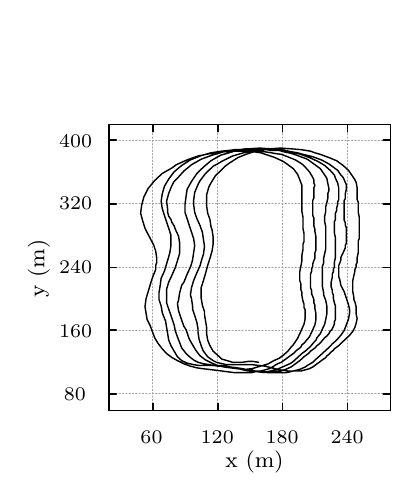
\begin{tikzpicture}[baseline={(0,1)},y=0.80pt, x=0.80pt, yscale=-0.530000, xscale=0.530000, inner sep=0pt, outer sep=0pt]
\scriptsize
\begin{scope}[draw=black,line join=bevel,line cap=rect,even odd rule,line width=0.512pt]
  \begin{scope}[cm={{1.0,0.0,0.0,1.0,(0.0,0.0)}},draw=black,line join=bevel,line cap=rect,line width=0.512pt]
  \end{scope}
  \begin{scope}[cm={{1.00625,0.0,0.0,1.00625,(0.0,0.0)}},draw=black,line join=bevel,line cap=rect,line width=0.512pt]
  \end{scope}
  \begin{scope}[cm={{1.00625,0.0,0.0,1.00625,(0.0,0.0)}},draw=ca0a0a4,dash pattern=on 0.40pt off 0.80pt,line join=round,line cap=round,line width=0.400pt]
    \path[draw] (60.5000,243.5000) -- (298.5000,243.5000);
  \end{scope}
  \begin{scope}[cm={{1.00625,0.0,0.0,1.00625,(0.0,0.0)}},draw=black,line join=round,line cap=round,line width=0.512pt]
    \path[draw] (60.5000,243.5000) -- (66.5000,243.5000);
    \path[draw] (298.5000,243.5000) -- (292.5000,243.5000);
  \end{scope}
  \begin{scope}[cm={{1.00625,0.0,0.0,1.00625,(0.0,0.0)}},draw=black,line join=bevel,line cap=rect,line width=0.512pt]
  \end{scope}
  \begin{scope}[cm={{1.00625,0.0,0.0,1.00625,(30.1875,251.059)}},draw=black,line join=bevel,line cap=rect,line width=0.512pt]
  \end{scope}
  \begin{scope}[cm={{1.00625,0.0,0.0,1.00625,(30.1875,251.059)}},draw=black,line join=bevel,line cap=rect,line width=0.512pt]
  \end{scope}
  \begin{scope}[cm={{1.00625,0.0,0.0,1.00625,(30.1875,251.059)}},draw=black,line join=bevel,line cap=rect,line width=0.512pt]
  \end{scope}
  \begin{scope}[cm={{1.00625,0.0,0.0,1.00625,(30.1875,251.059)}},draw=black,line join=bevel,line cap=rect,line width=0.512pt]
  \end{scope}
  \begin{scope}[cm={{1.00625,0.0,0.0,1.00625,(30.1875,251.059)}},draw=black,line join=bevel,line cap=rect,line width=0.512pt]
  \end{scope}
  \begin{scope}[cm={{1.00625,0.0,0.0,1.00625,(22.1875,251.059)}},draw=black,line join=bevel,line cap=rect,line width=0.512pt]
    \path[fill=black] (0.0000,0.0000) node[above right] () {80};
  \end{scope} w
  \begin{scope}[cm={{1.00625,0.0,0.0,1.00625,(30.1875,251.059)}},draw=black,line join=bevel,line cap=rect,line width=0.512pt]
  \end{scope}
  \begin{scope}[cm={{1.00625,0.0,0.0,1.00625,(0.0,0.0)}},draw=black,line join=bevel,line cap=rect,line width=0.512pt]
  \end{scope}
  \begin{scope}[cm={{1.00625,0.0,0.0,1.00625,(0.0,0.0)}},draw=ca0a0a4,dash pattern=on 0.40pt off 0.80pt,line join=round,line cap=round,line width=0.400pt]
    \path[draw] (60.5000,189.5000) -- (298.5000,189.5000);
  \end{scope}
  \begin{scope}[cm={{1.00625,0.0,0.0,1.00625,(0.0,0.0)}},draw=black,line join=round,line cap=round,line width=0.512pt]
    \path[draw] (60.5000,189.5000) -- (66.5000,189.5000);
    \path[draw] (298.5000,189.5000) -- (292.5000,189.5000);
  \end{scope}
  \begin{scope}[cm={{1.00625,0.0,0.0,1.00625,(0.0,0.0)}},draw=black,line join=bevel,line cap=rect,line width=0.512pt]
  \end{scope}
  \begin{scope}[cm={{1.00625,0.0,0.0,1.00625,(26.1625,196.722)}},draw=black,line join=bevel,line cap=rect,line width=0.512pt]
  \end{scope}
  \begin{scope}[cm={{1.00625,0.0,0.0,1.00625,(26.1625,196.722)}},draw=black,line join=bevel,line cap=rect,line width=0.512pt]
  \end{scope}
  \begin{scope}[cm={{1.00625,0.0,0.0,1.00625,(26.1625,196.722)}},draw=black,line join=bevel,line cap=rect,line width=0.512pt]
  \end{scope}
  \begin{scope}[cm={{1.00625,0.0,0.0,1.00625,(26.1625,196.722)}},draw=black,line join=bevel,line cap=rect,line width=0.512pt]
  \end{scope}
  \begin{scope}[cm={{1.00625,0.0,0.0,1.00625,(26.1625,196.722)}},draw=black,line join=bevel,line cap=rect,line width=0.512pt]
  \end{scope}
  \begin{scope}[cm={{1.00625,0.0,0.0,1.00625,(18.1625,196.722)}},draw=black,line join=bevel,line cap=rect,line width=0.512pt]
    \path[fill=black] (0.0000,0.0000) node[above right] () {160};
  \end{scope}
  \begin{scope}[cm={{1.00625,0.0,0.0,1.00625,(26.1625,196.722)}},draw=black,line join=bevel,line cap=rect,line width=0.512pt]
  \end{scope}
  \begin{scope}[cm={{1.00625,0.0,0.0,1.00625,(0.0,0.0)}},draw=black,line join=bevel,line cap=rect,line width=0.512pt]
  \end{scope}
  \begin{scope}[cm={{1.00625,0.0,0.0,1.00625,(0.0,0.0)}},draw=ca0a0a4,dash pattern=on 0.40pt off 0.80pt,line join=round,line cap=round,line width=0.400pt]
    \path[draw] (60.5000,136.5000) -- (298.5000,136.5000);
  \end{scope}
  \begin{scope}[cm={{1.00625,0.0,0.0,1.00625,(0.0,0.0)}},draw=black,line join=round,line cap=round,line width=0.512pt]
    \path[draw] (60.5000,136.5000) -- (66.5000,136.5000);
    \path[draw] (298.5000,136.5000) -- (292.5000,136.5000);
  \end{scope}
  \begin{scope}[cm={{1.00625,0.0,0.0,1.00625,(0.0,0.0)}},draw=black,line join=bevel,line cap=rect,line width=0.512pt]
  \end{scope}
  \begin{scope}[cm={{1.00625,0.0,0.0,1.00625,(26.1625,142.384)}},draw=black,line join=bevel,line cap=rect,line width=0.512pt]
  \end{scope}
  \begin{scope}[cm={{1.00625,0.0,0.0,1.00625,(26.1625,142.384)}},draw=black,line join=bevel,line cap=rect,line width=0.512pt]
  \end{scope}
  \begin{scope}[cm={{1.00625,0.0,0.0,1.00625,(26.1625,142.384)}},draw=black,line join=bevel,line cap=rect,line width=0.512pt]
  \end{scope}
  \begin{scope}[cm={{1.00625,0.0,0.0,1.00625,(26.1625,142.384)}},draw=black,line join=bevel,line cap=rect,line width=0.512pt]
  \end{scope}
  \begin{scope}[cm={{1.00625,0.0,0.0,1.00625,(26.1625,142.384)}},draw=black,line join=bevel,line cap=rect,line width=0.512pt]
  \end{scope}
  \begin{scope}[cm={{1.00625,0.0,0.0,1.00625,(18.1625,142.384)}},draw=black,line join=bevel,line cap=rect,line width=0.512pt]
    \path[fill=black] (0.0000,0.0000) node[above right] () {240};
  \end{scope}
  \begin{scope}[cm={{1.00625,0.0,0.0,1.00625,(26.1625,142.384)}},draw=black,line join=bevel,line cap=rect,line width=0.512pt]
  \end{scope}
  \begin{scope}[cm={{1.00625,0.0,0.0,1.00625,(0.0,0.0)}},draw=black,line join=bevel,line cap=rect,line width=0.512pt]
  \end{scope}
  \begin{scope}[cm={{1.00625,0.0,0.0,1.00625,(0.0,0.0)}},draw=ca0a0a4,dash pattern=on 0.40pt off 0.80pt,line join=round,line cap=round,line width=0.400pt]
    \path[draw] (60.5000,82.5000) -- (298.5000,82.5000);
  \end{scope}
  \begin{scope}[cm={{1.00625,0.0,0.0,1.00625,(0.0,0.0)}},draw=black,line join=round,line cap=round,line width=0.512pt]
    \path[draw] (60.5000,82.5000) -- (66.5000,82.5000);
    \path[draw] (298.5000,82.5000) -- (292.5000,82.5000);
  \end{scope}
  \begin{scope}[cm={{1.00625,0.0,0.0,1.00625,(0.0,0.0)}},draw=black,line join=bevel,line cap=rect,line width=0.512pt]
  \end{scope}
  \begin{scope}[cm={{1.00625,0.0,0.0,1.00625,(26.1625,88.0469)}},draw=black,line join=bevel,line cap=rect,line width=0.512pt]
  \end{scope}
  \begin{scope}[cm={{1.00625,0.0,0.0,1.00625,(26.1625,88.0469)}},draw=black,line join=bevel,line cap=rect,line width=0.512pt]
  \end{scope}
  \begin{scope}[cm={{1.00625,0.0,0.0,1.00625,(26.1625,88.0469)}},draw=black,line join=bevel,line cap=rect,line width=0.512pt]
  \end{scope}
  \begin{scope}[cm={{1.00625,0.0,0.0,1.00625,(26.1625,88.0469)}},draw=black,line join=bevel,line cap=rect,line width=0.512pt]
  \end{scope}
  \begin{scope}[cm={{1.00625,0.0,0.0,1.00625,(26.1625,88.0469)}},draw=black,line join=bevel,line cap=rect,line width=0.512pt]
  \end{scope}
  \begin{scope}[cm={{1.00625,0.0,0.0,1.00625,(18.1625,88.0469)}},draw=black,line join=bevel,line cap=rect,line width=0.512pt]
    \path[fill=black] (0.0000,0.0000) node[above right] () {320};
  \end{scope}
  \begin{scope}[cm={{1.00625,0.0,0.0,1.00625,(26.1625,88.0469)}},draw=black,line join=bevel,line cap=rect,line width=0.512pt]
  \end{scope}
  \begin{scope}[cm={{1.00625,0.0,0.0,1.00625,(0.0,0.0)}},draw=black,line join=bevel,line cap=rect,line width=0.512pt]
  \end{scope}
  \begin{scope}[cm={{1.00625,0.0,0.0,1.00625,(0.0,0.0)}},draw=ca0a0a4,dash pattern=on 0.40pt off 0.80pt,line join=round,line cap=round,line width=0.400pt]
    \path[draw] (60.5000,28.5000) -- (298.5000,28.5000);
  \end{scope}
  \begin{scope}[cm={{1.00625,0.0,0.0,1.00625,(0.0,0.0)}},draw=black,line join=round,line cap=round,line width=0.512pt]
    \path[draw] (60.5000,28.5000) -- (66.5000,28.5000);
    \path[draw] (298.5000,28.5000) -- (292.5000,28.5000);
  \end{scope}
  \begin{scope}[cm={{1.00625,0.0,0.0,1.00625,(0.0,0.0)}},draw=black,line join=bevel,line cap=rect,line width=0.512pt]
  \end{scope}
  \begin{scope}[cm={{1.00625,0.0,0.0,1.00625,(26.1625,34.7156)}},draw=black,line join=bevel,line cap=rect,line width=0.512pt]
  \end{scope}
  \begin{scope}[cm={{1.00625,0.0,0.0,1.00625,(26.1625,34.7156)}},draw=black,line join=bevel,line cap=rect,line width=0.512pt]
  \end{scope}
  \begin{scope}[cm={{1.00625,0.0,0.0,1.00625,(26.1625,34.7156)}},draw=black,line join=bevel,line cap=rect,line width=0.512pt]
  \end{scope}
  \begin{scope}[cm={{1.00625,0.0,0.0,1.00625,(26.1625,34.7156)}},draw=black,line join=bevel,line cap=rect,line width=0.512pt]
  \end{scope}
  \begin{scope}[cm={{1.00625,0.0,0.0,1.00625,(26.1625,34.7156)}},draw=black,line join=bevel,line cap=rect,line width=0.512pt]
  \end{scope}
  \begin{scope}[cm={{1.00625,0.0,0.0,1.00625,(18.1625,34.7156)}},draw=black,line join=bevel,line cap=rect,line width=0.512pt]
    \path[fill=black] (0.0000,0.0000) node[above right] () {400};
  \end{scope}
  \begin{scope}[cm={{1.00625,0.0,0.0,1.00625,(26.1625,34.7156)}},draw=black,line join=bevel,line cap=rect,line width=0.512pt]
  \end{scope}
  \begin{scope}[cm={{1.00625,0.0,0.0,1.00625,(0.0,0.0)}},draw=black,line join=bevel,line cap=rect,line width=0.512pt]
  \end{scope}
  \begin{scope}[cm={{1.00625,0.0,0.0,1.00625,(0.0,0.0)}},draw=ca0a0a4,dash pattern=on 0.40pt off 0.80pt,line join=round,line cap=round,line width=0.400pt]
    \path[draw] (97.5000,257.5000) -- (97.5000,15.5000);
  \end{scope}
  \begin{scope}[cm={{1.00625,0.0,0.0,1.00625,(0.0,0.0)}},draw=black,line join=round,line cap=round,line width=0.512pt]
    \path[draw] (97.5000,257.5000) -- (97.5000,251.5000);
    \path[draw] (97.5000,15.5000) -- (97.5000,21.5000);
  \end{scope}
  \begin{scope}[cm={{1.00625,0.0,0.0,1.00625,(0.0,0.0)}},draw=black,line join=bevel,line cap=rect,line width=0.512pt]
  \end{scope}
  \begin{scope}[cm={{1.00625,0.0,0.0,1.00625,(87.5438,279.234)}},draw=black,line join=bevel,line cap=rect,line width=0.512pt]
  \end{scope}
  \begin{scope}[cm={{1.00625,0.0,0.0,1.00625,(87.5438,279.234)}},draw=black,line join=bevel,line cap=rect,line width=0.512pt]
  \end{scope}
  \begin{scope}[cm={{1.00625,0.0,0.0,1.00625,(87.5438,279.234)}},draw=black,line join=bevel,line cap=rect,line width=0.512pt]
  \end{scope}
  \begin{scope}[cm={{1.00625,0.0,0.0,1.00625,(87.5438,279.234)}},draw=black,line join=bevel,line cap=rect,line width=0.512pt]
  \end{scope}
  \begin{scope}[cm={{1.00625,0.0,0.0,1.00625,(87.5438,279.234)}},draw=black,line join=bevel,line cap=rect,line width=0.512pt]
  \end{scope}
  \begin{scope}[cm={{1.00625,0.0,0.0,1.00625,(87.5438,287.234)}},draw=black,line join=bevel,line cap=rect,line width=0.512pt]
    \path[fill=black] (0.0000,0.0000) node[above right] () {60};
  \end{scope}
  \begin{scope}[cm={{1.00625,0.0,0.0,1.00625,(87.5438,279.234)}},draw=black,line join=bevel,line cap=rect,line width=0.512pt]
  \end{scope}
  \begin{scope}[cm={{1.00625,0.0,0.0,1.00625,(0.0,0.0)}},draw=black,line join=bevel,line cap=rect,line width=0.512pt]
  \end{scope}
  \begin{scope}[cm={{1.00625,0.0,0.0,1.00625,(0.0,0.0)}},draw=ca0a0a4,dash pattern=on 0.40pt off 0.80pt,line join=round,line cap=round,line width=0.400pt]
    \path[draw] (152.5000,257.5000) -- (152.5000,15.5000);
  \end{scope}
  \begin{scope}[cm={{1.00625,0.0,0.0,1.00625,(0.0,0.0)}},draw=black,line join=round,line cap=round,line width=0.512pt]
    \path[draw] (152.5000,257.5000) -- (152.5000,251.5000);
    \path[draw] (152.5000,15.5000) -- (152.5000,21.5000);
  \end{scope}
  \begin{scope}[cm={{1.00625,0.0,0.0,1.00625,(0.0,0.0)}},draw=black,line join=bevel,line cap=rect,line width=0.512pt]
  \end{scope}
  \begin{scope}[cm={{1.00625,0.0,0.0,1.00625,(138.863,279.234)}},draw=black,line join=bevel,line cap=rect,line width=0.512pt]
  \end{scope}
  \begin{scope}[cm={{1.00625,0.0,0.0,1.00625,(138.863,279.234)}},draw=black,line join=bevel,line cap=rect,line width=0.512pt]
  \end{scope}
  \begin{scope}[cm={{1.00625,0.0,0.0,1.00625,(138.863,279.234)}},draw=black,line join=bevel,line cap=rect,line width=0.512pt]
  \end{scope}
  \begin{scope}[cm={{1.00625,0.0,0.0,1.00625,(138.863,279.234)}},draw=black,line join=bevel,line cap=rect,line width=0.512pt]
  \end{scope}
  \begin{scope}[cm={{1.00625,0.0,0.0,1.00625,(138.863,279.234)}},draw=black,line join=bevel,line cap=rect,line width=0.512pt]
  \end{scope}
  \begin{scope}[cm={{1.00625,0.0,0.0,1.00625,(138.863,287.234)}},draw=black,line join=bevel,line cap=rect,line width=0.512pt]
    \path[fill=black] (0.0000,0.0000) node[above right] () {120};
  \end{scope}
  \begin{scope}[cm={{1.00625,0.0,0.0,1.00625,(138.863,279.234)}},draw=black,line join=bevel,line cap=rect,line width=0.512pt]
  \end{scope}
  \begin{scope}[cm={{1.00625,0.0,0.0,1.00625,(0.0,0.0)}},draw=black,line join=bevel,line cap=rect,line width=0.512pt]
  \end{scope}
  \begin{scope}[cm={{1.00625,0.0,0.0,1.00625,(0.0,0.0)}},draw=ca0a0a4,dash pattern=on 0.40pt off 0.80pt,line join=round,line cap=round,line width=0.400pt]
    \path[draw] (207.5000,257.5000) -- (207.5000,15.5000);
  \end{scope}
  \begin{scope}[cm={{1.00625,0.0,0.0,1.00625,(0.0,0.0)}},draw=black,line join=round,line cap=round,line width=0.512pt]
    \path[draw] (207.5000,257.5000) -- (207.5000,251.5000);
    \path[draw] (207.5000,15.5000) -- (207.5000,21.5000);
  \end{scope}
  \begin{scope}[cm={{1.00625,0.0,0.0,1.00625,(0.0,0.0)}},draw=black,line join=bevel,line cap=rect,line width=0.512pt]
  \end{scope}
  \begin{scope}[cm={{1.00625,0.0,0.0,1.00625,(194.206,279.234)}},draw=black,line join=bevel,line cap=rect,line width=0.512pt]
  \end{scope}
  \begin{scope}[cm={{1.00625,0.0,0.0,1.00625,(194.206,279.234)}},draw=black,line join=bevel,line cap=rect,line width=0.512pt]
  \end{scope}
  \begin{scope}[cm={{1.00625,0.0,0.0,1.00625,(194.206,279.234)}},draw=black,line join=bevel,line cap=rect,line width=0.512pt]
  \end{scope}
  \begin{scope}[cm={{1.00625,0.0,0.0,1.00625,(194.206,279.234)}},draw=black,line join=bevel,line cap=rect,line width=0.512pt]
  \end{scope}
  \begin{scope}[cm={{1.00625,0.0,0.0,1.00625,(194.206,279.234)}},draw=black,line join=bevel,line cap=rect,line width=0.512pt]
  \end{scope}
  \begin{scope}[cm={{1.00625,0.0,0.0,1.00625,(194.206,287.234)}},draw=black,line join=bevel,line cap=rect,line width=0.512pt]
    \path[fill=black] (0.0000,0.0000) node[above right] () {180};
  \end{scope}
  \begin{scope}[cm={{1.00625,0.0,0.0,1.00625,(194.206,279.234)}},draw=black,line join=bevel,line cap=rect,line width=0.512pt]
  \end{scope}
  \begin{scope}[cm={{1.00625,0.0,0.0,1.00625,(0.0,0.0)}},draw=black,line join=bevel,line cap=rect,line width=0.512pt]
  \end{scope}
  \begin{scope}[cm={{1.00625,0.0,0.0,1.00625,(0.0,0.0)}},draw=ca0a0a4,dash pattern=on 0.40pt off 0.80pt,line join=round,line cap=round,line width=0.400pt]
    \path[draw] (262.5000,257.5000) -- (262.5000,21.5000) -- (262.5000,21.5000) --
      (262.5000,15.5000);
  \end{scope}
  \begin{scope}[cm={{1.00625,0.0,0.0,1.00625,(0.0,0.0)}},draw=black,line join=round,line cap=round,line width=0.512pt]
    \path[draw] (262.5000,257.5000) -- (262.5000,251.5000);
    \path[draw] (262.5000,15.5000) -- (262.5000,21.5000);
  \end{scope}
  \begin{scope}[cm={{1.00625,0.0,0.0,1.00625,(0.0,0.0)}},draw=black,line join=bevel,line cap=rect,line width=0.512pt]
  \end{scope}
  \begin{scope}[cm={{1.00625,0.0,0.0,1.00625,(249.55,279.234)}},draw=black,line join=bevel,line cap=rect,line width=0.512pt]
  \end{scope}
  \begin{scope}[cm={{1.00625,0.0,0.0,1.00625,(249.55,279.234)}},draw=black,line join=bevel,line cap=rect,line width=0.512pt]
  \end{scope}
  \begin{scope}[cm={{1.00625,0.0,0.0,1.00625,(249.55,279.234)}},draw=black,line join=bevel,line cap=rect,line width=0.512pt]
  \end{scope}
  \begin{scope}[cm={{1.00625,0.0,0.0,1.00625,(249.55,279.234)}},draw=black,line join=bevel,line cap=rect,line width=0.512pt]
  \end{scope}
  \begin{scope}[cm={{1.00625,0.0,0.0,1.00625,(249.55,279.234)}},draw=black,line join=bevel,line cap=rect,line width=0.512pt]
  \end{scope}
  \begin{scope}[cm={{1.00625,0.0,0.0,1.00625,(249.55,287.234)}},draw=black,line join=bevel,line cap=rect,line width=0.512pt]
    \path[fill=black] (0.0000,0.0000) node[above right] () {240};
  \end{scope}
  \begin{scope}[cm={{1.00625,0.0,0.0,1.00625,(249.55,279.234)}},draw=black,line join=bevel,line cap=rect,line width=0.512pt]
  \end{scope}
  \begin{scope}[cm={{1.00625,0.0,0.0,1.00625,(0.0,0.0)}},draw=black,line join=bevel,line cap=rect,line width=0.512pt]
  \end{scope}
  \begin{scope}[cm={{1.00625,0.0,0.0,1.00625,(0.0,0.0)}},draw=black,line join=round,line cap=round,line width=0.512pt]
    \path[draw] (60.5000,15.5000) -- (60.5000,257.5000) -- (298.5000,257.5000) --
      (298.5000,15.5000) -- (60.5000,15.5000);
  \end{scope}
  \begin{scope}[cm={{1.00625,0.0,0.0,1.00625,(0.0,0.0)}},draw=black,line join=bevel,line cap=rect,line width=0.512pt]
  \end{scope}
  \begin{scope}[cm={{0.0,-1.00625,1.00625,0.0,(16.6031,163.013)}},draw=black,line join=bevel,line cap=rect,line width=0.512pt]
  \end{scope}
  \begin{scope}[cm={{0.0,-1.00625,1.00625,0.0,(16.6031,163.013)}},draw=black,line join=bevel,line cap=rect,line width=0.512pt]
  \end{scope}
  \begin{scope}[cm={{0.0,-1.00625,1.00625,0.0,(16.6031,163.013)}},draw=black,line join=bevel,line cap=rect,line width=0.512pt]
  \end{scope}
  \begin{scope}[cm={{0.0,-1.00625,1.00625,0.0,(16.6031,163.013)}},draw=black,line join=bevel,line cap=rect,line width=0.512pt]
  \end{scope}
  \begin{scope}[cm={{0.0,-1.00625,1.00625,0.0,(16.6031,163.013)}},draw=black,line join=bevel,line cap=rect,line width=0.512pt]
  \end{scope}
  \begin{scope}[cm={{0.0,-1.00625,1.00625,0.0,(-8.6031,163.013)}},draw=black,line join=bevel,line cap=rect,line width=0.512pt]
    \path[fill=black] (0.0000,0.0000) node[above right] () {\rotatebox{90}{\footnotesize y (m)}};
  \end{scope}
  \begin{scope}[cm={{0.0,-1.00625,1.00625,0.0,(16.6031,163.013)}},draw=black,line join=bevel,line cap=rect,line width=0.512pt]
  \end{scope}
  \begin{scope}[cm={{1.00625,0.0,0.0,1.00625,(143.894,317.472)}},draw=black,line join=bevel,line cap=rect,line width=0.512pt]
  \end{scope}
  \begin{scope}[cm={{1.00625,0.0,0.0,1.00625,(143.894,317.472)}},draw=black,line join=bevel,line cap=rect,line width=0.512pt]
  \end{scope}
  \begin{scope}[cm={{1.00625,0.0,0.0,1.00625,(143.894,317.472)}},draw=black,line join=bevel,line cap=rect,line width=0.512pt]
  \end{scope}
  \begin{scope}[cm={{1.00625,0.0,0.0,1.00625,(143.894,317.472)}},draw=black,line join=bevel,line cap=rect,line width=0.512pt]
  \end{scope}
  \begin{scope}[cm={{1.00625,0.0,0.0,1.00625,(143.894,317.472)}},draw=black,line join=bevel,line cap=rect,line width=0.512pt]
  \end{scope}
  \begin{scope}[cm={{1.00625,0.0,0.0,1.00625,(159.894,312.472)}},draw=black,line join=bevel,line cap=rect,line width=0.512pt]
    \path[fill=black] (0.0000,0.0000) node[above right] () {\footnotesize x (m)};
  \end{scope}
  \begin{scope}[cm={{1.00625,0.0,0.0,1.00625,(143.894,317.472)}},draw=black,line join=bevel,line cap=rect,line width=0.512pt]
  \end{scope}
  \begin{scope}[cm={{1.00625,0.0,0.0,1.00625,(0.0,0.0)}},draw=black,line join=bevel,line cap=rect,line width=0.512pt]
  \end{scope}
  \begin{scope}[cm={{1.00625,0.0,0.0,1.00625,(0.0,0.0)}},draw=black,line join=bevel,line cap=rect,line width=0.512pt]
  \end{scope}
  \begin{scope}[cm={{1.00625,0.0,0.0,1.00625,(0.0,0.0)}},draw=black,line join=bevel,line cap=rect,line width=0.512pt]
  \end{scope}
  \begin{scope}[cm={{1.00625,0.0,0.0,1.00625,(0.0,0.0)}},draw=black,line join=round,line cap=round,line width=0.512pt]
    \path[draw] (176.0000,222.7000) -- (176.0000,222.7000) -- (176.0000,222.7000) --
      (181.5000,222.1000) -- (181.5000,222.1000) -- (181.5000,222.1000) --
      (186.1000,220.7000) -- (186.1000,220.7000) -- (190.7000,219.4000) --
      (190.7000,219.4000) -- (195.3000,218.0000) -- (195.3000,218.0000) --
      (195.3000,218.0000) -- (199.9000,215.3000) -- (199.9000,215.3000) --
      (204.5000,213.3000) -- (204.5000,213.3000) -- (204.5000,213.3000) --
      (208.1000,210.6000) -- (208.1000,210.6000) -- (208.1000,210.6000) --
      (211.8000,207.3000) -- (211.8000,207.3000) -- (214.5000,203.9000) --
      (216.4000,201.9000) -- (216.4000,201.9000) -- (217.3000,200.6000) --
      (217.3000,200.6000) -- (220.0000,196.5000) -- (220.0000,196.5000) --
      (221.9000,192.5000) -- (221.9000,192.5000) -- (222.8000,190.5000) --
      (222.8000,190.5000) -- (224.6000,186.4000) -- (224.6000,186.4000) --
      (225.5000,184.4000) -- (225.5000,184.4000) -- (226.5000,179.7000) --
      (226.5000,177.0000) -- (226.5000,175.0000) -- (226.5000,175.0000) --
      (226.5000,172.3000) -- (225.5000,170.3000) -- (225.5000,167.6000) --
      (224.6000,164.9000) -- (224.6000,164.9000) -- (224.6000,164.9000) --
      (223.7000,160.2000) -- (223.7000,157.6000) -- (222.8000,154.9000) --
      (222.8000,154.9000) -- (222.8000,152.2000) -- (222.8000,150.2000) --
      (221.9000,147.5000) -- (221.9000,147.5000) -- (221.9000,147.5000) --
      (221.9000,142.1000) -- (221.9000,140.1000) -- (221.9000,140.1000) --
      (221.9000,140.1000) -- (222.8000,135.4000) -- (222.8000,135.4000) --
      (223.7000,130.7000) -- (223.7000,130.7000) -- (223.7000,126.0000) --
      (223.7000,126.0000) -- (223.7000,126.0000) -- (224.6000,121.3000) --
      (224.6000,119.3000) -- (224.6000,116.6000) -- (224.6000,116.6000) --
      (225.5000,114.5000) -- (225.5000,112.5000) -- (225.5000,112.5000) --
      (225.5000,107.8000) -- (225.5000,107.8000) -- (225.5000,107.8000) --
      (224.6000,103.1000) -- (224.6000,103.1000) -- (224.6000,98.4000) --
      (224.6000,98.4000) -- (224.6000,96.4000) -- (224.6000,93.7000) --
      (224.6000,93.7000) -- (223.7000,89.0000) -- (223.7000,89.0000) --
      (223.7000,89.0000) -- (223.7000,85.0000) -- (223.7000,85.0000) --
      (223.7000,80.3000) -- (223.7000,80.3000) -- (223.7000,80.3000) --
      (223.7000,76.2000) -- (223.7000,76.2000) -- (223.7000,71.5000) --
      (223.7000,71.5000) -- (223.7000,69.5000) -- (223.7000,66.8000) --
      (223.7000,66.8000) -- (221.9000,62.1000) -- (221.9000,62.1000) --
      (221.9000,62.1000) -- (220.0000,57.4000) -- (220.0000,57.4000) --
      (216.4000,52.7000) -- (216.4000,52.7000) -- (216.4000,52.7000) --
      (210.9000,48.7000) -- (208.1000,46.7000) -- (208.1000,46.7000) --
      (200.8000,43.3000) -- (200.8000,43.3000) -- (197.1000,42.0000) --
      (197.1000,42.0000) -- (188.9000,39.3000) -- (188.9000,39.3000) --
      (188.9000,39.3000) -- (179.7000,37.9000) -- (175.1000,37.9000) --
      (175.1000,37.9000) -- (175.1000,37.9000) -- (165.0000,37.9000) --
      (165.0000,37.9000) -- (155.9000,38.6000) -- (155.9000,38.6000) --
      (155.9000,38.6000) -- (145.8000,40.0000) -- (145.8000,40.0000) --
      (135.7000,42.0000) -- (135.7000,42.0000) -- (135.7000,42.0000) --
      (126.5000,45.3000) -- (126.5000,45.3000) -- (117.3000,49.4000) --
      (117.3000,49.4000) -- (113.7000,52.1000) -- (113.7000,52.1000) --
      (105.4000,56.8000) -- (105.4000,56.8000) -- (99.0000,62.8000) --
      (99.0000,62.8000) -- (99.0000,62.8000) -- (93.5000,69.5000) --
      (93.5000,69.5000) -- (93.5000,69.5000) -- (89.8000,76.9000) --
      (89.8000,76.9000) -- (88.0000,83.6000) -- (88.0000,83.6000) --
      (87.1000,90.4000) -- (87.1000,90.4000) -- (87.1000,90.4000) --
      (88.9000,97.1000) -- (88.9000,97.1000) -- (88.9000,97.1000) --
      (90.8000,103.1000) -- (90.8000,103.1000) -- (93.5000,108.5000) --
      (95.3000,111.9000) -- (95.3000,111.9000) -- (95.3000,111.9000) --
      (98.1000,117.2000) -- (98.1000,117.2000) -- (99.9000,122.6000) --
      (99.9000,122.6000) -- (99.9000,122.6000) -- (100.8000,128.7000) --
      (100.8000,132.0000) -- (99.9000,134.7000) -- (99.9000,134.7000) --
      (99.9000,138.1000) -- (99.9000,138.1000) -- (97.2000,144.8000) --
      (96.3000,147.5000) -- (95.3000,150.8000) -- (95.3000,150.8000) --
      (95.3000,150.8000) -- (93.5000,156.9000) -- (93.5000,156.9000) --
      (91.7000,162.9000) -- (91.7000,162.9000) -- (91.7000,162.9000) --
      (90.8000,169.6000) -- (90.8000,169.6000) -- (91.7000,175.0000) --
      (91.7000,175.0000) -- (91.7000,175.0000) -- (92.6000,180.4000) --
      (92.6000,180.4000) -- (95.3000,185.8000) -- (95.3000,185.8000) --
      (95.3000,185.8000) -- (97.2000,191.1000) -- (97.2000,191.1000) --
      (99.0000,195.9000) -- (99.0000,195.9000) -- (99.0000,195.9000) --
      (101.8000,200.6000) -- (101.8000,200.6000) -- (105.4000,205.3000) --
      (105.4000,205.3000) -- (105.4000,205.3000) -- (109.1000,209.3000) --
      (109.1000,209.3000) -- (113.7000,212.7000) -- (113.7000,212.7000) --
      (113.7000,212.7000) -- (118.3000,215.3000) -- (118.3000,215.3000) --
      (123.8000,218.0000) -- (123.8000,218.0000) -- (123.8000,218.0000) --
      (129.3000,220.0000) -- (129.3000,220.0000) -- (129.3000,220.0000) --
      (134.8000,221.4000) -- (134.8000,221.4000) -- (139.4000,222.1000) --
      (139.4000,222.1000) -- (144.9000,222.7000) -- (144.9000,222.7000) --
      (144.9000,222.7000) -- (150.4000,223.4000) -- (150.4000,223.4000) --
      (155.9000,224.1000) -- (155.9000,224.1000) -- (155.9000,224.1000) --
      (160.4000,224.7000) -- (160.4000,224.7000) -- (160.4000,224.7000) --
      (165.9000,225.4000) -- (165.9000,225.4000) -- (171.4000,225.4000) --
      (171.4000,225.4000) -- (176.0000,225.4000) -- (176.0000,225.4000) --
      (178.8000,225.4000) -- (181.5000,225.4000) -- (184.3000,224.7000) --
      (186.1000,224.7000) -- (186.1000,224.7000) -- (188.9000,224.1000) --
      (191.6000,223.4000) -- (191.6000,223.4000) -- (196.2000,222.1000) --
      (196.2000,222.1000) -- (196.2000,222.1000) -- (199.9000,220.0000) --
      (201.7000,218.7000) -- (204.5000,217.4000) -- (204.5000,217.4000) --
      (206.3000,216.7000) -- (208.1000,215.3000) -- (210.0000,214.0000) --
      (211.8000,212.7000) -- (211.8000,212.7000) -- (213.6000,211.3000) --
      (215.5000,210.0000) -- (217.3000,208.6000) -- (219.1000,206.6000) --
      (219.1000,206.6000) -- (221.0000,205.3000) -- (222.8000,203.9000) --
      (223.7000,201.9000) -- (225.5000,200.6000) -- (225.5000,200.6000) --
      (225.5000,200.6000) -- (228.3000,197.2000) -- (230.1000,195.2000) --
      (231.0000,193.2000) -- (231.0000,193.2000) -- (232.0000,191.1000) --
      (232.9000,189.1000) -- (233.8000,187.1000) -- (233.8000,187.1000) --
      (234.7000,185.1000) -- (234.7000,185.1000) -- (235.6000,180.4000) --
      (235.6000,180.4000) -- (235.6000,175.7000) -- (235.6000,175.7000) --
      (235.6000,175.7000) -- (234.7000,171.0000) -- (234.7000,168.3000) --
      (233.8000,166.3000) -- (233.8000,166.3000) -- (233.8000,163.6000) --
      (232.9000,160.9000) -- (232.0000,158.9000) -- (232.0000,156.2000) --
      (232.0000,156.2000) -- (231.0000,153.5000) -- (231.0000,151.5000) --
      (231.0000,148.8000) -- (231.0000,146.8000) -- (231.0000,146.8000) --
      (231.0000,146.8000) -- (231.0000,142.1000) -- (232.0000,139.4000) --
      (232.0000,137.4000) -- (232.0000,137.4000) -- (232.9000,135.4000) --
      (232.9000,133.4000) -- (233.8000,130.7000) -- (233.8000,130.7000) --
      (234.7000,128.7000) -- (234.7000,128.7000) -- (234.7000,124.0000) --
      (235.6000,121.9000) -- (235.6000,119.9000) -- (235.6000,119.9000) --
      (235.6000,117.2000) -- (235.6000,115.2000) -- (235.6000,112.5000) --
      (235.6000,110.5000) -- (235.6000,110.5000) -- (235.6000,110.5000) --
      (234.7000,105.8000) -- (234.7000,103.8000) -- (233.8000,101.1000) --
      (233.8000,101.1000) -- (233.8000,99.1000) -- (233.8000,97.1000) --
      (233.8000,94.4000) -- (232.9000,92.4000) -- (232.9000,92.4000) --
      (232.9000,90.4000) -- (232.9000,90.4000) -- (232.9000,85.7000) --
      (232.9000,85.7000) -- (232.9000,85.7000) -- (232.9000,81.6000) --
      (232.9000,79.6000) -- (233.8000,77.6000) -- (233.8000,75.6000) --
      (233.8000,75.6000) -- (233.8000,72.9000) -- (233.8000,70.9000) --
      (233.8000,68.9000) -- (234.7000,66.8000) -- (234.7000,66.8000) --
      (233.8000,64.8000) -- (233.8000,62.1000) -- (232.9000,60.1000) --
      (232.9000,60.1000) -- (232.9000,60.1000) -- (230.1000,55.4000) --
      (230.1000,55.4000) -- (226.5000,51.4000) -- (223.7000,48.7000) --
      (223.7000,48.7000) -- (223.7000,48.7000) -- (218.2000,45.3000) --
      (218.2000,45.3000) -- (218.2000,45.3000) -- (210.0000,42.0000) --
      (206.3000,40.6000) -- (201.7000,40.0000) -- (198.0000,39.3000) --
      (193.5000,38.6000) -- (193.5000,38.6000) -- (188.9000,37.9000) --
      (184.3000,37.3000) -- (179.7000,37.3000) -- (179.7000,37.3000) --
      (179.7000,37.3000) -- (170.5000,37.3000) -- (165.9000,37.3000) --
      (161.4000,37.3000) -- (155.9000,37.9000) -- (155.9000,37.9000) --
      (155.9000,37.9000) -- (146.7000,39.3000) -- (142.1000,40.6000) --
      (142.1000,40.6000) -- (137.5000,42.0000) -- (137.5000,42.0000) --
      (129.3000,45.3000) -- (129.3000,45.3000) -- (129.3000,45.3000) --
      (121.9000,50.0000) -- (121.9000,50.0000) -- (115.5000,55.4000) --
      (115.5000,55.4000) -- (115.5000,55.4000) -- (110.9000,61.5000) --
      (110.9000,61.5000) -- (107.3000,67.5000) -- (107.3000,67.5000) --
      (107.3000,67.5000) -- (105.4000,74.2000) -- (105.4000,74.2000) --
      (104.5000,80.3000) -- (104.5000,80.3000) -- (105.4000,86.3000) --
      (105.4000,86.3000) -- (105.4000,86.3000) -- (107.3000,92.4000) --
      (107.3000,92.4000) -- (107.3000,92.4000) -- (109.1000,97.7000) --
      (109.1000,97.7000) -- (110.9000,103.1000) -- (110.9000,103.1000) --
      (112.8000,109.2000) -- (112.8000,109.2000) -- (112.8000,109.2000) --
      (112.8000,115.2000) -- (112.8000,117.9000) -- (112.8000,117.9000) --
      (112.8000,117.9000) -- (111.8000,124.0000) -- (110.9000,127.3000) --
      (110.9000,127.3000) -- (110.9000,127.3000) -- (109.1000,133.4000) --
      (109.1000,133.4000) -- (107.3000,139.4000) -- (107.3000,139.4000) --
      (104.5000,145.5000) -- (104.5000,145.5000) -- (104.5000,145.5000) --
      (103.6000,152.2000) -- (103.6000,152.2000) -- (103.6000,152.2000) --
      (102.7000,157.6000) -- (102.7000,157.6000) -- (102.7000,163.6000) --
      (102.7000,163.6000) -- (102.7000,163.6000) -- (104.5000,169.0000) --
      (104.5000,169.0000) -- (105.4000,174.4000) -- (106.3000,177.0000) --
      (106.3000,177.0000) -- (106.3000,177.0000) -- (108.2000,181.7000) --
      (108.2000,181.7000) -- (109.1000,187.1000) -- (109.1000,187.1000) --
      (109.1000,187.1000) -- (110.0000,192.5000) -- (110.0000,192.5000) --
      (110.9000,197.9000) -- (110.9000,197.9000) -- (110.9000,197.9000) --
      (112.8000,202.6000) -- (112.8000,202.6000) -- (115.5000,207.3000) --
      (115.5000,207.3000) -- (115.5000,207.3000) -- (118.3000,212.0000) --
      (118.3000,212.0000) -- (121.9000,215.3000) -- (121.9000,215.3000) --
      (121.9000,215.3000) -- (126.5000,217.4000) -- (126.5000,217.4000) --
      (132.0000,218.7000) -- (132.0000,218.7000) -- (132.0000,218.7000) --
      (136.6000,219.4000) -- (136.6000,219.4000) -- (141.2000,219.4000) --
      (141.2000,219.4000) -- (141.2000,219.4000) -- (146.7000,219.4000) --
      (146.7000,219.4000) -- (151.3000,219.4000) -- (154.0000,219.4000) --
      (154.0000,219.4000) -- (154.0000,219.4000) -- (159.5000,220.0000) --
      (159.5000,220.0000) -- (159.5000,220.0000) -- (164.1000,221.4000) --
      (164.1000,221.4000) -- (169.6000,222.1000) -- (172.4000,222.7000) --
      (172.4000,222.7000) -- (175.1000,223.4000) -- (175.1000,223.4000) --
      (180.6000,224.1000) -- (180.6000,224.1000) -- (186.1000,224.7000) --
      (186.1000,224.7000) -- (186.1000,224.7000) -- (191.6000,225.4000) --
      (191.6000,225.4000) -- (197.1000,224.1000) -- (197.1000,224.1000) --
      (197.1000,224.1000) -- (202.6000,222.7000) -- (202.6000,222.7000) --
      (207.2000,220.7000) -- (207.2000,220.7000) -- (207.2000,220.7000) --
      (211.8000,218.7000) -- (214.5000,217.4000) -- (214.5000,217.4000) --
      (216.4000,216.0000) -- (216.4000,216.0000) -- (220.0000,212.7000) --
      (220.0000,212.7000) -- (223.7000,209.3000) -- (223.7000,209.3000) --
      (223.7000,209.3000) -- (227.4000,206.6000) -- (227.4000,206.6000) --
      (227.4000,206.6000) -- (231.0000,203.2000) -- (231.0000,203.2000) --
      (233.8000,199.9000) -- (235.6000,197.9000) -- (235.6000,197.9000) --
      (236.5000,195.9000) -- (236.5000,195.9000) -- (239.3000,192.5000) --
      (239.3000,192.5000) -- (241.1000,188.5000) -- (241.1000,188.5000) --
      (241.1000,188.5000) -- (243.0000,184.4000) -- (243.0000,184.4000) --
      (243.9000,180.4000) -- (243.9000,180.4000) -- (243.9000,180.4000) --
      (244.8000,175.7000) -- (244.8000,175.7000) -- (244.8000,171.0000) --
      (244.8000,171.0000) -- (244.8000,169.0000) -- (244.8000,169.0000) --
      (243.9000,164.3000) -- (243.9000,164.3000) -- (243.9000,164.3000) --
      (242.1000,159.6000) -- (242.1000,157.6000) -- (242.1000,157.6000) --
      (241.1000,152.8000) -- (241.1000,152.8000) -- (241.1000,152.8000) --
      (241.1000,148.1000) -- (241.1000,148.1000) -- (241.1000,148.1000) --
      (241.1000,143.4000) -- (241.1000,143.4000) -- (241.1000,139.4000) --
      (241.1000,139.4000) -- (241.1000,135.4000) -- (241.1000,135.4000) --
      (242.1000,132.7000) -- (242.1000,132.7000) -- (242.1000,128.7000) --
      (242.1000,128.7000) -- (242.1000,128.7000) -- (243.0000,124.6000) --
      (243.0000,124.6000) -- (243.9000,120.6000) -- (243.9000,120.6000) --
      (243.9000,120.6000) -- (243.9000,115.9000) -- (243.9000,115.9000) --
      (243.9000,111.9000) -- (243.9000,111.9000) -- (243.9000,109.8000) --
      (243.9000,109.8000) -- (243.9000,105.8000) -- (243.9000,103.8000) --
      (243.9000,103.8000) -- (243.9000,101.8000) -- (243.9000,101.8000) --
      (243.0000,97.7000) -- (243.0000,97.7000) -- (243.0000,97.7000) --
      (243.0000,93.0000) -- (243.0000,93.0000) -- (243.9000,89.0000) --
      (243.9000,89.0000) -- (243.9000,89.0000) -- (243.9000,85.0000) --
      (243.9000,85.0000) -- (244.8000,81.6000) -- (244.8000,81.6000) --
      (245.7000,77.6000) -- (245.7000,77.6000) -- (245.7000,77.6000) --
      (245.7000,73.6000) -- (246.6000,71.5000) -- (246.6000,69.5000) --
      (246.6000,69.5000) -- (246.6000,69.5000) -- (245.7000,65.5000) --
      (245.7000,65.5000) -- (244.8000,60.8000) -- (244.8000,60.8000) --
      (244.8000,60.8000) -- (242.1000,56.8000) -- (242.1000,56.8000) --
      (239.3000,52.7000) -- (239.3000,52.7000) -- (239.3000,52.7000) --
      (233.8000,48.7000) -- (233.8000,48.7000) -- (233.8000,48.7000) --
      (228.3000,44.7000) -- (228.3000,44.7000) -- (221.0000,42.0000) --
      (217.3000,40.6000) -- (212.7000,39.3000) -- (212.7000,39.3000) --
      (209.0000,38.6000) -- (204.5000,37.3000) -- (204.5000,37.3000) --
      (195.3000,36.6000) -- (195.3000,36.6000) -- (195.3000,36.6000) --
      (186.1000,35.9000) -- (180.6000,35.9000) -- (176.0000,35.9000) --
      (176.0000,35.9000) -- (171.4000,36.6000) -- (166.9000,36.6000) --
      (162.3000,37.3000) -- (162.3000,37.3000) -- (156.8000,38.6000) --
      (156.8000,38.6000) -- (147.6000,41.3000) -- (147.6000,41.3000) --
      (138.4000,44.7000) -- (138.4000,44.7000) -- (138.4000,44.7000) --
      (130.2000,49.4000) -- (130.2000,49.4000) -- (130.2000,49.4000) --
      (123.8000,54.7000) -- (123.8000,54.7000) -- (118.3000,60.8000) --
      (115.5000,63.5000) -- (113.7000,66.8000) -- (113.7000,66.8000) --
      (113.7000,66.8000) -- (110.9000,73.6000) -- (110.9000,73.6000) --
      (109.1000,80.3000) -- (109.1000,80.3000) -- (109.1000,80.3000) --
      (110.0000,87.0000) -- (110.0000,89.7000) -- (110.9000,93.0000) --
      (110.9000,93.0000) -- (112.8000,95.7000) -- (113.7000,98.4000) --
      (115.5000,101.1000) -- (115.5000,101.1000) -- (116.4000,103.8000) --
      (116.4000,103.8000) -- (119.2000,109.8000) -- (119.2000,109.8000) --
      (120.1000,115.2000) -- (120.1000,115.2000) -- (120.1000,118.6000) --
      (120.1000,118.6000) -- (120.1000,124.6000) -- (120.1000,124.6000) --
      (120.1000,124.6000) -- (118.3000,130.7000) -- (118.3000,130.7000) --
      (116.4000,136.7000) -- (116.4000,136.7000) -- (116.4000,136.7000) --
      (113.7000,142.8000) -- (113.7000,142.8000) -- (110.9000,148.8000) --
      (110.9000,148.8000) -- (110.9000,148.8000) -- (109.1000,154.9000) --
      (109.1000,154.9000) -- (109.1000,160.9000) -- (109.1000,160.9000) --
      (109.1000,160.9000) -- (109.1000,166.3000) -- (109.1000,166.3000) --
      (110.9000,171.7000) -- (110.9000,171.7000) -- (110.9000,171.7000) --
      (112.8000,177.0000) -- (113.7000,179.7000) -- (113.7000,179.7000) --
      (115.5000,185.1000) -- (115.5000,185.1000) -- (115.5000,185.1000) --
      (116.4000,189.8000) -- (117.3000,192.5000) -- (117.3000,192.5000) --
      (118.3000,195.2000) -- (118.3000,195.2000) -- (120.1000,199.9000) --
      (120.1000,199.9000) -- (120.1000,199.9000) -- (121.9000,204.6000) --
      (121.9000,204.6000) -- (125.6000,209.3000) -- (125.6000,209.3000) --
      (129.3000,212.7000) -- (129.3000,212.7000) -- (129.3000,212.7000) --
      (132.9000,215.3000) -- (135.7000,216.7000) -- (135.7000,216.7000) --
      (135.7000,216.7000) -- (140.3000,218.0000) -- (140.3000,218.0000) --
      (145.8000,218.7000) -- (148.5000,219.4000) -- (148.5000,219.4000) --
      (148.5000,219.4000) -- (153.1000,220.0000) -- (153.1000,220.0000) --
      (157.7000,220.0000) -- (157.7000,220.0000) -- (157.7000,220.0000) --
      (163.2000,220.7000) -- (163.2000,220.7000) -- (168.7000,221.4000) --
      (168.7000,221.4000) -- (168.7000,221.4000) -- (173.3000,222.1000) --
      (176.0000,222.7000) -- (176.0000,222.7000) -- (176.0000,222.7000) --
      (181.5000,223.4000) -- (184.3000,224.1000) -- (187.0000,224.1000) --
      (187.0000,224.1000) -- (187.0000,224.1000) -- (191.6000,224.7000) --
      (194.4000,224.7000) -- (197.1000,224.7000) -- (197.1000,224.7000) --
      (199.9000,224.7000) -- (199.9000,224.7000) -- (205.4000,224.1000) --
      (205.4000,224.1000) -- (210.0000,222.7000) -- (210.0000,222.7000) --
      (210.0000,222.7000) -- (214.5000,220.7000) -- (214.5000,220.7000) --
      (214.5000,220.7000) -- (218.2000,218.0000) -- (218.2000,218.0000) --
      (221.9000,215.3000) -- (221.9000,215.3000) -- (225.5000,212.0000) --
      (225.5000,212.0000) -- (225.5000,212.0000) -- (229.2000,209.3000) --
      (231.0000,207.3000) -- (232.9000,205.9000) -- (232.9000,205.9000) --
      (234.7000,204.6000) -- (236.5000,202.6000) -- (238.4000,201.2000) --
      (240.2000,199.2000) -- (240.2000,199.2000) -- (240.2000,199.2000) --
      (243.0000,195.9000) -- (244.8000,194.5000) -- (246.6000,192.5000) --
      (246.6000,192.5000) -- (247.6000,190.5000) -- (249.4000,188.5000) --
      (250.3000,186.4000) -- (250.3000,186.4000) -- (251.2000,184.4000) --
      (251.2000,182.4000) -- (252.1000,180.4000) -- (252.1000,177.7000) --
      (252.1000,175.7000) -- (252.1000,175.7000) -- (252.1000,173.7000) --
      (252.1000,171.0000) -- (252.1000,169.0000) -- (252.1000,169.0000) --
      (251.2000,166.3000) -- (251.2000,166.3000) -- (250.3000,162.3000) --
      (250.3000,159.6000) -- (249.4000,157.6000) -- (249.4000,157.6000) --
      (249.4000,155.5000) -- (248.5000,152.8000) -- (248.5000,150.8000) --
      (248.5000,148.8000) -- (248.5000,148.8000) -- (248.5000,148.8000) --
      (249.4000,144.8000) -- (249.4000,142.1000) -- (250.3000,140.1000) --
      (250.3000,140.1000) -- (250.3000,138.1000) -- (251.2000,136.0000) --
      (251.2000,134.0000) -- (251.2000,132.0000) -- (251.2000,132.0000) --
      (251.2000,132.0000) -- (252.1000,128.0000) -- (252.1000,126.0000) --
      (252.1000,124.0000) -- (252.1000,124.0000) -- (252.1000,121.3000) --
      (252.1000,119.3000) -- (252.1000,119.3000) -- (252.1000,119.3000) --
      (252.1000,115.2000) -- (252.1000,115.2000) -- (252.1000,111.2000) --
      (252.1000,111.2000) -- (251.2000,107.2000) -- (251.2000,107.2000) --
      (251.2000,105.1000) -- (251.2000,105.1000) -- (251.2000,101.8000) --
      (251.2000,101.8000) -- (251.2000,101.8000) -- (251.2000,97.7000) --
      (252.1000,95.7000) -- (252.1000,95.7000) -- (252.1000,92.4000) --
      (252.1000,92.4000) -- (252.1000,90.4000) -- (253.1000,88.3000) --
      (253.1000,86.3000) -- (253.1000,86.3000) -- (253.1000,86.3000) --
      (254.0000,83.0000) -- (254.0000,81.0000) -- (254.9000,78.9000) --
      (254.9000,76.9000) -- (254.9000,76.9000) -- (254.9000,74.9000) --
      (254.9000,72.9000) -- (254.9000,70.9000) -- (254.9000,70.9000) --
      (254.9000,68.9000) -- (254.9000,68.9000) -- (254.0000,64.8000) --
      (254.0000,64.8000) -- (254.0000,64.8000) -- (252.1000,60.8000) --
      (251.2000,58.1000) -- (251.2000,58.1000) -- (247.6000,54.1000) --
      (247.6000,54.1000) -- (247.6000,54.1000) -- (243.0000,50.0000) --
      (243.0000,50.0000) -- (237.5000,46.7000) -- (237.5000,46.7000) --
      (237.5000,46.7000) -- (230.1000,43.3000) -- (230.1000,43.3000) --
      (222.8000,40.6000) -- (222.8000,40.6000) -- (222.8000,40.6000) --
      (215.5000,38.6000) -- (215.5000,38.6000) -- (206.3000,36.6000) --
      (206.3000,36.6000) -- (206.3000,36.6000) -- (197.1000,35.9000) --
      (197.1000,35.9000) -- (188.0000,35.3000) -- (188.0000,35.3000) --
      (188.0000,35.3000) -- (178.8000,35.9000) -- (178.8000,35.9000) --
      (168.7000,37.3000) -- (168.7000,37.3000) -- (168.7000,37.3000) --
      (159.5000,40.0000) -- (154.9000,41.3000) -- (154.9000,41.3000) --
      (154.9000,41.3000) -- (146.7000,46.0000) -- (146.7000,46.0000) --
      (140.3000,51.4000) -- (140.3000,51.4000) -- (140.3000,51.4000) --
      (134.8000,56.8000) -- (134.8000,56.8000) -- (130.2000,63.5000) --
      (130.2000,63.5000) -- (130.2000,63.5000) -- (126.5000,70.2000) --
      (126.5000,70.2000) -- (125.6000,76.2000) -- (125.6000,76.2000) --
      (125.6000,76.2000) -- (124.7000,83.0000) -- (124.7000,83.0000) --
      (124.7000,89.7000) -- (124.7000,89.7000) -- (124.7000,89.7000) --
      (126.5000,95.1000) -- (126.5000,95.1000) -- (128.4000,101.1000) --
      (129.3000,103.8000) -- (129.3000,103.8000) -- (129.3000,103.8000) --
      (131.1000,109.2000) -- (132.0000,111.9000) -- (132.0000,111.9000) --
      (132.0000,111.9000) -- (132.9000,117.9000) -- (132.9000,117.9000) --
      (132.0000,124.0000) -- (132.0000,124.0000) -- (131.1000,130.0000) --
      (131.1000,130.0000) -- (130.2000,133.4000) -- (129.3000,136.0000) --
      (129.3000,136.0000) -- (129.3000,136.0000) -- (126.5000,142.1000) --
      (126.5000,142.1000) -- (123.8000,148.8000) -- (121.9000,151.5000) --
      (121.9000,151.5000) -- (121.9000,151.5000) -- (120.1000,158.2000) --
      (120.1000,158.2000) -- (119.2000,164.3000) -- (119.2000,164.3000) --
      (118.3000,167.0000) -- (118.3000,167.0000) -- (119.2000,173.0000) --
      (119.2000,173.0000) -- (121.0000,178.4000) -- (121.0000,178.4000) --
      (121.9000,181.1000) -- (121.9000,181.1000) -- (123.8000,186.4000) --
      (125.6000,189.1000) -- (125.6000,189.1000) -- (125.6000,189.1000) --
      (127.4000,194.5000) -- (128.4000,197.2000) -- (128.4000,197.2000) --
      (128.4000,197.2000) -- (131.1000,201.9000) -- (131.1000,201.9000) --
      (133.9000,206.6000) -- (133.9000,206.6000) -- (133.9000,206.6000) --
      (137.5000,211.3000) -- (137.5000,211.3000) -- (142.1000,214.7000) --
      (142.1000,214.7000) -- (142.1000,214.7000) -- (147.6000,217.4000) --
      (147.6000,217.4000) -- (152.2000,219.4000) -- (152.2000,219.4000) --
      (152.2000,219.4000) -- (157.7000,220.7000) -- (157.7000,220.7000) --
      (163.2000,221.4000) -- (163.2000,221.4000) -- (163.2000,221.4000) --
      (168.7000,222.1000) -- (168.7000,222.1000) -- (173.3000,222.7000) --
      (173.3000,222.7000) -- (173.3000,222.7000) -- (178.8000,223.4000) --
      (178.8000,223.4000) -- (184.3000,224.1000) -- (184.3000,224.1000) --
      (184.3000,224.1000) -- (189.8000,224.7000) -- (189.8000,224.7000) --
      (194.4000,225.4000) -- (194.4000,225.4000) -- (194.4000,225.4000) --
      (199.9000,225.4000) -- (199.9000,225.4000) -- (205.4000,225.4000) --
      (205.4000,225.4000) -- (205.4000,225.4000) -- (210.9000,225.4000) --
      (210.9000,225.4000) -- (216.4000,224.1000) -- (216.4000,224.1000) --
      (216.4000,224.1000) -- (221.9000,222.7000) -- (221.9000,222.7000) --
      (226.5000,220.7000) -- (228.3000,219.4000) -- (228.3000,219.4000) --
      (228.3000,219.4000) -- (232.9000,216.7000) -- (232.9000,216.7000) --
      (232.9000,216.7000) -- (236.5000,213.3000) -- (236.5000,213.3000) --
      (240.2000,210.0000) -- (240.2000,210.0000) -- (243.9000,206.6000) --
      (243.9000,206.6000) -- (243.9000,206.6000) -- (247.6000,203.2000) --
      (249.4000,201.2000) -- (249.4000,201.2000) -- (249.4000,201.2000) --
      (253.1000,197.9000) -- (253.1000,197.9000) -- (256.7000,193.8000) --
      (256.7000,193.8000) -- (256.7000,193.8000) -- (259.5000,189.8000) --
      (259.5000,189.8000) -- (261.3000,185.1000) -- (261.3000,185.1000) --
      (261.3000,185.1000) -- (263.1000,180.4000) -- (263.1000,180.4000) --
      (264.1000,175.0000) -- (264.1000,172.3000) -- (264.1000,172.3000) --
      (264.1000,172.3000) -- (263.1000,167.6000) -- (263.1000,167.6000) --
      (261.3000,162.3000) -- (261.3000,162.3000) -- (261.3000,162.3000) --
      (259.5000,156.9000) -- (259.5000,156.9000) -- (256.7000,151.5000) --
      (256.7000,151.5000) -- (256.7000,151.5000) -- (255.8000,146.8000) --
      (254.9000,144.1000) -- (254.9000,142.1000) -- (254.9000,142.1000) --
      (254.9000,142.1000) -- (254.9000,136.7000) -- (254.9000,134.7000) --
      (255.8000,132.7000) -- (255.8000,132.7000) -- (256.7000,130.0000) --
      (256.7000,128.0000) -- (257.6000,126.0000) -- (258.6000,124.0000) --
      (258.6000,124.0000) -- (258.6000,124.0000) -- (260.4000,119.9000) --
      (260.4000,117.9000) -- (260.4000,117.9000) -- (261.3000,115.9000) --
      (261.3000,113.2000) -- (261.3000,111.2000) -- (261.3000,109.2000) --
      (261.3000,109.2000) -- (261.3000,107.2000) -- (261.3000,107.2000) --
      (261.3000,102.5000) -- (260.4000,100.4000) -- (260.4000,98.4000) --
      (260.4000,98.4000) -- (259.5000,96.4000) -- (259.5000,93.7000) --
      (259.5000,91.7000) -- (259.5000,89.7000) -- (259.5000,89.7000) --
      (259.5000,89.7000) -- (259.5000,85.7000) -- (259.5000,83.6000) --
      (259.5000,83.6000) -- (259.5000,83.6000) -- (259.5000,79.6000) --
      (260.4000,78.3000) -- (260.4000,76.2000) -- (260.4000,76.2000) --
      (260.4000,74.2000) -- (260.4000,74.2000) -- (261.3000,70.2000) --
      (261.3000,70.2000) -- (261.3000,66.2000) -- (261.3000,66.2000) --
      (260.4000,64.2000) -- (259.5000,62.1000) -- (258.6000,60.1000) --
      (256.7000,58.1000) -- (256.7000,58.1000) -- (256.7000,58.1000) --
      (254.0000,54.1000) -- (251.2000,52.1000) -- (251.2000,52.1000) --
      (251.2000,52.1000) -- (246.6000,48.7000) -- (246.6000,48.7000) --
      (240.2000,45.3000) -- (240.2000,45.3000) -- (240.2000,45.3000) --
      (232.9000,42.6000) -- (232.9000,42.6000) -- (224.6000,40.6000) --
      (220.0000,39.3000) -- (220.0000,39.3000) -- (220.0000,39.3000) --
      (211.8000,37.9000) -- (207.2000,37.3000) -- (202.6000,37.3000) --
      (202.6000,37.3000) -- (198.0000,37.3000) -- (193.5000,36.6000) --
      (193.5000,36.6000) -- (193.5000,36.6000) -- (183.4000,37.3000) --
      (183.4000,37.3000) -- (174.2000,39.3000) -- (174.2000,39.3000) --
      (165.0000,42.0000) -- (165.0000,42.0000) -- (165.0000,42.0000) --
      (156.8000,46.0000) -- (152.2000,48.7000) -- (148.5000,50.7000) --
      (148.5000,50.7000) -- (148.5000,50.7000) -- (142.1000,56.8000) --
      (142.1000,56.8000) -- (137.5000,62.8000) -- (137.5000,62.8000) --
      (135.7000,66.2000) -- (135.7000,66.2000) -- (132.9000,72.9000) --
      (132.9000,72.9000) -- (132.9000,72.9000) -- (132.0000,79.6000) --
      (132.0000,83.0000) -- (132.0000,83.0000) -- (132.0000,83.0000) --
      (132.9000,89.7000) -- (132.9000,89.7000) -- (134.8000,95.1000) --
      (134.8000,95.1000) -- (137.5000,101.1000) -- (137.5000,101.1000) --
      (137.5000,101.1000) -- (139.4000,106.5000) -- (139.4000,106.5000) --
      (139.4000,106.5000) -- (140.3000,112.5000) -- (140.3000,112.5000) --
      (141.2000,118.6000) -- (141.2000,118.6000) -- (140.3000,125.3000) --
      (140.3000,125.3000) -- (139.4000,128.0000) -- (138.4000,131.3000) --
      (137.5000,134.7000) -- (137.5000,134.7000) -- (137.5000,134.7000) --
      (134.8000,140.8000) -- (134.8000,140.8000) -- (132.0000,147.5000) --
      (132.0000,147.5000) -- (132.0000,147.5000) -- (130.2000,153.5000) --
      (130.2000,153.5000) -- (129.3000,159.6000) -- (130.2000,162.9000) --
      (130.2000,162.9000) -- (130.2000,162.9000) -- (131.1000,169.0000) --
      (131.1000,171.7000) -- (131.1000,171.7000) -- (131.1000,171.7000) --
      (132.9000,177.0000) -- (132.9000,177.0000) -- (134.8000,183.1000) --
      (134.8000,183.1000) -- (134.8000,183.1000) -- (135.7000,188.5000) --
      (135.7000,191.1000) -- (135.7000,191.1000) -- (136.6000,197.2000) --
      (136.6000,197.2000) -- (137.5000,199.9000) -- (138.4000,202.6000) --
      (139.4000,205.3000) -- (139.4000,205.3000) -- (140.3000,207.3000) --
      (140.3000,207.3000) -- (143.9000,212.0000) -- (143.9000,212.0000) --
      (148.5000,215.3000) -- (148.5000,215.3000) -- (151.3000,216.7000) --
      (154.0000,217.4000) -- (156.8000,218.0000) -- (159.5000,218.7000) --
      (159.5000,218.7000) -- (159.5000,218.7000) -- (165.0000,218.7000) --
      (167.8000,218.7000) -- (167.8000,218.7000) -- (167.8000,218.7000) --
      (173.3000,218.7000) -- (173.3000,218.7000) -- (178.8000,218.7000) --
      (178.8000,218.7000) -- (181.5000,218.7000) -- (181.5000,218.7000) --
      (187.0000,219.4000) -- (187.0000,219.4000) -- (192.5000,220.0000) --
      (192.5000,220.0000) -- (195.3000,220.7000) -- (195.3000,220.7000) --
      (200.8000,222.1000) -- (203.5000,222.7000) -- (203.5000,222.7000) --
      (206.3000,223.4000) -- (209.0000,223.4000) -- (211.8000,224.1000) --
      (211.8000,224.1000) -- (211.8000,224.1000) -- (217.3000,224.1000) --
      (220.0000,224.1000) -- (222.8000,224.1000) -- (222.8000,224.1000) --
      (225.5000,223.4000) -- (225.5000,223.4000) -- (230.1000,222.1000) --
      (232.9000,220.7000) -- (232.9000,220.7000) -- (232.9000,220.7000) --
      (236.5000,218.0000) -- (238.4000,216.7000) -- (240.2000,215.3000) --
      (242.1000,214.0000) -- (242.1000,214.0000) -- (243.9000,212.7000) --
      (244.8000,211.3000) -- (246.6000,210.0000) -- (248.5000,207.9000) --
      (248.5000,207.9000) -- (250.3000,206.6000) -- (251.2000,205.3000) --
      (251.2000,205.3000) -- (251.2000,205.3000) -- (254.9000,202.6000) --
      (254.9000,202.6000) -- (257.6000,199.9000) -- (257.6000,199.9000) --
      (261.3000,196.5000) -- (261.3000,196.5000) -- (261.3000,196.5000) --
      (264.1000,193.8000) -- (264.1000,193.8000) -- (266.8000,190.5000) --
      (266.8000,190.5000) -- (266.8000,190.5000) -- (268.6000,187.1000) --
      (268.6000,187.1000) -- (269.6000,183.8000) -- (269.6000,183.8000) --
      (269.6000,183.8000) -- (270.5000,179.7000) -- (270.5000,179.7000) --
      (270.5000,179.7000) -- (269.6000,175.7000) -- (269.6000,175.7000) --
      (269.6000,171.7000) -- (269.6000,169.6000) -- (269.6000,169.6000) --
      (269.6000,169.6000) -- (268.6000,165.6000) -- (267.7000,163.6000) --
      (267.7000,161.6000) -- (267.7000,161.6000) -- (267.7000,161.6000) --
      (266.8000,156.9000) -- (266.8000,156.9000) -- (266.8000,152.8000) --
      (266.8000,152.8000) -- (266.8000,151.5000) -- (266.8000,151.5000) --
      (266.8000,147.5000) -- (266.8000,147.5000) -- (266.8000,147.5000) --
      (267.7000,143.4000) -- (267.7000,143.4000) -- (268.6000,139.4000) --
      (268.6000,138.1000) -- (269.6000,136.0000) -- (269.6000,136.0000) --
      (269.6000,134.0000) -- (270.5000,132.0000) -- (270.5000,130.0000) --
      (270.5000,128.0000) -- (270.5000,128.0000) -- (270.5000,128.0000) --
      (271.4000,124.0000) -- (271.4000,121.9000) -- (271.4000,119.9000) --
      (271.4000,119.9000) -- (271.4000,117.9000) -- (271.4000,115.9000) --
      (271.4000,113.9000) -- (272.3000,111.9000) -- (272.3000,111.9000) --
      (272.3000,111.9000) -- (272.3000,107.2000) -- (272.3000,105.1000) --
      (272.3000,103.1000) -- (272.3000,103.1000) -- (272.3000,100.4000) --
      (272.3000,100.4000) -- (272.3000,96.4000) -- (272.3000,93.7000) --
      (272.3000,93.7000) -- (272.3000,93.7000) -- (271.4000,89.7000) --
      (271.4000,87.7000) -- (271.4000,85.0000) -- (271.4000,85.0000) --
      (271.4000,83.0000) -- (271.4000,81.0000) -- (270.5000,78.9000) --
      (270.5000,78.9000) -- (270.5000,78.9000) -- (270.5000,74.9000) --
      (270.5000,72.9000) -- (270.5000,70.9000) -- (270.5000,68.9000) --
      (270.5000,68.9000) -- (270.5000,68.9000) -- (269.6000,64.2000) --
      (268.6000,62.1000) -- (268.6000,62.1000) -- (268.6000,62.1000) --
      (265.9000,58.1000) -- (265.9000,58.1000) -- (263.1000,54.1000) --
      (263.1000,54.1000) -- (263.1000,54.1000) -- (258.6000,50.0000) --
      (258.6000,50.0000) -- (253.1000,46.0000) -- (253.1000,46.0000) --
      (253.1000,46.0000) -- (246.6000,43.3000) -- (243.0000,42.0000) --
      (239.3000,40.6000) -- (234.7000,39.3000) -- (234.7000,39.3000) --
      (231.0000,37.9000) -- (227.4000,37.3000) -- (222.8000,36.6000) --
      (222.8000,36.6000) -- (222.8000,36.6000) -- (214.5000,35.9000) --
      (214.5000,35.9000) -- (205.4000,35.3000) -- (205.4000,35.3000) --
      (205.4000,35.3000) -- (196.2000,35.9000) -- (196.2000,35.9000) --
      (187.0000,37.3000) -- (187.0000,37.3000) -- (187.0000,37.3000) --
      (177.9000,40.0000) -- (177.9000,40.0000) -- (169.6000,43.3000) --
      (169.6000,43.3000) -- (169.6000,43.3000) -- (162.3000,48.0000) --
      (158.6000,50.7000) -- (155.9000,53.4000) -- (155.9000,53.4000) --
      (155.9000,53.4000) -- (150.4000,58.8000) -- (150.4000,58.8000) --
      (146.7000,64.8000) -- (144.9000,68.2000) -- (144.9000,68.2000) --
      (144.9000,68.2000) -- (143.0000,74.9000) -- (143.0000,74.9000) --
      (143.0000,74.9000) -- (143.0000,81.0000) -- (143.0000,84.3000) --
      (143.0000,84.3000) -- (143.9000,90.4000) -- (143.9000,90.4000) --
      (143.9000,90.4000) -- (145.8000,95.7000) -- (145.8000,95.7000) --
      (146.7000,101.8000) -- (147.6000,104.5000) -- (147.6000,104.5000) --
      (147.6000,104.5000) -- (148.5000,110.5000) -- (148.5000,113.2000) --
      (148.5000,113.2000) -- (148.5000,116.6000) -- (148.5000,116.6000) --
      (147.6000,122.6000) -- (147.6000,122.6000) -- (147.6000,122.6000) --
      (145.8000,128.7000) -- (145.8000,128.7000) -- (143.9000,134.7000) --
      (143.9000,134.7000) -- (143.9000,134.7000) -- (142.1000,141.4000) --
      (142.1000,141.4000) -- (140.3000,147.5000) -- (140.3000,147.5000) --
      (138.4000,153.5000) -- (138.4000,153.5000) -- (138.4000,153.5000) --
      (138.4000,159.6000) -- (138.4000,162.3000) -- (138.4000,162.3000) --
      (138.4000,162.3000) -- (139.4000,168.3000) -- (139.4000,168.3000) --
      (141.2000,173.7000) -- (141.2000,176.4000) -- (141.2000,176.4000) --
      (141.2000,176.4000) -- (142.1000,181.7000) -- (142.1000,181.7000) --
      (143.0000,187.1000) -- (143.0000,187.1000) -- (143.0000,187.1000) --
      (143.0000,192.5000) -- (143.0000,192.5000) -- (143.0000,192.5000) --
      (143.9000,197.9000) -- (143.9000,197.9000) -- (145.8000,202.6000) --
      (145.8000,202.6000) -- (145.8000,202.6000) -- (148.5000,207.3000) --
      (148.5000,207.3000) -- (152.2000,210.6000) -- (152.2000,210.6000) --
      (155.9000,214.0000) -- (155.9000,214.0000) -- (155.9000,214.0000) --
      (160.4000,215.3000) -- (160.4000,215.3000) -- (165.0000,216.7000) --
      (165.0000,216.7000) -- (165.0000,216.7000) -- (169.6000,216.7000) --
      (169.6000,216.7000) -- (173.3000,216.7000) -- (173.3000,216.7000) --
      (173.3000,216.7000) -- (177.9000,216.0000) -- (180.6000,216.0000) --
      (182.5000,216.0000) -- (182.5000,216.0000) -- (182.5000,216.0000) --
      (187.0000,216.7000);
  \end{scope}
  \begin{scope}[cm={{1.00625,0.0,0.0,1.00625,(0.0,0.0)}},draw=black,line join=bevel,line cap=rect,line width=0.512pt]
  \end{scope}
  \begin{scope}[cm={{1.00625,0.0,0.0,1.00625,(0.0,0.0)}},draw=black,line join=bevel,line cap=rect,line width=0.512pt]
  \end{scope}
  \begin{scope}[cm={{1.00625,0.0,0.0,1.00625,(0.0,0.0)}},draw=black,line join=round,line cap=round,line width=0.512pt]
    \path[draw] (60.5000,15.5000) -- (60.5000,257.5000) -- (298.5000,257.5000) --
      (298.5000,15.5000) -- (60.5000,15.5000);
  \end{scope}
  \begin{scope}[cm={{1.00625,0.0,0.0,1.00625,(0.0,0.0)}},draw=black,line join=bevel,line cap=rect,line width=0.512pt]
  \end{scope}
  \begin{scope}[cm={{1.0,0.0,0.0,1.0,(0.0,0.0)}},draw=black,line join=bevel,line cap=rect,line width=0.512pt]
  \end{scope}
\end{scope}
\end{tikzpicture}


    \vspace*{1.1ex}
    \caption{2D path with altitude zero}
    \label{fig:cruise-xy}
  \end{subfigure}
  \caption[Paths for the cruise phase in the second case study]{Paths for the cruise phase in the second case study with the Opterra fixed-wing aerial robot flying the Zamboni-like motion.}
  \label{fig:cruise-prelim}
\end{figure}
\fref{fig:cruise-xy}{Figure} is then the path from above. There is a slight deviation mostly on the $x$-axis, which we attribute to the atmospheric conditions. Initially, we counted the period approximately at one-fourth of the one we proposed in \fref{sec:path-wise}{Section} (begin and end of go-to-waypoint), supposing this would be optimal to model the periodicity of the energy signal. We later corrected this assumption to flying $\varphi_{i},\varphi_{i+1},\varphi_{i+2},\varphi_{i+3}\,\forall i\in\lceil l/4\rceil$ with $l$ a given number of stages, and we will see the results in the next section. 
\begin{figure}[h!]
  \centering
  \fontfamily{phv}\selectfont
  \footnotesize
  \begin{subfigure}[c]{0.43\textwidth}
    \centering
    
\definecolor{ca0a0a4}{RGB}{160,160,164}
\definecolor{c808080}{RGB}{128,128,128}
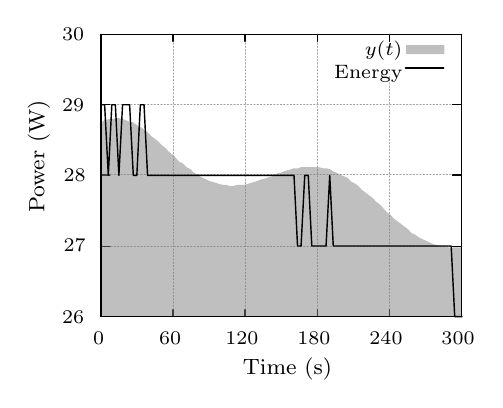
\begin{tikzpicture}[y=0.80pt, x=0.80pt, yscale=-0.500000, xscale=0.660000, inner sep=0pt, outer sep=0pt]
\scriptsize
\begin{scope}[draw=black,line join=bevel,line cap=rect,even odd rule,line width=0.512pt]
  \begin{scope}[cm={{1.0,0.0,0.0,1.0,(0.0,0.0)}},draw=black,line join=bevel,line cap=rect,line width=0.512pt]
  \end{scope}
  \begin{scope}[cm={{1.00625,0.0,0.0,1.00625,(0.0,0.0)}},draw=black,line join=bevel,line cap=rect,line width=0.512pt]
  \end{scope}
  \begin{scope}[cm={{1.00625,0.0,0.0,1.00625,(0.0,0.0)}},draw=ca0a0a4,dash pattern=on 0.40pt off 0.80pt,line join=round,line cap=round,line width=0.400pt]
    \path[draw] (53.5000,268.5000) -- (298.5000,268.5000);
  \end{scope}
  \begin{scope}[cm={{1.00625,0.0,0.0,1.00625,(0.0,0.0)}},draw=black,line join=round,line cap=round,line width=0.512pt]
    \path[draw] (53.5000,268.5000) -- (59.5000,268.5000);
    \path[draw] (298.5000,268.5000) -- (292.5000,268.5000);
  \end{scope}
  \begin{scope}[cm={{1.00625,0.0,0.0,1.00625,(0.0,0.0)}},draw=black,line join=bevel,line cap=rect,line width=0.512pt]
  \end{scope}
  \begin{scope}[cm={{1.00625,0.0,0.0,1.00625,(27.1688,276.216)}},draw=black,line join=bevel,line cap=rect,line width=0.512pt]
  \end{scope}
  \begin{scope}[cm={{1.00625,0.0,0.0,1.00625,(27.1688,276.216)}},draw=black,line join=bevel,line cap=rect,line width=0.512pt]
  \end{scope}
  \begin{scope}[cm={{1.00625,0.0,0.0,1.00625,(27.1688,276.216)}},draw=black,line join=bevel,line cap=rect,line width=0.512pt]
  \end{scope}
  \begin{scope}[cm={{1.00625,0.0,0.0,1.00625,(27.1688,276.216)}},draw=black,line join=bevel,line cap=rect,line width=0.512pt]
  \end{scope}
  \begin{scope}[cm={{1.00625,0.0,0.0,1.00625,(27.1688,276.216)}},draw=black,line join=bevel,line cap=rect,line width=0.512pt]
  \end{scope}
  \begin{scope}[cm={{1.00625,0.0,0.0,1.00625,(27.1688,276.216)}},draw=black,line join=bevel,line cap=rect,line width=0.512pt]
    \path[fill=black] (0.0000,0.0000) node[above right] (text40) {26};
  \end{scope}
  \begin{scope}[cm={{1.00625,0.0,0.0,1.00625,(27.1688,276.216)}},draw=black,line join=bevel,line cap=rect,line width=0.512pt]
  \end{scope}
  \begin{scope}[cm={{1.00625,0.0,0.0,1.00625,(0.0,0.0)}},draw=black,line join=bevel,line cap=rect,line width=0.512pt]
  \end{scope}
  \begin{scope}[cm={{1.00625,0.0,0.0,1.00625,(0.0,0.0)}},draw=ca0a0a4,dash pattern=on 0.40pt off 0.80pt,line join=round,line cap=round,line width=0.400pt]
    \path[draw] (53.5000,205.5000) -- (298.5000,205.5000);
  \end{scope}
  \begin{scope}[cm={{1.00625,0.0,0.0,1.00625,(0.0,0.0)}},draw=black,line join=round,line cap=round,line width=0.512pt]
    \path[draw] (53.5000,205.5000) -- (59.5000,205.5000);
    \path[draw] (298.5000,205.5000) -- (292.5000,205.5000);
  \end{scope}
  \begin{scope}[cm={{1.00625,0.0,0.0,1.00625,(0.0,0.0)}},draw=black,line join=bevel,line cap=rect,line width=0.512pt]
  \end{scope}
  \begin{scope}[cm={{1.00625,0.0,0.0,1.00625,(28.175,211.816)}},draw=black,line join=bevel,line cap=rect,line width=0.512pt]
  \end{scope}
  \begin{scope}[cm={{1.00625,0.0,0.0,1.00625,(28.175,211.816)}},draw=black,line join=bevel,line cap=rect,line width=0.512pt]
  \end{scope}
  \begin{scope}[cm={{1.00625,0.0,0.0,1.00625,(28.175,211.816)}},draw=black,line join=bevel,line cap=rect,line width=0.512pt]
  \end{scope}
  \begin{scope}[cm={{1.00625,0.0,0.0,1.00625,(28.175,211.816)}},draw=black,line join=bevel,line cap=rect,line width=0.512pt]
  \end{scope}
  \begin{scope}[cm={{1.00625,0.0,0.0,1.00625,(28.175,211.816)}},draw=black,line join=bevel,line cap=rect,line width=0.512pt]
  \end{scope}
  \begin{scope}[cm={{1.00625,0.0,0.0,1.00625,(28.175,211.816)}},draw=black,line join=bevel,line cap=rect,line width=0.512pt]
    \path[fill=black] (0.0000,0.0000) node[above right] (text70) {27};
  \end{scope}
  \begin{scope}[cm={{1.00625,0.0,0.0,1.00625,(28.175,211.816)}},draw=black,line join=bevel,line cap=rect,line width=0.512pt]
  \end{scope}
  \begin{scope}[cm={{1.00625,0.0,0.0,1.00625,(0.0,0.0)}},draw=black,line join=bevel,line cap=rect,line width=0.512pt]
  \end{scope}
  \begin{scope}[cm={{1.00625,0.0,0.0,1.00625,(0.0,0.0)}},draw=ca0a0a4,dash pattern=on 0.40pt off 0.80pt,line join=round,line cap=round,line width=0.400pt]
    \path[draw] (53.5000,141.5000) -- (298.5000,141.5000);
  \end{scope}
  \begin{scope}[cm={{1.00625,0.0,0.0,1.00625,(0.0,0.0)}},draw=black,line join=round,line cap=round,line width=0.512pt]
    \path[draw] (53.5000,141.5000) -- (59.5000,141.5000);
    \path[draw] (298.5000,141.5000) -- (292.5000,141.5000);
  \end{scope}
  \begin{scope}[cm={{1.00625,0.0,0.0,1.00625,(0.0,0.0)}},draw=black,line join=bevel,line cap=rect,line width=0.512pt]
  \end{scope}
  \begin{scope}[cm={{1.00625,0.0,0.0,1.00625,(28.175,148.422)}},draw=black,line join=bevel,line cap=rect,line width=0.512pt]
  \end{scope}
  \begin{scope}[cm={{1.00625,0.0,0.0,1.00625,(28.175,148.422)}},draw=black,line join=bevel,line cap=rect,line width=0.512pt]
  \end{scope}
  \begin{scope}[cm={{1.00625,0.0,0.0,1.00625,(28.175,148.422)}},draw=black,line join=bevel,line cap=rect,line width=0.512pt]
  \end{scope}
  \begin{scope}[cm={{1.00625,0.0,0.0,1.00625,(28.175,148.422)}},draw=black,line join=bevel,line cap=rect,line width=0.512pt]
  \end{scope}
  \begin{scope}[cm={{1.00625,0.0,0.0,1.00625,(28.175,148.422)}},draw=black,line join=bevel,line cap=rect,line width=0.512pt]
  \end{scope}
  \begin{scope}[cm={{1.00625,0.0,0.0,1.00625,(28.175,148.422)}},draw=black,line join=bevel,line cap=rect,line width=0.512pt]
    \path[fill=black] (0.0000,0.0000) node[above right] (text100) {28};
  \end{scope}
  \begin{scope}[cm={{1.00625,0.0,0.0,1.00625,(28.175,148.422)}},draw=black,line join=bevel,line cap=rect,line width=0.512pt]
  \end{scope}
  \begin{scope}[cm={{1.00625,0.0,0.0,1.00625,(0.0,0.0)}},draw=black,line join=bevel,line cap=rect,line width=0.512pt]
  \end{scope}
  \begin{scope}[cm={{1.00625,0.0,0.0,1.00625,(0.0,0.0)}},draw=ca0a0a4,dash pattern=on 0.40pt off 0.80pt,line join=round,line cap=round,line width=0.400pt]
    \path[draw] (53.5000,78.5000) -- (298.5000,78.5000);
  \end{scope}
  \begin{scope}[cm={{1.00625,0.0,0.0,1.00625,(0.0,0.0)}},draw=black,line join=round,line cap=round,line width=0.512pt]
    \path[draw] (53.5000,78.5000) -- (59.5000,78.5000);
    \path[draw] (298.5000,78.5000) -- (292.5000,78.5000);
  \end{scope}
  \begin{scope}[cm={{1.00625,0.0,0.0,1.00625,(0.0,0.0)}},draw=black,line join=bevel,line cap=rect,line width=0.512pt]
  \end{scope}
  \begin{scope}[cm={{1.00625,0.0,0.0,1.00625,(27.1688,85.0281)}},draw=black,line join=bevel,line cap=rect,line width=0.512pt]
  \end{scope}
  \begin{scope}[cm={{1.00625,0.0,0.0,1.00625,(27.1688,85.0281)}},draw=black,line join=bevel,line cap=rect,line width=0.512pt]
  \end{scope}
  \begin{scope}[cm={{1.00625,0.0,0.0,1.00625,(27.1688,85.0281)}},draw=black,line join=bevel,line cap=rect,line width=0.512pt]
  \end{scope}
  \begin{scope}[cm={{1.00625,0.0,0.0,1.00625,(27.1688,85.0281)}},draw=black,line join=bevel,line cap=rect,line width=0.512pt]
  \end{scope}
  \begin{scope}[cm={{1.00625,0.0,0.0,1.00625,(27.1688,85.0281)}},draw=black,line join=bevel,line cap=rect,line width=0.512pt]
  \end{scope}
  \begin{scope}[cm={{1.00625,0.0,0.0,1.00625,(27.1688,85.0281)}},draw=black,line join=bevel,line cap=rect,line width=0.512pt]
    \path[fill=black] (0.0000,0.0000) node[above right] (text130) {29};
  \end{scope}
  \begin{scope}[cm={{1.00625,0.0,0.0,1.00625,(27.1688,85.0281)}},draw=black,line join=bevel,line cap=rect,line width=0.512pt]
  \end{scope}
  \begin{scope}[cm={{1.00625,0.0,0.0,1.00625,(0.0,0.0)}},draw=black,line join=bevel,line cap=rect,line width=0.512pt]
  \end{scope}
  \begin{scope}[cm={{1.00625,0.0,0.0,1.00625,(0.0,0.0)}},draw=ca0a0a4,dash pattern=on 0.40pt off 0.80pt,line join=round,line cap=round,line width=0.400pt]
    \path[draw] (53.5000,15.5000) -- (298.5000,15.5000);
  \end{scope}
  \begin{scope}[cm={{1.00625,0.0,0.0,1.00625,(0.0,0.0)}},draw=black,line join=round,line cap=round,line width=0.512pt]
    \path[draw] (53.5000,15.5000) -- (59.5000,15.5000);
    \path[draw] (298.5000,15.5000) -- (292.5000,15.5000);
  \end{scope}
  \begin{scope}[cm={{1.00625,0.0,0.0,1.00625,(0.0,0.0)}},draw=black,line join=bevel,line cap=rect,line width=0.512pt]
  \end{scope}
  \begin{scope}[cm={{1.00625,0.0,0.0,1.00625,(27.1688,20.6281)}},draw=black,line join=bevel,line cap=rect,line width=0.512pt]
  \end{scope}
  \begin{scope}[cm={{1.00625,0.0,0.0,1.00625,(27.1688,20.6281)}},draw=black,line join=bevel,line cap=rect,line width=0.512pt]
  \end{scope}
  \begin{scope}[cm={{1.00625,0.0,0.0,1.00625,(27.1688,20.6281)}},draw=black,line join=bevel,line cap=rect,line width=0.512pt]
  \end{scope}
  \begin{scope}[cm={{1.00625,0.0,0.0,1.00625,(27.1688,20.6281)}},draw=black,line join=bevel,line cap=rect,line width=0.512pt]
  \end{scope}
  \begin{scope}[cm={{1.00625,0.0,0.0,1.00625,(27.1688,20.6281)}},draw=black,line join=bevel,line cap=rect,line width=0.512pt]
  \end{scope}
  \begin{scope}[cm={{1.00625,0.0,0.0,1.00625,(27.1688,20.6281)}},draw=black,line join=bevel,line cap=rect,line width=0.512pt]
    \path[fill=black] (0.0000,0.0000) node[above right] (text160) {30};
  \end{scope}
  \begin{scope}[cm={{1.00625,0.0,0.0,1.00625,(27.1688,20.6281)}},draw=black,line join=bevel,line cap=rect,line width=0.512pt]
  \end{scope}
  \begin{scope}[cm={{1.00625,0.0,0.0,1.00625,(0.0,0.0)}},draw=black,line join=bevel,line cap=rect,line width=0.512pt]
  \end{scope}
  \begin{scope}[cm={{1.00625,0.0,0.0,1.00625,(0.0,0.0)}},draw=ca0a0a4,dash pattern=on 0.40pt off 0.80pt,line join=round,line cap=round,line width=0.400pt]
    \path[draw] (53.5000,268.5000) -- (53.5000,15.5000);
  \end{scope}
  \begin{scope}[cm={{1.00625,0.0,0.0,1.00625,(0.0,0.0)}},draw=black,line join=round,line cap=round,line width=0.512pt]
    \path[draw] (53.5000,268.5000) -- (53.5000,262.5000);
    \path[draw] (53.5000,15.5000) -- (53.5000,21.5000);
  \end{scope}
  \begin{scope}[cm={{1.00625,0.0,0.0,1.00625,(0.0,0.0)}},draw=black,line join=bevel,line cap=rect,line width=0.512pt]
  \end{scope}
  \begin{scope}[cm={{1.00625,0.0,0.0,1.00625,(48.3,291.309)}},draw=black,line join=bevel,line cap=rect,line width=0.512pt]
  \end{scope}
  \begin{scope}[cm={{1.00625,0.0,0.0,1.00625,(48.3,291.309)}},draw=black,line join=bevel,line cap=rect,line width=0.512pt]
  \end{scope}
  \begin{scope}[cm={{1.00625,0.0,0.0,1.00625,(48.3,291.309)}},draw=black,line join=bevel,line cap=rect,line width=0.512pt]
  \end{scope}
  \begin{scope}[cm={{1.00625,0.0,0.0,1.00625,(48.3,291.309)}},draw=black,line join=bevel,line cap=rect,line width=0.512pt]
  \end{scope}
  \begin{scope}[cm={{1.00625,0.0,0.0,1.00625,(48.3,291.309)}},draw=black,line join=bevel,line cap=rect,line width=0.512pt]
  \end{scope}
  \begin{scope}[cm={{1.00625,0.0,0.0,1.00625,(48.3,295.309)}},draw=black,line join=bevel,line cap=rect,line width=0.512pt]
    \path[fill=black] (0.0000,0.0000) node[above right] (text190) {0};
  \end{scope}
  \begin{scope}[cm={{1.00625,0.0,0.0,1.00625,(48.3,291.309)}},draw=black,line join=bevel,line cap=rect,line width=0.512pt]
  \end{scope}
  \begin{scope}[cm={{1.00625,0.0,0.0,1.00625,(0.0,0.0)}},draw=black,line join=bevel,line cap=rect,line width=0.512pt]
  \end{scope}
  \begin{scope}[cm={{1.00625,0.0,0.0,1.00625,(0.0,0.0)}},draw=ca0a0a4,dash pattern=on 0.40pt off 0.80pt,line join=round,line cap=round,line width=0.400pt]
    \path[draw] (102.5000,268.5000) -- (102.5000,15.5000);
  \end{scope}
  \begin{scope}[cm={{1.00625,0.0,0.0,1.00625,(0.0,0.0)}},draw=black,line join=round,line cap=round,line width=0.512pt]
    \path[draw] (102.5000,268.5000) -- (102.5000,262.5000);
    \path[draw] (102.5000,15.5000) -- (102.5000,21.5000);
  \end{scope}
  \begin{scope}[cm={{1.00625,0.0,0.0,1.00625,(0.0,0.0)}},draw=black,line join=bevel,line cap=rect,line width=0.512pt]
  \end{scope}
  \begin{scope}[cm={{1.00625,0.0,0.0,1.00625,(93.5813,291.309)}},draw=black,line join=bevel,line cap=rect,line width=0.512pt]
  \end{scope}
  \begin{scope}[cm={{1.00625,0.0,0.0,1.00625,(93.5813,291.309)}},draw=black,line join=bevel,line cap=rect,line width=0.512pt]
  \end{scope}
  \begin{scope}[cm={{1.00625,0.0,0.0,1.00625,(93.5813,291.309)}},draw=black,line join=bevel,line cap=rect,line width=0.512pt]
  \end{scope}
  \begin{scope}[cm={{1.00625,0.0,0.0,1.00625,(93.5813,291.309)}},draw=black,line join=bevel,line cap=rect,line width=0.512pt]
  \end{scope}
  \begin{scope}[cm={{1.00625,0.0,0.0,1.00625,(93.5813,291.309)}},draw=black,line join=bevel,line cap=rect,line width=0.512pt]
  \end{scope}
  \begin{scope}[cm={{1.00625,0.0,0.0,1.00625,(93.5813,295.309)}},draw=black,line join=bevel,line cap=rect,line width=0.512pt]
    \path[fill=black] (0.0000,0.0000) node[above right] (text220) {60};
  \end{scope}
  \begin{scope}[cm={{1.00625,0.0,0.0,1.00625,(93.5813,291.309)}},draw=black,line join=bevel,line cap=rect,line width=0.512pt]
  \end{scope}
  \begin{scope}[cm={{1.00625,0.0,0.0,1.00625,(0.0,0.0)}},draw=black,line join=bevel,line cap=rect,line width=0.512pt]
  \end{scope}
  \begin{scope}[cm={{1.00625,0.0,0.0,1.00625,(0.0,0.0)}},draw=ca0a0a4,dash pattern=on 0.40pt off 0.80pt,line join=round,line cap=round,line width=0.400pt]
    \path[draw] (151.5000,268.5000) -- (151.5000,15.5000);
  \end{scope}
  \begin{scope}[cm={{1.00625,0.0,0.0,1.00625,(0.0,0.0)}},draw=black,line join=round,line cap=round,line width=0.512pt]
    \path[draw] (151.5000,268.5000) -- (151.5000,262.5000);
    \path[draw] (151.5000,15.5000) -- (151.5000,21.5000);
  \end{scope}
  \begin{scope}[cm={{1.00625,0.0,0.0,1.00625,(0.0,0.0)}},draw=black,line join=bevel,line cap=rect,line width=0.512pt]
  \end{scope}
  \begin{scope}[cm={{1.00625,0.0,0.0,1.00625,(138.863,291.309)}},draw=black,line join=bevel,line cap=rect,line width=0.512pt]
  \end{scope}
  \begin{scope}[cm={{1.00625,0.0,0.0,1.00625,(138.863,291.309)}},draw=black,line join=bevel,line cap=rect,line width=0.512pt]
  \end{scope}
  \begin{scope}[cm={{1.00625,0.0,0.0,1.00625,(138.863,291.309)}},draw=black,line join=bevel,line cap=rect,line width=0.512pt]
  \end{scope}
  \begin{scope}[cm={{1.00625,0.0,0.0,1.00625,(138.863,291.309)}},draw=black,line join=bevel,line cap=rect,line width=0.512pt]
  \end{scope}
  \begin{scope}[cm={{1.00625,0.0,0.0,1.00625,(138.863,291.309)}},draw=black,line join=bevel,line cap=rect,line width=0.512pt]
  \end{scope}
  \begin{scope}[cm={{1.00625,0.0,0.0,1.00625,(138.863,295.309)}},draw=black,line join=bevel,line cap=rect,line width=0.512pt]
    \path[fill=black] (0.0000,0.0000) node[above right] (text250) {120};
  \end{scope}
  \begin{scope}[cm={{1.00625,0.0,0.0,1.00625,(138.863,291.309)}},draw=black,line join=bevel,line cap=rect,line width=0.512pt]
  \end{scope}
  \begin{scope}[cm={{1.00625,0.0,0.0,1.00625,(0.0,0.0)}},draw=black,line join=bevel,line cap=rect,line width=0.512pt]
  \end{scope}
  \begin{scope}[cm={{1.00625,0.0,0.0,1.00625,(0.0,0.0)}},draw=ca0a0a4,dash pattern=on 0.40pt off 0.80pt,line join=round,line cap=round,line width=0.400pt]
    \path[draw] (200.5000,268.5000) -- (200.5000,15.5000);
  \end{scope}
  \begin{scope}[cm={{1.00625,0.0,0.0,1.00625,(0.0,0.0)}},draw=black,line join=round,line cap=round,line width=0.512pt]
    \path[draw] (200.5000,268.5000) -- (200.5000,262.5000);
    \path[draw] (200.5000,15.5000) -- (200.5000,21.5000);
  \end{scope}
  \begin{scope}[cm={{1.00625,0.0,0.0,1.00625,(0.0,0.0)}},draw=black,line join=bevel,line cap=rect,line width=0.512pt]
  \end{scope}
  \begin{scope}[cm={{1.00625,0.0,0.0,1.00625,(188.169,291.309)}},draw=black,line join=bevel,line cap=rect,line width=0.512pt]
  \end{scope}
  \begin{scope}[cm={{1.00625,0.0,0.0,1.00625,(188.169,291.309)}},draw=black,line join=bevel,line cap=rect,line width=0.512pt]
  \end{scope}
  \begin{scope}[cm={{1.00625,0.0,0.0,1.00625,(188.169,291.309)}},draw=black,line join=bevel,line cap=rect,line width=0.512pt]
  \end{scope}
  \begin{scope}[cm={{1.00625,0.0,0.0,1.00625,(188.169,291.309)}},draw=black,line join=bevel,line cap=rect,line width=0.512pt]
  \end{scope}
  \begin{scope}[cm={{1.00625,0.0,0.0,1.00625,(188.169,291.309)}},draw=black,line join=bevel,line cap=rect,line width=0.512pt]
  \end{scope}
  \begin{scope}[cm={{1.00625,0.0,0.0,1.00625,(188.169,295.309)}},draw=black,line join=bevel,line cap=rect,line width=0.512pt]
    \path[fill=black] (0.0000,0.0000) node[above right] (text280) {180};
  \end{scope}
  \begin{scope}[cm={{1.00625,0.0,0.0,1.00625,(188.169,291.309)}},draw=black,line join=bevel,line cap=rect,line width=0.512pt]
  \end{scope}
  \begin{scope}[cm={{1.00625,0.0,0.0,1.00625,(0.0,0.0)}},draw=black,line join=bevel,line cap=rect,line width=0.512pt]
  \end{scope}
  \begin{scope}[cm={{1.00625,0.0,0.0,1.00625,(0.0,0.0)}},draw=ca0a0a4,dash pattern=on 0.40pt off 0.80pt,line join=round,line cap=round,line width=0.400pt]
    \path[draw] (249.5000,268.5000) -- (249.5000,53.5000);
    \path[draw] (249.5000,21.5000) -- (249.5000,15.5000);
  \end{scope}
  \begin{scope}[cm={{1.00625,0.0,0.0,1.00625,(0.0,0.0)}},draw=black,line join=round,line cap=round,line width=0.512pt]
    \path[draw] (249.5000,268.5000) -- (249.5000,262.5000);
    \path[draw] (249.5000,15.5000) -- (249.5000,21.5000);
  \end{scope}
  \begin{scope}[cm={{1.00625,0.0,0.0,1.00625,(0.0,0.0)}},draw=black,line join=bevel,line cap=rect,line width=0.512pt]
  \end{scope}
  \begin{scope}[cm={{1.00625,0.0,0.0,1.00625,(237.475,291.309)}},draw=black,line join=bevel,line cap=rect,line width=0.512pt]
  \end{scope}
  \begin{scope}[cm={{1.00625,0.0,0.0,1.00625,(237.475,291.309)}},draw=black,line join=bevel,line cap=rect,line width=0.512pt]
  \end{scope}
  \begin{scope}[cm={{1.00625,0.0,0.0,1.00625,(237.475,291.309)}},draw=black,line join=bevel,line cap=rect,line width=0.512pt]
  \end{scope}
  \begin{scope}[cm={{1.00625,0.0,0.0,1.00625,(237.475,291.309)}},draw=black,line join=bevel,line cap=rect,line width=0.512pt]
  \end{scope}
  \begin{scope}[cm={{1.00625,0.0,0.0,1.00625,(237.475,291.309)}},draw=black,line join=bevel,line cap=rect,line width=0.512pt]
  \end{scope}
  \begin{scope}[cm={{1.00625,0.0,0.0,1.00625,(237.475,295.309)}},draw=black,line join=bevel,line cap=rect,line width=0.512pt]
    \path[fill=black] (0.0000,0.0000) node[above right] (text312) {240};
  \end{scope}
  \begin{scope}[cm={{1.00625,0.0,0.0,1.00625,(237.475,291.309)}},draw=black,line join=bevel,line cap=rect,line width=0.512pt]
  \end{scope}
  \begin{scope}[cm={{1.00625,0.0,0.0,1.00625,(0.0,0.0)}},draw=black,line join=bevel,line cap=rect,line width=0.512pt]
  \end{scope}
  \begin{scope}[cm={{1.00625,0.0,0.0,1.00625,(0.0,0.0)}},draw=ca0a0a4,dash pattern=on 0.40pt off 0.80pt,line join=round,line cap=round,line width=0.400pt]
    \path[draw] (298.5000,268.5000) -- (298.5000,15.5000);
  \end{scope}
  \begin{scope}[cm={{1.00625,0.0,0.0,1.00625,(0.0,0.0)}},draw=black,line join=round,line cap=round,line width=0.512pt]
    \path[draw] (298.5000,268.5000) -- (298.5000,262.5000);
    \path[draw] (298.5000,15.5000) -- (298.5000,21.5000);
  \end{scope}
  \begin{scope}[cm={{1.00625,0.0,0.0,1.00625,(0.0,0.0)}},draw=black,line join=bevel,line cap=rect,line width=0.512pt]
  \end{scope}
  \begin{scope}[cm={{1.00625,0.0,0.0,1.00625,(286.781,291.309)}},draw=black,line join=bevel,line cap=rect,line width=0.512pt]
  \end{scope}
  \begin{scope}[cm={{1.00625,0.0,0.0,1.00625,(286.781,291.309)}},draw=black,line join=bevel,line cap=rect,line width=0.512pt]
  \end{scope}
  \begin{scope}[cm={{1.00625,0.0,0.0,1.00625,(286.781,291.309)}},draw=black,line join=bevel,line cap=rect,line width=0.512pt]
  \end{scope}
  \begin{scope}[cm={{1.00625,0.0,0.0,1.00625,(286.781,291.309)}},draw=black,line join=bevel,line cap=rect,line width=0.512pt]
  \end{scope}
  \begin{scope}[cm={{1.00625,0.0,0.0,1.00625,(286.781,291.309)}},draw=black,line join=bevel,line cap=rect,line width=0.512pt]
  \end{scope}
  \begin{scope}[cm={{1.00625,0.0,0.0,1.00625,(286.781,295.309)}},draw=black,line join=bevel,line cap=rect,line width=0.512pt]
    \path[fill=black] (0.0000,0.0000) node[above right] (text342) {300};
  \end{scope}
  \begin{scope}[cm={{1.00625,0.0,0.0,1.00625,(286.781,291.309)}},draw=black,line join=bevel,line cap=rect,line width=0.512pt]
  \end{scope}
  \begin{scope}[cm={{1.00625,0.0,0.0,1.00625,(0.0,0.0)}},draw=black,line join=bevel,line cap=rect,line width=0.512pt]
  \end{scope}
  \begin{scope}[cm={{1.00625,0.0,0.0,1.00625,(0.0,0.0)}},draw=black,line join=round,line cap=round,line width=0.512pt]
    \path[draw] (53.5000,15.5000) -- (53.5000,268.5000) -- (298.5000,268.5000) --
      (298.5000,15.5000) -- (53.5000,15.5000);
  \end{scope}
  \begin{scope}[cm={{1.00625,0.0,0.0,1.00625,(0.0,0.0)}},draw=black,line join=bevel,line cap=rect,line width=0.512pt]
  \end{scope}
  \begin{scope}[cm={{0.0,-1.00625,1.00625,0.0,(13.5844,176.597)}},draw=black,line join=bevel,line cap=rect,line width=0.512pt]
  \end{scope}
  \begin{scope}[cm={{0.0,-1.00625,1.00625,0.0,(13.5844,176.597)}},draw=black,line join=bevel,line cap=rect,line width=0.512pt]
  \end{scope}
  \begin{scope}[cm={{0.0,-1.00625,1.00625,0.0,(13.5844,176.597)}},draw=black,line join=bevel,line cap=rect,line width=0.512pt]
  \end{scope}
  \begin{scope}[cm={{0.0,-1.00625,1.00625,0.0,(13.5844,176.597)}},draw=black,line join=bevel,line cap=rect,line width=0.512pt]
  \end{scope}
  \begin{scope}[cm={{0.0,-1.00625,1.00625,0.0,(13.5844,176.597)}},draw=black,line join=bevel,line cap=rect,line width=0.512pt]
  \end{scope}
  \begin{scope}[cm={{0.0,-1.00625,1.00625,0.0,(3.5844,176.597)}},draw=black,line join=bevel,line cap=rect,line width=0.512pt]
    \path[fill=black] (0.0000,0.0000) node[above right] (text366) {\rotatebox{90}{\footnotesize Power (W)}};
  \end{scope}
  \begin{scope}[cm={{0.0,-1.00625,1.00625,0.0,(13.5844,176.597)}},draw=black,line join=bevel,line cap=rect,line width=0.512pt]
  \end{scope}
  \begin{scope}[cm={{1.00625,0.0,0.0,1.00625,(150.938,317.472)}},draw=black,line join=bevel,line cap=rect,line width=0.512pt]
  \end{scope}
  \begin{scope}[cm={{1.00625,0.0,0.0,1.00625,(150.938,317.472)}},draw=black,line join=bevel,line cap=rect,line width=0.512pt]
  \end{scope}
  \begin{scope}[cm={{1.00625,0.0,0.0,1.00625,(150.938,317.472)}},draw=black,line join=bevel,line cap=rect,line width=0.512pt]
  \end{scope}
  \begin{scope}[cm={{1.00625,0.0,0.0,1.00625,(150.938,317.472)}},draw=black,line join=bevel,line cap=rect,line width=0.512pt]
  \end{scope}
  \begin{scope}[cm={{1.00625,0.0,0.0,1.00625,(150.938,317.472)}},draw=black,line join=bevel,line cap=rect,line width=0.512pt]
  \end{scope}
  \begin{scope}[cm={{1.00625,0.0,0.0,1.00625,(150.938,327.472)}},draw=black,line join=bevel,line cap=rect,line width=0.512pt]
    \path[fill=black] (0.0000,0.0000) node[above right] (text382) {\footnotesize Time (s)};
  \end{scope}
  \begin{scope}[cm={{1.00625,0.0,0.0,1.00625,(150.938,317.472)}},draw=black,line join=bevel,line cap=rect,line width=0.512pt]
  \end{scope}
  \begin{scope}[cm={{1.00625,0.0,0.0,1.00625,(208.294,33.2063)}},draw=black,line join=bevel,line cap=rect,line width=0.512pt]
  \end{scope}
  \begin{scope}[cm={{1.00625,0.0,0.0,1.00625,(208.294,33.2063)}},draw=black,line join=bevel,line cap=rect,line width=0.512pt]
  \end{scope}
  \begin{scope}[cm={{1.00625,0.0,0.0,1.00625,(208.294,33.2063)}},draw=black,line join=bevel,line cap=rect,line width=0.512pt]
  \end{scope}
  \begin{scope}[cm={{1.00625,0.0,0.0,1.00625,(208.294,33.2063)}},draw=black,line join=bevel,line cap=rect,line width=0.512pt]
  \end{scope}
  \begin{scope}[cm={{1.00625,0.0,0.0,1.00625,(208.294,33.2063)}},draw=black,line join=bevel,line cap=rect,line width=0.512pt]
  \end{scope}
  \begin{scope}[cm={{1.00625,0.0,0.0,1.00625,(234.294,38.7063)}},draw=black,line join=bevel,line cap=rect,line width=0.512pt]
    \path[fill=black] (0.0000,0.0000) node[above right] (text398) {\scriptsize $y(t)$};
  \end{scope}
  \begin{scope}[cm={{1.00625,0.0,0.0,1.00625,(208.294,33.2063)}},draw=black,line join=bevel,line cap=rect,line width=0.512pt]
  \end{scope}
  \begin{scope}[cm={{1.00625,0.0,0.0,1.00625,(0.0,0.0)}},draw=black,line join=bevel,line cap=rect,line width=0.512pt]
  \end{scope}
  \begin{scope}[cm={{1.00625,0.0,0.0,1.00625,(0.0,0.0)}},fill=c808080,fill opacity=0.500,transparency group]
    \path[fill,rounded corners=0.0000cm] (261.0000,25.0000) rectangle
      (287.0000,33.0000);
  \end{scope}
  \begin{scope}[cm={{1.00625,0.0,0.0,1.00625,(0.0,0.0)}},draw=black,line join=bevel,line cap=rect,line width=0.512pt]
  \end{scope}
  \begin{scope}[cm={{1.00625,0.0,0.0,1.00625,(0.0,0.0)}},draw=black,line join=bevel,line cap=rect,line width=0.512pt]
  \end{scope}
  \begin{scope}[cm={{1.00625,0.0,0.0,1.00625,(0.0,0.0)}},draw=black,line join=bevel,line cap=rect,line width=0.512pt]
  \end{scope}
  \begin{scope}[cm={{1.00625,0.0,0.0,1.00625,(0.0,0.0)}},draw=black,line join=bevel,line cap=rect,line width=0.512pt]
  \end{scope}
  \begin{scope}[cm={{1.00625,0.0,0.0,1.00625,(0.0,0.0)}},fill=c808080,line join=bevel,line cap=rect,draw opacity=0.500,fill opacity=0.500,line width=0.512pt,transparency group]
    \path[fill,even odd rule] (53.5000,268.5000) -- (53.5000,94.5000) --
      (55.5000,92.5000) -- (58.5000,91.5000) -- (60.5000,91.5000) --
      (63.5000,90.5000) -- (65.5000,90.5000) -- (68.5000,91.5000) --
      (70.5000,92.5000) -- (72.5000,93.5000) -- (75.5000,94.5000) --
      (77.5000,96.5000) -- (80.5000,98.5000) -- (82.5000,100.5000) --
      (85.5000,103.5000) -- (87.5000,106.5000) -- (89.5000,108.5000) --
      (92.5000,111.5000) -- (94.5000,114.5000) -- (97.5000,117.5000) --
      (99.5000,120.5000) -- (102.5000,123.5000) -- (104.5000,126.5000) --
      (106.5000,129.5000) -- (109.5000,131.5000) -- (111.5000,134.5000) --
      (114.5000,136.5000) -- (116.5000,139.5000) -- (119.5000,141.5000) --
      (121.5000,143.5000) -- (123.5000,144.5000) -- (126.5000,146.5000) --
      (128.5000,147.5000) -- (131.5000,148.5000) -- (133.5000,149.5000) --
      (136.5000,150.5000) -- (138.5000,150.5000) -- (141.5000,151.5000) --
      (143.5000,151.5000) -- (145.5000,150.5000) -- (148.5000,150.5000) --
      (150.5000,150.5000) -- (153.5000,149.5000) -- (155.5000,148.5000) --
      (158.5000,147.5000) -- (160.5000,146.5000) -- (162.5000,145.5000) --
      (165.5000,144.5000) -- (167.5000,143.5000) -- (170.5000,142.5000) --
      (172.5000,140.5000) -- (175.5000,139.5000) -- (177.5000,138.5000) --
      (179.5000,137.5000) -- (182.5000,136.5000) -- (184.5000,135.5000) --
      (187.5000,135.5000) -- (189.5000,134.5000) -- (192.5000,134.5000) --
      (194.5000,134.5000) -- (196.5000,134.5000) -- (199.5000,134.5000) --
      (201.5000,134.5000) -- (204.5000,135.5000) -- (206.5000,135.5000) --
      (209.5000,136.5000) -- (211.5000,138.5000) -- (213.5000,139.5000) --
      (216.5000,141.5000) -- (218.5000,142.5000) -- (221.5000,144.5000) --
      (223.5000,147.5000) -- (226.5000,149.5000) -- (228.5000,151.5000) --
      (230.5000,154.5000) -- (233.5000,157.5000) -- (235.5000,159.5000) --
      (238.5000,162.5000) -- (240.5000,165.5000) -- (243.5000,168.5000) --
      (245.5000,171.5000) -- (247.5000,174.5000) -- (250.5000,177.5000) --
      (252.5000,180.5000) -- (255.5000,183.5000) -- (257.5000,185.5000) --
      (260.5000,188.5000) -- (262.5000,190.5000) -- (264.5000,193.5000) --
      (267.5000,195.5000) -- (269.5000,197.5000) -- (272.5000,199.5000) --
      (274.5000,200.5000) -- (277.5000,202.5000) -- (279.5000,203.5000) --
      (281.5000,204.5000) -- (284.5000,205.5000) -- (286.5000,205.5000) --
      (289.5000,206.5000) -- (291.5000,206.5000) -- (294.5000,206.5000) --
      (298.5000,206.5000) -- (298.5000,268.5000) -- (53.5000,268.5000);
  \end{scope}
  \begin{scope}[cm={{1.00625,0.0,0.0,1.00625,(0.0,0.0)}},draw=black,line join=bevel,line cap=rect,line width=0.512pt]
  \end{scope}
  \begin{scope}[cm={{1.00625,0.0,0.0,1.00625,(213.325,49.3063)}},draw=black,line join=bevel,line cap=rect,line width=0.512pt]
  \end{scope}
  \begin{scope}[cm={{1.00625,0.0,0.0,1.00625,(213.325,49.3063)}},draw=black,line join=bevel,line cap=rect,line width=0.512pt]
  \end{scope}
  \begin{scope}[cm={{1.00625,0.0,0.0,1.00625,(213.325,49.3063)}},draw=black,line join=bevel,line cap=rect,line width=0.512pt]
  \end{scope}
  \begin{scope}[cm={{1.00625,0.0,0.0,1.00625,(213.325,49.3063)}},draw=black,line join=bevel,line cap=rect,line width=0.512pt]
  \end{scope}
  \begin{scope}[cm={{1.00625,0.0,0.0,1.00625,(213.325,49.3063)}},draw=black,line join=bevel,line cap=rect,line width=0.512pt]
  \end{scope}
  \begin{scope}[cm={{1.00625,0.0,0.0,1.00625,(213.325,58.3063)}},draw=black,line join=bevel,line cap=rect,line width=0.512pt]
    \path[fill=black] (0.0000,0.0000) node[above right] (text434) {\scriptsize Energy};
  \end{scope}
  \begin{scope}[cm={{1.00625,0.0,0.0,1.00625,(213.325,49.3063)}},draw=black,line join=bevel,line cap=rect,line width=0.512pt]
  \end{scope}
  \begin{scope}[cm={{1.00625,0.0,0.0,1.00625,(0.0,0.0)}},draw=black,line join=bevel,line cap=rect,line width=0.512pt]
  \end{scope}
  \begin{scope}[cm={{1.00625,0.0,0.0,1.00625,(0.0,0.0)}},draw=black,line join=round,line cap=round,line width=0.512pt]
    \path[draw,even odd rule] (260.5000,45.5000) -- (286.5000,45.5000);
  \end{scope}
  \begin{scope}[cm={{1.00625,0.0,0.0,1.00625,(0.0,0.0)}},draw=black,line join=bevel,line cap=rect,line width=0.512pt]
  \end{scope}
  \begin{scope}[cm={{1.00625,0.0,0.0,1.00625,(0.0,0.0)}},draw=black,line join=bevel,line cap=rect,line width=0.512pt]
  \end{scope}
  \begin{scope}[cm={{1.00625,0.0,0.0,1.00625,(0.0,0.0)}},draw=black,line join=bevel,line cap=rect,line width=0.512pt]
  \end{scope}
  \begin{scope}[cm={{1.00625,0.0,0.0,1.00625,(0.0,0.0)}},draw=black,line join=bevel,line cap=rect,line width=0.512pt]
  \end{scope}
  \begin{scope}[cm={{1.00625,0.0,0.0,1.00625,(0.0,0.0)}},draw=black,line join=round,line cap=round,line width=0.512pt]
    \path[draw] (53.5000,78.5000) -- (53.5000,78.5000) -- (55.9000,78.5000) --
      (58.4000,141.9000) -- (60.8000,78.5000) -- (63.2000,78.5000) --
      (65.6000,141.9000) -- (68.1000,78.5000) -- (70.5000,78.5000) --
      (72.9000,78.5000) -- (75.4000,141.9000) -- (77.8000,141.9000) --
      (80.2000,78.5000) -- (82.7000,78.5000) -- (85.1000,141.9000) --
      (87.5000,141.9000) -- (89.9000,141.9000) -- (92.4000,141.9000) --
      (94.8000,141.9000) -- (97.2000,141.9000) -- (99.7000,141.9000) --
      (102.1000,141.9000) -- (104.5000,141.9000) -- (106.9000,141.9000) --
      (109.4000,141.9000) -- (111.8000,141.9000) -- (114.2000,141.9000) --
      (116.7000,141.9000) -- (119.1000,141.9000) -- (121.5000,141.9000) --
      (123.9000,141.9000) -- (126.4000,141.9000) -- (128.8000,141.9000) --
      (131.2000,141.9000) -- (133.7000,141.9000) -- (136.1000,141.9000) --
      (138.5000,141.9000) -- (141.0000,141.9000) -- (143.4000,141.9000) --
      (145.8000,141.9000) -- (148.2000,141.9000) -- (150.7000,141.9000) --
      (153.1000,141.9000) -- (155.5000,141.9000) -- (158.0000,141.9000) --
      (160.4000,141.9000) -- (162.8000,141.9000) -- (165.2000,141.9000) --
      (167.7000,141.9000) -- (170.1000,141.9000) -- (172.5000,141.9000) --
      (175.0000,141.9000) -- (177.4000,141.9000) -- (179.8000,141.9000) --
      (182.2000,141.9000) -- (184.7000,141.9000) -- (187.1000,205.3000) --
      (189.5000,205.3000) -- (192.0000,141.9000) -- (194.4000,141.9000) --
      (196.8000,205.3000) -- (199.3000,205.3000) -- (201.7000,205.3000) --
      (204.1000,205.3000) -- (206.5000,205.3000) -- (209.0000,141.9000) --
      (211.4000,205.3000) -- (213.8000,205.3000) -- (216.3000,205.3000) --
      (218.7000,205.3000) -- (221.1000,205.3000) -- (223.5000,205.3000) --
      (226.0000,205.3000) -- (228.4000,205.3000) -- (230.8000,205.3000) --
      (233.3000,205.3000) -- (235.7000,205.3000) -- (238.1000,205.3000) --
      (240.6000,205.3000) -- (243.0000,205.3000) -- (245.4000,205.3000) --
      (247.8000,205.3000) -- (250.3000,205.3000) -- (252.7000,205.3000) --
      (255.1000,205.3000) -- (257.6000,205.3000) -- (260.0000,205.3000) --
      (262.4000,205.3000) -- (264.8000,205.3000) -- (267.3000,205.3000) --
      (269.7000,205.3000) -- (272.1000,205.3000) -- (274.6000,205.3000) --
      (277.0000,205.3000) -- (279.4000,205.3000) -- (281.8000,205.3000) --
      (284.3000,205.3000) -- (286.7000,205.3000) -- (289.1000,205.3000) --
      (291.6000,205.3000) -- (294.0000,268.7000) -- (298.9000,268.7000);
  \end{scope}
  \begin{scope}[cm={{1.00625,0.0,0.0,1.00625,(0.0,0.0)}},draw=black,line join=bevel,line cap=rect,line width=0.512pt]
  \end{scope}
  \begin{scope}[cm={{1.00625,0.0,0.0,1.00625,(0.0,0.0)}},draw=black,line join=bevel,line cap=rect,line width=0.512pt]
  \end{scope}
  \begin{scope}[cm={{1.00625,0.0,0.0,1.00625,(0.0,0.0)}},draw=black,line join=round,line cap=round,line width=0.512pt]
    \path[draw] (53.5000,15.5000) -- (53.5000,268.5000) -- (298.5000,268.5000) --
      (298.5000,15.5000) -- (53.5000,15.5000);
  \end{scope}
  \begin{scope}[cm={{1.00625,0.0,0.0,1.00625,(0.0,0.0)}},draw=black,line join=bevel,line cap=rect,line width=0.512pt]
  \end{scope}
  \begin{scope}[cm={{1.0,0.0,0.0,1.0,(0.0,0.0)}},draw=black,line join=bevel,line cap=rect,line width=0.512pt]
  \end{scope}
\end{scope}
\end{tikzpicture}



    \caption{Modeled motion energy}
    \label{fig:cruise-energy}
  \end{subfigure}
  \begin{subfigure}[c]{0.45\textwidth}
    \centering
    \definecolor{ca0a0a4}{RGB}{160,160,164}
\definecolor{c808080}{RGB}{128,128,128}
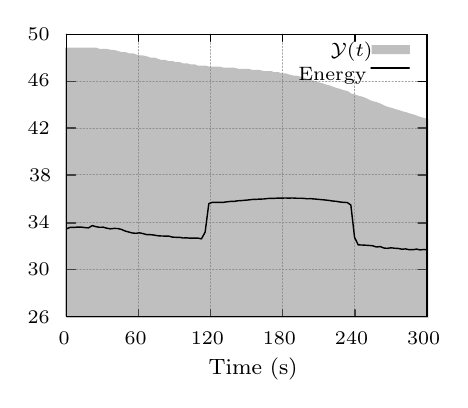
\begin{tikzpicture}[y=0.80pt, x=0.80pt, yscale=-0.500000, xscale=0.660000, inner sep=0pt, outer sep=0pt]
\scriptsize
\begin{scope}[draw=black,line join=bevel,line cap=rect,even odd rule,line width=0.512pt]
  \begin{scope}[cm={{1.0,0.0,0.0,1.0,(0.0,0.0)}},draw=black,line join=bevel,line cap=rect,line width=0.512pt]
  \end{scope}
  \begin{scope}[cm={{1.00625,0.0,0.0,1.00625,(0.0,0.0)}},draw=black,line join=bevel,line cap=rect,line width=0.512pt]
  \end{scope}
  \begin{scope}[cm={{1.00625,0.0,0.0,1.00625,(0.0,0.0)}},draw=ca0a0a4,dash pattern=on 0.40pt off 0.80pt,line join=round,line cap=round,line width=0.400pt]
    \path[draw] (53.5000,268.5000) -- (298.5000,268.5000);
  \end{scope}
  \begin{scope}[cm={{1.00625,0.0,0.0,1.00625,(0.0,0.0)}},draw=black,line join=round,line cap=round,line width=0.512pt]
    \path[draw] (53.5000,268.5000) -- (59.5000,268.5000);
    \path[draw] (298.5000,268.5000) -- (292.5000,268.5000);
  \end{scope}
  \begin{scope}[cm={{1.00625,0.0,0.0,1.00625,(0.0,0.0)}},draw=black,line join=bevel,line cap=rect,line width=0.512pt]
  \end{scope}
  \begin{scope}[cm={{1.00625,0.0,0.0,1.00625,(27.1688,276.216)}},draw=black,line join=bevel,line cap=rect,line width=0.512pt]
  \end{scope}
  \begin{scope}[cm={{1.00625,0.0,0.0,1.00625,(27.1688,276.216)}},draw=black,line join=bevel,line cap=rect,line width=0.512pt]
  \end{scope}
  \begin{scope}[cm={{1.00625,0.0,0.0,1.00625,(27.1688,276.216)}},draw=black,line join=bevel,line cap=rect,line width=0.512pt]
  \end{scope}
  \begin{scope}[cm={{1.00625,0.0,0.0,1.00625,(27.1688,276.216)}},draw=black,line join=bevel,line cap=rect,line width=0.512pt]
  \end{scope}
  \begin{scope}[cm={{1.00625,0.0,0.0,1.00625,(27.1688,276.216)}},draw=black,line join=bevel,line cap=rect,line width=0.512pt]
  \end{scope}
  \begin{scope}[cm={{1.00625,0.0,0.0,1.00625,(27.1688,276.216)}},draw=black,line join=bevel,line cap=rect,line width=0.512pt]
    \path[fill=black] (0.0000,0.0000) node[above right] () {26};
  \end{scope}
  \begin{scope}[cm={{1.00625,0.0,0.0,1.00625,(27.1688,276.216)}},draw=black,line join=bevel,line cap=rect,line width=0.512pt]
  \end{scope}
  \begin{scope}[cm={{1.00625,0.0,0.0,1.00625,(0.0,0.0)}},draw=black,line join=bevel,line cap=rect,line width=0.512pt]
  \end{scope}
  \begin{scope}[cm={{1.00625,0.0,0.0,1.00625,(0.0,0.0)}},draw=ca0a0a4,dash pattern=on 0.40pt off 0.80pt,line join=round,line cap=round,line width=0.400pt]
    \path[draw] (53.5000,226.5000) -- (298.5000,226.5000);
  \end{scope}
  \begin{scope}[cm={{1.00625,0.0,0.0,1.00625,(0.0,0.0)}},draw=black,line join=round,line cap=round,line width=0.512pt]
    \path[draw] (53.5000,226.5000) -- (59.5000,226.5000);
    \path[draw] (298.5000,226.5000) -- (292.5000,226.5000);
  \end{scope}
  \begin{scope}[cm={{1.00625,0.0,0.0,1.00625,(0.0,0.0)}},draw=black,line join=bevel,line cap=rect,line width=0.512pt]
  \end{scope}
  \begin{scope}[cm={{1.00625,0.0,0.0,1.00625,(27.1688,232.947)}},draw=black,line join=bevel,line cap=rect,line width=0.512pt]
  \end{scope}
  \begin{scope}[cm={{1.00625,0.0,0.0,1.00625,(27.1688,232.947)}},draw=black,line join=bevel,line cap=rect,line width=0.512pt]
  \end{scope}
  \begin{scope}[cm={{1.00625,0.0,0.0,1.00625,(27.1688,232.947)}},draw=black,line join=bevel,line cap=rect,line width=0.512pt]
  \end{scope}
  \begin{scope}[cm={{1.00625,0.0,0.0,1.00625,(27.1688,232.947)}},draw=black,line join=bevel,line cap=rect,line width=0.512pt]
  \end{scope}
  \begin{scope}[cm={{1.00625,0.0,0.0,1.00625,(27.1688,232.947)}},draw=black,line join=bevel,line cap=rect,line width=0.512pt]
  \end{scope}
  \begin{scope}[cm={{1.00625,0.0,0.0,1.00625,(27.1688,232.947)}},draw=black,line join=bevel,line cap=rect,line width=0.512pt]
    \path[fill=black] (0.0000,0.0000) node[above right] () {30};
  \end{scope}
  \begin{scope}[cm={{1.00625,0.0,0.0,1.00625,(27.1688,232.947)}},draw=black,line join=bevel,line cap=rect,line width=0.512pt]
  \end{scope}
  \begin{scope}[cm={{1.00625,0.0,0.0,1.00625,(0.0,0.0)}},draw=black,line join=bevel,line cap=rect,line width=0.512pt]
  \end{scope}
  \begin{scope}[cm={{1.00625,0.0,0.0,1.00625,(0.0,0.0)}},draw=ca0a0a4,dash pattern=on 0.40pt off 0.80pt,line join=round,line cap=round,line width=0.400pt]
    \path[draw] (53.5000,184.5000) -- (298.5000,184.5000);
  \end{scope}
  \begin{scope}[cm={{1.00625,0.0,0.0,1.00625,(0.0,0.0)}},draw=black,line join=round,line cap=round,line width=0.512pt]
    \path[draw] (53.5000,184.5000) -- (59.5000,184.5000);
    \path[draw] (298.5000,184.5000) -- (292.5000,184.5000);
  \end{scope}
  \begin{scope}[cm={{1.00625,0.0,0.0,1.00625,(0.0,0.0)}},draw=black,line join=bevel,line cap=rect,line width=0.512pt]
  \end{scope}
  \begin{scope}[cm={{1.00625,0.0,0.0,1.00625,(27.1688,190.684)}},draw=black,line join=bevel,line cap=rect,line width=0.512pt]
  \end{scope}
  \begin{scope}[cm={{1.00625,0.0,0.0,1.00625,(27.1688,190.684)}},draw=black,line join=bevel,line cap=rect,line width=0.512pt]
  \end{scope}
  \begin{scope}[cm={{1.00625,0.0,0.0,1.00625,(27.1688,190.684)}},draw=black,line join=bevel,line cap=rect,line width=0.512pt]
  \end{scope}
  \begin{scope}[cm={{1.00625,0.0,0.0,1.00625,(27.1688,190.684)}},draw=black,line join=bevel,line cap=rect,line width=0.512pt]
  \end{scope}
  \begin{scope}[cm={{1.00625,0.0,0.0,1.00625,(27.1688,190.684)}},draw=black,line join=bevel,line cap=rect,line width=0.512pt]
  \end{scope}
  \begin{scope}[cm={{1.00625,0.0,0.0,1.00625,(27.1688,190.684)}},draw=black,line join=bevel,line cap=rect,line width=0.512pt]
    \path[fill=black] (0.0000,0.0000) node[above right] () {34};
  \end{scope}
  \begin{scope}[cm={{1.00625,0.0,0.0,1.00625,(27.1688,190.684)}},draw=black,line join=bevel,line cap=rect,line width=0.512pt]
  \end{scope}
  \begin{scope}[cm={{1.00625,0.0,0.0,1.00625,(0.0,0.0)}},draw=black,line join=bevel,line cap=rect,line width=0.512pt]
  \end{scope}
  \begin{scope}[cm={{1.00625,0.0,0.0,1.00625,(0.0,0.0)}},draw=ca0a0a4,dash pattern=on 0.40pt off 0.80pt,line join=round,line cap=round,line width=0.400pt]
    \path[draw] (53.5000,141.5000) -- (298.5000,141.5000);
  \end{scope}
  \begin{scope}[cm={{1.00625,0.0,0.0,1.00625,(0.0,0.0)}},draw=black,line join=round,line cap=round,line width=0.512pt]
    \path[draw] (53.5000,141.5000) -- (59.5000,141.5000);
    \path[draw] (298.5000,141.5000) -- (292.5000,141.5000);
  \end{scope}
  \begin{scope}[cm={{1.00625,0.0,0.0,1.00625,(0.0,0.0)}},draw=black,line join=bevel,line cap=rect,line width=0.512pt]
  \end{scope}
  \begin{scope}[cm={{1.00625,0.0,0.0,1.00625,(28.175,148.422)}},draw=black,line join=bevel,line cap=rect,line width=0.512pt]
  \end{scope}
  \begin{scope}[cm={{1.00625,0.0,0.0,1.00625,(28.175,148.422)}},draw=black,line join=bevel,line cap=rect,line width=0.512pt]
  \end{scope}
  \begin{scope}[cm={{1.00625,0.0,0.0,1.00625,(28.175,148.422)}},draw=black,line join=bevel,line cap=rect,line width=0.512pt]
  \end{scope}
  \begin{scope}[cm={{1.00625,0.0,0.0,1.00625,(28.175,148.422)}},draw=black,line join=bevel,line cap=rect,line width=0.512pt]
  \end{scope}
  \begin{scope}[cm={{1.00625,0.0,0.0,1.00625,(28.175,148.422)}},draw=black,line join=bevel,line cap=rect,line width=0.512pt]
  \end{scope}
  \begin{scope}[cm={{1.00625,0.0,0.0,1.00625,(28.175,148.422)}},draw=black,line join=bevel,line cap=rect,line width=0.512pt]
    \path[fill=black] (0.0000,0.0000) node[above right] () {38};
  \end{scope}
  \begin{scope}[cm={{1.00625,0.0,0.0,1.00625,(28.175,148.422)}},draw=black,line join=bevel,line cap=rect,line width=0.512pt]
  \end{scope}
  \begin{scope}[cm={{1.00625,0.0,0.0,1.00625,(0.0,0.0)}},draw=black,line join=bevel,line cap=rect,line width=0.512pt]
  \end{scope}
  \begin{scope}[cm={{1.00625,0.0,0.0,1.00625,(0.0,0.0)}},draw=ca0a0a4,dash pattern=on 0.40pt off 0.80pt,line join=round,line cap=round,line width=0.400pt]
    \path[draw] (53.5000,99.5000) -- (298.5000,99.5000);
  \end{scope}
  \begin{scope}[cm={{1.00625,0.0,0.0,1.00625,(0.0,0.0)}},draw=black,line join=round,line cap=round,line width=0.512pt]
    \path[draw] (53.5000,99.5000) -- (59.5000,99.5000);
    \path[draw] (298.5000,99.5000) -- (292.5000,99.5000);
  \end{scope}
  \begin{scope}[cm={{1.00625,0.0,0.0,1.00625,(0.0,0.0)}},draw=black,line join=bevel,line cap=rect,line width=0.512pt]
  \end{scope}
  \begin{scope}[cm={{1.00625,0.0,0.0,1.00625,(27.1688,106.159)}},draw=black,line join=bevel,line cap=rect,line width=0.512pt]
  \end{scope}
  \begin{scope}[cm={{1.00625,0.0,0.0,1.00625,(27.1688,106.159)}},draw=black,line join=bevel,line cap=rect,line width=0.512pt]
  \end{scope}
  \begin{scope}[cm={{1.00625,0.0,0.0,1.00625,(27.1688,106.159)}},draw=black,line join=bevel,line cap=rect,line width=0.512pt]
  \end{scope}
  \begin{scope}[cm={{1.00625,0.0,0.0,1.00625,(27.1688,106.159)}},draw=black,line join=bevel,line cap=rect,line width=0.512pt]
  \end{scope}
  \begin{scope}[cm={{1.00625,0.0,0.0,1.00625,(27.1688,106.159)}},draw=black,line join=bevel,line cap=rect,line width=0.512pt]
  \end{scope}
  \begin{scope}[cm={{1.00625,0.0,0.0,1.00625,(27.1688,106.159)}},draw=black,line join=bevel,line cap=rect,line width=0.512pt]
    \path[fill=black] (0.0000,0.0000) node[above right] () {42};
  \end{scope}
  \begin{scope}[cm={{1.00625,0.0,0.0,1.00625,(27.1688,106.159)}},draw=black,line join=bevel,line cap=rect,line width=0.512pt]
  \end{scope}
  \begin{scope}[cm={{1.00625,0.0,0.0,1.00625,(0.0,0.0)}},draw=black,line join=bevel,line cap=rect,line width=0.512pt]
  \end{scope}
  \begin{scope}[cm={{1.00625,0.0,0.0,1.00625,(0.0,0.0)}},draw=ca0a0a4,dash pattern=on 0.40pt off 0.80pt,line join=round,line cap=round,line width=0.400pt]
    \path[draw] (53.5000,57.5000) -- (298.5000,57.5000);
  \end{scope}
  \begin{scope}[cm={{1.00625,0.0,0.0,1.00625,(0.0,0.0)}},draw=black,line join=round,line cap=round,line width=0.512pt]
    \path[draw] (53.5000,57.5000) -- (59.5000,57.5000);
    \path[draw] (298.5000,57.5000) -- (292.5000,57.5000);
  \end{scope}
  \begin{scope}[cm={{1.00625,0.0,0.0,1.00625,(0.0,0.0)}},draw=black,line join=bevel,line cap=rect,line width=0.512pt]
  \end{scope}
  \begin{scope}[cm={{1.00625,0.0,0.0,1.00625,(27.1688,62.8906)}},draw=black,line join=bevel,line cap=rect,line width=0.512pt]
  \end{scope}
  \begin{scope}[cm={{1.00625,0.0,0.0,1.00625,(27.1688,62.8906)}},draw=black,line join=bevel,line cap=rect,line width=0.512pt]
  \end{scope}
  \begin{scope}[cm={{1.00625,0.0,0.0,1.00625,(27.1688,62.8906)}},draw=black,line join=bevel,line cap=rect,line width=0.512pt]
  \end{scope}
  \begin{scope}[cm={{1.00625,0.0,0.0,1.00625,(27.1688,62.8906)}},draw=black,line join=bevel,line cap=rect,line width=0.512pt]
  \end{scope}
  \begin{scope}[cm={{1.00625,0.0,0.0,1.00625,(27.1688,62.8906)}},draw=black,line join=bevel,line cap=rect,line width=0.512pt]
  \end{scope}
  \begin{scope}[cm={{1.00625,0.0,0.0,1.00625,(27.1688,62.8906)}},draw=black,line join=bevel,line cap=rect,line width=0.512pt]
    \path[fill=black] (0.0000,0.0000) node[above right] () {46};
  \end{scope}
  \begin{scope}[cm={{1.00625,0.0,0.0,1.00625,(27.1688,62.8906)}},draw=black,line join=bevel,line cap=rect,line width=0.512pt]
  \end{scope}
  \begin{scope}[cm={{1.00625,0.0,0.0,1.00625,(0.0,0.0)}},draw=black,line join=bevel,line cap=rect,line width=0.512pt]
  \end{scope}
  \begin{scope}[cm={{1.00625,0.0,0.0,1.00625,(0.0,0.0)}},draw=ca0a0a4,dash pattern=on 0.40pt off 0.80pt,line join=round,line cap=round,line width=0.400pt]
    \path[draw] (53.5000,15.5000) -- (298.5000,15.5000);
  \end{scope}
  \begin{scope}[cm={{1.00625,0.0,0.0,1.00625,(0.0,0.0)}},draw=black,line join=round,line cap=round,line width=0.512pt]
    \path[draw] (53.5000,15.5000) -- (59.5000,15.5000);
    \path[draw] (298.5000,15.5000) -- (292.5000,15.5000);
  \end{scope}
  \begin{scope}[cm={{1.00625,0.0,0.0,1.00625,(0.0,0.0)}},draw=black,line join=bevel,line cap=rect,line width=0.512pt]
  \end{scope}
  \begin{scope}[cm={{1.00625,0.0,0.0,1.00625,(27.1688,20.6281)}},draw=black,line join=bevel,line cap=rect,line width=0.512pt]
  \end{scope}
  \begin{scope}[cm={{1.00625,0.0,0.0,1.00625,(27.1688,20.6281)}},draw=black,line join=bevel,line cap=rect,line width=0.512pt]
  \end{scope}
  \begin{scope}[cm={{1.00625,0.0,0.0,1.00625,(27.1688,20.6281)}},draw=black,line join=bevel,line cap=rect,line width=0.512pt]
  \end{scope}
  \begin{scope}[cm={{1.00625,0.0,0.0,1.00625,(27.1688,20.6281)}},draw=black,line join=bevel,line cap=rect,line width=0.512pt]
  \end{scope}
  \begin{scope}[cm={{1.00625,0.0,0.0,1.00625,(27.1688,20.6281)}},draw=black,line join=bevel,line cap=rect,line width=0.512pt]
  \end{scope}
  \begin{scope}[cm={{1.00625,0.0,0.0,1.00625,(27.1688,20.6281)}},draw=black,line join=bevel,line cap=rect,line width=0.512pt]
    \path[fill=black] (0.0000,0.0000) node[above right] () {50};
  \end{scope}
  \begin{scope}[cm={{1.00625,0.0,0.0,1.00625,(27.1688,20.6281)}},draw=black,line join=bevel,line cap=rect,line width=0.512pt]
  \end{scope}
  \begin{scope}[cm={{1.00625,0.0,0.0,1.00625,(0.0,0.0)}},draw=black,line join=bevel,line cap=rect,line width=0.512pt]
  \end{scope}
  \begin{scope}[cm={{1.00625,0.0,0.0,1.00625,(0.0,0.0)}},draw=ca0a0a4,dash pattern=on 0.40pt off 0.80pt,line join=round,line cap=round,line width=0.400pt]
    \path[draw] (53.5000,268.5000) -- (53.5000,15.5000);
  \end{scope}
  \begin{scope}[cm={{1.00625,0.0,0.0,1.00625,(0.0,0.0)}},draw=black,line join=round,line cap=round,line width=0.512pt]
    \path[draw] (53.5000,268.5000) -- (53.5000,262.5000);
    \path[draw] (53.5000,15.5000) -- (53.5000,21.5000);
  \end{scope}
  \begin{scope}[cm={{1.00625,0.0,0.0,1.00625,(0.0,0.0)}},draw=black,line join=bevel,line cap=rect,line width=0.512pt]
  \end{scope}
  \begin{scope}[cm={{1.00625,0.0,0.0,1.00625,(48.3,291.309)}},draw=black,line join=bevel,line cap=rect,line width=0.512pt]
  \end{scope}
  \begin{scope}[cm={{1.00625,0.0,0.0,1.00625,(48.3,291.309)}},draw=black,line join=bevel,line cap=rect,line width=0.512pt]
  \end{scope}
  \begin{scope}[cm={{1.00625,0.0,0.0,1.00625,(48.3,291.309)}},draw=black,line join=bevel,line cap=rect,line width=0.512pt]
  \end{scope}
  \begin{scope}[cm={{1.00625,0.0,0.0,1.00625,(48.3,291.309)}},draw=black,line join=bevel,line cap=rect,line width=0.512pt]
  \end{scope}
  \begin{scope}[cm={{1.00625,0.0,0.0,1.00625,(48.3,291.309)}},draw=black,line join=bevel,line cap=rect,line width=0.512pt]
  \end{scope}
  \begin{scope}[cm={{1.00625,0.0,0.0,1.00625,(48.3,295.309)}},draw=black,line join=bevel,line cap=rect,line width=0.512pt]
    \path[fill=black] (0.0000,0.0000) node[above right] () {0};
  \end{scope}
  \begin{scope}[cm={{1.00625,0.0,0.0,1.00625,(48.3,291.309)}},draw=black,line join=bevel,line cap=rect,line width=0.512pt]
  \end{scope}
  \begin{scope}[cm={{1.00625,0.0,0.0,1.00625,(0.0,0.0)}},draw=black,line join=bevel,line cap=rect,line width=0.512pt]
  \end{scope}
  \begin{scope}[cm={{1.00625,0.0,0.0,1.00625,(0.0,0.0)}},draw=ca0a0a4,dash pattern=on 0.40pt off 0.80pt,line join=round,line cap=round,line width=0.400pt]
    \path[draw] (102.5000,268.5000) -- (102.5000,15.5000);
  \end{scope}
  \begin{scope}[cm={{1.00625,0.0,0.0,1.00625,(0.0,0.0)}},draw=black,line join=round,line cap=round,line width=0.512pt]
    \path[draw] (102.5000,268.5000) -- (102.5000,262.5000);
    \path[draw] (102.5000,15.5000) -- (102.5000,21.5000);
  \end{scope}
  \begin{scope}[cm={{1.00625,0.0,0.0,1.00625,(0.0,0.0)}},draw=black,line join=bevel,line cap=rect,line width=0.512pt]
  \end{scope}
  \begin{scope}[cm={{1.00625,0.0,0.0,1.00625,(93.5813,291.309)}},draw=black,line join=bevel,line cap=rect,line width=0.512pt]
  \end{scope}
  \begin{scope}[cm={{1.00625,0.0,0.0,1.00625,(93.5813,291.309)}},draw=black,line join=bevel,line cap=rect,line width=0.512pt]
  \end{scope}
  \begin{scope}[cm={{1.00625,0.0,0.0,1.00625,(93.5813,291.309)}},draw=black,line join=bevel,line cap=rect,line width=0.512pt]
  \end{scope}
  \begin{scope}[cm={{1.00625,0.0,0.0,1.00625,(93.5813,291.309)}},draw=black,line join=bevel,line cap=rect,line width=0.512pt]
  \end{scope}
  \begin{scope}[cm={{1.00625,0.0,0.0,1.00625,(93.5813,291.309)}},draw=black,line join=bevel,line cap=rect,line width=0.512pt]
  \end{scope}
  \begin{scope}[cm={{1.00625,0.0,0.0,1.00625,(93.5813,295.309)}},draw=black,line join=bevel,line cap=rect,line width=0.512pt]
    \path[fill=black] (0.0000,0.0000) node[above right] () {60};
  \end{scope}
  \begin{scope}[cm={{1.00625,0.0,0.0,1.00625,(93.5813,291.309)}},draw=black,line join=bevel,line cap=rect,line width=0.512pt]
  \end{scope}
  \begin{scope}[cm={{1.00625,0.0,0.0,1.00625,(0.0,0.0)}},draw=black,line join=bevel,line cap=rect,line width=0.512pt]
  \end{scope}
  \begin{scope}[cm={{1.00625,0.0,0.0,1.00625,(0.0,0.0)}},draw=ca0a0a4,dash pattern=on 0.40pt off 0.80pt,line join=round,line cap=round,line width=0.400pt]
    \path[draw] (151.5000,268.5000) -- (151.5000,15.5000);
  \end{scope}
  \begin{scope}[cm={{1.00625,0.0,0.0,1.00625,(0.0,0.0)}},draw=black,line join=round,line cap=round,line width=0.512pt]
    \path[draw] (151.5000,268.5000) -- (151.5000,262.5000);
    \path[draw] (151.5000,15.5000) -- (151.5000,21.5000);
  \end{scope}
  \begin{scope}[cm={{1.00625,0.0,0.0,1.00625,(0.0,0.0)}},draw=black,line join=bevel,line cap=rect,line width=0.512pt]
  \end{scope}
  \begin{scope}[cm={{1.00625,0.0,0.0,1.00625,(138.863,291.309)}},draw=black,line join=bevel,line cap=rect,line width=0.512pt]
  \end{scope}
  \begin{scope}[cm={{1.00625,0.0,0.0,1.00625,(138.863,291.309)}},draw=black,line join=bevel,line cap=rect,line width=0.512pt]
  \end{scope}
  \begin{scope}[cm={{1.00625,0.0,0.0,1.00625,(138.863,291.309)}},draw=black,line join=bevel,line cap=rect,line width=0.512pt]
  \end{scope}
  \begin{scope}[cm={{1.00625,0.0,0.0,1.00625,(138.863,291.309)}},draw=black,line join=bevel,line cap=rect,line width=0.512pt]
  \end{scope}
  \begin{scope}[cm={{1.00625,0.0,0.0,1.00625,(138.863,291.309)}},draw=black,line join=bevel,line cap=rect,line width=0.512pt]
  \end{scope}
  \begin{scope}[cm={{1.00625,0.0,0.0,1.00625,(138.863,295.309)}},draw=black,line join=bevel,line cap=rect,line width=0.512pt]
    \path[fill=black] (0.0000,0.0000) node[above right] () {120};
  \end{scope}
  \begin{scope}[cm={{1.00625,0.0,0.0,1.00625,(138.863,291.309)}},draw=black,line join=bevel,line cap=rect,line width=0.512pt]
  \end{scope}
  \begin{scope}[cm={{1.00625,0.0,0.0,1.00625,(0.0,0.0)}},draw=black,line join=bevel,line cap=rect,line width=0.512pt]
  \end{scope}
  \begin{scope}[cm={{1.00625,0.0,0.0,1.00625,(0.0,0.0)}},draw=ca0a0a4,dash pattern=on 0.40pt off 0.80pt,line join=round,line cap=round,line width=0.400pt]
    \path[draw] (200.5000,268.5000) -- (200.5000,15.5000);
  \end{scope}
  \begin{scope}[cm={{1.00625,0.0,0.0,1.00625,(0.0,0.0)}},draw=black,line join=round,line cap=round,line width=0.512pt]
    \path[draw] (200.5000,268.5000) -- (200.5000,262.5000);
    \path[draw] (200.5000,15.5000) -- (200.5000,21.5000);
  \end{scope}
  \begin{scope}[cm={{1.00625,0.0,0.0,1.00625,(0.0,0.0)}},draw=black,line join=bevel,line cap=rect,line width=0.512pt]
  \end{scope}
  \begin{scope}[cm={{1.00625,0.0,0.0,1.00625,(188.169,291.309)}},draw=black,line join=bevel,line cap=rect,line width=0.512pt]
  \end{scope}
  \begin{scope}[cm={{1.00625,0.0,0.0,1.00625,(188.169,291.309)}},draw=black,line join=bevel,line cap=rect,line width=0.512pt]
  \end{scope}
  \begin{scope}[cm={{1.00625,0.0,0.0,1.00625,(188.169,291.309)}},draw=black,line join=bevel,line cap=rect,line width=0.512pt]
  \end{scope}
  \begin{scope}[cm={{1.00625,0.0,0.0,1.00625,(188.169,291.309)}},draw=black,line join=bevel,line cap=rect,line width=0.512pt]
  \end{scope}
  \begin{scope}[cm={{1.00625,0.0,0.0,1.00625,(188.169,291.309)}},draw=black,line join=bevel,line cap=rect,line width=0.512pt]
  \end{scope}
  \begin{scope}[cm={{1.00625,0.0,0.0,1.00625,(188.169,295.309)}},draw=black,line join=bevel,line cap=rect,line width=0.512pt]
    \path[fill=black] (0.0000,0.0000) node[above right] () {180};
  \end{scope}
  \begin{scope}[cm={{1.00625,0.0,0.0,1.00625,(188.169,291.309)}},draw=black,line join=bevel,line cap=rect,line width=0.512pt]
  \end{scope}
  \begin{scope}[cm={{1.00625,0.0,0.0,1.00625,(0.0,0.0)}},draw=black,line join=bevel,line cap=rect,line width=0.512pt]
  \end{scope}
  \begin{scope}[cm={{1.00625,0.0,0.0,1.00625,(0.0,0.0)}},draw=ca0a0a4,dash pattern=on 0.40pt off 0.80pt,line join=round,line cap=round,line width=0.400pt]
    \path[draw] (249.5000,268.5000) -- (249.5000,53.5000);
    \path[draw] (249.5000,21.5000) -- (249.5000,15.5000);
  \end{scope}
  \begin{scope}[cm={{1.00625,0.0,0.0,1.00625,(0.0,0.0)}},draw=black,line join=round,line cap=round,line width=0.512pt]
    \path[draw] (249.5000,268.5000) -- (249.5000,262.5000);
    \path[draw] (249.5000,15.5000) -- (249.5000,21.5000);
  \end{scope}
  \begin{scope}[cm={{1.00625,0.0,0.0,1.00625,(0.0,0.0)}},draw=black,line join=bevel,line cap=rect,line width=0.512pt]
  \end{scope}
  \begin{scope}[cm={{1.00625,0.0,0.0,1.00625,(237.475,291.309)}},draw=black,line join=bevel,line cap=rect,line width=0.512pt]
  \end{scope}
  \begin{scope}[cm={{1.00625,0.0,0.0,1.00625,(237.475,291.309)}},draw=black,line join=bevel,line cap=rect,line width=0.512pt]
  \end{scope}
  \begin{scope}[cm={{1.00625,0.0,0.0,1.00625,(237.475,291.309)}},draw=black,line join=bevel,line cap=rect,line width=0.512pt]
  \end{scope}
  \begin{scope}[cm={{1.00625,0.0,0.0,1.00625,(237.475,291.309)}},draw=black,line join=bevel,line cap=rect,line width=0.512pt]
  \end{scope}
  \begin{scope}[cm={{1.00625,0.0,0.0,1.00625,(237.475,291.309)}},draw=black,line join=bevel,line cap=rect,line width=0.512pt]
  \end{scope}
  \begin{scope}[cm={{1.00625,0.0,0.0,1.00625,(237.475,295.309)}},draw=black,line join=bevel,line cap=rect,line width=0.512pt]
    \path[fill=black] (0.0000,0.0000) node[above right] () {240};
  \end{scope}
  \begin{scope}[cm={{1.00625,0.0,0.0,1.00625,(237.475,291.309)}},draw=black,line join=bevel,line cap=rect,line width=0.512pt]
  \end{scope}
  \begin{scope}[cm={{1.00625,0.0,0.0,1.00625,(0.0,0.0)}},draw=black,line join=bevel,line cap=rect,line width=0.512pt]
  \end{scope}
  \begin{scope}[cm={{1.00625,0.0,0.0,1.00625,(0.0,0.0)}},draw=ca0a0a4,dash pattern=on 0.40pt off 0.80pt,line join=round,line cap=round,line width=0.400pt]
    \path[draw] (298.5000,268.5000) -- (298.5000,15.5000);
  \end{scope}
  \begin{scope}[cm={{1.00625,0.0,0.0,1.00625,(0.0,0.0)}},draw=black,line join=round,line cap=round,line width=0.512pt]
    \path[draw] (298.5000,268.5000) -- (298.5000,262.5000);
    \path[draw] (298.5000,15.5000) -- (298.5000,21.5000);
  \end{scope}
  \begin{scope}[cm={{1.00625,0.0,0.0,1.00625,(0.0,0.0)}},draw=black,line join=bevel,line cap=rect,line width=0.512pt]
  \end{scope}
  \begin{scope}[cm={{1.00625,0.0,0.0,1.00625,(286.781,291.309)}},draw=black,line join=bevel,line cap=rect,line width=0.512pt]
  \end{scope}
  \begin{scope}[cm={{1.00625,0.0,0.0,1.00625,(286.781,291.309)}},draw=black,line join=bevel,line cap=rect,line width=0.512pt]
  \end{scope}
  \begin{scope}[cm={{1.00625,0.0,0.0,1.00625,(286.781,291.309)}},draw=black,line join=bevel,line cap=rect,line width=0.512pt]
  \end{scope}
  \begin{scope}[cm={{1.00625,0.0,0.0,1.00625,(286.781,291.309)}},draw=black,line join=bevel,line cap=rect,line width=0.512pt]
  \end{scope}
  \begin{scope}[cm={{1.00625,0.0,0.0,1.00625,(286.781,291.309)}},draw=black,line join=bevel,line cap=rect,line width=0.512pt]
  \end{scope}
  \begin{scope}[cm={{1.00625,0.0,0.0,1.00625,(286.781,295.309)}},draw=black,line join=bevel,line cap=rect,line width=0.512pt]
    \path[fill=black] (0.0000,0.0000) node[above right] () {300};
  \end{scope}
  \begin{scope}[cm={{1.00625,0.0,0.0,1.00625,(286.781,291.309)}},draw=black,line join=bevel,line cap=rect,line width=0.512pt]
  \end{scope}
  \begin{scope}[cm={{1.00625,0.0,0.0,1.00625,(0.0,0.0)}},draw=black,line join=bevel,line cap=rect,line width=0.512pt]
  \end{scope}
  \begin{scope}[cm={{1.00625,0.0,0.0,1.00625,(0.0,0.0)}},draw=black,line join=round,line cap=round,line width=0.512pt]
    \path[draw] (53.5000,15.5000) -- (53.5000,268.5000) -- (298.5000,268.5000) --
      (298.5000,15.5000) -- (53.5000,15.5000);
  \end{scope}
  \begin{scope}[cm={{1.00625,0.0,0.0,1.00625,(0.0,0.0)}},draw=black,line join=bevel,line cap=rect,line width=0.512pt]
  \end{scope}
  \begin{scope}[cm={{0.0,-1.00625,1.00625,0.0,(13.5844,176.597)}},draw=black,line join=bevel,line cap=rect,line width=0.512pt]
  \end{scope}
  \begin{scope}[cm={{0.0,-1.00625,1.00625,0.0,(13.5844,176.597)}},draw=black,line join=bevel,line cap=rect,line width=0.512pt]
  \end{scope}
  \begin{scope}[cm={{0.0,-1.00625,1.00625,0.0,(13.5844,176.597)}},draw=black,line join=bevel,line cap=rect,line width=0.512pt]
  \end{scope}
  \begin{scope}[cm={{0.0,-1.00625,1.00625,0.0,(13.5844,176.597)}},draw=black,line join=bevel,line cap=rect,line width=0.512pt]
  \end{scope}
  \begin{scope}[cm={{0.0,-1.00625,1.00625,0.0,(13.5844,176.597)}},draw=black,line join=bevel,line cap=rect,line width=0.512pt]
  \end{scope}
  \begin{scope}[cm={{0.0,-1.00625,1.00625,0.0,(13.5844,176.597)}},draw=black,line join=bevel,line cap=rect,line width=0.512pt]
    %\path[fill=black] (0.0000,0.0000) node[above right] () {\rotatebox{90}{Power (W)}};
  \end{scope}
  \begin{scope}[cm={{0.0,-1.00625,1.00625,0.0,(13.5844,176.597)}},draw=black,line join=bevel,line cap=rect,line width=0.512pt]
  \end{scope}
  \begin{scope}[cm={{1.00625,0.0,0.0,1.00625,(150.938,317.472)}},draw=black,line join=bevel,line cap=rect,line width=0.512pt]
  \end{scope}
  \begin{scope}[cm={{1.00625,0.0,0.0,1.00625,(150.938,317.472)}},draw=black,line join=bevel,line cap=rect,line width=0.512pt]
  \end{scope}
  \begin{scope}[cm={{1.00625,0.0,0.0,1.00625,(150.938,317.472)}},draw=black,line join=bevel,line cap=rect,line width=0.512pt]
  \end{scope}
  \begin{scope}[cm={{1.00625,0.0,0.0,1.00625,(150.938,317.472)}},draw=black,line join=bevel,line cap=rect,line width=0.512pt]
  \end{scope}
  \begin{scope}[cm={{1.00625,0.0,0.0,1.00625,(150.938,317.472)}},draw=black,line join=bevel,line cap=rect,line width=0.512pt]
  \end{scope}
  \begin{scope}[cm={{1.00625,0.0,0.0,1.00625,(150.938,327.472)}},draw=black,line join=bevel,line cap=rect,line width=0.512pt]
    \path[fill=black] (0.0000,0.0000) node[above right] () {\footnotesize Time (s)};
  \end{scope}
  \begin{scope}[cm={{1.00625,0.0,0.0,1.00625,(150.938,317.472)}},draw=black,line join=bevel,line cap=rect,line width=0.512pt]
  \end{scope}
  \begin{scope}[cm={{1.00625,0.0,0.0,1.00625,(232.444,33.2063)}},draw=black,line join=bevel,line cap=rect,line width=0.512pt]
  \end{scope}
  \begin{scope}[cm={{1.00625,0.0,0.0,1.00625,(232.444,33.2063)}},draw=black,line join=bevel,line cap=rect,line width=0.512pt]
  \end{scope}
  \begin{scope}[cm={{1.00625,0.0,0.0,1.00625,(232.444,33.2063)}},draw=black,line join=bevel,line cap=rect,line width=0.512pt]
  \end{scope}
  \begin{scope}[cm={{1.00625,0.0,0.0,1.00625,(232.444,33.2063)}},draw=black,line join=bevel,line cap=rect,line width=0.512pt]
  \end{scope}
  \begin{scope}[cm={{1.00625,0.0,0.0,1.00625,(232.444,33.2063)}},draw=black,line join=bevel,line cap=rect,line width=0.512pt]
  \end{scope}
  \begin{scope}[cm={{1.00625,0.0,0.0,1.00625,(234.444,40.2063)}},draw=black,line join=bevel,line cap=rect,line width=0.512pt]
    \path[fill=black] (0.0000,0.0000) node[above right] () {\scriptsize $\mathcal{Y}(t)$};
  \end{scope}
  \begin{scope}[cm={{1.00625,0.0,0.0,1.00625,(232.444,33.2063)}},draw=black,line join=bevel,line cap=rect,line width=0.512pt]
  \end{scope}
  \begin{scope}[cm={{1.00625,0.0,0.0,1.00625,(0.0,0.0)}},draw=black,line join=bevel,line cap=rect,line width=0.512pt]
  \end{scope}
  \begin{scope}[cm={{1.00625,0.0,0.0,1.00625,(0.0,0.0)}},fill=c808080,fill opacity=0.500,transparency group]
    \path[fill,rounded corners=0.0000cm] (261.0000,25.0000) rectangle
      (287.0000,33.0000);
  \end{scope}
  \begin{scope}[cm={{1.00625,0.0,0.0,1.00625,(0.0,0.0)}},draw=black,line join=bevel,line cap=rect,line width=0.512pt]
  \end{scope}
  \begin{scope}[cm={{1.00625,0.0,0.0,1.00625,(0.0,0.0)}},draw=black,line join=bevel,line cap=rect,line width=0.512pt]
  \end{scope}
  \begin{scope}[cm={{1.00625,0.0,0.0,1.00625,(0.0,0.0)}},draw=black,line join=bevel,line cap=rect,line width=0.512pt]
  \end{scope}
  \begin{scope}[cm={{1.00625,0.0,0.0,1.00625,(0.0,0.0)}},draw=black,line join=bevel,line cap=rect,line width=0.512pt]
  \end{scope}
  \begin{scope}[cm={{1.00625,0.0,0.0,1.00625,(0.0,0.0)}},draw=c808080,fill=c808080,line join=bevel,line cap=rect,draw opacity=0.500,fill opacity=0.500,line width=0.512pt,transparency group]
    \path[draw,fill,even odd rule] (53.5000,268.5000) -- (53.5000,28.5000) --
      (56.5000,28.5000) -- (58.5000,28.5000) -- (60.5000,28.5000) --
      (63.5000,28.5000) -- (65.5000,28.5000) -- (68.5000,28.5000) --
      (70.5000,28.5000) -- (73.5000,28.5000) -- (75.5000,29.5000) --
      (78.5000,29.5000) -- (80.5000,29.5000) -- (83.5000,30.5000) --
      (85.5000,30.5000) -- (88.5000,31.5000) -- (90.5000,32.5000) --
      (93.5000,32.5000) -- (95.5000,33.5000) -- (98.5000,33.5000) --
      (100.5000,34.5000) -- (103.5000,35.5000) -- (105.5000,35.5000) --
      (108.5000,36.5000) -- (110.5000,37.5000) -- (113.5000,37.5000) --
      (115.5000,38.5000) -- (117.5000,39.5000) -- (120.5000,39.5000) --
      (122.5000,40.5000) -- (125.5000,40.5000) -- (127.5000,41.5000) --
      (130.5000,41.5000) -- (132.5000,42.5000) -- (135.5000,42.5000) --
      (137.5000,43.5000) -- (140.5000,43.5000) -- (142.5000,44.5000) --
      (145.5000,44.5000) -- (147.5000,44.5000) -- (150.5000,45.5000) --
      (152.5000,45.5000) -- (155.5000,45.5000) -- (157.5000,45.5000) --
      (160.5000,46.5000) -- (162.5000,46.5000) -- (165.5000,46.5000) --
      (167.5000,46.5000) -- (170.5000,47.5000) -- (172.5000,47.5000) --
      (175.5000,47.5000) -- (177.5000,47.5000) -- (179.5000,48.5000) --
      (182.5000,48.5000) -- (184.5000,48.5000) -- (187.5000,49.5000) --
      (189.5000,49.5000) -- (192.5000,49.5000) -- (194.5000,50.5000) --
      (197.5000,50.5000) -- (199.5000,51.5000) -- (202.5000,51.5000) --
      (204.5000,52.5000) -- (207.5000,53.5000) -- (209.5000,53.5000) --
      (212.5000,54.5000) -- (214.5000,55.5000) -- (217.5000,56.5000) --
      (219.5000,57.5000) -- (222.5000,58.5000) -- (224.5000,59.5000) --
      (227.5000,60.5000) -- (229.5000,61.5000) -- (232.5000,62.5000) --
      (234.5000,63.5000) -- (236.5000,64.5000) -- (239.5000,65.5000) --
      (241.5000,66.5000) -- (244.5000,67.5000) -- (246.5000,69.5000) --
      (249.5000,70.5000) -- (251.5000,71.5000) -- (254.5000,72.5000) --
      (256.5000,73.5000) -- (259.5000,75.5000) -- (261.5000,76.5000) --
      (264.5000,77.5000) -- (266.5000,78.5000) -- (269.5000,80.5000) --
      (271.5000,81.5000) -- (274.5000,82.5000) -- (276.5000,83.5000) --
      (279.5000,84.5000) -- (281.5000,85.5000) -- (284.5000,86.5000) --
      (286.5000,87.5000) -- (289.5000,88.5000) -- (291.5000,89.5000) --
      (293.5000,90.5000) -- (296.5000,91.5000) -- (298.5000,92.5000) --
      (298.5000,268.5000) -- (53.5000,268.5000);
  \end{scope}
  \begin{scope}[cm={{1.00625,0.0,0.0,1.00625,(0.0,0.0)}},draw=black,line join=bevel,line cap=rect,line width=0.512pt]
  \end{scope}
  \begin{scope}[cm={{1.00625,0.0,0.0,1.00625,(219.363,49.3063)}},draw=black,line join=bevel,line cap=rect,line width=0.512pt]
  \end{scope}
  \begin{scope}[cm={{1.00625,0.0,0.0,1.00625,(219.363,49.3063)}},draw=black,line join=bevel,line cap=rect,line width=0.512pt]
  \end{scope}
  \begin{scope}[cm={{1.00625,0.0,0.0,1.00625,(219.363,49.3063)}},draw=black,line join=bevel,line cap=rect,line width=0.512pt]
  \end{scope}
  \begin{scope}[cm={{1.00625,0.0,0.0,1.00625,(219.363,49.3063)}},draw=black,line join=bevel,line cap=rect,line width=0.512pt]
  \end{scope}
  \begin{scope}[cm={{1.00625,0.0,0.0,1.00625,(219.363,49.3063)}},draw=black,line join=bevel,line cap=rect,line width=0.512pt]
  \end{scope}
  \begin{scope}[cm={{1.00625,0.0,0.0,1.00625,(212.363,60.3063)}},draw=black,line join=bevel,line cap=rect,line width=0.512pt]
    \path[fill=black] (0.0000,0.0000) node[above right] () {\scriptsize Energy};
  \end{scope}
  \begin{scope}[cm={{1.00625,0.0,0.0,1.00625,(219.363,49.3063)}},draw=black,line join=bevel,line cap=rect,line width=0.512pt]
  \end{scope}
  \begin{scope}[cm={{1.00625,0.0,0.0,1.00625,(0.0,0.0)}},draw=black,line join=bevel,line cap=rect,line width=0.512pt]
  \end{scope}
  \begin{scope}[cm={{1.00625,0.0,0.0,1.00625,(0.0,0.0)}},draw=black,line join=round,line cap=round,line width=0.512pt]
    \path[draw,even odd rule] (260.5000,45.5000) -- (286.5000,45.5000);
  \end{scope}
  \begin{scope}[cm={{1.00625,0.0,0.0,1.00625,(0.0,0.0)}},draw=black,line join=bevel,line cap=rect,line width=0.512pt]
  \end{scope}
  \begin{scope}[cm={{1.00625,0.0,0.0,1.00625,(0.0,0.0)}},draw=black,line join=bevel,line cap=rect,line width=0.512pt]
  \end{scope}
  \begin{scope}[cm={{1.00625,0.0,0.0,1.00625,(0.0,0.0)}},draw=black,line join=bevel,line cap=rect,line width=0.512pt]
  \end{scope}
  \begin{scope}[cm={{1.00625,0.0,0.0,1.00625,(0.0,0.0)}},draw=black,line join=bevel,line cap=rect,line width=0.512pt]
  \end{scope}
  \begin{scope}[cm={{1.00625,0.0,0.0,1.00625,(0.0,0.0)}},draw=black,line join=round,line cap=round,line width=0.512pt]
    \path[draw] (53.5000,189.8000) -- (53.5000,189.8000) -- (56.0000,188.5000) --
      (58.5000,188.6000) -- (60.9000,188.3000) -- (63.4000,188.3000) --
      (65.9000,188.8000) -- (68.4000,189.0000) -- (70.9000,187.0000) --
      (73.3000,187.9000) -- (75.8000,188.5000) -- (78.3000,188.4000) --
      (80.8000,189.3000) -- (83.2000,189.9000) -- (85.7000,189.5000) --
      (88.2000,189.6000) -- (90.7000,190.4000) -- (93.2000,191.8000) --
      (95.6000,192.7000) -- (98.1000,193.6000) -- (100.6000,193.9000) --
      (103.1000,193.5000) -- (105.6000,194.2000) -- (108.0000,195.1000) --
      (110.5000,195.1000) -- (113.0000,195.5000) -- (115.5000,196.1000) --
      (117.9000,196.3000) -- (120.4000,196.4000) -- (122.9000,196.4000) --
      (125.4000,197.3000) -- (127.9000,197.5000) -- (130.3000,197.5000) --
      (132.8000,198.1000) -- (135.3000,198.0000) -- (137.8000,198.3000) --
      (140.3000,198.2000) -- (142.7000,198.2000) -- (145.2000,198.9000) --
      (147.7000,192.8000) -- (150.2000,167.2000) -- (152.6000,166.1000) --
      (155.1000,166.2000) -- (157.6000,166.2000) -- (160.1000,166.1000) --
      (162.6000,165.6000) -- (165.0000,165.3000) -- (167.5000,165.2000) --
      (170.0000,164.7000) -- (172.5000,164.5000) -- (175.0000,164.2000) --
      (177.4000,163.9000) -- (179.9000,163.5000) -- (182.4000,163.4000) --
      (184.9000,163.2000) -- (187.4000,163.1000) -- (189.8000,162.7000) --
      (192.3000,162.5000) -- (194.8000,162.5000) -- (197.3000,162.3000) --
      (199.8000,162.3000) -- (202.2000,162.2000) -- (204.7000,162.3000) --
      (207.2000,162.2000) -- (209.7000,162.4000) -- (212.1000,162.4000) --
      (214.6000,162.5000) -- (217.1000,162.9000) -- (219.6000,162.8000) --
      (222.1000,163.1000) -- (224.5000,163.4000) -- (227.0000,163.7000) --
      (229.5000,164.0000) -- (232.0000,164.4000) -- (234.4000,164.9000) --
      (236.9000,165.2000) -- (239.4000,165.8000) -- (241.9000,166.1000) --
      (244.4000,166.3000) -- (246.8000,168.5000) -- (249.3000,197.4000) --
      (251.8000,204.3000) -- (254.3000,204.4000) -- (256.8000,204.6000) --
      (259.2000,204.8000) -- (261.7000,205.1000) -- (264.2000,206.2000) --
      (266.7000,205.8000) -- (269.2000,207.1000) -- (271.6000,207.4000) --
      (274.1000,206.9000) -- (276.6000,207.3000) -- (279.1000,207.5000) --
      (281.6000,208.2000) -- (284.0000,207.9000) -- (286.5000,208.6000) --
      (289.0000,208.6000) -- (291.5000,208.1000) -- (293.9000,208.8000) --
      (296.4000,208.4000) -- (298.9000,208.8000);
  \end{scope}
  \begin{scope}[cm={{1.00625,0.0,0.0,1.00625,(0.0,0.0)}},draw=black,line join=bevel,line cap=rect,line width=0.512pt]
  \end{scope}
  \begin{scope}[cm={{1.00625,0.0,0.0,1.00625,(0.0,0.0)}},draw=black,line join=bevel,line cap=rect,line width=0.512pt]
  \end{scope}
  \begin{scope}[cm={{1.00625,0.0,0.0,1.00625,(0.0,0.0)}},draw=black,line join=round,line cap=round,line width=0.512pt]
    \path[draw] (53.5000,15.5000) -- (53.5000,268.5000) -- (298.5000,268.5000) --
      (298.5000,15.5000) -- (53.5000,15.5000);
  \end{scope}
  \begin{scope}[cm={{1.00625,0.0,0.0,1.00625,(0.0,0.0)}},draw=black,line join=bevel,line cap=rect,line width=0.512pt]
  \end{scope}
  \begin{scope}[cm={{1.0,0.0,0.0,1.0,(0.0,0.0)}},draw=black,line join=bevel,line cap=rect,line width=0.512pt]
  \end{scope}
\end{scope}
\end{tikzpicture}


    \caption{Coupled motion and computations energy}
    \label{fig:cruise-merge}
  \end{subfigure}
  \caption[Modeled energy evolution with the differential of the second case study]{Modeled energy evolution with the differential model of the second case study, corresponding to the cruise path in \fref{fig:cruise-prelim}{Figure}.}
  \label{fig:cruise-energies}
\end{figure}
The overall energy assessment for what concerns the motion is then in \fref{fig:cruise-energy}{Figure}, and for the motion and computations energies in \fref{fig:cruise-merge}{Figure}. For the latter, our early model consisted of an expression similar to \frefeq{eq:state-perf}, but for the components $A_j$ of matrix $A$
\begin{equation}\label{eq:alter-aj}
  A_j:=\begin{bmatrix}0 & 1 \\ -j^2\omega^2 & 0\end{bmatrix},
\end{equation}
where $\omega$ is the same as in \frefeq{eq:fourier}. We note that the expression derived from using $A_j$ in \frefeq{eq:alter-aj} is equivalent to \frefeq{eq:aj} for periodic modeling purposes (the equivalence comes from the proof of \fref{lem:eqv}{Lemma}, where we evaluate the determinant of $A_j$ in \frefeq{eq:det-aj} and thus multiply the first row and second column with second row and first column with the negative unit, i.e., $j^2\omega^2=j\omega j\omega$). In the model, we then used the coefficients of the Fourier series as an initial guess for the model $\mathbf{q}(t_0)$ at a given time instant $t_0$. We derived the coefficient via the analysis from \fref{sec:res-perio}{Section}. For modeling purposes, we limited the actual flying time of the cruise phase in \fref{fig:cruise-prelim}{Figure} to five minutes. The model output from the initial guess is then the gray area, whereas the energy data are the black-solid line. 

\subsubsection*{Computations energy evaluation}

For the computations {\small\tt ssd-mobilenet} and {\small\tt pednet}, the parameter $c_{i,1}$ alters the hazard detection rate from two to ten frames per second (enclosed in the constraint set $\mathcal{S}_{i,1}$). These numbers are evaluated empirically to match our detection criteria, as opposed to the computation {\small\tt darknet-gpu}, where we analyzed all the possible detection rates on the NVIDIA Jetson TX2 computing hardware. The computation {\small\tt sender} can be then altered with the parameter $c_{i,2}$ indicating the frequency at which the detections are sent to the ground, also from two to ten hertz (again enclosing the constraint set $\mathcal{S}_{i,2}$). All the computations are wrapped in ROS nodes, meaning that $c_{i,1}$ and $c_{i,2}$ can be changed or analyzed by subscribing to appropriate ROS topics\findex{ROS topics}.
\begin{figure}[h!]
  \centering
  \fontfamily{phv}\selectfont
  \footnotesize    
  \begin{subfigure}[b]{0.33\textwidth}
    \centering
    \definecolor{ca0a0a4}{RGB}{160,160,164}
\scriptsize
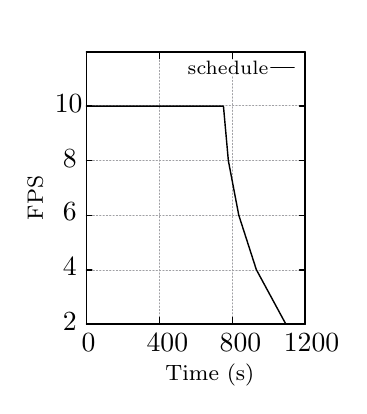
\begin{tikzpicture}[baseline={(0,0.1)},y=0.80pt, x=0.80pt, yscale=-0.482000, xscale=0.400000, inner sep=0pt, outer sep=0pt]
\begin{scope}[draw=black,line join=bevel,line cap=rect,even odd rule,line width=0.512pt]
  \begin{scope}[cm={{1.0,0.0,0.0,1.0,(0.0,0.0)}},draw=black,line join=bevel,line cap=rect,line width=0.512pt]
  \end{scope}
  \begin{scope}[cm={{1.00625,0.0,0.0,1.00625,(0.0,0.0)}},draw=black,line join=bevel,line cap=rect,line width=0.512pt]
  \end{scope}
  \begin{scope}[cm={{1.00625,0.0,0.0,1.00625,(0.0,0.0)}},draw=ca0a0a4,dash pattern=on 0.40pt off 0.80pt,line join=round,line cap=round,line width=0.400pt]
    \path[draw] (53.5000,268.5000) -- (298.5000,268.5000);
  \end{scope}
  \begin{scope}[cm={{1.00625,0.0,0.0,1.00625,(0.0,0.0)}},draw=black,line join=round,line cap=round,line width=0.512pt]
    \path[draw] (53.5000,268.5000) -- (59.5000,268.5000);
    \path[draw] (298.5000,268.5000) -- (292.5000,268.5000);
  \end{scope}
  \begin{scope}[cm={{1.00625,0.0,0.0,1.00625,(0.0,0.0)}},draw=black,line join=bevel,line cap=rect,line width=0.512pt]
  \end{scope}
  \begin{scope}[cm={{1.00625,0.0,0.0,1.00625,(35.2188,276.216)}},draw=black,line join=bevel,line cap=rect,line width=0.512pt]
  \end{scope}
  \begin{scope}[cm={{1.00625,0.0,0.0,1.00625,(35.2188,276.216)}},draw=black,line join=bevel,line cap=rect,line width=0.512pt]
  \end{scope}
  \begin{scope}[cm={{1.00625,0.0,0.0,1.00625,(35.2188,276.216)}},draw=black,line join=bevel,line cap=rect,line width=0.512pt]
  \end{scope}
  \begin{scope}[cm={{1.00625,0.0,0.0,1.00625,(35.2188,276.216)}},draw=black,line join=bevel,line cap=rect,line width=0.512pt]
  \end{scope}
  \begin{scope}[cm={{1.00625,0.0,0.0,1.00625,(35.2188,276.216)}},draw=black,line join=bevel,line cap=rect,line width=0.512pt]
  \end{scope}
  \begin{scope}[cm={{1.00625,0.0,0.0,1.00625,(27.2188,276.216)}},draw=black,line join=bevel,line cap=rect,line width=0.512pt]
    \path[fill=black] (0.0000,0.0000) node[above right] () {2};
  \end{scope}
  \begin{scope}[cm={{1.00625,0.0,0.0,1.00625,(35.2188,276.216)}},draw=black,line join=bevel,line cap=rect,line width=0.512pt]
  \end{scope}
  \begin{scope}[cm={{1.00625,0.0,0.0,1.00625,(0.0,0.0)}},draw=black,line join=bevel,line cap=rect,line width=0.512pt]
  \end{scope}
  \begin{scope}[cm={{1.00625,0.0,0.0,1.00625,(0.0,0.0)}},draw=ca0a0a4,dash pattern=on 0.40pt off 0.80pt,line join=round,line cap=round,line width=0.400pt]
    \path[draw] (53.5000,218.5000) -- (298.5000,218.5000);
  \end{scope}
  \begin{scope}[cm={{1.00625,0.0,0.0,1.00625,(0.0,0.0)}},draw=black,line join=round,line cap=round,line width=0.512pt]
    \path[draw] (53.5000,218.5000) -- (59.5000,218.5000);
    \path[draw] (298.5000,218.5000) -- (292.5000,218.5000);
  \end{scope}
  \begin{scope}[cm={{1.00625,0.0,0.0,1.00625,(0.0,0.0)}},draw=black,line join=bevel,line cap=rect,line width=0.512pt]
  \end{scope}
  \begin{scope}[cm={{1.00625,0.0,0.0,1.00625,(35.2188,224.897)}},draw=black,line join=bevel,line cap=rect,line width=0.512pt]
  \end{scope}
  \begin{scope}[cm={{1.00625,0.0,0.0,1.00625,(35.2188,224.897)}},draw=black,line join=bevel,line cap=rect,line width=0.512pt]
  \end{scope}
  \begin{scope}[cm={{1.00625,0.0,0.0,1.00625,(35.2188,224.897)}},draw=black,line join=bevel,line cap=rect,line width=0.512pt]
  \end{scope}
  \begin{scope}[cm={{1.00625,0.0,0.0,1.00625,(35.2188,224.897)}},draw=black,line join=bevel,line cap=rect,line width=0.512pt]
  \end{scope}
  \begin{scope}[cm={{1.00625,0.0,0.0,1.00625,(35.2188,224.897)}},draw=black,line join=bevel,line cap=rect,line width=0.512pt]
  \end{scope}
  \begin{scope}[cm={{1.00625,0.0,0.0,1.00625,(27.2188,224.897)}},draw=black,line join=bevel,line cap=rect,line width=0.512pt]
    \path[fill=black] (0.0000,0.0000) node[above right] () {4};
  \end{scope}
  \begin{scope}[cm={{1.00625,0.0,0.0,1.00625,(35.2188,224.897)}},draw=black,line join=bevel,line cap=rect,line width=0.512pt]
  \end{scope}
  \begin{scope}[cm={{1.00625,0.0,0.0,1.00625,(0.0,0.0)}},draw=black,line join=bevel,line cap=rect,line width=0.512pt]
  \end{scope}
  \begin{scope}[cm={{1.00625,0.0,0.0,1.00625,(0.0,0.0)}},draw=ca0a0a4,dash pattern=on 0.40pt off 0.80pt,line join=round,line cap=round,line width=0.400pt]
    \path[draw] (53.5000,167.5000) -- (298.5000,167.5000);
  \end{scope}
  \begin{scope}[cm={{1.00625,0.0,0.0,1.00625,(0.0,0.0)}},draw=black,line join=round,line cap=round,line width=0.512pt]
    \path[draw] (53.5000,167.5000) -- (59.5000,167.5000);
    \path[draw] (298.5000,167.5000) -- (292.5000,167.5000);
  \end{scope}
  \begin{scope}[cm={{1.00625,0.0,0.0,1.00625,(0.0,0.0)}},draw=black,line join=bevel,line cap=rect,line width=0.512pt]
  \end{scope}
  \begin{scope}[cm={{1.00625,0.0,0.0,1.00625,(35.2188,173.578)}},draw=black,line join=bevel,line cap=rect,line width=0.512pt]
  \end{scope}
  \begin{scope}[cm={{1.00625,0.0,0.0,1.00625,(35.2188,173.578)}},draw=black,line join=bevel,line cap=rect,line width=0.512pt]
  \end{scope}
  \begin{scope}[cm={{1.00625,0.0,0.0,1.00625,(35.2188,173.578)}},draw=black,line join=bevel,line cap=rect,line width=0.512pt]
  \end{scope}
  \begin{scope}[cm={{1.00625,0.0,0.0,1.00625,(35.2188,173.578)}},draw=black,line join=bevel,line cap=rect,line width=0.512pt]
  \end{scope}
  \begin{scope}[cm={{1.00625,0.0,0.0,1.00625,(35.2188,173.578)}},draw=black,line join=bevel,line cap=rect,line width=0.512pt]
  \end{scope}
  \begin{scope}[cm={{1.00625,0.0,0.0,1.00625,(27.2188,173.578)}},draw=black,line join=bevel,line cap=rect,line width=0.512pt]
    \path[fill=black] (0.0000,0.0000) node[above right] () {6};
  \end{scope}
  \begin{scope}[cm={{1.00625,0.0,0.0,1.00625,(35.2188,173.578)}},draw=black,line join=bevel,line cap=rect,line width=0.512pt]
  \end{scope}
  \begin{scope}[cm={{1.00625,0.0,0.0,1.00625,(0.0,0.0)}},draw=black,line join=bevel,line cap=rect,line width=0.512pt]
  \end{scope}
  \begin{scope}[cm={{1.00625,0.0,0.0,1.00625,(0.0,0.0)}},draw=ca0a0a4,dash pattern=on 0.40pt off 0.80pt,line join=round,line cap=round,line width=0.400pt]
    \path[draw] (53.5000,116.5000) -- (298.5000,116.5000);
  \end{scope}
  \begin{scope}[cm={{1.00625,0.0,0.0,1.00625,(0.0,0.0)}},draw=black,line join=round,line cap=round,line width=0.512pt]
    \path[draw] (53.5000,116.5000) -- (59.5000,116.5000);
    \path[draw] (298.5000,116.5000) -- (292.5000,116.5000);
  \end{scope}
  \begin{scope}[cm={{1.00625,0.0,0.0,1.00625,(0.0,0.0)}},draw=black,line join=bevel,line cap=rect,line width=0.512pt]
  \end{scope}
  \begin{scope}[cm={{1.00625,0.0,0.0,1.00625,(36.225,123.266)}},draw=black,line join=bevel,line cap=rect,line width=0.512pt]
  \end{scope}
  \begin{scope}[cm={{1.00625,0.0,0.0,1.00625,(36.225,123.266)}},draw=black,line join=bevel,line cap=rect,line width=0.512pt]
  \end{scope}
  \begin{scope}[cm={{1.00625,0.0,0.0,1.00625,(36.225,123.266)}},draw=black,line join=bevel,line cap=rect,line width=0.512pt]
  \end{scope}
  \begin{scope}[cm={{1.00625,0.0,0.0,1.00625,(36.225,123.266)}},draw=black,line join=bevel,line cap=rect,line width=0.512pt]
  \end{scope}
  \begin{scope}[cm={{1.00625,0.0,0.0,1.00625,(36.225,123.266)}},draw=black,line join=bevel,line cap=rect,line width=0.512pt]
  \end{scope}
  \begin{scope}[cm={{1.00625,0.0,0.0,1.00625,(27.225,123.266)}},draw=black,line join=bevel,line cap=rect,line width=0.512pt]
    \path[fill=black] (0.0000,0.0000) node[above right] () {8};
  \end{scope}
  \begin{scope}[cm={{1.00625,0.0,0.0,1.00625,(36.225,123.266)}},draw=black,line join=bevel,line cap=rect,line width=0.512pt]
  \end{scope}
  \begin{scope}[cm={{1.00625,0.0,0.0,1.00625,(0.0,0.0)}},draw=black,line join=bevel,line cap=rect,line width=0.512pt]
  \end{scope}
  \begin{scope}[cm={{1.00625,0.0,0.0,1.00625,(0.0,0.0)}},draw=ca0a0a4,dash pattern=on 0.40pt off 0.80pt,line join=round,line cap=round,line width=0.400pt]
    \path[draw] (53.5000,65.5000) -- (298.5000,65.5000);
  \end{scope}
  \begin{scope}[cm={{1.00625,0.0,0.0,1.00625,(0.0,0.0)}},draw=black,line join=round,line cap=round,line width=0.512pt]
    \path[draw] (53.5000,65.5000) -- (59.5000,65.5000);
    \path[draw] (298.5000,65.5000) -- (292.5000,65.5000);
  \end{scope}
  \begin{scope}[cm={{1.00625,0.0,0.0,1.00625,(0.0,0.0)}},draw=black,line join=bevel,line cap=rect,line width=0.512pt]
  \end{scope}
  \begin{scope}[cm={{1.00625,0.0,0.0,1.00625,(27.1688,71.9469)}},draw=black,line join=bevel,line cap=rect,line width=0.512pt]
  \end{scope}
  \begin{scope}[cm={{1.00625,0.0,0.0,1.00625,(27.1688,71.9469)}},draw=black,line join=bevel,line cap=rect,line width=0.512pt]
  \end{scope}
  \begin{scope}[cm={{1.00625,0.0,0.0,1.00625,(27.1688,71.9469)}},draw=black,line join=bevel,line cap=rect,line width=0.512pt]
  \end{scope}
  \begin{scope}[cm={{1.00625,0.0,0.0,1.00625,(27.1688,71.9469)}},draw=black,line join=bevel,line cap=rect,line width=0.512pt]
  \end{scope}
  \begin{scope}[cm={{1.00625,0.0,0.0,1.00625,(27.1688,71.9469)}},draw=black,line join=bevel,line cap=rect,line width=0.512pt]
  \end{scope}
  \begin{scope}[cm={{1.00625,0.0,0.0,1.00625,(18.1688,71.9469)}},draw=black,line join=bevel,line cap=rect,line width=0.512pt]
    \path[fill=black] (0.0000,0.0000) node[above right] () {10};
  \end{scope}
  \begin{scope}[cm={{1.00625,0.0,0.0,1.00625,(27.1688,71.9469)}},draw=black,line join=bevel,line cap=rect,line width=0.512pt]
  \end{scope}
  \begin{scope}[cm={{1.00625,0.0,0.0,1.00625,(0.0,0.0)}},draw=black,line join=bevel,line cap=rect,line width=0.512pt]
  \end{scope}
  \begin{scope}[cm={{1.00625,0.0,0.0,1.00625,(0.0,0.0)}},draw=ca0a0a4,dash pattern=on 0.40pt off 0.80pt,line join=round,line cap=round,line width=0.400pt]
    \path[draw] (53.5000,268.5000) -- (53.5000,15.5000);
  \end{scope}
  \begin{scope}[cm={{1.00625,0.0,0.0,1.00625,(0.0,0.0)}},draw=black,line join=round,line cap=round,line width=0.512pt]
    \path[draw] (53.5000,268.5000) -- (53.5000,262.5000);
    \path[draw] (53.5000,15.5000) -- (53.5000,21.5000);
  \end{scope}
  \begin{scope}[cm={{1.00625,0.0,0.0,1.00625,(0.0,0.0)}},draw=black,line join=bevel,line cap=rect,line width=0.512pt]
  \end{scope}
  \begin{scope}[cm={{1.00625,0.0,0.0,1.00625,(48.3,291.309)}},draw=black,line join=bevel,line cap=rect,line width=0.512pt]
  \end{scope}
  \begin{scope}[cm={{1.00625,0.0,0.0,1.00625,(48.3,291.309)}},draw=black,line join=bevel,line cap=rect,line width=0.512pt]
  \end{scope}
  \begin{scope}[cm={{1.00625,0.0,0.0,1.00625,(48.3,291.309)}},draw=black,line join=bevel,line cap=rect,line width=0.512pt]
  \end{scope}
  \begin{scope}[cm={{1.00625,0.0,0.0,1.00625,(48.3,291.309)}},draw=black,line join=bevel,line cap=rect,line width=0.512pt]
  \end{scope}
  \begin{scope}[cm={{1.00625,0.0,0.0,1.00625,(48.3,291.309)}},draw=black,line join=bevel,line cap=rect,line width=0.512pt]
  \end{scope}
  \begin{scope}[cm={{1.00625,0.0,0.0,1.00625,(48.3,296.309)}},draw=black,line join=bevel,line cap=rect,line width=0.512pt]
    \path[fill=black] (0.0000,0.0000) node[above right] () {0};
  \end{scope}
  \begin{scope}[cm={{1.00625,0.0,0.0,1.00625,(48.3,291.309)}},draw=black,line join=bevel,line cap=rect,line width=0.512pt]
  \end{scope}
  \begin{scope}[cm={{1.00625,0.0,0.0,1.00625,(0.0,0.0)}},draw=black,line join=bevel,line cap=rect,line width=0.512pt]
  \end{scope}
  \begin{scope}[cm={{1.00625,0.0,0.0,1.00625,(0.0,0.0)}},draw=ca0a0a4,dash pattern=on 0.40pt off 0.80pt,line join=round,line cap=round,line width=0.400pt]
    \path[draw] (135.5000,268.5000) -- (135.5000,15.5000);
  \end{scope}
  \begin{scope}[cm={{1.00625,0.0,0.0,1.00625,(0.0,0.0)}},draw=black,line join=round,line cap=round,line width=0.512pt]
    \path[draw] (135.5000,268.5000) -- (135.5000,262.5000);
    \path[draw] (135.5000,15.5000) -- (135.5000,21.5000);
  \end{scope}
  \begin{scope}[cm={{1.00625,0.0,0.0,1.00625,(0.0,0.0)}},draw=black,line join=bevel,line cap=rect,line width=0.512pt]
  \end{scope}
  \begin{scope}[cm={{1.00625,0.0,0.0,1.00625,(121.756,291.309)}},draw=black,line join=bevel,line cap=rect,line width=0.512pt]
  \end{scope}
  \begin{scope}[cm={{1.00625,0.0,0.0,1.00625,(121.756,291.309)}},draw=black,line join=bevel,line cap=rect,line width=0.512pt]
  \end{scope}
  \begin{scope}[cm={{1.00625,0.0,0.0,1.00625,(121.756,291.309)}},draw=black,line join=bevel,line cap=rect,line width=0.512pt]
  \end{scope}
  \begin{scope}[cm={{1.00625,0.0,0.0,1.00625,(121.756,291.309)}},draw=black,line join=bevel,line cap=rect,line width=0.512pt]
  \end{scope}
  \begin{scope}[cm={{1.00625,0.0,0.0,1.00625,(121.756,291.309)}},draw=black,line join=bevel,line cap=rect,line width=0.512pt]
  \end{scope}
  \begin{scope}[cm={{1.00625,0.0,0.0,1.00625,(121.756,296.309)}},draw=black,line join=bevel,line cap=rect,line width=0.512pt]
    \path[fill=black] (0.0000,0.0000) node[above right] () {400};
  \end{scope}
  \begin{scope}[cm={{1.00625,0.0,0.0,1.00625,(121.756,291.309)}},draw=black,line join=bevel,line cap=rect,line width=0.512pt]
  \end{scope}
  \begin{scope}[cm={{1.00625,0.0,0.0,1.00625,(0.0,0.0)}},draw=black,line join=bevel,line cap=rect,line width=0.512pt]
  \end{scope}
  \begin{scope}[cm={{1.00625,0.0,0.0,1.00625,(0.0,0.0)}},draw=ca0a0a4,dash pattern=on 0.40pt off 0.80pt,line join=round,line cap=round,line width=0.400pt]
    \path[draw] (217.5000,268.5000) -- (217.5000,37.5000);
    \path[draw] (217.5000,21.5000) -- (217.5000,15.5000);
  \end{scope}
  \begin{scope}[cm={{1.00625,0.0,0.0,1.00625,(0.0,0.0)}},draw=black,line join=round,line cap=round,line width=0.512pt]
    \path[draw] (217.5000,268.5000) -- (217.5000,262.5000);
    \path[draw] (217.5000,15.5000) -- (217.5000,21.5000);
  \end{scope}
  \begin{scope}[cm={{1.00625,0.0,0.0,1.00625,(0.0,0.0)}},draw=black,line join=bevel,line cap=rect,line width=0.512pt]
  \end{scope}
  \begin{scope}[cm={{1.00625,0.0,0.0,1.00625,(204.269,291.309)}},draw=black,line join=bevel,line cap=rect,line width=0.512pt]
  \end{scope}
  \begin{scope}[cm={{1.00625,0.0,0.0,1.00625,(204.269,291.309)}},draw=black,line join=bevel,line cap=rect,line width=0.512pt]
  \end{scope}
  \begin{scope}[cm={{1.00625,0.0,0.0,1.00625,(204.269,291.309)}},draw=black,line join=bevel,line cap=rect,line width=0.512pt]
  \end{scope}
  \begin{scope}[cm={{1.00625,0.0,0.0,1.00625,(204.269,291.309)}},draw=black,line join=bevel,line cap=rect,line width=0.512pt]
  \end{scope}
  \begin{scope}[cm={{1.00625,0.0,0.0,1.00625,(204.269,291.309)}},draw=black,line join=bevel,line cap=rect,line width=0.512pt]
  \end{scope}
  \begin{scope}[cm={{1.00625,0.0,0.0,1.00625,(204.269,296.309)}},draw=black,line join=bevel,line cap=rect,line width=0.512pt]
    \path[fill=black] (0.0000,0.0000) node[above right] () {800};
  \end{scope}
  \begin{scope}[cm={{1.00625,0.0,0.0,1.00625,(204.269,291.309)}},draw=black,line join=bevel,line cap=rect,line width=0.512pt]
  \end{scope}
  \begin{scope}[cm={{1.00625,0.0,0.0,1.00625,(0.0,0.0)}},draw=black,line join=bevel,line cap=rect,line width=0.512pt]
  \end{scope}
  \begin{scope}[cm={{1.00625,0.0,0.0,1.00625,(0.0,0.0)}},draw=ca0a0a4,dash pattern=on 0.40pt off 0.80pt,line join=round,line cap=round,line width=0.400pt]
    \path[draw] (298.5000,268.5000) -- (298.5000,15.5000);
  \end{scope}
  \begin{scope}[cm={{1.00625,0.0,0.0,1.00625,(0.0,0.0)}},draw=black,line join=round,line cap=round,line width=0.512pt]
    \path[draw] (298.5000,268.5000) -- (298.5000,262.5000);
    \path[draw] (298.5000,15.5000) -- (298.5000,21.5000);
  \end{scope}
  \begin{scope}[cm={{1.00625,0.0,0.0,1.00625,(0.0,0.0)}},draw=black,line join=bevel,line cap=rect,line width=0.512pt]
  \end{scope}
  \begin{scope}[cm={{1.00625,0.0,0.0,1.00625,(282.756,291.309)}},draw=black,line join=bevel,line cap=rect,line width=0.512pt]
  \end{scope}
  \begin{scope}[cm={{1.00625,0.0,0.0,1.00625,(282.756,291.309)}},draw=black,line join=bevel,line cap=rect,line width=0.512pt]
  \end{scope}
  \begin{scope}[cm={{1.00625,0.0,0.0,1.00625,(282.756,291.309)}},draw=black,line join=bevel,line cap=rect,line width=0.512pt]
  \end{scope}
  \begin{scope}[cm={{1.00625,0.0,0.0,1.00625,(282.756,291.309)}},draw=black,line join=bevel,line cap=rect,line width=0.512pt]
  \end{scope}
  \begin{scope}[cm={{1.00625,0.0,0.0,1.00625,(282.756,291.309)}},draw=black,line join=bevel,line cap=rect,line width=0.512pt]
  \end{scope}
  \begin{scope}[cm={{1.00625,0.0,0.0,1.00625,(276.756,296.309)}},draw=black,line join=bevel,line cap=rect,line width=0.512pt]
    \path[fill=black] (0.0000,0.0000) node[above right] () {1200};
  \end{scope}
  \begin{scope}[cm={{1.00625,0.0,0.0,1.00625,(282.756,291.309)}},draw=black,line join=bevel,line cap=rect,line width=0.512pt]
  \end{scope}
  \begin{scope}[cm={{1.00625,0.0,0.0,1.00625,(0.0,0.0)}},draw=black,line join=bevel,line cap=rect,line width=0.512pt]
  \end{scope}
  \begin{scope}[cm={{1.00625,0.0,0.0,1.00625,(0.0,0.0)}},draw=black,line join=round,line cap=round,line width=0.512pt]
    \path[draw] (53.5000,15.5000) -- (53.5000,268.5000) -- (298.5000,268.5000) --
      (298.5000,15.5000) -- (53.5000,15.5000);
  \end{scope}
  \begin{scope}[cm={{1.00625,0.0,0.0,1.00625,(0.0,0.0)}},draw=black,line join=bevel,line cap=rect,line width=0.512pt]
  \end{scope}
  \begin{scope}[cm={{0.0,-1.00625,1.00625,0.0,(13.5844,154.963)}},draw=black,line join=bevel,line cap=rect,line width=0.512pt]
  \end{scope}
  \begin{scope}[cm={{0.0,-1.00625,1.00625,0.0,(13.5844,154.963)}},draw=black,line join=bevel,line cap=rect,line width=0.512pt]
  \end{scope}
  \begin{scope}[cm={{0.0,-1.00625,1.00625,0.0,(13.5844,154.963)}},draw=black,line join=bevel,line cap=rect,line width=0.512pt]
  \end{scope}
  \begin{scope}[cm={{0.0,-1.00625,1.00625,0.0,(13.5844,154.963)}},draw=black,line join=bevel,line cap=rect,line width=0.512pt]
  \end{scope}
  \begin{scope}[cm={{0.0,-1.00625,1.00625,0.0,(13.5844,154.963)}},draw=black,line join=bevel,line cap=rect,line width=0.512pt]
  \end{scope}
  \begin{scope}[cm={{0.0,-1.00625,1.00625,0.0,(-12.5844,172.963)}},draw=black,line join=bevel,line cap=rect,line width=0.512pt]
    \path[fill=black] (0.0000,0.0000) node[above right] () {\rotatebox{90}{\footnotesize FPS}};
  \end{scope}
  \begin{scope}[cm={{0.0,-1.00625,1.00625,0.0,(13.5844,154.963)}},draw=black,line join=bevel,line cap=rect,line width=0.512pt]
  \end{scope}
  \begin{scope}[cm={{1.00625,0.0,0.0,1.00625,(150.938,317.472)}},draw=black,line join=bevel,line cap=rect,line width=0.512pt]
  \end{scope}
  \begin{scope}[cm={{1.00625,0.0,0.0,1.00625,(150.938,317.472)}},draw=black,line join=bevel,line cap=rect,line width=0.512pt]
  \end{scope}
  \begin{scope}[cm={{1.00625,0.0,0.0,1.00625,(150.938,317.472)}},draw=black,line join=bevel,line cap=rect,line width=0.512pt]
  \end{scope}
  \begin{scope}[cm={{1.00625,0.0,0.0,1.00625,(150.938,317.472)}},draw=black,line join=bevel,line cap=rect,line width=0.512pt]
  \end{scope}
  \begin{scope}[cm={{1.00625,0.0,0.0,1.00625,(150.938,317.472)}},draw=black,line join=bevel,line cap=rect,line width=0.512pt]
  \end{scope}
  \begin{scope}[cm={{1.00625,0.0,0.0,1.00625,(142.938,328.472)}},draw=black,line join=bevel,line cap=rect,line width=0.512pt]
    \path[fill=black] (0.0000,0.0000) node[above right] () {\footnotesize Time (s)};
  \end{scope}
  \begin{scope}[cm={{1.00625,0.0,0.0,1.00625,(150.938,317.472)}},draw=black,line join=bevel,line cap=rect,line width=0.512pt]
  \end{scope}
  \begin{scope}[cm={{1.00625,0.0,0.0,1.00625,(188.169,33.2063)}},draw=black,line join=bevel,line cap=rect,line width=0.512pt]
  \end{scope}
  \begin{scope}[cm={{1.00625,0.0,0.0,1.00625,(188.169,33.2063)}},draw=black,line join=bevel,line cap=rect,line width=0.512pt]
  \end{scope}
  \begin{scope}[cm={{1.00625,0.0,0.0,1.00625,(188.169,33.2063)}},draw=black,line join=bevel,line cap=rect,line width=0.512pt]
  \end{scope}
  \begin{scope}[cm={{1.00625,0.0,0.0,1.00625,(188.169,33.2063)}},draw=black,line join=bevel,line cap=rect,line width=0.512pt]
  \end{scope}
  \begin{scope}[cm={{1.00625,0.0,0.0,1.00625,(188.169,33.2063)}},draw=black,line join=bevel,line cap=rect,line width=0.512pt]
  \end{scope}
  \begin{scope}[cm={{1.00625,0.0,0.0,1.00625,(168.169,36.9)}},draw=black,line join=bevel,line cap=rect,line width=0.512pt]
    \path[fill=black] (0.0000,0.0000) node[above right] () {\scriptsize schedule};
  \end{scope}
  \begin{scope}[cm={{1.00625,0.0,0.0,1.00625,(188.169,33.2063)}},draw=black,line join=bevel,line cap=rect,line width=0.512pt]
  \end{scope}
  \begin{scope}[cm={{1.00625,0.0,0.0,1.00625,(0.0,0.0)}},draw=black,line join=bevel,line cap=rect,line width=0.512pt]
  \end{scope}
  \begin{scope}[cm={{1.00625,0.0,0.0,1.00625,(0.0,0.0)}},draw=black,line join=round,line cap=round,line width=0.512pt]
    \path[draw,even odd rule] (260.5000,29.5000) -- (286.5000,29.5000);
  \end{scope}
  \begin{scope}[cm={{1.00625,0.0,0.0,1.00625,(0.0,0.0)}},draw=black,line join=bevel,line cap=rect,line width=0.512pt]
  \end{scope}
  \begin{scope}[cm={{1.00625,0.0,0.0,1.00625,(0.0,0.0)}},draw=black,line join=bevel,line cap=rect,line width=0.512pt]
  \end{scope}
  \begin{scope}[cm={{1.00625,0.0,0.0,1.00625,(0.0,0.0)}},draw=black,line join=bevel,line cap=rect,line width=0.512pt]
  \end{scope}
  \begin{scope}[cm={{1.00625,0.0,0.0,1.00625,(0.0,0.0)}},draw=black,line join=bevel,line cap=rect,line width=0.512pt]
  \end{scope}
  \begin{scope}[cm={{1.00625,0.0,0.0,1.00625,(0.0,0.0)}},draw=black,line join=round,line cap=round,line width=0.512pt]
    \path[draw] (53.5000,65.8000) -- (53.5000,65.8000) -- (207.2000,65.8000) --
      (212.7000,116.5000) -- (224.4000,167.3000) -- (244.1000,218.0000) --
      (277.2000,268.7000) -- (298.9000,268.7000);
  \end{scope}
  \begin{scope}[cm={{1.00625,0.0,0.0,1.00625,(0.0,0.0)}},draw=black,line join=bevel,line cap=rect,line width=0.512pt]
  \end{scope}
  \begin{scope}[cm={{1.00625,0.0,0.0,1.00625,(0.0,0.0)}},draw=black,line join=bevel,line cap=rect,line width=0.512pt]
  \end{scope}
  \begin{scope}[cm={{1.00625,0.0,0.0,1.00625,(0.0,0.0)}},draw=black,line join=round,line cap=round,line width=0.512pt]
    \path[draw] (53.5000,15.5000) -- (53.5000,268.5000) -- (298.5000,268.5000) --
      (298.5000,15.5000) -- (53.5000,15.5000);
  \end{scope}
  \begin{scope}[cm={{1.00625,0.0,0.0,1.00625,(0.0,0.0)}},draw=black,line join=bevel,line cap=rect,line width=0.512pt]
  \end{scope}
  \begin{scope}[cm={{1.0,0.0,0.0,1.0,(0.0,0.0)}},draw=black,line join=bevel,line cap=rect,line width=0.512pt]
  \end{scope}
\end{scope}
\end{tikzpicture}

    \caption{Schedule over time}
    \label{fig:max-qos}
  \end{subfigure}
  \begin{subfigure}[b]{0.32\textwidth}
    \centering
    \definecolor{c9aff00}{RGB}{154,255,0}
\definecolor{ca3ff00}{RGB}{163,255,0}
\definecolor{cacff00}{RGB}{172,255,0}
\definecolor{c9bff00}{RGB}{155,255,0}
\definecolor{ca4ff00}{RGB}{164,255,0}
\definecolor{cadff00}{RGB}{173,255,0}
\definecolor{c9cff00}{RGB}{156,255,0}
\definecolor{ca5ff00}{RGB}{165,255,0}
\definecolor{cafff00}{RGB}{175,255,0}
\definecolor{c95ff00}{RGB}{149,255,0}
\definecolor{c9fff00}{RGB}{159,255,0}
\definecolor{ca8ff00}{RGB}{168,255,0}
\definecolor{c97ff00}{RGB}{151,255,0}
\definecolor{ca0ff00}{RGB}{160,255,0}
\definecolor{caaff00}{RGB}{170,255,0}
\definecolor{c99ff00}{RGB}{153,255,0}
\definecolor{ca2ff00}{RGB}{162,255,0}
\definecolor{cabff00}{RGB}{171,255,0}
\definecolor{c90ff00}{RGB}{144,255,0}
\definecolor{ca6ff00}{RGB}{166,255,0}
\definecolor{c92ff00}{RGB}{146,255,0}
\definecolor{c93ff00}{RGB}{147,255,0}
\definecolor{c9dff00}{RGB}{157,255,0}
\definecolor{ca7ff00}{RGB}{167,255,0}
\definecolor{c8dff00}{RGB}{141,255,0}
\definecolor{c98ff00}{RGB}{152,255,0}
\definecolor{c8eff00}{RGB}{142,255,0}
\definecolor{c8fff00}{RGB}{143,255,0}
\definecolor{cb8ff00}{RGB}{184,255,0}
\definecolor{cc7ff00}{RGB}{199,255,0}
\definecolor{cd6ff00}{RGB}{214,255,0}
\definecolor{cb9ff00}{RGB}{185,255,0}
\definecolor{cc8ff00}{RGB}{200,255,0}
\definecolor{cbaff00}{RGB}{186,255,0}
\definecolor{cc9ff00}{RGB}{201,255,0}
\definecolor{cd7ff00}{RGB}{215,255,0}
\definecolor{cb5ff00}{RGB}{181,255,0}
\definecolor{cc4ff00}{RGB}{196,255,0}
\definecolor{cd3ff00}{RGB}{211,255,0}
\definecolor{cb6ff00}{RGB}{182,255,0}
\definecolor{cc5ff00}{RGB}{197,255,0}
\definecolor{cd4ff00}{RGB}{212,255,0}
\definecolor{cb7ff00}{RGB}{183,255,0}
\definecolor{cc6ff00}{RGB}{198,255,0}
\definecolor{cd5ff00}{RGB}{213,255,0}
\definecolor{cb3ff00}{RGB}{179,255,0}
\definecolor{cc2ff00}{RGB}{194,255,0}
\definecolor{cd1ff00}{RGB}{209,255,0}
\definecolor{cc3ff00}{RGB}{195,255,0}
\definecolor{cd2ff00}{RGB}{210,255,0}
\definecolor{cb4ff00}{RGB}{180,255,0}
\definecolor{cbeff00}{RGB}{190,255,0}
\definecolor{ccdff00}{RGB}{205,255,0}
\definecolor{cb0ff00}{RGB}{176,255,0}
\definecolor{cbfff00}{RGB}{191,255,0}
\definecolor{ccfff00}{RGB}{207,255,0}
\definecolor{cb2ff00}{RGB}{178,255,0}
\definecolor{cc1ff00}{RGB}{193,255,0}
\definecolor{cd0ff00}{RGB}{208,255,0}
\definecolor{ce4ff00}{RGB}{228,255,0}
\definecolor{cf3ff00}{RGB}{243,255,0}
\definecolor{cfffc00}{RGB}{255,252,0}
\definecolor{ce5ff00}{RGB}{229,255,0}
\definecolor{cfffb00}{RGB}{255,251,0}
\definecolor{ce6ff00}{RGB}{230,255,0}
\definecolor{cf4ff00}{RGB}{244,255,0}
\definecolor{cfffa00}{RGB}{255,250,0}
\definecolor{ce2ff00}{RGB}{226,255,0}
\definecolor{cf1ff00}{RGB}{241,255,0}
\definecolor{cffff00}{RGB}{255,255,0}
\definecolor{ce3ff00}{RGB}{227,255,0}
\definecolor{cfffe00}{RGB}{255,254,0}
\definecolor{cf2ff00}{RGB}{242,255,0}
\definecolor{cfffd00}{RGB}{255,253,0}
\definecolor{ce0ff00}{RGB}{224,255,0}
\definecolor{ceeff00}{RGB}{238,255,0}
\definecolor{cfcff00}{RGB}{252,255,0}
\definecolor{ce1ff00}{RGB}{225,255,0}
\definecolor{cefff00}{RGB}{239,255,0}
\definecolor{cfdff00}{RGB}{253,255,0}
\definecolor{cf0ff00}{RGB}{240,255,0}
\definecolor{cfeff00}{RGB}{254,255,0}
\definecolor{cdcff00}{RGB}{220,255,0}
\definecolor{cebff00}{RGB}{235,255,0}
\definecolor{cfaff00}{RGB}{250,255,0}
\definecolor{cddff00}{RGB}{221,255,0}
\definecolor{cecff00}{RGB}{236,255,0}
\definecolor{cdfff00}{RGB}{223,255,0}
\definecolor{cedff00}{RGB}{237,255,0}
\definecolor{cfbff00}{RGB}{251,255,0}
\definecolor{cffdd00}{RGB}{255,221,0}
\definecolor{cffbe00}{RGB}{255,190,0}
\definecolor{cff9f00}{RGB}{255,159,0}
\definecolor{cff9e00}{RGB}{255,158,0}
\definecolor{cffdc00}{RGB}{255,220,0}
\definecolor{cffbd00}{RGB}{255,189,0}
\definecolor{cff9d00}{RGB}{255,157,0}
\definecolor{cffe200}{RGB}{255,226,0}
\definecolor{cffc300}{RGB}{255,195,0}
\definecolor{cffa400}{RGB}{255,164,0}
\definecolor{cffe000}{RGB}{255,224,0}
\definecolor{cffc100}{RGB}{255,193,0}
\definecolor{cffa200}{RGB}{255,162,0}
\definecolor{cffdf00}{RGB}{255,223,0}
\definecolor{cffc000}{RGB}{255,192,0}
\definecolor{cffa100}{RGB}{255,161,0}
\definecolor{cffe800}{RGB}{255,232,0}
\definecolor{cffc900}{RGB}{255,201,0}
\definecolor{cffa900}{RGB}{255,169,0}
\definecolor{cffe600}{RGB}{255,230,0}
\definecolor{cffc700}{RGB}{255,199,0}
\definecolor{cffa700}{RGB}{255,167,0}
\definecolor{cffe400}{RGB}{255,228,0}
\definecolor{cffc500}{RGB}{255,197,0}
\definecolor{cffa500}{RGB}{255,165,0}
\definecolor{cffed00}{RGB}{255,237,0}
\definecolor{cffce00}{RGB}{255,206,0}
\definecolor{cffaf00}{RGB}{255,175,0}
\definecolor{cffec00}{RGB}{255,236,0}
\definecolor{cffcc00}{RGB}{255,204,0}
\definecolor{cffad00}{RGB}{255,173,0}
\definecolor{cffea00}{RGB}{255,234,0}
\definecolor{cffcb00}{RGB}{255,203,0}
\definecolor{cffab00}{RGB}{255,171,0}
\definecolor{ca0a0a4}{RGB}{160,160,164}
\scriptsize
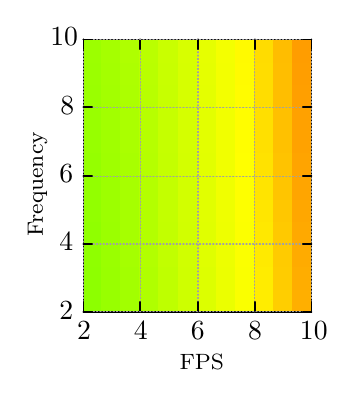
\begin{tikzpicture}[y=0.80pt, x=0.80pt, yscale=-0.564000, xscale=0.500000, inner sep=0pt, outer sep=0pt]
\begin{scope}[draw=black,line join=bevel,line cap=rect,even odd rule,line width=0.512pt]
  \begin{scope}[cm={{1.0,0.0,0.0,1.0,(0.0,0.0)}},draw=black,line join=bevel,line cap=rect,line width=0.512pt]
  \end{scope}
  \begin{scope}[cm={{1.00625,0.0,0.0,1.00625,(0.0,0.0)}},draw=black,line join=bevel,line cap=rect,line width=0.512pt]
  \end{scope}
  \begin{scope}[cm={{1.00625,0.0,0.0,1.00625,(0.0,0.0)}},draw=black,line join=bevel,line cap=rect,line width=0.512pt]
  \end{scope}
  \begin{scope}[cm={{1.00625,0.0,0.0,1.00625,(0.0,0.0)}},draw=black,line join=bevel,line cap=rect,line width=0.512pt]
  \end{scope}
  \begin{scope}[cm={{1.00625,0.0,0.0,1.00625,(0.0,0.0)}},draw=c9aff00,fill=c9aff00,line join=bevel,line cap=rect,line width=0.512pt]
    \path[draw,fill,even odd rule] (57.5000,105.5000) -- (57.5000,87.5000) --
      (74.5000,87.5000) -- (74.5000,105.5000) -- (57.5000,105.5000);
  \end{scope}
  \begin{scope}[cm={{1.00625,0.0,0.0,1.00625,(0.0,0.0)}},draw=ca3ff00,fill=ca3ff00,line join=bevel,line cap=rect,line width=0.512pt]
    \path[draw,fill,even odd rule] (74.5000,105.5000) -- (74.5000,87.5000) --
      (91.5000,87.5000) -- (91.5000,105.5000) -- (74.5000,105.5000);
  \end{scope}
  \begin{scope}[cm={{1.00625,0.0,0.0,1.00625,(0.0,0.0)}},draw=cacff00,fill=cacff00,line join=bevel,line cap=rect,line width=0.512pt]
    \path[draw,fill,even odd rule] (91.5000,105.5000) -- (91.5000,87.5000) --
      (108.5000,87.5000) -- (108.5000,105.5000) -- (91.5000,105.5000);
  \end{scope}
  \begin{scope}[cm={{1.00625,0.0,0.0,1.00625,(0.0,0.0)}},draw=c9bff00,fill=c9bff00,line join=bevel,line cap=rect,line width=0.512pt]
    \path[draw,fill,even odd rule] (57.5000,87.5000) -- (57.5000,69.5000) --
      (74.5000,69.5000) -- (74.5000,87.5000) -- (57.5000,87.5000);
  \end{scope}
  \begin{scope}[cm={{1.00625,0.0,0.0,1.00625,(0.0,0.0)}},draw=ca4ff00,fill=ca4ff00,line join=bevel,line cap=rect,line width=0.512pt]
    \path[draw,fill,even odd rule] (74.5000,87.5000) -- (74.5000,69.5000) --
      (91.5000,69.5000) -- (91.5000,87.5000) -- (74.5000,87.5000);
  \end{scope}
  \begin{scope}[cm={{1.00625,0.0,0.0,1.00625,(0.0,0.0)}},draw=cadff00,fill=cadff00,line join=bevel,line cap=rect,line width=0.512pt]
    \path[draw,fill,even odd rule] (91.5000,87.5000) -- (91.5000,69.5000) --
      (108.5000,69.5000) -- (108.5000,87.5000) -- (91.5000,87.5000);
  \end{scope}
  \begin{scope}[cm={{1.00625,0.0,0.0,1.00625,(0.0,0.0)}},draw=c9cff00,fill=c9cff00,line join=bevel,line cap=rect,line width=0.512pt]
    \path[draw,fill,even odd rule] (57.5000,69.5000) -- (57.5000,51.5000) --
      (74.5000,51.5000) -- (74.5000,69.5000) -- (57.5000,69.5000);
  \end{scope}
  \begin{scope}[cm={{1.00625,0.0,0.0,1.00625,(0.0,0.0)}},draw=ca5ff00,fill=ca5ff00,line join=bevel,line cap=rect,line width=0.512pt]
    \path[draw,fill,even odd rule] (74.5000,69.5000) -- (74.5000,51.5000) --
      (91.5000,51.5000) -- (91.5000,69.5000) -- (74.5000,69.5000);
  \end{scope}
  \begin{scope}[cm={{1.00625,0.0,0.0,1.00625,(0.0,0.0)}},draw=cafff00,fill=cafff00,line join=bevel,line cap=rect,line width=0.512pt]
    \path[draw,fill,even odd rule] (91.5000,69.5000) -- (91.5000,51.5000) --
      (108.5000,51.5000) -- (108.5000,69.5000) -- (91.5000,69.5000);
  \end{scope}
  \begin{scope}[cm={{1.00625,0.0,0.0,1.00625,(0.0,0.0)}},draw=c95ff00,fill=c95ff00,line join=bevel,line cap=rect,line width=0.512pt]
    \path[draw,fill,even odd rule] (57.5000,160.5000) -- (57.5000,141.5000) --
      (74.5000,141.5000) -- (74.5000,160.5000) -- (57.5000,160.5000);
  \end{scope}
  \begin{scope}[cm={{1.00625,0.0,0.0,1.00625,(0.0,0.0)}},draw=c9fff00,fill=c9fff00,line join=bevel,line cap=rect,line width=0.512pt]
    \path[draw,fill,even odd rule] (74.5000,160.5000) -- (74.5000,141.5000) --
      (91.5000,141.5000) -- (91.5000,160.5000) -- (74.5000,160.5000);
  \end{scope}
  \begin{scope}[cm={{1.00625,0.0,0.0,1.00625,(0.0,0.0)}},draw=ca8ff00,fill=ca8ff00,line join=bevel,line cap=rect,line width=0.512pt]
    \path[draw,fill,even odd rule] (91.5000,160.5000) -- (91.5000,141.5000) --
      (108.5000,141.5000) -- (108.5000,160.5000) -- (91.5000,160.5000);
  \end{scope}
  \begin{scope}[cm={{1.00625,0.0,0.0,1.00625,(0.0,0.0)}},draw=c97ff00,fill=c97ff00,line join=bevel,line cap=rect,line width=0.512pt]
    \path[draw,fill,even odd rule] (57.5000,141.5000) -- (57.5000,123.5000) --
      (74.5000,123.5000) -- (74.5000,141.5000) -- (57.5000,141.5000);
  \end{scope}
  \begin{scope}[cm={{1.00625,0.0,0.0,1.00625,(0.0,0.0)}},draw=ca0ff00,fill=ca0ff00,line join=bevel,line cap=rect,line width=0.512pt]
    \path[draw,fill,even odd rule] (74.5000,141.5000) -- (74.5000,123.5000) --
      (91.5000,123.5000) -- (91.5000,141.5000) -- (74.5000,141.5000);
  \end{scope}
  \begin{scope}[cm={{1.00625,0.0,0.0,1.00625,(0.0,0.0)}},draw=caaff00,fill=caaff00,line join=bevel,line cap=rect,line width=0.512pt]
    \path[draw,fill,even odd rule] (91.5000,141.5000) -- (91.5000,123.5000) --
      (108.5000,123.5000) -- (108.5000,141.5000) -- (91.5000,141.5000);
  \end{scope}
  \begin{scope}[cm={{1.00625,0.0,0.0,1.00625,(0.0,0.0)}},draw=c99ff00,fill=c99ff00,line join=bevel,line cap=rect,line width=0.512pt]
    \path[draw,fill,even odd rule] (57.5000,123.5000) -- (57.5000,105.5000) --
      (74.5000,105.5000) -- (74.5000,123.5000) -- (57.5000,123.5000);
  \end{scope}
  \begin{scope}[cm={{1.00625,0.0,0.0,1.00625,(0.0,0.0)}},draw=ca2ff00,fill=ca2ff00,line join=bevel,line cap=rect,line width=0.512pt]
    \path[draw,fill,even odd rule] (74.5000,123.5000) -- (74.5000,105.5000) --
      (91.5000,105.5000) -- (91.5000,123.5000) -- (74.5000,123.5000);
  \end{scope}
  \begin{scope}[cm={{1.00625,0.0,0.0,1.00625,(0.0,0.0)}},draw=cabff00,fill=cabff00,line join=bevel,line cap=rect,line width=0.512pt]
    \path[draw,fill,even odd rule] (91.5000,123.5000) -- (91.5000,105.5000) --
      (108.5000,105.5000) -- (108.5000,123.5000) -- (91.5000,123.5000);
  \end{scope}
  \begin{scope}[cm={{1.00625,0.0,0.0,1.00625,(0.0,0.0)}},draw=c90ff00,fill=c90ff00,line join=bevel,line cap=rect,line width=0.512pt]
    \path[draw,fill,even odd rule] (57.5000,214.5000) -- (57.5000,196.5000) --
      (74.5000,196.5000) -- (74.5000,214.5000) -- (57.5000,214.5000);
  \end{scope}
  \begin{scope}[cm={{1.00625,0.0,0.0,1.00625,(0.0,0.0)}},draw=c9bff00,fill=c9bff00,line join=bevel,line cap=rect,line width=0.512pt]
    \path[draw,fill,even odd rule] (74.5000,214.5000) -- (74.5000,196.5000) --
      (91.5000,196.5000) -- (91.5000,214.5000) -- (74.5000,214.5000);
  \end{scope}
  \begin{scope}[cm={{1.00625,0.0,0.0,1.00625,(0.0,0.0)}},draw=ca6ff00,fill=ca6ff00,line join=bevel,line cap=rect,line width=0.512pt]
    \path[draw,fill,even odd rule] (91.5000,214.5000) -- (91.5000,196.5000) --
      (108.5000,196.5000) -- (108.5000,214.5000) -- (91.5000,214.5000);
  \end{scope}
  \begin{scope}[cm={{1.00625,0.0,0.0,1.00625,(0.0,0.0)}},draw=c92ff00,fill=c92ff00,line join=bevel,line cap=rect,line width=0.512pt]
    \path[draw,fill,even odd rule] (57.5000,196.5000) -- (57.5000,178.5000) --
      (74.5000,178.5000) -- (74.5000,196.5000) -- (57.5000,196.5000);
  \end{scope}
  \begin{scope}[cm={{1.00625,0.0,0.0,1.00625,(0.0,0.0)}},draw=c9cff00,fill=c9cff00,line join=bevel,line cap=rect,line width=0.512pt]
    \path[draw,fill,even odd rule] (74.5000,196.5000) -- (74.5000,178.5000) --
      (91.5000,178.5000) -- (91.5000,196.5000) -- (74.5000,196.5000);
  \end{scope}
  \begin{scope}[cm={{1.00625,0.0,0.0,1.00625,(0.0,0.0)}},draw=ca6ff00,fill=ca6ff00,line join=bevel,line cap=rect,line width=0.512pt]
    \path[draw,fill,even odd rule] (91.5000,196.5000) -- (91.5000,178.5000) --
      (108.5000,178.5000) -- (108.5000,196.5000) -- (91.5000,196.5000);
  \end{scope}
  \begin{scope}[cm={{1.00625,0.0,0.0,1.00625,(0.0,0.0)}},draw=c93ff00,fill=c93ff00,line join=bevel,line cap=rect,line width=0.512pt]
    \path[draw,fill,even odd rule] (57.5000,178.5000) -- (57.5000,160.5000) --
      (74.5000,160.5000) -- (74.5000,178.5000) -- (57.5000,178.5000);
  \end{scope}
  \begin{scope}[cm={{1.00625,0.0,0.0,1.00625,(0.0,0.0)}},draw=c9dff00,fill=c9dff00,line join=bevel,line cap=rect,line width=0.512pt]
    \path[draw,fill,even odd rule] (74.5000,178.5000) -- (74.5000,160.5000) --
      (91.5000,160.5000) -- (91.5000,178.5000) -- (74.5000,178.5000);
  \end{scope}
  \begin{scope}[cm={{1.00625,0.0,0.0,1.00625,(0.0,0.0)}},draw=ca7ff00,fill=ca7ff00,line join=bevel,line cap=rect,line width=0.512pt]
    \path[draw,fill,even odd rule] (91.5000,178.5000) -- (91.5000,160.5000) --
      (108.5000,160.5000) -- (108.5000,178.5000) -- (91.5000,178.5000);
  \end{scope}
  \begin{scope}[cm={{1.00625,0.0,0.0,1.00625,(0.0,0.0)}},draw=c8dff00,fill=c8dff00,line join=bevel,line cap=rect,line width=0.512pt]
    \path[draw,fill,even odd rule] (57.5000,268.5000) -- (57.5000,250.5000) --
      (74.5000,250.5000) -- (74.5000,268.5000) -- (57.5000,268.5000);
  \end{scope}
  \begin{scope}[cm={{1.00625,0.0,0.0,1.00625,(0.0,0.0)}},draw=c98ff00,fill=c98ff00,line join=bevel,line cap=rect,line width=0.512pt]
    \path[draw,fill,even odd rule] (74.5000,268.5000) -- (74.5000,250.5000) --
      (91.5000,250.5000) -- (91.5000,268.5000) -- (74.5000,268.5000);
  \end{scope}
  \begin{scope}[cm={{1.00625,0.0,0.0,1.00625,(0.0,0.0)}},draw=ca2ff00,fill=ca2ff00,line join=bevel,line cap=rect,line width=0.512pt]
    \path[draw,fill,even odd rule] (91.5000,268.5000) -- (91.5000,250.5000) --
      (108.5000,250.5000) -- (108.5000,268.5000) -- (91.5000,268.5000);
  \end{scope}
  \begin{scope}[cm={{1.00625,0.0,0.0,1.00625,(0.0,0.0)}},draw=c8eff00,fill=c8eff00,line join=bevel,line cap=rect,line width=0.512pt]
    \path[draw,fill,even odd rule] (57.5000,250.5000) -- (57.5000,232.5000) --
      (74.5000,232.5000) -- (74.5000,250.5000) -- (57.5000,250.5000);
  \end{scope}
  \begin{scope}[cm={{1.00625,0.0,0.0,1.00625,(0.0,0.0)}},draw=c99ff00,fill=c99ff00,line join=bevel,line cap=rect,line width=0.512pt]
    \path[draw,fill,even odd rule] (74.5000,250.5000) -- (74.5000,232.5000) --
      (91.5000,232.5000) -- (91.5000,250.5000) -- (74.5000,250.5000);
  \end{scope}
  \begin{scope}[cm={{1.00625,0.0,0.0,1.00625,(0.0,0.0)}},draw=ca3ff00,fill=ca3ff00,line join=bevel,line cap=rect,line width=0.512pt]
    \path[draw,fill,even odd rule] (91.5000,250.5000) -- (91.5000,232.5000) --
      (108.5000,232.5000) -- (108.5000,250.5000) -- (91.5000,250.5000);
  \end{scope}
  \begin{scope}[cm={{1.00625,0.0,0.0,1.00625,(0.0,0.0)}},draw=c8fff00,fill=c8fff00,line join=bevel,line cap=rect,line width=0.512pt]
    \path[draw,fill,even odd rule] (57.5000,232.5000) -- (57.5000,214.5000) --
      (74.5000,214.5000) -- (74.5000,232.5000) -- (57.5000,232.5000);
  \end{scope}
  \begin{scope}[cm={{1.00625,0.0,0.0,1.00625,(0.0,0.0)}},draw=c9aff00,fill=c9aff00,line join=bevel,line cap=rect,line width=0.512pt]
    \path[draw,fill,even odd rule] (74.5000,232.5000) -- (74.5000,214.5000) --
      (91.5000,214.5000) -- (91.5000,232.5000) -- (74.5000,232.5000);
  \end{scope}
  \begin{scope}[cm={{1.00625,0.0,0.0,1.00625,(0.0,0.0)}},draw=ca5ff00,fill=ca5ff00,line join=bevel,line cap=rect,line width=0.512pt]
    \path[draw,fill,even odd rule] (91.5000,232.5000) -- (91.5000,214.5000) --
      (108.5000,214.5000) -- (108.5000,232.5000) -- (91.5000,232.5000);
  \end{scope}
  \begin{scope}[cm={{1.00625,0.0,0.0,1.00625,(0.0,0.0)}},draw=cb8ff00,fill=cb8ff00,line join=bevel,line cap=rect,line width=0.512pt]
    \path[draw,fill,even odd rule] (108.5000,105.5000) -- (108.5000,87.5000) --
      (125.5000,87.5000) -- (125.5000,105.5000) -- (108.5000,105.5000);
  \end{scope}
  \begin{scope}[cm={{1.00625,0.0,0.0,1.00625,(0.0,0.0)}},draw=cc7ff00,fill=cc7ff00,line join=bevel,line cap=rect,line width=0.512pt]
    \path[draw,fill,even odd rule] (125.5000,105.5000) -- (125.5000,87.5000) --
      (143.5000,87.5000) -- (143.5000,105.5000) -- (125.5000,105.5000);
  \end{scope}
  \begin{scope}[cm={{1.00625,0.0,0.0,1.00625,(0.0,0.0)}},draw=cd6ff00,fill=cd6ff00,line join=bevel,line cap=rect,line width=0.512pt]
    \path[draw,fill,even odd rule] (143.5000,105.5000) -- (143.5000,87.5000) --
      (160.5000,87.5000) -- (160.5000,105.5000) -- (143.5000,105.5000);
  \end{scope}
  \begin{scope}[cm={{1.00625,0.0,0.0,1.00625,(0.0,0.0)}},draw=cb9ff00,fill=cb9ff00,line join=bevel,line cap=rect,line width=0.512pt]
    \path[draw,fill,even odd rule] (108.5000,87.5000) -- (108.5000,69.5000) --
      (125.5000,69.5000) -- (125.5000,87.5000) -- (108.5000,87.5000);
  \end{scope}
  \begin{scope}[cm={{1.00625,0.0,0.0,1.00625,(0.0,0.0)}},draw=cc8ff00,fill=cc8ff00,line join=bevel,line cap=rect,line width=0.512pt]
    \path[draw,fill,even odd rule] (125.5000,87.5000) -- (125.5000,69.5000) --
      (143.5000,69.5000) -- (143.5000,87.5000) -- (125.5000,87.5000);
  \end{scope}
  \begin{scope}[cm={{1.00625,0.0,0.0,1.00625,(0.0,0.0)}},draw=cd6ff00,fill=cd6ff00,line join=bevel,line cap=rect,line width=0.512pt]
    \path[draw,fill,even odd rule] (143.5000,87.5000) -- (143.5000,69.5000) --
      (160.5000,69.5000) -- (160.5000,87.5000) -- (143.5000,87.5000);
  \end{scope}
  \begin{scope}[cm={{1.00625,0.0,0.0,1.00625,(0.0,0.0)}},draw=cbaff00,fill=cbaff00,line join=bevel,line cap=rect,line width=0.512pt]
    \path[draw,fill,even odd rule] (108.5000,69.5000) -- (108.5000,51.5000) --
      (125.5000,51.5000) -- (125.5000,69.5000) -- (108.5000,69.5000);
  \end{scope}
  \begin{scope}[cm={{1.00625,0.0,0.0,1.00625,(0.0,0.0)}},draw=cc9ff00,fill=cc9ff00,line join=bevel,line cap=rect,line width=0.512pt]
    \path[draw,fill,even odd rule] (125.5000,69.5000) -- (125.5000,51.5000) --
      (143.5000,51.5000) -- (143.5000,69.5000) -- (125.5000,69.5000);
  \end{scope}
  \begin{scope}[cm={{1.00625,0.0,0.0,1.00625,(0.0,0.0)}},draw=cd7ff00,fill=cd7ff00,line join=bevel,line cap=rect,line width=0.512pt]
    \path[draw,fill,even odd rule] (143.5000,69.5000) -- (143.5000,51.5000) --
      (160.5000,51.5000) -- (160.5000,69.5000) -- (143.5000,69.5000);
  \end{scope}
  \begin{scope}[cm={{1.00625,0.0,0.0,1.00625,(0.0,0.0)}},draw=cb5ff00,fill=cb5ff00,line join=bevel,line cap=rect,line width=0.512pt]
    \path[draw,fill,even odd rule] (108.5000,160.5000) -- (108.5000,141.5000) --
      (125.5000,141.5000) -- (125.5000,160.5000) -- (108.5000,160.5000);
  \end{scope}
  \begin{scope}[cm={{1.00625,0.0,0.0,1.00625,(0.0,0.0)}},draw=cc4ff00,fill=cc4ff00,line join=bevel,line cap=rect,line width=0.512pt]
    \path[draw,fill,even odd rule] (125.5000,160.5000) -- (125.5000,141.5000) --
      (143.5000,141.5000) -- (143.5000,160.5000) -- (125.5000,160.5000);
  \end{scope}
  \begin{scope}[cm={{1.00625,0.0,0.0,1.00625,(0.0,0.0)}},draw=cd3ff00,fill=cd3ff00,line join=bevel,line cap=rect,line width=0.512pt]
    \path[draw,fill,even odd rule] (143.5000,160.5000) -- (143.5000,141.5000) --
      (160.5000,141.5000) -- (160.5000,160.5000) -- (143.5000,160.5000);
  \end{scope}
  \begin{scope}[cm={{1.00625,0.0,0.0,1.00625,(0.0,0.0)}},draw=cb6ff00,fill=cb6ff00,line join=bevel,line cap=rect,line width=0.512pt]
    \path[draw,fill,even odd rule] (108.5000,141.5000) -- (108.5000,123.5000) --
      (125.5000,123.5000) -- (125.5000,141.5000) -- (108.5000,141.5000);
  \end{scope}
  \begin{scope}[cm={{1.00625,0.0,0.0,1.00625,(0.0,0.0)}},draw=cc5ff00,fill=cc5ff00,line join=bevel,line cap=rect,line width=0.512pt]
    \path[draw,fill,even odd rule] (125.5000,141.5000) -- (125.5000,123.5000) --
      (143.5000,123.5000) -- (143.5000,141.5000) -- (125.5000,141.5000);
  \end{scope}
  \begin{scope}[cm={{1.00625,0.0,0.0,1.00625,(0.0,0.0)}},draw=cd4ff00,fill=cd4ff00,line join=bevel,line cap=rect,line width=0.512pt]
    \path[draw,fill,even odd rule] (143.5000,141.5000) -- (143.5000,123.5000) --
      (160.5000,123.5000) -- (160.5000,141.5000) -- (143.5000,141.5000);
  \end{scope}
  \begin{scope}[cm={{1.00625,0.0,0.0,1.00625,(0.0,0.0)}},draw=cb7ff00,fill=cb7ff00,line join=bevel,line cap=rect,line width=0.512pt]
    \path[draw,fill,even odd rule] (108.5000,123.5000) -- (108.5000,105.5000) --
      (125.5000,105.5000) -- (125.5000,123.5000) -- (108.5000,123.5000);
  \end{scope}
  \begin{scope}[cm={{1.00625,0.0,0.0,1.00625,(0.0,0.0)}},draw=cc6ff00,fill=cc6ff00,line join=bevel,line cap=rect,line width=0.512pt]
    \path[draw,fill,even odd rule] (125.5000,123.5000) -- (125.5000,105.5000) --
      (143.5000,105.5000) -- (143.5000,123.5000) -- (125.5000,123.5000);
  \end{scope}
  \begin{scope}[cm={{1.00625,0.0,0.0,1.00625,(0.0,0.0)}},draw=cd5ff00,fill=cd5ff00,line join=bevel,line cap=rect,line width=0.512pt]
    \path[draw,fill,even odd rule] (143.5000,123.5000) -- (143.5000,105.5000) --
      (160.5000,105.5000) -- (160.5000,123.5000) -- (143.5000,123.5000);
  \end{scope}
  \begin{scope}[cm={{1.00625,0.0,0.0,1.00625,(0.0,0.0)}},draw=cb3ff00,fill=cb3ff00,line join=bevel,line cap=rect,line width=0.512pt]
    \path[draw,fill,even odd rule] (108.5000,214.5000) -- (108.5000,196.5000) --
      (125.5000,196.5000) -- (125.5000,214.5000) -- (108.5000,214.5000);
  \end{scope}
  \begin{scope}[cm={{1.00625,0.0,0.0,1.00625,(0.0,0.0)}},draw=cc2ff00,fill=cc2ff00,line join=bevel,line cap=rect,line width=0.512pt]
    \path[draw,fill,even odd rule] (125.5000,214.5000) -- (125.5000,196.5000) --
      (143.5000,196.5000) -- (143.5000,214.5000) -- (125.5000,214.5000);
  \end{scope}
  \begin{scope}[cm={{1.00625,0.0,0.0,1.00625,(0.0,0.0)}},draw=cd1ff00,fill=cd1ff00,line join=bevel,line cap=rect,line width=0.512pt]
    \path[draw,fill,even odd rule] (143.5000,214.5000) -- (143.5000,196.5000) --
      (160.5000,196.5000) -- (160.5000,214.5000) -- (143.5000,214.5000);
  \end{scope}
  \begin{scope}[cm={{1.00625,0.0,0.0,1.00625,(0.0,0.0)}},draw=cb3ff00,fill=cb3ff00,line join=bevel,line cap=rect,line width=0.512pt]
    \path[draw,fill,even odd rule] (108.5000,196.5000) -- (108.5000,178.5000) --
      (125.5000,178.5000) -- (125.5000,196.5000) -- (108.5000,196.5000);
  \end{scope}
  \begin{scope}[cm={{1.00625,0.0,0.0,1.00625,(0.0,0.0)}},draw=cc3ff00,fill=cc3ff00,line join=bevel,line cap=rect,line width=0.512pt]
    \path[draw,fill,even odd rule] (125.5000,196.5000) -- (125.5000,178.5000) --
      (143.5000,178.5000) -- (143.5000,196.5000) -- (125.5000,196.5000);
  \end{scope}
  \begin{scope}[cm={{1.00625,0.0,0.0,1.00625,(0.0,0.0)}},draw=cd2ff00,fill=cd2ff00,line join=bevel,line cap=rect,line width=0.512pt]
    \path[draw,fill,even odd rule] (143.5000,196.5000) -- (143.5000,178.5000) --
      (160.5000,178.5000) -- (160.5000,196.5000) -- (143.5000,196.5000);
  \end{scope}
  \begin{scope}[cm={{1.00625,0.0,0.0,1.00625,(0.0,0.0)}},draw=cb4ff00,fill=cb4ff00,line join=bevel,line cap=rect,line width=0.512pt]
    \path[draw,fill,even odd rule] (108.5000,178.5000) -- (108.5000,160.5000) --
      (125.5000,160.5000) -- (125.5000,178.5000) -- (108.5000,178.5000);
  \end{scope}
  \begin{scope}[cm={{1.00625,0.0,0.0,1.00625,(0.0,0.0)}},draw=cc3ff00,fill=cc3ff00,line join=bevel,line cap=rect,line width=0.512pt]
    \path[draw,fill,even odd rule] (125.5000,178.5000) -- (125.5000,160.5000) --
      (143.5000,160.5000) -- (143.5000,178.5000) -- (125.5000,178.5000);
  \end{scope}
  \begin{scope}[cm={{1.00625,0.0,0.0,1.00625,(0.0,0.0)}},draw=cd2ff00,fill=cd2ff00,line join=bevel,line cap=rect,line width=0.512pt]
    \path[draw,fill,even odd rule] (143.5000,178.5000) -- (143.5000,160.5000) --
      (160.5000,160.5000) -- (160.5000,178.5000) -- (143.5000,178.5000);
  \end{scope}
  \begin{scope}[cm={{1.00625,0.0,0.0,1.00625,(0.0,0.0)}},draw=cafff00,fill=cafff00,line join=bevel,line cap=rect,line width=0.512pt]
    \path[draw,fill,even odd rule] (108.5000,268.5000) -- (108.5000,250.5000) --
      (125.5000,250.5000) -- (125.5000,268.5000) -- (108.5000,268.5000);
  \end{scope}
  \begin{scope}[cm={{1.00625,0.0,0.0,1.00625,(0.0,0.0)}},draw=cbeff00,fill=cbeff00,line join=bevel,line cap=rect,line width=0.512pt]
    \path[draw,fill,even odd rule] (125.5000,268.5000) -- (125.5000,250.5000) --
      (143.5000,250.5000) -- (143.5000,268.5000) -- (125.5000,268.5000);
  \end{scope}
  \begin{scope}[cm={{1.00625,0.0,0.0,1.00625,(0.0,0.0)}},draw=ccdff00,fill=ccdff00,line join=bevel,line cap=rect,line width=0.512pt]
    \path[draw,fill,even odd rule] (143.5000,268.5000) -- (143.5000,250.5000) --
      (160.5000,250.5000) -- (160.5000,268.5000) -- (143.5000,268.5000);
  \end{scope}
  \begin{scope}[cm={{1.00625,0.0,0.0,1.00625,(0.0,0.0)}},draw=cb0ff00,fill=cb0ff00,line join=bevel,line cap=rect,line width=0.512pt]
    \path[draw,fill,even odd rule] (108.5000,250.5000) -- (108.5000,232.5000) --
      (125.5000,232.5000) -- (125.5000,250.5000) -- (108.5000,250.5000);
  \end{scope}
  \begin{scope}[cm={{1.00625,0.0,0.0,1.00625,(0.0,0.0)}},draw=cbfff00,fill=cbfff00,line join=bevel,line cap=rect,line width=0.512pt]
    \path[draw,fill,even odd rule] (125.5000,250.5000) -- (125.5000,232.5000) --
      (143.5000,232.5000) -- (143.5000,250.5000) -- (125.5000,250.5000);
  \end{scope}
  \begin{scope}[cm={{1.00625,0.0,0.0,1.00625,(0.0,0.0)}},draw=ccfff00,fill=ccfff00,line join=bevel,line cap=rect,line width=0.512pt]
    \path[draw,fill,even odd rule] (143.5000,250.5000) -- (143.5000,232.5000) --
      (160.5000,232.5000) -- (160.5000,250.5000) -- (143.5000,250.5000);
  \end{scope}
  \begin{scope}[cm={{1.00625,0.0,0.0,1.00625,(0.0,0.0)}},draw=cb2ff00,fill=cb2ff00,line join=bevel,line cap=rect,line width=0.512pt]
    \path[draw,fill,even odd rule] (108.5000,232.5000) -- (108.5000,214.5000) --
      (125.5000,214.5000) -- (125.5000,232.5000) -- (108.5000,232.5000);
  \end{scope}
  \begin{scope}[cm={{1.00625,0.0,0.0,1.00625,(0.0,0.0)}},draw=cc1ff00,fill=cc1ff00,line join=bevel,line cap=rect,line width=0.512pt]
    \path[draw,fill,even odd rule] (125.5000,232.5000) -- (125.5000,214.5000) --
      (143.5000,214.5000) -- (143.5000,232.5000) -- (125.5000,232.5000);
  \end{scope}
  \begin{scope}[cm={{1.00625,0.0,0.0,1.00625,(0.0,0.0)}},draw=cd0ff00,fill=cd0ff00,line join=bevel,line cap=rect,line width=0.512pt]
    \path[draw,fill,even odd rule] (143.5000,232.5000) -- (143.5000,214.5000) --
      (160.5000,214.5000) -- (160.5000,232.5000) -- (143.5000,232.5000);
  \end{scope}
  \begin{scope}[cm={{1.00625,0.0,0.0,1.00625,(0.0,0.0)}},draw=ce4ff00,fill=ce4ff00,line join=bevel,line cap=rect,line width=0.512pt]
    \path[draw,fill,even odd rule] (160.5000,105.5000) -- (160.5000,87.5000) --
      (177.5000,87.5000) -- (177.5000,105.5000) -- (160.5000,105.5000);
  \end{scope}
  \begin{scope}[cm={{1.00625,0.0,0.0,1.00625,(0.0,0.0)}},draw=cf3ff00,fill=cf3ff00,line join=bevel,line cap=rect,line width=0.512pt]
    \path[draw,fill,even odd rule] (177.5000,105.5000) -- (177.5000,87.5000) --
      (194.5000,87.5000) -- (194.5000,105.5000) -- (177.5000,105.5000);
  \end{scope}
  \begin{scope}[cm={{1.00625,0.0,0.0,1.00625,(0.0,0.0)}},draw=cfffc00,fill=cfffc00,line join=bevel,line cap=rect,line width=0.512pt]
    \path[draw,fill,even odd rule] (194.5000,105.5000) -- (194.5000,87.5000) --
      (211.5000,87.5000) -- (211.5000,105.5000) -- (194.5000,105.5000);
  \end{scope}
  \begin{scope}[cm={{1.00625,0.0,0.0,1.00625,(0.0,0.0)}},draw=ce5ff00,fill=ce5ff00,line join=bevel,line cap=rect,line width=0.512pt]
    \path[draw,fill,even odd rule] (160.5000,87.5000) -- (160.5000,69.5000) --
      (177.5000,69.5000) -- (177.5000,87.5000) -- (160.5000,87.5000);
  \end{scope}
  \begin{scope}[cm={{1.00625,0.0,0.0,1.00625,(0.0,0.0)}},draw=cf3ff00,fill=cf3ff00,line join=bevel,line cap=rect,line width=0.512pt]
    \path[draw,fill,even odd rule] (177.5000,87.5000) -- (177.5000,69.5000) --
      (194.5000,69.5000) -- (194.5000,87.5000) -- (177.5000,87.5000);
  \end{scope}
  \begin{scope}[cm={{1.00625,0.0,0.0,1.00625,(0.0,0.0)}},draw=cfffb00,fill=cfffb00,line join=bevel,line cap=rect,line width=0.512pt]
    \path[draw,fill,even odd rule] (194.5000,87.5000) -- (194.5000,69.5000) --
      (211.5000,69.5000) -- (211.5000,87.5000) -- (194.5000,87.5000);
  \end{scope}
  \begin{scope}[cm={{1.00625,0.0,0.0,1.00625,(0.0,0.0)}},draw=ce6ff00,fill=ce6ff00,line join=bevel,line cap=rect,line width=0.512pt]
    \path[draw,fill,even odd rule] (160.5000,69.5000) -- (160.5000,51.5000) --
      (177.5000,51.5000) -- (177.5000,69.5000) -- (160.5000,69.5000);
  \end{scope}
  \begin{scope}[cm={{1.00625,0.0,0.0,1.00625,(0.0,0.0)}},draw=cf4ff00,fill=cf4ff00,line join=bevel,line cap=rect,line width=0.512pt]
    \path[draw,fill,even odd rule] (177.5000,69.5000) -- (177.5000,51.5000) --
      (194.5000,51.5000) -- (194.5000,69.5000) -- (177.5000,69.5000);
  \end{scope}
  \begin{scope}[cm={{1.00625,0.0,0.0,1.00625,(0.0,0.0)}},draw=cfffa00,fill=cfffa00,line join=bevel,line cap=rect,line width=0.512pt]
    \path[draw,fill,even odd rule] (194.5000,69.5000) -- (194.5000,51.5000) --
      (211.5000,51.5000) -- (211.5000,69.5000) -- (194.5000,69.5000);
  \end{scope}
  \begin{scope}[cm={{1.00625,0.0,0.0,1.00625,(0.0,0.0)}},draw=ce2ff00,fill=ce2ff00,line join=bevel,line cap=rect,line width=0.512pt]
    \path[draw,fill,even odd rule] (160.5000,160.5000) -- (160.5000,141.5000) --
      (177.5000,141.5000) -- (177.5000,160.5000) -- (160.5000,160.5000);
  \end{scope}
  \begin{scope}[cm={{1.00625,0.0,0.0,1.00625,(0.0,0.0)}},draw=cf1ff00,fill=cf1ff00,line join=bevel,line cap=rect,line width=0.512pt]
    \path[draw,fill,even odd rule] (177.5000,160.5000) -- (177.5000,141.5000) --
      (194.5000,141.5000) -- (194.5000,160.5000) -- (177.5000,160.5000);
  \end{scope}
  \begin{scope}[cm={{1.00625,0.0,0.0,1.00625,(0.0,0.0)}},draw=cffff00,fill=cffff00,line join=bevel,line cap=rect,line width=0.512pt]
    \path[draw,fill,even odd rule] (194.5000,160.5000) -- (194.5000,141.5000) --
      (211.5000,141.5000) -- (211.5000,160.5000) -- (194.5000,160.5000);
  \end{scope}
  \begin{scope}[cm={{1.00625,0.0,0.0,1.00625,(0.0,0.0)}},draw=ce3ff00,fill=ce3ff00,line join=bevel,line cap=rect,line width=0.512pt]
    \path[draw,fill,even odd rule] (160.5000,141.5000) -- (160.5000,123.5000) --
      (177.5000,123.5000) -- (177.5000,141.5000) -- (160.5000,141.5000);
  \end{scope}
  \begin{scope}[cm={{1.00625,0.0,0.0,1.00625,(0.0,0.0)}},draw=cf1ff00,fill=cf1ff00,line join=bevel,line cap=rect,line width=0.512pt]
    \path[draw,fill,even odd rule] (177.5000,141.5000) -- (177.5000,123.5000) --
      (194.5000,123.5000) -- (194.5000,141.5000) -- (177.5000,141.5000);
  \end{scope}
  \begin{scope}[cm={{1.00625,0.0,0.0,1.00625,(0.0,0.0)}},draw=cfffe00,fill=cfffe00,line join=bevel,line cap=rect,line width=0.512pt]
    \path[draw,fill,even odd rule] (194.5000,141.5000) -- (194.5000,123.5000) --
      (211.5000,123.5000) -- (211.5000,141.5000) -- (194.5000,141.5000);
  \end{scope}
  \begin{scope}[cm={{1.00625,0.0,0.0,1.00625,(0.0,0.0)}},draw=ce3ff00,fill=ce3ff00,line join=bevel,line cap=rect,line width=0.512pt]
    \path[draw,fill,even odd rule] (160.5000,123.5000) -- (160.5000,105.5000) --
      (177.5000,105.5000) -- (177.5000,123.5000) -- (160.5000,123.5000);
  \end{scope}
  \begin{scope}[cm={{1.00625,0.0,0.0,1.00625,(0.0,0.0)}},draw=cf2ff00,fill=cf2ff00,line join=bevel,line cap=rect,line width=0.512pt]
    \path[draw,fill,even odd rule] (177.5000,123.5000) -- (177.5000,105.5000) --
      (194.5000,105.5000) -- (194.5000,123.5000) -- (177.5000,123.5000);
  \end{scope}
  \begin{scope}[cm={{1.00625,0.0,0.0,1.00625,(0.0,0.0)}},draw=cfffd00,fill=cfffd00,line join=bevel,line cap=rect,line width=0.512pt]
    \path[draw,fill,even odd rule] (194.5000,123.5000) -- (194.5000,105.5000) --
      (211.5000,105.5000) -- (211.5000,123.5000) -- (194.5000,123.5000);
  \end{scope}
  \begin{scope}[cm={{1.00625,0.0,0.0,1.00625,(0.0,0.0)}},draw=ce0ff00,fill=ce0ff00,line join=bevel,line cap=rect,line width=0.512pt]
    \path[draw,fill,even odd rule] (160.5000,214.5000) -- (160.5000,196.5000) --
      (177.5000,196.5000) -- (177.5000,214.5000) -- (160.5000,214.5000);
  \end{scope}
  \begin{scope}[cm={{1.00625,0.0,0.0,1.00625,(0.0,0.0)}},draw=ceeff00,fill=ceeff00,line join=bevel,line cap=rect,line width=0.512pt]
    \path[draw,fill,even odd rule] (177.5000,214.5000) -- (177.5000,196.5000) --
      (194.5000,196.5000) -- (194.5000,214.5000) -- (177.5000,214.5000);
  \end{scope}
  \begin{scope}[cm={{1.00625,0.0,0.0,1.00625,(0.0,0.0)}},draw=cfcff00,fill=cfcff00,line join=bevel,line cap=rect,line width=0.512pt]
    \path[draw,fill,even odd rule] (194.5000,214.5000) -- (194.5000,196.5000) --
      (211.5000,196.5000) -- (211.5000,214.5000) -- (194.5000,214.5000);
  \end{scope}
  \begin{scope}[cm={{1.00625,0.0,0.0,1.00625,(0.0,0.0)}},draw=ce1ff00,fill=ce1ff00,line join=bevel,line cap=rect,line width=0.512pt]
    \path[draw,fill,even odd rule] (160.5000,196.5000) -- (160.5000,178.5000) --
      (177.5000,178.5000) -- (177.5000,196.5000) -- (160.5000,196.5000);
  \end{scope}
  \begin{scope}[cm={{1.00625,0.0,0.0,1.00625,(0.0,0.0)}},draw=cefff00,fill=cefff00,line join=bevel,line cap=rect,line width=0.512pt]
    \path[draw,fill,even odd rule] (177.5000,196.5000) -- (177.5000,178.5000) --
      (194.5000,178.5000) -- (194.5000,196.5000) -- (177.5000,196.5000);
  \end{scope}
  \begin{scope}[cm={{1.00625,0.0,0.0,1.00625,(0.0,0.0)}},draw=cfdff00,fill=cfdff00,line join=bevel,line cap=rect,line width=0.512pt]
    \path[draw,fill,even odd rule] (194.5000,196.5000) -- (194.5000,178.5000) --
      (211.5000,178.5000) -- (211.5000,196.5000) -- (194.5000,196.5000);
  \end{scope}
  \begin{scope}[cm={{1.00625,0.0,0.0,1.00625,(0.0,0.0)}},draw=ce1ff00,fill=ce1ff00,line join=bevel,line cap=rect,line width=0.512pt]
    \path[draw,fill,even odd rule] (160.5000,178.5000) -- (160.5000,160.5000) --
      (177.5000,160.5000) -- (177.5000,178.5000) -- (160.5000,178.5000);
  \end{scope}
  \begin{scope}[cm={{1.00625,0.0,0.0,1.00625,(0.0,0.0)}},draw=cf0ff00,fill=cf0ff00,line join=bevel,line cap=rect,line width=0.512pt]
    \path[draw,fill,even odd rule] (177.5000,178.5000) -- (177.5000,160.5000) --
      (194.5000,160.5000) -- (194.5000,178.5000) -- (177.5000,178.5000);
  \end{scope}
  \begin{scope}[cm={{1.00625,0.0,0.0,1.00625,(0.0,0.0)}},draw=cfeff00,fill=cfeff00,line join=bevel,line cap=rect,line width=0.512pt]
    \path[draw,fill,even odd rule] (194.5000,178.5000) -- (194.5000,160.5000) --
      (211.5000,160.5000) -- (211.5000,178.5000) -- (194.5000,178.5000);
  \end{scope}
  \begin{scope}[cm={{1.00625,0.0,0.0,1.00625,(0.0,0.0)}},draw=cdcff00,fill=cdcff00,line join=bevel,line cap=rect,line width=0.512pt]
    \path[draw,fill,even odd rule] (160.5000,268.5000) -- (160.5000,250.5000) --
      (177.5000,250.5000) -- (177.5000,268.5000) -- (160.5000,268.5000);
  \end{scope}
  \begin{scope}[cm={{1.00625,0.0,0.0,1.00625,(0.0,0.0)}},draw=cebff00,fill=cebff00,line join=bevel,line cap=rect,line width=0.512pt]
    \path[draw,fill,even odd rule] (177.5000,268.5000) -- (177.5000,250.5000) --
      (194.5000,250.5000) -- (194.5000,268.5000) -- (177.5000,268.5000);
  \end{scope}
  \begin{scope}[cm={{1.00625,0.0,0.0,1.00625,(0.0,0.0)}},draw=cfaff00,fill=cfaff00,line join=bevel,line cap=rect,line width=0.512pt]
    \path[draw,fill,even odd rule] (194.5000,268.5000) -- (194.5000,250.5000) --
      (211.5000,250.5000) -- (211.5000,268.5000) -- (194.5000,268.5000);
  \end{scope}
  \begin{scope}[cm={{1.00625,0.0,0.0,1.00625,(0.0,0.0)}},draw=cddff00,fill=cddff00,line join=bevel,line cap=rect,line width=0.512pt]
    \path[draw,fill,even odd rule] (160.5000,250.5000) -- (160.5000,232.5000) --
      (177.5000,232.5000) -- (177.5000,250.5000) -- (160.5000,250.5000);
  \end{scope}
  \begin{scope}[cm={{1.00625,0.0,0.0,1.00625,(0.0,0.0)}},draw=cecff00,fill=cecff00,line join=bevel,line cap=rect,line width=0.512pt]
    \path[draw,fill,even odd rule] (177.5000,250.5000) -- (177.5000,232.5000) --
      (194.5000,232.5000) -- (194.5000,250.5000) -- (177.5000,250.5000);
  \end{scope}
  \begin{scope}[cm={{1.00625,0.0,0.0,1.00625,(0.0,0.0)}},draw=cfaff00,fill=cfaff00,line join=bevel,line cap=rect,line width=0.512pt]
    \path[draw,fill,even odd rule] (194.5000,250.5000) -- (194.5000,232.5000) --
      (211.5000,232.5000) -- (211.5000,250.5000) -- (194.5000,250.5000);
  \end{scope}
  \begin{scope}[cm={{1.00625,0.0,0.0,1.00625,(0.0,0.0)}},draw=cdfff00,fill=cdfff00,line join=bevel,line cap=rect,line width=0.512pt]
    \path[draw,fill,even odd rule] (160.5000,232.5000) -- (160.5000,214.5000) --
      (177.5000,214.5000) -- (177.5000,232.5000) -- (160.5000,232.5000);
  \end{scope}
  \begin{scope}[cm={{1.00625,0.0,0.0,1.00625,(0.0,0.0)}},draw=cedff00,fill=cedff00,line join=bevel,line cap=rect,line width=0.512pt]
    \path[draw,fill,even odd rule] (177.5000,232.5000) -- (177.5000,214.5000) --
      (194.5000,214.5000) -- (194.5000,232.5000) -- (177.5000,232.5000);
  \end{scope}
  \begin{scope}[cm={{1.00625,0.0,0.0,1.00625,(0.0,0.0)}},draw=cfbff00,fill=cfbff00,line join=bevel,line cap=rect,line width=0.512pt]
    \path[draw,fill,even odd rule] (194.5000,232.5000) -- (194.5000,214.5000) --
      (211.5000,214.5000) -- (211.5000,232.5000) -- (194.5000,232.5000);
  \end{scope}
  \begin{scope}[cm={{1.00625,0.0,0.0,1.00625,(0.0,0.0)}},draw=cffdd00,fill=cffdd00,line join=bevel,line cap=rect,line width=0.512pt]
    \path[draw,fill,even odd rule] (211.5000,105.5000) -- (211.5000,87.5000) --
      (228.5000,87.5000) -- (228.5000,105.5000) -- (211.5000,105.5000);
  \end{scope}
  \begin{scope}[cm={{1.00625,0.0,0.0,1.00625,(0.0,0.0)}},draw=cffbe00,fill=cffbe00,line join=bevel,line cap=rect,line width=0.512pt]
    \path[draw,fill,even odd rule] (228.5000,105.5000) -- (228.5000,87.5000) --
      (245.5000,87.5000) -- (245.5000,105.5000) -- (228.5000,105.5000);
  \end{scope}
  \begin{scope}[cm={{1.00625,0.0,0.0,1.00625,(0.0,0.0)}},draw=cff9f00,fill=cff9f00,line join=bevel,line cap=rect,line width=0.512pt]
    \path[draw,fill,even odd rule] (245.5000,105.5000) -- (245.5000,87.5000) --
      (262.5000,87.5000) -- (262.5000,105.5000) -- (245.5000,105.5000);
  \end{scope}
  \begin{scope}[cm={{1.00625,0.0,0.0,1.00625,(0.0,0.0)}},draw=cffdd00,fill=cffdd00,line join=bevel,line cap=rect,line width=0.512pt]
    \path[draw,fill,even odd rule] (211.5000,87.5000) -- (211.5000,69.5000) --
      (228.5000,69.5000) -- (228.5000,87.5000) -- (211.5000,87.5000);
  \end{scope}
  \begin{scope}[cm={{1.00625,0.0,0.0,1.00625,(0.0,0.0)}},draw=cffbe00,fill=cffbe00,line join=bevel,line cap=rect,line width=0.512pt]
    \path[draw,fill,even odd rule] (228.5000,87.5000) -- (228.5000,69.5000) --
      (245.5000,69.5000) -- (245.5000,87.5000) -- (228.5000,87.5000);
  \end{scope}
  \begin{scope}[cm={{1.00625,0.0,0.0,1.00625,(0.0,0.0)}},draw=cff9e00,fill=cff9e00,line join=bevel,line cap=rect,line width=0.512pt]
    \path[draw,fill,even odd rule] (245.5000,87.5000) -- (245.5000,69.5000) --
      (262.5000,69.5000) -- (262.5000,87.5000) -- (245.5000,87.5000);
  \end{scope}
  \begin{scope}[cm={{1.00625,0.0,0.0,1.00625,(0.0,0.0)}},draw=cffdc00,fill=cffdc00,line join=bevel,line cap=rect,line width=0.512pt]
    \path[draw,fill,even odd rule] (211.5000,69.5000) -- (211.5000,51.5000) --
      (228.5000,51.5000) -- (228.5000,69.5000) -- (211.5000,69.5000);
  \end{scope}
  \begin{scope}[cm={{1.00625,0.0,0.0,1.00625,(0.0,0.0)}},draw=cffbd00,fill=cffbd00,line join=bevel,line cap=rect,line width=0.512pt]
    \path[draw,fill,even odd rule] (228.5000,69.5000) -- (228.5000,51.5000) --
      (245.5000,51.5000) -- (245.5000,69.5000) -- (228.5000,69.5000);
  \end{scope}
  \begin{scope}[cm={{1.00625,0.0,0.0,1.00625,(0.0,0.0)}},draw=cff9d00,fill=cff9d00,line join=bevel,line cap=rect,line width=0.512pt]
    \path[draw,fill,even odd rule] (245.5000,69.5000) -- (245.5000,51.5000) --
      (262.5000,51.5000) -- (262.5000,69.5000) -- (245.5000,69.5000);
  \end{scope}
  \begin{scope}[cm={{1.00625,0.0,0.0,1.00625,(0.0,0.0)}},draw=cffe200,fill=cffe200,line join=bevel,line cap=rect,line width=0.512pt]
    \path[draw,fill,even odd rule] (211.5000,160.5000) -- (211.5000,141.5000) --
      (228.5000,141.5000) -- (228.5000,160.5000) -- (211.5000,160.5000);
  \end{scope}
  \begin{scope}[cm={{1.00625,0.0,0.0,1.00625,(0.0,0.0)}},draw=cffc300,fill=cffc300,line join=bevel,line cap=rect,line width=0.512pt]
    \path[draw,fill,even odd rule] (228.5000,160.5000) -- (228.5000,141.5000) --
      (245.5000,141.5000) -- (245.5000,160.5000) -- (228.5000,160.5000);
  \end{scope}
  \begin{scope}[cm={{1.00625,0.0,0.0,1.00625,(0.0,0.0)}},draw=cffa400,fill=cffa400,line join=bevel,line cap=rect,line width=0.512pt]
    \path[draw,fill,even odd rule] (245.5000,160.5000) -- (245.5000,141.5000) --
      (262.5000,141.5000) -- (262.5000,160.5000) -- (245.5000,160.5000);
  \end{scope}
  \begin{scope}[cm={{1.00625,0.0,0.0,1.00625,(0.0,0.0)}},draw=cffe000,fill=cffe000,line join=bevel,line cap=rect,line width=0.512pt]
    \path[draw,fill,even odd rule] (211.5000,141.5000) -- (211.5000,123.5000) --
      (228.5000,123.5000) -- (228.5000,141.5000) -- (211.5000,141.5000);
  \end{scope}
  \begin{scope}[cm={{1.00625,0.0,0.0,1.00625,(0.0,0.0)}},draw=cffc100,fill=cffc100,line join=bevel,line cap=rect,line width=0.512pt]
    \path[draw,fill,even odd rule] (228.5000,141.5000) -- (228.5000,123.5000) --
      (245.5000,123.5000) -- (245.5000,141.5000) -- (228.5000,141.5000);
  \end{scope}
  \begin{scope}[cm={{1.00625,0.0,0.0,1.00625,(0.0,0.0)}},draw=cffa200,fill=cffa200,line join=bevel,line cap=rect,line width=0.512pt]
    \path[draw,fill,even odd rule] (245.5000,141.5000) -- (245.5000,123.5000) --
      (262.5000,123.5000) -- (262.5000,141.5000) -- (245.5000,141.5000);
  \end{scope}
  \begin{scope}[cm={{1.00625,0.0,0.0,1.00625,(0.0,0.0)}},draw=cffdf00,fill=cffdf00,line join=bevel,line cap=rect,line width=0.512pt]
    \path[draw,fill,even odd rule] (211.5000,123.5000) -- (211.5000,105.5000) --
      (228.5000,105.5000) -- (228.5000,123.5000) -- (211.5000,123.5000);
  \end{scope}
  \begin{scope}[cm={{1.00625,0.0,0.0,1.00625,(0.0,0.0)}},draw=cffc000,fill=cffc000,line join=bevel,line cap=rect,line width=0.512pt]
    \path[draw,fill,even odd rule] (228.5000,123.5000) -- (228.5000,105.5000) --
      (245.5000,105.5000) -- (245.5000,123.5000) -- (228.5000,123.5000);
  \end{scope}
  \begin{scope}[cm={{1.00625,0.0,0.0,1.00625,(0.0,0.0)}},draw=cffa100,fill=cffa100,line join=bevel,line cap=rect,line width=0.512pt]
    \path[draw,fill,even odd rule] (245.5000,123.5000) -- (245.5000,105.5000) --
      (262.5000,105.5000) -- (262.5000,123.5000) -- (245.5000,123.5000);
  \end{scope}
  \begin{scope}[cm={{1.00625,0.0,0.0,1.00625,(0.0,0.0)}},draw=cffe800,fill=cffe800,line join=bevel,line cap=rect,line width=0.512pt]
    \path[draw,fill,even odd rule] (211.5000,214.5000) -- (211.5000,196.5000) --
      (228.5000,196.5000) -- (228.5000,214.5000) -- (211.5000,214.5000);
  \end{scope}
  \begin{scope}[cm={{1.00625,0.0,0.0,1.00625,(0.0,0.0)}},draw=cffc900,fill=cffc900,line join=bevel,line cap=rect,line width=0.512pt]
    \path[draw,fill,even odd rule] (228.5000,214.5000) -- (228.5000,196.5000) --
      (245.5000,196.5000) -- (245.5000,214.5000) -- (228.5000,214.5000);
  \end{scope}
  \begin{scope}[cm={{1.00625,0.0,0.0,1.00625,(0.0,0.0)}},draw=cffa900,fill=cffa900,line join=bevel,line cap=rect,line width=0.512pt]
    \path[draw,fill,even odd rule] (245.5000,214.5000) -- (245.5000,196.5000) --
      (262.5000,196.5000) -- (262.5000,214.5000) -- (245.5000,214.5000);
  \end{scope}
  \begin{scope}[cm={{1.00625,0.0,0.0,1.00625,(0.0,0.0)}},draw=cffe600,fill=cffe600,line join=bevel,line cap=rect,line width=0.512pt]
    \path[draw,fill,even odd rule] (211.5000,196.5000) -- (211.5000,178.5000) --
      (228.5000,178.5000) -- (228.5000,196.5000) -- (211.5000,196.5000);
  \end{scope}
  \begin{scope}[cm={{1.00625,0.0,0.0,1.00625,(0.0,0.0)}},draw=cffc700,fill=cffc700,line join=bevel,line cap=rect,line width=0.512pt]
    \path[draw,fill,even odd rule] (228.5000,196.5000) -- (228.5000,178.5000) --
      (245.5000,178.5000) -- (245.5000,196.5000) -- (228.5000,196.5000);
  \end{scope}
  \begin{scope}[cm={{1.00625,0.0,0.0,1.00625,(0.0,0.0)}},draw=cffa700,fill=cffa700,line join=bevel,line cap=rect,line width=0.512pt]
    \path[draw,fill,even odd rule] (245.5000,196.5000) -- (245.5000,178.5000) --
      (262.5000,178.5000) -- (262.5000,196.5000) -- (245.5000,196.5000);
  \end{scope}
  \begin{scope}[cm={{1.00625,0.0,0.0,1.00625,(0.0,0.0)}},draw=cffe400,fill=cffe400,line join=bevel,line cap=rect,line width=0.512pt]
    \path[draw,fill,even odd rule] (211.5000,178.5000) -- (211.5000,160.5000) --
      (228.5000,160.5000) -- (228.5000,178.5000) -- (211.5000,178.5000);
  \end{scope}
  \begin{scope}[cm={{1.00625,0.0,0.0,1.00625,(0.0,0.0)}},draw=cffc500,fill=cffc500,line join=bevel,line cap=rect,line width=0.512pt]
    \path[draw,fill,even odd rule] (228.5000,178.5000) -- (228.5000,160.5000) --
      (245.5000,160.5000) -- (245.5000,178.5000) -- (228.5000,178.5000);
  \end{scope}
  \begin{scope}[cm={{1.00625,0.0,0.0,1.00625,(0.0,0.0)}},draw=cffa500,fill=cffa500,line join=bevel,line cap=rect,line width=0.512pt]
    \path[draw,fill,even odd rule] (245.5000,178.5000) -- (245.5000,160.5000) --
      (262.5000,160.5000) -- (262.5000,178.5000) -- (245.5000,178.5000);
  \end{scope}
  \begin{scope}[cm={{1.00625,0.0,0.0,1.00625,(0.0,0.0)}},draw=cffed00,fill=cffed00,line join=bevel,line cap=rect,line width=0.512pt]
    \path[draw,fill,even odd rule] (211.5000,268.5000) -- (211.5000,250.5000) --
      (228.5000,250.5000) -- (228.5000,268.5000) -- (211.5000,268.5000);
  \end{scope}
  \begin{scope}[cm={{1.00625,0.0,0.0,1.00625,(0.0,0.0)}},draw=cffce00,fill=cffce00,line join=bevel,line cap=rect,line width=0.512pt]
    \path[draw,fill,even odd rule] (228.5000,268.5000) -- (228.5000,250.5000) --
      (245.5000,250.5000) -- (245.5000,268.5000) -- (228.5000,268.5000);
  \end{scope}
  \begin{scope}[cm={{1.00625,0.0,0.0,1.00625,(0.0,0.0)}},draw=cffaf00,fill=cffaf00,line join=bevel,line cap=rect,line width=0.512pt]
    \path[draw,fill,even odd rule] (245.5000,268.5000) -- (245.5000,250.5000) --
      (262.5000,250.5000) -- (262.5000,268.5000) -- (245.5000,268.5000);
  \end{scope}
  \begin{scope}[cm={{1.00625,0.0,0.0,1.00625,(0.0,0.0)}},draw=cffec00,fill=cffec00,line join=bevel,line cap=rect,line width=0.512pt]
    \path[draw,fill,even odd rule] (211.5000,250.5000) -- (211.5000,232.5000) --
      (228.5000,232.5000) -- (228.5000,250.5000) -- (211.5000,250.5000);
  \end{scope}
  \begin{scope}[cm={{1.00625,0.0,0.0,1.00625,(0.0,0.0)}},draw=cffcc00,fill=cffcc00,line join=bevel,line cap=rect,line width=0.512pt]
    \path[draw,fill,even odd rule] (228.5000,250.5000) -- (228.5000,232.5000) --
      (245.5000,232.5000) -- (245.5000,250.5000) -- (228.5000,250.5000);
  \end{scope}
  \begin{scope}[cm={{1.00625,0.0,0.0,1.00625,(0.0,0.0)}},draw=cffad00,fill=cffad00,line join=bevel,line cap=rect,line width=0.512pt]
    \path[draw,fill,even odd rule] (245.5000,250.5000) -- (245.5000,232.5000) --
      (262.5000,232.5000) -- (262.5000,250.5000) -- (245.5000,250.5000);
  \end{scope}
  \begin{scope}[cm={{1.00625,0.0,0.0,1.00625,(0.0,0.0)}},draw=cffea00,fill=cffea00,line join=bevel,line cap=rect,line width=0.512pt]
    \path[draw,fill,even odd rule] (211.5000,232.5000) -- (211.5000,214.5000) --
      (228.5000,214.5000) -- (228.5000,232.5000) -- (211.5000,232.5000);
  \end{scope}
  \begin{scope}[cm={{1.00625,0.0,0.0,1.00625,(0.0,0.0)}},draw=cffcb00,fill=cffcb00,line join=bevel,line cap=rect,line width=0.512pt]
    \path[draw,fill,even odd rule] (228.5000,232.5000) -- (228.5000,214.5000) --
      (245.5000,214.5000) -- (245.5000,232.5000) -- (228.5000,232.5000);
  \end{scope}
  \begin{scope}[cm={{1.00625,0.0,0.0,1.00625,(0.0,0.0)}},draw=cffab00,fill=cffab00,line join=bevel,line cap=rect,line width=0.512pt]
    \path[draw,fill,even odd rule] (245.5000,232.5000) -- (245.5000,214.5000) --
      (262.5000,214.5000) -- (262.5000,232.5000) -- (245.5000,232.5000);
  \end{scope}
  \begin{scope}[cm={{1.00625,0.0,0.0,1.00625,(0.0,0.0)}},draw=black,line join=bevel,line cap=rect,line width=0.512pt]
  \end{scope}
  \begin{scope}[cm={{1.00625,0.0,0.0,1.00625,(0.0,0.0)}},draw=black,line join=bevel,line cap=rect,line width=0.512pt]
  \end{scope}
  \begin{scope}[cm={{1.00625,0.0,0.0,1.00625,(0.0,0.0)}},draw=black,line join=round,line cap=round,line width=0.512pt]
    \path[draw] (57.5000,51.5000) -- (57.5000,268.5000) -- (57.5000,268.5000) --
      (262.5000,268.5000) -- (262.5000,268.5000) -- (262.5000,51.5000) --
      (262.5000,51.5000) -- (57.5000,51.5000);
  \end{scope}
  \begin{scope}[cm={{1.00625,0.0,0.0,1.00625,(0.0,0.0)}},draw=ca0a0a4,dash pattern=on 0.40pt off 0.80pt,line join=round,line cap=round,line width=0.400pt]
    \path[draw] (57.5000,268.5000) -- (57.5000,51.5000);
  \end{scope}
  \begin{scope}[cm={{1.00625,0.0,0.0,1.00625,(0.0,0.0)}},draw=black,line join=round,line cap=round,line width=0.512pt]
    \path[draw] (57.5000,268.5000) -- (57.5000,260.5000);
    \path[draw] (57.5000,51.5000) -- (57.5000,59.5000);
  \end{scope}
  \begin{scope}[cm={{1.00625,0.0,0.0,1.00625,(0.0,0.0)}},draw=black,line join=bevel,line cap=rect,line width=0.512pt]
  \end{scope}
  \begin{scope}[cm={{1.00625,0.0,0.0,1.00625,(52.325,287.284)}},draw=black,line join=bevel,line cap=rect,line width=0.512pt]
  \end{scope}
  \begin{scope}[cm={{1.00625,0.0,0.0,1.00625,(52.325,287.284)}},draw=black,line join=bevel,line cap=rect,line width=0.512pt]
  \end{scope}
  \begin{scope}[cm={{1.00625,0.0,0.0,1.00625,(52.325,287.284)}},draw=black,line join=bevel,line cap=rect,line width=0.512pt]
  \end{scope}
  \begin{scope}[cm={{1.00625,0.0,0.0,1.00625,(52.325,287.284)}},draw=black,line join=bevel,line cap=rect,line width=0.512pt]
  \end{scope}
  \begin{scope}[cm={{1.00625,0.0,0.0,1.00625,(52.325,287.284)}},draw=black,line join=bevel,line cap=rect,line width=0.512pt]
  \end{scope}
  \begin{scope}[cm={{1.00625,0.0,0.0,1.00625,(52.325,292.284)}},draw=black,line join=bevel,line cap=rect,line width=0.512pt]
    \path[fill=black] (0.0000,0.0000) node[above right] () {2};
  \end{scope}
  \begin{scope}[cm={{1.00625,0.0,0.0,1.00625,(52.325,287.284)}},draw=black,line join=bevel,line cap=rect,line width=0.512pt]
  \end{scope}
  \begin{scope}[cm={{1.00625,0.0,0.0,1.00625,(0.0,0.0)}},draw=black,line join=bevel,line cap=rect,line width=0.512pt]
  \end{scope}
  \begin{scope}[cm={{1.00625,0.0,0.0,1.00625,(0.0,0.0)}},draw=ca0a0a4,dash pattern=on 0.40pt off 0.80pt,line join=round,line cap=round,line width=0.400pt]
    \path[draw] (108.5000,268.5000) -- (108.5000,51.5000);
  \end{scope}
  \begin{scope}[cm={{1.00625,0.0,0.0,1.00625,(0.0,0.0)}},draw=black,line join=round,line cap=round,line width=0.512pt]
    \path[draw] (108.5000,268.5000) -- (108.5000,260.5000);
    \path[draw] (108.5000,51.5000) -- (108.5000,59.5000);
  \end{scope}
  \begin{scope}[cm={{1.00625,0.0,0.0,1.00625,(0.0,0.0)}},draw=black,line join=bevel,line cap=rect,line width=0.512pt]
  \end{scope}
  \begin{scope}[cm={{1.00625,0.0,0.0,1.00625,(103.644,287.284)}},draw=black,line join=bevel,line cap=rect,line width=0.512pt]
  \end{scope}
  \begin{scope}[cm={{1.00625,0.0,0.0,1.00625,(103.644,287.284)}},draw=black,line join=bevel,line cap=rect,line width=0.512pt]
  \end{scope}
  \begin{scope}[cm={{1.00625,0.0,0.0,1.00625,(103.644,287.284)}},draw=black,line join=bevel,line cap=rect,line width=0.512pt]
  \end{scope}
  \begin{scope}[cm={{1.00625,0.0,0.0,1.00625,(103.644,287.284)}},draw=black,line join=bevel,line cap=rect,line width=0.512pt]
  \end{scope}
  \begin{scope}[cm={{1.00625,0.0,0.0,1.00625,(103.644,287.284)}},draw=black,line join=bevel,line cap=rect,line width=0.512pt]
  \end{scope}
  \begin{scope}[cm={{1.00625,0.0,0.0,1.00625,(103.644,292.284)}},draw=black,line join=bevel,line cap=rect,line width=0.512pt]
    \path[fill=black] (0.0000,0.0000) node[above right] () {4};
  \end{scope}
  \begin{scope}[cm={{1.00625,0.0,0.0,1.00625,(103.644,287.284)}},draw=black,line join=bevel,line cap=rect,line width=0.512pt]
  \end{scope}
  \begin{scope}[cm={{1.00625,0.0,0.0,1.00625,(0.0,0.0)}},draw=black,line join=bevel,line cap=rect,line width=0.512pt]
  \end{scope}
  \begin{scope}[cm={{1.00625,0.0,0.0,1.00625,(0.0,0.0)}},draw=ca0a0a4,dash pattern=on 0.40pt off 0.80pt,line join=round,line cap=round,line width=0.400pt]
    \path[draw] (160.5000,268.5000) -- (160.5000,51.5000);
  \end{scope}
  \begin{scope}[cm={{1.00625,0.0,0.0,1.00625,(0.0,0.0)}},draw=black,line join=round,line cap=round,line width=0.512pt]
    \path[draw] (160.5000,268.5000) -- (160.5000,260.5000);
    \path[draw] (160.5000,51.5000) -- (160.5000,59.5000);
  \end{scope}
  \begin{scope}[cm={{1.00625,0.0,0.0,1.00625,(0.0,0.0)}},draw=black,line join=bevel,line cap=rect,line width=0.512pt]
  \end{scope}
  \begin{scope}[cm={{1.00625,0.0,0.0,1.00625,(154.963,287.284)}},draw=black,line join=bevel,line cap=rect,line width=0.512pt]
  \end{scope}
  \begin{scope}[cm={{1.00625,0.0,0.0,1.00625,(154.963,287.284)}},draw=black,line join=bevel,line cap=rect,line width=0.512pt]
  \end{scope}
  \begin{scope}[cm={{1.00625,0.0,0.0,1.00625,(154.963,287.284)}},draw=black,line join=bevel,line cap=rect,line width=0.512pt]
  \end{scope}
  \begin{scope}[cm={{1.00625,0.0,0.0,1.00625,(154.963,287.284)}},draw=black,line join=bevel,line cap=rect,line width=0.512pt]
  \end{scope}
  \begin{scope}[cm={{1.00625,0.0,0.0,1.00625,(154.963,287.284)}},draw=black,line join=bevel,line cap=rect,line width=0.512pt]
  \end{scope}
  \begin{scope}[cm={{1.00625,0.0,0.0,1.00625,(154.963,292.284)}},draw=black,line join=bevel,line cap=rect,line width=0.512pt]
    \path[fill=black] (0.0000,0.0000) node[above right] () {6};
  \end{scope}
  \begin{scope}[cm={{1.00625,0.0,0.0,1.00625,(154.963,287.284)}},draw=black,line join=bevel,line cap=rect,line width=0.512pt]
  \end{scope}
  \begin{scope}[cm={{1.00625,0.0,0.0,1.00625,(0.0,0.0)}},draw=black,line join=bevel,line cap=rect,line width=0.512pt]
  \end{scope}
  \begin{scope}[cm={{1.00625,0.0,0.0,1.00625,(0.0,0.0)}},draw=ca0a0a4,dash pattern=on 0.40pt off 0.80pt,line join=round,line cap=round,line width=0.400pt]
    \path[draw] (211.5000,268.5000) -- (211.5000,51.5000);
  \end{scope}
  \begin{scope}[cm={{1.00625,0.0,0.0,1.00625,(0.0,0.0)}},draw=black,line join=round,line cap=round,line width=0.512pt]
    \path[draw] (211.5000,268.5000) -- (211.5000,260.5000);
    \path[draw] (211.5000,51.5000) -- (211.5000,59.5000);
  \end{scope}
  \begin{scope}[cm={{1.00625,0.0,0.0,1.00625,(0.0,0.0)}},draw=black,line join=bevel,line cap=rect,line width=0.512pt]
  \end{scope}
  \begin{scope}[cm={{1.00625,0.0,0.0,1.00625,(206.784,287.284)}},draw=black,line join=bevel,line cap=rect,line width=0.512pt]
  \end{scope}
  \begin{scope}[cm={{1.00625,0.0,0.0,1.00625,(206.784,287.284)}},draw=black,line join=bevel,line cap=rect,line width=0.512pt]
  \end{scope}
  \begin{scope}[cm={{1.00625,0.0,0.0,1.00625,(206.784,287.284)}},draw=black,line join=bevel,line cap=rect,line width=0.512pt]
  \end{scope}
  \begin{scope}[cm={{1.00625,0.0,0.0,1.00625,(206.784,287.284)}},draw=black,line join=bevel,line cap=rect,line width=0.512pt]
  \end{scope}
  \begin{scope}[cm={{1.00625,0.0,0.0,1.00625,(206.784,287.284)}},draw=black,line join=bevel,line cap=rect,line width=0.512pt]
  \end{scope}
  \begin{scope}[cm={{1.00625,0.0,0.0,1.00625,(206.784,292.284)}},draw=black,line join=bevel,line cap=rect,line width=0.512pt]
    \path[fill=black] (0.0000,0.0000) node[above right] () {8};
  \end{scope}
  \begin{scope}[cm={{1.00625,0.0,0.0,1.00625,(206.784,287.284)}},draw=black,line join=bevel,line cap=rect,line width=0.512pt]
  \end{scope}
  \begin{scope}[cm={{1.00625,0.0,0.0,1.00625,(0.0,0.0)}},draw=black,line join=bevel,line cap=rect,line width=0.512pt]
  \end{scope}
  \begin{scope}[cm={{1.00625,0.0,0.0,1.00625,(0.0,0.0)}},draw=ca0a0a4,dash pattern=on 0.40pt off 0.80pt,line join=round,line cap=round,line width=0.400pt]
    \path[draw] (262.5000,268.5000) -- (262.5000,51.5000);
  \end{scope}
  \begin{scope}[cm={{1.00625,0.0,0.0,1.00625,(0.0,0.0)}},draw=black,line join=round,line cap=round,line width=0.512pt]
    \path[draw] (262.5000,268.5000) -- (262.5000,260.5000);
    \path[draw] (262.5000,51.5000) -- (262.5000,59.5000);
  \end{scope}
  \begin{scope}[cm={{1.00625,0.0,0.0,1.00625,(0.0,0.0)}},draw=black,line join=bevel,line cap=rect,line width=0.512pt]
  \end{scope}
  \begin{scope}[cm={{1.00625,0.0,0.0,1.00625,(253.575,287.284)}},draw=black,line join=bevel,line cap=rect,line width=0.512pt]
  \end{scope}
  \begin{scope}[cm={{1.00625,0.0,0.0,1.00625,(253.575,287.284)}},draw=black,line join=bevel,line cap=rect,line width=0.512pt]
  \end{scope}
  \begin{scope}[cm={{1.00625,0.0,0.0,1.00625,(253.575,287.284)}},draw=black,line join=bevel,line cap=rect,line width=0.512pt]
  \end{scope}
  \begin{scope}[cm={{1.00625,0.0,0.0,1.00625,(253.575,287.284)}},draw=black,line join=bevel,line cap=rect,line width=0.512pt]
  \end{scope}
  \begin{scope}[cm={{1.00625,0.0,0.0,1.00625,(253.575,287.284)}},draw=black,line join=bevel,line cap=rect,line width=0.512pt]
  \end{scope}
  \begin{scope}[cm={{1.00625,0.0,0.0,1.00625,(253.575,292.284)}},draw=black,line join=bevel,line cap=rect,line width=0.512pt]
    \path[fill=black] (0.0000,0.0000) node[above right] () {10};
  \end{scope}
  \begin{scope}[cm={{1.00625,0.0,0.0,1.00625,(253.575,287.284)}},draw=black,line join=bevel,line cap=rect,line width=0.512pt]
  \end{scope}
  \begin{scope}[cm={{1.00625,0.0,0.0,1.00625,(148.925,306.403)}},draw=black,line join=bevel,line cap=rect,line width=0.512pt]
  \end{scope}
  \begin{scope}[cm={{1.00625,0.0,0.0,1.00625,(148.925,306.403)}},draw=black,line join=bevel,line cap=rect,line width=0.512pt]
  \end{scope}
  \begin{scope}[cm={{1.00625,0.0,0.0,1.00625,(148.925,306.403)}},draw=black,line join=bevel,line cap=rect,line width=0.512pt]
  \end{scope}
  \begin{scope}[cm={{1.00625,0.0,0.0,1.00625,(148.925,306.403)}},draw=black,line join=bevel,line cap=rect,line width=0.512pt]
  \end{scope}
  \begin{scope}[cm={{1.00625,0.0,0.0,1.00625,(148.925,306.403)}},draw=black,line join=bevel,line cap=rect,line width=0.512pt]
  \end{scope}
  \begin{scope}[cm={{1.00625,0.0,0.0,1.00625,(144.925,316.403)}},draw=black,line join=bevel,line cap=rect,line width=0.512pt]
    \path[fill=black] (0.0000,0.0000) node[above right] () {\footnotesize FPS};
  \end{scope}
  \begin{scope}[cm={{1.00625,0.0,0.0,1.00625,(148.925,306.403)}},draw=black,line join=bevel,line cap=rect,line width=0.512pt]
  \end{scope}
  \begin{scope}[cm={{1.00625,0.0,0.0,1.00625,(0.0,0.0)}},draw=black,line join=bevel,line cap=rect,line width=0.512pt]
  \end{scope}
  \begin{scope}[cm={{1.00625,0.0,0.0,1.00625,(0.0,0.0)}},draw=ca0a0a4,dash pattern=on 0.40pt off 0.80pt,line join=round,line cap=round,line width=0.400pt]
    \path[draw] (57.5000,268.5000) -- (262.5000,268.5000);
  \end{scope}
  \begin{scope}[cm={{1.00625,0.0,0.0,1.00625,(0.0,0.0)}},draw=black,line join=round,line cap=round,line width=0.512pt]
    \path[draw] (57.5000,268.5000) -- (65.5000,268.5000);
    \path[draw] (262.5000,268.5000) -- (254.5000,268.5000);
  \end{scope}
  \begin{scope}[cm={{1.00625,0.0,0.0,1.00625,(0.0,0.0)}},draw=black,line join=bevel,line cap=rect,line width=0.512pt]
  \end{scope}
  \begin{scope}[cm={{1.00625,0.0,0.0,1.00625,(36.225,276.216)}},draw=black,line join=bevel,line cap=rect,line width=0.512pt]
  \end{scope}
  \begin{scope}[cm={{1.00625,0.0,0.0,1.00625,(36.225,276.216)}},draw=black,line join=bevel,line cap=rect,line width=0.512pt]
  \end{scope}
  \begin{scope}[cm={{1.00625,0.0,0.0,1.00625,(36.225,276.216)}},draw=black,line join=bevel,line cap=rect,line width=0.512pt]
  \end{scope}
  \begin{scope}[cm={{1.00625,0.0,0.0,1.00625,(36.225,276.216)}},draw=black,line join=bevel,line cap=rect,line width=0.512pt]
  \end{scope}
  \begin{scope}[cm={{1.00625,0.0,0.0,1.00625,(36.225,276.216)}},draw=black,line join=bevel,line cap=rect,line width=0.512pt]
  \end{scope}
  \begin{scope}[cm={{1.00625,0.0,0.0,1.00625,(36.225,276.216)}},draw=black,line join=bevel,line cap=rect,line width=0.512pt]
    \path[fill=black] (0.0000,0.0000) node[above right] () {2};
  \end{scope}
  \begin{scope}[cm={{1.00625,0.0,0.0,1.00625,(36.225,276.216)}},draw=black,line join=bevel,line cap=rect,line width=0.512pt]
  \end{scope}
  \begin{scope}[cm={{1.00625,0.0,0.0,1.00625,(0.0,0.0)}},draw=black,line join=bevel,line cap=rect,line width=0.512pt]
  \end{scope}
  \begin{scope}[cm={{1.00625,0.0,0.0,1.00625,(0.0,0.0)}},draw=ca0a0a4,dash pattern=on 0.40pt off 0.80pt,line join=round,line cap=round,line width=0.400pt]
    \path[draw] (57.5000,214.5000) -- (262.5000,214.5000);
  \end{scope}
  \begin{scope}[cm={{1.00625,0.0,0.0,1.00625,(0.0,0.0)}},draw=black,line join=round,line cap=round,line width=0.512pt]
    \path[draw] (57.5000,214.5000) -- (65.5000,214.5000);
    \path[draw] (262.5000,214.5000) -- (254.5000,214.5000);
  \end{scope}
  \begin{scope}[cm={{1.00625,0.0,0.0,1.00625,(0.0,0.0)}},draw=black,line join=bevel,line cap=rect,line width=0.512pt]
  \end{scope}
  \begin{scope}[cm={{1.00625,0.0,0.0,1.00625,(36.225,220.872)}},draw=black,line join=bevel,line cap=rect,line width=0.512pt]
  \end{scope}
  \begin{scope}[cm={{1.00625,0.0,0.0,1.00625,(36.225,220.872)}},draw=black,line join=bevel,line cap=rect,line width=0.512pt]
  \end{scope}
  \begin{scope}[cm={{1.00625,0.0,0.0,1.00625,(36.225,220.872)}},draw=black,line join=bevel,line cap=rect,line width=0.512pt]
  \end{scope}
  \begin{scope}[cm={{1.00625,0.0,0.0,1.00625,(36.225,220.872)}},draw=black,line join=bevel,line cap=rect,line width=0.512pt]
  \end{scope}
  \begin{scope}[cm={{1.00625,0.0,0.0,1.00625,(36.225,220.872)}},draw=black,line join=bevel,line cap=rect,line width=0.512pt]
  \end{scope}
  \begin{scope}[cm={{1.00625,0.0,0.0,1.00625,(36.225,220.872)}},draw=black,line join=bevel,line cap=rect,line width=0.512pt]
    \path[fill=black] (0.0000,0.0000) node[above right] () {4};
  \end{scope}
  \begin{scope}[cm={{1.00625,0.0,0.0,1.00625,(36.225,220.872)}},draw=black,line join=bevel,line cap=rect,line width=0.512pt]
  \end{scope}
  \begin{scope}[cm={{1.00625,0.0,0.0,1.00625,(0.0,0.0)}},draw=black,line join=bevel,line cap=rect,line width=0.512pt]
  \end{scope}
  \begin{scope}[cm={{1.00625,0.0,0.0,1.00625,(0.0,0.0)}},draw=ca0a0a4,dash pattern=on 0.40pt off 0.80pt,line join=round,line cap=round,line width=0.400pt]
    \path[draw] (57.5000,160.5000) -- (262.5000,160.5000);
  \end{scope}
  \begin{scope}[cm={{1.00625,0.0,0.0,1.00625,(0.0,0.0)}},draw=black,line join=round,line cap=round,line width=0.512pt]
    \path[draw] (57.5000,160.5000) -- (65.5000,160.5000);
    \path[draw] (262.5000,160.5000) -- (254.5000,160.5000);
  \end{scope}
  \begin{scope}[cm={{1.00625,0.0,0.0,1.00625,(0.0,0.0)}},draw=black,line join=bevel,line cap=rect,line width=0.512pt]
  \end{scope}
  \begin{scope}[cm={{1.00625,0.0,0.0,1.00625,(36.225,166.534)}},draw=black,line join=bevel,line cap=rect,line width=0.512pt]
  \end{scope}
  \begin{scope}[cm={{1.00625,0.0,0.0,1.00625,(36.225,166.534)}},draw=black,line join=bevel,line cap=rect,line width=0.512pt]
  \end{scope}
  \begin{scope}[cm={{1.00625,0.0,0.0,1.00625,(36.225,166.534)}},draw=black,line join=bevel,line cap=rect,line width=0.512pt]
  \end{scope}
  \begin{scope}[cm={{1.00625,0.0,0.0,1.00625,(36.225,166.534)}},draw=black,line join=bevel,line cap=rect,line width=0.512pt]
  \end{scope}
  \begin{scope}[cm={{1.00625,0.0,0.0,1.00625,(36.225,166.534)}},draw=black,line join=bevel,line cap=rect,line width=0.512pt]
  \end{scope}
  \begin{scope}[cm={{1.00625,0.0,0.0,1.00625,(36.225,166.534)}},draw=black,line join=bevel,line cap=rect,line width=0.512pt]
    \path[fill=black] (0.0000,0.0000) node[above right] () {6};
  \end{scope}
  \begin{scope}[cm={{1.00625,0.0,0.0,1.00625,(36.225,166.534)}},draw=black,line join=bevel,line cap=rect,line width=0.512pt]
  \end{scope}
  \begin{scope}[cm={{1.00625,0.0,0.0,1.00625,(0.0,0.0)}},draw=black,line join=bevel,line cap=rect,line width=0.512pt]
  \end{scope}
  \begin{scope}[cm={{1.00625,0.0,0.0,1.00625,(0.0,0.0)}},draw=ca0a0a4,dash pattern=on 0.40pt off 0.80pt,line join=round,line cap=round,line width=0.400pt]
    \path[draw] (57.5000,105.5000) -- (262.5000,105.5000);
  \end{scope}
  \begin{scope}[cm={{1.00625,0.0,0.0,1.00625,(0.0,0.0)}},draw=black,line join=round,line cap=round,line width=0.512pt]
    \path[draw] (57.5000,105.5000) -- (65.5000,105.5000);
    \path[draw] (262.5000,105.5000) -- (254.5000,105.5000);
  \end{scope}
  \begin{scope}[cm={{1.00625,0.0,0.0,1.00625,(0.0,0.0)}},draw=black,line join=bevel,line cap=rect,line width=0.512pt]
  \end{scope}
  \begin{scope}[cm={{1.00625,0.0,0.0,1.00625,(37.2313,112.197)}},draw=black,line join=bevel,line cap=rect,line width=0.512pt]
  \end{scope}
  \begin{scope}[cm={{1.00625,0.0,0.0,1.00625,(37.2313,112.197)}},draw=black,line join=bevel,line cap=rect,line width=0.512pt]
  \end{scope}
  \begin{scope}[cm={{1.00625,0.0,0.0,1.00625,(37.2313,112.197)}},draw=black,line join=bevel,line cap=rect,line width=0.512pt]
  \end{scope}
  \begin{scope}[cm={{1.00625,0.0,0.0,1.00625,(37.2313,112.197)}},draw=black,line join=bevel,line cap=rect,line width=0.512pt]
  \end{scope}
  \begin{scope}[cm={{1.00625,0.0,0.0,1.00625,(37.2313,112.197)}},draw=black,line join=bevel,line cap=rect,line width=0.512pt]
  \end{scope}
  \begin{scope}[cm={{1.00625,0.0,0.0,1.00625,(37.2313,112.197)}},draw=black,line join=bevel,line cap=rect,line width=0.512pt]
    \path[fill=black] (0.0000,0.0000) node[above right] () {8};
  \end{scope}
  \begin{scope}[cm={{1.00625,0.0,0.0,1.00625,(37.2313,112.197)}},draw=black,line join=bevel,line cap=rect,line width=0.512pt]
  \end{scope}
  \begin{scope}[cm={{1.00625,0.0,0.0,1.00625,(0.0,0.0)}},draw=black,line join=bevel,line cap=rect,line width=0.512pt]
  \end{scope}
  \begin{scope}[cm={{1.00625,0.0,0.0,1.00625,(0.0,0.0)}},draw=ca0a0a4,dash pattern=on 0.40pt off 0.80pt,line join=round,line cap=round,line width=0.400pt]
    \path[draw] (57.5000,51.5000) -- (262.5000,51.5000);
  \end{scope}
  \begin{scope}[cm={{1.00625,0.0,0.0,1.00625,(0.0,0.0)}},draw=black,line join=round,line cap=round,line width=0.512pt]
    \path[draw] (57.5000,51.5000) -- (65.5000,51.5000);
    \path[draw] (262.5000,51.5000) -- (254.5000,51.5000);
  \end{scope}
  \begin{scope}[cm={{1.00625,0.0,0.0,1.00625,(0.0,0.0)}},draw=black,line join=bevel,line cap=rect,line width=0.512pt]
  \end{scope}
  \begin{scope}[cm={{1.00625,0.0,0.0,1.00625,(28.175,56.8531)}},draw=black,line join=bevel,line cap=rect,line width=0.512pt]
  \end{scope}
  \begin{scope}[cm={{1.00625,0.0,0.0,1.00625,(28.175,56.8531)}},draw=black,line join=bevel,line cap=rect,line width=0.512pt]
  \end{scope}
  \begin{scope}[cm={{1.00625,0.0,0.0,1.00625,(28.175,56.8531)}},draw=black,line join=bevel,line cap=rect,line width=0.512pt]
  \end{scope}
  \begin{scope}[cm={{1.00625,0.0,0.0,1.00625,(28.175,56.8531)}},draw=black,line join=bevel,line cap=rect,line width=0.512pt]
  \end{scope}
  \begin{scope}[cm={{1.00625,0.0,0.0,1.00625,(28.175,56.8531)}},draw=black,line join=bevel,line cap=rect,line width=0.512pt]
  \end{scope}
  \begin{scope}[cm={{1.00625,0.0,0.0,1.00625,(28.175,56.8531)}},draw=black,line join=bevel,line cap=rect,line width=0.512pt]
    \path[fill=black] (0.0000,0.0000) node[above right] () {10};
  \end{scope}
  \begin{scope}[cm={{1.00625,0.0,0.0,1.00625,(28.175,56.8531)}},draw=black,line join=bevel,line cap=rect,line width=0.512pt]
  \end{scope}
  \begin{scope}[cm={{0.0,-1.00625,1.00625,0.0,(21.6344,194.206)}},draw=black,line join=bevel,line cap=rect,line width=0.512pt]
  \end{scope}
  \begin{scope}[cm={{0.0,-1.00625,1.00625,0.0,(21.6344,194.206)}},draw=black,line join=bevel,line cap=rect,line width=0.512pt]
  \end{scope}
  \begin{scope}[cm={{0.0,-1.00625,1.00625,0.0,(21.6344,194.206)}},draw=black,line join=bevel,line cap=rect,line width=0.512pt]
  \end{scope}
  \begin{scope}[cm={{0.0,-1.00625,1.00625,0.0,(21.6344,194.206)}},draw=black,line join=bevel,line cap=rect,line width=0.512pt]
  \end{scope}
  \begin{scope}[cm={{0.0,-1.00625,1.00625,0.0,(21.6344,194.206)}},draw=black,line join=bevel,line cap=rect,line width=0.512pt]
  \end{scope}
  \begin{scope}[cm={{0.0,-1.00625,1.00625,0.0,(7.6344,210.206)}},draw=black,line join=bevel,line cap=rect,line width=0.512pt]
    \path[fill=black] (0.0000,0.0000) node[above right] () {\rotatebox{90}{\footnotesize Frequency}};
  \end{scope}
  \begin{scope}[cm={{0.0,-1.00625,1.00625,0.0,(21.6344,194.206)}},draw=black,line join=bevel,line cap=rect,line width=0.512pt]
  \end{scope}
  \begin{scope}[cm={{1.0,0.0,0.0,1.0,(0.0,0.0)}},draw=black,line join=bevel,line cap=rect,line width=0.512pt]
  \end{scope}
\end{scope}
\end{tikzpicture}

    \caption{{\tt\small sender},{\tt\small ssd-mobilenet}}
    \label{fig:pednet}
  \end{subfigure}
  \begin{subfigure}[b]{0.32\textwidth}
    \centering
    \definecolor{cc5ff00}{RGB}{197,255,0}
\definecolor{ceaff00}{RGB}{234,255,0}
\definecolor{cffde00}{RGB}{255,222,0}
\definecolor{cc8ff00}{RGB}{200,255,0}
\definecolor{cedff00}{RGB}{237,255,0}
\definecolor{cffda00}{RGB}{255,218,0}
\definecolor{ccbff00}{RGB}{203,255,0}
\definecolor{cefff00}{RGB}{239,255,0}
\definecolor{cffd700}{RGB}{255,215,0}
\definecolor{cceff00}{RGB}{206,255,0}
\definecolor{cf2ff00}{RGB}{242,255,0}
\definecolor{cffd200}{RGB}{255,210,0}
\definecolor{cd0ff00}{RGB}{208,255,0}
\definecolor{cf4ff00}{RGB}{244,255,0}
\definecolor{cffcd00}{RGB}{255,205,0}
\definecolor{cd2ff00}{RGB}{210,255,0}
\definecolor{cf7ff00}{RGB}{247,255,0}
\definecolor{cffc700}{RGB}{255,199,0}
\definecolor{cd4ff00}{RGB}{212,255,0}
\definecolor{cf9ff00}{RGB}{249,255,0}
\definecolor{cffc200}{RGB}{255,194,0}
\definecolor{cd6ff00}{RGB}{214,255,0}
\definecolor{cfbff00}{RGB}{251,255,0}
\definecolor{cffbe00}{RGB}{255,190,0}
\definecolor{cd8ff00}{RGB}{216,255,0}
\definecolor{cfdff00}{RGB}{253,255,0}
\definecolor{cffba00}{RGB}{255,186,0}
\definecolor{cdaff00}{RGB}{218,255,0}
\definecolor{cffff00}{RGB}{255,255,0}
\definecolor{cffb600}{RGB}{255,182,0}
\definecolor{cdcff00}{RGB}{220,255,0}
\definecolor{cfffc00}{RGB}{255,252,0}
\definecolor{cffb200}{RGB}{255,178,0}
\definecolor{cdfff00}{RGB}{223,255,0}
\definecolor{cfff800}{RGB}{255,248,0}
\definecolor{cffae00}{RGB}{255,174,0}
\definecolor{cff9500}{RGB}{255,149,0}
\definecolor{cff5000}{RGB}{255,80,0}
\definecolor{cff0a00}{RGB}{255,10,0}
\definecolor{cff9200}{RGB}{255,146,0}
\definecolor{cff4b00}{RGB}{255,75,0}
\definecolor{cff0400}{RGB}{255,4,0}
\definecolor{cff8f00}{RGB}{255,143,0}
\definecolor{cff4700}{RGB}{255,71,0}
\definecolor{cff0000}{RGB}{255,0,0}
\definecolor{cff8a00}{RGB}{255,138,0}
\definecolor{cff4200}{RGB}{255,66,0}
\definecolor{cff0606}{RGB}{255,6,6}
\definecolor{cff8400}{RGB}{255,132,0}
\definecolor{cff3c00}{RGB}{255,60,0}
\definecolor{cff0b0b}{RGB}{255,11,11}
\definecolor{cff7e00}{RGB}{255,126,0}
\definecolor{cff3600}{RGB}{255,54,0}
\definecolor{cff1111}{RGB}{255,17,17}
\definecolor{cff7900}{RGB}{255,121,0}
\definecolor{cff3100}{RGB}{255,49,0}
\definecolor{cff1717}{RGB}{255,23,23}
\definecolor{cff7500}{RGB}{255,117,0}
\definecolor{cff2c00}{RGB}{255,44,0}
\definecolor{cff1c1c}{RGB}{255,28,28}
\definecolor{cff7100}{RGB}{255,113,0}
\definecolor{cff2700}{RGB}{255,39,0}
\definecolor{cff2222}{RGB}{255,34,34}
\definecolor{cff6c00}{RGB}{255,108,0}
\definecolor{cff2200}{RGB}{255,34,0}
\definecolor{cff2727}{RGB}{255,39,39}
\definecolor{cff6800}{RGB}{255,104,0}
\definecolor{cff1e00}{RGB}{255,30,0}
\definecolor{cff2b2b}{RGB}{255,43,43}
\definecolor{cff6400}{RGB}{255,100,0}
\definecolor{cff1a00}{RGB}{255,26,0}
\definecolor{cff2f2f}{RGB}{255,47,47}
\definecolor{cff3030}{RGB}{255,48,48}
\definecolor{cff6161}{RGB}{255,97,97}
\definecolor{cff9191}{RGB}{255,145,145}
\definecolor{cff3737}{RGB}{255,55,55}
\definecolor{cff6b6b}{RGB}{255,107,107}
\definecolor{cff9e9e}{RGB}{255,158,158}
\definecolor{cff3f3f}{RGB}{255,63,63}
\definecolor{cff7575}{RGB}{255,117,117}
\definecolor{cffaaaa}{RGB}{255,170,170}
\definecolor{cff4646}{RGB}{255,70,70}
\definecolor{cff7d7d}{RGB}{255,125,125}
\definecolor{cffb4b4}{RGB}{255,180,180}
\definecolor{cff4b4b}{RGB}{255,75,75}
\definecolor{cff8383}{RGB}{255,131,131}
\definecolor{cffbbbb}{RGB}{255,187,187}
\definecolor{cff5151}{RGB}{255,81,81}
\definecolor{cff8989}{RGB}{255,137,137}
\definecolor{cffc2c2}{RGB}{255,194,194}
\definecolor{cff5757}{RGB}{255,87,87}
\definecolor{cff8f8f}{RGB}{255,143,143}
\definecolor{cffc8c8}{RGB}{255,200,200}
\definecolor{cff5d5d}{RGB}{255,93,93}
\definecolor{cff9595}{RGB}{255,149,149}
\definecolor{cffcdcd}{RGB}{255,205,205}
\definecolor{cff6262}{RGB}{255,98,98}
\definecolor{cff9a9a}{RGB}{255,154,154}
\definecolor{cffd2d2}{RGB}{255,210,210}
\definecolor{cff6767}{RGB}{255,103,103}
\definecolor{cff9d9d}{RGB}{255,157,157}
\definecolor{cffd3d3}{RGB}{255,211,211}
\definecolor{cff6a6a}{RGB}{255,106,106}
\definecolor{cffd0d0}{RGB}{255,208,208}
\definecolor{cff6d6d}{RGB}{255,109,109}
\definecolor{cffcece}{RGB}{255,206,206}
\definecolor{cffb3b3}{RGB}{255,179,179}
\definecolor{cffc5c5}{RGB}{255,197,197}
\definecolor{cffd7d7}{RGB}{255,215,215}
\definecolor{cffbebe}{RGB}{255,190,190}
\definecolor{cffcbcb}{RGB}{255,203,203}
\definecolor{cffd8d8}{RGB}{255,216,216}
\definecolor{cffc9c9}{RGB}{255,201,201}
\definecolor{cffdada}{RGB}{255,218,218}
\definecolor{cffdcdc}{RGB}{255,220,220}
\definecolor{cffdfdf}{RGB}{255,223,223}
\definecolor{cffe0e0}{RGB}{255,224,224}
\definecolor{cffe2e2}{RGB}{255,226,226}
\definecolor{cffe4e4}{RGB}{255,228,228}
\definecolor{cffe5e5}{RGB}{255,229,229}
\definecolor{cffe7e7}{RGB}{255,231,231}
\definecolor{cffeaea}{RGB}{255,234,234}
\definecolor{cffecec}{RGB}{255,236,236}
\definecolor{cffeeee}{RGB}{255,238,238}
\definecolor{cffefef}{RGB}{255,239,239}
\definecolor{cfff2f2}{RGB}{255,242,242}
\definecolor{cfff5f5}{RGB}{255,245,245}
\definecolor{cfff1f1}{RGB}{255,241,241}
\definecolor{cfff7f7}{RGB}{255,247,247}
\definecolor{cfffcfc}{RGB}{255,252,252}
\definecolor{cfffafa}{RGB}{255,250,250}
\definecolor{cffffff}{RGB}{255,255,255}
\definecolor{cfffdfd}{RGB}{255,253,253}
\definecolor{ca0a0a4}{RGB}{160,160,164}
\definecolor{c00ff00}{RGB}{0,255,0}
\definecolor{c04ff00}{RGB}{4,255,0}
\definecolor{c08ff00}{RGB}{8,255,0}
\definecolor{c0cff00}{RGB}{12,255,0}
\definecolor{c10ff00}{RGB}{16,255,0}
\definecolor{c14ff00}{RGB}{20,255,0}
\definecolor{c18ff00}{RGB}{24,255,0}
\definecolor{c1cff00}{RGB}{28,255,0}
\definecolor{c20ff00}{RGB}{32,255,0}
\definecolor{c24ff00}{RGB}{36,255,0}
\definecolor{c28ff00}{RGB}{40,255,0}
\definecolor{c2cff00}{RGB}{44,255,0}
\definecolor{c30ff00}{RGB}{48,255,0}
\definecolor{c34ff00}{RGB}{52,255,0}
\definecolor{c38ff00}{RGB}{56,255,0}
\definecolor{c3cff00}{RGB}{60,255,0}
\definecolor{c40ff00}{RGB}{64,255,0}
\definecolor{c44ff00}{RGB}{68,255,0}
\definecolor{c48ff00}{RGB}{72,255,0}
\definecolor{c4cff00}{RGB}{76,255,0}
\definecolor{c50ff00}{RGB}{80,255,0}
\definecolor{c54ff00}{RGB}{84,255,0}
\definecolor{c58ff00}{RGB}{88,255,0}
\definecolor{c5cff00}{RGB}{92,255,0}
\definecolor{c60ff00}{RGB}{96,255,0}
\definecolor{c64ff00}{RGB}{100,255,0}
\definecolor{c68ff00}{RGB}{104,255,0}
\definecolor{c6cff00}{RGB}{108,255,0}
\definecolor{c70ff00}{RGB}{112,255,0}
\definecolor{c74ff00}{RGB}{116,255,0}
\definecolor{c78ff00}{RGB}{120,255,0}
\definecolor{c7cff00}{RGB}{124,255,0}
\definecolor{c80ff00}{RGB}{128,255,0}
\definecolor{c84ff00}{RGB}{132,255,0}
\definecolor{c88ff00}{RGB}{136,255,0}
\definecolor{c8cff00}{RGB}{140,255,0}
\definecolor{c90ff00}{RGB}{144,255,0}
\definecolor{c94ff00}{RGB}{148,255,0}
\definecolor{c98ff00}{RGB}{152,255,0}
\definecolor{c9cff00}{RGB}{156,255,0}
\definecolor{ca0ff00}{RGB}{160,255,0}
\definecolor{ca4ff00}{RGB}{164,255,0}
\definecolor{ca8ff00}{RGB}{168,255,0}
\definecolor{cacff00}{RGB}{172,255,0}
\definecolor{cb0ff00}{RGB}{176,255,0}
\definecolor{cb4ff00}{RGB}{180,255,0}
\definecolor{cb8ff00}{RGB}{184,255,0}
\definecolor{cbcff00}{RGB}{188,255,0}
\definecolor{cc0ff00}{RGB}{192,255,0}
\definecolor{cc4ff00}{RGB}{196,255,0}
\definecolor{cccff00}{RGB}{204,255,0}
\definecolor{ce0ff00}{RGB}{224,255,0}
\definecolor{ce4ff00}{RGB}{228,255,0}
\definecolor{ce8ff00}{RGB}{232,255,0}
\definecolor{cecff00}{RGB}{236,255,0}
\definecolor{cf0ff00}{RGB}{240,255,0}
\definecolor{cf8ff00}{RGB}{248,255,0}
\definecolor{cfcff00}{RGB}{252,255,0}
\definecolor{cfff700}{RGB}{255,247,0}
\definecolor{cffef00}{RGB}{255,239,0}
\definecolor{cffe700}{RGB}{255,231,0}
\definecolor{cffdf00}{RGB}{255,223,0}
\definecolor{cffcf00}{RGB}{255,207,0}
\definecolor{cffbf00}{RGB}{255,191,0}
\definecolor{cffb700}{RGB}{255,183,0}
\definecolor{cffaf00}{RGB}{255,175,0}
\definecolor{cffa700}{RGB}{255,167,0}
\definecolor{cff9f00}{RGB}{255,159,0}
\definecolor{cff9700}{RGB}{255,151,0}
\definecolor{cff8700}{RGB}{255,135,0}
\definecolor{cff7f00}{RGB}{255,127,0}
\definecolor{cff7700}{RGB}{255,119,0}
\definecolor{cff6f00}{RGB}{255,111,0}
\definecolor{cff6700}{RGB}{255,103,0}
\definecolor{cff5f00}{RGB}{255,95,0}
\definecolor{cff5700}{RGB}{255,87,0}
\definecolor{cff4f00}{RGB}{255,79,0}
\definecolor{cff3f00}{RGB}{255,63,0}
\definecolor{cff3700}{RGB}{255,55,0}
\definecolor{cff2f00}{RGB}{255,47,0}
\definecolor{cff1f00}{RGB}{255,31,0}
\definecolor{cff1700}{RGB}{255,23,0}
\definecolor{cff0f00}{RGB}{255,15,0}
\definecolor{cff0700}{RGB}{255,7,0}
\definecolor{cff0808}{RGB}{255,8,8}
\definecolor{cff1010}{RGB}{255,16,16}
\definecolor{cff1818}{RGB}{255,24,24}
\definecolor{cff2020}{RGB}{255,32,32}
\definecolor{cff2828}{RGB}{255,40,40}
\definecolor{cff3838}{RGB}{255,56,56}
\definecolor{cff4040}{RGB}{255,64,64}
\definecolor{cff4848}{RGB}{255,72,72}
\definecolor{cff5050}{RGB}{255,80,80}
\definecolor{cff5858}{RGB}{255,88,88}
\definecolor{cff6060}{RGB}{255,96,96}
\definecolor{cff6868}{RGB}{255,104,104}
\definecolor{cff7070}{RGB}{255,112,112}
\definecolor{cff7878}{RGB}{255,120,120}
\definecolor{cff8080}{RGB}{255,128,128}
\definecolor{cff8888}{RGB}{255,136,136}
\definecolor{cff9090}{RGB}{255,144,144}
\definecolor{cff9898}{RGB}{255,152,152}
\definecolor{cffa0a0}{RGB}{255,160,160}
\definecolor{cffa8a8}{RGB}{255,168,168}
\definecolor{cffb0b0}{RGB}{255,176,176}
\definecolor{cffb8b8}{RGB}{255,184,184}
\definecolor{cffc0c0}{RGB}{255,192,192}
\definecolor{cffe8e8}{RGB}{255,232,232}
\definecolor{cfff0f0}{RGB}{255,240,240}
\definecolor{cfff8f8}{RGB}{255,248,248}
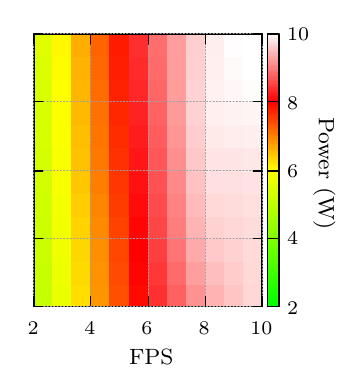
\begin{tikzpicture}[y=0.80pt, x=0.80pt, yscale=-0.564000, xscale=0.500000, inner sep=0pt, outer sep=0pt]
\scriptsize
\begin{scope}[draw=black,line join=bevel,line cap=rect,even odd rule,line width=0.512pt]
  \begin{scope}[cm={{1.0,0.0,0.0,1.0,(0.0,0.0)}},draw=black,line join=bevel,line cap=rect,line width=0.512pt]
  \end{scope}
  \begin{scope}[cm={{1.00625,0.0,0.0,1.00625,(0.0,0.0)}},draw=black,line join=bevel,line cap=rect,line width=0.512pt]
  \end{scope}
  \begin{scope}[cm={{1.00625,0.0,0.0,1.00625,(0.0,0.0)}},draw=black,line join=bevel,line cap=rect,line width=0.512pt]
  \end{scope}
  \begin{scope}[cm={{1.00625,0.0,0.0,1.00625,(0.0,0.0)}},draw=black,line join=bevel,line cap=rect,line width=0.512pt]
  \end{scope}
  \begin{scope}[cm={{1.00625,0.0,0.0,1.00625,(0.0,0.0)}},draw=cc5ff00,fill=cc5ff00,line join=bevel,line cap=rect,line width=0.512pt]
    \path[draw,fill,even odd rule] (57.5000,268.5000) -- (57.5000,250.5000) --
      (74.5000,250.5000) -- (74.5000,268.5000) -- (57.5000,268.5000);
  \end{scope}
  \begin{scope}[cm={{1.00625,0.0,0.0,1.00625,(0.0,0.0)}},draw=ceaff00,fill=ceaff00,line join=bevel,line cap=rect,line width=0.512pt]
    \path[draw,fill,even odd rule] (74.5000,268.5000) -- (74.5000,250.5000) --
      (91.5000,250.5000) -- (91.5000,268.5000) -- (74.5000,268.5000);
  \end{scope}
  \begin{scope}[cm={{1.00625,0.0,0.0,1.00625,(0.0,0.0)}},draw=cffde00,fill=cffde00,line join=bevel,line cap=rect,line width=0.512pt]
    \path[draw,fill,even odd rule] (91.5000,268.5000) -- (91.5000,250.5000) --
      (108.5000,250.5000) -- (108.5000,268.5000) -- (91.5000,268.5000);
  \end{scope}
  \begin{scope}[cm={{1.00625,0.0,0.0,1.00625,(0.0,0.0)}},draw=cc8ff00,fill=cc8ff00,line join=bevel,line cap=rect,line width=0.512pt]
    \path[draw,fill,even odd rule] (57.5000,250.5000) -- (57.5000,232.5000) --
      (74.5000,232.5000) -- (74.5000,250.5000) -- (57.5000,250.5000);
  \end{scope}
  \begin{scope}[cm={{1.00625,0.0,0.0,1.00625,(0.0,0.0)}},draw=cedff00,fill=cedff00,line join=bevel,line cap=rect,line width=0.512pt]
    \path[draw,fill,even odd rule] (74.5000,250.5000) -- (74.5000,232.5000) --
      (91.5000,232.5000) -- (91.5000,250.5000) -- (74.5000,250.5000);
  \end{scope}
  \begin{scope}[cm={{1.00625,0.0,0.0,1.00625,(0.0,0.0)}},draw=cffda00,fill=cffda00,line join=bevel,line cap=rect,line width=0.512pt]
    \path[draw,fill,even odd rule] (91.5000,250.5000) -- (91.5000,232.5000) --
      (108.5000,232.5000) -- (108.5000,250.5000) -- (91.5000,250.5000);
  \end{scope}
  \begin{scope}[cm={{1.00625,0.0,0.0,1.00625,(0.0,0.0)}},draw=ccbff00,fill=ccbff00,line join=bevel,line cap=rect,line width=0.512pt]
    \path[draw,fill,even odd rule] (57.5000,232.5000) -- (57.5000,214.5000) --
      (74.5000,214.5000) -- (74.5000,232.5000) -- (57.5000,232.5000);
  \end{scope}
  \begin{scope}[cm={{1.00625,0.0,0.0,1.00625,(0.0,0.0)}},draw=cefff00,fill=cefff00,line join=bevel,line cap=rect,line width=0.512pt]
    \path[draw,fill,even odd rule] (74.5000,232.5000) -- (74.5000,214.5000) --
      (91.5000,214.5000) -- (91.5000,232.5000) -- (74.5000,232.5000);
  \end{scope}
  \begin{scope}[cm={{1.00625,0.0,0.0,1.00625,(0.0,0.0)}},draw=cffd700,fill=cffd700,line join=bevel,line cap=rect,line width=0.512pt]
    \path[draw,fill,even odd rule] (91.5000,232.5000) -- (91.5000,214.5000) --
      (108.5000,214.5000) -- (108.5000,232.5000) -- (91.5000,232.5000);
  \end{scope}
  \begin{scope}[cm={{1.00625,0.0,0.0,1.00625,(0.0,0.0)}},draw=cceff00,fill=cceff00,line join=bevel,line cap=rect,line width=0.512pt]
    \path[draw,fill,even odd rule] (57.5000,214.5000) -- (57.5000,196.5000) --
      (74.5000,196.5000) -- (74.5000,214.5000) -- (57.5000,214.5000);
  \end{scope}
  \begin{scope}[cm={{1.00625,0.0,0.0,1.00625,(0.0,0.0)}},draw=cf2ff00,fill=cf2ff00,line join=bevel,line cap=rect,line width=0.512pt]
    \path[draw,fill,even odd rule] (74.5000,214.5000) -- (74.5000,196.5000) --
      (91.5000,196.5000) -- (91.5000,214.5000) -- (74.5000,214.5000);
  \end{scope}
  \begin{scope}[cm={{1.00625,0.0,0.0,1.00625,(0.0,0.0)}},draw=cffd200,fill=cffd200,line join=bevel,line cap=rect,line width=0.512pt]
    \path[draw,fill,even odd rule] (91.5000,214.5000) -- (91.5000,196.5000) --
      (108.5000,196.5000) -- (108.5000,214.5000) -- (91.5000,214.5000);
  \end{scope}
  \begin{scope}[cm={{1.00625,0.0,0.0,1.00625,(0.0,0.0)}},draw=cd0ff00,fill=cd0ff00,line join=bevel,line cap=rect,line width=0.512pt]
    \path[draw,fill,even odd rule] (57.5000,196.5000) -- (57.5000,178.5000) --
      (74.5000,178.5000) -- (74.5000,196.5000) -- (57.5000,196.5000);
  \end{scope}
  \begin{scope}[cm={{1.00625,0.0,0.0,1.00625,(0.0,0.0)}},draw=cf4ff00,fill=cf4ff00,line join=bevel,line cap=rect,line width=0.512pt]
    \path[draw,fill,even odd rule] (74.5000,196.5000) -- (74.5000,178.5000) --
      (91.5000,178.5000) -- (91.5000,196.5000) -- (74.5000,196.5000);
  \end{scope}
  \begin{scope}[cm={{1.00625,0.0,0.0,1.00625,(0.0,0.0)}},draw=cffcd00,fill=cffcd00,line join=bevel,line cap=rect,line width=0.512pt]
    \path[draw,fill,even odd rule] (91.5000,196.5000) -- (91.5000,178.5000) --
      (108.5000,178.5000) -- (108.5000,196.5000) -- (91.5000,196.5000);
  \end{scope}
  \begin{scope}[cm={{1.00625,0.0,0.0,1.00625,(0.0,0.0)}},draw=cd2ff00,fill=cd2ff00,line join=bevel,line cap=rect,line width=0.512pt]
    \path[draw,fill,even odd rule] (57.5000,178.5000) -- (57.5000,160.5000) --
      (74.5000,160.5000) -- (74.5000,178.5000) -- (57.5000,178.5000);
  \end{scope}
  \begin{scope}[cm={{1.00625,0.0,0.0,1.00625,(0.0,0.0)}},draw=cf7ff00,fill=cf7ff00,line join=bevel,line cap=rect,line width=0.512pt]
    \path[draw,fill,even odd rule] (74.5000,178.5000) -- (74.5000,160.5000) --
      (91.5000,160.5000) -- (91.5000,178.5000) -- (74.5000,178.5000);
  \end{scope}
  \begin{scope}[cm={{1.00625,0.0,0.0,1.00625,(0.0,0.0)}},draw=cffc700,fill=cffc700,line join=bevel,line cap=rect,line width=0.512pt]
    \path[draw,fill,even odd rule] (91.5000,178.5000) -- (91.5000,160.5000) --
      (108.5000,160.5000) -- (108.5000,178.5000) -- (91.5000,178.5000);
  \end{scope}
  \begin{scope}[cm={{1.00625,0.0,0.0,1.00625,(0.0,0.0)}},draw=cd4ff00,fill=cd4ff00,line join=bevel,line cap=rect,line width=0.512pt]
    \path[draw,fill,even odd rule] (57.5000,160.5000) -- (57.5000,141.5000) --
      (74.5000,141.5000) -- (74.5000,160.5000) -- (57.5000,160.5000);
  \end{scope}
  \begin{scope}[cm={{1.00625,0.0,0.0,1.00625,(0.0,0.0)}},draw=cf9ff00,fill=cf9ff00,line join=bevel,line cap=rect,line width=0.512pt]
    \path[draw,fill,even odd rule] (74.5000,160.5000) -- (74.5000,141.5000) --
      (91.5000,141.5000) -- (91.5000,160.5000) -- (74.5000,160.5000);
  \end{scope}
  \begin{scope}[cm={{1.00625,0.0,0.0,1.00625,(0.0,0.0)}},draw=cffc200,fill=cffc200,line join=bevel,line cap=rect,line width=0.512pt]
    \path[draw,fill,even odd rule] (91.5000,160.5000) -- (91.5000,141.5000) --
      (108.5000,141.5000) -- (108.5000,160.5000) -- (91.5000,160.5000);
  \end{scope}
  \begin{scope}[cm={{1.00625,0.0,0.0,1.00625,(0.0,0.0)}},draw=cd6ff00,fill=cd6ff00,line join=bevel,line cap=rect,line width=0.512pt]
    \path[draw,fill,even odd rule] (57.5000,141.5000) -- (57.5000,123.5000) --
      (74.5000,123.5000) -- (74.5000,141.5000) -- (57.5000,141.5000);
  \end{scope}
  \begin{scope}[cm={{1.00625,0.0,0.0,1.00625,(0.0,0.0)}},draw=cfbff00,fill=cfbff00,line join=bevel,line cap=rect,line width=0.512pt]
    \path[draw,fill,even odd rule] (74.5000,141.5000) -- (74.5000,123.5000) --
      (91.5000,123.5000) -- (91.5000,141.5000) -- (74.5000,141.5000);
  \end{scope}
  \begin{scope}[cm={{1.00625,0.0,0.0,1.00625,(0.0,0.0)}},draw=cffbe00,fill=cffbe00,line join=bevel,line cap=rect,line width=0.512pt]
    \path[draw,fill,even odd rule] (91.5000,141.5000) -- (91.5000,123.5000) --
      (108.5000,123.5000) -- (108.5000,141.5000) -- (91.5000,141.5000);
  \end{scope}
  \begin{scope}[cm={{1.00625,0.0,0.0,1.00625,(0.0,0.0)}},draw=cd8ff00,fill=cd8ff00,line join=bevel,line cap=rect,line width=0.512pt]
    \path[draw,fill,even odd rule] (57.5000,123.5000) -- (57.5000,105.5000) --
      (74.5000,105.5000) -- (74.5000,123.5000) -- (57.5000,123.5000);
  \end{scope}
  \begin{scope}[cm={{1.00625,0.0,0.0,1.00625,(0.0,0.0)}},draw=cfdff00,fill=cfdff00,line join=bevel,line cap=rect,line width=0.512pt]
    \path[draw,fill,even odd rule] (74.5000,123.5000) -- (74.5000,105.5000) --
      (91.5000,105.5000) -- (91.5000,123.5000) -- (74.5000,123.5000);
  \end{scope}
  \begin{scope}[cm={{1.00625,0.0,0.0,1.00625,(0.0,0.0)}},draw=cffba00,fill=cffba00,line join=bevel,line cap=rect,line width=0.512pt]
    \path[draw,fill,even odd rule] (91.5000,123.5000) -- (91.5000,105.5000) --
      (108.5000,105.5000) -- (108.5000,123.5000) -- (91.5000,123.5000);
  \end{scope}
  \begin{scope}[cm={{1.00625,0.0,0.0,1.00625,(0.0,0.0)}},draw=cdaff00,fill=cdaff00,line join=bevel,line cap=rect,line width=0.512pt]
    \path[draw,fill,even odd rule] (57.5000,105.5000) -- (57.5000,87.5000) --
      (74.5000,87.5000) -- (74.5000,105.5000) -- (57.5000,105.5000);
  \end{scope}
  \begin{scope}[cm={{1.00625,0.0,0.0,1.00625,(0.0,0.0)}},draw=cffff00,fill=cffff00,line join=bevel,line cap=rect,line width=0.512pt]
    \path[draw,fill,even odd rule] (74.5000,105.5000) -- (74.5000,87.5000) --
      (91.5000,87.5000) -- (91.5000,105.5000) -- (74.5000,105.5000);
  \end{scope}
  \begin{scope}[cm={{1.00625,0.0,0.0,1.00625,(0.0,0.0)}},draw=cffb600,fill=cffb600,line join=bevel,line cap=rect,line width=0.512pt]
    \path[draw,fill,even odd rule] (91.5000,105.5000) -- (91.5000,87.5000) --
      (108.5000,87.5000) -- (108.5000,105.5000) -- (91.5000,105.5000);
  \end{scope}
  \begin{scope}[cm={{1.00625,0.0,0.0,1.00625,(0.0,0.0)}},draw=cdcff00,fill=cdcff00,line join=bevel,line cap=rect,line width=0.512pt]
    \path[draw,fill,even odd rule] (57.5000,87.5000) -- (57.5000,69.5000) --
      (74.5000,69.5000) -- (74.5000,87.5000) -- (57.5000,87.5000);
  \end{scope}
  \begin{scope}[cm={{1.00625,0.0,0.0,1.00625,(0.0,0.0)}},draw=cfffc00,fill=cfffc00,line join=bevel,line cap=rect,line width=0.512pt]
    \path[draw,fill,even odd rule] (74.5000,87.5000) -- (74.5000,69.5000) --
      (91.5000,69.5000) -- (91.5000,87.5000) -- (74.5000,87.5000);
  \end{scope}
  \begin{scope}[cm={{1.00625,0.0,0.0,1.00625,(0.0,0.0)}},draw=cffb200,fill=cffb200,line join=bevel,line cap=rect,line width=0.512pt]
    \path[draw,fill,even odd rule] (91.5000,87.5000) -- (91.5000,69.5000) --
      (108.5000,69.5000) -- (108.5000,87.5000) -- (91.5000,87.5000);
  \end{scope}
  \begin{scope}[cm={{1.00625,0.0,0.0,1.00625,(0.0,0.0)}},draw=cdfff00,fill=cdfff00,line join=bevel,line cap=rect,line width=0.512pt]
    \path[draw,fill,even odd rule] (57.5000,69.5000) -- (57.5000,51.5000) --
      (74.5000,51.5000) -- (74.5000,69.5000) -- (57.5000,69.5000);
  \end{scope}
  \begin{scope}[cm={{1.00625,0.0,0.0,1.00625,(0.0,0.0)}},draw=cfff800,fill=cfff800,line join=bevel,line cap=rect,line width=0.512pt]
    \path[draw,fill,even odd rule] (74.5000,69.5000) -- (74.5000,51.5000) --
      (91.5000,51.5000) -- (91.5000,69.5000) -- (74.5000,69.5000);
  \end{scope}
  \begin{scope}[cm={{1.00625,0.0,0.0,1.00625,(0.0,0.0)}},draw=cffae00,fill=cffae00,line join=bevel,line cap=rect,line width=0.512pt]
    \path[draw,fill,even odd rule] (91.5000,69.5000) -- (91.5000,51.5000) --
      (108.5000,51.5000) -- (108.5000,69.5000) -- (91.5000,69.5000);
  \end{scope}
  \begin{scope}[cm={{1.00625,0.0,0.0,1.00625,(0.0,0.0)}},draw=cff9500,fill=cff9500,line join=bevel,line cap=rect,line width=0.512pt]
    \path[draw,fill,even odd rule] (108.5000,268.5000) -- (108.5000,250.5000) --
      (125.5000,250.5000) -- (125.5000,268.5000) -- (108.5000,268.5000);
  \end{scope}
  \begin{scope}[cm={{1.00625,0.0,0.0,1.00625,(0.0,0.0)}},draw=cff5000,fill=cff5000,line join=bevel,line cap=rect,line width=0.512pt]
    \path[draw,fill,even odd rule] (125.5000,268.5000) -- (125.5000,250.5000) --
      (143.5000,250.5000) -- (143.5000,268.5000) -- (125.5000,268.5000);
  \end{scope}
  \begin{scope}[cm={{1.00625,0.0,0.0,1.00625,(0.0,0.0)}},draw=cff0a00,fill=cff0a00,line join=bevel,line cap=rect,line width=0.512pt]
    \path[draw,fill,even odd rule] (143.5000,268.5000) -- (143.5000,250.5000) --
      (160.5000,250.5000) -- (160.5000,268.5000) -- (143.5000,268.5000);
  \end{scope}
  \begin{scope}[cm={{1.00625,0.0,0.0,1.00625,(0.0,0.0)}},draw=cff9200,fill=cff9200,line join=bevel,line cap=rect,line width=0.512pt]
    \path[draw,fill,even odd rule] (108.5000,250.5000) -- (108.5000,232.5000) --
      (125.5000,232.5000) -- (125.5000,250.5000) -- (108.5000,250.5000);
  \end{scope}
  \begin{scope}[cm={{1.00625,0.0,0.0,1.00625,(0.0,0.0)}},draw=cff4b00,fill=cff4b00,line join=bevel,line cap=rect,line width=0.512pt]
    \path[draw,fill,even odd rule] (125.5000,250.5000) -- (125.5000,232.5000) --
      (143.5000,232.5000) -- (143.5000,250.5000) -- (125.5000,250.5000);
  \end{scope}
  \begin{scope}[cm={{1.00625,0.0,0.0,1.00625,(0.0,0.0)}},draw=cff0400,fill=cff0400,line join=bevel,line cap=rect,line width=0.512pt]
    \path[draw,fill,even odd rule] (143.5000,250.5000) -- (143.5000,232.5000) --
      (160.5000,232.5000) -- (160.5000,250.5000) -- (143.5000,250.5000);
  \end{scope}
  \begin{scope}[cm={{1.00625,0.0,0.0,1.00625,(0.0,0.0)}},draw=cff8f00,fill=cff8f00,line join=bevel,line cap=rect,line width=0.512pt]
    \path[draw,fill,even odd rule] (108.5000,232.5000) -- (108.5000,214.5000) --
      (125.5000,214.5000) -- (125.5000,232.5000) -- (108.5000,232.5000);
  \end{scope}
  \begin{scope}[cm={{1.00625,0.0,0.0,1.00625,(0.0,0.0)}},draw=cff4700,fill=cff4700,line join=bevel,line cap=rect,line width=0.512pt]
    \path[draw,fill,even odd rule] (125.5000,232.5000) -- (125.5000,214.5000) --
      (143.5000,214.5000) -- (143.5000,232.5000) -- (125.5000,232.5000);
  \end{scope}
  \begin{scope}[cm={{1.00625,0.0,0.0,1.00625,(0.0,0.0)}},draw=cff0000,fill=cff0000,line join=bevel,line cap=rect,line width=0.512pt]
    \path[draw,fill,even odd rule] (143.5000,232.5000) -- (143.5000,214.5000) --
      (160.5000,214.5000) -- (160.5000,232.5000) -- (143.5000,232.5000);
  \end{scope}
  \begin{scope}[cm={{1.00625,0.0,0.0,1.00625,(0.0,0.0)}},draw=cff8a00,fill=cff8a00,line join=bevel,line cap=rect,line width=0.512pt]
    \path[draw,fill,even odd rule] (108.5000,214.5000) -- (108.5000,196.5000) --
      (125.5000,196.5000) -- (125.5000,214.5000) -- (108.5000,214.5000);
  \end{scope}
  \begin{scope}[cm={{1.00625,0.0,0.0,1.00625,(0.0,0.0)}},draw=cff4200,fill=cff4200,line join=bevel,line cap=rect,line width=0.512pt]
    \path[draw,fill,even odd rule] (125.5000,214.5000) -- (125.5000,196.5000) --
      (143.5000,196.5000) -- (143.5000,214.5000) -- (125.5000,214.5000);
  \end{scope}
  \begin{scope}[cm={{1.00625,0.0,0.0,1.00625,(0.0,0.0)}},draw=cff0606,fill=cff0606,line join=bevel,line cap=rect,line width=0.512pt]
    \path[draw,fill,even odd rule] (143.5000,214.5000) -- (143.5000,196.5000) --
      (160.5000,196.5000) -- (160.5000,214.5000) -- (143.5000,214.5000);
  \end{scope}
  \begin{scope}[cm={{1.00625,0.0,0.0,1.00625,(0.0,0.0)}},draw=cff8400,fill=cff8400,line join=bevel,line cap=rect,line width=0.512pt]
    \path[draw,fill,even odd rule] (108.5000,196.5000) -- (108.5000,178.5000) --
      (125.5000,178.5000) -- (125.5000,196.5000) -- (108.5000,196.5000);
  \end{scope}
  \begin{scope}[cm={{1.00625,0.0,0.0,1.00625,(0.0,0.0)}},draw=cff3c00,fill=cff3c00,line join=bevel,line cap=rect,line width=0.512pt]
    \path[draw,fill,even odd rule] (125.5000,196.5000) -- (125.5000,178.5000) --
      (143.5000,178.5000) -- (143.5000,196.5000) -- (125.5000,196.5000);
  \end{scope}
  \begin{scope}[cm={{1.00625,0.0,0.0,1.00625,(0.0,0.0)}},draw=cff0b0b,fill=cff0b0b,line join=bevel,line cap=rect,line width=0.512pt]
    \path[draw,fill,even odd rule] (143.5000,196.5000) -- (143.5000,178.5000) --
      (160.5000,178.5000) -- (160.5000,196.5000) -- (143.5000,196.5000);
  \end{scope}
  \begin{scope}[cm={{1.00625,0.0,0.0,1.00625,(0.0,0.0)}},draw=cff7e00,fill=cff7e00,line join=bevel,line cap=rect,line width=0.512pt]
    \path[draw,fill,even odd rule] (108.5000,178.5000) -- (108.5000,160.5000) --
      (125.5000,160.5000) -- (125.5000,178.5000) -- (108.5000,178.5000);
  \end{scope}
  \begin{scope}[cm={{1.00625,0.0,0.0,1.00625,(0.0,0.0)}},draw=cff3600,fill=cff3600,line join=bevel,line cap=rect,line width=0.512pt]
    \path[draw,fill,even odd rule] (125.5000,178.5000) -- (125.5000,160.5000) --
      (143.5000,160.5000) -- (143.5000,178.5000) -- (125.5000,178.5000);
  \end{scope}
  \begin{scope}[cm={{1.00625,0.0,0.0,1.00625,(0.0,0.0)}},draw=cff1111,fill=cff1111,line join=bevel,line cap=rect,line width=0.512pt]
    \path[draw,fill,even odd rule] (143.5000,178.5000) -- (143.5000,160.5000) --
      (160.5000,160.5000) -- (160.5000,178.5000) -- (143.5000,178.5000);
  \end{scope}
  \begin{scope}[cm={{1.00625,0.0,0.0,1.00625,(0.0,0.0)}},draw=cff7900,fill=cff7900,line join=bevel,line cap=rect,line width=0.512pt]
    \path[draw,fill,even odd rule] (108.5000,160.5000) -- (108.5000,141.5000) --
      (125.5000,141.5000) -- (125.5000,160.5000) -- (108.5000,160.5000);
  \end{scope}
  \begin{scope}[cm={{1.00625,0.0,0.0,1.00625,(0.0,0.0)}},draw=cff3100,fill=cff3100,line join=bevel,line cap=rect,line width=0.512pt]
    \path[draw,fill,even odd rule] (125.5000,160.5000) -- (125.5000,141.5000) --
      (143.5000,141.5000) -- (143.5000,160.5000) -- (125.5000,160.5000);
  \end{scope}
  \begin{scope}[cm={{1.00625,0.0,0.0,1.00625,(0.0,0.0)}},draw=cff1717,fill=cff1717,line join=bevel,line cap=rect,line width=0.512pt]
    \path[draw,fill,even odd rule] (143.5000,160.5000) -- (143.5000,141.5000) --
      (160.5000,141.5000) -- (160.5000,160.5000) -- (143.5000,160.5000);
  \end{scope}
  \begin{scope}[cm={{1.00625,0.0,0.0,1.00625,(0.0,0.0)}},draw=cff7500,fill=cff7500,line join=bevel,line cap=rect,line width=0.512pt]
    \path[draw,fill,even odd rule] (108.5000,141.5000) -- (108.5000,123.5000) --
      (125.5000,123.5000) -- (125.5000,141.5000) -- (108.5000,141.5000);
  \end{scope}
  \begin{scope}[cm={{1.00625,0.0,0.0,1.00625,(0.0,0.0)}},draw=cff2c00,fill=cff2c00,line join=bevel,line cap=rect,line width=0.512pt]
    \path[draw,fill,even odd rule] (125.5000,141.5000) -- (125.5000,123.5000) --
      (143.5000,123.5000) -- (143.5000,141.5000) -- (125.5000,141.5000);
  \end{scope}
  \begin{scope}[cm={{1.00625,0.0,0.0,1.00625,(0.0,0.0)}},draw=cff1c1c,fill=cff1c1c,line join=bevel,line cap=rect,line width=0.512pt]
    \path[draw,fill,even odd rule] (143.5000,141.5000) -- (143.5000,123.5000) --
      (160.5000,123.5000) -- (160.5000,141.5000) -- (143.5000,141.5000);
  \end{scope}
  \begin{scope}[cm={{1.00625,0.0,0.0,1.00625,(0.0,0.0)}},draw=cff7100,fill=cff7100,line join=bevel,line cap=rect,line width=0.512pt]
    \path[draw,fill,even odd rule] (108.5000,123.5000) -- (108.5000,105.5000) --
      (125.5000,105.5000) -- (125.5000,123.5000) -- (108.5000,123.5000);
  \end{scope}
  \begin{scope}[cm={{1.00625,0.0,0.0,1.00625,(0.0,0.0)}},draw=cff2700,fill=cff2700,line join=bevel,line cap=rect,line width=0.512pt]
    \path[draw,fill,even odd rule] (125.5000,123.5000) -- (125.5000,105.5000) --
      (143.5000,105.5000) -- (143.5000,123.5000) -- (125.5000,123.5000);
  \end{scope}
  \begin{scope}[cm={{1.00625,0.0,0.0,1.00625,(0.0,0.0)}},draw=cff2222,fill=cff2222,line join=bevel,line cap=rect,line width=0.512pt]
    \path[draw,fill,even odd rule] (143.5000,123.5000) -- (143.5000,105.5000) --
      (160.5000,105.5000) -- (160.5000,123.5000) -- (143.5000,123.5000);
  \end{scope}
  \begin{scope}[cm={{1.00625,0.0,0.0,1.00625,(0.0,0.0)}},draw=cff6c00,fill=cff6c00,line join=bevel,line cap=rect,line width=0.512pt]
    \path[draw,fill,even odd rule] (108.5000,105.5000) -- (108.5000,87.5000) --
      (125.5000,87.5000) -- (125.5000,105.5000) -- (108.5000,105.5000);
  \end{scope}
  \begin{scope}[cm={{1.00625,0.0,0.0,1.00625,(0.0,0.0)}},draw=cff2200,fill=cff2200,line join=bevel,line cap=rect,line width=0.512pt]
    \path[draw,fill,even odd rule] (125.5000,105.5000) -- (125.5000,87.5000) --
      (143.5000,87.5000) -- (143.5000,105.5000) -- (125.5000,105.5000);
  \end{scope}
  \begin{scope}[cm={{1.00625,0.0,0.0,1.00625,(0.0,0.0)}},draw=cff2727,fill=cff2727,line join=bevel,line cap=rect,line width=0.512pt]
    \path[draw,fill,even odd rule] (143.5000,105.5000) -- (143.5000,87.5000) --
      (160.5000,87.5000) -- (160.5000,105.5000) -- (143.5000,105.5000);
  \end{scope}
  \begin{scope}[cm={{1.00625,0.0,0.0,1.00625,(0.0,0.0)}},draw=cff6800,fill=cff6800,line join=bevel,line cap=rect,line width=0.512pt]
    \path[draw,fill,even odd rule] (108.5000,87.5000) -- (108.5000,69.5000) --
      (125.5000,69.5000) -- (125.5000,87.5000) -- (108.5000,87.5000);
  \end{scope}
  \begin{scope}[cm={{1.00625,0.0,0.0,1.00625,(0.0,0.0)}},draw=cff1e00,fill=cff1e00,line join=bevel,line cap=rect,line width=0.512pt]
    \path[draw,fill,even odd rule] (125.5000,87.5000) -- (125.5000,69.5000) --
      (143.5000,69.5000) -- (143.5000,87.5000) -- (125.5000,87.5000);
  \end{scope}
  \begin{scope}[cm={{1.00625,0.0,0.0,1.00625,(0.0,0.0)}},draw=cff2b2b,fill=cff2b2b,line join=bevel,line cap=rect,line width=0.512pt]
    \path[draw,fill,even odd rule] (143.5000,87.5000) -- (143.5000,69.5000) --
      (160.5000,69.5000) -- (160.5000,87.5000) -- (143.5000,87.5000);
  \end{scope}
  \begin{scope}[cm={{1.00625,0.0,0.0,1.00625,(0.0,0.0)}},draw=cff6400,fill=cff6400,line join=bevel,line cap=rect,line width=0.512pt]
    \path[draw,fill,even odd rule] (108.5000,69.5000) -- (108.5000,51.5000) --
      (125.5000,51.5000) -- (125.5000,69.5000) -- (108.5000,69.5000);
  \end{scope}
  \begin{scope}[cm={{1.00625,0.0,0.0,1.00625,(0.0,0.0)}},draw=cff1a00,fill=cff1a00,line join=bevel,line cap=rect,line width=0.512pt]
    \path[draw,fill,even odd rule] (125.5000,69.5000) -- (125.5000,51.5000) --
      (143.5000,51.5000) -- (143.5000,69.5000) -- (125.5000,69.5000);
  \end{scope}
  \begin{scope}[cm={{1.00625,0.0,0.0,1.00625,(0.0,0.0)}},draw=cff2f2f,fill=cff2f2f,line join=bevel,line cap=rect,line width=0.512pt]
    \path[draw,fill,even odd rule] (143.5000,69.5000) -- (143.5000,51.5000) --
      (160.5000,51.5000) -- (160.5000,69.5000) -- (143.5000,69.5000);
  \end{scope}
  \begin{scope}[cm={{1.00625,0.0,0.0,1.00625,(0.0,0.0)}},draw=cff3030,fill=cff3030,line join=bevel,line cap=rect,line width=0.512pt]
    \path[draw,fill,even odd rule] (160.5000,268.5000) -- (160.5000,250.5000) --
      (177.5000,250.5000) -- (177.5000,268.5000) -- (160.5000,268.5000);
  \end{scope}
  \begin{scope}[cm={{1.00625,0.0,0.0,1.00625,(0.0,0.0)}},draw=cff6161,fill=cff6161,line join=bevel,line cap=rect,line width=0.512pt]
    \path[draw,fill,even odd rule] (177.5000,268.5000) -- (177.5000,250.5000) --
      (194.5000,250.5000) -- (194.5000,268.5000) -- (177.5000,268.5000);
  \end{scope}
  \begin{scope}[cm={{1.00625,0.0,0.0,1.00625,(0.0,0.0)}},draw=cff9191,fill=cff9191,line join=bevel,line cap=rect,line width=0.512pt]
    \path[draw,fill,even odd rule] (194.5000,268.5000) -- (194.5000,250.5000) --
      (211.5000,250.5000) -- (211.5000,268.5000) -- (194.5000,268.5000);
  \end{scope}
  \begin{scope}[cm={{1.00625,0.0,0.0,1.00625,(0.0,0.0)}},draw=cff3737,fill=cff3737,line join=bevel,line cap=rect,line width=0.512pt]
    \path[draw,fill,even odd rule] (160.5000,250.5000) -- (160.5000,232.5000) --
      (177.5000,232.5000) -- (177.5000,250.5000) -- (160.5000,250.5000);
  \end{scope}
  \begin{scope}[cm={{1.00625,0.0,0.0,1.00625,(0.0,0.0)}},draw=cff6b6b,fill=cff6b6b,line join=bevel,line cap=rect,line width=0.512pt]
    \path[draw,fill,even odd rule] (177.5000,250.5000) -- (177.5000,232.5000) --
      (194.5000,232.5000) -- (194.5000,250.5000) -- (177.5000,250.5000);
  \end{scope}
  \begin{scope}[cm={{1.00625,0.0,0.0,1.00625,(0.0,0.0)}},draw=cff9e9e,fill=cff9e9e,line join=bevel,line cap=rect,line width=0.512pt]
    \path[draw,fill,even odd rule] (194.5000,250.5000) -- (194.5000,232.5000) --
      (211.5000,232.5000) -- (211.5000,250.5000) -- (194.5000,250.5000);
  \end{scope}
  \begin{scope}[cm={{1.00625,0.0,0.0,1.00625,(0.0,0.0)}},draw=cff3f3f,fill=cff3f3f,line join=bevel,line cap=rect,line width=0.512pt]
    \path[draw,fill,even odd rule] (160.5000,232.5000) -- (160.5000,214.5000) --
      (177.5000,214.5000) -- (177.5000,232.5000) -- (160.5000,232.5000);
  \end{scope}
  \begin{scope}[cm={{1.00625,0.0,0.0,1.00625,(0.0,0.0)}},draw=cff7575,fill=cff7575,line join=bevel,line cap=rect,line width=0.512pt]
    \path[draw,fill,even odd rule] (177.5000,232.5000) -- (177.5000,214.5000) --
      (194.5000,214.5000) -- (194.5000,232.5000) -- (177.5000,232.5000);
  \end{scope}
  \begin{scope}[cm={{1.00625,0.0,0.0,1.00625,(0.0,0.0)}},draw=cffaaaa,fill=cffaaaa,line join=bevel,line cap=rect,line width=0.512pt]
    \path[draw,fill,even odd rule] (194.5000,232.5000) -- (194.5000,214.5000) --
      (211.5000,214.5000) -- (211.5000,232.5000) -- (194.5000,232.5000);
  \end{scope}
  \begin{scope}[cm={{1.00625,0.0,0.0,1.00625,(0.0,0.0)}},draw=cff4646,fill=cff4646,line join=bevel,line cap=rect,line width=0.512pt]
    \path[draw,fill,even odd rule] (160.5000,214.5000) -- (160.5000,196.5000) --
      (177.5000,196.5000) -- (177.5000,214.5000) -- (160.5000,214.5000);
  \end{scope}
  \begin{scope}[cm={{1.00625,0.0,0.0,1.00625,(0.0,0.0)}},draw=cff7d7d,fill=cff7d7d,line join=bevel,line cap=rect,line width=0.512pt]
    \path[draw,fill,even odd rule] (177.5000,214.5000) -- (177.5000,196.5000) --
      (194.5000,196.5000) -- (194.5000,214.5000) -- (177.5000,214.5000);
  \end{scope}
  \begin{scope}[cm={{1.00625,0.0,0.0,1.00625,(0.0,0.0)}},draw=cffb4b4,fill=cffb4b4,line join=bevel,line cap=rect,line width=0.512pt]
    \path[draw,fill,even odd rule] (194.5000,214.5000) -- (194.5000,196.5000) --
      (211.5000,196.5000) -- (211.5000,214.5000) -- (194.5000,214.5000);
  \end{scope}
  \begin{scope}[cm={{1.00625,0.0,0.0,1.00625,(0.0,0.0)}},draw=cff4b4b,fill=cff4b4b,line join=bevel,line cap=rect,line width=0.512pt]
    \path[draw,fill,even odd rule] (160.5000,196.5000) -- (160.5000,178.5000) --
      (177.5000,178.5000) -- (177.5000,196.5000) -- (160.5000,196.5000);
  \end{scope}
  \begin{scope}[cm={{1.00625,0.0,0.0,1.00625,(0.0,0.0)}},draw=cff8383,fill=cff8383,line join=bevel,line cap=rect,line width=0.512pt]
    \path[draw,fill,even odd rule] (177.5000,196.5000) -- (177.5000,178.5000) --
      (194.5000,178.5000) -- (194.5000,196.5000) -- (177.5000,196.5000);
  \end{scope}
  \begin{scope}[cm={{1.00625,0.0,0.0,1.00625,(0.0,0.0)}},draw=cffbbbb,fill=cffbbbb,line join=bevel,line cap=rect,line width=0.512pt]
    \path[draw,fill,even odd rule] (194.5000,196.5000) -- (194.5000,178.5000) --
      (211.5000,178.5000) -- (211.5000,196.5000) -- (194.5000,196.5000);
  \end{scope}
  \begin{scope}[cm={{1.00625,0.0,0.0,1.00625,(0.0,0.0)}},draw=cff5151,fill=cff5151,line join=bevel,line cap=rect,line width=0.512pt]
    \path[draw,fill,even odd rule] (160.5000,178.5000) -- (160.5000,160.5000) --
      (177.5000,160.5000) -- (177.5000,178.5000) -- (160.5000,178.5000);
  \end{scope}
  \begin{scope}[cm={{1.00625,0.0,0.0,1.00625,(0.0,0.0)}},draw=cff8989,fill=cff8989,line join=bevel,line cap=rect,line width=0.512pt]
    \path[draw,fill,even odd rule] (177.5000,178.5000) -- (177.5000,160.5000) --
      (194.5000,160.5000) -- (194.5000,178.5000) -- (177.5000,178.5000);
  \end{scope}
  \begin{scope}[cm={{1.00625,0.0,0.0,1.00625,(0.0,0.0)}},draw=cffc2c2,fill=cffc2c2,line join=bevel,line cap=rect,line width=0.512pt]
    \path[draw,fill,even odd rule] (194.5000,178.5000) -- (194.5000,160.5000) --
      (211.5000,160.5000) -- (211.5000,178.5000) -- (194.5000,178.5000);
  \end{scope}
  \begin{scope}[cm={{1.00625,0.0,0.0,1.00625,(0.0,0.0)}},draw=cff5757,fill=cff5757,line join=bevel,line cap=rect,line width=0.512pt]
    \path[draw,fill,even odd rule] (160.5000,160.5000) -- (160.5000,141.5000) --
      (177.5000,141.5000) -- (177.5000,160.5000) -- (160.5000,160.5000);
  \end{scope}
  \begin{scope}[cm={{1.00625,0.0,0.0,1.00625,(0.0,0.0)}},draw=cff8f8f,fill=cff8f8f,line join=bevel,line cap=rect,line width=0.512pt]
    \path[draw,fill,even odd rule] (177.5000,160.5000) -- (177.5000,141.5000) --
      (194.5000,141.5000) -- (194.5000,160.5000) -- (177.5000,160.5000);
  \end{scope}
  \begin{scope}[cm={{1.00625,0.0,0.0,1.00625,(0.0,0.0)}},draw=cffc8c8,fill=cffc8c8,line join=bevel,line cap=rect,line width=0.512pt]
    \path[draw,fill,even odd rule] (194.5000,160.5000) -- (194.5000,141.5000) --
      (211.5000,141.5000) -- (211.5000,160.5000) -- (194.5000,160.5000);
  \end{scope}
  \begin{scope}[cm={{1.00625,0.0,0.0,1.00625,(0.0,0.0)}},draw=cff5d5d,fill=cff5d5d,line join=bevel,line cap=rect,line width=0.512pt]
    \path[draw,fill,even odd rule] (160.5000,141.5000) -- (160.5000,123.5000) --
      (177.5000,123.5000) -- (177.5000,141.5000) -- (160.5000,141.5000);
  \end{scope}
  \begin{scope}[cm={{1.00625,0.0,0.0,1.00625,(0.0,0.0)}},draw=cff9595,fill=cff9595,line join=bevel,line cap=rect,line width=0.512pt]
    \path[draw,fill,even odd rule] (177.5000,141.5000) -- (177.5000,123.5000) --
      (194.5000,123.5000) -- (194.5000,141.5000) -- (177.5000,141.5000);
  \end{scope}
  \begin{scope}[cm={{1.00625,0.0,0.0,1.00625,(0.0,0.0)}},draw=cffcdcd,fill=cffcdcd,line join=bevel,line cap=rect,line width=0.512pt]
    \path[draw,fill,even odd rule] (194.5000,141.5000) -- (194.5000,123.5000) --
      (211.5000,123.5000) -- (211.5000,141.5000) -- (194.5000,141.5000);
  \end{scope}
  \begin{scope}[cm={{1.00625,0.0,0.0,1.00625,(0.0,0.0)}},draw=cff6262,fill=cff6262,line join=bevel,line cap=rect,line width=0.512pt]
    \path[draw,fill,even odd rule] (160.5000,123.5000) -- (160.5000,105.5000) --
      (177.5000,105.5000) -- (177.5000,123.5000) -- (160.5000,123.5000);
  \end{scope}
  \begin{scope}[cm={{1.00625,0.0,0.0,1.00625,(0.0,0.0)}},draw=cff9a9a,fill=cff9a9a,line join=bevel,line cap=rect,line width=0.512pt]
    \path[draw,fill,even odd rule] (177.5000,123.5000) -- (177.5000,105.5000) --
      (194.5000,105.5000) -- (194.5000,123.5000) -- (177.5000,123.5000);
  \end{scope}
  \begin{scope}[cm={{1.00625,0.0,0.0,1.00625,(0.0,0.0)}},draw=cffd2d2,fill=cffd2d2,line join=bevel,line cap=rect,line width=0.512pt]
    \path[draw,fill,even odd rule] (194.5000,123.5000) -- (194.5000,105.5000) --
      (211.5000,105.5000) -- (211.5000,123.5000) -- (194.5000,123.5000);
  \end{scope}
  \begin{scope}[cm={{1.00625,0.0,0.0,1.00625,(0.0,0.0)}},draw=cff6767,fill=cff6767,line join=bevel,line cap=rect,line width=0.512pt]
    \path[draw,fill,even odd rule] (160.5000,105.5000) -- (160.5000,87.5000) --
      (177.5000,87.5000) -- (177.5000,105.5000) -- (160.5000,105.5000);
  \end{scope}
  \begin{scope}[cm={{1.00625,0.0,0.0,1.00625,(0.0,0.0)}},draw=cff9d9d,fill=cff9d9d,line join=bevel,line cap=rect,line width=0.512pt]
    \path[draw,fill,even odd rule] (177.5000,105.5000) -- (177.5000,87.5000) --
      (194.5000,87.5000) -- (194.5000,105.5000) -- (177.5000,105.5000);
  \end{scope}
  \begin{scope}[cm={{1.00625,0.0,0.0,1.00625,(0.0,0.0)}},draw=cffd3d3,fill=cffd3d3,line join=bevel,line cap=rect,line width=0.512pt]
    \path[draw,fill,even odd rule] (194.5000,105.5000) -- (194.5000,87.5000) --
      (211.5000,87.5000) -- (211.5000,105.5000) -- (194.5000,105.5000);
  \end{scope}
  \begin{scope}[cm={{1.00625,0.0,0.0,1.00625,(0.0,0.0)}},draw=cff6a6a,fill=cff6a6a,line join=bevel,line cap=rect,line width=0.512pt]
    \path[draw,fill,even odd rule] (160.5000,87.5000) -- (160.5000,69.5000) --
      (177.5000,69.5000) -- (177.5000,87.5000) -- (160.5000,87.5000);
  \end{scope}
  \begin{scope}[cm={{1.00625,0.0,0.0,1.00625,(0.0,0.0)}},draw=cff9d9d,fill=cff9d9d,line join=bevel,line cap=rect,line width=0.512pt]
    \path[draw,fill,even odd rule] (177.5000,87.5000) -- (177.5000,69.5000) --
      (194.5000,69.5000) -- (194.5000,87.5000) -- (177.5000,87.5000);
  \end{scope}
  \begin{scope}[cm={{1.00625,0.0,0.0,1.00625,(0.0,0.0)}},draw=cffd0d0,fill=cffd0d0,line join=bevel,line cap=rect,line width=0.512pt]
    \path[draw,fill,even odd rule] (194.5000,87.5000) -- (194.5000,69.5000) --
      (211.5000,69.5000) -- (211.5000,87.5000) -- (194.5000,87.5000);
  \end{scope}
  \begin{scope}[cm={{1.00625,0.0,0.0,1.00625,(0.0,0.0)}},draw=cff6d6d,fill=cff6d6d,line join=bevel,line cap=rect,line width=0.512pt]
    \path[draw,fill,even odd rule] (160.5000,69.5000) -- (160.5000,51.5000) --
      (177.5000,51.5000) -- (177.5000,69.5000) -- (160.5000,69.5000);
  \end{scope}
  \begin{scope}[cm={{1.00625,0.0,0.0,1.00625,(0.0,0.0)}},draw=cff9d9d,fill=cff9d9d,line join=bevel,line cap=rect,line width=0.512pt]
    \path[draw,fill,even odd rule] (177.5000,69.5000) -- (177.5000,51.5000) --
      (194.5000,51.5000) -- (194.5000,69.5000) -- (177.5000,69.5000);
  \end{scope}
  \begin{scope}[cm={{1.00625,0.0,0.0,1.00625,(0.0,0.0)}},draw=cffcece,fill=cffcece,line join=bevel,line cap=rect,line width=0.512pt]
    \path[draw,fill,even odd rule] (194.5000,69.5000) -- (194.5000,51.5000) --
      (211.5000,51.5000) -- (211.5000,69.5000) -- (194.5000,69.5000);
  \end{scope}
  \begin{scope}[cm={{1.00625,0.0,0.0,1.00625,(0.0,0.0)}},draw=cffb3b3,fill=cffb3b3,line join=bevel,line cap=rect,line width=0.512pt]
    \path[draw,fill,even odd rule] (211.5000,268.5000) -- (211.5000,250.5000) --
      (228.5000,250.5000) -- (228.5000,268.5000) -- (211.5000,268.5000);
  \end{scope}
  \begin{scope}[cm={{1.00625,0.0,0.0,1.00625,(0.0,0.0)}},draw=cffc5c5,fill=cffc5c5,line join=bevel,line cap=rect,line width=0.512pt]
    \path[draw,fill,even odd rule] (228.5000,268.5000) -- (228.5000,250.5000) --
      (245.5000,250.5000) -- (245.5000,268.5000) -- (228.5000,268.5000);
  \end{scope}
  \begin{scope}[cm={{1.00625,0.0,0.0,1.00625,(0.0,0.0)}},draw=cffd7d7,fill=cffd7d7,line join=bevel,line cap=rect,line width=0.512pt]
    \path[draw,fill,even odd rule] (245.5000,268.5000) -- (245.5000,250.5000) --
      (262.5000,250.5000) -- (262.5000,268.5000) -- (245.5000,268.5000);
  \end{scope}
  \begin{scope}[cm={{1.00625,0.0,0.0,1.00625,(0.0,0.0)}},draw=cffbebe,fill=cffbebe,line join=bevel,line cap=rect,line width=0.512pt]
    \path[draw,fill,even odd rule] (211.5000,250.5000) -- (211.5000,232.5000) --
      (228.5000,232.5000) -- (228.5000,250.5000) -- (211.5000,250.5000);
  \end{scope}
  \begin{scope}[cm={{1.00625,0.0,0.0,1.00625,(0.0,0.0)}},draw=cffcbcb,fill=cffcbcb,line join=bevel,line cap=rect,line width=0.512pt]
    \path[draw,fill,even odd rule] (228.5000,250.5000) -- (228.5000,232.5000) --
      (245.5000,232.5000) -- (245.5000,250.5000) -- (228.5000,250.5000);
  \end{scope}
  \begin{scope}[cm={{1.00625,0.0,0.0,1.00625,(0.0,0.0)}},draw=cffd8d8,fill=cffd8d8,line join=bevel,line cap=rect,line width=0.512pt]
    \path[draw,fill,even odd rule] (245.5000,250.5000) -- (245.5000,232.5000) --
      (262.5000,232.5000) -- (262.5000,250.5000) -- (245.5000,250.5000);
  \end{scope}
  \begin{scope}[cm={{1.00625,0.0,0.0,1.00625,(0.0,0.0)}},draw=cffc9c9,fill=cffc9c9,line join=bevel,line cap=rect,line width=0.512pt]
    \path[draw,fill,even odd rule] (211.5000,232.5000) -- (211.5000,214.5000) --
      (228.5000,214.5000) -- (228.5000,232.5000) -- (211.5000,232.5000);
  \end{scope}
  \begin{scope}[cm={{1.00625,0.0,0.0,1.00625,(0.0,0.0)}},draw=cffd2d2,fill=cffd2d2,line join=bevel,line cap=rect,line width=0.512pt]
    \path[draw,fill,even odd rule] (228.5000,232.5000) -- (228.5000,214.5000) --
      (245.5000,214.5000) -- (245.5000,232.5000) -- (228.5000,232.5000);
  \end{scope}
  \begin{scope}[cm={{1.00625,0.0,0.0,1.00625,(0.0,0.0)}},draw=cffdada,fill=cffdada,line join=bevel,line cap=rect,line width=0.512pt]
    \path[draw,fill,even odd rule] (245.5000,232.5000) -- (245.5000,214.5000) --
      (262.5000,214.5000) -- (262.5000,232.5000) -- (245.5000,232.5000);
  \end{scope}
  \begin{scope}[cm={{1.00625,0.0,0.0,1.00625,(0.0,0.0)}},draw=cffd2d2,fill=cffd2d2,line join=bevel,line cap=rect,line width=0.512pt]
    \path[draw,fill,even odd rule] (211.5000,214.5000) -- (211.5000,196.5000) --
      (228.5000,196.5000) -- (228.5000,214.5000) -- (211.5000,214.5000);
  \end{scope}
  \begin{scope}[cm={{1.00625,0.0,0.0,1.00625,(0.0,0.0)}},draw=cffd7d7,fill=cffd7d7,line join=bevel,line cap=rect,line width=0.512pt]
    \path[draw,fill,even odd rule] (228.5000,214.5000) -- (228.5000,196.5000) --
      (245.5000,196.5000) -- (245.5000,214.5000) -- (228.5000,214.5000);
  \end{scope}
  \begin{scope}[cm={{1.00625,0.0,0.0,1.00625,(0.0,0.0)}},draw=cffdcdc,fill=cffdcdc,line join=bevel,line cap=rect,line width=0.512pt]
    \path[draw,fill,even odd rule] (245.5000,214.5000) -- (245.5000,196.5000) --
      (262.5000,196.5000) -- (262.5000,214.5000) -- (245.5000,214.5000);
  \end{scope}
  \begin{scope}[cm={{1.00625,0.0,0.0,1.00625,(0.0,0.0)}},draw=cffd8d8,fill=cffd8d8,line join=bevel,line cap=rect,line width=0.512pt]
    \path[draw,fill,even odd rule] (211.5000,196.5000) -- (211.5000,178.5000) --
      (228.5000,178.5000) -- (228.5000,196.5000) -- (211.5000,196.5000);
  \end{scope}
  \begin{scope}[cm={{1.00625,0.0,0.0,1.00625,(0.0,0.0)}},draw=cffdcdc,fill=cffdcdc,line join=bevel,line cap=rect,line width=0.512pt]
    \path[draw,fill,even odd rule] (228.5000,196.5000) -- (228.5000,178.5000) --
      (245.5000,178.5000) -- (245.5000,196.5000) -- (228.5000,196.5000);
  \end{scope}
  \begin{scope}[cm={{1.00625,0.0,0.0,1.00625,(0.0,0.0)}},draw=cffdfdf,fill=cffdfdf,line join=bevel,line cap=rect,line width=0.512pt]
    \path[draw,fill,even odd rule] (245.5000,196.5000) -- (245.5000,178.5000) --
      (262.5000,178.5000) -- (262.5000,196.5000) -- (245.5000,196.5000);
  \end{scope}
  \begin{scope}[cm={{1.00625,0.0,0.0,1.00625,(0.0,0.0)}},draw=cffdfdf,fill=cffdfdf,line join=bevel,line cap=rect,line width=0.512pt]
    \path[draw,fill,even odd rule] (211.5000,178.5000) -- (211.5000,160.5000) --
      (228.5000,160.5000) -- (228.5000,178.5000) -- (211.5000,178.5000);
  \end{scope}
  \begin{scope}[cm={{1.00625,0.0,0.0,1.00625,(0.0,0.0)}},draw=cffe0e0,fill=cffe0e0,line join=bevel,line cap=rect,line width=0.512pt]
    \path[draw,fill,even odd rule] (228.5000,178.5000) -- (228.5000,160.5000) --
      (245.5000,160.5000) -- (245.5000,178.5000) -- (228.5000,178.5000);
  \end{scope}
  \begin{scope}[cm={{1.00625,0.0,0.0,1.00625,(0.0,0.0)}},draw=cffe2e2,fill=cffe2e2,line join=bevel,line cap=rect,line width=0.512pt]
    \path[draw,fill,even odd rule] (245.5000,178.5000) -- (245.5000,160.5000) --
      (262.5000,160.5000) -- (262.5000,178.5000) -- (245.5000,178.5000);
  \end{scope}
  \begin{scope}[cm={{1.00625,0.0,0.0,1.00625,(0.0,0.0)}},draw=cffe4e4,fill=cffe4e4,line join=bevel,line cap=rect,line width=0.512pt]
    \path[draw,fill,even odd rule] (211.5000,160.5000) -- (211.5000,141.5000) --
      (228.5000,141.5000) -- (228.5000,160.5000) -- (211.5000,160.5000);
  \end{scope}
  \begin{scope}[cm={{1.00625,0.0,0.0,1.00625,(0.0,0.0)}},draw=cffe5e5,fill=cffe5e5,line join=bevel,line cap=rect,line width=0.512pt]
    \path[draw,fill,even odd rule] (228.5000,160.5000) -- (228.5000,141.5000) --
      (245.5000,141.5000) -- (245.5000,160.5000) -- (228.5000,160.5000);
  \end{scope}
  \begin{scope}[cm={{1.00625,0.0,0.0,1.00625,(0.0,0.0)}},draw=cffe7e7,fill=cffe7e7,line join=bevel,line cap=rect,line width=0.512pt]
    \path[draw,fill,even odd rule] (245.5000,160.5000) -- (245.5000,141.5000) --
      (262.5000,141.5000) -- (262.5000,160.5000) -- (245.5000,160.5000);
  \end{scope}
  \begin{scope}[cm={{1.00625,0.0,0.0,1.00625,(0.0,0.0)}},draw=cffeaea,fill=cffeaea,line join=bevel,line cap=rect,line width=0.512pt]
    \path[draw,fill,even odd rule] (211.5000,141.5000) -- (211.5000,123.5000) --
      (228.5000,123.5000) -- (228.5000,141.5000) -- (211.5000,141.5000);
  \end{scope}
  \begin{scope}[cm={{1.00625,0.0,0.0,1.00625,(0.0,0.0)}},draw=cffecec,fill=cffecec,line join=bevel,line cap=rect,line width=0.512pt]
    \path[draw,fill,even odd rule] (228.5000,141.5000) -- (228.5000,123.5000) --
      (245.5000,123.5000) -- (245.5000,141.5000) -- (228.5000,141.5000);
  \end{scope}
  \begin{scope}[cm={{1.00625,0.0,0.0,1.00625,(0.0,0.0)}},draw=cffeeee,fill=cffeeee,line join=bevel,line cap=rect,line width=0.512pt]
    \path[draw,fill,even odd rule] (245.5000,141.5000) -- (245.5000,123.5000) --
      (262.5000,123.5000) -- (262.5000,141.5000) -- (245.5000,141.5000);
  \end{scope}
  \begin{scope}[cm={{1.00625,0.0,0.0,1.00625,(0.0,0.0)}},draw=cffefef,fill=cffefef,line join=bevel,line cap=rect,line width=0.512pt]
    \path[draw,fill,even odd rule] (211.5000,123.5000) -- (211.5000,105.5000) --
      (228.5000,105.5000) -- (228.5000,123.5000) -- (211.5000,123.5000);
  \end{scope}
  \begin{scope}[cm={{1.00625,0.0,0.0,1.00625,(0.0,0.0)}},draw=cfff2f2,fill=cfff2f2,line join=bevel,line cap=rect,line width=0.512pt]
    \path[draw,fill,even odd rule] (228.5000,123.5000) -- (228.5000,105.5000) --
      (245.5000,105.5000) -- (245.5000,123.5000) -- (228.5000,123.5000);
  \end{scope}
  \begin{scope}[cm={{1.00625,0.0,0.0,1.00625,(0.0,0.0)}},draw=cfff5f5,fill=cfff5f5,line join=bevel,line cap=rect,line width=0.512pt]
    \path[draw,fill,even odd rule] (245.5000,123.5000) -- (245.5000,105.5000) --
      (262.5000,105.5000) -- (262.5000,123.5000) -- (245.5000,123.5000);
  \end{scope}
  \begin{scope}[cm={{1.00625,0.0,0.0,1.00625,(0.0,0.0)}},draw=cfff1f1,fill=cfff1f1,line join=bevel,line cap=rect,line width=0.512pt]
    \path[draw,fill,even odd rule] (211.5000,105.5000) -- (211.5000,87.5000) --
      (228.5000,87.5000) -- (228.5000,105.5000) -- (211.5000,105.5000);
  \end{scope}
  \begin{scope}[cm={{1.00625,0.0,0.0,1.00625,(0.0,0.0)}},draw=cfff7f7,fill=cfff7f7,line join=bevel,line cap=rect,line width=0.512pt]
    \path[draw,fill,even odd rule] (228.5000,105.5000) -- (228.5000,87.5000) --
      (245.5000,87.5000) -- (245.5000,105.5000) -- (228.5000,105.5000);
  \end{scope}
  \begin{scope}[cm={{1.00625,0.0,0.0,1.00625,(0.0,0.0)}},draw=cfffcfc,fill=cfffcfc,line join=bevel,line cap=rect,line width=0.512pt]
    \path[draw,fill,even odd rule] (245.5000,105.5000) -- (245.5000,87.5000) --
      (262.5000,87.5000) -- (262.5000,105.5000) -- (245.5000,105.5000);
  \end{scope}
  \begin{scope}[cm={{1.00625,0.0,0.0,1.00625,(0.0,0.0)}},draw=cffefef,fill=cffefef,line join=bevel,line cap=rect,line width=0.512pt]
    \path[draw,fill,even odd rule] (211.5000,87.5000) -- (211.5000,69.5000) --
      (228.5000,69.5000) -- (228.5000,87.5000) -- (211.5000,87.5000);
  \end{scope}
  \begin{scope}[cm={{1.00625,0.0,0.0,1.00625,(0.0,0.0)}},draw=cfffafa,fill=cfffafa,line join=bevel,line cap=rect,line width=0.512pt]
    \path[draw,fill,even odd rule] (228.5000,87.5000) -- (228.5000,69.5000) --
      (245.5000,69.5000) -- (245.5000,87.5000) -- (228.5000,87.5000);
  \end{scope}
  \begin{scope}[cm={{1.00625,0.0,0.0,1.00625,(0.0,0.0)}},draw=cffffff,fill=cffffff,line join=bevel,line cap=rect,line width=0.512pt]
    \path[draw,fill,even odd rule] (245.5000,87.5000) -- (245.5000,69.5000) --
      (262.5000,69.5000) -- (262.5000,87.5000) -- (245.5000,87.5000);
  \end{scope}
  \begin{scope}[cm={{1.00625,0.0,0.0,1.00625,(0.0,0.0)}},draw=cffeeee,fill=cffeeee,line join=bevel,line cap=rect,line width=0.512pt]
    \path[draw,fill,even odd rule] (211.5000,69.5000) -- (211.5000,51.5000) --
      (228.5000,51.5000) -- (228.5000,69.5000) -- (211.5000,69.5000);
  \end{scope}
  \begin{scope}[cm={{1.00625,0.0,0.0,1.00625,(0.0,0.0)}},draw=cfffdfd,fill=cfffdfd,line join=bevel,line cap=rect,line width=0.512pt]
    \path[draw,fill,even odd rule] (228.5000,69.5000) -- (228.5000,51.5000) --
      (245.5000,51.5000) -- (245.5000,69.5000) -- (228.5000,69.5000);
  \end{scope}
  \begin{scope}[cm={{1.00625,0.0,0.0,1.00625,(0.0,0.0)}},draw=cffffff,fill=cffffff,line join=bevel,line cap=rect,line width=0.512pt]
    \path[draw,fill,even odd rule] (245.5000,69.5000) -- (245.5000,51.5000) --
      (262.5000,51.5000) -- (262.5000,69.5000) -- (245.5000,69.5000);
  \end{scope}
  \begin{scope}[cm={{1.00625,0.0,0.0,1.00625,(0.0,0.0)}},draw=black,line join=bevel,line cap=rect,line width=0.512pt]
  \end{scope}
  \begin{scope}[cm={{1.00625,0.0,0.0,1.00625,(0.0,0.0)}},draw=black,line join=bevel,line cap=rect,line width=0.512pt]
  \end{scope}
  \begin{scope}[cm={{1.00625,0.0,0.0,1.00625,(0.0,0.0)}},draw=black,line join=round,line cap=round,line width=0.512pt]
    \path[draw] (57.5000,51.5000) -- (57.5000,268.5000) -- (57.5000,268.5000) --
      (262.5000,268.5000) -- (262.5000,268.5000) -- (262.5000,51.5000) --
      (262.5000,51.5000) -- (57.5000,51.5000);
  \end{scope}
  \begin{scope}[cm={{1.00625,0.0,0.0,1.00625,(0.0,0.0)}},draw=ca0a0a4,dash pattern=on 0.40pt off 0.80pt,line join=round,line cap=round,line width=0.400pt]
    \path[draw] (57.5000,268.5000) -- (57.5000,51.5000);
  \end{scope}
  \begin{scope}[cm={{1.00625,0.0,0.0,1.00625,(0.0,0.0)}},draw=black,line join=round,line cap=round,line width=0.512pt]
    \path[draw] (57.5000,268.5000) -- (57.5000,260.5000);
    \path[draw] (57.5000,51.5000) -- (57.5000,59.5000);
  \end{scope}
  \begin{scope}[cm={{1.00625,0.0,0.0,1.00625,(0.0,0.0)}},draw=black,line join=bevel,line cap=rect,line width=0.512pt]
  \end{scope}
  \begin{scope}[cm={{1.00625,0.0,0.0,1.00625,(52.325,287.284)}},draw=black,line join=bevel,line cap=rect,line width=0.512pt]
  \end{scope}
  \begin{scope}[cm={{1.00625,0.0,0.0,1.00625,(52.325,287.284)}},draw=black,line join=bevel,line cap=rect,line width=0.512pt]
  \end{scope}
  \begin{scope}[cm={{1.00625,0.0,0.0,1.00625,(52.325,287.284)}},draw=black,line join=bevel,line cap=rect,line width=0.512pt]
  \end{scope}
  \begin{scope}[cm={{1.00625,0.0,0.0,1.00625,(52.325,287.284)}},draw=black,line join=bevel,line cap=rect,line width=0.512pt]
  \end{scope}
  \begin{scope}[cm={{1.00625,0.0,0.0,1.00625,(52.325,287.284)}},draw=black,line join=bevel,line cap=rect,line width=0.512pt]
  \end{scope}
  \begin{scope}[cm={{1.00625,0.0,0.0,1.00625,(52.325,292.284)}},draw=black,line join=bevel,line cap=rect,line width=0.512pt]
    \path[fill=black] (0.0000,0.0000) node[above right] () {2};
  \end{scope}
  \begin{scope}[cm={{1.00625,0.0,0.0,1.00625,(52.325,287.284)}},draw=black,line join=bevel,line cap=rect,line width=0.512pt]
  \end{scope}
  \begin{scope}[cm={{1.00625,0.0,0.0,1.00625,(0.0,0.0)}},draw=black,line join=bevel,line cap=rect,line width=0.512pt]
  \end{scope}
  \begin{scope}[cm={{1.00625,0.0,0.0,1.00625,(0.0,0.0)}},draw=ca0a0a4,dash pattern=on 0.40pt off 0.80pt,line join=round,line cap=round,line width=0.400pt]
    \path[draw] (108.5000,268.5000) -- (108.5000,51.5000);
  \end{scope}
  \begin{scope}[cm={{1.00625,0.0,0.0,1.00625,(0.0,0.0)}},draw=black,line join=round,line cap=round,line width=0.512pt]
    \path[draw] (108.5000,268.5000) -- (108.5000,260.5000);
    \path[draw] (108.5000,51.5000) -- (108.5000,59.5000);
  \end{scope}
  \begin{scope}[cm={{1.00625,0.0,0.0,1.00625,(0.0,0.0)}},draw=black,line join=bevel,line cap=rect,line width=0.512pt]
  \end{scope}
  \begin{scope}[cm={{1.00625,0.0,0.0,1.00625,(103.644,287.284)}},draw=black,line join=bevel,line cap=rect,line width=0.512pt]
  \end{scope}
  \begin{scope}[cm={{1.00625,0.0,0.0,1.00625,(103.644,287.284)}},draw=black,line join=bevel,line cap=rect,line width=0.512pt]
  \end{scope}
  \begin{scope}[cm={{1.00625,0.0,0.0,1.00625,(103.644,287.284)}},draw=black,line join=bevel,line cap=rect,line width=0.512pt]
  \end{scope}
  \begin{scope}[cm={{1.00625,0.0,0.0,1.00625,(103.644,287.284)}},draw=black,line join=bevel,line cap=rect,line width=0.512pt]
  \end{scope}
  \begin{scope}[cm={{1.00625,0.0,0.0,1.00625,(103.644,287.284)}},draw=black,line join=bevel,line cap=rect,line width=0.512pt]
  \end{scope}
  \begin{scope}[cm={{1.00625,0.0,0.0,1.00625,(103.644,292.284)}},draw=black,line join=bevel,line cap=rect,line width=0.512pt]
    \path[fill=black] (0.0000,0.0000) node[above right] () {4};
  \end{scope}
  \begin{scope}[cm={{1.00625,0.0,0.0,1.00625,(103.644,287.284)}},draw=black,line join=bevel,line cap=rect,line width=0.512pt]
  \end{scope}
  \begin{scope}[cm={{1.00625,0.0,0.0,1.00625,(0.0,0.0)}},draw=black,line join=bevel,line cap=rect,line width=0.512pt]
  \end{scope}
  \begin{scope}[cm={{1.00625,0.0,0.0,1.00625,(0.0,0.0)}},draw=ca0a0a4,dash pattern=on 0.40pt off 0.80pt,line join=round,line cap=round,line width=0.400pt]
    \path[draw] (160.5000,268.5000) -- (160.5000,51.5000);
  \end{scope}
  \begin{scope}[cm={{1.00625,0.0,0.0,1.00625,(0.0,0.0)}},draw=black,line join=round,line cap=round,line width=0.512pt]
    \path[draw] (160.5000,268.5000) -- (160.5000,260.5000);
    \path[draw] (160.5000,51.5000) -- (160.5000,59.5000);
  \end{scope}
  \begin{scope}[cm={{1.00625,0.0,0.0,1.00625,(0.0,0.0)}},draw=black,line join=bevel,line cap=rect,line width=0.512pt]
  \end{scope}
  \begin{scope}[cm={{1.00625,0.0,0.0,1.00625,(154.963,287.284)}},draw=black,line join=bevel,line cap=rect,line width=0.512pt]
  \end{scope}
  \begin{scope}[cm={{1.00625,0.0,0.0,1.00625,(154.963,287.284)}},draw=black,line join=bevel,line cap=rect,line width=0.512pt]
  \end{scope}
  \begin{scope}[cm={{1.00625,0.0,0.0,1.00625,(154.963,287.284)}},draw=black,line join=bevel,line cap=rect,line width=0.512pt]
  \end{scope}
  \begin{scope}[cm={{1.00625,0.0,0.0,1.00625,(154.963,287.284)}},draw=black,line join=bevel,line cap=rect,line width=0.512pt]
  \end{scope}
  \begin{scope}[cm={{1.00625,0.0,0.0,1.00625,(154.963,287.284)}},draw=black,line join=bevel,line cap=rect,line width=0.512pt]
  \end{scope}
  \begin{scope}[cm={{1.00625,0.0,0.0,1.00625,(154.963,292.284)}},draw=black,line join=bevel,line cap=rect,line width=0.512pt]
    \path[fill=black] (0.0000,0.0000) node[above right] () {6};
  \end{scope}
  \begin{scope}[cm={{1.00625,0.0,0.0,1.00625,(154.963,287.284)}},draw=black,line join=bevel,line cap=rect,line width=0.512pt]
  \end{scope}
  \begin{scope}[cm={{1.00625,0.0,0.0,1.00625,(0.0,0.0)}},draw=black,line join=bevel,line cap=rect,line width=0.512pt]
  \end{scope}
  \begin{scope}[cm={{1.00625,0.0,0.0,1.00625,(0.0,0.0)}},draw=ca0a0a4,dash pattern=on 0.40pt off 0.80pt,line join=round,line cap=round,line width=0.400pt]
    \path[draw] (211.5000,268.5000) -- (211.5000,51.5000);
  \end{scope}
  \begin{scope}[cm={{1.00625,0.0,0.0,1.00625,(0.0,0.0)}},draw=black,line join=round,line cap=round,line width=0.512pt]
    \path[draw] (211.5000,268.5000) -- (211.5000,260.5000);
    \path[draw] (211.5000,51.5000) -- (211.5000,59.5000);
  \end{scope}
  \begin{scope}[cm={{1.00625,0.0,0.0,1.00625,(0.0,0.0)}},draw=black,line join=bevel,line cap=rect,line width=0.512pt]
  \end{scope}
  \begin{scope}[cm={{1.00625,0.0,0.0,1.00625,(206.784,287.284)}},draw=black,line join=bevel,line cap=rect,line width=0.512pt]
  \end{scope}
  \begin{scope}[cm={{1.00625,0.0,0.0,1.00625,(206.784,287.284)}},draw=black,line join=bevel,line cap=rect,line width=0.512pt]
  \end{scope}
  \begin{scope}[cm={{1.00625,0.0,0.0,1.00625,(206.784,287.284)}},draw=black,line join=bevel,line cap=rect,line width=0.512pt]
  \end{scope}
  \begin{scope}[cm={{1.00625,0.0,0.0,1.00625,(206.784,287.284)}},draw=black,line join=bevel,line cap=rect,line width=0.512pt]
  \end{scope}
  \begin{scope}[cm={{1.00625,0.0,0.0,1.00625,(206.784,287.284)}},draw=black,line join=bevel,line cap=rect,line width=0.512pt]
  \end{scope}
  \begin{scope}[cm={{1.00625,0.0,0.0,1.00625,(206.784,292.284)}},draw=black,line join=bevel,line cap=rect,line width=0.512pt]
    \path[fill=black] (0.0000,0.0000) node[above right] () {8};
  \end{scope}
  \begin{scope}[cm={{1.00625,0.0,0.0,1.00625,(206.784,287.284)}},draw=black,line join=bevel,line cap=rect,line width=0.512pt]
  \end{scope}
  \begin{scope}[cm={{1.00625,0.0,0.0,1.00625,(0.0,0.0)}},draw=black,line join=bevel,line cap=rect,line width=0.512pt]
  \end{scope}
  \begin{scope}[cm={{1.00625,0.0,0.0,1.00625,(0.0,0.0)}},draw=ca0a0a4,dash pattern=on 0.40pt off 0.80pt,line join=round,line cap=round,line width=0.400pt]
    \path[draw] (262.5000,268.5000) -- (262.5000,51.5000);
  \end{scope}
  \begin{scope}[cm={{1.00625,0.0,0.0,1.00625,(0.0,0.0)}},draw=black,line join=round,line cap=round,line width=0.512pt]
    \path[draw] (262.5000,268.5000) -- (262.5000,260.5000);
    \path[draw] (262.5000,51.5000) -- (262.5000,59.5000);
  \end{scope}
  \begin{scope}[cm={{1.00625,0.0,0.0,1.00625,(0.0,0.0)}},draw=black,line join=bevel,line cap=rect,line width=0.512pt]
  \end{scope}
  \begin{scope}[cm={{1.00625,0.0,0.0,1.00625,(253.575,287.284)}},draw=black,line join=bevel,line cap=rect,line width=0.512pt]
  \end{scope}
  \begin{scope}[cm={{1.00625,0.0,0.0,1.00625,(253.575,287.284)}},draw=black,line join=bevel,line cap=rect,line width=0.512pt]
  \end{scope}
  \begin{scope}[cm={{1.00625,0.0,0.0,1.00625,(253.575,287.284)}},draw=black,line join=bevel,line cap=rect,line width=0.512pt]
  \end{scope}
  \begin{scope}[cm={{1.00625,0.0,0.0,1.00625,(253.575,287.284)}},draw=black,line join=bevel,line cap=rect,line width=0.512pt]
  \end{scope}
  \begin{scope}[cm={{1.00625,0.0,0.0,1.00625,(253.575,287.284)}},draw=black,line join=bevel,line cap=rect,line width=0.512pt]
  \end{scope}
  \begin{scope}[cm={{1.00625,0.0,0.0,1.00625,(253.575,292.284)}},draw=black,line join=bevel,line cap=rect,line width=0.512pt]
    \path[fill=black] (0.0000,0.0000) node[above right] () {10};
  \end{scope}
  \begin{scope}[cm={{1.00625,0.0,0.0,1.00625,(253.575,287.284)}},draw=black,line join=bevel,line cap=rect,line width=0.512pt]
  \end{scope}
  \begin{scope}[cm={{1.00625,0.0,0.0,1.00625,(148.925,306.403)}},draw=black,line join=bevel,line cap=rect,line width=0.512pt]
  \end{scope}
  \begin{scope}[cm={{1.00625,0.0,0.0,1.00625,(148.925,306.403)}},draw=black,line join=bevel,line cap=rect,line width=0.512pt]
  \end{scope}
  \begin{scope}[cm={{1.00625,0.0,0.0,1.00625,(148.925,306.403)}},draw=black,line join=bevel,line cap=rect,line width=0.512pt]
  \end{scope}
  \begin{scope}[cm={{1.00625,0.0,0.0,1.00625,(148.925,306.403)}},draw=black,line join=bevel,line cap=rect,line width=0.512pt]
  \end{scope}
  \begin{scope}[cm={{1.00625,0.0,0.0,1.00625,(148.925,306.403)}},draw=black,line join=bevel,line cap=rect,line width=0.512pt]
  \end{scope}
  \begin{scope}[cm={{1.00625,0.0,0.0,1.00625,(143.925,316.403)}},draw=black,line join=bevel,line cap=rect,line width=0.512pt]
    \path[fill=black] (0.0000,0.0000) node[above right] () {\footnotesize FPS};
  \end{scope}
  \begin{scope}[cm={{1.00625,0.0,0.0,1.00625,(148.925,306.403)}},draw=black,line join=bevel,line cap=rect,line width=0.512pt]
  \end{scope}
  \begin{scope}[cm={{1.00625,0.0,0.0,1.00625,(0.0,0.0)}},draw=black,line join=bevel,line cap=rect,line width=0.512pt]
  \end{scope}
  \begin{scope}[cm={{1.00625,0.0,0.0,1.00625,(0.0,0.0)}},draw=ca0a0a4,dash pattern=on 0.40pt off 0.80pt,line join=round,line cap=round,line width=0.400pt]
    \path[draw] (57.5000,268.5000) -- (262.5000,268.5000);
  \end{scope}
  \begin{scope}[cm={{1.00625,0.0,0.0,1.00625,(0.0,0.0)}},draw=black,line join=round,line cap=round,line width=0.512pt]
    \path[draw] (57.5000,268.5000) -- (65.5000,268.5000);
    \path[draw] (262.5000,268.5000) -- (254.5000,268.5000);
  \end{scope}
  \begin{scope}[cm={{1.00625,0.0,0.0,1.00625,(0.0,0.0)}},draw=black,line join=bevel,line cap=rect,line width=0.512pt]
  \end{scope}
  \begin{scope}[cm={{1.00625,0.0,0.0,1.00625,(36.225,276.216)}},draw=black,line join=bevel,line cap=rect,line width=0.512pt]
  \end{scope}
  \begin{scope}[cm={{1.00625,0.0,0.0,1.00625,(36.225,276.216)}},draw=black,line join=bevel,line cap=rect,line width=0.512pt]
  \end{scope}
  \begin{scope}[cm={{1.00625,0.0,0.0,1.00625,(36.225,276.216)}},draw=black,line join=bevel,line cap=rect,line width=0.512pt]
  \end{scope}
  \begin{scope}[cm={{1.00625,0.0,0.0,1.00625,(36.225,276.216)}},draw=black,line join=bevel,line cap=rect,line width=0.512pt]
  \end{scope}
  \begin{scope}[cm={{1.00625,0.0,0.0,1.00625,(36.225,276.216)}},draw=black,line join=bevel,line cap=rect,line width=0.512pt]
  \end{scope}
  \begin{scope}[cm={{1.00625,0.0,0.0,1.00625,(36.225,276.216)}},draw=black,line join=bevel,line cap=rect,line width=0.512pt]
    %\path[fill=black] (0.0000,0.0000) node[above right] () {2};
  \end{scope}
  \begin{scope}[cm={{1.00625,0.0,0.0,1.00625,(36.225,276.216)}},draw=black,line join=bevel,line cap=rect,line width=0.512pt]
  \end{scope}
  \begin{scope}[cm={{1.00625,0.0,0.0,1.00625,(0.0,0.0)}},draw=black,line join=bevel,line cap=rect,line width=0.512pt]
  \end{scope}
  \begin{scope}[cm={{1.00625,0.0,0.0,1.00625,(0.0,0.0)}},draw=ca0a0a4,dash pattern=on 0.40pt off 0.80pt,line join=round,line cap=round,line width=0.400pt]
    \path[draw] (57.5000,214.5000) -- (262.5000,214.5000);
  \end{scope}
  \begin{scope}[cm={{1.00625,0.0,0.0,1.00625,(0.0,0.0)}},draw=black,line join=round,line cap=round,line width=0.512pt]
    \path[draw] (57.5000,214.5000) -- (65.5000,214.5000);
    \path[draw] (262.5000,214.5000) -- (254.5000,214.5000);
  \end{scope}
  \begin{scope}[cm={{1.00625,0.0,0.0,1.00625,(0.0,0.0)}},draw=black,line join=bevel,line cap=rect,line width=0.512pt]
  \end{scope}
  \begin{scope}[cm={{1.00625,0.0,0.0,1.00625,(36.225,220.872)}},draw=black,line join=bevel,line cap=rect,line width=0.512pt]
  \end{scope}
  \begin{scope}[cm={{1.00625,0.0,0.0,1.00625,(36.225,220.872)}},draw=black,line join=bevel,line cap=rect,line width=0.512pt]
  \end{scope}
  \begin{scope}[cm={{1.00625,0.0,0.0,1.00625,(36.225,220.872)}},draw=black,line join=bevel,line cap=rect,line width=0.512pt]
  \end{scope}
  \begin{scope}[cm={{1.00625,0.0,0.0,1.00625,(36.225,220.872)}},draw=black,line join=bevel,line cap=rect,line width=0.512pt]
  \end{scope}
  \begin{scope}[cm={{1.00625,0.0,0.0,1.00625,(36.225,220.872)}},draw=black,line join=bevel,line cap=rect,line width=0.512pt]
  \end{scope}
  \begin{scope}[cm={{1.00625,0.0,0.0,1.00625,(36.225,220.872)}},draw=black,line join=bevel,line cap=rect,line width=0.512pt]
   % \path[fill=black] (0.0000,0.0000) node[above right] () {4};
  \end{scope}
  \begin{scope}[cm={{1.00625,0.0,0.0,1.00625,(36.225,220.872)}},draw=black,line join=bevel,line cap=rect,line width=0.512pt]
  \end{scope}
  \begin{scope}[cm={{1.00625,0.0,0.0,1.00625,(0.0,0.0)}},draw=black,line join=bevel,line cap=rect,line width=0.512pt]
  \end{scope}
  \begin{scope}[cm={{1.00625,0.0,0.0,1.00625,(0.0,0.0)}},draw=ca0a0a4,dash pattern=on 0.40pt off 0.80pt,line join=round,line cap=round,line width=0.400pt]
    \path[draw] (57.5000,160.5000) -- (262.5000,160.5000);
  \end{scope}
  \begin{scope}[cm={{1.00625,0.0,0.0,1.00625,(0.0,0.0)}},draw=black,line join=round,line cap=round,line width=0.512pt]
    \path[draw] (57.5000,160.5000) -- (65.5000,160.5000);
    \path[draw] (262.5000,160.5000) -- (254.5000,160.5000);
  \end{scope}
  \begin{scope}[cm={{1.00625,0.0,0.0,1.00625,(0.0,0.0)}},draw=black,line join=bevel,line cap=rect,line width=0.512pt]
  \end{scope}
  \begin{scope}[cm={{1.00625,0.0,0.0,1.00625,(36.225,166.534)}},draw=black,line join=bevel,line cap=rect,line width=0.512pt]
  \end{scope}
  \begin{scope}[cm={{1.00625,0.0,0.0,1.00625,(36.225,166.534)}},draw=black,line join=bevel,line cap=rect,line width=0.512pt]
  \end{scope}
  \begin{scope}[cm={{1.00625,0.0,0.0,1.00625,(36.225,166.534)}},draw=black,line join=bevel,line cap=rect,line width=0.512pt]
  \end{scope}
  \begin{scope}[cm={{1.00625,0.0,0.0,1.00625,(36.225,166.534)}},draw=black,line join=bevel,line cap=rect,line width=0.512pt]
  \end{scope}
  \begin{scope}[cm={{1.00625,0.0,0.0,1.00625,(36.225,166.534)}},draw=black,line join=bevel,line cap=rect,line width=0.512pt]
  \end{scope}
  \begin{scope}[cm={{1.00625,0.0,0.0,1.00625,(36.225,166.534)}},draw=black,line join=bevel,line cap=rect,line width=0.512pt]
   % \path[fill=black] (0.0000,0.0000) node[above right] () {6};
  \end{scope}
  \begin{scope}[cm={{1.00625,0.0,0.0,1.00625,(36.225,166.534)}},draw=black,line join=bevel,line cap=rect,line width=0.512pt]
  \end{scope}
  \begin{scope}[cm={{1.00625,0.0,0.0,1.00625,(0.0,0.0)}},draw=black,line join=bevel,line cap=rect,line width=0.512pt]
  \end{scope}
  \begin{scope}[cm={{1.00625,0.0,0.0,1.00625,(0.0,0.0)}},draw=ca0a0a4,dash pattern=on 0.40pt off 0.80pt,line join=round,line cap=round,line width=0.400pt]
    \path[draw] (57.5000,105.5000) -- (262.5000,105.5000);
  \end{scope}
  \begin{scope}[cm={{1.00625,0.0,0.0,1.00625,(0.0,0.0)}},draw=black,line join=round,line cap=round,line width=0.512pt]
    \path[draw] (57.5000,105.5000) -- (65.5000,105.5000);
    \path[draw] (262.5000,105.5000) -- (254.5000,105.5000);
  \end{scope}
  \begin{scope}[cm={{1.00625,0.0,0.0,1.00625,(0.0,0.0)}},draw=black,line join=bevel,line cap=rect,line width=0.512pt]
  \end{scope}
  \begin{scope}[cm={{1.00625,0.0,0.0,1.00625,(37.2313,112.197)}},draw=black,line join=bevel,line cap=rect,line width=0.512pt]
  \end{scope}
  \begin{scope}[cm={{1.00625,0.0,0.0,1.00625,(37.2313,112.197)}},draw=black,line join=bevel,line cap=rect,line width=0.512pt]
  \end{scope}
  \begin{scope}[cm={{1.00625,0.0,0.0,1.00625,(37.2313,112.197)}},draw=black,line join=bevel,line cap=rect,line width=0.512pt]
  \end{scope}
  \begin{scope}[cm={{1.00625,0.0,0.0,1.00625,(37.2313,112.197)}},draw=black,line join=bevel,line cap=rect,line width=0.512pt]
  \end{scope}
  \begin{scope}[cm={{1.00625,0.0,0.0,1.00625,(37.2313,112.197)}},draw=black,line join=bevel,line cap=rect,line width=0.512pt]
  \end{scope}
  \begin{scope}[cm={{1.00625,0.0,0.0,1.00625,(37.2313,112.197)}},draw=black,line join=bevel,line cap=rect,line width=0.512pt]
   % \path[fill=black] (0.0000,0.0000) node[above right] () {8};
  \end{scope}
  \begin{scope}[cm={{1.00625,0.0,0.0,1.00625,(37.2313,112.197)}},draw=black,line join=bevel,line cap=rect,line width=0.512pt]
  \end{scope}
  \begin{scope}[cm={{1.00625,0.0,0.0,1.00625,(0.0,0.0)}},draw=black,line join=bevel,line cap=rect,line width=0.512pt]
  \end{scope}
  \begin{scope}[cm={{1.00625,0.0,0.0,1.00625,(0.0,0.0)}},draw=ca0a0a4,dash pattern=on 0.40pt off 0.80pt,line join=round,line cap=round,line width=0.400pt]
    \path[draw] (57.5000,51.5000) -- (262.5000,51.5000);
  \end{scope}
  \begin{scope}[cm={{1.00625,0.0,0.0,1.00625,(0.0,0.0)}},draw=black,line join=round,line cap=round,line width=0.512pt]
    \path[draw] (57.5000,51.5000) -- (65.5000,51.5000);
    \path[draw] (262.5000,51.5000) -- (254.5000,51.5000);
  \end{scope}
  \begin{scope}[cm={{1.00625,0.0,0.0,1.00625,(0.0,0.0)}},draw=black,line join=bevel,line cap=rect,line width=0.512pt]
  \end{scope}
  \begin{scope}[cm={{1.00625,0.0,0.0,1.00625,(28.175,56.8531)}},draw=black,line join=bevel,line cap=rect,line width=0.512pt]
  \end{scope}
  \begin{scope}[cm={{1.00625,0.0,0.0,1.00625,(28.175,56.8531)}},draw=black,line join=bevel,line cap=rect,line width=0.512pt]
  \end{scope}
  \begin{scope}[cm={{1.00625,0.0,0.0,1.00625,(28.175,56.8531)}},draw=black,line join=bevel,line cap=rect,line width=0.512pt]
  \end{scope}
  \begin{scope}[cm={{1.00625,0.0,0.0,1.00625,(28.175,56.8531)}},draw=black,line join=bevel,line cap=rect,line width=0.512pt]
  \end{scope}
  \begin{scope}[cm={{1.00625,0.0,0.0,1.00625,(28.175,56.8531)}},draw=black,line join=bevel,line cap=rect,line width=0.512pt]
  \end{scope}
  \begin{scope}[cm={{1.00625,0.0,0.0,1.00625,(28.175,56.8531)}},draw=black,line join=bevel,line cap=rect,line width=0.512pt]
    %\path[fill=black] (0.0000,0.0000) node[above right] () {10};
  \end{scope}
  \begin{scope}[cm={{1.00625,0.0,0.0,1.00625,(28.175,56.8531)}},draw=black,line join=bevel,line cap=rect,line width=0.512pt]
  \end{scope}
  \begin{scope}[cm={{0.0,-1.00625,1.00625,0.0,(21.6344,194.206)}},draw=black,line join=bevel,line cap=rect,line width=0.512pt]
  \end{scope}
  \begin{scope}[cm={{0.0,-1.00625,1.00625,0.0,(21.6344,194.206)}},draw=black,line join=bevel,line cap=rect,line width=0.512pt]
  \end{scope}
  \begin{scope}[cm={{0.0,-1.00625,1.00625,0.0,(21.6344,194.206)}},draw=black,line join=bevel,line cap=rect,line width=0.512pt]
  \end{scope}
  \begin{scope}[cm={{0.0,-1.00625,1.00625,0.0,(21.6344,194.206)}},draw=black,line join=bevel,line cap=rect,line width=0.512pt]
  \end{scope}
  \begin{scope}[cm={{0.0,-1.00625,1.00625,0.0,(21.6344,194.206)}},draw=black,line join=bevel,line cap=rect,line width=0.512pt]
  \end{scope}
  \begin{scope}[cm={{0.0,-1.00625,1.00625,0.0,(12.6344,194.206)}},draw=black,line join=bevel,line cap=rect,line width=0.512pt]
    %\path[fill=black] (0.0000,0.0000) node[above right] () {\rotatebox{90}{\footnotesize Frequency}};
  \end{scope}
  \begin{scope}[cm={{0.0,-1.00625,1.00625,0.0,(21.6344,194.206)}},draw=black,line join=bevel,line cap=rect,line width=0.512pt]
  \end{scope}
  \begin{scope}[cm={{1.00625,0.0,0.0,1.00625,(0.0,0.0)}},draw=black,line join=bevel,line cap=rect,line width=0.512pt]
  \end{scope}
  \begin{scope}[cm={{1.00625,0.0,0.0,1.00625,(0.0,0.0)}},draw=c00ff00,fill=c00ff00,line join=bevel,line cap=rect,line width=0.512pt]
    \path[draw,fill,even odd rule] (267.5000,268.5000) -- (277.5000,268.5000) --
      (277.5000,267.5000) -- (267.5000,267.5000) -- (267.5000,268.5000);
  \end{scope}
  \begin{scope}[cm={{1.00625,0.0,0.0,1.00625,(0.0,0.0)}},draw=c04ff00,fill=c04ff00,line join=bevel,line cap=rect,line width=0.512pt]
    \path[draw,fill,even odd rule] (267.5000,267.5000) -- (277.5000,267.5000) --
      (277.5000,265.5000) -- (267.5000,265.5000) -- (267.5000,267.5000);
  \end{scope}
  \begin{scope}[cm={{1.00625,0.0,0.0,1.00625,(0.0,0.0)}},draw=c08ff00,fill=c08ff00,line join=bevel,line cap=rect,line width=0.512pt]
    \path[draw,fill,even odd rule] (267.5000,265.5000) -- (277.5000,265.5000) --
      (277.5000,263.5000) -- (267.5000,263.5000) -- (267.5000,265.5000);
  \end{scope}
  \begin{scope}[cm={{1.00625,0.0,0.0,1.00625,(0.0,0.0)}},draw=c0cff00,fill=c0cff00,line join=bevel,line cap=rect,line width=0.512pt]
    \path[draw,fill,even odd rule] (267.5000,263.5000) -- (277.5000,263.5000) --
      (277.5000,261.5000) -- (267.5000,261.5000) -- (267.5000,263.5000);
  \end{scope}
  \begin{scope}[cm={{1.00625,0.0,0.0,1.00625,(0.0,0.0)}},draw=c10ff00,fill=c10ff00,line join=bevel,line cap=rect,line width=0.512pt]
    \path[draw,fill,even odd rule] (267.5000,262.5000) -- (277.5000,262.5000) --
      (277.5000,260.5000) -- (267.5000,260.5000) -- (267.5000,262.5000);
  \end{scope}
  \begin{scope}[cm={{1.00625,0.0,0.0,1.00625,(0.0,0.0)}},draw=c14ff00,fill=c14ff00,line join=bevel,line cap=rect,line width=0.512pt]
    \path[draw,fill,even odd rule] (267.5000,260.5000) -- (277.5000,260.5000) --
      (277.5000,258.5000) -- (267.5000,258.5000) -- (267.5000,260.5000);
  \end{scope}
  \begin{scope}[cm={{1.00625,0.0,0.0,1.00625,(0.0,0.0)}},draw=c18ff00,fill=c18ff00,line join=bevel,line cap=rect,line width=0.512pt]
    \path[draw,fill,even odd rule] (267.5000,258.5000) -- (277.5000,258.5000) --
      (277.5000,256.5000) -- (267.5000,256.5000) -- (267.5000,258.5000);
  \end{scope}
  \begin{scope}[cm={{1.00625,0.0,0.0,1.00625,(0.0,0.0)}},draw=c1cff00,fill=c1cff00,line join=bevel,line cap=rect,line width=0.512pt]
    \path[draw,fill,even odd rule] (267.5000,256.5000) -- (277.5000,256.5000) --
      (277.5000,255.5000) -- (267.5000,255.5000) -- (267.5000,256.5000);
  \end{scope}
  \begin{scope}[cm={{1.00625,0.0,0.0,1.00625,(0.0,0.0)}},draw=c20ff00,fill=c20ff00,line join=bevel,line cap=rect,line width=0.512pt]
    \path[draw,fill,even odd rule] (267.5000,255.5000) -- (277.5000,255.5000) --
      (277.5000,253.5000) -- (267.5000,253.5000) -- (267.5000,255.5000);
  \end{scope}
  \begin{scope}[cm={{1.00625,0.0,0.0,1.00625,(0.0,0.0)}},draw=c24ff00,fill=c24ff00,line join=bevel,line cap=rect,line width=0.512pt]
    \path[draw,fill,even odd rule] (267.5000,253.5000) -- (277.5000,253.5000) --
      (277.5000,251.5000) -- (267.5000,251.5000) -- (267.5000,253.5000);
  \end{scope}
  \begin{scope}[cm={{1.00625,0.0,0.0,1.00625,(0.0,0.0)}},draw=c28ff00,fill=c28ff00,line join=bevel,line cap=rect,line width=0.512pt]
    \path[draw,fill,even odd rule] (267.5000,251.5000) -- (277.5000,251.5000) --
      (277.5000,250.5000) -- (267.5000,250.5000) -- (267.5000,251.5000);
  \end{scope}
  \begin{scope}[cm={{1.00625,0.0,0.0,1.00625,(0.0,0.0)}},draw=c2cff00,fill=c2cff00,line join=bevel,line cap=rect,line width=0.512pt]
    \path[draw,fill,even odd rule] (267.5000,250.5000) -- (277.5000,250.5000) --
      (277.5000,248.5000) -- (267.5000,248.5000) -- (267.5000,250.5000);
  \end{scope}
  \begin{scope}[cm={{1.00625,0.0,0.0,1.00625,(0.0,0.0)}},draw=c30ff00,fill=c30ff00,line join=bevel,line cap=rect,line width=0.512pt]
    \path[draw,fill,even odd rule] (267.5000,248.5000) -- (277.5000,248.5000) --
      (277.5000,246.5000) -- (267.5000,246.5000) -- (267.5000,248.5000);
  \end{scope}
  \begin{scope}[cm={{1.00625,0.0,0.0,1.00625,(0.0,0.0)}},draw=c34ff00,fill=c34ff00,line join=bevel,line cap=rect,line width=0.512pt]
    \path[draw,fill,even odd rule] (267.5000,246.5000) -- (277.5000,246.5000) --
      (277.5000,244.5000) -- (267.5000,244.5000) -- (267.5000,246.5000);
  \end{scope}
  \begin{scope}[cm={{1.00625,0.0,0.0,1.00625,(0.0,0.0)}},draw=c38ff00,fill=c38ff00,line join=bevel,line cap=rect,line width=0.512pt]
    \path[draw,fill,even odd rule] (267.5000,245.5000) -- (277.5000,245.5000) --
      (277.5000,243.5000) -- (267.5000,243.5000) -- (267.5000,245.5000);
  \end{scope}
  \begin{scope}[cm={{1.00625,0.0,0.0,1.00625,(0.0,0.0)}},draw=c3cff00,fill=c3cff00,line join=bevel,line cap=rect,line width=0.512pt]
    \path[draw,fill,even odd rule] (267.5000,243.5000) -- (277.5000,243.5000) --
      (277.5000,241.5000) -- (267.5000,241.5000) -- (267.5000,243.5000);
  \end{scope}
  \begin{scope}[cm={{1.00625,0.0,0.0,1.00625,(0.0,0.0)}},draw=c40ff00,fill=c40ff00,line join=bevel,line cap=rect,line width=0.512pt]
    \path[draw,fill,even odd rule] (267.5000,241.5000) -- (277.5000,241.5000) --
      (277.5000,239.5000) -- (267.5000,239.5000) -- (267.5000,241.5000);
  \end{scope}
  \begin{scope}[cm={{1.00625,0.0,0.0,1.00625,(0.0,0.0)}},draw=c44ff00,fill=c44ff00,line join=bevel,line cap=rect,line width=0.512pt]
    \path[draw,fill,even odd rule] (267.5000,239.5000) -- (277.5000,239.5000) --
      (277.5000,238.5000) -- (267.5000,238.5000) -- (267.5000,239.5000);
  \end{scope}
  \begin{scope}[cm={{1.00625,0.0,0.0,1.00625,(0.0,0.0)}},draw=c48ff00,fill=c48ff00,line join=bevel,line cap=rect,line width=0.512pt]
    \path[draw,fill,even odd rule] (267.5000,238.5000) -- (277.5000,238.5000) --
      (277.5000,236.5000) -- (267.5000,236.5000) -- (267.5000,238.5000);
  \end{scope}
  \begin{scope}[cm={{1.00625,0.0,0.0,1.00625,(0.0,0.0)}},draw=c4cff00,fill=c4cff00,line join=bevel,line cap=rect,line width=0.512pt]
    \path[draw,fill,even odd rule] (267.5000,236.5000) -- (277.5000,236.5000) --
      (277.5000,234.5000) -- (267.5000,234.5000) -- (267.5000,236.5000);
  \end{scope}
  \begin{scope}[cm={{1.00625,0.0,0.0,1.00625,(0.0,0.0)}},draw=c50ff00,fill=c50ff00,line join=bevel,line cap=rect,line width=0.512pt]
    \path[draw,fill,even odd rule] (267.5000,234.5000) -- (277.5000,234.5000) --
      (277.5000,233.5000) -- (267.5000,233.5000) -- (267.5000,234.5000);
  \end{scope}
  \begin{scope}[cm={{1.00625,0.0,0.0,1.00625,(0.0,0.0)}},draw=c54ff00,fill=c54ff00,line join=bevel,line cap=rect,line width=0.512pt]
    \path[draw,fill,even odd rule] (267.5000,233.5000) -- (277.5000,233.5000) --
      (277.5000,231.5000) -- (267.5000,231.5000) -- (267.5000,233.5000);
  \end{scope}
  \begin{scope}[cm={{1.00625,0.0,0.0,1.00625,(0.0,0.0)}},draw=c58ff00,fill=c58ff00,line join=bevel,line cap=rect,line width=0.512pt]
    \path[draw,fill,even odd rule] (267.5000,231.5000) -- (277.5000,231.5000) --
      (277.5000,229.5000) -- (267.5000,229.5000) -- (267.5000,231.5000);
  \end{scope}
  \begin{scope}[cm={{1.00625,0.0,0.0,1.00625,(0.0,0.0)}},draw=c5cff00,fill=c5cff00,line join=bevel,line cap=rect,line width=0.512pt]
    \path[draw,fill,even odd rule] (267.5000,229.5000) -- (277.5000,229.5000) --
      (277.5000,227.5000) -- (267.5000,227.5000) -- (267.5000,229.5000);
  \end{scope}
  \begin{scope}[cm={{1.00625,0.0,0.0,1.00625,(0.0,0.0)}},draw=c60ff00,fill=c60ff00,line join=bevel,line cap=rect,line width=0.512pt]
    \path[draw,fill,even odd rule] (267.5000,228.5000) -- (277.5000,228.5000) --
      (277.5000,226.5000) -- (267.5000,226.5000) -- (267.5000,228.5000);
  \end{scope}
  \begin{scope}[cm={{1.00625,0.0,0.0,1.00625,(0.0,0.0)}},draw=c64ff00,fill=c64ff00,line join=bevel,line cap=rect,line width=0.512pt]
    \path[draw,fill,even odd rule] (267.5000,226.5000) -- (277.5000,226.5000) --
      (277.5000,224.5000) -- (267.5000,224.5000) -- (267.5000,226.5000);
  \end{scope}
  \begin{scope}[cm={{1.00625,0.0,0.0,1.00625,(0.0,0.0)}},draw=c68ff00,fill=c68ff00,line join=bevel,line cap=rect,line width=0.512pt]
    \path[draw,fill,even odd rule] (267.5000,224.5000) -- (277.5000,224.5000) --
      (277.5000,222.5000) -- (267.5000,222.5000) -- (267.5000,224.5000);
  \end{scope}
  \begin{scope}[cm={{1.00625,0.0,0.0,1.00625,(0.0,0.0)}},draw=c6cff00,fill=c6cff00,line join=bevel,line cap=rect,line width=0.512pt]
    \path[draw,fill,even odd rule] (267.5000,222.5000) -- (277.5000,222.5000) --
      (277.5000,221.5000) -- (267.5000,221.5000) -- (267.5000,222.5000);
  \end{scope}
  \begin{scope}[cm={{1.00625,0.0,0.0,1.00625,(0.0,0.0)}},draw=c70ff00,fill=c70ff00,line join=bevel,line cap=rect,line width=0.512pt]
    \path[draw,fill,even odd rule] (267.5000,221.5000) -- (277.5000,221.5000) --
      (277.5000,219.5000) -- (267.5000,219.5000) -- (267.5000,221.5000);
  \end{scope}
  \begin{scope}[cm={{1.00625,0.0,0.0,1.00625,(0.0,0.0)}},draw=c74ff00,fill=c74ff00,line join=bevel,line cap=rect,line width=0.512pt]
    \path[draw,fill,even odd rule] (267.5000,219.5000) -- (277.5000,219.5000) --
      (277.5000,217.5000) -- (267.5000,217.5000) -- (267.5000,219.5000);
  \end{scope}
  \begin{scope}[cm={{1.00625,0.0,0.0,1.00625,(0.0,0.0)}},draw=c78ff00,fill=c78ff00,line join=bevel,line cap=rect,line width=0.512pt]
    \path[draw,fill,even odd rule] (267.5000,217.5000) -- (277.5000,217.5000) --
      (277.5000,216.5000) -- (267.5000,216.5000) -- (267.5000,217.5000);
  \end{scope}
  \begin{scope}[cm={{1.00625,0.0,0.0,1.00625,(0.0,0.0)}},draw=c7cff00,fill=c7cff00,line join=bevel,line cap=rect,line width=0.512pt]
    \path[draw,fill,even odd rule] (267.5000,216.5000) -- (277.5000,216.5000) --
      (277.5000,214.5000) -- (267.5000,214.5000) -- (267.5000,216.5000);
  \end{scope}
  \begin{scope}[cm={{1.00625,0.0,0.0,1.00625,(0.0,0.0)}},draw=c80ff00,fill=c80ff00,line join=bevel,line cap=rect,line width=0.512pt]
    \path[draw,fill,even odd rule] (267.5000,214.5000) -- (277.5000,214.5000) --
      (277.5000,212.5000) -- (267.5000,212.5000) -- (267.5000,214.5000);
  \end{scope}
  \begin{scope}[cm={{1.00625,0.0,0.0,1.00625,(0.0,0.0)}},draw=c84ff00,fill=c84ff00,line join=bevel,line cap=rect,line width=0.512pt]
    \path[draw,fill,even odd rule] (267.5000,212.5000) -- (277.5000,212.5000) --
      (277.5000,210.5000) -- (267.5000,210.5000) -- (267.5000,212.5000);
  \end{scope}
  \begin{scope}[cm={{1.00625,0.0,0.0,1.00625,(0.0,0.0)}},draw=c88ff00,fill=c88ff00,line join=bevel,line cap=rect,line width=0.512pt]
    \path[draw,fill,even odd rule] (267.5000,211.5000) -- (277.5000,211.5000) --
      (277.5000,209.5000) -- (267.5000,209.5000) -- (267.5000,211.5000);
  \end{scope}
  \begin{scope}[cm={{1.00625,0.0,0.0,1.00625,(0.0,0.0)}},draw=c8cff00,fill=c8cff00,line join=bevel,line cap=rect,line width=0.512pt]
    \path[draw,fill,even odd rule] (267.5000,209.5000) -- (277.5000,209.5000) --
      (277.5000,207.5000) -- (267.5000,207.5000) -- (267.5000,209.5000);
  \end{scope}
  \begin{scope}[cm={{1.00625,0.0,0.0,1.00625,(0.0,0.0)}},draw=c90ff00,fill=c90ff00,line join=bevel,line cap=rect,line width=0.512pt]
    \path[draw,fill,even odd rule] (267.5000,207.5000) -- (277.5000,207.5000) --
      (277.5000,205.5000) -- (267.5000,205.5000) -- (267.5000,207.5000);
  \end{scope}
  \begin{scope}[cm={{1.00625,0.0,0.0,1.00625,(0.0,0.0)}},draw=c94ff00,fill=c94ff00,line join=bevel,line cap=rect,line width=0.512pt]
    \path[draw,fill,even odd rule] (267.5000,205.5000) -- (277.5000,205.5000) --
      (277.5000,204.5000) -- (267.5000,204.5000) -- (267.5000,205.5000);
  \end{scope}
  \begin{scope}[cm={{1.00625,0.0,0.0,1.00625,(0.0,0.0)}},draw=c98ff00,fill=c98ff00,line join=bevel,line cap=rect,line width=0.512pt]
    \path[draw,fill,even odd rule] (267.5000,204.5000) -- (277.5000,204.5000) --
      (277.5000,202.5000) -- (267.5000,202.5000) -- (267.5000,204.5000);
  \end{scope}
  \begin{scope}[cm={{1.00625,0.0,0.0,1.00625,(0.0,0.0)}},draw=c9cff00,fill=c9cff00,line join=bevel,line cap=rect,line width=0.512pt]
    \path[draw,fill,even odd rule] (267.5000,202.5000) -- (277.5000,202.5000) --
      (277.5000,200.5000) -- (267.5000,200.5000) -- (267.5000,202.5000);
  \end{scope}
  \begin{scope}[cm={{1.00625,0.0,0.0,1.00625,(0.0,0.0)}},draw=ca0ff00,fill=ca0ff00,line join=bevel,line cap=rect,line width=0.512pt]
    \path[draw,fill,even odd rule] (267.5000,200.5000) -- (277.5000,200.5000) --
      (277.5000,199.5000) -- (267.5000,199.5000) -- (267.5000,200.5000);
  \end{scope}
  \begin{scope}[cm={{1.00625,0.0,0.0,1.00625,(0.0,0.0)}},draw=ca4ff00,fill=ca4ff00,line join=bevel,line cap=rect,line width=0.512pt]
    \path[draw,fill,even odd rule] (267.5000,199.5000) -- (277.5000,199.5000) --
      (277.5000,197.5000) -- (267.5000,197.5000) -- (267.5000,199.5000);
  \end{scope}
  \begin{scope}[cm={{1.00625,0.0,0.0,1.00625,(0.0,0.0)}},draw=ca8ff00,fill=ca8ff00,line join=bevel,line cap=rect,line width=0.512pt]
    \path[draw,fill,even odd rule] (267.5000,197.5000) -- (277.5000,197.5000) --
      (277.5000,195.5000) -- (267.5000,195.5000) -- (267.5000,197.5000);
  \end{scope}
  \begin{scope}[cm={{1.00625,0.0,0.0,1.00625,(0.0,0.0)}},draw=cacff00,fill=cacff00,line join=bevel,line cap=rect,line width=0.512pt]
    \path[draw,fill,even odd rule] (267.5000,195.5000) -- (277.5000,195.5000) --
      (277.5000,193.5000) -- (267.5000,193.5000) -- (267.5000,195.5000);
  \end{scope}
  \begin{scope}[cm={{1.00625,0.0,0.0,1.00625,(0.0,0.0)}},draw=cb0ff00,fill=cb0ff00,line join=bevel,line cap=rect,line width=0.512pt]
    \path[draw,fill,even odd rule] (267.5000,194.5000) -- (277.5000,194.5000) --
      (277.5000,192.5000) -- (267.5000,192.5000) -- (267.5000,194.5000);
  \end{scope}
  \begin{scope}[cm={{1.00625,0.0,0.0,1.00625,(0.0,0.0)}},draw=cb4ff00,fill=cb4ff00,line join=bevel,line cap=rect,line width=0.512pt]
    \path[draw,fill,even odd rule] (267.5000,192.5000) -- (277.5000,192.5000) --
      (277.5000,190.5000) -- (267.5000,190.5000) -- (267.5000,192.5000);
  \end{scope}
  \begin{scope}[cm={{1.00625,0.0,0.0,1.00625,(0.0,0.0)}},draw=cb8ff00,fill=cb8ff00,line join=bevel,line cap=rect,line width=0.512pt]
    \path[draw,fill,even odd rule] (267.5000,190.5000) -- (277.5000,190.5000) --
      (277.5000,188.5000) -- (267.5000,188.5000) -- (267.5000,190.5000);
  \end{scope}
  \begin{scope}[cm={{1.00625,0.0,0.0,1.00625,(0.0,0.0)}},draw=cbcff00,fill=cbcff00,line join=bevel,line cap=rect,line width=0.512pt]
    \path[draw,fill,even odd rule] (267.5000,188.5000) -- (277.5000,188.5000) --
      (277.5000,187.5000) -- (267.5000,187.5000) -- (267.5000,188.5000);
  \end{scope}
  \begin{scope}[cm={{1.00625,0.0,0.0,1.00625,(0.0,0.0)}},draw=cc0ff00,fill=cc0ff00,line join=bevel,line cap=rect,line width=0.512pt]
    \path[draw,fill,even odd rule] (267.5000,187.5000) -- (277.5000,187.5000) --
      (277.5000,185.5000) -- (267.5000,185.5000) -- (267.5000,187.5000);
  \end{scope}
  \begin{scope}[cm={{1.00625,0.0,0.0,1.00625,(0.0,0.0)}},draw=cc4ff00,fill=cc4ff00,line join=bevel,line cap=rect,line width=0.512pt]
    \path[draw,fill,even odd rule] (267.5000,185.5000) -- (277.5000,185.5000) --
      (277.5000,183.5000) -- (267.5000,183.5000) -- (267.5000,185.5000);
  \end{scope}
  \begin{scope}[cm={{1.00625,0.0,0.0,1.00625,(0.0,0.0)}},draw=cc8ff00,fill=cc8ff00,line join=bevel,line cap=rect,line width=0.512pt]
    \path[draw,fill,even odd rule] (267.5000,183.5000) -- (277.5000,183.5000) --
      (277.5000,182.5000) -- (267.5000,182.5000) -- (267.5000,183.5000);
  \end{scope}
  \begin{scope}[cm={{1.00625,0.0,0.0,1.00625,(0.0,0.0)}},draw=cccff00,fill=cccff00,line join=bevel,line cap=rect,line width=0.512pt]
    \path[draw,fill,even odd rule] (267.5000,182.5000) -- (277.5000,182.5000) --
      (277.5000,180.5000) -- (267.5000,180.5000) -- (267.5000,182.5000);
  \end{scope}
  \begin{scope}[cm={{1.00625,0.0,0.0,1.00625,(0.0,0.0)}},draw=cd0ff00,fill=cd0ff00,line join=bevel,line cap=rect,line width=0.512pt]
    \path[draw,fill,even odd rule] (267.5000,180.5000) -- (277.5000,180.5000) --
      (277.5000,178.5000) -- (267.5000,178.5000) -- (267.5000,180.5000);
  \end{scope}
  \begin{scope}[cm={{1.00625,0.0,0.0,1.00625,(0.0,0.0)}},draw=cd4ff00,fill=cd4ff00,line join=bevel,line cap=rect,line width=0.512pt]
    \path[draw,fill,even odd rule] (267.5000,178.5000) -- (277.5000,178.5000) --
      (277.5000,176.5000) -- (267.5000,176.5000) -- (267.5000,178.5000);
  \end{scope}
  \begin{scope}[cm={{1.00625,0.0,0.0,1.00625,(0.0,0.0)}},draw=cd8ff00,fill=cd8ff00,line join=bevel,line cap=rect,line width=0.512pt]
    \path[draw,fill,even odd rule] (267.5000,177.5000) -- (277.5000,177.5000) --
      (277.5000,175.5000) -- (267.5000,175.5000) -- (267.5000,177.5000);
  \end{scope}
  \begin{scope}[cm={{1.00625,0.0,0.0,1.00625,(0.0,0.0)}},draw=cdcff00,fill=cdcff00,line join=bevel,line cap=rect,line width=0.512pt]
    \path[draw,fill,even odd rule] (267.5000,175.5000) -- (277.5000,175.5000) --
      (277.5000,173.5000) -- (267.5000,173.5000) -- (267.5000,175.5000);
  \end{scope}
  \begin{scope}[cm={{1.00625,0.0,0.0,1.00625,(0.0,0.0)}},draw=ce0ff00,fill=ce0ff00,line join=bevel,line cap=rect,line width=0.512pt]
    \path[draw,fill,even odd rule] (267.5000,173.5000) -- (277.5000,173.5000) --
      (277.5000,171.5000) -- (267.5000,171.5000) -- (267.5000,173.5000);
  \end{scope}
  \begin{scope}[cm={{1.00625,0.0,0.0,1.00625,(0.0,0.0)}},draw=ce4ff00,fill=ce4ff00,line join=bevel,line cap=rect,line width=0.512pt]
    \path[draw,fill,even odd rule] (267.5000,171.5000) -- (277.5000,171.5000) --
      (277.5000,170.5000) -- (267.5000,170.5000) -- (267.5000,171.5000);
  \end{scope}
  \begin{scope}[cm={{1.00625,0.0,0.0,1.00625,(0.0,0.0)}},draw=ce8ff00,fill=ce8ff00,line join=bevel,line cap=rect,line width=0.512pt]
    \path[draw,fill,even odd rule] (267.5000,170.5000) -- (277.5000,170.5000) --
      (277.5000,168.5000) -- (267.5000,168.5000) -- (267.5000,170.5000);
  \end{scope}
  \begin{scope}[cm={{1.00625,0.0,0.0,1.00625,(0.0,0.0)}},draw=cecff00,fill=cecff00,line join=bevel,line cap=rect,line width=0.512pt]
    \path[draw,fill,even odd rule] (267.5000,168.5000) -- (277.5000,168.5000) --
      (277.5000,166.5000) -- (267.5000,166.5000) -- (267.5000,168.5000);
  \end{scope}
  \begin{scope}[cm={{1.00625,0.0,0.0,1.00625,(0.0,0.0)}},draw=cf0ff00,fill=cf0ff00,line join=bevel,line cap=rect,line width=0.512pt]
    \path[draw,fill,even odd rule] (267.5000,166.5000) -- (277.5000,166.5000) --
      (277.5000,165.5000) -- (267.5000,165.5000) -- (267.5000,166.5000);
  \end{scope}
  \begin{scope}[cm={{1.00625,0.0,0.0,1.00625,(0.0,0.0)}},draw=cf4ff00,fill=cf4ff00,line join=bevel,line cap=rect,line width=0.512pt]
    \path[draw,fill,even odd rule] (267.5000,165.5000) -- (277.5000,165.5000) --
      (277.5000,163.5000) -- (267.5000,163.5000) -- (267.5000,165.5000);
  \end{scope}
  \begin{scope}[cm={{1.00625,0.0,0.0,1.00625,(0.0,0.0)}},draw=cf8ff00,fill=cf8ff00,line join=bevel,line cap=rect,line width=0.512pt]
    \path[draw,fill,even odd rule] (267.5000,163.5000) -- (277.5000,163.5000) --
      (277.5000,161.5000) -- (267.5000,161.5000) -- (267.5000,163.5000);
  \end{scope}
  \begin{scope}[cm={{1.00625,0.0,0.0,1.00625,(0.0,0.0)}},draw=cfcff00,fill=cfcff00,line join=bevel,line cap=rect,line width=0.512pt]
    \path[draw,fill,even odd rule] (267.5000,161.5000) -- (277.5000,161.5000) --
      (277.5000,159.5000) -- (267.5000,159.5000) -- (267.5000,161.5000);
  \end{scope}
  \begin{scope}[cm={{1.00625,0.0,0.0,1.00625,(0.0,0.0)}},draw=cffff00,fill=cffff00,line join=bevel,line cap=rect,line width=0.512pt]
    \path[draw,fill,even odd rule] (267.5000,160.5000) -- (277.5000,160.5000) --
      (277.5000,158.5000) -- (267.5000,158.5000) -- (267.5000,160.5000);
  \end{scope}
  \begin{scope}[cm={{1.00625,0.0,0.0,1.00625,(0.0,0.0)}},draw=cfff700,fill=cfff700,line join=bevel,line cap=rect,line width=0.512pt]
    \path[draw,fill,even odd rule] (267.5000,158.5000) -- (277.5000,158.5000) --
      (277.5000,156.5000) -- (267.5000,156.5000) -- (267.5000,158.5000);
  \end{scope}
  \begin{scope}[cm={{1.00625,0.0,0.0,1.00625,(0.0,0.0)}},draw=cffef00,fill=cffef00,line join=bevel,line cap=rect,line width=0.512pt]
    \path[draw,fill,even odd rule] (267.5000,156.5000) -- (277.5000,156.5000) --
      (277.5000,154.5000) -- (267.5000,154.5000) -- (267.5000,156.5000);
  \end{scope}
  \begin{scope}[cm={{1.00625,0.0,0.0,1.00625,(0.0,0.0)}},draw=cffe700,fill=cffe700,line join=bevel,line cap=rect,line width=0.512pt]
    \path[draw,fill,even odd rule] (267.5000,155.5000) -- (277.5000,155.5000) --
      (277.5000,153.5000) -- (267.5000,153.5000) -- (267.5000,155.5000);
  \end{scope}
  \begin{scope}[cm={{1.00625,0.0,0.0,1.00625,(0.0,0.0)}},draw=cffdf00,fill=cffdf00,line join=bevel,line cap=rect,line width=0.512pt]
    \path[draw,fill,even odd rule] (267.5000,153.5000) -- (277.5000,153.5000) --
      (277.5000,151.5000) -- (267.5000,151.5000) -- (267.5000,153.5000);
  \end{scope}
  \begin{scope}[cm={{1.00625,0.0,0.0,1.00625,(0.0,0.0)}},draw=cffd700,fill=cffd700,line join=bevel,line cap=rect,line width=0.512pt]
    \path[draw,fill,even odd rule] (267.5000,151.5000) -- (277.5000,151.5000) --
      (277.5000,149.5000) -- (267.5000,149.5000) -- (267.5000,151.5000);
  \end{scope}
  \begin{scope}[cm={{1.00625,0.0,0.0,1.00625,(0.0,0.0)}},draw=cffcf00,fill=cffcf00,line join=bevel,line cap=rect,line width=0.512pt]
    \path[draw,fill,even odd rule] (267.5000,149.5000) -- (277.5000,149.5000) --
      (277.5000,148.5000) -- (267.5000,148.5000) -- (267.5000,149.5000);
  \end{scope}
  \begin{scope}[cm={{1.00625,0.0,0.0,1.00625,(0.0,0.0)}},draw=cffc700,fill=cffc700,line join=bevel,line cap=rect,line width=0.512pt]
    \path[draw,fill,even odd rule] (267.5000,148.5000) -- (277.5000,148.5000) --
      (277.5000,146.5000) -- (267.5000,146.5000) -- (267.5000,148.5000);
  \end{scope}
  \begin{scope}[cm={{1.00625,0.0,0.0,1.00625,(0.0,0.0)}},draw=cffbf00,fill=cffbf00,line join=bevel,line cap=rect,line width=0.512pt]
    \path[draw,fill,even odd rule] (267.5000,146.5000) -- (277.5000,146.5000) --
      (277.5000,144.5000) -- (267.5000,144.5000) -- (267.5000,146.5000);
  \end{scope}
  \begin{scope}[cm={{1.00625,0.0,0.0,1.00625,(0.0,0.0)}},draw=cffb700,fill=cffb700,line join=bevel,line cap=rect,line width=0.512pt]
    \path[draw,fill,even odd rule] (267.5000,144.5000) -- (277.5000,144.5000) --
      (277.5000,143.5000) -- (267.5000,143.5000) -- (267.5000,144.5000);
  \end{scope}
  \begin{scope}[cm={{1.00625,0.0,0.0,1.00625,(0.0,0.0)}},draw=cffaf00,fill=cffaf00,line join=bevel,line cap=rect,line width=0.512pt]
    \path[draw,fill,even odd rule] (267.5000,143.5000) -- (277.5000,143.5000) --
      (277.5000,141.5000) -- (267.5000,141.5000) -- (267.5000,143.5000);
  \end{scope}
  \begin{scope}[cm={{1.00625,0.0,0.0,1.00625,(0.0,0.0)}},draw=cffa700,fill=cffa700,line join=bevel,line cap=rect,line width=0.512pt]
    \path[draw,fill,even odd rule] (267.5000,141.5000) -- (277.5000,141.5000) --
      (277.5000,139.5000) -- (267.5000,139.5000) -- (267.5000,141.5000);
  \end{scope}
  \begin{scope}[cm={{1.00625,0.0,0.0,1.00625,(0.0,0.0)}},draw=cff9f00,fill=cff9f00,line join=bevel,line cap=rect,line width=0.512pt]
    \path[draw,fill,even odd rule] (267.5000,139.5000) -- (277.5000,139.5000) --
      (277.5000,137.5000) -- (267.5000,137.5000) -- (267.5000,139.5000);
  \end{scope}
  \begin{scope}[cm={{1.00625,0.0,0.0,1.00625,(0.0,0.0)}},draw=cff9700,fill=cff9700,line join=bevel,line cap=rect,line width=0.512pt]
    \path[draw,fill,even odd rule] (267.5000,138.5000) -- (277.5000,138.5000) --
      (277.5000,136.5000) -- (267.5000,136.5000) -- (267.5000,138.5000);
  \end{scope}
  \begin{scope}[cm={{1.00625,0.0,0.0,1.00625,(0.0,0.0)}},draw=cff8f00,fill=cff8f00,line join=bevel,line cap=rect,line width=0.512pt]
    \path[draw,fill,even odd rule] (267.5000,136.5000) -- (277.5000,136.5000) --
      (277.5000,134.5000) -- (267.5000,134.5000) -- (267.5000,136.5000);
  \end{scope}
  \begin{scope}[cm={{1.00625,0.0,0.0,1.00625,(0.0,0.0)}},draw=cff8700,fill=cff8700,line join=bevel,line cap=rect,line width=0.512pt]
    \path[draw,fill,even odd rule] (267.5000,134.5000) -- (277.5000,134.5000) --
      (277.5000,132.5000) -- (267.5000,132.5000) -- (267.5000,134.5000);
  \end{scope}
  \begin{scope}[cm={{1.00625,0.0,0.0,1.00625,(0.0,0.0)}},draw=cff7f00,fill=cff7f00,line join=bevel,line cap=rect,line width=0.512pt]
    \path[draw,fill,even odd rule] (267.5000,132.5000) -- (277.5000,132.5000) --
      (277.5000,131.5000) -- (267.5000,131.5000) -- (267.5000,132.5000);
  \end{scope}
  \begin{scope}[cm={{1.00625,0.0,0.0,1.00625,(0.0,0.0)}},draw=cff7700,fill=cff7700,line join=bevel,line cap=rect,line width=0.512pt]
    \path[draw,fill,even odd rule] (267.5000,131.5000) -- (277.5000,131.5000) --
      (277.5000,129.5000) -- (267.5000,129.5000) -- (267.5000,131.5000);
  \end{scope}
  \begin{scope}[cm={{1.00625,0.0,0.0,1.00625,(0.0,0.0)}},draw=cff6f00,fill=cff6f00,line join=bevel,line cap=rect,line width=0.512pt]
    \path[draw,fill,even odd rule] (267.5000,129.5000) -- (277.5000,129.5000) --
      (277.5000,127.5000) -- (267.5000,127.5000) -- (267.5000,129.5000);
  \end{scope}
  \begin{scope}[cm={{1.00625,0.0,0.0,1.00625,(0.0,0.0)}},draw=cff6700,fill=cff6700,line join=bevel,line cap=rect,line width=0.512pt]
    \path[draw,fill,even odd rule] (267.5000,127.5000) -- (277.5000,127.5000) --
      (277.5000,126.5000) -- (267.5000,126.5000) -- (267.5000,127.5000);
  \end{scope}
  \begin{scope}[cm={{1.00625,0.0,0.0,1.00625,(0.0,0.0)}},draw=cff5f00,fill=cff5f00,line join=bevel,line cap=rect,line width=0.512pt]
    \path[draw,fill,even odd rule] (267.5000,126.5000) -- (277.5000,126.5000) --
      (277.5000,124.5000) -- (267.5000,124.5000) -- (267.5000,126.5000);
  \end{scope}
  \begin{scope}[cm={{1.00625,0.0,0.0,1.00625,(0.0,0.0)}},draw=cff5700,fill=cff5700,line join=bevel,line cap=rect,line width=0.512pt]
    \path[draw,fill,even odd rule] (267.5000,124.5000) -- (277.5000,124.5000) --
      (277.5000,122.5000) -- (267.5000,122.5000) -- (267.5000,124.5000);
  \end{scope}
  \begin{scope}[cm={{1.00625,0.0,0.0,1.00625,(0.0,0.0)}},draw=cff4f00,fill=cff4f00,line join=bevel,line cap=rect,line width=0.512pt]
    \path[draw,fill,even odd rule] (267.5000,122.5000) -- (277.5000,122.5000) --
      (277.5000,120.5000) -- (267.5000,120.5000) -- (267.5000,122.5000);
  \end{scope}
  \begin{scope}[cm={{1.00625,0.0,0.0,1.00625,(0.0,0.0)}},draw=cff4700,fill=cff4700,line join=bevel,line cap=rect,line width=0.512pt]
    \path[draw,fill,even odd rule] (267.5000,121.5000) -- (277.5000,121.5000) --
      (277.5000,119.5000) -- (267.5000,119.5000) -- (267.5000,121.5000);
  \end{scope}
  \begin{scope}[cm={{1.00625,0.0,0.0,1.00625,(0.0,0.0)}},draw=cff3f00,fill=cff3f00,line join=bevel,line cap=rect,line width=0.512pt]
    \path[draw,fill,even odd rule] (267.5000,119.5000) -- (277.5000,119.5000) --
      (277.5000,117.5000) -- (267.5000,117.5000) -- (267.5000,119.5000);
  \end{scope}
  \begin{scope}[cm={{1.00625,0.0,0.0,1.00625,(0.0,0.0)}},draw=cff3700,fill=cff3700,line join=bevel,line cap=rect,line width=0.512pt]
    \path[draw,fill,even odd rule] (267.5000,117.5000) -- (277.5000,117.5000) --
      (277.5000,115.5000) -- (267.5000,115.5000) -- (267.5000,117.5000);
  \end{scope}
  \begin{scope}[cm={{1.00625,0.0,0.0,1.00625,(0.0,0.0)}},draw=cff2f00,fill=cff2f00,line join=bevel,line cap=rect,line width=0.512pt]
    \path[draw,fill,even odd rule] (267.5000,115.5000) -- (277.5000,115.5000) --
      (277.5000,114.5000) -- (267.5000,114.5000) -- (267.5000,115.5000);
  \end{scope}
  \begin{scope}[cm={{1.00625,0.0,0.0,1.00625,(0.0,0.0)}},draw=cff2700,fill=cff2700,line join=bevel,line cap=rect,line width=0.512pt]
    \path[draw,fill,even odd rule] (267.5000,114.5000) -- (277.5000,114.5000) --
      (277.5000,112.5000) -- (267.5000,112.5000) -- (267.5000,114.5000);
  \end{scope}
  \begin{scope}[cm={{1.00625,0.0,0.0,1.00625,(0.0,0.0)}},draw=cff1f00,fill=cff1f00,line join=bevel,line cap=rect,line width=0.512pt]
    \path[draw,fill,even odd rule] (267.5000,112.5000) -- (277.5000,112.5000) --
      (277.5000,110.5000) -- (267.5000,110.5000) -- (267.5000,112.5000);
  \end{scope}
  \begin{scope}[cm={{1.00625,0.0,0.0,1.00625,(0.0,0.0)}},draw=cff1700,fill=cff1700,line join=bevel,line cap=rect,line width=0.512pt]
    \path[draw,fill,even odd rule] (267.5000,110.5000) -- (277.5000,110.5000) --
      (277.5000,109.5000) -- (267.5000,109.5000) -- (267.5000,110.5000);
  \end{scope}
  \begin{scope}[cm={{1.00625,0.0,0.0,1.00625,(0.0,0.0)}},draw=cff0f00,fill=cff0f00,line join=bevel,line cap=rect,line width=0.512pt]
    \path[draw,fill,even odd rule] (267.5000,109.5000) -- (277.5000,109.5000) --
      (277.5000,107.5000) -- (267.5000,107.5000) -- (267.5000,109.5000);
  \end{scope}
  \begin{scope}[cm={{1.00625,0.0,0.0,1.00625,(0.0,0.0)}},draw=cff0700,fill=cff0700,line join=bevel,line cap=rect,line width=0.512pt]
    \path[draw,fill,even odd rule] (267.5000,107.5000) -- (277.5000,107.5000) --
      (277.5000,105.5000) -- (267.5000,105.5000) -- (267.5000,107.5000);
  \end{scope}
  \begin{scope}[cm={{1.00625,0.0,0.0,1.00625,(0.0,0.0)}},draw=cff0000,fill=cff0000,line join=bevel,line cap=rect,line width=0.512pt]
    \path[draw,fill,even odd rule] (267.5000,105.5000) -- (277.5000,105.5000) --
      (277.5000,103.5000) -- (267.5000,103.5000) -- (267.5000,105.5000);
  \end{scope}
  \begin{scope}[cm={{1.00625,0.0,0.0,1.00625,(0.0,0.0)}},draw=cff0808,fill=cff0808,line join=bevel,line cap=rect,line width=0.512pt]
    \path[draw,fill,even odd rule] (267.5000,104.5000) -- (277.5000,104.5000) --
      (277.5000,102.5000) -- (267.5000,102.5000) -- (267.5000,104.5000);
  \end{scope}
  \begin{scope}[cm={{1.00625,0.0,0.0,1.00625,(0.0,0.0)}},draw=cff1010,fill=cff1010,line join=bevel,line cap=rect,line width=0.512pt]
    \path[draw,fill,even odd rule] (267.5000,102.5000) -- (277.5000,102.5000) --
      (277.5000,100.5000) -- (267.5000,100.5000) -- (267.5000,102.5000);
  \end{scope}
  \begin{scope}[cm={{1.00625,0.0,0.0,1.00625,(0.0,0.0)}},draw=cff1818,fill=cff1818,line join=bevel,line cap=rect,line width=0.512pt]
    \path[draw,fill,even odd rule] (267.5000,100.5000) -- (277.5000,100.5000) --
      (277.5000,98.5000) -- (267.5000,98.5000) -- (267.5000,100.5000);
  \end{scope}
  \begin{scope}[cm={{1.00625,0.0,0.0,1.00625,(0.0,0.0)}},draw=cff2020,fill=cff2020,line join=bevel,line cap=rect,line width=0.512pt]
    \path[draw,fill,even odd rule] (267.5000,98.5000) -- (277.5000,98.5000) --
      (277.5000,97.5000) -- (267.5000,97.5000) -- (267.5000,98.5000);
  \end{scope}
  \begin{scope}[cm={{1.00625,0.0,0.0,1.00625,(0.0,0.0)}},draw=cff2828,fill=cff2828,line join=bevel,line cap=rect,line width=0.512pt]
    \path[draw,fill,even odd rule] (267.5000,97.5000) -- (277.5000,97.5000) --
      (277.5000,95.5000) -- (267.5000,95.5000) -- (267.5000,97.5000);
  \end{scope}
  \begin{scope}[cm={{1.00625,0.0,0.0,1.00625,(0.0,0.0)}},draw=cff3030,fill=cff3030,line join=bevel,line cap=rect,line width=0.512pt]
    \path[draw,fill,even odd rule] (267.5000,95.5000) -- (277.5000,95.5000) --
      (277.5000,93.5000) -- (267.5000,93.5000) -- (267.5000,95.5000);
  \end{scope}
  \begin{scope}[cm={{1.00625,0.0,0.0,1.00625,(0.0,0.0)}},draw=cff3838,fill=cff3838,line join=bevel,line cap=rect,line width=0.512pt]
    \path[draw,fill,even odd rule] (267.5000,93.5000) -- (277.5000,93.5000) --
      (277.5000,92.5000) -- (267.5000,92.5000) -- (267.5000,93.5000);
  \end{scope}
  \begin{scope}[cm={{1.00625,0.0,0.0,1.00625,(0.0,0.0)}},draw=cff4040,fill=cff4040,line join=bevel,line cap=rect,line width=0.512pt]
    \path[draw,fill,even odd rule] (267.5000,92.5000) -- (277.5000,92.5000) --
      (277.5000,90.5000) -- (267.5000,90.5000) -- (267.5000,92.5000);
  \end{scope}
  \begin{scope}[cm={{1.00625,0.0,0.0,1.00625,(0.0,0.0)}},draw=cff4848,fill=cff4848,line join=bevel,line cap=rect,line width=0.512pt]
    \path[draw,fill,even odd rule] (267.5000,90.5000) -- (277.5000,90.5000) --
      (277.5000,88.5000) -- (267.5000,88.5000) -- (267.5000,90.5000);
  \end{scope}
  \begin{scope}[cm={{1.00625,0.0,0.0,1.00625,(0.0,0.0)}},draw=cff5050,fill=cff5050,line join=bevel,line cap=rect,line width=0.512pt]
    \path[draw,fill,even odd rule] (267.5000,88.5000) -- (277.5000,88.5000) --
      (277.5000,86.5000) -- (267.5000,86.5000) -- (267.5000,88.5000);
  \end{scope}
  \begin{scope}[cm={{1.00625,0.0,0.0,1.00625,(0.0,0.0)}},draw=cff5858,fill=cff5858,line join=bevel,line cap=rect,line width=0.512pt]
    \path[draw,fill,even odd rule] (267.5000,87.5000) -- (277.5000,87.5000) --
      (277.5000,85.5000) -- (267.5000,85.5000) -- (267.5000,87.5000);
  \end{scope}
  \begin{scope}[cm={{1.00625,0.0,0.0,1.00625,(0.0,0.0)}},draw=cff6060,fill=cff6060,line join=bevel,line cap=rect,line width=0.512pt]
    \path[draw,fill,even odd rule] (267.5000,85.5000) -- (277.5000,85.5000) --
      (277.5000,83.5000) -- (267.5000,83.5000) -- (267.5000,85.5000);
  \end{scope}
  \begin{scope}[cm={{1.00625,0.0,0.0,1.00625,(0.0,0.0)}},draw=cff6868,fill=cff6868,line join=bevel,line cap=rect,line width=0.512pt]
    \path[draw,fill,even odd rule] (267.5000,83.5000) -- (277.5000,83.5000) --
      (277.5000,81.5000) -- (267.5000,81.5000) -- (267.5000,83.5000);
  \end{scope}
  \begin{scope}[cm={{1.00625,0.0,0.0,1.00625,(0.0,0.0)}},draw=cff7070,fill=cff7070,line join=bevel,line cap=rect,line width=0.512pt]
    \path[draw,fill,even odd rule] (267.5000,81.5000) -- (277.5000,81.5000) --
      (277.5000,80.5000) -- (267.5000,80.5000) -- (267.5000,81.5000);
  \end{scope}
  \begin{scope}[cm={{1.00625,0.0,0.0,1.00625,(0.0,0.0)}},draw=cff7878,fill=cff7878,line join=bevel,line cap=rect,line width=0.512pt]
    \path[draw,fill,even odd rule] (267.5000,80.5000) -- (277.5000,80.5000) --
      (277.5000,78.5000) -- (267.5000,78.5000) -- (267.5000,80.5000);
  \end{scope}
  \begin{scope}[cm={{1.00625,0.0,0.0,1.00625,(0.0,0.0)}},draw=cff8080,fill=cff8080,line join=bevel,line cap=rect,line width=0.512pt]
    \path[draw,fill,even odd rule] (267.5000,78.5000) -- (277.5000,78.5000) --
      (277.5000,76.5000) -- (267.5000,76.5000) -- (267.5000,78.5000);
  \end{scope}
  \begin{scope}[cm={{1.00625,0.0,0.0,1.00625,(0.0,0.0)}},draw=cff8888,fill=cff8888,line join=bevel,line cap=rect,line width=0.512pt]
    \path[draw,fill,even odd rule] (267.5000,76.5000) -- (277.5000,76.5000) --
      (277.5000,75.5000) -- (267.5000,75.5000) -- (267.5000,76.5000);
  \end{scope}
  \begin{scope}[cm={{1.00625,0.0,0.0,1.00625,(0.0,0.0)}},draw=cff9090,fill=cff9090,line join=bevel,line cap=rect,line width=0.512pt]
    \path[draw,fill,even odd rule] (267.5000,75.5000) -- (277.5000,75.5000) --
      (277.5000,73.5000) -- (267.5000,73.5000) -- (267.5000,75.5000);
  \end{scope}
  \begin{scope}[cm={{1.00625,0.0,0.0,1.00625,(0.0,0.0)}},draw=cff9898,fill=cff9898,line join=bevel,line cap=rect,line width=0.512pt]
    \path[draw,fill,even odd rule] (267.5000,73.5000) -- (277.5000,73.5000) --
      (277.5000,71.5000) -- (267.5000,71.5000) -- (267.5000,73.5000);
  \end{scope}
  \begin{scope}[cm={{1.00625,0.0,0.0,1.00625,(0.0,0.0)}},draw=cffa0a0,fill=cffa0a0,line join=bevel,line cap=rect,line width=0.512pt]
    \path[draw,fill,even odd rule] (267.5000,71.5000) -- (277.5000,71.5000) --
      (277.5000,69.5000) -- (267.5000,69.5000) -- (267.5000,71.5000);
  \end{scope}
  \begin{scope}[cm={{1.00625,0.0,0.0,1.00625,(0.0,0.0)}},draw=cffa8a8,fill=cffa8a8,line join=bevel,line cap=rect,line width=0.512pt]
    \path[draw,fill,even odd rule] (267.5000,70.5000) -- (277.5000,70.5000) --
      (277.5000,68.5000) -- (267.5000,68.5000) -- (267.5000,70.5000);
  \end{scope}
  \begin{scope}[cm={{1.00625,0.0,0.0,1.00625,(0.0,0.0)}},draw=cffb0b0,fill=cffb0b0,line join=bevel,line cap=rect,line width=0.512pt]
    \path[draw,fill,even odd rule] (267.5000,68.5000) -- (277.5000,68.5000) --
      (277.5000,66.5000) -- (267.5000,66.5000) -- (267.5000,68.5000);
  \end{scope}
  \begin{scope}[cm={{1.00625,0.0,0.0,1.00625,(0.0,0.0)}},draw=cffb8b8,fill=cffb8b8,line join=bevel,line cap=rect,line width=0.512pt]
    \path[draw,fill,even odd rule] (267.5000,66.5000) -- (277.5000,66.5000) --
      (277.5000,64.5000) -- (267.5000,64.5000) -- (267.5000,66.5000);
  \end{scope}
  \begin{scope}[cm={{1.00625,0.0,0.0,1.00625,(0.0,0.0)}},draw=cffc0c0,fill=cffc0c0,line join=bevel,line cap=rect,line width=0.512pt]
    \path[draw,fill,even odd rule] (267.5000,64.5000) -- (277.5000,64.5000) --
      (277.5000,63.5000) -- (267.5000,63.5000) -- (267.5000,64.5000);
  \end{scope}
  \begin{scope}[cm={{1.00625,0.0,0.0,1.00625,(0.0,0.0)}},draw=cffc8c8,fill=cffc8c8,line join=bevel,line cap=rect,line width=0.512pt]
    \path[draw,fill,even odd rule] (267.5000,63.5000) -- (277.5000,63.5000) --
      (277.5000,61.5000) -- (267.5000,61.5000) -- (267.5000,63.5000);
  \end{scope}
  \begin{scope}[cm={{1.00625,0.0,0.0,1.00625,(0.0,0.0)}},draw=cffd0d0,fill=cffd0d0,line join=bevel,line cap=rect,line width=0.512pt]
    \path[draw,fill,even odd rule] (267.5000,61.5000) -- (277.5000,61.5000) --
      (277.5000,59.5000) -- (267.5000,59.5000) -- (267.5000,61.5000);
  \end{scope}
  \begin{scope}[cm={{1.00625,0.0,0.0,1.00625,(0.0,0.0)}},draw=cffd8d8,fill=cffd8d8,line join=bevel,line cap=rect,line width=0.512pt]
    \path[draw,fill,even odd rule] (267.5000,59.5000) -- (277.5000,59.5000) --
      (277.5000,58.5000) -- (267.5000,58.5000) -- (267.5000,59.5000);
  \end{scope}
  \begin{scope}[cm={{1.00625,0.0,0.0,1.00625,(0.0,0.0)}},draw=cffe0e0,fill=cffe0e0,line join=bevel,line cap=rect,line width=0.512pt]
    \path[draw,fill,even odd rule] (267.5000,58.5000) -- (277.5000,58.5000) --
      (277.5000,56.5000) -- (267.5000,56.5000) -- (267.5000,58.5000);
  \end{scope}
  \begin{scope}[cm={{1.00625,0.0,0.0,1.00625,(0.0,0.0)}},draw=cffe8e8,fill=cffe8e8,line join=bevel,line cap=rect,line width=0.512pt]
    \path[draw,fill,even odd rule] (267.5000,56.5000) -- (277.5000,56.5000) --
      (277.5000,54.5000) -- (267.5000,54.5000) -- (267.5000,56.5000);
  \end{scope}
  \begin{scope}[cm={{1.00625,0.0,0.0,1.00625,(0.0,0.0)}},draw=cfff0f0,fill=cfff0f0,line join=bevel,line cap=rect,line width=0.512pt]
    \path[draw,fill,even odd rule] (267.5000,54.5000) -- (277.5000,54.5000) --
      (277.5000,52.5000) -- (267.5000,52.5000) -- (267.5000,54.5000);
  \end{scope}
  \begin{scope}[cm={{1.00625,0.0,0.0,1.00625,(0.0,0.0)}},draw=cfff8f8,fill=cfff8f8,line join=bevel,line cap=rect,line width=0.512pt]
    \path[draw,fill,even odd rule] (267.5000,53.5000) -- (277.5000,53.5000) --
      (277.5000,51.5000) -- (267.5000,51.5000) -- (267.5000,53.5000);
  \end{scope}
  \begin{scope}[cm={{1.00625,0.0,0.0,1.00625,(0.0,0.0)}},draw=black,line join=round,line cap=round,line width=0.512pt]
    \path[draw] (267.5000,268.5000) -- (277.5000,268.5000) -- (277.5000,51.5000) --
      (267.5000,51.5000) -- (267.5000,268.5000);
    \path[draw] (277.5000,268.5000) -- (272.5000,268.5000);
  \end{scope}
  \begin{scope}[cm={{1.00625,0.0,0.0,1.00625,(0.0,0.0)}},draw=black,line join=bevel,line cap=rect,line width=0.512pt]
  \end{scope}
  \begin{scope}[cm={{1.00625,0.0,0.0,1.00625,(282.756,276.216)}},draw=black,line join=bevel,line cap=rect,line width=0.512pt]
  \end{scope}
  \begin{scope}[cm={{1.00625,0.0,0.0,1.00625,(282.756,276.216)}},draw=black,line join=bevel,line cap=rect,line width=0.512pt]
  \end{scope}
  \begin{scope}[cm={{1.00625,0.0,0.0,1.00625,(282.756,276.216)}},draw=black,line join=bevel,line cap=rect,line width=0.512pt]
  \end{scope}
  \begin{scope}[cm={{1.00625,0.0,0.0,1.00625,(282.756,276.216)}},draw=black,line join=bevel,line cap=rect,line width=0.512pt]
  \end{scope}
  \begin{scope}[cm={{1.00625,0.0,0.0,1.00625,(282.756,276.216)}},draw=black,line join=bevel,line cap=rect,line width=0.512pt]
  \end{scope}
  \begin{scope}[cm={{1.00625,0.0,0.0,1.00625,(286.756,276.216)}},draw=black,line join=bevel,line cap=rect,line width=0.512pt]
    \path[fill=black] (0.0000,0.0000) node[above right] () {2};
  \end{scope}
  \begin{scope}[cm={{1.00625,0.0,0.0,1.00625,(282.756,276.216)}},draw=black,line join=bevel,line cap=rect,line width=0.512pt]
  \end{scope}
  \begin{scope}[cm={{1.00625,0.0,0.0,1.00625,(0.0,0.0)}},draw=black,line join=bevel,line cap=rect,line width=0.512pt]
  \end{scope}
  \begin{scope}[cm={{1.00625,0.0,0.0,1.00625,(0.0,0.0)}},draw=black,line join=round,line cap=round,line width=0.512pt]
    \path[draw] (267.5000,268.5000) -- (273.5000,268.5000);
    \path[draw] (277.5000,214.5000) -- (272.5000,214.5000);
  \end{scope}
  \begin{scope}[cm={{1.00625,0.0,0.0,1.00625,(0.0,0.0)}},draw=black,line join=bevel,line cap=rect,line width=0.512pt]
  \end{scope}
  \begin{scope}[cm={{1.00625,0.0,0.0,1.00625,(282.756,220.872)}},draw=black,line join=bevel,line cap=rect,line width=0.512pt]
  \end{scope}
  \begin{scope}[cm={{1.00625,0.0,0.0,1.00625,(282.756,220.872)}},draw=black,line join=bevel,line cap=rect,line width=0.512pt]
  \end{scope}
  \begin{scope}[cm={{1.00625,0.0,0.0,1.00625,(282.756,220.872)}},draw=black,line join=bevel,line cap=rect,line width=0.512pt]
  \end{scope}
  \begin{scope}[cm={{1.00625,0.0,0.0,1.00625,(282.756,220.872)}},draw=black,line join=bevel,line cap=rect,line width=0.512pt]
  \end{scope}
  \begin{scope}[cm={{1.00625,0.0,0.0,1.00625,(282.756,220.872)}},draw=black,line join=bevel,line cap=rect,line width=0.512pt]
  \end{scope}
  \begin{scope}[cm={{1.00625,0.0,0.0,1.00625,(286.756,220.872)}},draw=black,line join=bevel,line cap=rect,line width=0.512pt]
    \path[fill=black] (0.0000,0.0000) node[above right] () {4};
  \end{scope}
  \begin{scope}[cm={{1.00625,0.0,0.0,1.00625,(282.756,220.872)}},draw=black,line join=bevel,line cap=rect,line width=0.512pt]
  \end{scope}
  \begin{scope}[cm={{1.00625,0.0,0.0,1.00625,(0.0,0.0)}},draw=black,line join=bevel,line cap=rect,line width=0.512pt]
  \end{scope}
  \begin{scope}[cm={{1.00625,0.0,0.0,1.00625,(0.0,0.0)}},draw=black,line join=round,line cap=round,line width=0.512pt]
    \path[draw] (267.5000,214.5000) -- (273.5000,214.5000);
    \path[draw] (277.5000,160.5000) -- (272.5000,160.5000);
  \end{scope}
  \begin{scope}[cm={{1.00625,0.0,0.0,1.00625,(0.0,0.0)}},draw=black,line join=bevel,line cap=rect,line width=0.512pt]
  \end{scope}
  \begin{scope}[cm={{1.00625,0.0,0.0,1.00625,(282.756,166.534)}},draw=black,line join=bevel,line cap=rect,line width=0.512pt]
  \end{scope}
  \begin{scope}[cm={{1.00625,0.0,0.0,1.00625,(282.756,166.534)}},draw=black,line join=bevel,line cap=rect,line width=0.512pt]
  \end{scope}
  \begin{scope}[cm={{1.00625,0.0,0.0,1.00625,(282.756,166.534)}},draw=black,line join=bevel,line cap=rect,line width=0.512pt]
  \end{scope}
  \begin{scope}[cm={{1.00625,0.0,0.0,1.00625,(282.756,166.534)}},draw=black,line join=bevel,line cap=rect,line width=0.512pt]
  \end{scope}
  \begin{scope}[cm={{1.00625,0.0,0.0,1.00625,(282.756,166.534)}},draw=black,line join=bevel,line cap=rect,line width=0.512pt]
  \end{scope}
  \begin{scope}[cm={{1.00625,0.0,0.0,1.00625,(286.756,166.534)}},draw=black,line join=bevel,line cap=rect,line width=0.512pt]
    \path[fill=black] (0.0000,0.0000) node[above right] () {6};
  \end{scope}
  \begin{scope}[cm={{1.00625,0.0,0.0,1.00625,(282.756,166.534)}},draw=black,line join=bevel,line cap=rect,line width=0.512pt]
  \end{scope}
  \begin{scope}[cm={{1.00625,0.0,0.0,1.00625,(0.0,0.0)}},draw=black,line join=bevel,line cap=rect,line width=0.512pt]
  \end{scope}
  \begin{scope}[cm={{1.00625,0.0,0.0,1.00625,(0.0,0.0)}},draw=black,line join=round,line cap=round,line width=0.512pt]
    \path[draw] (267.5000,160.5000) -- (273.5000,160.5000);
    \path[draw] (277.5000,105.5000) -- (272.5000,105.5000);
  \end{scope}
  \begin{scope}[cm={{1.00625,0.0,0.0,1.00625,(0.0,0.0)}},draw=black,line join=bevel,line cap=rect,line width=0.512pt]
  \end{scope}
  \begin{scope}[cm={{1.00625,0.0,0.0,1.00625,(282.756,112.197)}},draw=black,line join=bevel,line cap=rect,line width=0.512pt]
  \end{scope}
  \begin{scope}[cm={{1.00625,0.0,0.0,1.00625,(282.756,112.197)}},draw=black,line join=bevel,line cap=rect,line width=0.512pt]
  \end{scope}
  \begin{scope}[cm={{1.00625,0.0,0.0,1.00625,(282.756,112.197)}},draw=black,line join=bevel,line cap=rect,line width=0.512pt]
  \end{scope}
  \begin{scope}[cm={{1.00625,0.0,0.0,1.00625,(282.756,112.197)}},draw=black,line join=bevel,line cap=rect,line width=0.512pt]
  \end{scope}
  \begin{scope}[cm={{1.00625,0.0,0.0,1.00625,(282.756,112.197)}},draw=black,line join=bevel,line cap=rect,line width=0.512pt]
  \end{scope}
  \begin{scope}[cm={{1.00625,0.0,0.0,1.00625,(286.756,112.197)}},draw=black,line join=bevel,line cap=rect,line width=0.512pt]
    \path[fill=black] (0.0000,0.0000) node[above right] () {8};
  \end{scope}
  \begin{scope}[cm={{1.00625,0.0,0.0,1.00625,(282.756,112.197)}},draw=black,line join=bevel,line cap=rect,line width=0.512pt]
  \end{scope}
  \begin{scope}[cm={{1.00625,0.0,0.0,1.00625,(0.0,0.0)}},draw=black,line join=bevel,line cap=rect,line width=0.512pt]
  \end{scope}
  \begin{scope}[cm={{1.00625,0.0,0.0,1.00625,(0.0,0.0)}},draw=black,line join=round,line cap=round,line width=0.512pt]
    \path[draw] (267.5000,105.5000) -- (273.5000,105.5000);
    \path[draw] (277.5000,51.5000) -- (272.5000,51.5000);
  \end{scope}
  \begin{scope}[cm={{1.00625,0.0,0.0,1.00625,(0.0,0.0)}},draw=black,line join=bevel,line cap=rect,line width=0.512pt]
  \end{scope}
  \begin{scope}[cm={{1.00625,0.0,0.0,1.00625,(282.756,56.8531)}},draw=black,line join=bevel,line cap=rect,line width=0.512pt]
  \end{scope}
  \begin{scope}[cm={{1.00625,0.0,0.0,1.00625,(282.756,56.8531)}},draw=black,line join=bevel,line cap=rect,line width=0.512pt]
  \end{scope}
  \begin{scope}[cm={{1.00625,0.0,0.0,1.00625,(282.756,56.8531)}},draw=black,line join=bevel,line cap=rect,line width=0.512pt]
  \end{scope}
  \begin{scope}[cm={{1.00625,0.0,0.0,1.00625,(282.756,56.8531)}},draw=black,line join=bevel,line cap=rect,line width=0.512pt]
  \end{scope}
  \begin{scope}[cm={{1.00625,0.0,0.0,1.00625,(282.756,56.8531)}},draw=black,line join=bevel,line cap=rect,line width=0.512pt]
  \end{scope}
  \begin{scope}[cm={{1.00625,0.0,0.0,1.00625,(286.756,56.8531)}},draw=black,line join=bevel,line cap=rect,line width=0.512pt]
    \path[fill=black] (0.0000,0.0000) node[above right] () {10};
  \end{scope}
  \begin{scope}[cm={{1.00625,0.0,0.0,1.00625,(282.756,56.8531)}},draw=black,line join=bevel,line cap=rect,line width=0.512pt]
  \end{scope}
  \begin{scope}[cm={{1.00625,0.0,0.0,1.00625,(0.0,0.0)}},draw=black,line join=bevel,line cap=rect,line width=0.512pt]
  \end{scope}
  \begin{scope}[cm={{1.00625,0.0,0.0,1.00625,(0.0,0.0)}},draw=black,line join=round,line cap=round,line width=0.512pt]
    \path[draw] (267.5000,51.5000) -- (273.5000,51.5000);
  \end{scope}
  \begin{scope}[cm={{1.00625,0.0,0.0,1.00625,(0.0,0.0)}},draw=black,line join=bevel,line cap=rect,line width=0.512pt]
  \end{scope}
  \begin{scope}[cm={{0.0,-1.00625,1.00625,0.0,(311.434,194.709)}},draw=black,line join=bevel,line cap=rect,line width=0.512pt]
  \end{scope}
  \begin{scope}[cm={{0.0,-1.00625,1.00625,0.0,(311.434,194.709)}},draw=black,line join=bevel,line cap=rect,line width=0.512pt]
  \end{scope}
  \begin{scope}[cm={{0.0,-1.00625,1.00625,0.0,(311.434,194.709)}},draw=black,line join=bevel,line cap=rect,line width=0.512pt]
  \end{scope}
  \begin{scope}[cm={{0.0,-1.00625,1.00625,0.0,(311.434,194.709)}},draw=black,line join=bevel,line cap=rect,line width=0.512pt]
  \end{scope}
  \begin{scope}[cm={{0.0,-1.00625,1.00625,0.0,(311.434,194.709)}},draw=black,line join=bevel,line cap=rect,line width=0.512pt]
  \end{scope}
  \begin{scope}[cm={{0.0,-1.00625,1.00625,0.0,(310.434,208.709)}},draw=black,line join=bevel,line cap=rect,line width=0.512pt]
    \path[fill=black] (0.0000,0.0000) node[above right] () {\rotatebox{-90}{\footnotesize Power (W)}};
  \end{scope}
  \begin{scope}[cm={{0.0,-1.00625,1.00625,0.0,(311.434,194.709)}},draw=black,line join=bevel,line cap=rect,line width=0.512pt]
  \end{scope}
  \begin{scope}[cm={{1.0,0.0,0.0,1.0,(0.0,0.0)}},draw=black,line join=bevel,line cap=rect,line width=0.512pt]
  \end{scope}
\end{scope}
\end{tikzpicture}


    \caption{{\tt\small sender},{\tt\small pednet}}
    \label{fig:mobilenet}
  \end{subfigure}
  \caption[Computations energy models in term of SoC as well as the schedule over time]{Computations energy models in term of SoC as well as the schedule over time for the second case study.}
  \label{fig:computational}
\end{figure}
The predictive layers in terms of battery SoC are in \fref{fig:mobilenet}{Figure} for the {\small\tt ssd-mobilenet} computation, and in \fref{fig:pednet}{Figure} for the {\small\tt pednet} computation (both the layers vary then the frequency $c_{i,2}$ for the {\small\tt sender} computation). We use the colors here to underline the energy impact of some configurations, otherwise not visible in grayscale.

We used the computations energy model further along with the motion energy model to evaluate the maximum allowed configuration as a function of time against the overall energy budget in \fref{fig:max-qos}{Figure} and the battery SoC. The figure shows how different the detection rate ranges, to complete the flight using the PedNet FCN. We have further observed the cost of ROS bag\findex{ROS bag} recording; it is approximately 0.2 watts.
The overall energy assessment for the flight is then in \fref{fig:cruise-merge}{Figure}, coupling the motion and computations energies--the black line in the figure. The output constraint in \fref{def:const}{Definition} is how much energy is available from the battery in the function of time--the gray area in the figure. The schedule consists of $c_{i,1},c_{i,2}$: 
\begin{enumerate*}[label={(\alph*)},font={\textit}]
  \item two FPS and ten hertz for the first two minutes (eventual cached images from the previous cruise are sent to the ground, as the frequency is greater than the FPS rate),
  \item ten FPS and two hertz from the second minute to third,
  \item ten FPS and eight hertz from the third minute to fourth, 
  \item and two FPS and ten hertz from the fourth minute to fifth.
\end{enumerate*}


%%%%%%%%%%%%%%%%%%%%%%%%%%%%%%%%%%%%%%%%%%
\section{Coverage Planning and Scheduling}
\label{sec:res-dyn}

In this section, we report the results for energy-aware coverage planning and scheduling; and thus prove our approach experimentally. We extensively use the constructs from the previous chapters, including the energy models in \fref{cp:model}{Chapter}, the guidance, coverage, and replanning from \fref{cp:dyn}{Chapter}, and demonstrate both the solutions to \fref{pb:cov-pb}{Problems}\fref{pb}{--\hspace*{-.8ex}} in \fref{cp:pb}{Chapter}. Indeed, in the previous sections, we justified the various energy models and discussed merely the solution to \fref{pb:cov-pb}{Problem} with the Zamboni-like motion. Specifically, in \fref{sec:res-num-simu}{Section}, we provide results for numerical simulations derived with \matlab. In \fref{sec:res-papa}{Section}, we integrate such simulations with the popular Paparazzi flight controller~\citep{papa}, and finally, in \fref{sec:res-obsta}{Section}, we extend the previous results to the case of some obstacles\findex{obstacles}.

\subsection{Numerical simulations}
\label{sec:res-num-simu}

The first results report is that of a realistic simulation implemented in \matlab relative to our forthcoming work~\citep{seewald202Xenergy}. It involves the Opterra fixed-wing aerial robot in the precision agriculture scenario we introduced in \fref{sec:motivation}{Section}. It does both the CPP and scheduling and online in-flight replanning energy-wise. The agricultural field is delimited by vertices $v$ and forms $\mathcal{Q}^v$ (see \fref{sec:cell-deco}{Section} for the notation). There are no ground obstacles, i.e., $\mathcal{Q}^v=\mathcal{Q}$.

---

\subsubsection*{Experimental setup}

The algorithm that we presented in this paper is motivated by a periodic behavior of empirical data on energy consumption (see the subfigures of Figure~\ref{fig:il-abs}). We collected these data flying Opterra, a fixed-wing UAV that we adapted for an agricultural scenario. The UAV was flying in standard atmospheric conditions like the path \hyperref[fig:trajs-I-static]{5.I} in Figure~\ref{fig:trajs}, or the first ``non-adapted'' part of Figure~\ref{fig:il-abs}. We later extended the UAV to carry a companion computer, NVIDIA Jetson Nano~\cite{nano}, running ROS. The companion computer has two ROS nodes; one detects hazards using PedNet, a Fully Convolutional Neural Network~\cite{ullah2018pednet}, and the other communicates with a ground station.


\begin{figure}[p]
  \centering
  \fontfamily{phv}\selectfont
  \footnotesize    
  
\definecolor{ca0a0a4}{RGB}{160,160,164}
\definecolor{cffffff}{RGB}{255,255,255}


\def \globalscale {1.160000}
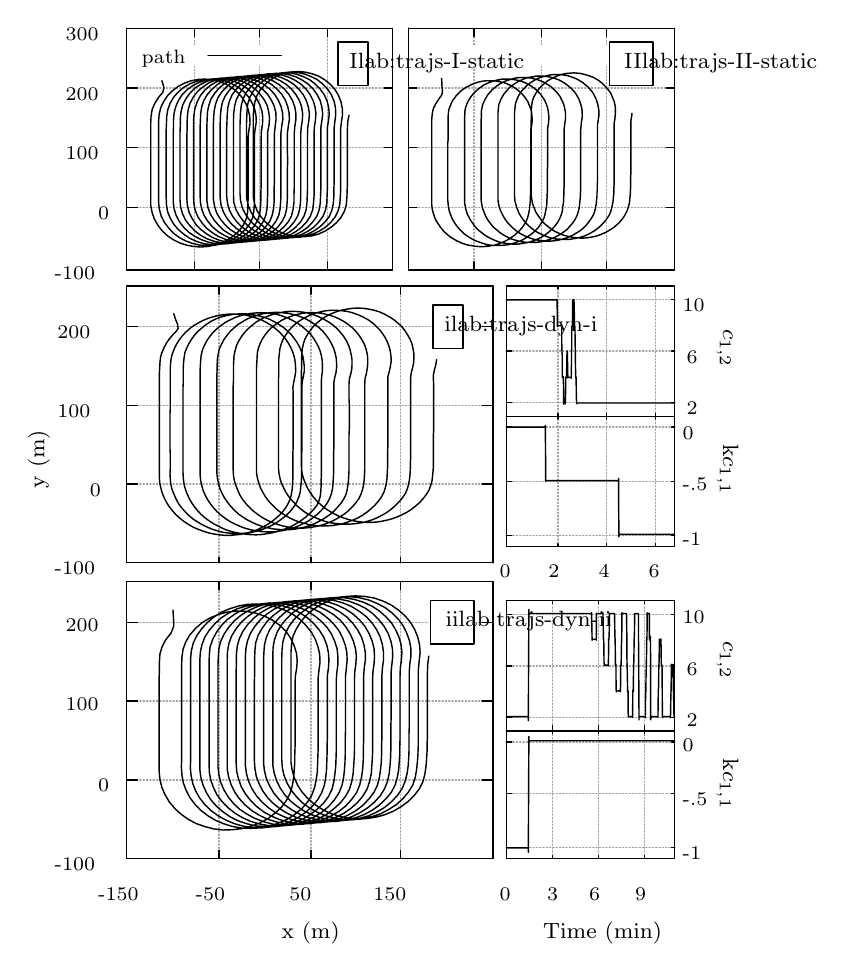
\begin{tikzpicture}[y=0.84pt, x=0.84pt,yscale=-\globalscale, xscale=\globalscale, inner sep=0pt, outer sep=0pt]
\scriptsize
\begin{scope}[shift={(-44.55268,-13.36975)},draw=black,line join=bevel,line cap=rect,even odd rule,line width=0.512pt]
  \begin{scope}[draw=black,line join=bevel,line cap=rect,line width=0.512pt]
  \end{scope}
  \begin{scope}[scale=1.006,draw=black,line join=bevel,line cap=rect,line width=0.512pt]
  \end{scope}
  \begin{scope}[scale=1.006,draw=ca0a0a4,dash pattern=on 0.40pt off 0.80pt,line join=round,line cap=round,line width=0.512pt]
    \path[draw] (44.5000,102.5000) -- (142.5000,102.5000);



  \end{scope}
  \begin{scope}[scale=1.006,draw=black,line join=round,line cap=round,line width=0.512pt]
    \path[draw] (44.5000,102.5000) -- (48.5000,102.5000);



    \path[draw] (142.5000,102.5000) -- (139.5000,102.5000);



  \end{scope}
  \begin{scope}[scale=1.006,draw=black,line join=bevel,line cap=rect,line width=0.512pt]
  \end{scope}
  \begin{scope}[cm={{1.00588,0.0,0.0,1.00588,(18.1059,106.624)}},draw=black,line join=bevel,line cap=rect,line width=0.512pt]
  \end{scope}
  \begin{scope}[cm={{1.00588,0.0,0.0,1.00588,(18.1059,106.624)}},draw=black,line join=bevel,line cap=rect,line width=0.512pt]
  \end{scope}
  \begin{scope}[cm={{1.00588,0.0,0.0,1.00588,(18.1059,106.624)}},draw=black,line join=bevel,line cap=rect,line width=0.512pt]
  \end{scope}
  \begin{scope}[cm={{1.00588,0.0,0.0,1.00588,(18.1059,106.624)}},draw=black,line join=bevel,line cap=rect,line width=0.512pt]
  \end{scope}
  \begin{scope}[cm={{1.00588,0.0,0.0,1.00588,(18.1059,106.624)}},draw=black,line join=bevel,line cap=rect,line width=0.512pt]
  \end{scope}
  \begin{scope}[cm={{1.00588,0.0,0.0,1.00588,(18.1059,106.624)}},draw=black,line join=bevel,line cap=rect,line width=0.512pt]
    \path[fill=black] (0.0000,0.0000) node[above right] (text34) {-100};



  \end{scope}
  \begin{scope}[cm={{1.00588,0.0,0.0,1.00588,(18.1059,106.624)}},draw=black,line join=bevel,line cap=rect,line width=0.512pt]
  \end{scope}
  \begin{scope}[scale=1.006,draw=black,line join=bevel,line cap=rect,line width=0.512pt]
  \end{scope}
  \begin{scope}[scale=1.006,draw=ca0a0a4,dash pattern=on 0.40pt off 0.80pt,line join=round,line cap=round,line width=0.512pt]
    \path[draw] (44.5000,79.5000) -- (142.5000,79.5000);



  \end{scope}
  \begin{scope}[scale=1.006,draw=black,line join=round,line cap=round,line width=0.512pt]
    \path[draw] (44.5000,79.5000) -- (48.5000,79.5000);



    \path[draw] (142.5000,79.5000) -- (139.5000,79.5000);



  \end{scope}
  \begin{scope}[scale=1.006,draw=black,line join=bevel,line cap=rect,line width=0.512pt]
  \end{scope}
  \begin{scope}[cm={{1.00588,0.0,0.0,1.00588,(34.2,84.4941)}},draw=black,line join=bevel,line cap=rect,line width=0.512pt]
  \end{scope}
  \begin{scope}[cm={{1.00588,0.0,0.0,1.00588,(34.2,84.4941)}},draw=black,line join=bevel,line cap=rect,line width=0.512pt]
  \end{scope}
  \begin{scope}[cm={{1.00588,0.0,0.0,1.00588,(34.2,84.4941)}},draw=black,line join=bevel,line cap=rect,line width=0.512pt]
  \end{scope}
  \begin{scope}[cm={{1.00588,0.0,0.0,1.00588,(34.2,84.4941)}},draw=black,line join=bevel,line cap=rect,line width=0.512pt]
  \end{scope}
  \begin{scope}[cm={{1.00588,0.0,0.0,1.00588,(34.2,84.4941)}},draw=black,line join=bevel,line cap=rect,line width=0.512pt]
  \end{scope}
  \begin{scope}[cm={{1.00588,0.0,0.0,1.00588,(34.2,84.4941)}},draw=black,line join=bevel,line cap=rect,line width=0.512pt]
    \path[fill=black] (0.0000,0.0000) node[above right] (text64) {0};



  \end{scope}
  \begin{scope}[cm={{1.00588,0.0,0.0,1.00588,(34.2,84.4941)}},draw=black,line join=bevel,line cap=rect,line width=0.512pt]
  \end{scope}
  \begin{scope}[scale=1.006,draw=black,line join=bevel,line cap=rect,line width=0.512pt]
  \end{scope}
  \begin{scope}[scale=1.006,draw=ca0a0a4,dash pattern=on 0.40pt off 0.80pt,line join=round,line cap=round,line width=0.512pt]
    \path[draw] (44.5000,57.5000) -- (142.5000,57.5000);



  \end{scope}
  \begin{scope}[scale=1.006,draw=black,line join=round,line cap=round,line width=0.512pt]
    \path[draw] (44.5000,57.5000) -- (48.5000,57.5000);



    \path[draw] (142.5000,57.5000) -- (139.5000,57.5000);



  \end{scope}
  \begin{scope}[scale=1.006,draw=black,line join=bevel,line cap=rect,line width=0.512pt]
  \end{scope}
  \begin{scope}[cm={{1.00588,0.0,0.0,1.00588,(22.1294,62.3647)}},draw=black,line join=bevel,line cap=rect,line width=0.512pt]
  \end{scope}
  \begin{scope}[cm={{1.00588,0.0,0.0,1.00588,(22.1294,62.3647)}},draw=black,line join=bevel,line cap=rect,line width=0.512pt]
  \end{scope}
  \begin{scope}[cm={{1.00588,0.0,0.0,1.00588,(22.1294,62.3647)}},draw=black,line join=bevel,line cap=rect,line width=0.512pt]
  \end{scope}
  \begin{scope}[cm={{1.00588,0.0,0.0,1.00588,(22.1294,62.3647)}},draw=black,line join=bevel,line cap=rect,line width=0.512pt]
  \end{scope}
  \begin{scope}[cm={{1.00588,0.0,0.0,1.00588,(22.1294,62.3647)}},draw=black,line join=bevel,line cap=rect,line width=0.512pt]
  \end{scope}
  \begin{scope}[cm={{1.00588,0.0,0.0,1.00588,(22.1294,62.3647)}},draw=black,line join=bevel,line cap=rect,line width=0.512pt]
    \path[fill=black] (0.0000,0.0000) node[above right] (text94) {100};



  \end{scope}
  \begin{scope}[cm={{1.00588,0.0,0.0,1.00588,(22.1294,62.3647)}},draw=black,line join=bevel,line cap=rect,line width=0.512pt]
  \end{scope}
  \begin{scope}[scale=1.006,draw=black,line join=bevel,line cap=rect,line width=0.512pt]
  \end{scope}
  \begin{scope}[scale=1.006,draw=ca0a0a4,dash pattern=on 0.40pt off 0.80pt,line join=round,line cap=round,line width=0.512pt]
    \path[draw] (44.5000,35.5000) -- (142.5000,35.5000);



  \end{scope}
  \begin{scope}[scale=1.006,draw=black,line join=round,line cap=round,line width=0.512pt]
    \path[draw] (44.5000,35.5000) -- (48.5000,35.5000);



    \path[draw] (142.5000,35.5000) -- (139.5000,35.5000);



  \end{scope}
  \begin{scope}[scale=1.006,draw=black,line join=bevel,line cap=rect,line width=0.512pt]
  \end{scope}
  \begin{scope}[cm={{1.00588,0.0,0.0,1.00588,(22.1294,40.2353)}},draw=black,line join=bevel,line cap=rect,line width=0.512pt]
  \end{scope}
  \begin{scope}[cm={{1.00588,0.0,0.0,1.00588,(22.1294,40.2353)}},draw=black,line join=bevel,line cap=rect,line width=0.512pt]
  \end{scope}
  \begin{scope}[cm={{1.00588,0.0,0.0,1.00588,(22.1294,40.2353)}},draw=black,line join=bevel,line cap=rect,line width=0.512pt]
  \end{scope}
  \begin{scope}[cm={{1.00588,0.0,0.0,1.00588,(22.1294,40.2353)}},draw=black,line join=bevel,line cap=rect,line width=0.512pt]
  \end{scope}
  \begin{scope}[cm={{1.00588,0.0,0.0,1.00588,(22.1294,40.2353)}},draw=black,line join=bevel,line cap=rect,line width=0.512pt]
  \end{scope}
  \begin{scope}[cm={{1.00588,0.0,0.0,1.00588,(22.1294,40.2353)}},draw=black,line join=bevel,line cap=rect,line width=0.512pt]
    \path[fill=black] (0.0000,0.0000) node[above right] (text124) {200};



  \end{scope}
  \begin{scope}[cm={{1.00588,0.0,0.0,1.00588,(22.1294,40.2353)}},draw=black,line join=bevel,line cap=rect,line width=0.512pt]
  \end{scope}
  \begin{scope}[scale=1.006,draw=black,line join=bevel,line cap=rect,line width=0.512pt]
  \end{scope}
  \begin{scope}[scale=1.006,draw=ca0a0a4,dash pattern=on 0.40pt off 0.80pt,line join=round,line cap=round,line width=0.512pt]
    \path[draw] (44.5000,13.5000) -- (142.5000,13.5000);



  \end{scope}
  \begin{scope}[scale=1.006,draw=black,line join=round,line cap=round,line width=0.512pt]
    \path[draw] (44.5000,13.5000) -- (48.5000,13.5000);



    \path[draw] (142.5000,13.5000) -- (139.5000,13.5000);



  \end{scope}
  \begin{scope}[scale=1.006,draw=black,line join=bevel,line cap=rect,line width=0.512pt]
  \end{scope}
  \begin{scope}[cm={{1.00588,0.0,0.0,1.00588,(22.1294,18.1059)}},draw=black,line join=bevel,line cap=rect,line width=0.512pt]
  \end{scope}
  \begin{scope}[cm={{1.00588,0.0,0.0,1.00588,(22.1294,18.1059)}},draw=black,line join=bevel,line cap=rect,line width=0.512pt]
  \end{scope}
  \begin{scope}[cm={{1.00588,0.0,0.0,1.00588,(22.1294,18.1059)}},draw=black,line join=bevel,line cap=rect,line width=0.512pt]
  \end{scope}
  \begin{scope}[cm={{1.00588,0.0,0.0,1.00588,(22.1294,18.1059)}},draw=black,line join=bevel,line cap=rect,line width=0.512pt]
  \end{scope}
  \begin{scope}[cm={{1.00588,0.0,0.0,1.00588,(22.1294,18.1059)}},draw=black,line join=bevel,line cap=rect,line width=0.512pt]
  \end{scope}
  \begin{scope}[cm={{1.00588,0.0,0.0,1.00588,(22.1294,18.1059)}},draw=black,line join=bevel,line cap=rect,line width=0.512pt]
    \path[fill=black] (0.0000,0.0000) node[above right] (text154) {300};



  \end{scope}
  \begin{scope}[cm={{1.00588,0.0,0.0,1.00588,(22.1294,18.1059)}},draw=black,line join=bevel,line cap=rect,line width=0.512pt]
  \end{scope}
  \begin{scope}[scale=1.006,draw=black,line join=bevel,line cap=rect,line width=0.512pt]
  \end{scope}
  \begin{scope}[scale=1.006,draw=ca0a0a4,dash pattern=on 0.40pt off 0.80pt,line join=round,line cap=round,line width=0.512pt]
    \path[draw] (44.5000,102.5000) -- (44.5000,13.5000);



  \end{scope}
  \begin{scope}[scale=1.006,draw=black,line join=round,line cap=round,line width=0.512pt]
    \path[draw] (44.5000,102.5000) -- (44.5000,99.5000);



    \path[draw] (44.5000,13.5000) -- (44.5000,16.5000);



  \end{scope}
  \begin{scope}[scale=1.006,draw=black,line join=bevel,line cap=rect,line width=0.512pt]
  \end{scope}
  \begin{scope}[cm={{1.00588,0.0,0.0,1.00588,(45.2647,118.694)}},draw=black,line join=bevel,line cap=rect,line width=0.512pt]
  \end{scope}
  \begin{scope}[cm={{1.00588,0.0,0.0,1.00588,(45.2647,118.694)}},draw=black,line join=bevel,line cap=rect,line width=0.512pt]
  \end{scope}
  \begin{scope}[cm={{1.00588,0.0,0.0,1.00588,(45.2647,118.694)}},draw=black,line join=bevel,line cap=rect,line width=0.512pt]
  \end{scope}
  \begin{scope}[cm={{1.00588,0.0,0.0,1.00588,(45.2647,118.694)}},draw=black,line join=bevel,line cap=rect,line width=0.512pt]
  \end{scope}
  \begin{scope}[cm={{1.00588,0.0,0.0,1.00588,(45.2647,118.694)}},draw=black,line join=bevel,line cap=rect,line width=0.512pt]
  \end{scope}
  \begin{scope}[cm={{1.00588,0.0,0.0,1.00588,(45.2647,118.694)}},draw=black,line join=bevel,line cap=rect,line width=0.512pt]
  \end{scope}
  \begin{scope}[scale=1.006,draw=black,line join=bevel,line cap=rect,line width=0.512pt]
  \end{scope}
  \begin{scope}[scale=1.006,draw=ca0a0a4,dash pattern=on 0.40pt off 0.80pt,line join=round,line cap=round,line width=0.512pt]
    \path[draw] (69.5000,102.5000) -- (69.5000,27.5000);



    \path[draw] (69.5000,19.5000) -- (69.5000,13.5000);



  \end{scope}
  \begin{scope}[scale=1.006,draw=black,line join=round,line cap=round,line width=0.512pt]
    \path[draw] (69.5000,102.5000) -- (69.5000,99.5000);



    \path[draw] (69.5000,13.5000) -- (69.5000,16.5000);



  \end{scope}
  \begin{scope}[scale=1.006,draw=black,line join=bevel,line cap=rect,line width=0.512pt]
  \end{scope}
  \begin{scope}[cm={{1.00588,0.0,0.0,1.00588,(69.4059,118.694)}},draw=black,line join=bevel,line cap=rect,line width=0.512pt]
  \end{scope}
  \begin{scope}[cm={{1.00588,0.0,0.0,1.00588,(69.4059,118.694)}},draw=black,line join=bevel,line cap=rect,line width=0.512pt]
  \end{scope}
  \begin{scope}[cm={{1.00588,0.0,0.0,1.00588,(69.4059,118.694)}},draw=black,line join=bevel,line cap=rect,line width=0.512pt]
  \end{scope}
  \begin{scope}[cm={{1.00588,0.0,0.0,1.00588,(69.4059,118.694)}},draw=black,line join=bevel,line cap=rect,line width=0.512pt]
  \end{scope}
  \begin{scope}[cm={{1.00588,0.0,0.0,1.00588,(69.4059,118.694)}},draw=black,line join=bevel,line cap=rect,line width=0.512pt]
  \end{scope}
  \begin{scope}[cm={{1.00588,0.0,0.0,1.00588,(69.4059,118.694)}},draw=black,line join=bevel,line cap=rect,line width=0.512pt]
  \end{scope}
  \begin{scope}[scale=1.006,draw=black,line join=bevel,line cap=rect,line width=0.512pt]
  \end{scope}
  \begin{scope}[scale=1.006,draw=ca0a0a4,dash pattern=on 0.40pt off 0.80pt,line join=round,line cap=round,line width=0.512pt]
    \path[draw] (93.5000,102.5000) -- (93.5000,27.5000);



    \path[draw] (93.5000,19.5000) -- (93.5000,13.5000);



  \end{scope}
  \begin{scope}[scale=1.006,draw=black,line join=round,line cap=round,line width=0.512pt]
    \path[draw] (93.5000,102.5000) -- (93.5000,99.5000);



    \path[draw] (93.5000,13.5000) -- (93.5000,16.5000);



  \end{scope}
  \begin{scope}[scale=1.006,draw=black,line join=bevel,line cap=rect,line width=0.512pt]
  \end{scope}
  \begin{scope}[cm={{1.00588,0.0,0.0,1.00588,(94.5529,118.694)}},draw=black,line join=bevel,line cap=rect,line width=0.512pt]
  \end{scope}
  \begin{scope}[cm={{1.00588,0.0,0.0,1.00588,(94.5529,118.694)}},draw=black,line join=bevel,line cap=rect,line width=0.512pt]
  \end{scope}
  \begin{scope}[cm={{1.00588,0.0,0.0,1.00588,(94.5529,118.694)}},draw=black,line join=bevel,line cap=rect,line width=0.512pt]
  \end{scope}
  \begin{scope}[cm={{1.00588,0.0,0.0,1.00588,(94.5529,118.694)}},draw=black,line join=bevel,line cap=rect,line width=0.512pt]
  \end{scope}
  \begin{scope}[cm={{1.00588,0.0,0.0,1.00588,(94.5529,118.694)}},draw=black,line join=bevel,line cap=rect,line width=0.512pt]
  \end{scope}
  \begin{scope}[cm={{1.00588,0.0,0.0,1.00588,(94.5529,118.694)}},draw=black,line join=bevel,line cap=rect,line width=0.512pt]
  \end{scope}
  \begin{scope}[scale=1.006,draw=black,line join=bevel,line cap=rect,line width=0.512pt]
  \end{scope}
  \begin{scope}[scale=1.006,draw=ca0a0a4,dash pattern=on 0.40pt off 0.80pt,line join=round,line cap=round,line width=0.512pt]
    \path[draw] (118.5000,102.5000) -- (118.5000,13.5000);



  \end{scope}
  \begin{scope}[scale=1.006,draw=black,line join=round,line cap=round,line width=0.512pt]
    \path[draw] (118.5000,102.5000) -- (118.5000,99.5000);



    \path[draw] (118.5000,13.5000) -- (118.5000,16.5000);



  \end{scope}
  \begin{scope}[scale=1.006,draw=black,line join=bevel,line cap=rect,line width=0.512pt]
  \end{scope}
  \begin{scope}[cm={{1.00588,0.0,0.0,1.00588,(118.694,118.694)}},draw=black,line join=bevel,line cap=rect,line width=0.512pt]
  \end{scope}
  \begin{scope}[cm={{1.00588,0.0,0.0,1.00588,(118.694,118.694)}},draw=black,line join=bevel,line cap=rect,line width=0.512pt]
  \end{scope}
  \begin{scope}[cm={{1.00588,0.0,0.0,1.00588,(118.694,118.694)}},draw=black,line join=bevel,line cap=rect,line width=0.512pt]
  \end{scope}
  \begin{scope}[cm={{1.00588,0.0,0.0,1.00588,(118.694,118.694)}},draw=black,line join=bevel,line cap=rect,line width=0.512pt]
  \end{scope}
  \begin{scope}[cm={{1.00588,0.0,0.0,1.00588,(118.694,118.694)}},draw=black,line join=bevel,line cap=rect,line width=0.512pt]
  \end{scope}
  \begin{scope}[cm={{1.00588,0.0,0.0,1.00588,(118.694,118.694)}},draw=black,line join=bevel,line cap=rect,line width=0.512pt]
  \end{scope}
  \begin{scope}[scale=1.006,draw=black,line join=bevel,line cap=rect,line width=0.512pt]
  \end{scope}
  \begin{scope}[scale=1.006,draw=ca0a0a4,dash pattern=on 0.40pt off 0.80pt,line join=round,line cap=round,line width=0.512pt]
    \path[draw] (142.5000,102.5000) -- (142.5000,13.5000);



  \end{scope}
  \begin{scope}[scale=1.006,draw=black,line join=round,line cap=round,line width=0.512pt]
    \path[draw] (142.5000,102.5000) -- (142.5000,99.5000);



    \path[draw] (142.5000,13.5000) -- (142.5000,16.5000);



  \end{scope}
  \begin{scope}[scale=1.006,draw=black,line join=bevel,line cap=rect,line width=0.512pt]
  \end{scope}
  \begin{scope}[cm={{1.00588,0.0,0.0,1.00588,(143.841,118.694)}},draw=black,line join=bevel,line cap=rect,line width=0.512pt]
  \end{scope}
  \begin{scope}[cm={{1.00588,0.0,0.0,1.00588,(143.841,118.694)}},draw=black,line join=bevel,line cap=rect,line width=0.512pt]
  \end{scope}
  \begin{scope}[cm={{1.00588,0.0,0.0,1.00588,(143.841,118.694)}},draw=black,line join=bevel,line cap=rect,line width=0.512pt]
  \end{scope}
  \begin{scope}[cm={{1.00588,0.0,0.0,1.00588,(143.841,118.694)}},draw=black,line join=bevel,line cap=rect,line width=0.512pt]
  \end{scope}
  \begin{scope}[cm={{1.00588,0.0,0.0,1.00588,(143.841,118.694)}},draw=black,line join=bevel,line cap=rect,line width=0.512pt]
  \end{scope}
  \begin{scope}[cm={{1.00588,0.0,0.0,1.00588,(143.841,118.694)}},draw=black,line join=bevel,line cap=rect,line width=0.512pt]
  \end{scope}
  \begin{scope}[scale=1.006,draw=black,line join=bevel,line cap=rect,line width=0.512pt]
  \end{scope}
  \begin{scope}[scale=1.006,draw=black,line join=round,line cap=round,line width=0.512pt]
    \path[draw] (44.5000,13.5000) -- (44.5000,102.5000) -- (142.5000,102.5000) -- (142.5000,13.5000) -- (44.5000,13.5000);



  \end{scope}
  \begin{scope}[scale=1.006,draw=black,line join=bevel,line cap=rect,line width=0.512pt]
  \end{scope}
  \begin{scope}[scale=1.006,draw=black,line join=bevel,line cap=rect,line width=0.512pt]
  \end{scope}
  \begin{scope}[scale=1.006,fill=cffffff]
    \path[fill,rounded corners=0.0000cm] (123.0000,18.0000) rectangle (134.0000,34.0000);



  \end{scope}
  \begin{scope}[scale=1.006,draw=black,line join=bevel,line cap=rect,line width=0.512pt]
  \end{scope}
  \begin{scope}[scale=1.006,draw=black,line join=bevel,line cap=rect,line width=0.512pt]
  \end{scope}
  \begin{scope}[scale=1.006,draw=black,line join=round,line cap=round,line width=0.512pt]
    \path[draw] (122.5000,34.5000) -- (122.5000,18.5000) -- (133.5000,18.5000) -- (133.5000,34.5000) -- (122.5000,34.5000);



  \end{scope}
  \begin{scope}[scale=1.006,draw=black,line join=bevel,line cap=rect,line width=0.512pt]
  \end{scope}
  \begin{scope}[cm={{1.00588,0.0,0.0,1.00588,(126.741,30.1765)}},draw=black,line join=bevel,line cap=rect,line width=0.512pt]
  \end{scope}
  \begin{scope}[cm={{1.00588,0.0,0.0,1.00588,(126.741,30.1765)}},draw=black,line join=bevel,line cap=rect,line width=0.512pt]
  \end{scope}
  \begin{scope}[cm={{1.00588,0.0,0.0,1.00588,(126.741,30.1765)}},draw=black,line join=bevel,line cap=rect,line width=0.512pt]
  \end{scope}
  \begin{scope}[cm={{1.00588,0.0,0.0,1.00588,(126.741,30.1765)}},draw=black,line join=bevel,line cap=rect,line width=0.512pt]
  \end{scope}
  \begin{scope}[cm={{1.00588,0.0,0.0,1.00588,(126.741,30.1765)}},draw=black,line join=bevel,line cap=rect,line width=0.512pt]
  \end{scope}
  \begin{scope}[cm={{1.00588,0.0,0.0,1.00588,(127.39293,29.95919)}},draw=black,line join=bevel,line cap=rect,line width=0.512pt]
    \path[fill=black] (0.0000,0.0000) node[above right] (text328) {\footnotesize \textlabel{I}{lab:trajs-I-static}};



  \end{scope}
  \begin{scope}[cm={{1.00588,0.0,0.0,1.00588,(126.741,30.1765)}},draw=black,line join=bevel,line cap=rect,line width=0.512pt]
  \end{scope}
  \begin{scope}[cm={{0.0,-1.00588,1.00588,0.0,(14.0824,184.076)}},draw=black,line join=bevel,line cap=rect,line width=0.512pt]
  \end{scope}
  \begin{scope}[cm={{0.0,-1.00588,1.00588,0.0,(14.0824,184.076)}},draw=black,line join=bevel,line cap=rect,line width=0.512pt]
  \end{scope}
  \begin{scope}[cm={{0.0,-1.00588,1.00588,0.0,(14.0824,184.076)}},draw=black,line join=bevel,line cap=rect,line width=0.512pt]
  \end{scope}
  \begin{scope}[cm={{0.0,-1.00588,1.00588,0.0,(14.0824,184.076)}},draw=black,line join=bevel,line cap=rect,line width=0.512pt]
  \end{scope}
  \begin{scope}[cm={{0.0,-1.00588,1.00588,0.0,(14.0824,184.076)}},draw=black,line join=bevel,line cap=rect,line width=0.512pt]
  \end{scope}
  \begin{scope}[cm={{0.0,-1.00588,1.00588,0.0,(8.0824,184.076)}},draw=black,line join=bevel,line cap=rect,line width=0.512pt]
    \path[fill=black] (0.0000,0.0000) node[above right] (text344) {\rotatebox{90}{\footnotesize y (m)}};



  \end{scope}
  \begin{scope}[cm={{0.0,-1.00588,1.00588,0.0,(14.0824,184.076)}},draw=black,line join=bevel,line cap=rect,line width=0.512pt]
  \end{scope}
  \begin{scope}[cm={{1.00588,0.0,0.0,1.00588,(50.2941,27.1588)}},draw=black,line join=bevel,line cap=rect,line width=0.512pt]
  \end{scope}
  \begin{scope}[cm={{1.00588,0.0,0.0,1.00588,(50.2941,27.1588)}},draw=black,line join=bevel,line cap=rect,line width=0.512pt]
  \end{scope}
  \begin{scope}[cm={{1.00588,0.0,0.0,1.00588,(50.2941,27.1588)}},draw=black,line join=bevel,line cap=rect,line width=0.512pt]
  \end{scope}
  \begin{scope}[cm={{1.00588,0.0,0.0,1.00588,(50.2941,27.1588)}},draw=black,line join=bevel,line cap=rect,line width=0.512pt]
  \end{scope}
  \begin{scope}[cm={{1.00588,0.0,0.0,1.00588,(50.2941,27.1588)}},draw=black,line join=bevel,line cap=rect,line width=0.512pt]
  \end{scope}
  \begin{scope}[cm={{1.00588,0.0,0.0,1.00588,(50.2941,28.1647)}},draw=black,line join=bevel,line cap=rect,line width=0.512pt]
    \path[fill=black] (0.0000,0.0000) node[above right] (text360) {\scriptsize path};



  \end{scope}
  \begin{scope}[cm={{1.00588,0.0,0.0,1.00588,(50.2941,27.1588)}},draw=black,line join=bevel,line cap=rect,line width=0.512pt]
  \end{scope}
  \begin{scope}[scale=1.006,draw=black,line join=bevel,line cap=rect,line width=0.512pt]
  \end{scope}
  \begin{scope}[scale=1.006,draw=black,line join=round,line cap=round,line width=0.512pt]
    \path[draw,even odd rule] (74.5000,23.5000) -- (101.5000,23.5000);



  \end{scope}
  \begin{scope}[scale=1.006,draw=black,line join=bevel,line cap=rect,line width=0.512pt]
  \end{scope}
  \begin{scope}[scale=1.006,draw=black,line join=bevel,line cap=rect,line width=0.512pt]
  \end{scope}
  \begin{scope}[scale=1.006,draw=black,line join=bevel,line cap=rect,line width=0.512pt]
  \end{scope}
  \begin{scope}[scale=1.006,draw=black,line join=bevel,line cap=rect,line width=0.512pt]
  \end{scope}
  \begin{scope}[scale=1.006,draw=black,line join=round,line cap=round,line width=0.512pt]
    \path[draw] (57.5000,32.8000) -- (57.5000,32.8000) -- (58.3000,35.4000) -- (57.8000,37.2000) -- (56.3000,38.9000) -- (54.9000,41.1000) -- (53.9000,43.5000) -- (53.5000,46.1000) -- (53.4000,48.6000) -- (53.4000,51.1000) -- (53.4000,53.6000) -- (53.4000,56.1000) -- (53.4000,58.6000) -- (53.4000,61.1000) -- (53.4000,63.6000) -- (53.4000,66.1000) -- (53.4000,68.7000) -- (53.4000,71.2000) -- (53.4000,73.7000) -- (53.4000,76.2000) -- (53.4000,78.7000) -- (53.9000,81.3000) -- (54.7000,83.7000) -- (56.0000,86.0000) -- (57.6000,88.1000) -- (59.5000,89.9000) -- (61.7000,91.4000) -- (64.1000,92.6000) -- (66.6000,93.4000) -- (69.2000,93.9000) -- (71.8000,94.1000) -- (74.4000,93.9000) -- (77.0000,93.4000) -- (79.5000,92.6000) -- (81.8000,91.4000) -- (84.0000,90.0000) -- (85.9000,88.2000) -- (87.5000,86.1000) -- (88.6000,83.8000) -- (89.1000,81.3000) -- (89.2000,78.8000) -- (89.3000,76.2000) -- (89.3000,73.7000) -- (89.3000,71.1000) -- (89.3000,68.6000) -- (89.3000,66.1000) -- (89.3000,63.6000) -- (89.3000,61.0000) -- (89.3000,58.5000) -- (89.3000,56.0000) -- (89.3000,53.5000) -- (89.6000,51.0000) -- (90.0000,48.5000) -- (89.9000,46.0000) -- (89.4000,43.6000) -- (88.5000,41.3000) -- (87.2000,39.1000) -- (85.5000,37.2000) -- (83.5000,35.5000) -- (81.3000,34.1000) -- (78.9000,33.1000) -- (76.3000,32.5000) -- (73.6000,32.2000) -- (71.0000,32.3000) -- (68.3000,32.8000) -- (65.8000,33.7000) -- (63.5000,34.9000) -- (61.4000,36.5000) -- (59.6000,38.3000) -- (58.2000,40.4000) -- (57.1000,42.7000) -- (56.5000,45.2000) -- (56.3000,47.7000) -- (56.3000,50.1000) -- (56.3000,52.6000) -- (56.3000,55.1000) -- (56.3000,57.6000) -- (56.3000,60.2000) -- (56.3000,62.7000) -- (56.3000,65.2000) -- (56.3000,67.7000) -- (56.3000,70.2000) -- (56.3000,72.7000) -- (56.3000,75.3000) -- (56.3000,77.8000) -- (56.6000,80.3000) -- (57.3000,82.8000) -- (58.5000,85.1000) -- (60.1000,87.2000) -- (61.9000,89.1000) -- (64.1000,90.7000) -- (66.4000,91.9000) -- (68.9000,92.8000) -- (71.5000,93.4000) -- (74.1000,93.6000) -- (76.7000,93.5000) -- (79.3000,93.0000) -- (81.8000,92.2000) -- (84.1000,91.0000) -- (86.3000,89.5000) -- (88.2000,87.7000) -- (89.8000,85.7000) -- (90.9000,83.4000) -- (91.4000,80.9000) -- (91.6000,78.3000) -- (91.6000,75.8000) -- (91.6000,73.2000) -- (91.6000,70.7000) -- (91.6000,68.2000) -- (91.6000,65.6000) -- (91.6000,63.1000) -- (91.6000,60.6000) -- (91.6000,58.1000) -- (91.6000,55.6000) -- (91.6000,53.0000) -- (91.9000,50.5000) -- (92.3000,48.0000) -- (92.2000,45.6000) -- (91.7000,43.2000) -- (90.7000,40.9000) -- (89.4000,38.7000) -- (87.7000,36.8000) -- (85.6000,35.2000) -- (83.3000,33.9000) -- (80.9000,32.9000) -- (78.3000,32.4000) -- (75.6000,32.2000) -- (72.9000,32.4000) -- (70.3000,33.0000) -- (67.9000,33.9000) -- (65.6000,35.2000) -- (63.6000,36.9000) -- (61.9000,38.8000) -- (60.6000,41.0000) -- (59.7000,43.4000) -- (59.3000,45.9000) -- (59.2000,48.3000) -- (59.1000,50.8000) -- (59.1000,53.3000) -- (59.1000,55.8000) -- (59.1000,58.3000) -- (59.1000,60.9000) -- (59.1000,63.4000) -- (59.1000,65.9000) -- (59.1000,68.4000) -- (59.1000,70.9000) -- (59.1000,73.4000) -- (59.1000,76.0000) -- (59.2000,78.5000) -- (59.6000,81.0000) -- (60.6000,83.5000) -- (61.9000,85.7000) -- (63.6000,87.7000) -- (65.6000,89.4000) -- (67.8000,90.9000) -- (70.2000,92.0000) -- (72.7000,92.8000) -- (75.3000,93.2000) -- (78.0000,93.2000) -- (80.6000,92.9000) -- (83.1000,92.3000) -- (85.5000,91.3000) -- (87.8000,89.9000) -- (89.8000,88.3000) -- (91.6000,86.3000) -- (92.9000,84.1000) -- (93.6000,81.7000) -- (93.9000,79.2000) -- (94.0000,76.6000) -- (94.0000,74.0000) -- (94.1000,71.5000) -- (94.1000,69.0000) -- (94.1000,66.4000) -- (94.1000,63.9000) -- (94.1000,61.4000) -- (94.1000,58.9000) -- (94.1000,56.4000) -- (94.1000,53.9000) -- (94.2000,51.3000) -- (94.6000,48.8000) -- (94.7000,46.4000) -- (94.4000,43.9000) -- (93.6000,41.6000) -- (92.4000,39.3000) -- (90.8000,37.3000) -- (88.9000,35.6000) -- (86.7000,34.2000) -- (84.3000,33.1000) -- (81.7000,32.4000) -- (79.1000,32.0000) -- (76.4000,32.1000) -- (73.8000,32.5000) -- (71.3000,33.4000) -- (68.9000,34.6000) -- (66.8000,36.1000) -- (65.0000,37.9000) -- (63.6000,40.1000) -- (62.6000,42.4000) -- (62.0000,44.8000) -- (61.8000,47.3000) -- (61.8000,49.8000) -- (61.7000,52.3000) -- (61.7000,54.8000) -- (61.7000,57.3000) -- (61.7000,59.8000) -- (61.7000,62.4000) -- (61.7000,64.9000) -- (61.7000,67.4000) -- (61.7000,69.9000) -- (61.7000,72.4000) -- (61.7000,75.0000) -- (61.7000,77.5000) -- (62.0000,80.0000) -- (62.8000,82.5000) -- (64.0000,84.8000) -- (65.6000,86.9000) -- (67.5000,88.7000) -- (69.7000,90.2000) -- (72.1000,91.4000) -- (74.6000,92.3000) -- (77.1000,92.8000) -- (79.8000,93.0000) -- (82.4000,92.8000) -- (84.9000,92.2000) -- (87.4000,91.3000) -- (89.7000,90.0000) -- (91.8000,88.5000) -- (93.6000,86.6000) -- (95.1000,84.4000) -- (95.9000,82.1000) -- (96.3000,79.6000) -- (96.4000,77.0000) -- (96.5000,74.4000) -- (96.5000,71.9000) -- (96.5000,69.3000) -- (96.5000,66.8000) -- (96.5000,64.3000) -- (96.5000,61.8000) -- (96.5000,59.3000) -- (96.5000,56.7000) -- (96.5000,54.2000) -- (96.5000,51.7000) -- (97.0000,49.2000) -- (97.2000,46.7000) -- (96.9000,44.3000) -- (96.3000,41.9000) -- (95.1000,39.6000) -- (93.6000,37.6000) -- (91.8000,35.8000) -- (89.7000,34.3000) -- (87.3000,33.1000) -- (84.8000,32.3000) -- (82.1000,31.9000) -- (79.5000,31.8000) -- (76.8000,32.2000) -- (74.3000,32.9000) -- (71.9000,34.1000) -- (69.7000,35.5000) -- (67.9000,37.3000) -- (66.4000,39.4000) -- (65.2000,41.7000) -- (64.6000,44.1000) -- (64.3000,46.6000) -- (64.3000,49.1000) -- (64.2000,51.6000) -- (64.2000,54.1000) -- (64.2000,56.6000) -- (64.2000,59.1000) -- (64.2000,61.6000) -- (64.2000,64.1000) -- (64.2000,66.6000) -- (64.2000,69.2000) -- (64.2000,71.7000) -- (64.2000,74.2000) -- (64.2000,76.7000) -- (64.4000,79.3000) -- (65.1000,81.8000) -- (66.2000,84.1000) -- (67.8000,86.2000) -- (69.6000,88.1000) -- (71.7000,89.7000) -- (74.0000,91.0000) -- (76.5000,91.9000) -- (79.1000,92.5000) -- (81.7000,92.7000) -- (84.3000,92.6000) -- (86.9000,92.1000) -- (89.4000,91.3000) -- (91.7000,90.1000) -- (93.9000,88.6000) -- (95.7000,86.7000) -- (97.3000,84.6000) -- (98.2000,82.3000) -- (98.7000,79.8000) -- (98.9000,77.3000) -- (98.9000,74.7000) -- (98.9000,72.1000) -- (99.0000,69.6000) -- (99.0000,67.1000) -- (99.0000,64.6000) -- (99.0000,62.0000) -- (99.0000,59.5000) -- (99.0000,57.0000) -- (99.0000,54.5000) -- (99.0000,52.0000) -- (99.3000,49.4000) -- (99.6000,47.0000) -- (99.5000,44.5000) -- (98.9000,42.1000) -- (97.8000,39.8000) -- (96.4000,37.7000) -- (94.6000,35.9000) -- (92.5000,34.3000) -- (90.2000,33.1000) -- (87.7000,32.2000) -- (85.1000,31.7000) -- (82.4000,31.6000) -- (79.7000,31.9000) -- (77.2000,32.6000) -- (74.8000,33.6000) -- (72.6000,35.1000) -- (70.6000,36.8000) -- (69.1000,38.8000) -- (67.9000,41.1000) -- (67.2000,43.5000) -- (66.9000,46.0000) -- (66.8000,48.5000) -- (66.8000,51.0000) -- (66.7000,53.5000) -- (66.7000,56.0000) -- (66.7000,58.5000) -- (66.7000,61.0000) -- (66.7000,63.5000) -- (66.7000,66.0000) -- (66.7000,68.6000) -- (66.7000,71.1000) -- (66.7000,73.6000) -- (66.7000,76.1000) -- (66.9000,78.7000) -- (67.5000,81.2000) -- (68.6000,83.5000) -- (70.0000,85.7000) -- (71.8000,87.6000) -- (73.9000,89.2000) -- (76.2000,90.6000) -- (78.7000,91.6000) -- (81.2000,92.2000) -- (83.8000,92.5000) -- (86.5000,92.4000) -- (89.0000,92.0000) -- (91.5000,91.2000) -- (93.9000,90.0000) -- (96.1000,88.5000) -- (98.0000,86.7000) -- (99.5000,84.7000) -- (100.6000,82.4000) -- (101.1000,79.9000) -- (101.3000,77.3000) -- (101.4000,74.8000) -- (101.4000,72.2000) -- (101.4000,69.7000) -- (101.4000,67.2000) -- (101.4000,64.6000) -- (101.4000,62.1000) -- (101.4000,59.6000) -- (101.4000,57.1000) -- (101.4000,54.6000) -- (101.4000,52.0000) -- (101.7000,49.5000) -- (102.1000,47.0000) -- (102.0000,44.6000) -- (101.4000,42.2000) -- (100.4000,39.9000) -- (99.0000,37.7000) -- (97.3000,35.9000) -- (95.2000,34.2000) -- (92.9000,33.0000) -- (90.4000,32.1000) -- (87.8000,31.5000) -- (85.2000,31.4000) -- (82.5000,31.6000) -- (79.9000,32.3000) -- (77.5000,33.3000) -- (75.3000,34.6000) -- (73.3000,36.3000) -- (71.7000,38.3000) -- (70.5000,40.6000) -- (69.7000,43.0000) -- (69.3000,45.5000) -- (69.2000,47.9000) -- (69.2000,50.4000) -- (69.2000,52.9000) -- (69.2000,55.4000) -- (69.2000,57.9000) -- (69.2000,60.5000) -- (69.2000,63.0000) -- (69.2000,65.5000) -- (69.2000,68.0000) -- (69.2000,70.5000) -- (69.2000,73.1000) -- (69.2000,75.6000) -- (69.3000,78.1000) -- (69.8000,80.6000) -- (70.8000,83.0000) -- (72.3000,85.2000) -- (74.0000,87.2000) -- (76.1000,88.8000) -- (78.3000,90.2000) -- (80.8000,91.2000) -- (83.3000,91.9000) -- (85.9000,92.3000) -- (88.6000,92.2000) -- (91.2000,91.8000) -- (93.7000,91.1000) -- (96.0000,90.0000) -- (98.2000,88.5000) -- (100.2000,86.8000) -- (101.8000,84.7000) -- (102.9000,82.5000) -- (103.5000,80.0000) -- (103.7000,77.4000) -- (103.8000,74.9000) -- (103.8000,72.3000) -- (103.8000,69.8000) -- (103.8000,67.3000) -- (103.8000,64.7000) -- (103.9000,62.2000) -- (103.8000,59.7000) -- (103.8000,57.2000) -- (103.8000,54.7000) -- (103.8000,52.1000) -- (104.1000,49.6000) -- (104.5000,47.1000) -- (104.4000,44.7000) -- (103.9000,42.3000) -- (103.0000,39.9000) -- (101.7000,37.8000) -- (100.0000,35.9000) -- (98.0000,34.2000) -- (95.7000,32.9000) -- (93.2000,31.9000) -- (90.6000,31.4000) -- (88.0000,31.2000) -- (85.3000,31.3000) -- (82.7000,31.9000) -- (80.2000,32.9000) -- (78.0000,34.2000) -- (76.0000,35.9000) -- (74.3000,37.8000) -- (73.0000,40.0000) -- (72.2000,42.4000) -- (71.8000,44.9000) -- (71.7000,47.4000) -- (71.6000,49.9000) -- (71.6000,52.4000) -- (71.6000,54.9000) -- (71.6000,57.4000) -- (71.6000,59.9000) -- (71.6000,62.4000) -- (71.6000,65.0000) -- (71.6000,67.5000) -- (71.6000,70.0000) -- (71.6000,72.5000) -- (71.6000,75.0000) -- (71.7000,77.6000) -- (72.2000,80.1000) -- (73.1000,82.5000) -- (74.5000,84.7000) -- (76.2000,86.7000) -- (78.2000,88.4000) -- (80.5000,89.8000) -- (82.9000,90.9000) -- (85.4000,91.6000) -- (88.0000,92.0000) -- (90.7000,92.0000) -- (93.3000,91.7000) -- (95.8000,91.0000) -- (98.2000,89.9000) -- (100.4000,88.5000) -- (102.4000,86.8000) -- (104.1000,84.8000) -- (105.3000,82.6000) -- (105.9000,80.1000) -- (106.2000,77.6000) -- (106.2000,75.0000) -- (106.3000,72.4000) -- (106.3000,69.9000) -- (106.3000,67.4000) -- (106.3000,64.9000) -- (106.3000,62.3000) -- (106.3000,59.8000) -- (106.3000,57.3000) -- (106.3000,54.8000) -- (106.3000,52.3000) -- (106.5000,49.7000) -- (106.9000,47.2000) -- (106.9000,44.8000) -- (106.5000,42.4000) -- (105.6000,40.0000) -- (104.3000,37.8000) -- (102.7000,35.9000) -- (100.7000,34.2000) -- (98.4000,32.8000) -- (96.0000,31.8000) -- (93.4000,31.2000) -- (90.8000,30.9000) -- (88.1000,31.1000) -- (85.5000,31.6000) -- (83.0000,32.5000) -- (80.7000,33.8000) -- (78.7000,35.4000) -- (77.0000,37.4000) -- (75.6000,39.5000) -- (74.8000,41.9000) -- (74.3000,44.4000) -- (74.2000,46.9000) -- (74.1000,49.3000) -- (74.1000,51.8000) -- (74.1000,54.3000) -- (74.1000,56.9000) -- (74.1000,59.4000) -- (74.1000,61.9000) -- (74.1000,64.4000) -- (74.1000,66.9000) -- (74.1000,69.4000) -- (74.1000,72.0000) -- (74.1000,74.5000) -- (74.1000,77.0000) -- (74.5000,79.6000) -- (75.4000,82.0000) -- (76.8000,84.2000) -- (78.5000,86.2000) -- (80.4000,88.0000) -- (82.6000,89.4000) -- (85.0000,90.6000) -- (87.6000,91.3000) -- (90.2000,91.8000) -- (92.8000,91.8000) -- (95.4000,91.5000) -- (97.9000,90.9000) -- (100.3000,89.8000) -- (102.6000,88.5000) -- (104.6000,86.8000) -- (106.3000,84.8000) -- (107.6000,82.6000) -- (108.3000,80.2000) -- (108.6000,77.7000) -- (108.7000,75.1000) -- (108.7000,72.5000) -- (108.7000,70.0000) -- (108.7000,67.5000) -- (108.7000,64.9000) -- (108.7000,62.4000) -- (108.7000,59.9000) -- (108.7000,57.4000) -- (108.7000,54.9000) -- (108.7000,52.3000) -- (108.9000,49.8000) -- (109.3000,47.3000) -- (109.4000,44.9000) -- (109.0000,42.4000) -- (108.2000,40.1000) -- (106.9000,37.9000) -- (105.3000,35.9000) -- (103.4000,34.2000) -- (101.2000,32.8000) -- (98.8000,31.7000) -- (96.2000,31.0000) -- (93.5000,30.7000) -- (90.9000,30.8000) -- (88.2000,31.3000) -- (85.7000,32.2000) -- (83.4000,33.4000) -- (81.4000,35.0000) -- (79.6000,36.9000) -- (78.2000,39.0000) -- (77.3000,41.4000) -- (76.8000,43.8000) -- (76.6000,46.3000) -- (76.5000,48.8000) -- (76.5000,51.3000) -- (76.5000,53.8000) -- (76.5000,56.3000) -- (76.5000,58.8000) -- (76.5000,61.4000) -- (76.5000,63.9000) -- (76.5000,66.4000) -- (76.5000,68.9000) -- (76.5000,71.4000) -- (76.5000,73.9000) -- (76.5000,76.5000) -- (76.9000,79.0000) -- (77.7000,81.5000) -- (79.0000,83.7000) -- (80.7000,85.8000) -- (82.6000,87.6000) -- (84.8000,89.0000) -- (87.2000,90.2000) -- (89.7000,91.0000) -- (92.3000,91.5000) -- (94.9000,91.6000) -- (97.5000,91.4000) -- (100.1000,90.7000) -- (102.5000,89.8000) -- (104.8000,88.4000) -- (106.8000,86.8000) -- (108.6000,84.9000) -- (109.9000,82.7000) -- (110.7000,80.3000) -- (111.0000,77.8000) -- (111.1000,75.2000) -- (111.2000,72.6000) -- (111.2000,70.1000) -- (111.2000,67.6000) -- (111.2000,65.0000) -- (111.2000,62.5000) -- (111.2000,60.0000) -- (111.2000,57.5000) -- (111.2000,55.0000) -- (111.2000,52.4000) -- (111.3000,49.9000) -- (111.7000,47.4000) -- (111.9000,45.0000) -- (111.5000,42.5000) -- (110.8000,40.2000) -- (109.6000,37.9000) -- (108.0000,35.9000) -- (106.1000,34.1000) -- (103.9000,32.7000) -- (101.5000,31.6000) -- (99.0000,30.9000) -- (96.3000,30.5000) -- (93.6000,30.6000) -- (91.0000,31.0000) -- (88.5000,31.8000) -- (86.2000,33.0000) -- (84.1000,34.6000) -- (82.3000,36.4000) -- (80.8000,38.5000) -- (79.8000,40.8000) -- (79.3000,43.3000) -- (79.1000,45.8000) -- (79.0000,48.3000) -- (79.0000,50.8000) -- (79.0000,53.3000) -- (79.0000,55.8000) -- (79.0000,58.3000) -- (79.0000,60.8000) -- (79.0000,63.3000) -- (79.0000,65.9000) -- (79.0000,68.4000) -- (79.0000,70.9000) -- (79.0000,73.4000) -- (79.0000,75.9000) -- (79.3000,78.5000) -- (80.1000,81.0000) -- (81.3000,83.2000) -- (82.9000,85.3000) -- (84.8000,87.1000) -- (87.0000,88.6000) -- (89.3000,89.9000) -- (91.8000,90.7000) -- (94.4000,91.3000) -- (97.0000,91.4000) -- (99.6000,91.2000) -- (102.2000,90.6000) -- (104.6000,89.7000) -- (106.9000,88.4000) -- (109.0000,86.8000) -- (110.8000,84.9000) -- (112.2000,82.8000) -- (113.1000,80.4000) -- (113.4000,77.9000) -- (113.6000,75.3000) -- (113.6000,72.7000) -- (113.6000,70.2000) -- (113.6000,67.6000) -- (113.6000,65.1000) -- (113.6000,62.6000) -- (113.6000,60.1000) -- (113.6000,57.6000) -- (113.6000,55.1000) -- (113.6000,52.5000) -- (113.7000,50.0000) -- (114.1000,47.5000) -- (114.3000,45.0000) -- (114.0000,42.6000) -- (113.3000,40.2000) -- (112.2000,38.0000) -- (110.7000,35.9000) -- (108.8000,34.1000) -- (106.6000,32.6000) -- (104.3000,31.5000) -- (101.7000,30.7000) -- (99.1000,30.3000) -- (96.4000,30.3000) -- (93.8000,30.7000) -- (91.2000,31.5000) -- (88.9000,32.6000) -- (86.7000,34.1000) -- (84.9000,36.0000) -- (83.4000,38.0000) -- (82.4000,40.3000) -- (81.8000,42.8000) -- (81.6000,45.3000) -- (81.5000,47.8000) -- (81.4000,50.3000) -- (81.4000,52.8000) -- (81.4000,55.3000) -- (81.4000,57.8000) -- (81.4000,60.3000) -- (81.4000,62.8000) -- (81.4000,65.4000) -- (81.4000,67.9000) -- (81.4000,70.4000) -- (81.4000,72.9000) -- (81.4000,75.4000) -- (81.7000,78.0000) -- (82.4000,80.5000) -- (83.6000,82.8000) -- (85.2000,84.9000) -- (87.0000,86.7000) -- (89.2000,88.3000) -- (91.5000,89.5000) -- (94.0000,90.4000) -- (96.6000,91.0000) -- (99.2000,91.2000) -- (101.8000,91.0000) -- (104.4000,90.5000) -- (106.8000,89.6000) -- (109.2000,88.3000) -- (111.3000,86.8000) -- (113.1000,84.9000) -- (114.6000,82.8000) -- (115.5000,80.4000) -- (115.9000,77.9000) -- (116.0000,75.3000) -- (116.1000,72.8000) -- (116.1000,70.2000) -- (116.1000,67.7000) -- (116.1000,65.2000) -- (116.1000,62.7000) -- (116.1000,60.1000) -- (116.1000,57.6000) -- (116.1000,55.1000) -- (116.1000,52.6000) -- (116.1000,50.1000) -- (116.5000,47.5000) -- (116.8000,45.1000) -- (116.5000,42.6000) -- (115.9000,40.2000) -- (114.8000,38.0000) -- (113.3000,35.9000) -- (111.5000,34.1000) -- (109.3000,32.6000) -- (107.0000,31.4000) -- (104.5000,30.6000) -- (101.8000,30.1000) -- (99.2000,30.1000) -- (96.5000,30.4000) -- (94.0000,31.2000) -- (91.6000,32.3000) -- (89.4000,33.7000) -- (87.5000,35.5000) -- (86.0000,37.6000) -- (84.9000,39.9000) -- (84.3000,42.3000) -- (84.0000,44.8000) -- (83.9000,47.3000) -- (83.9000,49.8000) -- (83.9000,52.3000) -- (83.9000,54.8000) -- (83.9000,57.3000) -- (83.9000,59.8000) -- (83.9000,62.3000) -- (83.9000,64.8000) -- (83.9000,67.4000) -- (83.9000,69.9000) -- (83.9000,72.4000) -- (83.9000,74.9000) -- (84.0000,77.5000) -- (84.7000,80.0000) -- (85.9000,82.3000) -- (87.4000,84.4000) -- (89.2000,86.3000) -- (91.3000,87.9000) -- (93.7000,89.2000) -- (96.1000,90.1000) -- (98.7000,90.7000) -- (101.3000,91.0000) -- (103.9000,90.8000) -- (106.5000,90.3000) -- (109.0000,89.5000) -- (111.3000,88.3000) -- (113.5000,86.8000) -- (115.3000,84.9000) -- (116.9000,82.8000) -- (117.8000,80.5000) -- (118.3000,78.0000) -- (118.4000,75.4000) -- (118.5000,72.9000) -- (118.5000,70.3000) -- (118.5000,67.8000) -- (118.5000,65.3000) -- (118.5000,62.7000) -- (118.5000,60.2000) -- (118.5000,57.7000) -- (118.5000,55.2000) -- (118.5000,52.7000) -- (118.5000,50.2000) -- (118.9000,47.6000) -- (119.2000,45.1000) -- (119.0000,42.7000) -- (118.4000,40.3000) -- (117.4000,38.0000) -- (115.9000,35.9000) -- (114.1000,34.1000) -- (112.1000,32.5000) -- (109.7000,31.3000) -- (107.2000,30.4000) -- (104.6000,29.9000) -- (101.9000,29.9000) -- (99.3000,30.2000) -- (96.7000,30.8000) -- (94.3000,31.9000) -- (92.1000,33.3000) -- (90.2000,35.1000) -- (88.6000,37.1000) -- (87.5000,39.4000) -- (86.8000,41.8000) -- (86.5000,44.3000) -- (86.4000,46.8000) -- (86.3000,49.3000) -- (86.3000,51.8000) -- (86.3000,54.3000) -- (86.3000,56.8000) -- (86.3000,59.3000) -- (86.3000,61.8000) -- (86.3000,64.3000) -- (86.3000,66.8000) -- (86.3000,69.4000) -- (86.3000,71.9000) -- (86.3000,74.4000) -- (86.5000,76.9000) -- (87.1000,79.5000) -- (88.2000,81.8000) -- (89.7000,84.0000) -- (91.5000,85.9000) -- (93.6000,87.5000) -- (95.8000,88.8000) -- (98.3000,89.8000) -- (100.9000,90.5000) -- (103.5000,90.7000) -- (106.1000,90.6000) -- (108.7000,90.2000) -- (111.2000,89.4000) -- (113.5000,88.2000) -- (115.7000,86.7000) -- (117.6000,84.9000) -- (119.2000,82.9000) -- (120.2000,80.5000) -- (120.7000,78.1000) -- (120.9000,75.5000) -- (120.9000,72.9000) -- (121.0000,70.4000) -- (121.0000,67.8000) -- (121.0000,65.3000) -- (121.0000,62.8000) -- (121.0000,60.3000) -- (121.0000,57.8000) -- (121.0000,55.2000) -- (121.0000,52.7000) -- (121.0000,50.2000) -- (121.3000,47.7000) -- (121.6000,45.2000) -- (121.5000,42.8000) -- (121.0000,40.4000) -- (120.0000,38.0000) -- (118.6000,35.9000) -- (116.8000,34.0000) -- (114.8000,32.4000) -- (112.4000,31.2000) -- (110.0000,30.3000) -- (107.4000,29.7000) -- (104.7000,29.6000) -- (102.0000,29.9000) -- (99.4000,30.5000) -- (97.0000,31.5000) -- (94.8000,32.9000) -- (92.8000,34.6000) -- (91.2000,36.6000) -- (90.0000,38.8000) -- (89.2000,41.2000) -- (88.9000,43.7000) -- (88.8000,46.2000) -- (88.7000,48.7000) -- (88.7000,51.2000) -- (88.7000,53.7000) -- (88.7000,56.2000) -- (88.7000,58.7000) -- (88.7000,61.2000) -- (88.7000,63.8000) -- (88.7000,66.3000) -- (88.7000,68.8000) -- (88.7000,71.3000) -- (88.7000,73.8000) -- (88.8000,76.4000) -- (89.4000,78.9000) -- (90.4000,81.3000) -- (91.8000,83.5000) -- (93.6000,85.4000) -- (95.6000,87.1000) -- (97.9000,88.4000) -- (100.3000,89.5000) -- (102.9000,90.2000) -- (105.5000,90.5000) -- (108.1000,90.5000) -- (110.7000,90.1000) -- (113.2000,89.3000) -- (115.6000,88.2000) -- (117.8000,86.8000) -- (119.8000,85.0000) -- (121.4000,83.0000) -- (122.5000,80.7000) -- (123.1000,78.3000) -- (123.3000,75.7000) -- (123.4000,73.1000) -- (123.4000,70.6000) -- (123.4000,68.0000) -- (123.4000,65.5000) -- (123.4000,63.0000) -- (123.4000,60.5000) -- (123.4000,58.0000) -- (123.4000,55.4000) -- (123.4000,52.9000) -- (123.4000,50.4000) -- (123.7000,47.9000) -- (124.1000,45.4000) -- (124.0000,42.9000) -- (123.5000,40.5000) -- (122.6000,38.2000) -- (121.3000,36.0000) -- (119.6000,34.1000) -- (117.6000,32.5000) -- (115.3000,31.1000) -- (112.8000,30.2000) -- (110.2000,29.6000) -- (107.6000,29.4000) -- (104.9000,29.6000) -- (102.3000,30.1000) -- (99.9000,31.1000) -- (97.6000,32.4000) -- (95.6000,34.1000) -- (93.9000,36.0000) -- (92.6000,38.2000) -- (91.8000,40.6000) -- (91.4000,43.1000) -- (91.2000,45.6000) -- (91.2000,48.0000) -- (91.2000,50.5000) -- (91.2000,53.0000) -- (91.2000,55.6000) -- (91.2000,58.1000) -- (91.2000,60.6000) -- (91.2000,63.1000) -- (91.2000,65.6000) -- (91.2000,68.1000) -- (91.2000,70.7000) -- (91.2000,73.2000) -- (91.2000,75.7000) -- (91.7000,78.3000) -- (92.6000,80.7000) -- (94.0000,82.9000) -- (95.7000,84.9000) -- (97.7000,86.6000) -- (99.9000,88.0000) -- (102.4000,89.1000) -- (104.9000,89.9000) -- (107.5000,90.3000) -- (110.1000,90.3000) -- (112.7000,90.0000) -- (115.3000,89.3000) -- (117.7000,88.2000) -- (119.9000,86.8000) -- (121.9000,85.1000) -- (123.6000,83.1000) -- (124.8000,80.9000) -- (125.5000,78.5000) -- (125.7000,75.9000) -- (125.8000,73.4000) -- (125.9000,70.8000) -- (125.9000,68.2000) -- (125.9000,65.7000) -- (125.9000,63.2000) -- (125.9000,60.7000) -- (125.9000,58.2000) -- (125.9000,55.7000) -- (125.9000,53.1000) -- (125.9000,50.6000) -- (126.0000,48.1000) -- (126.5000,45.5000);



  \end{scope}
  \begin{scope}[scale=1.006,draw=black,line join=bevel,line cap=rect,line width=0.512pt]
  \end{scope}
  \begin{scope}[scale=1.006,draw=black,line join=bevel,line cap=rect,line width=0.512pt]
  \end{scope}
  \begin{scope}[scale=1.006,draw=black,line join=round,line cap=round,line width=0.512pt]
    \path[draw] (44.5000,13.5000) -- (44.5000,102.5000) -- (142.5000,102.5000) -- (142.5000,13.5000) -- (44.5000,13.5000);



  \end{scope}
  \begin{scope}[scale=1.006,draw=ca0a0a4,dash pattern=on 0.40pt off 0.80pt,line join=round,line cap=round,line width=0.512pt]
    \path[draw] (148.5000,102.5000) -- (246.5000,102.5000);



  \end{scope}
  \begin{scope}[scale=1.006,draw=black,line join=round,line cap=round,line width=0.512pt]
    \path[draw] (148.5000,102.5000) -- (151.5000,102.5000);



    \path[draw] (246.5000,102.5000) -- (243.5000,102.5000);



  \end{scope}
  \begin{scope}[scale=1.006,draw=black,line join=bevel,line cap=rect,line width=0.512pt]
  \end{scope}
  \begin{scope}[cm={{1.00588,0.0,0.0,1.00588,(143.841,102.6)}},draw=black,line join=bevel,line cap=rect,line width=0.512pt]
  \end{scope}
  \begin{scope}[cm={{1.00588,0.0,0.0,1.00588,(143.841,102.6)}},draw=black,line join=bevel,line cap=rect,line width=0.512pt]
  \end{scope}
  \begin{scope}[cm={{1.00588,0.0,0.0,1.00588,(143.841,102.6)}},draw=black,line join=bevel,line cap=rect,line width=0.512pt]
  \end{scope}
  \begin{scope}[cm={{1.00588,0.0,0.0,1.00588,(143.841,102.6)}},draw=black,line join=bevel,line cap=rect,line width=0.512pt]
  \end{scope}
  \begin{scope}[cm={{1.00588,0.0,0.0,1.00588,(143.841,102.6)}},draw=black,line join=bevel,line cap=rect,line width=0.512pt]
  \end{scope}
  \begin{scope}[cm={{1.00588,0.0,0.0,1.00588,(143.841,102.6)}},draw=black,line join=bevel,line cap=rect,line width=0.512pt]
  \end{scope}
  \begin{scope}[scale=1.006,draw=black,line join=bevel,line cap=rect,line width=0.512pt]
  \end{scope}
  \begin{scope}[scale=1.006,draw=ca0a0a4,dash pattern=on 0.40pt off 0.80pt,line join=round,line cap=round,line width=0.512pt]
    \path[draw] (148.5000,79.5000) -- (246.5000,79.5000);



  \end{scope}
  \begin{scope}[scale=1.006,draw=black,line join=round,line cap=round,line width=0.512pt]
    \path[draw] (148.5000,79.5000) -- (151.5000,79.5000);



    \path[draw] (246.5000,79.5000) -- (243.5000,79.5000);



  \end{scope}
  \begin{scope}[scale=1.006,draw=black,line join=bevel,line cap=rect,line width=0.512pt]
  \end{scope}
  \begin{scope}[cm={{1.00588,0.0,0.0,1.00588,(143.841,80.4706)}},draw=black,line join=bevel,line cap=rect,line width=0.512pt]
  \end{scope}
  \begin{scope}[cm={{1.00588,0.0,0.0,1.00588,(143.841,80.4706)}},draw=black,line join=bevel,line cap=rect,line width=0.512pt]
  \end{scope}
  \begin{scope}[cm={{1.00588,0.0,0.0,1.00588,(143.841,80.4706)}},draw=black,line join=bevel,line cap=rect,line width=0.512pt]
  \end{scope}
  \begin{scope}[cm={{1.00588,0.0,0.0,1.00588,(143.841,80.4706)}},draw=black,line join=bevel,line cap=rect,line width=0.512pt]
  \end{scope}
  \begin{scope}[cm={{1.00588,0.0,0.0,1.00588,(143.841,80.4706)}},draw=black,line join=bevel,line cap=rect,line width=0.512pt]
  \end{scope}
  \begin{scope}[cm={{1.00588,0.0,0.0,1.00588,(143.841,80.4706)}},draw=black,line join=bevel,line cap=rect,line width=0.512pt]
  \end{scope}
  \begin{scope}[scale=1.006,draw=black,line join=bevel,line cap=rect,line width=0.512pt]
  \end{scope}
  \begin{scope}[scale=1.006,draw=ca0a0a4,dash pattern=on 0.40pt off 0.80pt,line join=round,line cap=round,line width=0.512pt]
    \path[draw] (148.5000,57.5000) -- (246.5000,57.5000);



  \end{scope}
  \begin{scope}[scale=1.006,draw=black,line join=round,line cap=round,line width=0.512pt]
    \path[draw] (148.5000,57.5000) -- (151.5000,57.5000);



    \path[draw] (246.5000,57.5000) -- (243.5000,57.5000);



  \end{scope}
  \begin{scope}[scale=1.006,draw=black,line join=bevel,line cap=rect,line width=0.512pt]
  \end{scope}
  \begin{scope}[cm={{1.00588,0.0,0.0,1.00588,(143.841,58.3412)}},draw=black,line join=bevel,line cap=rect,line width=0.512pt]
  \end{scope}
  \begin{scope}[cm={{1.00588,0.0,0.0,1.00588,(143.841,58.3412)}},draw=black,line join=bevel,line cap=rect,line width=0.512pt]
  \end{scope}
  \begin{scope}[cm={{1.00588,0.0,0.0,1.00588,(143.841,58.3412)}},draw=black,line join=bevel,line cap=rect,line width=0.512pt]
  \end{scope}
  \begin{scope}[cm={{1.00588,0.0,0.0,1.00588,(143.841,58.3412)}},draw=black,line join=bevel,line cap=rect,line width=0.512pt]
  \end{scope}
  \begin{scope}[cm={{1.00588,0.0,0.0,1.00588,(143.841,58.3412)}},draw=black,line join=bevel,line cap=rect,line width=0.512pt]
  \end{scope}
  \begin{scope}[cm={{1.00588,0.0,0.0,1.00588,(143.841,58.3412)}},draw=black,line join=bevel,line cap=rect,line width=0.512pt]
  \end{scope}
  \begin{scope}[scale=1.006,draw=black,line join=bevel,line cap=rect,line width=0.512pt]
  \end{scope}
  \begin{scope}[scale=1.006,draw=ca0a0a4,dash pattern=on 0.40pt off 0.80pt,line join=round,line cap=round,line width=0.512pt]
    \path[draw] (148.5000,35.5000) -- (246.5000,35.5000);



  \end{scope}
  \begin{scope}[scale=1.006,draw=black,line join=round,line cap=round,line width=0.512pt]
    \path[draw] (148.5000,35.5000) -- (151.5000,35.5000);



    \path[draw] (246.5000,35.5000) -- (243.5000,35.5000);



  \end{scope}
  \begin{scope}[scale=1.006,draw=black,line join=bevel,line cap=rect,line width=0.512pt]
  \end{scope}
  \begin{scope}[cm={{1.00588,0.0,0.0,1.00588,(143.841,36.2118)}},draw=black,line join=bevel,line cap=rect,line width=0.512pt]
  \end{scope}
  \begin{scope}[cm={{1.00588,0.0,0.0,1.00588,(143.841,36.2118)}},draw=black,line join=bevel,line cap=rect,line width=0.512pt]
  \end{scope}
  \begin{scope}[cm={{1.00588,0.0,0.0,1.00588,(143.841,36.2118)}},draw=black,line join=bevel,line cap=rect,line width=0.512pt]
  \end{scope}
  \begin{scope}[cm={{1.00588,0.0,0.0,1.00588,(143.841,36.2118)}},draw=black,line join=bevel,line cap=rect,line width=0.512pt]
  \end{scope}
  \begin{scope}[cm={{1.00588,0.0,0.0,1.00588,(143.841,36.2118)}},draw=black,line join=bevel,line cap=rect,line width=0.512pt]
  \end{scope}
  \begin{scope}[cm={{1.00588,0.0,0.0,1.00588,(143.841,36.2118)}},draw=black,line join=bevel,line cap=rect,line width=0.512pt]
  \end{scope}
  \begin{scope}[scale=1.006,draw=black,line join=bevel,line cap=rect,line width=0.512pt]
  \end{scope}
  \begin{scope}[scale=1.006,draw=ca0a0a4,dash pattern=on 0.40pt off 0.80pt,line join=round,line cap=round,line width=0.512pt]
    \path[draw] (148.5000,13.5000) -- (246.5000,13.5000);



  \end{scope}
  \begin{scope}[scale=1.006,draw=black,line join=round,line cap=round,line width=0.512pt]
    \path[draw] (148.5000,13.5000) -- (151.5000,13.5000);



    \path[draw] (246.5000,13.5000) -- (243.5000,13.5000);



  \end{scope}
  \begin{scope}[scale=1.006,draw=black,line join=bevel,line cap=rect,line width=0.512pt]
  \end{scope}
  \begin{scope}[cm={{1.00588,0.0,0.0,1.00588,(143.841,14.0824)}},draw=black,line join=bevel,line cap=rect,line width=0.512pt]
  \end{scope}
  \begin{scope}[cm={{1.00588,0.0,0.0,1.00588,(143.841,14.0824)}},draw=black,line join=bevel,line cap=rect,line width=0.512pt]
  \end{scope}
  \begin{scope}[cm={{1.00588,0.0,0.0,1.00588,(143.841,14.0824)}},draw=black,line join=bevel,line cap=rect,line width=0.512pt]
  \end{scope}
  \begin{scope}[cm={{1.00588,0.0,0.0,1.00588,(143.841,14.0824)}},draw=black,line join=bevel,line cap=rect,line width=0.512pt]
  \end{scope}
  \begin{scope}[cm={{1.00588,0.0,0.0,1.00588,(143.841,14.0824)}},draw=black,line join=bevel,line cap=rect,line width=0.512pt]
  \end{scope}
  \begin{scope}[cm={{1.00588,0.0,0.0,1.00588,(143.841,14.0824)}},draw=black,line join=bevel,line cap=rect,line width=0.512pt]
  \end{scope}
  \begin{scope}[scale=1.006,draw=black,line join=bevel,line cap=rect,line width=0.512pt]
  \end{scope}
  \begin{scope}[scale=1.006,draw=ca0a0a4,dash pattern=on 0.40pt off 0.80pt,line join=round,line cap=round,line width=0.512pt]
    \path[draw] (148.5000,102.5000) -- (148.5000,13.5000);



  \end{scope}
  \begin{scope}[scale=1.006,draw=black,line join=round,line cap=round,line width=0.512pt]
    \path[draw] (148.5000,102.5000) -- (148.5000,99.5000);



    \path[draw] (148.5000,13.5000) -- (148.5000,16.5000);



  \end{scope}
  \begin{scope}[scale=1.006,draw=black,line join=bevel,line cap=rect,line width=0.512pt]
  \end{scope}
  \begin{scope}[cm={{1.00588,0.0,0.0,1.00588,(148.871,118.694)}},draw=black,line join=bevel,line cap=rect,line width=0.512pt]
  \end{scope}
  \begin{scope}[cm={{1.00588,0.0,0.0,1.00588,(148.871,118.694)}},draw=black,line join=bevel,line cap=rect,line width=0.512pt]
  \end{scope}
  \begin{scope}[cm={{1.00588,0.0,0.0,1.00588,(148.871,118.694)}},draw=black,line join=bevel,line cap=rect,line width=0.512pt]
  \end{scope}
  \begin{scope}[cm={{1.00588,0.0,0.0,1.00588,(148.871,118.694)}},draw=black,line join=bevel,line cap=rect,line width=0.512pt]
  \end{scope}
  \begin{scope}[cm={{1.00588,0.0,0.0,1.00588,(148.871,118.694)}},draw=black,line join=bevel,line cap=rect,line width=0.512pt]
  \end{scope}
  \begin{scope}[cm={{1.00588,0.0,0.0,1.00588,(148.871,118.694)}},draw=black,line join=bevel,line cap=rect,line width=0.512pt]
  \end{scope}
  \begin{scope}[scale=1.006,draw=black,line join=bevel,line cap=rect,line width=0.512pt]
  \end{scope}
  \begin{scope}[scale=1.006,draw=ca0a0a4,dash pattern=on 0.40pt off 0.80pt,line join=round,line cap=round,line width=0.512pt]
    \path[draw] (172.5000,102.5000) -- (172.5000,27.5000);



    \path[draw] (172.5000,19.5000) -- (172.5000,13.5000);



  \end{scope}
  \begin{scope}[scale=1.006,draw=black,line join=round,line cap=round,line width=0.512pt]
    \path[draw] (172.5000,102.5000) -- (172.5000,99.5000);



    \path[draw] (172.5000,13.5000) -- (172.5000,16.5000);



  \end{scope}
  \begin{scope}[scale=1.006,draw=black,line join=bevel,line cap=rect,line width=0.512pt]
  \end{scope}
  \begin{scope}[cm={{1.00588,0.0,0.0,1.00588,(174.018,118.694)}},draw=black,line join=bevel,line cap=rect,line width=0.512pt]
  \end{scope}
  \begin{scope}[cm={{1.00588,0.0,0.0,1.00588,(174.018,118.694)}},draw=black,line join=bevel,line cap=rect,line width=0.512pt]
  \end{scope}
  \begin{scope}[cm={{1.00588,0.0,0.0,1.00588,(174.018,118.694)}},draw=black,line join=bevel,line cap=rect,line width=0.512pt]
  \end{scope}
  \begin{scope}[cm={{1.00588,0.0,0.0,1.00588,(174.018,118.694)}},draw=black,line join=bevel,line cap=rect,line width=0.512pt]
  \end{scope}
  \begin{scope}[cm={{1.00588,0.0,0.0,1.00588,(174.018,118.694)}},draw=black,line join=bevel,line cap=rect,line width=0.512pt]
  \end{scope}
  \begin{scope}[cm={{1.00588,0.0,0.0,1.00588,(174.018,118.694)}},draw=black,line join=bevel,line cap=rect,line width=0.512pt]
  \end{scope}
  \begin{scope}[scale=1.006,draw=black,line join=bevel,line cap=rect,line width=0.512pt]
  \end{scope}
  \begin{scope}[scale=1.006,draw=ca0a0a4,dash pattern=on 0.40pt off 0.80pt,line join=round,line cap=round,line width=0.512pt]
    \path[draw] (197.5000,102.5000) -- (197.5000,27.5000);



    \path[draw] (197.5000,19.5000) -- (197.5000,13.5000);



  \end{scope}
  \begin{scope}[scale=1.006,draw=black,line join=round,line cap=round,line width=0.512pt]
    \path[draw] (197.5000,102.5000) -- (197.5000,99.5000);



    \path[draw] (197.5000,13.5000) -- (197.5000,16.5000);



  \end{scope}
  \begin{scope}[scale=1.006,draw=black,line join=bevel,line cap=rect,line width=0.512pt]
  \end{scope}
  \begin{scope}[cm={{1.00588,0.0,0.0,1.00588,(198.159,118.694)}},draw=black,line join=bevel,line cap=rect,line width=0.512pt]
  \end{scope}
  \begin{scope}[cm={{1.00588,0.0,0.0,1.00588,(198.159,118.694)}},draw=black,line join=bevel,line cap=rect,line width=0.512pt]
  \end{scope}
  \begin{scope}[cm={{1.00588,0.0,0.0,1.00588,(198.159,118.694)}},draw=black,line join=bevel,line cap=rect,line width=0.512pt]
  \end{scope}
  \begin{scope}[cm={{1.00588,0.0,0.0,1.00588,(198.159,118.694)}},draw=black,line join=bevel,line cap=rect,line width=0.512pt]
  \end{scope}
  \begin{scope}[cm={{1.00588,0.0,0.0,1.00588,(198.159,118.694)}},draw=black,line join=bevel,line cap=rect,line width=0.512pt]
  \end{scope}
  \begin{scope}[cm={{1.00588,0.0,0.0,1.00588,(198.159,118.694)}},draw=black,line join=bevel,line cap=rect,line width=0.512pt]
  \end{scope}
  \begin{scope}[scale=1.006,draw=black,line join=bevel,line cap=rect,line width=0.512pt]
  \end{scope}
  \begin{scope}[scale=1.006,draw=ca0a0a4,dash pattern=on 0.40pt off 0.80pt,line join=round,line cap=round,line width=0.512pt]
    \path[draw] (221.5000,102.5000) -- (221.5000,27.5000);



    \path[draw] (221.5000,19.5000) -- (221.5000,13.5000);



  \end{scope}
  \begin{scope}[scale=1.006,draw=black,line join=round,line cap=round,line width=0.512pt]
    \path[draw] (221.5000,102.5000) -- (221.5000,99.5000);



    \path[draw] (221.5000,13.5000) -- (221.5000,16.5000);



  \end{scope}
  \begin{scope}[scale=1.006,draw=black,line join=bevel,line cap=rect,line width=0.512pt]
  \end{scope}
  \begin{scope}[cm={{1.00588,0.0,0.0,1.00588,(223.306,118.694)}},draw=black,line join=bevel,line cap=rect,line width=0.512pt]
  \end{scope}
  \begin{scope}[cm={{1.00588,0.0,0.0,1.00588,(223.306,118.694)}},draw=black,line join=bevel,line cap=rect,line width=0.512pt]
  \end{scope}
  \begin{scope}[cm={{1.00588,0.0,0.0,1.00588,(223.306,118.694)}},draw=black,line join=bevel,line cap=rect,line width=0.512pt]
  \end{scope}
  \begin{scope}[cm={{1.00588,0.0,0.0,1.00588,(223.306,118.694)}},draw=black,line join=bevel,line cap=rect,line width=0.512pt]
  \end{scope}
  \begin{scope}[cm={{1.00588,0.0,0.0,1.00588,(223.306,118.694)}},draw=black,line join=bevel,line cap=rect,line width=0.512pt]
  \end{scope}
  \begin{scope}[cm={{1.00588,0.0,0.0,1.00588,(223.306,118.694)}},draw=black,line join=bevel,line cap=rect,line width=0.512pt]
  \end{scope}
  \begin{scope}[scale=1.006,draw=black,line join=bevel,line cap=rect,line width=0.512pt]
  \end{scope}
  \begin{scope}[scale=1.006,draw=ca0a0a4,dash pattern=on 0.40pt off 0.80pt,line join=round,line cap=round,line width=0.512pt]
    \path[draw] (246.5000,102.5000) -- (246.5000,27.5000);



    \path[draw] (246.5000,19.5000) -- (246.5000,13.5000);



  \end{scope}
  \begin{scope}[scale=1.006,draw=black,line join=round,line cap=round,line width=0.512pt]
    \path[draw] (246.5000,102.5000) -- (246.5000,99.5000);



    \path[draw] (246.5000,13.5000) -- (246.5000,16.5000);



  \end{scope}
  \begin{scope}[scale=1.006,draw=black,line join=bevel,line cap=rect,line width=0.512pt]
  \end{scope}
  \begin{scope}[cm={{1.00588,0.0,0.0,1.00588,(247.447,118.694)}},draw=black,line join=bevel,line cap=rect,line width=0.512pt]
  \end{scope}
  \begin{scope}[cm={{1.00588,0.0,0.0,1.00588,(247.447,118.694)}},draw=black,line join=bevel,line cap=rect,line width=0.512pt]
  \end{scope}
  \begin{scope}[cm={{1.00588,0.0,0.0,1.00588,(247.447,118.694)}},draw=black,line join=bevel,line cap=rect,line width=0.512pt]
  \end{scope}
  \begin{scope}[cm={{1.00588,0.0,0.0,1.00588,(247.447,118.694)}},draw=black,line join=bevel,line cap=rect,line width=0.512pt]
  \end{scope}
  \begin{scope}[cm={{1.00588,0.0,0.0,1.00588,(247.447,118.694)}},draw=black,line join=bevel,line cap=rect,line width=0.512pt]
  \end{scope}
  \begin{scope}[cm={{1.00588,0.0,0.0,1.00588,(247.447,118.694)}},draw=black,line join=bevel,line cap=rect,line width=0.512pt]
  \end{scope}
  \begin{scope}[scale=1.006,draw=black,line join=bevel,line cap=rect,line width=0.512pt]
  \end{scope}
  \begin{scope}[scale=1.006,draw=black,line join=round,line cap=round,line width=0.512pt]
    \path[draw] (148.5000,13.5000) -- (148.5000,102.5000) -- (246.5000,102.5000) -- (246.5000,13.5000) -- (148.5000,13.5000);



  \end{scope}
  \begin{scope}[scale=1.006,draw=black,line join=bevel,line cap=rect,line width=0.512pt]
  \end{scope}
  \begin{scope}[scale=1.006,draw=black,line join=bevel,line cap=rect,line width=0.512pt]
  \end{scope}
  \begin{scope}[scale=1.006,fill=cffffff]
    \path[fill,rounded corners=0.0000cm] (222.0000,18.0000) rectangle (238.0000,34.0000);



  \end{scope}
  \begin{scope}[scale=1.006,draw=black,line join=bevel,line cap=rect,line width=0.512pt]
  \end{scope}
  \begin{scope}[scale=1.006,draw=black,line join=bevel,line cap=rect,line width=0.512pt]
  \end{scope}
  \begin{scope}[scale=1.006,draw=black,line join=round,line cap=round,line width=0.512pt]
    \path[draw] (222.5000,34.5000) -- (222.5000,18.5000) -- (238.5000,18.5000) -- (238.5000,34.5000) -- (222.5000,34.5000);



  \end{scope}
  \begin{scope}[scale=1.006,draw=black,line join=bevel,line cap=rect,line width=0.512pt]
  \end{scope}
  \begin{scope}[cm={{1.00588,0.0,0.0,1.00588,(227.329,30.1765)}},draw=black,line join=bevel,line cap=rect,line width=0.512pt]
  \end{scope}
  \begin{scope}[cm={{1.00588,0.0,0.0,1.00588,(227.329,30.1765)}},draw=black,line join=bevel,line cap=rect,line width=0.512pt]
  \end{scope}
  \begin{scope}[cm={{1.00588,0.0,0.0,1.00588,(227.329,30.1765)}},draw=black,line join=bevel,line cap=rect,line width=0.512pt]
  \end{scope}
  \begin{scope}[cm={{1.00588,0.0,0.0,1.00588,(227.329,30.1765)}},draw=black,line join=bevel,line cap=rect,line width=0.512pt]
  \end{scope}
  \begin{scope}[cm={{1.00588,0.0,0.0,1.00588,(227.329,30.1765)}},draw=black,line join=bevel,line cap=rect,line width=0.512pt]
  \end{scope}
  \begin{scope}[cm={{1.00588,0.0,0.0,1.00588,(229.28479,29.95919)}},draw=black,line join=bevel,line cap=rect,line width=0.512pt]
    \path[fill=black] (0.0000,0.0000) node[above right] (text692) {\footnotesize \textlabel{II}{lab:trajs-II-static}};



  \end{scope}
  \begin{scope}[cm={{1.00588,0.0,0.0,1.00588,(227.329,30.1765)}},draw=black,line join=bevel,line cap=rect,line width=0.512pt]
  \end{scope}
  \begin{scope}[scale=1.006,draw=black,line join=bevel,line cap=rect,line width=0.512pt]
  \end{scope}
  \begin{scope}[scale=1.006,draw=black,line join=bevel,line cap=rect,line width=0.512pt]
  \end{scope}
  \begin{scope}[scale=1.006,draw=black,line join=bevel,line cap=rect,line width=0.512pt]
  \end{scope}
  \begin{scope}[scale=1.006,draw=black,line join=round,line cap=round,line width=0.512pt]
    \path[draw] (160.6000,31.9000) -- (160.6000,31.9000) -- (160.7000,33.1000) -- (160.7000,34.2000) -- (160.8000,35.2000) -- (160.9000,36.2000) -- (160.9000,37.2000) -- (160.6000,38.2000) -- (159.9000,39.1000) -- (159.3000,40.0000) -- (158.7000,40.9000) -- (158.2000,41.8000) -- (157.7000,42.8000) -- (157.4000,43.8000) -- (157.2000,44.8000) -- (157.1000,45.8000) -- (157.0000,46.9000) -- (157.0000,48.0000) -- (157.0000,49.0000) -- (157.0000,50.1000) -- (157.0000,51.1000) -- (157.0000,52.2000) -- (157.0000,53.3000) -- (157.0000,54.3000) -- (157.0000,55.4000) -- (157.0000,56.4000) -- (157.0000,57.5000) -- (157.0000,58.5000) -- (157.0000,59.6000) -- (157.0000,60.6000) -- (157.0000,61.7000) -- (157.0000,62.8000) -- (157.0000,63.8000) -- (157.0000,64.9000) -- (157.0000,65.9000) -- (157.0000,67.0000) -- (157.0000,68.0000) -- (157.0000,69.1000) -- (157.0000,70.1000) -- (157.0000,71.2000) -- (157.0000,72.2000) -- (157.0000,73.3000) -- (157.0000,74.4000) -- (157.0000,75.4000) -- (157.0000,76.5000) -- (157.0000,77.5000) -- (157.0000,78.6000) -- (157.1000,79.6000) -- (157.3000,80.7000) -- (157.6000,81.7000) -- (157.9000,82.7000) -- (158.3000,83.7000) -- (158.8000,84.7000) -- (159.4000,85.6000) -- (160.0000,86.5000) -- (160.7000,87.4000) -- (161.4000,88.3000) -- (162.2000,89.0000) -- (163.1000,89.8000) -- (164.0000,90.5000) -- (165.0000,91.1000) -- (166.0000,91.7000) -- (167.1000,92.2000) -- (168.2000,92.7000) -- (169.3000,93.1000) -- (170.5000,93.4000) -- (171.7000,93.6000) -- (172.9000,93.8000) -- (174.1000,93.9000) -- (175.3000,94.0000) -- (176.6000,93.9000) -- (177.8000,93.8000) -- (179.0000,93.6000) -- (180.2000,93.4000) -- (181.4000,93.0000) -- (182.5000,92.6000) -- (183.7000,92.1000) -- (184.7000,91.6000) -- (185.8000,91.0000) -- (186.7000,90.3000) -- (187.7000,89.6000) -- (188.5000,88.8000) -- (189.4000,88.0000) -- (190.1000,87.2000) -- (190.8000,86.3000) -- (191.4000,85.3000) -- (191.9000,84.4000) -- (192.3000,83.3000) -- (192.6000,82.3000) -- (192.8000,81.3000) -- (193.0000,80.3000) -- (193.1000,79.2000) -- (193.2000,78.2000) -- (193.3000,77.2000) -- (193.3000,76.1000) -- (193.4000,75.1000) -- (193.4000,74.0000) -- (193.4000,73.0000) -- (193.4000,71.9000) -- (193.4000,70.9000) -- (193.4000,69.8000) -- (193.4000,68.8000) -- (193.5000,67.7000) -- (193.5000,66.6000) -- (193.5000,65.6000) -- (193.5000,64.5000) -- (193.5000,63.5000) -- (193.5000,62.4000) -- (193.5000,61.4000) -- (193.5000,60.3000) -- (193.5000,59.3000) -- (193.5000,58.2000) -- (193.5000,57.2000) -- (193.5000,56.1000) -- (193.5000,55.0000) -- (193.5000,54.0000) -- (193.5000,52.9000) -- (193.5000,51.9000) -- (193.5000,50.8000) -- (193.7000,49.8000) -- (193.9000,48.7000) -- (194.0000,47.7000) -- (194.0000,46.6000) -- (193.9000,45.6000) -- (193.8000,44.5000) -- (193.6000,43.5000) -- (193.2000,42.5000) -- (192.8000,41.5000) -- (192.4000,40.5000) -- (191.8000,39.6000) -- (191.2000,38.7000) -- (190.4000,37.8000) -- (189.6000,37.0000) -- (188.8000,36.3000) -- (187.8000,35.6000) -- (186.8000,34.9000) -- (185.8000,34.4000) -- (184.7000,33.9000) -- (183.5000,33.5000) -- (182.3000,33.2000) -- (181.1000,33.0000) -- (179.9000,32.8000) -- (178.7000,32.8000) -- (177.4000,32.8000) -- (176.2000,32.9000) -- (175.0000,33.1000) -- (173.8000,33.4000) -- (172.7000,33.8000) -- (171.6000,34.2000) -- (170.5000,34.8000) -- (169.5000,35.3000) -- (168.5000,36.0000) -- (167.6000,36.7000) -- (166.8000,37.5000) -- (166.0000,38.3000) -- (165.4000,39.2000) -- (164.7000,40.1000) -- (164.2000,41.1000) -- (163.8000,42.1000) -- (163.4000,43.1000) -- (163.2000,44.1000) -- (163.1000,45.2000) -- (163.0000,46.2000) -- (163.0000,47.3000) -- (163.0000,48.4000) -- (163.0000,49.4000) -- (163.0000,50.5000) -- (163.0000,51.5000) -- (163.0000,52.6000) -- (163.0000,53.6000) -- (163.0000,54.7000) -- (162.9000,55.7000) -- (162.9000,56.8000) -- (162.9000,57.9000) -- (162.9000,58.9000) -- (162.9000,60.0000) -- (162.9000,61.0000) -- (162.9000,62.1000) -- (162.9000,63.1000) -- (162.9000,64.2000) -- (162.9000,65.2000) -- (162.9000,66.3000) -- (162.9000,67.4000) -- (162.9000,68.4000) -- (162.9000,69.5000) -- (162.9000,70.5000) -- (162.9000,71.6000) -- (162.9000,72.6000) -- (162.9000,73.7000) -- (162.9000,74.7000) -- (162.9000,75.8000) -- (162.9000,76.9000) -- (163.0000,77.9000) -- (163.1000,79.0000) -- (163.3000,80.0000) -- (163.5000,81.0000) -- (163.9000,82.1000) -- (164.3000,83.1000) -- (164.7000,84.0000) -- (165.3000,85.0000) -- (165.9000,85.9000) -- (166.6000,86.8000) -- (167.3000,87.6000) -- (168.1000,88.4000) -- (168.9000,89.2000) -- (169.9000,89.9000) -- (170.8000,90.5000) -- (171.8000,91.1000) -- (172.9000,91.7000) -- (174.0000,92.1000) -- (175.1000,92.5000) -- (176.3000,92.9000) -- (177.4000,93.2000) -- (178.6000,93.4000) -- (179.9000,93.5000) -- (181.1000,93.5000) -- (182.3000,93.5000) -- (183.6000,93.4000) -- (184.8000,93.3000) -- (186.0000,93.0000) -- (187.2000,92.7000) -- (188.3000,92.3000) -- (189.5000,91.9000) -- (190.6000,91.4000) -- (191.6000,90.8000) -- (192.6000,90.1000) -- (193.6000,89.4000) -- (194.5000,88.7000) -- (195.3000,87.9000) -- (196.1000,87.1000) -- (196.8000,86.2000) -- (197.4000,85.2000) -- (197.9000,84.3000) -- (198.4000,83.3000) -- (198.7000,82.3000) -- (198.9000,81.2000) -- (199.1000,80.2000) -- (199.3000,79.2000) -- (199.4000,78.1000) -- (199.4000,77.1000) -- (199.5000,76.1000) -- (199.5000,75.0000) -- (199.6000,74.0000) -- (199.6000,72.9000) -- (199.6000,71.9000) -- (199.6000,70.8000) -- (199.6000,69.8000) -- (199.6000,68.7000) -- (199.6000,67.7000) -- (199.6000,66.6000) -- (199.6000,65.5000) -- (199.7000,64.5000) -- (199.7000,63.4000) -- (199.7000,62.4000) -- (199.7000,61.3000) -- (199.7000,60.3000) -- (199.7000,59.2000) -- (199.7000,58.2000) -- (199.7000,57.1000) -- (199.7000,56.0000) -- (199.7000,55.0000) -- (199.7000,53.9000) -- (199.7000,52.9000) -- (199.7000,51.8000) -- (199.7000,50.8000) -- (199.8000,49.7000) -- (200.0000,48.7000) -- (200.1000,47.6000) -- (200.2000,46.6000) -- (200.1000,45.5000) -- (200.0000,44.5000) -- (199.8000,43.4000) -- (199.6000,42.4000) -- (199.2000,41.4000) -- (198.8000,40.4000) -- (198.3000,39.5000) -- (197.6000,38.5000) -- (197.0000,37.7000) -- (196.2000,36.8000) -- (195.4000,36.1000) -- (194.5000,35.3000) -- (193.5000,34.7000) -- (192.5000,34.1000) -- (191.4000,33.5000) -- (190.2000,33.1000) -- (189.1000,32.7000) -- (187.9000,32.5000) -- (186.7000,32.3000) -- (185.4000,32.2000) -- (184.2000,32.2000) -- (183.0000,32.2000) -- (181.8000,32.4000) -- (180.6000,32.7000) -- (179.4000,33.0000) -- (178.3000,33.4000) -- (177.2000,33.9000) -- (176.1000,34.4000) -- (175.2000,35.1000) -- (174.2000,35.8000) -- (173.4000,36.5000) -- (172.6000,37.3000) -- (171.8000,38.2000) -- (171.2000,39.0000) -- (170.6000,40.0000) -- (170.1000,41.0000) -- (169.7000,42.0000) -- (169.4000,43.0000) -- (169.2000,44.0000) -- (169.2000,45.1000) -- (169.1000,46.1000) -- (169.1000,47.2000) -- (169.1000,48.3000) -- (169.1000,49.3000) -- (169.1000,50.4000) -- (169.1000,51.4000) -- (169.1000,52.5000) -- (169.1000,53.6000) -- (169.1000,54.6000) -- (169.1000,55.7000) -- (169.1000,56.7000) -- (169.1000,57.8000) -- (169.1000,58.8000) -- (169.1000,59.9000) -- (169.1000,60.9000) -- (169.1000,62.0000) -- (169.1000,63.1000) -- (169.1000,64.1000) -- (169.1000,65.2000) -- (169.1000,66.2000) -- (169.1000,67.3000) -- (169.1000,68.3000) -- (169.1000,69.4000) -- (169.1000,70.4000) -- (169.1000,71.5000) -- (169.1000,72.6000) -- (169.1000,73.6000) -- (169.1000,74.7000) -- (169.1000,75.7000) -- (169.1000,76.8000) -- (169.1000,77.8000) -- (169.3000,78.9000) -- (169.5000,79.9000) -- (169.8000,80.9000) -- (170.1000,82.0000) -- (170.6000,82.9000) -- (171.1000,83.9000) -- (171.7000,84.8000) -- (172.3000,85.7000) -- (173.0000,86.6000) -- (173.8000,87.4000) -- (174.6000,88.2000) -- (175.5000,88.9000) -- (176.4000,89.6000) -- (177.4000,90.2000) -- (178.4000,90.8000) -- (179.5000,91.3000) -- (180.6000,91.8000) -- (181.7000,92.2000) -- (182.9000,92.5000) -- (184.1000,92.7000) -- (185.3000,92.9000) -- (186.5000,93.0000) -- (187.8000,93.0000) -- (189.0000,93.0000) -- (190.2000,92.8000) -- (191.4000,92.6000) -- (192.6000,92.4000) -- (193.8000,92.0000) -- (195.0000,91.6000) -- (196.1000,91.1000) -- (197.2000,90.6000) -- (198.2000,90.0000) -- (199.2000,89.3000) -- (200.1000,88.6000) -- (201.0000,87.8000) -- (201.8000,87.0000) -- (202.5000,86.2000) -- (203.2000,85.3000) -- (203.8000,84.3000) -- (204.3000,83.3000) -- (204.7000,82.3000) -- (205.0000,81.3000) -- (205.2000,80.3000) -- (205.3000,79.2000) -- (205.5000,78.2000) -- (205.6000,77.2000) -- (205.6000,76.1000) -- (205.7000,75.1000) -- (205.7000,74.0000) -- (205.7000,73.0000) -- (205.8000,71.9000) -- (205.8000,70.9000) -- (205.8000,69.8000) -- (205.8000,68.8000) -- (205.8000,67.7000) -- (205.8000,66.7000) -- (205.8000,65.6000) -- (205.8000,64.6000) -- (205.8000,63.5000) -- (205.8000,62.5000) -- (205.8000,61.4000) -- (205.8000,60.3000) -- (205.8000,59.3000) -- (205.8000,58.2000) -- (205.8000,57.2000) -- (205.8000,56.1000) -- (205.8000,55.1000) -- (205.8000,54.0000) -- (205.8000,53.0000) -- (205.8000,51.9000) -- (205.8000,50.8000) -- (205.9000,49.8000) -- (206.0000,48.7000) -- (206.2000,47.7000) -- (206.3000,46.6000) -- (206.3000,45.6000) -- (206.3000,44.5000) -- (206.1000,43.5000) -- (205.9000,42.5000) -- (205.6000,41.4000) -- (205.2000,40.4000) -- (204.7000,39.5000) -- (204.2000,38.5000) -- (203.5000,37.6000) -- (202.8000,36.8000) -- (202.0000,36.0000) -- (201.2000,35.2000) -- (200.2000,34.5000) -- (199.2000,33.9000) -- (198.2000,33.3000) -- (197.1000,32.8000) -- (195.9000,32.4000) -- (194.8000,32.1000) -- (193.5000,31.8000) -- (192.3000,31.7000) -- (191.1000,31.6000) -- (189.9000,31.6000) -- (188.6000,31.7000) -- (187.4000,31.9000) -- (186.3000,32.2000) -- (185.1000,32.6000) -- (184.0000,33.0000) -- (182.9000,33.5000) -- (181.9000,34.1000) -- (180.9000,34.8000) -- (180.0000,35.5000) -- (179.2000,36.2000) -- (178.4000,37.1000) -- (177.7000,37.9000) -- (177.1000,38.9000) -- (176.6000,39.8000) -- (176.1000,40.8000) -- (175.7000,41.8000) -- (175.5000,42.8000) -- (175.3000,43.9000) -- (175.3000,44.9000) -- (175.3000,46.0000) -- (175.2000,47.1000) -- (175.2000,48.1000) -- (175.2000,49.2000) -- (175.2000,50.2000) -- (175.2000,51.3000) -- (175.2000,52.4000) -- (175.2000,53.4000) -- (175.2000,54.5000) -- (175.2000,55.5000) -- (175.2000,56.6000) -- (175.2000,57.6000) -- (175.2000,58.7000) -- (175.2000,59.7000) -- (175.2000,60.8000) -- (175.2000,61.9000) -- (175.2000,62.9000) -- (175.2000,64.0000) -- (175.2000,65.0000) -- (175.2000,66.1000) -- (175.2000,67.1000) -- (175.2000,68.2000) -- (175.2000,69.2000) -- (175.2000,70.3000) -- (175.2000,71.4000) -- (175.2000,72.4000) -- (175.2000,73.5000) -- (175.2000,74.5000) -- (175.2000,75.6000) -- (175.2000,76.6000) -- (175.3000,77.7000) -- (175.5000,78.7000) -- (175.7000,79.8000) -- (176.1000,80.8000) -- (176.5000,81.8000) -- (176.9000,82.8000) -- (177.4000,83.7000) -- (178.0000,84.6000) -- (178.7000,85.5000) -- (179.4000,86.4000) -- (180.2000,87.2000) -- (181.1000,87.9000) -- (182.0000,88.7000) -- (182.9000,89.3000) -- (183.9000,89.9000) -- (185.0000,90.5000) -- (186.0000,91.0000) -- (187.2000,91.4000) -- (188.3000,91.7000) -- (189.5000,92.0000) -- (190.7000,92.2000) -- (191.9000,92.4000) -- (193.1000,92.4000) -- (194.4000,92.4000) -- (195.6000,92.4000) -- (196.8000,92.2000) -- (198.0000,92.0000) -- (199.2000,91.7000) -- (200.4000,91.3000) -- (201.5000,90.9000) -- (202.6000,90.4000) -- (203.7000,89.8000) -- (204.7000,89.2000) -- (205.7000,88.5000) -- (206.6000,87.8000) -- (207.4000,87.0000) -- (208.2000,86.1000) -- (208.9000,85.3000) -- (209.6000,84.3000) -- (210.1000,83.4000) -- (210.6000,82.4000) -- (210.9000,81.4000) -- (211.2000,80.3000) -- (211.4000,79.3000) -- (211.5000,78.3000) -- (211.6000,77.3000) -- (211.7000,76.2000) -- (211.8000,75.2000) -- (211.8000,74.1000) -- (211.9000,73.1000) -- (211.9000,72.0000) -- (211.9000,71.0000) -- (211.9000,69.9000) -- (211.9000,68.9000) -- (211.9000,67.8000) -- (211.9000,66.8000) -- (211.9000,65.7000) -- (211.9000,64.7000) -- (211.9000,63.6000) -- (211.9000,62.5000) -- (211.9000,61.5000) -- (211.9000,60.4000) -- (211.9000,59.4000) -- (211.9000,58.3000) -- (211.9000,57.3000) -- (211.9000,56.2000) -- (211.9000,55.2000) -- (211.9000,54.1000) -- (211.9000,53.0000) -- (211.9000,52.0000) -- (211.9000,50.9000) -- (212.0000,49.9000) -- (212.1000,48.8000) -- (212.2000,47.8000) -- (212.4000,46.7000) -- (212.5000,45.7000) -- (212.4000,44.6000) -- (212.4000,43.6000) -- (212.2000,42.5000) -- (211.9000,41.5000) -- (211.6000,40.5000) -- (211.2000,39.5000) -- (210.7000,38.6000) -- (210.1000,37.6000) -- (209.4000,36.7000) -- (208.7000,35.9000) -- (207.8000,35.1000) -- (206.9000,34.4000) -- (206.0000,33.7000) -- (205.0000,33.1000) -- (203.9000,32.5000) -- (202.8000,32.1000) -- (201.6000,31.7000) -- (200.4000,31.4000) -- (199.2000,31.2000) -- (198.0000,31.1000) -- (196.8000,31.1000) -- (195.5000,31.1000) -- (194.3000,31.3000) -- (193.1000,31.5000) -- (191.9000,31.8000) -- (190.8000,32.2000) -- (189.7000,32.7000) -- (188.7000,33.2000) -- (187.7000,33.8000) -- (186.7000,34.5000) -- (185.8000,35.2000) -- (185.0000,36.0000) -- (184.3000,36.9000) -- (183.6000,37.7000) -- (183.0000,38.7000) -- (182.5000,39.6000) -- (182.1000,40.6000) -- (181.7000,41.6000) -- (181.6000,42.7000) -- (181.5000,43.7000) -- (181.4000,44.8000) -- (181.4000,45.9000) -- (181.4000,46.9000) -- (181.4000,48.0000) -- (181.4000,49.0000) -- (181.4000,50.1000) -- (181.4000,51.2000) -- (181.4000,52.2000) -- (181.4000,53.3000) -- (181.4000,54.3000) -- (181.4000,55.4000) -- (181.4000,56.4000) -- (181.4000,57.5000) -- (181.4000,58.5000) -- (181.4000,59.6000) -- (181.4000,60.7000) -- (181.4000,61.7000) -- (181.4000,62.8000) -- (181.4000,63.8000) -- (181.4000,64.9000) -- (181.4000,65.9000) -- (181.4000,67.0000) -- (181.4000,68.0000) -- (181.4000,69.1000) -- (181.4000,70.2000) -- (181.4000,71.2000) -- (181.4000,72.3000) -- (181.4000,73.3000) -- (181.4000,74.4000) -- (181.4000,75.4000) -- (181.4000,76.5000) -- (181.5000,77.5000) -- (181.7000,78.6000) -- (182.0000,79.6000) -- (182.3000,80.6000) -- (182.8000,81.6000) -- (183.3000,82.6000) -- (183.8000,83.5000) -- (184.4000,84.4000) -- (185.1000,85.3000) -- (185.9000,86.1000) -- (186.7000,86.9000) -- (187.6000,87.7000) -- (188.5000,88.4000) -- (189.4000,89.0000) -- (190.5000,89.6000) -- (191.5000,90.1000) -- (192.6000,90.6000) -- (193.8000,91.0000) -- (194.9000,91.3000) -- (196.1000,91.6000) -- (197.3000,91.7000) -- (198.5000,91.9000) -- (199.8000,91.9000) -- (201.0000,91.9000) -- (202.2000,91.8000) -- (203.5000,91.6000) -- (204.7000,91.3000) -- (205.8000,91.0000) -- (207.0000,90.6000) -- (208.1000,90.1000) -- (209.2000,89.6000) -- (210.2000,89.0000) -- (211.2000,88.4000) -- (212.2000,87.7000) -- (213.1000,86.9000) -- (213.9000,86.1000) -- (214.6000,85.2000) -- (215.3000,84.3000) -- (215.9000,83.4000) -- (216.5000,82.4000) -- (216.9000,81.4000) -- (217.2000,80.4000) -- (217.4000,79.4000) -- (217.6000,78.4000) -- (217.7000,77.3000) -- (217.8000,76.3000) -- (217.9000,75.3000) -- (217.9000,74.2000) -- (218.0000,73.2000) -- (218.0000,72.1000) -- (218.0000,71.1000) -- (218.1000,70.0000) -- (218.1000,69.0000) -- (218.1000,67.9000) -- (218.1000,66.9000) -- (218.1000,65.8000) -- (218.1000,64.7000) -- (218.1000,63.7000) -- (218.1000,62.6000) -- (218.1000,61.6000) -- (218.1000,60.5000) -- (218.1000,59.5000) -- (218.1000,58.4000) -- (218.1000,57.4000) -- (218.1000,56.3000) -- (218.1000,55.2000) -- (218.1000,54.2000) -- (218.1000,53.1000) -- (218.1000,52.1000) -- (218.1000,51.0000) -- (218.1000,50.0000) -- (218.1000,48.9000) -- (218.3000,47.9000) -- (218.4000,46.8000) -- (218.6000,45.8000) -- (218.6000,44.7000) -- (218.6000,43.7000) -- (218.4000,42.6000) -- (218.2000,41.6000) -- (217.9000,40.6000) -- (217.6000,39.6000) -- (217.1000,38.6000) -- (216.6000,37.6000) -- (216.0000,36.7000) -- (215.3000,35.9000) -- (214.5000,35.0000) -- (213.6000,34.3000) -- (212.7000,33.5000) -- (211.7000,32.9000) -- (210.7000,32.3000) -- (209.6000,31.8000) -- (208.5000,31.4000) -- (207.3000,31.0000) -- (206.1000,30.8000) -- (204.9000,30.6000) -- (203.6000,30.5000) -- (202.4000,30.5000) -- (201.2000,30.6000) -- (200.0000,30.8000) -- (198.8000,31.1000) -- (197.6000,31.4000) -- (196.5000,31.8000) -- (195.4000,32.3000) -- (194.4000,32.9000) -- (193.4000,33.5000) -- (192.5000,34.2000) -- (191.6000,35.0000) -- (190.9000,35.8000) -- (190.1000,36.6000) -- (189.5000,37.5000) -- (188.9000,38.5000) -- (188.5000,39.5000) -- (188.1000,40.5000) -- (187.8000,41.5000) -- (187.7000,42.6000) -- (187.6000,43.6000) -- (187.5000,44.7000) -- (187.5000,45.7000) -- (187.5000,46.8000) -- (187.5000,47.9000) -- (187.5000,48.9000) -- (187.5000,50.0000) -- (187.5000,51.0000) -- (187.5000,52.1000) -- (187.5000,53.1000) -- (187.5000,54.2000) -- (187.5000,55.2000) -- (187.5000,56.3000) -- (187.5000,57.4000) -- (187.5000,58.4000) -- (187.5000,59.5000) -- (187.5000,60.5000) -- (187.5000,61.6000) -- (187.5000,62.6000) -- (187.5000,63.7000) -- (187.5000,64.7000) -- (187.5000,65.8000) -- (187.5000,66.9000) -- (187.5000,67.9000) -- (187.5000,69.0000) -- (187.5000,70.0000) -- (187.5000,71.1000) -- (187.5000,72.1000) -- (187.5000,73.2000) -- (187.5000,74.2000) -- (187.5000,75.3000) -- (187.6000,76.4000) -- (187.7000,77.4000) -- (188.0000,78.4000) -- (188.3000,79.5000) -- (188.7000,80.5000) -- (189.1000,81.5000) -- (189.6000,82.4000) -- (190.2000,83.3000) -- (190.8000,84.2000) -- (191.6000,85.1000) -- (192.3000,85.9000) -- (193.2000,86.7000) -- (194.1000,87.4000) -- (195.0000,88.1000) -- (196.0000,88.7000) -- (197.0000,89.2000) -- (198.1000,89.7000) -- (199.2000,90.2000) -- (200.4000,90.6000) -- (201.5000,90.9000) -- (202.7000,91.1000) -- (204.0000,91.2000) -- (205.2000,91.3000) -- (206.4000,91.3000) -- (207.6000,91.3000) -- (208.9000,91.1000) -- (210.1000,90.9000) -- (211.3000,90.6000) -- (212.5000,90.3000) -- (213.6000,89.9000) -- (214.7000,89.4000) -- (215.8000,88.8000) -- (216.8000,88.2000) -- (217.8000,87.5000) -- (218.7000,86.8000) -- (219.5000,86.0000) -- (220.3000,85.2000) -- (221.1000,84.3000) -- (221.7000,83.4000) -- (222.3000,82.5000) -- (222.8000,81.5000) -- (223.1000,80.5000) -- (223.4000,79.4000) -- (223.6000,78.4000) -- (223.8000,77.4000) -- (223.9000,76.4000) -- (224.0000,75.3000) -- (224.1000,74.3000) -- (224.1000,73.2000) -- (224.1000,72.2000) -- (224.2000,71.1000) -- (224.2000,70.1000) -- (224.2000,69.0000) -- (224.2000,68.0000) -- (224.2000,66.9000) -- (224.2000,65.9000) -- (224.2000,64.8000) -- (224.2000,63.8000) -- (224.2000,62.7000) -- (224.2000,61.7000) -- (224.2000,60.6000) -- (224.2000,59.5000) -- (224.2000,58.5000) -- (224.2000,57.4000) -- (224.2000,56.4000) -- (224.2000,55.3000) -- (224.2000,54.3000) -- (224.2000,53.2000) -- (224.2000,52.2000) -- (224.2000,51.1000) -- (224.2000,50.0000) -- (224.2000,49.0000) -- (224.3000,47.9000) -- (224.5000,46.9000) -- (224.6000,45.8000) -- (224.7000,44.8000) -- (224.7000,43.7000) -- (224.7000,42.7000) -- (224.5000,41.6000) -- (224.3000,40.6000) -- (223.9000,39.6000) -- (223.5000,38.6000) -- (223.1000,37.6000) -- (222.5000,36.7000) -- (221.8000,35.8000) -- (221.1000,35.0000) -- (220.3000,34.2000) -- (219.4000,33.4000) -- (218.5000,32.7000) -- (217.5000,32.1000) -- (216.4000,31.5000) -- (215.3000,31.1000) -- (214.1000,30.7000) -- (213.0000,30.4000) -- (211.7000,30.1000) -- (210.5000,30.0000) -- (209.3000,29.9000) -- (208.1000,30.0000) -- (206.8000,30.1000) -- (205.6000,30.3000) -- (204.5000,30.6000) -- (203.3000,31.0000) -- (202.2000,31.5000) -- (201.2000,32.0000) -- (200.1000,32.6000) -- (199.2000,33.2000) -- (198.3000,34.0000) -- (197.5000,34.7000) -- (196.7000,35.6000) -- (196.0000,36.4000) -- (195.4000,37.4000) -- (194.9000,38.3000) -- (194.4000,39.3000) -- (194.1000,40.3000) -- (193.9000,41.4000) -- (193.8000,42.4000) -- (193.7000,43.5000) -- (193.7000,44.5000) -- (193.7000,45.6000) -- (193.7000,46.7000) -- (193.6000,47.7000) -- (193.6000,48.8000) -- (193.6000,49.8000) -- (193.6000,50.9000) -- (193.6000,51.9000) -- (193.6000,53.0000) -- (193.6000,54.1000) -- (193.6000,55.1000) -- (193.6000,56.2000) -- (193.6000,57.2000) -- (193.6000,58.3000) -- (193.6000,59.3000) -- (193.6000,60.4000) -- (193.6000,61.4000) -- (193.6000,62.5000) -- (193.6000,63.6000) -- (193.6000,64.6000) -- (193.6000,65.7000) -- (193.6000,66.7000) -- (193.6000,67.8000) -- (193.6000,68.8000) -- (193.6000,69.9000) -- (193.6000,70.9000) -- (193.6000,72.0000) -- (193.6000,73.1000) -- (193.6000,74.1000) -- (193.7000,75.2000) -- (193.8000,76.2000) -- (194.0000,77.3000) -- (194.2000,78.3000) -- (194.6000,79.3000) -- (195.0000,80.3000) -- (195.4000,81.3000) -- (196.0000,82.2000) -- (196.6000,83.1000) -- (197.3000,84.0000) -- (198.0000,84.9000) -- (198.8000,85.7000) -- (199.7000,86.4000) -- (200.6000,87.1000) -- (201.5000,87.8000) -- (202.5000,88.4000) -- (203.6000,88.9000) -- (204.7000,89.4000) -- (205.8000,89.8000) -- (207.0000,90.1000) -- (208.2000,90.4000) -- (209.4000,90.6000) -- (210.6000,90.7000) -- (211.8000,90.8000) -- (213.0000,90.8000) -- (214.3000,90.7000) -- (215.5000,90.5000) -- (216.7000,90.3000) -- (217.9000,90.0000) -- (219.0000,89.6000) -- (220.2000,89.1000) -- (221.3000,88.6000) -- (222.3000,88.0000) -- (223.3000,87.4000) -- (224.3000,86.7000) -- (225.2000,85.9000) -- (226.0000,85.2000) -- (226.8000,84.3000) -- (227.5000,83.4000) -- (228.1000,82.5000) -- (228.6000,81.5000) -- (229.1000,80.5000) -- (229.4000,79.5000) -- (229.7000,78.5000) -- (229.9000,77.5000) -- (230.0000,76.4000) -- (230.1000,75.4000) -- (230.2000,74.4000) -- (230.2000,73.3000) -- (230.3000,72.3000) -- (230.3000,71.2000) -- (230.3000,70.2000) -- (230.3000,69.1000) -- (230.3000,68.1000) -- (230.4000,67.0000) -- (230.4000,66.0000) -- (230.4000,64.9000) -- (230.4000,63.9000) -- (230.4000,62.8000) -- (230.4000,61.7000) -- (230.4000,60.7000) -- (230.4000,59.6000) -- (230.4000,58.6000) -- (230.4000,57.5000) -- (230.4000,56.5000) -- (230.4000,55.4000) -- (230.4000,54.4000) -- (230.4000,53.3000) -- (230.4000,52.2000) -- (230.4000,51.2000) -- (230.4000,50.1000) -- (230.4000,49.1000) -- (230.4000,48.0000) -- (230.5000,47.0000) -- (230.7000,45.9000) -- (230.8000,44.8000);



  \end{scope}
  \begin{scope}[scale=1.006,draw=black,line join=bevel,line cap=rect,line width=0.512pt]
  \end{scope}
  \begin{scope}[scale=1.006,draw=black,line join=bevel,line cap=rect,line width=0.512pt]
  \end{scope}
  \begin{scope}[scale=1.006,draw=black,line join=round,line cap=round,line width=0.512pt]
    \path[draw] (148.5000,13.5000) -- (148.5000,102.5000) -- (246.5000,102.5000) -- (246.5000,13.5000) -- (148.5000,13.5000);



  \end{scope}
  \begin{scope}[scale=1.006,draw=ca0a0a4,dash pattern=on 0.40pt off 0.80pt,line join=round,line cap=round,line width=0.512pt]
    \path[draw] (44.5000,210.5000) -- (179.5000,210.5000);



  \end{scope}
  \begin{scope}[scale=1.006,draw=black,line join=round,line cap=round,line width=0.512pt]
    \path[draw] (44.5000,210.5000) -- (48.5000,210.5000);



    \path[draw] (179.5000,210.5000) -- (175.5000,210.5000);



  \end{scope}
  \begin{scope}[scale=1.006,draw=black,line join=bevel,line cap=rect,line width=0.512pt]
  \end{scope}
  \begin{scope}[cm={{1.00588,0.0,0.0,1.00588,(18.1059,216.265)}},draw=black,line join=bevel,line cap=rect,line width=0.512pt]
  \end{scope}
  \begin{scope}[cm={{1.00588,0.0,0.0,1.00588,(18.1059,216.265)}},draw=black,line join=bevel,line cap=rect,line width=0.512pt]
  \end{scope}
  \begin{scope}[cm={{1.00588,0.0,0.0,1.00588,(18.1059,216.265)}},draw=black,line join=bevel,line cap=rect,line width=0.512pt]
  \end{scope}
  \begin{scope}[cm={{1.00588,0.0,0.0,1.00588,(18.1059,216.265)}},draw=black,line join=bevel,line cap=rect,line width=0.512pt]
  \end{scope}
  \begin{scope}[cm={{1.00588,0.0,0.0,1.00588,(18.1059,216.265)}},draw=black,line join=bevel,line cap=rect,line width=0.512pt]
  \end{scope}
  \begin{scope}[cm={{1.00588,0.0,0.0,1.00588,(18.1059,216.265)}},draw=black,line join=bevel,line cap=rect,line width=0.512pt]
    \path[fill=black] (0.0000,0.0000) node[above right] (text738) {-100};



  \end{scope}
  \begin{scope}[cm={{1.00588,0.0,0.0,1.00588,(18.1059,216.265)}},draw=black,line join=bevel,line cap=rect,line width=0.512pt]
  \end{scope}
  \begin{scope}[scale=1.006,draw=black,line join=bevel,line cap=rect,line width=0.512pt]
  \end{scope}
  \begin{scope}[scale=1.006,draw=ca0a0a4,dash pattern=on 0.40pt off 0.80pt,line join=round,line cap=round,line width=0.512pt]
    \path[draw] (44.5000,181.5000) -- (179.5000,181.5000);



  \end{scope}
  \begin{scope}[scale=1.006,draw=black,line join=round,line cap=round,line width=0.512pt]
    \path[draw] (44.5000,181.5000) -- (48.5000,181.5000);



    \path[draw] (179.5000,181.5000) -- (175.5000,181.5000);



  \end{scope}
  \begin{scope}[scale=1.006,draw=black,line join=bevel,line cap=rect,line width=0.512pt]
  \end{scope}
  \begin{scope}[cm={{1.00588,0.0,0.0,1.00588,(31.1824,187.094)}},draw=black,line join=bevel,line cap=rect,line width=0.512pt]
  \end{scope}
  \begin{scope}[cm={{1.00588,0.0,0.0,1.00588,(31.1824,187.094)}},draw=black,line join=bevel,line cap=rect,line width=0.512pt]
  \end{scope}
  \begin{scope}[cm={{1.00588,0.0,0.0,1.00588,(31.1824,187.094)}},draw=black,line join=bevel,line cap=rect,line width=0.512pt]
  \end{scope}
  \begin{scope}[cm={{1.00588,0.0,0.0,1.00588,(31.1824,187.094)}},draw=black,line join=bevel,line cap=rect,line width=0.512pt]
  \end{scope}
  \begin{scope}[cm={{1.00588,0.0,0.0,1.00588,(31.1824,187.094)}},draw=black,line join=bevel,line cap=rect,line width=0.512pt]
  \end{scope}
  \begin{scope}[cm={{1.00588,0.0,0.0,1.00588,(31.1824,187.094)}},draw=black,line join=bevel,line cap=rect,line width=0.512pt]
    \path[fill=black] (0.0000,0.0000) node[above right] (text768) {0};



  \end{scope}
  \begin{scope}[cm={{1.00588,0.0,0.0,1.00588,(31.1824,187.094)}},draw=black,line join=bevel,line cap=rect,line width=0.512pt]
  \end{scope}
  \begin{scope}[scale=1.006,draw=black,line join=bevel,line cap=rect,line width=0.512pt]
  \end{scope}
  \begin{scope}[scale=1.006,draw=ca0a0a4,dash pattern=on 0.40pt off 0.80pt,line join=round,line cap=round,line width=0.512pt]
    \path[draw] (44.5000,152.5000) -- (179.5000,152.5000);



  \end{scope}
  \begin{scope}[scale=1.006,draw=black,line join=round,line cap=round,line width=0.512pt]
    \path[draw] (44.5000,152.5000) -- (48.5000,152.5000);



    \path[draw] (179.5000,152.5000) -- (175.5000,152.5000);



  \end{scope}
  \begin{scope}[scale=1.006,draw=black,line join=bevel,line cap=rect,line width=0.512pt]
  \end{scope}
  \begin{scope}[cm={{1.00588,0.0,0.0,1.00588,(19.1118,157.924)}},draw=black,line join=bevel,line cap=rect,line width=0.512pt]
  \end{scope}
  \begin{scope}[cm={{1.00588,0.0,0.0,1.00588,(19.1118,157.924)}},draw=black,line join=bevel,line cap=rect,line width=0.512pt]
  \end{scope}
  \begin{scope}[cm={{1.00588,0.0,0.0,1.00588,(19.1118,157.924)}},draw=black,line join=bevel,line cap=rect,line width=0.512pt]
  \end{scope}
  \begin{scope}[cm={{1.00588,0.0,0.0,1.00588,(19.1118,157.924)}},draw=black,line join=bevel,line cap=rect,line width=0.512pt]
  \end{scope}
  \begin{scope}[cm={{1.00588,0.0,0.0,1.00588,(19.1118,157.924)}},draw=black,line join=bevel,line cap=rect,line width=0.512pt]
  \end{scope}
  \begin{scope}[cm={{1.00588,0.0,0.0,1.00588,(19.1118,157.924)}},draw=black,line join=bevel,line cap=rect,line width=0.512pt]
    \path[fill=black] (0.0000,0.0000) node[above right] (text798) {100};



  \end{scope}
  \begin{scope}[cm={{1.00588,0.0,0.0,1.00588,(19.1118,157.924)}},draw=black,line join=bevel,line cap=rect,line width=0.512pt]
  \end{scope}
  \begin{scope}[scale=1.006,draw=black,line join=bevel,line cap=rect,line width=0.512pt]
  \end{scope}
  \begin{scope}[scale=1.006,draw=ca0a0a4,dash pattern=on 0.40pt off 0.80pt,line join=round,line cap=round,line width=0.512pt]
    \path[draw] (44.5000,123.5000) -- (179.5000,123.5000);



  \end{scope}
  \begin{scope}[scale=1.006,draw=black,line join=round,line cap=round,line width=0.512pt]
    \path[draw] (44.5000,123.5000) -- (48.5000,123.5000);



    \path[draw] (179.5000,123.5000) -- (175.5000,123.5000);



  \end{scope}
  \begin{scope}[scale=1.006,draw=black,line join=bevel,line cap=rect,line width=0.512pt]
  \end{scope}
  \begin{scope}[cm={{1.00588,0.0,0.0,1.00588,(19.1118,128.753)}},draw=black,line join=bevel,line cap=rect,line width=0.512pt]
  \end{scope}
  \begin{scope}[cm={{1.00588,0.0,0.0,1.00588,(19.1118,128.753)}},draw=black,line join=bevel,line cap=rect,line width=0.512pt]
  \end{scope}
  \begin{scope}[cm={{1.00588,0.0,0.0,1.00588,(19.1118,128.753)}},draw=black,line join=bevel,line cap=rect,line width=0.512pt]
  \end{scope}
  \begin{scope}[cm={{1.00588,0.0,0.0,1.00588,(19.1118,128.753)}},draw=black,line join=bevel,line cap=rect,line width=0.512pt]
  \end{scope}
  \begin{scope}[cm={{1.00588,0.0,0.0,1.00588,(19.1118,128.753)}},draw=black,line join=bevel,line cap=rect,line width=0.512pt]
  \end{scope}
  \begin{scope}[cm={{1.00588,0.0,0.0,1.00588,(19.1118,128.753)}},draw=black,line join=bevel,line cap=rect,line width=0.512pt]
    \path[fill=black] (0.0000,0.0000) node[above right] (text828) {200};



  \end{scope}
  \begin{scope}[cm={{1.00588,0.0,0.0,1.00588,(19.1118,128.753)}},draw=black,line join=bevel,line cap=rect,line width=0.512pt]
  \end{scope}
  \begin{scope}[scale=1.006,draw=black,line join=bevel,line cap=rect,line width=0.512pt]
  \end{scope}
  \begin{scope}[scale=1.006,draw=ca0a0a4,dash pattern=on 0.40pt off 0.80pt,line join=round,line cap=round,line width=0.512pt]
    \path[draw] (44.5000,210.5000) -- (44.5000,108.5000);



  \end{scope}
  \begin{scope}[scale=1.006,draw=black,line join=round,line cap=round,line width=0.512pt]
    \path[draw] (44.5000,210.5000) -- (44.5000,208.5000);



    \path[draw] (44.5000,108.5000) -- (44.5000,111.5000);



  \end{scope}
  \begin{scope}[scale=1.006,draw=black,line join=bevel,line cap=rect,line width=0.512pt]
  \end{scope}
  \begin{scope}[cm={{1.00588,0.0,0.0,1.00588,(45.2647,228.335)}},draw=black,line join=bevel,line cap=rect,line width=0.512pt]
  \end{scope}
  \begin{scope}[cm={{1.00588,0.0,0.0,1.00588,(45.2647,228.335)}},draw=black,line join=bevel,line cap=rect,line width=0.512pt]
  \end{scope}
  \begin{scope}[cm={{1.00588,0.0,0.0,1.00588,(45.2647,228.335)}},draw=black,line join=bevel,line cap=rect,line width=0.512pt]
  \end{scope}
  \begin{scope}[cm={{1.00588,0.0,0.0,1.00588,(45.2647,228.335)}},draw=black,line join=bevel,line cap=rect,line width=0.512pt]
  \end{scope}
  \begin{scope}[cm={{1.00588,0.0,0.0,1.00588,(45.2647,228.335)}},draw=black,line join=bevel,line cap=rect,line width=0.512pt]
  \end{scope}
  \begin{scope}[cm={{1.00588,0.0,0.0,1.00588,(45.2647,228.335)}},draw=black,line join=bevel,line cap=rect,line width=0.512pt]
  \end{scope}
  \begin{scope}[scale=1.006,draw=black,line join=bevel,line cap=rect,line width=0.512pt]
  \end{scope}
  \begin{scope}[scale=1.006,draw=ca0a0a4,dash pattern=on 0.40pt off 0.80pt,line join=round,line cap=round,line width=0.512pt]
    \path[draw] (78.5000,210.5000) -- (78.5000,108.5000);



  \end{scope}
  \begin{scope}[scale=1.006,draw=black,line join=round,line cap=round,line width=0.512pt]
    \path[draw] (78.5000,210.5000) -- (78.5000,208.5000);



    \path[draw] (78.5000,108.5000) -- (78.5000,111.5000);



  \end{scope}
  \begin{scope}[scale=1.006,draw=black,line join=bevel,line cap=rect,line width=0.512pt]
  \end{scope}
  \begin{scope}[cm={{1.00588,0.0,0.0,1.00588,(78.4588,228.335)}},draw=black,line join=bevel,line cap=rect,line width=0.512pt]
  \end{scope}
  \begin{scope}[cm={{1.00588,0.0,0.0,1.00588,(78.4588,228.335)}},draw=black,line join=bevel,line cap=rect,line width=0.512pt]
  \end{scope}
  \begin{scope}[cm={{1.00588,0.0,0.0,1.00588,(78.4588,228.335)}},draw=black,line join=bevel,line cap=rect,line width=0.512pt]
  \end{scope}
  \begin{scope}[cm={{1.00588,0.0,0.0,1.00588,(78.4588,228.335)}},draw=black,line join=bevel,line cap=rect,line width=0.512pt]
  \end{scope}
  \begin{scope}[cm={{1.00588,0.0,0.0,1.00588,(78.4588,228.335)}},draw=black,line join=bevel,line cap=rect,line width=0.512pt]
  \end{scope}
  \begin{scope}[cm={{1.00588,0.0,0.0,1.00588,(78.4588,228.335)}},draw=black,line join=bevel,line cap=rect,line width=0.512pt]
  \end{scope}
  \begin{scope}[scale=1.006,draw=black,line join=bevel,line cap=rect,line width=0.512pt]
  \end{scope}
  \begin{scope}[scale=1.006,draw=ca0a0a4,dash pattern=on 0.40pt off 0.80pt,line join=round,line cap=round,line width=0.512pt]
    \path[draw] (112.5000,210.5000) -- (112.5000,108.5000);



  \end{scope}
  \begin{scope}[scale=1.006,draw=black,line join=round,line cap=round,line width=0.512pt]
    \path[draw] (112.5000,210.5000) -- (112.5000,208.5000);



    \path[draw] (112.5000,108.5000) -- (112.5000,111.5000);



  \end{scope}
  \begin{scope}[scale=1.006,draw=black,line join=bevel,line cap=rect,line width=0.512pt]
  \end{scope}
  \begin{scope}[cm={{1.00588,0.0,0.0,1.00588,(112.659,228.335)}},draw=black,line join=bevel,line cap=rect,line width=0.512pt]
  \end{scope}
  \begin{scope}[cm={{1.00588,0.0,0.0,1.00588,(112.659,228.335)}},draw=black,line join=bevel,line cap=rect,line width=0.512pt]
  \end{scope}
  \begin{scope}[cm={{1.00588,0.0,0.0,1.00588,(112.659,228.335)}},draw=black,line join=bevel,line cap=rect,line width=0.512pt]
  \end{scope}
  \begin{scope}[cm={{1.00588,0.0,0.0,1.00588,(112.659,228.335)}},draw=black,line join=bevel,line cap=rect,line width=0.512pt]
  \end{scope}
  \begin{scope}[cm={{1.00588,0.0,0.0,1.00588,(112.659,228.335)}},draw=black,line join=bevel,line cap=rect,line width=0.512pt]
  \end{scope}
  \begin{scope}[cm={{1.00588,0.0,0.0,1.00588,(112.659,228.335)}},draw=black,line join=bevel,line cap=rect,line width=0.512pt]
  \end{scope}
  \begin{scope}[scale=1.006,draw=black,line join=bevel,line cap=rect,line width=0.512pt]
  \end{scope}
  \begin{scope}[scale=1.006,draw=ca0a0a4,dash pattern=on 0.40pt off 0.80pt,line join=round,line cap=round,line width=0.512pt]
    \path[draw] (145.5000,210.5000) -- (145.5000,108.5000);



  \end{scope}
  \begin{scope}[scale=1.006,draw=black,line join=round,line cap=round,line width=0.512pt]
    \path[draw] (145.5000,210.5000) -- (145.5000,208.5000);



    \path[draw] (145.5000,108.5000) -- (145.5000,111.5000);



  \end{scope}
  \begin{scope}[scale=1.006,draw=black,line join=bevel,line cap=rect,line width=0.512pt]
  \end{scope}
  \begin{scope}[cm={{1.00588,0.0,0.0,1.00588,(146.859,228.335)}},draw=black,line join=bevel,line cap=rect,line width=0.512pt]
  \end{scope}
  \begin{scope}[cm={{1.00588,0.0,0.0,1.00588,(146.859,228.335)}},draw=black,line join=bevel,line cap=rect,line width=0.512pt]
  \end{scope}
  \begin{scope}[cm={{1.00588,0.0,0.0,1.00588,(146.859,228.335)}},draw=black,line join=bevel,line cap=rect,line width=0.512pt]
  \end{scope}
  \begin{scope}[cm={{1.00588,0.0,0.0,1.00588,(146.859,228.335)}},draw=black,line join=bevel,line cap=rect,line width=0.512pt]
  \end{scope}
  \begin{scope}[cm={{1.00588,0.0,0.0,1.00588,(146.859,228.335)}},draw=black,line join=bevel,line cap=rect,line width=0.512pt]
  \end{scope}
  \begin{scope}[cm={{1.00588,0.0,0.0,1.00588,(146.859,228.335)}},draw=black,line join=bevel,line cap=rect,line width=0.512pt]
  \end{scope}
  \begin{scope}[scale=1.006,draw=black,line join=bevel,line cap=rect,line width=0.512pt]
  \end{scope}
  \begin{scope}[scale=1.006,draw=ca0a0a4,dash pattern=on 0.40pt off 0.80pt,line join=round,line cap=round,line width=0.512pt]
    \path[draw] (179.5000,210.5000) -- (179.5000,108.5000);



  \end{scope}
  \begin{scope}[scale=1.006,draw=black,line join=round,line cap=round,line width=0.512pt]
    \path[draw] (179.5000,210.5000) -- (179.5000,208.5000);



    \path[draw] (179.5000,108.5000) -- (179.5000,111.5000);



  \end{scope}
  \begin{scope}[scale=1.006,draw=black,line join=bevel,line cap=rect,line width=0.512pt]
  \end{scope}
  \begin{scope}[cm={{1.00588,0.0,0.0,1.00588,(180.053,228.335)}},draw=black,line join=bevel,line cap=rect,line width=0.512pt]
  \end{scope}
  \begin{scope}[cm={{1.00588,0.0,0.0,1.00588,(180.053,228.335)}},draw=black,line join=bevel,line cap=rect,line width=0.512pt]
  \end{scope}
  \begin{scope}[cm={{1.00588,0.0,0.0,1.00588,(180.053,228.335)}},draw=black,line join=bevel,line cap=rect,line width=0.512pt]
  \end{scope}
  \begin{scope}[cm={{1.00588,0.0,0.0,1.00588,(180.053,228.335)}},draw=black,line join=bevel,line cap=rect,line width=0.512pt]
  \end{scope}
  \begin{scope}[cm={{1.00588,0.0,0.0,1.00588,(180.053,228.335)}},draw=black,line join=bevel,line cap=rect,line width=0.512pt]
  \end{scope}
  \begin{scope}[cm={{1.00588,0.0,0.0,1.00588,(180.053,228.335)}},draw=black,line join=bevel,line cap=rect,line width=0.512pt]
  \end{scope}
  \begin{scope}[scale=1.006,draw=black,line join=bevel,line cap=rect,line width=0.512pt]
  \end{scope}
  \begin{scope}[scale=1.006,draw=black,line join=round,line cap=round,line width=0.512pt]
    \path[draw] (44.5000,108.5000) -- (44.5000,210.5000) -- (179.5000,210.5000) -- (179.5000,108.5000) -- (44.5000,108.5000);



  \end{scope}
  \begin{scope}[scale=1.006,draw=black,line join=bevel,line cap=rect,line width=0.512pt]
  \end{scope}
  \begin{scope}[scale=1.006,draw=black,line join=bevel,line cap=rect,line width=0.512pt]
  \end{scope}
  \begin{scope}[scale=1.006,fill=cffffff]
    \path[fill,rounded corners=0.0000cm] (158.0000,115.0000) rectangle (169.0000,131.0000);



  \end{scope}
  \begin{scope}[scale=1.006,draw=black,line join=bevel,line cap=rect,line width=0.512pt]
  \end{scope}
  \begin{scope}[scale=1.006,draw=black,line join=bevel,line cap=rect,line width=0.512pt]
  \end{scope}
  \begin{scope}[scale=1.006,draw=black,line join=round,line cap=round,line width=0.512pt]
    \path[draw] (157.5000,131.5000) -- (157.5000,115.5000) -- (168.5000,115.5000) -- (168.5000,131.5000) -- (157.5000,131.5000);



  \end{scope}
  \begin{scope}[scale=1.006,draw=black,line join=bevel,line cap=rect,line width=0.512pt]
  \end{scope}
  \begin{scope}[cm={{1.00588,0.0,0.0,1.00588,(161.947,127.747)}},draw=black,line join=bevel,line cap=rect,line width=0.512pt]
  \end{scope}
  \begin{scope}[cm={{1.00588,0.0,0.0,1.00588,(161.947,127.747)}},draw=black,line join=bevel,line cap=rect,line width=0.512pt]
  \end{scope}
  \begin{scope}[cm={{1.00588,0.0,0.0,1.00588,(161.947,127.747)}},draw=black,line join=bevel,line cap=rect,line width=0.512pt]
  \end{scope}
  \begin{scope}[cm={{1.00588,0.0,0.0,1.00588,(161.947,127.747)}},draw=black,line join=bevel,line cap=rect,line width=0.512pt]
  \end{scope}
  \begin{scope}[cm={{1.00588,0.0,0.0,1.00588,(161.947,127.747)}},draw=black,line join=bevel,line cap=rect,line width=0.512pt]
  \end{scope}
  \begin{scope}[cm={{1.00588,0.0,0.0,1.00588,(161.947,127.747)}},draw=black,line join=bevel,line cap=rect,line width=0.512pt]
    \path[fill=black] (0.6481,-0.2160) node[above right] (text998) {\footnotesize \textlabel{i}{lab:trajs-dyn-i}};



  \end{scope}
  \begin{scope}[cm={{1.00588,0.0,0.0,1.00588,(161.947,127.747)}},draw=black,line join=bevel,line cap=rect,line width=0.512pt]
  \end{scope}
  \begin{scope}[scale=1.006,draw=black,line join=bevel,line cap=rect,line width=0.512pt]
  \end{scope}
  \begin{scope}[scale=1.006,draw=black,line join=bevel,line cap=rect,line width=0.512pt]
  \end{scope}
  \begin{scope}[scale=1.006,draw=black,line join=bevel,line cap=rect,line width=0.512pt]
  \end{scope}
  \begin{scope}[scale=1.006,draw=black,line join=round,line cap=round,line width=0.512pt]
    \path[draw] (61.9000,118.7000) -- (61.9000,118.7000) -- (62.6000,120.9000) -- (63.3000,122.6000) -- (63.5000,124.1000) -- (62.7000,125.3000) -- (61.5000,126.5000) -- (60.3000,127.9000) -- (59.2000,129.5000) -- (58.3000,131.2000) -- (57.5000,133.0000) -- (57.0000,134.8000) -- (56.8000,136.7000) -- (56.7000,138.6000) -- (56.6000,140.4000) -- (56.6000,142.2000) -- (56.6000,144.1000) -- (56.6000,145.9000) -- (56.6000,147.7000) -- (56.6000,149.5000) -- (56.6000,151.4000) -- (56.6000,153.2000) -- (56.6000,155.1000) -- (56.6000,156.9000) -- (56.6000,158.8000) -- (56.6000,160.6000) -- (56.6000,162.5000) -- (56.6000,164.3000) -- (56.6000,166.2000) -- (56.6000,168.0000) -- (56.6000,169.9000) -- (56.6000,171.7000) -- (56.6000,173.6000) -- (56.6000,175.4000) -- (56.6000,177.2000) -- (56.6000,179.1000) -- (56.7000,181.0000) -- (57.1000,182.8000) -- (57.6000,184.7000) -- (58.3000,186.4000) -- (59.2000,188.2000) -- (60.2000,189.8000) -- (61.4000,191.3000) -- (62.7000,192.8000) -- (64.2000,194.1000) -- (65.7000,195.3000) -- (67.4000,196.4000) -- (69.1000,197.4000) -- (71.0000,198.2000) -- (72.9000,198.9000) -- (74.8000,199.5000) -- (76.8000,199.9000) -- (78.8000,200.2000) -- (80.8000,200.4000) -- (82.8000,200.4000) -- (84.8000,200.2000) -- (86.7000,200.0000) -- (88.7000,199.6000) -- (90.6000,199.0000) -- (92.5000,198.4000) -- (94.3000,197.5000) -- (96.1000,196.6000) -- (97.8000,195.5000) -- (99.3000,194.3000) -- (100.8000,193.0000) -- (102.1000,191.6000) -- (103.3000,190.0000) -- (104.2000,188.4000) -- (104.9000,186.7000) -- (105.3000,184.9000) -- (105.6000,183.0000) -- (105.7000,181.1000) -- (105.8000,179.2000) -- (105.8000,177.4000) -- (105.8000,175.5000) -- (105.8000,173.6000) -- (105.8000,171.7000) -- (105.8000,169.9000) -- (105.9000,168.0000) -- (105.9000,166.2000) -- (105.9000,164.3000) -- (105.9000,162.5000) -- (105.9000,160.6000) -- (105.9000,158.8000) -- (105.9000,157.0000) -- (105.9000,155.1000) -- (105.9000,153.3000) -- (105.9000,151.4000) -- (105.9000,149.6000) -- (105.9000,147.7000) -- (105.8000,145.9000) -- (106.1000,144.0000) -- (106.5000,142.1000) -- (106.8000,140.3000) -- (106.8000,138.6000) -- (106.7000,136.8000) -- (106.4000,135.0000) -- (105.9000,133.2000) -- (105.2000,131.5000) -- (104.3000,129.8000) -- (103.3000,128.3000) -- (102.1000,126.8000) -- (100.8000,125.4000) -- (99.3000,124.1000) -- (97.7000,122.9000) -- (96.0000,121.9000) -- (94.3000,121.0000) -- (92.4000,120.3000) -- (90.5000,119.7000) -- (88.5000,119.2000) -- (86.5000,118.9000) -- (84.5000,118.8000) -- (82.4000,118.8000) -- (80.4000,119.0000) -- (78.4000,119.3000) -- (76.4000,119.8000) -- (74.5000,120.4000) -- (72.6000,121.2000) -- (70.9000,122.1000) -- (69.2000,123.1000) -- (67.6000,124.3000) -- (66.2000,125.6000) -- (64.9000,127.0000) -- (63.8000,128.5000) -- (62.8000,130.1000) -- (62.0000,131.8000) -- (61.3000,133.6000) -- (60.9000,135.4000) -- (60.7000,137.2000) -- (60.6000,139.1000) -- (60.6000,140.9000) -- (60.6000,142.7000) -- (60.6000,144.5000) -- (60.6000,146.4000) -- (60.6000,148.2000) -- (60.6000,150.0000) -- (60.6000,151.9000) -- (60.6000,153.7000) -- (60.5000,155.6000) -- (60.5000,157.4000) -- (60.5000,159.3000) -- (60.5000,161.1000) -- (60.5000,163.0000) -- (60.5000,164.8000) -- (60.5000,166.7000) -- (60.5000,168.5000) -- (60.6000,170.4000) -- (60.6000,172.2000) -- (60.6000,174.1000) -- (60.6000,175.9000) -- (60.5000,177.7000) -- (60.6000,179.6000) -- (60.8000,181.5000) -- (61.2000,183.3000) -- (61.9000,185.1000) -- (62.7000,186.9000) -- (63.6000,188.6000) -- (64.7000,190.1000) -- (66.0000,191.6000) -- (67.4000,193.0000) -- (68.9000,194.3000) -- (70.6000,195.4000) -- (72.3000,196.4000) -- (74.1000,197.3000) -- (76.0000,198.1000) -- (77.9000,198.7000) -- (79.8000,199.2000) -- (81.8000,199.5000) -- (83.8000,199.7000) -- (85.8000,199.7000) -- (87.8000,199.6000) -- (89.8000,199.4000) -- (91.8000,199.0000) -- (93.7000,198.5000) -- (95.6000,197.8000) -- (97.4000,197.0000) -- (99.2000,196.1000) -- (100.8000,195.0000) -- (102.4000,193.8000) -- (103.9000,192.5000) -- (105.2000,191.1000) -- (106.4000,189.5000) -- (107.3000,187.9000) -- (108.0000,186.2000) -- (108.5000,184.4000) -- (108.7000,182.5000) -- (108.9000,180.6000) -- (109.0000,178.7000) -- (109.0000,176.9000) -- (109.0000,175.0000) -- (109.0000,173.1000) -- (109.0000,171.2000) -- (109.1000,169.4000) -- (109.1000,167.5000) -- (109.1000,165.7000) -- (109.1000,163.8000) -- (109.1000,162.0000) -- (109.1000,160.1000) -- (109.1000,158.3000) -- (109.1000,156.5000) -- (109.1000,154.6000) -- (109.1000,152.8000) -- (109.1000,150.9000) -- (109.1000,149.1000) -- (109.1000,147.2000) -- (109.1000,145.4000) -- (109.3000,143.5000) -- (109.7000,141.6000) -- (110.0000,139.8000) -- (110.0000,138.1000) -- (109.8000,136.3000) -- (109.5000,134.5000) -- (109.0000,132.7000) -- (108.3000,131.0000) -- (107.4000,129.4000) -- (106.3000,127.8000) -- (105.1000,126.3000) -- (103.7000,125.0000) -- (102.3000,123.7000) -- (100.6000,122.6000) -- (98.9000,121.6000) -- (97.1000,120.7000) -- (95.2000,120.0000) -- (93.3000,119.5000) -- (91.3000,119.1000) -- (89.3000,118.8000) -- (87.3000,118.7000) -- (85.2000,118.8000) -- (83.2000,119.0000) -- (81.2000,119.4000) -- (79.3000,119.9000) -- (77.4000,120.6000) -- (75.6000,121.5000) -- (73.9000,122.6000) -- (72.4000,123.8000) -- (70.9000,125.1000) -- (69.6000,126.5000) -- (68.5000,128.0000) -- (67.5000,129.6000) -- (66.7000,131.3000) -- (66.0000,133.0000) -- (65.7000,134.9000) -- (65.5000,136.7000) -- (65.4000,138.6000) -- (65.4000,140.4000) -- (65.4000,142.2000) -- (65.4000,144.0000) -- (65.3000,145.8000) -- (65.3000,147.7000) -- (65.3000,149.5000) -- (65.3000,151.4000) -- (65.3000,153.2000) -- (65.3000,155.1000) -- (65.3000,156.9000) -- (65.3000,158.8000) -- (65.3000,160.6000) -- (65.3000,162.4000) -- (65.3000,164.3000) -- (65.3000,166.1000) -- (65.3000,168.0000) -- (65.3000,169.8000) -- (65.3000,171.7000) -- (65.3000,173.5000) -- (65.3000,175.4000) -- (65.3000,177.2000) -- (65.4000,179.1000) -- (65.6000,181.0000) -- (66.0000,182.8000) -- (66.6000,184.6000) -- (67.4000,186.4000) -- (68.3000,188.1000) -- (69.4000,189.7000) -- (70.6000,191.2000) -- (71.9000,192.6000) -- (73.4000,193.9000) -- (75.0000,195.1000) -- (76.7000,196.2000) -- (78.5000,197.1000) -- (80.3000,198.0000) -- (82.2000,198.7000) -- (84.1000,199.2000) -- (86.1000,199.6000) -- (88.1000,199.9000) -- (90.1000,200.1000) -- (92.1000,200.2000) -- (94.1000,200.1000) -- (96.1000,199.8000) -- (98.0000,199.5000) -- (100.0000,199.0000) -- (101.9000,198.4000) -- (103.8000,197.7000) -- (105.6000,196.9000) -- (107.3000,195.9000) -- (109.0000,194.8000) -- (110.6000,193.6000) -- (112.0000,192.3000) -- (113.4000,190.9000) -- (114.6000,189.4000) -- (115.4000,187.7000) -- (115.9000,185.9000) -- (116.1000,184.1000) -- (116.2000,182.2000) -- (116.2000,180.3000) -- (116.3000,178.4000) -- (116.3000,176.5000) -- (116.3000,174.6000) -- (116.3000,172.8000) -- (116.3000,170.9000) -- (116.3000,169.1000) -- (116.3000,167.2000) -- (116.3000,165.4000) -- (116.3000,163.5000) -- (116.3000,161.7000) -- (116.3000,159.8000) -- (116.3000,158.0000) -- (116.3000,156.1000) -- (116.3000,154.3000) -- (116.3000,152.4000) -- (116.3000,150.6000) -- (116.3000,148.8000) -- (116.3000,146.9000) -- (116.3000,145.1000) -- (116.3000,143.2000) -- (116.5000,141.3000) -- (116.7000,139.5000) -- (116.7000,137.7000) -- (116.6000,135.9000) -- (116.3000,134.1000) -- (115.8000,132.3000) -- (115.1000,130.6000) -- (114.2000,129.0000) -- (113.2000,127.4000) -- (112.0000,125.9000) -- (110.6000,124.6000) -- (109.1000,123.3000) -- (107.5000,122.2000) -- (105.8000,121.2000) -- (104.0000,120.3000) -- (102.1000,119.6000) -- (100.2000,119.0000) -- (98.2000,118.6000) -- (96.2000,118.4000) -- (94.1000,118.3000) -- (92.1000,118.4000) -- (90.1000,118.6000) -- (88.1000,119.0000) -- (86.1000,119.5000) -- (84.2000,120.2000) -- (82.4000,121.1000) -- (80.7000,122.0000) -- (79.1000,123.2000) -- (77.6000,124.4000) -- (76.2000,125.8000) -- (75.0000,127.3000) -- (74.0000,128.8000) -- (73.1000,130.5000) -- (72.4000,132.2000) -- (72.0000,134.0000) -- (71.8000,135.9000) -- (71.7000,137.7000) -- (71.6000,139.5000) -- (71.6000,141.4000) -- (71.6000,143.2000) -- (71.6000,145.0000) -- (71.6000,146.8000) -- (71.6000,148.7000) -- (71.6000,150.5000) -- (71.6000,152.4000) -- (71.6000,154.2000) -- (71.6000,156.1000) -- (71.6000,157.9000) -- (71.6000,159.8000) -- (71.6000,161.6000) -- (71.6000,163.5000) -- (71.6000,165.3000) -- (71.6000,167.2000) -- (71.6000,169.0000) -- (71.6000,170.8000) -- (71.6000,172.7000) -- (71.6000,174.5000) -- (71.6000,176.4000) -- (71.6000,178.2000) -- (71.8000,180.1000) -- (72.2000,182.0000) -- (72.7000,183.8000) -- (73.5000,185.6000) -- (74.4000,187.3000) -- (75.5000,188.9000) -- (76.7000,190.4000) -- (78.0000,191.8000) -- (79.5000,193.1000) -- (81.1000,194.3000) -- (82.8000,195.4000) -- (84.6000,196.3000) -- (86.4000,197.1000) -- (88.3000,197.8000) -- (90.3000,198.3000) -- (92.2000,198.7000) -- (94.2000,199.0000) -- (96.2000,199.1000) -- (98.2000,199.1000) -- (100.2000,198.9000) -- (102.2000,198.6000) -- (104.2000,198.2000) -- (106.1000,197.6000) -- (107.9000,196.9000) -- (109.7000,196.0000) -- (111.5000,195.1000) -- (113.1000,194.0000) -- (114.7000,192.7000) -- (116.1000,191.4000) -- (117.4000,189.9000) -- (118.5000,188.4000) -- (119.4000,186.7000) -- (120.0000,185.0000) -- (120.4000,183.2000) -- (120.6000,181.3000) -- (120.7000,179.4000) -- (120.8000,177.5000) -- (120.8000,175.6000) -- (120.8000,173.8000) -- (120.8000,171.9000) -- (120.8000,170.0000) -- (120.9000,168.2000) -- (120.9000,166.3000) -- (120.9000,164.5000) -- (120.9000,162.6000) -- (120.9000,160.8000) -- (120.9000,158.9000) -- (120.9000,157.1000) -- (120.9000,155.2000) -- (120.9000,153.4000) -- (120.9000,151.5000) -- (120.9000,149.7000) -- (120.9000,147.8000) -- (120.9000,146.0000) -- (120.9000,144.1000) -- (121.2000,142.3000) -- (121.7000,140.4000) -- (121.9000,138.6000) -- (121.9000,136.9000) -- (121.8000,135.1000) -- (121.4000,133.3000) -- (120.9000,131.6000) -- (120.1000,129.9000) -- (119.2000,128.2000) -- (118.1000,126.7000) -- (116.9000,125.2000) -- (115.5000,123.9000) -- (114.0000,122.7000) -- (112.3000,121.6000) -- (110.6000,120.6000) -- (108.7000,119.8000) -- (106.8000,119.2000) -- (104.9000,118.7000) -- (102.8000,118.4000) -- (100.8000,118.2000) -- (98.8000,118.2000) -- (96.7000,118.4000) -- (94.7000,118.7000) -- (92.8000,119.2000) -- (90.9000,119.8000) -- (89.0000,120.6000) -- (87.3000,121.6000) -- (85.6000,122.6000) -- (84.1000,123.9000) -- (82.7000,125.2000) -- (81.5000,126.7000) -- (80.4000,128.2000) -- (79.5000,129.9000) -- (78.7000,131.6000) -- (78.3000,133.4000) -- (78.0000,135.2000) -- (77.9000,137.1000) -- (77.9000,138.9000) -- (77.8000,140.7000) -- (77.8000,142.5000) -- (77.8000,144.4000) -- (77.8000,146.2000) -- (77.8000,148.0000) -- (77.8000,149.9000) -- (77.8000,151.7000) -- (77.8000,153.6000) -- (77.8000,155.4000) -- (77.8000,157.3000) -- (77.8000,159.1000) -- (77.8000,161.0000) -- (77.8000,162.8000) -- (77.8000,164.6000) -- (77.8000,166.5000) -- (77.8000,168.3000) -- (77.8000,170.2000) -- (77.8000,172.0000) -- (77.8000,173.9000) -- (77.8000,175.7000) -- (77.8000,177.6000) -- (78.0000,179.5000) -- (78.4000,181.3000) -- (78.9000,183.1000) -- (79.7000,184.9000) -- (80.6000,186.6000) -- (81.7000,188.2000) -- (82.9000,189.7000) -- (84.2000,191.1000) -- (85.7000,192.5000) -- (87.3000,193.6000) -- (89.0000,194.7000) -- (90.8000,195.6000) -- (92.6000,196.4000) -- (94.5000,197.1000) -- (96.5000,197.6000) -- (98.5000,198.0000) -- (100.5000,198.2000) -- (102.5000,198.3000) -- (104.5000,198.3000) -- (106.5000,198.1000) -- (108.4000,197.7000) -- (110.4000,197.3000) -- (112.3000,196.7000) -- (114.1000,195.9000) -- (115.9000,195.0000) -- (117.6000,194.0000) -- (119.2000,192.9000) -- (120.8000,191.6000) -- (122.1000,190.2000) -- (123.4000,188.7000) -- (124.5000,187.1000) -- (125.3000,185.5000) -- (125.8000,183.7000) -- (126.1000,181.8000) -- (126.3000,180.0000) -- (126.4000,178.1000) -- (126.5000,176.2000) -- (126.5000,174.3000) -- (126.5000,172.4000) -- (126.5000,170.6000) -- (126.5000,168.7000) -- (126.5000,166.9000) -- (126.5000,165.0000) -- (126.5000,163.2000) -- (126.6000,161.3000) -- (126.6000,159.5000) -- (126.6000,157.6000) -- (126.6000,155.8000) -- (126.6000,153.9000) -- (126.6000,152.1000) -- (126.5000,150.2000) -- (126.5000,148.4000) -- (126.5000,146.5000) -- (126.5000,144.7000) -- (126.6000,142.8000) -- (127.1000,141.0000) -- (127.5000,139.2000) -- (127.6000,137.4000) -- (127.6000,135.6000) -- (127.3000,133.8000) -- (126.9000,132.0000) -- (126.3000,130.3000) -- (125.5000,128.6000) -- (124.5000,127.0000) -- (123.3000,125.5000) -- (122.0000,124.1000) -- (120.5000,122.8000) -- (118.9000,121.7000) -- (117.2000,120.7000) -- (115.4000,119.8000) -- (113.5000,119.1000) -- (111.6000,118.5000) -- (109.6000,118.1000) -- (107.6000,117.9000) -- (105.6000,117.8000) -- (103.5000,117.9000) -- (101.5000,118.2000) -- (99.5000,118.6000) -- (97.6000,119.2000) -- (95.7000,119.9000) -- (93.9000,120.8000) -- (92.2000,121.8000) -- (90.7000,123.0000) -- (89.2000,124.3000) -- (87.9000,125.7000) -- (86.8000,127.2000) -- (85.8000,128.8000) -- (85.0000,130.5000) -- (84.5000,132.3000) -- (84.1000,134.1000) -- (84.0000,136.0000) -- (83.9000,137.8000) -- (83.9000,139.6000) -- (83.9000,141.4000) -- (83.9000,143.3000) -- (83.8000,145.1000) -- (83.8000,146.9000) -- (83.8000,148.8000) -- (83.8000,150.6000) -- (83.8000,152.5000) -- (83.8000,154.3000) -- (83.8000,156.2000) -- (83.8000,158.0000) -- (83.8000,159.9000) -- (83.8000,161.7000) -- (83.8000,163.5000) -- (83.8000,165.4000) -- (83.8000,167.2000) -- (83.8000,169.1000) -- (83.8000,170.9000) -- (83.8000,172.8000) -- (83.8000,174.6000) -- (83.8000,176.5000) -- (83.9000,178.3000) -- (84.2000,180.2000) -- (84.8000,182.1000) -- (85.5000,183.8000) -- (86.3000,185.6000) -- (87.3000,187.2000) -- (88.5000,188.7000) -- (89.9000,190.2000) -- (91.3000,191.5000) -- (92.9000,192.7000) -- (94.5000,193.8000) -- (96.3000,194.8000) -- (98.1000,195.6000) -- (100.0000,196.3000) -- (102.0000,196.9000) -- (103.9000,197.3000) -- (105.9000,197.6000) -- (107.9000,197.7000) -- (109.9000,197.7000) -- (111.9000,197.5000) -- (113.9000,197.2000) -- (115.8000,196.8000) -- (117.7000,196.2000) -- (119.6000,195.5000) -- (121.4000,194.6000) -- (123.1000,193.6000) -- (124.8000,192.5000) -- (126.3000,191.3000) -- (127.7000,189.9000) -- (129.0000,188.4000) -- (130.1000,186.9000) -- (130.9000,185.2000) -- (131.5000,183.4000) -- (131.9000,181.6000) -- (132.1000,179.7000) -- (132.2000,177.8000) -- (132.3000,176.0000) -- (132.3000,174.1000) -- (132.3000,172.2000) -- (132.3000,170.3000) -- (132.3000,168.5000) -- (132.3000,166.6000) -- (132.3000,164.8000) -- (132.3000,162.9000) -- (132.3000,161.1000) -- (132.3000,159.2000) -- (132.3000,157.4000) -- (132.3000,155.5000) -- (132.3000,153.7000) -- (132.3000,151.8000) -- (132.3000,150.0000) -- (132.3000,148.1000) -- (132.3000,146.3000) -- (132.3000,144.4000) -- (132.4000,142.6000) -- (132.9000,140.7000) -- (133.2000,138.9000) -- (133.4000,137.1000) -- (133.4000,135.3000) -- (133.2000,133.5000) -- (132.8000,131.8000) -- (132.2000,130.0000) -- (131.3000,128.4000) -- (130.3000,126.8000) -- (129.1000,125.3000) -- (127.8000,123.9000) -- (126.3000,122.7000) -- (124.7000,121.6000) -- (122.9000,120.6000) -- (121.1000,119.8000) -- (119.2000,119.2000) -- (117.2000,118.7000) -- (115.2000,118.4000) -- (113.1000,118.3000) -- (111.1000,118.3000) -- (109.1000,118.6000) -- (107.1000,119.0000) -- (105.2000,119.6000) -- (103.3000,120.3000) -- (101.5000,121.2000) -- (99.9000,122.3000) -- (98.3000,123.5000) -- (96.9000,124.8000) -- (95.7000,126.3000) -- (94.6000,127.9000) -- (93.8000,129.5000) -- (93.1000,131.3000) -- (92.7000,133.1000) -- (92.6000,134.9000) -- (92.5000,136.8000) -- (92.4000,138.6000) -- (92.4000,140.4000) -- (92.4000,142.2000) -- (92.4000,144.1000) -- (92.4000,145.9000) -- (92.4000,147.7000) -- (92.4000,149.6000) -- (92.4000,151.4000) -- (92.4000,153.3000) -- (92.4000,155.1000) -- (92.4000,157.0000) -- (92.4000,158.8000) -- (92.4000,160.7000) -- (92.4000,162.5000) -- (92.4000,164.4000) -- (92.4000,166.2000) -- (92.4000,168.1000) -- (92.4000,169.9000) -- (92.4000,171.8000) -- (92.4000,173.6000) -- (92.4000,175.4000) -- (92.4000,177.3000) -- (92.7000,179.2000) -- (93.2000,181.0000) -- (93.8000,182.8000) -- (94.7000,184.5000) -- (95.7000,186.2000) -- (96.9000,187.8000) -- (98.2000,189.2000) -- (99.6000,190.6000) -- (101.1000,191.8000) -- (102.8000,192.9000) -- (104.5000,193.9000) -- (106.4000,194.8000) -- (108.2000,195.5000) -- (110.2000,196.0000) -- (112.1000,196.5000) -- (114.1000,196.8000) -- (116.1000,196.9000) -- (118.1000,196.9000) -- (120.1000,196.8000) -- (122.1000,196.5000) -- (124.1000,196.1000) -- (126.0000,195.5000) -- (127.8000,194.8000) -- (129.7000,194.0000) -- (131.4000,193.0000) -- (133.0000,191.9000) -- (134.6000,190.6000) -- (136.0000,189.3000) -- (137.3000,187.8000) -- (138.4000,186.3000) -- (139.3000,184.6000) -- (139.9000,182.8000) -- (140.3000,181.0000) -- (140.5000,179.2000) -- (140.6000,177.3000) -- (140.7000,175.4000) -- (140.7000,173.5000) -- (140.7000,171.6000) -- (140.7000,169.8000) -- (140.8000,167.9000) -- (140.8000,166.0000) -- (140.8000,164.2000) -- (140.8000,162.3000) -- (140.8000,160.5000) -- (140.8000,158.6000) -- (140.8000,156.8000) -- (140.8000,154.9000) -- (140.8000,153.1000) -- (140.8000,151.3000) -- (140.8000,149.4000) -- (140.8000,147.6000) -- (140.8000,145.7000) -- (140.8000,143.9000) -- (140.8000,142.0000) -- (141.3000,140.1000) -- (141.7000,138.3000) -- (142.0000,136.5000) -- (142.0000,134.8000) -- (141.8000,133.0000) -- (141.4000,131.2000) -- (140.8000,129.5000) -- (140.0000,127.8000) -- (139.0000,126.2000) -- (137.9000,124.7000) -- (136.5000,123.3000) -- (135.1000,122.0000) -- (133.5000,120.9000) -- (131.7000,119.9000) -- (129.9000,119.1000) -- (128.0000,118.4000) -- (126.1000,117.9000) -- (124.0000,117.6000) -- (122.0000,117.4000) -- (120.0000,117.4000) -- (117.9000,117.6000) -- (115.9000,118.0000) -- (114.0000,118.5000) -- (112.1000,119.2000) -- (110.3000,120.1000) -- (108.6000,121.1000) -- (107.0000,122.2000) -- (105.6000,123.5000) -- (104.3000,124.9000) -- (103.2000,126.5000) -- (102.2000,128.1000) -- (101.5000,129.8000) -- (101.0000,131.6000) -- (100.8000,133.5000) -- (100.6000,135.3000) -- (100.6000,137.1000) -- (100.6000,138.9000) -- (100.6000,140.8000) -- (100.5000,142.6000) -- (100.5000,144.4000) -- (100.5000,146.3000) -- (100.5000,148.1000) -- (100.5000,149.9000) -- (100.5000,151.8000) -- (100.5000,153.6000) -- (100.5000,155.5000) -- (100.5000,157.3000) -- (100.5000,159.2000) -- (100.5000,161.0000) -- (100.5000,162.9000) -- (100.5000,164.7000) -- (100.5000,166.6000) -- (100.5000,168.4000) -- (100.5000,170.3000) -- (100.5000,172.1000) -- (100.5000,174.0000) -- (100.5000,175.8000) -- (100.7000,177.7000) -- (101.1000,179.6000) -- (101.7000,181.4000) -- (102.5000,183.1000) -- (103.4000,184.8000) -- (104.5000,186.4000) -- (105.8000,187.9000) -- (107.1000,189.3000) -- (108.6000,190.6000) -- (110.2000,191.8000) -- (111.9000,192.8000) -- (113.7000,193.7000) -- (115.6000,194.5000) -- (117.5000,195.2000) -- (119.4000,195.7000) -- (121.4000,196.0000) -- (123.4000,196.2000) -- (125.4000,196.3000) -- (127.4000,196.2000) -- (129.4000,196.0000) -- (131.4000,195.7000) -- (133.3000,195.2000) -- (135.2000,194.6000) -- (137.1000,193.8000) -- (138.8000,192.9000) -- (140.5000,191.9000) -- (142.1000,190.7000) -- (143.6000,189.4000) -- (145.0000,188.0000) -- (146.2000,186.5000) -- (147.3000,184.9000) -- (148.0000,183.2000) -- (148.5000,181.4000) -- (148.8000,179.6000) -- (149.0000,177.7000) -- (149.1000,175.8000) -- (149.1000,173.9000) -- (149.2000,172.1000) -- (149.2000,170.2000) -- (149.2000,168.3000) -- (149.2000,166.5000) -- (149.2000,164.6000) -- (149.2000,162.8000) -- (149.2000,160.9000) -- (149.2000,159.1000) -- (149.2000,157.2000) -- (149.2000,155.4000) -- (149.2000,153.5000) -- (149.2000,151.7000) -- (149.2000,149.8000) -- (149.2000,148.0000) -- (149.2000,146.1000) -- (149.2000,144.3000) -- (149.2000,142.4000) -- (149.4000,140.6000) -- (149.9000,138.7000) -- (150.3000,136.9000) -- (150.4000,135.1000) -- (150.4000,133.4000) -- (150.1000,131.6000) -- (149.7000,129.8000) -- (149.0000,128.1000) -- (148.1000,126.5000) -- (147.1000,124.9000) -- (145.9000,123.4000) -- (144.5000,122.1000) -- (142.9000,120.8000) -- (141.3000,119.8000) -- (139.5000,118.8000) -- (137.7000,118.0000) -- (135.8000,117.4000) -- (133.8000,117.0000) -- (131.8000,116.7000) -- (129.7000,116.6000) -- (127.7000,116.7000) -- (125.7000,117.0000) -- (123.7000,117.4000) -- (121.7000,118.0000) -- (119.9000,118.7000) -- (118.1000,119.6000) -- (116.4000,120.7000) -- (114.9000,121.9000) -- (113.5000,123.2000) -- (112.3000,124.7000) -- (111.2000,126.3000) -- (110.3000,127.9000) -- (109.7000,129.7000) -- (109.3000,131.5000) -- (109.1000,133.3000) -- (109.0000,135.2000) -- (109.0000,137.0000) -- (109.0000,138.8000) -- (108.9000,140.6000) -- (108.9000,142.5000) -- (108.9000,144.3000) -- (108.9000,146.1000) -- (108.9000,148.0000) -- (108.9000,149.8000) -- (108.9000,151.7000) -- (108.9000,153.5000) -- (108.9000,155.4000) -- (108.9000,157.2000) -- (108.9000,159.1000) -- (108.9000,160.9000) -- (108.9000,162.8000) -- (108.9000,164.6000) -- (108.9000,166.5000) -- (108.9000,168.3000) -- (108.9000,170.1000) -- (108.9000,172.0000) -- (108.9000,173.8000) -- (109.0000,175.7000) -- (109.2000,177.6000) -- (109.7000,179.4000) -- (110.4000,181.2000) -- (111.2000,183.0000) -- (112.2000,184.6000) -- (113.3000,186.2000) -- (114.6000,187.7000) -- (116.0000,189.0000) -- (117.5000,190.3000) -- (119.2000,191.4000) -- (120.9000,192.4000) -- (122.7000,193.3000) -- (124.6000,194.0000) -- (126.5000,194.6000) -- (128.5000,195.1000) -- (130.5000,195.4000) -- (132.5000,195.6000) -- (134.5000,195.6000) -- (136.5000,195.5000) -- (138.5000,195.2000) -- (140.4000,194.8000) -- (142.3000,194.3000) -- (144.2000,193.6000) -- (146.0000,192.8000) -- (147.8000,191.9000) -- (149.5000,190.8000) -- (151.0000,189.6000) -- (152.5000,188.3000) -- (153.8000,186.9000) -- (155.0000,185.3000) -- (156.0000,183.7000) -- (156.6000,182.0000) -- (157.1000,180.2000) -- (157.3000,178.3000) -- (157.5000,176.4000) -- (157.6000,174.5000) -- (157.6000,172.7000) -- (157.6000,170.8000) -- (157.6000,168.9000) -- (157.6000,167.0000) -- (157.6000,165.2000) -- (157.6000,163.3000) -- (157.7000,161.5000) -- (157.7000,159.6000) -- (157.7000,157.8000) -- (157.7000,155.9000) -- (157.7000,154.1000) -- (157.7000,152.2000) -- (157.7000,150.4000) -- (157.7000,148.6000) -- (157.7000,146.7000) -- (157.7000,144.9000) -- (157.6000,143.0000) -- (157.6000,141.2000) -- (158.0000,139.3000) -- (158.5000,137.4000) -- (158.8000,135.6000);



  \end{scope}
  \begin{scope}[scale=1.006,draw=black,line join=bevel,line cap=rect,line width=0.512pt]
  \end{scope}
  \begin{scope}[scale=1.006,draw=black,line join=bevel,line cap=rect,line width=0.512pt]
  \end{scope}
  \begin{scope}[scale=1.006,draw=black,line join=round,line cap=round,line width=0.512pt]
    \path[draw] (44.5000,108.5000) -- (44.5000,210.5000) -- (179.5000,210.5000) -- (179.5000,108.5000) -- (44.5000,108.5000);



  \end{scope}
  \begin{scope}[scale=1.006,draw=ca0a0a4,dash pattern=on 0.40pt off 0.80pt,line join=round,line cap=round,line width=0.512pt]
    \path[draw] (184.5000,151.5000) -- (246.5000,151.5000);



  \end{scope}
  \begin{scope}[scale=1.006,draw=black,line join=round,line cap=round,line width=0.512pt]
    \path[draw] (184.5000,151.5000) -- (186.5000,151.5000);



    \path[draw] (246.5000,151.5000) -- (245.5000,151.5000);



  \end{scope}
  \begin{scope}[scale=1.006,draw=black,line join=bevel,line cap=rect,line width=0.512pt]
  \end{scope}
  \begin{scope}[cm={{1.00588,0.0,0.0,1.00588,(181.059,152.894)}},draw=black,line join=bevel,line cap=rect,line width=0.512pt]
  \end{scope}
  \begin{scope}[cm={{1.00588,0.0,0.0,1.00588,(181.059,152.894)}},draw=black,line join=bevel,line cap=rect,line width=0.512pt]
  \end{scope}
  \begin{scope}[cm={{1.00588,0.0,0.0,1.00588,(181.059,152.894)}},draw=black,line join=bevel,line cap=rect,line width=0.512pt]
  \end{scope}
  \begin{scope}[cm={{1.00588,0.0,0.0,1.00588,(181.059,152.894)}},draw=black,line join=bevel,line cap=rect,line width=0.512pt]
  \end{scope}
  \begin{scope}[cm={{1.00588,0.0,0.0,1.00588,(181.059,152.894)}},draw=black,line join=bevel,line cap=rect,line width=0.512pt]
  \end{scope}
  \begin{scope}[cm={{1.00588,0.0,0.0,1.00588,(181.059,152.894)}},draw=black,line join=bevel,line cap=rect,line width=0.512pt]
  \end{scope}
  \begin{scope}[scale=1.006,draw=black,line join=bevel,line cap=rect,line width=0.512pt]
  \end{scope}
  \begin{scope}[scale=1.006,draw=ca0a0a4,dash pattern=on 0.40pt off 0.80pt,line join=round,line cap=round,line width=0.512pt]
    \path[draw] (184.5000,132.5000) -- (246.5000,132.5000);



  \end{scope}
  \begin{scope}[scale=1.006,draw=black,line join=round,line cap=round,line width=0.512pt]
    \path[draw] (184.5000,132.5000) -- (186.5000,132.5000);



    \path[draw] (246.5000,132.5000) -- (245.5000,132.5000);



  \end{scope}
  \begin{scope}[scale=1.006,draw=black,line join=bevel,line cap=rect,line width=0.512pt]
  \end{scope}
  \begin{scope}[cm={{1.00588,0.0,0.0,1.00588,(181.059,133.782)}},draw=black,line join=bevel,line cap=rect,line width=0.512pt]
  \end{scope}
  \begin{scope}[cm={{1.00588,0.0,0.0,1.00588,(181.059,133.782)}},draw=black,line join=bevel,line cap=rect,line width=0.512pt]
  \end{scope}
  \begin{scope}[cm={{1.00588,0.0,0.0,1.00588,(181.059,133.782)}},draw=black,line join=bevel,line cap=rect,line width=0.512pt]
  \end{scope}
  \begin{scope}[cm={{1.00588,0.0,0.0,1.00588,(181.059,133.782)}},draw=black,line join=bevel,line cap=rect,line width=0.512pt]
  \end{scope}
  \begin{scope}[cm={{1.00588,0.0,0.0,1.00588,(181.059,133.782)}},draw=black,line join=bevel,line cap=rect,line width=0.512pt]
  \end{scope}
  \begin{scope}[cm={{1.00588,0.0,0.0,1.00588,(181.059,133.782)}},draw=black,line join=bevel,line cap=rect,line width=0.512pt]
  \end{scope}
  \begin{scope}[scale=1.006,draw=black,line join=bevel,line cap=rect,line width=0.512pt]
  \end{scope}
  \begin{scope}[scale=1.006,draw=ca0a0a4,dash pattern=on 0.40pt off 0.80pt,line join=round,line cap=round,line width=0.512pt]
    \path[draw] (184.5000,113.5000) -- (246.5000,113.5000);



  \end{scope}
  \begin{scope}[scale=1.006,draw=black,line join=round,line cap=round,line width=0.512pt]
    \path[draw] (184.5000,113.5000) -- (186.5000,113.5000);



    \path[draw] (246.5000,113.5000) -- (245.5000,113.5000);



  \end{scope}
  \begin{scope}[scale=1.006,draw=black,line join=bevel,line cap=rect,line width=0.512pt]
  \end{scope}
  \begin{scope}[cm={{1.00588,0.0,0.0,1.00588,(181.059,114.671)}},draw=black,line join=bevel,line cap=rect,line width=0.512pt]
  \end{scope}
  \begin{scope}[cm={{1.00588,0.0,0.0,1.00588,(181.059,114.671)}},draw=black,line join=bevel,line cap=rect,line width=0.512pt]
  \end{scope}
  \begin{scope}[cm={{1.00588,0.0,0.0,1.00588,(181.059,114.671)}},draw=black,line join=bevel,line cap=rect,line width=0.512pt]
  \end{scope}
  \begin{scope}[cm={{1.00588,0.0,0.0,1.00588,(181.059,114.671)}},draw=black,line join=bevel,line cap=rect,line width=0.512pt]
  \end{scope}
  \begin{scope}[cm={{1.00588,0.0,0.0,1.00588,(181.059,114.671)}},draw=black,line join=bevel,line cap=rect,line width=0.512pt]
  \end{scope}
  \begin{scope}[cm={{1.00588,0.0,0.0,1.00588,(181.059,114.671)}},draw=black,line join=bevel,line cap=rect,line width=0.512pt]
  \end{scope}
  \begin{scope}[scale=1.006,draw=black,line join=bevel,line cap=rect,line width=0.512pt]
  \end{scope}
  \begin{scope}[scale=1.006,draw=ca0a0a4,dash pattern=on 0.40pt off 0.80pt,line join=round,line cap=round,line width=0.512pt]
    \path[draw] (184.5000,156.5000) -- (184.5000,108.5000);



  \end{scope}
  \begin{scope}[scale=1.006,draw=black,line join=round,line cap=round,line width=0.512pt]
    \path[draw] (184.5000,156.5000) -- (184.5000,155.5000);



    \path[draw] (184.5000,108.5000) -- (184.5000,109.5000);



  \end{scope}
  \begin{scope}[scale=1.006,draw=black,line join=bevel,line cap=rect,line width=0.512pt]
  \end{scope}
  \begin{scope}[cm={{1.00588,0.0,0.0,1.00588,(186.088,173.012)}},draw=black,line join=bevel,line cap=rect,line width=0.512pt]
  \end{scope}
  \begin{scope}[cm={{1.00588,0.0,0.0,1.00588,(186.088,173.012)}},draw=black,line join=bevel,line cap=rect,line width=0.512pt]
  \end{scope}
  \begin{scope}[cm={{1.00588,0.0,0.0,1.00588,(186.088,173.012)}},draw=black,line join=bevel,line cap=rect,line width=0.512pt]
  \end{scope}
  \begin{scope}[cm={{1.00588,0.0,0.0,1.00588,(186.088,173.012)}},draw=black,line join=bevel,line cap=rect,line width=0.512pt]
  \end{scope}
  \begin{scope}[cm={{1.00588,0.0,0.0,1.00588,(186.088,173.012)}},draw=black,line join=bevel,line cap=rect,line width=0.512pt]
  \end{scope}
  \begin{scope}[cm={{1.00588,0.0,0.0,1.00588,(186.088,173.012)}},draw=black,line join=bevel,line cap=rect,line width=0.512pt]
  \end{scope}
  \begin{scope}[scale=1.006,draw=black,line join=bevel,line cap=rect,line width=0.512pt]
  \end{scope}
  \begin{scope}[scale=1.006,draw=ca0a0a4,dash pattern=on 0.40pt off 0.80pt,line join=round,line cap=round,line width=0.512pt]
    \path[draw] (203.5000,156.5000) -- (203.5000,108.5000);



  \end{scope}
  \begin{scope}[scale=1.006,draw=black,line join=round,line cap=round,line width=0.512pt]
    \path[draw] (203.5000,156.5000) -- (203.5000,155.5000);



    \path[draw] (203.5000,108.5000) -- (203.5000,109.5000);



  \end{scope}
  \begin{scope}[scale=1.006,draw=black,line join=bevel,line cap=rect,line width=0.512pt]
  \end{scope}
  \begin{scope}[cm={{1.00588,0.0,0.0,1.00588,(204.194,173.012)}},draw=black,line join=bevel,line cap=rect,line width=0.512pt]
  \end{scope}
  \begin{scope}[cm={{1.00588,0.0,0.0,1.00588,(204.194,173.012)}},draw=black,line join=bevel,line cap=rect,line width=0.512pt]
  \end{scope}
  \begin{scope}[cm={{1.00588,0.0,0.0,1.00588,(204.194,173.012)}},draw=black,line join=bevel,line cap=rect,line width=0.512pt]
  \end{scope}
  \begin{scope}[cm={{1.00588,0.0,0.0,1.00588,(204.194,173.012)}},draw=black,line join=bevel,line cap=rect,line width=0.512pt]
  \end{scope}
  \begin{scope}[cm={{1.00588,0.0,0.0,1.00588,(204.194,173.012)}},draw=black,line join=bevel,line cap=rect,line width=0.512pt]
  \end{scope}
  \begin{scope}[cm={{1.00588,0.0,0.0,1.00588,(204.194,173.012)}},draw=black,line join=bevel,line cap=rect,line width=0.512pt]
  \end{scope}
  \begin{scope}[scale=1.006,draw=black,line join=bevel,line cap=rect,line width=0.512pt]
  \end{scope}
  \begin{scope}[scale=1.006,draw=ca0a0a4,dash pattern=on 0.40pt off 0.80pt,line join=round,line cap=round,line width=0.512pt]
    \path[draw] (221.5000,156.5000) -- (221.5000,108.5000);



  \end{scope}
  \begin{scope}[scale=1.006,draw=black,line join=round,line cap=round,line width=0.512pt]
    \path[draw] (221.5000,156.5000) -- (221.5000,155.5000);



    \path[draw] (221.5000,108.5000) -- (221.5000,109.5000);



  \end{scope}
  \begin{scope}[scale=1.006,draw=black,line join=bevel,line cap=rect,line width=0.512pt]
  \end{scope}
  \begin{scope}[cm={{1.00588,0.0,0.0,1.00588,(222.3,173.012)}},draw=black,line join=bevel,line cap=rect,line width=0.512pt]
  \end{scope}
  \begin{scope}[cm={{1.00588,0.0,0.0,1.00588,(222.3,173.012)}},draw=black,line join=bevel,line cap=rect,line width=0.512pt]
  \end{scope}
  \begin{scope}[cm={{1.00588,0.0,0.0,1.00588,(222.3,173.012)}},draw=black,line join=bevel,line cap=rect,line width=0.512pt]
  \end{scope}
  \begin{scope}[cm={{1.00588,0.0,0.0,1.00588,(222.3,173.012)}},draw=black,line join=bevel,line cap=rect,line width=0.512pt]
  \end{scope}
  \begin{scope}[cm={{1.00588,0.0,0.0,1.00588,(222.3,173.012)}},draw=black,line join=bevel,line cap=rect,line width=0.512pt]
  \end{scope}
  \begin{scope}[cm={{1.00588,0.0,0.0,1.00588,(222.3,173.012)}},draw=black,line join=bevel,line cap=rect,line width=0.512pt]
  \end{scope}
  \begin{scope}[scale=1.006,draw=black,line join=bevel,line cap=rect,line width=0.512pt]
  \end{scope}
  \begin{scope}[scale=1.006,draw=ca0a0a4,dash pattern=on 0.40pt off 0.80pt,line join=round,line cap=round,line width=0.512pt]
    \path[draw] (239.5000,156.5000) -- (239.5000,108.5000);



  \end{scope}
  \begin{scope}[scale=1.006,draw=black,line join=round,line cap=round,line width=0.512pt]
    \path[draw] (239.5000,156.5000) -- (239.5000,155.5000);



    \path[draw] (239.5000,108.5000) -- (239.5000,109.5000);



  \end{scope}
  \begin{scope}[scale=1.006,draw=black,line join=bevel,line cap=rect,line width=0.512pt]
  \end{scope}
  \begin{scope}[cm={{1.00588,0.0,0.0,1.00588,(241.412,173.012)}},draw=black,line join=bevel,line cap=rect,line width=0.512pt]
  \end{scope}
  \begin{scope}[cm={{1.00588,0.0,0.0,1.00588,(241.412,173.012)}},draw=black,line join=bevel,line cap=rect,line width=0.512pt]
  \end{scope}
  \begin{scope}[cm={{1.00588,0.0,0.0,1.00588,(241.412,173.012)}},draw=black,line join=bevel,line cap=rect,line width=0.512pt]
  \end{scope}
  \begin{scope}[cm={{1.00588,0.0,0.0,1.00588,(241.412,173.012)}},draw=black,line join=bevel,line cap=rect,line width=0.512pt]
  \end{scope}
  \begin{scope}[cm={{1.00588,0.0,0.0,1.00588,(241.412,173.012)}},draw=black,line join=bevel,line cap=rect,line width=0.512pt]
  \end{scope}
  \begin{scope}[cm={{1.00588,0.0,0.0,1.00588,(241.412,173.012)}},draw=black,line join=bevel,line cap=rect,line width=0.512pt]
  \end{scope}
  \begin{scope}[scale=1.006,draw=black,line join=bevel,line cap=rect,line width=0.512pt]
  \end{scope}
  \begin{scope}[scale=1.006,draw=black,line join=round,line cap=round,line width=0.512pt]
    \path[draw] (246.5000,151.5000) -- (245.5000,151.5000);



  \end{scope}
  \begin{scope}[scale=1.006,draw=black,line join=bevel,line cap=rect,line width=0.512pt]
  \end{scope}
  \begin{scope}[cm={{1.00588,0.0,0.0,1.00588,(249.459,156.918)}},draw=black,line join=bevel,line cap=rect,line width=0.512pt]
  \end{scope}
  \begin{scope}[cm={{1.00588,0.0,0.0,1.00588,(249.459,156.918)}},draw=black,line join=bevel,line cap=rect,line width=0.512pt]
  \end{scope}
  \begin{scope}[cm={{1.00588,0.0,0.0,1.00588,(249.459,156.918)}},draw=black,line join=bevel,line cap=rect,line width=0.512pt]
  \end{scope}
  \begin{scope}[cm={{1.00588,0.0,0.0,1.00588,(249.459,156.918)}},draw=black,line join=bevel,line cap=rect,line width=0.512pt]
  \end{scope}
  \begin{scope}[cm={{1.00588,0.0,0.0,1.00588,(249.459,156.918)}},draw=black,line join=bevel,line cap=rect,line width=0.512pt]
  \end{scope}
  \begin{scope}[cm={{1.00588,0.0,0.0,1.00588,(252.459,156.918)}},draw=black,line join=bevel,line cap=rect,line width=0.512pt]
    \path[fill=black] (0.0000,0.0000) node[above right] (text1220) {\scriptsize 2};



  \end{scope}
  \begin{scope}[cm={{1.00588,0.0,0.0,1.00588,(249.459,156.918)}},draw=black,line join=bevel,line cap=rect,line width=0.512pt]
  \end{scope}
  \begin{scope}[scale=1.006,draw=black,line join=bevel,line cap=rect,line width=0.512pt]
  \end{scope}
  \begin{scope}[scale=1.006,draw=black,line join=round,line cap=round,line width=0.512pt]
    \path[draw] (246.5000,132.5000) -- (245.5000,132.5000);



  \end{scope}
  \begin{scope}[scale=1.006,draw=black,line join=bevel,line cap=rect,line width=0.512pt]
  \end{scope}
  \begin{scope}[cm={{1.00588,0.0,0.0,1.00588,(249.459,137.806)}},draw=black,line join=bevel,line cap=rect,line width=0.512pt]
  \end{scope}
  \begin{scope}[cm={{1.00588,0.0,0.0,1.00588,(249.459,137.806)}},draw=black,line join=bevel,line cap=rect,line width=0.512pt]
  \end{scope}
  \begin{scope}[cm={{1.00588,0.0,0.0,1.00588,(249.459,137.806)}},draw=black,line join=bevel,line cap=rect,line width=0.512pt]
  \end{scope}
  \begin{scope}[cm={{1.00588,0.0,0.0,1.00588,(249.459,137.806)}},draw=black,line join=bevel,line cap=rect,line width=0.512pt]
  \end{scope}
  \begin{scope}[cm={{1.00588,0.0,0.0,1.00588,(249.459,137.806)}},draw=black,line join=bevel,line cap=rect,line width=0.512pt]
  \end{scope}
  \begin{scope}[cm={{1.00588,0.0,0.0,1.00588,(252.459,137.806)}},draw=black,line join=bevel,line cap=rect,line width=0.512pt]
    \path[fill=black] (0.0000,0.0000) node[above right] (text1244) {\scriptsize 6};



  \end{scope}
  \begin{scope}[cm={{1.00588,0.0,0.0,1.00588,(249.459,137.806)}},draw=black,line join=bevel,line cap=rect,line width=0.512pt]
  \end{scope}
  \begin{scope}[scale=1.006,draw=black,line join=bevel,line cap=rect,line width=0.512pt]
  \end{scope}
  \begin{scope}[scale=1.006,draw=black,line join=round,line cap=round,line width=0.512pt]
    \path[draw] (246.5000,113.5000) -- (245.5000,113.5000);



  \end{scope}
  \begin{scope}[scale=1.006,draw=black,line join=bevel,line cap=rect,line width=0.512pt]
  \end{scope}
  \begin{scope}[cm={{1.00588,0.0,0.0,1.00588,(249.459,118.694)}},draw=black,line join=bevel,line cap=rect,line width=0.512pt]
  \end{scope}
  \begin{scope}[cm={{1.00588,0.0,0.0,1.00588,(249.459,118.694)}},draw=black,line join=bevel,line cap=rect,line width=0.512pt]
  \end{scope}
  \begin{scope}[cm={{1.00588,0.0,0.0,1.00588,(249.459,118.694)}},draw=black,line join=bevel,line cap=rect,line width=0.512pt]
  \end{scope}
  \begin{scope}[cm={{1.00588,0.0,0.0,1.00588,(249.459,118.694)}},draw=black,line join=bevel,line cap=rect,line width=0.512pt]
  \end{scope}
  \begin{scope}[cm={{1.00588,0.0,0.0,1.00588,(249.459,118.694)}},draw=black,line join=bevel,line cap=rect,line width=0.512pt]
  \end{scope}
  \begin{scope}[cm={{1.00588,0.0,0.0,1.00588,(250.959,118.694)}},draw=black,line join=bevel,line cap=rect,line width=0.512pt]
    \path[fill=black] (0.0000,0.0000) node[above right] (text1268) {\scriptsize 10};



  \end{scope}
  \begin{scope}[cm={{1.00588,0.0,0.0,1.00588,(249.459,118.694)}},draw=black,line join=bevel,line cap=rect,line width=0.512pt]
  \end{scope}
  \begin{scope}[scale=1.006,draw=black,line join=bevel,line cap=rect,line width=0.512pt]
  \end{scope}
  \begin{scope}[scale=1.006,draw=black,line join=round,line cap=round,line width=0.512pt]
    \path[draw] (184.5000,108.5000) -- (184.5000,156.5000) -- (246.5000,156.5000) -- (246.5000,108.5000) -- (184.5000,108.5000);



  \end{scope}
  \begin{scope}[scale=1.006,draw=black,line join=bevel,line cap=rect,line width=0.512pt]
  \end{scope}
  \begin{scope}[cm={{0.0,-1.00588,1.00588,0.0,(276.618,139.315)}},draw=black,line join=bevel,line cap=rect,line width=0.512pt]
  \end{scope}
  \begin{scope}[cm={{0.0,-1.00588,1.00588,0.0,(276.618,139.315)}},draw=black,line join=bevel,line cap=rect,line width=0.512pt]
  \end{scope}
  \begin{scope}[cm={{0.0,-1.00588,1.00588,0.0,(276.618,139.315)}},draw=black,line join=bevel,line cap=rect,line width=0.512pt]
  \end{scope}
  \begin{scope}[cm={{0.0,-1.00588,1.00588,0.0,(276.618,139.315)}},draw=black,line join=bevel,line cap=rect,line width=0.512pt]
  \end{scope}
  \begin{scope}[cm={{0.0,-1.00588,1.00588,0.0,(276.618,139.315)}},draw=black,line join=bevel,line cap=rect,line width=0.512pt]
  \end{scope}
  \begin{scope}[cm={{0.0,-1.00588,1.00588,0.0,(263.618,139.315)}},draw=black,line join=bevel,line cap=rect,line width=0.512pt]
    \path[fill=black] (0.0000,0.0000) node[above right] (text1292) {\rotatebox{-90}{\footnotesize $c_{1,2}$}};



  \end{scope}
  \begin{scope}[cm={{0.0,-1.00588,1.00588,0.0,(276.618,139.315)}},draw=black,line join=bevel,line cap=rect,line width=0.512pt]
  \end{scope}
  \begin{scope}[scale=1.006,draw=black,line join=bevel,line cap=rect,line width=0.512pt]
  \end{scope}
  \begin{scope}[scale=1.006,draw=black,line join=bevel,line cap=rect,line width=0.512pt]
  \end{scope}
  \begin{scope}[scale=1.006,draw=black,line join=bevel,line cap=rect,line width=0.512pt]
  \end{scope}
  \begin{scope}[scale=1.006,draw=black,line join=round,line cap=round,line width=0.512pt]
    \path[draw] (184.8000,113.6000) -- (184.8000,113.6000) -- (184.9000,113.6000) -- (185.0000,113.6000) -- (185.0000,113.6000) -- (185.1000,113.6000) -- (185.1000,113.6000) -- (185.2000,113.6000) -- (185.3000,113.6000) -- (185.3000,113.6000) -- (185.4000,113.6000) -- (185.4000,113.6000) -- (185.5000,113.6000) -- (185.6000,113.6000) -- (185.6000,113.6000) -- (185.7000,113.6000) -- (185.8000,113.6000) -- (185.8000,113.6000) -- (185.9000,113.6000) -- (185.9000,113.6000) -- (186.0000,113.6000) -- (186.1000,113.6000) -- (186.1000,113.6000) -- (186.2000,113.6000) -- (186.2000,113.6000) -- (186.3000,113.6000) -- (186.4000,113.6000) -- (186.4000,113.6000) -- (186.5000,113.6000) -- (186.6000,113.6000) -- (186.6000,113.6000) -- (186.7000,113.6000) -- (186.7000,113.6000) -- (186.8000,113.6000) -- (186.9000,113.6000) -- (186.9000,113.6000) -- (187.0000,113.6000) -- (187.0000,113.6000) -- (187.1000,113.6000) -- (187.2000,113.6000) -- (187.2000,113.6000) -- (187.3000,113.6000) -- (187.4000,113.6000) -- (187.4000,113.6000) -- (187.5000,113.6000) -- (187.5000,113.6000) -- (187.6000,113.6000) -- (187.7000,113.6000) -- (187.7000,113.6000) -- (187.8000,113.6000) -- (187.8000,113.6000) -- (187.9000,113.6000) -- (188.0000,113.6000) -- (188.0000,113.6000) -- (188.1000,113.6000) -- (188.2000,113.6000) -- (188.2000,113.6000) -- (188.3000,113.6000) -- (188.3000,113.6000) -- (188.4000,113.6000) -- (188.5000,113.6000) -- (188.5000,113.6000) -- (188.6000,113.6000) -- (188.6000,113.6000) -- (188.7000,113.6000) -- (188.8000,113.6000) -- (188.8000,113.6000) -- (188.9000,113.6000) -- (189.0000,113.6000) -- (189.0000,113.6000) -- (189.1000,113.6000) -- (189.1000,113.6000) -- (189.2000,113.6000) -- (189.3000,113.6000) -- (189.3000,113.6000) -- (189.4000,113.6000) -- (189.4000,113.6000) -- (189.5000,113.6000) -- (189.6000,113.6000) -- (189.6000,113.6000) -- (189.7000,113.6000) -- (189.8000,113.6000) -- (189.8000,113.6000) -- (189.9000,113.6000) -- (189.9000,113.6000) -- (190.0000,113.6000) -- (190.1000,113.6000) -- (190.1000,113.6000) -- (190.2000,113.6000) -- (190.2000,113.6000) -- (190.3000,113.6000) -- (190.4000,113.6000) -- (190.4000,113.6000) -- (190.5000,113.6000) -- (190.6000,113.6000) -- (190.6000,113.6000) -- (190.7000,113.6000) -- (190.7000,113.6000) -- (190.8000,113.6000) -- (190.9000,113.6000) -- (190.9000,113.6000) -- (191.0000,113.6000) -- (191.0000,113.6000) -- (191.1000,113.6000) -- (191.2000,113.6000) -- (191.2000,113.6000) -- (191.3000,113.6000) -- (191.4000,113.6000) -- (191.4000,113.6000) -- (191.5000,113.6000) -- (191.5000,113.6000) -- (191.6000,113.6000) -- (191.7000,113.6000) -- (191.7000,113.6000) -- (191.8000,113.6000) -- (191.8000,113.6000) -- (191.9000,113.6000) -- (192.0000,113.6000) -- (192.0000,113.6000) -- (192.1000,113.6000) -- (192.2000,113.6000) -- (192.2000,113.6000) -- (192.3000,113.6000) -- (192.3000,113.6000) -- (192.4000,113.6000) -- (192.5000,113.6000) -- (192.5000,113.6000) -- (192.6000,113.6000) -- (192.6000,113.6000) -- (192.7000,113.6000) -- (192.8000,113.6000) -- (192.8000,113.6000) -- (192.9000,113.6000) -- (193.0000,113.6000) -- (193.0000,113.6000) -- (193.1000,113.6000) -- (193.1000,113.6000) -- (193.2000,113.6000) -- (193.3000,113.6000) -- (193.3000,113.6000) -- (193.4000,113.6000) -- (193.4000,113.6000) -- (193.5000,113.6000) -- (193.6000,113.6000) -- (193.6000,113.6000) -- (193.7000,113.6000) -- (193.8000,113.6000) -- (193.8000,113.6000) -- (193.9000,113.6000) -- (193.9000,113.6000) -- (194.0000,113.6000) -- (194.1000,113.6000) -- (194.1000,113.6000) -- (194.2000,113.6000) -- (194.2000,113.6000) -- (194.3000,113.6000) -- (194.4000,113.6000) -- (194.4000,113.6000) -- (194.5000,113.6000) -- (194.6000,113.6000) -- (194.6000,113.6000) -- (194.7000,113.6000) -- (194.7000,113.6000) -- (194.8000,113.6000) -- (194.9000,113.6000) -- (194.9000,113.6000) -- (195.0000,113.6000) -- (195.0000,113.6000) -- (195.1000,113.6000) -- (195.2000,113.6000) -- (195.2000,113.6000) -- (195.3000,113.6000) -- (195.4000,113.6000) -- (195.4000,113.6000) -- (195.5000,113.6000) -- (195.5000,113.6000) -- (195.6000,113.6000) -- (195.7000,113.6000) -- (195.7000,113.6000) -- (195.8000,113.6000) -- (195.8000,113.6000) -- (195.9000,113.6000) -- (196.0000,113.6000) -- (196.0000,113.6000) -- (196.1000,113.6000) -- (196.2000,113.6000) -- (196.2000,113.6000) -- (196.3000,113.6000) -- (196.3000,113.6000) -- (196.4000,113.6000) -- (196.5000,113.6000) -- (196.5000,113.6000) -- (196.6000,113.6000) -- (196.6000,113.6000) -- (196.7000,113.6000) -- (196.8000,113.6000) -- (196.8000,113.6000) -- (196.9000,113.6000) -- (196.9000,113.6000) -- (197.0000,113.6000) -- (197.1000,113.6000) -- (197.1000,113.6000) -- (197.2000,113.6000) -- (197.3000,113.6000) -- (197.3000,113.6000) -- (197.4000,113.6000) -- (197.4000,113.6000) -- (197.5000,113.6000) -- (197.6000,113.6000) -- (197.6000,113.6000) -- (197.7000,113.6000) -- (197.7000,113.6000) -- (197.8000,113.6000) -- (197.9000,113.6000) -- (197.9000,113.6000) -- (198.0000,113.6000) -- (198.1000,113.6000) -- (198.1000,113.6000) -- (198.2000,113.6000) -- (198.2000,113.6000) -- (198.3000,113.6000) -- (198.4000,113.6000) -- (198.4000,113.6000) -- (198.5000,113.6000) -- (198.5000,113.6000) -- (198.6000,113.6000) -- (198.7000,113.6000) -- (198.7000,113.6000) -- (198.8000,113.6000) -- (198.9000,113.6000) -- (198.9000,113.6000) -- (199.0000,113.6000) -- (199.0000,113.6000) -- (199.1000,113.6000) -- (199.2000,113.6000) -- (199.2000,113.6000) -- (199.3000,113.6000) -- (199.3000,113.6000) -- (199.4000,113.6000) -- (199.5000,113.6000) -- (199.5000,113.6000) -- (199.6000,113.6000) -- (199.7000,113.6000) -- (199.7000,113.6000) -- (199.8000,113.6000) -- (199.8000,113.6000) -- (199.9000,113.6000) -- (200.0000,113.6000) -- (200.0000,113.6000) -- (200.1000,113.6000) -- (200.1000,113.6000) -- (200.2000,113.6000) -- (200.3000,113.6000) -- (200.3000,113.6000) -- (200.4000,113.6000) -- (200.5000,113.6000) -- (200.5000,113.6000) -- (200.6000,113.6000) -- (200.6000,113.6000) -- (200.7000,113.6000) -- (200.8000,113.6000) -- (200.8000,113.6000) -- (200.9000,113.6000) -- (200.9000,113.6000) -- (201.0000,113.6000) -- (201.1000,113.6000) -- (201.1000,113.6000) -- (201.2000,113.6000) -- (201.3000,113.6000) -- (201.3000,113.6000) -- (201.4000,113.6000) -- (201.4000,113.6000) -- (201.5000,113.6000) -- (201.6000,113.6000) -- (201.6000,113.6000) -- (201.7000,113.6000) -- (201.7000,113.6000) -- (201.8000,113.6000) -- (201.9000,113.6000) -- (201.9000,113.6000) -- (202.0000,113.6000) -- (202.1000,113.6000) -- (202.1000,113.6000) -- (202.2000,113.6000) -- (202.2000,113.6000) -- (202.3000,113.6000) -- (202.4000,113.6000) -- (202.4000,113.6000) -- (202.5000,113.6000) -- (202.5000,113.6000) -- (202.6000,113.6000) -- (202.7000,113.6000) -- (202.7000,113.6000) -- (202.8000,113.6000) -- (202.9000,113.6000) -- (202.9000,113.6000) -- (203.0000,113.6000) -- (203.0000,113.6000) -- (203.1000,113.6000) -- (203.2000,113.6000) -- (203.2000,113.8000) -- (203.3000,121.5000) -- (203.3000,123.4000) -- (203.4000,123.1000) -- (203.5000,123.1000) -- (203.5000,123.1000) -- (203.6000,123.1000) -- (203.7000,123.1000) -- (203.7000,123.1000) -- (203.8000,123.1000) -- (203.8000,123.1000) -- (203.9000,123.1000) -- (204.0000,123.1000) -- (204.0000,123.1000) -- (204.1000,123.1000) -- (204.1000,123.1000) -- (204.2000,123.1000) -- (204.3000,123.1000) -- (204.3000,123.1000) -- (204.4000,123.1000) -- (204.5000,123.1000) -- (204.5000,123.1000) -- (204.6000,123.1000) -- (204.6000,123.1000) -- (204.7000,123.1000) -- (204.8000,123.1000) -- (204.8000,123.1000) -- (204.9000,122.8000) -- (204.9000,128.6000) -- (205.0000,132.8000) -- (205.1000,134.0000) -- (205.1000,141.8000) -- (205.2000,142.2000) -- (205.3000,142.1000) -- (205.3000,142.1000) -- (205.4000,142.1000) -- (205.4000,142.1000) -- (205.5000,141.8000) -- (205.6000,148.4000) -- (205.6000,152.0000) -- (205.7000,151.6000) -- (205.7000,151.6000) -- (205.8000,151.6000) -- (205.9000,151.6000) -- (205.9000,151.6000) -- (206.0000,151.6000) -- (206.1000,151.6000) -- (206.1000,151.6000) -- (206.2000,151.6000) -- (206.2000,151.9000) -- (206.3000,149.1000) -- (206.4000,142.0000) -- (206.4000,142.1000) -- (206.5000,142.1000) -- (206.5000,142.1000) -- (206.6000,142.1000) -- (206.7000,142.2000) -- (206.7000,142.2000) -- (206.8000,134.6000) -- (206.9000,132.4000) -- (206.9000,132.6000) -- (207.0000,132.6000) -- (207.0000,132.8000) -- (207.1000,140.5000) -- (207.2000,142.4000) -- (207.2000,142.1000) -- (207.3000,142.1000) -- (207.3000,142.1000) -- (207.4000,142.1000) -- (207.5000,142.1000) -- (207.5000,142.1000) -- (207.6000,142.1000) -- (207.7000,142.1000) -- (207.7000,142.1000) -- (207.8000,142.1000) -- (207.8000,142.1000) -- (207.9000,142.1000) -- (208.0000,142.1000) -- (208.0000,142.1000) -- (208.1000,142.1000) -- (208.1000,142.1000) -- (208.2000,142.1000) -- (208.3000,142.1000) -- (208.3000,142.1000) -- (208.4000,142.5000) -- (208.5000,137.1000) -- (208.5000,132.4000) -- (208.6000,131.6000) -- (208.6000,123.7000) -- (208.7000,123.1000) -- (208.8000,123.1000) -- (208.8000,123.3000) -- (208.9000,121.9000) -- (208.9000,114.0000) -- (209.0000,113.6000) -- (209.1000,113.6000) -- (209.1000,113.6000) -- (209.2000,113.6000) -- (209.3000,113.6000) -- (209.3000,113.6000) -- (209.4000,113.6000) -- (209.4000,113.4000) -- (209.5000,115.5000) -- (209.6000,123.1000) -- (209.6000,123.2000) -- (209.7000,123.1000) -- (209.7000,122.9000) -- (209.8000,125.3000) -- (209.9000,132.7000) -- (209.9000,132.5000) -- (210.0000,139.4000) -- (210.1000,142.5000) -- (210.1000,142.1000) -- (210.2000,142.1000) -- (210.2000,142.0000) -- (210.3000,149.3000) -- (210.4000,151.9000) -- (210.4000,151.6000) -- (210.5000,151.6000) -- (210.5000,151.6000) -- (210.6000,151.6000) -- (210.7000,151.6000) -- (210.7000,151.6000) -- (210.8000,151.6000) -- (210.9000,151.6000) -- (210.9000,151.6000) -- (211.0000,151.6000) -- (211.0000,151.6000) -- (211.1000,151.6000) -- (211.2000,151.6000) -- (211.2000,151.6000) -- (211.3000,151.6000) -- (211.3000,151.6000) -- (211.4000,151.6000) -- (211.5000,151.6000) -- (211.5000,151.6000) -- (211.6000,151.6000) -- (211.7000,151.6000) -- (211.7000,151.6000) -- (211.8000,151.6000) -- (211.8000,151.6000) -- (211.9000,151.6000) -- (212.0000,151.6000) -- (212.0000,151.6000) -- (212.1000,151.6000) -- (212.1000,151.6000) -- (212.2000,151.6000) -- (212.3000,151.6000) -- (212.3000,151.6000) -- (212.4000,151.6000) -- (212.5000,151.6000) -- (212.5000,151.6000) -- (212.6000,151.6000) -- (212.6000,151.6000) -- (212.7000,151.6000) -- (212.8000,151.6000) -- (212.8000,151.6000) -- (212.9000,151.6000) -- (212.9000,151.6000) -- (213.0000,151.6000) -- (213.1000,151.6000) -- (213.1000,151.6000) -- (213.2000,151.6000) -- (213.3000,151.6000) -- (213.3000,151.6000) -- (213.4000,151.6000) -- (213.4000,151.6000) -- (213.5000,151.6000) -- (213.6000,151.6000) -- (213.6000,151.6000) -- (213.7000,151.6000) -- (213.7000,151.6000) -- (213.8000,151.6000) -- (213.9000,151.6000) -- (213.9000,151.6000) -- (214.0000,151.6000) -- (214.1000,151.6000) -- (214.1000,151.6000) -- (214.2000,151.6000) -- (214.2000,151.6000) -- (214.3000,151.6000) -- (214.4000,151.6000) -- (214.4000,151.6000) -- (214.5000,151.6000) -- (214.5000,151.6000) -- (214.6000,151.6000) -- (214.7000,151.6000) -- (214.7000,151.6000) -- (214.8000,151.6000) -- (214.9000,151.6000) -- (214.9000,151.6000) -- (215.0000,151.6000) -- (215.0000,151.6000) -- (215.1000,151.6000) -- (215.2000,151.6000) -- (215.2000,151.6000) -- (215.3000,151.6000) -- (215.3000,151.6000) -- (215.4000,151.6000) -- (215.5000,151.6000) -- (215.5000,151.6000) -- (215.6000,151.6000) -- (215.7000,151.6000) -- (215.7000,151.6000) -- (215.8000,151.6000) -- (215.8000,151.6000) -- (215.9000,151.6000) -- (216.0000,151.6000) -- (216.0000,151.6000) -- (216.1000,151.6000) -- (216.1000,151.6000) -- (216.2000,151.6000) -- (216.3000,151.6000) -- (216.3000,151.6000) -- (216.4000,151.6000) -- (216.5000,151.6000) -- (216.5000,151.6000) -- (216.6000,151.6000) -- (216.6000,151.6000) -- (216.7000,151.6000) -- (216.8000,151.6000) -- (216.8000,151.6000) -- (216.9000,151.6000) -- (216.9000,151.6000) -- (217.0000,151.6000) -- (217.1000,151.6000) -- (217.1000,151.6000) -- (217.2000,151.6000) -- (217.3000,151.6000) -- (217.3000,151.6000) -- (217.4000,151.6000) -- (217.4000,151.6000) -- (217.5000,151.6000) -- (217.6000,151.6000) -- (217.6000,151.6000) -- (217.7000,151.6000) -- (217.7000,151.6000) -- (217.8000,151.6000) -- (217.9000,151.6000) -- (217.9000,151.6000) -- (218.0000,151.6000) -- (218.1000,151.6000) -- (218.1000,151.6000) -- (218.2000,151.6000) -- (218.2000,151.6000) -- (218.3000,151.6000) -- (218.4000,151.6000) -- (218.4000,151.6000) -- (218.5000,151.6000) -- (218.5000,151.6000) -- (218.6000,151.6000) -- (218.7000,151.6000) -- (218.7000,151.6000) -- (218.8000,151.6000) -- (218.9000,151.6000) -- (218.9000,151.6000) -- (219.0000,151.6000) -- (219.0000,151.6000) -- (219.1000,151.6000) -- (219.2000,151.6000) -- (219.2000,151.6000) -- (219.3000,151.6000) -- (219.3000,151.6000) -- (219.4000,151.6000) -- (219.5000,151.6000) -- (219.5000,151.6000) -- (219.6000,151.6000) -- (219.7000,151.6000) -- (219.7000,151.6000) -- (219.8000,151.6000) -- (219.8000,151.6000) -- (219.9000,151.6000) -- (220.0000,151.6000) -- (220.0000,151.6000) -- (220.1000,151.6000) -- (220.1000,151.6000) -- (220.2000,151.6000) -- (220.3000,151.6000) -- (220.3000,151.6000) -- (220.4000,151.6000) -- (220.5000,151.6000) -- (220.5000,151.6000) -- (220.6000,151.6000) -- (220.6000,151.6000) -- (220.7000,151.6000) -- (220.8000,151.6000) -- (220.8000,151.6000) -- (220.9000,151.6000) -- (220.9000,151.6000) -- (221.0000,151.6000) -- (221.1000,151.6000) -- (221.1000,151.6000) -- (221.2000,151.6000) -- (221.3000,151.6000) -- (221.3000,151.6000) -- (221.4000,151.6000) -- (221.4000,151.6000) -- (221.5000,151.6000) -- (221.6000,151.6000) -- (221.6000,151.6000) -- (221.7000,151.6000) -- (221.7000,151.6000) -- (221.8000,151.6000) -- (221.9000,151.6000) -- (221.9000,151.6000) -- (222.0000,151.6000) -- (222.1000,151.6000) -- (222.1000,151.6000) -- (222.2000,151.6000) -- (222.2000,151.6000) -- (222.3000,151.6000) -- (222.4000,151.6000) -- (222.4000,151.6000) -- (222.5000,151.6000) -- (222.5000,151.6000) -- (222.6000,151.6000) -- (222.7000,151.6000) -- (222.7000,151.6000) -- (222.8000,151.6000) -- (222.9000,151.6000) -- (222.9000,151.6000) -- (223.0000,151.6000) -- (223.0000,151.6000) -- (223.1000,151.6000) -- (223.2000,151.6000) -- (223.2000,151.6000) -- (223.3000,151.6000) -- (223.3000,151.6000) -- (223.4000,151.6000) -- (223.5000,151.6000) -- (223.5000,151.6000) -- (223.6000,151.6000) -- (223.7000,151.6000) -- (223.7000,151.6000) -- (223.8000,151.6000) -- (223.8000,151.6000) -- (223.9000,151.6000) -- (224.0000,151.6000) -- (224.0000,151.6000) -- (224.1000,151.6000) -- (224.1000,151.6000) -- (224.2000,151.6000) -- (224.3000,151.6000) -- (224.3000,151.6000) -- (224.4000,151.6000) -- (224.5000,151.6000) -- (224.5000,151.6000) -- (224.6000,151.6000) -- (224.6000,151.6000) -- (224.7000,151.6000) -- (224.8000,151.6000) -- (224.8000,151.6000) -- (224.9000,151.6000) -- (224.9000,151.6000) -- (225.0000,151.6000) -- (225.1000,151.6000) -- (225.1000,151.6000) -- (225.2000,151.6000) -- (225.3000,151.6000) -- (225.3000,151.6000) -- (225.4000,151.6000) -- (225.4000,151.6000) -- (225.5000,151.6000) -- (225.6000,151.6000) -- (225.6000,151.6000) -- (225.7000,151.6000) -- (225.7000,151.6000) -- (225.8000,151.6000) -- (225.9000,151.6000) -- (225.9000,151.6000) -- (226.0000,151.6000) -- (226.0000,151.6000) -- (226.1000,151.6000) -- (226.2000,151.6000) -- (226.2000,151.6000) -- (226.3000,151.6000) -- (226.4000,151.6000) -- (226.4000,151.6000) -- (226.5000,151.6000) -- (226.5000,151.6000) -- (226.6000,151.6000) -- (226.7000,151.6000) -- (226.7000,151.6000) -- (226.8000,151.6000) -- (226.8000,151.6000) -- (226.9000,151.6000) -- (227.0000,151.6000) -- (227.0000,151.6000) -- (227.1000,151.6000) -- (227.2000,151.6000) -- (227.2000,151.6000) -- (227.3000,151.6000) -- (227.3000,151.6000) -- (227.4000,151.6000) -- (227.5000,151.6000) -- (227.5000,151.6000) -- (227.6000,151.6000) -- (227.7000,151.6000) -- (227.7000,151.6000) -- (227.8000,151.6000) -- (227.8000,151.6000) -- (227.9000,151.6000) -- (228.0000,151.6000) -- (228.0000,151.6000) -- (228.1000,151.6000) -- (228.1000,151.6000) -- (228.2000,151.6000) -- (228.3000,151.6000) -- (228.3000,151.6000) -- (228.4000,151.6000) -- (228.5000,151.6000) -- (228.5000,151.6000) -- (228.6000,151.6000) -- (228.6000,151.6000) -- (228.7000,151.6000) -- (228.8000,151.6000) -- (228.8000,151.6000) -- (228.9000,151.6000) -- (228.9000,151.6000) -- (229.0000,151.6000) -- (229.1000,151.6000) -- (229.1000,151.6000) -- (229.2000,151.6000) -- (229.2000,151.6000) -- (229.3000,151.6000) -- (229.4000,151.6000) -- (229.4000,151.6000) -- (229.5000,151.6000) -- (229.6000,151.6000) -- (229.6000,151.6000) -- (229.7000,151.6000) -- (229.7000,151.6000) -- (229.8000,151.6000) -- (229.9000,151.6000) -- (229.9000,151.6000) -- (230.0000,151.6000) -- (230.0000,151.6000) -- (230.1000,151.6000) -- (230.2000,151.6000) -- (230.2000,151.6000) -- (230.3000,151.6000) -- (230.4000,151.6000) -- (230.4000,151.6000) -- (230.5000,151.6000) -- (230.5000,151.6000) -- (230.6000,151.6000) -- (230.7000,151.6000) -- (230.7000,151.6000) -- (230.8000,151.6000) -- (230.8000,151.6000) -- (230.9000,151.6000) -- (231.0000,151.6000) -- (231.0000,151.6000) -- (231.1000,151.6000) -- (231.2000,151.6000) -- (231.2000,151.6000) -- (231.3000,151.6000) -- (231.3000,151.6000) -- (231.4000,151.6000) -- (231.5000,151.6000) -- (231.5000,151.6000) -- (231.6000,151.6000) -- (231.6000,151.6000) -- (231.7000,151.6000) -- (231.8000,151.6000) -- (231.8000,151.6000) -- (231.9000,151.6000) -- (232.0000,151.6000) -- (232.0000,151.6000) -- (232.1000,151.6000) -- (232.1000,151.6000) -- (232.2000,151.6000) -- (232.3000,151.6000) -- (232.3000,151.6000) -- (232.4000,151.6000) -- (232.4000,151.6000) -- (232.5000,151.6000) -- (232.6000,151.6000) -- (232.6000,151.6000) -- (232.7000,151.6000) -- (232.8000,151.6000) -- (232.8000,151.6000) -- (232.9000,151.6000) -- (232.9000,151.6000) -- (233.0000,151.6000) -- (233.1000,151.6000) -- (233.1000,151.6000) -- (233.2000,151.6000) -- (233.2000,151.6000) -- (233.3000,151.6000) -- (233.4000,151.6000) -- (233.4000,151.6000) -- (233.5000,151.6000) -- (233.6000,151.6000) -- (233.6000,151.6000) -- (233.7000,151.6000) -- (233.7000,151.6000) -- (233.8000,151.6000) -- (233.9000,151.6000) -- (233.9000,151.6000) -- (234.0000,151.6000) -- (234.0000,151.6000) -- (234.1000,151.6000) -- (234.2000,151.6000) -- (234.2000,151.6000) -- (234.3000,151.6000) -- (234.4000,151.6000) -- (234.4000,151.6000) -- (234.5000,151.6000) -- (234.5000,151.6000) -- (234.6000,151.6000) -- (234.7000,151.6000) -- (234.7000,151.6000) -- (234.8000,151.6000) -- (234.8000,151.6000) -- (234.9000,151.6000) -- (235.0000,151.6000) -- (235.0000,151.6000) -- (235.1000,151.6000) -- (235.2000,151.6000) -- (235.2000,151.6000) -- (235.3000,151.6000) -- (235.3000,151.6000) -- (235.4000,151.6000) -- (235.5000,151.6000) -- (235.5000,151.6000) -- (235.6000,151.6000) -- (235.6000,151.6000) -- (235.7000,151.6000) -- (235.8000,151.6000) -- (235.8000,151.6000) -- (235.9000,151.6000) -- (236.0000,151.6000) -- (236.0000,151.6000) -- (236.1000,151.6000) -- (236.1000,151.6000) -- (236.2000,151.6000) -- (236.3000,151.6000) -- (236.3000,151.6000) -- (236.4000,151.6000) -- (236.4000,151.6000) -- (236.5000,151.6000) -- (236.6000,151.6000) -- (236.6000,151.6000) -- (236.7000,151.6000) -- (236.8000,151.6000) -- (236.8000,151.6000) -- (236.9000,151.6000) -- (236.9000,151.6000) -- (237.0000,151.6000) -- (237.1000,151.6000) -- (237.1000,151.6000) -- (237.2000,151.6000) -- (237.2000,151.6000) -- (237.3000,151.6000) -- (237.4000,151.6000) -- (237.4000,151.6000) -- (237.5000,151.6000) -- (237.6000,151.6000) -- (237.6000,151.6000) -- (237.7000,151.6000) -- (237.7000,151.6000) -- (237.8000,151.6000) -- (237.9000,151.6000) -- (237.9000,151.6000) -- (238.0000,151.6000) -- (238.0000,151.6000) -- (238.1000,151.6000) -- (238.2000,151.6000) -- (238.2000,151.6000) -- (238.3000,151.6000) -- (238.4000,151.6000) -- (238.4000,151.6000) -- (238.5000,151.6000) -- (238.5000,151.6000) -- (238.6000,151.6000) -- (238.7000,151.6000) -- (238.7000,151.6000) -- (238.8000,151.6000) -- (238.8000,151.6000) -- (238.9000,151.6000) -- (239.0000,151.6000) -- (239.0000,151.6000) -- (239.1000,151.6000) -- (239.2000,151.6000) -- (239.2000,151.6000) -- (239.3000,151.6000) -- (239.3000,151.6000) -- (239.4000,151.6000) -- (239.5000,151.6000) -- (239.5000,151.6000) -- (239.6000,151.6000) -- (239.6000,151.6000) -- (239.7000,151.6000) -- (239.8000,151.6000) -- (239.8000,151.6000) -- (239.9000,151.6000) -- (240.0000,151.6000) -- (240.0000,151.6000) -- (240.1000,151.6000) -- (240.1000,151.6000) -- (240.2000,151.6000) -- (240.3000,151.6000) -- (240.3000,151.6000) -- (240.4000,151.6000) -- (240.4000,151.6000) -- (240.5000,151.6000) -- (240.6000,151.6000) -- (240.6000,151.6000) -- (240.7000,151.6000) -- (240.8000,151.6000) -- (240.8000,151.6000) -- (240.9000,151.6000) -- (240.9000,151.6000) -- (241.0000,151.6000) -- (241.1000,151.6000) -- (241.1000,151.6000) -- (241.2000,151.6000) -- (241.2000,151.6000) -- (241.3000,151.6000) -- (241.4000,151.6000) -- (241.4000,151.6000) -- (241.5000,151.6000) -- (241.6000,151.6000) -- (241.6000,151.6000) -- (241.7000,151.6000) -- (241.7000,151.6000) -- (241.8000,151.6000) -- (241.9000,151.6000) -- (241.9000,151.6000) -- (242.0000,151.6000) -- (242.0000,151.6000) -- (242.1000,151.6000) -- (242.2000,151.6000) -- (242.2000,151.6000) -- (242.3000,151.6000) -- (242.4000,151.6000) -- (242.4000,151.6000) -- (242.5000,151.6000) -- (242.5000,151.6000) -- (242.6000,151.6000) -- (242.7000,151.6000) -- (242.7000,151.6000) -- (242.8000,151.6000) -- (242.8000,151.6000) -- (242.9000,151.6000) -- (243.0000,151.6000) -- (243.0000,151.6000) -- (243.1000,151.6000) -- (243.2000,151.6000) -- (243.2000,151.6000) -- (243.3000,151.6000) -- (243.3000,151.6000) -- (243.4000,151.6000) -- (243.5000,151.6000) -- (243.5000,151.6000) -- (243.6000,151.6000) -- (243.6000,151.6000) -- (243.7000,151.6000) -- (243.8000,151.6000) -- (243.8000,151.6000) -- (243.9000,151.6000) -- (244.0000,151.6000) -- (244.0000,151.6000) -- (244.1000,151.6000) -- (244.1000,151.6000) -- (244.2000,151.6000) -- (244.3000,151.6000) -- (244.3000,151.6000) -- (244.4000,151.6000) -- (244.4000,151.6000) -- (244.5000,151.6000) -- (244.6000,151.6000) -- (244.6000,151.6000) -- (244.7000,151.6000) -- (244.8000,151.6000) -- (244.8000,151.6000) -- (244.9000,151.6000) -- (244.9000,151.6000) -- (245.0000,151.6000) -- (245.1000,151.6000) -- (245.1000,151.6000) -- (245.2000,151.6000) -- (245.2000,151.6000) -- (245.3000,151.6000) -- (245.4000,151.6000) -- (245.4000,151.6000) -- (245.5000,151.6000) -- (245.6000,151.6000) -- (245.6000,151.6000) -- (245.7000,151.6000) -- (245.7000,151.6000) -- (245.8000,151.6000) -- (245.9000,151.6000) -- (245.9000,151.6000) -- (246.0000,151.6000) -- (246.0000,151.6000) -- (246.1000,151.6000) -- (246.2000,151.6000) -- (246.2000,151.6000) -- (246.3000,151.6000);



  \end{scope}
  \begin{scope}[scale=1.006,draw=black,line join=bevel,line cap=rect,line width=0.512pt]
  \end{scope}
  \begin{scope}[scale=1.006,draw=black,line join=bevel,line cap=rect,line width=0.512pt]
  \end{scope}
  \begin{scope}[scale=1.006,draw=black,line join=round,line cap=round,line width=0.512pt]
    \path[draw] (184.5000,108.5000) -- (184.5000,156.5000) -- (246.5000,156.5000) -- (246.5000,108.5000) -- (184.5000,108.5000);



  \end{scope}
  \begin{scope}[scale=1.006,draw=ca0a0a4,dash pattern=on 0.40pt off 0.80pt,line join=round,line cap=round,line width=0.512pt]
    \path[draw] (184.5000,200.5000) -- (246.5000,200.5000);



  \end{scope}
  \begin{scope}[scale=1.006,draw=black,line join=round,line cap=round,line width=0.512pt]
    \path[draw] (184.5000,200.5000) -- (186.5000,200.5000);



    \path[draw] (246.5000,200.5000) -- (245.5000,200.5000);



  \end{scope}
  \begin{scope}[scale=1.006,draw=black,line join=bevel,line cap=rect,line width=0.512pt]
  \end{scope}
  \begin{scope}[cm={{1.00588,0.0,0.0,1.00588,(181.059,201.176)}},draw=black,line join=bevel,line cap=rect,line width=0.512pt]
  \end{scope}
  \begin{scope}[cm={{1.00588,0.0,0.0,1.00588,(181.059,201.176)}},draw=black,line join=bevel,line cap=rect,line width=0.512pt]
  \end{scope}
  \begin{scope}[cm={{1.00588,0.0,0.0,1.00588,(181.059,201.176)}},draw=black,line join=bevel,line cap=rect,line width=0.512pt]
  \end{scope}
  \begin{scope}[cm={{1.00588,0.0,0.0,1.00588,(181.059,201.176)}},draw=black,line join=bevel,line cap=rect,line width=0.512pt]
  \end{scope}
  \begin{scope}[cm={{1.00588,0.0,0.0,1.00588,(181.059,201.176)}},draw=black,line join=bevel,line cap=rect,line width=0.512pt]
  \end{scope}
  \begin{scope}[cm={{1.00588,0.0,0.0,1.00588,(181.059,201.176)}},draw=black,line join=bevel,line cap=rect,line width=0.512pt]
  \end{scope}
  \begin{scope}[scale=1.006,draw=black,line join=bevel,line cap=rect,line width=0.512pt]
  \end{scope}
  \begin{scope}[scale=1.006,draw=ca0a0a4,dash pattern=on 0.40pt off 0.80pt,line join=round,line cap=round,line width=0.512pt]
    \path[draw] (184.5000,180.5000) -- (246.5000,180.5000);



  \end{scope}
  \begin{scope}[scale=1.006,draw=black,line join=round,line cap=round,line width=0.512pt]
    \path[draw] (184.5000,180.5000) -- (186.5000,180.5000);



    \path[draw] (246.5000,180.5000) -- (245.5000,180.5000);



  \end{scope}
  \begin{scope}[scale=1.006,draw=black,line join=bevel,line cap=rect,line width=0.512pt]
  \end{scope}
  \begin{scope}[cm={{1.00588,0.0,0.0,1.00588,(181.059,181.059)}},draw=black,line join=bevel,line cap=rect,line width=0.512pt]
  \end{scope}
  \begin{scope}[cm={{1.00588,0.0,0.0,1.00588,(181.059,181.059)}},draw=black,line join=bevel,line cap=rect,line width=0.512pt]
  \end{scope}
  \begin{scope}[cm={{1.00588,0.0,0.0,1.00588,(181.059,181.059)}},draw=black,line join=bevel,line cap=rect,line width=0.512pt]
  \end{scope}
  \begin{scope}[cm={{1.00588,0.0,0.0,1.00588,(181.059,181.059)}},draw=black,line join=bevel,line cap=rect,line width=0.512pt]
  \end{scope}
  \begin{scope}[cm={{1.00588,0.0,0.0,1.00588,(181.059,181.059)}},draw=black,line join=bevel,line cap=rect,line width=0.512pt]
  \end{scope}
  \begin{scope}[cm={{1.00588,0.0,0.0,1.00588,(181.059,181.059)}},draw=black,line join=bevel,line cap=rect,line width=0.512pt]
  \end{scope}
  \begin{scope}[scale=1.006,draw=black,line join=bevel,line cap=rect,line width=0.512pt]
  \end{scope}
  \begin{scope}[scale=1.006,draw=ca0a0a4,dash pattern=on 0.40pt off 0.80pt,line join=round,line cap=round,line width=0.512pt]
    \path[draw] (184.5000,160.5000) -- (246.5000,160.5000);



  \end{scope}
  \begin{scope}[scale=1.006,draw=black,line join=round,line cap=round,line width=0.512pt]
    \path[draw] (184.5000,160.5000) -- (186.5000,160.5000);



    \path[draw] (246.5000,160.5000) -- (245.5000,160.5000);



  \end{scope}
  \begin{scope}[scale=1.006,draw=black,line join=bevel,line cap=rect,line width=0.512pt]
  \end{scope}
  \begin{scope}[cm={{1.00588,0.0,0.0,1.00588,(181.059,161.947)}},draw=black,line join=bevel,line cap=rect,line width=0.512pt]
  \end{scope}
  \begin{scope}[cm={{1.00588,0.0,0.0,1.00588,(181.059,161.947)}},draw=black,line join=bevel,line cap=rect,line width=0.512pt]
  \end{scope}
  \begin{scope}[cm={{1.00588,0.0,0.0,1.00588,(181.059,161.947)}},draw=black,line join=bevel,line cap=rect,line width=0.512pt]
  \end{scope}
  \begin{scope}[cm={{1.00588,0.0,0.0,1.00588,(181.059,161.947)}},draw=black,line join=bevel,line cap=rect,line width=0.512pt]
  \end{scope}
  \begin{scope}[cm={{1.00588,0.0,0.0,1.00588,(181.059,161.947)}},draw=black,line join=bevel,line cap=rect,line width=0.512pt]
  \end{scope}
  \begin{scope}[cm={{1.00588,0.0,0.0,1.00588,(181.059,161.947)}},draw=black,line join=bevel,line cap=rect,line width=0.512pt]
  \end{scope}
  \begin{scope}[scale=1.006,draw=black,line join=bevel,line cap=rect,line width=0.512pt]
  \end{scope}
  \begin{scope}[scale=1.006,draw=ca0a0a4,dash pattern=on 0.40pt off 0.80pt,line join=round,line cap=round,line width=0.512pt]
    \path[draw] (184.5000,204.5000) -- (184.5000,156.5000);



  \end{scope}
  \begin{scope}[scale=1.006,draw=black,line join=round,line cap=round,line width=0.512pt]
    \path[draw] (184.5000,204.5000) -- (184.5000,203.5000);



    \path[draw] (184.5000,156.5000) -- (184.5000,157.5000);



  \end{scope}
  \begin{scope}[scale=1.006,draw=black,line join=bevel,line cap=rect,line width=0.512pt]
  \end{scope}
  \begin{scope}[cm={{1.00588,0.0,0.0,1.00588,(183.071,220.288)}},draw=black,line join=bevel,line cap=rect,line width=0.512pt]
  \end{scope}
  \begin{scope}[cm={{1.00588,0.0,0.0,1.00588,(183.071,220.288)}},draw=black,line join=bevel,line cap=rect,line width=0.512pt]
  \end{scope}
  \begin{scope}[cm={{1.00588,0.0,0.0,1.00588,(183.071,220.288)}},draw=black,line join=bevel,line cap=rect,line width=0.512pt]
  \end{scope}
  \begin{scope}[cm={{1.00588,0.0,0.0,1.00588,(183.071,220.288)}},draw=black,line join=bevel,line cap=rect,line width=0.512pt]
  \end{scope}
  \begin{scope}[cm={{1.00588,0.0,0.0,1.00588,(183.071,220.288)}},draw=black,line join=bevel,line cap=rect,line width=0.512pt]
  \end{scope}
  \begin{scope}[cm={{1.00588,0.0,0.0,1.00588,(183.071,217.288)}},draw=black,line join=bevel,line cap=rect,line width=0.512pt]
    \path[fill=black] (0.0000,0.0000) node[above right] (text1416) {\scriptsize 0};



  \end{scope}
  \begin{scope}[cm={{1.00588,0.0,0.0,1.00588,(183.071,220.288)}},draw=black,line join=bevel,line cap=rect,line width=0.512pt]
  \end{scope}
  \begin{scope}[scale=1.006,draw=black,line join=bevel,line cap=rect,line width=0.512pt]
  \end{scope}
  \begin{scope}[scale=1.006,draw=ca0a0a4,dash pattern=on 0.40pt off 0.80pt,line join=round,line cap=round,line width=0.512pt]
    \path[draw] (203.5000,204.5000) -- (203.5000,156.5000);



  \end{scope}
  \begin{scope}[scale=1.006,draw=black,line join=round,line cap=round,line width=0.512pt]
    \path[draw] (203.5000,204.5000) -- (203.5000,203.5000);



    \path[draw] (203.5000,156.5000) -- (203.5000,157.5000);



  \end{scope}
  \begin{scope}[scale=1.006,draw=black,line join=bevel,line cap=rect,line width=0.512pt]
  \end{scope}
  \begin{scope}[cm={{1.00588,0.0,0.0,1.00588,(201.176,220.288)}},draw=black,line join=bevel,line cap=rect,line width=0.512pt]
  \end{scope}
  \begin{scope}[cm={{1.00588,0.0,0.0,1.00588,(201.176,220.288)}},draw=black,line join=bevel,line cap=rect,line width=0.512pt]
  \end{scope}
  \begin{scope}[cm={{1.00588,0.0,0.0,1.00588,(201.176,220.288)}},draw=black,line join=bevel,line cap=rect,line width=0.512pt]
  \end{scope}
  \begin{scope}[cm={{1.00588,0.0,0.0,1.00588,(201.176,220.288)}},draw=black,line join=bevel,line cap=rect,line width=0.512pt]
  \end{scope}
  \begin{scope}[cm={{1.00588,0.0,0.0,1.00588,(201.176,220.288)}},draw=black,line join=bevel,line cap=rect,line width=0.512pt]
  \end{scope}
  \begin{scope}[cm={{1.00588,0.0,0.0,1.00588,(201.176,217.288)}},draw=black,line join=bevel,line cap=rect,line width=0.512pt]
    \path[fill=black] (0.0000,0.0000) node[above right] (text1446) {\scriptsize 2};



  \end{scope}
  \begin{scope}[cm={{1.00588,0.0,0.0,1.00588,(201.176,220.288)}},draw=black,line join=bevel,line cap=rect,line width=0.512pt]
  \end{scope}
  \begin{scope}[scale=1.006,draw=black,line join=bevel,line cap=rect,line width=0.512pt]
  \end{scope}
  \begin{scope}[scale=1.006,draw=ca0a0a4,dash pattern=on 0.40pt off 0.80pt,line join=round,line cap=round,line width=0.512pt]
    \path[draw] (221.5000,204.5000) -- (221.5000,156.5000);



  \end{scope}
  \begin{scope}[scale=1.006,draw=black,line join=round,line cap=round,line width=0.512pt]
    \path[draw] (221.5000,204.5000) -- (221.5000,203.5000);



    \path[draw] (221.5000,156.5000) -- (221.5000,157.5000);



  \end{scope}
  \begin{scope}[scale=1.006,draw=black,line join=bevel,line cap=rect,line width=0.512pt]
  \end{scope}
  \begin{scope}[cm={{1.00588,0.0,0.0,1.00588,(219.785,220.288)}},draw=black,line join=bevel,line cap=rect,line width=0.512pt]
  \end{scope}
  \begin{scope}[cm={{1.00588,0.0,0.0,1.00588,(219.785,220.288)}},draw=black,line join=bevel,line cap=rect,line width=0.512pt]
  \end{scope}
  \begin{scope}[cm={{1.00588,0.0,0.0,1.00588,(219.785,220.288)}},draw=black,line join=bevel,line cap=rect,line width=0.512pt]
  \end{scope}
  \begin{scope}[cm={{1.00588,0.0,0.0,1.00588,(219.785,220.288)}},draw=black,line join=bevel,line cap=rect,line width=0.512pt]
  \end{scope}
  \begin{scope}[cm={{1.00588,0.0,0.0,1.00588,(219.785,220.288)}},draw=black,line join=bevel,line cap=rect,line width=0.512pt]
  \end{scope}
  \begin{scope}[cm={{1.00588,0.0,0.0,1.00588,(219.785,217.288)}},draw=black,line join=bevel,line cap=rect,line width=0.512pt]
    \path[fill=black] (0.0000,0.0000) node[above right] (text1476) {\scriptsize 4};



  \end{scope}
  \begin{scope}[cm={{1.00588,0.0,0.0,1.00588,(219.785,220.288)}},draw=black,line join=bevel,line cap=rect,line width=0.512pt]
  \end{scope}
  \begin{scope}[scale=1.006,draw=black,line join=bevel,line cap=rect,line width=0.512pt]
  \end{scope}
  \begin{scope}[scale=1.006,draw=ca0a0a4,dash pattern=on 0.40pt off 0.80pt,line join=round,line cap=round,line width=0.512pt]
    \path[draw] (239.5000,204.5000) -- (239.5000,156.5000);



  \end{scope}
  \begin{scope}[scale=1.006,draw=black,line join=round,line cap=round,line width=0.512pt]
    \path[draw] (239.5000,204.5000) -- (239.5000,203.5000);



    \path[draw] (239.5000,156.5000) -- (239.5000,157.5000);



  \end{scope}
  \begin{scope}[scale=1.006,draw=black,line join=bevel,line cap=rect,line width=0.512pt]
  \end{scope}
  \begin{scope}[cm={{1.00588,0.0,0.0,1.00588,(238.394,220.288)}},draw=black,line join=bevel,line cap=rect,line width=0.512pt]
  \end{scope}
  \begin{scope}[cm={{1.00588,0.0,0.0,1.00588,(238.394,220.288)}},draw=black,line join=bevel,line cap=rect,line width=0.512pt]
  \end{scope}
  \begin{scope}[cm={{1.00588,0.0,0.0,1.00588,(238.394,220.288)}},draw=black,line join=bevel,line cap=rect,line width=0.512pt]
  \end{scope}
  \begin{scope}[cm={{1.00588,0.0,0.0,1.00588,(238.394,220.288)}},draw=black,line join=bevel,line cap=rect,line width=0.512pt]
  \end{scope}
  \begin{scope}[cm={{1.00588,0.0,0.0,1.00588,(238.394,220.288)}},draw=black,line join=bevel,line cap=rect,line width=0.512pt]
  \end{scope}
  \begin{scope}[cm={{1.00588,0.0,0.0,1.00588,(238.394,217.288)}},draw=black,line join=bevel,line cap=rect,line width=0.512pt]
    \path[fill=black] (0.0000,0.0000) node[above right] (text1506) {\scriptsize 6};



  \end{scope}
  \begin{scope}[cm={{1.00588,0.0,0.0,1.00588,(238.394,220.288)}},draw=black,line join=bevel,line cap=rect,line width=0.512pt]
  \end{scope}
  \begin{scope}[scale=1.006,draw=black,line join=bevel,line cap=rect,line width=0.512pt]
  \end{scope}
  \begin{scope}[scale=1.006,draw=black,line join=round,line cap=round,line width=0.512pt]
    \path[draw] (246.5000,200.5000) -- (245.5000,200.5000);



  \end{scope}
  \begin{scope}[scale=1.006,draw=black,line join=bevel,line cap=rect,line width=0.512pt]
  \end{scope}
  \begin{scope}[cm={{1.00588,0.0,0.0,1.00588,(253.482,205.2)}},draw=black,line join=bevel,line cap=rect,line width=0.512pt]
  \end{scope}
  \begin{scope}[cm={{1.00588,0.0,0.0,1.00588,(253.482,205.2)}},draw=black,line join=bevel,line cap=rect,line width=0.512pt]
  \end{scope}
  \begin{scope}[cm={{1.00588,0.0,0.0,1.00588,(253.482,205.2)}},draw=black,line join=bevel,line cap=rect,line width=0.512pt]
  \end{scope}
  \begin{scope}[cm={{1.00588,0.0,0.0,1.00588,(253.482,205.2)}},draw=black,line join=bevel,line cap=rect,line width=0.512pt]
  \end{scope}
  \begin{scope}[cm={{1.00588,0.0,0.0,1.00588,(253.482,205.2)}},draw=black,line join=bevel,line cap=rect,line width=0.512pt]
  \end{scope}
  \begin{scope}[cm={{1.00588,0.0,0.0,1.00588,(250.982,205.2)}},draw=black,line join=bevel,line cap=rect,line width=0.512pt]
    \path[fill=black] (0.0000,0.0000) node[above right] (text1530) {\scriptsize -1};



  \end{scope}
  \begin{scope}[cm={{1.00588,0.0,0.0,1.00588,(253.482,205.2)}},draw=black,line join=bevel,line cap=rect,line width=0.512pt]
  \end{scope}
  \begin{scope}[scale=1.006,draw=black,line join=bevel,line cap=rect,line width=0.512pt]
  \end{scope}
  \begin{scope}[scale=1.006,draw=black,line join=round,line cap=round,line width=0.512pt]
    \path[draw] (246.5000,180.5000) -- (245.5000,180.5000);



  \end{scope}
  \begin{scope}[scale=1.006,draw=black,line join=bevel,line cap=rect,line width=0.512pt]
  \end{scope}
  \begin{scope}[cm={{1.00588,0.0,0.0,1.00588,(253.482,185.082)}},draw=black,line join=bevel,line cap=rect,line width=0.512pt]
  \end{scope}
  \begin{scope}[cm={{1.00588,0.0,0.0,1.00588,(253.482,185.082)}},draw=black,line join=bevel,line cap=rect,line width=0.512pt]
  \end{scope}
  \begin{scope}[cm={{1.00588,0.0,0.0,1.00588,(253.482,185.082)}},draw=black,line join=bevel,line cap=rect,line width=0.512pt]
  \end{scope}
  \begin{scope}[cm={{1.00588,0.0,0.0,1.00588,(253.482,185.082)}},draw=black,line join=bevel,line cap=rect,line width=0.512pt]
  \end{scope}
  \begin{scope}[cm={{1.00588,0.0,0.0,1.00588,(253.482,185.082)}},draw=black,line join=bevel,line cap=rect,line width=0.512pt]
  \end{scope}
  \begin{scope}[cm={{1.00588,0.0,0.0,1.00588,(250.982,185.082)}},draw=black,line join=bevel,line cap=rect,line width=0.512pt]
    \path[fill=black] (0.0000,0.0000) node[above right] (text1554) {\scriptsize -.5};



  \end{scope}
  \begin{scope}[cm={{1.00588,0.0,0.0,1.00588,(253.482,185.082)}},draw=black,line join=bevel,line cap=rect,line width=0.512pt]
  \end{scope}
  \begin{scope}[scale=1.006,draw=black,line join=bevel,line cap=rect,line width=0.512pt]
  \end{scope}
  \begin{scope}[scale=1.006,draw=black,line join=round,line cap=round,line width=0.512pt]
    \path[draw] (246.5000,160.5000) -- (245.5000,160.5000);



  \end{scope}
  \begin{scope}[scale=1.006,draw=black,line join=bevel,line cap=rect,line width=0.512pt]
  \end{scope}
  \begin{scope}[cm={{1.00588,0.0,0.0,1.00588,(253.482,165.971)}},draw=black,line join=bevel,line cap=rect,line width=0.512pt]
  \end{scope}
  \begin{scope}[cm={{1.00588,0.0,0.0,1.00588,(253.482,165.971)}},draw=black,line join=bevel,line cap=rect,line width=0.512pt]
  \end{scope}
  \begin{scope}[cm={{1.00588,0.0,0.0,1.00588,(253.482,165.971)}},draw=black,line join=bevel,line cap=rect,line width=0.512pt]
  \end{scope}
  \begin{scope}[cm={{1.00588,0.0,0.0,1.00588,(253.482,165.971)}},draw=black,line join=bevel,line cap=rect,line width=0.512pt]
  \end{scope}
  \begin{scope}[cm={{1.00588,0.0,0.0,1.00588,(253.482,165.971)}},draw=black,line join=bevel,line cap=rect,line width=0.512pt]
  \end{scope}
  \begin{scope}[cm={{1.00588,0.0,0.0,1.00588,(250.982,165.971)}},draw=black,line join=bevel,line cap=rect,line width=0.512pt]
    \path[fill=black] (0.0000,0.0000) node[above right] (text1578) {\scriptsize 0};



  \end{scope}
  \begin{scope}[cm={{1.00588,0.0,0.0,1.00588,(253.482,165.971)}},draw=black,line join=bevel,line cap=rect,line width=0.512pt]
  \end{scope}
  \begin{scope}[scale=1.006,draw=black,line join=bevel,line cap=rect,line width=0.512pt]
  \end{scope}
  \begin{scope}[scale=1.006,draw=black,line join=round,line cap=round,line width=0.512pt]
    \path[draw] (184.5000,156.5000) -- (184.5000,204.5000) -- (246.5000,204.5000) -- (246.5000,156.5000) -- (184.5000,156.5000);



  \end{scope}
  \begin{scope}[scale=1.006,draw=black,line join=bevel,line cap=rect,line width=0.512pt]
  \end{scope}
  \begin{scope}[cm={{0.0,-1.00588,1.00588,0.0,(276.618,186.591)}},draw=black,line join=bevel,line cap=rect,line width=0.512pt]
  \end{scope}
  \begin{scope}[cm={{0.0,-1.00588,1.00588,0.0,(276.618,186.591)}},draw=black,line join=bevel,line cap=rect,line width=0.512pt]
  \end{scope}
  \begin{scope}[cm={{0.0,-1.00588,1.00588,0.0,(276.618,186.591)}},draw=black,line join=bevel,line cap=rect,line width=0.512pt]
  \end{scope}
  \begin{scope}[cm={{0.0,-1.00588,1.00588,0.0,(276.618,186.591)}},draw=black,line join=bevel,line cap=rect,line width=0.512pt]
  \end{scope}
  \begin{scope}[cm={{0.0,-1.00588,1.00588,0.0,(276.618,186.591)}},draw=black,line join=bevel,line cap=rect,line width=0.512pt]
  \end{scope}
  \begin{scope}[cm={{0.0,-1.00588,1.00588,0.0,(263.618,186.591)}},draw=black,line join=bevel,line cap=rect,line width=0.512pt]
    \path[fill=black] (0.0000,0.0000) node[above right] (text1602) {\rotatebox{-90}{\footnotesize k$c_{1,1}$}};



  \end{scope}
  \begin{scope}[cm={{0.0,-1.00588,1.00588,0.0,(276.618,186.591)}},draw=black,line join=bevel,line cap=rect,line width=0.512pt]
  \end{scope}
  \begin{scope}[scale=1.006,draw=black,line join=bevel,line cap=rect,line width=0.512pt]
  \end{scope}
  \begin{scope}[scale=1.006,draw=black,line join=bevel,line cap=rect,line width=0.512pt]
  \end{scope}
  \begin{scope}[scale=1.006,draw=black,line join=bevel,line cap=rect,line width=0.512pt]
  \end{scope}
  \begin{scope}[scale=1.006,draw=black,line join=round,line cap=round,line width=0.512pt]
    \path[draw] (184.8000,160.5000) -- (184.8000,160.5000) -- (184.9000,160.5000) -- (185.0000,160.5000) -- (185.0000,160.5000) -- (185.1000,160.5000) -- (185.1000,160.5000) -- (185.2000,160.5000) -- (185.3000,160.5000) -- (185.3000,160.5000) -- (185.4000,160.5000) -- (185.4000,160.5000) -- (185.5000,160.5000) -- (185.6000,160.5000) -- (185.6000,160.5000) -- (185.7000,160.5000) -- (185.8000,160.5000) -- (185.8000,160.5000) -- (185.9000,160.5000) -- (185.9000,160.5000) -- (186.0000,160.5000) -- (186.1000,160.5000) -- (186.1000,160.5000) -- (186.2000,160.5000) -- (186.2000,160.5000) -- (186.3000,160.5000) -- (186.4000,160.5000) -- (186.4000,160.5000) -- (186.5000,160.5000) -- (186.6000,160.5000) -- (186.6000,160.5000) -- (186.7000,160.5000) -- (186.7000,160.5000) -- (186.8000,160.5000) -- (186.9000,160.5000) -- (186.9000,160.5000) -- (187.0000,160.5000) -- (187.0000,160.5000) -- (187.1000,160.5000) -- (187.2000,160.5000) -- (187.2000,160.5000) -- (187.3000,160.5000) -- (187.4000,160.5000) -- (187.4000,160.5000) -- (187.5000,160.5000) -- (187.5000,160.5000) -- (187.6000,160.5000) -- (187.7000,160.5000) -- (187.7000,160.5000) -- (187.8000,160.5000) -- (187.8000,160.5000) -- (187.9000,160.5000) -- (188.0000,160.5000) -- (188.0000,160.5000) -- (188.1000,160.5000) -- (188.2000,160.5000) -- (188.2000,160.5000) -- (188.3000,160.5000) -- (188.3000,160.5000) -- (188.4000,160.5000) -- (188.5000,160.5000) -- (188.5000,160.5000) -- (188.6000,160.5000) -- (188.6000,160.5000) -- (188.7000,160.5000) -- (188.8000,160.5000) -- (188.8000,160.5000) -- (188.9000,160.5000) -- (189.0000,160.5000) -- (189.0000,160.5000) -- (189.1000,160.5000) -- (189.1000,160.5000) -- (189.2000,160.5000) -- (189.3000,160.5000) -- (189.3000,160.5000) -- (189.4000,160.5000) -- (189.4000,160.5000) -- (189.5000,160.5000) -- (189.6000,160.5000) -- (189.6000,160.5000) -- (189.7000,160.5000) -- (189.8000,160.5000) -- (189.8000,160.5000) -- (189.9000,160.5000) -- (189.9000,160.5000) -- (190.0000,160.5000) -- (190.1000,160.5000) -- (190.1000,160.5000) -- (190.2000,160.5000) -- (190.2000,160.5000) -- (190.3000,160.5000) -- (190.4000,160.5000) -- (190.4000,160.5000) -- (190.5000,160.5000) -- (190.6000,160.5000) -- (190.6000,160.5000) -- (190.7000,160.5000) -- (190.7000,160.5000) -- (190.8000,160.5000) -- (190.9000,160.5000) -- (190.9000,160.5000) -- (191.0000,160.5000) -- (191.0000,160.5000) -- (191.1000,160.5000) -- (191.2000,160.5000) -- (191.2000,160.5000) -- (191.3000,160.5000) -- (191.4000,160.5000) -- (191.4000,160.5000) -- (191.5000,160.5000) -- (191.5000,160.5000) -- (191.6000,160.5000) -- (191.7000,160.5000) -- (191.7000,160.5000) -- (191.8000,160.5000) -- (191.8000,160.5000) -- (191.9000,160.5000) -- (192.0000,160.5000) -- (192.0000,160.5000) -- (192.1000,160.5000) -- (192.2000,160.5000) -- (192.2000,160.5000) -- (192.3000,160.5000) -- (192.3000,160.5000) -- (192.4000,160.5000) -- (192.5000,160.5000) -- (192.5000,160.5000) -- (192.6000,160.5000) -- (192.6000,160.5000) -- (192.7000,160.5000) -- (192.8000,160.5000) -- (192.8000,160.5000) -- (192.9000,160.5000) -- (193.0000,160.5000) -- (193.0000,160.5000) -- (193.1000,160.5000) -- (193.1000,160.5000) -- (193.2000,160.5000) -- (193.3000,160.5000) -- (193.3000,160.5000) -- (193.4000,160.5000) -- (193.4000,160.5000) -- (193.5000,160.5000) -- (193.6000,160.5000) -- (193.6000,160.5000) -- (193.7000,160.5000) -- (193.8000,160.5000) -- (193.8000,160.5000) -- (193.9000,160.5000) -- (193.9000,160.5000) -- (194.0000,160.5000) -- (194.1000,160.5000) -- (194.1000,160.5000) -- (194.2000,160.5000) -- (194.2000,160.5000) -- (194.3000,160.5000) -- (194.4000,160.5000) -- (194.4000,160.5000) -- (194.5000,160.5000) -- (194.6000,160.5000) -- (194.6000,160.5000) -- (194.7000,160.5000) -- (194.7000,160.5000) -- (194.8000,160.5000) -- (194.9000,160.5000) -- (194.9000,160.5000) -- (195.0000,160.5000) -- (195.0000,160.5000) -- (195.1000,160.5000) -- (195.2000,160.5000) -- (195.2000,160.5000) -- (195.3000,160.5000) -- (195.4000,160.5000) -- (195.4000,160.5000) -- (195.5000,160.5000) -- (195.5000,160.5000) -- (195.6000,160.5000) -- (195.7000,160.5000) -- (195.7000,160.5000) -- (195.8000,160.5000) -- (195.8000,160.5000) -- (195.9000,160.5000) -- (196.0000,160.5000) -- (196.0000,160.5000) -- (196.1000,160.5000) -- (196.2000,160.5000) -- (196.2000,160.5000) -- (196.3000,160.5000) -- (196.3000,160.5000) -- (196.4000,160.5000) -- (196.5000,160.5000) -- (196.5000,160.5000) -- (196.6000,160.5000) -- (196.6000,160.5000) -- (196.7000,160.5000) -- (196.8000,160.5000) -- (196.8000,160.5000) -- (196.9000,160.5000) -- (196.9000,160.5000) -- (197.0000,160.5000) -- (197.1000,160.5000) -- (197.1000,160.5000) -- (197.2000,160.5000) -- (197.3000,160.5000) -- (197.3000,160.5000) -- (197.4000,160.5000) -- (197.4000,160.5000) -- (197.5000,160.5000) -- (197.6000,160.5000) -- (197.6000,160.5000) -- (197.7000,160.5000) -- (197.7000,160.5000) -- (197.8000,160.5000) -- (197.9000,160.5000) -- (197.9000,160.5000) -- (198.0000,160.5000) -- (198.1000,160.5000) -- (198.1000,160.5000) -- (198.2000,160.5000) -- (198.2000,160.5000) -- (198.3000,160.5000) -- (198.4000,160.5000) -- (198.4000,160.5000) -- (198.5000,160.5000) -- (198.5000,160.5000) -- (198.6000,160.5000) -- (198.7000,160.5000) -- (198.7000,160.5000) -- (198.8000,160.5000) -- (198.9000,159.9000) -- (198.9000,165.0000) -- (199.0000,180.4000) -- (199.0000,180.3000) -- (199.1000,180.2000) -- (199.2000,180.2000) -- (199.2000,180.2000) -- (199.3000,180.2000) -- (199.3000,180.2000) -- (199.4000,180.2000) -- (199.5000,180.2000) -- (199.5000,180.2000) -- (199.6000,180.2000) -- (199.7000,180.2000) -- (199.7000,180.2000) -- (199.8000,180.2000) -- (199.8000,180.2000) -- (199.9000,180.2000) -- (200.0000,180.2000) -- (200.0000,180.2000) -- (200.1000,180.2000) -- (200.1000,180.2000) -- (200.2000,180.2000) -- (200.3000,180.2000) -- (200.3000,180.2000) -- (200.4000,180.2000) -- (200.5000,180.2000) -- (200.5000,180.2000) -- (200.6000,180.2000) -- (200.6000,180.2000) -- (200.7000,180.2000) -- (200.8000,180.2000) -- (200.8000,180.2000) -- (200.9000,180.2000) -- (200.9000,180.2000) -- (201.0000,180.2000) -- (201.1000,180.2000) -- (201.1000,180.2000) -- (201.2000,180.2000) -- (201.3000,180.2000) -- (201.3000,180.2000) -- (201.4000,180.2000) -- (201.4000,180.2000) -- (201.5000,180.2000) -- (201.6000,180.2000) -- (201.6000,180.2000) -- (201.7000,180.2000) -- (201.7000,180.2000) -- (201.8000,180.2000) -- (201.9000,180.2000) -- (201.9000,180.2000) -- (202.0000,180.2000) -- (202.1000,180.2000) -- (202.1000,180.2000) -- (202.2000,180.2000) -- (202.2000,180.2000) -- (202.3000,180.2000) -- (202.4000,180.2000) -- (202.4000,180.2000) -- (202.5000,180.2000) -- (202.5000,180.2000) -- (202.6000,180.2000) -- (202.7000,180.2000) -- (202.7000,180.2000) -- (202.8000,180.2000) -- (202.9000,180.2000) -- (202.9000,180.2000) -- (203.0000,180.2000) -- (203.0000,180.2000) -- (203.1000,180.2000) -- (203.2000,180.2000) -- (203.2000,180.2000) -- (203.3000,180.2000) -- (203.3000,180.2000) -- (203.4000,180.2000) -- (203.5000,180.2000) -- (203.5000,180.2000) -- (203.6000,180.2000) -- (203.7000,180.2000) -- (203.7000,180.2000) -- (203.8000,180.2000) -- (203.8000,180.2000) -- (203.9000,180.2000) -- (204.0000,180.2000) -- (204.0000,180.2000) -- (204.1000,180.2000) -- (204.1000,180.2000) -- (204.2000,180.2000) -- (204.3000,180.2000) -- (204.3000,180.2000) -- (204.4000,180.2000) -- (204.5000,180.2000) -- (204.5000,180.2000) -- (204.6000,180.2000) -- (204.6000,180.2000) -- (204.7000,180.2000) -- (204.8000,180.2000) -- (204.8000,180.2000) -- (204.9000,180.2000) -- (204.9000,180.2000) -- (205.0000,180.2000) -- (205.1000,180.2000) -- (205.1000,180.2000) -- (205.2000,180.2000) -- (205.3000,180.2000) -- (205.3000,180.2000) -- (205.4000,180.2000) -- (205.4000,180.2000) -- (205.5000,180.2000) -- (205.6000,180.2000) -- (205.6000,180.2000) -- (205.7000,180.2000) -- (205.7000,180.2000) -- (205.8000,180.2000) -- (205.9000,180.2000) -- (205.9000,180.2000) -- (206.0000,180.2000) -- (206.1000,180.2000) -- (206.1000,180.2000) -- (206.2000,180.2000) -- (206.2000,180.2000) -- (206.3000,180.2000) -- (206.4000,180.2000) -- (206.4000,180.2000) -- (206.5000,180.2000) -- (206.5000,180.2000) -- (206.6000,180.2000) -- (206.7000,180.2000) -- (206.7000,180.2000) -- (206.8000,180.2000) -- (206.9000,180.2000) -- (206.9000,180.2000) -- (207.0000,180.2000) -- (207.0000,180.2000) -- (207.1000,180.2000) -- (207.2000,180.2000) -- (207.2000,180.2000) -- (207.3000,180.2000) -- (207.3000,180.2000) -- (207.4000,180.2000) -- (207.5000,180.2000) -- (207.5000,180.2000) -- (207.6000,180.2000) -- (207.7000,180.2000) -- (207.7000,180.2000) -- (207.8000,180.2000) -- (207.8000,180.2000) -- (207.9000,180.2000) -- (208.0000,180.2000) -- (208.0000,180.2000) -- (208.1000,180.2000) -- (208.1000,180.2000) -- (208.2000,180.2000) -- (208.3000,180.2000) -- (208.3000,180.2000) -- (208.4000,180.2000) -- (208.5000,180.2000) -- (208.5000,180.2000) -- (208.6000,180.2000) -- (208.6000,180.2000) -- (208.7000,180.2000) -- (208.8000,180.2000) -- (208.8000,180.2000) -- (208.9000,180.2000) -- (208.9000,180.2000) -- (209.0000,180.2000) -- (209.1000,180.2000) -- (209.1000,180.2000) -- (209.2000,180.2000) -- (209.3000,180.2000) -- (209.3000,180.2000) -- (209.4000,180.2000) -- (209.4000,180.2000) -- (209.5000,180.2000) -- (209.6000,180.2000) -- (209.6000,180.2000) -- (209.7000,180.2000) -- (209.7000,180.2000) -- (209.8000,180.2000) -- (209.9000,180.2000) -- (209.9000,180.2000) -- (210.0000,180.2000) -- (210.1000,180.2000) -- (210.1000,180.2000) -- (210.2000,180.2000) -- (210.2000,180.2000) -- (210.3000,180.2000) -- (210.4000,180.2000) -- (210.4000,180.2000) -- (210.5000,180.2000) -- (210.5000,180.2000) -- (210.6000,180.2000) -- (210.7000,180.2000) -- (210.7000,180.2000) -- (210.8000,180.2000) -- (210.9000,180.2000) -- (210.9000,180.2000) -- (211.0000,180.2000) -- (211.0000,180.2000) -- (211.1000,180.2000) -- (211.2000,180.2000) -- (211.2000,180.2000) -- (211.3000,180.2000) -- (211.3000,180.2000) -- (211.4000,180.2000) -- (211.5000,180.2000) -- (211.5000,180.2000) -- (211.6000,180.2000) -- (211.7000,180.2000) -- (211.7000,180.2000) -- (211.8000,180.2000) -- (211.8000,180.2000) -- (211.9000,180.2000) -- (212.0000,180.2000) -- (212.0000,180.2000) -- (212.1000,180.2000) -- (212.1000,180.2000) -- (212.2000,180.2000) -- (212.3000,180.2000) -- (212.3000,180.2000) -- (212.4000,180.2000) -- (212.5000,180.2000) -- (212.5000,180.2000) -- (212.6000,180.2000) -- (212.6000,180.2000) -- (212.7000,180.2000) -- (212.8000,180.2000) -- (212.8000,180.2000) -- (212.9000,180.2000) -- (212.9000,180.2000) -- (213.0000,180.2000) -- (213.1000,180.2000) -- (213.1000,180.2000) -- (213.2000,180.2000) -- (213.3000,180.2000) -- (213.3000,180.2000) -- (213.4000,180.2000) -- (213.4000,180.2000) -- (213.5000,180.2000) -- (213.6000,180.2000) -- (213.6000,180.2000) -- (213.7000,180.2000) -- (213.7000,180.2000) -- (213.8000,180.2000) -- (213.9000,180.2000) -- (213.9000,180.2000) -- (214.0000,180.2000) -- (214.1000,180.2000) -- (214.1000,180.2000) -- (214.2000,180.2000) -- (214.2000,180.2000) -- (214.3000,180.2000) -- (214.4000,180.2000) -- (214.4000,180.2000) -- (214.5000,180.2000) -- (214.5000,180.2000) -- (214.6000,180.2000) -- (214.7000,180.2000) -- (214.7000,180.2000) -- (214.8000,180.2000) -- (214.9000,180.2000) -- (214.9000,180.2000) -- (215.0000,180.2000) -- (215.0000,180.2000) -- (215.1000,180.2000) -- (215.2000,180.2000) -- (215.2000,180.2000) -- (215.3000,180.2000) -- (215.3000,180.2000) -- (215.4000,180.2000) -- (215.5000,180.2000) -- (215.5000,180.2000) -- (215.6000,180.2000) -- (215.7000,180.2000) -- (215.7000,180.2000) -- (215.8000,180.2000) -- (215.8000,180.2000) -- (215.9000,180.2000) -- (216.0000,180.2000) -- (216.0000,180.2000) -- (216.1000,180.2000) -- (216.1000,180.2000) -- (216.2000,180.2000) -- (216.3000,180.2000) -- (216.3000,180.2000) -- (216.4000,180.2000) -- (216.5000,180.2000) -- (216.5000,180.2000) -- (216.6000,180.2000) -- (216.6000,180.2000) -- (216.7000,180.2000) -- (216.8000,180.2000) -- (216.8000,180.2000) -- (216.9000,180.2000) -- (216.9000,180.2000) -- (217.0000,180.2000) -- (217.1000,180.2000) -- (217.1000,180.2000) -- (217.2000,180.2000) -- (217.3000,180.2000) -- (217.3000,180.2000) -- (217.4000,180.2000) -- (217.4000,180.2000) -- (217.5000,180.2000) -- (217.6000,180.2000) -- (217.6000,180.2000) -- (217.7000,180.2000) -- (217.7000,180.2000) -- (217.8000,180.2000) -- (217.9000,180.2000) -- (217.9000,180.2000) -- (218.0000,180.2000) -- (218.1000,180.2000) -- (218.1000,180.2000) -- (218.2000,180.2000) -- (218.2000,180.2000) -- (218.3000,180.2000) -- (218.4000,180.2000) -- (218.4000,180.2000) -- (218.5000,180.2000) -- (218.5000,180.2000) -- (218.6000,180.2000) -- (218.7000,180.2000) -- (218.7000,180.2000) -- (218.8000,180.2000) -- (218.9000,180.2000) -- (218.9000,180.2000) -- (219.0000,180.2000) -- (219.0000,180.2000) -- (219.1000,180.2000) -- (219.2000,180.2000) -- (219.2000,180.2000) -- (219.3000,180.2000) -- (219.3000,180.2000) -- (219.4000,180.2000) -- (219.5000,180.2000) -- (219.5000,180.2000) -- (219.6000,180.2000) -- (219.7000,180.2000) -- (219.7000,180.2000) -- (219.8000,180.2000) -- (219.8000,180.2000) -- (219.9000,180.2000) -- (220.0000,180.2000) -- (220.0000,180.2000) -- (220.1000,180.2000) -- (220.1000,180.2000) -- (220.2000,180.2000) -- (220.3000,180.2000) -- (220.3000,180.2000) -- (220.4000,180.2000) -- (220.5000,180.2000) -- (220.5000,180.2000) -- (220.6000,180.2000) -- (220.6000,180.2000) -- (220.7000,180.2000) -- (220.8000,180.2000) -- (220.8000,180.2000) -- (220.9000,180.2000) -- (220.9000,180.2000) -- (221.0000,180.2000) -- (221.1000,180.2000) -- (221.1000,180.2000) -- (221.2000,180.2000) -- (221.3000,180.2000) -- (221.3000,180.2000) -- (221.4000,180.2000) -- (221.4000,180.2000) -- (221.5000,180.2000) -- (221.6000,180.2000) -- (221.6000,180.2000) -- (221.7000,180.2000) -- (221.7000,180.2000) -- (221.8000,180.2000) -- (221.9000,180.2000) -- (221.9000,180.2000) -- (222.0000,180.2000) -- (222.1000,180.2000) -- (222.1000,180.2000) -- (222.2000,180.2000) -- (222.2000,180.2000) -- (222.3000,180.2000) -- (222.4000,180.2000) -- (222.4000,180.2000) -- (222.5000,180.2000) -- (222.5000,180.2000) -- (222.6000,180.2000) -- (222.7000,180.2000) -- (222.7000,180.2000) -- (222.8000,180.2000) -- (222.9000,180.2000) -- (222.9000,180.2000) -- (223.0000,180.2000) -- (223.0000,180.2000) -- (223.1000,180.2000) -- (223.2000,180.2000) -- (223.2000,180.2000) -- (223.3000,180.2000) -- (223.3000,180.2000) -- (223.4000,180.2000) -- (223.5000,180.2000) -- (223.5000,180.2000) -- (223.6000,180.2000) -- (223.7000,180.2000) -- (223.7000,180.2000) -- (223.8000,180.2000) -- (223.8000,180.2000) -- (223.9000,180.2000) -- (224.0000,180.2000) -- (224.0000,180.2000) -- (224.1000,180.2000) -- (224.1000,180.2000) -- (224.2000,180.2000) -- (224.3000,180.2000) -- (224.3000,180.2000) -- (224.4000,180.2000) -- (224.5000,180.2000) -- (224.5000,180.2000) -- (224.6000,180.2000) -- (224.6000,180.2000) -- (224.7000,180.2000) -- (224.8000,180.2000) -- (224.8000,180.2000) -- (224.9000,180.2000) -- (224.9000,180.2000) -- (225.0000,180.2000) -- (225.1000,180.2000) -- (225.1000,180.2000) -- (225.2000,180.2000) -- (225.3000,180.2000) -- (225.3000,180.2000) -- (225.4000,180.2000) -- (225.4000,180.2000) -- (225.5000,180.2000) -- (225.6000,180.2000) -- (225.6000,180.2000) -- (225.7000,180.2000) -- (225.7000,180.2000) -- (225.8000,180.2000) -- (225.9000,179.4000) -- (225.9000,190.4000) -- (226.0000,200.9000) -- (226.0000,200.0000) -- (226.1000,200.0000) -- (226.2000,200.0000) -- (226.2000,200.0000) -- (226.3000,200.0000) -- (226.4000,200.0000) -- (226.4000,200.0000) -- (226.5000,200.0000) -- (226.5000,200.0000) -- (226.6000,200.0000) -- (226.7000,200.0000) -- (226.7000,200.0000) -- (226.8000,200.0000) -- (226.8000,200.0000) -- (226.9000,200.0000) -- (227.0000,200.0000) -- (227.0000,200.0000) -- (227.1000,200.0000) -- (227.2000,200.0000) -- (227.2000,200.0000) -- (227.3000,200.0000) -- (227.3000,200.0000) -- (227.4000,200.0000) -- (227.5000,200.0000) -- (227.5000,200.0000) -- (227.6000,200.0000) -- (227.7000,200.0000) -- (227.7000,200.0000) -- (227.8000,200.0000) -- (227.8000,200.0000) -- (227.9000,200.0000) -- (228.0000,200.0000) -- (228.0000,200.0000) -- (228.1000,200.0000) -- (228.1000,200.0000) -- (228.2000,200.0000) -- (228.3000,200.0000) -- (228.3000,200.0000) -- (228.4000,200.0000) -- (228.5000,200.0000) -- (228.5000,200.0000) -- (228.6000,200.0000) -- (228.6000,200.0000) -- (228.7000,200.0000) -- (228.8000,200.0000) -- (228.8000,200.0000) -- (228.9000,200.0000) -- (228.9000,200.0000) -- (229.0000,200.0000) -- (229.1000,200.0000) -- (229.1000,200.0000) -- (229.2000,200.0000) -- (229.2000,200.0000) -- (229.3000,200.0000) -- (229.4000,200.0000) -- (229.4000,200.0000) -- (229.5000,200.0000) -- (229.6000,200.0000) -- (229.6000,200.0000) -- (229.7000,200.0000) -- (229.7000,200.0000) -- (229.8000,200.0000) -- (229.9000,200.0000) -- (229.9000,200.0000) -- (230.0000,200.0000) -- (230.0000,200.0000) -- (230.1000,200.0000) -- (230.2000,200.0000) -- (230.2000,200.0000) -- (230.3000,200.0000) -- (230.4000,200.0000) -- (230.4000,200.0000) -- (230.5000,200.0000) -- (230.5000,200.0000) -- (230.6000,200.0000) -- (230.7000,200.0000) -- (230.7000,200.0000) -- (230.8000,200.0000) -- (230.8000,200.0000) -- (230.9000,200.0000) -- (231.0000,200.0000) -- (231.0000,200.0000) -- (231.1000,200.0000) -- (231.2000,200.0000) -- (231.2000,200.0000) -- (231.3000,200.0000) -- (231.3000,200.0000) -- (231.4000,200.0000) -- (231.5000,200.0000) -- (231.5000,200.0000) -- (231.6000,200.0000) -- (231.6000,200.0000) -- (231.7000,200.0000) -- (231.8000,200.0000) -- (231.8000,200.0000) -- (231.9000,200.0000) -- (232.0000,200.0000) -- (232.0000,200.0000) -- (232.1000,200.0000) -- (232.1000,200.0000) -- (232.2000,200.0000) -- (232.3000,200.0000) -- (232.3000,200.0000) -- (232.4000,200.0000) -- (232.4000,200.0000) -- (232.5000,200.0000) -- (232.6000,200.0000) -- (232.6000,200.0000) -- (232.7000,200.0000) -- (232.8000,200.0000) -- (232.8000,200.0000) -- (232.9000,200.0000) -- (232.9000,200.0000) -- (233.0000,200.0000) -- (233.1000,200.0000) -- (233.1000,200.0000) -- (233.2000,200.0000) -- (233.2000,200.0000) -- (233.3000,200.0000) -- (233.4000,200.0000) -- (233.4000,200.0000) -- (233.5000,200.0000) -- (233.6000,200.0000) -- (233.6000,200.0000) -- (233.7000,200.0000) -- (233.7000,200.0000) -- (233.8000,200.0000) -- (233.9000,200.0000) -- (233.9000,200.0000) -- (234.0000,200.0000) -- (234.0000,200.0000) -- (234.1000,200.0000) -- (234.2000,200.0000) -- (234.2000,200.0000) -- (234.3000,200.0000) -- (234.4000,200.0000) -- (234.4000,200.0000) -- (234.5000,200.0000) -- (234.5000,200.0000) -- (234.6000,200.0000) -- (234.7000,200.0000) -- (234.7000,200.0000) -- (234.8000,200.0000) -- (234.8000,200.0000) -- (234.9000,200.0000) -- (235.0000,200.0000) -- (235.0000,200.0000) -- (235.1000,200.0000) -- (235.2000,200.0000) -- (235.2000,200.0000) -- (235.3000,200.0000) -- (235.3000,200.0000) -- (235.4000,200.0000) -- (235.5000,200.0000) -- (235.5000,200.0000) -- (235.6000,200.0000) -- (235.6000,200.0000) -- (235.7000,200.0000) -- (235.8000,200.0000) -- (235.8000,200.0000) -- (235.9000,200.0000) -- (236.0000,200.0000) -- (236.0000,200.0000) -- (236.1000,200.0000) -- (236.1000,200.0000) -- (236.2000,200.0000) -- (236.3000,200.0000) -- (236.3000,200.0000) -- (236.4000,200.0000) -- (236.4000,200.0000) -- (236.5000,200.0000) -- (236.6000,200.0000) -- (236.6000,200.0000) -- (236.7000,200.0000) -- (236.8000,200.0000) -- (236.8000,200.0000) -- (236.9000,200.0000) -- (236.9000,200.0000) -- (237.0000,200.0000) -- (237.1000,200.0000) -- (237.1000,200.0000) -- (237.2000,200.0000) -- (237.2000,200.0000) -- (237.3000,200.0000) -- (237.4000,200.0000) -- (237.4000,200.0000) -- (237.5000,200.0000) -- (237.6000,200.0000) -- (237.6000,200.0000) -- (237.7000,200.0000) -- (237.7000,200.0000) -- (237.8000,200.0000) -- (237.9000,200.0000) -- (237.9000,200.0000) -- (238.0000,200.0000) -- (238.0000,200.0000) -- (238.1000,200.0000) -- (238.2000,200.0000) -- (238.2000,200.0000) -- (238.3000,200.0000) -- (238.4000,200.0000) -- (238.4000,200.0000) -- (238.5000,200.0000) -- (238.5000,200.0000) -- (238.6000,200.0000) -- (238.7000,200.0000) -- (238.7000,200.0000) -- (238.8000,200.0000) -- (238.8000,200.0000) -- (238.9000,200.0000) -- (239.0000,200.0000) -- (239.0000,200.0000) -- (239.1000,200.0000) -- (239.2000,200.0000) -- (239.2000,200.0000) -- (239.3000,200.0000) -- (239.3000,200.0000) -- (239.4000,200.0000) -- (239.5000,200.0000) -- (239.5000,200.0000) -- (239.6000,200.0000) -- (239.6000,200.0000) -- (239.7000,200.0000) -- (239.8000,200.0000) -- (239.8000,200.0000) -- (239.9000,200.0000) -- (240.0000,200.0000) -- (240.0000,200.0000) -- (240.1000,200.0000) -- (240.1000,200.0000) -- (240.2000,200.0000) -- (240.3000,200.0000) -- (240.3000,200.0000) -- (240.4000,200.0000) -- (240.4000,200.0000) -- (240.5000,200.0000) -- (240.6000,200.0000) -- (240.6000,200.0000) -- (240.7000,200.0000) -- (240.8000,200.0000) -- (240.8000,200.0000) -- (240.9000,200.0000) -- (240.9000,200.0000) -- (241.0000,200.0000) -- (241.1000,200.0000) -- (241.1000,200.0000) -- (241.2000,200.0000) -- (241.2000,200.0000) -- (241.3000,200.0000) -- (241.4000,200.0000) -- (241.4000,200.0000) -- (241.5000,200.0000) -- (241.6000,200.0000) -- (241.6000,200.0000) -- (241.7000,200.0000) -- (241.7000,200.0000) -- (241.8000,200.0000) -- (241.9000,200.0000) -- (241.9000,200.0000) -- (242.0000,200.0000) -- (242.0000,200.0000) -- (242.1000,200.0000) -- (242.2000,200.0000) -- (242.2000,200.0000) -- (242.3000,200.0000) -- (242.4000,200.0000) -- (242.4000,200.0000) -- (242.5000,200.0000) -- (242.5000,200.0000) -- (242.6000,200.0000) -- (242.7000,200.0000) -- (242.7000,200.0000) -- (242.8000,200.0000) -- (242.8000,200.0000) -- (242.9000,200.0000) -- (243.0000,200.0000) -- (243.0000,200.0000) -- (243.1000,200.0000) -- (243.2000,200.0000) -- (243.2000,200.0000) -- (243.3000,200.0000) -- (243.3000,200.0000) -- (243.4000,200.0000) -- (243.5000,200.0000) -- (243.5000,200.0000) -- (243.6000,200.0000) -- (243.6000,200.0000) -- (243.7000,200.0000) -- (243.8000,200.0000) -- (243.8000,200.0000) -- (243.9000,200.0000) -- (244.0000,200.0000) -- (244.0000,200.0000) -- (244.1000,200.0000) -- (244.1000,200.0000) -- (244.2000,200.0000) -- (244.3000,200.0000) -- (244.3000,200.0000) -- (244.4000,200.0000) -- (244.4000,200.0000) -- (244.5000,200.0000) -- (244.6000,200.0000) -- (244.6000,200.0000) -- (244.7000,200.0000) -- (244.8000,200.0000) -- (244.8000,200.0000) -- (244.9000,200.0000) -- (244.9000,200.0000) -- (245.0000,200.0000) -- (245.1000,200.0000) -- (245.1000,200.0000) -- (245.2000,200.0000) -- (245.2000,200.0000) -- (245.3000,200.0000) -- (245.4000,200.0000) -- (245.4000,200.0000) -- (245.5000,200.0000) -- (245.6000,200.0000) -- (245.6000,200.0000) -- (245.7000,200.0000) -- (245.7000,200.0000) -- (245.8000,200.0000) -- (245.9000,200.0000) -- (245.9000,200.0000) -- (246.0000,200.0000) -- (246.0000,200.0000) -- (246.1000,200.0000) -- (246.2000,200.0000) -- (246.2000,200.0000) -- (246.3000,200.0000);



  \end{scope}
  \begin{scope}[scale=1.006,draw=black,line join=bevel,line cap=rect,line width=0.512pt]
  \end{scope}
  \begin{scope}[scale=1.006,draw=black,line join=bevel,line cap=rect,line width=0.512pt]
  \end{scope}
  \begin{scope}[scale=1.006,draw=black,line join=round,line cap=round,line width=0.512pt]
    \path[draw] (184.5000,156.5000) -- (184.5000,204.5000) -- (246.5000,204.5000) -- (246.5000,156.5000) -- (184.5000,156.5000);



  \end{scope}
  \begin{scope}[scale=1.006,draw=ca0a0a4,dash pattern=on 0.40pt off 0.80pt,line join=round,line cap=round,line width=0.512pt]
    \path[draw] (44.5000,319.5000) -- (179.5000,319.5000);



  \end{scope}
  \begin{scope}[scale=1.006,draw=black,line join=round,line cap=round,line width=0.512pt]
    \path[draw] (44.5000,319.5000) -- (48.5000,319.5000);



    \path[draw] (179.5000,319.5000) -- (175.5000,319.5000);



  \end{scope}
  \begin{scope}[scale=1.006,draw=black,line join=bevel,line cap=rect,line width=0.512pt]
  \end{scope}
  \begin{scope}[cm={{1.00588,0.0,0.0,1.00588,(18.1059,325.906)}},draw=black,line join=bevel,line cap=rect,line width=0.512pt]
  \end{scope}
  \begin{scope}[cm={{1.00588,0.0,0.0,1.00588,(18.1059,325.906)}},draw=black,line join=bevel,line cap=rect,line width=0.512pt]
  \end{scope}
  \begin{scope}[cm={{1.00588,0.0,0.0,1.00588,(18.1059,325.906)}},draw=black,line join=bevel,line cap=rect,line width=0.512pt]
  \end{scope}
  \begin{scope}[cm={{1.00588,0.0,0.0,1.00588,(18.1059,325.906)}},draw=black,line join=bevel,line cap=rect,line width=0.512pt]
  \end{scope}
  \begin{scope}[cm={{1.00588,0.0,0.0,1.00588,(18.1059,325.906)}},draw=black,line join=bevel,line cap=rect,line width=0.512pt]
  \end{scope}
  \begin{scope}[cm={{1.00588,0.0,0.0,1.00588,(18.1059,325.906)}},draw=black,line join=bevel,line cap=rect,line width=0.512pt]
    \path[fill=black] (0.0000,0.0000) node[above right] (text1648) {-100};



  \end{scope}
  \begin{scope}[cm={{1.00588,0.0,0.0,1.00588,(18.1059,325.906)}},draw=black,line join=bevel,line cap=rect,line width=0.512pt]
  \end{scope}
  \begin{scope}[scale=1.006,draw=black,line join=bevel,line cap=rect,line width=0.512pt]
  \end{scope}
  \begin{scope}[scale=1.006,draw=ca0a0a4,dash pattern=on 0.40pt off 0.80pt,line join=round,line cap=round,line width=0.512pt]
    \path[draw] (44.5000,290.5000) -- (179.5000,290.5000);



  \end{scope}
  \begin{scope}[scale=1.006,draw=black,line join=round,line cap=round,line width=0.512pt]
    \path[draw] (44.5000,290.5000) -- (48.5000,290.5000);



    \path[draw] (179.5000,290.5000) -- (175.5000,290.5000);



  \end{scope}
  \begin{scope}[scale=1.006,draw=black,line join=bevel,line cap=rect,line width=0.512pt]
  \end{scope}
  \begin{scope}[cm={{1.00588,0.0,0.0,1.00588,(34.2,296.735)}},draw=black,line join=bevel,line cap=rect,line width=0.512pt]
  \end{scope}
  \begin{scope}[cm={{1.00588,0.0,0.0,1.00588,(34.2,296.735)}},draw=black,line join=bevel,line cap=rect,line width=0.512pt]
  \end{scope}
  \begin{scope}[cm={{1.00588,0.0,0.0,1.00588,(34.2,296.735)}},draw=black,line join=bevel,line cap=rect,line width=0.512pt]
  \end{scope}
  \begin{scope}[cm={{1.00588,0.0,0.0,1.00588,(34.2,296.735)}},draw=black,line join=bevel,line cap=rect,line width=0.512pt]
  \end{scope}
  \begin{scope}[cm={{1.00588,0.0,0.0,1.00588,(34.2,296.735)}},draw=black,line join=bevel,line cap=rect,line width=0.512pt]
  \end{scope}
  \begin{scope}[cm={{1.00588,0.0,0.0,1.00588,(34.2,296.735)}},draw=black,line join=bevel,line cap=rect,line width=0.512pt]
    \path[fill=black] (0.0000,0.0000) node[above right] (text1678) {0};



  \end{scope}
  \begin{scope}[cm={{1.00588,0.0,0.0,1.00588,(34.2,296.735)}},draw=black,line join=bevel,line cap=rect,line width=0.512pt]
  \end{scope}
  \begin{scope}[scale=1.006,draw=black,line join=bevel,line cap=rect,line width=0.512pt]
  \end{scope}
  \begin{scope}[scale=1.006,draw=ca0a0a4,dash pattern=on 0.40pt off 0.80pt,line join=round,line cap=round,line width=0.512pt]
    \path[draw] (44.5000,261.5000) -- (179.5000,261.5000);



  \end{scope}
  \begin{scope}[scale=1.006,draw=black,line join=round,line cap=round,line width=0.512pt]
    \path[draw] (44.5000,261.5000) -- (48.5000,261.5000);



    \path[draw] (179.5000,261.5000) -- (175.5000,261.5000);



  \end{scope}
  \begin{scope}[scale=1.006,draw=black,line join=bevel,line cap=rect,line width=0.512pt]
  \end{scope}
  \begin{scope}[cm={{1.00588,0.0,0.0,1.00588,(22.1294,266.559)}},draw=black,line join=bevel,line cap=rect,line width=0.512pt]
  \end{scope}
  \begin{scope}[cm={{1.00588,0.0,0.0,1.00588,(22.1294,266.559)}},draw=black,line join=bevel,line cap=rect,line width=0.512pt]
  \end{scope}
  \begin{scope}[cm={{1.00588,0.0,0.0,1.00588,(22.1294,266.559)}},draw=black,line join=bevel,line cap=rect,line width=0.512pt]
  \end{scope}
  \begin{scope}[cm={{1.00588,0.0,0.0,1.00588,(22.1294,266.559)}},draw=black,line join=bevel,line cap=rect,line width=0.512pt]
  \end{scope}
  \begin{scope}[cm={{1.00588,0.0,0.0,1.00588,(22.1294,266.559)}},draw=black,line join=bevel,line cap=rect,line width=0.512pt]
  \end{scope}
  \begin{scope}[cm={{1.00588,0.0,0.0,1.00588,(22.1294,266.559)}},draw=black,line join=bevel,line cap=rect,line width=0.512pt]
    \path[fill=black] (0.0000,0.0000) node[above right] (text1708) {100};



  \end{scope}
  \begin{scope}[cm={{1.00588,0.0,0.0,1.00588,(22.1294,266.559)}},draw=black,line join=bevel,line cap=rect,line width=0.512pt]
  \end{scope}
  \begin{scope}[scale=1.006,draw=black,line join=bevel,line cap=rect,line width=0.512pt]
  \end{scope}
  \begin{scope}[scale=1.006,draw=ca0a0a4,dash pattern=on 0.40pt off 0.80pt,line join=round,line cap=round,line width=0.512pt]
    \path[draw] (44.5000,232.5000) -- (179.5000,232.5000);



  \end{scope}
  \begin{scope}[scale=1.006,draw=black,line join=round,line cap=round,line width=0.512pt]
    \path[draw] (44.5000,232.5000) -- (48.5000,232.5000);



    \path[draw] (179.5000,232.5000) -- (175.5000,232.5000);



  \end{scope}
  \begin{scope}[scale=1.006,draw=black,line join=bevel,line cap=rect,line width=0.512pt]
  \end{scope}
  \begin{scope}[cm={{1.00588,0.0,0.0,1.00588,(22.1294,237.388)}},draw=black,line join=bevel,line cap=rect,line width=0.512pt]
  \end{scope}
  \begin{scope}[cm={{1.00588,0.0,0.0,1.00588,(22.1294,237.388)}},draw=black,line join=bevel,line cap=rect,line width=0.512pt]
  \end{scope}
  \begin{scope}[cm={{1.00588,0.0,0.0,1.00588,(22.1294,237.388)}},draw=black,line join=bevel,line cap=rect,line width=0.512pt]
  \end{scope}
  \begin{scope}[cm={{1.00588,0.0,0.0,1.00588,(22.1294,237.388)}},draw=black,line join=bevel,line cap=rect,line width=0.512pt]
  \end{scope}
  \begin{scope}[cm={{1.00588,0.0,0.0,1.00588,(22.1294,237.388)}},draw=black,line join=bevel,line cap=rect,line width=0.512pt]
  \end{scope}
  \begin{scope}[cm={{1.00588,0.0,0.0,1.00588,(22.1294,237.388)}},draw=black,line join=bevel,line cap=rect,line width=0.512pt]
    \path[fill=black] (0.0000,0.0000) node[above right] (text1738) {200};



  \end{scope}
  \begin{scope}[cm={{1.00588,0.0,0.0,1.00588,(22.1294,237.388)}},draw=black,line join=bevel,line cap=rect,line width=0.512pt]
  \end{scope}
  \begin{scope}[scale=1.006,draw=black,line join=bevel,line cap=rect,line width=0.512pt]
  \end{scope}
  \begin{scope}[scale=1.006,draw=ca0a0a4,dash pattern=on 0.40pt off 0.80pt,line join=round,line cap=round,line width=0.512pt]
    \path[draw] (44.5000,319.5000) -- (44.5000,217.5000);



  \end{scope}
  \begin{scope}[scale=1.006,draw=black,line join=round,line cap=round,line width=0.512pt]
    \path[draw] (44.5000,319.5000) -- (44.5000,316.5000);



    \path[draw] (44.5000,217.5000) -- (44.5000,220.5000);



  \end{scope}
  \begin{scope}[scale=1.006,draw=black,line join=bevel,line cap=rect,line width=0.512pt]
  \end{scope}
  \begin{scope}[cm={{1.00588,0.0,0.0,1.00588,(34.2,336.971)}},draw=black,line join=bevel,line cap=rect,line width=0.512pt]
  \end{scope}
  \begin{scope}[cm={{1.00588,0.0,0.0,1.00588,(34.2,336.971)}},draw=black,line join=bevel,line cap=rect,line width=0.512pt]
  \end{scope}
  \begin{scope}[cm={{1.00588,0.0,0.0,1.00588,(34.2,336.971)}},draw=black,line join=bevel,line cap=rect,line width=0.512pt]
  \end{scope}
  \begin{scope}[cm={{1.00588,0.0,0.0,1.00588,(34.2,336.971)}},draw=black,line join=bevel,line cap=rect,line width=0.512pt]
  \end{scope}
  \begin{scope}[cm={{1.00588,0.0,0.0,1.00588,(34.2,336.971)}},draw=black,line join=bevel,line cap=rect,line width=0.512pt]
  \end{scope}
  \begin{scope}[cm={{1.00588,0.0,0.0,1.00588,(34.2,336.971)}},draw=black,line join=bevel,line cap=rect,line width=0.512pt]
    \path[fill=black] (0.0000,0.0000) node[above right] (text1768) {-150};



  \end{scope}
  \begin{scope}[cm={{1.00588,0.0,0.0,1.00588,(34.2,336.971)}},draw=black,line join=bevel,line cap=rect,line width=0.512pt]
  \end{scope}
  \begin{scope}[scale=1.006,draw=black,line join=bevel,line cap=rect,line width=0.512pt]
  \end{scope}
  \begin{scope}[scale=1.006,draw=ca0a0a4,dash pattern=on 0.40pt off 0.80pt,line join=round,line cap=round,line width=0.512pt]
    \path[draw] (78.5000,319.5000) -- (78.5000,217.5000);



  \end{scope}
  \begin{scope}[scale=1.006,draw=black,line join=round,line cap=round,line width=0.512pt]
    \path[draw] (78.5000,319.5000) -- (78.5000,316.5000);



    \path[draw] (78.5000,217.5000) -- (78.5000,220.5000);



  \end{scope}
  \begin{scope}[scale=1.006,draw=black,line join=bevel,line cap=rect,line width=0.512pt]
  \end{scope}
  \begin{scope}[cm={{1.00588,0.0,0.0,1.00588,(70.4118,336.971)}},draw=black,line join=bevel,line cap=rect,line width=0.512pt]
  \end{scope}
  \begin{scope}[cm={{1.00588,0.0,0.0,1.00588,(70.4118,336.971)}},draw=black,line join=bevel,line cap=rect,line width=0.512pt]
  \end{scope}
  \begin{scope}[cm={{1.00588,0.0,0.0,1.00588,(70.4118,336.971)}},draw=black,line join=bevel,line cap=rect,line width=0.512pt]
  \end{scope}
  \begin{scope}[cm={{1.00588,0.0,0.0,1.00588,(70.4118,336.971)}},draw=black,line join=bevel,line cap=rect,line width=0.512pt]
  \end{scope}
  \begin{scope}[cm={{1.00588,0.0,0.0,1.00588,(70.4118,336.971)}},draw=black,line join=bevel,line cap=rect,line width=0.512pt]
  \end{scope}
  \begin{scope}[cm={{1.00588,0.0,0.0,1.00588,(70.4118,336.971)}},draw=black,line join=bevel,line cap=rect,line width=0.512pt]
    \path[fill=black] (0.0000,0.0000) node[above right] (text1798) {-50};



  \end{scope}
  \begin{scope}[cm={{1.00588,0.0,0.0,1.00588,(70.4118,336.971)}},draw=black,line join=bevel,line cap=rect,line width=0.512pt]
  \end{scope}
  \begin{scope}[scale=1.006,draw=black,line join=bevel,line cap=rect,line width=0.512pt]
  \end{scope}
  \begin{scope}[scale=1.006,draw=ca0a0a4,dash pattern=on 0.40pt off 0.80pt,line join=round,line cap=round,line width=0.512pt]
    \path[draw] (112.5000,319.5000) -- (112.5000,217.5000);



  \end{scope}
  \begin{scope}[scale=1.006,draw=black,line join=round,line cap=round,line width=0.512pt]
    \path[draw] (112.5000,319.5000) -- (112.5000,316.5000);



    \path[draw] (112.5000,217.5000) -- (112.5000,220.5000);



  \end{scope}
  \begin{scope}[scale=1.006,draw=black,line join=bevel,line cap=rect,line width=0.512pt]
  \end{scope}
  \begin{scope}[cm={{1.00588,0.0,0.0,1.00588,(105.115,336.971)}},draw=black,line join=bevel,line cap=rect,line width=0.512pt]
  \end{scope}
  \begin{scope}[cm={{1.00588,0.0,0.0,1.00588,(105.115,336.971)}},draw=black,line join=bevel,line cap=rect,line width=0.512pt]
  \end{scope}
  \begin{scope}[cm={{1.00588,0.0,0.0,1.00588,(105.115,336.971)}},draw=black,line join=bevel,line cap=rect,line width=0.512pt]
  \end{scope}
  \begin{scope}[cm={{1.00588,0.0,0.0,1.00588,(105.115,336.971)}},draw=black,line join=bevel,line cap=rect,line width=0.512pt]
  \end{scope}
  \begin{scope}[cm={{1.00588,0.0,0.0,1.00588,(105.115,336.971)}},draw=black,line join=bevel,line cap=rect,line width=0.512pt]
  \end{scope}
  \begin{scope}[cm={{1.00588,0.0,0.0,1.00588,(105.115,336.971)}},draw=black,line join=bevel,line cap=rect,line width=0.512pt]
    \path[fill=black] (0.0000,0.0000) node[above right] (text1828) {50};



  \end{scope}
  \begin{scope}[cm={{1.00588,0.0,0.0,1.00588,(105.115,336.971)}},draw=black,line join=bevel,line cap=rect,line width=0.512pt]
  \end{scope}
  \begin{scope}[scale=1.006,draw=black,line join=bevel,line cap=rect,line width=0.512pt]
  \end{scope}
  \begin{scope}[scale=1.006,draw=ca0a0a4,dash pattern=on 0.40pt off 0.80pt,line join=round,line cap=round,line width=0.512pt]
    \path[draw] (145.5000,319.5000) -- (145.5000,217.5000);



  \end{scope}
  \begin{scope}[scale=1.006,draw=black,line join=round,line cap=round,line width=0.512pt]
    \path[draw] (145.5000,319.5000) -- (145.5000,316.5000);



    \path[draw] (145.5000,217.5000) -- (145.5000,220.5000);



  \end{scope}
  \begin{scope}[scale=1.006,draw=black,line join=bevel,line cap=rect,line width=0.512pt]
  \end{scope}
  \begin{scope}[cm={{1.00588,0.0,0.0,1.00588,(136.297,336.971)}},draw=black,line join=bevel,line cap=rect,line width=0.512pt]
  \end{scope}
  \begin{scope}[cm={{1.00588,0.0,0.0,1.00588,(136.297,336.971)}},draw=black,line join=bevel,line cap=rect,line width=0.512pt]
  \end{scope}
  \begin{scope}[cm={{1.00588,0.0,0.0,1.00588,(136.297,336.971)}},draw=black,line join=bevel,line cap=rect,line width=0.512pt]
  \end{scope}
  \begin{scope}[cm={{1.00588,0.0,0.0,1.00588,(136.297,336.971)}},draw=black,line join=bevel,line cap=rect,line width=0.512pt]
  \end{scope}
  \begin{scope}[cm={{1.00588,0.0,0.0,1.00588,(136.297,336.971)}},draw=black,line join=bevel,line cap=rect,line width=0.512pt]
  \end{scope}
  \begin{scope}[cm={{1.00588,0.0,0.0,1.00588,(136.297,336.971)}},draw=black,line join=bevel,line cap=rect,line width=0.512pt]
    \path[fill=black] (0.0000,0.0000) node[above right] (text1858) {150};



  \end{scope}
  \begin{scope}[cm={{1.00588,0.0,0.0,1.00588,(136.297,336.971)}},draw=black,line join=bevel,line cap=rect,line width=0.512pt]
  \end{scope}
  \begin{scope}[scale=1.006,draw=black,line join=bevel,line cap=rect,line width=0.512pt]
  \end{scope}
  \begin{scope}[scale=1.006,draw=black,line join=round,line cap=round,line width=0.512pt]
    \path[draw] (44.5000,217.5000) -- (44.5000,319.5000) -- (179.5000,319.5000) -- (179.5000,217.5000) -- (44.5000,217.5000);



  \end{scope}
  \begin{scope}[scale=1.006,draw=black,line join=bevel,line cap=rect,line width=0.512pt]
  \end{scope}
  \begin{scope}[scale=1.006,draw=black,line join=bevel,line cap=rect,line width=0.512pt]
  \end{scope}
  \begin{scope}[scale=1.006,fill=cffffff]
    \path[fill,rounded corners=0.0000cm] (156.0000,224.0000) rectangle (172.0000,240.0000);



  \end{scope}
  \begin{scope}[scale=1.006,draw=black,line join=bevel,line cap=rect,line width=0.512pt]
  \end{scope}
  \begin{scope}[scale=1.006,draw=black,line join=bevel,line cap=rect,line width=0.512pt]
  \end{scope}
  \begin{scope}[scale=1.006,draw=black,line join=round,line cap=round,line width=0.512pt]
    \path[draw] (156.5000,240.5000) -- (156.5000,224.5000) -- (172.5000,224.5000) -- (172.5000,240.5000) -- (156.5000,240.5000);



  \end{scope}
  \begin{scope}[scale=1.006,draw=black,line join=bevel,line cap=rect,line width=0.512pt]
  \end{scope}
  \begin{scope}[cm={{1.00588,0.0,0.0,1.00588,(161.947,237.388)}},draw=black,line join=bevel,line cap=rect,line width=0.512pt]
  \end{scope}
  \begin{scope}[cm={{1.00588,0.0,0.0,1.00588,(161.947,237.388)}},draw=black,line join=bevel,line cap=rect,line width=0.512pt]
  \end{scope}
  \begin{scope}[cm={{1.00588,0.0,0.0,1.00588,(161.947,237.388)}},draw=black,line join=bevel,line cap=rect,line width=0.512pt]
  \end{scope}
  \begin{scope}[cm={{1.00588,0.0,0.0,1.00588,(161.947,237.388)}},draw=black,line join=bevel,line cap=rect,line width=0.512pt]
  \end{scope}
  \begin{scope}[cm={{1.00588,0.0,0.0,1.00588,(161.947,237.388)}},draw=black,line join=bevel,line cap=rect,line width=0.512pt]
  \end{scope}
  \begin{scope}[cm={{1.00588,0.0,0.0,1.00588,(163.03355,237.17069)}},draw=black,line join=bevel,line cap=rect,line width=0.512pt]
    \path[fill=black] (0.0000,0.0000) node[above right] (text1898) {\footnotesize \textlabel{ii}{lab:trajs-dyn-ii}};



  \end{scope}
  \begin{scope}[cm={{1.00588,0.0,0.0,1.00588,(161.947,237.388)}},draw=black,line join=bevel,line cap=rect,line width=0.512pt]
  \end{scope}
  \begin{scope}[scale=1.006,draw=black,line join=bevel,line cap=rect,line width=0.512pt]
  \end{scope}
  \begin{scope}[scale=1.006,draw=black,line join=bevel,line cap=rect,line width=0.512pt]
  \end{scope}
  \begin{scope}[scale=1.006,draw=black,line join=bevel,line cap=rect,line width=0.512pt]
  \end{scope}
  \begin{scope}[scale=1.006,draw=black,line join=round,line cap=round,line width=0.512pt]
    \path[draw] (61.6000,227.9000) -- (61.6000,227.9000) -- (61.8000,231.0000) -- (61.9000,233.8000) -- (60.9000,236.4000) -- (59.0000,238.8000) -- (57.6000,241.4000) -- (56.8000,244.1000) -- (56.6000,247.0000) -- (56.6000,249.9000) -- (56.5000,252.8000) -- (56.5000,255.7000) -- (56.5000,258.6000) -- (56.5000,261.5000) -- (56.5000,264.4000) -- (56.5000,267.3000) -- (56.5000,270.2000) -- (56.5000,273.1000) -- (56.5000,276.0000) -- (56.5000,278.9000) -- (56.5000,281.8000) -- (56.5000,284.6000) -- (56.5000,287.5000) -- (56.8000,290.4000) -- (57.5000,293.3000) -- (58.7000,296.0000) -- (60.2000,298.6000) -- (62.2000,301.0000) -- (64.5000,303.1000) -- (67.1000,305.0000) -- (70.1000,306.6000) -- (73.2000,307.7000) -- (76.6000,308.6000) -- (80.1000,309.0000) -- (83.6000,308.9000) -- (87.0000,308.5000) -- (90.4000,307.6000) -- (93.6000,306.4000) -- (96.6000,304.8000) -- (99.2000,302.8000) -- (101.6000,300.6000) -- (103.4000,298.1000) -- (104.8000,295.4000) -- (105.6000,292.6000) -- (106.1000,289.8000) -- (106.3000,286.9000) -- (106.5000,284.1000) -- (106.5000,281.2000) -- (106.6000,278.3000) -- (106.6000,275.4000) -- (106.6000,272.5000) -- (106.6000,269.6000) -- (106.6000,266.8000) -- (106.6000,263.9000) -- (106.6000,261.0000) -- (106.6000,258.1000) -- (106.6000,255.2000) -- (106.7000,252.3000) -- (107.2000,249.4000) -- (107.4000,246.5000) -- (107.1000,243.7000) -- (106.2000,240.9000) -- (104.9000,238.2000) -- (103.2000,235.7000) -- (100.9000,233.5000) -- (98.2000,231.6000) -- (95.2000,230.1000) -- (91.9000,229.0000) -- (88.5000,228.4000) -- (85.0000,228.3000) -- (81.5000,228.7000) -- (78.2000,229.6000) -- (75.1000,230.9000) -- (72.3000,232.6000) -- (69.9000,234.7000) -- (67.8000,237.1000) -- (66.3000,239.7000) -- (65.3000,242.4000) -- (64.9000,245.3000) -- (64.8000,248.2000) -- (64.8000,251.1000) -- (64.8000,254.0000) -- (64.8000,256.9000) -- (64.8000,259.8000) -- (64.8000,262.7000) -- (64.8000,265.6000) -- (64.8000,268.5000) -- (64.8000,271.4000) -- (64.8000,274.2000) -- (64.8000,277.1000) -- (64.8000,280.0000) -- (64.8000,282.9000) -- (64.7000,285.8000) -- (64.9000,288.7000) -- (65.4000,291.6000) -- (66.4000,294.3000) -- (67.8000,297.0000) -- (69.6000,299.4000) -- (71.8000,301.7000) -- (74.4000,303.7000) -- (77.2000,305.4000) -- (80.3000,306.7000) -- (83.5000,307.7000) -- (87.0000,308.3000) -- (90.5000,308.4000) -- (94.0000,308.2000) -- (97.4000,307.5000) -- (100.7000,306.4000) -- (103.8000,305.0000) -- (106.6000,303.2000) -- (109.1000,301.1000) -- (111.2000,298.7000) -- (112.8000,296.1000) -- (113.8000,293.3000) -- (114.4000,290.5000) -- (114.8000,287.7000) -- (114.9000,284.8000) -- (115.0000,282.0000) -- (115.1000,279.1000) -- (115.1000,276.2000) -- (115.1000,273.3000) -- (115.1000,270.4000) -- (115.1000,267.5000) -- (115.1000,264.6000) -- (115.1000,261.7000) -- (115.1000,258.9000) -- (115.1000,256.0000) -- (115.1000,253.1000) -- (115.4000,250.2000) -- (115.8000,247.3000) -- (115.7000,244.4000) -- (115.1000,241.6000) -- (114.1000,238.8000) -- (112.7000,236.2000) -- (110.8000,233.8000) -- (108.6000,231.5000) -- (105.9000,229.6000) -- (102.9000,228.0000) -- (99.7000,226.8000) -- (96.3000,226.0000) -- (92.8000,225.7000) -- (89.3000,225.8000) -- (85.9000,226.4000) -- (82.6000,227.4000) -- (79.5000,228.7000) -- (76.7000,230.5000) -- (74.3000,232.5000) -- (72.2000,234.8000) -- (70.4000,237.3000) -- (69.1000,240.0000) -- (68.4000,242.8000) -- (68.1000,245.7000) -- (68.1000,248.6000) -- (68.1000,251.5000) -- (68.1000,254.4000) -- (68.1000,257.3000) -- (68.1000,260.2000) -- (68.1000,263.1000) -- (68.1000,266.0000) -- (68.1000,268.9000) -- (68.1000,271.8000) -- (68.1000,274.6000) -- (68.1000,277.5000) -- (68.1000,280.4000) -- (68.1000,283.3000) -- (68.0000,286.2000) -- (68.3000,289.1000) -- (68.9000,291.9000) -- (70.0000,294.7000) -- (71.5000,297.3000) -- (73.4000,299.7000) -- (75.7000,301.9000) -- (78.3000,303.8000) -- (81.2000,305.4000) -- (84.3000,306.7000) -- (87.6000,307.6000) -- (91.1000,308.1000) -- (94.6000,308.2000) -- (98.1000,307.8000) -- (101.5000,307.1000) -- (104.7000,305.9000) -- (107.7000,304.4000) -- (110.5000,302.5000) -- (112.9000,300.3000) -- (114.9000,297.9000) -- (116.4000,295.3000) -- (117.4000,292.5000) -- (117.9000,289.7000) -- (118.2000,286.9000) -- (118.3000,284.0000) -- (118.4000,281.1000) -- (118.4000,278.3000) -- (118.5000,275.4000) -- (118.5000,272.5000) -- (118.5000,269.6000) -- (118.5000,266.7000) -- (118.5000,263.8000) -- (118.5000,260.9000) -- (118.5000,258.0000) -- (118.5000,255.1000) -- (118.5000,252.2000) -- (118.9000,249.4000) -- (119.1000,246.5000) -- (118.9000,243.6000) -- (118.3000,240.8000) -- (117.2000,238.0000) -- (115.6000,235.4000) -- (113.6000,233.0000) -- (111.3000,230.9000) -- (108.5000,229.0000) -- (105.5000,227.5000) -- (102.2000,226.4000) -- (98.8000,225.8000) -- (95.3000,225.6000) -- (91.8000,225.8000) -- (88.4000,226.5000) -- (85.2000,227.5000) -- (82.2000,229.0000) -- (79.4000,230.8000) -- (77.1000,232.9000) -- (75.0000,235.3000) -- (73.4000,237.8000) -- (72.3000,240.6000) -- (71.7000,243.4000) -- (71.5000,246.3000) -- (71.5000,249.2000) -- (71.5000,252.1000) -- (71.5000,255.0000) -- (71.5000,257.9000) -- (71.5000,260.8000) -- (71.5000,263.7000) -- (71.5000,266.6000) -- (71.5000,269.5000) -- (71.5000,272.4000) -- (71.5000,275.3000) -- (71.5000,278.1000) -- (71.5000,281.0000) -- (71.5000,283.9000) -- (71.5000,286.8000) -- (71.9000,289.7000) -- (72.7000,292.5000) -- (73.9000,295.2000) -- (75.5000,297.8000) -- (77.5000,300.1000) -- (79.9000,302.2000) -- (82.6000,304.1000) -- (85.6000,305.6000) -- (88.8000,306.7000) -- (92.2000,307.5000) -- (95.6000,307.8000) -- (99.1000,307.8000) -- (102.6000,307.3000) -- (106.0000,306.4000) -- (109.2000,305.1000) -- (112.1000,303.4000) -- (114.7000,301.4000) -- (117.0000,299.2000) -- (118.9000,296.7000) -- (120.2000,294.0000) -- (120.9000,291.2000) -- (121.3000,288.3000) -- (121.6000,285.5000) -- (121.7000,282.6000) -- (121.8000,279.8000) -- (121.8000,276.9000) -- (121.8000,274.0000) -- (121.8000,271.1000) -- (121.8000,268.2000) -- (121.8000,265.3000) -- (121.8000,262.4000) -- (121.8000,259.5000) -- (121.8000,256.6000) -- (121.8000,253.7000) -- (122.0000,250.9000) -- (122.4000,248.0000) -- (122.4000,245.1000) -- (122.1000,242.2000) -- (121.2000,239.4000) -- (120.0000,236.7000) -- (118.3000,234.2000) -- (116.1000,231.9000) -- (113.6000,229.9000) -- (110.8000,228.1000) -- (107.6000,226.8000) -- (104.3000,225.9000) -- (100.8000,225.4000) -- (97.3000,225.3000) -- (93.8000,225.7000) -- (90.5000,226.6000) -- (87.3000,227.8000) -- (84.4000,229.4000) -- (81.8000,231.3000) -- (79.6000,233.5000) -- (77.7000,236.0000) -- (76.3000,238.6000) -- (75.3000,241.4000) -- (75.0000,244.3000) -- (74.9000,247.2000) -- (74.9000,250.1000) -- (74.9000,253.0000) -- (74.9000,255.9000) -- (74.9000,258.8000) -- (74.9000,261.6000) -- (74.9000,264.5000) -- (74.9000,267.4000) -- (74.9000,270.3000) -- (74.9000,273.2000) -- (74.9000,276.1000) -- (74.9000,279.0000) -- (74.9000,281.9000) -- (74.9000,284.8000) -- (75.0000,287.7000) -- (75.5000,290.5000) -- (76.5000,293.3000) -- (77.8000,296.0000) -- (79.6000,298.4000) -- (81.8000,300.7000) -- (84.3000,302.7000) -- (87.1000,304.4000) -- (90.2000,305.8000) -- (93.5000,306.8000) -- (96.9000,307.4000) -- (100.4000,307.6000) -- (103.9000,307.3000) -- (107.3000,306.7000) -- (110.6000,305.6000) -- (113.7000,304.2000) -- (116.5000,302.4000) -- (119.0000,300.3000) -- (121.1000,297.9000) -- (122.8000,295.3000) -- (123.9000,292.6000) -- (124.5000,289.7000) -- (124.8000,286.9000) -- (125.0000,284.1000) -- (125.1000,281.2000) -- (125.1000,278.3000) -- (125.1000,275.4000) -- (125.2000,272.5000) -- (125.2000,269.6000) -- (125.2000,266.8000) -- (125.2000,263.9000) -- (125.2000,261.0000) -- (125.2000,258.1000) -- (125.2000,255.2000) -- (125.2000,252.3000) -- (125.5000,249.4000) -- (125.8000,246.5000) -- (125.7000,243.6000) -- (125.1000,240.8000) -- (124.1000,238.1000) -- (122.7000,235.4000) -- (120.8000,233.0000) -- (118.5000,230.8000) -- (115.9000,228.8000) -- (112.9000,227.3000) -- (109.6000,226.1000) -- (106.2000,225.3000) -- (102.7000,225.0000) -- (99.3000,225.2000) -- (95.8000,225.7000) -- (92.6000,226.7000) -- (89.5000,228.1000) -- (86.7000,229.8000) -- (84.2000,231.9000) -- (82.2000,234.2000) -- (80.5000,236.7000) -- (79.2000,239.4000) -- (78.5000,242.3000) -- (78.3000,245.2000) -- (78.2000,248.1000) -- (78.2000,251.0000) -- (78.2000,253.9000) -- (78.2000,256.7000) -- (78.2000,259.6000) -- (78.2000,262.5000) -- (78.2000,265.4000) -- (78.2000,268.3000) -- (78.2000,271.2000) -- (78.2000,274.1000) -- (78.2000,277.0000) -- (78.2000,279.9000) -- (78.2000,282.8000) -- (78.2000,285.7000) -- (78.5000,288.5000) -- (79.2000,291.4000) -- (80.3000,294.1000) -- (81.9000,296.7000) -- (83.8000,299.1000) -- (86.1000,301.3000) -- (88.8000,303.1000) -- (91.7000,304.7000) -- (94.9000,305.9000) -- (98.2000,306.8000) -- (101.7000,307.2000) -- (105.2000,307.2000) -- (108.7000,306.8000) -- (112.0000,306.0000) -- (115.3000,304.8000) -- (118.3000,303.2000) -- (120.9000,301.2000) -- (123.3000,299.0000) -- (125.2000,296.6000) -- (126.7000,293.9000) -- (127.5000,291.1000) -- (128.0000,288.3000) -- (128.2000,285.4000) -- (128.4000,282.6000) -- (128.5000,279.7000) -- (128.5000,276.8000) -- (128.5000,273.9000) -- (128.5000,271.0000) -- (128.5000,268.2000) -- (128.5000,265.3000) -- (128.5000,262.4000) -- (128.5000,259.5000) -- (128.5000,256.6000) -- (128.5000,253.7000) -- (128.6000,250.8000) -- (129.0000,247.9000) -- (129.2000,245.0000) -- (128.9000,242.2000) -- (128.1000,239.4000) -- (126.9000,236.7000) -- (125.3000,234.1000) -- (123.3000,231.7000) -- (120.8000,229.6000) -- (118.0000,227.9000) -- (114.9000,226.4000) -- (111.6000,225.4000) -- (108.2000,224.9000) -- (104.6000,224.7000) -- (101.2000,225.1000) -- (97.8000,225.8000) -- (94.6000,227.0000) -- (91.7000,228.5000) -- (89.0000,230.4000) -- (86.7000,232.5000) -- (84.8000,234.9000) -- (83.2000,237.5000) -- (82.2000,240.3000) -- (81.7000,243.2000) -- (81.6000,246.1000) -- (81.6000,249.0000) -- (81.6000,251.9000) -- (81.6000,254.8000) -- (81.6000,257.7000) -- (81.6000,260.6000) -- (81.6000,263.4000) -- (81.6000,266.3000) -- (81.6000,269.2000) -- (81.6000,272.1000) -- (81.6000,275.0000) -- (81.6000,277.9000) -- (81.6000,280.8000) -- (81.6000,283.7000) -- (81.6000,286.6000) -- (82.1000,289.4000) -- (83.0000,292.2000) -- (84.3000,294.9000) -- (86.0000,297.4000) -- (88.1000,299.7000) -- (90.6000,301.8000) -- (93.3000,303.5000) -- (96.4000,305.0000) -- (99.6000,306.0000) -- (103.0000,306.7000) -- (106.5000,307.0000) -- (110.0000,306.8000) -- (113.4000,306.2000) -- (116.8000,305.2000) -- (119.9000,303.8000) -- (122.8000,302.1000) -- (125.3000,300.1000) -- (127.5000,297.7000) -- (129.3000,295.2000) -- (130.4000,292.5000) -- (131.1000,289.6000) -- (131.5000,286.8000) -- (131.7000,284.0000) -- (131.8000,281.1000) -- (131.8000,278.2000) -- (131.9000,275.3000) -- (131.9000,272.4000) -- (131.9000,269.6000) -- (131.9000,266.7000) -- (131.9000,263.8000) -- (131.9000,260.9000) -- (131.9000,258.0000) -- (131.9000,255.1000) -- (131.9000,252.2000) -- (132.1000,249.3000) -- (132.5000,246.5000) -- (132.5000,243.6000) -- (132.0000,240.7000) -- (131.1000,237.9000) -- (129.7000,235.3000) -- (127.9000,232.8000) -- (125.7000,230.5000) -- (123.1000,228.6000) -- (120.1000,226.9000) -- (116.9000,225.7000) -- (113.5000,224.8000) -- (110.1000,224.5000) -- (106.6000,224.5000) -- (103.1000,225.0000) -- (99.8000,225.9000) -- (96.7000,227.3000) -- (93.9000,228.9000) -- (91.4000,230.9000) -- (89.2000,233.2000) -- (87.4000,235.7000) -- (86.1000,238.4000) -- (85.3000,241.2000) -- (85.0000,244.1000) -- (85.0000,247.0000) -- (84.9000,249.9000) -- (84.9000,252.8000) -- (84.9000,255.7000) -- (84.9000,258.6000) -- (84.9000,261.4000) -- (84.9000,264.3000) -- (84.9000,267.2000) -- (84.9000,270.1000) -- (84.9000,273.0000) -- (84.9000,275.9000) -- (84.9000,278.8000) -- (84.9000,281.7000) -- (84.9000,284.6000) -- (85.1000,287.5000) -- (85.8000,290.3000) -- (86.8000,293.1000) -- (88.3000,295.7000) -- (90.2000,298.1000) -- (92.4000,300.3000) -- (95.0000,302.3000) -- (97.9000,303.9000) -- (101.0000,305.2000) -- (104.3000,306.1000) -- (107.8000,306.6000) -- (111.3000,306.7000) -- (114.8000,306.3000) -- (118.2000,305.6000) -- (121.4000,304.4000) -- (124.5000,302.9000) -- (127.2000,301.0000) -- (129.6000,298.9000) -- (131.6000,296.5000) -- (133.2000,293.8000) -- (134.1000,291.0000) -- (134.7000,288.2000) -- (134.9000,285.4000) -- (135.1000,282.5000) -- (135.2000,279.7000) -- (135.2000,276.8000) -- (135.2000,273.9000) -- (135.2000,271.0000) -- (135.2000,268.1000) -- (135.2000,265.2000) -- (135.2000,262.3000) -- (135.2000,259.4000) -- (135.2000,256.5000) -- (135.2000,253.6000) -- (135.3000,250.8000) -- (135.7000,247.9000) -- (135.9000,245.0000) -- (135.7000,242.1000) -- (135.0000,239.3000) -- (133.9000,236.6000) -- (132.4000,234.0000) -- (130.4000,231.6000) -- (128.0000,229.4000) -- (125.3000,227.6000) -- (122.2000,226.1000) -- (118.9000,225.0000) -- (115.5000,224.3000) -- (112.0000,224.1000) -- (108.5000,224.4000) -- (105.1000,225.0000) -- (101.9000,226.1000) -- (98.9000,227.6000) -- (96.2000,229.4000) -- (93.8000,231.5000) -- (91.8000,233.9000) -- (90.2000,236.4000) -- (89.1000,239.2000) -- (88.5000,242.0000) -- (88.3000,244.9000) -- (88.3000,247.8000) -- (88.3000,250.7000) -- (88.3000,253.6000) -- (88.3000,256.5000) -- (88.3000,259.4000) -- (88.3000,262.3000) -- (88.3000,265.2000) -- (88.3000,268.1000) -- (88.3000,271.0000) -- (88.3000,273.9000) -- (88.3000,276.8000) -- (88.3000,279.7000) -- (88.3000,282.5000) -- (88.3000,285.4000) -- (88.7000,288.3000) -- (89.5000,291.1000) -- (90.7000,293.8000) -- (92.4000,296.4000) -- (94.4000,298.7000) -- (96.8000,300.8000) -- (99.5000,302.7000) -- (102.5000,304.1000) -- (105.7000,305.3000) -- (109.0000,306.0000) -- (112.5000,306.4000) -- (116.0000,306.3000) -- (119.5000,305.8000) -- (122.8000,304.9000) -- (126.0000,303.6000) -- (129.0000,301.9000) -- (131.6000,299.9000) -- (133.8000,297.6000) -- (135.7000,295.1000) -- (137.0000,292.4000) -- (137.7000,289.6000) -- (138.1000,286.8000) -- (138.4000,284.0000) -- (138.5000,281.1000) -- (138.5000,278.2000) -- (138.6000,275.3000) -- (138.6000,272.4000) -- (138.6000,269.5000) -- (138.6000,266.7000) -- (138.6000,263.8000) -- (138.6000,260.9000) -- (138.6000,258.0000) -- (138.6000,255.1000) -- (138.6000,252.2000) -- (138.8000,249.3000) -- (139.2000,246.4000) -- (139.2000,243.5000) -- (138.8000,240.7000) -- (138.0000,237.9000) -- (136.7000,235.2000) -- (135.0000,232.7000) -- (132.9000,230.4000) -- (130.3000,228.4000) -- (127.4000,226.6000) -- (124.3000,225.3000) -- (121.0000,224.4000) -- (117.5000,223.9000) -- (114.0000,223.9000) -- (110.5000,224.3000) -- (107.2000,225.1000) -- (104.0000,226.4000) -- (101.1000,228.0000) -- (98.6000,229.9000) -- (96.3000,232.1000) -- (94.5000,234.6000) -- (93.0000,237.2000) -- (92.1000,240.0000) -- (91.8000,242.9000) -- (91.7000,245.8000) -- (91.7000,248.7000) -- (91.7000,251.6000) -- (91.6000,254.5000) -- (91.6000,257.4000) -- (91.6000,260.3000) -- (91.6000,263.2000) -- (91.6000,266.1000) -- (91.6000,269.0000) -- (91.6000,271.8000) -- (91.6000,274.7000) -- (91.6000,277.6000) -- (91.6000,280.5000) -- (91.6000,283.4000) -- (91.8000,286.3000) -- (92.3000,289.2000) -- (93.3000,291.9000) -- (94.7000,294.6000) -- (96.5000,297.1000) -- (98.7000,299.3000) -- (101.2000,301.3000) -- (104.0000,303.0000) -- (107.1000,304.4000) -- (110.3000,305.3000) -- (113.8000,305.9000) -- (117.3000,306.1000) -- (120.8000,305.8000) -- (124.2000,305.2000) -- (127.5000,304.1000) -- (130.6000,302.6000) -- (133.4000,300.8000) -- (135.9000,298.7000) -- (138.0000,296.4000) -- (139.6000,293.8000) -- (140.7000,291.0000) -- (141.3000,288.2000) -- (141.6000,285.4000) -- (141.8000,282.5000) -- (141.9000,279.7000) -- (141.9000,276.8000) -- (141.9000,273.9000) -- (141.9000,271.0000) -- (142.0000,268.1000) -- (142.0000,265.2000) -- (142.0000,262.3000) -- (142.0000,259.4000) -- (142.0000,256.5000) -- (142.0000,253.6000) -- (142.0000,250.8000) -- (142.3000,247.9000) -- (142.6000,245.0000) -- (142.5000,242.1000) -- (141.9000,239.3000) -- (140.9000,236.5000) -- (139.4000,233.9000) -- (137.5000,231.5000) -- (135.2000,229.2000) -- (132.6000,227.3000) -- (129.6000,225.8000) -- (126.3000,224.6000) -- (122.9000,223.9000) -- (119.4000,223.6000) -- (115.9000,223.7000) -- (112.5000,224.3000) -- (109.3000,225.3000) -- (106.2000,226.7000) -- (103.4000,228.4000) -- (101.0000,230.5000) -- (98.9000,232.8000) -- (97.2000,235.3000) -- (96.0000,238.0000) -- (95.3000,240.9000) -- (95.1000,243.8000) -- (95.0000,246.7000) -- (95.0000,249.6000) -- (95.0000,252.5000) -- (95.0000,255.4000) -- (95.0000,258.3000) -- (95.0000,261.1000) -- (95.0000,264.0000) -- (95.0000,266.9000) -- (95.0000,269.8000) -- (95.0000,272.7000) -- (95.0000,275.6000) -- (95.0000,278.5000) -- (95.0000,281.4000) -- (95.0000,284.3000) -- (95.3000,287.1000) -- (96.0000,290.0000) -- (97.2000,292.7000) -- (98.7000,295.3000) -- (100.7000,297.7000) -- (103.0000,299.9000) -- (105.6000,301.7000) -- (108.6000,303.3000) -- (111.7000,304.5000) -- (115.1000,305.3000) -- (118.5000,305.8000) -- (122.0000,305.8000) -- (125.5000,305.3000) -- (128.9000,304.5000) -- (132.1000,303.3000) -- (135.1000,301.7000) -- (137.8000,299.7000) -- (140.1000,297.5000) -- (142.1000,295.1000) -- (143.5000,292.4000) -- (144.3000,289.6000) -- (144.8000,286.8000) -- (145.0000,283.9000) -- (145.2000,281.1000) -- (145.2000,278.2000) -- (145.3000,275.3000) -- (145.3000,272.4000) -- (145.3000,269.5000) -- (145.3000,266.7000) -- (145.3000,263.8000) -- (145.3000,260.9000) -- (145.3000,258.0000) -- (145.3000,255.1000) -- (145.3000,252.2000) -- (145.4000,249.3000) -- (145.8000,246.4000) -- (146.0000,243.6000) -- (145.7000,240.7000) -- (144.9000,237.9000) -- (143.7000,235.2000) -- (142.1000,232.6000) -- (140.0000,230.3000) -- (137.6000,228.2000) -- (134.8000,226.4000) -- (131.7000,225.0000) -- (128.4000,224.0000) -- (124.9000,223.4000) -- (121.4000,223.3000) -- (117.9000,223.6000) -- (114.6000,224.3000) -- (111.4000,225.5000) -- (108.4000,227.0000) -- (105.8000,228.9000) -- (103.5000,231.1000) -- (101.5000,233.5000) -- (100.0000,236.1000) -- (99.0000,238.9000) -- (98.5000,241.7000) -- (98.4000,244.6000) -- (98.4000,247.5000) -- (98.4000,250.4000) -- (98.4000,253.3000) -- (98.4000,256.2000) -- (98.4000,259.1000) -- (98.4000,262.0000) -- (98.4000,264.9000) -- (98.4000,267.8000) -- (98.4000,270.7000) -- (98.4000,273.6000) -- (98.4000,276.5000) -- (98.4000,279.3000) -- (98.4000,282.2000) -- (98.4000,285.1000) -- (98.9000,288.0000) -- (99.8000,290.8000) -- (101.1000,293.5000) -- (102.8000,296.0000) -- (104.9000,298.3000) -- (107.4000,300.3000) -- (110.1000,302.1000) -- (113.1000,303.5000) -- (116.4000,304.6000) -- (119.8000,305.3000) -- (123.3000,305.5000) -- (126.8000,305.3000) -- (130.2000,304.8000) -- (133.6000,303.8000) -- (136.7000,302.4000) -- (139.6000,300.7000) -- (142.1000,298.6000) -- (144.3000,296.3000) -- (146.1000,293.7000) -- (147.2000,291.0000) -- (147.9000,288.2000) -- (148.3000,285.4000) -- (148.5000,282.5000) -- (148.6000,279.7000) -- (148.6000,276.8000) -- (148.6000,273.9000) -- (148.7000,271.0000) -- (148.7000,268.1000) -- (148.7000,265.2000) -- (148.7000,262.3000) -- (148.7000,259.4000) -- (148.7000,256.5000) -- (148.7000,253.6000) -- (148.7000,250.8000) -- (148.9000,247.9000) -- (149.3000,245.0000) -- (149.3000,242.1000) -- (148.8000,239.3000) -- (147.8000,236.5000) -- (146.5000,233.8000) -- (144.7000,231.3000) -- (142.5000,229.1000) -- (139.9000,227.1000) -- (136.9000,225.5000) -- (133.7000,224.2000) -- (130.3000,223.4000) -- (126.9000,223.0000) -- (123.4000,223.1000) -- (119.9000,223.6000) -- (116.6000,224.5000) -- (113.5000,225.8000) -- (110.7000,227.5000) -- (108.2000,229.5000) -- (106.0000,231.7000) -- (104.2000,234.2000) -- (102.9000,236.9000) -- (102.1000,239.7000) -- (101.8000,242.6000) -- (101.7000,245.5000) -- (101.7000,248.4000) -- (101.7000,251.3000) -- (101.7000,254.2000) -- (101.7000,257.1000) -- (101.7000,260.0000) -- (101.7000,262.9000) -- (101.7000,265.8000) -- (101.7000,268.6000) -- (101.7000,271.5000) -- (101.7000,274.4000) -- (101.7000,277.3000) -- (101.7000,280.2000) -- (101.7000,283.1000) -- (101.9000,286.0000) -- (102.5000,288.8000) -- (103.6000,291.6000) -- (105.1000,294.2000) -- (107.0000,296.6000) -- (109.2000,298.9000) -- (111.8000,300.8000) -- (114.7000,302.4000) -- (117.8000,303.7000) -- (121.1000,304.6000) -- (124.5000,305.1000) -- (128.0000,305.2000) -- (131.5000,304.9000) -- (134.9000,304.1000) -- (138.2000,303.0000) -- (141.2000,301.4000) -- (144.0000,299.6000) -- (146.4000,297.4000) -- (148.4000,295.0000) -- (150.0000,292.4000) -- (150.9000,289.6000) -- (151.4000,286.8000) -- (151.7000,283.9000) -- (151.9000,281.1000) -- (152.0000,278.2000) -- (152.0000,275.3000) -- (152.0000,272.4000) -- (152.0000,269.5000) -- (152.0000,266.7000) -- (152.0000,263.8000) -- (152.0000,260.9000) -- (152.0000,258.0000) -- (152.0000,255.1000) -- (152.0000,252.2000) -- (152.1000,249.3000) -- (152.4000,246.4000) -- (152.7000,243.6000) -- (152.5000,240.7000) -- (151.8000,237.8000) -- (150.7000,235.1000) -- (149.2000,232.5000) -- (147.2000,230.1000) -- (144.8000,228.0000) -- (142.1000,226.1000) -- (139.0000,224.6000) -- (135.8000,223.5000) -- (132.3000,222.9000) -- (128.8000,222.7000) -- (125.3000,222.9000) -- (121.9000,223.6000) -- (118.7000,224.7000) -- (115.7000,226.1000) -- (113.0000,227.9000) -- (110.6000,230.0000) -- (108.6000,232.4000) -- (107.0000,235.0000) -- (105.8000,237.7000) -- (105.3000,240.6000) -- (105.1000,243.5000) -- (105.1000,246.4000) -- (105.1000,249.3000) -- (105.1000,252.2000) -- (105.1000,255.1000) -- (105.1000,257.9000) -- (105.1000,260.8000) -- (105.1000,263.7000) -- (105.1000,266.6000) -- (105.1000,269.5000) -- (105.1000,272.4000) -- (105.1000,275.3000) -- (105.1000,278.2000) -- (105.1000,281.1000) -- (105.1000,284.0000) -- (105.5000,286.8000) -- (106.3000,289.7000) -- (107.5000,292.4000) -- (109.1000,294.9000) -- (111.2000,297.3000) -- (113.6000,299.4000) -- (116.3000,301.2000) -- (119.2000,302.7000) -- (122.4000,303.8000) -- (125.8000,304.6000) -- (129.3000,304.9000) -- (132.8000,304.8000) -- (136.3000,304.3000) -- (139.6000,303.4000) -- (142.8000,302.1000) -- (145.7000,300.4000) -- (148.3000,298.5000) -- (150.6000,296.2000) -- (152.5000,293.7000) -- (153.8000,291.0000) -- (154.5000,288.2000) -- (154.9000,285.3000) -- (155.1000,282.5000) -- (155.3000,279.7000) -- (155.3000,276.8000) -- (155.4000,273.9000) -- (155.4000,271.0000) -- (155.4000,268.1000) -- (155.4000,265.2000) -- (155.4000,262.3000) -- (155.4000,259.4000) -- (155.4000,256.5000) -- (155.4000,253.6000) -- (155.4000,250.8000) -- (155.5000,247.9000) -- (155.9000,244.9000);



  \end{scope}
  \begin{scope}[scale=1.006,draw=black,line join=bevel,line cap=rect,line width=0.512pt]
  \end{scope}
  \begin{scope}[scale=1.006,draw=black,line join=bevel,line cap=rect,line width=0.512pt]
  \end{scope}
  \begin{scope}[scale=1.006,draw=black,line join=round,line cap=round,line width=0.512pt]
    \path[draw] (44.5000,217.5000) -- (44.5000,319.5000) -- (179.5000,319.5000) -- (179.5000,217.5000) -- (44.5000,217.5000);



  \end{scope}
  \begin{scope}[scale=1.006,draw=ca0a0a4,dash pattern=on 0.40pt off 0.80pt,line join=round,line cap=round,line width=0.512pt]
    \path[draw] (184.5000,267.5000) -- (246.5000,267.5000);



  \end{scope}
  \begin{scope}[scale=1.006,draw=black,line join=round,line cap=round,line width=0.512pt]
    \path[draw] (184.5000,267.5000) -- (186.5000,267.5000);



    \path[draw] (246.5000,267.5000) -- (245.5000,267.5000);



  \end{scope}
  \begin{scope}[scale=1.006,draw=black,line join=bevel,line cap=rect,line width=0.512pt]
  \end{scope}
  \begin{scope}[cm={{1.00588,0.0,0.0,1.00588,(181.059,268.571)}},draw=black,line join=bevel,line cap=rect,line width=0.512pt]
  \end{scope}
  \begin{scope}[cm={{1.00588,0.0,0.0,1.00588,(181.059,268.571)}},draw=black,line join=bevel,line cap=rect,line width=0.512pt]
  \end{scope}
  \begin{scope}[cm={{1.00588,0.0,0.0,1.00588,(181.059,268.571)}},draw=black,line join=bevel,line cap=rect,line width=0.512pt]
  \end{scope}
  \begin{scope}[cm={{1.00588,0.0,0.0,1.00588,(181.059,268.571)}},draw=black,line join=bevel,line cap=rect,line width=0.512pt]
  \end{scope}
  \begin{scope}[cm={{1.00588,0.0,0.0,1.00588,(181.059,268.571)}},draw=black,line join=bevel,line cap=rect,line width=0.512pt]
  \end{scope}
  \begin{scope}[cm={{1.00588,0.0,0.0,1.00588,(181.059,268.571)}},draw=black,line join=bevel,line cap=rect,line width=0.512pt]
  \end{scope}
  \begin{scope}[scale=1.006,draw=black,line join=bevel,line cap=rect,line width=0.512pt]
  \end{scope}
  \begin{scope}[scale=1.006,draw=ca0a0a4,dash pattern=on 0.40pt off 0.80pt,line join=round,line cap=round,line width=0.512pt]
    \path[draw] (184.5000,248.5000) -- (246.5000,248.5000);



  \end{scope}
  \begin{scope}[scale=1.006,draw=black,line join=round,line cap=round,line width=0.512pt]
    \path[draw] (184.5000,248.5000) -- (186.5000,248.5000);



    \path[draw] (246.5000,248.5000) -- (245.5000,248.5000);



  \end{scope}
  \begin{scope}[scale=1.006,draw=black,line join=bevel,line cap=rect,line width=0.512pt]
  \end{scope}
  \begin{scope}[cm={{1.00588,0.0,0.0,1.00588,(181.059,249.459)}},draw=black,line join=bevel,line cap=rect,line width=0.512pt]
  \end{scope}
  \begin{scope}[cm={{1.00588,0.0,0.0,1.00588,(181.059,249.459)}},draw=black,line join=bevel,line cap=rect,line width=0.512pt]
  \end{scope}
  \begin{scope}[cm={{1.00588,0.0,0.0,1.00588,(181.059,249.459)}},draw=black,line join=bevel,line cap=rect,line width=0.512pt]
  \end{scope}
  \begin{scope}[cm={{1.00588,0.0,0.0,1.00588,(181.059,249.459)}},draw=black,line join=bevel,line cap=rect,line width=0.512pt]
  \end{scope}
  \begin{scope}[cm={{1.00588,0.0,0.0,1.00588,(181.059,249.459)}},draw=black,line join=bevel,line cap=rect,line width=0.512pt]
  \end{scope}
  \begin{scope}[cm={{1.00588,0.0,0.0,1.00588,(181.059,249.459)}},draw=black,line join=bevel,line cap=rect,line width=0.512pt]
  \end{scope}
  \begin{scope}[scale=1.006,draw=black,line join=bevel,line cap=rect,line width=0.512pt]
  \end{scope}
  \begin{scope}[scale=1.006,draw=ca0a0a4,dash pattern=on 0.40pt off 0.80pt,line join=round,line cap=round,line width=0.512pt]
    \path[draw] (184.5000,229.5000) -- (246.5000,229.5000);



  \end{scope}
  \begin{scope}[scale=1.006,draw=black,line join=round,line cap=round,line width=0.512pt]
    \path[draw] (184.5000,229.5000) -- (186.5000,229.5000);



    \path[draw] (246.5000,229.5000) -- (245.5000,229.5000);



  \end{scope}
  \begin{scope}[scale=1.006,draw=black,line join=bevel,line cap=rect,line width=0.512pt]
  \end{scope}
  \begin{scope}[cm={{1.00588,0.0,0.0,1.00588,(181.059,230.347)}},draw=black,line join=bevel,line cap=rect,line width=0.512pt]
  \end{scope}
  \begin{scope}[cm={{1.00588,0.0,0.0,1.00588,(181.059,230.347)}},draw=black,line join=bevel,line cap=rect,line width=0.512pt]
  \end{scope}
  \begin{scope}[cm={{1.00588,0.0,0.0,1.00588,(181.059,230.347)}},draw=black,line join=bevel,line cap=rect,line width=0.512pt]
  \end{scope}
  \begin{scope}[cm={{1.00588,0.0,0.0,1.00588,(181.059,230.347)}},draw=black,line join=bevel,line cap=rect,line width=0.512pt]
  \end{scope}
  \begin{scope}[cm={{1.00588,0.0,0.0,1.00588,(181.059,230.347)}},draw=black,line join=bevel,line cap=rect,line width=0.512pt]
  \end{scope}
  \begin{scope}[cm={{1.00588,0.0,0.0,1.00588,(181.059,230.347)}},draw=black,line join=bevel,line cap=rect,line width=0.512pt]
  \end{scope}
  \begin{scope}[scale=1.006,draw=black,line join=bevel,line cap=rect,line width=0.512pt]
  \end{scope}
  \begin{scope}[scale=1.006,draw=ca0a0a4,dash pattern=on 0.40pt off 0.80pt,line join=round,line cap=round,line width=0.512pt]
    \path[draw] (184.5000,272.5000) -- (184.5000,224.5000);



  \end{scope}
  \begin{scope}[scale=1.006,draw=black,line join=round,line cap=round,line width=0.512pt]
    \path[draw] (184.5000,272.5000) -- (184.5000,270.5000);



    \path[draw] (184.5000,224.5000) -- (184.5000,225.5000);



  \end{scope}
  \begin{scope}[scale=1.006,draw=black,line join=bevel,line cap=rect,line width=0.512pt]
  \end{scope}
  \begin{scope}[cm={{1.00588,0.0,0.0,1.00588,(186.088,284.665)}},draw=black,line join=bevel,line cap=rect,line width=0.512pt]
  \end{scope}
  \begin{scope}[cm={{1.00588,0.0,0.0,1.00588,(186.088,284.665)}},draw=black,line join=bevel,line cap=rect,line width=0.512pt]
  \end{scope}
  \begin{scope}[cm={{1.00588,0.0,0.0,1.00588,(186.088,284.665)}},draw=black,line join=bevel,line cap=rect,line width=0.512pt]
  \end{scope}
  \begin{scope}[cm={{1.00588,0.0,0.0,1.00588,(186.088,284.665)}},draw=black,line join=bevel,line cap=rect,line width=0.512pt]
  \end{scope}
  \begin{scope}[cm={{1.00588,0.0,0.0,1.00588,(186.088,284.665)}},draw=black,line join=bevel,line cap=rect,line width=0.512pt]
  \end{scope}
  \begin{scope}[cm={{1.00588,0.0,0.0,1.00588,(186.088,284.665)}},draw=black,line join=bevel,line cap=rect,line width=0.512pt]
  \end{scope}
  \begin{scope}[scale=1.006,draw=black,line join=bevel,line cap=rect,line width=0.512pt]
  \end{scope}
  \begin{scope}[scale=1.006,draw=ca0a0a4,dash pattern=on 0.40pt off 0.80pt,line join=round,line cap=round,line width=0.512pt]
    \path[draw] (201.5000,272.5000) -- (201.5000,224.5000);



  \end{scope}
  \begin{scope}[scale=1.006,draw=black,line join=round,line cap=round,line width=0.512pt]
    \path[draw] (201.5000,272.5000) -- (201.5000,270.5000);



    \path[draw] (201.5000,224.5000) -- (201.5000,225.5000);



  \end{scope}
  \begin{scope}[scale=1.006,draw=black,line join=bevel,line cap=rect,line width=0.512pt]
  \end{scope}
  \begin{scope}[cm={{1.00588,0.0,0.0,1.00588,(203.188,284.665)}},draw=black,line join=bevel,line cap=rect,line width=0.512pt]
  \end{scope}
  \begin{scope}[cm={{1.00588,0.0,0.0,1.00588,(203.188,284.665)}},draw=black,line join=bevel,line cap=rect,line width=0.512pt]
  \end{scope}
  \begin{scope}[cm={{1.00588,0.0,0.0,1.00588,(203.188,284.665)}},draw=black,line join=bevel,line cap=rect,line width=0.512pt]
  \end{scope}
  \begin{scope}[cm={{1.00588,0.0,0.0,1.00588,(203.188,284.665)}},draw=black,line join=bevel,line cap=rect,line width=0.512pt]
  \end{scope}
  \begin{scope}[cm={{1.00588,0.0,0.0,1.00588,(203.188,284.665)}},draw=black,line join=bevel,line cap=rect,line width=0.512pt]
  \end{scope}
  \begin{scope}[cm={{1.00588,0.0,0.0,1.00588,(203.188,284.665)}},draw=black,line join=bevel,line cap=rect,line width=0.512pt]
  \end{scope}
  \begin{scope}[scale=1.006,draw=black,line join=bevel,line cap=rect,line width=0.512pt]
  \end{scope}
  \begin{scope}[scale=1.006,draw=ca0a0a4,dash pattern=on 0.40pt off 0.80pt,line join=round,line cap=round,line width=0.512pt]
    \path[draw] (218.5000,272.5000) -- (218.5000,224.5000);



  \end{scope}
  \begin{scope}[scale=1.006,draw=black,line join=round,line cap=round,line width=0.512pt]
    \path[draw] (218.5000,272.5000) -- (218.5000,270.5000);



    \path[draw] (218.5000,224.5000) -- (218.5000,225.5000);



  \end{scope}
  \begin{scope}[scale=1.006,draw=black,line join=bevel,line cap=rect,line width=0.512pt]
  \end{scope}
  \begin{scope}[cm={{1.00588,0.0,0.0,1.00588,(219.282,284.665)}},draw=black,line join=bevel,line cap=rect,line width=0.512pt]
  \end{scope}
  \begin{scope}[cm={{1.00588,0.0,0.0,1.00588,(219.282,284.665)}},draw=black,line join=bevel,line cap=rect,line width=0.512pt]
  \end{scope}
  \begin{scope}[cm={{1.00588,0.0,0.0,1.00588,(219.282,284.665)}},draw=black,line join=bevel,line cap=rect,line width=0.512pt]
  \end{scope}
  \begin{scope}[cm={{1.00588,0.0,0.0,1.00588,(219.282,284.665)}},draw=black,line join=bevel,line cap=rect,line width=0.512pt]
  \end{scope}
  \begin{scope}[cm={{1.00588,0.0,0.0,1.00588,(219.282,284.665)}},draw=black,line join=bevel,line cap=rect,line width=0.512pt]
  \end{scope}
  \begin{scope}[cm={{1.00588,0.0,0.0,1.00588,(219.282,284.665)}},draw=black,line join=bevel,line cap=rect,line width=0.512pt]
  \end{scope}
  \begin{scope}[scale=1.006,draw=black,line join=bevel,line cap=rect,line width=0.512pt]
  \end{scope}
  \begin{scope}[scale=1.006,draw=ca0a0a4,dash pattern=on 0.40pt off 0.80pt,line join=round,line cap=round,line width=0.512pt]
    \path[draw] (235.5000,272.5000) -- (235.5000,224.5000);



  \end{scope}
  \begin{scope}[scale=1.006,draw=black,line join=round,line cap=round,line width=0.512pt]
    \path[draw] (235.5000,272.5000) -- (235.5000,270.5000);



    \path[draw] (235.5000,224.5000) -- (235.5000,225.5000);



  \end{scope}
  \begin{scope}[scale=1.006,draw=black,line join=bevel,line cap=rect,line width=0.512pt]
  \end{scope}
  \begin{scope}[cm={{1.00588,0.0,0.0,1.00588,(236.382,284.665)}},draw=black,line join=bevel,line cap=rect,line width=0.512pt]
  \end{scope}
  \begin{scope}[cm={{1.00588,0.0,0.0,1.00588,(236.382,284.665)}},draw=black,line join=bevel,line cap=rect,line width=0.512pt]
  \end{scope}
  \begin{scope}[cm={{1.00588,0.0,0.0,1.00588,(236.382,284.665)}},draw=black,line join=bevel,line cap=rect,line width=0.512pt]
  \end{scope}
  \begin{scope}[cm={{1.00588,0.0,0.0,1.00588,(236.382,284.665)}},draw=black,line join=bevel,line cap=rect,line width=0.512pt]
  \end{scope}
  \begin{scope}[cm={{1.00588,0.0,0.0,1.00588,(236.382,284.665)}},draw=black,line join=bevel,line cap=rect,line width=0.512pt]
  \end{scope}
  \begin{scope}[cm={{1.00588,0.0,0.0,1.00588,(236.382,284.665)}},draw=black,line join=bevel,line cap=rect,line width=0.512pt]
  \end{scope}
  \begin{scope}[scale=1.006,draw=black,line join=bevel,line cap=rect,line width=0.512pt]
  \end{scope}
  \begin{scope}[scale=1.006,draw=black,line join=round,line cap=round,line width=0.512pt]
    \path[draw] (246.5000,267.5000) -- (245.5000,267.5000);



  \end{scope}
  \begin{scope}[scale=1.006,draw=black,line join=bevel,line cap=rect,line width=0.512pt]
  \end{scope}
  \begin{scope}[cm={{1.00588,0.0,0.0,1.00588,(249.459,272.594)}},draw=black,line join=bevel,line cap=rect,line width=0.512pt]
  \end{scope}
  \begin{scope}[cm={{1.00588,0.0,0.0,1.00588,(249.459,272.594)}},draw=black,line join=bevel,line cap=rect,line width=0.512pt]
  \end{scope}
  \begin{scope}[cm={{1.00588,0.0,0.0,1.00588,(249.459,272.594)}},draw=black,line join=bevel,line cap=rect,line width=0.512pt]
  \end{scope}
  \begin{scope}[cm={{1.00588,0.0,0.0,1.00588,(249.459,272.594)}},draw=black,line join=bevel,line cap=rect,line width=0.512pt]
  \end{scope}
  \begin{scope}[cm={{1.00588,0.0,0.0,1.00588,(249.459,272.594)}},draw=black,line join=bevel,line cap=rect,line width=0.512pt]
  \end{scope}
  \begin{scope}[cm={{1.00588,0.0,0.0,1.00588,(252.459,272.594)}},draw=black,line join=bevel,line cap=rect,line width=0.512pt]
    \path[fill=black] (0.0000,0.0000) node[above right] (text2120) {\scriptsize 2};



  \end{scope}
  \begin{scope}[cm={{1.00588,0.0,0.0,1.00588,(249.459,272.594)}},draw=black,line join=bevel,line cap=rect,line width=0.512pt]
  \end{scope}
  \begin{scope}[scale=1.006,draw=black,line join=bevel,line cap=rect,line width=0.512pt]
  \end{scope}
  \begin{scope}[scale=1.006,draw=black,line join=round,line cap=round,line width=0.512pt]
    \path[draw] (246.5000,248.5000) -- (245.5000,248.5000);



  \end{scope}
  \begin{scope}[scale=1.006,draw=black,line join=bevel,line cap=rect,line width=0.512pt]
  \end{scope}
  \begin{scope}[cm={{1.00588,0.0,0.0,1.00588,(249.459,253.482)}},draw=black,line join=bevel,line cap=rect,line width=0.512pt]
  \end{scope}
  \begin{scope}[cm={{1.00588,0.0,0.0,1.00588,(249.459,253.482)}},draw=black,line join=bevel,line cap=rect,line width=0.512pt]
  \end{scope}
  \begin{scope}[cm={{1.00588,0.0,0.0,1.00588,(249.459,253.482)}},draw=black,line join=bevel,line cap=rect,line width=0.512pt]
  \end{scope}
  \begin{scope}[cm={{1.00588,0.0,0.0,1.00588,(249.459,253.482)}},draw=black,line join=bevel,line cap=rect,line width=0.512pt]
  \end{scope}
  \begin{scope}[cm={{1.00588,0.0,0.0,1.00588,(249.459,253.482)}},draw=black,line join=bevel,line cap=rect,line width=0.512pt]
  \end{scope}
  \begin{scope}[cm={{1.00588,0.0,0.0,1.00588,(252.459,253.482)}},draw=black,line join=bevel,line cap=rect,line width=0.512pt]
    \path[fill=black] (0.0000,0.0000) node[above right] (text2144) {\scriptsize 6};



  \end{scope}
  \begin{scope}[cm={{1.00588,0.0,0.0,1.00588,(249.459,253.482)}},draw=black,line join=bevel,line cap=rect,line width=0.512pt]
  \end{scope}
  \begin{scope}[scale=1.006,draw=black,line join=bevel,line cap=rect,line width=0.512pt]
  \end{scope}
  \begin{scope}[scale=1.006,draw=black,line join=round,line cap=round,line width=0.512pt]
    \path[draw] (246.5000,229.5000) -- (245.5000,229.5000);



  \end{scope}
  \begin{scope}[scale=1.006,draw=black,line join=bevel,line cap=rect,line width=0.512pt]
  \end{scope}
  \begin{scope}[cm={{1.00588,0.0,0.0,1.00588,(249.459,234.371)}},draw=black,line join=bevel,line cap=rect,line width=0.512pt]
  \end{scope}
  \begin{scope}[cm={{1.00588,0.0,0.0,1.00588,(249.459,234.371)}},draw=black,line join=bevel,line cap=rect,line width=0.512pt]
  \end{scope}
  \begin{scope}[cm={{1.00588,0.0,0.0,1.00588,(249.459,234.371)}},draw=black,line join=bevel,line cap=rect,line width=0.512pt]
  \end{scope}
  \begin{scope}[cm={{1.00588,0.0,0.0,1.00588,(249.459,234.371)}},draw=black,line join=bevel,line cap=rect,line width=0.512pt]
  \end{scope}
  \begin{scope}[cm={{1.00588,0.0,0.0,1.00588,(249.459,234.371)}},draw=black,line join=bevel,line cap=rect,line width=0.512pt]
  \end{scope}
  \begin{scope}[cm={{1.00588,0.0,0.0,1.00588,(250.959,234.371)}},draw=black,line join=bevel,line cap=rect,line width=0.512pt]
    \path[fill=black] (0.0000,0.0000) node[above right] (text2168) {\scriptsize 10};



  \end{scope}
  \begin{scope}[cm={{1.00588,0.0,0.0,1.00588,(249.459,234.371)}},draw=black,line join=bevel,line cap=rect,line width=0.512pt]
  \end{scope}
  \begin{scope}[scale=1.006,draw=black,line join=bevel,line cap=rect,line width=0.512pt]
  \end{scope}
  \begin{scope}[scale=1.006,draw=black,line join=round,line cap=round,line width=0.512pt]
    \path[draw] (184.5000,224.5000) -- (184.5000,272.5000) -- (246.5000,272.5000) -- (246.5000,224.5000) -- (184.5000,224.5000);



  \end{scope}
  \begin{scope}[scale=1.006,draw=black,line join=bevel,line cap=rect,line width=0.512pt]
  \end{scope}
  \begin{scope}[cm={{0.0,-1.00588,1.00588,0.0,(276.618,254.991)}},draw=black,line join=bevel,line cap=rect,line width=0.512pt]
  \end{scope}
  \begin{scope}[cm={{0.0,-1.00588,1.00588,0.0,(276.618,254.991)}},draw=black,line join=bevel,line cap=rect,line width=0.512pt]
  \end{scope}
  \begin{scope}[cm={{0.0,-1.00588,1.00588,0.0,(276.618,254.991)}},draw=black,line join=bevel,line cap=rect,line width=0.512pt]
  \end{scope}
  \begin{scope}[cm={{0.0,-1.00588,1.00588,0.0,(276.618,254.991)}},draw=black,line join=bevel,line cap=rect,line width=0.512pt]
  \end{scope}
  \begin{scope}[cm={{0.0,-1.00588,1.00588,0.0,(276.618,254.991)}},draw=black,line join=bevel,line cap=rect,line width=0.512pt]
  \end{scope}
  \begin{scope}[cm={{0.0,-1.00588,1.00588,0.0,(263.618,254.991)}},draw=black,line join=bevel,line cap=rect,line width=0.512pt]
    \path[fill=black] (0.0000,0.0000) node[above right] (text2192) {\rotatebox{-90}{\footnotesize $c_{1,2}$}};



  \end{scope}
  \begin{scope}[cm={{0.0,-1.00588,1.00588,0.0,(276.618,254.991)}},draw=black,line join=bevel,line cap=rect,line width=0.512pt]
  \end{scope}
  \begin{scope}[scale=1.006,draw=black,line join=bevel,line cap=rect,line width=0.512pt]
  \end{scope}
  \begin{scope}[scale=1.006,draw=black,line join=bevel,line cap=rect,line width=0.512pt]
  \end{scope}
  \begin{scope}[scale=1.006,draw=black,line join=bevel,line cap=rect,line width=0.512pt]
  \end{scope}
  \begin{scope}[scale=1.006,draw=black,line join=round,line cap=round,line width=0.512pt]
    \path[draw] (184.8000,267.2000) -- (184.8000,267.2000) -- (184.9000,267.2000) -- (185.0000,267.2000) -- (185.0000,267.2000) -- (185.1000,267.2000) -- (185.1000,267.2000) -- (185.2000,267.2000) -- (185.3000,267.2000) -- (185.3000,267.2000) -- (185.4000,267.2000) -- (185.4000,267.2000) -- (185.5000,267.2000) -- (185.6000,267.2000) -- (185.6000,267.2000) -- (185.7000,267.2000) -- (185.8000,267.2000) -- (185.8000,267.2000) -- (185.9000,267.2000) -- (185.9000,267.2000) -- (186.0000,267.2000) -- (186.1000,267.2000) -- (186.1000,267.2000) -- (186.2000,267.2000) -- (186.2000,267.2000) -- (186.3000,267.2000) -- (186.4000,267.2000) -- (186.4000,267.2000) -- (186.5000,267.2000) -- (186.6000,267.2000) -- (186.6000,267.2000) -- (186.7000,267.2000) -- (186.7000,267.2000) -- (186.8000,267.2000) -- (186.9000,267.2000) -- (186.9000,267.2000) -- (187.0000,267.2000) -- (187.0000,267.2000) -- (187.1000,267.2000) -- (187.2000,267.2000) -- (187.2000,267.2000) -- (187.3000,267.2000) -- (187.4000,267.2000) -- (187.4000,267.2000) -- (187.5000,267.2000) -- (187.5000,267.2000) -- (187.6000,267.2000) -- (187.7000,267.2000) -- (187.7000,267.2000) -- (187.8000,267.2000) -- (187.8000,267.2000) -- (187.9000,267.2000) -- (188.0000,267.2000) -- (188.0000,267.2000) -- (188.1000,267.2000) -- (188.2000,267.2000) -- (188.2000,267.2000) -- (188.3000,267.2000) -- (188.3000,267.2000) -- (188.4000,267.2000) -- (188.5000,267.2000) -- (188.5000,267.2000) -- (188.6000,267.2000) -- (188.6000,267.2000) -- (188.7000,267.2000) -- (188.8000,267.2000) -- (188.8000,267.2000) -- (188.9000,267.2000) -- (189.0000,267.2000) -- (189.0000,267.2000) -- (189.1000,267.2000) -- (189.1000,267.2000) -- (189.2000,267.2000) -- (189.3000,267.2000) -- (189.3000,267.2000) -- (189.4000,267.2000) -- (189.4000,267.2000) -- (189.5000,267.2000) -- (189.6000,267.2000) -- (189.6000,267.2000) -- (189.7000,267.2000) -- (189.8000,267.2000) -- (189.8000,267.2000) -- (189.9000,267.2000) -- (189.9000,267.2000) -- (190.0000,267.2000) -- (190.1000,267.2000) -- (190.1000,267.2000) -- (190.2000,267.2000) -- (190.2000,267.2000) -- (190.3000,267.2000) -- (190.4000,267.2000) -- (190.4000,267.2000) -- (190.5000,267.2000) -- (190.5000,267.2000) -- (190.6000,267.2000) -- (190.7000,267.2000) -- (190.7000,267.2000) -- (190.8000,267.2000) -- (190.9000,267.2000) -- (190.9000,267.2000) -- (191.0000,267.2000) -- (191.0000,267.2000) -- (191.1000,267.2000) -- (191.2000,267.2000) -- (191.2000,267.2000) -- (191.3000,267.2000) -- (191.3000,267.2000) -- (191.4000,267.2000) -- (191.5000,267.2000) -- (191.5000,267.2000) -- (191.6000,267.2000) -- (191.7000,267.2000) -- (191.7000,267.2000) -- (191.8000,267.2000) -- (191.8000,267.2000) -- (191.9000,267.2000) -- (192.0000,267.2000) -- (192.0000,267.2000) -- (192.1000,267.2000) -- (192.1000,267.2000) -- (192.2000,267.2000) -- (192.3000,267.2000) -- (192.3000,267.2000) -- (192.4000,267.2000) -- (192.5000,267.2000) -- (192.5000,267.2000) -- (192.6000,267.3000) -- (192.6000,268.7000) -- (192.7000,244.7000) -- (192.8000,227.7000) -- (192.8000,229.2000) -- (192.9000,229.2000) -- (192.9000,229.2000) -- (193.0000,229.2000) -- (193.1000,229.2000) -- (193.1000,229.2000) -- (193.2000,229.2000) -- (193.3000,229.2000) -- (193.3000,229.2000) -- (193.4000,229.2000) -- (193.4000,229.2000) -- (193.5000,229.2000) -- (193.6000,229.2000) -- (193.6000,229.2000) -- (193.7000,229.2000) -- (193.7000,229.2000) -- (193.8000,229.2000) -- (193.9000,229.2000) -- (193.9000,229.2000) -- (194.0000,229.2000) -- (194.1000,229.2000) -- (194.1000,229.2000) -- (194.2000,229.2000) -- (194.2000,229.2000) -- (194.3000,229.2000) -- (194.4000,229.2000) -- (194.4000,229.2000) -- (194.5000,229.2000) -- (194.5000,229.2000) -- (194.6000,229.2000) -- (194.7000,229.2000) -- (194.7000,229.2000) -- (194.8000,229.2000) -- (194.9000,229.2000) -- (194.9000,229.2000) -- (195.0000,229.2000) -- (195.0000,229.2000) -- (195.1000,229.2000) -- (195.2000,229.2000) -- (195.2000,229.2000) -- (195.3000,229.2000) -- (195.3000,229.2000) -- (195.4000,229.2000) -- (195.5000,229.2000) -- (195.5000,229.2000) -- (195.6000,229.2000) -- (195.7000,229.2000) -- (195.7000,229.2000) -- (195.8000,229.2000) -- (195.8000,229.2000) -- (195.9000,229.2000) -- (196.0000,229.2000) -- (196.0000,229.2000) -- (196.1000,229.2000) -- (196.1000,229.2000) -- (196.2000,229.2000) -- (196.3000,229.2000) -- (196.3000,229.2000) -- (196.4000,229.2000) -- (196.5000,229.2000) -- (196.5000,229.2000) -- (196.6000,229.2000) -- (196.6000,229.2000) -- (196.7000,229.2000) -- (196.8000,229.2000) -- (196.8000,229.2000) -- (196.9000,229.2000) -- (196.9000,229.2000) -- (197.0000,229.2000) -- (197.1000,229.2000) -- (197.1000,229.2000) -- (197.2000,229.2000) -- (197.3000,229.2000) -- (197.3000,229.2000) -- (197.4000,229.2000) -- (197.4000,229.2000) -- (197.5000,229.2000) -- (197.6000,229.2000) -- (197.6000,229.2000) -- (197.7000,229.2000) -- (197.7000,229.2000) -- (197.8000,229.2000) -- (197.9000,229.2000) -- (197.9000,229.2000) -- (198.0000,229.2000) -- (198.1000,229.2000) -- (198.1000,229.2000) -- (198.2000,229.2000) -- (198.2000,229.2000) -- (198.3000,229.2000) -- (198.4000,229.2000) -- (198.4000,229.2000) -- (198.5000,229.2000) -- (198.5000,229.2000) -- (198.6000,229.2000) -- (198.7000,229.2000) -- (198.7000,229.2000) -- (198.8000,229.2000) -- (198.9000,229.2000) -- (198.9000,229.2000) -- (199.0000,229.2000) -- (199.0000,229.2000) -- (199.1000,229.2000) -- (199.2000,229.2000) -- (199.2000,229.2000) -- (199.3000,229.2000) -- (199.3000,229.2000) -- (199.4000,229.2000) -- (199.5000,229.2000) -- (199.5000,229.2000) -- (199.6000,229.2000) -- (199.7000,229.2000) -- (199.7000,229.2000) -- (199.8000,229.2000) -- (199.8000,229.2000) -- (199.9000,229.2000) -- (200.0000,229.2000) -- (200.0000,229.2000) -- (200.1000,229.2000) -- (200.1000,229.2000) -- (200.2000,229.2000) -- (200.3000,229.2000) -- (200.3000,229.2000) -- (200.4000,229.2000) -- (200.5000,229.2000) -- (200.5000,229.2000) -- (200.6000,229.2000) -- (200.6000,229.2000) -- (200.7000,229.2000) -- (200.8000,229.2000) -- (200.8000,229.2000) -- (200.9000,229.2000) -- (200.9000,229.2000) -- (201.0000,229.2000) -- (201.1000,229.2000) -- (201.1000,229.2000) -- (201.2000,229.2000) -- (201.3000,229.2000) -- (201.3000,229.2000) -- (201.4000,229.2000) -- (201.4000,229.2000) -- (201.5000,229.2000) -- (201.6000,229.2000) -- (201.6000,229.2000) -- (201.7000,229.2000) -- (201.7000,229.2000) -- (201.8000,229.2000) -- (201.9000,229.2000) -- (201.9000,229.2000) -- (202.0000,229.2000) -- (202.0000,229.2000) -- (202.1000,229.2000) -- (202.2000,229.2000) -- (202.2000,229.2000) -- (202.3000,229.2000) -- (202.4000,229.2000) -- (202.4000,229.2000) -- (202.5000,229.2000) -- (202.5000,229.2000) -- (202.6000,229.2000) -- (202.7000,229.2000) -- (202.7000,229.2000) -- (202.8000,229.2000) -- (202.8000,229.2000) -- (202.9000,229.2000) -- (203.0000,229.2000) -- (203.0000,229.2000) -- (203.1000,229.2000) -- (203.2000,229.2000) -- (203.2000,229.2000) -- (203.3000,229.2000) -- (203.3000,229.2000) -- (203.4000,229.2000) -- (203.5000,229.2000) -- (203.5000,229.2000) -- (203.6000,229.2000) -- (203.6000,229.2000) -- (203.7000,229.2000) -- (203.8000,229.2000) -- (203.8000,229.2000) -- (203.9000,229.2000) -- (204.0000,229.2000) -- (204.0000,229.2000) -- (204.1000,229.2000) -- (204.1000,229.2000) -- (204.2000,229.2000) -- (204.3000,229.2000) -- (204.3000,229.2000) -- (204.4000,229.2000) -- (204.4000,229.2000) -- (204.5000,229.2000) -- (204.6000,229.2000) -- (204.6000,229.2000) -- (204.7000,229.2000) -- (204.8000,229.2000) -- (204.8000,229.2000) -- (204.9000,229.2000) -- (204.9000,229.2000) -- (205.0000,229.2000) -- (205.1000,229.2000) -- (205.1000,229.2000) -- (205.2000,229.2000) -- (205.2000,229.2000) -- (205.3000,229.2000) -- (205.4000,229.2000) -- (205.4000,229.2000) -- (205.5000,229.2000) -- (205.6000,229.2000) -- (205.6000,229.2000) -- (205.7000,229.2000) -- (205.7000,229.2000) -- (205.8000,229.2000) -- (205.9000,229.2000) -- (205.9000,229.2000) -- (206.0000,229.2000) -- (206.0000,229.2000) -- (206.1000,229.2000) -- (206.2000,229.2000) -- (206.2000,229.2000) -- (206.3000,229.2000) -- (206.4000,229.2000) -- (206.4000,229.2000) -- (206.5000,229.2000) -- (206.5000,229.2000) -- (206.6000,229.2000) -- (206.7000,229.2000) -- (206.7000,229.2000) -- (206.8000,229.2000) -- (206.8000,229.2000) -- (206.9000,229.2000) -- (207.0000,229.2000) -- (207.0000,229.2000) -- (207.1000,229.2000) -- (207.2000,229.2000) -- (207.2000,229.2000) -- (207.3000,229.2000) -- (207.3000,229.2000) -- (207.4000,229.2000) -- (207.5000,229.2000) -- (207.5000,229.2000) -- (207.6000,229.2000) -- (207.6000,229.2000) -- (207.7000,229.2000) -- (207.8000,229.2000) -- (207.8000,229.2000) -- (207.9000,229.2000) -- (208.0000,229.2000) -- (208.0000,229.2000) -- (208.1000,229.2000) -- (208.1000,229.2000) -- (208.2000,229.2000) -- (208.3000,229.2000) -- (208.3000,229.2000) -- (208.4000,229.2000) -- (208.4000,229.2000) -- (208.5000,229.2000) -- (208.6000,229.2000) -- (208.6000,229.2000) -- (208.7000,229.2000) -- (208.8000,229.2000) -- (208.8000,229.2000) -- (208.9000,229.2000) -- (208.9000,229.2000) -- (209.0000,229.2000) -- (209.1000,229.2000) -- (209.1000,229.2000) -- (209.2000,229.2000) -- (209.2000,229.2000) -- (209.3000,229.2000) -- (209.4000,229.2000) -- (209.4000,229.2000) -- (209.5000,229.2000) -- (209.6000,229.2000) -- (209.6000,229.2000) -- (209.7000,229.2000) -- (209.7000,229.2000) -- (209.8000,229.2000) -- (209.9000,229.2000) -- (209.9000,229.2000) -- (210.0000,229.2000) -- (210.0000,229.2000) -- (210.1000,229.2000) -- (210.2000,229.2000) -- (210.2000,229.2000) -- (210.3000,229.2000) -- (210.4000,229.2000) -- (210.4000,229.2000) -- (210.5000,229.2000) -- (210.5000,229.2000) -- (210.6000,229.2000) -- (210.7000,229.2000) -- (210.7000,229.2000) -- (210.8000,229.2000) -- (210.8000,229.2000) -- (210.9000,229.2000) -- (211.0000,229.2000) -- (211.0000,229.2000) -- (211.1000,229.2000) -- (211.2000,229.2000) -- (211.2000,229.2000) -- (211.3000,229.2000) -- (211.3000,229.2000) -- (211.4000,229.2000) -- (211.5000,229.2000) -- (211.5000,229.2000) -- (211.6000,229.2000) -- (211.6000,229.2000) -- (211.7000,229.2000) -- (211.8000,229.2000) -- (211.8000,229.2000) -- (211.9000,229.2000) -- (212.0000,229.2000) -- (212.0000,229.2000) -- (212.1000,229.2000) -- (212.1000,229.2000) -- (212.2000,229.2000) -- (212.3000,229.2000) -- (212.3000,229.2000) -- (212.4000,229.2000) -- (212.4000,229.2000) -- (212.5000,229.2000) -- (212.6000,229.2000) -- (212.6000,229.2000) -- (212.7000,229.2000) -- (212.8000,229.2000) -- (212.8000,229.2000) -- (212.9000,229.2000) -- (212.9000,229.2000) -- (213.0000,229.2000) -- (213.1000,229.2000) -- (213.1000,229.2000) -- (213.2000,229.2000) -- (213.2000,229.2000) -- (213.3000,229.2000) -- (213.4000,229.2000) -- (213.4000,229.2000) -- (213.5000,229.2000) -- (213.6000,229.2000) -- (213.6000,229.2000) -- (213.7000,229.2000) -- (213.7000,229.2000) -- (213.8000,229.2000) -- (213.9000,229.2000) -- (213.9000,229.2000) -- (214.0000,229.2000) -- (214.0000,229.2000) -- (214.1000,229.2000) -- (214.2000,229.2000) -- (214.2000,229.2000) -- (214.3000,229.2000) -- (214.4000,229.2000) -- (214.4000,229.2000) -- (214.5000,229.2000) -- (214.5000,229.2000) -- (214.6000,229.2000) -- (214.7000,229.2000) -- (214.7000,229.2000) -- (214.8000,229.2000) -- (214.8000,229.2000) -- (214.9000,229.2000) -- (215.0000,229.2000) -- (215.0000,229.2000) -- (215.1000,229.2000) -- (215.1000,229.2000) -- (215.2000,229.2000) -- (215.3000,229.2000) -- (215.3000,229.2000) -- (215.4000,229.2000) -- (215.5000,229.2000) -- (215.5000,229.2000) -- (215.6000,229.2000) -- (215.6000,229.2000) -- (215.7000,229.2000) -- (215.8000,229.2000) -- (215.8000,229.2000) -- (215.9000,229.2000) -- (215.9000,228.9000) -- (216.0000,233.3000) -- (216.1000,239.1000) -- (216.1000,238.8000) -- (216.2000,238.7000) -- (216.3000,238.7000) -- (216.3000,238.7000) -- (216.4000,238.7000) -- (216.4000,238.7000) -- (216.5000,238.7000) -- (216.6000,238.7000) -- (216.6000,238.7000) -- (216.7000,238.7000) -- (216.7000,238.7000) -- (216.8000,238.7000) -- (216.9000,238.7000) -- (216.9000,238.7000) -- (217.0000,238.7000) -- (217.1000,238.7000) -- (217.1000,238.7000) -- (217.2000,238.7000) -- (217.2000,238.7000) -- (217.3000,238.7000) -- (217.4000,238.7000) -- (217.4000,238.7000) -- (217.5000,238.7000) -- (217.5000,238.7000) -- (217.6000,239.0000) -- (217.7000,236.4000) -- (217.7000,229.1000) -- (217.8000,229.2000) -- (217.9000,229.2000) -- (217.9000,229.2000) -- (218.0000,229.2000) -- (218.0000,229.2000) -- (218.1000,229.2000) -- (218.2000,229.2000) -- (218.2000,229.2000) -- (218.3000,229.2000) -- (218.3000,229.2000) -- (218.4000,229.2000) -- (218.5000,229.2000) -- (218.5000,229.2000) -- (218.6000,229.2000) -- (218.7000,229.2000) -- (218.7000,229.2000) -- (218.8000,229.2000) -- (218.8000,229.2000) -- (218.9000,229.2000) -- (219.0000,229.2000) -- (219.0000,229.2000) -- (219.1000,229.2000) -- (219.1000,229.2000) -- (219.2000,229.2000) -- (219.3000,229.2000) -- (219.3000,229.2000) -- (219.4000,229.2000) -- (219.5000,229.2000) -- (219.5000,229.2000) -- (219.6000,229.2000) -- (219.6000,229.2000) -- (219.7000,229.2000) -- (219.8000,229.2000) -- (219.8000,229.2000) -- (219.9000,229.2000) -- (219.9000,229.2000) -- (220.0000,229.2000) -- (220.1000,229.2000) -- (220.1000,228.9000) -- (220.2000,233.5000) -- (220.3000,239.1000) -- (220.3000,238.8000) -- (220.4000,238.7000) -- (220.4000,239.1000) -- (220.5000,247.0000) -- (220.6000,248.4000) -- (220.6000,248.2000) -- (220.7000,248.2000) -- (220.7000,248.2000) -- (220.8000,248.2000) -- (220.9000,248.2000) -- (220.9000,248.2000) -- (221.0000,248.2000) -- (221.1000,248.2000) -- (221.1000,248.2000) -- (221.2000,248.2000) -- (221.2000,248.2000) -- (221.3000,248.2000) -- (221.4000,248.2000) -- (221.4000,248.2000) -- (221.5000,248.2000) -- (221.5000,248.2000) -- (221.6000,248.2000) -- (221.7000,248.2000) -- (221.7000,248.2000) -- (221.8000,248.2000) -- (221.9000,248.2000) -- (221.9000,248.2000) -- (222.0000,248.2000) -- (222.0000,248.3000) -- (222.1000,248.5000) -- (222.2000,241.5000) -- (222.2000,238.4000) -- (222.3000,238.7000) -- (222.3000,239.0000) -- (222.4000,236.7000) -- (222.5000,229.2000) -- (222.5000,229.2000) -- (222.6000,229.2000) -- (222.7000,229.2000) -- (222.7000,229.2000) -- (222.8000,229.2000) -- (222.8000,229.2000) -- (222.9000,229.2000) -- (223.0000,229.2000) -- (223.0000,229.2000) -- (223.1000,229.2000) -- (223.1000,229.2000) -- (223.2000,229.2000) -- (223.3000,229.2000) -- (223.3000,229.2000) -- (223.4000,229.2000) -- (223.5000,229.2000) -- (223.5000,229.2000) -- (223.6000,229.2000) -- (223.6000,229.2000) -- (223.7000,229.2000) -- (223.8000,229.2000) -- (223.8000,229.2000) -- (223.9000,229.2000) -- (223.9000,229.2000) -- (224.0000,229.2000) -- (224.1000,229.2000) -- (224.1000,229.2000) -- (224.2000,229.2000) -- (224.3000,229.2000) -- (224.3000,229.2000) -- (224.4000,229.2000) -- (224.4000,229.8000) -- (224.5000,237.7000) -- (224.6000,238.8000) -- (224.6000,239.2000) -- (224.7000,247.1000) -- (224.7000,248.4000) -- (224.8000,248.2000) -- (224.9000,247.9000) -- (224.9000,252.1000) -- (225.0000,258.1000) -- (225.1000,257.8000) -- (225.1000,257.7000) -- (225.2000,257.7000) -- (225.2000,257.7000) -- (225.3000,257.7000) -- (225.4000,257.7000) -- (225.4000,257.7000) -- (225.5000,257.7000) -- (225.5000,257.7000) -- (225.6000,257.7000) -- (225.7000,257.7000) -- (225.7000,257.7000) -- (225.8000,257.7000) -- (225.9000,257.7000) -- (225.9000,257.7000) -- (226.0000,257.7000) -- (226.0000,257.7000) -- (226.1000,257.7000) -- (226.2000,257.7000) -- (226.2000,257.7000) -- (226.3000,257.7000) -- (226.3000,257.7000) -- (226.4000,257.7000) -- (226.5000,257.7000) -- (226.5000,258.0000) -- (226.6000,255.6000) -- (226.6000,248.2000) -- (226.7000,248.2000) -- (226.8000,248.3000) -- (226.8000,248.5000) -- (226.9000,241.8000) -- (227.0000,238.4000) -- (227.0000,239.1000) -- (227.1000,232.5000) -- (227.1000,228.9000) -- (227.2000,229.2000) -- (227.3000,229.2000) -- (227.3000,229.2000) -- (227.4000,229.2000) -- (227.4000,229.2000) -- (227.5000,229.2000) -- (227.6000,229.2000) -- (227.6000,229.2000) -- (227.7000,229.2000) -- (227.8000,229.2000) -- (227.8000,229.2000) -- (227.9000,229.2000) -- (227.9000,229.2000) -- (228.0000,229.2000) -- (228.1000,229.2000) -- (228.1000,229.2000) -- (228.2000,229.2000) -- (228.2000,229.2000) -- (228.3000,229.2000) -- (228.4000,229.2000) -- (228.4000,229.2000) -- (228.5000,229.2000) -- (228.6000,229.2000) -- (228.6000,229.2000) -- (228.7000,229.2000) -- (228.7000,229.2000) -- (228.8000,229.8000) -- (228.9000,237.3000) -- (228.9000,243.1000) -- (229.0000,248.6000) -- (229.0000,247.9000) -- (229.1000,252.3000) -- (229.2000,258.1000) -- (229.2000,257.8000) -- (229.3000,257.7000) -- (229.4000,258.0000) -- (229.4000,265.8000) -- (229.5000,267.4000) -- (229.5000,267.2000) -- (229.6000,267.2000) -- (229.7000,267.2000) -- (229.7000,267.2000) -- (229.8000,267.2000) -- (229.8000,267.2000) -- (229.9000,267.2000) -- (230.0000,267.2000) -- (230.0000,267.2000) -- (230.1000,267.2000) -- (230.2000,267.2000) -- (230.2000,267.2000) -- (230.3000,267.2000) -- (230.3000,267.2000) -- (230.4000,267.2000) -- (230.5000,267.2000) -- (230.5000,267.2000) -- (230.6000,267.2000) -- (230.6000,267.2000) -- (230.7000,267.2000) -- (230.8000,267.2000) -- (230.8000,267.2000) -- (230.9000,267.2000) -- (231.0000,267.3000) -- (231.0000,267.5000) -- (231.1000,260.7000) -- (231.1000,257.4000) -- (231.2000,257.7000) -- (231.3000,258.0000) -- (231.3000,255.9000) -- (231.4000,248.3000) -- (231.4000,248.4000) -- (231.5000,246.6000) -- (231.6000,238.9000) -- (231.6000,238.9000) -- (231.7000,237.2000) -- (231.8000,229.4000) -- (231.8000,229.2000) -- (231.9000,229.2000) -- (231.9000,229.2000) -- (232.0000,229.2000) -- (232.1000,229.2000) -- (232.1000,229.2000) -- (232.2000,229.2000) -- (232.2000,229.2000) -- (232.3000,229.2000) -- (232.4000,229.2000) -- (232.4000,229.2000) -- (232.5000,229.2000) -- (232.6000,229.2000) -- (232.6000,229.2000) -- (232.7000,229.2000) -- (232.7000,229.2000) -- (232.8000,229.2000) -- (232.9000,229.2000) -- (232.9000,229.2000) -- (233.0000,229.2000) -- (233.0000,229.2000) -- (233.1000,229.2000) -- (233.2000,229.8000) -- (233.2000,236.6000) -- (233.3000,251.6000) -- (233.4000,268.4000) -- (233.4000,267.3000) -- (233.5000,267.2000) -- (233.5000,267.2000) -- (233.6000,267.2000) -- (233.7000,267.2000) -- (233.7000,267.2000) -- (233.8000,267.2000) -- (233.8000,267.2000) -- (233.9000,267.2000) -- (234.0000,267.2000) -- (234.0000,267.2000) -- (234.1000,267.2000) -- (234.2000,267.2000) -- (234.2000,267.2000) -- (234.3000,267.2000) -- (234.3000,267.2000) -- (234.4000,267.2000) -- (234.5000,267.2000) -- (234.5000,267.2000) -- (234.6000,267.2000) -- (234.6000,267.2000) -- (234.7000,267.2000) -- (234.8000,267.2000) -- (234.8000,267.2000) -- (234.9000,267.2000) -- (235.0000,267.2000) -- (235.0000,267.2000) -- (235.1000,267.2000) -- (235.1000,267.2000) -- (235.2000,267.2000) -- (235.3000,267.2000) -- (235.3000,267.2000) -- (235.4000,267.2000) -- (235.4000,267.2000) -- (235.5000,267.2000) -- (235.6000,267.2000) -- (235.6000,267.2000) -- (235.7000,267.3000) -- (235.8000,267.6000) -- (235.8000,261.0000) -- (235.9000,257.4000) -- (235.9000,258.1000) -- (236.0000,251.7000) -- (236.1000,247.9000) -- (236.1000,248.6000) -- (236.2000,242.4000) -- (236.2000,238.4000) -- (236.3000,239.1000) -- (236.4000,233.1000) -- (236.4000,228.9000) -- (236.5000,229.2000) -- (236.6000,229.2000) -- (236.6000,229.2000) -- (236.7000,229.2000) -- (236.7000,229.2000) -- (236.8000,229.2000) -- (236.9000,229.2000) -- (236.9000,229.2000) -- (237.0000,229.2000) -- (237.0000,229.2000) -- (237.1000,229.1000) -- (237.2000,230.0000) -- (237.2000,238.0000) -- (237.3000,238.9000) -- (237.4000,238.7000) -- (237.4000,238.7000) -- (237.5000,238.7000) -- (237.5000,238.7000) -- (237.6000,237.6000) -- (237.7000,251.4000) -- (237.7000,268.4000) -- (237.8000,267.3000) -- (237.8000,267.2000) -- (237.9000,267.2000) -- (238.0000,267.2000) -- (238.0000,267.2000) -- (238.1000,267.2000) -- (238.1000,267.2000) -- (238.2000,267.2000) -- (238.3000,267.2000) -- (238.3000,267.2000) -- (238.4000,267.2000) -- (238.5000,267.2000) -- (238.5000,267.2000) -- (238.6000,267.2000) -- (238.6000,267.2000) -- (238.7000,267.2000) -- (238.8000,267.2000) -- (238.8000,267.2000) -- (238.9000,267.2000) -- (238.9000,267.2000) -- (239.0000,267.2000) -- (239.1000,267.2000) -- (239.1000,267.2000) -- (239.2000,267.2000) -- (239.3000,267.2000) -- (239.3000,267.2000) -- (239.4000,267.2000) -- (239.4000,267.2000) -- (239.5000,267.2000) -- (239.6000,267.2000) -- (239.6000,267.2000) -- (239.7000,267.2000) -- (239.7000,267.2000) -- (239.8000,267.2000) -- (239.9000,267.2000) -- (239.9000,267.2000) -- (240.0000,267.2000) -- (240.1000,267.2000) -- (240.1000,267.2000) -- (240.2000,267.2000) -- (240.2000,267.2000) -- (240.3000,267.2000) -- (240.4000,267.5000) -- (240.4000,265.7000) -- (240.5000,258.0000) -- (240.5000,257.9000) -- (240.6000,256.4000) -- (240.7000,248.5000) -- (240.7000,248.4000) -- (240.8000,247.0000) -- (240.9000,239.1000) -- (240.9000,238.7000) -- (241.0000,238.7000) -- (241.0000,238.7000) -- (241.1000,238.7000) -- (241.2000,238.7000) -- (241.2000,238.7000) -- (241.3000,238.7000) -- (241.3000,238.7000) -- (241.4000,238.7000) -- (241.5000,238.6000) -- (241.5000,239.5000) -- (241.6000,247.5000) -- (241.7000,248.4000) -- (241.7000,248.2000) -- (241.8000,248.2000) -- (241.8000,248.1000) -- (241.9000,249.3000) -- (242.0000,265.2000) -- (242.0000,267.6000) -- (242.1000,267.2000) -- (242.1000,267.2000) -- (242.2000,267.2000) -- (242.3000,267.2000) -- (242.3000,267.2000) -- (242.4000,267.2000) -- (242.5000,267.2000) -- (242.5000,267.2000) -- (242.6000,267.2000) -- (242.6000,267.2000) -- (242.7000,267.2000) -- (242.8000,267.2000) -- (242.8000,267.2000) -- (242.9000,267.2000) -- (242.9000,267.2000) -- (243.0000,267.2000) -- (243.1000,267.2000) -- (243.1000,267.2000) -- (243.2000,267.2000) -- (243.3000,267.2000) -- (243.3000,267.2000) -- (243.4000,267.2000) -- (243.4000,267.2000) -- (243.5000,267.2000) -- (243.6000,267.2000) -- (243.6000,267.2000) -- (243.7000,267.2000) -- (243.7000,267.2000) -- (243.8000,267.2000) -- (243.9000,267.2000) -- (243.9000,267.2000) -- (244.0000,267.2000) -- (244.1000,267.2000) -- (244.1000,267.2000) -- (244.2000,267.2000) -- (244.2000,267.2000) -- (244.3000,267.2000) -- (244.4000,267.2000) -- (244.4000,267.2000) -- (244.5000,267.2000) -- (244.5000,267.2000) -- (244.6000,267.2000) -- (244.7000,267.2000) -- (244.7000,267.2000) -- (244.8000,267.2000) -- (244.9000,267.2000) -- (244.9000,267.2000) -- (245.0000,267.3000) -- (245.0000,267.6000) -- (245.1000,261.6000) -- (245.2000,257.4000) -- (245.2000,258.1000) -- (245.3000,252.3000) -- (245.3000,247.9000) -- (245.4000,248.2000) -- (245.5000,248.2000) -- (245.5000,248.2000) -- (245.6000,248.2000) -- (245.7000,248.2000) -- (245.7000,248.2000) -- (245.8000,248.2000) -- (245.8000,248.2000) -- (245.9000,248.2000) -- (246.0000,247.9000) -- (246.0000,252.9000) -- (246.1000,258.1000) -- (246.1000,257.4000) -- (246.2000,262.2000) -- (246.3000,267.6000);



  \end{scope}
  \begin{scope}[scale=1.006,draw=black,line join=bevel,line cap=rect,line width=0.512pt]
  \end{scope}
  \begin{scope}[scale=1.006,draw=black,line join=bevel,line cap=rect,line width=0.512pt]
  \end{scope}
  \begin{scope}[scale=1.006,draw=black,line join=round,line cap=round,line width=0.512pt]
    \path[draw] (184.5000,224.5000) -- (184.5000,272.5000) -- (246.5000,272.5000) -- (246.5000,224.5000) -- (184.5000,224.5000);



  \end{scope}
  \begin{scope}[scale=1.006,draw=ca0a0a4,dash pattern=on 0.40pt off 0.80pt,line join=round,line cap=round,line width=0.512pt]
    \path[draw] (184.5000,315.5000) -- (246.5000,315.5000);



  \end{scope}
  \begin{scope}[scale=1.006,draw=black,line join=round,line cap=round,line width=0.512pt]
    \path[draw] (184.5000,315.5000) -- (186.5000,315.5000);



    \path[draw] (246.5000,315.5000) -- (245.5000,315.5000);



  \end{scope}
  \begin{scope}[scale=1.006,draw=black,line join=bevel,line cap=rect,line width=0.512pt]
  \end{scope}
  \begin{scope}[cm={{1.00588,0.0,0.0,1.00588,(181.059,317.859)}},draw=black,line join=bevel,line cap=rect,line width=0.512pt]
  \end{scope}
  \begin{scope}[cm={{1.00588,0.0,0.0,1.00588,(181.059,317.859)}},draw=black,line join=bevel,line cap=rect,line width=0.512pt]
  \end{scope}
  \begin{scope}[cm={{1.00588,0.0,0.0,1.00588,(181.059,317.859)}},draw=black,line join=bevel,line cap=rect,line width=0.512pt]
  \end{scope}
  \begin{scope}[cm={{1.00588,0.0,0.0,1.00588,(181.059,317.859)}},draw=black,line join=bevel,line cap=rect,line width=0.512pt]
  \end{scope}
  \begin{scope}[cm={{1.00588,0.0,0.0,1.00588,(181.059,317.859)}},draw=black,line join=bevel,line cap=rect,line width=0.512pt]
  \end{scope}
  \begin{scope}[cm={{1.00588,0.0,0.0,1.00588,(181.059,317.859)}},draw=black,line join=bevel,line cap=rect,line width=0.512pt]
  \end{scope}
  \begin{scope}[scale=1.006,draw=black,line join=bevel,line cap=rect,line width=0.512pt]
  \end{scope}
  \begin{scope}[scale=1.006,draw=ca0a0a4,dash pattern=on 0.40pt off 0.80pt,line join=round,line cap=round,line width=0.512pt]
    \path[draw] (184.5000,295.5000) -- (246.5000,295.5000);



  \end{scope}
  \begin{scope}[scale=1.006,draw=black,line join=round,line cap=round,line width=0.512pt]
    \path[draw] (184.5000,295.5000) -- (186.5000,295.5000);



    \path[draw] (246.5000,295.5000) -- (245.5000,295.5000);



  \end{scope}
  \begin{scope}[scale=1.006,draw=black,line join=bevel,line cap=rect,line width=0.512pt]
  \end{scope}
  \begin{scope}[cm={{1.00588,0.0,0.0,1.00588,(181.059,297.741)}},draw=black,line join=bevel,line cap=rect,line width=0.512pt]
  \end{scope}
  \begin{scope}[cm={{1.00588,0.0,0.0,1.00588,(181.059,297.741)}},draw=black,line join=bevel,line cap=rect,line width=0.512pt]
  \end{scope}
  \begin{scope}[cm={{1.00588,0.0,0.0,1.00588,(181.059,297.741)}},draw=black,line join=bevel,line cap=rect,line width=0.512pt]
  \end{scope}
  \begin{scope}[cm={{1.00588,0.0,0.0,1.00588,(181.059,297.741)}},draw=black,line join=bevel,line cap=rect,line width=0.512pt]
  \end{scope}
  \begin{scope}[cm={{1.00588,0.0,0.0,1.00588,(181.059,297.741)}},draw=black,line join=bevel,line cap=rect,line width=0.512pt]
  \end{scope}
  \begin{scope}[cm={{1.00588,0.0,0.0,1.00588,(181.059,297.741)}},draw=black,line join=bevel,line cap=rect,line width=0.512pt]
  \end{scope}
  \begin{scope}[scale=1.006,draw=black,line join=bevel,line cap=rect,line width=0.512pt]
  \end{scope}
  \begin{scope}[scale=1.006,draw=ca0a0a4,dash pattern=on 0.40pt off 0.80pt,line join=round,line cap=round,line width=0.512pt]
    \path[draw] (184.5000,276.5000) -- (246.5000,276.5000);



  \end{scope}
  \begin{scope}[scale=1.006,draw=black,line join=round,line cap=round,line width=0.512pt]
    \path[draw] (184.5000,276.5000) -- (186.5000,276.5000);



    \path[draw] (246.5000,276.5000) -- (245.5000,276.5000);



  \end{scope}
  \begin{scope}[scale=1.006,draw=black,line join=bevel,line cap=rect,line width=0.512pt]
  \end{scope}
  \begin{scope}[cm={{1.00588,0.0,0.0,1.00588,(181.059,277.624)}},draw=black,line join=bevel,line cap=rect,line width=0.512pt]
  \end{scope}
  \begin{scope}[cm={{1.00588,0.0,0.0,1.00588,(181.059,277.624)}},draw=black,line join=bevel,line cap=rect,line width=0.512pt]
  \end{scope}
  \begin{scope}[cm={{1.00588,0.0,0.0,1.00588,(181.059,277.624)}},draw=black,line join=bevel,line cap=rect,line width=0.512pt]
  \end{scope}
  \begin{scope}[cm={{1.00588,0.0,0.0,1.00588,(181.059,277.624)}},draw=black,line join=bevel,line cap=rect,line width=0.512pt]
  \end{scope}
  \begin{scope}[cm={{1.00588,0.0,0.0,1.00588,(181.059,277.624)}},draw=black,line join=bevel,line cap=rect,line width=0.512pt]
  \end{scope}
  \begin{scope}[cm={{1.00588,0.0,0.0,1.00588,(181.059,277.624)}},draw=black,line join=bevel,line cap=rect,line width=0.512pt]
  \end{scope}
  \begin{scope}[scale=1.006,draw=black,line join=bevel,line cap=rect,line width=0.512pt]
  \end{scope}
  \begin{scope}[scale=1.006,draw=ca0a0a4,dash pattern=on 0.40pt off 0.80pt,line join=round,line cap=round,line width=0.512pt]
    \path[draw] (184.5000,319.5000) -- (184.5000,272.5000);



  \end{scope}
  \begin{scope}[scale=1.006,draw=black,line join=round,line cap=round,line width=0.512pt]
    \path[draw] (184.5000,319.5000) -- (184.5000,318.5000);



    \path[draw] (184.5000,272.5000) -- (184.5000,273.5000);



  \end{scope}
  \begin{scope}[scale=1.006,draw=black,line join=bevel,line cap=rect,line width=0.512pt]
  \end{scope}
  \begin{scope}[cm={{1.00588,0.0,0.0,1.00588,(183.071,336.971)}},draw=black,line join=bevel,line cap=rect,line width=0.512pt]
  \end{scope}
  \begin{scope}[cm={{1.00588,0.0,0.0,1.00588,(183.071,336.971)}},draw=black,line join=bevel,line cap=rect,line width=0.512pt]
  \end{scope}
  \begin{scope}[cm={{1.00588,0.0,0.0,1.00588,(183.071,336.971)}},draw=black,line join=bevel,line cap=rect,line width=0.512pt]
  \end{scope}
  \begin{scope}[cm={{1.00588,0.0,0.0,1.00588,(183.071,336.971)}},draw=black,line join=bevel,line cap=rect,line width=0.512pt]
  \end{scope}
  \begin{scope}[cm={{1.00588,0.0,0.0,1.00588,(183.071,336.971)}},draw=black,line join=bevel,line cap=rect,line width=0.512pt]
  \end{scope}
  \begin{scope}[cm={{1.00588,0.0,0.0,1.00588,(183.071,336.971)}},draw=black,line join=bevel,line cap=rect,line width=0.512pt]
    \path[fill=black] (0.0000,0.0000) node[above right] (text2316) {\scriptsize 0};



  \end{scope}
  \begin{scope}[cm={{1.00588,0.0,0.0,1.00588,(183.071,336.971)}},draw=black,line join=bevel,line cap=rect,line width=0.512pt]
  \end{scope}
  \begin{scope}[scale=1.006,draw=black,line join=bevel,line cap=rect,line width=0.512pt]
  \end{scope}
  \begin{scope}[scale=1.006,draw=ca0a0a4,dash pattern=on 0.40pt off 0.80pt,line join=round,line cap=round,line width=0.512pt]
    \path[draw] (201.5000,319.5000) -- (201.5000,272.5000);



  \end{scope}
  \begin{scope}[scale=1.006,draw=black,line join=round,line cap=round,line width=0.512pt]
    \path[draw] (201.5000,319.5000) -- (201.5000,318.5000);



    \path[draw] (201.5000,272.5000) -- (201.5000,273.5000);



  \end{scope}
  \begin{scope}[scale=1.006,draw=black,line join=bevel,line cap=rect,line width=0.512pt]
  \end{scope}
  \begin{scope}[cm={{1.00588,0.0,0.0,1.00588,(200.674,336.971)}},draw=black,line join=bevel,line cap=rect,line width=0.512pt]
  \end{scope}
  \begin{scope}[cm={{1.00588,0.0,0.0,1.00588,(200.674,336.971)}},draw=black,line join=bevel,line cap=rect,line width=0.512pt]
  \end{scope}
  \begin{scope}[cm={{1.00588,0.0,0.0,1.00588,(200.674,336.971)}},draw=black,line join=bevel,line cap=rect,line width=0.512pt]
  \end{scope}
  \begin{scope}[cm={{1.00588,0.0,0.0,1.00588,(200.674,336.971)}},draw=black,line join=bevel,line cap=rect,line width=0.512pt]
  \end{scope}
  \begin{scope}[cm={{1.00588,0.0,0.0,1.00588,(200.674,336.971)}},draw=black,line join=bevel,line cap=rect,line width=0.512pt]
  \end{scope}
  \begin{scope}[cm={{1.00588,0.0,0.0,1.00588,(200.674,336.971)}},draw=black,line join=bevel,line cap=rect,line width=0.512pt]
    \path[fill=black] (0.0000,0.0000) node[above right] (text2346) {\scriptsize 3};



  \end{scope}
  \begin{scope}[cm={{1.00588,0.0,0.0,1.00588,(200.674,336.971)}},draw=black,line join=bevel,line cap=rect,line width=0.512pt]
  \end{scope}
  \begin{scope}[scale=1.006,draw=black,line join=bevel,line cap=rect,line width=0.512pt]
  \end{scope}
  \begin{scope}[scale=1.006,draw=ca0a0a4,dash pattern=on 0.40pt off 0.80pt,line join=round,line cap=round,line width=0.512pt]
    \path[draw] (218.5000,319.5000) -- (218.5000,272.5000);



  \end{scope}
  \begin{scope}[scale=1.006,draw=black,line join=round,line cap=round,line width=0.512pt]
    \path[draw] (218.5000,319.5000) -- (218.5000,318.5000);



    \path[draw] (218.5000,272.5000) -- (218.5000,273.5000);



  \end{scope}
  \begin{scope}[scale=1.006,draw=black,line join=bevel,line cap=rect,line width=0.512pt]
  \end{scope}
  \begin{scope}[cm={{1.00588,0.0,0.0,1.00588,(216.265,336.971)}},draw=black,line join=bevel,line cap=rect,line width=0.512pt]
  \end{scope}
  \begin{scope}[cm={{1.00588,0.0,0.0,1.00588,(216.265,336.971)}},draw=black,line join=bevel,line cap=rect,line width=0.512pt]
  \end{scope}
  \begin{scope}[cm={{1.00588,0.0,0.0,1.00588,(216.265,336.971)}},draw=black,line join=bevel,line cap=rect,line width=0.512pt]
  \end{scope}
  \begin{scope}[cm={{1.00588,0.0,0.0,1.00588,(216.265,336.971)}},draw=black,line join=bevel,line cap=rect,line width=0.512pt]
  \end{scope}
  \begin{scope}[cm={{1.00588,0.0,0.0,1.00588,(216.265,336.971)}},draw=black,line join=bevel,line cap=rect,line width=0.512pt]
  \end{scope}
  \begin{scope}[cm={{1.00588,0.0,0.0,1.00588,(216.265,336.971)}},draw=black,line join=bevel,line cap=rect,line width=0.512pt]
    \path[fill=black] (0.0000,0.0000) node[above right] (text2376) {\scriptsize 6};



  \end{scope}
  \begin{scope}[cm={{1.00588,0.0,0.0,1.00588,(216.265,336.971)}},draw=black,line join=bevel,line cap=rect,line width=0.512pt]
  \end{scope}
  \begin{scope}[scale=1.006,draw=black,line join=bevel,line cap=rect,line width=0.512pt]
  \end{scope}
  \begin{scope}[scale=1.006,draw=ca0a0a4,dash pattern=on 0.40pt off 0.80pt,line join=round,line cap=round,line width=0.512pt]
    \path[draw] (235.5000,319.5000) -- (235.5000,272.5000);



  \end{scope}
  \begin{scope}[scale=1.006,draw=black,line join=round,line cap=round,line width=0.512pt]
    \path[draw] (235.5000,319.5000) -- (235.5000,318.5000);



    \path[draw] (235.5000,272.5000) -- (235.5000,273.5000);



  \end{scope}
  \begin{scope}[scale=1.006,draw=black,line join=bevel,line cap=rect,line width=0.512pt]
  \end{scope}
  \begin{scope}[cm={{1.00588,0.0,0.0,1.00588,(233.365,336.971)}},draw=black,line join=bevel,line cap=rect,line width=0.512pt]
  \end{scope}
  \begin{scope}[cm={{1.00588,0.0,0.0,1.00588,(233.365,336.971)}},draw=black,line join=bevel,line cap=rect,line width=0.512pt]
  \end{scope}
  \begin{scope}[cm={{1.00588,0.0,0.0,1.00588,(233.365,336.971)}},draw=black,line join=bevel,line cap=rect,line width=0.512pt]
  \end{scope}
  \begin{scope}[cm={{1.00588,0.0,0.0,1.00588,(233.365,336.971)}},draw=black,line join=bevel,line cap=rect,line width=0.512pt]
  \end{scope}
  \begin{scope}[cm={{1.00588,0.0,0.0,1.00588,(233.365,336.971)}},draw=black,line join=bevel,line cap=rect,line width=0.512pt]
  \end{scope}
  \begin{scope}[cm={{1.00588,0.0,0.0,1.00588,(233.365,336.971)}},draw=black,line join=bevel,line cap=rect,line width=0.512pt]
    \path[fill=black] (0.0000,0.0000) node[above right] (text2406) {\scriptsize 9};



  \end{scope}
  \begin{scope}[cm={{1.00588,0.0,0.0,1.00588,(233.365,336.971)}},draw=black,line join=bevel,line cap=rect,line width=0.512pt]
  \end{scope}
  \begin{scope}[scale=1.006,draw=black,line join=bevel,line cap=rect,line width=0.512pt]
  \end{scope}
  \begin{scope}[scale=1.006,draw=black,line join=round,line cap=round,line width=0.512pt]
    \path[draw] (246.5000,315.5000) -- (245.5000,315.5000);



  \end{scope}
  \begin{scope}[scale=1.006,draw=black,line join=bevel,line cap=rect,line width=0.512pt]
  \end{scope}
  \begin{scope}[cm={{1.00588,0.0,0.0,1.00588,(253.482,321.882)}},draw=black,line join=bevel,line cap=rect,line width=0.512pt]
  \end{scope}
  \begin{scope}[cm={{1.00588,0.0,0.0,1.00588,(253.482,321.882)}},draw=black,line join=bevel,line cap=rect,line width=0.512pt]
  \end{scope}
  \begin{scope}[cm={{1.00588,0.0,0.0,1.00588,(253.482,321.882)}},draw=black,line join=bevel,line cap=rect,line width=0.512pt]
  \end{scope}
  \begin{scope}[cm={{1.00588,0.0,0.0,1.00588,(253.482,321.882)}},draw=black,line join=bevel,line cap=rect,line width=0.512pt]
  \end{scope}
  \begin{scope}[cm={{1.00588,0.0,0.0,1.00588,(253.482,321.882)}},draw=black,line join=bevel,line cap=rect,line width=0.512pt]
  \end{scope}
  \begin{scope}[cm={{1.00588,0.0,0.0,1.00588,(250.982,321.882)}},draw=black,line join=bevel,line cap=rect,line width=0.512pt]
    \path[fill=black] (0.0000,0.0000) node[above right] (text2430) {\scriptsize -1};



  \end{scope}
  \begin{scope}[cm={{1.00588,0.0,0.0,1.00588,(253.482,321.882)}},draw=black,line join=bevel,line cap=rect,line width=0.512pt]
  \end{scope}
  \begin{scope}[scale=1.006,draw=black,line join=bevel,line cap=rect,line width=0.512pt]
  \end{scope}
  \begin{scope}[scale=1.006,draw=black,line join=round,line cap=round,line width=0.512pt]
    \path[draw] (246.5000,295.5000) -- (245.5000,295.5000);



  \end{scope}
  \begin{scope}[scale=1.006,draw=black,line join=bevel,line cap=rect,line width=0.512pt]
  \end{scope}
  \begin{scope}[cm={{1.00588,0.0,0.0,1.00588,(253.482,301.765)}},draw=black,line join=bevel,line cap=rect,line width=0.512pt]
  \end{scope}
  \begin{scope}[cm={{1.00588,0.0,0.0,1.00588,(253.482,301.765)}},draw=black,line join=bevel,line cap=rect,line width=0.512pt]
  \end{scope}
  \begin{scope}[cm={{1.00588,0.0,0.0,1.00588,(253.482,301.765)}},draw=black,line join=bevel,line cap=rect,line width=0.512pt]
  \end{scope}
  \begin{scope}[cm={{1.00588,0.0,0.0,1.00588,(253.482,301.765)}},draw=black,line join=bevel,line cap=rect,line width=0.512pt]
  \end{scope}
  \begin{scope}[cm={{1.00588,0.0,0.0,1.00588,(253.482,301.765)}},draw=black,line join=bevel,line cap=rect,line width=0.512pt]
  \end{scope}
  \begin{scope}[cm={{1.00588,0.0,0.0,1.00588,(250.982,301.765)}},draw=black,line join=bevel,line cap=rect,line width=0.512pt]
    \path[fill=black] (0.0000,0.0000) node[above right] (text2454) {\scriptsize -.5};



  \end{scope}
  \begin{scope}[cm={{1.00588,0.0,0.0,1.00588,(253.482,301.765)}},draw=black,line join=bevel,line cap=rect,line width=0.512pt]
  \end{scope}
  \begin{scope}[scale=1.006,draw=black,line join=bevel,line cap=rect,line width=0.512pt]
  \end{scope}
  \begin{scope}[scale=1.006,draw=black,line join=round,line cap=round,line width=0.512pt]
    \path[draw] (246.5000,276.5000) -- (245.5000,276.5000);



  \end{scope}
  \begin{scope}[scale=1.006,draw=black,line join=bevel,line cap=rect,line width=0.512pt]
  \end{scope}
  \begin{scope}[cm={{1.00588,0.0,0.0,1.00588,(253.482,281.647)}},draw=black,line join=bevel,line cap=rect,line width=0.512pt]
  \end{scope}
  \begin{scope}[cm={{1.00588,0.0,0.0,1.00588,(253.482,281.647)}},draw=black,line join=bevel,line cap=rect,line width=0.512pt]
  \end{scope}
  \begin{scope}[cm={{1.00588,0.0,0.0,1.00588,(253.482,281.647)}},draw=black,line join=bevel,line cap=rect,line width=0.512pt]
  \end{scope}
  \begin{scope}[cm={{1.00588,0.0,0.0,1.00588,(253.482,281.647)}},draw=black,line join=bevel,line cap=rect,line width=0.512pt]
  \end{scope}
  \begin{scope}[cm={{1.00588,0.0,0.0,1.00588,(253.482,281.647)}},draw=black,line join=bevel,line cap=rect,line width=0.512pt]
  \end{scope}
  \begin{scope}[cm={{1.00588,0.0,0.0,1.00588,(250.982,281.647)}},draw=black,line join=bevel,line cap=rect,line width=0.512pt]
    \path[fill=black] (0.0000,0.0000) node[above right] (text2478) {\scriptsize 0};



  \end{scope}
  \begin{scope}[cm={{1.00588,0.0,0.0,1.00588,(253.482,281.647)}},draw=black,line join=bevel,line cap=rect,line width=0.512pt]
  \end{scope}
  \begin{scope}[scale=1.006,draw=black,line join=bevel,line cap=rect,line width=0.512pt]
  \end{scope}
  \begin{scope}[scale=1.006,draw=black,line join=round,line cap=round,line width=0.512pt]
    \path[draw] (184.5000,272.5000) -- (184.5000,319.5000) -- (246.5000,319.5000) -- (246.5000,272.5000) -- (184.5000,272.5000);



  \end{scope}
  \begin{scope}[scale=1.006,draw=black,line join=bevel,line cap=rect,line width=0.512pt]
  \end{scope}
  \begin{scope}[cm={{0.0,-1.00588,1.00588,0.0,(276.618,303.274)}},draw=black,line join=bevel,line cap=rect,line width=0.512pt]
  \end{scope}
  \begin{scope}[cm={{0.0,-1.00588,1.00588,0.0,(276.618,303.274)}},draw=black,line join=bevel,line cap=rect,line width=0.512pt]
  \end{scope}
  \begin{scope}[cm={{0.0,-1.00588,1.00588,0.0,(276.618,303.274)}},draw=black,line join=bevel,line cap=rect,line width=0.512pt]
  \end{scope}
  \begin{scope}[cm={{0.0,-1.00588,1.00588,0.0,(276.618,303.274)}},draw=black,line join=bevel,line cap=rect,line width=0.512pt]
  \end{scope}
  \begin{scope}[cm={{0.0,-1.00588,1.00588,0.0,(276.618,303.274)}},draw=black,line join=bevel,line cap=rect,line width=0.512pt]
  \end{scope}
  \begin{scope}[cm={{0.0,-1.00588,1.00588,0.0,(263.618,303.274)}},draw=black,line join=bevel,line cap=rect,line width=0.512pt]
    \path[fill=black] (0.0000,0.0000) node[above right] (text2502) {\rotatebox{-90}{\footnotesize k$c_{1,1}$}};



  \end{scope}
  \begin{scope}[cm={{0.0,-1.00588,1.00588,0.0,(276.618,303.274)}},draw=black,line join=bevel,line cap=rect,line width=0.512pt]
  \end{scope}
  \begin{scope}[scale=1.006,draw=black,line join=bevel,line cap=rect,line width=0.512pt]
  \end{scope}
  \begin{scope}[scale=1.006,draw=black,line join=bevel,line cap=rect,line width=0.512pt]
  \end{scope}
  \begin{scope}[scale=1.006,draw=black,line join=bevel,line cap=rect,line width=0.512pt]
  \end{scope}
  \begin{scope}[scale=1.006,draw=black,line join=round,line cap=round,line width=0.512pt]
    \path[draw] (184.8000,315.6000) -- (184.8000,315.6000) -- (184.9000,315.6000) -- (185.0000,315.6000) -- (185.0000,315.6000) -- (185.1000,315.6000) -- (185.1000,315.6000) -- (185.2000,315.6000) -- (185.3000,315.6000) -- (185.3000,315.6000) -- (185.4000,315.6000) -- (185.4000,315.6000) -- (185.5000,315.6000) -- (185.6000,315.6000) -- (185.6000,315.6000) -- (185.7000,315.6000) -- (185.8000,315.6000) -- (185.8000,315.6000) -- (185.9000,315.6000) -- (185.9000,315.6000) -- (186.0000,315.6000) -- (186.1000,315.6000) -- (186.1000,315.6000) -- (186.2000,315.6000) -- (186.2000,315.6000) -- (186.3000,315.6000) -- (186.4000,315.6000) -- (186.4000,315.6000) -- (186.5000,315.6000) -- (186.6000,315.6000) -- (186.6000,315.6000) -- (186.7000,315.6000) -- (186.7000,315.6000) -- (186.8000,315.6000) -- (186.9000,315.6000) -- (186.9000,315.6000) -- (187.0000,315.6000) -- (187.0000,315.6000) -- (187.1000,315.6000) -- (187.2000,315.6000) -- (187.2000,315.6000) -- (187.3000,315.6000) -- (187.4000,315.6000) -- (187.4000,315.6000) -- (187.5000,315.6000) -- (187.5000,315.6000) -- (187.6000,315.6000) -- (187.7000,315.6000) -- (187.7000,315.6000) -- (187.8000,315.6000) -- (187.8000,315.6000) -- (187.9000,315.6000) -- (188.0000,315.6000) -- (188.0000,315.6000) -- (188.1000,315.6000) -- (188.2000,315.6000) -- (188.2000,315.6000) -- (188.3000,315.6000) -- (188.3000,315.6000) -- (188.4000,315.6000) -- (188.5000,315.6000) -- (188.5000,315.6000) -- (188.6000,315.6000) -- (188.6000,315.6000) -- (188.7000,315.6000) -- (188.8000,315.6000) -- (188.8000,315.6000) -- (188.9000,315.6000) -- (189.0000,315.6000) -- (189.0000,315.6000) -- (189.1000,315.6000) -- (189.1000,315.6000) -- (189.2000,315.6000) -- (189.3000,315.6000) -- (189.3000,315.6000) -- (189.4000,315.6000) -- (189.4000,315.6000) -- (189.5000,315.6000) -- (189.6000,315.6000) -- (189.6000,315.6000) -- (189.7000,315.6000) -- (189.8000,315.6000) -- (189.8000,315.6000) -- (189.9000,315.6000) -- (189.9000,315.6000) -- (190.0000,315.6000) -- (190.1000,315.6000) -- (190.1000,315.6000) -- (190.2000,315.6000) -- (190.2000,315.6000) -- (190.3000,315.6000) -- (190.4000,315.6000) -- (190.4000,315.6000) -- (190.5000,315.6000) -- (190.5000,315.6000) -- (190.6000,315.6000) -- (190.7000,315.6000) -- (190.7000,315.6000) -- (190.8000,315.6000) -- (190.9000,315.6000) -- (190.9000,315.6000) -- (191.0000,315.6000) -- (191.0000,315.6000) -- (191.1000,315.6000) -- (191.2000,315.6000) -- (191.2000,315.6000) -- (191.3000,315.6000) -- (191.3000,315.6000) -- (191.4000,315.6000) -- (191.5000,315.6000) -- (191.5000,315.6000) -- (191.6000,315.6000) -- (191.7000,315.6000) -- (191.7000,315.6000) -- (191.8000,315.6000) -- (191.8000,315.6000) -- (191.9000,315.6000) -- (192.0000,315.6000) -- (192.0000,315.6000) -- (192.1000,315.6000) -- (192.1000,315.6000) -- (192.2000,315.6000) -- (192.3000,315.6000) -- (192.3000,315.6000) -- (192.4000,315.6000) -- (192.5000,315.6000) -- (192.5000,315.6000) -- (192.6000,315.6000) -- (192.6000,317.2000) -- (192.7000,292.4000) -- (192.8000,274.5000) -- (192.8000,276.1000) -- (192.9000,276.1000) -- (192.9000,276.1000) -- (193.0000,276.1000) -- (193.1000,276.1000) -- (193.1000,276.1000) -- (193.2000,276.1000) -- (193.3000,276.1000) -- (193.3000,276.1000) -- (193.4000,276.1000) -- (193.4000,276.1000) -- (193.5000,276.1000) -- (193.6000,276.1000) -- (193.6000,276.1000) -- (193.7000,276.1000) -- (193.7000,276.1000) -- (193.8000,276.1000) -- (193.9000,276.1000) -- (193.9000,276.1000) -- (194.0000,276.1000) -- (194.1000,276.1000) -- (194.1000,276.1000) -- (194.2000,276.1000) -- (194.2000,276.1000) -- (194.3000,276.1000) -- (194.4000,276.1000) -- (194.4000,276.1000) -- (194.5000,276.1000) -- (194.5000,276.1000) -- (194.6000,276.1000) -- (194.7000,276.1000) -- (194.7000,276.1000) -- (194.8000,276.1000) -- (194.9000,276.1000) -- (194.9000,276.1000) -- (195.0000,276.1000) -- (195.0000,276.1000) -- (195.1000,276.1000) -- (195.2000,276.1000) -- (195.2000,276.1000) -- (195.3000,276.1000) -- (195.3000,276.1000) -- (195.4000,276.1000) -- (195.5000,276.1000) -- (195.5000,276.1000) -- (195.6000,276.1000) -- (195.7000,276.1000) -- (195.7000,276.1000) -- (195.8000,276.1000) -- (195.8000,276.1000) -- (195.9000,276.1000) -- (196.0000,276.1000) -- (196.0000,276.1000) -- (196.1000,276.1000) -- (196.1000,276.1000) -- (196.2000,276.1000) -- (196.3000,276.1000) -- (196.3000,276.1000) -- (196.4000,276.1000) -- (196.5000,276.1000) -- (196.5000,276.1000) -- (196.6000,276.1000) -- (196.6000,276.1000) -- (196.7000,276.1000) -- (196.8000,276.1000) -- (196.8000,276.1000) -- (196.9000,276.1000) -- (196.9000,276.1000) -- (197.0000,276.1000) -- (197.1000,276.1000) -- (197.1000,276.1000) -- (197.2000,276.1000) -- (197.3000,276.1000) -- (197.3000,276.1000) -- (197.4000,276.1000) -- (197.4000,276.1000) -- (197.5000,276.1000) -- (197.6000,276.1000) -- (197.6000,276.1000) -- (197.7000,276.1000) -- (197.7000,276.1000) -- (197.8000,276.1000) -- (197.9000,276.1000) -- (197.9000,276.1000) -- (198.0000,276.1000) -- (198.1000,276.1000) -- (198.1000,276.1000) -- (198.2000,276.1000) -- (198.2000,276.1000) -- (198.3000,276.1000) -- (198.4000,276.1000) -- (198.4000,276.1000) -- (198.5000,276.1000) -- (198.5000,276.1000) -- (198.6000,276.1000) -- (198.7000,276.1000) -- (198.7000,276.1000) -- (198.8000,276.1000) -- (198.9000,276.1000) -- (198.9000,276.1000) -- (199.0000,276.1000) -- (199.0000,276.1000) -- (199.1000,276.1000) -- (199.2000,276.1000) -- (199.2000,276.1000) -- (199.3000,276.1000) -- (199.3000,276.1000) -- (199.4000,276.1000) -- (199.5000,276.1000) -- (199.5000,276.1000) -- (199.6000,276.1000) -- (199.7000,276.1000) -- (199.7000,276.1000) -- (199.8000,276.1000) -- (199.8000,276.1000) -- (199.9000,276.1000) -- (200.0000,276.1000) -- (200.0000,276.1000) -- (200.1000,276.1000) -- (200.1000,276.1000) -- (200.2000,276.1000) -- (200.3000,276.1000) -- (200.3000,276.1000) -- (200.4000,276.1000) -- (200.5000,276.1000) -- (200.5000,276.1000) -- (200.6000,276.1000) -- (200.6000,276.1000) -- (200.7000,276.1000) -- (200.8000,276.1000) -- (200.8000,276.1000) -- (200.9000,276.1000) -- (200.9000,276.1000) -- (201.0000,276.1000) -- (201.1000,276.1000) -- (201.1000,276.1000) -- (201.2000,276.1000) -- (201.3000,276.1000) -- (201.3000,276.1000) -- (201.4000,276.1000) -- (201.4000,276.1000) -- (201.5000,276.1000) -- (201.6000,276.1000) -- (201.6000,276.1000) -- (201.7000,276.1000) -- (201.7000,276.1000) -- (201.8000,276.1000) -- (201.9000,276.1000) -- (201.9000,276.1000) -- (202.0000,276.1000) -- (202.0000,276.1000) -- (202.1000,276.1000) -- (202.2000,276.1000) -- (202.2000,276.1000) -- (202.3000,276.1000) -- (202.4000,276.1000) -- (202.4000,276.1000) -- (202.5000,276.1000) -- (202.5000,276.1000) -- (202.6000,276.1000) -- (202.7000,276.1000) -- (202.7000,276.1000) -- (202.8000,276.1000) -- (202.8000,276.1000) -- (202.9000,276.1000) -- (203.0000,276.1000) -- (203.0000,276.1000) -- (203.1000,276.1000) -- (203.2000,276.1000) -- (203.2000,276.1000) -- (203.3000,276.1000) -- (203.3000,276.1000) -- (203.4000,276.1000) -- (203.5000,276.1000) -- (203.5000,276.1000) -- (203.6000,276.1000) -- (203.6000,276.1000) -- (203.7000,276.1000) -- (203.8000,276.1000) -- (203.8000,276.1000) -- (203.9000,276.1000) -- (204.0000,276.1000) -- (204.0000,276.1000) -- (204.1000,276.1000) -- (204.1000,276.1000) -- (204.2000,276.1000) -- (204.3000,276.1000) -- (204.3000,276.1000) -- (204.4000,276.1000) -- (204.4000,276.1000) -- (204.5000,276.1000) -- (204.6000,276.1000) -- (204.6000,276.1000) -- (204.7000,276.1000) -- (204.8000,276.1000) -- (204.8000,276.1000) -- (204.9000,276.1000) -- (204.9000,276.1000) -- (205.0000,276.1000) -- (205.1000,276.1000) -- (205.1000,276.1000) -- (205.2000,276.1000) -- (205.2000,276.1000) -- (205.3000,276.1000) -- (205.4000,276.1000) -- (205.4000,276.1000) -- (205.5000,276.1000) -- (205.6000,276.1000) -- (205.6000,276.1000) -- (205.7000,276.1000) -- (205.7000,276.1000) -- (205.8000,276.1000) -- (205.9000,276.1000) -- (205.9000,276.1000) -- (206.0000,276.1000) -- (206.0000,276.1000) -- (206.1000,276.1000) -- (206.2000,276.1000) -- (206.2000,276.1000) -- (206.3000,276.1000) -- (206.4000,276.1000) -- (206.4000,276.1000) -- (206.5000,276.1000) -- (206.5000,276.1000) -- (206.6000,276.1000) -- (206.7000,276.1000) -- (206.7000,276.1000) -- (206.8000,276.1000) -- (206.8000,276.1000) -- (206.9000,276.1000) -- (207.0000,276.1000) -- (207.0000,276.1000) -- (207.1000,276.1000) -- (207.2000,276.1000) -- (207.2000,276.1000) -- (207.3000,276.1000) -- (207.3000,276.1000) -- (207.4000,276.1000) -- (207.5000,276.1000) -- (207.5000,276.1000) -- (207.6000,276.1000) -- (207.6000,276.1000) -- (207.7000,276.1000) -- (207.8000,276.1000) -- (207.8000,276.1000) -- (207.9000,276.1000) -- (208.0000,276.1000) -- (208.0000,276.1000) -- (208.1000,276.1000) -- (208.1000,276.1000) -- (208.2000,276.1000) -- (208.3000,276.1000) -- (208.3000,276.1000) -- (208.4000,276.1000) -- (208.4000,276.1000) -- (208.5000,276.1000) -- (208.6000,276.1000) -- (208.6000,276.1000) -- (208.7000,276.1000) -- (208.8000,276.1000) -- (208.8000,276.1000) -- (208.9000,276.1000) -- (208.9000,276.1000) -- (209.0000,276.1000) -- (209.1000,276.1000) -- (209.1000,276.1000) -- (209.2000,276.1000) -- (209.2000,276.1000) -- (209.3000,276.1000) -- (209.4000,276.1000) -- (209.4000,276.1000) -- (209.5000,276.1000) -- (209.6000,276.1000) -- (209.6000,276.1000) -- (209.7000,276.1000) -- (209.7000,276.1000) -- (209.8000,276.1000) -- (209.9000,276.1000) -- (209.9000,276.1000) -- (210.0000,276.1000) -- (210.0000,276.1000) -- (210.1000,276.1000) -- (210.2000,276.1000) -- (210.2000,276.1000) -- (210.3000,276.1000) -- (210.4000,276.1000) -- (210.4000,276.1000) -- (210.5000,276.1000) -- (210.5000,276.1000) -- (210.6000,276.1000) -- (210.7000,276.1000) -- (210.7000,276.1000) -- (210.8000,276.1000) -- (210.8000,276.1000) -- (210.9000,276.1000) -- (211.0000,276.1000) -- (211.0000,276.1000) -- (211.1000,276.1000) -- (211.2000,276.1000) -- (211.2000,276.1000) -- (211.3000,276.1000) -- (211.3000,276.1000) -- (211.4000,276.1000) -- (211.5000,276.1000) -- (211.5000,276.1000) -- (211.6000,276.1000) -- (211.6000,276.1000) -- (211.7000,276.1000) -- (211.8000,276.1000) -- (211.8000,276.1000) -- (211.9000,276.1000) -- (212.0000,276.1000) -- (212.0000,276.1000) -- (212.1000,276.1000) -- (212.1000,276.1000) -- (212.2000,276.1000) -- (212.3000,276.1000) -- (212.3000,276.1000) -- (212.4000,276.1000) -- (212.4000,276.1000) -- (212.5000,276.1000) -- (212.6000,276.1000) -- (212.6000,276.1000) -- (212.7000,276.1000) -- (212.8000,276.1000) -- (212.8000,276.1000) -- (212.9000,276.1000) -- (212.9000,276.1000) -- (213.0000,276.1000) -- (213.1000,276.1000) -- (213.1000,276.1000) -- (213.2000,276.1000) -- (213.2000,276.1000) -- (213.3000,276.1000) -- (213.4000,276.1000) -- (213.4000,276.1000) -- (213.5000,276.1000) -- (213.6000,276.1000) -- (213.6000,276.1000) -- (213.7000,276.1000) -- (213.7000,276.1000) -- (213.8000,276.1000) -- (213.9000,276.1000) -- (213.9000,276.1000) -- (214.0000,276.1000) -- (214.0000,276.1000) -- (214.1000,276.1000) -- (214.2000,276.1000) -- (214.2000,276.1000) -- (214.3000,276.1000) -- (214.4000,276.1000) -- (214.4000,276.1000) -- (214.5000,276.1000) -- (214.5000,276.1000) -- (214.6000,276.1000) -- (214.7000,276.1000) -- (214.7000,276.1000) -- (214.8000,276.1000) -- (214.8000,276.1000) -- (214.9000,276.1000) -- (215.0000,276.1000) -- (215.0000,276.1000) -- (215.1000,276.1000) -- (215.1000,276.1000) -- (215.2000,276.1000) -- (215.3000,276.1000) -- (215.3000,276.1000) -- (215.4000,276.1000) -- (215.5000,276.1000) -- (215.5000,276.1000) -- (215.6000,276.1000) -- (215.6000,276.1000) -- (215.7000,276.1000) -- (215.8000,276.1000) -- (215.8000,276.1000) -- (215.9000,276.1000) -- (215.9000,276.1000) -- (216.0000,276.1000) -- (216.1000,276.1000) -- (216.1000,276.1000) -- (216.2000,276.1000) -- (216.3000,276.1000) -- (216.3000,276.1000) -- (216.4000,276.1000) -- (216.4000,276.1000) -- (216.5000,276.1000) -- (216.6000,276.1000) -- (216.6000,276.1000) -- (216.7000,276.1000) -- (216.7000,276.1000) -- (216.8000,276.1000) -- (216.9000,276.1000) -- (216.9000,276.1000) -- (217.0000,276.1000) -- (217.1000,276.1000) -- (217.1000,276.1000) -- (217.2000,276.1000) -- (217.2000,276.1000) -- (217.3000,276.1000) -- (217.4000,276.1000) -- (217.4000,276.1000) -- (217.5000,276.1000) -- (217.5000,276.1000) -- (217.6000,276.1000) -- (217.7000,276.1000) -- (217.7000,276.1000) -- (217.8000,276.1000) -- (217.9000,276.1000) -- (217.9000,276.1000) -- (218.0000,276.1000) -- (218.0000,276.1000) -- (218.1000,276.1000) -- (218.2000,276.1000) -- (218.2000,276.1000) -- (218.3000,276.1000) -- (218.3000,276.1000) -- (218.4000,276.1000) -- (218.5000,276.1000) -- (218.5000,276.1000) -- (218.6000,276.1000) -- (218.7000,276.1000) -- (218.7000,276.1000) -- (218.8000,276.1000) -- (218.8000,276.1000) -- (218.9000,276.1000) -- (219.0000,276.1000) -- (219.0000,276.1000) -- (219.1000,276.1000) -- (219.1000,276.1000) -- (219.2000,276.1000) -- (219.3000,276.1000) -- (219.3000,276.1000) -- (219.4000,276.1000) -- (219.5000,276.1000) -- (219.5000,276.1000) -- (219.6000,276.1000) -- (219.6000,276.1000) -- (219.7000,276.1000) -- (219.8000,276.1000) -- (219.8000,276.1000) -- (219.9000,276.1000) -- (219.9000,276.1000) -- (220.0000,276.1000) -- (220.1000,276.1000) -- (220.1000,276.1000) -- (220.2000,276.1000) -- (220.3000,276.1000) -- (220.3000,276.1000) -- (220.4000,276.1000) -- (220.4000,276.1000) -- (220.5000,276.1000) -- (220.6000,276.1000) -- (220.6000,276.1000) -- (220.7000,276.1000) -- (220.7000,276.1000) -- (220.8000,276.1000) -- (220.9000,276.1000) -- (220.9000,276.1000) -- (221.0000,276.1000) -- (221.1000,276.1000) -- (221.1000,276.1000) -- (221.2000,276.1000) -- (221.2000,276.1000) -- (221.3000,276.1000) -- (221.4000,276.1000) -- (221.4000,276.1000) -- (221.5000,276.1000) -- (221.5000,276.1000) -- (221.6000,276.1000) -- (221.7000,276.1000) -- (221.7000,276.1000) -- (221.8000,276.1000) -- (221.9000,276.1000) -- (221.9000,276.1000) -- (222.0000,276.1000) -- (222.0000,276.1000) -- (222.1000,276.1000) -- (222.2000,276.1000) -- (222.2000,276.1000) -- (222.3000,276.1000) -- (222.3000,276.1000) -- (222.4000,276.1000) -- (222.5000,276.1000) -- (222.5000,276.1000) -- (222.6000,276.1000) -- (222.7000,276.1000) -- (222.7000,276.1000) -- (222.8000,276.1000) -- (222.8000,276.1000) -- (222.9000,276.1000) -- (223.0000,276.1000) -- (223.0000,276.1000) -- (223.1000,276.1000) -- (223.1000,276.1000) -- (223.2000,276.1000) -- (223.3000,276.1000) -- (223.3000,276.1000) -- (223.4000,276.1000) -- (223.5000,276.1000) -- (223.5000,276.1000) -- (223.6000,276.1000) -- (223.6000,276.1000) -- (223.7000,276.1000) -- (223.8000,276.1000) -- (223.8000,276.1000) -- (223.9000,276.1000) -- (223.9000,276.1000) -- (224.0000,276.1000) -- (224.1000,276.1000) -- (224.1000,276.1000) -- (224.2000,276.1000) -- (224.3000,276.1000) -- (224.3000,276.1000) -- (224.4000,276.1000) -- (224.4000,276.1000) -- (224.5000,276.1000) -- (224.6000,276.1000) -- (224.6000,276.1000) -- (224.7000,276.1000) -- (224.7000,276.1000) -- (224.8000,276.1000) -- (224.9000,276.1000) -- (224.9000,276.1000) -- (225.0000,276.1000) -- (225.1000,276.1000) -- (225.1000,276.1000) -- (225.2000,276.1000) -- (225.2000,276.1000) -- (225.3000,276.1000) -- (225.4000,276.1000) -- (225.4000,276.1000) -- (225.5000,276.1000) -- (225.5000,276.1000) -- (225.6000,276.1000) -- (225.7000,276.1000) -- (225.7000,276.1000) -- (225.8000,276.1000) -- (225.9000,276.1000) -- (225.9000,276.1000) -- (226.0000,276.1000) -- (226.0000,276.1000) -- (226.1000,276.1000) -- (226.2000,276.1000) -- (226.2000,276.1000) -- (226.3000,276.1000) -- (226.3000,276.1000) -- (226.4000,276.1000) -- (226.5000,276.1000) -- (226.5000,276.1000) -- (226.6000,276.1000) -- (226.6000,276.1000) -- (226.7000,276.1000) -- (226.8000,276.1000) -- (226.8000,276.1000) -- (226.9000,276.1000) -- (227.0000,276.1000) -- (227.0000,276.1000) -- (227.1000,276.1000) -- (227.1000,276.1000) -- (227.2000,276.1000) -- (227.3000,276.1000) -- (227.3000,276.1000) -- (227.4000,276.1000) -- (227.4000,276.1000) -- (227.5000,276.1000) -- (227.6000,276.1000) -- (227.6000,276.1000) -- (227.7000,276.1000) -- (227.8000,276.1000) -- (227.8000,276.1000) -- (227.9000,276.1000) -- (227.9000,276.1000) -- (228.0000,276.1000) -- (228.1000,276.1000) -- (228.1000,276.1000) -- (228.2000,276.1000) -- (228.2000,276.1000) -- (228.3000,276.1000) -- (228.4000,276.1000) -- (228.4000,276.1000) -- (228.5000,276.1000) -- (228.6000,276.1000) -- (228.6000,276.1000) -- (228.7000,276.1000) -- (228.7000,276.1000) -- (228.8000,276.1000) -- (228.9000,276.1000) -- (228.9000,276.1000) -- (229.0000,276.1000) -- (229.0000,276.1000) -- (229.1000,276.1000) -- (229.2000,276.1000) -- (229.2000,276.1000) -- (229.3000,276.1000) -- (229.4000,276.1000) -- (229.4000,276.1000) -- (229.5000,276.1000) -- (229.5000,276.1000) -- (229.6000,276.1000) -- (229.7000,276.1000) -- (229.7000,276.1000) -- (229.8000,276.1000) -- (229.8000,276.1000) -- (229.9000,276.1000) -- (230.0000,276.1000) -- (230.0000,276.1000) -- (230.1000,276.1000) -- (230.2000,276.1000) -- (230.2000,276.1000) -- (230.3000,276.1000) -- (230.3000,276.1000) -- (230.4000,276.1000) -- (230.5000,276.1000) -- (230.5000,276.1000) -- (230.6000,276.1000) -- (230.6000,276.1000) -- (230.7000,276.1000) -- (230.8000,276.1000) -- (230.8000,276.1000) -- (230.9000,276.1000) -- (231.0000,276.1000) -- (231.0000,276.1000) -- (231.1000,276.1000) -- (231.1000,276.1000) -- (231.2000,276.1000) -- (231.3000,276.1000) -- (231.3000,276.1000) -- (231.4000,276.1000) -- (231.4000,276.1000) -- (231.5000,276.1000) -- (231.6000,276.1000) -- (231.6000,276.1000) -- (231.7000,276.1000) -- (231.8000,276.1000) -- (231.8000,276.1000) -- (231.9000,276.1000) -- (231.9000,276.1000) -- (232.0000,276.1000) -- (232.1000,276.1000) -- (232.1000,276.1000) -- (232.2000,276.1000) -- (232.2000,276.1000) -- (232.3000,276.1000) -- (232.4000,276.1000) -- (232.4000,276.1000) -- (232.5000,276.1000) -- (232.6000,276.1000) -- (232.6000,276.1000) -- (232.7000,276.1000) -- (232.7000,276.1000) -- (232.8000,276.1000) -- (232.9000,276.1000) -- (232.9000,276.1000) -- (233.0000,276.1000) -- (233.0000,276.1000) -- (233.1000,276.1000) -- (233.2000,276.1000) -- (233.2000,276.1000) -- (233.3000,276.1000) -- (233.4000,276.1000) -- (233.4000,276.1000) -- (233.5000,276.1000) -- (233.5000,276.1000) -- (233.6000,276.1000) -- (233.7000,276.1000) -- (233.7000,276.1000) -- (233.8000,276.1000) -- (233.8000,276.1000) -- (233.9000,276.1000) -- (234.0000,276.1000) -- (234.0000,276.1000) -- (234.1000,276.1000) -- (234.2000,276.1000) -- (234.2000,276.1000) -- (234.3000,276.1000) -- (234.3000,276.1000) -- (234.4000,276.1000) -- (234.5000,276.1000) -- (234.5000,276.1000) -- (234.6000,276.1000) -- (234.6000,276.1000) -- (234.7000,276.1000) -- (234.8000,276.1000) -- (234.8000,276.1000) -- (234.9000,276.1000) -- (235.0000,276.1000) -- (235.0000,276.1000) -- (235.1000,276.1000) -- (235.1000,276.1000) -- (235.2000,276.1000) -- (235.3000,276.1000) -- (235.3000,276.1000) -- (235.4000,276.1000) -- (235.4000,276.1000) -- (235.5000,276.1000) -- (235.6000,276.1000) -- (235.6000,276.1000) -- (235.7000,276.1000) -- (235.8000,276.1000) -- (235.8000,276.1000) -- (235.9000,276.1000) -- (235.9000,276.1000) -- (236.0000,276.1000) -- (236.1000,276.1000) -- (236.1000,276.1000) -- (236.2000,276.1000) -- (236.2000,276.1000) -- (236.3000,276.1000) -- (236.4000,276.1000) -- (236.4000,276.1000) -- (236.5000,276.1000) -- (236.6000,276.1000) -- (236.6000,276.1000) -- (236.7000,276.1000) -- (236.7000,276.1000) -- (236.8000,276.1000) -- (236.9000,276.1000) -- (236.9000,276.1000) -- (237.0000,276.1000) -- (237.0000,276.1000) -- (237.1000,276.1000) -- (237.2000,276.1000) -- (237.2000,276.1000) -- (237.3000,276.1000) -- (237.4000,276.1000) -- (237.4000,276.1000) -- (237.5000,276.1000) -- (237.5000,276.1000) -- (237.6000,276.1000) -- (237.7000,276.1000) -- (237.7000,276.1000) -- (237.8000,276.1000) -- (237.8000,276.1000) -- (237.9000,276.1000) -- (238.0000,276.1000) -- (238.0000,276.1000) -- (238.1000,276.1000) -- (238.1000,276.1000) -- (238.2000,276.1000) -- (238.3000,276.1000) -- (238.3000,276.1000) -- (238.4000,276.1000) -- (238.5000,276.1000) -- (238.5000,276.1000) -- (238.6000,276.1000) -- (238.6000,276.1000) -- (238.7000,276.1000) -- (238.8000,276.1000) -- (238.8000,276.1000) -- (238.9000,276.1000) -- (238.9000,276.1000) -- (239.0000,276.1000) -- (239.1000,276.1000) -- (239.1000,276.1000) -- (239.2000,276.1000) -- (239.3000,276.1000) -- (239.3000,276.1000) -- (239.4000,276.1000) -- (239.4000,276.1000) -- (239.5000,276.1000) -- (239.6000,276.1000) -- (239.6000,276.1000) -- (239.7000,276.1000) -- (239.7000,276.1000) -- (239.8000,276.1000) -- (239.9000,276.1000) -- (239.9000,276.1000) -- (240.0000,276.1000) -- (240.1000,276.1000) -- (240.1000,276.1000) -- (240.2000,276.1000) -- (240.2000,276.1000) -- (240.3000,276.1000) -- (240.4000,276.1000) -- (240.4000,276.1000) -- (240.5000,276.1000) -- (240.5000,276.1000) -- (240.6000,276.1000) -- (240.7000,276.1000) -- (240.7000,276.1000) -- (240.8000,276.1000) -- (240.9000,276.1000) -- (240.9000,276.1000) -- (241.0000,276.1000) -- (241.0000,276.1000) -- (241.1000,276.1000) -- (241.2000,276.1000) -- (241.2000,276.1000) -- (241.3000,276.1000) -- (241.3000,276.1000) -- (241.4000,276.1000) -- (241.5000,276.1000) -- (241.5000,276.1000) -- (241.6000,276.1000) -- (241.7000,276.1000) -- (241.7000,276.1000) -- (241.8000,276.1000) -- (241.8000,276.1000) -- (241.9000,276.1000) -- (242.0000,276.1000) -- (242.0000,276.1000) -- (242.1000,276.1000) -- (242.1000,276.1000) -- (242.2000,276.1000) -- (242.3000,276.1000) -- (242.3000,276.1000) -- (242.4000,276.1000) -- (242.5000,276.1000) -- (242.5000,276.1000) -- (242.6000,276.1000) -- (242.6000,276.1000) -- (242.7000,276.1000) -- (242.8000,276.1000) -- (242.8000,276.1000) -- (242.9000,276.1000) -- (242.9000,276.1000) -- (243.0000,276.1000) -- (243.1000,276.1000) -- (243.1000,276.1000) -- (243.2000,276.1000) -- (243.3000,276.1000) -- (243.3000,276.1000) -- (243.4000,276.1000) -- (243.4000,276.1000) -- (243.5000,276.1000) -- (243.6000,276.1000) -- (243.6000,276.1000) -- (243.7000,276.1000) -- (243.7000,276.1000) -- (243.8000,276.1000) -- (243.9000,276.1000) -- (243.9000,276.1000) -- (244.0000,276.1000) -- (244.1000,276.1000) -- (244.1000,276.1000) -- (244.2000,276.1000) -- (244.2000,276.1000) -- (244.3000,276.1000) -- (244.4000,276.1000) -- (244.4000,276.1000) -- (244.5000,276.1000) -- (244.5000,276.1000) -- (244.6000,276.1000) -- (244.7000,276.1000) -- (244.7000,276.1000) -- (244.8000,276.1000) -- (244.9000,276.1000) -- (244.9000,276.1000) -- (245.0000,276.1000) -- (245.0000,276.1000) -- (245.1000,276.1000) -- (245.2000,276.1000) -- (245.2000,276.1000) -- (245.3000,276.1000) -- (245.3000,276.1000) -- (245.4000,276.1000) -- (245.5000,276.1000) -- (245.5000,276.1000) -- (245.6000,276.1000) -- (245.7000,276.1000) -- (245.7000,276.1000) -- (245.8000,276.1000) -- (245.8000,276.1000) -- (245.9000,276.1000) -- (246.0000,276.1000) -- (246.0000,276.1000) -- (246.1000,276.1000) -- (246.1000,276.1000) -- (246.2000,276.1000) -- (246.3000,276.1000);



  \end{scope}
  \begin{scope}[scale=1.006,draw=black,line join=bevel,line cap=rect,line width=0.512pt]
  \end{scope}
  \begin{scope}[draw=black,line join=bevel,line cap=rect,line width=0.512pt]
  \end{scope}

  \begin{scope}[cm={{1.00588,0.0,0.0,1.00588,(93.22185,353.00124)}},draw=black,line join=bevel,line cap=rect,line width=0.512pt]
    \path[fill=black] (8.9474,0.0000) node[above right] (text1828-5) {\footnotesize x (m)};



    \path[fill=black,line width=0.512pt] (105.4224,0.1883) node[above right] (text1828-5-3) {\footnotesize Time (min)};



  \end{scope}

\end{scope}

\end{tikzpicture}


  \caption[Path of a static and dynamic plan]{Path simulations with variations of wind speed and direction. In \hyperref[fig:trajs-I-static]{5.I} and \hyperref[fig:trajs-II-static]{5.II} the path is static. It is dynamically replanned with the algorithm in \hyperref[fig:trajs-dyn-i]{5.i} and \hyperref[fig:trajs-dyn-ii]{5.ii}. The algorithm adapts path parameter radius of the circle $c_{1,1}$ and computation parameter fps rate $c_{1,2}$.}
  \label{fig:trajs-revised}
\end{figure}



\begin{figure}[p]
  \centering
  \fontfamily{phv}\selectfont
  \footnotesize    
  
\definecolor{ca0a0a4}{RGB}{160,160,164}
\definecolor{cffffff}{RGB}{255,255,255}
\definecolor{cff0000}{RGB}{255,0,0}
\definecolor{c00ff00}{RGB}{0,255,0}


\def \globalscale {1.160000}
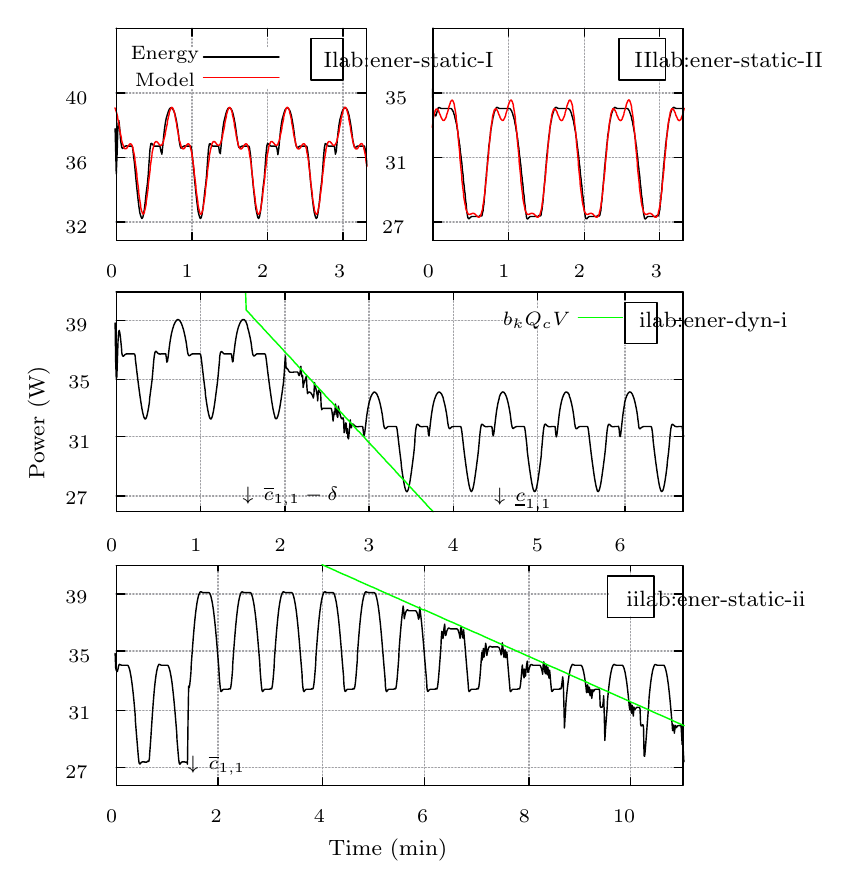
\begin{tikzpicture}[y=0.8pt, x=0.9pt, yscale=-\globalscale, xscale=\globalscale, inner sep=0pt, outer sep=0pt]
\scriptsize
\begin{scope}[shift={(-55.85969,-13.57938)},draw=black,line join=bevel,line cap=rect,even odd rule,line width=0.512pt]
  \begin{scope}[draw=black,line join=bevel,line cap=rect,line width=0.512pt]
  \end{scope}
  \begin{scope}[scale=1.006,draw=black,line join=bevel,line cap=rect,line width=0.512pt]
  \end{scope}
  \begin{scope}[scale=1.006,draw=ca0a0a4,dash pattern=on 0.40pt off 0.80pt,line join=round,line cap=round,line width=0.512pt]
    \path[draw] (56.5000,88.5000) -- (142.5000,88.5000);



  \end{scope}
  \begin{scope}[scale=1.006,draw=black,line join=round,line cap=round,line width=0.512pt]
    \path[draw] (56.5000,88.5000) -- (59.5000,88.5000);



    \path[draw] (142.5000,88.5000) -- (139.5000,88.5000);



  \end{scope}
  \begin{scope}[scale=1.006,draw=black,line join=bevel,line cap=rect,line width=0.512pt]
  \end{scope}
  \begin{scope}[cm={{1.00588,0.0,0.0,1.00588,(39.2294,93.5471)}},draw=black,line join=bevel,line cap=rect,line width=0.512pt]
  \end{scope}
  \begin{scope}[cm={{1.00588,0.0,0.0,1.00588,(39.2294,93.5471)}},draw=black,line join=bevel,line cap=rect,line width=0.512pt]
  \end{scope}
  \begin{scope}[cm={{1.00588,0.0,0.0,1.00588,(39.2294,93.5471)}},draw=black,line join=bevel,line cap=rect,line width=0.512pt]
  \end{scope}
  \begin{scope}[cm={{1.00588,0.0,0.0,1.00588,(39.2294,93.5471)}},draw=black,line join=bevel,line cap=rect,line width=0.512pt]
  \end{scope}
  \begin{scope}[cm={{1.00588,0.0,0.0,1.00588,(39.2294,93.5471)}},draw=black,line join=bevel,line cap=rect,line width=0.512pt]
  \end{scope}
  \begin{scope}[cm={{1.00588,0.0,0.0,1.00588,(39.2294,93.5471)}},draw=black,line join=bevel,line cap=rect,line width=0.512pt]
    \path[fill=black] (0.0000,0.0000) node[above right] (text34) {32};



  \end{scope}
  \begin{scope}[cm={{1.00588,0.0,0.0,1.00588,(39.2294,93.5471)}},draw=black,line join=bevel,line cap=rect,line width=0.512pt]
  \end{scope}
  \begin{scope}[scale=1.006,draw=black,line join=bevel,line cap=rect,line width=0.512pt]
  \end{scope}
  \begin{scope}[scale=1.006,draw=ca0a0a4,dash pattern=on 0.40pt off 0.80pt,line join=round,line cap=round,line width=0.512pt]
    \path[draw] (56.5000,63.5000) -- (142.5000,63.5000);



  \end{scope}
  \begin{scope}[scale=1.006,draw=black,line join=round,line cap=round,line width=0.512pt]
    \path[draw] (56.5000,63.5000) -- (59.5000,63.5000);



    \path[draw] (142.5000,63.5000) -- (139.5000,63.5000);



  \end{scope}
  \begin{scope}[scale=1.006,draw=black,line join=bevel,line cap=rect,line width=0.512pt]
  \end{scope}
  \begin{scope}[cm={{1.00588,0.0,0.0,1.00588,(39.2294,68.4)}},draw=black,line join=bevel,line cap=rect,line width=0.512pt]
  \end{scope}
  \begin{scope}[cm={{1.00588,0.0,0.0,1.00588,(39.2294,68.4)}},draw=black,line join=bevel,line cap=rect,line width=0.512pt]
  \end{scope}
  \begin{scope}[cm={{1.00588,0.0,0.0,1.00588,(39.2294,68.4)}},draw=black,line join=bevel,line cap=rect,line width=0.512pt]
  \end{scope}
  \begin{scope}[cm={{1.00588,0.0,0.0,1.00588,(39.2294,68.4)}},draw=black,line join=bevel,line cap=rect,line width=0.512pt]
  \end{scope}
  \begin{scope}[cm={{1.00588,0.0,0.0,1.00588,(39.2294,68.4)}},draw=black,line join=bevel,line cap=rect,line width=0.512pt]
  \end{scope}
  \begin{scope}[cm={{1.00588,0.0,0.0,1.00588,(39.2294,68.4)}},draw=black,line join=bevel,line cap=rect,line width=0.512pt]
    \path[fill=black] (0.0000,0.0000) node[above right] (text64) {36};



  \end{scope}
  \begin{scope}[cm={{1.00588,0.0,0.0,1.00588,(39.2294,68.4)}},draw=black,line join=bevel,line cap=rect,line width=0.512pt]
  \end{scope}
  \begin{scope}[scale=1.006,draw=black,line join=bevel,line cap=rect,line width=0.512pt]
  \end{scope}
  \begin{scope}[scale=1.006,draw=ca0a0a4,dash pattern=on 0.40pt off 0.80pt,line join=round,line cap=round,line width=0.512pt]
    \path[draw] (56.5000,38.5000) -- (142.5000,38.5000);



  \end{scope}
  \begin{scope}[scale=1.006,draw=black,line join=round,line cap=round,line width=0.512pt]
    \path[draw] (56.5000,38.5000) -- (59.5000,38.5000);



    \path[draw] (142.5000,38.5000) -- (139.5000,38.5000);



  \end{scope}
  \begin{scope}[scale=1.006,draw=black,line join=bevel,line cap=rect,line width=0.512pt]
  \end{scope}
  \begin{scope}[cm={{1.00588,0.0,0.0,1.00588,(39.2294,43.2529)}},draw=black,line join=bevel,line cap=rect,line width=0.512pt]
  \end{scope}
  \begin{scope}[cm={{1.00588,0.0,0.0,1.00588,(39.2294,43.2529)}},draw=black,line join=bevel,line cap=rect,line width=0.512pt]
  \end{scope}
  \begin{scope}[cm={{1.00588,0.0,0.0,1.00588,(39.2294,43.2529)}},draw=black,line join=bevel,line cap=rect,line width=0.512pt]
  \end{scope}
  \begin{scope}[cm={{1.00588,0.0,0.0,1.00588,(39.2294,43.2529)}},draw=black,line join=bevel,line cap=rect,line width=0.512pt]
  \end{scope}
  \begin{scope}[cm={{1.00588,0.0,0.0,1.00588,(39.2294,43.2529)}},draw=black,line join=bevel,line cap=rect,line width=0.512pt]
  \end{scope}
  \begin{scope}[cm={{1.00588,0.0,0.0,1.00588,(39.2294,43.2529)}},draw=black,line join=bevel,line cap=rect,line width=0.512pt]
    \path[fill=black] (0.0000,0.0000) node[above right] (text94) {40};



  \end{scope}
  \begin{scope}[cm={{1.00588,0.0,0.0,1.00588,(39.2294,43.2529)}},draw=black,line join=bevel,line cap=rect,line width=0.512pt]
  \end{scope}
  \begin{scope}[scale=1.006,draw=black,line join=bevel,line cap=rect,line width=0.512pt]
  \end{scope}
  \begin{scope}[scale=1.006,draw=ca0a0a4,dash pattern=on 0.40pt off 0.80pt,line join=round,line cap=round,line width=0.512pt]
    \path[draw] (56.5000,95.5000) -- (56.5000,13.5000);



  \end{scope}
  \begin{scope}[scale=1.006,draw=black,line join=round,line cap=round,line width=0.512pt]
    \path[draw] (56.5000,95.5000) -- (56.5000,92.5000);



    \path[draw] (56.5000,13.5000) -- (56.5000,16.5000);



  \end{scope}
  \begin{scope}[scale=1.006,draw=black,line join=bevel,line cap=rect,line width=0.512pt]
  \end{scope}
  \begin{scope}[cm={{1.00588,0.0,0.0,1.00588,(53.3118,110.647)}},draw=black,line join=bevel,line cap=rect,line width=0.512pt]
  \end{scope}
  \begin{scope}[cm={{1.00588,0.0,0.0,1.00588,(53.3118,110.647)}},draw=black,line join=bevel,line cap=rect,line width=0.512pt]
  \end{scope}
  \begin{scope}[cm={{1.00588,0.0,0.0,1.00588,(53.3118,110.647)}},draw=black,line join=bevel,line cap=rect,line width=0.512pt]
  \end{scope}
  \begin{scope}[cm={{1.00588,0.0,0.0,1.00588,(53.3118,110.647)}},draw=black,line join=bevel,line cap=rect,line width=0.512pt]
  \end{scope}
  \begin{scope}[cm={{1.00588,0.0,0.0,1.00588,(53.3118,110.647)}},draw=black,line join=bevel,line cap=rect,line width=0.512pt]
  \end{scope}
  \begin{scope}[cm={{1.00588,0.0,0.0,1.00588,(53.3118,110.647)}},draw=black,line join=bevel,line cap=rect,line width=0.512pt]
    \path[fill=black] (0.0000,0.0000) node[above right] (text124) {0};



  \end{scope}
  \begin{scope}[cm={{1.00588,0.0,0.0,1.00588,(53.3118,110.647)}},draw=black,line join=bevel,line cap=rect,line width=0.512pt]
  \end{scope}
  \begin{scope}[scale=1.006,draw=black,line join=bevel,line cap=rect,line width=0.512pt]
  \end{scope}
  \begin{scope}[scale=1.006,draw=ca0a0a4,dash pattern=on 0.40pt off 0.80pt,line join=round,line cap=round,line width=0.512pt]
    \path[draw] (82.5000,95.5000) -- (82.5000,36.5000);



    \path[draw] (82.5000,20.5000) -- (82.5000,13.5000);



  \end{scope}
  \begin{scope}[scale=1.006,draw=black,line join=round,line cap=round,line width=0.512pt]
    \path[draw] (82.5000,95.5000) -- (82.5000,92.5000);



    \path[draw] (82.5000,13.5000) -- (82.5000,16.5000);



  \end{scope}
  \begin{scope}[scale=1.006,draw=black,line join=bevel,line cap=rect,line width=0.512pt]
  \end{scope}
  \begin{scope}[cm={{1.00588,0.0,0.0,1.00588,(79.4647,110.647)}},draw=black,line join=bevel,line cap=rect,line width=0.512pt]
  \end{scope}
  \begin{scope}[cm={{1.00588,0.0,0.0,1.00588,(79.4647,110.647)}},draw=black,line join=bevel,line cap=rect,line width=0.512pt]
  \end{scope}
  \begin{scope}[cm={{1.00588,0.0,0.0,1.00588,(79.4647,110.647)}},draw=black,line join=bevel,line cap=rect,line width=0.512pt]
  \end{scope}
  \begin{scope}[cm={{1.00588,0.0,0.0,1.00588,(79.4647,110.647)}},draw=black,line join=bevel,line cap=rect,line width=0.512pt]
  \end{scope}
  \begin{scope}[cm={{1.00588,0.0,0.0,1.00588,(79.4647,110.647)}},draw=black,line join=bevel,line cap=rect,line width=0.512pt]
  \end{scope}
  \begin{scope}[cm={{1.00588,0.0,0.0,1.00588,(79.4647,110.647)}},draw=black,line join=bevel,line cap=rect,line width=0.512pt]
    \path[fill=black] (0.0000,0.0000) node[above right] (text156) {1};



  \end{scope}
  \begin{scope}[cm={{1.00588,0.0,0.0,1.00588,(79.4647,110.647)}},draw=black,line join=bevel,line cap=rect,line width=0.512pt]
  \end{scope}
  \begin{scope}[scale=1.006,draw=black,line join=bevel,line cap=rect,line width=0.512pt]
  \end{scope}
  \begin{scope}[scale=1.006,draw=ca0a0a4,dash pattern=on 0.40pt off 0.80pt,line join=round,line cap=round,line width=0.512pt]
    \path[draw] (108.5000,95.5000) -- (108.5000,36.5000);



    \path[draw] (108.5000,20.5000) -- (108.5000,13.5000);



  \end{scope}
  \begin{scope}[scale=1.006,draw=black,line join=round,line cap=round,line width=0.512pt]
    \path[draw] (108.5000,95.5000) -- (108.5000,92.5000);



    \path[draw] (108.5000,13.5000) -- (108.5000,16.5000);



  \end{scope}
  \begin{scope}[scale=1.006,draw=black,line join=bevel,line cap=rect,line width=0.512pt]
  \end{scope}
  \begin{scope}[cm={{1.00588,0.0,0.0,1.00588,(105.618,110.647)}},draw=black,line join=bevel,line cap=rect,line width=0.512pt]
  \end{scope}
  \begin{scope}[cm={{1.00588,0.0,0.0,1.00588,(105.618,110.647)}},draw=black,line join=bevel,line cap=rect,line width=0.512pt]
  \end{scope}
  \begin{scope}[cm={{1.00588,0.0,0.0,1.00588,(105.618,110.647)}},draw=black,line join=bevel,line cap=rect,line width=0.512pt]
  \end{scope}
  \begin{scope}[cm={{1.00588,0.0,0.0,1.00588,(105.618,110.647)}},draw=black,line join=bevel,line cap=rect,line width=0.512pt]
  \end{scope}
  \begin{scope}[cm={{1.00588,0.0,0.0,1.00588,(105.618,110.647)}},draw=black,line join=bevel,line cap=rect,line width=0.512pt]
  \end{scope}
  \begin{scope}[cm={{1.00588,0.0,0.0,1.00588,(105.618,110.647)}},draw=black,line join=bevel,line cap=rect,line width=0.512pt]
    \path[fill=black] (0.0000,0.0000) node[above right] (text188) {2};



  \end{scope}
  \begin{scope}[cm={{1.00588,0.0,0.0,1.00588,(105.618,110.647)}},draw=black,line join=bevel,line cap=rect,line width=0.512pt]
  \end{scope}
  \begin{scope}[scale=1.006,draw=black,line join=bevel,line cap=rect,line width=0.512pt]
  \end{scope}
  \begin{scope}[scale=1.006,draw=ca0a0a4,dash pattern=on 0.40pt off 0.80pt,line join=round,line cap=round,line width=0.512pt]
    \path[draw] (134.5000,95.5000) -- (134.5000,13.5000);



  \end{scope}
  \begin{scope}[scale=1.006,draw=black,line join=round,line cap=round,line width=0.512pt]
    \path[draw] (134.5000,95.5000) -- (134.5000,92.5000);



    \path[draw] (134.5000,13.5000) -- (134.5000,16.5000);



  \end{scope}
  \begin{scope}[scale=1.006,draw=black,line join=bevel,line cap=rect,line width=0.512pt]
  \end{scope}
  \begin{scope}[cm={{1.00588,0.0,0.0,1.00588,(132.274,110.647)}},draw=black,line join=bevel,line cap=rect,line width=0.512pt]
  \end{scope}
  \begin{scope}[cm={{1.00588,0.0,0.0,1.00588,(132.274,110.647)}},draw=black,line join=bevel,line cap=rect,line width=0.512pt]
  \end{scope}
  \begin{scope}[cm={{1.00588,0.0,0.0,1.00588,(132.274,110.647)}},draw=black,line join=bevel,line cap=rect,line width=0.512pt]
  \end{scope}
  \begin{scope}[cm={{1.00588,0.0,0.0,1.00588,(132.274,110.647)}},draw=black,line join=bevel,line cap=rect,line width=0.512pt]
  \end{scope}
  \begin{scope}[cm={{1.00588,0.0,0.0,1.00588,(132.274,110.647)}},draw=black,line join=bevel,line cap=rect,line width=0.512pt]
  \end{scope}
  \begin{scope}[cm={{1.00588,0.0,0.0,1.00588,(132.274,110.647)}},draw=black,line join=bevel,line cap=rect,line width=0.512pt]
    \path[fill=black] (0.0000,0.0000) node[above right] (text218) {3};



  \end{scope}
  \begin{scope}[cm={{1.00588,0.0,0.0,1.00588,(132.274,110.647)}},draw=black,line join=bevel,line cap=rect,line width=0.512pt]
  \end{scope}
  \begin{scope}[scale=1.006,draw=black,line join=bevel,line cap=rect,line width=0.512pt]
  \end{scope}
  \begin{scope}[scale=1.006,draw=black,line join=round,line cap=round,line width=0.512pt]
    \path[draw] (56.5000,13.5000) -- (56.5000,95.5000) -- (142.5000,95.5000) -- (142.5000,13.5000) -- (56.5000,13.5000);



  \end{scope}
  \begin{scope}[scale=1.006,draw=black,line join=bevel,line cap=rect,line width=0.512pt]
  \end{scope}
  \begin{scope}[scale=1.006,draw=black,line join=bevel,line cap=rect,line width=0.512pt]
  \end{scope}
  \begin{scope}[scale=1.006,fill=cffffff]
    \path[fill,rounded corners=0.0000cm] (124.0000,17.0000) rectangle (135.0000,33.0000);



  \end{scope}
  \begin{scope}[scale=1.006,draw=black,line join=bevel,line cap=rect,line width=0.512pt]
  \end{scope}
  \begin{scope}[scale=1.006,draw=black,line join=bevel,line cap=rect,line width=0.512pt]
  \end{scope}
  \begin{scope}[scale=1.006,draw=black,line join=round,line cap=round,line width=0.512pt]
    \path[draw] (123.5000,33.5000) -- (123.5000,17.5000) -- (134.5000,17.5000) -- (134.5000,33.5000) -- (123.5000,33.5000);



  \end{scope}
  \begin{scope}[scale=1.006,draw=black,line join=bevel,line cap=rect,line width=0.512pt]
  \end{scope}
  \begin{scope}[cm={{1.00588,0.0,0.0,1.00588,(128.753,29.1706)}},draw=black,line join=bevel,line cap=rect,line width=0.512pt]
  \end{scope}
  \begin{scope}[cm={{1.00588,0.0,0.0,1.00588,(128.753,29.1706)}},draw=black,line join=bevel,line cap=rect,line width=0.512pt]
  \end{scope}
  \begin{scope}[cm={{1.00588,0.0,0.0,1.00588,(128.753,29.1706)}},draw=black,line join=bevel,line cap=rect,line width=0.512pt]
  \end{scope}
  \begin{scope}[cm={{1.00588,0.0,0.0,1.00588,(128.753,29.1706)}},draw=black,line join=bevel,line cap=rect,line width=0.512pt]
  \end{scope}
  \begin{scope}[cm={{1.00588,0.0,0.0,1.00588,(128.753,29.1706)}},draw=black,line join=bevel,line cap=rect,line width=0.512pt]
  \end{scope}
  \begin{scope}[cm={{1.00588,0.0,0.0,1.00588,(128.61515,28.75705)}},draw=black,line join=bevel,line cap=rect,line width=0.512pt]
    \path[fill=black] (0.0000,0.0000) node[above right] (text258) {\footnotesize \textlabel{I}{lab:ener-static-I}};



  \end{scope}
  \begin{scope}[cm={{1.00588,0.0,0.0,1.00588,(128.753,29.1706)}},draw=black,line join=bevel,line cap=rect,line width=0.512pt]
  \end{scope}
  \begin{scope}[cm={{0.0,-1.00588,1.00588,0.0,(29.1706,189.106)}},draw=black,line join=bevel,line cap=rect,line width=0.512pt]
  \end{scope}
  \begin{scope}[cm={{0.0,-1.00588,1.00588,0.0,(29.1706,189.106)}},draw=black,line join=bevel,line cap=rect,line width=0.512pt]
  \end{scope}
  \begin{scope}[cm={{0.0,-1.00588,1.00588,0.0,(29.1706,189.106)}},draw=black,line join=bevel,line cap=rect,line width=0.512pt]
  \end{scope}
  \begin{scope}[cm={{0.0,-1.00588,1.00588,0.0,(29.1706,189.106)}},draw=black,line join=bevel,line cap=rect,line width=0.512pt]
  \end{scope}
  \begin{scope}[cm={{0.0,-1.00588,1.00588,0.0,(29.1706,189.106)}},draw=black,line join=bevel,line cap=rect,line width=0.512pt]
  \end{scope}
  \begin{scope}[cm={{0.0,-1.00588,1.00588,0.0,(26.1706,189.106)}},draw=black,line join=bevel,line cap=rect,line width=0.512pt]
    \path[fill=black] (0.0000,0.0000) node[above right] (text274) {\rotatebox{90}{\footnotesize Power (W)}};



  \end{scope}
  \begin{scope}[cm={{0.0,-1.00588,1.00588,0.0,(29.1706,189.106)}},draw=black,line join=bevel,line cap=rect,line width=0.512pt]
  \end{scope}
  \begin{scope}[cm={{1.00588,0.0,0.0,1.00588,(62.3647,28.1647)}},draw=black,line join=bevel,line cap=rect,line width=0.512pt]
  \end{scope}
  \begin{scope}[cm={{1.00588,0.0,0.0,1.00588,(62.3647,28.1647)}},draw=black,line join=bevel,line cap=rect,line width=0.512pt]
  \end{scope}
  \begin{scope}[cm={{1.00588,0.0,0.0,1.00588,(62.3647,28.1647)}},draw=black,line join=bevel,line cap=rect,line width=0.512pt]
  \end{scope}
  \begin{scope}[cm={{1.00588,0.0,0.0,1.00588,(62.3647,28.1647)}},draw=black,line join=bevel,line cap=rect,line width=0.512pt]
  \end{scope}
  \begin{scope}[cm={{1.00588,0.0,0.0,1.00588,(62.3647,28.1647)}},draw=black,line join=bevel,line cap=rect,line width=0.512pt]
  \end{scope}
  \begin{scope}[cm={{1.00588,0.0,0.0,1.00588,(61.8647,27.1647)}},draw=black,line join=bevel,line cap=rect,line width=0.512pt]
    \path[fill=black] (0.0000,0.0000) node[above right] (text290) {\scriptsize Energy};



  \end{scope}
  \begin{scope}[cm={{1.00588,0.0,0.0,1.00588,(62.3647,28.1647)}},draw=black,line join=bevel,line cap=rect,line width=0.512pt]
  \end{scope}
  \begin{scope}[scale=1.006,draw=black,line join=bevel,line cap=rect,line width=0.512pt]
  \end{scope}
  \begin{scope}[scale=1.006,draw=black,line join=round,line cap=round,line width=0.512pt]
    \path[draw,even odd rule] (86.5000,24.5000) -- (112.5000,24.5000);



  \end{scope}
  \begin{scope}[scale=1.006,draw=black,line join=bevel,line cap=rect,line width=0.512pt]
  \end{scope}
  \begin{scope}[scale=1.006,draw=black,line join=bevel,line cap=rect,line width=0.512pt]
  \end{scope}
  \begin{scope}[scale=1.006,draw=black,line join=bevel,line cap=rect,line width=0.512pt]
  \end{scope}
  \begin{scope}[scale=1.006,draw=black,line join=bevel,line cap=rect,line width=0.512pt]
  \end{scope}
  \begin{scope}[scale=1.006,draw=black,line join=round,line cap=round,line width=0.512pt]
    \path[draw] (56.1000,52.3000) -- (56.1000,52.3000) -- (56.5000,69.8000) -- (56.8000,61.5000) -- (57.1000,50.5000) -- (57.4000,49.2000) -- (57.7000,52.5000) -- (58.0000,57.0000) -- (58.4000,59.6000) -- (58.7000,60.0000) -- (59.0000,59.6000) -- (59.3000,59.2000) -- (59.6000,59.1000) -- (59.9000,59.0000) -- (60.2000,59.0000) -- (60.6000,59.1000) -- (60.9000,59.1000) -- (61.2000,59.1000) -- (61.5000,59.1000) -- (61.8000,59.0000) -- (62.1000,59.5000) -- (62.4000,62.4000) -- (62.8000,66.1000) -- (63.1000,69.9000) -- (63.4000,73.4000) -- (63.7000,76.7000) -- (64.0000,79.8000) -- (64.3000,82.6000) -- (64.6000,84.9000) -- (65.0000,86.4000) -- (65.3000,87.1000) -- (65.6000,86.7000) -- (65.9000,85.4000) -- (66.2000,83.2000) -- (66.5000,80.3000) -- (66.8000,77.1000) -- (67.2000,73.7000) -- (67.5000,70.1000) -- (67.8000,65.0000) -- (68.1000,60.3000) -- (68.4000,58.1000) -- (68.7000,58.0000) -- (69.0000,58.5000) -- (69.4000,58.9000) -- (69.7000,59.1000) -- (70.0000,59.1000) -- (70.3000,59.1000) -- (70.6000,59.1000) -- (70.9000,59.1000) -- (71.2000,59.1000) -- (71.5000,59.0000) -- (71.9000,61.2000) -- (72.2000,62.2000) -- (72.5000,59.0000) -- (72.8000,55.3000) -- (73.1000,52.3000) -- (73.4000,50.0000) -- (73.7000,48.2000) -- (74.1000,46.8000) -- (74.4000,45.7000) -- (74.7000,44.9000) -- (75.0000,44.4000) -- (75.3000,44.2000) -- (75.6000,44.3000) -- (75.9000,44.7000) -- (76.3000,45.4000) -- (76.6000,46.4000) -- (76.9000,47.7000) -- (77.2000,49.3000) -- (77.5000,51.3000) -- (77.8000,53.6000) -- (78.1000,56.7000) -- (78.5000,59.2000) -- (78.8000,59.9000) -- (79.1000,59.6000) -- (79.4000,59.3000) -- (79.7000,59.1000) -- (80.0000,59.0000) -- (80.3000,59.0000) -- (80.7000,59.1000) -- (81.0000,59.1000) -- (81.3000,59.1000) -- (81.6000,59.1000) -- (81.9000,59.0000) -- (82.2000,59.1000) -- (82.5000,61.3000) -- (82.9000,65.2000) -- (83.2000,69.1000) -- (83.5000,72.7000) -- (83.8000,76.1000) -- (84.1000,79.3000) -- (84.4000,82.1000) -- (84.7000,84.6000) -- (85.1000,86.3000) -- (85.4000,87.1000) -- (85.7000,86.8000) -- (86.0000,85.5000) -- (86.3000,83.3000) -- (86.6000,80.4000) -- (86.9000,77.1000) -- (87.3000,73.6000) -- (87.6000,69.9000) -- (87.9000,65.0000) -- (88.2000,60.5000) -- (88.5000,58.3000) -- (88.8000,58.1000) -- (89.1000,58.5000) -- (89.5000,58.9000) -- (89.8000,59.1000) -- (90.1000,59.1000) -- (90.4000,59.1000) -- (90.7000,59.1000) -- (91.0000,59.1000) -- (91.3000,59.1000) -- (91.7000,59.0000) -- (92.0000,61.4000) -- (92.3000,62.0000) -- (92.6000,58.6000) -- (92.9000,55.0000) -- (93.2000,52.0000) -- (93.5000,49.7000) -- (93.9000,47.9000) -- (94.2000,46.6000) -- (94.5000,45.5000) -- (94.8000,44.8000) -- (95.1000,44.3000) -- (95.4000,44.2000) -- (95.7000,44.4000) -- (96.1000,44.8000) -- (96.4000,45.6000) -- (96.7000,46.7000) -- (97.0000,48.2000) -- (97.3000,50.0000) -- (97.6000,52.1000) -- (97.9000,54.7000) -- (98.3000,57.7000) -- (98.6000,59.4000) -- (98.9000,59.7000) -- (99.2000,59.5000) -- (99.5000,59.2000) -- (99.8000,59.1000) -- (100.1000,59.0000) -- (100.5000,59.1000) -- (100.8000,59.1000) -- (101.1000,59.1000) -- (101.4000,59.1000) -- (101.7000,59.1000) -- (102.0000,59.0000) -- (102.3000,59.5000) -- (102.7000,62.6000) -- (103.0000,66.8000) -- (103.3000,70.7000) -- (103.6000,74.2000) -- (103.9000,77.5000) -- (104.2000,80.5000) -- (104.5000,83.2000) -- (104.9000,85.3000) -- (105.2000,86.7000) -- (105.5000,87.1000) -- (105.8000,86.3000) -- (106.1000,84.5000) -- (106.4000,81.8000) -- (106.7000,78.6000) -- (107.0000,75.1000) -- (107.4000,71.6000) -- (107.7000,67.2000) -- (108.0000,62.3000) -- (108.3000,59.0000) -- (108.6000,58.0000) -- (108.9000,58.3000) -- (109.3000,58.7000) -- (109.6000,59.0000) -- (109.9000,59.1000) -- (110.2000,59.1000) -- (110.5000,59.1000) -- (110.8000,59.1000) -- (111.1000,59.1000) -- (111.4000,59.0000) -- (111.8000,60.0000) -- (112.1000,62.4000) -- (112.4000,60.2000) -- (112.7000,56.4000) -- (113.0000,53.1000) -- (113.3000,50.5000) -- (113.6000,48.6000) -- (114.0000,47.1000) -- (114.3000,45.9000) -- (114.6000,45.0000) -- (114.9000,44.5000) -- (115.2000,44.2000) -- (115.5000,44.3000) -- (115.8000,44.6000) -- (116.2000,45.3000) -- (116.5000,46.3000) -- (116.8000,47.6000) -- (117.1000,49.4000) -- (117.4000,51.4000) -- (117.7000,53.9000) -- (118.0000,56.8000) -- (118.4000,59.0000) -- (118.7000,59.7000) -- (119.0000,59.6000) -- (119.3000,59.3000) -- (119.6000,59.1000) -- (119.9000,59.1000) -- (120.2000,59.1000) -- (120.6000,59.1000) -- (120.9000,59.1000) -- (121.2000,59.1000) -- (121.5000,59.1000) -- (121.8000,59.0000) -- (122.1000,59.2000) -- (122.4000,61.3000) -- (122.8000,65.4000) -- (123.1000,69.6000) -- (123.4000,73.3000) -- (123.7000,76.6000) -- (124.0000,79.6000) -- (124.3000,82.4000) -- (124.6000,84.7000) -- (125.0000,86.4000) -- (125.3000,87.1000) -- (125.6000,86.7000) -- (125.9000,85.1000) -- (126.2000,82.5000) -- (126.5000,79.4000) -- (126.8000,76.0000) -- (127.2000,72.5000) -- (127.5000,68.4000) -- (127.8000,63.4000) -- (128.1000,59.6000) -- (128.4000,58.1000) -- (128.7000,58.2000) -- (129.0000,58.6000) -- (129.4000,59.0000) -- (129.7000,59.1000) -- (130.0000,59.1000) -- (130.3000,59.1000) -- (130.6000,59.1000) -- (130.9000,59.1000) -- (131.2000,59.0000) -- (131.6000,59.4000) -- (131.9000,62.2000) -- (132.2000,61.0000) -- (132.5000,57.3000) -- (132.8000,53.8000) -- (133.1000,51.1000) -- (133.4000,49.0000) -- (133.8000,47.4000) -- (134.1000,46.1000) -- (134.4000,45.2000) -- (134.7000,44.6000) -- (135.0000,44.2000) -- (135.3000,44.2000) -- (135.6000,44.5000) -- (136.0000,45.1000) -- (136.3000,46.0000) -- (136.6000,47.3000) -- (136.9000,49.0000) -- (137.2000,51.0000) -- (137.5000,53.3000) -- (137.8000,56.2000) -- (138.2000,58.6000) -- (138.5000,59.6000) -- (138.8000,59.6000) -- (139.1000,59.3000) -- (139.4000,59.1000) -- (139.7000,59.1000) -- (140.0000,59.1000) -- (140.4000,59.1000) -- (140.7000,59.1000) -- (141.0000,59.1000) -- (141.3000,59.1000) -- (141.6000,59.1000) -- (141.9000,59.0000) -- (142.2000,60.6000) -- (142.6000,64.5000) -- (142.7000,66.5000);



  \end{scope}
  \begin{scope}[scale=1.006,draw=black,line join=bevel,line cap=rect,line width=0.512pt]
  \end{scope}
  \begin{scope}[cm={{1.00588,0.0,0.0,1.00588,(60.3529,36.2118)}},draw=black,line join=bevel,line cap=rect,line width=0.512pt]
  \end{scope}
  \begin{scope}[cm={{1.00588,0.0,0.0,1.00588,(60.3529,36.2118)}},draw=black,line join=bevel,line cap=rect,line width=0.512pt]
  \end{scope}
  \begin{scope}[cm={{1.00588,0.0,0.0,1.00588,(60.3529,36.2118)}},draw=black,line join=bevel,line cap=rect,line width=0.512pt]
  \end{scope}
  \begin{scope}[cm={{1.00588,0.0,0.0,1.00588,(60.3529,36.2118)}},draw=black,line join=bevel,line cap=rect,line width=0.512pt]
  \end{scope}
  \begin{scope}[cm={{1.00588,0.0,0.0,1.00588,(60.3529,36.2118)}},draw=black,line join=bevel,line cap=rect,line width=0.512pt]
  \end{scope}
  \begin{scope}[cm={{1.00588,0.0,0.0,1.00588,(63.3529,36.2118)}},draw=black,line join=bevel,line cap=rect,line width=0.512pt]
    \path[fill=black] (0.0000,0.0000) node[above right] (text326) {\scriptsize Model};



  \end{scope}
  \begin{scope}[cm={{1.00588,0.0,0.0,1.00588,(60.3529,36.2118)}},draw=black,line join=bevel,line cap=rect,line width=0.512pt]
  \end{scope}
  \begin{scope}[scale=1.006,draw=black,line join=bevel,line cap=rect,line width=0.512pt]
  \end{scope}
  \begin{scope}[scale=1.006,draw=cff0000,line join=round,line cap=round,line width=0.512pt]
    \path[draw,even odd rule] (86.5000,32.5000) -- (112.5000,32.5000);



  \end{scope}
  \begin{scope}[scale=1.006,draw=black,line join=bevel,line cap=rect,line width=0.512pt]
  \end{scope}
  \begin{scope}[scale=1.006,draw=black,line join=bevel,line cap=rect,line width=0.512pt]
  \end{scope}
  \begin{scope}[scale=1.006,draw=black,line join=bevel,line cap=rect,line width=0.512pt]
  \end{scope}
  \begin{scope}[scale=1.006,draw=black,line join=bevel,line cap=rect,line width=0.512pt]
  \end{scope}
  \begin{scope}[scale=1.006,draw=cff0000,line join=round,line cap=round,line width=0.512pt]
    \path[draw] (56.0000,44.3000) -- (56.0000,44.3000) -- (56.1000,44.4000) -- (56.2000,44.6000) -- (56.3000,44.8000) -- (56.3000,45.1000) -- (56.4000,45.4000) -- (56.5000,45.7000) -- (56.6000,46.1000) -- (56.7000,46.5000) -- (56.8000,47.0000) -- (56.9000,47.4000) -- (57.0000,47.9000) -- (57.0000,48.4000) -- (57.1000,48.9000) -- (57.2000,49.5000) -- (57.3000,50.0000) -- (57.4000,50.6000) -- (57.5000,51.2000) -- (57.6000,51.8000) -- (57.6000,52.3000) -- (57.7000,52.9000) -- (57.8000,53.5000) -- (57.9000,54.0000) -- (58.0000,54.6000) -- (58.1000,55.1000) -- (58.2000,55.6000) -- (58.3000,56.1000) -- (58.3000,56.6000) -- (58.4000,57.1000) -- (58.5000,57.5000) -- (58.6000,57.9000) -- (58.7000,58.2000) -- (58.8000,58.6000) -- (58.9000,58.9000) -- (59.0000,59.1000) -- (59.0000,59.4000) -- (59.1000,59.6000) -- (59.2000,59.8000) -- (59.3000,59.9000) -- (59.4000,60.0000) -- (59.5000,60.1000) -- (59.6000,60.1000) -- (59.6000,60.1000) -- (59.7000,60.1000) -- (59.8000,60.1000) -- (59.9000,60.0000) -- (60.0000,60.0000) -- (60.1000,59.9000) -- (60.2000,59.7000) -- (60.3000,59.6000) -- (60.3000,59.5000) -- (60.4000,59.3000) -- (60.5000,59.2000) -- (60.6000,59.0000) -- (60.7000,58.9000) -- (60.8000,58.8000) -- (60.9000,58.6000) -- (60.9000,58.5000) -- (61.0000,58.4000) -- (61.1000,58.3000) -- (61.2000,58.2000) -- (61.3000,58.2000) -- (61.4000,58.2000) -- (61.5000,58.2000) -- (61.6000,58.3000) -- (61.6000,58.3000) -- (61.7000,58.5000) -- (61.8000,58.6000) -- (61.9000,58.8000) -- (62.0000,59.1000) -- (62.1000,59.3000) -- (62.2000,59.7000) -- (62.2000,60.0000) -- (62.3000,60.4000) -- (62.4000,60.9000) -- (62.5000,61.4000) -- (62.6000,61.9000) -- (62.7000,62.5000) -- (62.8000,63.1000) -- (62.9000,63.8000) -- (62.9000,64.4000) -- (63.0000,65.2000) -- (63.1000,65.9000) -- (63.2000,66.7000) -- (63.3000,67.5000) -- (63.4000,68.3000) -- (63.5000,69.2000) -- (63.6000,70.0000) -- (63.6000,70.9000) -- (63.7000,71.8000) -- (63.8000,72.7000) -- (63.9000,73.6000) -- (64.0000,74.4000) -- (64.1000,75.3000) -- (64.2000,76.2000) -- (64.2000,77.0000) -- (64.3000,77.8000) -- (64.4000,78.6000) -- (64.5000,79.4000) -- (64.6000,80.1000) -- (64.7000,80.8000) -- (64.8000,81.5000) -- (64.9000,82.1000) -- (64.9000,82.7000) -- (65.0000,83.2000) -- (65.1000,83.7000) -- (65.2000,84.1000) -- (65.3000,84.4000) -- (65.4000,84.7000) -- (65.5000,85.0000) -- (65.5000,85.2000) -- (65.6000,85.3000) -- (65.7000,85.3000) -- (65.8000,85.3000) -- (65.9000,85.3000) -- (66.0000,85.1000) -- (66.1000,84.9000) -- (66.2000,84.7000) -- (66.2000,84.3000) -- (66.3000,84.0000) -- (66.4000,83.5000) -- (66.5000,83.1000) -- (66.6000,82.5000) -- (66.7000,81.9000) -- (66.8000,81.3000) -- (66.8000,80.6000) -- (66.9000,79.9000) -- (67.0000,79.2000) -- (67.1000,78.4000) -- (67.2000,77.6000) -- (67.3000,76.7000) -- (67.4000,75.9000) -- (67.5000,75.0000) -- (67.5000,74.1000) -- (67.6000,73.2000) -- (67.7000,72.3000) -- (67.8000,71.4000) -- (67.9000,70.5000) -- (68.0000,69.6000) -- (68.1000,68.7000) -- (68.2000,67.9000) -- (68.2000,67.0000) -- (68.3000,66.2000) -- (68.4000,65.4000) -- (68.5000,64.7000) -- (68.6000,63.9000) -- (68.7000,63.2000) -- (68.8000,62.5000) -- (68.8000,61.9000) -- (68.9000,61.3000) -- (69.0000,60.8000) -- (69.1000,60.2000) -- (69.2000,59.8000) -- (69.3000,59.4000) -- (69.4000,59.0000) -- (69.5000,58.6000) -- (69.5000,58.3000) -- (69.6000,58.1000) -- (69.7000,57.8000) -- (69.8000,57.7000) -- (69.9000,57.5000) -- (70.0000,57.4000) -- (70.1000,57.3000) -- (70.1000,57.3000) -- (70.2000,57.3000) -- (70.3000,57.3000) -- (70.4000,57.3000) -- (70.5000,57.4000) -- (70.6000,57.5000) -- (70.7000,57.6000) -- (70.8000,57.7000) -- (70.8000,57.8000) -- (70.9000,57.9000) -- (71.0000,58.0000) -- (71.1000,58.2000) -- (71.2000,58.3000) -- (71.3000,58.4000) -- (71.4000,58.5000) -- (71.4000,58.6000) -- (71.5000,58.7000) -- (71.6000,58.7000) -- (71.7000,58.8000) -- (71.8000,58.8000) -- (71.9000,58.8000) -- (72.0000,58.8000) -- (72.1000,58.7000) -- (72.1000,58.6000) -- (72.2000,58.5000) -- (72.3000,58.3000) -- (72.4000,58.2000) -- (72.5000,57.9000) -- (72.6000,57.7000) -- (72.7000,57.4000) -- (72.8000,57.1000) -- (72.8000,56.8000) -- (72.9000,56.4000) -- (73.0000,56.0000) -- (73.1000,55.6000) -- (73.2000,55.2000) -- (73.3000,54.7000) -- (73.4000,54.3000) -- (73.4000,53.8000) -- (73.5000,53.3000) -- (73.6000,52.7000) -- (73.7000,52.2000) -- (73.8000,51.7000) -- (73.9000,51.1000) -- (74.0000,50.6000) -- (74.1000,50.0000) -- (74.1000,49.5000) -- (74.2000,49.0000) -- (74.3000,48.5000) -- (74.4000,48.0000) -- (74.5000,47.5000) -- (74.6000,47.1000) -- (74.7000,46.6000) -- (74.7000,46.2000) -- (74.8000,45.8000) -- (74.9000,45.5000) -- (75.0000,45.2000) -- (75.1000,44.9000) -- (75.2000,44.7000) -- (75.3000,44.5000) -- (75.4000,44.3000) -- (75.4000,44.2000) -- (75.5000,44.1000) -- (75.6000,44.1000) -- (75.7000,44.1000) -- (75.8000,44.2000) -- (75.9000,44.3000) -- (76.0000,44.4000) -- (76.0000,44.6000) -- (76.1000,44.8000) -- (76.2000,45.1000) -- (76.3000,45.4000) -- (76.4000,45.8000) -- (76.5000,46.1000) -- (76.6000,46.5000) -- (76.7000,47.0000) -- (76.7000,47.4000) -- (76.8000,47.9000) -- (76.9000,48.5000) -- (77.0000,49.0000) -- (77.1000,49.5000) -- (77.2000,50.1000) -- (77.3000,50.7000) -- (77.3000,51.2000) -- (77.4000,51.8000) -- (77.5000,52.4000) -- (77.6000,53.0000) -- (77.7000,53.5000) -- (77.8000,54.1000) -- (77.9000,54.6000) -- (78.0000,55.2000) -- (78.0000,55.7000) -- (78.1000,56.2000) -- (78.2000,56.7000) -- (78.3000,57.1000) -- (78.4000,57.5000) -- (78.5000,57.9000) -- (78.6000,58.3000) -- (78.7000,58.6000) -- (78.7000,58.9000) -- (78.8000,59.2000) -- (78.9000,59.4000) -- (79.0000,59.6000) -- (79.1000,59.8000) -- (79.2000,59.9000) -- (79.3000,60.0000) -- (79.3000,60.1000) -- (79.4000,60.1000) -- (79.5000,60.2000) -- (79.6000,60.1000) -- (79.7000,60.1000) -- (79.8000,60.0000) -- (79.9000,60.0000) -- (80.0000,59.9000) -- (80.0000,59.7000) -- (80.1000,59.6000) -- (80.2000,59.5000) -- (80.3000,59.3000) -- (80.4000,59.2000) -- (80.5000,59.0000) -- (80.6000,58.9000) -- (80.6000,58.7000) -- (80.7000,58.6000) -- (80.8000,58.5000) -- (80.9000,58.4000) -- (81.0000,58.3000) -- (81.1000,58.2000) -- (81.2000,58.2000) -- (81.3000,58.2000) -- (81.3000,58.2000) -- (81.4000,58.2000) -- (81.5000,58.3000) -- (81.6000,58.5000) -- (81.7000,58.6000) -- (81.8000,58.8000) -- (81.9000,59.1000) -- (81.9000,59.3000) -- (82.0000,59.7000) -- (82.1000,60.0000) -- (82.2000,60.4000) -- (82.3000,60.9000) -- (82.4000,61.4000) -- (82.5000,61.9000) -- (82.6000,62.5000) -- (82.6000,63.1000) -- (82.7000,63.8000) -- (82.8000,64.5000) -- (82.9000,65.2000) -- (83.0000,66.0000) -- (83.1000,66.8000) -- (83.2000,67.6000) -- (83.3000,68.4000) -- (83.3000,69.3000) -- (83.4000,70.1000) -- (83.5000,71.0000) -- (83.6000,71.9000) -- (83.7000,72.8000) -- (83.8000,73.7000) -- (83.9000,74.5000) -- (83.9000,75.4000) -- (84.0000,76.3000) -- (84.1000,77.1000) -- (84.2000,77.9000) -- (84.3000,78.7000) -- (84.4000,79.5000) -- (84.5000,80.2000) -- (84.6000,80.9000) -- (84.6000,81.6000) -- (84.7000,82.2000) -- (84.8000,82.8000) -- (84.9000,83.3000) -- (85.0000,83.7000) -- (85.1000,84.2000) -- (85.2000,84.5000) -- (85.2000,84.8000) -- (85.3000,85.0000) -- (85.4000,85.2000) -- (85.5000,85.3000) -- (85.6000,85.4000) -- (85.7000,85.4000) -- (85.8000,85.3000) -- (85.9000,85.1000) -- (85.9000,84.9000) -- (86.0000,84.7000) -- (86.1000,84.4000) -- (86.2000,84.0000) -- (86.3000,83.5000) -- (86.4000,83.0000) -- (86.5000,82.5000) -- (86.5000,81.9000) -- (86.6000,81.3000) -- (86.7000,80.6000) -- (86.8000,79.9000) -- (86.9000,79.1000) -- (87.0000,78.3000) -- (87.1000,77.5000) -- (87.2000,76.7000) -- (87.2000,75.8000) -- (87.3000,74.9000) -- (87.4000,74.0000) -- (87.5000,73.1000) -- (87.6000,72.2000) -- (87.7000,71.3000) -- (87.8000,70.4000) -- (87.9000,69.5000) -- (87.9000,68.7000) -- (88.0000,67.8000) -- (88.1000,67.0000) -- (88.2000,66.1000) -- (88.3000,65.3000) -- (88.4000,64.6000) -- (88.5000,63.8000) -- (88.5000,63.1000) -- (88.6000,62.5000) -- (88.7000,61.8000) -- (88.8000,61.2000) -- (88.9000,60.7000) -- (89.0000,60.2000) -- (89.1000,59.7000) -- (89.2000,59.3000) -- (89.2000,58.9000) -- (89.3000,58.6000) -- (89.4000,58.3000) -- (89.5000,58.0000) -- (89.6000,57.8000) -- (89.7000,57.6000) -- (89.8000,57.5000) -- (89.8000,57.4000) -- (89.9000,57.3000) -- (90.0000,57.3000) -- (90.1000,57.3000) -- (90.2000,57.3000) -- (90.3000,57.3000) -- (90.4000,57.4000) -- (90.5000,57.5000) -- (90.5000,57.6000) -- (90.6000,57.7000) -- (90.7000,57.8000) -- (90.8000,57.9000) -- (90.9000,58.1000) -- (91.0000,58.2000) -- (91.1000,58.3000) -- (91.1000,58.4000) -- (91.2000,58.5000) -- (91.3000,58.6000) -- (91.4000,58.7000) -- (91.5000,58.8000) -- (91.6000,58.8000) -- (91.7000,58.8000) -- (91.8000,58.8000) -- (91.8000,58.8000) -- (91.9000,58.7000) -- (92.0000,58.6000) -- (92.1000,58.5000) -- (92.2000,58.3000) -- (92.3000,58.2000) -- (92.4000,57.9000) -- (92.5000,57.7000) -- (92.5000,57.4000) -- (92.6000,57.1000) -- (92.7000,56.8000) -- (92.8000,56.4000) -- (92.9000,56.0000) -- (93.0000,55.6000) -- (93.1000,55.2000) -- (93.1000,54.7000) -- (93.2000,54.2000) -- (93.3000,53.7000) -- (93.4000,53.2000) -- (93.5000,52.7000) -- (93.6000,52.2000) -- (93.7000,51.6000) -- (93.8000,51.1000) -- (93.8000,50.5000) -- (93.9000,50.0000) -- (94.0000,49.5000) -- (94.1000,48.9000) -- (94.2000,48.4000) -- (94.3000,47.9000) -- (94.4000,47.5000) -- (94.4000,47.0000) -- (94.5000,46.6000) -- (94.6000,46.2000) -- (94.7000,45.8000) -- (94.8000,45.4000) -- (94.9000,45.1000) -- (95.0000,44.9000) -- (95.1000,44.6000) -- (95.1000,44.4000) -- (95.2000,44.3000) -- (95.3000,44.2000) -- (95.4000,44.1000) -- (95.5000,44.1000) -- (95.6000,44.1000) -- (95.7000,44.2000) -- (95.7000,44.3000) -- (95.8000,44.4000) -- (95.9000,44.6000) -- (96.0000,44.8000) -- (96.1000,45.1000) -- (96.2000,45.4000) -- (96.3000,45.8000) -- (96.4000,46.2000) -- (96.4000,46.6000) -- (96.5000,47.0000) -- (96.6000,47.5000) -- (96.7000,48.0000) -- (96.8000,48.5000) -- (96.9000,49.0000) -- (97.0000,49.6000) -- (97.1000,50.1000) -- (97.1000,50.7000) -- (97.2000,51.3000) -- (97.3000,51.9000) -- (97.4000,52.4000) -- (97.5000,53.0000) -- (97.6000,53.6000) -- (97.7000,54.2000) -- (97.7000,54.7000) -- (97.8000,55.2000) -- (97.9000,55.8000) -- (98.0000,56.2000) -- (98.1000,56.7000) -- (98.2000,57.2000) -- (98.3000,57.6000) -- (98.4000,58.0000) -- (98.4000,58.3000) -- (98.5000,58.7000) -- (98.6000,59.0000) -- (98.7000,59.2000) -- (98.8000,59.5000) -- (98.9000,59.7000) -- (99.0000,59.8000) -- (99.0000,60.0000) -- (99.1000,60.1000) -- (99.2000,60.1000) -- (99.3000,60.2000) -- (99.4000,60.2000) -- (99.5000,60.2000) -- (99.6000,60.1000) -- (99.7000,60.0000) -- (99.7000,60.0000) -- (99.8000,59.9000) -- (99.9000,59.7000) -- (100.0000,59.6000) -- (100.1000,59.5000) -- (100.2000,59.3000) -- (100.3000,59.2000) -- (100.3000,59.0000) -- (100.4000,58.9000) -- (100.5000,58.7000) -- (100.6000,58.6000) -- (100.7000,58.5000) -- (100.8000,58.4000) -- (100.9000,58.3000) -- (101.0000,58.2000) -- (101.0000,58.2000) -- (101.1000,58.2000) -- (101.2000,58.2000) -- (101.3000,58.2000) -- (101.4000,58.3000) -- (101.5000,58.4000) -- (101.6000,58.6000) -- (101.7000,58.8000) -- (101.7000,59.1000) -- (101.8000,59.3000) -- (101.9000,59.7000) -- (102.0000,60.0000) -- (102.1000,60.5000) -- (102.2000,60.9000) -- (102.3000,61.4000) -- (102.3000,62.0000) -- (102.4000,62.6000) -- (102.5000,63.2000) -- (102.6000,63.8000) -- (102.7000,64.5000) -- (102.8000,65.3000) -- (102.9000,66.0000) -- (103.0000,66.8000) -- (103.0000,67.6000) -- (103.1000,68.5000) -- (103.2000,69.3000) -- (103.3000,70.2000) -- (103.4000,71.1000) -- (103.5000,72.0000) -- (103.6000,72.8000) -- (103.6000,73.7000) -- (103.7000,74.6000) -- (103.8000,75.5000) -- (103.9000,76.4000) -- (104.0000,77.2000) -- (104.1000,78.0000) -- (104.2000,78.8000) -- (104.3000,79.6000) -- (104.3000,80.3000) -- (104.4000,81.0000) -- (104.5000,81.7000) -- (104.6000,82.3000) -- (104.7000,82.8000) -- (104.8000,83.4000) -- (104.9000,83.8000) -- (104.9000,84.2000) -- (105.0000,84.6000) -- (105.1000,84.9000) -- (105.2000,85.1000) -- (105.3000,85.3000) -- (105.4000,85.4000) -- (105.5000,85.4000) -- (105.6000,85.4000) -- (105.6000,85.3000) -- (105.7000,85.2000) -- (105.8000,85.0000) -- (105.9000,84.7000) -- (106.0000,84.4000) -- (106.1000,84.0000) -- (106.2000,83.5000) -- (106.3000,83.0000) -- (106.3000,82.5000) -- (106.4000,81.9000) -- (106.5000,81.2000) -- (106.6000,80.5000) -- (106.7000,79.8000) -- (106.8000,79.1000) -- (106.9000,78.3000) -- (106.9000,77.4000) -- (107.0000,76.6000) -- (107.1000,75.7000) -- (107.2000,74.8000) -- (107.3000,73.9000) -- (107.4000,73.0000) -- (107.5000,72.1000) -- (107.6000,71.2000) -- (107.6000,70.3000) -- (107.7000,69.4000) -- (107.8000,68.6000) -- (107.9000,67.7000) -- (108.0000,66.9000) -- (108.1000,66.0000) -- (108.2000,65.2000) -- (108.2000,64.5000) -- (108.3000,63.7000) -- (108.4000,63.0000) -- (108.5000,62.4000) -- (108.6000,61.8000) -- (108.7000,61.2000) -- (108.8000,60.6000) -- (108.9000,60.1000) -- (108.9000,59.6000) -- (109.0000,59.2000) -- (109.1000,58.9000) -- (109.2000,58.5000) -- (109.3000,58.2000) -- (109.4000,58.0000) -- (109.5000,57.8000) -- (109.5000,57.6000) -- (109.6000,57.5000) -- (109.7000,57.4000) -- (109.8000,57.3000) -- (109.9000,57.3000) -- (110.0000,57.3000) -- (110.1000,57.3000) -- (110.2000,57.3000) -- (110.2000,57.4000) -- (110.3000,57.5000) -- (110.4000,57.6000) -- (110.5000,57.7000) -- (110.6000,57.8000) -- (110.7000,57.9000) -- (110.8000,58.1000) -- (110.9000,58.2000) -- (110.9000,58.3000) -- (111.0000,58.4000) -- (111.1000,58.5000) -- (111.2000,58.6000) -- (111.3000,58.7000) -- (111.4000,58.8000) -- (111.5000,58.8000) -- (111.5000,58.8000) -- (111.6000,58.8000) -- (111.7000,58.8000) -- (111.8000,58.7000) -- (111.9000,58.6000) -- (112.0000,58.5000) -- (112.1000,58.3000) -- (112.2000,58.2000) -- (112.2000,57.9000) -- (112.3000,57.7000) -- (112.4000,57.4000) -- (112.5000,57.1000) -- (112.6000,56.8000) -- (112.7000,56.4000) -- (112.8000,56.0000) -- (112.8000,55.6000) -- (112.9000,55.1000) -- (113.0000,54.7000) -- (113.1000,54.2000) -- (113.2000,53.7000) -- (113.3000,53.2000) -- (113.4000,52.7000) -- (113.5000,52.1000) -- (113.5000,51.6000) -- (113.6000,51.0000) -- (113.7000,50.5000) -- (113.8000,49.9000) -- (113.9000,49.4000) -- (114.0000,48.9000) -- (114.1000,48.4000) -- (114.1000,47.9000) -- (114.2000,47.4000) -- (114.3000,46.9000) -- (114.4000,46.5000) -- (114.5000,46.1000) -- (114.6000,45.7000) -- (114.7000,45.4000) -- (114.8000,45.1000) -- (114.8000,44.8000) -- (114.9000,44.6000) -- (115.0000,44.4000) -- (115.1000,44.3000) -- (115.2000,44.1000) -- (115.3000,44.1000) -- (115.4000,44.1000) -- (115.5000,44.1000) -- (115.5000,44.1000) -- (115.6000,44.3000) -- (115.7000,44.4000) -- (115.8000,44.6000) -- (115.9000,44.8000) -- (116.0000,45.1000) -- (116.1000,45.4000) -- (116.1000,45.8000) -- (116.2000,46.2000) -- (116.3000,46.6000) -- (116.4000,47.0000) -- (116.5000,47.5000) -- (116.6000,48.0000) -- (116.7000,48.5000) -- (116.8000,49.1000) -- (116.8000,49.6000) -- (116.9000,50.2000) -- (117.0000,50.8000) -- (117.1000,51.3000) -- (117.2000,51.9000) -- (117.3000,52.5000) -- (117.4000,53.1000) -- (117.4000,53.6000) -- (117.5000,54.2000) -- (117.6000,54.8000) -- (117.7000,55.3000) -- (117.8000,55.8000) -- (117.9000,56.3000) -- (118.0000,56.8000) -- (118.1000,57.2000) -- (118.1000,57.6000) -- (118.2000,58.0000) -- (118.3000,58.4000) -- (118.4000,58.7000) -- (118.5000,59.0000) -- (118.6000,59.3000) -- (118.7000,59.5000) -- (118.7000,59.7000) -- (118.8000,59.9000) -- (118.9000,60.0000) -- (119.0000,60.1000) -- (119.1000,60.1000) -- (119.2000,60.2000) -- (119.3000,60.2000) -- (119.4000,60.2000) -- (119.4000,60.1000) -- (119.5000,60.1000) -- (119.6000,60.0000) -- (119.7000,59.9000) -- (119.8000,59.7000) -- (119.9000,59.6000) -- (120.0000,59.5000) -- (120.0000,59.3000) -- (120.1000,59.1000) -- (120.2000,59.0000) -- (120.3000,58.8000) -- (120.4000,58.7000) -- (120.5000,58.6000) -- (120.6000,58.4000) -- (120.7000,58.3000) -- (120.7000,58.2000) -- (120.8000,58.2000) -- (120.9000,58.2000) -- (121.0000,58.1000) -- (121.1000,58.2000) -- (121.2000,58.2000) -- (121.3000,58.3000) -- (121.4000,58.4000) -- (121.4000,58.6000) -- (121.5000,58.8000) -- (121.6000,59.1000) -- (121.7000,59.3000) -- (121.8000,59.7000) -- (121.9000,60.1000) -- (122.0000,60.5000) -- (122.0000,60.9000) -- (122.1000,61.5000) -- (122.2000,62.0000) -- (122.3000,62.6000) -- (122.4000,63.2000) -- (122.5000,63.9000) -- (122.6000,64.6000) -- (122.7000,65.3000) -- (122.7000,66.1000) -- (122.8000,66.9000) -- (122.9000,67.7000) -- (123.0000,68.5000) -- (123.1000,69.4000) -- (123.2000,70.3000) -- (123.3000,71.1000) -- (123.3000,72.0000) -- (123.4000,72.9000) -- (123.5000,73.8000) -- (123.6000,74.7000) -- (123.7000,75.6000) -- (123.8000,76.4000) -- (123.9000,77.3000) -- (124.0000,78.1000) -- (124.0000,78.9000) -- (124.1000,79.7000) -- (124.2000,80.4000) -- (124.3000,81.1000) -- (124.4000,81.7000) -- (124.5000,82.4000) -- (124.6000,82.9000) -- (124.6000,83.4000) -- (124.7000,83.9000) -- (124.8000,84.3000) -- (124.9000,84.6000) -- (125.0000,84.9000) -- (125.1000,85.2000) -- (125.2000,85.3000) -- (125.3000,85.4000) -- (125.3000,85.5000) -- (125.4000,85.4000) -- (125.5000,85.3000) -- (125.6000,85.2000) -- (125.7000,85.0000) -- (125.8000,84.7000) -- (125.9000,84.4000) -- (125.9000,84.0000) -- (126.0000,83.5000) -- (126.1000,83.0000) -- (126.2000,82.4000) -- (126.3000,81.8000) -- (126.4000,81.2000) -- (126.5000,80.5000) -- (126.6000,79.8000) -- (126.6000,79.0000) -- (126.7000,78.2000) -- (126.8000,77.4000) -- (126.9000,76.5000) -- (127.0000,75.7000) -- (127.1000,74.8000) -- (127.2000,73.9000) -- (127.3000,73.0000) -- (127.3000,72.1000) -- (127.4000,71.2000) -- (127.5000,70.3000) -- (127.6000,69.4000) -- (127.7000,68.5000) -- (127.8000,67.6000) -- (127.9000,66.8000) -- (127.9000,66.0000) -- (128.0000,65.2000) -- (128.1000,64.4000) -- (128.2000,63.7000) -- (128.3000,63.0000) -- (128.4000,62.3000) -- (128.5000,61.7000) -- (128.6000,61.1000) -- (128.6000,60.5000) -- (128.7000,60.0000) -- (128.8000,59.6000) -- (128.9000,59.2000) -- (129.0000,58.8000) -- (129.1000,58.5000) -- (129.2000,58.2000) -- (129.2000,57.9000) -- (129.3000,57.7000) -- (129.4000,57.6000) -- (129.5000,57.4000) -- (129.6000,57.3000) -- (129.7000,57.3000) -- (129.8000,57.2000) -- (129.9000,57.3000) -- (129.9000,57.3000) -- (130.0000,57.3000) -- (130.1000,57.4000) -- (130.2000,57.5000) -- (130.3000,57.6000) -- (130.4000,57.7000) -- (130.5000,57.8000) -- (130.5000,58.0000) -- (130.6000,58.1000) -- (130.7000,58.2000) -- (130.8000,58.3000) -- (130.9000,58.5000) -- (131.0000,58.6000) -- (131.1000,58.7000) -- (131.2000,58.7000) -- (131.2000,58.8000) -- (131.3000,58.8000) -- (131.4000,58.8000) -- (131.5000,58.8000) -- (131.6000,58.8000) -- (131.7000,58.7000) -- (131.8000,58.6000) -- (131.8000,58.5000) -- (131.9000,58.3000) -- (132.0000,58.2000) -- (132.1000,57.9000) -- (132.2000,57.7000) -- (132.3000,57.4000) -- (132.4000,57.1000) -- (132.5000,56.8000) -- (132.5000,56.4000) -- (132.6000,56.0000) -- (132.7000,55.6000) -- (132.8000,55.1000) -- (132.9000,54.6000) -- (133.0000,54.2000) -- (133.1000,53.7000) -- (133.2000,53.1000) -- (133.2000,52.6000) -- (133.3000,52.1000) -- (133.4000,51.5000) -- (133.5000,51.0000) -- (133.6000,50.4000) -- (133.7000,49.9000) -- (133.8000,49.4000) -- (133.8000,48.8000) -- (133.9000,48.3000) -- (134.0000,47.8000) -- (134.1000,47.3000) -- (134.2000,46.9000) -- (134.3000,46.5000) -- (134.4000,46.1000) -- (134.5000,45.7000) -- (134.5000,45.3000) -- (134.6000,45.0000) -- (134.7000,44.8000) -- (134.8000,44.6000) -- (134.9000,44.4000) -- (135.0000,44.2000) -- (135.1000,44.1000) -- (135.1000,44.1000) -- (135.2000,44.0000) -- (135.3000,44.1000) -- (135.4000,44.1000) -- (135.5000,44.2000) -- (135.6000,44.4000) -- (135.7000,44.6000) -- (135.8000,44.8000) -- (135.8000,45.1000) -- (135.9000,45.4000) -- (136.0000,45.8000) -- (136.1000,46.2000) -- (136.2000,46.6000) -- (136.3000,47.1000) -- (136.4000,47.5000) -- (136.5000,48.0000) -- (136.5000,48.6000) -- (136.6000,49.1000) -- (136.7000,49.7000) -- (136.8000,50.2000) -- (136.9000,50.8000) -- (137.0000,51.4000) -- (137.1000,52.0000) -- (137.1000,52.6000) -- (137.2000,53.1000) -- (137.3000,53.7000) -- (137.4000,54.3000) -- (137.5000,54.8000) -- (137.6000,55.4000) -- (137.7000,55.9000) -- (137.8000,56.4000) -- (137.8000,56.8000) -- (137.9000,57.3000) -- (138.0000,57.7000) -- (138.1000,58.1000) -- (138.2000,58.4000) -- (138.3000,58.8000) -- (138.4000,59.1000) -- (138.4000,59.3000) -- (138.5000,59.5000) -- (138.6000,59.7000) -- (138.7000,59.9000) -- (138.8000,60.0000) -- (138.9000,60.1000) -- (139.0000,60.2000) -- (139.1000,60.2000) -- (139.1000,60.2000) -- (139.2000,60.2000) -- (139.3000,60.1000) -- (139.4000,60.1000) -- (139.5000,60.0000) -- (139.6000,59.9000) -- (139.7000,59.7000) -- (139.7000,59.6000) -- (139.8000,59.4000) -- (139.9000,59.3000) -- (140.0000,59.1000) -- (140.1000,59.0000) -- (140.2000,58.8000) -- (140.3000,58.7000) -- (140.4000,58.5000) -- (140.4000,58.4000) -- (140.5000,58.3000) -- (140.6000,58.2000) -- (140.7000,58.2000) -- (140.8000,58.1000) -- (140.9000,58.1000) -- (141.0000,58.1000) -- (141.1000,58.2000) -- (141.1000,58.3000) -- (141.2000,58.4000) -- (141.3000,58.6000) -- (141.4000,58.8000) -- (141.5000,59.1000) -- (141.6000,59.4000) -- (141.7000,59.7000) -- (141.7000,60.1000) -- (141.8000,60.5000) -- (141.9000,61.0000) -- (142.0000,61.5000) -- (142.1000,62.0000) -- (142.2000,62.6000) -- (142.3000,63.3000) -- (142.4000,63.9000) -- (142.4000,64.6000) -- (142.5000,65.4000) -- (142.6000,66.1000) -- (142.7000,67.0000);



  \end{scope}
  \begin{scope}[scale=1.006,draw=black,line join=bevel,line cap=rect,line width=0.512pt]
  \end{scope}
  \begin{scope}[scale=1.006,draw=black,line join=bevel,line cap=rect,line width=0.512pt]
  \end{scope}
  \begin{scope}[scale=1.006,draw=black,line join=round,line cap=round,line width=0.512pt]
    \path[draw] (56.5000,13.5000) -- (56.5000,95.5000) -- (142.5000,95.5000) -- (142.5000,13.5000) -- (56.5000,13.5000);



  \end{scope}
  \begin{scope}[scale=1.006,draw=ca0a0a4,dash pattern=on 0.40pt off 0.80pt,line join=round,line cap=round,line width=0.512pt]
    \path[draw] (165.5000,88.5000) -- (251.5000,88.5000);



  \end{scope}
  \begin{scope}[scale=1.006,draw=black,line join=round,line cap=round,line width=0.512pt]
    \path[draw] (165.5000,88.5000) -- (168.5000,88.5000);



    \path[draw] (251.5000,88.5000) -- (248.5000,88.5000);



  \end{scope}
  \begin{scope}[scale=1.006,draw=black,line join=bevel,line cap=rect,line width=0.512pt]
  \end{scope}
  \begin{scope}[cm={{1.00588,0.0,0.0,1.00588,(148.871,93.5471)}},draw=black,line join=bevel,line cap=rect,line width=0.512pt]
  \end{scope}
  \begin{scope}[cm={{1.00588,0.0,0.0,1.00588,(148.871,93.5471)}},draw=black,line join=bevel,line cap=rect,line width=0.512pt]
  \end{scope}
  \begin{scope}[cm={{1.00588,0.0,0.0,1.00588,(148.871,93.5471)}},draw=black,line join=bevel,line cap=rect,line width=0.512pt]
  \end{scope}
  \begin{scope}[cm={{1.00588,0.0,0.0,1.00588,(148.871,93.5471)}},draw=black,line join=bevel,line cap=rect,line width=0.512pt]
  \end{scope}
  \begin{scope}[cm={{1.00588,0.0,0.0,1.00588,(148.871,93.5471)}},draw=black,line join=bevel,line cap=rect,line width=0.512pt]
  \end{scope}
  \begin{scope}[cm={{1.00588,0.0,0.0,1.00588,(148.871,93.5471)}},draw=black,line join=bevel,line cap=rect,line width=0.512pt]
    \path[fill=black] (0.0000,0.0000) node[above right] (text380) {27};



  \end{scope}
  \begin{scope}[cm={{1.00588,0.0,0.0,1.00588,(148.871,93.5471)}},draw=black,line join=bevel,line cap=rect,line width=0.512pt]
  \end{scope}
  \begin{scope}[scale=1.006,draw=black,line join=bevel,line cap=rect,line width=0.512pt]
  \end{scope}
  \begin{scope}[scale=1.006,draw=ca0a0a4,dash pattern=on 0.40pt off 0.80pt,line join=round,line cap=round,line width=0.512pt]
    \path[draw] (165.5000,63.5000) -- (251.5000,63.5000);



  \end{scope}
  \begin{scope}[scale=1.006,draw=black,line join=round,line cap=round,line width=0.512pt]
    \path[draw] (165.5000,63.5000) -- (168.5000,63.5000);



    \path[draw] (251.5000,63.5000) -- (248.5000,63.5000);



  \end{scope}
  \begin{scope}[scale=1.006,draw=black,line join=bevel,line cap=rect,line width=0.512pt]
  \end{scope}
  \begin{scope}[cm={{1.00588,0.0,0.0,1.00588,(149.876,68.4)}},draw=black,line join=bevel,line cap=rect,line width=0.512pt]
  \end{scope}
  \begin{scope}[cm={{1.00588,0.0,0.0,1.00588,(149.876,68.4)}},draw=black,line join=bevel,line cap=rect,line width=0.512pt]
  \end{scope}
  \begin{scope}[cm={{1.00588,0.0,0.0,1.00588,(149.876,68.4)}},draw=black,line join=bevel,line cap=rect,line width=0.512pt]
  \end{scope}
  \begin{scope}[cm={{1.00588,0.0,0.0,1.00588,(149.876,68.4)}},draw=black,line join=bevel,line cap=rect,line width=0.512pt]
  \end{scope}
  \begin{scope}[cm={{1.00588,0.0,0.0,1.00588,(149.876,68.4)}},draw=black,line join=bevel,line cap=rect,line width=0.512pt]
  \end{scope}
  \begin{scope}[cm={{1.00588,0.0,0.0,1.00588,(149.876,68.4)}},draw=black,line join=bevel,line cap=rect,line width=0.512pt]
    \path[fill=black] (0.0000,0.0000) node[above right] (text410) {31};



  \end{scope}
  \begin{scope}[cm={{1.00588,0.0,0.0,1.00588,(149.876,68.4)}},draw=black,line join=bevel,line cap=rect,line width=0.512pt]
  \end{scope}
  \begin{scope}[scale=1.006,draw=black,line join=bevel,line cap=rect,line width=0.512pt]
  \end{scope}
  \begin{scope}[scale=1.006,draw=ca0a0a4,dash pattern=on 0.40pt off 0.80pt,line join=round,line cap=round,line width=0.512pt]
    \path[draw] (165.5000,38.5000) -- (251.5000,38.5000);



  \end{scope}
  \begin{scope}[scale=1.006,draw=black,line join=round,line cap=round,line width=0.512pt]
    \path[draw] (165.5000,38.5000) -- (168.5000,38.5000);



    \path[draw] (251.5000,38.5000) -- (248.5000,38.5000);



  \end{scope}
  \begin{scope}[scale=1.006,draw=black,line join=bevel,line cap=rect,line width=0.512pt]
  \end{scope}
  \begin{scope}[cm={{1.00588,0.0,0.0,1.00588,(149.876,43.2529)}},draw=black,line join=bevel,line cap=rect,line width=0.512pt]
  \end{scope}
  \begin{scope}[cm={{1.00588,0.0,0.0,1.00588,(149.876,43.2529)}},draw=black,line join=bevel,line cap=rect,line width=0.512pt]
  \end{scope}
  \begin{scope}[cm={{1.00588,0.0,0.0,1.00588,(149.876,43.2529)}},draw=black,line join=bevel,line cap=rect,line width=0.512pt]
  \end{scope}
  \begin{scope}[cm={{1.00588,0.0,0.0,1.00588,(149.876,43.2529)}},draw=black,line join=bevel,line cap=rect,line width=0.512pt]
  \end{scope}
  \begin{scope}[cm={{1.00588,0.0,0.0,1.00588,(149.876,43.2529)}},draw=black,line join=bevel,line cap=rect,line width=0.512pt]
  \end{scope}
  \begin{scope}[cm={{1.00588,0.0,0.0,1.00588,(149.876,43.2529)}},draw=black,line join=bevel,line cap=rect,line width=0.512pt]
    \path[fill=black] (0.0000,0.0000) node[above right] (text440) {35};



  \end{scope}
  \begin{scope}[cm={{1.00588,0.0,0.0,1.00588,(149.876,43.2529)}},draw=black,line join=bevel,line cap=rect,line width=0.512pt]
  \end{scope}
  \begin{scope}[scale=1.006,draw=black,line join=bevel,line cap=rect,line width=0.512pt]
  \end{scope}
  \begin{scope}[scale=1.006,draw=ca0a0a4,dash pattern=on 0.40pt off 0.80pt,line join=round,line cap=round,line width=0.512pt]
    \path[draw] (165.5000,95.5000) -- (165.5000,13.5000);



  \end{scope}
  \begin{scope}[scale=1.006,draw=black,line join=round,line cap=round,line width=0.512pt]
    \path[draw] (165.5000,95.5000) -- (165.5000,92.5000);



    \path[draw] (165.5000,13.5000) -- (165.5000,16.5000);



  \end{scope}
  \begin{scope}[scale=1.006,draw=black,line join=bevel,line cap=rect,line width=0.512pt]
  \end{scope}
  \begin{scope}[cm={{1.00588,0.0,0.0,1.00588,(162.953,110.647)}},draw=black,line join=bevel,line cap=rect,line width=0.512pt]
  \end{scope}
  \begin{scope}[cm={{1.00588,0.0,0.0,1.00588,(162.953,110.647)}},draw=black,line join=bevel,line cap=rect,line width=0.512pt]
  \end{scope}
  \begin{scope}[cm={{1.00588,0.0,0.0,1.00588,(162.953,110.647)}},draw=black,line join=bevel,line cap=rect,line width=0.512pt]
  \end{scope}
  \begin{scope}[cm={{1.00588,0.0,0.0,1.00588,(162.953,110.647)}},draw=black,line join=bevel,line cap=rect,line width=0.512pt]
  \end{scope}
  \begin{scope}[cm={{1.00588,0.0,0.0,1.00588,(162.953,110.647)}},draw=black,line join=bevel,line cap=rect,line width=0.512pt]
  \end{scope}
  \begin{scope}[cm={{1.00588,0.0,0.0,1.00588,(162.953,110.647)}},draw=black,line join=bevel,line cap=rect,line width=0.512pt]
    \path[fill=black] (0.0000,0.0000) node[above right] (text470) {0};



  \end{scope}
  \begin{scope}[cm={{1.00588,0.0,0.0,1.00588,(162.953,110.647)}},draw=black,line join=bevel,line cap=rect,line width=0.512pt]
  \end{scope}
  \begin{scope}[scale=1.006,draw=black,line join=bevel,line cap=rect,line width=0.512pt]
  \end{scope}
  \begin{scope}[scale=1.006,draw=ca0a0a4,dash pattern=on 0.40pt off 0.80pt,line join=round,line cap=round,line width=0.512pt]
    \path[draw] (191.5000,95.5000) -- (191.5000,13.5000);



  \end{scope}
  \begin{scope}[scale=1.006,draw=black,line join=round,line cap=round,line width=0.512pt]
    \path[draw] (191.5000,95.5000) -- (191.5000,92.5000);



    \path[draw] (191.5000,13.5000) -- (191.5000,16.5000);



  \end{scope}
  \begin{scope}[scale=1.006,draw=black,line join=bevel,line cap=rect,line width=0.512pt]
  \end{scope}
  \begin{scope}[cm={{1.00588,0.0,0.0,1.00588,(189.106,110.647)}},draw=black,line join=bevel,line cap=rect,line width=0.512pt]
  \end{scope}
  \begin{scope}[cm={{1.00588,0.0,0.0,1.00588,(189.106,110.647)}},draw=black,line join=bevel,line cap=rect,line width=0.512pt]
  \end{scope}
  \begin{scope}[cm={{1.00588,0.0,0.0,1.00588,(189.106,110.647)}},draw=black,line join=bevel,line cap=rect,line width=0.512pt]
  \end{scope}
  \begin{scope}[cm={{1.00588,0.0,0.0,1.00588,(189.106,110.647)}},draw=black,line join=bevel,line cap=rect,line width=0.512pt]
  \end{scope}
  \begin{scope}[cm={{1.00588,0.0,0.0,1.00588,(189.106,110.647)}},draw=black,line join=bevel,line cap=rect,line width=0.512pt]
  \end{scope}
  \begin{scope}[cm={{1.00588,0.0,0.0,1.00588,(189.106,110.647)}},draw=black,line join=bevel,line cap=rect,line width=0.512pt]
    \path[fill=black] (0.0000,0.0000) node[above right] (text500) {1};



  \end{scope}
  \begin{scope}[cm={{1.00588,0.0,0.0,1.00588,(189.106,110.647)}},draw=black,line join=bevel,line cap=rect,line width=0.512pt]
  \end{scope}
  \begin{scope}[scale=1.006,draw=black,line join=bevel,line cap=rect,line width=0.512pt]
  \end{scope}
  \begin{scope}[scale=1.006,draw=ca0a0a4,dash pattern=on 0.40pt off 0.80pt,line join=round,line cap=round,line width=0.512pt]
    \path[draw] (217.5000,95.5000) -- (217.5000,13.5000);



  \end{scope}
  \begin{scope}[scale=1.006,draw=black,line join=round,line cap=round,line width=0.512pt]
    \path[draw] (217.5000,95.5000) -- (217.5000,92.5000);



    \path[draw] (217.5000,13.5000) -- (217.5000,16.5000);



  \end{scope}
  \begin{scope}[scale=1.006,draw=black,line join=bevel,line cap=rect,line width=0.512pt]
  \end{scope}
  \begin{scope}[cm={{1.00588,0.0,0.0,1.00588,(215.259,110.647)}},draw=black,line join=bevel,line cap=rect,line width=0.512pt]
  \end{scope}
  \begin{scope}[cm={{1.00588,0.0,0.0,1.00588,(215.259,110.647)}},draw=black,line join=bevel,line cap=rect,line width=0.512pt]
  \end{scope}
  \begin{scope}[cm={{1.00588,0.0,0.0,1.00588,(215.259,110.647)}},draw=black,line join=bevel,line cap=rect,line width=0.512pt]
  \end{scope}
  \begin{scope}[cm={{1.00588,0.0,0.0,1.00588,(215.259,110.647)}},draw=black,line join=bevel,line cap=rect,line width=0.512pt]
  \end{scope}
  \begin{scope}[cm={{1.00588,0.0,0.0,1.00588,(215.259,110.647)}},draw=black,line join=bevel,line cap=rect,line width=0.512pt]
  \end{scope}
  \begin{scope}[cm={{1.00588,0.0,0.0,1.00588,(215.259,110.647)}},draw=black,line join=bevel,line cap=rect,line width=0.512pt]
    \path[fill=black] (0.0000,0.0000) node[above right] (text530) {2};



  \end{scope}
  \begin{scope}[cm={{1.00588,0.0,0.0,1.00588,(215.259,110.647)}},draw=black,line join=bevel,line cap=rect,line width=0.512pt]
  \end{scope}
  \begin{scope}[scale=1.006,draw=black,line join=bevel,line cap=rect,line width=0.512pt]
  \end{scope}
  \begin{scope}[scale=1.006,draw=ca0a0a4,dash pattern=on 0.40pt off 0.80pt,line join=round,line cap=round,line width=0.512pt]
    \path[draw] (243.5000,95.5000) -- (243.5000,13.5000);



  \end{scope}
  \begin{scope}[scale=1.006,draw=black,line join=round,line cap=round,line width=0.512pt]
    \path[draw] (243.5000,95.5000) -- (243.5000,92.5000);



    \path[draw] (243.5000,13.5000) -- (243.5000,16.5000);



  \end{scope}
  \begin{scope}[scale=1.006,draw=black,line join=bevel,line cap=rect,line width=0.512pt]
  \end{scope}
  \begin{scope}[cm={{1.00588,0.0,0.0,1.00588,(241.915,110.647)}},draw=black,line join=bevel,line cap=rect,line width=0.512pt]
  \end{scope}
  \begin{scope}[cm={{1.00588,0.0,0.0,1.00588,(241.915,110.647)}},draw=black,line join=bevel,line cap=rect,line width=0.512pt]
  \end{scope}
  \begin{scope}[cm={{1.00588,0.0,0.0,1.00588,(241.915,110.647)}},draw=black,line join=bevel,line cap=rect,line width=0.512pt]
  \end{scope}
  \begin{scope}[cm={{1.00588,0.0,0.0,1.00588,(241.915,110.647)}},draw=black,line join=bevel,line cap=rect,line width=0.512pt]
  \end{scope}
  \begin{scope}[cm={{1.00588,0.0,0.0,1.00588,(241.915,110.647)}},draw=black,line join=bevel,line cap=rect,line width=0.512pt]
  \end{scope}
  \begin{scope}[cm={{1.00588,0.0,0.0,1.00588,(241.915,110.647)}},draw=black,line join=bevel,line cap=rect,line width=0.512pt]
    \path[fill=black] (0.0000,0.0000) node[above right] (text560) {3};



  \end{scope}
  \begin{scope}[cm={{1.00588,0.0,0.0,1.00588,(241.915,110.647)}},draw=black,line join=bevel,line cap=rect,line width=0.512pt]
  \end{scope}
  \begin{scope}[scale=1.006,draw=black,line join=bevel,line cap=rect,line width=0.512pt]
  \end{scope}
  \begin{scope}[scale=1.006,draw=black,line join=round,line cap=round,line width=0.512pt]
    \path[draw] (165.5000,13.5000) -- (165.5000,95.5000) -- (251.5000,95.5000) -- (251.5000,13.5000) -- (165.5000,13.5000);



  \end{scope}
  \begin{scope}[scale=1.006,draw=black,line join=bevel,line cap=rect,line width=0.512pt]
  \end{scope}
  \begin{scope}[scale=1.006,draw=black,line join=bevel,line cap=rect,line width=0.512pt]
  \end{scope}
  \begin{scope}[scale=1.006,fill=cffffff]
    \path[fill,rounded corners=0.0000cm] (229.0000,17.0000) rectangle (245.0000,33.0000);



  \end{scope}
  \begin{scope}[scale=1.006,draw=black,line join=bevel,line cap=rect,line width=0.512pt]
  \end{scope}
  \begin{scope}[scale=1.006,draw=black,line join=bevel,line cap=rect,line width=0.512pt]
  \end{scope}
  \begin{scope}[scale=1.006,draw=black,line join=round,line cap=round,line width=0.512pt]
    \path[draw] (229.5000,33.5000) -- (229.5000,17.5000) -- (245.5000,17.5000) -- (245.5000,33.5000) -- (229.5000,33.5000);



  \end{scope}
  \begin{scope}[scale=1.006,draw=black,line join=bevel,line cap=rect,line width=0.512pt]
  \end{scope}
  \begin{scope}[cm={{1.00588,0.0,0.0,1.00588,(235.376,29.1706)}},draw=black,line join=bevel,line cap=rect,line width=0.512pt]
  \end{scope}
  \begin{scope}[cm={{1.00588,0.0,0.0,1.00588,(235.376,29.1706)}},draw=black,line join=bevel,line cap=rect,line width=0.512pt]
  \end{scope}
  \begin{scope}[cm={{1.00588,0.0,0.0,1.00588,(235.376,29.1706)}},draw=black,line join=bevel,line cap=rect,line width=0.512pt]
  \end{scope}
  \begin{scope}[cm={{1.00588,0.0,0.0,1.00588,(235.376,29.1706)}},draw=black,line join=bevel,line cap=rect,line width=0.512pt]
  \end{scope}
  \begin{scope}[cm={{1.00588,0.0,0.0,1.00588,(235.376,29.1706)}},draw=black,line join=bevel,line cap=rect,line width=0.512pt]
  \end{scope}
  \begin{scope}[cm={{1.00588,0.0,0.0,1.00588,(236.2031,28.6192)}},draw=black,line join=bevel,line cap=rect,line width=0.512pt]
    \path[fill=black] (0.0000,0.0000) node[above right] (text600) {\footnotesize \textlabel{II}{lab:ener-static-II}};



  \end{scope}
  \begin{scope}[cm={{1.00588,0.0,0.0,1.00588,(235.376,29.1706)}},draw=black,line join=bevel,line cap=rect,line width=0.512pt]
  \end{scope}
  \begin{scope}[scale=1.006,draw=black,line join=bevel,line cap=rect,line width=0.512pt]
  \end{scope}
  \begin{scope}[scale=1.006,draw=black,line join=bevel,line cap=rect,line width=0.512pt]
  \end{scope}
  \begin{scope}[scale=1.006,draw=black,line join=bevel,line cap=rect,line width=0.512pt]
  \end{scope}
  \begin{scope}[scale=1.006,draw=black,line join=round,line cap=round,line width=0.512pt]
    \path[draw] (165.3000,36.9000) -- (165.3000,36.9000) -- (165.4000,41.9000) -- (165.5000,44.7000) -- (165.7000,46.2000) -- (165.8000,46.7000) -- (166.0000,46.7000) -- (166.1000,46.7000) -- (166.2000,47.2000) -- (166.4000,47.4000) -- (166.5000,47.2000) -- (166.6000,46.7000) -- (166.8000,46.1000) -- (166.9000,45.5000) -- (167.1000,44.9000) -- (167.2000,44.5000) -- (167.3000,44.2000) -- (167.5000,44.2000) -- (167.6000,44.2000) -- (167.8000,44.2000) -- (167.9000,44.3000) -- (168.0000,44.4000) -- (168.2000,44.4000) -- (168.3000,44.5000) -- (168.4000,44.5000) -- (168.6000,44.5000) -- (168.7000,44.5000) -- (168.9000,44.5000) -- (169.0000,44.5000) -- (169.1000,44.5000) -- (169.3000,44.5000) -- (169.4000,44.5000) -- (169.5000,44.5000) -- (169.7000,44.5000) -- (169.8000,44.5000) -- (170.0000,44.5000) -- (170.1000,44.5000) -- (170.2000,44.5000) -- (170.4000,44.5000) -- (170.5000,44.5000) -- (170.7000,44.5000) -- (170.8000,44.5000) -- (170.9000,44.5000) -- (171.1000,44.5000) -- (171.2000,44.5000) -- (171.3000,44.5000) -- (171.5000,44.5000) -- (171.6000,44.5000) -- (171.8000,44.6000) -- (171.9000,44.7000) -- (172.0000,44.9000) -- (172.2000,45.2000) -- (172.3000,45.5000) -- (172.5000,45.8000) -- (172.6000,46.3000) -- (172.7000,46.7000) -- (172.9000,47.3000) -- (173.0000,47.8000) -- (173.1000,48.5000) -- (173.3000,49.1000) -- (173.4000,49.9000) -- (173.6000,50.7000) -- (173.7000,51.5000) -- (173.8000,52.4000) -- (174.0000,53.4000) -- (174.1000,54.4000) -- (174.2000,55.4000) -- (174.4000,56.5000) -- (174.5000,57.7000) -- (174.7000,58.9000) -- (174.8000,60.2000) -- (174.9000,61.5000) -- (175.1000,62.8000) -- (175.2000,64.2000) -- (175.4000,65.6000) -- (175.5000,67.1000) -- (175.6000,68.5000) -- (175.8000,70.0000) -- (175.9000,71.5000) -- (176.0000,73.0000) -- (176.2000,74.5000) -- (176.3000,76.0000) -- (176.5000,77.4000) -- (176.6000,78.8000) -- (176.7000,80.2000) -- (176.9000,81.6000) -- (177.0000,83.1000) -- (177.1000,84.5000) -- (177.3000,85.7000) -- (177.4000,86.5000) -- (177.6000,87.0000) -- (177.7000,87.2000) -- (177.8000,87.2000) -- (178.0000,87.1000) -- (178.1000,86.9000) -- (178.3000,86.7000) -- (178.4000,86.6000) -- (178.5000,86.5000) -- (178.7000,86.4000) -- (178.8000,86.3000) -- (178.9000,86.3000) -- (179.1000,86.3000) -- (179.2000,86.3000) -- (179.4000,86.3000) -- (179.5000,86.3000) -- (179.6000,86.3000) -- (179.8000,86.3000) -- (179.9000,86.3000) -- (180.0000,86.3000) -- (180.2000,86.3000) -- (180.3000,86.3000) -- (180.5000,86.3000) -- (180.6000,86.3000) -- (180.7000,86.3000) -- (180.9000,86.3000) -- (181.0000,86.3000) -- (181.2000,86.3000) -- (181.3000,86.3000) -- (181.4000,86.2000) -- (181.6000,86.0000) -- (181.7000,85.8000) -- (181.8000,85.9000) -- (182.0000,86.1000) -- (182.1000,86.2000) -- (182.3000,86.0000) -- (182.4000,85.7000) -- (182.5000,85.0000) -- (182.7000,84.0000) -- (182.8000,82.8000) -- (183.0000,81.4000) -- (183.1000,79.9000) -- (183.2000,78.2000) -- (183.4000,76.4000) -- (183.5000,74.6000) -- (183.6000,72.8000) -- (183.8000,70.9000) -- (183.9000,69.1000) -- (184.1000,67.3000) -- (184.2000,65.5000) -- (184.3000,63.8000) -- (184.5000,62.1000) -- (184.6000,60.5000) -- (184.7000,59.0000) -- (184.9000,57.6000) -- (185.0000,56.2000) -- (185.2000,54.9000) -- (185.3000,53.7000) -- (185.4000,52.5000) -- (185.6000,51.5000) -- (185.7000,50.5000) -- (185.9000,49.6000) -- (186.0000,48.7000) -- (186.1000,48.0000) -- (186.3000,47.3000) -- (186.4000,46.7000) -- (186.5000,46.1000) -- (186.7000,45.6000) -- (186.8000,45.2000) -- (187.0000,44.9000) -- (187.1000,44.6000) -- (187.2000,44.3000) -- (187.4000,44.1000) -- (187.5000,44.1000) -- (187.6000,44.1000) -- (187.8000,44.2000) -- (187.9000,44.3000) -- (188.1000,44.4000) -- (188.2000,44.4000) -- (188.3000,44.5000) -- (188.5000,44.5000) -- (188.6000,44.5000) -- (188.8000,44.5000) -- (188.9000,44.5000) -- (189.0000,44.5000) -- (189.2000,44.5000) -- (189.3000,44.5000) -- (189.4000,44.5000) -- (189.6000,44.5000) -- (189.7000,44.5000) -- (189.9000,44.5000) -- (190.0000,44.5000) -- (190.1000,44.5000) -- (190.3000,44.5000) -- (190.4000,44.5000) -- (190.6000,44.5000) -- (190.7000,44.5000) -- (190.8000,44.5000) -- (191.0000,44.5000) -- (191.1000,44.5000) -- (191.2000,44.5000) -- (191.4000,44.5000) -- (191.5000,44.5000) -- (191.7000,44.5000) -- (191.8000,44.5000) -- (191.9000,44.6000) -- (192.1000,44.7000) -- (192.2000,44.9000) -- (192.3000,45.1000) -- (192.5000,45.4000) -- (192.6000,45.8000) -- (192.8000,46.2000) -- (192.9000,46.6000) -- (193.0000,47.2000) -- (193.2000,47.7000) -- (193.3000,48.3000) -- (193.5000,49.0000) -- (193.6000,49.7000) -- (193.7000,50.5000) -- (193.9000,51.3000) -- (194.0000,52.2000) -- (194.1000,53.1000) -- (194.3000,54.1000) -- (194.4000,55.1000) -- (194.6000,56.2000) -- (194.7000,57.3000) -- (194.8000,58.5000) -- (195.0000,59.8000) -- (195.1000,61.0000) -- (195.2000,62.4000) -- (195.4000,63.7000) -- (195.5000,65.1000) -- (195.7000,66.5000) -- (195.8000,68.0000) -- (195.9000,69.5000) -- (196.1000,71.0000) -- (196.2000,72.4000) -- (196.4000,73.9000) -- (196.5000,75.4000) -- (196.6000,76.8000) -- (196.8000,78.2000) -- (196.9000,79.6000) -- (197.0000,81.0000) -- (197.2000,82.5000) -- (197.3000,84.0000) -- (197.5000,85.3000) -- (197.6000,86.3000) -- (197.7000,86.9000) -- (197.9000,87.2000) -- (198.0000,87.3000) -- (198.1000,87.2000) -- (198.3000,87.0000) -- (198.4000,86.8000) -- (198.6000,86.6000) -- (198.7000,86.5000) -- (198.8000,86.4000) -- (199.0000,86.3000) -- (199.1000,86.3000) -- (199.3000,86.3000) -- (199.4000,86.3000) -- (199.5000,86.3000) -- (199.7000,86.3000) -- (199.8000,86.3000) -- (199.9000,86.3000) -- (200.1000,86.3000) -- (200.2000,86.3000) -- (200.4000,86.3000) -- (200.5000,86.3000) -- (200.6000,86.3000) -- (200.8000,86.3000) -- (200.9000,86.3000) -- (201.1000,86.3000) -- (201.2000,86.3000) -- (201.3000,86.3000) -- (201.5000,86.3000) -- (201.6000,86.3000) -- (201.7000,86.1000) -- (201.9000,85.9000) -- (202.0000,85.9000) -- (202.2000,86.0000) -- (202.3000,86.1000) -- (202.4000,86.1000) -- (202.6000,85.9000) -- (202.7000,85.3000) -- (202.8000,84.5000) -- (203.0000,83.5000) -- (203.1000,82.2000) -- (203.3000,80.7000) -- (203.4000,79.1000) -- (203.5000,77.3000) -- (203.7000,75.5000) -- (203.8000,73.7000) -- (204.0000,71.9000) -- (204.1000,70.0000) -- (204.2000,68.2000) -- (204.4000,66.4000) -- (204.5000,64.7000) -- (204.6000,63.0000) -- (204.8000,61.4000) -- (204.9000,59.8000) -- (205.1000,58.3000) -- (205.2000,56.9000) -- (205.3000,55.5000) -- (205.5000,54.3000) -- (205.6000,53.1000) -- (205.7000,52.0000) -- (205.9000,51.0000) -- (206.0000,50.0000) -- (206.2000,49.1000) -- (206.3000,48.4000) -- (206.4000,47.6000) -- (206.6000,47.0000) -- (206.7000,46.4000) -- (206.9000,45.9000) -- (207.0000,45.4000) -- (207.1000,45.1000) -- (207.3000,44.8000) -- (207.4000,44.5000) -- (207.5000,44.2000) -- (207.7000,44.1000) -- (207.8000,44.1000) -- (208.0000,44.1000) -- (208.1000,44.2000) -- (208.2000,44.3000) -- (208.4000,44.4000) -- (208.5000,44.4000) -- (208.6000,44.5000) -- (208.8000,44.5000) -- (208.9000,44.5000) -- (209.1000,44.5000) -- (209.2000,44.5000) -- (209.3000,44.5000) -- (209.5000,44.5000) -- (209.6000,44.5000) -- (209.8000,44.5000) -- (209.9000,44.5000) -- (210.0000,44.5000) -- (210.2000,44.5000) -- (210.3000,44.5000) -- (210.4000,44.5000) -- (210.6000,44.5000) -- (210.7000,44.5000) -- (210.9000,44.5000) -- (211.0000,44.5000) -- (211.1000,44.5000) -- (211.3000,44.5000) -- (211.4000,44.5000) -- (211.5000,44.5000) -- (211.7000,44.5000) -- (211.8000,44.5000) -- (212.0000,44.5000) -- (212.1000,44.6000) -- (212.2000,44.7000) -- (212.4000,44.8000) -- (212.5000,45.0000) -- (212.7000,45.3000) -- (212.8000,45.6000) -- (212.9000,45.9000) -- (213.1000,46.4000) -- (213.2000,46.9000) -- (213.3000,47.4000) -- (213.5000,48.0000) -- (213.6000,48.6000) -- (213.8000,49.3000) -- (213.9000,50.0000) -- (214.0000,50.8000) -- (214.2000,51.7000) -- (214.3000,52.6000) -- (214.5000,53.5000) -- (214.6000,54.5000) -- (214.7000,55.6000) -- (214.9000,56.7000) -- (215.0000,57.8000) -- (215.1000,59.0000) -- (215.3000,60.3000) -- (215.4000,61.6000) -- (215.6000,62.9000) -- (215.7000,64.3000) -- (215.8000,65.7000) -- (216.0000,67.1000) -- (216.1000,68.6000) -- (216.2000,70.1000) -- (216.4000,71.6000) -- (216.5000,73.0000) -- (216.7000,74.5000) -- (216.8000,76.0000) -- (216.9000,77.4000) -- (217.1000,78.8000) -- (217.2000,80.1000) -- (217.4000,81.6000) -- (217.5000,83.1000) -- (217.6000,84.6000) -- (217.8000,85.8000) -- (217.9000,86.6000) -- (218.0000,87.0000) -- (218.2000,87.2000) -- (218.3000,87.2000) -- (218.5000,87.1000) -- (218.6000,86.9000) -- (218.7000,86.7000) -- (218.9000,86.6000) -- (219.0000,86.5000) -- (219.1000,86.4000) -- (219.3000,86.3000) -- (219.4000,86.3000) -- (219.6000,86.3000) -- (219.7000,86.3000) -- (219.8000,86.3000) -- (220.0000,86.3000) -- (220.1000,86.3000) -- (220.3000,86.3000) -- (220.4000,86.3000) -- (220.5000,86.3000) -- (220.7000,86.3000) -- (220.8000,86.3000) -- (220.9000,86.3000) -- (221.1000,86.3000) -- (221.2000,86.3000) -- (221.4000,86.3000) -- (221.5000,86.3000) -- (221.6000,86.3000) -- (221.8000,86.3000) -- (221.9000,86.2000) -- (222.0000,86.0000) -- (222.2000,85.9000) -- (222.3000,85.9000) -- (222.5000,86.1000) -- (222.6000,86.2000) -- (222.7000,86.1000) -- (222.9000,85.7000) -- (223.0000,85.1000) -- (223.2000,84.1000) -- (223.3000,83.0000) -- (223.4000,81.6000) -- (223.6000,80.1000) -- (223.7000,78.4000) -- (223.8000,76.6000) -- (224.0000,74.8000) -- (224.1000,73.0000) -- (224.3000,71.2000) -- (224.4000,69.3000) -- (224.5000,67.5000) -- (224.7000,65.7000) -- (224.8000,64.0000) -- (225.0000,62.3000) -- (225.1000,60.7000) -- (225.2000,59.2000) -- (225.4000,57.7000) -- (225.5000,56.3000) -- (225.6000,55.0000) -- (225.8000,53.8000) -- (225.9000,52.7000) -- (226.1000,51.6000) -- (226.2000,50.6000) -- (226.3000,49.7000) -- (226.5000,48.8000) -- (226.6000,48.1000) -- (226.7000,47.4000) -- (226.9000,46.7000) -- (227.0000,46.2000) -- (227.2000,45.7000) -- (227.3000,45.3000) -- (227.4000,44.9000) -- (227.6000,44.7000) -- (227.7000,44.4000) -- (227.9000,44.2000) -- (228.0000,44.1000) -- (228.1000,44.1000) -- (228.3000,44.2000) -- (228.4000,44.3000) -- (228.5000,44.3000) -- (228.7000,44.4000) -- (228.8000,44.5000) -- (229.0000,44.5000) -- (229.1000,44.5000) -- (229.2000,44.5000) -- (229.4000,44.5000) -- (229.5000,44.5000) -- (229.6000,44.5000) -- (229.8000,44.5000) -- (229.9000,44.5000) -- (230.1000,44.5000) -- (230.2000,44.5000) -- (230.3000,44.5000) -- (230.5000,44.5000) -- (230.6000,44.5000) -- (230.8000,44.5000) -- (230.9000,44.5000) -- (231.0000,44.5000) -- (231.2000,44.5000) -- (231.3000,44.5000) -- (231.4000,44.5000) -- (231.6000,44.5000) -- (231.7000,44.5000) -- (231.9000,44.5000) -- (232.0000,44.5000) -- (232.1000,44.5000) -- (232.3000,44.5000) -- (232.4000,44.6000) -- (232.6000,44.7000) -- (232.7000,44.9000) -- (232.8000,45.1000) -- (233.0000,45.4000) -- (233.1000,45.7000) -- (233.2000,46.1000) -- (233.4000,46.6000) -- (233.5000,47.1000) -- (233.7000,47.6000) -- (233.8000,48.2000) -- (233.9000,48.9000) -- (234.1000,49.6000) -- (234.2000,50.3000) -- (234.3000,51.1000) -- (234.5000,52.0000) -- (234.6000,52.9000) -- (234.8000,53.9000) -- (234.9000,54.9000) -- (235.0000,56.0000) -- (235.2000,57.1000) -- (235.3000,58.3000) -- (235.5000,59.5000) -- (235.6000,60.8000) -- (235.7000,62.1000) -- (235.9000,63.4000) -- (236.0000,64.8000) -- (236.1000,66.3000) -- (236.3000,67.7000) -- (236.4000,69.2000) -- (236.6000,70.6000) -- (236.7000,72.1000) -- (236.8000,73.6000) -- (237.0000,75.1000) -- (237.1000,76.5000) -- (237.2000,77.9000) -- (237.4000,79.3000) -- (237.5000,80.7000) -- (237.7000,82.2000) -- (237.8000,83.7000) -- (237.9000,85.1000) -- (238.1000,86.1000) -- (238.2000,86.8000) -- (238.4000,87.2000) -- (238.5000,87.3000) -- (238.6000,87.2000) -- (238.8000,87.0000) -- (238.9000,86.9000) -- (239.0000,86.7000) -- (239.2000,86.5000) -- (239.3000,86.4000) -- (239.5000,86.3000) -- (239.6000,86.3000) -- (239.7000,86.3000) -- (239.9000,86.3000) -- (240.0000,86.3000) -- (240.2000,86.3000) -- (240.3000,86.3000) -- (240.4000,86.3000) -- (240.6000,86.3000) -- (240.7000,86.3000) -- (240.8000,86.3000) -- (241.0000,86.3000) -- (241.1000,86.3000) -- (241.3000,86.3000) -- (241.4000,86.3000) -- (241.5000,86.3000) -- (241.7000,86.3000) -- (241.8000,86.3000) -- (241.9000,86.3000) -- (242.1000,86.3000) -- (242.2000,86.2000) -- (242.4000,86.0000) -- (242.5000,85.9000) -- (242.6000,86.0000) -- (242.8000,86.1000) -- (242.9000,86.1000) -- (243.1000,85.9000) -- (243.2000,85.5000) -- (243.3000,84.7000) -- (243.5000,83.7000) -- (243.6000,82.5000) -- (243.7000,81.0000) -- (243.9000,79.4000) -- (244.0000,77.7000) -- (244.2000,75.9000) -- (244.3000,74.1000) -- (244.4000,72.3000) -- (244.6000,70.4000) -- (244.7000,68.6000) -- (244.8000,66.8000) -- (245.0000,65.1000) -- (245.1000,63.4000) -- (245.3000,61.7000) -- (245.4000,60.1000) -- (245.5000,58.6000) -- (245.7000,57.2000) -- (245.8000,55.8000) -- (246.0000,54.6000) -- (246.1000,53.3000) -- (246.2000,52.2000) -- (246.4000,51.2000) -- (246.5000,50.2000) -- (246.6000,49.3000) -- (246.8000,48.5000) -- (246.9000,47.8000) -- (247.1000,47.1000) -- (247.2000,46.5000) -- (247.3000,46.0000) -- (247.5000,45.5000) -- (247.6000,45.1000) -- (247.7000,44.8000) -- (247.9000,44.5000) -- (248.0000,44.3000) -- (248.2000,44.1000) -- (248.3000,44.1000) -- (248.4000,44.1000) -- (248.6000,44.2000) -- (248.7000,44.3000) -- (248.9000,44.4000) -- (249.0000,44.4000) -- (249.1000,44.5000) -- (249.3000,44.5000) -- (249.4000,44.5000) -- (249.5000,44.5000) -- (249.7000,44.5000) -- (249.8000,44.5000) -- (250.0000,44.5000) -- (250.1000,44.5000) -- (250.2000,44.5000) -- (250.4000,44.5000) -- (250.5000,44.5000) -- (250.7000,44.5000) -- (250.8000,44.5000) -- (250.9000,44.5000) -- (251.1000,44.5000) -- (251.2000,44.5000) -- (251.3000,44.5000) -- (251.5000,44.5000) -- (251.6000,44.5000) -- (251.8000,44.5000) -- (251.9000,44.5000) -- (251.9000,44.5000);



  \end{scope}
  \begin{scope}[scale=1.006,draw=black,line join=bevel,line cap=rect,line width=0.512pt]
  \end{scope}
  \begin{scope}[scale=1.006,draw=black,line join=bevel,line cap=rect,line width=0.512pt]
  \end{scope}
  \begin{scope}[scale=1.006,draw=black,line join=bevel,line cap=rect,line width=0.512pt]
  \end{scope}
  \begin{scope}[scale=1.006,draw=black,line join=bevel,line cap=rect,line width=0.512pt]
  \end{scope}
  \begin{scope}[scale=1.006,draw=cff0000,line join=round,line cap=round,line width=0.512pt]
    \path[draw] (165.2000,51.8000) -- (165.2000,51.8000) -- (165.3000,51.0000) -- (165.4000,50.3000) -- (165.5000,49.6000) -- (165.5000,48.9000) -- (165.6000,48.3000) -- (165.7000,47.8000) -- (165.8000,47.2000) -- (165.9000,46.8000) -- (166.0000,46.4000) -- (166.1000,46.0000) -- (166.2000,45.7000) -- (166.2000,45.4000) -- (166.3000,45.2000) -- (166.4000,45.0000) -- (166.5000,44.8000) -- (166.6000,44.7000) -- (166.7000,44.7000) -- (166.8000,44.7000) -- (166.8000,44.7000) -- (166.9000,44.7000) -- (167.0000,44.8000) -- (167.1000,44.9000) -- (167.2000,45.1000) -- (167.3000,45.3000) -- (167.4000,45.4000) -- (167.5000,45.6000) -- (167.5000,45.9000) -- (167.6000,46.1000) -- (167.7000,46.4000) -- (167.8000,46.6000) -- (167.9000,46.9000) -- (168.0000,47.1000) -- (168.1000,47.4000) -- (168.2000,47.6000) -- (168.2000,47.8000) -- (168.3000,48.0000) -- (168.4000,48.2000) -- (168.5000,48.4000) -- (168.6000,48.6000) -- (168.7000,48.8000) -- (168.8000,48.9000) -- (168.8000,49.0000) -- (168.9000,49.1000) -- (169.0000,49.1000) -- (169.1000,49.1000) -- (169.2000,49.1000) -- (169.3000,49.1000) -- (169.4000,49.0000) -- (169.5000,48.9000) -- (169.5000,48.8000) -- (169.6000,48.6000) -- (169.7000,48.5000) -- (169.8000,48.3000) -- (169.9000,48.0000) -- (170.0000,47.8000) -- (170.1000,47.5000) -- (170.1000,47.2000) -- (170.2000,46.9000) -- (170.3000,46.6000) -- (170.4000,46.2000) -- (170.5000,45.9000) -- (170.6000,45.5000) -- (170.7000,45.1000) -- (170.8000,44.8000) -- (170.8000,44.4000) -- (170.9000,44.0000) -- (171.0000,43.7000) -- (171.1000,43.4000) -- (171.2000,43.0000) -- (171.3000,42.7000) -- (171.4000,42.5000) -- (171.4000,42.2000) -- (171.5000,42.0000) -- (171.6000,41.8000) -- (171.7000,41.6000) -- (171.8000,41.5000) -- (171.9000,41.4000) -- (172.0000,41.3000) -- (172.1000,41.3000) -- (172.1000,41.3000) -- (172.2000,41.4000) -- (172.3000,41.6000) -- (172.4000,41.7000) -- (172.5000,42.0000) -- (172.6000,42.3000) -- (172.7000,42.6000) -- (172.8000,43.0000) -- (172.8000,43.4000) -- (172.9000,43.9000) -- (173.0000,44.5000) -- (173.1000,45.1000) -- (173.2000,45.7000) -- (173.3000,46.4000) -- (173.4000,47.1000) -- (173.4000,47.9000) -- (173.5000,48.8000) -- (173.6000,49.6000) -- (173.7000,50.5000) -- (173.8000,51.5000) -- (173.9000,52.5000) -- (174.0000,53.5000) -- (174.1000,54.5000) -- (174.1000,55.6000) -- (174.2000,56.6000) -- (174.3000,57.7000) -- (174.4000,58.9000) -- (174.5000,60.0000) -- (174.6000,61.1000) -- (174.7000,62.2000) -- (174.7000,63.4000) -- (174.8000,64.5000) -- (174.9000,65.6000) -- (175.0000,66.8000) -- (175.1000,67.8000) -- (175.2000,68.9000) -- (175.3000,70.0000) -- (175.4000,71.0000) -- (175.4000,72.1000) -- (175.5000,73.0000) -- (175.6000,74.0000) -- (175.7000,74.9000) -- (175.8000,75.8000) -- (175.9000,76.7000) -- (176.0000,77.5000) -- (176.0000,78.3000) -- (176.1000,79.0000) -- (176.2000,79.7000) -- (176.3000,80.3000) -- (176.4000,80.9000) -- (176.5000,81.5000) -- (176.6000,82.0000) -- (176.7000,82.5000) -- (176.7000,83.0000) -- (176.8000,83.4000) -- (176.9000,83.7000) -- (177.0000,84.0000) -- (177.1000,84.3000) -- (177.2000,84.6000) -- (177.3000,84.8000) -- (177.4000,85.0000) -- (177.4000,85.1000) -- (177.5000,85.3000) -- (177.6000,85.3000) -- (177.7000,85.4000) -- (177.8000,85.5000) -- (177.9000,85.5000) -- (178.0000,85.5000) -- (178.0000,85.5000) -- (178.1000,85.5000) -- (178.2000,85.5000) -- (178.3000,85.4000) -- (178.4000,85.4000) -- (178.5000,85.4000) -- (178.6000,85.3000) -- (178.7000,85.3000) -- (178.7000,85.2000) -- (178.8000,85.2000) -- (178.9000,85.2000) -- (179.0000,85.1000) -- (179.1000,85.1000) -- (179.2000,85.1000) -- (179.3000,85.1000) -- (179.3000,85.1000) -- (179.4000,85.1000) -- (179.5000,85.1000) -- (179.6000,85.2000) -- (179.7000,85.2000) -- (179.8000,85.3000) -- (179.9000,85.4000) -- (180.0000,85.4000) -- (180.0000,85.5000) -- (180.1000,85.6000) -- (180.2000,85.7000) -- (180.3000,85.8000) -- (180.4000,85.9000) -- (180.5000,86.0000) -- (180.6000,86.1000) -- (180.6000,86.2000) -- (180.7000,86.3000) -- (180.8000,86.4000) -- (180.9000,86.4000) -- (181.0000,86.5000) -- (181.1000,86.5000) -- (181.2000,86.6000) -- (181.3000,86.6000) -- (181.3000,86.6000) -- (181.4000,86.5000) -- (181.5000,86.4000) -- (181.6000,86.4000) -- (181.7000,86.2000) -- (181.8000,86.1000) -- (181.9000,85.9000) -- (182.0000,85.6000) -- (182.0000,85.4000) -- (182.1000,85.1000) -- (182.2000,84.7000) -- (182.3000,84.3000) -- (182.4000,83.9000) -- (182.5000,83.5000) -- (182.6000,82.9000) -- (182.6000,82.4000) -- (182.7000,81.8000) -- (182.8000,81.2000) -- (182.9000,80.5000) -- (183.0000,79.8000) -- (183.1000,79.0000) -- (183.2000,78.2000) -- (183.3000,77.4000) -- (183.3000,76.5000) -- (183.4000,75.6000) -- (183.5000,74.7000) -- (183.6000,73.7000) -- (183.7000,72.7000) -- (183.8000,71.7000) -- (183.9000,70.7000) -- (183.9000,69.6000) -- (184.0000,68.6000) -- (184.1000,67.5000) -- (184.2000,66.4000) -- (184.3000,65.3000) -- (184.4000,64.2000) -- (184.5000,63.1000) -- (184.6000,62.1000) -- (184.6000,61.0000) -- (184.7000,59.9000) -- (184.8000,58.9000) -- (184.9000,57.9000) -- (185.0000,56.9000) -- (185.1000,55.9000) -- (185.2000,54.9000) -- (185.2000,54.0000) -- (185.3000,53.1000) -- (185.4000,52.3000) -- (185.5000,51.5000) -- (185.6000,50.7000) -- (185.7000,50.0000) -- (185.8000,49.3000) -- (185.9000,48.7000) -- (185.9000,48.1000) -- (186.0000,47.5000) -- (186.1000,47.0000) -- (186.2000,46.6000) -- (186.3000,46.2000) -- (186.4000,45.8000) -- (186.5000,45.5000) -- (186.5000,45.3000) -- (186.6000,45.0000) -- (186.7000,44.9000) -- (186.8000,44.8000) -- (186.9000,44.7000) -- (187.0000,44.6000) -- (187.1000,44.6000) -- (187.2000,44.7000) -- (187.2000,44.7000) -- (187.3000,44.8000) -- (187.4000,45.0000) -- (187.5000,45.1000) -- (187.6000,45.3000) -- (187.7000,45.5000) -- (187.8000,45.7000) -- (187.9000,46.0000) -- (187.9000,46.2000) -- (188.0000,46.4000) -- (188.1000,46.7000) -- (188.2000,47.0000) -- (188.3000,47.2000) -- (188.4000,47.4000) -- (188.5000,47.7000) -- (188.5000,47.9000) -- (188.6000,48.1000) -- (188.7000,48.3000) -- (188.8000,48.5000) -- (188.9000,48.7000) -- (189.0000,48.8000) -- (189.1000,48.9000) -- (189.2000,49.0000) -- (189.2000,49.1000) -- (189.3000,49.1000) -- (189.4000,49.1000) -- (189.5000,49.1000) -- (189.6000,49.1000) -- (189.7000,49.0000) -- (189.8000,48.9000) -- (189.8000,48.8000) -- (189.9000,48.6000) -- (190.0000,48.4000) -- (190.1000,48.2000) -- (190.2000,47.9000) -- (190.3000,47.7000) -- (190.4000,47.4000) -- (190.5000,47.1000) -- (190.5000,46.8000) -- (190.6000,46.4000) -- (190.7000,46.1000) -- (190.8000,45.7000) -- (190.9000,45.4000) -- (191.0000,45.0000) -- (191.1000,44.6000) -- (191.1000,44.3000) -- (191.2000,43.9000) -- (191.3000,43.6000) -- (191.4000,43.2000) -- (191.5000,42.9000) -- (191.6000,42.6000) -- (191.7000,42.3000) -- (191.8000,42.1000) -- (191.8000,41.9000) -- (191.9000,41.7000) -- (192.0000,41.5000) -- (192.1000,41.4000) -- (192.2000,41.3000) -- (192.3000,41.3000) -- (192.4000,41.3000) -- (192.5000,41.3000) -- (192.5000,41.4000) -- (192.6000,41.6000) -- (192.7000,41.8000) -- (192.8000,42.0000) -- (192.9000,42.4000) -- (193.0000,42.7000) -- (193.1000,43.1000) -- (193.1000,43.6000) -- (193.2000,44.1000) -- (193.3000,44.7000) -- (193.4000,45.3000) -- (193.5000,45.9000) -- (193.6000,46.7000) -- (193.7000,47.4000) -- (193.8000,48.2000) -- (193.8000,49.1000) -- (193.9000,50.0000) -- (194.0000,50.9000) -- (194.1000,51.8000) -- (194.2000,52.8000) -- (194.3000,53.9000) -- (194.4000,54.9000) -- (194.4000,56.0000) -- (194.5000,57.1000) -- (194.6000,58.2000) -- (194.7000,59.3000) -- (194.8000,60.4000) -- (194.9000,61.6000) -- (195.0000,62.7000) -- (195.1000,63.8000) -- (195.1000,65.0000) -- (195.2000,66.1000) -- (195.3000,67.2000) -- (195.4000,68.3000) -- (195.5000,69.4000) -- (195.6000,70.4000) -- (195.7000,71.5000) -- (195.7000,72.5000) -- (195.8000,73.4000) -- (195.9000,74.4000) -- (196.0000,75.3000) -- (196.1000,76.2000) -- (196.2000,77.0000) -- (196.3000,77.8000) -- (196.4000,78.6000) -- (196.4000,79.3000) -- (196.5000,80.0000) -- (196.6000,80.6000) -- (196.7000,81.2000) -- (196.8000,81.7000) -- (196.9000,82.3000) -- (197.0000,82.7000) -- (197.1000,83.2000) -- (197.1000,83.5000) -- (197.2000,83.9000) -- (197.3000,84.2000) -- (197.4000,84.5000) -- (197.5000,84.7000) -- (197.6000,84.9000) -- (197.7000,85.1000) -- (197.7000,85.2000) -- (197.8000,85.3000) -- (197.9000,85.4000) -- (198.0000,85.5000) -- (198.1000,85.5000) -- (198.2000,85.5000) -- (198.3000,85.5000) -- (198.4000,85.5000) -- (198.4000,85.5000) -- (198.5000,85.5000) -- (198.6000,85.4000) -- (198.7000,85.4000) -- (198.8000,85.3000) -- (198.9000,85.3000) -- (199.0000,85.2000) -- (199.0000,85.2000) -- (199.1000,85.2000) -- (199.2000,85.1000) -- (199.3000,85.1000) -- (199.4000,85.1000) -- (199.5000,85.1000) -- (199.6000,85.1000) -- (199.7000,85.1000) -- (199.7000,85.1000) -- (199.8000,85.2000) -- (199.9000,85.2000) -- (200.0000,85.2000) -- (200.1000,85.3000) -- (200.2000,85.4000) -- (200.3000,85.5000) -- (200.3000,85.5000) -- (200.4000,85.6000) -- (200.5000,85.7000) -- (200.6000,85.8000) -- (200.7000,85.9000) -- (200.8000,86.0000) -- (200.9000,86.1000) -- (201.0000,86.2000) -- (201.0000,86.3000) -- (201.1000,86.4000) -- (201.2000,86.5000) -- (201.3000,86.5000) -- (201.4000,86.6000) -- (201.5000,86.6000) -- (201.6000,86.6000) -- (201.7000,86.6000) -- (201.7000,86.5000) -- (201.8000,86.4000) -- (201.9000,86.3000) -- (202.0000,86.2000) -- (202.1000,86.0000) -- (202.2000,85.8000) -- (202.3000,85.6000) -- (202.3000,85.3000) -- (202.4000,85.0000) -- (202.5000,84.6000) -- (202.6000,84.2000) -- (202.7000,83.8000) -- (202.8000,83.3000) -- (202.9000,82.8000) -- (203.0000,82.2000) -- (203.0000,81.6000) -- (203.1000,80.9000) -- (203.2000,80.2000) -- (203.3000,79.5000) -- (203.4000,78.7000) -- (203.5000,77.9000) -- (203.6000,77.0000) -- (203.6000,76.2000) -- (203.7000,75.2000) -- (203.8000,74.3000) -- (203.9000,73.3000) -- (204.0000,72.3000) -- (204.1000,71.3000) -- (204.2000,70.3000) -- (204.3000,69.2000) -- (204.3000,68.1000) -- (204.4000,67.1000) -- (204.5000,66.0000) -- (204.6000,64.9000) -- (204.7000,63.8000) -- (204.8000,62.7000) -- (204.9000,61.6000) -- (204.9000,60.6000) -- (205.0000,59.5000) -- (205.1000,58.5000) -- (205.2000,57.5000) -- (205.3000,56.5000) -- (205.4000,55.5000) -- (205.5000,54.6000) -- (205.6000,53.7000) -- (205.6000,52.8000) -- (205.7000,51.9000) -- (205.8000,51.1000) -- (205.9000,50.4000) -- (206.0000,49.7000) -- (206.1000,49.0000) -- (206.2000,48.4000) -- (206.3000,47.8000) -- (206.3000,47.3000) -- (206.4000,46.8000) -- (206.5000,46.4000) -- (206.6000,46.0000) -- (206.7000,45.7000) -- (206.8000,45.4000) -- (206.9000,45.1000) -- (206.9000,45.0000) -- (207.0000,44.8000) -- (207.1000,44.7000) -- (207.2000,44.6000) -- (207.3000,44.6000) -- (207.4000,44.6000) -- (207.5000,44.7000) -- (207.6000,44.8000) -- (207.6000,44.9000) -- (207.7000,45.0000) -- (207.8000,45.2000) -- (207.9000,45.4000) -- (208.0000,45.6000) -- (208.1000,45.8000) -- (208.2000,46.0000) -- (208.2000,46.3000) -- (208.3000,46.5000) -- (208.4000,46.8000) -- (208.5000,47.1000) -- (208.6000,47.3000) -- (208.7000,47.5000) -- (208.8000,47.8000) -- (208.9000,48.0000) -- (208.9000,48.2000) -- (209.0000,48.4000) -- (209.1000,48.6000) -- (209.2000,48.8000) -- (209.3000,48.9000) -- (209.4000,49.0000) -- (209.5000,49.1000) -- (209.5000,49.1000) -- (209.6000,49.2000) -- (209.7000,49.2000) -- (209.8000,49.1000) -- (209.9000,49.1000) -- (210.0000,49.0000) -- (210.1000,48.9000) -- (210.2000,48.7000) -- (210.2000,48.5000) -- (210.3000,48.3000) -- (210.4000,48.1000) -- (210.5000,47.9000) -- (210.6000,47.6000) -- (210.7000,47.3000) -- (210.8000,47.0000) -- (210.9000,46.6000) -- (210.9000,46.3000) -- (211.0000,45.9000) -- (211.1000,45.6000) -- (211.2000,45.2000) -- (211.3000,44.8000) -- (211.4000,44.5000) -- (211.5000,44.1000) -- (211.5000,43.8000) -- (211.6000,43.4000) -- (211.7000,43.1000) -- (211.8000,42.8000) -- (211.9000,42.5000) -- (212.0000,42.2000) -- (212.1000,42.0000) -- (212.2000,41.8000) -- (212.2000,41.6000) -- (212.3000,41.4000) -- (212.4000,41.3000) -- (212.5000,41.3000) -- (212.6000,41.3000) -- (212.7000,41.3000) -- (212.8000,41.4000) -- (212.8000,41.5000) -- (212.9000,41.6000) -- (213.0000,41.9000) -- (213.1000,42.1000) -- (213.2000,42.5000) -- (213.3000,42.8000) -- (213.4000,43.3000) -- (213.5000,43.7000) -- (213.5000,44.3000) -- (213.6000,44.9000) -- (213.7000,45.5000) -- (213.8000,46.2000) -- (213.9000,46.9000) -- (214.0000,47.7000) -- (214.1000,48.5000) -- (214.1000,49.4000) -- (214.2000,50.3000) -- (214.3000,51.2000) -- (214.4000,52.2000) -- (214.5000,53.2000) -- (214.6000,54.2000) -- (214.7000,55.3000) -- (214.8000,56.4000) -- (214.8000,57.5000) -- (214.9000,58.6000) -- (215.0000,59.7000) -- (215.1000,60.9000) -- (215.2000,62.0000) -- (215.3000,63.1000) -- (215.4000,64.3000) -- (215.5000,65.4000) -- (215.5000,66.5000) -- (215.6000,67.6000) -- (215.7000,68.7000) -- (215.8000,69.8000) -- (215.9000,70.8000) -- (216.0000,71.9000) -- (216.1000,72.9000) -- (216.1000,73.8000) -- (216.2000,74.8000) -- (216.3000,75.7000) -- (216.4000,76.5000) -- (216.5000,77.4000) -- (216.6000,78.1000) -- (216.7000,78.9000) -- (216.8000,79.6000) -- (216.8000,80.2000) -- (216.9000,80.9000) -- (217.0000,81.4000) -- (217.1000,82.0000) -- (217.2000,82.5000) -- (217.3000,82.9000) -- (217.4000,83.3000) -- (217.4000,83.7000) -- (217.5000,84.0000) -- (217.6000,84.3000) -- (217.7000,84.6000) -- (217.8000,84.8000) -- (217.9000,85.0000) -- (218.0000,85.1000) -- (218.1000,85.3000) -- (218.1000,85.4000) -- (218.2000,85.4000) -- (218.3000,85.5000) -- (218.4000,85.5000) -- (218.5000,85.5000) -- (218.6000,85.5000) -- (218.7000,85.5000) -- (218.7000,85.5000) -- (218.8000,85.5000) -- (218.9000,85.4000) -- (219.0000,85.4000) -- (219.1000,85.3000) -- (219.2000,85.3000) -- (219.3000,85.2000) -- (219.4000,85.2000) -- (219.4000,85.2000) -- (219.5000,85.1000) -- (219.6000,85.1000) -- (219.7000,85.1000) -- (219.8000,85.1000) -- (219.9000,85.1000) -- (220.0000,85.1000) -- (220.1000,85.1000) -- (220.1000,85.2000) -- (220.2000,85.2000) -- (220.3000,85.3000) -- (220.4000,85.3000) -- (220.5000,85.4000) -- (220.6000,85.5000) -- (220.7000,85.6000) -- (220.7000,85.7000) -- (220.8000,85.8000) -- (220.9000,85.9000) -- (221.0000,86.0000) -- (221.1000,86.1000) -- (221.2000,86.2000) -- (221.3000,86.3000) -- (221.4000,86.4000) -- (221.4000,86.4000) -- (221.5000,86.5000) -- (221.6000,86.5000) -- (221.7000,86.6000) -- (221.8000,86.6000) -- (221.9000,86.6000) -- (222.0000,86.6000) -- (222.0000,86.5000) -- (222.1000,86.4000) -- (222.2000,86.3000) -- (222.3000,86.1000) -- (222.4000,86.0000) -- (222.5000,85.7000) -- (222.6000,85.5000) -- (222.7000,85.2000) -- (222.7000,84.9000) -- (222.8000,84.5000) -- (222.9000,84.1000) -- (223.0000,83.6000) -- (223.1000,83.1000) -- (223.2000,82.6000) -- (223.3000,82.0000) -- (223.3000,81.3000) -- (223.4000,80.7000) -- (223.5000,80.0000) -- (223.6000,79.2000) -- (223.7000,78.4000) -- (223.8000,77.6000) -- (223.9000,76.7000) -- (224.0000,75.8000) -- (224.0000,74.9000) -- (224.1000,73.9000) -- (224.2000,73.0000) -- (224.3000,71.9000) -- (224.4000,70.9000) -- (224.5000,69.9000) -- (224.6000,68.8000) -- (224.7000,67.7000) -- (224.7000,66.6000) -- (224.8000,65.6000) -- (224.9000,64.5000) -- (225.0000,63.4000) -- (225.1000,62.3000) -- (225.2000,61.2000) -- (225.3000,60.1000) -- (225.3000,59.1000) -- (225.4000,58.1000) -- (225.5000,57.1000) -- (225.6000,56.1000) -- (225.7000,55.1000) -- (225.8000,54.2000) -- (225.9000,53.3000) -- (226.0000,52.4000) -- (226.0000,51.6000) -- (226.1000,50.8000) -- (226.2000,50.1000) -- (226.3000,49.4000) -- (226.4000,48.7000) -- (226.5000,48.1000) -- (226.6000,47.6000) -- (226.6000,47.1000) -- (226.7000,46.6000) -- (226.8000,46.2000) -- (226.9000,45.8000) -- (227.0000,45.5000) -- (227.1000,45.3000) -- (227.2000,45.0000) -- (227.3000,44.9000) -- (227.3000,44.7000) -- (227.4000,44.6000) -- (227.5000,44.6000) -- (227.6000,44.6000) -- (227.7000,44.6000) -- (227.8000,44.7000) -- (227.9000,44.8000) -- (227.9000,44.9000) -- (228.0000,45.1000) -- (228.1000,45.2000) -- (228.2000,45.4000) -- (228.3000,45.7000) -- (228.4000,45.9000) -- (228.5000,46.1000) -- (228.6000,46.4000) -- (228.6000,46.6000) -- (228.7000,46.9000) -- (228.8000,47.2000) -- (228.9000,47.4000) -- (229.0000,47.6000) -- (229.1000,47.9000) -- (229.2000,48.1000) -- (229.2000,48.3000) -- (229.3000,48.5000) -- (229.4000,48.7000) -- (229.5000,48.8000) -- (229.6000,48.9000) -- (229.7000,49.0000) -- (229.8000,49.1000) -- (229.9000,49.2000) -- (229.9000,49.2000) -- (230.0000,49.2000) -- (230.1000,49.1000) -- (230.2000,49.1000) -- (230.3000,49.0000) -- (230.4000,48.8000) -- (230.5000,48.7000) -- (230.6000,48.5000) -- (230.6000,48.3000) -- (230.7000,48.0000) -- (230.8000,47.8000) -- (230.9000,47.5000) -- (231.0000,47.2000) -- (231.1000,46.9000) -- (231.2000,46.5000) -- (231.2000,46.2000) -- (231.3000,45.8000) -- (231.4000,45.4000) -- (231.5000,45.1000) -- (231.6000,44.7000) -- (231.7000,44.3000) -- (231.8000,44.0000) -- (231.9000,43.6000) -- (231.9000,43.3000) -- (232.0000,43.0000) -- (232.1000,42.6000) -- (232.2000,42.4000) -- (232.3000,42.1000) -- (232.4000,41.9000) -- (232.5000,41.7000) -- (232.5000,41.5000) -- (232.6000,41.4000) -- (232.7000,41.3000) -- (232.8000,41.2000) -- (232.9000,41.2000) -- (233.0000,41.3000) -- (233.1000,41.4000) -- (233.2000,41.5000) -- (233.2000,41.7000) -- (233.3000,41.9000) -- (233.4000,42.2000) -- (233.5000,42.6000) -- (233.6000,43.0000) -- (233.7000,43.4000) -- (233.8000,43.9000) -- (233.8000,44.5000) -- (233.9000,45.1000) -- (234.0000,45.7000) -- (234.1000,46.4000) -- (234.2000,47.2000) -- (234.3000,48.0000) -- (234.4000,48.8000) -- (234.5000,49.7000) -- (234.5000,50.6000) -- (234.6000,51.6000) -- (234.7000,52.6000) -- (234.8000,53.6000) -- (234.9000,54.6000) -- (235.0000,55.7000) -- (235.1000,56.8000) -- (235.1000,57.9000) -- (235.2000,59.0000) -- (235.3000,60.2000) -- (235.4000,61.3000) -- (235.5000,62.4000) -- (235.6000,63.6000) -- (235.7000,64.7000) -- (235.8000,65.8000) -- (235.8000,67.0000) -- (235.9000,68.1000) -- (236.0000,69.2000) -- (236.1000,70.2000) -- (236.2000,71.3000) -- (236.3000,72.3000) -- (236.4000,73.3000) -- (236.5000,74.2000) -- (236.5000,75.1000) -- (236.6000,76.0000) -- (236.7000,76.9000) -- (236.8000,77.7000) -- (236.9000,78.5000) -- (237.0000,79.2000) -- (237.1000,79.9000) -- (237.1000,80.5000) -- (237.2000,81.1000) -- (237.3000,81.7000) -- (237.4000,82.2000) -- (237.5000,82.7000) -- (237.6000,83.1000) -- (237.7000,83.5000) -- (237.8000,83.9000) -- (237.8000,84.2000) -- (237.9000,84.4000) -- (238.0000,84.7000) -- (238.1000,84.9000) -- (238.2000,85.1000) -- (238.3000,85.2000) -- (238.4000,85.3000) -- (238.4000,85.4000) -- (238.5000,85.5000) -- (238.6000,85.5000) -- (238.7000,85.5000) -- (238.8000,85.5000) -- (238.9000,85.5000) -- (239.0000,85.5000) -- (239.1000,85.5000) -- (239.1000,85.4000) -- (239.2000,85.4000) -- (239.3000,85.4000) -- (239.4000,85.3000) -- (239.5000,85.3000) -- (239.6000,85.2000) -- (239.7000,85.2000) -- (239.7000,85.1000) -- (239.8000,85.1000) -- (239.9000,85.1000) -- (240.0000,85.1000) -- (240.1000,85.1000) -- (240.2000,85.1000) -- (240.3000,85.1000) -- (240.4000,85.1000) -- (240.4000,85.2000) -- (240.5000,85.2000) -- (240.6000,85.3000) -- (240.7000,85.4000) -- (240.8000,85.4000) -- (240.9000,85.5000) -- (241.0000,85.6000) -- (241.0000,85.7000) -- (241.1000,85.8000) -- (241.2000,85.9000) -- (241.3000,86.0000) -- (241.4000,86.1000) -- (241.5000,86.2000) -- (241.6000,86.3000) -- (241.7000,86.4000) -- (241.7000,86.5000) -- (241.8000,86.5000) -- (241.9000,86.6000) -- (242.0000,86.6000) -- (242.1000,86.6000) -- (242.2000,86.6000) -- (242.3000,86.5000) -- (242.4000,86.5000) -- (242.4000,86.4000) -- (242.5000,86.3000) -- (242.6000,86.1000) -- (242.7000,85.9000) -- (242.8000,85.7000) -- (242.9000,85.4000) -- (243.0000,85.1000) -- (243.0000,84.7000) -- (243.1000,84.3000) -- (243.2000,83.9000) -- (243.3000,83.4000) -- (243.4000,82.9000) -- (243.5000,82.4000) -- (243.6000,81.8000) -- (243.7000,81.1000) -- (243.7000,80.4000) -- (243.8000,79.7000) -- (243.9000,78.9000) -- (244.0000,78.1000) -- (244.1000,77.3000) -- (244.2000,76.4000) -- (244.3000,75.5000) -- (244.3000,74.5000) -- (244.4000,73.6000) -- (244.5000,72.6000) -- (244.6000,71.6000) -- (244.7000,70.5000) -- (244.8000,69.5000) -- (244.9000,68.4000) -- (245.0000,67.3000) -- (245.0000,66.2000) -- (245.1000,65.1000) -- (245.2000,64.0000) -- (245.3000,62.9000) -- (245.4000,61.9000) -- (245.5000,60.8000) -- (245.6000,59.7000) -- (245.7000,58.7000) -- (245.7000,57.7000) -- (245.8000,56.7000) -- (245.9000,55.7000) -- (246.0000,54.7000) -- (246.1000,53.8000) -- (246.2000,52.9000) -- (246.3000,52.1000) -- (246.3000,51.3000) -- (246.4000,50.5000) -- (246.5000,49.8000) -- (246.6000,49.1000) -- (246.7000,48.5000) -- (246.8000,47.9000) -- (246.9000,47.3000) -- (247.0000,46.9000) -- (247.0000,46.4000) -- (247.1000,46.0000) -- (247.2000,45.7000) -- (247.3000,45.4000) -- (247.4000,45.1000) -- (247.5000,44.9000) -- (247.6000,44.8000) -- (247.6000,44.7000) -- (247.7000,44.6000) -- (247.8000,44.6000) -- (247.9000,44.6000) -- (248.0000,44.6000) -- (248.1000,44.7000) -- (248.2000,44.8000) -- (248.3000,45.0000) -- (248.3000,45.1000) -- (248.4000,45.3000) -- (248.5000,45.5000) -- (248.6000,45.7000) -- (248.7000,46.0000) -- (248.8000,46.2000) -- (248.9000,46.5000) -- (248.9000,46.7000) -- (249.0000,47.0000) -- (249.1000,47.3000) -- (249.2000,47.5000) -- (249.3000,47.7000) -- (249.4000,48.0000) -- (249.5000,48.2000) -- (249.6000,48.4000) -- (249.6000,48.6000) -- (249.7000,48.8000) -- (249.8000,48.9000) -- (249.9000,49.0000) -- (250.0000,49.1000) -- (250.1000,49.2000) -- (250.2000,49.2000) -- (250.3000,49.2000) -- (250.3000,49.2000) -- (250.4000,49.1000) -- (250.5000,49.0000) -- (250.6000,48.9000) -- (250.7000,48.8000) -- (250.8000,48.6000) -- (250.9000,48.4000) -- (250.9000,48.2000) -- (251.0000,47.9000) -- (251.1000,47.7000) -- (251.2000,47.4000) -- (251.3000,47.1000) -- (251.4000,46.7000) -- (251.5000,46.4000) -- (251.6000,46.0000) -- (251.6000,45.7000) -- (251.7000,45.3000) -- (251.8000,44.9000) -- (251.9000,44.5000);



  \end{scope}
  \begin{scope}[scale=1.006,draw=black,line join=bevel,line cap=rect,line width=0.512pt]
  \end{scope}
  \begin{scope}[scale=1.006,draw=black,line join=bevel,line cap=rect,line width=0.512pt]
  \end{scope}
  \begin{scope}[scale=1.006,draw=black,line join=round,line cap=round,line width=0.512pt]
    \path[draw] (165.5000,13.5000) -- (165.5000,95.5000) -- (251.5000,95.5000) -- (251.5000,13.5000) -- (165.5000,13.5000);



  \end{scope}
  \begin{scope}[scale=1.006,draw=ca0a0a4,dash pattern=on 0.40pt off 0.80pt,line join=round,line cap=round,line width=0.512pt]
    \path[draw] (56.5000,194.5000) -- (251.5000,194.5000);



  \end{scope}
  \begin{scope}[scale=1.006,draw=black,line join=round,line cap=round,line width=0.512pt]
    \path[draw] (56.5000,194.5000) -- (59.5000,194.5000);



    \path[draw] (251.5000,194.5000) -- (248.5000,194.5000);



  \end{scope}
  \begin{scope}[scale=1.006,draw=black,line join=bevel,line cap=rect,line width=0.512pt]
  \end{scope}
  \begin{scope}[cm={{1.00588,0.0,0.0,1.00588,(39.2294,199.165)}},draw=black,line join=bevel,line cap=rect,line width=0.512pt]
  \end{scope}
  \begin{scope}[cm={{1.00588,0.0,0.0,1.00588,(39.2294,199.165)}},draw=black,line join=bevel,line cap=rect,line width=0.512pt]
  \end{scope}
  \begin{scope}[cm={{1.00588,0.0,0.0,1.00588,(39.2294,199.165)}},draw=black,line join=bevel,line cap=rect,line width=0.512pt]
  \end{scope}
  \begin{scope}[cm={{1.00588,0.0,0.0,1.00588,(39.2294,199.165)}},draw=black,line join=bevel,line cap=rect,line width=0.512pt]
  \end{scope}
  \begin{scope}[cm={{1.00588,0.0,0.0,1.00588,(39.2294,199.165)}},draw=black,line join=bevel,line cap=rect,line width=0.512pt]
  \end{scope}
  \begin{scope}[cm={{1.00588,0.0,0.0,1.00588,(39.2294,199.165)}},draw=black,line join=bevel,line cap=rect,line width=0.512pt]
    \path[fill=black] (0.0000,0.0000) node[above right] (text658) {27};



  \end{scope}
  \begin{scope}[cm={{1.00588,0.0,0.0,1.00588,(39.2294,199.165)}},draw=black,line join=bevel,line cap=rect,line width=0.512pt]
  \end{scope}
  \begin{scope}[scale=1.006,draw=black,line join=bevel,line cap=rect,line width=0.512pt]
  \end{scope}
  \begin{scope}[scale=1.006,draw=ca0a0a4,dash pattern=on 0.40pt off 0.80pt,line join=round,line cap=round,line width=0.512pt]
    \path[draw] (56.5000,171.5000) -- (251.5000,171.5000);



  \end{scope}
  \begin{scope}[scale=1.006,draw=black,line join=round,line cap=round,line width=0.512pt]
    \path[draw] (56.5000,171.5000) -- (59.5000,171.5000);



    \path[draw] (251.5000,171.5000) -- (248.5000,171.5000);



  \end{scope}
  \begin{scope}[scale=1.006,draw=black,line join=bevel,line cap=rect,line width=0.512pt]
  \end{scope}
  \begin{scope}[cm={{1.00588,0.0,0.0,1.00588,(40.2353,177.035)}},draw=black,line join=bevel,line cap=rect,line width=0.512pt]
  \end{scope}
  \begin{scope}[cm={{1.00588,0.0,0.0,1.00588,(40.2353,177.035)}},draw=black,line join=bevel,line cap=rect,line width=0.512pt]
  \end{scope}
  \begin{scope}[cm={{1.00588,0.0,0.0,1.00588,(40.2353,177.035)}},draw=black,line join=bevel,line cap=rect,line width=0.512pt]
  \end{scope}
  \begin{scope}[cm={{1.00588,0.0,0.0,1.00588,(40.2353,177.035)}},draw=black,line join=bevel,line cap=rect,line width=0.512pt]
  \end{scope}
  \begin{scope}[cm={{1.00588,0.0,0.0,1.00588,(40.2353,177.035)}},draw=black,line join=bevel,line cap=rect,line width=0.512pt]
  \end{scope}
  \begin{scope}[cm={{1.00588,0.0,0.0,1.00588,(40.2353,177.035)}},draw=black,line join=bevel,line cap=rect,line width=0.512pt]
    \path[fill=black] (0.0000,0.0000) node[above right] (text688) {31};



  \end{scope}
  \begin{scope}[cm={{1.00588,0.0,0.0,1.00588,(40.2353,177.035)}},draw=black,line join=bevel,line cap=rect,line width=0.512pt]
  \end{scope}
  \begin{scope}[scale=1.006,draw=black,line join=bevel,line cap=rect,line width=0.512pt]
  \end{scope}
  \begin{scope}[scale=1.006,draw=ca0a0a4,dash pattern=on 0.40pt off 0.80pt,line join=round,line cap=round,line width=0.512pt]
    \path[draw] (56.5000,149.5000) -- (251.5000,149.5000);



  \end{scope}
  \begin{scope}[scale=1.006,draw=black,line join=round,line cap=round,line width=0.512pt]
    \path[draw] (56.5000,149.5000) -- (59.5000,149.5000);



    \path[draw] (251.5000,149.5000) -- (248.5000,149.5000);



  \end{scope}
  \begin{scope}[scale=1.006,draw=black,line join=bevel,line cap=rect,line width=0.512pt]
  \end{scope}
  \begin{scope}[cm={{1.00588,0.0,0.0,1.00588,(40.2353,153.9)}},draw=black,line join=bevel,line cap=rect,line width=0.512pt]
  \end{scope}
  \begin{scope}[cm={{1.00588,0.0,0.0,1.00588,(40.2353,153.9)}},draw=black,line join=bevel,line cap=rect,line width=0.512pt]
  \end{scope}
  \begin{scope}[cm={{1.00588,0.0,0.0,1.00588,(40.2353,153.9)}},draw=black,line join=bevel,line cap=rect,line width=0.512pt]
  \end{scope}
  \begin{scope}[cm={{1.00588,0.0,0.0,1.00588,(40.2353,153.9)}},draw=black,line join=bevel,line cap=rect,line width=0.512pt]
  \end{scope}
  \begin{scope}[cm={{1.00588,0.0,0.0,1.00588,(40.2353,153.9)}},draw=black,line join=bevel,line cap=rect,line width=0.512pt]
  \end{scope}
  \begin{scope}[cm={{1.00588,0.0,0.0,1.00588,(40.2353,153.9)}},draw=black,line join=bevel,line cap=rect,line width=0.512pt]
    \path[fill=black] (0.0000,0.0000) node[above right] (text718) {35};



  \end{scope}
  \begin{scope}[cm={{1.00588,0.0,0.0,1.00588,(40.2353,153.9)}},draw=black,line join=bevel,line cap=rect,line width=0.512pt]
  \end{scope}
  \begin{scope}[scale=1.006,draw=black,line join=bevel,line cap=rect,line width=0.512pt]
  \end{scope}
  \begin{scope}[scale=1.006,draw=ca0a0a4,dash pattern=on 0.40pt off 0.80pt,line join=round,line cap=round,line width=0.512pt]
    \path[draw] (56.5000,126.5000) -- (195.5000,126.5000);



    \path[draw] (246.5000,126.5000) -- (251.5000,126.5000);



  \end{scope}
  \begin{scope}[scale=1.006,draw=black,line join=round,line cap=round,line width=0.512pt]
    \path[draw] (56.5000,126.5000) -- (59.5000,126.5000);



    \path[draw] (251.5000,126.5000) -- (248.5000,126.5000);



  \end{scope}
  \begin{scope}[scale=1.006,draw=black,line join=bevel,line cap=rect,line width=0.512pt]
  \end{scope}
  \begin{scope}[cm={{1.00588,0.0,0.0,1.00588,(39.2294,131.771)}},draw=black,line join=bevel,line cap=rect,line width=0.512pt]
  \end{scope}
  \begin{scope}[cm={{1.00588,0.0,0.0,1.00588,(39.2294,131.771)}},draw=black,line join=bevel,line cap=rect,line width=0.512pt]
  \end{scope}
  \begin{scope}[cm={{1.00588,0.0,0.0,1.00588,(39.2294,131.771)}},draw=black,line join=bevel,line cap=rect,line width=0.512pt]
  \end{scope}
  \begin{scope}[cm={{1.00588,0.0,0.0,1.00588,(39.2294,131.771)}},draw=black,line join=bevel,line cap=rect,line width=0.512pt]
  \end{scope}
  \begin{scope}[cm={{1.00588,0.0,0.0,1.00588,(39.2294,131.771)}},draw=black,line join=bevel,line cap=rect,line width=0.512pt]
  \end{scope}
  \begin{scope}[cm={{1.00588,0.0,0.0,1.00588,(39.2294,131.771)}},draw=black,line join=bevel,line cap=rect,line width=0.512pt]
    \path[fill=black] (0.0000,0.0000) node[above right] (text750) {39};



  \end{scope}
  \begin{scope}[cm={{1.00588,0.0,0.0,1.00588,(39.2294,131.771)}},draw=black,line join=bevel,line cap=rect,line width=0.512pt]
  \end{scope}
  \begin{scope}[scale=1.006,draw=black,line join=bevel,line cap=rect,line width=0.512pt]
  \end{scope}
  \begin{scope}[scale=1.006,draw=ca0a0a4,dash pattern=on 0.40pt off 0.80pt,line join=round,line cap=round,line width=0.512pt]
    \path[draw] (56.5000,200.5000) -- (56.5000,115.5000);



  \end{scope}
  \begin{scope}[scale=1.006,draw=black,line join=round,line cap=round,line width=0.512pt]
    \path[draw] (56.5000,200.5000) -- (56.5000,198.5000);



    \path[draw] (56.5000,115.5000) -- (56.5000,118.5000);



  \end{scope}
  \begin{scope}[scale=1.006,draw=black,line join=bevel,line cap=rect,line width=0.512pt]
  \end{scope}
  \begin{scope}[cm={{1.00588,0.0,0.0,1.00588,(53.3118,217.271)}},draw=black,line join=bevel,line cap=rect,line width=0.512pt]
  \end{scope}
  \begin{scope}[cm={{1.00588,0.0,0.0,1.00588,(53.3118,217.271)}},draw=black,line join=bevel,line cap=rect,line width=0.512pt]
  \end{scope}
  \begin{scope}[cm={{1.00588,0.0,0.0,1.00588,(53.3118,217.271)}},draw=black,line join=bevel,line cap=rect,line width=0.512pt]
  \end{scope}
  \begin{scope}[cm={{1.00588,0.0,0.0,1.00588,(53.3118,217.271)}},draw=black,line join=bevel,line cap=rect,line width=0.512pt]
  \end{scope}
  \begin{scope}[cm={{1.00588,0.0,0.0,1.00588,(53.3118,217.271)}},draw=black,line join=bevel,line cap=rect,line width=0.512pt]
  \end{scope}
  \begin{scope}[cm={{1.00588,0.0,0.0,1.00588,(53.3118,217.271)}},draw=black,line join=bevel,line cap=rect,line width=0.512pt]
    \path[fill=black] (0.0000,0.0000) node[above right] (text780) {0};



  \end{scope}
  \begin{scope}[cm={{1.00588,0.0,0.0,1.00588,(53.3118,217.271)}},draw=black,line join=bevel,line cap=rect,line width=0.512pt]
  \end{scope}
  \begin{scope}[scale=1.006,draw=black,line join=bevel,line cap=rect,line width=0.512pt]
  \end{scope}
  \begin{scope}[scale=1.006,draw=ca0a0a4,dash pattern=on 0.40pt off 0.80pt,line join=round,line cap=round,line width=0.512pt]
    \path[draw] (85.5000,200.5000) -- (85.5000,115.5000);



  \end{scope}
  \begin{scope}[scale=1.006,draw=black,line join=round,line cap=round,line width=0.512pt]
    \path[draw] (85.5000,200.5000) -- (85.5000,198.5000);



    \path[draw] (85.5000,115.5000) -- (85.5000,118.5000);



  \end{scope}
  \begin{scope}[scale=1.006,draw=black,line join=bevel,line cap=rect,line width=0.512pt]
  \end{scope}
  \begin{scope}[cm={{1.00588,0.0,0.0,1.00588,(82.4824,217.271)}},draw=black,line join=bevel,line cap=rect,line width=0.512pt]
  \end{scope}
  \begin{scope}[cm={{1.00588,0.0,0.0,1.00588,(82.4824,217.271)}},draw=black,line join=bevel,line cap=rect,line width=0.512pt]
  \end{scope}
  \begin{scope}[cm={{1.00588,0.0,0.0,1.00588,(82.4824,217.271)}},draw=black,line join=bevel,line cap=rect,line width=0.512pt]
  \end{scope}
  \begin{scope}[cm={{1.00588,0.0,0.0,1.00588,(82.4824,217.271)}},draw=black,line join=bevel,line cap=rect,line width=0.512pt]
  \end{scope}
  \begin{scope}[cm={{1.00588,0.0,0.0,1.00588,(82.4824,217.271)}},draw=black,line join=bevel,line cap=rect,line width=0.512pt]
  \end{scope}
  \begin{scope}[cm={{1.00588,0.0,0.0,1.00588,(82.4824,217.271)}},draw=black,line join=bevel,line cap=rect,line width=0.512pt]
    \path[fill=black] (0.0000,0.0000) node[above right] (text810) {1};



  \end{scope}
  \begin{scope}[cm={{1.00588,0.0,0.0,1.00588,(82.4824,217.271)}},draw=black,line join=bevel,line cap=rect,line width=0.512pt]
  \end{scope}
  \begin{scope}[scale=1.006,draw=black,line join=bevel,line cap=rect,line width=0.512pt]
  \end{scope}
  \begin{scope}[scale=1.006,draw=ca0a0a4,dash pattern=on 0.40pt off 0.80pt,line join=round,line cap=round,line width=0.512pt]
    \path[draw] (114.5000,200.5000) -- (114.5000,115.5000);



  \end{scope}
  \begin{scope}[scale=1.006,draw=black,line join=round,line cap=round,line width=0.512pt]
    \path[draw] (114.5000,200.5000) -- (114.5000,198.5000);



    \path[draw] (114.5000,115.5000) -- (114.5000,118.5000);



  \end{scope}
  \begin{scope}[scale=1.006,draw=black,line join=bevel,line cap=rect,line width=0.512pt]
  \end{scope}
  \begin{scope}[cm={{1.00588,0.0,0.0,1.00588,(111.653,217.271)}},draw=black,line join=bevel,line cap=rect,line width=0.512pt]
  \end{scope}
  \begin{scope}[cm={{1.00588,0.0,0.0,1.00588,(111.653,217.271)}},draw=black,line join=bevel,line cap=rect,line width=0.512pt]
  \end{scope}
  \begin{scope}[cm={{1.00588,0.0,0.0,1.00588,(111.653,217.271)}},draw=black,line join=bevel,line cap=rect,line width=0.512pt]
  \end{scope}
  \begin{scope}[cm={{1.00588,0.0,0.0,1.00588,(111.653,217.271)}},draw=black,line join=bevel,line cap=rect,line width=0.512pt]
  \end{scope}
  \begin{scope}[cm={{1.00588,0.0,0.0,1.00588,(111.653,217.271)}},draw=black,line join=bevel,line cap=rect,line width=0.512pt]
  \end{scope}
  \begin{scope}[cm={{1.00588,0.0,0.0,1.00588,(111.653,217.271)}},draw=black,line join=bevel,line cap=rect,line width=0.512pt]
    \path[fill=black] (0.0000,0.0000) node[above right] (text840) {2};



  \end{scope}
  \begin{scope}[cm={{1.00588,0.0,0.0,1.00588,(111.653,217.271)}},draw=black,line join=bevel,line cap=rect,line width=0.512pt]
  \end{scope}
  \begin{scope}[scale=1.006,draw=black,line join=bevel,line cap=rect,line width=0.512pt]
  \end{scope}
  \begin{scope}[scale=1.006,draw=ca0a0a4,dash pattern=on 0.40pt off 0.80pt,line join=round,line cap=round,line width=0.512pt]
    \path[draw] (143.5000,200.5000) -- (143.5000,115.5000);



  \end{scope}
  \begin{scope}[scale=1.006,draw=black,line join=round,line cap=round,line width=0.512pt]
    \path[draw] (143.5000,200.5000) -- (143.5000,198.5000);



    \path[draw] (143.5000,115.5000) -- (143.5000,118.5000);



  \end{scope}
  \begin{scope}[scale=1.006,draw=black,line join=bevel,line cap=rect,line width=0.512pt]
  \end{scope}
  \begin{scope}[cm={{1.00588,0.0,0.0,1.00588,(142.332,217.271)}},draw=black,line join=bevel,line cap=rect,line width=0.512pt]
  \end{scope}
  \begin{scope}[cm={{1.00588,0.0,0.0,1.00588,(142.332,217.271)}},draw=black,line join=bevel,line cap=rect,line width=0.512pt]
  \end{scope}
  \begin{scope}[cm={{1.00588,0.0,0.0,1.00588,(142.332,217.271)}},draw=black,line join=bevel,line cap=rect,line width=0.512pt]
  \end{scope}
  \begin{scope}[cm={{1.00588,0.0,0.0,1.00588,(142.332,217.271)}},draw=black,line join=bevel,line cap=rect,line width=0.512pt]
  \end{scope}
  \begin{scope}[cm={{1.00588,0.0,0.0,1.00588,(142.332,217.271)}},draw=black,line join=bevel,line cap=rect,line width=0.512pt]
  \end{scope}
  \begin{scope}[cm={{1.00588,0.0,0.0,1.00588,(142.332,217.271)}},draw=black,line join=bevel,line cap=rect,line width=0.512pt]
    \path[fill=black] (0.0000,0.0000) node[above right] (text870) {3};



  \end{scope}
  \begin{scope}[cm={{1.00588,0.0,0.0,1.00588,(142.332,217.271)}},draw=black,line join=bevel,line cap=rect,line width=0.512pt]
  \end{scope}
  \begin{scope}[scale=1.006,draw=black,line join=bevel,line cap=rect,line width=0.512pt]
  \end{scope}
  \begin{scope}[scale=1.006,draw=ca0a0a4,dash pattern=on 0.40pt off 0.80pt,line join=round,line cap=round,line width=0.512pt]
    \path[draw] (172.5000,200.5000) -- (172.5000,115.5000);



  \end{scope}
  \begin{scope}[scale=1.006,draw=black,line join=round,line cap=round,line width=0.512pt]
    \path[draw] (172.5000,200.5000) -- (172.5000,198.5000);



    \path[draw] (172.5000,115.5000) -- (172.5000,118.5000);



  \end{scope}
  \begin{scope}[scale=1.006,draw=black,line join=bevel,line cap=rect,line width=0.512pt]
  \end{scope}
  \begin{scope}[cm={{1.00588,0.0,0.0,1.00588,(171.503,217.271)}},draw=black,line join=bevel,line cap=rect,line width=0.512pt]
  \end{scope}
  \begin{scope}[cm={{1.00588,0.0,0.0,1.00588,(171.503,217.271)}},draw=black,line join=bevel,line cap=rect,line width=0.512pt]
  \end{scope}
  \begin{scope}[cm={{1.00588,0.0,0.0,1.00588,(171.503,217.271)}},draw=black,line join=bevel,line cap=rect,line width=0.512pt]
  \end{scope}
  \begin{scope}[cm={{1.00588,0.0,0.0,1.00588,(171.503,217.271)}},draw=black,line join=bevel,line cap=rect,line width=0.512pt]
  \end{scope}
  \begin{scope}[cm={{1.00588,0.0,0.0,1.00588,(171.503,217.271)}},draw=black,line join=bevel,line cap=rect,line width=0.512pt]
  \end{scope}
  \begin{scope}[cm={{1.00588,0.0,0.0,1.00588,(171.503,217.271)}},draw=black,line join=bevel,line cap=rect,line width=0.512pt]
    \path[fill=black] (0.0000,0.0000) node[above right] (text900) {4};



  \end{scope}
  \begin{scope}[cm={{1.00588,0.0,0.0,1.00588,(171.503,217.271)}},draw=black,line join=bevel,line cap=rect,line width=0.512pt]
  \end{scope}
  \begin{scope}[scale=1.006,draw=black,line join=bevel,line cap=rect,line width=0.512pt]
  \end{scope}
  \begin{scope}[scale=1.006,draw=ca0a0a4,dash pattern=on 0.40pt off 0.80pt,line join=round,line cap=round,line width=0.512pt]
    \path[draw] (201.5000,200.5000) -- (201.5000,129.5000);



    \path[draw] (201.5000,121.5000) -- (201.5000,115.5000);



  \end{scope}
  \begin{scope}[scale=1.006,draw=black,line join=round,line cap=round,line width=0.512pt]
    \path[draw] (201.5000,200.5000) -- (201.5000,198.5000);



    \path[draw] (201.5000,115.5000) -- (201.5000,118.5000);



  \end{scope}
  \begin{scope}[scale=1.006,draw=black,line join=bevel,line cap=rect,line width=0.512pt]
  \end{scope}
  \begin{scope}[cm={{1.00588,0.0,0.0,1.00588,(200.674,217.271)}},draw=black,line join=bevel,line cap=rect,line width=0.512pt]
  \end{scope}
  \begin{scope}[cm={{1.00588,0.0,0.0,1.00588,(200.674,217.271)}},draw=black,line join=bevel,line cap=rect,line width=0.512pt]
  \end{scope}
  \begin{scope}[cm={{1.00588,0.0,0.0,1.00588,(200.674,217.271)}},draw=black,line join=bevel,line cap=rect,line width=0.512pt]
  \end{scope}
  \begin{scope}[cm={{1.00588,0.0,0.0,1.00588,(200.674,217.271)}},draw=black,line join=bevel,line cap=rect,line width=0.512pt]
  \end{scope}
  \begin{scope}[cm={{1.00588,0.0,0.0,1.00588,(200.674,217.271)}},draw=black,line join=bevel,line cap=rect,line width=0.512pt]
  \end{scope}
  \begin{scope}[cm={{1.00588,0.0,0.0,1.00588,(200.674,217.271)}},draw=black,line join=bevel,line cap=rect,line width=0.512pt]
    \path[fill=black] (0.0000,0.0000) node[above right] (text932) {5};



  \end{scope}
  \begin{scope}[cm={{1.00588,0.0,0.0,1.00588,(200.674,217.271)}},draw=black,line join=bevel,line cap=rect,line width=0.512pt]
  \end{scope}
  \begin{scope}[scale=1.006,draw=black,line join=bevel,line cap=rect,line width=0.512pt]
  \end{scope}
  \begin{scope}[scale=1.006,draw=ca0a0a4,dash pattern=on 0.40pt off 0.80pt,line join=round,line cap=round,line width=0.512pt]
    \path[draw] (231.5000,200.5000) -- (231.5000,129.5000);



    \path[draw] (231.5000,121.5000) -- (231.5000,115.5000);



  \end{scope}
  \begin{scope}[scale=1.006,draw=black,line join=round,line cap=round,line width=0.512pt]
    \path[draw] (231.5000,200.5000) -- (231.5000,198.5000);



    \path[draw] (231.5000,115.5000) -- (231.5000,118.5000);



  \end{scope}
  \begin{scope}[scale=1.006,draw=black,line join=bevel,line cap=rect,line width=0.512pt]
  \end{scope}
  \begin{scope}[cm={{1.00588,0.0,0.0,1.00588,(229.341,217.271)}},draw=black,line join=bevel,line cap=rect,line width=0.512pt]
  \end{scope}
  \begin{scope}[cm={{1.00588,0.0,0.0,1.00588,(229.341,217.271)}},draw=black,line join=bevel,line cap=rect,line width=0.512pt]
  \end{scope}
  \begin{scope}[cm={{1.00588,0.0,0.0,1.00588,(229.341,217.271)}},draw=black,line join=bevel,line cap=rect,line width=0.512pt]
  \end{scope}
  \begin{scope}[cm={{1.00588,0.0,0.0,1.00588,(229.341,217.271)}},draw=black,line join=bevel,line cap=rect,line width=0.512pt]
  \end{scope}
  \begin{scope}[cm={{1.00588,0.0,0.0,1.00588,(229.341,217.271)}},draw=black,line join=bevel,line cap=rect,line width=0.512pt]
  \end{scope}
  \begin{scope}[cm={{1.00588,0.0,0.0,1.00588,(229.341,217.271)}},draw=black,line join=bevel,line cap=rect,line width=0.512pt]
    \path[fill=black] (0.0000,0.0000) node[above right] (text964) {6};



  \end{scope}
  \begin{scope}[cm={{1.00588,0.0,0.0,1.00588,(229.341,217.271)}},draw=black,line join=bevel,line cap=rect,line width=0.512pt]
  \end{scope}
  \begin{scope}[scale=1.006,draw=black,line join=bevel,line cap=rect,line width=0.512pt]
  \end{scope}
  \begin{scope}[scale=1.006,draw=black,line join=round,line cap=round,line width=0.512pt]
    \path[draw] (56.5000,115.5000) -- (56.5000,200.5000) -- (251.5000,200.5000) -- (251.5000,115.5000) -- (56.5000,115.5000);



  \end{scope}
  \begin{scope}[scale=1.006,draw=black,line join=bevel,line cap=rect,line width=0.512pt]
  \end{scope}
  \begin{scope}[scale=1.006,draw=black,line join=bevel,line cap=rect,line width=0.512pt]
  \end{scope}
  \begin{scope}[scale=1.006,draw=c00ff00,line join=round,line cap=round,line width=0.512pt]
    \path[draw,even odd rule] (215.5000,125.5000) -- (241.5000,125.5000);



  \end{scope}
  \begin{scope}[scale=1.006,fill=cffffff]
    \path[fill,rounded corners=0.0000cm] (231.0000,120.0000) rectangle (242.0000,136.0000);



  \end{scope}
  \begin{scope}[scale=1.006,draw=black,line join=bevel,line cap=rect,line width=0.512pt]
  \end{scope}
  \begin{scope}[scale=1.006,draw=black,line join=bevel,line cap=rect,line width=0.512pt]
  \end{scope}
  \begin{scope}[scale=1.006,draw=black,line join=round,line cap=round,line width=0.512pt]
    \path[draw] (231.5000,135.5000) -- (231.5000,119.5000) -- (242.5000,119.5000) -- (242.5000,135.5000) -- (231.5000,135.5000);



  \end{scope}
  \begin{scope}[scale=1.006,draw=black,line join=bevel,line cap=rect,line width=0.512pt]
  \end{scope}
  \begin{scope}[cm={{1.00588,0.0,0.0,1.00588,(236.382,132.776)}},draw=black,line join=bevel,line cap=rect,line width=0.512pt]
  \end{scope}
  \begin{scope}[cm={{1.00588,0.0,0.0,1.00588,(236.382,132.776)}},draw=black,line join=bevel,line cap=rect,line width=0.512pt]
  \end{scope}
  \begin{scope}[cm={{1.00588,0.0,0.0,1.00588,(236.382,132.776)}},draw=black,line join=bevel,line cap=rect,line width=0.512pt]
  \end{scope}
  \begin{scope}[cm={{1.00588,0.0,0.0,1.00588,(236.382,132.776)}},draw=black,line join=bevel,line cap=rect,line width=0.512pt]
  \end{scope}
  \begin{scope}[cm={{1.00588,0.0,0.0,1.00588,(236.382,132.776)}},draw=black,line join=bevel,line cap=rect,line width=0.512pt]
  \end{scope}
  \begin{scope}[cm={{1.00588,0.0,0.0,1.00588,(237.79555,131.53535)}},draw=black,line join=bevel,line cap=rect,line width=0.512pt]
    \path[fill=black] (0.0000,0.0000) node[above right] (text1004) {\footnotesize \textlabel{i}{lab:ener-dyn-i}};



  \end{scope}
  \begin{scope}[cm={{1.00588,0.0,0.0,1.00588,(236.382,132.776)}},draw=black,line join=bevel,line cap=rect,line width=0.512pt]
  \end{scope}
  \begin{scope}[scale=1.006,draw=black,line join=bevel,line cap=rect,line width=0.512pt]
  \end{scope}
  \begin{scope}[scale=1.006,draw=black,line join=bevel,line cap=rect,line width=0.512pt]
  \end{scope}
  \begin{scope}[scale=1.006,draw=black,line join=bevel,line cap=rect,line width=0.512pt]
  \end{scope}
  \begin{scope}[scale=1.006,draw=black,line join=round,line cap=round,line width=0.512pt]
    \path[draw] (56.1000,127.5000) -- (56.1000,127.5000) -- (56.3000,142.6000) -- (56.5000,149.0000) -- (56.7000,148.4000) -- (56.9000,141.3000) -- (57.1000,134.7000) -- (57.3000,131.3000) -- (57.5000,130.4000) -- (57.7000,131.2000) -- (57.9000,132.8000) -- (58.1000,135.0000) -- (58.3000,137.3000) -- (58.4000,139.1000) -- (58.6000,140.1000) -- (58.8000,140.4000) -- (59.0000,140.4000) -- (59.2000,140.1000) -- (59.4000,139.9000) -- (59.6000,139.7000) -- (59.8000,139.6000) -- (60.0000,139.5000) -- (60.2000,139.5000) -- (60.4000,139.5000) -- (60.6000,139.5000) -- (60.8000,139.5000) -- (61.0000,139.5000) -- (61.2000,139.5000) -- (61.4000,139.5000) -- (61.6000,139.5000) -- (61.8000,139.5000) -- (62.0000,139.5000) -- (62.2000,139.5000) -- (62.4000,139.5000) -- (62.6000,139.5000) -- (62.8000,139.6000) -- (63.0000,140.3000) -- (63.1000,141.9000) -- (63.3000,143.7000) -- (63.5000,145.6000) -- (63.7000,147.5000) -- (63.9000,149.3000) -- (64.1000,151.1000) -- (64.3000,152.8000) -- (64.5000,154.5000) -- (64.7000,156.1000) -- (64.9000,157.6000) -- (65.1000,159.1000) -- (65.3000,160.5000) -- (65.5000,161.7000) -- (65.7000,162.7000) -- (65.9000,163.6000) -- (66.1000,164.2000) -- (66.3000,164.6000) -- (66.5000,164.7000) -- (66.7000,164.5000) -- (66.9000,164.0000) -- (67.1000,163.2000) -- (67.3000,162.2000) -- (67.5000,161.0000) -- (67.7000,159.7000) -- (67.9000,158.2000) -- (68.0000,156.6000) -- (68.2000,154.9000) -- (68.4000,153.2000) -- (68.6000,151.5000) -- (68.8000,149.7000) -- (69.0000,147.3000) -- (69.2000,144.6000) -- (69.4000,142.0000) -- (69.6000,140.1000) -- (69.8000,139.0000) -- (70.0000,138.5000) -- (70.2000,138.5000) -- (70.4000,138.7000) -- (70.6000,139.0000) -- (70.8000,139.2000) -- (71.0000,139.4000) -- (71.2000,139.5000) -- (71.4000,139.5000) -- (71.6000,139.6000) -- (71.8000,139.5000) -- (72.0000,139.5000) -- (72.2000,139.5000) -- (72.4000,139.5000) -- (72.6000,139.5000) -- (72.7000,139.5000) -- (72.9000,139.5000) -- (73.1000,139.5000) -- (73.3000,139.5000) -- (73.5000,139.4000) -- (73.7000,140.8000) -- (73.9000,142.7000) -- (74.1000,142.4000) -- (74.3000,141.0000) -- (74.5000,139.2000) -- (74.7000,137.3000) -- (74.9000,135.6000) -- (75.1000,134.1000) -- (75.3000,132.8000) -- (75.5000,131.6000) -- (75.7000,130.7000) -- (75.9000,129.8000) -- (76.1000,129.1000) -- (76.3000,128.4000) -- (76.5000,127.9000) -- (76.7000,127.4000) -- (76.9000,127.0000) -- (77.1000,126.7000) -- (77.3000,126.4000) -- (77.5000,126.3000) -- (77.6000,126.2000) -- (77.8000,126.2000) -- (78.0000,126.3000) -- (78.2000,126.5000) -- (78.4000,126.7000) -- (78.6000,127.1000) -- (78.8000,127.5000) -- (79.0000,128.0000) -- (79.2000,128.6000) -- (79.4000,129.3000) -- (79.6000,130.0000) -- (79.8000,130.9000) -- (80.0000,131.9000) -- (80.2000,132.9000) -- (80.4000,134.1000) -- (80.6000,135.3000) -- (80.8000,137.0000) -- (81.0000,138.6000) -- (81.2000,139.6000) -- (81.4000,140.1000) -- (81.6000,140.2000) -- (81.8000,140.1000) -- (82.0000,140.0000) -- (82.2000,139.8000) -- (82.4000,139.6000) -- (82.5000,139.6000) -- (82.7000,139.5000) -- (82.9000,139.5000) -- (83.1000,139.5000) -- (83.3000,139.5000) -- (83.5000,139.5000) -- (83.7000,139.5000) -- (83.9000,139.5000) -- (84.1000,139.5000) -- (84.3000,139.5000) -- (84.5000,139.5000) -- (84.7000,139.5000) -- (84.9000,139.5000) -- (85.1000,139.5000) -- (85.3000,139.5000) -- (85.5000,139.7000) -- (85.7000,140.9000) -- (85.9000,142.7000) -- (86.1000,144.6000) -- (86.3000,146.6000) -- (86.5000,148.5000) -- (86.7000,150.3000) -- (86.9000,152.1000) -- (87.1000,153.8000) -- (87.2000,155.5000) -- (87.4000,157.0000) -- (87.6000,158.6000) -- (87.8000,160.0000) -- (88.0000,161.3000) -- (88.2000,162.4000) -- (88.4000,163.3000) -- (88.6000,164.1000) -- (88.8000,164.5000) -- (89.0000,164.7000) -- (89.2000,164.6000) -- (89.4000,164.1000) -- (89.6000,163.4000) -- (89.8000,162.4000) -- (90.0000,161.2000) -- (90.2000,159.8000) -- (90.4000,158.3000) -- (90.6000,156.6000) -- (90.8000,154.9000) -- (91.0000,153.2000) -- (91.2000,151.5000) -- (91.4000,149.6000) -- (91.6000,147.3000) -- (91.8000,144.8000) -- (92.0000,142.3000) -- (92.1000,140.4000) -- (92.3000,139.2000) -- (92.5000,138.7000) -- (92.7000,138.6000) -- (92.9000,138.7000) -- (93.1000,139.0000) -- (93.3000,139.2000) -- (93.5000,139.4000) -- (93.7000,139.5000) -- (93.9000,139.5000) -- (94.1000,139.5000) -- (94.3000,139.5000) -- (94.5000,139.5000) -- (94.7000,139.5000) -- (94.9000,139.5000) -- (95.1000,139.5000) -- (95.3000,139.5000) -- (95.5000,139.5000) -- (95.7000,139.5000) -- (95.9000,139.5000) -- (96.1000,139.5000) -- (96.3000,141.0000) -- (96.5000,142.6000) -- (96.7000,142.3000) -- (96.8000,140.8000) -- (97.0000,139.0000) -- (97.2000,137.1000) -- (97.4000,135.4000) -- (97.6000,133.9000) -- (97.8000,132.6000) -- (98.0000,131.4000) -- (98.2000,130.5000) -- (98.4000,129.6000) -- (98.6000,128.9000) -- (98.8000,128.3000) -- (99.0000,127.7000) -- (99.2000,127.3000) -- (99.4000,126.9000) -- (99.6000,126.6000) -- (99.8000,126.4000) -- (100.0000,126.2000) -- (100.2000,126.2000) -- (100.4000,126.2000) -- (100.6000,126.3000) -- (100.8000,126.6000) -- (101.0000,126.8000) -- (101.2000,127.3000) -- (101.4000,127.9000) -- (101.6000,128.6000) -- (101.7000,129.3000) -- (101.9000,130.1000) -- (102.1000,130.9000) -- (102.3000,131.9000) -- (102.5000,132.9000) -- (102.7000,134.0000) -- (102.9000,135.3000) -- (103.1000,137.1000) -- (103.3000,138.7000) -- (103.5000,139.8000) -- (103.7000,140.2000) -- (103.9000,140.3000) -- (104.1000,140.2000) -- (104.3000,140.0000) -- (104.5000,139.8000) -- (104.7000,139.6000) -- (104.9000,139.5000) -- (105.1000,139.5000) -- (105.3000,139.5000) -- (105.5000,139.5000) -- (105.7000,139.5000) -- (105.9000,139.5000) -- (106.1000,139.5000) -- (106.3000,139.5000) -- (106.4000,139.5000) -- (106.6000,139.5000) -- (106.8000,139.5000) -- (107.0000,139.5000) -- (107.2000,139.5000) -- (107.4000,139.5000) -- (107.6000,139.5000) -- (107.8000,139.7000) -- (108.0000,140.8000) -- (108.2000,142.5000) -- (108.4000,144.4000) -- (108.6000,146.3000) -- (108.8000,148.1000) -- (109.0000,149.8000) -- (109.2000,151.5000) -- (109.4000,153.2000) -- (109.6000,154.8000) -- (109.8000,156.4000) -- (110.0000,157.9000) -- (110.2000,159.3000) -- (110.4000,160.6000) -- (110.6000,161.7000) -- (110.8000,162.7000) -- (111.0000,163.5000) -- (111.1000,164.1000) -- (111.3000,164.5000) -- (111.5000,164.6000) -- (111.7000,164.5000) -- (111.9000,164.1000) -- (112.1000,163.5000) -- (112.3000,162.7000) -- (112.5000,161.7000) -- (112.7000,160.6000) -- (112.9000,159.3000) -- (113.1000,157.9000) -- (113.3000,156.4000) -- (113.5000,154.9000) -- (113.7000,153.3000) -- (113.9000,151.7000) -- (114.1000,149.9000) -- (114.3000,146.7000) -- (114.5000,143.0000) -- (114.7000,140.3000) -- (114.9000,144.4000) -- (115.1000,145.2000) -- (115.3000,145.1000) -- (115.5000,145.4000) -- (115.7000,145.8000) -- (115.9000,146.2000) -- (116.0000,146.4000) -- (116.2000,146.5000) -- (116.4000,146.6000) -- (116.6000,146.6000) -- (116.8000,146.6000) -- (117.0000,146.6000) -- (117.2000,146.6000) -- (117.4000,146.6000) -- (117.6000,146.5000) -- (117.8000,146.5000) -- (118.0000,146.5000) -- (118.2000,146.5000) -- (118.4000,146.5000) -- (118.6000,146.5000) -- (118.8000,146.5000) -- (119.0000,146.7000) -- (119.2000,147.4000) -- (119.4000,147.9000) -- (119.6000,147.5000) -- (119.8000,146.2000) -- (120.0000,144.3000) -- (120.2000,146.9000) -- (120.4000,148.4000) -- (120.6000,147.9000) -- (120.8000,152.5000) -- (120.9000,151.7000) -- (121.1000,150.8000) -- (121.3000,150.0000) -- (121.5000,149.4000) -- (121.7000,148.8000) -- (121.9000,148.1000) -- (122.1000,152.5000) -- (122.3000,154.9000) -- (122.5000,154.5000) -- (122.7000,154.3000) -- (122.9000,154.3000) -- (123.1000,154.3000) -- (123.3000,154.5000) -- (123.5000,154.7000) -- (123.7000,155.0000) -- (123.9000,155.4000) -- (124.1000,155.8000) -- (124.3000,156.6000) -- (124.5000,155.2000) -- (124.7000,150.6000) -- (124.9000,151.6000) -- (125.1000,152.5000) -- (125.3000,153.6000) -- (125.5000,154.7000) -- (125.7000,156.0000) -- (125.8000,157.7000) -- (126.0000,153.9000) -- (126.2000,153.5000) -- (126.4000,154.2000) -- (126.6000,154.4000) -- (126.8000,154.4000) -- (127.0000,159.8000) -- (127.2000,161.1000) -- (127.4000,160.7000) -- (127.6000,160.6000) -- (127.8000,160.6000) -- (128.0000,160.6000) -- (128.2000,160.6000) -- (128.4000,160.6000) -- (128.6000,160.6000) -- (128.8000,160.6000) -- (129.0000,160.6000) -- (129.2000,160.6000) -- (129.4000,160.6000) -- (129.6000,160.6000) -- (129.8000,160.6000) -- (130.0000,160.6000) -- (130.2000,160.6000) -- (130.4000,160.6000) -- (130.5000,160.7000) -- (130.7000,161.7000) -- (130.9000,163.4000) -- (131.1000,165.5000) -- (131.3000,163.4000) -- (131.5000,161.8000) -- (131.7000,163.0000) -- (131.9000,158.9000) -- (132.1000,160.1000) -- (132.3000,161.9000) -- (132.5000,163.6000) -- (132.7000,164.1000) -- (132.9000,159.7000) -- (133.1000,160.7000) -- (133.3000,161.9000) -- (133.5000,162.9000) -- (133.7000,163.7000) -- (133.9000,164.3000) -- (134.1000,164.6000) -- (134.3000,164.6000) -- (134.5000,164.2000) -- (134.7000,165.2000) -- (134.9000,170.0000) -- (135.1000,169.0000) -- (135.2000,167.8000) -- (135.4000,166.2000) -- (135.6000,166.4000) -- (135.8000,170.3000) -- (136.0000,168.4000) -- (136.2000,171.9000) -- (136.4000,172.4000) -- (136.6000,170.3000) -- (136.8000,167.8000) -- (137.0000,165.0000) -- (137.2000,167.9000) -- (137.4000,168.1000) -- (137.6000,166.9000) -- (137.8000,166.6000) -- (138.0000,166.7000) -- (138.2000,166.9000) -- (138.4000,167.2000) -- (138.6000,167.4000) -- (138.8000,167.5000) -- (139.0000,167.6000) -- (139.2000,167.7000) -- (139.4000,167.7000) -- (139.6000,167.7000) -- (139.8000,167.7000) -- (140.0000,167.6000) -- (140.1000,167.6000) -- (140.3000,167.6000) -- (140.5000,167.6000) -- (140.7000,167.6000) -- (140.9000,167.6000) -- (141.1000,167.6000) -- (141.3000,167.7000) -- (141.5000,169.6000) -- (141.7000,171.2000) -- (141.9000,170.6000) -- (142.1000,169.0000) -- (142.3000,167.1000) -- (142.5000,165.1000) -- (142.7000,163.3000) -- (142.9000,161.8000) -- (143.1000,160.5000) -- (143.3000,159.3000) -- (143.5000,158.3000) -- (143.7000,157.5000) -- (143.9000,156.8000) -- (144.1000,156.1000) -- (144.3000,155.6000) -- (144.5000,155.2000) -- (144.7000,154.8000) -- (144.9000,154.6000) -- (145.0000,154.4000) -- (145.2000,154.3000) -- (145.4000,154.3000) -- (145.6000,154.4000) -- (145.8000,154.6000) -- (146.0000,154.8000) -- (146.2000,155.2000) -- (146.4000,155.7000) -- (146.6000,156.2000) -- (146.8000,156.9000) -- (147.0000,157.6000) -- (147.2000,158.4000) -- (147.4000,159.4000) -- (147.6000,160.4000) -- (147.8000,161.6000) -- (148.0000,162.8000) -- (148.2000,164.5000) -- (148.4000,166.2000) -- (148.6000,167.5000) -- (148.8000,168.2000) -- (149.0000,168.4000) -- (149.2000,168.4000) -- (149.4000,168.2000) -- (149.6000,168.0000) -- (149.8000,167.8000) -- (149.9000,167.7000) -- (150.1000,167.6000) -- (150.3000,167.6000) -- (150.5000,167.6000) -- (150.7000,167.6000) -- (150.9000,167.6000) -- (151.1000,167.6000) -- (151.3000,167.6000) -- (151.5000,167.6000) -- (151.7000,167.6000) -- (151.9000,167.6000) -- (152.1000,167.6000) -- (152.3000,167.6000) -- (152.5000,167.6000) -- (152.7000,167.6000) -- (152.9000,167.7000) -- (153.1000,168.6000) -- (153.3000,170.3000) -- (153.5000,172.2000) -- (153.7000,174.1000) -- (153.9000,176.0000) -- (154.1000,177.9000) -- (154.3000,179.6000) -- (154.5000,181.4000) -- (154.6000,183.0000) -- (154.8000,184.6000) -- (155.0000,186.2000) -- (155.2000,187.6000) -- (155.4000,189.0000) -- (155.6000,190.2000) -- (155.8000,191.2000) -- (156.0000,192.0000) -- (156.2000,192.5000) -- (156.4000,192.8000) -- (156.6000,192.8000) -- (156.8000,192.4000) -- (157.0000,191.8000) -- (157.2000,190.9000) -- (157.4000,189.8000) -- (157.6000,188.5000) -- (157.8000,187.0000) -- (158.0000,185.5000) -- (158.2000,183.8000) -- (158.4000,182.1000) -- (158.6000,180.3000) -- (158.8000,178.6000) -- (159.0000,176.5000) -- (159.2000,174.0000) -- (159.3000,171.4000) -- (159.5000,169.2000) -- (159.7000,167.7000) -- (159.9000,166.9000) -- (160.1000,166.7000) -- (160.3000,166.8000) -- (160.5000,167.0000) -- (160.7000,167.2000) -- (160.9000,167.4000) -- (161.1000,167.6000) -- (161.3000,167.6000) -- (161.5000,167.7000) -- (161.7000,167.7000) -- (161.9000,167.7000) -- (162.1000,167.6000) -- (162.3000,167.6000) -- (162.5000,167.6000) -- (162.7000,167.6000) -- (162.9000,167.6000) -- (163.1000,167.6000) -- (163.3000,167.6000) -- (163.5000,167.6000) -- (163.7000,168.2000) -- (163.9000,170.6000) -- (164.1000,171.2000) -- (164.2000,170.0000) -- (164.4000,168.2000) -- (164.6000,166.2000) -- (164.8000,164.3000) -- (165.0000,162.6000) -- (165.2000,161.2000) -- (165.4000,159.9000) -- (165.6000,158.8000) -- (165.8000,157.9000) -- (166.0000,157.1000) -- (166.2000,156.5000) -- (166.4000,155.9000) -- (166.6000,155.4000) -- (166.8000,155.0000) -- (167.0000,154.7000) -- (167.2000,154.5000) -- (167.4000,154.3000) -- (167.6000,154.3000) -- (167.8000,154.3000) -- (168.0000,154.5000) -- (168.2000,154.7000) -- (168.4000,155.0000) -- (168.6000,155.5000) -- (168.8000,156.0000) -- (169.0000,156.6000) -- (169.1000,157.3000) -- (169.3000,158.1000) -- (169.5000,159.0000) -- (169.7000,160.0000) -- (169.9000,161.2000) -- (170.1000,162.4000) -- (170.3000,163.9000) -- (170.5000,165.7000) -- (170.7000,167.1000) -- (170.9000,168.0000) -- (171.1000,168.4000) -- (171.3000,168.4000) -- (171.5000,168.2000) -- (171.7000,168.0000) -- (171.9000,167.8000) -- (172.1000,167.7000) -- (172.3000,167.7000) -- (172.5000,167.6000) -- (172.7000,167.6000) -- (172.9000,167.6000) -- (173.1000,167.6000) -- (173.3000,167.6000) -- (173.5000,167.6000) -- (173.7000,167.6000) -- (173.9000,167.6000) -- (174.0000,167.6000) -- (174.2000,167.6000) -- (174.4000,167.6000) -- (174.6000,167.6000) -- (174.8000,167.6000) -- (175.0000,167.6000) -- (175.2000,168.2000) -- (175.4000,169.6000) -- (175.6000,171.5000) -- (175.8000,173.5000) -- (176.0000,175.5000) -- (176.2000,177.4000) -- (176.4000,179.2000) -- (176.6000,180.9000) -- (176.8000,182.6000) -- (177.0000,184.2000) -- (177.2000,185.8000) -- (177.4000,187.2000) -- (177.6000,188.6000) -- (177.8000,189.8000) -- (178.0000,190.9000) -- (178.2000,191.8000) -- (178.4000,192.4000) -- (178.6000,192.7000) -- (178.7000,192.8000) -- (178.9000,192.5000) -- (179.1000,192.0000) -- (179.3000,191.2000) -- (179.5000,190.1000) -- (179.7000,188.8000) -- (179.9000,187.3000) -- (180.1000,185.7000) -- (180.3000,184.1000) -- (180.5000,182.4000) -- (180.7000,180.6000) -- (180.9000,178.9000) -- (181.1000,176.9000) -- (181.3000,174.5000) -- (181.5000,171.9000) -- (181.7000,169.6000) -- (181.9000,168.0000) -- (182.1000,167.0000) -- (182.3000,166.7000) -- (182.5000,166.8000) -- (182.7000,167.0000) -- (182.9000,167.2000) -- (183.1000,167.4000) -- (183.3000,167.5000) -- (183.4000,167.6000) -- (183.6000,167.7000) -- (183.8000,167.7000) -- (184.0000,167.7000) -- (184.2000,167.7000) -- (184.4000,167.6000) -- (184.6000,167.6000) -- (184.8000,167.6000) -- (185.0000,167.6000) -- (185.2000,167.6000) -- (185.4000,167.6000) -- (185.6000,167.6000) -- (185.8000,168.0000) -- (186.0000,170.4000) -- (186.2000,171.2000) -- (186.4000,170.3000) -- (186.6000,168.5000) -- (186.8000,166.5000) -- (187.0000,164.6000) -- (187.2000,162.8000) -- (187.4000,161.2000) -- (187.6000,159.9000) -- (187.8000,158.7000) -- (188.0000,157.7000) -- (188.2000,156.9000) -- (188.3000,156.2000) -- (188.5000,155.6000) -- (188.7000,155.1000) -- (188.9000,154.7000) -- (189.1000,154.5000) -- (189.3000,154.3000) -- (189.5000,154.2000) -- (189.7000,154.3000) -- (189.9000,154.4000) -- (190.1000,154.7000) -- (190.3000,155.0000) -- (190.5000,155.5000) -- (190.7000,156.0000) -- (190.9000,156.7000) -- (191.1000,157.5000) -- (191.3000,158.4000) -- (191.5000,159.4000) -- (191.7000,160.6000) -- (191.9000,161.8000) -- (192.1000,163.3000) -- (192.3000,165.2000) -- (192.5000,166.8000) -- (192.7000,167.8000) -- (192.9000,168.3000) -- (193.1000,168.4000) -- (193.2000,168.3000) -- (193.4000,168.1000) -- (193.6000,167.9000) -- (193.8000,167.8000) -- (194.0000,167.7000) -- (194.2000,167.6000) -- (194.4000,167.6000) -- (194.6000,167.6000) -- (194.8000,167.6000) -- (195.0000,167.6000) -- (195.2000,167.6000) -- (195.4000,167.6000) -- (195.6000,167.6000) -- (195.8000,167.6000) -- (196.0000,167.6000) -- (196.2000,167.6000) -- (196.4000,167.6000) -- (196.6000,167.6000) -- (196.8000,167.6000) -- (197.0000,168.0000) -- (197.2000,169.3000) -- (197.4000,171.2000) -- (197.6000,173.2000) -- (197.8000,175.2000) -- (197.9000,177.1000) -- (198.1000,178.9000) -- (198.3000,180.7000) -- (198.5000,182.3000) -- (198.7000,184.0000) -- (198.9000,185.5000) -- (199.1000,187.0000) -- (199.3000,188.4000) -- (199.5000,189.7000) -- (199.7000,190.8000) -- (199.9000,191.7000) -- (200.1000,192.3000) -- (200.3000,192.7000) -- (200.5000,192.8000) -- (200.7000,192.6000) -- (200.9000,192.1000) -- (201.1000,191.3000) -- (201.3000,190.2000) -- (201.5000,188.9000) -- (201.7000,187.5000) -- (201.9000,185.9000) -- (202.1000,184.3000) -- (202.3000,182.5000) -- (202.5000,180.8000) -- (202.7000,179.0000) -- (202.8000,177.1000) -- (203.0000,174.7000) -- (203.2000,172.1000) -- (203.4000,169.8000) -- (203.6000,168.1000) -- (203.8000,167.1000) -- (204.0000,166.7000) -- (204.2000,166.7000) -- (204.4000,166.9000) -- (204.6000,167.2000) -- (204.8000,167.4000) -- (205.0000,167.5000) -- (205.2000,167.6000) -- (205.4000,167.7000) -- (205.6000,167.7000) -- (205.8000,167.7000) -- (206.0000,167.7000) -- (206.2000,167.6000) -- (206.4000,167.6000) -- (206.6000,167.6000) -- (206.8000,167.6000) -- (207.0000,167.6000) -- (207.2000,167.6000) -- (207.4000,167.6000) -- (207.5000,167.8000) -- (207.7000,170.3000) -- (207.9000,171.6000) -- (208.1000,170.8000) -- (208.3000,169.0000) -- (208.5000,166.9000) -- (208.7000,164.8000) -- (208.9000,162.9000) -- (209.1000,161.3000) -- (209.3000,160.0000) -- (209.5000,158.8000) -- (209.7000,157.8000) -- (209.9000,157.0000) -- (210.1000,156.3000) -- (210.3000,155.7000) -- (210.5000,155.2000) -- (210.7000,154.8000) -- (210.9000,154.5000) -- (211.1000,154.3000) -- (211.3000,154.3000) -- (211.5000,154.3000) -- (211.7000,154.4000) -- (211.9000,154.6000) -- (212.1000,154.9000) -- (212.3000,155.3000) -- (212.4000,155.9000) -- (212.6000,156.5000) -- (212.8000,157.2000) -- (213.0000,158.1000) -- (213.2000,159.0000) -- (213.4000,160.1000) -- (213.6000,161.3000) -- (213.8000,162.7000) -- (214.0000,164.4000) -- (214.2000,166.3000) -- (214.4000,167.6000) -- (214.6000,168.3000) -- (214.8000,168.5000) -- (215.0000,168.4000) -- (215.2000,168.2000) -- (215.4000,168.0000) -- (215.6000,167.8000) -- (215.8000,167.7000) -- (216.0000,167.6000) -- (216.2000,167.6000) -- (216.4000,167.6000) -- (216.6000,167.6000) -- (216.8000,167.6000) -- (217.0000,167.6000) -- (217.1000,167.6000) -- (217.3000,167.6000) -- (217.5000,167.6000) -- (217.7000,167.6000) -- (217.9000,167.6000) -- (218.1000,167.6000) -- (218.3000,167.6000) -- (218.5000,167.6000) -- (218.7000,167.7000) -- (218.9000,168.7000) -- (219.1000,170.4000) -- (219.3000,172.4000) -- (219.5000,174.3000) -- (219.7000,176.2000) -- (219.9000,178.1000) -- (220.1000,179.8000) -- (220.3000,181.6000) -- (220.5000,183.2000) -- (220.7000,184.8000) -- (220.9000,186.4000) -- (221.1000,187.8000) -- (221.3000,189.1000) -- (221.5000,190.3000) -- (221.7000,191.3000) -- (221.9000,192.0000) -- (222.0000,192.5000) -- (222.2000,192.8000) -- (222.4000,192.7000) -- (222.6000,192.4000) -- (222.8000,191.7000) -- (223.0000,190.8000) -- (223.2000,189.7000) -- (223.4000,188.3000) -- (223.6000,186.8000) -- (223.8000,185.2000) -- (224.0000,183.6000) -- (224.2000,181.8000) -- (224.4000,180.1000) -- (224.6000,178.3000) -- (224.8000,176.2000) -- (225.0000,173.7000) -- (225.2000,171.1000) -- (225.4000,169.0000) -- (225.6000,167.6000) -- (225.8000,166.9000) -- (226.0000,166.7000) -- (226.2000,166.8000) -- (226.4000,167.0000) -- (226.6000,167.3000) -- (226.8000,167.4000) -- (226.9000,167.6000) -- (227.1000,167.6000) -- (227.3000,167.7000) -- (227.5000,167.7000) -- (227.7000,167.7000) -- (227.9000,167.6000) -- (228.1000,167.6000) -- (228.3000,167.6000) -- (228.5000,167.6000) -- (228.7000,167.6000) -- (228.9000,167.6000) -- (229.1000,167.6000) -- (229.3000,167.5000) -- (229.5000,168.5000) -- (229.7000,171.2000) -- (229.9000,171.5000) -- (230.1000,170.2000) -- (230.3000,168.2000) -- (230.5000,166.1000) -- (230.7000,164.1000) -- (230.9000,162.3000) -- (231.1000,160.8000) -- (231.3000,159.5000) -- (231.4000,158.4000) -- (231.6000,157.5000) -- (231.8000,156.7000) -- (232.0000,156.1000) -- (232.2000,155.5000) -- (232.4000,155.1000) -- (232.6000,154.7000) -- (232.8000,154.5000) -- (233.0000,154.3000) -- (233.2000,154.2000) -- (233.4000,154.3000) -- (233.6000,154.4000) -- (233.8000,154.7000) -- (234.0000,155.0000) -- (234.2000,155.5000) -- (234.4000,156.1000) -- (234.6000,156.7000) -- (234.8000,157.5000) -- (235.0000,158.4000) -- (235.2000,159.4000) -- (235.4000,160.5000) -- (235.6000,161.7000) -- (235.8000,163.2000) -- (236.0000,165.1000) -- (236.2000,166.8000) -- (236.3000,167.9000) -- (236.5000,168.4000) -- (236.7000,168.5000) -- (236.9000,168.3000) -- (237.1000,168.1000) -- (237.3000,167.9000) -- (237.5000,167.8000) -- (237.7000,167.7000) -- (237.9000,167.6000) -- (238.1000,167.6000) -- (238.3000,167.6000) -- (238.5000,167.6000) -- (238.7000,167.6000) -- (238.9000,167.6000) -- (239.1000,167.6000) -- (239.3000,167.6000) -- (239.5000,167.6000) -- (239.7000,167.6000) -- (239.9000,167.6000) -- (240.1000,167.6000) -- (240.3000,167.6000) -- (240.5000,167.6000) -- (240.7000,168.0000) -- (240.9000,169.3000) -- (241.1000,171.1000) -- (241.2000,173.0000) -- (241.4000,174.9000) -- (241.6000,176.8000) -- (241.8000,178.6000) -- (242.0000,180.4000) -- (242.2000,182.1000) -- (242.4000,183.7000) -- (242.6000,185.3000) -- (242.8000,186.8000) -- (243.0000,188.2000) -- (243.2000,189.5000) -- (243.4000,190.6000) -- (243.6000,191.5000) -- (243.8000,192.2000) -- (244.0000,192.7000) -- (244.2000,192.8000) -- (244.4000,192.6000) -- (244.6000,192.2000) -- (244.8000,191.5000) -- (245.0000,190.5000) -- (245.2000,189.3000) -- (245.4000,187.9000) -- (245.6000,186.4000) -- (245.8000,184.7000) -- (246.0000,183.0000) -- (246.1000,181.3000) -- (246.3000,179.6000) -- (246.5000,177.8000) -- (246.7000,175.5000) -- (246.9000,172.9000) -- (247.1000,170.4000) -- (247.3000,168.5000) -- (247.5000,167.3000) -- (247.7000,166.8000) -- (247.9000,166.7000) -- (248.1000,166.9000) -- (248.3000,167.1000) -- (248.5000,167.3000) -- (248.7000,167.5000) -- (248.9000,167.6000) -- (249.1000,167.6000) -- (249.3000,167.7000) -- (249.5000,167.7000) -- (249.7000,167.7000) -- (249.9000,167.6000) -- (250.1000,167.6000) -- (250.3000,167.6000) -- (250.5000,167.6000) -- (250.7000,167.6000) -- (250.9000,167.6000) -- (251.0000,167.6000) -- (251.2000,167.6000) -- (251.4000,169.4000) -- (251.6000,171.5000) -- (251.8000,171.2000);



  \end{scope}
  \begin{scope}[scale=1.006,draw=black,line join=bevel,line cap=rect,line width=0.512pt]
  \end{scope}
  \begin{scope}[cm={{1.00588,0.0,0.0,1.00588,(197.153,129.759)}},draw=black,line join=bevel,line cap=rect,line width=0.512pt]
  \end{scope}
  \begin{scope}[cm={{1.00588,0.0,0.0,1.00588,(197.153,129.759)}},draw=black,line join=bevel,line cap=rect,line width=0.512pt]
  \end{scope}
  \begin{scope}[cm={{1.00588,0.0,0.0,1.00588,(197.153,129.759)}},draw=black,line join=bevel,line cap=rect,line width=0.512pt]
  \end{scope}
  \begin{scope}[cm={{1.00588,0.0,0.0,1.00588,(197.153,129.759)}},draw=black,line join=bevel,line cap=rect,line width=0.512pt]
  \end{scope}
  \begin{scope}[cm={{1.00588,0.0,0.0,1.00588,(197.153,129.759)}},draw=black,line join=bevel,line cap=rect,line width=0.512pt]
  \end{scope}
  \begin{scope}[cm={{1.00588,0.0,0.0,1.00588,(190.653,130.76399)}},draw=black,line join=bevel,line cap=rect,line width=0.512pt]
    \path[fill=black] (0.0000,0.0000) node[above right] (text1032) {\scriptsize $b_k Q_c V$};



  \end{scope}
  \begin{scope}[cm={{1.00588,0.0,0.0,1.00588,(197.153,129.759)}},draw=black,line join=bevel,line cap=rect,line width=0.512pt]
  \end{scope}
  \begin{scope}[scale=1.006,draw=black,line join=bevel,line cap=rect,line width=0.512pt]
  \end{scope}
  \begin{scope}[scale=1.006,draw=black,line join=bevel,line cap=rect,line width=0.512pt]
  \end{scope}
  \begin{scope}[scale=1.006,draw=black,line join=bevel,line cap=rect,line width=0.512pt]
  \end{scope}
  \begin{scope}[scale=1.006,draw=black,line join=bevel,line cap=rect,line width=0.512pt]
  \end{scope}
  \begin{scope}[scale=1.006,draw=black,line join=bevel,line cap=rect,line width=0.512pt]
  \end{scope}
  \begin{scope}[scale=1.006,draw=c00ff00,line join=round,line cap=round,line width=0.512pt]
    \path[draw] (101.0000,115.7000) -- (101.2000,122.5000) -- (101.7000,123.1000) -- (102.2000,123.7000) -- (102.7000,124.3000) -- (103.2000,124.9000) -- (103.6000,125.5000) -- (104.1000,126.1000) -- (104.6000,126.7000) -- (105.1000,127.3000) -- (105.6000,127.9000) -- (106.1000,128.4000) -- (106.6000,129.0000) -- (107.0000,129.6000) -- (107.5000,130.2000) -- (108.0000,130.8000) -- (108.5000,131.4000) -- (109.0000,132.0000) -- (109.5000,132.6000) -- (110.0000,133.2000) -- (110.4000,133.8000) -- (110.9000,134.3000) -- (111.4000,134.9000) -- (111.9000,135.5000) -- (112.4000,136.1000) -- (112.9000,136.7000) -- (113.4000,137.3000) -- (113.9000,137.9000) -- (114.3000,138.5000) -- (114.8000,139.1000) -- (115.3000,139.7000) -- (115.8000,140.2000) -- (116.3000,140.8000) -- (116.8000,141.4000) -- (117.3000,142.0000) -- (117.7000,142.6000) -- (118.2000,143.2000) -- (118.7000,143.8000) -- (119.2000,144.4000) -- (119.7000,145.0000) -- (120.2000,145.6000) -- (120.7000,146.1000) -- (121.1000,146.7000) -- (121.6000,147.3000) -- (122.1000,147.9000) -- (122.6000,148.5000) -- (123.1000,149.1000) -- (123.6000,149.7000) -- (124.1000,150.3000) -- (124.5000,150.9000) -- (125.0000,151.5000) -- (125.5000,152.0000) -- (126.0000,152.6000) -- (126.5000,153.2000) -- (127.0000,153.8000) -- (127.5000,154.4000) -- (128.0000,155.0000) -- (128.4000,155.6000) -- (128.9000,156.2000) -- (129.4000,156.8000) -- (129.9000,157.4000) -- (130.4000,157.9000) -- (130.9000,158.5000) -- (131.4000,159.1000) -- (131.8000,159.7000) -- (132.3000,160.3000) -- (132.8000,160.9000) -- (133.3000,161.5000) -- (133.8000,162.1000) -- (134.3000,162.7000) -- (134.8000,163.3000) -- (135.2000,163.9000) -- (135.7000,164.4000) -- (136.2000,165.0000) -- (136.7000,165.6000) -- (137.2000,166.2000) -- (137.7000,166.8000) -- (138.2000,167.4000) -- (138.6000,168.0000) -- (139.1000,168.6000) -- (139.6000,169.2000) -- (140.1000,169.7000) -- (140.6000,170.3000) -- (141.1000,170.9000) -- (141.6000,171.5000) -- (142.1000,172.1000) -- (142.5000,172.7000) -- (143.0000,173.3000) -- (143.5000,173.9000) -- (144.0000,174.5000) -- (144.5000,175.1000) -- (145.0000,175.7000) -- (145.5000,176.2000) -- (145.9000,176.8000) -- (146.4000,177.4000) -- (146.9000,178.0000) -- (147.4000,178.6000) -- (147.9000,179.2000) -- (148.4000,179.8000) -- (148.9000,180.4000) -- (149.3000,181.0000) -- (149.8000,181.6000) -- (150.3000,182.1000) -- (150.8000,182.7000) -- (151.3000,183.3000) -- (151.8000,183.9000) -- (152.3000,184.5000) -- (152.7000,185.1000) -- (153.2000,185.7000) -- (153.7000,186.3000) -- (154.2000,186.9000) -- (154.7000,187.5000) -- (155.2000,188.0000) -- (155.7000,188.6000) -- (156.2000,189.2000) -- (156.6000,189.8000) -- (157.1000,190.4000) -- (157.6000,191.0000) -- (158.1000,191.6000) -- (158.6000,192.2000) -- (159.1000,192.8000) -- (159.6000,193.4000) -- (160.0000,193.9000) -- (160.5000,194.5000) -- (161.0000,195.1000) -- (161.5000,195.7000) -- (162.0000,196.3000) -- (162.5000,196.9000) -- (163.0000,197.5000) -- (163.4000,198.1000) -- (163.9000,198.7000) -- (164.4000,199.3000) -- (164.9000,199.8000) -- (165.4000,200.4000) -- (165.5000,200.6000);



  \end{scope}
  \begin{scope}[scale=1.006,draw=black,line join=bevel,line cap=rect,line width=0.512pt]
  \end{scope}
  \begin{scope}[scale=1.006,draw=black,line join=bevel,line cap=rect,line width=0.512pt]
  \end{scope}
  \begin{scope}[scale=1.006,draw=black,line join=round,line cap=round,line width=0.512pt]
    \path[draw] (56.5000,115.5000) -- (56.5000,200.5000) -- (251.5000,200.5000) -- (251.5000,115.5000) -- (56.5000,115.5000);



  \end{scope}
  \begin{scope}[scale=1.006,draw=ca0a0a4,dash pattern=on 0.40pt off 0.80pt,line join=round,line cap=round,line width=0.512pt]
    \path[draw] (56.5000,299.5000) -- (251.5000,299.5000);



  \end{scope}
  \begin{scope}[scale=1.006,draw=black,line join=round,line cap=round,line width=0.512pt]
    \path[draw] (56.5000,299.5000) -- (59.5000,299.5000);



    \path[draw] (251.5000,299.5000) -- (248.5000,299.5000);



  \end{scope}
  \begin{scope}[scale=1.006,draw=black,line join=bevel,line cap=rect,line width=0.512pt]
  \end{scope}
  \begin{scope}[cm={{1.00588,0.0,0.0,1.00588,(39.2294,305.788)}},draw=black,line join=bevel,line cap=rect,line width=0.512pt]
  \end{scope}
  \begin{scope}[cm={{1.00588,0.0,0.0,1.00588,(39.2294,305.788)}},draw=black,line join=bevel,line cap=rect,line width=0.512pt]
  \end{scope}
  \begin{scope}[cm={{1.00588,0.0,0.0,1.00588,(39.2294,305.788)}},draw=black,line join=bevel,line cap=rect,line width=0.512pt]
  \end{scope}
  \begin{scope}[cm={{1.00588,0.0,0.0,1.00588,(39.2294,305.788)}},draw=black,line join=bevel,line cap=rect,line width=0.512pt]
  \end{scope}
  \begin{scope}[cm={{1.00588,0.0,0.0,1.00588,(39.2294,305.788)}},draw=black,line join=bevel,line cap=rect,line width=0.512pt]
  \end{scope}
  \begin{scope}[cm={{1.00588,0.0,0.0,1.00588,(39.2294,305.788)}},draw=black,line join=bevel,line cap=rect,line width=0.512pt]
    \path[fill=black] (0.0000,0.0000) node[above right] (text1086) {27};



  \end{scope}
  \begin{scope}[cm={{1.00588,0.0,0.0,1.00588,(39.2294,305.788)}},draw=black,line join=bevel,line cap=rect,line width=0.512pt]
  \end{scope}
  \begin{scope}[scale=1.006,draw=black,line join=bevel,line cap=rect,line width=0.512pt]
  \end{scope}
  \begin{scope}[scale=1.006,draw=ca0a0a4,dash pattern=on 0.40pt off 0.80pt,line join=round,line cap=round,line width=0.512pt]
    \path[draw] (56.5000,277.5000) -- (251.5000,277.5000);



  \end{scope}
  \begin{scope}[scale=1.006,draw=black,line join=round,line cap=round,line width=0.512pt]
    \path[draw] (56.5000,277.5000) -- (59.5000,277.5000);



    \path[draw] (251.5000,277.5000) -- (248.5000,277.5000);



  \end{scope}
  \begin{scope}[scale=1.006,draw=black,line join=bevel,line cap=rect,line width=0.512pt]
  \end{scope}
  \begin{scope}[cm={{1.00588,0.0,0.0,1.00588,(40.2353,282.653)}},draw=black,line join=bevel,line cap=rect,line width=0.512pt]
  \end{scope}
  \begin{scope}[cm={{1.00588,0.0,0.0,1.00588,(40.2353,282.653)}},draw=black,line join=bevel,line cap=rect,line width=0.512pt]
  \end{scope}
  \begin{scope}[cm={{1.00588,0.0,0.0,1.00588,(40.2353,282.653)}},draw=black,line join=bevel,line cap=rect,line width=0.512pt]
  \end{scope}
  \begin{scope}[cm={{1.00588,0.0,0.0,1.00588,(40.2353,282.653)}},draw=black,line join=bevel,line cap=rect,line width=0.512pt]
  \end{scope}
  \begin{scope}[cm={{1.00588,0.0,0.0,1.00588,(40.2353,282.653)}},draw=black,line join=bevel,line cap=rect,line width=0.512pt]
  \end{scope}
  \begin{scope}[cm={{1.00588,0.0,0.0,1.00588,(40.2353,282.653)}},draw=black,line join=bevel,line cap=rect,line width=0.512pt]
    \path[fill=black] (0.0000,0.0000) node[above right] (text1116) {31};



  \end{scope}
  \begin{scope}[cm={{1.00588,0.0,0.0,1.00588,(40.2353,282.653)}},draw=black,line join=bevel,line cap=rect,line width=0.512pt]
  \end{scope}
  \begin{scope}[scale=1.006,draw=black,line join=bevel,line cap=rect,line width=0.512pt]
  \end{scope}
  \begin{scope}[scale=1.006,draw=ca0a0a4,dash pattern=on 0.40pt off 0.80pt,line join=round,line cap=round,line width=0.512pt]
    \path[draw] (56.5000,254.5000) -- (251.5000,254.5000);



  \end{scope}
  \begin{scope}[scale=1.006,draw=black,line join=round,line cap=round,line width=0.512pt]
    \path[draw] (56.5000,254.5000) -- (59.5000,254.5000);



    \path[draw] (251.5000,254.5000) -- (248.5000,254.5000);



  \end{scope}
  \begin{scope}[scale=1.006,draw=black,line join=bevel,line cap=rect,line width=0.512pt]
  \end{scope}
  \begin{scope}[cm={{1.00588,0.0,0.0,1.00588,(40.2353,260.524)}},draw=black,line join=bevel,line cap=rect,line width=0.512pt]
  \end{scope}
  \begin{scope}[cm={{1.00588,0.0,0.0,1.00588,(40.2353,260.524)}},draw=black,line join=bevel,line cap=rect,line width=0.512pt]
  \end{scope}
  \begin{scope}[cm={{1.00588,0.0,0.0,1.00588,(40.2353,260.524)}},draw=black,line join=bevel,line cap=rect,line width=0.512pt]
  \end{scope}
  \begin{scope}[cm={{1.00588,0.0,0.0,1.00588,(40.2353,260.524)}},draw=black,line join=bevel,line cap=rect,line width=0.512pt]
  \end{scope}
  \begin{scope}[cm={{1.00588,0.0,0.0,1.00588,(40.2353,260.524)}},draw=black,line join=bevel,line cap=rect,line width=0.512pt]
  \end{scope}
  \begin{scope}[cm={{1.00588,0.0,0.0,1.00588,(40.2353,260.524)}},draw=black,line join=bevel,line cap=rect,line width=0.512pt]
    \path[fill=black] (0.0000,0.0000) node[above right] (text1146) {35};



  \end{scope}
  \begin{scope}[cm={{1.00588,0.0,0.0,1.00588,(40.2353,260.524)}},draw=black,line join=bevel,line cap=rect,line width=0.512pt]
  \end{scope}
  \begin{scope}[scale=1.006,draw=black,line join=bevel,line cap=rect,line width=0.512pt]
  \end{scope}
  \begin{scope}[scale=1.006,draw=ca0a0a4,dash pattern=on 0.40pt off 0.80pt,line join=round,line cap=round,line width=0.512pt]
    \path[draw] (56.5000,232.5000) -- (251.5000,232.5000);



  \end{scope}
  \begin{scope}[scale=1.006,draw=black,line join=round,line cap=round,line width=0.512pt]
    \path[draw] (56.5000,232.5000) -- (59.5000,232.5000);



    \path[draw] (251.5000,232.5000) -- (248.5000,232.5000);



  \end{scope}
  \begin{scope}[scale=1.006,draw=black,line join=bevel,line cap=rect,line width=0.512pt]
  \end{scope}
  \begin{scope}[cm={{1.00588,0.0,0.0,1.00588,(39.2294,237.388)}},draw=black,line join=bevel,line cap=rect,line width=0.512pt]
  \end{scope}
  \begin{scope}[cm={{1.00588,0.0,0.0,1.00588,(39.2294,237.388)}},draw=black,line join=bevel,line cap=rect,line width=0.512pt]
  \end{scope}
  \begin{scope}[cm={{1.00588,0.0,0.0,1.00588,(39.2294,237.388)}},draw=black,line join=bevel,line cap=rect,line width=0.512pt]
  \end{scope}
  \begin{scope}[cm={{1.00588,0.0,0.0,1.00588,(39.2294,237.388)}},draw=black,line join=bevel,line cap=rect,line width=0.512pt]
  \end{scope}
  \begin{scope}[cm={{1.00588,0.0,0.0,1.00588,(39.2294,237.388)}},draw=black,line join=bevel,line cap=rect,line width=0.512pt]
  \end{scope}
  \begin{scope}[cm={{1.00588,0.0,0.0,1.00588,(39.2294,237.388)}},draw=black,line join=bevel,line cap=rect,line width=0.512pt]
    \path[fill=black] (0.0000,0.0000) node[above right] (text1176) {39};



  \end{scope}
  \begin{scope}[cm={{1.00588,0.0,0.0,1.00588,(39.2294,237.388)}},draw=black,line join=bevel,line cap=rect,line width=0.512pt]
  \end{scope}
  \begin{scope}[scale=1.006,draw=black,line join=bevel,line cap=rect,line width=0.512pt]
  \end{scope}
  \begin{scope}[scale=1.006,draw=ca0a0a4,dash pattern=on 0.40pt off 0.80pt,line join=round,line cap=round,line width=0.512pt]
    \path[draw] (56.5000,306.5000) -- (56.5000,221.5000);



  \end{scope}
  \begin{scope}[scale=1.006,draw=black,line join=round,line cap=round,line width=0.512pt]
    \path[draw] (56.5000,306.5000) -- (56.5000,303.5000);



    \path[draw] (56.5000,221.5000) -- (56.5000,223.5000);



  \end{scope}
  \begin{scope}[scale=1.006,draw=black,line join=bevel,line cap=rect,line width=0.512pt]
  \end{scope}
  \begin{scope}[cm={{1.00588,0.0,0.0,1.00588,(53.3118,322.888)}},draw=black,line join=bevel,line cap=rect,line width=0.512pt]
  \end{scope}
  \begin{scope}[cm={{1.00588,0.0,0.0,1.00588,(53.3118,322.888)}},draw=black,line join=bevel,line cap=rect,line width=0.512pt]
  \end{scope}
  \begin{scope}[cm={{1.00588,0.0,0.0,1.00588,(53.3118,322.888)}},draw=black,line join=bevel,line cap=rect,line width=0.512pt]
  \end{scope}
  \begin{scope}[cm={{1.00588,0.0,0.0,1.00588,(53.3118,322.888)}},draw=black,line join=bevel,line cap=rect,line width=0.512pt]
  \end{scope}
  \begin{scope}[cm={{1.00588,0.0,0.0,1.00588,(53.3118,322.888)}},draw=black,line join=bevel,line cap=rect,line width=0.512pt]
  \end{scope}
  \begin{scope}[cm={{1.00588,0.0,0.0,1.00588,(53.3118,322.888)}},draw=black,line join=bevel,line cap=rect,line width=0.512pt]
    \path[fill=black] (0.0000,0.0000) node[above right] (text1206) {0};



  \end{scope}
  \begin{scope}[cm={{1.00588,0.0,0.0,1.00588,(53.3118,322.888)}},draw=black,line join=bevel,line cap=rect,line width=0.512pt]
  \end{scope}
  \begin{scope}[scale=1.006,draw=black,line join=bevel,line cap=rect,line width=0.512pt]
  \end{scope}
  \begin{scope}[scale=1.006,draw=ca0a0a4,dash pattern=on 0.40pt off 0.80pt,line join=round,line cap=round,line width=0.512pt]
    \path[draw] (91.5000,306.5000) -- (91.5000,221.5000);



  \end{scope}
  \begin{scope}[scale=1.006,draw=black,line join=round,line cap=round,line width=0.512pt]
    \path[draw] (91.5000,306.5000) -- (91.5000,303.5000);



    \path[draw] (91.5000,221.5000) -- (91.5000,223.5000);



  \end{scope}
  \begin{scope}[scale=1.006,draw=black,line join=bevel,line cap=rect,line width=0.512pt]
  \end{scope}
  \begin{scope}[cm={{1.00588,0.0,0.0,1.00588,(89.5235,322.888)}},draw=black,line join=bevel,line cap=rect,line width=0.512pt]
  \end{scope}
  \begin{scope}[cm={{1.00588,0.0,0.0,1.00588,(89.5235,322.888)}},draw=black,line join=bevel,line cap=rect,line width=0.512pt]
  \end{scope}
  \begin{scope}[cm={{1.00588,0.0,0.0,1.00588,(89.5235,322.888)}},draw=black,line join=bevel,line cap=rect,line width=0.512pt]
  \end{scope}
  \begin{scope}[cm={{1.00588,0.0,0.0,1.00588,(89.5235,322.888)}},draw=black,line join=bevel,line cap=rect,line width=0.512pt]
  \end{scope}
  \begin{scope}[cm={{1.00588,0.0,0.0,1.00588,(89.5235,322.888)}},draw=black,line join=bevel,line cap=rect,line width=0.512pt]
  \end{scope}
  \begin{scope}[cm={{1.00588,0.0,0.0,1.00588,(89.5235,322.888)}},draw=black,line join=bevel,line cap=rect,line width=0.512pt]
    \path[fill=black] (0.0000,0.0000) node[above right] (text1236) {2};



  \end{scope}
  \begin{scope}[cm={{1.00588,0.0,0.0,1.00588,(89.5235,322.888)}},draw=black,line join=bevel,line cap=rect,line width=0.512pt]
  \end{scope}
  \begin{scope}[scale=1.006,draw=black,line join=bevel,line cap=rect,line width=0.512pt]
  \end{scope}
  \begin{scope}[scale=1.006,draw=ca0a0a4,dash pattern=on 0.40pt off 0.80pt,line join=round,line cap=round,line width=0.512pt]
    \path[draw] (127.5000,306.5000) -- (127.5000,221.5000);



  \end{scope}
  \begin{scope}[scale=1.006,draw=black,line join=round,line cap=round,line width=0.512pt]
    \path[draw] (127.5000,306.5000) -- (127.5000,303.5000);



    \path[draw] (127.5000,221.5000) -- (127.5000,223.5000);



  \end{scope}
  \begin{scope}[scale=1.006,draw=black,line join=bevel,line cap=rect,line width=0.512pt]
  \end{scope}
  \begin{scope}[cm={{1.00588,0.0,0.0,1.00588,(125.232,322.888)}},draw=black,line join=bevel,line cap=rect,line width=0.512pt]
  \end{scope}
  \begin{scope}[cm={{1.00588,0.0,0.0,1.00588,(125.232,322.888)}},draw=black,line join=bevel,line cap=rect,line width=0.512pt]
  \end{scope}
  \begin{scope}[cm={{1.00588,0.0,0.0,1.00588,(125.232,322.888)}},draw=black,line join=bevel,line cap=rect,line width=0.512pt]
  \end{scope}
  \begin{scope}[cm={{1.00588,0.0,0.0,1.00588,(125.232,322.888)}},draw=black,line join=bevel,line cap=rect,line width=0.512pt]
  \end{scope}
  \begin{scope}[cm={{1.00588,0.0,0.0,1.00588,(125.232,322.888)}},draw=black,line join=bevel,line cap=rect,line width=0.512pt]
  \end{scope}
  \begin{scope}[cm={{1.00588,0.0,0.0,1.00588,(125.232,322.888)}},draw=black,line join=bevel,line cap=rect,line width=0.512pt]
    \path[fill=black] (0.0000,0.0000) node[above right] (text1266) {4};



  \end{scope}
  \begin{scope}[cm={{1.00588,0.0,0.0,1.00588,(125.232,322.888)}},draw=black,line join=bevel,line cap=rect,line width=0.512pt]
  \end{scope}
  \begin{scope}[scale=1.006,draw=black,line join=bevel,line cap=rect,line width=0.512pt]
  \end{scope}
  \begin{scope}[scale=1.006,draw=ca0a0a4,dash pattern=on 0.40pt off 0.80pt,line join=round,line cap=round,line width=0.512pt]
    \path[draw] (162.5000,306.5000) -- (162.5000,221.5000);



  \end{scope}
  \begin{scope}[scale=1.006,draw=black,line join=round,line cap=round,line width=0.512pt]
    \path[draw] (162.5000,306.5000) -- (162.5000,303.5000);



    \path[draw] (162.5000,221.5000) -- (162.5000,223.5000);



  \end{scope}
  \begin{scope}[scale=1.006,draw=black,line join=bevel,line cap=rect,line width=0.512pt]
  \end{scope}
  \begin{scope}[cm={{1.00588,0.0,0.0,1.00588,(160.941,322.888)}},draw=black,line join=bevel,line cap=rect,line width=0.512pt]
  \end{scope}
  \begin{scope}[cm={{1.00588,0.0,0.0,1.00588,(160.941,322.888)}},draw=black,line join=bevel,line cap=rect,line width=0.512pt]
  \end{scope}
  \begin{scope}[cm={{1.00588,0.0,0.0,1.00588,(160.941,322.888)}},draw=black,line join=bevel,line cap=rect,line width=0.512pt]
  \end{scope}
  \begin{scope}[cm={{1.00588,0.0,0.0,1.00588,(160.941,322.888)}},draw=black,line join=bevel,line cap=rect,line width=0.512pt]
  \end{scope}
  \begin{scope}[cm={{1.00588,0.0,0.0,1.00588,(160.941,322.888)}},draw=black,line join=bevel,line cap=rect,line width=0.512pt]
  \end{scope}
  \begin{scope}[cm={{1.00588,0.0,0.0,1.00588,(160.941,322.888)}},draw=black,line join=bevel,line cap=rect,line width=0.512pt]
    \path[fill=black] (0.0000,0.0000) node[above right] (text1296) {6};



  \end{scope}
  \begin{scope}[cm={{1.00588,0.0,0.0,1.00588,(160.941,322.888)}},draw=black,line join=bevel,line cap=rect,line width=0.512pt]
  \end{scope}
  \begin{scope}[scale=1.006,draw=black,line join=bevel,line cap=rect,line width=0.512pt]
  \end{scope}
  \begin{scope}[scale=1.006,draw=ca0a0a4,dash pattern=on 0.40pt off 0.80pt,line join=round,line cap=round,line width=0.512pt]
    \path[draw] (198.5000,306.5000) -- (198.5000,221.5000);



  \end{scope}
  \begin{scope}[scale=1.006,draw=black,line join=round,line cap=round,line width=0.512pt]
    \path[draw] (198.5000,306.5000) -- (198.5000,303.5000);



    \path[draw] (198.5000,221.5000) -- (198.5000,223.5000);



  \end{scope}
  \begin{scope}[scale=1.006,draw=black,line join=bevel,line cap=rect,line width=0.512pt]
  \end{scope}
  \begin{scope}[cm={{1.00588,0.0,0.0,1.00588,(196.147,322.888)}},draw=black,line join=bevel,line cap=rect,line width=0.512pt]
  \end{scope}
  \begin{scope}[cm={{1.00588,0.0,0.0,1.00588,(196.147,322.888)}},draw=black,line join=bevel,line cap=rect,line width=0.512pt]
  \end{scope}
  \begin{scope}[cm={{1.00588,0.0,0.0,1.00588,(196.147,322.888)}},draw=black,line join=bevel,line cap=rect,line width=0.512pt]
  \end{scope}
  \begin{scope}[cm={{1.00588,0.0,0.0,1.00588,(196.147,322.888)}},draw=black,line join=bevel,line cap=rect,line width=0.512pt]
  \end{scope}
  \begin{scope}[cm={{1.00588,0.0,0.0,1.00588,(196.147,322.888)}},draw=black,line join=bevel,line cap=rect,line width=0.512pt]
  \end{scope}
  \begin{scope}[cm={{1.00588,0.0,0.0,1.00588,(196.147,322.888)}},draw=black,line join=bevel,line cap=rect,line width=0.512pt]
    \path[fill=black] (0.0000,0.0000) node[above right] (text1326) {8};



  \end{scope}
  \begin{scope}[cm={{1.00588,0.0,0.0,1.00588,(196.147,322.888)}},draw=black,line join=bevel,line cap=rect,line width=0.512pt]
  \end{scope}
  \begin{scope}[scale=1.006,draw=black,line join=bevel,line cap=rect,line width=0.512pt]
  \end{scope}
  \begin{scope}[scale=1.006,draw=ca0a0a4,dash pattern=on 0.40pt off 0.80pt,line join=round,line cap=round,line width=0.512pt]
    \path[draw] (233.5000,306.5000) -- (233.5000,221.5000);



  \end{scope}
  \begin{scope}[scale=1.006,draw=black,line join=round,line cap=round,line width=0.512pt]
    \path[draw] (233.5000,306.5000) -- (233.5000,303.5000);



    \path[draw] (233.5000,221.5000) -- (233.5000,223.5000);



  \end{scope}
  \begin{scope}[scale=1.006,draw=black,line join=bevel,line cap=rect,line width=0.512pt]
  \end{scope}
  \begin{scope}[cm={{1.00588,0.0,0.0,1.00588,(228.838,322.888)}},draw=black,line join=bevel,line cap=rect,line width=0.512pt]
  \end{scope}
  \begin{scope}[cm={{1.00588,0.0,0.0,1.00588,(228.838,322.888)}},draw=black,line join=bevel,line cap=rect,line width=0.512pt]
  \end{scope}
  \begin{scope}[cm={{1.00588,0.0,0.0,1.00588,(228.838,322.888)}},draw=black,line join=bevel,line cap=rect,line width=0.512pt]
  \end{scope}
  \begin{scope}[cm={{1.00588,0.0,0.0,1.00588,(228.838,322.888)}},draw=black,line join=bevel,line cap=rect,line width=0.512pt]
  \end{scope}
  \begin{scope}[cm={{1.00588,0.0,0.0,1.00588,(228.838,322.888)}},draw=black,line join=bevel,line cap=rect,line width=0.512pt]
  \end{scope}
  \begin{scope}[cm={{1.00588,0.0,0.0,1.00588,(228.838,322.888)}},draw=black,line join=bevel,line cap=rect,line width=0.512pt]
    \path[fill=black] (0.0000,0.0000) node[above right] (text1356) {10};



  \end{scope}
  \begin{scope}[cm={{1.00588,0.0,0.0,1.00588,(228.838,322.888)}},draw=black,line join=bevel,line cap=rect,line width=0.512pt]
  \end{scope}
  \begin{scope}[scale=1.006,draw=black,line join=bevel,line cap=rect,line width=0.512pt]
  \end{scope}
  \begin{scope}[scale=1.006,draw=black,line join=round,line cap=round,line width=0.512pt]
    \path[draw] (56.5000,221.5000) -- (56.5000,306.5000) -- (251.5000,306.5000) -- (251.5000,221.5000) -- (56.5000,221.5000);



  \end{scope}
  \begin{scope}[scale=1.006,draw=black,line join=bevel,line cap=rect,line width=0.512pt]
  \end{scope}
  \begin{scope}[scale=1.006,draw=black,line join=bevel,line cap=rect,line width=0.512pt]
  \end{scope}
  \begin{scope}[scale=1.006,fill=cffffff]
    \path[fill,rounded corners=0.0000cm] (226.0000,225.0000) rectangle (242.0000,241.0000);



  \end{scope}
  \begin{scope}[scale=1.006,draw=black,line join=bevel,line cap=rect,line width=0.512pt]
  \end{scope}
  \begin{scope}[scale=1.006,draw=black,line join=bevel,line cap=rect,line width=0.512pt]
  \end{scope}
  \begin{scope}[scale=1.006,draw=black,line join=round,line cap=round,line width=0.512pt]
    \path[draw] (225.5000,241.5000) -- (225.5000,225.5000) -- (241.5000,225.5000) -- (241.5000,241.5000) -- (225.5000,241.5000);



  \end{scope}
  \begin{scope}[scale=1.006,draw=black,line join=bevel,line cap=rect,line width=0.512pt]
  \end{scope}
  \begin{scope}[cm={{1.00588,0.0,0.0,1.00588,(232.359,238.394)}},draw=black,line join=bevel,line cap=rect,line width=0.512pt]
  \end{scope}
  \begin{scope}[cm={{1.00588,0.0,0.0,1.00588,(232.359,238.394)}},draw=black,line join=bevel,line cap=rect,line width=0.512pt]
  \end{scope}
  \begin{scope}[cm={{1.00588,0.0,0.0,1.00588,(232.359,238.394)}},draw=black,line join=bevel,line cap=rect,line width=0.512pt]
  \end{scope}
  \begin{scope}[cm={{1.00588,0.0,0.0,1.00588,(232.359,238.394)}},draw=black,line join=bevel,line cap=rect,line width=0.512pt]
  \end{scope}
  \begin{scope}[cm={{1.00588,0.0,0.0,1.00588,(232.359,238.394)}},draw=black,line join=bevel,line cap=rect,line width=0.512pt]
  \end{scope}
  \begin{scope}[cm={{1.00588,0.0,0.0,1.00588,(233.359,238.8426)}},draw=black,line join=bevel,line cap=rect,line width=0.512pt]
    \path[fill=black] (0.0000,0.0000) node[above right] (text1396) {\footnotesize \textlabel{ii}{lab:ener-static-ii}};



  \end{scope}
  \begin{scope}[cm={{1.00588,0.0,0.0,1.00588,(232.359,238.394)}},draw=black,line join=bevel,line cap=rect,line width=0.512pt]
  \end{scope}
  \begin{scope}[cm={{1.00588,0.0,0.0,1.00588,(130.262,337.976)}},draw=black,line join=bevel,line cap=rect,line width=0.512pt]
  \end{scope}
  \begin{scope}[cm={{1.00588,0.0,0.0,1.00588,(130.262,337.976)}},draw=black,line join=bevel,line cap=rect,line width=0.512pt]
  \end{scope}
  \begin{scope}[cm={{1.00588,0.0,0.0,1.00588,(130.262,337.976)}},draw=black,line join=bevel,line cap=rect,line width=0.512pt]
  \end{scope}
  \begin{scope}[cm={{1.00588,0.0,0.0,1.00588,(130.262,337.976)}},draw=black,line join=bevel,line cap=rect,line width=0.512pt]
  \end{scope}
  \begin{scope}[cm={{1.00588,0.0,0.0,1.00588,(130.262,337.976)}},draw=black,line join=bevel,line cap=rect,line width=0.512pt]
  \end{scope}
  \begin{scope}[cm={{1.00588,0.0,0.0,1.00588,(130.262,337.976)}},draw=black,line join=bevel,line cap=rect,line width=0.512pt]
    \path[fill=black] (0.0000,0.0000) node[above right] (text1412) {\footnotesize Time (min)};



  \end{scope}
  \begin{scope}[cm={{1.00588,0.0,0.0,1.00588,(130.262,337.976)}},draw=black,line join=bevel,line cap=rect,line width=0.512pt]
  \end{scope}
  \begin{scope}[scale=1.006,draw=black,line join=bevel,line cap=rect,line width=0.512pt]
  \end{scope}
  \begin{scope}[scale=1.006,draw=black,line join=bevel,line cap=rect,line width=0.512pt]
  \end{scope}
  \begin{scope}[scale=1.006,draw=black,line join=bevel,line cap=rect,line width=0.512pt]
  \end{scope}
  \begin{scope}[scale=1.006,draw=black,line join=round,line cap=round,line width=0.512pt]
    \path[draw] (56.1000,255.4000) -- (56.1000,255.4000) -- (56.3000,261.0000) -- (56.5000,262.0000) -- (56.7000,262.2000) -- (56.9000,262.4000) -- (57.1000,261.4000) -- (57.3000,260.3000) -- (57.5000,259.7000) -- (57.7000,259.7000) -- (57.9000,259.8000) -- (58.1000,259.9000) -- (58.3000,260.0000) -- (58.4000,260.0000) -- (58.6000,260.0000) -- (58.8000,260.0000) -- (59.0000,260.0000) -- (59.2000,260.0000) -- (59.4000,260.0000) -- (59.6000,260.0000) -- (59.8000,260.0000) -- (60.0000,260.0000) -- (60.2000,260.0000) -- (60.4000,260.0000) -- (60.6000,260.2000) -- (60.8000,260.7000) -- (61.0000,261.3000) -- (61.2000,262.2000) -- (61.4000,263.3000) -- (61.6000,264.6000) -- (61.8000,266.1000) -- (62.0000,267.8000) -- (62.2000,269.7000) -- (62.4000,271.8000) -- (62.6000,274.1000) -- (62.8000,276.6000) -- (63.0000,279.2000) -- (63.1000,281.9000) -- (63.3000,284.7000) -- (63.5000,287.5000) -- (63.7000,290.1000) -- (63.9000,292.8000) -- (64.1000,295.5000) -- (64.3000,297.5000) -- (64.5000,298.2000) -- (64.7000,298.2000) -- (64.9000,297.9000) -- (65.1000,297.6000) -- (65.3000,297.5000) -- (65.5000,297.4000) -- (65.7000,297.4000) -- (65.9000,297.4000) -- (66.1000,297.4000) -- (66.3000,297.5000) -- (66.5000,297.5000) -- (66.7000,297.5000) -- (66.9000,297.5000) -- (67.1000,297.4000) -- (67.3000,297.1000) -- (67.5000,297.2000) -- (67.7000,297.2000) -- (67.9000,296.1000) -- (68.0000,294.1000) -- (68.2000,291.2000) -- (68.4000,288.0000) -- (68.6000,284.5000) -- (68.8000,281.1000) -- (69.0000,277.8000) -- (69.2000,274.8000) -- (69.4000,272.0000) -- (69.6000,269.4000) -- (69.8000,267.2000) -- (70.0000,265.3000) -- (70.2000,263.7000) -- (70.4000,262.4000) -- (70.6000,261.3000) -- (70.8000,260.5000) -- (71.0000,260.0000) -- (71.2000,259.6000) -- (71.4000,259.7000) -- (71.6000,259.8000) -- (71.8000,259.9000) -- (72.0000,260.0000) -- (72.2000,260.0000) -- (72.4000,260.0000) -- (72.6000,260.0000) -- (72.7000,260.0000) -- (72.9000,260.0000) -- (73.1000,260.0000) -- (73.3000,260.0000) -- (73.5000,260.0000) -- (73.7000,260.0000) -- (73.9000,260.0000) -- (74.1000,260.0000) -- (74.3000,260.1000) -- (74.5000,260.5000) -- (74.7000,261.1000) -- (74.9000,261.9000) -- (75.1000,262.9000) -- (75.3000,264.1000) -- (75.5000,265.4000) -- (75.7000,267.0000) -- (75.9000,268.9000) -- (76.1000,270.9000) -- (76.3000,273.1000) -- (76.5000,275.5000) -- (76.7000,278.0000) -- (76.9000,280.7000) -- (77.1000,283.4000) -- (77.3000,286.2000) -- (77.4000,288.9000) -- (77.6000,291.5000) -- (77.8000,294.2000) -- (78.0000,296.7000) -- (78.2000,298.1000) -- (78.4000,298.3000) -- (78.6000,298.0000) -- (78.8000,297.7000) -- (79.0000,297.5000) -- (79.2000,297.4000) -- (79.4000,297.4000) -- (79.6000,297.4000) -- (79.8000,297.4000) -- (80.0000,297.4000) -- (80.2000,297.5000) -- (80.4000,297.5000) -- (80.6000,297.5000) -- (80.8000,297.5000) -- (81.0000,298.3000) -- (81.2000,280.4000) -- (81.4000,268.1000) -- (81.6000,268.7000) -- (81.8000,267.3000) -- (82.0000,265.2000) -- (82.2000,262.6000) -- (82.3000,259.7000) -- (82.5000,256.7000) -- (82.7000,253.7000) -- (82.9000,250.7000) -- (83.1000,247.9000) -- (83.3000,245.3000) -- (83.5000,242.9000) -- (83.7000,240.7000) -- (83.9000,238.8000) -- (84.1000,237.2000) -- (84.3000,235.7000) -- (84.5000,234.5000) -- (84.7000,233.5000) -- (84.9000,232.7000) -- (85.1000,232.2000) -- (85.3000,231.7000) -- (85.5000,231.6000) -- (85.7000,231.6000) -- (85.9000,231.7000) -- (86.1000,231.8000) -- (86.3000,231.9000) -- (86.5000,231.9000) -- (86.7000,231.9000) -- (86.9000,231.9000) -- (87.0000,231.9000) -- (87.2000,231.9000) -- (87.4000,231.9000) -- (87.6000,231.9000) -- (87.8000,231.9000) -- (88.0000,231.9000) -- (88.2000,231.9000) -- (88.4000,231.9000) -- (88.6000,232.1000) -- (88.8000,232.5000) -- (89.0000,233.1000) -- (89.2000,234.0000) -- (89.4000,235.0000) -- (89.6000,236.2000) -- (89.8000,237.7000) -- (90.0000,239.3000) -- (90.2000,241.2000) -- (90.4000,243.2000) -- (90.6000,245.4000) -- (90.8000,247.9000) -- (91.0000,250.4000) -- (91.2000,253.1000) -- (91.4000,255.8000) -- (91.6000,258.6000) -- (91.8000,261.3000) -- (91.9000,263.9000) -- (92.1000,266.6000) -- (92.3000,269.0000) -- (92.5000,270.1000) -- (92.7000,270.2000) -- (92.9000,269.8000) -- (93.1000,269.5000) -- (93.3000,269.4000) -- (93.5000,269.3000) -- (93.7000,269.3000) -- (93.9000,269.3000) -- (94.1000,269.3000) -- (94.3000,269.3000) -- (94.5000,269.3000) -- (94.7000,269.3000) -- (94.9000,269.3000) -- (95.1000,269.3000) -- (95.3000,269.1000) -- (95.5000,269.1000) -- (95.7000,269.2000) -- (95.9000,268.5000) -- (96.1000,266.9000) -- (96.3000,264.6000) -- (96.5000,261.9000) -- (96.6000,259.0000) -- (96.8000,255.9000) -- (97.0000,252.9000) -- (97.2000,250.0000) -- (97.4000,247.3000) -- (97.6000,244.7000) -- (97.8000,242.4000) -- (98.0000,240.3000) -- (98.2000,238.4000) -- (98.4000,236.8000) -- (98.6000,235.4000) -- (98.8000,234.2000) -- (99.0000,233.3000) -- (99.2000,232.6000) -- (99.4000,232.0000) -- (99.6000,231.7000) -- (99.8000,231.6000) -- (100.0000,231.7000) -- (100.2000,231.8000) -- (100.4000,231.8000) -- (100.6000,231.9000) -- (100.8000,231.9000) -- (101.0000,231.9000) -- (101.2000,231.9000) -- (101.3000,231.9000) -- (101.5000,231.9000) -- (101.7000,231.9000) -- (101.9000,231.9000) -- (102.1000,231.9000) -- (102.3000,231.9000) -- (102.5000,231.9000) -- (102.7000,231.9000) -- (102.9000,232.2000) -- (103.1000,232.7000) -- (103.3000,233.4000) -- (103.5000,234.3000) -- (103.7000,235.4000) -- (103.9000,236.7000) -- (104.1000,238.2000) -- (104.3000,239.9000) -- (104.5000,241.8000) -- (104.7000,244.0000) -- (104.9000,246.3000) -- (105.1000,248.7000) -- (105.3000,251.4000) -- (105.5000,254.1000) -- (105.7000,256.8000) -- (105.9000,259.6000) -- (106.0000,262.2000) -- (106.2000,264.9000) -- (106.4000,267.6000) -- (106.6000,269.5000) -- (106.8000,270.2000) -- (107.0000,270.0000) -- (107.2000,269.7000) -- (107.4000,269.5000) -- (107.6000,269.3000) -- (107.8000,269.3000) -- (108.0000,269.3000) -- (108.2000,269.3000) -- (108.4000,269.3000) -- (108.6000,269.3000) -- (108.8000,269.3000) -- (109.0000,269.3000) -- (109.2000,269.3000) -- (109.4000,269.2000) -- (109.6000,269.0000) -- (109.8000,269.2000) -- (110.0000,269.0000) -- (110.2000,268.0000) -- (110.4000,266.1000) -- (110.6000,263.6000) -- (110.8000,260.8000) -- (110.9000,257.8000) -- (111.1000,254.8000) -- (111.3000,251.8000) -- (111.5000,248.9000) -- (111.7000,246.2000) -- (111.9000,243.8000) -- (112.1000,241.5000) -- (112.3000,239.5000) -- (112.5000,237.7000) -- (112.7000,236.2000) -- (112.9000,234.9000) -- (113.1000,233.8000) -- (113.3000,233.0000) -- (113.5000,232.3000) -- (113.7000,231.9000) -- (113.9000,231.6000) -- (114.1000,231.6000) -- (114.3000,231.7000) -- (114.5000,231.8000) -- (114.7000,231.9000) -- (114.9000,231.9000) -- (115.1000,231.9000) -- (115.3000,231.9000) -- (115.5000,231.9000) -- (115.6000,231.9000) -- (115.8000,231.9000) -- (116.0000,231.9000) -- (116.2000,231.9000) -- (116.4000,231.9000) -- (116.6000,231.9000) -- (116.8000,231.9000) -- (117.0000,232.0000) -- (117.2000,232.3000) -- (117.4000,232.9000) -- (117.6000,233.7000) -- (117.8000,234.7000) -- (118.0000,235.9000) -- (118.2000,237.2000) -- (118.4000,238.8000) -- (118.6000,240.6000) -- (118.8000,242.6000) -- (119.0000,244.8000) -- (119.2000,247.2000) -- (119.4000,249.8000) -- (119.6000,252.4000) -- (119.8000,255.2000) -- (120.0000,257.9000) -- (120.2000,260.6000) -- (120.4000,263.2000) -- (120.5000,266.0000) -- (120.7000,268.5000) -- (120.9000,269.9000) -- (121.1000,270.2000) -- (121.3000,269.9000) -- (121.5000,269.6000) -- (121.7000,269.4000) -- (121.9000,269.3000) -- (122.1000,269.3000) -- (122.3000,269.3000) -- (122.5000,269.3000) -- (122.7000,269.3000) -- (122.9000,269.3000) -- (123.1000,269.3000) -- (123.3000,269.3000) -- (123.5000,269.3000) -- (123.7000,269.1000) -- (123.9000,269.1000) -- (124.1000,269.2000) -- (124.3000,268.7000) -- (124.5000,267.3000) -- (124.7000,265.2000) -- (124.9000,262.5000) -- (125.1000,259.6000) -- (125.2000,256.6000) -- (125.4000,253.6000) -- (125.6000,250.6000) -- (125.8000,247.8000) -- (126.0000,245.2000) -- (126.2000,242.8000) -- (126.4000,240.7000) -- (126.6000,238.8000) -- (126.8000,237.1000) -- (127.0000,235.7000) -- (127.2000,234.5000) -- (127.4000,233.5000) -- (127.6000,232.7000) -- (127.8000,232.1000) -- (128.0000,231.7000) -- (128.2000,231.6000) -- (128.4000,231.6000) -- (128.6000,231.8000) -- (128.8000,231.8000) -- (129.0000,231.9000) -- (129.2000,231.9000) -- (129.4000,231.9000) -- (129.6000,231.9000) -- (129.8000,231.9000) -- (129.9000,231.9000) -- (130.1000,231.9000) -- (130.3000,231.9000) -- (130.5000,231.9000) -- (130.7000,231.9000) -- (130.9000,231.9000) -- (131.1000,231.9000) -- (131.3000,232.1000) -- (131.5000,232.5000) -- (131.7000,233.2000) -- (131.9000,234.1000) -- (132.1000,235.1000) -- (132.3000,236.4000) -- (132.5000,237.9000) -- (132.7000,239.6000) -- (132.9000,241.4000) -- (133.1000,243.5000) -- (133.3000,245.8000) -- (133.5000,248.2000) -- (133.7000,250.8000) -- (133.9000,253.5000) -- (134.1000,256.3000) -- (134.3000,259.1000) -- (134.5000,261.7000) -- (134.7000,264.3000) -- (134.8000,267.1000) -- (135.0000,269.2000) -- (135.2000,270.1000) -- (135.4000,270.1000) -- (135.6000,269.8000) -- (135.8000,269.5000) -- (136.0000,269.3000) -- (136.2000,269.3000) -- (136.4000,269.3000) -- (136.6000,269.3000) -- (136.8000,269.3000) -- (137.0000,269.3000) -- (137.2000,269.3000) -- (137.4000,269.3000) -- (137.6000,269.3000) -- (137.8000,269.3000) -- (138.0000,269.0000) -- (138.2000,269.2000) -- (138.4000,269.1000) -- (138.6000,268.2000) -- (138.8000,266.5000) -- (139.0000,264.1000) -- (139.2000,261.3000) -- (139.4000,258.4000) -- (139.5000,255.3000) -- (139.7000,252.3000) -- (139.9000,249.4000) -- (140.1000,246.7000) -- (140.3000,244.2000) -- (140.5000,241.9000) -- (140.7000,239.9000) -- (140.9000,238.1000) -- (141.1000,236.5000) -- (141.3000,235.1000) -- (141.5000,234.0000) -- (141.7000,233.1000) -- (141.9000,232.4000) -- (142.1000,231.9000) -- (142.3000,231.6000) -- (142.5000,231.6000) -- (142.7000,231.7000) -- (142.9000,231.8000) -- (143.1000,231.8000) -- (143.3000,231.9000) -- (143.5000,231.9000) -- (143.7000,231.9000) -- (143.9000,231.9000) -- (144.1000,231.9000) -- (144.3000,231.9000) -- (144.4000,231.9000) -- (144.6000,231.9000) -- (144.8000,231.9000) -- (145.0000,231.9000) -- (145.2000,231.9000) -- (145.4000,232.0000) -- (145.6000,232.3000) -- (145.8000,232.8000) -- (146.0000,233.5000) -- (146.2000,234.5000) -- (146.4000,235.6000) -- (146.6000,237.0000) -- (146.8000,238.5000) -- (147.0000,240.3000) -- (147.2000,242.3000) -- (147.4000,244.4000) -- (147.6000,246.8000) -- (147.8000,249.3000) -- (148.0000,252.0000) -- (148.2000,254.7000) -- (148.4000,257.5000) -- (148.6000,260.2000) -- (148.8000,262.8000) -- (149.0000,265.5000) -- (149.1000,268.1000) -- (149.3000,269.8000) -- (149.5000,270.2000) -- (149.7000,270.0000) -- (149.9000,269.6000) -- (150.1000,269.4000) -- (150.3000,269.3000) -- (150.5000,269.3000) -- (150.7000,269.3000) -- (150.9000,269.3000) -- (151.1000,269.3000) -- (151.3000,269.3000) -- (151.5000,269.3000) -- (151.7000,269.3000) -- (151.9000,269.3000) -- (152.1000,269.2000) -- (152.3000,269.0000) -- (152.5000,269.2000) -- (152.7000,268.9000) -- (152.9000,267.6000) -- (153.1000,265.6000) -- (153.3000,263.0000) -- (153.5000,260.1000) -- (153.7000,257.1000) -- (153.8000,254.1000) -- (154.0000,251.1000) -- (154.2000,248.3000) -- (154.4000,245.7000) -- (154.6000,243.2000) -- (154.8000,241.0000) -- (155.0000,239.1000) -- (155.2000,237.1000) -- (155.4000,238.9000) -- (155.6000,242.0000) -- (155.8000,240.7000) -- (156.0000,239.8000) -- (156.2000,239.2000) -- (156.4000,238.8000) -- (156.6000,238.6000) -- (156.8000,238.6000) -- (157.0000,238.8000) -- (157.2000,238.9000) -- (157.4000,238.9000) -- (157.6000,238.9000) -- (157.8000,238.9000) -- (158.0000,238.9000) -- (158.2000,238.9000) -- (158.4000,238.9000) -- (158.6000,238.9000) -- (158.7000,238.9000) -- (158.9000,238.9000) -- (159.1000,238.9000) -- (159.3000,238.9000) -- (159.5000,238.9000) -- (159.7000,239.1000) -- (159.9000,239.5000) -- (160.1000,240.1000) -- (160.3000,240.9000) -- (160.5000,242.2000) -- (160.7000,241.5000) -- (160.9000,237.5000) -- (161.1000,239.2000) -- (161.3000,241.1000) -- (161.5000,243.1000) -- (161.7000,245.4000) -- (161.9000,247.8000) -- (162.1000,250.4000) -- (162.3000,253.0000) -- (162.5000,255.8000) -- (162.7000,258.6000) -- (162.9000,261.3000) -- (163.1000,263.8000) -- (163.3000,266.6000) -- (163.4000,268.9000) -- (163.6000,270.1000) -- (163.8000,270.1000) -- (164.0000,269.8000) -- (164.2000,269.5000) -- (164.4000,269.4000) -- (164.6000,269.3000) -- (164.8000,269.3000) -- (165.0000,269.3000) -- (165.2000,269.3000) -- (165.4000,269.3000) -- (165.6000,269.3000) -- (165.8000,269.3000) -- (166.0000,269.3000) -- (166.2000,269.3000) -- (166.4000,269.0000) -- (166.6000,269.1000) -- (166.8000,269.2000) -- (167.0000,268.5000) -- (167.2000,266.9000) -- (167.4000,264.6000) -- (167.6000,261.9000) -- (167.8000,258.9000) -- (168.0000,255.9000) -- (168.2000,252.9000) -- (168.3000,250.0000) -- (168.5000,246.9000) -- (168.7000,247.8000) -- (168.9000,249.7000) -- (169.1000,247.3000) -- (169.3000,245.3000) -- (169.5000,244.1000) -- (169.7000,248.5000) -- (169.9000,248.4000) -- (170.1000,247.3000) -- (170.3000,246.6000) -- (170.5000,246.1000) -- (170.7000,245.7000) -- (170.9000,245.6000) -- (171.1000,245.7000) -- (171.3000,245.8000) -- (171.5000,245.9000) -- (171.7000,245.9000) -- (171.9000,245.9000) -- (172.1000,245.9000) -- (172.3000,245.9000) -- (172.5000,245.9000) -- (172.7000,245.9000) -- (172.9000,245.9000) -- (173.0000,245.9000) -- (173.2000,245.9000) -- (173.4000,245.9000) -- (173.6000,245.9000) -- (173.8000,246.0000) -- (174.0000,246.2000) -- (174.2000,246.7000) -- (174.4000,247.4000) -- (174.6000,248.4000) -- (174.8000,249.6000) -- (175.0000,245.8000) -- (175.2000,245.0000) -- (175.4000,247.0000) -- (175.6000,249.1000) -- (175.8000,249.5000) -- (176.0000,246.3000) -- (176.2000,248.8000) -- (176.4000,251.4000) -- (176.6000,254.1000) -- (176.8000,256.9000) -- (177.0000,259.6000) -- (177.2000,262.3000) -- (177.4000,264.9000) -- (177.6000,267.7000) -- (177.7000,269.5000) -- (177.9000,270.2000) -- (178.1000,270.0000) -- (178.3000,269.7000) -- (178.5000,269.5000) -- (178.7000,269.3000) -- (178.9000,269.3000) -- (179.1000,269.3000) -- (179.3000,269.3000) -- (179.5000,269.3000) -- (179.7000,269.3000) -- (179.9000,269.3000) -- (180.1000,269.3000) -- (180.3000,269.3000) -- (180.5000,269.2000) -- (180.7000,269.0000) -- (180.9000,269.2000) -- (181.1000,269.0000) -- (181.3000,267.9000) -- (181.5000,266.1000) -- (181.7000,263.6000) -- (181.9000,260.7000) -- (182.1000,257.6000) -- (182.3000,255.1000) -- (182.4000,258.0000) -- (182.6000,255.9000) -- (182.8000,253.5000) -- (183.0000,256.9000) -- (183.2000,255.7000) -- (183.4000,253.5000) -- (183.6000,251.5000) -- (183.8000,253.1000) -- (184.0000,256.2000) -- (184.2000,254.9000) -- (184.4000,254.0000) -- (184.6000,253.4000) -- (184.8000,252.9000) -- (185.0000,252.7000) -- (185.2000,252.7000) -- (185.4000,252.8000) -- (185.6000,252.9000) -- (185.8000,252.9000) -- (186.0000,253.0000) -- (186.2000,252.9000) -- (186.4000,252.9000) -- (186.6000,252.9000) -- (186.8000,252.9000) -- (187.0000,252.9000) -- (187.2000,252.9000) -- (187.3000,252.9000) -- (187.5000,252.9000) -- (187.7000,252.9000) -- (187.9000,253.0000) -- (188.1000,253.1000) -- (188.3000,253.4000) -- (188.5000,254.0000) -- (188.7000,254.8000) -- (188.9000,256.0000) -- (189.1000,255.4000) -- (189.3000,251.3000) -- (189.5000,252.9000) -- (189.7000,254.8000) -- (189.9000,257.0000) -- (190.1000,254.2000) -- (190.3000,254.1000) -- (190.5000,257.1000) -- (190.7000,254.9000) -- (190.9000,255.0000) -- (191.1000,258.0000) -- (191.3000,260.7000) -- (191.5000,263.3000) -- (191.7000,266.0000) -- (191.9000,268.6000) -- (192.0000,269.9000) -- (192.2000,270.2000) -- (192.4000,269.9000) -- (192.6000,269.6000) -- (192.8000,269.4000) -- (193.0000,269.3000) -- (193.2000,269.3000) -- (193.4000,269.3000) -- (193.6000,269.3000) -- (193.8000,269.3000) -- (194.0000,269.3000) -- (194.2000,269.3000) -- (194.4000,269.3000) -- (194.6000,269.3000) -- (194.8000,269.1000) -- (195.0000,269.1000) -- (195.2000,269.2000) -- (195.4000,268.7000) -- (195.6000,267.3000) -- (195.8000,265.1000) -- (196.0000,262.4000) -- (196.2000,259.9000) -- (196.4000,262.5000) -- (196.6000,263.8000) -- (196.8000,264.9000) -- (196.9000,261.5000) -- (197.1000,262.2000) -- (197.3000,264.2000) -- (197.5000,261.7000) -- (197.7000,259.8000) -- (197.9000,258.4000) -- (198.1000,262.7000) -- (198.3000,262.7000) -- (198.5000,261.6000) -- (198.7000,260.8000) -- (198.9000,260.2000) -- (199.1000,259.8000) -- (199.3000,259.7000) -- (199.5000,259.8000) -- (199.7000,259.9000) -- (199.9000,260.0000) -- (200.1000,260.0000) -- (200.3000,260.0000) -- (200.5000,260.0000) -- (200.7000,260.0000) -- (200.9000,260.0000) -- (201.1000,260.0000) -- (201.3000,260.0000) -- (201.5000,260.0000) -- (201.6000,260.0000) -- (201.8000,260.0000) -- (202.0000,260.0000) -- (202.2000,260.0000) -- (202.4000,260.2000) -- (202.6000,260.7000) -- (202.8000,261.3000) -- (203.0000,262.2000) -- (203.2000,263.5000) -- (203.4000,259.7000) -- (203.6000,258.7000) -- (203.8000,260.7000) -- (204.0000,262.7000) -- (204.2000,263.3000) -- (204.4000,259.9000) -- (204.6000,262.5000) -- (204.8000,263.7000) -- (205.0000,260.7000) -- (205.2000,263.5000) -- (205.4000,265.0000) -- (205.6000,261.9000) -- (205.8000,264.3000) -- (206.0000,267.1000) -- (206.2000,269.3000) -- (206.3000,270.1000) -- (206.5000,270.1000) -- (206.7000,269.8000) -- (206.9000,269.5000) -- (207.1000,269.3000) -- (207.3000,269.3000) -- (207.5000,269.3000) -- (207.7000,269.3000) -- (207.9000,269.3000) -- (208.1000,269.3000) -- (208.3000,269.3000) -- (208.5000,269.3000) -- (208.7000,269.3000) -- (208.9000,269.3000) -- (209.1000,269.0000) -- (209.3000,269.2000) -- (209.5000,269.1000) -- (209.7000,268.2000) -- (209.9000,266.4000) -- (210.1000,264.5000) -- (210.3000,266.7000) -- (210.5000,274.9000) -- (210.7000,284.3000) -- (210.9000,280.4000) -- (211.1000,277.6000) -- (211.2000,274.8000) -- (211.4000,272.3000) -- (211.6000,270.0000) -- (211.8000,268.0000) -- (212.0000,266.2000) -- (212.2000,264.6000) -- (212.4000,263.3000) -- (212.6000,262.1000) -- (212.8000,261.2000) -- (213.0000,260.6000) -- (213.2000,260.1000) -- (213.4000,259.7000) -- (213.6000,259.7000) -- (213.8000,259.8000) -- (214.0000,259.9000) -- (214.2000,260.0000) -- (214.4000,260.0000) -- (214.6000,260.0000) -- (214.8000,260.0000) -- (215.0000,260.0000) -- (215.2000,260.0000) -- (215.4000,260.0000) -- (215.6000,260.0000) -- (215.8000,260.0000) -- (215.9000,260.0000) -- (216.1000,260.0000) -- (216.3000,260.0000) -- (216.5000,260.1000) -- (216.7000,260.4000) -- (216.9000,260.9000) -- (217.1000,261.7000) -- (217.3000,262.6000) -- (217.5000,263.8000) -- (217.7000,265.1000) -- (217.9000,266.7000) -- (218.1000,268.4000) -- (218.3000,270.6000) -- (218.5000,268.0000) -- (218.7000,267.6000) -- (218.9000,270.6000) -- (219.1000,268.6000) -- (219.3000,268.5000) -- (219.5000,271.8000) -- (219.7000,269.9000) -- (219.9000,269.5000) -- (220.1000,272.8000) -- (220.3000,271.0000) -- (220.5000,269.5000) -- (220.7000,270.2000) -- (220.8000,270.0000) -- (221.0000,269.6000) -- (221.2000,269.4000) -- (221.4000,269.3000) -- (221.6000,269.3000) -- (221.8000,269.3000) -- (222.0000,269.3000) -- (222.2000,269.3000) -- (222.4000,269.3000) -- (222.6000,269.2000) -- (222.8000,269.9000) -- (223.0000,275.8000) -- (223.2000,276.3000) -- (223.4000,276.1000) -- (223.6000,276.3000) -- (223.8000,275.9000) -- (224.0000,274.7000) -- (224.2000,271.8000) -- (224.4000,279.4000) -- (224.6000,289.1000) -- (224.8000,285.2000) -- (225.0000,282.2000) -- (225.2000,279.3000) -- (225.4000,276.4000) -- (225.5000,273.8000) -- (225.7000,271.4000) -- (225.9000,269.2000) -- (226.1000,267.2000) -- (226.3000,265.5000) -- (226.5000,264.0000) -- (226.7000,262.8000) -- (226.9000,261.8000) -- (227.1000,260.9000) -- (227.3000,260.3000) -- (227.5000,259.9000) -- (227.7000,259.7000) -- (227.9000,259.7000) -- (228.1000,259.9000) -- (228.3000,259.9000) -- (228.5000,260.0000) -- (228.7000,260.0000) -- (228.9000,260.0000) -- (229.1000,260.0000) -- (229.3000,260.0000) -- (229.5000,260.0000) -- (229.7000,260.0000) -- (229.9000,260.0000) -- (230.1000,260.0000) -- (230.3000,260.0000) -- (230.4000,260.0000) -- (230.6000,260.0000) -- (230.8000,260.2000) -- (231.0000,260.6000) -- (231.2000,261.2000) -- (231.4000,262.0000) -- (231.6000,263.0000) -- (231.8000,264.3000) -- (232.0000,265.7000) -- (232.2000,267.3000) -- (232.4000,269.2000) -- (232.6000,271.2000) -- (232.8000,273.5000) -- (233.0000,276.0000) -- (233.2000,277.3000) -- (233.4000,274.3000) -- (233.6000,277.0000) -- (233.8000,278.6000) -- (234.0000,275.5000) -- (234.2000,277.9000) -- (234.4000,279.7000) -- (234.6000,276.2000) -- (234.8000,277.0000) -- (234.9000,277.2000) -- (235.1000,276.9000) -- (235.3000,276.6000) -- (235.5000,276.4000) -- (235.7000,276.3000) -- (235.9000,276.3000) -- (236.1000,276.3000) -- (236.3000,276.4000) -- (236.5000,276.3000) -- (236.7000,276.9000) -- (236.9000,282.8000) -- (237.1000,283.5000) -- (237.3000,283.4000) -- (237.5000,283.1000) -- (237.7000,283.0000) -- (237.9000,284.0000) -- (238.1000,295.1000) -- (238.3000,295.2000) -- (238.5000,292.8000) -- (238.7000,290.0000) -- (238.9000,287.1000) -- (239.1000,284.0000) -- (239.3000,281.0000) -- (239.5000,278.1000) -- (239.7000,275.4000) -- (239.8000,272.8000) -- (240.0000,270.5000) -- (240.2000,268.4000) -- (240.4000,266.5000) -- (240.6000,264.9000) -- (240.8000,263.5000) -- (241.0000,262.3000) -- (241.2000,261.4000) -- (241.4000,260.7000) -- (241.6000,260.1000) -- (241.8000,259.8000) -- (242.0000,259.7000) -- (242.2000,259.8000) -- (242.4000,259.9000) -- (242.6000,260.0000) -- (242.8000,260.0000) -- (243.0000,260.0000) -- (243.2000,260.0000) -- (243.4000,260.0000) -- (243.6000,260.0000) -- (243.8000,260.0000) -- (244.0000,260.0000) -- (244.2000,260.0000) -- (244.4000,260.0000) -- (244.5000,260.0000) -- (244.7000,260.0000) -- (244.9000,260.0000) -- (245.1000,260.3000) -- (245.3000,260.8000) -- (245.5000,261.5000) -- (245.7000,262.4000) -- (245.9000,263.5000) -- (246.1000,264.8000) -- (246.3000,266.3000) -- (246.5000,268.0000) -- (246.7000,270.0000) -- (246.9000,272.1000) -- (247.1000,274.4000) -- (247.3000,276.9000) -- (247.5000,279.5000) -- (247.7000,282.2000) -- (247.9000,285.3000) -- (248.1000,283.6000) -- (248.3000,283.1000) -- (248.5000,286.3000) -- (248.7000,284.7000) -- (248.9000,283.3000) -- (249.1000,284.2000) -- (249.3000,284.1000) -- (249.4000,283.8000) -- (249.6000,283.5000) -- (249.8000,283.4000) -- (250.0000,283.4000) -- (250.2000,283.4000) -- (250.4000,283.4000) -- (250.6000,283.4000) -- (250.8000,283.1000) -- (251.0000,286.8000) -- (251.2000,290.7000) -- (251.4000,290.1000) -- (251.6000,293.6000) -- (251.8000,297.4000);



  \end{scope}
  \begin{scope}[scale=1.006,draw=black,line join=bevel,line cap=rect,line width=0.512pt]
  \end{scope}
  \begin{scope}[scale=1.006,draw=black,line join=bevel,line cap=rect,line width=0.512pt]
  \end{scope}
  \begin{scope}[scale=1.006,draw=black,line join=bevel,line cap=rect,line width=0.512pt]
  \end{scope}
  \begin{scope}[scale=1.006,draw=black,line join=bevel,line cap=rect,line width=0.512pt]
  \end{scope}
  \begin{scope}[scale=1.006,draw=c00ff00,line join=round,line cap=round,line width=0.512pt]
    \path[draw] (127.3000,221.1000) -- (127.6000,221.2000) -- (127.9000,221.4000) -- (128.2000,221.5000) -- (128.5000,221.7000) -- (128.8000,221.8000) -- (129.1000,222.0000) -- (129.4000,222.1000) -- (129.7000,222.3000) -- (130.0000,222.4000) -- (130.3000,222.6000) -- (130.6000,222.7000) -- (130.9000,222.9000) -- (131.2000,223.0000) -- (131.5000,223.2000) -- (131.8000,223.3000) -- (132.1000,223.5000) -- (132.3000,223.6000) -- (132.6000,223.8000) -- (132.9000,223.9000) -- (133.2000,224.1000) -- (133.5000,224.2000) -- (133.8000,224.4000) -- (134.1000,224.5000) -- (134.4000,224.7000) -- (134.7000,224.8000) -- (135.0000,225.0000) -- (135.3000,225.1000) -- (135.6000,225.2000) -- (135.9000,225.4000) -- (136.2000,225.5000) -- (136.5000,225.7000) -- (136.8000,225.8000) -- (137.1000,226.0000) -- (137.4000,226.1000) -- (137.7000,226.3000) -- (138.0000,226.4000) -- (138.3000,226.6000) -- (138.6000,226.7000) -- (138.9000,226.9000) -- (139.2000,227.0000) -- (139.4000,227.2000) -- (139.7000,227.3000) -- (140.0000,227.5000) -- (140.3000,227.6000) -- (140.6000,227.8000) -- (140.9000,227.9000) -- (141.2000,228.1000) -- (141.5000,228.2000) -- (141.8000,228.4000) -- (142.1000,228.5000) -- (142.4000,228.7000) -- (142.7000,228.8000) -- (143.0000,229.0000) -- (143.3000,229.1000) -- (143.6000,229.3000) -- (143.9000,229.4000) -- (144.2000,229.6000) -- (144.5000,229.7000) -- (144.8000,229.8000) -- (145.1000,230.0000) -- (145.4000,230.1000) -- (145.7000,230.3000) -- (146.0000,230.4000) -- (146.3000,230.6000) -- (146.6000,230.7000) -- (146.8000,230.9000) -- (147.1000,231.0000) -- (147.4000,231.2000) -- (147.7000,231.3000) -- (148.0000,231.5000) -- (148.3000,231.6000) -- (148.6000,231.8000) -- (148.9000,231.9000) -- (149.2000,232.1000) -- (149.5000,232.2000) -- (149.8000,232.4000) -- (150.1000,232.5000) -- (150.4000,232.7000) -- (150.7000,232.8000) -- (151.0000,233.0000) -- (151.3000,233.1000) -- (151.6000,233.3000) -- (151.9000,233.4000) -- (152.2000,233.6000) -- (152.5000,233.7000) -- (152.8000,233.9000) -- (153.1000,234.0000) -- (153.4000,234.1000) -- (153.7000,234.3000) -- (153.9000,234.4000) -- (154.2000,234.6000) -- (154.5000,234.7000) -- (154.8000,234.9000) -- (155.1000,235.0000) -- (155.4000,235.2000) -- (155.7000,235.3000) -- (156.0000,235.5000) -- (156.3000,235.6000) -- (156.6000,235.8000) -- (156.9000,235.9000) -- (157.2000,236.1000) -- (157.5000,236.2000) -- (157.8000,236.4000) -- (158.1000,236.5000) -- (158.4000,236.7000) -- (158.7000,236.8000) -- (159.0000,237.0000) -- (159.3000,237.1000) -- (159.6000,237.3000) -- (159.9000,237.4000) -- (160.2000,237.6000) -- (160.5000,237.7000) -- (160.8000,237.9000) -- (161.0000,238.0000) -- (161.3000,238.2000) -- (161.6000,238.3000) -- (161.9000,238.5000) -- (162.2000,238.6000) -- (162.5000,238.6000) -- (162.8000,238.7000) -- (163.1000,238.9000) -- (163.4000,239.0000) -- (163.7000,239.2000) -- (164.0000,239.3000) -- (164.3000,239.5000) -- (164.6000,239.6000) -- (164.9000,239.8000) -- (165.2000,239.9000) -- (165.5000,240.1000) -- (165.8000,240.2000) -- (166.1000,240.4000) -- (166.4000,240.5000) -- (166.7000,240.7000) -- (167.0000,240.8000) -- (167.3000,241.0000) -- (167.6000,241.1000) -- (167.9000,241.3000) -- (168.2000,241.4000) -- (168.4000,241.6000) -- (168.7000,241.7000) -- (169.0000,241.9000) -- (169.3000,242.0000) -- (169.6000,242.2000) -- (169.9000,242.3000) -- (170.2000,242.5000) -- (170.5000,242.6000) -- (170.8000,242.8000) -- (171.1000,242.9000) -- (171.4000,243.1000) -- (171.7000,243.2000) -- (172.0000,243.3000) -- (172.3000,243.5000) -- (172.6000,243.6000) -- (172.9000,243.8000) -- (173.2000,243.9000) -- (173.5000,244.1000) -- (173.8000,244.2000) -- (174.1000,244.4000) -- (174.4000,244.5000) -- (174.7000,244.7000) -- (175.0000,244.8000) -- (175.3000,245.0000) -- (175.5000,245.1000) -- (175.8000,245.3000) -- (176.1000,245.4000) -- (176.4000,245.6000) -- (176.7000,245.7000) -- (177.0000,245.9000) -- (177.3000,246.0000) -- (177.6000,246.2000) -- (177.9000,246.3000) -- (178.2000,246.5000) -- (178.5000,246.6000) -- (178.8000,246.8000) -- (179.1000,246.9000) -- (179.4000,247.1000) -- (179.7000,247.2000) -- (180.0000,247.4000) -- (180.3000,247.5000) -- (180.6000,247.6000) -- (180.9000,247.8000) -- (181.2000,247.9000) -- (181.5000,248.1000) -- (181.8000,248.2000) -- (182.1000,248.4000) -- (182.4000,248.5000) -- (182.7000,248.7000) -- (182.9000,248.8000) -- (183.2000,249.0000) -- (183.5000,249.1000) -- (183.8000,249.3000) -- (184.1000,249.4000) -- (184.4000,249.6000) -- (184.7000,249.7000) -- (185.0000,249.9000) -- (185.3000,250.0000) -- (185.6000,250.2000) -- (185.9000,250.3000) -- (186.2000,250.5000) -- (186.5000,250.6000) -- (186.8000,250.8000) -- (187.1000,250.9000) -- (187.4000,251.1000) -- (187.7000,251.2000) -- (188.0000,251.4000) -- (188.3000,251.5000) -- (188.6000,251.7000) -- (188.9000,251.8000) -- (189.2000,252.0000) -- (189.5000,252.1000) -- (189.8000,252.2000) -- (190.0000,252.4000) -- (190.3000,252.5000) -- (190.6000,252.7000) -- (190.9000,252.8000) -- (191.2000,253.0000) -- (191.5000,253.1000) -- (191.8000,253.3000) -- (192.1000,253.4000) -- (192.4000,253.6000) -- (192.7000,253.7000) -- (193.0000,253.9000) -- (193.3000,254.0000) -- (193.6000,254.2000) -- (193.9000,254.3000) -- (194.2000,254.5000) -- (194.5000,254.6000) -- (194.8000,254.8000) -- (195.1000,254.9000) -- (195.4000,255.1000) -- (195.7000,255.2000) -- (196.0000,255.4000) -- (196.3000,255.5000) -- (196.6000,255.7000) -- (196.9000,255.8000) -- (197.2000,256.0000) -- (197.4000,256.1000) -- (197.7000,256.3000) -- (198.0000,256.4000) -- (198.3000,256.5000) -- (198.6000,256.7000) -- (198.9000,256.8000) -- (199.2000,257.0000) -- (199.5000,257.1000) -- (199.8000,257.3000) -- (200.1000,257.4000) -- (200.4000,257.6000) -- (200.7000,257.7000) -- (201.0000,257.9000) -- (201.3000,258.0000) -- (201.6000,258.2000) -- (201.9000,258.3000) -- (202.2000,258.5000) -- (202.5000,258.6000) -- (202.8000,258.8000) -- (203.1000,258.9000) -- (203.4000,259.1000) -- (203.7000,259.2000) -- (204.0000,259.4000) -- (204.3000,259.5000) -- (204.5000,259.7000) -- (204.8000,259.8000) -- (205.1000,260.0000) -- (205.4000,260.1000) -- (205.7000,260.3000) -- (206.0000,260.4000) -- (206.3000,260.6000) -- (206.6000,260.7000) -- (206.9000,260.9000) -- (207.2000,261.0000) -- (207.5000,261.1000) -- (207.8000,261.3000) -- (208.1000,261.4000) -- (208.4000,261.6000) -- (208.7000,261.7000) -- (209.0000,261.9000) -- (209.3000,262.0000) -- (209.6000,262.2000) -- (209.9000,262.3000) -- (210.2000,262.5000) -- (210.5000,262.6000) -- (210.8000,262.8000) -- (211.1000,262.9000) -- (211.4000,263.1000) -- (211.7000,263.2000) -- (211.9000,263.4000) -- (212.2000,263.5000) -- (212.5000,263.7000) -- (212.8000,263.8000) -- (213.1000,264.0000) -- (213.4000,264.1000) -- (213.7000,264.3000) -- (214.0000,264.4000) -- (214.3000,264.6000) -- (214.6000,264.7000) -- (214.9000,264.9000) -- (215.2000,265.0000) -- (215.5000,265.2000) -- (215.8000,265.3000) -- (216.1000,265.5000) -- (216.4000,265.6000) -- (216.7000,265.7000) -- (217.0000,265.9000) -- (217.3000,266.0000) -- (217.6000,266.2000) -- (217.9000,266.3000) -- (218.2000,266.5000) -- (218.5000,266.6000) -- (218.8000,266.8000) -- (219.0000,266.9000) -- (219.3000,267.1000) -- (219.6000,267.2000) -- (219.9000,267.4000) -- (220.2000,267.5000) -- (220.5000,267.7000) -- (220.8000,267.8000) -- (221.1000,268.0000) -- (221.4000,268.1000) -- (221.7000,268.3000) -- (222.0000,268.4000) -- (222.3000,268.6000) -- (222.6000,268.7000) -- (222.9000,268.9000) -- (223.2000,269.0000) -- (223.5000,269.2000) -- (223.8000,269.3000) -- (224.1000,269.5000) -- (224.4000,269.6000) -- (224.7000,269.8000) -- (225.0000,269.9000) -- (225.3000,270.0000) -- (225.6000,270.2000) -- (225.9000,270.3000) -- (226.1000,270.5000) -- (226.4000,270.6000) -- (226.7000,270.8000) -- (227.0000,270.9000) -- (227.3000,271.1000) -- (227.6000,271.2000) -- (227.9000,271.4000) -- (228.2000,271.5000) -- (228.5000,271.7000) -- (228.8000,271.8000) -- (229.1000,272.0000) -- (229.4000,272.1000) -- (229.7000,272.3000) -- (230.0000,272.4000) -- (230.3000,272.6000) -- (230.6000,272.7000) -- (230.9000,272.9000) -- (231.2000,273.0000) -- (231.5000,273.2000) -- (231.8000,273.3000) -- (232.1000,273.5000) -- (232.4000,273.6000) -- (232.7000,273.8000) -- (233.0000,273.9000) -- (233.3000,274.1000) -- (233.5000,274.2000) -- (233.8000,274.4000) -- (234.1000,274.5000) -- (234.4000,274.6000) -- (234.7000,274.8000) -- (235.0000,274.9000) -- (235.3000,275.1000) -- (235.6000,275.2000) -- (235.9000,275.4000) -- (236.2000,275.5000) -- (236.5000,275.7000) -- (236.8000,275.8000) -- (237.1000,276.0000) -- (237.4000,276.1000) -- (237.7000,276.3000) -- (238.0000,276.4000) -- (238.3000,276.6000) -- (238.6000,276.7000) -- (238.9000,276.9000) -- (239.2000,277.0000) -- (239.5000,277.2000) -- (239.8000,277.3000) -- (240.1000,277.5000) -- (240.4000,277.6000) -- (240.6000,277.8000) -- (240.9000,277.9000) -- (241.2000,278.1000) -- (241.5000,278.2000) -- (241.8000,278.4000) -- (242.1000,278.5000) -- (242.4000,278.7000) -- (242.7000,278.8000) -- (243.0000,279.0000) -- (243.3000,279.1000) -- (243.6000,279.2000) -- (243.9000,279.4000) -- (244.2000,279.5000) -- (244.5000,279.7000) -- (244.8000,279.8000) -- (245.1000,280.0000) -- (245.4000,280.1000) -- (245.7000,280.3000) -- (246.0000,280.4000) -- (246.3000,280.6000) -- (246.6000,280.7000) -- (246.9000,280.9000) -- (247.2000,281.0000) -- (247.5000,281.2000) -- (247.8000,281.3000) -- (248.0000,281.5000) -- (248.3000,281.6000) -- (248.6000,281.8000) -- (248.9000,281.9000) -- (249.2000,282.1000) -- (249.5000,282.2000) -- (249.8000,282.4000) -- (250.1000,282.5000) -- (250.4000,282.7000) -- (250.7000,282.8000) -- (251.0000,283.0000) -- (251.3000,283.1000) -- (251.6000,283.3000) -- (251.9000,283.4000);



  \end{scope}
  \begin{scope}[scale=1.006,draw=black,line join=bevel,line cap=rect,line width=0.512pt]
  \end{scope}
  \begin{scope}[draw=black,line join=bevel,line cap=rect,line width=0.512pt]
  \end{scope}
  \begin{scope}[cm={{1.00588,0.0,0.0,1.00588,(100.44074,197.47563)}},draw=black,line join=bevel,line cap=rect,line width=0.512pt]
    \path[fill=black] (0.0000,2.0000) node[above right] (text1032-6) {\scriptsize $\downarrow\,\overline{c}_{1,1}-\delta$};



    \path[fill=black,line width=0.512pt] (87.7767,3.9) node[above right] (text1032-6-7) {\hspace*{-.4ex}\scriptsize $\downarrow\,\underline{c}_{1,1}$};



    \path[fill=black,line width=0.512pt] (-17.7540,106.2897) node[above right] (text1032-6-9) {\hspace{-.4ex}\scriptsize $\downarrow\,\overline{c}_{1,1}$};



  \end{scope}
\end{scope}

\end{tikzpicture}


  \caption[Energy models of different static and dynamic plans]{The energy models of the paths from Figure~\ref{fig:trajs} for 200 seconds against the simulated data (\hyperref[fig:ener:static-I]{6.I} and \hyperref[fig:ener:static-II]{6.II}). Below are the energy evolutions from the algorithm (\hyperref[fig:ener-dyn-i]{6.i} and \hyperref[fig:ener-dyn-ii]{6.ii}). It replans the path when the final time and battery time do not match, and the computation when the battery is discharged.}
  \label{fig:ener-revised}
\end{figure}





\begin{figure}[p]
  \centering
  \fontfamily{phv}\selectfont
  \footnotesize    
  
\definecolor{ca0a0a4}{RGB}{160,160,164}
\definecolor{cffffff}{RGB}{255,255,255}


\def \globalscale {1.160000}
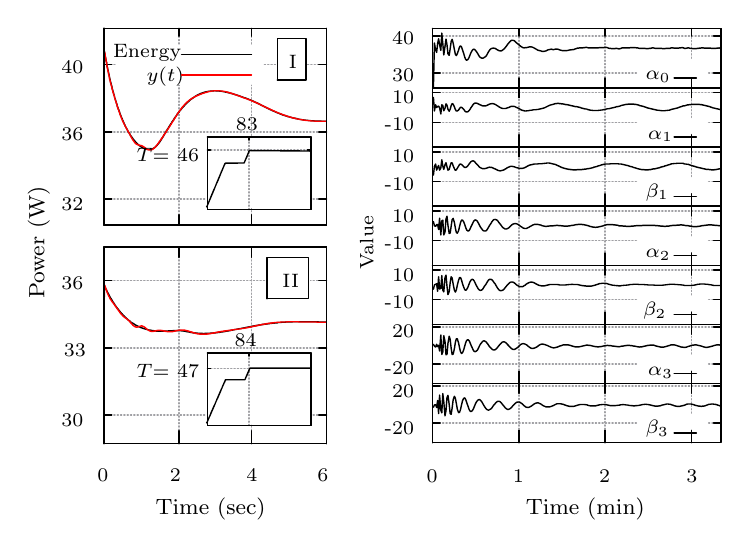
\begin{tikzpicture}[y=0.80pt, x=0.80pt, yscale=-\globalscale, xscale=\globalscale, inner sep=0pt, outer sep=0pt]
\scriptsize
\begin{scope}[shift={(-18.54884,-0.65233)},draw=black,line join=bevel,line cap=rect,even odd rule,line width=0.512pt]
  \begin{scope}[draw=black,line join=bevel,line cap=rect,line width=0.512pt]
  \end{scope}
  \begin{scope}[scale=1.008,draw=black,line join=bevel,line cap=rect,line width=0.512pt]
  \end{scope}
  \begin{scope}[cm={{1.00769,0.0,0.0,1.00769,(-21.0,-7.5)}},draw=ca0a0a4,dash pattern=on 0.40pt off 0.80pt,line join=round,line cap=round,line width=0.512pt]
    \path[draw] (41.5000,74.5000) -- (127.5000,74.5000);



  \end{scope}
  \begin{scope}[cm={{1.00769,0.0,0.0,1.00769,(-21.0,-7.5)}},draw=black,line join=round,line cap=round,line width=0.512pt]
    \path[draw] (41.5000,74.5000) -- (44.5000,74.5000);



    \path[draw] (127.5000,74.5000) -- (124.5000,74.5000);



  \end{scope}
  \begin{scope}[scale=1.008,draw=black,line join=bevel,line cap=rect,line width=0.512pt]
  \end{scope}
  \begin{scope}[cm={{1.00769,0.0,0.0,1.00769,(25.1923,79.6077)}},draw=black,line join=bevel,line cap=rect,line width=0.512pt]
  \end{scope}
  \begin{scope}[cm={{1.00769,0.0,0.0,1.00769,(25.1923,79.6077)}},draw=black,line join=bevel,line cap=rect,line width=0.512pt]
  \end{scope}
  \begin{scope}[cm={{1.00769,0.0,0.0,1.00769,(25.1923,79.6077)}},draw=black,line join=bevel,line cap=rect,line width=0.512pt]
  \end{scope}
  \begin{scope}[cm={{1.00769,0.0,0.0,1.00769,(25.1923,79.6077)}},draw=black,line join=bevel,line cap=rect,line width=0.512pt]
  \end{scope}
  \begin{scope}[cm={{1.00769,0.0,0.0,1.00769,(25.1923,79.6077)}},draw=black,line join=bevel,line cap=rect,line width=0.512pt]
  \end{scope}
  \begin{scope}[cm={{1.00769,0.0,0.0,1.00769,(4.1923,72.1077)}},draw=black,line join=bevel,line cap=rect,line width=0.512pt]
    \path[fill=black] (0.0000,0.0000) node[above right] (text34) {32};



  \end{scope}
  \begin{scope}[cm={{1.00769,0.0,0.0,1.00769,(25.1923,79.6077)}},draw=black,line join=bevel,line cap=rect,line width=0.512pt]
  \end{scope}
  \begin{scope}[scale=1.008,draw=black,line join=bevel,line cap=rect,line width=0.512pt]
  \end{scope}
  \begin{scope}[cm={{1.00769,0.0,0.0,1.00769,(-21.0,-7.5)}},draw=ca0a0a4,dash pattern=on 0.40pt off 0.80pt,line join=round,line cap=round,line width=0.512pt]
    \path[draw] (41.5000,48.5000) -- (127.5000,48.5000);



  \end{scope}
  \begin{scope}[cm={{1.00769,0.0,0.0,1.00769,(-21.0,-7.5)}},draw=black,line join=round,line cap=round,line width=0.512pt]
    \path[draw] (41.5000,48.5000) -- (44.5000,48.5000);



    \path[draw] (127.5000,48.5000) -- (124.5000,48.5000);



  \end{scope}
  \begin{scope}[scale=1.008,draw=black,line join=bevel,line cap=rect,line width=0.512pt]
  \end{scope}
  \begin{scope}[cm={{1.00769,0.0,0.0,1.00769,(25.1923,52.4)}},draw=black,line join=bevel,line cap=rect,line width=0.512pt]
  \end{scope}
  \begin{scope}[cm={{1.00769,0.0,0.0,1.00769,(25.1923,52.4)}},draw=black,line join=bevel,line cap=rect,line width=0.512pt]
  \end{scope}
  \begin{scope}[cm={{1.00769,0.0,0.0,1.00769,(25.1923,52.4)}},draw=black,line join=bevel,line cap=rect,line width=0.512pt]
  \end{scope}
  \begin{scope}[cm={{1.00769,0.0,0.0,1.00769,(25.1923,52.4)}},draw=black,line join=bevel,line cap=rect,line width=0.512pt]
  \end{scope}
  \begin{scope}[cm={{1.00769,0.0,0.0,1.00769,(25.1923,52.4)}},draw=black,line join=bevel,line cap=rect,line width=0.512pt]
  \end{scope}
  \begin{scope}[cm={{1.00769,0.0,0.0,1.00769,(4.1923,44.9)}},draw=black,line join=bevel,line cap=rect,line width=0.512pt]
    \path[fill=black] (0.0000,0.0000) node[above right] (text64) {36};



  \end{scope}
  \begin{scope}[cm={{1.00769,0.0,0.0,1.00769,(25.1923,52.4)}},draw=black,line join=bevel,line cap=rect,line width=0.512pt]
  \end{scope}
  \begin{scope}[scale=1.008,draw=black,line join=bevel,line cap=rect,line width=0.512pt]
  \end{scope}
  \begin{scope}[cm={{1.00769,0.0,0.0,1.00769,(-21.0,-7.5)}},draw=ca0a0a4,dash pattern=on 0.40pt off 0.80pt,line join=round,line cap=round,line width=0.512pt]
    \path[draw] (41.5000,22.5000) -- (46.5000,22.5000);



    \path[draw] (103.5000,22.5000) -- (127.5000,22.5000);



  \end{scope}
  \begin{scope}[cm={{1.00769,0.0,0.0,1.00769,(-21.0,-7.5)}},draw=black,line join=round,line cap=round,line width=0.512pt]
    \path[draw] (41.5000,22.5000) -- (44.5000,22.5000);



    \path[draw] (127.5000,22.5000) -- (124.5000,22.5000);



  \end{scope}
  \begin{scope}[scale=1.008,draw=black,line join=bevel,line cap=rect,line width=0.512pt]
  \end{scope}
  \begin{scope}[cm={{1.00769,0.0,0.0,1.00769,(25.1923,26.2)}},draw=black,line join=bevel,line cap=rect,line width=0.512pt]
  \end{scope}
  \begin{scope}[cm={{1.00769,0.0,0.0,1.00769,(25.1923,26.2)}},draw=black,line join=bevel,line cap=rect,line width=0.512pt]
  \end{scope}
  \begin{scope}[cm={{1.00769,0.0,0.0,1.00769,(25.1923,26.2)}},draw=black,line join=bevel,line cap=rect,line width=0.512pt]
  \end{scope}
  \begin{scope}[cm={{1.00769,0.0,0.0,1.00769,(25.1923,26.2)}},draw=black,line join=bevel,line cap=rect,line width=0.512pt]
  \end{scope}
  \begin{scope}[cm={{1.00769,0.0,0.0,1.00769,(25.1923,26.2)}},draw=black,line join=bevel,line cap=rect,line width=0.512pt]
  \end{scope}
  \begin{scope}[cm={{1.00769,0.0,0.0,1.00769,(4.1923,18.7)}},draw=black,line join=bevel,line cap=rect,line width=0.512pt]
    \path[fill=black] (0.0000,0.0000) node[above right] (text96) {40};



  \end{scope}
  \begin{scope}[cm={{1.00769,0.0,0.0,1.00769,(25.1923,26.2)}},draw=black,line join=bevel,line cap=rect,line width=0.512pt]
  \end{scope}
  \begin{scope}[scale=1.008,draw=black,line join=bevel,line cap=rect,line width=0.512pt]
  \end{scope}
  \begin{scope}[cm={{1.00769,0.0,0.0,1.00769,(-21.0,-7.5)}},draw=ca0a0a4,dash pattern=on 0.40pt off 0.80pt,line join=round,line cap=round,line width=0.512pt]
    \path[draw] (41.5000,84.5000) -- (41.5000,8.5000);



  \end{scope}
  \begin{scope}[cm={{1.00769,0.0,0.0,1.00769,(-21.0,-7.5)}},draw=black,line join=round,line cap=round,line width=0.512pt]
    \path[draw] (41.5000,84.5000) -- (41.5000,80.5000);



    \path[draw] (41.5000,8.5000) -- (41.5000,11.5000);



  \end{scope}
  \begin{scope}[scale=1.008,draw=black,line join=bevel,line cap=rect,line width=0.512pt]
  \end{scope}
  \begin{scope}[cm={{1.00769,0.0,0.0,1.00769,(42.3231,100.769)}},draw=black,line join=bevel,line cap=rect,line width=0.512pt]
  \end{scope}
  \begin{scope}[cm={{1.00769,0.0,0.0,1.00769,(42.3231,100.769)}},draw=black,line join=bevel,line cap=rect,line width=0.512pt]
  \end{scope}
  \begin{scope}[cm={{1.00769,0.0,0.0,1.00769,(42.3231,100.769)}},draw=black,line join=bevel,line cap=rect,line width=0.512pt]
  \end{scope}
  \begin{scope}[cm={{1.00769,0.0,0.0,1.00769,(42.3231,100.769)}},draw=black,line join=bevel,line cap=rect,line width=0.512pt]
  \end{scope}
  \begin{scope}[cm={{1.00769,0.0,0.0,1.00769,(42.3231,100.769)}},draw=black,line join=bevel,line cap=rect,line width=0.512pt]
  \end{scope}
  \begin{scope}[cm={{1.00769,0.0,0.0,1.00769,(42.3231,100.769)}},draw=black,line join=bevel,line cap=rect,line width=0.512pt]
  \end{scope}
  \begin{scope}[scale=1.008,draw=black,line join=bevel,line cap=rect,line width=0.512pt]
  \end{scope}
  \begin{scope}[cm={{1.00769,0.0,0.0,1.00769,(-21.0,-7.5)}},draw=ca0a0a4,dash pattern=on 0.40pt off 0.80pt,line join=round,line cap=round,line width=0.512pt]
    \path[draw] (70.5000,84.5000) -- (70.5000,30.5000);



    \path[draw] (70.5000,14.5000) -- (70.5000,8.5000);



  \end{scope}
  \begin{scope}[cm={{1.00769,0.0,0.0,1.00769,(-21.0,-7.5)}},draw=black,line join=round,line cap=round,line width=0.512pt]
    \path[draw] (70.5000,84.5000) -- (70.5000,80.5000);



    \path[draw] (70.5000,8.5000) -- (70.5000,11.5000);



  \end{scope}
  \begin{scope}[scale=1.008,draw=black,line join=bevel,line cap=rect,line width=0.512pt]
  \end{scope}
  \begin{scope}[cm={{1.00769,0.0,0.0,1.00769,(70.5385,100.769)}},draw=black,line join=bevel,line cap=rect,line width=0.512pt]
  \end{scope}
  \begin{scope}[cm={{1.00769,0.0,0.0,1.00769,(70.5385,100.769)}},draw=black,line join=bevel,line cap=rect,line width=0.512pt]
  \end{scope}
  \begin{scope}[cm={{1.00769,0.0,0.0,1.00769,(70.5385,100.769)}},draw=black,line join=bevel,line cap=rect,line width=0.512pt]
  \end{scope}
  \begin{scope}[cm={{1.00769,0.0,0.0,1.00769,(70.5385,100.769)}},draw=black,line join=bevel,line cap=rect,line width=0.512pt]
  \end{scope}
  \begin{scope}[cm={{1.00769,0.0,0.0,1.00769,(70.5385,100.769)}},draw=black,line join=bevel,line cap=rect,line width=0.512pt]
  \end{scope}
  \begin{scope}[cm={{1.00769,0.0,0.0,1.00769,(70.5385,100.769)}},draw=black,line join=bevel,line cap=rect,line width=0.512pt]
  \end{scope}
  \begin{scope}[scale=1.008,draw=black,line join=bevel,line cap=rect,line width=0.512pt]
  \end{scope}
  \begin{scope}[cm={{1.00769,0.0,0.0,1.00769,(-21.0,-7.5)}},draw=ca0a0a4,dash pattern=on 0.40pt off 0.80pt,line join=round,line cap=round,line width=0.512pt]
    \path[draw] (98.5000,84.5000) -- (98.5000,30.5000);



    \path[draw] (98.5000,14.5000) -- (98.5000,8.5000);



  \end{scope}
  \begin{scope}[cm={{1.00769,0.0,0.0,1.00769,(-21.0,-7.5)}},draw=black,line join=round,line cap=round,line width=0.512pt]
    \path[draw] (98.5000,84.5000) -- (98.5000,80.5000);



    \path[draw] (98.5000,8.5000) -- (98.5000,11.5000);



  \end{scope}
  \begin{scope}[scale=1.008,draw=black,line join=bevel,line cap=rect,line width=0.512pt]
  \end{scope}
  \begin{scope}[cm={{1.00769,0.0,0.0,1.00769,(99.7615,100.769)}},draw=black,line join=bevel,line cap=rect,line width=0.512pt]
  \end{scope}
  \begin{scope}[cm={{1.00769,0.0,0.0,1.00769,(99.7615,100.769)}},draw=black,line join=bevel,line cap=rect,line width=0.512pt]
  \end{scope}
  \begin{scope}[cm={{1.00769,0.0,0.0,1.00769,(99.7615,100.769)}},draw=black,line join=bevel,line cap=rect,line width=0.512pt]
  \end{scope}
  \begin{scope}[cm={{1.00769,0.0,0.0,1.00769,(99.7615,100.769)}},draw=black,line join=bevel,line cap=rect,line width=0.512pt]
  \end{scope}
  \begin{scope}[cm={{1.00769,0.0,0.0,1.00769,(99.7615,100.769)}},draw=black,line join=bevel,line cap=rect,line width=0.512pt]
  \end{scope}
  \begin{scope}[cm={{1.00769,0.0,0.0,1.00769,(99.7615,100.769)}},draw=black,line join=bevel,line cap=rect,line width=0.512pt]
  \end{scope}
  \begin{scope}[scale=1.008,draw=black,line join=bevel,line cap=rect,line width=0.512pt]
  \end{scope}
  \begin{scope}[cm={{1.00769,0.0,0.0,1.00769,(-21.0,-7.5)}},draw=ca0a0a4,dash pattern=on 0.40pt off 0.80pt,line join=round,line cap=round,line width=0.512pt]
    \path[draw] (127.5000,84.5000) -- (127.5000,8.5000);



  \end{scope}
  \begin{scope}[cm={{1.00769,0.0,0.0,1.00769,(-21.0,-7.5)}},draw=black,line join=round,line cap=round,line width=0.512pt]
    \path[draw] (127.5000,84.5000) -- (127.5000,80.5000);



    \path[draw] (127.5000,8.5000) -- (127.5000,11.5000);



  \end{scope}
  \begin{scope}[scale=1.008,draw=black,line join=bevel,line cap=rect,line width=0.512pt]
  \end{scope}
  \begin{scope}[cm={{1.00769,0.0,0.0,1.00769,(127.977,100.769)}},draw=black,line join=bevel,line cap=rect,line width=0.512pt]
  \end{scope}
  \begin{scope}[cm={{1.00769,0.0,0.0,1.00769,(127.977,100.769)}},draw=black,line join=bevel,line cap=rect,line width=0.512pt]
  \end{scope}
  \begin{scope}[cm={{1.00769,0.0,0.0,1.00769,(127.977,100.769)}},draw=black,line join=bevel,line cap=rect,line width=0.512pt]
  \end{scope}
  \begin{scope}[cm={{1.00769,0.0,0.0,1.00769,(127.977,100.769)}},draw=black,line join=bevel,line cap=rect,line width=0.512pt]
  \end{scope}
  \begin{scope}[cm={{1.00769,0.0,0.0,1.00769,(127.977,100.769)}},draw=black,line join=bevel,line cap=rect,line width=0.512pt]
  \end{scope}
  \begin{scope}[cm={{1.00769,0.0,0.0,1.00769,(127.977,100.769)}},draw=black,line join=bevel,line cap=rect,line width=0.512pt]
  \end{scope}
  \begin{scope}[scale=1.008,draw=black,line join=bevel,line cap=rect,line width=0.512pt]
  \end{scope}
  \begin{scope}[cm={{1.00769,0.0,0.0,1.00769,(-21.0,-7.5)}},draw=black,line join=round,line cap=round,line width=0.512pt]
    \path[draw] (41.5000,8.5000) -- (41.5000,84.5000) -- (127.5000,84.5000) -- (127.5000,8.5000) -- (41.5000,8.5000);



  \end{scope}
  \begin{scope}[scale=1.008,draw=black,line join=bevel,line cap=rect,line width=0.512pt]
  \end{scope}
  \begin{scope}[scale=1.008,draw=black,line join=bevel,line cap=rect,line width=0.512pt]
  \end{scope}
  \begin{scope}[cm={{1.00769,0.0,0.0,1.00769,(-21.0,-7.5)}},fill=cffffff]
    \path[fill,rounded corners=0.0000cm] (108.0000,12.0000) rectangle (119.0000,28.0000);



  \end{scope}
  \begin{scope}[scale=1.008,draw=black,line join=bevel,line cap=rect,line width=0.512pt]
  \end{scope}
  \begin{scope}[scale=1.008,draw=black,line join=bevel,line cap=rect,line width=0.512pt]
  \end{scope}
  \begin{scope}[cm={{1.00769,0.0,0.0,1.00769,(-21.0,-7.5)}},draw=black,line join=round,line cap=round,line width=0.512pt]
    \path[draw] (108.5000,28.5000) -- (108.5000,12.5000) -- (119.5000,12.5000) -- (119.5000,28.5000) -- (108.5000,28.5000);



  \end{scope}
  \begin{scope}[scale=1.008,draw=black,line join=bevel,line cap=rect,line width=0.512pt]
  \end{scope}
  \begin{scope}[cm={{1.00769,0.0,0.0,1.00769,(112.862,24.1846)}},draw=black,line join=bevel,line cap=rect,line width=0.512pt]
  \end{scope}
  \begin{scope}[cm={{1.00769,0.0,0.0,1.00769,(112.862,24.1846)}},draw=black,line join=bevel,line cap=rect,line width=0.512pt]
  \end{scope}
  \begin{scope}[cm={{1.00769,0.0,0.0,1.00769,(112.862,24.1846)}},draw=black,line join=bevel,line cap=rect,line width=0.512pt]
  \end{scope}
  \begin{scope}[cm={{1.00769,0.0,0.0,1.00769,(112.862,24.1846)}},draw=black,line join=bevel,line cap=rect,line width=0.512pt]
  \end{scope}
  \begin{scope}[cm={{1.00769,0.0,0.0,1.00769,(112.862,24.1846)}},draw=black,line join=bevel,line cap=rect,line width=0.512pt]
  \end{scope}
  \begin{scope}[cm={{1.00769,0.0,0.0,1.00769,(92.862,16.6846)}},draw=black,line join=bevel,line cap=rect,line width=0.512pt]
    \path[fill=black] (0.0000,0.0000) node[above right] (text244) {I};



  \end{scope}
  \begin{scope}[cm={{1.00769,0.0,0.0,1.00769,(112.862,24.1846)}},draw=black,line join=bevel,line cap=rect,line width=0.512pt]
  \end{scope}
  \begin{scope}[cm={{0.0,-1.00769,1.00769,0.0,(15.1154,113.869)}},draw=black,line join=bevel,line cap=rect,line width=0.512pt]
  \end{scope}
  \begin{scope}[cm={{0.0,-1.00769,1.00769,0.0,(15.1154,113.869)}},draw=black,line join=bevel,line cap=rect,line width=0.512pt]
  \end{scope}
  \begin{scope}[cm={{0.0,-1.00769,1.00769,0.0,(15.1154,113.869)}},draw=black,line join=bevel,line cap=rect,line width=0.512pt]
  \end{scope}
  \begin{scope}[cm={{0.0,-1.00769,1.00769,0.0,(15.1154,113.869)}},draw=black,line join=bevel,line cap=rect,line width=0.512pt]
  \end{scope}
  \begin{scope}[cm={{0.0,-1.00769,1.00769,0.0,(15.1154,113.869)}},draw=black,line join=bevel,line cap=rect,line width=0.512pt]
  \end{scope}
  \begin{scope}[cm={{0.0,-1.00769,1.00769,0.0,(-8.8846,106.369)}},draw=black,line join=bevel,line cap=rect,line width=0.512pt]
    \path[fill=black] (0.0000,0.0000) node[above right] (text260) {\footnotesize \rotatebox{90}{Power (W)}};



  \end{scope}
  \begin{scope}[cm={{0.0,-1.00769,1.00769,0.0,(15.1154,113.869)}},draw=black,line join=bevel,line cap=rect,line width=0.512pt]
  \end{scope}
  \begin{scope}[cm={{1.00769,0.0,0.0,1.00769,(48.3692,23.1769)}},draw=black,line join=bevel,line cap=rect,line width=0.512pt]
  \end{scope}
  \begin{scope}[cm={{1.00769,0.0,0.0,1.00769,(48.3692,23.1769)}},draw=black,line join=bevel,line cap=rect,line width=0.512pt]
  \end{scope}
  \begin{scope}[cm={{1.00769,0.0,0.0,1.00769,(48.3692,23.1769)}},draw=black,line join=bevel,line cap=rect,line width=0.512pt]
  \end{scope}
  \begin{scope}[cm={{1.00769,0.0,0.0,1.00769,(48.3692,23.1769)}},draw=black,line join=bevel,line cap=rect,line width=0.512pt]
  \end{scope}
  \begin{scope}[cm={{1.00769,0.0,0.0,1.00769,(48.3692,23.1769)}},draw=black,line join=bevel,line cap=rect,line width=0.512pt]
  \end{scope}
  \begin{scope}[cm={{1.00769,0.0,0.0,1.00769,(24.3692,13.6769)}},draw=black,line join=bevel,line cap=rect,line width=0.512pt]
    \path[fill=black] (0.0000,0.0000) node[above right] (text276) {\scriptsize Energy};



  \end{scope}
  \begin{scope}[cm={{1.00769,0.0,0.0,1.00769,(48.3692,23.1769)}},draw=black,line join=bevel,line cap=rect,line width=0.512pt]
  \end{scope}
  \begin{scope}[scale=1.008,draw=black,line join=bevel,line cap=rect,line width=0.512pt]
  \end{scope}
  \begin{scope}[cm={{1.00769,0.0,0.0,1.00769,(-21.0,-7.5)}},draw=black,line join=round,line cap=round,line width=0.512pt]
    \path[draw,even odd rule] (71.5000,18.5000) -- (98.5000,18.5000);



  \end{scope}
  \begin{scope}[scale=1.008,draw=black,line join=bevel,line cap=rect,line width=0.512pt]
  \end{scope}
  \begin{scope}[scale=1.008,draw=black,line join=bevel,line cap=rect,line width=0.512pt]
  \end{scope}
  \begin{scope}[scale=1.008,draw=black,line join=bevel,line cap=rect,line width=0.512pt]
  \end{scope}
  \begin{scope}[scale=1.008,draw=black,line join=bevel,line cap=rect,line width=0.512pt]
  \end{scope}
  \begin{scope}[cm={{1.00769,0.0,0.0,1.00769,(-21.0,-7.5)}},draw=black,line join=round,line cap=round,line width=0.512pt]
    \path[draw] (41.6000,17.0000) -- (41.6000,17.0000) -- (41.7000,17.8000) -- (41.9000,18.6000) -- (42.0000,19.4000) -- (42.2000,20.2000) -- (42.3000,20.9000) -- (42.5000,21.6000) -- (42.6000,22.4000) -- (42.7000,23.1000) -- (42.9000,23.8000) -- (43.0000,24.5000) -- (43.2000,25.2000) -- (43.3000,25.8000) -- (43.5000,26.5000) -- (43.6000,27.1000) -- (43.7000,27.7000) -- (43.9000,28.4000) -- (44.0000,29.0000) -- (44.2000,29.6000) -- (44.3000,30.1000) -- (44.5000,30.7000) -- (44.6000,31.3000) -- (44.7000,31.8000) -- (44.9000,32.4000) -- (45.0000,32.9000) -- (45.2000,33.4000) -- (45.3000,34.0000) -- (45.5000,34.5000) -- (45.6000,35.0000) -- (45.7000,35.5000) -- (45.9000,35.9000) -- (46.0000,36.4000) -- (46.2000,36.9000) -- (46.3000,37.3000) -- (46.5000,37.8000) -- (46.6000,38.2000) -- (46.7000,38.7000) -- (46.9000,39.1000) -- (47.0000,39.5000) -- (47.2000,39.9000) -- (47.3000,40.3000) -- (47.5000,40.7000) -- (47.6000,41.1000) -- (47.7000,41.5000) -- (47.9000,41.9000) -- (48.0000,42.2000) -- (48.2000,42.6000) -- (48.3000,43.0000) -- (48.5000,43.3000) -- (48.6000,43.6000) -- (48.7000,44.0000) -- (48.9000,44.3000) -- (49.0000,44.6000) -- (49.2000,45.0000) -- (49.3000,45.3000) -- (49.5000,45.6000) -- (49.6000,45.9000) -- (49.7000,46.2000) -- (49.9000,46.5000) -- (50.0000,46.8000) -- (50.2000,47.0000) -- (50.3000,47.3000) -- (50.5000,47.6000) -- (50.6000,47.8000) -- (50.7000,48.1000) -- (50.9000,48.4000) -- (51.0000,48.6000) -- (51.2000,48.8000) -- (51.3000,49.1000) -- (51.5000,49.3000) -- (51.6000,49.5000) -- (51.7000,49.8000) -- (51.9000,50.0000) -- (52.0000,50.2000) -- (52.2000,50.4000) -- (52.3000,50.6000) -- (52.5000,50.8000) -- (52.6000,51.0000) -- (52.7000,51.2000) -- (52.9000,51.4000) -- (53.0000,51.6000) -- (53.2000,51.7000) -- (53.3000,51.9000) -- (53.5000,52.1000) -- (53.6000,52.3000) -- (53.7000,52.4000) -- (53.9000,52.6000) -- (54.0000,52.7000) -- (54.2000,52.9000) -- (54.3000,53.0000) -- (54.5000,53.1000) -- (54.6000,53.3000) -- (54.7000,53.4000) -- (54.9000,53.5000) -- (55.0000,53.7000) -- (55.2000,53.8000) -- (55.3000,53.9000) -- (55.5000,54.0000) -- (55.6000,54.1000) -- (55.7000,54.2000) -- (55.9000,54.3000) -- (56.0000,54.4000) -- (56.2000,54.5000) -- (56.3000,54.6000) -- (56.5000,54.6000) -- (56.6000,54.7000) -- (56.7000,54.8000) -- (56.9000,54.9000) -- (57.0000,54.9000) -- (57.2000,55.0000) -- (57.3000,55.0000) -- (57.5000,55.1000) -- (57.6000,55.1000) -- (57.7000,55.2000) -- (57.9000,55.2000) -- (58.0000,55.2000) -- (58.2000,55.3000) -- (58.3000,55.3000) -- (58.5000,55.3000) -- (58.6000,55.3000) -- (58.7000,55.3000) -- (58.9000,55.3000) -- (59.0000,55.3000) -- (59.2000,55.3000) -- (59.3000,55.3000) -- (59.5000,55.3000) -- (59.6000,55.2000) -- (59.7000,55.2000) -- (59.9000,55.2000) -- (60.0000,55.1000) -- (60.2000,55.1000) -- (60.3000,55.0000) -- (60.5000,54.9000) -- (60.6000,54.9000) -- (60.7000,54.8000) -- (60.9000,54.7000) -- (61.0000,54.6000) -- (61.2000,54.5000) -- (61.3000,54.4000) -- (61.5000,54.2000) -- (61.6000,54.1000) -- (61.7000,54.0000) -- (61.9000,53.8000) -- (62.0000,53.7000) -- (62.2000,53.5000) -- (62.3000,53.3000) -- (62.5000,53.1000) -- (62.6000,53.0000) -- (62.7000,52.8000) -- (62.9000,52.6000) -- (63.0000,52.4000) -- (63.2000,52.2000) -- (63.3000,52.0000) -- (63.5000,51.7000) -- (63.6000,51.5000) -- (63.7000,51.3000) -- (63.9000,51.1000) -- (64.0000,50.8000) -- (64.2000,50.6000) -- (64.3000,50.4000) -- (64.5000,50.1000) -- (64.6000,49.9000) -- (64.7000,49.7000) -- (64.9000,49.4000) -- (65.0000,49.2000) -- (65.2000,49.0000) -- (65.3000,48.7000) -- (65.5000,48.5000) -- (65.6000,48.2000) -- (65.7000,48.0000) -- (65.9000,47.8000) -- (66.0000,47.5000) -- (66.2000,47.3000) -- (66.3000,47.1000) -- (66.5000,46.8000) -- (66.6000,46.6000) -- (66.7000,46.4000) -- (66.9000,46.1000) -- (67.0000,45.9000) -- (67.2000,45.7000) -- (67.3000,45.4000) -- (67.5000,45.2000) -- (67.6000,45.0000) -- (67.7000,44.8000) -- (67.9000,44.5000) -- (68.0000,44.3000) -- (68.2000,44.1000) -- (68.3000,43.9000) -- (68.5000,43.7000) -- (68.6000,43.5000) -- (68.7000,43.2000) -- (68.9000,43.0000) -- (69.0000,42.8000) -- (69.2000,42.6000) -- (69.3000,42.4000) -- (69.5000,42.2000) -- (69.6000,42.0000) -- (69.7000,41.8000) -- (69.9000,41.6000) -- (70.0000,41.4000) -- (70.2000,41.2000) -- (70.3000,41.0000) -- (70.5000,40.9000) -- (70.6000,40.7000) -- (70.7000,40.5000) -- (70.9000,40.3000) -- (71.0000,40.1000) -- (71.2000,40.0000) -- (71.3000,39.8000) -- (71.5000,39.6000) -- (71.6000,39.4000) -- (71.7000,39.3000) -- (71.9000,39.1000) -- (72.0000,38.9000) -- (72.2000,38.8000) -- (72.3000,38.6000) -- (72.5000,38.5000) -- (72.6000,38.3000) -- (72.7000,38.1000) -- (72.9000,38.0000) -- (73.0000,37.9000) -- (73.2000,37.7000) -- (73.3000,37.6000) -- (73.5000,37.4000) -- (73.6000,37.3000) -- (73.7000,37.1000) -- (73.9000,37.0000) -- (74.0000,36.9000) -- (74.2000,36.8000) -- (74.3000,36.6000) -- (74.5000,36.5000) -- (74.6000,36.4000) -- (74.7000,36.2000) -- (74.9000,36.1000) -- (75.0000,36.0000) -- (75.2000,35.9000) -- (75.3000,35.8000) -- (75.5000,35.7000) -- (75.6000,35.6000) -- (75.7000,35.5000) -- (75.9000,35.4000) -- (76.0000,35.3000) -- (76.2000,35.2000) -- (76.3000,35.1000) -- (76.5000,35.0000) -- (76.6000,34.9000) -- (76.7000,34.8000) -- (76.9000,34.7000) -- (77.0000,34.6000) -- (77.2000,34.5000) -- (77.3000,34.4000) -- (77.5000,34.4000) -- (77.6000,34.3000) -- (77.7000,34.2000) -- (77.9000,34.1000) -- (78.0000,34.1000) -- (78.2000,34.0000) -- (78.3000,33.9000) -- (78.5000,33.9000) -- (78.6000,33.8000) -- (78.7000,33.7000) -- (78.9000,33.7000) -- (79.0000,33.6000) -- (79.2000,33.6000) -- (79.3000,33.5000) -- (79.5000,33.5000) -- (79.6000,33.4000) -- (79.7000,33.4000) -- (79.9000,33.3000) -- (80.0000,33.3000) -- (80.2000,33.2000) -- (80.3000,33.2000) -- (80.5000,33.1000) -- (80.6000,33.1000) -- (80.7000,33.1000) -- (80.9000,33.0000) -- (81.0000,33.0000) -- (81.2000,33.0000) -- (81.3000,32.9000) -- (81.5000,32.9000) -- (81.6000,32.9000) -- (81.7000,32.9000) -- (81.9000,32.8000) -- (82.0000,32.8000) -- (82.2000,32.8000) -- (82.3000,32.8000) -- (82.5000,32.8000) -- (82.6000,32.7000) -- (82.7000,32.7000) -- (82.9000,32.7000) -- (83.0000,32.7000) -- (83.2000,32.7000) -- (83.3000,32.7000) -- (83.5000,32.7000) -- (83.6000,32.7000) -- (83.7000,32.7000) -- (83.9000,32.6000) -- (84.0000,32.6000) -- (84.2000,32.6000) -- (84.3000,32.6000) -- (84.5000,32.6000) -- (84.6000,32.6000) -- (84.7000,32.6000) -- (84.9000,32.7000) -- (85.0000,32.7000) -- (85.2000,32.7000) -- (85.3000,32.7000) -- (85.4000,32.7000) -- (85.6000,32.7000) -- (85.7000,32.7000) -- (85.9000,32.7000) -- (86.0000,32.7000) -- (86.2000,32.7000) -- (86.3000,32.8000) -- (86.4000,32.8000) -- (86.6000,32.8000) -- (86.7000,32.8000) -- (86.9000,32.8000) -- (87.0000,32.8000) -- (87.2000,32.9000) -- (87.3000,32.9000) -- (87.4000,32.9000) -- (87.6000,32.9000) -- (87.7000,33.0000) -- (87.9000,33.0000) -- (88.0000,33.0000) -- (88.2000,33.0000) -- (88.3000,33.1000) -- (88.4000,33.1000) -- (88.6000,33.1000) -- (88.7000,33.1000) -- (88.9000,33.2000) -- (89.0000,33.2000) -- (89.2000,33.2000) -- (89.3000,33.3000) -- (89.4000,33.3000) -- (89.6000,33.3000) -- (89.7000,33.4000) -- (89.9000,33.4000) -- (90.0000,33.4000) -- (90.2000,33.5000) -- (90.3000,33.5000) -- (90.4000,33.6000) -- (90.6000,33.6000) -- (90.7000,33.6000) -- (90.9000,33.7000) -- (91.0000,33.7000) -- (91.2000,33.8000) -- (91.3000,33.8000) -- (91.4000,33.8000) -- (91.6000,33.9000) -- (91.7000,33.9000) -- (91.9000,34.0000) -- (92.0000,34.0000) -- (92.2000,34.1000) -- (92.3000,34.1000) -- (92.4000,34.1000) -- (92.6000,34.2000) -- (92.7000,34.2000) -- (92.9000,34.3000) -- (93.0000,34.3000) -- (93.2000,34.4000) -- (93.3000,34.4000) -- (93.4000,34.5000) -- (93.6000,34.5000) -- (93.7000,34.6000) -- (93.9000,34.6000) -- (94.0000,34.7000) -- (94.2000,34.7000) -- (94.3000,34.8000) -- (94.4000,34.8000) -- (94.6000,34.9000) -- (94.7000,34.9000) -- (94.9000,35.0000) -- (95.0000,35.0000) -- (95.2000,35.1000) -- (95.3000,35.1000) -- (95.4000,35.2000) -- (95.6000,35.2000) -- (95.7000,35.3000) -- (95.9000,35.3000) -- (96.0000,35.4000) -- (96.2000,35.4000) -- (96.3000,35.5000) -- (96.4000,35.5000) -- (96.6000,35.6000) -- (96.7000,35.6000) -- (96.9000,35.7000) -- (97.0000,35.7000) -- (97.2000,35.8000) -- (97.3000,35.9000) -- (97.4000,35.9000) -- (97.6000,36.0000) -- (97.7000,36.0000) -- (97.9000,36.1000) -- (98.0000,36.1000) -- (98.2000,36.2000) -- (98.3000,36.2000) -- (98.4000,36.3000) -- (98.6000,36.4000) -- (98.7000,36.4000) -- (98.9000,36.5000) -- (99.0000,36.6000) -- (99.2000,36.6000) -- (99.3000,36.7000) -- (99.4000,36.8000) -- (99.6000,36.8000) -- (99.7000,36.9000) -- (99.9000,37.0000) -- (100.0000,37.0000) -- (100.2000,37.1000) -- (100.3000,37.2000) -- (100.4000,37.2000) -- (100.6000,37.3000) -- (100.7000,37.4000) -- (100.9000,37.4000) -- (101.0000,37.5000) -- (101.2000,37.6000) -- (101.3000,37.6000) -- (101.4000,37.7000) -- (101.6000,37.8000) -- (101.7000,37.9000) -- (101.9000,37.9000) -- (102.0000,38.0000) -- (102.2000,38.1000) -- (102.3000,38.2000) -- (102.4000,38.2000) -- (102.6000,38.3000) -- (102.7000,38.4000) -- (102.9000,38.4000) -- (103.0000,38.5000) -- (103.2000,38.6000) -- (103.3000,38.7000) -- (103.4000,38.7000) -- (103.6000,38.8000) -- (103.7000,38.9000) -- (103.9000,38.9000) -- (104.0000,39.0000) -- (104.2000,39.1000) -- (104.3000,39.2000) -- (104.4000,39.2000) -- (104.6000,39.3000) -- (104.7000,39.4000) -- (104.9000,39.4000) -- (105.0000,39.5000) -- (105.2000,39.6000) -- (105.3000,39.7000) -- (105.4000,39.7000) -- (105.6000,39.8000) -- (105.7000,39.9000) -- (105.9000,39.9000) -- (106.0000,40.0000) -- (106.2000,40.1000) -- (106.3000,40.1000) -- (106.4000,40.2000) -- (106.6000,40.3000) -- (106.7000,40.3000) -- (106.9000,40.4000) -- (107.0000,40.5000) -- (107.2000,40.5000) -- (107.3000,40.6000) -- (107.4000,40.6000) -- (107.6000,40.7000) -- (107.7000,40.8000) -- (107.9000,40.8000) -- (108.0000,40.9000) -- (108.2000,41.0000) -- (108.3000,41.0000) -- (108.4000,41.1000) -- (108.6000,41.1000) -- (108.7000,41.2000) -- (108.9000,41.3000) -- (109.0000,41.3000) -- (109.2000,41.4000) -- (109.3000,41.4000) -- (109.4000,41.5000) -- (109.6000,41.5000) -- (109.7000,41.6000) -- (109.9000,41.6000) -- (110.0000,41.7000) -- (110.2000,41.7000) -- (110.3000,41.8000) -- (110.4000,41.9000) -- (110.6000,41.9000) -- (110.7000,42.0000) -- (110.9000,42.0000) -- (111.0000,42.1000) -- (111.2000,42.1000) -- (111.3000,42.1000) -- (111.4000,42.2000) -- (111.6000,42.2000) -- (111.7000,42.3000) -- (111.9000,42.3000) -- (112.0000,42.4000) -- (112.2000,42.4000) -- (112.3000,42.5000) -- (112.4000,42.5000) -- (112.6000,42.6000) -- (112.7000,42.6000) -- (112.9000,42.6000) -- (113.0000,42.7000) -- (113.2000,42.7000) -- (113.3000,42.8000) -- (113.4000,42.8000) -- (113.6000,42.8000) -- (113.7000,42.9000) -- (113.9000,42.9000) -- (114.0000,43.0000) -- (114.2000,43.0000) -- (114.3000,43.0000) -- (114.4000,43.1000) -- (114.6000,43.1000) -- (114.7000,43.1000) -- (114.9000,43.2000) -- (115.0000,43.2000) -- (115.2000,43.2000) -- (115.3000,43.3000) -- (115.4000,43.3000) -- (115.6000,43.3000) -- (115.7000,43.4000) -- (115.9000,43.4000) -- (116.0000,43.4000) -- (116.2000,43.4000) -- (116.3000,43.5000) -- (116.4000,43.5000) -- (116.6000,43.5000) -- (116.7000,43.6000) -- (116.9000,43.6000) -- (117.0000,43.6000) -- (117.2000,43.6000) -- (117.3000,43.7000) -- (117.4000,43.7000) -- (117.6000,43.7000) -- (117.7000,43.7000) -- (117.9000,43.7000) -- (118.0000,43.8000) -- (118.2000,43.8000) -- (118.3000,43.8000) -- (118.4000,43.8000) -- (118.6000,43.9000) -- (118.7000,43.9000) -- (118.9000,43.9000) -- (119.0000,43.9000) -- (119.2000,43.9000) -- (119.3000,44.0000) -- (119.4000,44.0000) -- (119.6000,44.0000) -- (119.7000,44.0000) -- (119.9000,44.0000) -- (120.0000,44.0000) -- (120.2000,44.0000) -- (120.3000,44.1000) -- (120.4000,44.1000) -- (120.6000,44.1000) -- (120.7000,44.1000) -- (120.9000,44.1000) -- (121.0000,44.1000) -- (121.2000,44.1000) -- (121.3000,44.2000) -- (121.4000,44.2000) -- (121.6000,44.2000) -- (121.7000,44.2000) -- (121.9000,44.2000) -- (122.0000,44.2000) -- (122.2000,44.2000) -- (122.3000,44.2000) -- (122.4000,44.2000) -- (122.6000,44.2000) -- (122.7000,44.3000) -- (122.9000,44.3000) -- (123.0000,44.3000) -- (123.2000,44.3000) -- (123.3000,44.3000) -- (123.4000,44.3000) -- (123.6000,44.3000) -- (123.7000,44.3000) -- (123.9000,44.3000) -- (124.0000,44.3000) -- (124.2000,44.3000) -- (124.3000,44.3000) -- (124.4000,44.3000) -- (124.6000,44.3000) -- (124.7000,44.3000) -- (124.9000,44.3000) -- (125.0000,44.3000) -- (125.2000,44.3000) -- (125.3000,44.3000) -- (125.4000,44.4000) -- (125.6000,44.4000) -- (125.7000,44.4000) -- (125.9000,44.4000) -- (126.0000,44.4000) -- (126.2000,44.4000) -- (126.3000,44.4000) -- (126.4000,44.4000) -- (126.6000,44.4000) -- (126.7000,44.4000) -- (126.9000,44.4000) -- (127.0000,44.4000) -- (127.2000,44.4000) -- (127.3000,44.4000);



  \end{scope}
  \begin{scope}[scale=1.008,draw=black,line join=bevel,line cap=rect,line width=0.512pt]
  \end{scope}
  \begin{scope}[cm={{1.00769,0.0,0.0,1.00769,(52.4,31.2385)}},draw=black,line join=bevel,line cap=rect,line width=0.512pt]
  \end{scope}
  \begin{scope}[cm={{1.00769,0.0,0.0,1.00769,(52.4,31.2385)}},draw=black,line join=bevel,line cap=rect,line width=0.512pt]
  \end{scope}
  \begin{scope}[cm={{1.00769,0.0,0.0,1.00769,(52.4,31.2385)}},draw=black,line join=bevel,line cap=rect,line width=0.512pt]
  \end{scope}
  \begin{scope}[cm={{1.00769,0.0,0.0,1.00769,(52.4,31.2385)}},draw=black,line join=bevel,line cap=rect,line width=0.512pt]
  \end{scope}
  \begin{scope}[cm={{1.00769,0.0,0.0,1.00769,(52.4,31.2385)}},draw=black,line join=bevel,line cap=rect,line width=0.512pt]
  \end{scope}
  \begin{scope}[cm={{1.00769,0.0,0.0,1.00769,(37.4,23.7385)}},draw=black,line join=bevel,line cap=rect,line width=0.512pt]
    \path[fill=black] (0.0000,0.0000) node[above right] (text312) {\scriptsize $y(t)$};



  \end{scope}
  \begin{scope}[cm={{1.00769,0.0,0.0,1.00769,(52.4,31.2385)}},draw=black,line join=bevel,line cap=rect,line width=0.512pt]
  \end{scope}
  \begin{scope}[scale=1.008,draw=black,line join=bevel,line cap=rect,line width=0.512pt]
  \end{scope}
  \begin{scope}[cm={{1.00769,0.0,0.0,1.00769,(-21.0,-7.5)}},draw=red,line join=round,line cap=round,line width=0.512pt]
    \path[draw,even odd rule] (71.5000,26.5000) -- (98.5000,26.5000);



  \end{scope}
  \begin{scope}[scale=1.008,draw=black,line join=bevel,line cap=rect,line width=0.512pt]
  \end{scope}
  \begin{scope}[scale=1.008,draw=black,line join=bevel,line cap=rect,line width=0.512pt]
  \end{scope}
  \begin{scope}[scale=1.008,draw=black,line join=bevel,line cap=rect,line width=0.512pt]
  \end{scope}
  \begin{scope}[scale=1.008,draw=black,line join=bevel,line cap=rect,line width=0.512pt]
  \end{scope}
  \begin{scope}[cm={{1.00769,0.0,0.0,1.00769,(-21.0,-7.5)}},draw=red,line join=round,line cap=round,line width=0.512pt]
    \path[draw] (41.6000,21.8000) -- (41.6000,21.8000) -- (41.7000,17.5000) -- (41.9000,18.2000) -- (42.0000,19.1000) -- (42.2000,20.0000) -- (42.3000,20.9000) -- (42.5000,21.7000) -- (42.6000,22.5000) -- (42.7000,23.3000) -- (42.9000,24.1000) -- (43.0000,24.8000) -- (43.2000,25.5000) -- (43.3000,26.2000) -- (43.5000,26.9000) -- (43.6000,27.6000) -- (43.7000,28.2000) -- (43.9000,28.8000) -- (44.0000,29.4000) -- (44.2000,30.0000) -- (44.3000,30.5000) -- (44.5000,31.1000) -- (44.6000,31.6000) -- (44.7000,32.1000) -- (44.9000,32.7000) -- (45.0000,33.2000) -- (45.2000,33.7000) -- (45.3000,34.2000) -- (45.5000,34.6000) -- (45.6000,35.1000) -- (45.7000,35.6000) -- (45.9000,36.1000) -- (46.0000,36.5000) -- (46.2000,37.0000) -- (46.3000,37.5000) -- (46.5000,37.9000) -- (46.6000,38.4000) -- (46.7000,38.8000) -- (46.9000,39.3000) -- (47.0000,39.7000) -- (47.2000,40.1000) -- (47.3000,40.6000) -- (47.5000,41.0000) -- (47.6000,41.4000) -- (47.7000,41.8000) -- (47.9000,42.2000) -- (48.0000,42.5000) -- (48.2000,42.9000) -- (48.3000,43.3000) -- (48.5000,43.6000) -- (48.6000,43.9000) -- (48.7000,44.3000) -- (48.9000,44.6000) -- (49.0000,44.9000) -- (49.2000,45.2000) -- (49.3000,45.5000) -- (49.5000,45.8000) -- (49.6000,46.0000) -- (49.7000,46.3000) -- (49.9000,46.6000) -- (50.0000,46.8000) -- (50.2000,47.1000) -- (50.3000,47.4000) -- (50.5000,47.6000) -- (50.6000,47.9000) -- (50.7000,48.1000) -- (50.9000,48.4000) -- (51.0000,48.7000) -- (51.2000,48.9000) -- (51.3000,49.2000) -- (51.5000,49.4000) -- (51.6000,49.7000) -- (51.7000,50.0000) -- (51.9000,50.2000) -- (52.0000,50.5000) -- (52.2000,50.8000) -- (52.3000,51.0000) -- (52.5000,51.3000) -- (52.6000,51.5000) -- (52.7000,51.7000) -- (52.9000,51.9000) -- (53.0000,52.1000) -- (53.2000,52.3000) -- (53.3000,52.5000) -- (53.5000,52.7000) -- (53.6000,52.8000) -- (53.7000,52.9000) -- (53.9000,53.1000) -- (54.0000,53.2000) -- (54.2000,53.3000) -- (54.3000,53.3000) -- (54.5000,53.4000) -- (54.6000,53.5000) -- (54.7000,53.5000) -- (54.9000,53.6000) -- (55.0000,53.6000) -- (55.2000,53.6000) -- (55.3000,53.7000) -- (55.5000,53.7000) -- (55.6000,53.7000) -- (55.7000,53.8000) -- (55.9000,53.8000) -- (56.0000,53.8000) -- (56.2000,53.9000) -- (56.3000,54.0000) -- (56.5000,54.0000) -- (56.6000,54.1000) -- (56.7000,54.2000) -- (56.9000,54.3000) -- (57.0000,54.4000) -- (57.2000,54.5000) -- (57.3000,54.6000) -- (57.5000,54.7000) -- (57.6000,54.8000) -- (57.7000,54.9000) -- (57.9000,55.0000) -- (58.0000,55.1000) -- (58.2000,55.2000) -- (58.3000,55.3000) -- (58.5000,55.3000) -- (58.6000,55.4000) -- (58.7000,55.4000) -- (58.9000,55.5000) -- (59.0000,55.5000) -- (59.2000,55.5000) -- (59.3000,55.5000) -- (59.5000,55.5000) -- (59.6000,55.5000) -- (59.7000,55.5000) -- (59.9000,55.4000) -- (60.0000,55.3000) -- (60.2000,55.3000) -- (60.3000,55.2000) -- (60.5000,55.1000) -- (60.6000,55.0000) -- (60.7000,54.9000) -- (60.9000,54.8000) -- (61.0000,54.6000) -- (61.2000,54.5000) -- (61.3000,54.4000) -- (61.5000,54.2000) -- (61.6000,54.0000) -- (61.7000,53.9000) -- (61.9000,53.7000) -- (62.0000,53.5000) -- (62.2000,53.3000) -- (62.3000,53.1000) -- (62.5000,52.9000) -- (62.6000,52.7000) -- (62.7000,52.5000) -- (62.9000,52.3000) -- (63.0000,52.1000) -- (63.2000,51.9000) -- (63.3000,51.7000) -- (63.5000,51.5000) -- (63.6000,51.3000) -- (63.7000,51.1000) -- (63.9000,50.9000) -- (64.0000,50.7000) -- (64.2000,50.5000) -- (64.3000,50.3000) -- (64.5000,50.0000) -- (64.6000,49.8000) -- (64.7000,49.6000) -- (64.9000,49.4000) -- (65.0000,49.2000) -- (65.2000,49.0000) -- (65.3000,48.8000) -- (65.5000,48.6000) -- (65.6000,48.3000) -- (65.7000,48.1000) -- (65.9000,47.9000) -- (66.0000,47.7000) -- (66.2000,47.5000) -- (66.3000,47.3000) -- (66.5000,47.0000) -- (66.6000,46.8000) -- (66.7000,46.6000) -- (66.9000,46.4000) -- (67.0000,46.2000) -- (67.2000,45.9000) -- (67.3000,45.7000) -- (67.5000,45.5000) -- (67.6000,45.3000) -- (67.7000,45.0000) -- (67.9000,44.8000) -- (68.0000,44.6000) -- (68.2000,44.3000) -- (68.3000,44.1000) -- (68.5000,43.9000) -- (68.6000,43.6000) -- (68.7000,43.4000) -- (68.9000,43.2000) -- (69.0000,43.0000) -- (69.2000,42.7000) -- (69.3000,42.5000) -- (69.5000,42.3000) -- (69.6000,42.1000) -- (69.7000,41.8000) -- (69.9000,41.6000) -- (70.0000,41.4000) -- (70.2000,41.2000) -- (70.3000,41.0000) -- (70.5000,40.8000) -- (70.6000,40.6000) -- (70.7000,40.4000) -- (70.9000,40.2000) -- (71.0000,40.0000) -- (71.2000,39.8000) -- (71.3000,39.6000) -- (71.5000,39.4000) -- (71.6000,39.2000) -- (71.7000,39.0000) -- (71.9000,38.9000) -- (72.0000,38.7000) -- (72.2000,38.5000) -- (72.3000,38.3000) -- (72.5000,38.2000) -- (72.6000,38.0000) -- (72.7000,37.9000) -- (72.9000,37.7000) -- (73.0000,37.6000) -- (73.2000,37.4000) -- (73.3000,37.3000) -- (73.5000,37.2000) -- (73.6000,37.0000) -- (73.7000,36.9000) -- (73.9000,36.8000) -- (74.0000,36.7000) -- (74.2000,36.5000) -- (74.3000,36.4000) -- (74.5000,36.3000) -- (74.6000,36.2000) -- (74.7000,36.1000) -- (74.9000,36.0000) -- (75.0000,35.9000) -- (75.2000,35.8000) -- (75.3000,35.7000) -- (75.5000,35.6000) -- (75.6000,35.5000) -- (75.7000,35.4000) -- (75.9000,35.3000) -- (76.0000,35.3000) -- (76.2000,35.2000) -- (76.3000,35.1000) -- (76.5000,35.0000) -- (76.6000,34.9000) -- (76.7000,34.9000) -- (76.9000,34.8000) -- (77.0000,34.7000) -- (77.2000,34.6000) -- (77.3000,34.6000) -- (77.5000,34.5000) -- (77.6000,34.4000) -- (77.7000,34.4000) -- (77.9000,34.3000) -- (78.0000,34.3000) -- (78.2000,34.2000) -- (78.3000,34.1000) -- (78.5000,34.1000) -- (78.6000,34.0000) -- (78.7000,34.0000) -- (78.9000,33.9000) -- (79.0000,33.9000) -- (79.2000,33.8000) -- (79.3000,33.7000) -- (79.5000,33.7000) -- (79.6000,33.6000) -- (79.7000,33.6000) -- (79.9000,33.5000) -- (80.0000,33.5000) -- (80.2000,33.5000) -- (80.3000,33.4000) -- (80.5000,33.4000) -- (80.6000,33.3000) -- (80.7000,33.3000) -- (80.9000,33.2000) -- (81.0000,33.2000) -- (81.2000,33.2000) -- (81.3000,33.1000) -- (81.5000,33.1000) -- (81.6000,33.0000) -- (81.7000,33.0000) -- (81.9000,33.0000) -- (82.0000,32.9000) -- (82.2000,32.9000) -- (82.3000,32.9000) -- (82.5000,32.9000) -- (82.6000,32.8000) -- (82.7000,32.8000) -- (82.9000,32.8000) -- (83.0000,32.8000) -- (83.2000,32.7000) -- (83.3000,32.7000) -- (83.5000,32.7000) -- (83.6000,32.7000) -- (83.7000,32.7000) -- (83.9000,32.7000) -- (84.0000,32.6000) -- (84.2000,32.6000) -- (84.3000,32.6000) -- (84.5000,32.6000) -- (84.6000,32.6000) -- (84.7000,32.6000) -- (84.9000,32.6000) -- (85.0000,32.6000) -- (85.2000,32.6000) -- (85.3000,32.6000) -- (85.4000,32.6000) -- (85.6000,32.6000) -- (85.7000,32.6000) -- (85.9000,32.6000) -- (86.0000,32.6000) -- (86.2000,32.6000) -- (86.3000,32.6000) -- (86.4000,32.7000) -- (86.6000,32.7000) -- (86.7000,32.7000) -- (86.9000,32.7000) -- (87.0000,32.7000) -- (87.2000,32.7000) -- (87.3000,32.8000) -- (87.4000,32.8000) -- (87.6000,32.8000) -- (87.7000,32.8000) -- (87.9000,32.8000) -- (88.0000,32.9000) -- (88.2000,32.9000) -- (88.3000,32.9000) -- (88.4000,33.0000) -- (88.6000,33.0000) -- (88.7000,33.0000) -- (88.9000,33.1000) -- (89.0000,33.1000) -- (89.2000,33.1000) -- (89.3000,33.2000) -- (89.4000,33.2000) -- (89.6000,33.2000) -- (89.7000,33.3000) -- (89.9000,33.3000) -- (90.0000,33.4000) -- (90.2000,33.4000) -- (90.3000,33.5000) -- (90.4000,33.5000) -- (90.6000,33.5000) -- (90.7000,33.6000) -- (90.9000,33.6000) -- (91.0000,33.7000) -- (91.2000,33.7000) -- (91.3000,33.8000) -- (91.4000,33.8000) -- (91.6000,33.9000) -- (91.7000,33.9000) -- (91.9000,34.0000) -- (92.0000,34.0000) -- (92.2000,34.1000) -- (92.3000,34.1000) -- (92.4000,34.2000) -- (92.6000,34.2000) -- (92.7000,34.3000) -- (92.9000,34.3000) -- (93.0000,34.4000) -- (93.2000,34.4000) -- (93.3000,34.5000) -- (93.4000,34.5000) -- (93.6000,34.6000) -- (93.7000,34.6000) -- (93.9000,34.7000) -- (94.0000,34.7000) -- (94.2000,34.8000) -- (94.3000,34.8000) -- (94.4000,34.9000) -- (94.6000,34.9000) -- (94.7000,35.0000) -- (94.9000,35.1000) -- (95.0000,35.1000) -- (95.2000,35.2000) -- (95.3000,35.2000) -- (95.4000,35.3000) -- (95.6000,35.3000) -- (95.7000,35.4000) -- (95.9000,35.4000) -- (96.0000,35.5000) -- (96.2000,35.5000) -- (96.3000,35.6000) -- (96.4000,35.6000) -- (96.6000,35.7000) -- (96.7000,35.7000) -- (96.9000,35.8000) -- (97.0000,35.9000) -- (97.2000,35.9000) -- (97.3000,36.0000) -- (97.4000,36.0000) -- (97.6000,36.1000) -- (97.7000,36.1000) -- (97.9000,36.2000) -- (98.0000,36.2000) -- (98.2000,36.3000) -- (98.3000,36.3000) -- (98.4000,36.4000) -- (98.6000,36.5000) -- (98.7000,36.5000) -- (98.9000,36.6000) -- (99.0000,36.6000) -- (99.2000,36.7000) -- (99.3000,36.8000) -- (99.4000,36.8000) -- (99.6000,36.9000) -- (99.7000,37.0000) -- (99.9000,37.0000) -- (100.0000,37.1000) -- (100.2000,37.1000) -- (100.3000,37.2000) -- (100.4000,37.3000) -- (100.6000,37.3000) -- (100.7000,37.4000) -- (100.9000,37.5000) -- (101.0000,37.5000) -- (101.2000,37.6000) -- (101.3000,37.7000) -- (101.4000,37.7000) -- (101.6000,37.8000) -- (101.7000,37.9000) -- (101.9000,37.9000) -- (102.0000,38.0000) -- (102.2000,38.1000) -- (102.3000,38.1000) -- (102.4000,38.2000) -- (102.6000,38.3000) -- (102.7000,38.4000) -- (102.9000,38.4000) -- (103.0000,38.5000) -- (103.2000,38.6000) -- (103.3000,38.6000) -- (103.4000,38.7000) -- (103.6000,38.8000) -- (103.7000,38.8000) -- (103.9000,38.9000) -- (104.0000,39.0000) -- (104.2000,39.0000) -- (104.3000,39.1000) -- (104.4000,39.2000) -- (104.6000,39.2000) -- (104.7000,39.3000) -- (104.9000,39.4000) -- (105.0000,39.4000) -- (105.2000,39.5000) -- (105.3000,39.6000) -- (105.4000,39.6000) -- (105.6000,39.7000) -- (105.7000,39.8000) -- (105.9000,39.8000) -- (106.0000,39.9000) -- (106.2000,40.0000) -- (106.3000,40.0000) -- (106.4000,40.1000) -- (106.6000,40.2000) -- (106.7000,40.2000) -- (106.9000,40.3000) -- (107.0000,40.4000) -- (107.2000,40.4000) -- (107.3000,40.5000) -- (107.4000,40.5000) -- (107.6000,40.6000) -- (107.7000,40.7000) -- (107.9000,40.7000) -- (108.0000,40.8000) -- (108.2000,40.9000) -- (108.3000,40.9000) -- (108.4000,41.0000) -- (108.6000,41.0000) -- (108.7000,41.1000) -- (108.9000,41.2000) -- (109.0000,41.2000) -- (109.2000,41.3000) -- (109.3000,41.3000) -- (109.4000,41.4000) -- (109.6000,41.4000) -- (109.7000,41.5000) -- (109.9000,41.5000) -- (110.0000,41.6000) -- (110.2000,41.7000) -- (110.3000,41.7000) -- (110.4000,41.8000) -- (110.6000,41.8000) -- (110.7000,41.9000) -- (110.9000,41.9000) -- (111.0000,42.0000) -- (111.2000,42.0000) -- (111.3000,42.1000) -- (111.4000,42.1000) -- (111.6000,42.2000) -- (111.7000,42.2000) -- (111.9000,42.3000) -- (112.0000,42.3000) -- (112.2000,42.4000) -- (112.3000,42.4000) -- (112.4000,42.5000) -- (112.6000,42.5000) -- (112.7000,42.6000) -- (112.9000,42.6000) -- (113.0000,42.6000) -- (113.2000,42.7000) -- (113.3000,42.7000) -- (113.4000,42.8000) -- (113.6000,42.8000) -- (113.7000,42.9000) -- (113.9000,42.9000) -- (114.0000,42.9000) -- (114.2000,43.0000) -- (114.3000,43.0000) -- (114.4000,43.1000) -- (114.6000,43.1000) -- (114.7000,43.1000) -- (114.9000,43.2000) -- (115.0000,43.2000) -- (115.2000,43.2000) -- (115.3000,43.3000) -- (115.4000,43.3000) -- (115.6000,43.3000) -- (115.7000,43.4000) -- (115.9000,43.4000) -- (116.0000,43.4000) -- (116.2000,43.5000) -- (116.3000,43.5000) -- (116.4000,43.5000) -- (116.6000,43.6000) -- (116.7000,43.6000) -- (116.9000,43.6000) -- (117.0000,43.6000) -- (117.2000,43.7000) -- (117.3000,43.7000) -- (117.4000,43.7000) -- (117.6000,43.7000) -- (117.7000,43.8000) -- (117.9000,43.8000) -- (118.0000,43.8000) -- (118.2000,43.8000) -- (118.3000,43.9000) -- (118.4000,43.9000) -- (118.6000,43.9000) -- (118.7000,43.9000) -- (118.9000,44.0000) -- (119.0000,44.0000) -- (119.2000,44.0000) -- (119.3000,44.0000) -- (119.4000,44.0000) -- (119.6000,44.1000) -- (119.7000,44.1000) -- (119.9000,44.1000) -- (120.0000,44.1000) -- (120.2000,44.1000) -- (120.3000,44.1000) -- (120.4000,44.1000) -- (120.6000,44.2000) -- (120.7000,44.2000) -- (120.9000,44.2000) -- (121.0000,44.2000) -- (121.2000,44.2000) -- (121.3000,44.2000) -- (121.4000,44.2000) -- (121.6000,44.3000) -- (121.7000,44.3000) -- (121.9000,44.3000) -- (122.0000,44.3000) -- (122.2000,44.3000) -- (122.3000,44.3000) -- (122.4000,44.3000) -- (122.6000,44.3000) -- (122.7000,44.3000) -- (122.9000,44.3000) -- (123.0000,44.3000) -- (123.2000,44.4000) -- (123.3000,44.4000) -- (123.4000,44.4000) -- (123.6000,44.4000) -- (123.7000,44.4000) -- (123.9000,44.4000) -- (124.0000,44.4000) -- (124.2000,44.4000) -- (124.3000,44.4000) -- (124.4000,44.4000) -- (124.6000,44.4000) -- (124.7000,44.4000) -- (124.9000,44.4000) -- (125.0000,44.4000) -- (125.2000,44.4000) -- (125.3000,44.4000) -- (125.4000,44.4000) -- (125.6000,44.4000) -- (125.7000,44.4000) -- (125.9000,44.4000) -- (126.0000,44.4000) -- (126.2000,44.4000) -- (126.3000,44.4000) -- (126.4000,44.4000) -- (126.6000,44.4000) -- (126.7000,44.4000) -- (126.9000,44.4000) -- (127.0000,44.4000) -- (127.2000,44.4000) -- (127.3000,44.4000);



  \end{scope}
  \begin{scope}[scale=1.008,draw=black,line join=bevel,line cap=rect,line width=0.512pt]
  \end{scope}
  \begin{scope}[scale=1.008,draw=black,line join=bevel,line cap=rect,line width=0.512pt]
  \end{scope}
  \begin{scope}[cm={{1.00769,0.0,0.0,1.00769,(-21.0,-7.5)}},draw=black,line join=round,line cap=round,line width=0.512pt]
    \path[draw] (41.5000,8.5000) -- (41.5000,84.5000) -- (127.5000,84.5000) -- (127.5000,8.5000) -- (41.5000,8.5000);



  \end{scope}
  \begin{scope}[cm={{1.00769,0.0,0.0,1.00769,(-21.0,-3.0)}},draw=ca0a0a4,dash pattern=on 0.40pt off 0.80pt,line join=round,line cap=round,line width=0.512pt]
    \path[draw] (41.5000,153.5000) -- (127.5000,153.5000);



  \end{scope}
  \begin{scope}[cm={{1.00769,0.0,0.0,1.00769,(-21.0,-3.0)}},draw=black,line join=round,line cap=round,line width=0.512pt]
    \path[draw] (41.5000,153.5000) -- (44.5000,153.5000);



    \path[draw] (127.5000,153.5000) -- (124.5000,153.5000);



  \end{scope}
  \begin{scope}[scale=1.008,draw=black,line join=bevel,line cap=rect,line width=0.512pt]
  \end{scope}
  \begin{scope}[cm={{1.00769,0.0,0.0,1.00769,(25.1923,159.215)}},draw=black,line join=bevel,line cap=rect,line width=0.512pt]
  \end{scope}
  \begin{scope}[cm={{1.00769,0.0,0.0,1.00769,(25.1923,159.215)}},draw=black,line join=bevel,line cap=rect,line width=0.512pt]
  \end{scope}
  \begin{scope}[cm={{1.00769,0.0,0.0,1.00769,(25.1923,159.215)}},draw=black,line join=bevel,line cap=rect,line width=0.512pt]
  \end{scope}
  \begin{scope}[cm={{1.00769,0.0,0.0,1.00769,(25.1923,159.215)}},draw=black,line join=bevel,line cap=rect,line width=0.512pt]
  \end{scope}
  \begin{scope}[cm={{1.00769,0.0,0.0,1.00769,(25.1923,159.215)}},draw=black,line join=bevel,line cap=rect,line width=0.512pt]
  \end{scope}
  \begin{scope}[cm={{1.00769,0.0,0.0,1.00769,(4.1923,156.215)}},draw=black,line join=bevel,line cap=rect,line width=0.512pt]
    \path[fill=black] (0.0000,0.0000) node[above right] (text366) {30};



  \end{scope}
  \begin{scope}[cm={{1.00769,0.0,0.0,1.00769,(25.1923,159.215)}},draw=black,line join=bevel,line cap=rect,line width=0.512pt]
  \end{scope}
  \begin{scope}[scale=1.008,draw=black,line join=bevel,line cap=rect,line width=0.512pt]
  \end{scope}
  \begin{scope}[cm={{1.00769,0.0,0.0,1.00769,(-21.0,-3.0)}},draw=ca0a0a4,dash pattern=on 0.40pt off 0.80pt,line join=round,line cap=round,line width=0.512pt]
    \path[draw] (41.5000,127.5000) -- (127.5000,127.5000);



  \end{scope}
  \begin{scope}[cm={{1.00769,0.0,0.0,1.00769,(-21.0,-3.0)}},draw=black,line join=round,line cap=round,line width=0.512pt]
    \path[draw] (41.5000,127.5000) -- (44.5000,127.5000);



    \path[draw] (127.5000,127.5000) -- (124.5000,127.5000);



  \end{scope}
  \begin{scope}[scale=1.008,draw=black,line join=bevel,line cap=rect,line width=0.512pt]
  \end{scope}
  \begin{scope}[cm={{1.00769,0.0,0.0,1.00769,(26.2,132.008)}},draw=black,line join=bevel,line cap=rect,line width=0.512pt]
  \end{scope}
  \begin{scope}[cm={{1.00769,0.0,0.0,1.00769,(26.2,132.008)}},draw=black,line join=bevel,line cap=rect,line width=0.512pt]
  \end{scope}
  \begin{scope}[cm={{1.00769,0.0,0.0,1.00769,(26.2,132.008)}},draw=black,line join=bevel,line cap=rect,line width=0.512pt]
  \end{scope}
  \begin{scope}[cm={{1.00769,0.0,0.0,1.00769,(26.2,132.008)}},draw=black,line join=bevel,line cap=rect,line width=0.512pt]
  \end{scope}
  \begin{scope}[cm={{1.00769,0.0,0.0,1.00769,(26.2,132.008)}},draw=black,line join=bevel,line cap=rect,line width=0.512pt]
  \end{scope}
  \begin{scope}[cm={{1.00769,0.0,0.0,1.00769,(5.2,129.008)}},draw=black,line join=bevel,line cap=rect,line width=0.512pt]
    \path[fill=black] (0.0000,0.0000) node[above right] (text396) {33};



  \end{scope}
  \begin{scope}[cm={{1.00769,0.0,0.0,1.00769,(26.2,132.008)}},draw=black,line join=bevel,line cap=rect,line width=0.512pt]
  \end{scope}
  \begin{scope}[scale=1.008,draw=black,line join=bevel,line cap=rect,line width=0.512pt]
  \end{scope}
  \begin{scope}[cm={{1.00769,0.0,0.0,1.00769,(-21.0,-3.0)}},draw=ca0a0a4,dash pattern=on 0.40pt off 0.80pt,line join=round,line cap=round,line width=0.512pt]
    \path[draw] (41.5000,101.5000) -- (127.5000,101.5000);



  \end{scope}
  \begin{scope}[cm={{1.00769,0.0,0.0,1.00769,(-21.0,-3.0)}},draw=black,line join=round,line cap=round,line width=0.512pt]
    \path[draw] (41.5000,101.5000) -- (44.5000,101.5000);



    \path[draw] (127.5000,101.5000) -- (124.5000,101.5000);



  \end{scope}
  \begin{scope}[scale=1.008,draw=black,line join=bevel,line cap=rect,line width=0.512pt]
  \end{scope}
  \begin{scope}[cm={{1.00769,0.0,0.0,1.00769,(25.1923,105.808)}},draw=black,line join=bevel,line cap=rect,line width=0.512pt]
  \end{scope}
  \begin{scope}[cm={{1.00769,0.0,0.0,1.00769,(25.1923,105.808)}},draw=black,line join=bevel,line cap=rect,line width=0.512pt]
  \end{scope}
  \begin{scope}[cm={{1.00769,0.0,0.0,1.00769,(25.1923,105.808)}},draw=black,line join=bevel,line cap=rect,line width=0.512pt]
  \end{scope}
  \begin{scope}[cm={{1.00769,0.0,0.0,1.00769,(25.1923,105.808)}},draw=black,line join=bevel,line cap=rect,line width=0.512pt]
  \end{scope}
  \begin{scope}[cm={{1.00769,0.0,0.0,1.00769,(25.1923,105.808)}},draw=black,line join=bevel,line cap=rect,line width=0.512pt]
  \end{scope}
  \begin{scope}[cm={{1.00769,0.0,0.0,1.00769,(4.1923,102.808)}},draw=black,line join=bevel,line cap=rect,line width=0.512pt]
    \path[fill=black] (0.0000,0.0000) node[above right] (text426) {36};



  \end{scope}
  \begin{scope}[cm={{1.00769,0.0,0.0,1.00769,(25.1923,105.808)}},draw=black,line join=bevel,line cap=rect,line width=0.512pt]
  \end{scope}
  \begin{scope}[scale=1.008,draw=black,line join=bevel,line cap=rect,line width=0.512pt]
  \end{scope}
  \begin{scope}[cm={{1.00769,0.0,0.0,1.00769,(-21.0,-3.0)}},draw=ca0a0a4,dash pattern=on 0.40pt off 0.80pt,line join=round,line cap=round,line width=0.512pt]
    \path[draw] (41.5000,164.5000) -- (41.5000,88.5000);



  \end{scope}
  \begin{scope}[cm={{1.00769,0.0,0.0,1.00769,(-21.0,-3.0)}},draw=black,line join=round,line cap=round,line width=0.512pt]
    \path[draw] (41.5000,164.5000) -- (41.5000,159.5000);



    \path[draw] (41.5000,88.5000) -- (41.5000,92.5000);



  \end{scope}
  \begin{scope}[scale=1.008,draw=black,line join=bevel,line cap=rect,line width=0.512pt]
  \end{scope}
  \begin{scope}[cm={{1.00769,0.0,0.0,1.00769,(39.3,180.377)}},draw=black,line join=bevel,line cap=rect,line width=0.512pt]
  \end{scope}
  \begin{scope}[cm={{1.00769,0.0,0.0,1.00769,(39.3,180.377)}},draw=black,line join=bevel,line cap=rect,line width=0.512pt]
  \end{scope}
  \begin{scope}[cm={{1.00769,0.0,0.0,1.00769,(39.3,180.377)}},draw=black,line join=bevel,line cap=rect,line width=0.512pt]
  \end{scope}
  \begin{scope}[cm={{1.00769,0.0,0.0,1.00769,(39.3,180.377)}},draw=black,line join=bevel,line cap=rect,line width=0.512pt]
  \end{scope}
  \begin{scope}[cm={{1.00769,0.0,0.0,1.00769,(39.3,180.377)}},draw=black,line join=bevel,line cap=rect,line width=0.512pt]
  \end{scope}
  \begin{scope}[cm={{1.00769,0.0,0.0,1.00769,(18.3,177.377)}},draw=black,line join=bevel,line cap=rect,line width=0.512pt]
    \path[fill=black] (0.0000,0.0000) node[above right] (text456) {0};



  \end{scope}
  \begin{scope}[cm={{1.00769,0.0,0.0,1.00769,(39.3,180.377)}},draw=black,line join=bevel,line cap=rect,line width=0.512pt]
  \end{scope}
  \begin{scope}[scale=1.008,draw=black,line join=bevel,line cap=rect,line width=0.512pt]
  \end{scope}
  \begin{scope}[cm={{1.00769,0.0,0.0,1.00769,(-21.0,-3.0)}},draw=ca0a0a4,dash pattern=on 0.40pt off 0.80pt,line join=round,line cap=round,line width=0.512pt]
    \path[draw] (70.5000,164.5000) -- (70.5000,88.5000);



  \end{scope}
  \begin{scope}[cm={{1.00769,0.0,0.0,1.00769,(-21.0,-3.0)}},draw=black,line join=round,line cap=round,line width=0.512pt]
    \path[draw] (70.5000,164.5000) -- (70.5000,159.5000);



    \path[draw] (70.5000,88.5000) -- (70.5000,92.5000);



  \end{scope}
  \begin{scope}[scale=1.008,draw=black,line join=bevel,line cap=rect,line width=0.512pt]
  \end{scope}
  \begin{scope}[cm={{1.00769,0.0,0.0,1.00769,(67.5154,180.377)}},draw=black,line join=bevel,line cap=rect,line width=0.512pt]
  \end{scope}
  \begin{scope}[cm={{1.00769,0.0,0.0,1.00769,(67.5154,180.377)}},draw=black,line join=bevel,line cap=rect,line width=0.512pt]
  \end{scope}
  \begin{scope}[cm={{1.00769,0.0,0.0,1.00769,(67.5154,180.377)}},draw=black,line join=bevel,line cap=rect,line width=0.512pt]
  \end{scope}
  \begin{scope}[cm={{1.00769,0.0,0.0,1.00769,(67.5154,180.377)}},draw=black,line join=bevel,line cap=rect,line width=0.512pt]
  \end{scope}
  \begin{scope}[cm={{1.00769,0.0,0.0,1.00769,(67.5154,180.377)}},draw=black,line join=bevel,line cap=rect,line width=0.512pt]
  \end{scope}
  \begin{scope}[cm={{1.00769,0.0,0.0,1.00769,(46.5154,177.377)}},draw=black,line join=bevel,line cap=rect,line width=0.512pt]
    \path[fill=black] (0.0000,0.0000) node[above right] (text486) {2};



  \end{scope}
  \begin{scope}[cm={{1.00769,0.0,0.0,1.00769,(67.5154,180.377)}},draw=black,line join=bevel,line cap=rect,line width=0.512pt]
  \end{scope}
  \begin{scope}[scale=1.008,draw=black,line join=bevel,line cap=rect,line width=0.512pt]
  \end{scope}
  \begin{scope}[cm={{1.00769,0.0,0.0,1.00769,(-21.0,-3.0)}},draw=ca0a0a4,dash pattern=on 0.40pt off 0.80pt,line join=round,line cap=round,line width=0.512pt]
    \path[draw] (98.5000,164.5000) -- (98.5000,88.5000);



  \end{scope}
  \begin{scope}[cm={{1.00769,0.0,0.0,1.00769,(-21.0,-3.0)}},draw=black,line join=round,line cap=round,line width=0.512pt]
    \path[draw] (98.5000,164.5000) -- (98.5000,159.5000);



    \path[draw] (98.5000,88.5000) -- (98.5000,92.5000);



  \end{scope}
  \begin{scope}[scale=1.008,draw=black,line join=bevel,line cap=rect,line width=0.512pt]
  \end{scope}
  \begin{scope}[cm={{1.00769,0.0,0.0,1.00769,(97.2423,180.377)}},draw=black,line join=bevel,line cap=rect,line width=0.512pt]
  \end{scope}
  \begin{scope}[cm={{1.00769,0.0,0.0,1.00769,(97.2423,180.377)}},draw=black,line join=bevel,line cap=rect,line width=0.512pt]
  \end{scope}
  \begin{scope}[cm={{1.00769,0.0,0.0,1.00769,(97.2423,180.377)}},draw=black,line join=bevel,line cap=rect,line width=0.512pt]
  \end{scope}
  \begin{scope}[cm={{1.00769,0.0,0.0,1.00769,(97.2423,180.377)}},draw=black,line join=bevel,line cap=rect,line width=0.512pt]
  \end{scope}
  \begin{scope}[cm={{1.00769,0.0,0.0,1.00769,(97.2423,180.377)}},draw=black,line join=bevel,line cap=rect,line width=0.512pt]
  \end{scope}
  \begin{scope}[cm={{1.00769,0.0,0.0,1.00769,(76.2423,177.377)}},draw=black,line join=bevel,line cap=rect,line width=0.512pt]
    \path[fill=black] (0.0000,0.0000) node[above right] (text516) {4};



  \end{scope}
  \begin{scope}[cm={{1.00769,0.0,0.0,1.00769,(97.2423,180.377)}},draw=black,line join=bevel,line cap=rect,line width=0.512pt]
  \end{scope}
  \begin{scope}[scale=1.008,draw=black,line join=bevel,line cap=rect,line width=0.512pt]
  \end{scope}
  \begin{scope}[cm={{1.00769,0.0,0.0,1.00769,(-21.0,-3.0)}},draw=ca0a0a4,dash pattern=on 0.40pt off 0.80pt,line join=round,line cap=round,line width=0.512pt]
    \path[draw] (127.5000,164.5000) -- (127.5000,88.5000);



  \end{scope}
  \begin{scope}[cm={{1.00769,0.0,0.0,1.00769,(-21.0,-3.0)}},draw=black,line join=round,line cap=round,line width=0.512pt]
    \path[draw] (127.5000,164.5000) -- (127.5000,159.5000);



    \path[draw] (127.5000,88.5000) -- (127.5000,92.5000);



  \end{scope}
  \begin{scope}[scale=1.008,draw=black,line join=bevel,line cap=rect,line width=0.512pt]
  \end{scope}
  \begin{scope}[cm={{1.00769,0.0,0.0,1.00769,(124.954,180.377)}},draw=black,line join=bevel,line cap=rect,line width=0.512pt]
  \end{scope}
  \begin{scope}[cm={{1.00769,0.0,0.0,1.00769,(124.954,180.377)}},draw=black,line join=bevel,line cap=rect,line width=0.512pt]
  \end{scope}
  \begin{scope}[cm={{1.00769,0.0,0.0,1.00769,(124.954,180.377)}},draw=black,line join=bevel,line cap=rect,line width=0.512pt]
  \end{scope}
  \begin{scope}[cm={{1.00769,0.0,0.0,1.00769,(124.954,180.377)}},draw=black,line join=bevel,line cap=rect,line width=0.512pt]
  \end{scope}
  \begin{scope}[cm={{1.00769,0.0,0.0,1.00769,(124.954,180.377)}},draw=black,line join=bevel,line cap=rect,line width=0.512pt]
  \end{scope}
  \begin{scope}[cm={{1.00769,0.0,0.0,1.00769,(103.954,177.377)}},draw=black,line join=bevel,line cap=rect,line width=0.512pt]
    \path[fill=black] (0.0000,0.0000) node[above right] (text546) {6};



  \end{scope}
  \begin{scope}[cm={{1.00769,0.0,0.0,1.00769,(124.954,180.377)}},draw=black,line join=bevel,line cap=rect,line width=0.512pt]
  \end{scope}
  \begin{scope}[scale=1.008,draw=black,line join=bevel,line cap=rect,line width=0.512pt]
  \end{scope}
  \begin{scope}[cm={{1.00769,0.0,0.0,1.00769,(-21.0,-3.0)}},draw=black,line join=round,line cap=round,line width=0.512pt]
    \path[draw] (41.5000,88.5000) -- (41.5000,164.5000) -- (127.5000,164.5000) -- (127.5000,88.5000) -- (41.5000,88.5000);



  \end{scope}
  \begin{scope}[scale=1.008,draw=black,line join=bevel,line cap=rect,line width=0.512pt]
  \end{scope}
  \begin{scope}[scale=1.008,draw=black,line join=bevel,line cap=rect,line width=0.512pt]
  \end{scope}
  \begin{scope}[cm={{1.00769,0.0,0.0,1.00769,(-21.0,-3.0)}},fill=cffffff]
    \path[fill,rounded corners=0.0000cm] (105.0000,92.0000) rectangle (121.0000,108.0000);



  \end{scope}
  \begin{scope}[scale=1.008,draw=black,line join=bevel,line cap=rect,line width=0.512pt]
  \end{scope}
  \begin{scope}[scale=1.008,draw=black,line join=bevel,line cap=rect,line width=0.512pt]
  \end{scope}
  \begin{scope}[cm={{1.00769,0.0,0.0,1.00769,(-21.0,-3.0)}},draw=black,line join=round,line cap=round,line width=0.512pt]
    \path[draw] (104.5000,108.5000) -- (104.5000,92.5000) -- (120.5000,92.5000) -- (120.5000,108.5000) -- (104.5000,108.5000);



  \end{scope}
  \begin{scope}[scale=1.008,draw=black,line join=bevel,line cap=rect,line width=0.512pt]
  \end{scope}
  \begin{scope}[cm={{1.00769,0.0,0.0,1.00769,(109.838,104.8)}},draw=black,line join=bevel,line cap=rect,line width=0.512pt]
  \end{scope}
  \begin{scope}[cm={{1.00769,0.0,0.0,1.00769,(109.838,104.8)}},draw=black,line join=bevel,line cap=rect,line width=0.512pt]
  \end{scope}
  \begin{scope}[cm={{1.00769,0.0,0.0,1.00769,(109.838,104.8)}},draw=black,line join=bevel,line cap=rect,line width=0.512pt]
  \end{scope}
  \begin{scope}[cm={{1.00769,0.0,0.0,1.00769,(109.838,104.8)}},draw=black,line join=bevel,line cap=rect,line width=0.512pt]
  \end{scope}
  \begin{scope}[cm={{1.00769,0.0,0.0,1.00769,(109.838,104.8)}},draw=black,line join=bevel,line cap=rect,line width=0.512pt]
  \end{scope}
  \begin{scope}[cm={{1.00769,0.0,0.0,1.00769,(90.338,101.8)}},draw=black,line join=bevel,line cap=rect,line width=0.512pt]
    \path[fill=black] (0.0000,0.0000) node[above right] (text586) {II};



  \end{scope}
  \begin{scope}[cm={{1.00769,0.0,0.0,1.00769,(109.838,104.8)}},draw=black,line join=bevel,line cap=rect,line width=0.512pt]
  \end{scope}
  \begin{scope}[cm={{1.00769,0.0,0.0,1.00769,(61.9731,195.492)}},draw=black,line join=bevel,line cap=rect,line width=0.512pt]
  \end{scope}
  \begin{scope}[cm={{1.00769,0.0,0.0,1.00769,(61.9731,195.492)}},draw=black,line join=bevel,line cap=rect,line width=0.512pt]
  \end{scope}
  \begin{scope}[cm={{1.00769,0.0,0.0,1.00769,(61.9731,195.492)}},draw=black,line join=bevel,line cap=rect,line width=0.512pt]
  \end{scope}
  \begin{scope}[cm={{1.00769,0.0,0.0,1.00769,(61.9731,195.492)}},draw=black,line join=bevel,line cap=rect,line width=0.512pt]
  \end{scope}
  \begin{scope}[cm={{1.00769,0.0,0.0,1.00769,(61.9731,195.492)}},draw=black,line join=bevel,line cap=rect,line width=0.512pt]
  \end{scope}
  \begin{scope}[cm={{1.00769,0.0,0.0,1.00769,(40.9731,192.492)}},draw=black,line join=bevel,line cap=rect,line width=0.512pt]
    \path[fill=black] (0.0000,0.0000) node[above right] (text602) {\footnotesize Time (sec)};



  \end{scope}
  \begin{scope}[cm={{1.00769,0.0,0.0,1.00769,(61.9731,195.492)}},draw=black,line join=bevel,line cap=rect,line width=0.512pt]
  \end{scope}
  \begin{scope}[scale=1.008,draw=black,line join=bevel,line cap=rect,line width=0.512pt]
  \end{scope}
  \begin{scope}[scale=1.008,draw=black,line join=bevel,line cap=rect,line width=0.512pt]
  \end{scope}
  \begin{scope}[scale=1.008,draw=black,line join=bevel,line cap=rect,line width=0.512pt]
  \end{scope}
  \begin{scope}[cm={{1.00769,0.0,0.0,1.00769,(-21.0,-3.0)}},draw=black,line join=round,line cap=round,line width=0.512pt]
    \path[draw] (41.6000,103.3000) -- (41.6000,103.3000) -- (41.7000,103.6000) -- (41.9000,104.0000) -- (42.0000,104.3000) -- (42.2000,104.6000) -- (42.3000,104.9000) -- (42.5000,105.1000) -- (42.6000,105.4000) -- (42.7000,105.7000) -- (42.9000,106.0000) -- (43.0000,106.3000) -- (43.2000,106.5000) -- (43.3000,106.8000) -- (43.5000,107.1000) -- (43.6000,107.3000) -- (43.7000,107.6000) -- (43.9000,107.9000) -- (44.0000,108.1000) -- (44.2000,108.4000) -- (44.3000,108.6000) -- (44.5000,108.8000) -- (44.6000,109.1000) -- (44.7000,109.3000) -- (44.9000,109.5000) -- (45.0000,109.8000) -- (45.2000,110.0000) -- (45.3000,110.2000) -- (45.5000,110.4000) -- (45.6000,110.7000) -- (45.7000,110.9000) -- (45.9000,111.1000) -- (46.0000,111.3000) -- (46.2000,111.5000) -- (46.3000,111.7000) -- (46.5000,111.9000) -- (46.6000,112.1000) -- (46.7000,112.3000) -- (46.9000,112.4000) -- (47.0000,112.6000) -- (47.2000,112.8000) -- (47.3000,113.0000) -- (47.5000,113.2000) -- (47.6000,113.3000) -- (47.7000,113.5000) -- (47.9000,113.7000) -- (48.0000,113.9000) -- (48.2000,114.0000) -- (48.3000,114.2000) -- (48.5000,114.3000) -- (48.6000,114.5000) -- (48.7000,114.7000) -- (48.9000,114.8000) -- (49.0000,115.0000) -- (49.2000,115.1000) -- (49.3000,115.2000) -- (49.5000,115.4000) -- (49.6000,115.5000) -- (49.7000,115.7000) -- (49.9000,115.8000) -- (50.0000,115.9000) -- (50.2000,116.1000) -- (50.3000,116.2000) -- (50.5000,116.3000) -- (50.6000,116.4000) -- (50.7000,116.6000) -- (50.9000,116.7000) -- (51.0000,116.8000) -- (51.2000,116.9000) -- (51.3000,117.0000) -- (51.5000,117.1000) -- (51.6000,117.2000) -- (51.7000,117.4000) -- (51.9000,117.5000) -- (52.0000,117.6000) -- (52.2000,117.7000) -- (52.3000,117.8000) -- (52.5000,117.9000) -- (52.6000,118.0000) -- (52.7000,118.0000) -- (52.9000,118.1000) -- (53.0000,118.2000) -- (53.2000,118.3000) -- (53.3000,118.4000) -- (53.5000,118.5000) -- (53.6000,118.6000) -- (53.7000,118.7000) -- (53.9000,118.7000) -- (54.0000,118.8000) -- (54.2000,118.9000) -- (54.3000,119.0000) -- (54.5000,119.0000) -- (54.6000,119.1000) -- (54.7000,119.2000) -- (54.9000,119.2000) -- (55.0000,119.3000) -- (55.2000,119.4000) -- (55.3000,119.4000) -- (55.5000,119.5000) -- (55.6000,119.6000) -- (55.7000,119.6000) -- (55.9000,119.7000) -- (56.0000,119.7000) -- (56.2000,119.8000) -- (56.3000,119.8000) -- (56.5000,119.9000) -- (56.6000,119.9000) -- (56.7000,120.0000) -- (56.9000,120.0000) -- (57.0000,120.1000) -- (57.2000,120.1000) -- (57.3000,120.2000) -- (57.5000,120.2000) -- (57.6000,120.2000) -- (57.7000,120.3000) -- (57.9000,120.3000) -- (58.0000,120.4000) -- (58.2000,120.4000) -- (58.3000,120.4000) -- (58.5000,120.5000) -- (58.6000,120.5000) -- (58.7000,120.5000) -- (58.9000,120.6000) -- (59.0000,120.6000) -- (59.2000,120.6000) -- (59.3000,120.6000) -- (59.5000,120.7000) -- (59.6000,120.7000) -- (59.7000,120.7000) -- (59.9000,120.7000) -- (60.0000,120.8000) -- (60.2000,120.8000) -- (60.3000,120.8000) -- (60.5000,120.8000) -- (60.6000,120.8000) -- (60.7000,120.9000) -- (60.9000,120.9000) -- (61.0000,120.9000) -- (61.2000,120.9000) -- (61.3000,120.9000) -- (61.5000,120.9000) -- (61.6000,120.9000) -- (61.7000,121.0000) -- (61.9000,121.0000) -- (62.0000,121.0000) -- (62.2000,121.0000) -- (62.3000,121.0000) -- (62.5000,121.0000) -- (62.6000,121.0000) -- (62.7000,121.0000) -- (62.9000,121.0000) -- (63.0000,121.0000) -- (63.2000,121.0000) -- (63.3000,121.0000) -- (63.5000,121.0000) -- (63.6000,121.0000) -- (63.7000,121.0000) -- (63.9000,121.0000) -- (64.0000,121.0000) -- (64.2000,121.0000) -- (64.3000,121.0000) -- (64.5000,121.0000) -- (64.6000,121.0000) -- (64.7000,121.0000) -- (64.9000,121.0000) -- (65.0000,121.0000) -- (65.2000,121.0000) -- (65.3000,121.0000) -- (65.5000,121.0000) -- (65.6000,121.0000) -- (65.7000,121.0000) -- (65.9000,121.0000) -- (66.0000,121.0000) -- (66.2000,121.0000) -- (66.3000,121.0000) -- (66.5000,120.9000) -- (66.6000,120.9000) -- (66.7000,120.9000) -- (66.9000,120.9000) -- (67.0000,120.9000) -- (67.2000,120.9000) -- (67.3000,120.9000) -- (67.5000,120.9000) -- (67.6000,120.9000) -- (67.7000,120.9000) -- (67.9000,120.9000) -- (68.0000,120.9000) -- (68.2000,120.8000) -- (68.3000,120.8000) -- (68.5000,120.8000) -- (68.6000,120.8000) -- (68.7000,120.8000) -- (68.9000,120.8000) -- (69.0000,120.8000) -- (69.2000,120.8000) -- (69.3000,120.8000) -- (69.5000,120.8000) -- (69.6000,120.8000) -- (69.7000,120.8000) -- (69.9000,120.8000) -- (70.0000,120.8000) -- (70.2000,120.8000) -- (70.3000,120.8000) -- (70.5000,120.8000) -- (70.6000,120.8000) -- (70.7000,120.8000) -- (70.9000,120.8000) -- (71.0000,120.8000) -- (71.2000,120.8000) -- (71.3000,120.8000) -- (71.5000,120.9000) -- (71.6000,120.9000) -- (71.7000,120.9000) -- (71.9000,120.9000) -- (72.0000,120.9000) -- (72.2000,120.9000) -- (72.3000,121.0000) -- (72.5000,121.0000) -- (72.6000,121.0000) -- (72.7000,121.0000) -- (72.9000,121.1000) -- (73.0000,121.1000) -- (73.2000,121.1000) -- (73.3000,121.2000) -- (73.5000,121.2000) -- (73.6000,121.2000) -- (73.7000,121.2000) -- (73.9000,121.3000) -- (74.0000,121.3000) -- (74.2000,121.3000) -- (74.3000,121.3000) -- (74.5000,121.4000) -- (74.6000,121.4000) -- (74.7000,121.4000) -- (74.9000,121.5000) -- (75.0000,121.5000) -- (75.2000,121.5000) -- (75.3000,121.5000) -- (75.5000,121.6000) -- (75.6000,121.6000) -- (75.7000,121.6000) -- (75.9000,121.6000) -- (76.0000,121.7000) -- (76.2000,121.7000) -- (76.3000,121.7000) -- (76.5000,121.7000) -- (76.6000,121.7000) -- (76.7000,121.7000) -- (76.9000,121.8000) -- (77.0000,121.8000) -- (77.2000,121.8000) -- (77.3000,121.8000) -- (77.5000,121.8000) -- (77.6000,121.8000) -- (77.7000,121.9000) -- (77.9000,121.9000) -- (78.0000,121.9000) -- (78.2000,121.9000) -- (78.3000,121.9000) -- (78.5000,121.9000) -- (78.6000,121.9000) -- (78.7000,121.9000) -- (78.9000,121.9000) -- (79.0000,121.9000) -- (79.2000,121.9000) -- (79.3000,121.9000) -- (79.5000,121.9000) -- (79.6000,121.9000) -- (79.7000,122.0000) -- (79.9000,122.0000) -- (80.0000,122.0000) -- (80.2000,122.0000) -- (80.3000,122.0000) -- (80.5000,121.9000) -- (80.6000,121.9000) -- (80.7000,121.9000) -- (80.9000,121.9000) -- (81.0000,121.9000) -- (81.2000,121.9000) -- (81.3000,121.9000) -- (81.5000,121.9000) -- (81.6000,121.9000) -- (81.7000,121.9000) -- (81.9000,121.9000) -- (82.0000,121.9000) -- (82.2000,121.9000) -- (82.3000,121.9000) -- (82.5000,121.9000) -- (82.6000,121.9000) -- (82.7000,121.8000) -- (82.9000,121.8000) -- (83.0000,121.8000) -- (83.2000,121.8000) -- (83.3000,121.8000) -- (83.5000,121.8000) -- (83.6000,121.8000) -- (83.7000,121.8000) -- (83.9000,121.7000) -- (84.0000,121.7000) -- (84.2000,121.7000) -- (84.3000,121.7000) -- (84.5000,121.7000) -- (84.6000,121.7000) -- (84.7000,121.6000) -- (84.9000,121.6000) -- (85.0000,121.6000) -- (85.2000,121.6000) -- (85.3000,121.6000) -- (85.5000,121.5000) -- (85.6000,121.5000) -- (85.7000,121.5000) -- (85.9000,121.5000) -- (86.0000,121.5000) -- (86.2000,121.5000) -- (86.3000,121.4000) -- (86.5000,121.4000) -- (86.6000,121.4000) -- (86.7000,121.4000) -- (86.9000,121.3000) -- (87.0000,121.3000) -- (87.2000,121.3000) -- (87.3000,121.3000) -- (87.5000,121.3000) -- (87.6000,121.2000) -- (87.7000,121.2000) -- (87.9000,121.2000) -- (88.0000,121.2000) -- (88.2000,121.1000) -- (88.3000,121.1000) -- (88.5000,121.1000) -- (88.6000,121.1000) -- (88.7000,121.0000) -- (88.9000,121.0000) -- (89.0000,121.0000) -- (89.2000,121.0000) -- (89.3000,120.9000) -- (89.5000,120.9000) -- (89.6000,120.9000) -- (89.7000,120.9000) -- (89.9000,120.8000) -- (90.0000,120.8000) -- (90.2000,120.8000) -- (90.3000,120.8000) -- (90.5000,120.7000) -- (90.6000,120.7000) -- (90.7000,120.7000) -- (90.9000,120.6000) -- (91.0000,120.6000) -- (91.2000,120.6000) -- (91.3000,120.6000) -- (91.5000,120.5000) -- (91.6000,120.5000) -- (91.7000,120.5000) -- (91.9000,120.5000) -- (92.0000,120.4000) -- (92.2000,120.4000) -- (92.3000,120.4000) -- (92.5000,120.4000) -- (92.6000,120.3000) -- (92.7000,120.3000) -- (92.9000,120.3000) -- (93.0000,120.2000) -- (93.2000,120.2000) -- (93.3000,120.2000) -- (93.4000,120.2000) -- (93.6000,120.1000) -- (93.7000,120.1000) -- (93.9000,120.1000) -- (94.0000,120.1000) -- (94.2000,120.0000) -- (94.3000,120.0000) -- (94.4000,120.0000) -- (94.6000,120.0000) -- (94.7000,119.9000) -- (94.9000,119.9000) -- (95.0000,119.9000) -- (95.2000,119.8000) -- (95.3000,119.8000) -- (95.4000,119.8000) -- (95.6000,119.8000) -- (95.7000,119.7000) -- (95.9000,119.7000) -- (96.0000,119.7000) -- (96.2000,119.7000) -- (96.3000,119.6000) -- (96.4000,119.6000) -- (96.6000,119.6000) -- (96.7000,119.6000) -- (96.9000,119.5000) -- (97.0000,119.5000) -- (97.2000,119.5000) -- (97.3000,119.5000) -- (97.4000,119.4000) -- (97.6000,119.4000) -- (97.7000,119.4000) -- (97.9000,119.3000) -- (98.0000,119.3000) -- (98.2000,119.3000) -- (98.3000,119.3000) -- (98.4000,119.2000) -- (98.6000,119.2000) -- (98.7000,119.2000) -- (98.9000,119.1000) -- (99.0000,119.1000) -- (99.2000,119.1000) -- (99.3000,119.1000) -- (99.4000,119.0000) -- (99.6000,119.0000) -- (99.7000,119.0000) -- (99.9000,119.0000) -- (100.0000,118.9000) -- (100.2000,118.9000) -- (100.3000,118.9000) -- (100.4000,118.9000) -- (100.6000,118.8000) -- (100.7000,118.8000) -- (100.9000,118.8000) -- (101.0000,118.8000) -- (101.2000,118.7000) -- (101.3000,118.7000) -- (101.4000,118.7000) -- (101.6000,118.7000) -- (101.7000,118.6000) -- (101.9000,118.6000) -- (102.0000,118.6000) -- (102.2000,118.6000) -- (102.3000,118.5000) -- (102.4000,118.5000) -- (102.6000,118.5000) -- (102.7000,118.5000) -- (102.9000,118.4000) -- (103.0000,118.4000) -- (103.2000,118.4000) -- (103.3000,118.4000) -- (103.4000,118.4000) -- (103.6000,118.3000) -- (103.7000,118.3000) -- (103.9000,118.3000) -- (104.0000,118.3000) -- (104.2000,118.3000) -- (104.3000,118.2000) -- (104.4000,118.2000) -- (104.6000,118.2000) -- (104.7000,118.2000) -- (104.9000,118.2000) -- (105.0000,118.1000) -- (105.2000,118.1000) -- (105.3000,118.1000) -- (105.4000,118.1000) -- (105.6000,118.1000) -- (105.7000,118.0000) -- (105.9000,118.0000) -- (106.0000,118.0000) -- (106.2000,118.0000) -- (106.3000,118.0000) -- (106.4000,118.0000) -- (106.6000,117.9000) -- (106.7000,117.9000) -- (106.9000,117.9000) -- (107.0000,117.9000) -- (107.2000,117.9000) -- (107.3000,117.9000) -- (107.4000,117.9000) -- (107.6000,117.8000) -- (107.7000,117.8000) -- (107.9000,117.8000) -- (108.0000,117.8000) -- (108.2000,117.8000) -- (108.3000,117.8000) -- (108.4000,117.8000) -- (108.6000,117.8000) -- (108.7000,117.7000) -- (108.9000,117.7000) -- (109.0000,117.7000) -- (109.2000,117.7000) -- (109.3000,117.7000) -- (109.4000,117.7000) -- (109.6000,117.7000) -- (109.7000,117.7000) -- (109.9000,117.7000) -- (110.0000,117.6000) -- (110.2000,117.6000) -- (110.3000,117.6000) -- (110.4000,117.6000) -- (110.6000,117.6000) -- (110.7000,117.6000) -- (110.9000,117.6000) -- (111.0000,117.6000) -- (111.2000,117.6000) -- (111.3000,117.6000) -- (111.4000,117.6000) -- (111.6000,117.6000) -- (111.7000,117.5000) -- (111.9000,117.5000) -- (112.0000,117.5000) -- (112.2000,117.5000) -- (112.3000,117.5000) -- (112.4000,117.5000) -- (112.6000,117.5000) -- (112.7000,117.5000) -- (112.9000,117.5000) -- (113.0000,117.5000) -- (113.2000,117.5000) -- (113.3000,117.5000) -- (113.4000,117.5000) -- (113.6000,117.5000) -- (113.7000,117.5000) -- (113.9000,117.5000) -- (114.0000,117.5000) -- (114.2000,117.5000) -- (114.3000,117.4000) -- (114.4000,117.4000) -- (114.6000,117.4000) -- (114.7000,117.4000) -- (114.9000,117.4000) -- (115.0000,117.4000) -- (115.2000,117.4000) -- (115.3000,117.4000) -- (115.4000,117.4000) -- (115.6000,117.4000) -- (115.7000,117.4000) -- (115.9000,117.4000) -- (116.0000,117.4000) -- (116.2000,117.4000) -- (116.3000,117.4000) -- (116.4000,117.4000) -- (116.6000,117.4000) -- (116.7000,117.4000) -- (116.9000,117.4000) -- (117.0000,117.4000) -- (117.2000,117.4000) -- (117.3000,117.4000) -- (117.4000,117.4000) -- (117.6000,117.4000) -- (117.7000,117.4000) -- (117.9000,117.4000) -- (118.0000,117.4000) -- (118.2000,117.4000) -- (118.3000,117.4000) -- (118.4000,117.4000) -- (118.6000,117.4000) -- (118.7000,117.4000) -- (118.9000,117.4000) -- (119.0000,117.4000) -- (119.2000,117.4000) -- (119.3000,117.4000) -- (119.4000,117.4000) -- (119.6000,117.4000) -- (119.7000,117.4000) -- (119.9000,117.4000) -- (120.0000,117.4000) -- (120.2000,117.4000) -- (120.3000,117.4000) -- (120.4000,117.4000) -- (120.6000,117.4000) -- (120.7000,117.4000) -- (120.9000,117.4000) -- (121.0000,117.4000) -- (121.2000,117.4000) -- (121.3000,117.4000) -- (121.4000,117.4000) -- (121.6000,117.4000) -- (121.7000,117.4000) -- (121.9000,117.4000) -- (122.0000,117.4000) -- (122.2000,117.4000) -- (122.3000,117.4000) -- (122.4000,117.4000) -- (122.6000,117.4000) -- (122.7000,117.4000) -- (122.9000,117.4000) -- (123.0000,117.4000) -- (123.2000,117.4000) -- (123.3000,117.4000) -- (123.4000,117.4000) -- (123.6000,117.4000) -- (123.7000,117.4000) -- (123.9000,117.4000) -- (124.0000,117.4000) -- (124.2000,117.4000) -- (124.3000,117.4000) -- (124.4000,117.5000) -- (124.6000,117.5000) -- (124.7000,117.5000) -- (124.9000,117.5000) -- (125.0000,117.5000) -- (125.2000,117.5000) -- (125.3000,117.5000) -- (125.4000,117.5000) -- (125.6000,117.5000) -- (125.7000,117.5000) -- (125.9000,117.5000) -- (126.0000,117.5000) -- (126.2000,117.5000) -- (126.3000,117.5000) -- (126.4000,117.5000) -- (126.6000,117.5000) -- (126.7000,117.5000) -- (126.9000,117.5000) -- (127.0000,117.5000) -- (127.2000,117.5000) -- (127.3000,117.5000);



  \end{scope}
  \begin{scope}[scale=1.008,draw=black,line join=bevel,line cap=rect,line width=0.512pt]
  \end{scope}
  \begin{scope}[scale=1.008,draw=black,line join=bevel,line cap=rect,line width=0.512pt]
  \end{scope}
  \begin{scope}[scale=1.008,draw=black,line join=bevel,line cap=rect,line width=0.512pt]
  \end{scope}
  \begin{scope}[scale=1.008,draw=black,line join=bevel,line cap=rect,line width=0.512pt]
  \end{scope}
  \begin{scope}[cm={{1.00769,0.0,0.0,1.00769,(-21.0,-3.0)}},draw=red,line join=round,line cap=round,line width=0.512pt]
    \path[draw] (41.6000,109.8000) -- (41.6000,109.8000) -- (41.7000,103.2000) -- (41.9000,103.5000) -- (42.0000,103.9000) -- (42.2000,104.4000) -- (42.3000,104.8000) -- (42.5000,105.2000) -- (42.6000,105.6000) -- (42.7000,106.0000) -- (42.9000,106.4000) -- (43.0000,106.7000) -- (43.2000,107.1000) -- (43.3000,107.4000) -- (43.5000,107.7000) -- (43.6000,107.9000) -- (43.7000,108.2000) -- (43.9000,108.5000) -- (44.0000,108.7000) -- (44.2000,108.9000) -- (44.3000,109.1000) -- (44.5000,109.4000) -- (44.6000,109.6000) -- (44.7000,109.7000) -- (44.9000,109.9000) -- (45.0000,110.1000) -- (45.2000,110.3000) -- (45.3000,110.5000) -- (45.5000,110.7000) -- (45.6000,110.9000) -- (45.7000,111.1000) -- (45.9000,111.3000) -- (46.0000,111.5000) -- (46.2000,111.7000) -- (46.3000,111.9000) -- (46.5000,112.1000) -- (46.6000,112.3000) -- (46.7000,112.5000) -- (46.9000,112.7000) -- (47.0000,112.9000) -- (47.2000,113.1000) -- (47.3000,113.3000) -- (47.5000,113.5000) -- (47.6000,113.7000) -- (47.7000,113.9000) -- (47.9000,114.1000) -- (48.0000,114.3000) -- (48.2000,114.5000) -- (48.3000,114.6000) -- (48.5000,114.8000) -- (48.6000,114.9000) -- (48.7000,115.1000) -- (48.9000,115.2000) -- (49.0000,115.3000) -- (49.2000,115.4000) -- (49.3000,115.6000) -- (49.5000,115.7000) -- (49.6000,115.8000) -- (49.7000,115.9000) -- (49.9000,116.0000) -- (50.0000,116.1000) -- (50.2000,116.2000) -- (50.3000,116.3000) -- (50.5000,116.4000) -- (50.6000,116.5000) -- (50.7000,116.6000) -- (50.9000,116.8000) -- (51.0000,116.9000) -- (51.2000,117.0000) -- (51.3000,117.2000) -- (51.5000,117.3000) -- (51.6000,117.5000) -- (51.7000,117.7000) -- (51.9000,117.8000) -- (52.0000,118.0000) -- (52.2000,118.2000) -- (52.3000,118.3000) -- (52.5000,118.5000) -- (52.6000,118.6000) -- (52.7000,118.8000) -- (52.9000,118.9000) -- (53.0000,119.0000) -- (53.2000,119.1000) -- (53.3000,119.2000) -- (53.5000,119.3000) -- (53.6000,119.4000) -- (53.7000,119.4000) -- (53.9000,119.4000) -- (54.0000,119.5000) -- (54.2000,119.5000) -- (54.3000,119.5000) -- (54.5000,119.4000) -- (54.6000,119.4000) -- (54.7000,119.4000) -- (54.9000,119.3000) -- (55.0000,119.3000) -- (55.2000,119.2000) -- (55.3000,119.2000) -- (55.5000,119.1000) -- (55.6000,119.1000) -- (55.7000,119.1000) -- (55.9000,119.0000) -- (56.0000,119.0000) -- (56.2000,119.0000) -- (56.3000,119.1000) -- (56.5000,119.1000) -- (56.6000,119.2000) -- (56.7000,119.2000) -- (56.9000,119.3000) -- (57.0000,119.4000) -- (57.2000,119.5000) -- (57.3000,119.6000) -- (57.5000,119.7000) -- (57.6000,119.8000) -- (57.7000,119.9000) -- (57.9000,120.1000) -- (58.0000,120.2000) -- (58.2000,120.3000) -- (58.3000,120.4000) -- (58.5000,120.5000) -- (58.6000,120.6000) -- (58.7000,120.7000) -- (58.9000,120.8000) -- (59.0000,120.8000) -- (59.2000,120.9000) -- (59.3000,121.0000) -- (59.5000,121.0000) -- (59.6000,121.0000) -- (59.7000,121.1000) -- (59.9000,121.1000) -- (60.0000,121.1000) -- (60.2000,121.1000) -- (60.3000,121.1000) -- (60.5000,121.1000) -- (60.6000,121.1000) -- (60.7000,121.0000) -- (60.9000,121.0000) -- (61.0000,121.0000) -- (61.2000,121.0000) -- (61.3000,120.9000) -- (61.5000,120.9000) -- (61.6000,120.9000) -- (61.7000,120.8000) -- (61.9000,120.8000) -- (62.0000,120.8000) -- (62.2000,120.8000) -- (62.3000,120.7000) -- (62.5000,120.7000) -- (62.6000,120.7000) -- (62.7000,120.7000) -- (62.9000,120.7000) -- (63.0000,120.7000) -- (63.2000,120.7000) -- (63.3000,120.7000) -- (63.5000,120.7000) -- (63.6000,120.8000) -- (63.7000,120.8000) -- (63.9000,120.8000) -- (64.0000,120.8000) -- (64.2000,120.8000) -- (64.3000,120.9000) -- (64.5000,120.9000) -- (64.6000,120.9000) -- (64.7000,121.0000) -- (64.9000,121.0000) -- (65.0000,121.0000) -- (65.2000,121.0000) -- (65.3000,121.1000) -- (65.5000,121.1000) -- (65.6000,121.1000) -- (65.7000,121.1000) -- (65.9000,121.2000) -- (66.0000,121.2000) -- (66.2000,121.2000) -- (66.3000,121.2000) -- (66.5000,121.2000) -- (66.6000,121.2000) -- (66.7000,121.2000) -- (66.9000,121.2000) -- (67.0000,121.2000) -- (67.2000,121.2000) -- (67.3000,121.2000) -- (67.5000,121.2000) -- (67.6000,121.2000) -- (67.7000,121.2000) -- (67.9000,121.2000) -- (68.0000,121.2000) -- (68.2000,121.1000) -- (68.3000,121.1000) -- (68.5000,121.1000) -- (68.6000,121.1000) -- (68.7000,121.0000) -- (68.9000,121.0000) -- (69.0000,121.0000) -- (69.2000,120.9000) -- (69.3000,120.9000) -- (69.5000,120.9000) -- (69.6000,120.8000) -- (69.7000,120.8000) -- (69.9000,120.8000) -- (70.0000,120.7000) -- (70.2000,120.7000) -- (70.3000,120.7000) -- (70.5000,120.7000) -- (70.6000,120.6000) -- (70.7000,120.6000) -- (70.9000,120.6000) -- (71.0000,120.6000) -- (71.2000,120.6000) -- (71.3000,120.6000) -- (71.5000,120.6000) -- (71.6000,120.6000) -- (71.7000,120.6000) -- (71.9000,120.6000) -- (72.0000,120.6000) -- (72.2000,120.6000) -- (72.3000,120.6000) -- (72.5000,120.6000) -- (72.6000,120.6000) -- (72.7000,120.7000) -- (72.9000,120.7000) -- (73.0000,120.7000) -- (73.2000,120.8000) -- (73.3000,120.8000) -- (73.5000,120.8000) -- (73.6000,120.9000) -- (73.7000,120.9000) -- (73.9000,120.9000) -- (74.0000,121.0000) -- (74.2000,121.0000) -- (74.3000,121.1000) -- (74.5000,121.1000) -- (74.6000,121.2000) -- (74.7000,121.2000) -- (74.9000,121.3000) -- (75.0000,121.3000) -- (75.2000,121.3000) -- (75.3000,121.4000) -- (75.5000,121.4000) -- (75.6000,121.5000) -- (75.7000,121.5000) -- (75.9000,121.6000) -- (76.0000,121.6000) -- (76.2000,121.7000) -- (76.3000,121.7000) -- (76.5000,121.7000) -- (76.6000,121.8000) -- (76.7000,121.8000) -- (76.9000,121.9000) -- (77.0000,121.9000) -- (77.2000,121.9000) -- (77.3000,122.0000) -- (77.5000,122.0000) -- (77.6000,122.0000) -- (77.7000,122.1000) -- (77.9000,122.1000) -- (78.0000,122.1000) -- (78.2000,122.1000) -- (78.3000,122.1000) -- (78.5000,122.2000) -- (78.6000,122.2000) -- (78.7000,122.2000) -- (78.9000,122.2000) -- (79.0000,122.2000) -- (79.2000,122.2000) -- (79.3000,122.2000) -- (79.5000,122.2000) -- (79.6000,122.2000) -- (79.7000,122.2000) -- (79.9000,122.2000) -- (80.0000,122.2000) -- (80.2000,122.2000) -- (80.3000,122.2000) -- (80.5000,122.2000) -- (80.6000,122.2000) -- (80.7000,122.2000) -- (80.9000,122.2000) -- (81.0000,122.2000) -- (81.2000,122.2000) -- (81.3000,122.2000) -- (81.5000,122.1000) -- (81.6000,122.1000) -- (81.7000,122.1000) -- (81.9000,122.1000) -- (82.0000,122.1000) -- (82.2000,122.0000) -- (82.3000,122.0000) -- (82.5000,122.0000) -- (82.6000,122.0000) -- (82.7000,121.9000) -- (82.9000,121.9000) -- (83.0000,121.9000) -- (83.2000,121.9000) -- (83.3000,121.8000) -- (83.5000,121.8000) -- (83.6000,121.8000) -- (83.7000,121.8000) -- (83.9000,121.7000) -- (84.0000,121.7000) -- (84.2000,121.7000) -- (84.3000,121.7000) -- (84.5000,121.6000) -- (84.6000,121.6000) -- (84.7000,121.6000) -- (84.9000,121.5000) -- (85.0000,121.5000) -- (85.2000,121.5000) -- (85.3000,121.5000) -- (85.5000,121.4000) -- (85.6000,121.4000) -- (85.7000,121.4000) -- (85.9000,121.3000) -- (86.0000,121.3000) -- (86.2000,121.3000) -- (86.3000,121.3000) -- (86.5000,121.2000) -- (86.6000,121.2000) -- (86.7000,121.2000) -- (86.9000,121.2000) -- (87.0000,121.1000) -- (87.2000,121.1000) -- (87.3000,121.1000) -- (87.5000,121.1000) -- (87.6000,121.1000) -- (87.7000,121.0000) -- (87.9000,121.0000) -- (88.0000,121.0000) -- (88.2000,121.0000) -- (88.3000,120.9000) -- (88.5000,120.9000) -- (88.6000,120.9000) -- (88.7000,120.9000) -- (88.9000,120.9000) -- (89.0000,120.8000) -- (89.2000,120.8000) -- (89.3000,120.8000) -- (89.5000,120.8000) -- (89.6000,120.8000) -- (89.7000,120.7000) -- (89.9000,120.7000) -- (90.0000,120.7000) -- (90.2000,120.7000) -- (90.3000,120.7000) -- (90.5000,120.6000) -- (90.6000,120.6000) -- (90.7000,120.6000) -- (90.9000,120.6000) -- (91.0000,120.6000) -- (91.2000,120.5000) -- (91.3000,120.5000) -- (91.5000,120.5000) -- (91.6000,120.5000) -- (91.7000,120.5000) -- (91.9000,120.4000) -- (92.0000,120.4000) -- (92.2000,120.4000) -- (92.3000,120.4000) -- (92.5000,120.4000) -- (92.6000,120.4000) -- (92.7000,120.3000) -- (92.9000,120.3000) -- (93.0000,120.3000) -- (93.2000,120.3000) -- (93.3000,120.3000) -- (93.4000,120.2000) -- (93.6000,120.2000) -- (93.7000,120.2000) -- (93.9000,120.2000) -- (94.0000,120.2000) -- (94.2000,120.1000) -- (94.3000,120.1000) -- (94.4000,120.1000) -- (94.6000,120.1000) -- (94.7000,120.0000) -- (94.9000,120.0000) -- (95.0000,120.0000) -- (95.2000,120.0000) -- (95.3000,120.0000) -- (95.4000,119.9000) -- (95.6000,119.9000) -- (95.7000,119.9000) -- (95.9000,119.9000) -- (96.0000,119.8000) -- (96.2000,119.8000) -- (96.3000,119.8000) -- (96.4000,119.8000) -- (96.6000,119.7000) -- (96.7000,119.7000) -- (96.9000,119.7000) -- (97.0000,119.7000) -- (97.2000,119.6000) -- (97.3000,119.6000) -- (97.4000,119.6000) -- (97.6000,119.5000) -- (97.7000,119.5000) -- (97.9000,119.5000) -- (98.0000,119.5000) -- (98.2000,119.4000) -- (98.3000,119.4000) -- (98.4000,119.4000) -- (98.6000,119.3000) -- (98.7000,119.3000) -- (98.9000,119.3000) -- (99.0000,119.2000) -- (99.2000,119.2000) -- (99.3000,119.2000) -- (99.4000,119.1000) -- (99.6000,119.1000) -- (99.7000,119.1000) -- (99.9000,119.1000) -- (100.0000,119.0000) -- (100.2000,119.0000) -- (100.3000,119.0000) -- (100.4000,118.9000) -- (100.6000,118.9000) -- (100.7000,118.9000) -- (100.9000,118.8000) -- (101.0000,118.8000) -- (101.2000,118.8000) -- (101.3000,118.7000) -- (101.4000,118.7000) -- (101.6000,118.7000) -- (101.7000,118.6000) -- (101.9000,118.6000) -- (102.0000,118.6000) -- (102.2000,118.6000) -- (102.3000,118.5000) -- (102.4000,118.5000) -- (102.6000,118.5000) -- (102.7000,118.4000) -- (102.9000,118.4000) -- (103.0000,118.4000) -- (103.2000,118.4000) -- (103.3000,118.3000) -- (103.4000,118.3000) -- (103.6000,118.3000) -- (103.7000,118.3000) -- (103.9000,118.2000) -- (104.0000,118.2000) -- (104.2000,118.2000) -- (104.3000,118.2000) -- (104.4000,118.1000) -- (104.6000,118.1000) -- (104.7000,118.1000) -- (104.9000,118.1000) -- (105.0000,118.0000) -- (105.2000,118.0000) -- (105.3000,118.0000) -- (105.4000,118.0000) -- (105.6000,118.0000) -- (105.7000,117.9000) -- (105.9000,117.9000) -- (106.0000,117.9000) -- (106.2000,117.9000) -- (106.3000,117.9000) -- (106.4000,117.8000) -- (106.6000,117.8000) -- (106.7000,117.8000) -- (106.9000,117.8000) -- (107.0000,117.8000) -- (107.2000,117.8000) -- (107.3000,117.7000) -- (107.4000,117.7000) -- (107.6000,117.7000) -- (107.7000,117.7000) -- (107.9000,117.7000) -- (108.0000,117.7000) -- (108.2000,117.7000) -- (108.3000,117.6000) -- (108.4000,117.6000) -- (108.6000,117.6000) -- (108.7000,117.6000) -- (108.9000,117.6000) -- (109.0000,117.6000) -- (109.2000,117.6000) -- (109.3000,117.6000) -- (109.4000,117.6000) -- (109.6000,117.6000) -- (109.7000,117.5000) -- (109.9000,117.5000) -- (110.0000,117.5000) -- (110.2000,117.5000) -- (110.3000,117.5000) -- (110.4000,117.5000) -- (110.6000,117.5000) -- (110.7000,117.5000) -- (110.9000,117.5000) -- (111.0000,117.5000) -- (111.2000,117.5000) -- (111.3000,117.5000) -- (111.4000,117.5000) -- (111.6000,117.5000) -- (111.7000,117.5000) -- (111.9000,117.5000) -- (112.0000,117.5000) -- (112.2000,117.5000) -- (112.3000,117.4000) -- (112.4000,117.4000) -- (112.6000,117.4000) -- (112.7000,117.4000) -- (112.9000,117.4000) -- (113.0000,117.4000) -- (113.2000,117.4000) -- (113.3000,117.4000) -- (113.4000,117.4000) -- (113.6000,117.4000) -- (113.7000,117.4000) -- (113.9000,117.4000) -- (114.0000,117.4000) -- (114.2000,117.4000) -- (114.3000,117.4000) -- (114.4000,117.4000) -- (114.6000,117.4000) -- (114.7000,117.4000) -- (114.9000,117.4000) -- (115.0000,117.4000) -- (115.2000,117.4000) -- (115.3000,117.4000) -- (115.4000,117.4000) -- (115.6000,117.4000) -- (115.7000,117.4000) -- (115.9000,117.4000) -- (116.0000,117.4000) -- (116.2000,117.4000) -- (116.3000,117.4000) -- (116.4000,117.4000) -- (116.6000,117.4000) -- (116.7000,117.4000) -- (116.9000,117.5000) -- (117.0000,117.5000) -- (117.2000,117.5000) -- (117.3000,117.5000) -- (117.4000,117.5000) -- (117.6000,117.5000) -- (117.7000,117.5000) -- (117.9000,117.5000) -- (118.0000,117.5000) -- (118.2000,117.5000) -- (118.3000,117.5000) -- (118.4000,117.5000) -- (118.6000,117.5000) -- (118.7000,117.5000) -- (118.9000,117.5000) -- (119.0000,117.5000) -- (119.2000,117.5000) -- (119.3000,117.5000) -- (119.4000,117.5000) -- (119.6000,117.5000) -- (119.7000,117.5000) -- (119.9000,117.5000) -- (120.0000,117.5000) -- (120.2000,117.5000) -- (120.3000,117.5000) -- (120.4000,117.5000) -- (120.6000,117.5000) -- (120.7000,117.5000) -- (120.9000,117.5000) -- (121.0000,117.5000) -- (121.2000,117.5000) -- (121.3000,117.5000) -- (121.4000,117.5000) -- (121.6000,117.5000) -- (121.7000,117.5000) -- (121.9000,117.5000) -- (122.0000,117.5000) -- (122.2000,117.5000) -- (122.3000,117.5000) -- (122.4000,117.5000) -- (122.6000,117.5000) -- (122.7000,117.5000) -- (122.9000,117.5000) -- (123.0000,117.5000) -- (123.2000,117.5000) -- (123.3000,117.5000) -- (123.4000,117.5000) -- (123.6000,117.5000) -- (123.7000,117.5000) -- (123.9000,117.6000) -- (124.0000,117.6000) -- (124.2000,117.6000) -- (124.3000,117.6000) -- (124.4000,117.6000) -- (124.6000,117.6000) -- (124.7000,117.6000) -- (124.9000,117.6000) -- (125.0000,117.6000) -- (125.2000,117.6000) -- (125.3000,117.6000) -- (125.4000,117.6000) -- (125.6000,117.6000) -- (125.7000,117.6000) -- (125.9000,117.6000) -- (126.0000,117.6000) -- (126.2000,117.6000) -- (126.3000,117.6000) -- (126.4000,117.6000) -- (126.6000,117.6000) -- (126.7000,117.6000) -- (126.9000,117.6000) -- (127.0000,117.6000) -- (127.2000,117.6000) -- (127.3000,117.6000);



  \end{scope}
  \begin{scope}[scale=1.008,draw=black,line join=bevel,line cap=rect,line width=0.512pt]
  \end{scope}
  \begin{scope}[scale=1.008,draw=black,line join=bevel,line cap=rect,line width=0.512pt]
  \end{scope}
  \begin{scope}[cm={{1.00769,0.0,0.0,1.00769,(-21.0,-3.0)}},draw=black,line join=round,line cap=round,line width=0.512pt]
    \path[draw] (41.5000,88.5000) -- (41.5000,164.5000) -- (127.5000,164.5000) -- (127.5000,88.5000) -- (41.5000,88.5000);



  \end{scope}
  \begin{scope}[scale=1.008,draw=black,line join=bevel,line cap=rect,line width=0.512pt]
  \end{scope}
  \begin{scope}[scale=1.008,draw=black,line join=bevel,line cap=rect,line width=0.512pt]
  \end{scope}
  \begin{scope}[cm={{1.00769,0.0,0.0,1.00769,(-21.0,-7.5)}},fill=cffffff]
    \path[fill,rounded corners=0.0000cm] (81.0000,50.0000) rectangle (121.0000,78.0000);



  \end{scope}
  \begin{scope}[scale=1.008,draw=black,line join=bevel,line cap=rect,line width=0.512pt]
  \end{scope}
  \begin{scope}[scale=1.008,draw=black,line join=bevel,line cap=rect,line width=0.512pt]
  \end{scope}
  \begin{scope}[cm={{1.00769,0.0,0.0,1.00769,(-21.0,-7.5)}},draw=ca0a0a4,dash pattern=on 0.40pt off 0.80pt,line join=round,line cap=round,line width=0.512pt]
    \path[draw] (81.5000,55.5000) -- (121.5000,55.5000);



  \end{scope}
  \begin{scope}[cm={{1.00769,0.0,0.0,1.00769,(-21.0,-7.5)}},draw=black,line join=round,line cap=round,line width=0.512pt]
    \path[draw] (81.5000,55.5000) -- (82.6777,55.5000);



    \path[draw] (121.5000,55.5000) -- (120.1220,55.5000);



  \end{scope}
  \begin{scope}[scale=1.008,draw=black,line join=bevel,line cap=rect,line width=0.512pt]
  \end{scope}
  \begin{scope}[cm={{1.00769,0.0,0.0,1.00769,(64.4923,60.4615)}},draw=black,line join=bevel,line cap=rect,line width=0.512pt]
  \end{scope}
  \begin{scope}[cm={{1.00769,0.0,0.0,1.00769,(64.4923,60.4615)}},draw=black,line join=bevel,line cap=rect,line width=0.512pt]
  \end{scope}
  \begin{scope}[cm={{1.00769,0.0,0.0,1.00769,(64.4923,60.4615)}},draw=black,line join=bevel,line cap=rect,line width=0.512pt]
  \end{scope}
  \begin{scope}[cm={{1.00769,0.0,0.0,1.00769,(64.4923,60.4615)}},draw=black,line join=bevel,line cap=rect,line width=0.512pt]
  \end{scope}
  \begin{scope}[cm={{1.00769,0.0,0.0,1.00769,(64.4923,60.4615)}},draw=black,line join=bevel,line cap=rect,line width=0.512pt]
  \end{scope}
  \begin{scope}[cm={{1.00769,0.0,0.0,1.00769,(33.4923,52.9615)}},draw=black,line join=bevel,line cap=rect,line width=0.512pt]
    \path[fill=black] (0.0000,0.0000) node[above right] (text672) {\scriptsize $T$= 46};



  \end{scope}
  \begin{scope}[cm={{1.00769,0.0,0.0,1.00769,(64.4923,60.4615)}},draw=black,line join=bevel,line cap=rect,line width=0.512pt]
  \end{scope}
  \begin{scope}[scale=1.008,draw=black,line join=bevel,line cap=rect,line width=0.512pt]
  \end{scope}
  \begin{scope}[cm={{1.00769,0.0,0.0,1.00769,(-21.0,-7.5)}},draw=ca0a0a4,dash pattern=on 0.40pt off 0.80pt,line join=round,line cap=round,line width=0.512pt]
    \path[draw] (97.5000,78.5000) -- (97.5000,50.5000);



  \end{scope}
  \begin{scope}[cm={{1.00769,0.0,0.0,1.00769,(-21.0,-7.5)}},draw=black,line join=round,line cap=round,line width=0.512pt]
    \path[draw] (97.5000,50.5000) -- (97.5000,50.5000) -- (97.5000,51.6564);



  \end{scope}
  \begin{scope}[scale=1.008,draw=black,line join=bevel,line cap=rect,line width=0.512pt]
  \end{scope}
  \begin{scope}[cm={{1.00769,0.0,0.0,1.00769,(93.2115,46.3538)}},draw=black,line join=bevel,line cap=rect,line width=0.512pt]
  \end{scope}
  \begin{scope}[cm={{1.00769,0.0,0.0,1.00769,(93.2115,46.3538)}},draw=black,line join=bevel,line cap=rect,line width=0.512pt]
  \end{scope}
  \begin{scope}[cm={{1.00769,0.0,0.0,1.00769,(93.2115,46.3538)}},draw=black,line join=bevel,line cap=rect,line width=0.512pt]
  \end{scope}
  \begin{scope}[cm={{1.00769,0.0,0.0,1.00769,(93.2115,46.3538)}},draw=black,line join=bevel,line cap=rect,line width=0.512pt]
  \end{scope}
  \begin{scope}[cm={{1.00769,0.0,0.0,1.00769,(93.2115,46.3538)}},draw=black,line join=bevel,line cap=rect,line width=0.512pt]
  \end{scope}
  \begin{scope}[cm={{1.00769,0.0,0.0,1.00769,(72.2115,40.8538)}},draw=black,line join=bevel,line cap=rect,line width=0.512pt]
    \path[fill=black] (0.0000,0.0000) node[above right] (text700) {\scriptsize 83};



  \end{scope}
  \begin{scope}[cm={{1.00769,0.0,0.0,1.00769,(93.2115,46.3538)}},draw=black,line join=bevel,line cap=rect,line width=0.512pt]
  \end{scope}
  \begin{scope}[scale=1.008,draw=black,line join=bevel,line cap=rect,line width=0.512pt]
  \end{scope}
  \begin{scope}[cm={{1.00769,0.0,0.0,1.00769,(-21.0,-7.5)}},draw=black,line join=round,line cap=round,line width=0.512pt]
    \path[draw] (81.5000,50.5000) -- (81.5000,78.5000) -- (121.5000,78.5000) -- (121.5000,50.5000) -- (81.5000,50.5000);



  \end{scope}
  \begin{scope}[scale=1.008,draw=black,line join=bevel,line cap=rect,line width=0.512pt]
  \end{scope}
  \begin{scope}[scale=1.008,draw=black,line join=bevel,line cap=rect,line width=0.512pt]
  \end{scope}
  \begin{scope}[scale=1.008,draw=black,line join=bevel,line cap=rect,line width=0.512pt]
  \end{scope}
  \begin{scope}[scale=1.008,draw=black,line join=bevel,line cap=rect,line width=0.512pt]
  \end{scope}
  \begin{scope}[cm={{1.00769,0.0,0.0,1.00769,(-21.0,-7.5)}},draw=black,line join=round,line cap=round,line width=0.512pt]
    \path[draw] (81.2000,77.5000) -- (81.2000,77.5000) -- (81.2000,77.5000) -- (81.2000,77.5000) -- (81.2000,77.5000) -- (81.2000,77.5000) -- (81.2000,77.5000) -- (81.2000,77.5000) -- (81.2000,77.5000) -- (81.2000,77.5000) -- (81.2000,77.5000) -- (81.2000,77.5000) -- (81.2000,77.5000) -- (81.2000,77.5000) -- (81.2000,77.5000) -- (81.2000,77.5000) -- (81.2000,77.4000) -- (81.2000,77.4000) -- (81.2000,77.4000) -- (81.2000,77.4000) -- (81.2000,77.4000) -- (81.2000,77.4000) -- (81.2000,77.4000) -- (81.2000,77.4000) -- (81.2000,77.4000) -- (81.2000,77.4000) -- (81.3000,77.4000) -- (81.3000,77.4000) -- (81.3000,77.4000) -- (81.3000,77.4000) -- (81.3000,77.4000) -- (81.3000,77.4000) -- (81.3000,77.4000) -- (81.3000,77.4000) -- (81.3000,77.4000) -- (81.3000,77.4000) -- (81.3000,77.4000) -- (81.3000,77.3000) -- (81.3000,77.3000) -- (81.3000,77.3000) -- (81.3000,77.3000) -- (81.3000,77.3000) -- (81.3000,77.3000) -- (81.3000,77.3000) -- (81.3000,77.3000) -- (81.3000,77.3000) -- (81.3000,77.3000) -- (81.3000,77.3000) -- (81.3000,77.3000) -- (81.3000,77.3000) -- (81.3000,77.3000) -- (81.3000,77.3000) -- (81.3000,77.3000) -- (81.3000,77.3000) -- (81.3000,77.3000) -- (81.3000,77.3000) -- (81.3000,77.3000) -- (81.3000,77.2000) -- (81.3000,77.2000) -- (81.3000,77.2000) -- (81.3000,77.2000) -- (81.3000,77.2000) -- (81.3000,77.2000) -- (81.3000,77.2000) -- (81.3000,77.2000) -- (81.3000,77.2000) -- (81.3000,77.2000) -- (81.3000,77.2000) -- (81.3000,77.2000) -- (81.3000,77.2000) -- (81.3000,77.2000) -- (81.3000,77.2000) -- (81.3000,77.2000) -- (81.3000,77.2000) -- (81.3000,77.2000) -- (81.3000,77.2000) -- (81.4000,77.2000) -- (81.4000,77.2000) -- (81.4000,77.1000) -- (81.4000,77.1000) -- (81.4000,77.1000) -- (81.4000,77.1000) -- (81.4000,77.1000) -- (81.4000,77.1000) -- (81.4000,77.1000) -- (81.4000,77.1000) -- (81.4000,77.1000) -- (81.4000,77.1000) -- (81.4000,77.1000) -- (81.4000,77.1000) -- (81.4000,77.1000) -- (81.4000,77.1000) -- (81.4000,77.1000) -- (81.4000,77.1000) -- (81.4000,77.1000) -- (81.4000,77.1000) -- (81.4000,77.1000) -- (81.4000,77.1000) -- (81.4000,77.1000) -- (81.4000,77.0000) -- (81.4000,77.0000) -- (81.4000,77.0000) -- (81.4000,77.0000) -- (81.4000,77.0000) -- (81.4000,77.0000) -- (81.4000,77.0000) -- (81.4000,77.0000) -- (81.4000,77.0000) -- (81.4000,77.0000) -- (81.4000,77.0000) -- (81.4000,77.0000) -- (81.4000,77.0000) -- (81.4000,77.0000) -- (81.4000,77.0000) -- (81.4000,77.0000) -- (81.4000,77.0000) -- (81.4000,77.0000) -- (81.4000,77.0000) -- (81.4000,77.0000) -- (81.4000,77.0000) -- (81.4000,76.9000) -- (81.4000,76.9000) -- (81.4000,76.9000) -- (81.4000,76.9000) -- (81.4000,76.9000) -- (81.5000,76.9000) -- (81.5000,76.9000) -- (81.5000,76.9000) -- (81.5000,76.9000) -- (81.5000,76.9000) -- (81.5000,76.9000) -- (81.5000,76.9000) -- (81.5000,76.9000) -- (81.5000,76.9000) -- (81.5000,76.9000) -- (81.5000,76.9000) -- (81.5000,76.9000) -- (81.5000,76.9000) -- (81.5000,76.9000) -- (81.5000,76.9000) -- (81.5000,76.9000) -- (81.5000,76.8000) -- (81.5000,76.8000) -- (81.5000,76.8000) -- (81.5000,76.8000) -- (81.5000,76.8000) -- (81.5000,76.8000) -- (81.5000,76.8000) -- (81.5000,76.8000) -- (81.5000,76.8000) -- (81.5000,76.8000) -- (81.5000,76.8000) -- (81.5000,76.8000) -- (81.5000,76.8000) -- (81.5000,76.8000) -- (81.5000,76.8000) -- (81.5000,76.8000) -- (81.5000,76.8000) -- (81.5000,76.8000) -- (81.5000,76.8000) -- (81.5000,76.8000) -- (81.5000,76.7000) -- (81.5000,76.7000) -- (81.5000,76.7000) -- (81.5000,76.7000) -- (81.5000,76.7000) -- (81.5000,76.7000) -- (81.5000,76.7000) -- (81.5000,76.7000) -- (81.5000,76.7000) -- (81.5000,76.7000) -- (81.5000,76.7000) -- (81.5000,76.7000) -- (81.5000,76.7000) -- (81.5000,76.7000) -- (81.6000,76.7000) -- (81.6000,76.7000) -- (81.6000,76.7000) -- (81.6000,76.7000) -- (81.6000,76.7000) -- (81.6000,76.7000) -- (81.6000,76.7000) -- (81.6000,76.6000) -- (81.6000,76.6000) -- (81.6000,76.6000) -- (81.6000,76.6000) -- (81.6000,76.6000) -- (81.6000,76.6000) -- (81.6000,76.6000) -- (81.6000,76.6000) -- (81.6000,76.6000) -- (81.6000,76.6000) -- (81.6000,76.6000) -- (81.6000,76.6000) -- (81.6000,76.6000) -- (81.6000,76.6000) -- (81.6000,76.6000) -- (81.6000,76.6000) -- (81.6000,76.6000) -- (81.6000,76.6000) -- (81.6000,76.6000) -- (81.6000,76.6000) -- (81.6000,76.6000) -- (81.6000,76.5000) -- (81.6000,76.5000) -- (81.6000,76.5000) -- (81.6000,76.5000) -- (81.6000,76.5000) -- (81.6000,76.5000) -- (81.6000,76.5000) -- (81.6000,76.5000) -- (81.6000,76.5000) -- (81.6000,76.5000) -- (81.6000,76.5000) -- (81.6000,76.5000) -- (81.6000,76.5000) -- (81.6000,76.5000) -- (81.6000,76.5000) -- (81.6000,76.5000) -- (81.6000,76.5000) -- (81.6000,76.5000) -- (81.6000,76.5000) -- (81.6000,76.5000) -- (81.6000,76.5000) -- (81.7000,76.4000) -- (81.7000,76.4000) -- (81.7000,76.4000) -- (81.7000,76.4000) -- (81.7000,76.4000) -- (81.7000,76.4000) -- (81.7000,76.4000) -- (81.7000,76.4000) -- (81.7000,76.4000) -- (81.7000,76.4000) -- (81.7000,76.4000) -- (81.7000,76.4000) -- (81.7000,76.4000) -- (81.7000,76.4000) -- (81.7000,76.4000) -- (81.7000,76.4000) -- (81.7000,76.4000) -- (81.7000,76.4000) -- (81.7000,76.4000) -- (81.7000,76.4000) -- (81.7000,76.4000) -- (81.7000,76.3000) -- (81.7000,76.3000) -- (81.7000,76.3000) -- (81.7000,76.3000) -- (81.7000,76.3000) -- (81.7000,76.3000) -- (81.7000,76.3000) -- (81.7000,76.3000) -- (81.7000,76.3000) -- (81.7000,76.3000) -- (81.7000,76.3000) -- (81.7000,76.3000) -- (81.7000,76.3000) -- (81.7000,76.3000) -- (81.7000,76.3000) -- (81.7000,76.3000) -- (81.7000,76.3000) -- (81.7000,76.3000) -- (81.7000,76.3000) -- (81.7000,76.3000) -- (81.7000,76.2000) -- (81.7000,76.2000) -- (81.7000,76.2000) -- (81.7000,76.2000) -- (81.7000,76.2000) -- (81.7000,76.2000) -- (81.7000,76.2000) -- (81.7000,76.2000) -- (81.7000,76.2000) -- (81.8000,76.2000) -- (81.8000,76.2000) -- (81.8000,76.2000) -- (81.8000,76.2000) -- (81.8000,76.2000) -- (81.8000,76.2000) -- (81.8000,76.2000) -- (81.8000,76.2000) -- (81.8000,76.2000) -- (81.8000,76.2000) -- (81.8000,76.2000) -- (81.8000,76.2000) -- (81.8000,76.1000) -- (81.8000,76.1000) -- (81.8000,76.1000) -- (81.8000,76.1000) -- (81.8000,76.1000) -- (81.8000,76.1000) -- (81.8000,76.1000) -- (81.8000,76.1000) -- (81.8000,76.1000) -- (81.8000,76.1000) -- (81.8000,76.1000) -- (81.8000,76.1000) -- (81.8000,76.1000) -- (81.8000,76.1000) -- (81.8000,76.1000) -- (81.8000,76.1000) -- (81.8000,76.1000) -- (81.8000,76.1000) -- (81.8000,76.1000) -- (81.8000,76.1000) -- (81.8000,76.1000) -- (81.8000,76.0000) -- (81.8000,76.0000) -- (81.8000,76.0000) -- (81.8000,76.0000) -- (81.8000,76.0000) -- (81.8000,76.0000) -- (81.8000,76.0000) -- (81.8000,76.0000) -- (81.8000,76.0000) -- (81.8000,76.0000) -- (81.8000,76.0000) -- (81.8000,76.0000) -- (81.8000,76.0000) -- (81.8000,76.0000) -- (81.8000,76.0000) -- (81.8000,76.0000) -- (81.9000,76.0000) -- (81.9000,76.0000) -- (81.9000,76.0000) -- (81.9000,76.0000) -- (81.9000,76.0000) -- (81.9000,75.9000) -- (81.9000,75.9000) -- (81.9000,75.9000) -- (81.9000,75.9000) -- (81.9000,75.9000) -- (81.9000,75.9000) -- (81.9000,75.9000) -- (81.9000,75.9000) -- (81.9000,75.9000) -- (81.9000,75.9000) -- (81.9000,75.9000) -- (81.9000,75.9000) -- (81.9000,75.9000) -- (81.9000,75.9000) -- (81.9000,75.9000) -- (81.9000,75.9000) -- (81.9000,75.9000) -- (81.9000,75.9000) -- (81.9000,75.9000) -- (81.9000,75.9000) -- (81.9000,75.8000) -- (81.9000,75.8000) -- (81.9000,75.8000) -- (81.9000,75.8000) -- (81.9000,75.8000) -- (81.9000,75.8000) -- (81.9000,75.8000) -- (81.9000,75.8000) -- (81.9000,75.8000) -- (81.9000,75.8000) -- (81.9000,75.8000) -- (81.9000,75.8000) -- (81.9000,75.8000) -- (81.9000,75.8000) -- (81.9000,75.8000) -- (81.9000,75.8000) -- (81.9000,75.8000) -- (81.9000,75.8000) -- (81.9000,75.8000) -- (81.9000,75.8000) -- (81.9000,75.8000) -- (81.9000,75.7000) -- (81.9000,75.7000) -- (81.9000,75.7000) -- (81.9000,75.7000) -- (82.0000,75.7000) -- (82.0000,75.7000) -- (82.0000,75.7000) -- (82.0000,75.7000) -- (82.0000,75.7000) -- (82.0000,75.7000) -- (82.0000,75.7000) -- (82.0000,75.7000) -- (82.0000,75.7000) -- (82.0000,75.7000) -- (82.0000,75.7000) -- (82.0000,75.7000) -- (82.0000,75.7000) -- (82.0000,75.7000) -- (82.0000,75.7000) -- (82.0000,75.7000) -- (82.0000,75.7000) -- (82.0000,75.6000) -- (82.0000,75.6000) -- (82.0000,75.6000) -- (82.0000,75.6000) -- (82.0000,75.6000) -- (82.0000,75.6000) -- (82.0000,75.6000) -- (82.0000,75.6000) -- (82.0000,75.6000) -- (82.0000,75.6000) -- (82.0000,75.6000) -- (82.0000,75.6000) -- (82.0000,75.6000) -- (82.0000,75.6000) -- (82.0000,75.6000) -- (82.0000,75.6000) -- (82.0000,75.6000) -- (82.0000,75.6000) -- (82.0000,75.6000) -- (82.0000,75.6000) -- (82.0000,75.6000) -- (82.0000,75.5000) -- (82.0000,75.5000) -- (82.0000,75.5000) -- (82.0000,75.5000) -- (82.0000,75.5000) -- (82.0000,75.5000) -- (82.0000,75.5000) -- (82.0000,75.5000) -- (82.0000,75.5000) -- (82.0000,75.5000) -- (82.0000,75.5000) -- (82.1000,75.5000) -- (82.1000,75.5000) -- (82.1000,75.5000) -- (82.1000,75.5000) -- (82.1000,75.5000) -- (82.1000,75.5000) -- (82.1000,75.5000) -- (82.1000,75.5000) -- (82.1000,75.5000) -- (82.1000,75.5000) -- (82.1000,75.4000) -- (82.1000,75.4000) -- (82.1000,75.4000) -- (82.1000,75.4000) -- (82.1000,75.4000) -- (82.1000,75.4000) -- (82.1000,75.4000) -- (82.1000,75.4000) -- (82.1000,75.4000) -- (82.1000,75.4000) -- (82.1000,75.4000) -- (82.1000,75.4000) -- (82.1000,75.4000) -- (82.1000,75.4000) -- (82.1000,75.4000) -- (82.1000,75.4000) -- (82.1000,75.4000) -- (82.1000,75.4000) -- (82.1000,75.4000) -- (82.1000,75.4000) -- (82.1000,75.3000) -- (82.1000,75.3000) -- (82.1000,75.3000) -- (82.1000,75.3000) -- (82.1000,75.3000) -- (82.1000,75.3000) -- (82.1000,75.3000) -- (82.1000,75.3000) -- (82.1000,75.3000) -- (82.1000,75.3000) -- (82.1000,75.3000) -- (82.1000,75.3000) -- (82.1000,75.3000) -- (82.1000,75.3000) -- (82.1000,75.3000) -- (82.1000,75.3000) -- (82.1000,75.3000) -- (82.1000,75.3000) -- (82.1000,75.3000) -- (82.1000,75.3000) -- (82.2000,75.3000) -- (82.2000,75.2000) -- (82.2000,75.2000) -- (82.2000,75.2000) -- (82.2000,75.2000) -- (82.2000,75.2000) -- (82.2000,75.2000) -- (82.2000,75.2000) -- (82.2000,75.2000) -- (82.2000,75.2000) -- (82.2000,75.2000) -- (82.2000,75.2000) -- (82.2000,75.2000) -- (82.2000,75.2000) -- (82.2000,75.2000) -- (82.2000,75.2000) -- (82.2000,75.2000) -- (82.2000,75.2000) -- (82.2000,75.2000) -- (82.2000,75.2000) -- (82.2000,75.2000) -- (82.2000,75.2000) -- (82.2000,75.1000) -- (82.2000,75.1000) -- (82.2000,75.1000) -- (82.2000,75.1000) -- (82.2000,75.1000) -- (82.2000,75.1000) -- (82.2000,75.1000) -- (82.2000,75.1000) -- (82.2000,75.1000) -- (82.2000,75.1000) -- (82.2000,75.1000) -- (82.2000,75.1000) -- (82.2000,75.1000) -- (82.2000,75.1000) -- (82.2000,75.1000) -- (82.2000,75.1000) -- (82.2000,75.1000) -- (82.2000,75.1000) -- (82.2000,75.1000) -- (82.2000,75.1000) -- (82.2000,75.1000) -- (82.2000,75.0000) -- (82.2000,75.0000) -- (82.2000,75.0000) -- (82.2000,75.0000) -- (82.2000,75.0000) -- (82.2000,75.0000) -- (82.3000,75.0000) -- (82.3000,75.0000) -- (82.3000,75.0000) -- (82.3000,75.0000) -- (82.3000,75.0000) -- (82.3000,75.0000) -- (82.3000,75.0000) -- (82.3000,75.0000) -- (82.3000,75.0000) -- (82.3000,75.0000) -- (82.3000,75.0000) -- (82.3000,75.0000) -- (82.3000,75.0000) -- (82.3000,75.0000) -- (82.3000,75.0000) -- (82.3000,74.9000) -- (82.3000,74.9000) -- (82.3000,74.9000) -- (82.3000,74.9000) -- (82.3000,74.9000) -- (82.3000,74.9000) -- (82.3000,74.9000) -- (82.3000,74.9000) -- (82.3000,74.9000) -- (82.3000,74.9000) -- (82.3000,74.9000) -- (82.3000,74.9000) -- (82.3000,74.9000) -- (82.3000,74.9000) -- (82.3000,74.9000) -- (82.3000,74.9000) -- (82.3000,74.9000) -- (82.3000,74.9000) -- (82.3000,74.9000) -- (82.3000,74.9000) -- (82.3000,74.8000) -- (82.3000,74.8000) -- (82.3000,74.8000) -- (82.3000,74.8000) -- (82.3000,74.8000) -- (82.3000,74.8000) -- (82.3000,74.8000) -- (82.3000,74.8000) -- (82.3000,74.8000) -- (82.3000,74.8000) -- (82.3000,74.8000) -- (82.3000,74.8000) -- (82.3000,74.8000) -- (82.3000,74.8000) -- (82.3000,74.8000) -- (82.4000,74.8000) -- (82.4000,74.8000) -- (82.4000,74.8000) -- (82.4000,74.8000) -- (82.4000,74.8000) -- (82.4000,74.8000) -- (82.4000,74.7000) -- (82.4000,74.7000) -- (82.4000,74.7000) -- (82.4000,74.7000) -- (82.4000,74.7000) -- (82.4000,74.7000) -- (82.4000,74.7000) -- (82.4000,74.7000) -- (82.4000,74.7000) -- (82.4000,74.7000) -- (82.4000,74.7000) -- (82.4000,74.7000) -- (82.4000,74.7000) -- (82.4000,74.7000) -- (82.4000,74.7000) -- (82.4000,74.7000) -- (82.4000,74.7000) -- (82.4000,74.7000) -- (82.4000,74.7000) -- (82.4000,74.7000) -- (82.4000,74.7000) -- (82.4000,74.6000) -- (82.4000,74.6000) -- (82.4000,74.6000) -- (82.4000,74.6000) -- (82.4000,74.6000) -- (82.4000,74.6000) -- (82.4000,74.6000) -- (82.4000,74.6000) -- (82.4000,74.6000) -- (82.4000,74.6000) -- (82.4000,74.6000) -- (82.4000,74.6000) -- (82.4000,74.6000) -- (82.4000,74.6000) -- (82.4000,74.6000) -- (82.4000,74.6000) -- (82.4000,74.6000) -- (82.4000,74.6000) -- (82.4000,74.6000) -- (82.4000,74.6000) -- (82.4000,74.6000) -- (82.4000,74.5000) -- (82.5000,74.5000) -- (82.5000,74.5000) -- (82.5000,74.5000) -- (82.5000,74.5000) -- (82.5000,74.5000) -- (82.5000,74.5000) -- (82.5000,74.5000) -- (82.5000,74.5000) -- (82.5000,74.5000) -- (82.5000,74.5000) -- (82.5000,74.5000) -- (82.5000,74.5000) -- (82.5000,74.5000) -- (82.5000,74.5000) -- (82.5000,74.5000) -- (82.5000,74.5000) -- (82.5000,74.5000) -- (82.5000,74.5000) -- (82.5000,74.5000) -- (82.5000,74.4000) -- (82.5000,74.4000) -- (82.5000,74.4000) -- (82.5000,74.4000) -- (82.5000,74.4000) -- (82.5000,74.4000) -- (82.5000,74.4000) -- (82.5000,74.4000) -- (82.5000,74.4000) -- (82.5000,74.4000) -- (82.5000,74.4000) -- (82.5000,74.4000) -- (82.5000,74.4000) -- (82.5000,74.4000) -- (82.5000,74.4000) -- (82.5000,74.4000) -- (82.5000,74.4000) -- (82.5000,74.4000) -- (82.5000,74.4000) -- (82.5000,74.4000) -- (82.5000,74.4000) -- (82.5000,74.3000) -- (82.5000,74.3000) -- (82.5000,74.3000) -- (82.5000,74.3000) -- (82.5000,74.3000) -- (82.5000,74.3000) -- (82.5000,74.3000) -- (82.5000,74.3000) -- (82.5000,74.3000) -- (82.5000,74.3000) -- (82.6000,74.3000) -- (82.6000,74.3000) -- (82.6000,74.3000) -- (82.6000,74.3000) -- (82.6000,74.3000) -- (82.6000,74.3000) -- (82.6000,74.3000) -- (82.6000,74.3000) -- (82.6000,74.3000) -- (82.6000,74.3000) -- (82.6000,74.3000) -- (82.6000,74.2000) -- (82.6000,74.2000) -- (82.6000,74.2000) -- (82.6000,74.2000) -- (82.6000,74.2000) -- (82.6000,74.2000) -- (82.6000,74.2000) -- (82.6000,74.2000) -- (82.6000,74.2000) -- (82.6000,74.2000) -- (82.6000,74.2000) -- (82.6000,74.2000) -- (82.6000,74.2000) -- (82.6000,74.2000) -- (82.6000,74.2000) -- (82.6000,74.2000) -- (82.6000,74.2000) -- (82.6000,74.2000) -- (82.6000,74.2000) -- (82.6000,74.2000) -- (82.6000,74.2000) -- (82.6000,74.1000) -- (82.6000,74.1000) -- (82.6000,74.1000) -- (82.6000,74.1000) -- (82.6000,74.1000) -- (82.6000,74.1000) -- (82.6000,74.1000) -- (82.6000,74.1000) -- (82.6000,74.1000) -- (82.6000,74.1000) -- (82.6000,74.1000) -- (82.6000,74.1000) -- (82.6000,74.1000) -- (82.6000,74.1000) -- (82.6000,74.1000) -- (82.6000,74.1000) -- (82.6000,74.1000) -- (82.7000,74.1000) -- (82.7000,74.1000) -- (82.7000,74.1000) -- (82.7000,74.1000) -- (82.7000,74.0000) -- (82.7000,74.0000) -- (82.7000,74.0000) -- (82.7000,74.0000) -- (82.7000,74.0000) -- (82.7000,74.0000) -- (82.7000,74.0000) -- (82.7000,74.0000) -- (82.7000,74.0000) -- (82.7000,74.0000) -- (82.7000,74.0000) -- (82.7000,74.0000) -- (82.7000,74.0000) -- (82.7000,74.0000) -- (82.7000,74.0000) -- (82.7000,74.0000) -- (82.7000,74.0000) -- (82.7000,74.0000) -- (82.7000,74.0000) -- (82.7000,74.0000) -- (82.7000,73.9000) -- (82.7000,73.9000) -- (82.7000,73.9000) -- (82.7000,73.9000) -- (82.7000,73.9000) -- (82.7000,73.9000) -- (82.7000,73.9000) -- (82.7000,73.9000) -- (82.7000,73.9000) -- (82.7000,73.9000) -- (82.7000,73.9000) -- (82.7000,73.9000) -- (82.7000,73.9000) -- (82.7000,73.9000) -- (82.7000,73.9000) -- (82.7000,73.9000) -- (82.7000,73.9000) -- (82.7000,73.9000) -- (82.7000,73.9000) -- (82.7000,73.9000) -- (82.7000,73.9000) -- (82.7000,73.8000) -- (82.7000,73.8000) -- (82.7000,73.8000) -- (82.7000,73.8000) -- (82.7000,73.8000) -- (82.8000,73.8000) -- (82.8000,73.8000) -- (82.8000,73.8000) -- (82.8000,73.8000) -- (82.8000,73.8000) -- (82.8000,73.8000) -- (82.8000,73.8000) -- (82.8000,73.8000) -- (82.8000,73.8000) -- (82.8000,73.8000) -- (82.8000,73.8000) -- (82.8000,73.8000) -- (82.8000,73.8000) -- (82.8000,73.8000) -- (82.8000,73.8000) -- (82.8000,73.8000) -- (82.8000,73.7000) -- (82.8000,73.7000) -- (82.8000,73.7000) -- (82.8000,73.7000) -- (82.8000,73.7000) -- (82.8000,73.7000) -- (82.8000,73.7000) -- (82.8000,73.7000) -- (82.8000,73.7000) -- (82.8000,73.7000) -- (82.8000,73.7000) -- (82.8000,73.7000) -- (82.8000,73.7000) -- (82.8000,73.7000) -- (82.8000,73.7000) -- (82.8000,73.7000) -- (82.8000,73.7000) -- (82.8000,73.7000) -- (82.8000,73.7000) -- (82.8000,73.7000) -- (82.8000,73.7000) -- (82.8000,73.6000) -- (82.8000,73.6000) -- (82.8000,73.6000) -- (82.8000,73.6000) -- (82.8000,73.6000) -- (82.8000,73.6000) -- (82.8000,73.6000) -- (82.8000,73.6000) -- (82.8000,73.6000) -- (82.8000,73.6000) -- (82.8000,73.6000) -- (82.8000,73.6000) -- (82.9000,73.6000) -- (82.9000,73.6000) -- (82.9000,73.6000) -- (82.9000,73.6000) -- (82.9000,73.6000) -- (82.9000,73.6000) -- (82.9000,73.6000) -- (82.9000,73.6000) -- (82.9000,73.6000) -- (82.9000,73.5000) -- (82.9000,73.5000) -- (82.9000,73.5000) -- (82.9000,73.5000) -- (82.9000,73.5000) -- (82.9000,73.5000) -- (82.9000,73.5000) -- (82.9000,73.5000) -- (82.9000,73.5000) -- (82.9000,73.5000) -- (82.9000,73.5000) -- (82.9000,73.5000) -- (82.9000,73.5000) -- (82.9000,73.5000) -- (82.9000,73.5000) -- (82.9000,73.5000) -- (82.9000,73.5000) -- (82.9000,73.5000) -- (82.9000,73.5000) -- (82.9000,73.5000) -- (82.9000,73.4000) -- (82.9000,73.4000) -- (82.9000,73.4000) -- (82.9000,73.4000) -- (82.9000,73.4000) -- (82.9000,73.4000) -- (82.9000,73.4000) -- (82.9000,73.4000) -- (82.9000,73.4000) -- (82.9000,73.4000) -- (82.9000,73.4000) -- (82.9000,73.4000) -- (82.9000,73.4000) -- (82.9000,73.4000) -- (82.9000,73.4000) -- (82.9000,73.4000) -- (82.9000,73.4000) -- (82.9000,73.4000) -- (82.9000,73.4000) -- (82.9000,73.4000) -- (82.9000,73.4000) -- (83.0000,73.3000) -- (83.0000,73.3000) -- (83.0000,73.3000) -- (83.0000,73.3000) -- (83.0000,73.3000) -- (83.0000,73.3000) -- (83.0000,73.3000) -- (83.0000,73.3000) -- (83.0000,73.3000) -- (83.0000,73.3000) -- (83.0000,73.3000) -- (83.0000,73.3000) -- (83.0000,73.3000) -- (83.0000,73.3000) -- (83.0000,73.3000) -- (83.0000,73.3000) -- (83.0000,73.3000) -- (83.0000,73.3000) -- (83.0000,73.3000) -- (83.0000,73.3000) -- (83.0000,73.3000) -- (83.0000,73.2000) -- (83.0000,73.2000) -- (83.0000,73.2000) -- (83.0000,73.2000) -- (83.0000,73.2000) -- (83.0000,73.2000) -- (83.0000,73.2000) -- (83.0000,73.2000) -- (83.0000,73.2000) -- (83.0000,73.2000) -- (83.0000,73.2000) -- (83.0000,73.2000) -- (83.0000,73.2000) -- (83.0000,73.2000) -- (83.0000,73.2000) -- (83.0000,73.2000) -- (83.0000,73.2000) -- (83.0000,73.2000) -- (83.0000,73.2000) -- (83.0000,73.2000) -- (83.0000,73.2000) -- (83.0000,73.1000) -- (83.0000,73.1000) -- (83.0000,73.1000) -- (83.0000,73.1000) -- (83.0000,73.1000) -- (83.0000,73.1000) -- (83.0000,73.1000) -- (83.1000,73.1000) -- (83.1000,73.1000) -- (83.1000,73.1000) -- (83.1000,73.1000) -- (83.1000,73.1000) -- (83.1000,73.1000) -- (83.1000,73.1000) -- (83.1000,73.1000) -- (83.1000,73.1000) -- (83.1000,73.1000) -- (83.1000,73.1000) -- (83.1000,73.1000) -- (83.1000,73.1000) -- (83.1000,73.1000) -- (83.1000,73.0000) -- (83.1000,73.0000) -- (83.1000,73.0000) -- (83.1000,73.0000) -- (83.1000,73.0000) -- (83.1000,73.0000) -- (83.1000,73.0000) -- (83.1000,73.0000) -- (83.1000,73.0000) -- (83.1000,73.0000) -- (83.1000,73.0000) -- (83.1000,73.0000) -- (83.1000,73.0000) -- (83.1000,73.0000) -- (83.1000,73.0000) -- (83.1000,73.0000) -- (83.1000,73.0000) -- (83.1000,73.0000) -- (83.1000,73.0000) -- (83.1000,73.0000) -- (83.1000,72.9000) -- (83.1000,72.9000) -- (83.1000,72.9000) -- (83.1000,72.9000) -- (83.1000,72.9000) -- (83.1000,72.9000) -- (83.1000,72.9000) -- (83.1000,72.9000) -- (83.1000,72.9000) -- (83.1000,72.9000) -- (83.1000,72.9000) -- (83.1000,72.9000) -- (83.1000,72.9000) -- (83.1000,72.9000) -- (83.1000,72.9000) -- (83.1000,72.9000) -- (83.2000,72.9000) -- (83.2000,72.9000) -- (83.2000,72.9000) -- (83.2000,72.9000) -- (83.2000,72.9000) -- (83.2000,72.8000) -- (83.2000,72.8000) -- (83.2000,72.8000) -- (83.2000,72.8000) -- (83.2000,72.8000) -- (83.2000,72.8000) -- (83.2000,72.8000) -- (83.2000,72.8000) -- (83.2000,72.8000) -- (83.2000,72.8000) -- (83.2000,72.8000) -- (83.2000,72.8000) -- (83.2000,72.8000) -- (83.2000,72.8000) -- (83.2000,72.8000) -- (83.2000,72.8000) -- (83.2000,72.8000) -- (83.2000,72.8000) -- (83.2000,72.8000) -- (83.2000,72.8000) -- (83.2000,72.8000) -- (83.2000,72.7000) -- (83.2000,72.7000) -- (83.2000,72.7000) -- (83.2000,72.7000) -- (83.2000,72.7000) -- (83.2000,72.7000) -- (83.2000,72.7000) -- (83.2000,72.7000) -- (83.2000,72.7000) -- (83.2000,72.7000) -- (83.2000,72.7000) -- (83.2000,72.7000) -- (83.2000,72.7000) -- (83.2000,72.7000) -- (83.2000,72.7000) -- (83.2000,72.7000) -- (83.2000,72.7000) -- (83.2000,72.7000) -- (83.2000,72.7000) -- (83.2000,72.7000) -- (83.2000,72.7000) -- (83.2000,72.6000) -- (83.2000,72.6000) -- (83.3000,72.6000) -- (83.3000,72.6000) -- (83.3000,72.6000) -- (83.3000,72.6000) -- (83.3000,72.6000) -- (83.3000,72.6000) -- (83.3000,72.6000) -- (83.3000,72.6000) -- (83.3000,72.6000) -- (83.3000,72.6000) -- (83.3000,72.6000) -- (83.3000,72.6000) -- (83.3000,72.6000) -- (83.3000,72.6000) -- (83.3000,72.6000) -- (83.3000,72.6000) -- (83.3000,72.6000) -- (83.3000,72.6000) -- (83.3000,72.5000) -- (83.3000,72.5000) -- (83.3000,72.5000) -- (83.3000,72.5000) -- (83.3000,72.5000) -- (83.3000,72.5000) -- (83.3000,72.5000) -- (83.3000,72.5000) -- (83.3000,72.5000) -- (83.3000,72.5000) -- (83.3000,72.5000) -- (83.3000,72.5000) -- (83.3000,72.5000) -- (83.3000,72.5000) -- (83.3000,72.5000) -- (83.3000,72.5000) -- (83.3000,72.5000) -- (83.3000,72.5000) -- (83.3000,72.5000) -- (83.3000,72.5000) -- (83.3000,72.5000) -- (83.3000,72.4000) -- (83.3000,72.4000) -- (83.3000,72.4000) -- (83.3000,72.4000) -- (83.3000,72.4000) -- (83.3000,72.4000) -- (83.3000,72.4000) -- (83.3000,72.4000) -- (83.3000,72.4000) -- (83.3000,72.4000) -- (83.3000,72.4000) -- (83.4000,72.4000) -- (83.4000,72.4000) -- (83.4000,72.4000) -- (83.4000,72.4000) -- (83.4000,72.4000) -- (83.4000,72.4000) -- (83.4000,72.4000) -- (83.4000,72.4000) -- (83.4000,72.4000) -- (83.4000,72.4000) -- (83.4000,72.3000) -- (83.4000,72.3000) -- (83.4000,72.3000) -- (83.4000,72.3000) -- (83.4000,72.3000) -- (83.4000,72.3000) -- (83.4000,72.3000) -- (83.4000,72.3000) -- (83.4000,72.3000) -- (83.4000,72.3000) -- (83.4000,72.3000) -- (83.4000,72.3000) -- (83.4000,72.3000) -- (83.4000,72.3000) -- (83.4000,72.3000) -- (83.4000,72.3000) -- (83.4000,72.3000) -- (83.4000,72.3000) -- (83.4000,72.3000) -- (83.4000,72.3000) -- (83.4000,72.3000) -- (83.4000,72.2000) -- (83.4000,72.2000) -- (83.4000,72.2000) -- (83.4000,72.2000) -- (83.4000,72.2000) -- (83.4000,72.2000) -- (83.4000,72.2000) -- (83.4000,72.2000) -- (83.4000,72.2000) -- (83.4000,72.2000) -- (83.4000,72.2000) -- (83.4000,72.2000) -- (83.4000,72.2000) -- (83.4000,72.2000) -- (83.4000,72.2000) -- (83.4000,72.2000) -- (83.4000,72.2000) -- (83.4000,72.2000) -- (83.5000,72.2000) -- (83.5000,72.2000) -- (83.5000,72.2000) -- (83.5000,72.1000) -- (83.5000,72.1000) -- (83.5000,72.1000) -- (83.5000,72.1000) -- (83.5000,72.1000) -- (83.5000,72.1000) -- (83.5000,72.1000) -- (83.5000,72.1000) -- (83.5000,72.1000) -- (83.5000,72.1000) -- (83.5000,72.1000) -- (83.5000,72.1000) -- (83.5000,72.1000) -- (83.5000,72.1000) -- (83.5000,72.1000) -- (83.5000,72.1000) -- (83.5000,72.1000) -- (83.5000,72.1000) -- (83.5000,72.1000) -- (83.5000,72.1000) -- (83.5000,72.0000) -- (83.5000,72.0000) -- (83.5000,72.0000) -- (83.5000,72.0000) -- (83.5000,72.0000) -- (83.5000,72.0000) -- (83.5000,72.0000) -- (83.5000,72.0000) -- (83.5000,72.0000) -- (83.5000,72.0000) -- (83.5000,72.0000) -- (83.5000,72.0000) -- (83.5000,72.0000) -- (83.5000,72.0000) -- (83.5000,72.0000) -- (83.5000,72.0000) -- (83.5000,72.0000) -- (83.5000,72.0000) -- (83.5000,72.0000) -- (83.5000,72.0000) -- (83.5000,72.0000) -- (83.5000,71.9000) -- (83.5000,71.9000) -- (83.5000,71.9000) -- (83.5000,71.9000) -- (83.5000,71.9000) -- (83.5000,71.9000) -- (83.6000,71.9000) -- (83.6000,71.9000) -- (83.6000,71.9000) -- (83.6000,71.9000) -- (83.6000,71.9000) -- (83.6000,71.9000) -- (83.6000,71.9000) -- (83.6000,71.9000) -- (83.6000,71.9000) -- (83.6000,71.9000) -- (83.6000,71.9000) -- (83.6000,71.9000) -- (83.6000,71.9000) -- (83.6000,71.9000) -- (83.6000,71.9000) -- (83.6000,71.8000) -- (83.6000,71.8000) -- (83.6000,71.8000) -- (83.6000,71.8000) -- (83.6000,71.8000) -- (83.6000,71.8000) -- (83.6000,71.8000) -- (83.6000,71.8000) -- (83.6000,71.8000) -- (83.6000,71.8000) -- (83.6000,71.8000) -- (83.6000,71.8000) -- (83.6000,71.8000) -- (83.6000,71.8000) -- (83.6000,71.8000) -- (83.6000,71.8000) -- (83.6000,71.8000) -- (83.6000,71.8000) -- (83.6000,71.8000) -- (83.6000,71.8000) -- (83.6000,71.8000) -- (83.6000,71.7000) -- (83.6000,71.7000) -- (83.6000,71.7000) -- (83.6000,71.7000) -- (83.6000,71.7000) -- (83.6000,71.7000) -- (83.6000,71.7000) -- (83.6000,71.7000) -- (83.6000,71.7000) -- (83.6000,71.7000) -- (83.6000,71.7000) -- (83.6000,71.7000) -- (83.6000,71.7000) -- (83.7000,71.7000) -- (83.7000,71.7000) -- (83.7000,71.7000) -- (83.7000,71.7000) -- (83.7000,71.7000) -- (83.7000,71.7000) -- (83.7000,71.7000) -- (83.7000,71.7000) -- (83.7000,71.6000) -- (83.7000,71.6000) -- (83.7000,71.6000) -- (83.7000,71.6000) -- (83.7000,71.6000) -- (83.7000,71.6000) -- (83.7000,71.6000) -- (83.7000,71.6000) -- (83.7000,71.6000) -- (83.7000,71.6000) -- (83.7000,71.6000) -- (83.7000,71.6000) -- (83.7000,71.6000) -- (83.7000,71.6000) -- (83.7000,71.6000) -- (83.7000,71.6000) -- (83.7000,71.6000) -- (83.7000,71.6000) -- (83.7000,71.6000) -- (83.7000,71.6000) -- (83.7000,71.5000) -- (83.7000,71.5000) -- (83.7000,71.5000) -- (83.7000,71.5000) -- (83.7000,71.5000) -- (83.7000,71.5000) -- (83.7000,71.5000) -- (83.7000,71.5000) -- (83.7000,71.5000) -- (83.7000,71.5000) -- (83.7000,71.5000) -- (83.7000,71.5000) -- (83.7000,71.5000) -- (83.7000,71.5000) -- (83.7000,71.5000) -- (83.7000,71.5000) -- (83.7000,71.5000) -- (83.7000,71.5000) -- (83.7000,71.5000) -- (83.7000,71.5000) -- (83.7000,71.5000) -- (83.7000,71.4000) -- (83.8000,71.4000) -- (83.8000,71.4000) -- (83.8000,71.4000) -- (83.8000,71.4000) -- (83.8000,71.4000) -- (83.8000,71.4000) -- (83.8000,71.4000) -- (83.8000,71.4000) -- (83.8000,71.4000) -- (83.8000,71.4000) -- (83.8000,71.4000) -- (83.8000,71.4000) -- (83.8000,71.4000) -- (83.8000,71.4000) -- (83.8000,71.4000) -- (83.8000,71.4000) -- (83.8000,71.4000) -- (83.8000,71.4000) -- (83.8000,71.4000) -- (83.8000,71.4000) -- (83.8000,71.3000) -- (83.8000,71.3000) -- (83.8000,71.3000) -- (83.8000,71.3000) -- (83.8000,71.3000) -- (83.8000,71.3000) -- (83.8000,71.3000) -- (83.8000,71.3000) -- (83.8000,71.3000) -- (83.8000,71.3000) -- (83.8000,71.3000) -- (83.8000,71.3000) -- (83.8000,71.3000) -- (83.8000,71.3000) -- (83.8000,71.3000) -- (83.8000,71.3000) -- (83.8000,71.3000) -- (83.8000,71.3000) -- (83.8000,71.3000) -- (83.8000,71.3000) -- (83.8000,71.3000) -- (83.8000,71.2000) -- (83.8000,71.2000) -- (83.8000,71.2000) -- (83.8000,71.2000) -- (83.8000,71.2000) -- (83.8000,71.2000) -- (83.8000,71.2000) -- (83.8000,71.2000) -- (83.9000,71.2000) -- (83.9000,71.2000) -- (83.9000,71.2000) -- (83.9000,71.2000) -- (83.9000,71.2000) -- (83.9000,71.2000) -- (83.9000,71.2000) -- (83.9000,71.2000) -- (83.9000,71.2000) -- (83.9000,71.2000) -- (83.9000,71.2000) -- (83.9000,71.2000) -- (83.9000,71.2000) -- (83.9000,71.1000) -- (83.9000,71.1000) -- (83.9000,71.1000) -- (83.9000,71.1000) -- (83.9000,71.1000) -- (83.9000,71.1000) -- (83.9000,71.1000) -- (83.9000,71.1000) -- (83.9000,71.1000) -- (83.9000,71.1000) -- (83.9000,71.1000) -- (83.9000,71.1000) -- (83.9000,71.1000) -- (83.9000,71.1000) -- (83.9000,71.1000) -- (83.9000,71.1000) -- (83.9000,71.1000) -- (83.9000,71.1000) -- (83.9000,71.1000) -- (83.9000,71.1000) -- (83.9000,71.0000) -- (83.9000,71.0000) -- (83.9000,71.0000) -- (83.9000,71.0000) -- (83.9000,71.0000) -- (83.9000,71.0000) -- (83.9000,71.0000) -- (83.9000,71.0000) -- (83.9000,71.0000) -- (83.9000,71.0000) -- (83.9000,71.0000) -- (83.9000,71.0000) -- (83.9000,71.0000) -- (83.9000,71.0000) -- (83.9000,71.0000) -- (83.9000,71.0000) -- (83.9000,71.0000) -- (84.0000,71.0000) -- (84.0000,71.0000) -- (84.0000,71.0000) -- (84.0000,71.0000) -- (84.0000,70.9000) -- (84.0000,70.9000) -- (84.0000,70.9000) -- (84.0000,70.9000) -- (84.0000,70.9000) -- (84.0000,70.9000) -- (84.0000,70.9000) -- (84.0000,70.9000) -- (84.0000,70.9000) -- (84.0000,70.9000) -- (84.0000,70.9000) -- (84.0000,70.9000) -- (84.0000,70.9000) -- (84.0000,70.9000) -- (84.0000,70.9000) -- (84.0000,70.9000) -- (84.0000,70.9000) -- (84.0000,70.9000) -- (84.0000,70.9000) -- (84.0000,70.9000) -- (84.0000,70.9000) -- (84.0000,70.8000) -- (84.0000,70.8000) -- (84.0000,70.8000) -- (84.0000,70.8000) -- (84.0000,70.8000) -- (84.0000,70.8000) -- (84.0000,70.8000) -- (84.0000,70.8000) -- (84.0000,70.8000) -- (84.0000,70.8000) -- (84.0000,70.8000) -- (84.0000,70.8000) -- (84.0000,70.8000) -- (84.0000,70.8000) -- (84.0000,70.8000) -- (84.0000,70.8000) -- (84.0000,70.8000) -- (84.0000,70.8000) -- (84.0000,70.8000) -- (84.0000,70.8000) -- (84.0000,70.8000) -- (84.0000,70.7000) -- (84.0000,70.7000) -- (84.0000,70.7000) -- (84.1000,70.7000) -- (84.1000,70.7000) -- (84.1000,70.7000) -- (84.1000,70.7000) -- (84.1000,70.7000) -- (84.1000,70.7000) -- (84.1000,70.7000) -- (84.1000,70.7000) -- (84.1000,70.7000) -- (84.1000,70.7000) -- (84.1000,70.7000) -- (84.1000,70.7000) -- (84.1000,70.7000) -- (84.1000,70.7000) -- (84.1000,70.7000) -- (84.1000,70.7000) -- (84.1000,70.7000) -- (84.1000,70.6000) -- (84.1000,70.6000) -- (84.1000,70.6000) -- (84.1000,70.6000) -- (84.1000,70.6000) -- (84.1000,70.6000) -- (84.1000,70.6000) -- (84.1000,70.6000) -- (84.1000,70.6000) -- (84.1000,70.6000) -- (84.1000,70.6000) -- (84.1000,70.6000) -- (84.1000,70.6000) -- (84.1000,70.6000) -- (84.1000,70.6000) -- (84.1000,70.6000) -- (84.1000,70.6000) -- (84.1000,70.6000) -- (84.1000,70.6000) -- (84.1000,70.6000) -- (84.1000,70.6000) -- (84.1000,70.5000) -- (84.1000,70.5000) -- (84.1000,70.5000) -- (84.1000,70.5000) -- (84.1000,70.5000) -- (84.1000,70.5000) -- (84.1000,70.5000) -- (84.1000,70.5000) -- (84.1000,70.5000) -- (84.1000,70.5000) -- (84.1000,70.5000) -- (84.1000,70.5000) -- (84.2000,70.5000) -- (84.2000,70.5000) -- (84.2000,70.5000) -- (84.2000,70.5000) -- (84.2000,70.5000) -- (84.2000,70.5000) -- (84.2000,70.5000) -- (84.2000,70.5000) -- (84.2000,70.5000) -- (84.2000,70.4000) -- (84.2000,70.4000) -- (84.2000,70.4000) -- (84.2000,70.4000) -- (84.2000,70.4000) -- (84.2000,70.4000) -- (84.2000,70.4000) -- (84.2000,70.4000) -- (84.2000,70.4000) -- (84.2000,70.4000) -- (84.2000,70.4000) -- (84.2000,70.4000) -- (84.2000,70.4000) -- (84.2000,70.4000) -- (84.2000,70.4000) -- (84.2000,70.4000) -- (84.2000,70.4000) -- (84.2000,70.4000) -- (84.2000,70.4000) -- (84.2000,70.4000) -- (84.2000,70.4000) -- (84.2000,70.3000) -- (84.2000,70.3000) -- (84.2000,70.3000) -- (84.2000,70.3000) -- (84.2000,70.3000) -- (84.2000,70.3000) -- (84.2000,70.3000) -- (84.2000,70.3000) -- (84.2000,70.3000) -- (84.2000,70.3000) -- (84.2000,70.3000) -- (84.2000,70.3000) -- (84.2000,70.3000) -- (84.2000,70.3000) -- (84.2000,70.3000) -- (84.2000,70.3000) -- (84.2000,70.3000) -- (84.2000,70.3000) -- (84.2000,70.3000) -- (84.3000,70.3000) -- (84.3000,70.3000) -- (84.3000,70.2000) -- (84.3000,70.2000) -- (84.3000,70.2000) -- (84.3000,70.2000) -- (84.3000,70.2000) -- (84.3000,70.2000) -- (84.3000,70.2000) -- (84.3000,70.2000) -- (84.3000,70.2000) -- (84.3000,70.2000) -- (84.3000,70.2000) -- (84.3000,70.2000) -- (84.3000,70.2000) -- (84.3000,70.2000) -- (84.3000,70.2000) -- (84.3000,70.2000) -- (84.3000,70.2000) -- (84.3000,70.2000) -- (84.3000,70.2000) -- (84.3000,70.2000) -- (84.3000,70.1000) -- (84.3000,70.1000) -- (84.3000,70.1000) -- (84.3000,70.1000) -- (84.3000,70.1000) -- (84.3000,70.1000) -- (84.3000,70.1000) -- (84.3000,70.1000) -- (84.3000,70.1000) -- (84.3000,70.1000) -- (84.3000,70.1000) -- (84.3000,70.1000) -- (84.3000,70.1000) -- (84.3000,70.1000) -- (84.3000,70.1000) -- (84.3000,70.1000) -- (84.3000,70.1000) -- (84.3000,70.1000) -- (84.3000,70.1000) -- (84.3000,70.1000) -- (84.3000,70.1000) -- (84.3000,70.0000) -- (84.3000,70.0000) -- (84.3000,70.0000) -- (84.3000,70.0000) -- (84.3000,70.0000) -- (84.3000,70.0000) -- (84.3000,70.0000) -- (84.4000,70.0000) -- (84.4000,70.0000) -- (84.4000,70.0000) -- (84.4000,70.0000) -- (84.4000,70.0000) -- (84.4000,70.0000) -- (84.4000,70.0000) -- (84.4000,70.0000) -- (84.4000,70.0000) -- (84.4000,70.0000) -- (84.4000,70.0000) -- (84.4000,70.0000) -- (84.4000,70.0000) -- (84.4000,70.0000) -- (84.4000,69.9000) -- (84.4000,69.9000) -- (84.4000,69.9000) -- (84.4000,69.9000) -- (84.4000,69.9000) -- (84.4000,69.9000) -- (84.4000,69.9000) -- (84.4000,69.9000) -- (84.4000,69.9000) -- (84.4000,69.9000) -- (84.4000,69.9000) -- (84.4000,69.9000) -- (84.4000,69.9000) -- (84.4000,69.9000) -- (84.4000,69.9000) -- (84.4000,69.9000) -- (84.4000,69.9000) -- (84.4000,69.9000) -- (84.4000,69.9000) -- (84.4000,69.9000) -- (84.4000,69.9000) -- (84.4000,69.8000) -- (84.4000,69.8000) -- (84.4000,69.8000) -- (84.4000,69.8000) -- (84.4000,69.8000) -- (84.4000,69.8000) -- (84.4000,69.8000) -- (84.4000,69.8000) -- (84.4000,69.8000) -- (84.4000,69.8000) -- (84.4000,69.8000) -- (84.4000,69.8000) -- (84.4000,69.8000) -- (84.4000,69.8000) -- (84.5000,69.8000) -- (84.5000,69.8000) -- (84.5000,69.8000) -- (84.5000,69.8000) -- (84.5000,69.8000) -- (84.5000,69.8000) -- (84.5000,69.8000) -- (84.5000,69.7000) -- (84.5000,69.7000) -- (84.5000,69.7000) -- (84.5000,69.7000) -- (84.5000,69.7000) -- (84.5000,69.7000) -- (84.5000,69.7000) -- (84.5000,69.7000) -- (84.5000,69.7000) -- (84.5000,69.7000) -- (84.5000,69.7000) -- (84.5000,69.7000) -- (84.5000,69.7000) -- (84.5000,69.7000) -- (84.5000,69.7000) -- (84.5000,69.7000) -- (84.5000,69.7000) -- (84.5000,69.7000) -- (84.5000,69.7000) -- (84.5000,69.7000) -- (84.5000,69.6000) -- (84.5000,69.6000) -- (84.5000,69.6000) -- (84.5000,69.6000) -- (84.5000,69.6000) -- (84.5000,69.6000) -- (84.5000,69.6000) -- (84.5000,69.6000) -- (84.5000,69.6000) -- (84.5000,69.6000) -- (84.5000,69.6000) -- (84.5000,69.6000) -- (84.5000,69.6000) -- (84.5000,69.6000) -- (84.5000,69.6000) -- (84.5000,69.6000) -- (84.5000,69.6000) -- (84.5000,69.6000) -- (84.5000,69.6000) -- (84.5000,69.6000) -- (84.5000,69.6000) -- (84.5000,69.5000) -- (84.5000,69.5000) -- (84.6000,69.5000) -- (84.6000,69.5000) -- (84.6000,69.5000) -- (84.6000,69.5000) -- (84.6000,69.5000) -- (84.6000,69.5000) -- (84.6000,69.5000) -- (84.6000,69.5000) -- (84.6000,69.5000) -- (84.6000,69.5000) -- (84.6000,69.5000) -- (84.6000,69.5000) -- (84.6000,69.5000) -- (84.6000,69.5000) -- (84.6000,69.5000) -- (84.6000,69.5000) -- (84.6000,69.5000) -- (84.6000,69.5000) -- (84.6000,69.5000) -- (84.6000,69.4000) -- (84.6000,69.4000) -- (84.6000,69.4000) -- (84.6000,69.4000) -- (84.6000,69.4000) -- (84.6000,69.4000) -- (84.6000,69.4000) -- (84.6000,69.4000) -- (84.6000,69.4000) -- (84.6000,69.4000) -- (84.6000,69.4000) -- (84.6000,69.4000) -- (84.6000,69.4000) -- (84.6000,69.4000) -- (84.6000,69.4000) -- (84.6000,69.4000) -- (84.6000,69.4000) -- (84.6000,69.4000) -- (84.6000,69.4000) -- (84.6000,69.4000) -- (84.6000,69.4000) -- (84.6000,69.3000) -- (84.6000,69.3000) -- (84.6000,69.3000) -- (84.6000,69.3000) -- (84.6000,69.3000) -- (84.6000,69.3000) -- (84.6000,69.3000) -- (84.6000,69.3000) -- (84.6000,69.3000) -- (84.7000,69.3000) -- (84.7000,69.3000) -- (84.7000,69.3000) -- (84.7000,69.3000) -- (84.7000,69.3000) -- (84.7000,69.3000) -- (84.7000,69.3000) -- (84.7000,69.3000) -- (84.7000,69.3000) -- (84.7000,69.3000) -- (84.7000,69.3000) -- (84.7000,69.2000) -- (84.7000,69.2000) -- (84.7000,69.2000) -- (84.7000,69.2000) -- (84.7000,69.2000) -- (84.7000,69.2000) -- (84.7000,69.2000) -- (84.7000,69.2000) -- (84.7000,69.2000) -- (84.7000,69.2000) -- (84.7000,69.2000) -- (84.7000,69.2000) -- (84.7000,69.2000) -- (84.7000,69.2000) -- (84.7000,69.2000) -- (84.7000,69.2000) -- (84.7000,69.2000) -- (84.7000,69.2000) -- (84.7000,69.2000) -- (84.7000,69.2000) -- (84.7000,69.2000) -- (84.7000,69.1000) -- (84.7000,69.1000) -- (84.7000,69.1000) -- (84.7000,69.1000) -- (84.7000,69.1000) -- (84.7000,69.1000) -- (84.7000,69.1000) -- (84.7000,69.1000) -- (84.7000,69.1000) -- (84.7000,69.1000) -- (84.7000,69.1000) -- (84.7000,69.1000) -- (84.7000,69.1000) -- (84.7000,69.1000) -- (84.7000,69.1000) -- (84.7000,69.1000) -- (84.7000,69.1000) -- (84.7000,69.1000) -- (84.8000,69.1000) -- (84.8000,69.1000) -- (84.8000,69.1000) -- (84.8000,69.0000) -- (84.8000,69.0000) -- (84.8000,69.0000) -- (84.8000,69.0000) -- (84.8000,69.0000) -- (84.8000,69.0000) -- (84.8000,69.0000) -- (84.8000,69.0000) -- (84.8000,69.0000) -- (84.8000,69.0000) -- (84.8000,69.0000) -- (84.8000,69.0000) -- (84.8000,69.0000) -- (84.8000,69.0000) -- (84.8000,69.0000) -- (84.8000,69.0000) -- (84.8000,69.0000) -- (84.8000,69.0000) -- (84.8000,69.0000) -- (84.8000,69.0000) -- (84.8000,69.0000) -- (84.8000,68.9000) -- (84.8000,68.9000) -- (84.8000,68.9000) -- (84.8000,68.9000) -- (84.8000,68.9000) -- (84.8000,68.9000) -- (84.8000,68.9000) -- (84.8000,68.9000) -- (84.8000,68.9000) -- (84.8000,68.9000) -- (84.8000,68.9000) -- (84.8000,68.9000) -- (84.8000,68.9000) -- (84.8000,68.9000) -- (84.8000,68.9000) -- (84.8000,68.9000) -- (84.8000,68.9000) -- (84.8000,68.9000) -- (84.8000,68.9000) -- (84.8000,68.9000) -- (84.8000,68.9000) -- (84.8000,68.8000) -- (84.8000,68.8000) -- (84.8000,68.8000) -- (84.8000,68.8000) -- (84.9000,68.8000) -- (84.9000,68.8000) -- (84.9000,68.8000) -- (84.9000,68.8000) -- (84.9000,68.8000) -- (84.9000,68.8000) -- (84.9000,68.8000) -- (84.9000,68.8000) -- (84.9000,68.8000) -- (84.9000,68.8000) -- (84.9000,68.8000) -- (84.9000,68.8000) -- (84.9000,68.8000) -- (84.9000,68.8000) -- (84.9000,68.8000) -- (84.9000,68.8000) -- (84.9000,68.7000) -- (84.9000,68.7000) -- (84.9000,68.7000) -- (84.9000,68.7000) -- (84.9000,68.7000) -- (84.9000,68.7000) -- (84.9000,68.7000) -- (84.9000,68.7000) -- (84.9000,68.7000) -- (84.9000,68.7000) -- (84.9000,68.7000) -- (84.9000,68.7000) -- (84.9000,68.7000) -- (84.9000,68.7000) -- (84.9000,68.7000) -- (84.9000,68.7000) -- (84.9000,68.7000) -- (84.9000,68.7000) -- (84.9000,68.7000) -- (84.9000,68.7000) -- (84.9000,68.7000) -- (84.9000,68.6000) -- (84.9000,68.6000) -- (84.9000,68.6000) -- (84.9000,68.6000) -- (84.9000,68.6000) -- (84.9000,68.6000) -- (84.9000,68.6000) -- (84.9000,68.6000) -- (84.9000,68.6000) -- (84.9000,68.6000) -- (84.9000,68.6000) -- (84.9000,68.6000) -- (84.9000,68.6000) -- (85.0000,68.6000) -- (85.0000,68.6000) -- (85.0000,68.6000) -- (85.0000,68.6000) -- (85.0000,68.6000) -- (85.0000,68.6000) -- (85.0000,68.6000) -- (85.0000,68.6000) -- (85.0000,68.5000) -- (85.0000,68.5000) -- (85.0000,68.5000) -- (85.0000,68.5000) -- (85.0000,68.5000) -- (85.0000,68.5000) -- (85.0000,68.5000) -- (85.0000,68.5000) -- (85.0000,68.5000) -- (85.0000,68.5000) -- (85.0000,68.5000) -- (85.0000,68.5000) -- (85.0000,68.5000) -- (85.0000,68.5000) -- (85.0000,68.5000) -- (85.0000,68.5000) -- (85.0000,68.5000) -- (85.0000,68.5000) -- (85.0000,68.5000) -- (85.0000,68.5000) -- (85.0000,68.5000) -- (85.0000,68.4000) -- (85.0000,68.4000) -- (85.0000,68.4000) -- (85.0000,68.4000) -- (85.0000,68.4000) -- (85.0000,68.4000) -- (85.0000,68.4000) -- (85.0000,68.4000) -- (85.0000,68.4000) -- (85.0000,68.4000) -- (85.0000,68.4000) -- (85.0000,68.4000) -- (85.0000,68.4000) -- (85.0000,68.4000) -- (85.0000,68.4000) -- (85.0000,68.4000) -- (85.0000,68.4000) -- (85.0000,68.4000) -- (85.0000,68.4000) -- (85.0000,68.4000) -- (85.1000,68.4000) -- (85.1000,68.3000) -- (85.1000,68.3000) -- (85.1000,68.3000) -- (85.1000,68.3000) -- (85.1000,68.3000) -- (85.1000,68.3000) -- (85.1000,68.3000) -- (85.1000,68.3000) -- (85.1000,68.3000) -- (85.1000,68.3000) -- (85.1000,68.3000) -- (85.1000,68.3000) -- (85.1000,68.3000) -- (85.1000,68.3000) -- (85.1000,68.3000) -- (85.1000,68.3000) -- (85.1000,68.3000) -- (85.1000,68.3000) -- (85.1000,68.3000) -- (85.1000,68.3000) -- (85.1000,68.2000) -- (85.1000,68.2000) -- (85.1000,68.2000) -- (85.1000,68.2000) -- (85.1000,68.2000) -- (85.1000,68.2000) -- (85.1000,68.2000) -- (85.1000,68.2000) -- (85.1000,68.2000) -- (85.1000,68.2000) -- (85.1000,68.2000) -- (85.1000,68.2000) -- (85.1000,68.2000) -- (85.1000,68.2000) -- (85.1000,68.2000) -- (85.1000,68.2000) -- (85.1000,68.2000) -- (85.1000,68.2000) -- (85.1000,68.2000) -- (85.1000,68.2000) -- (85.1000,68.2000) -- (85.1000,68.1000) -- (85.1000,68.1000) -- (85.1000,68.1000) -- (85.1000,68.1000) -- (85.1000,68.1000) -- (85.1000,68.1000) -- (85.1000,68.1000) -- (85.1000,68.1000) -- (85.2000,68.1000) -- (85.2000,68.1000) -- (85.2000,68.1000) -- (85.2000,68.1000) -- (85.2000,68.1000) -- (85.2000,68.1000) -- (85.2000,68.1000) -- (85.2000,68.1000) -- (85.2000,68.1000) -- (85.2000,68.1000) -- (85.2000,68.1000) -- (85.2000,68.1000) -- (85.2000,68.1000) -- (85.2000,68.0000) -- (85.2000,68.0000) -- (85.2000,68.0000) -- (85.2000,68.0000) -- (85.2000,68.0000) -- (85.2000,68.0000) -- (85.2000,68.0000) -- (85.2000,68.0000) -- (85.2000,68.0000) -- (85.2000,68.0000) -- (85.2000,68.0000) -- (85.2000,68.0000) -- (85.2000,68.0000) -- (85.2000,68.0000) -- (85.2000,68.0000) -- (85.2000,68.0000) -- (85.2000,68.0000) -- (85.2000,68.0000) -- (85.2000,68.0000) -- (85.2000,68.0000) -- (85.2000,68.0000) -- (85.2000,67.9000) -- (85.2000,67.9000) -- (85.2000,67.9000) -- (85.2000,67.9000) -- (85.2000,67.9000) -- (85.2000,67.9000) -- (85.2000,67.9000) -- (85.2000,67.9000) -- (85.2000,67.9000) -- (85.2000,67.9000) -- (85.2000,67.9000) -- (85.2000,67.9000) -- (85.2000,67.9000) -- (85.2000,67.9000) -- (85.2000,67.9000) -- (85.3000,67.9000) -- (85.3000,67.9000) -- (85.3000,67.9000) -- (85.3000,67.9000) -- (85.3000,67.9000) -- (85.3000,67.9000) -- (85.3000,67.8000) -- (85.3000,67.8000) -- (85.3000,67.8000) -- (85.3000,67.8000) -- (85.3000,67.8000) -- (85.3000,67.8000) -- (85.3000,67.8000) -- (85.3000,67.8000) -- (85.3000,67.8000) -- (85.3000,67.8000) -- (85.3000,67.8000) -- (85.3000,67.8000) -- (85.3000,67.8000) -- (85.3000,67.8000) -- (85.3000,67.8000) -- (85.3000,67.8000) -- (85.3000,67.8000) -- (85.3000,67.8000) -- (85.3000,67.8000) -- (85.3000,67.8000) -- (85.3000,67.7000) -- (85.3000,67.7000) -- (85.3000,67.7000) -- (85.3000,67.7000) -- (85.3000,67.7000) -- (85.3000,67.7000) -- (85.3000,67.7000) -- (85.3000,67.7000) -- (85.3000,67.7000) -- (85.3000,67.7000) -- (85.3000,67.7000) -- (85.3000,67.7000) -- (85.3000,67.7000) -- (85.3000,67.7000) -- (85.3000,67.7000) -- (85.3000,67.7000) -- (85.3000,67.7000) -- (85.3000,67.7000) -- (85.3000,67.7000) -- (85.3000,67.7000) -- (85.3000,67.7000) -- (85.3000,67.6000) -- (85.3000,67.6000) -- (85.3000,67.6000) -- (85.4000,67.6000) -- (85.4000,67.6000) -- (85.4000,67.6000) -- (85.4000,67.6000) -- (85.4000,67.6000) -- (85.4000,67.6000) -- (85.4000,67.6000) -- (85.4000,67.6000) -- (85.4000,67.6000) -- (85.4000,67.6000) -- (85.4000,67.6000) -- (85.4000,67.6000) -- (85.4000,67.6000) -- (85.4000,67.6000) -- (85.4000,67.6000) -- (85.4000,67.6000) -- (85.4000,67.6000) -- (85.4000,67.6000) -- (85.4000,67.5000) -- (85.4000,67.5000) -- (85.4000,67.5000) -- (85.4000,67.5000) -- (85.4000,67.5000) -- (85.4000,67.5000) -- (85.4000,67.5000) -- (85.4000,67.5000) -- (85.4000,67.5000) -- (85.4000,67.5000) -- (85.4000,67.5000) -- (85.4000,67.5000) -- (85.4000,67.5000) -- (85.4000,67.5000) -- (85.4000,67.5000) -- (85.4000,67.5000) -- (85.4000,67.5000) -- (85.4000,67.5000) -- (85.4000,67.5000) -- (85.4000,67.5000) -- (85.4000,67.5000) -- (85.4000,67.4000) -- (85.4000,67.4000) -- (85.4000,67.4000) -- (85.4000,67.4000) -- (85.4000,67.4000) -- (85.4000,67.4000) -- (85.4000,67.4000) -- (85.4000,67.4000) -- (85.4000,67.4000) -- (85.4000,67.4000) -- (85.5000,67.4000) -- (85.5000,67.4000) -- (85.5000,67.4000) -- (85.5000,67.4000) -- (85.5000,67.4000) -- (85.5000,67.4000) -- (85.5000,67.4000) -- (85.5000,67.4000) -- (85.5000,67.4000) -- (85.5000,67.4000) -- (85.5000,67.3000) -- (85.5000,67.3000) -- (85.5000,67.3000) -- (85.5000,67.3000) -- (85.5000,67.3000) -- (85.5000,67.3000) -- (85.5000,67.3000) -- (85.5000,67.3000) -- (85.5000,67.3000) -- (85.5000,67.3000) -- (85.5000,67.3000) -- (85.5000,67.3000) -- (85.5000,67.3000) -- (85.5000,67.3000) -- (85.5000,67.3000) -- (85.5000,67.3000) -- (85.5000,67.3000) -- (85.5000,67.3000) -- (85.5000,67.3000) -- (85.5000,67.3000) -- (85.5000,67.3000) -- (85.5000,67.2000) -- (85.5000,67.2000) -- (85.5000,67.2000) -- (85.5000,67.2000) -- (85.5000,67.2000) -- (85.5000,67.2000) -- (85.5000,67.2000) -- (85.5000,67.2000) -- (85.5000,67.2000) -- (85.5000,67.2000) -- (85.5000,67.2000) -- (85.5000,67.2000) -- (85.5000,67.2000) -- (85.5000,67.2000) -- (85.5000,67.2000) -- (85.5000,67.2000) -- (85.5000,67.2000) -- (85.5000,67.2000) -- (85.5000,67.2000) -- (85.6000,67.2000) -- (85.6000,67.2000) -- (85.6000,67.1000) -- (85.6000,67.1000) -- (85.6000,67.1000) -- (85.6000,67.1000) -- (85.6000,67.1000) -- (85.6000,67.1000) -- (85.6000,67.1000) -- (85.6000,67.1000) -- (85.6000,67.1000) -- (85.6000,67.1000) -- (85.6000,67.1000) -- (85.6000,67.1000) -- (85.6000,67.1000) -- (85.6000,67.1000) -- (85.6000,67.1000) -- (85.6000,67.1000) -- (85.6000,67.1000) -- (85.6000,67.1000) -- (85.6000,67.1000) -- (85.6000,67.1000) -- (85.6000,67.1000) -- (85.6000,67.0000) -- (85.6000,67.0000) -- (85.6000,67.0000) -- (85.6000,67.0000) -- (85.6000,67.0000) -- (85.6000,67.0000) -- (85.6000,67.0000) -- (85.6000,67.0000) -- (85.6000,67.0000) -- (85.6000,67.0000) -- (85.6000,67.0000) -- (85.6000,67.0000) -- (85.6000,67.0000) -- (85.6000,67.0000) -- (85.6000,67.0000) -- (85.6000,67.0000) -- (85.6000,67.0000) -- (85.6000,67.0000) -- (85.6000,67.0000) -- (85.6000,67.0000) -- (85.6000,67.0000) -- (85.6000,66.9000) -- (85.6000,66.9000) -- (85.6000,66.9000) -- (85.6000,66.9000) -- (85.6000,66.9000) -- (85.7000,66.9000) -- (85.7000,66.9000) -- (85.7000,66.9000) -- (85.7000,66.9000) -- (85.7000,66.9000) -- (85.7000,66.9000) -- (85.7000,66.9000) -- (85.7000,66.9000) -- (85.7000,66.9000) -- (85.7000,66.9000) -- (85.7000,66.9000) -- (85.7000,66.9000) -- (85.7000,66.9000) -- (85.7000,66.9000) -- (85.7000,66.9000) -- (85.7000,66.8000) -- (85.7000,66.8000) -- (85.7000,66.8000) -- (85.7000,66.8000) -- (85.7000,66.8000) -- (85.7000,66.8000) -- (85.7000,66.8000) -- (85.7000,66.8000) -- (85.7000,66.8000) -- (85.7000,66.8000) -- (85.7000,66.8000) -- (85.7000,66.8000) -- (85.7000,66.8000) -- (85.7000,66.8000) -- (85.7000,66.8000) -- (85.7000,66.8000) -- (85.7000,66.8000) -- (85.7000,66.8000) -- (85.7000,66.8000) -- (85.7000,66.8000) -- (85.7000,66.8000) -- (85.7000,66.7000) -- (85.7000,66.7000) -- (85.7000,66.7000) -- (85.7000,66.7000) -- (85.7000,66.7000) -- (85.7000,66.7000) -- (85.7000,66.7000) -- (85.7000,66.7000) -- (85.7000,66.7000) -- (85.7000,66.7000) -- (85.7000,66.7000) -- (85.7000,66.7000) -- (85.7000,66.7000) -- (85.7000,66.7000) -- (85.8000,66.7000) -- (85.8000,66.7000) -- (85.8000,66.7000) -- (85.8000,66.7000) -- (85.8000,66.7000) -- (85.8000,66.7000) -- (85.8000,66.7000) -- (85.8000,66.6000) -- (85.8000,66.6000) -- (85.8000,66.6000) -- (85.8000,66.6000) -- (85.8000,66.6000) -- (85.8000,66.6000) -- (85.8000,66.6000) -- (85.8000,66.6000) -- (85.8000,66.6000) -- (85.8000,66.6000) -- (85.8000,66.6000) -- (85.8000,66.6000) -- (85.8000,66.6000) -- (85.8000,66.6000) -- (85.8000,66.6000) -- (85.8000,66.6000) -- (85.8000,66.6000) -- (85.8000,66.6000) -- (85.8000,66.6000) -- (85.8000,66.6000) -- (85.8000,66.6000) -- (85.8000,66.5000) -- (85.8000,66.5000) -- (85.8000,66.5000) -- (85.8000,66.5000) -- (85.8000,66.5000) -- (85.8000,66.5000) -- (85.8000,66.5000) -- (85.8000,66.5000) -- (85.8000,66.5000) -- (85.8000,66.5000) -- (85.8000,66.5000) -- (85.8000,66.5000) -- (85.8000,66.5000) -- (85.8000,66.5000) -- (85.8000,66.5000) -- (85.8000,66.5000) -- (85.8000,66.5000) -- (85.8000,66.5000) -- (85.8000,66.5000) -- (85.8000,66.5000) -- (85.8000,66.5000) -- (85.9000,66.4000) -- (85.9000,66.4000) -- (85.9000,66.4000) -- (85.9000,66.4000) -- (85.9000,66.4000) -- (85.9000,66.4000) -- (85.9000,66.4000) -- (85.9000,66.4000) -- (85.9000,66.4000) -- (85.9000,66.4000) -- (85.9000,66.4000) -- (85.9000,66.4000) -- (85.9000,66.4000) -- (85.9000,66.4000) -- (85.9000,66.4000) -- (85.9000,66.4000) -- (85.9000,66.4000) -- (85.9000,66.4000) -- (85.9000,66.4000) -- (85.9000,66.4000) -- (85.9000,66.3000) -- (85.9000,66.3000) -- (85.9000,66.3000) -- (85.9000,66.3000) -- (85.9000,66.3000) -- (85.9000,66.3000) -- (85.9000,66.3000) -- (85.9000,66.3000) -- (85.9000,66.3000) -- (85.9000,66.3000) -- (85.9000,66.3000) -- (85.9000,66.3000) -- (85.9000,66.3000) -- (85.9000,66.3000) -- (85.9000,66.3000) -- (85.9000,66.3000) -- (85.9000,66.3000) -- (85.9000,66.3000) -- (85.9000,66.3000) -- (85.9000,66.3000) -- (85.9000,66.3000) -- (85.9000,66.2000) -- (85.9000,66.2000) -- (85.9000,66.2000) -- (85.9000,66.2000) -- (85.9000,66.2000) -- (85.9000,66.2000) -- (85.9000,66.2000) -- (85.9000,66.2000) -- (85.9000,66.2000) -- (86.0000,66.2000) -- (86.0000,66.2000) -- (86.0000,66.2000) -- (86.0000,66.2000) -- (86.0000,66.2000) -- (86.0000,66.2000) -- (86.0000,66.2000) -- (86.0000,66.2000) -- (86.0000,66.2000) -- (86.0000,66.2000) -- (86.0000,66.2000) -- (86.0000,66.2000) -- (86.0000,66.1000) -- (86.0000,66.1000) -- (86.0000,66.1000) -- (86.0000,66.1000) -- (86.0000,66.1000) -- (86.0000,66.1000) -- (86.0000,66.1000) -- (86.0000,66.1000) -- (86.0000,66.1000) -- (86.0000,66.1000) -- (86.0000,66.1000) -- (86.0000,66.1000) -- (86.0000,66.1000) -- (86.0000,66.1000) -- (86.0000,66.1000) -- (86.0000,66.1000) -- (86.0000,66.1000) -- (86.0000,66.1000) -- (86.0000,66.1000) -- (86.0000,66.1000) -- (86.0000,66.1000) -- (86.0000,66.0000) -- (86.0000,66.0000) -- (86.0000,66.0000) -- (86.0000,66.0000) -- (86.0000,66.0000) -- (86.0000,66.0000) -- (86.0000,66.0000) -- (86.0000,66.0000) -- (86.0000,66.0000) -- (86.0000,66.0000) -- (86.0000,66.0000) -- (86.0000,66.0000) -- (86.0000,66.0000) -- (86.0000,66.0000) -- (86.0000,66.0000) -- (86.0000,66.0000) -- (86.1000,66.0000) -- (86.1000,66.0000) -- (86.1000,66.0000) -- (86.1000,66.0000) -- (86.1000,66.0000) -- (86.1000,65.9000) -- (86.1000,65.9000) -- (86.1000,65.9000) -- (86.1000,65.9000) -- (86.1000,65.9000) -- (86.1000,65.9000) -- (86.1000,65.9000) -- (86.1000,65.9000) -- (86.1000,65.9000) -- (86.1000,65.9000) -- (86.1000,65.9000) -- (86.1000,65.9000) -- (86.1000,65.9000) -- (86.1000,65.9000) -- (86.1000,65.9000) -- (86.1000,65.9000) -- (86.1000,65.9000) -- (86.1000,65.9000) -- (86.1000,65.9000) -- (86.1000,65.9000) -- (86.1000,65.8000) -- (86.1000,65.8000) -- (86.1000,65.8000) -- (86.1000,65.8000) -- (86.1000,65.8000) -- (86.1000,65.8000) -- (86.1000,65.8000) -- (86.1000,65.8000) -- (86.1000,65.8000) -- (86.1000,65.8000) -- (86.1000,65.8000) -- (86.1000,65.8000) -- (86.1000,65.8000) -- (86.1000,65.8000) -- (86.1000,65.8000) -- (86.1000,65.8000) -- (86.1000,65.8000) -- (86.1000,65.8000) -- (86.1000,65.8000) -- (86.1000,65.8000) -- (86.1000,65.8000) -- (86.1000,65.7000) -- (86.1000,65.7000) -- (86.1000,65.7000) -- (86.1000,65.7000) -- (86.2000,65.7000) -- (86.2000,65.7000) -- (86.2000,65.7000) -- (86.2000,65.7000) -- (86.2000,65.7000) -- (86.2000,65.7000) -- (86.2000,65.7000) -- (86.2000,65.7000) -- (86.2000,65.7000) -- (86.2000,65.7000) -- (86.2000,65.7000) -- (86.2000,65.7000) -- (86.2000,65.7000) -- (86.2000,65.7000) -- (86.2000,65.7000) -- (86.2000,65.7000) -- (86.2000,65.7000) -- (86.2000,65.6000) -- (86.2000,65.6000) -- (86.2000,65.6000) -- (86.2000,65.6000) -- (86.2000,65.6000) -- (86.2000,65.6000) -- (86.2000,65.6000) -- (86.2000,65.6000) -- (86.2000,65.6000) -- (86.2000,65.6000) -- (86.2000,65.6000) -- (86.2000,65.6000) -- (86.2000,65.6000) -- (86.2000,65.6000) -- (86.2000,65.6000) -- (86.2000,65.6000) -- (86.2000,65.6000) -- (86.2000,65.6000) -- (86.2000,65.6000) -- (86.2000,65.6000) -- (86.2000,65.6000) -- (86.2000,65.5000) -- (86.2000,65.5000) -- (86.2000,65.5000) -- (86.2000,65.5000) -- (86.2000,65.5000) -- (86.2000,65.5000) -- (86.2000,65.5000) -- (86.2000,65.5000) -- (86.2000,65.5000) -- (86.2000,65.5000) -- (86.2000,65.5000) -- (86.2000,65.5000) -- (86.3000,65.5000) -- (86.3000,65.5000) -- (86.3000,65.5000) -- (86.3000,65.5000) -- (86.3000,65.5000) -- (86.3000,65.5000) -- (86.3000,65.5000) -- (86.3000,65.5000) -- (86.3000,65.4000) -- (86.3000,65.4000) -- (86.3000,65.4000) -- (86.3000,65.4000) -- (86.3000,65.4000) -- (86.3000,65.4000) -- (86.3000,65.4000) -- (86.3000,65.4000) -- (86.3000,65.4000) -- (86.3000,65.4000) -- (86.3000,65.4000) -- (86.3000,65.4000) -- (86.3000,65.4000) -- (86.3000,65.4000) -- (86.3000,65.4000) -- (86.3000,65.4000) -- (86.3000,65.4000) -- (86.3000,65.4000) -- (86.3000,65.4000) -- (86.3000,65.4000) -- (86.3000,65.4000) -- (86.3000,65.3000) -- (86.3000,65.3000) -- (86.3000,65.3000) -- (86.3000,65.3000) -- (86.3000,65.3000) -- (86.3000,65.3000) -- (86.3000,65.3000) -- (86.3000,65.3000) -- (86.3000,65.3000) -- (86.3000,65.3000) -- (86.3000,65.3000) -- (86.3000,65.3000) -- (86.3000,65.3000) -- (86.3000,65.3000) -- (86.3000,65.3000) -- (86.3000,65.3000) -- (86.3000,65.3000) -- (86.3000,65.3000) -- (86.3000,65.3000) -- (86.3000,65.3000) -- (86.4000,65.3000) -- (86.4000,65.2000) -- (86.4000,65.2000) -- (86.4000,65.2000) -- (86.4000,65.2000) -- (86.4000,65.2000) -- (86.4000,65.2000) -- (86.4000,65.2000) -- (86.4000,65.2000) -- (86.4000,65.2000) -- (86.4000,65.2000) -- (86.4000,65.2000) -- (86.4000,65.2000) -- (86.4000,65.2000) -- (86.4000,65.2000) -- (86.4000,65.2000) -- (86.4000,65.2000) -- (86.4000,65.2000) -- (86.4000,65.2000) -- (86.4000,65.2000) -- (86.4000,65.2000) -- (86.4000,65.2000) -- (86.4000,65.1000) -- (86.4000,65.1000) -- (86.4000,65.1000) -- (86.4000,65.1000) -- (86.4000,65.1000) -- (86.4000,65.1000) -- (86.4000,65.1000) -- (86.4000,65.1000) -- (86.4000,65.1000) -- (86.4000,65.1000) -- (86.4000,65.1000) -- (86.4000,65.1000) -- (86.4000,65.1000) -- (86.4000,65.1000) -- (86.4000,65.1000) -- (86.4000,65.1000) -- (86.4000,65.1000) -- (86.4000,65.1000) -- (86.4000,65.1000) -- (86.4000,65.1000) -- (86.4000,65.1000) -- (86.4000,65.0000) -- (86.4000,65.0000) -- (86.4000,65.0000) -- (86.4000,65.0000) -- (86.4000,65.0000) -- (86.4000,65.0000) -- (86.4000,65.0000) -- (86.5000,65.0000) -- (86.5000,65.0000) -- (86.5000,65.0000) -- (86.5000,65.0000) -- (86.5000,65.0000) -- (86.5000,65.0000) -- (86.5000,65.0000) -- (86.5000,65.0000) -- (86.5000,65.0000) -- (86.5000,65.0000) -- (86.5000,65.0000) -- (86.5000,65.0000) -- (86.5000,65.0000) -- (86.5000,64.9000) -- (86.5000,64.9000) -- (86.5000,64.9000) -- (86.5000,64.9000) -- (86.5000,64.9000) -- (86.5000,64.9000) -- (86.5000,64.9000) -- (86.5000,64.9000) -- (86.5000,64.9000) -- (86.5000,64.9000) -- (86.5000,64.9000) -- (86.5000,64.9000) -- (86.5000,64.9000) -- (86.5000,64.9000) -- (86.5000,64.9000) -- (86.5000,64.9000) -- (86.5000,64.9000) -- (86.5000,64.9000) -- (86.5000,64.9000) -- (86.5000,64.9000) -- (86.5000,64.9000) -- (86.5000,64.8000) -- (86.5000,64.8000) -- (86.5000,64.8000) -- (86.5000,64.8000) -- (86.5000,64.8000) -- (86.5000,64.8000) -- (86.5000,64.8000) -- (86.5000,64.8000) -- (86.5000,64.8000) -- (86.5000,64.8000) -- (86.5000,64.8000) -- (86.5000,64.8000) -- (86.5000,64.8000) -- (86.5000,64.8000) -- (86.5000,64.8000) -- (86.6000,64.8000) -- (86.6000,64.8000) -- (86.6000,64.8000) -- (86.6000,64.8000) -- (86.6000,64.8000) -- (86.6000,64.8000) -- (86.6000,64.7000) -- (86.6000,64.7000) -- (86.6000,64.7000) -- (86.6000,64.7000) -- (86.6000,64.7000) -- (86.6000,64.7000) -- (86.6000,64.7000) -- (86.6000,64.7000) -- (86.6000,64.7000) -- (86.6000,64.7000) -- (86.6000,64.7000) -- (86.6000,64.7000) -- (86.6000,64.7000) -- (86.6000,64.7000) -- (86.6000,64.7000) -- (86.6000,64.7000) -- (86.6000,64.7000) -- (86.6000,64.7000) -- (86.6000,64.7000) -- (86.6000,64.7000) -- (86.6000,64.7000) -- (86.6000,64.6000) -- (86.6000,64.6000) -- (86.6000,64.6000) -- (86.6000,64.6000) -- (86.6000,64.6000) -- (86.6000,64.6000) -- (86.6000,64.6000) -- (86.6000,64.6000) -- (86.6000,64.6000) -- (86.6000,64.6000) -- (86.6000,64.6000) -- (86.6000,64.6000) -- (86.6000,64.6000) -- (86.6000,64.6000) -- (86.6000,64.6000) -- (86.6000,64.6000) -- (86.6000,64.6000) -- (86.6000,64.6000) -- (86.6000,64.6000) -- (86.6000,64.6000) -- (86.6000,64.6000) -- (86.6000,64.5000) -- (86.6000,64.5000) -- (86.7000,64.5000) -- (86.7000,64.5000) -- (86.7000,64.5000) -- (86.7000,64.5000) -- (86.7000,64.5000) -- (86.7000,64.5000) -- (86.7000,64.5000) -- (86.7000,64.5000) -- (86.7000,64.5000) -- (86.7000,64.5000) -- (86.7000,64.5000) -- (86.7000,64.5000) -- (86.7000,64.5000) -- (86.7000,64.5000) -- (86.7000,64.5000) -- (86.7000,64.5000) -- (86.7000,64.5000) -- (86.7000,64.5000) -- (86.7000,64.4000) -- (86.7000,64.4000) -- (86.7000,64.4000) -- (86.7000,64.4000) -- (86.7000,64.4000) -- (86.7000,64.4000) -- (86.7000,64.4000) -- (86.7000,64.4000) -- (86.7000,64.4000) -- (86.7000,64.4000) -- (86.7000,64.4000) -- (86.7000,64.4000) -- (86.7000,64.4000) -- (86.7000,64.4000) -- (86.7000,64.4000) -- (86.7000,64.4000) -- (86.7000,64.4000) -- (86.7000,64.4000) -- (86.7000,64.4000) -- (86.7000,64.4000) -- (86.7000,64.4000) -- (86.7000,64.3000) -- (86.7000,64.3000) -- (86.7000,64.3000) -- (86.7000,64.3000) -- (86.7000,64.3000) -- (86.7000,64.3000) -- (86.7000,64.3000) -- (86.7000,64.3000) -- (86.7000,64.3000) -- (86.7000,64.3000) -- (86.8000,64.3000) -- (86.8000,64.3000) -- (86.8000,64.3000) -- (86.8000,64.3000) -- (86.8000,64.3000) -- (86.8000,64.3000) -- (86.8000,64.3000) -- (86.8000,64.3000) -- (86.8000,64.3000) -- (86.8000,64.3000) -- (86.8000,64.3000) -- (86.8000,64.2000) -- (86.8000,64.2000) -- (86.8000,64.2000) -- (86.8000,64.2000) -- (86.8000,64.2000) -- (86.8000,64.2000) -- (86.8000,64.2000) -- (86.8000,64.2000) -- (86.8000,64.2000) -- (86.8000,64.2000) -- (86.8000,64.2000) -- (86.8000,64.2000) -- (86.8000,64.2000) -- (86.8000,64.2000) -- (86.8000,64.2000) -- (86.8000,64.2000) -- (86.8000,64.2000) -- (86.8000,64.2000) -- (86.8000,64.2000) -- (86.8000,64.2000) -- (86.8000,64.2000) -- (86.8000,64.1000) -- (86.8000,64.1000) -- (86.8000,64.1000) -- (86.8000,64.1000) -- (86.8000,64.1000) -- (86.8000,64.1000) -- (86.8000,64.1000) -- (86.8000,64.1000) -- (86.8000,64.1000) -- (86.8000,64.1000) -- (86.8000,64.1000) -- (86.8000,64.1000) -- (86.8000,64.1000) -- (86.8000,64.1000) -- (86.8000,64.1000) -- (86.8000,64.1000) -- (86.8000,64.1000) -- (86.8000,64.1000) -- (86.9000,64.1000) -- (86.9000,64.1000) -- (86.9000,64.0000) -- (86.9000,64.0000) -- (86.9000,64.0000) -- (86.9000,64.0000) -- (86.9000,64.0000) -- (86.9000,64.0000) -- (86.9000,64.0000) -- (86.9000,64.0000) -- (86.9000,64.0000) -- (86.9000,64.0000) -- (86.9000,64.0000) -- (86.9000,64.0000) -- (86.9000,64.0000) -- (86.9000,64.0000) -- (86.9000,64.0000) -- (86.9000,64.0000) -- (86.9000,64.0000) -- (86.9000,64.0000) -- (86.9000,64.0000) -- (86.9000,64.0000) -- (86.9000,64.0000) -- (86.9000,63.9000) -- (86.9000,63.9000) -- (86.9000,63.9000) -- (86.9000,63.9000) -- (86.9000,63.9000) -- (86.9000,63.9000) -- (86.9000,63.9000) -- (86.9000,63.9000) -- (86.9000,63.9000) -- (86.9000,63.9000) -- (86.9000,63.9000) -- (86.9000,63.9000) -- (86.9000,63.9000) -- (86.9000,63.9000) -- (86.9000,63.9000) -- (86.9000,63.9000) -- (86.9000,63.9000) -- (86.9000,63.9000) -- (86.9000,63.9000) -- (86.9000,63.9000) -- (86.9000,63.9000) -- (86.9000,63.8000) -- (86.9000,63.8000) -- (86.9000,63.8000) -- (86.9000,63.8000) -- (86.9000,63.8000) -- (87.0000,63.8000) -- (87.0000,63.8000) -- (87.0000,63.8000) -- (87.0000,63.8000) -- (87.0000,63.8000) -- (87.0000,63.8000) -- (87.0000,63.8000) -- (87.0000,63.8000) -- (87.0000,63.8000) -- (87.0000,63.8000) -- (87.0000,63.8000) -- (87.0000,63.8000) -- (87.0000,63.8000) -- (87.0000,63.8000) -- (87.0000,63.8000) -- (87.0000,63.8000) -- (87.0000,63.7000) -- (87.0000,63.7000) -- (87.0000,63.7000) -- (87.0000,63.7000) -- (87.0000,63.7000) -- (87.0000,63.7000) -- (87.0000,63.7000) -- (87.0000,63.7000) -- (87.0000,63.7000) -- (87.0000,63.7000) -- (87.0000,63.7000) -- (87.0000,63.7000) -- (87.0000,63.7000) -- (87.0000,63.7000) -- (87.0000,63.7000) -- (87.0000,63.7000) -- (87.0000,63.7000) -- (87.0000,63.7000) -- (87.0000,63.7000) -- (87.0000,63.7000) -- (87.0000,63.7000) -- (87.0000,63.6000) -- (87.0000,63.6000) -- (87.0000,63.6000) -- (87.0000,63.6000) -- (87.0000,63.6000) -- (87.0000,63.6000) -- (87.0000,63.6000) -- (87.0000,63.6000) -- (87.0000,63.6000) -- (87.0000,63.6000) -- (87.0000,63.6000) -- (87.0000,63.6000) -- (87.0000,63.6000) -- (87.1000,63.6000) -- (87.1000,63.6000) -- (87.1000,63.6000) -- (87.1000,63.6000) -- (87.1000,63.6000) -- (87.1000,63.6000) -- (87.1000,63.6000) -- (87.1000,63.5000) -- (87.1000,63.5000) -- (87.1000,63.5000) -- (87.1000,63.5000) -- (87.1000,63.5000) -- (87.1000,63.5000) -- (87.1000,63.5000) -- (87.1000,63.5000) -- (87.1000,63.5000) -- (87.1000,63.5000) -- (87.1000,63.5000) -- (87.1000,63.5000) -- (87.1000,63.5000) -- (87.1000,63.5000) -- (87.1000,63.5000) -- (87.1000,63.5000) -- (87.1000,63.5000) -- (87.1000,63.5000) -- (87.1000,63.5000) -- (87.1000,63.5000) -- (87.1000,63.5000) -- (87.1000,63.4000) -- (87.1000,63.4000) -- (87.1000,63.4000) -- (87.1000,63.4000) -- (87.1000,63.4000) -- (87.1000,63.4000) -- (87.1000,63.4000) -- (87.1000,63.4000) -- (87.1000,63.4000) -- (87.1000,63.4000) -- (87.1000,63.4000) -- (87.1000,63.4000) -- (87.1000,63.4000) -- (87.1000,63.4000) -- (87.1000,63.4000) -- (87.1000,63.4000) -- (87.1000,63.4000) -- (87.1000,63.4000) -- (87.1000,63.4000) -- (87.1000,63.4000) -- (87.1000,63.4000) -- (87.2000,63.3000) -- (87.2000,63.3000) -- (87.2000,63.3000) -- (87.2000,63.3000) -- (87.2000,63.3000) -- (87.2000,63.3000) -- (87.2000,63.3000) -- (87.2000,63.3000) -- (87.2000,63.3000) -- (87.2000,63.3000) -- (87.2000,63.3000) -- (87.2000,63.3000) -- (87.2000,63.3000) -- (87.2000,63.3000) -- (87.2000,63.3000) -- (87.2000,63.3000) -- (87.2000,63.3000) -- (87.2000,63.3000) -- (87.2000,63.3000) -- (87.2000,63.3000) -- (87.2000,63.3000) -- (87.2000,63.2000) -- (87.2000,63.2000) -- (87.2000,63.2000) -- (87.2000,63.2000) -- (87.2000,63.2000) -- (87.2000,63.2000) -- (87.2000,63.2000) -- (87.2000,63.2000) -- (87.2000,63.2000) -- (87.2000,63.2000) -- (87.2000,63.2000) -- (87.2000,63.2000) -- (87.2000,63.2000) -- (87.2000,63.2000) -- (87.2000,63.2000) -- (87.2000,63.2000) -- (87.2000,63.2000) -- (87.2000,63.2000) -- (87.2000,63.2000) -- (87.2000,63.2000) -- (87.2000,63.2000) -- (87.2000,63.1000) -- (87.2000,63.1000) -- (87.2000,63.1000) -- (87.2000,63.1000) -- (87.2000,63.1000) -- (87.2000,63.1000) -- (87.2000,63.1000) -- (87.2000,63.1000) -- (87.3000,63.1000) -- (87.3000,63.1000) -- (87.3000,63.1000) -- (87.3000,63.1000) -- (87.3000,63.1000) -- (87.3000,63.1000) -- (87.3000,63.1000) -- (87.3000,63.1000) -- (87.3000,63.1000) -- (87.3000,63.1000) -- (87.3000,63.1000) -- (87.3000,63.1000) -- (87.3000,63.0000) -- (87.3000,63.0000) -- (87.3000,63.0000) -- (87.3000,63.0000) -- (87.3000,63.0000) -- (87.3000,63.0000) -- (87.3000,63.0000) -- (87.3000,63.0000) -- (87.3000,63.0000) -- (87.3000,63.0000) -- (87.3000,63.0000) -- (87.3000,63.0000) -- (87.3000,63.0000) -- (87.3000,63.0000) -- (87.3000,63.0000) -- (87.3000,63.0000) -- (87.3000,63.0000) -- (87.3000,63.0000) -- (87.3000,63.0000) -- (87.3000,63.0000) -- (87.3000,63.0000) -- (87.3000,62.9000) -- (87.3000,62.9000) -- (87.3000,62.9000) -- (87.3000,62.9000) -- (87.3000,62.9000) -- (87.3000,62.9000) -- (87.3000,62.9000) -- (87.3000,62.9000) -- (87.3000,62.9000) -- (87.3000,62.9000) -- (87.3000,62.9000) -- (87.3000,62.9000) -- (87.3000,62.9000) -- (87.3000,62.9000) -- (87.3000,62.9000) -- (87.3000,62.9000) -- (87.4000,62.9000) -- (87.4000,62.9000) -- (87.4000,62.9000) -- (87.4000,62.9000) -- (87.4000,62.9000) -- (87.4000,62.8000) -- (87.4000,62.8000) -- (87.4000,62.8000) -- (87.4000,62.8000) -- (87.4000,62.8000) -- (87.4000,62.8000) -- (87.4000,62.8000) -- (87.4000,62.8000) -- (87.4000,62.8000) -- (87.4000,62.8000) -- (87.4000,62.8000) -- (87.4000,62.8000) -- (87.4000,62.8000) -- (87.4000,62.8000) -- (87.4000,62.8000) -- (87.4000,62.8000) -- (87.4000,62.8000) -- (87.4000,62.8000) -- (87.4000,62.8000) -- (87.4000,62.8000) -- (87.4000,62.8000) -- (87.4000,62.7000) -- (87.4000,62.7000) -- (87.4000,62.7000) -- (87.4000,62.7000) -- (87.4000,62.7000) -- (87.4000,62.7000) -- (87.4000,62.7000) -- (87.4000,62.7000) -- (87.4000,62.7000) -- (87.4000,62.7000) -- (87.4000,62.7000) -- (87.4000,62.7000) -- (87.4000,62.7000) -- (87.4000,62.7000) -- (87.4000,62.7000) -- (87.4000,62.7000) -- (87.4000,62.7000) -- (87.4000,62.7000) -- (87.4000,62.7000) -- (87.4000,62.7000) -- (87.4000,62.7000) -- (87.4000,62.6000) -- (87.4000,62.6000) -- (87.4000,62.6000) -- (87.5000,62.6000) -- (87.5000,62.6000) -- (87.5000,62.6000) -- (87.5000,62.6000) -- (87.5000,62.6000) -- (87.5000,62.6000) -- (87.5000,62.6000) -- (87.5000,62.6000) -- (87.5000,62.6000) -- (87.5000,62.6000) -- (87.5000,62.6000) -- (87.5000,62.6000) -- (87.5000,62.6000) -- (87.5000,62.6000) -- (87.5000,62.6000) -- (87.5000,62.6000) -- (87.5000,62.6000) -- (87.5000,62.5000) -- (87.5000,62.5000) -- (87.5000,62.5000) -- (87.5000,62.5000) -- (87.5000,62.5000) -- (87.5000,62.5000) -- (87.5000,62.5000) -- (87.5000,62.5000) -- (87.5000,62.5000) -- (87.5000,62.5000) -- (87.5000,62.5000) -- (87.5000,62.5000) -- (87.5000,62.5000) -- (87.5000,62.5000) -- (87.5000,62.5000) -- (87.5000,62.5000) -- (87.5000,62.5000) -- (87.5000,62.5000) -- (87.5000,62.5000) -- (87.5000,62.5000) -- (87.5000,62.5000) -- (87.5000,62.4000) -- (87.5000,62.4000) -- (87.5000,62.4000) -- (87.5000,62.4000) -- (87.5000,62.4000) -- (87.5000,62.4000) -- (87.5000,62.4000) -- (87.5000,62.4000) -- (87.5000,62.4000) -- (87.5000,62.4000) -- (87.5000,62.4000) -- (87.6000,62.4000) -- (87.6000,62.4000) -- (87.6000,62.4000) -- (87.6000,62.4000) -- (87.6000,62.4000) -- (87.6000,62.4000) -- (87.6000,62.4000) -- (87.6000,62.4000) -- (87.6000,62.4000) -- (87.6000,62.4000) -- (87.6000,62.3000) -- (87.6000,62.3000) -- (87.6000,62.3000) -- (87.6000,62.3000) -- (87.6000,62.3000) -- (87.6000,62.3000) -- (87.6000,62.3000) -- (87.6000,62.3000) -- (87.6000,62.3000) -- (87.6000,62.3000) -- (87.6000,62.3000) -- (87.6000,62.3000) -- (87.6000,62.3000) -- (87.6000,62.3000) -- (87.6000,62.3000) -- (87.6000,62.3000) -- (87.6000,62.3000) -- (87.6000,62.3000) -- (87.6000,62.3000) -- (87.6000,62.3000) -- (87.6000,62.3000) -- (87.6000,62.2000) -- (87.6000,62.2000) -- (87.6000,62.2000) -- (87.6000,62.2000) -- (87.6000,62.2000) -- (87.6000,62.2000) -- (87.6000,62.2000) -- (87.6000,62.2000) -- (87.6000,62.2000) -- (87.6000,62.2000) -- (87.6000,62.2000) -- (87.6000,62.2000) -- (87.6000,62.2000) -- (87.6000,62.2000) -- (87.6000,62.2000) -- (87.6000,62.2000) -- (87.6000,62.2000) -- (87.6000,62.2000) -- (87.6000,62.2000) -- (87.7000,62.2000) -- (87.7000,62.1000) -- (87.7000,62.1000) -- (87.7000,62.1000) -- (87.7000,62.1000) -- (87.7000,62.1000) -- (87.7000,62.1000) -- (87.7000,62.1000) -- (87.7000,62.1000) -- (87.7000,62.1000) -- (87.7000,62.1000) -- (87.7000,62.1000) -- (87.7000,62.1000) -- (87.7000,62.1000) -- (87.7000,62.1000) -- (87.7000,62.1000) -- (87.7000,62.1000) -- (87.7000,62.1000) -- (87.7000,62.1000) -- (87.7000,62.1000) -- (87.7000,62.1000) -- (87.7000,62.1000) -- (87.7000,62.0000) -- (87.7000,62.0000) -- (87.7000,62.0000) -- (87.7000,62.0000) -- (87.7000,62.0000) -- (87.7000,62.0000) -- (87.7000,62.0000) -- (87.7000,62.0000) -- (87.7000,62.0000) -- (87.7000,62.0000) -- (87.7000,62.0000) -- (87.7000,62.0000) -- (87.7000,62.0000) -- (87.7000,62.0000) -- (87.7000,62.0000) -- (87.7000,62.0000) -- (87.7000,62.0000) -- (87.7000,62.0000) -- (87.7000,62.0000) -- (87.7000,62.0000) -- (87.7000,62.0000) -- (87.7000,61.9000) -- (87.7000,61.9000) -- (87.7000,61.9000) -- (87.7000,61.9000) -- (87.7000,61.9000) -- (87.7000,61.9000) -- (87.8000,61.9000) -- (87.8000,61.9000) -- (87.8000,61.9000) -- (87.8000,61.9000) -- (87.8000,61.9000) -- (87.8000,61.9000) -- (87.8000,61.9000) -- (87.8000,61.9000) -- (87.8000,61.9000) -- (87.8000,61.9000) -- (87.8000,61.9000) -- (87.8000,61.9000) -- (87.8000,61.9000) -- (87.8000,61.9000) -- (87.8000,61.9000) -- (87.8000,61.8000) -- (87.8000,61.8000) -- (87.8000,61.8000) -- (87.8000,61.8000) -- (87.8000,61.8000) -- (87.8000,61.8000) -- (87.8000,61.8000) -- (87.8000,61.8000) -- (87.8000,61.8000) -- (87.8000,61.8000) -- (87.8000,61.8000) -- (87.8000,61.8000) -- (87.8000,61.8000) -- (87.8000,61.8000) -- (87.8000,61.8000) -- (87.8000,61.8000) -- (87.8000,61.8000) -- (87.8000,61.8000) -- (87.8000,61.8000) -- (87.8000,61.8000) -- (87.8000,61.8000) -- (87.8000,61.7000) -- (87.8000,61.7000) -- (87.8000,61.7000) -- (87.8000,61.7000) -- (87.8000,61.7000) -- (87.8000,61.7000) -- (87.8000,61.7000) -- (87.8000,61.7000) -- (87.8000,61.7000) -- (87.8000,61.7000) -- (87.8000,61.7000) -- (87.8000,61.7000) -- (87.8000,61.7000) -- (87.8000,61.7000) -- (87.9000,61.7000) -- (87.9000,61.7000) -- (87.9000,61.7000) -- (87.9000,61.7000) -- (87.9000,61.7000) -- (87.9000,61.7000) -- (87.9000,61.6000) -- (87.9000,61.6000) -- (87.9000,61.6000) -- (87.9000,61.6000) -- (87.9000,61.6000) -- (87.9000,61.6000) -- (87.9000,61.6000) -- (87.9000,61.6000) -- (87.9000,61.6000) -- (87.9000,61.6000) -- (87.9000,61.6000) -- (87.9000,61.6000) -- (87.9000,61.6000) -- (87.9000,61.6000) -- (87.9000,61.6000) -- (87.9000,61.6000) -- (87.9000,61.6000) -- (87.9000,61.6000) -- (87.9000,61.6000) -- (87.9000,61.6000) -- (87.9000,61.6000) -- (87.9000,61.5000) -- (87.9000,61.5000) -- (87.9000,61.5000) -- (87.9000,61.5000) -- (87.9000,61.5000) -- (87.9000,61.5000) -- (87.9000,61.5000) -- (87.9000,61.5000) -- (87.9000,61.5000) -- (87.9000,61.5000) -- (87.9000,61.5000) -- (87.9000,61.5000) -- (87.9000,61.5000) -- (87.9000,61.5000) -- (87.9000,61.5000) -- (87.9000,61.5000) -- (87.9000,61.5000) -- (87.9000,61.5000) -- (87.9000,61.5000) -- (87.9000,61.5000) -- (87.9000,61.5000) -- (87.9000,61.4000) -- (88.0000,61.4000) -- (88.0000,61.4000) -- (88.0000,61.4000) -- (88.0000,61.4000) -- (88.0000,61.4000) -- (88.0000,61.4000) -- (88.0000,61.4000) -- (88.0000,61.4000) -- (88.0000,61.4000) -- (88.0000,61.4000) -- (88.0000,61.4000) -- (88.0000,61.4000) -- (88.0000,61.4000) -- (88.0000,61.4000) -- (88.0000,61.4000) -- (88.0000,61.4000) -- (88.0000,61.4000) -- (88.0000,61.4000) -- (88.0000,61.4000) -- (88.0000,61.4000) -- (88.0000,61.3000) -- (88.0000,61.3000) -- (88.0000,61.3000) -- (88.0000,61.3000) -- (88.0000,61.3000) -- (88.0000,61.3000) -- (88.0000,61.3000) -- (88.0000,61.3000) -- (88.0000,61.3000) -- (88.0000,61.3000) -- (88.0000,61.3000) -- (88.0000,61.3000) -- (88.0000,61.3000) -- (88.0000,61.3000) -- (88.0000,61.3000) -- (88.0000,61.3000) -- (88.0000,61.3000) -- (88.0000,61.3000) -- (88.0000,61.3000) -- (88.0000,61.3000) -- (88.0000,61.3000) -- (88.0000,61.2000) -- (88.0000,61.2000) -- (88.0000,61.2000) -- (88.0000,61.2000) -- (88.0000,61.2000) -- (88.0000,61.2000) -- (88.0000,61.2000) -- (88.0000,61.2000) -- (88.0000,61.2000) -- (88.1000,61.2000) -- (88.1000,61.2000) -- (88.1000,61.2000) -- (88.1000,61.2000) -- (88.1000,61.2000) -- (88.1000,61.2000) -- (88.1000,61.2000) -- (88.1000,61.2000) -- (88.1000,61.2000) -- (88.1000,61.2000) -- (88.1000,61.2000) -- (88.1000,61.1000) -- (88.1000,61.1000) -- (88.1000,61.1000) -- (88.1000,61.1000) -- (88.1000,61.1000) -- (88.1000,61.1000) -- (88.1000,61.1000) -- (88.1000,61.1000) -- (88.1000,61.1000) -- (88.1000,61.1000) -- (88.1000,61.1000) -- (88.1000,61.1000) -- (88.1000,61.1000) -- (88.1000,61.1000) -- (88.1000,61.1000) -- (88.1000,61.1000) -- (88.1000,61.1000) -- (88.1000,61.1000) -- (88.1000,61.1000) -- (88.1000,61.1000) -- (88.1000,61.1000) -- (88.1000,61.0000) -- (88.1000,61.0000) -- (88.1000,61.0000) -- (88.1000,61.0000) -- (88.1000,61.0000) -- (88.1000,61.0000) -- (88.1000,61.0000) -- (88.1000,61.0000) -- (88.1000,61.0000) -- (88.1000,61.0000) -- (88.1000,61.0000) -- (88.1000,61.0000) -- (88.1000,61.0000) -- (88.1000,61.0000) -- (88.1000,61.0000) -- (88.1000,61.0000) -- (88.1000,61.0000) -- (88.2000,61.0000) -- (88.2000,61.0000) -- (88.2000,61.0000) -- (88.2000,61.0000) -- (88.2000,60.9000) -- (88.2000,60.9000) -- (88.2000,60.9000) -- (88.2000,60.9000) -- (88.2000,60.9000) -- (88.2000,60.9000) -- (88.2000,60.9000) -- (88.2000,60.9000) -- (88.2000,60.9000) -- (88.2000,60.9000) -- (88.2000,60.9000) -- (88.2000,60.9000) -- (88.2000,60.9000) -- (88.2000,60.9000) -- (88.2000,60.9000) -- (88.2000,60.9000) -- (88.2000,60.9000) -- (88.2000,60.9000) -- (88.2000,60.9000) -- (88.2000,60.9000) -- (88.2000,60.9000) -- (88.2000,60.8000) -- (88.2000,60.8000) -- (88.2000,60.8000) -- (88.2000,60.8000) -- (88.2000,60.8000) -- (88.2000,60.8000) -- (88.2000,60.8000) -- (88.2000,60.8000) -- (88.2000,60.8000) -- (88.2000,60.8000) -- (88.2000,60.8000) -- (88.2000,60.8000) -- (88.2000,60.8000) -- (88.2000,60.8000) -- (88.2000,60.8000) -- (88.2000,60.8000) -- (88.2000,60.8000) -- (88.2000,60.8000) -- (88.2000,60.8000) -- (88.2000,60.8000) -- (88.2000,60.8000) -- (88.2000,60.7000) -- (88.2000,60.7000) -- (88.2000,60.7000) -- (88.2000,60.7000) -- (88.3000,60.7000) -- (88.3000,60.7000) -- (88.3000,60.7000) -- (88.3000,60.7000) -- (88.3000,60.7000) -- (88.3000,60.7000) -- (88.3000,60.7000) -- (88.3000,60.7000) -- (88.3000,60.7000) -- (88.3000,60.7000) -- (88.3000,60.7000) -- (88.3000,60.7000) -- (88.3000,60.7000) -- (88.3000,60.7000) -- (88.3000,60.7000) -- (88.3000,60.7000) -- (88.3000,60.6000) -- (88.3000,60.6000) -- (88.3000,60.6000) -- (88.3000,60.6000) -- (88.3000,60.6000) -- (88.3000,60.6000) -- (88.3000,60.6000) -- (88.3000,60.6000) -- (88.3000,60.6000) -- (88.3000,60.6000) -- (88.3000,60.6000) -- (88.3000,60.6000) -- (88.3000,60.6000) -- (88.3000,60.6000) -- (88.3000,60.6000) -- (88.3000,60.6000) -- (88.3000,60.6000) -- (88.3000,60.6000) -- (88.3000,60.6000) -- (88.3000,60.6000) -- (88.3000,60.6000) -- (95.7000,60.5000) -- (95.7000,60.5000) -- (95.7000,60.5000) -- (95.7000,60.5000) -- (95.7000,60.5000) -- (95.7000,60.5000) -- (95.7000,60.5000) -- (95.7000,60.5000) -- (95.7000,60.5000) -- (95.7000,60.5000) -- (95.7000,60.5000) -- (95.7000,60.5000) -- (95.7000,60.5000) -- (95.7000,60.5000) -- (95.7000,60.5000) -- (95.7000,60.5000) -- (95.7000,60.5000) -- (95.7000,60.5000) -- (95.7000,60.5000) -- (95.7000,60.5000) -- (95.7000,60.5000) -- (95.7000,60.4000) -- (95.7000,60.4000) -- (95.7000,60.4000) -- (95.7000,60.4000) -- (95.7000,60.4000) -- (95.7000,60.4000) -- (95.7000,60.4000) -- (95.7000,60.4000) -- (95.7000,60.4000) -- (95.7000,60.4000) -- (95.7000,60.4000) -- (95.7000,60.4000) -- (95.7000,60.4000) -- (95.7000,60.4000) -- (95.7000,60.4000) -- (95.7000,60.4000) -- (95.7000,60.4000) -- (95.7000,60.4000) -- (95.7000,60.4000) -- (95.7000,60.4000) -- (95.7000,60.4000) -- (95.7000,60.3000) -- (95.7000,60.3000) -- (95.7000,60.3000) -- (95.7000,60.3000) -- (95.7000,60.3000) -- (95.7000,60.3000) -- (95.8000,60.3000) -- (95.8000,60.3000) -- (95.8000,60.3000) -- (95.8000,60.3000) -- (95.8000,60.3000) -- (95.8000,60.3000) -- (95.8000,60.3000) -- (95.8000,60.3000) -- (95.8000,60.3000) -- (95.8000,60.3000) -- (95.8000,60.3000) -- (95.8000,60.3000) -- (95.8000,60.3000) -- (95.8000,60.3000) -- (95.8000,60.2000) -- (95.8000,60.2000) -- (95.8000,60.2000) -- (95.8000,60.2000) -- (95.8000,60.2000) -- (95.8000,60.2000) -- (95.8000,60.2000) -- (95.8000,60.2000) -- (95.8000,60.2000) -- (95.8000,60.2000) -- (95.8000,60.2000) -- (95.8000,60.2000) -- (95.8000,60.2000) -- (95.8000,60.2000) -- (95.8000,60.2000) -- (95.8000,60.2000) -- (95.8000,60.2000) -- (95.8000,60.2000) -- (95.8000,60.2000) -- (95.8000,60.2000) -- (95.8000,60.2000) -- (95.8000,60.1000) -- (95.8000,60.1000) -- (95.8000,60.1000) -- (95.8000,60.1000) -- (95.8000,60.1000) -- (95.8000,60.1000) -- (95.8000,60.1000) -- (95.8000,60.1000) -- (95.8000,60.1000) -- (95.8000,60.1000) -- (95.8000,60.1000) -- (95.8000,60.1000) -- (95.8000,60.1000) -- (95.8000,60.1000) -- (95.8000,60.1000) -- (95.9000,60.1000) -- (95.9000,60.1000) -- (95.9000,60.1000) -- (95.9000,60.1000) -- (95.9000,60.1000) -- (95.9000,60.1000) -- (95.9000,60.0000) -- (95.9000,60.0000) -- (95.9000,60.0000) -- (95.9000,60.0000) -- (95.9000,60.0000) -- (95.9000,60.0000) -- (95.9000,60.0000) -- (95.9000,60.0000) -- (95.9000,60.0000) -- (95.9000,60.0000) -- (95.9000,60.0000) -- (95.9000,60.0000) -- (95.9000,60.0000) -- (95.9000,60.0000) -- (95.9000,60.0000) -- (95.9000,60.0000) -- (95.9000,60.0000) -- (95.9000,60.0000) -- (95.9000,60.0000) -- (95.9000,60.0000) -- (95.9000,60.0000) -- (95.9000,59.9000) -- (95.9000,59.9000) -- (95.9000,59.9000) -- (95.9000,59.9000) -- (95.9000,59.9000) -- (95.9000,59.9000) -- (95.9000,59.9000) -- (95.9000,59.9000) -- (95.9000,59.9000) -- (95.9000,59.9000) -- (95.9000,59.9000) -- (95.9000,59.9000) -- (95.9000,59.9000) -- (95.9000,59.9000) -- (95.9000,59.9000) -- (95.9000,59.9000) -- (95.9000,59.9000) -- (95.9000,59.9000) -- (95.9000,59.9000) -- (95.9000,59.9000) -- (95.9000,59.9000) -- (95.9000,59.8000) -- (96.0000,59.8000) -- (96.0000,59.8000) -- (96.0000,59.8000) -- (96.0000,59.8000) -- (96.0000,59.8000) -- (96.0000,59.8000) -- (96.0000,59.8000) -- (96.0000,59.8000) -- (96.0000,59.8000) -- (96.0000,59.8000) -- (96.0000,59.8000) -- (96.0000,59.8000) -- (96.0000,59.8000) -- (96.0000,59.8000) -- (96.0000,59.8000) -- (96.0000,59.8000) -- (96.0000,59.8000) -- (96.0000,59.8000) -- (96.0000,59.8000) -- (96.0000,59.7000) -- (96.0000,59.7000) -- (96.0000,59.7000) -- (96.0000,59.7000) -- (96.0000,59.7000) -- (96.0000,59.7000) -- (96.0000,59.7000) -- (96.0000,59.7000) -- (96.0000,59.7000) -- (96.0000,59.7000) -- (96.0000,59.7000) -- (96.0000,59.7000) -- (96.0000,59.7000) -- (96.0000,59.7000) -- (96.0000,59.7000) -- (96.0000,59.7000) -- (96.0000,59.7000) -- (96.0000,59.7000) -- (96.0000,59.7000) -- (96.0000,59.7000) -- (96.0000,59.7000) -- (96.0000,59.6000) -- (96.0000,59.6000) -- (96.0000,59.6000) -- (96.0000,59.6000) -- (96.0000,59.6000) -- (96.0000,59.6000) -- (96.0000,59.6000) -- (96.0000,59.6000) -- (96.0000,59.6000) -- (96.0000,59.6000) -- (96.1000,59.6000) -- (96.1000,59.6000) -- (96.1000,59.6000) -- (96.1000,59.6000) -- (96.1000,59.6000) -- (96.1000,59.6000) -- (96.1000,59.6000) -- (96.1000,59.6000) -- (96.1000,59.6000) -- (96.1000,59.6000) -- (96.1000,59.6000) -- (96.1000,59.5000) -- (96.1000,59.5000) -- (96.1000,59.5000) -- (96.1000,59.5000) -- (96.1000,59.5000) -- (96.1000,59.5000) -- (96.1000,59.5000) -- (96.1000,59.5000) -- (96.1000,59.5000) -- (96.1000,59.5000) -- (96.1000,59.5000) -- (96.1000,59.5000) -- (96.1000,59.5000) -- (96.1000,59.5000) -- (96.1000,59.5000) -- (96.1000,59.5000) -- (96.1000,59.5000) -- (96.1000,59.5000) -- (96.1000,59.5000) -- (96.1000,59.5000) -- (96.1000,59.5000) -- (96.1000,59.4000) -- (96.1000,59.4000) -- (96.1000,59.4000) -- (96.1000,59.4000) -- (96.1000,59.4000) -- (96.1000,59.4000) -- (96.1000,59.4000) -- (96.1000,59.4000) -- (96.1000,59.4000) -- (96.1000,59.4000) -- (96.1000,59.4000) -- (96.1000,59.4000) -- (96.1000,59.4000) -- (96.1000,59.4000) -- (96.1000,59.4000) -- (96.1000,59.4000) -- (96.1000,59.4000) -- (96.2000,59.4000) -- (96.2000,59.4000) -- (96.2000,59.4000) -- (96.2000,59.4000) -- (96.2000,59.3000) -- (96.2000,59.3000) -- (96.2000,59.3000) -- (96.2000,59.3000) -- (96.2000,59.3000) -- (96.2000,59.3000) -- (96.2000,59.3000) -- (96.2000,59.3000) -- (96.2000,59.3000) -- (96.2000,59.3000) -- (96.2000,59.3000) -- (96.2000,59.3000) -- (96.2000,59.3000) -- (96.2000,59.3000) -- (96.2000,59.3000) -- (96.2000,59.3000) -- (96.2000,59.3000) -- (96.2000,59.3000) -- (96.2000,59.3000) -- (96.2000,59.3000) -- (96.2000,59.2000) -- (96.2000,59.2000) -- (96.2000,59.2000) -- (96.2000,59.2000) -- (96.2000,59.2000) -- (96.2000,59.2000) -- (96.2000,59.2000) -- (96.2000,59.2000) -- (96.2000,59.2000) -- (96.2000,59.2000) -- (96.2000,59.2000) -- (96.2000,59.2000) -- (96.2000,59.2000) -- (96.2000,59.2000) -- (96.2000,59.2000) -- (96.2000,59.2000) -- (96.2000,59.2000) -- (96.2000,59.2000) -- (96.2000,59.2000) -- (96.2000,59.2000) -- (96.2000,59.2000) -- (96.2000,59.1000) -- (96.2000,59.1000) -- (96.2000,59.1000) -- (96.2000,59.1000) -- (96.2000,59.1000) -- (96.3000,59.1000) -- (96.3000,59.1000) -- (96.3000,59.1000) -- (96.3000,59.1000) -- (96.3000,59.1000) -- (96.3000,59.1000) -- (96.3000,59.1000) -- (96.3000,59.1000) -- (96.3000,59.1000) -- (96.3000,59.1000) -- (96.3000,59.1000) -- (96.3000,59.1000) -- (96.3000,59.1000) -- (96.3000,59.1000) -- (96.3000,59.1000) -- (96.3000,59.1000) -- (96.3000,59.0000) -- (96.3000,59.0000) -- (96.3000,59.0000) -- (96.3000,59.0000) -- (96.3000,59.0000) -- (96.3000,59.0000) -- (96.3000,59.0000) -- (96.3000,59.0000) -- (96.3000,59.0000) -- (96.3000,59.0000) -- (96.3000,59.0000) -- (96.3000,59.0000) -- (96.3000,59.0000) -- (96.3000,59.0000) -- (96.3000,59.0000) -- (96.3000,59.0000) -- (96.3000,59.0000) -- (96.3000,59.0000) -- (96.3000,59.0000) -- (96.3000,59.0000) -- (96.3000,59.0000) -- (96.3000,58.9000) -- (96.3000,58.9000) -- (96.3000,58.9000) -- (96.3000,58.9000) -- (96.3000,58.9000) -- (96.3000,58.9000) -- (96.3000,58.9000) -- (96.3000,58.9000) -- (96.3000,58.9000) -- (96.3000,58.9000) -- (96.3000,58.9000) -- (96.3000,58.9000) -- (96.3000,58.9000) -- (96.4000,58.9000) -- (96.4000,58.9000) -- (96.4000,58.9000) -- (96.4000,58.9000) -- (96.4000,58.9000) -- (96.4000,58.9000) -- (96.4000,58.9000) -- (96.4000,58.9000) -- (96.4000,58.8000) -- (96.4000,58.8000) -- (96.4000,58.8000) -- (96.4000,58.8000) -- (96.4000,58.8000) -- (96.4000,58.8000) -- (96.4000,58.8000) -- (96.4000,58.8000) -- (96.4000,58.8000) -- (96.4000,58.8000) -- (96.4000,58.8000) -- (96.4000,58.8000) -- (96.4000,58.8000) -- (96.4000,58.8000) -- (96.4000,58.8000) -- (96.4000,58.8000) -- (96.4000,58.8000) -- (96.4000,58.8000) -- (96.4000,58.8000) -- (96.4000,58.8000) -- (96.4000,58.7000) -- (96.4000,58.7000) -- (96.4000,58.7000) -- (96.4000,58.7000) -- (96.4000,58.7000) -- (96.4000,58.7000) -- (96.4000,58.7000) -- (96.4000,58.7000) -- (96.4000,58.7000) -- (96.4000,58.7000) -- (96.4000,58.7000) -- (96.4000,58.7000) -- (96.4000,58.7000) -- (96.4000,58.7000) -- (96.4000,58.7000) -- (96.4000,58.7000) -- (96.4000,58.7000) -- (96.4000,58.7000) -- (96.4000,58.7000) -- (96.4000,58.7000) -- (96.4000,58.7000) -- (96.5000,58.6000) -- (96.5000,58.6000) -- (96.5000,58.6000) -- (96.5000,58.6000) -- (96.5000,58.6000) -- (96.5000,58.6000) -- (96.5000,58.6000) -- (96.5000,58.6000) -- (96.5000,58.6000) -- (96.5000,58.6000) -- (96.5000,58.6000) -- (96.5000,58.6000) -- (96.5000,58.6000) -- (96.5000,58.6000) -- (96.5000,58.6000) -- (96.5000,58.6000) -- (96.5000,58.6000) -- (96.5000,58.6000) -- (96.5000,58.6000) -- (96.5000,58.6000) -- (96.5000,58.6000) -- (96.5000,58.5000) -- (96.5000,58.5000) -- (96.5000,58.5000) -- (96.5000,58.5000) -- (96.5000,58.5000) -- (96.5000,58.5000) -- (96.5000,58.5000) -- (96.5000,58.5000) -- (96.5000,58.5000) -- (96.5000,58.5000) -- (96.5000,58.5000) -- (96.5000,58.5000) -- (96.5000,58.5000) -- (96.5000,58.5000) -- (96.5000,58.5000) -- (96.5000,58.5000) -- (96.5000,58.5000) -- (96.5000,58.5000) -- (96.5000,58.5000) -- (96.5000,58.5000) -- (96.5000,58.5000) -- (96.5000,58.4000) -- (96.5000,58.4000) -- (96.5000,58.4000) -- (96.5000,58.4000) -- (96.5000,58.4000) -- (96.5000,58.4000) -- (96.5000,58.4000) -- (96.5000,58.4000) -- (96.6000,58.4000) -- (96.6000,58.4000) -- (96.6000,58.4000) -- (96.6000,58.4000) -- (96.6000,58.4000) -- (96.6000,58.4000) -- (96.6000,58.4000) -- (96.6000,58.4000) -- (96.6000,58.4000) -- (96.6000,58.4000) -- (96.6000,58.4000) -- (96.6000,58.4000) -- (96.6000,58.3000) -- (96.6000,58.3000) -- (96.6000,58.3000) -- (96.6000,58.3000) -- (96.6000,58.3000) -- (96.6000,58.3000) -- (96.6000,58.3000) -- (96.6000,58.3000) -- (96.6000,58.3000) -- (96.6000,58.3000) -- (96.6000,58.3000) -- (96.6000,58.3000) -- (96.6000,58.3000) -- (96.6000,58.3000) -- (96.6000,58.3000) -- (96.6000,58.3000) -- (96.6000,58.3000) -- (96.6000,58.3000) -- (96.6000,58.3000) -- (96.6000,58.3000) -- (96.6000,58.3000) -- (96.6000,58.2000) -- (96.6000,58.2000) -- (96.6000,58.2000) -- (96.6000,58.2000) -- (96.6000,58.2000) -- (96.6000,58.2000) -- (96.6000,58.2000) -- (96.6000,58.2000) -- (96.6000,58.2000) -- (96.6000,58.2000) -- (96.6000,58.2000) -- (96.6000,58.2000) -- (96.6000,58.2000) -- (96.6000,58.2000) -- (96.6000,58.2000) -- (96.6000,58.2000) -- (96.7000,58.2000) -- (96.7000,58.2000) -- (96.7000,58.2000) -- (96.7000,58.2000) -- (96.7000,58.2000) -- (96.7000,58.1000) -- (96.7000,58.1000) -- (96.7000,58.1000) -- (96.7000,58.1000) -- (96.7000,58.1000) -- (96.7000,58.1000) -- (96.7000,58.1000) -- (96.7000,58.1000) -- (96.7000,58.1000) -- (96.7000,58.1000) -- (96.7000,58.1000) -- (96.7000,58.1000) -- (96.7000,58.1000) -- (96.7000,58.1000) -- (96.7000,58.1000) -- (96.7000,58.1000) -- (96.7000,58.1000) -- (96.7000,58.1000) -- (96.7000,58.1000) -- (96.7000,58.1000) -- (96.7000,58.1000) -- (96.7000,58.0000) -- (96.7000,58.0000) -- (96.7000,58.0000) -- (96.7000,58.0000) -- (96.7000,58.0000) -- (96.7000,58.0000) -- (96.7000,58.0000) -- (96.7000,58.0000) -- (96.7000,58.0000) -- (96.7000,58.0000) -- (96.7000,58.0000) -- (96.7000,58.0000) -- (96.7000,58.0000) -- (96.7000,58.0000) -- (96.7000,58.0000) -- (96.7000,58.0000) -- (96.7000,58.0000) -- (96.7000,58.0000) -- (96.7000,58.0000) -- (96.7000,58.0000) -- (96.7000,58.0000) -- (96.7000,57.9000) -- (96.7000,57.9000) -- (96.7000,57.9000) -- (96.8000,57.9000) -- (96.8000,57.9000) -- (96.8000,57.9000) -- (96.8000,57.9000) -- (96.8000,57.9000) -- (96.8000,57.9000) -- (96.8000,57.9000) -- (96.8000,57.9000) -- (96.8000,57.9000) -- (96.8000,57.9000) -- (96.8000,57.9000) -- (96.8000,57.9000) -- (96.8000,57.9000) -- (96.8000,57.9000) -- (96.8000,57.9000) -- (96.8000,57.9000) -- (96.8000,57.9000) -- (96.8000,57.8000) -- (96.8000,57.8000) -- (96.8000,57.8000) -- (96.8000,57.8000) -- (96.8000,57.8000) -- (96.8000,57.8000) -- (96.8000,57.8000) -- (96.8000,57.8000) -- (96.8000,57.8000) -- (96.8000,57.8000) -- (96.8000,57.8000) -- (96.8000,57.8000) -- (96.8000,57.8000) -- (96.8000,57.8000) -- (96.8000,57.8000) -- (96.8000,57.8000) -- (96.8000,57.8000) -- (96.8000,57.8000) -- (96.8000,57.8000) -- (96.8000,57.8000) -- (96.8000,57.8000) -- (96.8000,57.7000) -- (96.8000,57.7000) -- (96.8000,57.7000) -- (96.8000,57.7000) -- (96.8000,57.7000) -- (96.8000,57.7000) -- (96.8000,57.7000) -- (96.8000,57.7000) -- (96.8000,57.7000) -- (96.8000,57.7000) -- (96.8000,57.7000) -- (96.9000,57.7000) -- (96.9000,57.7000) -- (96.9000,57.7000) -- (96.9000,57.7000) -- (96.9000,57.7000) -- (96.9000,57.7000) -- (96.9000,57.7000) -- (96.9000,57.7000) -- (96.9000,57.7000) -- (96.9000,57.7000) -- (96.9000,57.6000) -- (96.9000,57.6000) -- (96.9000,57.6000) -- (96.9000,57.6000) -- (96.9000,57.6000) -- (96.9000,57.6000) -- (96.9000,57.6000) -- (96.9000,57.6000) -- (96.9000,57.6000) -- (96.9000,57.6000) -- (96.9000,57.6000) -- (96.9000,57.6000) -- (96.9000,57.6000) -- (96.9000,57.6000) -- (96.9000,57.6000) -- (96.9000,57.6000) -- (96.9000,57.6000) -- (96.9000,57.6000) -- (96.9000,57.6000) -- (96.9000,57.6000) -- (96.9000,57.6000) -- (96.9000,57.5000) -- (96.9000,57.5000) -- (96.9000,57.5000) -- (96.9000,57.5000) -- (96.9000,57.5000) -- (96.9000,57.5000) -- (96.9000,57.5000) -- (96.9000,57.5000) -- (96.9000,57.5000) -- (96.9000,57.5000) -- (96.9000,57.5000) -- (96.9000,57.5000) -- (96.9000,57.5000) -- (96.9000,57.5000) -- (96.9000,57.5000) -- (96.9000,57.5000) -- (96.9000,57.5000) -- (96.9000,57.5000) -- (96.9000,57.5000) -- (97.0000,57.5000) -- (97.0000,57.5000) -- (97.0000,57.4000) -- (97.0000,57.4000) -- (97.0000,57.4000) -- (97.0000,57.4000) -- (97.0000,57.4000) -- (97.0000,57.4000) -- (97.0000,57.4000) -- (97.0000,57.4000) -- (97.0000,57.4000) -- (97.0000,57.4000) -- (97.0000,57.4000) -- (97.0000,57.4000) -- (97.0000,57.4000) -- (97.0000,57.4000) -- (97.0000,57.4000) -- (97.0000,57.4000) -- (97.0000,57.4000) -- (97.0000,57.4000) -- (97.0000,57.4000) -- (97.0000,57.4000) -- (97.0000,57.3000) -- (97.0000,57.3000) -- (97.0000,57.3000) -- (97.0000,57.3000) -- (97.0000,57.3000) -- (97.0000,57.3000) -- (97.0000,57.3000) -- (97.0000,57.3000) -- (97.0000,57.3000) -- (97.0000,57.3000) -- (97.0000,57.3000) -- (97.0000,57.3000) -- (97.0000,57.3000) -- (97.0000,57.3000) -- (97.0000,57.3000) -- (97.0000,57.3000) -- (97.0000,57.3000) -- (97.0000,57.3000) -- (97.0000,57.3000) -- (97.0000,57.3000) -- (97.0000,57.3000) -- (97.0000,57.2000) -- (97.0000,57.2000) -- (97.0000,57.2000) -- (97.0000,57.2000) -- (97.0000,57.2000) -- (97.0000,57.2000) -- (97.1000,57.2000) -- (97.1000,57.2000) -- (97.1000,57.2000) -- (97.1000,57.2000) -- (97.1000,57.2000) -- (97.1000,57.2000) -- (97.1000,57.2000) -- (97.1000,57.2000) -- (97.1000,57.2000) -- (97.1000,57.2000) -- (97.1000,57.2000) -- (97.1000,57.2000) -- (97.1000,57.2000) -- (97.1000,57.2000) -- (97.1000,57.2000) -- (97.1000,57.1000) -- (97.1000,57.1000) -- (97.1000,57.1000) -- (97.1000,57.1000) -- (97.1000,57.1000) -- (97.1000,57.1000) -- (97.1000,57.1000) -- (97.1000,57.1000) -- (97.1000,57.1000) -- (97.1000,57.1000) -- (97.1000,57.1000) -- (97.1000,57.1000) -- (97.1000,57.1000) -- (97.1000,57.1000) -- (97.1000,57.1000) -- (97.1000,57.1000) -- (97.1000,57.1000) -- (97.1000,57.1000) -- (97.1000,57.1000) -- (97.1000,57.1000) -- (97.1000,57.1000) -- (97.1000,57.0000) -- (97.1000,57.0000) -- (97.1000,57.0000) -- (97.1000,57.0000) -- (97.1000,57.0000) -- (97.1000,57.0000) -- (97.1000,57.0000) -- (97.1000,57.0000) -- (97.1000,57.0000) -- (97.1000,57.0000) -- (97.1000,57.0000) -- (97.1000,57.0000) -- (97.1000,57.0000) -- (97.1000,57.0000) -- (97.2000,57.0000) -- (97.2000,57.0000) -- (97.2000,57.0000) -- (97.2000,57.0000) -- (97.2000,57.0000) -- (97.2000,57.0000) -- (97.2000,56.9000) -- (97.2000,56.9000) -- (97.2000,56.9000) -- (97.2000,56.9000) -- (97.2000,56.9000) -- (97.2000,56.9000) -- (97.2000,56.9000) -- (97.2000,56.9000) -- (97.2000,56.9000) -- (97.2000,56.9000) -- (97.2000,56.9000) -- (97.2000,56.9000) -- (97.2000,56.9000) -- (97.2000,56.9000) -- (97.2000,56.9000) -- (97.2000,56.9000) -- (97.2000,56.9000) -- (97.2000,56.9000) -- (97.2000,56.9000) -- (97.2000,56.9000) -- (97.2000,56.9000) -- (97.2000,56.8000) -- (97.2000,56.8000) -- (97.2000,56.8000) -- (97.2000,56.8000) -- (97.2000,56.8000) -- (97.2000,56.8000) -- (97.2000,56.8000) -- (97.2000,56.8000) -- (97.2000,56.8000) -- (97.2000,56.8000) -- (97.2000,56.8000) -- (97.2000,56.8000) -- (97.2000,56.8000) -- (97.2000,56.8000) -- (97.2000,56.8000) -- (97.2000,56.8000) -- (97.2000,56.8000) -- (97.2000,56.8000) -- (97.2000,56.8000) -- (97.2000,56.8000) -- (97.2000,56.8000) -- (97.2000,56.7000) -- (97.3000,56.7000) -- (97.3000,56.7000) -- (97.3000,56.7000) -- (97.3000,56.7000) -- (97.3000,56.7000) -- (97.3000,56.7000) -- (97.3000,56.7000) -- (97.3000,56.7000) -- (97.3000,56.7000) -- (97.3000,56.7000) -- (97.3000,56.7000) -- (97.3000,56.7000) -- (97.3000,56.7000) -- (97.3000,56.7000) -- (97.3000,56.7000) -- (97.3000,56.7000) -- (97.3000,56.7000) -- (97.3000,56.7000) -- (97.3000,56.7000) -- (97.3000,56.7000) -- (97.3000,56.6000) -- (97.3000,56.6000) -- (97.3000,56.6000) -- (97.3000,56.6000) -- (97.3000,56.6000) -- (97.3000,56.6000) -- (97.3000,56.6000) -- (97.3000,56.6000) -- (97.3000,56.6000) -- (97.3000,56.6000) -- (97.3000,56.6000) -- (97.3000,56.6000) -- (97.3000,56.6000) -- (97.3000,56.6000) -- (97.3000,56.6000) -- (97.3000,56.6000) -- (97.3000,56.6000) -- (97.3000,56.6000) -- (97.3000,56.6000) -- (97.3000,56.6000) -- (97.3000,56.6000) -- (97.3000,56.5000) -- (97.3000,56.5000) -- (97.3000,56.5000) -- (97.3000,56.5000) -- (97.3000,56.5000) -- (97.3000,56.5000) -- (97.3000,56.5000) -- (97.3000,56.5000) -- (97.3000,56.5000) -- (97.4000,56.5000) -- (97.4000,56.5000) -- (97.4000,56.5000) -- (97.4000,56.5000) -- (97.4000,56.5000) -- (97.4000,56.5000) -- (97.4000,56.5000) -- (97.4000,56.5000) -- (97.4000,56.5000) -- (97.4000,56.5000) -- (97.4000,56.5000) -- (97.4000,56.4000) -- (97.4000,56.4000) -- (97.4000,56.4000) -- (97.4000,56.4000) -- (97.4000,56.4000) -- (97.4000,56.4000) -- (97.4000,56.4000) -- (97.4000,56.4000) -- (97.4000,56.4000) -- (97.4000,56.4000) -- (97.4000,56.4000) -- (97.4000,56.4000) -- (97.4000,56.4000) -- (97.4000,56.4000) -- (97.4000,56.4000) -- (97.4000,56.4000) -- (97.4000,56.4000) -- (97.4000,56.4000) -- (97.4000,56.4000) -- (97.4000,56.4000) -- (97.4000,56.4000) -- (97.4000,56.3000) -- (97.4000,56.3000) -- (97.4000,56.3000) -- (97.4000,56.3000) -- (97.4000,56.3000) -- (97.4000,56.3000) -- (97.4000,56.3000) -- (97.4000,56.3000) -- (97.4000,56.3000) -- (97.4000,56.3000) -- (97.4000,56.3000) -- (97.4000,56.3000) -- (97.4000,56.3000) -- (97.4000,56.3000) -- (97.4000,56.3000) -- (97.4000,56.3000) -- (97.4000,56.3000) -- (97.5000,56.3000) -- (97.5000,56.3000) -- (97.5000,56.3000) -- (97.5000,56.3000) -- (97.5000,56.2000) -- (97.5000,56.2000) -- (97.5000,56.2000) -- (97.5000,56.2000) -- (97.5000,56.2000) -- (97.5000,56.2000) -- (97.5000,56.2000) -- (97.5000,56.2000) -- (97.5000,56.2000) -- (97.5000,56.2000) -- (97.5000,56.2000) -- (97.5000,56.2000) -- (97.5000,56.2000) -- (97.5000,56.2000) -- (97.5000,56.2000) -- (97.5000,56.2000) -- (97.5000,56.2000) -- (97.5000,56.2000) -- (97.5000,56.2000) -- (97.5000,56.2000) -- (97.5000,56.2000) -- (97.5000,56.1000) -- (97.5000,56.1000) -- (97.5000,56.1000) -- (97.5000,56.1000) -- (97.5000,56.1000) -- (97.5000,56.1000) -- (97.5000,56.1000) -- (97.5000,56.1000) -- (97.5000,56.1000) -- (97.5000,56.1000) -- (97.5000,56.1000) -- (97.5000,56.1000) -- (97.5000,56.1000) -- (97.5000,56.1000) -- (97.5000,56.1000) -- (97.5000,56.1000) -- (97.5000,56.1000) -- (97.5000,56.1000) -- (97.5000,56.1000) -- (97.5000,56.1000) -- (97.5000,56.1000) -- (97.5000,56.0000) -- (97.5000,56.0000) -- (97.5000,56.0000) -- (97.5000,56.0000) -- (97.6000,56.0000) -- (97.6000,56.0000) -- (97.6000,56.0000) -- (97.6000,56.0000) -- (97.6000,56.0000) -- (97.6000,56.0000) -- (97.6000,56.0000) -- (97.6000,56.0000) -- (97.6000,56.0000) -- (97.6000,56.0000) -- (97.6000,56.0000) -- (97.6000,56.0000) -- (97.6000,56.0000) -- (97.6000,56.0000) -- (97.6000,56.0000) -- (97.6000,56.0000) -- (97.6000,55.9000) -- (97.6000,55.9000) -- (97.6000,55.9000) -- (97.6000,55.9000) -- (97.6000,55.9000) -- (97.6000,55.9000) -- (97.6000,55.9000) -- (97.6000,55.9000) -- (97.6000,55.9000) -- (97.6000,55.9000) -- (97.6000,55.9000) -- (97.6000,55.9000) -- (97.6000,55.9000) -- (97.6000,55.9000) -- (97.6000,55.9000) -- (97.6000,55.9000) -- (97.6000,55.9000) -- (97.6000,55.9000) -- (97.6000,55.9000) -- (97.6000,55.9000) -- (97.6000,55.9000) -- (97.6000,55.8000) -- (97.6000,55.8000) -- (97.6000,55.8000) -- (97.6000,55.8000) -- (97.6000,55.8000) -- (97.6000,55.8000) -- (97.6000,55.8000) -- (97.6000,55.8000) -- (97.6000,55.8000) -- (97.6000,55.8000) -- (97.6000,55.8000) -- (97.6000,55.8000) -- (97.7000,55.8000) -- (97.7000,55.8000) -- (97.7000,55.8000) -- (97.7000,55.8000) -- (97.7000,55.8000) -- (97.7000,55.8000) -- (97.7000,55.8000) -- (97.7000,55.8000) -- (97.7000,55.8000) -- (97.7000,55.7000) -- (97.7000,55.7000) -- (97.7000,55.7000) -- (97.7000,55.7000) -- (97.7000,55.7000) -- (97.7000,55.7000) -- (97.7000,55.7000) -- (121.4000,55.9000);



  \end{scope}
  \begin{scope}[scale=1.008,draw=black,line join=bevel,line cap=rect,line width=0.512pt]
  \end{scope}
  \begin{scope}[scale=1.008,draw=black,line join=bevel,line cap=rect,line width=0.512pt]
  \end{scope}
  \begin{scope}[cm={{1.00769,0.0,0.0,1.00769,(-21.0,-7.5)}},draw=black,line join=round,line cap=round,line width=0.512pt]
    \path[draw] (81.5000,50.5000) -- (81.5000,78.5000) -- (121.5000,78.5000) -- (121.5000,50.5000) -- (81.5000,50.5000);



  \end{scope}
  \begin{scope}[scale=1.008,draw=black,line join=bevel,line cap=rect,line width=0.512pt]
  \end{scope}
  \begin{scope}[scale=1.008,draw=black,line join=bevel,line cap=rect,line width=0.512pt]
  \end{scope}
  \begin{scope}[cm={{1.00769,0.0,0.0,1.00769,(-21.0,-3.0)}},fill=cffffff]
    \path[fill,rounded corners=0.0000cm] (81.0000,129.0000) rectangle (121.0000,157.0000);



  \end{scope}
  \begin{scope}[scale=1.008,draw=black,line join=bevel,line cap=rect,line width=0.512pt]
  \end{scope}
  \begin{scope}[scale=1.008,draw=black,line join=bevel,line cap=rect,line width=0.512pt]
  \end{scope}
  \begin{scope}[cm={{1.00769,0.0,0.0,1.00769,(-21.0,-3.0)}},draw=ca0a0a4,dash pattern=on 0.40pt off 0.80pt,line join=round,line cap=round,line width=0.512pt]
    \path[draw] (81.5000,135.5000) -- (121.5000,135.5000);



  \end{scope}
  \begin{scope}[cm={{1.00769,0.0,0.0,1.00769,(-21.0,-3.0)}},draw=black,line join=round,line cap=round,line width=0.512pt]
    \path[draw] (81.5000,135.5000) -- (82.6460,135.5000);



    \path[draw] (121.5000,135.5000) -- (120.1220,135.5000);



  \end{scope}
  \begin{scope}[scale=1.008,draw=black,line join=bevel,line cap=rect,line width=0.512pt]
  \end{scope}
  \begin{scope}[cm={{1.00769,0.0,0.0,1.00769,(64.4923,140.069)}},draw=black,line join=bevel,line cap=rect,line width=0.512pt]
  \end{scope}
  \begin{scope}[cm={{1.00769,0.0,0.0,1.00769,(64.4923,140.069)}},draw=black,line join=bevel,line cap=rect,line width=0.512pt]
  \end{scope}
  \begin{scope}[cm={{1.00769,0.0,0.0,1.00769,(64.4923,140.069)}},draw=black,line join=bevel,line cap=rect,line width=0.512pt]
  \end{scope}
  \begin{scope}[cm={{1.00769,0.0,0.0,1.00769,(64.4923,140.069)}},draw=black,line join=bevel,line cap=rect,line width=0.512pt]
  \end{scope}
  \begin{scope}[cm={{1.00769,0.0,0.0,1.00769,(64.4923,140.069)}},draw=black,line join=bevel,line cap=rect,line width=0.512pt]
  \end{scope}
  \begin{scope}[cm={{1.00769,0.0,0.0,1.00769,(33.4923,137.069)}},draw=black,line join=bevel,line cap=rect,line width=0.512pt]
    \path[fill=black] (0.0000,0.0000) node[above right] (text766) {\scriptsize $T$= 47};



  \end{scope}
  \begin{scope}[cm={{1.00769,0.0,0.0,1.00769,(64.4923,140.069)}},draw=black,line join=bevel,line cap=rect,line width=0.512pt]
  \end{scope}
  \begin{scope}[scale=1.008,draw=black,line join=bevel,line cap=rect,line width=0.512pt]
  \end{scope}
  \begin{scope}[cm={{1.00769,0.0,0.0,1.00769,(-21.0,-3.0)}},draw=ca0a0a4,dash pattern=on 0.40pt off 0.80pt,line join=round,line cap=round,line width=0.512pt]
    \path[draw] (97.5000,157.5000) -- (97.5000,129.5000);



  \end{scope}
  \begin{scope}[cm={{1.00769,0.0,0.0,1.00769,(-21.0,-3.0)}},draw=black,line join=round,line cap=round,line width=0.512pt]
    \path[draw] (97.5000,129.5000) -- (97.5000,129.5000) -- (97.5000,130.6564);



  \end{scope}
  \begin{scope}[scale=1.008,draw=black,line join=bevel,line cap=rect,line width=0.512pt]
  \end{scope}
  \begin{scope}[cm={{1.00769,0.0,0.0,1.00769,(92.7077,125.962)}},draw=black,line join=bevel,line cap=rect,line width=0.512pt]
  \end{scope}
  \begin{scope}[cm={{1.00769,0.0,0.0,1.00769,(92.7077,125.962)}},draw=black,line join=bevel,line cap=rect,line width=0.512pt]
  \end{scope}
  \begin{scope}[cm={{1.00769,0.0,0.0,1.00769,(92.7077,125.962)}},draw=black,line join=bevel,line cap=rect,line width=0.512pt]
  \end{scope}
  \begin{scope}[cm={{1.00769,0.0,0.0,1.00769,(92.7077,125.962)}},draw=black,line join=bevel,line cap=rect,line width=0.512pt]
  \end{scope}
  \begin{scope}[cm={{1.00769,0.0,0.0,1.00769,(92.7077,125.962)}},draw=black,line join=bevel,line cap=rect,line width=0.512pt]
  \end{scope}
  \begin{scope}[cm={{1.00769,0.0,0.0,1.00769,(71.7077,124.962)}},draw=black,line join=bevel,line cap=rect,line width=0.512pt]
    \path[fill=black] (0.0000,0.0000) node[above right] (text794) {\scriptsize 84};



  \end{scope}
  \begin{scope}[cm={{1.00769,0.0,0.0,1.00769,(92.7077,125.962)}},draw=black,line join=bevel,line cap=rect,line width=0.512pt]
  \end{scope}
  \begin{scope}[scale=1.008,draw=black,line join=bevel,line cap=rect,line width=0.512pt]
  \end{scope}
  \begin{scope}[cm={{1.00769,0.0,0.0,1.00769,(-21.0,-3.0)}},draw=black,line join=round,line cap=round,line width=0.512pt]
    \path[draw] (81.5000,129.5000) -- (81.5000,157.5000) -- (121.5000,157.5000) -- (121.5000,129.5000) -- (81.5000,129.5000);



  \end{scope}
  \begin{scope}[scale=1.008,draw=black,line join=bevel,line cap=rect,line width=0.512pt]
  \end{scope}
  \begin{scope}[scale=1.008,draw=black,line join=bevel,line cap=rect,line width=0.512pt]
  \end{scope}
  \begin{scope}[scale=1.008,draw=black,line join=bevel,line cap=rect,line width=0.512pt]
  \end{scope}
  \begin{scope}[scale=1.008,draw=black,line join=bevel,line cap=rect,line width=0.512pt]
  \end{scope}
  \begin{scope}[cm={{1.00769,0.0,0.0,1.00769,(-21.0,-3.0)}},draw=black,line join=round,line cap=round,line width=0.512pt]
    \path[draw] (81.2000,156.5000) -- (81.2000,156.5000) -- (81.2000,156.5000) -- (81.2000,156.5000) -- (81.2000,156.5000) -- (81.2000,156.5000) -- (81.2000,156.5000) -- (81.2000,156.5000) -- (81.2000,156.5000) -- (81.2000,156.5000) -- (81.2000,156.5000) -- (81.2000,156.5000) -- (81.2000,156.5000) -- (81.2000,156.5000) -- (81.2000,156.5000) -- (81.2000,156.5000) -- (81.2000,156.5000) -- (81.2000,156.5000) -- (81.2000,156.5000) -- (81.2000,156.5000) -- (81.2000,156.4000) -- (81.2000,156.4000) -- (81.2000,156.4000) -- (81.2000,156.4000) -- (81.2000,156.4000) -- (81.2000,156.4000) -- (81.3000,156.4000) -- (81.3000,156.4000) -- (81.3000,156.4000) -- (81.3000,156.4000) -- (81.3000,156.4000) -- (81.3000,156.4000) -- (81.3000,156.4000) -- (81.3000,156.4000) -- (81.3000,156.4000) -- (81.3000,156.4000) -- (81.3000,156.4000) -- (81.3000,156.4000) -- (81.3000,156.4000) -- (81.3000,156.4000) -- (81.3000,156.4000) -- (81.3000,156.3000) -- (81.3000,156.3000) -- (81.3000,156.3000) -- (81.3000,156.3000) -- (81.3000,156.3000) -- (81.3000,156.3000) -- (81.3000,156.3000) -- (81.3000,156.3000) -- (81.3000,156.3000) -- (81.3000,156.3000) -- (81.3000,156.3000) -- (81.3000,156.3000) -- (81.3000,156.3000) -- (81.3000,156.3000) -- (81.3000,156.3000) -- (81.3000,156.3000) -- (81.3000,156.3000) -- (81.3000,156.3000) -- (81.3000,156.3000) -- (81.3000,156.3000) -- (81.3000,156.3000) -- (81.3000,156.3000) -- (81.3000,156.2000) -- (81.3000,156.2000) -- (81.3000,156.2000) -- (81.3000,156.2000) -- (81.3000,156.2000) -- (81.3000,156.2000) -- (81.3000,156.2000) -- (81.3000,156.2000) -- (81.3000,156.2000) -- (81.3000,156.2000) -- (81.3000,156.2000) -- (81.3000,156.2000) -- (81.3000,156.2000) -- (81.4000,156.2000) -- (81.4000,156.2000) -- (81.4000,156.2000) -- (81.4000,156.2000) -- (81.4000,156.2000) -- (81.4000,156.2000) -- (81.4000,156.2000) -- (81.4000,156.2000) -- (81.4000,156.1000) -- (81.4000,156.1000) -- (81.4000,156.1000) -- (81.4000,156.1000) -- (81.4000,156.1000) -- (81.4000,156.1000) -- (81.4000,156.1000) -- (81.4000,156.1000) -- (81.4000,156.1000) -- (81.4000,156.1000) -- (81.4000,156.1000) -- (81.4000,156.1000) -- (81.4000,156.1000) -- (81.4000,156.1000) -- (81.4000,156.1000) -- (81.4000,156.1000) -- (81.4000,156.1000) -- (81.4000,156.1000) -- (81.4000,156.1000) -- (81.4000,156.1000) -- (81.4000,156.1000) -- (81.4000,156.1000) -- (81.4000,156.0000) -- (81.4000,156.0000) -- (81.4000,156.0000) -- (81.4000,156.0000) -- (81.4000,156.0000) -- (81.4000,156.0000) -- (81.4000,156.0000) -- (81.4000,156.0000) -- (81.4000,156.0000) -- (81.4000,156.0000) -- (81.4000,156.0000) -- (81.4000,156.0000) -- (81.4000,156.0000) -- (81.4000,156.0000) -- (81.4000,156.0000) -- (81.4000,156.0000) -- (81.4000,156.0000) -- (81.4000,156.0000) -- (81.4000,156.0000) -- (81.5000,156.0000) -- (81.5000,156.0000) -- (81.5000,155.9000) -- (81.5000,155.9000) -- (81.5000,155.9000) -- (81.5000,155.9000) -- (81.5000,155.9000) -- (81.5000,155.9000) -- (81.5000,155.9000) -- (81.5000,155.9000) -- (81.5000,155.9000) -- (81.5000,155.9000) -- (81.5000,155.9000) -- (81.5000,155.9000) -- (81.5000,155.9000) -- (81.5000,155.9000) -- (81.5000,155.9000) -- (81.5000,155.9000) -- (81.5000,155.9000) -- (81.5000,155.9000) -- (81.5000,155.9000) -- (81.5000,155.9000) -- (81.5000,155.9000) -- (81.5000,155.9000) -- (81.5000,155.8000) -- (81.5000,155.8000) -- (81.5000,155.8000) -- (81.5000,155.8000) -- (81.5000,155.8000) -- (81.5000,155.8000) -- (81.5000,155.8000) -- (81.5000,155.8000) -- (81.5000,155.8000) -- (81.5000,155.8000) -- (81.5000,155.8000) -- (81.5000,155.8000) -- (81.5000,155.8000) -- (81.5000,155.8000) -- (81.5000,155.8000) -- (81.5000,155.8000) -- (81.5000,155.8000) -- (81.5000,155.8000) -- (81.5000,155.8000) -- (81.5000,155.8000) -- (81.5000,155.8000) -- (81.5000,155.7000) -- (81.5000,155.7000) -- (81.5000,155.7000) -- (81.5000,155.7000) -- (81.5000,155.7000) -- (81.6000,155.7000) -- (81.6000,155.7000) -- (81.6000,155.7000) -- (81.6000,155.7000) -- (81.6000,155.7000) -- (81.6000,155.7000) -- (81.6000,155.7000) -- (81.6000,155.7000) -- (81.6000,155.7000) -- (81.6000,155.7000) -- (81.6000,155.7000) -- (81.6000,155.7000) -- (81.6000,155.7000) -- (81.6000,155.7000) -- (81.6000,155.7000) -- (81.6000,155.7000) -- (81.6000,155.7000) -- (81.6000,155.6000) -- (81.6000,155.6000) -- (81.6000,155.6000) -- (81.6000,155.6000) -- (81.6000,155.6000) -- (81.6000,155.6000) -- (81.6000,155.6000) -- (81.6000,155.6000) -- (81.6000,155.6000) -- (81.6000,155.6000) -- (81.6000,155.6000) -- (81.6000,155.6000) -- (81.6000,155.6000) -- (81.6000,155.6000) -- (81.6000,155.6000) -- (81.6000,155.6000) -- (81.6000,155.6000) -- (81.6000,155.6000) -- (81.6000,155.6000) -- (81.6000,155.6000) -- (81.6000,155.6000) -- (81.6000,155.5000) -- (81.6000,155.5000) -- (81.6000,155.5000) -- (81.6000,155.5000) -- (81.6000,155.5000) -- (81.6000,155.5000) -- (81.6000,155.5000) -- (81.6000,155.5000) -- (81.6000,155.5000) -- (81.6000,155.5000) -- (81.6000,155.5000) -- (81.7000,155.5000) -- (81.7000,155.5000) -- (81.7000,155.5000) -- (81.7000,155.5000) -- (81.7000,155.5000) -- (81.7000,155.5000) -- (81.7000,155.5000) -- (81.7000,155.5000) -- (81.7000,155.5000) -- (81.7000,155.5000) -- (81.7000,155.5000) -- (81.7000,155.4000) -- (81.7000,155.4000) -- (81.7000,155.4000) -- (81.7000,155.4000) -- (81.7000,155.4000) -- (81.7000,155.4000) -- (81.7000,155.4000) -- (81.7000,155.4000) -- (81.7000,155.4000) -- (81.7000,155.4000) -- (81.7000,155.4000) -- (81.7000,155.4000) -- (81.7000,155.4000) -- (81.7000,155.4000) -- (81.7000,155.4000) -- (81.7000,155.4000) -- (81.7000,155.4000) -- (81.7000,155.4000) -- (81.7000,155.4000) -- (81.7000,155.4000) -- (81.7000,155.4000) -- (81.7000,155.3000) -- (81.7000,155.3000) -- (81.7000,155.3000) -- (81.7000,155.3000) -- (81.7000,155.3000) -- (81.7000,155.3000) -- (81.7000,155.3000) -- (81.7000,155.3000) -- (81.7000,155.3000) -- (81.7000,155.3000) -- (81.7000,155.3000) -- (81.7000,155.3000) -- (81.7000,155.3000) -- (81.7000,155.3000) -- (81.7000,155.3000) -- (81.7000,155.3000) -- (81.7000,155.3000) -- (81.7000,155.3000) -- (81.8000,155.3000) -- (81.8000,155.3000) -- (81.8000,155.3000) -- (81.8000,155.3000) -- (81.8000,155.2000) -- (81.8000,155.2000) -- (81.8000,155.2000) -- (81.8000,155.2000) -- (81.8000,155.2000) -- (81.8000,155.2000) -- (81.8000,155.2000) -- (81.8000,155.2000) -- (81.8000,155.2000) -- (81.8000,155.2000) -- (81.8000,155.2000) -- (81.8000,155.2000) -- (81.8000,155.2000) -- (81.8000,155.2000) -- (81.8000,155.2000) -- (81.8000,155.2000) -- (81.8000,155.2000) -- (81.8000,155.2000) -- (81.8000,155.2000) -- (81.8000,155.2000) -- (81.8000,155.2000) -- (81.8000,155.1000) -- (81.8000,155.1000) -- (81.8000,155.1000) -- (81.8000,155.1000) -- (81.8000,155.1000) -- (81.8000,155.1000) -- (81.8000,155.1000) -- (81.8000,155.1000) -- (81.8000,155.1000) -- (81.8000,155.1000) -- (81.8000,155.1000) -- (81.8000,155.1000) -- (81.8000,155.1000) -- (81.8000,155.1000) -- (81.8000,155.1000) -- (81.8000,155.1000) -- (81.8000,155.1000) -- (81.8000,155.1000) -- (81.8000,155.1000) -- (81.8000,155.1000) -- (81.8000,155.1000) -- (81.8000,155.1000) -- (81.8000,155.0000) -- (81.8000,155.0000) -- (81.9000,155.0000) -- (81.9000,155.0000) -- (81.9000,155.0000) -- (81.9000,155.0000) -- (81.9000,155.0000) -- (81.9000,155.0000) -- (81.9000,155.0000) -- (81.9000,155.0000) -- (81.9000,155.0000) -- (81.9000,155.0000) -- (81.9000,155.0000) -- (81.9000,155.0000) -- (81.9000,155.0000) -- (81.9000,155.0000) -- (81.9000,155.0000) -- (81.9000,155.0000) -- (81.9000,155.0000) -- (81.9000,155.0000) -- (81.9000,155.0000) -- (81.9000,154.9000) -- (81.9000,154.9000) -- (81.9000,154.9000) -- (81.9000,154.9000) -- (81.9000,154.9000) -- (81.9000,154.9000) -- (81.9000,154.9000) -- (81.9000,154.9000) -- (81.9000,154.9000) -- (81.9000,154.9000) -- (81.9000,154.9000) -- (81.9000,154.9000) -- (81.9000,154.9000) -- (81.9000,154.9000) -- (81.9000,154.9000) -- (81.9000,154.9000) -- (81.9000,154.9000) -- (81.9000,154.9000) -- (81.9000,154.9000) -- (81.9000,154.9000) -- (81.9000,154.9000) -- (81.9000,154.9000) -- (81.9000,154.8000) -- (81.9000,154.8000) -- (81.9000,154.8000) -- (81.9000,154.8000) -- (81.9000,154.8000) -- (81.9000,154.8000) -- (81.9000,154.8000) -- (81.9000,154.8000) -- (81.9000,154.8000) -- (82.0000,154.8000) -- (82.0000,154.8000) -- (82.0000,154.8000) -- (82.0000,154.8000) -- (82.0000,154.8000) -- (82.0000,154.8000) -- (82.0000,154.8000) -- (82.0000,154.8000) -- (82.0000,154.8000) -- (82.0000,154.8000) -- (82.0000,154.8000) -- (82.0000,154.8000) -- (82.0000,154.7000) -- (82.0000,154.7000) -- (82.0000,154.7000) -- (82.0000,154.7000) -- (82.0000,154.7000) -- (82.0000,154.7000) -- (82.0000,154.7000) -- (82.0000,154.7000) -- (82.0000,154.7000) -- (82.0000,154.7000) -- (82.0000,154.7000) -- (82.0000,154.7000) -- (82.0000,154.7000) -- (82.0000,154.7000) -- (82.0000,154.7000) -- (82.0000,154.7000) -- (82.0000,154.7000) -- (82.0000,154.7000) -- (82.0000,154.7000) -- (82.0000,154.7000) -- (82.0000,154.7000) -- (82.0000,154.7000) -- (82.0000,154.6000) -- (82.0000,154.6000) -- (82.0000,154.6000) -- (82.0000,154.6000) -- (82.0000,154.6000) -- (82.0000,154.6000) -- (82.0000,154.6000) -- (82.0000,154.6000) -- (82.0000,154.6000) -- (82.0000,154.6000) -- (82.0000,154.6000) -- (82.0000,154.6000) -- (82.0000,154.6000) -- (82.0000,154.6000) -- (82.0000,154.6000) -- (82.1000,154.6000) -- (82.1000,154.6000) -- (82.1000,154.6000) -- (82.1000,154.6000) -- (82.1000,154.6000) -- (82.1000,154.6000) -- (82.1000,154.5000) -- (82.1000,154.5000) -- (82.1000,154.5000) -- (82.1000,154.5000) -- (82.1000,154.5000) -- (82.1000,154.5000) -- (82.1000,154.5000) -- (82.1000,154.5000) -- (82.1000,154.5000) -- (82.1000,154.5000) -- (82.1000,154.5000) -- (82.1000,154.5000) -- (82.1000,154.5000) -- (82.1000,154.5000) -- (82.1000,154.5000) -- (82.1000,154.5000) -- (82.1000,154.5000) -- (82.1000,154.5000) -- (82.1000,154.5000) -- (82.1000,154.5000) -- (82.1000,154.5000) -- (82.1000,154.5000) -- (82.1000,154.4000) -- (82.1000,154.4000) -- (82.1000,154.4000) -- (82.1000,154.4000) -- (82.1000,154.4000) -- (82.1000,154.4000) -- (82.1000,154.4000) -- (82.1000,154.4000) -- (82.1000,154.4000) -- (82.1000,154.4000) -- (82.1000,154.4000) -- (82.1000,154.4000) -- (82.1000,154.4000) -- (82.1000,154.4000) -- (82.1000,154.4000) -- (82.1000,154.4000) -- (82.1000,154.4000) -- (82.1000,154.4000) -- (82.1000,154.4000) -- (82.1000,154.4000) -- (82.1000,154.4000) -- (82.1000,154.3000) -- (82.2000,154.3000) -- (82.2000,154.3000) -- (82.2000,154.3000) -- (82.2000,154.3000) -- (82.2000,154.3000) -- (82.2000,154.3000) -- (82.2000,154.3000) -- (82.2000,154.3000) -- (82.2000,154.3000) -- (82.2000,154.3000) -- (82.2000,154.3000) -- (82.2000,154.3000) -- (82.2000,154.3000) -- (82.2000,154.3000) -- (82.2000,154.3000) -- (82.2000,154.3000) -- (82.2000,154.3000) -- (82.2000,154.3000) -- (82.2000,154.3000) -- (82.2000,154.3000) -- (82.2000,154.3000) -- (82.2000,154.2000) -- (82.2000,154.2000) -- (82.2000,154.2000) -- (82.2000,154.2000) -- (82.2000,154.2000) -- (82.2000,154.2000) -- (82.2000,154.2000) -- (82.2000,154.2000) -- (82.2000,154.2000) -- (82.2000,154.2000) -- (82.2000,154.2000) -- (82.2000,154.2000) -- (82.2000,154.2000) -- (82.2000,154.2000) -- (82.2000,154.2000) -- (82.2000,154.2000) -- (82.2000,154.2000) -- (82.2000,154.2000) -- (82.2000,154.2000) -- (82.2000,154.2000) -- (82.2000,154.2000) -- (82.2000,154.1000) -- (82.2000,154.1000) -- (82.2000,154.1000) -- (82.2000,154.1000) -- (82.2000,154.1000) -- (82.2000,154.1000) -- (82.2000,154.1000) -- (82.3000,154.1000) -- (82.3000,154.1000) -- (82.3000,154.1000) -- (82.3000,154.1000) -- (82.3000,154.1000) -- (82.3000,154.1000) -- (82.3000,154.1000) -- (82.3000,154.1000) -- (82.3000,154.1000) -- (82.3000,154.1000) -- (82.3000,154.1000) -- (82.3000,154.1000) -- (82.3000,154.1000) -- (82.3000,154.1000) -- (82.3000,154.1000) -- (82.3000,154.0000) -- (82.3000,154.0000) -- (82.3000,154.0000) -- (82.3000,154.0000) -- (82.3000,154.0000) -- (82.3000,154.0000) -- (82.3000,154.0000) -- (82.3000,154.0000) -- (82.3000,154.0000) -- (82.3000,154.0000) -- (82.3000,154.0000) -- (82.3000,154.0000) -- (82.3000,154.0000) -- (82.3000,154.0000) -- (82.3000,154.0000) -- (82.3000,154.0000) -- (82.3000,154.0000) -- (82.3000,154.0000) -- (82.3000,154.0000) -- (82.3000,154.0000) -- (82.3000,154.0000) -- (82.3000,153.9000) -- (82.3000,153.9000) -- (82.3000,153.9000) -- (82.3000,153.9000) -- (82.3000,153.9000) -- (82.3000,153.9000) -- (82.3000,153.9000) -- (82.3000,153.9000) -- (82.3000,153.9000) -- (82.3000,153.9000) -- (82.3000,153.9000) -- (82.3000,153.9000) -- (82.3000,153.9000) -- (82.3000,153.9000) -- (82.4000,153.9000) -- (82.4000,153.9000) -- (82.4000,153.9000) -- (82.4000,153.9000) -- (82.4000,153.9000) -- (82.4000,153.9000) -- (82.4000,153.9000) -- (82.4000,153.9000) -- (82.4000,153.8000) -- (82.4000,153.8000) -- (82.4000,153.8000) -- (82.4000,153.8000) -- (82.4000,153.8000) -- (82.4000,153.8000) -- (82.4000,153.8000) -- (82.4000,153.8000) -- (82.4000,153.8000) -- (82.4000,153.8000) -- (82.4000,153.8000) -- (82.4000,153.8000) -- (82.4000,153.8000) -- (82.4000,153.8000) -- (82.4000,153.8000) -- (82.4000,153.8000) -- (82.4000,153.8000) -- (82.4000,153.8000) -- (82.4000,153.8000) -- (82.4000,153.8000) -- (82.4000,153.8000) -- (82.4000,153.7000) -- (82.4000,153.7000) -- (82.4000,153.7000) -- (82.4000,153.7000) -- (82.4000,153.7000) -- (82.4000,153.7000) -- (82.4000,153.7000) -- (82.4000,153.7000) -- (82.4000,153.7000) -- (82.4000,153.7000) -- (82.4000,153.7000) -- (82.4000,153.7000) -- (82.4000,153.7000) -- (82.4000,153.7000) -- (82.4000,153.7000) -- (82.4000,153.7000) -- (82.4000,153.7000) -- (82.4000,153.7000) -- (82.4000,153.7000) -- (82.4000,153.7000) -- (82.5000,153.7000) -- (82.5000,153.7000) -- (82.5000,153.6000) -- (82.5000,153.6000) -- (82.5000,153.6000) -- (82.5000,153.6000) -- (82.5000,153.6000) -- (82.5000,153.6000) -- (82.5000,153.6000) -- (82.5000,153.6000) -- (82.5000,153.6000) -- (82.5000,153.6000) -- (82.5000,153.6000) -- (82.5000,153.6000) -- (82.5000,153.6000) -- (82.5000,153.6000) -- (82.5000,153.6000) -- (82.5000,153.6000) -- (82.5000,153.6000) -- (82.5000,153.6000) -- (82.5000,153.6000) -- (82.5000,153.6000) -- (82.5000,153.6000) -- (82.5000,153.5000) -- (82.5000,153.5000) -- (82.5000,153.5000) -- (82.5000,153.5000) -- (82.5000,153.5000) -- (82.5000,153.5000) -- (82.5000,153.5000) -- (82.5000,153.5000) -- (82.5000,153.5000) -- (82.5000,153.5000) -- (82.5000,153.5000) -- (82.5000,153.5000) -- (82.5000,153.5000) -- (82.5000,153.5000) -- (82.5000,153.5000) -- (82.5000,153.5000) -- (82.5000,153.5000) -- (82.5000,153.5000) -- (82.5000,153.5000) -- (82.5000,153.5000) -- (82.5000,153.5000) -- (82.5000,153.5000) -- (82.5000,153.4000) -- (82.5000,153.4000) -- (82.5000,153.4000) -- (82.5000,153.4000) -- (82.5000,153.4000) -- (82.6000,153.4000) -- (82.6000,153.4000) -- (82.6000,153.4000) -- (82.6000,153.4000) -- (82.6000,153.4000) -- (82.6000,153.4000) -- (82.6000,153.4000) -- (82.6000,153.4000) -- (82.6000,153.4000) -- (82.6000,153.4000) -- (82.6000,153.4000) -- (82.6000,153.4000) -- (82.6000,153.4000) -- (82.6000,153.4000) -- (82.6000,153.4000) -- (82.6000,153.4000) -- (82.6000,153.3000) -- (82.6000,153.3000) -- (82.6000,153.3000) -- (82.6000,153.3000) -- (82.6000,153.3000) -- (82.6000,153.3000) -- (82.6000,153.3000) -- (82.6000,153.3000) -- (82.6000,153.3000) -- (82.6000,153.3000) -- (82.6000,153.3000) -- (82.6000,153.3000) -- (82.6000,153.3000) -- (82.6000,153.3000) -- (82.6000,153.3000) -- (82.6000,153.3000) -- (82.6000,153.3000) -- (82.6000,153.3000) -- (82.6000,153.3000) -- (82.6000,153.3000) -- (82.6000,153.3000) -- (82.6000,153.3000) -- (82.6000,153.2000) -- (82.6000,153.2000) -- (82.6000,153.2000) -- (82.6000,153.2000) -- (82.6000,153.2000) -- (82.6000,153.2000) -- (82.6000,153.2000) -- (82.6000,153.2000) -- (82.6000,153.2000) -- (82.6000,153.2000) -- (82.6000,153.2000) -- (82.7000,153.2000) -- (82.7000,153.2000) -- (82.7000,153.2000) -- (82.7000,153.2000) -- (82.7000,153.2000) -- (82.7000,153.2000) -- (82.7000,153.2000) -- (82.7000,153.2000) -- (82.7000,153.2000) -- (82.7000,153.2000) -- (82.7000,153.1000) -- (82.7000,153.1000) -- (82.7000,153.1000) -- (82.7000,153.1000) -- (82.7000,153.1000) -- (82.7000,153.1000) -- (82.7000,153.1000) -- (82.7000,153.1000) -- (82.7000,153.1000) -- (82.7000,153.1000) -- (82.7000,153.1000) -- (82.7000,153.1000) -- (82.7000,153.1000) -- (82.7000,153.1000) -- (82.7000,153.1000) -- (82.7000,153.1000) -- (82.7000,153.1000) -- (82.7000,153.1000) -- (82.7000,153.1000) -- (82.7000,153.1000) -- (82.7000,153.1000) -- (82.7000,153.1000) -- (82.7000,153.0000) -- (82.7000,153.0000) -- (82.7000,153.0000) -- (82.7000,153.0000) -- (82.7000,153.0000) -- (82.7000,153.0000) -- (82.7000,153.0000) -- (82.7000,153.0000) -- (82.7000,153.0000) -- (82.7000,153.0000) -- (82.7000,153.0000) -- (82.7000,153.0000) -- (82.7000,153.0000) -- (82.7000,153.0000) -- (82.7000,153.0000) -- (82.7000,153.0000) -- (82.7000,153.0000) -- (82.7000,153.0000) -- (82.8000,153.0000) -- (82.8000,153.0000) -- (82.8000,153.0000) -- (82.8000,152.9000) -- (82.8000,152.9000) -- (82.8000,152.9000) -- (82.8000,152.9000) -- (82.8000,152.9000) -- (82.8000,152.9000) -- (82.8000,152.9000) -- (82.8000,152.9000) -- (82.8000,152.9000) -- (82.8000,152.9000) -- (82.8000,152.9000) -- (82.8000,152.9000) -- (82.8000,152.9000) -- (82.8000,152.9000) -- (82.8000,152.9000) -- (82.8000,152.9000) -- (82.8000,152.9000) -- (82.8000,152.9000) -- (82.8000,152.9000) -- (82.8000,152.9000) -- (82.8000,152.9000) -- (82.8000,152.9000) -- (82.8000,152.8000) -- (82.8000,152.8000) -- (82.8000,152.8000) -- (82.8000,152.8000) -- (82.8000,152.8000) -- (82.8000,152.8000) -- (82.8000,152.8000) -- (82.8000,152.8000) -- (82.8000,152.8000) -- (82.8000,152.8000) -- (82.8000,152.8000) -- (82.8000,152.8000) -- (82.8000,152.8000) -- (82.8000,152.8000) -- (82.8000,152.8000) -- (82.8000,152.8000) -- (82.8000,152.8000) -- (82.8000,152.8000) -- (82.8000,152.8000) -- (82.8000,152.8000) -- (82.8000,152.8000) -- (82.8000,152.7000) -- (82.8000,152.7000) -- (82.8000,152.7000) -- (82.9000,152.7000) -- (82.9000,152.7000) -- (82.9000,152.7000) -- (82.9000,152.7000) -- (82.9000,152.7000) -- (82.9000,152.7000) -- (82.9000,152.7000) -- (82.9000,152.7000) -- (82.9000,152.7000) -- (82.9000,152.7000) -- (82.9000,152.7000) -- (82.9000,152.7000) -- (82.9000,152.7000) -- (82.9000,152.7000) -- (82.9000,152.7000) -- (82.9000,152.7000) -- (82.9000,152.7000) -- (82.9000,152.7000) -- (82.9000,152.7000) -- (82.9000,152.6000) -- (82.9000,152.6000) -- (82.9000,152.6000) -- (82.9000,152.6000) -- (82.9000,152.6000) -- (82.9000,152.6000) -- (82.9000,152.6000) -- (82.9000,152.6000) -- (82.9000,152.6000) -- (82.9000,152.6000) -- (82.9000,152.6000) -- (82.9000,152.6000) -- (82.9000,152.6000) -- (82.9000,152.6000) -- (82.9000,152.6000) -- (82.9000,152.6000) -- (82.9000,152.6000) -- (82.9000,152.6000) -- (82.9000,152.6000) -- (82.9000,152.6000) -- (82.9000,152.6000) -- (82.9000,152.5000) -- (82.9000,152.5000) -- (82.9000,152.5000) -- (82.9000,152.5000) -- (82.9000,152.5000) -- (82.9000,152.5000) -- (82.9000,152.5000) -- (82.9000,152.5000) -- (82.9000,152.5000) -- (82.9000,152.5000) -- (83.0000,152.5000) -- (83.0000,152.5000) -- (83.0000,152.5000) -- (83.0000,152.5000) -- (83.0000,152.5000) -- (83.0000,152.5000) -- (83.0000,152.5000) -- (83.0000,152.5000) -- (83.0000,152.5000) -- (83.0000,152.5000) -- (83.0000,152.5000) -- (83.0000,152.5000) -- (83.0000,152.4000) -- (83.0000,152.4000) -- (83.0000,152.4000) -- (83.0000,152.4000) -- (83.0000,152.4000) -- (83.0000,152.4000) -- (83.0000,152.4000) -- (83.0000,152.4000) -- (83.0000,152.4000) -- (83.0000,152.4000) -- (83.0000,152.4000) -- (83.0000,152.4000) -- (83.0000,152.4000) -- (83.0000,152.4000) -- (83.0000,152.4000) -- (83.0000,152.4000) -- (83.0000,152.4000) -- (83.0000,152.4000) -- (83.0000,152.4000) -- (83.0000,152.4000) -- (83.0000,152.4000) -- (83.0000,152.3000) -- (83.0000,152.3000) -- (83.0000,152.3000) -- (83.0000,152.3000) -- (83.0000,152.3000) -- (83.0000,152.3000) -- (83.0000,152.3000) -- (83.0000,152.3000) -- (83.0000,152.3000) -- (83.0000,152.3000) -- (83.0000,152.3000) -- (83.0000,152.3000) -- (83.0000,152.3000) -- (83.0000,152.3000) -- (83.0000,152.3000) -- (83.0000,152.3000) -- (83.1000,152.3000) -- (83.1000,152.3000) -- (83.1000,152.3000) -- (83.1000,152.3000) -- (83.1000,152.3000) -- (83.1000,152.3000) -- (83.1000,152.2000) -- (83.1000,152.2000) -- (83.1000,152.2000) -- (83.1000,152.2000) -- (83.1000,152.2000) -- (83.1000,152.2000) -- (83.1000,152.2000) -- (83.1000,152.2000) -- (83.1000,152.2000) -- (83.1000,152.2000) -- (83.1000,152.2000) -- (83.1000,152.2000) -- (83.1000,152.2000) -- (83.1000,152.2000) -- (83.1000,152.2000) -- (83.1000,152.2000) -- (83.1000,152.2000) -- (83.1000,152.2000) -- (83.1000,152.2000) -- (83.1000,152.2000) -- (83.1000,152.2000) -- (83.1000,152.2000) -- (83.1000,152.1000) -- (83.1000,152.1000) -- (83.1000,152.1000) -- (83.1000,152.1000) -- (83.1000,152.1000) -- (83.1000,152.1000) -- (83.1000,152.1000) -- (83.1000,152.1000) -- (83.1000,152.1000) -- (83.1000,152.1000) -- (83.1000,152.1000) -- (83.1000,152.1000) -- (83.1000,152.1000) -- (83.1000,152.1000) -- (83.1000,152.1000) -- (83.1000,152.1000) -- (83.1000,152.1000) -- (83.1000,152.1000) -- (83.1000,152.1000) -- (83.1000,152.1000) -- (83.1000,152.1000) -- (83.1000,152.0000) -- (83.2000,152.0000) -- (83.2000,152.0000) -- (83.2000,152.0000) -- (83.2000,152.0000) -- (83.2000,152.0000) -- (83.2000,152.0000) -- (83.2000,152.0000) -- (83.2000,152.0000) -- (83.2000,152.0000) -- (83.2000,152.0000) -- (83.2000,152.0000) -- (83.2000,152.0000) -- (83.2000,152.0000) -- (83.2000,152.0000) -- (83.2000,152.0000) -- (83.2000,152.0000) -- (83.2000,152.0000) -- (83.2000,152.0000) -- (83.2000,152.0000) -- (83.2000,152.0000) -- (83.2000,152.0000) -- (83.2000,151.9000) -- (83.2000,151.9000) -- (83.2000,151.9000) -- (83.2000,151.9000) -- (83.2000,151.9000) -- (83.2000,151.9000) -- (83.2000,151.9000) -- (83.2000,151.9000) -- (83.2000,151.9000) -- (83.2000,151.9000) -- (83.2000,151.9000) -- (83.2000,151.9000) -- (83.2000,151.9000) -- (83.2000,151.9000) -- (83.2000,151.9000) -- (83.2000,151.9000) -- (83.2000,151.9000) -- (83.2000,151.9000) -- (83.2000,151.9000) -- (83.2000,151.9000) -- (83.2000,151.9000) -- (83.2000,151.8000) -- (83.2000,151.8000) -- (83.2000,151.8000) -- (83.2000,151.8000) -- (83.2000,151.8000) -- (83.2000,151.8000) -- (83.2000,151.8000) -- (83.3000,151.8000) -- (83.3000,151.8000) -- (83.3000,151.8000) -- (83.3000,151.8000) -- (83.3000,151.8000) -- (83.3000,151.8000) -- (83.3000,151.8000) -- (83.3000,151.8000) -- (83.3000,151.8000) -- (83.3000,151.8000) -- (83.3000,151.8000) -- (83.3000,151.8000) -- (83.3000,151.8000) -- (83.3000,151.8000) -- (83.3000,151.8000) -- (83.3000,151.7000) -- (83.3000,151.7000) -- (83.3000,151.7000) -- (83.3000,151.7000) -- (83.3000,151.7000) -- (83.3000,151.7000) -- (83.3000,151.7000) -- (83.3000,151.7000) -- (83.3000,151.7000) -- (83.3000,151.7000) -- (83.3000,151.7000) -- (83.3000,151.7000) -- (83.3000,151.7000) -- (83.3000,151.7000) -- (83.3000,151.7000) -- (83.3000,151.7000) -- (83.3000,151.7000) -- (83.3000,151.7000) -- (83.3000,151.7000) -- (83.3000,151.7000) -- (83.3000,151.7000) -- (83.3000,151.6000) -- (83.3000,151.6000) -- (83.3000,151.6000) -- (83.3000,151.6000) -- (83.3000,151.6000) -- (83.3000,151.6000) -- (83.3000,151.6000) -- (83.3000,151.6000) -- (83.3000,151.6000) -- (83.3000,151.6000) -- (83.3000,151.6000) -- (83.3000,151.6000) -- (83.3000,151.6000) -- (83.3000,151.6000) -- (83.4000,151.6000) -- (83.4000,151.6000) -- (83.4000,151.6000) -- (83.4000,151.6000) -- (83.4000,151.6000) -- (83.4000,151.6000) -- (83.4000,151.6000) -- (83.4000,151.6000) -- (83.4000,151.5000) -- (83.4000,151.5000) -- (83.4000,151.5000) -- (83.4000,151.5000) -- (83.4000,151.5000) -- (83.4000,151.5000) -- (83.4000,151.5000) -- (83.4000,151.5000) -- (83.4000,151.5000) -- (83.4000,151.5000) -- (83.4000,151.5000) -- (83.4000,151.5000) -- (83.4000,151.5000) -- (83.4000,151.5000) -- (83.4000,151.5000) -- (83.4000,151.5000) -- (83.4000,151.5000) -- (83.4000,151.5000) -- (83.4000,151.5000) -- (83.4000,151.5000) -- (83.4000,151.5000) -- (83.4000,151.4000) -- (83.4000,151.4000) -- (83.4000,151.4000) -- (83.4000,151.4000) -- (83.4000,151.4000) -- (83.4000,151.4000) -- (83.4000,151.4000) -- (83.4000,151.4000) -- (83.4000,151.4000) -- (83.4000,151.4000) -- (83.4000,151.4000) -- (83.4000,151.4000) -- (83.4000,151.4000) -- (83.4000,151.4000) -- (83.4000,151.4000) -- (83.4000,151.4000) -- (83.4000,151.4000) -- (83.4000,151.4000) -- (83.4000,151.4000) -- (83.4000,151.4000) -- (83.5000,151.4000) -- (83.5000,151.4000) -- (83.5000,151.3000) -- (83.5000,151.3000) -- (83.5000,151.3000) -- (83.5000,151.3000) -- (83.5000,151.3000) -- (83.5000,151.3000) -- (83.5000,151.3000) -- (83.5000,151.3000) -- (83.5000,151.3000) -- (83.5000,151.3000) -- (83.5000,151.3000) -- (83.5000,151.3000) -- (83.5000,151.3000) -- (83.5000,151.3000) -- (83.5000,151.3000) -- (83.5000,151.3000) -- (83.5000,151.3000) -- (83.5000,151.3000) -- (83.5000,151.3000) -- (83.5000,151.3000) -- (83.5000,151.3000) -- (83.5000,151.2000) -- (83.5000,151.2000) -- (83.5000,151.2000) -- (83.5000,151.2000) -- (83.5000,151.2000) -- (83.5000,151.2000) -- (83.5000,151.2000) -- (83.5000,151.2000) -- (83.5000,151.2000) -- (83.5000,151.2000) -- (83.5000,151.2000) -- (83.5000,151.2000) -- (83.5000,151.2000) -- (83.5000,151.2000) -- (83.5000,151.2000) -- (83.5000,151.2000) -- (83.5000,151.2000) -- (83.5000,151.2000) -- (83.5000,151.2000) -- (83.5000,151.2000) -- (83.5000,151.2000) -- (83.5000,151.2000) -- (83.5000,151.1000) -- (83.5000,151.1000) -- (83.5000,151.1000) -- (83.5000,151.1000) -- (83.5000,151.1000) -- (83.6000,151.1000) -- (83.6000,151.1000) -- (83.6000,151.1000) -- (83.6000,151.1000) -- (83.6000,151.1000) -- (83.6000,151.1000) -- (83.6000,151.1000) -- (83.6000,151.1000) -- (83.6000,151.1000) -- (83.6000,151.1000) -- (83.6000,151.1000) -- (83.6000,151.1000) -- (83.6000,151.1000) -- (83.6000,151.1000) -- (83.6000,151.1000) -- (83.6000,151.1000) -- (83.6000,151.0000) -- (83.6000,151.0000) -- (83.6000,151.0000) -- (83.6000,151.0000) -- (83.6000,151.0000) -- (83.6000,151.0000) -- (83.6000,151.0000) -- (83.6000,151.0000) -- (83.6000,151.0000) -- (83.6000,151.0000) -- (83.6000,151.0000) -- (83.6000,151.0000) -- (83.6000,151.0000) -- (83.6000,151.0000) -- (83.6000,151.0000) -- (83.6000,151.0000) -- (83.6000,151.0000) -- (83.6000,151.0000) -- (83.6000,151.0000) -- (83.6000,151.0000) -- (83.6000,151.0000) -- (83.6000,151.0000) -- (83.6000,150.9000) -- (83.6000,150.9000) -- (83.6000,150.9000) -- (83.6000,150.9000) -- (83.6000,150.9000) -- (83.6000,150.9000) -- (83.6000,150.9000) -- (83.6000,150.9000) -- (83.6000,150.9000) -- (83.6000,150.9000) -- (83.6000,150.9000) -- (83.7000,150.9000) -- (83.7000,150.9000) -- (83.7000,150.9000) -- (83.7000,150.9000) -- (83.7000,150.9000) -- (83.7000,150.9000) -- (83.7000,150.9000) -- (83.7000,150.9000) -- (83.7000,150.9000) -- (83.7000,150.9000) -- (83.7000,150.8000) -- (83.7000,150.8000) -- (83.7000,150.8000) -- (83.7000,150.8000) -- (83.7000,150.8000) -- (83.7000,150.8000) -- (83.7000,150.8000) -- (83.7000,150.8000) -- (83.7000,150.8000) -- (83.7000,150.8000) -- (83.7000,150.8000) -- (83.7000,150.8000) -- (83.7000,150.8000) -- (83.7000,150.8000) -- (83.7000,150.8000) -- (83.7000,150.8000) -- (83.7000,150.8000) -- (83.7000,150.8000) -- (83.7000,150.8000) -- (83.7000,150.8000) -- (83.7000,150.8000) -- (83.7000,150.8000) -- (83.7000,150.7000) -- (83.7000,150.7000) -- (83.7000,150.7000) -- (83.7000,150.7000) -- (83.7000,150.7000) -- (83.7000,150.7000) -- (83.7000,150.7000) -- (83.7000,150.7000) -- (83.7000,150.7000) -- (83.7000,150.7000) -- (83.7000,150.7000) -- (83.7000,150.7000) -- (83.7000,150.7000) -- (83.7000,150.7000) -- (83.7000,150.7000) -- (83.7000,150.7000) -- (83.7000,150.7000) -- (83.7000,150.7000) -- (83.8000,150.7000) -- (83.8000,150.7000) -- (83.8000,150.7000) -- (83.8000,150.6000) -- (83.8000,150.6000) -- (83.8000,150.6000) -- (83.8000,150.6000) -- (83.8000,150.6000) -- (83.8000,150.6000) -- (83.8000,150.6000) -- (83.8000,150.6000) -- (83.8000,150.6000) -- (83.8000,150.6000) -- (83.8000,150.6000) -- (83.8000,150.6000) -- (83.8000,150.6000) -- (83.8000,150.6000) -- (83.8000,150.6000) -- (83.8000,150.6000) -- (83.8000,150.6000) -- (83.8000,150.6000) -- (83.8000,150.6000) -- (83.8000,150.6000) -- (83.8000,150.6000) -- (83.8000,150.6000) -- (83.8000,150.5000) -- (83.8000,150.5000) -- (83.8000,150.5000) -- (83.8000,150.5000) -- (83.8000,150.5000) -- (83.8000,150.5000) -- (83.8000,150.5000) -- (83.8000,150.5000) -- (83.8000,150.5000) -- (83.8000,150.5000) -- (83.8000,150.5000) -- (83.8000,150.5000) -- (83.8000,150.5000) -- (83.8000,150.5000) -- (83.8000,150.5000) -- (83.8000,150.5000) -- (83.8000,150.5000) -- (83.8000,150.5000) -- (83.8000,150.5000) -- (83.8000,150.5000) -- (83.8000,150.5000) -- (83.8000,150.4000) -- (83.8000,150.4000) -- (83.8000,150.4000) -- (83.9000,150.4000) -- (83.9000,150.4000) -- (83.9000,150.4000) -- (83.9000,150.4000) -- (83.9000,150.4000) -- (83.9000,150.4000) -- (83.9000,150.4000) -- (83.9000,150.4000) -- (83.9000,150.4000) -- (83.9000,150.4000) -- (83.9000,150.4000) -- (83.9000,150.4000) -- (83.9000,150.4000) -- (83.9000,150.4000) -- (83.9000,150.4000) -- (83.9000,150.4000) -- (83.9000,150.4000) -- (83.9000,150.4000) -- (83.9000,150.4000) -- (83.9000,150.3000) -- (83.9000,150.3000) -- (83.9000,150.3000) -- (83.9000,150.3000) -- (83.9000,150.3000) -- (83.9000,150.3000) -- (83.9000,150.3000) -- (83.9000,150.3000) -- (83.9000,150.3000) -- (83.9000,150.3000) -- (83.9000,150.3000) -- (83.9000,150.3000) -- (83.9000,150.3000) -- (83.9000,150.3000) -- (83.9000,150.3000) -- (83.9000,150.3000) -- (83.9000,150.3000) -- (83.9000,150.3000) -- (83.9000,150.3000) -- (83.9000,150.3000) -- (83.9000,150.3000) -- (83.9000,150.2000) -- (83.9000,150.2000) -- (83.9000,150.2000) -- (83.9000,150.2000) -- (83.9000,150.2000) -- (83.9000,150.2000) -- (83.9000,150.2000) -- (83.9000,150.2000) -- (83.9000,150.2000) -- (83.9000,150.2000) -- (84.0000,150.2000) -- (84.0000,150.2000) -- (84.0000,150.2000) -- (84.0000,150.2000) -- (84.0000,150.2000) -- (84.0000,150.2000) -- (84.0000,150.2000) -- (84.0000,150.2000) -- (84.0000,150.2000) -- (84.0000,150.2000) -- (84.0000,150.2000) -- (84.0000,150.2000) -- (84.0000,150.1000) -- (84.0000,150.1000) -- (84.0000,150.1000) -- (84.0000,150.1000) -- (84.0000,150.1000) -- (84.0000,150.1000) -- (84.0000,150.1000) -- (84.0000,150.1000) -- (84.0000,150.1000) -- (84.0000,150.1000) -- (84.0000,150.1000) -- (84.0000,150.1000) -- (84.0000,150.1000) -- (84.0000,150.1000) -- (84.0000,150.1000) -- (84.0000,150.1000) -- (84.0000,150.1000) -- (84.0000,150.1000) -- (84.0000,150.1000) -- (84.0000,150.1000) -- (84.0000,150.1000) -- (84.0000,150.0000) -- (84.0000,150.0000) -- (84.0000,150.0000) -- (84.0000,150.0000) -- (84.0000,150.0000) -- (84.0000,150.0000) -- (84.0000,150.0000) -- (84.0000,150.0000) -- (84.0000,150.0000) -- (84.0000,150.0000) -- (84.0000,150.0000) -- (84.0000,150.0000) -- (84.0000,150.0000) -- (84.0000,150.0000) -- (84.0000,150.0000) -- (84.0000,150.0000) -- (84.1000,150.0000) -- (84.1000,150.0000) -- (84.1000,150.0000) -- (84.1000,150.0000) -- (84.1000,150.0000) -- (84.1000,150.0000) -- (84.1000,149.9000) -- (84.1000,149.9000) -- (84.1000,149.9000) -- (84.1000,149.9000) -- (84.1000,149.9000) -- (84.1000,149.9000) -- (84.1000,149.9000) -- (84.1000,149.9000) -- (84.1000,149.9000) -- (84.1000,149.9000) -- (84.1000,149.9000) -- (84.1000,149.9000) -- (84.1000,149.9000) -- (84.1000,149.9000) -- (84.1000,149.9000) -- (84.1000,149.9000) -- (84.1000,149.9000) -- (84.1000,149.9000) -- (84.1000,149.9000) -- (84.1000,149.9000) -- (84.1000,149.9000) -- (84.1000,149.8000) -- (84.1000,149.8000) -- (84.1000,149.8000) -- (84.1000,149.8000) -- (84.1000,149.8000) -- (84.1000,149.8000) -- (84.1000,149.8000) -- (84.1000,149.8000) -- (84.1000,149.8000) -- (84.1000,149.8000) -- (84.1000,149.8000) -- (84.1000,149.8000) -- (84.1000,149.8000) -- (84.1000,149.8000) -- (84.1000,149.8000) -- (84.1000,149.8000) -- (84.1000,149.8000) -- (84.1000,149.8000) -- (84.1000,149.8000) -- (84.1000,149.8000) -- (84.1000,149.8000) -- (84.1000,149.8000) -- (84.1000,149.7000) -- (84.2000,149.7000) -- (84.2000,149.7000) -- (84.2000,149.7000) -- (84.2000,149.7000) -- (84.2000,149.7000) -- (84.2000,149.7000) -- (84.2000,149.7000) -- (84.2000,149.7000) -- (84.2000,149.7000) -- (84.2000,149.7000) -- (84.2000,149.7000) -- (84.2000,149.7000) -- (84.2000,149.7000) -- (84.2000,149.7000) -- (84.2000,149.7000) -- (84.2000,149.7000) -- (84.2000,149.7000) -- (84.2000,149.7000) -- (84.2000,149.7000) -- (84.2000,149.7000) -- (84.2000,149.6000) -- (84.2000,149.6000) -- (84.2000,149.6000) -- (84.2000,149.6000) -- (84.2000,149.6000) -- (84.2000,149.6000) -- (84.2000,149.6000) -- (84.2000,149.6000) -- (84.2000,149.6000) -- (84.2000,149.6000) -- (84.2000,149.6000) -- (84.2000,149.6000) -- (84.2000,149.6000) -- (84.2000,149.6000) -- (84.2000,149.6000) -- (84.2000,149.6000) -- (84.2000,149.6000) -- (84.2000,149.6000) -- (84.2000,149.6000) -- (84.2000,149.6000) -- (84.2000,149.6000) -- (84.2000,149.6000) -- (84.2000,149.5000) -- (84.2000,149.5000) -- (84.2000,149.5000) -- (84.2000,149.5000) -- (84.2000,149.5000) -- (84.2000,149.5000) -- (84.2000,149.5000) -- (84.3000,149.5000) -- (84.3000,149.5000) -- (84.3000,149.5000) -- (84.3000,149.5000) -- (84.3000,149.5000) -- (84.3000,149.5000) -- (84.3000,149.5000) -- (84.3000,149.5000) -- (84.3000,149.5000) -- (84.3000,149.5000) -- (84.3000,149.5000) -- (84.3000,149.5000) -- (84.3000,149.5000) -- (84.3000,149.5000) -- (84.3000,149.4000) -- (84.3000,149.4000) -- (84.3000,149.4000) -- (84.3000,149.4000) -- (84.3000,149.4000) -- (84.3000,149.4000) -- (84.3000,149.4000) -- (84.3000,149.4000) -- (84.3000,149.4000) -- (84.3000,149.4000) -- (84.3000,149.4000) -- (84.3000,149.4000) -- (84.3000,149.4000) -- (84.3000,149.4000) -- (84.3000,149.4000) -- (84.3000,149.4000) -- (84.3000,149.4000) -- (84.3000,149.4000) -- (84.3000,149.4000) -- (84.3000,149.4000) -- (84.3000,149.4000) -- (84.3000,149.4000) -- (84.3000,149.3000) -- (84.3000,149.3000) -- (84.3000,149.3000) -- (84.3000,149.3000) -- (84.3000,149.3000) -- (84.3000,149.3000) -- (84.3000,149.3000) -- (84.3000,149.3000) -- (84.3000,149.3000) -- (84.3000,149.3000) -- (84.3000,149.3000) -- (84.3000,149.3000) -- (84.3000,149.3000) -- (84.3000,149.3000) -- (84.4000,149.3000) -- (84.4000,149.3000) -- (84.4000,149.3000) -- (84.4000,149.3000) -- (84.4000,149.3000) -- (84.4000,149.3000) -- (84.4000,149.3000) -- (84.4000,149.2000) -- (84.4000,149.2000) -- (84.4000,149.2000) -- (84.4000,149.2000) -- (84.4000,149.2000) -- (84.4000,149.2000) -- (84.4000,149.2000) -- (84.4000,149.2000) -- (84.4000,149.2000) -- (84.4000,149.2000) -- (84.4000,149.2000) -- (84.4000,149.2000) -- (84.4000,149.2000) -- (84.4000,149.2000) -- (84.4000,149.2000) -- (84.4000,149.2000) -- (84.4000,149.2000) -- (84.4000,149.2000) -- (84.4000,149.2000) -- (84.4000,149.2000) -- (84.4000,149.2000) -- (84.4000,149.2000) -- (84.4000,149.1000) -- (84.4000,149.1000) -- (84.4000,149.1000) -- (84.4000,149.1000) -- (84.4000,149.1000) -- (84.4000,149.1000) -- (84.4000,149.1000) -- (84.4000,149.1000) -- (84.4000,149.1000) -- (84.4000,149.1000) -- (84.4000,149.1000) -- (84.4000,149.1000) -- (84.4000,149.1000) -- (84.4000,149.1000) -- (84.4000,149.1000) -- (84.4000,149.1000) -- (84.4000,149.1000) -- (84.4000,149.1000) -- (84.4000,149.1000) -- (84.4000,149.1000) -- (84.5000,149.1000) -- (84.5000,149.0000) -- (84.5000,149.0000) -- (84.5000,149.0000) -- (84.5000,149.0000) -- (84.5000,149.0000) -- (84.5000,149.0000) -- (84.5000,149.0000) -- (84.5000,149.0000) -- (84.5000,149.0000) -- (84.5000,149.0000) -- (84.5000,149.0000) -- (84.5000,149.0000) -- (84.5000,149.0000) -- (84.5000,149.0000) -- (84.5000,149.0000) -- (84.5000,149.0000) -- (84.5000,149.0000) -- (84.5000,149.0000) -- (84.5000,149.0000) -- (84.5000,149.0000) -- (84.5000,149.0000) -- (84.5000,149.0000) -- (84.5000,148.9000) -- (84.5000,148.9000) -- (84.5000,148.9000) -- (84.5000,148.9000) -- (84.5000,148.9000) -- (84.5000,148.9000) -- (84.5000,148.9000) -- (84.5000,148.9000) -- (84.5000,148.9000) -- (84.5000,148.9000) -- (84.5000,148.9000) -- (84.5000,148.9000) -- (84.5000,148.9000) -- (84.5000,148.9000) -- (84.5000,148.9000) -- (84.5000,148.9000) -- (84.5000,148.9000) -- (84.5000,148.9000) -- (84.5000,148.9000) -- (84.5000,148.9000) -- (84.5000,148.9000) -- (84.5000,148.8000) -- (84.5000,148.8000) -- (84.5000,148.8000) -- (84.5000,148.8000) -- (84.5000,148.8000) -- (84.5000,148.8000) -- (84.6000,148.8000) -- (84.6000,148.8000) -- (84.6000,148.8000) -- (84.6000,148.8000) -- (84.6000,148.8000) -- (84.6000,148.8000) -- (84.6000,148.8000) -- (84.6000,148.8000) -- (84.6000,148.8000) -- (84.6000,148.8000) -- (84.6000,148.8000) -- (84.6000,148.8000) -- (84.6000,148.8000) -- (84.6000,148.8000) -- (84.6000,148.8000) -- (84.6000,148.8000) -- (84.6000,148.7000) -- (84.6000,148.7000) -- (84.6000,148.7000) -- (84.6000,148.7000) -- (84.6000,148.7000) -- (84.6000,148.7000) -- (84.6000,148.7000) -- (84.6000,148.7000) -- (84.6000,148.7000) -- (84.6000,148.7000) -- (84.6000,148.7000) -- (84.6000,148.7000) -- (84.6000,148.7000) -- (84.6000,148.7000) -- (84.6000,148.7000) -- (84.6000,148.7000) -- (84.6000,148.7000) -- (84.6000,148.7000) -- (84.6000,148.7000) -- (84.6000,148.7000) -- (84.6000,148.7000) -- (84.6000,148.6000) -- (84.6000,148.6000) -- (84.6000,148.6000) -- (84.6000,148.6000) -- (84.6000,148.6000) -- (84.6000,148.6000) -- (84.6000,148.6000) -- (84.6000,148.6000) -- (84.6000,148.6000) -- (84.6000,148.6000) -- (84.6000,148.6000) -- (84.6000,148.6000) -- (84.7000,148.6000) -- (84.7000,148.6000) -- (84.7000,148.6000) -- (84.7000,148.6000) -- (84.7000,148.6000) -- (84.7000,148.6000) -- (84.7000,148.6000) -- (84.7000,148.6000) -- (84.7000,148.6000) -- (84.7000,148.6000) -- (84.7000,148.5000) -- (84.7000,148.5000) -- (84.7000,148.5000) -- (84.7000,148.5000) -- (84.7000,148.5000) -- (84.7000,148.5000) -- (84.7000,148.5000) -- (84.7000,148.5000) -- (84.7000,148.5000) -- (84.7000,148.5000) -- (84.7000,148.5000) -- (84.7000,148.5000) -- (84.7000,148.5000) -- (84.7000,148.5000) -- (84.7000,148.5000) -- (84.7000,148.5000) -- (84.7000,148.5000) -- (84.7000,148.5000) -- (84.7000,148.5000) -- (84.7000,148.5000) -- (84.7000,148.5000) -- (84.7000,148.4000) -- (84.7000,148.4000) -- (84.7000,148.4000) -- (84.7000,148.4000) -- (84.7000,148.4000) -- (84.7000,148.4000) -- (84.7000,148.4000) -- (84.7000,148.4000) -- (84.7000,148.4000) -- (84.7000,148.4000) -- (84.7000,148.4000) -- (84.7000,148.4000) -- (84.7000,148.4000) -- (84.7000,148.4000) -- (84.7000,148.4000) -- (84.7000,148.4000) -- (84.7000,148.4000) -- (84.7000,148.4000) -- (84.7000,148.4000) -- (84.8000,148.4000) -- (84.8000,148.4000) -- (84.8000,148.4000) -- (84.8000,148.3000) -- (84.8000,148.3000) -- (84.8000,148.3000) -- (84.8000,148.3000) -- (84.8000,148.3000) -- (84.8000,148.3000) -- (84.8000,148.3000) -- (84.8000,148.3000) -- (84.8000,148.3000) -- (84.8000,148.3000) -- (84.8000,148.3000) -- (84.8000,148.3000) -- (84.8000,148.3000) -- (84.8000,148.3000) -- (84.8000,148.3000) -- (84.8000,148.3000) -- (84.8000,148.3000) -- (84.8000,148.3000) -- (84.8000,148.3000) -- (84.8000,148.3000) -- (84.8000,148.3000) -- (84.8000,148.2000) -- (84.8000,148.2000) -- (84.8000,148.2000) -- (84.8000,148.2000) -- (84.8000,148.2000) -- (84.8000,148.2000) -- (84.8000,148.2000) -- (84.8000,148.2000) -- (84.8000,148.2000) -- (84.8000,148.2000) -- (84.8000,148.2000) -- (84.8000,148.2000) -- (84.8000,148.2000) -- (84.8000,148.2000) -- (84.8000,148.2000) -- (84.8000,148.2000) -- (84.8000,148.2000) -- (84.8000,148.2000) -- (84.8000,148.2000) -- (84.8000,148.2000) -- (84.8000,148.2000) -- (84.8000,148.2000) -- (84.8000,148.1000) -- (84.8000,148.1000) -- (84.8000,148.1000) -- (84.9000,148.1000) -- (84.9000,148.1000) -- (84.9000,148.1000) -- (84.9000,148.1000) -- (84.9000,148.1000) -- (84.9000,148.1000) -- (84.9000,148.1000) -- (84.9000,148.1000) -- (84.9000,148.1000) -- (84.9000,148.1000) -- (84.9000,148.1000) -- (84.9000,148.1000) -- (84.9000,148.1000) -- (84.9000,148.1000) -- (84.9000,148.1000) -- (84.9000,148.1000) -- (84.9000,148.1000) -- (84.9000,148.1000) -- (84.9000,148.0000) -- (84.9000,148.0000) -- (84.9000,148.0000) -- (84.9000,148.0000) -- (84.9000,148.0000) -- (84.9000,148.0000) -- (84.9000,148.0000) -- (84.9000,148.0000) -- (84.9000,148.0000) -- (84.9000,148.0000) -- (84.9000,148.0000) -- (84.9000,148.0000) -- (84.9000,148.0000) -- (84.9000,148.0000) -- (84.9000,148.0000) -- (84.9000,148.0000) -- (84.9000,148.0000) -- (84.9000,148.0000) -- (84.9000,148.0000) -- (84.9000,148.0000) -- (84.9000,148.0000) -- (84.9000,148.0000) -- (84.9000,147.9000) -- (84.9000,147.9000) -- (84.9000,147.9000) -- (84.9000,147.9000) -- (84.9000,147.9000) -- (84.9000,147.9000) -- (84.9000,147.9000) -- (84.9000,147.9000) -- (84.9000,147.9000) -- (84.9000,147.9000) -- (85.0000,147.9000) -- (85.0000,147.9000) -- (85.0000,147.9000) -- (85.0000,147.9000) -- (85.0000,147.9000) -- (85.0000,147.9000) -- (85.0000,147.9000) -- (85.0000,147.9000) -- (85.0000,147.9000) -- (85.0000,147.9000) -- (85.0000,147.9000) -- (85.0000,147.8000) -- (85.0000,147.8000) -- (85.0000,147.8000) -- (85.0000,147.8000) -- (85.0000,147.8000) -- (85.0000,147.8000) -- (85.0000,147.8000) -- (85.0000,147.8000) -- (85.0000,147.8000) -- (85.0000,147.8000) -- (85.0000,147.8000) -- (85.0000,147.8000) -- (85.0000,147.8000) -- (85.0000,147.8000) -- (85.0000,147.8000) -- (85.0000,147.8000) -- (85.0000,147.8000) -- (85.0000,147.8000) -- (85.0000,147.8000) -- (85.0000,147.8000) -- (85.0000,147.8000) -- (85.0000,147.8000) -- (85.0000,147.7000) -- (85.0000,147.7000) -- (85.0000,147.7000) -- (85.0000,147.7000) -- (85.0000,147.7000) -- (85.0000,147.7000) -- (85.0000,147.7000) -- (85.0000,147.7000) -- (85.0000,147.7000) -- (85.0000,147.7000) -- (85.0000,147.7000) -- (85.0000,147.7000) -- (85.0000,147.7000) -- (85.0000,147.7000) -- (85.0000,147.7000) -- (85.0000,147.7000) -- (85.1000,147.7000) -- (85.1000,147.7000) -- (85.1000,147.7000) -- (85.1000,147.7000) -- (85.1000,147.7000) -- (85.1000,147.6000) -- (85.1000,147.6000) -- (85.1000,147.6000) -- (85.1000,147.6000) -- (85.1000,147.6000) -- (85.1000,147.6000) -- (85.1000,147.6000) -- (85.1000,147.6000) -- (85.1000,147.6000) -- (85.1000,147.6000) -- (85.1000,147.6000) -- (85.1000,147.6000) -- (85.1000,147.6000) -- (85.1000,147.6000) -- (85.1000,147.6000) -- (85.1000,147.6000) -- (85.1000,147.6000) -- (85.1000,147.6000) -- (85.1000,147.6000) -- (85.1000,147.6000) -- (85.1000,147.6000) -- (85.1000,147.6000) -- (85.1000,147.5000) -- (85.1000,147.5000) -- (85.1000,147.5000) -- (85.1000,147.5000) -- (85.1000,147.5000) -- (85.1000,147.5000) -- (85.1000,147.5000) -- (85.1000,147.5000) -- (85.1000,147.5000) -- (85.1000,147.5000) -- (85.1000,147.5000) -- (85.1000,147.5000) -- (85.1000,147.5000) -- (85.1000,147.5000) -- (85.1000,147.5000) -- (85.1000,147.5000) -- (85.1000,147.5000) -- (85.1000,147.5000) -- (85.1000,147.5000) -- (85.1000,147.5000) -- (85.1000,147.5000) -- (85.1000,147.4000) -- (85.1000,147.4000) -- (85.2000,147.4000) -- (85.2000,147.4000) -- (85.2000,147.4000) -- (85.2000,147.4000) -- (85.2000,147.4000) -- (85.2000,147.4000) -- (85.2000,147.4000) -- (85.2000,147.4000) -- (85.2000,147.4000) -- (85.2000,147.4000) -- (85.2000,147.4000) -- (85.2000,147.4000) -- (85.2000,147.4000) -- (85.2000,147.4000) -- (85.2000,147.4000) -- (85.2000,147.4000) -- (85.2000,147.4000) -- (85.2000,147.4000) -- (85.2000,147.4000) -- (85.2000,147.4000) -- (85.2000,147.3000) -- (85.2000,147.3000) -- (85.2000,147.3000) -- (85.2000,147.3000) -- (85.2000,147.3000) -- (85.2000,147.3000) -- (85.2000,147.3000) -- (85.2000,147.3000) -- (85.2000,147.3000) -- (85.2000,147.3000) -- (85.2000,147.3000) -- (85.2000,147.3000) -- (85.2000,147.3000) -- (85.2000,147.3000) -- (85.2000,147.3000) -- (85.2000,147.3000) -- (85.2000,147.3000) -- (85.2000,147.3000) -- (85.2000,147.3000) -- (85.2000,147.3000) -- (85.2000,147.3000) -- (85.2000,147.2000) -- (85.2000,147.2000) -- (85.2000,147.2000) -- (85.2000,147.2000) -- (85.2000,147.2000) -- (85.2000,147.2000) -- (85.2000,147.2000) -- (85.2000,147.2000) -- (85.3000,147.2000) -- (85.3000,147.2000) -- (85.3000,147.2000) -- (85.3000,147.2000) -- (85.3000,147.2000) -- (85.3000,147.2000) -- (85.3000,147.2000) -- (85.3000,147.2000) -- (85.3000,147.2000) -- (85.3000,147.2000) -- (85.3000,147.2000) -- (85.3000,147.2000) -- (85.3000,147.2000) -- (85.3000,147.2000) -- (85.3000,147.1000) -- (85.3000,147.1000) -- (85.3000,147.1000) -- (85.3000,147.1000) -- (85.3000,147.1000) -- (85.3000,147.1000) -- (85.3000,147.1000) -- (85.3000,147.1000) -- (85.3000,147.1000) -- (85.3000,147.1000) -- (85.3000,147.1000) -- (85.3000,147.1000) -- (85.3000,147.1000) -- (85.3000,147.1000) -- (85.3000,147.1000) -- (85.3000,147.1000) -- (85.3000,147.1000) -- (85.3000,147.1000) -- (85.3000,147.1000) -- (85.3000,147.1000) -- (85.3000,147.1000) -- (85.3000,147.0000) -- (85.3000,147.0000) -- (85.3000,147.0000) -- (85.3000,147.0000) -- (85.3000,147.0000) -- (85.3000,147.0000) -- (85.3000,147.0000) -- (85.3000,147.0000) -- (85.3000,147.0000) -- (85.3000,147.0000) -- (85.3000,147.0000) -- (85.3000,147.0000) -- (85.3000,147.0000) -- (85.3000,147.0000) -- (85.3000,147.0000) -- (85.4000,147.0000) -- (85.4000,147.0000) -- (85.4000,147.0000) -- (85.4000,147.0000) -- (85.4000,147.0000) -- (85.4000,147.0000) -- (85.4000,147.0000) -- (85.4000,146.9000) -- (85.4000,146.9000) -- (85.4000,146.9000) -- (85.4000,146.9000) -- (85.4000,146.9000) -- (85.4000,146.9000) -- (85.4000,146.9000) -- (85.4000,146.9000) -- (85.4000,146.9000) -- (85.4000,146.9000) -- (85.4000,146.9000) -- (85.4000,146.9000) -- (85.4000,146.9000) -- (85.4000,146.9000) -- (85.4000,146.9000) -- (85.4000,146.9000) -- (85.4000,146.9000) -- (85.4000,146.9000) -- (85.4000,146.9000) -- (85.4000,146.9000) -- (85.4000,146.9000) -- (85.4000,146.8000) -- (85.4000,146.8000) -- (85.4000,146.8000) -- (85.4000,146.8000) -- (85.4000,146.8000) -- (85.4000,146.8000) -- (85.4000,146.8000) -- (85.4000,146.8000) -- (85.4000,146.8000) -- (85.4000,146.8000) -- (85.4000,146.8000) -- (85.4000,146.8000) -- (85.4000,146.8000) -- (85.4000,146.8000) -- (85.4000,146.8000) -- (85.4000,146.8000) -- (85.4000,146.8000) -- (85.4000,146.8000) -- (85.4000,146.8000) -- (85.4000,146.8000) -- (85.4000,146.8000) -- (85.5000,146.8000) -- (85.5000,146.7000) -- (85.5000,146.7000) -- (85.5000,146.7000) -- (85.5000,146.7000) -- (85.5000,146.7000) -- (85.5000,146.7000) -- (85.5000,146.7000) -- (85.5000,146.7000) -- (85.5000,146.7000) -- (85.5000,146.7000) -- (85.5000,146.7000) -- (85.5000,146.7000) -- (85.5000,146.7000) -- (85.5000,146.7000) -- (85.5000,146.7000) -- (85.5000,146.7000) -- (85.5000,146.7000) -- (85.5000,146.7000) -- (85.5000,146.7000) -- (85.5000,146.7000) -- (85.5000,146.7000) -- (85.5000,146.6000) -- (85.5000,146.6000) -- (85.5000,146.6000) -- (85.5000,146.6000) -- (85.5000,146.6000) -- (85.5000,146.6000) -- (85.5000,146.6000) -- (85.5000,146.6000) -- (85.5000,146.6000) -- (85.5000,146.6000) -- (85.5000,146.6000) -- (85.5000,146.6000) -- (85.5000,146.6000) -- (85.5000,146.6000) -- (85.5000,146.6000) -- (85.5000,146.6000) -- (85.5000,146.6000) -- (85.5000,146.6000) -- (85.5000,146.6000) -- (85.5000,146.6000) -- (85.5000,146.6000) -- (85.5000,146.6000) -- (85.5000,146.5000) -- (85.5000,146.5000) -- (85.5000,146.5000) -- (85.5000,146.5000) -- (85.5000,146.5000) -- (85.5000,146.5000) -- (85.6000,146.5000) -- (85.6000,146.5000) -- (85.6000,146.5000) -- (85.6000,146.5000) -- (85.6000,146.5000) -- (85.6000,146.5000) -- (85.6000,146.5000) -- (85.6000,146.5000) -- (85.6000,146.5000) -- (85.6000,146.5000) -- (85.6000,146.5000) -- (85.6000,146.5000) -- (85.6000,146.5000) -- (85.6000,146.5000) -- (85.6000,146.5000) -- (85.6000,146.4000) -- (85.6000,146.4000) -- (85.6000,146.4000) -- (85.6000,146.4000) -- (85.6000,146.4000) -- (85.6000,146.4000) -- (85.6000,146.4000) -- (85.6000,146.4000) -- (85.6000,146.4000) -- (85.6000,146.4000) -- (85.6000,146.4000) -- (85.6000,146.4000) -- (85.6000,146.4000) -- (85.6000,146.4000) -- (85.6000,146.4000) -- (85.6000,146.4000) -- (85.6000,146.4000) -- (85.6000,146.4000) -- (85.6000,146.4000) -- (85.6000,146.4000) -- (85.6000,146.4000) -- (85.6000,146.4000) -- (85.6000,146.3000) -- (85.6000,146.3000) -- (85.6000,146.3000) -- (85.6000,146.3000) -- (85.6000,146.3000) -- (85.6000,146.3000) -- (85.6000,146.3000) -- (85.6000,146.3000) -- (85.6000,146.3000) -- (85.6000,146.3000) -- (85.6000,146.3000) -- (85.6000,146.3000) -- (85.7000,146.3000) -- (85.7000,146.3000) -- (85.7000,146.3000) -- (85.7000,146.3000) -- (85.7000,146.3000) -- (85.7000,146.3000) -- (85.7000,146.3000) -- (85.7000,146.3000) -- (85.7000,146.3000) -- (85.7000,146.2000) -- (85.7000,146.2000) -- (85.7000,146.2000) -- (85.7000,146.2000) -- (85.7000,146.2000) -- (85.7000,146.2000) -- (85.7000,146.2000) -- (85.7000,146.2000) -- (85.7000,146.2000) -- (85.7000,146.2000) -- (85.7000,146.2000) -- (85.7000,146.2000) -- (85.7000,146.2000) -- (85.7000,146.2000) -- (85.7000,146.2000) -- (85.7000,146.2000) -- (85.7000,146.2000) -- (85.7000,146.2000) -- (85.7000,146.2000) -- (85.7000,146.2000) -- (85.7000,146.2000) -- (85.7000,146.2000) -- (85.7000,146.1000) -- (85.7000,146.1000) -- (85.7000,146.1000) -- (85.7000,146.1000) -- (85.7000,146.1000) -- (85.7000,146.1000) -- (85.7000,146.1000) -- (85.7000,146.1000) -- (85.7000,146.1000) -- (85.7000,146.1000) -- (85.7000,146.1000) -- (85.7000,146.1000) -- (85.7000,146.1000) -- (85.7000,146.1000) -- (85.7000,146.1000) -- (85.7000,146.1000) -- (85.7000,146.1000) -- (85.7000,146.1000) -- (85.7000,146.1000) -- (85.8000,146.1000) -- (85.8000,146.1000) -- (85.8000,146.0000) -- (85.8000,146.0000) -- (85.8000,146.0000) -- (85.8000,146.0000) -- (85.8000,146.0000) -- (85.8000,146.0000) -- (85.8000,146.0000) -- (85.8000,146.0000) -- (85.8000,146.0000) -- (85.8000,146.0000) -- (85.8000,146.0000) -- (85.8000,146.0000) -- (85.8000,146.0000) -- (85.8000,146.0000) -- (85.8000,146.0000) -- (85.8000,146.0000) -- (85.8000,146.0000) -- (85.8000,146.0000) -- (85.8000,146.0000) -- (85.8000,146.0000) -- (85.8000,146.0000) -- (85.8000,146.0000) -- (85.8000,145.9000) -- (85.8000,145.9000) -- (85.8000,145.9000) -- (85.8000,145.9000) -- (85.8000,145.9000) -- (85.8000,145.9000) -- (85.8000,145.9000) -- (85.8000,145.9000) -- (85.8000,145.9000) -- (85.8000,145.9000) -- (85.8000,145.9000) -- (85.8000,145.9000) -- (85.8000,145.9000) -- (85.8000,145.9000) -- (85.8000,145.9000) -- (85.8000,145.9000) -- (85.8000,145.9000) -- (85.8000,145.9000) -- (85.8000,145.9000) -- (85.8000,145.9000) -- (85.8000,145.9000) -- (85.8000,145.8000) -- (85.8000,145.8000) -- (85.8000,145.8000) -- (85.8000,145.8000) -- (85.9000,145.8000) -- (85.9000,145.8000) -- (85.9000,145.8000) -- (85.9000,145.8000) -- (85.9000,145.8000) -- (85.9000,145.8000) -- (85.9000,145.8000) -- (85.9000,145.8000) -- (85.9000,145.8000) -- (85.9000,145.8000) -- (85.9000,145.8000) -- (85.9000,145.8000) -- (85.9000,145.8000) -- (85.9000,145.8000) -- (85.9000,145.8000) -- (85.9000,145.8000) -- (85.9000,145.8000) -- (85.9000,145.8000) -- (85.9000,145.7000) -- (85.9000,145.7000) -- (85.9000,145.7000) -- (85.9000,145.7000) -- (85.9000,145.7000) -- (85.9000,145.7000) -- (85.9000,145.7000) -- (85.9000,145.7000) -- (85.9000,145.7000) -- (85.9000,145.7000) -- (85.9000,145.7000) -- (85.9000,145.7000) -- (85.9000,145.7000) -- (85.9000,145.7000) -- (85.9000,145.7000) -- (85.9000,145.7000) -- (85.9000,145.7000) -- (85.9000,145.7000) -- (85.9000,145.7000) -- (85.9000,145.7000) -- (85.9000,145.7000) -- (85.9000,145.6000) -- (85.9000,145.6000) -- (85.9000,145.6000) -- (85.9000,145.6000) -- (85.9000,145.6000) -- (85.9000,145.6000) -- (85.9000,145.6000) -- (85.9000,145.6000) -- (85.9000,145.6000) -- (85.9000,145.6000) -- (85.9000,145.6000) -- (86.0000,145.6000) -- (86.0000,145.6000) -- (86.0000,145.6000) -- (86.0000,145.6000) -- (86.0000,145.6000) -- (86.0000,145.6000) -- (86.0000,145.6000) -- (86.0000,145.6000) -- (86.0000,145.6000) -- (86.0000,145.6000) -- (86.0000,145.6000) -- (86.0000,145.5000) -- (86.0000,145.5000) -- (86.0000,145.5000) -- (86.0000,145.5000) -- (86.0000,145.5000) -- (86.0000,145.5000) -- (86.0000,145.5000) -- (86.0000,145.5000) -- (86.0000,145.5000) -- (86.0000,145.5000) -- (86.0000,145.5000) -- (86.0000,145.5000) -- (86.0000,145.5000) -- (86.0000,145.5000) -- (86.0000,145.5000) -- (86.0000,145.5000) -- (86.0000,145.5000) -- (86.0000,145.5000) -- (86.0000,145.5000) -- (86.0000,145.5000) -- (86.0000,145.5000) -- (86.0000,145.4000) -- (86.0000,145.4000) -- (86.0000,145.4000) -- (86.0000,145.4000) -- (86.0000,145.4000) -- (86.0000,145.4000) -- (86.0000,145.4000) -- (86.0000,145.4000) -- (86.0000,145.4000) -- (86.0000,145.4000) -- (86.0000,145.4000) -- (86.0000,145.4000) -- (86.0000,145.4000) -- (86.0000,145.4000) -- (86.0000,145.4000) -- (86.0000,145.4000) -- (86.0000,145.4000) -- (86.1000,145.4000) -- (86.1000,145.4000) -- (86.1000,145.4000) -- (86.1000,145.4000) -- (86.1000,145.4000) -- (86.1000,145.3000) -- (86.1000,145.3000) -- (86.1000,145.3000) -- (86.1000,145.3000) -- (86.1000,145.3000) -- (86.1000,145.3000) -- (86.1000,145.3000) -- (86.1000,145.3000) -- (86.1000,145.3000) -- (86.1000,145.3000) -- (86.1000,145.3000) -- (86.1000,145.3000) -- (86.1000,145.3000) -- (86.1000,145.3000) -- (86.1000,145.3000) -- (86.1000,145.3000) -- (86.1000,145.3000) -- (86.1000,145.3000) -- (86.1000,145.3000) -- (86.1000,145.3000) -- (86.1000,145.3000) -- (86.1000,145.2000) -- (86.1000,145.2000) -- (86.1000,145.2000) -- (86.1000,145.2000) -- (86.1000,145.2000) -- (86.1000,145.2000) -- (86.1000,145.2000) -- (86.1000,145.2000) -- (86.1000,145.2000) -- (86.1000,145.2000) -- (86.1000,145.2000) -- (86.1000,145.2000) -- (86.1000,145.2000) -- (86.1000,145.2000) -- (86.1000,145.2000) -- (86.1000,145.2000) -- (86.1000,145.2000) -- (86.1000,145.2000) -- (86.1000,145.2000) -- (86.1000,145.2000) -- (86.1000,145.2000) -- (86.1000,145.2000) -- (86.1000,145.1000) -- (86.1000,145.1000) -- (86.2000,145.1000) -- (86.2000,145.1000) -- (86.2000,145.1000) -- (86.2000,145.1000) -- (86.2000,145.1000) -- (86.2000,145.1000) -- (86.2000,145.1000) -- (86.2000,145.1000) -- (86.2000,145.1000) -- (86.2000,145.1000) -- (86.2000,145.1000) -- (86.2000,145.1000) -- (86.2000,145.1000) -- (86.2000,145.1000) -- (86.2000,145.1000) -- (86.2000,145.1000) -- (86.2000,145.1000) -- (86.2000,145.1000) -- (86.2000,145.1000) -- (86.2000,145.0000) -- (86.2000,145.0000) -- (86.2000,145.0000) -- (86.2000,145.0000) -- (86.2000,145.0000) -- (86.2000,145.0000) -- (86.2000,145.0000) -- (86.2000,145.0000) -- (86.2000,145.0000) -- (86.2000,145.0000) -- (86.2000,145.0000) -- (86.2000,145.0000) -- (86.2000,145.0000) -- (86.2000,145.0000) -- (86.2000,145.0000) -- (86.2000,145.0000) -- (86.2000,145.0000) -- (86.2000,145.0000) -- (86.2000,145.0000) -- (86.2000,145.0000) -- (86.2000,145.0000) -- (86.2000,145.0000) -- (86.2000,144.9000) -- (86.2000,144.9000) -- (86.2000,144.9000) -- (86.2000,144.9000) -- (86.2000,144.9000) -- (86.2000,144.9000) -- (86.2000,144.9000) -- (86.2000,144.9000) -- (86.2000,144.9000) -- (86.3000,144.9000) -- (86.3000,144.9000) -- (86.3000,144.9000) -- (86.3000,144.9000) -- (86.3000,144.9000) -- (86.3000,144.9000) -- (86.3000,144.9000) -- (86.3000,144.9000) -- (86.3000,144.9000) -- (86.3000,144.9000) -- (86.3000,144.9000) -- (86.3000,144.9000) -- (86.3000,144.8000) -- (86.3000,144.8000) -- (86.3000,144.8000) -- (86.3000,144.8000) -- (86.3000,144.8000) -- (86.3000,144.8000) -- (86.3000,144.8000) -- (86.3000,144.8000) -- (86.3000,144.8000) -- (86.3000,144.8000) -- (86.3000,144.8000) -- (86.3000,144.8000) -- (86.3000,144.8000) -- (86.3000,144.8000) -- (86.3000,144.8000) -- (86.3000,144.8000) -- (86.3000,144.8000) -- (86.3000,144.8000) -- (86.3000,144.8000) -- (86.3000,144.8000) -- (86.3000,144.8000) -- (86.3000,144.8000) -- (86.3000,144.7000) -- (86.3000,144.7000) -- (86.3000,144.7000) -- (86.3000,144.7000) -- (86.3000,144.7000) -- (86.3000,144.7000) -- (86.3000,144.7000) -- (86.3000,144.7000) -- (86.3000,144.7000) -- (86.3000,144.7000) -- (86.3000,144.7000) -- (86.3000,144.7000) -- (86.3000,144.7000) -- (86.3000,144.7000) -- (86.3000,144.7000) -- (86.4000,144.7000) -- (86.4000,144.7000) -- (86.4000,144.7000) -- (86.4000,144.7000) -- (86.4000,144.7000) -- (86.4000,144.7000) -- (86.4000,144.6000) -- (86.4000,144.6000) -- (86.4000,144.6000) -- (86.4000,144.6000) -- (86.4000,144.6000) -- (86.4000,144.6000) -- (86.4000,144.6000) -- (86.4000,144.6000) -- (86.4000,144.6000) -- (86.4000,144.6000) -- (86.4000,144.6000) -- (86.4000,144.6000) -- (86.4000,144.6000) -- (86.4000,144.6000) -- (86.4000,144.6000) -- (86.4000,144.6000) -- (86.4000,144.6000) -- (86.4000,144.6000) -- (86.4000,144.6000) -- (86.4000,144.6000) -- (86.4000,144.6000) -- (86.4000,144.6000) -- (86.4000,144.5000) -- (86.4000,144.5000) -- (86.4000,144.5000) -- (86.4000,144.5000) -- (86.4000,144.5000) -- (86.4000,144.5000) -- (86.4000,144.5000) -- (86.4000,144.5000) -- (86.4000,144.5000) -- (86.4000,144.5000) -- (86.4000,144.5000) -- (86.4000,144.5000) -- (86.4000,144.5000) -- (86.4000,144.5000) -- (86.4000,144.5000) -- (86.4000,144.5000) -- (86.4000,144.5000) -- (86.4000,144.5000) -- (86.4000,144.5000) -- (86.4000,144.5000) -- (86.4000,144.5000) -- (86.4000,144.4000) -- (86.5000,144.4000) -- (86.5000,144.4000) -- (86.5000,144.4000) -- (86.5000,144.4000) -- (86.5000,144.4000) -- (86.5000,144.4000) -- (86.5000,144.4000) -- (86.5000,144.4000) -- (86.5000,144.4000) -- (86.5000,144.4000) -- (86.5000,144.4000) -- (86.5000,144.4000) -- (86.5000,144.4000) -- (86.5000,144.4000) -- (86.5000,144.4000) -- (86.5000,144.4000) -- (86.5000,144.4000) -- (86.5000,144.4000) -- (86.5000,144.4000) -- (86.5000,144.4000) -- (86.5000,144.4000) -- (86.5000,144.3000) -- (86.5000,144.3000) -- (86.5000,144.3000) -- (86.5000,144.3000) -- (86.5000,144.3000) -- (86.5000,144.3000) -- (86.5000,144.3000) -- (86.5000,144.3000) -- (86.5000,144.3000) -- (86.5000,144.3000) -- (86.5000,144.3000) -- (86.5000,144.3000) -- (86.5000,144.3000) -- (86.5000,144.3000) -- (86.5000,144.3000) -- (86.5000,144.3000) -- (86.5000,144.3000) -- (86.5000,144.3000) -- (86.5000,144.3000) -- (86.5000,144.3000) -- (86.5000,144.3000) -- (86.5000,144.2000) -- (86.5000,144.2000) -- (86.5000,144.2000) -- (86.5000,144.2000) -- (86.5000,144.2000) -- (86.5000,144.2000) -- (86.5000,144.2000) -- (86.6000,144.2000) -- (86.6000,144.2000) -- (86.6000,144.2000) -- (86.6000,144.2000) -- (86.6000,144.2000) -- (86.6000,144.2000) -- (86.6000,144.2000) -- (86.6000,144.2000) -- (86.6000,144.2000) -- (86.6000,144.2000) -- (86.6000,144.2000) -- (86.6000,144.2000) -- (86.6000,144.2000) -- (86.6000,144.2000) -- (86.6000,144.2000) -- (86.6000,144.1000) -- (86.6000,144.1000) -- (86.6000,144.1000) -- (86.6000,144.1000) -- (86.6000,144.1000) -- (86.6000,144.1000) -- (86.6000,144.1000) -- (86.6000,144.1000) -- (86.6000,144.1000) -- (86.6000,144.1000) -- (86.6000,144.1000) -- (86.6000,144.1000) -- (86.6000,144.1000) -- (86.6000,144.1000) -- (86.6000,144.1000) -- (86.6000,144.1000) -- (86.6000,144.1000) -- (86.6000,144.1000) -- (86.6000,144.1000) -- (86.6000,144.1000) -- (86.6000,144.1000) -- (86.6000,144.0000) -- (86.6000,144.0000) -- (86.6000,144.0000) -- (86.6000,144.0000) -- (86.6000,144.0000) -- (86.6000,144.0000) -- (86.6000,144.0000) -- (86.6000,144.0000) -- (86.6000,144.0000) -- (86.6000,144.0000) -- (86.6000,144.0000) -- (86.6000,144.0000) -- (86.6000,144.0000) -- (86.6000,144.0000) -- (86.7000,144.0000) -- (86.7000,144.0000) -- (86.7000,144.0000) -- (86.7000,144.0000) -- (86.7000,144.0000) -- (86.7000,144.0000) -- (86.7000,144.0000) -- (86.7000,144.0000) -- (86.7000,143.9000) -- (86.7000,143.9000) -- (86.7000,143.9000) -- (86.7000,143.9000) -- (86.7000,143.9000) -- (86.7000,143.9000) -- (86.7000,143.9000) -- (86.7000,143.9000) -- (86.7000,143.9000) -- (86.7000,143.9000) -- (86.7000,143.9000) -- (86.7000,143.9000) -- (86.7000,143.9000) -- (86.7000,143.9000) -- (86.7000,143.9000) -- (86.7000,143.9000) -- (86.7000,143.9000) -- (86.7000,143.9000) -- (86.7000,143.9000) -- (86.7000,143.9000) -- (86.7000,143.9000) -- (86.7000,143.8000) -- (86.7000,143.8000) -- (86.7000,143.8000) -- (86.7000,143.8000) -- (86.7000,143.8000) -- (86.7000,143.8000) -- (86.7000,143.8000) -- (86.7000,143.8000) -- (86.7000,143.8000) -- (86.7000,143.8000) -- (86.7000,143.8000) -- (86.7000,143.8000) -- (86.7000,143.8000) -- (86.7000,143.8000) -- (86.7000,143.8000) -- (86.7000,143.8000) -- (86.7000,143.8000) -- (86.7000,143.8000) -- (86.7000,143.8000) -- (86.7000,143.8000) -- (86.8000,143.8000) -- (86.8000,143.8000) -- (86.8000,143.7000) -- (86.8000,143.7000) -- (86.8000,143.7000) -- (86.8000,143.7000) -- (86.8000,143.7000) -- (86.8000,143.7000) -- (86.8000,143.7000) -- (86.8000,143.7000) -- (86.8000,143.7000) -- (86.8000,143.7000) -- (86.8000,143.7000) -- (86.8000,143.7000) -- (86.8000,143.7000) -- (86.8000,143.7000) -- (86.8000,143.7000) -- (86.8000,143.7000) -- (86.8000,143.7000) -- (86.8000,143.7000) -- (86.8000,143.7000) -- (86.8000,143.7000) -- (86.8000,143.7000) -- (86.8000,143.6000) -- (86.8000,143.6000) -- (86.8000,143.6000) -- (86.8000,143.6000) -- (86.8000,143.6000) -- (86.8000,143.6000) -- (86.8000,143.6000) -- (86.8000,143.6000) -- (86.8000,143.6000) -- (86.8000,143.6000) -- (86.8000,143.6000) -- (86.8000,143.6000) -- (86.8000,143.6000) -- (86.8000,143.6000) -- (86.8000,143.6000) -- (86.8000,143.6000) -- (86.8000,143.6000) -- (86.8000,143.6000) -- (86.8000,143.6000) -- (86.8000,143.6000) -- (86.8000,143.6000) -- (86.8000,143.6000) -- (86.8000,143.5000) -- (86.8000,143.5000) -- (86.8000,143.5000) -- (86.8000,143.5000) -- (86.8000,143.5000) -- (86.9000,143.5000) -- (86.9000,143.5000) -- (86.9000,143.5000) -- (86.9000,143.5000) -- (86.9000,143.5000) -- (86.9000,143.5000) -- (86.9000,143.5000) -- (86.9000,143.5000) -- (86.9000,143.5000) -- (86.9000,143.5000) -- (86.9000,143.5000) -- (86.9000,143.5000) -- (86.9000,143.5000) -- (86.9000,143.5000) -- (86.9000,143.5000) -- (86.9000,143.5000) -- (86.9000,143.4000) -- (86.9000,143.4000) -- (86.9000,143.4000) -- (86.9000,143.4000) -- (86.9000,143.4000) -- (86.9000,143.4000) -- (86.9000,143.4000) -- (86.9000,143.4000) -- (86.9000,143.4000) -- (86.9000,143.4000) -- (86.9000,143.4000) -- (86.9000,143.4000) -- (86.9000,143.4000) -- (86.9000,143.4000) -- (86.9000,143.4000) -- (86.9000,143.4000) -- (86.9000,143.4000) -- (86.9000,143.4000) -- (86.9000,143.4000) -- (86.9000,143.4000) -- (86.9000,143.4000) -- (86.9000,143.4000) -- (86.9000,143.3000) -- (86.9000,143.3000) -- (86.9000,143.3000) -- (86.9000,143.3000) -- (86.9000,143.3000) -- (86.9000,143.3000) -- (86.9000,143.3000) -- (86.9000,143.3000) -- (86.9000,143.3000) -- (86.9000,143.3000) -- (86.9000,143.3000) -- (87.0000,143.3000) -- (87.0000,143.3000) -- (87.0000,143.3000) -- (87.0000,143.3000) -- (87.0000,143.3000) -- (87.0000,143.3000) -- (87.0000,143.3000) -- (87.0000,143.3000) -- (87.0000,143.3000) -- (87.0000,143.3000) -- (87.0000,143.2000) -- (87.0000,143.2000) -- (87.0000,143.2000) -- (87.0000,143.2000) -- (87.0000,143.2000) -- (87.0000,143.2000) -- (87.0000,143.2000) -- (87.0000,143.2000) -- (87.0000,143.2000) -- (87.0000,143.2000) -- (87.0000,143.2000) -- (87.0000,143.2000) -- (87.0000,143.2000) -- (87.0000,143.2000) -- (87.0000,143.2000) -- (87.0000,143.2000) -- (87.0000,143.2000) -- (87.0000,143.2000) -- (87.0000,143.2000) -- (87.0000,143.2000) -- (87.0000,143.2000) -- (87.0000,143.2000) -- (87.0000,143.1000) -- (87.0000,143.1000) -- (87.0000,143.1000) -- (87.0000,143.1000) -- (87.0000,143.1000) -- (87.0000,143.1000) -- (87.0000,143.1000) -- (87.0000,143.1000) -- (87.0000,143.1000) -- (87.0000,143.1000) -- (87.0000,143.1000) -- (87.0000,143.1000) -- (87.0000,143.1000) -- (87.0000,143.1000) -- (87.0000,143.1000) -- (87.0000,143.1000) -- (87.0000,143.1000) -- (87.0000,143.1000) -- (87.1000,143.1000) -- (87.1000,143.1000) -- (87.1000,143.1000) -- (87.1000,143.0000) -- (87.1000,143.0000) -- (87.1000,143.0000) -- (87.1000,143.0000) -- (87.1000,143.0000) -- (87.1000,143.0000) -- (87.1000,143.0000) -- (87.1000,143.0000) -- (87.1000,143.0000) -- (87.1000,143.0000) -- (87.1000,143.0000) -- (87.1000,143.0000) -- (87.1000,143.0000) -- (87.1000,143.0000) -- (87.1000,143.0000) -- (87.1000,143.0000) -- (87.1000,143.0000) -- (87.1000,143.0000) -- (87.1000,143.0000) -- (87.1000,143.0000) -- (87.1000,143.0000) -- (87.1000,143.0000) -- (87.1000,142.9000) -- (87.1000,142.9000) -- (87.1000,142.9000) -- (87.1000,142.9000) -- (87.1000,142.9000) -- (87.1000,142.9000) -- (87.1000,142.9000) -- (87.1000,142.9000) -- (87.1000,142.9000) -- (87.1000,142.9000) -- (87.1000,142.9000) -- (87.1000,142.9000) -- (87.1000,142.9000) -- (87.1000,142.9000) -- (87.1000,142.9000) -- (87.1000,142.9000) -- (87.1000,142.9000) -- (87.1000,142.9000) -- (87.1000,142.9000) -- (87.1000,142.9000) -- (87.1000,142.9000) -- (87.1000,142.9000) -- (87.1000,142.8000) -- (87.1000,142.8000) -- (87.2000,142.8000) -- (87.2000,142.8000) -- (87.2000,142.8000) -- (87.2000,142.8000) -- (87.2000,142.8000) -- (87.2000,142.8000) -- (87.2000,142.8000) -- (87.2000,142.8000) -- (87.2000,142.8000) -- (87.2000,142.8000) -- (87.2000,142.8000) -- (87.2000,142.8000) -- (87.2000,142.8000) -- (87.2000,142.8000) -- (87.2000,142.8000) -- (87.2000,142.8000) -- (87.2000,142.8000) -- (87.2000,142.8000) -- (87.2000,142.8000) -- (87.2000,142.7000) -- (87.2000,142.7000) -- (87.2000,142.7000) -- (87.2000,142.7000) -- (87.2000,142.7000) -- (87.2000,142.7000) -- (87.2000,142.7000) -- (87.2000,142.7000) -- (87.2000,142.7000) -- (87.2000,142.7000) -- (87.2000,142.7000) -- (87.2000,142.7000) -- (87.2000,142.7000) -- (87.2000,142.7000) -- (87.2000,142.7000) -- (87.2000,142.7000) -- (87.2000,142.7000) -- (87.2000,142.7000) -- (87.2000,142.7000) -- (87.2000,142.7000) -- (87.2000,142.7000) -- (87.2000,142.7000) -- (87.2000,142.6000) -- (87.2000,142.6000) -- (87.2000,142.6000) -- (87.2000,142.6000) -- (87.2000,142.6000) -- (87.2000,142.6000) -- (87.2000,142.6000) -- (87.2000,142.6000) -- (87.2000,142.6000) -- (87.3000,142.6000) -- (87.3000,142.6000) -- (87.3000,142.6000) -- (87.3000,142.6000) -- (87.3000,142.6000) -- (87.3000,142.6000) -- (87.3000,142.6000) -- (87.3000,142.6000) -- (87.3000,142.6000) -- (87.3000,142.6000) -- (87.3000,142.6000) -- (87.3000,142.6000) -- (87.3000,142.5000) -- (87.3000,142.5000) -- (87.3000,142.5000) -- (87.3000,142.5000) -- (87.3000,142.5000) -- (87.3000,142.5000) -- (87.3000,142.5000) -- (87.3000,142.5000) -- (87.3000,142.5000) -- (87.3000,142.5000) -- (87.3000,142.5000) -- (87.3000,142.5000) -- (87.3000,142.5000) -- (87.3000,142.5000) -- (87.3000,142.5000) -- (87.3000,142.5000) -- (87.3000,142.5000) -- (87.3000,142.5000) -- (87.3000,142.5000) -- (87.3000,142.5000) -- (87.3000,142.5000) -- (87.3000,142.5000) -- (87.3000,142.4000) -- (87.3000,142.4000) -- (87.3000,142.4000) -- (87.3000,142.4000) -- (87.3000,142.4000) -- (87.3000,142.4000) -- (87.3000,142.4000) -- (87.3000,142.4000) -- (87.3000,142.4000) -- (87.3000,142.4000) -- (87.3000,142.4000) -- (87.3000,142.4000) -- (87.3000,142.4000) -- (87.3000,142.4000) -- (87.3000,142.4000) -- (87.4000,142.4000) -- (87.4000,142.4000) -- (87.4000,142.4000) -- (87.4000,142.4000) -- (87.4000,142.4000) -- (87.4000,142.4000) -- (87.4000,142.3000) -- (87.4000,142.3000) -- (87.4000,142.3000) -- (87.4000,142.3000) -- (87.4000,142.3000) -- (87.4000,142.3000) -- (87.4000,142.3000) -- (87.4000,142.3000) -- (87.4000,142.3000) -- (87.4000,142.3000) -- (87.4000,142.3000) -- (87.4000,142.3000) -- (87.4000,142.3000) -- (87.4000,142.3000) -- (87.4000,142.3000) -- (87.4000,142.3000) -- (87.4000,142.3000) -- (87.4000,142.3000) -- (87.4000,142.3000) -- (87.4000,142.3000) -- (87.4000,142.3000) -- (87.4000,142.3000) -- (87.4000,142.2000) -- (87.4000,142.2000) -- (87.4000,142.2000) -- (87.4000,142.2000) -- (87.4000,142.2000) -- (87.4000,142.2000) -- (87.4000,142.2000) -- (87.4000,142.2000) -- (87.4000,142.2000) -- (87.4000,142.2000) -- (87.4000,142.2000) -- (87.4000,142.2000) -- (87.4000,142.2000) -- (87.4000,142.2000) -- (87.4000,142.2000) -- (87.4000,142.2000) -- (87.4000,142.2000) -- (87.4000,142.2000) -- (87.4000,142.2000) -- (87.4000,142.2000) -- (87.4000,142.2000) -- (87.4000,142.1000) -- (87.5000,142.1000) -- (87.5000,142.1000) -- (87.5000,142.1000) -- (87.5000,142.1000) -- (87.5000,142.1000) -- (87.5000,142.1000) -- (87.5000,142.1000) -- (87.5000,142.1000) -- (87.5000,142.1000) -- (87.5000,142.1000) -- (87.5000,142.1000) -- (87.5000,142.1000) -- (87.5000,142.1000) -- (87.5000,142.1000) -- (87.5000,142.1000) -- (87.5000,142.1000) -- (87.5000,142.1000) -- (87.5000,142.1000) -- (87.5000,142.1000) -- (87.5000,142.1000) -- (87.5000,142.1000) -- (87.5000,142.0000) -- (87.5000,142.0000) -- (87.5000,142.0000) -- (87.5000,142.0000) -- (87.5000,142.0000) -- (87.5000,142.0000) -- (87.5000,142.0000) -- (87.5000,142.0000) -- (87.5000,142.0000) -- (87.5000,142.0000) -- (87.5000,142.0000) -- (87.5000,142.0000) -- (87.5000,142.0000) -- (87.5000,142.0000) -- (87.5000,142.0000) -- (87.5000,142.0000) -- (87.5000,142.0000) -- (87.5000,142.0000) -- (87.5000,142.0000) -- (87.5000,142.0000) -- (87.5000,142.0000) -- (87.5000,141.9000) -- (87.5000,141.9000) -- (87.5000,141.9000) -- (87.5000,141.9000) -- (87.5000,141.9000) -- (87.5000,141.9000) -- (87.5000,141.9000) -- (87.6000,141.9000) -- (87.6000,141.9000) -- (87.6000,141.9000) -- (87.6000,141.9000) -- (87.6000,141.9000) -- (87.6000,141.9000) -- (87.6000,141.9000) -- (87.6000,141.9000) -- (87.6000,141.9000) -- (87.6000,141.9000) -- (87.6000,141.9000) -- (87.6000,141.9000) -- (87.6000,141.9000) -- (87.6000,141.9000) -- (87.6000,141.9000) -- (87.6000,141.8000) -- (87.6000,141.8000) -- (87.6000,141.8000) -- (87.6000,141.8000) -- (87.6000,141.8000) -- (87.6000,141.8000) -- (87.6000,141.8000) -- (87.6000,141.8000) -- (87.6000,141.8000) -- (87.6000,141.8000) -- (87.6000,141.8000) -- (87.6000,141.8000) -- (87.6000,141.8000) -- (87.6000,141.8000) -- (87.6000,141.8000) -- (87.6000,141.8000) -- (87.6000,141.8000) -- (87.6000,141.8000) -- (87.6000,141.8000) -- (87.6000,141.8000) -- (87.6000,141.8000) -- (87.6000,141.7000) -- (87.6000,141.7000) -- (87.6000,141.7000) -- (87.6000,141.7000) -- (87.6000,141.7000) -- (87.6000,141.7000) -- (87.6000,141.7000) -- (87.6000,141.7000) -- (87.6000,141.7000) -- (87.6000,141.7000) -- (87.6000,141.7000) -- (87.6000,141.7000) -- (87.6000,141.7000) -- (87.6000,141.7000) -- (87.7000,141.7000) -- (87.7000,141.7000) -- (87.7000,141.7000) -- (87.7000,141.7000) -- (87.7000,141.7000) -- (87.7000,141.7000) -- (87.7000,141.7000) -- (87.7000,141.7000) -- (87.7000,141.6000) -- (87.7000,141.6000) -- (87.7000,141.6000) -- (87.7000,141.6000) -- (87.7000,141.6000) -- (87.7000,141.6000) -- (87.7000,141.6000) -- (87.7000,141.6000) -- (87.7000,141.6000) -- (87.7000,141.6000) -- (87.7000,141.6000) -- (87.7000,141.6000) -- (87.7000,141.6000) -- (87.7000,141.6000) -- (87.7000,141.6000) -- (87.7000,141.6000) -- (87.7000,141.6000) -- (87.7000,141.6000) -- (87.7000,141.6000) -- (87.7000,141.6000) -- (87.7000,141.6000) -- (87.7000,141.5000) -- (87.7000,141.5000) -- (87.7000,141.5000) -- (87.7000,141.5000) -- (87.7000,141.5000) -- (87.7000,141.5000) -- (87.7000,141.5000) -- (87.7000,141.5000) -- (87.7000,141.5000) -- (87.7000,141.5000) -- (87.7000,141.5000) -- (87.7000,141.5000) -- (87.7000,141.5000) -- (87.7000,141.5000) -- (87.7000,141.5000) -- (87.7000,141.5000) -- (87.7000,141.5000) -- (87.7000,141.5000) -- (87.7000,141.5000) -- (87.7000,141.5000) -- (87.8000,141.5000) -- (87.8000,141.5000) -- (87.8000,141.4000) -- (87.8000,141.4000) -- (87.8000,141.4000) -- (87.8000,141.4000) -- (87.8000,141.4000) -- (87.8000,141.4000) -- (87.8000,141.4000) -- (87.8000,141.4000) -- (87.8000,141.4000) -- (87.8000,141.4000) -- (87.8000,141.4000) -- (87.8000,141.4000) -- (87.8000,141.4000) -- (87.8000,141.4000) -- (87.8000,141.4000) -- (87.8000,141.4000) -- (87.8000,141.4000) -- (87.8000,141.4000) -- (87.8000,141.4000) -- (87.8000,141.4000) -- (87.8000,141.4000) -- (87.8000,141.3000) -- (87.8000,141.3000) -- (87.8000,141.3000) -- (87.8000,141.3000) -- (87.8000,141.3000) -- (87.8000,141.3000) -- (87.8000,141.3000) -- (87.8000,141.3000) -- (87.8000,141.3000) -- (87.8000,141.3000) -- (87.8000,141.3000) -- (87.8000,141.3000) -- (87.8000,141.3000) -- (87.8000,141.3000) -- (87.8000,141.3000) -- (87.8000,141.3000) -- (87.8000,141.3000) -- (87.8000,141.3000) -- (87.8000,141.3000) -- (87.8000,141.3000) -- (87.8000,141.3000) -- (87.8000,141.3000) -- (87.8000,141.2000) -- (87.8000,141.2000) -- (87.8000,141.2000) -- (87.8000,141.2000) -- (87.8000,141.2000) -- (87.9000,141.2000) -- (87.9000,141.2000) -- (87.9000,141.2000) -- (87.9000,141.2000) -- (87.9000,141.2000) -- (87.9000,141.2000) -- (87.9000,141.2000) -- (87.9000,141.2000) -- (87.9000,141.2000) -- (87.9000,141.2000) -- (87.9000,141.2000) -- (87.9000,141.2000) -- (87.9000,141.2000) -- (87.9000,141.2000) -- (87.9000,141.2000) -- (87.9000,141.2000) -- (87.9000,141.1000) -- (87.9000,141.1000) -- (87.9000,141.1000) -- (87.9000,141.1000) -- (87.9000,141.1000) -- (87.9000,141.1000) -- (87.9000,141.1000) -- (87.9000,141.1000) -- (87.9000,141.1000) -- (87.9000,141.1000) -- (87.9000,141.1000) -- (87.9000,141.1000) -- (87.9000,141.1000) -- (87.9000,141.1000) -- (87.9000,141.1000) -- (87.9000,141.1000) -- (87.9000,141.1000) -- (87.9000,141.1000) -- (87.9000,141.1000) -- (87.9000,141.1000) -- (87.9000,141.1000) -- (87.9000,141.1000) -- (87.9000,141.0000) -- (87.9000,141.0000) -- (87.9000,141.0000) -- (87.9000,141.0000) -- (87.9000,141.0000) -- (87.9000,141.0000) -- (87.9000,141.0000) -- (87.9000,141.0000) -- (87.9000,141.0000) -- (87.9000,141.0000) -- (87.9000,141.0000) -- (88.0000,141.0000) -- (88.0000,141.0000) -- (88.0000,141.0000) -- (88.0000,141.0000) -- (88.0000,141.0000) -- (88.0000,141.0000) -- (88.0000,141.0000) -- (88.0000,141.0000) -- (88.0000,141.0000) -- (88.0000,141.0000) -- (88.0000,140.9000) -- (88.0000,140.9000) -- (88.0000,140.9000) -- (88.0000,140.9000) -- (88.0000,140.9000) -- (88.0000,140.9000) -- (88.0000,140.9000) -- (88.0000,140.9000) -- (88.0000,140.9000) -- (88.0000,140.9000) -- (88.0000,140.9000) -- (88.0000,140.9000) -- (88.0000,140.9000) -- (88.0000,140.9000) -- (88.0000,140.9000) -- (88.0000,140.9000) -- (88.0000,140.9000) -- (88.0000,140.9000) -- (88.0000,140.9000) -- (88.0000,140.9000) -- (88.0000,140.9000) -- (88.0000,140.9000) -- (88.0000,140.8000) -- (88.0000,140.8000) -- (88.0000,140.8000) -- (88.0000,140.8000) -- (88.0000,140.8000) -- (88.0000,140.8000) -- (88.0000,140.8000) -- (88.0000,140.8000) -- (88.0000,140.8000) -- (88.0000,140.8000) -- (88.0000,140.8000) -- (88.0000,140.8000) -- (88.0000,140.8000) -- (88.0000,140.8000) -- (88.0000,140.8000) -- (88.0000,140.8000) -- (88.0000,140.8000) -- (88.0000,140.8000) -- (88.1000,140.8000) -- (88.1000,140.8000) -- (88.1000,140.8000) -- (88.1000,140.7000) -- (88.1000,140.7000) -- (88.1000,140.7000) -- (88.1000,140.7000) -- (88.1000,140.7000) -- (88.1000,140.7000) -- (88.1000,140.7000) -- (88.1000,140.7000) -- (88.1000,140.7000) -- (88.1000,140.7000) -- (88.1000,140.7000) -- (88.1000,140.7000) -- (88.1000,140.7000) -- (88.1000,140.7000) -- (88.1000,140.7000) -- (88.1000,140.7000) -- (88.1000,140.7000) -- (88.1000,140.7000) -- (88.1000,140.7000) -- (88.1000,140.7000) -- (88.1000,140.7000) -- (88.1000,140.7000) -- (88.1000,140.6000) -- (88.1000,140.6000) -- (88.1000,140.6000) -- (88.1000,140.6000) -- (88.1000,140.6000) -- (88.1000,140.6000) -- (88.1000,140.6000) -- (88.1000,140.6000) -- (88.1000,140.6000) -- (88.1000,140.6000) -- (88.1000,140.6000) -- (88.1000,140.6000) -- (88.1000,140.6000) -- (88.1000,140.6000) -- (88.1000,140.6000) -- (88.1000,140.6000) -- (88.1000,140.6000) -- (88.1000,140.6000) -- (88.1000,140.6000) -- (88.1000,140.6000) -- (88.1000,140.6000) -- (88.1000,140.5000) -- (88.1000,140.5000) -- (88.1000,140.5000) -- (88.2000,140.5000) -- (88.2000,140.5000) -- (88.2000,140.5000) -- (88.2000,140.5000) -- (88.2000,140.5000) -- (88.2000,140.5000) -- (88.2000,140.5000) -- (88.2000,140.5000) -- (88.2000,140.5000) -- (88.2000,140.5000) -- (88.2000,140.5000) -- (88.2000,140.5000) -- (88.2000,140.5000) -- (88.2000,140.5000) -- (88.2000,140.5000) -- (88.2000,140.5000) -- (88.2000,140.5000) -- (88.2000,140.5000) -- (88.2000,140.5000) -- (88.2000,140.4000) -- (88.2000,140.4000) -- (88.2000,140.4000) -- (88.2000,140.4000) -- (88.2000,140.4000) -- (88.2000,140.4000) -- (88.2000,140.4000) -- (88.2000,140.4000) -- (88.2000,140.4000) -- (88.2000,140.4000) -- (88.2000,140.4000) -- (88.2000,140.4000) -- (88.2000,140.4000) -- (88.2000,140.4000) -- (88.2000,140.4000) -- (88.2000,140.4000) -- (88.2000,140.4000) -- (88.2000,140.4000) -- (88.2000,140.4000) -- (88.2000,140.4000) -- (88.2000,140.4000) -- (88.2000,140.3000) -- (88.2000,140.3000) -- (88.2000,140.3000) -- (88.2000,140.3000) -- (88.2000,140.3000) -- (88.2000,140.3000) -- (88.2000,140.3000) -- (88.2000,140.3000) -- (88.2000,140.3000) -- (88.2000,140.3000) -- (88.3000,140.3000) -- (88.3000,140.3000) -- (88.3000,140.3000) -- (88.3000,140.3000) -- (88.3000,140.3000) -- (88.3000,140.3000) -- (88.3000,140.3000) -- (88.3000,140.3000) -- (88.3000,140.3000) -- (88.3000,140.3000) -- (88.3000,140.3000) -- (88.3000,140.3000) -- (88.3000,140.2000) -- (88.3000,140.2000) -- (88.3000,140.2000) -- (88.3000,140.2000) -- (88.3000,140.2000) -- (88.3000,140.2000) -- (88.3000,140.2000) -- (88.3000,140.2000) -- (88.3000,140.2000) -- (88.3000,140.2000) -- (88.3000,140.2000) -- (88.3000,140.2000) -- (88.3000,140.2000) -- (88.3000,140.2000) -- (88.3000,140.2000) -- (88.3000,140.2000) -- (88.3000,140.2000) -- (88.3000,140.2000) -- (88.3000,140.2000) -- (88.3000,140.2000) -- (88.3000,140.2000) -- (88.3000,140.1000) -- (88.3000,140.1000) -- (88.3000,140.1000) -- (88.3000,140.1000) -- (88.3000,140.1000) -- (88.3000,140.1000) -- (88.3000,140.1000) -- (88.3000,140.1000) -- (88.3000,140.1000) -- (88.3000,140.1000) -- (88.3000,140.1000) -- (88.3000,140.1000) -- (88.3000,140.1000) -- (88.3000,140.1000) -- (88.3000,140.1000) -- (88.3000,140.1000) -- (88.4000,140.1000) -- (88.4000,140.1000) -- (88.4000,140.1000) -- (88.4000,140.1000) -- (88.4000,140.1000) -- (88.4000,140.1000) -- (88.4000,140.0000) -- (88.4000,140.0000) -- (88.4000,140.0000) -- (88.4000,140.0000) -- (88.4000,140.0000) -- (88.4000,140.0000) -- (88.4000,140.0000) -- (88.4000,140.0000) -- (88.4000,140.0000) -- (88.4000,140.0000) -- (88.4000,140.0000) -- (88.4000,140.0000) -- (88.4000,140.0000) -- (88.4000,140.0000) -- (88.4000,140.0000) -- (88.4000,140.0000) -- (88.4000,140.0000) -- (88.4000,140.0000) -- (88.4000,140.0000) -- (88.4000,140.0000) -- (88.4000,140.0000) -- (88.4000,139.9000) -- (88.4000,139.9000) -- (88.4000,139.9000) -- (88.4000,139.9000) -- (88.4000,139.9000) -- (88.4000,139.9000) -- (88.4000,139.9000) -- (88.4000,139.9000) -- (88.4000,139.9000) -- (88.4000,139.9000) -- (88.4000,139.9000) -- (88.4000,139.9000) -- (88.4000,139.9000) -- (88.4000,139.9000) -- (88.4000,139.9000) -- (88.4000,139.9000) -- (88.4000,139.9000) -- (88.4000,139.9000) -- (88.4000,139.9000) -- (88.4000,139.9000) -- (88.4000,139.9000) -- (88.4000,139.9000) -- (88.4000,139.8000) -- (88.5000,139.8000) -- (88.5000,139.8000) -- (88.5000,139.8000) -- (88.5000,139.8000) -- (88.5000,139.8000) -- (88.5000,139.8000) -- (88.5000,139.8000) -- (88.5000,139.8000) -- (88.5000,139.8000) -- (88.5000,139.8000) -- (88.5000,139.8000) -- (88.5000,139.8000) -- (88.5000,139.8000) -- (88.5000,139.8000) -- (88.5000,139.8000) -- (88.5000,139.8000) -- (88.5000,139.8000) -- (96.0000,139.8000) -- (96.0000,139.8000) -- (96.0000,139.8000) -- (96.0000,139.7000) -- (96.0000,139.7000) -- (96.0000,139.7000) -- (96.0000,139.7000) -- (96.0000,139.7000) -- (96.0000,139.7000) -- (96.0000,139.7000) -- (96.0000,139.7000) -- (96.0000,139.7000) -- (96.0000,139.7000) -- (96.0000,139.7000) -- (96.0000,139.7000) -- (96.0000,139.7000) -- (96.0000,139.7000) -- (96.0000,139.7000) -- (96.0000,139.7000) -- (96.0000,139.7000) -- (96.0000,139.7000) -- (96.0000,139.7000) -- (96.0000,139.7000) -- (96.0000,139.7000) -- (96.0000,139.7000) -- (96.0000,139.6000) -- (96.0000,139.6000) -- (96.0000,139.6000) -- (96.0000,139.6000) -- (96.0000,139.6000) -- (96.0000,139.6000) -- (96.0000,139.6000) -- (96.0000,139.6000) -- (96.0000,139.6000) -- (96.0000,139.6000) -- (96.0000,139.6000) -- (96.0000,139.6000) -- (96.0000,139.6000) -- (96.0000,139.6000) -- (96.1000,139.6000) -- (96.1000,139.6000) -- (96.1000,139.6000) -- (96.1000,139.6000) -- (96.1000,139.6000) -- (96.1000,139.6000) -- (96.1000,139.6000) -- (96.1000,139.5000) -- (96.1000,139.5000) -- (96.1000,139.5000) -- (96.1000,139.5000) -- (96.1000,139.5000) -- (96.1000,139.5000) -- (96.1000,139.5000) -- (96.1000,139.5000) -- (96.1000,139.5000) -- (96.1000,139.5000) -- (96.1000,139.5000) -- (96.1000,139.5000) -- (96.1000,139.5000) -- (96.1000,139.5000) -- (96.1000,139.5000) -- (96.1000,139.5000) -- (96.1000,139.5000) -- (96.1000,139.5000) -- (96.1000,139.5000) -- (96.1000,139.5000) -- (96.1000,139.5000) -- (96.1000,139.5000) -- (96.1000,139.4000) -- (96.1000,139.4000) -- (96.1000,139.4000) -- (96.1000,139.4000) -- (96.1000,139.4000) -- (96.1000,139.4000) -- (96.1000,139.4000) -- (96.1000,139.4000) -- (96.1000,139.4000) -- (96.1000,139.4000) -- (96.1000,139.4000) -- (96.1000,139.4000) -- (96.1000,139.4000) -- (96.1000,139.4000) -- (96.1000,139.4000) -- (96.1000,139.4000) -- (96.1000,139.4000) -- (96.1000,139.4000) -- (96.1000,139.4000) -- (96.1000,139.4000) -- (96.2000,139.4000) -- (96.2000,139.3000) -- (96.2000,139.3000) -- (96.2000,139.3000) -- (96.2000,139.3000) -- (96.2000,139.3000) -- (96.2000,139.3000) -- (96.2000,139.3000) -- (96.2000,139.3000) -- (96.2000,139.3000) -- (96.2000,139.3000) -- (96.2000,139.3000) -- (96.2000,139.3000) -- (96.2000,139.3000) -- (96.2000,139.3000) -- (96.2000,139.3000) -- (96.2000,139.3000) -- (96.2000,139.3000) -- (96.2000,139.3000) -- (96.2000,139.3000) -- (96.2000,139.3000) -- (96.2000,139.3000) -- (96.2000,139.3000) -- (96.2000,139.2000) -- (96.2000,139.2000) -- (96.2000,139.2000) -- (96.2000,139.2000) -- (96.2000,139.2000) -- (96.2000,139.2000) -- (96.2000,139.2000) -- (96.2000,139.2000) -- (96.2000,139.2000) -- (96.2000,139.2000) -- (96.2000,139.2000) -- (96.2000,139.2000) -- (96.2000,139.2000) -- (96.2000,139.2000) -- (96.2000,139.2000) -- (96.2000,139.2000) -- (96.2000,139.2000) -- (96.2000,139.2000) -- (96.2000,139.2000) -- (96.2000,139.2000) -- (96.2000,139.2000) -- (96.2000,139.1000) -- (96.2000,139.1000) -- (96.2000,139.1000) -- (96.2000,139.1000) -- (96.2000,139.1000) -- (96.2000,139.1000) -- (96.3000,139.1000) -- (96.3000,139.1000) -- (96.3000,139.1000) -- (96.3000,139.1000) -- (96.3000,139.1000) -- (96.3000,139.1000) -- (96.3000,139.1000) -- (96.3000,139.1000) -- (96.3000,139.1000) -- (96.3000,139.1000) -- (96.3000,139.1000) -- (96.3000,139.1000) -- (96.3000,139.1000) -- (96.3000,139.1000) -- (96.3000,139.1000) -- (96.3000,139.1000) -- (96.3000,139.0000) -- (96.3000,139.0000) -- (96.3000,139.0000) -- (96.3000,139.0000) -- (96.3000,139.0000) -- (96.3000,139.0000) -- (96.3000,139.0000) -- (96.3000,139.0000) -- (96.3000,139.0000) -- (96.3000,139.0000) -- (96.3000,139.0000) -- (96.3000,139.0000) -- (96.3000,139.0000) -- (96.3000,139.0000) -- (96.3000,139.0000) -- (96.3000,139.0000) -- (96.3000,139.0000) -- (96.3000,139.0000) -- (96.3000,139.0000) -- (96.3000,139.0000) -- (96.3000,139.0000) -- (96.3000,138.9000) -- (96.3000,138.9000) -- (96.3000,138.9000) -- (96.3000,138.9000) -- (96.3000,138.9000) -- (96.3000,138.9000) -- (96.3000,138.9000) -- (96.3000,138.9000) -- (96.3000,138.9000) -- (96.3000,138.9000) -- (96.3000,138.9000) -- (96.3000,138.9000) -- (96.3000,138.9000) -- (96.4000,138.9000) -- (96.4000,138.9000) -- (96.4000,138.9000) -- (96.4000,138.9000) -- (96.4000,138.9000) -- (96.4000,138.9000) -- (96.4000,138.9000) -- (96.4000,138.9000) -- (96.4000,138.9000) -- (96.4000,138.8000) -- (96.4000,138.8000) -- (96.4000,138.8000) -- (96.4000,138.8000) -- (96.4000,138.8000) -- (96.4000,138.8000) -- (96.4000,138.8000) -- (96.4000,138.8000) -- (96.4000,138.8000) -- (96.4000,138.8000) -- (96.4000,138.8000) -- (96.4000,138.8000) -- (96.4000,138.8000) -- (96.4000,138.8000) -- (96.4000,138.8000) -- (96.4000,138.8000) -- (96.4000,138.8000) -- (96.4000,138.8000) -- (96.4000,138.8000) -- (96.4000,138.8000) -- (96.4000,138.8000) -- (96.4000,138.7000) -- (96.4000,138.7000) -- (96.4000,138.7000) -- (96.4000,138.7000) -- (96.4000,138.7000) -- (96.4000,138.7000) -- (96.4000,138.7000) -- (96.4000,138.7000) -- (96.4000,138.7000) -- (96.4000,138.7000) -- (96.4000,138.7000) -- (96.4000,138.7000) -- (96.4000,138.7000) -- (96.4000,138.7000) -- (96.4000,138.7000) -- (96.4000,138.7000) -- (96.4000,138.7000) -- (96.4000,138.7000) -- (96.4000,138.7000) -- (96.5000,138.7000) -- (96.5000,138.7000) -- (96.5000,138.7000) -- (96.5000,138.6000) -- (96.5000,138.6000) -- (96.5000,138.6000) -- (96.5000,138.6000) -- (96.5000,138.6000) -- (96.5000,138.6000) -- (96.5000,138.6000) -- (96.5000,138.6000) -- (96.5000,138.6000) -- (96.5000,138.6000) -- (96.5000,138.6000) -- (96.5000,138.6000) -- (96.5000,138.6000) -- (96.5000,138.6000) -- (96.5000,138.6000) -- (96.5000,138.6000) -- (96.5000,138.6000) -- (96.5000,138.6000) -- (96.5000,138.6000) -- (96.5000,138.6000) -- (96.5000,138.6000) -- (96.5000,138.5000) -- (96.5000,138.5000) -- (96.5000,138.5000) -- (96.5000,138.5000) -- (96.5000,138.5000) -- (96.5000,138.5000) -- (96.5000,138.5000) -- (96.5000,138.5000) -- (96.5000,138.5000) -- (96.5000,138.5000) -- (96.5000,138.5000) -- (96.5000,138.5000) -- (96.5000,138.5000) -- (96.5000,138.5000) -- (96.5000,138.5000) -- (96.5000,138.5000) -- (96.5000,138.5000) -- (96.5000,138.5000) -- (96.5000,138.5000) -- (96.5000,138.5000) -- (96.5000,138.5000) -- (96.5000,138.5000) -- (96.5000,138.4000) -- (96.5000,138.4000) -- (96.5000,138.4000) -- (96.5000,138.4000) -- (96.6000,138.4000) -- (96.6000,138.4000) -- (96.6000,138.4000) -- (96.6000,138.4000) -- (96.6000,138.4000) -- (96.6000,138.4000) -- (96.6000,138.4000) -- (96.6000,138.4000) -- (96.6000,138.4000) -- (96.6000,138.4000) -- (96.6000,138.4000) -- (96.6000,138.4000) -- (96.6000,138.4000) -- (96.6000,138.4000) -- (96.6000,138.4000) -- (96.6000,138.4000) -- (96.6000,138.4000) -- (96.6000,138.3000) -- (96.6000,138.3000) -- (96.6000,138.3000) -- (96.6000,138.3000) -- (96.6000,138.3000) -- (96.6000,138.3000) -- (96.6000,138.3000) -- (96.6000,138.3000) -- (96.6000,138.3000) -- (96.6000,138.3000) -- (96.6000,138.3000) -- (96.6000,138.3000) -- (96.6000,138.3000) -- (96.6000,138.3000) -- (96.6000,138.3000) -- (96.6000,138.3000) -- (96.6000,138.3000) -- (96.6000,138.3000) -- (96.6000,138.3000) -- (96.6000,138.3000) -- (96.6000,138.3000) -- (96.6000,138.3000) -- (96.6000,138.2000) -- (96.6000,138.2000) -- (96.6000,138.2000) -- (96.6000,138.2000) -- (96.6000,138.2000) -- (96.6000,138.2000) -- (96.6000,138.2000) -- (96.6000,138.2000) -- (96.6000,138.2000) -- (96.6000,138.2000) -- (96.7000,138.2000) -- (96.7000,138.2000) -- (96.7000,138.2000) -- (96.7000,138.2000) -- (96.7000,138.2000) -- (96.7000,138.2000) -- (96.7000,138.2000) -- (96.7000,138.2000) -- (96.7000,138.2000) -- (96.7000,138.2000) -- (96.7000,138.2000) -- (96.7000,138.1000) -- (96.7000,138.1000) -- (96.7000,138.1000) -- (96.7000,138.1000) -- (96.7000,138.1000) -- (96.7000,138.1000) -- (96.7000,138.1000) -- (96.7000,138.1000) -- (96.7000,138.1000) -- (96.7000,138.1000) -- (96.7000,138.1000) -- (96.7000,138.1000) -- (96.7000,138.1000) -- (96.7000,138.1000) -- (96.7000,138.1000) -- (96.7000,138.1000) -- (96.7000,138.1000) -- (96.7000,138.1000) -- (96.7000,138.1000) -- (96.7000,138.1000) -- (96.7000,138.1000) -- (96.7000,138.1000) -- (96.7000,138.0000) -- (96.7000,138.0000) -- (96.7000,138.0000) -- (96.7000,138.0000) -- (96.7000,138.0000) -- (96.7000,138.0000) -- (96.7000,138.0000) -- (96.7000,138.0000) -- (96.7000,138.0000) -- (96.7000,138.0000) -- (96.7000,138.0000) -- (96.7000,138.0000) -- (96.7000,138.0000) -- (96.7000,138.0000) -- (96.7000,138.0000) -- (96.7000,138.0000) -- (96.7000,138.0000) -- (96.8000,138.0000) -- (96.8000,138.0000) -- (96.8000,138.0000) -- (96.8000,138.0000) -- (96.8000,137.9000) -- (96.8000,137.9000) -- (96.8000,137.9000) -- (96.8000,137.9000) -- (96.8000,137.9000) -- (96.8000,137.9000) -- (96.8000,137.9000) -- (96.8000,137.9000) -- (96.8000,137.9000) -- (96.8000,137.9000) -- (96.8000,137.9000) -- (96.8000,137.9000) -- (96.8000,137.9000) -- (96.8000,137.9000) -- (96.8000,137.9000) -- (96.8000,137.9000) -- (96.8000,137.9000) -- (96.8000,137.9000) -- (96.8000,137.9000) -- (96.8000,137.9000) -- (96.8000,137.9000) -- (96.8000,137.9000) -- (96.8000,137.8000) -- (96.8000,137.8000) -- (96.8000,137.8000) -- (96.8000,137.8000) -- (96.8000,137.8000) -- (96.8000,137.8000) -- (96.8000,137.8000) -- (96.8000,137.8000) -- (96.8000,137.8000) -- (96.8000,137.8000) -- (96.8000,137.8000) -- (96.8000,137.8000) -- (96.8000,137.8000) -- (96.8000,137.8000) -- (96.8000,137.8000) -- (96.8000,137.8000) -- (96.8000,137.8000) -- (96.8000,137.8000) -- (96.8000,137.8000) -- (96.8000,137.8000) -- (96.8000,137.8000) -- (96.8000,137.7000) -- (96.8000,137.7000) -- (96.9000,137.7000) -- (96.9000,137.7000) -- (96.9000,137.7000) -- (96.9000,137.7000) -- (96.9000,137.7000) -- (96.9000,137.7000) -- (96.9000,137.7000) -- (96.9000,137.7000) -- (96.9000,137.7000) -- (96.9000,137.7000) -- (96.9000,137.7000) -- (96.9000,137.7000) -- (96.9000,137.7000) -- (96.9000,137.7000) -- (96.9000,137.7000) -- (96.9000,137.7000) -- (96.9000,137.7000) -- (96.9000,137.7000) -- (96.9000,137.7000) -- (96.9000,137.7000) -- (96.9000,137.6000) -- (96.9000,137.6000) -- (96.9000,137.6000) -- (96.9000,137.6000) -- (96.9000,137.6000) -- (96.9000,137.6000) -- (96.9000,137.6000) -- (96.9000,137.6000) -- (96.9000,137.6000) -- (96.9000,137.6000) -- (96.9000,137.6000) -- (96.9000,137.6000) -- (96.9000,137.6000) -- (96.9000,137.6000) -- (96.9000,137.6000) -- (96.9000,137.6000) -- (96.9000,137.6000) -- (96.9000,137.6000) -- (96.9000,137.6000) -- (96.9000,137.6000) -- (96.9000,137.6000) -- (96.9000,137.5000) -- (96.9000,137.5000) -- (96.9000,137.5000) -- (96.9000,137.5000) -- (96.9000,137.5000) -- (96.9000,137.5000) -- (96.9000,137.5000) -- (96.9000,137.5000) -- (96.9000,137.5000) -- (97.0000,137.5000) -- (97.0000,137.5000) -- (97.0000,137.5000) -- (97.0000,137.5000) -- (97.0000,137.5000) -- (97.0000,137.5000) -- (97.0000,137.5000) -- (97.0000,137.5000) -- (97.0000,137.5000) -- (97.0000,137.5000) -- (97.0000,137.5000) -- (97.0000,137.5000) -- (97.0000,137.5000) -- (97.0000,137.4000) -- (97.0000,137.4000) -- (97.0000,137.4000) -- (97.0000,137.4000) -- (97.0000,137.4000) -- (97.0000,137.4000) -- (97.0000,137.4000) -- (97.0000,137.4000) -- (97.0000,137.4000) -- (97.0000,137.4000) -- (97.0000,137.4000) -- (97.0000,137.4000) -- (97.0000,137.4000) -- (97.0000,137.4000) -- (97.0000,137.4000) -- (97.0000,137.4000) -- (97.0000,137.4000) -- (97.0000,137.4000) -- (97.0000,137.4000) -- (97.0000,137.4000) -- (97.0000,137.4000) -- (97.0000,137.3000) -- (97.0000,137.3000) -- (97.0000,137.3000) -- (97.0000,137.3000) -- (97.0000,137.3000) -- (97.0000,137.3000) -- (97.0000,137.3000) -- (97.0000,137.3000) -- (97.0000,137.3000) -- (97.0000,137.3000) -- (97.0000,137.3000) -- (97.0000,137.3000) -- (97.0000,137.3000) -- (97.0000,137.3000) -- (97.0000,137.3000) -- (97.1000,137.3000) -- (97.1000,137.3000) -- (97.1000,137.3000) -- (97.1000,137.3000) -- (97.1000,137.3000) -- (97.1000,137.3000) -- (97.1000,137.3000) -- (97.1000,137.2000) -- (97.1000,137.2000) -- (97.1000,137.2000) -- (97.1000,137.2000) -- (97.1000,137.2000) -- (97.1000,137.2000) -- (97.1000,137.2000) -- (97.1000,137.2000) -- (97.1000,137.2000) -- (97.1000,137.2000) -- (97.1000,137.2000) -- (97.1000,137.2000) -- (97.1000,137.2000) -- (97.1000,137.2000) -- (97.1000,137.2000) -- (97.1000,137.2000) -- (97.1000,137.2000) -- (97.1000,137.2000) -- (97.1000,137.2000) -- (97.1000,137.2000) -- (97.1000,137.2000) -- (97.1000,137.1000) -- (97.1000,137.1000) -- (97.1000,137.1000) -- (97.1000,137.1000) -- (97.1000,137.1000) -- (97.1000,137.1000) -- (97.1000,137.1000) -- (97.1000,137.1000) -- (97.1000,137.1000) -- (97.1000,137.1000) -- (97.1000,137.1000) -- (97.1000,137.1000) -- (97.1000,137.1000) -- (97.1000,137.1000) -- (97.1000,137.1000) -- (97.1000,137.1000) -- (97.1000,137.1000) -- (97.1000,137.1000) -- (97.1000,137.1000) -- (97.1000,137.1000) -- (97.1000,137.1000) -- (97.1000,137.1000) -- (97.2000,137.0000) -- (97.2000,137.0000) -- (97.2000,137.0000) -- (97.2000,137.0000) -- (97.2000,137.0000) -- (97.2000,137.0000) -- (97.2000,137.0000) -- (97.2000,137.0000) -- (97.2000,137.0000) -- (97.2000,137.0000) -- (97.2000,137.0000) -- (97.2000,137.0000) -- (97.2000,137.0000) -- (97.2000,137.0000) -- (97.2000,137.0000) -- (97.2000,137.0000) -- (97.2000,137.0000) -- (97.2000,137.0000) -- (97.2000,137.0000) -- (97.2000,137.0000) -- (97.2000,137.0000) -- (97.2000,136.9000) -- (97.2000,136.9000) -- (97.2000,136.9000) -- (97.2000,136.9000) -- (97.2000,136.9000) -- (97.2000,136.9000) -- (97.2000,136.9000) -- (97.2000,136.9000) -- (97.2000,136.9000) -- (97.2000,136.9000) -- (97.2000,136.9000) -- (97.2000,136.9000) -- (97.2000,136.9000) -- (97.2000,136.9000) -- (97.2000,136.9000) -- (97.2000,136.9000) -- (97.2000,136.9000) -- (97.2000,136.9000) -- (97.2000,136.9000) -- (97.2000,136.9000) -- (97.2000,136.9000) -- (97.2000,136.9000) -- (97.2000,136.8000) -- (97.2000,136.8000) -- (97.2000,136.8000) -- (97.2000,136.8000) -- (97.2000,136.8000) -- (97.2000,136.8000) -- (97.3000,136.8000) -- (97.3000,136.8000) -- (97.3000,136.8000) -- (97.3000,136.8000) -- (97.3000,136.8000) -- (97.3000,136.8000) -- (97.3000,136.8000) -- (97.3000,136.8000) -- (97.3000,136.8000) -- (97.3000,136.8000) -- (97.3000,136.8000) -- (97.3000,136.8000) -- (97.3000,136.8000) -- (97.3000,136.8000) -- (97.3000,136.8000) -- (97.3000,136.7000) -- (97.3000,136.7000) -- (97.3000,136.7000) -- (97.3000,136.7000) -- (97.3000,136.7000) -- (97.3000,136.7000) -- (97.3000,136.7000) -- (97.3000,136.7000) -- (97.3000,136.7000) -- (97.3000,136.7000) -- (97.3000,136.7000) -- (97.3000,136.7000) -- (97.3000,136.7000) -- (97.3000,136.7000) -- (97.3000,136.7000) -- (97.3000,136.7000) -- (97.3000,136.7000) -- (97.3000,136.7000) -- (97.3000,136.7000) -- (97.3000,136.7000) -- (97.3000,136.7000) -- (97.3000,136.7000) -- (97.3000,136.6000) -- (97.3000,136.6000) -- (97.3000,136.6000) -- (97.3000,136.6000) -- (97.3000,136.6000) -- (97.3000,136.6000) -- (97.3000,136.6000) -- (97.3000,136.6000) -- (97.3000,136.6000) -- (97.3000,136.6000) -- (97.3000,136.6000) -- (97.3000,136.6000) -- (97.3000,136.6000) -- (97.4000,136.6000) -- (97.4000,136.6000) -- (97.4000,136.6000) -- (97.4000,136.6000) -- (97.4000,136.6000) -- (97.4000,136.6000) -- (97.4000,136.6000) -- (97.4000,136.6000) -- (97.4000,136.5000) -- (97.4000,136.5000) -- (97.4000,136.5000) -- (97.4000,136.5000) -- (97.4000,136.5000) -- (97.4000,136.5000) -- (97.4000,136.5000) -- (97.4000,136.5000) -- (97.4000,136.5000) -- (97.4000,136.5000) -- (97.4000,136.5000) -- (97.4000,136.5000) -- (97.4000,136.5000) -- (97.4000,136.5000) -- (97.4000,136.5000) -- (97.4000,136.5000) -- (97.4000,136.5000) -- (97.4000,136.5000) -- (97.4000,136.5000) -- (97.4000,136.5000) -- (97.4000,136.5000) -- (97.4000,136.5000) -- (97.4000,136.4000) -- (97.4000,136.4000) -- (97.4000,136.4000) -- (97.4000,136.4000) -- (97.4000,136.4000) -- (97.4000,136.4000) -- (97.4000,136.4000) -- (97.4000,136.4000) -- (97.4000,136.4000) -- (97.4000,136.4000) -- (97.4000,136.4000) -- (97.4000,136.4000) -- (97.4000,136.4000) -- (97.4000,136.4000) -- (97.4000,136.4000) -- (97.4000,136.4000) -- (97.4000,136.4000) -- (97.4000,136.4000) -- (97.4000,136.4000) -- (97.5000,136.4000) -- (97.5000,136.4000) -- (97.5000,136.3000) -- (97.5000,136.3000) -- (97.5000,136.3000) -- (97.5000,136.3000) -- (97.5000,136.3000) -- (97.5000,136.3000) -- (97.5000,136.3000) -- (97.5000,136.3000) -- (97.5000,136.3000) -- (97.5000,136.3000) -- (97.5000,136.3000) -- (97.5000,136.3000) -- (97.5000,136.3000) -- (97.5000,136.3000) -- (97.5000,136.3000) -- (97.5000,136.3000) -- (97.5000,136.3000) -- (97.5000,136.3000) -- (97.5000,136.3000) -- (97.5000,136.3000) -- (97.5000,136.3000) -- (97.5000,136.3000) -- (97.5000,136.2000) -- (97.5000,136.2000) -- (97.5000,136.2000) -- (97.5000,136.2000) -- (97.5000,136.2000) -- (97.5000,136.2000) -- (97.5000,136.2000) -- (97.5000,136.2000) -- (97.5000,136.2000) -- (97.5000,136.2000) -- (97.5000,136.2000) -- (97.5000,136.2000) -- (97.5000,136.2000) -- (97.5000,136.2000) -- (97.5000,136.2000) -- (97.5000,136.2000) -- (97.5000,136.2000) -- (97.5000,136.2000) -- (97.5000,136.2000) -- (97.5000,136.2000) -- (97.5000,136.2000) -- (97.5000,136.1000) -- (97.5000,136.1000) -- (97.5000,136.1000) -- (97.5000,136.1000) -- (97.5000,136.1000) -- (97.6000,136.1000) -- (97.6000,136.1000) -- (97.6000,136.1000) -- (97.6000,136.1000) -- (97.6000,136.1000) -- (97.6000,136.1000) -- (97.6000,136.1000) -- (97.6000,136.1000) -- (97.6000,136.1000) -- (97.6000,136.1000) -- (97.6000,136.1000) -- (97.6000,136.1000) -- (97.6000,136.1000) -- (97.6000,136.1000) -- (97.6000,136.1000) -- (97.6000,136.1000) -- (97.6000,136.1000) -- (97.6000,136.0000) -- (97.6000,136.0000) -- (97.6000,136.0000) -- (97.6000,136.0000) -- (97.6000,136.0000) -- (97.6000,136.0000) -- (97.6000,136.0000) -- (97.6000,136.0000) -- (97.6000,136.0000) -- (97.6000,136.0000) -- (97.6000,136.0000) -- (97.6000,136.0000) -- (97.6000,136.0000) -- (97.6000,136.0000) -- (97.6000,136.0000) -- (97.6000,136.0000) -- (97.6000,136.0000) -- (97.6000,136.0000) -- (97.6000,136.0000) -- (97.6000,136.0000) -- (97.6000,136.0000) -- (97.6000,135.9000) -- (97.6000,135.9000) -- (97.6000,135.9000) -- (97.6000,135.9000) -- (97.6000,135.9000) -- (97.6000,135.9000) -- (97.6000,135.9000) -- (97.6000,135.9000) -- (97.6000,135.9000) -- (97.6000,135.9000) -- (97.6000,135.9000) -- (97.7000,135.9000) -- (97.7000,135.9000) -- (97.7000,135.9000) -- (97.7000,135.9000) -- (97.7000,135.9000) -- (97.7000,135.9000) -- (97.7000,135.9000) -- (97.7000,135.9000) -- (97.7000,135.9000) -- (97.7000,135.9000) -- (97.7000,135.9000) -- (97.7000,135.8000) -- (97.7000,135.8000) -- (97.7000,135.8000) -- (97.7000,135.8000) -- (97.7000,135.8000) -- (97.7000,135.8000) -- (97.7000,135.8000) -- (97.7000,135.8000) -- (97.7000,135.8000) -- (97.7000,135.8000) -- (97.7000,135.8000) -- (97.7000,135.8000) -- (97.7000,135.8000) -- (97.7000,135.8000) -- (97.7000,135.8000) -- (97.7000,135.8000) -- (97.7000,135.8000) -- (97.7000,135.8000) -- (97.7000,135.8000) -- (97.7000,135.8000) -- (97.7000,135.8000) -- (97.7000,135.7000) -- (97.7000,135.7000) -- (97.7000,135.7000) -- (97.7000,135.7000) -- (97.7000,135.7000) -- (97.7000,135.7000) -- (97.7000,135.7000) -- (97.7000,135.7000) -- (97.7000,135.7000) -- (97.7000,135.7000) -- (97.7000,135.7000) -- (97.7000,135.7000) -- (97.7000,135.7000) -- (97.7000,135.7000) -- (97.7000,135.7000) -- (97.7000,135.7000) -- (97.7000,135.7000) -- (97.7000,135.7000) -- (97.8000,135.7000) -- (97.8000,135.7000) -- (97.8000,135.7000) -- (97.8000,135.7000) -- (97.8000,135.6000) -- (97.8000,135.6000) -- (97.8000,135.6000) -- (97.8000,135.6000) -- (97.8000,135.6000) -- (97.8000,135.6000) -- (97.8000,135.6000) -- (97.8000,135.6000) -- (97.8000,135.6000) -- (97.8000,135.6000) -- (97.8000,135.6000) -- (97.8000,135.6000) -- (97.8000,135.6000) -- (97.8000,135.6000) -- (97.8000,135.6000) -- (97.8000,135.6000) -- (97.8000,135.6000) -- (97.8000,135.6000) -- (97.8000,135.6000) -- (97.8000,135.6000) -- (97.8000,135.6000) -- (97.8000,135.5000) -- (97.8000,135.5000) -- (97.8000,135.5000) -- (97.8000,135.5000) -- (97.8000,135.5000) -- (97.8000,135.5000) -- (97.8000,135.5000) -- (97.8000,135.5000) -- (97.8000,135.5000) -- (97.8000,135.5000) -- (97.8000,135.5000) -- (97.8000,135.5000) -- (97.8000,135.5000) -- (97.8000,135.5000) -- (97.8000,135.5000) -- (97.8000,135.5000) -- (97.8000,135.5000) -- (97.8000,135.5000) -- (97.8000,135.5000) -- (97.8000,135.5000) -- (97.8000,135.5000) -- (97.8000,135.5000) -- (97.8000,135.4000) -- (97.8000,135.4000) -- (97.9000,135.4000) -- (97.9000,135.4000) -- (97.9000,135.4000) -- (97.9000,135.4000) -- (97.9000,135.4000) -- (97.9000,135.4000) -- (97.9000,135.4000) -- (97.9000,135.4000) -- (97.9000,135.4000) -- (97.9000,135.4000) -- (97.9000,135.4000) -- (97.9000,135.4000) -- (97.9000,135.4000) -- (97.9000,135.4000) -- (97.9000,135.4000) -- (97.9000,135.4000) -- (97.9000,135.4000) -- (97.9000,135.4000) -- (97.9000,135.4000) -- (97.9000,135.3000) -- (97.9000,135.3000) -- (97.9000,135.3000) -- (97.9000,135.3000) -- (97.9000,135.3000) -- (97.9000,135.3000) -- (97.9000,135.3000) -- (97.9000,135.3000) -- (97.9000,135.3000) -- (97.9000,135.3000) -- (97.9000,135.3000) -- (97.9000,135.3000) -- (97.9000,135.3000) -- (107.3000,135.3000) -- (107.3000,135.3000) -- (107.3000,135.3000) -- (107.4000,135.3000) -- (121.2657,135.3000);



  \end{scope}
  \begin{scope}[scale=1.008,draw=black,line join=bevel,line cap=rect,line width=0.512pt]
  \end{scope}
  \begin{scope}[scale=1.008,draw=black,line join=bevel,line cap=rect,line width=0.512pt]
  \end{scope}
  \begin{scope}[cm={{1.00769,0.0,0.0,1.00769,(-21.0,-3.0)}},draw=black,line join=round,line cap=round,line width=0.512pt]
    \path[draw] (81.5000,129.5000) -- (81.5000,157.5000) -- (121.5000,157.5000) -- (121.5000,129.5000) -- (81.5000,129.5000);



  \end{scope}
  \begin{scope}[scale=1.008,draw=black,line join=bevel,line cap=rect,line width=0.512pt]
  \end{scope}
  \begin{scope}[draw=black,line join=bevel,line cap=rect,line width=0.512pt]
  \end{scope}
  \begin{scope}[cm={{0.0,-1.00769,1.00769,0.0,(118.95021,99.53908)}},draw=black,line join=bevel,line cap=rect,line width=0.512pt]
    \path[fill=black] (4.4657,1.4886) node[above right] (text260-6) {\rotatebox{90}{Value}};



  \end{scope}
  \begin{scope}[cm={{1.00769,0.0,0.0,1.00769,(182.07818,192.50503)}},draw=black,line join=bevel,line cap=rect,line width=0.512pt]
    \path[fill=black] (2.9771,0.0000) node[above right] (text602-9) {\footnotesize Time (min)};



  \end{scope}
\end{scope}
\begin{scope}[cm={{0.95,0.0,0.0,0.95,(99.80481,-7.61988)}},draw=black,line join=bevel,line cap=rect,even odd rule,line width=0.512pt]
  \begin{scope}[draw=black,line join=bevel,line cap=rect,line width=0.512pt]
  \end{scope}
  \begin{scope}[scale=1.010,draw=black,line join=bevel,line cap=rect,line width=0.512pt]
  \end{scope}
  \begin{scope}[cm={{1.01,0.0,0.0,1.01,(6.3158,0.0)}},draw=ca0a0a4,dash pattern=on 0.40pt off 0.80pt,line join=round,line cap=round,line width=0.512pt]
    \path[draw] (25.5000,26.5000) -- (108.5000,26.5000);



    \path[draw] (137.5000,26.5000) -- (142.5000,26.5000);



  \end{scope}
  \begin{scope}[cm={{1.01,0.0,0.0,1.01,(6.3158,0.0)}},draw=black,line join=round,line cap=round,line width=0.512pt]
    \path[draw] (25.5000,26.5000) -- (28.5000,26.5000);



    \path[draw] (142.5000,26.5000) -- (139.5000,26.5000);



  \end{scope}
  \begin{scope}[scale=1.010,draw=black,line join=bevel,line cap=rect,line width=0.512pt]
  \end{scope}
  \begin{scope}[cm={{1.01,0.0,0.0,1.01,(9.09,30.3)}},draw=black,line join=bevel,line cap=rect,line width=0.512pt]
  \end{scope}
  \begin{scope}[cm={{1.01,0.0,0.0,1.01,(9.09,30.3)}},draw=black,line join=bevel,line cap=rect,line width=0.512pt]
  \end{scope}
  \begin{scope}[cm={{1.01,0.0,0.0,1.01,(9.09,30.3)}},draw=black,line join=bevel,line cap=rect,line width=0.512pt]
  \end{scope}
  \begin{scope}[cm={{1.01,0.0,0.0,1.01,(9.09,30.3)}},draw=black,line join=bevel,line cap=rect,line width=0.512pt]
  \end{scope}
  \begin{scope}[cm={{1.01,0.0,0.0,1.01,(9.09,30.3)}},draw=black,line join=bevel,line cap=rect,line width=0.512pt]
  \end{scope}
  \begin{scope}[cm={{1.01,0.0,0.0,1.01,(15.4058,30.3)}},draw=black,line join=bevel,line cap=rect,line width=0.512pt]
    \path[fill=black] (0.0000,0.0000) node[above right] (text36) {30};



  \end{scope}
  \begin{scope}[cm={{1.01,0.0,0.0,1.01,(9.09,30.3)}},draw=black,line join=bevel,line cap=rect,line width=0.512pt]
  \end{scope}
  \begin{scope}[scale=1.010,draw=black,line join=bevel,line cap=rect,line width=0.512pt]
  \end{scope}
  \begin{scope}[cm={{1.01,0.0,0.0,1.01,(6.3158,0.0)}},draw=ca0a0a4,dash pattern=on 0.40pt off 0.80pt,line join=round,line cap=round,line width=0.512pt]
    \path[draw] (25.5000,11.5000) -- (142.5000,11.5000);



  \end{scope}
  \begin{scope}[cm={{1.01,0.0,0.0,1.01,(6.3158,0.0)}},draw=black,line join=round,line cap=round,line width=0.512pt]
    \path[draw] (25.5000,11.5000) -- (28.5000,11.5000);



    \path[draw] (142.5000,11.5000) -- (139.5000,11.5000);



  \end{scope}
  \begin{scope}[scale=1.010,draw=black,line join=bevel,line cap=rect,line width=0.512pt]
  \end{scope}
  \begin{scope}[cm={{1.01,0.0,0.0,1.01,(9.09,15.15)}},draw=black,line join=bevel,line cap=rect,line width=0.512pt]
  \end{scope}
  \begin{scope}[cm={{1.01,0.0,0.0,1.01,(9.09,15.15)}},draw=black,line join=bevel,line cap=rect,line width=0.512pt]
  \end{scope}
  \begin{scope}[cm={{1.01,0.0,0.0,1.01,(9.09,15.15)}},draw=black,line join=bevel,line cap=rect,line width=0.512pt]
  \end{scope}
  \begin{scope}[cm={{1.01,0.0,0.0,1.01,(9.09,15.15)}},draw=black,line join=bevel,line cap=rect,line width=0.512pt]
  \end{scope}
  \begin{scope}[cm={{1.01,0.0,0.0,1.01,(9.09,15.15)}},draw=black,line join=bevel,line cap=rect,line width=0.512pt]
  \end{scope}
  \begin{scope}[cm={{1.01,0.0,0.0,1.01,(15.4058,15.15)}},draw=black,line join=bevel,line cap=rect,line width=0.512pt]
    \path[fill=black] (0.0000,0.0000) node[above right] (text66) {40};



  \end{scope}
  \begin{scope}[cm={{1.01,0.0,0.0,1.01,(9.09,15.15)}},draw=black,line join=bevel,line cap=rect,line width=0.512pt]
  \end{scope}
  \begin{scope}[scale=1.010,draw=black,line join=bevel,line cap=rect,line width=0.512pt]
  \end{scope}
  \begin{scope}[cm={{1.01,0.0,0.0,1.01,(6.3158,0.0)}},draw=ca0a0a4,dash pattern=on 0.40pt off 0.80pt,line join=round,line cap=round,line width=0.512pt]
    \path[draw] (25.5000,32.5000) -- (25.5000,8.5000);



  \end{scope}
  \begin{scope}[cm={{1.01,0.0,0.0,1.01,(6.3158,0.0)}},draw=black,line join=round,line cap=round,line width=0.512pt]
    \path[draw] (25.5000,32.5000) -- (25.5000,28.5000);



    \path[draw] (25.5000,8.5000) -- (25.5000,11.5000);



  \end{scope}
  \begin{scope}[scale=1.010,draw=black,line join=bevel,line cap=rect,line width=0.512pt]
  \end{scope}
  \begin{scope}[cm={{1.01,0.0,0.0,1.01,(26.26,48.48)}},draw=black,line join=bevel,line cap=rect,line width=0.512pt]
  \end{scope}
  \begin{scope}[cm={{1.01,0.0,0.0,1.01,(26.26,48.48)}},draw=black,line join=bevel,line cap=rect,line width=0.512pt]
  \end{scope}
  \begin{scope}[cm={{1.01,0.0,0.0,1.01,(26.26,48.48)}},draw=black,line join=bevel,line cap=rect,line width=0.512pt]
  \end{scope}
  \begin{scope}[cm={{1.01,0.0,0.0,1.01,(26.26,48.48)}},draw=black,line join=bevel,line cap=rect,line width=0.512pt]
  \end{scope}
  \begin{scope}[cm={{1.01,0.0,0.0,1.01,(26.26,48.48)}},draw=black,line join=bevel,line cap=rect,line width=0.512pt]
  \end{scope}
  \begin{scope}[cm={{1.01,0.0,0.0,1.01,(26.26,48.48)}},draw=black,line join=bevel,line cap=rect,line width=0.512pt]
  \end{scope}
  \begin{scope}[scale=1.010,draw=black,line join=bevel,line cap=rect,line width=0.512pt]
  \end{scope}
  \begin{scope}[cm={{1.01,0.0,0.0,1.01,(6.3158,0.0)}},draw=ca0a0a4,dash pattern=on 0.40pt off 0.80pt,line join=round,line cap=round,line width=0.512pt]
    \path[draw] (60.5000,32.5000) -- (60.5000,8.5000);



  \end{scope}
  \begin{scope}[cm={{1.01,0.0,0.0,1.01,(6.3158,0.0)}},draw=black,line join=round,line cap=round,line width=0.512pt]
    \path[draw] (60.5000,32.5000) -- (60.5000,28.5000);



    \path[draw] (60.5000,8.5000) -- (60.5000,11.5000);



  \end{scope}
  \begin{scope}[scale=1.010,draw=black,line join=bevel,line cap=rect,line width=0.512pt]
  \end{scope}
  \begin{scope}[cm={{1.01,0.0,0.0,1.01,(61.61,48.48)}},draw=black,line join=bevel,line cap=rect,line width=0.512pt]
  \end{scope}
  \begin{scope}[cm={{1.01,0.0,0.0,1.01,(61.61,48.48)}},draw=black,line join=bevel,line cap=rect,line width=0.512pt]
  \end{scope}
  \begin{scope}[cm={{1.01,0.0,0.0,1.01,(61.61,48.48)}},draw=black,line join=bevel,line cap=rect,line width=0.512pt]
  \end{scope}
  \begin{scope}[cm={{1.01,0.0,0.0,1.01,(61.61,48.48)}},draw=black,line join=bevel,line cap=rect,line width=0.512pt]
  \end{scope}
  \begin{scope}[cm={{1.01,0.0,0.0,1.01,(61.61,48.48)}},draw=black,line join=bevel,line cap=rect,line width=0.512pt]
  \end{scope}
  \begin{scope}[cm={{1.01,0.0,0.0,1.01,(61.61,48.48)}},draw=black,line join=bevel,line cap=rect,line width=0.512pt]
  \end{scope}
  \begin{scope}[scale=1.010,draw=black,line join=bevel,line cap=rect,line width=0.512pt]
  \end{scope}
  \begin{scope}[cm={{1.01,0.0,0.0,1.01,(6.3158,0.0)}},draw=ca0a0a4,dash pattern=on 0.40pt off 0.80pt,line join=round,line cap=round,line width=0.512pt]
    \path[draw] (95.5000,32.5000) -- (95.5000,8.5000);



  \end{scope}
  \begin{scope}[cm={{1.01,0.0,0.0,1.01,(6.3158,0.0)}},draw=black,line join=round,line cap=round,line width=0.512pt]
    \path[draw] (95.5000,32.5000) -- (95.5000,28.5000);



    \path[draw] (95.5000,8.5000) -- (95.5000,11.5000);



  \end{scope}
  \begin{scope}[scale=1.010,draw=black,line join=bevel,line cap=rect,line width=0.512pt]
  \end{scope}
  \begin{scope}[cm={{1.01,0.0,0.0,1.01,(96.96,48.48)}},draw=black,line join=bevel,line cap=rect,line width=0.512pt]
  \end{scope}
  \begin{scope}[cm={{1.01,0.0,0.0,1.01,(96.96,48.48)}},draw=black,line join=bevel,line cap=rect,line width=0.512pt]
  \end{scope}
  \begin{scope}[cm={{1.01,0.0,0.0,1.01,(96.96,48.48)}},draw=black,line join=bevel,line cap=rect,line width=0.512pt]
  \end{scope}
  \begin{scope}[cm={{1.01,0.0,0.0,1.01,(96.96,48.48)}},draw=black,line join=bevel,line cap=rect,line width=0.512pt]
  \end{scope}
  \begin{scope}[cm={{1.01,0.0,0.0,1.01,(96.96,48.48)}},draw=black,line join=bevel,line cap=rect,line width=0.512pt]
  \end{scope}
  \begin{scope}[cm={{1.01,0.0,0.0,1.01,(96.96,48.48)}},draw=black,line join=bevel,line cap=rect,line width=0.512pt]
  \end{scope}
  \begin{scope}[scale=1.010,draw=black,line join=bevel,line cap=rect,line width=0.512pt]
  \end{scope}
  \begin{scope}[cm={{1.01,0.0,0.0,1.01,(6.3158,0.0)}},draw=ca0a0a4,dash pattern=on 0.40pt off 0.80pt,line join=round,line cap=round,line width=0.512pt]
    \path[draw] (130.5000,20.5000) -- (130.5000,8.5000);



  \end{scope}
  \begin{scope}[cm={{1.01,0.0,0.0,1.01,(6.3158,0.0)}},draw=black,line join=round,line cap=round,line width=0.512pt]
    \path[draw] (130.5000,32.5000) -- (130.5000,28.5000);



    \path[draw] (130.5000,8.5000) -- (130.5000,11.5000);



  \end{scope}
  \begin{scope}[scale=1.010,draw=black,line join=bevel,line cap=rect,line width=0.512pt]
  \end{scope}
  \begin{scope}[cm={{1.01,0.0,0.0,1.01,(132.31,48.48)}},draw=black,line join=bevel,line cap=rect,line width=0.512pt]
  \end{scope}
  \begin{scope}[cm={{1.01,0.0,0.0,1.01,(132.31,48.48)}},draw=black,line join=bevel,line cap=rect,line width=0.512pt]
  \end{scope}
  \begin{scope}[cm={{1.01,0.0,0.0,1.01,(132.31,48.48)}},draw=black,line join=bevel,line cap=rect,line width=0.512pt]
  \end{scope}
  \begin{scope}[cm={{1.01,0.0,0.0,1.01,(132.31,48.48)}},draw=black,line join=bevel,line cap=rect,line width=0.512pt]
  \end{scope}
  \begin{scope}[cm={{1.01,0.0,0.0,1.01,(132.31,48.48)}},draw=black,line join=bevel,line cap=rect,line width=0.512pt]
  \end{scope}
  \begin{scope}[cm={{1.01,0.0,0.0,1.01,(132.31,48.48)}},draw=black,line join=bevel,line cap=rect,line width=0.512pt]
  \end{scope}
  \begin{scope}[scale=1.010,draw=black,line join=bevel,line cap=rect,line width=0.512pt]
  \end{scope}
  \begin{scope}[cm={{1.01,0.0,0.0,1.01,(6.3158,0.0)}},draw=black,line join=round,line cap=round,line width=0.512pt]
    \path[draw] (25.5000,8.5000) -- (25.5000,32.5000) -- (142.5000,32.5000) -- (142.5000,8.5000) -- (25.5000,8.5000);



  \end{scope}
  \begin{scope}[scale=1.010,draw=black,line join=bevel,line cap=rect,line width=0.512pt]
  \end{scope}
  \begin{scope}[cm={{1.01,0.0,0.0,1.01,(109.08,32.32)}},draw=black,line join=bevel,line cap=rect,line width=0.512pt]
  \end{scope}
  \begin{scope}[cm={{1.01,0.0,0.0,1.01,(109.08,32.32)}},draw=black,line join=bevel,line cap=rect,line width=0.512pt]
  \end{scope}
  \begin{scope}[cm={{1.01,0.0,0.0,1.01,(109.08,32.32)}},draw=black,line join=bevel,line cap=rect,line width=0.512pt]
  \end{scope}
  \begin{scope}[cm={{1.01,0.0,0.0,1.01,(109.08,32.32)}},draw=black,line join=bevel,line cap=rect,line width=0.512pt]
  \end{scope}
  \begin{scope}[cm={{1.01,0.0,0.0,1.01,(109.08,32.32)}},draw=black,line join=bevel,line cap=rect,line width=0.512pt]
  \end{scope}
  \begin{scope}[cm={{1.01,0.0,0.0,1.01,(119.30192,30.69248)}},draw=black,line join=bevel,line cap=rect,line width=0.512pt]
    \path[fill=black] (0.0000,0.0000) node[above right] (text194) {\scriptsize $\alpha_0$};



  \end{scope}
  \begin{scope}[cm={{1.01,0.0,0.0,1.01,(109.08,32.32)}},draw=black,line join=bevel,line cap=rect,line width=0.512pt]
  \end{scope}
  \begin{scope}[scale=1.010,draw=black,line join=bevel,line cap=rect,line width=0.512pt]
  \end{scope}
  \begin{scope}[cm={{1.01,0.0,0.0,1.01,(6.3158,0.0)}},draw=black,line join=round,line cap=round,line width=0.512pt]
    \path[draw,even odd rule] (123.5000,28.5000) -- (132.5000,28.5000);



  \end{scope}
  \begin{scope}[scale=1.010,draw=black,line join=bevel,line cap=rect,line width=0.512pt]
  \end{scope}
  \begin{scope}[scale=1.010,draw=black,line join=bevel,line cap=rect,line width=0.512pt]
  \end{scope}
  \begin{scope}[scale=1.010,draw=black,line join=bevel,line cap=rect,line width=0.512pt]
  \end{scope}
  \begin{scope}[scale=1.010,draw=black,line join=bevel,line cap=rect,line width=0.512pt]
  \end{scope}
  \begin{scope}[cm={{1.01,0.0,0.0,1.01,(6.3158,0.0)}},draw=black,line join=round,line cap=round,line width=0.512pt]
    \path[draw] (25.8000,32.0000) -- (26.2000,14.3000) -- (26.7000,17.2000) -- (27.1000,18.1000) -- (27.5000,14.6000) -- (27.9000,12.6000) -- (28.3000,14.9000) -- (28.8000,17.3000) -- (29.2000,10.3000) -- (29.6000,14.5000) -- (30.0000,19.1000) -- (30.5000,15.7000) -- (30.9000,12.7000) -- (31.3000,15.0000) -- (31.7000,18.7000) -- (32.2000,19.3000) -- (32.6000,16.6000) -- (33.0000,13.7000) -- (33.4000,12.8000) -- (33.8000,14.3000) -- (34.3000,16.9000) -- (34.7000,18.9000) -- (35.1000,19.4000) -- (35.5000,18.6000) -- (36.0000,17.2000) -- (36.4000,15.9000) -- (36.8000,15.5000) -- (37.2000,15.9000) -- (37.6000,17.1000) -- (38.1000,18.6000) -- (38.5000,20.0000) -- (38.9000,21.0000) -- (39.3000,21.3000) -- (39.8000,21.0000) -- (40.2000,20.3000) -- (40.6000,19.3000) -- (41.0000,18.3000) -- (41.5000,17.4000) -- (41.9000,16.9000) -- (42.3000,16.8000) -- (42.7000,17.1000) -- (43.1000,17.6000) -- (43.6000,18.3000) -- (44.0000,19.0000) -- (44.4000,19.7000) -- (44.8000,20.1000) -- (45.3000,20.4000) -- (45.7000,20.5000) -- (46.1000,20.4000) -- (46.5000,20.1000) -- (47.0000,19.8000) -- (47.4000,19.3000) -- (47.8000,18.5000) -- (48.2000,17.8000) -- (48.6000,17.2000) -- (49.1000,16.7000) -- (49.5000,16.5000) -- (49.9000,16.4000) -- (50.3000,16.4000) -- (50.8000,16.5000) -- (51.2000,16.7000) -- (51.6000,17.0000) -- (52.0000,17.2000) -- (52.4000,17.4000) -- (52.9000,17.5000) -- (53.3000,17.5000) -- (53.7000,17.3000) -- (54.1000,17.0000) -- (54.6000,16.6000) -- (55.0000,16.1000) -- (55.4000,15.6000) -- (55.8000,15.0000) -- (56.3000,14.4000) -- (56.7000,13.9000) -- (57.1000,13.5000) -- (57.5000,13.2000) -- (57.9000,13.2000) -- (58.4000,13.3000) -- (58.8000,13.5000) -- (59.2000,13.9000) -- (59.6000,14.3000) -- (60.1000,14.7000) -- (60.5000,15.0000) -- (60.9000,15.4000) -- (61.3000,15.7000) -- (61.8000,16.0000) -- (62.2000,16.2000) -- (62.6000,16.3000) -- (63.0000,16.2000) -- (63.4000,16.2000) -- (63.9000,16.1000) -- (64.3000,16.0000) -- (64.7000,15.9000) -- (65.1000,15.9000) -- (65.6000,15.9000) -- (66.0000,16.0000) -- (66.4000,16.2000) -- (66.8000,16.4000) -- (67.3000,16.7000) -- (67.7000,16.9000) -- (68.1000,17.2000) -- (68.5000,17.3000) -- (68.9000,17.4000) -- (69.4000,17.5000) -- (69.8000,17.7000) -- (70.2000,17.7000) -- (70.6000,17.7000) -- (71.1000,17.6000) -- (71.5000,17.5000) -- (71.9000,17.3000) -- (72.3000,17.1000) -- (72.7000,17.0000) -- (73.2000,16.9000) -- (73.6000,16.8000) -- (74.0000,16.9000) -- (74.4000,17.0000) -- (74.9000,16.9000) -- (75.3000,16.8000) -- (75.7000,16.8000) -- (76.1000,16.8000) -- (76.6000,16.9000) -- (77.0000,17.1000) -- (77.4000,17.2000) -- (77.8000,17.3000) -- (78.2000,17.4000) -- (78.7000,17.4000) -- (79.1000,17.4000) -- (79.5000,17.4000) -- (79.9000,17.4000) -- (80.4000,17.3000) -- (80.8000,17.2000) -- (81.2000,17.1000) -- (81.6000,17.1000) -- (82.1000,17.0000) -- (82.5000,17.0000) -- (82.9000,16.9000) -- (83.3000,16.7000) -- (83.7000,16.6000) -- (84.2000,16.4000) -- (84.6000,16.4000) -- (85.0000,16.3000) -- (85.4000,16.3000) -- (85.9000,16.3000) -- (86.3000,16.3000) -- (86.7000,16.2000) -- (87.1000,16.2000) -- (87.6000,16.1000) -- (88.0000,16.1000) -- (88.4000,16.2000) -- (88.8000,16.3000) -- (89.2000,16.3000) -- (89.7000,16.3000) -- (90.1000,16.3000) -- (90.5000,16.3000) -- (90.9000,16.3000) -- (91.4000,16.3000) -- (91.8000,16.3000) -- (92.2000,16.3000) -- (92.6000,16.3000) -- (93.0000,16.2000) -- (93.5000,16.2000) -- (93.9000,16.2000) -- (94.3000,16.2000) -- (94.7000,16.2000) -- (95.2000,16.1000) -- (95.6000,16.1000) -- (96.0000,16.1000) -- (96.4000,16.2000) -- (96.9000,16.4000) -- (97.3000,16.5000) -- (97.7000,16.5000) -- (98.1000,16.6000) -- (98.5000,16.6000) -- (99.0000,16.6000) -- (99.4000,16.6000) -- (99.8000,16.5000) -- (100.2000,16.5000) -- (100.7000,16.6000) -- (101.1000,16.7000) -- (101.5000,16.6000) -- (101.9000,16.5000) -- (102.3000,16.3000) -- (102.8000,16.3000) -- (103.2000,16.3000) -- (103.6000,16.3000) -- (104.0000,16.3000) -- (104.5000,16.3000) -- (104.9000,16.3000) -- (105.3000,16.3000) -- (105.7000,16.2000) -- (106.2000,16.2000) -- (106.6000,16.2000) -- (107.0000,16.2000) -- (107.4000,16.2000) -- (107.8000,16.2000) -- (108.3000,16.3000) -- (108.7000,16.3000) -- (109.1000,16.4000) -- (109.5000,16.5000) -- (110.0000,16.5000) -- (110.4000,16.5000) -- (110.8000,16.5000) -- (111.2000,16.5000) -- (111.7000,16.5000) -- (112.1000,16.6000) -- (112.5000,16.6000) -- (112.9000,16.6000) -- (113.3000,16.5000) -- (113.8000,16.5000) -- (114.2000,16.4000) -- (114.6000,16.3000) -- (115.0000,16.3000) -- (115.5000,16.4000) -- (115.9000,16.5000) -- (116.3000,16.5000) -- (116.7000,16.5000) -- (117.2000,16.5000) -- (117.6000,16.5000) -- (118.0000,16.5000) -- (118.4000,16.5000) -- (118.8000,16.6000) -- (119.3000,16.6000) -- (119.7000,16.6000) -- (120.1000,16.5000) -- (120.5000,16.5000) -- (121.0000,16.5000) -- (121.4000,16.5000) -- (121.8000,16.5000) -- (122.2000,16.3000) -- (122.6000,16.3000) -- (123.1000,16.3000) -- (123.5000,16.4000) -- (123.9000,16.4000) -- (124.3000,16.4000) -- (124.8000,16.4000) -- (125.2000,16.4000) -- (125.6000,16.3000) -- (126.0000,16.3000) -- (126.5000,16.2000) -- (126.9000,16.2000) -- (127.3000,16.3000) -- (127.7000,16.5000) -- (128.1000,16.5000) -- (128.6000,16.4000) -- (129.0000,16.3000) -- (129.4000,16.3000) -- (129.8000,16.4000) -- (130.3000,16.5000) -- (130.7000,16.5000) -- (131.1000,16.6000) -- (131.5000,16.6000) -- (131.9000,16.6000) -- (132.4000,16.6000) -- (132.8000,16.5000) -- (133.2000,16.5000) -- (133.6000,16.4000) -- (134.1000,16.4000) -- (134.5000,16.3000) -- (134.9000,16.3000) -- (135.3000,16.3000) -- (135.8000,16.4000) -- (136.2000,16.4000) -- (136.6000,16.4000) -- (137.0000,16.4000) -- (137.4000,16.4000) -- (137.9000,16.4000) -- (138.3000,16.4000) -- (138.7000,16.5000) -- (139.1000,16.5000) -- (139.6000,16.5000) -- (140.0000,16.5000) -- (140.4000,16.5000) -- (140.8000,16.4000) -- (141.3000,16.4000) -- (141.7000,16.3000) -- (142.1000,16.4000) -- (142.3000,16.4000);



  \end{scope}
  \begin{scope}[scale=1.010,draw=black,line join=bevel,line cap=rect,line width=0.512pt]
  \end{scope}
  \begin{scope}[scale=1.010,draw=black,line join=bevel,line cap=rect,line width=0.512pt]
  \end{scope}
  \begin{scope}[cm={{1.01,0.0,0.0,1.01,(6.3158,0.0)}},draw=black,line join=round,line cap=round,line width=0.512pt]
    \path[draw] (25.5000,8.5000) -- (25.5000,32.5000) -- (142.5000,32.5000) -- (142.5000,8.5000) -- (25.5000,8.5000);



  \end{scope}
  \begin{scope}[cm={{1.01,0.0,0.0,1.01,(6.3158,0.0)}},draw=ca0a0a4,dash pattern=on 0.40pt off 0.80pt,line join=round,line cap=round,line width=0.512pt]
    \path[draw] (25.5000,46.5000) -- (108.5000,46.5000);



    \path[draw] (137.5000,46.5000) -- (142.5000,46.5000);



  \end{scope}
  \begin{scope}[cm={{1.01,0.0,0.0,1.01,(6.3158,0.0)}},draw=black,line join=round,line cap=round,line width=0.512pt]
    \path[draw] (25.5000,46.5000) -- (28.5000,46.5000);



    \path[draw] (142.5000,46.5000) -- (139.5000,46.5000);



  \end{scope}
  \begin{scope}[scale=1.010,draw=black,line join=bevel,line cap=rect,line width=0.512pt]
  \end{scope}
  \begin{scope}[cm={{1.01,0.0,0.0,1.01,(5.05,50.5)}},draw=black,line join=bevel,line cap=rect,line width=0.512pt]
  \end{scope}
  \begin{scope}[cm={{1.01,0.0,0.0,1.01,(5.05,50.5)}},draw=black,line join=bevel,line cap=rect,line width=0.512pt]
  \end{scope}
  \begin{scope}[cm={{1.01,0.0,0.0,1.01,(5.05,50.5)}},draw=black,line join=bevel,line cap=rect,line width=0.512pt]
  \end{scope}
  \begin{scope}[cm={{1.01,0.0,0.0,1.01,(5.05,50.5)}},draw=black,line join=bevel,line cap=rect,line width=0.512pt]
  \end{scope}
  \begin{scope}[cm={{1.01,0.0,0.0,1.01,(5.05,50.5)}},draw=black,line join=bevel,line cap=rect,line width=0.512pt]
  \end{scope}
  \begin{scope}[cm={{1.01,0.0,0.0,1.01,(12.3658,50.5)}},draw=black,line join=bevel,line cap=rect,line width=0.512pt]
    \path[fill=black] (0.0000,0.0000) node[above right] (text250) {-10};



  \end{scope}
  \begin{scope}[cm={{1.01,0.0,0.0,1.01,(5.05,50.5)}},draw=black,line join=bevel,line cap=rect,line width=0.512pt]
  \end{scope}
  \begin{scope}[scale=1.010,draw=black,line join=bevel,line cap=rect,line width=0.512pt]
  \end{scope}
  \begin{scope}[cm={{1.01,0.0,0.0,1.01,(6.3158,0.0)}},draw=ca0a0a4,dash pattern=on 0.40pt off 0.80pt,line join=round,line cap=round,line width=0.512pt]
    \path[draw] (25.5000,34.5000) -- (142.5000,34.5000);



  \end{scope}
  \begin{scope}[cm={{1.01,0.0,0.0,1.01,(6.3158,0.0)}},draw=black,line join=round,line cap=round,line width=0.512pt]
    \path[draw] (25.5000,34.5000) -- (28.5000,34.5000);



    \path[draw] (142.5000,34.5000) -- (139.5000,34.5000);



  \end{scope}
  \begin{scope}[scale=1.010,draw=black,line join=bevel,line cap=rect,line width=0.512pt]
  \end{scope}
  \begin{scope}[cm={{1.01,0.0,0.0,1.01,(9.09,39.39)}},draw=black,line join=bevel,line cap=rect,line width=0.512pt]
  \end{scope}
  \begin{scope}[cm={{1.01,0.0,0.0,1.01,(9.09,39.39)}},draw=black,line join=bevel,line cap=rect,line width=0.512pt]
  \end{scope}
  \begin{scope}[cm={{1.01,0.0,0.0,1.01,(9.09,39.39)}},draw=black,line join=bevel,line cap=rect,line width=0.512pt]
  \end{scope}
  \begin{scope}[cm={{1.01,0.0,0.0,1.01,(9.09,39.39)}},draw=black,line join=bevel,line cap=rect,line width=0.512pt]
  \end{scope}
  \begin{scope}[cm={{1.01,0.0,0.0,1.01,(9.09,39.39)}},draw=black,line join=bevel,line cap=rect,line width=0.512pt]
  \end{scope}
  \begin{scope}[cm={{1.01,0.0,0.0,1.01,(15.4058,39.39)}},draw=black,line join=bevel,line cap=rect,line width=0.512pt]
    \path[fill=black] (0.0000,0.0000) node[above right] (text280) {10};



  \end{scope}
  \begin{scope}[cm={{1.01,0.0,0.0,1.01,(9.09,39.39)}},draw=black,line join=bevel,line cap=rect,line width=0.512pt]
  \end{scope}
  \begin{scope}[scale=1.010,draw=black,line join=bevel,line cap=rect,line width=0.512pt]
  \end{scope}
  \begin{scope}[cm={{1.01,0.0,0.0,1.01,(6.3158,0.0)}},draw=ca0a0a4,dash pattern=on 0.40pt off 0.80pt,line join=round,line cap=round,line width=0.512pt]
    \path[draw] (25.5000,56.5000) -- (25.5000,32.5000);



  \end{scope}
  \begin{scope}[cm={{1.01,0.0,0.0,1.01,(6.3158,0.0)}},draw=black,line join=round,line cap=round,line width=0.512pt]
    \path[draw] (25.5000,56.5000) -- (25.5000,51.5000);



    \path[draw] (25.5000,32.5000) -- (25.5000,36.5000);



  \end{scope}
  \begin{scope}[scale=1.010,draw=black,line join=bevel,line cap=rect,line width=0.512pt]
  \end{scope}
  \begin{scope}[cm={{1.01,0.0,0.0,1.01,(26.26,72.72)}},draw=black,line join=bevel,line cap=rect,line width=0.512pt]
  \end{scope}
  \begin{scope}[cm={{1.01,0.0,0.0,1.01,(26.26,72.72)}},draw=black,line join=bevel,line cap=rect,line width=0.512pt]
  \end{scope}
  \begin{scope}[cm={{1.01,0.0,0.0,1.01,(26.26,72.72)}},draw=black,line join=bevel,line cap=rect,line width=0.512pt]
  \end{scope}
  \begin{scope}[cm={{1.01,0.0,0.0,1.01,(26.26,72.72)}},draw=black,line join=bevel,line cap=rect,line width=0.512pt]
  \end{scope}
  \begin{scope}[cm={{1.01,0.0,0.0,1.01,(26.26,72.72)}},draw=black,line join=bevel,line cap=rect,line width=0.512pt]
  \end{scope}
  \begin{scope}[cm={{1.01,0.0,0.0,1.01,(26.26,72.72)}},draw=black,line join=bevel,line cap=rect,line width=0.512pt]
  \end{scope}
  \begin{scope}[scale=1.010,draw=black,line join=bevel,line cap=rect,line width=0.512pt]
  \end{scope}
  \begin{scope}[cm={{1.01,0.0,0.0,1.01,(6.3158,0.0)}},draw=ca0a0a4,dash pattern=on 0.40pt off 0.80pt,line join=round,line cap=round,line width=0.512pt]
    \path[draw] (60.5000,56.5000) -- (60.5000,32.5000);



  \end{scope}
  \begin{scope}[cm={{1.01,0.0,0.0,1.01,(6.3158,0.0)}},draw=black,line join=round,line cap=round,line width=0.512pt]
    \path[draw] (60.5000,56.5000) -- (60.5000,51.5000);



    \path[draw] (60.5000,32.5000) -- (60.5000,36.5000);



  \end{scope}
  \begin{scope}[scale=1.010,draw=black,line join=bevel,line cap=rect,line width=0.512pt]
  \end{scope}
  \begin{scope}[cm={{1.01,0.0,0.0,1.01,(61.61,72.72)}},draw=black,line join=bevel,line cap=rect,line width=0.512pt]
  \end{scope}
  \begin{scope}[cm={{1.01,0.0,0.0,1.01,(61.61,72.72)}},draw=black,line join=bevel,line cap=rect,line width=0.512pt]
  \end{scope}
  \begin{scope}[cm={{1.01,0.0,0.0,1.01,(61.61,72.72)}},draw=black,line join=bevel,line cap=rect,line width=0.512pt]
  \end{scope}
  \begin{scope}[cm={{1.01,0.0,0.0,1.01,(61.61,72.72)}},draw=black,line join=bevel,line cap=rect,line width=0.512pt]
  \end{scope}
  \begin{scope}[cm={{1.01,0.0,0.0,1.01,(61.61,72.72)}},draw=black,line join=bevel,line cap=rect,line width=0.512pt]
  \end{scope}
  \begin{scope}[cm={{1.01,0.0,0.0,1.01,(61.61,72.72)}},draw=black,line join=bevel,line cap=rect,line width=0.512pt]
  \end{scope}
  \begin{scope}[scale=1.010,draw=black,line join=bevel,line cap=rect,line width=0.512pt]
  \end{scope}
  \begin{scope}[cm={{1.01,0.0,0.0,1.01,(6.3158,0.0)}},draw=ca0a0a4,dash pattern=on 0.40pt off 0.80pt,line join=round,line cap=round,line width=0.512pt]
    \path[draw] (95.5000,56.5000) -- (95.5000,32.5000);



  \end{scope}
  \begin{scope}[cm={{1.01,0.0,0.0,1.01,(6.3158,0.0)}},draw=black,line join=round,line cap=round,line width=0.512pt]
    \path[draw] (95.5000,56.5000) -- (95.5000,51.5000);



    \path[draw] (95.5000,32.5000) -- (95.5000,36.5000);



  \end{scope}
  \begin{scope}[scale=1.010,draw=black,line join=bevel,line cap=rect,line width=0.512pt]
  \end{scope}
  \begin{scope}[cm={{1.01,0.0,0.0,1.01,(96.96,72.72)}},draw=black,line join=bevel,line cap=rect,line width=0.512pt]
  \end{scope}
  \begin{scope}[cm={{1.01,0.0,0.0,1.01,(96.96,72.72)}},draw=black,line join=bevel,line cap=rect,line width=0.512pt]
  \end{scope}
  \begin{scope}[cm={{1.01,0.0,0.0,1.01,(96.96,72.72)}},draw=black,line join=bevel,line cap=rect,line width=0.512pt]
  \end{scope}
  \begin{scope}[cm={{1.01,0.0,0.0,1.01,(96.96,72.72)}},draw=black,line join=bevel,line cap=rect,line width=0.512pt]
  \end{scope}
  \begin{scope}[cm={{1.01,0.0,0.0,1.01,(96.96,72.72)}},draw=black,line join=bevel,line cap=rect,line width=0.512pt]
  \end{scope}
  \begin{scope}[cm={{1.01,0.0,0.0,1.01,(96.96,72.72)}},draw=black,line join=bevel,line cap=rect,line width=0.512pt]
  \end{scope}
  \begin{scope}[scale=1.010,draw=black,line join=bevel,line cap=rect,line width=0.512pt]
  \end{scope}
  \begin{scope}[cm={{1.01,0.0,0.0,1.01,(6.3158,0.0)}},draw=ca0a0a4,dash pattern=on 0.40pt off 0.80pt,line join=round,line cap=round,line width=0.512pt]
    \path[draw] (130.5000,44.5000) -- (130.5000,32.5000);



  \end{scope}
  \begin{scope}[cm={{1.01,0.0,0.0,1.01,(6.3158,0.0)}},draw=black,line join=round,line cap=round,line width=0.512pt]
    \path[draw] (130.5000,56.5000) -- (130.5000,51.5000);



    \path[draw] (130.5000,32.5000) -- (130.5000,36.5000);



  \end{scope}
  \begin{scope}[scale=1.010,draw=black,line join=bevel,line cap=rect,line width=0.512pt]
  \end{scope}
  \begin{scope}[cm={{1.01,0.0,0.0,1.01,(132.31,72.72)}},draw=black,line join=bevel,line cap=rect,line width=0.512pt]
  \end{scope}
  \begin{scope}[cm={{1.01,0.0,0.0,1.01,(132.31,72.72)}},draw=black,line join=bevel,line cap=rect,line width=0.512pt]
  \end{scope}
  \begin{scope}[cm={{1.01,0.0,0.0,1.01,(132.31,72.72)}},draw=black,line join=bevel,line cap=rect,line width=0.512pt]
  \end{scope}
  \begin{scope}[cm={{1.01,0.0,0.0,1.01,(132.31,72.72)}},draw=black,line join=bevel,line cap=rect,line width=0.512pt]
  \end{scope}
  \begin{scope}[cm={{1.01,0.0,0.0,1.01,(132.31,72.72)}},draw=black,line join=bevel,line cap=rect,line width=0.512pt]
  \end{scope}
  \begin{scope}[cm={{1.01,0.0,0.0,1.01,(132.31,72.72)}},draw=black,line join=bevel,line cap=rect,line width=0.512pt]
  \end{scope}
  \begin{scope}[scale=1.010,draw=black,line join=bevel,line cap=rect,line width=0.512pt]
  \end{scope}
  \begin{scope}[cm={{1.01,0.0,0.0,1.01,(6.3158,0.0)}},draw=black,line join=round,line cap=round,line width=0.512pt]
    \path[draw] (25.5000,32.5000) -- (25.5000,56.5000) -- (142.5000,56.5000) -- (142.5000,32.5000) -- (25.5000,32.5000);



  \end{scope}
  \begin{scope}[scale=1.010,draw=black,line join=bevel,line cap=rect,line width=0.512pt]
  \end{scope}
  \begin{scope}[cm={{1.01,0.0,0.0,1.01,(110.09,56.56)}},draw=black,line join=bevel,line cap=rect,line width=0.512pt]
  \end{scope}
  \begin{scope}[cm={{1.01,0.0,0.0,1.01,(110.09,56.56)}},draw=black,line join=bevel,line cap=rect,line width=0.512pt]
  \end{scope}
  \begin{scope}[cm={{1.01,0.0,0.0,1.01,(110.09,56.56)}},draw=black,line join=bevel,line cap=rect,line width=0.512pt]
  \end{scope}
  \begin{scope}[cm={{1.01,0.0,0.0,1.01,(110.09,56.56)}},draw=black,line join=bevel,line cap=rect,line width=0.512pt]
  \end{scope}
  \begin{scope}[cm={{1.01,0.0,0.0,1.01,(110.09,56.56)}},draw=black,line join=bevel,line cap=rect,line width=0.512pt]
  \end{scope}
  \begin{scope}[cm={{1.01,0.0,0.0,1.01,(120.31192,54.93247)}},draw=black,line join=bevel,line cap=rect,line width=0.512pt]
    \path[fill=black] (0.0000,0.0000) node[above right] (text408) {\scriptsize $\alpha_1$};



  \end{scope}
  \begin{scope}[cm={{1.01,0.0,0.0,1.01,(110.09,56.56)}},draw=black,line join=bevel,line cap=rect,line width=0.512pt]
  \end{scope}
  \begin{scope}[scale=1.010,draw=black,line join=bevel,line cap=rect,line width=0.512pt]
  \end{scope}
  \begin{scope}[cm={{1.01,0.0,0.0,1.01,(6.3158,0.0)}},draw=black,line join=round,line cap=round,line width=0.512pt]
    \path[draw,even odd rule] (123.5000,52.5000) -- (132.5000,52.5000);



  \end{scope}
  \begin{scope}[scale=1.010,draw=black,line join=bevel,line cap=rect,line width=0.512pt]
  \end{scope}
  \begin{scope}[scale=1.010,draw=black,line join=bevel,line cap=rect,line width=0.512pt]
  \end{scope}
  \begin{scope}[scale=1.010,draw=black,line join=bevel,line cap=rect,line width=0.512pt]
  \end{scope}
  \begin{scope}[scale=1.010,draw=black,line join=bevel,line cap=rect,line width=0.512pt]
  \end{scope}
  \begin{scope}[cm={{1.01,0.0,0.0,1.01,(6.3158,0.0)}},draw=black,line join=round,line cap=round,line width=0.512pt]
    \path[draw] (25.8000,36.4000) -- (25.8000,36.4000) -- (26.2000,41.9000) -- (26.7000,39.4000) -- (27.1000,40.5000) -- (27.5000,40.1000) -- (27.9000,39.9000) -- (28.3000,40.6000) -- (28.8000,43.1000) -- (29.2000,39.4000) -- (29.6000,39.6000) -- (30.0000,41.8000) -- (30.5000,40.8000) -- (30.9000,39.0000) -- (31.3000,39.5000) -- (31.7000,41.2000) -- (32.2000,42.0000) -- (32.6000,41.2000) -- (33.0000,39.7000) -- (33.4000,38.9000) -- (33.8000,39.1000) -- (34.3000,40.2000) -- (34.7000,41.3000) -- (35.1000,41.9000) -- (35.5000,41.9000) -- (36.0000,41.5000) -- (36.4000,40.9000) -- (36.8000,40.4000) -- (37.2000,40.4000) -- (37.6000,40.7000) -- (38.1000,41.2000) -- (38.5000,41.8000) -- (38.9000,42.2000) -- (39.3000,42.3000) -- (39.8000,42.2000) -- (40.2000,41.8000) -- (40.6000,41.3000) -- (41.0000,40.6000) -- (41.5000,39.9000) -- (41.9000,39.3000) -- (42.3000,38.9000) -- (42.7000,38.7000) -- (43.1000,38.7000) -- (43.6000,38.8000) -- (44.0000,39.0000) -- (44.4000,39.2000) -- (44.8000,39.4000) -- (45.3000,39.6000) -- (45.7000,39.8000) -- (46.1000,39.8000) -- (46.5000,39.8000) -- (47.0000,39.8000) -- (47.4000,39.7000) -- (47.8000,39.5000) -- (48.2000,39.3000) -- (48.6000,39.1000) -- (49.1000,39.0000) -- (49.5000,38.9000) -- (49.9000,38.9000) -- (50.3000,39.0000) -- (50.8000,39.2000) -- (51.2000,39.4000) -- (51.6000,39.7000) -- (52.0000,39.9000) -- (52.4000,40.2000) -- (52.9000,40.5000) -- (53.3000,40.7000) -- (53.7000,40.8000) -- (54.1000,40.9000) -- (54.6000,40.9000) -- (55.0000,40.9000) -- (55.4000,40.8000) -- (55.8000,40.6000) -- (56.3000,40.5000) -- (56.7000,40.3000) -- (57.1000,40.1000) -- (57.5000,40.0000) -- (57.9000,40.0000) -- (58.4000,40.0000) -- (58.8000,40.1000) -- (59.2000,40.3000) -- (59.6000,40.5000) -- (60.1000,40.7000) -- (60.5000,40.9000) -- (60.9000,41.1000) -- (61.3000,41.4000) -- (61.8000,41.6000) -- (62.2000,41.7000) -- (62.6000,41.8000) -- (63.0000,41.9000) -- (63.4000,41.9000) -- (63.9000,41.8000) -- (64.3000,41.8000) -- (64.7000,41.7000) -- (65.1000,41.6000) -- (65.6000,41.6000) -- (66.0000,41.5000) -- (66.4000,41.4000) -- (66.8000,41.4000) -- (67.3000,41.4000) -- (67.7000,41.3000) -- (68.1000,41.3000) -- (68.5000,41.2000) -- (68.9000,41.1000) -- (69.4000,41.0000) -- (69.8000,40.9000) -- (70.2000,40.8000) -- (70.6000,40.7000) -- (71.1000,40.5000) -- (71.5000,40.3000) -- (71.9000,40.1000) -- (72.3000,39.9000) -- (72.7000,39.7000) -- (73.2000,39.5000) -- (73.6000,39.4000) -- (74.0000,39.3000) -- (74.4000,39.2000) -- (74.9000,39.0000) -- (75.3000,38.9000) -- (75.7000,38.9000) -- (76.1000,38.8000) -- (76.6000,38.8000) -- (77.0000,38.9000) -- (77.4000,38.9000) -- (77.8000,39.0000) -- (78.2000,39.0000) -- (78.7000,39.1000) -- (79.1000,39.2000) -- (79.5000,39.3000) -- (79.9000,39.3000) -- (80.4000,39.4000) -- (80.8000,39.5000) -- (81.2000,39.6000) -- (81.6000,39.7000) -- (82.1000,39.8000) -- (82.5000,39.9000) -- (82.9000,40.0000) -- (83.3000,40.1000) -- (83.7000,40.1000) -- (84.2000,40.2000) -- (84.6000,40.3000) -- (85.0000,40.4000) -- (85.4000,40.5000) -- (85.9000,40.7000) -- (86.3000,40.8000) -- (86.7000,40.9000) -- (87.1000,41.0000) -- (87.6000,41.1000) -- (88.0000,41.1000) -- (88.4000,41.3000) -- (88.8000,41.4000) -- (89.2000,41.5000) -- (89.7000,41.6000) -- (90.1000,41.6000) -- (90.5000,41.7000) -- (90.9000,41.7000) -- (91.4000,41.7000) -- (91.8000,41.7000) -- (92.2000,41.7000) -- (92.6000,41.7000) -- (93.0000,41.6000) -- (93.5000,41.6000) -- (93.9000,41.5000) -- (94.3000,41.5000) -- (94.7000,41.4000) -- (95.2000,41.3000) -- (95.6000,41.2000) -- (96.0000,41.1000) -- (96.4000,41.0000) -- (96.9000,41.0000) -- (97.3000,40.9000) -- (97.7000,40.8000) -- (98.1000,40.7000) -- (98.5000,40.6000) -- (99.0000,40.5000) -- (99.4000,40.4000) -- (99.8000,40.3000) -- (100.2000,40.1000) -- (100.7000,40.1000) -- (101.1000,40.0000) -- (101.5000,39.9000) -- (101.9000,39.7000) -- (102.3000,39.6000) -- (102.8000,39.5000) -- (103.2000,39.4000) -- (103.6000,39.3000) -- (104.0000,39.2000) -- (104.5000,39.2000) -- (104.9000,39.1000) -- (105.3000,39.1000) -- (105.7000,39.1000) -- (106.2000,39.1000) -- (106.6000,39.1000) -- (107.0000,39.1000) -- (107.4000,39.2000) -- (107.8000,39.2000) -- (108.3000,39.3000) -- (108.7000,39.4000) -- (109.1000,39.5000) -- (109.5000,39.7000) -- (110.0000,39.8000) -- (110.4000,39.9000) -- (110.8000,40.0000) -- (111.2000,40.1000) -- (111.7000,40.3000) -- (112.1000,40.4000) -- (112.5000,40.6000) -- (112.9000,40.7000) -- (113.3000,40.8000) -- (113.8000,40.9000) -- (114.2000,41.0000) -- (114.6000,41.1000) -- (115.0000,41.2000) -- (115.5000,41.3000) -- (115.9000,41.4000) -- (116.3000,41.5000) -- (116.7000,41.6000) -- (117.2000,41.6000) -- (117.6000,41.7000) -- (118.0000,41.7000) -- (118.4000,41.8000) -- (118.8000,41.8000) -- (119.3000,41.8000) -- (119.7000,41.8000) -- (120.1000,41.7000) -- (120.5000,41.7000) -- (121.0000,41.6000) -- (121.4000,41.6000) -- (121.8000,41.5000) -- (122.2000,41.3000) -- (122.6000,41.2000) -- (123.1000,41.1000) -- (123.5000,41.0000) -- (123.9000,40.9000) -- (124.3000,40.8000) -- (124.8000,40.7000) -- (125.2000,40.5000) -- (125.6000,40.4000) -- (126.0000,40.2000) -- (126.5000,40.1000) -- (126.9000,39.9000) -- (127.3000,39.8000) -- (127.7000,39.8000) -- (128.1000,39.7000) -- (128.6000,39.5000) -- (129.0000,39.4000) -- (129.4000,39.4000) -- (129.8000,39.3000) -- (130.3000,39.3000) -- (130.7000,39.2000) -- (131.1000,39.2000) -- (131.5000,39.2000) -- (131.9000,39.2000) -- (132.4000,39.2000) -- (132.8000,39.2000) -- (133.2000,39.2000) -- (133.6000,39.2000) -- (134.1000,39.3000) -- (134.5000,39.3000) -- (134.9000,39.4000) -- (135.3000,39.5000) -- (135.8000,39.6000) -- (136.2000,39.7000) -- (136.6000,39.8000) -- (137.0000,39.9000) -- (137.4000,40.0000) -- (137.9000,40.1000) -- (138.3000,40.3000) -- (138.7000,40.4000) -- (139.1000,40.6000) -- (139.6000,40.7000) -- (140.0000,40.8000) -- (140.4000,40.9000) -- (140.8000,41.0000) -- (141.3000,41.1000) -- (141.7000,41.2000) -- (142.1000,41.3000) -- (142.3000,41.4000);



  \end{scope}
  \begin{scope}[scale=1.010,draw=black,line join=bevel,line cap=rect,line width=0.512pt]
  \end{scope}
  \begin{scope}[scale=1.010,draw=black,line join=bevel,line cap=rect,line width=0.512pt]
  \end{scope}
  \begin{scope}[cm={{1.01,0.0,0.0,1.01,(6.3158,0.0)}},draw=black,line join=round,line cap=round,line width=0.512pt]
    \path[draw] (25.5000,32.5000) -- (25.5000,56.5000) -- (142.5000,56.5000) -- (142.5000,32.5000) -- (25.5000,32.5000);



  \end{scope}
  \begin{scope}[cm={{1.01,0.0,0.0,1.01,(6.3158,0.0)}},draw=ca0a0a4,dash pattern=on 0.40pt off 0.80pt,line join=round,line cap=round,line width=0.512pt]
    \path[draw] (25.5000,70.5000) -- (108.5000,70.5000);



    \path[draw] (137.5000,70.5000) -- (142.5000,70.5000);



  \end{scope}
  \begin{scope}[cm={{1.01,0.0,0.0,1.01,(6.3158,0.0)}},draw=black,line join=round,line cap=round,line width=0.512pt]
    \path[draw] (25.5000,70.5000) -- (28.5000,70.5000);



    \path[draw] (142.5000,70.5000) -- (139.5000,70.5000);



  \end{scope}
  \begin{scope}[scale=1.010,draw=black,line join=bevel,line cap=rect,line width=0.512pt]
  \end{scope}
  \begin{scope}[cm={{1.01,0.0,0.0,1.01,(5.05,74.74)}},draw=black,line join=bevel,line cap=rect,line width=0.512pt]
  \end{scope}
  \begin{scope}[cm={{1.01,0.0,0.0,1.01,(5.05,74.74)}},draw=black,line join=bevel,line cap=rect,line width=0.512pt]
  \end{scope}
  \begin{scope}[cm={{1.01,0.0,0.0,1.01,(5.05,74.74)}},draw=black,line join=bevel,line cap=rect,line width=0.512pt]
  \end{scope}
  \begin{scope}[cm={{1.01,0.0,0.0,1.01,(5.05,74.74)}},draw=black,line join=bevel,line cap=rect,line width=0.512pt]
  \end{scope}
  \begin{scope}[cm={{1.01,0.0,0.0,1.01,(5.05,74.74)}},draw=black,line join=bevel,line cap=rect,line width=0.512pt]
  \end{scope}
  \begin{scope}[cm={{1.01,0.0,0.0,1.01,(12.3658,74.74)}},draw=black,line join=bevel,line cap=rect,line width=0.512pt]
    \path[fill=black] (0.0000,0.0000) node[above right] (text464) {-10};



  \end{scope}
  \begin{scope}[cm={{1.01,0.0,0.0,1.01,(5.05,74.74)}},draw=black,line join=bevel,line cap=rect,line width=0.512pt]
  \end{scope}
  \begin{scope}[scale=1.010,draw=black,line join=bevel,line cap=rect,line width=0.512pt]
  \end{scope}
  \begin{scope}[cm={{1.01,0.0,0.0,1.01,(6.3158,0.0)}},draw=ca0a0a4,dash pattern=on 0.40pt off 0.80pt,line join=round,line cap=round,line width=0.512pt]
    \path[draw] (25.5000,58.5000) -- (142.5000,58.5000);



  \end{scope}
  \begin{scope}[cm={{1.01,0.0,0.0,1.01,(6.3158,0.0)}},draw=black,line join=round,line cap=round,line width=0.512pt]
    \path[draw] (25.5000,58.5000) -- (28.5000,58.5000);



    \path[draw] (142.5000,58.5000) -- (139.5000,58.5000);



  \end{scope}
  \begin{scope}[scale=1.010,draw=black,line join=bevel,line cap=rect,line width=0.512pt]
  \end{scope}
  \begin{scope}[cm={{1.01,0.0,0.0,1.01,(9.09,63.63)}},draw=black,line join=bevel,line cap=rect,line width=0.512pt]
  \end{scope}
  \begin{scope}[cm={{1.01,0.0,0.0,1.01,(9.09,63.63)}},draw=black,line join=bevel,line cap=rect,line width=0.512pt]
  \end{scope}
  \begin{scope}[cm={{1.01,0.0,0.0,1.01,(9.09,63.63)}},draw=black,line join=bevel,line cap=rect,line width=0.512pt]
  \end{scope}
  \begin{scope}[cm={{1.01,0.0,0.0,1.01,(9.09,63.63)}},draw=black,line join=bevel,line cap=rect,line width=0.512pt]
  \end{scope}
  \begin{scope}[cm={{1.01,0.0,0.0,1.01,(9.09,63.63)}},draw=black,line join=bevel,line cap=rect,line width=0.512pt]
  \end{scope}
  \begin{scope}[cm={{1.01,0.0,0.0,1.01,(15.4058,63.63)}},draw=black,line join=bevel,line cap=rect,line width=0.512pt]
    \path[fill=black] (0.0000,0.0000) node[above right] (text494) {10};



  \end{scope}
  \begin{scope}[cm={{1.01,0.0,0.0,1.01,(9.09,63.63)}},draw=black,line join=bevel,line cap=rect,line width=0.512pt]
  \end{scope}
  \begin{scope}[scale=1.010,draw=black,line join=bevel,line cap=rect,line width=0.512pt]
  \end{scope}
  \begin{scope}[cm={{1.01,0.0,0.0,1.01,(6.3158,0.0)}},draw=ca0a0a4,dash pattern=on 0.40pt off 0.80pt,line join=round,line cap=round,line width=0.512pt]
    \path[draw] (25.5000,80.5000) -- (25.5000,56.5000);



  \end{scope}
  \begin{scope}[cm={{1.01,0.0,0.0,1.01,(6.3158,0.0)}},draw=black,line join=round,line cap=round,line width=0.512pt]
    \path[draw] (25.5000,80.5000) -- (25.5000,75.5000);



    \path[draw] (25.5000,56.5000) -- (25.5000,60.5000);



  \end{scope}
  \begin{scope}[scale=1.010,draw=black,line join=bevel,line cap=rect,line width=0.512pt]
  \end{scope}
  \begin{scope}[cm={{1.01,0.0,0.0,1.01,(26.26,96.96)}},draw=black,line join=bevel,line cap=rect,line width=0.512pt]
  \end{scope}
  \begin{scope}[cm={{1.01,0.0,0.0,1.01,(26.26,96.96)}},draw=black,line join=bevel,line cap=rect,line width=0.512pt]
  \end{scope}
  \begin{scope}[cm={{1.01,0.0,0.0,1.01,(26.26,96.96)}},draw=black,line join=bevel,line cap=rect,line width=0.512pt]
  \end{scope}
  \begin{scope}[cm={{1.01,0.0,0.0,1.01,(26.26,96.96)}},draw=black,line join=bevel,line cap=rect,line width=0.512pt]
  \end{scope}
  \begin{scope}[cm={{1.01,0.0,0.0,1.01,(26.26,96.96)}},draw=black,line join=bevel,line cap=rect,line width=0.512pt]
  \end{scope}
  \begin{scope}[cm={{1.01,0.0,0.0,1.01,(26.26,96.96)}},draw=black,line join=bevel,line cap=rect,line width=0.512pt]
  \end{scope}
  \begin{scope}[scale=1.010,draw=black,line join=bevel,line cap=rect,line width=0.512pt]
  \end{scope}
  \begin{scope}[cm={{1.01,0.0,0.0,1.01,(6.3158,0.0)}},draw=ca0a0a4,dash pattern=on 0.40pt off 0.80pt,line join=round,line cap=round,line width=0.512pt]
    \path[draw] (60.5000,80.5000) -- (60.5000,56.5000);



  \end{scope}
  \begin{scope}[cm={{1.01,0.0,0.0,1.01,(6.3158,0.0)}},draw=black,line join=round,line cap=round,line width=0.512pt]
    \path[draw] (60.5000,80.5000) -- (60.5000,75.5000);



    \path[draw] (60.5000,56.5000) -- (60.5000,60.5000);



  \end{scope}
  \begin{scope}[scale=1.010,draw=black,line join=bevel,line cap=rect,line width=0.512pt]
  \end{scope}
  \begin{scope}[cm={{1.01,0.0,0.0,1.01,(61.61,96.96)}},draw=black,line join=bevel,line cap=rect,line width=0.512pt]
  \end{scope}
  \begin{scope}[cm={{1.01,0.0,0.0,1.01,(61.61,96.96)}},draw=black,line join=bevel,line cap=rect,line width=0.512pt]
  \end{scope}
  \begin{scope}[cm={{1.01,0.0,0.0,1.01,(61.61,96.96)}},draw=black,line join=bevel,line cap=rect,line width=0.512pt]
  \end{scope}
  \begin{scope}[cm={{1.01,0.0,0.0,1.01,(61.61,96.96)}},draw=black,line join=bevel,line cap=rect,line width=0.512pt]
  \end{scope}
  \begin{scope}[cm={{1.01,0.0,0.0,1.01,(61.61,96.96)}},draw=black,line join=bevel,line cap=rect,line width=0.512pt]
  \end{scope}
  \begin{scope}[cm={{1.01,0.0,0.0,1.01,(61.61,96.96)}},draw=black,line join=bevel,line cap=rect,line width=0.512pt]
  \end{scope}
  \begin{scope}[scale=1.010,draw=black,line join=bevel,line cap=rect,line width=0.512pt]
  \end{scope}
  \begin{scope}[cm={{1.01,0.0,0.0,1.01,(6.3158,0.0)}},draw=ca0a0a4,dash pattern=on 0.40pt off 0.80pt,line join=round,line cap=round,line width=0.512pt]
    \path[draw] (95.5000,80.5000) -- (95.5000,56.5000);



  \end{scope}
  \begin{scope}[cm={{1.01,0.0,0.0,1.01,(6.3158,0.0)}},draw=black,line join=round,line cap=round,line width=0.512pt]
    \path[draw] (95.5000,80.5000) -- (95.5000,75.5000);



    \path[draw] (95.5000,56.5000) -- (95.5000,60.5000);



  \end{scope}
  \begin{scope}[scale=1.010,draw=black,line join=bevel,line cap=rect,line width=0.512pt]
  \end{scope}
  \begin{scope}[cm={{1.01,0.0,0.0,1.01,(96.96,96.96)}},draw=black,line join=bevel,line cap=rect,line width=0.512pt]
  \end{scope}
  \begin{scope}[cm={{1.01,0.0,0.0,1.01,(96.96,96.96)}},draw=black,line join=bevel,line cap=rect,line width=0.512pt]
  \end{scope}
  \begin{scope}[cm={{1.01,0.0,0.0,1.01,(96.96,96.96)}},draw=black,line join=bevel,line cap=rect,line width=0.512pt]
  \end{scope}
  \begin{scope}[cm={{1.01,0.0,0.0,1.01,(96.96,96.96)}},draw=black,line join=bevel,line cap=rect,line width=0.512pt]
  \end{scope}
  \begin{scope}[cm={{1.01,0.0,0.0,1.01,(96.96,96.96)}},draw=black,line join=bevel,line cap=rect,line width=0.512pt]
  \end{scope}
  \begin{scope}[cm={{1.01,0.0,0.0,1.01,(96.96,96.96)}},draw=black,line join=bevel,line cap=rect,line width=0.512pt]
  \end{scope}
  \begin{scope}[scale=1.010,draw=black,line join=bevel,line cap=rect,line width=0.512pt]
  \end{scope}
  \begin{scope}[cm={{1.01,0.0,0.0,1.01,(6.3158,0.0)}},draw=ca0a0a4,dash pattern=on 0.40pt off 0.80pt,line join=round,line cap=round,line width=0.512pt]
    \path[draw] (130.5000,68.5000) -- (130.5000,56.5000);



  \end{scope}
  \begin{scope}[cm={{1.01,0.0,0.0,1.01,(6.3158,0.0)}},draw=black,line join=round,line cap=round,line width=0.512pt]
    \path[draw] (130.5000,80.5000) -- (130.5000,75.5000);



    \path[draw] (130.5000,56.5000) -- (130.5000,60.5000);



  \end{scope}
  \begin{scope}[scale=1.010,draw=black,line join=bevel,line cap=rect,line width=0.512pt]
  \end{scope}
  \begin{scope}[cm={{1.01,0.0,0.0,1.01,(132.31,96.96)}},draw=black,line join=bevel,line cap=rect,line width=0.512pt]
  \end{scope}
  \begin{scope}[cm={{1.01,0.0,0.0,1.01,(132.31,96.96)}},draw=black,line join=bevel,line cap=rect,line width=0.512pt]
  \end{scope}
  \begin{scope}[cm={{1.01,0.0,0.0,1.01,(132.31,96.96)}},draw=black,line join=bevel,line cap=rect,line width=0.512pt]
  \end{scope}
  \begin{scope}[cm={{1.01,0.0,0.0,1.01,(132.31,96.96)}},draw=black,line join=bevel,line cap=rect,line width=0.512pt]
  \end{scope}
  \begin{scope}[cm={{1.01,0.0,0.0,1.01,(132.31,96.96)}},draw=black,line join=bevel,line cap=rect,line width=0.512pt]
  \end{scope}
  \begin{scope}[cm={{1.01,0.0,0.0,1.01,(132.31,96.96)}},draw=black,line join=bevel,line cap=rect,line width=0.512pt]
  \end{scope}
  \begin{scope}[scale=1.010,draw=black,line join=bevel,line cap=rect,line width=0.512pt]
  \end{scope}
  \begin{scope}[cm={{1.01,0.0,0.0,1.01,(6.3158,0.0)}},draw=black,line join=round,line cap=round,line width=0.512pt]
    \path[draw] (25.5000,56.5000) -- (25.5000,80.5000) -- (142.5000,80.5000) -- (142.5000,56.5000) -- (25.5000,56.5000);



  \end{scope}
  \begin{scope}[scale=1.010,draw=black,line join=bevel,line cap=rect,line width=0.512pt]
  \end{scope}
  \begin{scope}[cm={{1.01,0.0,0.0,1.01,(109.08,80.8)}},draw=black,line join=bevel,line cap=rect,line width=0.512pt]
  \end{scope}
  \begin{scope}[cm={{1.01,0.0,0.0,1.01,(109.08,80.8)}},draw=black,line join=bevel,line cap=rect,line width=0.512pt]
  \end{scope}
  \begin{scope}[cm={{1.01,0.0,0.0,1.01,(109.08,80.8)}},draw=black,line join=bevel,line cap=rect,line width=0.512pt]
  \end{scope}
  \begin{scope}[cm={{1.01,0.0,0.0,1.01,(109.08,80.8)}},draw=black,line join=bevel,line cap=rect,line width=0.512pt]
  \end{scope}
  \begin{scope}[cm={{1.01,0.0,0.0,1.01,(109.08,80.8)}},draw=black,line join=bevel,line cap=rect,line width=0.512pt]
  \end{scope}
  \begin{scope}[cm={{1.01,0.0,0.0,1.01,(119.30192,79.17248)}},draw=black,line join=bevel,line cap=rect,line width=0.512pt]
    \path[fill=black] (0.0000,0.0000) node[above right] (text622) {\scriptsize $\beta_1$};



  \end{scope}
  \begin{scope}[cm={{1.01,0.0,0.0,1.01,(109.08,80.8)}},draw=black,line join=bevel,line cap=rect,line width=0.512pt]
  \end{scope}
  \begin{scope}[scale=1.010,draw=black,line join=bevel,line cap=rect,line width=0.512pt]
  \end{scope}
  \begin{scope}[cm={{1.01,0.0,0.0,1.01,(6.3158,0.0)}},draw=black,line join=round,line cap=round,line width=0.512pt]
    \path[draw,even odd rule] (123.5000,76.5000) -- (132.5000,76.5000);



  \end{scope}
  \begin{scope}[scale=1.010,draw=black,line join=bevel,line cap=rect,line width=0.512pt]
  \end{scope}
  \begin{scope}[scale=1.010,draw=black,line join=bevel,line cap=rect,line width=0.512pt]
  \end{scope}
  \begin{scope}[scale=1.010,draw=black,line join=bevel,line cap=rect,line width=0.512pt]
  \end{scope}
  \begin{scope}[scale=1.010,draw=black,line join=bevel,line cap=rect,line width=0.512pt]
  \end{scope}
  \begin{scope}[cm={{1.01,0.0,0.0,1.01,(6.3158,0.0)}},draw=black,line join=round,line cap=round,line width=0.512pt]
    \path[draw] (25.8000,67.9000) -- (25.8000,67.9000) -- (26.2000,64.4000) -- (26.7000,63.4000) -- (27.1000,65.9000) -- (27.5000,64.8000) -- (27.9000,64.0000) -- (28.3000,65.9000) -- (28.8000,65.0000) -- (29.2000,61.7000) -- (29.6000,64.2000) -- (30.0000,65.6000) -- (30.5000,63.7000) -- (30.9000,62.9000) -- (31.3000,64.5000) -- (31.7000,65.9000) -- (32.2000,65.6000) -- (32.6000,64.1000) -- (33.0000,62.9000) -- (33.4000,63.0000) -- (33.8000,64.1000) -- (34.3000,65.3000) -- (34.7000,66.0000) -- (35.1000,65.8000) -- (35.5000,65.1000) -- (36.0000,64.3000) -- (36.4000,63.6000) -- (36.8000,63.4000) -- (37.2000,63.6000) -- (37.6000,64.0000) -- (38.1000,64.5000) -- (38.5000,64.8000) -- (38.9000,64.8000) -- (39.3000,64.6000) -- (39.8000,64.1000) -- (40.2000,63.5000) -- (40.6000,63.0000) -- (41.0000,62.5000) -- (41.5000,62.2000) -- (41.9000,62.1000) -- (42.3000,62.3000) -- (42.7000,62.7000) -- (43.1000,63.2000) -- (43.6000,63.7000) -- (44.0000,64.1000) -- (44.4000,64.6000) -- (44.8000,64.9000) -- (45.3000,65.1000) -- (45.7000,65.3000) -- (46.1000,65.3000) -- (46.5000,65.3000) -- (47.0000,65.2000) -- (47.4000,65.1000) -- (47.8000,64.9000) -- (48.2000,64.8000) -- (48.6000,64.7000) -- (49.1000,64.8000) -- (49.5000,64.8000) -- (49.9000,65.0000) -- (50.3000,65.2000) -- (50.8000,65.4000) -- (51.2000,65.6000) -- (51.6000,65.8000) -- (52.0000,66.0000) -- (52.4000,66.1000) -- (52.9000,66.2000) -- (53.3000,66.1000) -- (53.7000,66.0000) -- (54.1000,65.9000) -- (54.6000,65.7000) -- (55.0000,65.4000) -- (55.4000,65.2000) -- (55.8000,64.9000) -- (56.3000,64.7000) -- (56.7000,64.5000) -- (57.1000,64.4000) -- (57.5000,64.3000) -- (57.9000,64.4000) -- (58.4000,64.5000) -- (58.8000,64.6000) -- (59.2000,64.8000) -- (59.6000,64.9000) -- (60.1000,65.0000) -- (60.5000,65.1000) -- (60.9000,65.2000) -- (61.3000,65.2000) -- (61.8000,65.2000) -- (62.2000,65.1000) -- (62.6000,65.0000) -- (63.0000,64.8000) -- (63.4000,64.6000) -- (63.9000,64.3000) -- (64.3000,64.1000) -- (64.7000,63.9000) -- (65.1000,63.8000) -- (65.6000,63.7000) -- (66.0000,63.6000) -- (66.4000,63.5000) -- (66.8000,63.4000) -- (67.3000,63.4000) -- (67.7000,63.4000) -- (68.1000,63.4000) -- (68.5000,63.3000) -- (68.9000,63.3000) -- (69.4000,63.3000) -- (69.8000,63.3000) -- (70.2000,63.2000) -- (70.6000,63.2000) -- (71.1000,63.1000) -- (71.5000,63.1000) -- (71.9000,63.0000) -- (72.3000,63.0000) -- (72.7000,63.0000) -- (73.2000,63.1000) -- (73.6000,63.2000) -- (74.0000,63.3000) -- (74.4000,63.4000) -- (74.9000,63.5000) -- (75.3000,63.6000) -- (75.7000,63.8000) -- (76.1000,64.0000) -- (76.6000,64.2000) -- (77.0000,64.4000) -- (77.4000,64.6000) -- (77.8000,64.8000) -- (78.2000,64.9000) -- (78.7000,65.1000) -- (79.1000,65.2000) -- (79.5000,65.3000) -- (79.9000,65.4000) -- (80.4000,65.5000) -- (80.8000,65.6000) -- (81.2000,65.6000) -- (81.6000,65.7000) -- (82.1000,65.7000) -- (82.5000,65.8000) -- (82.9000,65.8000) -- (83.3000,65.8000) -- (83.7000,65.8000) -- (84.2000,65.7000) -- (84.6000,65.7000) -- (85.0000,65.7000) -- (85.4000,65.7000) -- (85.9000,65.7000) -- (86.3000,65.6000) -- (86.7000,65.6000) -- (87.1000,65.5000) -- (87.6000,65.5000) -- (88.0000,65.4000) -- (88.4000,65.3000) -- (88.8000,65.3000) -- (89.2000,65.2000) -- (89.7000,65.1000) -- (90.1000,65.0000) -- (90.5000,64.9000) -- (90.9000,64.7000) -- (91.4000,64.6000) -- (91.8000,64.5000) -- (92.2000,64.4000) -- (92.6000,64.2000) -- (93.0000,64.1000) -- (93.5000,64.0000) -- (93.9000,63.8000) -- (94.3000,63.7000) -- (94.7000,63.6000) -- (95.2000,63.5000) -- (95.6000,63.4000) -- (96.0000,63.4000) -- (96.4000,63.4000) -- (96.9000,63.4000) -- (97.3000,63.4000) -- (97.7000,63.3000) -- (98.1000,63.3000) -- (98.5000,63.3000) -- (99.0000,63.3000) -- (99.4000,63.3000) -- (99.8000,63.3000) -- (100.2000,63.3000) -- (100.7000,63.3000) -- (101.1000,63.4000) -- (101.5000,63.4000) -- (101.9000,63.4000) -- (102.3000,63.5000) -- (102.8000,63.6000) -- (103.2000,63.7000) -- (103.6000,63.8000) -- (104.0000,63.9000) -- (104.5000,64.0000) -- (104.9000,64.1000) -- (105.3000,64.3000) -- (105.7000,64.4000) -- (106.2000,64.5000) -- (106.6000,64.6000) -- (107.0000,64.8000) -- (107.4000,64.9000) -- (107.8000,65.0000) -- (108.3000,65.2000) -- (108.7000,65.3000) -- (109.1000,65.4000) -- (109.5000,65.5000) -- (110.0000,65.6000) -- (110.4000,65.7000) -- (110.8000,65.7000) -- (111.2000,65.7000) -- (111.7000,65.8000) -- (112.1000,65.8000) -- (112.5000,65.8000) -- (112.9000,65.8000) -- (113.3000,65.7000) -- (113.8000,65.7000) -- (114.2000,65.6000) -- (114.6000,65.5000) -- (115.0000,65.4000) -- (115.5000,65.4000) -- (115.9000,65.3000) -- (116.3000,65.2000) -- (116.7000,65.1000) -- (117.2000,65.0000) -- (117.6000,64.9000) -- (118.0000,64.7000) -- (118.4000,64.6000) -- (118.8000,64.5000) -- (119.3000,64.4000) -- (119.7000,64.2000) -- (120.1000,64.1000) -- (120.5000,64.0000) -- (121.0000,63.8000) -- (121.4000,63.7000) -- (121.8000,63.6000) -- (122.2000,63.4000) -- (122.6000,63.3000) -- (123.1000,63.3000) -- (123.5000,63.2000) -- (123.9000,63.2000) -- (124.3000,63.2000) -- (124.8000,63.1000) -- (125.2000,63.1000) -- (125.6000,63.1000) -- (126.0000,63.1000) -- (126.5000,63.1000) -- (126.9000,63.1000) -- (127.3000,63.2000) -- (127.7000,63.4000) -- (128.1000,63.4000) -- (128.6000,63.5000) -- (129.0000,63.5000) -- (129.4000,63.6000) -- (129.8000,63.8000) -- (130.3000,63.9000) -- (130.7000,64.1000) -- (131.1000,64.2000) -- (131.5000,64.3000) -- (131.9000,64.4000) -- (132.4000,64.6000) -- (132.8000,64.7000) -- (133.2000,64.8000) -- (133.6000,64.9000) -- (134.1000,65.0000) -- (134.5000,65.1000) -- (134.9000,65.2000) -- (135.3000,65.3000) -- (135.8000,65.4000) -- (136.2000,65.5000) -- (136.6000,65.6000) -- (137.0000,65.6000) -- (137.4000,65.6000) -- (137.9000,65.7000) -- (138.3000,65.7000) -- (138.7000,65.8000) -- (139.1000,65.8000) -- (139.6000,65.8000) -- (140.0000,65.7000) -- (140.4000,65.7000) -- (140.8000,65.6000) -- (141.3000,65.5000) -- (141.7000,65.4000) -- (142.1000,65.4000) -- (142.3000,65.3000);



  \end{scope}
  \begin{scope}[scale=1.010,draw=black,line join=bevel,line cap=rect,line width=0.512pt]
  \end{scope}
  \begin{scope}[scale=1.010,draw=black,line join=bevel,line cap=rect,line width=0.512pt]
  \end{scope}
  \begin{scope}[cm={{1.01,0.0,0.0,1.01,(6.3158,0.0)}},draw=black,line join=round,line cap=round,line width=0.512pt]
    \path[draw] (25.5000,56.5000) -- (25.5000,80.5000) -- (142.5000,80.5000) -- (142.5000,56.5000) -- (25.5000,56.5000);



  \end{scope}
  \begin{scope}[cm={{1.01,0.0,0.0,1.01,(6.3158,0.0)}},draw=ca0a0a4,dash pattern=on 0.40pt off 0.80pt,line join=round,line cap=round,line width=0.512pt]
    \path[draw] (25.5000,94.5000) -- (108.5000,94.5000);



    \path[draw] (137.5000,94.5000) -- (142.5000,94.5000);



  \end{scope}
  \begin{scope}[cm={{1.01,0.0,0.0,1.01,(6.3158,0.0)}},draw=black,line join=round,line cap=round,line width=0.512pt]
    \path[draw] (25.5000,94.5000) -- (28.5000,94.5000);



    \path[draw] (142.5000,94.5000) -- (139.5000,94.5000);



  \end{scope}
  \begin{scope}[scale=1.010,draw=black,line join=bevel,line cap=rect,line width=0.512pt]
  \end{scope}
  \begin{scope}[cm={{1.01,0.0,0.0,1.01,(5.05,98.98)}},draw=black,line join=bevel,line cap=rect,line width=0.512pt]
  \end{scope}
  \begin{scope}[cm={{1.01,0.0,0.0,1.01,(5.05,98.98)}},draw=black,line join=bevel,line cap=rect,line width=0.512pt]
  \end{scope}
  \begin{scope}[cm={{1.01,0.0,0.0,1.01,(5.05,98.98)}},draw=black,line join=bevel,line cap=rect,line width=0.512pt]
  \end{scope}
  \begin{scope}[cm={{1.01,0.0,0.0,1.01,(5.05,98.98)}},draw=black,line join=bevel,line cap=rect,line width=0.512pt]
  \end{scope}
  \begin{scope}[cm={{1.01,0.0,0.0,1.01,(5.05,98.98)}},draw=black,line join=bevel,line cap=rect,line width=0.512pt]
  \end{scope}
  \begin{scope}[cm={{1.01,0.0,0.0,1.01,(12.3658,98.98)}},draw=black,line join=bevel,line cap=rect,line width=0.512pt]
    \path[fill=black] (0.0000,0.0000) node[above right] (text678) {-10};



  \end{scope}
  \begin{scope}[cm={{1.01,0.0,0.0,1.01,(5.05,98.98)}},draw=black,line join=bevel,line cap=rect,line width=0.512pt]
  \end{scope}
  \begin{scope}[scale=1.010,draw=black,line join=bevel,line cap=rect,line width=0.512pt]
  \end{scope}
  \begin{scope}[cm={{1.01,0.0,0.0,1.01,(6.3158,0.0)}},draw=ca0a0a4,dash pattern=on 0.40pt off 0.80pt,line join=round,line cap=round,line width=0.512pt]
    \path[draw] (25.5000,82.5000) -- (142.5000,82.5000);



  \end{scope}
  \begin{scope}[cm={{1.01,0.0,0.0,1.01,(6.3158,0.0)}},draw=black,line join=round,line cap=round,line width=0.512pt]
    \path[draw] (25.5000,82.5000) -- (28.5000,82.5000);



    \path[draw] (142.5000,82.5000) -- (139.5000,82.5000);



  \end{scope}
  \begin{scope}[scale=1.010,draw=black,line join=bevel,line cap=rect,line width=0.512pt]
  \end{scope}
  \begin{scope}[cm={{1.01,0.0,0.0,1.01,(9.09,87.87)}},draw=black,line join=bevel,line cap=rect,line width=0.512pt]
  \end{scope}
  \begin{scope}[cm={{1.01,0.0,0.0,1.01,(9.09,87.87)}},draw=black,line join=bevel,line cap=rect,line width=0.512pt]
  \end{scope}
  \begin{scope}[cm={{1.01,0.0,0.0,1.01,(9.09,87.87)}},draw=black,line join=bevel,line cap=rect,line width=0.512pt]
  \end{scope}
  \begin{scope}[cm={{1.01,0.0,0.0,1.01,(9.09,87.87)}},draw=black,line join=bevel,line cap=rect,line width=0.512pt]
  \end{scope}
  \begin{scope}[cm={{1.01,0.0,0.0,1.01,(9.09,87.87)}},draw=black,line join=bevel,line cap=rect,line width=0.512pt]
  \end{scope}
  \begin{scope}[cm={{1.01,0.0,0.0,1.01,(15.4058,87.87)}},draw=black,line join=bevel,line cap=rect,line width=0.512pt]
    \path[fill=black] (0.0000,0.0000) node[above right] (text708) {10};



  \end{scope}
  \begin{scope}[cm={{1.01,0.0,0.0,1.01,(9.09,87.87)}},draw=black,line join=bevel,line cap=rect,line width=0.512pt]
  \end{scope}
  \begin{scope}[scale=1.010,draw=black,line join=bevel,line cap=rect,line width=0.512pt]
  \end{scope}
  \begin{scope}[cm={{1.01,0.0,0.0,1.01,(6.3158,0.0)}},draw=ca0a0a4,dash pattern=on 0.40pt off 0.80pt,line join=round,line cap=round,line width=0.512pt]
    \path[draw] (25.5000,104.5000) -- (25.5000,80.5000);



  \end{scope}
  \begin{scope}[cm={{1.01,0.0,0.0,1.01,(6.3158,0.0)}},draw=black,line join=round,line cap=round,line width=0.512pt]
    \path[draw] (25.5000,104.5000) -- (25.5000,99.5000);



    \path[draw] (25.5000,80.5000) -- (25.5000,84.5000);



  \end{scope}
  \begin{scope}[scale=1.010,draw=black,line join=bevel,line cap=rect,line width=0.512pt]
  \end{scope}
  \begin{scope}[cm={{1.01,0.0,0.0,1.01,(26.26,121.2)}},draw=black,line join=bevel,line cap=rect,line width=0.512pt]
  \end{scope}
  \begin{scope}[cm={{1.01,0.0,0.0,1.01,(26.26,121.2)}},draw=black,line join=bevel,line cap=rect,line width=0.512pt]
  \end{scope}
  \begin{scope}[cm={{1.01,0.0,0.0,1.01,(26.26,121.2)}},draw=black,line join=bevel,line cap=rect,line width=0.512pt]
  \end{scope}
  \begin{scope}[cm={{1.01,0.0,0.0,1.01,(26.26,121.2)}},draw=black,line join=bevel,line cap=rect,line width=0.512pt]
  \end{scope}
  \begin{scope}[cm={{1.01,0.0,0.0,1.01,(26.26,121.2)}},draw=black,line join=bevel,line cap=rect,line width=0.512pt]
  \end{scope}
  \begin{scope}[cm={{1.01,0.0,0.0,1.01,(26.26,121.2)}},draw=black,line join=bevel,line cap=rect,line width=0.512pt]
  \end{scope}
  \begin{scope}[scale=1.010,draw=black,line join=bevel,line cap=rect,line width=0.512pt]
  \end{scope}
  \begin{scope}[cm={{1.01,0.0,0.0,1.01,(6.3158,0.0)}},draw=ca0a0a4,dash pattern=on 0.40pt off 0.80pt,line join=round,line cap=round,line width=0.512pt]
    \path[draw] (60.5000,104.5000) -- (60.5000,80.5000);



  \end{scope}
  \begin{scope}[cm={{1.01,0.0,0.0,1.01,(6.3158,0.0)}},draw=black,line join=round,line cap=round,line width=0.512pt]
    \path[draw] (60.5000,104.5000) -- (60.5000,99.5000);



    \path[draw] (60.5000,80.5000) -- (60.5000,84.5000);



  \end{scope}
  \begin{scope}[scale=1.010,draw=black,line join=bevel,line cap=rect,line width=0.512pt]
  \end{scope}
  \begin{scope}[cm={{1.01,0.0,0.0,1.01,(61.61,121.2)}},draw=black,line join=bevel,line cap=rect,line width=0.512pt]
  \end{scope}
  \begin{scope}[cm={{1.01,0.0,0.0,1.01,(61.61,121.2)}},draw=black,line join=bevel,line cap=rect,line width=0.512pt]
  \end{scope}
  \begin{scope}[cm={{1.01,0.0,0.0,1.01,(61.61,121.2)}},draw=black,line join=bevel,line cap=rect,line width=0.512pt]
  \end{scope}
  \begin{scope}[cm={{1.01,0.0,0.0,1.01,(61.61,121.2)}},draw=black,line join=bevel,line cap=rect,line width=0.512pt]
  \end{scope}
  \begin{scope}[cm={{1.01,0.0,0.0,1.01,(61.61,121.2)}},draw=black,line join=bevel,line cap=rect,line width=0.512pt]
  \end{scope}
  \begin{scope}[cm={{1.01,0.0,0.0,1.01,(61.61,121.2)}},draw=black,line join=bevel,line cap=rect,line width=0.512pt]
  \end{scope}
  \begin{scope}[scale=1.010,draw=black,line join=bevel,line cap=rect,line width=0.512pt]
  \end{scope}
  \begin{scope}[cm={{1.01,0.0,0.0,1.01,(6.3158,0.0)}},draw=ca0a0a4,dash pattern=on 0.40pt off 0.80pt,line join=round,line cap=round,line width=0.512pt]
    \path[draw] (95.5000,104.5000) -- (95.5000,80.5000);



  \end{scope}
  \begin{scope}[cm={{1.01,0.0,0.0,1.01,(6.3158,0.0)}},draw=black,line join=round,line cap=round,line width=0.512pt]
    \path[draw] (95.5000,104.5000) -- (95.5000,99.5000);



    \path[draw] (95.5000,80.5000) -- (95.5000,84.5000);



  \end{scope}
  \begin{scope}[scale=1.010,draw=black,line join=bevel,line cap=rect,line width=0.512pt]
  \end{scope}
  \begin{scope}[cm={{1.01,0.0,0.0,1.01,(96.96,121.2)}},draw=black,line join=bevel,line cap=rect,line width=0.512pt]
  \end{scope}
  \begin{scope}[cm={{1.01,0.0,0.0,1.01,(96.96,121.2)}},draw=black,line join=bevel,line cap=rect,line width=0.512pt]
  \end{scope}
  \begin{scope}[cm={{1.01,0.0,0.0,1.01,(96.96,121.2)}},draw=black,line join=bevel,line cap=rect,line width=0.512pt]
  \end{scope}
  \begin{scope}[cm={{1.01,0.0,0.0,1.01,(96.96,121.2)}},draw=black,line join=bevel,line cap=rect,line width=0.512pt]
  \end{scope}
  \begin{scope}[cm={{1.01,0.0,0.0,1.01,(96.96,121.2)}},draw=black,line join=bevel,line cap=rect,line width=0.512pt]
  \end{scope}
  \begin{scope}[cm={{1.01,0.0,0.0,1.01,(96.96,121.2)}},draw=black,line join=bevel,line cap=rect,line width=0.512pt]
  \end{scope}
  \begin{scope}[scale=1.010,draw=black,line join=bevel,line cap=rect,line width=0.512pt]
  \end{scope}
  \begin{scope}[cm={{1.01,0.0,0.0,1.01,(6.3158,0.0)}},draw=ca0a0a4,dash pattern=on 0.40pt off 0.80pt,line join=round,line cap=round,line width=0.512pt]
    \path[draw] (130.5000,92.5000) -- (130.5000,80.5000);



  \end{scope}
  \begin{scope}[cm={{1.01,0.0,0.0,1.01,(6.3158,0.0)}},draw=black,line join=round,line cap=round,line width=0.512pt]
    \path[draw] (130.5000,104.5000) -- (130.5000,99.5000);



    \path[draw] (130.5000,80.5000) -- (130.5000,84.5000);



  \end{scope}
  \begin{scope}[scale=1.010,draw=black,line join=bevel,line cap=rect,line width=0.512pt]
  \end{scope}
  \begin{scope}[cm={{1.01,0.0,0.0,1.01,(132.31,121.2)}},draw=black,line join=bevel,line cap=rect,line width=0.512pt]
  \end{scope}
  \begin{scope}[cm={{1.01,0.0,0.0,1.01,(132.31,121.2)}},draw=black,line join=bevel,line cap=rect,line width=0.512pt]
  \end{scope}
  \begin{scope}[cm={{1.01,0.0,0.0,1.01,(132.31,121.2)}},draw=black,line join=bevel,line cap=rect,line width=0.512pt]
  \end{scope}
  \begin{scope}[cm={{1.01,0.0,0.0,1.01,(132.31,121.2)}},draw=black,line join=bevel,line cap=rect,line width=0.512pt]
  \end{scope}
  \begin{scope}[cm={{1.01,0.0,0.0,1.01,(132.31,121.2)}},draw=black,line join=bevel,line cap=rect,line width=0.512pt]
  \end{scope}
  \begin{scope}[cm={{1.01,0.0,0.0,1.01,(132.31,121.2)}},draw=black,line join=bevel,line cap=rect,line width=0.512pt]
  \end{scope}
  \begin{scope}[scale=1.010,draw=black,line join=bevel,line cap=rect,line width=0.512pt]
  \end{scope}
  \begin{scope}[cm={{1.01,0.0,0.0,1.01,(6.3158,0.0)}},draw=black,line join=round,line cap=round,line width=0.512pt]
    \path[draw] (25.5000,80.5000) -- (25.5000,104.5000) -- (142.5000,104.5000) -- (142.5000,80.5000) -- (25.5000,80.5000);



  \end{scope}
  \begin{scope}[scale=1.010,draw=black,line join=bevel,line cap=rect,line width=0.512pt]
  \end{scope}
  \begin{scope}[cm={{1.01,0.0,0.0,1.01,(109.08,105.04)}},draw=black,line join=bevel,line cap=rect,line width=0.512pt]
  \end{scope}
  \begin{scope}[cm={{1.01,0.0,0.0,1.01,(109.08,105.04)}},draw=black,line join=bevel,line cap=rect,line width=0.512pt]
  \end{scope}
  \begin{scope}[cm={{1.01,0.0,0.0,1.01,(109.08,105.04)}},draw=black,line join=bevel,line cap=rect,line width=0.512pt]
  \end{scope}
  \begin{scope}[cm={{1.01,0.0,0.0,1.01,(109.08,105.04)}},draw=black,line join=bevel,line cap=rect,line width=0.512pt]
  \end{scope}
  \begin{scope}[cm={{1.01,0.0,0.0,1.01,(109.08,105.04)}},draw=black,line join=bevel,line cap=rect,line width=0.512pt]
  \end{scope}
  \begin{scope}[cm={{1.01,0.0,0.0,1.01,(119.30192,103.41245)}},draw=black,line join=bevel,line cap=rect,line width=0.512pt]
    \path[fill=black] (0.0000,0.0000) node[above right] (text836) {\scriptsize $\alpha_2$};



  \end{scope}
  \begin{scope}[cm={{1.01,0.0,0.0,1.01,(109.08,105.04)}},draw=black,line join=bevel,line cap=rect,line width=0.512pt]
  \end{scope}
  \begin{scope}[scale=1.010,draw=black,line join=bevel,line cap=rect,line width=0.512pt]
  \end{scope}
  \begin{scope}[cm={{1.01,0.0,0.0,1.01,(6.3158,0.0)}},draw=black,line join=round,line cap=round,line width=0.512pt]
    \path[draw,even odd rule] (123.5000,100.5000) -- (132.5000,100.5000);



  \end{scope}
  \begin{scope}[scale=1.010,draw=black,line join=bevel,line cap=rect,line width=0.512pt]
  \end{scope}
  \begin{scope}[scale=1.010,draw=black,line join=bevel,line cap=rect,line width=0.512pt]
  \end{scope}
  \begin{scope}[scale=1.010,draw=black,line join=bevel,line cap=rect,line width=0.512pt]
  \end{scope}
  \begin{scope}[scale=1.010,draw=black,line join=bevel,line cap=rect,line width=0.512pt]
  \end{scope}
  \begin{scope}[cm={{1.01,0.0,0.0,1.01,(6.3158,0.0)}},draw=black,line join=round,line cap=round,line width=0.512pt]
    \path[draw] (25.8000,86.8000) -- (25.8000,86.8000) -- (26.2000,88.5000) -- (26.7000,88.7000) -- (27.1000,88.0000) -- (27.5000,88.0000) -- (27.9000,90.0000) -- (28.3000,85.4000) -- (28.8000,92.2000) -- (29.2000,86.5000) -- (29.6000,86.2000) -- (30.0000,92.2000) -- (30.5000,91.0000) -- (30.9000,85.7000) -- (31.3000,84.6000) -- (31.7000,88.3000) -- (32.2000,91.6000) -- (32.6000,91.4000) -- (33.0000,88.6000) -- (33.4000,86.0000) -- (33.8000,85.5000) -- (34.3000,87.1000) -- (34.7000,89.4000) -- (35.1000,91.2000) -- (35.5000,91.5000) -- (36.0000,90.5000) -- (36.4000,88.8000) -- (36.8000,87.2000) -- (37.2000,86.2000) -- (37.6000,86.2000) -- (38.1000,86.9000) -- (38.5000,88.0000) -- (38.9000,89.2000) -- (39.3000,90.2000) -- (39.8000,90.6000) -- (40.2000,90.5000) -- (40.6000,89.9000) -- (41.0000,89.0000) -- (41.5000,88.0000) -- (41.9000,87.1000) -- (42.3000,86.4000) -- (42.7000,86.1000) -- (43.1000,86.2000) -- (43.6000,86.6000) -- (44.0000,87.3000) -- (44.4000,88.1000) -- (44.8000,88.9000) -- (45.3000,89.6000) -- (45.7000,90.1000) -- (46.1000,90.5000) -- (46.5000,90.6000) -- (47.0000,90.6000) -- (47.4000,90.3000) -- (47.8000,89.7000) -- (48.2000,89.0000) -- (48.6000,88.3000) -- (49.1000,87.6000) -- (49.5000,86.9000) -- (49.9000,86.4000) -- (50.3000,86.0000) -- (50.8000,85.9000) -- (51.2000,86.0000) -- (51.6000,86.2000) -- (52.0000,86.6000) -- (52.4000,87.2000) -- (52.9000,87.8000) -- (53.3000,88.3000) -- (53.7000,88.9000) -- (54.1000,89.3000) -- (54.6000,89.6000) -- (55.0000,89.8000) -- (55.4000,89.8000) -- (55.8000,89.6000) -- (56.3000,89.4000) -- (56.7000,89.0000) -- (57.1000,88.6000) -- (57.5000,88.2000) -- (57.9000,87.9000) -- (58.4000,87.7000) -- (58.8000,87.6000) -- (59.2000,87.6000) -- (59.6000,87.7000) -- (60.1000,87.9000) -- (60.5000,88.2000) -- (60.9000,88.5000) -- (61.3000,88.8000) -- (61.8000,89.1000) -- (62.2000,89.4000) -- (62.6000,89.5000) -- (63.0000,89.6000) -- (63.4000,89.6000) -- (63.9000,89.4000) -- (64.3000,89.2000) -- (64.7000,89.0000) -- (65.1000,88.7000) -- (65.6000,88.5000) -- (66.0000,88.2000) -- (66.4000,88.1000) -- (66.8000,87.9000) -- (67.3000,87.9000) -- (67.7000,87.9000) -- (68.1000,87.9000) -- (68.5000,88.0000) -- (68.9000,88.1000) -- (69.4000,88.2000) -- (69.8000,88.4000) -- (70.2000,88.5000) -- (70.6000,88.6000) -- (71.1000,88.7000) -- (71.5000,88.7000) -- (71.9000,88.7000) -- (72.3000,88.6000) -- (72.7000,88.6000) -- (73.2000,88.5000) -- (73.6000,88.5000) -- (74.0000,88.5000) -- (74.4000,88.5000) -- (74.9000,88.4000) -- (75.3000,88.4000) -- (75.7000,88.3000) -- (76.1000,88.3000) -- (76.6000,88.4000) -- (77.0000,88.4000) -- (77.4000,88.4000) -- (77.8000,88.5000) -- (78.2000,88.5000) -- (78.7000,88.6000) -- (79.1000,88.6000) -- (79.5000,88.6000) -- (79.9000,88.6000) -- (80.4000,88.6000) -- (80.8000,88.5000) -- (81.2000,88.5000) -- (81.6000,88.4000) -- (82.1000,88.3000) -- (82.5000,88.3000) -- (82.9000,88.2000) -- (83.3000,88.1000) -- (83.7000,88.0000) -- (84.2000,88.0000) -- (84.6000,87.9000) -- (85.0000,87.9000) -- (85.4000,87.9000) -- (85.9000,87.9000) -- (86.3000,88.0000) -- (86.7000,88.0000) -- (87.1000,88.1000) -- (87.6000,88.2000) -- (88.0000,88.3000) -- (88.4000,88.4000) -- (88.8000,88.5000) -- (89.2000,88.7000) -- (89.7000,88.8000) -- (90.1000,88.9000) -- (90.5000,89.0000) -- (90.9000,89.0000) -- (91.4000,89.1000) -- (91.8000,89.1000) -- (92.2000,89.0000) -- (92.6000,89.0000) -- (93.0000,88.9000) -- (93.5000,88.8000) -- (93.9000,88.7000) -- (94.3000,88.6000) -- (94.7000,88.5000) -- (95.2000,88.3000) -- (95.6000,88.2000) -- (96.0000,88.1000) -- (96.4000,88.0000) -- (96.9000,88.0000) -- (97.3000,88.0000) -- (97.7000,88.0000) -- (98.1000,88.0000) -- (98.5000,88.0000) -- (99.0000,88.1000) -- (99.4000,88.1000) -- (99.8000,88.2000) -- (100.2000,88.2000) -- (100.7000,88.3000) -- (101.1000,88.5000) -- (101.5000,88.5000) -- (101.9000,88.5000) -- (102.3000,88.5000) -- (102.8000,88.6000) -- (103.2000,88.6000) -- (103.6000,88.6000) -- (104.0000,88.7000) -- (104.5000,88.7000) -- (104.9000,88.7000) -- (105.3000,88.7000) -- (105.7000,88.7000) -- (106.2000,88.6000) -- (106.6000,88.6000) -- (107.0000,88.6000) -- (107.4000,88.5000) -- (107.8000,88.5000) -- (108.3000,88.4000) -- (108.7000,88.4000) -- (109.1000,88.4000) -- (109.5000,88.4000) -- (110.0000,88.4000) -- (110.4000,88.4000) -- (110.8000,88.3000) -- (111.2000,88.3000) -- (111.7000,88.3000) -- (112.1000,88.3000) -- (112.5000,88.3000) -- (112.9000,88.3000) -- (113.3000,88.3000) -- (113.8000,88.3000) -- (114.2000,88.3000) -- (114.6000,88.3000) -- (115.0000,88.3000) -- (115.5000,88.3000) -- (115.9000,88.4000) -- (116.3000,88.4000) -- (116.7000,88.4000) -- (117.2000,88.5000) -- (117.6000,88.5000) -- (118.0000,88.6000) -- (118.4000,88.6000) -- (118.8000,88.6000) -- (119.3000,88.7000) -- (119.7000,88.7000) -- (120.1000,88.7000) -- (120.5000,88.6000) -- (121.0000,88.6000) -- (121.4000,88.6000) -- (121.8000,88.5000) -- (122.2000,88.4000) -- (122.6000,88.4000) -- (123.1000,88.3000) -- (123.5000,88.3000) -- (123.9000,88.3000) -- (124.3000,88.3000) -- (124.8000,88.2000) -- (125.2000,88.2000) -- (125.6000,88.2000) -- (126.0000,88.1000) -- (126.5000,88.1000) -- (126.9000,88.2000) -- (127.3000,88.2000) -- (127.7000,88.3000) -- (128.1000,88.4000) -- (128.6000,88.4000) -- (129.0000,88.4000) -- (129.4000,88.5000) -- (129.8000,88.6000) -- (130.3000,88.6000) -- (130.7000,88.7000) -- (131.1000,88.8000) -- (131.5000,88.8000) -- (131.9000,88.8000) -- (132.4000,88.8000) -- (132.8000,88.8000) -- (133.2000,88.7000) -- (133.6000,88.7000) -- (134.1000,88.6000) -- (134.5000,88.5000) -- (134.9000,88.4000) -- (135.3000,88.4000) -- (135.8000,88.3000) -- (136.2000,88.3000) -- (136.6000,88.2000) -- (137.0000,88.2000) -- (137.4000,88.1000) -- (137.9000,88.1000) -- (138.3000,88.1000) -- (138.7000,88.1000) -- (139.1000,88.2000) -- (139.6000,88.2000) -- (140.0000,88.3000) -- (140.4000,88.3000) -- (140.8000,88.3000) -- (141.3000,88.4000) -- (141.7000,88.4000) -- (142.1000,88.5000) -- (142.3000,88.5000);



  \end{scope}
  \begin{scope}[scale=1.010,draw=black,line join=bevel,line cap=rect,line width=0.512pt]
  \end{scope}
  \begin{scope}[scale=1.010,draw=black,line join=bevel,line cap=rect,line width=0.512pt]
  \end{scope}
  \begin{scope}[cm={{1.01,0.0,0.0,1.01,(6.3158,0.0)}},draw=black,line join=round,line cap=round,line width=0.512pt]
    \path[draw] (25.5000,80.5000) -- (25.5000,104.5000) -- (142.5000,104.5000) -- (142.5000,80.5000) -- (25.5000,80.5000);



  \end{scope}
  \begin{scope}[cm={{1.01,0.0,0.0,1.01,(6.3158,0.0)}},draw=ca0a0a4,dash pattern=on 0.40pt off 0.80pt,line join=round,line cap=round,line width=0.512pt]
    \path[draw] (25.5000,118.5000) -- (108.5000,118.5000);



    \path[draw] (137.5000,118.5000) -- (142.5000,118.5000);



  \end{scope}
  \begin{scope}[cm={{1.01,0.0,0.0,1.01,(6.3158,0.0)}},draw=black,line join=round,line cap=round,line width=0.512pt]
    \path[draw] (25.5000,118.5000) -- (28.5000,118.5000);



    \path[draw] (142.5000,118.5000) -- (139.5000,118.5000);



  \end{scope}
  \begin{scope}[scale=1.010,draw=black,line join=bevel,line cap=rect,line width=0.512pt]
  \end{scope}
  \begin{scope}[cm={{1.01,0.0,0.0,1.01,(5.05,123.22)}},draw=black,line join=bevel,line cap=rect,line width=0.512pt]
  \end{scope}
  \begin{scope}[cm={{1.01,0.0,0.0,1.01,(5.05,123.22)}},draw=black,line join=bevel,line cap=rect,line width=0.512pt]
  \end{scope}
  \begin{scope}[cm={{1.01,0.0,0.0,1.01,(5.05,123.22)}},draw=black,line join=bevel,line cap=rect,line width=0.512pt]
  \end{scope}
  \begin{scope}[cm={{1.01,0.0,0.0,1.01,(5.05,123.22)}},draw=black,line join=bevel,line cap=rect,line width=0.512pt]
  \end{scope}
  \begin{scope}[cm={{1.01,0.0,0.0,1.01,(5.05,123.22)}},draw=black,line join=bevel,line cap=rect,line width=0.512pt]
  \end{scope}
  \begin{scope}[cm={{1.01,0.0,0.0,1.01,(12.3658,123.22)}},draw=black,line join=bevel,line cap=rect,line width=0.512pt]
    \path[fill=black] (0.0000,0.0000) node[above right] (text892) {-10};



  \end{scope}
  \begin{scope}[cm={{1.01,0.0,0.0,1.01,(5.05,123.22)}},draw=black,line join=bevel,line cap=rect,line width=0.512pt]
  \end{scope}
  \begin{scope}[scale=1.010,draw=black,line join=bevel,line cap=rect,line width=0.512pt]
  \end{scope}
  \begin{scope}[cm={{1.01,0.0,0.0,1.01,(6.3158,0.0)}},draw=ca0a0a4,dash pattern=on 0.40pt off 0.80pt,line join=round,line cap=round,line width=0.512pt]
    \path[draw] (25.5000,106.5000) -- (142.5000,106.5000);



  \end{scope}
  \begin{scope}[cm={{1.01,0.0,0.0,1.01,(6.3158,0.0)}},draw=black,line join=round,line cap=round,line width=0.512pt]
    \path[draw] (25.5000,106.5000) -- (28.5000,106.5000);



    \path[draw] (142.5000,106.5000) -- (139.5000,106.5000);



  \end{scope}
  \begin{scope}[scale=1.010,draw=black,line join=bevel,line cap=rect,line width=0.512pt]
  \end{scope}
  \begin{scope}[cm={{1.01,0.0,0.0,1.01,(9.09,112.11)}},draw=black,line join=bevel,line cap=rect,line width=0.512pt]
  \end{scope}
  \begin{scope}[cm={{1.01,0.0,0.0,1.01,(9.09,112.11)}},draw=black,line join=bevel,line cap=rect,line width=0.512pt]
  \end{scope}
  \begin{scope}[cm={{1.01,0.0,0.0,1.01,(9.09,112.11)}},draw=black,line join=bevel,line cap=rect,line width=0.512pt]
  \end{scope}
  \begin{scope}[cm={{1.01,0.0,0.0,1.01,(9.09,112.11)}},draw=black,line join=bevel,line cap=rect,line width=0.512pt]
  \end{scope}
  \begin{scope}[cm={{1.01,0.0,0.0,1.01,(9.09,112.11)}},draw=black,line join=bevel,line cap=rect,line width=0.512pt]
  \end{scope}
  \begin{scope}[cm={{1.01,0.0,0.0,1.01,(15.4058,112.11)}},draw=black,line join=bevel,line cap=rect,line width=0.512pt]
    \path[fill=black] (0.0000,0.0000) node[above right] (text922) {10};



  \end{scope}
  \begin{scope}[cm={{1.01,0.0,0.0,1.01,(9.09,112.11)}},draw=black,line join=bevel,line cap=rect,line width=0.512pt]
  \end{scope}
  \begin{scope}[scale=1.010,draw=black,line join=bevel,line cap=rect,line width=0.512pt]
  \end{scope}
  \begin{scope}[cm={{1.01,0.0,0.0,1.01,(6.3158,0.0)}},draw=ca0a0a4,dash pattern=on 0.40pt off 0.80pt,line join=round,line cap=round,line width=0.512pt]
    \path[draw] (25.5000,128.5000) -- (25.5000,104.5000);



  \end{scope}
  \begin{scope}[cm={{1.01,0.0,0.0,1.01,(6.3158,0.0)}},draw=black,line join=round,line cap=round,line width=0.512pt]
    \path[draw] (25.5000,128.5000) -- (25.5000,123.5000);



    \path[draw] (25.5000,104.5000) -- (25.5000,108.5000);



  \end{scope}
  \begin{scope}[scale=1.010,draw=black,line join=bevel,line cap=rect,line width=0.512pt]
  \end{scope}
  \begin{scope}[cm={{1.01,0.0,0.0,1.01,(26.26,145.44)}},draw=black,line join=bevel,line cap=rect,line width=0.512pt]
  \end{scope}
  \begin{scope}[cm={{1.01,0.0,0.0,1.01,(26.26,145.44)}},draw=black,line join=bevel,line cap=rect,line width=0.512pt]
  \end{scope}
  \begin{scope}[cm={{1.01,0.0,0.0,1.01,(26.26,145.44)}},draw=black,line join=bevel,line cap=rect,line width=0.512pt]
  \end{scope}
  \begin{scope}[cm={{1.01,0.0,0.0,1.01,(26.26,145.44)}},draw=black,line join=bevel,line cap=rect,line width=0.512pt]
  \end{scope}
  \begin{scope}[cm={{1.01,0.0,0.0,1.01,(26.26,145.44)}},draw=black,line join=bevel,line cap=rect,line width=0.512pt]
  \end{scope}
  \begin{scope}[cm={{1.01,0.0,0.0,1.01,(26.26,145.44)}},draw=black,line join=bevel,line cap=rect,line width=0.512pt]
  \end{scope}
  \begin{scope}[scale=1.010,draw=black,line join=bevel,line cap=rect,line width=0.512pt]
  \end{scope}
  \begin{scope}[cm={{1.01,0.0,0.0,1.01,(6.3158,0.0)}},draw=ca0a0a4,dash pattern=on 0.40pt off 0.80pt,line join=round,line cap=round,line width=0.512pt]
    \path[draw] (60.5000,128.5000) -- (60.5000,104.5000);



  \end{scope}
  \begin{scope}[cm={{1.01,0.0,0.0,1.01,(6.3158,0.0)}},draw=black,line join=round,line cap=round,line width=0.512pt]
    \path[draw] (60.5000,128.5000) -- (60.5000,123.5000);



    \path[draw] (60.5000,104.5000) -- (60.5000,108.5000);



  \end{scope}
  \begin{scope}[scale=1.010,draw=black,line join=bevel,line cap=rect,line width=0.512pt]
  \end{scope}
  \begin{scope}[cm={{1.01,0.0,0.0,1.01,(61.61,145.44)}},draw=black,line join=bevel,line cap=rect,line width=0.512pt]
  \end{scope}
  \begin{scope}[cm={{1.01,0.0,0.0,1.01,(61.61,145.44)}},draw=black,line join=bevel,line cap=rect,line width=0.512pt]
  \end{scope}
  \begin{scope}[cm={{1.01,0.0,0.0,1.01,(61.61,145.44)}},draw=black,line join=bevel,line cap=rect,line width=0.512pt]
  \end{scope}
  \begin{scope}[cm={{1.01,0.0,0.0,1.01,(61.61,145.44)}},draw=black,line join=bevel,line cap=rect,line width=0.512pt]
  \end{scope}
  \begin{scope}[cm={{1.01,0.0,0.0,1.01,(61.61,145.44)}},draw=black,line join=bevel,line cap=rect,line width=0.512pt]
  \end{scope}
  \begin{scope}[cm={{1.01,0.0,0.0,1.01,(61.61,145.44)}},draw=black,line join=bevel,line cap=rect,line width=0.512pt]
  \end{scope}
  \begin{scope}[scale=1.010,draw=black,line join=bevel,line cap=rect,line width=0.512pt]
  \end{scope}
  \begin{scope}[cm={{1.01,0.0,0.0,1.01,(6.3158,0.0)}},draw=ca0a0a4,dash pattern=on 0.40pt off 0.80pt,line join=round,line cap=round,line width=0.512pt]
    \path[draw] (95.5000,128.5000) -- (95.5000,104.5000);



  \end{scope}
  \begin{scope}[cm={{1.01,0.0,0.0,1.01,(6.3158,0.0)}},draw=black,line join=round,line cap=round,line width=0.512pt]
    \path[draw] (95.5000,128.5000) -- (95.5000,123.5000);



    \path[draw] (95.5000,104.5000) -- (95.5000,108.5000);



  \end{scope}
  \begin{scope}[scale=1.010,draw=black,line join=bevel,line cap=rect,line width=0.512pt]
  \end{scope}
  \begin{scope}[cm={{1.01,0.0,0.0,1.01,(96.96,145.44)}},draw=black,line join=bevel,line cap=rect,line width=0.512pt]
  \end{scope}
  \begin{scope}[cm={{1.01,0.0,0.0,1.01,(96.96,145.44)}},draw=black,line join=bevel,line cap=rect,line width=0.512pt]
  \end{scope}
  \begin{scope}[cm={{1.01,0.0,0.0,1.01,(96.96,145.44)}},draw=black,line join=bevel,line cap=rect,line width=0.512pt]
  \end{scope}
  \begin{scope}[cm={{1.01,0.0,0.0,1.01,(96.96,145.44)}},draw=black,line join=bevel,line cap=rect,line width=0.512pt]
  \end{scope}
  \begin{scope}[cm={{1.01,0.0,0.0,1.01,(96.96,145.44)}},draw=black,line join=bevel,line cap=rect,line width=0.512pt]
  \end{scope}
  \begin{scope}[cm={{1.01,0.0,0.0,1.01,(96.96,145.44)}},draw=black,line join=bevel,line cap=rect,line width=0.512pt]
  \end{scope}
  \begin{scope}[scale=1.010,draw=black,line join=bevel,line cap=rect,line width=0.512pt]
  \end{scope}
  \begin{scope}[cm={{1.01,0.0,0.0,1.01,(6.3158,0.0)}},draw=ca0a0a4,dash pattern=on 0.40pt off 0.80pt,line join=round,line cap=round,line width=0.512pt]
    \path[draw] (130.5000,116.5000) -- (130.5000,104.5000);



  \end{scope}
  \begin{scope}[cm={{1.01,0.0,0.0,1.01,(6.3158,0.0)}},draw=black,line join=round,line cap=round,line width=0.512pt]
    \path[draw] (130.5000,128.5000) -- (130.5000,123.5000);



    \path[draw] (130.5000,104.5000) -- (130.5000,108.5000);



  \end{scope}
  \begin{scope}[scale=1.010,draw=black,line join=bevel,line cap=rect,line width=0.512pt]
  \end{scope}
  \begin{scope}[cm={{1.01,0.0,0.0,1.01,(132.31,145.44)}},draw=black,line join=bevel,line cap=rect,line width=0.512pt]
  \end{scope}
  \begin{scope}[cm={{1.01,0.0,0.0,1.01,(132.31,145.44)}},draw=black,line join=bevel,line cap=rect,line width=0.512pt]
  \end{scope}
  \begin{scope}[cm={{1.01,0.0,0.0,1.01,(132.31,145.44)}},draw=black,line join=bevel,line cap=rect,line width=0.512pt]
  \end{scope}
  \begin{scope}[cm={{1.01,0.0,0.0,1.01,(132.31,145.44)}},draw=black,line join=bevel,line cap=rect,line width=0.512pt]
  \end{scope}
  \begin{scope}[cm={{1.01,0.0,0.0,1.01,(132.31,145.44)}},draw=black,line join=bevel,line cap=rect,line width=0.512pt]
  \end{scope}
  \begin{scope}[cm={{1.01,0.0,0.0,1.01,(132.31,145.44)}},draw=black,line join=bevel,line cap=rect,line width=0.512pt]
  \end{scope}
  \begin{scope}[scale=1.010,draw=black,line join=bevel,line cap=rect,line width=0.512pt]
  \end{scope}
  \begin{scope}[cm={{1.01,0.0,0.0,1.01,(6.3158,0.0)}},draw=black,line join=round,line cap=round,line width=0.512pt]
    \path[draw] (25.5000,104.5000) -- (25.5000,128.5000) -- (142.5000,128.5000) -- (142.5000,104.5000) -- (25.5000,104.5000);



  \end{scope}
  \begin{scope}[scale=1.010,draw=black,line join=bevel,line cap=rect,line width=0.512pt]
  \end{scope}
  \begin{scope}[cm={{1.01,0.0,0.0,1.01,(108.07,129.28)}},draw=black,line join=bevel,line cap=rect,line width=0.512pt]
  \end{scope}
  \begin{scope}[cm={{1.01,0.0,0.0,1.01,(108.07,129.28)}},draw=black,line join=bevel,line cap=rect,line width=0.512pt]
  \end{scope}
  \begin{scope}[cm={{1.01,0.0,0.0,1.01,(108.07,129.28)}},draw=black,line join=bevel,line cap=rect,line width=0.512pt]
  \end{scope}
  \begin{scope}[cm={{1.01,0.0,0.0,1.01,(108.07,129.28)}},draw=black,line join=bevel,line cap=rect,line width=0.512pt]
  \end{scope}
  \begin{scope}[cm={{1.01,0.0,0.0,1.01,(108.07,129.28)}},draw=black,line join=bevel,line cap=rect,line width=0.512pt]
  \end{scope}
  \begin{scope}[cm={{1.01,0.0,0.0,1.01,(118.29192,127.65245)}},draw=black,line join=bevel,line cap=rect,line width=0.512pt]
    \path[fill=black] (0.0000,0.0000) node[above right] (text1050) {\scriptsize $\beta_2$};



  \end{scope}
  \begin{scope}[cm={{1.01,0.0,0.0,1.01,(108.07,129.28)}},draw=black,line join=bevel,line cap=rect,line width=0.512pt]
  \end{scope}
  \begin{scope}[scale=1.010,draw=black,line join=bevel,line cap=rect,line width=0.512pt]
  \end{scope}
  \begin{scope}[cm={{1.01,0.0,0.0,1.01,(6.3158,0.0)}},draw=black,line join=round,line cap=round,line width=0.512pt]
    \path[draw,even odd rule] (123.5000,124.5000) -- (132.5000,124.5000);



  \end{scope}
  \begin{scope}[scale=1.010,draw=black,line join=bevel,line cap=rect,line width=0.512pt]
  \end{scope}
  \begin{scope}[scale=1.010,draw=black,line join=bevel,line cap=rect,line width=0.512pt]
  \end{scope}
  \begin{scope}[scale=1.010,draw=black,line join=bevel,line cap=rect,line width=0.512pt]
  \end{scope}
  \begin{scope}[scale=1.010,draw=black,line join=bevel,line cap=rect,line width=0.512pt]
  \end{scope}
  \begin{scope}[cm={{1.01,0.0,0.0,1.01,(6.3158,0.0)}},draw=black,line join=round,line cap=round,line width=0.512pt]
    \path[draw] (25.8000,114.2000) -- (25.8000,114.2000) -- (26.2000,112.5000) -- (26.7000,112.2000) -- (27.1000,112.0000) -- (27.5000,115.1000) -- (27.9000,109.2000) -- (28.3000,114.1000) -- (28.8000,113.9000) -- (29.2000,108.7000) -- (29.6000,114.6000) -- (30.0000,115.3000) -- (30.5000,109.5000) -- (30.9000,108.5000) -- (31.3000,113.0000) -- (31.7000,116.4000) -- (32.2000,115.2000) -- (32.6000,111.5000) -- (33.0000,109.2000) -- (33.4000,109.7000) -- (33.8000,112.1000) -- (34.3000,114.6000) -- (34.7000,115.4000) -- (35.1000,114.5000) -- (35.5000,112.6000) -- (36.0000,110.6000) -- (36.4000,109.5000) -- (36.8000,109.5000) -- (37.2000,110.5000) -- (37.6000,112.0000) -- (38.1000,113.4000) -- (38.5000,114.4000) -- (38.9000,114.7000) -- (39.3000,114.3000) -- (39.8000,113.4000) -- (40.2000,112.3000) -- (40.6000,111.3000) -- (41.0000,110.6000) -- (41.5000,110.2000) -- (41.9000,110.3000) -- (42.3000,110.8000) -- (42.7000,111.6000) -- (43.1000,112.5000) -- (43.6000,113.4000) -- (44.0000,114.1000) -- (44.4000,114.5000) -- (44.8000,114.7000) -- (45.3000,114.6000) -- (45.7000,114.3000) -- (46.1000,113.7000) -- (46.5000,113.0000) -- (47.0000,112.4000) -- (47.4000,111.7000) -- (47.8000,111.0000) -- (48.2000,110.5000) -- (48.6000,110.2000) -- (49.1000,110.2000) -- (49.5000,110.4000) -- (49.9000,110.8000) -- (50.3000,111.4000) -- (50.8000,112.0000) -- (51.2000,112.7000) -- (51.6000,113.4000) -- (52.0000,114.0000) -- (52.4000,114.5000) -- (52.9000,114.8000) -- (53.3000,114.8000) -- (53.7000,114.7000) -- (54.1000,114.5000) -- (54.6000,114.0000) -- (55.0000,113.5000) -- (55.4000,113.0000) -- (55.8000,112.5000) -- (56.3000,112.0000) -- (56.7000,111.6000) -- (57.1000,111.4000) -- (57.5000,111.3000) -- (57.9000,111.3000) -- (58.4000,111.5000) -- (58.8000,111.8000) -- (59.2000,112.2000) -- (59.6000,112.5000) -- (60.1000,112.8000) -- (60.5000,113.0000) -- (60.9000,113.2000) -- (61.3000,113.2000) -- (61.8000,113.2000) -- (62.2000,113.1000) -- (62.6000,112.8000) -- (63.0000,112.6000) -- (63.4000,112.2000) -- (63.9000,111.9000) -- (64.3000,111.7000) -- (64.7000,111.5000) -- (65.1000,111.4000) -- (65.6000,111.3000) -- (66.0000,111.4000) -- (66.4000,111.5000) -- (66.8000,111.7000) -- (67.3000,112.0000) -- (67.7000,112.2000) -- (68.1000,112.4000) -- (68.5000,112.6000) -- (68.9000,112.7000) -- (69.4000,112.8000) -- (69.8000,112.9000) -- (70.2000,112.9000) -- (70.6000,112.9000) -- (71.1000,112.8000) -- (71.5000,112.7000) -- (71.9000,112.6000) -- (72.3000,112.5000) -- (72.7000,112.4000) -- (73.2000,112.3000) -- (73.6000,112.3000) -- (74.0000,112.3000) -- (74.4000,112.3000) -- (74.9000,112.3000) -- (75.3000,112.3000) -- (75.7000,112.3000) -- (76.1000,112.3000) -- (76.6000,112.4000) -- (77.0000,112.5000) -- (77.4000,112.5000) -- (77.8000,112.5000) -- (78.2000,112.5000) -- (78.7000,112.5000) -- (79.1000,112.5000) -- (79.5000,112.5000) -- (79.9000,112.4000) -- (80.4000,112.4000) -- (80.8000,112.3000) -- (81.2000,112.3000) -- (81.6000,112.3000) -- (82.1000,112.2000) -- (82.5000,112.3000) -- (82.9000,112.3000) -- (83.3000,112.3000) -- (83.7000,112.3000) -- (84.2000,112.3000) -- (84.6000,112.4000) -- (85.0000,112.5000) -- (85.4000,112.6000) -- (85.9000,112.7000) -- (86.3000,112.8000) -- (86.7000,112.8000) -- (87.1000,112.9000) -- (87.6000,112.9000) -- (88.0000,113.0000) -- (88.4000,113.0000) -- (88.8000,113.0000) -- (89.2000,113.0000) -- (89.7000,113.0000) -- (90.1000,112.9000) -- (90.5000,112.8000) -- (90.9000,112.7000) -- (91.4000,112.6000) -- (91.8000,112.4000) -- (92.2000,112.3000) -- (92.6000,112.2000) -- (93.0000,112.0000) -- (93.5000,111.9000) -- (93.9000,111.9000) -- (94.3000,111.8000) -- (94.7000,111.8000) -- (95.2000,111.8000) -- (95.6000,111.8000) -- (96.0000,111.9000) -- (96.4000,112.0000) -- (96.9000,112.2000) -- (97.3000,112.3000) -- (97.7000,112.4000) -- (98.1000,112.5000) -- (98.5000,112.6000) -- (99.0000,112.6000) -- (99.4000,112.7000) -- (99.8000,112.7000) -- (100.2000,112.8000) -- (100.7000,112.8000) -- (101.1000,112.9000) -- (101.5000,112.9000) -- (101.9000,112.8000) -- (102.3000,112.7000) -- (102.8000,112.7000) -- (103.2000,112.6000) -- (103.6000,112.6000) -- (104.0000,112.6000) -- (104.5000,112.5000) -- (104.9000,112.5000) -- (105.3000,112.4000) -- (105.7000,112.3000) -- (106.2000,112.3000) -- (106.6000,112.3000) -- (107.0000,112.2000) -- (107.4000,112.2000) -- (107.8000,112.2000) -- (108.3000,112.2000) -- (108.7000,112.2000) -- (109.1000,112.3000) -- (109.5000,112.3000) -- (110.0000,112.3000) -- (110.4000,112.3000) -- (110.8000,112.3000) -- (111.2000,112.3000) -- (111.7000,112.4000) -- (112.1000,112.4000) -- (112.5000,112.4000) -- (112.9000,112.5000) -- (113.3000,112.5000) -- (113.8000,112.5000) -- (114.2000,112.5000) -- (114.6000,112.5000) -- (115.0000,112.5000) -- (115.5000,112.6000) -- (115.9000,112.6000) -- (116.3000,112.6000) -- (116.7000,112.6000) -- (117.2000,112.6000) -- (117.6000,112.6000) -- (118.0000,112.6000) -- (118.4000,112.6000) -- (118.8000,112.6000) -- (119.3000,112.5000) -- (119.7000,112.5000) -- (120.1000,112.4000) -- (120.5000,112.4000) -- (121.0000,112.3000) -- (121.4000,112.3000) -- (121.8000,112.2000) -- (122.2000,112.2000) -- (122.6000,112.2000) -- (123.1000,112.2000) -- (123.5000,112.2000) -- (123.9000,112.3000) -- (124.3000,112.3000) -- (124.8000,112.3000) -- (125.2000,112.4000) -- (125.6000,112.4000) -- (126.0000,112.4000) -- (126.5000,112.5000) -- (126.9000,112.5000) -- (127.3000,112.6000) -- (127.7000,112.7000) -- (128.1000,112.7000) -- (128.6000,112.7000) -- (129.0000,112.7000) -- (129.4000,112.7000) -- (129.8000,112.7000) -- (130.3000,112.7000) -- (130.7000,112.7000) -- (131.1000,112.6000) -- (131.5000,112.6000) -- (131.9000,112.5000) -- (132.4000,112.4000) -- (132.8000,112.3000) -- (133.2000,112.2000) -- (133.6000,112.2000) -- (134.1000,112.1000) -- (134.5000,112.1000) -- (134.9000,112.1000) -- (135.3000,112.1000) -- (135.8000,112.1000) -- (136.2000,112.2000) -- (136.6000,112.2000) -- (137.0000,112.2000) -- (137.4000,112.3000) -- (137.9000,112.4000) -- (138.3000,112.4000) -- (138.7000,112.5000) -- (139.1000,112.6000) -- (139.6000,112.7000) -- (140.0000,112.7000) -- (140.4000,112.7000) -- (140.8000,112.7000) -- (141.3000,112.7000) -- (141.7000,112.7000) -- (142.1000,112.7000) -- (142.3000,112.7000);



  \end{scope}
  \begin{scope}[scale=1.010,draw=black,line join=bevel,line cap=rect,line width=0.512pt]
  \end{scope}
  \begin{scope}[scale=1.010,draw=black,line join=bevel,line cap=rect,line width=0.512pt]
  \end{scope}
  \begin{scope}[cm={{1.01,0.0,0.0,1.01,(6.3158,0.0)}},draw=black,line join=round,line cap=round,line width=0.512pt]
    \path[draw] (25.5000,104.5000) -- (25.5000,128.5000) -- (142.5000,128.5000) -- (142.5000,104.5000) -- (25.5000,104.5000);



  \end{scope}
  \begin{scope}[cm={{1.01,0.0,0.0,1.01,(6.3158,0.0)}},draw=ca0a0a4,dash pattern=on 0.40pt off 0.80pt,line join=round,line cap=round,line width=0.512pt]
    \path[draw] (25.5000,144.5000) -- (108.5000,144.5000);



    \path[draw] (137.5000,144.5000) -- (142.5000,144.5000);



  \end{scope}
  \begin{scope}[cm={{1.01,0.0,0.0,1.01,(6.3158,0.0)}},draw=black,line join=round,line cap=round,line width=0.512pt]
    \path[draw] (25.5000,144.5000) -- (28.5000,144.5000);



    \path[draw] (142.5000,144.5000) -- (139.5000,144.5000);



  \end{scope}
  \begin{scope}[scale=1.010,draw=black,line join=bevel,line cap=rect,line width=0.512pt]
  \end{scope}
  \begin{scope}[cm={{1.01,0.0,0.0,1.01,(5.05,150.49)}},draw=black,line join=bevel,line cap=rect,line width=0.512pt]
  \end{scope}
  \begin{scope}[cm={{1.01,0.0,0.0,1.01,(5.05,150.49)}},draw=black,line join=bevel,line cap=rect,line width=0.512pt]
  \end{scope}
  \begin{scope}[cm={{1.01,0.0,0.0,1.01,(5.05,150.49)}},draw=black,line join=bevel,line cap=rect,line width=0.512pt]
  \end{scope}
  \begin{scope}[cm={{1.01,0.0,0.0,1.01,(5.05,150.49)}},draw=black,line join=bevel,line cap=rect,line width=0.512pt]
  \end{scope}
  \begin{scope}[cm={{1.01,0.0,0.0,1.01,(5.05,150.49)}},draw=black,line join=bevel,line cap=rect,line width=0.512pt]
  \end{scope}
  \begin{scope}[cm={{1.01,0.0,0.0,1.01,(12.3658,150.49)}},draw=black,line join=bevel,line cap=rect,line width=0.512pt]
    \path[fill=black] (0.0000,0.0000) node[above right] (text1106) {-20};



  \end{scope}
  \begin{scope}[cm={{1.01,0.0,0.0,1.01,(5.05,150.49)}},draw=black,line join=bevel,line cap=rect,line width=0.512pt]
  \end{scope}
  \begin{scope}[scale=1.010,draw=black,line join=bevel,line cap=rect,line width=0.512pt]
  \end{scope}
  \begin{scope}[cm={{1.01,0.0,0.0,1.01,(6.3158,0.0)}},draw=ca0a0a4,dash pattern=on 0.40pt off 0.80pt,line join=round,line cap=round,line width=0.512pt]
    \path[draw] (25.5000,129.5000) -- (142.5000,129.5000);



  \end{scope}
  \begin{scope}[cm={{1.01,0.0,0.0,1.01,(6.3158,0.0)}},draw=black,line join=round,line cap=round,line width=0.512pt]
    \path[draw] (25.5000,129.5000) -- (28.5000,129.5000);



    \path[draw] (142.5000,129.5000) -- (139.5000,129.5000);



  \end{scope}
  \begin{scope}[scale=1.010,draw=black,line join=bevel,line cap=rect,line width=0.512pt]
  \end{scope}
  \begin{scope}[cm={{1.01,0.0,0.0,1.01,(9.09,135.34)}},draw=black,line join=bevel,line cap=rect,line width=0.512pt]
  \end{scope}
  \begin{scope}[cm={{1.01,0.0,0.0,1.01,(9.09,135.34)}},draw=black,line join=bevel,line cap=rect,line width=0.512pt]
  \end{scope}
  \begin{scope}[cm={{1.01,0.0,0.0,1.01,(9.09,135.34)}},draw=black,line join=bevel,line cap=rect,line width=0.512pt]
  \end{scope}
  \begin{scope}[cm={{1.01,0.0,0.0,1.01,(9.09,135.34)}},draw=black,line join=bevel,line cap=rect,line width=0.512pt]
  \end{scope}
  \begin{scope}[cm={{1.01,0.0,0.0,1.01,(9.09,135.34)}},draw=black,line join=bevel,line cap=rect,line width=0.512pt]
  \end{scope}
  \begin{scope}[cm={{1.01,0.0,0.0,1.01,(15.4058,135.34)}},draw=black,line join=bevel,line cap=rect,line width=0.512pt]
    \path[fill=black] (0.0000,0.0000) node[above right] (text1136) {20};



  \end{scope}
  \begin{scope}[cm={{1.01,0.0,0.0,1.01,(9.09,135.34)}},draw=black,line join=bevel,line cap=rect,line width=0.512pt]
  \end{scope}
  \begin{scope}[scale=1.010,draw=black,line join=bevel,line cap=rect,line width=0.512pt]
  \end{scope}
  \begin{scope}[cm={{1.01,0.0,0.0,1.01,(6.3158,0.0)}},draw=ca0a0a4,dash pattern=on 0.40pt off 0.80pt,line join=round,line cap=round,line width=0.512pt]
    \path[draw] (25.5000,152.5000) -- (25.5000,128.5000);



  \end{scope}
  \begin{scope}[cm={{1.01,0.0,0.0,1.01,(6.3158,0.0)}},draw=black,line join=round,line cap=round,line width=0.512pt]
    \path[draw] (25.5000,152.5000) -- (25.5000,147.5000);



    \path[draw] (25.5000,128.5000) -- (25.5000,132.5000);



  \end{scope}
  \begin{scope}[scale=1.010,draw=black,line join=bevel,line cap=rect,line width=0.512pt]
  \end{scope}
  \begin{scope}[cm={{1.01,0.0,0.0,1.01,(26.26,169.68)}},draw=black,line join=bevel,line cap=rect,line width=0.512pt]
  \end{scope}
  \begin{scope}[cm={{1.01,0.0,0.0,1.01,(26.26,169.68)}},draw=black,line join=bevel,line cap=rect,line width=0.512pt]
  \end{scope}
  \begin{scope}[cm={{1.01,0.0,0.0,1.01,(26.26,169.68)}},draw=black,line join=bevel,line cap=rect,line width=0.512pt]
  \end{scope}
  \begin{scope}[cm={{1.01,0.0,0.0,1.01,(26.26,169.68)}},draw=black,line join=bevel,line cap=rect,line width=0.512pt]
  \end{scope}
  \begin{scope}[cm={{1.01,0.0,0.0,1.01,(26.26,169.68)}},draw=black,line join=bevel,line cap=rect,line width=0.512pt]
  \end{scope}
  \begin{scope}[cm={{1.01,0.0,0.0,1.01,(26.26,169.68)}},draw=black,line join=bevel,line cap=rect,line width=0.512pt]
  \end{scope}
  \begin{scope}[scale=1.010,draw=black,line join=bevel,line cap=rect,line width=0.512pt]
  \end{scope}
  \begin{scope}[cm={{1.01,0.0,0.0,1.01,(6.3158,0.0)}},draw=ca0a0a4,dash pattern=on 0.40pt off 0.80pt,line join=round,line cap=round,line width=0.512pt]
    \path[draw] (60.5000,152.5000) -- (60.5000,128.5000);



  \end{scope}
  \begin{scope}[cm={{1.01,0.0,0.0,1.01,(6.3158,0.0)}},draw=black,line join=round,line cap=round,line width=0.512pt]
    \path[draw] (60.5000,152.5000) -- (60.5000,147.5000);



    \path[draw] (60.5000,128.5000) -- (60.5000,132.5000);



  \end{scope}
  \begin{scope}[scale=1.010,draw=black,line join=bevel,line cap=rect,line width=0.512pt]
  \end{scope}
  \begin{scope}[cm={{1.01,0.0,0.0,1.01,(61.61,169.68)}},draw=black,line join=bevel,line cap=rect,line width=0.512pt]
  \end{scope}
  \begin{scope}[cm={{1.01,0.0,0.0,1.01,(61.61,169.68)}},draw=black,line join=bevel,line cap=rect,line width=0.512pt]
  \end{scope}
  \begin{scope}[cm={{1.01,0.0,0.0,1.01,(61.61,169.68)}},draw=black,line join=bevel,line cap=rect,line width=0.512pt]
  \end{scope}
  \begin{scope}[cm={{1.01,0.0,0.0,1.01,(61.61,169.68)}},draw=black,line join=bevel,line cap=rect,line width=0.512pt]
  \end{scope}
  \begin{scope}[cm={{1.01,0.0,0.0,1.01,(61.61,169.68)}},draw=black,line join=bevel,line cap=rect,line width=0.512pt]
  \end{scope}
  \begin{scope}[cm={{1.01,0.0,0.0,1.01,(61.61,169.68)}},draw=black,line join=bevel,line cap=rect,line width=0.512pt]
  \end{scope}
  \begin{scope}[scale=1.010,draw=black,line join=bevel,line cap=rect,line width=0.512pt]
  \end{scope}
  \begin{scope}[cm={{1.01,0.0,0.0,1.01,(6.3158,0.0)}},draw=ca0a0a4,dash pattern=on 0.40pt off 0.80pt,line join=round,line cap=round,line width=0.512pt]
    \path[draw] (95.5000,152.5000) -- (95.5000,128.5000);



  \end{scope}
  \begin{scope}[cm={{1.01,0.0,0.0,1.01,(6.3158,0.0)}},draw=black,line join=round,line cap=round,line width=0.512pt]
    \path[draw] (95.5000,152.5000) -- (95.5000,147.5000);



    \path[draw] (95.5000,128.5000) -- (95.5000,132.5000);



  \end{scope}
  \begin{scope}[scale=1.010,draw=black,line join=bevel,line cap=rect,line width=0.512pt]
  \end{scope}
  \begin{scope}[cm={{1.01,0.0,0.0,1.01,(96.96,169.68)}},draw=black,line join=bevel,line cap=rect,line width=0.512pt]
  \end{scope}
  \begin{scope}[cm={{1.01,0.0,0.0,1.01,(96.96,169.68)}},draw=black,line join=bevel,line cap=rect,line width=0.512pt]
  \end{scope}
  \begin{scope}[cm={{1.01,0.0,0.0,1.01,(96.96,169.68)}},draw=black,line join=bevel,line cap=rect,line width=0.512pt]
  \end{scope}
  \begin{scope}[cm={{1.01,0.0,0.0,1.01,(96.96,169.68)}},draw=black,line join=bevel,line cap=rect,line width=0.512pt]
  \end{scope}
  \begin{scope}[cm={{1.01,0.0,0.0,1.01,(96.96,169.68)}},draw=black,line join=bevel,line cap=rect,line width=0.512pt]
  \end{scope}
  \begin{scope}[cm={{1.01,0.0,0.0,1.01,(96.96,169.68)}},draw=black,line join=bevel,line cap=rect,line width=0.512pt]
  \end{scope}
  \begin{scope}[scale=1.010,draw=black,line join=bevel,line cap=rect,line width=0.512pt]
  \end{scope}
  \begin{scope}[cm={{1.01,0.0,0.0,1.01,(6.3158,0.0)}},draw=ca0a0a4,dash pattern=on 0.40pt off 0.80pt,line join=round,line cap=round,line width=0.512pt]
    \path[draw] (130.5000,140.5000) -- (130.5000,128.5000);



  \end{scope}
  \begin{scope}[cm={{1.01,0.0,0.0,1.01,(6.3158,0.0)}},draw=black,line join=round,line cap=round,line width=0.512pt]
    \path[draw] (130.5000,152.5000) -- (130.5000,147.5000);



    \path[draw] (130.5000,128.5000) -- (130.5000,132.5000);



  \end{scope}
  \begin{scope}[scale=1.010,draw=black,line join=bevel,line cap=rect,line width=0.512pt]
  \end{scope}
  \begin{scope}[cm={{1.01,0.0,0.0,1.01,(132.31,169.68)}},draw=black,line join=bevel,line cap=rect,line width=0.512pt]
  \end{scope}
  \begin{scope}[cm={{1.01,0.0,0.0,1.01,(132.31,169.68)}},draw=black,line join=bevel,line cap=rect,line width=0.512pt]
  \end{scope}
  \begin{scope}[cm={{1.01,0.0,0.0,1.01,(132.31,169.68)}},draw=black,line join=bevel,line cap=rect,line width=0.512pt]
  \end{scope}
  \begin{scope}[cm={{1.01,0.0,0.0,1.01,(132.31,169.68)}},draw=black,line join=bevel,line cap=rect,line width=0.512pt]
  \end{scope}
  \begin{scope}[cm={{1.01,0.0,0.0,1.01,(132.31,169.68)}},draw=black,line join=bevel,line cap=rect,line width=0.512pt]
  \end{scope}
  \begin{scope}[cm={{1.01,0.0,0.0,1.01,(132.31,169.68)}},draw=black,line join=bevel,line cap=rect,line width=0.512pt]
  \end{scope}
  \begin{scope}[scale=1.010,draw=black,line join=bevel,line cap=rect,line width=0.512pt]
  \end{scope}
  \begin{scope}[cm={{1.01,0.0,0.0,1.01,(6.3158,0.0)}},draw=black,line join=round,line cap=round,line width=0.512pt]
    \path[draw] (25.5000,128.5000) -- (25.5000,152.5000) -- (142.5000,152.5000) -- (142.5000,128.5000) -- (25.5000,128.5000);



  \end{scope}
  \begin{scope}[scale=1.010,draw=black,line join=bevel,line cap=rect,line width=0.512pt]
  \end{scope}
  \begin{scope}[cm={{1.01,0.0,0.0,1.01,(110.09,153.52)}},draw=black,line join=bevel,line cap=rect,line width=0.512pt]
  \end{scope}
  \begin{scope}[cm={{1.01,0.0,0.0,1.01,(110.09,153.52)}},draw=black,line join=bevel,line cap=rect,line width=0.512pt]
  \end{scope}
  \begin{scope}[cm={{1.01,0.0,0.0,1.01,(110.09,153.52)}},draw=black,line join=bevel,line cap=rect,line width=0.512pt]
  \end{scope}
  \begin{scope}[cm={{1.01,0.0,0.0,1.01,(110.09,153.52)}},draw=black,line join=bevel,line cap=rect,line width=0.512pt]
  \end{scope}
  \begin{scope}[cm={{1.01,0.0,0.0,1.01,(110.09,153.52)}},draw=black,line join=bevel,line cap=rect,line width=0.512pt]
  \end{scope}
  \begin{scope}[cm={{1.01,0.0,0.0,1.01,(116.4058,153.52)}},draw=black,line join=bevel,line cap=rect,line width=0.512pt]
    \path[fill=black] (3.8674,-1.6114) node[above right] (text1264) {\scriptsize $\alpha_3$};



  \end{scope}
  \begin{scope}[cm={{1.01,0.0,0.0,1.01,(110.09,153.52)}},draw=black,line join=bevel,line cap=rect,line width=0.512pt]
  \end{scope}
  \begin{scope}[scale=1.010,draw=black,line join=bevel,line cap=rect,line width=0.512pt]
  \end{scope}
  \begin{scope}[cm={{1.01,0.0,0.0,1.01,(6.3158,0.0)}},draw=black,line join=round,line cap=round,line width=0.512pt]
    \path[draw,even odd rule] (123.5000,148.5000) -- (132.5000,148.5000);



  \end{scope}
  \begin{scope}[scale=1.010,draw=black,line join=bevel,line cap=rect,line width=0.512pt]
  \end{scope}
  \begin{scope}[scale=1.010,draw=black,line join=bevel,line cap=rect,line width=0.512pt]
  \end{scope}
  \begin{scope}[scale=1.010,draw=black,line join=bevel,line cap=rect,line width=0.512pt]
  \end{scope}
  \begin{scope}[scale=1.010,draw=black,line join=bevel,line cap=rect,line width=0.512pt]
  \end{scope}
  \begin{scope}[cm={{1.01,0.0,0.0,1.01,(6.3158,0.0)}},draw=black,line join=round,line cap=round,line width=0.512pt]
    \path[draw] (25.8000,136.6000) -- (25.8000,136.6000) -- (26.2000,137.3000) -- (26.7000,137.7000) -- (27.1000,136.6000) -- (27.5000,137.5000) -- (27.9000,137.0000) -- (28.3000,139.3000) -- (28.8000,132.8000) -- (29.2000,140.7000) -- (29.6000,139.7000) -- (30.0000,133.1000) -- (30.5000,135.4000) -- (30.9000,140.8000) -- (31.3000,140.7000) -- (31.7000,136.2000) -- (32.2000,133.3000) -- (32.6000,134.6000) -- (33.0000,138.2000) -- (33.4000,140.7000) -- (33.8000,140.6000) -- (34.3000,138.4000) -- (34.7000,135.8000) -- (35.1000,134.3000) -- (35.5000,134.4000) -- (36.0000,136.0000) -- (36.4000,138.0000) -- (36.8000,139.6000) -- (37.2000,140.3000) -- (37.6000,140.0000) -- (38.1000,138.8000) -- (38.5000,137.3000) -- (38.9000,135.9000) -- (39.3000,135.0000) -- (39.8000,134.7000) -- (40.2000,135.0000) -- (40.6000,135.8000) -- (41.0000,136.8000) -- (41.5000,137.9000) -- (41.9000,138.8000) -- (42.3000,139.4000) -- (42.7000,139.6000) -- (43.1000,139.4000) -- (43.6000,139.0000) -- (44.0000,138.3000) -- (44.4000,137.4000) -- (44.8000,136.6000) -- (45.3000,136.0000) -- (45.7000,135.5000) -- (46.1000,135.2000) -- (46.5000,135.2000) -- (47.0000,135.5000) -- (47.4000,135.9000) -- (47.8000,136.4000) -- (48.2000,137.0000) -- (48.6000,137.6000) -- (49.1000,138.1000) -- (49.5000,138.5000) -- (49.9000,138.8000) -- (50.3000,138.9000) -- (50.8000,138.8000) -- (51.2000,138.5000) -- (51.6000,138.1000) -- (52.0000,137.6000) -- (52.4000,137.1000) -- (52.9000,136.5000) -- (53.3000,136.1000) -- (53.7000,135.7000) -- (54.1000,135.6000) -- (54.6000,135.6000) -- (55.0000,135.8000) -- (55.4000,136.1000) -- (55.8000,136.6000) -- (56.3000,137.1000) -- (56.7000,137.6000) -- (57.1000,138.0000) -- (57.5000,138.3000) -- (57.9000,138.6000) -- (58.4000,138.7000) -- (58.8000,138.6000) -- (59.2000,138.4000) -- (59.6000,138.1000) -- (60.1000,137.8000) -- (60.5000,137.3000) -- (60.9000,136.9000) -- (61.3000,136.6000) -- (61.8000,136.4000) -- (62.2000,136.3000) -- (62.6000,136.4000) -- (63.0000,136.5000) -- (63.4000,136.7000) -- (63.9000,137.0000) -- (64.3000,137.4000) -- (64.7000,137.7000) -- (65.1000,138.0000) -- (65.6000,138.2000) -- (66.0000,138.3000) -- (66.4000,138.2000) -- (66.8000,138.1000) -- (67.3000,137.9000) -- (67.7000,137.7000) -- (68.1000,137.4000) -- (68.5000,137.1000) -- (68.9000,136.8000) -- (69.4000,136.6000) -- (69.8000,136.5000) -- (70.2000,136.5000) -- (70.6000,136.6000) -- (71.1000,136.7000) -- (71.5000,136.9000) -- (71.9000,137.0000) -- (72.3000,137.2000) -- (72.7000,137.4000) -- (73.2000,137.6000) -- (73.6000,137.8000) -- (74.0000,137.9000) -- (74.4000,138.0000) -- (74.9000,138.0000) -- (75.3000,137.9000) -- (75.7000,137.8000) -- (76.1000,137.7000) -- (76.6000,137.5000) -- (77.0000,137.3000) -- (77.4000,137.2000) -- (77.8000,137.1000) -- (78.2000,136.9000) -- (78.7000,136.8000) -- (79.1000,136.8000) -- (79.5000,136.8000) -- (79.9000,136.8000) -- (80.4000,136.8000) -- (80.8000,136.9000) -- (81.2000,137.0000) -- (81.6000,137.1000) -- (82.1000,137.3000) -- (82.5000,137.4000) -- (82.9000,137.5000) -- (83.3000,137.6000) -- (83.7000,137.6000) -- (84.2000,137.6000) -- (84.6000,137.6000) -- (85.0000,137.6000) -- (85.4000,137.5000) -- (85.9000,137.4000) -- (86.3000,137.3000) -- (86.7000,137.2000) -- (87.1000,137.1000) -- (87.6000,137.0000) -- (88.0000,136.9000) -- (88.4000,136.9000) -- (88.8000,137.0000) -- (89.2000,137.0000) -- (89.7000,137.1000) -- (90.1000,137.2000) -- (90.5000,137.3000) -- (90.9000,137.4000) -- (91.4000,137.5000) -- (91.8000,137.5000) -- (92.2000,137.6000) -- (92.6000,137.6000) -- (93.0000,137.6000) -- (93.5000,137.5000) -- (93.9000,137.5000) -- (94.3000,137.4000) -- (94.7000,137.3000) -- (95.2000,137.2000) -- (95.6000,137.1000) -- (96.0000,137.1000) -- (96.4000,137.0000) -- (96.9000,137.1000) -- (97.3000,137.1000) -- (97.7000,137.1000) -- (98.1000,137.2000) -- (98.5000,137.3000) -- (99.0000,137.3000) -- (99.4000,137.4000) -- (99.8000,137.4000) -- (100.2000,137.5000) -- (100.7000,137.5000) -- (101.1000,137.6000) -- (101.5000,137.5000) -- (101.9000,137.4000) -- (102.3000,137.3000) -- (102.8000,137.3000) -- (103.2000,137.2000) -- (103.6000,137.1000) -- (104.0000,137.1000) -- (104.5000,137.0000) -- (104.9000,137.0000) -- (105.3000,137.0000) -- (105.7000,137.1000) -- (106.2000,137.1000) -- (106.6000,137.2000) -- (107.0000,137.3000) -- (107.4000,137.3000) -- (107.8000,137.4000) -- (108.3000,137.5000) -- (108.7000,137.6000) -- (109.1000,137.6000) -- (109.5000,137.7000) -- (110.0000,137.6000) -- (110.4000,137.6000) -- (110.8000,137.5000) -- (111.2000,137.4000) -- (111.7000,137.3000) -- (112.1000,137.2000) -- (112.5000,137.1000) -- (112.9000,137.0000) -- (113.3000,137.0000) -- (113.8000,136.9000) -- (114.2000,136.9000) -- (114.6000,136.9000) -- (115.0000,136.9000) -- (115.5000,137.0000) -- (115.9000,137.2000) -- (116.3000,137.3000) -- (116.7000,137.4000) -- (117.2000,137.5000) -- (117.6000,137.6000) -- (118.0000,137.7000) -- (118.4000,137.7000) -- (118.8000,137.7000) -- (119.3000,137.7000) -- (119.7000,137.6000) -- (120.1000,137.5000) -- (120.5000,137.4000) -- (121.0000,137.2000) -- (121.4000,137.1000) -- (121.8000,137.0000) -- (122.2000,136.8000) -- (122.6000,136.8000) -- (123.1000,136.8000) -- (123.5000,136.8000) -- (123.9000,136.9000) -- (124.3000,137.0000) -- (124.8000,137.2000) -- (125.2000,137.3000) -- (125.6000,137.4000) -- (126.0000,137.6000) -- (126.5000,137.7000) -- (126.9000,137.7000) -- (127.3000,137.8000) -- (127.7000,137.8000) -- (128.1000,137.8000) -- (128.6000,137.7000) -- (129.0000,137.5000) -- (129.4000,137.4000) -- (129.8000,137.3000) -- (130.3000,137.1000) -- (130.7000,137.0000) -- (131.1000,136.9000) -- (131.5000,136.9000) -- (131.9000,136.8000) -- (132.4000,136.8000) -- (132.8000,136.9000) -- (133.2000,137.0000) -- (133.6000,137.1000) -- (134.1000,137.2000) -- (134.5000,137.3000) -- (134.9000,137.4000) -- (135.3000,137.6000) -- (135.8000,137.7000) -- (136.2000,137.8000) -- (136.6000,137.8000) -- (137.0000,137.8000) -- (137.4000,137.7000) -- (137.9000,137.6000) -- (138.3000,137.5000) -- (138.7000,137.4000) -- (139.1000,137.3000) -- (139.6000,137.1000) -- (140.0000,137.0000) -- (140.4000,136.9000) -- (140.8000,136.8000) -- (141.3000,136.8000) -- (141.7000,136.8000) -- (142.1000,136.9000) -- (142.3000,136.9000);



  \end{scope}
  \begin{scope}[scale=1.010,draw=black,line join=bevel,line cap=rect,line width=0.512pt]
  \end{scope}
  \begin{scope}[scale=1.010,draw=black,line join=bevel,line cap=rect,line width=0.512pt]
  \end{scope}
  \begin{scope}[cm={{1.01,0.0,0.0,1.01,(6.3158,0.0)}},draw=black,line join=round,line cap=round,line width=0.512pt]
    \path[draw] (25.5000,128.5000) -- (25.5000,152.5000) -- (142.5000,152.5000) -- (142.5000,128.5000) -- (25.5000,128.5000);



  \end{scope}
  \begin{scope}[cm={{1.01,0.0,0.0,1.01,(6.3158,0.0)}},draw=ca0a0a4,dash pattern=on 0.40pt off 0.80pt,line join=round,line cap=round,line width=0.512pt]
    \path[draw] (25.5000,168.5000) -- (108.5000,168.5000);



    \path[draw] (137.5000,168.5000) -- (142.5000,168.5000);



  \end{scope}
  \begin{scope}[cm={{1.01,0.0,0.0,1.01,(6.3158,0.0)}},draw=black,line join=round,line cap=round,line width=0.512pt]
    \path[draw] (25.5000,168.5000) -- (28.5000,168.5000);



    \path[draw] (142.5000,168.5000) -- (139.5000,168.5000);



  \end{scope}
  \begin{scope}[scale=1.010,draw=black,line join=bevel,line cap=rect,line width=0.512pt]
  \end{scope}
  \begin{scope}[cm={{1.01,0.0,0.0,1.01,(5.05,174.73)}},draw=black,line join=bevel,line cap=rect,line width=0.512pt]
  \end{scope}
  \begin{scope}[cm={{1.01,0.0,0.0,1.01,(5.05,174.73)}},draw=black,line join=bevel,line cap=rect,line width=0.512pt]
  \end{scope}
  \begin{scope}[cm={{1.01,0.0,0.0,1.01,(5.05,174.73)}},draw=black,line join=bevel,line cap=rect,line width=0.512pt]
  \end{scope}
  \begin{scope}[cm={{1.01,0.0,0.0,1.01,(5.05,174.73)}},draw=black,line join=bevel,line cap=rect,line width=0.512pt]
  \end{scope}
  \begin{scope}[cm={{1.01,0.0,0.0,1.01,(5.05,174.73)}},draw=black,line join=bevel,line cap=rect,line width=0.512pt]
  \end{scope}
  \begin{scope}[cm={{1.01,0.0,0.0,1.01,(12.3658,174.73)}},draw=black,line join=bevel,line cap=rect,line width=0.512pt]
    \path[fill=black] (0.0000,0.0000) node[above right] (text1320) {-20};



  \end{scope}
  \begin{scope}[cm={{1.01,0.0,0.0,1.01,(5.05,174.73)}},draw=black,line join=bevel,line cap=rect,line width=0.512pt]
  \end{scope}
  \begin{scope}[scale=1.010,draw=black,line join=bevel,line cap=rect,line width=0.512pt]
  \end{scope}
  \begin{scope}[cm={{1.01,0.0,0.0,1.01,(6.3158,0.0)}},draw=ca0a0a4,dash pattern=on 0.40pt off 0.80pt,line join=round,line cap=round,line width=0.512pt]
    \path[draw] (25.5000,153.5000) -- (142.5000,153.5000);



  \end{scope}
  \begin{scope}[cm={{1.01,0.0,0.0,1.01,(6.3158,0.0)}},draw=black,line join=round,line cap=round,line width=0.512pt]
    \path[draw] (25.5000,153.5000) -- (28.5000,153.5000);



    \path[draw] (142.5000,153.5000) -- (139.5000,153.5000);



  \end{scope}
  \begin{scope}[scale=1.010,draw=black,line join=bevel,line cap=rect,line width=0.512pt]
  \end{scope}
  \begin{scope}[cm={{1.01,0.0,0.0,1.01,(9.09,159.58)}},draw=black,line join=bevel,line cap=rect,line width=0.512pt]
  \end{scope}
  \begin{scope}[cm={{1.01,0.0,0.0,1.01,(9.09,159.58)}},draw=black,line join=bevel,line cap=rect,line width=0.512pt]
  \end{scope}
  \begin{scope}[cm={{1.01,0.0,0.0,1.01,(9.09,159.58)}},draw=black,line join=bevel,line cap=rect,line width=0.512pt]
  \end{scope}
  \begin{scope}[cm={{1.01,0.0,0.0,1.01,(9.09,159.58)}},draw=black,line join=bevel,line cap=rect,line width=0.512pt]
  \end{scope}
  \begin{scope}[cm={{1.01,0.0,0.0,1.01,(9.09,159.58)}},draw=black,line join=bevel,line cap=rect,line width=0.512pt]
  \end{scope}
  \begin{scope}[cm={{1.01,0.0,0.0,1.01,(15.4058,159.58)}},draw=black,line join=bevel,line cap=rect,line width=0.512pt]
    \path[fill=black] (0.0000,0.0000) node[above right] (text1350) {20};



  \end{scope}
  \begin{scope}[cm={{1.01,0.0,0.0,1.01,(9.09,159.58)}},draw=black,line join=bevel,line cap=rect,line width=0.512pt]
  \end{scope}
  \begin{scope}[scale=1.010,draw=black,line join=bevel,line cap=rect,line width=0.512pt]
  \end{scope}
  \begin{scope}[cm={{1.01,0.0,0.0,1.01,(6.3158,0.0)}},draw=ca0a0a4,dash pattern=on 0.40pt off 0.80pt,line join=round,line cap=round,line width=0.512pt]
    \path[draw] (25.5000,176.5000) -- (25.5000,152.5000);



  \end{scope}
  \begin{scope}[cm={{1.01,0.0,0.0,1.01,(6.3158,0.0)}},draw=black,line join=round,line cap=round,line width=0.512pt]
    \path[draw] (25.5000,176.5000) -- (25.5000,171.5000);



    \path[draw] (25.5000,152.5000) -- (25.5000,156.5000);



  \end{scope}
  \begin{scope}[scale=1.010,draw=black,line join=bevel,line cap=rect,line width=0.512pt]
  \end{scope}
  \begin{scope}[cm={{1.01,0.0,0.0,1.01,(23.23,192.91)}},draw=black,line join=bevel,line cap=rect,line width=0.512pt]
  \end{scope}
  \begin{scope}[cm={{1.01,0.0,0.0,1.01,(23.23,192.91)}},draw=black,line join=bevel,line cap=rect,line width=0.512pt]
  \end{scope}
  \begin{scope}[cm={{1.01,0.0,0.0,1.01,(23.23,192.91)}},draw=black,line join=bevel,line cap=rect,line width=0.512pt]
  \end{scope}
  \begin{scope}[cm={{1.01,0.0,0.0,1.01,(23.23,192.91)}},draw=black,line join=bevel,line cap=rect,line width=0.512pt]
  \end{scope}
  \begin{scope}[cm={{1.01,0.0,0.0,1.01,(23.23,192.91)}},draw=black,line join=bevel,line cap=rect,line width=0.512pt]
  \end{scope}
  \begin{scope}[cm={{1.01,0.0,0.0,1.01,(29.5458,194.48895)}},draw=black,line join=bevel,line cap=rect,line width=0.512pt]
    \path[fill=black] (0.0000,0.0000) node[above right] (text1380) {0};



  \end{scope}
  \begin{scope}[cm={{1.01,0.0,0.0,1.01,(23.23,192.91)}},draw=black,line join=bevel,line cap=rect,line width=0.512pt]
  \end{scope}
  \begin{scope}[scale=1.010,draw=black,line join=bevel,line cap=rect,line width=0.512pt]
  \end{scope}
  \begin{scope}[cm={{1.01,0.0,0.0,1.01,(6.3158,0.0)}},draw=ca0a0a4,dash pattern=on 0.40pt off 0.80pt,line join=round,line cap=round,line width=0.512pt]
    \path[draw] (60.5000,176.5000) -- (60.5000,152.5000);



  \end{scope}
  \begin{scope}[cm={{1.01,0.0,0.0,1.01,(6.3158,0.0)}},draw=black,line join=round,line cap=round,line width=0.512pt]
    \path[draw] (60.5000,176.5000) -- (60.5000,171.5000);



    \path[draw] (60.5000,152.5000) -- (60.5000,156.5000);



  \end{scope}
  \begin{scope}[scale=1.010,draw=black,line join=bevel,line cap=rect,line width=0.512pt]
  \end{scope}
  \begin{scope}[cm={{1.01,0.0,0.0,1.01,(58.58,192.91)}},draw=black,line join=bevel,line cap=rect,line width=0.512pt]
  \end{scope}
  \begin{scope}[cm={{1.01,0.0,0.0,1.01,(58.58,192.91)}},draw=black,line join=bevel,line cap=rect,line width=0.512pt]
  \end{scope}
  \begin{scope}[cm={{1.01,0.0,0.0,1.01,(58.58,192.91)}},draw=black,line join=bevel,line cap=rect,line width=0.512pt]
  \end{scope}
  \begin{scope}[cm={{1.01,0.0,0.0,1.01,(58.58,192.91)}},draw=black,line join=bevel,line cap=rect,line width=0.512pt]
  \end{scope}
  \begin{scope}[cm={{1.01,0.0,0.0,1.01,(58.58,192.91)}},draw=black,line join=bevel,line cap=rect,line width=0.512pt]
  \end{scope}
  \begin{scope}[cm={{1.01,0.0,0.0,1.01,(64.8958,194.48895)}},draw=black,line join=bevel,line cap=rect,line width=0.512pt]
    \path[fill=black] (0.0000,0.0000) node[above right] (text1410) {1};



  \end{scope}
  \begin{scope}[cm={{1.01,0.0,0.0,1.01,(58.58,192.91)}},draw=black,line join=bevel,line cap=rect,line width=0.512pt]
  \end{scope}
  \begin{scope}[scale=1.010,draw=black,line join=bevel,line cap=rect,line width=0.512pt]
  \end{scope}
  \begin{scope}[cm={{1.01,0.0,0.0,1.01,(6.3158,0.0)}},draw=ca0a0a4,dash pattern=on 0.40pt off 0.80pt,line join=round,line cap=round,line width=0.512pt]
    \path[draw] (95.5000,176.5000) -- (95.5000,152.5000);



  \end{scope}
  \begin{scope}[cm={{1.01,0.0,0.0,1.01,(6.3158,0.0)}},draw=black,line join=round,line cap=round,line width=0.512pt]
    \path[draw] (95.5000,176.5000) -- (95.5000,171.5000);



    \path[draw] (95.5000,152.5000) -- (95.5000,156.5000);



  \end{scope}
  \begin{scope}[scale=1.010,draw=black,line join=bevel,line cap=rect,line width=0.512pt]
  \end{scope}
  \begin{scope}[cm={{1.01,0.0,0.0,1.01,(93.93,192.91)}},draw=black,line join=bevel,line cap=rect,line width=0.512pt]
  \end{scope}
  \begin{scope}[cm={{1.01,0.0,0.0,1.01,(93.93,192.91)}},draw=black,line join=bevel,line cap=rect,line width=0.512pt]
  \end{scope}
  \begin{scope}[cm={{1.01,0.0,0.0,1.01,(93.93,192.91)}},draw=black,line join=bevel,line cap=rect,line width=0.512pt]
  \end{scope}
  \begin{scope}[cm={{1.01,0.0,0.0,1.01,(93.93,192.91)}},draw=black,line join=bevel,line cap=rect,line width=0.512pt]
  \end{scope}
  \begin{scope}[cm={{1.01,0.0,0.0,1.01,(93.93,192.91)}},draw=black,line join=bevel,line cap=rect,line width=0.512pt]
  \end{scope}
  \begin{scope}[cm={{1.01,0.0,0.0,1.01,(100.2458,194.48895)}},draw=black,line join=bevel,line cap=rect,line width=0.512pt]
    \path[fill=black] (0.0000,0.0000) node[above right] (text1440) {2};



  \end{scope}
  \begin{scope}[cm={{1.01,0.0,0.0,1.01,(93.93,192.91)}},draw=black,line join=bevel,line cap=rect,line width=0.512pt]
  \end{scope}
  \begin{scope}[scale=1.010,draw=black,line join=bevel,line cap=rect,line width=0.512pt]
  \end{scope}
  \begin{scope}[cm={{1.01,0.0,0.0,1.01,(6.3158,0.0)}},draw=ca0a0a4,dash pattern=on 0.40pt off 0.80pt,line join=round,line cap=round,line width=0.512pt]
    \path[draw] (130.5000,164.5000) -- (130.5000,152.5000);



  \end{scope}
  \begin{scope}[cm={{1.01,0.0,0.0,1.01,(6.3158,0.0)}},draw=black,line join=round,line cap=round,line width=0.512pt]
    \path[draw] (130.5000,176.5000) -- (130.5000,171.5000);



    \path[draw] (130.5000,152.5000) -- (130.5000,156.5000);



  \end{scope}
  \begin{scope}[scale=1.010,draw=black,line join=bevel,line cap=rect,line width=0.512pt]
  \end{scope}
  \begin{scope}[cm={{1.01,0.0,0.0,1.01,(129.785,192.91)}},draw=black,line join=bevel,line cap=rect,line width=0.512pt]
  \end{scope}
  \begin{scope}[cm={{1.01,0.0,0.0,1.01,(129.785,192.91)}},draw=black,line join=bevel,line cap=rect,line width=0.512pt]
  \end{scope}
  \begin{scope}[cm={{1.01,0.0,0.0,1.01,(129.785,192.91)}},draw=black,line join=bevel,line cap=rect,line width=0.512pt]
  \end{scope}
  \begin{scope}[cm={{1.01,0.0,0.0,1.01,(129.785,192.91)}},draw=black,line join=bevel,line cap=rect,line width=0.512pt]
  \end{scope}
  \begin{scope}[cm={{1.01,0.0,0.0,1.01,(129.785,192.91)}},draw=black,line join=bevel,line cap=rect,line width=0.512pt]
  \end{scope}
  \begin{scope}[cm={{1.01,0.0,0.0,1.01,(136.1008,194.48895)}},draw=black,line join=bevel,line cap=rect,line width=0.512pt]
    \path[fill=black] (0.0000,0.0000) node[above right] (text1470) {3};



  \end{scope}
  \begin{scope}[cm={{1.01,0.0,0.0,1.01,(129.785,192.91)}},draw=black,line join=bevel,line cap=rect,line width=0.512pt]
  \end{scope}
  \begin{scope}[scale=1.010,draw=black,line join=bevel,line cap=rect,line width=0.512pt]
  \end{scope}
  \begin{scope}[cm={{1.01,0.0,0.0,1.01,(6.3158,0.0)}},draw=black,line join=round,line cap=round,line width=0.512pt]
    \path[draw] (25.5000,152.5000) -- (25.5000,176.5000) -- (142.5000,176.5000) -- (142.5000,152.5000) -- (25.5000,152.5000);



  \end{scope}
  \begin{scope}[scale=1.010,draw=black,line join=bevel,line cap=rect,line width=0.512pt]
  \end{scope}
  \begin{scope}[cm={{1.01,0.0,0.0,1.01,(109.08,177.76)}},draw=black,line join=bevel,line cap=rect,line width=0.512pt]
  \end{scope}
  \begin{scope}[cm={{1.01,0.0,0.0,1.01,(109.08,177.76)}},draw=black,line join=bevel,line cap=rect,line width=0.512pt]
  \end{scope}
  \begin{scope}[cm={{1.01,0.0,0.0,1.01,(109.08,177.76)}},draw=black,line join=bevel,line cap=rect,line width=0.512pt]
  \end{scope}
  \begin{scope}[cm={{1.01,0.0,0.0,1.01,(109.08,177.76)}},draw=black,line join=bevel,line cap=rect,line width=0.512pt]
  \end{scope}
  \begin{scope}[cm={{1.01,0.0,0.0,1.01,(109.08,177.76)}},draw=black,line join=bevel,line cap=rect,line width=0.512pt]
  \end{scope}
  \begin{scope}[cm={{1.01,0.0,0.0,1.01,(119.30192,176.13245)}},draw=black,line join=bevel,line cap=rect,line width=0.512pt]
    \path[fill=black] (0.0000,0.0000) node[above right] (text1494) {\scriptsize $\beta_3$};



  \end{scope}
  \begin{scope}[cm={{1.01,0.0,0.0,1.01,(109.08,177.76)}},draw=black,line join=bevel,line cap=rect,line width=0.512pt]
  \end{scope}
  \begin{scope}[scale=1.010,draw=black,line join=bevel,line cap=rect,line width=0.512pt]
  \end{scope}
  \begin{scope}[cm={{1.01,0.0,0.0,1.01,(6.3158,0.0)}},draw=black,line join=round,line cap=round,line width=0.512pt]
    \path[draw,even odd rule] (123.5000,172.5000) -- (132.5000,172.5000);



  \end{scope}
  \begin{scope}[scale=1.010,draw=black,line join=bevel,line cap=rect,line width=0.512pt]
  \end{scope}
  \begin{scope}[scale=1.010,draw=black,line join=bevel,line cap=rect,line width=0.512pt]
  \end{scope}
  \begin{scope}[scale=1.010,draw=black,line join=bevel,line cap=rect,line width=0.512pt]
  \end{scope}
  \begin{scope}[scale=1.010,draw=black,line join=bevel,line cap=rect,line width=0.512pt]
  \end{scope}
  \begin{scope}[cm={{1.01,0.0,0.0,1.01,(6.3158,0.0)}},draw=black,line join=round,line cap=round,line width=0.512pt]
    \path[draw] (25.8000,162.1000) -- (25.8000,162.1000) -- (26.2000,161.2000) -- (26.7000,161.1000) -- (27.1000,162.2000) -- (27.5000,159.4000) -- (27.9000,164.7000) -- (28.3000,157.2000) -- (28.8000,163.3000) -- (29.2000,164.4000) -- (29.6000,156.6000) -- (30.0000,159.9000) -- (30.5000,165.6000) -- (30.9000,163.5000) -- (31.3000,158.2000) -- (31.7000,157.3000) -- (32.2000,161.0000) -- (32.6000,164.7000) -- (33.0000,165.0000) -- (33.4000,162.4000) -- (33.8000,159.2000) -- (34.3000,157.7000) -- (34.7000,158.4000) -- (35.1000,160.6000) -- (35.5000,162.9000) -- (36.0000,164.3000) -- (36.4000,164.2000) -- (36.8000,163.0000) -- (37.2000,161.2000) -- (37.6000,159.5000) -- (38.1000,158.5000) -- (38.5000,158.3000) -- (38.9000,159.0000) -- (39.3000,160.2000) -- (39.8000,161.6000) -- (40.2000,162.8000) -- (40.6000,163.6000) -- (41.0000,163.9000) -- (41.5000,163.6000) -- (41.9000,163.0000) -- (42.3000,162.1000) -- (42.7000,161.1000) -- (43.1000,160.2000) -- (43.6000,159.5000) -- (44.0000,159.1000) -- (44.4000,159.0000) -- (44.8000,159.2000) -- (45.3000,159.7000) -- (45.7000,160.4000) -- (46.1000,161.1000) -- (46.5000,161.8000) -- (47.0000,162.5000) -- (47.4000,163.0000) -- (47.8000,163.2000) -- (48.2000,163.3000) -- (48.6000,163.1000) -- (49.1000,162.8000) -- (49.5000,162.4000) -- (49.9000,161.8000) -- (50.3000,161.2000) -- (50.8000,160.7000) -- (51.2000,160.2000) -- (51.6000,159.9000) -- (52.0000,159.7000) -- (52.4000,159.7000) -- (52.9000,159.9000) -- (53.3000,160.3000) -- (53.7000,160.8000) -- (54.1000,161.3000) -- (54.6000,161.9000) -- (55.0000,162.4000) -- (55.4000,162.7000) -- (55.8000,163.0000) -- (56.3000,163.0000) -- (56.7000,162.8000) -- (57.1000,162.6000) -- (57.5000,162.2000) -- (57.9000,161.7000) -- (58.4000,161.2000) -- (58.8000,160.8000) -- (59.2000,160.4000) -- (59.6000,160.1000) -- (60.1000,160.0000) -- (60.5000,160.0000) -- (60.9000,160.1000) -- (61.3000,160.4000) -- (61.8000,160.7000) -- (62.2000,161.1000) -- (62.6000,161.5000) -- (63.0000,161.8000) -- (63.4000,162.1000) -- (63.9000,162.2000) -- (64.3000,162.2000) -- (64.7000,162.1000) -- (65.1000,161.9000) -- (65.6000,161.6000) -- (66.0000,161.3000) -- (66.4000,161.0000) -- (66.8000,160.7000) -- (67.3000,160.5000) -- (67.7000,160.4000) -- (68.1000,160.3000) -- (68.5000,160.4000) -- (68.9000,160.6000) -- (69.4000,160.8000) -- (69.8000,161.1000) -- (70.2000,161.4000) -- (70.6000,161.6000) -- (71.1000,161.8000) -- (71.5000,162.0000) -- (71.9000,162.0000) -- (72.3000,162.0000) -- (72.7000,162.0000) -- (73.2000,161.9000) -- (73.6000,161.8000) -- (74.0000,161.6000) -- (74.4000,161.5000) -- (74.9000,161.2000) -- (75.3000,161.0000) -- (75.7000,160.8000) -- (76.1000,160.7000) -- (76.6000,160.7000) -- (77.0000,160.7000) -- (77.4000,160.7000) -- (77.8000,160.8000) -- (78.2000,160.9000) -- (78.7000,161.0000) -- (79.1000,161.2000) -- (79.5000,161.3000) -- (79.9000,161.5000) -- (80.4000,161.6000) -- (80.8000,161.7000) -- (81.2000,161.8000) -- (81.6000,161.8000) -- (82.1000,161.8000) -- (82.5000,161.8000) -- (82.9000,161.7000) -- (83.3000,161.6000) -- (83.7000,161.5000) -- (84.2000,161.3000) -- (84.6000,161.2000) -- (85.0000,161.1000) -- (85.4000,161.0000) -- (85.9000,161.0000) -- (86.3000,161.0000) -- (86.7000,161.0000) -- (87.1000,161.0000) -- (87.6000,161.1000) -- (88.0000,161.1000) -- (88.4000,161.3000) -- (88.8000,161.4000) -- (89.2000,161.5000) -- (89.7000,161.6000) -- (90.1000,161.6000) -- (90.5000,161.6000) -- (90.9000,161.6000) -- (91.4000,161.6000) -- (91.8000,161.5000) -- (92.2000,161.4000) -- (92.6000,161.3000) -- (93.0000,161.2000) -- (93.5000,161.1000) -- (93.9000,161.1000) -- (94.3000,161.0000) -- (94.7000,161.0000) -- (95.2000,161.0000) -- (95.6000,161.0000) -- (96.0000,161.1000) -- (96.4000,161.2000) -- (96.9000,161.3000) -- (97.3000,161.4000) -- (97.7000,161.5000) -- (98.1000,161.5000) -- (98.5000,161.5000) -- (99.0000,161.5000) -- (99.4000,161.5000) -- (99.8000,161.4000) -- (100.2000,161.4000) -- (100.7000,161.3000) -- (101.1000,161.3000) -- (101.5000,161.2000) -- (101.9000,161.1000) -- (102.3000,161.1000) -- (102.8000,161.0000) -- (103.2000,161.1000) -- (103.6000,161.1000) -- (104.0000,161.2000) -- (104.5000,161.2000) -- (104.9000,161.3000) -- (105.3000,161.4000) -- (105.7000,161.4000) -- (106.2000,161.5000) -- (106.6000,161.5000) -- (107.0000,161.6000) -- (107.4000,161.6000) -- (107.8000,161.5000) -- (108.3000,161.5000) -- (108.7000,161.4000) -- (109.1000,161.4000) -- (109.5000,161.3000) -- (110.0000,161.2000) -- (110.4000,161.1000) -- (110.8000,161.0000) -- (111.2000,161.0000) -- (111.7000,160.9000) -- (112.1000,160.9000) -- (112.5000,161.0000) -- (112.9000,161.0000) -- (113.3000,161.1000) -- (113.8000,161.2000) -- (114.2000,161.3000) -- (114.6000,161.4000) -- (115.0000,161.5000) -- (115.5000,161.6000) -- (115.9000,161.7000) -- (116.3000,161.7000) -- (116.7000,161.7000) -- (117.2000,161.6000) -- (117.6000,161.6000) -- (118.0000,161.5000) -- (118.4000,161.3000) -- (118.8000,161.2000) -- (119.3000,161.1000) -- (119.7000,161.0000) -- (120.1000,160.9000) -- (120.5000,160.8000) -- (121.0000,160.8000) -- (121.4000,160.9000) -- (121.8000,160.9000) -- (122.2000,161.0000) -- (122.6000,161.2000) -- (123.1000,161.3000) -- (123.5000,161.5000) -- (123.9000,161.6000) -- (124.3000,161.7000) -- (124.8000,161.8000) -- (125.2000,161.8000) -- (125.6000,161.8000) -- (126.0000,161.7000) -- (126.5000,161.6000) -- (126.9000,161.5000) -- (127.3000,161.4000) -- (127.7000,161.3000) -- (128.1000,161.1000) -- (128.6000,160.9000) -- (129.0000,160.8000) -- (129.4000,160.8000) -- (129.8000,160.8000) -- (130.3000,160.8000) -- (130.7000,160.9000) -- (131.1000,161.0000) -- (131.5000,161.1000) -- (131.9000,161.3000) -- (132.4000,161.4000) -- (132.8000,161.5000) -- (133.2000,161.6000) -- (133.6000,161.7000) -- (134.1000,161.7000) -- (134.5000,161.8000) -- (134.9000,161.7000) -- (135.3000,161.7000) -- (135.8000,161.6000) -- (136.2000,161.5000) -- (136.6000,161.3000) -- (137.0000,161.2000) -- (137.4000,161.0000) -- (137.9000,160.9000) -- (138.3000,160.9000) -- (138.7000,160.8000) -- (139.1000,160.8000) -- (139.6000,160.9000) -- (140.0000,160.9000) -- (140.4000,161.0000) -- (140.8000,161.1000) -- (141.3000,161.3000) -- (141.7000,161.4000) -- (142.1000,161.6000) -- (142.3000,161.6000);



  \end{scope}
  \begin{scope}[scale=1.010,draw=black,line join=bevel,line cap=rect,line width=0.512pt]
  \end{scope}
  \begin{scope}[draw=black,line join=bevel,line cap=rect,line width=0.512pt]
  \end{scope}
\end{scope}

\end{tikzpicture}


  \caption[Energy estimation and evolution of the state]{Energy estimation for the first 6 seconds on the left side, the evolution of the state $\mathbf{q}$ on the right.}
  \label{fig:evols-revised}
\end{figure}



We implemented a realistic simulator to simulate the empirical data of a given plan and atmospheric conditions. We show the effects of different conditions in Figure~\ref{fig:trajs}. Both paths \hyperref[fig:trajs-I-static]{5.I} and \hyperref[fig:trajs-II-static]{5.II} are flying the same plan with different initial parameters values. Path \hyperref[fig:trajs-I-static]{5.I} is flying with a constant wind speed of 5 meters per second, wind direction of 0 degrees, and an initial path parameter $c_{1,1}$ value of 0. Path  \hyperref[fig:trajs-II-static]{5.II} is flying under the same conditions but a wind direction of 90 degrees and the initial path parameter value of -1000. The energy evolutions of these two paths are the top two subfigures \hyperref[fig:ener:static-I]{6.I} and \hyperref[fig:ener:static-II]{6.II} of Figure~\ref{fig:ener}. The simulated energy data are in black, the model evolution in red.

\subsubsection*{Algorithm evaluation}

%\subsubsection*{Periodic energy model}

We showcase the energy model from Section~\ref{sec:energy-model} in Figure~\ref{fig:model}. Left figures illustrate an initial slice of the model and period estimation (Definition~\ref{def:period}). We used order $r$ equal to 3. We motivate this choice again with Figure~\ref{fig:il-abs}, where the power spectrum subfigure shows that 3 frequencies are adequate. On the right of Figure~\ref{fig:model}, we show the states $\alpha_0,...,\beta_3$ in time, concluding that approximately 2 periods are sufficient to obtain a consistent state estimate. With non-periodic signals, we observed that the estimator estimates primarily the first state $\alpha_0$ and it neglects the others. It hence approximates the non-periodicity with a linear model.

\subsubsection*{Replanning strategy}

The practical implementation is based on observations of different variations of paths and computations. A variation of path alters the overall flying time, which we reflect in the factors $\nu_{1,1},\tau_{1,1}$ from Equation~(\ref{eq:scale-traj}). We compare the remaining flight time with the time needed to completely deplete the battery from Equation~(\ref{eq:bat}). We reduce or increase the parameter to optimize the battery time. The path parameter $c_{1,1}$ is equal for all the stages and it changes the radius of the first circle in the current period and therefore shifts the other paths accordingly (the change is illustrated in Figure~\ref{fig:tee1}). It results in a shorter or longer distance between the survey lines and in an increment or reduction of the flying time respectively. The path constraint set is set to $\underline{c}_{1,1}=$ -1000 and $\overline{c}_{1,1}=$ 0 equal for all the stages.

A variation of computations affects directly the power. We thus select the highest computation which satisfies the constraints from Definition~\ref{def:const} in the line~\ref{alg:mpc} of the algorithm. We observed a low effect on the power of the communication ROS node. Nevertheless, the detection node varies between 5 and 10 watts for the lowest and highest fps. We implemented fps rate parameter $c_{1,2}$ with factors  $\nu_{1,2},\tau_{1,2}$ mapping $c_{1,2}$ to the data from \powprof{}. The computation constraint set is set to $\underline{c}_{1,2}=$ 2 and $\overline{c}_{1,2}=$ 10 equal for all the stages.

\subsubsection*{Coverage planning and scheduling}

We have tested the validity of the algorithm showing the dynamic adaptation in the subfigures \hyperref[fig:trajs-dyn-i]{5.i} and \hyperref[fig:trajs-dyn-ii]{5.ii} of Figure~\ref{fig:trajs} path-wise, and \hyperref[fig:ener-dyn-i]{6.i} and \hyperref[fig:ener-dyn-ii]{6.ii} of Figure~\ref{fig:ener} energy-wise. For the first path (Subfigure \hyperref[fig:trajs-I-static]{5.I}) the plan starts at the highest configuration of parameters. We simulated two unexpected battery drops at approximately 1 minute and a half and 4 minutes and a half. The algorithm optimizes the path in the proximity of the drops to ensure that the flight is completed. Moreover, it maximizes the parameter $c_{1,2}$ when the battery is discharging (green line) respecting the output constraint (Definition~\ref{def:const}). We simulated the opposite scenario for the second path (Subfigure \hyperref[fig:trajs-II-static]{5.II}). The plan starts at the lowest configuration of parameters and the battery behaves linearly. We note that the path parameter is increased as soon as the algorithm estimated enough data (two periods $T$) and the computation parameter is optimized for the battery discharge rate. For both cases, we used reductions $\delta$ of 500 and 2 for $c_{1,1}$ and $c_{1,2}$ respectively, and the horizon $N$ equal to 6 seconds.



\subsection{Paparazzi flight controller}
\label{sec:res-papa}

\subsection{Coverage with obstacles}
\label{sec:res-obsta}
